\documentclass[twoside]{book}

% Packages required by doxygen
\usepackage{fixltx2e}
\usepackage{calc}
\usepackage{doxygen}
\usepackage{graphicx}
\usepackage[utf8]{inputenc}
\usepackage{makeidx}
\usepackage{multicol}
\usepackage{multirow}
\PassOptionsToPackage{warn}{textcomp}
\usepackage{textcomp}
\usepackage[nointegrals]{wasysym}
\usepackage[table]{xcolor}

% Font selection
\usepackage[T1]{fontenc}
\usepackage{mathptmx}
\usepackage[scaled=.90]{helvet}
\usepackage{courier}
\usepackage{amssymb}
\usepackage{sectsty}
\renewcommand{\familydefault}{\sfdefault}
\allsectionsfont{%
  \fontseries{bc}\selectfont%
  \color{darkgray}%
}
\renewcommand{\DoxyLabelFont}{%
  \fontseries{bc}\selectfont%
  \color{darkgray}%
}
\newcommand{\+}{\discretionary{\mbox{\scriptsize$\hookleftarrow$}}{}{}}

% Page & text layout
\usepackage{geometry}
\geometry{%
  a4paper,%
  top=2.5cm,%
  bottom=2.5cm,%
  left=2.5cm,%
  right=2.5cm%
}
\tolerance=750
\hfuzz=15pt
\hbadness=750
\setlength{\emergencystretch}{15pt}
\setlength{\parindent}{0cm}
\setlength{\parskip}{0.2cm}
\makeatletter
\renewcommand{\paragraph}{%
  \@startsection{paragraph}{4}{0ex}{-1.0ex}{1.0ex}{%
    \normalfont\normalsize\bfseries\SS@parafont%
  }%
}
\renewcommand{\subparagraph}{%
  \@startsection{subparagraph}{5}{0ex}{-1.0ex}{1.0ex}{%
    \normalfont\normalsize\bfseries\SS@subparafont%
  }%
}
\makeatother

% Headers & footers
\usepackage{fancyhdr}
\pagestyle{fancyplain}
\fancyhead[LE]{\fancyplain{}{\bfseries\thepage}}
\fancyhead[CE]{\fancyplain{}{}}
\fancyhead[RE]{\fancyplain{}{\bfseries\leftmark}}
\fancyhead[LO]{\fancyplain{}{\bfseries\rightmark}}
\fancyhead[CO]{\fancyplain{}{}}
\fancyhead[RO]{\fancyplain{}{\bfseries\thepage}}
\fancyfoot[LE]{\fancyplain{}{}}
\fancyfoot[CE]{\fancyplain{}{}}
\fancyfoot[RE]{\fancyplain{}{\bfseries\scriptsize Generated on Sat Jun 6 2015 00\+:38\+:01 for My Project by Doxygen }}
\fancyfoot[LO]{\fancyplain{}{\bfseries\scriptsize Generated on Sat Jun 6 2015 00\+:38\+:01 for My Project by Doxygen }}
\fancyfoot[CO]{\fancyplain{}{}}
\fancyfoot[RO]{\fancyplain{}{}}
\renewcommand{\footrulewidth}{0.4pt}
\renewcommand{\chaptermark}[1]{%
  \markboth{#1}{}%
}
\renewcommand{\sectionmark}[1]{%
  \markright{\thesection\ #1}%
}

% Indices & bibliography
\usepackage{natbib}
\usepackage[titles]{tocloft}
\setcounter{tocdepth}{3}
\setcounter{secnumdepth}{5}
\makeindex

% Hyperlinks (required, but should be loaded last)
\usepackage{ifpdf}
\ifpdf
  \usepackage[pdftex,pagebackref=true]{hyperref}
\else
  \usepackage[ps2pdf,pagebackref=true]{hyperref}
\fi
\hypersetup{%
  colorlinks=true,%
  linkcolor=blue,%
  citecolor=blue,%
  unicode%
}

% Custom commands
\newcommand{\clearemptydoublepage}{%
  \newpage{\pagestyle{empty}\cleardoublepage}%
}


%===== C O N T E N T S =====

\begin{document}

% Titlepage & ToC
\hypersetup{pageanchor=false,
             bookmarks=true,
             bookmarksnumbered=true,
             pdfencoding=unicode
            }
\pagenumbering{roman}
\begin{titlepage}
\vspace*{7cm}
\begin{center}%
{\Large My Project }\\
\vspace*{1cm}
{\large Generated by Doxygen 1.8.8}\\
\vspace*{0.5cm}
{\small Sat Jun 6 2015 00:38:01}\\
\end{center}
\end{titlepage}
\clearemptydoublepage
\tableofcontents
\clearemptydoublepage
\pagenumbering{arabic}
\hypersetup{pageanchor=true}

%--- Begin generated contents ---
\chapter{Namespace Index}
\section{Namespace List}
Here is a list of all namespaces with brief descriptions\+:\begin{DoxyCompactList}
\item\contentsline{section}{\hyperlink{namespacegenerate__matrix}{generate\+\_\+matrix} }{\pageref{namespacegenerate__matrix}}{}
\item\contentsline{section}{\hyperlink{namespace_inspect}{Inspect} }{\pageref{namespace_inspect}}{}
\item\contentsline{section}{\hyperlink{namespace_simulator}{Simulator} }{\pageref{namespace_simulator}}{}
\item\contentsline{section}{\hyperlink{namespace_simulator_1_1counters}{Simulator\+::counters} }{\pageref{namespace_simulator_1_1counters}}{}
\item\contentsline{section}{\hyperlink{namespace_simulator_1_1drisc}{Simulator\+::drisc} }{\pageref{namespace_simulator_1_1drisc}}{}
\item\contentsline{section}{\hyperlink{namespace_simulator_1_1_event}{Simulator\+::\+Event} }{\pageref{namespace_simulator_1_1_event}}{}
\item\contentsline{section}{\hyperlink{namespace_simulator_1_1line}{Simulator\+::line} }{\pageref{namespace_simulator_1_1line}}{}
\end{DoxyCompactList}

\chapter{Hierarchical Index}
\section{Class Hierarchy}
This inheritance list is sorted roughly, but not completely, alphabetically\+:\begin{DoxyCompactList}
\item \contentsline{section}{\+\_\+sv\+\_\+detect\+\_\+type$<$ T $>$}{\pageref{struct__sv__detect__type}}{}
\item \contentsline{section}{\+\_\+sv\+\_\+detect\+\_\+type$<$ double $>$}{\pageref{struct__sv__detect__type_3_01double_01_4}}{}
\item \contentsline{section}{\+\_\+sv\+\_\+detect\+\_\+type$<$ float $>$}{\pageref{struct__sv__detect__type_3_01float_01_4}}{}
\item \contentsline{section}{Simulator\+:\+:drisc\+:\+:Allocator\+:\+:Alloc\+Request}{\pageref{struct_simulator_1_1drisc_1_1_allocator_1_1_alloc_request}}{}
\item \contentsline{section}{Simulator\+:\+:drisc\+:\+:Alloc\+Response}{\pageref{struct_simulator_1_1drisc_1_1_alloc_response}}{}
\item \contentsline{section}{Simulator\+:\+:Arbitrated\+Port}{\pageref{class_simulator_1_1_arbitrated_port}}{}
\begin{DoxyCompactList}
\item \contentsline{section}{Simulator\+:\+:Simple\+Arbitrated\+Port}{\pageref{class_simulator_1_1_simple_arbitrated_port}}{}
\begin{DoxyCompactList}
\item \contentsline{section}{Simulator\+:\+:Cyclic\+Arbitrated\+Port}{\pageref{class_simulator_1_1_cyclic_arbitrated_port}}{}
\begin{DoxyCompactList}
\item \contentsline{section}{Simulator\+:\+:Arbitrated\+Service$<$ Simulator\+:\+:Cyclic\+Arbitrated\+Port $>$}{\pageref{class_simulator_1_1_arbitrated_service}}{}
\item \contentsline{section}{Simulator\+:\+:Priority\+Cyclic\+Arbitrated\+Port}{\pageref{class_simulator_1_1_priority_cyclic_arbitrated_port}}{}
\begin{DoxyCompactList}
\item \contentsline{section}{Simulator\+:\+:Arbitrated\+Service$<$ Simulator\+:\+:Priority\+Cyclic\+Arbitrated\+Port $>$}{\pageref{class_simulator_1_1_arbitrated_service}}{}
\end{DoxyCompactList}
\end{DoxyCompactList}
\item \contentsline{section}{Simulator\+:\+:Priority\+Arbitrated\+Port}{\pageref{class_simulator_1_1_priority_arbitrated_port}}{}
\begin{DoxyCompactList}
\item \contentsline{section}{Simulator\+:\+:Arbitrated\+Write\+Port$<$ Simulator\+:\+:Reg\+Addr $>$}{\pageref{singleton_simulator_1_1_arbitrated_write_port}}{}
\item \contentsline{section}{Simulator\+:\+:Arbitrated\+Read\+Port}{\pageref{class_simulator_1_1_arbitrated_read_port}}{}
\item \contentsline{section}{Simulator\+:\+:Arbitrated\+Write\+Port$<$ I $>$}{\pageref{singleton_simulator_1_1_arbitrated_write_port}}{}
\end{DoxyCompactList}
\end{DoxyCompactList}
\end{DoxyCompactList}
\item \contentsline{section}{Simulator\+:\+:Arbitrator}{\pageref{class_simulator_1_1_arbitrator}}{}
\begin{DoxyCompactList}
\item \contentsline{section}{Simulator\+:\+:Arbitrated\+Service$<$ Simulator\+:\+:Arbitrator $>$}{\pageref{class_simulator_1_1_arbitrated_service}}{}
\item \contentsline{section}{Simulator\+:\+:Arbitrated\+Service$<$ Simulator\+:\+:Arbitrator $>$}{\pageref{class_simulator_1_1_arbitrated_service}}{}
\item \contentsline{section}{Simulator\+:\+:Arbitrated\+Service$<$ Simulator\+:\+:Cyclic\+Arbitrated\+Port $>$}{\pageref{class_simulator_1_1_arbitrated_service}}{}
\item \contentsline{section}{Simulator\+:\+:Arbitrated\+Service$<$ Simulator\+:\+:Priority\+Cyclic\+Arbitrated\+Port $>$}{\pageref{class_simulator_1_1_arbitrated_service}}{}
\item \contentsline{section}{Simulator\+:\+:Arbitrated\+Service$<$ Base $>$}{\pageref{class_simulator_1_1_arbitrated_service}}{}
\item \contentsline{section}{Simulator\+:\+:I\+Structure}{\pageref{class_simulator_1_1_i_structure}}{}
\begin{DoxyCompactList}
\item \contentsline{section}{Simulator\+:\+:Structure$<$ I $>$}{\pageref{singleton_simulator_1_1_structure}}{}
\item \contentsline{section}{Simulator\+:\+:Structure$<$ Reg\+Addr $>$}{\pageref{singleton_simulator_1_1_structure}}{}
\begin{DoxyCompactList}
\item \contentsline{section}{Simulator\+:\+:drisc\+:\+:Register\+File}{\pageref{class_simulator_1_1drisc_1_1_register_file}}{}
\end{DoxyCompactList}
\item \contentsline{section}{Simulator\+:\+:Structure$<$ Simulator\+:\+:Reg\+Addr $>$}{\pageref{singleton_simulator_1_1_structure}}{}
\end{DoxyCompactList}
\end{DoxyCompactList}
\item \contentsline{section}{Arch\+Decode\+Read\+Latch}{\pageref{struct_arch_decode_read_latch}}{}
\begin{DoxyCompactList}
\item \contentsline{section}{Arch\+Read\+Execute\+Latch}{\pageref{struct_arch_read_execute_latch}}{}
\item \contentsline{section}{Arch\+Read\+Execute\+Latch}{\pageref{struct_arch_read_execute_latch}}{}
\end{DoxyCompactList}
\item \contentsline{section}{Binary\+Sampler}{\pageref{class_binary_sampler}}{}
\item \contentsline{section}{Simulator\+:\+:Virtual\+Memory\+:\+:Block}{\pageref{struct_simulator_1_1_virtual_memory_1_1_block}}{}
\item \contentsline{section}{Simulator\+:\+:Break\+Point\+Manager}{\pageref{class_simulator_1_1_break_point_manager}}{}
\item \contentsline{section}{Simulator\+:\+:drisc\+:\+:Allocator\+:\+:Bundle\+Info}{\pageref{struct_simulator_1_1drisc_1_1_allocator_1_1_bundle_info}}{}
\item \contentsline{section}{cli\+\_\+context}{\pageref{structcli__context}}{}
\item \contentsline{section}{Simulator\+:\+:Banked\+Memory\+:\+:Client\+Info}{\pageref{struct_simulator_1_1_banked_memory_1_1_client_info}}{}
\item \contentsline{section}{Simulator\+:\+:D\+D\+R\+Memory\+:\+:Client\+Info}{\pageref{struct_simulator_1_1_d_d_r_memory_1_1_client_info}}{}
\item \contentsline{section}{Simulator\+:\+:Clock}{\pageref{class_simulator_1_1_clock}}{}
\item \contentsline{section}{command\+\_\+alias}{\pageref{structcommand__alias}}{}
\item \contentsline{section}{command\+\_\+descriptor}{\pageref{structcommand__descriptor}}{}
\item \contentsline{section}{Command\+Line\+Reader}{\pageref{class_command_line_reader}}{}
\item \contentsline{section}{complex}{\pageref{structcomplex}}{}
\item \contentsline{section}{Simulator\+:\+:drisc\+:\+:I\+O\+Match\+Unit\+:\+:Component\+Interface}{\pageref{struct_simulator_1_1drisc_1_1_i_o_match_unit_1_1_component_interface}}{}
\item \contentsline{section}{Component\+Model\+Registry}{\pageref{class_component_model_registry}}{}
\begin{DoxyCompactList}
\item \contentsline{section}{Config}{\pageref{class_config}}{}
\end{DoxyCompactList}
\item \contentsline{section}{Config\+Map}{\pageref{class_config_map}}{}
\item \contentsline{section}{Config\+Parser}{\pageref{class_config_parser}}{}
\item \contentsline{section}{Simulator\+:\+:M\+G\+System\+:\+:Conf\+Words}{\pageref{struct_simulator_1_1_m_g_system_1_1_conf_words}}{}
\item \contentsline{section}{Simulator\+:\+:Linked\+List$<$ T, L, N $>$\+:\+:const\+\_\+iterator}{\pageref{struct_simulator_1_1_linked_list_1_1const__iterator}}{}
\item \contentsline{section}{Simulator\+:\+:Dedicated\+Port}{\pageref{class_simulator_1_1_dedicated_port}}{}
\begin{DoxyCompactList}
\item \contentsline{section}{Simulator\+:\+:Dedicated\+Write\+Port$<$ Simulator\+:\+:Reg\+Addr $>$}{\pageref{class_simulator_1_1_dedicated_write_port}}{}
\item \contentsline{section}{Simulator\+:\+:Dedicated\+Read\+Port}{\pageref{class_simulator_1_1_dedicated_read_port}}{}
\item \contentsline{section}{Simulator\+:\+:Dedicated\+Write\+Port$<$ I $>$}{\pageref{class_simulator_1_1_dedicated_write_port}}{}
\end{DoxyCompactList}
\item \contentsline{section}{Simulator\+:\+:delegate}{\pageref{class_simulator_1_1delegate}}{}
\item \contentsline{section}{Simulator\+:\+:drisc\+:\+:Thread\+:\+:Dependencies}{\pageref{struct_simulator_1_1drisc_1_1_thread_1_1_dependencies}}{}
\item \contentsline{section}{Simulator\+:\+:drisc\+:\+:Family\+:\+:Dependencies}{\pageref{struct_simulator_1_1drisc_1_1_family_1_1_dependencies}}{}
\item \contentsline{section}{Simulator\+:\+:Device\+Database}{\pageref{class_simulator_1_1_device_database}}{}
\item \contentsline{section}{Elf\+\_\+\+Ehdr}{\pageref{struct_elf___ehdr}}{}
\item \contentsline{section}{Elf\+\_\+\+Phdr}{\pageref{struct_elf___phdr}}{}
\item \contentsline{section}{Elf\+\_\+\+Shdr}{\pageref{struct_elf___shdr}}{}
\item \contentsline{section}{Elf\+\_\+\+Sym}{\pageref{struct_elf___sym}}{}
\item \contentsline{section}{Component\+Model\+Registry\+:\+:Entity}{\pageref{struct_component_model_registry_1_1_entity}}{}
\item \contentsline{section}{Simulator\+:\+:drisc\+:\+:Family}{\pageref{struct_simulator_1_1drisc_1_1_family}}{}
\item \contentsline{section}{Simulator\+:\+:Family\+Queue}{\pageref{struct_simulator_1_1_family_queue}}{}
\item \contentsline{section}{Simulator\+:\+:F\+I\+D}{\pageref{struct_simulator_1_1_f_i_d}}{}
\item \contentsline{section}{Simulator\+:\+:Float32}{\pageref{struct_simulator_1_1_float32}}{}
\item \contentsline{section}{Simulator\+:\+:Float64}{\pageref{struct_simulator_1_1_float64}}{}
\item \contentsline{section}{Simulator\+:\+:drisc\+:\+:Perf\+Counters\+:\+:Helpers}{\pageref{class_simulator_1_1drisc_1_1_perf_counters_1_1_helpers}}{}
\item \contentsline{section}{Simulator\+:\+:I\+Bank\+Selector}{\pageref{class_simulator_1_1_i_bank_selector}}{}
\begin{DoxyCompactList}
\item \contentsline{section}{Simulator\+:\+:Selector\+Base}{\pageref{class_simulator_1_1_selector_base}}{}
\begin{DoxyCompactList}
\item \contentsline{section}{Simulator\+:\+:Add\+Fold}{\pageref{class_simulator_1_1_add_fold}}{}
\item \contentsline{section}{Simulator\+:\+:Direct\+Selector}{\pageref{class_simulator_1_1_direct_selector}}{}
\item \contentsline{section}{Simulator\+:\+:Direct\+Selector\+Binary}{\pageref{class_simulator_1_1_direct_selector_binary}}{}
\item \contentsline{section}{Simulator\+:\+:Right\+Add}{\pageref{class_simulator_1_1_right_add}}{}
\item \contentsline{section}{Simulator\+:\+:Right\+X\+O\+R}{\pageref{class_simulator_1_1_right_x_o_r}}{}
\item \contentsline{section}{Simulator\+:\+:Rotation\+Mix4}{\pageref{class_simulator_1_1_rotation_mix4}}{}
\item \contentsline{section}{Simulator\+:\+:X\+O\+R\+Fold}{\pageref{class_simulator_1_1_x_o_r_fold}}{}
\item \contentsline{section}{Simulator\+:\+:Zero\+Selector}{\pageref{class_simulator_1_1_zero_selector}}{}
\end{DoxyCompactList}
\end{DoxyCompactList}
\item \contentsline{section}{Simulator\+:\+:D\+D\+R\+Channel\+:\+:I\+Callback}{\pageref{class_simulator_1_1_d_d_r_channel_1_1_i_callback}}{}
\begin{DoxyCompactList}
\item \contentsline{section}{Simulator\+:\+:C\+D\+M\+A\+:\+:Root\+Directory}{\pageref{class_simulator_1_1_c_d_m_a_1_1_root_directory}}{}
\item \contentsline{section}{Simulator\+:\+:D\+D\+R\+Memory\+:\+:Interface}{\pageref{class_simulator_1_1_d_d_r_memory_1_1_interface}}{}
\item \contentsline{section}{Simulator\+:\+:Z\+L\+C\+D\+M\+A\+:\+:Root\+Directory}{\pageref{class_simulator_1_1_z_l_c_d_m_a_1_1_root_directory}}{}
\end{DoxyCompactList}
\item \contentsline{section}{Simulator\+:\+:F\+P\+U\+:\+:I\+F\+P\+U\+Client}{\pageref{class_simulator_1_1_f_p_u_1_1_i_f_p_u_client}}{}
\begin{DoxyCompactList}
\item \contentsline{section}{Simulator\+:\+:drisc\+:\+:Register\+File}{\pageref{class_simulator_1_1drisc_1_1_register_file}}{}
\end{DoxyCompactList}
\item \contentsline{section}{Simulator\+:\+:I\+I\+O\+Bus}{\pageref{class_simulator_1_1_i_i_o_bus}}{}
\begin{DoxyCompactList}
\item \contentsline{section}{Simulator\+:\+:Null\+I\+O}{\pageref{class_simulator_1_1_null_i_o}}{}
\end{DoxyCompactList}
\item \contentsline{section}{Simulator\+:\+:I\+I\+O\+Bus\+Client}{\pageref{class_simulator_1_1_i_i_o_bus_client}}{}
\begin{DoxyCompactList}
\item \contentsline{section}{Simulator\+:\+:Active\+R\+O\+M}{\pageref{class_simulator_1_1_active_r_o_m}}{}
\item \contentsline{section}{Simulator\+:\+:drisc\+:\+:I\+O\+Bus\+Interface}{\pageref{class_simulator_1_1drisc_1_1_i_o_bus_interface}}{}
\item \contentsline{section}{Simulator\+:\+:L\+C\+D}{\pageref{class_simulator_1_1_l_c_d}}{}
\item \contentsline{section}{Simulator\+:\+:R\+P\+C\+Interface}{\pageref{class_simulator_1_1_r_p_c_interface}}{}
\item \contentsline{section}{Simulator\+:\+:S\+M\+C}{\pageref{class_simulator_1_1_s_m_c}}{}
\item \contentsline{section}{Simulator\+:\+:U\+A\+R\+T}{\pageref{class_simulator_1_1_u_a_r_t}}{}
\end{DoxyCompactList}
\item \contentsline{section}{Simulator\+:\+:I\+Memory}{\pageref{class_simulator_1_1_i_memory}}{}
\begin{DoxyCompactList}
\item \contentsline{section}{Simulator\+:\+:Banked\+Memory}{\pageref{class_simulator_1_1_banked_memory}}{}
\item \contentsline{section}{Simulator\+:\+:C\+D\+M\+A}{\pageref{class_simulator_1_1_c_d_m_a}}{}
\begin{DoxyCompactList}
\item \contentsline{section}{Simulator\+:\+:One\+Level\+C\+D\+M\+A}{\pageref{class_simulator_1_1_one_level_c_d_m_a}}{}
\item \contentsline{section}{Simulator\+:\+:Two\+Level\+C\+D\+M\+A}{\pageref{class_simulator_1_1_two_level_c_d_m_a}}{}
\end{DoxyCompactList}
\item \contentsline{section}{Simulator\+:\+:D\+D\+R\+Memory}{\pageref{class_simulator_1_1_d_d_r_memory}}{}
\item \contentsline{section}{Simulator\+:\+:Parallel\+Memory}{\pageref{class_simulator_1_1_parallel_memory}}{}
\item \contentsline{section}{Simulator\+:\+:Serial\+Memory}{\pageref{class_simulator_1_1_serial_memory}}{}
\item \contentsline{section}{Simulator\+:\+:Z\+L\+C\+D\+M\+A}{\pageref{class_simulator_1_1_z_l_c_d_m_a}}{}
\end{DoxyCompactList}
\item \contentsline{section}{Simulator\+:\+:I\+Memory\+Admin}{\pageref{class_simulator_1_1_i_memory_admin}}{}
\begin{DoxyCompactList}
\item \contentsline{section}{Simulator\+:\+:Virtual\+Memory}{\pageref{class_simulator_1_1_virtual_memory}}{}
\begin{DoxyCompactList}
\item \contentsline{section}{Simulator\+:\+:Banked\+Memory}{\pageref{class_simulator_1_1_banked_memory}}{}
\item \contentsline{section}{Simulator\+:\+:C\+D\+M\+A}{\pageref{class_simulator_1_1_c_d_m_a}}{}
\item \contentsline{section}{Simulator\+:\+:D\+D\+R\+Memory}{\pageref{class_simulator_1_1_d_d_r_memory}}{}
\item \contentsline{section}{Simulator\+:\+:Parallel\+Memory}{\pageref{class_simulator_1_1_parallel_memory}}{}
\item \contentsline{section}{Simulator\+:\+:Serial\+Memory}{\pageref{class_simulator_1_1_serial_memory}}{}
\item \contentsline{section}{Simulator\+:\+:Z\+L\+C\+D\+M\+A}{\pageref{class_simulator_1_1_z_l_c_d_m_a}}{}
\end{DoxyCompactList}
\end{DoxyCompactList}
\item \contentsline{section}{Simulator\+:\+:I\+Memory\+Callback}{\pageref{class_simulator_1_1_i_memory_callback}}{}
\begin{DoxyCompactList}
\item \contentsline{section}{Simulator\+:\+:drisc\+:\+:D\+Cache}{\pageref{class_simulator_1_1drisc_1_1_d_cache}}{}
\item \contentsline{section}{Simulator\+:\+:drisc\+:\+:I\+Cache}{\pageref{class_simulator_1_1drisc_1_1_i_cache}}{}
\item \contentsline{section}{Simulator\+:\+:drisc\+:\+:I\+O\+Direct\+Cache\+Access}{\pageref{class_simulator_1_1drisc_1_1_i_o_direct_cache_access}}{}
\end{DoxyCompactList}
\item \contentsline{section}{Input\+Config\+Registry}{\pageref{class_input_config_registry}}{}
\begin{DoxyCompactList}
\item \contentsline{section}{Config}{\pageref{class_config}}{}
\end{DoxyCompactList}
\item \contentsline{section}{Inspect\+:\+:Interface\+\_\+$<$ V $>$}{\pageref{singleton_inspect_1_1_interface__}}{}
\item \contentsline{section}{Inspect\+:\+:Interface\+\_\+$<$ Info $>$}{\pageref{class_inspect_1_1_interface___3_01_info_01_4}}{}
\item \contentsline{section}{Inspect\+:\+:Interface\+\_\+$<$ Line $>$}{\pageref{class_inspect_1_1_interface___3_01_line_01_4}}{}
\item \contentsline{section}{Inspect\+:\+:Interface\+\_\+$<$ None $>$}{\pageref{class_inspect_1_1_interface___3_01_none_01_4}}{}
\item \contentsline{section}{Inspect\+:\+:Interface\+\_\+$<$ Read $>$}{\pageref{class_inspect_1_1_interface___3_01_read_01_4}}{}
\item \contentsline{section}{Inspect\+:\+:Interface\+\_\+$<$ Trace $>$}{\pageref{class_inspect_1_1_interface___3_01_trace_01_4}}{}
\item \contentsline{section}{Inspect\+:\+:Interface\+\_\+$<$ V \&Choose $>$}{\pageref{singleton_inspect_1_1_interface__}}{}
\begin{DoxyCompactList}
\item \contentsline{section}{Inspect\+:\+:Parent\+\_\+$<$ V, Choose $>$}{\pageref{class_inspect_1_1_parent__}}{}
\item \contentsline{section}{Inspect\+:\+:Parent\+\_\+$<$ V$\vert$\+Info, Last\+Type $>$}{\pageref{class_inspect_1_1_parent__}}{}
\begin{DoxyCompactList}
\item \contentsline{section}{Inspect\+:\+:Interface$<$ V $>$}{\pageref{class_inspect_1_1_interface}}{}
\item \contentsline{section}{Inspect\+:\+:Interface$<$ Inspect\+:\+:Info $>$}{\pageref{class_inspect_1_1_interface}}{}
\begin{DoxyCompactList}
\item \contentsline{section}{Simulator\+:\+:drisc\+:\+:I\+O\+Interface}{\pageref{class_simulator_1_1drisc_1_1_i_o_interface}}{}
\item \contentsline{section}{Simulator\+:\+:drisc\+:\+:I\+O\+Interface\+:\+:Async\+I\+O\+Interface}{\pageref{class_simulator_1_1drisc_1_1_i_o_interface_1_1_async_i_o_interface}}{}
\item \contentsline{section}{Simulator\+:\+:drisc\+:\+:I\+O\+Interface\+:\+:P\+N\+C\+Interface}{\pageref{class_simulator_1_1drisc_1_1_i_o_interface_1_1_p_n_c_interface}}{}
\item \contentsline{section}{Simulator\+:\+:drisc\+:\+:I\+O\+Match\+Unit}{\pageref{class_simulator_1_1drisc_1_1_i_o_match_unit}}{}
\item \contentsline{section}{Simulator\+:\+:Null\+I\+O}{\pageref{class_simulator_1_1_null_i_o}}{}
\item \contentsline{section}{Simulator\+:\+:Selector}{\pageref{class_simulator_1_1_selector}}{}
\item \contentsline{section}{Simulator\+:\+:Unix\+Interface}{\pageref{class_simulator_1_1_unix_interface}}{}
\end{DoxyCompactList}
\item \contentsline{section}{Inspect\+:\+:Interface$<$ Inspect\+:\+:Info$\vert$\+Inspect\+:\+:Read $>$}{\pageref{class_inspect_1_1_interface}}{}
\begin{DoxyCompactList}
\item \contentsline{section}{Simulator\+:\+:Active\+R\+O\+M}{\pageref{class_simulator_1_1_active_r_o_m}}{}
\item \contentsline{section}{Simulator\+:\+:U\+A\+R\+T}{\pageref{class_simulator_1_1_u_a_r_t}}{}
\item \contentsline{section}{Simulator\+:\+:Virtual\+Memory}{\pageref{class_simulator_1_1_virtual_memory}}{}
\end{DoxyCompactList}
\item \contentsline{section}{Inspect\+:\+:Interface$<$ Inspect\+:\+:Line$\vert$\+Inspect\+:\+:Trace $>$}{\pageref{class_inspect_1_1_interface}}{}
\begin{DoxyCompactList}
\item \contentsline{section}{Simulator\+:\+:C\+D\+M\+A}{\pageref{class_simulator_1_1_c_d_m_a}}{}
\item \contentsline{section}{Simulator\+:\+:Z\+L\+C\+D\+M\+A}{\pageref{class_simulator_1_1_z_l_c_d_m_a}}{}
\end{DoxyCompactList}
\item \contentsline{section}{Inspect\+:\+:Interface$<$ Inspect\+:\+:Read $>$}{\pageref{class_inspect_1_1_interface}}{}
\begin{DoxyCompactList}
\item \contentsline{section}{Simulator\+:\+:C\+D\+M\+A\+:\+:Cache}{\pageref{class_simulator_1_1_c_d_m_a_1_1_cache}}{}
\item \contentsline{section}{Simulator\+:\+:C\+D\+M\+A\+:\+:Directory}{\pageref{class_simulator_1_1_c_d_m_a_1_1_directory}}{}
\item \contentsline{section}{Simulator\+:\+:C\+D\+M\+A\+:\+:Root\+Directory}{\pageref{class_simulator_1_1_c_d_m_a_1_1_root_directory}}{}
\item \contentsline{section}{Simulator\+:\+:drisc\+:\+:Allocator}{\pageref{class_simulator_1_1drisc_1_1_allocator}}{}
\item \contentsline{section}{Simulator\+:\+:drisc\+:\+:D\+Cache}{\pageref{class_simulator_1_1drisc_1_1_d_cache}}{}
\item \contentsline{section}{Simulator\+:\+:drisc\+:\+:Family\+Table}{\pageref{class_simulator_1_1drisc_1_1_family_table}}{}
\item \contentsline{section}{Simulator\+:\+:drisc\+:\+:I\+Cache}{\pageref{class_simulator_1_1drisc_1_1_i_cache}}{}
\item \contentsline{section}{Simulator\+:\+:drisc\+:\+:I\+O\+Notification\+Multiplexer}{\pageref{class_simulator_1_1drisc_1_1_i_o_notification_multiplexer}}{}
\item \contentsline{section}{Simulator\+:\+:drisc\+:\+:Network}{\pageref{class_simulator_1_1drisc_1_1_network}}{}
\item \contentsline{section}{Simulator\+:\+:drisc\+:\+:Pipeline}{\pageref{class_simulator_1_1drisc_1_1_pipeline}}{}
\item \contentsline{section}{Simulator\+:\+:drisc\+:\+:R\+A\+Unit}{\pageref{class_simulator_1_1drisc_1_1_r_a_unit}}{}
\item \contentsline{section}{Simulator\+:\+:drisc\+:\+:Register\+File}{\pageref{class_simulator_1_1drisc_1_1_register_file}}{}
\item \contentsline{section}{Simulator\+:\+:drisc\+:\+:Thread\+Table}{\pageref{class_simulator_1_1drisc_1_1_thread_table}}{}
\item \contentsline{section}{Simulator\+:\+:F\+P\+U}{\pageref{class_simulator_1_1_f_p_u}}{}
\item \contentsline{section}{Simulator\+:\+:Z\+L\+C\+D\+M\+A\+:\+:Cache}{\pageref{class_simulator_1_1_z_l_c_d_m_a_1_1_cache}}{}
\item \contentsline{section}{Simulator\+:\+:Z\+L\+C\+D\+M\+A\+:\+:Directory}{\pageref{class_simulator_1_1_z_l_c_d_m_a_1_1_directory}}{}
\item \contentsline{section}{Simulator\+:\+:Z\+L\+C\+D\+M\+A\+:\+:Root\+Directory}{\pageref{class_simulator_1_1_z_l_c_d_m_a_1_1_root_directory}}{}
\end{DoxyCompactList}
\item \contentsline{section}{Inspect\+:\+:Interface$<$ Inspect\+:\+:Read$\vert$\+Inspect\+:\+:Info $>$}{\pageref{class_inspect_1_1_interface}}{}
\begin{DoxyCompactList}
\item \contentsline{section}{Simulator\+:\+:drisc\+:\+:Ancillary\+Register\+File}{\pageref{class_simulator_1_1drisc_1_1_ancillary_register_file}}{}
\end{DoxyCompactList}
\end{DoxyCompactList}
\end{DoxyCompactList}
\item \contentsline{section}{Simulator\+:\+:I\+O\+Data}{\pageref{struct_simulator_1_1_i_o_data}}{}
\item \contentsline{section}{Simulator\+:\+:I\+O\+Device\+Identification}{\pageref{struct_simulator_1_1_i_o_device_identification}}{}
\item \contentsline{section}{Simulator\+:\+:drisc\+:\+:I\+O\+Bus\+Interface\+:\+:I\+O\+Request}{\pageref{struct_simulator_1_1drisc_1_1_i_o_bus_interface_1_1_i_o_request}}{}
\item \contentsline{section}{Simulator\+:\+:I\+R\+P\+C\+Service\+Provider}{\pageref{class_simulator_1_1_i_r_p_c_service_provider}}{}
\begin{DoxyCompactList}
\item \contentsline{section}{Simulator\+:\+:Unix\+Interface}{\pageref{class_simulator_1_1_unix_interface}}{}
\end{DoxyCompactList}
\item \contentsline{section}{Simulator\+:\+:I\+Selector\+Client}{\pageref{class_simulator_1_1_i_selector_client}}{}
\begin{DoxyCompactList}
\item \contentsline{section}{Simulator\+:\+:U\+A\+R\+T}{\pageref{class_simulator_1_1_u_a_r_t}}{}
\end{DoxyCompactList}
\item \contentsline{section}{Simulator\+:\+:Kernel}{\pageref{class_simulator_1_1_kernel}}{}
\item \contentsline{section}{Simulator\+:\+:C\+D\+M\+A\+:\+:Cache\+:\+:Line}{\pageref{struct_simulator_1_1_c_d_m_a_1_1_cache_1_1_line}}{}
\item \contentsline{section}{Simulator\+:\+:Z\+L\+C\+D\+M\+A\+:\+:Cache\+:\+:Line}{\pageref{struct_simulator_1_1_z_l_c_d_m_a_1_1_cache_1_1_line}}{}
\item \contentsline{section}{Simulator\+:\+:Z\+L\+C\+D\+M\+A\+:\+:Directory\+:\+:Line}{\pageref{struct_simulator_1_1_z_l_c_d_m_a_1_1_directory_1_1_line}}{}
\item \contentsline{section}{Simulator\+:\+:C\+D\+M\+A\+:\+:Root\+Directory\+:\+:Line}{\pageref{struct_simulator_1_1_c_d_m_a_1_1_root_directory_1_1_line}}{}
\item \contentsline{section}{Simulator\+:\+:drisc\+:\+:D\+Cache\+:\+:Line}{\pageref{struct_simulator_1_1drisc_1_1_d_cache_1_1_line}}{}
\item \contentsline{section}{Simulator\+:\+:Z\+L\+C\+D\+M\+A\+:\+:Root\+Directory\+:\+:Line}{\pageref{struct_simulator_1_1_z_l_c_d_m_a_1_1_root_directory_1_1_line}}{}
\item \contentsline{section}{Simulator\+:\+:drisc\+:\+:Link\+Message}{\pageref{struct_simulator_1_1drisc_1_1_link_message}}{}
\item \contentsline{section}{Inspect\+:\+:List\+Commands}{\pageref{class_inspect_1_1_list_commands}}{}
\begin{DoxyCompactList}
\item \contentsline{section}{Inspect\+:\+:Parent\+\_\+$<$ V, 0 $>$}{\pageref{class_inspect_1_1_parent___3_01_v_00_010_01_4}}{}
\end{DoxyCompactList}
\item \contentsline{section}{Simulator\+:\+:Active\+R\+O\+M\+:\+:Loadable\+Range}{\pageref{struct_simulator_1_1_active_r_o_m_1_1_loadable_range}}{}
\item \contentsline{section}{Simulator\+:\+:Mem\+Data}{\pageref{struct_simulator_1_1_mem_data}}{}
\item \contentsline{section}{Simulator\+:\+:Memory\+Request}{\pageref{struct_simulator_1_1_memory_request}}{}
\item \contentsline{section}{Simulator\+:\+:Z\+L\+C\+D\+M\+A\+:\+:Node\+:\+:Message}{\pageref{union_simulator_1_1_z_l_c_d_m_a_1_1_node_1_1_message}}{}
\item \contentsline{section}{Simulator\+:\+:C\+D\+M\+A\+:\+:Node\+:\+:Message}{\pageref{union_simulator_1_1_c_d_m_a_1_1_node_1_1_message}}{}
\item \contentsline{section}{mg\+\_\+device\+\_\+id}{\pageref{structmg__device__id}}{}
\item \contentsline{section}{mg\+\_\+device\+\_\+info}{\pageref{structmg__device__info}}{}
\item \contentsline{section}{Simulator\+:\+:M\+G\+System}{\pageref{class_simulator_1_1_m_g_system}}{}
\item \contentsline{section}{Monitor}{\pageref{class_monitor}}{}
\item \contentsline{section}{Simulator\+:\+:Multi\+Float}{\pageref{struct_simulator_1_1_multi_float}}{}
\item \contentsline{section}{Simulator\+:\+:Multi\+Integer}{\pageref{struct_simulator_1_1_multi_integer}}{}
\item \contentsline{section}{my\+\_\+iomanip\+\_\+f}{\pageref{structmy__iomanip__f}}{}
\item \contentsline{section}{my\+\_\+iomanip\+\_\+i}{\pageref{structmy__iomanip__i}}{}
\item \contentsline{section}{my\+\_\+iomanip\+\_\+p}{\pageref{structmy__iomanip__p}}{}
\item \contentsline{section}{Simulator\+:\+:Object}{\pageref{class_simulator_1_1_object}}{}
\begin{DoxyCompactList}
\item \contentsline{section}{Simulator\+:\+:Active\+R\+O\+M}{\pageref{class_simulator_1_1_active_r_o_m}}{}
\item \contentsline{section}{Simulator\+:\+:Banked\+Memory}{\pageref{class_simulator_1_1_banked_memory}}{}
\item \contentsline{section}{Simulator\+:\+:Banked\+Memory\+:\+:Bank}{\pageref{class_simulator_1_1_banked_memory_1_1_bank}}{}
\item \contentsline{section}{Simulator\+:\+:C\+D\+M\+A}{\pageref{class_simulator_1_1_c_d_m_a}}{}
\item \contentsline{section}{Simulator\+:\+:C\+D\+M\+A\+:\+:Object}{\pageref{class_simulator_1_1_c_d_m_a_1_1_object}}{}
\begin{DoxyCompactList}
\item \contentsline{section}{Simulator\+:\+:C\+D\+M\+A\+:\+:Directory}{\pageref{class_simulator_1_1_c_d_m_a_1_1_directory}}{}
\item \contentsline{section}{Simulator\+:\+:C\+D\+M\+A\+:\+:Node}{\pageref{class_simulator_1_1_c_d_m_a_1_1_node}}{}
\begin{DoxyCompactList}
\item \contentsline{section}{Simulator\+:\+:C\+D\+M\+A\+:\+:Cache}{\pageref{class_simulator_1_1_c_d_m_a_1_1_cache}}{}
\item \contentsline{section}{Simulator\+:\+:C\+D\+M\+A\+:\+:Directory\+Bottom}{\pageref{class_simulator_1_1_c_d_m_a_1_1_directory_bottom}}{}
\begin{DoxyCompactList}
\item \contentsline{section}{Simulator\+:\+:C\+D\+M\+A\+:\+:Root\+Directory}{\pageref{class_simulator_1_1_c_d_m_a_1_1_root_directory}}{}
\end{DoxyCompactList}
\item \contentsline{section}{Simulator\+:\+:C\+D\+M\+A\+:\+:Directory\+Top}{\pageref{class_simulator_1_1_c_d_m_a_1_1_directory_top}}{}
\end{DoxyCompactList}
\end{DoxyCompactList}
\item \contentsline{section}{Simulator\+:\+:D\+D\+R\+Channel}{\pageref{class_simulator_1_1_d_d_r_channel}}{}
\item \contentsline{section}{Simulator\+:\+:D\+D\+R\+Channel\+Registry}{\pageref{class_simulator_1_1_d_d_r_channel_registry}}{}
\item \contentsline{section}{Simulator\+:\+:D\+D\+R\+Memory}{\pageref{class_simulator_1_1_d_d_r_memory}}{}
\item \contentsline{section}{Simulator\+:\+:D\+D\+R\+Memory\+:\+:Interface}{\pageref{class_simulator_1_1_d_d_r_memory_1_1_interface}}{}
\item \contentsline{section}{Simulator\+:\+:Display}{\pageref{class_simulator_1_1_display}}{}
\item \contentsline{section}{Simulator\+:\+:D\+R\+I\+S\+C}{\pageref{class_simulator_1_1_d_r_i_s_c}}{}
\item \contentsline{section}{Simulator\+:\+:drisc\+:\+:Allocator}{\pageref{class_simulator_1_1drisc_1_1_allocator}}{}
\item \contentsline{section}{Simulator\+:\+:drisc\+:\+:D\+Cache}{\pageref{class_simulator_1_1drisc_1_1_d_cache}}{}
\item \contentsline{section}{Simulator\+:\+:drisc\+:\+:Family\+Table}{\pageref{class_simulator_1_1drisc_1_1_family_table}}{}
\item \contentsline{section}{Simulator\+:\+:drisc\+:\+:I\+Cache}{\pageref{class_simulator_1_1drisc_1_1_i_cache}}{}
\item \contentsline{section}{Simulator\+:\+:drisc\+:\+:I\+O\+Bus\+Interface}{\pageref{class_simulator_1_1drisc_1_1_i_o_bus_interface}}{}
\item \contentsline{section}{Simulator\+:\+:drisc\+:\+:I\+O\+Direct\+Cache\+Access}{\pageref{class_simulator_1_1drisc_1_1_i_o_direct_cache_access}}{}
\item \contentsline{section}{Simulator\+:\+:drisc\+:\+:I\+O\+Interface}{\pageref{class_simulator_1_1drisc_1_1_i_o_interface}}{}
\item \contentsline{section}{Simulator\+:\+:drisc\+:\+:I\+O\+Match\+Unit}{\pageref{class_simulator_1_1drisc_1_1_i_o_match_unit}}{}
\item \contentsline{section}{Simulator\+:\+:drisc\+:\+:I\+O\+Notification\+Multiplexer}{\pageref{class_simulator_1_1drisc_1_1_i_o_notification_multiplexer}}{}
\item \contentsline{section}{Simulator\+:\+:drisc\+:\+:I\+O\+Response\+Multiplexer}{\pageref{class_simulator_1_1drisc_1_1_i_o_response_multiplexer}}{}
\item \contentsline{section}{Simulator\+:\+:drisc\+:\+:M\+M\+I\+O\+Component}{\pageref{class_simulator_1_1drisc_1_1_m_m_i_o_component}}{}
\begin{DoxyCompactList}
\item \contentsline{section}{Simulator\+:\+:drisc\+:\+:Action\+Interface}{\pageref{class_simulator_1_1drisc_1_1_action_interface}}{}
\item \contentsline{section}{Simulator\+:\+:drisc\+:\+:Ancillary\+Register\+File}{\pageref{class_simulator_1_1drisc_1_1_ancillary_register_file}}{}
\item \contentsline{section}{Simulator\+:\+:drisc\+:\+:Debug\+Channel}{\pageref{class_simulator_1_1drisc_1_1_debug_channel}}{}
\item \contentsline{section}{Simulator\+:\+:drisc\+:\+:I\+O\+Interface\+:\+:Async\+I\+O\+Interface}{\pageref{class_simulator_1_1drisc_1_1_i_o_interface_1_1_async_i_o_interface}}{}
\item \contentsline{section}{Simulator\+:\+:drisc\+:\+:I\+O\+Interface\+:\+:P\+N\+C\+Interface}{\pageref{class_simulator_1_1drisc_1_1_i_o_interface_1_1_p_n_c_interface}}{}
\item \contentsline{section}{Simulator\+:\+:drisc\+:\+:M\+M\+U\+Interface}{\pageref{class_simulator_1_1drisc_1_1_m_m_u_interface}}{}
\item \contentsline{section}{Simulator\+:\+:drisc\+:\+:Perf\+Counters}{\pageref{class_simulator_1_1drisc_1_1_perf_counters}}{}
\end{DoxyCompactList}
\item \contentsline{section}{Simulator\+:\+:drisc\+:\+:Network}{\pageref{class_simulator_1_1drisc_1_1_network}}{}
\item \contentsline{section}{Simulator\+:\+:drisc\+:\+:Pipeline}{\pageref{class_simulator_1_1drisc_1_1_pipeline}}{}
\item \contentsline{section}{Simulator\+:\+:drisc\+:\+:R\+A\+Unit}{\pageref{class_simulator_1_1drisc_1_1_r_a_unit}}{}
\item \contentsline{section}{Simulator\+:\+:drisc\+:\+:Thread\+Table}{\pageref{class_simulator_1_1drisc_1_1_thread_table}}{}
\item \contentsline{section}{Simulator\+:\+:F\+P\+U}{\pageref{class_simulator_1_1_f_p_u}}{}
\item \contentsline{section}{Simulator\+:\+:I\+Structure}{\pageref{class_simulator_1_1_i_structure}}{}
\item \contentsline{section}{Simulator\+:\+:L\+C\+D}{\pageref{class_simulator_1_1_l_c_d}}{}
\item \contentsline{section}{Simulator\+:\+:Null\+I\+O}{\pageref{class_simulator_1_1_null_i_o}}{}
\item \contentsline{section}{Simulator\+:\+:Parallel\+Memory}{\pageref{class_simulator_1_1_parallel_memory}}{}
\item \contentsline{section}{Simulator\+:\+:Parallel\+Memory\+:\+:Port}{\pageref{class_simulator_1_1_parallel_memory_1_1_port}}{}
\item \contentsline{section}{Simulator\+:\+:R\+P\+C\+Interface}{\pageref{class_simulator_1_1_r_p_c_interface}}{}
\item \contentsline{section}{Simulator\+:\+:R\+T\+C}{\pageref{class_simulator_1_1_r_t_c}}{}
\item \contentsline{section}{Simulator\+:\+:Selector}{\pageref{class_simulator_1_1_selector}}{}
\item \contentsline{section}{Simulator\+:\+:Serial\+Memory}{\pageref{class_simulator_1_1_serial_memory}}{}
\item \contentsline{section}{Simulator\+:\+:S\+M\+C}{\pageref{class_simulator_1_1_s_m_c}}{}
\item \contentsline{section}{Simulator\+:\+:Storage}{\pageref{class_simulator_1_1_storage}}{}
\begin{DoxyCompactList}
\item \contentsline{section}{Simulator\+:\+:drisc\+:\+:Register\+File}{\pageref{class_simulator_1_1drisc_1_1_register_file}}{}
\item \contentsline{section}{Simulator\+:\+:Flag}{\pageref{class_simulator_1_1_flag}}{}
\begin{DoxyCompactList}
\item \contentsline{section}{Simulator\+:\+:Single\+Flag}{\pageref{class_simulator_1_1_single_flag}}{}
\end{DoxyCompactList}
\item \contentsline{section}{Simulator\+:\+:Sensitive\+Storage}{\pageref{class_simulator_1_1_sensitive_storage}}{}
\begin{DoxyCompactList}
\item \contentsline{section}{Simulator\+:\+:Buffer$<$ C\+I\+D $>$}{\pageref{class_simulator_1_1_buffer}}{}
\item \contentsline{section}{Simulator\+:\+:Buffer$<$ Completion\+Notification\+Request $>$}{\pageref{class_simulator_1_1_buffer}}{}
\item \contentsline{section}{Simulator\+:\+:Buffer$<$ Create\+Info $>$}{\pageref{class_simulator_1_1_buffer}}{}
\item \contentsline{section}{Simulator\+:\+:Buffer$<$ Incoming\+Request $>$}{\pageref{class_simulator_1_1_buffer}}{}
\item \contentsline{section}{Simulator\+:\+:Buffer$<$ I\+O\+Response $>$}{\pageref{class_simulator_1_1_buffer}}{}
\item \contentsline{section}{Simulator\+:\+:Buffer$<$ L\+F\+I\+D $>$}{\pageref{class_simulator_1_1_buffer}}{}
\item \contentsline{section}{Simulator\+:\+:Buffer$<$ Mem\+Addr $>$}{\pageref{class_simulator_1_1_buffer}}{}
\item \contentsline{section}{Simulator\+:\+:Buffer$<$ Message $\ast$ $>$}{\pageref{class_simulator_1_1_buffer}}{}
\item \contentsline{section}{Simulator\+:\+:Buffer$<$ Operation $>$}{\pageref{class_simulator_1_1_buffer}}{}
\item \contentsline{section}{Simulator\+:\+:Buffer$<$ Process\+Request $>$}{\pageref{class_simulator_1_1_buffer}}{}
\item \contentsline{section}{Simulator\+:\+:Buffer$<$ Process\+Response $>$}{\pageref{class_simulator_1_1_buffer}}{}
\item \contentsline{section}{Simulator\+:\+:Buffer$<$ Read\+Response $>$}{\pageref{class_simulator_1_1_buffer}}{}
\item \contentsline{section}{Simulator\+:\+:Buffer$<$ Request $>$}{\pageref{class_simulator_1_1_buffer}}{}
\item \contentsline{section}{Simulator\+:\+:Buffer$<$ Response $>$}{\pageref{class_simulator_1_1_buffer}}{}
\item \contentsline{section}{Simulator\+:\+:Buffer$<$ Simulator\+:\+:Banked\+Memory\+:\+:Request $>$}{\pageref{class_simulator_1_1_buffer}}{}
\item \contentsline{section}{Simulator\+:\+:Buffer$<$ Simulator\+:\+:C\+D\+M\+A\+:\+:Node\+:\+:Message $\ast$ $>$}{\pageref{class_simulator_1_1_buffer}}{}
\item \contentsline{section}{Simulator\+:\+:Buffer$<$ Simulator\+:\+:D\+D\+R\+Memory\+:\+:Request $>$}{\pageref{class_simulator_1_1_buffer}}{}
\item \contentsline{section}{Simulator\+:\+:Buffer$<$ Simulator\+:\+:drisc\+:\+:Allocator\+:\+:Alloc\+Request $>$}{\pageref{class_simulator_1_1_buffer}}{}
\item \contentsline{section}{Simulator\+:\+:Buffer$<$ Simulator\+:\+:drisc\+:\+:Allocator\+:\+:Bundle\+Info $>$}{\pageref{class_simulator_1_1_buffer}}{}
\item \contentsline{section}{Simulator\+:\+:Buffer$<$ Simulator\+:\+:drisc\+:\+:I\+O\+Bus\+Interface\+:\+:I\+O\+Request $>$}{\pageref{class_simulator_1_1_buffer}}{}
\item \contentsline{section}{Simulator\+:\+:Buffer$<$ Simulator\+:\+:drisc\+:\+:I\+O\+Direct\+Cache\+Access\+:\+:Request $>$}{\pageref{class_simulator_1_1_buffer}}{}
\item \contentsline{section}{Simulator\+:\+:Buffer$<$ Simulator\+:\+:drisc\+:\+:Network\+:\+:Sync\+Info $>$}{\pageref{class_simulator_1_1_buffer}}{}
\item \contentsline{section}{Simulator\+:\+:Buffer$<$ Simulator\+:\+:Mem\+Data $>$}{\pageref{class_simulator_1_1_buffer}}{}
\item \contentsline{section}{Simulator\+:\+:Buffer$<$ Simulator\+:\+:Parallel\+Memory\+:\+:Request $>$}{\pageref{class_simulator_1_1_buffer}}{}
\item \contentsline{section}{Simulator\+:\+:Buffer$<$ Simulator\+:\+:Z\+L\+C\+D\+M\+A\+:\+:Node\+:\+:Message $\ast$ $>$}{\pageref{class_simulator_1_1_buffer}}{}
\item \contentsline{section}{Simulator\+:\+:Buffer$<$ T\+I\+D $>$}{\pageref{class_simulator_1_1_buffer}}{}
\item \contentsline{section}{Simulator\+:\+:Buffer$<$ unsigned char $>$}{\pageref{class_simulator_1_1_buffer}}{}
\item \contentsline{section}{Simulator\+:\+:Buffer$<$ Writeback\+Request $>$}{\pageref{class_simulator_1_1_buffer}}{}
\item \contentsline{section}{Simulator\+:\+:Buffer$<$ Write\+Response $>$}{\pageref{class_simulator_1_1_buffer}}{}
\item \contentsline{section}{Simulator\+:\+:Linked\+List$<$ T\+I\+D, Thread\+Table,\&Thread\+:\+:next $>$}{\pageref{class_simulator_1_1_linked_list}}{}
\item \contentsline{section}{Simulator\+:\+:Register$<$ bool $>$}{\pageref{class_simulator_1_1_register}}{}
\item \contentsline{section}{Simulator\+:\+:Register$<$ Delegate\+Message $>$}{\pageref{class_simulator_1_1_register}}{}
\item \contentsline{section}{Simulator\+:\+:Register$<$ Delegate\+Message, Simulator\+:\+:Cyclic\+Arbitrated\+Port $>$}{\pageref{class_simulator_1_1_register}}{}
\item \contentsline{section}{Simulator\+:\+:Register$<$ Simulator\+:\+:drisc\+:\+:Alloc\+Response $>$}{\pageref{class_simulator_1_1_register}}{}
\item \contentsline{section}{Simulator\+:\+:Register$<$ Simulator\+:\+:drisc\+:\+:Link\+Message $>$}{\pageref{class_simulator_1_1_register}}{}
\item \contentsline{section}{Simulator\+:\+:Buffer$<$ T $>$}{\pageref{class_simulator_1_1_buffer}}{}
\item \contentsline{section}{Simulator\+:\+:Linked\+List$<$ T, L, N $>$}{\pageref{class_simulator_1_1_linked_list}}{}
\item \contentsline{section}{Simulator\+:\+:Register$<$ T $>$}{\pageref{class_simulator_1_1_register}}{}
\item \contentsline{section}{Simulator\+:\+:Single\+Flag}{\pageref{class_simulator_1_1_single_flag}}{}
\end{DoxyCompactList}
\end{DoxyCompactList}
\item \contentsline{section}{Simulator\+:\+:U\+A\+R\+T}{\pageref{class_simulator_1_1_u_a_r_t}}{}
\item \contentsline{section}{Simulator\+:\+:Unix\+Interface}{\pageref{class_simulator_1_1_unix_interface}}{}
\item \contentsline{section}{Simulator\+:\+:Z\+L\+C\+D\+M\+A}{\pageref{class_simulator_1_1_z_l_c_d_m_a}}{}
\item \contentsline{section}{Simulator\+:\+:Z\+L\+C\+D\+M\+A\+:\+:Object}{\pageref{class_simulator_1_1_z_l_c_d_m_a_1_1_object}}{}
\begin{DoxyCompactList}
\item \contentsline{section}{Simulator\+:\+:Z\+L\+C\+D\+M\+A\+:\+:Directory}{\pageref{class_simulator_1_1_z_l_c_d_m_a_1_1_directory}}{}
\item \contentsline{section}{Simulator\+:\+:Z\+L\+C\+D\+M\+A\+:\+:Node}{\pageref{class_simulator_1_1_z_l_c_d_m_a_1_1_node}}{}
\begin{DoxyCompactList}
\item \contentsline{section}{Simulator\+:\+:Z\+L\+C\+D\+M\+A\+:\+:Cache}{\pageref{class_simulator_1_1_z_l_c_d_m_a_1_1_cache}}{}
\item \contentsline{section}{Simulator\+:\+:Z\+L\+C\+D\+M\+A\+:\+:Directory\+Bottom}{\pageref{class_simulator_1_1_z_l_c_d_m_a_1_1_directory_bottom}}{}
\begin{DoxyCompactList}
\item \contentsline{section}{Simulator\+:\+:Z\+L\+C\+D\+M\+A\+:\+:Root\+Directory}{\pageref{class_simulator_1_1_z_l_c_d_m_a_1_1_root_directory}}{}
\end{DoxyCompactList}
\item \contentsline{section}{Simulator\+:\+:Z\+L\+C\+D\+M\+A\+:\+:Directory\+Top}{\pageref{class_simulator_1_1_z_l_c_d_m_a_1_1_directory_top}}{}
\end{DoxyCompactList}
\end{DoxyCompactList}
\end{DoxyCompactList}
\item \contentsline{section}{Simulator\+:\+:Place\+I\+D}{\pageref{struct_simulator_1_1_place_i_d}}{}
\item \contentsline{section}{Simulator\+:\+:Process}{\pageref{class_simulator_1_1_process}}{}
\item \contentsline{section}{Program\+Config}{\pageref{struct_program_config}}{}
\item \contentsline{section}{Simulator\+:\+:Virtual\+Memory\+:\+:Range}{\pageref{struct_simulator_1_1_virtual_memory_1_1_range}}{}
\item \contentsline{section}{Simulator\+:\+:Reg\+Addr}{\pageref{struct_simulator_1_1_reg_addr}}{}
\item \contentsline{section}{Simulator\+:\+:drisc\+:\+:Thread\+:\+:Reg\+Info}{\pageref{struct_simulator_1_1drisc_1_1_thread_1_1_reg_info}}{}
\item \contentsline{section}{Simulator\+:\+:drisc\+:\+:Family\+:\+:Reg\+Info}{\pageref{struct_simulator_1_1drisc_1_1_family_1_1_reg_info}}{}
\item \contentsline{section}{Simulator\+:\+:Regs\+No}{\pageref{struct_simulator_1_1_regs_no}}{}
\item \contentsline{section}{Simulator\+:\+:Reg\+Value}{\pageref{struct_simulator_1_1_reg_value}}{}
\item \contentsline{section}{Simulator\+:\+:drisc\+:\+:Remote\+Message}{\pageref{struct_simulator_1_1drisc_1_1_remote_message}}{}
\item \contentsline{section}{Simulator\+:\+:Remote\+Reg\+Addr}{\pageref{struct_simulator_1_1_remote_reg_addr}}{}
\item \contentsline{section}{Simulator\+:\+:Parallel\+Memory\+:\+:Request}{\pageref{struct_simulator_1_1_parallel_memory_1_1_request}}{}
\item \contentsline{section}{Simulator\+:\+:drisc\+:\+:I\+O\+Direct\+Cache\+Access\+:\+:Request}{\pageref{struct_simulator_1_1drisc_1_1_i_o_direct_cache_access_1_1_request}}{}
\item \contentsline{section}{Simulator\+:\+:D\+D\+R\+Memory\+:\+:Request}{\pageref{struct_simulator_1_1_d_d_r_memory_1_1_request}}{}
\item \contentsline{section}{Simulator\+:\+:Banked\+Memory\+:\+:Request}{\pageref{struct_simulator_1_1_banked_memory_1_1_request}}{}
\item \contentsline{section}{Resource\+Usage}{\pageref{class_resource_usage}}{}
\item runtime\+\_\+error\begin{DoxyCompactList}
\item \contentsline{section}{Simulator\+:\+:Deadlock\+Exception}{\pageref{class_simulator_1_1_deadlock_exception}}{}
\item \contentsline{section}{Simulator\+:\+:I\+O\+Exception}{\pageref{class_simulator_1_1_i_o_exception}}{}
\begin{DoxyCompactList}
\item \contentsline{section}{Simulator\+:\+:File\+Not\+Found\+Exception}{\pageref{class_simulator_1_1_file_not_found_exception}}{}
\end{DoxyCompactList}
\item \contentsline{section}{Simulator\+:\+:Simulation\+Exception}{\pageref{class_simulator_1_1_simulation_exception}}{}
\begin{DoxyCompactList}
\item \contentsline{section}{Simulator\+:\+:Illegal\+Instruction\+Exception}{\pageref{class_simulator_1_1_illegal_instruction_exception}}{}
\item \contentsline{section}{Simulator\+:\+:Invalid\+Argument\+Exception}{\pageref{class_simulator_1_1_invalid_argument_exception}}{}
\item \contentsline{section}{Simulator\+:\+:Program\+Termination\+Exception}{\pageref{class_simulator_1_1_program_termination_exception}}{}
\item \contentsline{section}{Simulator\+:\+:Security\+Exception}{\pageref{class_simulator_1_1_security_exception}}{}
\item \contentsline{section}{Simulator\+:\+:Virtual\+I\+O\+Exception}{\pageref{class_simulator_1_1_virtual_i_o_exception}}{}
\end{DoxyCompactList}
\end{DoxyCompactList}
\item \contentsline{section}{Simulator\+:\+:Storage\+Trace}{\pageref{class_simulator_1_1_storage_trace}}{}
\item \contentsline{section}{Simulator\+:\+:Storage\+Trace\+Set}{\pageref{class_simulator_1_1_storage_trace_set}}{}
\item \contentsline{section}{Simulator\+:\+:Symbol\+Table}{\pageref{class_simulator_1_1_symbol_table}}{}
\item \contentsline{section}{Simulator\+:\+:drisc\+:\+:Network\+:\+:Sync\+Info}{\pageref{struct_simulator_1_1drisc_1_1_network_1_1_sync_info}}{}
\item \contentsline{section}{Simulator\+:\+:drisc\+:\+:Thread}{\pageref{struct_simulator_1_1drisc_1_1_thread}}{}
\item \contentsline{section}{Simulator\+:\+:Thread\+Queue}{\pageref{struct_simulator_1_1_thread_queue}}{}
\item \contentsline{section}{Var\+Info}{\pageref{struct_var_info}}{}
\item \contentsline{section}{vdirent}{\pageref{structvdirent}}{}
\item \contentsline{section}{vstat}{\pageref{structvstat}}{}
\item \contentsline{section}{Simulator\+:\+:Write\+Port$<$ I $>$}{\pageref{class_simulator_1_1_write_port}}{}
\begin{DoxyCompactList}
\item \contentsline{section}{Simulator\+:\+:Arbitrated\+Write\+Port$<$ I $>$}{\pageref{singleton_simulator_1_1_arbitrated_write_port}}{}
\item \contentsline{section}{Simulator\+:\+:Dedicated\+Write\+Port$<$ I $>$}{\pageref{class_simulator_1_1_dedicated_write_port}}{}
\end{DoxyCompactList}
\item \contentsline{section}{Simulator\+:\+:Write\+Port$<$ Simulator\+:\+:Reg\+Addr $>$}{\pageref{class_simulator_1_1_write_port}}{}
\begin{DoxyCompactList}
\item \contentsline{section}{Simulator\+:\+:Arbitrated\+Write\+Port$<$ Simulator\+:\+:Reg\+Addr $>$}{\pageref{singleton_simulator_1_1_arbitrated_write_port}}{}
\item \contentsline{section}{Simulator\+:\+:Dedicated\+Write\+Port$<$ Simulator\+:\+:Reg\+Addr $>$}{\pageref{class_simulator_1_1_dedicated_write_port}}{}
\end{DoxyCompactList}
\item Base\begin{DoxyCompactList}
\item \contentsline{section}{Simulator\+:\+:Arbitrated\+Service$<$ Base $>$}{\pageref{class_simulator_1_1_arbitrated_service}}{}
\end{DoxyCompactList}
\end{DoxyCompactList}

\chapter{Class Index}
\section{Class List}
Here are the classes, structs, unions and interfaces with brief descriptions\+:\begin{DoxyCompactList}
\item\contentsline{section}{\hyperlink{struct__sv__detect__type}{\+\_\+sv\+\_\+detect\+\_\+type$<$ T $>$} }{\pageref{struct__sv__detect__type}}{}
\item\contentsline{section}{\hyperlink{struct__sv__detect__type_3_01double_01_4}{\+\_\+sv\+\_\+detect\+\_\+type$<$ double $>$} }{\pageref{struct__sv__detect__type_3_01double_01_4}}{}
\item\contentsline{section}{\hyperlink{struct__sv__detect__type_3_01float_01_4}{\+\_\+sv\+\_\+detect\+\_\+type$<$ float $>$} }{\pageref{struct__sv__detect__type_3_01float_01_4}}{}
\item\contentsline{section}{\hyperlink{class_simulator_1_1drisc_1_1_action_interface}{Simulator\+::drisc\+::\+Action\+Interface} }{\pageref{class_simulator_1_1drisc_1_1_action_interface}}{}
\item\contentsline{section}{\hyperlink{class_simulator_1_1_active_r_o_m}{Simulator\+::\+Active\+R\+O\+M} }{\pageref{class_simulator_1_1_active_r_o_m}}{}
\item\contentsline{section}{\hyperlink{class_simulator_1_1_add_fold}{Simulator\+::\+Add\+Fold} }{\pageref{class_simulator_1_1_add_fold}}{}
\item\contentsline{section}{\hyperlink{class_simulator_1_1drisc_1_1_allocator}{Simulator\+::drisc\+::\+Allocator} }{\pageref{class_simulator_1_1drisc_1_1_allocator}}{}
\item\contentsline{section}{\hyperlink{struct_simulator_1_1drisc_1_1_allocator_1_1_alloc_request}{Simulator\+::drisc\+::\+Allocator\+::\+Alloc\+Request} }{\pageref{struct_simulator_1_1drisc_1_1_allocator_1_1_alloc_request}}{}
\item\contentsline{section}{\hyperlink{struct_simulator_1_1drisc_1_1_alloc_response}{Simulator\+::drisc\+::\+Alloc\+Response} \\*Allocation response (going backwards) }{\pageref{struct_simulator_1_1drisc_1_1_alloc_response}}{}
\item\contentsline{section}{\hyperlink{class_simulator_1_1drisc_1_1_ancillary_register_file}{Simulator\+::drisc\+::\+Ancillary\+Register\+File} }{\pageref{class_simulator_1_1drisc_1_1_ancillary_register_file}}{}
\item\contentsline{section}{\hyperlink{class_simulator_1_1_arbitrated_port}{Simulator\+::\+Arbitrated\+Port} }{\pageref{class_simulator_1_1_arbitrated_port}}{}
\item\contentsline{section}{\hyperlink{class_simulator_1_1_arbitrated_read_port}{Simulator\+::\+Arbitrated\+Read\+Port} }{\pageref{class_simulator_1_1_arbitrated_read_port}}{}
\item\contentsline{section}{\hyperlink{class_simulator_1_1_arbitrated_service}{Simulator\+::\+Arbitrated\+Service$<$ Base $>$} }{\pageref{class_simulator_1_1_arbitrated_service}}{}
\item\contentsline{section}{\hyperlink{singleton_simulator_1_1_arbitrated_write_port}{Simulator\+::\+Arbitrated\+Write\+Port$<$ I $>$} }{\pageref{singleton_simulator_1_1_arbitrated_write_port}}{}
\item\contentsline{section}{\hyperlink{class_simulator_1_1_arbitrator}{Simulator\+::\+Arbitrator} \\*Base class for all objects that arbitrate }{\pageref{class_simulator_1_1_arbitrator}}{}
\item\contentsline{section}{\hyperlink{struct_arch_decode_read_latch}{Arch\+Decode\+Read\+Latch} }{\pageref{struct_arch_decode_read_latch}}{}
\item\contentsline{section}{\hyperlink{struct_arch_read_execute_latch}{Arch\+Read\+Execute\+Latch} }{\pageref{struct_arch_read_execute_latch}}{}
\item\contentsline{section}{\hyperlink{class_simulator_1_1drisc_1_1_i_o_interface_1_1_async_i_o_interface}{Simulator\+::drisc\+::\+I\+O\+Interface\+::\+Async\+I\+O\+Interface} }{\pageref{class_simulator_1_1drisc_1_1_i_o_interface_1_1_async_i_o_interface}}{}
\item\contentsline{section}{\hyperlink{class_simulator_1_1_banked_memory_1_1_bank}{Simulator\+::\+Banked\+Memory\+::\+Bank} }{\pageref{class_simulator_1_1_banked_memory_1_1_bank}}{}
\item\contentsline{section}{\hyperlink{class_simulator_1_1_banked_memory}{Simulator\+::\+Banked\+Memory} }{\pageref{class_simulator_1_1_banked_memory}}{}
\item\contentsline{section}{\hyperlink{class_binary_sampler}{Binary\+Sampler} }{\pageref{class_binary_sampler}}{}
\item\contentsline{section}{\hyperlink{struct_simulator_1_1_virtual_memory_1_1_block}{Simulator\+::\+Virtual\+Memory\+::\+Block} }{\pageref{struct_simulator_1_1_virtual_memory_1_1_block}}{}
\item\contentsline{section}{\hyperlink{class_simulator_1_1_break_point_manager}{Simulator\+::\+Break\+Point\+Manager} }{\pageref{class_simulator_1_1_break_point_manager}}{}
\item\contentsline{section}{\hyperlink{class_simulator_1_1_buffer}{Simulator\+::\+Buffer$<$ T $>$} \\*A F\+I\+F\+O storage queue }{\pageref{class_simulator_1_1_buffer}}{}
\item\contentsline{section}{\hyperlink{struct_simulator_1_1drisc_1_1_allocator_1_1_bundle_info}{Simulator\+::drisc\+::\+Allocator\+::\+Bundle\+Info} }{\pageref{struct_simulator_1_1drisc_1_1_allocator_1_1_bundle_info}}{}
\item\contentsline{section}{\hyperlink{class_simulator_1_1_c_d_m_a_1_1_cache}{Simulator\+::\+C\+D\+M\+A\+::\+Cache} }{\pageref{class_simulator_1_1_c_d_m_a_1_1_cache}}{}
\item\contentsline{section}{\hyperlink{class_simulator_1_1_z_l_c_d_m_a_1_1_cache}{Simulator\+::\+Z\+L\+C\+D\+M\+A\+::\+Cache} }{\pageref{class_simulator_1_1_z_l_c_d_m_a_1_1_cache}}{}
\item\contentsline{section}{\hyperlink{class_simulator_1_1_c_d_m_a}{Simulator\+::\+C\+D\+M\+A} }{\pageref{class_simulator_1_1_c_d_m_a}}{}
\item\contentsline{section}{\hyperlink{structcli__context}{cli\+\_\+context} }{\pageref{structcli__context}}{}
\item\contentsline{section}{\hyperlink{struct_simulator_1_1_banked_memory_1_1_client_info}{Simulator\+::\+Banked\+Memory\+::\+Client\+Info} }{\pageref{struct_simulator_1_1_banked_memory_1_1_client_info}}{}
\item\contentsline{section}{\hyperlink{struct_simulator_1_1_d_d_r_memory_1_1_client_info}{Simulator\+::\+D\+D\+R\+Memory\+::\+Client\+Info} }{\pageref{struct_simulator_1_1_d_d_r_memory_1_1_client_info}}{}
\item\contentsline{section}{\hyperlink{class_simulator_1_1_clock}{Simulator\+::\+Clock} }{\pageref{class_simulator_1_1_clock}}{}
\item\contentsline{section}{\hyperlink{structcommand__alias}{command\+\_\+alias} }{\pageref{structcommand__alias}}{}
\item\contentsline{section}{\hyperlink{structcommand__descriptor}{command\+\_\+descriptor} }{\pageref{structcommand__descriptor}}{}
\item\contentsline{section}{\hyperlink{class_command_line_reader}{Command\+Line\+Reader} }{\pageref{class_command_line_reader}}{}
\item\contentsline{section}{\hyperlink{structcomplex}{complex} }{\pageref{structcomplex}}{}
\item\contentsline{section}{\hyperlink{struct_simulator_1_1drisc_1_1_i_o_match_unit_1_1_component_interface}{Simulator\+::drisc\+::\+I\+O\+Match\+Unit\+::\+Component\+Interface} }{\pageref{struct_simulator_1_1drisc_1_1_i_o_match_unit_1_1_component_interface}}{}
\item\contentsline{section}{\hyperlink{class_component_model_registry}{Component\+Model\+Registry} }{\pageref{class_component_model_registry}}{}
\item\contentsline{section}{\hyperlink{class_config}{Config} \\*\hyperlink{class_config}{Config} class used by the simulation }{\pageref{class_config}}{}
\item\contentsline{section}{\hyperlink{class_config_map}{Config\+Map} }{\pageref{class_config_map}}{}
\item\contentsline{section}{\hyperlink{class_config_parser}{Config\+Parser} }{\pageref{class_config_parser}}{}
\item\contentsline{section}{\hyperlink{struct_simulator_1_1_m_g_system_1_1_conf_words}{Simulator\+::\+M\+G\+System\+::\+Conf\+Words} }{\pageref{struct_simulator_1_1_m_g_system_1_1_conf_words}}{}
\item\contentsline{section}{\hyperlink{struct_simulator_1_1_linked_list_1_1const__iterator}{Simulator\+::\+Linked\+List$<$ T, L, N $>$\+::const\+\_\+iterator} }{\pageref{struct_simulator_1_1_linked_list_1_1const__iterator}}{}
\item\contentsline{section}{\hyperlink{class_simulator_1_1_cyclic_arbitrated_port}{Simulator\+::\+Cyclic\+Arbitrated\+Port} }{\pageref{class_simulator_1_1_cyclic_arbitrated_port}}{}
\item\contentsline{section}{\hyperlink{class_simulator_1_1drisc_1_1_d_cache}{Simulator\+::drisc\+::\+D\+Cache} }{\pageref{class_simulator_1_1drisc_1_1_d_cache}}{}
\item\contentsline{section}{\hyperlink{class_simulator_1_1_d_d_r_channel}{Simulator\+::\+D\+D\+R\+Channel} \\*Double-\/\+Data Rate Memory }{\pageref{class_simulator_1_1_d_d_r_channel}}{}
\item\contentsline{section}{\hyperlink{class_simulator_1_1_d_d_r_channel_registry}{Simulator\+::\+D\+D\+R\+Channel\+Registry} }{\pageref{class_simulator_1_1_d_d_r_channel_registry}}{}
\item\contentsline{section}{\hyperlink{class_simulator_1_1_d_d_r_memory}{Simulator\+::\+D\+D\+R\+Memory} }{\pageref{class_simulator_1_1_d_d_r_memory}}{}
\item\contentsline{section}{\hyperlink{class_simulator_1_1_deadlock_exception}{Simulator\+::\+Deadlock\+Exception} }{\pageref{class_simulator_1_1_deadlock_exception}}{}
\item\contentsline{section}{\hyperlink{class_simulator_1_1drisc_1_1_debug_channel}{Simulator\+::drisc\+::\+Debug\+Channel} }{\pageref{class_simulator_1_1drisc_1_1_debug_channel}}{}
\item\contentsline{section}{\hyperlink{class_simulator_1_1_dedicated_port}{Simulator\+::\+Dedicated\+Port} }{\pageref{class_simulator_1_1_dedicated_port}}{}
\item\contentsline{section}{\hyperlink{class_simulator_1_1_dedicated_read_port}{Simulator\+::\+Dedicated\+Read\+Port} }{\pageref{class_simulator_1_1_dedicated_read_port}}{}
\item\contentsline{section}{\hyperlink{class_simulator_1_1_dedicated_write_port}{Simulator\+::\+Dedicated\+Write\+Port$<$ I $>$} }{\pageref{class_simulator_1_1_dedicated_write_port}}{}
\item\contentsline{section}{\hyperlink{class_simulator_1_1delegate}{Simulator\+::delegate} }{\pageref{class_simulator_1_1delegate}}{}
\item\contentsline{section}{\hyperlink{struct_simulator_1_1drisc_1_1_thread_1_1_dependencies}{Simulator\+::drisc\+::\+Thread\+::\+Dependencies} }{\pageref{struct_simulator_1_1drisc_1_1_thread_1_1_dependencies}}{}
\item\contentsline{section}{\hyperlink{struct_simulator_1_1drisc_1_1_family_1_1_dependencies}{Simulator\+::drisc\+::\+Family\+::\+Dependencies} }{\pageref{struct_simulator_1_1drisc_1_1_family_1_1_dependencies}}{}
\item\contentsline{section}{\hyperlink{class_simulator_1_1_device_database}{Simulator\+::\+Device\+Database} }{\pageref{class_simulator_1_1_device_database}}{}
\item\contentsline{section}{\hyperlink{class_simulator_1_1_c_d_m_a_1_1_directory}{Simulator\+::\+C\+D\+M\+A\+::\+Directory} }{\pageref{class_simulator_1_1_c_d_m_a_1_1_directory}}{}
\item\contentsline{section}{\hyperlink{class_simulator_1_1_z_l_c_d_m_a_1_1_directory}{Simulator\+::\+Z\+L\+C\+D\+M\+A\+::\+Directory} }{\pageref{class_simulator_1_1_z_l_c_d_m_a_1_1_directory}}{}
\item\contentsline{section}{\hyperlink{class_simulator_1_1_z_l_c_d_m_a_1_1_directory_bottom}{Simulator\+::\+Z\+L\+C\+D\+M\+A\+::\+Directory\+Bottom} }{\pageref{class_simulator_1_1_z_l_c_d_m_a_1_1_directory_bottom}}{}
\item\contentsline{section}{\hyperlink{class_simulator_1_1_c_d_m_a_1_1_directory_bottom}{Simulator\+::\+C\+D\+M\+A\+::\+Directory\+Bottom} }{\pageref{class_simulator_1_1_c_d_m_a_1_1_directory_bottom}}{}
\item\contentsline{section}{\hyperlink{class_simulator_1_1_z_l_c_d_m_a_1_1_directory_top}{Simulator\+::\+Z\+L\+C\+D\+M\+A\+::\+Directory\+Top} }{\pageref{class_simulator_1_1_z_l_c_d_m_a_1_1_directory_top}}{}
\item\contentsline{section}{\hyperlink{class_simulator_1_1_c_d_m_a_1_1_directory_top}{Simulator\+::\+C\+D\+M\+A\+::\+Directory\+Top} }{\pageref{class_simulator_1_1_c_d_m_a_1_1_directory_top}}{}
\item\contentsline{section}{\hyperlink{class_simulator_1_1_direct_selector}{Simulator\+::\+Direct\+Selector} }{\pageref{class_simulator_1_1_direct_selector}}{}
\item\contentsline{section}{\hyperlink{class_simulator_1_1_direct_selector_binary}{Simulator\+::\+Direct\+Selector\+Binary} }{\pageref{class_simulator_1_1_direct_selector_binary}}{}
\item\contentsline{section}{\hyperlink{class_simulator_1_1_display}{Simulator\+::\+Display} }{\pageref{class_simulator_1_1_display}}{}
\item\contentsline{section}{\hyperlink{class_simulator_1_1_d_r_i_s_c}{Simulator\+::\+D\+R\+I\+S\+C} }{\pageref{class_simulator_1_1_d_r_i_s_c}}{}
\item\contentsline{section}{\hyperlink{struct_elf___ehdr}{Elf\+\_\+\+Ehdr} }{\pageref{struct_elf___ehdr}}{}
\item\contentsline{section}{\hyperlink{struct_elf___phdr}{Elf\+\_\+\+Phdr} }{\pageref{struct_elf___phdr}}{}
\item\contentsline{section}{\hyperlink{struct_elf___shdr}{Elf\+\_\+\+Shdr} }{\pageref{struct_elf___shdr}}{}
\item\contentsline{section}{\hyperlink{struct_elf___sym}{Elf\+\_\+\+Sym} }{\pageref{struct_elf___sym}}{}
\item\contentsline{section}{\hyperlink{struct_component_model_registry_1_1_entity}{Component\+Model\+Registry\+::\+Entity} }{\pageref{struct_component_model_registry_1_1_entity}}{}
\item\contentsline{section}{\hyperlink{struct_simulator_1_1drisc_1_1_family}{Simulator\+::drisc\+::\+Family} }{\pageref{struct_simulator_1_1drisc_1_1_family}}{}
\item\contentsline{section}{\hyperlink{struct_simulator_1_1_family_queue}{Simulator\+::\+Family\+Queue} }{\pageref{struct_simulator_1_1_family_queue}}{}
\item\contentsline{section}{\hyperlink{class_simulator_1_1drisc_1_1_family_table}{Simulator\+::drisc\+::\+Family\+Table} }{\pageref{class_simulator_1_1drisc_1_1_family_table}}{}
\item\contentsline{section}{\hyperlink{struct_simulator_1_1_f_i_d}{Simulator\+::\+F\+I\+D} \\*A globally unique family identifier }{\pageref{struct_simulator_1_1_f_i_d}}{}
\item\contentsline{section}{\hyperlink{class_simulator_1_1_file_not_found_exception}{Simulator\+::\+File\+Not\+Found\+Exception} }{\pageref{class_simulator_1_1_file_not_found_exception}}{}
\item\contentsline{section}{\hyperlink{class_simulator_1_1_flag}{Simulator\+::\+Flag} \\*A single-\/bit storage element }{\pageref{class_simulator_1_1_flag}}{}
\item\contentsline{section}{\hyperlink{struct_simulator_1_1_float32}{Simulator\+::\+Float32} \\*32-\/bit I\+E\+E\+E-\/754 float }{\pageref{struct_simulator_1_1_float32}}{}
\item\contentsline{section}{\hyperlink{struct_simulator_1_1_float64}{Simulator\+::\+Float64} \\*64-\/bit I\+E\+E\+E-\/754 float }{\pageref{struct_simulator_1_1_float64}}{}
\item\contentsline{section}{\hyperlink{class_simulator_1_1_f_p_u}{Simulator\+::\+F\+P\+U} \\*Floating Point Unit }{\pageref{class_simulator_1_1_f_p_u}}{}
\item\contentsline{section}{\hyperlink{class_simulator_1_1drisc_1_1_perf_counters_1_1_helpers}{Simulator\+::drisc\+::\+Perf\+Counters\+::\+Helpers} }{\pageref{class_simulator_1_1drisc_1_1_perf_counters_1_1_helpers}}{}
\item\contentsline{section}{\hyperlink{class_simulator_1_1_i_bank_selector}{Simulator\+::\+I\+Bank\+Selector} }{\pageref{class_simulator_1_1_i_bank_selector}}{}
\item\contentsline{section}{\hyperlink{class_simulator_1_1drisc_1_1_i_cache}{Simulator\+::drisc\+::\+I\+Cache} }{\pageref{class_simulator_1_1drisc_1_1_i_cache}}{}
\item\contentsline{section}{\hyperlink{class_simulator_1_1_d_d_r_channel_1_1_i_callback}{Simulator\+::\+D\+D\+R\+Channel\+::\+I\+Callback} }{\pageref{class_simulator_1_1_d_d_r_channel_1_1_i_callback}}{}
\item\contentsline{section}{\hyperlink{class_simulator_1_1_f_p_u_1_1_i_f_p_u_client}{Simulator\+::\+F\+P\+U\+::\+I\+F\+P\+U\+Client} \\*Represents a client for this \hyperlink{class_simulator_1_1_f_p_u}{F\+P\+U} }{\pageref{class_simulator_1_1_f_p_u_1_1_i_f_p_u_client}}{}
\item\contentsline{section}{\hyperlink{class_simulator_1_1_i_i_o_bus}{Simulator\+::\+I\+I\+O\+Bus} }{\pageref{class_simulator_1_1_i_i_o_bus}}{}
\item\contentsline{section}{\hyperlink{class_simulator_1_1_i_i_o_bus_client}{Simulator\+::\+I\+I\+O\+Bus\+Client} }{\pageref{class_simulator_1_1_i_i_o_bus_client}}{}
\item\contentsline{section}{\hyperlink{class_simulator_1_1_illegal_instruction_exception}{Simulator\+::\+Illegal\+Instruction\+Exception} }{\pageref{class_simulator_1_1_illegal_instruction_exception}}{}
\item\contentsline{section}{\hyperlink{class_simulator_1_1_i_memory}{Simulator\+::\+I\+Memory} }{\pageref{class_simulator_1_1_i_memory}}{}
\item\contentsline{section}{\hyperlink{class_simulator_1_1_i_memory_admin}{Simulator\+::\+I\+Memory\+Admin} }{\pageref{class_simulator_1_1_i_memory_admin}}{}
\item\contentsline{section}{\hyperlink{class_simulator_1_1_i_memory_callback}{Simulator\+::\+I\+Memory\+Callback} }{\pageref{class_simulator_1_1_i_memory_callback}}{}
\item\contentsline{section}{\hyperlink{class_input_config_registry}{Input\+Config\+Registry} }{\pageref{class_input_config_registry}}{}
\item\contentsline{section}{\hyperlink{class_inspect_1_1_interface}{Inspect\+::\+Interface$<$ V $>$} }{\pageref{class_inspect_1_1_interface}}{}
\item\contentsline{section}{\hyperlink{class_simulator_1_1_d_d_r_memory_1_1_interface}{Simulator\+::\+D\+D\+R\+Memory\+::\+Interface} }{\pageref{class_simulator_1_1_d_d_r_memory_1_1_interface}}{}
\item\contentsline{section}{\hyperlink{singleton_inspect_1_1_interface__}{Inspect\+::\+Interface\+\_\+$<$ V $>$} }{\pageref{singleton_inspect_1_1_interface__}}{}
\item\contentsline{section}{\hyperlink{class_inspect_1_1_interface___3_01_info_01_4}{Inspect\+::\+Interface\+\_\+$<$ Info $>$} }{\pageref{class_inspect_1_1_interface___3_01_info_01_4}}{}
\item\contentsline{section}{\hyperlink{class_inspect_1_1_interface___3_01_line_01_4}{Inspect\+::\+Interface\+\_\+$<$ Line $>$} }{\pageref{class_inspect_1_1_interface___3_01_line_01_4}}{}
\item\contentsline{section}{\hyperlink{class_inspect_1_1_interface___3_01_none_01_4}{Inspect\+::\+Interface\+\_\+$<$ None $>$} }{\pageref{class_inspect_1_1_interface___3_01_none_01_4}}{}
\item\contentsline{section}{\hyperlink{class_inspect_1_1_interface___3_01_read_01_4}{Inspect\+::\+Interface\+\_\+$<$ Read $>$} }{\pageref{class_inspect_1_1_interface___3_01_read_01_4}}{}
\item\contentsline{section}{\hyperlink{class_inspect_1_1_interface___3_01_trace_01_4}{Inspect\+::\+Interface\+\_\+$<$ Trace $>$} }{\pageref{class_inspect_1_1_interface___3_01_trace_01_4}}{}
\item\contentsline{section}{\hyperlink{class_simulator_1_1_invalid_argument_exception}{Simulator\+::\+Invalid\+Argument\+Exception} }{\pageref{class_simulator_1_1_invalid_argument_exception}}{}
\item\contentsline{section}{\hyperlink{class_simulator_1_1drisc_1_1_i_o_bus_interface}{Simulator\+::drisc\+::\+I\+O\+Bus\+Interface} }{\pageref{class_simulator_1_1drisc_1_1_i_o_bus_interface}}{}
\item\contentsline{section}{\hyperlink{struct_simulator_1_1_i_o_data}{Simulator\+::\+I\+O\+Data} }{\pageref{struct_simulator_1_1_i_o_data}}{}
\item\contentsline{section}{\hyperlink{struct_simulator_1_1_i_o_device_identification}{Simulator\+::\+I\+O\+Device\+Identification} }{\pageref{struct_simulator_1_1_i_o_device_identification}}{}
\item\contentsline{section}{\hyperlink{class_simulator_1_1drisc_1_1_i_o_direct_cache_access}{Simulator\+::drisc\+::\+I\+O\+Direct\+Cache\+Access} }{\pageref{class_simulator_1_1drisc_1_1_i_o_direct_cache_access}}{}
\item\contentsline{section}{\hyperlink{class_simulator_1_1_i_o_exception}{Simulator\+::\+I\+O\+Exception} }{\pageref{class_simulator_1_1_i_o_exception}}{}
\item\contentsline{section}{\hyperlink{class_simulator_1_1drisc_1_1_i_o_interface}{Simulator\+::drisc\+::\+I\+O\+Interface} }{\pageref{class_simulator_1_1drisc_1_1_i_o_interface}}{}
\item\contentsline{section}{\hyperlink{class_simulator_1_1drisc_1_1_i_o_match_unit}{Simulator\+::drisc\+::\+I\+O\+Match\+Unit} }{\pageref{class_simulator_1_1drisc_1_1_i_o_match_unit}}{}
\item\contentsline{section}{\hyperlink{class_simulator_1_1drisc_1_1_i_o_notification_multiplexer}{Simulator\+::drisc\+::\+I\+O\+Notification\+Multiplexer} }{\pageref{class_simulator_1_1drisc_1_1_i_o_notification_multiplexer}}{}
\item\contentsline{section}{\hyperlink{struct_simulator_1_1drisc_1_1_i_o_bus_interface_1_1_i_o_request}{Simulator\+::drisc\+::\+I\+O\+Bus\+Interface\+::\+I\+O\+Request} }{\pageref{struct_simulator_1_1drisc_1_1_i_o_bus_interface_1_1_i_o_request}}{}
\item\contentsline{section}{\hyperlink{class_simulator_1_1drisc_1_1_i_o_response_multiplexer}{Simulator\+::drisc\+::\+I\+O\+Response\+Multiplexer} }{\pageref{class_simulator_1_1drisc_1_1_i_o_response_multiplexer}}{}
\item\contentsline{section}{\hyperlink{class_simulator_1_1_i_r_p_c_service_provider}{Simulator\+::\+I\+R\+P\+C\+Service\+Provider} }{\pageref{class_simulator_1_1_i_r_p_c_service_provider}}{}
\item\contentsline{section}{\hyperlink{class_simulator_1_1_i_selector_client}{Simulator\+::\+I\+Selector\+Client} }{\pageref{class_simulator_1_1_i_selector_client}}{}
\item\contentsline{section}{\hyperlink{class_simulator_1_1_i_structure}{Simulator\+::\+I\+Structure} \\*Base class for all structures }{\pageref{class_simulator_1_1_i_structure}}{}
\item\contentsline{section}{\hyperlink{class_simulator_1_1_kernel}{Simulator\+::\+Kernel} \\*Component-\/manager class The kernel class is the manager for all components in the simulation. It advances time, calls the cycle callbacks on all components, initiates arbitration and more }{\pageref{class_simulator_1_1_kernel}}{}
\item\contentsline{section}{\hyperlink{class_simulator_1_1_l_c_d}{Simulator\+::\+L\+C\+D} }{\pageref{class_simulator_1_1_l_c_d}}{}
\item\contentsline{section}{\hyperlink{struct_simulator_1_1_c_d_m_a_1_1_cache_1_1_line}{Simulator\+::\+C\+D\+M\+A\+::\+Cache\+::\+Line} }{\pageref{struct_simulator_1_1_c_d_m_a_1_1_cache_1_1_line}}{}
\item\contentsline{section}{\hyperlink{struct_simulator_1_1_z_l_c_d_m_a_1_1_cache_1_1_line}{Simulator\+::\+Z\+L\+C\+D\+M\+A\+::\+Cache\+::\+Line} }{\pageref{struct_simulator_1_1_z_l_c_d_m_a_1_1_cache_1_1_line}}{}
\item\contentsline{section}{\hyperlink{struct_simulator_1_1_z_l_c_d_m_a_1_1_directory_1_1_line}{Simulator\+::\+Z\+L\+C\+D\+M\+A\+::\+Directory\+::\+Line} }{\pageref{struct_simulator_1_1_z_l_c_d_m_a_1_1_directory_1_1_line}}{}
\item\contentsline{section}{\hyperlink{struct_simulator_1_1_c_d_m_a_1_1_root_directory_1_1_line}{Simulator\+::\+C\+D\+M\+A\+::\+Root\+Directory\+::\+Line} }{\pageref{struct_simulator_1_1_c_d_m_a_1_1_root_directory_1_1_line}}{}
\item\contentsline{section}{\hyperlink{struct_simulator_1_1drisc_1_1_d_cache_1_1_line}{Simulator\+::drisc\+::\+D\+Cache\+::\+Line} }{\pageref{struct_simulator_1_1drisc_1_1_d_cache_1_1_line}}{}
\item\contentsline{section}{\hyperlink{struct_simulator_1_1_z_l_c_d_m_a_1_1_root_directory_1_1_line}{Simulator\+::\+Z\+L\+C\+D\+M\+A\+::\+Root\+Directory\+::\+Line} }{\pageref{struct_simulator_1_1_z_l_c_d_m_a_1_1_root_directory_1_1_line}}{}
\item\contentsline{section}{\hyperlink{class_simulator_1_1_linked_list}{Simulator\+::\+Linked\+List$<$ T, L, N $>$} }{\pageref{class_simulator_1_1_linked_list}}{}
\item\contentsline{section}{\hyperlink{struct_simulator_1_1drisc_1_1_link_message}{Simulator\+::drisc\+::\+Link\+Message} }{\pageref{struct_simulator_1_1drisc_1_1_link_message}}{}
\item\contentsline{section}{\hyperlink{class_inspect_1_1_list_commands}{Inspect\+::\+List\+Commands} }{\pageref{class_inspect_1_1_list_commands}}{}
\item\contentsline{section}{\hyperlink{struct_simulator_1_1_active_r_o_m_1_1_loadable_range}{Simulator\+::\+Active\+R\+O\+M\+::\+Loadable\+Range} }{\pageref{struct_simulator_1_1_active_r_o_m_1_1_loadable_range}}{}
\item\contentsline{section}{\hyperlink{struct_simulator_1_1_mem_data}{Simulator\+::\+Mem\+Data} }{\pageref{struct_simulator_1_1_mem_data}}{}
\item\contentsline{section}{\hyperlink{struct_simulator_1_1_memory_request}{Simulator\+::\+Memory\+Request} \\*This structure stores memory request information, to be used in \hyperlink{struct_simulator_1_1_reg_value}{Reg\+Value} }{\pageref{struct_simulator_1_1_memory_request}}{}
\item\contentsline{section}{\hyperlink{union_simulator_1_1_z_l_c_d_m_a_1_1_node_1_1_message}{Simulator\+::\+Z\+L\+C\+D\+M\+A\+::\+Node\+::\+Message} \\*This is the message that gets sent around }{\pageref{union_simulator_1_1_z_l_c_d_m_a_1_1_node_1_1_message}}{}
\item\contentsline{section}{\hyperlink{union_simulator_1_1_c_d_m_a_1_1_node_1_1_message}{Simulator\+::\+C\+D\+M\+A\+::\+Node\+::\+Message} \\*This is the message that gets sent around }{\pageref{union_simulator_1_1_c_d_m_a_1_1_node_1_1_message}}{}
\item\contentsline{section}{\hyperlink{structmg__device__id}{mg\+\_\+device\+\_\+id} }{\pageref{structmg__device__id}}{}
\item\contentsline{section}{\hyperlink{structmg__device__info}{mg\+\_\+device\+\_\+info} }{\pageref{structmg__device__info}}{}
\item\contentsline{section}{\hyperlink{class_simulator_1_1_m_g_system}{Simulator\+::\+M\+G\+System} }{\pageref{class_simulator_1_1_m_g_system}}{}
\item\contentsline{section}{\hyperlink{class_simulator_1_1drisc_1_1_m_m_i_o_component}{Simulator\+::drisc\+::\+M\+M\+I\+O\+Component} }{\pageref{class_simulator_1_1drisc_1_1_m_m_i_o_component}}{}
\item\contentsline{section}{\hyperlink{class_simulator_1_1drisc_1_1_m_m_u_interface}{Simulator\+::drisc\+::\+M\+M\+U\+Interface} }{\pageref{class_simulator_1_1drisc_1_1_m_m_u_interface}}{}
\item\contentsline{section}{\hyperlink{class_monitor}{Monitor} }{\pageref{class_monitor}}{}
\item\contentsline{section}{\hyperlink{struct_simulator_1_1_multi_float}{Simulator\+::\+Multi\+Float} \\*An F\+P value that can be of different sizes }{\pageref{struct_simulator_1_1_multi_float}}{}
\item\contentsline{section}{\hyperlink{struct_simulator_1_1_multi_integer}{Simulator\+::\+Multi\+Integer} \\*An integer value that can be of different sizes }{\pageref{struct_simulator_1_1_multi_integer}}{}
\item\contentsline{section}{\hyperlink{structmy__iomanip__f}{my\+\_\+iomanip\+\_\+f} }{\pageref{structmy__iomanip__f}}{}
\item\contentsline{section}{\hyperlink{structmy__iomanip__i}{my\+\_\+iomanip\+\_\+i} }{\pageref{structmy__iomanip__i}}{}
\item\contentsline{section}{\hyperlink{structmy__iomanip__p}{my\+\_\+iomanip\+\_\+p} }{\pageref{structmy__iomanip__p}}{}
\item\contentsline{section}{\hyperlink{class_simulator_1_1drisc_1_1_network}{Simulator\+::drisc\+::\+Network} }{\pageref{class_simulator_1_1drisc_1_1_network}}{}
\item\contentsline{section}{\hyperlink{class_simulator_1_1_c_d_m_a_1_1_node}{Simulator\+::\+C\+D\+M\+A\+::\+Node} }{\pageref{class_simulator_1_1_c_d_m_a_1_1_node}}{}
\item\contentsline{section}{\hyperlink{class_simulator_1_1_z_l_c_d_m_a_1_1_node}{Simulator\+::\+Z\+L\+C\+D\+M\+A\+::\+Node} }{\pageref{class_simulator_1_1_z_l_c_d_m_a_1_1_node}}{}
\item\contentsline{section}{\hyperlink{class_simulator_1_1_null_i_o}{Simulator\+::\+Null\+I\+O} }{\pageref{class_simulator_1_1_null_i_o}}{}
\item\contentsline{section}{\hyperlink{class_simulator_1_1_object}{Simulator\+::\+Object} \\*Base class for simulator components. The \hyperlink{class_simulator_1_1_object}{Object} class is the base object for all simulated components, offering interaction with the system. Objects are linked in a hierarchy and each is managed by a kernel, to which it must register. It will unregister from its kernel when destroyed }{\pageref{class_simulator_1_1_object}}{}
\item\contentsline{section}{\hyperlink{class_simulator_1_1_c_d_m_a_1_1_object}{Simulator\+::\+C\+D\+M\+A\+::\+Object} }{\pageref{class_simulator_1_1_c_d_m_a_1_1_object}}{}
\item\contentsline{section}{\hyperlink{class_simulator_1_1_z_l_c_d_m_a_1_1_object}{Simulator\+::\+Z\+L\+C\+D\+M\+A\+::\+Object} }{\pageref{class_simulator_1_1_z_l_c_d_m_a_1_1_object}}{}
\item\contentsline{section}{\hyperlink{class_simulator_1_1_one_level_c_d_m_a}{Simulator\+::\+One\+Level\+C\+D\+M\+A} }{\pageref{class_simulator_1_1_one_level_c_d_m_a}}{}
\item\contentsline{section}{\hyperlink{class_simulator_1_1_parallel_memory}{Simulator\+::\+Parallel\+Memory} }{\pageref{class_simulator_1_1_parallel_memory}}{}
\item\contentsline{section}{\hyperlink{class_inspect_1_1_parent__}{Inspect\+::\+Parent\+\_\+$<$ V, Choose $>$} }{\pageref{class_inspect_1_1_parent__}}{}
\item\contentsline{section}{\hyperlink{class_inspect_1_1_parent___3_01_v_00_010_01_4}{Inspect\+::\+Parent\+\_\+$<$ V, 0 $>$} }{\pageref{class_inspect_1_1_parent___3_01_v_00_010_01_4}}{}
\item\contentsline{section}{\hyperlink{class_simulator_1_1drisc_1_1_perf_counters}{Simulator\+::drisc\+::\+Perf\+Counters} }{\pageref{class_simulator_1_1drisc_1_1_perf_counters}}{}
\item\contentsline{section}{\hyperlink{class_simulator_1_1drisc_1_1_pipeline}{Simulator\+::drisc\+::\+Pipeline} }{\pageref{class_simulator_1_1drisc_1_1_pipeline}}{}
\item\contentsline{section}{\hyperlink{struct_simulator_1_1_place_i_d}{Simulator\+::\+Place\+I\+D} \\*Place identifier }{\pageref{struct_simulator_1_1_place_i_d}}{}
\item\contentsline{section}{\hyperlink{class_simulator_1_1drisc_1_1_i_o_interface_1_1_p_n_c_interface}{Simulator\+::drisc\+::\+I\+O\+Interface\+::\+P\+N\+C\+Interface} }{\pageref{class_simulator_1_1drisc_1_1_i_o_interface_1_1_p_n_c_interface}}{}
\item\contentsline{section}{\hyperlink{class_simulator_1_1_parallel_memory_1_1_port}{Simulator\+::\+Parallel\+Memory\+::\+Port} }{\pageref{class_simulator_1_1_parallel_memory_1_1_port}}{}
\item\contentsline{section}{\hyperlink{class_simulator_1_1_priority_arbitrated_port}{Simulator\+::\+Priority\+Arbitrated\+Port} }{\pageref{class_simulator_1_1_priority_arbitrated_port}}{}
\item\contentsline{section}{\hyperlink{class_simulator_1_1_priority_cyclic_arbitrated_port}{Simulator\+::\+Priority\+Cyclic\+Arbitrated\+Port} }{\pageref{class_simulator_1_1_priority_cyclic_arbitrated_port}}{}
\item\contentsline{section}{\hyperlink{class_simulator_1_1_process}{Simulator\+::\+Process} }{\pageref{class_simulator_1_1_process}}{}
\item\contentsline{section}{\hyperlink{struct_program_config}{Program\+Config} }{\pageref{struct_program_config}}{}
\item\contentsline{section}{\hyperlink{class_simulator_1_1_program_termination_exception}{Simulator\+::\+Program\+Termination\+Exception} }{\pageref{class_simulator_1_1_program_termination_exception}}{}
\item\contentsline{section}{\hyperlink{struct_simulator_1_1_virtual_memory_1_1_range}{Simulator\+::\+Virtual\+Memory\+::\+Range} }{\pageref{struct_simulator_1_1_virtual_memory_1_1_range}}{}
\item\contentsline{section}{\hyperlink{class_simulator_1_1drisc_1_1_r_a_unit}{Simulator\+::drisc\+::\+R\+A\+Unit} }{\pageref{class_simulator_1_1drisc_1_1_r_a_unit}}{}
\item\contentsline{section}{\hyperlink{struct_simulator_1_1_reg_addr}{Simulator\+::\+Reg\+Addr} }{\pageref{struct_simulator_1_1_reg_addr}}{}
\item\contentsline{section}{\hyperlink{struct_simulator_1_1drisc_1_1_thread_1_1_reg_info}{Simulator\+::drisc\+::\+Thread\+::\+Reg\+Info} }{\pageref{struct_simulator_1_1drisc_1_1_thread_1_1_reg_info}}{}
\item\contentsline{section}{\hyperlink{struct_simulator_1_1drisc_1_1_family_1_1_reg_info}{Simulator\+::drisc\+::\+Family\+::\+Reg\+Info} }{\pageref{struct_simulator_1_1drisc_1_1_family_1_1_reg_info}}{}
\item\contentsline{section}{\hyperlink{class_simulator_1_1_register}{Simulator\+::\+Register$<$ T $>$} \\*A full/empty single-\/value storage element }{\pageref{class_simulator_1_1_register}}{}
\item\contentsline{section}{\hyperlink{class_simulator_1_1drisc_1_1_register_file}{Simulator\+::drisc\+::\+Register\+File} }{\pageref{class_simulator_1_1drisc_1_1_register_file}}{}
\item\contentsline{section}{\hyperlink{struct_simulator_1_1_regs_no}{Simulator\+::\+Regs\+No} }{\pageref{struct_simulator_1_1_regs_no}}{}
\item\contentsline{section}{\hyperlink{struct_simulator_1_1_reg_value}{Simulator\+::\+Reg\+Value} }{\pageref{struct_simulator_1_1_reg_value}}{}
\item\contentsline{section}{\hyperlink{struct_simulator_1_1drisc_1_1_remote_message}{Simulator\+::drisc\+::\+Remote\+Message} }{\pageref{struct_simulator_1_1drisc_1_1_remote_message}}{}
\item\contentsline{section}{\hyperlink{struct_simulator_1_1_remote_reg_addr}{Simulator\+::\+Remote\+Reg\+Addr} \\*This structure represents a remote global or shared register }{\pageref{struct_simulator_1_1_remote_reg_addr}}{}
\item\contentsline{section}{\hyperlink{struct_simulator_1_1_parallel_memory_1_1_request}{Simulator\+::\+Parallel\+Memory\+::\+Request} }{\pageref{struct_simulator_1_1_parallel_memory_1_1_request}}{}
\item\contentsline{section}{\hyperlink{struct_simulator_1_1drisc_1_1_i_o_direct_cache_access_1_1_request}{Simulator\+::drisc\+::\+I\+O\+Direct\+Cache\+Access\+::\+Request} }{\pageref{struct_simulator_1_1drisc_1_1_i_o_direct_cache_access_1_1_request}}{}
\item\contentsline{section}{\hyperlink{struct_simulator_1_1_d_d_r_memory_1_1_request}{Simulator\+::\+D\+D\+R\+Memory\+::\+Request} }{\pageref{struct_simulator_1_1_d_d_r_memory_1_1_request}}{}
\item\contentsline{section}{\hyperlink{struct_simulator_1_1_banked_memory_1_1_request}{Simulator\+::\+Banked\+Memory\+::\+Request} }{\pageref{struct_simulator_1_1_banked_memory_1_1_request}}{}
\item\contentsline{section}{\hyperlink{class_resource_usage}{Resource\+Usage} }{\pageref{class_resource_usage}}{}
\item\contentsline{section}{\hyperlink{class_simulator_1_1_right_add}{Simulator\+::\+Right\+Add} }{\pageref{class_simulator_1_1_right_add}}{}
\item\contentsline{section}{\hyperlink{class_simulator_1_1_right_x_o_r}{Simulator\+::\+Right\+X\+O\+R} }{\pageref{class_simulator_1_1_right_x_o_r}}{}
\item\contentsline{section}{\hyperlink{class_simulator_1_1_z_l_c_d_m_a_1_1_root_directory}{Simulator\+::\+Z\+L\+C\+D\+M\+A\+::\+Root\+Directory} }{\pageref{class_simulator_1_1_z_l_c_d_m_a_1_1_root_directory}}{}
\item\contentsline{section}{\hyperlink{class_simulator_1_1_c_d_m_a_1_1_root_directory}{Simulator\+::\+C\+D\+M\+A\+::\+Root\+Directory} }{\pageref{class_simulator_1_1_c_d_m_a_1_1_root_directory}}{}
\item\contentsline{section}{\hyperlink{class_simulator_1_1_rotation_mix4}{Simulator\+::\+Rotation\+Mix4} }{\pageref{class_simulator_1_1_rotation_mix4}}{}
\item\contentsline{section}{\hyperlink{class_simulator_1_1_r_p_c_interface}{Simulator\+::\+R\+P\+C\+Interface} }{\pageref{class_simulator_1_1_r_p_c_interface}}{}
\item\contentsline{section}{\hyperlink{class_simulator_1_1_r_t_c}{Simulator\+::\+R\+T\+C} }{\pageref{class_simulator_1_1_r_t_c}}{}
\item\contentsline{section}{\hyperlink{class_simulator_1_1_security_exception}{Simulator\+::\+Security\+Exception} }{\pageref{class_simulator_1_1_security_exception}}{}
\item\contentsline{section}{\hyperlink{class_simulator_1_1_selector}{Simulator\+::\+Selector} }{\pageref{class_simulator_1_1_selector}}{}
\item\contentsline{section}{\hyperlink{class_simulator_1_1_selector_base}{Simulator\+::\+Selector\+Base} }{\pageref{class_simulator_1_1_selector_base}}{}
\item\contentsline{section}{\hyperlink{class_simulator_1_1_sensitive_storage}{Simulator\+::\+Sensitive\+Storage} \\*A storage element that a process is sensitive on }{\pageref{class_simulator_1_1_sensitive_storage}}{}
\item\contentsline{section}{\hyperlink{class_simulator_1_1_serial_memory}{Simulator\+::\+Serial\+Memory} }{\pageref{class_simulator_1_1_serial_memory}}{}
\item\contentsline{section}{\hyperlink{class_simulator_1_1_simple_arbitrated_port}{Simulator\+::\+Simple\+Arbitrated\+Port} }{\pageref{class_simulator_1_1_simple_arbitrated_port}}{}
\item\contentsline{section}{\hyperlink{class_simulator_1_1_simulation_exception}{Simulator\+::\+Simulation\+Exception} }{\pageref{class_simulator_1_1_simulation_exception}}{}
\item\contentsline{section}{\hyperlink{class_simulator_1_1_single_flag}{Simulator\+::\+Single\+Flag} }{\pageref{class_simulator_1_1_single_flag}}{}
\item\contentsline{section}{\hyperlink{class_simulator_1_1_s_m_c}{Simulator\+::\+S\+M\+C} }{\pageref{class_simulator_1_1_s_m_c}}{}
\item\contentsline{section}{\hyperlink{class_simulator_1_1_storage}{Simulator\+::\+Storage} \\*A storage element that needs cycle-\/accurate update semantics }{\pageref{class_simulator_1_1_storage}}{}
\item\contentsline{section}{\hyperlink{class_simulator_1_1_storage_trace}{Simulator\+::\+Storage\+Trace} \\*List of a storage access trace }{\pageref{class_simulator_1_1_storage_trace}}{}
\item\contentsline{section}{\hyperlink{class_simulator_1_1_storage_trace_set}{Simulator\+::\+Storage\+Trace\+Set} }{\pageref{class_simulator_1_1_storage_trace_set}}{}
\item\contentsline{section}{\hyperlink{singleton_simulator_1_1_structure}{Simulator\+::\+Structure$<$ I $>$} }{\pageref{singleton_simulator_1_1_structure}}{}
\item\contentsline{section}{\hyperlink{class_simulator_1_1_symbol_table}{Simulator\+::\+Symbol\+Table} }{\pageref{class_simulator_1_1_symbol_table}}{}
\item\contentsline{section}{\hyperlink{struct_simulator_1_1drisc_1_1_network_1_1_sync_info}{Simulator\+::drisc\+::\+Network\+::\+Sync\+Info} }{\pageref{struct_simulator_1_1drisc_1_1_network_1_1_sync_info}}{}
\item\contentsline{section}{\hyperlink{struct_simulator_1_1drisc_1_1_thread}{Simulator\+::drisc\+::\+Thread} }{\pageref{struct_simulator_1_1drisc_1_1_thread}}{}
\item\contentsline{section}{\hyperlink{struct_simulator_1_1_thread_queue}{Simulator\+::\+Thread\+Queue} }{\pageref{struct_simulator_1_1_thread_queue}}{}
\item\contentsline{section}{\hyperlink{class_simulator_1_1drisc_1_1_thread_table}{Simulator\+::drisc\+::\+Thread\+Table} }{\pageref{class_simulator_1_1drisc_1_1_thread_table}}{}
\item\contentsline{section}{\hyperlink{class_simulator_1_1_two_level_c_d_m_a}{Simulator\+::\+Two\+Level\+C\+D\+M\+A} }{\pageref{class_simulator_1_1_two_level_c_d_m_a}}{}
\item\contentsline{section}{\hyperlink{class_simulator_1_1_u_a_r_t}{Simulator\+::\+U\+A\+R\+T} }{\pageref{class_simulator_1_1_u_a_r_t}}{}
\item\contentsline{section}{\hyperlink{class_simulator_1_1_unix_interface}{Simulator\+::\+Unix\+Interface} }{\pageref{class_simulator_1_1_unix_interface}}{}
\item\contentsline{section}{\hyperlink{struct_var_info}{Var\+Info} }{\pageref{struct_var_info}}{}
\item\contentsline{section}{\hyperlink{structvdirent}{vdirent} }{\pageref{structvdirent}}{}
\item\contentsline{section}{\hyperlink{class_simulator_1_1_virtual_i_o_exception}{Simulator\+::\+Virtual\+I\+O\+Exception} }{\pageref{class_simulator_1_1_virtual_i_o_exception}}{}
\item\contentsline{section}{\hyperlink{class_simulator_1_1_virtual_memory}{Simulator\+::\+Virtual\+Memory} }{\pageref{class_simulator_1_1_virtual_memory}}{}
\item\contentsline{section}{\hyperlink{structvstat}{vstat} }{\pageref{structvstat}}{}
\item\contentsline{section}{\hyperlink{class_simulator_1_1_write_port}{Simulator\+::\+Write\+Port$<$ I $>$} }{\pageref{class_simulator_1_1_write_port}}{}
\item\contentsline{section}{\hyperlink{class_simulator_1_1_x_o_r_fold}{Simulator\+::\+X\+O\+R\+Fold} }{\pageref{class_simulator_1_1_x_o_r_fold}}{}
\item\contentsline{section}{\hyperlink{class_simulator_1_1_zero_selector}{Simulator\+::\+Zero\+Selector} }{\pageref{class_simulator_1_1_zero_selector}}{}
\item\contentsline{section}{\hyperlink{class_simulator_1_1_z_l_c_d_m_a}{Simulator\+::\+Z\+L\+C\+D\+M\+A} }{\pageref{class_simulator_1_1_z_l_c_d_m_a}}{}
\end{DoxyCompactList}

\chapter{File Index}
\section{File List}
Here is a list of all files with brief descriptions\+:\begin{DoxyCompactList}
\item\contentsline{section}{\hyperlink{_makefile_8cacti_8inc}{Makefile.\+cacti.\+inc} }{\pageref{_makefile_8cacti_8inc}}{}
\item\contentsline{section}{\hyperlink{_makefile_8inc}{Makefile.\+inc} }{\pageref{_makefile_8inc}}{}
\item\contentsline{section}{\hyperlink{sys__config_8h}{sys\+\_\+config.\+h} }{\pageref{sys__config_8h}}{}
\item\contentsline{section}{arch/\hyperlink{_archures_8h}{Archures.\+h} }{\pageref{_archures_8h}}{}
\item\contentsline{section}{arch/\hyperlink{area_8cpp}{area.\+cpp} }{\pageref{area_8cpp}}{}
\item\contentsline{section}{arch/\hyperlink{_bank_selector_8cpp}{Bank\+Selector.\+cpp} }{\pageref{_bank_selector_8cpp}}{}
\item\contentsline{section}{arch/\hyperlink{_bank_selector_8h}{Bank\+Selector.\+h} }{\pageref{_bank_selector_8h}}{}
\item\contentsline{section}{arch/\hyperlink{_f_p_u_8cpp}{F\+P\+U.\+cpp} }{\pageref{_f_p_u_8cpp}}{}
\item\contentsline{section}{arch/\hyperlink{_f_p_u_8h}{F\+P\+U.\+h} }{\pageref{_f_p_u_8h}}{}
\item\contentsline{section}{arch/\hyperlink{_i_o_bus_8cpp}{I\+O\+Bus.\+cpp} }{\pageref{_i_o_bus_8cpp}}{}
\item\contentsline{section}{arch/\hyperlink{_i_o_bus_8h}{I\+O\+Bus.\+h} }{\pageref{_i_o_bus_8h}}{}
\item\contentsline{section}{arch/\hyperlink{arch_2_makefile_8inc}{Makefile.\+inc} }{\pageref{arch_2_makefile_8inc}}{}
\item\contentsline{section}{arch/\hyperlink{_memory_8h}{Memory.\+h} }{\pageref{_memory_8h}}{}
\item\contentsline{section}{arch/\hyperlink{_m_g_system_8cpp}{M\+G\+System.\+cpp} }{\pageref{_m_g_system_8cpp}}{}
\item\contentsline{section}{arch/\hyperlink{_m_g_system_8h}{M\+G\+System.\+h} }{\pageref{_m_g_system_8h}}{}
\item\contentsline{section}{arch/\hyperlink{simtypes_8cpp}{simtypes.\+cpp} }{\pageref{simtypes_8cpp}}{}
\item\contentsline{section}{arch/\hyperlink{simtypes_8h}{simtypes.\+h} }{\pageref{simtypes_8h}}{}
\item\contentsline{section}{arch/\hyperlink{symtable_8cpp}{symtable.\+cpp} }{\pageref{symtable_8cpp}}{}
\item\contentsline{section}{arch/\hyperlink{symtable_8h}{symtable.\+h} }{\pageref{symtable_8h}}{}
\item\contentsline{section}{arch/\hyperlink{_virtual_memory_8cpp}{Virtual\+Memory.\+cpp} }{\pageref{_virtual_memory_8cpp}}{}
\item\contentsline{section}{arch/\hyperlink{_virtual_memory_8h}{Virtual\+Memory.\+h} }{\pageref{_virtual_memory_8h}}{}
\item\contentsline{section}{arch/dev/\hyperlink{_active_r_o_m_8cpp}{Active\+R\+O\+M.\+cpp} }{\pageref{_active_r_o_m_8cpp}}{}
\item\contentsline{section}{arch/dev/\hyperlink{_active_r_o_m_8h}{Active\+R\+O\+M.\+h} }{\pageref{_active_r_o_m_8h}}{}
\item\contentsline{section}{arch/dev/\hyperlink{_display_8cpp}{Display.\+cpp} }{\pageref{_display_8cpp}}{}
\item\contentsline{section}{arch/dev/\hyperlink{_display_8h}{Display.\+h} }{\pageref{_display_8h}}{}
\item\contentsline{section}{arch/dev/\hyperlink{_e_l_f_8h}{E\+L\+F.\+h} }{\pageref{_e_l_f_8h}}{}
\item\contentsline{section}{arch/dev/\hyperlink{_e_l_f_loader_8cpp}{E\+L\+F\+Loader.\+cpp} }{\pageref{_e_l_f_loader_8cpp}}{}
\item\contentsline{section}{arch/dev/\hyperlink{_e_l_f_loader_8h}{E\+L\+F\+Loader.\+h} }{\pageref{_e_l_f_loader_8h}}{}
\item\contentsline{section}{arch/dev/\hyperlink{_i_o_device_database_8cpp}{I\+O\+Device\+Database.\+cpp} }{\pageref{_i_o_device_database_8cpp}}{}
\item\contentsline{section}{arch/dev/\hyperlink{_i_o_device_database_8h}{I\+O\+Device\+Database.\+h} }{\pageref{_i_o_device_database_8h}}{}
\item\contentsline{section}{arch/dev/\hyperlink{_l_c_d_8cpp}{L\+C\+D.\+cpp} }{\pageref{_l_c_d_8cpp}}{}
\item\contentsline{section}{arch/dev/\hyperlink{_l_c_d_8h}{L\+C\+D.\+h} }{\pageref{_l_c_d_8h}}{}
\item\contentsline{section}{arch/dev/\hyperlink{_null_i_o_8cpp}{Null\+I\+O.\+cpp} }{\pageref{_null_i_o_8cpp}}{}
\item\contentsline{section}{arch/dev/\hyperlink{_null_i_o_8h}{Null\+I\+O.\+h} }{\pageref{_null_i_o_8h}}{}
\item\contentsline{section}{arch/dev/\hyperlink{_r_p_c_8cpp}{R\+P\+C.\+cpp} }{\pageref{_r_p_c_8cpp}}{}
\item\contentsline{section}{arch/dev/\hyperlink{_r_p_c_8h}{R\+P\+C.\+h} }{\pageref{_r_p_c_8h}}{}
\item\contentsline{section}{arch/dev/\hyperlink{_r_p_c__unix_8cpp}{R\+P\+C\+\_\+unix.\+cpp} }{\pageref{_r_p_c__unix_8cpp}}{}
\item\contentsline{section}{arch/dev/\hyperlink{_r_p_c__unix_8h}{R\+P\+C\+\_\+unix.\+h} }{\pageref{_r_p_c__unix_8h}}{}
\item\contentsline{section}{arch/dev/\hyperlink{_r_p_c_service_database_8h}{R\+P\+C\+Service\+Database.\+h} }{\pageref{_r_p_c_service_database_8h}}{}
\item\contentsline{section}{arch/dev/\hyperlink{_r_t_c_8cpp}{R\+T\+C.\+cpp} }{\pageref{_r_t_c_8cpp}}{}
\item\contentsline{section}{arch/dev/\hyperlink{_r_t_c_8h}{R\+T\+C.\+h} }{\pageref{_r_t_c_8h}}{}
\item\contentsline{section}{arch/dev/\hyperlink{_selector_8cpp}{Selector.\+cpp} }{\pageref{_selector_8cpp}}{}
\item\contentsline{section}{arch/dev/\hyperlink{_selector_8h}{Selector.\+h} }{\pageref{_selector_8h}}{}
\item\contentsline{section}{arch/dev/\hyperlink{_s_m_c_8cpp}{S\+M\+C.\+cpp} }{\pageref{_s_m_c_8cpp}}{}
\item\contentsline{section}{arch/dev/\hyperlink{_s_m_c_8h}{S\+M\+C.\+h} }{\pageref{_s_m_c_8h}}{}
\item\contentsline{section}{arch/dev/\hyperlink{_u_a_r_t_8cpp}{U\+A\+R\+T.\+cpp} }{\pageref{_u_a_r_t_8cpp}}{}
\item\contentsline{section}{arch/dev/\hyperlink{_u_a_r_t_8h}{U\+A\+R\+T.\+h} }{\pageref{_u_a_r_t_8h}}{}
\item\contentsline{section}{arch/drisc/\hyperlink{_action_interface_8cpp}{Action\+Interface.\+cpp} }{\pageref{_action_interface_8cpp}}{}
\item\contentsline{section}{arch/drisc/\hyperlink{_allocator_8cpp}{Allocator.\+cpp} }{\pageref{_allocator_8cpp}}{}
\item\contentsline{section}{arch/drisc/\hyperlink{_allocator_8h}{Allocator.\+h} }{\pageref{_allocator_8h}}{}
\item\contentsline{section}{arch/drisc/\hyperlink{_d_cache_8cpp}{D\+Cache.\+cpp} }{\pageref{_d_cache_8cpp}}{}
\item\contentsline{section}{arch/drisc/\hyperlink{_d_cache_8h}{D\+Cache.\+h} }{\pageref{_d_cache_8h}}{}
\item\contentsline{section}{arch/drisc/\hyperlink{_decode_stage_8cpp}{Decode\+Stage.\+cpp} }{\pageref{_decode_stage_8cpp}}{}
\item\contentsline{section}{arch/drisc/\hyperlink{_d_r_i_s_c_8cpp}{D\+R\+I\+S\+C.\+cpp} }{\pageref{_d_r_i_s_c_8cpp}}{}
\item\contentsline{section}{arch/drisc/\hyperlink{_d_r_i_s_c_8h}{D\+R\+I\+S\+C.\+h} }{\pageref{_d_r_i_s_c_8h}}{}
\item\contentsline{section}{arch/drisc/\hyperlink{_dummy_stage_8cpp}{Dummy\+Stage.\+cpp} }{\pageref{_dummy_stage_8cpp}}{}
\item\contentsline{section}{arch/drisc/\hyperlink{_execute_stage_8cpp}{Execute\+Stage.\+cpp} }{\pageref{_execute_stage_8cpp}}{}
\item\contentsline{section}{arch/drisc/\hyperlink{_family_table_8cpp}{Family\+Table.\+cpp} }{\pageref{_family_table_8cpp}}{}
\item\contentsline{section}{arch/drisc/\hyperlink{_family_table_8h}{Family\+Table.\+h} }{\pageref{_family_table_8h}}{}
\item\contentsline{section}{arch/drisc/\hyperlink{_fetch_stage_8cpp}{Fetch\+Stage.\+cpp} }{\pageref{_fetch_stage_8cpp}}{}
\item\contentsline{section}{arch/drisc/\hyperlink{forward_8h}{forward.\+h} }{\pageref{forward_8h}}{}
\item\contentsline{section}{arch/drisc/\hyperlink{_i_cache_8cpp}{I\+Cache.\+cpp} }{\pageref{_i_cache_8cpp}}{}
\item\contentsline{section}{arch/drisc/\hyperlink{_i_cache_8h}{I\+Cache.\+h} }{\pageref{_i_cache_8h}}{}
\item\contentsline{section}{arch/drisc/\hyperlink{_i_o_bus_interface_8cpp}{I\+O\+Bus\+Interface.\+cpp} }{\pageref{_i_o_bus_interface_8cpp}}{}
\item\contentsline{section}{arch/drisc/\hyperlink{_i_o_bus_interface_8h}{I\+O\+Bus\+Interface.\+h} }{\pageref{_i_o_bus_interface_8h}}{}
\item\contentsline{section}{arch/drisc/\hyperlink{_i_o_direct_cache_access_8cpp}{I\+O\+Direct\+Cache\+Access.\+cpp} }{\pageref{_i_o_direct_cache_access_8cpp}}{}
\item\contentsline{section}{arch/drisc/\hyperlink{_i_o_direct_cache_access_8h}{I\+O\+Direct\+Cache\+Access.\+h} }{\pageref{_i_o_direct_cache_access_8h}}{}
\item\contentsline{section}{arch/drisc/\hyperlink{_i_o_notification_multiplexer_8cpp}{I\+O\+Notification\+Multiplexer.\+cpp} }{\pageref{_i_o_notification_multiplexer_8cpp}}{}
\item\contentsline{section}{arch/drisc/\hyperlink{_i_o_notification_multiplexer_8h}{I\+O\+Notification\+Multiplexer.\+h} }{\pageref{_i_o_notification_multiplexer_8h}}{}
\item\contentsline{section}{arch/drisc/\hyperlink{_i_o_response_multiplexer_8cpp}{I\+O\+Response\+Multiplexer.\+cpp} }{\pageref{_i_o_response_multiplexer_8cpp}}{}
\item\contentsline{section}{arch/drisc/\hyperlink{_i_o_response_multiplexer_8h}{I\+O\+Response\+Multiplexer.\+h} }{\pageref{_i_o_response_multiplexer_8h}}{}
\item\contentsline{section}{arch/drisc/\hyperlink{_i_s_a_8cpp}{I\+S\+A.\+cpp} }{\pageref{_i_s_a_8cpp}}{}
\item\contentsline{section}{arch/drisc/\hyperlink{_i_s_a_8mips_8cpp}{I\+S\+A.\+mips.\+cpp} }{\pageref{_i_s_a_8mips_8cpp}}{}
\item\contentsline{section}{arch/drisc/\hyperlink{_i_s_a_8mips_8h}{I\+S\+A.\+mips.\+h} }{\pageref{_i_s_a_8mips_8h}}{}
\item\contentsline{section}{arch/drisc/\hyperlink{_i_s_a_8mtalpha_8cpp}{I\+S\+A.\+mtalpha.\+cpp} }{\pageref{_i_s_a_8mtalpha_8cpp}}{}
\item\contentsline{section}{arch/drisc/\hyperlink{_i_s_a_8mtalpha_8h}{I\+S\+A.\+mtalpha.\+h} }{\pageref{_i_s_a_8mtalpha_8h}}{}
\item\contentsline{section}{arch/drisc/\hyperlink{_i_s_a_8mtsparc_8cpp}{I\+S\+A.\+mtsparc.\+cpp} }{\pageref{_i_s_a_8mtsparc_8cpp}}{}
\item\contentsline{section}{arch/drisc/\hyperlink{_i_s_a_8mtsparc_8h}{I\+S\+A.\+mtsparc.\+h} }{\pageref{_i_s_a_8mtsparc_8h}}{}
\item\contentsline{section}{arch/drisc/\hyperlink{_i_s_a_8or1k_8cpp}{I\+S\+A.\+or1k.\+cpp} }{\pageref{_i_s_a_8or1k_8cpp}}{}
\item\contentsline{section}{arch/drisc/\hyperlink{_i_s_a_8or1k_8h}{I\+S\+A.\+or1k.\+h} }{\pageref{_i_s_a_8or1k_8h}}{}
\item\contentsline{section}{arch/drisc/\hyperlink{_memory_stage_8cpp}{Memory\+Stage.\+cpp} }{\pageref{_memory_stage_8cpp}}{}
\item\contentsline{section}{arch/drisc/\hyperlink{_network_8cpp}{Network.\+cpp} }{\pageref{_network_8cpp}}{}
\item\contentsline{section}{arch/drisc/\hyperlink{_network_8h}{Network.\+h} }{\pageref{_network_8h}}{}
\item\contentsline{section}{arch/drisc/\hyperlink{_pipeline_8cpp}{Pipeline.\+cpp} }{\pageref{_pipeline_8cpp}}{}
\item\contentsline{section}{arch/drisc/\hyperlink{_pipeline_8h}{Pipeline.\+h} }{\pageref{_pipeline_8h}}{}
\item\contentsline{section}{arch/drisc/\hyperlink{_r_a_unit_8cpp}{R\+A\+Unit.\+cpp} }{\pageref{_r_a_unit_8cpp}}{}
\item\contentsline{section}{arch/drisc/\hyperlink{_r_a_unit_8h}{R\+A\+Unit.\+h} }{\pageref{_r_a_unit_8h}}{}
\item\contentsline{section}{arch/drisc/\hyperlink{_read_stage_8cpp}{Read\+Stage.\+cpp} }{\pageref{_read_stage_8cpp}}{}
\item\contentsline{section}{arch/drisc/\hyperlink{_register_file_8cpp}{Register\+File.\+cpp} }{\pageref{_register_file_8cpp}}{}
\item\contentsline{section}{arch/drisc/\hyperlink{_register_file_8h}{Register\+File.\+h} }{\pageref{_register_file_8h}}{}
\item\contentsline{section}{arch/drisc/\hyperlink{_thread_table_8cpp}{Thread\+Table.\+cpp} }{\pageref{_thread_table_8cpp}}{}
\item\contentsline{section}{arch/drisc/\hyperlink{_thread_table_8h}{Thread\+Table.\+h} }{\pageref{_thread_table_8h}}{}
\item\contentsline{section}{arch/drisc/\hyperlink{_writeback_stage_8cpp}{Writeback\+Stage.\+cpp} }{\pageref{_writeback_stage_8cpp}}{}
\item\contentsline{section}{arch/drisc/mmu/\hyperlink{_action_interface_8h}{Action\+Interface.\+h} }{\pageref{_action_interface_8h}}{}
\item\contentsline{section}{arch/drisc/mmu/\hyperlink{_ancillary_register_file_8cpp}{Ancillary\+Register\+File.\+cpp} }{\pageref{_ancillary_register_file_8cpp}}{}
\item\contentsline{section}{arch/drisc/mmu/\hyperlink{_ancillary_register_file_8h}{Ancillary\+Register\+File.\+h} }{\pageref{_ancillary_register_file_8h}}{}
\item\contentsline{section}{arch/drisc/mmu/\hyperlink{_debug_channel_8cpp}{Debug\+Channel.\+cpp} }{\pageref{_debug_channel_8cpp}}{}
\item\contentsline{section}{arch/drisc/mmu/\hyperlink{_debug_channel_8h}{Debug\+Channel.\+h} }{\pageref{_debug_channel_8h}}{}
\item\contentsline{section}{arch/drisc/mmu/\hyperlink{_i_o_interface_8cpp}{I\+O\+Interface.\+cpp} }{\pageref{_i_o_interface_8cpp}}{}
\item\contentsline{section}{arch/drisc/mmu/\hyperlink{_i_o_interface_8h}{I\+O\+Interface.\+h} }{\pageref{_i_o_interface_8h}}{}
\item\contentsline{section}{arch/drisc/mmu/\hyperlink{_i_o_match_unit_8cpp}{I\+O\+Match\+Unit.\+cpp} }{\pageref{_i_o_match_unit_8cpp}}{}
\item\contentsline{section}{arch/drisc/mmu/\hyperlink{_i_o_match_unit_8h}{I\+O\+Match\+Unit.\+h} }{\pageref{_i_o_match_unit_8h}}{}
\item\contentsline{section}{arch/drisc/mmu/\hyperlink{_m_m_u_interface_8cpp}{M\+M\+U\+Interface.\+cpp} }{\pageref{_m_m_u_interface_8cpp}}{}
\item\contentsline{section}{arch/drisc/mmu/\hyperlink{_m_m_u_interface_8h}{M\+M\+U\+Interface.\+h} }{\pageref{_m_m_u_interface_8h}}{}
\item\contentsline{section}{arch/drisc/mmu/\hyperlink{_perf_counters_8cpp}{Perf\+Counters.\+cpp} }{\pageref{_perf_counters_8cpp}}{}
\item\contentsline{section}{arch/drisc/mmu/\hyperlink{_perf_counters_8h}{Perf\+Counters.\+h} }{\pageref{_perf_counters_8h}}{}
\item\contentsline{section}{arch/mem/\hyperlink{_banked_memory_8cpp}{Banked\+Memory.\+cpp} }{\pageref{_banked_memory_8cpp}}{}
\item\contentsline{section}{arch/mem/\hyperlink{_banked_memory_8h}{Banked\+Memory.\+h} }{\pageref{_banked_memory_8h}}{}
\item\contentsline{section}{arch/mem/\hyperlink{_d_d_r_8cpp}{D\+D\+R.\+cpp} }{\pageref{_d_d_r_8cpp}}{}
\item\contentsline{section}{arch/mem/\hyperlink{_d_d_r_8h}{D\+D\+R.\+h} }{\pageref{_d_d_r_8h}}{}
\item\contentsline{section}{arch/mem/\hyperlink{_d_d_r_memory_8cpp}{D\+D\+R\+Memory.\+cpp} }{\pageref{_d_d_r_memory_8cpp}}{}
\item\contentsline{section}{arch/mem/\hyperlink{_d_d_r_memory_8h}{D\+D\+R\+Memory.\+h} }{\pageref{_d_d_r_memory_8h}}{}
\item\contentsline{section}{arch/mem/\hyperlink{_parallel_memory_8cpp}{Parallel\+Memory.\+cpp} }{\pageref{_parallel_memory_8cpp}}{}
\item\contentsline{section}{arch/mem/\hyperlink{_parallel_memory_8h}{Parallel\+Memory.\+h} }{\pageref{_parallel_memory_8h}}{}
\item\contentsline{section}{arch/mem/\hyperlink{_serial_memory_8cpp}{Serial\+Memory.\+cpp} }{\pageref{_serial_memory_8cpp}}{}
\item\contentsline{section}{arch/mem/\hyperlink{_serial_memory_8h}{Serial\+Memory.\+h} }{\pageref{_serial_memory_8h}}{}
\item\contentsline{section}{arch/mem/cdma/\hyperlink{cdma_2_cache_8cpp}{Cache.\+cpp} }{\pageref{cdma_2_cache_8cpp}}{}
\item\contentsline{section}{arch/mem/cdma/\hyperlink{cdma_2_cache_8h}{Cache.\+h} }{\pageref{cdma_2_cache_8h}}{}
\item\contentsline{section}{arch/mem/cdma/\hyperlink{cdma_2_c_d_m_a_8cpp}{C\+D\+M\+A.\+cpp} }{\pageref{cdma_2_c_d_m_a_8cpp}}{}
\item\contentsline{section}{arch/mem/cdma/\hyperlink{cdma_2_c_d_m_a_8h}{C\+D\+M\+A.\+h} }{\pageref{cdma_2_c_d_m_a_8h}}{}
\item\contentsline{section}{arch/mem/cdma/\hyperlink{cdma_2_directory_8cpp}{Directory.\+cpp} }{\pageref{cdma_2_directory_8cpp}}{}
\item\contentsline{section}{arch/mem/cdma/\hyperlink{cdma_2_directory_8h}{Directory.\+h} }{\pageref{cdma_2_directory_8h}}{}
\item\contentsline{section}{arch/mem/cdma/\hyperlink{cdma_2_node_8cpp}{Node.\+cpp} }{\pageref{cdma_2_node_8cpp}}{}
\item\contentsline{section}{arch/mem/cdma/\hyperlink{cdma_2_node_8h}{Node.\+h} }{\pageref{cdma_2_node_8h}}{}
\item\contentsline{section}{arch/mem/cdma/\hyperlink{cdma_2_root_directory_8cpp}{Root\+Directory.\+cpp} }{\pageref{cdma_2_root_directory_8cpp}}{}
\item\contentsline{section}{arch/mem/cdma/\hyperlink{cdma_2_root_directory_8h}{Root\+Directory.\+h} }{\pageref{cdma_2_root_directory_8h}}{}
\item\contentsline{section}{arch/mem/zlcdma/\hyperlink{zlcdma_2_cache_8cpp}{Cache.\+cpp} }{\pageref{zlcdma_2_cache_8cpp}}{}
\item\contentsline{section}{arch/mem/zlcdma/\hyperlink{zlcdma_2_cache_8h}{Cache.\+h} }{\pageref{zlcdma_2_cache_8h}}{}
\item\contentsline{section}{arch/mem/zlcdma/\hyperlink{zlcdma_2_c_d_m_a_8cpp}{C\+D\+M\+A.\+cpp} }{\pageref{zlcdma_2_c_d_m_a_8cpp}}{}
\item\contentsline{section}{arch/mem/zlcdma/\hyperlink{zlcdma_2_c_d_m_a_8h}{C\+D\+M\+A.\+h} }{\pageref{zlcdma_2_c_d_m_a_8h}}{}
\item\contentsline{section}{arch/mem/zlcdma/\hyperlink{zlcdma_2_directory_8cpp}{Directory.\+cpp} }{\pageref{zlcdma_2_directory_8cpp}}{}
\item\contentsline{section}{arch/mem/zlcdma/\hyperlink{zlcdma_2_directory_8h}{Directory.\+h} }{\pageref{zlcdma_2_directory_8h}}{}
\item\contentsline{section}{arch/mem/zlcdma/\hyperlink{zlcdma_2_node_8cpp}{Node.\+cpp} }{\pageref{zlcdma_2_node_8cpp}}{}
\item\contentsline{section}{arch/mem/zlcdma/\hyperlink{zlcdma_2_node_8h}{Node.\+h} }{\pageref{zlcdma_2_node_8h}}{}
\item\contentsline{section}{arch/mem/zlcdma/\hyperlink{zlcdma_2_root_directory_8cpp}{Root\+Directory.\+cpp} }{\pageref{zlcdma_2_root_directory_8cpp}}{}
\item\contentsline{section}{arch/mem/zlcdma/\hyperlink{zlcdma_2_root_directory_8h}{Root\+Directory.\+h} }{\pageref{zlcdma_2_root_directory_8h}}{}
\item\contentsline{section}{cli/\hyperlink{aliases_8cpp}{aliases.\+cpp} }{\pageref{aliases_8cpp}}{}
\item\contentsline{section}{cli/\hyperlink{cmd__breakpoint_8cpp}{cmd\+\_\+breakpoint.\+cpp} }{\pageref{cmd__breakpoint_8cpp}}{}
\item\contentsline{section}{cli/\hyperlink{cmd__component_8cpp}{cmd\+\_\+component.\+cpp} }{\pageref{cmd__component_8cpp}}{}
\item\contentsline{section}{cli/\hyperlink{cmd__misc_8cpp}{cmd\+\_\+misc.\+cpp} }{\pageref{cmd__misc_8cpp}}{}
\item\contentsline{section}{cli/\hyperlink{cmd__show_8cpp}{cmd\+\_\+show.\+cpp} }{\pageref{cmd__show_8cpp}}{}
\item\contentsline{section}{cli/\hyperlink{cmd__sim_8cpp}{cmd\+\_\+sim.\+cpp} }{\pageref{cmd__sim_8cpp}}{}
\item\contentsline{section}{cli/\hyperlink{cmd__trace_8cpp}{cmd\+\_\+trace.\+cpp} }{\pageref{cmd__trace_8cpp}}{}
\item\contentsline{section}{cli/\hyperlink{commandline_8cpp}{commandline.\+cpp} }{\pageref{commandline_8cpp}}{}
\item\contentsline{section}{cli/\hyperlink{commands_8h}{commands.\+h} }{\pageref{commands_8h}}{}
\item\contentsline{section}{cli/\hyperlink{lookup_8cpp}{lookup.\+cpp} }{\pageref{lookup_8cpp}}{}
\item\contentsline{section}{cli/\hyperlink{main_8cpp}{main.\+cpp} }{\pageref{main_8cpp}}{}
\item\contentsline{section}{cli/\hyperlink{cli_2_makefile_8inc}{Makefile.\+inc} }{\pageref{cli_2_makefile_8inc}}{}
\item\contentsline{section}{cli/\hyperlink{print__exception_8cpp}{print\+\_\+exception.\+cpp} }{\pageref{print__exception_8cpp}}{}
\item\contentsline{section}{cli/\hyperlink{simreadline_8cpp}{simreadline.\+cpp} }{\pageref{simreadline_8cpp}}{}
\item\contentsline{section}{cli/\hyperlink{simreadline_8h}{simreadline.\+h} }{\pageref{simreadline_8h}}{}
\item\contentsline{section}{cli/\hyperlink{stepsystem_8cpp}{stepsystem.\+cpp} }{\pageref{stepsystem_8cpp}}{}
\item\contentsline{section}{cli/\hyperlink{tables_8cpp}{tables.\+cpp} }{\pageref{tables_8cpp}}{}
\item\contentsline{section}{programs/\hyperlink{mgsim_8h}{mgsim.\+h} }{\pageref{mgsim_8h}}{}
\item\contentsline{section}{programs/\hyperlink{mtconf_8c}{mtconf.\+c} }{\pageref{mtconf_8c}}{}
\item\contentsline{section}{programs/\hyperlink{mtconf_8h}{mtconf.\+h} }{\pageref{mtconf_8h}}{}
\item\contentsline{section}{sim/\hyperlink{breakpoints_8cpp}{breakpoints.\+cpp} }{\pageref{breakpoints_8cpp}}{}
\item\contentsline{section}{sim/\hyperlink{breakpoints_8h}{breakpoints.\+h} }{\pageref{breakpoints_8h}}{}
\item\contentsline{section}{sim/\hyperlink{config_8cpp}{config.\+cpp} }{\pageref{config_8cpp}}{}
\item\contentsline{section}{sim/\hyperlink{config_8h}{config.\+h} }{\pageref{config_8h}}{}
\item\contentsline{section}{sim/\hyperlink{configparser_8cpp}{configparser.\+cpp} }{\pageref{configparser_8cpp}}{}
\item\contentsline{section}{sim/\hyperlink{configparser_8h}{configparser.\+h} }{\pageref{configparser_8h}}{}
\item\contentsline{section}{sim/\hyperlink{ctz_8h}{ctz.\+h} }{\pageref{ctz_8h}}{}
\item\contentsline{section}{sim/\hyperlink{delegate_8h}{delegate.\+h} }{\pageref{delegate_8h}}{}
\item\contentsline{section}{sim/\hyperlink{except_8cpp}{except.\+cpp} }{\pageref{except_8cpp}}{}
\item\contentsline{section}{sim/\hyperlink{except_8h}{except.\+h} }{\pageref{except_8h}}{}
\item\contentsline{section}{sim/\hyperlink{inspect_8cpp}{inspect.\+cpp} }{\pageref{inspect_8cpp}}{}
\item\contentsline{section}{sim/\hyperlink{inspect_8h}{inspect.\+h} }{\pageref{inspect_8h}}{}
\item\contentsline{section}{sim/\hyperlink{kernel_8cpp}{kernel.\+cpp} }{\pageref{kernel_8cpp}}{}
\item\contentsline{section}{sim/\hyperlink{kernel_8h}{kernel.\+h} }{\pageref{kernel_8h}}{}
\item\contentsline{section}{sim/\hyperlink{log2_8h}{log2.\+h} }{\pageref{log2_8h}}{}
\item\contentsline{section}{sim/\hyperlink{sim_2_makefile_8inc}{Makefile.\+inc} }{\pageref{sim_2_makefile_8inc}}{}
\item\contentsline{section}{sim/\hyperlink{monitor_8cpp}{monitor.\+cpp} }{\pageref{monitor_8cpp}}{}
\item\contentsline{section}{sim/\hyperlink{monitor_8h}{monitor.\+h} }{\pageref{monitor_8h}}{}
\item\contentsline{section}{sim/\hyperlink{ports_8cpp}{ports.\+cpp} }{\pageref{ports_8cpp}}{}
\item\contentsline{section}{sim/\hyperlink{ports_8h}{ports.\+h} }{\pageref{ports_8h}}{}
\item\contentsline{section}{sim/\hyperlink{range_8h}{range.\+h} }{\pageref{range_8h}}{}
\item\contentsline{section}{sim/\hyperlink{readfile_8cpp}{readfile.\+cpp} }{\pageref{readfile_8cpp}}{}
\item\contentsline{section}{sim/\hyperlink{readfile_8h}{readfile.\+h} }{\pageref{readfile_8h}}{}
\item\contentsline{section}{sim/\hyperlink{rusage_8cpp}{rusage.\+cpp} }{\pageref{rusage_8cpp}}{}
\item\contentsline{section}{sim/\hyperlink{rusage_8h}{rusage.\+h} }{\pageref{rusage_8h}}{}
\item\contentsline{section}{sim/\hyperlink{sampling_8cpp}{sampling.\+cpp} }{\pageref{sampling_8cpp}}{}
\item\contentsline{section}{sim/\hyperlink{sampling_8h}{sampling.\+h} }{\pageref{sampling_8h}}{}
\item\contentsline{section}{sim/\hyperlink{storage_8h}{storage.\+h} }{\pageref{storage_8h}}{}
\item\contentsline{section}{sim/\hyperlink{storagetrace_8cpp}{storagetrace.\+cpp} }{\pageref{storagetrace_8cpp}}{}
\item\contentsline{section}{sim/\hyperlink{storagetrace_8h}{storagetrace.\+h} }{\pageref{storagetrace_8h}}{}
\item\contentsline{section}{sim/\hyperlink{types_8h}{types.\+h} }{\pageref{types_8h}}{}
\item\contentsline{section}{sim/\hyperlink{unreachable_8h}{unreachable.\+h} }{\pageref{unreachable_8h}}{}
\item\contentsline{section}{tests/\hyperlink{tests_2_makefile_8inc}{Makefile.\+inc} }{\pageref{tests_2_makefile_8inc}}{}
\item\contentsline{section}{tests/common/\hyperlink{breakshared_8c}{breakshared.\+c} }{\pageref{breakshared_8c}}{}
\item\contentsline{section}{tests/common/\hyperlink{io_8c}{io.\+c} }{\pageref{io_8c}}{}
\item\contentsline{section}{tests/common/\hyperlink{tests_2common_2_makefile_8inc}{Makefile.\+inc} }{\pageref{tests_2common_2_makefile_8inc}}{}
\item\contentsline{section}{tests/common/\hyperlink{mgcfg_8c}{mgcfg.\+c} }{\pageref{mgcfg_8c}}{}
\item\contentsline{section}{tests/common/\hyperlink{rtc_8c}{rtc.\+c} }{\pageref{rtc_8c}}{}
\item\contentsline{section}{tests/common/regression/\hyperlink{breaknegindex_8c}{breaknegindex.\+c} }{\pageref{breaknegindex_8c}}{}
\item\contentsline{section}{tests/common/regression/\hyperlink{negindex_8c}{negindex.\+c} }{\pageref{negindex_8c}}{}
\item\contentsline{section}{tests/common/regression/\hyperlink{negindex2_8c}{negindex2.\+c} }{\pageref{negindex2_8c}}{}
\item\contentsline{section}{tests/mips/\hyperlink{tests_2mips_2_makefile_8inc}{Makefile.\+inc} }{\pageref{tests_2mips_2_makefile_8inc}}{}
\item\contentsline{section}{tests/mtalpha/\hyperlink{tests_2mtalpha_2_makefile_8inc}{Makefile.\+inc} }{\pageref{tests_2mtalpha_2_makefile_8inc}}{}
\item\contentsline{section}{tests/mtalpha/fft/\hyperlink{mtalpha_2fft_2fft_8c}{fft.\+c} }{\pageref{mtalpha_2fft_2fft_8c}}{}
\item\contentsline{section}{tests/mtalpha/sac/\hyperlink{generate__matrix_8py}{generate\+\_\+matrix.\+py} }{\pageref{generate__matrix_8py}}{}
\item\contentsline{section}{tests/mtsparc/\hyperlink{tests_2mtsparc_2_makefile_8inc}{Makefile.\+inc} }{\pageref{tests_2mtsparc_2_makefile_8inc}}{}
\item\contentsline{section}{tests/mtsparc/fft/\hyperlink{mtsparc_2fft_2fft_8c}{fft.\+c} }{\pageref{mtsparc_2fft_2fft_8c}}{}
\item\contentsline{section}{tests/or1k/\hyperlink{tests_2or1k_2_makefile_8inc}{Makefile.\+inc} }{\pageref{tests_2or1k_2_makefile_8inc}}{}
\end{DoxyCompactList}

\chapter{Namespace Documentation}
\hypertarget{namespacegenerate__matrix}{\section{generate\+\_\+matrix Namespace Reference}
\label{namespacegenerate__matrix}\index{generate\+\_\+matrix@{generate\+\_\+matrix}}
}
\subsection*{Functions}
\begin{DoxyCompactItemize}
\item 
def \hyperlink{namespacegenerate__matrix_a447cac9ffc73cfa73f3b78d8ff3e9556}{main}
\end{DoxyCompactItemize}


\subsection{Function Documentation}
\hypertarget{namespacegenerate__matrix_a447cac9ffc73cfa73f3b78d8ff3e9556}{\index{generate\+\_\+matrix@{generate\+\_\+matrix}!main@{main}}
\index{main@{main}!generate\+\_\+matrix@{generate\+\_\+matrix}}
\subsubsection[{main}]{\setlength{\rightskip}{0pt plus 5cm}def generate\+\_\+matrix.\+main (
\begin{DoxyParamCaption}
\item[{}]{argv = {\ttfamily None}}
\end{DoxyParamCaption}
)}}\label{namespacegenerate__matrix_a447cac9ffc73cfa73f3b78d8ff3e9556}

\hypertarget{namespace_inspect}{\section{Inspect Namespace Reference}
\label{namespace_inspect}\index{Inspect@{Inspect}}
}
\subsection*{Classes}
\begin{DoxyCompactItemize}
\item 
class \hyperlink{class_inspect_1_1_interface}{Interface}
\item 
singleton \hyperlink{singleton_inspect_1_1_interface__}{Interface\+\_\+}
\item 
class \hyperlink{class_inspect_1_1_interface___3_01_info_01_4}{Interface\+\_\+$<$ Info $>$}
\item 
class \hyperlink{class_inspect_1_1_interface___3_01_line_01_4}{Interface\+\_\+$<$ Line $>$}
\item 
class \hyperlink{class_inspect_1_1_interface___3_01_none_01_4}{Interface\+\_\+$<$ None $>$}
\item 
class \hyperlink{class_inspect_1_1_interface___3_01_read_01_4}{Interface\+\_\+$<$ Read $>$}
\item 
class \hyperlink{class_inspect_1_1_interface___3_01_trace_01_4}{Interface\+\_\+$<$ Trace $>$}
\item 
class \hyperlink{class_inspect_1_1_list_commands}{List\+Commands}
\item 
class \hyperlink{class_inspect_1_1_parent__}{Parent\+\_\+}
\item 
class \hyperlink{class_inspect_1_1_parent___3_01_v_00_010_01_4}{Parent\+\_\+$<$ V, 0 $>$}
\end{DoxyCompactItemize}
\subsection*{Enumerations}
\begin{DoxyCompactItemize}
\item 
enum \hyperlink{namespace_inspect_a1ccfa0c03983d0487626cf4e4c58947d}{Interface\+Types} \{ \\*
\hyperlink{namespace_inspect_a1ccfa0c03983d0487626cf4e4c58947dad13412f7e95c9049f7e0bb7cd6b63943}{None} = 0, 
\hyperlink{namespace_inspect_a1ccfa0c03983d0487626cf4e4c58947daf631f67820a39efb59433f92bea210f9}{Info} = 1, 
\hyperlink{namespace_inspect_a1ccfa0c03983d0487626cf4e4c58947da636fff99155f8ae2c39124b955da4ea8}{Read} = 2, 
\hyperlink{namespace_inspect_a1ccfa0c03983d0487626cf4e4c58947daf19190bda50293d23c7cd6e29f4eeb6a}{Trace} = 4, 
\\*
\hyperlink{namespace_inspect_a1ccfa0c03983d0487626cf4e4c58947dadc867edf671761c755c2b682f8c27b9b}{Line} = 8, 
\hyperlink{namespace_inspect_a1ccfa0c03983d0487626cf4e4c58947da05f1063aa44fff5f0aeae793419bad5c}{Last\+Type} = Line
 \}
\end{DoxyCompactItemize}


\subsection{Enumeration Type Documentation}
\hypertarget{namespace_inspect_a1ccfa0c03983d0487626cf4e4c58947d}{\index{Inspect@{Inspect}!Interface\+Types@{Interface\+Types}}
\index{Interface\+Types@{Interface\+Types}!Inspect@{Inspect}}
\subsubsection[{Interface\+Types}]{\setlength{\rightskip}{0pt plus 5cm}enum {\bf Inspect\+::\+Interface\+Types}}}\label{namespace_inspect_a1ccfa0c03983d0487626cf4e4c58947d}
\begin{Desc}
\item[Enumerator]\par
\begin{description}
\index{None@{None}!Inspect@{Inspect}}\index{Inspect@{Inspect}!None@{None}}\item[{\em 
\hypertarget{namespace_inspect_a1ccfa0c03983d0487626cf4e4c58947dad13412f7e95c9049f7e0bb7cd6b63943}{None}\label{namespace_inspect_a1ccfa0c03983d0487626cf4e4c58947dad13412f7e95c9049f7e0bb7cd6b63943}
}]\index{Info@{Info}!Inspect@{Inspect}}\index{Inspect@{Inspect}!Info@{Info}}\item[{\em 
\hypertarget{namespace_inspect_a1ccfa0c03983d0487626cf4e4c58947daf631f67820a39efb59433f92bea210f9}{Info}\label{namespace_inspect_a1ccfa0c03983d0487626cf4e4c58947daf631f67820a39efb59433f92bea210f9}
}]\index{Read@{Read}!Inspect@{Inspect}}\index{Inspect@{Inspect}!Read@{Read}}\item[{\em 
\hypertarget{namespace_inspect_a1ccfa0c03983d0487626cf4e4c58947da636fff99155f8ae2c39124b955da4ea8}{Read}\label{namespace_inspect_a1ccfa0c03983d0487626cf4e4c58947da636fff99155f8ae2c39124b955da4ea8}
}]\index{Trace@{Trace}!Inspect@{Inspect}}\index{Inspect@{Inspect}!Trace@{Trace}}\item[{\em 
\hypertarget{namespace_inspect_a1ccfa0c03983d0487626cf4e4c58947daf19190bda50293d23c7cd6e29f4eeb6a}{Trace}\label{namespace_inspect_a1ccfa0c03983d0487626cf4e4c58947daf19190bda50293d23c7cd6e29f4eeb6a}
}]\index{Line@{Line}!Inspect@{Inspect}}\index{Inspect@{Inspect}!Line@{Line}}\item[{\em 
\hypertarget{namespace_inspect_a1ccfa0c03983d0487626cf4e4c58947dadc867edf671761c755c2b682f8c27b9b}{Line}\label{namespace_inspect_a1ccfa0c03983d0487626cf4e4c58947dadc867edf671761c755c2b682f8c27b9b}
}]\index{Last\+Type@{Last\+Type}!Inspect@{Inspect}}\index{Inspect@{Inspect}!Last\+Type@{Last\+Type}}\item[{\em 
\hypertarget{namespace_inspect_a1ccfa0c03983d0487626cf4e4c58947da05f1063aa44fff5f0aeae793419bad5c}{Last\+Type}\label{namespace_inspect_a1ccfa0c03983d0487626cf4e4c58947da05f1063aa44fff5f0aeae793419bad5c}
}]\end{description}
\end{Desc}

\hypertarget{namespace_simulator}{\section{Simulator Namespace Reference}
\label{namespace_simulator}\index{Simulator@{Simulator}}
}
\subsection*{Namespaces}
\begin{DoxyCompactItemize}
\item 
 \hyperlink{namespace_simulator_1_1counters}{counters}
\item 
 \hyperlink{namespace_simulator_1_1drisc}{drisc}
\item 
 \hyperlink{namespace_simulator_1_1_event}{Event}
\item 
 \hyperlink{namespace_simulator_1_1line}{line}
\end{DoxyCompactItemize}
\subsection*{Classes}
\begin{DoxyCompactItemize}
\item 
class \hyperlink{class_simulator_1_1_active_r_o_m}{Active\+R\+O\+M}
\item 
class \hyperlink{class_simulator_1_1_add_fold}{Add\+Fold}
\item 
class \hyperlink{class_simulator_1_1_arbitrated_port}{Arbitrated\+Port}
\item 
class \hyperlink{class_simulator_1_1_arbitrated_read_port}{Arbitrated\+Read\+Port}
\item 
class \hyperlink{class_simulator_1_1_arbitrated_service}{Arbitrated\+Service}
\item 
class \hyperlink{singleton_simulator_1_1_arbitrated_write_port}{Arbitrated\+Write\+Port}
\item 
class \hyperlink{class_simulator_1_1_arbitrator}{Arbitrator}
\begin{DoxyCompactList}\small\item\em Base class for all objects that arbitrate. \end{DoxyCompactList}\item 
class \hyperlink{class_simulator_1_1_banked_memory}{Banked\+Memory}
\item 
class \hyperlink{class_simulator_1_1_break_point_manager}{Break\+Point\+Manager}
\item 
class \hyperlink{class_simulator_1_1_buffer}{Buffer}
\begin{DoxyCompactList}\small\item\em A F\+I\+F\+O storage queue. \end{DoxyCompactList}\item 
class \hyperlink{class_simulator_1_1_c_d_m_a}{C\+D\+M\+A}
\item 
class \hyperlink{class_simulator_1_1_clock}{Clock}
\item 
class \hyperlink{class_simulator_1_1_cyclic_arbitrated_port}{Cyclic\+Arbitrated\+Port}
\item 
class \hyperlink{class_simulator_1_1_d_d_r_channel}{D\+D\+R\+Channel}
\begin{DoxyCompactList}\small\item\em Double-\/\+Data Rate Memory. \end{DoxyCompactList}\item 
class \hyperlink{class_simulator_1_1_d_d_r_channel_registry}{D\+D\+R\+Channel\+Registry}
\item 
class \hyperlink{class_simulator_1_1_d_d_r_memory}{D\+D\+R\+Memory}
\item 
class \hyperlink{class_simulator_1_1_deadlock_exception}{Deadlock\+Exception}
\item 
class \hyperlink{class_simulator_1_1_dedicated_port}{Dedicated\+Port}
\item 
class \hyperlink{class_simulator_1_1_dedicated_read_port}{Dedicated\+Read\+Port}
\item 
class \hyperlink{class_simulator_1_1_dedicated_write_port}{Dedicated\+Write\+Port}
\item 
class \hyperlink{class_simulator_1_1delegate}{delegate}
\item 
class \hyperlink{class_simulator_1_1_device_database}{Device\+Database}
\item 
class \hyperlink{class_simulator_1_1_direct_selector}{Direct\+Selector}
\item 
class \hyperlink{class_simulator_1_1_direct_selector_binary}{Direct\+Selector\+Binary}
\item 
class \hyperlink{class_simulator_1_1_display}{Display}
\item 
class \hyperlink{class_simulator_1_1_d_r_i_s_c}{D\+R\+I\+S\+C}
\item 
struct \hyperlink{struct_simulator_1_1_family_queue}{Family\+Queue}
\item 
struct \hyperlink{struct_simulator_1_1_f_i_d}{F\+I\+D}
\begin{DoxyCompactList}\small\item\em A globally unique family identifier. \end{DoxyCompactList}\item 
class \hyperlink{class_simulator_1_1_file_not_found_exception}{File\+Not\+Found\+Exception}
\item 
class \hyperlink{class_simulator_1_1_flag}{Flag}
\begin{DoxyCompactList}\small\item\em A single-\/bit storage element. \end{DoxyCompactList}\item 
struct \hyperlink{struct_simulator_1_1_float32}{Float32}
\begin{DoxyCompactList}\small\item\em 32-\/bit I\+E\+E\+E-\/754 float \end{DoxyCompactList}\item 
struct \hyperlink{struct_simulator_1_1_float64}{Float64}
\begin{DoxyCompactList}\small\item\em 64-\/bit I\+E\+E\+E-\/754 float \end{DoxyCompactList}\item 
class \hyperlink{class_simulator_1_1_f_p_u}{F\+P\+U}
\begin{DoxyCompactList}\small\item\em Floating Point Unit. \end{DoxyCompactList}\item 
class \hyperlink{class_simulator_1_1_i_bank_selector}{I\+Bank\+Selector}
\item 
class \hyperlink{class_simulator_1_1_i_i_o_bus}{I\+I\+O\+Bus}
\item 
class \hyperlink{class_simulator_1_1_i_i_o_bus_client}{I\+I\+O\+Bus\+Client}
\item 
class \hyperlink{class_simulator_1_1_illegal_instruction_exception}{Illegal\+Instruction\+Exception}
\item 
class \hyperlink{class_simulator_1_1_i_memory}{I\+Memory}
\item 
class \hyperlink{class_simulator_1_1_i_memory_admin}{I\+Memory\+Admin}
\item 
class \hyperlink{class_simulator_1_1_i_memory_callback}{I\+Memory\+Callback}
\item 
class \hyperlink{class_simulator_1_1_invalid_argument_exception}{Invalid\+Argument\+Exception}
\item 
struct \hyperlink{struct_simulator_1_1_i_o_data}{I\+O\+Data}
\item 
struct \hyperlink{struct_simulator_1_1_i_o_device_identification}{I\+O\+Device\+Identification}
\item 
class \hyperlink{class_simulator_1_1_i_o_exception}{I\+O\+Exception}
\item 
class \hyperlink{class_simulator_1_1_i_r_p_c_service_provider}{I\+R\+P\+C\+Service\+Provider}
\item 
class \hyperlink{class_simulator_1_1_i_selector_client}{I\+Selector\+Client}
\item 
class \hyperlink{class_simulator_1_1_i_structure}{I\+Structure}
\begin{DoxyCompactList}\small\item\em Base class for all structures. \end{DoxyCompactList}\item 
class \hyperlink{class_simulator_1_1_kernel}{Kernel}
\begin{DoxyCompactList}\small\item\em Component-\/manager class The kernel class is the manager for all components in the simulation. It advances time, calls the cycle callbacks on all components, initiates arbitration and more. \end{DoxyCompactList}\item 
class \hyperlink{class_simulator_1_1_l_c_d}{L\+C\+D}
\item 
class \hyperlink{class_simulator_1_1_linked_list}{Linked\+List}
\item 
struct \hyperlink{struct_simulator_1_1_mem_data}{Mem\+Data}
\item 
struct \hyperlink{struct_simulator_1_1_memory_request}{Memory\+Request}
\begin{DoxyCompactList}\small\item\em This structure stores memory request information, to be used in \hyperlink{struct_simulator_1_1_reg_value}{Reg\+Value}. \end{DoxyCompactList}\item 
class \hyperlink{class_simulator_1_1_m_g_system}{M\+G\+System}
\item 
struct \hyperlink{struct_simulator_1_1_multi_float}{Multi\+Float}
\begin{DoxyCompactList}\small\item\em An F\+P value that can be of different sizes. \end{DoxyCompactList}\item 
struct \hyperlink{struct_simulator_1_1_multi_integer}{Multi\+Integer}
\begin{DoxyCompactList}\small\item\em An integer value that can be of different sizes. \end{DoxyCompactList}\item 
class \hyperlink{class_simulator_1_1_null_i_o}{Null\+I\+O}
\item 
class \hyperlink{class_simulator_1_1_object}{Object}
\begin{DoxyCompactList}\small\item\em Base class for simulator components. The \hyperlink{class_simulator_1_1_object}{Object} class is the base object for all simulated components, offering interaction with the system. Objects are linked in a hierarchy and each is managed by a kernel, to which it must register. It will unregister from its kernel when destroyed. \end{DoxyCompactList}\item 
class \hyperlink{class_simulator_1_1_one_level_c_d_m_a}{One\+Level\+C\+D\+M\+A}
\item 
class \hyperlink{class_simulator_1_1_parallel_memory}{Parallel\+Memory}
\item 
struct \hyperlink{struct_simulator_1_1_place_i_d}{Place\+I\+D}
\begin{DoxyCompactList}\small\item\em Place identifier. \end{DoxyCompactList}\item 
class \hyperlink{class_simulator_1_1_priority_arbitrated_port}{Priority\+Arbitrated\+Port}
\item 
class \hyperlink{class_simulator_1_1_priority_cyclic_arbitrated_port}{Priority\+Cyclic\+Arbitrated\+Port}
\item 
class \hyperlink{class_simulator_1_1_process}{Process}
\item 
class \hyperlink{class_simulator_1_1_program_termination_exception}{Program\+Termination\+Exception}
\item 
struct \hyperlink{struct_simulator_1_1_reg_addr}{Reg\+Addr}
\item 
class \hyperlink{class_simulator_1_1_register}{Register}
\begin{DoxyCompactList}\small\item\em A full/empty single-\/value storage element. \end{DoxyCompactList}\item 
struct \hyperlink{struct_simulator_1_1_regs_no}{Regs\+No}
\item 
struct \hyperlink{struct_simulator_1_1_reg_value}{Reg\+Value}
\item 
struct \hyperlink{struct_simulator_1_1_remote_reg_addr}{Remote\+Reg\+Addr}
\begin{DoxyCompactList}\small\item\em This structure represents a remote global or shared register. \end{DoxyCompactList}\item 
class \hyperlink{class_simulator_1_1_right_add}{Right\+Add}
\item 
class \hyperlink{class_simulator_1_1_right_x_o_r}{Right\+X\+O\+R}
\item 
class \hyperlink{class_simulator_1_1_rotation_mix4}{Rotation\+Mix4}
\item 
class \hyperlink{class_simulator_1_1_r_p_c_interface}{R\+P\+C\+Interface}
\item 
class \hyperlink{class_simulator_1_1_r_t_c}{R\+T\+C}
\item 
class \hyperlink{class_simulator_1_1_security_exception}{Security\+Exception}
\item 
class \hyperlink{class_simulator_1_1_selector}{Selector}
\item 
class \hyperlink{class_simulator_1_1_selector_base}{Selector\+Base}
\item 
class \hyperlink{class_simulator_1_1_sensitive_storage}{Sensitive\+Storage}
\begin{DoxyCompactList}\small\item\em A storage element that a process is sensitive on. \end{DoxyCompactList}\item 
class \hyperlink{class_simulator_1_1_serial_memory}{Serial\+Memory}
\item 
class \hyperlink{class_simulator_1_1_simple_arbitrated_port}{Simple\+Arbitrated\+Port}
\item 
class \hyperlink{class_simulator_1_1_simulation_exception}{Simulation\+Exception}
\item 
class \hyperlink{class_simulator_1_1_single_flag}{Single\+Flag}
\item 
class \hyperlink{class_simulator_1_1_s_m_c}{S\+M\+C}
\item 
class \hyperlink{class_simulator_1_1_storage}{Storage}
\begin{DoxyCompactList}\small\item\em A storage element that needs cycle-\/accurate update semantics. \end{DoxyCompactList}\item 
class \hyperlink{class_simulator_1_1_storage_trace}{Storage\+Trace}
\begin{DoxyCompactList}\small\item\em List of a storage access trace. \end{DoxyCompactList}\item 
class \hyperlink{class_simulator_1_1_storage_trace_set}{Storage\+Trace\+Set}
\item 
class \hyperlink{singleton_simulator_1_1_structure}{Structure}
\item 
class \hyperlink{class_simulator_1_1_symbol_table}{Symbol\+Table}
\item 
struct \hyperlink{struct_simulator_1_1_thread_queue}{Thread\+Queue}
\item 
class \hyperlink{class_simulator_1_1_two_level_c_d_m_a}{Two\+Level\+C\+D\+M\+A}
\item 
class \hyperlink{class_simulator_1_1_u_a_r_t}{U\+A\+R\+T}
\item 
class \hyperlink{class_simulator_1_1_unix_interface}{Unix\+Interface}
\item 
class \hyperlink{class_simulator_1_1_virtual_i_o_exception}{Virtual\+I\+O\+Exception}
\item 
class \hyperlink{class_simulator_1_1_virtual_memory}{Virtual\+Memory}
\item 
class \hyperlink{class_simulator_1_1_write_port}{Write\+Port}
\item 
class \hyperlink{class_simulator_1_1_x_o_r_fold}{X\+O\+R\+Fold}
\item 
class \hyperlink{class_simulator_1_1_zero_selector}{Zero\+Selector}
\item 
class \hyperlink{class_simulator_1_1_z_l_c_d_m_a}{Z\+L\+C\+D\+M\+A}
\end{DoxyCompactItemize}
\subsection*{Typedefs}
\begin{DoxyCompactItemize}
\item 
typedef unsigned long long \hyperlink{namespace_simulator_acef09fa68ac870eef8d3706c5ed8f242}{precise\+\_\+time\+\_\+t}
\item 
typedef unsigned long \hyperlink{namespace_simulator_a6dba9f13bee6216957a1babe62111de8}{clock\+\_\+delay\+\_\+t}
\item 
typedef unsigned \hyperlink{namespace_simulator_a3493d987c866ad6b8aaa704c42502db0}{I\+O\+Device\+I\+D}
\begin{DoxyCompactList}\small\item\em Number of a device on an I/\+O Bus. \end{DoxyCompactList}\item 
typedef unsigned \hyperlink{namespace_simulator_a951e1bf3ee91c11c980382a7bcbba287}{I\+O\+Notification\+Channel\+I\+D}
\begin{DoxyCompactList}\small\item\em Number of a notification/interrupt channel on an I/\+O bus. \end{DoxyCompactList}\item 
typedef size\+\_\+t \hyperlink{namespace_simulator_a4b5747ff30c62c6373badf3b53b9abf7}{M\+C\+I\+D}
\begin{DoxyCompactList}\small\item\em Memory Client I\+D. \end{DoxyCompactList}\item 
typedef unsigned \hyperlink{namespace_simulator_aa671021151c047ae2da6dce4e6303476}{P\+I\+D}
\begin{DoxyCompactList}\small\item\em \hyperlink{class_simulator_1_1_d_r_i_s_c}{D\+R\+I\+S\+C} index. \end{DoxyCompactList}\item 
typedef unsigned \hyperlink{namespace_simulator_a483cc4ecee1736e895054617672cded5}{T\+I\+D}
\begin{DoxyCompactList}\small\item\em Thread index. \end{DoxyCompactList}\item 
typedef unsigned \hyperlink{namespace_simulator_a97f45fafcb1aafc0f269a19608b39d60}{C\+I\+D}
\begin{DoxyCompactList}\small\item\em Cache index. \end{DoxyCompactList}\item 
typedef unsigned \hyperlink{namespace_simulator_a4aa07bee2f34beac11abf48a8ccc47c4}{P\+Size}
\begin{DoxyCompactList}\small\item\em \hyperlink{class_simulator_1_1_d_r_i_s_c}{D\+R\+I\+S\+C} list size. \end{DoxyCompactList}\item 
typedef unsigned \hyperlink{namespace_simulator_aefe00209f3ea9f8e24874de522c3c3e7}{T\+Size}
\begin{DoxyCompactList}\small\item\em Thread list size. \end{DoxyCompactList}\item 
typedef unsigned \hyperlink{namespace_simulator_ab00c9033de4c9a17db7b53d6c292515c}{Reg\+Index}
\begin{DoxyCompactList}\small\item\em Index into a register file. \end{DoxyCompactList}\item 
typedef unsigned \hyperlink{namespace_simulator_a7c5ca3b196c951c92b8159e54e76075f}{Reg\+Size}
\begin{DoxyCompactList}\small\item\em Size of something in the register file. \end{DoxyCompactList}\item 
typedef unsigned \hyperlink{namespace_simulator_a06544009313d7c13d411b1c074e5acff}{F\+Size}
\begin{DoxyCompactList}\small\item\em Family list size. \end{DoxyCompactList}\item 
typedef unsigned \hyperlink{namespace_simulator_aaccbc706b2d6c99085f52f6dfc2333e4}{L\+F\+I\+D}
\begin{DoxyCompactList}\small\item\em Local family index. \end{DoxyCompactList}\item 
typedef unsigned \hyperlink{namespace_simulator_a0de605c35951a450d074222efcef6359}{W\+Client\+I\+D}
\begin{DoxyCompactList}\small\item\em Entity I\+D to match memory writes (either T\+I\+D or L\+F\+I\+D depending on config) \end{DoxyCompactList}\item 
typedef Integer \hyperlink{namespace_simulator_a607aa9969bfe2711861ae21f42c37c59}{F\+Capability}
\begin{DoxyCompactList}\small\item\em Capability for a family. \end{DoxyCompactList}\item 
typedef Integer \hyperlink{namespace_simulator_a6b57ad19b5768f31acd2aaf9fe53bcd9}{P\+Capability}
\begin{DoxyCompactList}\small\item\em Capability for a place. \end{DoxyCompactList}\item 
typedef Integer \hyperlink{namespace_simulator_a62ef2d2c77bd54a16c39881f6266875e}{Process\+I\+D}
\begin{DoxyCompactList}\small\item\em \hyperlink{class_simulator_1_1_process}{Process} I\+D bits for M\+M\+U (virtual memory) \end{DoxyCompactList}\item 
typedef uint64\+\_\+t \hyperlink{namespace_simulator_a928f1e2101eba21bb0fe409e8c9ce573}{Cycle\+No}
\begin{DoxyCompactList}\small\item\em Cycle Number. \end{DoxyCompactList}\item 
typedef size\+\_\+t \hyperlink{namespace_simulator_a5ca279f926485be2d0554e41275a3305}{Buffer\+Size}
\end{DoxyCompactItemize}
\subsection*{Enumerations}
\begin{DoxyCompactItemize}
\item 
enum \hyperlink{namespace_simulator_ad8a1c084ddce210647e4867afc95b6e0}{F\+P\+U\+Operation} \{ \\*
\hyperlink{namespace_simulator_ad8a1c084ddce210647e4867afc95b6e0a2f9ccb04fd6088e80c03f911579a7a92}{F\+P\+U\+\_\+\+O\+P\+\_\+\+N\+O\+N\+E} = -\/1, 
\hyperlink{namespace_simulator_ad8a1c084ddce210647e4867afc95b6e0a412da96ad70dad5089145cfb8d77ae09}{F\+P\+U\+\_\+\+O\+P\+\_\+\+A\+D\+D} = 0, 
\hyperlink{namespace_simulator_ad8a1c084ddce210647e4867afc95b6e0a6468afae5dfb96c8e985c29396edf634}{F\+P\+U\+\_\+\+O\+P\+\_\+\+S\+U\+B}, 
\hyperlink{namespace_simulator_ad8a1c084ddce210647e4867afc95b6e0ad5f1ab0c66cd6c78364880da07655350}{F\+P\+U\+\_\+\+O\+P\+\_\+\+M\+U\+L}, 
\\*
\hyperlink{namespace_simulator_ad8a1c084ddce210647e4867afc95b6e0adb67bbc6cd7e613e3419d172444147ba}{F\+P\+U\+\_\+\+O\+P\+\_\+\+D\+I\+V}, 
\hyperlink{namespace_simulator_ad8a1c084ddce210647e4867afc95b6e0a9fe83a0288107fc4ae65c6f67e13a7ad}{F\+P\+U\+\_\+\+O\+P\+\_\+\+S\+Q\+R\+T}, 
\hyperlink{namespace_simulator_ad8a1c084ddce210647e4867afc95b6e0a7712abd7b0c36a2f07e98f6c4385afcd}{F\+P\+U\+\_\+\+N\+U\+M\+\_\+\+O\+P\+S}
 \}
\item 
enum \hyperlink{namespace_simulator_ab3233bd11b43e37322a8111dc7eec133}{Context\+Type} \{ \hyperlink{namespace_simulator_ab3233bd11b43e37322a8111dc7eec133aff98641fc2161b4e3a10a926ed9c2aa8}{C\+O\+N\+T\+E\+X\+T\+\_\+\+N\+O\+R\+M\+A\+L} = 0, 
\hyperlink{namespace_simulator_ab3233bd11b43e37322a8111dc7eec133aa804b4669b4ca3af3effb6198372f23b}{C\+O\+N\+T\+E\+X\+T\+\_\+\+R\+E\+S\+E\+R\+V\+E\+D}, 
\hyperlink{namespace_simulator_ab3233bd11b43e37322a8111dc7eec133a568b9f5f56327c49e640f555b23f9825}{C\+O\+N\+T\+E\+X\+T\+\_\+\+E\+X\+C\+L\+U\+S\+I\+V\+E}, 
\hyperlink{namespace_simulator_ab3233bd11b43e37322a8111dc7eec133af183b295f25b22866d4e5df782637331}{N\+U\+M\+\_\+\+C\+O\+N\+T\+E\+X\+T\+\_\+\+T\+Y\+P\+E\+S}
 \}
\item 
enum \hyperlink{namespace_simulator_a5c7d556007e11ed2e93f9fe53c60128b}{Allocation\+Type} \{ \hyperlink{namespace_simulator_a5c7d556007e11ed2e93f9fe53c60128bacff61eb0457167846e8f8c35dd44cde5}{A\+L\+L\+O\+C\+A\+T\+E\+\_\+\+N\+O\+R\+M\+A\+L} = 0, 
\hyperlink{namespace_simulator_a5c7d556007e11ed2e93f9fe53c60128ba712440be7c170f069cf4b36f481caeb3}{A\+L\+L\+O\+C\+A\+T\+E\+\_\+\+E\+X\+A\+C\+T}, 
\hyperlink{namespace_simulator_a5c7d556007e11ed2e93f9fe53c60128bab202a52782220141f09080d71082e763}{A\+L\+L\+O\+C\+A\+T\+E\+\_\+\+B\+A\+L\+A\+N\+C\+E\+D}, 
\hyperlink{namespace_simulator_a5c7d556007e11ed2e93f9fe53c60128bab1f8fb5b3c2ec03bfc770c4c6d193eaf}{A\+L\+L\+O\+C\+A\+T\+E\+\_\+\+S\+I\+N\+G\+L\+E}
 \}
\begin{DoxyCompactList}\small\item\em Program-\/specified allocation type for a place allocation. \end{DoxyCompactList}\item 
enum \hyperlink{namespace_simulator_ab86b74f4b95732ea63178d829b189acb}{Reg\+Type} \{ \hyperlink{namespace_simulator_ab86b74f4b95732ea63178d829b189acba557665e6948ff1ebea8f5355e8eb4a8c}{R\+T\+\_\+\+I\+N\+T\+E\+G\+E\+R} = 0, 
\hyperlink{namespace_simulator_ab86b74f4b95732ea63178d829b189acba6cb518f9d261aaf5d8b911ba75c4b439}{R\+T\+\_\+\+F\+L\+O\+A\+T} = 1
 \}
\item 
enum \hyperlink{namespace_simulator_aed8a64878dc9a85785a9289468470a77}{Reg\+Class} \{ \\*
\hyperlink{namespace_simulator_aed8a64878dc9a85785a9289468470a77a3d4cd852648f8a0f13f43a0f8ce95ab2}{R\+C\+\_\+\+G\+L\+O\+B\+A\+L}, 
\hyperlink{namespace_simulator_aed8a64878dc9a85785a9289468470a77a72e5e995c0b802f2af9d5150c9875744}{R\+C\+\_\+\+S\+H\+A\+R\+E\+D}, 
\hyperlink{namespace_simulator_aed8a64878dc9a85785a9289468470a77a0fa1b8779eaada5f63c63dbfdc4db5a3}{R\+C\+\_\+\+L\+O\+C\+A\+L}, 
\hyperlink{namespace_simulator_aed8a64878dc9a85785a9289468470a77a76b633fc644b47a536c6337db16a7d02}{R\+C\+\_\+\+D\+E\+P\+E\+N\+D\+E\+N\+T}, 
\\*
\hyperlink{namespace_simulator_aed8a64878dc9a85785a9289468470a77aa931e6d1c527f46cea3725255769ade7}{R\+C\+\_\+\+R\+A\+Z}
 \}
\begin{DoxyCompactList}\small\item\em Register classes. \end{DoxyCompactList}\item 
enum \hyperlink{namespace_simulator_a5450f6fb4b10ec16b290049311b8d5d0}{Thread\+State} \{ \\*
\hyperlink{namespace_simulator_a5450f6fb4b10ec16b290049311b8d5d0a469070fe24f069b6a1c9de970796da5d}{T\+S\+T\+\_\+\+E\+M\+P\+T\+Y}, 
\hyperlink{namespace_simulator_a5450f6fb4b10ec16b290049311b8d5d0afd02e2a2f78cb736e1b865ad6879bc1c}{T\+S\+T\+\_\+\+W\+A\+I\+T\+I\+N\+G}, 
\hyperlink{namespace_simulator_a5450f6fb4b10ec16b290049311b8d5d0a33ca5e5d8f177d0bf6cd2149696f4e5b}{T\+S\+T\+\_\+\+R\+E\+A\+D\+Y}, 
\hyperlink{namespace_simulator_a5450f6fb4b10ec16b290049311b8d5d0a903a7095a1b477dffef3df079aca470d}{T\+S\+T\+\_\+\+A\+C\+T\+I\+V\+E}, 
\\*
\hyperlink{namespace_simulator_a5450f6fb4b10ec16b290049311b8d5d0acb7c5a872a7bf5512586efc5e152466b}{T\+S\+T\+\_\+\+R\+U\+N\+N\+I\+N\+G}, 
\hyperlink{namespace_simulator_a5450f6fb4b10ec16b290049311b8d5d0a3b2f48474c57127c42405ab9c056b76e}{T\+S\+T\+\_\+\+S\+U\+S\+P\+E\+N\+D\+E\+D}, 
\hyperlink{namespace_simulator_a5450f6fb4b10ec16b290049311b8d5d0a08db9966f5b21c979d58f5aa5dd06a69}{T\+S\+T\+\_\+\+U\+N\+U\+S\+E\+D}, 
\hyperlink{namespace_simulator_a5450f6fb4b10ec16b290049311b8d5d0a9f9a3bbe8c0fc03190485535053d3303}{T\+S\+T\+\_\+\+T\+E\+R\+M\+I\+N\+A\+T\+E\+D}, 
\\*
\hyperlink{namespace_simulator_a5450f6fb4b10ec16b290049311b8d5d0a78a2fff5d83cad45629b181024323bdf}{T\+S\+T\+\_\+\+N\+U\+M\+S\+T\+A\+T\+E\+S}
 \}
\item 
enum \hyperlink{namespace_simulator_a28ee5cadcf435f6869c4e9c158b14c78}{Family\+State} \{ \\*
\hyperlink{namespace_simulator_a28ee5cadcf435f6869c4e9c158b14c78ac0c24def425122c77ad067fe64dc9881}{F\+S\+T\+\_\+\+E\+M\+P\+T\+Y}, 
\hyperlink{namespace_simulator_a28ee5cadcf435f6869c4e9c158b14c78ac5f1658895547087bf72d7220f22d15f}{F\+S\+T\+\_\+\+A\+L\+L\+O\+C\+A\+T\+E\+D}, 
\hyperlink{namespace_simulator_a28ee5cadcf435f6869c4e9c158b14c78a999dde3c17d513f54532c88bef7660d7}{F\+S\+T\+\_\+\+C\+R\+E\+A\+T\+E\+\_\+\+Q\+U\+E\+U\+E\+D}, 
\hyperlink{namespace_simulator_a28ee5cadcf435f6869c4e9c158b14c78aa9e513ed363152d507c2394a13f3c58c}{F\+S\+T\+\_\+\+C\+R\+E\+A\+T\+I\+N\+G}, 
\\*
\hyperlink{namespace_simulator_a28ee5cadcf435f6869c4e9c158b14c78a7757828308553d4ab6e5a0836f503754}{F\+S\+T\+\_\+\+A\+C\+T\+I\+V\+E}, 
\hyperlink{namespace_simulator_a28ee5cadcf435f6869c4e9c158b14c78aeb3042c2df59b25c6458bea06b8bd12a}{F\+S\+T\+\_\+\+T\+E\+R\+M\+I\+N\+A\+T\+E\+D}
 \}
\item 
enum \hyperlink{namespace_simulator_a94bbe0e8e8afd888d0d3a1f6ee04d60e}{Exit\+Code} \{ \hyperlink{namespace_simulator_a94bbe0e8e8afd888d0d3a1f6ee04d60eaf69bcbeefcee40019580634edde12207}{E\+X\+I\+T\+C\+O\+D\+E\+\_\+\+N\+O\+R\+M\+A\+L}, 
\hyperlink{namespace_simulator_a94bbe0e8e8afd888d0d3a1f6ee04d60ea1b8c42cd075be04608de0fc766588dc4}{E\+X\+I\+T\+C\+O\+D\+E\+\_\+\+K\+I\+L\+L\+E\+D}, 
\hyperlink{namespace_simulator_a94bbe0e8e8afd888d0d3a1f6ee04d60ea16349f0c5db2cd1a1b2bee95f82d93d8}{E\+X\+I\+T\+C\+O\+D\+E\+\_\+\+B\+R\+O\+K\+E\+N}, 
\hyperlink{namespace_simulator_a94bbe0e8e8afd888d0d3a1f6ee04d60eae767485ea2c6e9cb3fb56900bcf7f8fd}{E\+X\+I\+T\+C\+O\+D\+E\+\_\+\+N\+O\+N\+E}
 \}
\item 
enum \hyperlink{namespace_simulator_aac96aab43eac55fb7f08383889feb2d8}{Remote\+Reg\+Type} \{ \\*
\hyperlink{namespace_simulator_aac96aab43eac55fb7f08383889feb2d8ad5c91d175213341ab6933dd2c7ff3d49}{R\+R\+T\+\_\+\+R\+A\+W}, 
\hyperlink{namespace_simulator_aac96aab43eac55fb7f08383889feb2d8a3f9713d75b579e2eae9813b4d985cbe7}{R\+R\+T\+\_\+\+G\+L\+O\+B\+A\+L}, 
\hyperlink{namespace_simulator_aac96aab43eac55fb7f08383889feb2d8ad8087e7b255c33ef7ddc1edd68e14671}{R\+R\+T\+\_\+\+F\+I\+R\+S\+T\+\_\+\+D\+E\+P\+E\+N\+D\+E\+N\+T}, 
\hyperlink{namespace_simulator_aac96aab43eac55fb7f08383889feb2d8a38fc328c7e02ae59bd03e104359134b6}{R\+R\+T\+\_\+\+L\+A\+S\+T\+\_\+\+S\+H\+A\+R\+E\+D}, 
\\*
\hyperlink{namespace_simulator_aac96aab43eac55fb7f08383889feb2d8a03df261473e5c30c3b6bd5fada5409ee}{R\+R\+T\+\_\+\+D\+E\+T\+A\+C\+H}, 
\hyperlink{namespace_simulator_aac96aab43eac55fb7f08383889feb2d8a7cf4e104bb5caca8d04cf5ce6ccdb4f4}{R\+R\+T\+\_\+\+B\+R\+K}
 \}
\begin{DoxyCompactList}\small\item\em Different types of shared classes. \end{DoxyCompactList}\item 
enum \hyperlink{namespace_simulator_a5fbe5f4a5800f7bb940fa2fa4c737d99}{Family\+Property} \{ \hyperlink{namespace_simulator_a5fbe5f4a5800f7bb940fa2fa4c737d99a989d47ab31da8d15c79c45355e05c13c}{F\+A\+M\+P\+R\+O\+P\+\_\+\+S\+T\+A\+R\+T}, 
\hyperlink{namespace_simulator_a5fbe5f4a5800f7bb940fa2fa4c737d99a89c2fa167fb77a0d1cdd1d8d56178c9f}{F\+A\+M\+P\+R\+O\+P\+\_\+\+L\+I\+M\+I\+T}, 
\hyperlink{namespace_simulator_a5fbe5f4a5800f7bb940fa2fa4c737d99a9ac2fce7c1309de34770a79d898b2b8e}{F\+A\+M\+P\+R\+O\+P\+\_\+\+S\+T\+E\+P}, 
\hyperlink{namespace_simulator_a5fbe5f4a5800f7bb940fa2fa4c737d99a28bda070794116318516f55c333340d4}{F\+A\+M\+P\+R\+O\+P\+\_\+\+B\+L\+O\+C\+K}
 \}
\item 
enum \hyperlink{namespace_simulator_a0400735ff32412cb8ce9506b81492c69}{Reg\+State} \{ \\*
\hyperlink{namespace_simulator_a0400735ff32412cb8ce9506b81492c69a42e997c833fe312628c04a6cf206ddd0}{R\+S\+T\+\_\+\+I\+N\+V\+A\+L\+I\+D}, 
\hyperlink{namespace_simulator_a0400735ff32412cb8ce9506b81492c69af1cef041f354ff2128eb9b32658bfbde}{R\+S\+T\+\_\+\+E\+M\+P\+T\+Y}, 
\hyperlink{namespace_simulator_a0400735ff32412cb8ce9506b81492c69a82502612503fec1ab43f388d6e232446}{R\+S\+T\+\_\+\+P\+E\+N\+D\+I\+N\+G}, 
\hyperlink{namespace_simulator_a0400735ff32412cb8ce9506b81492c69a27357391091761599d1856be68eb5947}{R\+S\+T\+\_\+\+W\+A\+I\+T\+I\+N\+G}, 
\\*
\hyperlink{namespace_simulator_a0400735ff32412cb8ce9506b81492c69ab3341e2175253ca89ba079a5d93b4d55}{R\+S\+T\+\_\+\+F\+U\+L\+L}
 \}
\item 
enum \hyperlink{namespace_simulator_a4b6b5616e7236c0c131516a441776805}{Result} \{ \hyperlink{namespace_simulator_a4b6b5616e7236c0c131516a441776805ac03aea58b07adc88b153c32324457a31}{F\+A\+I\+L\+E\+D}, 
\hyperlink{namespace_simulator_a4b6b5616e7236c0c131516a441776805a725f04607c7a90c4c824167db1e92445}{D\+E\+L\+A\+Y\+E\+D}, 
\hyperlink{namespace_simulator_a4b6b5616e7236c0c131516a441776805a55d03717e487d891d2907c8f7e4898bc}{S\+U\+C\+C\+E\+S\+S}
 \}
\item 
enum \hyperlink{namespace_simulator_a7b6594cd8ea507163ee6e4d4db4ddad5}{Run\+State} \{ \\*
\hyperlink{namespace_simulator_a7b6594cd8ea507163ee6e4d4db4ddad5aa650640641039eda5e0017ffe709c5b0}{S\+T\+A\+T\+E\+\_\+\+I\+D\+L\+E}, 
\hyperlink{namespace_simulator_a7b6594cd8ea507163ee6e4d4db4ddad5a0a9ade738cc03bee74f8a863f008a0b7}{S\+T\+A\+T\+E\+\_\+\+A\+C\+T\+I\+V\+E}, 
\hyperlink{namespace_simulator_a7b6594cd8ea507163ee6e4d4db4ddad5adee144396b83f26168934115a5b4e694}{S\+T\+A\+T\+E\+\_\+\+R\+U\+N\+N\+I\+N\+G}, 
\hyperlink{namespace_simulator_a7b6594cd8ea507163ee6e4d4db4ddad5abdf69556cb72c548a7f23a243586fb39}{S\+T\+A\+T\+E\+\_\+\+D\+E\+A\+D\+L\+O\+C\+K}, 
\\*
\hyperlink{namespace_simulator_a7b6594cd8ea507163ee6e4d4db4ddad5ac4f0787aea0096785fa988e1eda9e8ea}{S\+T\+A\+T\+E\+\_\+\+A\+B\+O\+R\+T\+E\+D}
 \}
\item 
enum \hyperlink{namespace_simulator_afd4b64cfd93793eb135bdb1a3c58c238}{Cycle\+Phase} \{ \hyperlink{namespace_simulator_afd4b64cfd93793eb135bdb1a3c58c238aad4c724d6751f83f32cec7d577cf1bc1}{P\+H\+A\+S\+E\+\_\+\+A\+C\+Q\+U\+I\+R\+E}, 
\hyperlink{namespace_simulator_afd4b64cfd93793eb135bdb1a3c58c238a68e418e6471b0b48cce4935debfae5d5}{P\+H\+A\+S\+E\+\_\+\+C\+H\+E\+C\+K}, 
\hyperlink{namespace_simulator_afd4b64cfd93793eb135bdb1a3c58c238a92a90e3acbd630e23d450e1bd4b2377d}{P\+H\+A\+S\+E\+\_\+\+C\+O\+M\+M\+I\+T}
 \}
\end{DoxyCompactItemize}
\subsection*{Functions}
\begin{DoxyCompactItemize}
\item 
const char $\ast$ \hyperlink{namespace_simulator_a9c970ee2ae9969dc3cd1b6aa88916b5d}{Get\+Remote\+Register\+Type\+String} (\hyperlink{namespace_simulator_aac96aab43eac55fb7f08383889feb2d8}{Remote\+Reg\+Type} type)
\item 
ostream \& \hyperlink{namespace_simulator_adc7a77459220b9a30df7261db14c6026}{operator$<$$<$} (ostream \&output, const \hyperlink{struct_simulator_1_1_reg_addr}{Reg\+Addr} \&reg)
\item 
Instruction \hyperlink{namespace_simulator_a62ae125de2c67d20338442f34d782ce8}{Unserialize\+Instruction} (const void $\ast$data)
\begin{DoxyCompactList}\small\item\em Unserialize an instruction Unserializes an instruction by reading the integer value from memory with an architecture-\/dependent decoding. \end{DoxyCompactList}\item 
uint64\+\_\+t \hyperlink{namespace_simulator_afb231dc2ba9490c5439c1c13719ffda6}{Unserialize\+Register} (\hyperlink{namespace_simulator_ab86b74f4b95732ea63178d829b189acb}{Reg\+Type} type, const void $\ast$data, size\+\_\+t size)
\begin{DoxyCompactList}\small\item\em Unserialize a register Unserializes a register by reading the integer value from memory with an architecture-\/dependent decoding. \end{DoxyCompactList}\item 
void \hyperlink{namespace_simulator_a0807c908a0aab9a01b6d03d530dc53bf}{Serialize\+Register} (\hyperlink{namespace_simulator_ab86b74f4b95732ea63178d829b189acb}{Reg\+Type} type, uint64\+\_\+t value, void $\ast$data, size\+\_\+t size)
\begin{DoxyCompactList}\small\item\em Serialize a register Serializes a register by writing the integer value to memory in an architecture-\/dependent encoding. \end{DoxyCompactList}\item 
std\+::ostream \& \hyperlink{namespace_simulator_ae44ac35f4fed2fdc26eacc8b20d70e49}{operator$<$$<$} (std\+::ostream \&output, const \hyperlink{struct_simulator_1_1_reg_addr}{Reg\+Addr} \&reg)
\item 
{\footnotesize template$<$typename Except $>$ }\\Except \hyperlink{namespace_simulator_a494c06a00208aa1461fed8e770ae3b32}{exceptf} (const char $\ast$fmt,...)
\item 
{\footnotesize template$<$typename Except $>$ }\\Except \hyperlink{namespace_simulator_a5f6d9005d615c0c88a0e042c875abb81}{exceptf} (const \hyperlink{class_simulator_1_1_object}{Object} \&obj, const char $\ast$fmt,...)
\item 
ostream \& \hyperlink{namespace_simulator_aa3939362cd8e2c507353ed096a474020}{operator$<$$<$} (ostream \&os, const \hyperlink{class_simulator_1_1_storage_trace}{Storage\+Trace} \&st)
\item 
ostream \& \hyperlink{namespace_simulator_a0a21c9925b1a12077f1297ef9ff7058b}{operator$<$$<$} (ostream \&os, const \hyperlink{class_simulator_1_1_storage_trace_set}{Storage\+Trace\+Set} \&sts)
\end{DoxyCompactItemize}
\subsection*{Variables}
\begin{DoxyCompactItemize}
\item 
const char $\ast$const \hyperlink{namespace_simulator_ac83869ddbe91d60b829877113e17acb0}{Thread\+State\+Names} \mbox{[}\hyperlink{namespace_simulator_a5450f6fb4b10ec16b290049311b8d5d0a78a2fff5d83cad45629b181024323bdf}{T\+S\+T\+\_\+\+N\+U\+M\+S\+T\+A\+T\+E\+S}\mbox{]}
\end{DoxyCompactItemize}


\subsection{Typedef Documentation}
\hypertarget{namespace_simulator_a5ca279f926485be2d0554e41275a3305}{\index{Simulator@{Simulator}!Buffer\+Size@{Buffer\+Size}}
\index{Buffer\+Size@{Buffer\+Size}!Simulator@{Simulator}}
\subsubsection[{Buffer\+Size}]{\setlength{\rightskip}{0pt plus 5cm}typedef size\+\_\+t {\bf Simulator\+::\+Buffer\+Size}}}\label{namespace_simulator_a5ca279f926485be2d0554e41275a3305}
\hypertarget{namespace_simulator_a97f45fafcb1aafc0f269a19608b39d60}{\index{Simulator@{Simulator}!C\+I\+D@{C\+I\+D}}
\index{C\+I\+D@{C\+I\+D}!Simulator@{Simulator}}
\subsubsection[{C\+I\+D}]{\setlength{\rightskip}{0pt plus 5cm}typedef unsigned {\bf Simulator\+::\+C\+I\+D}}}\label{namespace_simulator_a97f45fafcb1aafc0f269a19608b39d60}


Cache index. 

\hypertarget{namespace_simulator_a6dba9f13bee6216957a1babe62111de8}{\index{Simulator@{Simulator}!clock\+\_\+delay\+\_\+t@{clock\+\_\+delay\+\_\+t}}
\index{clock\+\_\+delay\+\_\+t@{clock\+\_\+delay\+\_\+t}!Simulator@{Simulator}}
\subsubsection[{clock\+\_\+delay\+\_\+t}]{\setlength{\rightskip}{0pt plus 5cm}typedef unsigned long {\bf Simulator\+::clock\+\_\+delay\+\_\+t}}}\label{namespace_simulator_a6dba9f13bee6216957a1babe62111de8}
\hypertarget{namespace_simulator_a928f1e2101eba21bb0fe409e8c9ce573}{\index{Simulator@{Simulator}!Cycle\+No@{Cycle\+No}}
\index{Cycle\+No@{Cycle\+No}!Simulator@{Simulator}}
\subsubsection[{Cycle\+No}]{\setlength{\rightskip}{0pt plus 5cm}typedef uint64\+\_\+t {\bf Simulator\+::\+Cycle\+No}}}\label{namespace_simulator_a928f1e2101eba21bb0fe409e8c9ce573}


Cycle Number. 

\hypertarget{namespace_simulator_a607aa9969bfe2711861ae21f42c37c59}{\index{Simulator@{Simulator}!F\+Capability@{F\+Capability}}
\index{F\+Capability@{F\+Capability}!Simulator@{Simulator}}
\subsubsection[{F\+Capability}]{\setlength{\rightskip}{0pt plus 5cm}typedef Integer {\bf Simulator\+::\+F\+Capability}}}\label{namespace_simulator_a607aa9969bfe2711861ae21f42c37c59}


Capability for a family. 

\hypertarget{namespace_simulator_a06544009313d7c13d411b1c074e5acff}{\index{Simulator@{Simulator}!F\+Size@{F\+Size}}
\index{F\+Size@{F\+Size}!Simulator@{Simulator}}
\subsubsection[{F\+Size}]{\setlength{\rightskip}{0pt plus 5cm}typedef unsigned {\bf Simulator\+::\+F\+Size}}}\label{namespace_simulator_a06544009313d7c13d411b1c074e5acff}


Family list size. 

\hypertarget{namespace_simulator_a3493d987c866ad6b8aaa704c42502db0}{\index{Simulator@{Simulator}!I\+O\+Device\+I\+D@{I\+O\+Device\+I\+D}}
\index{I\+O\+Device\+I\+D@{I\+O\+Device\+I\+D}!Simulator@{Simulator}}
\subsubsection[{I\+O\+Device\+I\+D}]{\setlength{\rightskip}{0pt plus 5cm}typedef unsigned {\bf Simulator\+::\+I\+O\+Device\+I\+D}}}\label{namespace_simulator_a3493d987c866ad6b8aaa704c42502db0}


Number of a device on an I/\+O Bus. 

\hypertarget{namespace_simulator_a951e1bf3ee91c11c980382a7bcbba287}{\index{Simulator@{Simulator}!I\+O\+Notification\+Channel\+I\+D@{I\+O\+Notification\+Channel\+I\+D}}
\index{I\+O\+Notification\+Channel\+I\+D@{I\+O\+Notification\+Channel\+I\+D}!Simulator@{Simulator}}
\subsubsection[{I\+O\+Notification\+Channel\+I\+D}]{\setlength{\rightskip}{0pt plus 5cm}typedef unsigned {\bf Simulator\+::\+I\+O\+Notification\+Channel\+I\+D}}}\label{namespace_simulator_a951e1bf3ee91c11c980382a7bcbba287}


Number of a notification/interrupt channel on an I/\+O bus. 

\hypertarget{namespace_simulator_aaccbc706b2d6c99085f52f6dfc2333e4}{\index{Simulator@{Simulator}!L\+F\+I\+D@{L\+F\+I\+D}}
\index{L\+F\+I\+D@{L\+F\+I\+D}!Simulator@{Simulator}}
\subsubsection[{L\+F\+I\+D}]{\setlength{\rightskip}{0pt plus 5cm}typedef unsigned {\bf Simulator\+::\+L\+F\+I\+D}}}\label{namespace_simulator_aaccbc706b2d6c99085f52f6dfc2333e4}


Local family index. 

\hypertarget{namespace_simulator_a4b5747ff30c62c6373badf3b53b9abf7}{\index{Simulator@{Simulator}!M\+C\+I\+D@{M\+C\+I\+D}}
\index{M\+C\+I\+D@{M\+C\+I\+D}!Simulator@{Simulator}}
\subsubsection[{M\+C\+I\+D}]{\setlength{\rightskip}{0pt plus 5cm}typedef size\+\_\+t {\bf Simulator\+::\+M\+C\+I\+D}}}\label{namespace_simulator_a4b5747ff30c62c6373badf3b53b9abf7}


Memory Client I\+D. 

\hypertarget{namespace_simulator_a6b57ad19b5768f31acd2aaf9fe53bcd9}{\index{Simulator@{Simulator}!P\+Capability@{P\+Capability}}
\index{P\+Capability@{P\+Capability}!Simulator@{Simulator}}
\subsubsection[{P\+Capability}]{\setlength{\rightskip}{0pt plus 5cm}typedef Integer {\bf Simulator\+::\+P\+Capability}}}\label{namespace_simulator_a6b57ad19b5768f31acd2aaf9fe53bcd9}


Capability for a place. 

\hypertarget{namespace_simulator_aa671021151c047ae2da6dce4e6303476}{\index{Simulator@{Simulator}!P\+I\+D@{P\+I\+D}}
\index{P\+I\+D@{P\+I\+D}!Simulator@{Simulator}}
\subsubsection[{P\+I\+D}]{\setlength{\rightskip}{0pt plus 5cm}typedef unsigned {\bf Simulator\+::\+P\+I\+D}}}\label{namespace_simulator_aa671021151c047ae2da6dce4e6303476}


\hyperlink{class_simulator_1_1_d_r_i_s_c}{D\+R\+I\+S\+C} index. 

\hypertarget{namespace_simulator_acef09fa68ac870eef8d3706c5ed8f242}{\index{Simulator@{Simulator}!precise\+\_\+time\+\_\+t@{precise\+\_\+time\+\_\+t}}
\index{precise\+\_\+time\+\_\+t@{precise\+\_\+time\+\_\+t}!Simulator@{Simulator}}
\subsubsection[{precise\+\_\+time\+\_\+t}]{\setlength{\rightskip}{0pt plus 5cm}typedef unsigned long long {\bf Simulator\+::precise\+\_\+time\+\_\+t}}}\label{namespace_simulator_acef09fa68ac870eef8d3706c5ed8f242}
\hypertarget{namespace_simulator_a62ef2d2c77bd54a16c39881f6266875e}{\index{Simulator@{Simulator}!Process\+I\+D@{Process\+I\+D}}
\index{Process\+I\+D@{Process\+I\+D}!Simulator@{Simulator}}
\subsubsection[{Process\+I\+D}]{\setlength{\rightskip}{0pt plus 5cm}typedef Integer {\bf Simulator\+::\+Process\+I\+D}}}\label{namespace_simulator_a62ef2d2c77bd54a16c39881f6266875e}


\hyperlink{class_simulator_1_1_process}{Process} I\+D bits for M\+M\+U (virtual memory) 

\hypertarget{namespace_simulator_a4aa07bee2f34beac11abf48a8ccc47c4}{\index{Simulator@{Simulator}!P\+Size@{P\+Size}}
\index{P\+Size@{P\+Size}!Simulator@{Simulator}}
\subsubsection[{P\+Size}]{\setlength{\rightskip}{0pt plus 5cm}typedef unsigned {\bf Simulator\+::\+P\+Size}}}\label{namespace_simulator_a4aa07bee2f34beac11abf48a8ccc47c4}


\hyperlink{class_simulator_1_1_d_r_i_s_c}{D\+R\+I\+S\+C} list size. 

\hypertarget{namespace_simulator_ab00c9033de4c9a17db7b53d6c292515c}{\index{Simulator@{Simulator}!Reg\+Index@{Reg\+Index}}
\index{Reg\+Index@{Reg\+Index}!Simulator@{Simulator}}
\subsubsection[{Reg\+Index}]{\setlength{\rightskip}{0pt plus 5cm}typedef unsigned {\bf Simulator\+::\+Reg\+Index}}}\label{namespace_simulator_ab00c9033de4c9a17db7b53d6c292515c}


Index into a register file. 

\hypertarget{namespace_simulator_a7c5ca3b196c951c92b8159e54e76075f}{\index{Simulator@{Simulator}!Reg\+Size@{Reg\+Size}}
\index{Reg\+Size@{Reg\+Size}!Simulator@{Simulator}}
\subsubsection[{Reg\+Size}]{\setlength{\rightskip}{0pt plus 5cm}typedef unsigned {\bf Simulator\+::\+Reg\+Size}}}\label{namespace_simulator_a7c5ca3b196c951c92b8159e54e76075f}


Size of something in the register file. 

\hypertarget{namespace_simulator_a483cc4ecee1736e895054617672cded5}{\index{Simulator@{Simulator}!T\+I\+D@{T\+I\+D}}
\index{T\+I\+D@{T\+I\+D}!Simulator@{Simulator}}
\subsubsection[{T\+I\+D}]{\setlength{\rightskip}{0pt plus 5cm}typedef unsigned {\bf Simulator\+::\+T\+I\+D}}}\label{namespace_simulator_a483cc4ecee1736e895054617672cded5}


Thread index. 

\hypertarget{namespace_simulator_aefe00209f3ea9f8e24874de522c3c3e7}{\index{Simulator@{Simulator}!T\+Size@{T\+Size}}
\index{T\+Size@{T\+Size}!Simulator@{Simulator}}
\subsubsection[{T\+Size}]{\setlength{\rightskip}{0pt plus 5cm}typedef unsigned {\bf Simulator\+::\+T\+Size}}}\label{namespace_simulator_aefe00209f3ea9f8e24874de522c3c3e7}


Thread list size. 

\hypertarget{namespace_simulator_a0de605c35951a450d074222efcef6359}{\index{Simulator@{Simulator}!W\+Client\+I\+D@{W\+Client\+I\+D}}
\index{W\+Client\+I\+D@{W\+Client\+I\+D}!Simulator@{Simulator}}
\subsubsection[{W\+Client\+I\+D}]{\setlength{\rightskip}{0pt plus 5cm}typedef unsigned {\bf Simulator\+::\+W\+Client\+I\+D}}}\label{namespace_simulator_a0de605c35951a450d074222efcef6359}


Entity I\+D to match memory writes (either T\+I\+D or L\+F\+I\+D depending on config) 



\subsection{Enumeration Type Documentation}
\hypertarget{namespace_simulator_a5c7d556007e11ed2e93f9fe53c60128b}{\index{Simulator@{Simulator}!Allocation\+Type@{Allocation\+Type}}
\index{Allocation\+Type@{Allocation\+Type}!Simulator@{Simulator}}
\subsubsection[{Allocation\+Type}]{\setlength{\rightskip}{0pt plus 5cm}enum {\bf Simulator\+::\+Allocation\+Type}}}\label{namespace_simulator_a5c7d556007e11ed2e93f9fe53c60128b}


Program-\/specified allocation type for a place allocation. 

\begin{Desc}
\item[Enumerator]\par
\begin{description}
\index{A\+L\+L\+O\+C\+A\+T\+E\+\_\+\+N\+O\+R\+M\+A\+L@{A\+L\+L\+O\+C\+A\+T\+E\+\_\+\+N\+O\+R\+M\+A\+L}!Simulator@{Simulator}}\index{Simulator@{Simulator}!A\+L\+L\+O\+C\+A\+T\+E\+\_\+\+N\+O\+R\+M\+A\+L@{A\+L\+L\+O\+C\+A\+T\+E\+\_\+\+N\+O\+R\+M\+A\+L}}\item[{\em 
\hypertarget{namespace_simulator_a5c7d556007e11ed2e93f9fe53c60128bacff61eb0457167846e8f8c35dd44cde5}{A\+L\+L\+O\+C\+A\+T\+E\+\_\+\+N\+O\+R\+M\+A\+L}\label{namespace_simulator_a5c7d556007e11ed2e93f9fe53c60128bacff61eb0457167846e8f8c35dd44cde5}
}]Allocate over the entire place, or less. \index{A\+L\+L\+O\+C\+A\+T\+E\+\_\+\+E\+X\+A\+C\+T@{A\+L\+L\+O\+C\+A\+T\+E\+\_\+\+E\+X\+A\+C\+T}!Simulator@{Simulator}}\index{Simulator@{Simulator}!A\+L\+L\+O\+C\+A\+T\+E\+\_\+\+E\+X\+A\+C\+T@{A\+L\+L\+O\+C\+A\+T\+E\+\_\+\+E\+X\+A\+C\+T}}\item[{\em 
\hypertarget{namespace_simulator_a5c7d556007e11ed2e93f9fe53c60128ba712440be7c170f069cf4b36f481caeb3}{A\+L\+L\+O\+C\+A\+T\+E\+\_\+\+E\+X\+A\+C\+T}\label{namespace_simulator_a5c7d556007e11ed2e93f9fe53c60128ba712440be7c170f069cf4b36f481caeb3}
}]Allocate over the entire place exactly. \index{A\+L\+L\+O\+C\+A\+T\+E\+\_\+\+B\+A\+L\+A\+N\+C\+E\+D@{A\+L\+L\+O\+C\+A\+T\+E\+\_\+\+B\+A\+L\+A\+N\+C\+E\+D}!Simulator@{Simulator}}\index{Simulator@{Simulator}!A\+L\+L\+O\+C\+A\+T\+E\+\_\+\+B\+A\+L\+A\+N\+C\+E\+D@{A\+L\+L\+O\+C\+A\+T\+E\+\_\+\+B\+A\+L\+A\+N\+C\+E\+D}}\item[{\em 
\hypertarget{namespace_simulator_a5c7d556007e11ed2e93f9fe53c60128bab202a52782220141f09080d71082e763}{A\+L\+L\+O\+C\+A\+T\+E\+\_\+\+B\+A\+L\+A\+N\+C\+E\+D}\label{namespace_simulator_a5c7d556007e11ed2e93f9fe53c60128bab202a52782220141f09080d71082e763}
}]Allocate a single context on the best core in the place. \index{A\+L\+L\+O\+C\+A\+T\+E\+\_\+\+S\+I\+N\+G\+L\+E@{A\+L\+L\+O\+C\+A\+T\+E\+\_\+\+S\+I\+N\+G\+L\+E}!Simulator@{Simulator}}\index{Simulator@{Simulator}!A\+L\+L\+O\+C\+A\+T\+E\+\_\+\+S\+I\+N\+G\+L\+E@{A\+L\+L\+O\+C\+A\+T\+E\+\_\+\+S\+I\+N\+G\+L\+E}}\item[{\em 
\hypertarget{namespace_simulator_a5c7d556007e11ed2e93f9fe53c60128bab1f8fb5b3c2ec03bfc770c4c6d193eaf}{A\+L\+L\+O\+C\+A\+T\+E\+\_\+\+S\+I\+N\+G\+L\+E}\label{namespace_simulator_a5c7d556007e11ed2e93f9fe53c60128bab1f8fb5b3c2ec03bfc770c4c6d193eaf}
}]Allocate a single context on the first core in the place. \end{description}
\end{Desc}
\hypertarget{namespace_simulator_ab3233bd11b43e37322a8111dc7eec133}{\index{Simulator@{Simulator}!Context\+Type@{Context\+Type}}
\index{Context\+Type@{Context\+Type}!Simulator@{Simulator}}
\subsubsection[{Context\+Type}]{\setlength{\rightskip}{0pt plus 5cm}enum {\bf Simulator\+::\+Context\+Type}}}\label{namespace_simulator_ab3233bd11b43e37322a8111dc7eec133}
\begin{Desc}
\item[Enumerator]\par
\begin{description}
\index{C\+O\+N\+T\+E\+X\+T\+\_\+\+N\+O\+R\+M\+A\+L@{C\+O\+N\+T\+E\+X\+T\+\_\+\+N\+O\+R\+M\+A\+L}!Simulator@{Simulator}}\index{Simulator@{Simulator}!C\+O\+N\+T\+E\+X\+T\+\_\+\+N\+O\+R\+M\+A\+L@{C\+O\+N\+T\+E\+X\+T\+\_\+\+N\+O\+R\+M\+A\+L}}\item[{\em 
\hypertarget{namespace_simulator_ab3233bd11b43e37322a8111dc7eec133aff98641fc2161b4e3a10a926ed9c2aa8}{C\+O\+N\+T\+E\+X\+T\+\_\+\+N\+O\+R\+M\+A\+L}\label{namespace_simulator_ab3233bd11b43e37322a8111dc7eec133aff98641fc2161b4e3a10a926ed9c2aa8}
}]\index{C\+O\+N\+T\+E\+X\+T\+\_\+\+R\+E\+S\+E\+R\+V\+E\+D@{C\+O\+N\+T\+E\+X\+T\+\_\+\+R\+E\+S\+E\+R\+V\+E\+D}!Simulator@{Simulator}}\index{Simulator@{Simulator}!C\+O\+N\+T\+E\+X\+T\+\_\+\+R\+E\+S\+E\+R\+V\+E\+D@{C\+O\+N\+T\+E\+X\+T\+\_\+\+R\+E\+S\+E\+R\+V\+E\+D}}\item[{\em 
\hypertarget{namespace_simulator_ab3233bd11b43e37322a8111dc7eec133aa804b4669b4ca3af3effb6198372f23b}{C\+O\+N\+T\+E\+X\+T\+\_\+\+R\+E\+S\+E\+R\+V\+E\+D}\label{namespace_simulator_ab3233bd11b43e37322a8111dc7eec133aa804b4669b4ca3af3effb6198372f23b}
}]\index{C\+O\+N\+T\+E\+X\+T\+\_\+\+E\+X\+C\+L\+U\+S\+I\+V\+E@{C\+O\+N\+T\+E\+X\+T\+\_\+\+E\+X\+C\+L\+U\+S\+I\+V\+E}!Simulator@{Simulator}}\index{Simulator@{Simulator}!C\+O\+N\+T\+E\+X\+T\+\_\+\+E\+X\+C\+L\+U\+S\+I\+V\+E@{C\+O\+N\+T\+E\+X\+T\+\_\+\+E\+X\+C\+L\+U\+S\+I\+V\+E}}\item[{\em 
\hypertarget{namespace_simulator_ab3233bd11b43e37322a8111dc7eec133a568b9f5f56327c49e640f555b23f9825}{C\+O\+N\+T\+E\+X\+T\+\_\+\+E\+X\+C\+L\+U\+S\+I\+V\+E}\label{namespace_simulator_ab3233bd11b43e37322a8111dc7eec133a568b9f5f56327c49e640f555b23f9825}
}]\index{N\+U\+M\+\_\+\+C\+O\+N\+T\+E\+X\+T\+\_\+\+T\+Y\+P\+E\+S@{N\+U\+M\+\_\+\+C\+O\+N\+T\+E\+X\+T\+\_\+\+T\+Y\+P\+E\+S}!Simulator@{Simulator}}\index{Simulator@{Simulator}!N\+U\+M\+\_\+\+C\+O\+N\+T\+E\+X\+T\+\_\+\+T\+Y\+P\+E\+S@{N\+U\+M\+\_\+\+C\+O\+N\+T\+E\+X\+T\+\_\+\+T\+Y\+P\+E\+S}}\item[{\em 
\hypertarget{namespace_simulator_ab3233bd11b43e37322a8111dc7eec133af183b295f25b22866d4e5df782637331}{N\+U\+M\+\_\+\+C\+O\+N\+T\+E\+X\+T\+\_\+\+T\+Y\+P\+E\+S}\label{namespace_simulator_ab3233bd11b43e37322a8111dc7eec133af183b295f25b22866d4e5df782637331}
}]\end{description}
\end{Desc}
\hypertarget{namespace_simulator_afd4b64cfd93793eb135bdb1a3c58c238}{\index{Simulator@{Simulator}!Cycle\+Phase@{Cycle\+Phase}}
\index{Cycle\+Phase@{Cycle\+Phase}!Simulator@{Simulator}}
\subsubsection[{Cycle\+Phase}]{\setlength{\rightskip}{0pt plus 5cm}enum {\bf Simulator\+::\+Cycle\+Phase}}}\label{namespace_simulator_afd4b64cfd93793eb135bdb1a3c58c238}
Enumeration for the phases inside a cycle \begin{Desc}
\item[Enumerator]\par
\begin{description}
\index{P\+H\+A\+S\+E\+\_\+\+A\+C\+Q\+U\+I\+R\+E@{P\+H\+A\+S\+E\+\_\+\+A\+C\+Q\+U\+I\+R\+E}!Simulator@{Simulator}}\index{Simulator@{Simulator}!P\+H\+A\+S\+E\+\_\+\+A\+C\+Q\+U\+I\+R\+E@{P\+H\+A\+S\+E\+\_\+\+A\+C\+Q\+U\+I\+R\+E}}\item[{\em 
\hypertarget{namespace_simulator_afd4b64cfd93793eb135bdb1a3c58c238aad4c724d6751f83f32cec7d577cf1bc1}{P\+H\+A\+S\+E\+\_\+\+A\+C\+Q\+U\+I\+R\+E}\label{namespace_simulator_afd4b64cfd93793eb135bdb1a3c58c238aad4c724d6751f83f32cec7d577cf1bc1}
}]Acquire phase, all components indicate their wishes. \index{P\+H\+A\+S\+E\+\_\+\+C\+H\+E\+C\+K@{P\+H\+A\+S\+E\+\_\+\+C\+H\+E\+C\+K}!Simulator@{Simulator}}\index{Simulator@{Simulator}!P\+H\+A\+S\+E\+\_\+\+C\+H\+E\+C\+K@{P\+H\+A\+S\+E\+\_\+\+C\+H\+E\+C\+K}}\item[{\em 
\hypertarget{namespace_simulator_afd4b64cfd93793eb135bdb1a3c58c238a68e418e6471b0b48cce4935debfae5d5}{P\+H\+A\+S\+E\+\_\+\+C\+H\+E\+C\+K}\label{namespace_simulator_afd4b64cfd93793eb135bdb1a3c58c238a68e418e6471b0b48cce4935debfae5d5}
}]Check phase, all components verify that they can continue. \index{P\+H\+A\+S\+E\+\_\+\+C\+O\+M\+M\+I\+T@{P\+H\+A\+S\+E\+\_\+\+C\+O\+M\+M\+I\+T}!Simulator@{Simulator}}\index{Simulator@{Simulator}!P\+H\+A\+S\+E\+\_\+\+C\+O\+M\+M\+I\+T@{P\+H\+A\+S\+E\+\_\+\+C\+O\+M\+M\+I\+T}}\item[{\em 
\hypertarget{namespace_simulator_afd4b64cfd93793eb135bdb1a3c58c238a92a90e3acbd630e23d450e1bd4b2377d}{P\+H\+A\+S\+E\+\_\+\+C\+O\+M\+M\+I\+T}\label{namespace_simulator_afd4b64cfd93793eb135bdb1a3c58c238a92a90e3acbd630e23d450e1bd4b2377d}
}]Commit phase, all components commit their cycle. \end{description}
\end{Desc}
\hypertarget{namespace_simulator_a94bbe0e8e8afd888d0d3a1f6ee04d60e}{\index{Simulator@{Simulator}!Exit\+Code@{Exit\+Code}}
\index{Exit\+Code@{Exit\+Code}!Simulator@{Simulator}}
\subsubsection[{Exit\+Code}]{\setlength{\rightskip}{0pt plus 5cm}enum {\bf Simulator\+::\+Exit\+Code}}}\label{namespace_simulator_a94bbe0e8e8afd888d0d3a1f6ee04d60e}
\begin{Desc}
\item[Enumerator]\par
\begin{description}
\index{E\+X\+I\+T\+C\+O\+D\+E\+\_\+\+N\+O\+R\+M\+A\+L@{E\+X\+I\+T\+C\+O\+D\+E\+\_\+\+N\+O\+R\+M\+A\+L}!Simulator@{Simulator}}\index{Simulator@{Simulator}!E\+X\+I\+T\+C\+O\+D\+E\+\_\+\+N\+O\+R\+M\+A\+L@{E\+X\+I\+T\+C\+O\+D\+E\+\_\+\+N\+O\+R\+M\+A\+L}}\item[{\em 
\hypertarget{namespace_simulator_a94bbe0e8e8afd888d0d3a1f6ee04d60eaf69bcbeefcee40019580634edde12207}{E\+X\+I\+T\+C\+O\+D\+E\+\_\+\+N\+O\+R\+M\+A\+L}\label{namespace_simulator_a94bbe0e8e8afd888d0d3a1f6ee04d60eaf69bcbeefcee40019580634edde12207}
}]Family terminated normally. \index{E\+X\+I\+T\+C\+O\+D\+E\+\_\+\+K\+I\+L\+L\+E\+D@{E\+X\+I\+T\+C\+O\+D\+E\+\_\+\+K\+I\+L\+L\+E\+D}!Simulator@{Simulator}}\index{Simulator@{Simulator}!E\+X\+I\+T\+C\+O\+D\+E\+\_\+\+K\+I\+L\+L\+E\+D@{E\+X\+I\+T\+C\+O\+D\+E\+\_\+\+K\+I\+L\+L\+E\+D}}\item[{\em 
\hypertarget{namespace_simulator_a94bbe0e8e8afd888d0d3a1f6ee04d60ea1b8c42cd075be04608de0fc766588dc4}{E\+X\+I\+T\+C\+O\+D\+E\+\_\+\+K\+I\+L\+L\+E\+D}\label{namespace_simulator_a94bbe0e8e8afd888d0d3a1f6ee04d60ea1b8c42cd075be04608de0fc766588dc4}
}]Family was terminated with a K\+I\+L\+L. \index{E\+X\+I\+T\+C\+O\+D\+E\+\_\+\+B\+R\+O\+K\+E\+N@{E\+X\+I\+T\+C\+O\+D\+E\+\_\+\+B\+R\+O\+K\+E\+N}!Simulator@{Simulator}}\index{Simulator@{Simulator}!E\+X\+I\+T\+C\+O\+D\+E\+\_\+\+B\+R\+O\+K\+E\+N@{E\+X\+I\+T\+C\+O\+D\+E\+\_\+\+B\+R\+O\+K\+E\+N}}\item[{\em 
\hypertarget{namespace_simulator_a94bbe0e8e8afd888d0d3a1f6ee04d60ea16349f0c5db2cd1a1b2bee95f82d93d8}{E\+X\+I\+T\+C\+O\+D\+E\+\_\+\+B\+R\+O\+K\+E\+N}\label{namespace_simulator_a94bbe0e8e8afd888d0d3a1f6ee04d60ea16349f0c5db2cd1a1b2bee95f82d93d8}
}]Family was terminated with a B\+R\+E\+A\+K. \index{E\+X\+I\+T\+C\+O\+D\+E\+\_\+\+N\+O\+N\+E@{E\+X\+I\+T\+C\+O\+D\+E\+\_\+\+N\+O\+N\+E}!Simulator@{Simulator}}\index{Simulator@{Simulator}!E\+X\+I\+T\+C\+O\+D\+E\+\_\+\+N\+O\+N\+E@{E\+X\+I\+T\+C\+O\+D\+E\+\_\+\+N\+O\+N\+E}}\item[{\em 
\hypertarget{namespace_simulator_a94bbe0e8e8afd888d0d3a1f6ee04d60eae767485ea2c6e9cb3fb56900bcf7f8fd}{E\+X\+I\+T\+C\+O\+D\+E\+\_\+\+N\+O\+N\+E}\label{namespace_simulator_a94bbe0e8e8afd888d0d3a1f6ee04d60eae767485ea2c6e9cb3fb56900bcf7f8fd}
}]Family hasn't terminated yet. \end{description}
\end{Desc}
\hypertarget{namespace_simulator_a5fbe5f4a5800f7bb940fa2fa4c737d99}{\index{Simulator@{Simulator}!Family\+Property@{Family\+Property}}
\index{Family\+Property@{Family\+Property}!Simulator@{Simulator}}
\subsubsection[{Family\+Property}]{\setlength{\rightskip}{0pt plus 5cm}enum {\bf Simulator\+::\+Family\+Property}}}\label{namespace_simulator_a5fbe5f4a5800f7bb940fa2fa4c737d99}
\begin{Desc}
\item[Enumerator]\par
\begin{description}
\index{F\+A\+M\+P\+R\+O\+P\+\_\+\+S\+T\+A\+R\+T@{F\+A\+M\+P\+R\+O\+P\+\_\+\+S\+T\+A\+R\+T}!Simulator@{Simulator}}\index{Simulator@{Simulator}!F\+A\+M\+P\+R\+O\+P\+\_\+\+S\+T\+A\+R\+T@{F\+A\+M\+P\+R\+O\+P\+\_\+\+S\+T\+A\+R\+T}}\item[{\em 
\hypertarget{namespace_simulator_a5fbe5f4a5800f7bb940fa2fa4c737d99a989d47ab31da8d15c79c45355e05c13c}{F\+A\+M\+P\+R\+O\+P\+\_\+\+S\+T\+A\+R\+T}\label{namespace_simulator_a5fbe5f4a5800f7bb940fa2fa4c737d99a989d47ab31da8d15c79c45355e05c13c}
}]\index{F\+A\+M\+P\+R\+O\+P\+\_\+\+L\+I\+M\+I\+T@{F\+A\+M\+P\+R\+O\+P\+\_\+\+L\+I\+M\+I\+T}!Simulator@{Simulator}}\index{Simulator@{Simulator}!F\+A\+M\+P\+R\+O\+P\+\_\+\+L\+I\+M\+I\+T@{F\+A\+M\+P\+R\+O\+P\+\_\+\+L\+I\+M\+I\+T}}\item[{\em 
\hypertarget{namespace_simulator_a5fbe5f4a5800f7bb940fa2fa4c737d99a89c2fa167fb77a0d1cdd1d8d56178c9f}{F\+A\+M\+P\+R\+O\+P\+\_\+\+L\+I\+M\+I\+T}\label{namespace_simulator_a5fbe5f4a5800f7bb940fa2fa4c737d99a89c2fa167fb77a0d1cdd1d8d56178c9f}
}]\index{F\+A\+M\+P\+R\+O\+P\+\_\+\+S\+T\+E\+P@{F\+A\+M\+P\+R\+O\+P\+\_\+\+S\+T\+E\+P}!Simulator@{Simulator}}\index{Simulator@{Simulator}!F\+A\+M\+P\+R\+O\+P\+\_\+\+S\+T\+E\+P@{F\+A\+M\+P\+R\+O\+P\+\_\+\+S\+T\+E\+P}}\item[{\em 
\hypertarget{namespace_simulator_a5fbe5f4a5800f7bb940fa2fa4c737d99a9ac2fce7c1309de34770a79d898b2b8e}{F\+A\+M\+P\+R\+O\+P\+\_\+\+S\+T\+E\+P}\label{namespace_simulator_a5fbe5f4a5800f7bb940fa2fa4c737d99a9ac2fce7c1309de34770a79d898b2b8e}
}]\index{F\+A\+M\+P\+R\+O\+P\+\_\+\+B\+L\+O\+C\+K@{F\+A\+M\+P\+R\+O\+P\+\_\+\+B\+L\+O\+C\+K}!Simulator@{Simulator}}\index{Simulator@{Simulator}!F\+A\+M\+P\+R\+O\+P\+\_\+\+B\+L\+O\+C\+K@{F\+A\+M\+P\+R\+O\+P\+\_\+\+B\+L\+O\+C\+K}}\item[{\em 
\hypertarget{namespace_simulator_a5fbe5f4a5800f7bb940fa2fa4c737d99a28bda070794116318516f55c333340d4}{F\+A\+M\+P\+R\+O\+P\+\_\+\+B\+L\+O\+C\+K}\label{namespace_simulator_a5fbe5f4a5800f7bb940fa2fa4c737d99a28bda070794116318516f55c333340d4}
}]\end{description}
\end{Desc}
\hypertarget{namespace_simulator_a28ee5cadcf435f6869c4e9c158b14c78}{\index{Simulator@{Simulator}!Family\+State@{Family\+State}}
\index{Family\+State@{Family\+State}!Simulator@{Simulator}}
\subsubsection[{Family\+State}]{\setlength{\rightskip}{0pt plus 5cm}enum {\bf Simulator\+::\+Family\+State}}}\label{namespace_simulator_a28ee5cadcf435f6869c4e9c158b14c78}
\begin{Desc}
\item[Enumerator]\par
\begin{description}
\index{F\+S\+T\+\_\+\+E\+M\+P\+T\+Y@{F\+S\+T\+\_\+\+E\+M\+P\+T\+Y}!Simulator@{Simulator}}\index{Simulator@{Simulator}!F\+S\+T\+\_\+\+E\+M\+P\+T\+Y@{F\+S\+T\+\_\+\+E\+M\+P\+T\+Y}}\item[{\em 
\hypertarget{namespace_simulator_a28ee5cadcf435f6869c4e9c158b14c78ac0c24def425122c77ad067fe64dc9881}{F\+S\+T\+\_\+\+E\+M\+P\+T\+Y}\label{namespace_simulator_a28ee5cadcf435f6869c4e9c158b14c78ac0c24def425122c77ad067fe64dc9881}
}]\index{F\+S\+T\+\_\+\+A\+L\+L\+O\+C\+A\+T\+E\+D@{F\+S\+T\+\_\+\+A\+L\+L\+O\+C\+A\+T\+E\+D}!Simulator@{Simulator}}\index{Simulator@{Simulator}!F\+S\+T\+\_\+\+A\+L\+L\+O\+C\+A\+T\+E\+D@{F\+S\+T\+\_\+\+A\+L\+L\+O\+C\+A\+T\+E\+D}}\item[{\em 
\hypertarget{namespace_simulator_a28ee5cadcf435f6869c4e9c158b14c78ac5f1658895547087bf72d7220f22d15f}{F\+S\+T\+\_\+\+A\+L\+L\+O\+C\+A\+T\+E\+D}\label{namespace_simulator_a28ee5cadcf435f6869c4e9c158b14c78ac5f1658895547087bf72d7220f22d15f}
}]\index{F\+S\+T\+\_\+\+C\+R\+E\+A\+T\+E\+\_\+\+Q\+U\+E\+U\+E\+D@{F\+S\+T\+\_\+\+C\+R\+E\+A\+T\+E\+\_\+\+Q\+U\+E\+U\+E\+D}!Simulator@{Simulator}}\index{Simulator@{Simulator}!F\+S\+T\+\_\+\+C\+R\+E\+A\+T\+E\+\_\+\+Q\+U\+E\+U\+E\+D@{F\+S\+T\+\_\+\+C\+R\+E\+A\+T\+E\+\_\+\+Q\+U\+E\+U\+E\+D}}\item[{\em 
\hypertarget{namespace_simulator_a28ee5cadcf435f6869c4e9c158b14c78a999dde3c17d513f54532c88bef7660d7}{F\+S\+T\+\_\+\+C\+R\+E\+A\+T\+E\+\_\+\+Q\+U\+E\+U\+E\+D}\label{namespace_simulator_a28ee5cadcf435f6869c4e9c158b14c78a999dde3c17d513f54532c88bef7660d7}
}]\index{F\+S\+T\+\_\+\+C\+R\+E\+A\+T\+I\+N\+G@{F\+S\+T\+\_\+\+C\+R\+E\+A\+T\+I\+N\+G}!Simulator@{Simulator}}\index{Simulator@{Simulator}!F\+S\+T\+\_\+\+C\+R\+E\+A\+T\+I\+N\+G@{F\+S\+T\+\_\+\+C\+R\+E\+A\+T\+I\+N\+G}}\item[{\em 
\hypertarget{namespace_simulator_a28ee5cadcf435f6869c4e9c158b14c78aa9e513ed363152d507c2394a13f3c58c}{F\+S\+T\+\_\+\+C\+R\+E\+A\+T\+I\+N\+G}\label{namespace_simulator_a28ee5cadcf435f6869c4e9c158b14c78aa9e513ed363152d507c2394a13f3c58c}
}]\index{F\+S\+T\+\_\+\+A\+C\+T\+I\+V\+E@{F\+S\+T\+\_\+\+A\+C\+T\+I\+V\+E}!Simulator@{Simulator}}\index{Simulator@{Simulator}!F\+S\+T\+\_\+\+A\+C\+T\+I\+V\+E@{F\+S\+T\+\_\+\+A\+C\+T\+I\+V\+E}}\item[{\em 
\hypertarget{namespace_simulator_a28ee5cadcf435f6869c4e9c158b14c78a7757828308553d4ab6e5a0836f503754}{F\+S\+T\+\_\+\+A\+C\+T\+I\+V\+E}\label{namespace_simulator_a28ee5cadcf435f6869c4e9c158b14c78a7757828308553d4ab6e5a0836f503754}
}]\index{F\+S\+T\+\_\+\+T\+E\+R\+M\+I\+N\+A\+T\+E\+D@{F\+S\+T\+\_\+\+T\+E\+R\+M\+I\+N\+A\+T\+E\+D}!Simulator@{Simulator}}\index{Simulator@{Simulator}!F\+S\+T\+\_\+\+T\+E\+R\+M\+I\+N\+A\+T\+E\+D@{F\+S\+T\+\_\+\+T\+E\+R\+M\+I\+N\+A\+T\+E\+D}}\item[{\em 
\hypertarget{namespace_simulator_a28ee5cadcf435f6869c4e9c158b14c78aeb3042c2df59b25c6458bea06b8bd12a}{F\+S\+T\+\_\+\+T\+E\+R\+M\+I\+N\+A\+T\+E\+D}\label{namespace_simulator_a28ee5cadcf435f6869c4e9c158b14c78aeb3042c2df59b25c6458bea06b8bd12a}
}]\end{description}
\end{Desc}
\hypertarget{namespace_simulator_ad8a1c084ddce210647e4867afc95b6e0}{\index{Simulator@{Simulator}!F\+P\+U\+Operation@{F\+P\+U\+Operation}}
\index{F\+P\+U\+Operation@{F\+P\+U\+Operation}!Simulator@{Simulator}}
\subsubsection[{F\+P\+U\+Operation}]{\setlength{\rightskip}{0pt plus 5cm}enum {\bf Simulator\+::\+F\+P\+U\+Operation}}}\label{namespace_simulator_ad8a1c084ddce210647e4867afc95b6e0}
The different kinds of floating point operations that the \hyperlink{class_simulator_1_1_f_p_u}{F\+P\+U} can perform \begin{Desc}
\item[Enumerator]\par
\begin{description}
\index{F\+P\+U\+\_\+\+O\+P\+\_\+\+N\+O\+N\+E@{F\+P\+U\+\_\+\+O\+P\+\_\+\+N\+O\+N\+E}!Simulator@{Simulator}}\index{Simulator@{Simulator}!F\+P\+U\+\_\+\+O\+P\+\_\+\+N\+O\+N\+E@{F\+P\+U\+\_\+\+O\+P\+\_\+\+N\+O\+N\+E}}\item[{\em 
\hypertarget{namespace_simulator_ad8a1c084ddce210647e4867afc95b6e0a2f9ccb04fd6088e80c03f911579a7a92}{F\+P\+U\+\_\+\+O\+P\+\_\+\+N\+O\+N\+E}\label{namespace_simulator_ad8a1c084ddce210647e4867afc95b6e0a2f9ccb04fd6088e80c03f911579a7a92}
}]Reserved for internal use. \index{F\+P\+U\+\_\+\+O\+P\+\_\+\+A\+D\+D@{F\+P\+U\+\_\+\+O\+P\+\_\+\+A\+D\+D}!Simulator@{Simulator}}\index{Simulator@{Simulator}!F\+P\+U\+\_\+\+O\+P\+\_\+\+A\+D\+D@{F\+P\+U\+\_\+\+O\+P\+\_\+\+A\+D\+D}}\item[{\em 
\hypertarget{namespace_simulator_ad8a1c084ddce210647e4867afc95b6e0a412da96ad70dad5089145cfb8d77ae09}{F\+P\+U\+\_\+\+O\+P\+\_\+\+A\+D\+D}\label{namespace_simulator_ad8a1c084ddce210647e4867afc95b6e0a412da96ad70dad5089145cfb8d77ae09}
}]Addition. \index{F\+P\+U\+\_\+\+O\+P\+\_\+\+S\+U\+B@{F\+P\+U\+\_\+\+O\+P\+\_\+\+S\+U\+B}!Simulator@{Simulator}}\index{Simulator@{Simulator}!F\+P\+U\+\_\+\+O\+P\+\_\+\+S\+U\+B@{F\+P\+U\+\_\+\+O\+P\+\_\+\+S\+U\+B}}\item[{\em 
\hypertarget{namespace_simulator_ad8a1c084ddce210647e4867afc95b6e0a6468afae5dfb96c8e985c29396edf634}{F\+P\+U\+\_\+\+O\+P\+\_\+\+S\+U\+B}\label{namespace_simulator_ad8a1c084ddce210647e4867afc95b6e0a6468afae5dfb96c8e985c29396edf634}
}]Subtraction. \index{F\+P\+U\+\_\+\+O\+P\+\_\+\+M\+U\+L@{F\+P\+U\+\_\+\+O\+P\+\_\+\+M\+U\+L}!Simulator@{Simulator}}\index{Simulator@{Simulator}!F\+P\+U\+\_\+\+O\+P\+\_\+\+M\+U\+L@{F\+P\+U\+\_\+\+O\+P\+\_\+\+M\+U\+L}}\item[{\em 
\hypertarget{namespace_simulator_ad8a1c084ddce210647e4867afc95b6e0ad5f1ab0c66cd6c78364880da07655350}{F\+P\+U\+\_\+\+O\+P\+\_\+\+M\+U\+L}\label{namespace_simulator_ad8a1c084ddce210647e4867afc95b6e0ad5f1ab0c66cd6c78364880da07655350}
}]Multiplication. \index{F\+P\+U\+\_\+\+O\+P\+\_\+\+D\+I\+V@{F\+P\+U\+\_\+\+O\+P\+\_\+\+D\+I\+V}!Simulator@{Simulator}}\index{Simulator@{Simulator}!F\+P\+U\+\_\+\+O\+P\+\_\+\+D\+I\+V@{F\+P\+U\+\_\+\+O\+P\+\_\+\+D\+I\+V}}\item[{\em 
\hypertarget{namespace_simulator_ad8a1c084ddce210647e4867afc95b6e0adb67bbc6cd7e613e3419d172444147ba}{F\+P\+U\+\_\+\+O\+P\+\_\+\+D\+I\+V}\label{namespace_simulator_ad8a1c084ddce210647e4867afc95b6e0adb67bbc6cd7e613e3419d172444147ba}
}]Division. \index{F\+P\+U\+\_\+\+O\+P\+\_\+\+S\+Q\+R\+T@{F\+P\+U\+\_\+\+O\+P\+\_\+\+S\+Q\+R\+T}!Simulator@{Simulator}}\index{Simulator@{Simulator}!F\+P\+U\+\_\+\+O\+P\+\_\+\+S\+Q\+R\+T@{F\+P\+U\+\_\+\+O\+P\+\_\+\+S\+Q\+R\+T}}\item[{\em 
\hypertarget{namespace_simulator_ad8a1c084ddce210647e4867afc95b6e0a9fe83a0288107fc4ae65c6f67e13a7ad}{F\+P\+U\+\_\+\+O\+P\+\_\+\+S\+Q\+R\+T}\label{namespace_simulator_ad8a1c084ddce210647e4867afc95b6e0a9fe83a0288107fc4ae65c6f67e13a7ad}
}]Square root. \index{F\+P\+U\+\_\+\+N\+U\+M\+\_\+\+O\+P\+S@{F\+P\+U\+\_\+\+N\+U\+M\+\_\+\+O\+P\+S}!Simulator@{Simulator}}\index{Simulator@{Simulator}!F\+P\+U\+\_\+\+N\+U\+M\+\_\+\+O\+P\+S@{F\+P\+U\+\_\+\+N\+U\+M\+\_\+\+O\+P\+S}}\item[{\em 
\hypertarget{namespace_simulator_ad8a1c084ddce210647e4867afc95b6e0a7712abd7b0c36a2f07e98f6c4385afcd}{F\+P\+U\+\_\+\+N\+U\+M\+\_\+\+O\+P\+S}\label{namespace_simulator_ad8a1c084ddce210647e4867afc95b6e0a7712abd7b0c36a2f07e98f6c4385afcd}
}]Number of operations. \end{description}
\end{Desc}
\hypertarget{namespace_simulator_aed8a64878dc9a85785a9289468470a77}{\index{Simulator@{Simulator}!Reg\+Class@{Reg\+Class}}
\index{Reg\+Class@{Reg\+Class}!Simulator@{Simulator}}
\subsubsection[{Reg\+Class}]{\setlength{\rightskip}{0pt plus 5cm}enum {\bf Simulator\+::\+Reg\+Class}}}\label{namespace_simulator_aed8a64878dc9a85785a9289468470a77}


\hyperlink{class_simulator_1_1_register}{Register} classes. 

\begin{Desc}
\item[Enumerator]\par
\begin{description}
\index{R\+C\+\_\+\+G\+L\+O\+B\+A\+L@{R\+C\+\_\+\+G\+L\+O\+B\+A\+L}!Simulator@{Simulator}}\index{Simulator@{Simulator}!R\+C\+\_\+\+G\+L\+O\+B\+A\+L@{R\+C\+\_\+\+G\+L\+O\+B\+A\+L}}\item[{\em 
\hypertarget{namespace_simulator_aed8a64878dc9a85785a9289468470a77a3d4cd852648f8a0f13f43a0f8ce95ab2}{R\+C\+\_\+\+G\+L\+O\+B\+A\+L}\label{namespace_simulator_aed8a64878dc9a85785a9289468470a77a3d4cd852648f8a0f13f43a0f8ce95ab2}
}]Globals. \index{R\+C\+\_\+\+S\+H\+A\+R\+E\+D@{R\+C\+\_\+\+S\+H\+A\+R\+E\+D}!Simulator@{Simulator}}\index{Simulator@{Simulator}!R\+C\+\_\+\+S\+H\+A\+R\+E\+D@{R\+C\+\_\+\+S\+H\+A\+R\+E\+D}}\item[{\em 
\hypertarget{namespace_simulator_aed8a64878dc9a85785a9289468470a77a72e5e995c0b802f2af9d5150c9875744}{R\+C\+\_\+\+S\+H\+A\+R\+E\+D}\label{namespace_simulator_aed8a64878dc9a85785a9289468470a77a72e5e995c0b802f2af9d5150c9875744}
}]Shareds. \index{R\+C\+\_\+\+L\+O\+C\+A\+L@{R\+C\+\_\+\+L\+O\+C\+A\+L}!Simulator@{Simulator}}\index{Simulator@{Simulator}!R\+C\+\_\+\+L\+O\+C\+A\+L@{R\+C\+\_\+\+L\+O\+C\+A\+L}}\item[{\em 
\hypertarget{namespace_simulator_aed8a64878dc9a85785a9289468470a77a0fa1b8779eaada5f63c63dbfdc4db5a3}{R\+C\+\_\+\+L\+O\+C\+A\+L}\label{namespace_simulator_aed8a64878dc9a85785a9289468470a77a0fa1b8779eaada5f63c63dbfdc4db5a3}
}]Locals. \index{R\+C\+\_\+\+D\+E\+P\+E\+N\+D\+E\+N\+T@{R\+C\+\_\+\+D\+E\+P\+E\+N\+D\+E\+N\+T}!Simulator@{Simulator}}\index{Simulator@{Simulator}!R\+C\+\_\+\+D\+E\+P\+E\+N\+D\+E\+N\+T@{R\+C\+\_\+\+D\+E\+P\+E\+N\+D\+E\+N\+T}}\item[{\em 
\hypertarget{namespace_simulator_aed8a64878dc9a85785a9289468470a77a76b633fc644b47a536c6337db16a7d02}{R\+C\+\_\+\+D\+E\+P\+E\+N\+D\+E\+N\+T}\label{namespace_simulator_aed8a64878dc9a85785a9289468470a77a76b633fc644b47a536c6337db16a7d02}
}]Dependents. \index{R\+C\+\_\+\+R\+A\+Z@{R\+C\+\_\+\+R\+A\+Z}!Simulator@{Simulator}}\index{Simulator@{Simulator}!R\+C\+\_\+\+R\+A\+Z@{R\+C\+\_\+\+R\+A\+Z}}\item[{\em 
\hypertarget{namespace_simulator_aed8a64878dc9a85785a9289468470a77aa931e6d1c527f46cea3725255769ade7}{R\+C\+\_\+\+R\+A\+Z}\label{namespace_simulator_aed8a64878dc9a85785a9289468470a77aa931e6d1c527f46cea3725255769ade7}
}]Read-\/as-\/zero. \end{description}
\end{Desc}
\hypertarget{namespace_simulator_a0400735ff32412cb8ce9506b81492c69}{\index{Simulator@{Simulator}!Reg\+State@{Reg\+State}}
\index{Reg\+State@{Reg\+State}!Simulator@{Simulator}}
\subsubsection[{Reg\+State}]{\setlength{\rightskip}{0pt plus 5cm}enum {\bf Simulator\+::\+Reg\+State}}}\label{namespace_simulator_a0400735ff32412cb8ce9506b81492c69}
\begin{Desc}
\item[Enumerator]\par
\begin{description}
\index{R\+S\+T\+\_\+\+I\+N\+V\+A\+L\+I\+D@{R\+S\+T\+\_\+\+I\+N\+V\+A\+L\+I\+D}!Simulator@{Simulator}}\index{Simulator@{Simulator}!R\+S\+T\+\_\+\+I\+N\+V\+A\+L\+I\+D@{R\+S\+T\+\_\+\+I\+N\+V\+A\+L\+I\+D}}\item[{\em 
\hypertarget{namespace_simulator_a0400735ff32412cb8ce9506b81492c69a42e997c833fe312628c04a6cf206ddd0}{R\+S\+T\+\_\+\+I\+N\+V\+A\+L\+I\+D}\label{namespace_simulator_a0400735ff32412cb8ce9506b81492c69a42e997c833fe312628c04a6cf206ddd0}
}]The register has no valid value (not used in \hyperlink{class_simulator_1_1_register}{Register} File) \index{R\+S\+T\+\_\+\+E\+M\+P\+T\+Y@{R\+S\+T\+\_\+\+E\+M\+P\+T\+Y}!Simulator@{Simulator}}\index{Simulator@{Simulator}!R\+S\+T\+\_\+\+E\+M\+P\+T\+Y@{R\+S\+T\+\_\+\+E\+M\+P\+T\+Y}}\item[{\em 
\hypertarget{namespace_simulator_a0400735ff32412cb8ce9506b81492c69af1cef041f354ff2128eb9b32658bfbde}{R\+S\+T\+\_\+\+E\+M\+P\+T\+Y}\label{namespace_simulator_a0400735ff32412cb8ce9506b81492c69af1cef041f354ff2128eb9b32658bfbde}
}]The register is empty. \index{R\+S\+T\+\_\+\+P\+E\+N\+D\+I\+N\+G@{R\+S\+T\+\_\+\+P\+E\+N\+D\+I\+N\+G}!Simulator@{Simulator}}\index{Simulator@{Simulator}!R\+S\+T\+\_\+\+P\+E\+N\+D\+I\+N\+G@{R\+S\+T\+\_\+\+P\+E\+N\+D\+I\+N\+G}}\item[{\em 
\hypertarget{namespace_simulator_a0400735ff32412cb8ce9506b81492c69a82502612503fec1ab43f388d6e232446}{R\+S\+T\+\_\+\+P\+E\+N\+D\+I\+N\+G}\label{namespace_simulator_a0400735ff32412cb8ce9506b81492c69a82502612503fec1ab43f388d6e232446}
}]The register is empty but will be written later. \index{R\+S\+T\+\_\+\+W\+A\+I\+T\+I\+N\+G@{R\+S\+T\+\_\+\+W\+A\+I\+T\+I\+N\+G}!Simulator@{Simulator}}\index{Simulator@{Simulator}!R\+S\+T\+\_\+\+W\+A\+I\+T\+I\+N\+G@{R\+S\+T\+\_\+\+W\+A\+I\+T\+I\+N\+G}}\item[{\em 
\hypertarget{namespace_simulator_a0400735ff32412cb8ce9506b81492c69a27357391091761599d1856be68eb5947}{R\+S\+T\+\_\+\+W\+A\+I\+T\+I\+N\+G}\label{namespace_simulator_a0400735ff32412cb8ce9506b81492c69a27357391091761599d1856be68eb5947}
}]The register is empty and threads are waiting on it. \index{R\+S\+T\+\_\+\+F\+U\+L\+L@{R\+S\+T\+\_\+\+F\+U\+L\+L}!Simulator@{Simulator}}\index{Simulator@{Simulator}!R\+S\+T\+\_\+\+F\+U\+L\+L@{R\+S\+T\+\_\+\+F\+U\+L\+L}}\item[{\em 
\hypertarget{namespace_simulator_a0400735ff32412cb8ce9506b81492c69ab3341e2175253ca89ba079a5d93b4d55}{R\+S\+T\+\_\+\+F\+U\+L\+L}\label{namespace_simulator_a0400735ff32412cb8ce9506b81492c69ab3341e2175253ca89ba079a5d93b4d55}
}]The register is full. \end{description}
\end{Desc}
\hypertarget{namespace_simulator_ab86b74f4b95732ea63178d829b189acb}{\index{Simulator@{Simulator}!Reg\+Type@{Reg\+Type}}
\index{Reg\+Type@{Reg\+Type}!Simulator@{Simulator}}
\subsubsection[{Reg\+Type}]{\setlength{\rightskip}{0pt plus 5cm}enum {\bf Simulator\+::\+Reg\+Type}}}\label{namespace_simulator_ab86b74f4b95732ea63178d829b189acb}
\begin{Desc}
\item[Enumerator]\par
\begin{description}
\index{R\+T\+\_\+\+I\+N\+T\+E\+G\+E\+R@{R\+T\+\_\+\+I\+N\+T\+E\+G\+E\+R}!Simulator@{Simulator}}\index{Simulator@{Simulator}!R\+T\+\_\+\+I\+N\+T\+E\+G\+E\+R@{R\+T\+\_\+\+I\+N\+T\+E\+G\+E\+R}}\item[{\em 
\hypertarget{namespace_simulator_ab86b74f4b95732ea63178d829b189acba557665e6948ff1ebea8f5355e8eb4a8c}{R\+T\+\_\+\+I\+N\+T\+E\+G\+E\+R}\label{namespace_simulator_ab86b74f4b95732ea63178d829b189acba557665e6948ff1ebea8f5355e8eb4a8c}
}]\index{R\+T\+\_\+\+F\+L\+O\+A\+T@{R\+T\+\_\+\+F\+L\+O\+A\+T}!Simulator@{Simulator}}\index{Simulator@{Simulator}!R\+T\+\_\+\+F\+L\+O\+A\+T@{R\+T\+\_\+\+F\+L\+O\+A\+T}}\item[{\em 
\hypertarget{namespace_simulator_ab86b74f4b95732ea63178d829b189acba6cb518f9d261aaf5d8b911ba75c4b439}{R\+T\+\_\+\+F\+L\+O\+A\+T}\label{namespace_simulator_ab86b74f4b95732ea63178d829b189acba6cb518f9d261aaf5d8b911ba75c4b439}
}]\end{description}
\end{Desc}
\hypertarget{namespace_simulator_aac96aab43eac55fb7f08383889feb2d8}{\index{Simulator@{Simulator}!Remote\+Reg\+Type@{Remote\+Reg\+Type}}
\index{Remote\+Reg\+Type@{Remote\+Reg\+Type}!Simulator@{Simulator}}
\subsubsection[{Remote\+Reg\+Type}]{\setlength{\rightskip}{0pt plus 5cm}enum {\bf Simulator\+::\+Remote\+Reg\+Type}}}\label{namespace_simulator_aac96aab43eac55fb7f08383889feb2d8}


Different types of shared classes. 

\begin{Desc}
\item[Enumerator]\par
\begin{description}
\index{R\+R\+T\+\_\+\+R\+A\+W@{R\+R\+T\+\_\+\+R\+A\+W}!Simulator@{Simulator}}\index{Simulator@{Simulator}!R\+R\+T\+\_\+\+R\+A\+W@{R\+R\+T\+\_\+\+R\+A\+W}}\item[{\em 
\hypertarget{namespace_simulator_aac96aab43eac55fb7f08383889feb2d8ad5c91d175213341ab6933dd2c7ff3d49}{R\+R\+T\+\_\+\+R\+A\+W}\label{namespace_simulator_aac96aab43eac55fb7f08383889feb2d8ad5c91d175213341ab6933dd2c7ff3d49}
}]Plain register write, no family indirection. \index{R\+R\+T\+\_\+\+G\+L\+O\+B\+A\+L@{R\+R\+T\+\_\+\+G\+L\+O\+B\+A\+L}!Simulator@{Simulator}}\index{Simulator@{Simulator}!R\+R\+T\+\_\+\+G\+L\+O\+B\+A\+L@{R\+R\+T\+\_\+\+G\+L\+O\+B\+A\+L}}\item[{\em 
\hypertarget{namespace_simulator_aac96aab43eac55fb7f08383889feb2d8a3f9713d75b579e2eae9813b4d985cbe7}{R\+R\+T\+\_\+\+G\+L\+O\+B\+A\+L}\label{namespace_simulator_aac96aab43eac55fb7f08383889feb2d8a3f9713d75b579e2eae9813b4d985cbe7}
}]The globals. \index{R\+R\+T\+\_\+\+F\+I\+R\+S\+T\+\_\+\+D\+E\+P\+E\+N\+D\+E\+N\+T@{R\+R\+T\+\_\+\+F\+I\+R\+S\+T\+\_\+\+D\+E\+P\+E\+N\+D\+E\+N\+T}!Simulator@{Simulator}}\index{Simulator@{Simulator}!R\+R\+T\+\_\+\+F\+I\+R\+S\+T\+\_\+\+D\+E\+P\+E\+N\+D\+E\+N\+T@{R\+R\+T\+\_\+\+F\+I\+R\+S\+T\+\_\+\+D\+E\+P\+E\+N\+D\+E\+N\+T}}\item[{\em 
\hypertarget{namespace_simulator_aac96aab43eac55fb7f08383889feb2d8ad8087e7b255c33ef7ddc1edd68e14671}{R\+R\+T\+\_\+\+F\+I\+R\+S\+T\+\_\+\+D\+E\+P\+E\+N\+D\+E\+N\+T}\label{namespace_simulator_aac96aab43eac55fb7f08383889feb2d8ad8087e7b255c33ef7ddc1edd68e14671}
}]The dependents in the first thread in the family. \index{R\+R\+T\+\_\+\+L\+A\+S\+T\+\_\+\+S\+H\+A\+R\+E\+D@{R\+R\+T\+\_\+\+L\+A\+S\+T\+\_\+\+S\+H\+A\+R\+E\+D}!Simulator@{Simulator}}\index{Simulator@{Simulator}!R\+R\+T\+\_\+\+L\+A\+S\+T\+\_\+\+S\+H\+A\+R\+E\+D@{R\+R\+T\+\_\+\+L\+A\+S\+T\+\_\+\+S\+H\+A\+R\+E\+D}}\item[{\em 
\hypertarget{namespace_simulator_aac96aab43eac55fb7f08383889feb2d8a38fc328c7e02ae59bd03e104359134b6}{R\+R\+T\+\_\+\+L\+A\+S\+T\+\_\+\+S\+H\+A\+R\+E\+D}\label{namespace_simulator_aac96aab43eac55fb7f08383889feb2d8a38fc328c7e02ae59bd03e104359134b6}
}]The last shareds in the family, meant for the parent. \index{R\+R\+T\+\_\+\+D\+E\+T\+A\+C\+H@{R\+R\+T\+\_\+\+D\+E\+T\+A\+C\+H}!Simulator@{Simulator}}\index{Simulator@{Simulator}!R\+R\+T\+\_\+\+D\+E\+T\+A\+C\+H@{R\+R\+T\+\_\+\+D\+E\+T\+A\+C\+H}}\item[{\em 
\hypertarget{namespace_simulator_aac96aab43eac55fb7f08383889feb2d8a03df261473e5c30c3b6bd5fada5409ee}{R\+R\+T\+\_\+\+D\+E\+T\+A\+C\+H}\label{namespace_simulator_aac96aab43eac55fb7f08383889feb2d8a03df261473e5c30c3b6bd5fada5409ee}
}]Fake remote reg type. This signals family detachment. \index{R\+R\+T\+\_\+\+B\+R\+K@{R\+R\+T\+\_\+\+B\+R\+K}!Simulator@{Simulator}}\index{Simulator@{Simulator}!R\+R\+T\+\_\+\+B\+R\+K@{R\+R\+T\+\_\+\+B\+R\+K}}\item[{\em 
\hypertarget{namespace_simulator_aac96aab43eac55fb7f08383889feb2d8a7cf4e104bb5caca8d04cf5ce6ccdb4f4}{R\+R\+T\+\_\+\+B\+R\+K}\label{namespace_simulator_aac96aab43eac55fb7f08383889feb2d8a7cf4e104bb5caca8d04cf5ce6ccdb4f4}
}]Fake remote reg type. This signals family break. \end{description}
\end{Desc}
\hypertarget{namespace_simulator_a4b6b5616e7236c0c131516a441776805}{\index{Simulator@{Simulator}!Result@{Result}}
\index{Result@{Result}!Simulator@{Simulator}}
\subsubsection[{Result}]{\setlength{\rightskip}{0pt plus 5cm}enum {\bf Simulator\+::\+Result}}}\label{namespace_simulator_a4b6b5616e7236c0c131516a441776805}
\begin{Desc}
\item[Enumerator]\par
\begin{description}
\index{F\+A\+I\+L\+E\+D@{F\+A\+I\+L\+E\+D}!Simulator@{Simulator}}\index{Simulator@{Simulator}!F\+A\+I\+L\+E\+D@{F\+A\+I\+L\+E\+D}}\item[{\em 
\hypertarget{namespace_simulator_a4b6b5616e7236c0c131516a441776805ac03aea58b07adc88b153c32324457a31}{F\+A\+I\+L\+E\+D}\label{namespace_simulator_a4b6b5616e7236c0c131516a441776805ac03aea58b07adc88b153c32324457a31}
}]\index{D\+E\+L\+A\+Y\+E\+D@{D\+E\+L\+A\+Y\+E\+D}!Simulator@{Simulator}}\index{Simulator@{Simulator}!D\+E\+L\+A\+Y\+E\+D@{D\+E\+L\+A\+Y\+E\+D}}\item[{\em 
\hypertarget{namespace_simulator_a4b6b5616e7236c0c131516a441776805a725f04607c7a90c4c824167db1e92445}{D\+E\+L\+A\+Y\+E\+D}\label{namespace_simulator_a4b6b5616e7236c0c131516a441776805a725f04607c7a90c4c824167db1e92445}
}]\index{S\+U\+C\+C\+E\+S\+S@{S\+U\+C\+C\+E\+S\+S}!Simulator@{Simulator}}\index{Simulator@{Simulator}!S\+U\+C\+C\+E\+S\+S@{S\+U\+C\+C\+E\+S\+S}}\item[{\em 
\hypertarget{namespace_simulator_a4b6b5616e7236c0c131516a441776805a55d03717e487d891d2907c8f7e4898bc}{S\+U\+C\+C\+E\+S\+S}\label{namespace_simulator_a4b6b5616e7236c0c131516a441776805a55d03717e487d891d2907c8f7e4898bc}
}]\end{description}
\end{Desc}
\hypertarget{namespace_simulator_a7b6594cd8ea507163ee6e4d4db4ddad5}{\index{Simulator@{Simulator}!Run\+State@{Run\+State}}
\index{Run\+State@{Run\+State}!Simulator@{Simulator}}
\subsubsection[{Run\+State}]{\setlength{\rightskip}{0pt plus 5cm}enum {\bf Simulator\+::\+Run\+State}}}\label{namespace_simulator_a7b6594cd8ea507163ee6e4d4db4ddad5}
Enumeration for the run states of processes \begin{Desc}
\item[Enumerator]\par
\begin{description}
\index{S\+T\+A\+T\+E\+\_\+\+I\+D\+L\+E@{S\+T\+A\+T\+E\+\_\+\+I\+D\+L\+E}!Simulator@{Simulator}}\index{Simulator@{Simulator}!S\+T\+A\+T\+E\+\_\+\+I\+D\+L\+E@{S\+T\+A\+T\+E\+\_\+\+I\+D\+L\+E}}\item[{\em 
\hypertarget{namespace_simulator_a7b6594cd8ea507163ee6e4d4db4ddad5aa650640641039eda5e0017ffe709c5b0}{S\+T\+A\+T\+E\+\_\+\+I\+D\+L\+E}\label{namespace_simulator_a7b6594cd8ea507163ee6e4d4db4ddad5aa650640641039eda5e0017ffe709c5b0}
}]The component has no work. \index{S\+T\+A\+T\+E\+\_\+\+A\+C\+T\+I\+V\+E@{S\+T\+A\+T\+E\+\_\+\+A\+C\+T\+I\+V\+E}!Simulator@{Simulator}}\index{Simulator@{Simulator}!S\+T\+A\+T\+E\+\_\+\+A\+C\+T\+I\+V\+E@{S\+T\+A\+T\+E\+\_\+\+A\+C\+T\+I\+V\+E}}\item[{\em 
\hypertarget{namespace_simulator_a7b6594cd8ea507163ee6e4d4db4ddad5a0a9ade738cc03bee74f8a863f008a0b7}{S\+T\+A\+T\+E\+\_\+\+A\+C\+T\+I\+V\+E}\label{namespace_simulator_a7b6594cd8ea507163ee6e4d4db4ddad5a0a9ade738cc03bee74f8a863f008a0b7}
}]The component has been activated. \index{S\+T\+A\+T\+E\+\_\+\+R\+U\+N\+N\+I\+N\+G@{S\+T\+A\+T\+E\+\_\+\+R\+U\+N\+N\+I\+N\+G}!Simulator@{Simulator}}\index{Simulator@{Simulator}!S\+T\+A\+T\+E\+\_\+\+R\+U\+N\+N\+I\+N\+G@{S\+T\+A\+T\+E\+\_\+\+R\+U\+N\+N\+I\+N\+G}}\item[{\em 
\hypertarget{namespace_simulator_a7b6594cd8ea507163ee6e4d4db4ddad5adee144396b83f26168934115a5b4e694}{S\+T\+A\+T\+E\+\_\+\+R\+U\+N\+N\+I\+N\+G}\label{namespace_simulator_a7b6594cd8ea507163ee6e4d4db4ddad5adee144396b83f26168934115a5b4e694}
}]The component is running. \index{S\+T\+A\+T\+E\+\_\+\+D\+E\+A\+D\+L\+O\+C\+K@{S\+T\+A\+T\+E\+\_\+\+D\+E\+A\+D\+L\+O\+C\+K}!Simulator@{Simulator}}\index{Simulator@{Simulator}!S\+T\+A\+T\+E\+\_\+\+D\+E\+A\+D\+L\+O\+C\+K@{S\+T\+A\+T\+E\+\_\+\+D\+E\+A\+D\+L\+O\+C\+K}}\item[{\em 
\hypertarget{namespace_simulator_a7b6594cd8ea507163ee6e4d4db4ddad5abdf69556cb72c548a7f23a243586fb39}{S\+T\+A\+T\+E\+\_\+\+D\+E\+A\+D\+L\+O\+C\+K}\label{namespace_simulator_a7b6594cd8ea507163ee6e4d4db4ddad5abdf69556cb72c548a7f23a243586fb39}
}]The component has work but cannot continue. \index{S\+T\+A\+T\+E\+\_\+\+A\+B\+O\+R\+T\+E\+D@{S\+T\+A\+T\+E\+\_\+\+A\+B\+O\+R\+T\+E\+D}!Simulator@{Simulator}}\index{Simulator@{Simulator}!S\+T\+A\+T\+E\+\_\+\+A\+B\+O\+R\+T\+E\+D@{S\+T\+A\+T\+E\+\_\+\+A\+B\+O\+R\+T\+E\+D}}\item[{\em 
\hypertarget{namespace_simulator_a7b6594cd8ea507163ee6e4d4db4ddad5ac4f0787aea0096785fa988e1eda9e8ea}{S\+T\+A\+T\+E\+\_\+\+A\+B\+O\+R\+T\+E\+D}\label{namespace_simulator_a7b6594cd8ea507163ee6e4d4db4ddad5ac4f0787aea0096785fa988e1eda9e8ea}
}]The simulation has been aborted. \end{description}
\end{Desc}
\hypertarget{namespace_simulator_a5450f6fb4b10ec16b290049311b8d5d0}{\index{Simulator@{Simulator}!Thread\+State@{Thread\+State}}
\index{Thread\+State@{Thread\+State}!Simulator@{Simulator}}
\subsubsection[{Thread\+State}]{\setlength{\rightskip}{0pt plus 5cm}enum {\bf Simulator\+::\+Thread\+State}}}\label{namespace_simulator_a5450f6fb4b10ec16b290049311b8d5d0}
\begin{Desc}
\item[Enumerator]\par
\begin{description}
\index{T\+S\+T\+\_\+\+E\+M\+P\+T\+Y@{T\+S\+T\+\_\+\+E\+M\+P\+T\+Y}!Simulator@{Simulator}}\index{Simulator@{Simulator}!T\+S\+T\+\_\+\+E\+M\+P\+T\+Y@{T\+S\+T\+\_\+\+E\+M\+P\+T\+Y}}\item[{\em 
\hypertarget{namespace_simulator_a5450f6fb4b10ec16b290049311b8d5d0a469070fe24f069b6a1c9de970796da5d}{T\+S\+T\+\_\+\+E\+M\+P\+T\+Y}\label{namespace_simulator_a5450f6fb4b10ec16b290049311b8d5d0a469070fe24f069b6a1c9de970796da5d}
}]\index{T\+S\+T\+\_\+\+W\+A\+I\+T\+I\+N\+G@{T\+S\+T\+\_\+\+W\+A\+I\+T\+I\+N\+G}!Simulator@{Simulator}}\index{Simulator@{Simulator}!T\+S\+T\+\_\+\+W\+A\+I\+T\+I\+N\+G@{T\+S\+T\+\_\+\+W\+A\+I\+T\+I\+N\+G}}\item[{\em 
\hypertarget{namespace_simulator_a5450f6fb4b10ec16b290049311b8d5d0afd02e2a2f78cb736e1b865ad6879bc1c}{T\+S\+T\+\_\+\+W\+A\+I\+T\+I\+N\+G}\label{namespace_simulator_a5450f6fb4b10ec16b290049311b8d5d0afd02e2a2f78cb736e1b865ad6879bc1c}
}]\index{T\+S\+T\+\_\+\+R\+E\+A\+D\+Y@{T\+S\+T\+\_\+\+R\+E\+A\+D\+Y}!Simulator@{Simulator}}\index{Simulator@{Simulator}!T\+S\+T\+\_\+\+R\+E\+A\+D\+Y@{T\+S\+T\+\_\+\+R\+E\+A\+D\+Y}}\item[{\em 
\hypertarget{namespace_simulator_a5450f6fb4b10ec16b290049311b8d5d0a33ca5e5d8f177d0bf6cd2149696f4e5b}{T\+S\+T\+\_\+\+R\+E\+A\+D\+Y}\label{namespace_simulator_a5450f6fb4b10ec16b290049311b8d5d0a33ca5e5d8f177d0bf6cd2149696f4e5b}
}]\index{T\+S\+T\+\_\+\+A\+C\+T\+I\+V\+E@{T\+S\+T\+\_\+\+A\+C\+T\+I\+V\+E}!Simulator@{Simulator}}\index{Simulator@{Simulator}!T\+S\+T\+\_\+\+A\+C\+T\+I\+V\+E@{T\+S\+T\+\_\+\+A\+C\+T\+I\+V\+E}}\item[{\em 
\hypertarget{namespace_simulator_a5450f6fb4b10ec16b290049311b8d5d0a903a7095a1b477dffef3df079aca470d}{T\+S\+T\+\_\+\+A\+C\+T\+I\+V\+E}\label{namespace_simulator_a5450f6fb4b10ec16b290049311b8d5d0a903a7095a1b477dffef3df079aca470d}
}]\index{T\+S\+T\+\_\+\+R\+U\+N\+N\+I\+N\+G@{T\+S\+T\+\_\+\+R\+U\+N\+N\+I\+N\+G}!Simulator@{Simulator}}\index{Simulator@{Simulator}!T\+S\+T\+\_\+\+R\+U\+N\+N\+I\+N\+G@{T\+S\+T\+\_\+\+R\+U\+N\+N\+I\+N\+G}}\item[{\em 
\hypertarget{namespace_simulator_a5450f6fb4b10ec16b290049311b8d5d0acb7c5a872a7bf5512586efc5e152466b}{T\+S\+T\+\_\+\+R\+U\+N\+N\+I\+N\+G}\label{namespace_simulator_a5450f6fb4b10ec16b290049311b8d5d0acb7c5a872a7bf5512586efc5e152466b}
}]\index{T\+S\+T\+\_\+\+S\+U\+S\+P\+E\+N\+D\+E\+D@{T\+S\+T\+\_\+\+S\+U\+S\+P\+E\+N\+D\+E\+D}!Simulator@{Simulator}}\index{Simulator@{Simulator}!T\+S\+T\+\_\+\+S\+U\+S\+P\+E\+N\+D\+E\+D@{T\+S\+T\+\_\+\+S\+U\+S\+P\+E\+N\+D\+E\+D}}\item[{\em 
\hypertarget{namespace_simulator_a5450f6fb4b10ec16b290049311b8d5d0a3b2f48474c57127c42405ab9c056b76e}{T\+S\+T\+\_\+\+S\+U\+S\+P\+E\+N\+D\+E\+D}\label{namespace_simulator_a5450f6fb4b10ec16b290049311b8d5d0a3b2f48474c57127c42405ab9c056b76e}
}]\index{T\+S\+T\+\_\+\+U\+N\+U\+S\+E\+D@{T\+S\+T\+\_\+\+U\+N\+U\+S\+E\+D}!Simulator@{Simulator}}\index{Simulator@{Simulator}!T\+S\+T\+\_\+\+U\+N\+U\+S\+E\+D@{T\+S\+T\+\_\+\+U\+N\+U\+S\+E\+D}}\item[{\em 
\hypertarget{namespace_simulator_a5450f6fb4b10ec16b290049311b8d5d0a08db9966f5b21c979d58f5aa5dd06a69}{T\+S\+T\+\_\+\+U\+N\+U\+S\+E\+D}\label{namespace_simulator_a5450f6fb4b10ec16b290049311b8d5d0a08db9966f5b21c979d58f5aa5dd06a69}
}]\index{T\+S\+T\+\_\+\+T\+E\+R\+M\+I\+N\+A\+T\+E\+D@{T\+S\+T\+\_\+\+T\+E\+R\+M\+I\+N\+A\+T\+E\+D}!Simulator@{Simulator}}\index{Simulator@{Simulator}!T\+S\+T\+\_\+\+T\+E\+R\+M\+I\+N\+A\+T\+E\+D@{T\+S\+T\+\_\+\+T\+E\+R\+M\+I\+N\+A\+T\+E\+D}}\item[{\em 
\hypertarget{namespace_simulator_a5450f6fb4b10ec16b290049311b8d5d0a9f9a3bbe8c0fc03190485535053d3303}{T\+S\+T\+\_\+\+T\+E\+R\+M\+I\+N\+A\+T\+E\+D}\label{namespace_simulator_a5450f6fb4b10ec16b290049311b8d5d0a9f9a3bbe8c0fc03190485535053d3303}
}]\index{T\+S\+T\+\_\+\+N\+U\+M\+S\+T\+A\+T\+E\+S@{T\+S\+T\+\_\+\+N\+U\+M\+S\+T\+A\+T\+E\+S}!Simulator@{Simulator}}\index{Simulator@{Simulator}!T\+S\+T\+\_\+\+N\+U\+M\+S\+T\+A\+T\+E\+S@{T\+S\+T\+\_\+\+N\+U\+M\+S\+T\+A\+T\+E\+S}}\item[{\em 
\hypertarget{namespace_simulator_a5450f6fb4b10ec16b290049311b8d5d0a78a2fff5d83cad45629b181024323bdf}{T\+S\+T\+\_\+\+N\+U\+M\+S\+T\+A\+T\+E\+S}\label{namespace_simulator_a5450f6fb4b10ec16b290049311b8d5d0a78a2fff5d83cad45629b181024323bdf}
}]\end{description}
\end{Desc}


\subsection{Function Documentation}
\hypertarget{namespace_simulator_a494c06a00208aa1461fed8e770ae3b32}{\index{Simulator@{Simulator}!exceptf@{exceptf}}
\index{exceptf@{exceptf}!Simulator@{Simulator}}
\subsubsection[{exceptf}]{\setlength{\rightskip}{0pt plus 5cm}template$<$typename Except $>$ Except Simulator\+::exceptf (
\begin{DoxyParamCaption}
\item[{const char $\ast$}]{fmt, }
\item[{}]{...}
\end{DoxyParamCaption}
)}}\label{namespace_simulator_a494c06a00208aa1461fed8e770ae3b32}
\hypertarget{namespace_simulator_a5f6d9005d615c0c88a0e042c875abb81}{\index{Simulator@{Simulator}!exceptf@{exceptf}}
\index{exceptf@{exceptf}!Simulator@{Simulator}}
\subsubsection[{exceptf}]{\setlength{\rightskip}{0pt plus 5cm}template$<$typename Except $>$ Except Simulator\+::exceptf (
\begin{DoxyParamCaption}
\item[{const Object \&}]{obj, }
\item[{const char $\ast$}]{fmt, }
\item[{}]{...}
\end{DoxyParamCaption}
)}}\label{namespace_simulator_a5f6d9005d615c0c88a0e042c875abb81}
\hypertarget{namespace_simulator_a9c970ee2ae9969dc3cd1b6aa88916b5d}{\index{Simulator@{Simulator}!Get\+Remote\+Register\+Type\+String@{Get\+Remote\+Register\+Type\+String}}
\index{Get\+Remote\+Register\+Type\+String@{Get\+Remote\+Register\+Type\+String}!Simulator@{Simulator}}
\subsubsection[{Get\+Remote\+Register\+Type\+String}]{\setlength{\rightskip}{0pt plus 5cm}const char $\ast$ Simulator\+::\+Get\+Remote\+Register\+Type\+String (
\begin{DoxyParamCaption}
\item[{Remote\+Reg\+Type}]{type}
\end{DoxyParamCaption}
)}}\label{namespace_simulator_a9c970ee2ae9969dc3cd1b6aa88916b5d}
\hypertarget{namespace_simulator_aa3939362cd8e2c507353ed096a474020}{\index{Simulator@{Simulator}!operator$<$$<$@{operator$<$$<$}}
\index{operator$<$$<$@{operator$<$$<$}!Simulator@{Simulator}}
\subsubsection[{operator$<$$<$}]{\setlength{\rightskip}{0pt plus 5cm}ostream\& Simulator\+::operator$<$$<$ (
\begin{DoxyParamCaption}
\item[{ostream \&}]{os, }
\item[{const Storage\+Trace \&}]{st}
\end{DoxyParamCaption}
)}}\label{namespace_simulator_aa3939362cd8e2c507353ed096a474020}
\hypertarget{namespace_simulator_a0a21c9925b1a12077f1297ef9ff7058b}{\index{Simulator@{Simulator}!operator$<$$<$@{operator$<$$<$}}
\index{operator$<$$<$@{operator$<$$<$}!Simulator@{Simulator}}
\subsubsection[{operator$<$$<$}]{\setlength{\rightskip}{0pt plus 5cm}ostream\& Simulator\+::operator$<$$<$ (
\begin{DoxyParamCaption}
\item[{ostream \&}]{os, }
\item[{const Storage\+Trace\+Set \&}]{sts}
\end{DoxyParamCaption}
)}}\label{namespace_simulator_a0a21c9925b1a12077f1297ef9ff7058b}
\hypertarget{namespace_simulator_adc7a77459220b9a30df7261db14c6026}{\index{Simulator@{Simulator}!operator$<$$<$@{operator$<$$<$}}
\index{operator$<$$<$@{operator$<$$<$}!Simulator@{Simulator}}
\subsubsection[{operator$<$$<$}]{\setlength{\rightskip}{0pt plus 5cm}ostream\& Simulator\+::operator$<$$<$ (
\begin{DoxyParamCaption}
\item[{ostream \&}]{output, }
\item[{const Reg\+Addr \&}]{reg}
\end{DoxyParamCaption}
)}}\label{namespace_simulator_adc7a77459220b9a30df7261db14c6026}
\hypertarget{namespace_simulator_ae44ac35f4fed2fdc26eacc8b20d70e49}{\index{Simulator@{Simulator}!operator$<$$<$@{operator$<$$<$}}
\index{operator$<$$<$@{operator$<$$<$}!Simulator@{Simulator}}
\subsubsection[{operator$<$$<$}]{\setlength{\rightskip}{0pt plus 5cm}std\+::ostream\& Simulator\+::operator$<$$<$ (
\begin{DoxyParamCaption}
\item[{std\+::ostream \&}]{output, }
\item[{const Reg\+Addr \&}]{reg}
\end{DoxyParamCaption}
)}}\label{namespace_simulator_ae44ac35f4fed2fdc26eacc8b20d70e49}
\hypertarget{namespace_simulator_a0807c908a0aab9a01b6d03d530dc53bf}{\index{Simulator@{Simulator}!Serialize\+Register@{Serialize\+Register}}
\index{Serialize\+Register@{Serialize\+Register}!Simulator@{Simulator}}
\subsubsection[{Serialize\+Register}]{\setlength{\rightskip}{0pt plus 5cm}void Simulator\+::\+Serialize\+Register (
\begin{DoxyParamCaption}
\item[{Reg\+Type}]{type, }
\item[{uint64\+\_\+t}]{value, }
\item[{void $\ast$}]{data, }
\item[{size\+\_\+t}]{size}
\end{DoxyParamCaption}
)}}\label{namespace_simulator_a0807c908a0aab9a01b6d03d530dc53bf}


Serialize a register Serializes a register by writing the integer value to memory in an architecture-\/dependent encoding. 


\begin{DoxyParams}{Parameters}
{\em type} & type of the data. \\
\hline
{\em value} & the value to serialize. \\
\hline
{\em data} & pointer to a block of memory that will receive the serialized register. \\
\hline
{\em size} & size of the value to serialize, in bytes. \\
\hline
\end{DoxyParams}
\hypertarget{namespace_simulator_a62ae125de2c67d20338442f34d782ce8}{\index{Simulator@{Simulator}!Unserialize\+Instruction@{Unserialize\+Instruction}}
\index{Unserialize\+Instruction@{Unserialize\+Instruction}!Simulator@{Simulator}}
\subsubsection[{Unserialize\+Instruction}]{\setlength{\rightskip}{0pt plus 5cm}Instruction Simulator\+::\+Unserialize\+Instruction (
\begin{DoxyParamCaption}
\item[{const void $\ast$}]{data}
\end{DoxyParamCaption}
)}}\label{namespace_simulator_a62ae125de2c67d20338442f34d782ce8}


Unserialize an instruction Unserializes an instruction by reading the integer value from memory with an architecture-\/dependent decoding. 


\begin{DoxyParams}{Parameters}
{\em data} & pointer to a block of memory that contains the serialized instruction. \\
\hline
\end{DoxyParams}
\begin{DoxyReturn}{Returns}
the unserialized instruction. 
\end{DoxyReturn}
\hypertarget{namespace_simulator_afb231dc2ba9490c5439c1c13719ffda6}{\index{Simulator@{Simulator}!Unserialize\+Register@{Unserialize\+Register}}
\index{Unserialize\+Register@{Unserialize\+Register}!Simulator@{Simulator}}
\subsubsection[{Unserialize\+Register}]{\setlength{\rightskip}{0pt plus 5cm}uint64\+\_\+t Simulator\+::\+Unserialize\+Register (
\begin{DoxyParamCaption}
\item[{Reg\+Type}]{type, }
\item[{const void $\ast$}]{data, }
\item[{size\+\_\+t}]{size}
\end{DoxyParamCaption}
)}}\label{namespace_simulator_afb231dc2ba9490c5439c1c13719ffda6}


Unserialize a register Unserializes a register by reading the integer value from memory with an architecture-\/dependent decoding. 


\begin{DoxyParams}{Parameters}
{\em type} & type of the data. \\
\hline
{\em data} & pointer to a block of memory that contains the serialized register. \\
\hline
{\em size} & size of the value to unserialize, in bytes. \\
\hline
\end{DoxyParams}
\begin{DoxyReturn}{Returns}
the unserialized value. 
\end{DoxyReturn}


\subsection{Variable Documentation}
\hypertarget{namespace_simulator_ac83869ddbe91d60b829877113e17acb0}{\index{Simulator@{Simulator}!Thread\+State\+Names@{Thread\+State\+Names}}
\index{Thread\+State\+Names@{Thread\+State\+Names}!Simulator@{Simulator}}
\subsubsection[{Thread\+State\+Names}]{\setlength{\rightskip}{0pt plus 5cm}const char $\ast$const Simulator\+::\+Thread\+State\+Names}}\label{namespace_simulator_ac83869ddbe91d60b829877113e17acb0}
{\bfseries Initial value\+:}
\begin{DoxyCode}
= \{
    \textcolor{stringliteral}{""}, \textcolor{stringliteral}{"WAITING"}, \textcolor{stringliteral}{"READY"}, \textcolor{stringliteral}{"ACTIVE"}, \textcolor{stringliteral}{"RUNNING"}, \textcolor{stringliteral}{"SUSPENDED"}, \textcolor{stringliteral}{"UNUSED"}, \textcolor{stringliteral}{"TERMINATED"}
\}
\end{DoxyCode}

\hypertarget{namespace_simulator_1_1counters}{\section{Simulator\+:\+:counters Namespace Reference}
\label{namespace_simulator_1_1counters}\index{Simulator\+::counters@{Simulator\+::counters}}
}

\hypertarget{namespace_simulator_1_1drisc}{\section{Simulator\+:\+:drisc Namespace Reference}
\label{namespace_simulator_1_1drisc}\index{Simulator\+::drisc@{Simulator\+::drisc}}
}
\subsection*{Classes}
\begin{DoxyCompactItemize}
\item 
class \hyperlink{class_simulator_1_1drisc_1_1_action_interface}{Action\+Interface}
\item 
class \hyperlink{class_simulator_1_1drisc_1_1_allocator}{Allocator}
\item 
struct \hyperlink{struct_simulator_1_1drisc_1_1_alloc_response}{Alloc\+Response}
\begin{DoxyCompactList}\small\item\em Allocation response (going backwards) \end{DoxyCompactList}\item 
class \hyperlink{class_simulator_1_1drisc_1_1_ancillary_register_file}{Ancillary\+Register\+File}
\item 
class \hyperlink{class_simulator_1_1drisc_1_1_d_cache}{D\+Cache}
\item 
class \hyperlink{class_simulator_1_1drisc_1_1_debug_channel}{Debug\+Channel}
\item 
struct \hyperlink{struct_simulator_1_1drisc_1_1_family}{Family}
\item 
class \hyperlink{class_simulator_1_1drisc_1_1_family_table}{Family\+Table}
\item 
class \hyperlink{class_simulator_1_1drisc_1_1_i_cache}{I\+Cache}
\item 
class \hyperlink{class_simulator_1_1drisc_1_1_i_o_bus_interface}{I\+O\+Bus\+Interface}
\item 
class \hyperlink{class_simulator_1_1drisc_1_1_i_o_direct_cache_access}{I\+O\+Direct\+Cache\+Access}
\item 
class \hyperlink{class_simulator_1_1drisc_1_1_i_o_interface}{I\+O\+Interface}
\item 
class \hyperlink{class_simulator_1_1drisc_1_1_i_o_match_unit}{I\+O\+Match\+Unit}
\item 
class \hyperlink{class_simulator_1_1drisc_1_1_i_o_notification_multiplexer}{I\+O\+Notification\+Multiplexer}
\item 
class \hyperlink{class_simulator_1_1drisc_1_1_i_o_response_multiplexer}{I\+O\+Response\+Multiplexer}
\item 
struct \hyperlink{struct_simulator_1_1drisc_1_1_link_message}{Link\+Message}
\item 
class \hyperlink{class_simulator_1_1drisc_1_1_m_m_i_o_component}{M\+M\+I\+O\+Component}
\item 
class \hyperlink{class_simulator_1_1drisc_1_1_m_m_u_interface}{M\+M\+U\+Interface}
\item 
class \hyperlink{class_simulator_1_1drisc_1_1_network}{Network}
\item 
class \hyperlink{class_simulator_1_1drisc_1_1_perf_counters}{Perf\+Counters}
\item 
class \hyperlink{class_simulator_1_1drisc_1_1_pipeline}{Pipeline}
\item 
class \hyperlink{class_simulator_1_1drisc_1_1_r_a_unit}{R\+A\+Unit}
\item 
class \hyperlink{class_simulator_1_1drisc_1_1_register_file}{Register\+File}
\item 
struct \hyperlink{struct_simulator_1_1drisc_1_1_remote_message}{Remote\+Message}
\item 
struct \hyperlink{struct_simulator_1_1drisc_1_1_thread}{Thread}
\item 
class \hyperlink{class_simulator_1_1drisc_1_1_thread_table}{Thread\+Table}
\end{DoxyCompactItemize}
\subsection*{Typedefs}
\begin{DoxyCompactItemize}
\item 
typedef size\+\_\+t \hyperlink{namespace_simulator_1_1drisc_ad67fa6022bb8dfc914132e37bbba2e97}{A\+R\+Addr}
\end{DoxyCompactItemize}
\subsection*{Enumerations}
\begin{DoxyCompactItemize}
\item 
enum \hyperlink{namespace_simulator_1_1drisc_ac6be077f11d2c5eb93b6ce2371bf67f4}{Family\+Dependency} \{ \\*
\hyperlink{namespace_simulator_1_1drisc_ac6be077f11d2c5eb93b6ce2371bf67f4aa7d68fb7afa5b11193ed6d2a860c4c3e}{F\+A\+M\+D\+E\+P\+\_\+\+T\+H\+R\+E\+A\+D\+\_\+\+C\+O\+U\+N\+T}, 
\hyperlink{namespace_simulator_1_1drisc_ac6be077f11d2c5eb93b6ce2371bf67f4a18465799d336613f56d5532ddf2fe792}{F\+A\+M\+D\+E\+P\+\_\+\+O\+U\+T\+S\+T\+A\+N\+D\+I\+N\+G\+\_\+\+R\+E\+A\+D\+S}, 
\hyperlink{namespace_simulator_1_1drisc_ac6be077f11d2c5eb93b6ce2371bf67f4a58ca122d85b666e048e5b80dd59d450d}{F\+A\+M\+D\+E\+P\+\_\+\+P\+R\+E\+V\+\_\+\+S\+Y\+N\+C\+H\+R\+O\+N\+I\+Z\+E\+D}, 
\hyperlink{namespace_simulator_1_1drisc_ac6be077f11d2c5eb93b6ce2371bf67f4a6959c4afd9b5cfdd998784ca8ec662c1}{F\+A\+M\+D\+E\+P\+\_\+\+S\+Y\+N\+C\+\_\+\+S\+E\+N\+T}, 
\\*
\hyperlink{namespace_simulator_1_1drisc_ac6be077f11d2c5eb93b6ce2371bf67f4a59e54efc2dbccaf39ba0873dd20a7844}{F\+A\+M\+D\+E\+P\+\_\+\+D\+E\+T\+A\+C\+H\+E\+D}, 
\hyperlink{namespace_simulator_1_1drisc_ac6be077f11d2c5eb93b6ce2371bf67f4a91a4043b9131ea06b18b60ae5fc2d607}{F\+A\+M\+D\+E\+P\+\_\+\+A\+L\+L\+O\+C\+A\+T\+I\+O\+N\+\_\+\+D\+O\+N\+E}
 \}
\item 
enum \hyperlink{namespace_simulator_1_1drisc_ad6854da07c57895c7a56c85e725e9efa}{Thread\+Dependency} \{ \hyperlink{namespace_simulator_1_1drisc_ad6854da07c57895c7a56c85e725e9efaac757f31f8c091b7f9364881a5b824ab2}{T\+H\+R\+E\+A\+D\+D\+E\+P\+\_\+\+O\+U\+T\+S\+T\+A\+N\+D\+I\+N\+G\+\_\+\+W\+R\+I\+T\+E\+S}, 
\hyperlink{namespace_simulator_1_1drisc_ad6854da07c57895c7a56c85e725e9efaafb6bf723553e6b7ccc5623b473537bca}{T\+H\+R\+E\+A\+D\+D\+E\+P\+\_\+\+P\+R\+E\+V\+\_\+\+C\+L\+E\+A\+N\+E\+D\+\_\+\+U\+P}, 
\hyperlink{namespace_simulator_1_1drisc_ad6854da07c57895c7a56c85e725e9efaaf3c34b87e4edcb3ae36b3da570568ba4}{T\+H\+R\+E\+A\+D\+D\+E\+P\+\_\+\+T\+E\+R\+M\+I\+N\+A\+T\+E\+D}
 \}
\end{DoxyCompactItemize}
\subsection*{Functions}
\begin{DoxyCompactItemize}
\item 
const std\+::vector$<$ std\+::string $>$ \& \hyperlink{namespace_simulator_1_1drisc_a7b9fb384103083b1aa85dab795649ec2}{Get\+Default\+Local\+Register\+Aliases} (\hyperlink{namespace_simulator_ab86b74f4b95732ea63178d829b189acb}{Reg\+Type} type)
\item 
unsigned char \hyperlink{namespace_simulator_1_1drisc_a1d5f90abc637bb4ad07daa78682b7fa2}{Get\+Register\+Class} (unsigned char addr, const \hyperlink{struct_simulator_1_1_regs_no}{Regs\+No} \&regs, \hyperlink{namespace_simulator_aed8a64878dc9a85785a9289468470a77}{Reg\+Class} $\ast$rc, \hyperlink{namespace_simulator_ab86b74f4b95732ea63178d829b189acb}{Reg\+Type} type)
\end{DoxyCompactItemize}


\subsection{Typedef Documentation}
\hypertarget{namespace_simulator_1_1drisc_ad67fa6022bb8dfc914132e37bbba2e97}{\index{Simulator\+::drisc@{Simulator\+::drisc}!A\+R\+Addr@{A\+R\+Addr}}
\index{A\+R\+Addr@{A\+R\+Addr}!Simulator\+::drisc@{Simulator\+::drisc}}
\subsubsection[{A\+R\+Addr}]{\setlength{\rightskip}{0pt plus 5cm}typedef size\+\_\+t {\bf Simulator\+::drisc\+::\+A\+R\+Addr}}}\label{namespace_simulator_1_1drisc_ad67fa6022bb8dfc914132e37bbba2e97}


\subsection{Enumeration Type Documentation}
\hypertarget{namespace_simulator_1_1drisc_ac6be077f11d2c5eb93b6ce2371bf67f4}{\index{Simulator\+::drisc@{Simulator\+::drisc}!Family\+Dependency@{Family\+Dependency}}
\index{Family\+Dependency@{Family\+Dependency}!Simulator\+::drisc@{Simulator\+::drisc}}
\subsubsection[{Family\+Dependency}]{\setlength{\rightskip}{0pt plus 5cm}enum {\bf Simulator\+::drisc\+::\+Family\+Dependency}}}\label{namespace_simulator_1_1drisc_ac6be077f11d2c5eb93b6ce2371bf67f4}
\begin{Desc}
\item[Enumerator]\par
\begin{description}
\index{F\+A\+M\+D\+E\+P\+\_\+\+T\+H\+R\+E\+A\+D\+\_\+\+C\+O\+U\+N\+T@{F\+A\+M\+D\+E\+P\+\_\+\+T\+H\+R\+E\+A\+D\+\_\+\+C\+O\+U\+N\+T}!Simulator\+::drisc@{Simulator\+::drisc}}\index{Simulator\+::drisc@{Simulator\+::drisc}!F\+A\+M\+D\+E\+P\+\_\+\+T\+H\+R\+E\+A\+D\+\_\+\+C\+O\+U\+N\+T@{F\+A\+M\+D\+E\+P\+\_\+\+T\+H\+R\+E\+A\+D\+\_\+\+C\+O\+U\+N\+T}}\item[{\em 
\hypertarget{namespace_simulator_1_1drisc_ac6be077f11d2c5eb93b6ce2371bf67f4aa7d68fb7afa5b11193ed6d2a860c4c3e}{F\+A\+M\+D\+E\+P\+\_\+\+T\+H\+R\+E\+A\+D\+\_\+\+C\+O\+U\+N\+T}\label{namespace_simulator_1_1drisc_ac6be077f11d2c5eb93b6ce2371bf67f4aa7d68fb7afa5b11193ed6d2a860c4c3e}
}]\index{F\+A\+M\+D\+E\+P\+\_\+\+O\+U\+T\+S\+T\+A\+N\+D\+I\+N\+G\+\_\+\+R\+E\+A\+D\+S@{F\+A\+M\+D\+E\+P\+\_\+\+O\+U\+T\+S\+T\+A\+N\+D\+I\+N\+G\+\_\+\+R\+E\+A\+D\+S}!Simulator\+::drisc@{Simulator\+::drisc}}\index{Simulator\+::drisc@{Simulator\+::drisc}!F\+A\+M\+D\+E\+P\+\_\+\+O\+U\+T\+S\+T\+A\+N\+D\+I\+N\+G\+\_\+\+R\+E\+A\+D\+S@{F\+A\+M\+D\+E\+P\+\_\+\+O\+U\+T\+S\+T\+A\+N\+D\+I\+N\+G\+\_\+\+R\+E\+A\+D\+S}}\item[{\em 
\hypertarget{namespace_simulator_1_1drisc_ac6be077f11d2c5eb93b6ce2371bf67f4a18465799d336613f56d5532ddf2fe792}{F\+A\+M\+D\+E\+P\+\_\+\+O\+U\+T\+S\+T\+A\+N\+D\+I\+N\+G\+\_\+\+R\+E\+A\+D\+S}\label{namespace_simulator_1_1drisc_ac6be077f11d2c5eb93b6ce2371bf67f4a18465799d336613f56d5532ddf2fe792}
}]\index{F\+A\+M\+D\+E\+P\+\_\+\+P\+R\+E\+V\+\_\+\+S\+Y\+N\+C\+H\+R\+O\+N\+I\+Z\+E\+D@{F\+A\+M\+D\+E\+P\+\_\+\+P\+R\+E\+V\+\_\+\+S\+Y\+N\+C\+H\+R\+O\+N\+I\+Z\+E\+D}!Simulator\+::drisc@{Simulator\+::drisc}}\index{Simulator\+::drisc@{Simulator\+::drisc}!F\+A\+M\+D\+E\+P\+\_\+\+P\+R\+E\+V\+\_\+\+S\+Y\+N\+C\+H\+R\+O\+N\+I\+Z\+E\+D@{F\+A\+M\+D\+E\+P\+\_\+\+P\+R\+E\+V\+\_\+\+S\+Y\+N\+C\+H\+R\+O\+N\+I\+Z\+E\+D}}\item[{\em 
\hypertarget{namespace_simulator_1_1drisc_ac6be077f11d2c5eb93b6ce2371bf67f4a58ca122d85b666e048e5b80dd59d450d}{F\+A\+M\+D\+E\+P\+\_\+\+P\+R\+E\+V\+\_\+\+S\+Y\+N\+C\+H\+R\+O\+N\+I\+Z\+E\+D}\label{namespace_simulator_1_1drisc_ac6be077f11d2c5eb93b6ce2371bf67f4a58ca122d85b666e048e5b80dd59d450d}
}]\index{F\+A\+M\+D\+E\+P\+\_\+\+S\+Y\+N\+C\+\_\+\+S\+E\+N\+T@{F\+A\+M\+D\+E\+P\+\_\+\+S\+Y\+N\+C\+\_\+\+S\+E\+N\+T}!Simulator\+::drisc@{Simulator\+::drisc}}\index{Simulator\+::drisc@{Simulator\+::drisc}!F\+A\+M\+D\+E\+P\+\_\+\+S\+Y\+N\+C\+\_\+\+S\+E\+N\+T@{F\+A\+M\+D\+E\+P\+\_\+\+S\+Y\+N\+C\+\_\+\+S\+E\+N\+T}}\item[{\em 
\hypertarget{namespace_simulator_1_1drisc_ac6be077f11d2c5eb93b6ce2371bf67f4a6959c4afd9b5cfdd998784ca8ec662c1}{F\+A\+M\+D\+E\+P\+\_\+\+S\+Y\+N\+C\+\_\+\+S\+E\+N\+T}\label{namespace_simulator_1_1drisc_ac6be077f11d2c5eb93b6ce2371bf67f4a6959c4afd9b5cfdd998784ca8ec662c1}
}]\index{F\+A\+M\+D\+E\+P\+\_\+\+D\+E\+T\+A\+C\+H\+E\+D@{F\+A\+M\+D\+E\+P\+\_\+\+D\+E\+T\+A\+C\+H\+E\+D}!Simulator\+::drisc@{Simulator\+::drisc}}\index{Simulator\+::drisc@{Simulator\+::drisc}!F\+A\+M\+D\+E\+P\+\_\+\+D\+E\+T\+A\+C\+H\+E\+D@{F\+A\+M\+D\+E\+P\+\_\+\+D\+E\+T\+A\+C\+H\+E\+D}}\item[{\em 
\hypertarget{namespace_simulator_1_1drisc_ac6be077f11d2c5eb93b6ce2371bf67f4a59e54efc2dbccaf39ba0873dd20a7844}{F\+A\+M\+D\+E\+P\+\_\+\+D\+E\+T\+A\+C\+H\+E\+D}\label{namespace_simulator_1_1drisc_ac6be077f11d2c5eb93b6ce2371bf67f4a59e54efc2dbccaf39ba0873dd20a7844}
}]\index{F\+A\+M\+D\+E\+P\+\_\+\+A\+L\+L\+O\+C\+A\+T\+I\+O\+N\+\_\+\+D\+O\+N\+E@{F\+A\+M\+D\+E\+P\+\_\+\+A\+L\+L\+O\+C\+A\+T\+I\+O\+N\+\_\+\+D\+O\+N\+E}!Simulator\+::drisc@{Simulator\+::drisc}}\index{Simulator\+::drisc@{Simulator\+::drisc}!F\+A\+M\+D\+E\+P\+\_\+\+A\+L\+L\+O\+C\+A\+T\+I\+O\+N\+\_\+\+D\+O\+N\+E@{F\+A\+M\+D\+E\+P\+\_\+\+A\+L\+L\+O\+C\+A\+T\+I\+O\+N\+\_\+\+D\+O\+N\+E}}\item[{\em 
\hypertarget{namespace_simulator_1_1drisc_ac6be077f11d2c5eb93b6ce2371bf67f4a91a4043b9131ea06b18b60ae5fc2d607}{F\+A\+M\+D\+E\+P\+\_\+\+A\+L\+L\+O\+C\+A\+T\+I\+O\+N\+\_\+\+D\+O\+N\+E}\label{namespace_simulator_1_1drisc_ac6be077f11d2c5eb93b6ce2371bf67f4a91a4043b9131ea06b18b60ae5fc2d607}
}]\end{description}
\end{Desc}
\hypertarget{namespace_simulator_1_1drisc_ad6854da07c57895c7a56c85e725e9efa}{\index{Simulator\+::drisc@{Simulator\+::drisc}!Thread\+Dependency@{Thread\+Dependency}}
\index{Thread\+Dependency@{Thread\+Dependency}!Simulator\+::drisc@{Simulator\+::drisc}}
\subsubsection[{Thread\+Dependency}]{\setlength{\rightskip}{0pt plus 5cm}enum {\bf Simulator\+::drisc\+::\+Thread\+Dependency}}}\label{namespace_simulator_1_1drisc_ad6854da07c57895c7a56c85e725e9efa}
\begin{Desc}
\item[Enumerator]\par
\begin{description}
\index{T\+H\+R\+E\+A\+D\+D\+E\+P\+\_\+\+O\+U\+T\+S\+T\+A\+N\+D\+I\+N\+G\+\_\+\+W\+R\+I\+T\+E\+S@{T\+H\+R\+E\+A\+D\+D\+E\+P\+\_\+\+O\+U\+T\+S\+T\+A\+N\+D\+I\+N\+G\+\_\+\+W\+R\+I\+T\+E\+S}!Simulator\+::drisc@{Simulator\+::drisc}}\index{Simulator\+::drisc@{Simulator\+::drisc}!T\+H\+R\+E\+A\+D\+D\+E\+P\+\_\+\+O\+U\+T\+S\+T\+A\+N\+D\+I\+N\+G\+\_\+\+W\+R\+I\+T\+E\+S@{T\+H\+R\+E\+A\+D\+D\+E\+P\+\_\+\+O\+U\+T\+S\+T\+A\+N\+D\+I\+N\+G\+\_\+\+W\+R\+I\+T\+E\+S}}\item[{\em 
\hypertarget{namespace_simulator_1_1drisc_ad6854da07c57895c7a56c85e725e9efaac757f31f8c091b7f9364881a5b824ab2}{T\+H\+R\+E\+A\+D\+D\+E\+P\+\_\+\+O\+U\+T\+S\+T\+A\+N\+D\+I\+N\+G\+\_\+\+W\+R\+I\+T\+E\+S}\label{namespace_simulator_1_1drisc_ad6854da07c57895c7a56c85e725e9efaac757f31f8c091b7f9364881a5b824ab2}
}]\index{T\+H\+R\+E\+A\+D\+D\+E\+P\+\_\+\+P\+R\+E\+V\+\_\+\+C\+L\+E\+A\+N\+E\+D\+\_\+\+U\+P@{T\+H\+R\+E\+A\+D\+D\+E\+P\+\_\+\+P\+R\+E\+V\+\_\+\+C\+L\+E\+A\+N\+E\+D\+\_\+\+U\+P}!Simulator\+::drisc@{Simulator\+::drisc}}\index{Simulator\+::drisc@{Simulator\+::drisc}!T\+H\+R\+E\+A\+D\+D\+E\+P\+\_\+\+P\+R\+E\+V\+\_\+\+C\+L\+E\+A\+N\+E\+D\+\_\+\+U\+P@{T\+H\+R\+E\+A\+D\+D\+E\+P\+\_\+\+P\+R\+E\+V\+\_\+\+C\+L\+E\+A\+N\+E\+D\+\_\+\+U\+P}}\item[{\em 
\hypertarget{namespace_simulator_1_1drisc_ad6854da07c57895c7a56c85e725e9efaafb6bf723553e6b7ccc5623b473537bca}{T\+H\+R\+E\+A\+D\+D\+E\+P\+\_\+\+P\+R\+E\+V\+\_\+\+C\+L\+E\+A\+N\+E\+D\+\_\+\+U\+P}\label{namespace_simulator_1_1drisc_ad6854da07c57895c7a56c85e725e9efaafb6bf723553e6b7ccc5623b473537bca}
}]\index{T\+H\+R\+E\+A\+D\+D\+E\+P\+\_\+\+T\+E\+R\+M\+I\+N\+A\+T\+E\+D@{T\+H\+R\+E\+A\+D\+D\+E\+P\+\_\+\+T\+E\+R\+M\+I\+N\+A\+T\+E\+D}!Simulator\+::drisc@{Simulator\+::drisc}}\index{Simulator\+::drisc@{Simulator\+::drisc}!T\+H\+R\+E\+A\+D\+D\+E\+P\+\_\+\+T\+E\+R\+M\+I\+N\+A\+T\+E\+D@{T\+H\+R\+E\+A\+D\+D\+E\+P\+\_\+\+T\+E\+R\+M\+I\+N\+A\+T\+E\+D}}\item[{\em 
\hypertarget{namespace_simulator_1_1drisc_ad6854da07c57895c7a56c85e725e9efaaf3c34b87e4edcb3ae36b3da570568ba4}{T\+H\+R\+E\+A\+D\+D\+E\+P\+\_\+\+T\+E\+R\+M\+I\+N\+A\+T\+E\+D}\label{namespace_simulator_1_1drisc_ad6854da07c57895c7a56c85e725e9efaaf3c34b87e4edcb3ae36b3da570568ba4}
}]\end{description}
\end{Desc}


\subsection{Function Documentation}
\hypertarget{namespace_simulator_1_1drisc_a7b9fb384103083b1aa85dab795649ec2}{\index{Simulator\+::drisc@{Simulator\+::drisc}!Get\+Default\+Local\+Register\+Aliases@{Get\+Default\+Local\+Register\+Aliases}}
\index{Get\+Default\+Local\+Register\+Aliases@{Get\+Default\+Local\+Register\+Aliases}!Simulator\+::drisc@{Simulator\+::drisc}}
\subsubsection[{Get\+Default\+Local\+Register\+Aliases}]{\setlength{\rightskip}{0pt plus 5cm}const vector$<$ string $>$ \& Simulator\+::drisc\+::\+Get\+Default\+Local\+Register\+Aliases (
\begin{DoxyParamCaption}
\item[{Reg\+Type}]{type}
\end{DoxyParamCaption}
)}}\label{namespace_simulator_1_1drisc_a7b9fb384103083b1aa85dab795649ec2}
\hypertarget{namespace_simulator_1_1drisc_a1d5f90abc637bb4ad07daa78682b7fa2}{\index{Simulator\+::drisc@{Simulator\+::drisc}!Get\+Register\+Class@{Get\+Register\+Class}}
\index{Get\+Register\+Class@{Get\+Register\+Class}!Simulator\+::drisc@{Simulator\+::drisc}}
\subsubsection[{Get\+Register\+Class}]{\setlength{\rightskip}{0pt plus 5cm}unsigned char Simulator\+::drisc\+::\+Get\+Register\+Class (
\begin{DoxyParamCaption}
\item[{unsigned char}]{addr, }
\item[{const Regs\+No \&}]{regs, }
\item[{Reg\+Class $\ast$}]{rc, }
\item[{Reg\+Type}]{type}
\end{DoxyParamCaption}
)}}\label{namespace_simulator_1_1drisc_a1d5f90abc637bb4ad07daa78682b7fa2}

\hypertarget{namespace_simulator_1_1_event}{\section{Simulator\+:\+:Event Namespace Reference}
\label{namespace_simulator_1_1_event}\index{Simulator\+::\+Event@{Simulator\+::\+Event}}
}

\hypertarget{namespace_simulator_1_1line}{\section{Simulator\+:\+:line Namespace Reference}
\label{namespace_simulator_1_1line}\index{Simulator\+::line@{Simulator\+::line}}
}
\subsection*{Functions}
\begin{DoxyCompactItemize}
\item 
{\footnotesize template$<$typename T , typename M , typename S $>$ }\\void \hyperlink{namespace_simulator_1_1line_a238b8d050e9abf8ca7d5a2ab3466e227}{blit} (T $\ast$dst, const T $\ast$src, const M $\ast$mask, S sz)
\item 
{\footnotesize template$<$typename T , typename M , typename S $>$ }\\void \hyperlink{namespace_simulator_1_1line_a97884dd8bbf8be5543c9bd16da4a1797}{blitnot} (T $\ast$dst, const T $\ast$src, const M $\ast$mask, S sz)
\item 
{\footnotesize template$<$typename T , typename M , typename S $>$ }\\void \hyperlink{namespace_simulator_1_1line_ac6d3ef48d601c90b9b5f82029c887b7b}{setif} (T $\ast$dst, const T \&src, const M $\ast$mask, S sz)
\item 
{\footnotesize template$<$typename T , typename M , typename S $>$ }\\void \hyperlink{namespace_simulator_1_1line_a66f7bf7c202ec603fda3c92778b7919b}{setifnot} (T $\ast$dst, const T \&src, const M $\ast$mask, S sz)
\end{DoxyCompactItemize}


\subsection{Function Documentation}
\hypertarget{namespace_simulator_1_1line_a238b8d050e9abf8ca7d5a2ab3466e227}{\index{Simulator\+::line@{Simulator\+::line}!blit@{blit}}
\index{blit@{blit}!Simulator\+::line@{Simulator\+::line}}
\subsubsection[{blit}]{\setlength{\rightskip}{0pt plus 5cm}template$<$typename T , typename M , typename S $>$ void Simulator\+::line\+::blit (
\begin{DoxyParamCaption}
\item[{T $\ast$}]{dst, }
\item[{const T $\ast$}]{src, }
\item[{const M $\ast$}]{mask, }
\item[{S}]{sz}
\end{DoxyParamCaption}
)}}\label{namespace_simulator_1_1line_a238b8d050e9abf8ca7d5a2ab3466e227}
\hypertarget{namespace_simulator_1_1line_a97884dd8bbf8be5543c9bd16da4a1797}{\index{Simulator\+::line@{Simulator\+::line}!blitnot@{blitnot}}
\index{blitnot@{blitnot}!Simulator\+::line@{Simulator\+::line}}
\subsubsection[{blitnot}]{\setlength{\rightskip}{0pt plus 5cm}template$<$typename T , typename M , typename S $>$ void Simulator\+::line\+::blitnot (
\begin{DoxyParamCaption}
\item[{T $\ast$}]{dst, }
\item[{const T $\ast$}]{src, }
\item[{const M $\ast$}]{mask, }
\item[{S}]{sz}
\end{DoxyParamCaption}
)}}\label{namespace_simulator_1_1line_a97884dd8bbf8be5543c9bd16da4a1797}
\hypertarget{namespace_simulator_1_1line_ac6d3ef48d601c90b9b5f82029c887b7b}{\index{Simulator\+::line@{Simulator\+::line}!setif@{setif}}
\index{setif@{setif}!Simulator\+::line@{Simulator\+::line}}
\subsubsection[{setif}]{\setlength{\rightskip}{0pt plus 5cm}template$<$typename T , typename M , typename S $>$ void Simulator\+::line\+::setif (
\begin{DoxyParamCaption}
\item[{T $\ast$}]{dst, }
\item[{const T \&}]{src, }
\item[{const M $\ast$}]{mask, }
\item[{S}]{sz}
\end{DoxyParamCaption}
)}}\label{namespace_simulator_1_1line_ac6d3ef48d601c90b9b5f82029c887b7b}
\hypertarget{namespace_simulator_1_1line_a66f7bf7c202ec603fda3c92778b7919b}{\index{Simulator\+::line@{Simulator\+::line}!setifnot@{setifnot}}
\index{setifnot@{setifnot}!Simulator\+::line@{Simulator\+::line}}
\subsubsection[{setifnot}]{\setlength{\rightskip}{0pt plus 5cm}template$<$typename T , typename M , typename S $>$ void Simulator\+::line\+::setifnot (
\begin{DoxyParamCaption}
\item[{T $\ast$}]{dst, }
\item[{const T \&}]{src, }
\item[{const M $\ast$}]{mask, }
\item[{S}]{sz}
\end{DoxyParamCaption}
)}}\label{namespace_simulator_1_1line_a66f7bf7c202ec603fda3c92778b7919b}

\chapter{Class Documentation}
\hypertarget{struct__sv__detect__type}{\section{\+\_\+sv\+\_\+detect\+\_\+type$<$ T $>$ Struct Template Reference}
\label{struct__sv__detect__type}\index{\+\_\+sv\+\_\+detect\+\_\+type$<$ T $>$@{\+\_\+sv\+\_\+detect\+\_\+type$<$ T $>$}}
}


{\ttfamily \#include $<$sampling.\+h$>$}

\subsection*{Static Public Attributes}
\begin{DoxyCompactItemize}
\item 
static const \hyperlink{sampling_8h_aebe1c9f7e0bdb2dfac88bf77cf6c695e}{Sample\+Variable\+Data\+Type} \hyperlink{struct__sv__detect__type_a09e0b3d19928e093dd5df2c2bff92297}{type} = \hyperlink{sampling_8h_aebe1c9f7e0bdb2dfac88bf77cf6c695eab28043966ee32c64d4952f244e45d0cc}{S\+V\+\_\+\+I\+N\+T\+E\+G\+E\+R}
\end{DoxyCompactItemize}


\subsection{Member Data Documentation}
\hypertarget{struct__sv__detect__type_a09e0b3d19928e093dd5df2c2bff92297}{\index{\+\_\+sv\+\_\+detect\+\_\+type@{\+\_\+sv\+\_\+detect\+\_\+type}!type@{type}}
\index{type@{type}!\+\_\+sv\+\_\+detect\+\_\+type@{\+\_\+sv\+\_\+detect\+\_\+type}}
\subsubsection[{type}]{\setlength{\rightskip}{0pt plus 5cm}template$<$typename T $>$ const {\bf Sample\+Variable\+Data\+Type} {\bf \+\_\+sv\+\_\+detect\+\_\+type}$<$ T $>$\+::type = {\bf S\+V\+\_\+\+I\+N\+T\+E\+G\+E\+R}\hspace{0.3cm}{\ttfamily [static]}}}\label{struct__sv__detect__type_a09e0b3d19928e093dd5df2c2bff92297}


The documentation for this struct was generated from the following file\+:\begin{DoxyCompactItemize}
\item 
sim/\hyperlink{sampling_8h}{sampling.\+h}\end{DoxyCompactItemize}

\hypertarget{struct__sv__detect__type_3_01double_01_4}{\section{\+\_\+sv\+\_\+detect\+\_\+type$<$ double $>$ Struct Template Reference}
\label{struct__sv__detect__type_3_01double_01_4}\index{\+\_\+sv\+\_\+detect\+\_\+type$<$ double $>$@{\+\_\+sv\+\_\+detect\+\_\+type$<$ double $>$}}
}


{\ttfamily \#include $<$sampling.\+h$>$}

\subsection*{Static Public Attributes}
\begin{DoxyCompactItemize}
\item 
static const \hyperlink{sampling_8h_aebe1c9f7e0bdb2dfac88bf77cf6c695e}{Sample\+Variable\+Data\+Type} \hyperlink{struct__sv__detect__type_3_01double_01_4_a2fd5e4b40cfb09ca5fa9e73cf4e11dbd}{type} = \hyperlink{sampling_8h_aebe1c9f7e0bdb2dfac88bf77cf6c695eaf1631c0808b6554059af5ff3ccdaca15}{S\+V\+\_\+\+F\+L\+O\+A\+T}
\end{DoxyCompactItemize}


\subsection{Member Data Documentation}
\hypertarget{struct__sv__detect__type_3_01double_01_4_a2fd5e4b40cfb09ca5fa9e73cf4e11dbd}{\index{\+\_\+sv\+\_\+detect\+\_\+type$<$ double $>$@{\+\_\+sv\+\_\+detect\+\_\+type$<$ double $>$}!type@{type}}
\index{type@{type}!\+\_\+sv\+\_\+detect\+\_\+type$<$ double $>$@{\+\_\+sv\+\_\+detect\+\_\+type$<$ double $>$}}
\subsubsection[{type}]{\setlength{\rightskip}{0pt plus 5cm}const {\bf Sample\+Variable\+Data\+Type} {\bf \+\_\+sv\+\_\+detect\+\_\+type}$<$ double $>$\+::type = {\bf S\+V\+\_\+\+F\+L\+O\+A\+T}\hspace{0.3cm}{\ttfamily [static]}}}\label{struct__sv__detect__type_3_01double_01_4_a2fd5e4b40cfb09ca5fa9e73cf4e11dbd}


The documentation for this struct was generated from the following file\+:\begin{DoxyCompactItemize}
\item 
sim/\hyperlink{sampling_8h}{sampling.\+h}\end{DoxyCompactItemize}

\hypertarget{struct__sv__detect__type_3_01float_01_4}{\section{\+\_\+sv\+\_\+detect\+\_\+type$<$ float $>$ Struct Template Reference}
\label{struct__sv__detect__type_3_01float_01_4}\index{\+\_\+sv\+\_\+detect\+\_\+type$<$ float $>$@{\+\_\+sv\+\_\+detect\+\_\+type$<$ float $>$}}
}


{\ttfamily \#include $<$sampling.\+h$>$}

\subsection*{Static Public Attributes}
\begin{DoxyCompactItemize}
\item 
static const \hyperlink{sampling_8h_aebe1c9f7e0bdb2dfac88bf77cf6c695e}{Sample\+Variable\+Data\+Type} \hyperlink{struct__sv__detect__type_3_01float_01_4_a77598a51421ce95fb85970d1adf57208}{type} = \hyperlink{sampling_8h_aebe1c9f7e0bdb2dfac88bf77cf6c695eaf1631c0808b6554059af5ff3ccdaca15}{S\+V\+\_\+\+F\+L\+O\+A\+T}
\end{DoxyCompactItemize}


\subsection{Member Data Documentation}
\hypertarget{struct__sv__detect__type_3_01float_01_4_a77598a51421ce95fb85970d1adf57208}{\index{\+\_\+sv\+\_\+detect\+\_\+type$<$ float $>$@{\+\_\+sv\+\_\+detect\+\_\+type$<$ float $>$}!type@{type}}
\index{type@{type}!\+\_\+sv\+\_\+detect\+\_\+type$<$ float $>$@{\+\_\+sv\+\_\+detect\+\_\+type$<$ float $>$}}
\subsubsection[{type}]{\setlength{\rightskip}{0pt plus 5cm}const {\bf Sample\+Variable\+Data\+Type} {\bf \+\_\+sv\+\_\+detect\+\_\+type}$<$ float $>$\+::type = {\bf S\+V\+\_\+\+F\+L\+O\+A\+T}\hspace{0.3cm}{\ttfamily [static]}}}\label{struct__sv__detect__type_3_01float_01_4_a77598a51421ce95fb85970d1adf57208}


The documentation for this struct was generated from the following file\+:\begin{DoxyCompactItemize}
\item 
sim/\hyperlink{sampling_8h}{sampling.\+h}\end{DoxyCompactItemize}

\hypertarget{class_simulator_1_1drisc_1_1_action_interface}{\section{Simulator\+:\+:drisc\+:\+:Action\+Interface Class Reference}
\label{class_simulator_1_1drisc_1_1_action_interface}\index{Simulator\+::drisc\+::\+Action\+Interface@{Simulator\+::drisc\+::\+Action\+Interface}}
}


{\ttfamily \#include $<$Action\+Interface.\+h$>$}

Inheritance diagram for Simulator\+:\+:drisc\+:\+:Action\+Interface\+:\begin{figure}[H]
\begin{center}
\leavevmode
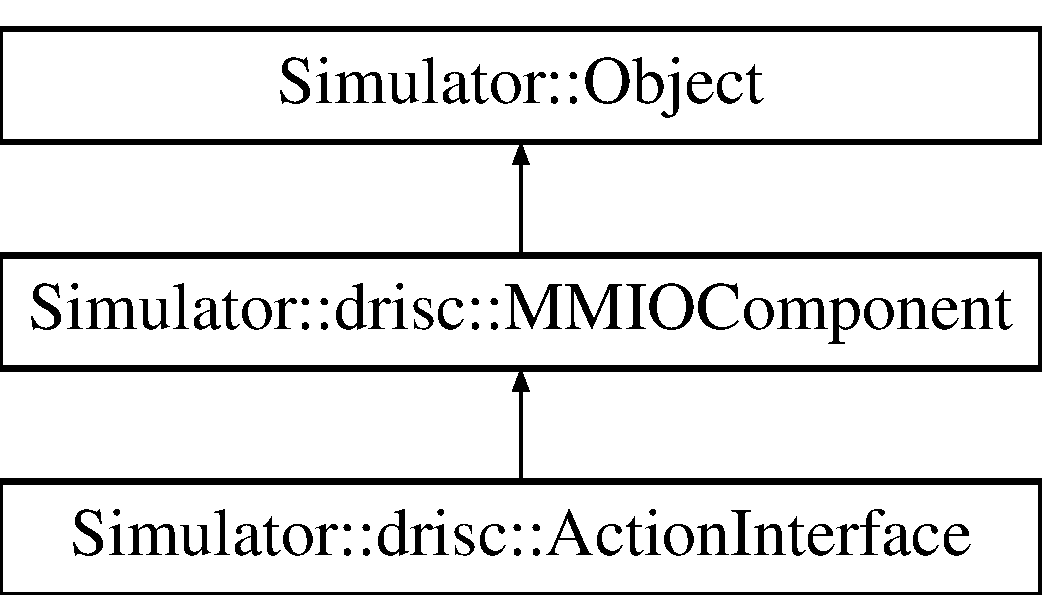
\includegraphics[height=3.000000cm]{class_simulator_1_1drisc_1_1_action_interface}
\end{center}
\end{figure}
\subsection*{Public Member Functions}
\begin{DoxyCompactItemize}
\item 
\hyperlink{class_simulator_1_1drisc_1_1_action_interface_a57951db356b70d51aa258e83400b7ba3}{Action\+Interface} (const std\+::string \&\hyperlink{mtconf_8c_a8f8f80d37794cde9472343e4487ba3eb}{name}, \hyperlink{class_simulator_1_1_object}{Object} \&parent)
\item 
size\+\_\+t \hyperlink{class_simulator_1_1drisc_1_1_action_interface_ad821c373649b51707736c64e372fbd6d}{Get\+Size} () const 
\item 
\hyperlink{namespace_simulator_a4b6b5616e7236c0c131516a441776805}{Result} \hyperlink{class_simulator_1_1drisc_1_1_action_interface_aa0a8facc99c1fa6383dfe1cf6d4e0e52}{Read} (Mem\+Addr address, void $\ast$data, Mem\+Size size, \hyperlink{namespace_simulator_aaccbc706b2d6c99085f52f6dfc2333e4}{L\+F\+I\+D} fid, \hyperlink{namespace_simulator_a483cc4ecee1736e895054617672cded5}{T\+I\+D} tid, const \hyperlink{struct_simulator_1_1_reg_addr}{Reg\+Addr} \&writeback)
\item 
\hyperlink{namespace_simulator_a4b6b5616e7236c0c131516a441776805}{Result} \hyperlink{class_simulator_1_1drisc_1_1_action_interface_a31669c050dea3f850808553054a093b5}{Write} (Mem\+Addr address, const void $\ast$data, Mem\+Size size, \hyperlink{namespace_simulator_aaccbc706b2d6c99085f52f6dfc2333e4}{L\+F\+I\+D} fid, \hyperlink{namespace_simulator_a483cc4ecee1736e895054617672cded5}{T\+I\+D} tid)
\end{DoxyCompactItemize}


\subsection{Constructor \& Destructor Documentation}
\hypertarget{class_simulator_1_1drisc_1_1_action_interface_a57951db356b70d51aa258e83400b7ba3}{\index{Simulator\+::drisc\+::\+Action\+Interface@{Simulator\+::drisc\+::\+Action\+Interface}!Action\+Interface@{Action\+Interface}}
\index{Action\+Interface@{Action\+Interface}!Simulator\+::drisc\+::\+Action\+Interface@{Simulator\+::drisc\+::\+Action\+Interface}}
\subsubsection[{Action\+Interface}]{\setlength{\rightskip}{0pt plus 5cm}Simulator\+::drisc\+::\+Action\+Interface\+::\+Action\+Interface (
\begin{DoxyParamCaption}
\item[{const std\+::string \&}]{name, }
\item[{{\bf Object} \&}]{parent}
\end{DoxyParamCaption}
)}}\label{class_simulator_1_1drisc_1_1_action_interface_a57951db356b70d51aa258e83400b7ba3}


\subsection{Member Function Documentation}
\hypertarget{class_simulator_1_1drisc_1_1_action_interface_ad821c373649b51707736c64e372fbd6d}{\index{Simulator\+::drisc\+::\+Action\+Interface@{Simulator\+::drisc\+::\+Action\+Interface}!Get\+Size@{Get\+Size}}
\index{Get\+Size@{Get\+Size}!Simulator\+::drisc\+::\+Action\+Interface@{Simulator\+::drisc\+::\+Action\+Interface}}
\subsubsection[{Get\+Size}]{\setlength{\rightskip}{0pt plus 5cm}size\+\_\+t Simulator\+::drisc\+::\+Action\+Interface\+::\+Get\+Size (
\begin{DoxyParamCaption}
{}
\end{DoxyParamCaption}
) const\hspace{0.3cm}{\ttfamily [virtual]}}}\label{class_simulator_1_1drisc_1_1_action_interface_ad821c373649b51707736c64e372fbd6d}


Implements \hyperlink{class_simulator_1_1drisc_1_1_m_m_i_o_component_ad8f1a93b445f287895949bfe52972346}{Simulator\+::drisc\+::\+M\+M\+I\+O\+Component}.

\hypertarget{class_simulator_1_1drisc_1_1_action_interface_aa0a8facc99c1fa6383dfe1cf6d4e0e52}{\index{Simulator\+::drisc\+::\+Action\+Interface@{Simulator\+::drisc\+::\+Action\+Interface}!Read@{Read}}
\index{Read@{Read}!Simulator\+::drisc\+::\+Action\+Interface@{Simulator\+::drisc\+::\+Action\+Interface}}
\subsubsection[{Read}]{\setlength{\rightskip}{0pt plus 5cm}{\bf Result} Simulator\+::drisc\+::\+Action\+Interface\+::\+Read (
\begin{DoxyParamCaption}
\item[{Mem\+Addr}]{address, }
\item[{void $\ast$}]{data, }
\item[{Mem\+Size}]{size, }
\item[{{\bf L\+F\+I\+D}}]{fid, }
\item[{{\bf T\+I\+D}}]{tid, }
\item[{const {\bf Reg\+Addr} \&}]{writeback}
\end{DoxyParamCaption}
)\hspace{0.3cm}{\ttfamily [virtual]}}}\label{class_simulator_1_1drisc_1_1_action_interface_aa0a8facc99c1fa6383dfe1cf6d4e0e52}


Implements \hyperlink{class_simulator_1_1drisc_1_1_m_m_i_o_component_af07e2f3e1280d8d56cab7a59815e7eeb}{Simulator\+::drisc\+::\+M\+M\+I\+O\+Component}.

\hypertarget{class_simulator_1_1drisc_1_1_action_interface_a31669c050dea3f850808553054a093b5}{\index{Simulator\+::drisc\+::\+Action\+Interface@{Simulator\+::drisc\+::\+Action\+Interface}!Write@{Write}}
\index{Write@{Write}!Simulator\+::drisc\+::\+Action\+Interface@{Simulator\+::drisc\+::\+Action\+Interface}}
\subsubsection[{Write}]{\setlength{\rightskip}{0pt plus 5cm}{\bf Result} Simulator\+::drisc\+::\+Action\+Interface\+::\+Write (
\begin{DoxyParamCaption}
\item[{Mem\+Addr}]{address, }
\item[{const void $\ast$}]{data, }
\item[{Mem\+Size}]{size, }
\item[{{\bf L\+F\+I\+D}}]{fid, }
\item[{{\bf T\+I\+D}}]{tid}
\end{DoxyParamCaption}
)\hspace{0.3cm}{\ttfamily [virtual]}}}\label{class_simulator_1_1drisc_1_1_action_interface_a31669c050dea3f850808553054a093b5}


Implements \hyperlink{class_simulator_1_1drisc_1_1_m_m_i_o_component_aab3662058e7a00109b122a1460188a8b}{Simulator\+::drisc\+::\+M\+M\+I\+O\+Component}.



The documentation for this class was generated from the following files\+:\begin{DoxyCompactItemize}
\item 
arch/drisc/mmu/\hyperlink{_action_interface_8h}{Action\+Interface.\+h}\item 
arch/drisc/\hyperlink{_action_interface_8cpp}{Action\+Interface.\+cpp}\end{DoxyCompactItemize}

\hypertarget{class_simulator_1_1_active_r_o_m}{\section{Simulator\+:\+:Active\+R\+O\+M Class Reference}
\label{class_simulator_1_1_active_r_o_m}\index{Simulator\+::\+Active\+R\+O\+M@{Simulator\+::\+Active\+R\+O\+M}}
}


{\ttfamily \#include $<$Active\+R\+O\+M.\+h$>$}

Inheritance diagram for Simulator\+:\+:Active\+R\+O\+M\+:\begin{figure}[H]
\begin{center}
\leavevmode
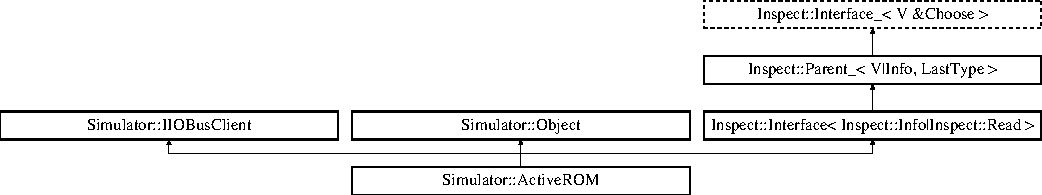
\includegraphics[height=2.619883cm]{class_simulator_1_1_active_r_o_m}
\end{center}
\end{figure}
\subsection*{Classes}
\begin{DoxyCompactItemize}
\item 
struct \hyperlink{struct_simulator_1_1_active_r_o_m_1_1_loadable_range}{Loadable\+Range}
\end{DoxyCompactItemize}
\subsection*{Public Member Functions}
\begin{DoxyCompactItemize}
\item 
\hyperlink{class_simulator_1_1_active_r_o_m_a2137ead94a167055ef56bd6db9786468}{Active\+R\+O\+M} (const std\+::string \&\hyperlink{mtconf_8c_a8f8f80d37794cde9472343e4487ba3eb}{name}, \hyperlink{class_simulator_1_1_object}{Object} \&parent, \hyperlink{class_simulator_1_1_i_memory_admin}{I\+Memory\+Admin} \&mem, \hyperlink{class_simulator_1_1_i_i_o_bus}{I\+I\+O\+Bus} \&iobus, \hyperlink{namespace_simulator_a3493d987c866ad6b8aaa704c42502db0}{I\+O\+Device\+I\+D} devid, \hyperlink{class_config}{Config} \&config, bool quiet=false)
\item 
\hyperlink{class_simulator_1_1_active_r_o_m_a0f85814d38ccc6b8e16540b4d9de68d0}{Active\+R\+O\+M} (const \hyperlink{class_simulator_1_1_active_r_o_m}{Active\+R\+O\+M} \&)=delete
\item 
\hyperlink{class_simulator_1_1_active_r_o_m}{Active\+R\+O\+M} \& \hyperlink{class_simulator_1_1_active_r_o_m_a90174654122be07ef6c493adfdcdff80}{operator=} (const \hyperlink{class_simulator_1_1_active_r_o_m}{Active\+R\+O\+M} \&)=delete
\item 
\hyperlink{class_simulator_1_1_active_r_o_m_ab4f08efaf6e5c2192f768164be6f2b4f}{$\sim$\+Active\+R\+O\+M} ()
\item 
void \hyperlink{class_simulator_1_1_active_r_o_m_afc31072ac817e301dc15e0b05ab1ef2d}{Initialize} ()
\item 
\hyperlink{namespace_simulator_a4b6b5616e7236c0c131516a441776805}{Result} \hyperlink{class_simulator_1_1_active_r_o_m_a8ea9481d45793f62bddfdb932a876b1d}{Do\+Load} ()
\item 
\hyperlink{namespace_simulator_a4b6b5616e7236c0c131516a441776805}{Result} \hyperlink{class_simulator_1_1_active_r_o_m_ab2a9e8a3e9a657938f0212c862713caa}{Do\+Flush} ()
\item 
\hyperlink{namespace_simulator_a4b6b5616e7236c0c131516a441776805}{Result} \hyperlink{class_simulator_1_1_active_r_o_m_acd043e41debf4bcf2ff2af4b9ececd88}{Do\+Notify} ()
\item 
bool \hyperlink{class_simulator_1_1_active_r_o_m_a6620b1ba031bd5de70872109825f842a}{Is\+Bootable} () const 
\item 
bool \hyperlink{class_simulator_1_1_active_r_o_m_a009279dd2e81893784c396716b0e8dea}{Is\+Preloaded} () const 
\item 
const std\+::string \& \hyperlink{class_simulator_1_1_active_r_o_m_a2fdb18b29b35d8e56d586e67246ad16a}{Get\+Program\+Name} () const 
\item 
\hyperlink{namespace_simulator_a3493d987c866ad6b8aaa704c42502db0}{I\+O\+Device\+I\+D} \hyperlink{class_simulator_1_1_active_r_o_m_ab14b99dfff2e78b8c74cc90f2193b3e4}{Get\+Device\+I\+D} () const 
\item 
bool \hyperlink{class_simulator_1_1_active_r_o_m_ac6e900c295407b982f6678a3745af66c}{On\+Read\+Request\+Received} (\hyperlink{namespace_simulator_a3493d987c866ad6b8aaa704c42502db0}{I\+O\+Device\+I\+D} from, Mem\+Addr address, Mem\+Size size)
\item 
bool \hyperlink{class_simulator_1_1_active_r_o_m_a43f9ab1bae1a8a67d44b97cc806f891b}{On\+Write\+Request\+Received} (\hyperlink{namespace_simulator_a3493d987c866ad6b8aaa704c42502db0}{I\+O\+Device\+I\+D} from, Mem\+Addr address, const \hyperlink{struct_simulator_1_1_i_o_data}{I\+O\+Data} \&data)
\item 
bool \hyperlink{class_simulator_1_1_active_r_o_m_a8630c7aaf85302843d0ff5027d0ada0e}{On\+Read\+Response\+Received} (\hyperlink{namespace_simulator_a3493d987c866ad6b8aaa704c42502db0}{I\+O\+Device\+I\+D} from, Mem\+Addr address, const \hyperlink{struct_simulator_1_1_i_o_data}{I\+O\+Data} \&data)
\item 
\hyperlink{class_simulator_1_1_storage_trace_set}{Storage\+Trace\+Set} \hyperlink{class_simulator_1_1_active_r_o_m_a3504469cf42d652f4f196de9b1eb5ba9}{Get\+Write\+Request\+Traces} () const 
\item 
\hyperlink{class_simulator_1_1_storage_trace_set}{Storage\+Trace\+Set} \hyperlink{class_simulator_1_1_active_r_o_m_a8cdf2fcc5f552d6fec8fa0703b92746d}{Get\+Read\+Response\+Traces} () const 
\item 
void \hyperlink{class_simulator_1_1_active_r_o_m_ae204edea9cb465dcc8967d8a1cc1c411}{Get\+Device\+Identity} (\hyperlink{struct_simulator_1_1_i_o_device_identification}{I\+O\+Device\+Identification} \&\hyperlink{mtconf_8c_aa3185401f04d30bd505daebf48c39cc5}{id}) const 
\item 
std\+::string \hyperlink{class_simulator_1_1_active_r_o_m_a395f9d7d00fffcc56118ca27986ea5f1}{Get\+I\+O\+Device\+Name} () const 
\item 
void \hyperlink{class_simulator_1_1_active_r_o_m_a5259e7a783ed0e61bc914bf83baab573}{Cmd\+\_\+\+Read} (std\+::ostream \&out, const std\+::vector$<$ std\+::string $>$ \&arguments) const 
\item 
void \hyperlink{class_simulator_1_1_active_r_o_m_a1e520c42b85292c8e34b4e8dd3af6fc9}{Cmd\+\_\+\+Info} (std\+::ostream \&out, const std\+::vector$<$ std\+::string $>$ \&arguments) const 
\end{DoxyCompactItemize}
\subsection*{Public Attributes}
\begin{DoxyCompactItemize}
\item 
\hyperlink{class_simulator_1_1_process}{Process} \hyperlink{class_simulator_1_1_active_r_o_m_a90f8af64b9221bdf569469b15e884074}{p\+\_\+\+Load}
\item 
\hyperlink{class_simulator_1_1_process}{Process} \hyperlink{class_simulator_1_1_active_r_o_m_a31128178f03df7605187c744a722d141}{p\+\_\+\+Flush}
\item 
\hyperlink{class_simulator_1_1_process}{Process} \hyperlink{class_simulator_1_1_active_r_o_m_ad0eb552ec1b8f04c49c8d4f2c12722ef}{p\+\_\+\+Notify}
\end{DoxyCompactItemize}


\subsection{Constructor \& Destructor Documentation}
\hypertarget{class_simulator_1_1_active_r_o_m_a2137ead94a167055ef56bd6db9786468}{\index{Simulator\+::\+Active\+R\+O\+M@{Simulator\+::\+Active\+R\+O\+M}!Active\+R\+O\+M@{Active\+R\+O\+M}}
\index{Active\+R\+O\+M@{Active\+R\+O\+M}!Simulator\+::\+Active\+R\+O\+M@{Simulator\+::\+Active\+R\+O\+M}}
\subsubsection[{Active\+R\+O\+M}]{\setlength{\rightskip}{0pt plus 5cm}Simulator\+::\+Active\+R\+O\+M\+::\+Active\+R\+O\+M (
\begin{DoxyParamCaption}
\item[{const std\+::string \&}]{name, }
\item[{{\bf Object} \&}]{parent, }
\item[{{\bf I\+Memory\+Admin} \&}]{mem, }
\item[{{\bf I\+I\+O\+Bus} \&}]{iobus, }
\item[{{\bf I\+O\+Device\+I\+D}}]{devid, }
\item[{{\bf Config} \&}]{config, }
\item[{bool}]{quiet = {\ttfamily false}}
\end{DoxyParamCaption}
)}}\label{class_simulator_1_1_active_r_o_m_a2137ead94a167055ef56bd6db9786468}
\hypertarget{class_simulator_1_1_active_r_o_m_a0f85814d38ccc6b8e16540b4d9de68d0}{\index{Simulator\+::\+Active\+R\+O\+M@{Simulator\+::\+Active\+R\+O\+M}!Active\+R\+O\+M@{Active\+R\+O\+M}}
\index{Active\+R\+O\+M@{Active\+R\+O\+M}!Simulator\+::\+Active\+R\+O\+M@{Simulator\+::\+Active\+R\+O\+M}}
\subsubsection[{Active\+R\+O\+M}]{\setlength{\rightskip}{0pt plus 5cm}Simulator\+::\+Active\+R\+O\+M\+::\+Active\+R\+O\+M (
\begin{DoxyParamCaption}
\item[{const {\bf Active\+R\+O\+M} \&}]{}
\end{DoxyParamCaption}
)\hspace{0.3cm}{\ttfamily [delete]}}}\label{class_simulator_1_1_active_r_o_m_a0f85814d38ccc6b8e16540b4d9de68d0}
\hypertarget{class_simulator_1_1_active_r_o_m_ab4f08efaf6e5c2192f768164be6f2b4f}{\index{Simulator\+::\+Active\+R\+O\+M@{Simulator\+::\+Active\+R\+O\+M}!````~Active\+R\+O\+M@{$\sim$\+Active\+R\+O\+M}}
\index{````~Active\+R\+O\+M@{$\sim$\+Active\+R\+O\+M}!Simulator\+::\+Active\+R\+O\+M@{Simulator\+::\+Active\+R\+O\+M}}
\subsubsection[{$\sim$\+Active\+R\+O\+M}]{\setlength{\rightskip}{0pt plus 5cm}Simulator\+::\+Active\+R\+O\+M\+::$\sim$\+Active\+R\+O\+M (
\begin{DoxyParamCaption}
{}
\end{DoxyParamCaption}
)}}\label{class_simulator_1_1_active_r_o_m_ab4f08efaf6e5c2192f768164be6f2b4f}


\subsection{Member Function Documentation}
\hypertarget{class_simulator_1_1_active_r_o_m_a1e520c42b85292c8e34b4e8dd3af6fc9}{\index{Simulator\+::\+Active\+R\+O\+M@{Simulator\+::\+Active\+R\+O\+M}!Cmd\+\_\+\+Info@{Cmd\+\_\+\+Info}}
\index{Cmd\+\_\+\+Info@{Cmd\+\_\+\+Info}!Simulator\+::\+Active\+R\+O\+M@{Simulator\+::\+Active\+R\+O\+M}}
\subsubsection[{Cmd\+\_\+\+Info}]{\setlength{\rightskip}{0pt plus 5cm}void Simulator\+::\+Active\+R\+O\+M\+::\+Cmd\+\_\+\+Info (
\begin{DoxyParamCaption}
\item[{std\+::ostream \&}]{out, }
\item[{const std\+::vector$<$ std\+::string $>$ \&}]{arguments}
\end{DoxyParamCaption}
) const}}\label{class_simulator_1_1_active_r_o_m_a1e520c42b85292c8e34b4e8dd3af6fc9}
\hypertarget{class_simulator_1_1_active_r_o_m_a5259e7a783ed0e61bc914bf83baab573}{\index{Simulator\+::\+Active\+R\+O\+M@{Simulator\+::\+Active\+R\+O\+M}!Cmd\+\_\+\+Read@{Cmd\+\_\+\+Read}}
\index{Cmd\+\_\+\+Read@{Cmd\+\_\+\+Read}!Simulator\+::\+Active\+R\+O\+M@{Simulator\+::\+Active\+R\+O\+M}}
\subsubsection[{Cmd\+\_\+\+Read}]{\setlength{\rightskip}{0pt plus 5cm}void Simulator\+::\+Active\+R\+O\+M\+::\+Cmd\+\_\+\+Read (
\begin{DoxyParamCaption}
\item[{std\+::ostream \&}]{out, }
\item[{const std\+::vector$<$ std\+::string $>$ \&}]{arguments}
\end{DoxyParamCaption}
) const}}\label{class_simulator_1_1_active_r_o_m_a5259e7a783ed0e61bc914bf83baab573}
\hypertarget{class_simulator_1_1_active_r_o_m_ab2a9e8a3e9a657938f0212c862713caa}{\index{Simulator\+::\+Active\+R\+O\+M@{Simulator\+::\+Active\+R\+O\+M}!Do\+Flush@{Do\+Flush}}
\index{Do\+Flush@{Do\+Flush}!Simulator\+::\+Active\+R\+O\+M@{Simulator\+::\+Active\+R\+O\+M}}
\subsubsection[{Do\+Flush}]{\setlength{\rightskip}{0pt plus 5cm}{\bf Result} Simulator\+::\+Active\+R\+O\+M\+::\+Do\+Flush (
\begin{DoxyParamCaption}
{}
\end{DoxyParamCaption}
)}}\label{class_simulator_1_1_active_r_o_m_ab2a9e8a3e9a657938f0212c862713caa}
\hypertarget{class_simulator_1_1_active_r_o_m_a8ea9481d45793f62bddfdb932a876b1d}{\index{Simulator\+::\+Active\+R\+O\+M@{Simulator\+::\+Active\+R\+O\+M}!Do\+Load@{Do\+Load}}
\index{Do\+Load@{Do\+Load}!Simulator\+::\+Active\+R\+O\+M@{Simulator\+::\+Active\+R\+O\+M}}
\subsubsection[{Do\+Load}]{\setlength{\rightskip}{0pt plus 5cm}{\bf Result} Simulator\+::\+Active\+R\+O\+M\+::\+Do\+Load (
\begin{DoxyParamCaption}
{}
\end{DoxyParamCaption}
)}}\label{class_simulator_1_1_active_r_o_m_a8ea9481d45793f62bddfdb932a876b1d}
\hypertarget{class_simulator_1_1_active_r_o_m_acd043e41debf4bcf2ff2af4b9ececd88}{\index{Simulator\+::\+Active\+R\+O\+M@{Simulator\+::\+Active\+R\+O\+M}!Do\+Notify@{Do\+Notify}}
\index{Do\+Notify@{Do\+Notify}!Simulator\+::\+Active\+R\+O\+M@{Simulator\+::\+Active\+R\+O\+M}}
\subsubsection[{Do\+Notify}]{\setlength{\rightskip}{0pt plus 5cm}{\bf Result} Simulator\+::\+Active\+R\+O\+M\+::\+Do\+Notify (
\begin{DoxyParamCaption}
{}
\end{DoxyParamCaption}
)}}\label{class_simulator_1_1_active_r_o_m_acd043e41debf4bcf2ff2af4b9ececd88}
\hypertarget{class_simulator_1_1_active_r_o_m_ab14b99dfff2e78b8c74cc90f2193b3e4}{\index{Simulator\+::\+Active\+R\+O\+M@{Simulator\+::\+Active\+R\+O\+M}!Get\+Device\+I\+D@{Get\+Device\+I\+D}}
\index{Get\+Device\+I\+D@{Get\+Device\+I\+D}!Simulator\+::\+Active\+R\+O\+M@{Simulator\+::\+Active\+R\+O\+M}}
\subsubsection[{Get\+Device\+I\+D}]{\setlength{\rightskip}{0pt plus 5cm}{\bf I\+O\+Device\+I\+D} Simulator\+::\+Active\+R\+O\+M\+::\+Get\+Device\+I\+D (
\begin{DoxyParamCaption}
{}
\end{DoxyParamCaption}
) const\hspace{0.3cm}{\ttfamily [inline]}}}\label{class_simulator_1_1_active_r_o_m_ab14b99dfff2e78b8c74cc90f2193b3e4}
\hypertarget{class_simulator_1_1_active_r_o_m_ae204edea9cb465dcc8967d8a1cc1c411}{\index{Simulator\+::\+Active\+R\+O\+M@{Simulator\+::\+Active\+R\+O\+M}!Get\+Device\+Identity@{Get\+Device\+Identity}}
\index{Get\+Device\+Identity@{Get\+Device\+Identity}!Simulator\+::\+Active\+R\+O\+M@{Simulator\+::\+Active\+R\+O\+M}}
\subsubsection[{Get\+Device\+Identity}]{\setlength{\rightskip}{0pt plus 5cm}void Simulator\+::\+Active\+R\+O\+M\+::\+Get\+Device\+Identity (
\begin{DoxyParamCaption}
\item[{{\bf I\+O\+Device\+Identification} \&}]{id}
\end{DoxyParamCaption}
) const\hspace{0.3cm}{\ttfamily [virtual]}}}\label{class_simulator_1_1_active_r_o_m_ae204edea9cb465dcc8967d8a1cc1c411}


Implements \hyperlink{class_simulator_1_1_i_i_o_bus_client_a8fb9e637f95dd2d4c9092461a76921df}{Simulator\+::\+I\+I\+O\+Bus\+Client}.

\hypertarget{class_simulator_1_1_active_r_o_m_a395f9d7d00fffcc56118ca27986ea5f1}{\index{Simulator\+::\+Active\+R\+O\+M@{Simulator\+::\+Active\+R\+O\+M}!Get\+I\+O\+Device\+Name@{Get\+I\+O\+Device\+Name}}
\index{Get\+I\+O\+Device\+Name@{Get\+I\+O\+Device\+Name}!Simulator\+::\+Active\+R\+O\+M@{Simulator\+::\+Active\+R\+O\+M}}
\subsubsection[{Get\+I\+O\+Device\+Name}]{\setlength{\rightskip}{0pt plus 5cm}string Simulator\+::\+Active\+R\+O\+M\+::\+Get\+I\+O\+Device\+Name (
\begin{DoxyParamCaption}
{}
\end{DoxyParamCaption}
) const\hspace{0.3cm}{\ttfamily [virtual]}}}\label{class_simulator_1_1_active_r_o_m_a395f9d7d00fffcc56118ca27986ea5f1}


Implements \hyperlink{class_simulator_1_1_i_i_o_bus_client_aca857813bebf8a75b9a0b53097547755}{Simulator\+::\+I\+I\+O\+Bus\+Client}.

\hypertarget{class_simulator_1_1_active_r_o_m_a2fdb18b29b35d8e56d586e67246ad16a}{\index{Simulator\+::\+Active\+R\+O\+M@{Simulator\+::\+Active\+R\+O\+M}!Get\+Program\+Name@{Get\+Program\+Name}}
\index{Get\+Program\+Name@{Get\+Program\+Name}!Simulator\+::\+Active\+R\+O\+M@{Simulator\+::\+Active\+R\+O\+M}}
\subsubsection[{Get\+Program\+Name}]{\setlength{\rightskip}{0pt plus 5cm}const std\+::string\& Simulator\+::\+Active\+R\+O\+M\+::\+Get\+Program\+Name (
\begin{DoxyParamCaption}
{}
\end{DoxyParamCaption}
) const\hspace{0.3cm}{\ttfamily [inline]}}}\label{class_simulator_1_1_active_r_o_m_a2fdb18b29b35d8e56d586e67246ad16a}
\hypertarget{class_simulator_1_1_active_r_o_m_a8cdf2fcc5f552d6fec8fa0703b92746d}{\index{Simulator\+::\+Active\+R\+O\+M@{Simulator\+::\+Active\+R\+O\+M}!Get\+Read\+Response\+Traces@{Get\+Read\+Response\+Traces}}
\index{Get\+Read\+Response\+Traces@{Get\+Read\+Response\+Traces}!Simulator\+::\+Active\+R\+O\+M@{Simulator\+::\+Active\+R\+O\+M}}
\subsubsection[{Get\+Read\+Response\+Traces}]{\setlength{\rightskip}{0pt plus 5cm}{\bf Storage\+Trace\+Set} Simulator\+::\+Active\+R\+O\+M\+::\+Get\+Read\+Response\+Traces (
\begin{DoxyParamCaption}
{}
\end{DoxyParamCaption}
) const\hspace{0.3cm}{\ttfamily [virtual]}}}\label{class_simulator_1_1_active_r_o_m_a8cdf2fcc5f552d6fec8fa0703b92746d}


Reimplemented from \hyperlink{class_simulator_1_1_i_i_o_bus_client_a7e1e646056743003374f8b3e1e95978f}{Simulator\+::\+I\+I\+O\+Bus\+Client}.

\hypertarget{class_simulator_1_1_active_r_o_m_a3504469cf42d652f4f196de9b1eb5ba9}{\index{Simulator\+::\+Active\+R\+O\+M@{Simulator\+::\+Active\+R\+O\+M}!Get\+Write\+Request\+Traces@{Get\+Write\+Request\+Traces}}
\index{Get\+Write\+Request\+Traces@{Get\+Write\+Request\+Traces}!Simulator\+::\+Active\+R\+O\+M@{Simulator\+::\+Active\+R\+O\+M}}
\subsubsection[{Get\+Write\+Request\+Traces}]{\setlength{\rightskip}{0pt plus 5cm}{\bf Storage\+Trace\+Set} Simulator\+::\+Active\+R\+O\+M\+::\+Get\+Write\+Request\+Traces (
\begin{DoxyParamCaption}
{}
\end{DoxyParamCaption}
) const\hspace{0.3cm}{\ttfamily [virtual]}}}\label{class_simulator_1_1_active_r_o_m_a3504469cf42d652f4f196de9b1eb5ba9}


Reimplemented from \hyperlink{class_simulator_1_1_i_i_o_bus_client_a196ff28850f3cbefef216b4df9eb2116}{Simulator\+::\+I\+I\+O\+Bus\+Client}.

\hypertarget{class_simulator_1_1_active_r_o_m_afc31072ac817e301dc15e0b05ab1ef2d}{\index{Simulator\+::\+Active\+R\+O\+M@{Simulator\+::\+Active\+R\+O\+M}!Initialize@{Initialize}}
\index{Initialize@{Initialize}!Simulator\+::\+Active\+R\+O\+M@{Simulator\+::\+Active\+R\+O\+M}}
\subsubsection[{Initialize}]{\setlength{\rightskip}{0pt plus 5cm}void Simulator\+::\+Active\+R\+O\+M\+::\+Initialize (
\begin{DoxyParamCaption}
{}
\end{DoxyParamCaption}
)\hspace{0.3cm}{\ttfamily [virtual]}}}\label{class_simulator_1_1_active_r_o_m_afc31072ac817e301dc15e0b05ab1ef2d}


Reimplemented from \hyperlink{class_simulator_1_1_i_i_o_bus_client_a1bd79fc9dca6b622afc5a1e23fe8428b}{Simulator\+::\+I\+I\+O\+Bus\+Client}.

\hypertarget{class_simulator_1_1_active_r_o_m_a6620b1ba031bd5de70872109825f842a}{\index{Simulator\+::\+Active\+R\+O\+M@{Simulator\+::\+Active\+R\+O\+M}!Is\+Bootable@{Is\+Bootable}}
\index{Is\+Bootable@{Is\+Bootable}!Simulator\+::\+Active\+R\+O\+M@{Simulator\+::\+Active\+R\+O\+M}}
\subsubsection[{Is\+Bootable}]{\setlength{\rightskip}{0pt plus 5cm}bool Simulator\+::\+Active\+R\+O\+M\+::\+Is\+Bootable (
\begin{DoxyParamCaption}
{}
\end{DoxyParamCaption}
) const\hspace{0.3cm}{\ttfamily [inline]}}}\label{class_simulator_1_1_active_r_o_m_a6620b1ba031bd5de70872109825f842a}
\hypertarget{class_simulator_1_1_active_r_o_m_a009279dd2e81893784c396716b0e8dea}{\index{Simulator\+::\+Active\+R\+O\+M@{Simulator\+::\+Active\+R\+O\+M}!Is\+Preloaded@{Is\+Preloaded}}
\index{Is\+Preloaded@{Is\+Preloaded}!Simulator\+::\+Active\+R\+O\+M@{Simulator\+::\+Active\+R\+O\+M}}
\subsubsection[{Is\+Preloaded}]{\setlength{\rightskip}{0pt plus 5cm}bool Simulator\+::\+Active\+R\+O\+M\+::\+Is\+Preloaded (
\begin{DoxyParamCaption}
{}
\end{DoxyParamCaption}
) const\hspace{0.3cm}{\ttfamily [inline]}}}\label{class_simulator_1_1_active_r_o_m_a009279dd2e81893784c396716b0e8dea}
\hypertarget{class_simulator_1_1_active_r_o_m_ac6e900c295407b982f6678a3745af66c}{\index{Simulator\+::\+Active\+R\+O\+M@{Simulator\+::\+Active\+R\+O\+M}!On\+Read\+Request\+Received@{On\+Read\+Request\+Received}}
\index{On\+Read\+Request\+Received@{On\+Read\+Request\+Received}!Simulator\+::\+Active\+R\+O\+M@{Simulator\+::\+Active\+R\+O\+M}}
\subsubsection[{On\+Read\+Request\+Received}]{\setlength{\rightskip}{0pt plus 5cm}bool Simulator\+::\+Active\+R\+O\+M\+::\+On\+Read\+Request\+Received (
\begin{DoxyParamCaption}
\item[{{\bf I\+O\+Device\+I\+D}}]{from, }
\item[{Mem\+Addr}]{address, }
\item[{Mem\+Size}]{size}
\end{DoxyParamCaption}
)\hspace{0.3cm}{\ttfamily [virtual]}}}\label{class_simulator_1_1_active_r_o_m_ac6e900c295407b982f6678a3745af66c}


Reimplemented from \hyperlink{class_simulator_1_1_i_i_o_bus_client_afeb9155b104d868e9e6c2a3366a39b3e}{Simulator\+::\+I\+I\+O\+Bus\+Client}.

\hypertarget{class_simulator_1_1_active_r_o_m_a8630c7aaf85302843d0ff5027d0ada0e}{\index{Simulator\+::\+Active\+R\+O\+M@{Simulator\+::\+Active\+R\+O\+M}!On\+Read\+Response\+Received@{On\+Read\+Response\+Received}}
\index{On\+Read\+Response\+Received@{On\+Read\+Response\+Received}!Simulator\+::\+Active\+R\+O\+M@{Simulator\+::\+Active\+R\+O\+M}}
\subsubsection[{On\+Read\+Response\+Received}]{\setlength{\rightskip}{0pt plus 5cm}bool Simulator\+::\+Active\+R\+O\+M\+::\+On\+Read\+Response\+Received (
\begin{DoxyParamCaption}
\item[{{\bf I\+O\+Device\+I\+D}}]{from, }
\item[{Mem\+Addr}]{address, }
\item[{const {\bf I\+O\+Data} \&}]{data}
\end{DoxyParamCaption}
)\hspace{0.3cm}{\ttfamily [virtual]}}}\label{class_simulator_1_1_active_r_o_m_a8630c7aaf85302843d0ff5027d0ada0e}


Reimplemented from \hyperlink{class_simulator_1_1_i_i_o_bus_client_aabdb58549281acb31be5b3f4509bb614}{Simulator\+::\+I\+I\+O\+Bus\+Client}.

\hypertarget{class_simulator_1_1_active_r_o_m_a43f9ab1bae1a8a67d44b97cc806f891b}{\index{Simulator\+::\+Active\+R\+O\+M@{Simulator\+::\+Active\+R\+O\+M}!On\+Write\+Request\+Received@{On\+Write\+Request\+Received}}
\index{On\+Write\+Request\+Received@{On\+Write\+Request\+Received}!Simulator\+::\+Active\+R\+O\+M@{Simulator\+::\+Active\+R\+O\+M}}
\subsubsection[{On\+Write\+Request\+Received}]{\setlength{\rightskip}{0pt plus 5cm}bool Simulator\+::\+Active\+R\+O\+M\+::\+On\+Write\+Request\+Received (
\begin{DoxyParamCaption}
\item[{{\bf I\+O\+Device\+I\+D}}]{from, }
\item[{Mem\+Addr}]{address, }
\item[{const {\bf I\+O\+Data} \&}]{data}
\end{DoxyParamCaption}
)\hspace{0.3cm}{\ttfamily [virtual]}}}\label{class_simulator_1_1_active_r_o_m_a43f9ab1bae1a8a67d44b97cc806f891b}


Reimplemented from \hyperlink{class_simulator_1_1_i_i_o_bus_client_a69d1908e4e0fb82c86834ed570a7d6c9}{Simulator\+::\+I\+I\+O\+Bus\+Client}.

\hypertarget{class_simulator_1_1_active_r_o_m_a90174654122be07ef6c493adfdcdff80}{\index{Simulator\+::\+Active\+R\+O\+M@{Simulator\+::\+Active\+R\+O\+M}!operator=@{operator=}}
\index{operator=@{operator=}!Simulator\+::\+Active\+R\+O\+M@{Simulator\+::\+Active\+R\+O\+M}}
\subsubsection[{operator=}]{\setlength{\rightskip}{0pt plus 5cm}{\bf Active\+R\+O\+M}\& Simulator\+::\+Active\+R\+O\+M\+::operator= (
\begin{DoxyParamCaption}
\item[{const {\bf Active\+R\+O\+M} \&}]{}
\end{DoxyParamCaption}
)\hspace{0.3cm}{\ttfamily [delete]}}}\label{class_simulator_1_1_active_r_o_m_a90174654122be07ef6c493adfdcdff80}


\subsection{Member Data Documentation}
\hypertarget{class_simulator_1_1_active_r_o_m_a31128178f03df7605187c744a722d141}{\index{Simulator\+::\+Active\+R\+O\+M@{Simulator\+::\+Active\+R\+O\+M}!p\+\_\+\+Flush@{p\+\_\+\+Flush}}
\index{p\+\_\+\+Flush@{p\+\_\+\+Flush}!Simulator\+::\+Active\+R\+O\+M@{Simulator\+::\+Active\+R\+O\+M}}
\subsubsection[{p\+\_\+\+Flush}]{\setlength{\rightskip}{0pt plus 5cm}{\bf Process} Simulator\+::\+Active\+R\+O\+M\+::p\+\_\+\+Flush}}\label{class_simulator_1_1_active_r_o_m_a31128178f03df7605187c744a722d141}
\hypertarget{class_simulator_1_1_active_r_o_m_a90f8af64b9221bdf569469b15e884074}{\index{Simulator\+::\+Active\+R\+O\+M@{Simulator\+::\+Active\+R\+O\+M}!p\+\_\+\+Load@{p\+\_\+\+Load}}
\index{p\+\_\+\+Load@{p\+\_\+\+Load}!Simulator\+::\+Active\+R\+O\+M@{Simulator\+::\+Active\+R\+O\+M}}
\subsubsection[{p\+\_\+\+Load}]{\setlength{\rightskip}{0pt plus 5cm}{\bf Process} Simulator\+::\+Active\+R\+O\+M\+::p\+\_\+\+Load}}\label{class_simulator_1_1_active_r_o_m_a90f8af64b9221bdf569469b15e884074}
\hypertarget{class_simulator_1_1_active_r_o_m_ad0eb552ec1b8f04c49c8d4f2c12722ef}{\index{Simulator\+::\+Active\+R\+O\+M@{Simulator\+::\+Active\+R\+O\+M}!p\+\_\+\+Notify@{p\+\_\+\+Notify}}
\index{p\+\_\+\+Notify@{p\+\_\+\+Notify}!Simulator\+::\+Active\+R\+O\+M@{Simulator\+::\+Active\+R\+O\+M}}
\subsubsection[{p\+\_\+\+Notify}]{\setlength{\rightskip}{0pt plus 5cm}{\bf Process} Simulator\+::\+Active\+R\+O\+M\+::p\+\_\+\+Notify}}\label{class_simulator_1_1_active_r_o_m_ad0eb552ec1b8f04c49c8d4f2c12722ef}


The documentation for this class was generated from the following files\+:\begin{DoxyCompactItemize}
\item 
arch/dev/\hyperlink{_active_r_o_m_8h}{Active\+R\+O\+M.\+h}\item 
arch/dev/\hyperlink{_active_r_o_m_8cpp}{Active\+R\+O\+M.\+cpp}\end{DoxyCompactItemize}

\hypertarget{class_simulator_1_1_add_fold}{\section{Simulator\+:\+:Add\+Fold Class Reference}
\label{class_simulator_1_1_add_fold}\index{Simulator\+::\+Add\+Fold@{Simulator\+::\+Add\+Fold}}
}
Inheritance diagram for Simulator\+:\+:Add\+Fold\+:\begin{figure}[H]
\begin{center}
\leavevmode
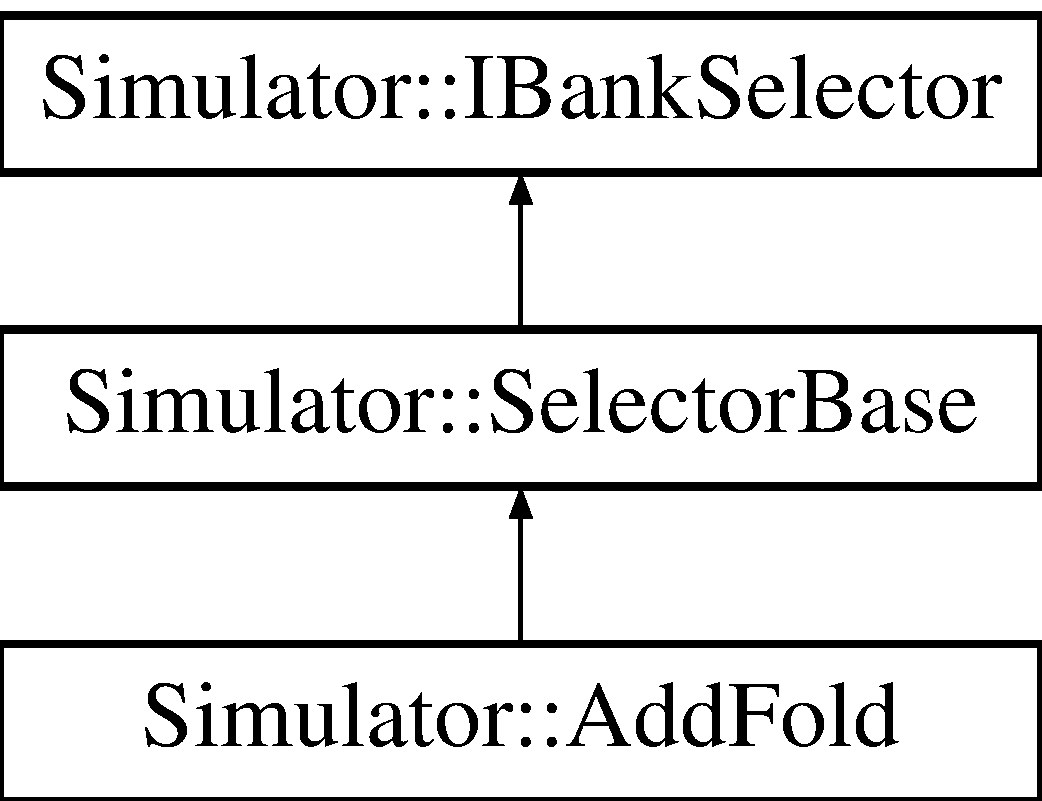
\includegraphics[height=3.000000cm]{class_simulator_1_1_add_fold}
\end{center}
\end{figure}
\subsection*{Public Member Functions}
\begin{DoxyCompactItemize}
\item 
\hyperlink{class_simulator_1_1_add_fold_a10b67a2a41326c14b384360b993c4b77}{Add\+Fold} (size\+\_\+t num\+Banks)
\item 
void \hyperlink{class_simulator_1_1_add_fold_a8b06e012e21b17873647a21a25f9d0b9}{Map} (Mem\+Addr address, Mem\+Addr \&tag, size\+\_\+t \&index)
\item 
Mem\+Addr \hyperlink{class_simulator_1_1_add_fold_a020d74e9f256a128ea47d0fb6acd4eb7}{Unmap} (Mem\+Addr tag, size\+\_\+t)
\end{DoxyCompactItemize}
\subsection*{Additional Inherited Members}


\subsection{Constructor \& Destructor Documentation}
\hypertarget{class_simulator_1_1_add_fold_a10b67a2a41326c14b384360b993c4b77}{\index{Simulator\+::\+Add\+Fold@{Simulator\+::\+Add\+Fold}!Add\+Fold@{Add\+Fold}}
\index{Add\+Fold@{Add\+Fold}!Simulator\+::\+Add\+Fold@{Simulator\+::\+Add\+Fold}}
\subsubsection[{Add\+Fold}]{\setlength{\rightskip}{0pt plus 5cm}Simulator\+::\+Add\+Fold\+::\+Add\+Fold (
\begin{DoxyParamCaption}
\item[{size\+\_\+t}]{num\+Banks}
\end{DoxyParamCaption}
)\hspace{0.3cm}{\ttfamily [inline]}}}\label{class_simulator_1_1_add_fold_a10b67a2a41326c14b384360b993c4b77}


\subsection{Member Function Documentation}
\hypertarget{class_simulator_1_1_add_fold_a8b06e012e21b17873647a21a25f9d0b9}{\index{Simulator\+::\+Add\+Fold@{Simulator\+::\+Add\+Fold}!Map@{Map}}
\index{Map@{Map}!Simulator\+::\+Add\+Fold@{Simulator\+::\+Add\+Fold}}
\subsubsection[{Map}]{\setlength{\rightskip}{0pt plus 5cm}void Simulator\+::\+Add\+Fold\+::\+Map (
\begin{DoxyParamCaption}
\item[{Mem\+Addr}]{address, }
\item[{Mem\+Addr \&}]{tag, }
\item[{size\+\_\+t \&}]{index}
\end{DoxyParamCaption}
)\hspace{0.3cm}{\ttfamily [inline]}, {\ttfamily [virtual]}}}\label{class_simulator_1_1_add_fold_a8b06e012e21b17873647a21a25f9d0b9}


Implements \hyperlink{class_simulator_1_1_i_bank_selector_ad945160c483d88073b6e5572da5e4507}{Simulator\+::\+I\+Bank\+Selector}.

\hypertarget{class_simulator_1_1_add_fold_a020d74e9f256a128ea47d0fb6acd4eb7}{\index{Simulator\+::\+Add\+Fold@{Simulator\+::\+Add\+Fold}!Unmap@{Unmap}}
\index{Unmap@{Unmap}!Simulator\+::\+Add\+Fold@{Simulator\+::\+Add\+Fold}}
\subsubsection[{Unmap}]{\setlength{\rightskip}{0pt plus 5cm}Mem\+Addr Simulator\+::\+Add\+Fold\+::\+Unmap (
\begin{DoxyParamCaption}
\item[{Mem\+Addr}]{tag, }
\item[{size\+\_\+t}]{}
\end{DoxyParamCaption}
)\hspace{0.3cm}{\ttfamily [inline]}, {\ttfamily [virtual]}}}\label{class_simulator_1_1_add_fold_a020d74e9f256a128ea47d0fb6acd4eb7}


Implements \hyperlink{class_simulator_1_1_i_bank_selector_a57c8b49e6439984ff40836e8c5992aba}{Simulator\+::\+I\+Bank\+Selector}.



The documentation for this class was generated from the following file\+:\begin{DoxyCompactItemize}
\item 
arch/\hyperlink{_bank_selector_8cpp}{Bank\+Selector.\+cpp}\end{DoxyCompactItemize}

\hypertarget{class_simulator_1_1drisc_1_1_allocator}{\section{Simulator\+:\+:drisc\+:\+:Allocator Class Reference}
\label{class_simulator_1_1drisc_1_1_allocator}\index{Simulator\+::drisc\+::\+Allocator@{Simulator\+::drisc\+::\+Allocator}}
}


{\ttfamily \#include $<$Allocator.\+h$>$}

Inheritance diagram for Simulator\+:\+:drisc\+:\+:Allocator\+:\begin{figure}[H]
\begin{center}
\leavevmode
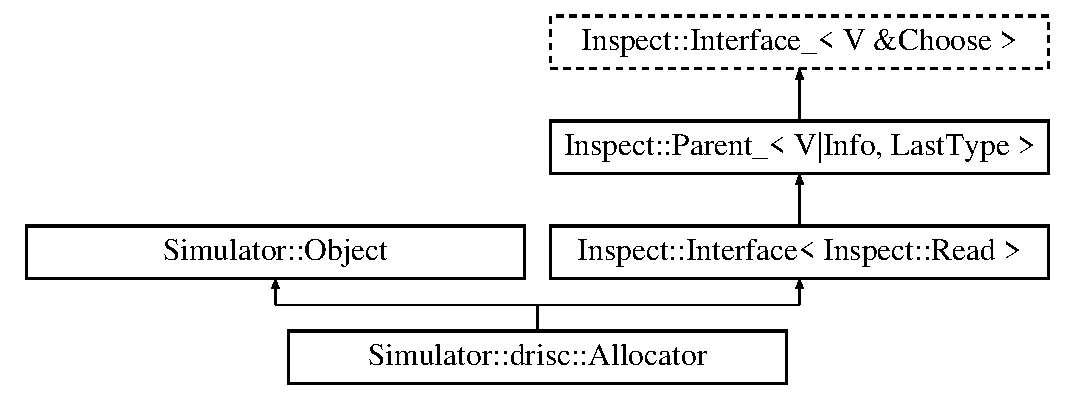
\includegraphics[height=4.000000cm]{class_simulator_1_1drisc_1_1_allocator}
\end{center}
\end{figure}
\subsection*{Classes}
\begin{DoxyCompactItemize}
\item 
struct \hyperlink{struct_simulator_1_1drisc_1_1_allocator_1_1_alloc_request}{Alloc\+Request}
\item 
struct \hyperlink{struct_simulator_1_1drisc_1_1_allocator_1_1_bundle_info}{Bundle\+Info}
\end{DoxyCompactItemize}
\subsection*{Public Types}
\begin{DoxyCompactItemize}
\item 
enum \hyperlink{class_simulator_1_1drisc_1_1_allocator_a4c0e38da00f0ef95142e545d5cc147ab}{Create\+State} \{ \\*
\hyperlink{class_simulator_1_1drisc_1_1_allocator_a4c0e38da00f0ef95142e545d5cc147aba41846e05232a81327bef06b6f0c22251}{C\+R\+E\+A\+T\+E\+\_\+\+I\+N\+I\+T\+I\+A\+L}, 
\hyperlink{class_simulator_1_1drisc_1_1_allocator_a4c0e38da00f0ef95142e545d5cc147abaf298d71a0765fbb5348c46b2c319fde7}{C\+R\+E\+A\+T\+E\+\_\+\+L\+O\+A\+D\+\_\+\+R\+E\+G\+S\+P\+E\+C}, 
\hyperlink{class_simulator_1_1drisc_1_1_allocator_a4c0e38da00f0ef95142e545d5cc147aba29ad965eee9c7de42df5837d9240f2a4}{C\+R\+E\+A\+T\+E\+\_\+\+L\+O\+A\+D\+I\+N\+G\+\_\+\+L\+I\+N\+E}, 
\hyperlink{class_simulator_1_1drisc_1_1_allocator_a4c0e38da00f0ef95142e545d5cc147aba7ac1c50270f8806a035db810a4ab8c61}{C\+R\+E\+A\+T\+E\+\_\+\+L\+I\+N\+E\+\_\+\+L\+O\+A\+D\+E\+D}, 
\\*
\hyperlink{class_simulator_1_1drisc_1_1_allocator_a4c0e38da00f0ef95142e545d5cc147aba5d33b9ad335f106455b4030af9f5bdb9}{C\+R\+E\+A\+T\+E\+\_\+\+R\+E\+S\+T\+R\+I\+C\+T\+I\+N\+G}, 
\hyperlink{class_simulator_1_1drisc_1_1_allocator_a4c0e38da00f0ef95142e545d5cc147abad45f11e2685ef0e725925453e4fc0c08}{C\+R\+E\+A\+T\+E\+\_\+\+A\+L\+L\+O\+C\+A\+T\+I\+N\+G\+\_\+\+R\+E\+G\+I\+S\+T\+E\+R\+S}, 
\hyperlink{class_simulator_1_1drisc_1_1_allocator_a4c0e38da00f0ef95142e545d5cc147abaacd4042da8ba91bd6e957b72a3551f2a}{C\+R\+E\+A\+T\+E\+\_\+\+B\+R\+O\+A\+D\+C\+A\+S\+T\+I\+N\+G\+\_\+\+C\+R\+E\+A\+T\+E}, 
\hyperlink{class_simulator_1_1drisc_1_1_allocator_a4c0e38da00f0ef95142e545d5cc147aba9279b2d16cdf34f402511e378ebd4ae3}{C\+R\+E\+A\+T\+E\+\_\+\+A\+C\+T\+I\+V\+A\+T\+I\+N\+G\+\_\+\+F\+A\+M\+I\+L\+Y}, 
\\*
\hyperlink{class_simulator_1_1drisc_1_1_allocator_a4c0e38da00f0ef95142e545d5cc147abaea6b023923fbbddffcb35cad7e34b3a7}{C\+R\+E\+A\+T\+E\+\_\+\+N\+O\+T\+I\+F\+Y}
 \}
\item 
enum \hyperlink{class_simulator_1_1drisc_1_1_allocator_a411b852f8de6fe3d7c8223ecc6966802}{Bundle\+State} \{ \hyperlink{class_simulator_1_1drisc_1_1_allocator_a411b852f8de6fe3d7c8223ecc6966802afd73618eec58a84562e329d529364b3e}{B\+U\+N\+D\+L\+E\+\_\+\+I\+N\+I\+T\+I\+A\+L}, 
\hyperlink{class_simulator_1_1drisc_1_1_allocator_a411b852f8de6fe3d7c8223ecc6966802a9222d98a2f415b286459c4e19d07ee25}{B\+U\+N\+D\+L\+E\+\_\+\+L\+O\+A\+D\+I\+N\+G\+\_\+\+L\+I\+N\+E}, 
\hyperlink{class_simulator_1_1drisc_1_1_allocator_a411b852f8de6fe3d7c8223ecc6966802a69070d18633adbc60c5e43cdfd0872e0}{B\+U\+N\+D\+L\+E\+\_\+\+L\+I\+N\+E\+\_\+\+L\+O\+A\+D\+E\+D}
 \}
\item 
typedef \hyperlink{class_simulator_1_1_linked_list}{Linked\+List}$<$ \hyperlink{namespace_simulator_a483cc4ecee1736e895054617672cded5}{T\+I\+D}, \\*
\hyperlink{class_simulator_1_1drisc_1_1_thread_table}{Thread\+Table},\&\hyperlink{struct_simulator_1_1drisc_1_1_thread_acbfe721255a13b2fd1d188225ea29b99}{Thread\+::next} $>$ \hyperlink{class_simulator_1_1drisc_1_1_allocator_acee4df99e4e6a73556f46dd8ad5aa6e1}{Thread\+List}
\end{DoxyCompactItemize}
\subsection*{Public Member Functions}
\begin{DoxyCompactItemize}
\item 
\hyperlink{class_simulator_1_1drisc_1_1_allocator_a5b437c3fbb2109d529e62ae476b0c7ef}{Allocator} (const std\+::string \&\hyperlink{mtconf_8c_a8f8f80d37794cde9472343e4487ba3eb}{name}, \hyperlink{class_simulator_1_1_d_r_i_s_c}{D\+R\+I\+S\+C} \&parent, \hyperlink{class_simulator_1_1_clock}{Clock} \&clock, \hyperlink{class_config}{Config} \&config)
\item 
\hyperlink{class_simulator_1_1drisc_1_1_allocator_aa7a7175ea4041805895b804721a942f7}{Allocator} (const \hyperlink{class_simulator_1_1drisc_1_1_allocator}{Allocator} \&)=delete
\item 
\hyperlink{class_simulator_1_1drisc_1_1_allocator}{Allocator} \& \hyperlink{class_simulator_1_1drisc_1_1_allocator_a260fe03743fe739f5724f46c98f34cfd}{operator=} (const \hyperlink{class_simulator_1_1drisc_1_1_allocator}{Allocator} \&)=delete
\item 
void \hyperlink{class_simulator_1_1drisc_1_1_allocator_a4d09f3b758dd8b76885a89c465e2c5f3}{Allocate\+Initial\+Family} (Mem\+Addr pc, bool legacy, \hyperlink{namespace_simulator_a4aa07bee2f34beac11abf48a8ccc47c4}{P\+Size} place\+Size, S\+Integer start\+Index)
\item 
\hyperlink{namespace_simulator_aaccbc706b2d6c99085f52f6dfc2333e4}{L\+F\+I\+D} \hyperlink{class_simulator_1_1drisc_1_1_allocator_a657478e6ce34aec7395f127972ee5f60}{Allocate\+Context} (\hyperlink{namespace_simulator_ab3233bd11b43e37322a8111dc7eec133}{Context\+Type} type, \hyperlink{namespace_simulator_aaccbc706b2d6c99085f52f6dfc2333e4}{L\+F\+I\+D} prev\+\_\+fid, \hyperlink{namespace_simulator_a4aa07bee2f34beac11abf48a8ccc47c4}{P\+Size} place\+Size)
\begin{DoxyCompactList}\small\item\em Allocates a contexts and sets the family's 'link' field to prev\+\_\+fid. \end{DoxyCompactList}\item 
\hyperlink{struct_simulator_1_1_reg_addr}{Reg\+Addr} \hyperlink{class_simulator_1_1drisc_1_1_allocator_af76cee2225340810705b3038248ad435}{Get\+Remote\+Register\+Address} (\hyperlink{namespace_simulator_aaccbc706b2d6c99085f52f6dfc2333e4}{L\+F\+I\+D} fid, \hyperlink{namespace_simulator_aac96aab43eac55fb7f08383889feb2d8}{Remote\+Reg\+Type} kind, const \hyperlink{struct_simulator_1_1_reg_addr}{Reg\+Addr} \&addr) const 
\item 
\hyperlink{struct_simulator_1_1drisc_1_1_family}{Family} \& \hyperlink{class_simulator_1_1drisc_1_1_allocator_a2e6106a71e49b7468ffeb6f8e66f3ab3}{Get\+Family\+Checked} (\hyperlink{namespace_simulator_aaccbc706b2d6c99085f52f6dfc2333e4}{L\+F\+I\+D} fid, \hyperlink{namespace_simulator_a607aa9969bfe2711861ae21f42c37c59}{F\+Capability} capability) const 
\item 
bool \hyperlink{class_simulator_1_1drisc_1_1_allocator_ab37142b9fee9d512f024f5c9ee63894a}{Activate\+Threads} (const \hyperlink{struct_simulator_1_1_thread_queue}{Thread\+Queue} \&threads)
\item 
bool \hyperlink{class_simulator_1_1drisc_1_1_allocator_a169cdbc4e190eda02b915d4e24759d45}{Reschedule\+Thread} (\hyperlink{namespace_simulator_a483cc4ecee1736e895054617672cded5}{T\+I\+D} tid, Mem\+Addr pc)
\item 
bool \hyperlink{class_simulator_1_1drisc_1_1_allocator_ac37fd4bebd3e003d525b983140528ce5}{Suspend\+Thread} (\hyperlink{namespace_simulator_a483cc4ecee1736e895054617672cded5}{T\+I\+D} tid, Mem\+Addr pc)
\item 
bool \hyperlink{class_simulator_1_1drisc_1_1_allocator_adaf39753f5a0ae3ba3050fee1de3aa41}{Kill\+Thread} (\hyperlink{namespace_simulator_a483cc4ecee1736e895054617672cded5}{T\+I\+D} tid)
\item 
bool \hyperlink{class_simulator_1_1drisc_1_1_allocator_a721030070ec8451b5a794d102c5b4fa0}{Queue\+Family\+Allocation} (const \hyperlink{struct_simulator_1_1drisc_1_1_remote_message}{Remote\+Message} \&msg)
\begin{DoxyCompactList}\small\item\em Queues an allocation request for a family entry and context. \end{DoxyCompactList}\item 
bool \hyperlink{class_simulator_1_1drisc_1_1_allocator_a5e7f3b0f99ca7882ad297626103ddd14}{Queue\+Family\+Allocation} (const \hyperlink{struct_simulator_1_1drisc_1_1_link_message}{Link\+Message} \&msg)
\begin{DoxyCompactList}\small\item\em Queues an allocation request for a family entry and context. \end{DoxyCompactList}\item 
bool \hyperlink{class_simulator_1_1drisc_1_1_allocator_ab9bd6c2ae162cbab2dece0cd4c06eacf}{Queue\+Bundle} (const Mem\+Addr addr, Integer parameter, \hyperlink{namespace_simulator_ab00c9033de4c9a17db7b53d6c292515c}{Reg\+Index} completion\+\_\+reg)
\item 
bool \hyperlink{class_simulator_1_1drisc_1_1_allocator_ab17d88c621263b976463b25146d4b17a}{Activate\+Family} (\hyperlink{namespace_simulator_aaccbc706b2d6c99085f52f6dfc2333e4}{L\+F\+I\+D} fid)
\item 
\hyperlink{namespace_simulator_a607aa9969bfe2711861ae21f42c37c59}{F\+Capability} \hyperlink{class_simulator_1_1drisc_1_1_allocator_a8867a1502dbe6e7f09b83ab11a29e579}{Initialize\+Family} (\hyperlink{namespace_simulator_aaccbc706b2d6c99085f52f6dfc2333e4}{L\+F\+I\+D} fid) const 
\item 
void \hyperlink{class_simulator_1_1drisc_1_1_allocator_a7116ae9b69b890498975d4b808d916fe}{Release\+Context} (\hyperlink{namespace_simulator_aaccbc706b2d6c99085f52f6dfc2333e4}{L\+F\+I\+D} fid)
\item 
bool \hyperlink{class_simulator_1_1drisc_1_1_allocator_afbec6b695e3555da3593c42f031dc197}{Queue\+Create} (const \hyperlink{struct_simulator_1_1drisc_1_1_remote_message}{Remote\+Message} \&msg)
\item 
bool \hyperlink{class_simulator_1_1drisc_1_1_allocator_a4ab50a75d30ba99489332b4b9b934b65}{Queue\+Create} (const \hyperlink{struct_simulator_1_1drisc_1_1_link_message}{Link\+Message} \&msg)
\item 
bool \hyperlink{class_simulator_1_1drisc_1_1_allocator_aaa6c02339182aadd2d6caf0609852b9c}{Queue\+Active\+Threads} (const \hyperlink{struct_simulator_1_1_thread_queue}{Thread\+Queue} \&threads)
\item 
bool \hyperlink{class_simulator_1_1drisc_1_1_allocator_a3b17e91b304be557a917922101d0f009}{Queue\+Threads} (\hyperlink{class_simulator_1_1drisc_1_1_allocator_acee4df99e4e6a73556f46dd8ad5aa6e1}{Thread\+List} \&list, const \hyperlink{struct_simulator_1_1_thread_queue}{Thread\+Queue} \&threads, \hyperlink{namespace_simulator_a5450f6fb4b10ec16b290049311b8d5d0}{Thread\+State} state)
\item 
bool \hyperlink{class_simulator_1_1drisc_1_1_allocator_a69167e032a26ac9d6f52e0457c1b764d}{On\+I\+Cacheline\+Loaded} (\hyperlink{namespace_simulator_a97f45fafcb1aafc0f269a19608b39d60}{C\+I\+D} cid)
\item 
bool \hyperlink{class_simulator_1_1drisc_1_1_allocator_afac644895b1ea204ce4d060f382dd4ca}{On\+D\+Cacheline\+Loaded} (char $\ast$data)
\item 
bool \hyperlink{class_simulator_1_1drisc_1_1_allocator_a1743acbdeaffe848ef3ded06ee9b8058}{On\+Memory\+Read} (\hyperlink{namespace_simulator_aaccbc706b2d6c99085f52f6dfc2333e4}{L\+F\+I\+D} fid)
\item 
bool \hyperlink{class_simulator_1_1drisc_1_1_allocator_a8fb2331b85b645fe2063c9d22972c967}{Decrease\+Family\+Dependency} (\hyperlink{namespace_simulator_aaccbc706b2d6c99085f52f6dfc2333e4}{L\+F\+I\+D} fid, \hyperlink{namespace_simulator_1_1drisc_ac6be077f11d2c5eb93b6ce2371bf67f4}{Family\+Dependency} dep)
\item 
bool \hyperlink{class_simulator_1_1drisc_1_1_allocator_a845ad6443a2a15413437746bf588f8f8}{Decrease\+Family\+Dependency} (\hyperlink{namespace_simulator_aaccbc706b2d6c99085f52f6dfc2333e4}{L\+F\+I\+D} fid, \hyperlink{struct_simulator_1_1drisc_1_1_family}{Family} \&family, \hyperlink{namespace_simulator_1_1drisc_ac6be077f11d2c5eb93b6ce2371bf67f4}{Family\+Dependency} dep)
\item 
bool \hyperlink{class_simulator_1_1drisc_1_1_allocator_a18e3a82c42a484f1ec1369152c2ee544}{Increase\+Thread\+Dependency} (\hyperlink{namespace_simulator_a483cc4ecee1736e895054617672cded5}{T\+I\+D} tid, \hyperlink{namespace_simulator_1_1drisc_ad6854da07c57895c7a56c85e725e9efa}{Thread\+Dependency} dep)
\item 
bool \hyperlink{class_simulator_1_1drisc_1_1_allocator_ab903d41c70f31adb730e8919da05a6cb}{Decrease\+Thread\+Dependency} (\hyperlink{namespace_simulator_a483cc4ecee1736e895054617672cded5}{T\+I\+D} tid, \hyperlink{namespace_simulator_1_1drisc_ad6854da07c57895c7a56c85e725e9efa}{Thread\+Dependency} dep)
\item 
\hyperlink{namespace_simulator_a483cc4ecee1736e895054617672cded5}{T\+I\+D} \hyperlink{class_simulator_1_1drisc_1_1_allocator_a889c7746b9b885ac9e37596ca3ccac7a}{Pop\+Active\+Thread} ()
\item 
\hyperlink{namespace_simulator_a483cc4ecee1736e895054617672cded5}{T\+I\+D} \hyperlink{class_simulator_1_1drisc_1_1_allocator_a0fed73adf3ee355ed1823e5e0a472845}{Get\+Register\+Type} (\hyperlink{namespace_simulator_aaccbc706b2d6c99085f52f6dfc2333e4}{L\+F\+I\+D} fid, \hyperlink{struct_simulator_1_1_reg_addr}{Reg\+Addr} addr, \hyperlink{namespace_simulator_aed8a64878dc9a85785a9289468470a77}{Reg\+Class} $\ast$group, size\+\_\+t $\ast$rel) const 
\item 
void \hyperlink{class_simulator_1_1drisc_1_1_allocator_ace8d867aff390825ad217a9fcf660d39}{Cmd\+\_\+\+Info} (std\+::ostream \&out, const std\+::vector$<$ std\+::string $>$ \&arguments) const override
\item 
void \hyperlink{class_simulator_1_1drisc_1_1_allocator_a9fa7bf5e89129ea06eafb37091bb69d9}{Cmd\+\_\+\+Read} (std\+::ostream \&out, const std\+::vector$<$ std\+::string $>$ \&arguments) const override
\item 
\hyperlink{namespace_simulator_a5ca279f926485be2d0554e41275a3305}{Buffer\+Size} \hyperlink{class_simulator_1_1drisc_1_1_allocator_aea916d0822bbf0f1918111da2673bc5b}{Get\+Total\+Allocated\+Ex} ()
\item 
\hyperlink{namespace_simulator_a5ca279f926485be2d0554e41275a3305}{Buffer\+Size} \hyperlink{class_simulator_1_1drisc_1_1_allocator_abbd9728a4d18602c6ea8d0581e4504b6}{Get\+Max\+Allocated\+Ex} () const 
\item 
\hyperlink{namespace_simulator_aefe00209f3ea9f8e24874de522c3c3e7}{T\+Size} \hyperlink{class_simulator_1_1drisc_1_1_allocator_a9e896968e323c2447d6778c8d8e513b8}{Get\+Total\+Families\+Created} () const 
\item 
\hyperlink{namespace_simulator_a06544009313d7c13d411b1c074e5acff}{F\+Size} \hyperlink{class_simulator_1_1drisc_1_1_allocator_add227dd1e85ff6106f98e68b564a9131}{Get\+Total\+Threads\+Created} () const 
\end{DoxyCompactItemize}
\subsection*{Public Attributes}
\begin{DoxyCompactItemize}
\item 
\hyperlink{class_simulator_1_1_process}{Process} \hyperlink{class_simulator_1_1drisc_1_1_allocator_a76447246986a86eda057380a359b0a61}{p\+\_\+\+Thread\+Allocate}
\item 
\hyperlink{class_simulator_1_1_process}{Process} \hyperlink{class_simulator_1_1drisc_1_1_allocator_a8b7b38207f6ada3e91ef3b754dde6db5}{p\+\_\+\+Family\+Allocate}
\item 
\hyperlink{class_simulator_1_1_process}{Process} \hyperlink{class_simulator_1_1drisc_1_1_allocator_acd596bc11bab9b44a07e069aea4864a2}{p\+\_\+\+Family\+Create}
\item 
\hyperlink{class_simulator_1_1_process}{Process} \hyperlink{class_simulator_1_1drisc_1_1_allocator_a86ba51d9defcde72c57eb52ebfbb9d1f}{p\+\_\+\+Thread\+Activation}
\item 
\hyperlink{class_simulator_1_1_process}{Process} \hyperlink{class_simulator_1_1drisc_1_1_allocator_ab585d90eae505ff9f0919bb37c1037d4}{p\+\_\+\+Bundle}
\item 
\hyperlink{class_simulator_1_1_arbitrated_service}{Arbitrated\+Service} \hyperlink{class_simulator_1_1drisc_1_1_allocator_aad58ba20aab3c4e2262895c164c6b0a2}{p\+\_\+allocation}
\begin{DoxyCompactList}\small\item\em \hyperlink{class_simulator_1_1_arbitrator}{Arbitrator} for \hyperlink{class_simulator_1_1drisc_1_1_family_table_a79281183526d6db39fab77082005e85e}{Family\+Table\+::\+Allocate\+Family}. \end{DoxyCompactList}\item 
\hyperlink{class_simulator_1_1_arbitrated_service}{Arbitrated\+Service} \hyperlink{class_simulator_1_1drisc_1_1_allocator_a61ddc6b62670962e5bdaabe2b930db43}{p\+\_\+alloc}
\begin{DoxyCompactList}\small\item\em \hyperlink{class_simulator_1_1_arbitrator}{Arbitrator} for m\+\_\+alloc. \end{DoxyCompactList}\item 
\hyperlink{class_simulator_1_1_arbitrated_service}{Arbitrated\+Service} \hyperlink{class_simulator_1_1drisc_1_1_allocator_a90377bbf4176289f5b2a3fbb3f3de5d9}{p\+\_\+ready\+Threads}
\begin{DoxyCompactList}\small\item\em \hyperlink{class_simulator_1_1_arbitrator}{Arbitrator} for m\+\_\+ready\+Threads2. \end{DoxyCompactList}\item 
\hyperlink{class_simulator_1_1_arbitrated_service}{Arbitrated\+Service} \hyperlink{class_simulator_1_1drisc_1_1_allocator_a0d7b40dd1a49218f3b06231cb198d37f}{p\+\_\+active\+Threads}
\begin{DoxyCompactList}\small\item\em \hyperlink{class_simulator_1_1_arbitrator}{Arbitrator} for m\+\_\+active\+Threads. \end{DoxyCompactList}\item 
\hyperlink{class_simulator_1_1drisc_1_1_allocator_acee4df99e4e6a73556f46dd8ad5aa6e1}{Thread\+List} \hyperlink{class_simulator_1_1drisc_1_1_allocator_a8bf29138e7a3f0a83d0ef204542a39af}{m\+\_\+active\+Threads}
\begin{DoxyCompactList}\small\item\em Queue of the active threads. \end{DoxyCompactList}\item 
size\+\_\+t \hyperlink{class_simulator_1_1drisc_1_1_allocator_ab8d660cc10fde6d79364a5836889e567}{m\+\_\+num\+Threads\+Per\+State} \mbox{[}\hyperlink{namespace_simulator_a5450f6fb4b10ec16b290049311b8d5d0a78a2fff5d83cad45629b181024323bdf}{T\+S\+T\+\_\+\+N\+U\+M\+S\+T\+A\+T\+E\+S}\mbox{]}
\begin{DoxyCompactList}\small\item\em For debugging only. \end{DoxyCompactList}\end{DoxyCompactItemize}
\subsection*{Friends}
\begin{DoxyCompactItemize}
\item 
class \hyperlink{class_simulator_1_1drisc_1_1_allocator_a14f94eb83e17d9d8841f39b37431d673}{Simulator\+::\+D\+R\+I\+S\+C}
\item 
class \hyperlink{class_simulator_1_1drisc_1_1_allocator_af8f116e67dbda7135aa0e584293ac685}{I\+O\+Bus\+Interface}
\item 
class \hyperlink{class_simulator_1_1drisc_1_1_allocator_af9f0f1adbd5baee7830839447205af8d}{Pipeline}
\end{DoxyCompactItemize}


\subsection{Member Typedef Documentation}
\hypertarget{class_simulator_1_1drisc_1_1_allocator_acee4df99e4e6a73556f46dd8ad5aa6e1}{\index{Simulator\+::drisc\+::\+Allocator@{Simulator\+::drisc\+::\+Allocator}!Thread\+List@{Thread\+List}}
\index{Thread\+List@{Thread\+List}!Simulator\+::drisc\+::\+Allocator@{Simulator\+::drisc\+::\+Allocator}}
\subsubsection[{Thread\+List}]{\setlength{\rightskip}{0pt plus 5cm}typedef {\bf Linked\+List}$<$ {\bf T\+I\+D}, {\bf Thread\+Table}, \&{\bf Thread\+::next}$>$ {\bf Simulator\+::drisc\+::\+Allocator\+::\+Thread\+List}}}\label{class_simulator_1_1drisc_1_1_allocator_acee4df99e4e6a73556f46dd8ad5aa6e1}


\subsection{Member Enumeration Documentation}
\hypertarget{class_simulator_1_1drisc_1_1_allocator_a411b852f8de6fe3d7c8223ecc6966802}{\index{Simulator\+::drisc\+::\+Allocator@{Simulator\+::drisc\+::\+Allocator}!Bundle\+State@{Bundle\+State}}
\index{Bundle\+State@{Bundle\+State}!Simulator\+::drisc\+::\+Allocator@{Simulator\+::drisc\+::\+Allocator}}
\subsubsection[{Bundle\+State}]{\setlength{\rightskip}{0pt plus 5cm}enum {\bf Simulator\+::drisc\+::\+Allocator\+::\+Bundle\+State}}}\label{class_simulator_1_1drisc_1_1_allocator_a411b852f8de6fe3d7c8223ecc6966802}
\begin{Desc}
\item[Enumerator]\par
\begin{description}
\index{B\+U\+N\+D\+L\+E\+\_\+\+I\+N\+I\+T\+I\+A\+L@{B\+U\+N\+D\+L\+E\+\_\+\+I\+N\+I\+T\+I\+A\+L}!Simulator\+::drisc\+::\+Allocator@{Simulator\+::drisc\+::\+Allocator}}\index{Simulator\+::drisc\+::\+Allocator@{Simulator\+::drisc\+::\+Allocator}!B\+U\+N\+D\+L\+E\+\_\+\+I\+N\+I\+T\+I\+A\+L@{B\+U\+N\+D\+L\+E\+\_\+\+I\+N\+I\+T\+I\+A\+L}}\item[{\em 
\hypertarget{class_simulator_1_1drisc_1_1_allocator_a411b852f8de6fe3d7c8223ecc6966802afd73618eec58a84562e329d529364b3e}{B\+U\+N\+D\+L\+E\+\_\+\+I\+N\+I\+T\+I\+A\+L}\label{class_simulator_1_1drisc_1_1_allocator_a411b852f8de6fe3d7c8223ecc6966802afd73618eec58a84562e329d529364b3e}
}]\index{B\+U\+N\+D\+L\+E\+\_\+\+L\+O\+A\+D\+I\+N\+G\+\_\+\+L\+I\+N\+E@{B\+U\+N\+D\+L\+E\+\_\+\+L\+O\+A\+D\+I\+N\+G\+\_\+\+L\+I\+N\+E}!Simulator\+::drisc\+::\+Allocator@{Simulator\+::drisc\+::\+Allocator}}\index{Simulator\+::drisc\+::\+Allocator@{Simulator\+::drisc\+::\+Allocator}!B\+U\+N\+D\+L\+E\+\_\+\+L\+O\+A\+D\+I\+N\+G\+\_\+\+L\+I\+N\+E@{B\+U\+N\+D\+L\+E\+\_\+\+L\+O\+A\+D\+I\+N\+G\+\_\+\+L\+I\+N\+E}}\item[{\em 
\hypertarget{class_simulator_1_1drisc_1_1_allocator_a411b852f8de6fe3d7c8223ecc6966802a9222d98a2f415b286459c4e19d07ee25}{B\+U\+N\+D\+L\+E\+\_\+\+L\+O\+A\+D\+I\+N\+G\+\_\+\+L\+I\+N\+E}\label{class_simulator_1_1drisc_1_1_allocator_a411b852f8de6fe3d7c8223ecc6966802a9222d98a2f415b286459c4e19d07ee25}
}]\index{B\+U\+N\+D\+L\+E\+\_\+\+L\+I\+N\+E\+\_\+\+L\+O\+A\+D\+E\+D@{B\+U\+N\+D\+L\+E\+\_\+\+L\+I\+N\+E\+\_\+\+L\+O\+A\+D\+E\+D}!Simulator\+::drisc\+::\+Allocator@{Simulator\+::drisc\+::\+Allocator}}\index{Simulator\+::drisc\+::\+Allocator@{Simulator\+::drisc\+::\+Allocator}!B\+U\+N\+D\+L\+E\+\_\+\+L\+I\+N\+E\+\_\+\+L\+O\+A\+D\+E\+D@{B\+U\+N\+D\+L\+E\+\_\+\+L\+I\+N\+E\+\_\+\+L\+O\+A\+D\+E\+D}}\item[{\em 
\hypertarget{class_simulator_1_1drisc_1_1_allocator_a411b852f8de6fe3d7c8223ecc6966802a69070d18633adbc60c5e43cdfd0872e0}{B\+U\+N\+D\+L\+E\+\_\+\+L\+I\+N\+E\+\_\+\+L\+O\+A\+D\+E\+D}\label{class_simulator_1_1drisc_1_1_allocator_a411b852f8de6fe3d7c8223ecc6966802a69070d18633adbc60c5e43cdfd0872e0}
}]\end{description}
\end{Desc}
\hypertarget{class_simulator_1_1drisc_1_1_allocator_a4c0e38da00f0ef95142e545d5cc147ab}{\index{Simulator\+::drisc\+::\+Allocator@{Simulator\+::drisc\+::\+Allocator}!Create\+State@{Create\+State}}
\index{Create\+State@{Create\+State}!Simulator\+::drisc\+::\+Allocator@{Simulator\+::drisc\+::\+Allocator}}
\subsubsection[{Create\+State}]{\setlength{\rightskip}{0pt plus 5cm}enum {\bf Simulator\+::drisc\+::\+Allocator\+::\+Create\+State}}}\label{class_simulator_1_1drisc_1_1_allocator_a4c0e38da00f0ef95142e545d5cc147ab}
\begin{Desc}
\item[Enumerator]\par
\begin{description}
\index{C\+R\+E\+A\+T\+E\+\_\+\+I\+N\+I\+T\+I\+A\+L@{C\+R\+E\+A\+T\+E\+\_\+\+I\+N\+I\+T\+I\+A\+L}!Simulator\+::drisc\+::\+Allocator@{Simulator\+::drisc\+::\+Allocator}}\index{Simulator\+::drisc\+::\+Allocator@{Simulator\+::drisc\+::\+Allocator}!C\+R\+E\+A\+T\+E\+\_\+\+I\+N\+I\+T\+I\+A\+L@{C\+R\+E\+A\+T\+E\+\_\+\+I\+N\+I\+T\+I\+A\+L}}\item[{\em 
\hypertarget{class_simulator_1_1drisc_1_1_allocator_a4c0e38da00f0ef95142e545d5cc147aba41846e05232a81327bef06b6f0c22251}{C\+R\+E\+A\+T\+E\+\_\+\+I\+N\+I\+T\+I\+A\+L}\label{class_simulator_1_1drisc_1_1_allocator_a4c0e38da00f0ef95142e545d5cc147aba41846e05232a81327bef06b6f0c22251}
}]\index{C\+R\+E\+A\+T\+E\+\_\+\+L\+O\+A\+D\+\_\+\+R\+E\+G\+S\+P\+E\+C@{C\+R\+E\+A\+T\+E\+\_\+\+L\+O\+A\+D\+\_\+\+R\+E\+G\+S\+P\+E\+C}!Simulator\+::drisc\+::\+Allocator@{Simulator\+::drisc\+::\+Allocator}}\index{Simulator\+::drisc\+::\+Allocator@{Simulator\+::drisc\+::\+Allocator}!C\+R\+E\+A\+T\+E\+\_\+\+L\+O\+A\+D\+\_\+\+R\+E\+G\+S\+P\+E\+C@{C\+R\+E\+A\+T\+E\+\_\+\+L\+O\+A\+D\+\_\+\+R\+E\+G\+S\+P\+E\+C}}\item[{\em 
\hypertarget{class_simulator_1_1drisc_1_1_allocator_a4c0e38da00f0ef95142e545d5cc147abaf298d71a0765fbb5348c46b2c319fde7}{C\+R\+E\+A\+T\+E\+\_\+\+L\+O\+A\+D\+\_\+\+R\+E\+G\+S\+P\+E\+C}\label{class_simulator_1_1drisc_1_1_allocator_a4c0e38da00f0ef95142e545d5cc147abaf298d71a0765fbb5348c46b2c319fde7}
}]\index{C\+R\+E\+A\+T\+E\+\_\+\+L\+O\+A\+D\+I\+N\+G\+\_\+\+L\+I\+N\+E@{C\+R\+E\+A\+T\+E\+\_\+\+L\+O\+A\+D\+I\+N\+G\+\_\+\+L\+I\+N\+E}!Simulator\+::drisc\+::\+Allocator@{Simulator\+::drisc\+::\+Allocator}}\index{Simulator\+::drisc\+::\+Allocator@{Simulator\+::drisc\+::\+Allocator}!C\+R\+E\+A\+T\+E\+\_\+\+L\+O\+A\+D\+I\+N\+G\+\_\+\+L\+I\+N\+E@{C\+R\+E\+A\+T\+E\+\_\+\+L\+O\+A\+D\+I\+N\+G\+\_\+\+L\+I\+N\+E}}\item[{\em 
\hypertarget{class_simulator_1_1drisc_1_1_allocator_a4c0e38da00f0ef95142e545d5cc147aba29ad965eee9c7de42df5837d9240f2a4}{C\+R\+E\+A\+T\+E\+\_\+\+L\+O\+A\+D\+I\+N\+G\+\_\+\+L\+I\+N\+E}\label{class_simulator_1_1drisc_1_1_allocator_a4c0e38da00f0ef95142e545d5cc147aba29ad965eee9c7de42df5837d9240f2a4}
}]\index{C\+R\+E\+A\+T\+E\+\_\+\+L\+I\+N\+E\+\_\+\+L\+O\+A\+D\+E\+D@{C\+R\+E\+A\+T\+E\+\_\+\+L\+I\+N\+E\+\_\+\+L\+O\+A\+D\+E\+D}!Simulator\+::drisc\+::\+Allocator@{Simulator\+::drisc\+::\+Allocator}}\index{Simulator\+::drisc\+::\+Allocator@{Simulator\+::drisc\+::\+Allocator}!C\+R\+E\+A\+T\+E\+\_\+\+L\+I\+N\+E\+\_\+\+L\+O\+A\+D\+E\+D@{C\+R\+E\+A\+T\+E\+\_\+\+L\+I\+N\+E\+\_\+\+L\+O\+A\+D\+E\+D}}\item[{\em 
\hypertarget{class_simulator_1_1drisc_1_1_allocator_a4c0e38da00f0ef95142e545d5cc147aba7ac1c50270f8806a035db810a4ab8c61}{C\+R\+E\+A\+T\+E\+\_\+\+L\+I\+N\+E\+\_\+\+L\+O\+A\+D\+E\+D}\label{class_simulator_1_1drisc_1_1_allocator_a4c0e38da00f0ef95142e545d5cc147aba7ac1c50270f8806a035db810a4ab8c61}
}]\index{C\+R\+E\+A\+T\+E\+\_\+\+R\+E\+S\+T\+R\+I\+C\+T\+I\+N\+G@{C\+R\+E\+A\+T\+E\+\_\+\+R\+E\+S\+T\+R\+I\+C\+T\+I\+N\+G}!Simulator\+::drisc\+::\+Allocator@{Simulator\+::drisc\+::\+Allocator}}\index{Simulator\+::drisc\+::\+Allocator@{Simulator\+::drisc\+::\+Allocator}!C\+R\+E\+A\+T\+E\+\_\+\+R\+E\+S\+T\+R\+I\+C\+T\+I\+N\+G@{C\+R\+E\+A\+T\+E\+\_\+\+R\+E\+S\+T\+R\+I\+C\+T\+I\+N\+G}}\item[{\em 
\hypertarget{class_simulator_1_1drisc_1_1_allocator_a4c0e38da00f0ef95142e545d5cc147aba5d33b9ad335f106455b4030af9f5bdb9}{C\+R\+E\+A\+T\+E\+\_\+\+R\+E\+S\+T\+R\+I\+C\+T\+I\+N\+G}\label{class_simulator_1_1drisc_1_1_allocator_a4c0e38da00f0ef95142e545d5cc147aba5d33b9ad335f106455b4030af9f5bdb9}
}]\index{C\+R\+E\+A\+T\+E\+\_\+\+A\+L\+L\+O\+C\+A\+T\+I\+N\+G\+\_\+\+R\+E\+G\+I\+S\+T\+E\+R\+S@{C\+R\+E\+A\+T\+E\+\_\+\+A\+L\+L\+O\+C\+A\+T\+I\+N\+G\+\_\+\+R\+E\+G\+I\+S\+T\+E\+R\+S}!Simulator\+::drisc\+::\+Allocator@{Simulator\+::drisc\+::\+Allocator}}\index{Simulator\+::drisc\+::\+Allocator@{Simulator\+::drisc\+::\+Allocator}!C\+R\+E\+A\+T\+E\+\_\+\+A\+L\+L\+O\+C\+A\+T\+I\+N\+G\+\_\+\+R\+E\+G\+I\+S\+T\+E\+R\+S@{C\+R\+E\+A\+T\+E\+\_\+\+A\+L\+L\+O\+C\+A\+T\+I\+N\+G\+\_\+\+R\+E\+G\+I\+S\+T\+E\+R\+S}}\item[{\em 
\hypertarget{class_simulator_1_1drisc_1_1_allocator_a4c0e38da00f0ef95142e545d5cc147abad45f11e2685ef0e725925453e4fc0c08}{C\+R\+E\+A\+T\+E\+\_\+\+A\+L\+L\+O\+C\+A\+T\+I\+N\+G\+\_\+\+R\+E\+G\+I\+S\+T\+E\+R\+S}\label{class_simulator_1_1drisc_1_1_allocator_a4c0e38da00f0ef95142e545d5cc147abad45f11e2685ef0e725925453e4fc0c08}
}]\index{C\+R\+E\+A\+T\+E\+\_\+\+B\+R\+O\+A\+D\+C\+A\+S\+T\+I\+N\+G\+\_\+\+C\+R\+E\+A\+T\+E@{C\+R\+E\+A\+T\+E\+\_\+\+B\+R\+O\+A\+D\+C\+A\+S\+T\+I\+N\+G\+\_\+\+C\+R\+E\+A\+T\+E}!Simulator\+::drisc\+::\+Allocator@{Simulator\+::drisc\+::\+Allocator}}\index{Simulator\+::drisc\+::\+Allocator@{Simulator\+::drisc\+::\+Allocator}!C\+R\+E\+A\+T\+E\+\_\+\+B\+R\+O\+A\+D\+C\+A\+S\+T\+I\+N\+G\+\_\+\+C\+R\+E\+A\+T\+E@{C\+R\+E\+A\+T\+E\+\_\+\+B\+R\+O\+A\+D\+C\+A\+S\+T\+I\+N\+G\+\_\+\+C\+R\+E\+A\+T\+E}}\item[{\em 
\hypertarget{class_simulator_1_1drisc_1_1_allocator_a4c0e38da00f0ef95142e545d5cc147abaacd4042da8ba91bd6e957b72a3551f2a}{C\+R\+E\+A\+T\+E\+\_\+\+B\+R\+O\+A\+D\+C\+A\+S\+T\+I\+N\+G\+\_\+\+C\+R\+E\+A\+T\+E}\label{class_simulator_1_1drisc_1_1_allocator_a4c0e38da00f0ef95142e545d5cc147abaacd4042da8ba91bd6e957b72a3551f2a}
}]\index{C\+R\+E\+A\+T\+E\+\_\+\+A\+C\+T\+I\+V\+A\+T\+I\+N\+G\+\_\+\+F\+A\+M\+I\+L\+Y@{C\+R\+E\+A\+T\+E\+\_\+\+A\+C\+T\+I\+V\+A\+T\+I\+N\+G\+\_\+\+F\+A\+M\+I\+L\+Y}!Simulator\+::drisc\+::\+Allocator@{Simulator\+::drisc\+::\+Allocator}}\index{Simulator\+::drisc\+::\+Allocator@{Simulator\+::drisc\+::\+Allocator}!C\+R\+E\+A\+T\+E\+\_\+\+A\+C\+T\+I\+V\+A\+T\+I\+N\+G\+\_\+\+F\+A\+M\+I\+L\+Y@{C\+R\+E\+A\+T\+E\+\_\+\+A\+C\+T\+I\+V\+A\+T\+I\+N\+G\+\_\+\+F\+A\+M\+I\+L\+Y}}\item[{\em 
\hypertarget{class_simulator_1_1drisc_1_1_allocator_a4c0e38da00f0ef95142e545d5cc147aba9279b2d16cdf34f402511e378ebd4ae3}{C\+R\+E\+A\+T\+E\+\_\+\+A\+C\+T\+I\+V\+A\+T\+I\+N\+G\+\_\+\+F\+A\+M\+I\+L\+Y}\label{class_simulator_1_1drisc_1_1_allocator_a4c0e38da00f0ef95142e545d5cc147aba9279b2d16cdf34f402511e378ebd4ae3}
}]\index{C\+R\+E\+A\+T\+E\+\_\+\+N\+O\+T\+I\+F\+Y@{C\+R\+E\+A\+T\+E\+\_\+\+N\+O\+T\+I\+F\+Y}!Simulator\+::drisc\+::\+Allocator@{Simulator\+::drisc\+::\+Allocator}}\index{Simulator\+::drisc\+::\+Allocator@{Simulator\+::drisc\+::\+Allocator}!C\+R\+E\+A\+T\+E\+\_\+\+N\+O\+T\+I\+F\+Y@{C\+R\+E\+A\+T\+E\+\_\+\+N\+O\+T\+I\+F\+Y}}\item[{\em 
\hypertarget{class_simulator_1_1drisc_1_1_allocator_a4c0e38da00f0ef95142e545d5cc147abaea6b023923fbbddffcb35cad7e34b3a7}{C\+R\+E\+A\+T\+E\+\_\+\+N\+O\+T\+I\+F\+Y}\label{class_simulator_1_1drisc_1_1_allocator_a4c0e38da00f0ef95142e545d5cc147abaea6b023923fbbddffcb35cad7e34b3a7}
}]\end{description}
\end{Desc}


\subsection{Constructor \& Destructor Documentation}
\hypertarget{class_simulator_1_1drisc_1_1_allocator_a5b437c3fbb2109d529e62ae476b0c7ef}{\index{Simulator\+::drisc\+::\+Allocator@{Simulator\+::drisc\+::\+Allocator}!Allocator@{Allocator}}
\index{Allocator@{Allocator}!Simulator\+::drisc\+::\+Allocator@{Simulator\+::drisc\+::\+Allocator}}
\subsubsection[{Allocator}]{\setlength{\rightskip}{0pt plus 5cm}Simulator\+::drisc\+::\+Allocator\+::\+Allocator (
\begin{DoxyParamCaption}
\item[{const std\+::string \&}]{name, }
\item[{{\bf D\+R\+I\+S\+C} \&}]{parent, }
\item[{{\bf Clock} \&}]{clock, }
\item[{{\bf Config} \&}]{config}
\end{DoxyParamCaption}
)}}\label{class_simulator_1_1drisc_1_1_allocator_a5b437c3fbb2109d529e62ae476b0c7ef}
\hypertarget{class_simulator_1_1drisc_1_1_allocator_aa7a7175ea4041805895b804721a942f7}{\index{Simulator\+::drisc\+::\+Allocator@{Simulator\+::drisc\+::\+Allocator}!Allocator@{Allocator}}
\index{Allocator@{Allocator}!Simulator\+::drisc\+::\+Allocator@{Simulator\+::drisc\+::\+Allocator}}
\subsubsection[{Allocator}]{\setlength{\rightskip}{0pt plus 5cm}Simulator\+::drisc\+::\+Allocator\+::\+Allocator (
\begin{DoxyParamCaption}
\item[{const {\bf Allocator} \&}]{}
\end{DoxyParamCaption}
)\hspace{0.3cm}{\ttfamily [delete]}}}\label{class_simulator_1_1drisc_1_1_allocator_aa7a7175ea4041805895b804721a942f7}


\subsection{Member Function Documentation}
\hypertarget{class_simulator_1_1drisc_1_1_allocator_ab17d88c621263b976463b25146d4b17a}{\index{Simulator\+::drisc\+::\+Allocator@{Simulator\+::drisc\+::\+Allocator}!Activate\+Family@{Activate\+Family}}
\index{Activate\+Family@{Activate\+Family}!Simulator\+::drisc\+::\+Allocator@{Simulator\+::drisc\+::\+Allocator}}
\subsubsection[{Activate\+Family}]{\setlength{\rightskip}{0pt plus 5cm}bool Simulator\+::drisc\+::\+Allocator\+::\+Activate\+Family (
\begin{DoxyParamCaption}
\item[{{\bf L\+F\+I\+D}}]{fid}
\end{DoxyParamCaption}
)}}\label{class_simulator_1_1drisc_1_1_allocator_ab17d88c621263b976463b25146d4b17a}
\hypertarget{class_simulator_1_1drisc_1_1_allocator_ab37142b9fee9d512f024f5c9ee63894a}{\index{Simulator\+::drisc\+::\+Allocator@{Simulator\+::drisc\+::\+Allocator}!Activate\+Threads@{Activate\+Threads}}
\index{Activate\+Threads@{Activate\+Threads}!Simulator\+::drisc\+::\+Allocator@{Simulator\+::drisc\+::\+Allocator}}
\subsubsection[{Activate\+Threads}]{\setlength{\rightskip}{0pt plus 5cm}bool Simulator\+::drisc\+::\+Allocator\+::\+Activate\+Threads (
\begin{DoxyParamCaption}
\item[{const {\bf Thread\+Queue} \&}]{threads}
\end{DoxyParamCaption}
)}}\label{class_simulator_1_1drisc_1_1_allocator_ab37142b9fee9d512f024f5c9ee63894a}
\hypertarget{class_simulator_1_1drisc_1_1_allocator_a657478e6ce34aec7395f127972ee5f60}{\index{Simulator\+::drisc\+::\+Allocator@{Simulator\+::drisc\+::\+Allocator}!Allocate\+Context@{Allocate\+Context}}
\index{Allocate\+Context@{Allocate\+Context}!Simulator\+::drisc\+::\+Allocator@{Simulator\+::drisc\+::\+Allocator}}
\subsubsection[{Allocate\+Context}]{\setlength{\rightskip}{0pt plus 5cm}{\bf L\+F\+I\+D} Simulator\+::drisc\+::\+Allocator\+::\+Allocate\+Context (
\begin{DoxyParamCaption}
\item[{{\bf Context\+Type}}]{type, }
\item[{{\bf L\+F\+I\+D}}]{prev\+\_\+fid, }
\item[{{\bf P\+Size}}]{place\+Size}
\end{DoxyParamCaption}
)}}\label{class_simulator_1_1drisc_1_1_allocator_a657478e6ce34aec7395f127972ee5f60}


Allocates a contexts and sets the family's 'link' field to prev\+\_\+fid. 

\hypertarget{class_simulator_1_1drisc_1_1_allocator_a4d09f3b758dd8b76885a89c465e2c5f3}{\index{Simulator\+::drisc\+::\+Allocator@{Simulator\+::drisc\+::\+Allocator}!Allocate\+Initial\+Family@{Allocate\+Initial\+Family}}
\index{Allocate\+Initial\+Family@{Allocate\+Initial\+Family}!Simulator\+::drisc\+::\+Allocator@{Simulator\+::drisc\+::\+Allocator}}
\subsubsection[{Allocate\+Initial\+Family}]{\setlength{\rightskip}{0pt plus 5cm}void Simulator\+::drisc\+::\+Allocator\+::\+Allocate\+Initial\+Family (
\begin{DoxyParamCaption}
\item[{Mem\+Addr}]{pc, }
\item[{bool}]{legacy, }
\item[{{\bf P\+Size}}]{place\+Size, }
\item[{S\+Integer}]{start\+Index}
\end{DoxyParamCaption}
)}}\label{class_simulator_1_1drisc_1_1_allocator_a4d09f3b758dd8b76885a89c465e2c5f3}
\hypertarget{class_simulator_1_1drisc_1_1_allocator_ace8d867aff390825ad217a9fcf660d39}{\index{Simulator\+::drisc\+::\+Allocator@{Simulator\+::drisc\+::\+Allocator}!Cmd\+\_\+\+Info@{Cmd\+\_\+\+Info}}
\index{Cmd\+\_\+\+Info@{Cmd\+\_\+\+Info}!Simulator\+::drisc\+::\+Allocator@{Simulator\+::drisc\+::\+Allocator}}
\subsubsection[{Cmd\+\_\+\+Info}]{\setlength{\rightskip}{0pt plus 5cm}void Simulator\+::drisc\+::\+Allocator\+::\+Cmd\+\_\+\+Info (
\begin{DoxyParamCaption}
\item[{std\+::ostream \&}]{out, }
\item[{const std\+::vector$<$ std\+::string $>$ \&}]{arguments}
\end{DoxyParamCaption}
) const\hspace{0.3cm}{\ttfamily [override]}}}\label{class_simulator_1_1drisc_1_1_allocator_ace8d867aff390825ad217a9fcf660d39}
\hypertarget{class_simulator_1_1drisc_1_1_allocator_a9fa7bf5e89129ea06eafb37091bb69d9}{\index{Simulator\+::drisc\+::\+Allocator@{Simulator\+::drisc\+::\+Allocator}!Cmd\+\_\+\+Read@{Cmd\+\_\+\+Read}}
\index{Cmd\+\_\+\+Read@{Cmd\+\_\+\+Read}!Simulator\+::drisc\+::\+Allocator@{Simulator\+::drisc\+::\+Allocator}}
\subsubsection[{Cmd\+\_\+\+Read}]{\setlength{\rightskip}{0pt plus 5cm}void Simulator\+::drisc\+::\+Allocator\+::\+Cmd\+\_\+\+Read (
\begin{DoxyParamCaption}
\item[{std\+::ostream \&}]{out, }
\item[{const std\+::vector$<$ std\+::string $>$ \&}]{arguments}
\end{DoxyParamCaption}
) const\hspace{0.3cm}{\ttfamily [override]}}}\label{class_simulator_1_1drisc_1_1_allocator_a9fa7bf5e89129ea06eafb37091bb69d9}
\hypertarget{class_simulator_1_1drisc_1_1_allocator_a8fb2331b85b645fe2063c9d22972c967}{\index{Simulator\+::drisc\+::\+Allocator@{Simulator\+::drisc\+::\+Allocator}!Decrease\+Family\+Dependency@{Decrease\+Family\+Dependency}}
\index{Decrease\+Family\+Dependency@{Decrease\+Family\+Dependency}!Simulator\+::drisc\+::\+Allocator@{Simulator\+::drisc\+::\+Allocator}}
\subsubsection[{Decrease\+Family\+Dependency}]{\setlength{\rightskip}{0pt plus 5cm}bool Simulator\+::drisc\+::\+Allocator\+::\+Decrease\+Family\+Dependency (
\begin{DoxyParamCaption}
\item[{{\bf L\+F\+I\+D}}]{fid, }
\item[{{\bf Family\+Dependency}}]{dep}
\end{DoxyParamCaption}
)}}\label{class_simulator_1_1drisc_1_1_allocator_a8fb2331b85b645fe2063c9d22972c967}
\hypertarget{class_simulator_1_1drisc_1_1_allocator_a845ad6443a2a15413437746bf588f8f8}{\index{Simulator\+::drisc\+::\+Allocator@{Simulator\+::drisc\+::\+Allocator}!Decrease\+Family\+Dependency@{Decrease\+Family\+Dependency}}
\index{Decrease\+Family\+Dependency@{Decrease\+Family\+Dependency}!Simulator\+::drisc\+::\+Allocator@{Simulator\+::drisc\+::\+Allocator}}
\subsubsection[{Decrease\+Family\+Dependency}]{\setlength{\rightskip}{0pt plus 5cm}bool Simulator\+::drisc\+::\+Allocator\+::\+Decrease\+Family\+Dependency (
\begin{DoxyParamCaption}
\item[{{\bf L\+F\+I\+D}}]{fid, }
\item[{{\bf Family} \&}]{family, }
\item[{{\bf Family\+Dependency}}]{dep}
\end{DoxyParamCaption}
)}}\label{class_simulator_1_1drisc_1_1_allocator_a845ad6443a2a15413437746bf588f8f8}
\hypertarget{class_simulator_1_1drisc_1_1_allocator_ab903d41c70f31adb730e8919da05a6cb}{\index{Simulator\+::drisc\+::\+Allocator@{Simulator\+::drisc\+::\+Allocator}!Decrease\+Thread\+Dependency@{Decrease\+Thread\+Dependency}}
\index{Decrease\+Thread\+Dependency@{Decrease\+Thread\+Dependency}!Simulator\+::drisc\+::\+Allocator@{Simulator\+::drisc\+::\+Allocator}}
\subsubsection[{Decrease\+Thread\+Dependency}]{\setlength{\rightskip}{0pt plus 5cm}bool Simulator\+::drisc\+::\+Allocator\+::\+Decrease\+Thread\+Dependency (
\begin{DoxyParamCaption}
\item[{{\bf T\+I\+D}}]{tid, }
\item[{{\bf Thread\+Dependency}}]{dep}
\end{DoxyParamCaption}
)}}\label{class_simulator_1_1drisc_1_1_allocator_ab903d41c70f31adb730e8919da05a6cb}
\hypertarget{class_simulator_1_1drisc_1_1_allocator_a2e6106a71e49b7468ffeb6f8e66f3ab3}{\index{Simulator\+::drisc\+::\+Allocator@{Simulator\+::drisc\+::\+Allocator}!Get\+Family\+Checked@{Get\+Family\+Checked}}
\index{Get\+Family\+Checked@{Get\+Family\+Checked}!Simulator\+::drisc\+::\+Allocator@{Simulator\+::drisc\+::\+Allocator}}
\subsubsection[{Get\+Family\+Checked}]{\setlength{\rightskip}{0pt plus 5cm}{\bf Family} \& Simulator\+::drisc\+::\+Allocator\+::\+Get\+Family\+Checked (
\begin{DoxyParamCaption}
\item[{{\bf L\+F\+I\+D}}]{fid, }
\item[{{\bf F\+Capability}}]{capability}
\end{DoxyParamCaption}
) const}}\label{class_simulator_1_1drisc_1_1_allocator_a2e6106a71e49b7468ffeb6f8e66f3ab3}
\hypertarget{class_simulator_1_1drisc_1_1_allocator_abbd9728a4d18602c6ea8d0581e4504b6}{\index{Simulator\+::drisc\+::\+Allocator@{Simulator\+::drisc\+::\+Allocator}!Get\+Max\+Allocated\+Ex@{Get\+Max\+Allocated\+Ex}}
\index{Get\+Max\+Allocated\+Ex@{Get\+Max\+Allocated\+Ex}!Simulator\+::drisc\+::\+Allocator@{Simulator\+::drisc\+::\+Allocator}}
\subsubsection[{Get\+Max\+Allocated\+Ex}]{\setlength{\rightskip}{0pt plus 5cm}{\bf Buffer\+Size} Simulator\+::drisc\+::\+Allocator\+::\+Get\+Max\+Allocated\+Ex (
\begin{DoxyParamCaption}
{}
\end{DoxyParamCaption}
) const\hspace{0.3cm}{\ttfamily [inline]}}}\label{class_simulator_1_1drisc_1_1_allocator_abbd9728a4d18602c6ea8d0581e4504b6}
\hypertarget{class_simulator_1_1drisc_1_1_allocator_a0fed73adf3ee355ed1823e5e0a472845}{\index{Simulator\+::drisc\+::\+Allocator@{Simulator\+::drisc\+::\+Allocator}!Get\+Register\+Type@{Get\+Register\+Type}}
\index{Get\+Register\+Type@{Get\+Register\+Type}!Simulator\+::drisc\+::\+Allocator@{Simulator\+::drisc\+::\+Allocator}}
\subsubsection[{Get\+Register\+Type}]{\setlength{\rightskip}{0pt plus 5cm}{\bf T\+I\+D} Simulator\+::drisc\+::\+Allocator\+::\+Get\+Register\+Type (
\begin{DoxyParamCaption}
\item[{{\bf L\+F\+I\+D}}]{fid, }
\item[{{\bf Reg\+Addr}}]{addr, }
\item[{{\bf Reg\+Class} $\ast$}]{group, }
\item[{size\+\_\+t $\ast$}]{rel}
\end{DoxyParamCaption}
) const}}\label{class_simulator_1_1drisc_1_1_allocator_a0fed73adf3ee355ed1823e5e0a472845}
\hypertarget{class_simulator_1_1drisc_1_1_allocator_af76cee2225340810705b3038248ad435}{\index{Simulator\+::drisc\+::\+Allocator@{Simulator\+::drisc\+::\+Allocator}!Get\+Remote\+Register\+Address@{Get\+Remote\+Register\+Address}}
\index{Get\+Remote\+Register\+Address@{Get\+Remote\+Register\+Address}!Simulator\+::drisc\+::\+Allocator@{Simulator\+::drisc\+::\+Allocator}}
\subsubsection[{Get\+Remote\+Register\+Address}]{\setlength{\rightskip}{0pt plus 5cm}{\bf Reg\+Addr} Simulator\+::drisc\+::\+Allocator\+::\+Get\+Remote\+Register\+Address (
\begin{DoxyParamCaption}
\item[{{\bf L\+F\+I\+D}}]{fid, }
\item[{{\bf Remote\+Reg\+Type}}]{kind, }
\item[{const {\bf Reg\+Addr} \&}]{addr}
\end{DoxyParamCaption}
) const}}\label{class_simulator_1_1drisc_1_1_allocator_af76cee2225340810705b3038248ad435}
\hypertarget{class_simulator_1_1drisc_1_1_allocator_aea916d0822bbf0f1918111da2673bc5b}{\index{Simulator\+::drisc\+::\+Allocator@{Simulator\+::drisc\+::\+Allocator}!Get\+Total\+Allocated\+Ex@{Get\+Total\+Allocated\+Ex}}
\index{Get\+Total\+Allocated\+Ex@{Get\+Total\+Allocated\+Ex}!Simulator\+::drisc\+::\+Allocator@{Simulator\+::drisc\+::\+Allocator}}
\subsubsection[{Get\+Total\+Allocated\+Ex}]{\setlength{\rightskip}{0pt plus 5cm}{\bf Buffer\+Size} Simulator\+::drisc\+::\+Allocator\+::\+Get\+Total\+Allocated\+Ex (
\begin{DoxyParamCaption}
{}
\end{DoxyParamCaption}
)\hspace{0.3cm}{\ttfamily [inline]}}}\label{class_simulator_1_1drisc_1_1_allocator_aea916d0822bbf0f1918111da2673bc5b}
\hypertarget{class_simulator_1_1drisc_1_1_allocator_a9e896968e323c2447d6778c8d8e513b8}{\index{Simulator\+::drisc\+::\+Allocator@{Simulator\+::drisc\+::\+Allocator}!Get\+Total\+Families\+Created@{Get\+Total\+Families\+Created}}
\index{Get\+Total\+Families\+Created@{Get\+Total\+Families\+Created}!Simulator\+::drisc\+::\+Allocator@{Simulator\+::drisc\+::\+Allocator}}
\subsubsection[{Get\+Total\+Families\+Created}]{\setlength{\rightskip}{0pt plus 5cm}{\bf T\+Size} Simulator\+::drisc\+::\+Allocator\+::\+Get\+Total\+Families\+Created (
\begin{DoxyParamCaption}
{}
\end{DoxyParamCaption}
) const\hspace{0.3cm}{\ttfamily [inline]}}}\label{class_simulator_1_1drisc_1_1_allocator_a9e896968e323c2447d6778c8d8e513b8}
\hypertarget{class_simulator_1_1drisc_1_1_allocator_add227dd1e85ff6106f98e68b564a9131}{\index{Simulator\+::drisc\+::\+Allocator@{Simulator\+::drisc\+::\+Allocator}!Get\+Total\+Threads\+Created@{Get\+Total\+Threads\+Created}}
\index{Get\+Total\+Threads\+Created@{Get\+Total\+Threads\+Created}!Simulator\+::drisc\+::\+Allocator@{Simulator\+::drisc\+::\+Allocator}}
\subsubsection[{Get\+Total\+Threads\+Created}]{\setlength{\rightskip}{0pt plus 5cm}{\bf F\+Size} Simulator\+::drisc\+::\+Allocator\+::\+Get\+Total\+Threads\+Created (
\begin{DoxyParamCaption}
{}
\end{DoxyParamCaption}
) const\hspace{0.3cm}{\ttfamily [inline]}}}\label{class_simulator_1_1drisc_1_1_allocator_add227dd1e85ff6106f98e68b564a9131}
\hypertarget{class_simulator_1_1drisc_1_1_allocator_a18e3a82c42a484f1ec1369152c2ee544}{\index{Simulator\+::drisc\+::\+Allocator@{Simulator\+::drisc\+::\+Allocator}!Increase\+Thread\+Dependency@{Increase\+Thread\+Dependency}}
\index{Increase\+Thread\+Dependency@{Increase\+Thread\+Dependency}!Simulator\+::drisc\+::\+Allocator@{Simulator\+::drisc\+::\+Allocator}}
\subsubsection[{Increase\+Thread\+Dependency}]{\setlength{\rightskip}{0pt plus 5cm}bool Simulator\+::drisc\+::\+Allocator\+::\+Increase\+Thread\+Dependency (
\begin{DoxyParamCaption}
\item[{{\bf T\+I\+D}}]{tid, }
\item[{{\bf Thread\+Dependency}}]{dep}
\end{DoxyParamCaption}
)}}\label{class_simulator_1_1drisc_1_1_allocator_a18e3a82c42a484f1ec1369152c2ee544}
\hypertarget{class_simulator_1_1drisc_1_1_allocator_a8867a1502dbe6e7f09b83ab11a29e579}{\index{Simulator\+::drisc\+::\+Allocator@{Simulator\+::drisc\+::\+Allocator}!Initialize\+Family@{Initialize\+Family}}
\index{Initialize\+Family@{Initialize\+Family}!Simulator\+::drisc\+::\+Allocator@{Simulator\+::drisc\+::\+Allocator}}
\subsubsection[{Initialize\+Family}]{\setlength{\rightskip}{0pt plus 5cm}{\bf F\+Capability} Simulator\+::drisc\+::\+Allocator\+::\+Initialize\+Family (
\begin{DoxyParamCaption}
\item[{{\bf L\+F\+I\+D}}]{fid}
\end{DoxyParamCaption}
) const}}\label{class_simulator_1_1drisc_1_1_allocator_a8867a1502dbe6e7f09b83ab11a29e579}
\hypertarget{class_simulator_1_1drisc_1_1_allocator_adaf39753f5a0ae3ba3050fee1de3aa41}{\index{Simulator\+::drisc\+::\+Allocator@{Simulator\+::drisc\+::\+Allocator}!Kill\+Thread@{Kill\+Thread}}
\index{Kill\+Thread@{Kill\+Thread}!Simulator\+::drisc\+::\+Allocator@{Simulator\+::drisc\+::\+Allocator}}
\subsubsection[{Kill\+Thread}]{\setlength{\rightskip}{0pt plus 5cm}bool Simulator\+::drisc\+::\+Allocator\+::\+Kill\+Thread (
\begin{DoxyParamCaption}
\item[{{\bf T\+I\+D}}]{tid}
\end{DoxyParamCaption}
)}}\label{class_simulator_1_1drisc_1_1_allocator_adaf39753f5a0ae3ba3050fee1de3aa41}
\hypertarget{class_simulator_1_1drisc_1_1_allocator_afac644895b1ea204ce4d060f382dd4ca}{\index{Simulator\+::drisc\+::\+Allocator@{Simulator\+::drisc\+::\+Allocator}!On\+D\+Cacheline\+Loaded@{On\+D\+Cacheline\+Loaded}}
\index{On\+D\+Cacheline\+Loaded@{On\+D\+Cacheline\+Loaded}!Simulator\+::drisc\+::\+Allocator@{Simulator\+::drisc\+::\+Allocator}}
\subsubsection[{On\+D\+Cacheline\+Loaded}]{\setlength{\rightskip}{0pt plus 5cm}bool Simulator\+::drisc\+::\+Allocator\+::\+On\+D\+Cacheline\+Loaded (
\begin{DoxyParamCaption}
\item[{char $\ast$}]{data}
\end{DoxyParamCaption}
)}}\label{class_simulator_1_1drisc_1_1_allocator_afac644895b1ea204ce4d060f382dd4ca}
\hypertarget{class_simulator_1_1drisc_1_1_allocator_a69167e032a26ac9d6f52e0457c1b764d}{\index{Simulator\+::drisc\+::\+Allocator@{Simulator\+::drisc\+::\+Allocator}!On\+I\+Cacheline\+Loaded@{On\+I\+Cacheline\+Loaded}}
\index{On\+I\+Cacheline\+Loaded@{On\+I\+Cacheline\+Loaded}!Simulator\+::drisc\+::\+Allocator@{Simulator\+::drisc\+::\+Allocator}}
\subsubsection[{On\+I\+Cacheline\+Loaded}]{\setlength{\rightskip}{0pt plus 5cm}bool Simulator\+::drisc\+::\+Allocator\+::\+On\+I\+Cacheline\+Loaded (
\begin{DoxyParamCaption}
\item[{{\bf C\+I\+D}}]{cid}
\end{DoxyParamCaption}
)}}\label{class_simulator_1_1drisc_1_1_allocator_a69167e032a26ac9d6f52e0457c1b764d}
\hypertarget{class_simulator_1_1drisc_1_1_allocator_a1743acbdeaffe848ef3ded06ee9b8058}{\index{Simulator\+::drisc\+::\+Allocator@{Simulator\+::drisc\+::\+Allocator}!On\+Memory\+Read@{On\+Memory\+Read}}
\index{On\+Memory\+Read@{On\+Memory\+Read}!Simulator\+::drisc\+::\+Allocator@{Simulator\+::drisc\+::\+Allocator}}
\subsubsection[{On\+Memory\+Read}]{\setlength{\rightskip}{0pt plus 5cm}bool Simulator\+::drisc\+::\+Allocator\+::\+On\+Memory\+Read (
\begin{DoxyParamCaption}
\item[{{\bf L\+F\+I\+D}}]{fid}
\end{DoxyParamCaption}
)}}\label{class_simulator_1_1drisc_1_1_allocator_a1743acbdeaffe848ef3ded06ee9b8058}
\hypertarget{class_simulator_1_1drisc_1_1_allocator_a260fe03743fe739f5724f46c98f34cfd}{\index{Simulator\+::drisc\+::\+Allocator@{Simulator\+::drisc\+::\+Allocator}!operator=@{operator=}}
\index{operator=@{operator=}!Simulator\+::drisc\+::\+Allocator@{Simulator\+::drisc\+::\+Allocator}}
\subsubsection[{operator=}]{\setlength{\rightskip}{0pt plus 5cm}{\bf Allocator}\& Simulator\+::drisc\+::\+Allocator\+::operator= (
\begin{DoxyParamCaption}
\item[{const {\bf Allocator} \&}]{}
\end{DoxyParamCaption}
)\hspace{0.3cm}{\ttfamily [delete]}}}\label{class_simulator_1_1drisc_1_1_allocator_a260fe03743fe739f5724f46c98f34cfd}
\hypertarget{class_simulator_1_1drisc_1_1_allocator_a889c7746b9b885ac9e37596ca3ccac7a}{\index{Simulator\+::drisc\+::\+Allocator@{Simulator\+::drisc\+::\+Allocator}!Pop\+Active\+Thread@{Pop\+Active\+Thread}}
\index{Pop\+Active\+Thread@{Pop\+Active\+Thread}!Simulator\+::drisc\+::\+Allocator@{Simulator\+::drisc\+::\+Allocator}}
\subsubsection[{Pop\+Active\+Thread}]{\setlength{\rightskip}{0pt plus 5cm}{\bf T\+I\+D} Simulator\+::drisc\+::\+Allocator\+::\+Pop\+Active\+Thread (
\begin{DoxyParamCaption}
{}
\end{DoxyParamCaption}
)}}\label{class_simulator_1_1drisc_1_1_allocator_a889c7746b9b885ac9e37596ca3ccac7a}
\hypertarget{class_simulator_1_1drisc_1_1_allocator_aaa6c02339182aadd2d6caf0609852b9c}{\index{Simulator\+::drisc\+::\+Allocator@{Simulator\+::drisc\+::\+Allocator}!Queue\+Active\+Threads@{Queue\+Active\+Threads}}
\index{Queue\+Active\+Threads@{Queue\+Active\+Threads}!Simulator\+::drisc\+::\+Allocator@{Simulator\+::drisc\+::\+Allocator}}
\subsubsection[{Queue\+Active\+Threads}]{\setlength{\rightskip}{0pt plus 5cm}bool Simulator\+::drisc\+::\+Allocator\+::\+Queue\+Active\+Threads (
\begin{DoxyParamCaption}
\item[{const {\bf Thread\+Queue} \&}]{threads}
\end{DoxyParamCaption}
)}}\label{class_simulator_1_1drisc_1_1_allocator_aaa6c02339182aadd2d6caf0609852b9c}
\hypertarget{class_simulator_1_1drisc_1_1_allocator_ab9bd6c2ae162cbab2dece0cd4c06eacf}{\index{Simulator\+::drisc\+::\+Allocator@{Simulator\+::drisc\+::\+Allocator}!Queue\+Bundle@{Queue\+Bundle}}
\index{Queue\+Bundle@{Queue\+Bundle}!Simulator\+::drisc\+::\+Allocator@{Simulator\+::drisc\+::\+Allocator}}
\subsubsection[{Queue\+Bundle}]{\setlength{\rightskip}{0pt plus 5cm}bool Simulator\+::drisc\+::\+Allocator\+::\+Queue\+Bundle (
\begin{DoxyParamCaption}
\item[{const Mem\+Addr}]{addr, }
\item[{Integer}]{parameter, }
\item[{{\bf Reg\+Index}}]{completion\+\_\+reg}
\end{DoxyParamCaption}
)}}\label{class_simulator_1_1drisc_1_1_allocator_ab9bd6c2ae162cbab2dece0cd4c06eacf}
\hypertarget{class_simulator_1_1drisc_1_1_allocator_afbec6b695e3555da3593c42f031dc197}{\index{Simulator\+::drisc\+::\+Allocator@{Simulator\+::drisc\+::\+Allocator}!Queue\+Create@{Queue\+Create}}
\index{Queue\+Create@{Queue\+Create}!Simulator\+::drisc\+::\+Allocator@{Simulator\+::drisc\+::\+Allocator}}
\subsubsection[{Queue\+Create}]{\setlength{\rightskip}{0pt plus 5cm}bool Simulator\+::drisc\+::\+Allocator\+::\+Queue\+Create (
\begin{DoxyParamCaption}
\item[{const {\bf Remote\+Message} \&}]{msg}
\end{DoxyParamCaption}
)}}\label{class_simulator_1_1drisc_1_1_allocator_afbec6b695e3555da3593c42f031dc197}
\hypertarget{class_simulator_1_1drisc_1_1_allocator_a4ab50a75d30ba99489332b4b9b934b65}{\index{Simulator\+::drisc\+::\+Allocator@{Simulator\+::drisc\+::\+Allocator}!Queue\+Create@{Queue\+Create}}
\index{Queue\+Create@{Queue\+Create}!Simulator\+::drisc\+::\+Allocator@{Simulator\+::drisc\+::\+Allocator}}
\subsubsection[{Queue\+Create}]{\setlength{\rightskip}{0pt plus 5cm}bool Simulator\+::drisc\+::\+Allocator\+::\+Queue\+Create (
\begin{DoxyParamCaption}
\item[{const {\bf Link\+Message} \&}]{msg}
\end{DoxyParamCaption}
)}}\label{class_simulator_1_1drisc_1_1_allocator_a4ab50a75d30ba99489332b4b9b934b65}
\hypertarget{class_simulator_1_1drisc_1_1_allocator_a721030070ec8451b5a794d102c5b4fa0}{\index{Simulator\+::drisc\+::\+Allocator@{Simulator\+::drisc\+::\+Allocator}!Queue\+Family\+Allocation@{Queue\+Family\+Allocation}}
\index{Queue\+Family\+Allocation@{Queue\+Family\+Allocation}!Simulator\+::drisc\+::\+Allocator@{Simulator\+::drisc\+::\+Allocator}}
\subsubsection[{Queue\+Family\+Allocation}]{\setlength{\rightskip}{0pt plus 5cm}bool Simulator\+::drisc\+::\+Allocator\+::\+Queue\+Family\+Allocation (
\begin{DoxyParamCaption}
\item[{const {\bf Remote\+Message} \&}]{msg}
\end{DoxyParamCaption}
)}}\label{class_simulator_1_1drisc_1_1_allocator_a721030070ec8451b5a794d102c5b4fa0}


Queues an allocation request for a family entry and context. 

\hypertarget{class_simulator_1_1drisc_1_1_allocator_a5e7f3b0f99ca7882ad297626103ddd14}{\index{Simulator\+::drisc\+::\+Allocator@{Simulator\+::drisc\+::\+Allocator}!Queue\+Family\+Allocation@{Queue\+Family\+Allocation}}
\index{Queue\+Family\+Allocation@{Queue\+Family\+Allocation}!Simulator\+::drisc\+::\+Allocator@{Simulator\+::drisc\+::\+Allocator}}
\subsubsection[{Queue\+Family\+Allocation}]{\setlength{\rightskip}{0pt plus 5cm}bool Simulator\+::drisc\+::\+Allocator\+::\+Queue\+Family\+Allocation (
\begin{DoxyParamCaption}
\item[{const {\bf Link\+Message} \&}]{msg}
\end{DoxyParamCaption}
)}}\label{class_simulator_1_1drisc_1_1_allocator_a5e7f3b0f99ca7882ad297626103ddd14}


Queues an allocation request for a family entry and context. 

\hypertarget{class_simulator_1_1drisc_1_1_allocator_a3b17e91b304be557a917922101d0f009}{\index{Simulator\+::drisc\+::\+Allocator@{Simulator\+::drisc\+::\+Allocator}!Queue\+Threads@{Queue\+Threads}}
\index{Queue\+Threads@{Queue\+Threads}!Simulator\+::drisc\+::\+Allocator@{Simulator\+::drisc\+::\+Allocator}}
\subsubsection[{Queue\+Threads}]{\setlength{\rightskip}{0pt plus 5cm}bool Simulator\+::drisc\+::\+Allocator\+::\+Queue\+Threads (
\begin{DoxyParamCaption}
\item[{{\bf Thread\+List} \&}]{list, }
\item[{const {\bf Thread\+Queue} \&}]{threads, }
\item[{{\bf Thread\+State}}]{state}
\end{DoxyParamCaption}
)}}\label{class_simulator_1_1drisc_1_1_allocator_a3b17e91b304be557a917922101d0f009}
\hypertarget{class_simulator_1_1drisc_1_1_allocator_a7116ae9b69b890498975d4b808d916fe}{\index{Simulator\+::drisc\+::\+Allocator@{Simulator\+::drisc\+::\+Allocator}!Release\+Context@{Release\+Context}}
\index{Release\+Context@{Release\+Context}!Simulator\+::drisc\+::\+Allocator@{Simulator\+::drisc\+::\+Allocator}}
\subsubsection[{Release\+Context}]{\setlength{\rightskip}{0pt plus 5cm}void Simulator\+::drisc\+::\+Allocator\+::\+Release\+Context (
\begin{DoxyParamCaption}
\item[{{\bf L\+F\+I\+D}}]{fid}
\end{DoxyParamCaption}
)}}\label{class_simulator_1_1drisc_1_1_allocator_a7116ae9b69b890498975d4b808d916fe}
\hypertarget{class_simulator_1_1drisc_1_1_allocator_a169cdbc4e190eda02b915d4e24759d45}{\index{Simulator\+::drisc\+::\+Allocator@{Simulator\+::drisc\+::\+Allocator}!Reschedule\+Thread@{Reschedule\+Thread}}
\index{Reschedule\+Thread@{Reschedule\+Thread}!Simulator\+::drisc\+::\+Allocator@{Simulator\+::drisc\+::\+Allocator}}
\subsubsection[{Reschedule\+Thread}]{\setlength{\rightskip}{0pt plus 5cm}bool Simulator\+::drisc\+::\+Allocator\+::\+Reschedule\+Thread (
\begin{DoxyParamCaption}
\item[{{\bf T\+I\+D}}]{tid, }
\item[{Mem\+Addr}]{pc}
\end{DoxyParamCaption}
)}}\label{class_simulator_1_1drisc_1_1_allocator_a169cdbc4e190eda02b915d4e24759d45}
\hypertarget{class_simulator_1_1drisc_1_1_allocator_ac37fd4bebd3e003d525b983140528ce5}{\index{Simulator\+::drisc\+::\+Allocator@{Simulator\+::drisc\+::\+Allocator}!Suspend\+Thread@{Suspend\+Thread}}
\index{Suspend\+Thread@{Suspend\+Thread}!Simulator\+::drisc\+::\+Allocator@{Simulator\+::drisc\+::\+Allocator}}
\subsubsection[{Suspend\+Thread}]{\setlength{\rightskip}{0pt plus 5cm}bool Simulator\+::drisc\+::\+Allocator\+::\+Suspend\+Thread (
\begin{DoxyParamCaption}
\item[{{\bf T\+I\+D}}]{tid, }
\item[{Mem\+Addr}]{pc}
\end{DoxyParamCaption}
)}}\label{class_simulator_1_1drisc_1_1_allocator_ac37fd4bebd3e003d525b983140528ce5}


\subsection{Friends And Related Function Documentation}
\hypertarget{class_simulator_1_1drisc_1_1_allocator_af8f116e67dbda7135aa0e584293ac685}{\index{Simulator\+::drisc\+::\+Allocator@{Simulator\+::drisc\+::\+Allocator}!I\+O\+Bus\+Interface@{I\+O\+Bus\+Interface}}
\index{I\+O\+Bus\+Interface@{I\+O\+Bus\+Interface}!Simulator\+::drisc\+::\+Allocator@{Simulator\+::drisc\+::\+Allocator}}
\subsubsection[{I\+O\+Bus\+Interface}]{\setlength{\rightskip}{0pt plus 5cm}friend class {\bf I\+O\+Bus\+Interface}\hspace{0.3cm}{\ttfamily [friend]}}}\label{class_simulator_1_1drisc_1_1_allocator_af8f116e67dbda7135aa0e584293ac685}
\hypertarget{class_simulator_1_1drisc_1_1_allocator_af9f0f1adbd5baee7830839447205af8d}{\index{Simulator\+::drisc\+::\+Allocator@{Simulator\+::drisc\+::\+Allocator}!Pipeline@{Pipeline}}
\index{Pipeline@{Pipeline}!Simulator\+::drisc\+::\+Allocator@{Simulator\+::drisc\+::\+Allocator}}
\subsubsection[{Pipeline}]{\setlength{\rightskip}{0pt plus 5cm}friend class {\bf Pipeline}\hspace{0.3cm}{\ttfamily [friend]}}}\label{class_simulator_1_1drisc_1_1_allocator_af9f0f1adbd5baee7830839447205af8d}
\hypertarget{class_simulator_1_1drisc_1_1_allocator_a14f94eb83e17d9d8841f39b37431d673}{\index{Simulator\+::drisc\+::\+Allocator@{Simulator\+::drisc\+::\+Allocator}!Simulator\+::\+D\+R\+I\+S\+C@{Simulator\+::\+D\+R\+I\+S\+C}}
\index{Simulator\+::\+D\+R\+I\+S\+C@{Simulator\+::\+D\+R\+I\+S\+C}!Simulator\+::drisc\+::\+Allocator@{Simulator\+::drisc\+::\+Allocator}}
\subsubsection[{Simulator\+::\+D\+R\+I\+S\+C}]{\setlength{\rightskip}{0pt plus 5cm}friend class {\bf Simulator\+::\+D\+R\+I\+S\+C}\hspace{0.3cm}{\ttfamily [friend]}}}\label{class_simulator_1_1drisc_1_1_allocator_a14f94eb83e17d9d8841f39b37431d673}


\subsection{Member Data Documentation}
\hypertarget{class_simulator_1_1drisc_1_1_allocator_a8bf29138e7a3f0a83d0ef204542a39af}{\index{Simulator\+::drisc\+::\+Allocator@{Simulator\+::drisc\+::\+Allocator}!m\+\_\+active\+Threads@{m\+\_\+active\+Threads}}
\index{m\+\_\+active\+Threads@{m\+\_\+active\+Threads}!Simulator\+::drisc\+::\+Allocator@{Simulator\+::drisc\+::\+Allocator}}
\subsubsection[{m\+\_\+active\+Threads}]{\setlength{\rightskip}{0pt plus 5cm}{\bf Thread\+List} Simulator\+::drisc\+::\+Allocator\+::m\+\_\+active\+Threads}}\label{class_simulator_1_1drisc_1_1_allocator_a8bf29138e7a3f0a83d0ef204542a39af}


Queue of the active threads. 

\hypertarget{class_simulator_1_1drisc_1_1_allocator_ab8d660cc10fde6d79364a5836889e567}{\index{Simulator\+::drisc\+::\+Allocator@{Simulator\+::drisc\+::\+Allocator}!m\+\_\+num\+Threads\+Per\+State@{m\+\_\+num\+Threads\+Per\+State}}
\index{m\+\_\+num\+Threads\+Per\+State@{m\+\_\+num\+Threads\+Per\+State}!Simulator\+::drisc\+::\+Allocator@{Simulator\+::drisc\+::\+Allocator}}
\subsubsection[{m\+\_\+num\+Threads\+Per\+State}]{\setlength{\rightskip}{0pt plus 5cm}size\+\_\+t Simulator\+::drisc\+::\+Allocator\+::m\+\_\+num\+Threads\+Per\+State\mbox{[}{\bf T\+S\+T\+\_\+\+N\+U\+M\+S\+T\+A\+T\+E\+S}\mbox{]}}}\label{class_simulator_1_1drisc_1_1_allocator_ab8d660cc10fde6d79364a5836889e567}


For debugging only. 

\hypertarget{class_simulator_1_1drisc_1_1_allocator_a0d7b40dd1a49218f3b06231cb198d37f}{\index{Simulator\+::drisc\+::\+Allocator@{Simulator\+::drisc\+::\+Allocator}!p\+\_\+active\+Threads@{p\+\_\+active\+Threads}}
\index{p\+\_\+active\+Threads@{p\+\_\+active\+Threads}!Simulator\+::drisc\+::\+Allocator@{Simulator\+::drisc\+::\+Allocator}}
\subsubsection[{p\+\_\+active\+Threads}]{\setlength{\rightskip}{0pt plus 5cm}{\bf Arbitrated\+Service} Simulator\+::drisc\+::\+Allocator\+::p\+\_\+active\+Threads}}\label{class_simulator_1_1drisc_1_1_allocator_a0d7b40dd1a49218f3b06231cb198d37f}


\hyperlink{class_simulator_1_1_arbitrator}{Arbitrator} for m\+\_\+active\+Threads. 

\hypertarget{class_simulator_1_1drisc_1_1_allocator_a61ddc6b62670962e5bdaabe2b930db43}{\index{Simulator\+::drisc\+::\+Allocator@{Simulator\+::drisc\+::\+Allocator}!p\+\_\+alloc@{p\+\_\+alloc}}
\index{p\+\_\+alloc@{p\+\_\+alloc}!Simulator\+::drisc\+::\+Allocator@{Simulator\+::drisc\+::\+Allocator}}
\subsubsection[{p\+\_\+alloc}]{\setlength{\rightskip}{0pt plus 5cm}{\bf Arbitrated\+Service} Simulator\+::drisc\+::\+Allocator\+::p\+\_\+alloc}}\label{class_simulator_1_1drisc_1_1_allocator_a61ddc6b62670962e5bdaabe2b930db43}


\hyperlink{class_simulator_1_1_arbitrator}{Arbitrator} for m\+\_\+alloc. 

\hypertarget{class_simulator_1_1drisc_1_1_allocator_aad58ba20aab3c4e2262895c164c6b0a2}{\index{Simulator\+::drisc\+::\+Allocator@{Simulator\+::drisc\+::\+Allocator}!p\+\_\+allocation@{p\+\_\+allocation}}
\index{p\+\_\+allocation@{p\+\_\+allocation}!Simulator\+::drisc\+::\+Allocator@{Simulator\+::drisc\+::\+Allocator}}
\subsubsection[{p\+\_\+allocation}]{\setlength{\rightskip}{0pt plus 5cm}{\bf Arbitrated\+Service} Simulator\+::drisc\+::\+Allocator\+::p\+\_\+allocation}}\label{class_simulator_1_1drisc_1_1_allocator_aad58ba20aab3c4e2262895c164c6b0a2}


\hyperlink{class_simulator_1_1_arbitrator}{Arbitrator} for \hyperlink{class_simulator_1_1drisc_1_1_family_table_a79281183526d6db39fab77082005e85e}{Family\+Table\+::\+Allocate\+Family}. 

\hypertarget{class_simulator_1_1drisc_1_1_allocator_ab585d90eae505ff9f0919bb37c1037d4}{\index{Simulator\+::drisc\+::\+Allocator@{Simulator\+::drisc\+::\+Allocator}!p\+\_\+\+Bundle@{p\+\_\+\+Bundle}}
\index{p\+\_\+\+Bundle@{p\+\_\+\+Bundle}!Simulator\+::drisc\+::\+Allocator@{Simulator\+::drisc\+::\+Allocator}}
\subsubsection[{p\+\_\+\+Bundle}]{\setlength{\rightskip}{0pt plus 5cm}{\bf Process} Simulator\+::drisc\+::\+Allocator\+::p\+\_\+\+Bundle}}\label{class_simulator_1_1drisc_1_1_allocator_ab585d90eae505ff9f0919bb37c1037d4}
\hypertarget{class_simulator_1_1drisc_1_1_allocator_a8b7b38207f6ada3e91ef3b754dde6db5}{\index{Simulator\+::drisc\+::\+Allocator@{Simulator\+::drisc\+::\+Allocator}!p\+\_\+\+Family\+Allocate@{p\+\_\+\+Family\+Allocate}}
\index{p\+\_\+\+Family\+Allocate@{p\+\_\+\+Family\+Allocate}!Simulator\+::drisc\+::\+Allocator@{Simulator\+::drisc\+::\+Allocator}}
\subsubsection[{p\+\_\+\+Family\+Allocate}]{\setlength{\rightskip}{0pt plus 5cm}{\bf Process} Simulator\+::drisc\+::\+Allocator\+::p\+\_\+\+Family\+Allocate}}\label{class_simulator_1_1drisc_1_1_allocator_a8b7b38207f6ada3e91ef3b754dde6db5}
\hypertarget{class_simulator_1_1drisc_1_1_allocator_acd596bc11bab9b44a07e069aea4864a2}{\index{Simulator\+::drisc\+::\+Allocator@{Simulator\+::drisc\+::\+Allocator}!p\+\_\+\+Family\+Create@{p\+\_\+\+Family\+Create}}
\index{p\+\_\+\+Family\+Create@{p\+\_\+\+Family\+Create}!Simulator\+::drisc\+::\+Allocator@{Simulator\+::drisc\+::\+Allocator}}
\subsubsection[{p\+\_\+\+Family\+Create}]{\setlength{\rightskip}{0pt plus 5cm}{\bf Process} Simulator\+::drisc\+::\+Allocator\+::p\+\_\+\+Family\+Create}}\label{class_simulator_1_1drisc_1_1_allocator_acd596bc11bab9b44a07e069aea4864a2}
\hypertarget{class_simulator_1_1drisc_1_1_allocator_a90377bbf4176289f5b2a3fbb3f3de5d9}{\index{Simulator\+::drisc\+::\+Allocator@{Simulator\+::drisc\+::\+Allocator}!p\+\_\+ready\+Threads@{p\+\_\+ready\+Threads}}
\index{p\+\_\+ready\+Threads@{p\+\_\+ready\+Threads}!Simulator\+::drisc\+::\+Allocator@{Simulator\+::drisc\+::\+Allocator}}
\subsubsection[{p\+\_\+ready\+Threads}]{\setlength{\rightskip}{0pt plus 5cm}{\bf Arbitrated\+Service} Simulator\+::drisc\+::\+Allocator\+::p\+\_\+ready\+Threads}}\label{class_simulator_1_1drisc_1_1_allocator_a90377bbf4176289f5b2a3fbb3f3de5d9}


\hyperlink{class_simulator_1_1_arbitrator}{Arbitrator} for m\+\_\+ready\+Threads2. 

\hypertarget{class_simulator_1_1drisc_1_1_allocator_a86ba51d9defcde72c57eb52ebfbb9d1f}{\index{Simulator\+::drisc\+::\+Allocator@{Simulator\+::drisc\+::\+Allocator}!p\+\_\+\+Thread\+Activation@{p\+\_\+\+Thread\+Activation}}
\index{p\+\_\+\+Thread\+Activation@{p\+\_\+\+Thread\+Activation}!Simulator\+::drisc\+::\+Allocator@{Simulator\+::drisc\+::\+Allocator}}
\subsubsection[{p\+\_\+\+Thread\+Activation}]{\setlength{\rightskip}{0pt plus 5cm}{\bf Process} Simulator\+::drisc\+::\+Allocator\+::p\+\_\+\+Thread\+Activation}}\label{class_simulator_1_1drisc_1_1_allocator_a86ba51d9defcde72c57eb52ebfbb9d1f}
\hypertarget{class_simulator_1_1drisc_1_1_allocator_a76447246986a86eda057380a359b0a61}{\index{Simulator\+::drisc\+::\+Allocator@{Simulator\+::drisc\+::\+Allocator}!p\+\_\+\+Thread\+Allocate@{p\+\_\+\+Thread\+Allocate}}
\index{p\+\_\+\+Thread\+Allocate@{p\+\_\+\+Thread\+Allocate}!Simulator\+::drisc\+::\+Allocator@{Simulator\+::drisc\+::\+Allocator}}
\subsubsection[{p\+\_\+\+Thread\+Allocate}]{\setlength{\rightskip}{0pt plus 5cm}{\bf Process} Simulator\+::drisc\+::\+Allocator\+::p\+\_\+\+Thread\+Allocate}}\label{class_simulator_1_1drisc_1_1_allocator_a76447246986a86eda057380a359b0a61}


The documentation for this class was generated from the following files\+:\begin{DoxyCompactItemize}
\item 
arch/drisc/\hyperlink{_allocator_8h}{Allocator.\+h}\item 
arch/drisc/\hyperlink{_allocator_8cpp}{Allocator.\+cpp}\end{DoxyCompactItemize}

\hypertarget{struct_simulator_1_1drisc_1_1_allocator_1_1_alloc_request}{\section{Simulator\+:\+:drisc\+:\+:Allocator\+:\+:Alloc\+Request Struct Reference}
\label{struct_simulator_1_1drisc_1_1_allocator_1_1_alloc_request}\index{Simulator\+::drisc\+::\+Allocator\+::\+Alloc\+Request@{Simulator\+::drisc\+::\+Allocator\+::\+Alloc\+Request}}
}


{\ttfamily \#include $<$Allocator.\+h$>$}

\subsection*{Public Attributes}
\begin{DoxyCompactItemize}
\item 
\hyperlink{namespace_simulator_aaccbc706b2d6c99085f52f6dfc2333e4}{L\+F\+I\+D} \hyperlink{struct_simulator_1_1drisc_1_1_allocator_1_1_alloc_request_a1957c8a6218a2bb4c7ac3aaf191d92d3}{first\+\_\+fid}
\begin{DoxyCompactList}\small\item\em \hyperlink{struct_simulator_1_1_f_i_d}{F\+I\+D} of the family on the first core. \end{DoxyCompactList}\item 
\hyperlink{namespace_simulator_aaccbc706b2d6c99085f52f6dfc2333e4}{L\+F\+I\+D} \hyperlink{struct_simulator_1_1drisc_1_1_allocator_1_1_alloc_request_a5a56c365cbf29936ac19b7c188856eab}{prev\+\_\+fid}
\begin{DoxyCompactList}\small\item\em \hyperlink{struct_simulator_1_1_f_i_d}{F\+I\+D} of the family on the previous core. \end{DoxyCompactList}\item 
\hyperlink{namespace_simulator_a4aa07bee2f34beac11abf48a8ccc47c4}{P\+Size} \hyperlink{struct_simulator_1_1drisc_1_1_allocator_1_1_alloc_request_a1f6cc515ec7348788603310ab32ff47b}{place\+Size}
\begin{DoxyCompactList}\small\item\em Number of cores to allocate on. \end{DoxyCompactList}\item 
\hyperlink{namespace_simulator_a5c7d556007e11ed2e93f9fe53c60128b}{Allocation\+Type} \hyperlink{struct_simulator_1_1drisc_1_1_allocator_1_1_alloc_request_a627f11c7a81aaf352cf2414886b9fda9}{type}
\begin{DoxyCompactList}\small\item\em Type of the allocation. \end{DoxyCompactList}\item 
\hyperlink{namespace_simulator_aa671021151c047ae2da6dce4e6303476}{P\+I\+D} \hyperlink{struct_simulator_1_1drisc_1_1_allocator_1_1_alloc_request_ad32cee2268de2b062c57e95e20e8fdb9}{completion\+\_\+pid}
\begin{DoxyCompactList}\small\item\em Core that requested the allocation. \end{DoxyCompactList}\item 
\hyperlink{namespace_simulator_ab00c9033de4c9a17db7b53d6c292515c}{Reg\+Index} \hyperlink{struct_simulator_1_1drisc_1_1_allocator_1_1_alloc_request_a7d268fde8717658ef2f26fb95e9c4786}{completion\+\_\+reg}
\begin{DoxyCompactList}\small\item\em \hyperlink{class_simulator_1_1_register}{Register} (on that core) that will receive the \hyperlink{struct_simulator_1_1_f_i_d}{F\+I\+D}. \end{DoxyCompactList}\item 
bool \hyperlink{struct_simulator_1_1drisc_1_1_allocator_1_1_alloc_request_ab75db5e75f45658a27b8c4ea89043240}{bundle}
\begin{DoxyCompactList}\small\item\em Whether the family parameters are already bundled. \end{DoxyCompactList}\item 
Mem\+Addr \hyperlink{struct_simulator_1_1drisc_1_1_allocator_1_1_alloc_request_ac3d1fd55490ac20bf2d0a6ee06883952}{pc}
\begin{DoxyCompactList}\small\item\em Bundled program counter. \end{DoxyCompactList}\item 
Integer \hyperlink{struct_simulator_1_1drisc_1_1_allocator_1_1_alloc_request_ad6fa8a5ab6dc2c363ec2d6de2c1d2566}{parameter}
\begin{DoxyCompactList}\small\item\em Bundled program-\/specified parameter. \end{DoxyCompactList}\item 
S\+Integer \hyperlink{struct_simulator_1_1drisc_1_1_allocator_1_1_alloc_request_a30e54ac67d3c145e6b57ac92ac7f306b}{index}
\begin{DoxyCompactList}\small\item\em Bundled table-\/specified parameter. \end{DoxyCompactList}\end{DoxyCompactItemize}


\subsection{Member Data Documentation}
\hypertarget{struct_simulator_1_1drisc_1_1_allocator_1_1_alloc_request_ab75db5e75f45658a27b8c4ea89043240}{\index{Simulator\+::drisc\+::\+Allocator\+::\+Alloc\+Request@{Simulator\+::drisc\+::\+Allocator\+::\+Alloc\+Request}!bundle@{bundle}}
\index{bundle@{bundle}!Simulator\+::drisc\+::\+Allocator\+::\+Alloc\+Request@{Simulator\+::drisc\+::\+Allocator\+::\+Alloc\+Request}}
\subsubsection[{bundle}]{\setlength{\rightskip}{0pt plus 5cm}bool Simulator\+::drisc\+::\+Allocator\+::\+Alloc\+Request\+::bundle}}\label{struct_simulator_1_1drisc_1_1_allocator_1_1_alloc_request_ab75db5e75f45658a27b8c4ea89043240}


Whether the family parameters are already bundled. 

\hypertarget{struct_simulator_1_1drisc_1_1_allocator_1_1_alloc_request_ad32cee2268de2b062c57e95e20e8fdb9}{\index{Simulator\+::drisc\+::\+Allocator\+::\+Alloc\+Request@{Simulator\+::drisc\+::\+Allocator\+::\+Alloc\+Request}!completion\+\_\+pid@{completion\+\_\+pid}}
\index{completion\+\_\+pid@{completion\+\_\+pid}!Simulator\+::drisc\+::\+Allocator\+::\+Alloc\+Request@{Simulator\+::drisc\+::\+Allocator\+::\+Alloc\+Request}}
\subsubsection[{completion\+\_\+pid}]{\setlength{\rightskip}{0pt plus 5cm}{\bf P\+I\+D} Simulator\+::drisc\+::\+Allocator\+::\+Alloc\+Request\+::completion\+\_\+pid}}\label{struct_simulator_1_1drisc_1_1_allocator_1_1_alloc_request_ad32cee2268de2b062c57e95e20e8fdb9}


Core that requested the allocation. 

\hypertarget{struct_simulator_1_1drisc_1_1_allocator_1_1_alloc_request_a7d268fde8717658ef2f26fb95e9c4786}{\index{Simulator\+::drisc\+::\+Allocator\+::\+Alloc\+Request@{Simulator\+::drisc\+::\+Allocator\+::\+Alloc\+Request}!completion\+\_\+reg@{completion\+\_\+reg}}
\index{completion\+\_\+reg@{completion\+\_\+reg}!Simulator\+::drisc\+::\+Allocator\+::\+Alloc\+Request@{Simulator\+::drisc\+::\+Allocator\+::\+Alloc\+Request}}
\subsubsection[{completion\+\_\+reg}]{\setlength{\rightskip}{0pt plus 5cm}{\bf Reg\+Index} Simulator\+::drisc\+::\+Allocator\+::\+Alloc\+Request\+::completion\+\_\+reg}}\label{struct_simulator_1_1drisc_1_1_allocator_1_1_alloc_request_a7d268fde8717658ef2f26fb95e9c4786}


\hyperlink{class_simulator_1_1_register}{Register} (on that core) that will receive the \hyperlink{struct_simulator_1_1_f_i_d}{F\+I\+D}. 

\hypertarget{struct_simulator_1_1drisc_1_1_allocator_1_1_alloc_request_a1957c8a6218a2bb4c7ac3aaf191d92d3}{\index{Simulator\+::drisc\+::\+Allocator\+::\+Alloc\+Request@{Simulator\+::drisc\+::\+Allocator\+::\+Alloc\+Request}!first\+\_\+fid@{first\+\_\+fid}}
\index{first\+\_\+fid@{first\+\_\+fid}!Simulator\+::drisc\+::\+Allocator\+::\+Alloc\+Request@{Simulator\+::drisc\+::\+Allocator\+::\+Alloc\+Request}}
\subsubsection[{first\+\_\+fid}]{\setlength{\rightskip}{0pt plus 5cm}{\bf L\+F\+I\+D} Simulator\+::drisc\+::\+Allocator\+::\+Alloc\+Request\+::first\+\_\+fid}}\label{struct_simulator_1_1drisc_1_1_allocator_1_1_alloc_request_a1957c8a6218a2bb4c7ac3aaf191d92d3}


\hyperlink{struct_simulator_1_1_f_i_d}{F\+I\+D} of the family on the first core. 

\hypertarget{struct_simulator_1_1drisc_1_1_allocator_1_1_alloc_request_a30e54ac67d3c145e6b57ac92ac7f306b}{\index{Simulator\+::drisc\+::\+Allocator\+::\+Alloc\+Request@{Simulator\+::drisc\+::\+Allocator\+::\+Alloc\+Request}!index@{index}}
\index{index@{index}!Simulator\+::drisc\+::\+Allocator\+::\+Alloc\+Request@{Simulator\+::drisc\+::\+Allocator\+::\+Alloc\+Request}}
\subsubsection[{index}]{\setlength{\rightskip}{0pt plus 5cm}S\+Integer Simulator\+::drisc\+::\+Allocator\+::\+Alloc\+Request\+::index}}\label{struct_simulator_1_1drisc_1_1_allocator_1_1_alloc_request_a30e54ac67d3c145e6b57ac92ac7f306b}


Bundled table-\/specified parameter. 

\hypertarget{struct_simulator_1_1drisc_1_1_allocator_1_1_alloc_request_ad6fa8a5ab6dc2c363ec2d6de2c1d2566}{\index{Simulator\+::drisc\+::\+Allocator\+::\+Alloc\+Request@{Simulator\+::drisc\+::\+Allocator\+::\+Alloc\+Request}!parameter@{parameter}}
\index{parameter@{parameter}!Simulator\+::drisc\+::\+Allocator\+::\+Alloc\+Request@{Simulator\+::drisc\+::\+Allocator\+::\+Alloc\+Request}}
\subsubsection[{parameter}]{\setlength{\rightskip}{0pt plus 5cm}Integer Simulator\+::drisc\+::\+Allocator\+::\+Alloc\+Request\+::parameter}}\label{struct_simulator_1_1drisc_1_1_allocator_1_1_alloc_request_ad6fa8a5ab6dc2c363ec2d6de2c1d2566}


Bundled program-\/specified parameter. 

\hypertarget{struct_simulator_1_1drisc_1_1_allocator_1_1_alloc_request_ac3d1fd55490ac20bf2d0a6ee06883952}{\index{Simulator\+::drisc\+::\+Allocator\+::\+Alloc\+Request@{Simulator\+::drisc\+::\+Allocator\+::\+Alloc\+Request}!pc@{pc}}
\index{pc@{pc}!Simulator\+::drisc\+::\+Allocator\+::\+Alloc\+Request@{Simulator\+::drisc\+::\+Allocator\+::\+Alloc\+Request}}
\subsubsection[{pc}]{\setlength{\rightskip}{0pt plus 5cm}Mem\+Addr Simulator\+::drisc\+::\+Allocator\+::\+Alloc\+Request\+::pc}}\label{struct_simulator_1_1drisc_1_1_allocator_1_1_alloc_request_ac3d1fd55490ac20bf2d0a6ee06883952}


Bundled program counter. 

\hypertarget{struct_simulator_1_1drisc_1_1_allocator_1_1_alloc_request_a1f6cc515ec7348788603310ab32ff47b}{\index{Simulator\+::drisc\+::\+Allocator\+::\+Alloc\+Request@{Simulator\+::drisc\+::\+Allocator\+::\+Alloc\+Request}!place\+Size@{place\+Size}}
\index{place\+Size@{place\+Size}!Simulator\+::drisc\+::\+Allocator\+::\+Alloc\+Request@{Simulator\+::drisc\+::\+Allocator\+::\+Alloc\+Request}}
\subsubsection[{place\+Size}]{\setlength{\rightskip}{0pt plus 5cm}{\bf P\+Size} Simulator\+::drisc\+::\+Allocator\+::\+Alloc\+Request\+::place\+Size}}\label{struct_simulator_1_1drisc_1_1_allocator_1_1_alloc_request_a1f6cc515ec7348788603310ab32ff47b}


Number of cores to allocate on. 

\hypertarget{struct_simulator_1_1drisc_1_1_allocator_1_1_alloc_request_a5a56c365cbf29936ac19b7c188856eab}{\index{Simulator\+::drisc\+::\+Allocator\+::\+Alloc\+Request@{Simulator\+::drisc\+::\+Allocator\+::\+Alloc\+Request}!prev\+\_\+fid@{prev\+\_\+fid}}
\index{prev\+\_\+fid@{prev\+\_\+fid}!Simulator\+::drisc\+::\+Allocator\+::\+Alloc\+Request@{Simulator\+::drisc\+::\+Allocator\+::\+Alloc\+Request}}
\subsubsection[{prev\+\_\+fid}]{\setlength{\rightskip}{0pt plus 5cm}{\bf L\+F\+I\+D} Simulator\+::drisc\+::\+Allocator\+::\+Alloc\+Request\+::prev\+\_\+fid}}\label{struct_simulator_1_1drisc_1_1_allocator_1_1_alloc_request_a5a56c365cbf29936ac19b7c188856eab}


\hyperlink{struct_simulator_1_1_f_i_d}{F\+I\+D} of the family on the previous core. 

\hypertarget{struct_simulator_1_1drisc_1_1_allocator_1_1_alloc_request_a627f11c7a81aaf352cf2414886b9fda9}{\index{Simulator\+::drisc\+::\+Allocator\+::\+Alloc\+Request@{Simulator\+::drisc\+::\+Allocator\+::\+Alloc\+Request}!type@{type}}
\index{type@{type}!Simulator\+::drisc\+::\+Allocator\+::\+Alloc\+Request@{Simulator\+::drisc\+::\+Allocator\+::\+Alloc\+Request}}
\subsubsection[{type}]{\setlength{\rightskip}{0pt plus 5cm}{\bf Allocation\+Type} Simulator\+::drisc\+::\+Allocator\+::\+Alloc\+Request\+::type}}\label{struct_simulator_1_1drisc_1_1_allocator_1_1_alloc_request_a627f11c7a81aaf352cf2414886b9fda9}


Type of the allocation. 



The documentation for this struct was generated from the following file\+:\begin{DoxyCompactItemize}
\item 
arch/drisc/\hyperlink{_allocator_8h}{Allocator.\+h}\end{DoxyCompactItemize}

\hypertarget{struct_simulator_1_1drisc_1_1_alloc_response}{\section{Simulator\+:\+:drisc\+:\+:Alloc\+Response Struct Reference}
\label{struct_simulator_1_1drisc_1_1_alloc_response}\index{Simulator\+::drisc\+::\+Alloc\+Response@{Simulator\+::drisc\+::\+Alloc\+Response}}
}


Allocation response (going backwards)  




{\ttfamily \#include $<$Network.\+h$>$}

\subsection*{Public Attributes}
\begin{DoxyCompactItemize}
\item 
\hyperlink{namespace_simulator_aa671021151c047ae2da6dce4e6303476}{P\+I\+D} \hyperlink{struct_simulator_1_1drisc_1_1_alloc_response_ac071b34bcd711f8819bba0d9d01a5cad}{completion\+\_\+pid}
\begin{DoxyCompactList}\small\item\em P\+I\+D where the thread runs that issued the allocate. \end{DoxyCompactList}\item 
\hyperlink{namespace_simulator_ab00c9033de4c9a17db7b53d6c292515c}{Reg\+Index} \hyperlink{struct_simulator_1_1drisc_1_1_alloc_response_a93fbecda50acbeb731af9b81bbbc82bb}{completion\+\_\+reg}
\begin{DoxyCompactList}\small\item\em Reg on parent\+\_\+pid of the completion register. \end{DoxyCompactList}\item 
\hyperlink{namespace_simulator_aaccbc706b2d6c99085f52f6dfc2333e4}{L\+F\+I\+D} \hyperlink{struct_simulator_1_1drisc_1_1_alloc_response_a75a1c47e8373c49d9b6b50f8ea683dee}{prev\+\_\+fid}
\begin{DoxyCompactList}\small\item\em \hyperlink{struct_simulator_1_1_f_i_d}{F\+I\+D} of the family on the previous (receiver) core. \end{DoxyCompactList}\item 
\hyperlink{namespace_simulator_aaccbc706b2d6c99085f52f6dfc2333e4}{L\+F\+I\+D} \hyperlink{struct_simulator_1_1drisc_1_1_alloc_response_a0f4a4d54a9d59adb1bebd90b8b2fab8e}{next\+\_\+fid}
\begin{DoxyCompactList}\small\item\em \hyperlink{struct_simulator_1_1_f_i_d}{F\+I\+D} of the family on the next (sender) core if !failed. \end{DoxyCompactList}\item 
\hyperlink{namespace_simulator_a4aa07bee2f34beac11abf48a8ccc47c4}{P\+Size} \hyperlink{struct_simulator_1_1drisc_1_1_alloc_response_a4e5ebf0f9fa1e8c87270468ab10eba8e}{num\+Cores}
\begin{DoxyCompactList}\small\item\em Number of cores actually allocated (0 for failed) \end{DoxyCompactList}\item 
bool \hyperlink{struct_simulator_1_1drisc_1_1_alloc_response_a83d3c98ad20acd712266852db84b5918}{exact}
\begin{DoxyCompactList}\small\item\em If the allocate was exact, unwind all the way. \end{DoxyCompactList}\end{DoxyCompactItemize}


\subsection{Detailed Description}
Allocation response (going backwards) 

\subsection{Member Data Documentation}
\hypertarget{struct_simulator_1_1drisc_1_1_alloc_response_ac071b34bcd711f8819bba0d9d01a5cad}{\index{Simulator\+::drisc\+::\+Alloc\+Response@{Simulator\+::drisc\+::\+Alloc\+Response}!completion\+\_\+pid@{completion\+\_\+pid}}
\index{completion\+\_\+pid@{completion\+\_\+pid}!Simulator\+::drisc\+::\+Alloc\+Response@{Simulator\+::drisc\+::\+Alloc\+Response}}
\subsubsection[{completion\+\_\+pid}]{\setlength{\rightskip}{0pt plus 5cm}{\bf P\+I\+D} Simulator\+::drisc\+::\+Alloc\+Response\+::completion\+\_\+pid}}\label{struct_simulator_1_1drisc_1_1_alloc_response_ac071b34bcd711f8819bba0d9d01a5cad}


P\+I\+D where the thread runs that issued the allocate. 

\hypertarget{struct_simulator_1_1drisc_1_1_alloc_response_a93fbecda50acbeb731af9b81bbbc82bb}{\index{Simulator\+::drisc\+::\+Alloc\+Response@{Simulator\+::drisc\+::\+Alloc\+Response}!completion\+\_\+reg@{completion\+\_\+reg}}
\index{completion\+\_\+reg@{completion\+\_\+reg}!Simulator\+::drisc\+::\+Alloc\+Response@{Simulator\+::drisc\+::\+Alloc\+Response}}
\subsubsection[{completion\+\_\+reg}]{\setlength{\rightskip}{0pt plus 5cm}{\bf Reg\+Index} Simulator\+::drisc\+::\+Alloc\+Response\+::completion\+\_\+reg}}\label{struct_simulator_1_1drisc_1_1_alloc_response_a93fbecda50acbeb731af9b81bbbc82bb}


Reg on parent\+\_\+pid of the completion register. 

\hypertarget{struct_simulator_1_1drisc_1_1_alloc_response_a83d3c98ad20acd712266852db84b5918}{\index{Simulator\+::drisc\+::\+Alloc\+Response@{Simulator\+::drisc\+::\+Alloc\+Response}!exact@{exact}}
\index{exact@{exact}!Simulator\+::drisc\+::\+Alloc\+Response@{Simulator\+::drisc\+::\+Alloc\+Response}}
\subsubsection[{exact}]{\setlength{\rightskip}{0pt plus 5cm}bool Simulator\+::drisc\+::\+Alloc\+Response\+::exact}}\label{struct_simulator_1_1drisc_1_1_alloc_response_a83d3c98ad20acd712266852db84b5918}


If the allocate was exact, unwind all the way. 

\hypertarget{struct_simulator_1_1drisc_1_1_alloc_response_a0f4a4d54a9d59adb1bebd90b8b2fab8e}{\index{Simulator\+::drisc\+::\+Alloc\+Response@{Simulator\+::drisc\+::\+Alloc\+Response}!next\+\_\+fid@{next\+\_\+fid}}
\index{next\+\_\+fid@{next\+\_\+fid}!Simulator\+::drisc\+::\+Alloc\+Response@{Simulator\+::drisc\+::\+Alloc\+Response}}
\subsubsection[{next\+\_\+fid}]{\setlength{\rightskip}{0pt plus 5cm}{\bf L\+F\+I\+D} Simulator\+::drisc\+::\+Alloc\+Response\+::next\+\_\+fid}}\label{struct_simulator_1_1drisc_1_1_alloc_response_a0f4a4d54a9d59adb1bebd90b8b2fab8e}


\hyperlink{struct_simulator_1_1_f_i_d}{F\+I\+D} of the family on the next (sender) core if !failed. 

\hypertarget{struct_simulator_1_1drisc_1_1_alloc_response_a4e5ebf0f9fa1e8c87270468ab10eba8e}{\index{Simulator\+::drisc\+::\+Alloc\+Response@{Simulator\+::drisc\+::\+Alloc\+Response}!num\+Cores@{num\+Cores}}
\index{num\+Cores@{num\+Cores}!Simulator\+::drisc\+::\+Alloc\+Response@{Simulator\+::drisc\+::\+Alloc\+Response}}
\subsubsection[{num\+Cores}]{\setlength{\rightskip}{0pt plus 5cm}{\bf P\+Size} Simulator\+::drisc\+::\+Alloc\+Response\+::num\+Cores}}\label{struct_simulator_1_1drisc_1_1_alloc_response_a4e5ebf0f9fa1e8c87270468ab10eba8e}


Number of cores actually allocated (0 for failed) 

\hypertarget{struct_simulator_1_1drisc_1_1_alloc_response_a75a1c47e8373c49d9b6b50f8ea683dee}{\index{Simulator\+::drisc\+::\+Alloc\+Response@{Simulator\+::drisc\+::\+Alloc\+Response}!prev\+\_\+fid@{prev\+\_\+fid}}
\index{prev\+\_\+fid@{prev\+\_\+fid}!Simulator\+::drisc\+::\+Alloc\+Response@{Simulator\+::drisc\+::\+Alloc\+Response}}
\subsubsection[{prev\+\_\+fid}]{\setlength{\rightskip}{0pt plus 5cm}{\bf L\+F\+I\+D} Simulator\+::drisc\+::\+Alloc\+Response\+::prev\+\_\+fid}}\label{struct_simulator_1_1drisc_1_1_alloc_response_a75a1c47e8373c49d9b6b50f8ea683dee}


\hyperlink{struct_simulator_1_1_f_i_d}{F\+I\+D} of the family on the previous (receiver) core. 



The documentation for this struct was generated from the following file\+:\begin{DoxyCompactItemize}
\item 
arch/drisc/\hyperlink{_network_8h}{Network.\+h}\end{DoxyCompactItemize}

\hypertarget{class_simulator_1_1drisc_1_1_ancillary_register_file}{\section{Simulator\+:\+:drisc\+:\+:Ancillary\+Register\+File Class Reference}
\label{class_simulator_1_1drisc_1_1_ancillary_register_file}\index{Simulator\+::drisc\+::\+Ancillary\+Register\+File@{Simulator\+::drisc\+::\+Ancillary\+Register\+File}}
}


{\ttfamily \#include $<$Ancillary\+Register\+File.\+h$>$}

Inheritance diagram for Simulator\+:\+:drisc\+:\+:Ancillary\+Register\+File\+:\begin{figure}[H]
\begin{center}
\leavevmode
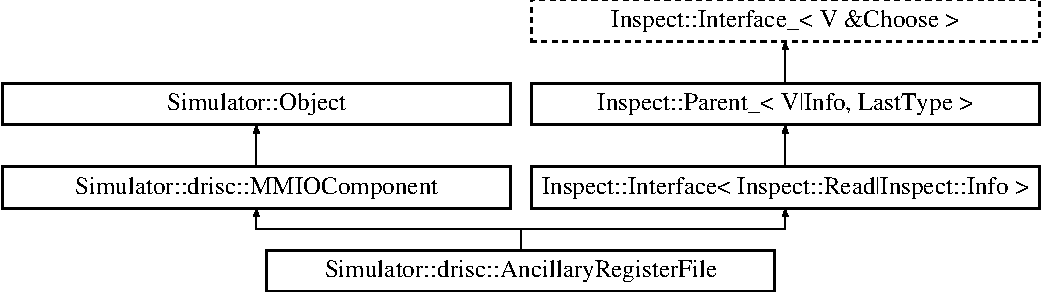
\includegraphics[height=3.929825cm]{class_simulator_1_1drisc_1_1_ancillary_register_file}
\end{center}
\end{figure}
\subsection*{Public Member Functions}
\begin{DoxyCompactItemize}
\item 
\hyperlink{class_simulator_1_1drisc_1_1_ancillary_register_file_afde874ec5ddcb79b5a5f3176b992cddb}{Ancillary\+Register\+File} (const std\+::string \&\hyperlink{mtconf_8c_a8f8f80d37794cde9472343e4487ba3eb}{name}, \hyperlink{class_simulator_1_1_object}{Object} \&parent, \hyperlink{class_config}{Config} \&config)
\item 
size\+\_\+t \hyperlink{class_simulator_1_1drisc_1_1_ancillary_register_file_a0ac3171f2a7eab754224d745d512187f}{Get\+Size} () const 
\item 
Integer \hyperlink{class_simulator_1_1drisc_1_1_ancillary_register_file_a75607efb134538da4dea7feb2d5caa03}{Read\+Register} (\hyperlink{namespace_simulator_1_1drisc_ad67fa6022bb8dfc914132e37bbba2e97}{A\+R\+Addr} addr) const 
\item 
void \hyperlink{class_simulator_1_1drisc_1_1_ancillary_register_file_a561e7817b28287f2900d209b474aa938}{Write\+Register} (\hyperlink{namespace_simulator_1_1drisc_ad67fa6022bb8dfc914132e37bbba2e97}{A\+R\+Addr} addr, Integer data)
\item 
\hyperlink{namespace_simulator_a4b6b5616e7236c0c131516a441776805}{Result} \hyperlink{class_simulator_1_1drisc_1_1_ancillary_register_file_ad56a4d08a6faf73d117cfe2767e5e9e2}{Read} (Mem\+Addr address, void $\ast$data, Mem\+Size size, \hyperlink{namespace_simulator_aaccbc706b2d6c99085f52f6dfc2333e4}{L\+F\+I\+D} fid, \hyperlink{namespace_simulator_a483cc4ecee1736e895054617672cded5}{T\+I\+D} tid, const \hyperlink{struct_simulator_1_1_reg_addr}{Reg\+Addr} \&writeback)
\item 
\hyperlink{namespace_simulator_a4b6b5616e7236c0c131516a441776805}{Result} \hyperlink{class_simulator_1_1drisc_1_1_ancillary_register_file_a18868afcd222db4d23133218919bf822}{Write} (Mem\+Addr address, const void $\ast$data, Mem\+Size size, \hyperlink{namespace_simulator_aaccbc706b2d6c99085f52f6dfc2333e4}{L\+F\+I\+D} fid, \hyperlink{namespace_simulator_a483cc4ecee1736e895054617672cded5}{T\+I\+D} tid)
\item 
void \hyperlink{class_simulator_1_1drisc_1_1_ancillary_register_file_aa2e8ca48224cb01a0c0b33f9f6f7aa31}{Cmd\+\_\+\+Info} (std\+::ostream \&out, const std\+::vector$<$ std\+::string $>$ \&arguments) const 
\item 
void \hyperlink{class_simulator_1_1drisc_1_1_ancillary_register_file_a02d850eea146d21dda48e7d384357022}{Cmd\+\_\+\+Read} (std\+::ostream \&out, const std\+::vector$<$ std\+::string $>$ \&arguments) const 
\end{DoxyCompactItemize}


\subsection{Constructor \& Destructor Documentation}
\hypertarget{class_simulator_1_1drisc_1_1_ancillary_register_file_afde874ec5ddcb79b5a5f3176b992cddb}{\index{Simulator\+::drisc\+::\+Ancillary\+Register\+File@{Simulator\+::drisc\+::\+Ancillary\+Register\+File}!Ancillary\+Register\+File@{Ancillary\+Register\+File}}
\index{Ancillary\+Register\+File@{Ancillary\+Register\+File}!Simulator\+::drisc\+::\+Ancillary\+Register\+File@{Simulator\+::drisc\+::\+Ancillary\+Register\+File}}
\subsubsection[{Ancillary\+Register\+File}]{\setlength{\rightskip}{0pt plus 5cm}Simulator\+::drisc\+::\+Ancillary\+Register\+File\+::\+Ancillary\+Register\+File (
\begin{DoxyParamCaption}
\item[{const std\+::string \&}]{name, }
\item[{{\bf Object} \&}]{parent, }
\item[{{\bf Config} \&}]{config}
\end{DoxyParamCaption}
)}}\label{class_simulator_1_1drisc_1_1_ancillary_register_file_afde874ec5ddcb79b5a5f3176b992cddb}


\subsection{Member Function Documentation}
\hypertarget{class_simulator_1_1drisc_1_1_ancillary_register_file_aa2e8ca48224cb01a0c0b33f9f6f7aa31}{\index{Simulator\+::drisc\+::\+Ancillary\+Register\+File@{Simulator\+::drisc\+::\+Ancillary\+Register\+File}!Cmd\+\_\+\+Info@{Cmd\+\_\+\+Info}}
\index{Cmd\+\_\+\+Info@{Cmd\+\_\+\+Info}!Simulator\+::drisc\+::\+Ancillary\+Register\+File@{Simulator\+::drisc\+::\+Ancillary\+Register\+File}}
\subsubsection[{Cmd\+\_\+\+Info}]{\setlength{\rightskip}{0pt plus 5cm}void Simulator\+::drisc\+::\+Ancillary\+Register\+File\+::\+Cmd\+\_\+\+Info (
\begin{DoxyParamCaption}
\item[{std\+::ostream \&}]{out, }
\item[{const std\+::vector$<$ std\+::string $>$ \&}]{arguments}
\end{DoxyParamCaption}
) const}}\label{class_simulator_1_1drisc_1_1_ancillary_register_file_aa2e8ca48224cb01a0c0b33f9f6f7aa31}
\hypertarget{class_simulator_1_1drisc_1_1_ancillary_register_file_a02d850eea146d21dda48e7d384357022}{\index{Simulator\+::drisc\+::\+Ancillary\+Register\+File@{Simulator\+::drisc\+::\+Ancillary\+Register\+File}!Cmd\+\_\+\+Read@{Cmd\+\_\+\+Read}}
\index{Cmd\+\_\+\+Read@{Cmd\+\_\+\+Read}!Simulator\+::drisc\+::\+Ancillary\+Register\+File@{Simulator\+::drisc\+::\+Ancillary\+Register\+File}}
\subsubsection[{Cmd\+\_\+\+Read}]{\setlength{\rightskip}{0pt plus 5cm}void Simulator\+::drisc\+::\+Ancillary\+Register\+File\+::\+Cmd\+\_\+\+Read (
\begin{DoxyParamCaption}
\item[{std\+::ostream \&}]{out, }
\item[{const std\+::vector$<$ std\+::string $>$ \&}]{arguments}
\end{DoxyParamCaption}
) const}}\label{class_simulator_1_1drisc_1_1_ancillary_register_file_a02d850eea146d21dda48e7d384357022}
\hypertarget{class_simulator_1_1drisc_1_1_ancillary_register_file_a0ac3171f2a7eab754224d745d512187f}{\index{Simulator\+::drisc\+::\+Ancillary\+Register\+File@{Simulator\+::drisc\+::\+Ancillary\+Register\+File}!Get\+Size@{Get\+Size}}
\index{Get\+Size@{Get\+Size}!Simulator\+::drisc\+::\+Ancillary\+Register\+File@{Simulator\+::drisc\+::\+Ancillary\+Register\+File}}
\subsubsection[{Get\+Size}]{\setlength{\rightskip}{0pt plus 5cm}size\+\_\+t Simulator\+::drisc\+::\+Ancillary\+Register\+File\+::\+Get\+Size (
\begin{DoxyParamCaption}
{}
\end{DoxyParamCaption}
) const\hspace{0.3cm}{\ttfamily [virtual]}}}\label{class_simulator_1_1drisc_1_1_ancillary_register_file_a0ac3171f2a7eab754224d745d512187f}


Implements \hyperlink{class_simulator_1_1drisc_1_1_m_m_i_o_component_ad8f1a93b445f287895949bfe52972346}{Simulator\+::drisc\+::\+M\+M\+I\+O\+Component}.

\hypertarget{class_simulator_1_1drisc_1_1_ancillary_register_file_ad56a4d08a6faf73d117cfe2767e5e9e2}{\index{Simulator\+::drisc\+::\+Ancillary\+Register\+File@{Simulator\+::drisc\+::\+Ancillary\+Register\+File}!Read@{Read}}
\index{Read@{Read}!Simulator\+::drisc\+::\+Ancillary\+Register\+File@{Simulator\+::drisc\+::\+Ancillary\+Register\+File}}
\subsubsection[{Read}]{\setlength{\rightskip}{0pt plus 5cm}{\bf Result} Simulator\+::drisc\+::\+Ancillary\+Register\+File\+::\+Read (
\begin{DoxyParamCaption}
\item[{Mem\+Addr}]{address, }
\item[{void $\ast$}]{data, }
\item[{Mem\+Size}]{size, }
\item[{{\bf L\+F\+I\+D}}]{fid, }
\item[{{\bf T\+I\+D}}]{tid, }
\item[{const {\bf Reg\+Addr} \&}]{writeback}
\end{DoxyParamCaption}
)\hspace{0.3cm}{\ttfamily [virtual]}}}\label{class_simulator_1_1drisc_1_1_ancillary_register_file_ad56a4d08a6faf73d117cfe2767e5e9e2}


Implements \hyperlink{class_simulator_1_1drisc_1_1_m_m_i_o_component_af07e2f3e1280d8d56cab7a59815e7eeb}{Simulator\+::drisc\+::\+M\+M\+I\+O\+Component}.

\hypertarget{class_simulator_1_1drisc_1_1_ancillary_register_file_a75607efb134538da4dea7feb2d5caa03}{\index{Simulator\+::drisc\+::\+Ancillary\+Register\+File@{Simulator\+::drisc\+::\+Ancillary\+Register\+File}!Read\+Register@{Read\+Register}}
\index{Read\+Register@{Read\+Register}!Simulator\+::drisc\+::\+Ancillary\+Register\+File@{Simulator\+::drisc\+::\+Ancillary\+Register\+File}}
\subsubsection[{Read\+Register}]{\setlength{\rightskip}{0pt plus 5cm}Integer Simulator\+::drisc\+::\+Ancillary\+Register\+File\+::\+Read\+Register (
\begin{DoxyParamCaption}
\item[{{\bf A\+R\+Addr}}]{addr}
\end{DoxyParamCaption}
) const}}\label{class_simulator_1_1drisc_1_1_ancillary_register_file_a75607efb134538da4dea7feb2d5caa03}
\hypertarget{class_simulator_1_1drisc_1_1_ancillary_register_file_a18868afcd222db4d23133218919bf822}{\index{Simulator\+::drisc\+::\+Ancillary\+Register\+File@{Simulator\+::drisc\+::\+Ancillary\+Register\+File}!Write@{Write}}
\index{Write@{Write}!Simulator\+::drisc\+::\+Ancillary\+Register\+File@{Simulator\+::drisc\+::\+Ancillary\+Register\+File}}
\subsubsection[{Write}]{\setlength{\rightskip}{0pt plus 5cm}{\bf Result} Simulator\+::drisc\+::\+Ancillary\+Register\+File\+::\+Write (
\begin{DoxyParamCaption}
\item[{Mem\+Addr}]{address, }
\item[{const void $\ast$}]{data, }
\item[{Mem\+Size}]{size, }
\item[{{\bf L\+F\+I\+D}}]{fid, }
\item[{{\bf T\+I\+D}}]{tid}
\end{DoxyParamCaption}
)\hspace{0.3cm}{\ttfamily [virtual]}}}\label{class_simulator_1_1drisc_1_1_ancillary_register_file_a18868afcd222db4d23133218919bf822}


Implements \hyperlink{class_simulator_1_1drisc_1_1_m_m_i_o_component_aab3662058e7a00109b122a1460188a8b}{Simulator\+::drisc\+::\+M\+M\+I\+O\+Component}.

\hypertarget{class_simulator_1_1drisc_1_1_ancillary_register_file_a561e7817b28287f2900d209b474aa938}{\index{Simulator\+::drisc\+::\+Ancillary\+Register\+File@{Simulator\+::drisc\+::\+Ancillary\+Register\+File}!Write\+Register@{Write\+Register}}
\index{Write\+Register@{Write\+Register}!Simulator\+::drisc\+::\+Ancillary\+Register\+File@{Simulator\+::drisc\+::\+Ancillary\+Register\+File}}
\subsubsection[{Write\+Register}]{\setlength{\rightskip}{0pt plus 5cm}void Simulator\+::drisc\+::\+Ancillary\+Register\+File\+::\+Write\+Register (
\begin{DoxyParamCaption}
\item[{{\bf A\+R\+Addr}}]{addr, }
\item[{Integer}]{data}
\end{DoxyParamCaption}
)}}\label{class_simulator_1_1drisc_1_1_ancillary_register_file_a561e7817b28287f2900d209b474aa938}


The documentation for this class was generated from the following files\+:\begin{DoxyCompactItemize}
\item 
arch/drisc/mmu/\hyperlink{_ancillary_register_file_8h}{Ancillary\+Register\+File.\+h}\item 
arch/drisc/mmu/\hyperlink{_ancillary_register_file_8cpp}{Ancillary\+Register\+File.\+cpp}\end{DoxyCompactItemize}

\hypertarget{class_simulator_1_1_arbitrated_port}{\section{Simulator\+:\+:Arbitrated\+Port Class Reference}
\label{class_simulator_1_1_arbitrated_port}\index{Simulator\+::\+Arbitrated\+Port@{Simulator\+::\+Arbitrated\+Port}}
}


{\ttfamily \#include $<$ports.\+h$>$}

Inheritance diagram for Simulator\+:\+:Arbitrated\+Port\+:\begin{figure}[H]
\begin{center}
\leavevmode
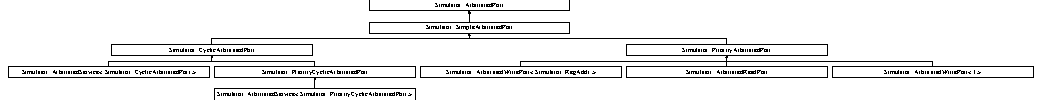
\includegraphics[height=1.346154cm]{class_simulator_1_1_arbitrated_port}
\end{center}
\end{figure}
\subsection*{Public Member Functions}
\begin{DoxyCompactItemize}
\item 
uint64\+\_\+t \hyperlink{class_simulator_1_1_arbitrated_port_a93358ad39066fe450e91648867c907ea}{Get\+Busy\+Cycles} () const 
\item 
std\+::string \hyperlink{class_simulator_1_1_arbitrated_port_a286527112fe9bbdb1f4468acc3efca0e}{Get\+F\+Q\+N} () const 
\end{DoxyCompactItemize}
\subsection*{Protected Member Functions}
\begin{DoxyCompactItemize}
\item 
bool \hyperlink{class_simulator_1_1_arbitrated_port_ad6c149235194bb222005db4ea0352993}{Has\+Acquired} (const \hyperlink{class_simulator_1_1_process}{Process} \&process) const 
\item 
const \hyperlink{class_simulator_1_1_process}{Process} $\ast$ \hyperlink{class_simulator_1_1_arbitrated_port_af666b307417955fb5ac4657986fea2ab}{Get\+Selected\+Process} () const 
\item 
\hyperlink{class_simulator_1_1_arbitrated_port_a1720c2c4547412047aca58dd3ec64d96}{Arbitrated\+Port} (const \hyperlink{class_simulator_1_1_object}{Object} \&object, const std\+::string \&\hyperlink{mtconf_8c_a8f8f80d37794cde9472343e4487ba3eb}{name})
\item 
virtual \hyperlink{class_simulator_1_1_arbitrated_port_a81321f2d8f5db456bb2f0e1710128ea1}{$\sim$\+Arbitrated\+Port} ()
\item 
\hyperlink{class_simulator_1_1_arbitrated_port_a717b1baf7f49444319d47556d26a8608}{Arbitrated\+Port} (const \hyperlink{class_simulator_1_1_arbitrated_port}{Arbitrated\+Port} \&)=delete
\item 
\hyperlink{class_simulator_1_1_arbitrated_port}{Arbitrated\+Port} \& \hyperlink{class_simulator_1_1_arbitrated_port_a5ec4bcf9c7f4dedcb220d56750219c7e}{operator=} (const \hyperlink{class_simulator_1_1_arbitrated_port}{Arbitrated\+Port} \&)=delete
\end{DoxyCompactItemize}
\subsection*{Protected Attributes}
\begin{DoxyCompactItemize}
\item 
const \hyperlink{class_simulator_1_1_process}{Process} $\ast$ \hyperlink{class_simulator_1_1_arbitrated_port_a4530ac48737b148a87a44a6641d2979b}{m\+\_\+selected}
\item 
uint64\+\_\+t \hyperlink{class_simulator_1_1_arbitrated_port_a3fcbb4be3ab62853713ae33f5b3ca8b3}{m\+\_\+busy\+Cycles}
\item 
const \hyperlink{class_simulator_1_1_object}{Object} \& \hyperlink{class_simulator_1_1_arbitrated_port_a1ad6a8b7489f7adbdf487d5e00c86c4d}{m\+\_\+object}
\end{DoxyCompactItemize}


\subsection{Constructor \& Destructor Documentation}
\hypertarget{class_simulator_1_1_arbitrated_port_a1720c2c4547412047aca58dd3ec64d96}{\index{Simulator\+::\+Arbitrated\+Port@{Simulator\+::\+Arbitrated\+Port}!Arbitrated\+Port@{Arbitrated\+Port}}
\index{Arbitrated\+Port@{Arbitrated\+Port}!Simulator\+::\+Arbitrated\+Port@{Simulator\+::\+Arbitrated\+Port}}
\subsubsection[{Arbitrated\+Port}]{\setlength{\rightskip}{0pt plus 5cm}Simulator\+::\+Arbitrated\+Port\+::\+Arbitrated\+Port (
\begin{DoxyParamCaption}
\item[{const {\bf Object} \&}]{object, }
\item[{const std\+::string \&}]{name}
\end{DoxyParamCaption}
)\hspace{0.3cm}{\ttfamily [protected]}}}\label{class_simulator_1_1_arbitrated_port_a1720c2c4547412047aca58dd3ec64d96}
\hypertarget{class_simulator_1_1_arbitrated_port_a81321f2d8f5db456bb2f0e1710128ea1}{\index{Simulator\+::\+Arbitrated\+Port@{Simulator\+::\+Arbitrated\+Port}!````~Arbitrated\+Port@{$\sim$\+Arbitrated\+Port}}
\index{````~Arbitrated\+Port@{$\sim$\+Arbitrated\+Port}!Simulator\+::\+Arbitrated\+Port@{Simulator\+::\+Arbitrated\+Port}}
\subsubsection[{$\sim$\+Arbitrated\+Port}]{\setlength{\rightskip}{0pt plus 5cm}virtual Simulator\+::\+Arbitrated\+Port\+::$\sim$\+Arbitrated\+Port (
\begin{DoxyParamCaption}
{}
\end{DoxyParamCaption}
)\hspace{0.3cm}{\ttfamily [inline]}, {\ttfamily [protected]}, {\ttfamily [virtual]}}}\label{class_simulator_1_1_arbitrated_port_a81321f2d8f5db456bb2f0e1710128ea1}
\hypertarget{class_simulator_1_1_arbitrated_port_a717b1baf7f49444319d47556d26a8608}{\index{Simulator\+::\+Arbitrated\+Port@{Simulator\+::\+Arbitrated\+Port}!Arbitrated\+Port@{Arbitrated\+Port}}
\index{Arbitrated\+Port@{Arbitrated\+Port}!Simulator\+::\+Arbitrated\+Port@{Simulator\+::\+Arbitrated\+Port}}
\subsubsection[{Arbitrated\+Port}]{\setlength{\rightskip}{0pt plus 5cm}Simulator\+::\+Arbitrated\+Port\+::\+Arbitrated\+Port (
\begin{DoxyParamCaption}
\item[{const {\bf Arbitrated\+Port} \&}]{}
\end{DoxyParamCaption}
)\hspace{0.3cm}{\ttfamily [protected]}, {\ttfamily [delete]}}}\label{class_simulator_1_1_arbitrated_port_a717b1baf7f49444319d47556d26a8608}


\subsection{Member Function Documentation}
\hypertarget{class_simulator_1_1_arbitrated_port_a93358ad39066fe450e91648867c907ea}{\index{Simulator\+::\+Arbitrated\+Port@{Simulator\+::\+Arbitrated\+Port}!Get\+Busy\+Cycles@{Get\+Busy\+Cycles}}
\index{Get\+Busy\+Cycles@{Get\+Busy\+Cycles}!Simulator\+::\+Arbitrated\+Port@{Simulator\+::\+Arbitrated\+Port}}
\subsubsection[{Get\+Busy\+Cycles}]{\setlength{\rightskip}{0pt plus 5cm}uint64\+\_\+t Simulator\+::\+Arbitrated\+Port\+::\+Get\+Busy\+Cycles (
\begin{DoxyParamCaption}
{}
\end{DoxyParamCaption}
) const\hspace{0.3cm}{\ttfamily [inline]}}}\label{class_simulator_1_1_arbitrated_port_a93358ad39066fe450e91648867c907ea}
\hypertarget{class_simulator_1_1_arbitrated_port_a286527112fe9bbdb1f4468acc3efca0e}{\index{Simulator\+::\+Arbitrated\+Port@{Simulator\+::\+Arbitrated\+Port}!Get\+F\+Q\+N@{Get\+F\+Q\+N}}
\index{Get\+F\+Q\+N@{Get\+F\+Q\+N}!Simulator\+::\+Arbitrated\+Port@{Simulator\+::\+Arbitrated\+Port}}
\subsubsection[{Get\+F\+Q\+N}]{\setlength{\rightskip}{0pt plus 5cm}std\+::string Simulator\+::\+Arbitrated\+Port\+::\+Get\+F\+Q\+N (
\begin{DoxyParamCaption}
{}
\end{DoxyParamCaption}
) const\hspace{0.3cm}{\ttfamily [inline]}}}\label{class_simulator_1_1_arbitrated_port_a286527112fe9bbdb1f4468acc3efca0e}
\hypertarget{class_simulator_1_1_arbitrated_port_af666b307417955fb5ac4657986fea2ab}{\index{Simulator\+::\+Arbitrated\+Port@{Simulator\+::\+Arbitrated\+Port}!Get\+Selected\+Process@{Get\+Selected\+Process}}
\index{Get\+Selected\+Process@{Get\+Selected\+Process}!Simulator\+::\+Arbitrated\+Port@{Simulator\+::\+Arbitrated\+Port}}
\subsubsection[{Get\+Selected\+Process}]{\setlength{\rightskip}{0pt plus 5cm}const {\bf Process}$\ast$ Simulator\+::\+Arbitrated\+Port\+::\+Get\+Selected\+Process (
\begin{DoxyParamCaption}
{}
\end{DoxyParamCaption}
) const\hspace{0.3cm}{\ttfamily [inline]}, {\ttfamily [protected]}}}\label{class_simulator_1_1_arbitrated_port_af666b307417955fb5ac4657986fea2ab}
\hypertarget{class_simulator_1_1_arbitrated_port_ad6c149235194bb222005db4ea0352993}{\index{Simulator\+::\+Arbitrated\+Port@{Simulator\+::\+Arbitrated\+Port}!Has\+Acquired@{Has\+Acquired}}
\index{Has\+Acquired@{Has\+Acquired}!Simulator\+::\+Arbitrated\+Port@{Simulator\+::\+Arbitrated\+Port}}
\subsubsection[{Has\+Acquired}]{\setlength{\rightskip}{0pt plus 5cm}bool Simulator\+::\+Arbitrated\+Port\+::\+Has\+Acquired (
\begin{DoxyParamCaption}
\item[{const {\bf Process} \&}]{process}
\end{DoxyParamCaption}
) const\hspace{0.3cm}{\ttfamily [inline]}, {\ttfamily [protected]}}}\label{class_simulator_1_1_arbitrated_port_ad6c149235194bb222005db4ea0352993}
\hypertarget{class_simulator_1_1_arbitrated_port_a5ec4bcf9c7f4dedcb220d56750219c7e}{\index{Simulator\+::\+Arbitrated\+Port@{Simulator\+::\+Arbitrated\+Port}!operator=@{operator=}}
\index{operator=@{operator=}!Simulator\+::\+Arbitrated\+Port@{Simulator\+::\+Arbitrated\+Port}}
\subsubsection[{operator=}]{\setlength{\rightskip}{0pt plus 5cm}{\bf Arbitrated\+Port}\& Simulator\+::\+Arbitrated\+Port\+::operator= (
\begin{DoxyParamCaption}
\item[{const {\bf Arbitrated\+Port} \&}]{}
\end{DoxyParamCaption}
)\hspace{0.3cm}{\ttfamily [protected]}, {\ttfamily [delete]}}}\label{class_simulator_1_1_arbitrated_port_a5ec4bcf9c7f4dedcb220d56750219c7e}


\subsection{Member Data Documentation}
\hypertarget{class_simulator_1_1_arbitrated_port_a3fcbb4be3ab62853713ae33f5b3ca8b3}{\index{Simulator\+::\+Arbitrated\+Port@{Simulator\+::\+Arbitrated\+Port}!m\+\_\+busy\+Cycles@{m\+\_\+busy\+Cycles}}
\index{m\+\_\+busy\+Cycles@{m\+\_\+busy\+Cycles}!Simulator\+::\+Arbitrated\+Port@{Simulator\+::\+Arbitrated\+Port}}
\subsubsection[{m\+\_\+busy\+Cycles}]{\setlength{\rightskip}{0pt plus 5cm}uint64\+\_\+t Simulator\+::\+Arbitrated\+Port\+::m\+\_\+busy\+Cycles\hspace{0.3cm}{\ttfamily [protected]}}}\label{class_simulator_1_1_arbitrated_port_a3fcbb4be3ab62853713ae33f5b3ca8b3}
\hypertarget{class_simulator_1_1_arbitrated_port_a1ad6a8b7489f7adbdf487d5e00c86c4d}{\index{Simulator\+::\+Arbitrated\+Port@{Simulator\+::\+Arbitrated\+Port}!m\+\_\+object@{m\+\_\+object}}
\index{m\+\_\+object@{m\+\_\+object}!Simulator\+::\+Arbitrated\+Port@{Simulator\+::\+Arbitrated\+Port}}
\subsubsection[{m\+\_\+object}]{\setlength{\rightskip}{0pt plus 5cm}const {\bf Object}\& Simulator\+::\+Arbitrated\+Port\+::m\+\_\+object\hspace{0.3cm}{\ttfamily [protected]}}}\label{class_simulator_1_1_arbitrated_port_a1ad6a8b7489f7adbdf487d5e00c86c4d}
\hypertarget{class_simulator_1_1_arbitrated_port_a4530ac48737b148a87a44a6641d2979b}{\index{Simulator\+::\+Arbitrated\+Port@{Simulator\+::\+Arbitrated\+Port}!m\+\_\+selected@{m\+\_\+selected}}
\index{m\+\_\+selected@{m\+\_\+selected}!Simulator\+::\+Arbitrated\+Port@{Simulator\+::\+Arbitrated\+Port}}
\subsubsection[{m\+\_\+selected}]{\setlength{\rightskip}{0pt plus 5cm}const {\bf Process}$\ast$ Simulator\+::\+Arbitrated\+Port\+::m\+\_\+selected\hspace{0.3cm}{\ttfamily [protected]}}}\label{class_simulator_1_1_arbitrated_port_a4530ac48737b148a87a44a6641d2979b}


The documentation for this class was generated from the following file\+:\begin{DoxyCompactItemize}
\item 
sim/\hyperlink{ports_8h}{ports.\+h}\end{DoxyCompactItemize}

\hypertarget{class_simulator_1_1_arbitrated_read_port}{\section{Simulator\+:\+:Arbitrated\+Read\+Port Class Reference}
\label{class_simulator_1_1_arbitrated_read_port}\index{Simulator\+::\+Arbitrated\+Read\+Port@{Simulator\+::\+Arbitrated\+Read\+Port}}
}


{\ttfamily \#include $<$ports.\+h$>$}

Inheritance diagram for Simulator\+:\+:Arbitrated\+Read\+Port\+:\begin{figure}[H]
\begin{center}
\leavevmode
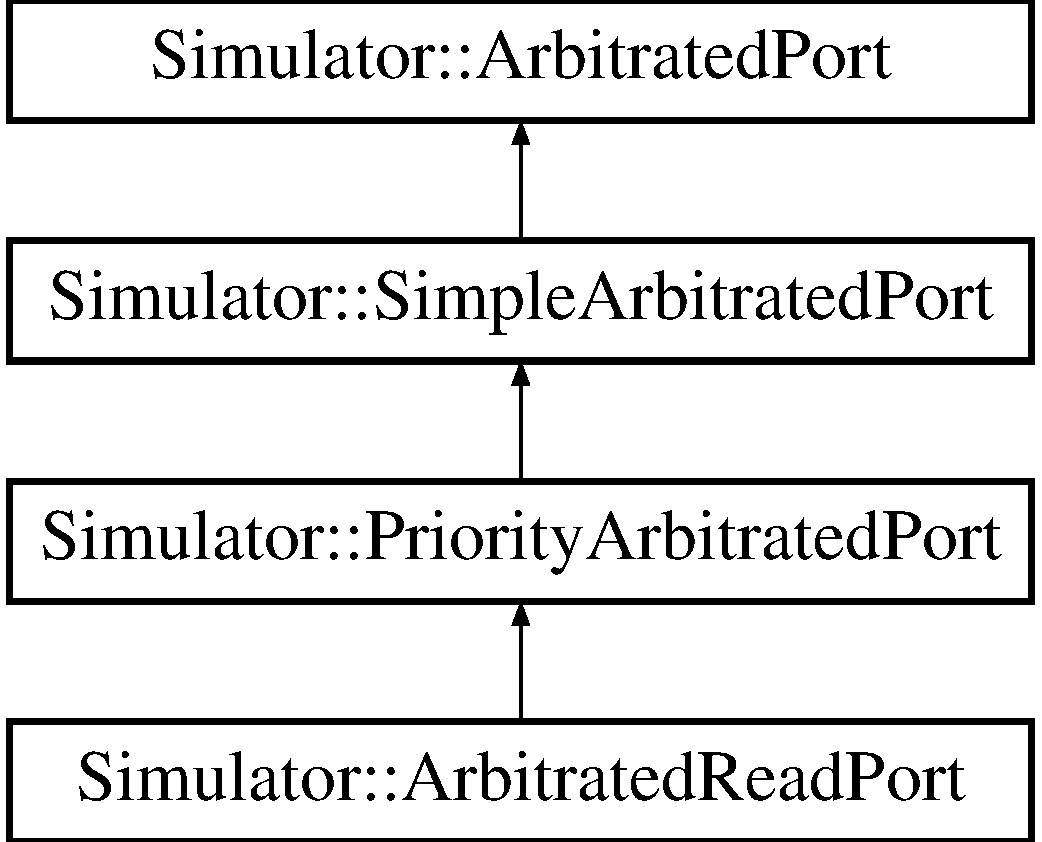
\includegraphics[height=4.000000cm]{class_simulator_1_1_arbitrated_read_port}
\end{center}
\end{figure}
\subsection*{Public Member Functions}
\begin{DoxyCompactItemize}
\item 
\hyperlink{class_simulator_1_1_arbitrated_read_port_ac49567e95fc06438cff7c3354934741e}{Arbitrated\+Read\+Port} (\hyperlink{class_simulator_1_1_i_structure}{I\+Structure} \&structure, const std\+::string \&\hyperlink{mtconf_8c_a8f8f80d37794cde9472343e4487ba3eb}{name})
\item 
\hyperlink{class_simulator_1_1_arbitrated_read_port_abd33f33ee81cc86326dc1ee32bb65021}{$\sim$\+Arbitrated\+Read\+Port} ()
\item 
bool \hyperlink{class_simulator_1_1_arbitrated_read_port_a5a0a12344479df158af1b91b93976fc2}{Read} ()
\end{DoxyCompactItemize}
\subsection*{Additional Inherited Members}


\subsection{Constructor \& Destructor Documentation}
\hypertarget{class_simulator_1_1_arbitrated_read_port_ac49567e95fc06438cff7c3354934741e}{\index{Simulator\+::\+Arbitrated\+Read\+Port@{Simulator\+::\+Arbitrated\+Read\+Port}!Arbitrated\+Read\+Port@{Arbitrated\+Read\+Port}}
\index{Arbitrated\+Read\+Port@{Arbitrated\+Read\+Port}!Simulator\+::\+Arbitrated\+Read\+Port@{Simulator\+::\+Arbitrated\+Read\+Port}}
\subsubsection[{Arbitrated\+Read\+Port}]{\setlength{\rightskip}{0pt plus 5cm}Simulator\+::\+Arbitrated\+Read\+Port\+::\+Arbitrated\+Read\+Port (
\begin{DoxyParamCaption}
\item[{{\bf I\+Structure} \&}]{structure, }
\item[{const std\+::string \&}]{name}
\end{DoxyParamCaption}
)\hspace{0.3cm}{\ttfamily [inline]}}}\label{class_simulator_1_1_arbitrated_read_port_ac49567e95fc06438cff7c3354934741e}
\hypertarget{class_simulator_1_1_arbitrated_read_port_abd33f33ee81cc86326dc1ee32bb65021}{\index{Simulator\+::\+Arbitrated\+Read\+Port@{Simulator\+::\+Arbitrated\+Read\+Port}!````~Arbitrated\+Read\+Port@{$\sim$\+Arbitrated\+Read\+Port}}
\index{````~Arbitrated\+Read\+Port@{$\sim$\+Arbitrated\+Read\+Port}!Simulator\+::\+Arbitrated\+Read\+Port@{Simulator\+::\+Arbitrated\+Read\+Port}}
\subsubsection[{$\sim$\+Arbitrated\+Read\+Port}]{\setlength{\rightskip}{0pt plus 5cm}Simulator\+::\+Arbitrated\+Read\+Port\+::$\sim$\+Arbitrated\+Read\+Port (
\begin{DoxyParamCaption}
{}
\end{DoxyParamCaption}
)\hspace{0.3cm}{\ttfamily [inline]}}}\label{class_simulator_1_1_arbitrated_read_port_abd33f33ee81cc86326dc1ee32bb65021}


\subsection{Member Function Documentation}
\hypertarget{class_simulator_1_1_arbitrated_read_port_a5a0a12344479df158af1b91b93976fc2}{\index{Simulator\+::\+Arbitrated\+Read\+Port@{Simulator\+::\+Arbitrated\+Read\+Port}!Read@{Read}}
\index{Read@{Read}!Simulator\+::\+Arbitrated\+Read\+Port@{Simulator\+::\+Arbitrated\+Read\+Port}}
\subsubsection[{Read}]{\setlength{\rightskip}{0pt plus 5cm}bool Simulator\+::\+Arbitrated\+Read\+Port\+::\+Read (
\begin{DoxyParamCaption}
{}
\end{DoxyParamCaption}
)\hspace{0.3cm}{\ttfamily [inline]}}}\label{class_simulator_1_1_arbitrated_read_port_a5a0a12344479df158af1b91b93976fc2}


The documentation for this class was generated from the following file\+:\begin{DoxyCompactItemize}
\item 
sim/\hyperlink{ports_8h}{ports.\+h}\end{DoxyCompactItemize}

\hypertarget{class_simulator_1_1_arbitrated_service}{\section{Simulator\+:\+:Arbitrated\+Service$<$ Base $>$ Class Template Reference}
\label{class_simulator_1_1_arbitrated_service}\index{Simulator\+::\+Arbitrated\+Service$<$ Base $>$@{Simulator\+::\+Arbitrated\+Service$<$ Base $>$}}
}


{\ttfamily \#include $<$ports.\+h$>$}

Inheritance diagram for Simulator\+:\+:Arbitrated\+Service$<$ Base $>$\+:\begin{figure}[H]
\begin{center}
\leavevmode
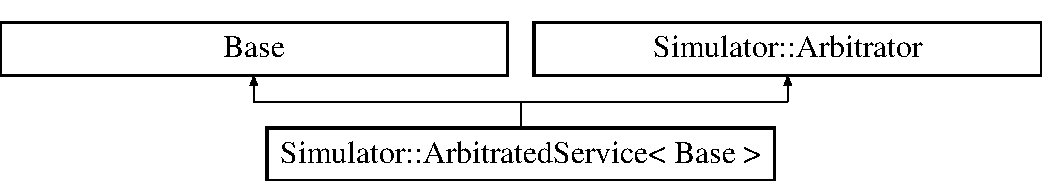
\includegraphics[height=2.000000cm]{class_simulator_1_1_arbitrated_service}
\end{center}
\end{figure}
\subsection*{Public Member Functions}
\begin{DoxyCompactItemize}
\item 
bool \hyperlink{class_simulator_1_1_arbitrated_service_afa7be6cfa4c0ef3591b63e46eb35912b}{Invoke} ()
\item 
\hyperlink{class_simulator_1_1_arbitrated_service_ac238e575cd81ad43cb8ce6a8c65806ee}{Arbitrated\+Service} (const \hyperlink{class_simulator_1_1_object}{Object} \&object, \hyperlink{class_simulator_1_1_clock}{Clock} \&clock, const std\+::string \&\hyperlink{mtconf_8c_a8f8f80d37794cde9472343e4487ba3eb}{name})
\item 
\hyperlink{class_simulator_1_1_arbitrated_service_abff05e45835efad7912524efd7dcd26e}{$\sim$\+Arbitrated\+Service} ()
\item 
std\+::string \hyperlink{class_simulator_1_1_arbitrated_service_a3800ca938165d86a3f5b11a2dae763d7}{Get\+F\+Q\+N} () const 
\end{DoxyCompactItemize}
\subsection*{Additional Inherited Members}


\subsection{Constructor \& Destructor Documentation}
\hypertarget{class_simulator_1_1_arbitrated_service_ac238e575cd81ad43cb8ce6a8c65806ee}{\index{Simulator\+::\+Arbitrated\+Service@{Simulator\+::\+Arbitrated\+Service}!Arbitrated\+Service@{Arbitrated\+Service}}
\index{Arbitrated\+Service@{Arbitrated\+Service}!Simulator\+::\+Arbitrated\+Service@{Simulator\+::\+Arbitrated\+Service}}
\subsubsection[{Arbitrated\+Service}]{\setlength{\rightskip}{0pt plus 5cm}template$<$typename Base = class Priority\+Arbitrated\+Port$>$ {\bf Simulator\+::\+Arbitrated\+Service}$<$ Base $>$\+::{\bf Arbitrated\+Service} (
\begin{DoxyParamCaption}
\item[{const {\bf Object} \&}]{object, }
\item[{{\bf Clock} \&}]{clock, }
\item[{const std\+::string \&}]{name}
\end{DoxyParamCaption}
)\hspace{0.3cm}{\ttfamily [inline]}}}\label{class_simulator_1_1_arbitrated_service_ac238e575cd81ad43cb8ce6a8c65806ee}
\hypertarget{class_simulator_1_1_arbitrated_service_abff05e45835efad7912524efd7dcd26e}{\index{Simulator\+::\+Arbitrated\+Service@{Simulator\+::\+Arbitrated\+Service}!````~Arbitrated\+Service@{$\sim$\+Arbitrated\+Service}}
\index{````~Arbitrated\+Service@{$\sim$\+Arbitrated\+Service}!Simulator\+::\+Arbitrated\+Service@{Simulator\+::\+Arbitrated\+Service}}
\subsubsection[{$\sim$\+Arbitrated\+Service}]{\setlength{\rightskip}{0pt plus 5cm}template$<$typename Base = class Priority\+Arbitrated\+Port$>$ {\bf Simulator\+::\+Arbitrated\+Service}$<$ Base $>$\+::$\sim${\bf Arbitrated\+Service} (
\begin{DoxyParamCaption}
{}
\end{DoxyParamCaption}
)\hspace{0.3cm}{\ttfamily [inline]}}}\label{class_simulator_1_1_arbitrated_service_abff05e45835efad7912524efd7dcd26e}


\subsection{Member Function Documentation}
\hypertarget{class_simulator_1_1_arbitrated_service_a3800ca938165d86a3f5b11a2dae763d7}{\index{Simulator\+::\+Arbitrated\+Service@{Simulator\+::\+Arbitrated\+Service}!Get\+F\+Q\+N@{Get\+F\+Q\+N}}
\index{Get\+F\+Q\+N@{Get\+F\+Q\+N}!Simulator\+::\+Arbitrated\+Service@{Simulator\+::\+Arbitrated\+Service}}
\subsubsection[{Get\+F\+Q\+N}]{\setlength{\rightskip}{0pt plus 5cm}template$<$typename Base = class Priority\+Arbitrated\+Port$>$ std\+::string {\bf Simulator\+::\+Arbitrated\+Service}$<$ Base $>$\+::Get\+F\+Q\+N (
\begin{DoxyParamCaption}
{}
\end{DoxyParamCaption}
) const\hspace{0.3cm}{\ttfamily [inline]}, {\ttfamily [virtual]}}}\label{class_simulator_1_1_arbitrated_service_a3800ca938165d86a3f5b11a2dae763d7}


Implements \hyperlink{class_simulator_1_1_arbitrator_af4942847f33bb218ad9a37fd4cb515ba}{Simulator\+::\+Arbitrator}.

\hypertarget{class_simulator_1_1_arbitrated_service_afa7be6cfa4c0ef3591b63e46eb35912b}{\index{Simulator\+::\+Arbitrated\+Service@{Simulator\+::\+Arbitrated\+Service}!Invoke@{Invoke}}
\index{Invoke@{Invoke}!Simulator\+::\+Arbitrated\+Service@{Simulator\+::\+Arbitrated\+Service}}
\subsubsection[{Invoke}]{\setlength{\rightskip}{0pt plus 5cm}template$<$typename Base = class Priority\+Arbitrated\+Port$>$ bool {\bf Simulator\+::\+Arbitrated\+Service}$<$ Base $>$\+::Invoke (
\begin{DoxyParamCaption}
{}
\end{DoxyParamCaption}
)\hspace{0.3cm}{\ttfamily [inline]}}}\label{class_simulator_1_1_arbitrated_service_afa7be6cfa4c0ef3591b63e46eb35912b}


The documentation for this class was generated from the following file\+:\begin{DoxyCompactItemize}
\item 
sim/\hyperlink{ports_8h}{ports.\+h}\end{DoxyCompactItemize}

\hypertarget{singleton_simulator_1_1_arbitrated_write_port}{\section{Simulator\+:\+:Arbitrated\+Write\+Port$<$ I $>$ Class Template Reference}
\label{singleton_simulator_1_1_arbitrated_write_port}\index{Simulator\+::\+Arbitrated\+Write\+Port$<$ I $>$@{Simulator\+::\+Arbitrated\+Write\+Port$<$ I $>$}}
}


{\ttfamily \#include $<$ports.\+h$>$}

Inheritance diagram for Simulator\+:\+:Arbitrated\+Write\+Port$<$ I $>$\+:\begin{figure}[H]
\begin{center}
\leavevmode
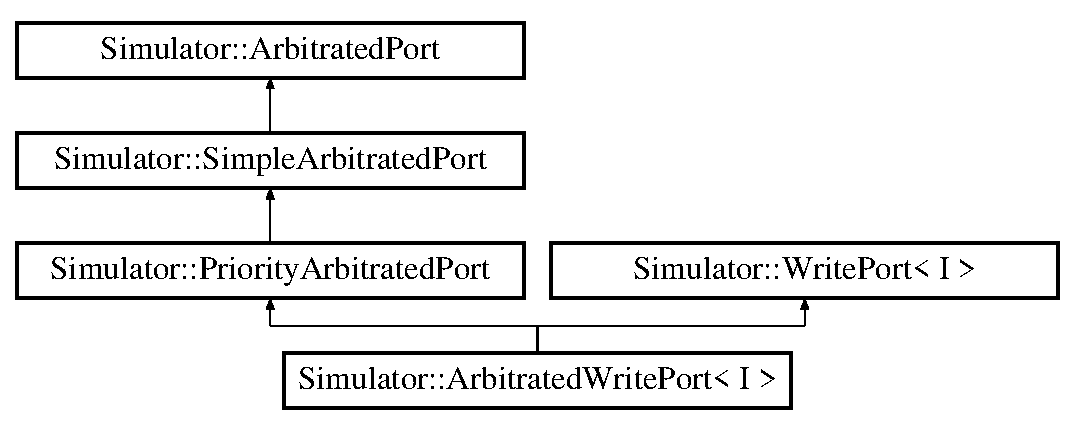
\includegraphics[height=4.000000cm]{singleton_simulator_1_1_arbitrated_write_port}
\end{center}
\end{figure}
\subsection*{Public Member Functions}
\begin{DoxyCompactItemize}
\item 
void \hyperlink{singleton_simulator_1_1_arbitrated_write_port_aeb84f0a2255125ae16559efe8d87e724}{Arbitrate} ()
\item 
\hyperlink{singleton_simulator_1_1_arbitrated_write_port_ad6a5c673dbc38abf6ce594ab15c23ead}{Arbitrated\+Write\+Port} (\hyperlink{singleton_simulator_1_1_structure}{Structure}$<$ I $>$ \&structure, const std\+::string \&\hyperlink{mtconf_8c_a8f8f80d37794cde9472343e4487ba3eb}{name})
\item 
\hyperlink{singleton_simulator_1_1_arbitrated_write_port_a33c8f212281052776f0cea1390e7d137}{$\sim$\+Arbitrated\+Write\+Port} ()
\item 
bool \hyperlink{singleton_simulator_1_1_arbitrated_write_port_aef7e5553ca6e808e1184a671faf19ae9}{Write} (const I \&index)
\end{DoxyCompactItemize}
\subsection*{Additional Inherited Members}


\subsection{Constructor \& Destructor Documentation}
\hypertarget{singleton_simulator_1_1_arbitrated_write_port_ad6a5c673dbc38abf6ce594ab15c23ead}{\index{Simulator\+::\+Arbitrated\+Write\+Port@{Simulator\+::\+Arbitrated\+Write\+Port}!Arbitrated\+Write\+Port@{Arbitrated\+Write\+Port}}
\index{Arbitrated\+Write\+Port@{Arbitrated\+Write\+Port}!Simulator\+::\+Arbitrated\+Write\+Port@{Simulator\+::\+Arbitrated\+Write\+Port}}
\subsubsection[{Arbitrated\+Write\+Port}]{\setlength{\rightskip}{0pt plus 5cm}template$<$typename I$>$ {\bf Simulator\+::\+Arbitrated\+Write\+Port}$<$ I $>$\+::{\bf Arbitrated\+Write\+Port} (
\begin{DoxyParamCaption}
\item[{{\bf Structure}$<$ I $>$ \&}]{structure, }
\item[{const std\+::string \&}]{name}
\end{DoxyParamCaption}
)\hspace{0.3cm}{\ttfamily [inline]}}}\label{singleton_simulator_1_1_arbitrated_write_port_ad6a5c673dbc38abf6ce594ab15c23ead}
\hypertarget{singleton_simulator_1_1_arbitrated_write_port_a33c8f212281052776f0cea1390e7d137}{\index{Simulator\+::\+Arbitrated\+Write\+Port@{Simulator\+::\+Arbitrated\+Write\+Port}!````~Arbitrated\+Write\+Port@{$\sim$\+Arbitrated\+Write\+Port}}
\index{````~Arbitrated\+Write\+Port@{$\sim$\+Arbitrated\+Write\+Port}!Simulator\+::\+Arbitrated\+Write\+Port@{Simulator\+::\+Arbitrated\+Write\+Port}}
\subsubsection[{$\sim$\+Arbitrated\+Write\+Port}]{\setlength{\rightskip}{0pt plus 5cm}template$<$typename I$>$ {\bf Simulator\+::\+Arbitrated\+Write\+Port}$<$ I $>$\+::$\sim${\bf Arbitrated\+Write\+Port} (
\begin{DoxyParamCaption}
{}
\end{DoxyParamCaption}
)\hspace{0.3cm}{\ttfamily [inline]}}}\label{singleton_simulator_1_1_arbitrated_write_port_a33c8f212281052776f0cea1390e7d137}


\subsection{Member Function Documentation}
\hypertarget{singleton_simulator_1_1_arbitrated_write_port_aeb84f0a2255125ae16559efe8d87e724}{\index{Simulator\+::\+Arbitrated\+Write\+Port@{Simulator\+::\+Arbitrated\+Write\+Port}!Arbitrate@{Arbitrate}}
\index{Arbitrate@{Arbitrate}!Simulator\+::\+Arbitrated\+Write\+Port@{Simulator\+::\+Arbitrated\+Write\+Port}}
\subsubsection[{Arbitrate}]{\setlength{\rightskip}{0pt plus 5cm}template$<$typename I$>$ void {\bf Simulator\+::\+Arbitrated\+Write\+Port}$<$ I $>$\+::Arbitrate (
\begin{DoxyParamCaption}
{}
\end{DoxyParamCaption}
)\hspace{0.3cm}{\ttfamily [inline]}}}\label{singleton_simulator_1_1_arbitrated_write_port_aeb84f0a2255125ae16559efe8d87e724}
\hypertarget{singleton_simulator_1_1_arbitrated_write_port_aef7e5553ca6e808e1184a671faf19ae9}{\index{Simulator\+::\+Arbitrated\+Write\+Port@{Simulator\+::\+Arbitrated\+Write\+Port}!Write@{Write}}
\index{Write@{Write}!Simulator\+::\+Arbitrated\+Write\+Port@{Simulator\+::\+Arbitrated\+Write\+Port}}
\subsubsection[{Write}]{\setlength{\rightskip}{0pt plus 5cm}template$<$typename I$>$ bool {\bf Simulator\+::\+Arbitrated\+Write\+Port}$<$ I $>$\+::Write (
\begin{DoxyParamCaption}
\item[{const I \&}]{index}
\end{DoxyParamCaption}
)\hspace{0.3cm}{\ttfamily [inline]}}}\label{singleton_simulator_1_1_arbitrated_write_port_aef7e5553ca6e808e1184a671faf19ae9}


The documentation for this class was generated from the following file\+:\begin{DoxyCompactItemize}
\item 
sim/\hyperlink{ports_8h}{ports.\+h}\end{DoxyCompactItemize}

\hypertarget{class_simulator_1_1_arbitrator}{\section{Simulator\+:\+:Arbitrator Class Reference}
\label{class_simulator_1_1_arbitrator}\index{Simulator\+::\+Arbitrator@{Simulator\+::\+Arbitrator}}
}


Base class for all objects that arbitrate.  




{\ttfamily \#include $<$kernel.\+h$>$}

Inheritance diagram for Simulator\+:\+:Arbitrator\+:\begin{figure}[H]
\begin{center}
\leavevmode
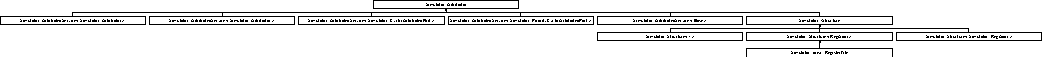
\includegraphics[height=0.769231cm]{class_simulator_1_1_arbitrator}
\end{center}
\end{figure}
\subsection*{Public Member Functions}
\begin{DoxyCompactItemize}
\item 
virtual void \hyperlink{class_simulator_1_1_arbitrator_a8cfa3d35f1916c2507b9cc264a7c34ae}{On\+Arbitrate} ()=0
\begin{DoxyCompactList}\small\item\em $<$ Callback for arbitration \end{DoxyCompactList}\item 
virtual std\+::string \hyperlink{class_simulator_1_1_arbitrator_af4942847f33bb218ad9a37fd4cb515ba}{Get\+F\+Q\+N} () const =0
\item 
const \hyperlink{class_simulator_1_1_arbitrator}{Arbitrator} $\ast$ \hyperlink{class_simulator_1_1_arbitrator_a05700337b736b1bb7fb39b2bdf007005}{Get\+Next} () const 
\item 
\hyperlink{class_simulator_1_1_arbitrator_a8835c8e17e2894c90a72f4e1ef72eb0a}{Arbitrator} (\hyperlink{class_simulator_1_1_clock}{Clock} \&clock)
\item 
\hyperlink{class_simulator_1_1_arbitrator_a415268a3985b82af1e0eff6128c0dde0}{Arbitrator} (const \hyperlink{class_simulator_1_1_arbitrator}{Arbitrator} \&)=delete
\item 
\hyperlink{class_simulator_1_1_arbitrator}{Arbitrator} \& \hyperlink{class_simulator_1_1_arbitrator_a6efe8951760ec0040b08dbf7d5ca89e1}{operator=} (const \hyperlink{class_simulator_1_1_arbitrator}{Arbitrator} \&)=delete
\item 
virtual \hyperlink{class_simulator_1_1_arbitrator_a02f0a2135894ecf6bede03ef5cde3b41}{$\sim$\+Arbitrator} ()
\end{DoxyCompactItemize}
\subsection*{Protected Member Functions}
\begin{DoxyCompactItemize}
\item 
void \hyperlink{class_simulator_1_1_arbitrator_a6fa047be0554f4edea1363e960835f29}{Request\+Arbitration} ()
\end{DoxyCompactItemize}
\subsection*{Protected Attributes}
\begin{DoxyCompactItemize}
\item 
\hyperlink{class_simulator_1_1_clock}{Clock} \& \hyperlink{class_simulator_1_1_arbitrator_ae81bdde0ba892172b8594a25dd2ef9cc}{m\+\_\+clock}
\begin{DoxyCompactList}\small\item\em The clock that controls this arbitrator. \end{DoxyCompactList}\end{DoxyCompactItemize}
\subsection*{Friends}
\begin{DoxyCompactItemize}
\item 
class \hyperlink{class_simulator_1_1_arbitrator_a3807a3ebd0e05ca8cb4d928025a943d2}{Kernel}
\end{DoxyCompactItemize}


\subsection{Detailed Description}
Base class for all objects that arbitrate. 

\subsection{Constructor \& Destructor Documentation}
\hypertarget{class_simulator_1_1_arbitrator_a8835c8e17e2894c90a72f4e1ef72eb0a}{\index{Simulator\+::\+Arbitrator@{Simulator\+::\+Arbitrator}!Arbitrator@{Arbitrator}}
\index{Arbitrator@{Arbitrator}!Simulator\+::\+Arbitrator@{Simulator\+::\+Arbitrator}}
\subsubsection[{Arbitrator}]{\setlength{\rightskip}{0pt plus 5cm}Simulator\+::\+Arbitrator\+::\+Arbitrator (
\begin{DoxyParamCaption}
\item[{{\bf Clock} \&}]{clock}
\end{DoxyParamCaption}
)\hspace{0.3cm}{\ttfamily [inline]}}}\label{class_simulator_1_1_arbitrator_a8835c8e17e2894c90a72f4e1ef72eb0a}
\hypertarget{class_simulator_1_1_arbitrator_a415268a3985b82af1e0eff6128c0dde0}{\index{Simulator\+::\+Arbitrator@{Simulator\+::\+Arbitrator}!Arbitrator@{Arbitrator}}
\index{Arbitrator@{Arbitrator}!Simulator\+::\+Arbitrator@{Simulator\+::\+Arbitrator}}
\subsubsection[{Arbitrator}]{\setlength{\rightskip}{0pt plus 5cm}Simulator\+::\+Arbitrator\+::\+Arbitrator (
\begin{DoxyParamCaption}
\item[{const {\bf Arbitrator} \&}]{}
\end{DoxyParamCaption}
)\hspace{0.3cm}{\ttfamily [delete]}}}\label{class_simulator_1_1_arbitrator_a415268a3985b82af1e0eff6128c0dde0}
\hypertarget{class_simulator_1_1_arbitrator_a02f0a2135894ecf6bede03ef5cde3b41}{\index{Simulator\+::\+Arbitrator@{Simulator\+::\+Arbitrator}!````~Arbitrator@{$\sim$\+Arbitrator}}
\index{````~Arbitrator@{$\sim$\+Arbitrator}!Simulator\+::\+Arbitrator@{Simulator\+::\+Arbitrator}}
\subsubsection[{$\sim$\+Arbitrator}]{\setlength{\rightskip}{0pt plus 5cm}virtual Simulator\+::\+Arbitrator\+::$\sim$\+Arbitrator (
\begin{DoxyParamCaption}
{}
\end{DoxyParamCaption}
)\hspace{0.3cm}{\ttfamily [inline]}, {\ttfamily [virtual]}}}\label{class_simulator_1_1_arbitrator_a02f0a2135894ecf6bede03ef5cde3b41}


\subsection{Member Function Documentation}
\hypertarget{class_simulator_1_1_arbitrator_af4942847f33bb218ad9a37fd4cb515ba}{\index{Simulator\+::\+Arbitrator@{Simulator\+::\+Arbitrator}!Get\+F\+Q\+N@{Get\+F\+Q\+N}}
\index{Get\+F\+Q\+N@{Get\+F\+Q\+N}!Simulator\+::\+Arbitrator@{Simulator\+::\+Arbitrator}}
\subsubsection[{Get\+F\+Q\+N}]{\setlength{\rightskip}{0pt plus 5cm}virtual std\+::string Simulator\+::\+Arbitrator\+::\+Get\+F\+Q\+N (
\begin{DoxyParamCaption}
{}
\end{DoxyParamCaption}
) const\hspace{0.3cm}{\ttfamily [pure virtual]}}}\label{class_simulator_1_1_arbitrator_af4942847f33bb218ad9a37fd4cb515ba}


Implemented in \hyperlink{class_simulator_1_1_arbitrated_service_a3800ca938165d86a3f5b11a2dae763d7}{Simulator\+::\+Arbitrated\+Service$<$ Base $>$}, \hyperlink{class_simulator_1_1_arbitrated_service_a3800ca938165d86a3f5b11a2dae763d7}{Simulator\+::\+Arbitrated\+Service$<$ Simulator\+::\+Cyclic\+Arbitrated\+Port $>$}, \hyperlink{class_simulator_1_1_arbitrated_service_a3800ca938165d86a3f5b11a2dae763d7}{Simulator\+::\+Arbitrated\+Service$<$ Simulator\+::\+Priority\+Cyclic\+Arbitrated\+Port $>$}, \hyperlink{class_simulator_1_1_arbitrated_service_a3800ca938165d86a3f5b11a2dae763d7}{Simulator\+::\+Arbitrated\+Service$<$ Simulator\+::\+Arbitrator $>$}, and \hyperlink{class_simulator_1_1_i_structure_a54b5688c43dbe1b361d5e11705132fff}{Simulator\+::\+I\+Structure}.

\hypertarget{class_simulator_1_1_arbitrator_a05700337b736b1bb7fb39b2bdf007005}{\index{Simulator\+::\+Arbitrator@{Simulator\+::\+Arbitrator}!Get\+Next@{Get\+Next}}
\index{Get\+Next@{Get\+Next}!Simulator\+::\+Arbitrator@{Simulator\+::\+Arbitrator}}
\subsubsection[{Get\+Next}]{\setlength{\rightskip}{0pt plus 5cm}const {\bf Arbitrator}$\ast$ Simulator\+::\+Arbitrator\+::\+Get\+Next (
\begin{DoxyParamCaption}
{}
\end{DoxyParamCaption}
) const\hspace{0.3cm}{\ttfamily [inline]}}}\label{class_simulator_1_1_arbitrator_a05700337b736b1bb7fb39b2bdf007005}
\hypertarget{class_simulator_1_1_arbitrator_a8cfa3d35f1916c2507b9cc264a7c34ae}{\index{Simulator\+::\+Arbitrator@{Simulator\+::\+Arbitrator}!On\+Arbitrate@{On\+Arbitrate}}
\index{On\+Arbitrate@{On\+Arbitrate}!Simulator\+::\+Arbitrator@{Simulator\+::\+Arbitrator}}
\subsubsection[{On\+Arbitrate}]{\setlength{\rightskip}{0pt plus 5cm}virtual void Simulator\+::\+Arbitrator\+::\+On\+Arbitrate (
\begin{DoxyParamCaption}
{}
\end{DoxyParamCaption}
)\hspace{0.3cm}{\ttfamily [pure virtual]}}}\label{class_simulator_1_1_arbitrator_a8cfa3d35f1916c2507b9cc264a7c34ae}


$<$ Callback for arbitration 

\hypertarget{class_simulator_1_1_arbitrator_a6efe8951760ec0040b08dbf7d5ca89e1}{\index{Simulator\+::\+Arbitrator@{Simulator\+::\+Arbitrator}!operator=@{operator=}}
\index{operator=@{operator=}!Simulator\+::\+Arbitrator@{Simulator\+::\+Arbitrator}}
\subsubsection[{operator=}]{\setlength{\rightskip}{0pt plus 5cm}{\bf Arbitrator}\& Simulator\+::\+Arbitrator\+::operator= (
\begin{DoxyParamCaption}
\item[{const {\bf Arbitrator} \&}]{}
\end{DoxyParamCaption}
)\hspace{0.3cm}{\ttfamily [delete]}}}\label{class_simulator_1_1_arbitrator_a6efe8951760ec0040b08dbf7d5ca89e1}
\hypertarget{class_simulator_1_1_arbitrator_a6fa047be0554f4edea1363e960835f29}{\index{Simulator\+::\+Arbitrator@{Simulator\+::\+Arbitrator}!Request\+Arbitration@{Request\+Arbitration}}
\index{Request\+Arbitration@{Request\+Arbitration}!Simulator\+::\+Arbitrator@{Simulator\+::\+Arbitrator}}
\subsubsection[{Request\+Arbitration}]{\setlength{\rightskip}{0pt plus 5cm}void Simulator\+::\+Arbitrator\+::\+Request\+Arbitration (
\begin{DoxyParamCaption}
{}
\end{DoxyParamCaption}
)\hspace{0.3cm}{\ttfamily [inline]}, {\ttfamily [protected]}}}\label{class_simulator_1_1_arbitrator_a6fa047be0554f4edea1363e960835f29}


\subsection{Friends And Related Function Documentation}
\hypertarget{class_simulator_1_1_arbitrator_a3807a3ebd0e05ca8cb4d928025a943d2}{\index{Simulator\+::\+Arbitrator@{Simulator\+::\+Arbitrator}!Kernel@{Kernel}}
\index{Kernel@{Kernel}!Simulator\+::\+Arbitrator@{Simulator\+::\+Arbitrator}}
\subsubsection[{Kernel}]{\setlength{\rightskip}{0pt plus 5cm}friend class {\bf Kernel}\hspace{0.3cm}{\ttfamily [friend]}}}\label{class_simulator_1_1_arbitrator_a3807a3ebd0e05ca8cb4d928025a943d2}


\subsection{Member Data Documentation}
\hypertarget{class_simulator_1_1_arbitrator_ae81bdde0ba892172b8594a25dd2ef9cc}{\index{Simulator\+::\+Arbitrator@{Simulator\+::\+Arbitrator}!m\+\_\+clock@{m\+\_\+clock}}
\index{m\+\_\+clock@{m\+\_\+clock}!Simulator\+::\+Arbitrator@{Simulator\+::\+Arbitrator}}
\subsubsection[{m\+\_\+clock}]{\setlength{\rightskip}{0pt plus 5cm}{\bf Clock}\& Simulator\+::\+Arbitrator\+::m\+\_\+clock\hspace{0.3cm}{\ttfamily [protected]}}}\label{class_simulator_1_1_arbitrator_ae81bdde0ba892172b8594a25dd2ef9cc}


The clock that controls this arbitrator. 



The documentation for this class was generated from the following file\+:\begin{DoxyCompactItemize}
\item 
sim/\hyperlink{kernel_8h}{kernel.\+h}\end{DoxyCompactItemize}

\hypertarget{struct_arch_decode_read_latch}{\section{Arch\+Decode\+Read\+Latch Struct Reference}
\label{struct_arch_decode_read_latch}\index{Arch\+Decode\+Read\+Latch@{Arch\+Decode\+Read\+Latch}}
}


{\ttfamily \#include $<$I\+S\+A.\+mips.\+h$>$}

Inheritance diagram for Arch\+Decode\+Read\+Latch\+:\begin{figure}[H]
\begin{center}
\leavevmode
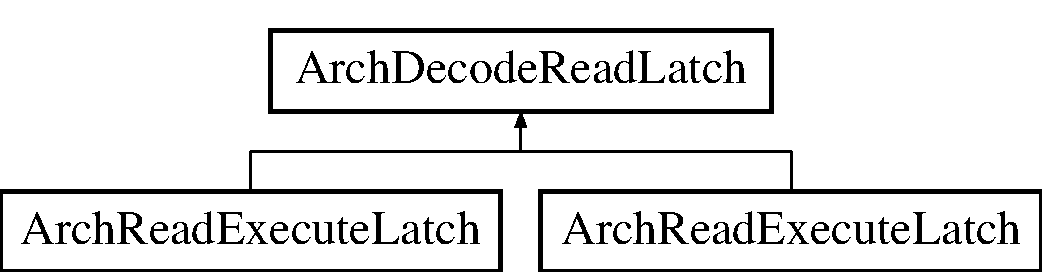
\includegraphics[height=2.000000cm]{struct_arch_decode_read_latch}
\end{center}
\end{figure}
\subsection*{Public Member Functions}
\begin{DoxyCompactItemize}
\item 
\hyperlink{struct_arch_decode_read_latch_ab5079dc332c4dc9ae70784fd6163aba4}{Arch\+Decode\+Read\+Latch} ()
\item 
virtual \hyperlink{struct_arch_decode_read_latch_a2b4f3af28cd2639610c1673f7ebb6d42}{$\sim$\+Arch\+Decode\+Read\+Latch} ()
\item 
\hyperlink{struct_arch_decode_read_latch_ab5079dc332c4dc9ae70784fd6163aba4}{Arch\+Decode\+Read\+Latch} ()
\item 
virtual \hyperlink{struct_arch_decode_read_latch_a2b4f3af28cd2639610c1673f7ebb6d42}{$\sim$\+Arch\+Decode\+Read\+Latch} ()
\item 
\hyperlink{struct_arch_decode_read_latch_ab5079dc332c4dc9ae70784fd6163aba4}{Arch\+Decode\+Read\+Latch} ()
\item 
virtual \hyperlink{struct_arch_decode_read_latch_a2b4f3af28cd2639610c1673f7ebb6d42}{$\sim$\+Arch\+Decode\+Read\+Latch} ()
\item 
\hyperlink{struct_arch_decode_read_latch_ab5079dc332c4dc9ae70784fd6163aba4}{Arch\+Decode\+Read\+Latch} ()
\end{DoxyCompactItemize}
\subsection*{Public Attributes}
\begin{DoxyCompactItemize}
\item 
\hyperlink{_i_s_a_8mips_8h_a0fe922abce2589bee86671f310ac9ce7}{Instr\+Format} \hyperlink{struct_arch_decode_read_latch_aa7507b938ac54a969ff4714ac9069f70}{format}
\item 
uint16\+\_\+t \hyperlink{struct_arch_decode_read_latch_afb9074e3a981d8e3ed76452f2cf026c8}{opcode}
\item 
uint16\+\_\+t \hyperlink{struct_arch_decode_read_latch_ac2000ea6787425c4435e4c542ed1c5c2}{function}
\item 
uint16\+\_\+t \hyperlink{struct_arch_decode_read_latch_a64c9eacbb744761e75c4834e9ab47039}{regimm}
\item 
uint16\+\_\+t \hyperlink{struct_arch_decode_read_latch_af7216ef79cfa24ae2f02aff3fbafa5c6}{shift}
\item 
uint16\+\_\+t \hyperlink{struct_arch_decode_read_latch_a9ebe977592120f5d1fc276c37d2f054e}{immediate}
\item 
int32\+\_\+t \hyperlink{struct_arch_decode_read_latch_a93402db1ace4b0ca0d00da8b26e01f2e}{displacement}
\item 
uint8\+\_\+t \hyperlink{struct_arch_decode_read_latch_ab8fd66e8168e97e488a56e038de01cee}{opcode}
\item 
uint8\+\_\+t \hyperlink{struct_arch_decode_read_latch_a531ece3671b80d61fa58d57ab2a0bb2f}{op1}
\item 
uint8\+\_\+t \hyperlink{struct_arch_decode_read_latch_abfb8ece23f312dad6eb5cda4cda9fddf}{op2}
\item 
uint8\+\_\+t \hyperlink{struct_arch_decode_read_latch_a55a8d0a534e550a8bc242bdf0faf9ba2}{op3}
\item 
uint8\+\_\+t \hyperlink{struct_arch_decode_read_latch_aaa3640c41495f29ce16ab8c8e7ea343c}{asi}
\item 
Reg\+Addr \hyperlink{struct_arch_decode_read_latch_a21e799a974b0565b40162419c079c80a}{Rs}
\item 
bool \hyperlink{struct_arch_decode_read_latch_ac743a1dbf2f4493b58087d356ba092f2}{Rs\+Is\+Local}
\item 
unsigned int \hyperlink{struct_arch_decode_read_latch_a5a22498827233fb52138f5841cc6b25d}{Rs\+Size}
\end{DoxyCompactItemize}


\subsection{Constructor \& Destructor Documentation}
\hypertarget{struct_arch_decode_read_latch_ab5079dc332c4dc9ae70784fd6163aba4}{\index{Arch\+Decode\+Read\+Latch@{Arch\+Decode\+Read\+Latch}!Arch\+Decode\+Read\+Latch@{Arch\+Decode\+Read\+Latch}}
\index{Arch\+Decode\+Read\+Latch@{Arch\+Decode\+Read\+Latch}!Arch\+Decode\+Read\+Latch@{Arch\+Decode\+Read\+Latch}}
\subsubsection[{Arch\+Decode\+Read\+Latch}]{\setlength{\rightskip}{0pt plus 5cm}Arch\+Decode\+Read\+Latch\+::\+Arch\+Decode\+Read\+Latch (
\begin{DoxyParamCaption}
{}
\end{DoxyParamCaption}
)\hspace{0.3cm}{\ttfamily [inline]}}}\label{struct_arch_decode_read_latch_ab5079dc332c4dc9ae70784fd6163aba4}
\hypertarget{struct_arch_decode_read_latch_a2b4f3af28cd2639610c1673f7ebb6d42}{\index{Arch\+Decode\+Read\+Latch@{Arch\+Decode\+Read\+Latch}!````~Arch\+Decode\+Read\+Latch@{$\sim$\+Arch\+Decode\+Read\+Latch}}
\index{````~Arch\+Decode\+Read\+Latch@{$\sim$\+Arch\+Decode\+Read\+Latch}!Arch\+Decode\+Read\+Latch@{Arch\+Decode\+Read\+Latch}}
\subsubsection[{$\sim$\+Arch\+Decode\+Read\+Latch}]{\setlength{\rightskip}{0pt plus 5cm}virtual Arch\+Decode\+Read\+Latch\+::$\sim$\+Arch\+Decode\+Read\+Latch (
\begin{DoxyParamCaption}
{}
\end{DoxyParamCaption}
)\hspace{0.3cm}{\ttfamily [inline]}, {\ttfamily [virtual]}}}\label{struct_arch_decode_read_latch_a2b4f3af28cd2639610c1673f7ebb6d42}
\hypertarget{struct_arch_decode_read_latch_ab5079dc332c4dc9ae70784fd6163aba4}{\index{Arch\+Decode\+Read\+Latch@{Arch\+Decode\+Read\+Latch}!Arch\+Decode\+Read\+Latch@{Arch\+Decode\+Read\+Latch}}
\index{Arch\+Decode\+Read\+Latch@{Arch\+Decode\+Read\+Latch}!Arch\+Decode\+Read\+Latch@{Arch\+Decode\+Read\+Latch}}
\subsubsection[{Arch\+Decode\+Read\+Latch}]{\setlength{\rightskip}{0pt plus 5cm}Arch\+Decode\+Read\+Latch\+::\+Arch\+Decode\+Read\+Latch (
\begin{DoxyParamCaption}
{}
\end{DoxyParamCaption}
)\hspace{0.3cm}{\ttfamily [inline]}}}\label{struct_arch_decode_read_latch_ab5079dc332c4dc9ae70784fd6163aba4}
\hypertarget{struct_arch_decode_read_latch_a2b4f3af28cd2639610c1673f7ebb6d42}{\index{Arch\+Decode\+Read\+Latch@{Arch\+Decode\+Read\+Latch}!````~Arch\+Decode\+Read\+Latch@{$\sim$\+Arch\+Decode\+Read\+Latch}}
\index{````~Arch\+Decode\+Read\+Latch@{$\sim$\+Arch\+Decode\+Read\+Latch}!Arch\+Decode\+Read\+Latch@{Arch\+Decode\+Read\+Latch}}
\subsubsection[{$\sim$\+Arch\+Decode\+Read\+Latch}]{\setlength{\rightskip}{0pt plus 5cm}virtual Arch\+Decode\+Read\+Latch\+::$\sim$\+Arch\+Decode\+Read\+Latch (
\begin{DoxyParamCaption}
{}
\end{DoxyParamCaption}
)\hspace{0.3cm}{\ttfamily [inline]}, {\ttfamily [virtual]}}}\label{struct_arch_decode_read_latch_a2b4f3af28cd2639610c1673f7ebb6d42}
\hypertarget{struct_arch_decode_read_latch_ab5079dc332c4dc9ae70784fd6163aba4}{\index{Arch\+Decode\+Read\+Latch@{Arch\+Decode\+Read\+Latch}!Arch\+Decode\+Read\+Latch@{Arch\+Decode\+Read\+Latch}}
\index{Arch\+Decode\+Read\+Latch@{Arch\+Decode\+Read\+Latch}!Arch\+Decode\+Read\+Latch@{Arch\+Decode\+Read\+Latch}}
\subsubsection[{Arch\+Decode\+Read\+Latch}]{\setlength{\rightskip}{0pt plus 5cm}Arch\+Decode\+Read\+Latch\+::\+Arch\+Decode\+Read\+Latch (
\begin{DoxyParamCaption}
{}
\end{DoxyParamCaption}
)\hspace{0.3cm}{\ttfamily [inline]}}}\label{struct_arch_decode_read_latch_ab5079dc332c4dc9ae70784fd6163aba4}
\hypertarget{struct_arch_decode_read_latch_a2b4f3af28cd2639610c1673f7ebb6d42}{\index{Arch\+Decode\+Read\+Latch@{Arch\+Decode\+Read\+Latch}!````~Arch\+Decode\+Read\+Latch@{$\sim$\+Arch\+Decode\+Read\+Latch}}
\index{````~Arch\+Decode\+Read\+Latch@{$\sim$\+Arch\+Decode\+Read\+Latch}!Arch\+Decode\+Read\+Latch@{Arch\+Decode\+Read\+Latch}}
\subsubsection[{$\sim$\+Arch\+Decode\+Read\+Latch}]{\setlength{\rightskip}{0pt plus 5cm}virtual Arch\+Decode\+Read\+Latch\+::$\sim$\+Arch\+Decode\+Read\+Latch (
\begin{DoxyParamCaption}
{}
\end{DoxyParamCaption}
)\hspace{0.3cm}{\ttfamily [inline]}, {\ttfamily [virtual]}}}\label{struct_arch_decode_read_latch_a2b4f3af28cd2639610c1673f7ebb6d42}
\hypertarget{struct_arch_decode_read_latch_ab5079dc332c4dc9ae70784fd6163aba4}{\index{Arch\+Decode\+Read\+Latch@{Arch\+Decode\+Read\+Latch}!Arch\+Decode\+Read\+Latch@{Arch\+Decode\+Read\+Latch}}
\index{Arch\+Decode\+Read\+Latch@{Arch\+Decode\+Read\+Latch}!Arch\+Decode\+Read\+Latch@{Arch\+Decode\+Read\+Latch}}
\subsubsection[{Arch\+Decode\+Read\+Latch}]{\setlength{\rightskip}{0pt plus 5cm}Arch\+Decode\+Read\+Latch\+::\+Arch\+Decode\+Read\+Latch (
\begin{DoxyParamCaption}
{}
\end{DoxyParamCaption}
)\hspace{0.3cm}{\ttfamily [inline]}}}\label{struct_arch_decode_read_latch_ab5079dc332c4dc9ae70784fd6163aba4}


\subsection{Member Data Documentation}
\hypertarget{struct_arch_decode_read_latch_aaa3640c41495f29ce16ab8c8e7ea343c}{\index{Arch\+Decode\+Read\+Latch@{Arch\+Decode\+Read\+Latch}!asi@{asi}}
\index{asi@{asi}!Arch\+Decode\+Read\+Latch@{Arch\+Decode\+Read\+Latch}}
\subsubsection[{asi}]{\setlength{\rightskip}{0pt plus 5cm}uint8\+\_\+t Arch\+Decode\+Read\+Latch\+::asi}}\label{struct_arch_decode_read_latch_aaa3640c41495f29ce16ab8c8e7ea343c}
\hypertarget{struct_arch_decode_read_latch_a93402db1ace4b0ca0d00da8b26e01f2e}{\index{Arch\+Decode\+Read\+Latch@{Arch\+Decode\+Read\+Latch}!displacement@{displacement}}
\index{displacement@{displacement}!Arch\+Decode\+Read\+Latch@{Arch\+Decode\+Read\+Latch}}
\subsubsection[{displacement}]{\setlength{\rightskip}{0pt plus 5cm}int32\+\_\+t Arch\+Decode\+Read\+Latch\+::displacement}}\label{struct_arch_decode_read_latch_a93402db1ace4b0ca0d00da8b26e01f2e}
\hypertarget{struct_arch_decode_read_latch_aa7507b938ac54a969ff4714ac9069f70}{\index{Arch\+Decode\+Read\+Latch@{Arch\+Decode\+Read\+Latch}!format@{format}}
\index{format@{format}!Arch\+Decode\+Read\+Latch@{Arch\+Decode\+Read\+Latch}}
\subsubsection[{format}]{\setlength{\rightskip}{0pt plus 5cm}{\bf Instr\+Format} Arch\+Decode\+Read\+Latch\+::format}}\label{struct_arch_decode_read_latch_aa7507b938ac54a969ff4714ac9069f70}
\hypertarget{struct_arch_decode_read_latch_ac2000ea6787425c4435e4c542ed1c5c2}{\index{Arch\+Decode\+Read\+Latch@{Arch\+Decode\+Read\+Latch}!function@{function}}
\index{function@{function}!Arch\+Decode\+Read\+Latch@{Arch\+Decode\+Read\+Latch}}
\subsubsection[{function}]{\setlength{\rightskip}{0pt plus 5cm}uint16\+\_\+t Arch\+Decode\+Read\+Latch\+::function}}\label{struct_arch_decode_read_latch_ac2000ea6787425c4435e4c542ed1c5c2}
\hypertarget{struct_arch_decode_read_latch_a9ebe977592120f5d1fc276c37d2f054e}{\index{Arch\+Decode\+Read\+Latch@{Arch\+Decode\+Read\+Latch}!immediate@{immediate}}
\index{immediate@{immediate}!Arch\+Decode\+Read\+Latch@{Arch\+Decode\+Read\+Latch}}
\subsubsection[{immediate}]{\setlength{\rightskip}{0pt plus 5cm}uint16\+\_\+t Arch\+Decode\+Read\+Latch\+::immediate}}\label{struct_arch_decode_read_latch_a9ebe977592120f5d1fc276c37d2f054e}
\hypertarget{struct_arch_decode_read_latch_a531ece3671b80d61fa58d57ab2a0bb2f}{\index{Arch\+Decode\+Read\+Latch@{Arch\+Decode\+Read\+Latch}!op1@{op1}}
\index{op1@{op1}!Arch\+Decode\+Read\+Latch@{Arch\+Decode\+Read\+Latch}}
\subsubsection[{op1}]{\setlength{\rightskip}{0pt plus 5cm}uint8\+\_\+t Arch\+Decode\+Read\+Latch\+::op1}}\label{struct_arch_decode_read_latch_a531ece3671b80d61fa58d57ab2a0bb2f}
\hypertarget{struct_arch_decode_read_latch_abfb8ece23f312dad6eb5cda4cda9fddf}{\index{Arch\+Decode\+Read\+Latch@{Arch\+Decode\+Read\+Latch}!op2@{op2}}
\index{op2@{op2}!Arch\+Decode\+Read\+Latch@{Arch\+Decode\+Read\+Latch}}
\subsubsection[{op2}]{\setlength{\rightskip}{0pt plus 5cm}uint8\+\_\+t Arch\+Decode\+Read\+Latch\+::op2}}\label{struct_arch_decode_read_latch_abfb8ece23f312dad6eb5cda4cda9fddf}
\hypertarget{struct_arch_decode_read_latch_a55a8d0a534e550a8bc242bdf0faf9ba2}{\index{Arch\+Decode\+Read\+Latch@{Arch\+Decode\+Read\+Latch}!op3@{op3}}
\index{op3@{op3}!Arch\+Decode\+Read\+Latch@{Arch\+Decode\+Read\+Latch}}
\subsubsection[{op3}]{\setlength{\rightskip}{0pt plus 5cm}uint8\+\_\+t Arch\+Decode\+Read\+Latch\+::op3}}\label{struct_arch_decode_read_latch_a55a8d0a534e550a8bc242bdf0faf9ba2}
\hypertarget{struct_arch_decode_read_latch_afb9074e3a981d8e3ed76452f2cf026c8}{\index{Arch\+Decode\+Read\+Latch@{Arch\+Decode\+Read\+Latch}!opcode@{opcode}}
\index{opcode@{opcode}!Arch\+Decode\+Read\+Latch@{Arch\+Decode\+Read\+Latch}}
\subsubsection[{opcode}]{\setlength{\rightskip}{0pt plus 5cm}uint16\+\_\+t Arch\+Decode\+Read\+Latch\+::opcode}}\label{struct_arch_decode_read_latch_afb9074e3a981d8e3ed76452f2cf026c8}
\hypertarget{struct_arch_decode_read_latch_ab8fd66e8168e97e488a56e038de01cee}{\index{Arch\+Decode\+Read\+Latch@{Arch\+Decode\+Read\+Latch}!opcode@{opcode}}
\index{opcode@{opcode}!Arch\+Decode\+Read\+Latch@{Arch\+Decode\+Read\+Latch}}
\subsubsection[{opcode}]{\setlength{\rightskip}{0pt plus 5cm}uint8\+\_\+t Arch\+Decode\+Read\+Latch\+::opcode}}\label{struct_arch_decode_read_latch_ab8fd66e8168e97e488a56e038de01cee}
\hypertarget{struct_arch_decode_read_latch_a64c9eacbb744761e75c4834e9ab47039}{\index{Arch\+Decode\+Read\+Latch@{Arch\+Decode\+Read\+Latch}!regimm@{regimm}}
\index{regimm@{regimm}!Arch\+Decode\+Read\+Latch@{Arch\+Decode\+Read\+Latch}}
\subsubsection[{regimm}]{\setlength{\rightskip}{0pt plus 5cm}uint16\+\_\+t Arch\+Decode\+Read\+Latch\+::regimm}}\label{struct_arch_decode_read_latch_a64c9eacbb744761e75c4834e9ab47039}
\hypertarget{struct_arch_decode_read_latch_a21e799a974b0565b40162419c079c80a}{\index{Arch\+Decode\+Read\+Latch@{Arch\+Decode\+Read\+Latch}!Rs@{Rs}}
\index{Rs@{Rs}!Arch\+Decode\+Read\+Latch@{Arch\+Decode\+Read\+Latch}}
\subsubsection[{Rs}]{\setlength{\rightskip}{0pt plus 5cm}Reg\+Addr Arch\+Decode\+Read\+Latch\+::\+Rs}}\label{struct_arch_decode_read_latch_a21e799a974b0565b40162419c079c80a}
\hypertarget{struct_arch_decode_read_latch_ac743a1dbf2f4493b58087d356ba092f2}{\index{Arch\+Decode\+Read\+Latch@{Arch\+Decode\+Read\+Latch}!Rs\+Is\+Local@{Rs\+Is\+Local}}
\index{Rs\+Is\+Local@{Rs\+Is\+Local}!Arch\+Decode\+Read\+Latch@{Arch\+Decode\+Read\+Latch}}
\subsubsection[{Rs\+Is\+Local}]{\setlength{\rightskip}{0pt plus 5cm}bool Arch\+Decode\+Read\+Latch\+::\+Rs\+Is\+Local}}\label{struct_arch_decode_read_latch_ac743a1dbf2f4493b58087d356ba092f2}
\hypertarget{struct_arch_decode_read_latch_a5a22498827233fb52138f5841cc6b25d}{\index{Arch\+Decode\+Read\+Latch@{Arch\+Decode\+Read\+Latch}!Rs\+Size@{Rs\+Size}}
\index{Rs\+Size@{Rs\+Size}!Arch\+Decode\+Read\+Latch@{Arch\+Decode\+Read\+Latch}}
\subsubsection[{Rs\+Size}]{\setlength{\rightskip}{0pt plus 5cm}unsigned int Arch\+Decode\+Read\+Latch\+::\+Rs\+Size}}\label{struct_arch_decode_read_latch_a5a22498827233fb52138f5841cc6b25d}
\hypertarget{struct_arch_decode_read_latch_af7216ef79cfa24ae2f02aff3fbafa5c6}{\index{Arch\+Decode\+Read\+Latch@{Arch\+Decode\+Read\+Latch}!shift@{shift}}
\index{shift@{shift}!Arch\+Decode\+Read\+Latch@{Arch\+Decode\+Read\+Latch}}
\subsubsection[{shift}]{\setlength{\rightskip}{0pt plus 5cm}uint16\+\_\+t Arch\+Decode\+Read\+Latch\+::shift}}\label{struct_arch_decode_read_latch_af7216ef79cfa24ae2f02aff3fbafa5c6}


The documentation for this struct was generated from the following files\+:\begin{DoxyCompactItemize}
\item 
arch/drisc/\hyperlink{_i_s_a_8mips_8h}{I\+S\+A.\+mips.\+h}\item 
arch/drisc/\hyperlink{_i_s_a_8mtalpha_8h}{I\+S\+A.\+mtalpha.\+h}\item 
arch/drisc/\hyperlink{_i_s_a_8mtsparc_8h}{I\+S\+A.\+mtsparc.\+h}\item 
arch/drisc/\hyperlink{_i_s_a_8or1k_8h}{I\+S\+A.\+or1k.\+h}\end{DoxyCompactItemize}

\hypertarget{struct_arch_read_execute_latch}{\section{Arch\+Read\+Execute\+Latch Struct Reference}
\label{struct_arch_read_execute_latch}\index{Arch\+Read\+Execute\+Latch@{Arch\+Read\+Execute\+Latch}}
}


{\ttfamily \#include $<$I\+S\+A.\+mtsparc.\+h$>$}

Inheritance diagram for Arch\+Read\+Execute\+Latch\+:\begin{figure}[H]
\begin{center}
\leavevmode
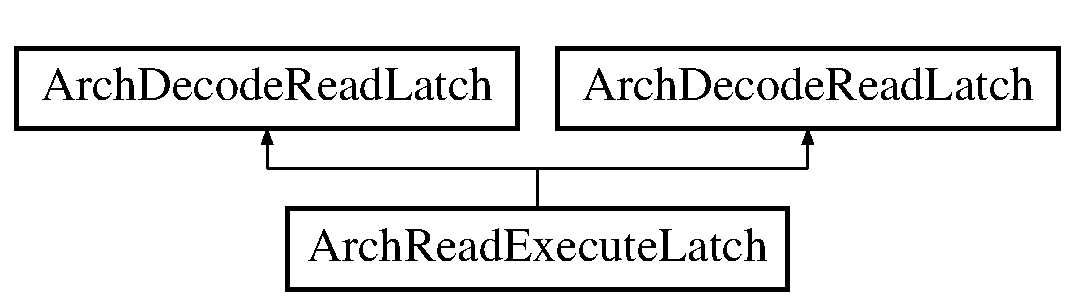
\includegraphics[height=2.000000cm]{struct_arch_read_execute_latch}
\end{center}
\end{figure}
\subsection*{Public Member Functions}
\begin{DoxyCompactItemize}
\item 
\hyperlink{struct_arch_read_execute_latch_af3ff5fc593ebbb8708ccb6e3dcb13876}{Arch\+Read\+Execute\+Latch} ()
\end{DoxyCompactItemize}
\subsection*{Public Attributes}
\begin{DoxyCompactItemize}
\item 
Pipe\+Value \hyperlink{struct_arch_read_execute_latch_a243ee741c2e308c35d710c815397c6a9}{Rsv}
\end{DoxyCompactItemize}


\subsection{Constructor \& Destructor Documentation}
\hypertarget{struct_arch_read_execute_latch_af3ff5fc593ebbb8708ccb6e3dcb13876}{\index{Arch\+Read\+Execute\+Latch@{Arch\+Read\+Execute\+Latch}!Arch\+Read\+Execute\+Latch@{Arch\+Read\+Execute\+Latch}}
\index{Arch\+Read\+Execute\+Latch@{Arch\+Read\+Execute\+Latch}!Arch\+Read\+Execute\+Latch@{Arch\+Read\+Execute\+Latch}}
\subsubsection[{Arch\+Read\+Execute\+Latch}]{\setlength{\rightskip}{0pt plus 5cm}Arch\+Read\+Execute\+Latch\+::\+Arch\+Read\+Execute\+Latch (
\begin{DoxyParamCaption}
{}
\end{DoxyParamCaption}
)\hspace{0.3cm}{\ttfamily [inline]}}}\label{struct_arch_read_execute_latch_af3ff5fc593ebbb8708ccb6e3dcb13876}


\subsection{Member Data Documentation}
\hypertarget{struct_arch_read_execute_latch_a243ee741c2e308c35d710c815397c6a9}{\index{Arch\+Read\+Execute\+Latch@{Arch\+Read\+Execute\+Latch}!Rsv@{Rsv}}
\index{Rsv@{Rsv}!Arch\+Read\+Execute\+Latch@{Arch\+Read\+Execute\+Latch}}
\subsubsection[{Rsv}]{\setlength{\rightskip}{0pt plus 5cm}Pipe\+Value Arch\+Read\+Execute\+Latch\+::\+Rsv}}\label{struct_arch_read_execute_latch_a243ee741c2e308c35d710c815397c6a9}


The documentation for this struct was generated from the following file\+:\begin{DoxyCompactItemize}
\item 
arch/drisc/\hyperlink{_i_s_a_8mtsparc_8h}{I\+S\+A.\+mtsparc.\+h}\end{DoxyCompactItemize}

\hypertarget{class_simulator_1_1drisc_1_1_i_o_interface_1_1_async_i_o_interface}{\section{Simulator\+:\+:drisc\+:\+:I\+O\+Interface\+:\+:Async\+I\+O\+Interface Class Reference}
\label{class_simulator_1_1drisc_1_1_i_o_interface_1_1_async_i_o_interface}\index{Simulator\+::drisc\+::\+I\+O\+Interface\+::\+Async\+I\+O\+Interface@{Simulator\+::drisc\+::\+I\+O\+Interface\+::\+Async\+I\+O\+Interface}}
}


{\ttfamily \#include $<$I\+O\+Interface.\+h$>$}

Inheritance diagram for Simulator\+:\+:drisc\+:\+:I\+O\+Interface\+:\+:Async\+I\+O\+Interface\+:\begin{figure}[H]
\begin{center}
\leavevmode
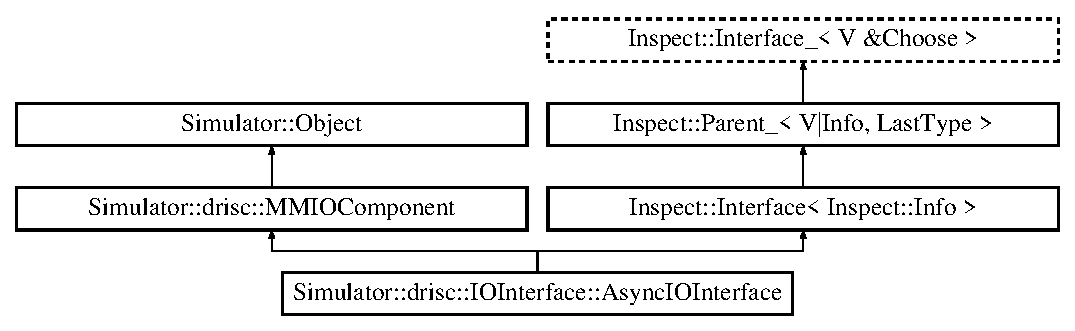
\includegraphics[height=4.000000cm]{class_simulator_1_1drisc_1_1_i_o_interface_1_1_async_i_o_interface}
\end{center}
\end{figure}
\subsection*{Public Member Functions}
\begin{DoxyCompactItemize}
\item 
\hyperlink{class_simulator_1_1drisc_1_1_i_o_interface_1_1_async_i_o_interface_a464b5fb822aca2d8056168d652a1958a}{Async\+I\+O\+Interface} (const std\+::string \&\hyperlink{mtconf_8c_a8f8f80d37794cde9472343e4487ba3eb}{name}, \hyperlink{class_simulator_1_1drisc_1_1_i_o_interface}{I\+O\+Interface} \&parent, \hyperlink{class_simulator_1_1_clock}{Clock} \&clock, \hyperlink{class_config}{Config} \&config)
\item 
size\+\_\+t \hyperlink{class_simulator_1_1drisc_1_1_i_o_interface_1_1_async_i_o_interface_accc074c35d15dc854b5124fd10a1b471}{Get\+Size} () const 
\item 
\hyperlink{namespace_simulator_a4b6b5616e7236c0c131516a441776805}{Result} \hyperlink{class_simulator_1_1drisc_1_1_i_o_interface_1_1_async_i_o_interface_addc263b5e5f191da3a63279a18ddf3ff}{Read} (Mem\+Addr address, void $\ast$data, Mem\+Size size, \hyperlink{namespace_simulator_aaccbc706b2d6c99085f52f6dfc2333e4}{L\+F\+I\+D} fid, \hyperlink{namespace_simulator_a483cc4ecee1736e895054617672cded5}{T\+I\+D} tid, const \hyperlink{struct_simulator_1_1_reg_addr}{Reg\+Addr} \&writeback)
\item 
\hyperlink{namespace_simulator_a4b6b5616e7236c0c131516a441776805}{Result} \hyperlink{class_simulator_1_1drisc_1_1_i_o_interface_1_1_async_i_o_interface_aadb2d48c24ed209ee89b5306f49afdb1}{Write} (Mem\+Addr address, const void $\ast$data, Mem\+Size size, \hyperlink{namespace_simulator_aaccbc706b2d6c99085f52f6dfc2333e4}{L\+F\+I\+D} fid, \hyperlink{namespace_simulator_a483cc4ecee1736e895054617672cded5}{T\+I\+D} tid)
\item 
void \hyperlink{class_simulator_1_1drisc_1_1_i_o_interface_1_1_async_i_o_interface_adc1c6e47d6ee7a0114f656c2213b209a}{Cmd\+\_\+\+Info} (std\+::ostream \&out, const std\+::vector$<$ std\+::string $>$ \&args) const 
\item 
unsigned \hyperlink{class_simulator_1_1drisc_1_1_i_o_interface_1_1_async_i_o_interface_aa56c4302a9e067d1c2c6969ffe581aeb}{Get\+Device\+Address\+Bits} () const 
\item 
Mem\+Addr \hyperlink{class_simulator_1_1drisc_1_1_i_o_interface_1_1_async_i_o_interface_a74deaca54a0584c29dd28b814246f3a7}{Get\+Device\+Base\+Address} (\hyperlink{namespace_simulator_a3493d987c866ad6b8aaa704c42502db0}{I\+O\+Device\+I\+D} dev) const 
\end{DoxyCompactItemize}


\subsection{Constructor \& Destructor Documentation}
\hypertarget{class_simulator_1_1drisc_1_1_i_o_interface_1_1_async_i_o_interface_a464b5fb822aca2d8056168d652a1958a}{\index{Simulator\+::drisc\+::\+I\+O\+Interface\+::\+Async\+I\+O\+Interface@{Simulator\+::drisc\+::\+I\+O\+Interface\+::\+Async\+I\+O\+Interface}!Async\+I\+O\+Interface@{Async\+I\+O\+Interface}}
\index{Async\+I\+O\+Interface@{Async\+I\+O\+Interface}!Simulator\+::drisc\+::\+I\+O\+Interface\+::\+Async\+I\+O\+Interface@{Simulator\+::drisc\+::\+I\+O\+Interface\+::\+Async\+I\+O\+Interface}}
\subsubsection[{Async\+I\+O\+Interface}]{\setlength{\rightskip}{0pt plus 5cm}Simulator\+::drisc\+::\+I\+O\+Interface\+::\+Async\+I\+O\+Interface\+::\+Async\+I\+O\+Interface (
\begin{DoxyParamCaption}
\item[{const std\+::string \&}]{name, }
\item[{{\bf I\+O\+Interface} \&}]{parent, }
\item[{{\bf Clock} \&}]{clock, }
\item[{{\bf Config} \&}]{config}
\end{DoxyParamCaption}
)}}\label{class_simulator_1_1drisc_1_1_i_o_interface_1_1_async_i_o_interface_a464b5fb822aca2d8056168d652a1958a}


\subsection{Member Function Documentation}
\hypertarget{class_simulator_1_1drisc_1_1_i_o_interface_1_1_async_i_o_interface_adc1c6e47d6ee7a0114f656c2213b209a}{\index{Simulator\+::drisc\+::\+I\+O\+Interface\+::\+Async\+I\+O\+Interface@{Simulator\+::drisc\+::\+I\+O\+Interface\+::\+Async\+I\+O\+Interface}!Cmd\+\_\+\+Info@{Cmd\+\_\+\+Info}}
\index{Cmd\+\_\+\+Info@{Cmd\+\_\+\+Info}!Simulator\+::drisc\+::\+I\+O\+Interface\+::\+Async\+I\+O\+Interface@{Simulator\+::drisc\+::\+I\+O\+Interface\+::\+Async\+I\+O\+Interface}}
\subsubsection[{Cmd\+\_\+\+Info}]{\setlength{\rightskip}{0pt plus 5cm}void Simulator\+::drisc\+::\+I\+O\+Interface\+::\+Async\+I\+O\+Interface\+::\+Cmd\+\_\+\+Info (
\begin{DoxyParamCaption}
\item[{std\+::ostream \&}]{out, }
\item[{const std\+::vector$<$ std\+::string $>$ \&}]{args}
\end{DoxyParamCaption}
) const}}\label{class_simulator_1_1drisc_1_1_i_o_interface_1_1_async_i_o_interface_adc1c6e47d6ee7a0114f656c2213b209a}
\hypertarget{class_simulator_1_1drisc_1_1_i_o_interface_1_1_async_i_o_interface_aa56c4302a9e067d1c2c6969ffe581aeb}{\index{Simulator\+::drisc\+::\+I\+O\+Interface\+::\+Async\+I\+O\+Interface@{Simulator\+::drisc\+::\+I\+O\+Interface\+::\+Async\+I\+O\+Interface}!Get\+Device\+Address\+Bits@{Get\+Device\+Address\+Bits}}
\index{Get\+Device\+Address\+Bits@{Get\+Device\+Address\+Bits}!Simulator\+::drisc\+::\+I\+O\+Interface\+::\+Async\+I\+O\+Interface@{Simulator\+::drisc\+::\+I\+O\+Interface\+::\+Async\+I\+O\+Interface}}
\subsubsection[{Get\+Device\+Address\+Bits}]{\setlength{\rightskip}{0pt plus 5cm}unsigned Simulator\+::drisc\+::\+I\+O\+Interface\+::\+Async\+I\+O\+Interface\+::\+Get\+Device\+Address\+Bits (
\begin{DoxyParamCaption}
{}
\end{DoxyParamCaption}
) const\hspace{0.3cm}{\ttfamily [inline]}}}\label{class_simulator_1_1drisc_1_1_i_o_interface_1_1_async_i_o_interface_aa56c4302a9e067d1c2c6969ffe581aeb}
\hypertarget{class_simulator_1_1drisc_1_1_i_o_interface_1_1_async_i_o_interface_a74deaca54a0584c29dd28b814246f3a7}{\index{Simulator\+::drisc\+::\+I\+O\+Interface\+::\+Async\+I\+O\+Interface@{Simulator\+::drisc\+::\+I\+O\+Interface\+::\+Async\+I\+O\+Interface}!Get\+Device\+Base\+Address@{Get\+Device\+Base\+Address}}
\index{Get\+Device\+Base\+Address@{Get\+Device\+Base\+Address}!Simulator\+::drisc\+::\+I\+O\+Interface\+::\+Async\+I\+O\+Interface@{Simulator\+::drisc\+::\+I\+O\+Interface\+::\+Async\+I\+O\+Interface}}
\subsubsection[{Get\+Device\+Base\+Address}]{\setlength{\rightskip}{0pt plus 5cm}Mem\+Addr Simulator\+::drisc\+::\+I\+O\+Interface\+::\+Async\+I\+O\+Interface\+::\+Get\+Device\+Base\+Address (
\begin{DoxyParamCaption}
\item[{{\bf I\+O\+Device\+I\+D}}]{dev}
\end{DoxyParamCaption}
) const}}\label{class_simulator_1_1drisc_1_1_i_o_interface_1_1_async_i_o_interface_a74deaca54a0584c29dd28b814246f3a7}
\hypertarget{class_simulator_1_1drisc_1_1_i_o_interface_1_1_async_i_o_interface_accc074c35d15dc854b5124fd10a1b471}{\index{Simulator\+::drisc\+::\+I\+O\+Interface\+::\+Async\+I\+O\+Interface@{Simulator\+::drisc\+::\+I\+O\+Interface\+::\+Async\+I\+O\+Interface}!Get\+Size@{Get\+Size}}
\index{Get\+Size@{Get\+Size}!Simulator\+::drisc\+::\+I\+O\+Interface\+::\+Async\+I\+O\+Interface@{Simulator\+::drisc\+::\+I\+O\+Interface\+::\+Async\+I\+O\+Interface}}
\subsubsection[{Get\+Size}]{\setlength{\rightskip}{0pt plus 5cm}size\+\_\+t Simulator\+::drisc\+::\+I\+O\+Interface\+::\+Async\+I\+O\+Interface\+::\+Get\+Size (
\begin{DoxyParamCaption}
{}
\end{DoxyParamCaption}
) const\hspace{0.3cm}{\ttfamily [virtual]}}}\label{class_simulator_1_1drisc_1_1_i_o_interface_1_1_async_i_o_interface_accc074c35d15dc854b5124fd10a1b471}


Implements \hyperlink{class_simulator_1_1drisc_1_1_m_m_i_o_component_ad8f1a93b445f287895949bfe52972346}{Simulator\+::drisc\+::\+M\+M\+I\+O\+Component}.

\hypertarget{class_simulator_1_1drisc_1_1_i_o_interface_1_1_async_i_o_interface_addc263b5e5f191da3a63279a18ddf3ff}{\index{Simulator\+::drisc\+::\+I\+O\+Interface\+::\+Async\+I\+O\+Interface@{Simulator\+::drisc\+::\+I\+O\+Interface\+::\+Async\+I\+O\+Interface}!Read@{Read}}
\index{Read@{Read}!Simulator\+::drisc\+::\+I\+O\+Interface\+::\+Async\+I\+O\+Interface@{Simulator\+::drisc\+::\+I\+O\+Interface\+::\+Async\+I\+O\+Interface}}
\subsubsection[{Read}]{\setlength{\rightskip}{0pt plus 5cm}{\bf Result} Simulator\+::drisc\+::\+I\+O\+Interface\+::\+Async\+I\+O\+Interface\+::\+Read (
\begin{DoxyParamCaption}
\item[{Mem\+Addr}]{address, }
\item[{void $\ast$}]{data, }
\item[{Mem\+Size}]{size, }
\item[{{\bf L\+F\+I\+D}}]{fid, }
\item[{{\bf T\+I\+D}}]{tid, }
\item[{const {\bf Reg\+Addr} \&}]{writeback}
\end{DoxyParamCaption}
)\hspace{0.3cm}{\ttfamily [virtual]}}}\label{class_simulator_1_1drisc_1_1_i_o_interface_1_1_async_i_o_interface_addc263b5e5f191da3a63279a18ddf3ff}


Implements \hyperlink{class_simulator_1_1drisc_1_1_m_m_i_o_component_af07e2f3e1280d8d56cab7a59815e7eeb}{Simulator\+::drisc\+::\+M\+M\+I\+O\+Component}.

\hypertarget{class_simulator_1_1drisc_1_1_i_o_interface_1_1_async_i_o_interface_aadb2d48c24ed209ee89b5306f49afdb1}{\index{Simulator\+::drisc\+::\+I\+O\+Interface\+::\+Async\+I\+O\+Interface@{Simulator\+::drisc\+::\+I\+O\+Interface\+::\+Async\+I\+O\+Interface}!Write@{Write}}
\index{Write@{Write}!Simulator\+::drisc\+::\+I\+O\+Interface\+::\+Async\+I\+O\+Interface@{Simulator\+::drisc\+::\+I\+O\+Interface\+::\+Async\+I\+O\+Interface}}
\subsubsection[{Write}]{\setlength{\rightskip}{0pt plus 5cm}{\bf Result} Simulator\+::drisc\+::\+I\+O\+Interface\+::\+Async\+I\+O\+Interface\+::\+Write (
\begin{DoxyParamCaption}
\item[{Mem\+Addr}]{address, }
\item[{const void $\ast$}]{data, }
\item[{Mem\+Size}]{size, }
\item[{{\bf L\+F\+I\+D}}]{fid, }
\item[{{\bf T\+I\+D}}]{tid}
\end{DoxyParamCaption}
)\hspace{0.3cm}{\ttfamily [virtual]}}}\label{class_simulator_1_1drisc_1_1_i_o_interface_1_1_async_i_o_interface_aadb2d48c24ed209ee89b5306f49afdb1}


Implements \hyperlink{class_simulator_1_1drisc_1_1_m_m_i_o_component_aab3662058e7a00109b122a1460188a8b}{Simulator\+::drisc\+::\+M\+M\+I\+O\+Component}.



The documentation for this class was generated from the following files\+:\begin{DoxyCompactItemize}
\item 
arch/drisc/mmu/\hyperlink{_i_o_interface_8h}{I\+O\+Interface.\+h}\item 
arch/drisc/mmu/\hyperlink{_i_o_interface_8cpp}{I\+O\+Interface.\+cpp}\end{DoxyCompactItemize}

\hypertarget{class_simulator_1_1_banked_memory_1_1_bank}{\section{Simulator\+:\+:Banked\+Memory\+:\+:Bank Class Reference}
\label{class_simulator_1_1_banked_memory_1_1_bank}\index{Simulator\+::\+Banked\+Memory\+::\+Bank@{Simulator\+::\+Banked\+Memory\+::\+Bank}}
}
Inheritance diagram for Simulator\+:\+:Banked\+Memory\+:\+:Bank\+:\begin{figure}[H]
\begin{center}
\leavevmode
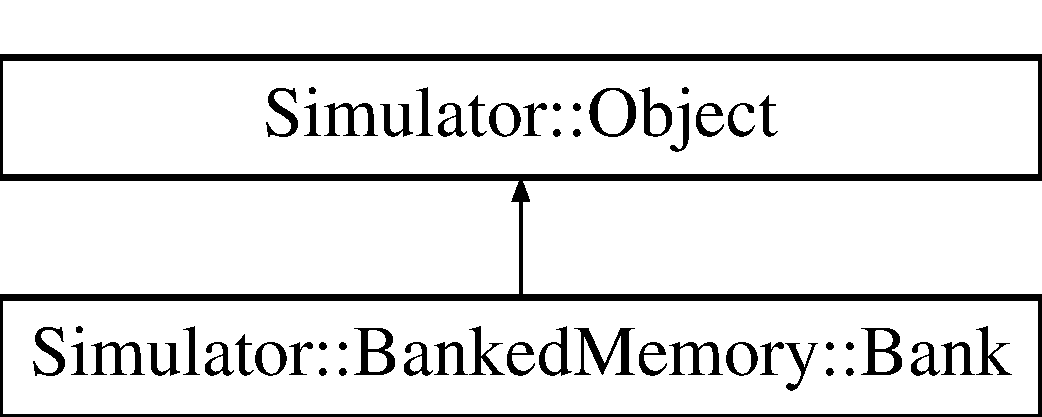
\includegraphics[height=2.000000cm]{class_simulator_1_1_banked_memory_1_1_bank}
\end{center}
\end{figure}
\subsection*{Public Member Functions}
\begin{DoxyCompactItemize}
\item 
void \hyperlink{class_simulator_1_1_banked_memory_1_1_bank_a17d1ba65e7fae349507e7184c6d72dbf}{Register\+Client} (\hyperlink{class_simulator_1_1_arbitrated_service}{Arbitrated\+Service}$<$$>$ \&client\+\_\+arbitrator, \hyperlink{class_simulator_1_1_process}{Process} \&process, \hyperlink{class_simulator_1_1_storage_trace_set}{Storage\+Trace\+Set} \&traces, const \hyperlink{class_simulator_1_1_storage_trace_set}{Storage\+Trace\+Set} \&storages)
\item 
bool \hyperlink{class_simulator_1_1_banked_memory_1_1_bank_aa04094a38c766de2a4d58e392e6263ae}{Add\+Incoming\+Request} (\hyperlink{struct_simulator_1_1_banked_memory_1_1_request}{Request} \&request)
\item 
bool \hyperlink{class_simulator_1_1_banked_memory_1_1_bank_a9da06e728a98b59c2081729a50cf1664}{Has\+Requests} (void) const 
\item 
void \hyperlink{class_simulator_1_1_banked_memory_1_1_bank_ac37054d967707f69658e7b87f37968c1}{Print} (ostream \&out)
\item 
\hyperlink{class_simulator_1_1_banked_memory_1_1_bank_afb78f52e341cb8032b7a986d0ef22217}{Bank} (const std\+::string \&\hyperlink{mtconf_8c_a8f8f80d37794cde9472343e4487ba3eb}{name}, \hyperlink{class_simulator_1_1_banked_memory}{Banked\+Memory} \&memory, \hyperlink{class_simulator_1_1_clock}{Clock} \&clock, \hyperlink{namespace_simulator_a5ca279f926485be2d0554e41275a3305}{Buffer\+Size} buffersize)
\end{DoxyCompactItemize}


\subsection{Constructor \& Destructor Documentation}
\hypertarget{class_simulator_1_1_banked_memory_1_1_bank_afb78f52e341cb8032b7a986d0ef22217}{\index{Simulator\+::\+Banked\+Memory\+::\+Bank@{Simulator\+::\+Banked\+Memory\+::\+Bank}!Bank@{Bank}}
\index{Bank@{Bank}!Simulator\+::\+Banked\+Memory\+::\+Bank@{Simulator\+::\+Banked\+Memory\+::\+Bank}}
\subsubsection[{Bank}]{\setlength{\rightskip}{0pt plus 5cm}Simulator\+::\+Banked\+Memory\+::\+Bank\+::\+Bank (
\begin{DoxyParamCaption}
\item[{const std\+::string \&}]{name, }
\item[{{\bf Banked\+Memory} \&}]{memory, }
\item[{{\bf Clock} \&}]{clock, }
\item[{{\bf Buffer\+Size}}]{buffersize}
\end{DoxyParamCaption}
)\hspace{0.3cm}{\ttfamily [inline]}}}\label{class_simulator_1_1_banked_memory_1_1_bank_afb78f52e341cb8032b7a986d0ef22217}


\subsection{Member Function Documentation}
\hypertarget{class_simulator_1_1_banked_memory_1_1_bank_aa04094a38c766de2a4d58e392e6263ae}{\index{Simulator\+::\+Banked\+Memory\+::\+Bank@{Simulator\+::\+Banked\+Memory\+::\+Bank}!Add\+Incoming\+Request@{Add\+Incoming\+Request}}
\index{Add\+Incoming\+Request@{Add\+Incoming\+Request}!Simulator\+::\+Banked\+Memory\+::\+Bank@{Simulator\+::\+Banked\+Memory\+::\+Bank}}
\subsubsection[{Add\+Incoming\+Request}]{\setlength{\rightskip}{0pt plus 5cm}bool Simulator\+::\+Banked\+Memory\+::\+Bank\+::\+Add\+Incoming\+Request (
\begin{DoxyParamCaption}
\item[{{\bf Request} \&}]{request}
\end{DoxyParamCaption}
)\hspace{0.3cm}{\ttfamily [inline]}}}\label{class_simulator_1_1_banked_memory_1_1_bank_aa04094a38c766de2a4d58e392e6263ae}
\hypertarget{class_simulator_1_1_banked_memory_1_1_bank_a9da06e728a98b59c2081729a50cf1664}{\index{Simulator\+::\+Banked\+Memory\+::\+Bank@{Simulator\+::\+Banked\+Memory\+::\+Bank}!Has\+Requests@{Has\+Requests}}
\index{Has\+Requests@{Has\+Requests}!Simulator\+::\+Banked\+Memory\+::\+Bank@{Simulator\+::\+Banked\+Memory\+::\+Bank}}
\subsubsection[{Has\+Requests}]{\setlength{\rightskip}{0pt plus 5cm}bool Simulator\+::\+Banked\+Memory\+::\+Bank\+::\+Has\+Requests (
\begin{DoxyParamCaption}
\item[{void}]{}
\end{DoxyParamCaption}
) const\hspace{0.3cm}{\ttfamily [inline]}}}\label{class_simulator_1_1_banked_memory_1_1_bank_a9da06e728a98b59c2081729a50cf1664}
\hypertarget{class_simulator_1_1_banked_memory_1_1_bank_ac37054d967707f69658e7b87f37968c1}{\index{Simulator\+::\+Banked\+Memory\+::\+Bank@{Simulator\+::\+Banked\+Memory\+::\+Bank}!Print@{Print}}
\index{Print@{Print}!Simulator\+::\+Banked\+Memory\+::\+Bank@{Simulator\+::\+Banked\+Memory\+::\+Bank}}
\subsubsection[{Print}]{\setlength{\rightskip}{0pt plus 5cm}void Simulator\+::\+Banked\+Memory\+::\+Bank\+::\+Print (
\begin{DoxyParamCaption}
\item[{ostream \&}]{out}
\end{DoxyParamCaption}
)\hspace{0.3cm}{\ttfamily [inline]}}}\label{class_simulator_1_1_banked_memory_1_1_bank_ac37054d967707f69658e7b87f37968c1}
\hypertarget{class_simulator_1_1_banked_memory_1_1_bank_a17d1ba65e7fae349507e7184c6d72dbf}{\index{Simulator\+::\+Banked\+Memory\+::\+Bank@{Simulator\+::\+Banked\+Memory\+::\+Bank}!Register\+Client@{Register\+Client}}
\index{Register\+Client@{Register\+Client}!Simulator\+::\+Banked\+Memory\+::\+Bank@{Simulator\+::\+Banked\+Memory\+::\+Bank}}
\subsubsection[{Register\+Client}]{\setlength{\rightskip}{0pt plus 5cm}void Simulator\+::\+Banked\+Memory\+::\+Bank\+::\+Register\+Client (
\begin{DoxyParamCaption}
\item[{{\bf Arbitrated\+Service}$<$$>$ \&}]{client\+\_\+arbitrator, }
\item[{{\bf Process} \&}]{process, }
\item[{{\bf Storage\+Trace\+Set} \&}]{traces, }
\item[{const {\bf Storage\+Trace\+Set} \&}]{storages}
\end{DoxyParamCaption}
)\hspace{0.3cm}{\ttfamily [inline]}}}\label{class_simulator_1_1_banked_memory_1_1_bank_a17d1ba65e7fae349507e7184c6d72dbf}


The documentation for this class was generated from the following file\+:\begin{DoxyCompactItemize}
\item 
arch/mem/\hyperlink{_banked_memory_8cpp}{Banked\+Memory.\+cpp}\end{DoxyCompactItemize}

\hypertarget{class_simulator_1_1_banked_memory}{\section{Simulator\+:\+:Banked\+Memory Class Reference}
\label{class_simulator_1_1_banked_memory}\index{Simulator\+::\+Banked\+Memory@{Simulator\+::\+Banked\+Memory}}
}


{\ttfamily \#include $<$Banked\+Memory.\+h$>$}

Inheritance diagram for Simulator\+:\+:Banked\+Memory\+:\begin{figure}[H]
\begin{center}
\leavevmode
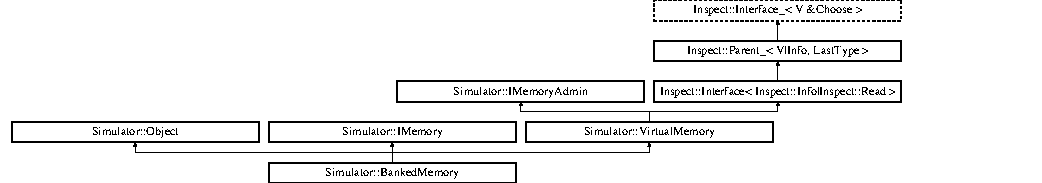
\includegraphics[height=2.456140cm]{class_simulator_1_1_banked_memory}
\end{center}
\end{figure}
\subsection*{Classes}
\begin{DoxyCompactItemize}
\item 
class \hyperlink{class_simulator_1_1_banked_memory_1_1_bank}{Bank}
\item 
struct \hyperlink{struct_simulator_1_1_banked_memory_1_1_client_info}{Client\+Info}
\item 
struct \hyperlink{struct_simulator_1_1_banked_memory_1_1_request}{Request}
\end{DoxyCompactItemize}
\subsection*{Public Member Functions}
\begin{DoxyCompactItemize}
\item 
\hyperlink{class_simulator_1_1_banked_memory_a9e39b89e5156eac508430609c0ce7431}{Banked\+Memory} (const std\+::string \&\hyperlink{mtconf_8c_a8f8f80d37794cde9472343e4487ba3eb}{name}, \hyperlink{class_simulator_1_1_object}{Object} \&parent, \hyperlink{class_simulator_1_1_clock}{Clock} \&clock, \hyperlink{class_config}{Config} \&config, const std\+::string \&default\+Bank\+Selector\+Type)
\item 
\hyperlink{class_simulator_1_1_banked_memory_a1bd4b309f7e1115bab535d2bcad7ab9a}{Banked\+Memory} (const \hyperlink{class_simulator_1_1_banked_memory}{Banked\+Memory} \&)=delete
\item 
\hyperlink{class_simulator_1_1_banked_memory}{Banked\+Memory} \& \hyperlink{class_simulator_1_1_banked_memory_a2cd07d8ecd185069520454ccbb863226}{operator=} (const \hyperlink{class_simulator_1_1_banked_memory}{Banked\+Memory} \&)=delete
\item 
\hyperlink{class_simulator_1_1_banked_memory_a3e6d7eb6e0c0be8c79c07f50be5bb48a}{$\sim$\+Banked\+Memory} ()
\item 
void \hyperlink{class_simulator_1_1_banked_memory_af7759c840b89a7ac6184a8f3de02d8df}{Cmd\+\_\+\+Info} (std\+::ostream \&out, const std\+::vector$<$ std\+::string $>$ \&arguments) const override
\item 
void \hyperlink{class_simulator_1_1_banked_memory_a9cb8bc9b89c13e478e661b8672f79377}{Cmd\+\_\+\+Read} (std\+::ostream \&out, const std\+::vector$<$ std\+::string $>$ \&arguments) const override
\end{DoxyCompactItemize}
\subsection*{Protected Attributes}
\begin{DoxyCompactItemize}
\item 
\hyperlink{class_component_model_registry}{Component\+Model\+Registry} \& \hyperlink{class_simulator_1_1_banked_memory_a5db228870f5f9d6023cc7d6b06af31b9}{m\+\_\+registry}
\item 
\hyperlink{class_simulator_1_1_clock}{Clock} \& \hyperlink{class_simulator_1_1_banked_memory_af6ef3e3fc49d479b727b883185ab303a}{m\+\_\+clock}
\item 
std\+::vector$<$ \hyperlink{struct_simulator_1_1_banked_memory_1_1_client_info}{Client\+Info} $>$ \hyperlink{class_simulator_1_1_banked_memory_a6a910047ff99466efe5dee7b7ec80543}{m\+\_\+clients}
\item 
\hyperlink{class_simulator_1_1_storage_trace_set}{Storage\+Trace\+Set} \hyperlink{class_simulator_1_1_banked_memory_a362c6639b1570b91f696ac5da28c735a}{m\+\_\+storages}
\item 
std\+::vector$<$ \hyperlink{class_simulator_1_1_banked_memory_1_1_bank}{Bank} $\ast$ $>$ \hyperlink{class_simulator_1_1_banked_memory_af0b36c6af11111fc50cbd4316d241b11}{m\+\_\+banks}
\item 
\hyperlink{namespace_simulator_a928f1e2101eba21bb0fe409e8c9ce573}{Cycle\+No} \hyperlink{class_simulator_1_1_banked_memory_aa9790fb4f615ddcf46b83df4a32036c8}{m\+\_\+base\+Request\+Time}
\item 
\hyperlink{namespace_simulator_a928f1e2101eba21bb0fe409e8c9ce573}{Cycle\+No} \hyperlink{class_simulator_1_1_banked_memory_a23e5b01a0d29de297c3137e51c1349c6}{m\+\_\+time\+Per\+Line}
\item 
size\+\_\+t \hyperlink{class_simulator_1_1_banked_memory_aa8f9ecc5e0ee2035c884b95795f5e0a4}{m\+\_\+line\+Size}
\item 
\hyperlink{class_simulator_1_1_i_bank_selector}{I\+Bank\+Selector} $\ast$ \hyperlink{class_simulator_1_1_banked_memory_a4f9e131866f9b27a8b1c628fb3f98427}{m\+\_\+selector}
\item 
uint64\+\_\+t \hyperlink{class_simulator_1_1_banked_memory_a1c2168b2983e4b756a473d1953b8b6a3}{m\+\_\+nreads}
\item 
uint64\+\_\+t \hyperlink{class_simulator_1_1_banked_memory_a92a71a7aaee6d7d0e6dedba3b3264064}{m\+\_\+nread\+\_\+bytes}
\item 
uint64\+\_\+t \hyperlink{class_simulator_1_1_banked_memory_a55d4955b89dc77c553462c9edd8c9d55}{m\+\_\+nwrites}
\item 
uint64\+\_\+t \hyperlink{class_simulator_1_1_banked_memory_aa930c2c5581bc9f8823b940574124c9a}{m\+\_\+nwrite\+\_\+bytes}
\end{DoxyCompactItemize}
\subsection*{Additional Inherited Members}


\subsection{Constructor \& Destructor Documentation}
\hypertarget{class_simulator_1_1_banked_memory_a9e39b89e5156eac508430609c0ce7431}{\index{Simulator\+::\+Banked\+Memory@{Simulator\+::\+Banked\+Memory}!Banked\+Memory@{Banked\+Memory}}
\index{Banked\+Memory@{Banked\+Memory}!Simulator\+::\+Banked\+Memory@{Simulator\+::\+Banked\+Memory}}
\subsubsection[{Banked\+Memory}]{\setlength{\rightskip}{0pt plus 5cm}Simulator\+::\+Banked\+Memory\+::\+Banked\+Memory (
\begin{DoxyParamCaption}
\item[{const std\+::string \&}]{name, }
\item[{{\bf Object} \&}]{parent, }
\item[{{\bf Clock} \&}]{clock, }
\item[{{\bf Config} \&}]{config, }
\item[{const std\+::string \&}]{default\+Bank\+Selector\+Type}
\end{DoxyParamCaption}
)}}\label{class_simulator_1_1_banked_memory_a9e39b89e5156eac508430609c0ce7431}
\hypertarget{class_simulator_1_1_banked_memory_a1bd4b309f7e1115bab535d2bcad7ab9a}{\index{Simulator\+::\+Banked\+Memory@{Simulator\+::\+Banked\+Memory}!Banked\+Memory@{Banked\+Memory}}
\index{Banked\+Memory@{Banked\+Memory}!Simulator\+::\+Banked\+Memory@{Simulator\+::\+Banked\+Memory}}
\subsubsection[{Banked\+Memory}]{\setlength{\rightskip}{0pt plus 5cm}Simulator\+::\+Banked\+Memory\+::\+Banked\+Memory (
\begin{DoxyParamCaption}
\item[{const {\bf Banked\+Memory} \&}]{}
\end{DoxyParamCaption}
)\hspace{0.3cm}{\ttfamily [delete]}}}\label{class_simulator_1_1_banked_memory_a1bd4b309f7e1115bab535d2bcad7ab9a}
\hypertarget{class_simulator_1_1_banked_memory_a3e6d7eb6e0c0be8c79c07f50be5bb48a}{\index{Simulator\+::\+Banked\+Memory@{Simulator\+::\+Banked\+Memory}!````~Banked\+Memory@{$\sim$\+Banked\+Memory}}
\index{````~Banked\+Memory@{$\sim$\+Banked\+Memory}!Simulator\+::\+Banked\+Memory@{Simulator\+::\+Banked\+Memory}}
\subsubsection[{$\sim$\+Banked\+Memory}]{\setlength{\rightskip}{0pt plus 5cm}Simulator\+::\+Banked\+Memory\+::$\sim$\+Banked\+Memory (
\begin{DoxyParamCaption}
{}
\end{DoxyParamCaption}
)}}\label{class_simulator_1_1_banked_memory_a3e6d7eb6e0c0be8c79c07f50be5bb48a}


\subsection{Member Function Documentation}
\hypertarget{class_simulator_1_1_banked_memory_af7759c840b89a7ac6184a8f3de02d8df}{\index{Simulator\+::\+Banked\+Memory@{Simulator\+::\+Banked\+Memory}!Cmd\+\_\+\+Info@{Cmd\+\_\+\+Info}}
\index{Cmd\+\_\+\+Info@{Cmd\+\_\+\+Info}!Simulator\+::\+Banked\+Memory@{Simulator\+::\+Banked\+Memory}}
\subsubsection[{Cmd\+\_\+\+Info}]{\setlength{\rightskip}{0pt plus 5cm}void Simulator\+::\+Banked\+Memory\+::\+Cmd\+\_\+\+Info (
\begin{DoxyParamCaption}
\item[{std\+::ostream \&}]{out, }
\item[{const std\+::vector$<$ std\+::string $>$ \&}]{arguments}
\end{DoxyParamCaption}
) const\hspace{0.3cm}{\ttfamily [override]}}}\label{class_simulator_1_1_banked_memory_af7759c840b89a7ac6184a8f3de02d8df}
\hypertarget{class_simulator_1_1_banked_memory_a9cb8bc9b89c13e478e661b8672f79377}{\index{Simulator\+::\+Banked\+Memory@{Simulator\+::\+Banked\+Memory}!Cmd\+\_\+\+Read@{Cmd\+\_\+\+Read}}
\index{Cmd\+\_\+\+Read@{Cmd\+\_\+\+Read}!Simulator\+::\+Banked\+Memory@{Simulator\+::\+Banked\+Memory}}
\subsubsection[{Cmd\+\_\+\+Read}]{\setlength{\rightskip}{0pt plus 5cm}void Simulator\+::\+Banked\+Memory\+::\+Cmd\+\_\+\+Read (
\begin{DoxyParamCaption}
\item[{std\+::ostream \&}]{out, }
\item[{const std\+::vector$<$ std\+::string $>$ \&}]{arguments}
\end{DoxyParamCaption}
) const\hspace{0.3cm}{\ttfamily [override]}}}\label{class_simulator_1_1_banked_memory_a9cb8bc9b89c13e478e661b8672f79377}
\hypertarget{class_simulator_1_1_banked_memory_a2cd07d8ecd185069520454ccbb863226}{\index{Simulator\+::\+Banked\+Memory@{Simulator\+::\+Banked\+Memory}!operator=@{operator=}}
\index{operator=@{operator=}!Simulator\+::\+Banked\+Memory@{Simulator\+::\+Banked\+Memory}}
\subsubsection[{operator=}]{\setlength{\rightskip}{0pt plus 5cm}{\bf Banked\+Memory}\& Simulator\+::\+Banked\+Memory\+::operator= (
\begin{DoxyParamCaption}
\item[{const {\bf Banked\+Memory} \&}]{}
\end{DoxyParamCaption}
)\hspace{0.3cm}{\ttfamily [delete]}}}\label{class_simulator_1_1_banked_memory_a2cd07d8ecd185069520454ccbb863226}


\subsection{Member Data Documentation}
\hypertarget{class_simulator_1_1_banked_memory_af0b36c6af11111fc50cbd4316d241b11}{\index{Simulator\+::\+Banked\+Memory@{Simulator\+::\+Banked\+Memory}!m\+\_\+banks@{m\+\_\+banks}}
\index{m\+\_\+banks@{m\+\_\+banks}!Simulator\+::\+Banked\+Memory@{Simulator\+::\+Banked\+Memory}}
\subsubsection[{m\+\_\+banks}]{\setlength{\rightskip}{0pt plus 5cm}std\+::vector$<${\bf Bank}$\ast$$>$ Simulator\+::\+Banked\+Memory\+::m\+\_\+banks\hspace{0.3cm}{\ttfamily [protected]}}}\label{class_simulator_1_1_banked_memory_af0b36c6af11111fc50cbd4316d241b11}
\hypertarget{class_simulator_1_1_banked_memory_aa9790fb4f615ddcf46b83df4a32036c8}{\index{Simulator\+::\+Banked\+Memory@{Simulator\+::\+Banked\+Memory}!m\+\_\+base\+Request\+Time@{m\+\_\+base\+Request\+Time}}
\index{m\+\_\+base\+Request\+Time@{m\+\_\+base\+Request\+Time}!Simulator\+::\+Banked\+Memory@{Simulator\+::\+Banked\+Memory}}
\subsubsection[{m\+\_\+base\+Request\+Time}]{\setlength{\rightskip}{0pt plus 5cm}{\bf Cycle\+No} Simulator\+::\+Banked\+Memory\+::m\+\_\+base\+Request\+Time\hspace{0.3cm}{\ttfamily [protected]}}}\label{class_simulator_1_1_banked_memory_aa9790fb4f615ddcf46b83df4a32036c8}
\hypertarget{class_simulator_1_1_banked_memory_a6a910047ff99466efe5dee7b7ec80543}{\index{Simulator\+::\+Banked\+Memory@{Simulator\+::\+Banked\+Memory}!m\+\_\+clients@{m\+\_\+clients}}
\index{m\+\_\+clients@{m\+\_\+clients}!Simulator\+::\+Banked\+Memory@{Simulator\+::\+Banked\+Memory}}
\subsubsection[{m\+\_\+clients}]{\setlength{\rightskip}{0pt plus 5cm}std\+::vector$<${\bf Client\+Info}$>$ Simulator\+::\+Banked\+Memory\+::m\+\_\+clients\hspace{0.3cm}{\ttfamily [protected]}}}\label{class_simulator_1_1_banked_memory_a6a910047ff99466efe5dee7b7ec80543}
\hypertarget{class_simulator_1_1_banked_memory_af6ef3e3fc49d479b727b883185ab303a}{\index{Simulator\+::\+Banked\+Memory@{Simulator\+::\+Banked\+Memory}!m\+\_\+clock@{m\+\_\+clock}}
\index{m\+\_\+clock@{m\+\_\+clock}!Simulator\+::\+Banked\+Memory@{Simulator\+::\+Banked\+Memory}}
\subsubsection[{m\+\_\+clock}]{\setlength{\rightskip}{0pt plus 5cm}{\bf Clock}\& Simulator\+::\+Banked\+Memory\+::m\+\_\+clock\hspace{0.3cm}{\ttfamily [protected]}}}\label{class_simulator_1_1_banked_memory_af6ef3e3fc49d479b727b883185ab303a}
\hypertarget{class_simulator_1_1_banked_memory_aa8f9ecc5e0ee2035c884b95795f5e0a4}{\index{Simulator\+::\+Banked\+Memory@{Simulator\+::\+Banked\+Memory}!m\+\_\+line\+Size@{m\+\_\+line\+Size}}
\index{m\+\_\+line\+Size@{m\+\_\+line\+Size}!Simulator\+::\+Banked\+Memory@{Simulator\+::\+Banked\+Memory}}
\subsubsection[{m\+\_\+line\+Size}]{\setlength{\rightskip}{0pt plus 5cm}size\+\_\+t Simulator\+::\+Banked\+Memory\+::m\+\_\+line\+Size\hspace{0.3cm}{\ttfamily [protected]}}}\label{class_simulator_1_1_banked_memory_aa8f9ecc5e0ee2035c884b95795f5e0a4}
\hypertarget{class_simulator_1_1_banked_memory_a92a71a7aaee6d7d0e6dedba3b3264064}{\index{Simulator\+::\+Banked\+Memory@{Simulator\+::\+Banked\+Memory}!m\+\_\+nread\+\_\+bytes@{m\+\_\+nread\+\_\+bytes}}
\index{m\+\_\+nread\+\_\+bytes@{m\+\_\+nread\+\_\+bytes}!Simulator\+::\+Banked\+Memory@{Simulator\+::\+Banked\+Memory}}
\subsubsection[{m\+\_\+nread\+\_\+bytes}]{\setlength{\rightskip}{0pt plus 5cm}uint64\+\_\+t Simulator\+::\+Banked\+Memory\+::m\+\_\+nread\+\_\+bytes\hspace{0.3cm}{\ttfamily [protected]}}}\label{class_simulator_1_1_banked_memory_a92a71a7aaee6d7d0e6dedba3b3264064}
\hypertarget{class_simulator_1_1_banked_memory_a1c2168b2983e4b756a473d1953b8b6a3}{\index{Simulator\+::\+Banked\+Memory@{Simulator\+::\+Banked\+Memory}!m\+\_\+nreads@{m\+\_\+nreads}}
\index{m\+\_\+nreads@{m\+\_\+nreads}!Simulator\+::\+Banked\+Memory@{Simulator\+::\+Banked\+Memory}}
\subsubsection[{m\+\_\+nreads}]{\setlength{\rightskip}{0pt plus 5cm}uint64\+\_\+t Simulator\+::\+Banked\+Memory\+::m\+\_\+nreads\hspace{0.3cm}{\ttfamily [protected]}}}\label{class_simulator_1_1_banked_memory_a1c2168b2983e4b756a473d1953b8b6a3}
\hypertarget{class_simulator_1_1_banked_memory_aa930c2c5581bc9f8823b940574124c9a}{\index{Simulator\+::\+Banked\+Memory@{Simulator\+::\+Banked\+Memory}!m\+\_\+nwrite\+\_\+bytes@{m\+\_\+nwrite\+\_\+bytes}}
\index{m\+\_\+nwrite\+\_\+bytes@{m\+\_\+nwrite\+\_\+bytes}!Simulator\+::\+Banked\+Memory@{Simulator\+::\+Banked\+Memory}}
\subsubsection[{m\+\_\+nwrite\+\_\+bytes}]{\setlength{\rightskip}{0pt plus 5cm}uint64\+\_\+t Simulator\+::\+Banked\+Memory\+::m\+\_\+nwrite\+\_\+bytes\hspace{0.3cm}{\ttfamily [protected]}}}\label{class_simulator_1_1_banked_memory_aa930c2c5581bc9f8823b940574124c9a}
\hypertarget{class_simulator_1_1_banked_memory_a55d4955b89dc77c553462c9edd8c9d55}{\index{Simulator\+::\+Banked\+Memory@{Simulator\+::\+Banked\+Memory}!m\+\_\+nwrites@{m\+\_\+nwrites}}
\index{m\+\_\+nwrites@{m\+\_\+nwrites}!Simulator\+::\+Banked\+Memory@{Simulator\+::\+Banked\+Memory}}
\subsubsection[{m\+\_\+nwrites}]{\setlength{\rightskip}{0pt plus 5cm}uint64\+\_\+t Simulator\+::\+Banked\+Memory\+::m\+\_\+nwrites\hspace{0.3cm}{\ttfamily [protected]}}}\label{class_simulator_1_1_banked_memory_a55d4955b89dc77c553462c9edd8c9d55}
\hypertarget{class_simulator_1_1_banked_memory_a5db228870f5f9d6023cc7d6b06af31b9}{\index{Simulator\+::\+Banked\+Memory@{Simulator\+::\+Banked\+Memory}!m\+\_\+registry@{m\+\_\+registry}}
\index{m\+\_\+registry@{m\+\_\+registry}!Simulator\+::\+Banked\+Memory@{Simulator\+::\+Banked\+Memory}}
\subsubsection[{m\+\_\+registry}]{\setlength{\rightskip}{0pt plus 5cm}{\bf Component\+Model\+Registry}\& Simulator\+::\+Banked\+Memory\+::m\+\_\+registry\hspace{0.3cm}{\ttfamily [protected]}}}\label{class_simulator_1_1_banked_memory_a5db228870f5f9d6023cc7d6b06af31b9}
\hypertarget{class_simulator_1_1_banked_memory_a4f9e131866f9b27a8b1c628fb3f98427}{\index{Simulator\+::\+Banked\+Memory@{Simulator\+::\+Banked\+Memory}!m\+\_\+selector@{m\+\_\+selector}}
\index{m\+\_\+selector@{m\+\_\+selector}!Simulator\+::\+Banked\+Memory@{Simulator\+::\+Banked\+Memory}}
\subsubsection[{m\+\_\+selector}]{\setlength{\rightskip}{0pt plus 5cm}{\bf I\+Bank\+Selector}$\ast$ Simulator\+::\+Banked\+Memory\+::m\+\_\+selector\hspace{0.3cm}{\ttfamily [protected]}}}\label{class_simulator_1_1_banked_memory_a4f9e131866f9b27a8b1c628fb3f98427}
\hypertarget{class_simulator_1_1_banked_memory_a362c6639b1570b91f696ac5da28c735a}{\index{Simulator\+::\+Banked\+Memory@{Simulator\+::\+Banked\+Memory}!m\+\_\+storages@{m\+\_\+storages}}
\index{m\+\_\+storages@{m\+\_\+storages}!Simulator\+::\+Banked\+Memory@{Simulator\+::\+Banked\+Memory}}
\subsubsection[{m\+\_\+storages}]{\setlength{\rightskip}{0pt plus 5cm}{\bf Storage\+Trace\+Set} Simulator\+::\+Banked\+Memory\+::m\+\_\+storages\hspace{0.3cm}{\ttfamily [protected]}}}\label{class_simulator_1_1_banked_memory_a362c6639b1570b91f696ac5da28c735a}
\hypertarget{class_simulator_1_1_banked_memory_a23e5b01a0d29de297c3137e51c1349c6}{\index{Simulator\+::\+Banked\+Memory@{Simulator\+::\+Banked\+Memory}!m\+\_\+time\+Per\+Line@{m\+\_\+time\+Per\+Line}}
\index{m\+\_\+time\+Per\+Line@{m\+\_\+time\+Per\+Line}!Simulator\+::\+Banked\+Memory@{Simulator\+::\+Banked\+Memory}}
\subsubsection[{m\+\_\+time\+Per\+Line}]{\setlength{\rightskip}{0pt plus 5cm}{\bf Cycle\+No} Simulator\+::\+Banked\+Memory\+::m\+\_\+time\+Per\+Line\hspace{0.3cm}{\ttfamily [protected]}}}\label{class_simulator_1_1_banked_memory_a23e5b01a0d29de297c3137e51c1349c6}


The documentation for this class was generated from the following files\+:\begin{DoxyCompactItemize}
\item 
arch/mem/\hyperlink{_banked_memory_8h}{Banked\+Memory.\+h}\item 
arch/mem/\hyperlink{_banked_memory_8cpp}{Banked\+Memory.\+cpp}\end{DoxyCompactItemize}

\hypertarget{class_binary_sampler}{\section{Binary\+Sampler Class Reference}
\label{class_binary_sampler}\index{Binary\+Sampler@{Binary\+Sampler}}
}


{\ttfamily \#include $<$sampling.\+h$>$}

\subsection*{Public Member Functions}
\begin{DoxyCompactItemize}
\item 
\hyperlink{class_binary_sampler_a5403be8e6ef77d12ab901fc169143052}{Binary\+Sampler} (std\+::ostream \&os, const \hyperlink{class_config}{Config} \&config, const std\+::vector$<$ std\+::string $>$ \&pats)
\item 
size\+\_\+t \hyperlink{class_binary_sampler_a4e94089a6186b9ca51d3092fa9383209}{Get\+Buffer\+Size} () const 
\item 
void \hyperlink{class_binary_sampler_a78fab94d5f122b110043eb955d56b825}{Sample\+To\+Buffer} (char $\ast$\hyperlink{io_8c_ae8388ac87b56ebf19ede02bf4edaa1e9}{buf}) const 
\end{DoxyCompactItemize}


\subsection{Constructor \& Destructor Documentation}
\hypertarget{class_binary_sampler_a5403be8e6ef77d12ab901fc169143052}{\index{Binary\+Sampler@{Binary\+Sampler}!Binary\+Sampler@{Binary\+Sampler}}
\index{Binary\+Sampler@{Binary\+Sampler}!Binary\+Sampler@{Binary\+Sampler}}
\subsubsection[{Binary\+Sampler}]{\setlength{\rightskip}{0pt plus 5cm}Binary\+Sampler\+::\+Binary\+Sampler (
\begin{DoxyParamCaption}
\item[{std\+::ostream \&}]{os, }
\item[{const {\bf Config} \&}]{config, }
\item[{const std\+::vector$<$ std\+::string $>$ \&}]{pats}
\end{DoxyParamCaption}
)}}\label{class_binary_sampler_a5403be8e6ef77d12ab901fc169143052}


\subsection{Member Function Documentation}
\hypertarget{class_binary_sampler_a4e94089a6186b9ca51d3092fa9383209}{\index{Binary\+Sampler@{Binary\+Sampler}!Get\+Buffer\+Size@{Get\+Buffer\+Size}}
\index{Get\+Buffer\+Size@{Get\+Buffer\+Size}!Binary\+Sampler@{Binary\+Sampler}}
\subsubsection[{Get\+Buffer\+Size}]{\setlength{\rightskip}{0pt plus 5cm}size\+\_\+t Binary\+Sampler\+::\+Get\+Buffer\+Size (
\begin{DoxyParamCaption}
{}
\end{DoxyParamCaption}
) const\hspace{0.3cm}{\ttfamily [inline]}}}\label{class_binary_sampler_a4e94089a6186b9ca51d3092fa9383209}
\hypertarget{class_binary_sampler_a78fab94d5f122b110043eb955d56b825}{\index{Binary\+Sampler@{Binary\+Sampler}!Sample\+To\+Buffer@{Sample\+To\+Buffer}}
\index{Sample\+To\+Buffer@{Sample\+To\+Buffer}!Binary\+Sampler@{Binary\+Sampler}}
\subsubsection[{Sample\+To\+Buffer}]{\setlength{\rightskip}{0pt plus 5cm}void Binary\+Sampler\+::\+Sample\+To\+Buffer (
\begin{DoxyParamCaption}
\item[{char $\ast$}]{buf}
\end{DoxyParamCaption}
) const\hspace{0.3cm}{\ttfamily [inline]}}}\label{class_binary_sampler_a78fab94d5f122b110043eb955d56b825}


The documentation for this class was generated from the following files\+:\begin{DoxyCompactItemize}
\item 
sim/\hyperlink{sampling_8h}{sampling.\+h}\item 
sim/\hyperlink{sampling_8cpp}{sampling.\+cpp}\end{DoxyCompactItemize}

\hypertarget{struct_simulator_1_1_virtual_memory_1_1_block}{\section{Simulator\+:\+:Virtual\+Memory\+:\+:Block Struct Reference}
\label{struct_simulator_1_1_virtual_memory_1_1_block}\index{Simulator\+::\+Virtual\+Memory\+::\+Block@{Simulator\+::\+Virtual\+Memory\+::\+Block}}
}


{\ttfamily \#include $<$Virtual\+Memory.\+h$>$}

\subsection*{Public Attributes}
\begin{DoxyCompactItemize}
\item 
char \hyperlink{struct_simulator_1_1_virtual_memory_1_1_block_a1094eb796a623c4af0fb66363db171f1}{data} \mbox{[}\hyperlink{class_simulator_1_1_virtual_memory_a84e20b875917ceb9a44d32cfb2d59246}{B\+L\+O\+C\+K\+\_\+\+S\+I\+Z\+E}\mbox{]}
\end{DoxyCompactItemize}


\subsection{Member Data Documentation}
\hypertarget{struct_simulator_1_1_virtual_memory_1_1_block_a1094eb796a623c4af0fb66363db171f1}{\index{Simulator\+::\+Virtual\+Memory\+::\+Block@{Simulator\+::\+Virtual\+Memory\+::\+Block}!data@{data}}
\index{data@{data}!Simulator\+::\+Virtual\+Memory\+::\+Block@{Simulator\+::\+Virtual\+Memory\+::\+Block}}
\subsubsection[{data}]{\setlength{\rightskip}{0pt plus 5cm}char Simulator\+::\+Virtual\+Memory\+::\+Block\+::data\mbox{[}{\bf B\+L\+O\+C\+K\+\_\+\+S\+I\+Z\+E}\mbox{]}}}\label{struct_simulator_1_1_virtual_memory_1_1_block_a1094eb796a623c4af0fb66363db171f1}


The documentation for this struct was generated from the following file\+:\begin{DoxyCompactItemize}
\item 
arch/\hyperlink{_virtual_memory_8h}{Virtual\+Memory.\+h}\end{DoxyCompactItemize}

\hypertarget{class_simulator_1_1_break_point_manager}{\section{Simulator\+:\+:Break\+Point\+Manager Class Reference}
\label{class_simulator_1_1_break_point_manager}\index{Simulator\+::\+Break\+Point\+Manager@{Simulator\+::\+Break\+Point\+Manager}}
}


{\ttfamily \#include $<$breakpoints.\+h$>$}

\subsection*{Public Types}
\begin{DoxyCompactItemize}
\item 
enum \hyperlink{class_simulator_1_1_break_point_manager_a425072fcb3c0e59e3fb6f300d6afbd7b}{Break\+Point\+Type} \{ \\*
\hyperlink{class_simulator_1_1_break_point_manager_a425072fcb3c0e59e3fb6f300d6afbd7baccb2fb913155b4416bf8f54adbc79c97}{F\+E\+T\+C\+H} = 1, 
\hyperlink{class_simulator_1_1_break_point_manager_a425072fcb3c0e59e3fb6f300d6afbd7ba22cfe04247cd5846d978d8ad19755ec4}{E\+X\+E\+C} = 2, 
\hyperlink{class_simulator_1_1_break_point_manager_a425072fcb3c0e59e3fb6f300d6afbd7ba7c5132b18f18695faa853ee1bd089b19}{M\+E\+M\+R\+E\+A\+D} = 4, 
\hyperlink{class_simulator_1_1_break_point_manager_a425072fcb3c0e59e3fb6f300d6afbd7baed5743529528d4fef1fe3202e9ad7aeb}{M\+E\+M\+W\+R\+I\+T\+E} = 8, 
\\*
\hyperlink{class_simulator_1_1_break_point_manager_a425072fcb3c0e59e3fb6f300d6afbd7ba55258c41764b4331fd275e45b178e464}{T\+R\+A\+C\+E\+O\+N\+L\+Y} = 16
 \}
\end{DoxyCompactItemize}
\subsection*{Public Member Functions}
\begin{DoxyCompactItemize}
\item 
\hyperlink{class_simulator_1_1_break_point_manager_aca59f29e711bdc9bd94779d66d8c31db}{Break\+Point\+Manager} (\hyperlink{class_simulator_1_1_kernel}{Simulator\+::\+Kernel} \&kernel, \hyperlink{class_simulator_1_1_symbol_table}{Symbol\+Table} $\ast$symtable=0)
\item 
\hyperlink{class_simulator_1_1_break_point_manager_a63e7c321d4be88b6592d66eb87e4bd7d}{Break\+Point\+Manager} (const \hyperlink{class_simulator_1_1_break_point_manager}{Break\+Point\+Manager} \&other)
\item 
\hyperlink{class_simulator_1_1_break_point_manager}{Break\+Point\+Manager} \& \hyperlink{class_simulator_1_1_break_point_manager_a9bc83b7fec833a21bcc68f93b3f3c591}{operator=} (const \hyperlink{class_simulator_1_1_break_point_manager}{Break\+Point\+Manager} \&other)=delete
\item 
void \hyperlink{class_simulator_1_1_break_point_manager_a829d4497ea561c68acfade511c84a20b}{Enable\+Check} (void)
\item 
void \hyperlink{class_simulator_1_1_break_point_manager_ac9a420fe4c73465899c35a59bf2f6719}{Disable\+Check} (void)
\item 
void \hyperlink{class_simulator_1_1_break_point_manager_af5a8762aeb09e3da6365cee32255ecd2}{Enable\+Break\+Point} (unsigned \hyperlink{mtconf_8c_aa3185401f04d30bd505daebf48c39cc5}{id})
\item 
void \hyperlink{class_simulator_1_1_break_point_manager_a03cc25e048450a65df43303e046c3011}{Disable\+Break\+Point} (unsigned \hyperlink{mtconf_8c_aa3185401f04d30bd505daebf48c39cc5}{id})
\item 
void \hyperlink{class_simulator_1_1_break_point_manager_a9960fe716c6474b4e7a43b254ed1faee}{Delete\+Break\+Point} (unsigned \hyperlink{mtconf_8c_aa3185401f04d30bd505daebf48c39cc5}{id})
\item 
void \hyperlink{class_simulator_1_1_break_point_manager_a9f1e6e644de80d7bba2a66551dda6aac}{Add\+Break\+Point} (Simulator\+::\+Mem\+Addr addr, int type=\hyperlink{class_simulator_1_1_break_point_manager_a425072fcb3c0e59e3fb6f300d6afbd7ba22cfe04247cd5846d978d8ad19755ec4}{E\+X\+E\+C})
\item 
void \hyperlink{class_simulator_1_1_break_point_manager_a7d67935bd2646d51307963bcb48163b3}{Add\+Break\+Point} (const std\+::string \&sym, int offset, int type=\hyperlink{class_simulator_1_1_break_point_manager_a425072fcb3c0e59e3fb6f300d6afbd7ba22cfe04247cd5846d978d8ad19755ec4}{E\+X\+E\+C})
\item 
void \hyperlink{class_simulator_1_1_break_point_manager_abfcda8bf0a03060188c3a491a9000553}{Clear\+All\+Break\+Points} (void)
\item 
void \hyperlink{class_simulator_1_1_break_point_manager_a1c5874f7b1b33a65feabb8b50270f72c}{List\+Break\+Points} (std\+::ostream \&out) const 
\item 
void \hyperlink{class_simulator_1_1_break_point_manager_a6c8fece4f41fff6618d40e09cd56a381}{Resume} (void)
\item 
void \hyperlink{class_simulator_1_1_break_point_manager_a6ede48c906f70b4ba107b62f1d3a2222}{Report\+Breaks} (std\+::ostream \&out) const 
\item 
bool \hyperlink{class_simulator_1_1_break_point_manager_a5748b6f13c95438ab197c4709b9c5db0}{New\+Breaks\+Detected} (void) const 
\item 
void \hyperlink{class_simulator_1_1_break_point_manager_a33bf787698426b649ffb4ab7aaad727e}{Check} (int type, Simulator\+::\+Mem\+Addr addr, \hyperlink{class_simulator_1_1_object}{Simulator\+::\+Object} \&obj)
\item 
void \hyperlink{class_simulator_1_1_break_point_manager_a173d134ed8cb70c53823f9e423773d4d}{Set\+Symbol\+Table} (\hyperlink{class_simulator_1_1_symbol_table}{Symbol\+Table} \&symtable)
\item 
\hyperlink{class_simulator_1_1_symbol_table}{Symbol\+Table} \& \hyperlink{class_simulator_1_1_break_point_manager_ae2242fce958d0394560440b12fac45d3}{Get\+Symbol\+Table} () const 
\end{DoxyCompactItemize}


\subsection{Member Enumeration Documentation}
\hypertarget{class_simulator_1_1_break_point_manager_a425072fcb3c0e59e3fb6f300d6afbd7b}{\index{Simulator\+::\+Break\+Point\+Manager@{Simulator\+::\+Break\+Point\+Manager}!Break\+Point\+Type@{Break\+Point\+Type}}
\index{Break\+Point\+Type@{Break\+Point\+Type}!Simulator\+::\+Break\+Point\+Manager@{Simulator\+::\+Break\+Point\+Manager}}
\subsubsection[{Break\+Point\+Type}]{\setlength{\rightskip}{0pt plus 5cm}enum {\bf Simulator\+::\+Break\+Point\+Manager\+::\+Break\+Point\+Type}}}\label{class_simulator_1_1_break_point_manager_a425072fcb3c0e59e3fb6f300d6afbd7b}
\begin{Desc}
\item[Enumerator]\par
\begin{description}
\index{F\+E\+T\+C\+H@{F\+E\+T\+C\+H}!Simulator\+::\+Break\+Point\+Manager@{Simulator\+::\+Break\+Point\+Manager}}\index{Simulator\+::\+Break\+Point\+Manager@{Simulator\+::\+Break\+Point\+Manager}!F\+E\+T\+C\+H@{F\+E\+T\+C\+H}}\item[{\em 
\hypertarget{class_simulator_1_1_break_point_manager_a425072fcb3c0e59e3fb6f300d6afbd7baccb2fb913155b4416bf8f54adbc79c97}{F\+E\+T\+C\+H}\label{class_simulator_1_1_break_point_manager_a425072fcb3c0e59e3fb6f300d6afbd7baccb2fb913155b4416bf8f54adbc79c97}
}]\index{E\+X\+E\+C@{E\+X\+E\+C}!Simulator\+::\+Break\+Point\+Manager@{Simulator\+::\+Break\+Point\+Manager}}\index{Simulator\+::\+Break\+Point\+Manager@{Simulator\+::\+Break\+Point\+Manager}!E\+X\+E\+C@{E\+X\+E\+C}}\item[{\em 
\hypertarget{class_simulator_1_1_break_point_manager_a425072fcb3c0e59e3fb6f300d6afbd7ba22cfe04247cd5846d978d8ad19755ec4}{E\+X\+E\+C}\label{class_simulator_1_1_break_point_manager_a425072fcb3c0e59e3fb6f300d6afbd7ba22cfe04247cd5846d978d8ad19755ec4}
}]\index{M\+E\+M\+R\+E\+A\+D@{M\+E\+M\+R\+E\+A\+D}!Simulator\+::\+Break\+Point\+Manager@{Simulator\+::\+Break\+Point\+Manager}}\index{Simulator\+::\+Break\+Point\+Manager@{Simulator\+::\+Break\+Point\+Manager}!M\+E\+M\+R\+E\+A\+D@{M\+E\+M\+R\+E\+A\+D}}\item[{\em 
\hypertarget{class_simulator_1_1_break_point_manager_a425072fcb3c0e59e3fb6f300d6afbd7ba7c5132b18f18695faa853ee1bd089b19}{M\+E\+M\+R\+E\+A\+D}\label{class_simulator_1_1_break_point_manager_a425072fcb3c0e59e3fb6f300d6afbd7ba7c5132b18f18695faa853ee1bd089b19}
}]\index{M\+E\+M\+W\+R\+I\+T\+E@{M\+E\+M\+W\+R\+I\+T\+E}!Simulator\+::\+Break\+Point\+Manager@{Simulator\+::\+Break\+Point\+Manager}}\index{Simulator\+::\+Break\+Point\+Manager@{Simulator\+::\+Break\+Point\+Manager}!M\+E\+M\+W\+R\+I\+T\+E@{M\+E\+M\+W\+R\+I\+T\+E}}\item[{\em 
\hypertarget{class_simulator_1_1_break_point_manager_a425072fcb3c0e59e3fb6f300d6afbd7baed5743529528d4fef1fe3202e9ad7aeb}{M\+E\+M\+W\+R\+I\+T\+E}\label{class_simulator_1_1_break_point_manager_a425072fcb3c0e59e3fb6f300d6afbd7baed5743529528d4fef1fe3202e9ad7aeb}
}]\index{T\+R\+A\+C\+E\+O\+N\+L\+Y@{T\+R\+A\+C\+E\+O\+N\+L\+Y}!Simulator\+::\+Break\+Point\+Manager@{Simulator\+::\+Break\+Point\+Manager}}\index{Simulator\+::\+Break\+Point\+Manager@{Simulator\+::\+Break\+Point\+Manager}!T\+R\+A\+C\+E\+O\+N\+L\+Y@{T\+R\+A\+C\+E\+O\+N\+L\+Y}}\item[{\em 
\hypertarget{class_simulator_1_1_break_point_manager_a425072fcb3c0e59e3fb6f300d6afbd7ba55258c41764b4331fd275e45b178e464}{T\+R\+A\+C\+E\+O\+N\+L\+Y}\label{class_simulator_1_1_break_point_manager_a425072fcb3c0e59e3fb6f300d6afbd7ba55258c41764b4331fd275e45b178e464}
}]\end{description}
\end{Desc}


\subsection{Constructor \& Destructor Documentation}
\hypertarget{class_simulator_1_1_break_point_manager_aca59f29e711bdc9bd94779d66d8c31db}{\index{Simulator\+::\+Break\+Point\+Manager@{Simulator\+::\+Break\+Point\+Manager}!Break\+Point\+Manager@{Break\+Point\+Manager}}
\index{Break\+Point\+Manager@{Break\+Point\+Manager}!Simulator\+::\+Break\+Point\+Manager@{Simulator\+::\+Break\+Point\+Manager}}
\subsubsection[{Break\+Point\+Manager}]{\setlength{\rightskip}{0pt plus 5cm}Simulator\+::\+Break\+Point\+Manager\+::\+Break\+Point\+Manager (
\begin{DoxyParamCaption}
\item[{{\bf Simulator\+::\+Kernel} \&}]{kernel, }
\item[{{\bf Symbol\+Table} $\ast$}]{symtable = {\ttfamily 0}}
\end{DoxyParamCaption}
)\hspace{0.3cm}{\ttfamily [inline]}}}\label{class_simulator_1_1_break_point_manager_aca59f29e711bdc9bd94779d66d8c31db}
\hypertarget{class_simulator_1_1_break_point_manager_a63e7c321d4be88b6592d66eb87e4bd7d}{\index{Simulator\+::\+Break\+Point\+Manager@{Simulator\+::\+Break\+Point\+Manager}!Break\+Point\+Manager@{Break\+Point\+Manager}}
\index{Break\+Point\+Manager@{Break\+Point\+Manager}!Simulator\+::\+Break\+Point\+Manager@{Simulator\+::\+Break\+Point\+Manager}}
\subsubsection[{Break\+Point\+Manager}]{\setlength{\rightskip}{0pt plus 5cm}Simulator\+::\+Break\+Point\+Manager\+::\+Break\+Point\+Manager (
\begin{DoxyParamCaption}
\item[{const {\bf Break\+Point\+Manager} \&}]{other}
\end{DoxyParamCaption}
)\hspace{0.3cm}{\ttfamily [inline]}}}\label{class_simulator_1_1_break_point_manager_a63e7c321d4be88b6592d66eb87e4bd7d}


\subsection{Member Function Documentation}
\hypertarget{class_simulator_1_1_break_point_manager_a9f1e6e644de80d7bba2a66551dda6aac}{\index{Simulator\+::\+Break\+Point\+Manager@{Simulator\+::\+Break\+Point\+Manager}!Add\+Break\+Point@{Add\+Break\+Point}}
\index{Add\+Break\+Point@{Add\+Break\+Point}!Simulator\+::\+Break\+Point\+Manager@{Simulator\+::\+Break\+Point\+Manager}}
\subsubsection[{Add\+Break\+Point}]{\setlength{\rightskip}{0pt plus 5cm}void Simulator\+::\+Break\+Point\+Manager\+::\+Add\+Break\+Point (
\begin{DoxyParamCaption}
\item[{Simulator\+::\+Mem\+Addr}]{addr, }
\item[{int}]{type = {\ttfamily {\bf E\+X\+E\+C}}}
\end{DoxyParamCaption}
)}}\label{class_simulator_1_1_break_point_manager_a9f1e6e644de80d7bba2a66551dda6aac}
\hypertarget{class_simulator_1_1_break_point_manager_a7d67935bd2646d51307963bcb48163b3}{\index{Simulator\+::\+Break\+Point\+Manager@{Simulator\+::\+Break\+Point\+Manager}!Add\+Break\+Point@{Add\+Break\+Point}}
\index{Add\+Break\+Point@{Add\+Break\+Point}!Simulator\+::\+Break\+Point\+Manager@{Simulator\+::\+Break\+Point\+Manager}}
\subsubsection[{Add\+Break\+Point}]{\setlength{\rightskip}{0pt plus 5cm}void Simulator\+::\+Break\+Point\+Manager\+::\+Add\+Break\+Point (
\begin{DoxyParamCaption}
\item[{const std\+::string \&}]{sym, }
\item[{int}]{offset, }
\item[{int}]{type = {\ttfamily {\bf E\+X\+E\+C}}}
\end{DoxyParamCaption}
)}}\label{class_simulator_1_1_break_point_manager_a7d67935bd2646d51307963bcb48163b3}
\hypertarget{class_simulator_1_1_break_point_manager_a33bf787698426b649ffb4ab7aaad727e}{\index{Simulator\+::\+Break\+Point\+Manager@{Simulator\+::\+Break\+Point\+Manager}!Check@{Check}}
\index{Check@{Check}!Simulator\+::\+Break\+Point\+Manager@{Simulator\+::\+Break\+Point\+Manager}}
\subsubsection[{Check}]{\setlength{\rightskip}{0pt plus 5cm}void Simulator\+::\+Break\+Point\+Manager\+::\+Check (
\begin{DoxyParamCaption}
\item[{int}]{type, }
\item[{Simulator\+::\+Mem\+Addr}]{addr, }
\item[{{\bf Simulator\+::\+Object} \&}]{obj}
\end{DoxyParamCaption}
)\hspace{0.3cm}{\ttfamily [inline]}}}\label{class_simulator_1_1_break_point_manager_a33bf787698426b649ffb4ab7aaad727e}
\hypertarget{class_simulator_1_1_break_point_manager_abfcda8bf0a03060188c3a491a9000553}{\index{Simulator\+::\+Break\+Point\+Manager@{Simulator\+::\+Break\+Point\+Manager}!Clear\+All\+Break\+Points@{Clear\+All\+Break\+Points}}
\index{Clear\+All\+Break\+Points@{Clear\+All\+Break\+Points}!Simulator\+::\+Break\+Point\+Manager@{Simulator\+::\+Break\+Point\+Manager}}
\subsubsection[{Clear\+All\+Break\+Points}]{\setlength{\rightskip}{0pt plus 5cm}void Simulator\+::\+Break\+Point\+Manager\+::\+Clear\+All\+Break\+Points (
\begin{DoxyParamCaption}
\item[{void}]{}
\end{DoxyParamCaption}
)}}\label{class_simulator_1_1_break_point_manager_abfcda8bf0a03060188c3a491a9000553}
\hypertarget{class_simulator_1_1_break_point_manager_a9960fe716c6474b4e7a43b254ed1faee}{\index{Simulator\+::\+Break\+Point\+Manager@{Simulator\+::\+Break\+Point\+Manager}!Delete\+Break\+Point@{Delete\+Break\+Point}}
\index{Delete\+Break\+Point@{Delete\+Break\+Point}!Simulator\+::\+Break\+Point\+Manager@{Simulator\+::\+Break\+Point\+Manager}}
\subsubsection[{Delete\+Break\+Point}]{\setlength{\rightskip}{0pt plus 5cm}void Simulator\+::\+Break\+Point\+Manager\+::\+Delete\+Break\+Point (
\begin{DoxyParamCaption}
\item[{unsigned}]{id}
\end{DoxyParamCaption}
)}}\label{class_simulator_1_1_break_point_manager_a9960fe716c6474b4e7a43b254ed1faee}
\hypertarget{class_simulator_1_1_break_point_manager_a03cc25e048450a65df43303e046c3011}{\index{Simulator\+::\+Break\+Point\+Manager@{Simulator\+::\+Break\+Point\+Manager}!Disable\+Break\+Point@{Disable\+Break\+Point}}
\index{Disable\+Break\+Point@{Disable\+Break\+Point}!Simulator\+::\+Break\+Point\+Manager@{Simulator\+::\+Break\+Point\+Manager}}
\subsubsection[{Disable\+Break\+Point}]{\setlength{\rightskip}{0pt plus 5cm}void Simulator\+::\+Break\+Point\+Manager\+::\+Disable\+Break\+Point (
\begin{DoxyParamCaption}
\item[{unsigned}]{id}
\end{DoxyParamCaption}
)}}\label{class_simulator_1_1_break_point_manager_a03cc25e048450a65df43303e046c3011}
\hypertarget{class_simulator_1_1_break_point_manager_ac9a420fe4c73465899c35a59bf2f6719}{\index{Simulator\+::\+Break\+Point\+Manager@{Simulator\+::\+Break\+Point\+Manager}!Disable\+Check@{Disable\+Check}}
\index{Disable\+Check@{Disable\+Check}!Simulator\+::\+Break\+Point\+Manager@{Simulator\+::\+Break\+Point\+Manager}}
\subsubsection[{Disable\+Check}]{\setlength{\rightskip}{0pt plus 5cm}void Simulator\+::\+Break\+Point\+Manager\+::\+Disable\+Check (
\begin{DoxyParamCaption}
\item[{void}]{}
\end{DoxyParamCaption}
)\hspace{0.3cm}{\ttfamily [inline]}}}\label{class_simulator_1_1_break_point_manager_ac9a420fe4c73465899c35a59bf2f6719}
\hypertarget{class_simulator_1_1_break_point_manager_af5a8762aeb09e3da6365cee32255ecd2}{\index{Simulator\+::\+Break\+Point\+Manager@{Simulator\+::\+Break\+Point\+Manager}!Enable\+Break\+Point@{Enable\+Break\+Point}}
\index{Enable\+Break\+Point@{Enable\+Break\+Point}!Simulator\+::\+Break\+Point\+Manager@{Simulator\+::\+Break\+Point\+Manager}}
\subsubsection[{Enable\+Break\+Point}]{\setlength{\rightskip}{0pt plus 5cm}void Simulator\+::\+Break\+Point\+Manager\+::\+Enable\+Break\+Point (
\begin{DoxyParamCaption}
\item[{unsigned}]{id}
\end{DoxyParamCaption}
)}}\label{class_simulator_1_1_break_point_manager_af5a8762aeb09e3da6365cee32255ecd2}
\hypertarget{class_simulator_1_1_break_point_manager_a829d4497ea561c68acfade511c84a20b}{\index{Simulator\+::\+Break\+Point\+Manager@{Simulator\+::\+Break\+Point\+Manager}!Enable\+Check@{Enable\+Check}}
\index{Enable\+Check@{Enable\+Check}!Simulator\+::\+Break\+Point\+Manager@{Simulator\+::\+Break\+Point\+Manager}}
\subsubsection[{Enable\+Check}]{\setlength{\rightskip}{0pt plus 5cm}void Simulator\+::\+Break\+Point\+Manager\+::\+Enable\+Check (
\begin{DoxyParamCaption}
\item[{void}]{}
\end{DoxyParamCaption}
)\hspace{0.3cm}{\ttfamily [inline]}}}\label{class_simulator_1_1_break_point_manager_a829d4497ea561c68acfade511c84a20b}
\hypertarget{class_simulator_1_1_break_point_manager_ae2242fce958d0394560440b12fac45d3}{\index{Simulator\+::\+Break\+Point\+Manager@{Simulator\+::\+Break\+Point\+Manager}!Get\+Symbol\+Table@{Get\+Symbol\+Table}}
\index{Get\+Symbol\+Table@{Get\+Symbol\+Table}!Simulator\+::\+Break\+Point\+Manager@{Simulator\+::\+Break\+Point\+Manager}}
\subsubsection[{Get\+Symbol\+Table}]{\setlength{\rightskip}{0pt plus 5cm}{\bf Symbol\+Table}\& Simulator\+::\+Break\+Point\+Manager\+::\+Get\+Symbol\+Table (
\begin{DoxyParamCaption}
{}
\end{DoxyParamCaption}
) const\hspace{0.3cm}{\ttfamily [inline]}}}\label{class_simulator_1_1_break_point_manager_ae2242fce958d0394560440b12fac45d3}
\hypertarget{class_simulator_1_1_break_point_manager_a1c5874f7b1b33a65feabb8b50270f72c}{\index{Simulator\+::\+Break\+Point\+Manager@{Simulator\+::\+Break\+Point\+Manager}!List\+Break\+Points@{List\+Break\+Points}}
\index{List\+Break\+Points@{List\+Break\+Points}!Simulator\+::\+Break\+Point\+Manager@{Simulator\+::\+Break\+Point\+Manager}}
\subsubsection[{List\+Break\+Points}]{\setlength{\rightskip}{0pt plus 5cm}void Simulator\+::\+Break\+Point\+Manager\+::\+List\+Break\+Points (
\begin{DoxyParamCaption}
\item[{std\+::ostream \&}]{out}
\end{DoxyParamCaption}
) const}}\label{class_simulator_1_1_break_point_manager_a1c5874f7b1b33a65feabb8b50270f72c}
\hypertarget{class_simulator_1_1_break_point_manager_a5748b6f13c95438ab197c4709b9c5db0}{\index{Simulator\+::\+Break\+Point\+Manager@{Simulator\+::\+Break\+Point\+Manager}!New\+Breaks\+Detected@{New\+Breaks\+Detected}}
\index{New\+Breaks\+Detected@{New\+Breaks\+Detected}!Simulator\+::\+Break\+Point\+Manager@{Simulator\+::\+Break\+Point\+Manager}}
\subsubsection[{New\+Breaks\+Detected}]{\setlength{\rightskip}{0pt plus 5cm}bool Simulator\+::\+Break\+Point\+Manager\+::\+New\+Breaks\+Detected (
\begin{DoxyParamCaption}
\item[{void}]{}
\end{DoxyParamCaption}
) const\hspace{0.3cm}{\ttfamily [inline]}}}\label{class_simulator_1_1_break_point_manager_a5748b6f13c95438ab197c4709b9c5db0}
\hypertarget{class_simulator_1_1_break_point_manager_a9bc83b7fec833a21bcc68f93b3f3c591}{\index{Simulator\+::\+Break\+Point\+Manager@{Simulator\+::\+Break\+Point\+Manager}!operator=@{operator=}}
\index{operator=@{operator=}!Simulator\+::\+Break\+Point\+Manager@{Simulator\+::\+Break\+Point\+Manager}}
\subsubsection[{operator=}]{\setlength{\rightskip}{0pt plus 5cm}{\bf Break\+Point\+Manager}\& Simulator\+::\+Break\+Point\+Manager\+::operator= (
\begin{DoxyParamCaption}
\item[{const {\bf Break\+Point\+Manager} \&}]{other}
\end{DoxyParamCaption}
)\hspace{0.3cm}{\ttfamily [delete]}}}\label{class_simulator_1_1_break_point_manager_a9bc83b7fec833a21bcc68f93b3f3c591}
\hypertarget{class_simulator_1_1_break_point_manager_a6ede48c906f70b4ba107b62f1d3a2222}{\index{Simulator\+::\+Break\+Point\+Manager@{Simulator\+::\+Break\+Point\+Manager}!Report\+Breaks@{Report\+Breaks}}
\index{Report\+Breaks@{Report\+Breaks}!Simulator\+::\+Break\+Point\+Manager@{Simulator\+::\+Break\+Point\+Manager}}
\subsubsection[{Report\+Breaks}]{\setlength{\rightskip}{0pt plus 5cm}void Simulator\+::\+Break\+Point\+Manager\+::\+Report\+Breaks (
\begin{DoxyParamCaption}
\item[{std\+::ostream \&}]{out}
\end{DoxyParamCaption}
) const}}\label{class_simulator_1_1_break_point_manager_a6ede48c906f70b4ba107b62f1d3a2222}
\hypertarget{class_simulator_1_1_break_point_manager_a6c8fece4f41fff6618d40e09cd56a381}{\index{Simulator\+::\+Break\+Point\+Manager@{Simulator\+::\+Break\+Point\+Manager}!Resume@{Resume}}
\index{Resume@{Resume}!Simulator\+::\+Break\+Point\+Manager@{Simulator\+::\+Break\+Point\+Manager}}
\subsubsection[{Resume}]{\setlength{\rightskip}{0pt plus 5cm}void Simulator\+::\+Break\+Point\+Manager\+::\+Resume (
\begin{DoxyParamCaption}
\item[{void}]{}
\end{DoxyParamCaption}
)}}\label{class_simulator_1_1_break_point_manager_a6c8fece4f41fff6618d40e09cd56a381}
\hypertarget{class_simulator_1_1_break_point_manager_a173d134ed8cb70c53823f9e423773d4d}{\index{Simulator\+::\+Break\+Point\+Manager@{Simulator\+::\+Break\+Point\+Manager}!Set\+Symbol\+Table@{Set\+Symbol\+Table}}
\index{Set\+Symbol\+Table@{Set\+Symbol\+Table}!Simulator\+::\+Break\+Point\+Manager@{Simulator\+::\+Break\+Point\+Manager}}
\subsubsection[{Set\+Symbol\+Table}]{\setlength{\rightskip}{0pt plus 5cm}void Simulator\+::\+Break\+Point\+Manager\+::\+Set\+Symbol\+Table (
\begin{DoxyParamCaption}
\item[{{\bf Symbol\+Table} \&}]{symtable}
\end{DoxyParamCaption}
)\hspace{0.3cm}{\ttfamily [inline]}}}\label{class_simulator_1_1_break_point_manager_a173d134ed8cb70c53823f9e423773d4d}


The documentation for this class was generated from the following files\+:\begin{DoxyCompactItemize}
\item 
sim/\hyperlink{breakpoints_8h}{breakpoints.\+h}\item 
sim/\hyperlink{breakpoints_8cpp}{breakpoints.\+cpp}\end{DoxyCompactItemize}

\hypertarget{class_simulator_1_1_buffer}{\section{Simulator\+:\+:Buffer$<$ T $>$ Class Template Reference}
\label{class_simulator_1_1_buffer}\index{Simulator\+::\+Buffer$<$ T $>$@{Simulator\+::\+Buffer$<$ T $>$}}
}


A F\+I\+F\+O storage queue.  




{\ttfamily \#include $<$storage.\+h$>$}

Inheritance diagram for Simulator\+:\+:Buffer$<$ T $>$\+:\begin{figure}[H]
\begin{center}
\leavevmode
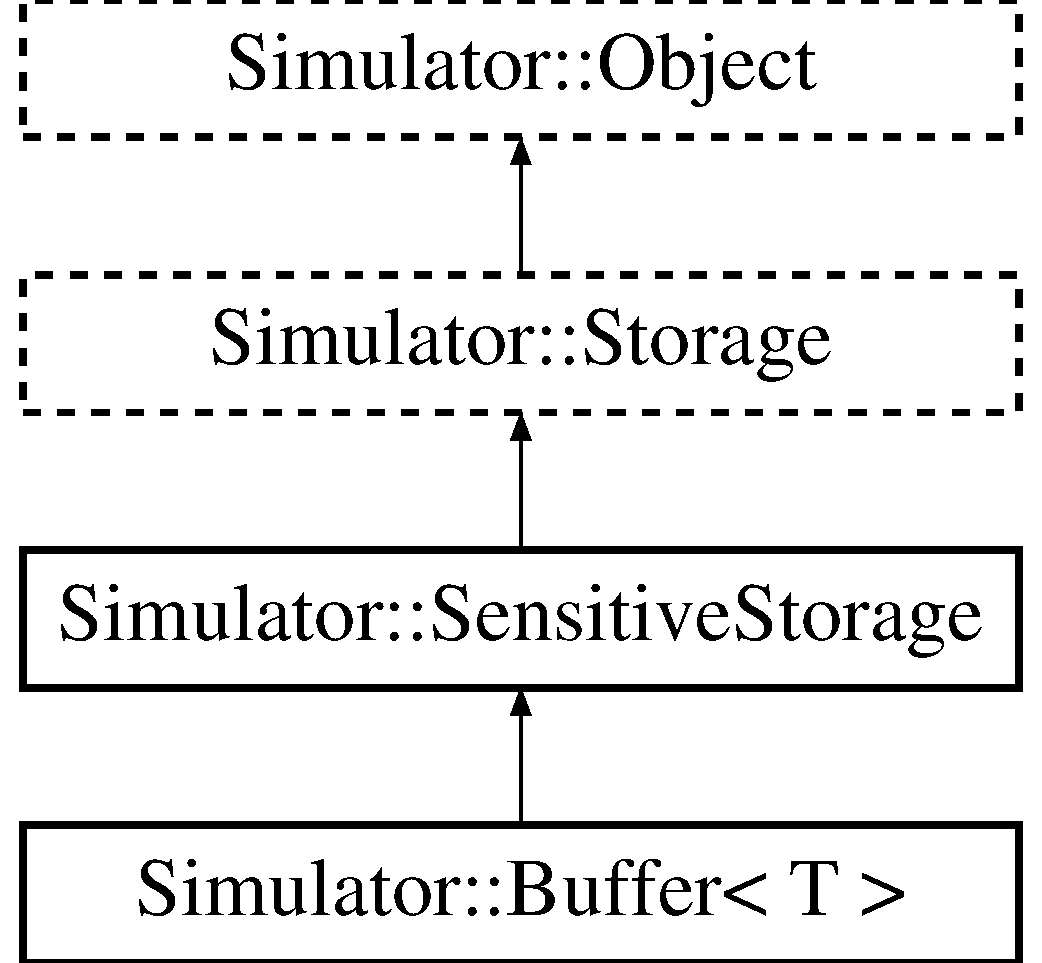
\includegraphics[height=4.000000cm]{class_simulator_1_1_buffer}
\end{center}
\end{figure}
\subsection*{Public Types}
\begin{DoxyCompactItemize}
\item 
typedef std\+::deque$<$ T $>$\\*
\+::\hyperlink{class_simulator_1_1_buffer_a50ac4b556b0c93ce985359e10472923b}{const\+\_\+iterator} \hyperlink{class_simulator_1_1_buffer_a50ac4b556b0c93ce985359e10472923b}{const\+\_\+iterator}
\item 
typedef std\+::deque$<$ T $>$\\*
\+::\hyperlink{class_simulator_1_1_buffer_aed79765ab3f5ebbcf7399c9402634607}{const\+\_\+reverse\+\_\+iterator} \hyperlink{class_simulator_1_1_buffer_aed79765ab3f5ebbcf7399c9402634607}{const\+\_\+reverse\+\_\+iterator}
\end{DoxyCompactItemize}
\subsection*{Public Member Functions}
\begin{DoxyCompactItemize}
\item 
\hyperlink{class_simulator_1_1_buffer_a50ac4b556b0c93ce985359e10472923b}{const\+\_\+iterator} \hyperlink{class_simulator_1_1_buffer_ac2aa81120a60881adba4f5fb14b10681}{begin} () const 
\item 
\hyperlink{class_simulator_1_1_buffer_a50ac4b556b0c93ce985359e10472923b}{const\+\_\+iterator} \hyperlink{class_simulator_1_1_buffer_a15a1da6eca670910cbc99cd600dc9e7c}{end} () const 
\item 
\hyperlink{class_simulator_1_1_buffer_aed79765ab3f5ebbcf7399c9402634607}{const\+\_\+reverse\+\_\+iterator} \hyperlink{class_simulator_1_1_buffer_a0db82a924cbe771050a7a6ea9799450b}{rbegin} () const 
\item 
\hyperlink{class_simulator_1_1_buffer_aed79765ab3f5ebbcf7399c9402634607}{const\+\_\+reverse\+\_\+iterator} \hyperlink{class_simulator_1_1_buffer_ac27e86090b6412a1c8b061ead8d4c968}{rend} () const 
\item 
bool \hyperlink{class_simulator_1_1_buffer_a28d7761486184657ba108eeae25a6978}{Empty} () const 
\item 
const T \& \hyperlink{class_simulator_1_1_buffer_a5ad63aa8daa373a4a8fb2529f4127d8f}{Front} () const 
\item 
\hyperlink{namespace_simulator_a5ca279f926485be2d0554e41275a3305}{Buffer\+Size} \hyperlink{class_simulator_1_1_buffer_aa78d6091099540dfb846792c51926a56}{size} () const 
\item 
\hyperlink{namespace_simulator_a5ca279f926485be2d0554e41275a3305}{Buffer\+Size} \hyperlink{class_simulator_1_1_buffer_a7253d468055a0db9bc21e9e1d50a65fd}{Get\+Max\+Size} () const 
\item 
void \hyperlink{class_simulator_1_1_buffer_a1640dbaf585259908e88f0251624aeb2}{Pop} ()
\item 
bool \hyperlink{class_simulator_1_1_buffer_aad6a44e805c7d98d58f6afc35541597a}{Push} (const T \&item, size\+\_\+t min\+\_\+space=1)
\item 
\hyperlink{class_simulator_1_1_buffer_a346bb39cdb62dd787d873a648ae18308}{Buffer} (const std\+::string \&\hyperlink{mtconf_8c_a8f8f80d37794cde9472343e4487ba3eb}{name}, \hyperlink{class_simulator_1_1_object}{Object} \&parent, \hyperlink{class_simulator_1_1_clock}{Clock} \&clock, \hyperlink{namespace_simulator_a5ca279f926485be2d0554e41275a3305}{Buffer\+Size} max\+Size, size\+\_\+t max\+Pushes=1)
\item 
\hyperlink{class_simulator_1_1_buffer_a53a13bf07063fd1c691e954fe376f3e4}{Buffer} (const \hyperlink{class_simulator_1_1_buffer}{Buffer} \&)=delete
\item 
\hyperlink{class_simulator_1_1_buffer}{Buffer} \& \hyperlink{class_simulator_1_1_buffer_a7c175139708831d820077c6f9804a91b}{operator=} (const \hyperlink{class_simulator_1_1_buffer}{Buffer} \&)=delete
\end{DoxyCompactItemize}
\subsection*{Additional Inherited Members}


\subsection{Detailed Description}
\subsubsection*{template$<$typename T$>$class Simulator\+::\+Buffer$<$ T $>$}

A F\+I\+F\+O storage queue. 

\subsection{Member Typedef Documentation}
\hypertarget{class_simulator_1_1_buffer_a50ac4b556b0c93ce985359e10472923b}{\index{Simulator\+::\+Buffer@{Simulator\+::\+Buffer}!const\+\_\+iterator@{const\+\_\+iterator}}
\index{const\+\_\+iterator@{const\+\_\+iterator}!Simulator\+::\+Buffer@{Simulator\+::\+Buffer}}
\subsubsection[{const\+\_\+iterator}]{\setlength{\rightskip}{0pt plus 5cm}template$<$typename T$>$ typedef std\+::deque$<$T$>$\+::{\bf const\+\_\+iterator} {\bf Simulator\+::\+Buffer}$<$ T $>$\+::{\bf const\+\_\+iterator}}}\label{class_simulator_1_1_buffer_a50ac4b556b0c93ce985359e10472923b}
\hypertarget{class_simulator_1_1_buffer_aed79765ab3f5ebbcf7399c9402634607}{\index{Simulator\+::\+Buffer@{Simulator\+::\+Buffer}!const\+\_\+reverse\+\_\+iterator@{const\+\_\+reverse\+\_\+iterator}}
\index{const\+\_\+reverse\+\_\+iterator@{const\+\_\+reverse\+\_\+iterator}!Simulator\+::\+Buffer@{Simulator\+::\+Buffer}}
\subsubsection[{const\+\_\+reverse\+\_\+iterator}]{\setlength{\rightskip}{0pt plus 5cm}template$<$typename T$>$ typedef std\+::deque$<$T$>$\+::{\bf const\+\_\+reverse\+\_\+iterator} {\bf Simulator\+::\+Buffer}$<$ T $>$\+::{\bf const\+\_\+reverse\+\_\+iterator}}}\label{class_simulator_1_1_buffer_aed79765ab3f5ebbcf7399c9402634607}


\subsection{Constructor \& Destructor Documentation}
\hypertarget{class_simulator_1_1_buffer_a346bb39cdb62dd787d873a648ae18308}{\index{Simulator\+::\+Buffer@{Simulator\+::\+Buffer}!Buffer@{Buffer}}
\index{Buffer@{Buffer}!Simulator\+::\+Buffer@{Simulator\+::\+Buffer}}
\subsubsection[{Buffer}]{\setlength{\rightskip}{0pt plus 5cm}template$<$typename T$>$ {\bf Simulator\+::\+Buffer}$<$ T $>$\+::{\bf Buffer} (
\begin{DoxyParamCaption}
\item[{const std\+::string \&}]{name, }
\item[{{\bf Object} \&}]{parent, }
\item[{{\bf Clock} \&}]{clock, }
\item[{{\bf Buffer\+Size}}]{max\+Size, }
\item[{size\+\_\+t}]{max\+Pushes = {\ttfamily 1}}
\end{DoxyParamCaption}
)\hspace{0.3cm}{\ttfamily [inline]}}}\label{class_simulator_1_1_buffer_a346bb39cdb62dd787d873a648ae18308}
\hypertarget{class_simulator_1_1_buffer_a53a13bf07063fd1c691e954fe376f3e4}{\index{Simulator\+::\+Buffer@{Simulator\+::\+Buffer}!Buffer@{Buffer}}
\index{Buffer@{Buffer}!Simulator\+::\+Buffer@{Simulator\+::\+Buffer}}
\subsubsection[{Buffer}]{\setlength{\rightskip}{0pt plus 5cm}template$<$typename T$>$ {\bf Simulator\+::\+Buffer}$<$ T $>$\+::{\bf Buffer} (
\begin{DoxyParamCaption}
\item[{const {\bf Buffer}$<$ T $>$ \&}]{}
\end{DoxyParamCaption}
)\hspace{0.3cm}{\ttfamily [delete]}}}\label{class_simulator_1_1_buffer_a53a13bf07063fd1c691e954fe376f3e4}


\subsection{Member Function Documentation}
\hypertarget{class_simulator_1_1_buffer_ac2aa81120a60881adba4f5fb14b10681}{\index{Simulator\+::\+Buffer@{Simulator\+::\+Buffer}!begin@{begin}}
\index{begin@{begin}!Simulator\+::\+Buffer@{Simulator\+::\+Buffer}}
\subsubsection[{begin}]{\setlength{\rightskip}{0pt plus 5cm}template$<$typename T$>$ {\bf const\+\_\+iterator} {\bf Simulator\+::\+Buffer}$<$ T $>$\+::begin (
\begin{DoxyParamCaption}
{}
\end{DoxyParamCaption}
) const\hspace{0.3cm}{\ttfamily [inline]}}}\label{class_simulator_1_1_buffer_ac2aa81120a60881adba4f5fb14b10681}
\hypertarget{class_simulator_1_1_buffer_a28d7761486184657ba108eeae25a6978}{\index{Simulator\+::\+Buffer@{Simulator\+::\+Buffer}!Empty@{Empty}}
\index{Empty@{Empty}!Simulator\+::\+Buffer@{Simulator\+::\+Buffer}}
\subsubsection[{Empty}]{\setlength{\rightskip}{0pt plus 5cm}template$<$typename T$>$ bool {\bf Simulator\+::\+Buffer}$<$ T $>$\+::Empty (
\begin{DoxyParamCaption}
{}
\end{DoxyParamCaption}
) const\hspace{0.3cm}{\ttfamily [inline]}}}\label{class_simulator_1_1_buffer_a28d7761486184657ba108eeae25a6978}
\hypertarget{class_simulator_1_1_buffer_a15a1da6eca670910cbc99cd600dc9e7c}{\index{Simulator\+::\+Buffer@{Simulator\+::\+Buffer}!end@{end}}
\index{end@{end}!Simulator\+::\+Buffer@{Simulator\+::\+Buffer}}
\subsubsection[{end}]{\setlength{\rightskip}{0pt plus 5cm}template$<$typename T$>$ {\bf const\+\_\+iterator} {\bf Simulator\+::\+Buffer}$<$ T $>$\+::end (
\begin{DoxyParamCaption}
{}
\end{DoxyParamCaption}
) const\hspace{0.3cm}{\ttfamily [inline]}}}\label{class_simulator_1_1_buffer_a15a1da6eca670910cbc99cd600dc9e7c}
\hypertarget{class_simulator_1_1_buffer_a5ad63aa8daa373a4a8fb2529f4127d8f}{\index{Simulator\+::\+Buffer@{Simulator\+::\+Buffer}!Front@{Front}}
\index{Front@{Front}!Simulator\+::\+Buffer@{Simulator\+::\+Buffer}}
\subsubsection[{Front}]{\setlength{\rightskip}{0pt plus 5cm}template$<$typename T$>$ const T\& {\bf Simulator\+::\+Buffer}$<$ T $>$\+::Front (
\begin{DoxyParamCaption}
{}
\end{DoxyParamCaption}
) const\hspace{0.3cm}{\ttfamily [inline]}}}\label{class_simulator_1_1_buffer_a5ad63aa8daa373a4a8fb2529f4127d8f}
\hypertarget{class_simulator_1_1_buffer_a7253d468055a0db9bc21e9e1d50a65fd}{\index{Simulator\+::\+Buffer@{Simulator\+::\+Buffer}!Get\+Max\+Size@{Get\+Max\+Size}}
\index{Get\+Max\+Size@{Get\+Max\+Size}!Simulator\+::\+Buffer@{Simulator\+::\+Buffer}}
\subsubsection[{Get\+Max\+Size}]{\setlength{\rightskip}{0pt plus 5cm}template$<$typename T$>$ {\bf Buffer\+Size} {\bf Simulator\+::\+Buffer}$<$ T $>$\+::Get\+Max\+Size (
\begin{DoxyParamCaption}
{}
\end{DoxyParamCaption}
) const\hspace{0.3cm}{\ttfamily [inline]}}}\label{class_simulator_1_1_buffer_a7253d468055a0db9bc21e9e1d50a65fd}
\hypertarget{class_simulator_1_1_buffer_a7c175139708831d820077c6f9804a91b}{\index{Simulator\+::\+Buffer@{Simulator\+::\+Buffer}!operator=@{operator=}}
\index{operator=@{operator=}!Simulator\+::\+Buffer@{Simulator\+::\+Buffer}}
\subsubsection[{operator=}]{\setlength{\rightskip}{0pt plus 5cm}template$<$typename T$>$ {\bf Buffer}\& {\bf Simulator\+::\+Buffer}$<$ T $>$\+::operator= (
\begin{DoxyParamCaption}
\item[{const {\bf Buffer}$<$ T $>$ \&}]{}
\end{DoxyParamCaption}
)\hspace{0.3cm}{\ttfamily [delete]}}}\label{class_simulator_1_1_buffer_a7c175139708831d820077c6f9804a91b}
\hypertarget{class_simulator_1_1_buffer_a1640dbaf585259908e88f0251624aeb2}{\index{Simulator\+::\+Buffer@{Simulator\+::\+Buffer}!Pop@{Pop}}
\index{Pop@{Pop}!Simulator\+::\+Buffer@{Simulator\+::\+Buffer}}
\subsubsection[{Pop}]{\setlength{\rightskip}{0pt plus 5cm}template$<$typename T$>$ void {\bf Simulator\+::\+Buffer}$<$ T $>$\+::Pop (
\begin{DoxyParamCaption}
{}
\end{DoxyParamCaption}
)\hspace{0.3cm}{\ttfamily [inline]}}}\label{class_simulator_1_1_buffer_a1640dbaf585259908e88f0251624aeb2}
\hypertarget{class_simulator_1_1_buffer_aad6a44e805c7d98d58f6afc35541597a}{\index{Simulator\+::\+Buffer@{Simulator\+::\+Buffer}!Push@{Push}}
\index{Push@{Push}!Simulator\+::\+Buffer@{Simulator\+::\+Buffer}}
\subsubsection[{Push}]{\setlength{\rightskip}{0pt plus 5cm}template$<$typename T$>$ bool {\bf Simulator\+::\+Buffer}$<$ T $>$\+::Push (
\begin{DoxyParamCaption}
\item[{const T \&}]{item, }
\item[{size\+\_\+t}]{min\+\_\+space = {\ttfamily 1}}
\end{DoxyParamCaption}
)\hspace{0.3cm}{\ttfamily [inline]}}}\label{class_simulator_1_1_buffer_aad6a44e805c7d98d58f6afc35541597a}
\hypertarget{class_simulator_1_1_buffer_a0db82a924cbe771050a7a6ea9799450b}{\index{Simulator\+::\+Buffer@{Simulator\+::\+Buffer}!rbegin@{rbegin}}
\index{rbegin@{rbegin}!Simulator\+::\+Buffer@{Simulator\+::\+Buffer}}
\subsubsection[{rbegin}]{\setlength{\rightskip}{0pt plus 5cm}template$<$typename T$>$ {\bf const\+\_\+reverse\+\_\+iterator} {\bf Simulator\+::\+Buffer}$<$ T $>$\+::rbegin (
\begin{DoxyParamCaption}
{}
\end{DoxyParamCaption}
) const\hspace{0.3cm}{\ttfamily [inline]}}}\label{class_simulator_1_1_buffer_a0db82a924cbe771050a7a6ea9799450b}
\hypertarget{class_simulator_1_1_buffer_ac27e86090b6412a1c8b061ead8d4c968}{\index{Simulator\+::\+Buffer@{Simulator\+::\+Buffer}!rend@{rend}}
\index{rend@{rend}!Simulator\+::\+Buffer@{Simulator\+::\+Buffer}}
\subsubsection[{rend}]{\setlength{\rightskip}{0pt plus 5cm}template$<$typename T$>$ {\bf const\+\_\+reverse\+\_\+iterator} {\bf Simulator\+::\+Buffer}$<$ T $>$\+::rend (
\begin{DoxyParamCaption}
{}
\end{DoxyParamCaption}
) const\hspace{0.3cm}{\ttfamily [inline]}}}\label{class_simulator_1_1_buffer_ac27e86090b6412a1c8b061ead8d4c968}
\hypertarget{class_simulator_1_1_buffer_aa78d6091099540dfb846792c51926a56}{\index{Simulator\+::\+Buffer@{Simulator\+::\+Buffer}!size@{size}}
\index{size@{size}!Simulator\+::\+Buffer@{Simulator\+::\+Buffer}}
\subsubsection[{size}]{\setlength{\rightskip}{0pt plus 5cm}template$<$typename T$>$ {\bf Buffer\+Size} {\bf Simulator\+::\+Buffer}$<$ T $>$\+::size (
\begin{DoxyParamCaption}
{}
\end{DoxyParamCaption}
) const\hspace{0.3cm}{\ttfamily [inline]}}}\label{class_simulator_1_1_buffer_aa78d6091099540dfb846792c51926a56}


The documentation for this class was generated from the following file\+:\begin{DoxyCompactItemize}
\item 
sim/\hyperlink{storage_8h}{storage.\+h}\end{DoxyCompactItemize}

\hypertarget{struct_simulator_1_1drisc_1_1_allocator_1_1_bundle_info}{\section{Simulator\+:\+:drisc\+:\+:Allocator\+:\+:Bundle\+Info Struct Reference}
\label{struct_simulator_1_1drisc_1_1_allocator_1_1_bundle_info}\index{Simulator\+::drisc\+::\+Allocator\+::\+Bundle\+Info@{Simulator\+::drisc\+::\+Allocator\+::\+Bundle\+Info}}
}


{\ttfamily \#include $<$Allocator.\+h$>$}

\subsection*{Public Attributes}
\begin{DoxyCompactItemize}
\item 
Mem\+Addr \hyperlink{struct_simulator_1_1drisc_1_1_allocator_1_1_bundle_info_aaa2ffcc7a34c84092ebabe38bbfc5136}{addr}
\begin{DoxyCompactList}\small\item\em Memory Entry. \end{DoxyCompactList}\item 
Integer \hyperlink{struct_simulator_1_1drisc_1_1_allocator_1_1_bundle_info_a551bcce9a574f1e9731b2949046c9d5f}{parameter}
\begin{DoxyCompactList}\small\item\em Program-\/specified parameter for shareds. \end{DoxyCompactList}\item 
\hyperlink{namespace_simulator_ab00c9033de4c9a17db7b53d6c292515c}{Reg\+Index} \hyperlink{struct_simulator_1_1drisc_1_1_allocator_1_1_bundle_info_a99ab65509b8de61dd8fb113e1024c26e}{completion\+\_\+reg}
\begin{DoxyCompactList}\small\item\em \hyperlink{class_simulator_1_1_register}{Register} (on that core) that will receive the \hyperlink{struct_simulator_1_1_f_i_d}{F\+I\+D}. \end{DoxyCompactList}\end{DoxyCompactItemize}


\subsection{Member Data Documentation}
\hypertarget{struct_simulator_1_1drisc_1_1_allocator_1_1_bundle_info_aaa2ffcc7a34c84092ebabe38bbfc5136}{\index{Simulator\+::drisc\+::\+Allocator\+::\+Bundle\+Info@{Simulator\+::drisc\+::\+Allocator\+::\+Bundle\+Info}!addr@{addr}}
\index{addr@{addr}!Simulator\+::drisc\+::\+Allocator\+::\+Bundle\+Info@{Simulator\+::drisc\+::\+Allocator\+::\+Bundle\+Info}}
\subsubsection[{addr}]{\setlength{\rightskip}{0pt plus 5cm}Mem\+Addr Simulator\+::drisc\+::\+Allocator\+::\+Bundle\+Info\+::addr}}\label{struct_simulator_1_1drisc_1_1_allocator_1_1_bundle_info_aaa2ffcc7a34c84092ebabe38bbfc5136}


Memory Entry. 

\hypertarget{struct_simulator_1_1drisc_1_1_allocator_1_1_bundle_info_a99ab65509b8de61dd8fb113e1024c26e}{\index{Simulator\+::drisc\+::\+Allocator\+::\+Bundle\+Info@{Simulator\+::drisc\+::\+Allocator\+::\+Bundle\+Info}!completion\+\_\+reg@{completion\+\_\+reg}}
\index{completion\+\_\+reg@{completion\+\_\+reg}!Simulator\+::drisc\+::\+Allocator\+::\+Bundle\+Info@{Simulator\+::drisc\+::\+Allocator\+::\+Bundle\+Info}}
\subsubsection[{completion\+\_\+reg}]{\setlength{\rightskip}{0pt plus 5cm}{\bf Reg\+Index} Simulator\+::drisc\+::\+Allocator\+::\+Bundle\+Info\+::completion\+\_\+reg}}\label{struct_simulator_1_1drisc_1_1_allocator_1_1_bundle_info_a99ab65509b8de61dd8fb113e1024c26e}


\hyperlink{class_simulator_1_1_register}{Register} (on that core) that will receive the \hyperlink{struct_simulator_1_1_f_i_d}{F\+I\+D}. 

\hypertarget{struct_simulator_1_1drisc_1_1_allocator_1_1_bundle_info_a551bcce9a574f1e9731b2949046c9d5f}{\index{Simulator\+::drisc\+::\+Allocator\+::\+Bundle\+Info@{Simulator\+::drisc\+::\+Allocator\+::\+Bundle\+Info}!parameter@{parameter}}
\index{parameter@{parameter}!Simulator\+::drisc\+::\+Allocator\+::\+Bundle\+Info@{Simulator\+::drisc\+::\+Allocator\+::\+Bundle\+Info}}
\subsubsection[{parameter}]{\setlength{\rightskip}{0pt plus 5cm}Integer Simulator\+::drisc\+::\+Allocator\+::\+Bundle\+Info\+::parameter}}\label{struct_simulator_1_1drisc_1_1_allocator_1_1_bundle_info_a551bcce9a574f1e9731b2949046c9d5f}


Program-\/specified parameter for shareds. 



The documentation for this struct was generated from the following file\+:\begin{DoxyCompactItemize}
\item 
arch/drisc/\hyperlink{_allocator_8h}{Allocator.\+h}\end{DoxyCompactItemize}

\hypertarget{class_simulator_1_1_c_d_m_a_1_1_cache}{\section{Simulator\+:\+:C\+D\+M\+A\+:\+:Cache Class Reference}
\label{class_simulator_1_1_c_d_m_a_1_1_cache}\index{Simulator\+::\+C\+D\+M\+A\+::\+Cache@{Simulator\+::\+C\+D\+M\+A\+::\+Cache}}
}


{\ttfamily \#include $<$Cache.\+h$>$}

Inheritance diagram for Simulator\+:\+:C\+D\+M\+A\+:\+:Cache\+:\begin{figure}[H]
\begin{center}
\leavevmode
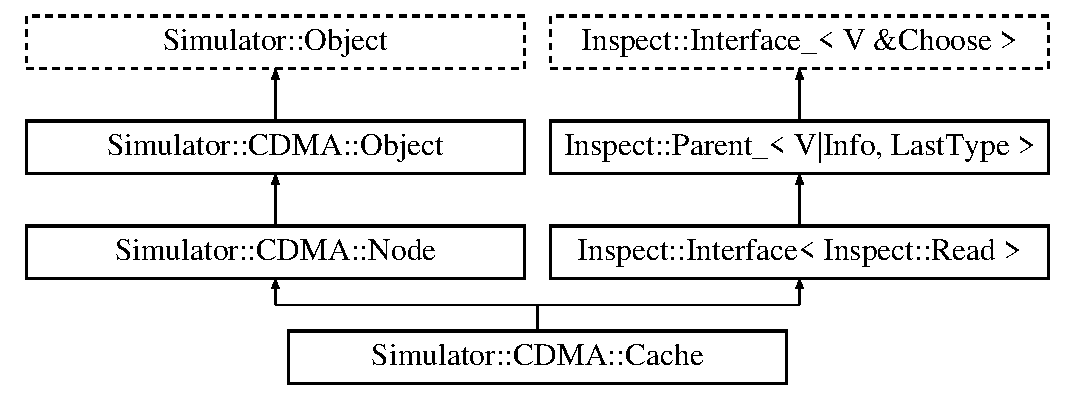
\includegraphics[height=4.000000cm]{class_simulator_1_1_c_d_m_a_1_1_cache}
\end{center}
\end{figure}
\subsection*{Classes}
\begin{DoxyCompactItemize}
\item 
struct \hyperlink{struct_simulator_1_1_c_d_m_a_1_1_cache_1_1_line}{Line}
\end{DoxyCompactItemize}
\subsection*{Public Types}
\begin{DoxyCompactItemize}
\item 
enum \hyperlink{class_simulator_1_1_c_d_m_a_1_1_cache_a77855c6e5bb01a9ab1da0e1cb5e80a3f}{Line\+State} \{ \hyperlink{class_simulator_1_1_c_d_m_a_1_1_cache_a77855c6e5bb01a9ab1da0e1cb5e80a3fa29df1e640019cb70fd127b7c5f758939}{L\+I\+N\+E\+\_\+\+E\+M\+P\+T\+Y}, 
\hyperlink{class_simulator_1_1_c_d_m_a_1_1_cache_a77855c6e5bb01a9ab1da0e1cb5e80a3fa136c6aa87a111e79aa5000d9703c8c3a}{L\+I\+N\+E\+\_\+\+L\+O\+A\+D\+I\+N\+G}, 
\hyperlink{class_simulator_1_1_c_d_m_a_1_1_cache_a77855c6e5bb01a9ab1da0e1cb5e80a3fa3f9255e31c684539da71b8f963e35734}{L\+I\+N\+E\+\_\+\+F\+U\+L\+L}
 \}
\end{DoxyCompactItemize}
\subsection*{Public Member Functions}
\begin{DoxyCompactItemize}
\item 
\hyperlink{class_simulator_1_1_c_d_m_a_1_1_cache_a5a158eeca856232d2367fb0754734f71}{Cache} (const std\+::string \&\hyperlink{mtconf_8c_a8f8f80d37794cde9472343e4487ba3eb}{name}, \hyperlink{class_simulator_1_1_c_d_m_a}{C\+D\+M\+A} \&parent, \hyperlink{class_simulator_1_1_clock}{Clock} \&clock, \hyperlink{class_simulator_1_1_c_d_m_a_a59272166fd32e642f3113c22cc756927}{Node\+I\+D} \hyperlink{mtconf_8c_aa3185401f04d30bd505daebf48c39cc5}{id}, \hyperlink{class_config}{Config} \&config)
\item 
\hyperlink{class_simulator_1_1_c_d_m_a_1_1_cache_a7e1019f2b4c8bee29806e078f8aab632}{Cache} (const \hyperlink{class_simulator_1_1_c_d_m_a_1_1_cache}{Cache} \&)=delete
\item 
\hyperlink{class_simulator_1_1_c_d_m_a_1_1_cache}{Cache} \& \hyperlink{class_simulator_1_1_c_d_m_a_1_1_cache_a04f16cef996981468b8b47d345a00dbd}{operator=} (const \hyperlink{class_simulator_1_1_c_d_m_a_1_1_cache}{Cache} \&)=delete
\item 
\hyperlink{class_simulator_1_1_c_d_m_a_1_1_cache_aaca97d16ef71b7baeb5fea8cc6091243}{$\sim$\+Cache} ()
\item 
size\+\_\+t \hyperlink{class_simulator_1_1_c_d_m_a_1_1_cache_a083dc858d3af211893fb8a431a80a8ab}{Get\+Line\+Size} () const 
\item 
size\+\_\+t \hyperlink{class_simulator_1_1_c_d_m_a_1_1_cache_a35617b5599a8bc7b9a2a0bd51b8da103}{Get\+Num\+Sets} () const 
\item 
size\+\_\+t \hyperlink{class_simulator_1_1_c_d_m_a_1_1_cache_ab5fe6b60bf60cc52243e5e838222600a}{Get\+Num\+Lines} () const override
\item 
void \hyperlink{class_simulator_1_1_c_d_m_a_1_1_cache_ad219d4d522e54f3db7a6b97d02af641e}{Cmd\+\_\+\+Info} (std\+::ostream \&out, const std\+::vector$<$ std\+::string $>$ \&arguments) const 
\item 
void \hyperlink{class_simulator_1_1_c_d_m_a_1_1_cache_ad9d2eda67567029367e148a9515182c1}{Cmd\+\_\+\+Read} (std\+::ostream \&out, const std\+::vector$<$ std\+::string $>$ \&arguments) const 
\item 
\hyperlink{namespace_simulator_a4b5747ff30c62c6373badf3b53b9abf7}{M\+C\+I\+D} \hyperlink{class_simulator_1_1_c_d_m_a_1_1_cache_ada0cb62e9c45f2c4f6872cf29f3b42fb}{Register\+Client} (\hyperlink{class_simulator_1_1_i_memory_callback}{I\+Memory\+Callback} \&callback, \hyperlink{class_simulator_1_1_process}{Process} \&process, \hyperlink{class_simulator_1_1_storage_trace_set}{Storage\+Trace\+Set} \&traces, const \hyperlink{class_simulator_1_1_storage_trace_set}{Storage\+Trace\+Set} \&storages)
\item 
void \hyperlink{class_simulator_1_1_c_d_m_a_1_1_cache_a83139672baa1452be9a0cc2d03cb7daf}{Unregister\+Client} (\hyperlink{namespace_simulator_a4b5747ff30c62c6373badf3b53b9abf7}{M\+C\+I\+D} \hyperlink{mtconf_8c_aa3185401f04d30bd505daebf48c39cc5}{id})
\item 
bool \hyperlink{class_simulator_1_1_c_d_m_a_1_1_cache_a0076553985970d938b290e2254cdce51}{Read} (\hyperlink{namespace_simulator_a4b5747ff30c62c6373badf3b53b9abf7}{M\+C\+I\+D} \hyperlink{mtconf_8c_aa3185401f04d30bd505daebf48c39cc5}{id}, Mem\+Addr address)
\item 
bool \hyperlink{class_simulator_1_1_c_d_m_a_1_1_cache_a136f64febe5fcd8a4134d2ba4b60b7e3}{Write} (\hyperlink{namespace_simulator_a4b5747ff30c62c6373badf3b53b9abf7}{M\+C\+I\+D} \hyperlink{mtconf_8c_aa3185401f04d30bd505daebf48c39cc5}{id}, Mem\+Addr address, const \hyperlink{struct_simulator_1_1_mem_data}{Mem\+Data} \&data, \hyperlink{namespace_simulator_a0de605c35951a450d074222efcef6359}{W\+Client\+I\+D} wid)
\end{DoxyCompactItemize}
\subsection*{Friends}
\begin{DoxyCompactItemize}
\item 
class \hyperlink{class_simulator_1_1_c_d_m_a_1_1_cache_add415c7c29b0f2d422db4e084c6688e3}{C\+D\+M\+A}
\end{DoxyCompactItemize}
\subsection*{Additional Inherited Members}


\subsection{Member Enumeration Documentation}
\hypertarget{class_simulator_1_1_c_d_m_a_1_1_cache_a77855c6e5bb01a9ab1da0e1cb5e80a3f}{\index{Simulator\+::\+C\+D\+M\+A\+::\+Cache@{Simulator\+::\+C\+D\+M\+A\+::\+Cache}!Line\+State@{Line\+State}}
\index{Line\+State@{Line\+State}!Simulator\+::\+C\+D\+M\+A\+::\+Cache@{Simulator\+::\+C\+D\+M\+A\+::\+Cache}}
\subsubsection[{Line\+State}]{\setlength{\rightskip}{0pt plus 5cm}enum {\bf Simulator\+::\+C\+D\+M\+A\+::\+Cache\+::\+Line\+State}}}\label{class_simulator_1_1_c_d_m_a_1_1_cache_a77855c6e5bb01a9ab1da0e1cb5e80a3f}
\begin{Desc}
\item[Enumerator]\par
\begin{description}
\index{L\+I\+N\+E\+\_\+\+E\+M\+P\+T\+Y@{L\+I\+N\+E\+\_\+\+E\+M\+P\+T\+Y}!Simulator\+::\+C\+D\+M\+A\+::\+Cache@{Simulator\+::\+C\+D\+M\+A\+::\+Cache}}\index{Simulator\+::\+C\+D\+M\+A\+::\+Cache@{Simulator\+::\+C\+D\+M\+A\+::\+Cache}!L\+I\+N\+E\+\_\+\+E\+M\+P\+T\+Y@{L\+I\+N\+E\+\_\+\+E\+M\+P\+T\+Y}}\item[{\em 
\hypertarget{class_simulator_1_1_c_d_m_a_1_1_cache_a77855c6e5bb01a9ab1da0e1cb5e80a3fa29df1e640019cb70fd127b7c5f758939}{L\+I\+N\+E\+\_\+\+E\+M\+P\+T\+Y}\label{class_simulator_1_1_c_d_m_a_1_1_cache_a77855c6e5bb01a9ab1da0e1cb5e80a3fa29df1e640019cb70fd127b7c5f758939}
}]Empty, can be used. \index{L\+I\+N\+E\+\_\+\+L\+O\+A\+D\+I\+N\+G@{L\+I\+N\+E\+\_\+\+L\+O\+A\+D\+I\+N\+G}!Simulator\+::\+C\+D\+M\+A\+::\+Cache@{Simulator\+::\+C\+D\+M\+A\+::\+Cache}}\index{Simulator\+::\+C\+D\+M\+A\+::\+Cache@{Simulator\+::\+C\+D\+M\+A\+::\+Cache}!L\+I\+N\+E\+\_\+\+L\+O\+A\+D\+I\+N\+G@{L\+I\+N\+E\+\_\+\+L\+O\+A\+D\+I\+N\+G}}\item[{\em 
\hypertarget{class_simulator_1_1_c_d_m_a_1_1_cache_a77855c6e5bb01a9ab1da0e1cb5e80a3fa136c6aa87a111e79aa5000d9703c8c3a}{L\+I\+N\+E\+\_\+\+L\+O\+A\+D\+I\+N\+G}\label{class_simulator_1_1_c_d_m_a_1_1_cache_a77855c6e5bb01a9ab1da0e1cb5e80a3fa136c6aa87a111e79aa5000d9703c8c3a}
}]Allocated, read request sent. \index{L\+I\+N\+E\+\_\+\+F\+U\+L\+L@{L\+I\+N\+E\+\_\+\+F\+U\+L\+L}!Simulator\+::\+C\+D\+M\+A\+::\+Cache@{Simulator\+::\+C\+D\+M\+A\+::\+Cache}}\index{Simulator\+::\+C\+D\+M\+A\+::\+Cache@{Simulator\+::\+C\+D\+M\+A\+::\+Cache}!L\+I\+N\+E\+\_\+\+F\+U\+L\+L@{L\+I\+N\+E\+\_\+\+F\+U\+L\+L}}\item[{\em 
\hypertarget{class_simulator_1_1_c_d_m_a_1_1_cache_a77855c6e5bb01a9ab1da0e1cb5e80a3fa3f9255e31c684539da71b8f963e35734}{L\+I\+N\+E\+\_\+\+F\+U\+L\+L}\label{class_simulator_1_1_c_d_m_a_1_1_cache_a77855c6e5bb01a9ab1da0e1cb5e80a3fa3f9255e31c684539da71b8f963e35734}
}]Allocated and data present. \end{description}
\end{Desc}


\subsection{Constructor \& Destructor Documentation}
\hypertarget{class_simulator_1_1_c_d_m_a_1_1_cache_a5a158eeca856232d2367fb0754734f71}{\index{Simulator\+::\+C\+D\+M\+A\+::\+Cache@{Simulator\+::\+C\+D\+M\+A\+::\+Cache}!Cache@{Cache}}
\index{Cache@{Cache}!Simulator\+::\+C\+D\+M\+A\+::\+Cache@{Simulator\+::\+C\+D\+M\+A\+::\+Cache}}
\subsubsection[{Cache}]{\setlength{\rightskip}{0pt plus 5cm}Simulator\+::\+C\+D\+M\+A\+::\+Cache\+::\+Cache (
\begin{DoxyParamCaption}
\item[{const std\+::string \&}]{name, }
\item[{{\bf C\+D\+M\+A} \&}]{parent, }
\item[{{\bf Clock} \&}]{clock, }
\item[{{\bf Node\+I\+D}}]{id, }
\item[{{\bf Config} \&}]{config}
\end{DoxyParamCaption}
)}}\label{class_simulator_1_1_c_d_m_a_1_1_cache_a5a158eeca856232d2367fb0754734f71}
\hypertarget{class_simulator_1_1_c_d_m_a_1_1_cache_a7e1019f2b4c8bee29806e078f8aab632}{\index{Simulator\+::\+C\+D\+M\+A\+::\+Cache@{Simulator\+::\+C\+D\+M\+A\+::\+Cache}!Cache@{Cache}}
\index{Cache@{Cache}!Simulator\+::\+C\+D\+M\+A\+::\+Cache@{Simulator\+::\+C\+D\+M\+A\+::\+Cache}}
\subsubsection[{Cache}]{\setlength{\rightskip}{0pt plus 5cm}Simulator\+::\+C\+D\+M\+A\+::\+Cache\+::\+Cache (
\begin{DoxyParamCaption}
\item[{const {\bf Cache} \&}]{}
\end{DoxyParamCaption}
)\hspace{0.3cm}{\ttfamily [delete]}}}\label{class_simulator_1_1_c_d_m_a_1_1_cache_a7e1019f2b4c8bee29806e078f8aab632}
\hypertarget{class_simulator_1_1_c_d_m_a_1_1_cache_aaca97d16ef71b7baeb5fea8cc6091243}{\index{Simulator\+::\+C\+D\+M\+A\+::\+Cache@{Simulator\+::\+C\+D\+M\+A\+::\+Cache}!````~Cache@{$\sim$\+Cache}}
\index{````~Cache@{$\sim$\+Cache}!Simulator\+::\+C\+D\+M\+A\+::\+Cache@{Simulator\+::\+C\+D\+M\+A\+::\+Cache}}
\subsubsection[{$\sim$\+Cache}]{\setlength{\rightskip}{0pt plus 5cm}Simulator\+::\+C\+D\+M\+A\+::\+Cache\+::$\sim$\+Cache (
\begin{DoxyParamCaption}
{}
\end{DoxyParamCaption}
)}}\label{class_simulator_1_1_c_d_m_a_1_1_cache_aaca97d16ef71b7baeb5fea8cc6091243}


\subsection{Member Function Documentation}
\hypertarget{class_simulator_1_1_c_d_m_a_1_1_cache_ad219d4d522e54f3db7a6b97d02af641e}{\index{Simulator\+::\+C\+D\+M\+A\+::\+Cache@{Simulator\+::\+C\+D\+M\+A\+::\+Cache}!Cmd\+\_\+\+Info@{Cmd\+\_\+\+Info}}
\index{Cmd\+\_\+\+Info@{Cmd\+\_\+\+Info}!Simulator\+::\+C\+D\+M\+A\+::\+Cache@{Simulator\+::\+C\+D\+M\+A\+::\+Cache}}
\subsubsection[{Cmd\+\_\+\+Info}]{\setlength{\rightskip}{0pt plus 5cm}void Simulator\+::\+C\+D\+M\+A\+::\+Cache\+::\+Cmd\+\_\+\+Info (
\begin{DoxyParamCaption}
\item[{std\+::ostream \&}]{out, }
\item[{const std\+::vector$<$ std\+::string $>$ \&}]{arguments}
\end{DoxyParamCaption}
) const}}\label{class_simulator_1_1_c_d_m_a_1_1_cache_ad219d4d522e54f3db7a6b97d02af641e}
\hypertarget{class_simulator_1_1_c_d_m_a_1_1_cache_ad9d2eda67567029367e148a9515182c1}{\index{Simulator\+::\+C\+D\+M\+A\+::\+Cache@{Simulator\+::\+C\+D\+M\+A\+::\+Cache}!Cmd\+\_\+\+Read@{Cmd\+\_\+\+Read}}
\index{Cmd\+\_\+\+Read@{Cmd\+\_\+\+Read}!Simulator\+::\+C\+D\+M\+A\+::\+Cache@{Simulator\+::\+C\+D\+M\+A\+::\+Cache}}
\subsubsection[{Cmd\+\_\+\+Read}]{\setlength{\rightskip}{0pt plus 5cm}void Simulator\+::\+C\+D\+M\+A\+::\+Cache\+::\+Cmd\+\_\+\+Read (
\begin{DoxyParamCaption}
\item[{std\+::ostream \&}]{out, }
\item[{const std\+::vector$<$ std\+::string $>$ \&}]{arguments}
\end{DoxyParamCaption}
) const}}\label{class_simulator_1_1_c_d_m_a_1_1_cache_ad9d2eda67567029367e148a9515182c1}
\hypertarget{class_simulator_1_1_c_d_m_a_1_1_cache_a083dc858d3af211893fb8a431a80a8ab}{\index{Simulator\+::\+C\+D\+M\+A\+::\+Cache@{Simulator\+::\+C\+D\+M\+A\+::\+Cache}!Get\+Line\+Size@{Get\+Line\+Size}}
\index{Get\+Line\+Size@{Get\+Line\+Size}!Simulator\+::\+C\+D\+M\+A\+::\+Cache@{Simulator\+::\+C\+D\+M\+A\+::\+Cache}}
\subsubsection[{Get\+Line\+Size}]{\setlength{\rightskip}{0pt plus 5cm}size\+\_\+t Simulator\+::\+C\+D\+M\+A\+::\+Cache\+::\+Get\+Line\+Size (
\begin{DoxyParamCaption}
{}
\end{DoxyParamCaption}
) const\hspace{0.3cm}{\ttfamily [inline]}}}\label{class_simulator_1_1_c_d_m_a_1_1_cache_a083dc858d3af211893fb8a431a80a8ab}
\hypertarget{class_simulator_1_1_c_d_m_a_1_1_cache_ab5fe6b60bf60cc52243e5e838222600a}{\index{Simulator\+::\+C\+D\+M\+A\+::\+Cache@{Simulator\+::\+C\+D\+M\+A\+::\+Cache}!Get\+Num\+Lines@{Get\+Num\+Lines}}
\index{Get\+Num\+Lines@{Get\+Num\+Lines}!Simulator\+::\+C\+D\+M\+A\+::\+Cache@{Simulator\+::\+C\+D\+M\+A\+::\+Cache}}
\subsubsection[{Get\+Num\+Lines}]{\setlength{\rightskip}{0pt plus 5cm}size\+\_\+t Simulator\+::\+C\+D\+M\+A\+::\+Cache\+::\+Get\+Num\+Lines (
\begin{DoxyParamCaption}
{}
\end{DoxyParamCaption}
) const\hspace{0.3cm}{\ttfamily [override]}, {\ttfamily [virtual]}}}\label{class_simulator_1_1_c_d_m_a_1_1_cache_ab5fe6b60bf60cc52243e5e838222600a}


Reimplemented from \hyperlink{class_simulator_1_1_c_d_m_a_1_1_node_a1e5b04d3d6beaa4f1395a2332f105980}{Simulator\+::\+C\+D\+M\+A\+::\+Node}.

\hypertarget{class_simulator_1_1_c_d_m_a_1_1_cache_a35617b5599a8bc7b9a2a0bd51b8da103}{\index{Simulator\+::\+C\+D\+M\+A\+::\+Cache@{Simulator\+::\+C\+D\+M\+A\+::\+Cache}!Get\+Num\+Sets@{Get\+Num\+Sets}}
\index{Get\+Num\+Sets@{Get\+Num\+Sets}!Simulator\+::\+C\+D\+M\+A\+::\+Cache@{Simulator\+::\+C\+D\+M\+A\+::\+Cache}}
\subsubsection[{Get\+Num\+Sets}]{\setlength{\rightskip}{0pt plus 5cm}size\+\_\+t Simulator\+::\+C\+D\+M\+A\+::\+Cache\+::\+Get\+Num\+Sets (
\begin{DoxyParamCaption}
{}
\end{DoxyParamCaption}
) const\hspace{0.3cm}{\ttfamily [inline]}}}\label{class_simulator_1_1_c_d_m_a_1_1_cache_a35617b5599a8bc7b9a2a0bd51b8da103}
\hypertarget{class_simulator_1_1_c_d_m_a_1_1_cache_a04f16cef996981468b8b47d345a00dbd}{\index{Simulator\+::\+C\+D\+M\+A\+::\+Cache@{Simulator\+::\+C\+D\+M\+A\+::\+Cache}!operator=@{operator=}}
\index{operator=@{operator=}!Simulator\+::\+C\+D\+M\+A\+::\+Cache@{Simulator\+::\+C\+D\+M\+A\+::\+Cache}}
\subsubsection[{operator=}]{\setlength{\rightskip}{0pt plus 5cm}{\bf Cache}\& Simulator\+::\+C\+D\+M\+A\+::\+Cache\+::operator= (
\begin{DoxyParamCaption}
\item[{const {\bf Cache} \&}]{}
\end{DoxyParamCaption}
)\hspace{0.3cm}{\ttfamily [delete]}}}\label{class_simulator_1_1_c_d_m_a_1_1_cache_a04f16cef996981468b8b47d345a00dbd}
\hypertarget{class_simulator_1_1_c_d_m_a_1_1_cache_a0076553985970d938b290e2254cdce51}{\index{Simulator\+::\+C\+D\+M\+A\+::\+Cache@{Simulator\+::\+C\+D\+M\+A\+::\+Cache}!Read@{Read}}
\index{Read@{Read}!Simulator\+::\+C\+D\+M\+A\+::\+Cache@{Simulator\+::\+C\+D\+M\+A\+::\+Cache}}
\subsubsection[{Read}]{\setlength{\rightskip}{0pt plus 5cm}bool Simulator\+::\+C\+D\+M\+A\+::\+Cache\+::\+Read (
\begin{DoxyParamCaption}
\item[{{\bf M\+C\+I\+D}}]{id, }
\item[{Mem\+Addr}]{address}
\end{DoxyParamCaption}
)}}\label{class_simulator_1_1_c_d_m_a_1_1_cache_a0076553985970d938b290e2254cdce51}
\hypertarget{class_simulator_1_1_c_d_m_a_1_1_cache_ada0cb62e9c45f2c4f6872cf29f3b42fb}{\index{Simulator\+::\+C\+D\+M\+A\+::\+Cache@{Simulator\+::\+C\+D\+M\+A\+::\+Cache}!Register\+Client@{Register\+Client}}
\index{Register\+Client@{Register\+Client}!Simulator\+::\+C\+D\+M\+A\+::\+Cache@{Simulator\+::\+C\+D\+M\+A\+::\+Cache}}
\subsubsection[{Register\+Client}]{\setlength{\rightskip}{0pt plus 5cm}{\bf M\+C\+I\+D} Simulator\+::\+C\+D\+M\+A\+::\+Cache\+::\+Register\+Client (
\begin{DoxyParamCaption}
\item[{{\bf I\+Memory\+Callback} \&}]{callback, }
\item[{{\bf Process} \&}]{process, }
\item[{{\bf Storage\+Trace\+Set} \&}]{traces, }
\item[{const {\bf Storage\+Trace\+Set} \&}]{storages}
\end{DoxyParamCaption}
)}}\label{class_simulator_1_1_c_d_m_a_1_1_cache_ada0cb62e9c45f2c4f6872cf29f3b42fb}
\hypertarget{class_simulator_1_1_c_d_m_a_1_1_cache_a83139672baa1452be9a0cc2d03cb7daf}{\index{Simulator\+::\+C\+D\+M\+A\+::\+Cache@{Simulator\+::\+C\+D\+M\+A\+::\+Cache}!Unregister\+Client@{Unregister\+Client}}
\index{Unregister\+Client@{Unregister\+Client}!Simulator\+::\+C\+D\+M\+A\+::\+Cache@{Simulator\+::\+C\+D\+M\+A\+::\+Cache}}
\subsubsection[{Unregister\+Client}]{\setlength{\rightskip}{0pt plus 5cm}void Simulator\+::\+C\+D\+M\+A\+::\+Cache\+::\+Unregister\+Client (
\begin{DoxyParamCaption}
\item[{{\bf M\+C\+I\+D}}]{id}
\end{DoxyParamCaption}
)}}\label{class_simulator_1_1_c_d_m_a_1_1_cache_a83139672baa1452be9a0cc2d03cb7daf}
\hypertarget{class_simulator_1_1_c_d_m_a_1_1_cache_a136f64febe5fcd8a4134d2ba4b60b7e3}{\index{Simulator\+::\+C\+D\+M\+A\+::\+Cache@{Simulator\+::\+C\+D\+M\+A\+::\+Cache}!Write@{Write}}
\index{Write@{Write}!Simulator\+::\+C\+D\+M\+A\+::\+Cache@{Simulator\+::\+C\+D\+M\+A\+::\+Cache}}
\subsubsection[{Write}]{\setlength{\rightskip}{0pt plus 5cm}bool Simulator\+::\+C\+D\+M\+A\+::\+Cache\+::\+Write (
\begin{DoxyParamCaption}
\item[{{\bf M\+C\+I\+D}}]{id, }
\item[{Mem\+Addr}]{address, }
\item[{const {\bf Mem\+Data} \&}]{data, }
\item[{{\bf W\+Client\+I\+D}}]{wid}
\end{DoxyParamCaption}
)}}\label{class_simulator_1_1_c_d_m_a_1_1_cache_a136f64febe5fcd8a4134d2ba4b60b7e3}


\subsection{Friends And Related Function Documentation}
\hypertarget{class_simulator_1_1_c_d_m_a_1_1_cache_add415c7c29b0f2d422db4e084c6688e3}{\index{Simulator\+::\+C\+D\+M\+A\+::\+Cache@{Simulator\+::\+C\+D\+M\+A\+::\+Cache}!C\+D\+M\+A@{C\+D\+M\+A}}
\index{C\+D\+M\+A@{C\+D\+M\+A}!Simulator\+::\+C\+D\+M\+A\+::\+Cache@{Simulator\+::\+C\+D\+M\+A\+::\+Cache}}
\subsubsection[{C\+D\+M\+A}]{\setlength{\rightskip}{0pt plus 5cm}friend class {\bf C\+D\+M\+A}\hspace{0.3cm}{\ttfamily [friend]}}}\label{class_simulator_1_1_c_d_m_a_1_1_cache_add415c7c29b0f2d422db4e084c6688e3}


The documentation for this class was generated from the following files\+:\begin{DoxyCompactItemize}
\item 
arch/mem/cdma/\hyperlink{cdma_2_cache_8h}{Cache.\+h}\item 
arch/mem/cdma/\hyperlink{cdma_2_cache_8cpp}{Cache.\+cpp}\end{DoxyCompactItemize}

\hypertarget{class_simulator_1_1_z_l_c_d_m_a_1_1_cache}{\section{Simulator\+:\+:Z\+L\+C\+D\+M\+A\+:\+:Cache Class Reference}
\label{class_simulator_1_1_z_l_c_d_m_a_1_1_cache}\index{Simulator\+::\+Z\+L\+C\+D\+M\+A\+::\+Cache@{Simulator\+::\+Z\+L\+C\+D\+M\+A\+::\+Cache}}
}


{\ttfamily \#include $<$Cache.\+h$>$}

Inheritance diagram for Simulator\+:\+:Z\+L\+C\+D\+M\+A\+:\+:Cache\+:\begin{figure}[H]
\begin{center}
\leavevmode
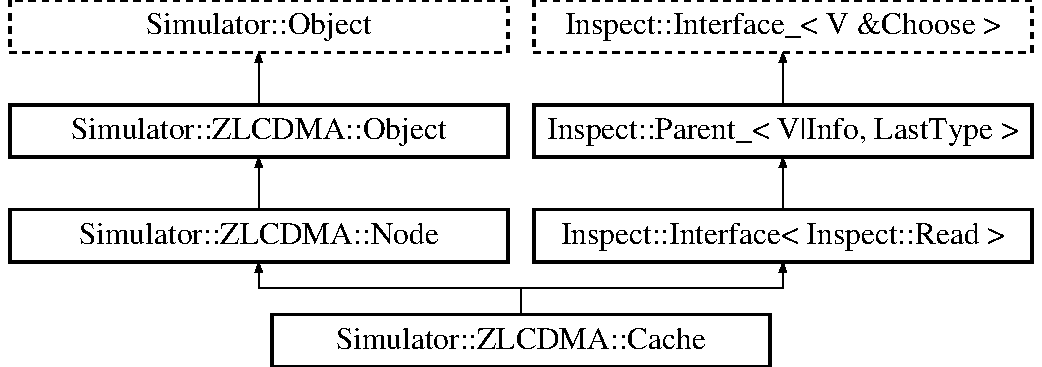
\includegraphics[height=4.000000cm]{class_simulator_1_1_z_l_c_d_m_a_1_1_cache}
\end{center}
\end{figure}
\subsection*{Classes}
\begin{DoxyCompactItemize}
\item 
struct \hyperlink{struct_simulator_1_1_z_l_c_d_m_a_1_1_cache_1_1_line}{Line}
\end{DoxyCompactItemize}
\subsection*{Public Member Functions}
\begin{DoxyCompactItemize}
\item 
\hyperlink{class_simulator_1_1_z_l_c_d_m_a_1_1_cache_a1271ba7cb3727476e32ca8c76d7e1892}{Cache} (const std\+::string \&\hyperlink{mtconf_8c_a8f8f80d37794cde9472343e4487ba3eb}{name}, \hyperlink{class_simulator_1_1_z_l_c_d_m_a}{Z\+L\+C\+D\+M\+A} \&parent, \hyperlink{class_simulator_1_1_clock}{Clock} \&clock, Cache\+I\+D \hyperlink{mtconf_8c_aa3185401f04d30bd505daebf48c39cc5}{id}, \hyperlink{class_config}{Config} \&config)
\item 
void \hyperlink{class_simulator_1_1_z_l_c_d_m_a_1_1_cache_acf2ead20e8ec442bba71b808a29d5930}{Cmd\+\_\+\+Info} (std\+::ostream \&out, const std\+::vector$<$ std\+::string $>$ \&arguments) const 
\item 
void \hyperlink{class_simulator_1_1_z_l_c_d_m_a_1_1_cache_a43d70f72b3ec0494194b17da3f5f6a74}{Cmd\+\_\+\+Read} (std\+::ostream \&out, const std\+::vector$<$ std\+::string $>$ \&arguments) const 
\item 
const \hyperlink{struct_simulator_1_1_z_l_c_d_m_a_1_1_cache_1_1_line}{Line} $\ast$ \hyperlink{class_simulator_1_1_z_l_c_d_m_a_1_1_cache_a909caa91fac1fb46cabe468337b57315}{Find\+Line} (Mem\+Addr address) const 
\item 
\hyperlink{namespace_simulator_a4b5747ff30c62c6373badf3b53b9abf7}{M\+C\+I\+D} \hyperlink{class_simulator_1_1_z_l_c_d_m_a_1_1_cache_af594e543ee2a0bb8d0a26a4b727b912c}{Register\+Client} (\hyperlink{class_simulator_1_1_i_memory_callback}{I\+Memory\+Callback} \&callback, \hyperlink{class_simulator_1_1_process}{Process} \&process, \hyperlink{class_simulator_1_1_storage_trace_set}{Storage\+Trace\+Set} \&traces, const \hyperlink{class_simulator_1_1_storage_trace_set}{Storage\+Trace\+Set} \&storages)
\item 
void \hyperlink{class_simulator_1_1_z_l_c_d_m_a_1_1_cache_a82892fed0ddbc4314f9e7e9a64774e15}{Unregister\+Client} (\hyperlink{namespace_simulator_a4b5747ff30c62c6373badf3b53b9abf7}{M\+C\+I\+D} \hyperlink{mtconf_8c_aa3185401f04d30bd505daebf48c39cc5}{id})
\item 
bool \hyperlink{class_simulator_1_1_z_l_c_d_m_a_1_1_cache_a9115d87db4e89be406d2c1ba9f06fe93}{Read} (\hyperlink{namespace_simulator_a4b5747ff30c62c6373badf3b53b9abf7}{M\+C\+I\+D} \hyperlink{mtconf_8c_aa3185401f04d30bd505daebf48c39cc5}{id}, Mem\+Addr address)
\item 
bool \hyperlink{class_simulator_1_1_z_l_c_d_m_a_1_1_cache_acaaefb6acade2910fdb2ba9bb9613a31}{Write} (\hyperlink{namespace_simulator_a4b5747ff30c62c6373badf3b53b9abf7}{M\+C\+I\+D} \hyperlink{mtconf_8c_aa3185401f04d30bd505daebf48c39cc5}{id}, Mem\+Addr address, const \hyperlink{struct_simulator_1_1_mem_data}{Mem\+Data} \&data, \hyperlink{namespace_simulator_a0de605c35951a450d074222efcef6359}{W\+Client\+I\+D} wid)
\end{DoxyCompactItemize}
\subsection*{Additional Inherited Members}


\subsection{Constructor \& Destructor Documentation}
\hypertarget{class_simulator_1_1_z_l_c_d_m_a_1_1_cache_a1271ba7cb3727476e32ca8c76d7e1892}{\index{Simulator\+::\+Z\+L\+C\+D\+M\+A\+::\+Cache@{Simulator\+::\+Z\+L\+C\+D\+M\+A\+::\+Cache}!Cache@{Cache}}
\index{Cache@{Cache}!Simulator\+::\+Z\+L\+C\+D\+M\+A\+::\+Cache@{Simulator\+::\+Z\+L\+C\+D\+M\+A\+::\+Cache}}
\subsubsection[{Cache}]{\setlength{\rightskip}{0pt plus 5cm}Simulator\+::\+Z\+L\+C\+D\+M\+A\+::\+Cache\+::\+Cache (
\begin{DoxyParamCaption}
\item[{const std\+::string \&}]{name, }
\item[{{\bf Z\+L\+C\+D\+M\+A} \&}]{parent, }
\item[{{\bf Clock} \&}]{clock, }
\item[{Cache\+I\+D}]{id, }
\item[{{\bf Config} \&}]{config}
\end{DoxyParamCaption}
)}}\label{class_simulator_1_1_z_l_c_d_m_a_1_1_cache_a1271ba7cb3727476e32ca8c76d7e1892}


\subsection{Member Function Documentation}
\hypertarget{class_simulator_1_1_z_l_c_d_m_a_1_1_cache_acf2ead20e8ec442bba71b808a29d5930}{\index{Simulator\+::\+Z\+L\+C\+D\+M\+A\+::\+Cache@{Simulator\+::\+Z\+L\+C\+D\+M\+A\+::\+Cache}!Cmd\+\_\+\+Info@{Cmd\+\_\+\+Info}}
\index{Cmd\+\_\+\+Info@{Cmd\+\_\+\+Info}!Simulator\+::\+Z\+L\+C\+D\+M\+A\+::\+Cache@{Simulator\+::\+Z\+L\+C\+D\+M\+A\+::\+Cache}}
\subsubsection[{Cmd\+\_\+\+Info}]{\setlength{\rightskip}{0pt plus 5cm}void Simulator\+::\+Z\+L\+C\+D\+M\+A\+::\+Cache\+::\+Cmd\+\_\+\+Info (
\begin{DoxyParamCaption}
\item[{std\+::ostream \&}]{out, }
\item[{const std\+::vector$<$ std\+::string $>$ \&}]{arguments}
\end{DoxyParamCaption}
) const}}\label{class_simulator_1_1_z_l_c_d_m_a_1_1_cache_acf2ead20e8ec442bba71b808a29d5930}
\hypertarget{class_simulator_1_1_z_l_c_d_m_a_1_1_cache_a43d70f72b3ec0494194b17da3f5f6a74}{\index{Simulator\+::\+Z\+L\+C\+D\+M\+A\+::\+Cache@{Simulator\+::\+Z\+L\+C\+D\+M\+A\+::\+Cache}!Cmd\+\_\+\+Read@{Cmd\+\_\+\+Read}}
\index{Cmd\+\_\+\+Read@{Cmd\+\_\+\+Read}!Simulator\+::\+Z\+L\+C\+D\+M\+A\+::\+Cache@{Simulator\+::\+Z\+L\+C\+D\+M\+A\+::\+Cache}}
\subsubsection[{Cmd\+\_\+\+Read}]{\setlength{\rightskip}{0pt plus 5cm}void Simulator\+::\+Z\+L\+C\+D\+M\+A\+::\+Cache\+::\+Cmd\+\_\+\+Read (
\begin{DoxyParamCaption}
\item[{std\+::ostream \&}]{out, }
\item[{const std\+::vector$<$ std\+::string $>$ \&}]{arguments}
\end{DoxyParamCaption}
) const}}\label{class_simulator_1_1_z_l_c_d_m_a_1_1_cache_a43d70f72b3ec0494194b17da3f5f6a74}
\hypertarget{class_simulator_1_1_z_l_c_d_m_a_1_1_cache_a909caa91fac1fb46cabe468337b57315}{\index{Simulator\+::\+Z\+L\+C\+D\+M\+A\+::\+Cache@{Simulator\+::\+Z\+L\+C\+D\+M\+A\+::\+Cache}!Find\+Line@{Find\+Line}}
\index{Find\+Line@{Find\+Line}!Simulator\+::\+Z\+L\+C\+D\+M\+A\+::\+Cache@{Simulator\+::\+Z\+L\+C\+D\+M\+A\+::\+Cache}}
\subsubsection[{Find\+Line}]{\setlength{\rightskip}{0pt plus 5cm}const {\bf Z\+L\+C\+D\+M\+A\+::\+Cache\+::\+Line} $\ast$ Simulator\+::\+Z\+L\+C\+D\+M\+A\+::\+Cache\+::\+Find\+Line (
\begin{DoxyParamCaption}
\item[{Mem\+Addr}]{address}
\end{DoxyParamCaption}
) const}}\label{class_simulator_1_1_z_l_c_d_m_a_1_1_cache_a909caa91fac1fb46cabe468337b57315}
\hypertarget{class_simulator_1_1_z_l_c_d_m_a_1_1_cache_a9115d87db4e89be406d2c1ba9f06fe93}{\index{Simulator\+::\+Z\+L\+C\+D\+M\+A\+::\+Cache@{Simulator\+::\+Z\+L\+C\+D\+M\+A\+::\+Cache}!Read@{Read}}
\index{Read@{Read}!Simulator\+::\+Z\+L\+C\+D\+M\+A\+::\+Cache@{Simulator\+::\+Z\+L\+C\+D\+M\+A\+::\+Cache}}
\subsubsection[{Read}]{\setlength{\rightskip}{0pt plus 5cm}bool Simulator\+::\+Z\+L\+C\+D\+M\+A\+::\+Cache\+::\+Read (
\begin{DoxyParamCaption}
\item[{{\bf M\+C\+I\+D}}]{id, }
\item[{Mem\+Addr}]{address}
\end{DoxyParamCaption}
)}}\label{class_simulator_1_1_z_l_c_d_m_a_1_1_cache_a9115d87db4e89be406d2c1ba9f06fe93}
\hypertarget{class_simulator_1_1_z_l_c_d_m_a_1_1_cache_af594e543ee2a0bb8d0a26a4b727b912c}{\index{Simulator\+::\+Z\+L\+C\+D\+M\+A\+::\+Cache@{Simulator\+::\+Z\+L\+C\+D\+M\+A\+::\+Cache}!Register\+Client@{Register\+Client}}
\index{Register\+Client@{Register\+Client}!Simulator\+::\+Z\+L\+C\+D\+M\+A\+::\+Cache@{Simulator\+::\+Z\+L\+C\+D\+M\+A\+::\+Cache}}
\subsubsection[{Register\+Client}]{\setlength{\rightskip}{0pt plus 5cm}{\bf M\+C\+I\+D} Simulator\+::\+Z\+L\+C\+D\+M\+A\+::\+Cache\+::\+Register\+Client (
\begin{DoxyParamCaption}
\item[{{\bf I\+Memory\+Callback} \&}]{callback, }
\item[{{\bf Process} \&}]{process, }
\item[{{\bf Storage\+Trace\+Set} \&}]{traces, }
\item[{const {\bf Storage\+Trace\+Set} \&}]{storages}
\end{DoxyParamCaption}
)}}\label{class_simulator_1_1_z_l_c_d_m_a_1_1_cache_af594e543ee2a0bb8d0a26a4b727b912c}
\hypertarget{class_simulator_1_1_z_l_c_d_m_a_1_1_cache_a82892fed0ddbc4314f9e7e9a64774e15}{\index{Simulator\+::\+Z\+L\+C\+D\+M\+A\+::\+Cache@{Simulator\+::\+Z\+L\+C\+D\+M\+A\+::\+Cache}!Unregister\+Client@{Unregister\+Client}}
\index{Unregister\+Client@{Unregister\+Client}!Simulator\+::\+Z\+L\+C\+D\+M\+A\+::\+Cache@{Simulator\+::\+Z\+L\+C\+D\+M\+A\+::\+Cache}}
\subsubsection[{Unregister\+Client}]{\setlength{\rightskip}{0pt plus 5cm}void Simulator\+::\+Z\+L\+C\+D\+M\+A\+::\+Cache\+::\+Unregister\+Client (
\begin{DoxyParamCaption}
\item[{{\bf M\+C\+I\+D}}]{id}
\end{DoxyParamCaption}
)}}\label{class_simulator_1_1_z_l_c_d_m_a_1_1_cache_a82892fed0ddbc4314f9e7e9a64774e15}
\hypertarget{class_simulator_1_1_z_l_c_d_m_a_1_1_cache_acaaefb6acade2910fdb2ba9bb9613a31}{\index{Simulator\+::\+Z\+L\+C\+D\+M\+A\+::\+Cache@{Simulator\+::\+Z\+L\+C\+D\+M\+A\+::\+Cache}!Write@{Write}}
\index{Write@{Write}!Simulator\+::\+Z\+L\+C\+D\+M\+A\+::\+Cache@{Simulator\+::\+Z\+L\+C\+D\+M\+A\+::\+Cache}}
\subsubsection[{Write}]{\setlength{\rightskip}{0pt plus 5cm}bool Simulator\+::\+Z\+L\+C\+D\+M\+A\+::\+Cache\+::\+Write (
\begin{DoxyParamCaption}
\item[{{\bf M\+C\+I\+D}}]{id, }
\item[{Mem\+Addr}]{address, }
\item[{const {\bf Mem\+Data} \&}]{data, }
\item[{{\bf W\+Client\+I\+D}}]{wid}
\end{DoxyParamCaption}
)}}\label{class_simulator_1_1_z_l_c_d_m_a_1_1_cache_acaaefb6acade2910fdb2ba9bb9613a31}


The documentation for this class was generated from the following files\+:\begin{DoxyCompactItemize}
\item 
arch/mem/zlcdma/\hyperlink{zlcdma_2_cache_8h}{Cache.\+h}\item 
arch/mem/zlcdma/\hyperlink{zlcdma_2_cache_8cpp}{Cache.\+cpp}\end{DoxyCompactItemize}

\hypertarget{class_simulator_1_1_c_d_m_a}{\section{Simulator\+:\+:C\+D\+M\+A Class Reference}
\label{class_simulator_1_1_c_d_m_a}\index{Simulator\+::\+C\+D\+M\+A@{Simulator\+::\+C\+D\+M\+A}}
}


{\ttfamily \#include $<$C\+D\+M\+A.\+h$>$}

Inheritance diagram for Simulator\+:\+:C\+D\+M\+A\+:\begin{figure}[H]
\begin{center}
\leavevmode
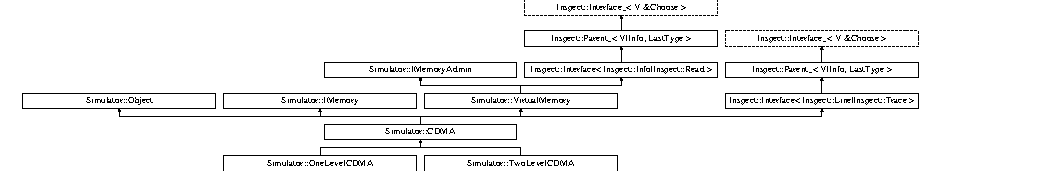
\includegraphics[height=2.301370cm]{class_simulator_1_1_c_d_m_a}
\end{center}
\end{figure}
\subsection*{Classes}
\begin{DoxyCompactItemize}
\item 
class \hyperlink{class_simulator_1_1_c_d_m_a_1_1_cache}{Cache}
\item 
class \hyperlink{class_simulator_1_1_c_d_m_a_1_1_directory}{Directory}
\item 
class \hyperlink{class_simulator_1_1_c_d_m_a_1_1_directory_bottom}{Directory\+Bottom}
\item 
class \hyperlink{class_simulator_1_1_c_d_m_a_1_1_directory_top}{Directory\+Top}
\item 
class \hyperlink{class_simulator_1_1_c_d_m_a_1_1_node}{Node}
\item 
class \hyperlink{class_simulator_1_1_c_d_m_a_1_1_object}{Object}
\item 
class \hyperlink{class_simulator_1_1_c_d_m_a_1_1_root_directory}{Root\+Directory}
\end{DoxyCompactItemize}
\subsection*{Public Member Functions}
\begin{DoxyCompactItemize}
\item 
\hyperlink{class_simulator_1_1_c_d_m_a_a132bbe72b74a22522e6dc86602b21174}{C\+D\+M\+A} (const std\+::string \&\hyperlink{mtconf_8c_a8f8f80d37794cde9472343e4487ba3eb}{name}, \hyperlink{class_simulator_1_1_object}{Simulator\+::\+Object} \&parent, \hyperlink{class_simulator_1_1_clock}{Clock} \&clock, \hyperlink{class_config}{Config} \&config)
\item 
\hyperlink{class_simulator_1_1_c_d_m_a_a8abcbf3b82c72cb4fb4b30d90826b87c}{C\+D\+M\+A} (const \hyperlink{class_simulator_1_1_c_d_m_a}{C\+D\+M\+A} \&)=delete
\item 
\hyperlink{class_simulator_1_1_c_d_m_a}{C\+D\+M\+A} \& \hyperlink{class_simulator_1_1_c_d_m_a_ad5a353a58e74ccb0123f02172be240c6}{operator=} (const \hyperlink{class_simulator_1_1_c_d_m_a}{C\+D\+M\+A} \&)=delete
\item 
\hyperlink{class_simulator_1_1_c_d_m_a_a03a680b074441a63dd2b0d683281edbf}{$\sim$\+C\+D\+M\+A} ()
\item 
const \hyperlink{class_simulator_1_1_c_d_m_a_ace88d950567607d699d7ad9e9cbbb3ef}{Trace\+Map} \& \hyperlink{class_simulator_1_1_c_d_m_a_a4de85bcf3157e1397722ecc31f724db5}{Get\+Traces} () const 
\item 
size\+\_\+t \hyperlink{class_simulator_1_1_c_d_m_a_a1f6b0672542b059459daed2b1bfbc631}{Get\+Line\+Size} () const 
\item 
size\+\_\+t \hyperlink{class_simulator_1_1_c_d_m_a_abb23eb9bc76d8956d85b011192e8e060}{Get\+Num\+Caches} () const 
\item 
size\+\_\+t \hyperlink{class_simulator_1_1_c_d_m_a_a714d64971edecd4a868bb50811dc25cd}{Get\+Num\+Directories} () const 
\item 
size\+\_\+t \hyperlink{class_simulator_1_1_c_d_m_a_afa4996da3fba98f8046f1728b4432cd1}{Get\+Num\+Root\+Directories} () const 
\item 
\hyperlink{class_simulator_1_1_c_d_m_a_1_1_cache}{Cache} \& \hyperlink{class_simulator_1_1_c_d_m_a_a0f3e7db3a0c19c2907b52d8450affc7f}{Get\+Cache} (size\+\_\+t i) const 
\item 
\hyperlink{class_simulator_1_1_c_d_m_a_1_1_directory}{Directory} \& \hyperlink{class_simulator_1_1_c_d_m_a_ae5d66fe4bd21eecce03d5f52b0884dc2}{Get\+Directory} (size\+\_\+t i) const 
\item 
\hyperlink{class_simulator_1_1_c_d_m_a_1_1_root_directory}{Root\+Directory} \& \hyperlink{class_simulator_1_1_c_d_m_a_a9258c45e62271e8f5c77fca8f9f006f4}{Get\+Root\+Directory} (size\+\_\+t i) const 
\item 
virtual \hyperlink{namespace_simulator_a4b5747ff30c62c6373badf3b53b9abf7}{M\+C\+I\+D} \hyperlink{class_simulator_1_1_c_d_m_a_aae97f6ed3411dff734ea58cb845760a5}{Register\+Client} (\hyperlink{class_simulator_1_1_i_memory_callback}{I\+Memory\+Callback} \&callback, \hyperlink{class_simulator_1_1_process}{Process} \&process, \hyperlink{class_simulator_1_1_storage_trace_set}{Storage\+Trace\+Set} \&traces, const \hyperlink{class_simulator_1_1_storage_trace_set}{Storage\+Trace\+Set} \&storages, bool grouped) override=0
\item 
void \hyperlink{class_simulator_1_1_c_d_m_a_a73a3c7e585030491fb2f54dc99913fe7}{Unregister\+Client} (\hyperlink{namespace_simulator_a4b5747ff30c62c6373badf3b53b9abf7}{M\+C\+I\+D} \hyperlink{mtconf_8c_aa3185401f04d30bd505daebf48c39cc5}{id}) override
\item 
bool \hyperlink{class_simulator_1_1_c_d_m_a_ab64a5f0667c3912f7dc5837fa7b00507}{Read} (\hyperlink{namespace_simulator_a4b5747ff30c62c6373badf3b53b9abf7}{M\+C\+I\+D} \hyperlink{mtconf_8c_aa3185401f04d30bd505daebf48c39cc5}{id}, Mem\+Addr address) override
\item 
bool \hyperlink{class_simulator_1_1_c_d_m_a_a959009cf2b4a9e3bbcf0ffb4aba8aa70}{Write} (\hyperlink{namespace_simulator_a4b5747ff30c62c6373badf3b53b9abf7}{M\+C\+I\+D} \hyperlink{mtconf_8c_aa3185401f04d30bd505daebf48c39cc5}{id}, Mem\+Addr address, const \hyperlink{struct_simulator_1_1_mem_data}{Mem\+Data} \&data, \hyperlink{namespace_simulator_a0de605c35951a450d074222efcef6359}{W\+Client\+I\+D} wid) override
\item 
void \hyperlink{class_simulator_1_1_c_d_m_a_a43e2b656101524ec25a3e3767fcbb3af}{Get\+Memory\+Statistics} (uint64\+\_\+t \&nreads, uint64\+\_\+t \&nwrites, uint64\+\_\+t \&nread\+\_\+bytes, uint64\+\_\+t \&nwrite\+\_\+bytes, uint64\+\_\+t \&nreads\+\_\+ext, uint64\+\_\+t \&nwrites\+\_\+ext) const override
\item 
void \hyperlink{class_simulator_1_1_c_d_m_a_a676f04b8147df2ec6f0b626d9654ebe9}{Cmd\+\_\+\+Info} (std\+::ostream \&out, const std\+::vector$<$ std\+::string $>$ \&arguments) const override
\item 
void \hyperlink{class_simulator_1_1_c_d_m_a_af366013154ef8c74052b5031126364b4}{Cmd\+\_\+\+Line} (std\+::ostream \&out, const std\+::vector$<$ std\+::string $>$ \&arguments) const override
\item 
void \hyperlink{class_simulator_1_1_c_d_m_a_abd272dfa995614dbf800d43308d0ff06}{Cmd\+\_\+\+Trace} (std\+::ostream \&out, const std\+::vector$<$ std\+::string $>$ \&arguments) override
\end{DoxyCompactItemize}
\subsection*{Protected Types}
\begin{DoxyCompactItemize}
\item 
typedef std\+::set$<$ Mem\+Addr $>$ \hyperlink{class_simulator_1_1_c_d_m_a_ace88d950567607d699d7ad9e9cbbb3ef}{Trace\+Map}
\item 
typedef size\+\_\+t \hyperlink{class_simulator_1_1_c_d_m_a_a59272166fd32e642f3113c22cc756927}{Node\+I\+D}
\end{DoxyCompactItemize}
\subsection*{Protected Member Functions}
\begin{DoxyCompactItemize}
\item 
unsigned int \hyperlink{class_simulator_1_1_c_d_m_a_af0b28dfa9bfbdfc8065d421174f1e8bc}{Get\+Total\+Tokens} () const 
\item 
virtual void \hyperlink{class_simulator_1_1_c_d_m_a_ab0b1f08a4466de3ccce7445c9bcf7c6b}{Initialize} ()=0
\end{DoxyCompactItemize}
\subsection*{Protected Attributes}
\begin{DoxyCompactItemize}
\item 
\hyperlink{class_component_model_registry}{Component\+Model\+Registry} \& \hyperlink{class_simulator_1_1_c_d_m_a_a19056757fe35a1c17146564ddb0afecf}{m\+\_\+registry}
\item 
size\+\_\+t \hyperlink{class_simulator_1_1_c_d_m_a_ad41683c11cec4d47c5ed8f5aa0c544c1}{m\+\_\+num\+Clients\+Per\+Cache}
\item 
size\+\_\+t \hyperlink{class_simulator_1_1_c_d_m_a_af6e3bb24fa6e0f5ee4e3d57233cc899b}{m\+\_\+num\+Caches\+Per\+Low\+Ring}
\item 
size\+\_\+t \hyperlink{class_simulator_1_1_c_d_m_a_acac9b9d9b18148e8d79020992cfdf541}{m\+\_\+num\+Clients}
\item 
size\+\_\+t \hyperlink{class_simulator_1_1_c_d_m_a_a7dab02d6c8bca4b895c81f224c8b96c3}{m\+\_\+line\+Size}
\item 
\hyperlink{class_config}{Config} \& \hyperlink{class_simulator_1_1_c_d_m_a_ae8160f56f781f1fc878578a011ef45df}{m\+\_\+config}
\item 
std\+::vector$<$ \hyperlink{class_simulator_1_1_c_d_m_a_1_1_cache}{Cache} $\ast$ $>$ \hyperlink{class_simulator_1_1_c_d_m_a_a82782c38b236bd4ce64db6498290970a}{m\+\_\+caches}
\begin{DoxyCompactList}\small\item\em List of caches. \end{DoxyCompactList}\item 
std\+::vector$<$ \hyperlink{class_simulator_1_1_c_d_m_a_1_1_directory}{Directory} $\ast$ $>$ \hyperlink{class_simulator_1_1_c_d_m_a_a2b6130ba000d98aff4ee59d07bf489a5}{m\+\_\+directories}
\begin{DoxyCompactList}\small\item\em List of directories. \end{DoxyCompactList}\item 
std\+::vector$<$ \hyperlink{class_simulator_1_1_c_d_m_a_1_1_root_directory}{Root\+Directory} $\ast$ $>$ \hyperlink{class_simulator_1_1_c_d_m_a_a71bfaa2e51ca8a4c5ffe6f75703c27d3}{m\+\_\+roots}
\begin{DoxyCompactList}\small\item\em List of root directories. \end{DoxyCompactList}\item 
\hyperlink{class_simulator_1_1_c_d_m_a_ace88d950567607d699d7ad9e9cbbb3ef}{Trace\+Map} \hyperlink{class_simulator_1_1_c_d_m_a_a077c382c9cf0488cd48c34d20351ea66}{m\+\_\+traces}
\begin{DoxyCompactList}\small\item\em Active traces. \end{DoxyCompactList}\item 
\hyperlink{class_simulator_1_1_d_d_r_channel_registry}{D\+D\+R\+Channel\+Registry} \hyperlink{class_simulator_1_1_c_d_m_a_a49092d8f924f613e08729377d051d865}{m\+\_\+ddr}
\begin{DoxyCompactList}\small\item\em List of D\+D\+R channels. \end{DoxyCompactList}\item 
std\+::vector$<$ std\+::pair$<$ \hyperlink{class_simulator_1_1_c_d_m_a_1_1_cache}{Cache} \\*
$\ast$, \hyperlink{namespace_simulator_a4b5747ff30c62c6373badf3b53b9abf7}{M\+C\+I\+D} $>$ $>$ \hyperlink{class_simulator_1_1_c_d_m_a_a2e2625307c97410a15650fb20bf99140}{m\+\_\+client\+Map}
\begin{DoxyCompactList}\small\item\em Mapping of M\+C\+I\+D to caches. \end{DoxyCompactList}\item 
uint64\+\_\+t \hyperlink{class_simulator_1_1_c_d_m_a_aac58e439ce84d5e9ee0dc904a46f5fde}{m\+\_\+nreads}
\item 
uint64\+\_\+t \hyperlink{class_simulator_1_1_c_d_m_a_a84926b887c7c4239379bd6e455480cf9}{m\+\_\+nwrites}
\item 
uint64\+\_\+t \hyperlink{class_simulator_1_1_c_d_m_a_a94eae1fc605f773ae8be9a28291428aa}{m\+\_\+nread\+\_\+bytes}
\item 
uint64\+\_\+t \hyperlink{class_simulator_1_1_c_d_m_a_a7761550a20a451aaca8a77f2afc883d5}{m\+\_\+nwrite\+\_\+bytes}
\end{DoxyCompactItemize}
\subsection*{Additional Inherited Members}


\subsection{Member Typedef Documentation}
\hypertarget{class_simulator_1_1_c_d_m_a_a59272166fd32e642f3113c22cc756927}{\index{Simulator\+::\+C\+D\+M\+A@{Simulator\+::\+C\+D\+M\+A}!Node\+I\+D@{Node\+I\+D}}
\index{Node\+I\+D@{Node\+I\+D}!Simulator\+::\+C\+D\+M\+A@{Simulator\+::\+C\+D\+M\+A}}
\subsubsection[{Node\+I\+D}]{\setlength{\rightskip}{0pt plus 5cm}typedef size\+\_\+t {\bf Simulator\+::\+C\+D\+M\+A\+::\+Node\+I\+D}\hspace{0.3cm}{\ttfamily [protected]}}}\label{class_simulator_1_1_c_d_m_a_a59272166fd32e642f3113c22cc756927}
\hypertarget{class_simulator_1_1_c_d_m_a_ace88d950567607d699d7ad9e9cbbb3ef}{\index{Simulator\+::\+C\+D\+M\+A@{Simulator\+::\+C\+D\+M\+A}!Trace\+Map@{Trace\+Map}}
\index{Trace\+Map@{Trace\+Map}!Simulator\+::\+C\+D\+M\+A@{Simulator\+::\+C\+D\+M\+A}}
\subsubsection[{Trace\+Map}]{\setlength{\rightskip}{0pt plus 5cm}typedef std\+::set$<$Mem\+Addr$>$ {\bf Simulator\+::\+C\+D\+M\+A\+::\+Trace\+Map}\hspace{0.3cm}{\ttfamily [protected]}}}\label{class_simulator_1_1_c_d_m_a_ace88d950567607d699d7ad9e9cbbb3ef}


\subsection{Constructor \& Destructor Documentation}
\hypertarget{class_simulator_1_1_c_d_m_a_a132bbe72b74a22522e6dc86602b21174}{\index{Simulator\+::\+C\+D\+M\+A@{Simulator\+::\+C\+D\+M\+A}!C\+D\+M\+A@{C\+D\+M\+A}}
\index{C\+D\+M\+A@{C\+D\+M\+A}!Simulator\+::\+C\+D\+M\+A@{Simulator\+::\+C\+D\+M\+A}}
\subsubsection[{C\+D\+M\+A}]{\setlength{\rightskip}{0pt plus 5cm}Simulator\+::\+C\+D\+M\+A\+::\+C\+D\+M\+A (
\begin{DoxyParamCaption}
\item[{const std\+::string \&}]{name, }
\item[{{\bf Simulator\+::\+Object} \&}]{parent, }
\item[{{\bf Clock} \&}]{clock, }
\item[{{\bf Config} \&}]{config}
\end{DoxyParamCaption}
)}}\label{class_simulator_1_1_c_d_m_a_a132bbe72b74a22522e6dc86602b21174}
\hypertarget{class_simulator_1_1_c_d_m_a_a8abcbf3b82c72cb4fb4b30d90826b87c}{\index{Simulator\+::\+C\+D\+M\+A@{Simulator\+::\+C\+D\+M\+A}!C\+D\+M\+A@{C\+D\+M\+A}}
\index{C\+D\+M\+A@{C\+D\+M\+A}!Simulator\+::\+C\+D\+M\+A@{Simulator\+::\+C\+D\+M\+A}}
\subsubsection[{C\+D\+M\+A}]{\setlength{\rightskip}{0pt plus 5cm}Simulator\+::\+C\+D\+M\+A\+::\+C\+D\+M\+A (
\begin{DoxyParamCaption}
\item[{const {\bf C\+D\+M\+A} \&}]{}
\end{DoxyParamCaption}
)\hspace{0.3cm}{\ttfamily [delete]}}}\label{class_simulator_1_1_c_d_m_a_a8abcbf3b82c72cb4fb4b30d90826b87c}
\hypertarget{class_simulator_1_1_c_d_m_a_a03a680b074441a63dd2b0d683281edbf}{\index{Simulator\+::\+C\+D\+M\+A@{Simulator\+::\+C\+D\+M\+A}!````~C\+D\+M\+A@{$\sim$\+C\+D\+M\+A}}
\index{````~C\+D\+M\+A@{$\sim$\+C\+D\+M\+A}!Simulator\+::\+C\+D\+M\+A@{Simulator\+::\+C\+D\+M\+A}}
\subsubsection[{$\sim$\+C\+D\+M\+A}]{\setlength{\rightskip}{0pt plus 5cm}Simulator\+::\+C\+D\+M\+A\+::$\sim$\+C\+D\+M\+A (
\begin{DoxyParamCaption}
{}
\end{DoxyParamCaption}
)}}\label{class_simulator_1_1_c_d_m_a_a03a680b074441a63dd2b0d683281edbf}


\subsection{Member Function Documentation}
\hypertarget{class_simulator_1_1_c_d_m_a_a676f04b8147df2ec6f0b626d9654ebe9}{\index{Simulator\+::\+C\+D\+M\+A@{Simulator\+::\+C\+D\+M\+A}!Cmd\+\_\+\+Info@{Cmd\+\_\+\+Info}}
\index{Cmd\+\_\+\+Info@{Cmd\+\_\+\+Info}!Simulator\+::\+C\+D\+M\+A@{Simulator\+::\+C\+D\+M\+A}}
\subsubsection[{Cmd\+\_\+\+Info}]{\setlength{\rightskip}{0pt plus 5cm}void Simulator\+::\+C\+D\+M\+A\+::\+Cmd\+\_\+\+Info (
\begin{DoxyParamCaption}
\item[{std\+::ostream \&}]{out, }
\item[{const std\+::vector$<$ std\+::string $>$ \&}]{arguments}
\end{DoxyParamCaption}
) const\hspace{0.3cm}{\ttfamily [override]}}}\label{class_simulator_1_1_c_d_m_a_a676f04b8147df2ec6f0b626d9654ebe9}
\hypertarget{class_simulator_1_1_c_d_m_a_af366013154ef8c74052b5031126364b4}{\index{Simulator\+::\+C\+D\+M\+A@{Simulator\+::\+C\+D\+M\+A}!Cmd\+\_\+\+Line@{Cmd\+\_\+\+Line}}
\index{Cmd\+\_\+\+Line@{Cmd\+\_\+\+Line}!Simulator\+::\+C\+D\+M\+A@{Simulator\+::\+C\+D\+M\+A}}
\subsubsection[{Cmd\+\_\+\+Line}]{\setlength{\rightskip}{0pt plus 5cm}void Simulator\+::\+C\+D\+M\+A\+::\+Cmd\+\_\+\+Line (
\begin{DoxyParamCaption}
\item[{std\+::ostream \&}]{out, }
\item[{const std\+::vector$<$ std\+::string $>$ \&}]{arguments}
\end{DoxyParamCaption}
) const\hspace{0.3cm}{\ttfamily [override]}}}\label{class_simulator_1_1_c_d_m_a_af366013154ef8c74052b5031126364b4}
\hypertarget{class_simulator_1_1_c_d_m_a_abd272dfa995614dbf800d43308d0ff06}{\index{Simulator\+::\+C\+D\+M\+A@{Simulator\+::\+C\+D\+M\+A}!Cmd\+\_\+\+Trace@{Cmd\+\_\+\+Trace}}
\index{Cmd\+\_\+\+Trace@{Cmd\+\_\+\+Trace}!Simulator\+::\+C\+D\+M\+A@{Simulator\+::\+C\+D\+M\+A}}
\subsubsection[{Cmd\+\_\+\+Trace}]{\setlength{\rightskip}{0pt plus 5cm}void Simulator\+::\+C\+D\+M\+A\+::\+Cmd\+\_\+\+Trace (
\begin{DoxyParamCaption}
\item[{std\+::ostream \&}]{out, }
\item[{const std\+::vector$<$ std\+::string $>$ \&}]{arguments}
\end{DoxyParamCaption}
)\hspace{0.3cm}{\ttfamily [override]}}}\label{class_simulator_1_1_c_d_m_a_abd272dfa995614dbf800d43308d0ff06}
\hypertarget{class_simulator_1_1_c_d_m_a_a0f3e7db3a0c19c2907b52d8450affc7f}{\index{Simulator\+::\+C\+D\+M\+A@{Simulator\+::\+C\+D\+M\+A}!Get\+Cache@{Get\+Cache}}
\index{Get\+Cache@{Get\+Cache}!Simulator\+::\+C\+D\+M\+A@{Simulator\+::\+C\+D\+M\+A}}
\subsubsection[{Get\+Cache}]{\setlength{\rightskip}{0pt plus 5cm}{\bf Cache}\& Simulator\+::\+C\+D\+M\+A\+::\+Get\+Cache (
\begin{DoxyParamCaption}
\item[{size\+\_\+t}]{i}
\end{DoxyParamCaption}
) const\hspace{0.3cm}{\ttfamily [inline]}}}\label{class_simulator_1_1_c_d_m_a_a0f3e7db3a0c19c2907b52d8450affc7f}
\hypertarget{class_simulator_1_1_c_d_m_a_ae5d66fe4bd21eecce03d5f52b0884dc2}{\index{Simulator\+::\+C\+D\+M\+A@{Simulator\+::\+C\+D\+M\+A}!Get\+Directory@{Get\+Directory}}
\index{Get\+Directory@{Get\+Directory}!Simulator\+::\+C\+D\+M\+A@{Simulator\+::\+C\+D\+M\+A}}
\subsubsection[{Get\+Directory}]{\setlength{\rightskip}{0pt plus 5cm}{\bf Directory}\& Simulator\+::\+C\+D\+M\+A\+::\+Get\+Directory (
\begin{DoxyParamCaption}
\item[{size\+\_\+t}]{i}
\end{DoxyParamCaption}
) const\hspace{0.3cm}{\ttfamily [inline]}}}\label{class_simulator_1_1_c_d_m_a_ae5d66fe4bd21eecce03d5f52b0884dc2}
\hypertarget{class_simulator_1_1_c_d_m_a_a1f6b0672542b059459daed2b1bfbc631}{\index{Simulator\+::\+C\+D\+M\+A@{Simulator\+::\+C\+D\+M\+A}!Get\+Line\+Size@{Get\+Line\+Size}}
\index{Get\+Line\+Size@{Get\+Line\+Size}!Simulator\+::\+C\+D\+M\+A@{Simulator\+::\+C\+D\+M\+A}}
\subsubsection[{Get\+Line\+Size}]{\setlength{\rightskip}{0pt plus 5cm}size\+\_\+t Simulator\+::\+C\+D\+M\+A\+::\+Get\+Line\+Size (
\begin{DoxyParamCaption}
{}
\end{DoxyParamCaption}
) const\hspace{0.3cm}{\ttfamily [inline]}}}\label{class_simulator_1_1_c_d_m_a_a1f6b0672542b059459daed2b1bfbc631}
\hypertarget{class_simulator_1_1_c_d_m_a_a43e2b656101524ec25a3e3767fcbb3af}{\index{Simulator\+::\+C\+D\+M\+A@{Simulator\+::\+C\+D\+M\+A}!Get\+Memory\+Statistics@{Get\+Memory\+Statistics}}
\index{Get\+Memory\+Statistics@{Get\+Memory\+Statistics}!Simulator\+::\+C\+D\+M\+A@{Simulator\+::\+C\+D\+M\+A}}
\subsubsection[{Get\+Memory\+Statistics}]{\setlength{\rightskip}{0pt plus 5cm}void Simulator\+::\+C\+D\+M\+A\+::\+Get\+Memory\+Statistics (
\begin{DoxyParamCaption}
\item[{uint64\+\_\+t \&}]{nreads, }
\item[{uint64\+\_\+t \&}]{nwrites, }
\item[{uint64\+\_\+t \&}]{nread\+\_\+bytes, }
\item[{uint64\+\_\+t \&}]{nwrite\+\_\+bytes, }
\item[{uint64\+\_\+t \&}]{nreads\+\_\+ext, }
\item[{uint64\+\_\+t \&}]{nwrites\+\_\+ext}
\end{DoxyParamCaption}
) const\hspace{0.3cm}{\ttfamily [override]}, {\ttfamily [virtual]}}}\label{class_simulator_1_1_c_d_m_a_a43e2b656101524ec25a3e3767fcbb3af}


Implements \hyperlink{class_simulator_1_1_i_memory_a14263220c662bbd2f65b0d4a2c915376}{Simulator\+::\+I\+Memory}.

\hypertarget{class_simulator_1_1_c_d_m_a_abb23eb9bc76d8956d85b011192e8e060}{\index{Simulator\+::\+C\+D\+M\+A@{Simulator\+::\+C\+D\+M\+A}!Get\+Num\+Caches@{Get\+Num\+Caches}}
\index{Get\+Num\+Caches@{Get\+Num\+Caches}!Simulator\+::\+C\+D\+M\+A@{Simulator\+::\+C\+D\+M\+A}}
\subsubsection[{Get\+Num\+Caches}]{\setlength{\rightskip}{0pt plus 5cm}size\+\_\+t Simulator\+::\+C\+D\+M\+A\+::\+Get\+Num\+Caches (
\begin{DoxyParamCaption}
{}
\end{DoxyParamCaption}
) const\hspace{0.3cm}{\ttfamily [inline]}}}\label{class_simulator_1_1_c_d_m_a_abb23eb9bc76d8956d85b011192e8e060}
\hypertarget{class_simulator_1_1_c_d_m_a_a714d64971edecd4a868bb50811dc25cd}{\index{Simulator\+::\+C\+D\+M\+A@{Simulator\+::\+C\+D\+M\+A}!Get\+Num\+Directories@{Get\+Num\+Directories}}
\index{Get\+Num\+Directories@{Get\+Num\+Directories}!Simulator\+::\+C\+D\+M\+A@{Simulator\+::\+C\+D\+M\+A}}
\subsubsection[{Get\+Num\+Directories}]{\setlength{\rightskip}{0pt plus 5cm}size\+\_\+t Simulator\+::\+C\+D\+M\+A\+::\+Get\+Num\+Directories (
\begin{DoxyParamCaption}
{}
\end{DoxyParamCaption}
) const\hspace{0.3cm}{\ttfamily [inline]}}}\label{class_simulator_1_1_c_d_m_a_a714d64971edecd4a868bb50811dc25cd}
\hypertarget{class_simulator_1_1_c_d_m_a_afa4996da3fba98f8046f1728b4432cd1}{\index{Simulator\+::\+C\+D\+M\+A@{Simulator\+::\+C\+D\+M\+A}!Get\+Num\+Root\+Directories@{Get\+Num\+Root\+Directories}}
\index{Get\+Num\+Root\+Directories@{Get\+Num\+Root\+Directories}!Simulator\+::\+C\+D\+M\+A@{Simulator\+::\+C\+D\+M\+A}}
\subsubsection[{Get\+Num\+Root\+Directories}]{\setlength{\rightskip}{0pt plus 5cm}size\+\_\+t Simulator\+::\+C\+D\+M\+A\+::\+Get\+Num\+Root\+Directories (
\begin{DoxyParamCaption}
{}
\end{DoxyParamCaption}
) const\hspace{0.3cm}{\ttfamily [inline]}}}\label{class_simulator_1_1_c_d_m_a_afa4996da3fba98f8046f1728b4432cd1}
\hypertarget{class_simulator_1_1_c_d_m_a_a9258c45e62271e8f5c77fca8f9f006f4}{\index{Simulator\+::\+C\+D\+M\+A@{Simulator\+::\+C\+D\+M\+A}!Get\+Root\+Directory@{Get\+Root\+Directory}}
\index{Get\+Root\+Directory@{Get\+Root\+Directory}!Simulator\+::\+C\+D\+M\+A@{Simulator\+::\+C\+D\+M\+A}}
\subsubsection[{Get\+Root\+Directory}]{\setlength{\rightskip}{0pt plus 5cm}{\bf Root\+Directory}\& Simulator\+::\+C\+D\+M\+A\+::\+Get\+Root\+Directory (
\begin{DoxyParamCaption}
\item[{size\+\_\+t}]{i}
\end{DoxyParamCaption}
) const\hspace{0.3cm}{\ttfamily [inline]}}}\label{class_simulator_1_1_c_d_m_a_a9258c45e62271e8f5c77fca8f9f006f4}
\hypertarget{class_simulator_1_1_c_d_m_a_af0b28dfa9bfbdfc8065d421174f1e8bc}{\index{Simulator\+::\+C\+D\+M\+A@{Simulator\+::\+C\+D\+M\+A}!Get\+Total\+Tokens@{Get\+Total\+Tokens}}
\index{Get\+Total\+Tokens@{Get\+Total\+Tokens}!Simulator\+::\+C\+D\+M\+A@{Simulator\+::\+C\+D\+M\+A}}
\subsubsection[{Get\+Total\+Tokens}]{\setlength{\rightskip}{0pt plus 5cm}unsigned int Simulator\+::\+C\+D\+M\+A\+::\+Get\+Total\+Tokens (
\begin{DoxyParamCaption}
{}
\end{DoxyParamCaption}
) const\hspace{0.3cm}{\ttfamily [inline]}, {\ttfamily [protected]}}}\label{class_simulator_1_1_c_d_m_a_af0b28dfa9bfbdfc8065d421174f1e8bc}
\hypertarget{class_simulator_1_1_c_d_m_a_a4de85bcf3157e1397722ecc31f724db5}{\index{Simulator\+::\+C\+D\+M\+A@{Simulator\+::\+C\+D\+M\+A}!Get\+Traces@{Get\+Traces}}
\index{Get\+Traces@{Get\+Traces}!Simulator\+::\+C\+D\+M\+A@{Simulator\+::\+C\+D\+M\+A}}
\subsubsection[{Get\+Traces}]{\setlength{\rightskip}{0pt plus 5cm}const {\bf Trace\+Map}\& Simulator\+::\+C\+D\+M\+A\+::\+Get\+Traces (
\begin{DoxyParamCaption}
{}
\end{DoxyParamCaption}
) const\hspace{0.3cm}{\ttfamily [inline]}}}\label{class_simulator_1_1_c_d_m_a_a4de85bcf3157e1397722ecc31f724db5}
\hypertarget{class_simulator_1_1_c_d_m_a_ab0b1f08a4466de3ccce7445c9bcf7c6b}{\index{Simulator\+::\+C\+D\+M\+A@{Simulator\+::\+C\+D\+M\+A}!Initialize@{Initialize}}
\index{Initialize@{Initialize}!Simulator\+::\+C\+D\+M\+A@{Simulator\+::\+C\+D\+M\+A}}
\subsubsection[{Initialize}]{\setlength{\rightskip}{0pt plus 5cm}virtual void Simulator\+::\+C\+D\+M\+A\+::\+Initialize (
\begin{DoxyParamCaption}
{}
\end{DoxyParamCaption}
)\hspace{0.3cm}{\ttfamily [protected]}, {\ttfamily [pure virtual]}}}\label{class_simulator_1_1_c_d_m_a_ab0b1f08a4466de3ccce7445c9bcf7c6b}


Reimplemented from \hyperlink{class_simulator_1_1_i_memory_a443f7bd5f2eac34d40ab1b43a6b04a59}{Simulator\+::\+I\+Memory}.



Implemented in \hyperlink{class_simulator_1_1_two_level_c_d_m_a_a5954b293aa52a9603bba29bad31cebb5}{Simulator\+::\+Two\+Level\+C\+D\+M\+A}, and \hyperlink{class_simulator_1_1_one_level_c_d_m_a_a5fc9f3341eefcf4f9352db28c8aa2dec}{Simulator\+::\+One\+Level\+C\+D\+M\+A}.

\hypertarget{class_simulator_1_1_c_d_m_a_ad5a353a58e74ccb0123f02172be240c6}{\index{Simulator\+::\+C\+D\+M\+A@{Simulator\+::\+C\+D\+M\+A}!operator=@{operator=}}
\index{operator=@{operator=}!Simulator\+::\+C\+D\+M\+A@{Simulator\+::\+C\+D\+M\+A}}
\subsubsection[{operator=}]{\setlength{\rightskip}{0pt plus 5cm}{\bf C\+D\+M\+A}\& Simulator\+::\+C\+D\+M\+A\+::operator= (
\begin{DoxyParamCaption}
\item[{const {\bf C\+D\+M\+A} \&}]{}
\end{DoxyParamCaption}
)\hspace{0.3cm}{\ttfamily [delete]}}}\label{class_simulator_1_1_c_d_m_a_ad5a353a58e74ccb0123f02172be240c6}
\hypertarget{class_simulator_1_1_c_d_m_a_ab64a5f0667c3912f7dc5837fa7b00507}{\index{Simulator\+::\+C\+D\+M\+A@{Simulator\+::\+C\+D\+M\+A}!Read@{Read}}
\index{Read@{Read}!Simulator\+::\+C\+D\+M\+A@{Simulator\+::\+C\+D\+M\+A}}
\subsubsection[{Read}]{\setlength{\rightskip}{0pt plus 5cm}bool Simulator\+::\+C\+D\+M\+A\+::\+Read (
\begin{DoxyParamCaption}
\item[{{\bf M\+C\+I\+D}}]{id, }
\item[{Mem\+Addr}]{address}
\end{DoxyParamCaption}
)\hspace{0.3cm}{\ttfamily [override]}, {\ttfamily [virtual]}}}\label{class_simulator_1_1_c_d_m_a_ab64a5f0667c3912f7dc5837fa7b00507}


Implements \hyperlink{class_simulator_1_1_i_memory_a1a8aec925231e42452a3049ee237b1b1}{Simulator\+::\+I\+Memory}.

\hypertarget{class_simulator_1_1_c_d_m_a_aae97f6ed3411dff734ea58cb845760a5}{\index{Simulator\+::\+C\+D\+M\+A@{Simulator\+::\+C\+D\+M\+A}!Register\+Client@{Register\+Client}}
\index{Register\+Client@{Register\+Client}!Simulator\+::\+C\+D\+M\+A@{Simulator\+::\+C\+D\+M\+A}}
\subsubsection[{Register\+Client}]{\setlength{\rightskip}{0pt plus 5cm}virtual {\bf M\+C\+I\+D} Simulator\+::\+C\+D\+M\+A\+::\+Register\+Client (
\begin{DoxyParamCaption}
\item[{{\bf I\+Memory\+Callback} \&}]{callback, }
\item[{{\bf Process} \&}]{process, }
\item[{{\bf Storage\+Trace\+Set} \&}]{traces, }
\item[{const {\bf Storage\+Trace\+Set} \&}]{storages, }
\item[{bool}]{grouped}
\end{DoxyParamCaption}
)\hspace{0.3cm}{\ttfamily [override]}, {\ttfamily [pure virtual]}}}\label{class_simulator_1_1_c_d_m_a_aae97f6ed3411dff734ea58cb845760a5}


Implements \hyperlink{class_simulator_1_1_i_memory_a2ec936cf9540c9582ad6ef073eb86c6f}{Simulator\+::\+I\+Memory}.



Implemented in \hyperlink{class_simulator_1_1_two_level_c_d_m_a_a254abde493b1ddbdad324f52dff1aa7a}{Simulator\+::\+Two\+Level\+C\+D\+M\+A}, and \hyperlink{class_simulator_1_1_one_level_c_d_m_a_af128c483b45c78b575436f6634d0bc51}{Simulator\+::\+One\+Level\+C\+D\+M\+A}.

\hypertarget{class_simulator_1_1_c_d_m_a_a73a3c7e585030491fb2f54dc99913fe7}{\index{Simulator\+::\+C\+D\+M\+A@{Simulator\+::\+C\+D\+M\+A}!Unregister\+Client@{Unregister\+Client}}
\index{Unregister\+Client@{Unregister\+Client}!Simulator\+::\+C\+D\+M\+A@{Simulator\+::\+C\+D\+M\+A}}
\subsubsection[{Unregister\+Client}]{\setlength{\rightskip}{0pt plus 5cm}void Simulator\+::\+C\+D\+M\+A\+::\+Unregister\+Client (
\begin{DoxyParamCaption}
\item[{{\bf M\+C\+I\+D}}]{id}
\end{DoxyParamCaption}
)\hspace{0.3cm}{\ttfamily [override]}, {\ttfamily [virtual]}}}\label{class_simulator_1_1_c_d_m_a_a73a3c7e585030491fb2f54dc99913fe7}


Implements \hyperlink{class_simulator_1_1_i_memory_a3aa93754404189b8e324dae14dc7ea89}{Simulator\+::\+I\+Memory}.

\hypertarget{class_simulator_1_1_c_d_m_a_a959009cf2b4a9e3bbcf0ffb4aba8aa70}{\index{Simulator\+::\+C\+D\+M\+A@{Simulator\+::\+C\+D\+M\+A}!Write@{Write}}
\index{Write@{Write}!Simulator\+::\+C\+D\+M\+A@{Simulator\+::\+C\+D\+M\+A}}
\subsubsection[{Write}]{\setlength{\rightskip}{0pt plus 5cm}bool Simulator\+::\+C\+D\+M\+A\+::\+Write (
\begin{DoxyParamCaption}
\item[{{\bf M\+C\+I\+D}}]{id, }
\item[{Mem\+Addr}]{address, }
\item[{const {\bf Mem\+Data} \&}]{data, }
\item[{{\bf W\+Client\+I\+D}}]{wid}
\end{DoxyParamCaption}
)\hspace{0.3cm}{\ttfamily [override]}, {\ttfamily [virtual]}}}\label{class_simulator_1_1_c_d_m_a_a959009cf2b4a9e3bbcf0ffb4aba8aa70}


Implements \hyperlink{class_simulator_1_1_i_memory_aa90c1a140ec0db89378f4361314f7139}{Simulator\+::\+I\+Memory}.



\subsection{Member Data Documentation}
\hypertarget{class_simulator_1_1_c_d_m_a_a82782c38b236bd4ce64db6498290970a}{\index{Simulator\+::\+C\+D\+M\+A@{Simulator\+::\+C\+D\+M\+A}!m\+\_\+caches@{m\+\_\+caches}}
\index{m\+\_\+caches@{m\+\_\+caches}!Simulator\+::\+C\+D\+M\+A@{Simulator\+::\+C\+D\+M\+A}}
\subsubsection[{m\+\_\+caches}]{\setlength{\rightskip}{0pt plus 5cm}std\+::vector$<${\bf Cache}$\ast$$>$ Simulator\+::\+C\+D\+M\+A\+::m\+\_\+caches\hspace{0.3cm}{\ttfamily [protected]}}}\label{class_simulator_1_1_c_d_m_a_a82782c38b236bd4ce64db6498290970a}


List of caches. 

\hypertarget{class_simulator_1_1_c_d_m_a_a2e2625307c97410a15650fb20bf99140}{\index{Simulator\+::\+C\+D\+M\+A@{Simulator\+::\+C\+D\+M\+A}!m\+\_\+client\+Map@{m\+\_\+client\+Map}}
\index{m\+\_\+client\+Map@{m\+\_\+client\+Map}!Simulator\+::\+C\+D\+M\+A@{Simulator\+::\+C\+D\+M\+A}}
\subsubsection[{m\+\_\+client\+Map}]{\setlength{\rightskip}{0pt plus 5cm}std\+::vector$<$std\+::pair$<${\bf Cache}$\ast$,{\bf M\+C\+I\+D}$>$ $>$ Simulator\+::\+C\+D\+M\+A\+::m\+\_\+client\+Map\hspace{0.3cm}{\ttfamily [protected]}}}\label{class_simulator_1_1_c_d_m_a_a2e2625307c97410a15650fb20bf99140}


Mapping of M\+C\+I\+D to caches. 

\hypertarget{class_simulator_1_1_c_d_m_a_ae8160f56f781f1fc878578a011ef45df}{\index{Simulator\+::\+C\+D\+M\+A@{Simulator\+::\+C\+D\+M\+A}!m\+\_\+config@{m\+\_\+config}}
\index{m\+\_\+config@{m\+\_\+config}!Simulator\+::\+C\+D\+M\+A@{Simulator\+::\+C\+D\+M\+A}}
\subsubsection[{m\+\_\+config}]{\setlength{\rightskip}{0pt plus 5cm}{\bf Config}\& Simulator\+::\+C\+D\+M\+A\+::m\+\_\+config\hspace{0.3cm}{\ttfamily [protected]}}}\label{class_simulator_1_1_c_d_m_a_ae8160f56f781f1fc878578a011ef45df}
\hypertarget{class_simulator_1_1_c_d_m_a_a49092d8f924f613e08729377d051d865}{\index{Simulator\+::\+C\+D\+M\+A@{Simulator\+::\+C\+D\+M\+A}!m\+\_\+ddr@{m\+\_\+ddr}}
\index{m\+\_\+ddr@{m\+\_\+ddr}!Simulator\+::\+C\+D\+M\+A@{Simulator\+::\+C\+D\+M\+A}}
\subsubsection[{m\+\_\+ddr}]{\setlength{\rightskip}{0pt plus 5cm}{\bf D\+D\+R\+Channel\+Registry} Simulator\+::\+C\+D\+M\+A\+::m\+\_\+ddr\hspace{0.3cm}{\ttfamily [protected]}}}\label{class_simulator_1_1_c_d_m_a_a49092d8f924f613e08729377d051d865}


List of D\+D\+R channels. 

\hypertarget{class_simulator_1_1_c_d_m_a_a2b6130ba000d98aff4ee59d07bf489a5}{\index{Simulator\+::\+C\+D\+M\+A@{Simulator\+::\+C\+D\+M\+A}!m\+\_\+directories@{m\+\_\+directories}}
\index{m\+\_\+directories@{m\+\_\+directories}!Simulator\+::\+C\+D\+M\+A@{Simulator\+::\+C\+D\+M\+A}}
\subsubsection[{m\+\_\+directories}]{\setlength{\rightskip}{0pt plus 5cm}std\+::vector$<${\bf Directory}$\ast$$>$ Simulator\+::\+C\+D\+M\+A\+::m\+\_\+directories\hspace{0.3cm}{\ttfamily [protected]}}}\label{class_simulator_1_1_c_d_m_a_a2b6130ba000d98aff4ee59d07bf489a5}


List of directories. 

\hypertarget{class_simulator_1_1_c_d_m_a_a7dab02d6c8bca4b895c81f224c8b96c3}{\index{Simulator\+::\+C\+D\+M\+A@{Simulator\+::\+C\+D\+M\+A}!m\+\_\+line\+Size@{m\+\_\+line\+Size}}
\index{m\+\_\+line\+Size@{m\+\_\+line\+Size}!Simulator\+::\+C\+D\+M\+A@{Simulator\+::\+C\+D\+M\+A}}
\subsubsection[{m\+\_\+line\+Size}]{\setlength{\rightskip}{0pt plus 5cm}size\+\_\+t Simulator\+::\+C\+D\+M\+A\+::m\+\_\+line\+Size\hspace{0.3cm}{\ttfamily [protected]}}}\label{class_simulator_1_1_c_d_m_a_a7dab02d6c8bca4b895c81f224c8b96c3}
\hypertarget{class_simulator_1_1_c_d_m_a_a94eae1fc605f773ae8be9a28291428aa}{\index{Simulator\+::\+C\+D\+M\+A@{Simulator\+::\+C\+D\+M\+A}!m\+\_\+nread\+\_\+bytes@{m\+\_\+nread\+\_\+bytes}}
\index{m\+\_\+nread\+\_\+bytes@{m\+\_\+nread\+\_\+bytes}!Simulator\+::\+C\+D\+M\+A@{Simulator\+::\+C\+D\+M\+A}}
\subsubsection[{m\+\_\+nread\+\_\+bytes}]{\setlength{\rightskip}{0pt plus 5cm}uint64\+\_\+t Simulator\+::\+C\+D\+M\+A\+::m\+\_\+nread\+\_\+bytes\hspace{0.3cm}{\ttfamily [protected]}}}\label{class_simulator_1_1_c_d_m_a_a94eae1fc605f773ae8be9a28291428aa}
\hypertarget{class_simulator_1_1_c_d_m_a_aac58e439ce84d5e9ee0dc904a46f5fde}{\index{Simulator\+::\+C\+D\+M\+A@{Simulator\+::\+C\+D\+M\+A}!m\+\_\+nreads@{m\+\_\+nreads}}
\index{m\+\_\+nreads@{m\+\_\+nreads}!Simulator\+::\+C\+D\+M\+A@{Simulator\+::\+C\+D\+M\+A}}
\subsubsection[{m\+\_\+nreads}]{\setlength{\rightskip}{0pt plus 5cm}uint64\+\_\+t Simulator\+::\+C\+D\+M\+A\+::m\+\_\+nreads\hspace{0.3cm}{\ttfamily [protected]}}}\label{class_simulator_1_1_c_d_m_a_aac58e439ce84d5e9ee0dc904a46f5fde}
\hypertarget{class_simulator_1_1_c_d_m_a_af6e3bb24fa6e0f5ee4e3d57233cc899b}{\index{Simulator\+::\+C\+D\+M\+A@{Simulator\+::\+C\+D\+M\+A}!m\+\_\+num\+Caches\+Per\+Low\+Ring@{m\+\_\+num\+Caches\+Per\+Low\+Ring}}
\index{m\+\_\+num\+Caches\+Per\+Low\+Ring@{m\+\_\+num\+Caches\+Per\+Low\+Ring}!Simulator\+::\+C\+D\+M\+A@{Simulator\+::\+C\+D\+M\+A}}
\subsubsection[{m\+\_\+num\+Caches\+Per\+Low\+Ring}]{\setlength{\rightskip}{0pt plus 5cm}size\+\_\+t Simulator\+::\+C\+D\+M\+A\+::m\+\_\+num\+Caches\+Per\+Low\+Ring\hspace{0.3cm}{\ttfamily [protected]}}}\label{class_simulator_1_1_c_d_m_a_af6e3bb24fa6e0f5ee4e3d57233cc899b}
\hypertarget{class_simulator_1_1_c_d_m_a_acac9b9d9b18148e8d79020992cfdf541}{\index{Simulator\+::\+C\+D\+M\+A@{Simulator\+::\+C\+D\+M\+A}!m\+\_\+num\+Clients@{m\+\_\+num\+Clients}}
\index{m\+\_\+num\+Clients@{m\+\_\+num\+Clients}!Simulator\+::\+C\+D\+M\+A@{Simulator\+::\+C\+D\+M\+A}}
\subsubsection[{m\+\_\+num\+Clients}]{\setlength{\rightskip}{0pt plus 5cm}size\+\_\+t Simulator\+::\+C\+D\+M\+A\+::m\+\_\+num\+Clients\hspace{0.3cm}{\ttfamily [protected]}}}\label{class_simulator_1_1_c_d_m_a_acac9b9d9b18148e8d79020992cfdf541}
\hypertarget{class_simulator_1_1_c_d_m_a_ad41683c11cec4d47c5ed8f5aa0c544c1}{\index{Simulator\+::\+C\+D\+M\+A@{Simulator\+::\+C\+D\+M\+A}!m\+\_\+num\+Clients\+Per\+Cache@{m\+\_\+num\+Clients\+Per\+Cache}}
\index{m\+\_\+num\+Clients\+Per\+Cache@{m\+\_\+num\+Clients\+Per\+Cache}!Simulator\+::\+C\+D\+M\+A@{Simulator\+::\+C\+D\+M\+A}}
\subsubsection[{m\+\_\+num\+Clients\+Per\+Cache}]{\setlength{\rightskip}{0pt plus 5cm}size\+\_\+t Simulator\+::\+C\+D\+M\+A\+::m\+\_\+num\+Clients\+Per\+Cache\hspace{0.3cm}{\ttfamily [protected]}}}\label{class_simulator_1_1_c_d_m_a_ad41683c11cec4d47c5ed8f5aa0c544c1}
\hypertarget{class_simulator_1_1_c_d_m_a_a7761550a20a451aaca8a77f2afc883d5}{\index{Simulator\+::\+C\+D\+M\+A@{Simulator\+::\+C\+D\+M\+A}!m\+\_\+nwrite\+\_\+bytes@{m\+\_\+nwrite\+\_\+bytes}}
\index{m\+\_\+nwrite\+\_\+bytes@{m\+\_\+nwrite\+\_\+bytes}!Simulator\+::\+C\+D\+M\+A@{Simulator\+::\+C\+D\+M\+A}}
\subsubsection[{m\+\_\+nwrite\+\_\+bytes}]{\setlength{\rightskip}{0pt plus 5cm}uint64\+\_\+t Simulator\+::\+C\+D\+M\+A\+::m\+\_\+nwrite\+\_\+bytes\hspace{0.3cm}{\ttfamily [protected]}}}\label{class_simulator_1_1_c_d_m_a_a7761550a20a451aaca8a77f2afc883d5}
\hypertarget{class_simulator_1_1_c_d_m_a_a84926b887c7c4239379bd6e455480cf9}{\index{Simulator\+::\+C\+D\+M\+A@{Simulator\+::\+C\+D\+M\+A}!m\+\_\+nwrites@{m\+\_\+nwrites}}
\index{m\+\_\+nwrites@{m\+\_\+nwrites}!Simulator\+::\+C\+D\+M\+A@{Simulator\+::\+C\+D\+M\+A}}
\subsubsection[{m\+\_\+nwrites}]{\setlength{\rightskip}{0pt plus 5cm}uint64\+\_\+t Simulator\+::\+C\+D\+M\+A\+::m\+\_\+nwrites\hspace{0.3cm}{\ttfamily [protected]}}}\label{class_simulator_1_1_c_d_m_a_a84926b887c7c4239379bd6e455480cf9}
\hypertarget{class_simulator_1_1_c_d_m_a_a19056757fe35a1c17146564ddb0afecf}{\index{Simulator\+::\+C\+D\+M\+A@{Simulator\+::\+C\+D\+M\+A}!m\+\_\+registry@{m\+\_\+registry}}
\index{m\+\_\+registry@{m\+\_\+registry}!Simulator\+::\+C\+D\+M\+A@{Simulator\+::\+C\+D\+M\+A}}
\subsubsection[{m\+\_\+registry}]{\setlength{\rightskip}{0pt plus 5cm}{\bf Component\+Model\+Registry}\& Simulator\+::\+C\+D\+M\+A\+::m\+\_\+registry\hspace{0.3cm}{\ttfamily [protected]}}}\label{class_simulator_1_1_c_d_m_a_a19056757fe35a1c17146564ddb0afecf}
\hypertarget{class_simulator_1_1_c_d_m_a_a71bfaa2e51ca8a4c5ffe6f75703c27d3}{\index{Simulator\+::\+C\+D\+M\+A@{Simulator\+::\+C\+D\+M\+A}!m\+\_\+roots@{m\+\_\+roots}}
\index{m\+\_\+roots@{m\+\_\+roots}!Simulator\+::\+C\+D\+M\+A@{Simulator\+::\+C\+D\+M\+A}}
\subsubsection[{m\+\_\+roots}]{\setlength{\rightskip}{0pt plus 5cm}std\+::vector$<${\bf Root\+Directory}$\ast$$>$ Simulator\+::\+C\+D\+M\+A\+::m\+\_\+roots\hspace{0.3cm}{\ttfamily [protected]}}}\label{class_simulator_1_1_c_d_m_a_a71bfaa2e51ca8a4c5ffe6f75703c27d3}


List of root directories. 

\hypertarget{class_simulator_1_1_c_d_m_a_a077c382c9cf0488cd48c34d20351ea66}{\index{Simulator\+::\+C\+D\+M\+A@{Simulator\+::\+C\+D\+M\+A}!m\+\_\+traces@{m\+\_\+traces}}
\index{m\+\_\+traces@{m\+\_\+traces}!Simulator\+::\+C\+D\+M\+A@{Simulator\+::\+C\+D\+M\+A}}
\subsubsection[{m\+\_\+traces}]{\setlength{\rightskip}{0pt plus 5cm}{\bf Trace\+Map} Simulator\+::\+C\+D\+M\+A\+::m\+\_\+traces\hspace{0.3cm}{\ttfamily [protected]}}}\label{class_simulator_1_1_c_d_m_a_a077c382c9cf0488cd48c34d20351ea66}


Active traces. 



The documentation for this class was generated from the following files\+:\begin{DoxyCompactItemize}
\item 
arch/mem/cdma/\hyperlink{cdma_2_c_d_m_a_8h}{C\+D\+M\+A.\+h}\item 
arch/mem/cdma/\hyperlink{cdma_2_c_d_m_a_8cpp}{C\+D\+M\+A.\+cpp}\end{DoxyCompactItemize}

\hypertarget{structcli__context}{\section{cli\+\_\+context Struct Reference}
\label{structcli__context}\index{cli\+\_\+context@{cli\+\_\+context}}
}


{\ttfamily \#include $<$commands.\+h$>$}

\subsection*{Public Attributes}
\begin{DoxyCompactItemize}
\item 
\hyperlink{class_command_line_reader}{Command\+Line\+Reader} \& \hyperlink{structcli__context_abf832d168ae5955892ff559c4aa112da}{clr}
\item 
\hyperlink{class_simulator_1_1_m_g_system}{Simulator\+::\+M\+G\+System} \& \hyperlink{structcli__context_a028b40ecb4313d10b2ceb38a326200d4}{sys}
\item 
\hyperlink{class_monitor}{Monitor} \& \hyperlink{structcli__context_a6e0110081cf5df304b0dd269204583dc}{mon}
\end{DoxyCompactItemize}


\subsection{Member Data Documentation}
\hypertarget{structcli__context_abf832d168ae5955892ff559c4aa112da}{\index{cli\+\_\+context@{cli\+\_\+context}!clr@{clr}}
\index{clr@{clr}!cli\+\_\+context@{cli\+\_\+context}}
\subsubsection[{clr}]{\setlength{\rightskip}{0pt plus 5cm}{\bf Command\+Line\+Reader}\& cli\+\_\+context\+::clr}}\label{structcli__context_abf832d168ae5955892ff559c4aa112da}
\hypertarget{structcli__context_a6e0110081cf5df304b0dd269204583dc}{\index{cli\+\_\+context@{cli\+\_\+context}!mon@{mon}}
\index{mon@{mon}!cli\+\_\+context@{cli\+\_\+context}}
\subsubsection[{mon}]{\setlength{\rightskip}{0pt plus 5cm}{\bf Monitor}\& cli\+\_\+context\+::mon}}\label{structcli__context_a6e0110081cf5df304b0dd269204583dc}
\hypertarget{structcli__context_a028b40ecb4313d10b2ceb38a326200d4}{\index{cli\+\_\+context@{cli\+\_\+context}!sys@{sys}}
\index{sys@{sys}!cli\+\_\+context@{cli\+\_\+context}}
\subsubsection[{sys}]{\setlength{\rightskip}{0pt plus 5cm}{\bf Simulator\+::\+M\+G\+System}\& cli\+\_\+context\+::sys}}\label{structcli__context_a028b40ecb4313d10b2ceb38a326200d4}


The documentation for this struct was generated from the following file\+:\begin{DoxyCompactItemize}
\item 
cli/\hyperlink{commands_8h}{commands.\+h}\end{DoxyCompactItemize}

\hypertarget{struct_simulator_1_1_banked_memory_1_1_client_info}{\section{Simulator\+:\+:Banked\+Memory\+:\+:Client\+Info Struct Reference}
\label{struct_simulator_1_1_banked_memory_1_1_client_info}\index{Simulator\+::\+Banked\+Memory\+::\+Client\+Info@{Simulator\+::\+Banked\+Memory\+::\+Client\+Info}}
}
\subsection*{Public Attributes}
\begin{DoxyCompactItemize}
\item 
\hyperlink{class_simulator_1_1_i_memory_callback}{I\+Memory\+Callback} $\ast$ \hyperlink{struct_simulator_1_1_banked_memory_1_1_client_info_a19b41bd5f2c09e936dd0e719748446cb}{callback}
\item 
\hyperlink{class_simulator_1_1_arbitrated_service}{Arbitrated\+Service} $\ast$ \hyperlink{struct_simulator_1_1_banked_memory_1_1_client_info_ac2ea447a84757fde5a8033198047434b}{service}
\end{DoxyCompactItemize}


\subsection{Member Data Documentation}
\hypertarget{struct_simulator_1_1_banked_memory_1_1_client_info_a19b41bd5f2c09e936dd0e719748446cb}{\index{Simulator\+::\+Banked\+Memory\+::\+Client\+Info@{Simulator\+::\+Banked\+Memory\+::\+Client\+Info}!callback@{callback}}
\index{callback@{callback}!Simulator\+::\+Banked\+Memory\+::\+Client\+Info@{Simulator\+::\+Banked\+Memory\+::\+Client\+Info}}
\subsubsection[{callback}]{\setlength{\rightskip}{0pt plus 5cm}{\bf I\+Memory\+Callback}$\ast$ Simulator\+::\+Banked\+Memory\+::\+Client\+Info\+::callback}}\label{struct_simulator_1_1_banked_memory_1_1_client_info_a19b41bd5f2c09e936dd0e719748446cb}
\hypertarget{struct_simulator_1_1_banked_memory_1_1_client_info_ac2ea447a84757fde5a8033198047434b}{\index{Simulator\+::\+Banked\+Memory\+::\+Client\+Info@{Simulator\+::\+Banked\+Memory\+::\+Client\+Info}!service@{service}}
\index{service@{service}!Simulator\+::\+Banked\+Memory\+::\+Client\+Info@{Simulator\+::\+Banked\+Memory\+::\+Client\+Info}}
\subsubsection[{service}]{\setlength{\rightskip}{0pt plus 5cm}{\bf Arbitrated\+Service}$\ast$ Simulator\+::\+Banked\+Memory\+::\+Client\+Info\+::service}}\label{struct_simulator_1_1_banked_memory_1_1_client_info_ac2ea447a84757fde5a8033198047434b}


The documentation for this struct was generated from the following file\+:\begin{DoxyCompactItemize}
\item 
arch/mem/\hyperlink{_banked_memory_8cpp}{Banked\+Memory.\+cpp}\end{DoxyCompactItemize}

\hypertarget{struct_simulator_1_1_d_d_r_memory_1_1_client_info}{\section{Simulator\+:\+:D\+D\+R\+Memory\+:\+:Client\+Info Struct Reference}
\label{struct_simulator_1_1_d_d_r_memory_1_1_client_info}\index{Simulator\+::\+D\+D\+R\+Memory\+::\+Client\+Info@{Simulator\+::\+D\+D\+R\+Memory\+::\+Client\+Info}}
}
\subsection*{Public Attributes}
\begin{DoxyCompactItemize}
\item 
\hyperlink{class_simulator_1_1_i_memory_callback}{I\+Memory\+Callback} $\ast$ \hyperlink{struct_simulator_1_1_d_d_r_memory_1_1_client_info_ad3ccd1e34b2858b55114575f7e21b192}{callback}
\item 
\hyperlink{class_simulator_1_1_arbitrated_service}{Arbitrated\+Service} $\ast$ \hyperlink{struct_simulator_1_1_d_d_r_memory_1_1_client_info_a79dd4bc012c91be1e4bf90961b7a3567}{service}
\end{DoxyCompactItemize}


\subsection{Member Data Documentation}
\hypertarget{struct_simulator_1_1_d_d_r_memory_1_1_client_info_ad3ccd1e34b2858b55114575f7e21b192}{\index{Simulator\+::\+D\+D\+R\+Memory\+::\+Client\+Info@{Simulator\+::\+D\+D\+R\+Memory\+::\+Client\+Info}!callback@{callback}}
\index{callback@{callback}!Simulator\+::\+D\+D\+R\+Memory\+::\+Client\+Info@{Simulator\+::\+D\+D\+R\+Memory\+::\+Client\+Info}}
\subsubsection[{callback}]{\setlength{\rightskip}{0pt plus 5cm}{\bf I\+Memory\+Callback}$\ast$ Simulator\+::\+D\+D\+R\+Memory\+::\+Client\+Info\+::callback}}\label{struct_simulator_1_1_d_d_r_memory_1_1_client_info_ad3ccd1e34b2858b55114575f7e21b192}
\hypertarget{struct_simulator_1_1_d_d_r_memory_1_1_client_info_a79dd4bc012c91be1e4bf90961b7a3567}{\index{Simulator\+::\+D\+D\+R\+Memory\+::\+Client\+Info@{Simulator\+::\+D\+D\+R\+Memory\+::\+Client\+Info}!service@{service}}
\index{service@{service}!Simulator\+::\+D\+D\+R\+Memory\+::\+Client\+Info@{Simulator\+::\+D\+D\+R\+Memory\+::\+Client\+Info}}
\subsubsection[{service}]{\setlength{\rightskip}{0pt plus 5cm}{\bf Arbitrated\+Service}$\ast$ Simulator\+::\+D\+D\+R\+Memory\+::\+Client\+Info\+::service}}\label{struct_simulator_1_1_d_d_r_memory_1_1_client_info_a79dd4bc012c91be1e4bf90961b7a3567}


The documentation for this struct was generated from the following file\+:\begin{DoxyCompactItemize}
\item 
arch/mem/\hyperlink{_d_d_r_memory_8cpp}{D\+D\+R\+Memory.\+cpp}\end{DoxyCompactItemize}

\hypertarget{class_simulator_1_1_clock}{\section{Simulator\+:\+:Clock Class Reference}
\label{class_simulator_1_1_clock}\index{Simulator\+::\+Clock@{Simulator\+::\+Clock}}
}


{\ttfamily \#include $<$kernel.\+h$>$}

\subsection*{Public Member Functions}
\begin{DoxyCompactItemize}
\item 
\hyperlink{class_simulator_1_1_kernel}{Kernel} \& \hyperlink{class_simulator_1_1_clock_af2d37b476969e4c081f373d4289cdd77}{Get\+Kernel} ()
\item 
const \hyperlink{class_simulator_1_1_clock}{Clock} $\ast$ \hyperlink{class_simulator_1_1_clock_ac9f77a912cfccb11f13b8bac1856b94f}{Get\+Next} () const 
\begin{DoxyCompactList}\small\item\em Used for iterating through active clocks. \end{DoxyCompactList}\item 
const \hyperlink{class_simulator_1_1_process}{Process} $\ast$ \hyperlink{class_simulator_1_1_clock_a6ba1a05417d234e27b60a63093e763bc}{Get\+Active\+Processes} () const 
\item 
const \hyperlink{class_simulator_1_1_storage}{Storage} $\ast$ \hyperlink{class_simulator_1_1_clock_a84be4a7d805dae493b2d163d8317f718}{Get\+Active\+Storages} () const 
\item 
const \hyperlink{class_simulator_1_1_arbitrator}{Arbitrator} $\ast$ \hyperlink{class_simulator_1_1_clock_a3cad12dad6b91c89fe080557f24f1703}{Get\+Active\+Arbitrators} () const 
\item 
\hyperlink{namespace_simulator_a928f1e2101eba21bb0fe409e8c9ce573}{Cycle\+No} \hyperlink{class_simulator_1_1_clock_a163aff5e2f52dfbffce4353b9b2b790f}{Get\+Next\+Tick} () const 
\item 
\hyperlink{namespace_simulator_a928f1e2101eba21bb0fe409e8c9ce573}{Cycle\+No} \hyperlink{class_simulator_1_1_clock_a1a840aaeb898581ab6234c3ccb135c68}{Get\+Cycle\+No} () const 
\begin{DoxyCompactList}\small\item\em Returns the cycle counter for this clock. \end{DoxyCompactList}\item 
unsigned long long \hyperlink{class_simulator_1_1_clock_a33bced1d6b21cfa1e13923ddb2213b07}{Get\+Frequency} () const 
\begin{DoxyCompactList}\small\item\em Returns the frequency of this clock. \end{DoxyCompactList}\item 
\hyperlink{class_simulator_1_1_storage}{Storage} $\ast$ \hyperlink{class_simulator_1_1_clock_af051b1730aa459c97e41ff514099d16f}{Activate\+Storage} (\hyperlink{class_simulator_1_1_storage}{Storage} \&storage)
\begin{DoxyCompactList}\small\item\em \hyperlink{class_simulator_1_1_register}{Register} an update request for the specified storage at the end of the cycle. \end{DoxyCompactList}\item 
\hyperlink{class_simulator_1_1_arbitrator}{Arbitrator} $\ast$ \hyperlink{class_simulator_1_1_clock_ad42357b1feaf31181126645c39c9afe0}{Activate\+Arbitrator} (\hyperlink{class_simulator_1_1_arbitrator}{Arbitrator} \&arbitrator)
\begin{DoxyCompactList}\small\item\em \hyperlink{class_simulator_1_1_register}{Register} an update request for the specified arbitrator at the end of the cycle. \end{DoxyCompactList}\item 
void \hyperlink{class_simulator_1_1_clock_a37e7934391b529a2155c4e2a08f4ee9b}{Activate\+Process} (\hyperlink{class_simulator_1_1_process}{Process} \&process)
\begin{DoxyCompactList}\small\item\em Schedule the specified process on the run queue. \end{DoxyCompactList}\end{DoxyCompactItemize}
\subsection*{Friends}
\begin{DoxyCompactItemize}
\item 
class \hyperlink{class_simulator_1_1_clock_a3807a3ebd0e05ca8cb4d928025a943d2}{Kernel}
\end{DoxyCompactItemize}


\subsection{Member Function Documentation}
\hypertarget{class_simulator_1_1_clock_ad42357b1feaf31181126645c39c9afe0}{\index{Simulator\+::\+Clock@{Simulator\+::\+Clock}!Activate\+Arbitrator@{Activate\+Arbitrator}}
\index{Activate\+Arbitrator@{Activate\+Arbitrator}!Simulator\+::\+Clock@{Simulator\+::\+Clock}}
\subsubsection[{Activate\+Arbitrator}]{\setlength{\rightskip}{0pt plus 5cm}{\bf Arbitrator} $\ast$ Simulator\+::\+Clock\+::\+Activate\+Arbitrator (
\begin{DoxyParamCaption}
\item[{{\bf Arbitrator} \&}]{arbitrator}
\end{DoxyParamCaption}
)\hspace{0.3cm}{\ttfamily [inline]}}}\label{class_simulator_1_1_clock_ad42357b1feaf31181126645c39c9afe0}


\hyperlink{class_simulator_1_1_register}{Register} an update request for the specified arbitrator at the end of the cycle. 


\begin{DoxyParams}{Parameters}
{\em arbitrator} & The arbitrator to update \\
\hline
\end{DoxyParams}
\begin{DoxyReturn}{Returns}
the next arbitrator that requires updating 
\end{DoxyReturn}
\hypertarget{class_simulator_1_1_clock_a37e7934391b529a2155c4e2a08f4ee9b}{\index{Simulator\+::\+Clock@{Simulator\+::\+Clock}!Activate\+Process@{Activate\+Process}}
\index{Activate\+Process@{Activate\+Process}!Simulator\+::\+Clock@{Simulator\+::\+Clock}}
\subsubsection[{Activate\+Process}]{\setlength{\rightskip}{0pt plus 5cm}void Simulator\+::\+Clock\+::\+Activate\+Process (
\begin{DoxyParamCaption}
\item[{{\bf Process} \&}]{process}
\end{DoxyParamCaption}
)}}\label{class_simulator_1_1_clock_a37e7934391b529a2155c4e2a08f4ee9b}


Schedule the specified process on the run queue. 


\begin{DoxyParams}{Parameters}
{\em process} & The process to schedule \\
\hline
\end{DoxyParams}
\hypertarget{class_simulator_1_1_clock_af051b1730aa459c97e41ff514099d16f}{\index{Simulator\+::\+Clock@{Simulator\+::\+Clock}!Activate\+Storage@{Activate\+Storage}}
\index{Activate\+Storage@{Activate\+Storage}!Simulator\+::\+Clock@{Simulator\+::\+Clock}}
\subsubsection[{Activate\+Storage}]{\setlength{\rightskip}{0pt plus 5cm}{\bf Storage} $\ast$ Simulator\+::\+Clock\+::\+Activate\+Storage (
\begin{DoxyParamCaption}
\item[{{\bf Storage} \&}]{storage}
\end{DoxyParamCaption}
)\hspace{0.3cm}{\ttfamily [inline]}}}\label{class_simulator_1_1_clock_af051b1730aa459c97e41ff514099d16f}


\hyperlink{class_simulator_1_1_register}{Register} an update request for the specified storage at the end of the cycle. 


\begin{DoxyParams}{Parameters}
{\em storage} & The storage to update \\
\hline
\end{DoxyParams}
\begin{DoxyReturn}{Returns}
the next storage that requires updating 
\end{DoxyReturn}
\hypertarget{class_simulator_1_1_clock_a3cad12dad6b91c89fe080557f24f1703}{\index{Simulator\+::\+Clock@{Simulator\+::\+Clock}!Get\+Active\+Arbitrators@{Get\+Active\+Arbitrators}}
\index{Get\+Active\+Arbitrators@{Get\+Active\+Arbitrators}!Simulator\+::\+Clock@{Simulator\+::\+Clock}}
\subsubsection[{Get\+Active\+Arbitrators}]{\setlength{\rightskip}{0pt plus 5cm}const {\bf Arbitrator}$\ast$ Simulator\+::\+Clock\+::\+Get\+Active\+Arbitrators (
\begin{DoxyParamCaption}
{}
\end{DoxyParamCaption}
) const\hspace{0.3cm}{\ttfamily [inline]}}}\label{class_simulator_1_1_clock_a3cad12dad6b91c89fe080557f24f1703}
\hypertarget{class_simulator_1_1_clock_a6ba1a05417d234e27b60a63093e763bc}{\index{Simulator\+::\+Clock@{Simulator\+::\+Clock}!Get\+Active\+Processes@{Get\+Active\+Processes}}
\index{Get\+Active\+Processes@{Get\+Active\+Processes}!Simulator\+::\+Clock@{Simulator\+::\+Clock}}
\subsubsection[{Get\+Active\+Processes}]{\setlength{\rightskip}{0pt plus 5cm}const {\bf Process}$\ast$ Simulator\+::\+Clock\+::\+Get\+Active\+Processes (
\begin{DoxyParamCaption}
{}
\end{DoxyParamCaption}
) const\hspace{0.3cm}{\ttfamily [inline]}}}\label{class_simulator_1_1_clock_a6ba1a05417d234e27b60a63093e763bc}
\hypertarget{class_simulator_1_1_clock_a84be4a7d805dae493b2d163d8317f718}{\index{Simulator\+::\+Clock@{Simulator\+::\+Clock}!Get\+Active\+Storages@{Get\+Active\+Storages}}
\index{Get\+Active\+Storages@{Get\+Active\+Storages}!Simulator\+::\+Clock@{Simulator\+::\+Clock}}
\subsubsection[{Get\+Active\+Storages}]{\setlength{\rightskip}{0pt plus 5cm}const {\bf Storage}$\ast$ Simulator\+::\+Clock\+::\+Get\+Active\+Storages (
\begin{DoxyParamCaption}
{}
\end{DoxyParamCaption}
) const\hspace{0.3cm}{\ttfamily [inline]}}}\label{class_simulator_1_1_clock_a84be4a7d805dae493b2d163d8317f718}
\hypertarget{class_simulator_1_1_clock_a1a840aaeb898581ab6234c3ccb135c68}{\index{Simulator\+::\+Clock@{Simulator\+::\+Clock}!Get\+Cycle\+No@{Get\+Cycle\+No}}
\index{Get\+Cycle\+No@{Get\+Cycle\+No}!Simulator\+::\+Clock@{Simulator\+::\+Clock}}
\subsubsection[{Get\+Cycle\+No}]{\setlength{\rightskip}{0pt plus 5cm}{\bf Cycle\+No} Simulator\+::\+Clock\+::\+Get\+Cycle\+No (
\begin{DoxyParamCaption}
{}
\end{DoxyParamCaption}
) const\hspace{0.3cm}{\ttfamily [inline]}}}\label{class_simulator_1_1_clock_a1a840aaeb898581ab6234c3ccb135c68}


Returns the cycle counter for this clock. 

\hypertarget{class_simulator_1_1_clock_a33bced1d6b21cfa1e13923ddb2213b07}{\index{Simulator\+::\+Clock@{Simulator\+::\+Clock}!Get\+Frequency@{Get\+Frequency}}
\index{Get\+Frequency@{Get\+Frequency}!Simulator\+::\+Clock@{Simulator\+::\+Clock}}
\subsubsection[{Get\+Frequency}]{\setlength{\rightskip}{0pt plus 5cm}unsigned long long Simulator\+::\+Clock\+::\+Get\+Frequency (
\begin{DoxyParamCaption}
{}
\end{DoxyParamCaption}
) const\hspace{0.3cm}{\ttfamily [inline]}}}\label{class_simulator_1_1_clock_a33bced1d6b21cfa1e13923ddb2213b07}


Returns the frequency of this clock. 

\hypertarget{class_simulator_1_1_clock_af2d37b476969e4c081f373d4289cdd77}{\index{Simulator\+::\+Clock@{Simulator\+::\+Clock}!Get\+Kernel@{Get\+Kernel}}
\index{Get\+Kernel@{Get\+Kernel}!Simulator\+::\+Clock@{Simulator\+::\+Clock}}
\subsubsection[{Get\+Kernel}]{\setlength{\rightskip}{0pt plus 5cm}{\bf Kernel}\& Simulator\+::\+Clock\+::\+Get\+Kernel (
\begin{DoxyParamCaption}
{}
\end{DoxyParamCaption}
)\hspace{0.3cm}{\ttfamily [inline]}}}\label{class_simulator_1_1_clock_af2d37b476969e4c081f373d4289cdd77}
\hypertarget{class_simulator_1_1_clock_ac9f77a912cfccb11f13b8bac1856b94f}{\index{Simulator\+::\+Clock@{Simulator\+::\+Clock}!Get\+Next@{Get\+Next}}
\index{Get\+Next@{Get\+Next}!Simulator\+::\+Clock@{Simulator\+::\+Clock}}
\subsubsection[{Get\+Next}]{\setlength{\rightskip}{0pt plus 5cm}const {\bf Clock}$\ast$ Simulator\+::\+Clock\+::\+Get\+Next (
\begin{DoxyParamCaption}
{}
\end{DoxyParamCaption}
) const\hspace{0.3cm}{\ttfamily [inline]}}}\label{class_simulator_1_1_clock_ac9f77a912cfccb11f13b8bac1856b94f}


Used for iterating through active clocks. 

\hypertarget{class_simulator_1_1_clock_a163aff5e2f52dfbffce4353b9b2b790f}{\index{Simulator\+::\+Clock@{Simulator\+::\+Clock}!Get\+Next\+Tick@{Get\+Next\+Tick}}
\index{Get\+Next\+Tick@{Get\+Next\+Tick}!Simulator\+::\+Clock@{Simulator\+::\+Clock}}
\subsubsection[{Get\+Next\+Tick}]{\setlength{\rightskip}{0pt plus 5cm}{\bf Cycle\+No} Simulator\+::\+Clock\+::\+Get\+Next\+Tick (
\begin{DoxyParamCaption}
{}
\end{DoxyParamCaption}
) const\hspace{0.3cm}{\ttfamily [inline]}}}\label{class_simulator_1_1_clock_a163aff5e2f52dfbffce4353b9b2b790f}


\subsection{Friends And Related Function Documentation}
\hypertarget{class_simulator_1_1_clock_a3807a3ebd0e05ca8cb4d928025a943d2}{\index{Simulator\+::\+Clock@{Simulator\+::\+Clock}!Kernel@{Kernel}}
\index{Kernel@{Kernel}!Simulator\+::\+Clock@{Simulator\+::\+Clock}}
\subsubsection[{Kernel}]{\setlength{\rightskip}{0pt plus 5cm}friend class {\bf Kernel}\hspace{0.3cm}{\ttfamily [friend]}}}\label{class_simulator_1_1_clock_a3807a3ebd0e05ca8cb4d928025a943d2}


The documentation for this class was generated from the following files\+:\begin{DoxyCompactItemize}
\item 
sim/\hyperlink{kernel_8h}{kernel.\+h}\item 
sim/\hyperlink{kernel_8cpp}{kernel.\+cpp}\end{DoxyCompactItemize}

\hypertarget{structcommand__alias}{\section{command\+\_\+alias Struct Reference}
\label{structcommand__alias}\index{command\+\_\+alias@{command\+\_\+alias}}
}


{\ttfamily \#include $<$commands.\+h$>$}

\subsection*{Public Attributes}
\begin{DoxyCompactItemize}
\item 
const char $\ast$ \hyperlink{structcommand__alias_ae5e4cdccf0919a4083b1034ca7e7991f}{alias}
\item 
const char $\ast$ \hyperlink{structcommand__alias_a6ad3843d3a34e18c14b69cd4768bc948}{subst} \mbox{[}4\mbox{]}
\end{DoxyCompactItemize}


\subsection{Member Data Documentation}
\hypertarget{structcommand__alias_ae5e4cdccf0919a4083b1034ca7e7991f}{\index{command\+\_\+alias@{command\+\_\+alias}!alias@{alias}}
\index{alias@{alias}!command\+\_\+alias@{command\+\_\+alias}}
\subsubsection[{alias}]{\setlength{\rightskip}{0pt plus 5cm}const char$\ast$ command\+\_\+alias\+::alias}}\label{structcommand__alias_ae5e4cdccf0919a4083b1034ca7e7991f}
\hypertarget{structcommand__alias_a6ad3843d3a34e18c14b69cd4768bc948}{\index{command\+\_\+alias@{command\+\_\+alias}!subst@{subst}}
\index{subst@{subst}!command\+\_\+alias@{command\+\_\+alias}}
\subsubsection[{subst}]{\setlength{\rightskip}{0pt plus 5cm}const char$\ast$ command\+\_\+alias\+::subst\mbox{[}4\mbox{]}}}\label{structcommand__alias_a6ad3843d3a34e18c14b69cd4768bc948}


The documentation for this struct was generated from the following file\+:\begin{DoxyCompactItemize}
\item 
cli/\hyperlink{commands_8h}{commands.\+h}\end{DoxyCompactItemize}

\hypertarget{structcommand__descriptor}{\section{command\+\_\+descriptor Struct Reference}
\label{structcommand__descriptor}\index{command\+\_\+descriptor@{command\+\_\+descriptor}}
}


{\ttfamily \#include $<$commands.\+h$>$}

\subsection*{Public Attributes}
\begin{DoxyCompactItemize}
\item 
const char $\ast$ \hyperlink{structcommand__descriptor_a8700eeae6abedd60b5bf2199a84d7cf0}{prefix} \mbox{[}3\mbox{]}
\item 
int \hyperlink{structcommand__descriptor_aae0e62e31c93bfc3d6c1963a2b6752c9}{min\+\_\+args}
\item 
int \hyperlink{structcommand__descriptor_acf2f0d6f9aa089fd8b5747e492e944b2}{max\+\_\+args}
\item 
\hyperlink{commands_8h_a4f73e3beca0296e4da2d4c609b02c5de}{command\+\_\+handler} $\ast$ \hyperlink{structcommand__descriptor_abc53ab6c6c7267ba08b58d8fb05105d3}{handler}
\item 
const char $\ast$ \hyperlink{structcommand__descriptor_a3a8d81c564f70634beebed881d5a1902}{use\+\_\+format}
\item 
const char $\ast$ \hyperlink{structcommand__descriptor_afea1160b3567f96a39a1a2c567312f94}{short\+\_\+help}
\end{DoxyCompactItemize}


\subsection{Member Data Documentation}
\hypertarget{structcommand__descriptor_abc53ab6c6c7267ba08b58d8fb05105d3}{\index{command\+\_\+descriptor@{command\+\_\+descriptor}!handler@{handler}}
\index{handler@{handler}!command\+\_\+descriptor@{command\+\_\+descriptor}}
\subsubsection[{handler}]{\setlength{\rightskip}{0pt plus 5cm}{\bf command\+\_\+handler}$\ast$ command\+\_\+descriptor\+::handler}}\label{structcommand__descriptor_abc53ab6c6c7267ba08b58d8fb05105d3}
\hypertarget{structcommand__descriptor_acf2f0d6f9aa089fd8b5747e492e944b2}{\index{command\+\_\+descriptor@{command\+\_\+descriptor}!max\+\_\+args@{max\+\_\+args}}
\index{max\+\_\+args@{max\+\_\+args}!command\+\_\+descriptor@{command\+\_\+descriptor}}
\subsubsection[{max\+\_\+args}]{\setlength{\rightskip}{0pt plus 5cm}int command\+\_\+descriptor\+::max\+\_\+args}}\label{structcommand__descriptor_acf2f0d6f9aa089fd8b5747e492e944b2}
\hypertarget{structcommand__descriptor_aae0e62e31c93bfc3d6c1963a2b6752c9}{\index{command\+\_\+descriptor@{command\+\_\+descriptor}!min\+\_\+args@{min\+\_\+args}}
\index{min\+\_\+args@{min\+\_\+args}!command\+\_\+descriptor@{command\+\_\+descriptor}}
\subsubsection[{min\+\_\+args}]{\setlength{\rightskip}{0pt plus 5cm}int command\+\_\+descriptor\+::min\+\_\+args}}\label{structcommand__descriptor_aae0e62e31c93bfc3d6c1963a2b6752c9}
\hypertarget{structcommand__descriptor_a8700eeae6abedd60b5bf2199a84d7cf0}{\index{command\+\_\+descriptor@{command\+\_\+descriptor}!prefix@{prefix}}
\index{prefix@{prefix}!command\+\_\+descriptor@{command\+\_\+descriptor}}
\subsubsection[{prefix}]{\setlength{\rightskip}{0pt plus 5cm}const char$\ast$ command\+\_\+descriptor\+::prefix\mbox{[}3\mbox{]}}}\label{structcommand__descriptor_a8700eeae6abedd60b5bf2199a84d7cf0}
\hypertarget{structcommand__descriptor_afea1160b3567f96a39a1a2c567312f94}{\index{command\+\_\+descriptor@{command\+\_\+descriptor}!short\+\_\+help@{short\+\_\+help}}
\index{short\+\_\+help@{short\+\_\+help}!command\+\_\+descriptor@{command\+\_\+descriptor}}
\subsubsection[{short\+\_\+help}]{\setlength{\rightskip}{0pt plus 5cm}const char$\ast$ command\+\_\+descriptor\+::short\+\_\+help}}\label{structcommand__descriptor_afea1160b3567f96a39a1a2c567312f94}
\hypertarget{structcommand__descriptor_a3a8d81c564f70634beebed881d5a1902}{\index{command\+\_\+descriptor@{command\+\_\+descriptor}!use\+\_\+format@{use\+\_\+format}}
\index{use\+\_\+format@{use\+\_\+format}!command\+\_\+descriptor@{command\+\_\+descriptor}}
\subsubsection[{use\+\_\+format}]{\setlength{\rightskip}{0pt plus 5cm}const char$\ast$ command\+\_\+descriptor\+::use\+\_\+format}}\label{structcommand__descriptor_a3a8d81c564f70634beebed881d5a1902}


The documentation for this struct was generated from the following file\+:\begin{DoxyCompactItemize}
\item 
cli/\hyperlink{commands_8h}{commands.\+h}\end{DoxyCompactItemize}

\hypertarget{class_command_line_reader}{\section{Command\+Line\+Reader Class Reference}
\label{class_command_line_reader}\index{Command\+Line\+Reader@{Command\+Line\+Reader}}
}


{\ttfamily \#include $<$simreadline.\+h$>$}

\subsection*{Public Member Functions}
\begin{DoxyCompactItemize}
\item 
\hyperlink{class_command_line_reader_a94aa4f4d0b67d1afa6ba4979e2ffd4f7}{Command\+Line\+Reader} ()
\item 
\hyperlink{class_command_line_reader_a7eb665f1374178caa772016300036d50}{$\sim$\+Command\+Line\+Reader} ()
\item 
char $\ast$ \hyperlink{class_command_line_reader_ae26bb464282a132805e8eab10de6c667}{Get\+Command\+Line} (const std\+::string \&prompt)
\item 
void \hyperlink{class_command_line_reader_adc41a41bee98623419a47d1d1eea25a6}{Check\+Point\+History} ()
\end{DoxyCompactItemize}


\subsection{Constructor \& Destructor Documentation}
\hypertarget{class_command_line_reader_a94aa4f4d0b67d1afa6ba4979e2ffd4f7}{\index{Command\+Line\+Reader@{Command\+Line\+Reader}!Command\+Line\+Reader@{Command\+Line\+Reader}}
\index{Command\+Line\+Reader@{Command\+Line\+Reader}!Command\+Line\+Reader@{Command\+Line\+Reader}}
\subsubsection[{Command\+Line\+Reader}]{\setlength{\rightskip}{0pt plus 5cm}Command\+Line\+Reader\+::\+Command\+Line\+Reader (
\begin{DoxyParamCaption}
{}
\end{DoxyParamCaption}
)}}\label{class_command_line_reader_a94aa4f4d0b67d1afa6ba4979e2ffd4f7}
\hypertarget{class_command_line_reader_a7eb665f1374178caa772016300036d50}{\index{Command\+Line\+Reader@{Command\+Line\+Reader}!````~Command\+Line\+Reader@{$\sim$\+Command\+Line\+Reader}}
\index{````~Command\+Line\+Reader@{$\sim$\+Command\+Line\+Reader}!Command\+Line\+Reader@{Command\+Line\+Reader}}
\subsubsection[{$\sim$\+Command\+Line\+Reader}]{\setlength{\rightskip}{0pt plus 5cm}Command\+Line\+Reader\+::$\sim$\+Command\+Line\+Reader (
\begin{DoxyParamCaption}
{}
\end{DoxyParamCaption}
)}}\label{class_command_line_reader_a7eb665f1374178caa772016300036d50}


\subsection{Member Function Documentation}
\hypertarget{class_command_line_reader_adc41a41bee98623419a47d1d1eea25a6}{\index{Command\+Line\+Reader@{Command\+Line\+Reader}!Check\+Point\+History@{Check\+Point\+History}}
\index{Check\+Point\+History@{Check\+Point\+History}!Command\+Line\+Reader@{Command\+Line\+Reader}}
\subsubsection[{Check\+Point\+History}]{\setlength{\rightskip}{0pt plus 5cm}void Command\+Line\+Reader\+::\+Check\+Point\+History (
\begin{DoxyParamCaption}
{}
\end{DoxyParamCaption}
)}}\label{class_command_line_reader_adc41a41bee98623419a47d1d1eea25a6}
\hypertarget{class_command_line_reader_ae26bb464282a132805e8eab10de6c667}{\index{Command\+Line\+Reader@{Command\+Line\+Reader}!Get\+Command\+Line@{Get\+Command\+Line}}
\index{Get\+Command\+Line@{Get\+Command\+Line}!Command\+Line\+Reader@{Command\+Line\+Reader}}
\subsubsection[{Get\+Command\+Line}]{\setlength{\rightskip}{0pt plus 5cm}char $\ast$ Command\+Line\+Reader\+::\+Get\+Command\+Line (
\begin{DoxyParamCaption}
\item[{const std\+::string \&}]{prompt}
\end{DoxyParamCaption}
)}}\label{class_command_line_reader_ae26bb464282a132805e8eab10de6c667}


The documentation for this class was generated from the following files\+:\begin{DoxyCompactItemize}
\item 
cli/\hyperlink{simreadline_8h}{simreadline.\+h}\item 
cli/\hyperlink{simreadline_8cpp}{simreadline.\+cpp}\end{DoxyCompactItemize}

\hypertarget{structcomplex}{\section{complex Struct Reference}
\label{structcomplex}\index{complex@{complex}}
}
\subsection*{Public Attributes}
\begin{DoxyCompactItemize}
\item 
double \hyperlink{structcomplex_a89c5abf606f901c8fdc3ff4a75a5c481}{re}
\item 
double \hyperlink{structcomplex_abf4f2edf3802189a09e78b6f3a50494f}{im}
\end{DoxyCompactItemize}


\subsection{Member Data Documentation}
\hypertarget{structcomplex_abf4f2edf3802189a09e78b6f3a50494f}{\index{complex@{complex}!im@{im}}
\index{im@{im}!complex@{complex}}
\subsubsection[{im}]{\setlength{\rightskip}{0pt plus 5cm}double complex\+::im}}\label{structcomplex_abf4f2edf3802189a09e78b6f3a50494f}
\hypertarget{structcomplex_a89c5abf606f901c8fdc3ff4a75a5c481}{\index{complex@{complex}!re@{re}}
\index{re@{re}!complex@{complex}}
\subsubsection[{re}]{\setlength{\rightskip}{0pt plus 5cm}double complex\+::re}}\label{structcomplex_a89c5abf606f901c8fdc3ff4a75a5c481}


The documentation for this struct was generated from the following file\+:\begin{DoxyCompactItemize}
\item 
tests/mtalpha/fft/\hyperlink{mtalpha_2fft_2fft_8c}{fft.\+c}\end{DoxyCompactItemize}

\hypertarget{struct_simulator_1_1drisc_1_1_i_o_match_unit_1_1_component_interface}{\section{Simulator\+:\+:drisc\+:\+:I\+O\+Match\+Unit\+:\+:Component\+Interface Struct Reference}
\label{struct_simulator_1_1drisc_1_1_i_o_match_unit_1_1_component_interface}\index{Simulator\+::drisc\+::\+I\+O\+Match\+Unit\+::\+Component\+Interface@{Simulator\+::drisc\+::\+I\+O\+Match\+Unit\+::\+Component\+Interface}}
}


{\ttfamily \#include $<$I\+O\+Match\+Unit.\+h$>$}

\subsection*{Public Attributes}
\begin{DoxyCompactItemize}
\item 
Mem\+Size \hyperlink{struct_simulator_1_1drisc_1_1_i_o_match_unit_1_1_component_interface_ad26de986f473ef94e97f1af27c04040e}{size}
\item 
\hyperlink{class_simulator_1_1drisc_1_1_i_o_match_unit_ab8216ac84dabbc1133fe4d26298de231}{Access\+Mode} \hyperlink{struct_simulator_1_1drisc_1_1_i_o_match_unit_1_1_component_interface_a60640fecb6402239f88a4a4a22a0b104}{mode}
\item 
\hyperlink{class_simulator_1_1drisc_1_1_m_m_i_o_component}{M\+M\+I\+O\+Component} $\ast$ \hyperlink{struct_simulator_1_1drisc_1_1_i_o_match_unit_1_1_component_interface_af41d61acc8fdc92cbf765b847c3e1458}{component}
\end{DoxyCompactItemize}


\subsection{Member Data Documentation}
\hypertarget{struct_simulator_1_1drisc_1_1_i_o_match_unit_1_1_component_interface_af41d61acc8fdc92cbf765b847c3e1458}{\index{Simulator\+::drisc\+::\+I\+O\+Match\+Unit\+::\+Component\+Interface@{Simulator\+::drisc\+::\+I\+O\+Match\+Unit\+::\+Component\+Interface}!component@{component}}
\index{component@{component}!Simulator\+::drisc\+::\+I\+O\+Match\+Unit\+::\+Component\+Interface@{Simulator\+::drisc\+::\+I\+O\+Match\+Unit\+::\+Component\+Interface}}
\subsubsection[{component}]{\setlength{\rightskip}{0pt plus 5cm}{\bf M\+M\+I\+O\+Component}$\ast$ Simulator\+::drisc\+::\+I\+O\+Match\+Unit\+::\+Component\+Interface\+::component}}\label{struct_simulator_1_1drisc_1_1_i_o_match_unit_1_1_component_interface_af41d61acc8fdc92cbf765b847c3e1458}
\hypertarget{struct_simulator_1_1drisc_1_1_i_o_match_unit_1_1_component_interface_a60640fecb6402239f88a4a4a22a0b104}{\index{Simulator\+::drisc\+::\+I\+O\+Match\+Unit\+::\+Component\+Interface@{Simulator\+::drisc\+::\+I\+O\+Match\+Unit\+::\+Component\+Interface}!mode@{mode}}
\index{mode@{mode}!Simulator\+::drisc\+::\+I\+O\+Match\+Unit\+::\+Component\+Interface@{Simulator\+::drisc\+::\+I\+O\+Match\+Unit\+::\+Component\+Interface}}
\subsubsection[{mode}]{\setlength{\rightskip}{0pt plus 5cm}{\bf Access\+Mode} Simulator\+::drisc\+::\+I\+O\+Match\+Unit\+::\+Component\+Interface\+::mode}}\label{struct_simulator_1_1drisc_1_1_i_o_match_unit_1_1_component_interface_a60640fecb6402239f88a4a4a22a0b104}
\hypertarget{struct_simulator_1_1drisc_1_1_i_o_match_unit_1_1_component_interface_ad26de986f473ef94e97f1af27c04040e}{\index{Simulator\+::drisc\+::\+I\+O\+Match\+Unit\+::\+Component\+Interface@{Simulator\+::drisc\+::\+I\+O\+Match\+Unit\+::\+Component\+Interface}!size@{size}}
\index{size@{size}!Simulator\+::drisc\+::\+I\+O\+Match\+Unit\+::\+Component\+Interface@{Simulator\+::drisc\+::\+I\+O\+Match\+Unit\+::\+Component\+Interface}}
\subsubsection[{size}]{\setlength{\rightskip}{0pt plus 5cm}Mem\+Size Simulator\+::drisc\+::\+I\+O\+Match\+Unit\+::\+Component\+Interface\+::size}}\label{struct_simulator_1_1drisc_1_1_i_o_match_unit_1_1_component_interface_ad26de986f473ef94e97f1af27c04040e}


The documentation for this struct was generated from the following file\+:\begin{DoxyCompactItemize}
\item 
arch/drisc/mmu/\hyperlink{_i_o_match_unit_8h}{I\+O\+Match\+Unit.\+h}\end{DoxyCompactItemize}

\hypertarget{class_component_model_registry}{\section{Component\+Model\+Registry Class Reference}
\label{class_component_model_registry}\index{Component\+Model\+Registry@{Component\+Model\+Registry}}
}


{\ttfamily \#include $<$config.\+h$>$}

Inheritance diagram for Component\+Model\+Registry\+:\begin{figure}[H]
\begin{center}
\leavevmode
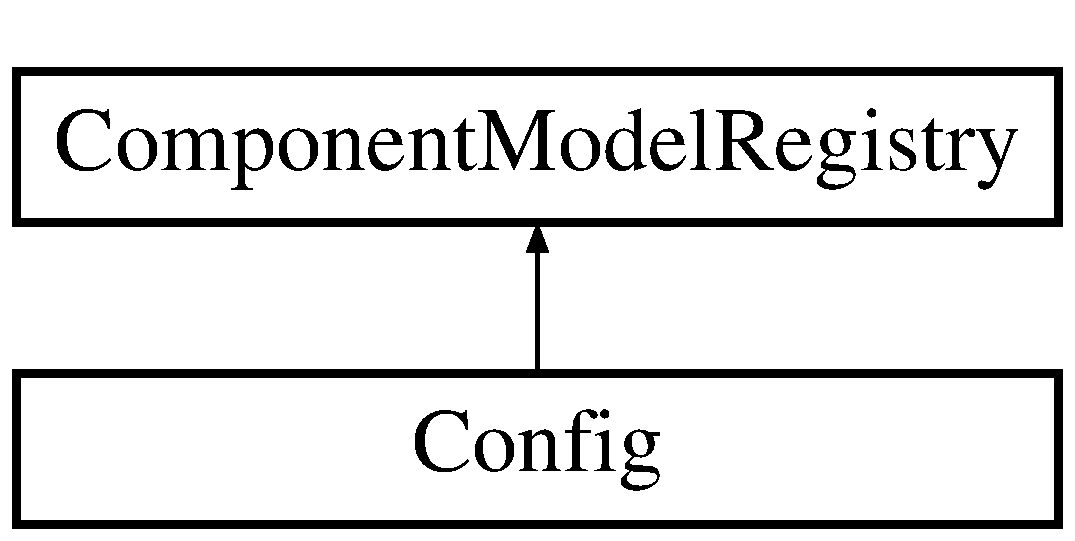
\includegraphics[height=2.000000cm]{class_component_model_registry}
\end{center}
\end{figure}
\subsection*{Classes}
\begin{DoxyCompactItemize}
\item 
struct \hyperlink{struct_component_model_registry_1_1_entity}{Entity}
\end{DoxyCompactItemize}
\subsection*{Public Member Functions}
\begin{DoxyCompactItemize}
\item 
void \hyperlink{class_component_model_registry_a568f894311c2ad30b305e6b1fd93946a}{register\+Object} (const \hyperlink{class_simulator_1_1_object}{Simulator\+::\+Object} \&obj, const std\+::string \&objtype)
\item 
void \hyperlink{class_component_model_registry_a2a2228ef21439a5215265e49cee6eed9}{register\+Property} (const \hyperlink{class_simulator_1_1_object}{Simulator\+::\+Object} \&obj, const std\+::string \&\hyperlink{mtconf_8c_a8f8f80d37794cde9472343e4487ba3eb}{name})
\item 
{\footnotesize template$<$typename T $>$ }\\void \hyperlink{class_component_model_registry_a6b2e1fee7184d8392c47e9865c618a61}{register\+Property} (const \hyperlink{class_simulator_1_1_object}{Simulator\+::\+Object} \&obj, const std\+::string \&\hyperlink{mtconf_8c_a8f8f80d37794cde9472343e4487ba3eb}{name}, const T \&value)
\item 
void \hyperlink{class_component_model_registry_af84094d9ae18ee73e2726b99efd6a014}{register\+Relation} (const \hyperlink{class_simulator_1_1_object}{Simulator\+::\+Object} \&left, const \hyperlink{class_simulator_1_1_object}{Simulator\+::\+Object} \&right, const std\+::string \&\hyperlink{mtconf_8c_a8f8f80d37794cde9472343e4487ba3eb}{name}, bool sibling=false, bool bidi=false)
\item 
{\footnotesize template$<$typename T , typename U $>$ }\\void \hyperlink{class_component_model_registry_a429df2e02198d09d3ede691549119657}{register\+Relation} (const T \&left, const U \&right, const std\+::string \&\hyperlink{mtconf_8c_a8f8f80d37794cde9472343e4487ba3eb}{name}, bool sibling=false)
\item 
{\footnotesize template$<$typename T , typename U $>$ }\\void \hyperlink{class_component_model_registry_a3115e14ef7e333f9e7989ed0fd7b0cef}{register\+Bidi\+Relation} (const T \&left, const U \&right, const std\+::string \&\hyperlink{mtconf_8c_a8f8f80d37794cde9472343e4487ba3eb}{name}, bool sibling=false)
\item 
{\footnotesize template$<$typename T $>$ }\\void \hyperlink{class_component_model_registry_a74afd150d09c9a6c3a9f5ff3e92b3ca7}{register\+Tagged\+Relation} (const \hyperlink{class_simulator_1_1_object}{Simulator\+::\+Object} \&left, const \hyperlink{class_simulator_1_1_object}{Simulator\+::\+Object} \&right, const std\+::string \&\hyperlink{mtconf_8c_a8f8f80d37794cde9472343e4487ba3eb}{name}, const T \&value, bool sibling=false, bool bidi=false)
\item 
{\footnotesize template$<$typename T , typename U , typename V $>$ }\\void \hyperlink{class_component_model_registry_a28709e521e3e64bbcd349095bee31831}{register\+Tagged\+Relation} (const T \&left, const U \&right, const std\+::string \&\hyperlink{mtconf_8c_a8f8f80d37794cde9472343e4487ba3eb}{name}, const V \&value, bool sibling=false)
\item 
{\footnotesize template$<$typename T , typename U , typename V $>$ }\\void \hyperlink{class_component_model_registry_af7d9529c8de84955e3a856241b843640}{register\+Tagged\+Bidi\+Relation} (const T \&left, const U \&right, const std\+::string \&\hyperlink{mtconf_8c_a8f8f80d37794cde9472343e4487ba3eb}{name}, const V \&value, bool sibling=false)
\item 
void \hyperlink{class_component_model_registry_adb491194c93c8031b35c256136b03802}{dump\+Component\+Graph} (std\+::ostream \&out, bool display\+\_\+nodeprops=true, bool display\+\_\+linkprops=true)
\item 
\hyperlink{class_component_model_registry_a2816959e7e85a75fbd46be4e403f1e3f}{Component\+Model\+Registry} ()
\end{DoxyCompactItemize}
\subsection*{Protected Types}
\begin{DoxyCompactItemize}
\item 
typedef const std\+::string $\ast$ \hyperlink{class_component_model_registry_a76ae77a9f2c8f03598f7c45e3450cc49}{Symbol}
\item 
typedef const \hyperlink{class_simulator_1_1_object}{Simulator\+::\+Object} $\ast$ \hyperlink{class_component_model_registry_a315c966cec3143524c002daa7301b054}{Object\+Ref}
\item 
typedef const \hyperlink{struct_component_model_registry_1_1_entity}{Entity} $\ast$ \hyperlink{class_component_model_registry_ad5fd4e46e4b78c737db070735c2ffb16}{Entity\+Ref}
\item 
typedef std\+::pair$<$ \hyperlink{class_component_model_registry_a76ae77a9f2c8f03598f7c45e3450cc49}{Symbol}, \\*
\hyperlink{class_component_model_registry_ad5fd4e46e4b78c737db070735c2ffb16}{Entity\+Ref} $>$ \hyperlink{class_component_model_registry_aec59450251d175f19c49a0c020ba3b8f}{Property}
\item 
typedef std\+::map$<$ \hyperlink{class_component_model_registry_a315c966cec3143524c002daa7301b054}{Object\+Ref}, \\*
std\+::vector$<$ \hyperlink{class_component_model_registry_aec59450251d175f19c49a0c020ba3b8f}{Property} $>$ $>$ \hyperlink{class_component_model_registry_af0083198a2d84ecf7d7d668e5b3e4660}{objprops\+\_\+t}
\item 
typedef std\+::map$<$ std\+::pair\\*
$<$ \hyperlink{class_component_model_registry_a315c966cec3143524c002daa7301b054}{Object\+Ref}, std\+::pair\\*
$<$ \hyperlink{class_component_model_registry_a315c966cec3143524c002daa7301b054}{Object\+Ref}, std\+::pair$<$ bool, \\*
bool $>$ $>$ $>$, std\+::vector\\*
$<$ \hyperlink{class_component_model_registry_aec59450251d175f19c49a0c020ba3b8f}{Property} $>$ $>$ \hyperlink{class_component_model_registry_a05e8f9171449fb800c90abee1a698afb}{linkprops\+\_\+t}
\item 
typedef std\+::map$<$ \hyperlink{class_component_model_registry_a76ae77a9f2c8f03598f7c45e3450cc49}{Symbol}, \\*
std\+::vector$<$ \hyperlink{class_component_model_registry_a76ae77a9f2c8f03598f7c45e3450cc49}{Symbol} $>$ $>$ \hyperlink{class_component_model_registry_a8fb4d43b83df65428c1701f659a8acff}{types\+\_\+t}
\item 
typedef std\+::map$<$ \hyperlink{class_component_model_registry_a76ae77a9f2c8f03598f7c45e3450cc49}{Symbol}, \\*
std\+::map$<$ \hyperlink{class_component_model_registry_a76ae77a9f2c8f03598f7c45e3450cc49}{Symbol}, size\+\_\+t $>$ $>$ \hyperlink{class_component_model_registry_a901d7abbb42dbbf185d37d0a342e6564}{typeattrs\+\_\+t}
\end{DoxyCompactItemize}
\subsection*{Protected Member Functions}
\begin{DoxyCompactItemize}
\item 
void \hyperlink{class_component_model_registry_a23ca85547bf40688838f7691550fbb1b}{print\+Entity} (std\+::ostream \&os, const \hyperlink{struct_component_model_registry_1_1_entity}{Entity} \&e) const 
\item 
\hyperlink{class_component_model_registry_a76ae77a9f2c8f03598f7c45e3450cc49}{Symbol} \hyperlink{class_component_model_registry_a52c0bdf678cfbaa776c11da84b2be8b2}{make\+Symbol} (const std\+::string \&sym)
\item 
\hyperlink{class_component_model_registry_a315c966cec3143524c002daa7301b054}{Object\+Ref} \hyperlink{class_component_model_registry_a61f933c47ad1f6df23ecd13c6b8f54fc}{ref\+Object} (const \hyperlink{class_simulator_1_1_object}{Simulator\+::\+Object} \&obj)
\item 
\hyperlink{class_component_model_registry_ad5fd4e46e4b78c737db070735c2ffb16}{Entity\+Ref} \hyperlink{class_component_model_registry_a88be6f902bcef180d1ba7a83c052bd65}{ref\+Entity} (const \hyperlink{class_component_model_registry_a315c966cec3143524c002daa7301b054}{Object\+Ref} \&obj)
\item 
\hyperlink{class_component_model_registry_ad5fd4e46e4b78c737db070735c2ffb16}{Entity\+Ref} \hyperlink{class_component_model_registry_aaf0b419f650dc2769ed8fc94b36c585f}{ref\+Entity} (const \hyperlink{class_component_model_registry_a76ae77a9f2c8f03598f7c45e3450cc49}{Symbol} \&sym)
\item 
\hyperlink{class_component_model_registry_ad5fd4e46e4b78c737db070735c2ffb16}{Entity\+Ref} \hyperlink{class_component_model_registry_a1db53153b921c0e568558e1c5ef5d413}{ref\+Entity} (const char $\ast$\&str)
\item 
\hyperlink{class_component_model_registry_ad5fd4e46e4b78c737db070735c2ffb16}{Entity\+Ref} \hyperlink{class_component_model_registry_a7fea3f5f2901427a6f2a45c86fceeec4}{ref\+Entity} (const std\+::string \&str)
\item 
\hyperlink{class_component_model_registry_ad5fd4e46e4b78c737db070735c2ffb16}{Entity\+Ref} \hyperlink{class_component_model_registry_a769c5f97ee004cf96ef0bafaefad2e02}{ref\+Entity} (const uint32\+\_\+t \&val)
\item 
\hyperlink{class_component_model_registry_ad5fd4e46e4b78c737db070735c2ffb16}{Entity\+Ref} \hyperlink{class_component_model_registry_ac8b9db2b16f4839e315bc8adda6350c4}{ref\+Entity} (void)
\item 
void \hyperlink{class_component_model_registry_a52d78b0bb749e6f8c5151750fb8ab9a8}{rename\+Objects} (void)
\item 
void \hyperlink{class_component_model_registry_aeb7b7c79422430e85a2b707045c6aa63}{collect\+Properties\+By\+Type} (void)
\item 
virtual \hyperlink{class_component_model_registry_af72d06c3a9416c3dc4070a90a2e6be2b}{$\sim$\+Component\+Model\+Registry} ()
\end{DoxyCompactItemize}
\subsection*{Protected Attributes}
\begin{DoxyCompactItemize}
\item 
std\+::set$<$ std\+::string $>$ \hyperlink{class_component_model_registry_ab66f9920fac78cc986138541f0de8383}{m\+\_\+symbols}
\item 
std\+::map$<$ \hyperlink{class_component_model_registry_a315c966cec3143524c002daa7301b054}{Object\+Ref}, \hyperlink{class_component_model_registry_a76ae77a9f2c8f03598f7c45e3450cc49}{Symbol} $>$ \hyperlink{class_component_model_registry_ae0e32b8bfee83babf0d403c6e3b64f36}{m\+\_\+objects}
\item 
std\+::set$<$ \hyperlink{struct_component_model_registry_1_1_entity}{Entity} $>$ \hyperlink{class_component_model_registry_a2987c2cf0fccf7c4c32beee980548f50}{m\+\_\+entities}
\item 
\hyperlink{class_component_model_registry_af0083198a2d84ecf7d7d668e5b3e4660}{objprops\+\_\+t} \hyperlink{class_component_model_registry_a6fb1e8e4fdcc3dd78909affc77fbad56}{m\+\_\+objprops}
\item 
\hyperlink{class_component_model_registry_a05e8f9171449fb800c90abee1a698afb}{linkprops\+\_\+t} \hyperlink{class_component_model_registry_a80e6aac08b0471a248b1c9eb1a903f96}{m\+\_\+linkprops}
\item 
std\+::map$<$ \hyperlink{class_component_model_registry_a315c966cec3143524c002daa7301b054}{Object\+Ref}, \hyperlink{class_component_model_registry_a76ae77a9f2c8f03598f7c45e3450cc49}{Symbol} $>$ \hyperlink{class_component_model_registry_a41c18375b49c196440c14124ef24ec7e}{m\+\_\+names}
\item 
\hyperlink{class_component_model_registry_a8fb4d43b83df65428c1701f659a8acff}{types\+\_\+t} \hyperlink{class_component_model_registry_a306f1c7a15084c47e5b62d1d9854b804}{m\+\_\+types}
\item 
\hyperlink{class_component_model_registry_a901d7abbb42dbbf185d37d0a342e6564}{typeattrs\+\_\+t} \hyperlink{class_component_model_registry_a75b5f9994f8c432af4e951f160896652}{m\+\_\+typeattrs}
\end{DoxyCompactItemize}


\subsection{Detailed Description}
\hyperlink{class_component_model_registry}{Component\+Model\+Registry}\+: registry for the component structure and properties after the architecture has been set up. 

\subsection{Member Typedef Documentation}
\hypertarget{class_component_model_registry_ad5fd4e46e4b78c737db070735c2ffb16}{\index{Component\+Model\+Registry@{Component\+Model\+Registry}!Entity\+Ref@{Entity\+Ref}}
\index{Entity\+Ref@{Entity\+Ref}!Component\+Model\+Registry@{Component\+Model\+Registry}}
\subsubsection[{Entity\+Ref}]{\setlength{\rightskip}{0pt plus 5cm}typedef const {\bf Entity}$\ast$ {\bf Component\+Model\+Registry\+::\+Entity\+Ref}\hspace{0.3cm}{\ttfamily [protected]}}}\label{class_component_model_registry_ad5fd4e46e4b78c737db070735c2ffb16}
\hypertarget{class_component_model_registry_a05e8f9171449fb800c90abee1a698afb}{\index{Component\+Model\+Registry@{Component\+Model\+Registry}!linkprops\+\_\+t@{linkprops\+\_\+t}}
\index{linkprops\+\_\+t@{linkprops\+\_\+t}!Component\+Model\+Registry@{Component\+Model\+Registry}}
\subsubsection[{linkprops\+\_\+t}]{\setlength{\rightskip}{0pt plus 5cm}typedef std\+::map$<$std\+::pair$<${\bf Object\+Ref}, std\+::pair$<${\bf Object\+Ref}, std\+::pair$<$bool, bool$>$ $>$ $>$, std\+::vector$<${\bf Property}$>$ $>$ {\bf Component\+Model\+Registry\+::linkprops\+\_\+t}\hspace{0.3cm}{\ttfamily [protected]}}}\label{class_component_model_registry_a05e8f9171449fb800c90abee1a698afb}
\hypertarget{class_component_model_registry_a315c966cec3143524c002daa7301b054}{\index{Component\+Model\+Registry@{Component\+Model\+Registry}!Object\+Ref@{Object\+Ref}}
\index{Object\+Ref@{Object\+Ref}!Component\+Model\+Registry@{Component\+Model\+Registry}}
\subsubsection[{Object\+Ref}]{\setlength{\rightskip}{0pt plus 5cm}typedef const {\bf Simulator\+::\+Object}$\ast$ {\bf Component\+Model\+Registry\+::\+Object\+Ref}\hspace{0.3cm}{\ttfamily [protected]}}}\label{class_component_model_registry_a315c966cec3143524c002daa7301b054}
\hypertarget{class_component_model_registry_af0083198a2d84ecf7d7d668e5b3e4660}{\index{Component\+Model\+Registry@{Component\+Model\+Registry}!objprops\+\_\+t@{objprops\+\_\+t}}
\index{objprops\+\_\+t@{objprops\+\_\+t}!Component\+Model\+Registry@{Component\+Model\+Registry}}
\subsubsection[{objprops\+\_\+t}]{\setlength{\rightskip}{0pt plus 5cm}typedef std\+::map$<${\bf Object\+Ref}, std\+::vector$<${\bf Property}$>$ $>$ {\bf Component\+Model\+Registry\+::objprops\+\_\+t}\hspace{0.3cm}{\ttfamily [protected]}}}\label{class_component_model_registry_af0083198a2d84ecf7d7d668e5b3e4660}
\hypertarget{class_component_model_registry_aec59450251d175f19c49a0c020ba3b8f}{\index{Component\+Model\+Registry@{Component\+Model\+Registry}!Property@{Property}}
\index{Property@{Property}!Component\+Model\+Registry@{Component\+Model\+Registry}}
\subsubsection[{Property}]{\setlength{\rightskip}{0pt plus 5cm}typedef std\+::pair$<${\bf Symbol}, {\bf Entity\+Ref}$>$ {\bf Component\+Model\+Registry\+::\+Property}\hspace{0.3cm}{\ttfamily [protected]}}}\label{class_component_model_registry_aec59450251d175f19c49a0c020ba3b8f}
\hypertarget{class_component_model_registry_a76ae77a9f2c8f03598f7c45e3450cc49}{\index{Component\+Model\+Registry@{Component\+Model\+Registry}!Symbol@{Symbol}}
\index{Symbol@{Symbol}!Component\+Model\+Registry@{Component\+Model\+Registry}}
\subsubsection[{Symbol}]{\setlength{\rightskip}{0pt plus 5cm}typedef const std\+::string$\ast$ {\bf Component\+Model\+Registry\+::\+Symbol}\hspace{0.3cm}{\ttfamily [protected]}}}\label{class_component_model_registry_a76ae77a9f2c8f03598f7c45e3450cc49}
\hypertarget{class_component_model_registry_a901d7abbb42dbbf185d37d0a342e6564}{\index{Component\+Model\+Registry@{Component\+Model\+Registry}!typeattrs\+\_\+t@{typeattrs\+\_\+t}}
\index{typeattrs\+\_\+t@{typeattrs\+\_\+t}!Component\+Model\+Registry@{Component\+Model\+Registry}}
\subsubsection[{typeattrs\+\_\+t}]{\setlength{\rightskip}{0pt plus 5cm}typedef std\+::map$<${\bf Symbol}, std\+::map$<${\bf Symbol}, size\+\_\+t$>$ $>$ {\bf Component\+Model\+Registry\+::typeattrs\+\_\+t}\hspace{0.3cm}{\ttfamily [protected]}}}\label{class_component_model_registry_a901d7abbb42dbbf185d37d0a342e6564}
\hypertarget{class_component_model_registry_a8fb4d43b83df65428c1701f659a8acff}{\index{Component\+Model\+Registry@{Component\+Model\+Registry}!types\+\_\+t@{types\+\_\+t}}
\index{types\+\_\+t@{types\+\_\+t}!Component\+Model\+Registry@{Component\+Model\+Registry}}
\subsubsection[{types\+\_\+t}]{\setlength{\rightskip}{0pt plus 5cm}typedef std\+::map$<${\bf Symbol}, std\+::vector$<${\bf Symbol}$>$ $>$ {\bf Component\+Model\+Registry\+::types\+\_\+t}\hspace{0.3cm}{\ttfamily [protected]}}}\label{class_component_model_registry_a8fb4d43b83df65428c1701f659a8acff}


\subsection{Constructor \& Destructor Documentation}
\hypertarget{class_component_model_registry_a2816959e7e85a75fbd46be4e403f1e3f}{\index{Component\+Model\+Registry@{Component\+Model\+Registry}!Component\+Model\+Registry@{Component\+Model\+Registry}}
\index{Component\+Model\+Registry@{Component\+Model\+Registry}!Component\+Model\+Registry@{Component\+Model\+Registry}}
\subsubsection[{Component\+Model\+Registry}]{\setlength{\rightskip}{0pt plus 5cm}Component\+Model\+Registry\+::\+Component\+Model\+Registry (
\begin{DoxyParamCaption}
{}
\end{DoxyParamCaption}
)\hspace{0.3cm}{\ttfamily [inline]}}}\label{class_component_model_registry_a2816959e7e85a75fbd46be4e403f1e3f}
\hypertarget{class_component_model_registry_af72d06c3a9416c3dc4070a90a2e6be2b}{\index{Component\+Model\+Registry@{Component\+Model\+Registry}!````~Component\+Model\+Registry@{$\sim$\+Component\+Model\+Registry}}
\index{````~Component\+Model\+Registry@{$\sim$\+Component\+Model\+Registry}!Component\+Model\+Registry@{Component\+Model\+Registry}}
\subsubsection[{$\sim$\+Component\+Model\+Registry}]{\setlength{\rightskip}{0pt plus 5cm}virtual Component\+Model\+Registry\+::$\sim$\+Component\+Model\+Registry (
\begin{DoxyParamCaption}
{}
\end{DoxyParamCaption}
)\hspace{0.3cm}{\ttfamily [inline]}, {\ttfamily [protected]}, {\ttfamily [virtual]}}}\label{class_component_model_registry_af72d06c3a9416c3dc4070a90a2e6be2b}


\subsection{Member Function Documentation}
\hypertarget{class_component_model_registry_aeb7b7c79422430e85a2b707045c6aa63}{\index{Component\+Model\+Registry@{Component\+Model\+Registry}!collect\+Properties\+By\+Type@{collect\+Properties\+By\+Type}}
\index{collect\+Properties\+By\+Type@{collect\+Properties\+By\+Type}!Component\+Model\+Registry@{Component\+Model\+Registry}}
\subsubsection[{collect\+Properties\+By\+Type}]{\setlength{\rightskip}{0pt plus 5cm}void Component\+Model\+Registry\+::collect\+Properties\+By\+Type (
\begin{DoxyParamCaption}
\item[{void}]{}
\end{DoxyParamCaption}
)\hspace{0.3cm}{\ttfamily [protected]}}}\label{class_component_model_registry_aeb7b7c79422430e85a2b707045c6aa63}
\hypertarget{class_component_model_registry_adb491194c93c8031b35c256136b03802}{\index{Component\+Model\+Registry@{Component\+Model\+Registry}!dump\+Component\+Graph@{dump\+Component\+Graph}}
\index{dump\+Component\+Graph@{dump\+Component\+Graph}!Component\+Model\+Registry@{Component\+Model\+Registry}}
\subsubsection[{dump\+Component\+Graph}]{\setlength{\rightskip}{0pt plus 5cm}void Component\+Model\+Registry\+::dump\+Component\+Graph (
\begin{DoxyParamCaption}
\item[{std\+::ostream \&}]{out, }
\item[{bool}]{display\+\_\+nodeprops = {\ttfamily true}, }
\item[{bool}]{display\+\_\+linkprops = {\ttfamily true}}
\end{DoxyParamCaption}
)}}\label{class_component_model_registry_adb491194c93c8031b35c256136b03802}
\hypertarget{class_component_model_registry_a52c0bdf678cfbaa776c11da84b2be8b2}{\index{Component\+Model\+Registry@{Component\+Model\+Registry}!make\+Symbol@{make\+Symbol}}
\index{make\+Symbol@{make\+Symbol}!Component\+Model\+Registry@{Component\+Model\+Registry}}
\subsubsection[{make\+Symbol}]{\setlength{\rightskip}{0pt plus 5cm}{\bf Component\+Model\+Registry\+::\+Symbol} Component\+Model\+Registry\+::make\+Symbol (
\begin{DoxyParamCaption}
\item[{const std\+::string \&}]{sym}
\end{DoxyParamCaption}
)\hspace{0.3cm}{\ttfamily [protected]}}}\label{class_component_model_registry_a52c0bdf678cfbaa776c11da84b2be8b2}
\hypertarget{class_component_model_registry_a23ca85547bf40688838f7691550fbb1b}{\index{Component\+Model\+Registry@{Component\+Model\+Registry}!print\+Entity@{print\+Entity}}
\index{print\+Entity@{print\+Entity}!Component\+Model\+Registry@{Component\+Model\+Registry}}
\subsubsection[{print\+Entity}]{\setlength{\rightskip}{0pt plus 5cm}void Component\+Model\+Registry\+::print\+Entity (
\begin{DoxyParamCaption}
\item[{std\+::ostream \&}]{os, }
\item[{const {\bf Entity} \&}]{e}
\end{DoxyParamCaption}
) const\hspace{0.3cm}{\ttfamily [protected]}}}\label{class_component_model_registry_a23ca85547bf40688838f7691550fbb1b}
\hypertarget{class_component_model_registry_a88be6f902bcef180d1ba7a83c052bd65}{\index{Component\+Model\+Registry@{Component\+Model\+Registry}!ref\+Entity@{ref\+Entity}}
\index{ref\+Entity@{ref\+Entity}!Component\+Model\+Registry@{Component\+Model\+Registry}}
\subsubsection[{ref\+Entity}]{\setlength{\rightskip}{0pt plus 5cm}{\bf Component\+Model\+Registry\+::\+Entity\+Ref} Component\+Model\+Registry\+::ref\+Entity (
\begin{DoxyParamCaption}
\item[{const {\bf Object\+Ref} \&}]{obj}
\end{DoxyParamCaption}
)\hspace{0.3cm}{\ttfamily [protected]}}}\label{class_component_model_registry_a88be6f902bcef180d1ba7a83c052bd65}
\hypertarget{class_component_model_registry_aaf0b419f650dc2769ed8fc94b36c585f}{\index{Component\+Model\+Registry@{Component\+Model\+Registry}!ref\+Entity@{ref\+Entity}}
\index{ref\+Entity@{ref\+Entity}!Component\+Model\+Registry@{Component\+Model\+Registry}}
\subsubsection[{ref\+Entity}]{\setlength{\rightskip}{0pt plus 5cm}{\bf Component\+Model\+Registry\+::\+Entity\+Ref} Component\+Model\+Registry\+::ref\+Entity (
\begin{DoxyParamCaption}
\item[{const {\bf Symbol} \&}]{sym}
\end{DoxyParamCaption}
)\hspace{0.3cm}{\ttfamily [protected]}}}\label{class_component_model_registry_aaf0b419f650dc2769ed8fc94b36c585f}
\hypertarget{class_component_model_registry_a1db53153b921c0e568558e1c5ef5d413}{\index{Component\+Model\+Registry@{Component\+Model\+Registry}!ref\+Entity@{ref\+Entity}}
\index{ref\+Entity@{ref\+Entity}!Component\+Model\+Registry@{Component\+Model\+Registry}}
\subsubsection[{ref\+Entity}]{\setlength{\rightskip}{0pt plus 5cm}{\bf Entity\+Ref} Component\+Model\+Registry\+::ref\+Entity (
\begin{DoxyParamCaption}
\item[{const char $\ast$\&}]{str}
\end{DoxyParamCaption}
)\hspace{0.3cm}{\ttfamily [inline]}, {\ttfamily [protected]}}}\label{class_component_model_registry_a1db53153b921c0e568558e1c5ef5d413}
\hypertarget{class_component_model_registry_a7fea3f5f2901427a6f2a45c86fceeec4}{\index{Component\+Model\+Registry@{Component\+Model\+Registry}!ref\+Entity@{ref\+Entity}}
\index{ref\+Entity@{ref\+Entity}!Component\+Model\+Registry@{Component\+Model\+Registry}}
\subsubsection[{ref\+Entity}]{\setlength{\rightskip}{0pt plus 5cm}{\bf Entity\+Ref} Component\+Model\+Registry\+::ref\+Entity (
\begin{DoxyParamCaption}
\item[{const std\+::string \&}]{str}
\end{DoxyParamCaption}
)\hspace{0.3cm}{\ttfamily [inline]}, {\ttfamily [protected]}}}\label{class_component_model_registry_a7fea3f5f2901427a6f2a45c86fceeec4}
\hypertarget{class_component_model_registry_a769c5f97ee004cf96ef0bafaefad2e02}{\index{Component\+Model\+Registry@{Component\+Model\+Registry}!ref\+Entity@{ref\+Entity}}
\index{ref\+Entity@{ref\+Entity}!Component\+Model\+Registry@{Component\+Model\+Registry}}
\subsubsection[{ref\+Entity}]{\setlength{\rightskip}{0pt plus 5cm}{\bf Component\+Model\+Registry\+::\+Entity\+Ref} Component\+Model\+Registry\+::ref\+Entity (
\begin{DoxyParamCaption}
\item[{const uint32\+\_\+t \&}]{val}
\end{DoxyParamCaption}
)\hspace{0.3cm}{\ttfamily [protected]}}}\label{class_component_model_registry_a769c5f97ee004cf96ef0bafaefad2e02}
\hypertarget{class_component_model_registry_ac8b9db2b16f4839e315bc8adda6350c4}{\index{Component\+Model\+Registry@{Component\+Model\+Registry}!ref\+Entity@{ref\+Entity}}
\index{ref\+Entity@{ref\+Entity}!Component\+Model\+Registry@{Component\+Model\+Registry}}
\subsubsection[{ref\+Entity}]{\setlength{\rightskip}{0pt plus 5cm}{\bf Component\+Model\+Registry\+::\+Entity\+Ref} Component\+Model\+Registry\+::ref\+Entity (
\begin{DoxyParamCaption}
\item[{void}]{}
\end{DoxyParamCaption}
)\hspace{0.3cm}{\ttfamily [protected]}}}\label{class_component_model_registry_ac8b9db2b16f4839e315bc8adda6350c4}
\hypertarget{class_component_model_registry_a61f933c47ad1f6df23ecd13c6b8f54fc}{\index{Component\+Model\+Registry@{Component\+Model\+Registry}!ref\+Object@{ref\+Object}}
\index{ref\+Object@{ref\+Object}!Component\+Model\+Registry@{Component\+Model\+Registry}}
\subsubsection[{ref\+Object}]{\setlength{\rightskip}{0pt plus 5cm}{\bf Component\+Model\+Registry\+::\+Object\+Ref} Component\+Model\+Registry\+::ref\+Object (
\begin{DoxyParamCaption}
\item[{const {\bf Simulator\+::\+Object} \&}]{obj}
\end{DoxyParamCaption}
)\hspace{0.3cm}{\ttfamily [protected]}}}\label{class_component_model_registry_a61f933c47ad1f6df23ecd13c6b8f54fc}
\hypertarget{class_component_model_registry_a3115e14ef7e333f9e7989ed0fd7b0cef}{\index{Component\+Model\+Registry@{Component\+Model\+Registry}!register\+Bidi\+Relation@{register\+Bidi\+Relation}}
\index{register\+Bidi\+Relation@{register\+Bidi\+Relation}!Component\+Model\+Registry@{Component\+Model\+Registry}}
\subsubsection[{register\+Bidi\+Relation}]{\setlength{\rightskip}{0pt plus 5cm}template$<$typename T , typename U $>$ void Component\+Model\+Registry\+::register\+Bidi\+Relation (
\begin{DoxyParamCaption}
\item[{const T \&}]{left, }
\item[{const U \&}]{right, }
\item[{const std\+::string \&}]{name, }
\item[{bool}]{sibling = {\ttfamily false}}
\end{DoxyParamCaption}
)\hspace{0.3cm}{\ttfamily [inline]}}}\label{class_component_model_registry_a3115e14ef7e333f9e7989ed0fd7b0cef}
\hypertarget{class_component_model_registry_a568f894311c2ad30b305e6b1fd93946a}{\index{Component\+Model\+Registry@{Component\+Model\+Registry}!register\+Object@{register\+Object}}
\index{register\+Object@{register\+Object}!Component\+Model\+Registry@{Component\+Model\+Registry}}
\subsubsection[{register\+Object}]{\setlength{\rightskip}{0pt plus 5cm}void Component\+Model\+Registry\+::register\+Object (
\begin{DoxyParamCaption}
\item[{const {\bf Simulator\+::\+Object} \&}]{obj, }
\item[{const std\+::string \&}]{objtype}
\end{DoxyParamCaption}
)}}\label{class_component_model_registry_a568f894311c2ad30b305e6b1fd93946a}
\hypertarget{class_component_model_registry_a2a2228ef21439a5215265e49cee6eed9}{\index{Component\+Model\+Registry@{Component\+Model\+Registry}!register\+Property@{register\+Property}}
\index{register\+Property@{register\+Property}!Component\+Model\+Registry@{Component\+Model\+Registry}}
\subsubsection[{register\+Property}]{\setlength{\rightskip}{0pt plus 5cm}void Component\+Model\+Registry\+::register\+Property (
\begin{DoxyParamCaption}
\item[{const {\bf Simulator\+::\+Object} \&}]{obj, }
\item[{const std\+::string \&}]{name}
\end{DoxyParamCaption}
)\hspace{0.3cm}{\ttfamily [inline]}}}\label{class_component_model_registry_a2a2228ef21439a5215265e49cee6eed9}
\hypertarget{class_component_model_registry_a6b2e1fee7184d8392c47e9865c618a61}{\index{Component\+Model\+Registry@{Component\+Model\+Registry}!register\+Property@{register\+Property}}
\index{register\+Property@{register\+Property}!Component\+Model\+Registry@{Component\+Model\+Registry}}
\subsubsection[{register\+Property}]{\setlength{\rightskip}{0pt plus 5cm}template$<$typename T $>$ void Component\+Model\+Registry\+::register\+Property (
\begin{DoxyParamCaption}
\item[{const {\bf Simulator\+::\+Object} \&}]{obj, }
\item[{const std\+::string \&}]{name, }
\item[{const T \&}]{value}
\end{DoxyParamCaption}
)\hspace{0.3cm}{\ttfamily [inline]}}}\label{class_component_model_registry_a6b2e1fee7184d8392c47e9865c618a61}
\hypertarget{class_component_model_registry_af84094d9ae18ee73e2726b99efd6a014}{\index{Component\+Model\+Registry@{Component\+Model\+Registry}!register\+Relation@{register\+Relation}}
\index{register\+Relation@{register\+Relation}!Component\+Model\+Registry@{Component\+Model\+Registry}}
\subsubsection[{register\+Relation}]{\setlength{\rightskip}{0pt plus 5cm}void Component\+Model\+Registry\+::register\+Relation (
\begin{DoxyParamCaption}
\item[{const {\bf Simulator\+::\+Object} \&}]{left, }
\item[{const {\bf Simulator\+::\+Object} \&}]{right, }
\item[{const std\+::string \&}]{name, }
\item[{bool}]{sibling = {\ttfamily false}, }
\item[{bool}]{bidi = {\ttfamily false}}
\end{DoxyParamCaption}
)\hspace{0.3cm}{\ttfamily [inline]}}}\label{class_component_model_registry_af84094d9ae18ee73e2726b99efd6a014}
\hypertarget{class_component_model_registry_a429df2e02198d09d3ede691549119657}{\index{Component\+Model\+Registry@{Component\+Model\+Registry}!register\+Relation@{register\+Relation}}
\index{register\+Relation@{register\+Relation}!Component\+Model\+Registry@{Component\+Model\+Registry}}
\subsubsection[{register\+Relation}]{\setlength{\rightskip}{0pt plus 5cm}template$<$typename T , typename U $>$ void Component\+Model\+Registry\+::register\+Relation (
\begin{DoxyParamCaption}
\item[{const T \&}]{left, }
\item[{const U \&}]{right, }
\item[{const std\+::string \&}]{name, }
\item[{bool}]{sibling = {\ttfamily false}}
\end{DoxyParamCaption}
)\hspace{0.3cm}{\ttfamily [inline]}}}\label{class_component_model_registry_a429df2e02198d09d3ede691549119657}
\hypertarget{class_component_model_registry_af7d9529c8de84955e3a856241b843640}{\index{Component\+Model\+Registry@{Component\+Model\+Registry}!register\+Tagged\+Bidi\+Relation@{register\+Tagged\+Bidi\+Relation}}
\index{register\+Tagged\+Bidi\+Relation@{register\+Tagged\+Bidi\+Relation}!Component\+Model\+Registry@{Component\+Model\+Registry}}
\subsubsection[{register\+Tagged\+Bidi\+Relation}]{\setlength{\rightskip}{0pt plus 5cm}template$<$typename T , typename U , typename V $>$ void Component\+Model\+Registry\+::register\+Tagged\+Bidi\+Relation (
\begin{DoxyParamCaption}
\item[{const T \&}]{left, }
\item[{const U \&}]{right, }
\item[{const std\+::string \&}]{name, }
\item[{const V \&}]{value, }
\item[{bool}]{sibling = {\ttfamily false}}
\end{DoxyParamCaption}
)\hspace{0.3cm}{\ttfamily [inline]}}}\label{class_component_model_registry_af7d9529c8de84955e3a856241b843640}
\hypertarget{class_component_model_registry_a74afd150d09c9a6c3a9f5ff3e92b3ca7}{\index{Component\+Model\+Registry@{Component\+Model\+Registry}!register\+Tagged\+Relation@{register\+Tagged\+Relation}}
\index{register\+Tagged\+Relation@{register\+Tagged\+Relation}!Component\+Model\+Registry@{Component\+Model\+Registry}}
\subsubsection[{register\+Tagged\+Relation}]{\setlength{\rightskip}{0pt plus 5cm}template$<$typename T $>$ void Component\+Model\+Registry\+::register\+Tagged\+Relation (
\begin{DoxyParamCaption}
\item[{const {\bf Simulator\+::\+Object} \&}]{left, }
\item[{const {\bf Simulator\+::\+Object} \&}]{right, }
\item[{const std\+::string \&}]{name, }
\item[{const T \&}]{value, }
\item[{bool}]{sibling = {\ttfamily false}, }
\item[{bool}]{bidi = {\ttfamily false}}
\end{DoxyParamCaption}
)\hspace{0.3cm}{\ttfamily [inline]}}}\label{class_component_model_registry_a74afd150d09c9a6c3a9f5ff3e92b3ca7}
\hypertarget{class_component_model_registry_a28709e521e3e64bbcd349095bee31831}{\index{Component\+Model\+Registry@{Component\+Model\+Registry}!register\+Tagged\+Relation@{register\+Tagged\+Relation}}
\index{register\+Tagged\+Relation@{register\+Tagged\+Relation}!Component\+Model\+Registry@{Component\+Model\+Registry}}
\subsubsection[{register\+Tagged\+Relation}]{\setlength{\rightskip}{0pt plus 5cm}template$<$typename T , typename U , typename V $>$ void Component\+Model\+Registry\+::register\+Tagged\+Relation (
\begin{DoxyParamCaption}
\item[{const T \&}]{left, }
\item[{const U \&}]{right, }
\item[{const std\+::string \&}]{name, }
\item[{const V \&}]{value, }
\item[{bool}]{sibling = {\ttfamily false}}
\end{DoxyParamCaption}
)\hspace{0.3cm}{\ttfamily [inline]}}}\label{class_component_model_registry_a28709e521e3e64bbcd349095bee31831}
\hypertarget{class_component_model_registry_a52d78b0bb749e6f8c5151750fb8ab9a8}{\index{Component\+Model\+Registry@{Component\+Model\+Registry}!rename\+Objects@{rename\+Objects}}
\index{rename\+Objects@{rename\+Objects}!Component\+Model\+Registry@{Component\+Model\+Registry}}
\subsubsection[{rename\+Objects}]{\setlength{\rightskip}{0pt plus 5cm}void Component\+Model\+Registry\+::rename\+Objects (
\begin{DoxyParamCaption}
\item[{void}]{}
\end{DoxyParamCaption}
)\hspace{0.3cm}{\ttfamily [protected]}}}\label{class_component_model_registry_a52d78b0bb749e6f8c5151750fb8ab9a8}


\subsection{Member Data Documentation}
\hypertarget{class_component_model_registry_a2987c2cf0fccf7c4c32beee980548f50}{\index{Component\+Model\+Registry@{Component\+Model\+Registry}!m\+\_\+entities@{m\+\_\+entities}}
\index{m\+\_\+entities@{m\+\_\+entities}!Component\+Model\+Registry@{Component\+Model\+Registry}}
\subsubsection[{m\+\_\+entities}]{\setlength{\rightskip}{0pt plus 5cm}std\+::set$<${\bf Entity}$>$ Component\+Model\+Registry\+::m\+\_\+entities\hspace{0.3cm}{\ttfamily [protected]}}}\label{class_component_model_registry_a2987c2cf0fccf7c4c32beee980548f50}
\hypertarget{class_component_model_registry_a80e6aac08b0471a248b1c9eb1a903f96}{\index{Component\+Model\+Registry@{Component\+Model\+Registry}!m\+\_\+linkprops@{m\+\_\+linkprops}}
\index{m\+\_\+linkprops@{m\+\_\+linkprops}!Component\+Model\+Registry@{Component\+Model\+Registry}}
\subsubsection[{m\+\_\+linkprops}]{\setlength{\rightskip}{0pt plus 5cm}{\bf linkprops\+\_\+t} Component\+Model\+Registry\+::m\+\_\+linkprops\hspace{0.3cm}{\ttfamily [protected]}}}\label{class_component_model_registry_a80e6aac08b0471a248b1c9eb1a903f96}
\hypertarget{class_component_model_registry_a41c18375b49c196440c14124ef24ec7e}{\index{Component\+Model\+Registry@{Component\+Model\+Registry}!m\+\_\+names@{m\+\_\+names}}
\index{m\+\_\+names@{m\+\_\+names}!Component\+Model\+Registry@{Component\+Model\+Registry}}
\subsubsection[{m\+\_\+names}]{\setlength{\rightskip}{0pt plus 5cm}std\+::map$<${\bf Object\+Ref}, {\bf Symbol}$>$ Component\+Model\+Registry\+::m\+\_\+names\hspace{0.3cm}{\ttfamily [protected]}}}\label{class_component_model_registry_a41c18375b49c196440c14124ef24ec7e}
\hypertarget{class_component_model_registry_ae0e32b8bfee83babf0d403c6e3b64f36}{\index{Component\+Model\+Registry@{Component\+Model\+Registry}!m\+\_\+objects@{m\+\_\+objects}}
\index{m\+\_\+objects@{m\+\_\+objects}!Component\+Model\+Registry@{Component\+Model\+Registry}}
\subsubsection[{m\+\_\+objects}]{\setlength{\rightskip}{0pt plus 5cm}std\+::map$<${\bf Object\+Ref}, {\bf Symbol}$>$ Component\+Model\+Registry\+::m\+\_\+objects\hspace{0.3cm}{\ttfamily [protected]}}}\label{class_component_model_registry_ae0e32b8bfee83babf0d403c6e3b64f36}
\hypertarget{class_component_model_registry_a6fb1e8e4fdcc3dd78909affc77fbad56}{\index{Component\+Model\+Registry@{Component\+Model\+Registry}!m\+\_\+objprops@{m\+\_\+objprops}}
\index{m\+\_\+objprops@{m\+\_\+objprops}!Component\+Model\+Registry@{Component\+Model\+Registry}}
\subsubsection[{m\+\_\+objprops}]{\setlength{\rightskip}{0pt plus 5cm}{\bf objprops\+\_\+t} Component\+Model\+Registry\+::m\+\_\+objprops\hspace{0.3cm}{\ttfamily [protected]}}}\label{class_component_model_registry_a6fb1e8e4fdcc3dd78909affc77fbad56}
\hypertarget{class_component_model_registry_ab66f9920fac78cc986138541f0de8383}{\index{Component\+Model\+Registry@{Component\+Model\+Registry}!m\+\_\+symbols@{m\+\_\+symbols}}
\index{m\+\_\+symbols@{m\+\_\+symbols}!Component\+Model\+Registry@{Component\+Model\+Registry}}
\subsubsection[{m\+\_\+symbols}]{\setlength{\rightskip}{0pt plus 5cm}std\+::set$<$std\+::string$>$ Component\+Model\+Registry\+::m\+\_\+symbols\hspace{0.3cm}{\ttfamily [protected]}}}\label{class_component_model_registry_ab66f9920fac78cc986138541f0de8383}
\hypertarget{class_component_model_registry_a75b5f9994f8c432af4e951f160896652}{\index{Component\+Model\+Registry@{Component\+Model\+Registry}!m\+\_\+typeattrs@{m\+\_\+typeattrs}}
\index{m\+\_\+typeattrs@{m\+\_\+typeattrs}!Component\+Model\+Registry@{Component\+Model\+Registry}}
\subsubsection[{m\+\_\+typeattrs}]{\setlength{\rightskip}{0pt plus 5cm}{\bf typeattrs\+\_\+t} Component\+Model\+Registry\+::m\+\_\+typeattrs\hspace{0.3cm}{\ttfamily [protected]}}}\label{class_component_model_registry_a75b5f9994f8c432af4e951f160896652}
\hypertarget{class_component_model_registry_a306f1c7a15084c47e5b62d1d9854b804}{\index{Component\+Model\+Registry@{Component\+Model\+Registry}!m\+\_\+types@{m\+\_\+types}}
\index{m\+\_\+types@{m\+\_\+types}!Component\+Model\+Registry@{Component\+Model\+Registry}}
\subsubsection[{m\+\_\+types}]{\setlength{\rightskip}{0pt plus 5cm}{\bf types\+\_\+t} Component\+Model\+Registry\+::m\+\_\+types\hspace{0.3cm}{\ttfamily [protected]}}}\label{class_component_model_registry_a306f1c7a15084c47e5b62d1d9854b804}


The documentation for this class was generated from the following files\+:\begin{DoxyCompactItemize}
\item 
sim/\hyperlink{config_8h}{config.\+h}\item 
sim/\hyperlink{config_8cpp}{config.\+cpp}\end{DoxyCompactItemize}

\hypertarget{class_config}{\section{Config Class Reference}
\label{class_config}\index{Config@{Config}}
}


\hyperlink{class_config}{Config} class used by the simulation.  




{\ttfamily \#include $<$config.\+h$>$}

Inheritance diagram for Config\+:\begin{figure}[H]
\begin{center}
\leavevmode
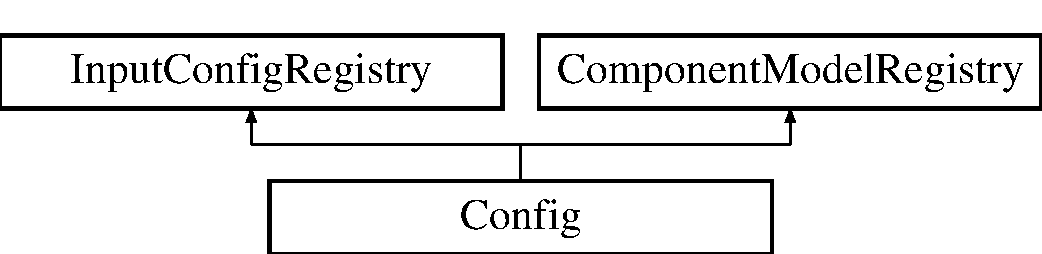
\includegraphics[height=2.000000cm]{class_config}
\end{center}
\end{figure}
\subsection*{Public Member Functions}
\begin{DoxyCompactItemize}
\item 
\hyperlink{class_config_a18fcc503da71ce7f6ed7a5ab22e92f9f}{Config} (const \hyperlink{class_config_map}{Config\+Map} \&defaults, const \hyperlink{class_config_map}{Config\+Map} \&overrides, const std\+::vector$<$ std\+::string $>$ \&argv)
\item 
std\+::vector$<$ uint32\+\_\+t $>$ \hyperlink{class_config_ace6137d7a0349d86d46104d549b36ca4}{Get\+Conf\+Words} ()
\end{DoxyCompactItemize}
\subsection*{Additional Inherited Members}


\subsection{Detailed Description}
\hyperlink{class_config}{Config} class used by the simulation. 

\subsection{Constructor \& Destructor Documentation}
\hypertarget{class_config_a18fcc503da71ce7f6ed7a5ab22e92f9f}{\index{Config@{Config}!Config@{Config}}
\index{Config@{Config}!Config@{Config}}
\subsubsection[{Config}]{\setlength{\rightskip}{0pt plus 5cm}Config\+::\+Config (
\begin{DoxyParamCaption}
\item[{const {\bf Config\+Map} \&}]{defaults, }
\item[{const {\bf Config\+Map} \&}]{overrides, }
\item[{const std\+::vector$<$ std\+::string $>$ \&}]{argv}
\end{DoxyParamCaption}
)\hspace{0.3cm}{\ttfamily [inline]}}}\label{class_config_a18fcc503da71ce7f6ed7a5ab22e92f9f}


\subsection{Member Function Documentation}
\hypertarget{class_config_ace6137d7a0349d86d46104d549b36ca4}{\index{Config@{Config}!Get\+Conf\+Words@{Get\+Conf\+Words}}
\index{Get\+Conf\+Words@{Get\+Conf\+Words}!Config@{Config}}
\subsubsection[{Get\+Conf\+Words}]{\setlength{\rightskip}{0pt plus 5cm}vector$<$ uint32\+\_\+t $>$ Config\+::\+Get\+Conf\+Words (
\begin{DoxyParamCaption}
{}
\end{DoxyParamCaption}
)}}\label{class_config_ace6137d7a0349d86d46104d549b36ca4}


The documentation for this class was generated from the following files\+:\begin{DoxyCompactItemize}
\item 
sim/\hyperlink{config_8h}{config.\+h}\item 
sim/\hyperlink{config_8cpp}{config.\+cpp}\end{DoxyCompactItemize}

\hypertarget{class_config_map}{\section{Config\+Map Class Reference}
\label{class_config_map}\index{Config\+Map@{Config\+Map}}
}


{\ttfamily \#include $<$config.\+h$>$}

\subsection*{Public Member Functions}
\begin{DoxyCompactItemize}
\item 
void \hyperlink{class_config_map_a5590afa6e9b3e85be43879479b30e909}{append} (const std\+::string \&key, const std\+::string \&value)
\item 
map\+\_\+t\+::const\+\_\+iterator \hyperlink{class_config_map_a172a76c29eeaf864a5a47e170ff82350}{begin} () const 
\item 
map\+\_\+t\+::const\+\_\+iterator \hyperlink{class_config_map_ad3421fbf65b22cefbe76a33a7703cdec}{end} () const 
\item 
reverse\+\_\+proxy$<$ map\+\_\+t $>$ \hyperlink{class_config_map_a62cd557e13320824d742a5080af70bf5}{reverse} () const 
\item 
\hyperlink{class_config_map_a6687f2fd0d93892c0068cb15be965197}{Config\+Map} ()
\end{DoxyCompactItemize}


\subsection{Detailed Description}
\hyperlink{class_input_config_registry}{Input\+Config\+Registry}\+: registry for configuration values provided before the simulation starts. 

\subsection{Constructor \& Destructor Documentation}
\hypertarget{class_config_map_a6687f2fd0d93892c0068cb15be965197}{\index{Config\+Map@{Config\+Map}!Config\+Map@{Config\+Map}}
\index{Config\+Map@{Config\+Map}!Config\+Map@{Config\+Map}}
\subsubsection[{Config\+Map}]{\setlength{\rightskip}{0pt plus 5cm}Config\+Map\+::\+Config\+Map (
\begin{DoxyParamCaption}
{}
\end{DoxyParamCaption}
)\hspace{0.3cm}{\ttfamily [inline]}}}\label{class_config_map_a6687f2fd0d93892c0068cb15be965197}


\subsection{Member Function Documentation}
\hypertarget{class_config_map_a5590afa6e9b3e85be43879479b30e909}{\index{Config\+Map@{Config\+Map}!append@{append}}
\index{append@{append}!Config\+Map@{Config\+Map}}
\subsubsection[{append}]{\setlength{\rightskip}{0pt plus 5cm}void Config\+Map\+::append (
\begin{DoxyParamCaption}
\item[{const std\+::string \&}]{key, }
\item[{const std\+::string \&}]{value}
\end{DoxyParamCaption}
)}}\label{class_config_map_a5590afa6e9b3e85be43879479b30e909}
\hypertarget{class_config_map_a172a76c29eeaf864a5a47e170ff82350}{\index{Config\+Map@{Config\+Map}!begin@{begin}}
\index{begin@{begin}!Config\+Map@{Config\+Map}}
\subsubsection[{begin}]{\setlength{\rightskip}{0pt plus 5cm}map\+\_\+t\+::const\+\_\+iterator Config\+Map\+::begin (
\begin{DoxyParamCaption}
{}
\end{DoxyParamCaption}
) const\hspace{0.3cm}{\ttfamily [inline]}}}\label{class_config_map_a172a76c29eeaf864a5a47e170ff82350}
\hypertarget{class_config_map_ad3421fbf65b22cefbe76a33a7703cdec}{\index{Config\+Map@{Config\+Map}!end@{end}}
\index{end@{end}!Config\+Map@{Config\+Map}}
\subsubsection[{end}]{\setlength{\rightskip}{0pt plus 5cm}map\+\_\+t\+::const\+\_\+iterator Config\+Map\+::end (
\begin{DoxyParamCaption}
{}
\end{DoxyParamCaption}
) const\hspace{0.3cm}{\ttfamily [inline]}}}\label{class_config_map_ad3421fbf65b22cefbe76a33a7703cdec}
\hypertarget{class_config_map_a62cd557e13320824d742a5080af70bf5}{\index{Config\+Map@{Config\+Map}!reverse@{reverse}}
\index{reverse@{reverse}!Config\+Map@{Config\+Map}}
\subsubsection[{reverse}]{\setlength{\rightskip}{0pt plus 5cm}reverse\+\_\+proxy$<$map\+\_\+t$>$ Config\+Map\+::reverse (
\begin{DoxyParamCaption}
{}
\end{DoxyParamCaption}
) const\hspace{0.3cm}{\ttfamily [inline]}}}\label{class_config_map_a62cd557e13320824d742a5080af70bf5}


The documentation for this class was generated from the following files\+:\begin{DoxyCompactItemize}
\item 
sim/\hyperlink{config_8h}{config.\+h}\item 
sim/\hyperlink{config_8cpp}{config.\+cpp}\end{DoxyCompactItemize}

\hypertarget{class_config_parser}{\section{Config\+Parser Class Reference}
\label{class_config_parser}\index{Config\+Parser@{Config\+Parser}}
}


{\ttfamily \#include $<$configparser.\+h$>$}

\subsection*{Public Member Functions}
\begin{DoxyCompactItemize}
\item 
\hyperlink{class_config_parser_ab27af90f700026dea6b6be316e92007d}{Config\+Parser} (\hyperlink{class_config_map}{Config\+Map} \&outputdata)
\item 
\hyperlink{class_config_parser_a8aeaba7ef6828e1ff00cf5132db4b7ca}{Config\+Parser} (const \hyperlink{class_config_parser}{Config\+Parser} \&)=delete
\item 
\hyperlink{class_config_parser}{Config\+Parser} \& \hyperlink{class_config_parser_aa88e1ae2b7e188a6eca647bc477a44a6}{operator=} (const \hyperlink{class_config_parser}{Config\+Parser} \&)=delete
\item 
void \hyperlink{class_config_parser_a2c01300a877520a753e3360232d4cbba}{operator()} (const std\+::string \&data)
\end{DoxyCompactItemize}


\subsection{Constructor \& Destructor Documentation}
\hypertarget{class_config_parser_ab27af90f700026dea6b6be316e92007d}{\index{Config\+Parser@{Config\+Parser}!Config\+Parser@{Config\+Parser}}
\index{Config\+Parser@{Config\+Parser}!Config\+Parser@{Config\+Parser}}
\subsubsection[{Config\+Parser}]{\setlength{\rightskip}{0pt plus 5cm}Config\+Parser\+::\+Config\+Parser (
\begin{DoxyParamCaption}
\item[{{\bf Config\+Map} \&}]{outputdata}
\end{DoxyParamCaption}
)\hspace{0.3cm}{\ttfamily [inline]}}}\label{class_config_parser_ab27af90f700026dea6b6be316e92007d}
\hypertarget{class_config_parser_a8aeaba7ef6828e1ff00cf5132db4b7ca}{\index{Config\+Parser@{Config\+Parser}!Config\+Parser@{Config\+Parser}}
\index{Config\+Parser@{Config\+Parser}!Config\+Parser@{Config\+Parser}}
\subsubsection[{Config\+Parser}]{\setlength{\rightskip}{0pt plus 5cm}Config\+Parser\+::\+Config\+Parser (
\begin{DoxyParamCaption}
\item[{const {\bf Config\+Parser} \&}]{}
\end{DoxyParamCaption}
)\hspace{0.3cm}{\ttfamily [delete]}}}\label{class_config_parser_a8aeaba7ef6828e1ff00cf5132db4b7ca}


\subsection{Member Function Documentation}
\hypertarget{class_config_parser_a2c01300a877520a753e3360232d4cbba}{\index{Config\+Parser@{Config\+Parser}!operator()@{operator()}}
\index{operator()@{operator()}!Config\+Parser@{Config\+Parser}}
\subsubsection[{operator()}]{\setlength{\rightskip}{0pt plus 5cm}void Config\+Parser\+::operator() (
\begin{DoxyParamCaption}
\item[{const std\+::string \&}]{data}
\end{DoxyParamCaption}
)}}\label{class_config_parser_a2c01300a877520a753e3360232d4cbba}
\hypertarget{class_config_parser_aa88e1ae2b7e188a6eca647bc477a44a6}{\index{Config\+Parser@{Config\+Parser}!operator=@{operator=}}
\index{operator=@{operator=}!Config\+Parser@{Config\+Parser}}
\subsubsection[{operator=}]{\setlength{\rightskip}{0pt plus 5cm}{\bf Config\+Parser}\& Config\+Parser\+::operator= (
\begin{DoxyParamCaption}
\item[{const {\bf Config\+Parser} \&}]{}
\end{DoxyParamCaption}
)\hspace{0.3cm}{\ttfamily [delete]}}}\label{class_config_parser_aa88e1ae2b7e188a6eca647bc477a44a6}


The documentation for this class was generated from the following files\+:\begin{DoxyCompactItemize}
\item 
sim/\hyperlink{configparser_8h}{configparser.\+h}\item 
sim/\hyperlink{configparser_8cpp}{configparser.\+cpp}\end{DoxyCompactItemize}

\hypertarget{struct_simulator_1_1_m_g_system_1_1_conf_words}{\section{Simulator\+:\+:M\+G\+System\+:\+:Conf\+Words Struct Reference}
\label{struct_simulator_1_1_m_g_system_1_1_conf_words}\index{Simulator\+::\+M\+G\+System\+::\+Conf\+Words@{Simulator\+::\+M\+G\+System\+::\+Conf\+Words}}
}


{\ttfamily \#include $<$M\+G\+System.\+h$>$}

\subsection*{Public Member Functions}
\begin{DoxyCompactItemize}
\item 
\hyperlink{struct_simulator_1_1_m_g_system_1_1_conf_words}{Conf\+Words} \& \hyperlink{struct_simulator_1_1_m_g_system_1_1_conf_words_ab6a49f7c9d5f9559086c1b61b32111af}{operator$<$$<$} (uint32\+\_\+t val)
\end{DoxyCompactItemize}
\subsection*{Public Attributes}
\begin{DoxyCompactItemize}
\item 
std\+::vector$<$ uint32\+\_\+t $>$ \hyperlink{struct_simulator_1_1_m_g_system_1_1_conf_words_a18d421080d4d5f2d0602a66a5b985e78}{data}
\end{DoxyCompactItemize}


\subsection{Member Function Documentation}
\hypertarget{struct_simulator_1_1_m_g_system_1_1_conf_words_ab6a49f7c9d5f9559086c1b61b32111af}{\index{Simulator\+::\+M\+G\+System\+::\+Conf\+Words@{Simulator\+::\+M\+G\+System\+::\+Conf\+Words}!operator$<$$<$@{operator$<$$<$}}
\index{operator$<$$<$@{operator$<$$<$}!Simulator\+::\+M\+G\+System\+::\+Conf\+Words@{Simulator\+::\+M\+G\+System\+::\+Conf\+Words}}
\subsubsection[{operator$<$$<$}]{\setlength{\rightskip}{0pt plus 5cm}{\bf Conf\+Words}\& Simulator\+::\+M\+G\+System\+::\+Conf\+Words\+::operator$<$$<$ (
\begin{DoxyParamCaption}
\item[{uint32\+\_\+t}]{val}
\end{DoxyParamCaption}
)\hspace{0.3cm}{\ttfamily [inline]}}}\label{struct_simulator_1_1_m_g_system_1_1_conf_words_ab6a49f7c9d5f9559086c1b61b32111af}


\subsection{Member Data Documentation}
\hypertarget{struct_simulator_1_1_m_g_system_1_1_conf_words_a18d421080d4d5f2d0602a66a5b985e78}{\index{Simulator\+::\+M\+G\+System\+::\+Conf\+Words@{Simulator\+::\+M\+G\+System\+::\+Conf\+Words}!data@{data}}
\index{data@{data}!Simulator\+::\+M\+G\+System\+::\+Conf\+Words@{Simulator\+::\+M\+G\+System\+::\+Conf\+Words}}
\subsubsection[{data}]{\setlength{\rightskip}{0pt plus 5cm}std\+::vector$<$uint32\+\_\+t$>$ Simulator\+::\+M\+G\+System\+::\+Conf\+Words\+::data}}\label{struct_simulator_1_1_m_g_system_1_1_conf_words_a18d421080d4d5f2d0602a66a5b985e78}


The documentation for this struct was generated from the following file\+:\begin{DoxyCompactItemize}
\item 
arch/\hyperlink{_m_g_system_8h}{M\+G\+System.\+h}\end{DoxyCompactItemize}

\hypertarget{struct_simulator_1_1_linked_list_1_1const__iterator}{\section{Simulator\+:\+:Linked\+List$<$ T, L, N $>$\+:\+:const\+\_\+iterator Struct Reference}
\label{struct_simulator_1_1_linked_list_1_1const__iterator}\index{Simulator\+::\+Linked\+List$<$ T, L, N $>$\+::const\+\_\+iterator@{Simulator\+::\+Linked\+List$<$ T, L, N $>$\+::const\+\_\+iterator}}
}


{\ttfamily \#include $<$storage.\+h$>$}

\subsection*{Public Member Functions}
\begin{DoxyCompactItemize}
\item 
bool \hyperlink{struct_simulator_1_1_linked_list_1_1const__iterator_ad6d6b56a45966ea1aa2c1b976a37c393}{operator!=} (const \hyperlink{struct_simulator_1_1_linked_list_1_1const__iterator}{const\+\_\+iterator} \&rhs) const 
\item 
bool \hyperlink{struct_simulator_1_1_linked_list_1_1const__iterator_a3615c2d67d13e409082f8b660005a310}{operator==} (const \hyperlink{struct_simulator_1_1_linked_list_1_1const__iterator}{const\+\_\+iterator} \&rhs) const 
\item 
\hyperlink{struct_simulator_1_1_linked_list_1_1const__iterator}{const\+\_\+iterator} \& \hyperlink{struct_simulator_1_1_linked_list_1_1const__iterator_a92638e494f39a5ca53c34c9282007614}{operator++} ()
\item 
\hyperlink{struct_simulator_1_1_linked_list_1_1const__iterator}{const\+\_\+iterator} \hyperlink{struct_simulator_1_1_linked_list_1_1const__iterator_ab6c51bcd990a4cadc867f32dc4e1d914}{operator++} (int)
\item 
const T \& \hyperlink{struct_simulator_1_1_linked_list_1_1const__iterator_afbe746ae767ccd13a950e44b054486f9}{operator$\ast$} () const 
\item 
\hyperlink{struct_simulator_1_1_linked_list_1_1const__iterator_a876be417ee8815d8be0d368103c399f1}{const\+\_\+iterator} (const L \&table, const T \&tail, const T \&index)
\item 
\hyperlink{struct_simulator_1_1_linked_list_1_1const__iterator_abd8d1471591a2a2690d9209dd22b13af}{const\+\_\+iterator} (const L \&table, const T \&tail)
\end{DoxyCompactItemize}
\subsection*{Public Attributes}
\begin{DoxyCompactItemize}
\item 
const L \& \hyperlink{struct_simulator_1_1_linked_list_1_1const__iterator_a441ccfd84d590d0db01255a9e93b2e75}{m\+\_\+table}
\item 
const T \& \hyperlink{struct_simulator_1_1_linked_list_1_1const__iterator_a20b5a3e97a0bb527e810203b90b0f757}{m\+\_\+tail}
\item 
T \hyperlink{struct_simulator_1_1_linked_list_1_1const__iterator_a0a9191de644882cfeaaf56e27c23dea0}{m\+\_\+index}
\item 
bool \hyperlink{struct_simulator_1_1_linked_list_1_1const__iterator_af3f7d3d1a4da25721f378c996b9228e4}{m\+\_\+end}
\end{DoxyCompactItemize}


\subsection{Constructor \& Destructor Documentation}
\hypertarget{struct_simulator_1_1_linked_list_1_1const__iterator_a876be417ee8815d8be0d368103c399f1}{\index{Simulator\+::\+Linked\+List\+::const\+\_\+iterator@{Simulator\+::\+Linked\+List\+::const\+\_\+iterator}!const\+\_\+iterator@{const\+\_\+iterator}}
\index{const\+\_\+iterator@{const\+\_\+iterator}!Simulator\+::\+Linked\+List\+::const\+\_\+iterator@{Simulator\+::\+Linked\+List\+::const\+\_\+iterator}}
\subsubsection[{const\+\_\+iterator}]{\setlength{\rightskip}{0pt plus 5cm}template$<$typename T, typename L, T L\+::value\+\_\+type\+::$\ast$ N$>$ {\bf Simulator\+::\+Linked\+List}$<$ T, L, N $>$\+::const\+\_\+iterator\+::const\+\_\+iterator (
\begin{DoxyParamCaption}
\item[{const L \&}]{table, }
\item[{const T \&}]{tail, }
\item[{const T \&}]{index}
\end{DoxyParamCaption}
)\hspace{0.3cm}{\ttfamily [inline]}}}\label{struct_simulator_1_1_linked_list_1_1const__iterator_a876be417ee8815d8be0d368103c399f1}
\hypertarget{struct_simulator_1_1_linked_list_1_1const__iterator_abd8d1471591a2a2690d9209dd22b13af}{\index{Simulator\+::\+Linked\+List\+::const\+\_\+iterator@{Simulator\+::\+Linked\+List\+::const\+\_\+iterator}!const\+\_\+iterator@{const\+\_\+iterator}}
\index{const\+\_\+iterator@{const\+\_\+iterator}!Simulator\+::\+Linked\+List\+::const\+\_\+iterator@{Simulator\+::\+Linked\+List\+::const\+\_\+iterator}}
\subsubsection[{const\+\_\+iterator}]{\setlength{\rightskip}{0pt plus 5cm}template$<$typename T, typename L, T L\+::value\+\_\+type\+::$\ast$ N$>$ {\bf Simulator\+::\+Linked\+List}$<$ T, L, N $>$\+::const\+\_\+iterator\+::const\+\_\+iterator (
\begin{DoxyParamCaption}
\item[{const L \&}]{table, }
\item[{const T \&}]{tail}
\end{DoxyParamCaption}
)\hspace{0.3cm}{\ttfamily [inline]}}}\label{struct_simulator_1_1_linked_list_1_1const__iterator_abd8d1471591a2a2690d9209dd22b13af}


\subsection{Member Function Documentation}
\hypertarget{struct_simulator_1_1_linked_list_1_1const__iterator_ad6d6b56a45966ea1aa2c1b976a37c393}{\index{Simulator\+::\+Linked\+List\+::const\+\_\+iterator@{Simulator\+::\+Linked\+List\+::const\+\_\+iterator}!operator"!=@{operator"!=}}
\index{operator"!=@{operator"!=}!Simulator\+::\+Linked\+List\+::const\+\_\+iterator@{Simulator\+::\+Linked\+List\+::const\+\_\+iterator}}
\subsubsection[{operator"!=}]{\setlength{\rightskip}{0pt plus 5cm}template$<$typename T, typename L, T L\+::value\+\_\+type\+::$\ast$ N$>$ bool {\bf Simulator\+::\+Linked\+List}$<$ T, L, N $>$\+::const\+\_\+iterator\+::operator!= (
\begin{DoxyParamCaption}
\item[{const {\bf const\+\_\+iterator} \&}]{rhs}
\end{DoxyParamCaption}
) const\hspace{0.3cm}{\ttfamily [inline]}}}\label{struct_simulator_1_1_linked_list_1_1const__iterator_ad6d6b56a45966ea1aa2c1b976a37c393}
\hypertarget{struct_simulator_1_1_linked_list_1_1const__iterator_afbe746ae767ccd13a950e44b054486f9}{\index{Simulator\+::\+Linked\+List\+::const\+\_\+iterator@{Simulator\+::\+Linked\+List\+::const\+\_\+iterator}!operator$\ast$@{operator$\ast$}}
\index{operator$\ast$@{operator$\ast$}!Simulator\+::\+Linked\+List\+::const\+\_\+iterator@{Simulator\+::\+Linked\+List\+::const\+\_\+iterator}}
\subsubsection[{operator$\ast$}]{\setlength{\rightskip}{0pt plus 5cm}template$<$typename T, typename L, T L\+::value\+\_\+type\+::$\ast$ N$>$ const T\& {\bf Simulator\+::\+Linked\+List}$<$ T, L, N $>$\+::const\+\_\+iterator\+::operator$\ast$ (
\begin{DoxyParamCaption}
{}
\end{DoxyParamCaption}
) const\hspace{0.3cm}{\ttfamily [inline]}}}\label{struct_simulator_1_1_linked_list_1_1const__iterator_afbe746ae767ccd13a950e44b054486f9}
\hypertarget{struct_simulator_1_1_linked_list_1_1const__iterator_a92638e494f39a5ca53c34c9282007614}{\index{Simulator\+::\+Linked\+List\+::const\+\_\+iterator@{Simulator\+::\+Linked\+List\+::const\+\_\+iterator}!operator++@{operator++}}
\index{operator++@{operator++}!Simulator\+::\+Linked\+List\+::const\+\_\+iterator@{Simulator\+::\+Linked\+List\+::const\+\_\+iterator}}
\subsubsection[{operator++}]{\setlength{\rightskip}{0pt plus 5cm}template$<$typename T, typename L, T L\+::value\+\_\+type\+::$\ast$ N$>$ {\bf const\+\_\+iterator}\& {\bf Simulator\+::\+Linked\+List}$<$ T, L, N $>$\+::const\+\_\+iterator\+::operator++ (
\begin{DoxyParamCaption}
{}
\end{DoxyParamCaption}
)\hspace{0.3cm}{\ttfamily [inline]}}}\label{struct_simulator_1_1_linked_list_1_1const__iterator_a92638e494f39a5ca53c34c9282007614}
\hypertarget{struct_simulator_1_1_linked_list_1_1const__iterator_ab6c51bcd990a4cadc867f32dc4e1d914}{\index{Simulator\+::\+Linked\+List\+::const\+\_\+iterator@{Simulator\+::\+Linked\+List\+::const\+\_\+iterator}!operator++@{operator++}}
\index{operator++@{operator++}!Simulator\+::\+Linked\+List\+::const\+\_\+iterator@{Simulator\+::\+Linked\+List\+::const\+\_\+iterator}}
\subsubsection[{operator++}]{\setlength{\rightskip}{0pt plus 5cm}template$<$typename T, typename L, T L\+::value\+\_\+type\+::$\ast$ N$>$ {\bf const\+\_\+iterator} {\bf Simulator\+::\+Linked\+List}$<$ T, L, N $>$\+::const\+\_\+iterator\+::operator++ (
\begin{DoxyParamCaption}
\item[{int}]{}
\end{DoxyParamCaption}
)\hspace{0.3cm}{\ttfamily [inline]}}}\label{struct_simulator_1_1_linked_list_1_1const__iterator_ab6c51bcd990a4cadc867f32dc4e1d914}
\hypertarget{struct_simulator_1_1_linked_list_1_1const__iterator_a3615c2d67d13e409082f8b660005a310}{\index{Simulator\+::\+Linked\+List\+::const\+\_\+iterator@{Simulator\+::\+Linked\+List\+::const\+\_\+iterator}!operator==@{operator==}}
\index{operator==@{operator==}!Simulator\+::\+Linked\+List\+::const\+\_\+iterator@{Simulator\+::\+Linked\+List\+::const\+\_\+iterator}}
\subsubsection[{operator==}]{\setlength{\rightskip}{0pt plus 5cm}template$<$typename T, typename L, T L\+::value\+\_\+type\+::$\ast$ N$>$ bool {\bf Simulator\+::\+Linked\+List}$<$ T, L, N $>$\+::const\+\_\+iterator\+::operator== (
\begin{DoxyParamCaption}
\item[{const {\bf const\+\_\+iterator} \&}]{rhs}
\end{DoxyParamCaption}
) const\hspace{0.3cm}{\ttfamily [inline]}}}\label{struct_simulator_1_1_linked_list_1_1const__iterator_a3615c2d67d13e409082f8b660005a310}


\subsection{Member Data Documentation}
\hypertarget{struct_simulator_1_1_linked_list_1_1const__iterator_af3f7d3d1a4da25721f378c996b9228e4}{\index{Simulator\+::\+Linked\+List\+::const\+\_\+iterator@{Simulator\+::\+Linked\+List\+::const\+\_\+iterator}!m\+\_\+end@{m\+\_\+end}}
\index{m\+\_\+end@{m\+\_\+end}!Simulator\+::\+Linked\+List\+::const\+\_\+iterator@{Simulator\+::\+Linked\+List\+::const\+\_\+iterator}}
\subsubsection[{m\+\_\+end}]{\setlength{\rightskip}{0pt plus 5cm}template$<$typename T, typename L, T L\+::value\+\_\+type\+::$\ast$ N$>$ bool {\bf Simulator\+::\+Linked\+List}$<$ T, L, N $>$\+::const\+\_\+iterator\+::m\+\_\+end}}\label{struct_simulator_1_1_linked_list_1_1const__iterator_af3f7d3d1a4da25721f378c996b9228e4}
\hypertarget{struct_simulator_1_1_linked_list_1_1const__iterator_a0a9191de644882cfeaaf56e27c23dea0}{\index{Simulator\+::\+Linked\+List\+::const\+\_\+iterator@{Simulator\+::\+Linked\+List\+::const\+\_\+iterator}!m\+\_\+index@{m\+\_\+index}}
\index{m\+\_\+index@{m\+\_\+index}!Simulator\+::\+Linked\+List\+::const\+\_\+iterator@{Simulator\+::\+Linked\+List\+::const\+\_\+iterator}}
\subsubsection[{m\+\_\+index}]{\setlength{\rightskip}{0pt plus 5cm}template$<$typename T, typename L, T L\+::value\+\_\+type\+::$\ast$ N$>$ T {\bf Simulator\+::\+Linked\+List}$<$ T, L, N $>$\+::const\+\_\+iterator\+::m\+\_\+index}}\label{struct_simulator_1_1_linked_list_1_1const__iterator_a0a9191de644882cfeaaf56e27c23dea0}
\hypertarget{struct_simulator_1_1_linked_list_1_1const__iterator_a441ccfd84d590d0db01255a9e93b2e75}{\index{Simulator\+::\+Linked\+List\+::const\+\_\+iterator@{Simulator\+::\+Linked\+List\+::const\+\_\+iterator}!m\+\_\+table@{m\+\_\+table}}
\index{m\+\_\+table@{m\+\_\+table}!Simulator\+::\+Linked\+List\+::const\+\_\+iterator@{Simulator\+::\+Linked\+List\+::const\+\_\+iterator}}
\subsubsection[{m\+\_\+table}]{\setlength{\rightskip}{0pt plus 5cm}template$<$typename T, typename L, T L\+::value\+\_\+type\+::$\ast$ N$>$ const L\& {\bf Simulator\+::\+Linked\+List}$<$ T, L, N $>$\+::const\+\_\+iterator\+::m\+\_\+table}}\label{struct_simulator_1_1_linked_list_1_1const__iterator_a441ccfd84d590d0db01255a9e93b2e75}
\hypertarget{struct_simulator_1_1_linked_list_1_1const__iterator_a20b5a3e97a0bb527e810203b90b0f757}{\index{Simulator\+::\+Linked\+List\+::const\+\_\+iterator@{Simulator\+::\+Linked\+List\+::const\+\_\+iterator}!m\+\_\+tail@{m\+\_\+tail}}
\index{m\+\_\+tail@{m\+\_\+tail}!Simulator\+::\+Linked\+List\+::const\+\_\+iterator@{Simulator\+::\+Linked\+List\+::const\+\_\+iterator}}
\subsubsection[{m\+\_\+tail}]{\setlength{\rightskip}{0pt plus 5cm}template$<$typename T, typename L, T L\+::value\+\_\+type\+::$\ast$ N$>$ const T\& {\bf Simulator\+::\+Linked\+List}$<$ T, L, N $>$\+::const\+\_\+iterator\+::m\+\_\+tail}}\label{struct_simulator_1_1_linked_list_1_1const__iterator_a20b5a3e97a0bb527e810203b90b0f757}


The documentation for this struct was generated from the following file\+:\begin{DoxyCompactItemize}
\item 
sim/\hyperlink{storage_8h}{storage.\+h}\end{DoxyCompactItemize}

\hypertarget{class_simulator_1_1_cyclic_arbitrated_port}{\section{Simulator\+:\+:Cyclic\+Arbitrated\+Port Class Reference}
\label{class_simulator_1_1_cyclic_arbitrated_port}\index{Simulator\+::\+Cyclic\+Arbitrated\+Port@{Simulator\+::\+Cyclic\+Arbitrated\+Port}}
}


{\ttfamily \#include $<$ports.\+h$>$}

Inheritance diagram for Simulator\+:\+:Cyclic\+Arbitrated\+Port\+:\begin{figure}[H]
\begin{center}
\leavevmode
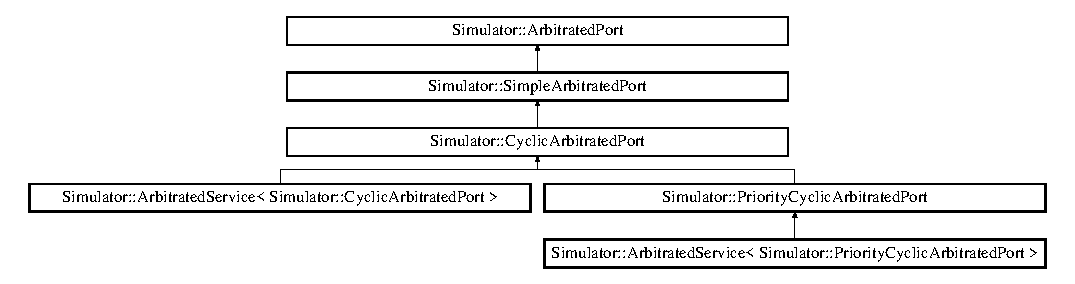
\includegraphics[height=3.365385cm]{class_simulator_1_1_cyclic_arbitrated_port}
\end{center}
\end{figure}
\subsection*{Public Member Functions}
\begin{DoxyCompactItemize}
\item 
void \hyperlink{class_simulator_1_1_cyclic_arbitrated_port_afaab298eeb4e4ffb377d6c69fec1638d}{Arbitrate} ()
\end{DoxyCompactItemize}
\subsection*{Protected Member Functions}
\begin{DoxyCompactItemize}
\item 
\hyperlink{class_simulator_1_1_cyclic_arbitrated_port_a003c7b7cd55d70350f8f5e8ddae5b30e}{Cyclic\+Arbitrated\+Port} (const \hyperlink{class_simulator_1_1_object}{Object} \&object, const std\+::string \&\hyperlink{mtconf_8c_a8f8f80d37794cde9472343e4487ba3eb}{name})
\end{DoxyCompactItemize}
\subsection*{Protected Attributes}
\begin{DoxyCompactItemize}
\item 
size\+\_\+t \hyperlink{class_simulator_1_1_cyclic_arbitrated_port_af90afe3374d413eeb1425ec0bd293677}{m\+\_\+last\+Selected}
\end{DoxyCompactItemize}
\subsection*{Additional Inherited Members}


\subsection{Constructor \& Destructor Documentation}
\hypertarget{class_simulator_1_1_cyclic_arbitrated_port_a003c7b7cd55d70350f8f5e8ddae5b30e}{\index{Simulator\+::\+Cyclic\+Arbitrated\+Port@{Simulator\+::\+Cyclic\+Arbitrated\+Port}!Cyclic\+Arbitrated\+Port@{Cyclic\+Arbitrated\+Port}}
\index{Cyclic\+Arbitrated\+Port@{Cyclic\+Arbitrated\+Port}!Simulator\+::\+Cyclic\+Arbitrated\+Port@{Simulator\+::\+Cyclic\+Arbitrated\+Port}}
\subsubsection[{Cyclic\+Arbitrated\+Port}]{\setlength{\rightskip}{0pt plus 5cm}Simulator\+::\+Cyclic\+Arbitrated\+Port\+::\+Cyclic\+Arbitrated\+Port (
\begin{DoxyParamCaption}
\item[{const {\bf Object} \&}]{object, }
\item[{const std\+::string \&}]{name}
\end{DoxyParamCaption}
)\hspace{0.3cm}{\ttfamily [inline]}, {\ttfamily [protected]}}}\label{class_simulator_1_1_cyclic_arbitrated_port_a003c7b7cd55d70350f8f5e8ddae5b30e}


\subsection{Member Function Documentation}
\hypertarget{class_simulator_1_1_cyclic_arbitrated_port_afaab298eeb4e4ffb377d6c69fec1638d}{\index{Simulator\+::\+Cyclic\+Arbitrated\+Port@{Simulator\+::\+Cyclic\+Arbitrated\+Port}!Arbitrate@{Arbitrate}}
\index{Arbitrate@{Arbitrate}!Simulator\+::\+Cyclic\+Arbitrated\+Port@{Simulator\+::\+Cyclic\+Arbitrated\+Port}}
\subsubsection[{Arbitrate}]{\setlength{\rightskip}{0pt plus 5cm}void Simulator\+::\+Cyclic\+Arbitrated\+Port\+::\+Arbitrate (
\begin{DoxyParamCaption}
{}
\end{DoxyParamCaption}
)}}\label{class_simulator_1_1_cyclic_arbitrated_port_afaab298eeb4e4ffb377d6c69fec1638d}


\subsection{Member Data Documentation}
\hypertarget{class_simulator_1_1_cyclic_arbitrated_port_af90afe3374d413eeb1425ec0bd293677}{\index{Simulator\+::\+Cyclic\+Arbitrated\+Port@{Simulator\+::\+Cyclic\+Arbitrated\+Port}!m\+\_\+last\+Selected@{m\+\_\+last\+Selected}}
\index{m\+\_\+last\+Selected@{m\+\_\+last\+Selected}!Simulator\+::\+Cyclic\+Arbitrated\+Port@{Simulator\+::\+Cyclic\+Arbitrated\+Port}}
\subsubsection[{m\+\_\+last\+Selected}]{\setlength{\rightskip}{0pt plus 5cm}size\+\_\+t Simulator\+::\+Cyclic\+Arbitrated\+Port\+::m\+\_\+last\+Selected\hspace{0.3cm}{\ttfamily [protected]}}}\label{class_simulator_1_1_cyclic_arbitrated_port_af90afe3374d413eeb1425ec0bd293677}


The documentation for this class was generated from the following files\+:\begin{DoxyCompactItemize}
\item 
sim/\hyperlink{ports_8h}{ports.\+h}\item 
sim/\hyperlink{ports_8cpp}{ports.\+cpp}\end{DoxyCompactItemize}

\hypertarget{class_simulator_1_1drisc_1_1_d_cache}{\section{Simulator\+:\+:drisc\+:\+:D\+Cache Class Reference}
\label{class_simulator_1_1drisc_1_1_d_cache}\index{Simulator\+::drisc\+::\+D\+Cache@{Simulator\+::drisc\+::\+D\+Cache}}
}


{\ttfamily \#include $<$D\+Cache.\+h$>$}

Inheritance diagram for Simulator\+:\+:drisc\+:\+:D\+Cache\+:\begin{figure}[H]
\begin{center}
\leavevmode
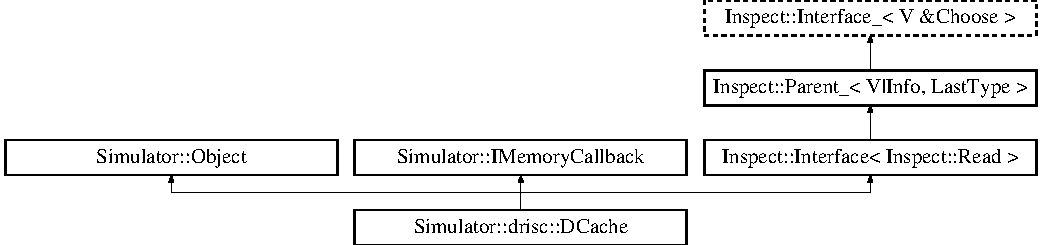
\includegraphics[height=3.289281cm]{class_simulator_1_1drisc_1_1_d_cache}
\end{center}
\end{figure}
\subsection*{Classes}
\begin{DoxyCompactItemize}
\item 
struct \hyperlink{struct_simulator_1_1drisc_1_1_d_cache_1_1_line}{Line}
\end{DoxyCompactItemize}
\subsection*{Public Types}
\begin{DoxyCompactItemize}
\item 
enum \hyperlink{class_simulator_1_1drisc_1_1_d_cache_aab0700229ca4e63558dd73cb40ee0b71}{Line\+State} \{ \hyperlink{class_simulator_1_1drisc_1_1_d_cache_aab0700229ca4e63558dd73cb40ee0b71a6492d0c4b09bbaf85d7848638e1b9e4a}{L\+I\+N\+E\+\_\+\+E\+M\+P\+T\+Y}, 
\hyperlink{class_simulator_1_1drisc_1_1_d_cache_aab0700229ca4e63558dd73cb40ee0b71abf88e2ea7fe762928686a9b2b3c44f9a}{L\+I\+N\+E\+\_\+\+L\+O\+A\+D\+I\+N\+G}, 
\hyperlink{class_simulator_1_1drisc_1_1_d_cache_aab0700229ca4e63558dd73cb40ee0b71a46f24a3cab8cf50fd5e27e58d4b469f1}{L\+I\+N\+E\+\_\+\+I\+N\+V\+A\+L\+I\+D}, 
\hyperlink{class_simulator_1_1drisc_1_1_d_cache_aab0700229ca4e63558dd73cb40ee0b71a9d8e8c623920edff8b10d6b07f5eee8a}{L\+I\+N\+E\+\_\+\+F\+U\+L\+L}
 \}
\begin{DoxyCompactList}\small\item\em The state of a cache-\/line. \end{DoxyCompactList}\end{DoxyCompactItemize}
\subsection*{Public Member Functions}
\begin{DoxyCompactItemize}
\item 
\hyperlink{class_simulator_1_1drisc_1_1_d_cache_a8edd4655eb4e5343f43fc681538e7bdb}{D\+Cache} (const std\+::string \&\hyperlink{mtconf_8c_a8f8f80d37794cde9472343e4487ba3eb}{name}, \hyperlink{class_simulator_1_1_d_r_i_s_c}{D\+R\+I\+S\+C} \&parent, \hyperlink{class_simulator_1_1_clock}{Clock} \&clock, \hyperlink{class_config}{Config} \&config)
\item 
\hyperlink{class_simulator_1_1drisc_1_1_d_cache_a06d937fa2b18e01cd656aa2da4aa7af3}{D\+Cache} (const \hyperlink{class_simulator_1_1drisc_1_1_d_cache}{D\+Cache} \&)=delete
\item 
\hyperlink{class_simulator_1_1drisc_1_1_d_cache}{D\+Cache} \& \hyperlink{class_simulator_1_1drisc_1_1_d_cache_aa1615320c6877f87cf3383d7a3aa217b}{operator=} (const \hyperlink{class_simulator_1_1drisc_1_1_d_cache}{D\+Cache} \&)=delete
\item 
\hyperlink{class_simulator_1_1drisc_1_1_d_cache_a6411ac3c301f537cd66740e4c8a68b1c}{$\sim$\+D\+Cache} ()
\item 
void \hyperlink{class_simulator_1_1drisc_1_1_d_cache_a28e1cd7e81331638001925605fa80cc8}{Connect\+Memory} (\hyperlink{class_simulator_1_1_i_memory}{I\+Memory} $\ast$memory)
\item 
\hyperlink{namespace_simulator_a4b6b5616e7236c0c131516a441776805}{Result} \hyperlink{class_simulator_1_1drisc_1_1_d_cache_aae572308d04dc67956b110a034c1824c}{Read} (Mem\+Addr address, void $\ast$data, Mem\+Size size, \hyperlink{struct_simulator_1_1_reg_addr}{Reg\+Addr} $\ast$reg)
\item 
\hyperlink{namespace_simulator_a4b6b5616e7236c0c131516a441776805}{Result} \hyperlink{class_simulator_1_1drisc_1_1_d_cache_ad7d0e5b2ca9a2099cc727db2a3ddaaf9}{Write} (Mem\+Addr address, void $\ast$data, Mem\+Size size, \hyperlink{namespace_simulator_aaccbc706b2d6c99085f52f6dfc2333e4}{L\+F\+I\+D} fid, \hyperlink{namespace_simulator_a483cc4ecee1736e895054617672cded5}{T\+I\+D} tid)
\item 
size\+\_\+t \hyperlink{class_simulator_1_1drisc_1_1_d_cache_a8007c040d65e09aac73021337b5d3323}{Get\+Line\+Size} () const 
\item 
bool \hyperlink{class_simulator_1_1drisc_1_1_d_cache_ae1cb74d2ac87cd7ffddd081c0da3ce15}{On\+Memory\+Read\+Completed} (Mem\+Addr addr, const char $\ast$data) override
\item 
bool \hyperlink{class_simulator_1_1drisc_1_1_d_cache_a5f642cb471c08f5056f7bc3a93b8312d}{On\+Memory\+Write\+Completed} (\hyperlink{namespace_simulator_a483cc4ecee1736e895054617672cded5}{T\+I\+D} tid) override
\item 
bool \hyperlink{class_simulator_1_1drisc_1_1_d_cache_a8229d5f73ccd678b27b2086168620f79}{On\+Memory\+Snooped} (Mem\+Addr addr, const char $\ast$data, const bool $\ast$mask) override
\item 
bool \hyperlink{class_simulator_1_1drisc_1_1_d_cache_a583fdc1194fffefec8a12bcbc32e2fc3}{On\+Memory\+Invalidated} (Mem\+Addr addr) override
\item 
\hyperlink{class_simulator_1_1_object}{Object} \& \hyperlink{class_simulator_1_1drisc_1_1_d_cache_a0ee619a4930f7b92e450fc1b6f9c08cd}{Get\+Memory\+Peer} () override
\item 
void \hyperlink{class_simulator_1_1drisc_1_1_d_cache_a9097106ad74a2a9198ce9caee47420cb}{Cmd\+\_\+\+Info} (std\+::ostream \&out, const std\+::vector$<$ std\+::string $>$ \&arguments) const override
\item 
void \hyperlink{class_simulator_1_1drisc_1_1_d_cache_af68d132ebce737293e3678dcfa3b9fd8}{Cmd\+\_\+\+Read} (std\+::ostream \&out, const std\+::vector$<$ std\+::string $>$ \&arguments) const override
\item 
size\+\_\+t \hyperlink{class_simulator_1_1drisc_1_1_d_cache_a0ab8548e496232a709b8c2a006be6aaa}{Get\+Associativity} () const 
\item 
size\+\_\+t \hyperlink{class_simulator_1_1drisc_1_1_d_cache_a7beb41cf505c2764e5da68d1ebc93794}{Get\+Num\+Lines} () const 
\item 
size\+\_\+t \hyperlink{class_simulator_1_1drisc_1_1_d_cache_a45b14a4aad78c53e1d2a5f13f3e58cff}{Get\+Num\+Sets} () const 
\item 
const \hyperlink{struct_simulator_1_1drisc_1_1_d_cache_1_1_line}{Line} \& \hyperlink{class_simulator_1_1drisc_1_1_d_cache_ac25b28535cc1742c7153995882c8f284}{Get\+Line} (size\+\_\+t i) const 
\end{DoxyCompactItemize}
\subsection*{Public Attributes}
\begin{DoxyCompactItemize}
\item 
\hyperlink{class_simulator_1_1_process}{Process} \hyperlink{class_simulator_1_1drisc_1_1_d_cache_ae91cc8d03d3b83d7ee241b9246dc32d5}{p\+\_\+\+Read\+Writebacks}
\item 
\hyperlink{class_simulator_1_1_process}{Process} \hyperlink{class_simulator_1_1drisc_1_1_d_cache_aa9b6ca8eebcaa56bc0c0f58c6a5e80c5}{p\+\_\+\+Read\+Responses}
\item 
\hyperlink{class_simulator_1_1_process}{Process} \hyperlink{class_simulator_1_1drisc_1_1_d_cache_aaf3fd21ca8cd24b70348ccd7452c7ce7}{p\+\_\+\+Write\+Responses}
\item 
\hyperlink{class_simulator_1_1_process}{Process} \hyperlink{class_simulator_1_1drisc_1_1_d_cache_a23700618e332cbeea5634f08f2c18521}{p\+\_\+\+Outgoing}
\item 
\hyperlink{class_simulator_1_1_arbitrated_service}{Arbitrated\+Service} \hyperlink{class_simulator_1_1drisc_1_1_d_cache_a3f008676ba7517b2e9a3968c9be1d519}{p\+\_\+service}
\end{DoxyCompactItemize}
\subsection*{Friends}
\begin{DoxyCompactItemize}
\item 
class \hyperlink{class_simulator_1_1drisc_1_1_d_cache_a14f94eb83e17d9d8841f39b37431d673}{Simulator\+::\+D\+R\+I\+S\+C}
\end{DoxyCompactItemize}


\subsection{Member Enumeration Documentation}
\hypertarget{class_simulator_1_1drisc_1_1_d_cache_aab0700229ca4e63558dd73cb40ee0b71}{\index{Simulator\+::drisc\+::\+D\+Cache@{Simulator\+::drisc\+::\+D\+Cache}!Line\+State@{Line\+State}}
\index{Line\+State@{Line\+State}!Simulator\+::drisc\+::\+D\+Cache@{Simulator\+::drisc\+::\+D\+Cache}}
\subsubsection[{Line\+State}]{\setlength{\rightskip}{0pt plus 5cm}enum {\bf Simulator\+::drisc\+::\+D\+Cache\+::\+Line\+State}}}\label{class_simulator_1_1drisc_1_1_d_cache_aab0700229ca4e63558dd73cb40ee0b71}


The state of a cache-\/line. 

\begin{Desc}
\item[Enumerator]\par
\begin{description}
\index{L\+I\+N\+E\+\_\+\+E\+M\+P\+T\+Y@{L\+I\+N\+E\+\_\+\+E\+M\+P\+T\+Y}!Simulator\+::drisc\+::\+D\+Cache@{Simulator\+::drisc\+::\+D\+Cache}}\index{Simulator\+::drisc\+::\+D\+Cache@{Simulator\+::drisc\+::\+D\+Cache}!L\+I\+N\+E\+\_\+\+E\+M\+P\+T\+Y@{L\+I\+N\+E\+\_\+\+E\+M\+P\+T\+Y}}\item[{\em 
\hypertarget{class_simulator_1_1drisc_1_1_d_cache_aab0700229ca4e63558dd73cb40ee0b71a6492d0c4b09bbaf85d7848638e1b9e4a}{L\+I\+N\+E\+\_\+\+E\+M\+P\+T\+Y}\label{class_simulator_1_1drisc_1_1_d_cache_aab0700229ca4e63558dd73cb40ee0b71a6492d0c4b09bbaf85d7848638e1b9e4a}
}]\hyperlink{struct_simulator_1_1drisc_1_1_d_cache_1_1_line}{Line} is empty. \index{L\+I\+N\+E\+\_\+\+L\+O\+A\+D\+I\+N\+G@{L\+I\+N\+E\+\_\+\+L\+O\+A\+D\+I\+N\+G}!Simulator\+::drisc\+::\+D\+Cache@{Simulator\+::drisc\+::\+D\+Cache}}\index{Simulator\+::drisc\+::\+D\+Cache@{Simulator\+::drisc\+::\+D\+Cache}!L\+I\+N\+E\+\_\+\+L\+O\+A\+D\+I\+N\+G@{L\+I\+N\+E\+\_\+\+L\+O\+A\+D\+I\+N\+G}}\item[{\em 
\hypertarget{class_simulator_1_1drisc_1_1_d_cache_aab0700229ca4e63558dd73cb40ee0b71abf88e2ea7fe762928686a9b2b3c44f9a}{L\+I\+N\+E\+\_\+\+L\+O\+A\+D\+I\+N\+G}\label{class_simulator_1_1drisc_1_1_d_cache_aab0700229ca4e63558dd73cb40ee0b71abf88e2ea7fe762928686a9b2b3c44f9a}
}]\hyperlink{struct_simulator_1_1drisc_1_1_d_cache_1_1_line}{Line} is being loaded. \index{L\+I\+N\+E\+\_\+\+I\+N\+V\+A\+L\+I\+D@{L\+I\+N\+E\+\_\+\+I\+N\+V\+A\+L\+I\+D}!Simulator\+::drisc\+::\+D\+Cache@{Simulator\+::drisc\+::\+D\+Cache}}\index{Simulator\+::drisc\+::\+D\+Cache@{Simulator\+::drisc\+::\+D\+Cache}!L\+I\+N\+E\+\_\+\+I\+N\+V\+A\+L\+I\+D@{L\+I\+N\+E\+\_\+\+I\+N\+V\+A\+L\+I\+D}}\item[{\em 
\hypertarget{class_simulator_1_1drisc_1_1_d_cache_aab0700229ca4e63558dd73cb40ee0b71a46f24a3cab8cf50fd5e27e58d4b469f1}{L\+I\+N\+E\+\_\+\+I\+N\+V\+A\+L\+I\+D}\label{class_simulator_1_1drisc_1_1_d_cache_aab0700229ca4e63558dd73cb40ee0b71a46f24a3cab8cf50fd5e27e58d4b469f1}
}]\hyperlink{struct_simulator_1_1drisc_1_1_d_cache_1_1_line}{Line} is invalid. \index{L\+I\+N\+E\+\_\+\+F\+U\+L\+L@{L\+I\+N\+E\+\_\+\+F\+U\+L\+L}!Simulator\+::drisc\+::\+D\+Cache@{Simulator\+::drisc\+::\+D\+Cache}}\index{Simulator\+::drisc\+::\+D\+Cache@{Simulator\+::drisc\+::\+D\+Cache}!L\+I\+N\+E\+\_\+\+F\+U\+L\+L@{L\+I\+N\+E\+\_\+\+F\+U\+L\+L}}\item[{\em 
\hypertarget{class_simulator_1_1drisc_1_1_d_cache_aab0700229ca4e63558dd73cb40ee0b71a9d8e8c623920edff8b10d6b07f5eee8a}{L\+I\+N\+E\+\_\+\+F\+U\+L\+L}\label{class_simulator_1_1drisc_1_1_d_cache_aab0700229ca4e63558dd73cb40ee0b71a9d8e8c623920edff8b10d6b07f5eee8a}
}]\hyperlink{struct_simulator_1_1drisc_1_1_d_cache_1_1_line}{Line} is full. \end{description}
\end{Desc}


\subsection{Constructor \& Destructor Documentation}
\hypertarget{class_simulator_1_1drisc_1_1_d_cache_a8edd4655eb4e5343f43fc681538e7bdb}{\index{Simulator\+::drisc\+::\+D\+Cache@{Simulator\+::drisc\+::\+D\+Cache}!D\+Cache@{D\+Cache}}
\index{D\+Cache@{D\+Cache}!Simulator\+::drisc\+::\+D\+Cache@{Simulator\+::drisc\+::\+D\+Cache}}
\subsubsection[{D\+Cache}]{\setlength{\rightskip}{0pt plus 5cm}Simulator\+::drisc\+::\+D\+Cache\+::\+D\+Cache (
\begin{DoxyParamCaption}
\item[{const std\+::string \&}]{name, }
\item[{{\bf D\+R\+I\+S\+C} \&}]{parent, }
\item[{{\bf Clock} \&}]{clock, }
\item[{{\bf Config} \&}]{config}
\end{DoxyParamCaption}
)}}\label{class_simulator_1_1drisc_1_1_d_cache_a8edd4655eb4e5343f43fc681538e7bdb}
\hypertarget{class_simulator_1_1drisc_1_1_d_cache_a06d937fa2b18e01cd656aa2da4aa7af3}{\index{Simulator\+::drisc\+::\+D\+Cache@{Simulator\+::drisc\+::\+D\+Cache}!D\+Cache@{D\+Cache}}
\index{D\+Cache@{D\+Cache}!Simulator\+::drisc\+::\+D\+Cache@{Simulator\+::drisc\+::\+D\+Cache}}
\subsubsection[{D\+Cache}]{\setlength{\rightskip}{0pt plus 5cm}Simulator\+::drisc\+::\+D\+Cache\+::\+D\+Cache (
\begin{DoxyParamCaption}
\item[{const {\bf D\+Cache} \&}]{}
\end{DoxyParamCaption}
)\hspace{0.3cm}{\ttfamily [delete]}}}\label{class_simulator_1_1drisc_1_1_d_cache_a06d937fa2b18e01cd656aa2da4aa7af3}
\hypertarget{class_simulator_1_1drisc_1_1_d_cache_a6411ac3c301f537cd66740e4c8a68b1c}{\index{Simulator\+::drisc\+::\+D\+Cache@{Simulator\+::drisc\+::\+D\+Cache}!````~D\+Cache@{$\sim$\+D\+Cache}}
\index{````~D\+Cache@{$\sim$\+D\+Cache}!Simulator\+::drisc\+::\+D\+Cache@{Simulator\+::drisc\+::\+D\+Cache}}
\subsubsection[{$\sim$\+D\+Cache}]{\setlength{\rightskip}{0pt plus 5cm}Simulator\+::drisc\+::\+D\+Cache\+::$\sim$\+D\+Cache (
\begin{DoxyParamCaption}
{}
\end{DoxyParamCaption}
)}}\label{class_simulator_1_1drisc_1_1_d_cache_a6411ac3c301f537cd66740e4c8a68b1c}


\subsection{Member Function Documentation}
\hypertarget{class_simulator_1_1drisc_1_1_d_cache_a9097106ad74a2a9198ce9caee47420cb}{\index{Simulator\+::drisc\+::\+D\+Cache@{Simulator\+::drisc\+::\+D\+Cache}!Cmd\+\_\+\+Info@{Cmd\+\_\+\+Info}}
\index{Cmd\+\_\+\+Info@{Cmd\+\_\+\+Info}!Simulator\+::drisc\+::\+D\+Cache@{Simulator\+::drisc\+::\+D\+Cache}}
\subsubsection[{Cmd\+\_\+\+Info}]{\setlength{\rightskip}{0pt plus 5cm}void Simulator\+::drisc\+::\+D\+Cache\+::\+Cmd\+\_\+\+Info (
\begin{DoxyParamCaption}
\item[{std\+::ostream \&}]{out, }
\item[{const std\+::vector$<$ std\+::string $>$ \&}]{arguments}
\end{DoxyParamCaption}
) const\hspace{0.3cm}{\ttfamily [override]}}}\label{class_simulator_1_1drisc_1_1_d_cache_a9097106ad74a2a9198ce9caee47420cb}
\hypertarget{class_simulator_1_1drisc_1_1_d_cache_af68d132ebce737293e3678dcfa3b9fd8}{\index{Simulator\+::drisc\+::\+D\+Cache@{Simulator\+::drisc\+::\+D\+Cache}!Cmd\+\_\+\+Read@{Cmd\+\_\+\+Read}}
\index{Cmd\+\_\+\+Read@{Cmd\+\_\+\+Read}!Simulator\+::drisc\+::\+D\+Cache@{Simulator\+::drisc\+::\+D\+Cache}}
\subsubsection[{Cmd\+\_\+\+Read}]{\setlength{\rightskip}{0pt plus 5cm}void Simulator\+::drisc\+::\+D\+Cache\+::\+Cmd\+\_\+\+Read (
\begin{DoxyParamCaption}
\item[{std\+::ostream \&}]{out, }
\item[{const std\+::vector$<$ std\+::string $>$ \&}]{arguments}
\end{DoxyParamCaption}
) const\hspace{0.3cm}{\ttfamily [override]}}}\label{class_simulator_1_1drisc_1_1_d_cache_af68d132ebce737293e3678dcfa3b9fd8}
\hypertarget{class_simulator_1_1drisc_1_1_d_cache_a28e1cd7e81331638001925605fa80cc8}{\index{Simulator\+::drisc\+::\+D\+Cache@{Simulator\+::drisc\+::\+D\+Cache}!Connect\+Memory@{Connect\+Memory}}
\index{Connect\+Memory@{Connect\+Memory}!Simulator\+::drisc\+::\+D\+Cache@{Simulator\+::drisc\+::\+D\+Cache}}
\subsubsection[{Connect\+Memory}]{\setlength{\rightskip}{0pt plus 5cm}void Simulator\+::drisc\+::\+D\+Cache\+::\+Connect\+Memory (
\begin{DoxyParamCaption}
\item[{{\bf I\+Memory} $\ast$}]{memory}
\end{DoxyParamCaption}
)}}\label{class_simulator_1_1drisc_1_1_d_cache_a28e1cd7e81331638001925605fa80cc8}
\hypertarget{class_simulator_1_1drisc_1_1_d_cache_a0ab8548e496232a709b8c2a006be6aaa}{\index{Simulator\+::drisc\+::\+D\+Cache@{Simulator\+::drisc\+::\+D\+Cache}!Get\+Associativity@{Get\+Associativity}}
\index{Get\+Associativity@{Get\+Associativity}!Simulator\+::drisc\+::\+D\+Cache@{Simulator\+::drisc\+::\+D\+Cache}}
\subsubsection[{Get\+Associativity}]{\setlength{\rightskip}{0pt plus 5cm}size\+\_\+t Simulator\+::drisc\+::\+D\+Cache\+::\+Get\+Associativity (
\begin{DoxyParamCaption}
{}
\end{DoxyParamCaption}
) const\hspace{0.3cm}{\ttfamily [inline]}}}\label{class_simulator_1_1drisc_1_1_d_cache_a0ab8548e496232a709b8c2a006be6aaa}
\hypertarget{class_simulator_1_1drisc_1_1_d_cache_ac25b28535cc1742c7153995882c8f284}{\index{Simulator\+::drisc\+::\+D\+Cache@{Simulator\+::drisc\+::\+D\+Cache}!Get\+Line@{Get\+Line}}
\index{Get\+Line@{Get\+Line}!Simulator\+::drisc\+::\+D\+Cache@{Simulator\+::drisc\+::\+D\+Cache}}
\subsubsection[{Get\+Line}]{\setlength{\rightskip}{0pt plus 5cm}const {\bf Line}\& Simulator\+::drisc\+::\+D\+Cache\+::\+Get\+Line (
\begin{DoxyParamCaption}
\item[{size\+\_\+t}]{i}
\end{DoxyParamCaption}
) const\hspace{0.3cm}{\ttfamily [inline]}}}\label{class_simulator_1_1drisc_1_1_d_cache_ac25b28535cc1742c7153995882c8f284}
\hypertarget{class_simulator_1_1drisc_1_1_d_cache_a8007c040d65e09aac73021337b5d3323}{\index{Simulator\+::drisc\+::\+D\+Cache@{Simulator\+::drisc\+::\+D\+Cache}!Get\+Line\+Size@{Get\+Line\+Size}}
\index{Get\+Line\+Size@{Get\+Line\+Size}!Simulator\+::drisc\+::\+D\+Cache@{Simulator\+::drisc\+::\+D\+Cache}}
\subsubsection[{Get\+Line\+Size}]{\setlength{\rightskip}{0pt plus 5cm}size\+\_\+t Simulator\+::drisc\+::\+D\+Cache\+::\+Get\+Line\+Size (
\begin{DoxyParamCaption}
{}
\end{DoxyParamCaption}
) const\hspace{0.3cm}{\ttfamily [inline]}}}\label{class_simulator_1_1drisc_1_1_d_cache_a8007c040d65e09aac73021337b5d3323}
\hypertarget{class_simulator_1_1drisc_1_1_d_cache_a0ee619a4930f7b92e450fc1b6f9c08cd}{\index{Simulator\+::drisc\+::\+D\+Cache@{Simulator\+::drisc\+::\+D\+Cache}!Get\+Memory\+Peer@{Get\+Memory\+Peer}}
\index{Get\+Memory\+Peer@{Get\+Memory\+Peer}!Simulator\+::drisc\+::\+D\+Cache@{Simulator\+::drisc\+::\+D\+Cache}}
\subsubsection[{Get\+Memory\+Peer}]{\setlength{\rightskip}{0pt plus 5cm}{\bf Object} \& Simulator\+::drisc\+::\+D\+Cache\+::\+Get\+Memory\+Peer (
\begin{DoxyParamCaption}
{}
\end{DoxyParamCaption}
)\hspace{0.3cm}{\ttfamily [override]}, {\ttfamily [virtual]}}}\label{class_simulator_1_1drisc_1_1_d_cache_a0ee619a4930f7b92e450fc1b6f9c08cd}


Implements \hyperlink{class_simulator_1_1_i_memory_callback_ab378a4b6ce2df8e4a38bb3e8f116a064}{Simulator\+::\+I\+Memory\+Callback}.

\hypertarget{class_simulator_1_1drisc_1_1_d_cache_a7beb41cf505c2764e5da68d1ebc93794}{\index{Simulator\+::drisc\+::\+D\+Cache@{Simulator\+::drisc\+::\+D\+Cache}!Get\+Num\+Lines@{Get\+Num\+Lines}}
\index{Get\+Num\+Lines@{Get\+Num\+Lines}!Simulator\+::drisc\+::\+D\+Cache@{Simulator\+::drisc\+::\+D\+Cache}}
\subsubsection[{Get\+Num\+Lines}]{\setlength{\rightskip}{0pt plus 5cm}size\+\_\+t Simulator\+::drisc\+::\+D\+Cache\+::\+Get\+Num\+Lines (
\begin{DoxyParamCaption}
{}
\end{DoxyParamCaption}
) const\hspace{0.3cm}{\ttfamily [inline]}}}\label{class_simulator_1_1drisc_1_1_d_cache_a7beb41cf505c2764e5da68d1ebc93794}
\hypertarget{class_simulator_1_1drisc_1_1_d_cache_a45b14a4aad78c53e1d2a5f13f3e58cff}{\index{Simulator\+::drisc\+::\+D\+Cache@{Simulator\+::drisc\+::\+D\+Cache}!Get\+Num\+Sets@{Get\+Num\+Sets}}
\index{Get\+Num\+Sets@{Get\+Num\+Sets}!Simulator\+::drisc\+::\+D\+Cache@{Simulator\+::drisc\+::\+D\+Cache}}
\subsubsection[{Get\+Num\+Sets}]{\setlength{\rightskip}{0pt plus 5cm}size\+\_\+t Simulator\+::drisc\+::\+D\+Cache\+::\+Get\+Num\+Sets (
\begin{DoxyParamCaption}
{}
\end{DoxyParamCaption}
) const\hspace{0.3cm}{\ttfamily [inline]}}}\label{class_simulator_1_1drisc_1_1_d_cache_a45b14a4aad78c53e1d2a5f13f3e58cff}
\hypertarget{class_simulator_1_1drisc_1_1_d_cache_a583fdc1194fffefec8a12bcbc32e2fc3}{\index{Simulator\+::drisc\+::\+D\+Cache@{Simulator\+::drisc\+::\+D\+Cache}!On\+Memory\+Invalidated@{On\+Memory\+Invalidated}}
\index{On\+Memory\+Invalidated@{On\+Memory\+Invalidated}!Simulator\+::drisc\+::\+D\+Cache@{Simulator\+::drisc\+::\+D\+Cache}}
\subsubsection[{On\+Memory\+Invalidated}]{\setlength{\rightskip}{0pt plus 5cm}bool Simulator\+::drisc\+::\+D\+Cache\+::\+On\+Memory\+Invalidated (
\begin{DoxyParamCaption}
\item[{Mem\+Addr}]{addr}
\end{DoxyParamCaption}
)\hspace{0.3cm}{\ttfamily [override]}, {\ttfamily [virtual]}}}\label{class_simulator_1_1drisc_1_1_d_cache_a583fdc1194fffefec8a12bcbc32e2fc3}


Implements \hyperlink{class_simulator_1_1_i_memory_callback_a8a50686620585ffe62e754a9e96b79a8}{Simulator\+::\+I\+Memory\+Callback}.

\hypertarget{class_simulator_1_1drisc_1_1_d_cache_ae1cb74d2ac87cd7ffddd081c0da3ce15}{\index{Simulator\+::drisc\+::\+D\+Cache@{Simulator\+::drisc\+::\+D\+Cache}!On\+Memory\+Read\+Completed@{On\+Memory\+Read\+Completed}}
\index{On\+Memory\+Read\+Completed@{On\+Memory\+Read\+Completed}!Simulator\+::drisc\+::\+D\+Cache@{Simulator\+::drisc\+::\+D\+Cache}}
\subsubsection[{On\+Memory\+Read\+Completed}]{\setlength{\rightskip}{0pt plus 5cm}bool Simulator\+::drisc\+::\+D\+Cache\+::\+On\+Memory\+Read\+Completed (
\begin{DoxyParamCaption}
\item[{Mem\+Addr}]{addr, }
\item[{const char $\ast$}]{data}
\end{DoxyParamCaption}
)\hspace{0.3cm}{\ttfamily [override]}, {\ttfamily [virtual]}}}\label{class_simulator_1_1drisc_1_1_d_cache_ae1cb74d2ac87cd7ffddd081c0da3ce15}


Implements \hyperlink{class_simulator_1_1_i_memory_callback_a5519817c435767dab3b4c063e601d9f7}{Simulator\+::\+I\+Memory\+Callback}.

\hypertarget{class_simulator_1_1drisc_1_1_d_cache_a8229d5f73ccd678b27b2086168620f79}{\index{Simulator\+::drisc\+::\+D\+Cache@{Simulator\+::drisc\+::\+D\+Cache}!On\+Memory\+Snooped@{On\+Memory\+Snooped}}
\index{On\+Memory\+Snooped@{On\+Memory\+Snooped}!Simulator\+::drisc\+::\+D\+Cache@{Simulator\+::drisc\+::\+D\+Cache}}
\subsubsection[{On\+Memory\+Snooped}]{\setlength{\rightskip}{0pt plus 5cm}bool Simulator\+::drisc\+::\+D\+Cache\+::\+On\+Memory\+Snooped (
\begin{DoxyParamCaption}
\item[{Mem\+Addr}]{addr, }
\item[{const char $\ast$}]{data, }
\item[{const bool $\ast$}]{mask}
\end{DoxyParamCaption}
)\hspace{0.3cm}{\ttfamily [override]}, {\ttfamily [virtual]}}}\label{class_simulator_1_1drisc_1_1_d_cache_a8229d5f73ccd678b27b2086168620f79}


Reimplemented from \hyperlink{class_simulator_1_1_i_memory_callback_a41e84f41d39e538c2ab0c056d8c1b0e2}{Simulator\+::\+I\+Memory\+Callback}.

\hypertarget{class_simulator_1_1drisc_1_1_d_cache_a5f642cb471c08f5056f7bc3a93b8312d}{\index{Simulator\+::drisc\+::\+D\+Cache@{Simulator\+::drisc\+::\+D\+Cache}!On\+Memory\+Write\+Completed@{On\+Memory\+Write\+Completed}}
\index{On\+Memory\+Write\+Completed@{On\+Memory\+Write\+Completed}!Simulator\+::drisc\+::\+D\+Cache@{Simulator\+::drisc\+::\+D\+Cache}}
\subsubsection[{On\+Memory\+Write\+Completed}]{\setlength{\rightskip}{0pt plus 5cm}bool Simulator\+::drisc\+::\+D\+Cache\+::\+On\+Memory\+Write\+Completed (
\begin{DoxyParamCaption}
\item[{{\bf T\+I\+D}}]{tid}
\end{DoxyParamCaption}
)\hspace{0.3cm}{\ttfamily [override]}, {\ttfamily [virtual]}}}\label{class_simulator_1_1drisc_1_1_d_cache_a5f642cb471c08f5056f7bc3a93b8312d}


Implements \hyperlink{class_simulator_1_1_i_memory_callback_a3821e2dbf7f4d77053c04fc58d2fdcc8}{Simulator\+::\+I\+Memory\+Callback}.

\hypertarget{class_simulator_1_1drisc_1_1_d_cache_aa1615320c6877f87cf3383d7a3aa217b}{\index{Simulator\+::drisc\+::\+D\+Cache@{Simulator\+::drisc\+::\+D\+Cache}!operator=@{operator=}}
\index{operator=@{operator=}!Simulator\+::drisc\+::\+D\+Cache@{Simulator\+::drisc\+::\+D\+Cache}}
\subsubsection[{operator=}]{\setlength{\rightskip}{0pt plus 5cm}{\bf D\+Cache}\& Simulator\+::drisc\+::\+D\+Cache\+::operator= (
\begin{DoxyParamCaption}
\item[{const {\bf D\+Cache} \&}]{}
\end{DoxyParamCaption}
)\hspace{0.3cm}{\ttfamily [delete]}}}\label{class_simulator_1_1drisc_1_1_d_cache_aa1615320c6877f87cf3383d7a3aa217b}
\hypertarget{class_simulator_1_1drisc_1_1_d_cache_aae572308d04dc67956b110a034c1824c}{\index{Simulator\+::drisc\+::\+D\+Cache@{Simulator\+::drisc\+::\+D\+Cache}!Read@{Read}}
\index{Read@{Read}!Simulator\+::drisc\+::\+D\+Cache@{Simulator\+::drisc\+::\+D\+Cache}}
\subsubsection[{Read}]{\setlength{\rightskip}{0pt plus 5cm}{\bf Result} Simulator\+::drisc\+::\+D\+Cache\+::\+Read (
\begin{DoxyParamCaption}
\item[{Mem\+Addr}]{address, }
\item[{void $\ast$}]{data, }
\item[{Mem\+Size}]{size, }
\item[{{\bf Reg\+Addr} $\ast$}]{reg}
\end{DoxyParamCaption}
)}}\label{class_simulator_1_1drisc_1_1_d_cache_aae572308d04dc67956b110a034c1824c}
\hypertarget{class_simulator_1_1drisc_1_1_d_cache_ad7d0e5b2ca9a2099cc727db2a3ddaaf9}{\index{Simulator\+::drisc\+::\+D\+Cache@{Simulator\+::drisc\+::\+D\+Cache}!Write@{Write}}
\index{Write@{Write}!Simulator\+::drisc\+::\+D\+Cache@{Simulator\+::drisc\+::\+D\+Cache}}
\subsubsection[{Write}]{\setlength{\rightskip}{0pt plus 5cm}{\bf Result} Simulator\+::drisc\+::\+D\+Cache\+::\+Write (
\begin{DoxyParamCaption}
\item[{Mem\+Addr}]{address, }
\item[{void $\ast$}]{data, }
\item[{Mem\+Size}]{size, }
\item[{{\bf L\+F\+I\+D}}]{fid, }
\item[{{\bf T\+I\+D}}]{tid}
\end{DoxyParamCaption}
)}}\label{class_simulator_1_1drisc_1_1_d_cache_ad7d0e5b2ca9a2099cc727db2a3ddaaf9}


\subsection{Friends And Related Function Documentation}
\hypertarget{class_simulator_1_1drisc_1_1_d_cache_a14f94eb83e17d9d8841f39b37431d673}{\index{Simulator\+::drisc\+::\+D\+Cache@{Simulator\+::drisc\+::\+D\+Cache}!Simulator\+::\+D\+R\+I\+S\+C@{Simulator\+::\+D\+R\+I\+S\+C}}
\index{Simulator\+::\+D\+R\+I\+S\+C@{Simulator\+::\+D\+R\+I\+S\+C}!Simulator\+::drisc\+::\+D\+Cache@{Simulator\+::drisc\+::\+D\+Cache}}
\subsubsection[{Simulator\+::\+D\+R\+I\+S\+C}]{\setlength{\rightskip}{0pt plus 5cm}friend class {\bf Simulator\+::\+D\+R\+I\+S\+C}\hspace{0.3cm}{\ttfamily [friend]}}}\label{class_simulator_1_1drisc_1_1_d_cache_a14f94eb83e17d9d8841f39b37431d673}


\subsection{Member Data Documentation}
\hypertarget{class_simulator_1_1drisc_1_1_d_cache_a23700618e332cbeea5634f08f2c18521}{\index{Simulator\+::drisc\+::\+D\+Cache@{Simulator\+::drisc\+::\+D\+Cache}!p\+\_\+\+Outgoing@{p\+\_\+\+Outgoing}}
\index{p\+\_\+\+Outgoing@{p\+\_\+\+Outgoing}!Simulator\+::drisc\+::\+D\+Cache@{Simulator\+::drisc\+::\+D\+Cache}}
\subsubsection[{p\+\_\+\+Outgoing}]{\setlength{\rightskip}{0pt plus 5cm}{\bf Process} Simulator\+::drisc\+::\+D\+Cache\+::p\+\_\+\+Outgoing}}\label{class_simulator_1_1drisc_1_1_d_cache_a23700618e332cbeea5634f08f2c18521}
\hypertarget{class_simulator_1_1drisc_1_1_d_cache_aa9b6ca8eebcaa56bc0c0f58c6a5e80c5}{\index{Simulator\+::drisc\+::\+D\+Cache@{Simulator\+::drisc\+::\+D\+Cache}!p\+\_\+\+Read\+Responses@{p\+\_\+\+Read\+Responses}}
\index{p\+\_\+\+Read\+Responses@{p\+\_\+\+Read\+Responses}!Simulator\+::drisc\+::\+D\+Cache@{Simulator\+::drisc\+::\+D\+Cache}}
\subsubsection[{p\+\_\+\+Read\+Responses}]{\setlength{\rightskip}{0pt plus 5cm}{\bf Process} Simulator\+::drisc\+::\+D\+Cache\+::p\+\_\+\+Read\+Responses}}\label{class_simulator_1_1drisc_1_1_d_cache_aa9b6ca8eebcaa56bc0c0f58c6a5e80c5}
\hypertarget{class_simulator_1_1drisc_1_1_d_cache_ae91cc8d03d3b83d7ee241b9246dc32d5}{\index{Simulator\+::drisc\+::\+D\+Cache@{Simulator\+::drisc\+::\+D\+Cache}!p\+\_\+\+Read\+Writebacks@{p\+\_\+\+Read\+Writebacks}}
\index{p\+\_\+\+Read\+Writebacks@{p\+\_\+\+Read\+Writebacks}!Simulator\+::drisc\+::\+D\+Cache@{Simulator\+::drisc\+::\+D\+Cache}}
\subsubsection[{p\+\_\+\+Read\+Writebacks}]{\setlength{\rightskip}{0pt plus 5cm}{\bf Process} Simulator\+::drisc\+::\+D\+Cache\+::p\+\_\+\+Read\+Writebacks}}\label{class_simulator_1_1drisc_1_1_d_cache_ae91cc8d03d3b83d7ee241b9246dc32d5}
\hypertarget{class_simulator_1_1drisc_1_1_d_cache_a3f008676ba7517b2e9a3968c9be1d519}{\index{Simulator\+::drisc\+::\+D\+Cache@{Simulator\+::drisc\+::\+D\+Cache}!p\+\_\+service@{p\+\_\+service}}
\index{p\+\_\+service@{p\+\_\+service}!Simulator\+::drisc\+::\+D\+Cache@{Simulator\+::drisc\+::\+D\+Cache}}
\subsubsection[{p\+\_\+service}]{\setlength{\rightskip}{0pt plus 5cm}{\bf Arbitrated\+Service} Simulator\+::drisc\+::\+D\+Cache\+::p\+\_\+service}}\label{class_simulator_1_1drisc_1_1_d_cache_a3f008676ba7517b2e9a3968c9be1d519}
\hypertarget{class_simulator_1_1drisc_1_1_d_cache_aaf3fd21ca8cd24b70348ccd7452c7ce7}{\index{Simulator\+::drisc\+::\+D\+Cache@{Simulator\+::drisc\+::\+D\+Cache}!p\+\_\+\+Write\+Responses@{p\+\_\+\+Write\+Responses}}
\index{p\+\_\+\+Write\+Responses@{p\+\_\+\+Write\+Responses}!Simulator\+::drisc\+::\+D\+Cache@{Simulator\+::drisc\+::\+D\+Cache}}
\subsubsection[{p\+\_\+\+Write\+Responses}]{\setlength{\rightskip}{0pt plus 5cm}{\bf Process} Simulator\+::drisc\+::\+D\+Cache\+::p\+\_\+\+Write\+Responses}}\label{class_simulator_1_1drisc_1_1_d_cache_aaf3fd21ca8cd24b70348ccd7452c7ce7}


The documentation for this class was generated from the following files\+:\begin{DoxyCompactItemize}
\item 
arch/drisc/\hyperlink{_d_cache_8h}{D\+Cache.\+h}\item 
arch/drisc/\hyperlink{_d_cache_8cpp}{D\+Cache.\+cpp}\end{DoxyCompactItemize}

\hypertarget{class_simulator_1_1_d_d_r_channel}{\section{Simulator\+:\+:D\+D\+R\+Channel Class Reference}
\label{class_simulator_1_1_d_d_r_channel}\index{Simulator\+::\+D\+D\+R\+Channel@{Simulator\+::\+D\+D\+R\+Channel}}
}


Double-\/\+Data Rate Memory.  




{\ttfamily \#include $<$D\+D\+R.\+h$>$}

Inheritance diagram for Simulator\+:\+:D\+D\+R\+Channel\+:\begin{figure}[H]
\begin{center}
\leavevmode
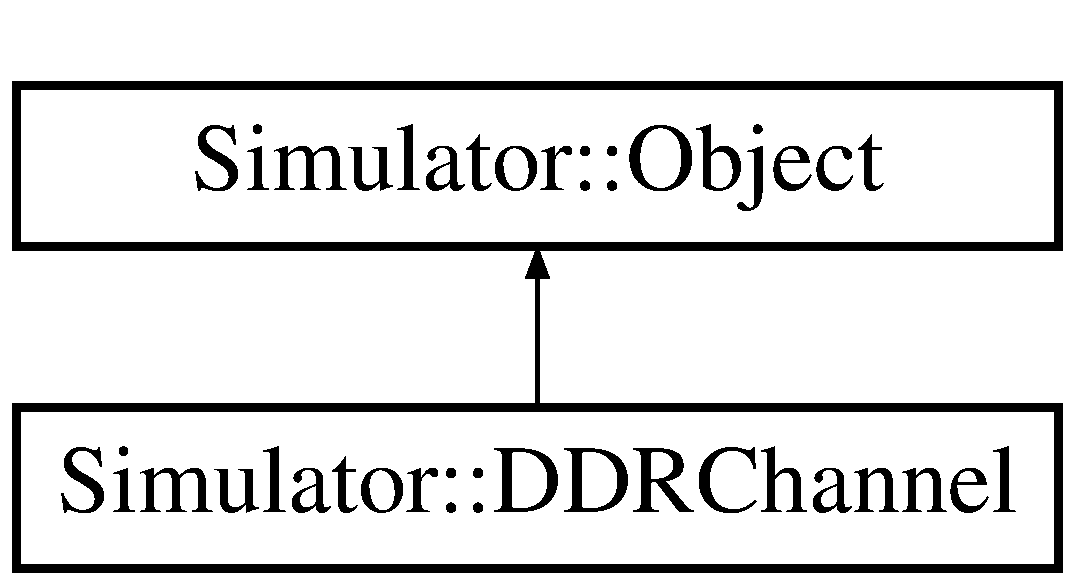
\includegraphics[height=2.000000cm]{class_simulator_1_1_d_d_r_channel}
\end{center}
\end{figure}
\subsection*{Classes}
\begin{DoxyCompactItemize}
\item 
class \hyperlink{class_simulator_1_1_d_d_r_channel_1_1_i_callback}{I\+Callback}
\end{DoxyCompactItemize}
\subsection*{Public Member Functions}
\begin{DoxyCompactItemize}
\item 
void \hyperlink{class_simulator_1_1_d_d_r_channel_a28fdeeb9ee0a0cd45284f60caf697500}{Set\+Client} (\hyperlink{class_simulator_1_1_d_d_r_channel_1_1_i_callback}{I\+Callback} \&cb, \hyperlink{class_simulator_1_1_storage_trace_set}{Storage\+Trace\+Set} \&sts, const \hyperlink{class_simulator_1_1_storage_trace_set}{Storage\+Trace\+Set} \&storages)
\item 
bool \hyperlink{class_simulator_1_1_d_d_r_channel_a98cb4b191579e38a55d7f2fa151d506e}{Read} (Mem\+Addr address, Mem\+Size size)
\item 
bool \hyperlink{class_simulator_1_1_d_d_r_channel_a9e9ac679badb89117777eab0c995b6a8}{Write} (Mem\+Addr address, Mem\+Size size)
\item 
\hyperlink{class_simulator_1_1_d_d_r_channel_a3b5be35a15d75db4599d9975dcbddf56}{D\+D\+R\+Channel} (const std\+::string \&\hyperlink{mtconf_8c_a8f8f80d37794cde9472343e4487ba3eb}{name}, \hyperlink{class_simulator_1_1_object}{Object} \&parent, \hyperlink{class_simulator_1_1_clock}{Clock} \&clock, \hyperlink{class_config}{Config} \&config)
\item 
\hyperlink{class_simulator_1_1_d_d_r_channel_afdc22f216e992c503d08f2a5fadde703}{D\+D\+R\+Channel} (const \hyperlink{class_simulator_1_1_d_d_r_channel}{D\+D\+R\+Channel} \&)=delete
\item 
\hyperlink{class_simulator_1_1_d_d_r_channel}{D\+D\+R\+Channel} \& \hyperlink{class_simulator_1_1_d_d_r_channel_a482cd16d9b4290f53ad8e035aa042f8e}{operator=} (const \hyperlink{class_simulator_1_1_d_d_r_channel}{D\+D\+R\+Channel} \&)=delete
\item 
\hyperlink{class_simulator_1_1_d_d_r_channel_a3f2fb176c7188dd1bf0969d4cb173aac}{$\sim$\+D\+D\+R\+Channel} ()
\end{DoxyCompactItemize}


\subsection{Detailed Description}
Double-\/\+Data Rate Memory. 

\subsection{Constructor \& Destructor Documentation}
\hypertarget{class_simulator_1_1_d_d_r_channel_a3b5be35a15d75db4599d9975dcbddf56}{\index{Simulator\+::\+D\+D\+R\+Channel@{Simulator\+::\+D\+D\+R\+Channel}!D\+D\+R\+Channel@{D\+D\+R\+Channel}}
\index{D\+D\+R\+Channel@{D\+D\+R\+Channel}!Simulator\+::\+D\+D\+R\+Channel@{Simulator\+::\+D\+D\+R\+Channel}}
\subsubsection[{D\+D\+R\+Channel}]{\setlength{\rightskip}{0pt plus 5cm}Simulator\+::\+D\+D\+R\+Channel\+::\+D\+D\+R\+Channel (
\begin{DoxyParamCaption}
\item[{const std\+::string \&}]{name, }
\item[{{\bf Object} \&}]{parent, }
\item[{{\bf Clock} \&}]{clock, }
\item[{{\bf Config} \&}]{config}
\end{DoxyParamCaption}
)}}\label{class_simulator_1_1_d_d_r_channel_a3b5be35a15d75db4599d9975dcbddf56}
\hypertarget{class_simulator_1_1_d_d_r_channel_afdc22f216e992c503d08f2a5fadde703}{\index{Simulator\+::\+D\+D\+R\+Channel@{Simulator\+::\+D\+D\+R\+Channel}!D\+D\+R\+Channel@{D\+D\+R\+Channel}}
\index{D\+D\+R\+Channel@{D\+D\+R\+Channel}!Simulator\+::\+D\+D\+R\+Channel@{Simulator\+::\+D\+D\+R\+Channel}}
\subsubsection[{D\+D\+R\+Channel}]{\setlength{\rightskip}{0pt plus 5cm}Simulator\+::\+D\+D\+R\+Channel\+::\+D\+D\+R\+Channel (
\begin{DoxyParamCaption}
\item[{const {\bf D\+D\+R\+Channel} \&}]{}
\end{DoxyParamCaption}
)\hspace{0.3cm}{\ttfamily [delete]}}}\label{class_simulator_1_1_d_d_r_channel_afdc22f216e992c503d08f2a5fadde703}
\hypertarget{class_simulator_1_1_d_d_r_channel_a3f2fb176c7188dd1bf0969d4cb173aac}{\index{Simulator\+::\+D\+D\+R\+Channel@{Simulator\+::\+D\+D\+R\+Channel}!````~D\+D\+R\+Channel@{$\sim$\+D\+D\+R\+Channel}}
\index{````~D\+D\+R\+Channel@{$\sim$\+D\+D\+R\+Channel}!Simulator\+::\+D\+D\+R\+Channel@{Simulator\+::\+D\+D\+R\+Channel}}
\subsubsection[{$\sim$\+D\+D\+R\+Channel}]{\setlength{\rightskip}{0pt plus 5cm}Simulator\+::\+D\+D\+R\+Channel\+::$\sim$\+D\+D\+R\+Channel (
\begin{DoxyParamCaption}
{}
\end{DoxyParamCaption}
)}}\label{class_simulator_1_1_d_d_r_channel_a3f2fb176c7188dd1bf0969d4cb173aac}


\subsection{Member Function Documentation}
\hypertarget{class_simulator_1_1_d_d_r_channel_a482cd16d9b4290f53ad8e035aa042f8e}{\index{Simulator\+::\+D\+D\+R\+Channel@{Simulator\+::\+D\+D\+R\+Channel}!operator=@{operator=}}
\index{operator=@{operator=}!Simulator\+::\+D\+D\+R\+Channel@{Simulator\+::\+D\+D\+R\+Channel}}
\subsubsection[{operator=}]{\setlength{\rightskip}{0pt plus 5cm}{\bf D\+D\+R\+Channel}\& Simulator\+::\+D\+D\+R\+Channel\+::operator= (
\begin{DoxyParamCaption}
\item[{const {\bf D\+D\+R\+Channel} \&}]{}
\end{DoxyParamCaption}
)\hspace{0.3cm}{\ttfamily [delete]}}}\label{class_simulator_1_1_d_d_r_channel_a482cd16d9b4290f53ad8e035aa042f8e}
\hypertarget{class_simulator_1_1_d_d_r_channel_a98cb4b191579e38a55d7f2fa151d506e}{\index{Simulator\+::\+D\+D\+R\+Channel@{Simulator\+::\+D\+D\+R\+Channel}!Read@{Read}}
\index{Read@{Read}!Simulator\+::\+D\+D\+R\+Channel@{Simulator\+::\+D\+D\+R\+Channel}}
\subsubsection[{Read}]{\setlength{\rightskip}{0pt plus 5cm}bool Simulator\+::\+D\+D\+R\+Channel\+::\+Read (
\begin{DoxyParamCaption}
\item[{Mem\+Addr}]{address, }
\item[{Mem\+Size}]{size}
\end{DoxyParamCaption}
)}}\label{class_simulator_1_1_d_d_r_channel_a98cb4b191579e38a55d7f2fa151d506e}
\hypertarget{class_simulator_1_1_d_d_r_channel_a28fdeeb9ee0a0cd45284f60caf697500}{\index{Simulator\+::\+D\+D\+R\+Channel@{Simulator\+::\+D\+D\+R\+Channel}!Set\+Client@{Set\+Client}}
\index{Set\+Client@{Set\+Client}!Simulator\+::\+D\+D\+R\+Channel@{Simulator\+::\+D\+D\+R\+Channel}}
\subsubsection[{Set\+Client}]{\setlength{\rightskip}{0pt plus 5cm}void Simulator\+::\+D\+D\+R\+Channel\+::\+Set\+Client (
\begin{DoxyParamCaption}
\item[{{\bf I\+Callback} \&}]{cb, }
\item[{{\bf Storage\+Trace\+Set} \&}]{sts, }
\item[{const {\bf Storage\+Trace\+Set} \&}]{storages}
\end{DoxyParamCaption}
)}}\label{class_simulator_1_1_d_d_r_channel_a28fdeeb9ee0a0cd45284f60caf697500}
\hypertarget{class_simulator_1_1_d_d_r_channel_a9e9ac679badb89117777eab0c995b6a8}{\index{Simulator\+::\+D\+D\+R\+Channel@{Simulator\+::\+D\+D\+R\+Channel}!Write@{Write}}
\index{Write@{Write}!Simulator\+::\+D\+D\+R\+Channel@{Simulator\+::\+D\+D\+R\+Channel}}
\subsubsection[{Write}]{\setlength{\rightskip}{0pt plus 5cm}bool Simulator\+::\+D\+D\+R\+Channel\+::\+Write (
\begin{DoxyParamCaption}
\item[{Mem\+Addr}]{address, }
\item[{Mem\+Size}]{size}
\end{DoxyParamCaption}
)}}\label{class_simulator_1_1_d_d_r_channel_a9e9ac679badb89117777eab0c995b6a8}


The documentation for this class was generated from the following files\+:\begin{DoxyCompactItemize}
\item 
arch/mem/\hyperlink{_d_d_r_8h}{D\+D\+R.\+h}\item 
arch/mem/\hyperlink{_d_d_r_8cpp}{D\+D\+R.\+cpp}\end{DoxyCompactItemize}

\hypertarget{class_simulator_1_1_d_d_r_channel_registry}{\section{Simulator\+:\+:D\+D\+R\+Channel\+Registry Class Reference}
\label{class_simulator_1_1_d_d_r_channel_registry}\index{Simulator\+::\+D\+D\+R\+Channel\+Registry@{Simulator\+::\+D\+D\+R\+Channel\+Registry}}
}


{\ttfamily \#include $<$D\+D\+R.\+h$>$}

Inheritance diagram for Simulator\+:\+:D\+D\+R\+Channel\+Registry\+:\begin{figure}[H]
\begin{center}
\leavevmode
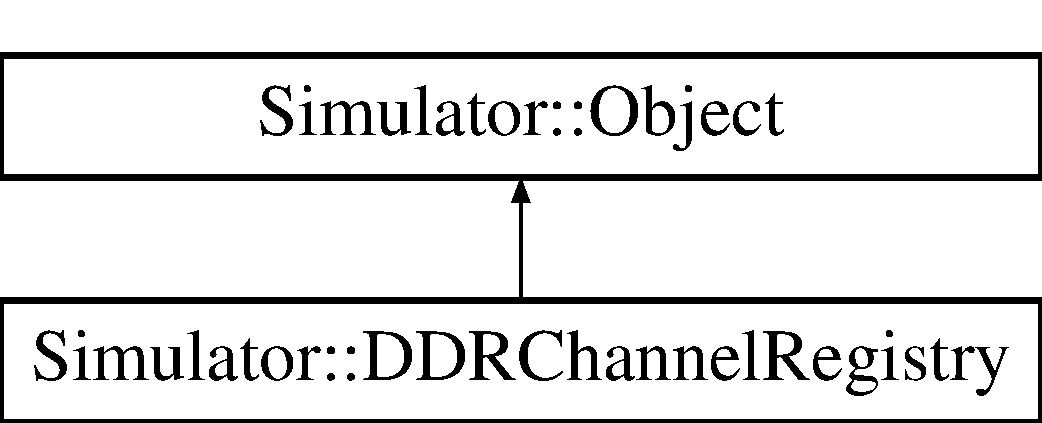
\includegraphics[height=2.000000cm]{class_simulator_1_1_d_d_r_channel_registry}
\end{center}
\end{figure}
\subsection*{Public Member Functions}
\begin{DoxyCompactItemize}
\item 
\hyperlink{class_simulator_1_1_d_d_r_channel_registry_a500ef7dcbf386ab0608ee54656a2c92b}{D\+D\+R\+Channel\+Registry} (const std\+::string \&\hyperlink{mtconf_8c_a8f8f80d37794cde9472343e4487ba3eb}{name}, \hyperlink{class_simulator_1_1_object}{Object} \&parent, \hyperlink{class_config}{Config} \&config, size\+\_\+t default\+Num\+Channels)
\item 
\hyperlink{class_simulator_1_1_d_d_r_channel_registry_a26cae4cb88c6b53c0fb4176ffee0c615}{$\sim$\+D\+D\+R\+Channel\+Registry} ()
\item 
size\+\_\+t \hyperlink{class_simulator_1_1_d_d_r_channel_registry_a8f56980d7029bd4fa10a0a004cee96c2}{size} () const 
\item 
\hyperlink{class_simulator_1_1_d_d_r_channel}{D\+D\+R\+Channel} $\ast$ \hyperlink{class_simulator_1_1_d_d_r_channel_registry_aa57fb3c193fb088d89d8933adf9b03bf}{operator\mbox{[}$\,$\mbox{]}} (size\+\_\+t i) const 
\end{DoxyCompactItemize}


\subsection{Constructor \& Destructor Documentation}
\hypertarget{class_simulator_1_1_d_d_r_channel_registry_a500ef7dcbf386ab0608ee54656a2c92b}{\index{Simulator\+::\+D\+D\+R\+Channel\+Registry@{Simulator\+::\+D\+D\+R\+Channel\+Registry}!D\+D\+R\+Channel\+Registry@{D\+D\+R\+Channel\+Registry}}
\index{D\+D\+R\+Channel\+Registry@{D\+D\+R\+Channel\+Registry}!Simulator\+::\+D\+D\+R\+Channel\+Registry@{Simulator\+::\+D\+D\+R\+Channel\+Registry}}
\subsubsection[{D\+D\+R\+Channel\+Registry}]{\setlength{\rightskip}{0pt plus 5cm}Simulator\+::\+D\+D\+R\+Channel\+Registry\+::\+D\+D\+R\+Channel\+Registry (
\begin{DoxyParamCaption}
\item[{const std\+::string \&}]{name, }
\item[{{\bf Object} \&}]{parent, }
\item[{{\bf Config} \&}]{config, }
\item[{size\+\_\+t}]{default\+Num\+Channels}
\end{DoxyParamCaption}
)}}\label{class_simulator_1_1_d_d_r_channel_registry_a500ef7dcbf386ab0608ee54656a2c92b}
\hypertarget{class_simulator_1_1_d_d_r_channel_registry_a26cae4cb88c6b53c0fb4176ffee0c615}{\index{Simulator\+::\+D\+D\+R\+Channel\+Registry@{Simulator\+::\+D\+D\+R\+Channel\+Registry}!````~D\+D\+R\+Channel\+Registry@{$\sim$\+D\+D\+R\+Channel\+Registry}}
\index{````~D\+D\+R\+Channel\+Registry@{$\sim$\+D\+D\+R\+Channel\+Registry}!Simulator\+::\+D\+D\+R\+Channel\+Registry@{Simulator\+::\+D\+D\+R\+Channel\+Registry}}
\subsubsection[{$\sim$\+D\+D\+R\+Channel\+Registry}]{\setlength{\rightskip}{0pt plus 5cm}Simulator\+::\+D\+D\+R\+Channel\+Registry\+::$\sim$\+D\+D\+R\+Channel\+Registry (
\begin{DoxyParamCaption}
{}
\end{DoxyParamCaption}
)}}\label{class_simulator_1_1_d_d_r_channel_registry_a26cae4cb88c6b53c0fb4176ffee0c615}


\subsection{Member Function Documentation}
\hypertarget{class_simulator_1_1_d_d_r_channel_registry_aa57fb3c193fb088d89d8933adf9b03bf}{\index{Simulator\+::\+D\+D\+R\+Channel\+Registry@{Simulator\+::\+D\+D\+R\+Channel\+Registry}!operator\mbox{[}$\,$\mbox{]}@{operator[]}}
\index{operator\mbox{[}$\,$\mbox{]}@{operator[]}!Simulator\+::\+D\+D\+R\+Channel\+Registry@{Simulator\+::\+D\+D\+R\+Channel\+Registry}}
\subsubsection[{operator[]}]{\setlength{\rightskip}{0pt plus 5cm}{\bf D\+D\+R\+Channel}$\ast$ Simulator\+::\+D\+D\+R\+Channel\+Registry\+::operator\mbox{[}$\,$\mbox{]} (
\begin{DoxyParamCaption}
\item[{size\+\_\+t}]{i}
\end{DoxyParamCaption}
) const\hspace{0.3cm}{\ttfamily [inline]}}}\label{class_simulator_1_1_d_d_r_channel_registry_aa57fb3c193fb088d89d8933adf9b03bf}
\hypertarget{class_simulator_1_1_d_d_r_channel_registry_a8f56980d7029bd4fa10a0a004cee96c2}{\index{Simulator\+::\+D\+D\+R\+Channel\+Registry@{Simulator\+::\+D\+D\+R\+Channel\+Registry}!size@{size}}
\index{size@{size}!Simulator\+::\+D\+D\+R\+Channel\+Registry@{Simulator\+::\+D\+D\+R\+Channel\+Registry}}
\subsubsection[{size}]{\setlength{\rightskip}{0pt plus 5cm}size\+\_\+t Simulator\+::\+D\+D\+R\+Channel\+Registry\+::size (
\begin{DoxyParamCaption}
{}
\end{DoxyParamCaption}
) const\hspace{0.3cm}{\ttfamily [inline]}}}\label{class_simulator_1_1_d_d_r_channel_registry_a8f56980d7029bd4fa10a0a004cee96c2}


The documentation for this class was generated from the following files\+:\begin{DoxyCompactItemize}
\item 
arch/mem/\hyperlink{_d_d_r_8h}{D\+D\+R.\+h}\item 
arch/mem/\hyperlink{_d_d_r_8cpp}{D\+D\+R.\+cpp}\end{DoxyCompactItemize}

\hypertarget{class_simulator_1_1_d_d_r_memory}{\section{Simulator\+:\+:D\+D\+R\+Memory Class Reference}
\label{class_simulator_1_1_d_d_r_memory}\index{Simulator\+::\+D\+D\+R\+Memory@{Simulator\+::\+D\+D\+R\+Memory}}
}


{\ttfamily \#include $<$D\+D\+R\+Memory.\+h$>$}

Inheritance diagram for Simulator\+:\+:D\+D\+R\+Memory\+:\begin{figure}[H]
\begin{center}
\leavevmode
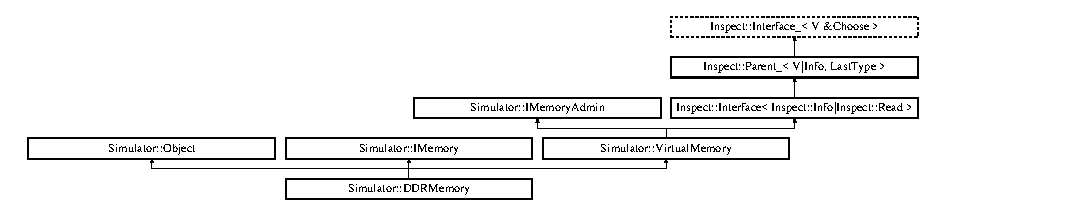
\includegraphics[height=2.456140cm]{class_simulator_1_1_d_d_r_memory}
\end{center}
\end{figure}
\subsection*{Classes}
\begin{DoxyCompactItemize}
\item 
struct \hyperlink{struct_simulator_1_1_d_d_r_memory_1_1_client_info}{Client\+Info}
\item 
class \hyperlink{class_simulator_1_1_d_d_r_memory_1_1_interface}{Interface}
\item 
struct \hyperlink{struct_simulator_1_1_d_d_r_memory_1_1_request}{Request}
\end{DoxyCompactItemize}
\subsection*{Public Member Functions}
\begin{DoxyCompactItemize}
\item 
\hyperlink{class_simulator_1_1_d_d_r_memory_a6bd2272ef3ac2cfefff817b1191afd95}{D\+D\+R\+Memory} (const std\+::string \&\hyperlink{mtconf_8c_a8f8f80d37794cde9472343e4487ba3eb}{name}, \hyperlink{class_simulator_1_1_object}{Object} \&parent, \hyperlink{class_simulator_1_1_clock}{Clock} \&clock, \hyperlink{class_config}{Config} \&config, const std\+::string \&default\+Interface\+Selector\+Type)
\item 
\hyperlink{class_simulator_1_1_d_d_r_memory_a47faba8d51f4e69ef2a61f7e15f4aec3}{D\+D\+R\+Memory} (const \hyperlink{class_simulator_1_1_d_d_r_memory}{D\+D\+R\+Memory} \&)=delete
\item 
\hyperlink{class_simulator_1_1_d_d_r_memory}{D\+D\+R\+Memory} \& \hyperlink{class_simulator_1_1_d_d_r_memory_a15ca970994811f051136024c5dae06f5}{operator=} (const \hyperlink{class_simulator_1_1_d_d_r_memory}{D\+D\+R\+Memory} \&)=delete
\item 
\hyperlink{class_simulator_1_1_d_d_r_memory_ac0961064e1ac06702b4f4bc697c1f2cc}{$\sim$\+D\+D\+R\+Memory} ()
\item 
void \hyperlink{class_simulator_1_1_d_d_r_memory_a4bc97a978759100161dfd4055280e668}{Cmd\+\_\+\+Info} (std\+::ostream \&out, const std\+::vector$<$ std\+::string $>$ \&arguments) const override
\item 
void \hyperlink{class_simulator_1_1_d_d_r_memory_a76310d4d307fe95f326398a537a26e31}{Cmd\+\_\+\+Read} (std\+::ostream \&out, const std\+::vector$<$ std\+::string $>$ \&arguments) const override
\end{DoxyCompactItemize}
\subsection*{Protected Attributes}
\begin{DoxyCompactItemize}
\item 
\hyperlink{class_component_model_registry}{Component\+Model\+Registry} \& \hyperlink{class_simulator_1_1_d_d_r_memory_a5c7ae6a98783750acfd99f473475d290}{m\+\_\+registry}
\item 
\hyperlink{class_simulator_1_1_clock}{Clock} \& \hyperlink{class_simulator_1_1_d_d_r_memory_a8a3027eccb3716453d542f17c4eb0151}{m\+\_\+clock}
\item 
std\+::vector$<$ \hyperlink{struct_simulator_1_1_d_d_r_memory_1_1_client_info}{Client\+Info} $>$ \hyperlink{class_simulator_1_1_d_d_r_memory_a1085d5517fc05585aca1462830c35266}{m\+\_\+clients}
\item 
\hyperlink{class_simulator_1_1_storage_trace_set}{Storage\+Trace\+Set} \hyperlink{class_simulator_1_1_d_d_r_memory_a978f278bcf563c6b0ff18d5da028d542}{m\+\_\+storages}
\item 
std\+::vector$<$ \hyperlink{class_simulator_1_1_d_d_r_memory_1_1_interface}{Interface} $\ast$ $>$ \hyperlink{class_simulator_1_1_d_d_r_memory_ab800a4733a5a57a894721260dc23182f}{m\+\_\+ifs}
\item 
\hyperlink{class_simulator_1_1_d_d_r_channel_registry}{D\+D\+R\+Channel\+Registry} \hyperlink{class_simulator_1_1_d_d_r_memory_a0c42aa5784100181ef6aa7e6cc4fc370}{m\+\_\+ddr}
\item 
size\+\_\+t \hyperlink{class_simulator_1_1_d_d_r_memory_adc20b7ea04f0bd71b1f9e07f9a8347d0}{m\+\_\+line\+Size}
\item 
\hyperlink{class_simulator_1_1_i_bank_selector}{I\+Bank\+Selector} $\ast$ \hyperlink{class_simulator_1_1_d_d_r_memory_ac9641b0d58bc819ae98172e599a4753e}{m\+\_\+selector}
\item 
uint64\+\_\+t \hyperlink{class_simulator_1_1_d_d_r_memory_a7a89625feeafa3ecdc0421b9495b9992}{m\+\_\+nreads}
\item 
uint64\+\_\+t \hyperlink{class_simulator_1_1_d_d_r_memory_ac0fed0a3fa10f29671ce4482cf5d61b8}{m\+\_\+nread\+\_\+bytes}
\item 
uint64\+\_\+t \hyperlink{class_simulator_1_1_d_d_r_memory_a0b1446411da9a506ad43e5622152ab3f}{m\+\_\+nwrites}
\item 
uint64\+\_\+t \hyperlink{class_simulator_1_1_d_d_r_memory_a5ad2606b3bb026608bcd7f6b42c56920}{m\+\_\+nwrite\+\_\+bytes}
\end{DoxyCompactItemize}
\subsection*{Additional Inherited Members}


\subsection{Constructor \& Destructor Documentation}
\hypertarget{class_simulator_1_1_d_d_r_memory_a6bd2272ef3ac2cfefff817b1191afd95}{\index{Simulator\+::\+D\+D\+R\+Memory@{Simulator\+::\+D\+D\+R\+Memory}!D\+D\+R\+Memory@{D\+D\+R\+Memory}}
\index{D\+D\+R\+Memory@{D\+D\+R\+Memory}!Simulator\+::\+D\+D\+R\+Memory@{Simulator\+::\+D\+D\+R\+Memory}}
\subsubsection[{D\+D\+R\+Memory}]{\setlength{\rightskip}{0pt plus 5cm}Simulator\+::\+D\+D\+R\+Memory\+::\+D\+D\+R\+Memory (
\begin{DoxyParamCaption}
\item[{const std\+::string \&}]{name, }
\item[{{\bf Object} \&}]{parent, }
\item[{{\bf Clock} \&}]{clock, }
\item[{{\bf Config} \&}]{config, }
\item[{const std\+::string \&}]{default\+Interface\+Selector\+Type}
\end{DoxyParamCaption}
)}}\label{class_simulator_1_1_d_d_r_memory_a6bd2272ef3ac2cfefff817b1191afd95}
\hypertarget{class_simulator_1_1_d_d_r_memory_a47faba8d51f4e69ef2a61f7e15f4aec3}{\index{Simulator\+::\+D\+D\+R\+Memory@{Simulator\+::\+D\+D\+R\+Memory}!D\+D\+R\+Memory@{D\+D\+R\+Memory}}
\index{D\+D\+R\+Memory@{D\+D\+R\+Memory}!Simulator\+::\+D\+D\+R\+Memory@{Simulator\+::\+D\+D\+R\+Memory}}
\subsubsection[{D\+D\+R\+Memory}]{\setlength{\rightskip}{0pt plus 5cm}Simulator\+::\+D\+D\+R\+Memory\+::\+D\+D\+R\+Memory (
\begin{DoxyParamCaption}
\item[{const {\bf D\+D\+R\+Memory} \&}]{}
\end{DoxyParamCaption}
)\hspace{0.3cm}{\ttfamily [delete]}}}\label{class_simulator_1_1_d_d_r_memory_a47faba8d51f4e69ef2a61f7e15f4aec3}
\hypertarget{class_simulator_1_1_d_d_r_memory_ac0961064e1ac06702b4f4bc697c1f2cc}{\index{Simulator\+::\+D\+D\+R\+Memory@{Simulator\+::\+D\+D\+R\+Memory}!````~D\+D\+R\+Memory@{$\sim$\+D\+D\+R\+Memory}}
\index{````~D\+D\+R\+Memory@{$\sim$\+D\+D\+R\+Memory}!Simulator\+::\+D\+D\+R\+Memory@{Simulator\+::\+D\+D\+R\+Memory}}
\subsubsection[{$\sim$\+D\+D\+R\+Memory}]{\setlength{\rightskip}{0pt plus 5cm}Simulator\+::\+D\+D\+R\+Memory\+::$\sim$\+D\+D\+R\+Memory (
\begin{DoxyParamCaption}
{}
\end{DoxyParamCaption}
)}}\label{class_simulator_1_1_d_d_r_memory_ac0961064e1ac06702b4f4bc697c1f2cc}


\subsection{Member Function Documentation}
\hypertarget{class_simulator_1_1_d_d_r_memory_a4bc97a978759100161dfd4055280e668}{\index{Simulator\+::\+D\+D\+R\+Memory@{Simulator\+::\+D\+D\+R\+Memory}!Cmd\+\_\+\+Info@{Cmd\+\_\+\+Info}}
\index{Cmd\+\_\+\+Info@{Cmd\+\_\+\+Info}!Simulator\+::\+D\+D\+R\+Memory@{Simulator\+::\+D\+D\+R\+Memory}}
\subsubsection[{Cmd\+\_\+\+Info}]{\setlength{\rightskip}{0pt plus 5cm}void Simulator\+::\+D\+D\+R\+Memory\+::\+Cmd\+\_\+\+Info (
\begin{DoxyParamCaption}
\item[{std\+::ostream \&}]{out, }
\item[{const std\+::vector$<$ std\+::string $>$ \&}]{arguments}
\end{DoxyParamCaption}
) const\hspace{0.3cm}{\ttfamily [override]}}}\label{class_simulator_1_1_d_d_r_memory_a4bc97a978759100161dfd4055280e668}
\hypertarget{class_simulator_1_1_d_d_r_memory_a76310d4d307fe95f326398a537a26e31}{\index{Simulator\+::\+D\+D\+R\+Memory@{Simulator\+::\+D\+D\+R\+Memory}!Cmd\+\_\+\+Read@{Cmd\+\_\+\+Read}}
\index{Cmd\+\_\+\+Read@{Cmd\+\_\+\+Read}!Simulator\+::\+D\+D\+R\+Memory@{Simulator\+::\+D\+D\+R\+Memory}}
\subsubsection[{Cmd\+\_\+\+Read}]{\setlength{\rightskip}{0pt plus 5cm}void Simulator\+::\+D\+D\+R\+Memory\+::\+Cmd\+\_\+\+Read (
\begin{DoxyParamCaption}
\item[{std\+::ostream \&}]{out, }
\item[{const std\+::vector$<$ std\+::string $>$ \&}]{arguments}
\end{DoxyParamCaption}
) const\hspace{0.3cm}{\ttfamily [override]}}}\label{class_simulator_1_1_d_d_r_memory_a76310d4d307fe95f326398a537a26e31}
\hypertarget{class_simulator_1_1_d_d_r_memory_a15ca970994811f051136024c5dae06f5}{\index{Simulator\+::\+D\+D\+R\+Memory@{Simulator\+::\+D\+D\+R\+Memory}!operator=@{operator=}}
\index{operator=@{operator=}!Simulator\+::\+D\+D\+R\+Memory@{Simulator\+::\+D\+D\+R\+Memory}}
\subsubsection[{operator=}]{\setlength{\rightskip}{0pt plus 5cm}{\bf D\+D\+R\+Memory}\& Simulator\+::\+D\+D\+R\+Memory\+::operator= (
\begin{DoxyParamCaption}
\item[{const {\bf D\+D\+R\+Memory} \&}]{}
\end{DoxyParamCaption}
)\hspace{0.3cm}{\ttfamily [delete]}}}\label{class_simulator_1_1_d_d_r_memory_a15ca970994811f051136024c5dae06f5}


\subsection{Member Data Documentation}
\hypertarget{class_simulator_1_1_d_d_r_memory_a1085d5517fc05585aca1462830c35266}{\index{Simulator\+::\+D\+D\+R\+Memory@{Simulator\+::\+D\+D\+R\+Memory}!m\+\_\+clients@{m\+\_\+clients}}
\index{m\+\_\+clients@{m\+\_\+clients}!Simulator\+::\+D\+D\+R\+Memory@{Simulator\+::\+D\+D\+R\+Memory}}
\subsubsection[{m\+\_\+clients}]{\setlength{\rightskip}{0pt plus 5cm}std\+::vector$<${\bf Client\+Info}$>$ Simulator\+::\+D\+D\+R\+Memory\+::m\+\_\+clients\hspace{0.3cm}{\ttfamily [protected]}}}\label{class_simulator_1_1_d_d_r_memory_a1085d5517fc05585aca1462830c35266}
\hypertarget{class_simulator_1_1_d_d_r_memory_a8a3027eccb3716453d542f17c4eb0151}{\index{Simulator\+::\+D\+D\+R\+Memory@{Simulator\+::\+D\+D\+R\+Memory}!m\+\_\+clock@{m\+\_\+clock}}
\index{m\+\_\+clock@{m\+\_\+clock}!Simulator\+::\+D\+D\+R\+Memory@{Simulator\+::\+D\+D\+R\+Memory}}
\subsubsection[{m\+\_\+clock}]{\setlength{\rightskip}{0pt plus 5cm}{\bf Clock}\& Simulator\+::\+D\+D\+R\+Memory\+::m\+\_\+clock\hspace{0.3cm}{\ttfamily [protected]}}}\label{class_simulator_1_1_d_d_r_memory_a8a3027eccb3716453d542f17c4eb0151}
\hypertarget{class_simulator_1_1_d_d_r_memory_a0c42aa5784100181ef6aa7e6cc4fc370}{\index{Simulator\+::\+D\+D\+R\+Memory@{Simulator\+::\+D\+D\+R\+Memory}!m\+\_\+ddr@{m\+\_\+ddr}}
\index{m\+\_\+ddr@{m\+\_\+ddr}!Simulator\+::\+D\+D\+R\+Memory@{Simulator\+::\+D\+D\+R\+Memory}}
\subsubsection[{m\+\_\+ddr}]{\setlength{\rightskip}{0pt plus 5cm}{\bf D\+D\+R\+Channel\+Registry} Simulator\+::\+D\+D\+R\+Memory\+::m\+\_\+ddr\hspace{0.3cm}{\ttfamily [protected]}}}\label{class_simulator_1_1_d_d_r_memory_a0c42aa5784100181ef6aa7e6cc4fc370}
\hypertarget{class_simulator_1_1_d_d_r_memory_ab800a4733a5a57a894721260dc23182f}{\index{Simulator\+::\+D\+D\+R\+Memory@{Simulator\+::\+D\+D\+R\+Memory}!m\+\_\+ifs@{m\+\_\+ifs}}
\index{m\+\_\+ifs@{m\+\_\+ifs}!Simulator\+::\+D\+D\+R\+Memory@{Simulator\+::\+D\+D\+R\+Memory}}
\subsubsection[{m\+\_\+ifs}]{\setlength{\rightskip}{0pt plus 5cm}std\+::vector$<${\bf Interface}$\ast$$>$ Simulator\+::\+D\+D\+R\+Memory\+::m\+\_\+ifs\hspace{0.3cm}{\ttfamily [protected]}}}\label{class_simulator_1_1_d_d_r_memory_ab800a4733a5a57a894721260dc23182f}
\hypertarget{class_simulator_1_1_d_d_r_memory_adc20b7ea04f0bd71b1f9e07f9a8347d0}{\index{Simulator\+::\+D\+D\+R\+Memory@{Simulator\+::\+D\+D\+R\+Memory}!m\+\_\+line\+Size@{m\+\_\+line\+Size}}
\index{m\+\_\+line\+Size@{m\+\_\+line\+Size}!Simulator\+::\+D\+D\+R\+Memory@{Simulator\+::\+D\+D\+R\+Memory}}
\subsubsection[{m\+\_\+line\+Size}]{\setlength{\rightskip}{0pt plus 5cm}size\+\_\+t Simulator\+::\+D\+D\+R\+Memory\+::m\+\_\+line\+Size\hspace{0.3cm}{\ttfamily [protected]}}}\label{class_simulator_1_1_d_d_r_memory_adc20b7ea04f0bd71b1f9e07f9a8347d0}
\hypertarget{class_simulator_1_1_d_d_r_memory_ac0fed0a3fa10f29671ce4482cf5d61b8}{\index{Simulator\+::\+D\+D\+R\+Memory@{Simulator\+::\+D\+D\+R\+Memory}!m\+\_\+nread\+\_\+bytes@{m\+\_\+nread\+\_\+bytes}}
\index{m\+\_\+nread\+\_\+bytes@{m\+\_\+nread\+\_\+bytes}!Simulator\+::\+D\+D\+R\+Memory@{Simulator\+::\+D\+D\+R\+Memory}}
\subsubsection[{m\+\_\+nread\+\_\+bytes}]{\setlength{\rightskip}{0pt plus 5cm}uint64\+\_\+t Simulator\+::\+D\+D\+R\+Memory\+::m\+\_\+nread\+\_\+bytes\hspace{0.3cm}{\ttfamily [protected]}}}\label{class_simulator_1_1_d_d_r_memory_ac0fed0a3fa10f29671ce4482cf5d61b8}
\hypertarget{class_simulator_1_1_d_d_r_memory_a7a89625feeafa3ecdc0421b9495b9992}{\index{Simulator\+::\+D\+D\+R\+Memory@{Simulator\+::\+D\+D\+R\+Memory}!m\+\_\+nreads@{m\+\_\+nreads}}
\index{m\+\_\+nreads@{m\+\_\+nreads}!Simulator\+::\+D\+D\+R\+Memory@{Simulator\+::\+D\+D\+R\+Memory}}
\subsubsection[{m\+\_\+nreads}]{\setlength{\rightskip}{0pt plus 5cm}uint64\+\_\+t Simulator\+::\+D\+D\+R\+Memory\+::m\+\_\+nreads\hspace{0.3cm}{\ttfamily [protected]}}}\label{class_simulator_1_1_d_d_r_memory_a7a89625feeafa3ecdc0421b9495b9992}
\hypertarget{class_simulator_1_1_d_d_r_memory_a5ad2606b3bb026608bcd7f6b42c56920}{\index{Simulator\+::\+D\+D\+R\+Memory@{Simulator\+::\+D\+D\+R\+Memory}!m\+\_\+nwrite\+\_\+bytes@{m\+\_\+nwrite\+\_\+bytes}}
\index{m\+\_\+nwrite\+\_\+bytes@{m\+\_\+nwrite\+\_\+bytes}!Simulator\+::\+D\+D\+R\+Memory@{Simulator\+::\+D\+D\+R\+Memory}}
\subsubsection[{m\+\_\+nwrite\+\_\+bytes}]{\setlength{\rightskip}{0pt plus 5cm}uint64\+\_\+t Simulator\+::\+D\+D\+R\+Memory\+::m\+\_\+nwrite\+\_\+bytes\hspace{0.3cm}{\ttfamily [protected]}}}\label{class_simulator_1_1_d_d_r_memory_a5ad2606b3bb026608bcd7f6b42c56920}
\hypertarget{class_simulator_1_1_d_d_r_memory_a0b1446411da9a506ad43e5622152ab3f}{\index{Simulator\+::\+D\+D\+R\+Memory@{Simulator\+::\+D\+D\+R\+Memory}!m\+\_\+nwrites@{m\+\_\+nwrites}}
\index{m\+\_\+nwrites@{m\+\_\+nwrites}!Simulator\+::\+D\+D\+R\+Memory@{Simulator\+::\+D\+D\+R\+Memory}}
\subsubsection[{m\+\_\+nwrites}]{\setlength{\rightskip}{0pt plus 5cm}uint64\+\_\+t Simulator\+::\+D\+D\+R\+Memory\+::m\+\_\+nwrites\hspace{0.3cm}{\ttfamily [protected]}}}\label{class_simulator_1_1_d_d_r_memory_a0b1446411da9a506ad43e5622152ab3f}
\hypertarget{class_simulator_1_1_d_d_r_memory_a5c7ae6a98783750acfd99f473475d290}{\index{Simulator\+::\+D\+D\+R\+Memory@{Simulator\+::\+D\+D\+R\+Memory}!m\+\_\+registry@{m\+\_\+registry}}
\index{m\+\_\+registry@{m\+\_\+registry}!Simulator\+::\+D\+D\+R\+Memory@{Simulator\+::\+D\+D\+R\+Memory}}
\subsubsection[{m\+\_\+registry}]{\setlength{\rightskip}{0pt plus 5cm}{\bf Component\+Model\+Registry}\& Simulator\+::\+D\+D\+R\+Memory\+::m\+\_\+registry\hspace{0.3cm}{\ttfamily [protected]}}}\label{class_simulator_1_1_d_d_r_memory_a5c7ae6a98783750acfd99f473475d290}
\hypertarget{class_simulator_1_1_d_d_r_memory_ac9641b0d58bc819ae98172e599a4753e}{\index{Simulator\+::\+D\+D\+R\+Memory@{Simulator\+::\+D\+D\+R\+Memory}!m\+\_\+selector@{m\+\_\+selector}}
\index{m\+\_\+selector@{m\+\_\+selector}!Simulator\+::\+D\+D\+R\+Memory@{Simulator\+::\+D\+D\+R\+Memory}}
\subsubsection[{m\+\_\+selector}]{\setlength{\rightskip}{0pt plus 5cm}{\bf I\+Bank\+Selector}$\ast$ Simulator\+::\+D\+D\+R\+Memory\+::m\+\_\+selector\hspace{0.3cm}{\ttfamily [protected]}}}\label{class_simulator_1_1_d_d_r_memory_ac9641b0d58bc819ae98172e599a4753e}
\hypertarget{class_simulator_1_1_d_d_r_memory_a978f278bcf563c6b0ff18d5da028d542}{\index{Simulator\+::\+D\+D\+R\+Memory@{Simulator\+::\+D\+D\+R\+Memory}!m\+\_\+storages@{m\+\_\+storages}}
\index{m\+\_\+storages@{m\+\_\+storages}!Simulator\+::\+D\+D\+R\+Memory@{Simulator\+::\+D\+D\+R\+Memory}}
\subsubsection[{m\+\_\+storages}]{\setlength{\rightskip}{0pt plus 5cm}{\bf Storage\+Trace\+Set} Simulator\+::\+D\+D\+R\+Memory\+::m\+\_\+storages\hspace{0.3cm}{\ttfamily [protected]}}}\label{class_simulator_1_1_d_d_r_memory_a978f278bcf563c6b0ff18d5da028d542}


The documentation for this class was generated from the following files\+:\begin{DoxyCompactItemize}
\item 
arch/mem/\hyperlink{_d_d_r_memory_8h}{D\+D\+R\+Memory.\+h}\item 
arch/mem/\hyperlink{_d_d_r_memory_8cpp}{D\+D\+R\+Memory.\+cpp}\end{DoxyCompactItemize}

\hypertarget{class_simulator_1_1_deadlock_exception}{\section{Simulator\+:\+:Deadlock\+Exception Class Reference}
\label{class_simulator_1_1_deadlock_exception}\index{Simulator\+::\+Deadlock\+Exception@{Simulator\+::\+Deadlock\+Exception}}
}


{\ttfamily \#include $<$except.\+h$>$}

Inheritance diagram for Simulator\+:\+:Deadlock\+Exception\+:\begin{figure}[H]
\begin{center}
\leavevmode
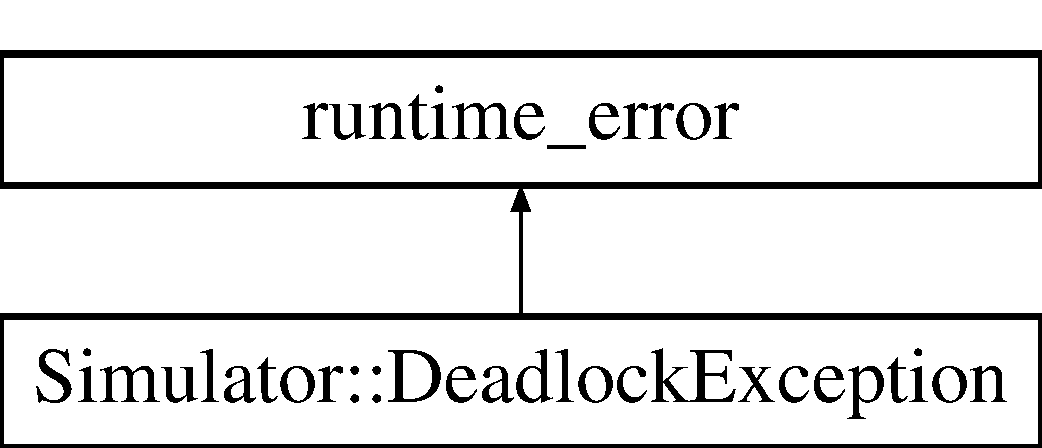
\includegraphics[height=2.000000cm]{class_simulator_1_1_deadlock_exception}
\end{center}
\end{figure}
\subsection*{Public Member Functions}
\begin{DoxyCompactItemize}
\item 
\hyperlink{class_simulator_1_1_deadlock_exception_a805a22bda9e47e819773773527382dad}{Deadlock\+Exception} (const std\+::string \&msg)
\end{DoxyCompactItemize}


\subsection{Constructor \& Destructor Documentation}
\hypertarget{class_simulator_1_1_deadlock_exception_a805a22bda9e47e819773773527382dad}{\index{Simulator\+::\+Deadlock\+Exception@{Simulator\+::\+Deadlock\+Exception}!Deadlock\+Exception@{Deadlock\+Exception}}
\index{Deadlock\+Exception@{Deadlock\+Exception}!Simulator\+::\+Deadlock\+Exception@{Simulator\+::\+Deadlock\+Exception}}
\subsubsection[{Deadlock\+Exception}]{\setlength{\rightskip}{0pt plus 5cm}Simulator\+::\+Deadlock\+Exception\+::\+Deadlock\+Exception (
\begin{DoxyParamCaption}
\item[{const std\+::string \&}]{msg}
\end{DoxyParamCaption}
)\hspace{0.3cm}{\ttfamily [inline]}}}\label{class_simulator_1_1_deadlock_exception_a805a22bda9e47e819773773527382dad}


The documentation for this class was generated from the following file\+:\begin{DoxyCompactItemize}
\item 
sim/\hyperlink{except_8h}{except.\+h}\end{DoxyCompactItemize}

\hypertarget{class_simulator_1_1drisc_1_1_debug_channel}{\section{Simulator\+:\+:drisc\+:\+:Debug\+Channel Class Reference}
\label{class_simulator_1_1drisc_1_1_debug_channel}\index{Simulator\+::drisc\+::\+Debug\+Channel@{Simulator\+::drisc\+::\+Debug\+Channel}}
}


{\ttfamily \#include $<$Debug\+Channel.\+h$>$}

Inheritance diagram for Simulator\+:\+:drisc\+:\+:Debug\+Channel\+:\begin{figure}[H]
\begin{center}
\leavevmode
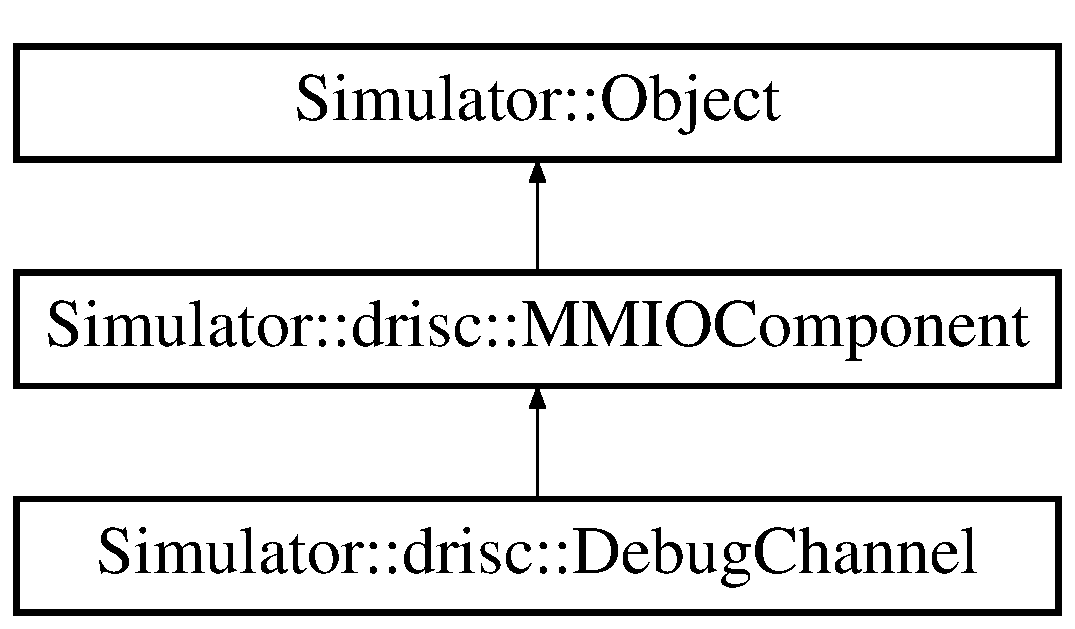
\includegraphics[height=3.000000cm]{class_simulator_1_1drisc_1_1_debug_channel}
\end{center}
\end{figure}
\subsection*{Public Member Functions}
\begin{DoxyCompactItemize}
\item 
\hyperlink{class_simulator_1_1drisc_1_1_debug_channel_aaeca18839cded092f43be7dce8c5112d}{Debug\+Channel} (const std\+::string \&\hyperlink{mtconf_8c_a8f8f80d37794cde9472343e4487ba3eb}{name}, \hyperlink{class_simulator_1_1_object}{Object} \&parent, std\+::ostream \&output)
\item 
size\+\_\+t \hyperlink{class_simulator_1_1drisc_1_1_debug_channel_abd636bf58c008ee82af796b6a0091801}{Get\+Size} () const 
\item 
\hyperlink{namespace_simulator_a4b6b5616e7236c0c131516a441776805}{Result} \hyperlink{class_simulator_1_1drisc_1_1_debug_channel_af772c686411b277669040f139d684fb7}{Read} (Mem\+Addr address, void $\ast$data, Mem\+Size size, \hyperlink{namespace_simulator_aaccbc706b2d6c99085f52f6dfc2333e4}{L\+F\+I\+D} fid, \hyperlink{namespace_simulator_a483cc4ecee1736e895054617672cded5}{T\+I\+D} tid, const \hyperlink{struct_simulator_1_1_reg_addr}{Reg\+Addr} \&writeback)
\item 
\hyperlink{namespace_simulator_a4b6b5616e7236c0c131516a441776805}{Result} \hyperlink{class_simulator_1_1drisc_1_1_debug_channel_aea26d20ae29dcf23154ef4072a108bfe}{Write} (Mem\+Addr address, const void $\ast$data, Mem\+Size size, \hyperlink{namespace_simulator_aaccbc706b2d6c99085f52f6dfc2333e4}{L\+F\+I\+D} fid, \hyperlink{namespace_simulator_a483cc4ecee1736e895054617672cded5}{T\+I\+D} tid)
\end{DoxyCompactItemize}


\subsection{Constructor \& Destructor Documentation}
\hypertarget{class_simulator_1_1drisc_1_1_debug_channel_aaeca18839cded092f43be7dce8c5112d}{\index{Simulator\+::drisc\+::\+Debug\+Channel@{Simulator\+::drisc\+::\+Debug\+Channel}!Debug\+Channel@{Debug\+Channel}}
\index{Debug\+Channel@{Debug\+Channel}!Simulator\+::drisc\+::\+Debug\+Channel@{Simulator\+::drisc\+::\+Debug\+Channel}}
\subsubsection[{Debug\+Channel}]{\setlength{\rightskip}{0pt plus 5cm}Simulator\+::drisc\+::\+Debug\+Channel\+::\+Debug\+Channel (
\begin{DoxyParamCaption}
\item[{const std\+::string \&}]{name, }
\item[{{\bf Object} \&}]{parent, }
\item[{std\+::ostream \&}]{output}
\end{DoxyParamCaption}
)}}\label{class_simulator_1_1drisc_1_1_debug_channel_aaeca18839cded092f43be7dce8c5112d}


\subsection{Member Function Documentation}
\hypertarget{class_simulator_1_1drisc_1_1_debug_channel_abd636bf58c008ee82af796b6a0091801}{\index{Simulator\+::drisc\+::\+Debug\+Channel@{Simulator\+::drisc\+::\+Debug\+Channel}!Get\+Size@{Get\+Size}}
\index{Get\+Size@{Get\+Size}!Simulator\+::drisc\+::\+Debug\+Channel@{Simulator\+::drisc\+::\+Debug\+Channel}}
\subsubsection[{Get\+Size}]{\setlength{\rightskip}{0pt plus 5cm}size\+\_\+t Simulator\+::drisc\+::\+Debug\+Channel\+::\+Get\+Size (
\begin{DoxyParamCaption}
{}
\end{DoxyParamCaption}
) const\hspace{0.3cm}{\ttfamily [virtual]}}}\label{class_simulator_1_1drisc_1_1_debug_channel_abd636bf58c008ee82af796b6a0091801}


Implements \hyperlink{class_simulator_1_1drisc_1_1_m_m_i_o_component_ad8f1a93b445f287895949bfe52972346}{Simulator\+::drisc\+::\+M\+M\+I\+O\+Component}.

\hypertarget{class_simulator_1_1drisc_1_1_debug_channel_af772c686411b277669040f139d684fb7}{\index{Simulator\+::drisc\+::\+Debug\+Channel@{Simulator\+::drisc\+::\+Debug\+Channel}!Read@{Read}}
\index{Read@{Read}!Simulator\+::drisc\+::\+Debug\+Channel@{Simulator\+::drisc\+::\+Debug\+Channel}}
\subsubsection[{Read}]{\setlength{\rightskip}{0pt plus 5cm}{\bf Result} Simulator\+::drisc\+::\+Debug\+Channel\+::\+Read (
\begin{DoxyParamCaption}
\item[{Mem\+Addr}]{address, }
\item[{void $\ast$}]{data, }
\item[{Mem\+Size}]{size, }
\item[{{\bf L\+F\+I\+D}}]{fid, }
\item[{{\bf T\+I\+D}}]{tid, }
\item[{const {\bf Reg\+Addr} \&}]{writeback}
\end{DoxyParamCaption}
)\hspace{0.3cm}{\ttfamily [virtual]}}}\label{class_simulator_1_1drisc_1_1_debug_channel_af772c686411b277669040f139d684fb7}


Implements \hyperlink{class_simulator_1_1drisc_1_1_m_m_i_o_component_af07e2f3e1280d8d56cab7a59815e7eeb}{Simulator\+::drisc\+::\+M\+M\+I\+O\+Component}.

\hypertarget{class_simulator_1_1drisc_1_1_debug_channel_aea26d20ae29dcf23154ef4072a108bfe}{\index{Simulator\+::drisc\+::\+Debug\+Channel@{Simulator\+::drisc\+::\+Debug\+Channel}!Write@{Write}}
\index{Write@{Write}!Simulator\+::drisc\+::\+Debug\+Channel@{Simulator\+::drisc\+::\+Debug\+Channel}}
\subsubsection[{Write}]{\setlength{\rightskip}{0pt plus 5cm}{\bf Result} Simulator\+::drisc\+::\+Debug\+Channel\+::\+Write (
\begin{DoxyParamCaption}
\item[{Mem\+Addr}]{address, }
\item[{const void $\ast$}]{data, }
\item[{Mem\+Size}]{size, }
\item[{{\bf L\+F\+I\+D}}]{fid, }
\item[{{\bf T\+I\+D}}]{tid}
\end{DoxyParamCaption}
)\hspace{0.3cm}{\ttfamily [virtual]}}}\label{class_simulator_1_1drisc_1_1_debug_channel_aea26d20ae29dcf23154ef4072a108bfe}


Implements \hyperlink{class_simulator_1_1drisc_1_1_m_m_i_o_component_aab3662058e7a00109b122a1460188a8b}{Simulator\+::drisc\+::\+M\+M\+I\+O\+Component}.



The documentation for this class was generated from the following files\+:\begin{DoxyCompactItemize}
\item 
arch/drisc/mmu/\hyperlink{_debug_channel_8h}{Debug\+Channel.\+h}\item 
arch/drisc/mmu/\hyperlink{_debug_channel_8cpp}{Debug\+Channel.\+cpp}\end{DoxyCompactItemize}

\hypertarget{class_simulator_1_1_dedicated_port}{\section{Simulator\+:\+:Dedicated\+Port Class Reference}
\label{class_simulator_1_1_dedicated_port}\index{Simulator\+::\+Dedicated\+Port@{Simulator\+::\+Dedicated\+Port}}
}


{\ttfamily \#include $<$ports.\+h$>$}

Inheritance diagram for Simulator\+:\+:Dedicated\+Port\+:\begin{figure}[H]
\begin{center}
\leavevmode
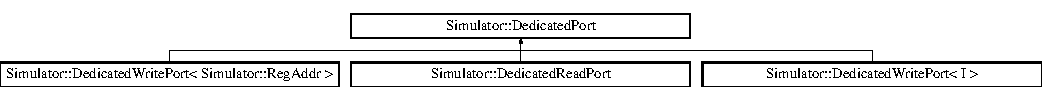
\includegraphics[height=1.170324cm]{class_simulator_1_1_dedicated_port}
\end{center}
\end{figure}
\subsection*{Public Member Functions}
\begin{DoxyCompactItemize}
\item 
\hyperlink{class_simulator_1_1_dedicated_port_a76e065440e802a0be0272dd3f6c29dba}{Dedicated\+Port} (const \hyperlink{class_simulator_1_1_object}{Object} \&, const std\+::string \&)
\item 
\hyperlink{class_simulator_1_1_dedicated_port_a12bfc8a6c4dab2a12de69d056d9e668a}{Dedicated\+Port} (const \hyperlink{class_simulator_1_1_dedicated_port}{Dedicated\+Port} \&)=delete
\item 
\hyperlink{class_simulator_1_1_dedicated_port}{Dedicated\+Port} \& \hyperlink{class_simulator_1_1_dedicated_port_a7e0cf4bca02a6549ce0fbaaf78eed234}{operator=} (const \hyperlink{class_simulator_1_1_dedicated_port}{Dedicated\+Port} \&)=delete
\item 
virtual \hyperlink{class_simulator_1_1_dedicated_port_a0b6194c6742667123c16dee0f68dcf62}{$\sim$\+Dedicated\+Port} ()
\item 
void \hyperlink{class_simulator_1_1_dedicated_port_a1538e25c8b0cfe66e690f185ab2bb630}{Set\+Process} (const \hyperlink{class_simulator_1_1_process}{Process} \&process)
\end{DoxyCompactItemize}
\subsection*{Protected Member Functions}
\begin{DoxyCompactItemize}
\item 
bool \hyperlink{class_simulator_1_1_dedicated_port_a66706a589cd6b63477c5299eca65b494}{Can\+Access} (const \hyperlink{class_simulator_1_1_process}{Process} \&process)
\end{DoxyCompactItemize}


\subsection{Constructor \& Destructor Documentation}
\hypertarget{class_simulator_1_1_dedicated_port_a76e065440e802a0be0272dd3f6c29dba}{\index{Simulator\+::\+Dedicated\+Port@{Simulator\+::\+Dedicated\+Port}!Dedicated\+Port@{Dedicated\+Port}}
\index{Dedicated\+Port@{Dedicated\+Port}!Simulator\+::\+Dedicated\+Port@{Simulator\+::\+Dedicated\+Port}}
\subsubsection[{Dedicated\+Port}]{\setlength{\rightskip}{0pt plus 5cm}Simulator\+::\+Dedicated\+Port\+::\+Dedicated\+Port (
\begin{DoxyParamCaption}
\item[{const {\bf Object} \&}]{, }
\item[{const std\+::string \&}]{}
\end{DoxyParamCaption}
)\hspace{0.3cm}{\ttfamily [inline]}}}\label{class_simulator_1_1_dedicated_port_a76e065440e802a0be0272dd3f6c29dba}
\hypertarget{class_simulator_1_1_dedicated_port_a12bfc8a6c4dab2a12de69d056d9e668a}{\index{Simulator\+::\+Dedicated\+Port@{Simulator\+::\+Dedicated\+Port}!Dedicated\+Port@{Dedicated\+Port}}
\index{Dedicated\+Port@{Dedicated\+Port}!Simulator\+::\+Dedicated\+Port@{Simulator\+::\+Dedicated\+Port}}
\subsubsection[{Dedicated\+Port}]{\setlength{\rightskip}{0pt plus 5cm}Simulator\+::\+Dedicated\+Port\+::\+Dedicated\+Port (
\begin{DoxyParamCaption}
\item[{const {\bf Dedicated\+Port} \&}]{}
\end{DoxyParamCaption}
)\hspace{0.3cm}{\ttfamily [delete]}}}\label{class_simulator_1_1_dedicated_port_a12bfc8a6c4dab2a12de69d056d9e668a}
\hypertarget{class_simulator_1_1_dedicated_port_a0b6194c6742667123c16dee0f68dcf62}{\index{Simulator\+::\+Dedicated\+Port@{Simulator\+::\+Dedicated\+Port}!````~Dedicated\+Port@{$\sim$\+Dedicated\+Port}}
\index{````~Dedicated\+Port@{$\sim$\+Dedicated\+Port}!Simulator\+::\+Dedicated\+Port@{Simulator\+::\+Dedicated\+Port}}
\subsubsection[{$\sim$\+Dedicated\+Port}]{\setlength{\rightskip}{0pt plus 5cm}virtual Simulator\+::\+Dedicated\+Port\+::$\sim$\+Dedicated\+Port (
\begin{DoxyParamCaption}
{}
\end{DoxyParamCaption}
)\hspace{0.3cm}{\ttfamily [inline]}, {\ttfamily [virtual]}}}\label{class_simulator_1_1_dedicated_port_a0b6194c6742667123c16dee0f68dcf62}


\subsection{Member Function Documentation}
\hypertarget{class_simulator_1_1_dedicated_port_a66706a589cd6b63477c5299eca65b494}{\index{Simulator\+::\+Dedicated\+Port@{Simulator\+::\+Dedicated\+Port}!Can\+Access@{Can\+Access}}
\index{Can\+Access@{Can\+Access}!Simulator\+::\+Dedicated\+Port@{Simulator\+::\+Dedicated\+Port}}
\subsubsection[{Can\+Access}]{\setlength{\rightskip}{0pt plus 5cm}bool Simulator\+::\+Dedicated\+Port\+::\+Can\+Access (
\begin{DoxyParamCaption}
\item[{const {\bf Process} \&}]{process}
\end{DoxyParamCaption}
)\hspace{0.3cm}{\ttfamily [inline]}, {\ttfamily [protected]}}}\label{class_simulator_1_1_dedicated_port_a66706a589cd6b63477c5299eca65b494}
\hypertarget{class_simulator_1_1_dedicated_port_a7e0cf4bca02a6549ce0fbaaf78eed234}{\index{Simulator\+::\+Dedicated\+Port@{Simulator\+::\+Dedicated\+Port}!operator=@{operator=}}
\index{operator=@{operator=}!Simulator\+::\+Dedicated\+Port@{Simulator\+::\+Dedicated\+Port}}
\subsubsection[{operator=}]{\setlength{\rightskip}{0pt plus 5cm}{\bf Dedicated\+Port}\& Simulator\+::\+Dedicated\+Port\+::operator= (
\begin{DoxyParamCaption}
\item[{const {\bf Dedicated\+Port} \&}]{}
\end{DoxyParamCaption}
)\hspace{0.3cm}{\ttfamily [delete]}}}\label{class_simulator_1_1_dedicated_port_a7e0cf4bca02a6549ce0fbaaf78eed234}
\hypertarget{class_simulator_1_1_dedicated_port_a1538e25c8b0cfe66e690f185ab2bb630}{\index{Simulator\+::\+Dedicated\+Port@{Simulator\+::\+Dedicated\+Port}!Set\+Process@{Set\+Process}}
\index{Set\+Process@{Set\+Process}!Simulator\+::\+Dedicated\+Port@{Simulator\+::\+Dedicated\+Port}}
\subsubsection[{Set\+Process}]{\setlength{\rightskip}{0pt plus 5cm}void Simulator\+::\+Dedicated\+Port\+::\+Set\+Process (
\begin{DoxyParamCaption}
\item[{const {\bf Process} \&}]{process}
\end{DoxyParamCaption}
)\hspace{0.3cm}{\ttfamily [inline]}}}\label{class_simulator_1_1_dedicated_port_a1538e25c8b0cfe66e690f185ab2bb630}


The documentation for this class was generated from the following file\+:\begin{DoxyCompactItemize}
\item 
sim/\hyperlink{ports_8h}{ports.\+h}\end{DoxyCompactItemize}

\hypertarget{class_simulator_1_1_dedicated_read_port}{\section{Simulator\+:\+:Dedicated\+Read\+Port Class Reference}
\label{class_simulator_1_1_dedicated_read_port}\index{Simulator\+::\+Dedicated\+Read\+Port@{Simulator\+::\+Dedicated\+Read\+Port}}
}


{\ttfamily \#include $<$ports.\+h$>$}

Inheritance diagram for Simulator\+:\+:Dedicated\+Read\+Port\+:\begin{figure}[H]
\begin{center}
\leavevmode
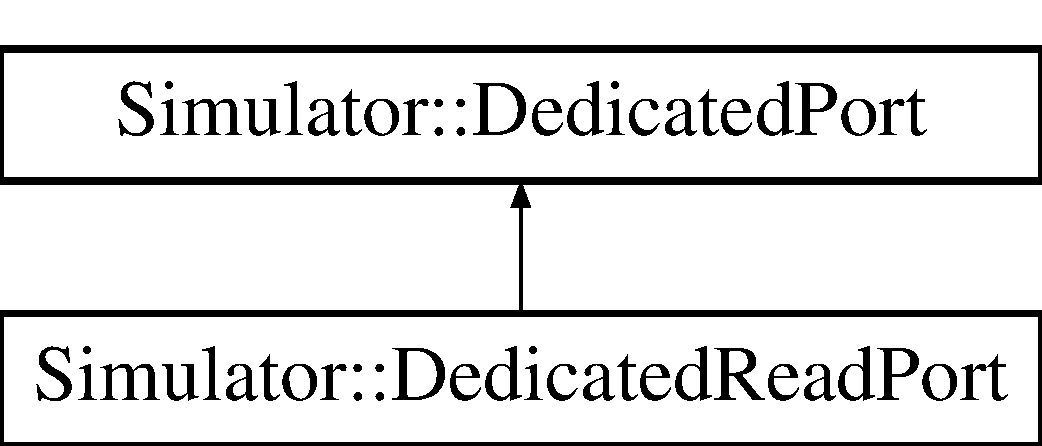
\includegraphics[height=2.000000cm]{class_simulator_1_1_dedicated_read_port}
\end{center}
\end{figure}
\subsection*{Public Member Functions}
\begin{DoxyCompactItemize}
\item 
\hyperlink{class_simulator_1_1_dedicated_read_port_af0471f1bc9641eef34ece94cac11f239}{Dedicated\+Read\+Port} (\hyperlink{class_simulator_1_1_i_structure}{I\+Structure} \&structure, const std\+::string \&\hyperlink{mtconf_8c_a8f8f80d37794cde9472343e4487ba3eb}{name})
\item 
bool \hyperlink{class_simulator_1_1_dedicated_read_port_ac90784416af2ee3a16ef462888072992}{Read} ()
\end{DoxyCompactItemize}
\subsection*{Additional Inherited Members}


\subsection{Constructor \& Destructor Documentation}
\hypertarget{class_simulator_1_1_dedicated_read_port_af0471f1bc9641eef34ece94cac11f239}{\index{Simulator\+::\+Dedicated\+Read\+Port@{Simulator\+::\+Dedicated\+Read\+Port}!Dedicated\+Read\+Port@{Dedicated\+Read\+Port}}
\index{Dedicated\+Read\+Port@{Dedicated\+Read\+Port}!Simulator\+::\+Dedicated\+Read\+Port@{Simulator\+::\+Dedicated\+Read\+Port}}
\subsubsection[{Dedicated\+Read\+Port}]{\setlength{\rightskip}{0pt plus 5cm}Simulator\+::\+Dedicated\+Read\+Port\+::\+Dedicated\+Read\+Port (
\begin{DoxyParamCaption}
\item[{{\bf I\+Structure} \&}]{structure, }
\item[{const std\+::string \&}]{name}
\end{DoxyParamCaption}
)\hspace{0.3cm}{\ttfamily [inline]}}}\label{class_simulator_1_1_dedicated_read_port_af0471f1bc9641eef34ece94cac11f239}


\subsection{Member Function Documentation}
\hypertarget{class_simulator_1_1_dedicated_read_port_ac90784416af2ee3a16ef462888072992}{\index{Simulator\+::\+Dedicated\+Read\+Port@{Simulator\+::\+Dedicated\+Read\+Port}!Read@{Read}}
\index{Read@{Read}!Simulator\+::\+Dedicated\+Read\+Port@{Simulator\+::\+Dedicated\+Read\+Port}}
\subsubsection[{Read}]{\setlength{\rightskip}{0pt plus 5cm}bool Simulator\+::\+Dedicated\+Read\+Port\+::\+Read (
\begin{DoxyParamCaption}
{}
\end{DoxyParamCaption}
)\hspace{0.3cm}{\ttfamily [inline]}}}\label{class_simulator_1_1_dedicated_read_port_ac90784416af2ee3a16ef462888072992}


The documentation for this class was generated from the following file\+:\begin{DoxyCompactItemize}
\item 
sim/\hyperlink{ports_8h}{ports.\+h}\end{DoxyCompactItemize}

\hypertarget{class_simulator_1_1_dedicated_write_port}{\section{Simulator\+:\+:Dedicated\+Write\+Port$<$ I $>$ Class Template Reference}
\label{class_simulator_1_1_dedicated_write_port}\index{Simulator\+::\+Dedicated\+Write\+Port$<$ I $>$@{Simulator\+::\+Dedicated\+Write\+Port$<$ I $>$}}
}


{\ttfamily \#include $<$ports.\+h$>$}

Inheritance diagram for Simulator\+:\+:Dedicated\+Write\+Port$<$ I $>$\+:\begin{figure}[H]
\begin{center}
\leavevmode
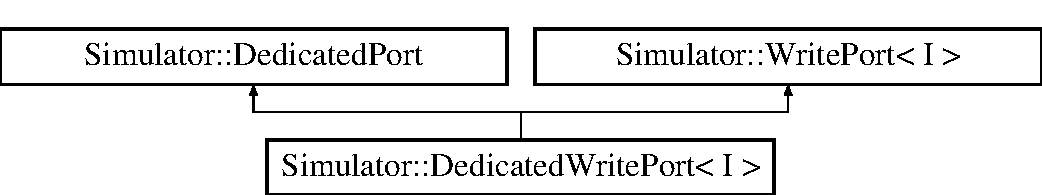
\includegraphics[height=2.000000cm]{class_simulator_1_1_dedicated_write_port}
\end{center}
\end{figure}
\subsection*{Public Member Functions}
\begin{DoxyCompactItemize}
\item 
\hyperlink{class_simulator_1_1_dedicated_write_port_ac3080c4f35eab1600110f500e9e33f92}{Dedicated\+Write\+Port} (\hyperlink{singleton_simulator_1_1_structure}{Structure}$<$ I $>$ \&structure, const std\+::string \&\hyperlink{mtconf_8c_a8f8f80d37794cde9472343e4487ba3eb}{name})
\item 
\hyperlink{class_simulator_1_1_dedicated_write_port_a48714636377d0f7ae14a456727a00e9f}{$\sim$\+Dedicated\+Write\+Port} ()
\item 
bool \hyperlink{class_simulator_1_1_dedicated_write_port_a1dacf0904c0a9e8a954f0a7e6d6da0cb}{Write} (const I \&index)
\end{DoxyCompactItemize}
\subsection*{Additional Inherited Members}


\subsection{Constructor \& Destructor Documentation}
\hypertarget{class_simulator_1_1_dedicated_write_port_ac3080c4f35eab1600110f500e9e33f92}{\index{Simulator\+::\+Dedicated\+Write\+Port@{Simulator\+::\+Dedicated\+Write\+Port}!Dedicated\+Write\+Port@{Dedicated\+Write\+Port}}
\index{Dedicated\+Write\+Port@{Dedicated\+Write\+Port}!Simulator\+::\+Dedicated\+Write\+Port@{Simulator\+::\+Dedicated\+Write\+Port}}
\subsubsection[{Dedicated\+Write\+Port}]{\setlength{\rightskip}{0pt plus 5cm}template$<$typename I$>$ {\bf Simulator\+::\+Dedicated\+Write\+Port}$<$ I $>$\+::{\bf Dedicated\+Write\+Port} (
\begin{DoxyParamCaption}
\item[{{\bf Structure}$<$ I $>$ \&}]{structure, }
\item[{const std\+::string \&}]{name}
\end{DoxyParamCaption}
)\hspace{0.3cm}{\ttfamily [inline]}}}\label{class_simulator_1_1_dedicated_write_port_ac3080c4f35eab1600110f500e9e33f92}
\hypertarget{class_simulator_1_1_dedicated_write_port_a48714636377d0f7ae14a456727a00e9f}{\index{Simulator\+::\+Dedicated\+Write\+Port@{Simulator\+::\+Dedicated\+Write\+Port}!````~Dedicated\+Write\+Port@{$\sim$\+Dedicated\+Write\+Port}}
\index{````~Dedicated\+Write\+Port@{$\sim$\+Dedicated\+Write\+Port}!Simulator\+::\+Dedicated\+Write\+Port@{Simulator\+::\+Dedicated\+Write\+Port}}
\subsubsection[{$\sim$\+Dedicated\+Write\+Port}]{\setlength{\rightskip}{0pt plus 5cm}template$<$typename I$>$ {\bf Simulator\+::\+Dedicated\+Write\+Port}$<$ I $>$\+::$\sim${\bf Dedicated\+Write\+Port} (
\begin{DoxyParamCaption}
{}
\end{DoxyParamCaption}
)\hspace{0.3cm}{\ttfamily [inline]}}}\label{class_simulator_1_1_dedicated_write_port_a48714636377d0f7ae14a456727a00e9f}


\subsection{Member Function Documentation}
\hypertarget{class_simulator_1_1_dedicated_write_port_a1dacf0904c0a9e8a954f0a7e6d6da0cb}{\index{Simulator\+::\+Dedicated\+Write\+Port@{Simulator\+::\+Dedicated\+Write\+Port}!Write@{Write}}
\index{Write@{Write}!Simulator\+::\+Dedicated\+Write\+Port@{Simulator\+::\+Dedicated\+Write\+Port}}
\subsubsection[{Write}]{\setlength{\rightskip}{0pt plus 5cm}template$<$typename I$>$ bool {\bf Simulator\+::\+Dedicated\+Write\+Port}$<$ I $>$\+::Write (
\begin{DoxyParamCaption}
\item[{const I \&}]{index}
\end{DoxyParamCaption}
)\hspace{0.3cm}{\ttfamily [inline]}}}\label{class_simulator_1_1_dedicated_write_port_a1dacf0904c0a9e8a954f0a7e6d6da0cb}


The documentation for this class was generated from the following file\+:\begin{DoxyCompactItemize}
\item 
sim/\hyperlink{ports_8h}{ports.\+h}\end{DoxyCompactItemize}

\hypertarget{class_simulator_1_1delegate}{\section{Simulator\+:\+:delegate Class Reference}
\label{class_simulator_1_1delegate}\index{Simulator\+::delegate@{Simulator\+::delegate}}
}


{\ttfamily \#include $<$delegate.\+h$>$}

\subsection*{Public Member Functions}
\begin{DoxyCompactItemize}
\item 
\hyperlink{namespace_simulator_a4b6b5616e7236c0c131516a441776805}{Result} \hyperlink{class_simulator_1_1delegate_a8fc9843df63a0dc7838b0f449aa993be}{operator()} () const 
\item 
\hyperlink{class_simulator_1_1_object}{Object} $\ast$ \hyperlink{class_simulator_1_1delegate_a3943bdb0cf2781214226b809a357c86d}{Get\+Object} () const 
\end{DoxyCompactItemize}
\subsection*{Static Public Member Functions}
\begin{DoxyCompactItemize}
\item 
{\footnotesize template$<$typename T , Result(\+T\+::$\ast$)() T\+Method$>$ }\\static \hyperlink{class_simulator_1_1delegate}{delegate} \hyperlink{class_simulator_1_1delegate_a1e68440f33e3d945bc2823880abaa114}{create} (T \&object)
\end{DoxyCompactItemize}


\subsection{Member Function Documentation}
\hypertarget{class_simulator_1_1delegate_a1e68440f33e3d945bc2823880abaa114}{\index{Simulator\+::delegate@{Simulator\+::delegate}!create@{create}}
\index{create@{create}!Simulator\+::delegate@{Simulator\+::delegate}}
\subsubsection[{create}]{\setlength{\rightskip}{0pt plus 5cm}template$<$typename T , Result(\+T\+::$\ast$)() T\+Method$>$ static {\bf delegate} Simulator\+::delegate\+::create (
\begin{DoxyParamCaption}
\item[{T \&}]{object}
\end{DoxyParamCaption}
)\hspace{0.3cm}{\ttfamily [inline]}, {\ttfamily [static]}}}\label{class_simulator_1_1delegate_a1e68440f33e3d945bc2823880abaa114}
\hypertarget{class_simulator_1_1delegate_a3943bdb0cf2781214226b809a357c86d}{\index{Simulator\+::delegate@{Simulator\+::delegate}!Get\+Object@{Get\+Object}}
\index{Get\+Object@{Get\+Object}!Simulator\+::delegate@{Simulator\+::delegate}}
\subsubsection[{Get\+Object}]{\setlength{\rightskip}{0pt plus 5cm}{\bf Object}$\ast$ Simulator\+::delegate\+::\+Get\+Object (
\begin{DoxyParamCaption}
{}
\end{DoxyParamCaption}
) const\hspace{0.3cm}{\ttfamily [inline]}}}\label{class_simulator_1_1delegate_a3943bdb0cf2781214226b809a357c86d}
\hypertarget{class_simulator_1_1delegate_a8fc9843df63a0dc7838b0f449aa993be}{\index{Simulator\+::delegate@{Simulator\+::delegate}!operator()@{operator()}}
\index{operator()@{operator()}!Simulator\+::delegate@{Simulator\+::delegate}}
\subsubsection[{operator()}]{\setlength{\rightskip}{0pt plus 5cm}{\bf Result} Simulator\+::delegate\+::operator() (
\begin{DoxyParamCaption}
{}
\end{DoxyParamCaption}
) const\hspace{0.3cm}{\ttfamily [inline]}}}\label{class_simulator_1_1delegate_a8fc9843df63a0dc7838b0f449aa993be}


The documentation for this class was generated from the following file\+:\begin{DoxyCompactItemize}
\item 
sim/\hyperlink{delegate_8h}{delegate.\+h}\end{DoxyCompactItemize}

\hypertarget{struct_simulator_1_1drisc_1_1_thread_1_1_dependencies}{\section{Simulator\+:\+:drisc\+:\+:Thread\+:\+:Dependencies Struct Reference}
\label{struct_simulator_1_1drisc_1_1_thread_1_1_dependencies}\index{Simulator\+::drisc\+::\+Thread\+::\+Dependencies@{Simulator\+::drisc\+::\+Thread\+::\+Dependencies}}
}


{\ttfamily \#include $<$Thread\+Table.\+h$>$}

\subsection*{Public Attributes}
\begin{DoxyCompactItemize}
\item 
bool \hyperlink{struct_simulator_1_1drisc_1_1_thread_1_1_dependencies_a7c4d350166518dc939f086a293b3d512}{killed}
\item 
bool \hyperlink{struct_simulator_1_1drisc_1_1_thread_1_1_dependencies_a913f307ebfca3f9359fc13b4cdf71992}{prev\+Cleaned\+Up}
\item 
unsigned int \hyperlink{struct_simulator_1_1drisc_1_1_thread_1_1_dependencies_a681dea9bcbb9eb51ee072b8bb4d55cea}{num\+Pending\+Writes}
\end{DoxyCompactItemize}


\subsection{Member Data Documentation}
\hypertarget{struct_simulator_1_1drisc_1_1_thread_1_1_dependencies_a7c4d350166518dc939f086a293b3d512}{\index{Simulator\+::drisc\+::\+Thread\+::\+Dependencies@{Simulator\+::drisc\+::\+Thread\+::\+Dependencies}!killed@{killed}}
\index{killed@{killed}!Simulator\+::drisc\+::\+Thread\+::\+Dependencies@{Simulator\+::drisc\+::\+Thread\+::\+Dependencies}}
\subsubsection[{killed}]{\setlength{\rightskip}{0pt plus 5cm}bool Simulator\+::drisc\+::\+Thread\+::\+Dependencies\+::killed}}\label{struct_simulator_1_1drisc_1_1_thread_1_1_dependencies_a7c4d350166518dc939f086a293b3d512}
\hypertarget{struct_simulator_1_1drisc_1_1_thread_1_1_dependencies_a681dea9bcbb9eb51ee072b8bb4d55cea}{\index{Simulator\+::drisc\+::\+Thread\+::\+Dependencies@{Simulator\+::drisc\+::\+Thread\+::\+Dependencies}!num\+Pending\+Writes@{num\+Pending\+Writes}}
\index{num\+Pending\+Writes@{num\+Pending\+Writes}!Simulator\+::drisc\+::\+Thread\+::\+Dependencies@{Simulator\+::drisc\+::\+Thread\+::\+Dependencies}}
\subsubsection[{num\+Pending\+Writes}]{\setlength{\rightskip}{0pt plus 5cm}unsigned int Simulator\+::drisc\+::\+Thread\+::\+Dependencies\+::num\+Pending\+Writes}}\label{struct_simulator_1_1drisc_1_1_thread_1_1_dependencies_a681dea9bcbb9eb51ee072b8bb4d55cea}
\hypertarget{struct_simulator_1_1drisc_1_1_thread_1_1_dependencies_a913f307ebfca3f9359fc13b4cdf71992}{\index{Simulator\+::drisc\+::\+Thread\+::\+Dependencies@{Simulator\+::drisc\+::\+Thread\+::\+Dependencies}!prev\+Cleaned\+Up@{prev\+Cleaned\+Up}}
\index{prev\+Cleaned\+Up@{prev\+Cleaned\+Up}!Simulator\+::drisc\+::\+Thread\+::\+Dependencies@{Simulator\+::drisc\+::\+Thread\+::\+Dependencies}}
\subsubsection[{prev\+Cleaned\+Up}]{\setlength{\rightskip}{0pt plus 5cm}bool Simulator\+::drisc\+::\+Thread\+::\+Dependencies\+::prev\+Cleaned\+Up}}\label{struct_simulator_1_1drisc_1_1_thread_1_1_dependencies_a913f307ebfca3f9359fc13b4cdf71992}


The documentation for this struct was generated from the following file\+:\begin{DoxyCompactItemize}
\item 
arch/drisc/\hyperlink{_thread_table_8h}{Thread\+Table.\+h}\end{DoxyCompactItemize}

\hypertarget{struct_simulator_1_1drisc_1_1_family_1_1_dependencies}{\section{Simulator\+:\+:drisc\+:\+:Family\+:\+:Dependencies Struct Reference}
\label{struct_simulator_1_1drisc_1_1_family_1_1_dependencies}\index{Simulator\+::drisc\+::\+Family\+::\+Dependencies@{Simulator\+::drisc\+::\+Family\+::\+Dependencies}}
}


{\ttfamily \#include $<$Family\+Table.\+h$>$}

\subsection*{Public Attributes}
\begin{DoxyCompactItemize}
\item 
bool \hyperlink{struct_simulator_1_1drisc_1_1_family_1_1_dependencies_ad2b7c05f9acce21a0d8d624ddb681c92}{allocation\+Done}
\item 
bool \hyperlink{struct_simulator_1_1drisc_1_1_family_1_1_dependencies_a1ca68fd8bae8fc61d26e226888d665db}{prev\+Synchronized}
\item 
bool \hyperlink{struct_simulator_1_1drisc_1_1_family_1_1_dependencies_a1302316095832a5717a22eb68e3aa83c}{detached}
\item 
bool \hyperlink{struct_simulator_1_1drisc_1_1_family_1_1_dependencies_a95a29dc9050a007ff66a5af00246ee0c}{sync\+Sent}
\item 
\hyperlink{namespace_simulator_aefe00209f3ea9f8e24874de522c3c3e7}{T\+Size} \hyperlink{struct_simulator_1_1drisc_1_1_family_1_1_dependencies_a293d76e96e4a703c0ae22318dec999ff}{num\+Threads\+Allocated}
\item 
unsigned int \hyperlink{struct_simulator_1_1drisc_1_1_family_1_1_dependencies_a59ccb5fdc1563794e146cd97090a2be5}{num\+Pending\+Reads}
\end{DoxyCompactItemize}


\subsection{Member Data Documentation}
\hypertarget{struct_simulator_1_1drisc_1_1_family_1_1_dependencies_ad2b7c05f9acce21a0d8d624ddb681c92}{\index{Simulator\+::drisc\+::\+Family\+::\+Dependencies@{Simulator\+::drisc\+::\+Family\+::\+Dependencies}!allocation\+Done@{allocation\+Done}}
\index{allocation\+Done@{allocation\+Done}!Simulator\+::drisc\+::\+Family\+::\+Dependencies@{Simulator\+::drisc\+::\+Family\+::\+Dependencies}}
\subsubsection[{allocation\+Done}]{\setlength{\rightskip}{0pt plus 5cm}bool Simulator\+::drisc\+::\+Family\+::\+Dependencies\+::allocation\+Done}}\label{struct_simulator_1_1drisc_1_1_family_1_1_dependencies_ad2b7c05f9acce21a0d8d624ddb681c92}
\hypertarget{struct_simulator_1_1drisc_1_1_family_1_1_dependencies_a1302316095832a5717a22eb68e3aa83c}{\index{Simulator\+::drisc\+::\+Family\+::\+Dependencies@{Simulator\+::drisc\+::\+Family\+::\+Dependencies}!detached@{detached}}
\index{detached@{detached}!Simulator\+::drisc\+::\+Family\+::\+Dependencies@{Simulator\+::drisc\+::\+Family\+::\+Dependencies}}
\subsubsection[{detached}]{\setlength{\rightskip}{0pt plus 5cm}bool Simulator\+::drisc\+::\+Family\+::\+Dependencies\+::detached}}\label{struct_simulator_1_1drisc_1_1_family_1_1_dependencies_a1302316095832a5717a22eb68e3aa83c}
\hypertarget{struct_simulator_1_1drisc_1_1_family_1_1_dependencies_a59ccb5fdc1563794e146cd97090a2be5}{\index{Simulator\+::drisc\+::\+Family\+::\+Dependencies@{Simulator\+::drisc\+::\+Family\+::\+Dependencies}!num\+Pending\+Reads@{num\+Pending\+Reads}}
\index{num\+Pending\+Reads@{num\+Pending\+Reads}!Simulator\+::drisc\+::\+Family\+::\+Dependencies@{Simulator\+::drisc\+::\+Family\+::\+Dependencies}}
\subsubsection[{num\+Pending\+Reads}]{\setlength{\rightskip}{0pt plus 5cm}unsigned int Simulator\+::drisc\+::\+Family\+::\+Dependencies\+::num\+Pending\+Reads}}\label{struct_simulator_1_1drisc_1_1_family_1_1_dependencies_a59ccb5fdc1563794e146cd97090a2be5}
\hypertarget{struct_simulator_1_1drisc_1_1_family_1_1_dependencies_a293d76e96e4a703c0ae22318dec999ff}{\index{Simulator\+::drisc\+::\+Family\+::\+Dependencies@{Simulator\+::drisc\+::\+Family\+::\+Dependencies}!num\+Threads\+Allocated@{num\+Threads\+Allocated}}
\index{num\+Threads\+Allocated@{num\+Threads\+Allocated}!Simulator\+::drisc\+::\+Family\+::\+Dependencies@{Simulator\+::drisc\+::\+Family\+::\+Dependencies}}
\subsubsection[{num\+Threads\+Allocated}]{\setlength{\rightskip}{0pt plus 5cm}{\bf T\+Size} Simulator\+::drisc\+::\+Family\+::\+Dependencies\+::num\+Threads\+Allocated}}\label{struct_simulator_1_1drisc_1_1_family_1_1_dependencies_a293d76e96e4a703c0ae22318dec999ff}
\hypertarget{struct_simulator_1_1drisc_1_1_family_1_1_dependencies_a1ca68fd8bae8fc61d26e226888d665db}{\index{Simulator\+::drisc\+::\+Family\+::\+Dependencies@{Simulator\+::drisc\+::\+Family\+::\+Dependencies}!prev\+Synchronized@{prev\+Synchronized}}
\index{prev\+Synchronized@{prev\+Synchronized}!Simulator\+::drisc\+::\+Family\+::\+Dependencies@{Simulator\+::drisc\+::\+Family\+::\+Dependencies}}
\subsubsection[{prev\+Synchronized}]{\setlength{\rightskip}{0pt plus 5cm}bool Simulator\+::drisc\+::\+Family\+::\+Dependencies\+::prev\+Synchronized}}\label{struct_simulator_1_1drisc_1_1_family_1_1_dependencies_a1ca68fd8bae8fc61d26e226888d665db}
\hypertarget{struct_simulator_1_1drisc_1_1_family_1_1_dependencies_a95a29dc9050a007ff66a5af00246ee0c}{\index{Simulator\+::drisc\+::\+Family\+::\+Dependencies@{Simulator\+::drisc\+::\+Family\+::\+Dependencies}!sync\+Sent@{sync\+Sent}}
\index{sync\+Sent@{sync\+Sent}!Simulator\+::drisc\+::\+Family\+::\+Dependencies@{Simulator\+::drisc\+::\+Family\+::\+Dependencies}}
\subsubsection[{sync\+Sent}]{\setlength{\rightskip}{0pt plus 5cm}bool Simulator\+::drisc\+::\+Family\+::\+Dependencies\+::sync\+Sent}}\label{struct_simulator_1_1drisc_1_1_family_1_1_dependencies_a95a29dc9050a007ff66a5af00246ee0c}


The documentation for this struct was generated from the following file\+:\begin{DoxyCompactItemize}
\item 
arch/drisc/\hyperlink{_family_table_8h}{Family\+Table.\+h}\end{DoxyCompactItemize}

\hypertarget{class_simulator_1_1_device_database}{\section{Simulator\+:\+:Device\+Database Class Reference}
\label{class_simulator_1_1_device_database}\index{Simulator\+::\+Device\+Database@{Simulator\+::\+Device\+Database}}
}


{\ttfamily \#include $<$I\+O\+Device\+Database.\+h$>$}

\subsection*{Public Member Functions}
\begin{DoxyCompactItemize}
\item 
void \hyperlink{class_simulator_1_1_device_database_afd81621b3f8966efc523eed39c8c122e}{Print} (std\+::ostream \&out) const 
\item 
bool \hyperlink{class_simulator_1_1_device_database_a13dd16a55c0e55b64e66cb2142f5cb81}{Find\+Device\+By\+Name} (const std\+::string \&provider, const std\+::string \&model, \hyperlink{struct_simulator_1_1_i_o_device_identification}{I\+O\+Device\+Identification} \&\hyperlink{mtconf_8c_aa3185401f04d30bd505daebf48c39cc5}{id}) const 
\end{DoxyCompactItemize}
\subsection*{Static Public Member Functions}
\begin{DoxyCompactItemize}
\item 
static const \hyperlink{class_simulator_1_1_device_database}{Device\+Database} \& \hyperlink{class_simulator_1_1_device_database_a368f157669d26d3407ea485c4a23d56e}{Get\+Database} ()
\end{DoxyCompactItemize}


\subsection{Member Function Documentation}
\hypertarget{class_simulator_1_1_device_database_a13dd16a55c0e55b64e66cb2142f5cb81}{\index{Simulator\+::\+Device\+Database@{Simulator\+::\+Device\+Database}!Find\+Device\+By\+Name@{Find\+Device\+By\+Name}}
\index{Find\+Device\+By\+Name@{Find\+Device\+By\+Name}!Simulator\+::\+Device\+Database@{Simulator\+::\+Device\+Database}}
\subsubsection[{Find\+Device\+By\+Name}]{\setlength{\rightskip}{0pt plus 5cm}bool Simulator\+::\+Device\+Database\+::\+Find\+Device\+By\+Name (
\begin{DoxyParamCaption}
\item[{const std\+::string \&}]{provider, }
\item[{const std\+::string \&}]{model, }
\item[{{\bf I\+O\+Device\+Identification} \&}]{id}
\end{DoxyParamCaption}
) const}}\label{class_simulator_1_1_device_database_a13dd16a55c0e55b64e66cb2142f5cb81}
\hypertarget{class_simulator_1_1_device_database_a368f157669d26d3407ea485c4a23d56e}{\index{Simulator\+::\+Device\+Database@{Simulator\+::\+Device\+Database}!Get\+Database@{Get\+Database}}
\index{Get\+Database@{Get\+Database}!Simulator\+::\+Device\+Database@{Simulator\+::\+Device\+Database}}
\subsubsection[{Get\+Database}]{\setlength{\rightskip}{0pt plus 5cm}static const {\bf Device\+Database}\& Simulator\+::\+Device\+Database\+::\+Get\+Database (
\begin{DoxyParamCaption}
{}
\end{DoxyParamCaption}
)\hspace{0.3cm}{\ttfamily [inline]}, {\ttfamily [static]}}}\label{class_simulator_1_1_device_database_a368f157669d26d3407ea485c4a23d56e}
\hypertarget{class_simulator_1_1_device_database_afd81621b3f8966efc523eed39c8c122e}{\index{Simulator\+::\+Device\+Database@{Simulator\+::\+Device\+Database}!Print@{Print}}
\index{Print@{Print}!Simulator\+::\+Device\+Database@{Simulator\+::\+Device\+Database}}
\subsubsection[{Print}]{\setlength{\rightskip}{0pt plus 5cm}void Simulator\+::\+Device\+Database\+::\+Print (
\begin{DoxyParamCaption}
\item[{std\+::ostream \&}]{out}
\end{DoxyParamCaption}
) const}}\label{class_simulator_1_1_device_database_afd81621b3f8966efc523eed39c8c122e}


The documentation for this class was generated from the following files\+:\begin{DoxyCompactItemize}
\item 
arch/dev/\hyperlink{_i_o_device_database_8h}{I\+O\+Device\+Database.\+h}\item 
arch/dev/\hyperlink{_i_o_device_database_8cpp}{I\+O\+Device\+Database.\+cpp}\end{DoxyCompactItemize}

\hypertarget{class_simulator_1_1_c_d_m_a_1_1_directory}{\section{Simulator\+:\+:C\+D\+M\+A\+:\+:Directory Class Reference}
\label{class_simulator_1_1_c_d_m_a_1_1_directory}\index{Simulator\+::\+C\+D\+M\+A\+::\+Directory@{Simulator\+::\+C\+D\+M\+A\+::\+Directory}}
}


{\ttfamily \#include $<$Directory.\+h$>$}

Inheritance diagram for Simulator\+:\+:C\+D\+M\+A\+:\+:Directory\+:\begin{figure}[H]
\begin{center}
\leavevmode
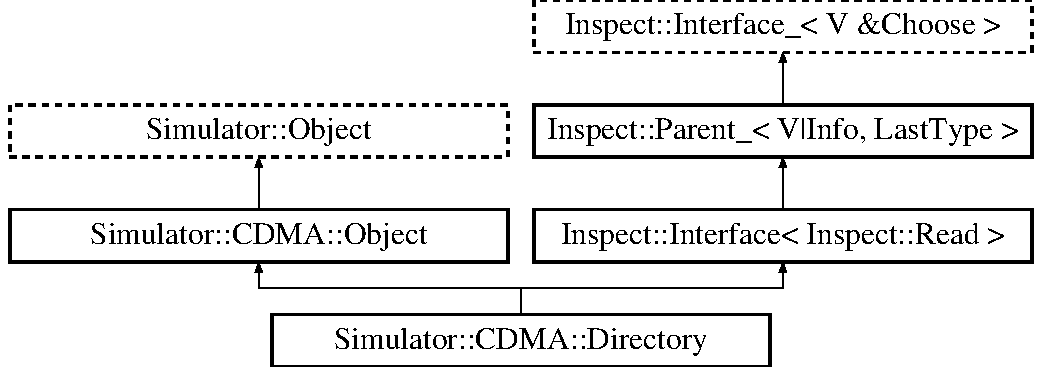
\includegraphics[height=4.000000cm]{class_simulator_1_1_c_d_m_a_1_1_directory}
\end{center}
\end{figure}
\subsection*{Public Member Functions}
\begin{DoxyCompactItemize}
\item 
\hyperlink{class_simulator_1_1_c_d_m_a_1_1_directory_a6e9ed3ce950d24f74d3ed9aaa9936cfe}{Directory} (const std\+::string \&\hyperlink{mtconf_8c_a8f8f80d37794cde9472343e4487ba3eb}{name}, \hyperlink{class_simulator_1_1_c_d_m_a}{C\+D\+M\+A} \&parent, \hyperlink{class_simulator_1_1_clock}{Clock} \&clock, \hyperlink{class_config}{Config} \&config)
\item 
void \hyperlink{class_simulator_1_1_c_d_m_a_1_1_directory_a2ad745b38a9e58e3734836310a4e27d3}{Connect\+Ring} (\hyperlink{class_simulator_1_1_c_d_m_a_1_1_node}{Node} $\ast$first, \hyperlink{class_simulator_1_1_c_d_m_a_1_1_node}{Node} $\ast$last)
\item 
void \hyperlink{class_simulator_1_1_c_d_m_a_1_1_directory_a20969ff0db6983991457c4ccfa2c6294}{Initialize} ()
\item 
size\+\_\+t \hyperlink{class_simulator_1_1_c_d_m_a_1_1_directory_a1d7500825d442adf45815ad4c4e47685}{Get\+Max\+Num\+Lines} () const 
\item 
void \hyperlink{class_simulator_1_1_c_d_m_a_1_1_directory_a90aac41a42250f7f9b99f55883f9bff0}{Cmd\+\_\+\+Info} (std\+::ostream \&out, const std\+::vector$<$ std\+::string $>$ \&arguments) const 
\item 
void \hyperlink{class_simulator_1_1_c_d_m_a_1_1_directory_a02709fd1408c4a58cb0c3b008689774c}{Cmd\+\_\+\+Read} (std\+::ostream \&out, const std\+::vector$<$ std\+::string $>$ \&arguments) const 
\end{DoxyCompactItemize}
\subsection*{Protected Attributes}
\begin{DoxyCompactItemize}
\item 
\hyperlink{class_simulator_1_1_c_d_m_a_1_1_directory_bottom}{C\+D\+M\+A\+::\+Directory\+Bottom} \hyperlink{class_simulator_1_1_c_d_m_a_1_1_directory_aae0350e5c0dc2fa299d1d5856d8a69fe}{m\+\_\+bottom}
\item 
\hyperlink{class_simulator_1_1_c_d_m_a_1_1_directory_top}{C\+D\+M\+A\+::\+Directory\+Top} \hyperlink{class_simulator_1_1_c_d_m_a_1_1_directory_ae8ed427dc5c89c0919f77710cad0a53c}{m\+\_\+top}
\end{DoxyCompactItemize}
\subsection*{Friends}
\begin{DoxyCompactItemize}
\item 
class \hyperlink{class_simulator_1_1_c_d_m_a_1_1_directory_add415c7c29b0f2d422db4e084c6688e3}{C\+D\+M\+A}
\item 
class \hyperlink{class_simulator_1_1_c_d_m_a_1_1_directory_a97f5acb405692cb3363f4beb4f2dd45d}{One\+Level\+C\+D\+M\+A}
\item 
class \hyperlink{class_simulator_1_1_c_d_m_a_1_1_directory_a25bd9aa1e243b7f4e894dcc62a8a715a}{Two\+Level\+C\+D\+M\+A}
\end{DoxyCompactItemize}


\subsection{Constructor \& Destructor Documentation}
\hypertarget{class_simulator_1_1_c_d_m_a_1_1_directory_a6e9ed3ce950d24f74d3ed9aaa9936cfe}{\index{Simulator\+::\+C\+D\+M\+A\+::\+Directory@{Simulator\+::\+C\+D\+M\+A\+::\+Directory}!Directory@{Directory}}
\index{Directory@{Directory}!Simulator\+::\+C\+D\+M\+A\+::\+Directory@{Simulator\+::\+C\+D\+M\+A\+::\+Directory}}
\subsubsection[{Directory}]{\setlength{\rightskip}{0pt plus 5cm}Simulator\+::\+C\+D\+M\+A\+::\+Directory\+::\+Directory (
\begin{DoxyParamCaption}
\item[{const std\+::string \&}]{name, }
\item[{{\bf C\+D\+M\+A} \&}]{parent, }
\item[{{\bf Clock} \&}]{clock, }
\item[{{\bf Config} \&}]{config}
\end{DoxyParamCaption}
)}}\label{class_simulator_1_1_c_d_m_a_1_1_directory_a6e9ed3ce950d24f74d3ed9aaa9936cfe}


\subsection{Member Function Documentation}
\hypertarget{class_simulator_1_1_c_d_m_a_1_1_directory_a90aac41a42250f7f9b99f55883f9bff0}{\index{Simulator\+::\+C\+D\+M\+A\+::\+Directory@{Simulator\+::\+C\+D\+M\+A\+::\+Directory}!Cmd\+\_\+\+Info@{Cmd\+\_\+\+Info}}
\index{Cmd\+\_\+\+Info@{Cmd\+\_\+\+Info}!Simulator\+::\+C\+D\+M\+A\+::\+Directory@{Simulator\+::\+C\+D\+M\+A\+::\+Directory}}
\subsubsection[{Cmd\+\_\+\+Info}]{\setlength{\rightskip}{0pt plus 5cm}void Simulator\+::\+C\+D\+M\+A\+::\+Directory\+::\+Cmd\+\_\+\+Info (
\begin{DoxyParamCaption}
\item[{std\+::ostream \&}]{out, }
\item[{const std\+::vector$<$ std\+::string $>$ \&}]{arguments}
\end{DoxyParamCaption}
) const}}\label{class_simulator_1_1_c_d_m_a_1_1_directory_a90aac41a42250f7f9b99f55883f9bff0}
\hypertarget{class_simulator_1_1_c_d_m_a_1_1_directory_a02709fd1408c4a58cb0c3b008689774c}{\index{Simulator\+::\+C\+D\+M\+A\+::\+Directory@{Simulator\+::\+C\+D\+M\+A\+::\+Directory}!Cmd\+\_\+\+Read@{Cmd\+\_\+\+Read}}
\index{Cmd\+\_\+\+Read@{Cmd\+\_\+\+Read}!Simulator\+::\+C\+D\+M\+A\+::\+Directory@{Simulator\+::\+C\+D\+M\+A\+::\+Directory}}
\subsubsection[{Cmd\+\_\+\+Read}]{\setlength{\rightskip}{0pt plus 5cm}void Simulator\+::\+C\+D\+M\+A\+::\+Directory\+::\+Cmd\+\_\+\+Read (
\begin{DoxyParamCaption}
\item[{std\+::ostream \&}]{out, }
\item[{const std\+::vector$<$ std\+::string $>$ \&}]{arguments}
\end{DoxyParamCaption}
) const}}\label{class_simulator_1_1_c_d_m_a_1_1_directory_a02709fd1408c4a58cb0c3b008689774c}
\hypertarget{class_simulator_1_1_c_d_m_a_1_1_directory_a2ad745b38a9e58e3734836310a4e27d3}{\index{Simulator\+::\+C\+D\+M\+A\+::\+Directory@{Simulator\+::\+C\+D\+M\+A\+::\+Directory}!Connect\+Ring@{Connect\+Ring}}
\index{Connect\+Ring@{Connect\+Ring}!Simulator\+::\+C\+D\+M\+A\+::\+Directory@{Simulator\+::\+C\+D\+M\+A\+::\+Directory}}
\subsubsection[{Connect\+Ring}]{\setlength{\rightskip}{0pt plus 5cm}void Simulator\+::\+C\+D\+M\+A\+::\+Directory\+::\+Connect\+Ring (
\begin{DoxyParamCaption}
\item[{{\bf Node} $\ast$}]{first, }
\item[{{\bf Node} $\ast$}]{last}
\end{DoxyParamCaption}
)}}\label{class_simulator_1_1_c_d_m_a_1_1_directory_a2ad745b38a9e58e3734836310a4e27d3}
\hypertarget{class_simulator_1_1_c_d_m_a_1_1_directory_a1d7500825d442adf45815ad4c4e47685}{\index{Simulator\+::\+C\+D\+M\+A\+::\+Directory@{Simulator\+::\+C\+D\+M\+A\+::\+Directory}!Get\+Max\+Num\+Lines@{Get\+Max\+Num\+Lines}}
\index{Get\+Max\+Num\+Lines@{Get\+Max\+Num\+Lines}!Simulator\+::\+C\+D\+M\+A\+::\+Directory@{Simulator\+::\+C\+D\+M\+A\+::\+Directory}}
\subsubsection[{Get\+Max\+Num\+Lines}]{\setlength{\rightskip}{0pt plus 5cm}size\+\_\+t Simulator\+::\+C\+D\+M\+A\+::\+Directory\+::\+Get\+Max\+Num\+Lines (
\begin{DoxyParamCaption}
{}
\end{DoxyParamCaption}
) const\hspace{0.3cm}{\ttfamily [inline]}}}\label{class_simulator_1_1_c_d_m_a_1_1_directory_a1d7500825d442adf45815ad4c4e47685}
\hypertarget{class_simulator_1_1_c_d_m_a_1_1_directory_a20969ff0db6983991457c4ccfa2c6294}{\index{Simulator\+::\+C\+D\+M\+A\+::\+Directory@{Simulator\+::\+C\+D\+M\+A\+::\+Directory}!Initialize@{Initialize}}
\index{Initialize@{Initialize}!Simulator\+::\+C\+D\+M\+A\+::\+Directory@{Simulator\+::\+C\+D\+M\+A\+::\+Directory}}
\subsubsection[{Initialize}]{\setlength{\rightskip}{0pt plus 5cm}void Simulator\+::\+C\+D\+M\+A\+::\+Directory\+::\+Initialize (
\begin{DoxyParamCaption}
{}
\end{DoxyParamCaption}
)}}\label{class_simulator_1_1_c_d_m_a_1_1_directory_a20969ff0db6983991457c4ccfa2c6294}


\subsection{Friends And Related Function Documentation}
\hypertarget{class_simulator_1_1_c_d_m_a_1_1_directory_add415c7c29b0f2d422db4e084c6688e3}{\index{Simulator\+::\+C\+D\+M\+A\+::\+Directory@{Simulator\+::\+C\+D\+M\+A\+::\+Directory}!C\+D\+M\+A@{C\+D\+M\+A}}
\index{C\+D\+M\+A@{C\+D\+M\+A}!Simulator\+::\+C\+D\+M\+A\+::\+Directory@{Simulator\+::\+C\+D\+M\+A\+::\+Directory}}
\subsubsection[{C\+D\+M\+A}]{\setlength{\rightskip}{0pt plus 5cm}friend class {\bf C\+D\+M\+A}\hspace{0.3cm}{\ttfamily [friend]}}}\label{class_simulator_1_1_c_d_m_a_1_1_directory_add415c7c29b0f2d422db4e084c6688e3}
\hypertarget{class_simulator_1_1_c_d_m_a_1_1_directory_a97f5acb405692cb3363f4beb4f2dd45d}{\index{Simulator\+::\+C\+D\+M\+A\+::\+Directory@{Simulator\+::\+C\+D\+M\+A\+::\+Directory}!One\+Level\+C\+D\+M\+A@{One\+Level\+C\+D\+M\+A}}
\index{One\+Level\+C\+D\+M\+A@{One\+Level\+C\+D\+M\+A}!Simulator\+::\+C\+D\+M\+A\+::\+Directory@{Simulator\+::\+C\+D\+M\+A\+::\+Directory}}
\subsubsection[{One\+Level\+C\+D\+M\+A}]{\setlength{\rightskip}{0pt plus 5cm}friend class {\bf One\+Level\+C\+D\+M\+A}\hspace{0.3cm}{\ttfamily [friend]}}}\label{class_simulator_1_1_c_d_m_a_1_1_directory_a97f5acb405692cb3363f4beb4f2dd45d}
\hypertarget{class_simulator_1_1_c_d_m_a_1_1_directory_a25bd9aa1e243b7f4e894dcc62a8a715a}{\index{Simulator\+::\+C\+D\+M\+A\+::\+Directory@{Simulator\+::\+C\+D\+M\+A\+::\+Directory}!Two\+Level\+C\+D\+M\+A@{Two\+Level\+C\+D\+M\+A}}
\index{Two\+Level\+C\+D\+M\+A@{Two\+Level\+C\+D\+M\+A}!Simulator\+::\+C\+D\+M\+A\+::\+Directory@{Simulator\+::\+C\+D\+M\+A\+::\+Directory}}
\subsubsection[{Two\+Level\+C\+D\+M\+A}]{\setlength{\rightskip}{0pt plus 5cm}friend class {\bf Two\+Level\+C\+D\+M\+A}\hspace{0.3cm}{\ttfamily [friend]}}}\label{class_simulator_1_1_c_d_m_a_1_1_directory_a25bd9aa1e243b7f4e894dcc62a8a715a}


\subsection{Member Data Documentation}
\hypertarget{class_simulator_1_1_c_d_m_a_1_1_directory_aae0350e5c0dc2fa299d1d5856d8a69fe}{\index{Simulator\+::\+C\+D\+M\+A\+::\+Directory@{Simulator\+::\+C\+D\+M\+A\+::\+Directory}!m\+\_\+bottom@{m\+\_\+bottom}}
\index{m\+\_\+bottom@{m\+\_\+bottom}!Simulator\+::\+C\+D\+M\+A\+::\+Directory@{Simulator\+::\+C\+D\+M\+A\+::\+Directory}}
\subsubsection[{m\+\_\+bottom}]{\setlength{\rightskip}{0pt plus 5cm}{\bf C\+D\+M\+A\+::\+Directory\+Bottom} Simulator\+::\+C\+D\+M\+A\+::\+Directory\+::m\+\_\+bottom\hspace{0.3cm}{\ttfamily [protected]}}}\label{class_simulator_1_1_c_d_m_a_1_1_directory_aae0350e5c0dc2fa299d1d5856d8a69fe}
\hypertarget{class_simulator_1_1_c_d_m_a_1_1_directory_ae8ed427dc5c89c0919f77710cad0a53c}{\index{Simulator\+::\+C\+D\+M\+A\+::\+Directory@{Simulator\+::\+C\+D\+M\+A\+::\+Directory}!m\+\_\+top@{m\+\_\+top}}
\index{m\+\_\+top@{m\+\_\+top}!Simulator\+::\+C\+D\+M\+A\+::\+Directory@{Simulator\+::\+C\+D\+M\+A\+::\+Directory}}
\subsubsection[{m\+\_\+top}]{\setlength{\rightskip}{0pt plus 5cm}{\bf C\+D\+M\+A\+::\+Directory\+Top} Simulator\+::\+C\+D\+M\+A\+::\+Directory\+::m\+\_\+top\hspace{0.3cm}{\ttfamily [protected]}}}\label{class_simulator_1_1_c_d_m_a_1_1_directory_ae8ed427dc5c89c0919f77710cad0a53c}


The documentation for this class was generated from the following files\+:\begin{DoxyCompactItemize}
\item 
arch/mem/cdma/\hyperlink{cdma_2_directory_8h}{Directory.\+h}\item 
arch/mem/cdma/\hyperlink{cdma_2_directory_8cpp}{Directory.\+cpp}\end{DoxyCompactItemize}

\hypertarget{class_simulator_1_1_z_l_c_d_m_a_1_1_directory}{\section{Simulator\+:\+:Z\+L\+C\+D\+M\+A\+:\+:Directory Class Reference}
\label{class_simulator_1_1_z_l_c_d_m_a_1_1_directory}\index{Simulator\+::\+Z\+L\+C\+D\+M\+A\+::\+Directory@{Simulator\+::\+Z\+L\+C\+D\+M\+A\+::\+Directory}}
}


{\ttfamily \#include $<$Directory.\+h$>$}

Inheritance diagram for Simulator\+:\+:Z\+L\+C\+D\+M\+A\+:\+:Directory\+:\begin{figure}[H]
\begin{center}
\leavevmode
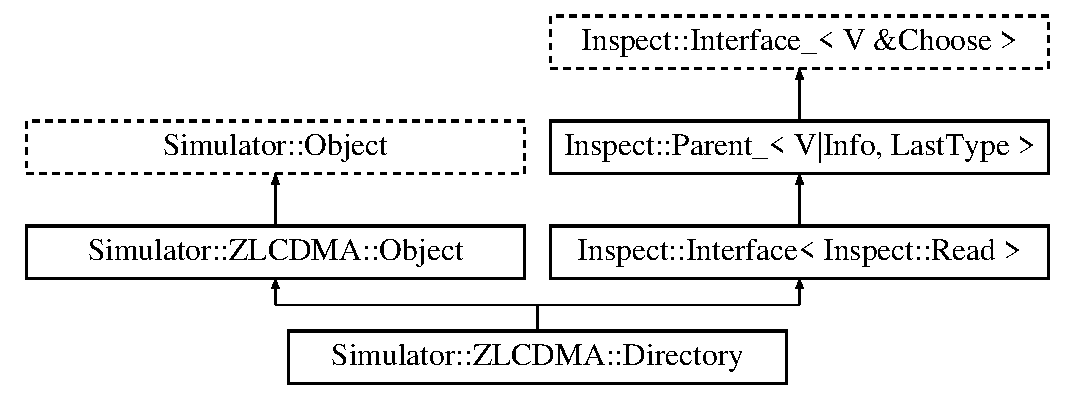
\includegraphics[height=4.000000cm]{class_simulator_1_1_z_l_c_d_m_a_1_1_directory}
\end{center}
\end{figure}
\subsection*{Classes}
\begin{DoxyCompactItemize}
\item 
struct \hyperlink{struct_simulator_1_1_z_l_c_d_m_a_1_1_directory_1_1_line}{Line}
\end{DoxyCompactItemize}
\subsection*{Public Member Functions}
\begin{DoxyCompactItemize}
\item 
const \hyperlink{struct_simulator_1_1_z_l_c_d_m_a_1_1_directory_1_1_line}{Line} $\ast$ \hyperlink{class_simulator_1_1_z_l_c_d_m_a_1_1_directory_ac00fe51ec5f3990ce980188828759007}{Find\+Line} (Mem\+Addr address) const 
\item 
\hyperlink{class_simulator_1_1_z_l_c_d_m_a_1_1_directory_ac6ebcc9e8624b0f9b1ad39a3da3b540c}{Directory} (const std\+::string \&\hyperlink{mtconf_8c_a8f8f80d37794cde9472343e4487ba3eb}{name}, \hyperlink{class_simulator_1_1_z_l_c_d_m_a}{Z\+L\+C\+D\+M\+A} \&parent, \hyperlink{class_simulator_1_1_clock}{Clock} \&clock, Cache\+I\+D first\+Cache, \hyperlink{class_config}{Config} \&config)
\item 
void \hyperlink{class_simulator_1_1_z_l_c_d_m_a_1_1_directory_a35b65b7ca2100df08244c343672f98ff}{Cmd\+\_\+\+Info} (std\+::ostream \&out, const std\+::vector$<$ std\+::string $>$ \&arguments) const 
\item 
void \hyperlink{class_simulator_1_1_z_l_c_d_m_a_1_1_directory_ab2353a3be32af505f378c2c189407354}{Cmd\+\_\+\+Read} (std\+::ostream \&out, const std\+::vector$<$ std\+::string $>$ \&arguments) const 
\end{DoxyCompactItemize}
\subsection*{Protected Attributes}
\begin{DoxyCompactItemize}
\item 
\hyperlink{class_simulator_1_1_z_l_c_d_m_a_1_1_directory_bottom}{Z\+L\+C\+D\+M\+A\+::\+Directory\+Bottom} \hyperlink{class_simulator_1_1_z_l_c_d_m_a_1_1_directory_a8355d8daf89086f5d173bdd9e92d72da}{m\+\_\+bottom}
\item 
\hyperlink{class_simulator_1_1_z_l_c_d_m_a_1_1_directory_top}{Z\+L\+C\+D\+M\+A\+::\+Directory\+Top} \hyperlink{class_simulator_1_1_z_l_c_d_m_a_1_1_directory_a14a3b8cc4fa2a24f4eae6a02a48bfd1b}{m\+\_\+top}
\end{DoxyCompactItemize}
\subsection*{Friends}
\begin{DoxyCompactItemize}
\item 
class \hyperlink{class_simulator_1_1_z_l_c_d_m_a_1_1_directory_a1c09861c9a70825235b5f80518d478a1}{Z\+L\+C\+D\+M\+A}
\end{DoxyCompactItemize}


\subsection{Constructor \& Destructor Documentation}
\hypertarget{class_simulator_1_1_z_l_c_d_m_a_1_1_directory_ac6ebcc9e8624b0f9b1ad39a3da3b540c}{\index{Simulator\+::\+Z\+L\+C\+D\+M\+A\+::\+Directory@{Simulator\+::\+Z\+L\+C\+D\+M\+A\+::\+Directory}!Directory@{Directory}}
\index{Directory@{Directory}!Simulator\+::\+Z\+L\+C\+D\+M\+A\+::\+Directory@{Simulator\+::\+Z\+L\+C\+D\+M\+A\+::\+Directory}}
\subsubsection[{Directory}]{\setlength{\rightskip}{0pt plus 5cm}Simulator\+::\+Z\+L\+C\+D\+M\+A\+::\+Directory\+::\+Directory (
\begin{DoxyParamCaption}
\item[{const std\+::string \&}]{name, }
\item[{{\bf Z\+L\+C\+D\+M\+A} \&}]{parent, }
\item[{{\bf Clock} \&}]{clock, }
\item[{Cache\+I\+D}]{first\+Cache, }
\item[{{\bf Config} \&}]{config}
\end{DoxyParamCaption}
)}}\label{class_simulator_1_1_z_l_c_d_m_a_1_1_directory_ac6ebcc9e8624b0f9b1ad39a3da3b540c}


\subsection{Member Function Documentation}
\hypertarget{class_simulator_1_1_z_l_c_d_m_a_1_1_directory_a35b65b7ca2100df08244c343672f98ff}{\index{Simulator\+::\+Z\+L\+C\+D\+M\+A\+::\+Directory@{Simulator\+::\+Z\+L\+C\+D\+M\+A\+::\+Directory}!Cmd\+\_\+\+Info@{Cmd\+\_\+\+Info}}
\index{Cmd\+\_\+\+Info@{Cmd\+\_\+\+Info}!Simulator\+::\+Z\+L\+C\+D\+M\+A\+::\+Directory@{Simulator\+::\+Z\+L\+C\+D\+M\+A\+::\+Directory}}
\subsubsection[{Cmd\+\_\+\+Info}]{\setlength{\rightskip}{0pt plus 5cm}void Simulator\+::\+Z\+L\+C\+D\+M\+A\+::\+Directory\+::\+Cmd\+\_\+\+Info (
\begin{DoxyParamCaption}
\item[{std\+::ostream \&}]{out, }
\item[{const std\+::vector$<$ std\+::string $>$ \&}]{arguments}
\end{DoxyParamCaption}
) const}}\label{class_simulator_1_1_z_l_c_d_m_a_1_1_directory_a35b65b7ca2100df08244c343672f98ff}
\hypertarget{class_simulator_1_1_z_l_c_d_m_a_1_1_directory_ab2353a3be32af505f378c2c189407354}{\index{Simulator\+::\+Z\+L\+C\+D\+M\+A\+::\+Directory@{Simulator\+::\+Z\+L\+C\+D\+M\+A\+::\+Directory}!Cmd\+\_\+\+Read@{Cmd\+\_\+\+Read}}
\index{Cmd\+\_\+\+Read@{Cmd\+\_\+\+Read}!Simulator\+::\+Z\+L\+C\+D\+M\+A\+::\+Directory@{Simulator\+::\+Z\+L\+C\+D\+M\+A\+::\+Directory}}
\subsubsection[{Cmd\+\_\+\+Read}]{\setlength{\rightskip}{0pt plus 5cm}void Simulator\+::\+Z\+L\+C\+D\+M\+A\+::\+Directory\+::\+Cmd\+\_\+\+Read (
\begin{DoxyParamCaption}
\item[{std\+::ostream \&}]{out, }
\item[{const std\+::vector$<$ std\+::string $>$ \&}]{arguments}
\end{DoxyParamCaption}
) const}}\label{class_simulator_1_1_z_l_c_d_m_a_1_1_directory_ab2353a3be32af505f378c2c189407354}
\hypertarget{class_simulator_1_1_z_l_c_d_m_a_1_1_directory_ac00fe51ec5f3990ce980188828759007}{\index{Simulator\+::\+Z\+L\+C\+D\+M\+A\+::\+Directory@{Simulator\+::\+Z\+L\+C\+D\+M\+A\+::\+Directory}!Find\+Line@{Find\+Line}}
\index{Find\+Line@{Find\+Line}!Simulator\+::\+Z\+L\+C\+D\+M\+A\+::\+Directory@{Simulator\+::\+Z\+L\+C\+D\+M\+A\+::\+Directory}}
\subsubsection[{Find\+Line}]{\setlength{\rightskip}{0pt plus 5cm}const {\bf Z\+L\+C\+D\+M\+A\+::\+Directory\+::\+Line} $\ast$ Simulator\+::\+Z\+L\+C\+D\+M\+A\+::\+Directory\+::\+Find\+Line (
\begin{DoxyParamCaption}
\item[{Mem\+Addr}]{address}
\end{DoxyParamCaption}
) const}}\label{class_simulator_1_1_z_l_c_d_m_a_1_1_directory_ac00fe51ec5f3990ce980188828759007}


\subsection{Friends And Related Function Documentation}
\hypertarget{class_simulator_1_1_z_l_c_d_m_a_1_1_directory_a1c09861c9a70825235b5f80518d478a1}{\index{Simulator\+::\+Z\+L\+C\+D\+M\+A\+::\+Directory@{Simulator\+::\+Z\+L\+C\+D\+M\+A\+::\+Directory}!Z\+L\+C\+D\+M\+A@{Z\+L\+C\+D\+M\+A}}
\index{Z\+L\+C\+D\+M\+A@{Z\+L\+C\+D\+M\+A}!Simulator\+::\+Z\+L\+C\+D\+M\+A\+::\+Directory@{Simulator\+::\+Z\+L\+C\+D\+M\+A\+::\+Directory}}
\subsubsection[{Z\+L\+C\+D\+M\+A}]{\setlength{\rightskip}{0pt plus 5cm}friend class {\bf Z\+L\+C\+D\+M\+A}\hspace{0.3cm}{\ttfamily [friend]}}}\label{class_simulator_1_1_z_l_c_d_m_a_1_1_directory_a1c09861c9a70825235b5f80518d478a1}


\subsection{Member Data Documentation}
\hypertarget{class_simulator_1_1_z_l_c_d_m_a_1_1_directory_a8355d8daf89086f5d173bdd9e92d72da}{\index{Simulator\+::\+Z\+L\+C\+D\+M\+A\+::\+Directory@{Simulator\+::\+Z\+L\+C\+D\+M\+A\+::\+Directory}!m\+\_\+bottom@{m\+\_\+bottom}}
\index{m\+\_\+bottom@{m\+\_\+bottom}!Simulator\+::\+Z\+L\+C\+D\+M\+A\+::\+Directory@{Simulator\+::\+Z\+L\+C\+D\+M\+A\+::\+Directory}}
\subsubsection[{m\+\_\+bottom}]{\setlength{\rightskip}{0pt plus 5cm}{\bf Z\+L\+C\+D\+M\+A\+::\+Directory\+Bottom} Simulator\+::\+Z\+L\+C\+D\+M\+A\+::\+Directory\+::m\+\_\+bottom\hspace{0.3cm}{\ttfamily [protected]}}}\label{class_simulator_1_1_z_l_c_d_m_a_1_1_directory_a8355d8daf89086f5d173bdd9e92d72da}
\hypertarget{class_simulator_1_1_z_l_c_d_m_a_1_1_directory_a14a3b8cc4fa2a24f4eae6a02a48bfd1b}{\index{Simulator\+::\+Z\+L\+C\+D\+M\+A\+::\+Directory@{Simulator\+::\+Z\+L\+C\+D\+M\+A\+::\+Directory}!m\+\_\+top@{m\+\_\+top}}
\index{m\+\_\+top@{m\+\_\+top}!Simulator\+::\+Z\+L\+C\+D\+M\+A\+::\+Directory@{Simulator\+::\+Z\+L\+C\+D\+M\+A\+::\+Directory}}
\subsubsection[{m\+\_\+top}]{\setlength{\rightskip}{0pt plus 5cm}{\bf Z\+L\+C\+D\+M\+A\+::\+Directory\+Top} Simulator\+::\+Z\+L\+C\+D\+M\+A\+::\+Directory\+::m\+\_\+top\hspace{0.3cm}{\ttfamily [protected]}}}\label{class_simulator_1_1_z_l_c_d_m_a_1_1_directory_a14a3b8cc4fa2a24f4eae6a02a48bfd1b}


The documentation for this class was generated from the following files\+:\begin{DoxyCompactItemize}
\item 
arch/mem/zlcdma/\hyperlink{zlcdma_2_directory_8h}{Directory.\+h}\item 
arch/mem/zlcdma/\hyperlink{zlcdma_2_directory_8cpp}{Directory.\+cpp}\end{DoxyCompactItemize}

\hypertarget{class_simulator_1_1_z_l_c_d_m_a_1_1_directory_bottom}{\section{Simulator\+:\+:Z\+L\+C\+D\+M\+A\+:\+:Directory\+Bottom Class Reference}
\label{class_simulator_1_1_z_l_c_d_m_a_1_1_directory_bottom}\index{Simulator\+::\+Z\+L\+C\+D\+M\+A\+::\+Directory\+Bottom@{Simulator\+::\+Z\+L\+C\+D\+M\+A\+::\+Directory\+Bottom}}
}


{\ttfamily \#include $<$Directory.\+h$>$}

Inheritance diagram for Simulator\+:\+:Z\+L\+C\+D\+M\+A\+:\+:Directory\+Bottom\+:\begin{figure}[H]
\begin{center}
\leavevmode
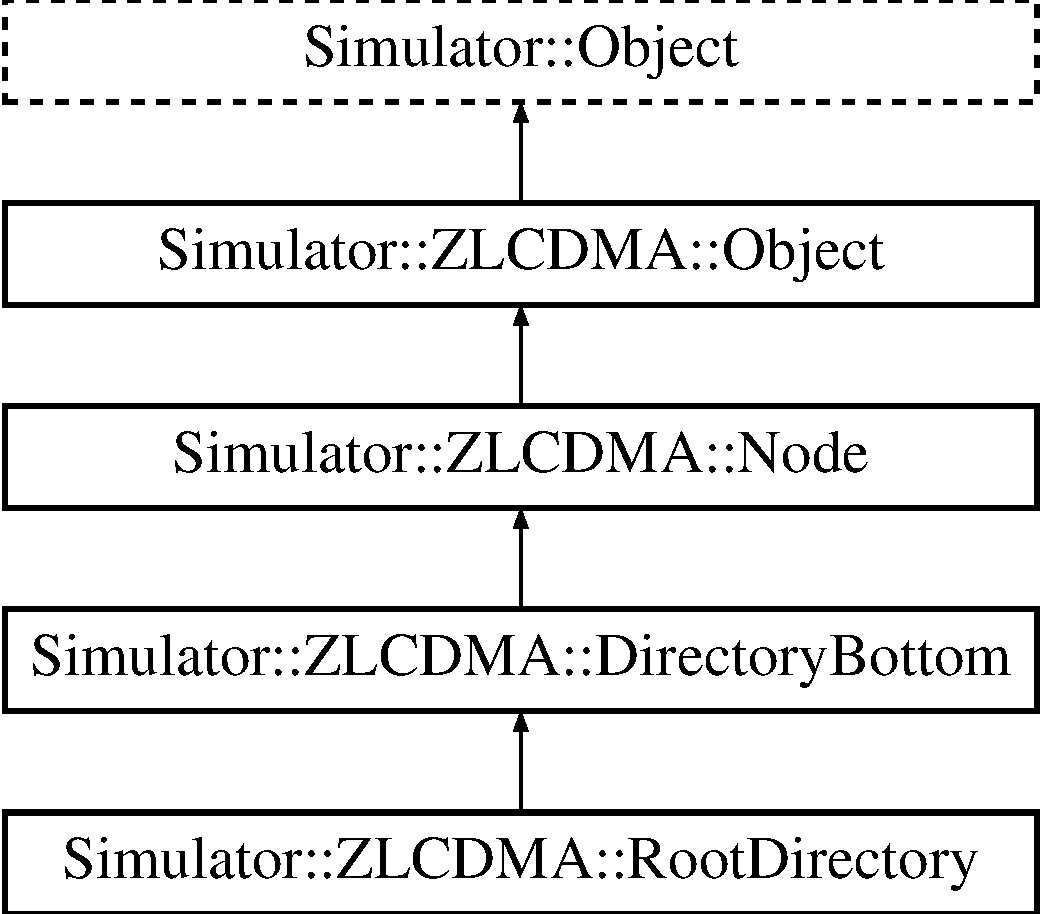
\includegraphics[height=5.000000cm]{class_simulator_1_1_z_l_c_d_m_a_1_1_directory_bottom}
\end{center}
\end{figure}
\subsection*{Protected Member Functions}
\begin{DoxyCompactItemize}
\item 
\hyperlink{class_simulator_1_1_z_l_c_d_m_a_1_1_directory_bottom_a4b0b478e7235472e95318f6ae0c05b6e}{Directory\+Bottom} (const std\+::string \&\hyperlink{mtconf_8c_a8f8f80d37794cde9472343e4487ba3eb}{name}, \hyperlink{class_simulator_1_1_z_l_c_d_m_a}{Z\+L\+C\+D\+M\+A} \&parent, \hyperlink{class_simulator_1_1_clock}{Clock} \&clock)
\end{DoxyCompactItemize}
\subsection*{Friends}
\begin{DoxyCompactItemize}
\item 
class \hyperlink{class_simulator_1_1_z_l_c_d_m_a_1_1_directory_bottom_a1c09861c9a70825235b5f80518d478a1}{Z\+L\+C\+D\+M\+A}
\item 
class \hyperlink{class_simulator_1_1_z_l_c_d_m_a_1_1_directory_bottom_a1c8d2b869e248d4ee4a7b637c7252d62}{Z\+L\+C\+D\+M\+A\+::\+Directory}
\end{DoxyCompactItemize}
\subsection*{Additional Inherited Members}


\subsection{Constructor \& Destructor Documentation}
\hypertarget{class_simulator_1_1_z_l_c_d_m_a_1_1_directory_bottom_a4b0b478e7235472e95318f6ae0c05b6e}{\index{Simulator\+::\+Z\+L\+C\+D\+M\+A\+::\+Directory\+Bottom@{Simulator\+::\+Z\+L\+C\+D\+M\+A\+::\+Directory\+Bottom}!Directory\+Bottom@{Directory\+Bottom}}
\index{Directory\+Bottom@{Directory\+Bottom}!Simulator\+::\+Z\+L\+C\+D\+M\+A\+::\+Directory\+Bottom@{Simulator\+::\+Z\+L\+C\+D\+M\+A\+::\+Directory\+Bottom}}
\subsubsection[{Directory\+Bottom}]{\setlength{\rightskip}{0pt plus 5cm}Simulator\+::\+Z\+L\+C\+D\+M\+A\+::\+Directory\+Bottom\+::\+Directory\+Bottom (
\begin{DoxyParamCaption}
\item[{const std\+::string \&}]{name, }
\item[{{\bf Z\+L\+C\+D\+M\+A} \&}]{parent, }
\item[{{\bf Clock} \&}]{clock}
\end{DoxyParamCaption}
)\hspace{0.3cm}{\ttfamily [protected]}}}\label{class_simulator_1_1_z_l_c_d_m_a_1_1_directory_bottom_a4b0b478e7235472e95318f6ae0c05b6e}


\subsection{Friends And Related Function Documentation}
\hypertarget{class_simulator_1_1_z_l_c_d_m_a_1_1_directory_bottom_a1c09861c9a70825235b5f80518d478a1}{\index{Simulator\+::\+Z\+L\+C\+D\+M\+A\+::\+Directory\+Bottom@{Simulator\+::\+Z\+L\+C\+D\+M\+A\+::\+Directory\+Bottom}!Z\+L\+C\+D\+M\+A@{Z\+L\+C\+D\+M\+A}}
\index{Z\+L\+C\+D\+M\+A@{Z\+L\+C\+D\+M\+A}!Simulator\+::\+Z\+L\+C\+D\+M\+A\+::\+Directory\+Bottom@{Simulator\+::\+Z\+L\+C\+D\+M\+A\+::\+Directory\+Bottom}}
\subsubsection[{Z\+L\+C\+D\+M\+A}]{\setlength{\rightskip}{0pt plus 5cm}friend class {\bf Z\+L\+C\+D\+M\+A}\hspace{0.3cm}{\ttfamily [friend]}}}\label{class_simulator_1_1_z_l_c_d_m_a_1_1_directory_bottom_a1c09861c9a70825235b5f80518d478a1}
\hypertarget{class_simulator_1_1_z_l_c_d_m_a_1_1_directory_bottom_a1c8d2b869e248d4ee4a7b637c7252d62}{\index{Simulator\+::\+Z\+L\+C\+D\+M\+A\+::\+Directory\+Bottom@{Simulator\+::\+Z\+L\+C\+D\+M\+A\+::\+Directory\+Bottom}!Z\+L\+C\+D\+M\+A\+::\+Directory@{Z\+L\+C\+D\+M\+A\+::\+Directory}}
\index{Z\+L\+C\+D\+M\+A\+::\+Directory@{Z\+L\+C\+D\+M\+A\+::\+Directory}!Simulator\+::\+Z\+L\+C\+D\+M\+A\+::\+Directory\+Bottom@{Simulator\+::\+Z\+L\+C\+D\+M\+A\+::\+Directory\+Bottom}}
\subsubsection[{Z\+L\+C\+D\+M\+A\+::\+Directory}]{\setlength{\rightskip}{0pt plus 5cm}friend class {\bf Z\+L\+C\+D\+M\+A\+::\+Directory}\hspace{0.3cm}{\ttfamily [friend]}}}\label{class_simulator_1_1_z_l_c_d_m_a_1_1_directory_bottom_a1c8d2b869e248d4ee4a7b637c7252d62}


The documentation for this class was generated from the following files\+:\begin{DoxyCompactItemize}
\item 
arch/mem/zlcdma/\hyperlink{zlcdma_2_directory_8h}{Directory.\+h}\item 
arch/mem/zlcdma/\hyperlink{zlcdma_2_directory_8cpp}{Directory.\+cpp}\end{DoxyCompactItemize}

\hypertarget{class_simulator_1_1_c_d_m_a_1_1_directory_bottom}{\section{Simulator\+:\+:C\+D\+M\+A\+:\+:Directory\+Bottom Class Reference}
\label{class_simulator_1_1_c_d_m_a_1_1_directory_bottom}\index{Simulator\+::\+C\+D\+M\+A\+::\+Directory\+Bottom@{Simulator\+::\+C\+D\+M\+A\+::\+Directory\+Bottom}}
}


{\ttfamily \#include $<$Directory.\+h$>$}

Inheritance diagram for Simulator\+:\+:C\+D\+M\+A\+:\+:Directory\+Bottom\+:\begin{figure}[H]
\begin{center}
\leavevmode
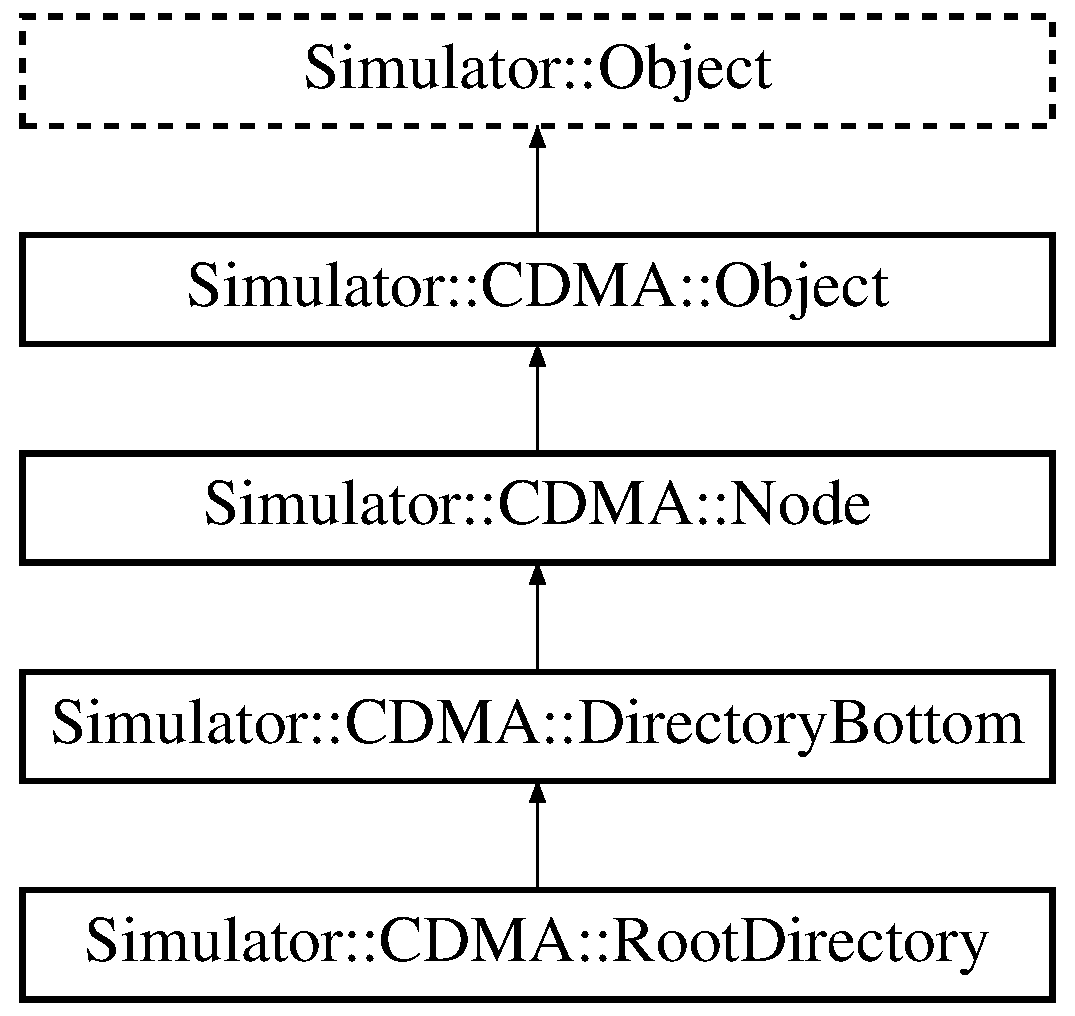
\includegraphics[height=5.000000cm]{class_simulator_1_1_c_d_m_a_1_1_directory_bottom}
\end{center}
\end{figure}
\subsection*{Protected Member Functions}
\begin{DoxyCompactItemize}
\item 
\hyperlink{class_simulator_1_1_c_d_m_a_1_1_directory_bottom_a5390f837d78463d6907a1086a2e3fd20}{Directory\+Bottom} (const std\+::string \&\hyperlink{mtconf_8c_a8f8f80d37794cde9472343e4487ba3eb}{name}, \hyperlink{class_simulator_1_1_c_d_m_a}{C\+D\+M\+A} \&parent, \hyperlink{class_simulator_1_1_clock}{Clock} \&clock, \hyperlink{class_config}{Config} \&config)
\end{DoxyCompactItemize}
\subsection*{Friends}
\begin{DoxyCompactItemize}
\item 
class \hyperlink{class_simulator_1_1_c_d_m_a_1_1_directory_bottom_a97f5acb405692cb3363f4beb4f2dd45d}{One\+Level\+C\+D\+M\+A}
\item 
class \hyperlink{class_simulator_1_1_c_d_m_a_1_1_directory_bottom_a25bd9aa1e243b7f4e894dcc62a8a715a}{Two\+Level\+C\+D\+M\+A}
\item 
class \hyperlink{class_simulator_1_1_c_d_m_a_1_1_directory_bottom_a4af5f54393d68421df7d6c951208e049}{C\+D\+M\+A\+::\+Directory}
\end{DoxyCompactItemize}
\subsection*{Additional Inherited Members}


\subsection{Constructor \& Destructor Documentation}
\hypertarget{class_simulator_1_1_c_d_m_a_1_1_directory_bottom_a5390f837d78463d6907a1086a2e3fd20}{\index{Simulator\+::\+C\+D\+M\+A\+::\+Directory\+Bottom@{Simulator\+::\+C\+D\+M\+A\+::\+Directory\+Bottom}!Directory\+Bottom@{Directory\+Bottom}}
\index{Directory\+Bottom@{Directory\+Bottom}!Simulator\+::\+C\+D\+M\+A\+::\+Directory\+Bottom@{Simulator\+::\+C\+D\+M\+A\+::\+Directory\+Bottom}}
\subsubsection[{Directory\+Bottom}]{\setlength{\rightskip}{0pt plus 5cm}Simulator\+::\+C\+D\+M\+A\+::\+Directory\+Bottom\+::\+Directory\+Bottom (
\begin{DoxyParamCaption}
\item[{const std\+::string \&}]{name, }
\item[{{\bf C\+D\+M\+A} \&}]{parent, }
\item[{{\bf Clock} \&}]{clock, }
\item[{{\bf Config} \&}]{config}
\end{DoxyParamCaption}
)\hspace{0.3cm}{\ttfamily [protected]}}}\label{class_simulator_1_1_c_d_m_a_1_1_directory_bottom_a5390f837d78463d6907a1086a2e3fd20}


\subsection{Friends And Related Function Documentation}
\hypertarget{class_simulator_1_1_c_d_m_a_1_1_directory_bottom_a4af5f54393d68421df7d6c951208e049}{\index{Simulator\+::\+C\+D\+M\+A\+::\+Directory\+Bottom@{Simulator\+::\+C\+D\+M\+A\+::\+Directory\+Bottom}!C\+D\+M\+A\+::\+Directory@{C\+D\+M\+A\+::\+Directory}}
\index{C\+D\+M\+A\+::\+Directory@{C\+D\+M\+A\+::\+Directory}!Simulator\+::\+C\+D\+M\+A\+::\+Directory\+Bottom@{Simulator\+::\+C\+D\+M\+A\+::\+Directory\+Bottom}}
\subsubsection[{C\+D\+M\+A\+::\+Directory}]{\setlength{\rightskip}{0pt plus 5cm}friend class {\bf C\+D\+M\+A\+::\+Directory}\hspace{0.3cm}{\ttfamily [friend]}}}\label{class_simulator_1_1_c_d_m_a_1_1_directory_bottom_a4af5f54393d68421df7d6c951208e049}
\hypertarget{class_simulator_1_1_c_d_m_a_1_1_directory_bottom_a97f5acb405692cb3363f4beb4f2dd45d}{\index{Simulator\+::\+C\+D\+M\+A\+::\+Directory\+Bottom@{Simulator\+::\+C\+D\+M\+A\+::\+Directory\+Bottom}!One\+Level\+C\+D\+M\+A@{One\+Level\+C\+D\+M\+A}}
\index{One\+Level\+C\+D\+M\+A@{One\+Level\+C\+D\+M\+A}!Simulator\+::\+C\+D\+M\+A\+::\+Directory\+Bottom@{Simulator\+::\+C\+D\+M\+A\+::\+Directory\+Bottom}}
\subsubsection[{One\+Level\+C\+D\+M\+A}]{\setlength{\rightskip}{0pt plus 5cm}friend class {\bf One\+Level\+C\+D\+M\+A}\hspace{0.3cm}{\ttfamily [friend]}}}\label{class_simulator_1_1_c_d_m_a_1_1_directory_bottom_a97f5acb405692cb3363f4beb4f2dd45d}
\hypertarget{class_simulator_1_1_c_d_m_a_1_1_directory_bottom_a25bd9aa1e243b7f4e894dcc62a8a715a}{\index{Simulator\+::\+C\+D\+M\+A\+::\+Directory\+Bottom@{Simulator\+::\+C\+D\+M\+A\+::\+Directory\+Bottom}!Two\+Level\+C\+D\+M\+A@{Two\+Level\+C\+D\+M\+A}}
\index{Two\+Level\+C\+D\+M\+A@{Two\+Level\+C\+D\+M\+A}!Simulator\+::\+C\+D\+M\+A\+::\+Directory\+Bottom@{Simulator\+::\+C\+D\+M\+A\+::\+Directory\+Bottom}}
\subsubsection[{Two\+Level\+C\+D\+M\+A}]{\setlength{\rightskip}{0pt plus 5cm}friend class {\bf Two\+Level\+C\+D\+M\+A}\hspace{0.3cm}{\ttfamily [friend]}}}\label{class_simulator_1_1_c_d_m_a_1_1_directory_bottom_a25bd9aa1e243b7f4e894dcc62a8a715a}


The documentation for this class was generated from the following files\+:\begin{DoxyCompactItemize}
\item 
arch/mem/cdma/\hyperlink{cdma_2_directory_8h}{Directory.\+h}\item 
arch/mem/cdma/\hyperlink{cdma_2_directory_8cpp}{Directory.\+cpp}\end{DoxyCompactItemize}

\hypertarget{class_simulator_1_1_z_l_c_d_m_a_1_1_directory_top}{\section{Simulator\+:\+:Z\+L\+C\+D\+M\+A\+:\+:Directory\+Top Class Reference}
\label{class_simulator_1_1_z_l_c_d_m_a_1_1_directory_top}\index{Simulator\+::\+Z\+L\+C\+D\+M\+A\+::\+Directory\+Top@{Simulator\+::\+Z\+L\+C\+D\+M\+A\+::\+Directory\+Top}}
}


{\ttfamily \#include $<$Directory.\+h$>$}

Inheritance diagram for Simulator\+:\+:Z\+L\+C\+D\+M\+A\+:\+:Directory\+Top\+:\begin{figure}[H]
\begin{center}
\leavevmode
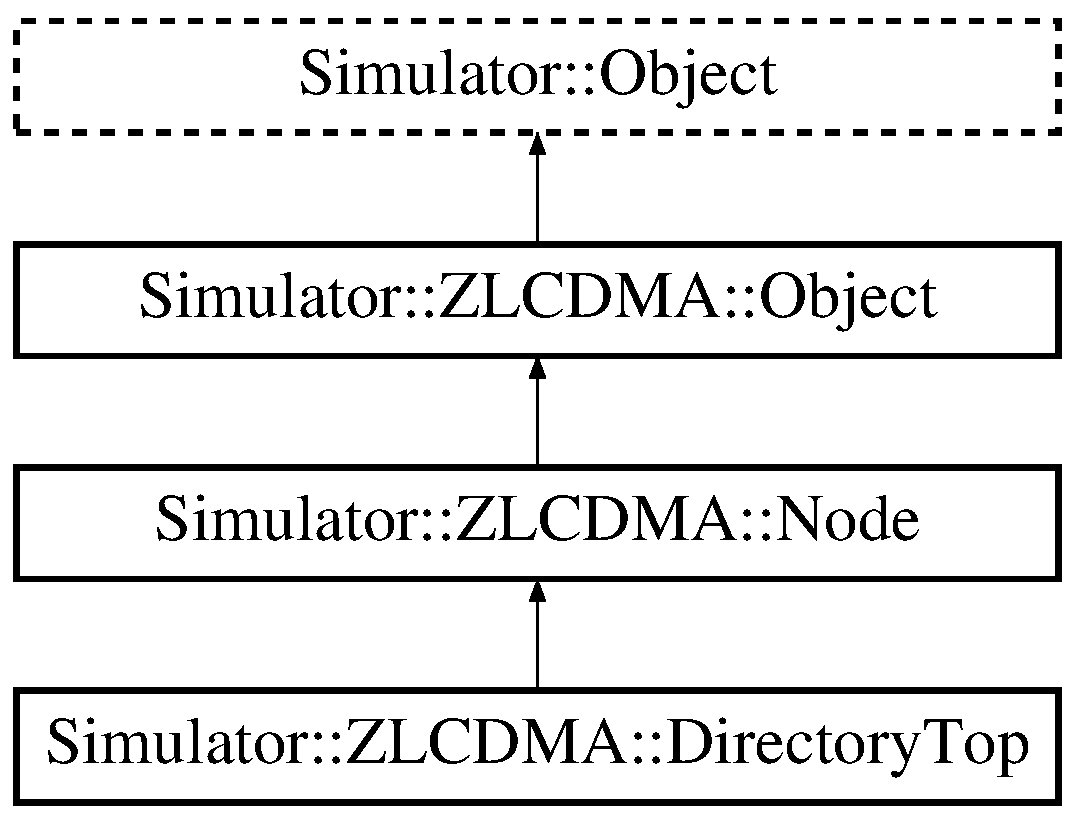
\includegraphics[height=4.000000cm]{class_simulator_1_1_z_l_c_d_m_a_1_1_directory_top}
\end{center}
\end{figure}
\subsection*{Protected Member Functions}
\begin{DoxyCompactItemize}
\item 
\hyperlink{class_simulator_1_1_z_l_c_d_m_a_1_1_directory_top_af8fdc000b2e75afce37ee92b3893063a}{Directory\+Top} (const std\+::string \&\hyperlink{mtconf_8c_a8f8f80d37794cde9472343e4487ba3eb}{name}, \hyperlink{class_simulator_1_1_z_l_c_d_m_a}{Z\+L\+C\+D\+M\+A} \&parent, \hyperlink{class_simulator_1_1_clock}{Clock} \&clock)
\end{DoxyCompactItemize}
\subsection*{Friends}
\begin{DoxyCompactItemize}
\item 
class \hyperlink{class_simulator_1_1_z_l_c_d_m_a_1_1_directory_top_a1c09861c9a70825235b5f80518d478a1}{Z\+L\+C\+D\+M\+A}
\item 
class \hyperlink{class_simulator_1_1_z_l_c_d_m_a_1_1_directory_top_a1c8d2b869e248d4ee4a7b637c7252d62}{Z\+L\+C\+D\+M\+A\+::\+Directory}
\end{DoxyCompactItemize}
\subsection*{Additional Inherited Members}


\subsection{Constructor \& Destructor Documentation}
\hypertarget{class_simulator_1_1_z_l_c_d_m_a_1_1_directory_top_af8fdc000b2e75afce37ee92b3893063a}{\index{Simulator\+::\+Z\+L\+C\+D\+M\+A\+::\+Directory\+Top@{Simulator\+::\+Z\+L\+C\+D\+M\+A\+::\+Directory\+Top}!Directory\+Top@{Directory\+Top}}
\index{Directory\+Top@{Directory\+Top}!Simulator\+::\+Z\+L\+C\+D\+M\+A\+::\+Directory\+Top@{Simulator\+::\+Z\+L\+C\+D\+M\+A\+::\+Directory\+Top}}
\subsubsection[{Directory\+Top}]{\setlength{\rightskip}{0pt plus 5cm}Simulator\+::\+Z\+L\+C\+D\+M\+A\+::\+Directory\+Top\+::\+Directory\+Top (
\begin{DoxyParamCaption}
\item[{const std\+::string \&}]{name, }
\item[{{\bf Z\+L\+C\+D\+M\+A} \&}]{parent, }
\item[{{\bf Clock} \&}]{clock}
\end{DoxyParamCaption}
)\hspace{0.3cm}{\ttfamily [protected]}}}\label{class_simulator_1_1_z_l_c_d_m_a_1_1_directory_top_af8fdc000b2e75afce37ee92b3893063a}


\subsection{Friends And Related Function Documentation}
\hypertarget{class_simulator_1_1_z_l_c_d_m_a_1_1_directory_top_a1c09861c9a70825235b5f80518d478a1}{\index{Simulator\+::\+Z\+L\+C\+D\+M\+A\+::\+Directory\+Top@{Simulator\+::\+Z\+L\+C\+D\+M\+A\+::\+Directory\+Top}!Z\+L\+C\+D\+M\+A@{Z\+L\+C\+D\+M\+A}}
\index{Z\+L\+C\+D\+M\+A@{Z\+L\+C\+D\+M\+A}!Simulator\+::\+Z\+L\+C\+D\+M\+A\+::\+Directory\+Top@{Simulator\+::\+Z\+L\+C\+D\+M\+A\+::\+Directory\+Top}}
\subsubsection[{Z\+L\+C\+D\+M\+A}]{\setlength{\rightskip}{0pt plus 5cm}friend class {\bf Z\+L\+C\+D\+M\+A}\hspace{0.3cm}{\ttfamily [friend]}}}\label{class_simulator_1_1_z_l_c_d_m_a_1_1_directory_top_a1c09861c9a70825235b5f80518d478a1}
\hypertarget{class_simulator_1_1_z_l_c_d_m_a_1_1_directory_top_a1c8d2b869e248d4ee4a7b637c7252d62}{\index{Simulator\+::\+Z\+L\+C\+D\+M\+A\+::\+Directory\+Top@{Simulator\+::\+Z\+L\+C\+D\+M\+A\+::\+Directory\+Top}!Z\+L\+C\+D\+M\+A\+::\+Directory@{Z\+L\+C\+D\+M\+A\+::\+Directory}}
\index{Z\+L\+C\+D\+M\+A\+::\+Directory@{Z\+L\+C\+D\+M\+A\+::\+Directory}!Simulator\+::\+Z\+L\+C\+D\+M\+A\+::\+Directory\+Top@{Simulator\+::\+Z\+L\+C\+D\+M\+A\+::\+Directory\+Top}}
\subsubsection[{Z\+L\+C\+D\+M\+A\+::\+Directory}]{\setlength{\rightskip}{0pt plus 5cm}friend class {\bf Z\+L\+C\+D\+M\+A\+::\+Directory}\hspace{0.3cm}{\ttfamily [friend]}}}\label{class_simulator_1_1_z_l_c_d_m_a_1_1_directory_top_a1c8d2b869e248d4ee4a7b637c7252d62}


The documentation for this class was generated from the following files\+:\begin{DoxyCompactItemize}
\item 
arch/mem/zlcdma/\hyperlink{zlcdma_2_directory_8h}{Directory.\+h}\item 
arch/mem/zlcdma/\hyperlink{zlcdma_2_directory_8cpp}{Directory.\+cpp}\end{DoxyCompactItemize}

\hypertarget{class_simulator_1_1_c_d_m_a_1_1_directory_top}{\section{Simulator\+:\+:C\+D\+M\+A\+:\+:Directory\+Top Class Reference}
\label{class_simulator_1_1_c_d_m_a_1_1_directory_top}\index{Simulator\+::\+C\+D\+M\+A\+::\+Directory\+Top@{Simulator\+::\+C\+D\+M\+A\+::\+Directory\+Top}}
}


{\ttfamily \#include $<$Directory.\+h$>$}

Inheritance diagram for Simulator\+:\+:C\+D\+M\+A\+:\+:Directory\+Top\+:\begin{figure}[H]
\begin{center}
\leavevmode
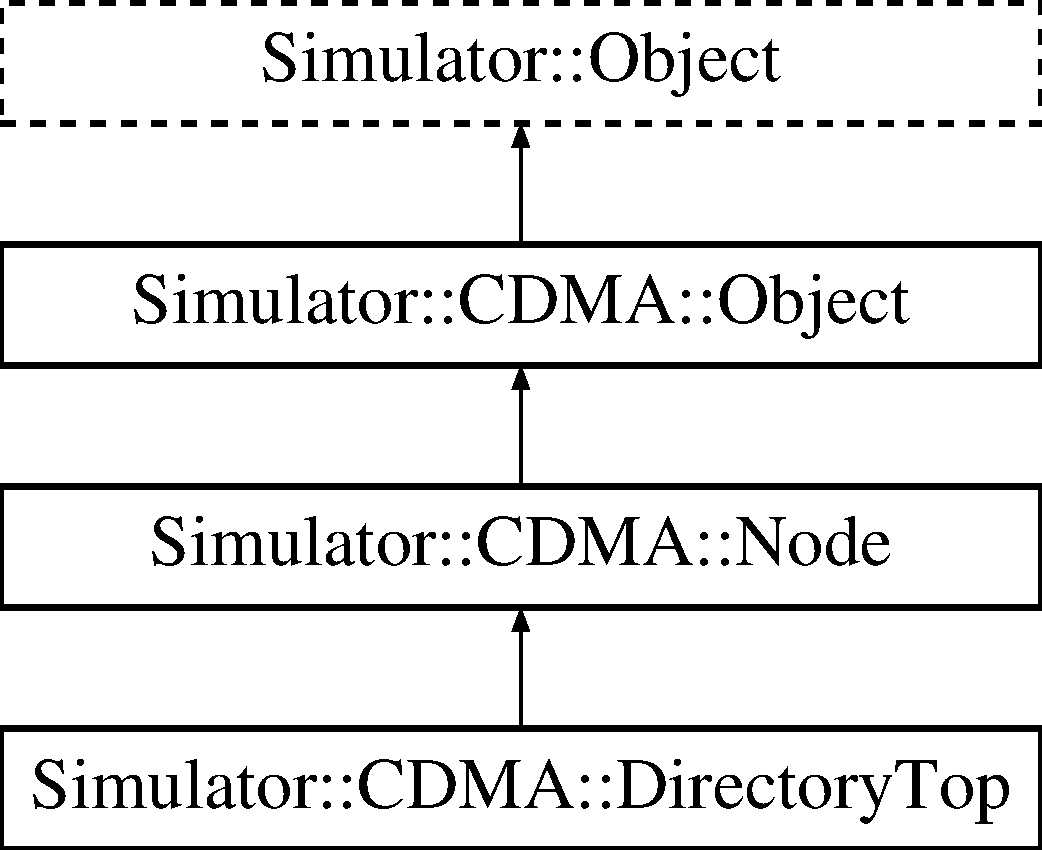
\includegraphics[height=4.000000cm]{class_simulator_1_1_c_d_m_a_1_1_directory_top}
\end{center}
\end{figure}
\subsection*{Protected Member Functions}
\begin{DoxyCompactItemize}
\item 
\hyperlink{class_simulator_1_1_c_d_m_a_1_1_directory_top_af0c67b746e5a3905727e07c8d53a0743}{Directory\+Top} (const std\+::string \&\hyperlink{mtconf_8c_a8f8f80d37794cde9472343e4487ba3eb}{name}, \hyperlink{class_simulator_1_1_c_d_m_a}{C\+D\+M\+A} \&parent, \hyperlink{class_simulator_1_1_clock}{Clock} \&clock, size\+\_\+t \&num\+Lines, \hyperlink{class_config}{Config} \&config)
\item 
size\+\_\+t \hyperlink{class_simulator_1_1_c_d_m_a_1_1_directory_top_aea344573b6853d94f7d53f868ca2b7f2}{Get\+Num\+Lines} () const override
\end{DoxyCompactItemize}
\subsection*{Protected Attributes}
\begin{DoxyCompactItemize}
\item 
size\+\_\+t \& \hyperlink{class_simulator_1_1_c_d_m_a_1_1_directory_top_a4ebb4b89468d17f4984f9f4c44eb9cb1}{m\+\_\+num\+Lines}
\end{DoxyCompactItemize}
\subsection*{Friends}
\begin{DoxyCompactItemize}
\item 
class \hyperlink{class_simulator_1_1_c_d_m_a_1_1_directory_top_a97f5acb405692cb3363f4beb4f2dd45d}{One\+Level\+C\+D\+M\+A}
\item 
class \hyperlink{class_simulator_1_1_c_d_m_a_1_1_directory_top_a25bd9aa1e243b7f4e894dcc62a8a715a}{Two\+Level\+C\+D\+M\+A}
\item 
class \hyperlink{class_simulator_1_1_c_d_m_a_1_1_directory_top_a4af5f54393d68421df7d6c951208e049}{C\+D\+M\+A\+::\+Directory}
\end{DoxyCompactItemize}
\subsection*{Additional Inherited Members}


\subsection{Constructor \& Destructor Documentation}
\hypertarget{class_simulator_1_1_c_d_m_a_1_1_directory_top_af0c67b746e5a3905727e07c8d53a0743}{\index{Simulator\+::\+C\+D\+M\+A\+::\+Directory\+Top@{Simulator\+::\+C\+D\+M\+A\+::\+Directory\+Top}!Directory\+Top@{Directory\+Top}}
\index{Directory\+Top@{Directory\+Top}!Simulator\+::\+C\+D\+M\+A\+::\+Directory\+Top@{Simulator\+::\+C\+D\+M\+A\+::\+Directory\+Top}}
\subsubsection[{Directory\+Top}]{\setlength{\rightskip}{0pt plus 5cm}Simulator\+::\+C\+D\+M\+A\+::\+Directory\+Top\+::\+Directory\+Top (
\begin{DoxyParamCaption}
\item[{const std\+::string \&}]{name, }
\item[{{\bf C\+D\+M\+A} \&}]{parent, }
\item[{{\bf Clock} \&}]{clock, }
\item[{size\+\_\+t \&}]{num\+Lines, }
\item[{{\bf Config} \&}]{config}
\end{DoxyParamCaption}
)\hspace{0.3cm}{\ttfamily [protected]}}}\label{class_simulator_1_1_c_d_m_a_1_1_directory_top_af0c67b746e5a3905727e07c8d53a0743}


\subsection{Member Function Documentation}
\hypertarget{class_simulator_1_1_c_d_m_a_1_1_directory_top_aea344573b6853d94f7d53f868ca2b7f2}{\index{Simulator\+::\+C\+D\+M\+A\+::\+Directory\+Top@{Simulator\+::\+C\+D\+M\+A\+::\+Directory\+Top}!Get\+Num\+Lines@{Get\+Num\+Lines}}
\index{Get\+Num\+Lines@{Get\+Num\+Lines}!Simulator\+::\+C\+D\+M\+A\+::\+Directory\+Top@{Simulator\+::\+C\+D\+M\+A\+::\+Directory\+Top}}
\subsubsection[{Get\+Num\+Lines}]{\setlength{\rightskip}{0pt plus 5cm}size\+\_\+t Simulator\+::\+C\+D\+M\+A\+::\+Directory\+Top\+::\+Get\+Num\+Lines (
\begin{DoxyParamCaption}
{}
\end{DoxyParamCaption}
) const\hspace{0.3cm}{\ttfamily [override]}, {\ttfamily [protected]}, {\ttfamily [virtual]}}}\label{class_simulator_1_1_c_d_m_a_1_1_directory_top_aea344573b6853d94f7d53f868ca2b7f2}


Reimplemented from \hyperlink{class_simulator_1_1_c_d_m_a_1_1_node_a1e5b04d3d6beaa4f1395a2332f105980}{Simulator\+::\+C\+D\+M\+A\+::\+Node}.



\subsection{Friends And Related Function Documentation}
\hypertarget{class_simulator_1_1_c_d_m_a_1_1_directory_top_a4af5f54393d68421df7d6c951208e049}{\index{Simulator\+::\+C\+D\+M\+A\+::\+Directory\+Top@{Simulator\+::\+C\+D\+M\+A\+::\+Directory\+Top}!C\+D\+M\+A\+::\+Directory@{C\+D\+M\+A\+::\+Directory}}
\index{C\+D\+M\+A\+::\+Directory@{C\+D\+M\+A\+::\+Directory}!Simulator\+::\+C\+D\+M\+A\+::\+Directory\+Top@{Simulator\+::\+C\+D\+M\+A\+::\+Directory\+Top}}
\subsubsection[{C\+D\+M\+A\+::\+Directory}]{\setlength{\rightskip}{0pt plus 5cm}friend class {\bf C\+D\+M\+A\+::\+Directory}\hspace{0.3cm}{\ttfamily [friend]}}}\label{class_simulator_1_1_c_d_m_a_1_1_directory_top_a4af5f54393d68421df7d6c951208e049}
\hypertarget{class_simulator_1_1_c_d_m_a_1_1_directory_top_a97f5acb405692cb3363f4beb4f2dd45d}{\index{Simulator\+::\+C\+D\+M\+A\+::\+Directory\+Top@{Simulator\+::\+C\+D\+M\+A\+::\+Directory\+Top}!One\+Level\+C\+D\+M\+A@{One\+Level\+C\+D\+M\+A}}
\index{One\+Level\+C\+D\+M\+A@{One\+Level\+C\+D\+M\+A}!Simulator\+::\+C\+D\+M\+A\+::\+Directory\+Top@{Simulator\+::\+C\+D\+M\+A\+::\+Directory\+Top}}
\subsubsection[{One\+Level\+C\+D\+M\+A}]{\setlength{\rightskip}{0pt plus 5cm}friend class {\bf One\+Level\+C\+D\+M\+A}\hspace{0.3cm}{\ttfamily [friend]}}}\label{class_simulator_1_1_c_d_m_a_1_1_directory_top_a97f5acb405692cb3363f4beb4f2dd45d}
\hypertarget{class_simulator_1_1_c_d_m_a_1_1_directory_top_a25bd9aa1e243b7f4e894dcc62a8a715a}{\index{Simulator\+::\+C\+D\+M\+A\+::\+Directory\+Top@{Simulator\+::\+C\+D\+M\+A\+::\+Directory\+Top}!Two\+Level\+C\+D\+M\+A@{Two\+Level\+C\+D\+M\+A}}
\index{Two\+Level\+C\+D\+M\+A@{Two\+Level\+C\+D\+M\+A}!Simulator\+::\+C\+D\+M\+A\+::\+Directory\+Top@{Simulator\+::\+C\+D\+M\+A\+::\+Directory\+Top}}
\subsubsection[{Two\+Level\+C\+D\+M\+A}]{\setlength{\rightskip}{0pt plus 5cm}friend class {\bf Two\+Level\+C\+D\+M\+A}\hspace{0.3cm}{\ttfamily [friend]}}}\label{class_simulator_1_1_c_d_m_a_1_1_directory_top_a25bd9aa1e243b7f4e894dcc62a8a715a}


\subsection{Member Data Documentation}
\hypertarget{class_simulator_1_1_c_d_m_a_1_1_directory_top_a4ebb4b89468d17f4984f9f4c44eb9cb1}{\index{Simulator\+::\+C\+D\+M\+A\+::\+Directory\+Top@{Simulator\+::\+C\+D\+M\+A\+::\+Directory\+Top}!m\+\_\+num\+Lines@{m\+\_\+num\+Lines}}
\index{m\+\_\+num\+Lines@{m\+\_\+num\+Lines}!Simulator\+::\+C\+D\+M\+A\+::\+Directory\+Top@{Simulator\+::\+C\+D\+M\+A\+::\+Directory\+Top}}
\subsubsection[{m\+\_\+num\+Lines}]{\setlength{\rightskip}{0pt plus 5cm}size\+\_\+t\& Simulator\+::\+C\+D\+M\+A\+::\+Directory\+Top\+::m\+\_\+num\+Lines\hspace{0.3cm}{\ttfamily [protected]}}}\label{class_simulator_1_1_c_d_m_a_1_1_directory_top_a4ebb4b89468d17f4984f9f4c44eb9cb1}


The documentation for this class was generated from the following files\+:\begin{DoxyCompactItemize}
\item 
arch/mem/cdma/\hyperlink{cdma_2_directory_8h}{Directory.\+h}\item 
arch/mem/cdma/\hyperlink{cdma_2_directory_8cpp}{Directory.\+cpp}\end{DoxyCompactItemize}

\hypertarget{class_simulator_1_1_direct_selector}{\section{Simulator\+:\+:Direct\+Selector Class Reference}
\label{class_simulator_1_1_direct_selector}\index{Simulator\+::\+Direct\+Selector@{Simulator\+::\+Direct\+Selector}}
}
Inheritance diagram for Simulator\+:\+:Direct\+Selector\+:\begin{figure}[H]
\begin{center}
\leavevmode
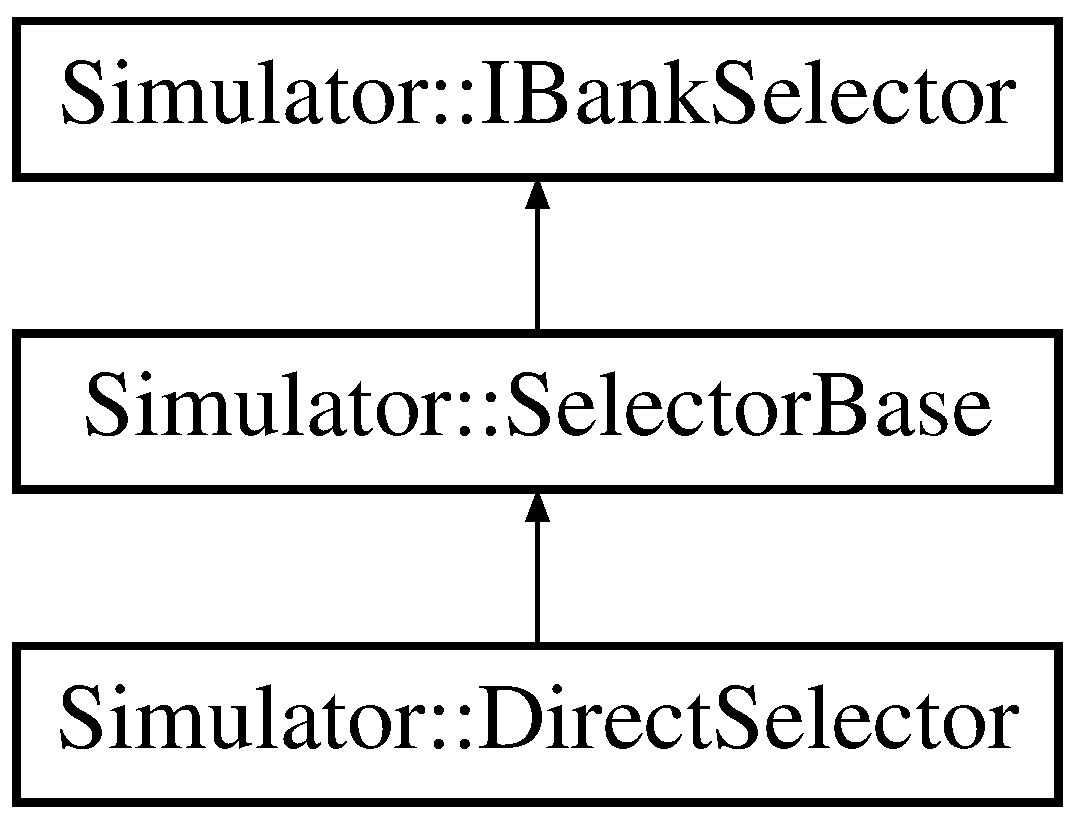
\includegraphics[height=3.000000cm]{class_simulator_1_1_direct_selector}
\end{center}
\end{figure}
\subsection*{Public Member Functions}
\begin{DoxyCompactItemize}
\item 
\hyperlink{class_simulator_1_1_direct_selector_a0ff6087bc1eb9784998d73559fbc372f}{Direct\+Selector} (size\+\_\+t num\+Banks)
\item 
void \hyperlink{class_simulator_1_1_direct_selector_aa1e89a7c1d907e1b47fe005af9368b8f}{Map} (Mem\+Addr address, Mem\+Addr \&tag, size\+\_\+t \&index)
\item 
Mem\+Addr \hyperlink{class_simulator_1_1_direct_selector_a2b7aab1bf3bdcd0bc95d65d93b863583}{Unmap} (Mem\+Addr tag, size\+\_\+t index)
\end{DoxyCompactItemize}
\subsection*{Additional Inherited Members}


\subsection{Constructor \& Destructor Documentation}
\hypertarget{class_simulator_1_1_direct_selector_a0ff6087bc1eb9784998d73559fbc372f}{\index{Simulator\+::\+Direct\+Selector@{Simulator\+::\+Direct\+Selector}!Direct\+Selector@{Direct\+Selector}}
\index{Direct\+Selector@{Direct\+Selector}!Simulator\+::\+Direct\+Selector@{Simulator\+::\+Direct\+Selector}}
\subsubsection[{Direct\+Selector}]{\setlength{\rightskip}{0pt plus 5cm}Simulator\+::\+Direct\+Selector\+::\+Direct\+Selector (
\begin{DoxyParamCaption}
\item[{size\+\_\+t}]{num\+Banks}
\end{DoxyParamCaption}
)\hspace{0.3cm}{\ttfamily [inline]}}}\label{class_simulator_1_1_direct_selector_a0ff6087bc1eb9784998d73559fbc372f}


\subsection{Member Function Documentation}
\hypertarget{class_simulator_1_1_direct_selector_aa1e89a7c1d907e1b47fe005af9368b8f}{\index{Simulator\+::\+Direct\+Selector@{Simulator\+::\+Direct\+Selector}!Map@{Map}}
\index{Map@{Map}!Simulator\+::\+Direct\+Selector@{Simulator\+::\+Direct\+Selector}}
\subsubsection[{Map}]{\setlength{\rightskip}{0pt plus 5cm}void Simulator\+::\+Direct\+Selector\+::\+Map (
\begin{DoxyParamCaption}
\item[{Mem\+Addr}]{address, }
\item[{Mem\+Addr \&}]{tag, }
\item[{size\+\_\+t \&}]{index}
\end{DoxyParamCaption}
)\hspace{0.3cm}{\ttfamily [inline]}, {\ttfamily [virtual]}}}\label{class_simulator_1_1_direct_selector_aa1e89a7c1d907e1b47fe005af9368b8f}


Implements \hyperlink{class_simulator_1_1_i_bank_selector_ad945160c483d88073b6e5572da5e4507}{Simulator\+::\+I\+Bank\+Selector}.

\hypertarget{class_simulator_1_1_direct_selector_a2b7aab1bf3bdcd0bc95d65d93b863583}{\index{Simulator\+::\+Direct\+Selector@{Simulator\+::\+Direct\+Selector}!Unmap@{Unmap}}
\index{Unmap@{Unmap}!Simulator\+::\+Direct\+Selector@{Simulator\+::\+Direct\+Selector}}
\subsubsection[{Unmap}]{\setlength{\rightskip}{0pt plus 5cm}Mem\+Addr Simulator\+::\+Direct\+Selector\+::\+Unmap (
\begin{DoxyParamCaption}
\item[{Mem\+Addr}]{tag, }
\item[{size\+\_\+t}]{index}
\end{DoxyParamCaption}
)\hspace{0.3cm}{\ttfamily [inline]}, {\ttfamily [virtual]}}}\label{class_simulator_1_1_direct_selector_a2b7aab1bf3bdcd0bc95d65d93b863583}


Implements \hyperlink{class_simulator_1_1_i_bank_selector_a57c8b49e6439984ff40836e8c5992aba}{Simulator\+::\+I\+Bank\+Selector}.



The documentation for this class was generated from the following file\+:\begin{DoxyCompactItemize}
\item 
arch/\hyperlink{_bank_selector_8cpp}{Bank\+Selector.\+cpp}\end{DoxyCompactItemize}

\hypertarget{class_simulator_1_1_direct_selector_binary}{\section{Simulator\+:\+:Direct\+Selector\+Binary Class Reference}
\label{class_simulator_1_1_direct_selector_binary}\index{Simulator\+::\+Direct\+Selector\+Binary@{Simulator\+::\+Direct\+Selector\+Binary}}
}
Inheritance diagram for Simulator\+:\+:Direct\+Selector\+Binary\+:\begin{figure}[H]
\begin{center}
\leavevmode
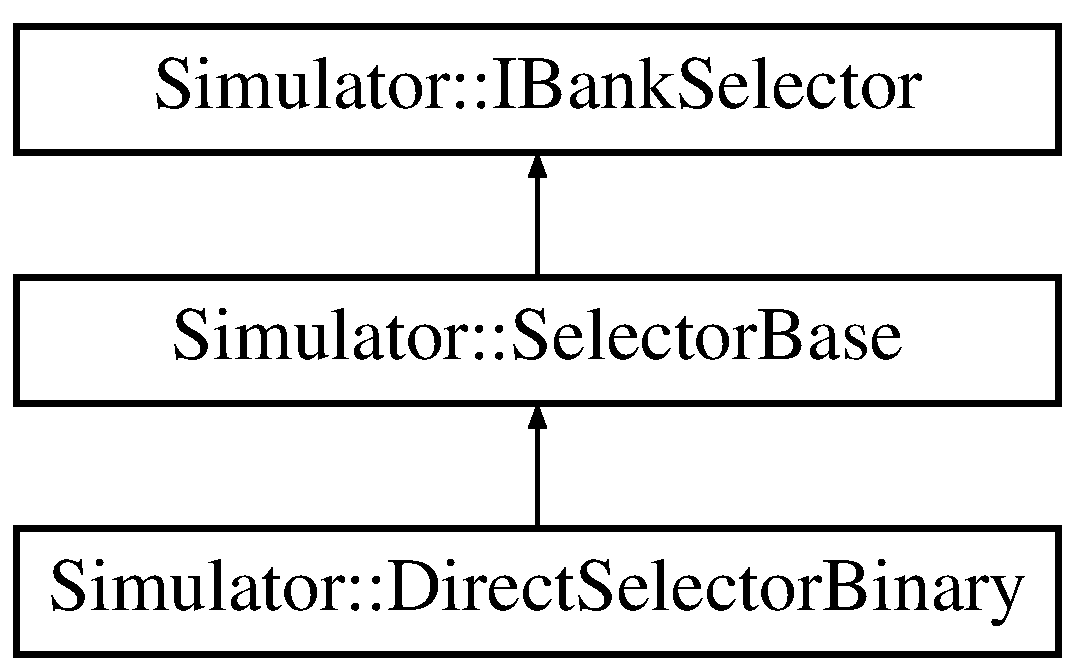
\includegraphics[height=3.000000cm]{class_simulator_1_1_direct_selector_binary}
\end{center}
\end{figure}
\subsection*{Public Member Functions}
\begin{DoxyCompactItemize}
\item 
\hyperlink{class_simulator_1_1_direct_selector_binary_aae85b2c0179c9c7f5e801463bd9e0c64}{Direct\+Selector\+Binary} (size\+\_\+t num\+Banks)
\item 
void \hyperlink{class_simulator_1_1_direct_selector_binary_a94319702a48838522bc5972ef5a28727}{Map} (Mem\+Addr address, Mem\+Addr \&tag, size\+\_\+t \&index)
\item 
Mem\+Addr \hyperlink{class_simulator_1_1_direct_selector_binary_a72fd9cee90911f43ebe3b293bb71ce98}{Unmap} (Mem\+Addr tag, size\+\_\+t index)
\end{DoxyCompactItemize}
\subsection*{Additional Inherited Members}


\subsection{Constructor \& Destructor Documentation}
\hypertarget{class_simulator_1_1_direct_selector_binary_aae85b2c0179c9c7f5e801463bd9e0c64}{\index{Simulator\+::\+Direct\+Selector\+Binary@{Simulator\+::\+Direct\+Selector\+Binary}!Direct\+Selector\+Binary@{Direct\+Selector\+Binary}}
\index{Direct\+Selector\+Binary@{Direct\+Selector\+Binary}!Simulator\+::\+Direct\+Selector\+Binary@{Simulator\+::\+Direct\+Selector\+Binary}}
\subsubsection[{Direct\+Selector\+Binary}]{\setlength{\rightskip}{0pt plus 5cm}Simulator\+::\+Direct\+Selector\+Binary\+::\+Direct\+Selector\+Binary (
\begin{DoxyParamCaption}
\item[{size\+\_\+t}]{num\+Banks}
\end{DoxyParamCaption}
)\hspace{0.3cm}{\ttfamily [inline]}}}\label{class_simulator_1_1_direct_selector_binary_aae85b2c0179c9c7f5e801463bd9e0c64}


\subsection{Member Function Documentation}
\hypertarget{class_simulator_1_1_direct_selector_binary_a94319702a48838522bc5972ef5a28727}{\index{Simulator\+::\+Direct\+Selector\+Binary@{Simulator\+::\+Direct\+Selector\+Binary}!Map@{Map}}
\index{Map@{Map}!Simulator\+::\+Direct\+Selector\+Binary@{Simulator\+::\+Direct\+Selector\+Binary}}
\subsubsection[{Map}]{\setlength{\rightskip}{0pt plus 5cm}void Simulator\+::\+Direct\+Selector\+Binary\+::\+Map (
\begin{DoxyParamCaption}
\item[{Mem\+Addr}]{address, }
\item[{Mem\+Addr \&}]{tag, }
\item[{size\+\_\+t \&}]{index}
\end{DoxyParamCaption}
)\hspace{0.3cm}{\ttfamily [inline]}, {\ttfamily [virtual]}}}\label{class_simulator_1_1_direct_selector_binary_a94319702a48838522bc5972ef5a28727}


Implements \hyperlink{class_simulator_1_1_i_bank_selector_ad945160c483d88073b6e5572da5e4507}{Simulator\+::\+I\+Bank\+Selector}.

\hypertarget{class_simulator_1_1_direct_selector_binary_a72fd9cee90911f43ebe3b293bb71ce98}{\index{Simulator\+::\+Direct\+Selector\+Binary@{Simulator\+::\+Direct\+Selector\+Binary}!Unmap@{Unmap}}
\index{Unmap@{Unmap}!Simulator\+::\+Direct\+Selector\+Binary@{Simulator\+::\+Direct\+Selector\+Binary}}
\subsubsection[{Unmap}]{\setlength{\rightskip}{0pt plus 5cm}Mem\+Addr Simulator\+::\+Direct\+Selector\+Binary\+::\+Unmap (
\begin{DoxyParamCaption}
\item[{Mem\+Addr}]{tag, }
\item[{size\+\_\+t}]{index}
\end{DoxyParamCaption}
)\hspace{0.3cm}{\ttfamily [inline]}, {\ttfamily [virtual]}}}\label{class_simulator_1_1_direct_selector_binary_a72fd9cee90911f43ebe3b293bb71ce98}


Implements \hyperlink{class_simulator_1_1_i_bank_selector_a57c8b49e6439984ff40836e8c5992aba}{Simulator\+::\+I\+Bank\+Selector}.



The documentation for this class was generated from the following file\+:\begin{DoxyCompactItemize}
\item 
arch/\hyperlink{_bank_selector_8cpp}{Bank\+Selector.\+cpp}\end{DoxyCompactItemize}

\hypertarget{class_simulator_1_1_display}{\section{Simulator\+:\+:Display Class Reference}
\label{class_simulator_1_1_display}\index{Simulator\+::\+Display@{Simulator\+::\+Display}}
}


{\ttfamily \#include $<$Display.\+h$>$}

Inheritance diagram for Simulator\+:\+:Display\+:\begin{figure}[H]
\begin{center}
\leavevmode
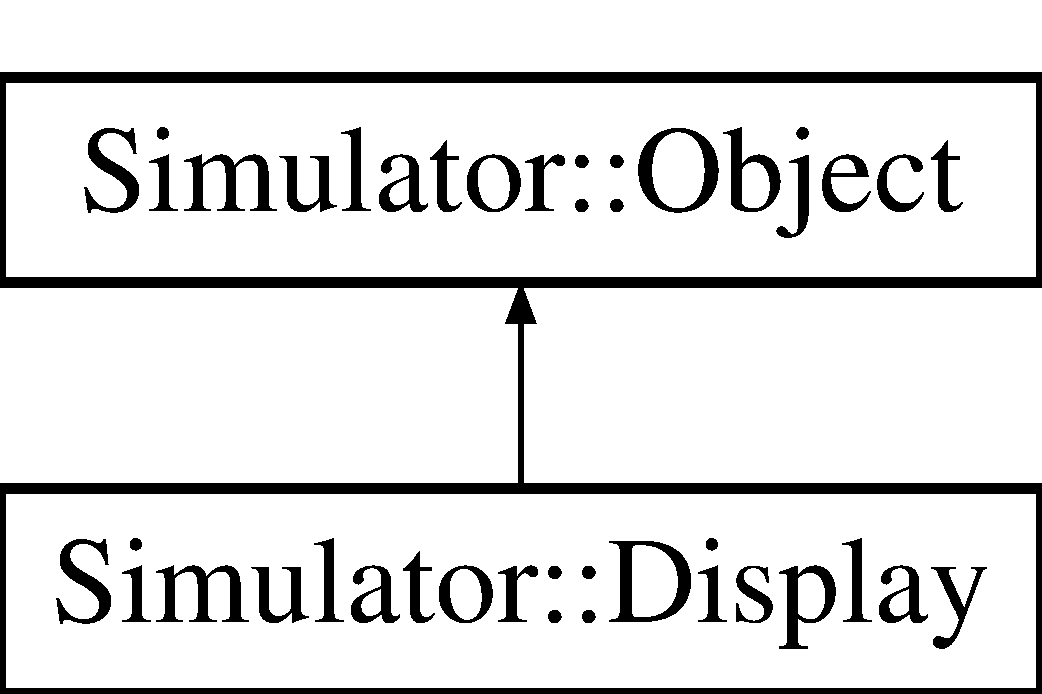
\includegraphics[height=2.000000cm]{class_simulator_1_1_display}
\end{center}
\end{figure}
\subsection*{Public Member Functions}
\begin{DoxyCompactItemize}
\item 
\hyperlink{class_simulator_1_1_display_a9e8dd95d8d8d6f6a68a8a7aabe29b400}{Display} (const std\+::string \&\hyperlink{mtconf_8c_a8f8f80d37794cde9472343e4487ba3eb}{name}, \hyperlink{class_simulator_1_1_object}{Object} \&parent, \hyperlink{class_simulator_1_1_i_i_o_bus}{I\+I\+O\+Bus} \&iobus, \hyperlink{namespace_simulator_a3493d987c866ad6b8aaa704c42502db0}{I\+O\+Device\+I\+D} ctldevid, \hyperlink{namespace_simulator_a3493d987c866ad6b8aaa704c42502db0}{I\+O\+Device\+I\+D} fbdevid, \hyperlink{class_config}{Config} \&config)
\item 
\hyperlink{class_simulator_1_1_display_aaad56ddda9a85cfeb1c3cdec28ba62e5}{Display} (const \hyperlink{class_simulator_1_1_display}{Display} \&)=delete
\item 
\hyperlink{class_simulator_1_1_display}{Display} \& \hyperlink{class_simulator_1_1_display_a2062fb4d91091b3793a8b81d57c4e4ba}{operator=} (const \hyperlink{class_simulator_1_1_display}{Display} \&)=delete
\item 
\hyperlink{class_simulator_1_1_display_abbb1e81edfa7c0067b403b8ccde20091}{$\sim$\+Display} ()
\item 
void \hyperlink{class_simulator_1_1_display_a49e90cfde0aef86aa7d98343621d7432}{Check\+Events} (void)
\item 
void \hyperlink{class_simulator_1_1_display_adb2a9249e4163dea8ef1457aff79ff5c}{On\+Cycle} (\hyperlink{namespace_simulator_a928f1e2101eba21bb0fe409e8c9ce573}{Cycle\+No} cycle)
\end{DoxyCompactItemize}
\subsection*{Static Public Member Functions}
\begin{DoxyCompactItemize}
\item 
static \hyperlink{class_simulator_1_1_display}{Display} $\ast$ \hyperlink{class_simulator_1_1_display_afbff3836d53856e0105e6e68e43b7542}{Get\+Display} ()
\end{DoxyCompactItemize}
\subsection*{Protected Member Functions}
\begin{DoxyCompactItemize}
\item 
void \hyperlink{class_simulator_1_1_display_a9ac001d4d97c472e8921aa6548f9fdfd}{Resize} (unsigned w, unsigned h, bool erase)
\item 
void \hyperlink{class_simulator_1_1_display_acf029f340eff0205cf1c534755ec8f0f}{Refresh} () const 
\item 
void \hyperlink{class_simulator_1_1_display_ad936a0ecf504adc4619a91dc053d6c01}{Reset\+Caption} () const 
\item 
void \hyperlink{class_simulator_1_1_display_a4807e664e7fc47b686e35a999a2e2772}{Resize\+Screen} (unsigned int w, unsigned int h)
\item 
void \hyperlink{class_simulator_1_1_display_afb4959747fcefb5fe4215f180cf6a149}{Dump\+Frame\+Buffer} (unsigned key, int stream, bool gen\+\_\+timestamp) const 
\end{DoxyCompactItemize}
\subsection*{Friends}
\begin{DoxyCompactItemize}
\item 
class \hyperlink{class_simulator_1_1_display_a40db1df984344b6204f9c8a338aacabb}{Control\+Interface}
\item 
class \hyperlink{class_simulator_1_1_display_a8ecdedbbf356339204e1e013df18699b}{Frame\+Buffer\+Interface}
\end{DoxyCompactItemize}


\subsection{Constructor \& Destructor Documentation}
\hypertarget{class_simulator_1_1_display_a9e8dd95d8d8d6f6a68a8a7aabe29b400}{\index{Simulator\+::\+Display@{Simulator\+::\+Display}!Display@{Display}}
\index{Display@{Display}!Simulator\+::\+Display@{Simulator\+::\+Display}}
\subsubsection[{Display}]{\setlength{\rightskip}{0pt plus 5cm}Simulator\+::\+Display\+::\+Display (
\begin{DoxyParamCaption}
\item[{const std\+::string \&}]{name, }
\item[{{\bf Object} \&}]{parent, }
\item[{{\bf I\+I\+O\+Bus} \&}]{iobus, }
\item[{{\bf I\+O\+Device\+I\+D}}]{ctldevid, }
\item[{{\bf I\+O\+Device\+I\+D}}]{fbdevid, }
\item[{{\bf Config} \&}]{config}
\end{DoxyParamCaption}
)}}\label{class_simulator_1_1_display_a9e8dd95d8d8d6f6a68a8a7aabe29b400}
\hypertarget{class_simulator_1_1_display_aaad56ddda9a85cfeb1c3cdec28ba62e5}{\index{Simulator\+::\+Display@{Simulator\+::\+Display}!Display@{Display}}
\index{Display@{Display}!Simulator\+::\+Display@{Simulator\+::\+Display}}
\subsubsection[{Display}]{\setlength{\rightskip}{0pt plus 5cm}Simulator\+::\+Display\+::\+Display (
\begin{DoxyParamCaption}
\item[{const {\bf Display} \&}]{}
\end{DoxyParamCaption}
)\hspace{0.3cm}{\ttfamily [delete]}}}\label{class_simulator_1_1_display_aaad56ddda9a85cfeb1c3cdec28ba62e5}
\hypertarget{class_simulator_1_1_display_abbb1e81edfa7c0067b403b8ccde20091}{\index{Simulator\+::\+Display@{Simulator\+::\+Display}!````~Display@{$\sim$\+Display}}
\index{````~Display@{$\sim$\+Display}!Simulator\+::\+Display@{Simulator\+::\+Display}}
\subsubsection[{$\sim$\+Display}]{\setlength{\rightskip}{0pt plus 5cm}Simulator\+::\+Display\+::$\sim$\+Display (
\begin{DoxyParamCaption}
{}
\end{DoxyParamCaption}
)}}\label{class_simulator_1_1_display_abbb1e81edfa7c0067b403b8ccde20091}


\subsection{Member Function Documentation}
\hypertarget{class_simulator_1_1_display_a49e90cfde0aef86aa7d98343621d7432}{\index{Simulator\+::\+Display@{Simulator\+::\+Display}!Check\+Events@{Check\+Events}}
\index{Check\+Events@{Check\+Events}!Simulator\+::\+Display@{Simulator\+::\+Display}}
\subsubsection[{Check\+Events}]{\setlength{\rightskip}{0pt plus 5cm}void Simulator\+::\+Display\+::\+Check\+Events (
\begin{DoxyParamCaption}
\item[{void}]{}
\end{DoxyParamCaption}
)}}\label{class_simulator_1_1_display_a49e90cfde0aef86aa7d98343621d7432}
\hypertarget{class_simulator_1_1_display_afb4959747fcefb5fe4215f180cf6a149}{\index{Simulator\+::\+Display@{Simulator\+::\+Display}!Dump\+Frame\+Buffer@{Dump\+Frame\+Buffer}}
\index{Dump\+Frame\+Buffer@{Dump\+Frame\+Buffer}!Simulator\+::\+Display@{Simulator\+::\+Display}}
\subsubsection[{Dump\+Frame\+Buffer}]{\setlength{\rightskip}{0pt plus 5cm}void Simulator\+::\+Display\+::\+Dump\+Frame\+Buffer (
\begin{DoxyParamCaption}
\item[{unsigned}]{key, }
\item[{int}]{stream, }
\item[{bool}]{gen\+\_\+timestamp}
\end{DoxyParamCaption}
) const\hspace{0.3cm}{\ttfamily [protected]}}}\label{class_simulator_1_1_display_afb4959747fcefb5fe4215f180cf6a149}
\hypertarget{class_simulator_1_1_display_afbff3836d53856e0105e6e68e43b7542}{\index{Simulator\+::\+Display@{Simulator\+::\+Display}!Get\+Display@{Get\+Display}}
\index{Get\+Display@{Get\+Display}!Simulator\+::\+Display@{Simulator\+::\+Display}}
\subsubsection[{Get\+Display}]{\setlength{\rightskip}{0pt plus 5cm}static {\bf Display}$\ast$ Simulator\+::\+Display\+::\+Get\+Display (
\begin{DoxyParamCaption}
{}
\end{DoxyParamCaption}
)\hspace{0.3cm}{\ttfamily [inline]}, {\ttfamily [static]}}}\label{class_simulator_1_1_display_afbff3836d53856e0105e6e68e43b7542}
\hypertarget{class_simulator_1_1_display_adb2a9249e4163dea8ef1457aff79ff5c}{\index{Simulator\+::\+Display@{Simulator\+::\+Display}!On\+Cycle@{On\+Cycle}}
\index{On\+Cycle@{On\+Cycle}!Simulator\+::\+Display@{Simulator\+::\+Display}}
\subsubsection[{On\+Cycle}]{\setlength{\rightskip}{0pt plus 5cm}void Simulator\+::\+Display\+::\+On\+Cycle (
\begin{DoxyParamCaption}
\item[{{\bf Cycle\+No}}]{cycle}
\end{DoxyParamCaption}
)\hspace{0.3cm}{\ttfamily [inline]}}}\label{class_simulator_1_1_display_adb2a9249e4163dea8ef1457aff79ff5c}
\hypertarget{class_simulator_1_1_display_a2062fb4d91091b3793a8b81d57c4e4ba}{\index{Simulator\+::\+Display@{Simulator\+::\+Display}!operator=@{operator=}}
\index{operator=@{operator=}!Simulator\+::\+Display@{Simulator\+::\+Display}}
\subsubsection[{operator=}]{\setlength{\rightskip}{0pt plus 5cm}{\bf Display}\& Simulator\+::\+Display\+::operator= (
\begin{DoxyParamCaption}
\item[{const {\bf Display} \&}]{}
\end{DoxyParamCaption}
)\hspace{0.3cm}{\ttfamily [delete]}}}\label{class_simulator_1_1_display_a2062fb4d91091b3793a8b81d57c4e4ba}
\hypertarget{class_simulator_1_1_display_acf029f340eff0205cf1c534755ec8f0f}{\index{Simulator\+::\+Display@{Simulator\+::\+Display}!Refresh@{Refresh}}
\index{Refresh@{Refresh}!Simulator\+::\+Display@{Simulator\+::\+Display}}
\subsubsection[{Refresh}]{\setlength{\rightskip}{0pt plus 5cm}void Simulator\+::\+Display\+::\+Refresh (
\begin{DoxyParamCaption}
{}
\end{DoxyParamCaption}
) const\hspace{0.3cm}{\ttfamily [protected]}}}\label{class_simulator_1_1_display_acf029f340eff0205cf1c534755ec8f0f}
\hypertarget{class_simulator_1_1_display_ad936a0ecf504adc4619a91dc053d6c01}{\index{Simulator\+::\+Display@{Simulator\+::\+Display}!Reset\+Caption@{Reset\+Caption}}
\index{Reset\+Caption@{Reset\+Caption}!Simulator\+::\+Display@{Simulator\+::\+Display}}
\subsubsection[{Reset\+Caption}]{\setlength{\rightskip}{0pt plus 5cm}void Simulator\+::\+Display\+::\+Reset\+Caption (
\begin{DoxyParamCaption}
{}
\end{DoxyParamCaption}
) const\hspace{0.3cm}{\ttfamily [protected]}}}\label{class_simulator_1_1_display_ad936a0ecf504adc4619a91dc053d6c01}
\hypertarget{class_simulator_1_1_display_a9ac001d4d97c472e8921aa6548f9fdfd}{\index{Simulator\+::\+Display@{Simulator\+::\+Display}!Resize@{Resize}}
\index{Resize@{Resize}!Simulator\+::\+Display@{Simulator\+::\+Display}}
\subsubsection[{Resize}]{\setlength{\rightskip}{0pt plus 5cm}void Simulator\+::\+Display\+::\+Resize (
\begin{DoxyParamCaption}
\item[{unsigned}]{w, }
\item[{unsigned}]{h, }
\item[{bool}]{erase}
\end{DoxyParamCaption}
)\hspace{0.3cm}{\ttfamily [protected]}}}\label{class_simulator_1_1_display_a9ac001d4d97c472e8921aa6548f9fdfd}
\hypertarget{class_simulator_1_1_display_a4807e664e7fc47b686e35a999a2e2772}{\index{Simulator\+::\+Display@{Simulator\+::\+Display}!Resize\+Screen@{Resize\+Screen}}
\index{Resize\+Screen@{Resize\+Screen}!Simulator\+::\+Display@{Simulator\+::\+Display}}
\subsubsection[{Resize\+Screen}]{\setlength{\rightskip}{0pt plus 5cm}void Simulator\+::\+Display\+::\+Resize\+Screen (
\begin{DoxyParamCaption}
\item[{unsigned int}]{w, }
\item[{unsigned int}]{h}
\end{DoxyParamCaption}
)\hspace{0.3cm}{\ttfamily [protected]}}}\label{class_simulator_1_1_display_a4807e664e7fc47b686e35a999a2e2772}


\subsection{Friends And Related Function Documentation}
\hypertarget{class_simulator_1_1_display_a40db1df984344b6204f9c8a338aacabb}{\index{Simulator\+::\+Display@{Simulator\+::\+Display}!Control\+Interface@{Control\+Interface}}
\index{Control\+Interface@{Control\+Interface}!Simulator\+::\+Display@{Simulator\+::\+Display}}
\subsubsection[{Control\+Interface}]{\setlength{\rightskip}{0pt plus 5cm}friend class Control\+Interface\hspace{0.3cm}{\ttfamily [friend]}}}\label{class_simulator_1_1_display_a40db1df984344b6204f9c8a338aacabb}
\hypertarget{class_simulator_1_1_display_a8ecdedbbf356339204e1e013df18699b}{\index{Simulator\+::\+Display@{Simulator\+::\+Display}!Frame\+Buffer\+Interface@{Frame\+Buffer\+Interface}}
\index{Frame\+Buffer\+Interface@{Frame\+Buffer\+Interface}!Simulator\+::\+Display@{Simulator\+::\+Display}}
\subsubsection[{Frame\+Buffer\+Interface}]{\setlength{\rightskip}{0pt plus 5cm}friend class Frame\+Buffer\+Interface\hspace{0.3cm}{\ttfamily [friend]}}}\label{class_simulator_1_1_display_a8ecdedbbf356339204e1e013df18699b}


The documentation for this class was generated from the following files\+:\begin{DoxyCompactItemize}
\item 
arch/dev/\hyperlink{_display_8h}{Display.\+h}\item 
arch/dev/\hyperlink{_display_8cpp}{Display.\+cpp}\end{DoxyCompactItemize}

\hypertarget{class_simulator_1_1_d_r_i_s_c}{\section{Simulator\+:\+:D\+R\+I\+S\+C Class Reference}
\label{class_simulator_1_1_d_r_i_s_c}\index{Simulator\+::\+D\+R\+I\+S\+C@{Simulator\+::\+D\+R\+I\+S\+C}}
}


{\ttfamily \#include $<$D\+R\+I\+S\+C.\+h$>$}

Inheritance diagram for Simulator\+:\+:D\+R\+I\+S\+C\+:\begin{figure}[H]
\begin{center}
\leavevmode
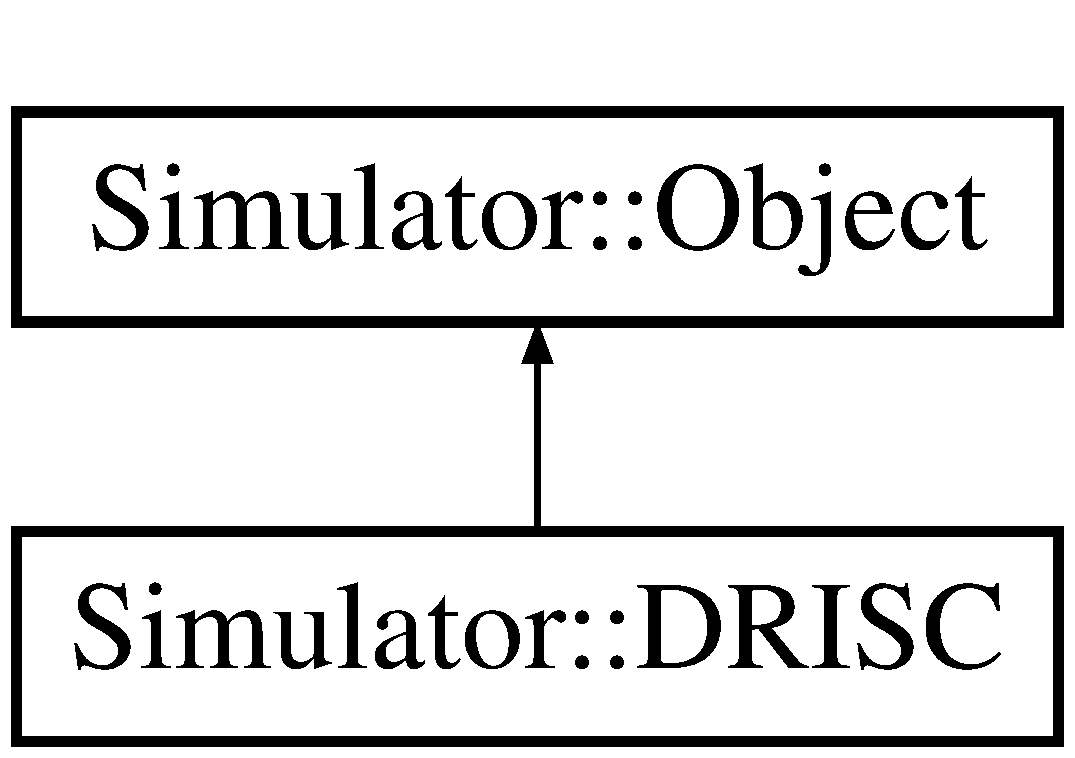
\includegraphics[height=2.000000cm]{class_simulator_1_1_d_r_i_s_c}
\end{center}
\end{figure}
\subsection*{Public Member Functions}
\begin{DoxyCompactItemize}
\item 
\hyperlink{class_simulator_1_1_d_r_i_s_c_adb62a9c8ee9adefdef8862c284ebccce}{D\+R\+I\+S\+C} (const std\+::string \&\hyperlink{mtconf_8c_a8f8f80d37794cde9472343e4487ba3eb}{name}, \hyperlink{class_simulator_1_1_object}{Object} \&parent, \hyperlink{class_simulator_1_1_clock}{Clock} \&clock, \hyperlink{namespace_simulator_aa671021151c047ae2da6dce4e6303476}{P\+I\+D} pid, const std\+::vector$<$ \hyperlink{class_simulator_1_1_d_r_i_s_c}{D\+R\+I\+S\+C} $\ast$ $>$ \&grid, \hyperlink{class_config}{Config} \&config)
\item 
\hyperlink{class_simulator_1_1_d_r_i_s_c_a43ea7e6f231e9c35c8080e9f18a0d336}{D\+R\+I\+S\+C} (const \hyperlink{class_simulator_1_1_d_r_i_s_c}{D\+R\+I\+S\+C} \&)=delete
\item 
\hyperlink{class_simulator_1_1_d_r_i_s_c}{D\+R\+I\+S\+C} \& \hyperlink{class_simulator_1_1_d_r_i_s_c_a2f371d61c6314c119d66093f183b71fb}{operator=} (const \hyperlink{class_simulator_1_1_d_r_i_s_c}{D\+R\+I\+S\+C} \&)=delete
\item 
\hyperlink{class_simulator_1_1_d_r_i_s_c_ab661fc4050b4b0ef557f960234858f98}{$\sim$\+D\+R\+I\+S\+C} ()
\item 
void \hyperlink{class_simulator_1_1_d_r_i_s_c_a2cd106e8cad6afd3ba7d31ac40697e71}{Connect\+Memory} (\hyperlink{class_simulator_1_1_i_memory}{I\+Memory} $\ast$memory, \hyperlink{class_simulator_1_1_i_memory_admin}{I\+Memory\+Admin} $\ast$admin)
\item 
void \hyperlink{class_simulator_1_1_d_r_i_s_c_a1c608aa906b8277562aa21f2b9f7bebc}{Connect\+Link} (\hyperlink{class_simulator_1_1_d_r_i_s_c}{D\+R\+I\+S\+C} $\ast$prev, \hyperlink{class_simulator_1_1_d_r_i_s_c}{D\+R\+I\+S\+C} $\ast$next)
\item 
void \hyperlink{class_simulator_1_1_d_r_i_s_c_a643dc8cf598b263ee4a698330ae8a9b8}{Connect\+F\+P\+U} (\hyperlink{class_config}{Config} \&config, \hyperlink{class_simulator_1_1_f_p_u}{F\+P\+U} $\ast$fpu)
\item 
void \hyperlink{class_simulator_1_1_d_r_i_s_c_ac023555a197b90d26052d062162d781e}{Connect\+I\+O} (\hyperlink{class_config}{Config} \&config, \hyperlink{class_simulator_1_1_i_i_o_bus}{I\+I\+O\+Bus} $\ast$iobus)
\item 
void \hyperlink{class_simulator_1_1_d_r_i_s_c_ab1448ca955dda9eda2ad3d84a5d24918}{Initialize} ()
\item 
bool \hyperlink{class_simulator_1_1_d_r_i_s_c_a4e8ff4e7860ff0dbea353ee050152536}{Boot} (Mem\+Addr addr, bool legacy)
\item 
\hyperlink{namespace_simulator_aa671021151c047ae2da6dce4e6303476}{P\+I\+D} \hyperlink{class_simulator_1_1_d_r_i_s_c_a48d703f0ed0f4e5f04a2b16cd7f9cedf}{Get\+P\+I\+D} () const 
\item 
\hyperlink{namespace_simulator_a4aa07bee2f34beac11abf48a8ccc47c4}{P\+Size} \hyperlink{class_simulator_1_1_d_r_i_s_c_a47a5161b9bc9897742a288ccfc56168e}{Get\+Grid\+Size} () const 
\item 
bool \hyperlink{class_simulator_1_1_d_r_i_s_c_adf9eb02eaf7fe4b9e361c39858a9c23d}{Is\+Idle} () const 
\item 
float \hyperlink{class_simulator_1_1_d_r_i_s_c_a19576f8e43bcc84c7421c068beac0f25}{Get\+Reg\+File\+Async\+Port\+Activity} () const 
\item 
\hyperlink{namespace_simulator_aefe00209f3ea9f8e24874de522c3c3e7}{T\+Size} \hyperlink{class_simulator_1_1_d_r_i_s_c_ad779958861bf6905d5483b3903661d4b}{Get\+Max\+Threads\+Allocated} () const 
\item 
\hyperlink{namespace_simulator_aefe00209f3ea9f8e24874de522c3c3e7}{T\+Size} \hyperlink{class_simulator_1_1_d_r_i_s_c_acd6f1330acbd7aa05a3865003e205204}{Get\+Total\+Threads\+Allocated} ()
\item 
\hyperlink{namespace_simulator_aefe00209f3ea9f8e24874de522c3c3e7}{T\+Size} \hyperlink{class_simulator_1_1_d_r_i_s_c_a4038eb2a5d9b99e79adfad29779ff5a7}{Get\+Total\+Threads\+Created} ()
\item 
\hyperlink{namespace_simulator_aefe00209f3ea9f8e24874de522c3c3e7}{T\+Size} \hyperlink{class_simulator_1_1_d_r_i_s_c_a780d59e6c1d2f6cfd881339b68d74f39}{Get\+Thread\+Table\+Size} () const 
\item 
float \hyperlink{class_simulator_1_1_d_r_i_s_c_a045a9f8fe69f8d7ca2d849336d4136cd}{Get\+Thread\+Table\+Occupancy} ()
\item 
\hyperlink{namespace_simulator_a06544009313d7c13d411b1c074e5acff}{F\+Size} \hyperlink{class_simulator_1_1_d_r_i_s_c_a1452e5c0c6025e6862ed0e80e6f43680}{Get\+Max\+Families\+Allocated} () const 
\item 
\hyperlink{namespace_simulator_a06544009313d7c13d411b1c074e5acff}{F\+Size} \hyperlink{class_simulator_1_1_d_r_i_s_c_a1e153f19d364676a098cdbeee159335f}{Get\+Total\+Families\+Allocated} ()
\item 
\hyperlink{namespace_simulator_a06544009313d7c13d411b1c074e5acff}{F\+Size} \hyperlink{class_simulator_1_1_d_r_i_s_c_ab091a2aeffb302b8e8934e3d133180d2}{Get\+Total\+Families\+Created} ()
\item 
\hyperlink{namespace_simulator_a06544009313d7c13d411b1c074e5acff}{F\+Size} \hyperlink{class_simulator_1_1_d_r_i_s_c_aa922f0c4f46e14d5421339cfdd23cfd2}{Get\+Family\+Table\+Size} () const 
\item 
float \hyperlink{class_simulator_1_1_d_r_i_s_c_a88e7c4bb3ed9546f114b7e60a12625ff}{Get\+Family\+Table\+Occupancy} ()
\item 
\hyperlink{namespace_simulator_a5ca279f926485be2d0554e41275a3305}{Buffer\+Size} \hyperlink{class_simulator_1_1_d_r_i_s_c_a140a034147286f5fd4915c4563b7d576}{Get\+Max\+Allocate\+Ex\+Queue\+Size} ()
\item 
\hyperlink{namespace_simulator_a5ca279f926485be2d0554e41275a3305}{Buffer\+Size} \hyperlink{class_simulator_1_1_d_r_i_s_c_ae655512d4b1fcc2f0a3a69a4e99c83b3}{Get\+Total\+Allocate\+Ex\+Queue\+Size} ()
\item 
float \hyperlink{class_simulator_1_1_d_r_i_s_c_a35f8cc6087a6fec637eba3276ce3a4a6}{Get\+Average\+Allocate\+Ex\+Queue\+Size} ()
\item 
unsigned int \hyperlink{class_simulator_1_1_d_r_i_s_c_ae644a700636dc634f59f772d9b0885a9}{Get\+Num\+Suspended\+Registers} () const 
\item 
void \hyperlink{class_simulator_1_1_d_r_i_s_c_a2f141ba7eff1ae273031bbfec1680bf0}{Write\+A\+S\+R} (\hyperlink{namespace_simulator_1_1drisc_ad67fa6022bb8dfc914132e37bbba2e97}{drisc\+::\+A\+R\+Addr} which, Integer data)
\item 
Integer \hyperlink{class_simulator_1_1_d_r_i_s_c_ad485afd4103a3fcfd7b3ac69cecaab69}{Read\+A\+S\+R} (\hyperlink{namespace_simulator_1_1drisc_ad67fa6022bb8dfc914132e37bbba2e97}{drisc\+::\+A\+R\+Addr} which) const 
\item 
void \hyperlink{class_simulator_1_1_d_r_i_s_c_a817b71681290c747896a21904a174a79}{Write\+A\+P\+R} (\hyperlink{namespace_simulator_1_1drisc_ad67fa6022bb8dfc914132e37bbba2e97}{drisc\+::\+A\+R\+Addr} which, Integer data)
\item 
Integer \hyperlink{class_simulator_1_1_d_r_i_s_c_a59cb242882b13731d79bcdcfbf9281fd}{Read\+A\+P\+R} (\hyperlink{namespace_simulator_1_1drisc_ad67fa6022bb8dfc914132e37bbba2e97}{drisc\+::\+A\+R\+Addr} which) const 
\item 
\hyperlink{namespace_simulator_a4aa07bee2f34beac11abf48a8ccc47c4}{P\+Size} \hyperlink{class_simulator_1_1_d_r_i_s_c_a0f795f33db2370869329a3a6bf45ca2b}{Get\+Place\+Size} (\hyperlink{namespace_simulator_aaccbc706b2d6c99085f52f6dfc2333e4}{L\+F\+I\+D} fid) const 
\item 
Mem\+Addr \hyperlink{class_simulator_1_1_d_r_i_s_c_adb723c225728b9a13e34e410e3bf3d19}{Get\+T\+L\+S\+Address} (\hyperlink{namespace_simulator_aaccbc706b2d6c99085f52f6dfc2333e4}{L\+F\+I\+D} fid, \hyperlink{namespace_simulator_a483cc4ecee1736e895054617672cded5}{T\+I\+D} tid) const 
\item 
Mem\+Size \hyperlink{class_simulator_1_1_d_r_i_s_c_af58119afa0433cde6ea8cafdc1c522fe}{Get\+T\+L\+S\+Size} () const 
\item 
\hyperlink{struct_simulator_1_1_place_i_d}{Place\+I\+D} \hyperlink{class_simulator_1_1_d_r_i_s_c_a8192f04888fbc90e4c0d9e75cab1d1f3}{Unpack\+Place} (Integer \hyperlink{mtconf_8c_aa3185401f04d30bd505daebf48c39cc5}{id}) const 
\item 
Integer \hyperlink{class_simulator_1_1_d_r_i_s_c_a24419ce6a407d7901c7bf839fc12da0d}{Pack\+Place} (const \hyperlink{struct_simulator_1_1_place_i_d}{Place\+I\+D} \&\hyperlink{mtconf_8c_aa3185401f04d30bd505daebf48c39cc5}{id}) const 
\item 
\hyperlink{struct_simulator_1_1_f_i_d}{F\+I\+D} \hyperlink{class_simulator_1_1_d_r_i_s_c_afa83a50bf057b50fbe0d48534cb2f8cb}{Unpack\+F\+I\+D} (Integer \hyperlink{mtconf_8c_aa3185401f04d30bd505daebf48c39cc5}{id}) const 
\item 
Integer \hyperlink{class_simulator_1_1_d_r_i_s_c_a2cbfbfe068dc55e9bcbf4eb977b07732}{Pack\+F\+I\+D} (const \hyperlink{struct_simulator_1_1_f_i_d}{F\+I\+D} \&fid) const 
\item 
\hyperlink{namespace_simulator_a607aa9969bfe2711861ae21f42c37c59}{F\+Capability} \hyperlink{class_simulator_1_1_d_r_i_s_c_a2bf1a019a4cc003b77b3f278f3b8b1c6}{Generate\+Family\+Capability} () const 
\item 
void \hyperlink{class_simulator_1_1_d_r_i_s_c_a2ff0805fbd40c1c4c3b59c42fe2682ce}{Map\+Memory} (Mem\+Addr address, Mem\+Size size, \hyperlink{namespace_simulator_a62ef2d2c77bd54a16c39881f6266875e}{Process\+I\+D} pid=0)
\item 
void \hyperlink{class_simulator_1_1_d_r_i_s_c_a908571cb361eef6c9c066c25d27e856b}{Unmap\+Memory} (Mem\+Addr address, Mem\+Size size)
\item 
void \hyperlink{class_simulator_1_1_d_r_i_s_c_a7505ae756c446337a20cacb2064d407d}{Unmap\+Memory} (\hyperlink{namespace_simulator_a62ef2d2c77bd54a16c39881f6266875e}{Process\+I\+D} pid)
\item 
bool \hyperlink{class_simulator_1_1_d_r_i_s_c_af68786ce2d6ddb1fe768317cf8b50006}{Check\+Permissions} (Mem\+Addr address, Mem\+Size size, int access) const 
\item 
\hyperlink{class_simulator_1_1drisc_1_1_network}{drisc\+::\+Network} \& \hyperlink{class_simulator_1_1_d_r_i_s_c_a3a999da614c23294f2910a83074ffa41}{Get\+Network} ()
\item 
\hyperlink{class_simulator_1_1drisc_1_1_i_o_interface}{drisc\+::\+I\+O\+Interface} $\ast$ \hyperlink{class_simulator_1_1_d_r_i_s_c_ad204679817949df15fb4f9a11fff93a7}{Get\+I\+O\+Interface} ()
\item 
\hyperlink{class_simulator_1_1drisc_1_1_register_file}{drisc\+::\+Register\+File} \& \hyperlink{class_simulator_1_1_d_r_i_s_c_ab9551cd382eb6514ad038886b3b9b8e3}{Get\+Register\+File} ()
\item 
\hyperlink{class_simulator_1_1drisc_1_1_i_cache}{drisc\+::\+I\+Cache} \& \hyperlink{class_simulator_1_1_d_r_i_s_c_a1a616117ccbc207b4dc8fa0a2e7cc1f9}{Get\+I\+Cache} ()
\item 
\hyperlink{class_simulator_1_1drisc_1_1_d_cache}{drisc\+::\+D\+Cache} \& \hyperlink{class_simulator_1_1_d_r_i_s_c_af8a0a3f96f87ae9e05056b263d3bcb97}{Get\+D\+Cache} ()
\item 
\hyperlink{class_simulator_1_1drisc_1_1_allocator}{drisc\+::\+Allocator} \& \hyperlink{class_simulator_1_1_d_r_i_s_c_a1b661496e3d894010c34d83752646e0b}{Get\+Allocator} ()
\item 
\hyperlink{class_simulator_1_1drisc_1_1_r_a_unit}{drisc\+::\+R\+A\+Unit} \& \hyperlink{class_simulator_1_1_d_r_i_s_c_a9d70618d0315f3785208549a1b6c075a}{Get\+R\+A\+Unit} ()
\item 
\hyperlink{class_simulator_1_1drisc_1_1_pipeline}{drisc\+::\+Pipeline} \& \hyperlink{class_simulator_1_1_d_r_i_s_c_a5566537e46f7b11c3698bb7f742ed49f}{Get\+Pipeline} ()
\item 
\hyperlink{class_simulator_1_1drisc_1_1_i_o_match_unit}{drisc\+::\+I\+O\+Match\+Unit} \& \hyperlink{class_simulator_1_1_d_r_i_s_c_a8e37c24fc22bb69a850d284e9e226580}{Get\+I\+O\+Match\+Unit} ()
\item 
\hyperlink{class_simulator_1_1drisc_1_1_family_table}{drisc\+::\+Family\+Table} \& \hyperlink{class_simulator_1_1_d_r_i_s_c_a2553140ff720fe2f73fda621e53feaf8}{Get\+Family\+Table} ()
\item 
\hyperlink{class_simulator_1_1drisc_1_1_thread_table}{drisc\+::\+Thread\+Table} \& \hyperlink{class_simulator_1_1_d_r_i_s_c_aa83c2387716365bee87bba0808ab2afb}{Get\+Thread\+Table} ()
\item 
\hyperlink{class_simulator_1_1_symbol_table}{Symbol\+Table} \& \hyperlink{class_simulator_1_1_d_r_i_s_c_a9c12bbe130bed7241fb94d70a32ff1d6}{Get\+Symbol\+Table} ()
\end{DoxyCompactItemize}
\subsection*{Friends}
\begin{DoxyCompactItemize}
\item 
class \hyperlink{class_simulator_1_1_d_r_i_s_c_a7bab761d92eff64f91fc0d1dd55c744c}{drisc\+::\+Perf\+Counters\+::\+Helpers}
\end{DoxyCompactItemize}


\subsection{Constructor \& Destructor Documentation}
\hypertarget{class_simulator_1_1_d_r_i_s_c_adb62a9c8ee9adefdef8862c284ebccce}{\index{Simulator\+::\+D\+R\+I\+S\+C@{Simulator\+::\+D\+R\+I\+S\+C}!D\+R\+I\+S\+C@{D\+R\+I\+S\+C}}
\index{D\+R\+I\+S\+C@{D\+R\+I\+S\+C}!Simulator\+::\+D\+R\+I\+S\+C@{Simulator\+::\+D\+R\+I\+S\+C}}
\subsubsection[{D\+R\+I\+S\+C}]{\setlength{\rightskip}{0pt plus 5cm}Simulator\+::\+D\+R\+I\+S\+C\+::\+D\+R\+I\+S\+C (
\begin{DoxyParamCaption}
\item[{const std\+::string \&}]{name, }
\item[{{\bf Object} \&}]{parent, }
\item[{{\bf Clock} \&}]{clock, }
\item[{{\bf P\+I\+D}}]{pid, }
\item[{const std\+::vector$<$ {\bf D\+R\+I\+S\+C} $\ast$ $>$ \&}]{grid, }
\item[{{\bf Config} \&}]{config}
\end{DoxyParamCaption}
)}}\label{class_simulator_1_1_d_r_i_s_c_adb62a9c8ee9adefdef8862c284ebccce}
\hypertarget{class_simulator_1_1_d_r_i_s_c_a43ea7e6f231e9c35c8080e9f18a0d336}{\index{Simulator\+::\+D\+R\+I\+S\+C@{Simulator\+::\+D\+R\+I\+S\+C}!D\+R\+I\+S\+C@{D\+R\+I\+S\+C}}
\index{D\+R\+I\+S\+C@{D\+R\+I\+S\+C}!Simulator\+::\+D\+R\+I\+S\+C@{Simulator\+::\+D\+R\+I\+S\+C}}
\subsubsection[{D\+R\+I\+S\+C}]{\setlength{\rightskip}{0pt plus 5cm}Simulator\+::\+D\+R\+I\+S\+C\+::\+D\+R\+I\+S\+C (
\begin{DoxyParamCaption}
\item[{const {\bf D\+R\+I\+S\+C} \&}]{}
\end{DoxyParamCaption}
)\hspace{0.3cm}{\ttfamily [delete]}}}\label{class_simulator_1_1_d_r_i_s_c_a43ea7e6f231e9c35c8080e9f18a0d336}
\hypertarget{class_simulator_1_1_d_r_i_s_c_ab661fc4050b4b0ef557f960234858f98}{\index{Simulator\+::\+D\+R\+I\+S\+C@{Simulator\+::\+D\+R\+I\+S\+C}!````~D\+R\+I\+S\+C@{$\sim$\+D\+R\+I\+S\+C}}
\index{````~D\+R\+I\+S\+C@{$\sim$\+D\+R\+I\+S\+C}!Simulator\+::\+D\+R\+I\+S\+C@{Simulator\+::\+D\+R\+I\+S\+C}}
\subsubsection[{$\sim$\+D\+R\+I\+S\+C}]{\setlength{\rightskip}{0pt plus 5cm}Simulator\+::\+D\+R\+I\+S\+C\+::$\sim$\+D\+R\+I\+S\+C (
\begin{DoxyParamCaption}
{}
\end{DoxyParamCaption}
)}}\label{class_simulator_1_1_d_r_i_s_c_ab661fc4050b4b0ef557f960234858f98}


\subsection{Member Function Documentation}
\hypertarget{class_simulator_1_1_d_r_i_s_c_a4e8ff4e7860ff0dbea353ee050152536}{\index{Simulator\+::\+D\+R\+I\+S\+C@{Simulator\+::\+D\+R\+I\+S\+C}!Boot@{Boot}}
\index{Boot@{Boot}!Simulator\+::\+D\+R\+I\+S\+C@{Simulator\+::\+D\+R\+I\+S\+C}}
\subsubsection[{Boot}]{\setlength{\rightskip}{0pt plus 5cm}bool Simulator\+::\+D\+R\+I\+S\+C\+::\+Boot (
\begin{DoxyParamCaption}
\item[{Mem\+Addr}]{addr, }
\item[{bool}]{legacy}
\end{DoxyParamCaption}
)}}\label{class_simulator_1_1_d_r_i_s_c_a4e8ff4e7860ff0dbea353ee050152536}
\hypertarget{class_simulator_1_1_d_r_i_s_c_af68786ce2d6ddb1fe768317cf8b50006}{\index{Simulator\+::\+D\+R\+I\+S\+C@{Simulator\+::\+D\+R\+I\+S\+C}!Check\+Permissions@{Check\+Permissions}}
\index{Check\+Permissions@{Check\+Permissions}!Simulator\+::\+D\+R\+I\+S\+C@{Simulator\+::\+D\+R\+I\+S\+C}}
\subsubsection[{Check\+Permissions}]{\setlength{\rightskip}{0pt plus 5cm}bool Simulator\+::\+D\+R\+I\+S\+C\+::\+Check\+Permissions (
\begin{DoxyParamCaption}
\item[{Mem\+Addr}]{address, }
\item[{Mem\+Size}]{size, }
\item[{int}]{access}
\end{DoxyParamCaption}
) const}}\label{class_simulator_1_1_d_r_i_s_c_af68786ce2d6ddb1fe768317cf8b50006}
\hypertarget{class_simulator_1_1_d_r_i_s_c_a643dc8cf598b263ee4a698330ae8a9b8}{\index{Simulator\+::\+D\+R\+I\+S\+C@{Simulator\+::\+D\+R\+I\+S\+C}!Connect\+F\+P\+U@{Connect\+F\+P\+U}}
\index{Connect\+F\+P\+U@{Connect\+F\+P\+U}!Simulator\+::\+D\+R\+I\+S\+C@{Simulator\+::\+D\+R\+I\+S\+C}}
\subsubsection[{Connect\+F\+P\+U}]{\setlength{\rightskip}{0pt plus 5cm}void Simulator\+::\+D\+R\+I\+S\+C\+::\+Connect\+F\+P\+U (
\begin{DoxyParamCaption}
\item[{{\bf Config} \&}]{config, }
\item[{{\bf F\+P\+U} $\ast$}]{fpu}
\end{DoxyParamCaption}
)}}\label{class_simulator_1_1_d_r_i_s_c_a643dc8cf598b263ee4a698330ae8a9b8}
\hypertarget{class_simulator_1_1_d_r_i_s_c_ac023555a197b90d26052d062162d781e}{\index{Simulator\+::\+D\+R\+I\+S\+C@{Simulator\+::\+D\+R\+I\+S\+C}!Connect\+I\+O@{Connect\+I\+O}}
\index{Connect\+I\+O@{Connect\+I\+O}!Simulator\+::\+D\+R\+I\+S\+C@{Simulator\+::\+D\+R\+I\+S\+C}}
\subsubsection[{Connect\+I\+O}]{\setlength{\rightskip}{0pt plus 5cm}void Simulator\+::\+D\+R\+I\+S\+C\+::\+Connect\+I\+O (
\begin{DoxyParamCaption}
\item[{{\bf Config} \&}]{config, }
\item[{{\bf I\+I\+O\+Bus} $\ast$}]{iobus}
\end{DoxyParamCaption}
)}}\label{class_simulator_1_1_d_r_i_s_c_ac023555a197b90d26052d062162d781e}
\hypertarget{class_simulator_1_1_d_r_i_s_c_a1c608aa906b8277562aa21f2b9f7bebc}{\index{Simulator\+::\+D\+R\+I\+S\+C@{Simulator\+::\+D\+R\+I\+S\+C}!Connect\+Link@{Connect\+Link}}
\index{Connect\+Link@{Connect\+Link}!Simulator\+::\+D\+R\+I\+S\+C@{Simulator\+::\+D\+R\+I\+S\+C}}
\subsubsection[{Connect\+Link}]{\setlength{\rightskip}{0pt plus 5cm}void Simulator\+::\+D\+R\+I\+S\+C\+::\+Connect\+Link (
\begin{DoxyParamCaption}
\item[{{\bf D\+R\+I\+S\+C} $\ast$}]{prev, }
\item[{{\bf D\+R\+I\+S\+C} $\ast$}]{next}
\end{DoxyParamCaption}
)}}\label{class_simulator_1_1_d_r_i_s_c_a1c608aa906b8277562aa21f2b9f7bebc}
\hypertarget{class_simulator_1_1_d_r_i_s_c_a2cd106e8cad6afd3ba7d31ac40697e71}{\index{Simulator\+::\+D\+R\+I\+S\+C@{Simulator\+::\+D\+R\+I\+S\+C}!Connect\+Memory@{Connect\+Memory}}
\index{Connect\+Memory@{Connect\+Memory}!Simulator\+::\+D\+R\+I\+S\+C@{Simulator\+::\+D\+R\+I\+S\+C}}
\subsubsection[{Connect\+Memory}]{\setlength{\rightskip}{0pt plus 5cm}void Simulator\+::\+D\+R\+I\+S\+C\+::\+Connect\+Memory (
\begin{DoxyParamCaption}
\item[{{\bf I\+Memory} $\ast$}]{memory, }
\item[{{\bf I\+Memory\+Admin} $\ast$}]{admin}
\end{DoxyParamCaption}
)}}\label{class_simulator_1_1_d_r_i_s_c_a2cd106e8cad6afd3ba7d31ac40697e71}
\hypertarget{class_simulator_1_1_d_r_i_s_c_a2bf1a019a4cc003b77b3f278f3b8b1c6}{\index{Simulator\+::\+D\+R\+I\+S\+C@{Simulator\+::\+D\+R\+I\+S\+C}!Generate\+Family\+Capability@{Generate\+Family\+Capability}}
\index{Generate\+Family\+Capability@{Generate\+Family\+Capability}!Simulator\+::\+D\+R\+I\+S\+C@{Simulator\+::\+D\+R\+I\+S\+C}}
\subsubsection[{Generate\+Family\+Capability}]{\setlength{\rightskip}{0pt plus 5cm}{\bf F\+Capability} Simulator\+::\+D\+R\+I\+S\+C\+::\+Generate\+Family\+Capability (
\begin{DoxyParamCaption}
{}
\end{DoxyParamCaption}
) const}}\label{class_simulator_1_1_d_r_i_s_c_a2bf1a019a4cc003b77b3f278f3b8b1c6}
\hypertarget{class_simulator_1_1_d_r_i_s_c_a1b661496e3d894010c34d83752646e0b}{\index{Simulator\+::\+D\+R\+I\+S\+C@{Simulator\+::\+D\+R\+I\+S\+C}!Get\+Allocator@{Get\+Allocator}}
\index{Get\+Allocator@{Get\+Allocator}!Simulator\+::\+D\+R\+I\+S\+C@{Simulator\+::\+D\+R\+I\+S\+C}}
\subsubsection[{Get\+Allocator}]{\setlength{\rightskip}{0pt plus 5cm}{\bf drisc\+::\+Allocator}\& Simulator\+::\+D\+R\+I\+S\+C\+::\+Get\+Allocator (
\begin{DoxyParamCaption}
{}
\end{DoxyParamCaption}
)\hspace{0.3cm}{\ttfamily [inline]}}}\label{class_simulator_1_1_d_r_i_s_c_a1b661496e3d894010c34d83752646e0b}
\hypertarget{class_simulator_1_1_d_r_i_s_c_a35f8cc6087a6fec637eba3276ce3a4a6}{\index{Simulator\+::\+D\+R\+I\+S\+C@{Simulator\+::\+D\+R\+I\+S\+C}!Get\+Average\+Allocate\+Ex\+Queue\+Size@{Get\+Average\+Allocate\+Ex\+Queue\+Size}}
\index{Get\+Average\+Allocate\+Ex\+Queue\+Size@{Get\+Average\+Allocate\+Ex\+Queue\+Size}!Simulator\+::\+D\+R\+I\+S\+C@{Simulator\+::\+D\+R\+I\+S\+C}}
\subsubsection[{Get\+Average\+Allocate\+Ex\+Queue\+Size}]{\setlength{\rightskip}{0pt plus 5cm}float Simulator\+::\+D\+R\+I\+S\+C\+::\+Get\+Average\+Allocate\+Ex\+Queue\+Size (
\begin{DoxyParamCaption}
{}
\end{DoxyParamCaption}
)\hspace{0.3cm}{\ttfamily [inline]}}}\label{class_simulator_1_1_d_r_i_s_c_a35f8cc6087a6fec637eba3276ce3a4a6}
\hypertarget{class_simulator_1_1_d_r_i_s_c_af8a0a3f96f87ae9e05056b263d3bcb97}{\index{Simulator\+::\+D\+R\+I\+S\+C@{Simulator\+::\+D\+R\+I\+S\+C}!Get\+D\+Cache@{Get\+D\+Cache}}
\index{Get\+D\+Cache@{Get\+D\+Cache}!Simulator\+::\+D\+R\+I\+S\+C@{Simulator\+::\+D\+R\+I\+S\+C}}
\subsubsection[{Get\+D\+Cache}]{\setlength{\rightskip}{0pt plus 5cm}{\bf drisc\+::\+D\+Cache}\& Simulator\+::\+D\+R\+I\+S\+C\+::\+Get\+D\+Cache (
\begin{DoxyParamCaption}
{}
\end{DoxyParamCaption}
)\hspace{0.3cm}{\ttfamily [inline]}}}\label{class_simulator_1_1_d_r_i_s_c_af8a0a3f96f87ae9e05056b263d3bcb97}
\hypertarget{class_simulator_1_1_d_r_i_s_c_a2553140ff720fe2f73fda621e53feaf8}{\index{Simulator\+::\+D\+R\+I\+S\+C@{Simulator\+::\+D\+R\+I\+S\+C}!Get\+Family\+Table@{Get\+Family\+Table}}
\index{Get\+Family\+Table@{Get\+Family\+Table}!Simulator\+::\+D\+R\+I\+S\+C@{Simulator\+::\+D\+R\+I\+S\+C}}
\subsubsection[{Get\+Family\+Table}]{\setlength{\rightskip}{0pt plus 5cm}{\bf drisc\+::\+Family\+Table}\& Simulator\+::\+D\+R\+I\+S\+C\+::\+Get\+Family\+Table (
\begin{DoxyParamCaption}
{}
\end{DoxyParamCaption}
)\hspace{0.3cm}{\ttfamily [inline]}}}\label{class_simulator_1_1_d_r_i_s_c_a2553140ff720fe2f73fda621e53feaf8}
\hypertarget{class_simulator_1_1_d_r_i_s_c_a88e7c4bb3ed9546f114b7e60a12625ff}{\index{Simulator\+::\+D\+R\+I\+S\+C@{Simulator\+::\+D\+R\+I\+S\+C}!Get\+Family\+Table\+Occupancy@{Get\+Family\+Table\+Occupancy}}
\index{Get\+Family\+Table\+Occupancy@{Get\+Family\+Table\+Occupancy}!Simulator\+::\+D\+R\+I\+S\+C@{Simulator\+::\+D\+R\+I\+S\+C}}
\subsubsection[{Get\+Family\+Table\+Occupancy}]{\setlength{\rightskip}{0pt plus 5cm}float Simulator\+::\+D\+R\+I\+S\+C\+::\+Get\+Family\+Table\+Occupancy (
\begin{DoxyParamCaption}
{}
\end{DoxyParamCaption}
)\hspace{0.3cm}{\ttfamily [inline]}}}\label{class_simulator_1_1_d_r_i_s_c_a88e7c4bb3ed9546f114b7e60a12625ff}
\hypertarget{class_simulator_1_1_d_r_i_s_c_aa922f0c4f46e14d5421339cfdd23cfd2}{\index{Simulator\+::\+D\+R\+I\+S\+C@{Simulator\+::\+D\+R\+I\+S\+C}!Get\+Family\+Table\+Size@{Get\+Family\+Table\+Size}}
\index{Get\+Family\+Table\+Size@{Get\+Family\+Table\+Size}!Simulator\+::\+D\+R\+I\+S\+C@{Simulator\+::\+D\+R\+I\+S\+C}}
\subsubsection[{Get\+Family\+Table\+Size}]{\setlength{\rightskip}{0pt plus 5cm}{\bf F\+Size} Simulator\+::\+D\+R\+I\+S\+C\+::\+Get\+Family\+Table\+Size (
\begin{DoxyParamCaption}
{}
\end{DoxyParamCaption}
) const\hspace{0.3cm}{\ttfamily [inline]}}}\label{class_simulator_1_1_d_r_i_s_c_aa922f0c4f46e14d5421339cfdd23cfd2}
\hypertarget{class_simulator_1_1_d_r_i_s_c_a47a5161b9bc9897742a288ccfc56168e}{\index{Simulator\+::\+D\+R\+I\+S\+C@{Simulator\+::\+D\+R\+I\+S\+C}!Get\+Grid\+Size@{Get\+Grid\+Size}}
\index{Get\+Grid\+Size@{Get\+Grid\+Size}!Simulator\+::\+D\+R\+I\+S\+C@{Simulator\+::\+D\+R\+I\+S\+C}}
\subsubsection[{Get\+Grid\+Size}]{\setlength{\rightskip}{0pt plus 5cm}{\bf P\+Size} Simulator\+::\+D\+R\+I\+S\+C\+::\+Get\+Grid\+Size (
\begin{DoxyParamCaption}
{}
\end{DoxyParamCaption}
) const\hspace{0.3cm}{\ttfamily [inline]}}}\label{class_simulator_1_1_d_r_i_s_c_a47a5161b9bc9897742a288ccfc56168e}
\hypertarget{class_simulator_1_1_d_r_i_s_c_a1a616117ccbc207b4dc8fa0a2e7cc1f9}{\index{Simulator\+::\+D\+R\+I\+S\+C@{Simulator\+::\+D\+R\+I\+S\+C}!Get\+I\+Cache@{Get\+I\+Cache}}
\index{Get\+I\+Cache@{Get\+I\+Cache}!Simulator\+::\+D\+R\+I\+S\+C@{Simulator\+::\+D\+R\+I\+S\+C}}
\subsubsection[{Get\+I\+Cache}]{\setlength{\rightskip}{0pt plus 5cm}{\bf drisc\+::\+I\+Cache}\& Simulator\+::\+D\+R\+I\+S\+C\+::\+Get\+I\+Cache (
\begin{DoxyParamCaption}
{}
\end{DoxyParamCaption}
)\hspace{0.3cm}{\ttfamily [inline]}}}\label{class_simulator_1_1_d_r_i_s_c_a1a616117ccbc207b4dc8fa0a2e7cc1f9}
\hypertarget{class_simulator_1_1_d_r_i_s_c_ad204679817949df15fb4f9a11fff93a7}{\index{Simulator\+::\+D\+R\+I\+S\+C@{Simulator\+::\+D\+R\+I\+S\+C}!Get\+I\+O\+Interface@{Get\+I\+O\+Interface}}
\index{Get\+I\+O\+Interface@{Get\+I\+O\+Interface}!Simulator\+::\+D\+R\+I\+S\+C@{Simulator\+::\+D\+R\+I\+S\+C}}
\subsubsection[{Get\+I\+O\+Interface}]{\setlength{\rightskip}{0pt plus 5cm}{\bf drisc\+::\+I\+O\+Interface}$\ast$ Simulator\+::\+D\+R\+I\+S\+C\+::\+Get\+I\+O\+Interface (
\begin{DoxyParamCaption}
{}
\end{DoxyParamCaption}
)\hspace{0.3cm}{\ttfamily [inline]}}}\label{class_simulator_1_1_d_r_i_s_c_ad204679817949df15fb4f9a11fff93a7}
\hypertarget{class_simulator_1_1_d_r_i_s_c_a8e37c24fc22bb69a850d284e9e226580}{\index{Simulator\+::\+D\+R\+I\+S\+C@{Simulator\+::\+D\+R\+I\+S\+C}!Get\+I\+O\+Match\+Unit@{Get\+I\+O\+Match\+Unit}}
\index{Get\+I\+O\+Match\+Unit@{Get\+I\+O\+Match\+Unit}!Simulator\+::\+D\+R\+I\+S\+C@{Simulator\+::\+D\+R\+I\+S\+C}}
\subsubsection[{Get\+I\+O\+Match\+Unit}]{\setlength{\rightskip}{0pt plus 5cm}{\bf drisc\+::\+I\+O\+Match\+Unit}\& Simulator\+::\+D\+R\+I\+S\+C\+::\+Get\+I\+O\+Match\+Unit (
\begin{DoxyParamCaption}
{}
\end{DoxyParamCaption}
)\hspace{0.3cm}{\ttfamily [inline]}}}\label{class_simulator_1_1_d_r_i_s_c_a8e37c24fc22bb69a850d284e9e226580}
\hypertarget{class_simulator_1_1_d_r_i_s_c_a140a034147286f5fd4915c4563b7d576}{\index{Simulator\+::\+D\+R\+I\+S\+C@{Simulator\+::\+D\+R\+I\+S\+C}!Get\+Max\+Allocate\+Ex\+Queue\+Size@{Get\+Max\+Allocate\+Ex\+Queue\+Size}}
\index{Get\+Max\+Allocate\+Ex\+Queue\+Size@{Get\+Max\+Allocate\+Ex\+Queue\+Size}!Simulator\+::\+D\+R\+I\+S\+C@{Simulator\+::\+D\+R\+I\+S\+C}}
\subsubsection[{Get\+Max\+Allocate\+Ex\+Queue\+Size}]{\setlength{\rightskip}{0pt plus 5cm}{\bf Buffer\+Size} Simulator\+::\+D\+R\+I\+S\+C\+::\+Get\+Max\+Allocate\+Ex\+Queue\+Size (
\begin{DoxyParamCaption}
{}
\end{DoxyParamCaption}
)\hspace{0.3cm}{\ttfamily [inline]}}}\label{class_simulator_1_1_d_r_i_s_c_a140a034147286f5fd4915c4563b7d576}
\hypertarget{class_simulator_1_1_d_r_i_s_c_a1452e5c0c6025e6862ed0e80e6f43680}{\index{Simulator\+::\+D\+R\+I\+S\+C@{Simulator\+::\+D\+R\+I\+S\+C}!Get\+Max\+Families\+Allocated@{Get\+Max\+Families\+Allocated}}
\index{Get\+Max\+Families\+Allocated@{Get\+Max\+Families\+Allocated}!Simulator\+::\+D\+R\+I\+S\+C@{Simulator\+::\+D\+R\+I\+S\+C}}
\subsubsection[{Get\+Max\+Families\+Allocated}]{\setlength{\rightskip}{0pt plus 5cm}{\bf F\+Size} Simulator\+::\+D\+R\+I\+S\+C\+::\+Get\+Max\+Families\+Allocated (
\begin{DoxyParamCaption}
{}
\end{DoxyParamCaption}
) const\hspace{0.3cm}{\ttfamily [inline]}}}\label{class_simulator_1_1_d_r_i_s_c_a1452e5c0c6025e6862ed0e80e6f43680}
\hypertarget{class_simulator_1_1_d_r_i_s_c_ad779958861bf6905d5483b3903661d4b}{\index{Simulator\+::\+D\+R\+I\+S\+C@{Simulator\+::\+D\+R\+I\+S\+C}!Get\+Max\+Threads\+Allocated@{Get\+Max\+Threads\+Allocated}}
\index{Get\+Max\+Threads\+Allocated@{Get\+Max\+Threads\+Allocated}!Simulator\+::\+D\+R\+I\+S\+C@{Simulator\+::\+D\+R\+I\+S\+C}}
\subsubsection[{Get\+Max\+Threads\+Allocated}]{\setlength{\rightskip}{0pt plus 5cm}{\bf T\+Size} Simulator\+::\+D\+R\+I\+S\+C\+::\+Get\+Max\+Threads\+Allocated (
\begin{DoxyParamCaption}
{}
\end{DoxyParamCaption}
) const\hspace{0.3cm}{\ttfamily [inline]}}}\label{class_simulator_1_1_d_r_i_s_c_ad779958861bf6905d5483b3903661d4b}
\hypertarget{class_simulator_1_1_d_r_i_s_c_a3a999da614c23294f2910a83074ffa41}{\index{Simulator\+::\+D\+R\+I\+S\+C@{Simulator\+::\+D\+R\+I\+S\+C}!Get\+Network@{Get\+Network}}
\index{Get\+Network@{Get\+Network}!Simulator\+::\+D\+R\+I\+S\+C@{Simulator\+::\+D\+R\+I\+S\+C}}
\subsubsection[{Get\+Network}]{\setlength{\rightskip}{0pt plus 5cm}{\bf drisc\+::\+Network}\& Simulator\+::\+D\+R\+I\+S\+C\+::\+Get\+Network (
\begin{DoxyParamCaption}
{}
\end{DoxyParamCaption}
)\hspace{0.3cm}{\ttfamily [inline]}}}\label{class_simulator_1_1_d_r_i_s_c_a3a999da614c23294f2910a83074ffa41}
\hypertarget{class_simulator_1_1_d_r_i_s_c_ae644a700636dc634f59f772d9b0885a9}{\index{Simulator\+::\+D\+R\+I\+S\+C@{Simulator\+::\+D\+R\+I\+S\+C}!Get\+Num\+Suspended\+Registers@{Get\+Num\+Suspended\+Registers}}
\index{Get\+Num\+Suspended\+Registers@{Get\+Num\+Suspended\+Registers}!Simulator\+::\+D\+R\+I\+S\+C@{Simulator\+::\+D\+R\+I\+S\+C}}
\subsubsection[{Get\+Num\+Suspended\+Registers}]{\setlength{\rightskip}{0pt plus 5cm}unsigned int Simulator\+::\+D\+R\+I\+S\+C\+::\+Get\+Num\+Suspended\+Registers (
\begin{DoxyParamCaption}
{}
\end{DoxyParamCaption}
) const}}\label{class_simulator_1_1_d_r_i_s_c_ae644a700636dc634f59f772d9b0885a9}
\hypertarget{class_simulator_1_1_d_r_i_s_c_a48d703f0ed0f4e5f04a2b16cd7f9cedf}{\index{Simulator\+::\+D\+R\+I\+S\+C@{Simulator\+::\+D\+R\+I\+S\+C}!Get\+P\+I\+D@{Get\+P\+I\+D}}
\index{Get\+P\+I\+D@{Get\+P\+I\+D}!Simulator\+::\+D\+R\+I\+S\+C@{Simulator\+::\+D\+R\+I\+S\+C}}
\subsubsection[{Get\+P\+I\+D}]{\setlength{\rightskip}{0pt plus 5cm}{\bf P\+I\+D} Simulator\+::\+D\+R\+I\+S\+C\+::\+Get\+P\+I\+D (
\begin{DoxyParamCaption}
{}
\end{DoxyParamCaption}
) const\hspace{0.3cm}{\ttfamily [inline]}}}\label{class_simulator_1_1_d_r_i_s_c_a48d703f0ed0f4e5f04a2b16cd7f9cedf}
\hypertarget{class_simulator_1_1_d_r_i_s_c_a5566537e46f7b11c3698bb7f742ed49f}{\index{Simulator\+::\+D\+R\+I\+S\+C@{Simulator\+::\+D\+R\+I\+S\+C}!Get\+Pipeline@{Get\+Pipeline}}
\index{Get\+Pipeline@{Get\+Pipeline}!Simulator\+::\+D\+R\+I\+S\+C@{Simulator\+::\+D\+R\+I\+S\+C}}
\subsubsection[{Get\+Pipeline}]{\setlength{\rightskip}{0pt plus 5cm}{\bf drisc\+::\+Pipeline}\& Simulator\+::\+D\+R\+I\+S\+C\+::\+Get\+Pipeline (
\begin{DoxyParamCaption}
{}
\end{DoxyParamCaption}
)\hspace{0.3cm}{\ttfamily [inline]}}}\label{class_simulator_1_1_d_r_i_s_c_a5566537e46f7b11c3698bb7f742ed49f}
\hypertarget{class_simulator_1_1_d_r_i_s_c_a0f795f33db2370869329a3a6bf45ca2b}{\index{Simulator\+::\+D\+R\+I\+S\+C@{Simulator\+::\+D\+R\+I\+S\+C}!Get\+Place\+Size@{Get\+Place\+Size}}
\index{Get\+Place\+Size@{Get\+Place\+Size}!Simulator\+::\+D\+R\+I\+S\+C@{Simulator\+::\+D\+R\+I\+S\+C}}
\subsubsection[{Get\+Place\+Size}]{\setlength{\rightskip}{0pt plus 5cm}{\bf P\+Size} Simulator\+::\+D\+R\+I\+S\+C\+::\+Get\+Place\+Size (
\begin{DoxyParamCaption}
\item[{{\bf L\+F\+I\+D}}]{fid}
\end{DoxyParamCaption}
) const\hspace{0.3cm}{\ttfamily [inline]}}}\label{class_simulator_1_1_d_r_i_s_c_a0f795f33db2370869329a3a6bf45ca2b}
\hypertarget{class_simulator_1_1_d_r_i_s_c_a9d70618d0315f3785208549a1b6c075a}{\index{Simulator\+::\+D\+R\+I\+S\+C@{Simulator\+::\+D\+R\+I\+S\+C}!Get\+R\+A\+Unit@{Get\+R\+A\+Unit}}
\index{Get\+R\+A\+Unit@{Get\+R\+A\+Unit}!Simulator\+::\+D\+R\+I\+S\+C@{Simulator\+::\+D\+R\+I\+S\+C}}
\subsubsection[{Get\+R\+A\+Unit}]{\setlength{\rightskip}{0pt plus 5cm}{\bf drisc\+::\+R\+A\+Unit}\& Simulator\+::\+D\+R\+I\+S\+C\+::\+Get\+R\+A\+Unit (
\begin{DoxyParamCaption}
{}
\end{DoxyParamCaption}
)\hspace{0.3cm}{\ttfamily [inline]}}}\label{class_simulator_1_1_d_r_i_s_c_a9d70618d0315f3785208549a1b6c075a}
\hypertarget{class_simulator_1_1_d_r_i_s_c_a19576f8e43bcc84c7421c068beac0f25}{\index{Simulator\+::\+D\+R\+I\+S\+C@{Simulator\+::\+D\+R\+I\+S\+C}!Get\+Reg\+File\+Async\+Port\+Activity@{Get\+Reg\+File\+Async\+Port\+Activity}}
\index{Get\+Reg\+File\+Async\+Port\+Activity@{Get\+Reg\+File\+Async\+Port\+Activity}!Simulator\+::\+D\+R\+I\+S\+C@{Simulator\+::\+D\+R\+I\+S\+C}}
\subsubsection[{Get\+Reg\+File\+Async\+Port\+Activity}]{\setlength{\rightskip}{0pt plus 5cm}float Simulator\+::\+D\+R\+I\+S\+C\+::\+Get\+Reg\+File\+Async\+Port\+Activity (
\begin{DoxyParamCaption}
{}
\end{DoxyParamCaption}
) const\hspace{0.3cm}{\ttfamily [inline]}}}\label{class_simulator_1_1_d_r_i_s_c_a19576f8e43bcc84c7421c068beac0f25}
\hypertarget{class_simulator_1_1_d_r_i_s_c_ab9551cd382eb6514ad038886b3b9b8e3}{\index{Simulator\+::\+D\+R\+I\+S\+C@{Simulator\+::\+D\+R\+I\+S\+C}!Get\+Register\+File@{Get\+Register\+File}}
\index{Get\+Register\+File@{Get\+Register\+File}!Simulator\+::\+D\+R\+I\+S\+C@{Simulator\+::\+D\+R\+I\+S\+C}}
\subsubsection[{Get\+Register\+File}]{\setlength{\rightskip}{0pt plus 5cm}{\bf drisc\+::\+Register\+File}\& Simulator\+::\+D\+R\+I\+S\+C\+::\+Get\+Register\+File (
\begin{DoxyParamCaption}
{}
\end{DoxyParamCaption}
)\hspace{0.3cm}{\ttfamily [inline]}}}\label{class_simulator_1_1_d_r_i_s_c_ab9551cd382eb6514ad038886b3b9b8e3}
\hypertarget{class_simulator_1_1_d_r_i_s_c_a9c12bbe130bed7241fb94d70a32ff1d6}{\index{Simulator\+::\+D\+R\+I\+S\+C@{Simulator\+::\+D\+R\+I\+S\+C}!Get\+Symbol\+Table@{Get\+Symbol\+Table}}
\index{Get\+Symbol\+Table@{Get\+Symbol\+Table}!Simulator\+::\+D\+R\+I\+S\+C@{Simulator\+::\+D\+R\+I\+S\+C}}
\subsubsection[{Get\+Symbol\+Table}]{\setlength{\rightskip}{0pt plus 5cm}{\bf Symbol\+Table}\& Simulator\+::\+D\+R\+I\+S\+C\+::\+Get\+Symbol\+Table (
\begin{DoxyParamCaption}
{}
\end{DoxyParamCaption}
)\hspace{0.3cm}{\ttfamily [inline]}}}\label{class_simulator_1_1_d_r_i_s_c_a9c12bbe130bed7241fb94d70a32ff1d6}
\hypertarget{class_simulator_1_1_d_r_i_s_c_aa83c2387716365bee87bba0808ab2afb}{\index{Simulator\+::\+D\+R\+I\+S\+C@{Simulator\+::\+D\+R\+I\+S\+C}!Get\+Thread\+Table@{Get\+Thread\+Table}}
\index{Get\+Thread\+Table@{Get\+Thread\+Table}!Simulator\+::\+D\+R\+I\+S\+C@{Simulator\+::\+D\+R\+I\+S\+C}}
\subsubsection[{Get\+Thread\+Table}]{\setlength{\rightskip}{0pt plus 5cm}{\bf drisc\+::\+Thread\+Table}\& Simulator\+::\+D\+R\+I\+S\+C\+::\+Get\+Thread\+Table (
\begin{DoxyParamCaption}
{}
\end{DoxyParamCaption}
)\hspace{0.3cm}{\ttfamily [inline]}}}\label{class_simulator_1_1_d_r_i_s_c_aa83c2387716365bee87bba0808ab2afb}
\hypertarget{class_simulator_1_1_d_r_i_s_c_a045a9f8fe69f8d7ca2d849336d4136cd}{\index{Simulator\+::\+D\+R\+I\+S\+C@{Simulator\+::\+D\+R\+I\+S\+C}!Get\+Thread\+Table\+Occupancy@{Get\+Thread\+Table\+Occupancy}}
\index{Get\+Thread\+Table\+Occupancy@{Get\+Thread\+Table\+Occupancy}!Simulator\+::\+D\+R\+I\+S\+C@{Simulator\+::\+D\+R\+I\+S\+C}}
\subsubsection[{Get\+Thread\+Table\+Occupancy}]{\setlength{\rightskip}{0pt plus 5cm}float Simulator\+::\+D\+R\+I\+S\+C\+::\+Get\+Thread\+Table\+Occupancy (
\begin{DoxyParamCaption}
{}
\end{DoxyParamCaption}
)\hspace{0.3cm}{\ttfamily [inline]}}}\label{class_simulator_1_1_d_r_i_s_c_a045a9f8fe69f8d7ca2d849336d4136cd}
\hypertarget{class_simulator_1_1_d_r_i_s_c_a780d59e6c1d2f6cfd881339b68d74f39}{\index{Simulator\+::\+D\+R\+I\+S\+C@{Simulator\+::\+D\+R\+I\+S\+C}!Get\+Thread\+Table\+Size@{Get\+Thread\+Table\+Size}}
\index{Get\+Thread\+Table\+Size@{Get\+Thread\+Table\+Size}!Simulator\+::\+D\+R\+I\+S\+C@{Simulator\+::\+D\+R\+I\+S\+C}}
\subsubsection[{Get\+Thread\+Table\+Size}]{\setlength{\rightskip}{0pt plus 5cm}{\bf T\+Size} Simulator\+::\+D\+R\+I\+S\+C\+::\+Get\+Thread\+Table\+Size (
\begin{DoxyParamCaption}
{}
\end{DoxyParamCaption}
) const\hspace{0.3cm}{\ttfamily [inline]}}}\label{class_simulator_1_1_d_r_i_s_c_a780d59e6c1d2f6cfd881339b68d74f39}
\hypertarget{class_simulator_1_1_d_r_i_s_c_adb723c225728b9a13e34e410e3bf3d19}{\index{Simulator\+::\+D\+R\+I\+S\+C@{Simulator\+::\+D\+R\+I\+S\+C}!Get\+T\+L\+S\+Address@{Get\+T\+L\+S\+Address}}
\index{Get\+T\+L\+S\+Address@{Get\+T\+L\+S\+Address}!Simulator\+::\+D\+R\+I\+S\+C@{Simulator\+::\+D\+R\+I\+S\+C}}
\subsubsection[{Get\+T\+L\+S\+Address}]{\setlength{\rightskip}{0pt plus 5cm}Mem\+Addr Simulator\+::\+D\+R\+I\+S\+C\+::\+Get\+T\+L\+S\+Address (
\begin{DoxyParamCaption}
\item[{{\bf L\+F\+I\+D}}]{fid, }
\item[{{\bf T\+I\+D}}]{tid}
\end{DoxyParamCaption}
) const}}\label{class_simulator_1_1_d_r_i_s_c_adb723c225728b9a13e34e410e3bf3d19}
\hypertarget{class_simulator_1_1_d_r_i_s_c_af58119afa0433cde6ea8cafdc1c522fe}{\index{Simulator\+::\+D\+R\+I\+S\+C@{Simulator\+::\+D\+R\+I\+S\+C}!Get\+T\+L\+S\+Size@{Get\+T\+L\+S\+Size}}
\index{Get\+T\+L\+S\+Size@{Get\+T\+L\+S\+Size}!Simulator\+::\+D\+R\+I\+S\+C@{Simulator\+::\+D\+R\+I\+S\+C}}
\subsubsection[{Get\+T\+L\+S\+Size}]{\setlength{\rightskip}{0pt plus 5cm}Mem\+Size Simulator\+::\+D\+R\+I\+S\+C\+::\+Get\+T\+L\+S\+Size (
\begin{DoxyParamCaption}
{}
\end{DoxyParamCaption}
) const}}\label{class_simulator_1_1_d_r_i_s_c_af58119afa0433cde6ea8cafdc1c522fe}
\hypertarget{class_simulator_1_1_d_r_i_s_c_ae655512d4b1fcc2f0a3a69a4e99c83b3}{\index{Simulator\+::\+D\+R\+I\+S\+C@{Simulator\+::\+D\+R\+I\+S\+C}!Get\+Total\+Allocate\+Ex\+Queue\+Size@{Get\+Total\+Allocate\+Ex\+Queue\+Size}}
\index{Get\+Total\+Allocate\+Ex\+Queue\+Size@{Get\+Total\+Allocate\+Ex\+Queue\+Size}!Simulator\+::\+D\+R\+I\+S\+C@{Simulator\+::\+D\+R\+I\+S\+C}}
\subsubsection[{Get\+Total\+Allocate\+Ex\+Queue\+Size}]{\setlength{\rightskip}{0pt plus 5cm}{\bf Buffer\+Size} Simulator\+::\+D\+R\+I\+S\+C\+::\+Get\+Total\+Allocate\+Ex\+Queue\+Size (
\begin{DoxyParamCaption}
{}
\end{DoxyParamCaption}
)\hspace{0.3cm}{\ttfamily [inline]}}}\label{class_simulator_1_1_d_r_i_s_c_ae655512d4b1fcc2f0a3a69a4e99c83b3}
\hypertarget{class_simulator_1_1_d_r_i_s_c_a1e153f19d364676a098cdbeee159335f}{\index{Simulator\+::\+D\+R\+I\+S\+C@{Simulator\+::\+D\+R\+I\+S\+C}!Get\+Total\+Families\+Allocated@{Get\+Total\+Families\+Allocated}}
\index{Get\+Total\+Families\+Allocated@{Get\+Total\+Families\+Allocated}!Simulator\+::\+D\+R\+I\+S\+C@{Simulator\+::\+D\+R\+I\+S\+C}}
\subsubsection[{Get\+Total\+Families\+Allocated}]{\setlength{\rightskip}{0pt plus 5cm}{\bf F\+Size} Simulator\+::\+D\+R\+I\+S\+C\+::\+Get\+Total\+Families\+Allocated (
\begin{DoxyParamCaption}
{}
\end{DoxyParamCaption}
)\hspace{0.3cm}{\ttfamily [inline]}}}\label{class_simulator_1_1_d_r_i_s_c_a1e153f19d364676a098cdbeee159335f}
\hypertarget{class_simulator_1_1_d_r_i_s_c_ab091a2aeffb302b8e8934e3d133180d2}{\index{Simulator\+::\+D\+R\+I\+S\+C@{Simulator\+::\+D\+R\+I\+S\+C}!Get\+Total\+Families\+Created@{Get\+Total\+Families\+Created}}
\index{Get\+Total\+Families\+Created@{Get\+Total\+Families\+Created}!Simulator\+::\+D\+R\+I\+S\+C@{Simulator\+::\+D\+R\+I\+S\+C}}
\subsubsection[{Get\+Total\+Families\+Created}]{\setlength{\rightskip}{0pt plus 5cm}{\bf F\+Size} Simulator\+::\+D\+R\+I\+S\+C\+::\+Get\+Total\+Families\+Created (
\begin{DoxyParamCaption}
{}
\end{DoxyParamCaption}
)\hspace{0.3cm}{\ttfamily [inline]}}}\label{class_simulator_1_1_d_r_i_s_c_ab091a2aeffb302b8e8934e3d133180d2}
\hypertarget{class_simulator_1_1_d_r_i_s_c_acd6f1330acbd7aa05a3865003e205204}{\index{Simulator\+::\+D\+R\+I\+S\+C@{Simulator\+::\+D\+R\+I\+S\+C}!Get\+Total\+Threads\+Allocated@{Get\+Total\+Threads\+Allocated}}
\index{Get\+Total\+Threads\+Allocated@{Get\+Total\+Threads\+Allocated}!Simulator\+::\+D\+R\+I\+S\+C@{Simulator\+::\+D\+R\+I\+S\+C}}
\subsubsection[{Get\+Total\+Threads\+Allocated}]{\setlength{\rightskip}{0pt plus 5cm}{\bf T\+Size} Simulator\+::\+D\+R\+I\+S\+C\+::\+Get\+Total\+Threads\+Allocated (
\begin{DoxyParamCaption}
{}
\end{DoxyParamCaption}
)\hspace{0.3cm}{\ttfamily [inline]}}}\label{class_simulator_1_1_d_r_i_s_c_acd6f1330acbd7aa05a3865003e205204}
\hypertarget{class_simulator_1_1_d_r_i_s_c_a4038eb2a5d9b99e79adfad29779ff5a7}{\index{Simulator\+::\+D\+R\+I\+S\+C@{Simulator\+::\+D\+R\+I\+S\+C}!Get\+Total\+Threads\+Created@{Get\+Total\+Threads\+Created}}
\index{Get\+Total\+Threads\+Created@{Get\+Total\+Threads\+Created}!Simulator\+::\+D\+R\+I\+S\+C@{Simulator\+::\+D\+R\+I\+S\+C}}
\subsubsection[{Get\+Total\+Threads\+Created}]{\setlength{\rightskip}{0pt plus 5cm}{\bf T\+Size} Simulator\+::\+D\+R\+I\+S\+C\+::\+Get\+Total\+Threads\+Created (
\begin{DoxyParamCaption}
{}
\end{DoxyParamCaption}
)\hspace{0.3cm}{\ttfamily [inline]}}}\label{class_simulator_1_1_d_r_i_s_c_a4038eb2a5d9b99e79adfad29779ff5a7}
\hypertarget{class_simulator_1_1_d_r_i_s_c_ab1448ca955dda9eda2ad3d84a5d24918}{\index{Simulator\+::\+D\+R\+I\+S\+C@{Simulator\+::\+D\+R\+I\+S\+C}!Initialize@{Initialize}}
\index{Initialize@{Initialize}!Simulator\+::\+D\+R\+I\+S\+C@{Simulator\+::\+D\+R\+I\+S\+C}}
\subsubsection[{Initialize}]{\setlength{\rightskip}{0pt plus 5cm}void Simulator\+::\+D\+R\+I\+S\+C\+::\+Initialize (
\begin{DoxyParamCaption}
{}
\end{DoxyParamCaption}
)}}\label{class_simulator_1_1_d_r_i_s_c_ab1448ca955dda9eda2ad3d84a5d24918}
\hypertarget{class_simulator_1_1_d_r_i_s_c_adf9eb02eaf7fe4b9e361c39858a9c23d}{\index{Simulator\+::\+D\+R\+I\+S\+C@{Simulator\+::\+D\+R\+I\+S\+C}!Is\+Idle@{Is\+Idle}}
\index{Is\+Idle@{Is\+Idle}!Simulator\+::\+D\+R\+I\+S\+C@{Simulator\+::\+D\+R\+I\+S\+C}}
\subsubsection[{Is\+Idle}]{\setlength{\rightskip}{0pt plus 5cm}bool Simulator\+::\+D\+R\+I\+S\+C\+::\+Is\+Idle (
\begin{DoxyParamCaption}
{}
\end{DoxyParamCaption}
) const}}\label{class_simulator_1_1_d_r_i_s_c_adf9eb02eaf7fe4b9e361c39858a9c23d}
\hypertarget{class_simulator_1_1_d_r_i_s_c_a2ff0805fbd40c1c4c3b59c42fe2682ce}{\index{Simulator\+::\+D\+R\+I\+S\+C@{Simulator\+::\+D\+R\+I\+S\+C}!Map\+Memory@{Map\+Memory}}
\index{Map\+Memory@{Map\+Memory}!Simulator\+::\+D\+R\+I\+S\+C@{Simulator\+::\+D\+R\+I\+S\+C}}
\subsubsection[{Map\+Memory}]{\setlength{\rightskip}{0pt plus 5cm}void Simulator\+::\+D\+R\+I\+S\+C\+::\+Map\+Memory (
\begin{DoxyParamCaption}
\item[{Mem\+Addr}]{address, }
\item[{Mem\+Size}]{size, }
\item[{{\bf Process\+I\+D}}]{pid = {\ttfamily 0}}
\end{DoxyParamCaption}
)}}\label{class_simulator_1_1_d_r_i_s_c_a2ff0805fbd40c1c4c3b59c42fe2682ce}
\hypertarget{class_simulator_1_1_d_r_i_s_c_a2f371d61c6314c119d66093f183b71fb}{\index{Simulator\+::\+D\+R\+I\+S\+C@{Simulator\+::\+D\+R\+I\+S\+C}!operator=@{operator=}}
\index{operator=@{operator=}!Simulator\+::\+D\+R\+I\+S\+C@{Simulator\+::\+D\+R\+I\+S\+C}}
\subsubsection[{operator=}]{\setlength{\rightskip}{0pt plus 5cm}{\bf D\+R\+I\+S\+C}\& Simulator\+::\+D\+R\+I\+S\+C\+::operator= (
\begin{DoxyParamCaption}
\item[{const {\bf D\+R\+I\+S\+C} \&}]{}
\end{DoxyParamCaption}
)\hspace{0.3cm}{\ttfamily [delete]}}}\label{class_simulator_1_1_d_r_i_s_c_a2f371d61c6314c119d66093f183b71fb}
\hypertarget{class_simulator_1_1_d_r_i_s_c_a2cbfbfe068dc55e9bcbf4eb977b07732}{\index{Simulator\+::\+D\+R\+I\+S\+C@{Simulator\+::\+D\+R\+I\+S\+C}!Pack\+F\+I\+D@{Pack\+F\+I\+D}}
\index{Pack\+F\+I\+D@{Pack\+F\+I\+D}!Simulator\+::\+D\+R\+I\+S\+C@{Simulator\+::\+D\+R\+I\+S\+C}}
\subsubsection[{Pack\+F\+I\+D}]{\setlength{\rightskip}{0pt plus 5cm}Integer Simulator\+::\+D\+R\+I\+S\+C\+::\+Pack\+F\+I\+D (
\begin{DoxyParamCaption}
\item[{const {\bf F\+I\+D} \&}]{fid}
\end{DoxyParamCaption}
) const}}\label{class_simulator_1_1_d_r_i_s_c_a2cbfbfe068dc55e9bcbf4eb977b07732}
\hypertarget{class_simulator_1_1_d_r_i_s_c_a24419ce6a407d7901c7bf839fc12da0d}{\index{Simulator\+::\+D\+R\+I\+S\+C@{Simulator\+::\+D\+R\+I\+S\+C}!Pack\+Place@{Pack\+Place}}
\index{Pack\+Place@{Pack\+Place}!Simulator\+::\+D\+R\+I\+S\+C@{Simulator\+::\+D\+R\+I\+S\+C}}
\subsubsection[{Pack\+Place}]{\setlength{\rightskip}{0pt plus 5cm}Integer Simulator\+::\+D\+R\+I\+S\+C\+::\+Pack\+Place (
\begin{DoxyParamCaption}
\item[{const {\bf Place\+I\+D} \&}]{id}
\end{DoxyParamCaption}
) const}}\label{class_simulator_1_1_d_r_i_s_c_a24419ce6a407d7901c7bf839fc12da0d}
\hypertarget{class_simulator_1_1_d_r_i_s_c_a59cb242882b13731d79bcdcfbf9281fd}{\index{Simulator\+::\+D\+R\+I\+S\+C@{Simulator\+::\+D\+R\+I\+S\+C}!Read\+A\+P\+R@{Read\+A\+P\+R}}
\index{Read\+A\+P\+R@{Read\+A\+P\+R}!Simulator\+::\+D\+R\+I\+S\+C@{Simulator\+::\+D\+R\+I\+S\+C}}
\subsubsection[{Read\+A\+P\+R}]{\setlength{\rightskip}{0pt plus 5cm}Integer Simulator\+::\+D\+R\+I\+S\+C\+::\+Read\+A\+P\+R (
\begin{DoxyParamCaption}
\item[{{\bf drisc\+::\+A\+R\+Addr}}]{which}
\end{DoxyParamCaption}
) const\hspace{0.3cm}{\ttfamily [inline]}}}\label{class_simulator_1_1_d_r_i_s_c_a59cb242882b13731d79bcdcfbf9281fd}
\hypertarget{class_simulator_1_1_d_r_i_s_c_ad485afd4103a3fcfd7b3ac69cecaab69}{\index{Simulator\+::\+D\+R\+I\+S\+C@{Simulator\+::\+D\+R\+I\+S\+C}!Read\+A\+S\+R@{Read\+A\+S\+R}}
\index{Read\+A\+S\+R@{Read\+A\+S\+R}!Simulator\+::\+D\+R\+I\+S\+C@{Simulator\+::\+D\+R\+I\+S\+C}}
\subsubsection[{Read\+A\+S\+R}]{\setlength{\rightskip}{0pt plus 5cm}Integer Simulator\+::\+D\+R\+I\+S\+C\+::\+Read\+A\+S\+R (
\begin{DoxyParamCaption}
\item[{{\bf drisc\+::\+A\+R\+Addr}}]{which}
\end{DoxyParamCaption}
) const\hspace{0.3cm}{\ttfamily [inline]}}}\label{class_simulator_1_1_d_r_i_s_c_ad485afd4103a3fcfd7b3ac69cecaab69}
\hypertarget{class_simulator_1_1_d_r_i_s_c_a908571cb361eef6c9c066c25d27e856b}{\index{Simulator\+::\+D\+R\+I\+S\+C@{Simulator\+::\+D\+R\+I\+S\+C}!Unmap\+Memory@{Unmap\+Memory}}
\index{Unmap\+Memory@{Unmap\+Memory}!Simulator\+::\+D\+R\+I\+S\+C@{Simulator\+::\+D\+R\+I\+S\+C}}
\subsubsection[{Unmap\+Memory}]{\setlength{\rightskip}{0pt plus 5cm}void Simulator\+::\+D\+R\+I\+S\+C\+::\+Unmap\+Memory (
\begin{DoxyParamCaption}
\item[{Mem\+Addr}]{address, }
\item[{Mem\+Size}]{size}
\end{DoxyParamCaption}
)}}\label{class_simulator_1_1_d_r_i_s_c_a908571cb361eef6c9c066c25d27e856b}
\hypertarget{class_simulator_1_1_d_r_i_s_c_a7505ae756c446337a20cacb2064d407d}{\index{Simulator\+::\+D\+R\+I\+S\+C@{Simulator\+::\+D\+R\+I\+S\+C}!Unmap\+Memory@{Unmap\+Memory}}
\index{Unmap\+Memory@{Unmap\+Memory}!Simulator\+::\+D\+R\+I\+S\+C@{Simulator\+::\+D\+R\+I\+S\+C}}
\subsubsection[{Unmap\+Memory}]{\setlength{\rightskip}{0pt plus 5cm}void Simulator\+::\+D\+R\+I\+S\+C\+::\+Unmap\+Memory (
\begin{DoxyParamCaption}
\item[{{\bf Process\+I\+D}}]{pid}
\end{DoxyParamCaption}
)}}\label{class_simulator_1_1_d_r_i_s_c_a7505ae756c446337a20cacb2064d407d}
\hypertarget{class_simulator_1_1_d_r_i_s_c_afa83a50bf057b50fbe0d48534cb2f8cb}{\index{Simulator\+::\+D\+R\+I\+S\+C@{Simulator\+::\+D\+R\+I\+S\+C}!Unpack\+F\+I\+D@{Unpack\+F\+I\+D}}
\index{Unpack\+F\+I\+D@{Unpack\+F\+I\+D}!Simulator\+::\+D\+R\+I\+S\+C@{Simulator\+::\+D\+R\+I\+S\+C}}
\subsubsection[{Unpack\+F\+I\+D}]{\setlength{\rightskip}{0pt plus 5cm}{\bf F\+I\+D} Simulator\+::\+D\+R\+I\+S\+C\+::\+Unpack\+F\+I\+D (
\begin{DoxyParamCaption}
\item[{Integer}]{id}
\end{DoxyParamCaption}
) const}}\label{class_simulator_1_1_d_r_i_s_c_afa83a50bf057b50fbe0d48534cb2f8cb}
\hypertarget{class_simulator_1_1_d_r_i_s_c_a8192f04888fbc90e4c0d9e75cab1d1f3}{\index{Simulator\+::\+D\+R\+I\+S\+C@{Simulator\+::\+D\+R\+I\+S\+C}!Unpack\+Place@{Unpack\+Place}}
\index{Unpack\+Place@{Unpack\+Place}!Simulator\+::\+D\+R\+I\+S\+C@{Simulator\+::\+D\+R\+I\+S\+C}}
\subsubsection[{Unpack\+Place}]{\setlength{\rightskip}{0pt plus 5cm}{\bf Place\+I\+D} Simulator\+::\+D\+R\+I\+S\+C\+::\+Unpack\+Place (
\begin{DoxyParamCaption}
\item[{Integer}]{id}
\end{DoxyParamCaption}
) const}}\label{class_simulator_1_1_d_r_i_s_c_a8192f04888fbc90e4c0d9e75cab1d1f3}
\hypertarget{class_simulator_1_1_d_r_i_s_c_a817b71681290c747896a21904a174a79}{\index{Simulator\+::\+D\+R\+I\+S\+C@{Simulator\+::\+D\+R\+I\+S\+C}!Write\+A\+P\+R@{Write\+A\+P\+R}}
\index{Write\+A\+P\+R@{Write\+A\+P\+R}!Simulator\+::\+D\+R\+I\+S\+C@{Simulator\+::\+D\+R\+I\+S\+C}}
\subsubsection[{Write\+A\+P\+R}]{\setlength{\rightskip}{0pt plus 5cm}void Simulator\+::\+D\+R\+I\+S\+C\+::\+Write\+A\+P\+R (
\begin{DoxyParamCaption}
\item[{{\bf drisc\+::\+A\+R\+Addr}}]{which, }
\item[{Integer}]{data}
\end{DoxyParamCaption}
)\hspace{0.3cm}{\ttfamily [inline]}}}\label{class_simulator_1_1_d_r_i_s_c_a817b71681290c747896a21904a174a79}
\hypertarget{class_simulator_1_1_d_r_i_s_c_a2f141ba7eff1ae273031bbfec1680bf0}{\index{Simulator\+::\+D\+R\+I\+S\+C@{Simulator\+::\+D\+R\+I\+S\+C}!Write\+A\+S\+R@{Write\+A\+S\+R}}
\index{Write\+A\+S\+R@{Write\+A\+S\+R}!Simulator\+::\+D\+R\+I\+S\+C@{Simulator\+::\+D\+R\+I\+S\+C}}
\subsubsection[{Write\+A\+S\+R}]{\setlength{\rightskip}{0pt plus 5cm}void Simulator\+::\+D\+R\+I\+S\+C\+::\+Write\+A\+S\+R (
\begin{DoxyParamCaption}
\item[{{\bf drisc\+::\+A\+R\+Addr}}]{which, }
\item[{Integer}]{data}
\end{DoxyParamCaption}
)\hspace{0.3cm}{\ttfamily [inline]}}}\label{class_simulator_1_1_d_r_i_s_c_a2f141ba7eff1ae273031bbfec1680bf0}


\subsection{Friends And Related Function Documentation}
\hypertarget{class_simulator_1_1_d_r_i_s_c_a7bab761d92eff64f91fc0d1dd55c744c}{\index{Simulator\+::\+D\+R\+I\+S\+C@{Simulator\+::\+D\+R\+I\+S\+C}!drisc\+::\+Perf\+Counters\+::\+Helpers@{drisc\+::\+Perf\+Counters\+::\+Helpers}}
\index{drisc\+::\+Perf\+Counters\+::\+Helpers@{drisc\+::\+Perf\+Counters\+::\+Helpers}!Simulator\+::\+D\+R\+I\+S\+C@{Simulator\+::\+D\+R\+I\+S\+C}}
\subsubsection[{drisc\+::\+Perf\+Counters\+::\+Helpers}]{\setlength{\rightskip}{0pt plus 5cm}friend class {\bf drisc\+::\+Perf\+Counters\+::\+Helpers}\hspace{0.3cm}{\ttfamily [friend]}}}\label{class_simulator_1_1_d_r_i_s_c_a7bab761d92eff64f91fc0d1dd55c744c}


\subsection{Member Data Documentation}
\hypertarget{class_simulator_1_1_d_r_i_s_c_addf17acc6521e7abac88d10798979009}{\index{Simulator\+::\+D\+R\+I\+S\+C@{Simulator\+::\+D\+R\+I\+S\+C}!fid\+\_\+bits@{fid\+\_\+bits}}
\index{fid\+\_\+bits@{fid\+\_\+bits}!Simulator\+::\+D\+R\+I\+S\+C@{Simulator\+::\+D\+R\+I\+S\+C}}
\subsubsection[{fid\+\_\+bits}]{\setlength{\rightskip}{0pt plus 5cm}unsigned int Simulator\+::\+D\+R\+I\+S\+C\+::fid\+\_\+bits}}\label{class_simulator_1_1_d_r_i_s_c_addf17acc6521e7abac88d10798979009}


Number of bits for a L\+F\+I\+D (Local Family I\+D) 

\hypertarget{class_simulator_1_1_d_r_i_s_c_aaf88194478d3a8df5d8966fc855a1ea3}{\index{Simulator\+::\+D\+R\+I\+S\+C@{Simulator\+::\+D\+R\+I\+S\+C}!pid\+\_\+bits@{pid\+\_\+bits}}
\index{pid\+\_\+bits@{pid\+\_\+bits}!Simulator\+::\+D\+R\+I\+S\+C@{Simulator\+::\+D\+R\+I\+S\+C}}
\subsubsection[{pid\+\_\+bits}]{\setlength{\rightskip}{0pt plus 5cm}unsigned int Simulator\+::\+D\+R\+I\+S\+C\+::pid\+\_\+bits}}\label{class_simulator_1_1_d_r_i_s_c_aaf88194478d3a8df5d8966fc855a1ea3}


Number of bits for a P\+I\+D (\hyperlink{class_simulator_1_1_d_r_i_s_c}{D\+R\+I\+S\+C} I\+D) 

\hypertarget{class_simulator_1_1_d_r_i_s_c_a729c4622ec32e140463bebaad14ccb23}{\index{Simulator\+::\+D\+R\+I\+S\+C@{Simulator\+::\+D\+R\+I\+S\+C}!tid\+\_\+bits@{tid\+\_\+bits}}
\index{tid\+\_\+bits@{tid\+\_\+bits}!Simulator\+::\+D\+R\+I\+S\+C@{Simulator\+::\+D\+R\+I\+S\+C}}
\subsubsection[{tid\+\_\+bits}]{\setlength{\rightskip}{0pt plus 5cm}unsigned int Simulator\+::\+D\+R\+I\+S\+C\+::tid\+\_\+bits}}\label{class_simulator_1_1_d_r_i_s_c_a729c4622ec32e140463bebaad14ccb23}


Number of bits for a T\+I\+D (Thread I\+D) 



The documentation for this class was generated from the following files\+:\begin{DoxyCompactItemize}
\item 
arch/drisc/\hyperlink{_d_r_i_s_c_8h}{D\+R\+I\+S\+C.\+h}\item 
arch/drisc/\hyperlink{_d_r_i_s_c_8cpp}{D\+R\+I\+S\+C.\+cpp}\end{DoxyCompactItemize}

\hypertarget{struct_elf___ehdr}{\section{Elf\+\_\+\+Ehdr Struct Reference}
\label{struct_elf___ehdr}\index{Elf\+\_\+\+Ehdr@{Elf\+\_\+\+Ehdr}}
}


{\ttfamily \#include $<$E\+L\+F.\+h$>$}

\subsection*{Public Attributes}
\begin{DoxyCompactItemize}
\item 
unsigned char \hyperlink{struct_elf___ehdr_af7265f2071ee0e07b51fee581e6fd80f}{e\+\_\+ident} \mbox{[}E\+I\+\_\+\+N\+I\+D\+E\+N\+T\mbox{]}
\item 
\hyperlink{_e_l_f_8h_aaf9fe3321fba0710dcfd99e46b3e0fa8}{Elf\+\_\+\+Half} \hyperlink{struct_elf___ehdr_afee2ba36e8002b99ab3ae04e9e46c682}{e\+\_\+type}
\item 
\hyperlink{_e_l_f_8h_aaf9fe3321fba0710dcfd99e46b3e0fa8}{Elf\+\_\+\+Half} \hyperlink{struct_elf___ehdr_ad18150e5a46a0ff5dd22a80842661d7d}{e\+\_\+machine}
\item 
\hyperlink{_e_l_f_8h_a497c5f6b52d8b0a104779c9e0c2da019}{Elf\+\_\+\+Word} \hyperlink{struct_elf___ehdr_ad28de2914498d3177a86b04fc0ff59a2}{e\+\_\+version}
\item 
\hyperlink{_e_l_f_8h_a83694be97fb890d1883ac3c680ca523d}{Elf\+\_\+\+Addr} \hyperlink{struct_elf___ehdr_a16d86c71e10335897fe770fd83ab8678}{e\+\_\+entry}
\item 
\hyperlink{_e_l_f_8h_a09549f5ac4e10f52b46f6dba8d8623bd}{Elf\+\_\+\+Off} \hyperlink{struct_elf___ehdr_a4f96eebec78fafa5914025d80dccb451}{e\+\_\+phoff}
\item 
\hyperlink{_e_l_f_8h_a09549f5ac4e10f52b46f6dba8d8623bd}{Elf\+\_\+\+Off} \hyperlink{struct_elf___ehdr_a70667851b5ea9da70a987c770b0fa509}{e\+\_\+shoff}
\item 
\hyperlink{_e_l_f_8h_a497c5f6b52d8b0a104779c9e0c2da019}{Elf\+\_\+\+Word} \hyperlink{struct_elf___ehdr_aee13223e1a74d7b6202ee826930dcda0}{e\+\_\+flags}
\item 
\hyperlink{_e_l_f_8h_aaf9fe3321fba0710dcfd99e46b3e0fa8}{Elf\+\_\+\+Half} \hyperlink{struct_elf___ehdr_a2f6e336e9e6fd90134c8baf86770c548}{e\+\_\+ehsize}
\item 
\hyperlink{_e_l_f_8h_aaf9fe3321fba0710dcfd99e46b3e0fa8}{Elf\+\_\+\+Half} \hyperlink{struct_elf___ehdr_af7f3c65efd70671194ace0bceef71df4}{e\+\_\+phentsize}
\item 
\hyperlink{_e_l_f_8h_aaf9fe3321fba0710dcfd99e46b3e0fa8}{Elf\+\_\+\+Half} \hyperlink{struct_elf___ehdr_a0f6fa0bdffc7ea189a6339007492a88a}{e\+\_\+phnum}
\item 
\hyperlink{_e_l_f_8h_aaf9fe3321fba0710dcfd99e46b3e0fa8}{Elf\+\_\+\+Half} \hyperlink{struct_elf___ehdr_abc90d94fc244a5a758c641a2210cfd33}{e\+\_\+shentsize}
\item 
\hyperlink{_e_l_f_8h_aaf9fe3321fba0710dcfd99e46b3e0fa8}{Elf\+\_\+\+Half} \hyperlink{struct_elf___ehdr_aa7bf6623ea9eaf7062fef19276c5e9fe}{e\+\_\+shnum}
\item 
\hyperlink{_e_l_f_8h_aaf9fe3321fba0710dcfd99e46b3e0fa8}{Elf\+\_\+\+Half} \hyperlink{struct_elf___ehdr_a1e40358ee7d4b292cb10cfc751089da9}{e\+\_\+shstrndx}
\end{DoxyCompactItemize}


\subsection{Member Data Documentation}
\hypertarget{struct_elf___ehdr_a2f6e336e9e6fd90134c8baf86770c548}{\index{Elf\+\_\+\+Ehdr@{Elf\+\_\+\+Ehdr}!e\+\_\+ehsize@{e\+\_\+ehsize}}
\index{e\+\_\+ehsize@{e\+\_\+ehsize}!Elf\+\_\+\+Ehdr@{Elf\+\_\+\+Ehdr}}
\subsubsection[{e\+\_\+ehsize}]{\setlength{\rightskip}{0pt plus 5cm}{\bf Elf\+\_\+\+Half} Elf\+\_\+\+Ehdr\+::e\+\_\+ehsize}}\label{struct_elf___ehdr_a2f6e336e9e6fd90134c8baf86770c548}
\hypertarget{struct_elf___ehdr_a16d86c71e10335897fe770fd83ab8678}{\index{Elf\+\_\+\+Ehdr@{Elf\+\_\+\+Ehdr}!e\+\_\+entry@{e\+\_\+entry}}
\index{e\+\_\+entry@{e\+\_\+entry}!Elf\+\_\+\+Ehdr@{Elf\+\_\+\+Ehdr}}
\subsubsection[{e\+\_\+entry}]{\setlength{\rightskip}{0pt plus 5cm}{\bf Elf\+\_\+\+Addr} Elf\+\_\+\+Ehdr\+::e\+\_\+entry}}\label{struct_elf___ehdr_a16d86c71e10335897fe770fd83ab8678}
\hypertarget{struct_elf___ehdr_aee13223e1a74d7b6202ee826930dcda0}{\index{Elf\+\_\+\+Ehdr@{Elf\+\_\+\+Ehdr}!e\+\_\+flags@{e\+\_\+flags}}
\index{e\+\_\+flags@{e\+\_\+flags}!Elf\+\_\+\+Ehdr@{Elf\+\_\+\+Ehdr}}
\subsubsection[{e\+\_\+flags}]{\setlength{\rightskip}{0pt plus 5cm}{\bf Elf\+\_\+\+Word} Elf\+\_\+\+Ehdr\+::e\+\_\+flags}}\label{struct_elf___ehdr_aee13223e1a74d7b6202ee826930dcda0}
\hypertarget{struct_elf___ehdr_af7265f2071ee0e07b51fee581e6fd80f}{\index{Elf\+\_\+\+Ehdr@{Elf\+\_\+\+Ehdr}!e\+\_\+ident@{e\+\_\+ident}}
\index{e\+\_\+ident@{e\+\_\+ident}!Elf\+\_\+\+Ehdr@{Elf\+\_\+\+Ehdr}}
\subsubsection[{e\+\_\+ident}]{\setlength{\rightskip}{0pt plus 5cm}unsigned char Elf\+\_\+\+Ehdr\+::e\+\_\+ident\mbox{[}E\+I\+\_\+\+N\+I\+D\+E\+N\+T\mbox{]}}}\label{struct_elf___ehdr_af7265f2071ee0e07b51fee581e6fd80f}
\hypertarget{struct_elf___ehdr_ad18150e5a46a0ff5dd22a80842661d7d}{\index{Elf\+\_\+\+Ehdr@{Elf\+\_\+\+Ehdr}!e\+\_\+machine@{e\+\_\+machine}}
\index{e\+\_\+machine@{e\+\_\+machine}!Elf\+\_\+\+Ehdr@{Elf\+\_\+\+Ehdr}}
\subsubsection[{e\+\_\+machine}]{\setlength{\rightskip}{0pt plus 5cm}{\bf Elf\+\_\+\+Half} Elf\+\_\+\+Ehdr\+::e\+\_\+machine}}\label{struct_elf___ehdr_ad18150e5a46a0ff5dd22a80842661d7d}
\hypertarget{struct_elf___ehdr_af7f3c65efd70671194ace0bceef71df4}{\index{Elf\+\_\+\+Ehdr@{Elf\+\_\+\+Ehdr}!e\+\_\+phentsize@{e\+\_\+phentsize}}
\index{e\+\_\+phentsize@{e\+\_\+phentsize}!Elf\+\_\+\+Ehdr@{Elf\+\_\+\+Ehdr}}
\subsubsection[{e\+\_\+phentsize}]{\setlength{\rightskip}{0pt plus 5cm}{\bf Elf\+\_\+\+Half} Elf\+\_\+\+Ehdr\+::e\+\_\+phentsize}}\label{struct_elf___ehdr_af7f3c65efd70671194ace0bceef71df4}
\hypertarget{struct_elf___ehdr_a0f6fa0bdffc7ea189a6339007492a88a}{\index{Elf\+\_\+\+Ehdr@{Elf\+\_\+\+Ehdr}!e\+\_\+phnum@{e\+\_\+phnum}}
\index{e\+\_\+phnum@{e\+\_\+phnum}!Elf\+\_\+\+Ehdr@{Elf\+\_\+\+Ehdr}}
\subsubsection[{e\+\_\+phnum}]{\setlength{\rightskip}{0pt plus 5cm}{\bf Elf\+\_\+\+Half} Elf\+\_\+\+Ehdr\+::e\+\_\+phnum}}\label{struct_elf___ehdr_a0f6fa0bdffc7ea189a6339007492a88a}
\hypertarget{struct_elf___ehdr_a4f96eebec78fafa5914025d80dccb451}{\index{Elf\+\_\+\+Ehdr@{Elf\+\_\+\+Ehdr}!e\+\_\+phoff@{e\+\_\+phoff}}
\index{e\+\_\+phoff@{e\+\_\+phoff}!Elf\+\_\+\+Ehdr@{Elf\+\_\+\+Ehdr}}
\subsubsection[{e\+\_\+phoff}]{\setlength{\rightskip}{0pt plus 5cm}{\bf Elf\+\_\+\+Off} Elf\+\_\+\+Ehdr\+::e\+\_\+phoff}}\label{struct_elf___ehdr_a4f96eebec78fafa5914025d80dccb451}
\hypertarget{struct_elf___ehdr_abc90d94fc244a5a758c641a2210cfd33}{\index{Elf\+\_\+\+Ehdr@{Elf\+\_\+\+Ehdr}!e\+\_\+shentsize@{e\+\_\+shentsize}}
\index{e\+\_\+shentsize@{e\+\_\+shentsize}!Elf\+\_\+\+Ehdr@{Elf\+\_\+\+Ehdr}}
\subsubsection[{e\+\_\+shentsize}]{\setlength{\rightskip}{0pt plus 5cm}{\bf Elf\+\_\+\+Half} Elf\+\_\+\+Ehdr\+::e\+\_\+shentsize}}\label{struct_elf___ehdr_abc90d94fc244a5a758c641a2210cfd33}
\hypertarget{struct_elf___ehdr_aa7bf6623ea9eaf7062fef19276c5e9fe}{\index{Elf\+\_\+\+Ehdr@{Elf\+\_\+\+Ehdr}!e\+\_\+shnum@{e\+\_\+shnum}}
\index{e\+\_\+shnum@{e\+\_\+shnum}!Elf\+\_\+\+Ehdr@{Elf\+\_\+\+Ehdr}}
\subsubsection[{e\+\_\+shnum}]{\setlength{\rightskip}{0pt plus 5cm}{\bf Elf\+\_\+\+Half} Elf\+\_\+\+Ehdr\+::e\+\_\+shnum}}\label{struct_elf___ehdr_aa7bf6623ea9eaf7062fef19276c5e9fe}
\hypertarget{struct_elf___ehdr_a70667851b5ea9da70a987c770b0fa509}{\index{Elf\+\_\+\+Ehdr@{Elf\+\_\+\+Ehdr}!e\+\_\+shoff@{e\+\_\+shoff}}
\index{e\+\_\+shoff@{e\+\_\+shoff}!Elf\+\_\+\+Ehdr@{Elf\+\_\+\+Ehdr}}
\subsubsection[{e\+\_\+shoff}]{\setlength{\rightskip}{0pt plus 5cm}{\bf Elf\+\_\+\+Off} Elf\+\_\+\+Ehdr\+::e\+\_\+shoff}}\label{struct_elf___ehdr_a70667851b5ea9da70a987c770b0fa509}
\hypertarget{struct_elf___ehdr_a1e40358ee7d4b292cb10cfc751089da9}{\index{Elf\+\_\+\+Ehdr@{Elf\+\_\+\+Ehdr}!e\+\_\+shstrndx@{e\+\_\+shstrndx}}
\index{e\+\_\+shstrndx@{e\+\_\+shstrndx}!Elf\+\_\+\+Ehdr@{Elf\+\_\+\+Ehdr}}
\subsubsection[{e\+\_\+shstrndx}]{\setlength{\rightskip}{0pt plus 5cm}{\bf Elf\+\_\+\+Half} Elf\+\_\+\+Ehdr\+::e\+\_\+shstrndx}}\label{struct_elf___ehdr_a1e40358ee7d4b292cb10cfc751089da9}
\hypertarget{struct_elf___ehdr_afee2ba36e8002b99ab3ae04e9e46c682}{\index{Elf\+\_\+\+Ehdr@{Elf\+\_\+\+Ehdr}!e\+\_\+type@{e\+\_\+type}}
\index{e\+\_\+type@{e\+\_\+type}!Elf\+\_\+\+Ehdr@{Elf\+\_\+\+Ehdr}}
\subsubsection[{e\+\_\+type}]{\setlength{\rightskip}{0pt plus 5cm}{\bf Elf\+\_\+\+Half} Elf\+\_\+\+Ehdr\+::e\+\_\+type}}\label{struct_elf___ehdr_afee2ba36e8002b99ab3ae04e9e46c682}
\hypertarget{struct_elf___ehdr_ad28de2914498d3177a86b04fc0ff59a2}{\index{Elf\+\_\+\+Ehdr@{Elf\+\_\+\+Ehdr}!e\+\_\+version@{e\+\_\+version}}
\index{e\+\_\+version@{e\+\_\+version}!Elf\+\_\+\+Ehdr@{Elf\+\_\+\+Ehdr}}
\subsubsection[{e\+\_\+version}]{\setlength{\rightskip}{0pt plus 5cm}{\bf Elf\+\_\+\+Word} Elf\+\_\+\+Ehdr\+::e\+\_\+version}}\label{struct_elf___ehdr_ad28de2914498d3177a86b04fc0ff59a2}


The documentation for this struct was generated from the following file\+:\begin{DoxyCompactItemize}
\item 
arch/dev/\hyperlink{_e_l_f_8h}{E\+L\+F.\+h}\end{DoxyCompactItemize}

\hypertarget{struct_elf___phdr}{\section{Elf\+\_\+\+Phdr Struct Reference}
\label{struct_elf___phdr}\index{Elf\+\_\+\+Phdr@{Elf\+\_\+\+Phdr}}
}


{\ttfamily \#include $<$E\+L\+F.\+h$>$}

\subsection*{Public Attributes}
\begin{DoxyCompactItemize}
\item 
\hyperlink{_e_l_f_8h_a497c5f6b52d8b0a104779c9e0c2da019}{Elf\+\_\+\+Word} \hyperlink{struct_elf___phdr_af3c63d32247aa09a84c497809dc27d8b}{p\+\_\+type}
\item 
\hyperlink{_e_l_f_8h_a09549f5ac4e10f52b46f6dba8d8623bd}{Elf\+\_\+\+Off} \hyperlink{struct_elf___phdr_a2b1e0d55f2c1d55fd12588a0be1e2897}{p\+\_\+offset}
\item 
\hyperlink{_e_l_f_8h_a83694be97fb890d1883ac3c680ca523d}{Elf\+\_\+\+Addr} \hyperlink{struct_elf___phdr_a3c26aa6089ef8332572f6567f368bea6}{p\+\_\+vaddr}
\item 
\hyperlink{_e_l_f_8h_a83694be97fb890d1883ac3c680ca523d}{Elf\+\_\+\+Addr} \hyperlink{struct_elf___phdr_addf69d829ef4841558be02cd37f2d0c9}{p\+\_\+paddr}
\item 
\hyperlink{_e_l_f_8h_a263b2f2f4e5a063471c762c3c6819409}{Elf\+\_\+\+Xword} \hyperlink{struct_elf___phdr_a5dc93e17daa09e66ccd21dcaaf51c507}{p\+\_\+filesz}
\item 
\hyperlink{_e_l_f_8h_a263b2f2f4e5a063471c762c3c6819409}{Elf\+\_\+\+Xword} \hyperlink{struct_elf___phdr_aef06a5f4e9ed8d8f509d8542a12efd79}{p\+\_\+memsz}
\item 
\hyperlink{_e_l_f_8h_a497c5f6b52d8b0a104779c9e0c2da019}{Elf\+\_\+\+Word} \hyperlink{struct_elf___phdr_a753c26d1604405674dc8a813f1d1dcd1}{p\+\_\+flags}
\item 
\hyperlink{_e_l_f_8h_a263b2f2f4e5a063471c762c3c6819409}{Elf\+\_\+\+Xword} \hyperlink{struct_elf___phdr_a62df4dfc2433886f85e6b443f1e1a9f4}{p\+\_\+align}
\end{DoxyCompactItemize}


\subsection{Member Data Documentation}
\hypertarget{struct_elf___phdr_a62df4dfc2433886f85e6b443f1e1a9f4}{\index{Elf\+\_\+\+Phdr@{Elf\+\_\+\+Phdr}!p\+\_\+align@{p\+\_\+align}}
\index{p\+\_\+align@{p\+\_\+align}!Elf\+\_\+\+Phdr@{Elf\+\_\+\+Phdr}}
\subsubsection[{p\+\_\+align}]{\setlength{\rightskip}{0pt plus 5cm}{\bf Elf\+\_\+\+Xword} Elf\+\_\+\+Phdr\+::p\+\_\+align}}\label{struct_elf___phdr_a62df4dfc2433886f85e6b443f1e1a9f4}
\hypertarget{struct_elf___phdr_a5dc93e17daa09e66ccd21dcaaf51c507}{\index{Elf\+\_\+\+Phdr@{Elf\+\_\+\+Phdr}!p\+\_\+filesz@{p\+\_\+filesz}}
\index{p\+\_\+filesz@{p\+\_\+filesz}!Elf\+\_\+\+Phdr@{Elf\+\_\+\+Phdr}}
\subsubsection[{p\+\_\+filesz}]{\setlength{\rightskip}{0pt plus 5cm}{\bf Elf\+\_\+\+Xword} Elf\+\_\+\+Phdr\+::p\+\_\+filesz}}\label{struct_elf___phdr_a5dc93e17daa09e66ccd21dcaaf51c507}
\hypertarget{struct_elf___phdr_a753c26d1604405674dc8a813f1d1dcd1}{\index{Elf\+\_\+\+Phdr@{Elf\+\_\+\+Phdr}!p\+\_\+flags@{p\+\_\+flags}}
\index{p\+\_\+flags@{p\+\_\+flags}!Elf\+\_\+\+Phdr@{Elf\+\_\+\+Phdr}}
\subsubsection[{p\+\_\+flags}]{\setlength{\rightskip}{0pt plus 5cm}{\bf Elf\+\_\+\+Word} Elf\+\_\+\+Phdr\+::p\+\_\+flags}}\label{struct_elf___phdr_a753c26d1604405674dc8a813f1d1dcd1}
\hypertarget{struct_elf___phdr_aef06a5f4e9ed8d8f509d8542a12efd79}{\index{Elf\+\_\+\+Phdr@{Elf\+\_\+\+Phdr}!p\+\_\+memsz@{p\+\_\+memsz}}
\index{p\+\_\+memsz@{p\+\_\+memsz}!Elf\+\_\+\+Phdr@{Elf\+\_\+\+Phdr}}
\subsubsection[{p\+\_\+memsz}]{\setlength{\rightskip}{0pt plus 5cm}{\bf Elf\+\_\+\+Xword} Elf\+\_\+\+Phdr\+::p\+\_\+memsz}}\label{struct_elf___phdr_aef06a5f4e9ed8d8f509d8542a12efd79}
\hypertarget{struct_elf___phdr_a2b1e0d55f2c1d55fd12588a0be1e2897}{\index{Elf\+\_\+\+Phdr@{Elf\+\_\+\+Phdr}!p\+\_\+offset@{p\+\_\+offset}}
\index{p\+\_\+offset@{p\+\_\+offset}!Elf\+\_\+\+Phdr@{Elf\+\_\+\+Phdr}}
\subsubsection[{p\+\_\+offset}]{\setlength{\rightskip}{0pt plus 5cm}{\bf Elf\+\_\+\+Off} Elf\+\_\+\+Phdr\+::p\+\_\+offset}}\label{struct_elf___phdr_a2b1e0d55f2c1d55fd12588a0be1e2897}
\hypertarget{struct_elf___phdr_addf69d829ef4841558be02cd37f2d0c9}{\index{Elf\+\_\+\+Phdr@{Elf\+\_\+\+Phdr}!p\+\_\+paddr@{p\+\_\+paddr}}
\index{p\+\_\+paddr@{p\+\_\+paddr}!Elf\+\_\+\+Phdr@{Elf\+\_\+\+Phdr}}
\subsubsection[{p\+\_\+paddr}]{\setlength{\rightskip}{0pt plus 5cm}{\bf Elf\+\_\+\+Addr} Elf\+\_\+\+Phdr\+::p\+\_\+paddr}}\label{struct_elf___phdr_addf69d829ef4841558be02cd37f2d0c9}
\hypertarget{struct_elf___phdr_af3c63d32247aa09a84c497809dc27d8b}{\index{Elf\+\_\+\+Phdr@{Elf\+\_\+\+Phdr}!p\+\_\+type@{p\+\_\+type}}
\index{p\+\_\+type@{p\+\_\+type}!Elf\+\_\+\+Phdr@{Elf\+\_\+\+Phdr}}
\subsubsection[{p\+\_\+type}]{\setlength{\rightskip}{0pt plus 5cm}{\bf Elf\+\_\+\+Word} Elf\+\_\+\+Phdr\+::p\+\_\+type}}\label{struct_elf___phdr_af3c63d32247aa09a84c497809dc27d8b}
\hypertarget{struct_elf___phdr_a3c26aa6089ef8332572f6567f368bea6}{\index{Elf\+\_\+\+Phdr@{Elf\+\_\+\+Phdr}!p\+\_\+vaddr@{p\+\_\+vaddr}}
\index{p\+\_\+vaddr@{p\+\_\+vaddr}!Elf\+\_\+\+Phdr@{Elf\+\_\+\+Phdr}}
\subsubsection[{p\+\_\+vaddr}]{\setlength{\rightskip}{0pt plus 5cm}{\bf Elf\+\_\+\+Addr} Elf\+\_\+\+Phdr\+::p\+\_\+vaddr}}\label{struct_elf___phdr_a3c26aa6089ef8332572f6567f368bea6}


The documentation for this struct was generated from the following file\+:\begin{DoxyCompactItemize}
\item 
arch/dev/\hyperlink{_e_l_f_8h}{E\+L\+F.\+h}\end{DoxyCompactItemize}

\hypertarget{struct_elf___shdr}{\section{Elf\+\_\+\+Shdr Struct Reference}
\label{struct_elf___shdr}\index{Elf\+\_\+\+Shdr@{Elf\+\_\+\+Shdr}}
}


{\ttfamily \#include $<$E\+L\+F.\+h$>$}

\subsection*{Public Attributes}
\begin{DoxyCompactItemize}
\item 
\hyperlink{_e_l_f_8h_a497c5f6b52d8b0a104779c9e0c2da019}{Elf\+\_\+\+Word} \hyperlink{struct_elf___shdr_a4f628f4a31a0d3b65b1333707ec7a41e}{sh\+\_\+name}
\item 
\hyperlink{_e_l_f_8h_a497c5f6b52d8b0a104779c9e0c2da019}{Elf\+\_\+\+Word} \hyperlink{struct_elf___shdr_afc12886fbfa0ea8fc0fde5d1dbf706bb}{sh\+\_\+type}
\item 
\hyperlink{_e_l_f_8h_a497c5f6b52d8b0a104779c9e0c2da019}{Elf\+\_\+\+Word} \hyperlink{struct_elf___shdr_a9918ef6292b347509932bc834811c6dc}{sh\+\_\+flags}
\item 
\hyperlink{_e_l_f_8h_a83694be97fb890d1883ac3c680ca523d}{Elf\+\_\+\+Addr} \hyperlink{struct_elf___shdr_a826352a4993890b47567434a06f16c76}{sh\+\_\+addr}
\item 
\hyperlink{_e_l_f_8h_a09549f5ac4e10f52b46f6dba8d8623bd}{Elf\+\_\+\+Off} \hyperlink{struct_elf___shdr_a477af45ae125aabc9004bc22cca9f359}{sh\+\_\+offset}
\item 
\hyperlink{_e_l_f_8h_a497c5f6b52d8b0a104779c9e0c2da019}{Elf\+\_\+\+Word} \hyperlink{struct_elf___shdr_ab91fe55a6d4d7dfdda120357ba718924}{sh\+\_\+size}
\item 
\hyperlink{_e_l_f_8h_a497c5f6b52d8b0a104779c9e0c2da019}{Elf\+\_\+\+Word} \hyperlink{struct_elf___shdr_a15bcce9ee8927454d8051bd6cd1f6d6c}{sh\+\_\+link}
\item 
\hyperlink{_e_l_f_8h_a497c5f6b52d8b0a104779c9e0c2da019}{Elf\+\_\+\+Word} \hyperlink{struct_elf___shdr_a3714dde78b35f48bfb51595683a61173}{sh\+\_\+info}
\item 
\hyperlink{_e_l_f_8h_a497c5f6b52d8b0a104779c9e0c2da019}{Elf\+\_\+\+Word} \hyperlink{struct_elf___shdr_a7bb165f0fd6c081eada5e98d8035035b}{sh\+\_\+addralign}
\item 
\hyperlink{_e_l_f_8h_a497c5f6b52d8b0a104779c9e0c2da019}{Elf\+\_\+\+Word} \hyperlink{struct_elf___shdr_ad272d1a6e6c10a6c42413dd2d81f21fd}{sh\+\_\+entsize}
\end{DoxyCompactItemize}


\subsection{Member Data Documentation}
\hypertarget{struct_elf___shdr_a826352a4993890b47567434a06f16c76}{\index{Elf\+\_\+\+Shdr@{Elf\+\_\+\+Shdr}!sh\+\_\+addr@{sh\+\_\+addr}}
\index{sh\+\_\+addr@{sh\+\_\+addr}!Elf\+\_\+\+Shdr@{Elf\+\_\+\+Shdr}}
\subsubsection[{sh\+\_\+addr}]{\setlength{\rightskip}{0pt plus 5cm}{\bf Elf\+\_\+\+Addr} Elf\+\_\+\+Shdr\+::sh\+\_\+addr}}\label{struct_elf___shdr_a826352a4993890b47567434a06f16c76}
\hypertarget{struct_elf___shdr_a7bb165f0fd6c081eada5e98d8035035b}{\index{Elf\+\_\+\+Shdr@{Elf\+\_\+\+Shdr}!sh\+\_\+addralign@{sh\+\_\+addralign}}
\index{sh\+\_\+addralign@{sh\+\_\+addralign}!Elf\+\_\+\+Shdr@{Elf\+\_\+\+Shdr}}
\subsubsection[{sh\+\_\+addralign}]{\setlength{\rightskip}{0pt plus 5cm}{\bf Elf\+\_\+\+Word} Elf\+\_\+\+Shdr\+::sh\+\_\+addralign}}\label{struct_elf___shdr_a7bb165f0fd6c081eada5e98d8035035b}
\hypertarget{struct_elf___shdr_ad272d1a6e6c10a6c42413dd2d81f21fd}{\index{Elf\+\_\+\+Shdr@{Elf\+\_\+\+Shdr}!sh\+\_\+entsize@{sh\+\_\+entsize}}
\index{sh\+\_\+entsize@{sh\+\_\+entsize}!Elf\+\_\+\+Shdr@{Elf\+\_\+\+Shdr}}
\subsubsection[{sh\+\_\+entsize}]{\setlength{\rightskip}{0pt plus 5cm}{\bf Elf\+\_\+\+Word} Elf\+\_\+\+Shdr\+::sh\+\_\+entsize}}\label{struct_elf___shdr_ad272d1a6e6c10a6c42413dd2d81f21fd}
\hypertarget{struct_elf___shdr_a9918ef6292b347509932bc834811c6dc}{\index{Elf\+\_\+\+Shdr@{Elf\+\_\+\+Shdr}!sh\+\_\+flags@{sh\+\_\+flags}}
\index{sh\+\_\+flags@{sh\+\_\+flags}!Elf\+\_\+\+Shdr@{Elf\+\_\+\+Shdr}}
\subsubsection[{sh\+\_\+flags}]{\setlength{\rightskip}{0pt plus 5cm}{\bf Elf\+\_\+\+Word} Elf\+\_\+\+Shdr\+::sh\+\_\+flags}}\label{struct_elf___shdr_a9918ef6292b347509932bc834811c6dc}
\hypertarget{struct_elf___shdr_a3714dde78b35f48bfb51595683a61173}{\index{Elf\+\_\+\+Shdr@{Elf\+\_\+\+Shdr}!sh\+\_\+info@{sh\+\_\+info}}
\index{sh\+\_\+info@{sh\+\_\+info}!Elf\+\_\+\+Shdr@{Elf\+\_\+\+Shdr}}
\subsubsection[{sh\+\_\+info}]{\setlength{\rightskip}{0pt plus 5cm}{\bf Elf\+\_\+\+Word} Elf\+\_\+\+Shdr\+::sh\+\_\+info}}\label{struct_elf___shdr_a3714dde78b35f48bfb51595683a61173}
\hypertarget{struct_elf___shdr_a15bcce9ee8927454d8051bd6cd1f6d6c}{\index{Elf\+\_\+\+Shdr@{Elf\+\_\+\+Shdr}!sh\+\_\+link@{sh\+\_\+link}}
\index{sh\+\_\+link@{sh\+\_\+link}!Elf\+\_\+\+Shdr@{Elf\+\_\+\+Shdr}}
\subsubsection[{sh\+\_\+link}]{\setlength{\rightskip}{0pt plus 5cm}{\bf Elf\+\_\+\+Word} Elf\+\_\+\+Shdr\+::sh\+\_\+link}}\label{struct_elf___shdr_a15bcce9ee8927454d8051bd6cd1f6d6c}
\hypertarget{struct_elf___shdr_a4f628f4a31a0d3b65b1333707ec7a41e}{\index{Elf\+\_\+\+Shdr@{Elf\+\_\+\+Shdr}!sh\+\_\+name@{sh\+\_\+name}}
\index{sh\+\_\+name@{sh\+\_\+name}!Elf\+\_\+\+Shdr@{Elf\+\_\+\+Shdr}}
\subsubsection[{sh\+\_\+name}]{\setlength{\rightskip}{0pt plus 5cm}{\bf Elf\+\_\+\+Word} Elf\+\_\+\+Shdr\+::sh\+\_\+name}}\label{struct_elf___shdr_a4f628f4a31a0d3b65b1333707ec7a41e}
\hypertarget{struct_elf___shdr_a477af45ae125aabc9004bc22cca9f359}{\index{Elf\+\_\+\+Shdr@{Elf\+\_\+\+Shdr}!sh\+\_\+offset@{sh\+\_\+offset}}
\index{sh\+\_\+offset@{sh\+\_\+offset}!Elf\+\_\+\+Shdr@{Elf\+\_\+\+Shdr}}
\subsubsection[{sh\+\_\+offset}]{\setlength{\rightskip}{0pt plus 5cm}{\bf Elf\+\_\+\+Off} Elf\+\_\+\+Shdr\+::sh\+\_\+offset}}\label{struct_elf___shdr_a477af45ae125aabc9004bc22cca9f359}
\hypertarget{struct_elf___shdr_ab91fe55a6d4d7dfdda120357ba718924}{\index{Elf\+\_\+\+Shdr@{Elf\+\_\+\+Shdr}!sh\+\_\+size@{sh\+\_\+size}}
\index{sh\+\_\+size@{sh\+\_\+size}!Elf\+\_\+\+Shdr@{Elf\+\_\+\+Shdr}}
\subsubsection[{sh\+\_\+size}]{\setlength{\rightskip}{0pt plus 5cm}{\bf Elf\+\_\+\+Word} Elf\+\_\+\+Shdr\+::sh\+\_\+size}}\label{struct_elf___shdr_ab91fe55a6d4d7dfdda120357ba718924}
\hypertarget{struct_elf___shdr_afc12886fbfa0ea8fc0fde5d1dbf706bb}{\index{Elf\+\_\+\+Shdr@{Elf\+\_\+\+Shdr}!sh\+\_\+type@{sh\+\_\+type}}
\index{sh\+\_\+type@{sh\+\_\+type}!Elf\+\_\+\+Shdr@{Elf\+\_\+\+Shdr}}
\subsubsection[{sh\+\_\+type}]{\setlength{\rightskip}{0pt plus 5cm}{\bf Elf\+\_\+\+Word} Elf\+\_\+\+Shdr\+::sh\+\_\+type}}\label{struct_elf___shdr_afc12886fbfa0ea8fc0fde5d1dbf706bb}


The documentation for this struct was generated from the following file\+:\begin{DoxyCompactItemize}
\item 
arch/dev/\hyperlink{_e_l_f_8h}{E\+L\+F.\+h}\end{DoxyCompactItemize}

\hypertarget{struct_elf___sym}{\section{Elf\+\_\+\+Sym Struct Reference}
\label{struct_elf___sym}\index{Elf\+\_\+\+Sym@{Elf\+\_\+\+Sym}}
}


{\ttfamily \#include $<$E\+L\+F.\+h$>$}

\subsection*{Public Attributes}
\begin{DoxyCompactItemize}
\item 
\hyperlink{_e_l_f_8h_a497c5f6b52d8b0a104779c9e0c2da019}{Elf\+\_\+\+Word} \hyperlink{struct_elf___sym_a13b6ad0f2418ed6fa4470503854325b7}{st\+\_\+name}
\item 
\hyperlink{_e_l_f_8h_a83694be97fb890d1883ac3c680ca523d}{Elf\+\_\+\+Addr} \hyperlink{struct_elf___sym_ac015122a113328a5ebe6a8336143814e}{st\+\_\+value}
\item 
\hyperlink{_e_l_f_8h_a497c5f6b52d8b0a104779c9e0c2da019}{Elf\+\_\+\+Word} \hyperlink{struct_elf___sym_ab5ec712b8c3619c7f3b88f750580dc5f}{st\+\_\+size}
\item 
unsigned char \hyperlink{struct_elf___sym_acbc297896a6b0c4e54d2509755c1c694}{st\+\_\+info}
\item 
unsigned char \hyperlink{struct_elf___sym_a418e07c9488c0f57d1e41a3af5f8b4bc}{st\+\_\+other}
\item 
\hyperlink{_e_l_f_8h_aaf9fe3321fba0710dcfd99e46b3e0fa8}{Elf\+\_\+\+Half} \hyperlink{struct_elf___sym_a7c7c6fa8df5a0e17f3425fb82437a239}{st\+\_\+shndx}
\end{DoxyCompactItemize}


\subsection{Member Data Documentation}
\hypertarget{struct_elf___sym_acbc297896a6b0c4e54d2509755c1c694}{\index{Elf\+\_\+\+Sym@{Elf\+\_\+\+Sym}!st\+\_\+info@{st\+\_\+info}}
\index{st\+\_\+info@{st\+\_\+info}!Elf\+\_\+\+Sym@{Elf\+\_\+\+Sym}}
\subsubsection[{st\+\_\+info}]{\setlength{\rightskip}{0pt plus 5cm}unsigned char Elf\+\_\+\+Sym\+::st\+\_\+info}}\label{struct_elf___sym_acbc297896a6b0c4e54d2509755c1c694}
\hypertarget{struct_elf___sym_a13b6ad0f2418ed6fa4470503854325b7}{\index{Elf\+\_\+\+Sym@{Elf\+\_\+\+Sym}!st\+\_\+name@{st\+\_\+name}}
\index{st\+\_\+name@{st\+\_\+name}!Elf\+\_\+\+Sym@{Elf\+\_\+\+Sym}}
\subsubsection[{st\+\_\+name}]{\setlength{\rightskip}{0pt plus 5cm}{\bf Elf\+\_\+\+Word} Elf\+\_\+\+Sym\+::st\+\_\+name}}\label{struct_elf___sym_a13b6ad0f2418ed6fa4470503854325b7}
\hypertarget{struct_elf___sym_a418e07c9488c0f57d1e41a3af5f8b4bc}{\index{Elf\+\_\+\+Sym@{Elf\+\_\+\+Sym}!st\+\_\+other@{st\+\_\+other}}
\index{st\+\_\+other@{st\+\_\+other}!Elf\+\_\+\+Sym@{Elf\+\_\+\+Sym}}
\subsubsection[{st\+\_\+other}]{\setlength{\rightskip}{0pt plus 5cm}unsigned char Elf\+\_\+\+Sym\+::st\+\_\+other}}\label{struct_elf___sym_a418e07c9488c0f57d1e41a3af5f8b4bc}
\hypertarget{struct_elf___sym_a7c7c6fa8df5a0e17f3425fb82437a239}{\index{Elf\+\_\+\+Sym@{Elf\+\_\+\+Sym}!st\+\_\+shndx@{st\+\_\+shndx}}
\index{st\+\_\+shndx@{st\+\_\+shndx}!Elf\+\_\+\+Sym@{Elf\+\_\+\+Sym}}
\subsubsection[{st\+\_\+shndx}]{\setlength{\rightskip}{0pt plus 5cm}{\bf Elf\+\_\+\+Half} Elf\+\_\+\+Sym\+::st\+\_\+shndx}}\label{struct_elf___sym_a7c7c6fa8df5a0e17f3425fb82437a239}
\hypertarget{struct_elf___sym_ab5ec712b8c3619c7f3b88f750580dc5f}{\index{Elf\+\_\+\+Sym@{Elf\+\_\+\+Sym}!st\+\_\+size@{st\+\_\+size}}
\index{st\+\_\+size@{st\+\_\+size}!Elf\+\_\+\+Sym@{Elf\+\_\+\+Sym}}
\subsubsection[{st\+\_\+size}]{\setlength{\rightskip}{0pt plus 5cm}{\bf Elf\+\_\+\+Word} Elf\+\_\+\+Sym\+::st\+\_\+size}}\label{struct_elf___sym_ab5ec712b8c3619c7f3b88f750580dc5f}
\hypertarget{struct_elf___sym_ac015122a113328a5ebe6a8336143814e}{\index{Elf\+\_\+\+Sym@{Elf\+\_\+\+Sym}!st\+\_\+value@{st\+\_\+value}}
\index{st\+\_\+value@{st\+\_\+value}!Elf\+\_\+\+Sym@{Elf\+\_\+\+Sym}}
\subsubsection[{st\+\_\+value}]{\setlength{\rightskip}{0pt plus 5cm}{\bf Elf\+\_\+\+Addr} Elf\+\_\+\+Sym\+::st\+\_\+value}}\label{struct_elf___sym_ac015122a113328a5ebe6a8336143814e}


The documentation for this struct was generated from the following file\+:\begin{DoxyCompactItemize}
\item 
arch/dev/\hyperlink{_e_l_f_8h}{E\+L\+F.\+h}\end{DoxyCompactItemize}

\hypertarget{struct_component_model_registry_1_1_entity}{\section{Component\+Model\+Registry\+:\+:Entity Struct Reference}
\label{struct_component_model_registry_1_1_entity}\index{Component\+Model\+Registry\+::\+Entity@{Component\+Model\+Registry\+::\+Entity}}
}


{\ttfamily \#include $<$config.\+h$>$}

\subsection*{Public Types}
\begin{DoxyCompactItemize}
\item 
enum \{ \hyperlink{struct_component_model_registry_1_1_entity_a96edcf9f28baf1e1618c65544a28137da99ff0e5f2fa2affc4f3b576dae396763}{V\+O\+I\+D} = C\+O\+N\+F\+\_\+\+E\+N\+T\+I\+T\+Y\+\_\+\+V\+O\+I\+D, 
\hyperlink{struct_component_model_registry_1_1_entity_a96edcf9f28baf1e1618c65544a28137da53e7a7a36cb2929eea712e127430d46d}{S\+Y\+M\+B\+O\+L} = C\+O\+N\+F\+\_\+\+E\+N\+T\+I\+T\+Y\+\_\+\+S\+Y\+M\+B\+O\+L, 
\hyperlink{struct_component_model_registry_1_1_entity_a96edcf9f28baf1e1618c65544a28137daf14a2bc1c9e5e55f6c0b32972a5e1da5}{O\+B\+J\+E\+C\+T} = C\+O\+N\+F\+\_\+\+E\+N\+T\+I\+T\+Y\+\_\+\+O\+B\+J\+E\+C\+T, 
\hyperlink{struct_component_model_registry_1_1_entity_a96edcf9f28baf1e1618c65544a28137da1cc762a8642e3ca1289b8a7b85533661}{U\+I\+N\+T} = C\+O\+N\+F\+\_\+\+E\+N\+T\+I\+T\+Y\+\_\+\+U\+I\+N\+T
 \}
\end{DoxyCompactItemize}
\subsection*{Public Member Functions}
\begin{DoxyCompactItemize}
\item 
bool \hyperlink{struct_component_model_registry_1_1_entity_a871d089078b8c2e9b34fd3ebe321b3f4}{operator$<$} (const \hyperlink{struct_component_model_registry_1_1_entity}{Entity} \&right) const 
\end{DoxyCompactItemize}
\subsection*{Public Attributes}
\begin{DoxyCompactItemize}
\item 
enum \\*
Component\+Model\+Registry\+::\+Entity\+:: \{ ... \}  \hyperlink{struct_component_model_registry_1_1_entity_abc7ff8f8813d0241421ade34865d1757}{type}
\item 
\begin{tabbing}
xx\=xx\=xx\=xx\=xx\=xx\=xx\=xx\=xx\=\kill
union \{\\
\>uint64\_t \hyperlink{struct_component_model_registry_1_1_entity_a917268223412c13b12e6fe376af90f8e}{value}\\
\>\hyperlink{class_component_model_registry_a315c966cec3143524c002daa7301b054}{ObjectRef} \hyperlink{struct_component_model_registry_1_1_entity_a3ec24673c1e35e8b3554c7e170861d23}{object}\\
\>\hyperlink{class_component_model_registry_a76ae77a9f2c8f03598f7c45e3450cc49}{Symbol} \hyperlink{struct_component_model_registry_1_1_entity_afd1e3662c71124bf3fd19947fa5d1349}{symbol}\\
\}; \\

\end{tabbing}\end{DoxyCompactItemize}


\subsection{Member Enumeration Documentation}
\hypertarget{struct_component_model_registry_1_1_entity_a96edcf9f28baf1e1618c65544a28137d}{\subsubsection[{anonymous enum}]{\setlength{\rightskip}{0pt plus 5cm}anonymous enum}}\label{struct_component_model_registry_1_1_entity_a96edcf9f28baf1e1618c65544a28137d}
\begin{Desc}
\item[Enumerator]\par
\begin{description}
\index{V\+O\+I\+D@{V\+O\+I\+D}!Component\+Model\+Registry\+::\+Entity@{Component\+Model\+Registry\+::\+Entity}}\index{Component\+Model\+Registry\+::\+Entity@{Component\+Model\+Registry\+::\+Entity}!V\+O\+I\+D@{V\+O\+I\+D}}\item[{\em 
\hypertarget{struct_component_model_registry_1_1_entity_a96edcf9f28baf1e1618c65544a28137da99ff0e5f2fa2affc4f3b576dae396763}{V\+O\+I\+D}\label{struct_component_model_registry_1_1_entity_a96edcf9f28baf1e1618c65544a28137da99ff0e5f2fa2affc4f3b576dae396763}
}]\index{S\+Y\+M\+B\+O\+L@{S\+Y\+M\+B\+O\+L}!Component\+Model\+Registry\+::\+Entity@{Component\+Model\+Registry\+::\+Entity}}\index{Component\+Model\+Registry\+::\+Entity@{Component\+Model\+Registry\+::\+Entity}!S\+Y\+M\+B\+O\+L@{S\+Y\+M\+B\+O\+L}}\item[{\em 
\hypertarget{struct_component_model_registry_1_1_entity_a96edcf9f28baf1e1618c65544a28137da53e7a7a36cb2929eea712e127430d46d}{S\+Y\+M\+B\+O\+L}\label{struct_component_model_registry_1_1_entity_a96edcf9f28baf1e1618c65544a28137da53e7a7a36cb2929eea712e127430d46d}
}]\index{O\+B\+J\+E\+C\+T@{O\+B\+J\+E\+C\+T}!Component\+Model\+Registry\+::\+Entity@{Component\+Model\+Registry\+::\+Entity}}\index{Component\+Model\+Registry\+::\+Entity@{Component\+Model\+Registry\+::\+Entity}!O\+B\+J\+E\+C\+T@{O\+B\+J\+E\+C\+T}}\item[{\em 
\hypertarget{struct_component_model_registry_1_1_entity_a96edcf9f28baf1e1618c65544a28137daf14a2bc1c9e5e55f6c0b32972a5e1da5}{O\+B\+J\+E\+C\+T}\label{struct_component_model_registry_1_1_entity_a96edcf9f28baf1e1618c65544a28137daf14a2bc1c9e5e55f6c0b32972a5e1da5}
}]\index{U\+I\+N\+T@{U\+I\+N\+T}!Component\+Model\+Registry\+::\+Entity@{Component\+Model\+Registry\+::\+Entity}}\index{Component\+Model\+Registry\+::\+Entity@{Component\+Model\+Registry\+::\+Entity}!U\+I\+N\+T@{U\+I\+N\+T}}\item[{\em 
\hypertarget{struct_component_model_registry_1_1_entity_a96edcf9f28baf1e1618c65544a28137da1cc762a8642e3ca1289b8a7b85533661}{U\+I\+N\+T}\label{struct_component_model_registry_1_1_entity_a96edcf9f28baf1e1618c65544a28137da1cc762a8642e3ca1289b8a7b85533661}
}]\end{description}
\end{Desc}


\subsection{Member Function Documentation}
\hypertarget{struct_component_model_registry_1_1_entity_a871d089078b8c2e9b34fd3ebe321b3f4}{\index{Component\+Model\+Registry\+::\+Entity@{Component\+Model\+Registry\+::\+Entity}!operator$<$@{operator$<$}}
\index{operator$<$@{operator$<$}!Component\+Model\+Registry\+::\+Entity@{Component\+Model\+Registry\+::\+Entity}}
\subsubsection[{operator$<$}]{\setlength{\rightskip}{0pt plus 5cm}bool Component\+Model\+Registry\+::\+Entity\+::operator$<$ (
\begin{DoxyParamCaption}
\item[{const {\bf Entity} \&}]{right}
\end{DoxyParamCaption}
) const}}\label{struct_component_model_registry_1_1_entity_a871d089078b8c2e9b34fd3ebe321b3f4}


\subsection{Member Data Documentation}
\hypertarget{struct_component_model_registry_1_1_entity_a95dc495858d594408ba34f7c7fea9d6b}{\subsubsection[{"@82}]{\setlength{\rightskip}{0pt plus 5cm}union \{ ... \} }}\label{struct_component_model_registry_1_1_entity_a95dc495858d594408ba34f7c7fea9d6b}
\hypertarget{struct_component_model_registry_1_1_entity_a3ec24673c1e35e8b3554c7e170861d23}{\index{Component\+Model\+Registry\+::\+Entity@{Component\+Model\+Registry\+::\+Entity}!object@{object}}
\index{object@{object}!Component\+Model\+Registry\+::\+Entity@{Component\+Model\+Registry\+::\+Entity}}
\subsubsection[{object}]{\setlength{\rightskip}{0pt plus 5cm}{\bf Object\+Ref} Component\+Model\+Registry\+::\+Entity\+::object}}\label{struct_component_model_registry_1_1_entity_a3ec24673c1e35e8b3554c7e170861d23}
\hypertarget{struct_component_model_registry_1_1_entity_afd1e3662c71124bf3fd19947fa5d1349}{\index{Component\+Model\+Registry\+::\+Entity@{Component\+Model\+Registry\+::\+Entity}!symbol@{symbol}}
\index{symbol@{symbol}!Component\+Model\+Registry\+::\+Entity@{Component\+Model\+Registry\+::\+Entity}}
\subsubsection[{symbol}]{\setlength{\rightskip}{0pt plus 5cm}{\bf Symbol} Component\+Model\+Registry\+::\+Entity\+::symbol}}\label{struct_component_model_registry_1_1_entity_afd1e3662c71124bf3fd19947fa5d1349}
\hypertarget{struct_component_model_registry_1_1_entity_abc7ff8f8813d0241421ade34865d1757}{\index{Component\+Model\+Registry\+::\+Entity@{Component\+Model\+Registry\+::\+Entity}!type@{type}}
\index{type@{type}!Component\+Model\+Registry\+::\+Entity@{Component\+Model\+Registry\+::\+Entity}}
\subsubsection[{type}]{\setlength{\rightskip}{0pt plus 5cm}enum \{ ... \}   Component\+Model\+Registry\+::\+Entity\+::type}}\label{struct_component_model_registry_1_1_entity_abc7ff8f8813d0241421ade34865d1757}
\hypertarget{struct_component_model_registry_1_1_entity_a917268223412c13b12e6fe376af90f8e}{\index{Component\+Model\+Registry\+::\+Entity@{Component\+Model\+Registry\+::\+Entity}!value@{value}}
\index{value@{value}!Component\+Model\+Registry\+::\+Entity@{Component\+Model\+Registry\+::\+Entity}}
\subsubsection[{value}]{\setlength{\rightskip}{0pt plus 5cm}uint64\+\_\+t Component\+Model\+Registry\+::\+Entity\+::value}}\label{struct_component_model_registry_1_1_entity_a917268223412c13b12e6fe376af90f8e}


The documentation for this struct was generated from the following files\+:\begin{DoxyCompactItemize}
\item 
sim/\hyperlink{config_8h}{config.\+h}\item 
sim/\hyperlink{config_8cpp}{config.\+cpp}\end{DoxyCompactItemize}

\hypertarget{struct_simulator_1_1drisc_1_1_family}{\section{Simulator\+:\+:drisc\+:\+:Family Struct Reference}
\label{struct_simulator_1_1drisc_1_1_family}\index{Simulator\+::drisc\+::\+Family@{Simulator\+::drisc\+::\+Family}}
}


{\ttfamily \#include $<$Family\+Table.\+h$>$}

\subsection*{Classes}
\begin{DoxyCompactItemize}
\item 
struct \hyperlink{struct_simulator_1_1drisc_1_1_family_1_1_dependencies}{Dependencies}
\item 
struct \hyperlink{struct_simulator_1_1drisc_1_1_family_1_1_reg_info}{Reg\+Info}
\end{DoxyCompactItemize}
\subsection*{Public Attributes}
\begin{DoxyCompactItemize}
\item 
\hyperlink{namespace_simulator_a4aa07bee2f34beac11abf48a8ccc47c4}{P\+Size} \hyperlink{struct_simulator_1_1drisc_1_1_family_a3c1851ecdf322bcbd74f70641542cf15}{place\+Size}
\item 
\hyperlink{namespace_simulator_a4aa07bee2f34beac11abf48a8ccc47c4}{P\+Size} \hyperlink{struct_simulator_1_1drisc_1_1_family_a23dc806c79918e98780e368e8aaf901b}{num\+Cores}
\item 
\hyperlink{namespace_simulator_a607aa9969bfe2711861ae21f42c37c59}{F\+Capability} \hyperlink{struct_simulator_1_1drisc_1_1_family_ad3ba7a5ee06366f2db60dd5616bc3bc2}{capability}
\item 
Mem\+Addr \hyperlink{struct_simulator_1_1drisc_1_1_family_ad7d47b382d467ed7d752fcbad7a598b2}{pc}
\item 
\hyperlink{namespace_simulator_aefe00209f3ea9f8e24874de522c3c3e7}{T\+Size} \hyperlink{struct_simulator_1_1drisc_1_1_family_abb5f31f2f00e8242f5d92ecdc57c05c3}{phys\+Block\+Size}
\item 
S\+Integer \hyperlink{struct_simulator_1_1drisc_1_1_family_ae17e6b563b6c192627d2261df124b5f5}{start}
\item 
S\+Integer \hyperlink{struct_simulator_1_1drisc_1_1_family_ad194800b2cb33191c069c77f7a2f9e46}{step}
\item 
\begin{tabbing}
xx\=xx\=xx\=xx\=xx\=xx\=xx\=xx\=xx\=\kill
union \{\\
\>SInteger \hyperlink{struct_simulator_1_1drisc_1_1_family_a7692587243181d8a1cfe78ccd8daa163}{limit}\\
\>Integer \hyperlink{struct_simulator_1_1drisc_1_1_family_af38b7adc0560eed9ecaa9cc252c59e3c}{nThreads}\\
\}; \\

\end{tabbing}\item 
\hyperlink{struct_simulator_1_1drisc_1_1_family_1_1_dependencies}{Dependencies} \hyperlink{struct_simulator_1_1drisc_1_1_family_afdabc889ad7fd572cb662244c2598a75}{dependencies}
\item 
\hyperlink{namespace_simulator_aaccbc706b2d6c99085f52f6dfc2333e4}{L\+F\+I\+D} \hyperlink{struct_simulator_1_1drisc_1_1_family_a455315bf70d22fe39225d94a3bbc2e86}{link}
\item 
bool \hyperlink{struct_simulator_1_1drisc_1_1_family_a8cf81ff5b48b3d85552090e8dc8906ed}{has\+Shareds}
\item 
bool \hyperlink{struct_simulator_1_1drisc_1_1_family_a75224e207c220d7a67196d5a43692f5c}{legacy}
\item 
bool \hyperlink{struct_simulator_1_1drisc_1_1_family_ab17d680b0793b586d085911668653ab1}{prev\+Cleaned\+Up}
\item 
bool \hyperlink{struct_simulator_1_1drisc_1_1_family_aa16ea5f70efa396315ad0b1af162c8a1}{broken}
\item 
\begin{tabbing}
xx\=xx\=xx\=xx\=xx\=xx\=xx\=xx\=xx\=\kill
struct \{\\
\>\hyperlink{namespace_simulator_aa671021151c047ae2da6dce4e6303476}{PID} \hyperlink{struct_simulator_1_1drisc_1_1_family_a450bf0c4a4bea0b943c3235d191e19ea}{pid}\\
\>\hyperlink{namespace_simulator_ab00c9033de4c9a17db7b53d6c292515c}{RegIndex} \hyperlink{struct_simulator_1_1drisc_1_1_family_a77f0bae94676d754fb515df819c26087}{reg}\\
\>bool \hyperlink{struct_simulator_1_1drisc_1_1_family_a1fccf3bf92239045245145323120b2fe}{done}\\
\} \hyperlink{struct_simulator_1_1drisc_1_1_family_ad4cf98e9058028d164f8688746e697bf}{sync}\\

\end{tabbing}\item 
\hyperlink{namespace_simulator_a483cc4ecee1736e895054617672cded5}{T\+I\+D} \hyperlink{struct_simulator_1_1drisc_1_1_family_a2a86ef2830ea7020bf9b004d4e667661}{last\+Allocated}
\item 
\hyperlink{struct_simulator_1_1drisc_1_1_family_1_1_reg_info}{Reg\+Info} \hyperlink{struct_simulator_1_1drisc_1_1_family_a294b0e1f730c64cc3cfc9c79885cba6b}{regs} \mbox{[}N\+U\+M\+\_\+\+R\+E\+G\+\_\+\+T\+Y\+P\+E\+S\mbox{]}
\item 
\hyperlink{namespace_simulator_a28ee5cadcf435f6869c4e9c158b14c78}{Family\+State} \hyperlink{struct_simulator_1_1drisc_1_1_family_a67550340cf92f8296561385c287253ac}{state}
\end{DoxyCompactItemize}


\subsection{Member Data Documentation}
\hypertarget{struct_simulator_1_1drisc_1_1_family_aac770cdf5745bd7a0ec08da578c3f852}{\subsubsection[{"@2}]{\setlength{\rightskip}{0pt plus 5cm}union \{ ... \} }}\label{struct_simulator_1_1drisc_1_1_family_aac770cdf5745bd7a0ec08da578c3f852}
\hypertarget{struct_simulator_1_1drisc_1_1_family_aa16ea5f70efa396315ad0b1af162c8a1}{\index{Simulator\+::drisc\+::\+Family@{Simulator\+::drisc\+::\+Family}!broken@{broken}}
\index{broken@{broken}!Simulator\+::drisc\+::\+Family@{Simulator\+::drisc\+::\+Family}}
\subsubsection[{broken}]{\setlength{\rightskip}{0pt plus 5cm}bool Simulator\+::drisc\+::\+Family\+::broken}}\label{struct_simulator_1_1drisc_1_1_family_aa16ea5f70efa396315ad0b1af162c8a1}
\hypertarget{struct_simulator_1_1drisc_1_1_family_ad3ba7a5ee06366f2db60dd5616bc3bc2}{\index{Simulator\+::drisc\+::\+Family@{Simulator\+::drisc\+::\+Family}!capability@{capability}}
\index{capability@{capability}!Simulator\+::drisc\+::\+Family@{Simulator\+::drisc\+::\+Family}}
\subsubsection[{capability}]{\setlength{\rightskip}{0pt plus 5cm}{\bf F\+Capability} Simulator\+::drisc\+::\+Family\+::capability}}\label{struct_simulator_1_1drisc_1_1_family_ad3ba7a5ee06366f2db60dd5616bc3bc2}
\hypertarget{struct_simulator_1_1drisc_1_1_family_afdabc889ad7fd572cb662244c2598a75}{\index{Simulator\+::drisc\+::\+Family@{Simulator\+::drisc\+::\+Family}!dependencies@{dependencies}}
\index{dependencies@{dependencies}!Simulator\+::drisc\+::\+Family@{Simulator\+::drisc\+::\+Family}}
\subsubsection[{dependencies}]{\setlength{\rightskip}{0pt plus 5cm}{\bf Dependencies} Simulator\+::drisc\+::\+Family\+::dependencies}}\label{struct_simulator_1_1drisc_1_1_family_afdabc889ad7fd572cb662244c2598a75}
\hypertarget{struct_simulator_1_1drisc_1_1_family_a1fccf3bf92239045245145323120b2fe}{\index{Simulator\+::drisc\+::\+Family@{Simulator\+::drisc\+::\+Family}!done@{done}}
\index{done@{done}!Simulator\+::drisc\+::\+Family@{Simulator\+::drisc\+::\+Family}}
\subsubsection[{done}]{\setlength{\rightskip}{0pt plus 5cm}bool Simulator\+::drisc\+::\+Family\+::done}}\label{struct_simulator_1_1drisc_1_1_family_a1fccf3bf92239045245145323120b2fe}
\hypertarget{struct_simulator_1_1drisc_1_1_family_a8cf81ff5b48b3d85552090e8dc8906ed}{\index{Simulator\+::drisc\+::\+Family@{Simulator\+::drisc\+::\+Family}!has\+Shareds@{has\+Shareds}}
\index{has\+Shareds@{has\+Shareds}!Simulator\+::drisc\+::\+Family@{Simulator\+::drisc\+::\+Family}}
\subsubsection[{has\+Shareds}]{\setlength{\rightskip}{0pt plus 5cm}bool Simulator\+::drisc\+::\+Family\+::has\+Shareds}}\label{struct_simulator_1_1drisc_1_1_family_a8cf81ff5b48b3d85552090e8dc8906ed}
\hypertarget{struct_simulator_1_1drisc_1_1_family_a2a86ef2830ea7020bf9b004d4e667661}{\index{Simulator\+::drisc\+::\+Family@{Simulator\+::drisc\+::\+Family}!last\+Allocated@{last\+Allocated}}
\index{last\+Allocated@{last\+Allocated}!Simulator\+::drisc\+::\+Family@{Simulator\+::drisc\+::\+Family}}
\subsubsection[{last\+Allocated}]{\setlength{\rightskip}{0pt plus 5cm}{\bf T\+I\+D} Simulator\+::drisc\+::\+Family\+::last\+Allocated}}\label{struct_simulator_1_1drisc_1_1_family_a2a86ef2830ea7020bf9b004d4e667661}
\hypertarget{struct_simulator_1_1drisc_1_1_family_a75224e207c220d7a67196d5a43692f5c}{\index{Simulator\+::drisc\+::\+Family@{Simulator\+::drisc\+::\+Family}!legacy@{legacy}}
\index{legacy@{legacy}!Simulator\+::drisc\+::\+Family@{Simulator\+::drisc\+::\+Family}}
\subsubsection[{legacy}]{\setlength{\rightskip}{0pt plus 5cm}bool Simulator\+::drisc\+::\+Family\+::legacy}}\label{struct_simulator_1_1drisc_1_1_family_a75224e207c220d7a67196d5a43692f5c}
\hypertarget{struct_simulator_1_1drisc_1_1_family_a7692587243181d8a1cfe78ccd8daa163}{\index{Simulator\+::drisc\+::\+Family@{Simulator\+::drisc\+::\+Family}!limit@{limit}}
\index{limit@{limit}!Simulator\+::drisc\+::\+Family@{Simulator\+::drisc\+::\+Family}}
\subsubsection[{limit}]{\setlength{\rightskip}{0pt plus 5cm}S\+Integer Simulator\+::drisc\+::\+Family\+::limit}}\label{struct_simulator_1_1drisc_1_1_family_a7692587243181d8a1cfe78ccd8daa163}
\hypertarget{struct_simulator_1_1drisc_1_1_family_a455315bf70d22fe39225d94a3bbc2e86}{\index{Simulator\+::drisc\+::\+Family@{Simulator\+::drisc\+::\+Family}!link@{link}}
\index{link@{link}!Simulator\+::drisc\+::\+Family@{Simulator\+::drisc\+::\+Family}}
\subsubsection[{link}]{\setlength{\rightskip}{0pt plus 5cm}{\bf L\+F\+I\+D} Simulator\+::drisc\+::\+Family\+::link}}\label{struct_simulator_1_1drisc_1_1_family_a455315bf70d22fe39225d94a3bbc2e86}
\hypertarget{struct_simulator_1_1drisc_1_1_family_af38b7adc0560eed9ecaa9cc252c59e3c}{\index{Simulator\+::drisc\+::\+Family@{Simulator\+::drisc\+::\+Family}!n\+Threads@{n\+Threads}}
\index{n\+Threads@{n\+Threads}!Simulator\+::drisc\+::\+Family@{Simulator\+::drisc\+::\+Family}}
\subsubsection[{n\+Threads}]{\setlength{\rightskip}{0pt plus 5cm}Integer Simulator\+::drisc\+::\+Family\+::n\+Threads}}\label{struct_simulator_1_1drisc_1_1_family_af38b7adc0560eed9ecaa9cc252c59e3c}
\hypertarget{struct_simulator_1_1drisc_1_1_family_a23dc806c79918e98780e368e8aaf901b}{\index{Simulator\+::drisc\+::\+Family@{Simulator\+::drisc\+::\+Family}!num\+Cores@{num\+Cores}}
\index{num\+Cores@{num\+Cores}!Simulator\+::drisc\+::\+Family@{Simulator\+::drisc\+::\+Family}}
\subsubsection[{num\+Cores}]{\setlength{\rightskip}{0pt plus 5cm}{\bf P\+Size} Simulator\+::drisc\+::\+Family\+::num\+Cores}}\label{struct_simulator_1_1drisc_1_1_family_a23dc806c79918e98780e368e8aaf901b}
\hypertarget{struct_simulator_1_1drisc_1_1_family_ad7d47b382d467ed7d752fcbad7a598b2}{\index{Simulator\+::drisc\+::\+Family@{Simulator\+::drisc\+::\+Family}!pc@{pc}}
\index{pc@{pc}!Simulator\+::drisc\+::\+Family@{Simulator\+::drisc\+::\+Family}}
\subsubsection[{pc}]{\setlength{\rightskip}{0pt plus 5cm}Mem\+Addr Simulator\+::drisc\+::\+Family\+::pc}}\label{struct_simulator_1_1drisc_1_1_family_ad7d47b382d467ed7d752fcbad7a598b2}
\hypertarget{struct_simulator_1_1drisc_1_1_family_abb5f31f2f00e8242f5d92ecdc57c05c3}{\index{Simulator\+::drisc\+::\+Family@{Simulator\+::drisc\+::\+Family}!phys\+Block\+Size@{phys\+Block\+Size}}
\index{phys\+Block\+Size@{phys\+Block\+Size}!Simulator\+::drisc\+::\+Family@{Simulator\+::drisc\+::\+Family}}
\subsubsection[{phys\+Block\+Size}]{\setlength{\rightskip}{0pt plus 5cm}{\bf T\+Size} Simulator\+::drisc\+::\+Family\+::phys\+Block\+Size}}\label{struct_simulator_1_1drisc_1_1_family_abb5f31f2f00e8242f5d92ecdc57c05c3}
\hypertarget{struct_simulator_1_1drisc_1_1_family_a450bf0c4a4bea0b943c3235d191e19ea}{\index{Simulator\+::drisc\+::\+Family@{Simulator\+::drisc\+::\+Family}!pid@{pid}}
\index{pid@{pid}!Simulator\+::drisc\+::\+Family@{Simulator\+::drisc\+::\+Family}}
\subsubsection[{pid}]{\setlength{\rightskip}{0pt plus 5cm}{\bf P\+I\+D} Simulator\+::drisc\+::\+Family\+::pid}}\label{struct_simulator_1_1drisc_1_1_family_a450bf0c4a4bea0b943c3235d191e19ea}
\hypertarget{struct_simulator_1_1drisc_1_1_family_a3c1851ecdf322bcbd74f70641542cf15}{\index{Simulator\+::drisc\+::\+Family@{Simulator\+::drisc\+::\+Family}!place\+Size@{place\+Size}}
\index{place\+Size@{place\+Size}!Simulator\+::drisc\+::\+Family@{Simulator\+::drisc\+::\+Family}}
\subsubsection[{place\+Size}]{\setlength{\rightskip}{0pt plus 5cm}{\bf P\+Size} Simulator\+::drisc\+::\+Family\+::place\+Size}}\label{struct_simulator_1_1drisc_1_1_family_a3c1851ecdf322bcbd74f70641542cf15}
\hypertarget{struct_simulator_1_1drisc_1_1_family_ab17d680b0793b586d085911668653ab1}{\index{Simulator\+::drisc\+::\+Family@{Simulator\+::drisc\+::\+Family}!prev\+Cleaned\+Up@{prev\+Cleaned\+Up}}
\index{prev\+Cleaned\+Up@{prev\+Cleaned\+Up}!Simulator\+::drisc\+::\+Family@{Simulator\+::drisc\+::\+Family}}
\subsubsection[{prev\+Cleaned\+Up}]{\setlength{\rightskip}{0pt plus 5cm}bool Simulator\+::drisc\+::\+Family\+::prev\+Cleaned\+Up}}\label{struct_simulator_1_1drisc_1_1_family_ab17d680b0793b586d085911668653ab1}
\hypertarget{struct_simulator_1_1drisc_1_1_family_a77f0bae94676d754fb515df819c26087}{\index{Simulator\+::drisc\+::\+Family@{Simulator\+::drisc\+::\+Family}!reg@{reg}}
\index{reg@{reg}!Simulator\+::drisc\+::\+Family@{Simulator\+::drisc\+::\+Family}}
\subsubsection[{reg}]{\setlength{\rightskip}{0pt plus 5cm}{\bf Reg\+Index} Simulator\+::drisc\+::\+Family\+::reg}}\label{struct_simulator_1_1drisc_1_1_family_a77f0bae94676d754fb515df819c26087}
\hypertarget{struct_simulator_1_1drisc_1_1_family_a294b0e1f730c64cc3cfc9c79885cba6b}{\index{Simulator\+::drisc\+::\+Family@{Simulator\+::drisc\+::\+Family}!regs@{regs}}
\index{regs@{regs}!Simulator\+::drisc\+::\+Family@{Simulator\+::drisc\+::\+Family}}
\subsubsection[{regs}]{\setlength{\rightskip}{0pt plus 5cm}{\bf Reg\+Info} Simulator\+::drisc\+::\+Family\+::regs\mbox{[}N\+U\+M\+\_\+\+R\+E\+G\+\_\+\+T\+Y\+P\+E\+S\mbox{]}}}\label{struct_simulator_1_1drisc_1_1_family_a294b0e1f730c64cc3cfc9c79885cba6b}
\hypertarget{struct_simulator_1_1drisc_1_1_family_ae17e6b563b6c192627d2261df124b5f5}{\index{Simulator\+::drisc\+::\+Family@{Simulator\+::drisc\+::\+Family}!start@{start}}
\index{start@{start}!Simulator\+::drisc\+::\+Family@{Simulator\+::drisc\+::\+Family}}
\subsubsection[{start}]{\setlength{\rightskip}{0pt plus 5cm}S\+Integer Simulator\+::drisc\+::\+Family\+::start}}\label{struct_simulator_1_1drisc_1_1_family_ae17e6b563b6c192627d2261df124b5f5}
\hypertarget{struct_simulator_1_1drisc_1_1_family_a67550340cf92f8296561385c287253ac}{\index{Simulator\+::drisc\+::\+Family@{Simulator\+::drisc\+::\+Family}!state@{state}}
\index{state@{state}!Simulator\+::drisc\+::\+Family@{Simulator\+::drisc\+::\+Family}}
\subsubsection[{state}]{\setlength{\rightskip}{0pt plus 5cm}{\bf Family\+State} Simulator\+::drisc\+::\+Family\+::state}}\label{struct_simulator_1_1drisc_1_1_family_a67550340cf92f8296561385c287253ac}
\hypertarget{struct_simulator_1_1drisc_1_1_family_ad194800b2cb33191c069c77f7a2f9e46}{\index{Simulator\+::drisc\+::\+Family@{Simulator\+::drisc\+::\+Family}!step@{step}}
\index{step@{step}!Simulator\+::drisc\+::\+Family@{Simulator\+::drisc\+::\+Family}}
\subsubsection[{step}]{\setlength{\rightskip}{0pt plus 5cm}S\+Integer Simulator\+::drisc\+::\+Family\+::step}}\label{struct_simulator_1_1drisc_1_1_family_ad194800b2cb33191c069c77f7a2f9e46}
\hypertarget{struct_simulator_1_1drisc_1_1_family_ad4cf98e9058028d164f8688746e697bf}{\index{Simulator\+::drisc\+::\+Family@{Simulator\+::drisc\+::\+Family}!sync@{sync}}
\index{sync@{sync}!Simulator\+::drisc\+::\+Family@{Simulator\+::drisc\+::\+Family}}
\subsubsection[{sync}]{\setlength{\rightskip}{0pt plus 5cm}struct \{ ... \}              Simulator\+::drisc\+::\+Family\+::sync}}\label{struct_simulator_1_1drisc_1_1_family_ad4cf98e9058028d164f8688746e697bf}


The documentation for this struct was generated from the following file\+:\begin{DoxyCompactItemize}
\item 
arch/drisc/\hyperlink{_family_table_8h}{Family\+Table.\+h}\end{DoxyCompactItemize}

\hypertarget{struct_simulator_1_1_family_queue}{\section{Simulator\+:\+:Family\+Queue Struct Reference}
\label{struct_simulator_1_1_family_queue}\index{Simulator\+::\+Family\+Queue@{Simulator\+::\+Family\+Queue}}
}


{\ttfamily \#include $<$simtypes.\+h$>$}

\subsection*{Public Attributes}
\begin{DoxyCompactItemize}
\item 
\hyperlink{namespace_simulator_aaccbc706b2d6c99085f52f6dfc2333e4}{L\+F\+I\+D} \hyperlink{struct_simulator_1_1_family_queue_a598835c6a679c16d94d82eac5e395a4b}{head}
\item 
\hyperlink{namespace_simulator_aaccbc706b2d6c99085f52f6dfc2333e4}{L\+F\+I\+D} \hyperlink{struct_simulator_1_1_family_queue_aff7732fbb4ee05cd94d3916f223db10d}{tail}
\end{DoxyCompactItemize}


\subsection{Member Data Documentation}
\hypertarget{struct_simulator_1_1_family_queue_a598835c6a679c16d94d82eac5e395a4b}{\index{Simulator\+::\+Family\+Queue@{Simulator\+::\+Family\+Queue}!head@{head}}
\index{head@{head}!Simulator\+::\+Family\+Queue@{Simulator\+::\+Family\+Queue}}
\subsubsection[{head}]{\setlength{\rightskip}{0pt plus 5cm}{\bf L\+F\+I\+D} Simulator\+::\+Family\+Queue\+::head}}\label{struct_simulator_1_1_family_queue_a598835c6a679c16d94d82eac5e395a4b}
\hypertarget{struct_simulator_1_1_family_queue_aff7732fbb4ee05cd94d3916f223db10d}{\index{Simulator\+::\+Family\+Queue@{Simulator\+::\+Family\+Queue}!tail@{tail}}
\index{tail@{tail}!Simulator\+::\+Family\+Queue@{Simulator\+::\+Family\+Queue}}
\subsubsection[{tail}]{\setlength{\rightskip}{0pt plus 5cm}{\bf L\+F\+I\+D} Simulator\+::\+Family\+Queue\+::tail}}\label{struct_simulator_1_1_family_queue_aff7732fbb4ee05cd94d3916f223db10d}


The documentation for this struct was generated from the following file\+:\begin{DoxyCompactItemize}
\item 
arch/\hyperlink{simtypes_8h}{simtypes.\+h}\end{DoxyCompactItemize}

\hypertarget{class_simulator_1_1drisc_1_1_family_table}{\section{Simulator\+:\+:drisc\+:\+:Family\+Table Class Reference}
\label{class_simulator_1_1drisc_1_1_family_table}\index{Simulator\+::drisc\+::\+Family\+Table@{Simulator\+::drisc\+::\+Family\+Table}}
}


{\ttfamily \#include $<$Family\+Table.\+h$>$}

Inheritance diagram for Simulator\+:\+:drisc\+:\+:Family\+Table\+:\begin{figure}[H]
\begin{center}
\leavevmode
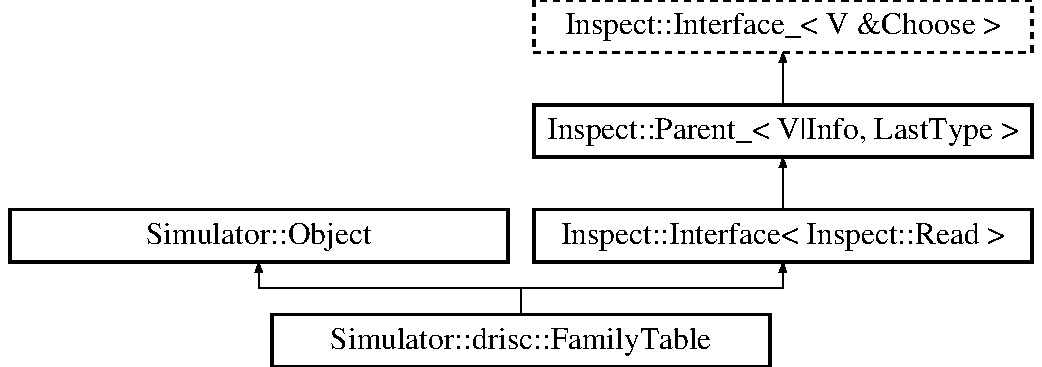
\includegraphics[height=4.000000cm]{class_simulator_1_1drisc_1_1_family_table}
\end{center}
\end{figure}
\subsection*{Public Member Functions}
\begin{DoxyCompactItemize}
\item 
\hyperlink{class_simulator_1_1drisc_1_1_family_table_a9029aa5cf735e64452314e50193d37ee}{Family\+Table} (const std\+::string \&\hyperlink{mtconf_8c_a8f8f80d37794cde9472343e4487ba3eb}{name}, \hyperlink{class_simulator_1_1_d_r_i_s_c}{D\+R\+I\+S\+C} \&parent, \hyperlink{class_simulator_1_1_clock}{Clock} \&clock, \hyperlink{class_config}{Config} \&config)
\item 
\hyperlink{namespace_simulator_a06544009313d7c13d411b1c074e5acff}{F\+Size} \hyperlink{class_simulator_1_1drisc_1_1_family_table_a77f3dfaf607e6409fbd336f11e72642a}{Get\+Num\+Families} () const 
\item 
\hyperlink{struct_simulator_1_1drisc_1_1_family}{Family} \& \hyperlink{class_simulator_1_1drisc_1_1_family_table_ae72d1b32cd0ceaa4d5a8a82829d4998d}{operator\mbox{[}$\,$\mbox{]}} (\hyperlink{namespace_simulator_aaccbc706b2d6c99085f52f6dfc2333e4}{L\+F\+I\+D} fid)
\item 
const \hyperlink{struct_simulator_1_1drisc_1_1_family}{Family} \& \hyperlink{class_simulator_1_1drisc_1_1_family_table_a3623787209fd99307ac0670f255b0f67}{operator\mbox{[}$\,$\mbox{]}} (\hyperlink{namespace_simulator_aaccbc706b2d6c99085f52f6dfc2333e4}{L\+F\+I\+D} fid) const 
\item 
\hyperlink{namespace_simulator_aaccbc706b2d6c99085f52f6dfc2333e4}{L\+F\+I\+D} \hyperlink{class_simulator_1_1drisc_1_1_family_table_a79281183526d6db39fab77082005e85e}{Allocate\+Family} (\hyperlink{namespace_simulator_ab3233bd11b43e37322a8111dc7eec133}{Context\+Type} type)
\item 
void \hyperlink{class_simulator_1_1drisc_1_1_family_table_a74de0961e3e56b837507393a14e306ac}{Free\+Family} (\hyperlink{namespace_simulator_aaccbc706b2d6c99085f52f6dfc2333e4}{L\+F\+I\+D} fid, \hyperlink{namespace_simulator_ab3233bd11b43e37322a8111dc7eec133}{Context\+Type} context)
\item 
\hyperlink{namespace_simulator_a06544009313d7c13d411b1c074e5acff}{F\+Size} \hyperlink{class_simulator_1_1drisc_1_1_family_table_a2719dc5cde15360afd11d0850bb1513d}{Get\+Num\+Free\+Families} (\hyperlink{namespace_simulator_ab3233bd11b43e37322a8111dc7eec133}{Context\+Type} type) const 
\item 
\hyperlink{namespace_simulator_a06544009313d7c13d411b1c074e5acff}{F\+Size} \hyperlink{class_simulator_1_1drisc_1_1_family_table_abc24fed55692d4fce7415132c929727a}{Get\+Num\+Used\+Families} (\hyperlink{namespace_simulator_ab3233bd11b43e37322a8111dc7eec133}{Context\+Type} type) const 
\item 
bool \hyperlink{class_simulator_1_1drisc_1_1_family_table_a30e77e62cca306ea12bfc557ea1cb189}{Is\+Empty} () const 
\item 
bool \hyperlink{class_simulator_1_1drisc_1_1_family_table_a11f78b7368ecf0a79061cf88bfb35927}{Is\+Exclusive} (\hyperlink{namespace_simulator_aaccbc706b2d6c99085f52f6dfc2333e4}{L\+F\+I\+D} fid) const 
\item 
bool \hyperlink{class_simulator_1_1drisc_1_1_family_table_a266eb35a74ef4afa9e99c0c22fadafb3}{Is\+Exclusive\+Used} () const 
\item 
const std\+::vector$<$ \hyperlink{struct_simulator_1_1drisc_1_1_family}{Family} $>$ \& \hyperlink{class_simulator_1_1drisc_1_1_family_table_a1e6f3447d6b28a2938cde2dd51bb9f75}{Get\+Families} () const 
\item 
void \hyperlink{class_simulator_1_1drisc_1_1_family_table_af1058666685d0c97c4e8e3852c8f9764}{Cmd\+\_\+\+Info} (std\+::ostream \&out, const std\+::vector$<$ std\+::string $>$ \&arguments) const 
\item 
void \hyperlink{class_simulator_1_1drisc_1_1_family_table_a3fb1dc90878fd079c167007660839303}{Cmd\+\_\+\+Read} (std\+::ostream \&out, const std\+::vector$<$ std\+::string $>$ \&arguments) const 
\item 
\hyperlink{namespace_simulator_a06544009313d7c13d411b1c074e5acff}{F\+Size} \hyperlink{class_simulator_1_1drisc_1_1_family_table_a1439abbba05d016e7c204d96833ae161}{Get\+Total\+Allocated} ()
\item 
\hyperlink{namespace_simulator_aefe00209f3ea9f8e24874de522c3c3e7}{T\+Size} \hyperlink{class_simulator_1_1drisc_1_1_family_table_a9a0f3e894b86ea07373f169090a3291a}{Get\+Max\+Allocated} () const 
\end{DoxyCompactItemize}


\subsection{Constructor \& Destructor Documentation}
\hypertarget{class_simulator_1_1drisc_1_1_family_table_a9029aa5cf735e64452314e50193d37ee}{\index{Simulator\+::drisc\+::\+Family\+Table@{Simulator\+::drisc\+::\+Family\+Table}!Family\+Table@{Family\+Table}}
\index{Family\+Table@{Family\+Table}!Simulator\+::drisc\+::\+Family\+Table@{Simulator\+::drisc\+::\+Family\+Table}}
\subsubsection[{Family\+Table}]{\setlength{\rightskip}{0pt plus 5cm}Simulator\+::drisc\+::\+Family\+Table\+::\+Family\+Table (
\begin{DoxyParamCaption}
\item[{const std\+::string \&}]{name, }
\item[{{\bf D\+R\+I\+S\+C} \&}]{parent, }
\item[{{\bf Clock} \&}]{clock, }
\item[{{\bf Config} \&}]{config}
\end{DoxyParamCaption}
)}}\label{class_simulator_1_1drisc_1_1_family_table_a9029aa5cf735e64452314e50193d37ee}


\subsection{Member Function Documentation}
\hypertarget{class_simulator_1_1drisc_1_1_family_table_a79281183526d6db39fab77082005e85e}{\index{Simulator\+::drisc\+::\+Family\+Table@{Simulator\+::drisc\+::\+Family\+Table}!Allocate\+Family@{Allocate\+Family}}
\index{Allocate\+Family@{Allocate\+Family}!Simulator\+::drisc\+::\+Family\+Table@{Simulator\+::drisc\+::\+Family\+Table}}
\subsubsection[{Allocate\+Family}]{\setlength{\rightskip}{0pt plus 5cm}{\bf L\+F\+I\+D} Simulator\+::drisc\+::\+Family\+Table\+::\+Allocate\+Family (
\begin{DoxyParamCaption}
\item[{{\bf Context\+Type}}]{type}
\end{DoxyParamCaption}
)}}\label{class_simulator_1_1drisc_1_1_family_table_a79281183526d6db39fab77082005e85e}
\hypertarget{class_simulator_1_1drisc_1_1_family_table_af1058666685d0c97c4e8e3852c8f9764}{\index{Simulator\+::drisc\+::\+Family\+Table@{Simulator\+::drisc\+::\+Family\+Table}!Cmd\+\_\+\+Info@{Cmd\+\_\+\+Info}}
\index{Cmd\+\_\+\+Info@{Cmd\+\_\+\+Info}!Simulator\+::drisc\+::\+Family\+Table@{Simulator\+::drisc\+::\+Family\+Table}}
\subsubsection[{Cmd\+\_\+\+Info}]{\setlength{\rightskip}{0pt plus 5cm}void Simulator\+::drisc\+::\+Family\+Table\+::\+Cmd\+\_\+\+Info (
\begin{DoxyParamCaption}
\item[{std\+::ostream \&}]{out, }
\item[{const std\+::vector$<$ std\+::string $>$ \&}]{arguments}
\end{DoxyParamCaption}
) const}}\label{class_simulator_1_1drisc_1_1_family_table_af1058666685d0c97c4e8e3852c8f9764}
\hypertarget{class_simulator_1_1drisc_1_1_family_table_a3fb1dc90878fd079c167007660839303}{\index{Simulator\+::drisc\+::\+Family\+Table@{Simulator\+::drisc\+::\+Family\+Table}!Cmd\+\_\+\+Read@{Cmd\+\_\+\+Read}}
\index{Cmd\+\_\+\+Read@{Cmd\+\_\+\+Read}!Simulator\+::drisc\+::\+Family\+Table@{Simulator\+::drisc\+::\+Family\+Table}}
\subsubsection[{Cmd\+\_\+\+Read}]{\setlength{\rightskip}{0pt plus 5cm}void Simulator\+::drisc\+::\+Family\+Table\+::\+Cmd\+\_\+\+Read (
\begin{DoxyParamCaption}
\item[{std\+::ostream \&}]{out, }
\item[{const std\+::vector$<$ std\+::string $>$ \&}]{arguments}
\end{DoxyParamCaption}
) const}}\label{class_simulator_1_1drisc_1_1_family_table_a3fb1dc90878fd079c167007660839303}
\hypertarget{class_simulator_1_1drisc_1_1_family_table_a74de0961e3e56b837507393a14e306ac}{\index{Simulator\+::drisc\+::\+Family\+Table@{Simulator\+::drisc\+::\+Family\+Table}!Free\+Family@{Free\+Family}}
\index{Free\+Family@{Free\+Family}!Simulator\+::drisc\+::\+Family\+Table@{Simulator\+::drisc\+::\+Family\+Table}}
\subsubsection[{Free\+Family}]{\setlength{\rightskip}{0pt plus 5cm}void Simulator\+::drisc\+::\+Family\+Table\+::\+Free\+Family (
\begin{DoxyParamCaption}
\item[{{\bf L\+F\+I\+D}}]{fid, }
\item[{{\bf Context\+Type}}]{context}
\end{DoxyParamCaption}
)}}\label{class_simulator_1_1drisc_1_1_family_table_a74de0961e3e56b837507393a14e306ac}
\hypertarget{class_simulator_1_1drisc_1_1_family_table_a1e6f3447d6b28a2938cde2dd51bb9f75}{\index{Simulator\+::drisc\+::\+Family\+Table@{Simulator\+::drisc\+::\+Family\+Table}!Get\+Families@{Get\+Families}}
\index{Get\+Families@{Get\+Families}!Simulator\+::drisc\+::\+Family\+Table@{Simulator\+::drisc\+::\+Family\+Table}}
\subsubsection[{Get\+Families}]{\setlength{\rightskip}{0pt plus 5cm}const std\+::vector$<${\bf Family}$>$\& Simulator\+::drisc\+::\+Family\+Table\+::\+Get\+Families (
\begin{DoxyParamCaption}
{}
\end{DoxyParamCaption}
) const\hspace{0.3cm}{\ttfamily [inline]}}}\label{class_simulator_1_1drisc_1_1_family_table_a1e6f3447d6b28a2938cde2dd51bb9f75}
\hypertarget{class_simulator_1_1drisc_1_1_family_table_a9a0f3e894b86ea07373f169090a3291a}{\index{Simulator\+::drisc\+::\+Family\+Table@{Simulator\+::drisc\+::\+Family\+Table}!Get\+Max\+Allocated@{Get\+Max\+Allocated}}
\index{Get\+Max\+Allocated@{Get\+Max\+Allocated}!Simulator\+::drisc\+::\+Family\+Table@{Simulator\+::drisc\+::\+Family\+Table}}
\subsubsection[{Get\+Max\+Allocated}]{\setlength{\rightskip}{0pt plus 5cm}{\bf T\+Size} Simulator\+::drisc\+::\+Family\+Table\+::\+Get\+Max\+Allocated (
\begin{DoxyParamCaption}
{}
\end{DoxyParamCaption}
) const\hspace{0.3cm}{\ttfamily [inline]}}}\label{class_simulator_1_1drisc_1_1_family_table_a9a0f3e894b86ea07373f169090a3291a}
\hypertarget{class_simulator_1_1drisc_1_1_family_table_a77f3dfaf607e6409fbd336f11e72642a}{\index{Simulator\+::drisc\+::\+Family\+Table@{Simulator\+::drisc\+::\+Family\+Table}!Get\+Num\+Families@{Get\+Num\+Families}}
\index{Get\+Num\+Families@{Get\+Num\+Families}!Simulator\+::drisc\+::\+Family\+Table@{Simulator\+::drisc\+::\+Family\+Table}}
\subsubsection[{Get\+Num\+Families}]{\setlength{\rightskip}{0pt plus 5cm}{\bf F\+Size} Simulator\+::drisc\+::\+Family\+Table\+::\+Get\+Num\+Families (
\begin{DoxyParamCaption}
{}
\end{DoxyParamCaption}
) const\hspace{0.3cm}{\ttfamily [inline]}}}\label{class_simulator_1_1drisc_1_1_family_table_a77f3dfaf607e6409fbd336f11e72642a}
\hypertarget{class_simulator_1_1drisc_1_1_family_table_a2719dc5cde15360afd11d0850bb1513d}{\index{Simulator\+::drisc\+::\+Family\+Table@{Simulator\+::drisc\+::\+Family\+Table}!Get\+Num\+Free\+Families@{Get\+Num\+Free\+Families}}
\index{Get\+Num\+Free\+Families@{Get\+Num\+Free\+Families}!Simulator\+::drisc\+::\+Family\+Table@{Simulator\+::drisc\+::\+Family\+Table}}
\subsubsection[{Get\+Num\+Free\+Families}]{\setlength{\rightskip}{0pt plus 5cm}{\bf F\+Size} Simulator\+::drisc\+::\+Family\+Table\+::\+Get\+Num\+Free\+Families (
\begin{DoxyParamCaption}
\item[{{\bf Context\+Type}}]{type}
\end{DoxyParamCaption}
) const}}\label{class_simulator_1_1drisc_1_1_family_table_a2719dc5cde15360afd11d0850bb1513d}
\hypertarget{class_simulator_1_1drisc_1_1_family_table_abc24fed55692d4fce7415132c929727a}{\index{Simulator\+::drisc\+::\+Family\+Table@{Simulator\+::drisc\+::\+Family\+Table}!Get\+Num\+Used\+Families@{Get\+Num\+Used\+Families}}
\index{Get\+Num\+Used\+Families@{Get\+Num\+Used\+Families}!Simulator\+::drisc\+::\+Family\+Table@{Simulator\+::drisc\+::\+Family\+Table}}
\subsubsection[{Get\+Num\+Used\+Families}]{\setlength{\rightskip}{0pt plus 5cm}{\bf F\+Size} Simulator\+::drisc\+::\+Family\+Table\+::\+Get\+Num\+Used\+Families (
\begin{DoxyParamCaption}
\item[{{\bf Context\+Type}}]{type}
\end{DoxyParamCaption}
) const}}\label{class_simulator_1_1drisc_1_1_family_table_abc24fed55692d4fce7415132c929727a}
\hypertarget{class_simulator_1_1drisc_1_1_family_table_a1439abbba05d016e7c204d96833ae161}{\index{Simulator\+::drisc\+::\+Family\+Table@{Simulator\+::drisc\+::\+Family\+Table}!Get\+Total\+Allocated@{Get\+Total\+Allocated}}
\index{Get\+Total\+Allocated@{Get\+Total\+Allocated}!Simulator\+::drisc\+::\+Family\+Table@{Simulator\+::drisc\+::\+Family\+Table}}
\subsubsection[{Get\+Total\+Allocated}]{\setlength{\rightskip}{0pt plus 5cm}{\bf F\+Size} Simulator\+::drisc\+::\+Family\+Table\+::\+Get\+Total\+Allocated (
\begin{DoxyParamCaption}
{}
\end{DoxyParamCaption}
)\hspace{0.3cm}{\ttfamily [inline]}}}\label{class_simulator_1_1drisc_1_1_family_table_a1439abbba05d016e7c204d96833ae161}
\hypertarget{class_simulator_1_1drisc_1_1_family_table_a30e77e62cca306ea12bfc557ea1cb189}{\index{Simulator\+::drisc\+::\+Family\+Table@{Simulator\+::drisc\+::\+Family\+Table}!Is\+Empty@{Is\+Empty}}
\index{Is\+Empty@{Is\+Empty}!Simulator\+::drisc\+::\+Family\+Table@{Simulator\+::drisc\+::\+Family\+Table}}
\subsubsection[{Is\+Empty}]{\setlength{\rightskip}{0pt plus 5cm}bool Simulator\+::drisc\+::\+Family\+Table\+::\+Is\+Empty (
\begin{DoxyParamCaption}
{}
\end{DoxyParamCaption}
) const}}\label{class_simulator_1_1drisc_1_1_family_table_a30e77e62cca306ea12bfc557ea1cb189}
\hypertarget{class_simulator_1_1drisc_1_1_family_table_a11f78b7368ecf0a79061cf88bfb35927}{\index{Simulator\+::drisc\+::\+Family\+Table@{Simulator\+::drisc\+::\+Family\+Table}!Is\+Exclusive@{Is\+Exclusive}}
\index{Is\+Exclusive@{Is\+Exclusive}!Simulator\+::drisc\+::\+Family\+Table@{Simulator\+::drisc\+::\+Family\+Table}}
\subsubsection[{Is\+Exclusive}]{\setlength{\rightskip}{0pt plus 5cm}bool Simulator\+::drisc\+::\+Family\+Table\+::\+Is\+Exclusive (
\begin{DoxyParamCaption}
\item[{{\bf L\+F\+I\+D}}]{fid}
\end{DoxyParamCaption}
) const\hspace{0.3cm}{\ttfamily [inline]}}}\label{class_simulator_1_1drisc_1_1_family_table_a11f78b7368ecf0a79061cf88bfb35927}
\hypertarget{class_simulator_1_1drisc_1_1_family_table_a266eb35a74ef4afa9e99c0c22fadafb3}{\index{Simulator\+::drisc\+::\+Family\+Table@{Simulator\+::drisc\+::\+Family\+Table}!Is\+Exclusive\+Used@{Is\+Exclusive\+Used}}
\index{Is\+Exclusive\+Used@{Is\+Exclusive\+Used}!Simulator\+::drisc\+::\+Family\+Table@{Simulator\+::drisc\+::\+Family\+Table}}
\subsubsection[{Is\+Exclusive\+Used}]{\setlength{\rightskip}{0pt plus 5cm}bool Simulator\+::drisc\+::\+Family\+Table\+::\+Is\+Exclusive\+Used (
\begin{DoxyParamCaption}
{}
\end{DoxyParamCaption}
) const\hspace{0.3cm}{\ttfamily [inline]}}}\label{class_simulator_1_1drisc_1_1_family_table_a266eb35a74ef4afa9e99c0c22fadafb3}
\hypertarget{class_simulator_1_1drisc_1_1_family_table_ae72d1b32cd0ceaa4d5a8a82829d4998d}{\index{Simulator\+::drisc\+::\+Family\+Table@{Simulator\+::drisc\+::\+Family\+Table}!operator\mbox{[}$\,$\mbox{]}@{operator[]}}
\index{operator\mbox{[}$\,$\mbox{]}@{operator[]}!Simulator\+::drisc\+::\+Family\+Table@{Simulator\+::drisc\+::\+Family\+Table}}
\subsubsection[{operator[]}]{\setlength{\rightskip}{0pt plus 5cm}{\bf Family}\& Simulator\+::drisc\+::\+Family\+Table\+::operator\mbox{[}$\,$\mbox{]} (
\begin{DoxyParamCaption}
\item[{{\bf L\+F\+I\+D}}]{fid}
\end{DoxyParamCaption}
)\hspace{0.3cm}{\ttfamily [inline]}}}\label{class_simulator_1_1drisc_1_1_family_table_ae72d1b32cd0ceaa4d5a8a82829d4998d}
\hypertarget{class_simulator_1_1drisc_1_1_family_table_a3623787209fd99307ac0670f255b0f67}{\index{Simulator\+::drisc\+::\+Family\+Table@{Simulator\+::drisc\+::\+Family\+Table}!operator\mbox{[}$\,$\mbox{]}@{operator[]}}
\index{operator\mbox{[}$\,$\mbox{]}@{operator[]}!Simulator\+::drisc\+::\+Family\+Table@{Simulator\+::drisc\+::\+Family\+Table}}
\subsubsection[{operator[]}]{\setlength{\rightskip}{0pt plus 5cm}const {\bf Family}\& Simulator\+::drisc\+::\+Family\+Table\+::operator\mbox{[}$\,$\mbox{]} (
\begin{DoxyParamCaption}
\item[{{\bf L\+F\+I\+D}}]{fid}
\end{DoxyParamCaption}
) const\hspace{0.3cm}{\ttfamily [inline]}}}\label{class_simulator_1_1drisc_1_1_family_table_a3623787209fd99307ac0670f255b0f67}


The documentation for this class was generated from the following files\+:\begin{DoxyCompactItemize}
\item 
arch/drisc/\hyperlink{_family_table_8h}{Family\+Table.\+h}\item 
arch/drisc/\hyperlink{_family_table_8cpp}{Family\+Table.\+cpp}\end{DoxyCompactItemize}

\hypertarget{struct_simulator_1_1_f_i_d}{\section{Simulator\+:\+:F\+I\+D Struct Reference}
\label{struct_simulator_1_1_f_i_d}\index{Simulator\+::\+F\+I\+D@{Simulator\+::\+F\+I\+D}}
}


A globally unique family identifier.  




{\ttfamily \#include $<$simtypes.\+h$>$}

\subsection*{Public Member Functions}
\begin{DoxyCompactItemize}
\item 
std\+::string \hyperlink{struct_simulator_1_1_f_i_d_a5ba6a827a0db0cd405f7f1a8f7cdf6ad}{str} () const 
\end{DoxyCompactItemize}
\subsection*{Public Attributes}
\begin{DoxyCompactItemize}
\item 
\hyperlink{namespace_simulator_a607aa9969bfe2711861ae21f42c37c59}{F\+Capability} \hyperlink{struct_simulator_1_1_f_i_d_af7b2b91076281bd58b952e13236caeb0}{capability}
\item 
\hyperlink{namespace_simulator_aa671021151c047ae2da6dce4e6303476}{P\+I\+D} \hyperlink{struct_simulator_1_1_f_i_d_ab529d6fc0c2ae64c7b156eb481b0e05d}{pid}
\item 
\hyperlink{namespace_simulator_aaccbc706b2d6c99085f52f6dfc2333e4}{L\+F\+I\+D} \hyperlink{struct_simulator_1_1_f_i_d_a21c50063b6de25afc79b9e50c3b8757a}{lfid}
\end{DoxyCompactItemize}


\subsection{Detailed Description}
A globally unique family identifier. 

\subsection{Member Function Documentation}
\hypertarget{struct_simulator_1_1_f_i_d_a5ba6a827a0db0cd405f7f1a8f7cdf6ad}{\index{Simulator\+::\+F\+I\+D@{Simulator\+::\+F\+I\+D}!str@{str}}
\index{str@{str}!Simulator\+::\+F\+I\+D@{Simulator\+::\+F\+I\+D}}
\subsubsection[{str}]{\setlength{\rightskip}{0pt plus 5cm}string Simulator\+::\+F\+I\+D\+::str (
\begin{DoxyParamCaption}
{}
\end{DoxyParamCaption}
) const}}\label{struct_simulator_1_1_f_i_d_a5ba6a827a0db0cd405f7f1a8f7cdf6ad}


\subsection{Member Data Documentation}
\hypertarget{struct_simulator_1_1_f_i_d_af7b2b91076281bd58b952e13236caeb0}{\index{Simulator\+::\+F\+I\+D@{Simulator\+::\+F\+I\+D}!capability@{capability}}
\index{capability@{capability}!Simulator\+::\+F\+I\+D@{Simulator\+::\+F\+I\+D}}
\subsubsection[{capability}]{\setlength{\rightskip}{0pt plus 5cm}{\bf F\+Capability} Simulator\+::\+F\+I\+D\+::capability}}\label{struct_simulator_1_1_f_i_d_af7b2b91076281bd58b952e13236caeb0}
\hypertarget{struct_simulator_1_1_f_i_d_a21c50063b6de25afc79b9e50c3b8757a}{\index{Simulator\+::\+F\+I\+D@{Simulator\+::\+F\+I\+D}!lfid@{lfid}}
\index{lfid@{lfid}!Simulator\+::\+F\+I\+D@{Simulator\+::\+F\+I\+D}}
\subsubsection[{lfid}]{\setlength{\rightskip}{0pt plus 5cm}{\bf L\+F\+I\+D} Simulator\+::\+F\+I\+D\+::lfid}}\label{struct_simulator_1_1_f_i_d_a21c50063b6de25afc79b9e50c3b8757a}
\hypertarget{struct_simulator_1_1_f_i_d_ab529d6fc0c2ae64c7b156eb481b0e05d}{\index{Simulator\+::\+F\+I\+D@{Simulator\+::\+F\+I\+D}!pid@{pid}}
\index{pid@{pid}!Simulator\+::\+F\+I\+D@{Simulator\+::\+F\+I\+D}}
\subsubsection[{pid}]{\setlength{\rightskip}{0pt plus 5cm}{\bf P\+I\+D} Simulator\+::\+F\+I\+D\+::pid}}\label{struct_simulator_1_1_f_i_d_ab529d6fc0c2ae64c7b156eb481b0e05d}


The documentation for this struct was generated from the following files\+:\begin{DoxyCompactItemize}
\item 
arch/\hyperlink{simtypes_8h}{simtypes.\+h}\item 
arch/\hyperlink{simtypes_8cpp}{simtypes.\+cpp}\end{DoxyCompactItemize}

\hypertarget{class_simulator_1_1_file_not_found_exception}{\section{Simulator\+:\+:File\+Not\+Found\+Exception Class Reference}
\label{class_simulator_1_1_file_not_found_exception}\index{Simulator\+::\+File\+Not\+Found\+Exception@{Simulator\+::\+File\+Not\+Found\+Exception}}
}


{\ttfamily \#include $<$except.\+h$>$}

Inheritance diagram for Simulator\+:\+:File\+Not\+Found\+Exception\+:\begin{figure}[H]
\begin{center}
\leavevmode
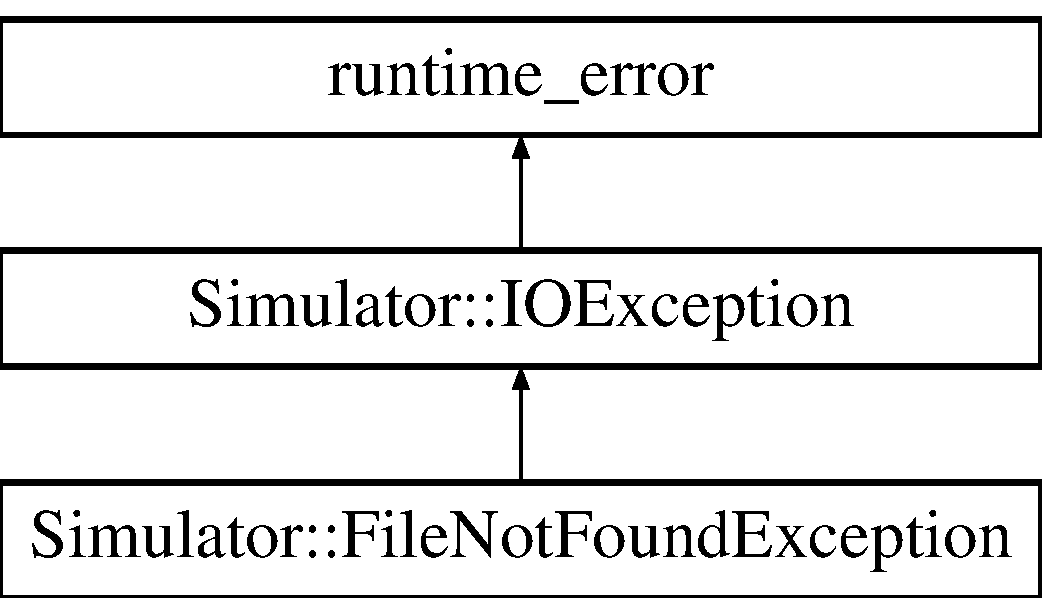
\includegraphics[height=3.000000cm]{class_simulator_1_1_file_not_found_exception}
\end{center}
\end{figure}
\subsection*{Public Member Functions}
\begin{DoxyCompactItemize}
\item 
\hyperlink{class_simulator_1_1_file_not_found_exception_add40be4268d0ba2e083e4db15b24d244}{File\+Not\+Found\+Exception} (const std\+::string \&filename)
\end{DoxyCompactItemize}


\subsection{Constructor \& Destructor Documentation}
\hypertarget{class_simulator_1_1_file_not_found_exception_add40be4268d0ba2e083e4db15b24d244}{\index{Simulator\+::\+File\+Not\+Found\+Exception@{Simulator\+::\+File\+Not\+Found\+Exception}!File\+Not\+Found\+Exception@{File\+Not\+Found\+Exception}}
\index{File\+Not\+Found\+Exception@{File\+Not\+Found\+Exception}!Simulator\+::\+File\+Not\+Found\+Exception@{Simulator\+::\+File\+Not\+Found\+Exception}}
\subsubsection[{File\+Not\+Found\+Exception}]{\setlength{\rightskip}{0pt plus 5cm}Simulator\+::\+File\+Not\+Found\+Exception\+::\+File\+Not\+Found\+Exception (
\begin{DoxyParamCaption}
\item[{const std\+::string \&}]{filename}
\end{DoxyParamCaption}
)\hspace{0.3cm}{\ttfamily [inline]}}}\label{class_simulator_1_1_file_not_found_exception_add40be4268d0ba2e083e4db15b24d244}


The documentation for this class was generated from the following file\+:\begin{DoxyCompactItemize}
\item 
sim/\hyperlink{except_8h}{except.\+h}\end{DoxyCompactItemize}

\hypertarget{class_simulator_1_1_flag}{\section{Simulator\+:\+:Flag Class Reference}
\label{class_simulator_1_1_flag}\index{Simulator\+::\+Flag@{Simulator\+::\+Flag}}
}


A single-\/bit storage element.  




{\ttfamily \#include $<$storage.\+h$>$}

Inheritance diagram for Simulator\+:\+:Flag\+:\begin{figure}[H]
\begin{center}
\leavevmode
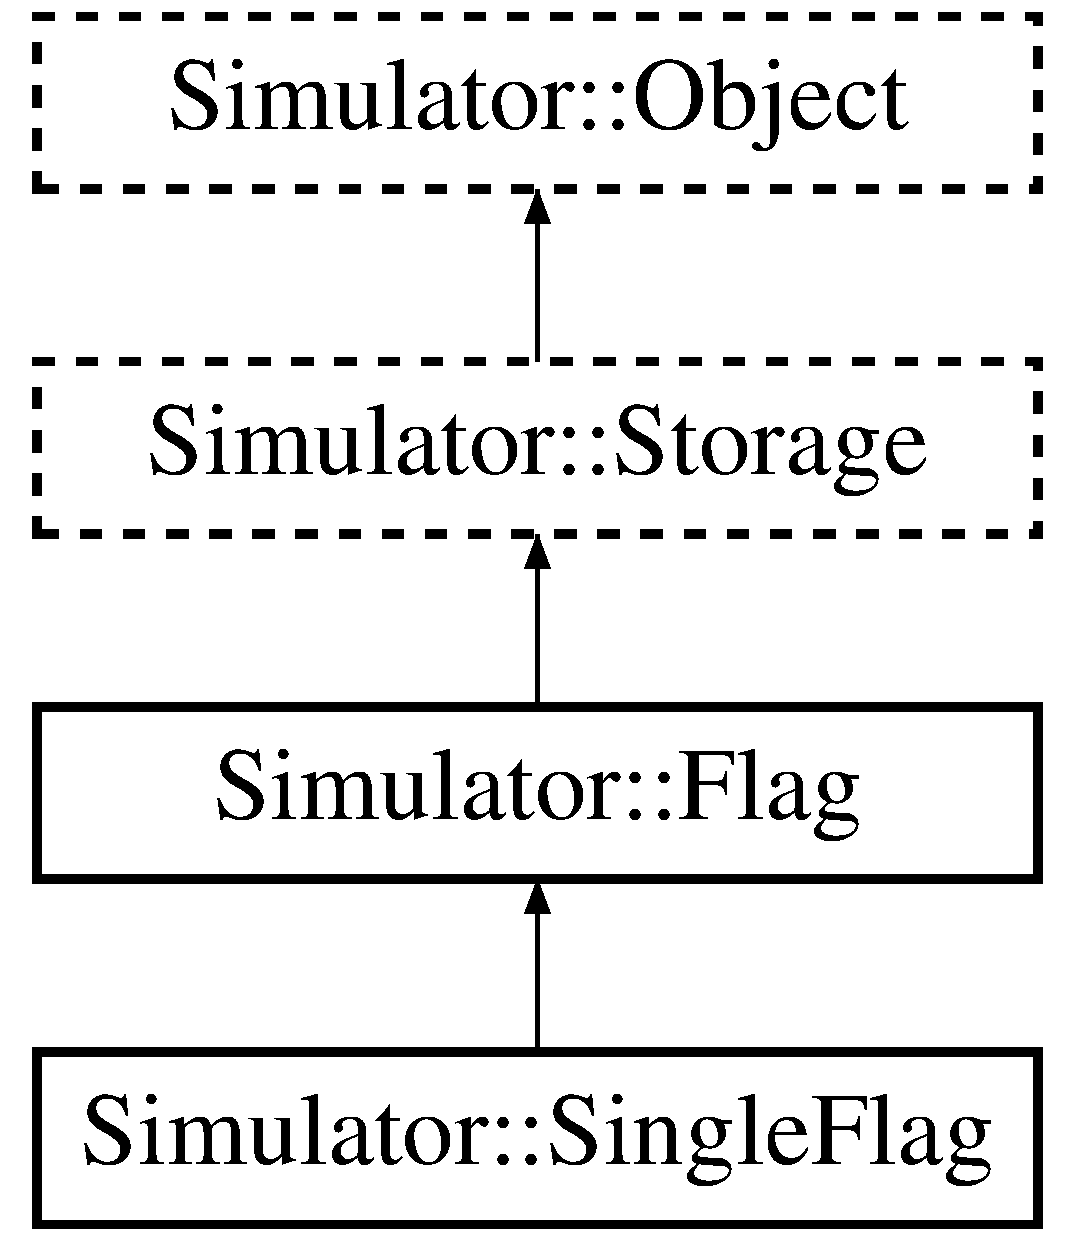
\includegraphics[height=4.000000cm]{class_simulator_1_1_flag}
\end{center}
\end{figure}
\subsection*{Public Member Functions}
\begin{DoxyCompactItemize}
\item 
bool \hyperlink{class_simulator_1_1_flag_a51c8be3e44d72d11f733d2c90d70159f}{Is\+Set} () const 
\item 
bool \hyperlink{class_simulator_1_1_flag_a86125744ef8bff9a985413d093791aee}{Set} ()
\item 
bool \hyperlink{class_simulator_1_1_flag_a3972501a9392a9a08812a08b1c3a802d}{Clear} ()
\item 
\hyperlink{class_simulator_1_1_flag_a6f0399913e7ca717817b5adb00974ffd}{Flag} (const std\+::string \&\hyperlink{mtconf_8c_a8f8f80d37794cde9472343e4487ba3eb}{name}, \hyperlink{class_simulator_1_1_object}{Object} \&parent, \hyperlink{class_simulator_1_1_clock}{Clock} \&clock, bool set)
\end{DoxyCompactItemize}
\subsection*{Protected Member Functions}
\begin{DoxyCompactItemize}
\item 
void \hyperlink{class_simulator_1_1_flag_a3edbc0d4d4e12e0c425cbb05381c60ad}{Update} ()
\end{DoxyCompactItemize}
\subsection*{Protected Attributes}
\begin{DoxyCompactItemize}
\item 
bool \hyperlink{class_simulator_1_1_flag_a60f78dd6656e2604ca110664c9c93afe}{m\+\_\+set}
\item 
bool \hyperlink{class_simulator_1_1_flag_a55920339c74aba5925837e4374d54c9a}{m\+\_\+updated}
\item 
bool \hyperlink{class_simulator_1_1_flag_a996f9430e3c53ad4b1ffe7e5dab05bd6}{m\+\_\+new}
\item 
uint64\+\_\+t \hyperlink{class_simulator_1_1_flag_aa341af9a7119e56d6e56340d0f6dcd72}{m\+\_\+stalls}
\begin{DoxyCompactList}\small\item\em Number of stalls so far. \end{DoxyCompactList}\item 
\hyperlink{namespace_simulator_a928f1e2101eba21bb0fe409e8c9ce573}{Cycle\+No} \hyperlink{class_simulator_1_1_flag_a036d407f68f820d78ecb30072af3c429}{m\+\_\+lastcycle}
\begin{DoxyCompactList}\small\item\em Cycle no of last event. \end{DoxyCompactList}\item 
uint64\+\_\+t \hyperlink{class_simulator_1_1_flag_a21873c168122e7ec34d5e4cfe9ba7c1f}{m\+\_\+totalsize}
\begin{DoxyCompactList}\small\item\em Cumulated current size $\ast$ cycle no. \end{DoxyCompactList}\item 
\hyperlink{namespace_simulator_a5ca279f926485be2d0554e41275a3305}{Buffer\+Size} \hyperlink{class_simulator_1_1_flag_ad7d35060575d980cd0532240fc61d177}{m\+\_\+maxsize}
\begin{DoxyCompactList}\small\item\em Maximum effective queue size reached. \end{DoxyCompactList}\item 
\hyperlink{namespace_simulator_a5ca279f926485be2d0554e41275a3305}{Buffer\+Size} \hyperlink{class_simulator_1_1_flag_a67bdcf6e60428f27966068a8d472c868}{m\+\_\+cursize}
\begin{DoxyCompactList}\small\item\em Current size. \end{DoxyCompactList}\end{DoxyCompactItemize}


\subsection{Detailed Description}
A single-\/bit storage element. 

\subsection{Constructor \& Destructor Documentation}
\hypertarget{class_simulator_1_1_flag_a6f0399913e7ca717817b5adb00974ffd}{\index{Simulator\+::\+Flag@{Simulator\+::\+Flag}!Flag@{Flag}}
\index{Flag@{Flag}!Simulator\+::\+Flag@{Simulator\+::\+Flag}}
\subsubsection[{Flag}]{\setlength{\rightskip}{0pt plus 5cm}Simulator\+::\+Flag\+::\+Flag (
\begin{DoxyParamCaption}
\item[{const std\+::string \&}]{name, }
\item[{{\bf Object} \&}]{parent, }
\item[{{\bf Clock} \&}]{clock, }
\item[{bool}]{set}
\end{DoxyParamCaption}
)\hspace{0.3cm}{\ttfamily [inline]}}}\label{class_simulator_1_1_flag_a6f0399913e7ca717817b5adb00974ffd}


\subsection{Member Function Documentation}
\hypertarget{class_simulator_1_1_flag_a3972501a9392a9a08812a08b1c3a802d}{\index{Simulator\+::\+Flag@{Simulator\+::\+Flag}!Clear@{Clear}}
\index{Clear@{Clear}!Simulator\+::\+Flag@{Simulator\+::\+Flag}}
\subsubsection[{Clear}]{\setlength{\rightskip}{0pt plus 5cm}bool Simulator\+::\+Flag\+::\+Clear (
\begin{DoxyParamCaption}
{}
\end{DoxyParamCaption}
)\hspace{0.3cm}{\ttfamily [inline]}}}\label{class_simulator_1_1_flag_a3972501a9392a9a08812a08b1c3a802d}
\hypertarget{class_simulator_1_1_flag_a51c8be3e44d72d11f733d2c90d70159f}{\index{Simulator\+::\+Flag@{Simulator\+::\+Flag}!Is\+Set@{Is\+Set}}
\index{Is\+Set@{Is\+Set}!Simulator\+::\+Flag@{Simulator\+::\+Flag}}
\subsubsection[{Is\+Set}]{\setlength{\rightskip}{0pt plus 5cm}bool Simulator\+::\+Flag\+::\+Is\+Set (
\begin{DoxyParamCaption}
{}
\end{DoxyParamCaption}
) const\hspace{0.3cm}{\ttfamily [inline]}}}\label{class_simulator_1_1_flag_a51c8be3e44d72d11f733d2c90d70159f}
\hypertarget{class_simulator_1_1_flag_a86125744ef8bff9a985413d093791aee}{\index{Simulator\+::\+Flag@{Simulator\+::\+Flag}!Set@{Set}}
\index{Set@{Set}!Simulator\+::\+Flag@{Simulator\+::\+Flag}}
\subsubsection[{Set}]{\setlength{\rightskip}{0pt plus 5cm}bool Simulator\+::\+Flag\+::\+Set (
\begin{DoxyParamCaption}
{}
\end{DoxyParamCaption}
)\hspace{0.3cm}{\ttfamily [inline]}}}\label{class_simulator_1_1_flag_a86125744ef8bff9a985413d093791aee}
\hypertarget{class_simulator_1_1_flag_a3edbc0d4d4e12e0c425cbb05381c60ad}{\index{Simulator\+::\+Flag@{Simulator\+::\+Flag}!Update@{Update}}
\index{Update@{Update}!Simulator\+::\+Flag@{Simulator\+::\+Flag}}
\subsubsection[{Update}]{\setlength{\rightskip}{0pt plus 5cm}void Simulator\+::\+Flag\+::\+Update (
\begin{DoxyParamCaption}
{}
\end{DoxyParamCaption}
)\hspace{0.3cm}{\ttfamily [inline]}, {\ttfamily [protected]}, {\ttfamily [virtual]}}}\label{class_simulator_1_1_flag_a3edbc0d4d4e12e0c425cbb05381c60ad}


Implements \hyperlink{class_simulator_1_1_storage_abea2bd330384970436228e1a759b9239}{Simulator\+::\+Storage}.



\subsection{Member Data Documentation}
\hypertarget{class_simulator_1_1_flag_a67bdcf6e60428f27966068a8d472c868}{\index{Simulator\+::\+Flag@{Simulator\+::\+Flag}!m\+\_\+cursize@{m\+\_\+cursize}}
\index{m\+\_\+cursize@{m\+\_\+cursize}!Simulator\+::\+Flag@{Simulator\+::\+Flag}}
\subsubsection[{m\+\_\+cursize}]{\setlength{\rightskip}{0pt plus 5cm}{\bf Buffer\+Size} Simulator\+::\+Flag\+::m\+\_\+cursize\hspace{0.3cm}{\ttfamily [protected]}}}\label{class_simulator_1_1_flag_a67bdcf6e60428f27966068a8d472c868}


Current size. 

\hypertarget{class_simulator_1_1_flag_a036d407f68f820d78ecb30072af3c429}{\index{Simulator\+::\+Flag@{Simulator\+::\+Flag}!m\+\_\+lastcycle@{m\+\_\+lastcycle}}
\index{m\+\_\+lastcycle@{m\+\_\+lastcycle}!Simulator\+::\+Flag@{Simulator\+::\+Flag}}
\subsubsection[{m\+\_\+lastcycle}]{\setlength{\rightskip}{0pt plus 5cm}{\bf Cycle\+No} Simulator\+::\+Flag\+::m\+\_\+lastcycle\hspace{0.3cm}{\ttfamily [protected]}}}\label{class_simulator_1_1_flag_a036d407f68f820d78ecb30072af3c429}


Cycle no of last event. 

\hypertarget{class_simulator_1_1_flag_ad7d35060575d980cd0532240fc61d177}{\index{Simulator\+::\+Flag@{Simulator\+::\+Flag}!m\+\_\+maxsize@{m\+\_\+maxsize}}
\index{m\+\_\+maxsize@{m\+\_\+maxsize}!Simulator\+::\+Flag@{Simulator\+::\+Flag}}
\subsubsection[{m\+\_\+maxsize}]{\setlength{\rightskip}{0pt plus 5cm}{\bf Buffer\+Size} Simulator\+::\+Flag\+::m\+\_\+maxsize\hspace{0.3cm}{\ttfamily [protected]}}}\label{class_simulator_1_1_flag_ad7d35060575d980cd0532240fc61d177}


Maximum effective queue size reached. 

\hypertarget{class_simulator_1_1_flag_a996f9430e3c53ad4b1ffe7e5dab05bd6}{\index{Simulator\+::\+Flag@{Simulator\+::\+Flag}!m\+\_\+new@{m\+\_\+new}}
\index{m\+\_\+new@{m\+\_\+new}!Simulator\+::\+Flag@{Simulator\+::\+Flag}}
\subsubsection[{m\+\_\+new}]{\setlength{\rightskip}{0pt plus 5cm}bool Simulator\+::\+Flag\+::m\+\_\+new\hspace{0.3cm}{\ttfamily [protected]}}}\label{class_simulator_1_1_flag_a996f9430e3c53ad4b1ffe7e5dab05bd6}
\hypertarget{class_simulator_1_1_flag_a60f78dd6656e2604ca110664c9c93afe}{\index{Simulator\+::\+Flag@{Simulator\+::\+Flag}!m\+\_\+set@{m\+\_\+set}}
\index{m\+\_\+set@{m\+\_\+set}!Simulator\+::\+Flag@{Simulator\+::\+Flag}}
\subsubsection[{m\+\_\+set}]{\setlength{\rightskip}{0pt plus 5cm}bool Simulator\+::\+Flag\+::m\+\_\+set\hspace{0.3cm}{\ttfamily [protected]}}}\label{class_simulator_1_1_flag_a60f78dd6656e2604ca110664c9c93afe}
\hypertarget{class_simulator_1_1_flag_aa341af9a7119e56d6e56340d0f6dcd72}{\index{Simulator\+::\+Flag@{Simulator\+::\+Flag}!m\+\_\+stalls@{m\+\_\+stalls}}
\index{m\+\_\+stalls@{m\+\_\+stalls}!Simulator\+::\+Flag@{Simulator\+::\+Flag}}
\subsubsection[{m\+\_\+stalls}]{\setlength{\rightskip}{0pt plus 5cm}uint64\+\_\+t Simulator\+::\+Flag\+::m\+\_\+stalls\hspace{0.3cm}{\ttfamily [protected]}}}\label{class_simulator_1_1_flag_aa341af9a7119e56d6e56340d0f6dcd72}


Number of stalls so far. 

\hypertarget{class_simulator_1_1_flag_a21873c168122e7ec34d5e4cfe9ba7c1f}{\index{Simulator\+::\+Flag@{Simulator\+::\+Flag}!m\+\_\+totalsize@{m\+\_\+totalsize}}
\index{m\+\_\+totalsize@{m\+\_\+totalsize}!Simulator\+::\+Flag@{Simulator\+::\+Flag}}
\subsubsection[{m\+\_\+totalsize}]{\setlength{\rightskip}{0pt plus 5cm}uint64\+\_\+t Simulator\+::\+Flag\+::m\+\_\+totalsize\hspace{0.3cm}{\ttfamily [protected]}}}\label{class_simulator_1_1_flag_a21873c168122e7ec34d5e4cfe9ba7c1f}


Cumulated current size $\ast$ cycle no. 

\hypertarget{class_simulator_1_1_flag_a55920339c74aba5925837e4374d54c9a}{\index{Simulator\+::\+Flag@{Simulator\+::\+Flag}!m\+\_\+updated@{m\+\_\+updated}}
\index{m\+\_\+updated@{m\+\_\+updated}!Simulator\+::\+Flag@{Simulator\+::\+Flag}}
\subsubsection[{m\+\_\+updated}]{\setlength{\rightskip}{0pt plus 5cm}bool Simulator\+::\+Flag\+::m\+\_\+updated\hspace{0.3cm}{\ttfamily [protected]}}}\label{class_simulator_1_1_flag_a55920339c74aba5925837e4374d54c9a}


The documentation for this class was generated from the following file\+:\begin{DoxyCompactItemize}
\item 
sim/\hyperlink{storage_8h}{storage.\+h}\end{DoxyCompactItemize}

\hypertarget{struct_simulator_1_1_float32}{\section{Simulator\+:\+:Float32 Struct Reference}
\label{struct_simulator_1_1_float32}\index{Simulator\+::\+Float32@{Simulator\+::\+Float32}}
}


32-\/bit I\+E\+E\+E-\/754 float  




{\ttfamily \#include $<$simtypes.\+h$>$}

\subsection*{Public Member Functions}
\begin{DoxyCompactItemize}
\item 
double \hyperlink{struct_simulator_1_1_float32_a7f5996e5d4312bf7941c88bc050c2533}{tofloat} () const 
\item 
void \hyperlink{struct_simulator_1_1_float32_a583b5c07150e467f0c9a6380f52167c0}{fromfloat} (double f)
\end{DoxyCompactItemize}
\subsection*{Public Attributes}
\begin{DoxyCompactItemize}
\item 
\begin{tabbing}
xx\=xx\=xx\=xx\=xx\=xx\=xx\=xx\=xx\=\kill
union \{\\
\>struct \{\\
\>\>unsigned long long \hyperlink{struct_simulator_1_1_float32_a208abec59956bdaeb90fb70c5ec95a7c}{fraction}:23\\
\>\>unsigned long long \hyperlink{struct_simulator_1_1_float32_a08b7aed86fa9a607dd2afaa429f9c59b}{exponent}:8\\
\>\>unsigned long long \hyperlink{struct_simulator_1_1_float32_abf8bcfd04c3da1e1bcdb82d3b93caf42}{sign}:1\\
\>\} \\
\>float \hyperlink{struct_simulator_1_1_float32_a39b69e226a506e5149ec6cbfbcb21b6c}{floating}\\
\>uint32\_t \hyperlink{struct_simulator_1_1_float32_a4592d2c05594f4cf9e3ad621c4c702bb}{integer}\\
\}; \\

\end{tabbing}\end{DoxyCompactItemize}


\subsection{Detailed Description}
32-\/bit I\+E\+E\+E-\/754 float 

\subsection{Member Function Documentation}
\hypertarget{struct_simulator_1_1_float32_a583b5c07150e467f0c9a6380f52167c0}{\index{Simulator\+::\+Float32@{Simulator\+::\+Float32}!fromfloat@{fromfloat}}
\index{fromfloat@{fromfloat}!Simulator\+::\+Float32@{Simulator\+::\+Float32}}
\subsubsection[{fromfloat}]{\setlength{\rightskip}{0pt plus 5cm}void Simulator\+::\+Float32\+::fromfloat (
\begin{DoxyParamCaption}
\item[{double}]{f}
\end{DoxyParamCaption}
)\hspace{0.3cm}{\ttfamily [inline]}}}\label{struct_simulator_1_1_float32_a583b5c07150e467f0c9a6380f52167c0}
\hypertarget{struct_simulator_1_1_float32_a7f5996e5d4312bf7941c88bc050c2533}{\index{Simulator\+::\+Float32@{Simulator\+::\+Float32}!tofloat@{tofloat}}
\index{tofloat@{tofloat}!Simulator\+::\+Float32@{Simulator\+::\+Float32}}
\subsubsection[{tofloat}]{\setlength{\rightskip}{0pt plus 5cm}double Simulator\+::\+Float32\+::tofloat (
\begin{DoxyParamCaption}
{}
\end{DoxyParamCaption}
) const\hspace{0.3cm}{\ttfamily [inline]}}}\label{struct_simulator_1_1_float32_a7f5996e5d4312bf7941c88bc050c2533}


\subsection{Member Data Documentation}
\hypertarget{struct_simulator_1_1_float32_ad319d98f86b161d69622713bf2c9a946}{\subsubsection[{"@64}]{\setlength{\rightskip}{0pt plus 5cm}union \{ ... \} }}\label{struct_simulator_1_1_float32_ad319d98f86b161d69622713bf2c9a946}
\hypertarget{struct_simulator_1_1_float32_a08b7aed86fa9a607dd2afaa429f9c59b}{\index{Simulator\+::\+Float32@{Simulator\+::\+Float32}!exponent@{exponent}}
\index{exponent@{exponent}!Simulator\+::\+Float32@{Simulator\+::\+Float32}}
\subsubsection[{exponent}]{\setlength{\rightskip}{0pt plus 5cm}unsigned long long Simulator\+::\+Float32\+::exponent}}\label{struct_simulator_1_1_float32_a08b7aed86fa9a607dd2afaa429f9c59b}
\hypertarget{struct_simulator_1_1_float32_a39b69e226a506e5149ec6cbfbcb21b6c}{\index{Simulator\+::\+Float32@{Simulator\+::\+Float32}!floating@{floating}}
\index{floating@{floating}!Simulator\+::\+Float32@{Simulator\+::\+Float32}}
\subsubsection[{floating}]{\setlength{\rightskip}{0pt plus 5cm}float Simulator\+::\+Float32\+::floating}}\label{struct_simulator_1_1_float32_a39b69e226a506e5149ec6cbfbcb21b6c}
\hypertarget{struct_simulator_1_1_float32_a208abec59956bdaeb90fb70c5ec95a7c}{\index{Simulator\+::\+Float32@{Simulator\+::\+Float32}!fraction@{fraction}}
\index{fraction@{fraction}!Simulator\+::\+Float32@{Simulator\+::\+Float32}}
\subsubsection[{fraction}]{\setlength{\rightskip}{0pt plus 5cm}unsigned long long Simulator\+::\+Float32\+::fraction}}\label{struct_simulator_1_1_float32_a208abec59956bdaeb90fb70c5ec95a7c}
\hypertarget{struct_simulator_1_1_float32_a4592d2c05594f4cf9e3ad621c4c702bb}{\index{Simulator\+::\+Float32@{Simulator\+::\+Float32}!integer@{integer}}
\index{integer@{integer}!Simulator\+::\+Float32@{Simulator\+::\+Float32}}
\subsubsection[{integer}]{\setlength{\rightskip}{0pt plus 5cm}uint32\+\_\+t Simulator\+::\+Float32\+::integer}}\label{struct_simulator_1_1_float32_a4592d2c05594f4cf9e3ad621c4c702bb}
\hypertarget{struct_simulator_1_1_float32_abf8bcfd04c3da1e1bcdb82d3b93caf42}{\index{Simulator\+::\+Float32@{Simulator\+::\+Float32}!sign@{sign}}
\index{sign@{sign}!Simulator\+::\+Float32@{Simulator\+::\+Float32}}
\subsubsection[{sign}]{\setlength{\rightskip}{0pt plus 5cm}unsigned long long Simulator\+::\+Float32\+::sign}}\label{struct_simulator_1_1_float32_abf8bcfd04c3da1e1bcdb82d3b93caf42}


The documentation for this struct was generated from the following file\+:\begin{DoxyCompactItemize}
\item 
arch/\hyperlink{simtypes_8h}{simtypes.\+h}\end{DoxyCompactItemize}

\hypertarget{struct_simulator_1_1_float64}{\section{Simulator\+:\+:Float64 Struct Reference}
\label{struct_simulator_1_1_float64}\index{Simulator\+::\+Float64@{Simulator\+::\+Float64}}
}


64-\/bit I\+E\+E\+E-\/754 float  




{\ttfamily \#include $<$simtypes.\+h$>$}

\subsection*{Public Member Functions}
\begin{DoxyCompactItemize}
\item 
double \hyperlink{struct_simulator_1_1_float64_a4a668513e92383521ea4c3b8b47906a3}{tofloat} () const 
\item 
void \hyperlink{struct_simulator_1_1_float64_a63ee77cc9d8be9d5faa9100995d57ac3}{fromfloat} (double f)
\end{DoxyCompactItemize}
\subsection*{Public Attributes}
\begin{DoxyCompactItemize}
\item 
\begin{tabbing}
xx\=xx\=xx\=xx\=xx\=xx\=xx\=xx\=xx\=\kill
union \{\\
\>struct \{\\
\>\>unsigned long long \hyperlink{struct_simulator_1_1_float64_a6cc3e310e4626f5031dfbe6c41247412}{fraction}:52\\
\>\>unsigned long long \hyperlink{struct_simulator_1_1_float64_a9e24140d5ef2be7741e6b16a2ad49c49}{exponent}:11\\
\>\>unsigned long long \hyperlink{struct_simulator_1_1_float64_a1253dc02adb9798a2b0ea1a5c9d5ba44}{sign}:1\\
\>\} \\
\>double \hyperlink{struct_simulator_1_1_float64_ace414eeac7641e8724ac82a95aad288c}{floating}\\
\>uint64\_t \hyperlink{struct_simulator_1_1_float64_a5f289ccbab79d5a83db374ae64465d12}{integer}\\
\}; \\

\end{tabbing}\end{DoxyCompactItemize}


\subsection{Detailed Description}
64-\/bit I\+E\+E\+E-\/754 float 

\subsection{Member Function Documentation}
\hypertarget{struct_simulator_1_1_float64_a63ee77cc9d8be9d5faa9100995d57ac3}{\index{Simulator\+::\+Float64@{Simulator\+::\+Float64}!fromfloat@{fromfloat}}
\index{fromfloat@{fromfloat}!Simulator\+::\+Float64@{Simulator\+::\+Float64}}
\subsubsection[{fromfloat}]{\setlength{\rightskip}{0pt plus 5cm}void Simulator\+::\+Float64\+::fromfloat (
\begin{DoxyParamCaption}
\item[{double}]{f}
\end{DoxyParamCaption}
)\hspace{0.3cm}{\ttfamily [inline]}}}\label{struct_simulator_1_1_float64_a63ee77cc9d8be9d5faa9100995d57ac3}
\hypertarget{struct_simulator_1_1_float64_a4a668513e92383521ea4c3b8b47906a3}{\index{Simulator\+::\+Float64@{Simulator\+::\+Float64}!tofloat@{tofloat}}
\index{tofloat@{tofloat}!Simulator\+::\+Float64@{Simulator\+::\+Float64}}
\subsubsection[{tofloat}]{\setlength{\rightskip}{0pt plus 5cm}double Simulator\+::\+Float64\+::tofloat (
\begin{DoxyParamCaption}
{}
\end{DoxyParamCaption}
) const\hspace{0.3cm}{\ttfamily [inline]}}}\label{struct_simulator_1_1_float64_a4a668513e92383521ea4c3b8b47906a3}


\subsection{Member Data Documentation}
\hypertarget{struct_simulator_1_1_float64_a4bfd4603aa9834dcc8b31432a1480f65}{\subsubsection[{"@68}]{\setlength{\rightskip}{0pt plus 5cm}union \{ ... \} }}\label{struct_simulator_1_1_float64_a4bfd4603aa9834dcc8b31432a1480f65}
\hypertarget{struct_simulator_1_1_float64_a9e24140d5ef2be7741e6b16a2ad49c49}{\index{Simulator\+::\+Float64@{Simulator\+::\+Float64}!exponent@{exponent}}
\index{exponent@{exponent}!Simulator\+::\+Float64@{Simulator\+::\+Float64}}
\subsubsection[{exponent}]{\setlength{\rightskip}{0pt plus 5cm}unsigned long long Simulator\+::\+Float64\+::exponent}}\label{struct_simulator_1_1_float64_a9e24140d5ef2be7741e6b16a2ad49c49}
\hypertarget{struct_simulator_1_1_float64_ace414eeac7641e8724ac82a95aad288c}{\index{Simulator\+::\+Float64@{Simulator\+::\+Float64}!floating@{floating}}
\index{floating@{floating}!Simulator\+::\+Float64@{Simulator\+::\+Float64}}
\subsubsection[{floating}]{\setlength{\rightskip}{0pt plus 5cm}double Simulator\+::\+Float64\+::floating}}\label{struct_simulator_1_1_float64_ace414eeac7641e8724ac82a95aad288c}
\hypertarget{struct_simulator_1_1_float64_a6cc3e310e4626f5031dfbe6c41247412}{\index{Simulator\+::\+Float64@{Simulator\+::\+Float64}!fraction@{fraction}}
\index{fraction@{fraction}!Simulator\+::\+Float64@{Simulator\+::\+Float64}}
\subsubsection[{fraction}]{\setlength{\rightskip}{0pt plus 5cm}unsigned long long Simulator\+::\+Float64\+::fraction}}\label{struct_simulator_1_1_float64_a6cc3e310e4626f5031dfbe6c41247412}
\hypertarget{struct_simulator_1_1_float64_a5f289ccbab79d5a83db374ae64465d12}{\index{Simulator\+::\+Float64@{Simulator\+::\+Float64}!integer@{integer}}
\index{integer@{integer}!Simulator\+::\+Float64@{Simulator\+::\+Float64}}
\subsubsection[{integer}]{\setlength{\rightskip}{0pt plus 5cm}uint64\+\_\+t Simulator\+::\+Float64\+::integer}}\label{struct_simulator_1_1_float64_a5f289ccbab79d5a83db374ae64465d12}
\hypertarget{struct_simulator_1_1_float64_a1253dc02adb9798a2b0ea1a5c9d5ba44}{\index{Simulator\+::\+Float64@{Simulator\+::\+Float64}!sign@{sign}}
\index{sign@{sign}!Simulator\+::\+Float64@{Simulator\+::\+Float64}}
\subsubsection[{sign}]{\setlength{\rightskip}{0pt plus 5cm}unsigned long long Simulator\+::\+Float64\+::sign}}\label{struct_simulator_1_1_float64_a1253dc02adb9798a2b0ea1a5c9d5ba44}


The documentation for this struct was generated from the following file\+:\begin{DoxyCompactItemize}
\item 
arch/\hyperlink{simtypes_8h}{simtypes.\+h}\end{DoxyCompactItemize}

\hypertarget{class_simulator_1_1_f_p_u}{\section{Simulator\+:\+:F\+P\+U Class Reference}
\label{class_simulator_1_1_f_p_u}\index{Simulator\+::\+F\+P\+U@{Simulator\+::\+F\+P\+U}}
}


Floating Point Unit.  




{\ttfamily \#include $<$F\+P\+U.\+h$>$}

Inheritance diagram for Simulator\+:\+:F\+P\+U\+:\begin{figure}[H]
\begin{center}
\leavevmode
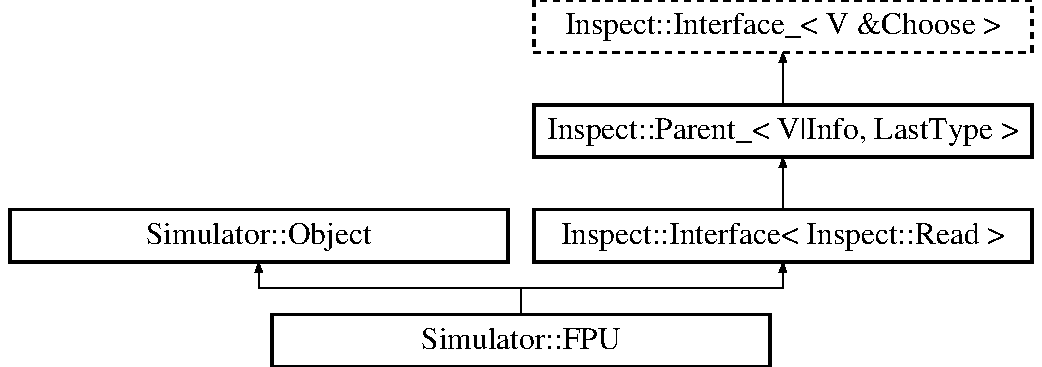
\includegraphics[height=4.000000cm]{class_simulator_1_1_f_p_u}
\end{center}
\end{figure}
\subsection*{Classes}
\begin{DoxyCompactItemize}
\item 
class \hyperlink{class_simulator_1_1_f_p_u_1_1_i_f_p_u_client}{I\+F\+P\+U\+Client}
\begin{DoxyCompactList}\small\item\em Represents a client for this \hyperlink{class_simulator_1_1_f_p_u}{F\+P\+U}. \end{DoxyCompactList}\end{DoxyCompactItemize}
\subsection*{Public Member Functions}
\begin{DoxyCompactItemize}
\item 
\hyperlink{class_simulator_1_1_f_p_u_ab6a08f9d6a3b169b44da3219684809ce}{F\+P\+U} (const std\+::string \&\hyperlink{mtconf_8c_a8f8f80d37794cde9472343e4487ba3eb}{name}, \hyperlink{class_simulator_1_1_object}{Object} \&parent, \hyperlink{class_simulator_1_1_clock}{Clock} \&clock, \hyperlink{class_config}{Config} \&config, size\+\_\+t num\+\_\+inputs)
\begin{DoxyCompactList}\small\item\em Constructs the \hyperlink{class_simulator_1_1_f_p_u}{F\+P\+U}. \end{DoxyCompactList}\item 
\hyperlink{class_simulator_1_1_f_p_u_a5adfb06a7e937780eb2e8e7c0a6ea5d4}{$\sim$\+F\+P\+U} ()
\begin{DoxyCompactList}\small\item\em Destroys the \hyperlink{class_simulator_1_1_f_p_u}{F\+P\+U} object. \end{DoxyCompactList}\item 
size\+\_\+t \hyperlink{class_simulator_1_1_f_p_u_a4976a10751299a95bff865fe320cf4a0}{Register\+Source} (\hyperlink{class_simulator_1_1_f_p_u_1_1_i_f_p_u_client}{I\+F\+P\+U\+Client} \&client, const \hyperlink{class_simulator_1_1_storage_trace_set}{Storage\+Trace\+Set} \&output)
\begin{DoxyCompactList}\small\item\em Registers a source to the \hyperlink{class_simulator_1_1_f_p_u}{F\+P\+U}. \end{DoxyCompactList}\item 
bool \hyperlink{class_simulator_1_1_f_p_u_a41ed29022d125ab496b15dfc77f089eb}{Queue\+Operation} (size\+\_\+t source, \hyperlink{namespace_simulator_ad8a1c084ddce210647e4867afc95b6e0}{F\+P\+U\+Operation} op, int size, double Rav, double Rbv, const \hyperlink{struct_simulator_1_1_reg_addr}{Reg\+Addr} \&Rc)
\begin{DoxyCompactList}\small\item\em Queues an F\+P operation. \end{DoxyCompactList}\item 
\hyperlink{class_simulator_1_1_storage_trace_set}{Storage\+Trace\+Set} \hyperlink{class_simulator_1_1_f_p_u_a3d652765df9a0b87456df559fd72605a}{Get\+Source\+Trace} (size\+\_\+t source) const 
\item 
void \hyperlink{class_simulator_1_1_f_p_u_a7a0dbba9ebb8ba40afdfa667d7bf7f2e}{Cmd\+\_\+\+Info} (std\+::ostream \&out, const std\+::vector$<$ std\+::string $>$ \&arguments) const 
\item 
void \hyperlink{class_simulator_1_1_f_p_u_a838921d4b26611263f7d165b9d3fb68b}{Cmd\+\_\+\+Read} (std\+::ostream \&out, const std\+::vector$<$ std\+::string $>$ \&arguments) const 
\end{DoxyCompactItemize}
\subsection*{Public Attributes}
\begin{DoxyCompactItemize}
\item 
\hyperlink{class_simulator_1_1_process}{Process} \hyperlink{class_simulator_1_1_f_p_u_a696de79c0d8e304961d3378a821ebb35}{p\+\_\+\+Pipeline}
\end{DoxyCompactItemize}


\subsection{Detailed Description}
Floating Point Unit. 

This component accepts floating point operations, executes them asynchronously and writes them back once calculated. It has several pipelines, assuming every operation of equal delay can be pipelined. 

\subsection{Constructor \& Destructor Documentation}
\hypertarget{class_simulator_1_1_f_p_u_ab6a08f9d6a3b169b44da3219684809ce}{\index{Simulator\+::\+F\+P\+U@{Simulator\+::\+F\+P\+U}!F\+P\+U@{F\+P\+U}}
\index{F\+P\+U@{F\+P\+U}!Simulator\+::\+F\+P\+U@{Simulator\+::\+F\+P\+U}}
\subsubsection[{F\+P\+U}]{\setlength{\rightskip}{0pt plus 5cm}Simulator\+::\+F\+P\+U\+::\+F\+P\+U (
\begin{DoxyParamCaption}
\item[{const std\+::string \&}]{name, }
\item[{{\bf Object} \&}]{parent, }
\item[{{\bf Clock} \&}]{clock, }
\item[{{\bf Config} \&}]{config, }
\item[{size\+\_\+t}]{num\+\_\+inputs}
\end{DoxyParamCaption}
)}}\label{class_simulator_1_1_f_p_u_ab6a08f9d6a3b169b44da3219684809ce}


Constructs the \hyperlink{class_simulator_1_1_f_p_u}{F\+P\+U}. 


\begin{DoxyParams}{Parameters}
{\em parent} & reference to the parent object \\
\hline
{\em name} & name of the \hyperlink{class_simulator_1_1_f_p_u}{F\+P\+U}, irrelevant to simulation \\
\hline
{\em config} & reference to the configuration data \\
\hline
{\em num\+\_\+inputs} & number of inputs that will be connected to this \hyperlink{class_simulator_1_1_f_p_u}{F\+P\+U} \\
\hline
\end{DoxyParams}
\hypertarget{class_simulator_1_1_f_p_u_a5adfb06a7e937780eb2e8e7c0a6ea5d4}{\index{Simulator\+::\+F\+P\+U@{Simulator\+::\+F\+P\+U}!````~F\+P\+U@{$\sim$\+F\+P\+U}}
\index{````~F\+P\+U@{$\sim$\+F\+P\+U}!Simulator\+::\+F\+P\+U@{Simulator\+::\+F\+P\+U}}
\subsubsection[{$\sim$\+F\+P\+U}]{\setlength{\rightskip}{0pt plus 5cm}Simulator\+::\+F\+P\+U\+::$\sim$\+F\+P\+U (
\begin{DoxyParamCaption}
{}
\end{DoxyParamCaption}
)}}\label{class_simulator_1_1_f_p_u_a5adfb06a7e937780eb2e8e7c0a6ea5d4}


Destroys the \hyperlink{class_simulator_1_1_f_p_u}{F\+P\+U} object. 



\subsection{Member Function Documentation}
\hypertarget{class_simulator_1_1_f_p_u_a7a0dbba9ebb8ba40afdfa667d7bf7f2e}{\index{Simulator\+::\+F\+P\+U@{Simulator\+::\+F\+P\+U}!Cmd\+\_\+\+Info@{Cmd\+\_\+\+Info}}
\index{Cmd\+\_\+\+Info@{Cmd\+\_\+\+Info}!Simulator\+::\+F\+P\+U@{Simulator\+::\+F\+P\+U}}
\subsubsection[{Cmd\+\_\+\+Info}]{\setlength{\rightskip}{0pt plus 5cm}void Simulator\+::\+F\+P\+U\+::\+Cmd\+\_\+\+Info (
\begin{DoxyParamCaption}
\item[{std\+::ostream \&}]{out, }
\item[{const std\+::vector$<$ std\+::string $>$ \&}]{arguments}
\end{DoxyParamCaption}
) const}}\label{class_simulator_1_1_f_p_u_a7a0dbba9ebb8ba40afdfa667d7bf7f2e}
\hypertarget{class_simulator_1_1_f_p_u_a838921d4b26611263f7d165b9d3fb68b}{\index{Simulator\+::\+F\+P\+U@{Simulator\+::\+F\+P\+U}!Cmd\+\_\+\+Read@{Cmd\+\_\+\+Read}}
\index{Cmd\+\_\+\+Read@{Cmd\+\_\+\+Read}!Simulator\+::\+F\+P\+U@{Simulator\+::\+F\+P\+U}}
\subsubsection[{Cmd\+\_\+\+Read}]{\setlength{\rightskip}{0pt plus 5cm}void Simulator\+::\+F\+P\+U\+::\+Cmd\+\_\+\+Read (
\begin{DoxyParamCaption}
\item[{std\+::ostream \&}]{out, }
\item[{const std\+::vector$<$ std\+::string $>$ \&}]{arguments}
\end{DoxyParamCaption}
) const}}\label{class_simulator_1_1_f_p_u_a838921d4b26611263f7d165b9d3fb68b}
\hypertarget{class_simulator_1_1_f_p_u_a3d652765df9a0b87456df559fd72605a}{\index{Simulator\+::\+F\+P\+U@{Simulator\+::\+F\+P\+U}!Get\+Source\+Trace@{Get\+Source\+Trace}}
\index{Get\+Source\+Trace@{Get\+Source\+Trace}!Simulator\+::\+F\+P\+U@{Simulator\+::\+F\+P\+U}}
\subsubsection[{Get\+Source\+Trace}]{\setlength{\rightskip}{0pt plus 5cm}{\bf Storage\+Trace\+Set} Simulator\+::\+F\+P\+U\+::\+Get\+Source\+Trace (
\begin{DoxyParamCaption}
\item[{size\+\_\+t}]{source}
\end{DoxyParamCaption}
) const}}\label{class_simulator_1_1_f_p_u_a3d652765df9a0b87456df559fd72605a}
\hypertarget{class_simulator_1_1_f_p_u_a41ed29022d125ab496b15dfc77f089eb}{\index{Simulator\+::\+F\+P\+U@{Simulator\+::\+F\+P\+U}!Queue\+Operation@{Queue\+Operation}}
\index{Queue\+Operation@{Queue\+Operation}!Simulator\+::\+F\+P\+U@{Simulator\+::\+F\+P\+U}}
\subsubsection[{Queue\+Operation}]{\setlength{\rightskip}{0pt plus 5cm}bool Simulator\+::\+F\+P\+U\+::\+Queue\+Operation (
\begin{DoxyParamCaption}
\item[{size\+\_\+t}]{source, }
\item[{{\bf F\+P\+U\+Operation}}]{op, }
\item[{int}]{size, }
\item[{double}]{Rav, }
\item[{double}]{Rbv, }
\item[{const {\bf Reg\+Addr} \&}]{Rc}
\end{DoxyParamCaption}
)}}\label{class_simulator_1_1_f_p_u_a41ed29022d125ab496b15dfc77f089eb}


Queues an F\+P operation. 

This function determines the length of the operation and queues the operation in the corresponding pipeline. When the operation has completed, the result is written back to the register file. 
\begin{DoxyParams}{Parameters}
{\em source} & the source input I\+D \\
\hline
{\em op} & the F\+P operation to perform \\
\hline
{\em size} & size of the F\+P operation (4 or 8) \\
\hline
{\em Rav} & first (or only) operand of the operation \\
\hline
{\em Rbv} & second operand of the operation \\
\hline
{\em Rc} & address of the destination register(s) \\
\hline
\end{DoxyParams}
\begin{DoxyReturn}{Returns}
true if the operation could be queued. 
\end{DoxyReturn}
\hypertarget{class_simulator_1_1_f_p_u_a4976a10751299a95bff865fe320cf4a0}{\index{Simulator\+::\+F\+P\+U@{Simulator\+::\+F\+P\+U}!Register\+Source@{Register\+Source}}
\index{Register\+Source@{Register\+Source}!Simulator\+::\+F\+P\+U@{Simulator\+::\+F\+P\+U}}
\subsubsection[{Register\+Source}]{\setlength{\rightskip}{0pt plus 5cm}size\+\_\+t Simulator\+::\+F\+P\+U\+::\+Register\+Source (
\begin{DoxyParamCaption}
\item[{{\bf I\+F\+P\+U\+Client} \&}]{client, }
\item[{const {\bf Storage\+Trace\+Set} \&}]{output}
\end{DoxyParamCaption}
)}}\label{class_simulator_1_1_f_p_u_a4976a10751299a95bff865fe320cf4a0}


Registers a source to the \hyperlink{class_simulator_1_1_f_p_u}{F\+P\+U}. 


\begin{DoxyParams}{Parameters}
{\em regfile} & \mbox{[}in\mbox{]} the register file to use to write back results for this source \\
\hline
{\em output} & \mbox{[}in\mbox{]} the storage traces that can be generated when writing the result \\
\hline
\end{DoxyParams}
\begin{DoxyReturn}{Returns}
the unique for this source to be passed to Queue\+Operation 
\end{DoxyReturn}


\subsection{Member Data Documentation}
\hypertarget{class_simulator_1_1_f_p_u_a696de79c0d8e304961d3378a821ebb35}{\index{Simulator\+::\+F\+P\+U@{Simulator\+::\+F\+P\+U}!p\+\_\+\+Pipeline@{p\+\_\+\+Pipeline}}
\index{p\+\_\+\+Pipeline@{p\+\_\+\+Pipeline}!Simulator\+::\+F\+P\+U@{Simulator\+::\+F\+P\+U}}
\subsubsection[{p\+\_\+\+Pipeline}]{\setlength{\rightskip}{0pt plus 5cm}{\bf Process} Simulator\+::\+F\+P\+U\+::p\+\_\+\+Pipeline}}\label{class_simulator_1_1_f_p_u_a696de79c0d8e304961d3378a821ebb35}


The documentation for this class was generated from the following files\+:\begin{DoxyCompactItemize}
\item 
arch/\hyperlink{_f_p_u_8h}{F\+P\+U.\+h}\item 
arch/\hyperlink{_f_p_u_8cpp}{F\+P\+U.\+cpp}\end{DoxyCompactItemize}

\hypertarget{class_simulator_1_1drisc_1_1_perf_counters_1_1_helpers}{\section{Simulator\+:\+:drisc\+:\+:Perf\+Counters\+:\+:Helpers Class Reference}
\label{class_simulator_1_1drisc_1_1_perf_counters_1_1_helpers}\index{Simulator\+::drisc\+::\+Perf\+Counters\+::\+Helpers@{Simulator\+::drisc\+::\+Perf\+Counters\+::\+Helpers}}
}
\subsection*{Static Public Member Functions}
\begin{DoxyCompactItemize}
\item 
static Integer \hyperlink{class_simulator_1_1drisc_1_1_perf_counters_1_1_helpers_aea174562c420543a2ec4f796b9de8cc2}{master\+\_\+cycles} (\hyperlink{class_simulator_1_1_d_r_i_s_c}{D\+R\+I\+S\+C} \&cpu, \hyperlink{namespace_simulator_aaccbc706b2d6c99085f52f6dfc2333e4}{L\+F\+I\+D})
\item 
static Integer \hyperlink{class_simulator_1_1drisc_1_1_perf_counters_1_1_helpers_ae4e15124c88d399f400bf34b3daff767}{exec\+\_\+ops} (\hyperlink{class_simulator_1_1_d_r_i_s_c}{D\+R\+I\+S\+C} \&cpu, \hyperlink{namespace_simulator_aaccbc706b2d6c99085f52f6dfc2333e4}{L\+F\+I\+D} fid)
\item 
static Integer \hyperlink{class_simulator_1_1drisc_1_1_perf_counters_1_1_helpers_a2ea667afd4d4098b8890bce2a206c8d3}{issued\+\_\+flops} (\hyperlink{class_simulator_1_1_d_r_i_s_c}{D\+R\+I\+S\+C} \&cpu, \hyperlink{namespace_simulator_aaccbc706b2d6c99085f52f6dfc2333e4}{L\+F\+I\+D} fid)
\item 
static Integer \hyperlink{class_simulator_1_1drisc_1_1_perf_counters_1_1_helpers_a3949956311f39bfaf73e240f2fa620d0}{completed\+\_\+loads} (\hyperlink{class_simulator_1_1_d_r_i_s_c}{D\+R\+I\+S\+C} \&cpu, \hyperlink{namespace_simulator_aaccbc706b2d6c99085f52f6dfc2333e4}{L\+F\+I\+D} fid)
\item 
static Integer \hyperlink{class_simulator_1_1drisc_1_1_perf_counters_1_1_helpers_a3dfbf25b61d2d19268f97a929feb12ad}{completed\+\_\+stores} (\hyperlink{class_simulator_1_1_d_r_i_s_c}{D\+R\+I\+S\+C} \&cpu, \hyperlink{namespace_simulator_aaccbc706b2d6c99085f52f6dfc2333e4}{L\+F\+I\+D} fid)
\item 
static Integer \hyperlink{class_simulator_1_1drisc_1_1_perf_counters_1_1_helpers_a31c2f3a794abe5997130e60d7d8743d0}{loaded\+\_\+bytes} (\hyperlink{class_simulator_1_1_d_r_i_s_c}{D\+R\+I\+S\+C} \&cpu, \hyperlink{namespace_simulator_aaccbc706b2d6c99085f52f6dfc2333e4}{L\+F\+I\+D} fid)
\item 
static Integer \hyperlink{class_simulator_1_1drisc_1_1_perf_counters_1_1_helpers_a5d35b550dc1efff996c9c4d774facd5a}{stored\+\_\+bytes} (\hyperlink{class_simulator_1_1_d_r_i_s_c}{D\+R\+I\+S\+C} \&cpu, \hyperlink{namespace_simulator_aaccbc706b2d6c99085f52f6dfc2333e4}{L\+F\+I\+D} fid)
\item 
static Integer \hyperlink{class_simulator_1_1drisc_1_1_perf_counters_1_1_helpers_afdfa47ebac15ef11e6ab925ab29ad5cc}{lines\+\_\+loaded} (\hyperlink{class_simulator_1_1_d_r_i_s_c}{D\+R\+I\+S\+C} \&cpu, \hyperlink{namespace_simulator_aaccbc706b2d6c99085f52f6dfc2333e4}{L\+F\+I\+D})
\item 
static Integer \hyperlink{class_simulator_1_1drisc_1_1_perf_counters_1_1_helpers_abbbe5f9640e4073692dff04e3535b31d}{lines\+\_\+stored} (\hyperlink{class_simulator_1_1_d_r_i_s_c}{D\+R\+I\+S\+C} \&cpu, \hyperlink{namespace_simulator_aaccbc706b2d6c99085f52f6dfc2333e4}{L\+F\+I\+D})
\item 
static Integer \hyperlink{class_simulator_1_1drisc_1_1_perf_counters_1_1_helpers_aa74ebd44c36094febde02b0d8a86e44c}{place\+\_\+size} (\hyperlink{class_simulator_1_1_d_r_i_s_c}{D\+R\+I\+S\+C} \&cpu, \hyperlink{namespace_simulator_aaccbc706b2d6c99085f52f6dfc2333e4}{L\+F\+I\+D} fid)
\item 
static Integer \hyperlink{class_simulator_1_1drisc_1_1_perf_counters_1_1_helpers_a287923de198fd87615ad8ad2b837f055}{allocated\+\_\+threads} (\hyperlink{class_simulator_1_1_d_r_i_s_c}{D\+R\+I\+S\+C} \&cpu, \hyperlink{namespace_simulator_aaccbc706b2d6c99085f52f6dfc2333e4}{L\+F\+I\+D} fid)
\item 
static Integer \hyperlink{class_simulator_1_1drisc_1_1_perf_counters_1_1_helpers_a528adcfe59ceedb18f02ae079b37af2d}{allocated\+\_\+families} (\hyperlink{class_simulator_1_1_d_r_i_s_c}{D\+R\+I\+S\+C} \&cpu, \hyperlink{namespace_simulator_aaccbc706b2d6c99085f52f6dfc2333e4}{L\+F\+I\+D} fid)
\item 
static Integer \hyperlink{class_simulator_1_1drisc_1_1_perf_counters_1_1_helpers_a02682e6e848060b83d62a324ede8beb3}{allocated\+\_\+xfamilies} (\hyperlink{class_simulator_1_1_d_r_i_s_c}{D\+R\+I\+S\+C} \&cpu, \hyperlink{namespace_simulator_aaccbc706b2d6c99085f52f6dfc2333e4}{L\+F\+I\+D} fid)
\item 
static Integer \hyperlink{class_simulator_1_1drisc_1_1_perf_counters_1_1_helpers_ab944bf30d394a123f1192740f92c4f4b}{unix\+\_\+time} (\hyperlink{class_simulator_1_1_d_r_i_s_c}{D\+R\+I\+S\+C} \&, \hyperlink{namespace_simulator_aaccbc706b2d6c99085f52f6dfc2333e4}{L\+F\+I\+D})
\item 
static Integer \hyperlink{class_simulator_1_1drisc_1_1_perf_counters_1_1_helpers_afc40e74541d38234111c6dc78fdd5ace}{packed\+\_\+date} (\hyperlink{class_simulator_1_1_d_r_i_s_c}{D\+R\+I\+S\+C} \&, \hyperlink{namespace_simulator_aaccbc706b2d6c99085f52f6dfc2333e4}{L\+F\+I\+D})
\item 
static Integer \hyperlink{class_simulator_1_1drisc_1_1_perf_counters_1_1_helpers_a176414ca2c506a834945f5117348907d}{packed\+\_\+time} (\hyperlink{class_simulator_1_1_d_r_i_s_c}{D\+R\+I\+S\+C} \&, \hyperlink{namespace_simulator_aaccbc706b2d6c99085f52f6dfc2333e4}{L\+F\+I\+D})
\item 
static Integer \hyperlink{class_simulator_1_1drisc_1_1_perf_counters_1_1_helpers_ac56f62a048b80b5cb6d45248af2cc7f3}{extlines\+\_\+loaded} (\hyperlink{class_simulator_1_1_d_r_i_s_c}{D\+R\+I\+S\+C} \&cpu, \hyperlink{namespace_simulator_aaccbc706b2d6c99085f52f6dfc2333e4}{L\+F\+I\+D})
\item 
static Integer \hyperlink{class_simulator_1_1drisc_1_1_perf_counters_1_1_helpers_aad448899b246b8eead2bf1d9521152ad}{extlines\+\_\+stored} (\hyperlink{class_simulator_1_1_d_r_i_s_c}{D\+R\+I\+S\+C} \&cpu, \hyperlink{namespace_simulator_aaccbc706b2d6c99085f52f6dfc2333e4}{L\+F\+I\+D})
\item 
static Integer \hyperlink{class_simulator_1_1drisc_1_1_perf_counters_1_1_helpers_a3380f15c55a00f9480a069609d4ba1f7}{created\+\_\+threads} (\hyperlink{class_simulator_1_1_d_r_i_s_c}{D\+R\+I\+S\+C} \&cpu, \hyperlink{namespace_simulator_aaccbc706b2d6c99085f52f6dfc2333e4}{L\+F\+I\+D} fid)
\item 
static Integer \hyperlink{class_simulator_1_1drisc_1_1_perf_counters_1_1_helpers_a315d376d8f3fd7363963abf669fca1f9}{created\+\_\+families} (\hyperlink{class_simulator_1_1_d_r_i_s_c}{D\+R\+I\+S\+C} \&cpu, \hyperlink{namespace_simulator_aaccbc706b2d6c99085f52f6dfc2333e4}{L\+F\+I\+D} fid)
\item 
static Integer \hyperlink{class_simulator_1_1drisc_1_1_perf_counters_1_1_helpers_ab421fc9b00c3f92931000cb071ff83a1}{core\+\_\+cycles} (\hyperlink{class_simulator_1_1_d_r_i_s_c}{D\+R\+I\+S\+C} \&cpu, \hyperlink{namespace_simulator_aaccbc706b2d6c99085f52f6dfc2333e4}{L\+F\+I\+D})
\end{DoxyCompactItemize}


\subsection{Member Function Documentation}
\hypertarget{class_simulator_1_1drisc_1_1_perf_counters_1_1_helpers_a528adcfe59ceedb18f02ae079b37af2d}{\index{Simulator\+::drisc\+::\+Perf\+Counters\+::\+Helpers@{Simulator\+::drisc\+::\+Perf\+Counters\+::\+Helpers}!allocated\+\_\+families@{allocated\+\_\+families}}
\index{allocated\+\_\+families@{allocated\+\_\+families}!Simulator\+::drisc\+::\+Perf\+Counters\+::\+Helpers@{Simulator\+::drisc\+::\+Perf\+Counters\+::\+Helpers}}
\subsubsection[{allocated\+\_\+families}]{\setlength{\rightskip}{0pt plus 5cm}static Integer Simulator\+::drisc\+::\+Perf\+Counters\+::\+Helpers\+::allocated\+\_\+families (
\begin{DoxyParamCaption}
\item[{{\bf D\+R\+I\+S\+C} \&}]{cpu, }
\item[{{\bf L\+F\+I\+D}}]{fid}
\end{DoxyParamCaption}
)\hspace{0.3cm}{\ttfamily [inline]}, {\ttfamily [static]}}}\label{class_simulator_1_1drisc_1_1_perf_counters_1_1_helpers_a528adcfe59ceedb18f02ae079b37af2d}
\hypertarget{class_simulator_1_1drisc_1_1_perf_counters_1_1_helpers_a287923de198fd87615ad8ad2b837f055}{\index{Simulator\+::drisc\+::\+Perf\+Counters\+::\+Helpers@{Simulator\+::drisc\+::\+Perf\+Counters\+::\+Helpers}!allocated\+\_\+threads@{allocated\+\_\+threads}}
\index{allocated\+\_\+threads@{allocated\+\_\+threads}!Simulator\+::drisc\+::\+Perf\+Counters\+::\+Helpers@{Simulator\+::drisc\+::\+Perf\+Counters\+::\+Helpers}}
\subsubsection[{allocated\+\_\+threads}]{\setlength{\rightskip}{0pt plus 5cm}static Integer Simulator\+::drisc\+::\+Perf\+Counters\+::\+Helpers\+::allocated\+\_\+threads (
\begin{DoxyParamCaption}
\item[{{\bf D\+R\+I\+S\+C} \&}]{cpu, }
\item[{{\bf L\+F\+I\+D}}]{fid}
\end{DoxyParamCaption}
)\hspace{0.3cm}{\ttfamily [inline]}, {\ttfamily [static]}}}\label{class_simulator_1_1drisc_1_1_perf_counters_1_1_helpers_a287923de198fd87615ad8ad2b837f055}
\hypertarget{class_simulator_1_1drisc_1_1_perf_counters_1_1_helpers_a02682e6e848060b83d62a324ede8beb3}{\index{Simulator\+::drisc\+::\+Perf\+Counters\+::\+Helpers@{Simulator\+::drisc\+::\+Perf\+Counters\+::\+Helpers}!allocated\+\_\+xfamilies@{allocated\+\_\+xfamilies}}
\index{allocated\+\_\+xfamilies@{allocated\+\_\+xfamilies}!Simulator\+::drisc\+::\+Perf\+Counters\+::\+Helpers@{Simulator\+::drisc\+::\+Perf\+Counters\+::\+Helpers}}
\subsubsection[{allocated\+\_\+xfamilies}]{\setlength{\rightskip}{0pt plus 5cm}static Integer Simulator\+::drisc\+::\+Perf\+Counters\+::\+Helpers\+::allocated\+\_\+xfamilies (
\begin{DoxyParamCaption}
\item[{{\bf D\+R\+I\+S\+C} \&}]{cpu, }
\item[{{\bf L\+F\+I\+D}}]{fid}
\end{DoxyParamCaption}
)\hspace{0.3cm}{\ttfamily [inline]}, {\ttfamily [static]}}}\label{class_simulator_1_1drisc_1_1_perf_counters_1_1_helpers_a02682e6e848060b83d62a324ede8beb3}
\hypertarget{class_simulator_1_1drisc_1_1_perf_counters_1_1_helpers_a3949956311f39bfaf73e240f2fa620d0}{\index{Simulator\+::drisc\+::\+Perf\+Counters\+::\+Helpers@{Simulator\+::drisc\+::\+Perf\+Counters\+::\+Helpers}!completed\+\_\+loads@{completed\+\_\+loads}}
\index{completed\+\_\+loads@{completed\+\_\+loads}!Simulator\+::drisc\+::\+Perf\+Counters\+::\+Helpers@{Simulator\+::drisc\+::\+Perf\+Counters\+::\+Helpers}}
\subsubsection[{completed\+\_\+loads}]{\setlength{\rightskip}{0pt plus 5cm}static Integer Simulator\+::drisc\+::\+Perf\+Counters\+::\+Helpers\+::completed\+\_\+loads (
\begin{DoxyParamCaption}
\item[{{\bf D\+R\+I\+S\+C} \&}]{cpu, }
\item[{{\bf L\+F\+I\+D}}]{fid}
\end{DoxyParamCaption}
)\hspace{0.3cm}{\ttfamily [inline]}, {\ttfamily [static]}}}\label{class_simulator_1_1drisc_1_1_perf_counters_1_1_helpers_a3949956311f39bfaf73e240f2fa620d0}
\hypertarget{class_simulator_1_1drisc_1_1_perf_counters_1_1_helpers_a3dfbf25b61d2d19268f97a929feb12ad}{\index{Simulator\+::drisc\+::\+Perf\+Counters\+::\+Helpers@{Simulator\+::drisc\+::\+Perf\+Counters\+::\+Helpers}!completed\+\_\+stores@{completed\+\_\+stores}}
\index{completed\+\_\+stores@{completed\+\_\+stores}!Simulator\+::drisc\+::\+Perf\+Counters\+::\+Helpers@{Simulator\+::drisc\+::\+Perf\+Counters\+::\+Helpers}}
\subsubsection[{completed\+\_\+stores}]{\setlength{\rightskip}{0pt plus 5cm}static Integer Simulator\+::drisc\+::\+Perf\+Counters\+::\+Helpers\+::completed\+\_\+stores (
\begin{DoxyParamCaption}
\item[{{\bf D\+R\+I\+S\+C} \&}]{cpu, }
\item[{{\bf L\+F\+I\+D}}]{fid}
\end{DoxyParamCaption}
)\hspace{0.3cm}{\ttfamily [inline]}, {\ttfamily [static]}}}\label{class_simulator_1_1drisc_1_1_perf_counters_1_1_helpers_a3dfbf25b61d2d19268f97a929feb12ad}
\hypertarget{class_simulator_1_1drisc_1_1_perf_counters_1_1_helpers_ab421fc9b00c3f92931000cb071ff83a1}{\index{Simulator\+::drisc\+::\+Perf\+Counters\+::\+Helpers@{Simulator\+::drisc\+::\+Perf\+Counters\+::\+Helpers}!core\+\_\+cycles@{core\+\_\+cycles}}
\index{core\+\_\+cycles@{core\+\_\+cycles}!Simulator\+::drisc\+::\+Perf\+Counters\+::\+Helpers@{Simulator\+::drisc\+::\+Perf\+Counters\+::\+Helpers}}
\subsubsection[{core\+\_\+cycles}]{\setlength{\rightskip}{0pt plus 5cm}static Integer Simulator\+::drisc\+::\+Perf\+Counters\+::\+Helpers\+::core\+\_\+cycles (
\begin{DoxyParamCaption}
\item[{{\bf D\+R\+I\+S\+C} \&}]{cpu, }
\item[{{\bf L\+F\+I\+D}}]{}
\end{DoxyParamCaption}
)\hspace{0.3cm}{\ttfamily [inline]}, {\ttfamily [static]}}}\label{class_simulator_1_1drisc_1_1_perf_counters_1_1_helpers_ab421fc9b00c3f92931000cb071ff83a1}
\hypertarget{class_simulator_1_1drisc_1_1_perf_counters_1_1_helpers_a315d376d8f3fd7363963abf669fca1f9}{\index{Simulator\+::drisc\+::\+Perf\+Counters\+::\+Helpers@{Simulator\+::drisc\+::\+Perf\+Counters\+::\+Helpers}!created\+\_\+families@{created\+\_\+families}}
\index{created\+\_\+families@{created\+\_\+families}!Simulator\+::drisc\+::\+Perf\+Counters\+::\+Helpers@{Simulator\+::drisc\+::\+Perf\+Counters\+::\+Helpers}}
\subsubsection[{created\+\_\+families}]{\setlength{\rightskip}{0pt plus 5cm}static Integer Simulator\+::drisc\+::\+Perf\+Counters\+::\+Helpers\+::created\+\_\+families (
\begin{DoxyParamCaption}
\item[{{\bf D\+R\+I\+S\+C} \&}]{cpu, }
\item[{{\bf L\+F\+I\+D}}]{fid}
\end{DoxyParamCaption}
)\hspace{0.3cm}{\ttfamily [inline]}, {\ttfamily [static]}}}\label{class_simulator_1_1drisc_1_1_perf_counters_1_1_helpers_a315d376d8f3fd7363963abf669fca1f9}
\hypertarget{class_simulator_1_1drisc_1_1_perf_counters_1_1_helpers_a3380f15c55a00f9480a069609d4ba1f7}{\index{Simulator\+::drisc\+::\+Perf\+Counters\+::\+Helpers@{Simulator\+::drisc\+::\+Perf\+Counters\+::\+Helpers}!created\+\_\+threads@{created\+\_\+threads}}
\index{created\+\_\+threads@{created\+\_\+threads}!Simulator\+::drisc\+::\+Perf\+Counters\+::\+Helpers@{Simulator\+::drisc\+::\+Perf\+Counters\+::\+Helpers}}
\subsubsection[{created\+\_\+threads}]{\setlength{\rightskip}{0pt plus 5cm}static Integer Simulator\+::drisc\+::\+Perf\+Counters\+::\+Helpers\+::created\+\_\+threads (
\begin{DoxyParamCaption}
\item[{{\bf D\+R\+I\+S\+C} \&}]{cpu, }
\item[{{\bf L\+F\+I\+D}}]{fid}
\end{DoxyParamCaption}
)\hspace{0.3cm}{\ttfamily [inline]}, {\ttfamily [static]}}}\label{class_simulator_1_1drisc_1_1_perf_counters_1_1_helpers_a3380f15c55a00f9480a069609d4ba1f7}
\hypertarget{class_simulator_1_1drisc_1_1_perf_counters_1_1_helpers_ae4e15124c88d399f400bf34b3daff767}{\index{Simulator\+::drisc\+::\+Perf\+Counters\+::\+Helpers@{Simulator\+::drisc\+::\+Perf\+Counters\+::\+Helpers}!exec\+\_\+ops@{exec\+\_\+ops}}
\index{exec\+\_\+ops@{exec\+\_\+ops}!Simulator\+::drisc\+::\+Perf\+Counters\+::\+Helpers@{Simulator\+::drisc\+::\+Perf\+Counters\+::\+Helpers}}
\subsubsection[{exec\+\_\+ops}]{\setlength{\rightskip}{0pt plus 5cm}static Integer Simulator\+::drisc\+::\+Perf\+Counters\+::\+Helpers\+::exec\+\_\+ops (
\begin{DoxyParamCaption}
\item[{{\bf D\+R\+I\+S\+C} \&}]{cpu, }
\item[{{\bf L\+F\+I\+D}}]{fid}
\end{DoxyParamCaption}
)\hspace{0.3cm}{\ttfamily [inline]}, {\ttfamily [static]}}}\label{class_simulator_1_1drisc_1_1_perf_counters_1_1_helpers_ae4e15124c88d399f400bf34b3daff767}
\hypertarget{class_simulator_1_1drisc_1_1_perf_counters_1_1_helpers_ac56f62a048b80b5cb6d45248af2cc7f3}{\index{Simulator\+::drisc\+::\+Perf\+Counters\+::\+Helpers@{Simulator\+::drisc\+::\+Perf\+Counters\+::\+Helpers}!extlines\+\_\+loaded@{extlines\+\_\+loaded}}
\index{extlines\+\_\+loaded@{extlines\+\_\+loaded}!Simulator\+::drisc\+::\+Perf\+Counters\+::\+Helpers@{Simulator\+::drisc\+::\+Perf\+Counters\+::\+Helpers}}
\subsubsection[{extlines\+\_\+loaded}]{\setlength{\rightskip}{0pt plus 5cm}static Integer Simulator\+::drisc\+::\+Perf\+Counters\+::\+Helpers\+::extlines\+\_\+loaded (
\begin{DoxyParamCaption}
\item[{{\bf D\+R\+I\+S\+C} \&}]{cpu, }
\item[{{\bf L\+F\+I\+D}}]{}
\end{DoxyParamCaption}
)\hspace{0.3cm}{\ttfamily [inline]}, {\ttfamily [static]}}}\label{class_simulator_1_1drisc_1_1_perf_counters_1_1_helpers_ac56f62a048b80b5cb6d45248af2cc7f3}
\hypertarget{class_simulator_1_1drisc_1_1_perf_counters_1_1_helpers_aad448899b246b8eead2bf1d9521152ad}{\index{Simulator\+::drisc\+::\+Perf\+Counters\+::\+Helpers@{Simulator\+::drisc\+::\+Perf\+Counters\+::\+Helpers}!extlines\+\_\+stored@{extlines\+\_\+stored}}
\index{extlines\+\_\+stored@{extlines\+\_\+stored}!Simulator\+::drisc\+::\+Perf\+Counters\+::\+Helpers@{Simulator\+::drisc\+::\+Perf\+Counters\+::\+Helpers}}
\subsubsection[{extlines\+\_\+stored}]{\setlength{\rightskip}{0pt plus 5cm}static Integer Simulator\+::drisc\+::\+Perf\+Counters\+::\+Helpers\+::extlines\+\_\+stored (
\begin{DoxyParamCaption}
\item[{{\bf D\+R\+I\+S\+C} \&}]{cpu, }
\item[{{\bf L\+F\+I\+D}}]{}
\end{DoxyParamCaption}
)\hspace{0.3cm}{\ttfamily [inline]}, {\ttfamily [static]}}}\label{class_simulator_1_1drisc_1_1_perf_counters_1_1_helpers_aad448899b246b8eead2bf1d9521152ad}
\hypertarget{class_simulator_1_1drisc_1_1_perf_counters_1_1_helpers_a2ea667afd4d4098b8890bce2a206c8d3}{\index{Simulator\+::drisc\+::\+Perf\+Counters\+::\+Helpers@{Simulator\+::drisc\+::\+Perf\+Counters\+::\+Helpers}!issued\+\_\+flops@{issued\+\_\+flops}}
\index{issued\+\_\+flops@{issued\+\_\+flops}!Simulator\+::drisc\+::\+Perf\+Counters\+::\+Helpers@{Simulator\+::drisc\+::\+Perf\+Counters\+::\+Helpers}}
\subsubsection[{issued\+\_\+flops}]{\setlength{\rightskip}{0pt plus 5cm}static Integer Simulator\+::drisc\+::\+Perf\+Counters\+::\+Helpers\+::issued\+\_\+flops (
\begin{DoxyParamCaption}
\item[{{\bf D\+R\+I\+S\+C} \&}]{cpu, }
\item[{{\bf L\+F\+I\+D}}]{fid}
\end{DoxyParamCaption}
)\hspace{0.3cm}{\ttfamily [inline]}, {\ttfamily [static]}}}\label{class_simulator_1_1drisc_1_1_perf_counters_1_1_helpers_a2ea667afd4d4098b8890bce2a206c8d3}
\hypertarget{class_simulator_1_1drisc_1_1_perf_counters_1_1_helpers_afdfa47ebac15ef11e6ab925ab29ad5cc}{\index{Simulator\+::drisc\+::\+Perf\+Counters\+::\+Helpers@{Simulator\+::drisc\+::\+Perf\+Counters\+::\+Helpers}!lines\+\_\+loaded@{lines\+\_\+loaded}}
\index{lines\+\_\+loaded@{lines\+\_\+loaded}!Simulator\+::drisc\+::\+Perf\+Counters\+::\+Helpers@{Simulator\+::drisc\+::\+Perf\+Counters\+::\+Helpers}}
\subsubsection[{lines\+\_\+loaded}]{\setlength{\rightskip}{0pt plus 5cm}static Integer Simulator\+::drisc\+::\+Perf\+Counters\+::\+Helpers\+::lines\+\_\+loaded (
\begin{DoxyParamCaption}
\item[{{\bf D\+R\+I\+S\+C} \&}]{cpu, }
\item[{{\bf L\+F\+I\+D}}]{}
\end{DoxyParamCaption}
)\hspace{0.3cm}{\ttfamily [inline]}, {\ttfamily [static]}}}\label{class_simulator_1_1drisc_1_1_perf_counters_1_1_helpers_afdfa47ebac15ef11e6ab925ab29ad5cc}
\hypertarget{class_simulator_1_1drisc_1_1_perf_counters_1_1_helpers_abbbe5f9640e4073692dff04e3535b31d}{\index{Simulator\+::drisc\+::\+Perf\+Counters\+::\+Helpers@{Simulator\+::drisc\+::\+Perf\+Counters\+::\+Helpers}!lines\+\_\+stored@{lines\+\_\+stored}}
\index{lines\+\_\+stored@{lines\+\_\+stored}!Simulator\+::drisc\+::\+Perf\+Counters\+::\+Helpers@{Simulator\+::drisc\+::\+Perf\+Counters\+::\+Helpers}}
\subsubsection[{lines\+\_\+stored}]{\setlength{\rightskip}{0pt plus 5cm}static Integer Simulator\+::drisc\+::\+Perf\+Counters\+::\+Helpers\+::lines\+\_\+stored (
\begin{DoxyParamCaption}
\item[{{\bf D\+R\+I\+S\+C} \&}]{cpu, }
\item[{{\bf L\+F\+I\+D}}]{}
\end{DoxyParamCaption}
)\hspace{0.3cm}{\ttfamily [inline]}, {\ttfamily [static]}}}\label{class_simulator_1_1drisc_1_1_perf_counters_1_1_helpers_abbbe5f9640e4073692dff04e3535b31d}
\hypertarget{class_simulator_1_1drisc_1_1_perf_counters_1_1_helpers_a31c2f3a794abe5997130e60d7d8743d0}{\index{Simulator\+::drisc\+::\+Perf\+Counters\+::\+Helpers@{Simulator\+::drisc\+::\+Perf\+Counters\+::\+Helpers}!loaded\+\_\+bytes@{loaded\+\_\+bytes}}
\index{loaded\+\_\+bytes@{loaded\+\_\+bytes}!Simulator\+::drisc\+::\+Perf\+Counters\+::\+Helpers@{Simulator\+::drisc\+::\+Perf\+Counters\+::\+Helpers}}
\subsubsection[{loaded\+\_\+bytes}]{\setlength{\rightskip}{0pt plus 5cm}static Integer Simulator\+::drisc\+::\+Perf\+Counters\+::\+Helpers\+::loaded\+\_\+bytes (
\begin{DoxyParamCaption}
\item[{{\bf D\+R\+I\+S\+C} \&}]{cpu, }
\item[{{\bf L\+F\+I\+D}}]{fid}
\end{DoxyParamCaption}
)\hspace{0.3cm}{\ttfamily [inline]}, {\ttfamily [static]}}}\label{class_simulator_1_1drisc_1_1_perf_counters_1_1_helpers_a31c2f3a794abe5997130e60d7d8743d0}
\hypertarget{class_simulator_1_1drisc_1_1_perf_counters_1_1_helpers_aea174562c420543a2ec4f796b9de8cc2}{\index{Simulator\+::drisc\+::\+Perf\+Counters\+::\+Helpers@{Simulator\+::drisc\+::\+Perf\+Counters\+::\+Helpers}!master\+\_\+cycles@{master\+\_\+cycles}}
\index{master\+\_\+cycles@{master\+\_\+cycles}!Simulator\+::drisc\+::\+Perf\+Counters\+::\+Helpers@{Simulator\+::drisc\+::\+Perf\+Counters\+::\+Helpers}}
\subsubsection[{master\+\_\+cycles}]{\setlength{\rightskip}{0pt plus 5cm}static Integer Simulator\+::drisc\+::\+Perf\+Counters\+::\+Helpers\+::master\+\_\+cycles (
\begin{DoxyParamCaption}
\item[{{\bf D\+R\+I\+S\+C} \&}]{cpu, }
\item[{{\bf L\+F\+I\+D}}]{}
\end{DoxyParamCaption}
)\hspace{0.3cm}{\ttfamily [inline]}, {\ttfamily [static]}}}\label{class_simulator_1_1drisc_1_1_perf_counters_1_1_helpers_aea174562c420543a2ec4f796b9de8cc2}
\hypertarget{class_simulator_1_1drisc_1_1_perf_counters_1_1_helpers_afc40e74541d38234111c6dc78fdd5ace}{\index{Simulator\+::drisc\+::\+Perf\+Counters\+::\+Helpers@{Simulator\+::drisc\+::\+Perf\+Counters\+::\+Helpers}!packed\+\_\+date@{packed\+\_\+date}}
\index{packed\+\_\+date@{packed\+\_\+date}!Simulator\+::drisc\+::\+Perf\+Counters\+::\+Helpers@{Simulator\+::drisc\+::\+Perf\+Counters\+::\+Helpers}}
\subsubsection[{packed\+\_\+date}]{\setlength{\rightskip}{0pt plus 5cm}static Integer Simulator\+::drisc\+::\+Perf\+Counters\+::\+Helpers\+::packed\+\_\+date (
\begin{DoxyParamCaption}
\item[{{\bf D\+R\+I\+S\+C} \&}]{, }
\item[{{\bf L\+F\+I\+D}}]{}
\end{DoxyParamCaption}
)\hspace{0.3cm}{\ttfamily [inline]}, {\ttfamily [static]}}}\label{class_simulator_1_1drisc_1_1_perf_counters_1_1_helpers_afc40e74541d38234111c6dc78fdd5ace}
\hypertarget{class_simulator_1_1drisc_1_1_perf_counters_1_1_helpers_a176414ca2c506a834945f5117348907d}{\index{Simulator\+::drisc\+::\+Perf\+Counters\+::\+Helpers@{Simulator\+::drisc\+::\+Perf\+Counters\+::\+Helpers}!packed\+\_\+time@{packed\+\_\+time}}
\index{packed\+\_\+time@{packed\+\_\+time}!Simulator\+::drisc\+::\+Perf\+Counters\+::\+Helpers@{Simulator\+::drisc\+::\+Perf\+Counters\+::\+Helpers}}
\subsubsection[{packed\+\_\+time}]{\setlength{\rightskip}{0pt plus 5cm}static Integer Simulator\+::drisc\+::\+Perf\+Counters\+::\+Helpers\+::packed\+\_\+time (
\begin{DoxyParamCaption}
\item[{{\bf D\+R\+I\+S\+C} \&}]{, }
\item[{{\bf L\+F\+I\+D}}]{}
\end{DoxyParamCaption}
)\hspace{0.3cm}{\ttfamily [inline]}, {\ttfamily [static]}}}\label{class_simulator_1_1drisc_1_1_perf_counters_1_1_helpers_a176414ca2c506a834945f5117348907d}
\hypertarget{class_simulator_1_1drisc_1_1_perf_counters_1_1_helpers_aa74ebd44c36094febde02b0d8a86e44c}{\index{Simulator\+::drisc\+::\+Perf\+Counters\+::\+Helpers@{Simulator\+::drisc\+::\+Perf\+Counters\+::\+Helpers}!place\+\_\+size@{place\+\_\+size}}
\index{place\+\_\+size@{place\+\_\+size}!Simulator\+::drisc\+::\+Perf\+Counters\+::\+Helpers@{Simulator\+::drisc\+::\+Perf\+Counters\+::\+Helpers}}
\subsubsection[{place\+\_\+size}]{\setlength{\rightskip}{0pt plus 5cm}static Integer Simulator\+::drisc\+::\+Perf\+Counters\+::\+Helpers\+::place\+\_\+size (
\begin{DoxyParamCaption}
\item[{{\bf D\+R\+I\+S\+C} \&}]{cpu, }
\item[{{\bf L\+F\+I\+D}}]{fid}
\end{DoxyParamCaption}
)\hspace{0.3cm}{\ttfamily [inline]}, {\ttfamily [static]}}}\label{class_simulator_1_1drisc_1_1_perf_counters_1_1_helpers_aa74ebd44c36094febde02b0d8a86e44c}
\hypertarget{class_simulator_1_1drisc_1_1_perf_counters_1_1_helpers_a5d35b550dc1efff996c9c4d774facd5a}{\index{Simulator\+::drisc\+::\+Perf\+Counters\+::\+Helpers@{Simulator\+::drisc\+::\+Perf\+Counters\+::\+Helpers}!stored\+\_\+bytes@{stored\+\_\+bytes}}
\index{stored\+\_\+bytes@{stored\+\_\+bytes}!Simulator\+::drisc\+::\+Perf\+Counters\+::\+Helpers@{Simulator\+::drisc\+::\+Perf\+Counters\+::\+Helpers}}
\subsubsection[{stored\+\_\+bytes}]{\setlength{\rightskip}{0pt plus 5cm}static Integer Simulator\+::drisc\+::\+Perf\+Counters\+::\+Helpers\+::stored\+\_\+bytes (
\begin{DoxyParamCaption}
\item[{{\bf D\+R\+I\+S\+C} \&}]{cpu, }
\item[{{\bf L\+F\+I\+D}}]{fid}
\end{DoxyParamCaption}
)\hspace{0.3cm}{\ttfamily [inline]}, {\ttfamily [static]}}}\label{class_simulator_1_1drisc_1_1_perf_counters_1_1_helpers_a5d35b550dc1efff996c9c4d774facd5a}
\hypertarget{class_simulator_1_1drisc_1_1_perf_counters_1_1_helpers_ab944bf30d394a123f1192740f92c4f4b}{\index{Simulator\+::drisc\+::\+Perf\+Counters\+::\+Helpers@{Simulator\+::drisc\+::\+Perf\+Counters\+::\+Helpers}!unix\+\_\+time@{unix\+\_\+time}}
\index{unix\+\_\+time@{unix\+\_\+time}!Simulator\+::drisc\+::\+Perf\+Counters\+::\+Helpers@{Simulator\+::drisc\+::\+Perf\+Counters\+::\+Helpers}}
\subsubsection[{unix\+\_\+time}]{\setlength{\rightskip}{0pt plus 5cm}static Integer Simulator\+::drisc\+::\+Perf\+Counters\+::\+Helpers\+::unix\+\_\+time (
\begin{DoxyParamCaption}
\item[{{\bf D\+R\+I\+S\+C} \&}]{, }
\item[{{\bf L\+F\+I\+D}}]{}
\end{DoxyParamCaption}
)\hspace{0.3cm}{\ttfamily [inline]}, {\ttfamily [static]}}}\label{class_simulator_1_1drisc_1_1_perf_counters_1_1_helpers_ab944bf30d394a123f1192740f92c4f4b}


The documentation for this class was generated from the following file\+:\begin{DoxyCompactItemize}
\item 
arch/drisc/mmu/\hyperlink{_perf_counters_8cpp}{Perf\+Counters.\+cpp}\end{DoxyCompactItemize}

\hypertarget{class_simulator_1_1_i_bank_selector}{\section{Simulator\+:\+:I\+Bank\+Selector Class Reference}
\label{class_simulator_1_1_i_bank_selector}\index{Simulator\+::\+I\+Bank\+Selector@{Simulator\+::\+I\+Bank\+Selector}}
}


{\ttfamily \#include $<$Bank\+Selector.\+h$>$}

Inheritance diagram for Simulator\+:\+:I\+Bank\+Selector\+:\begin{figure}[H]
\begin{center}
\leavevmode
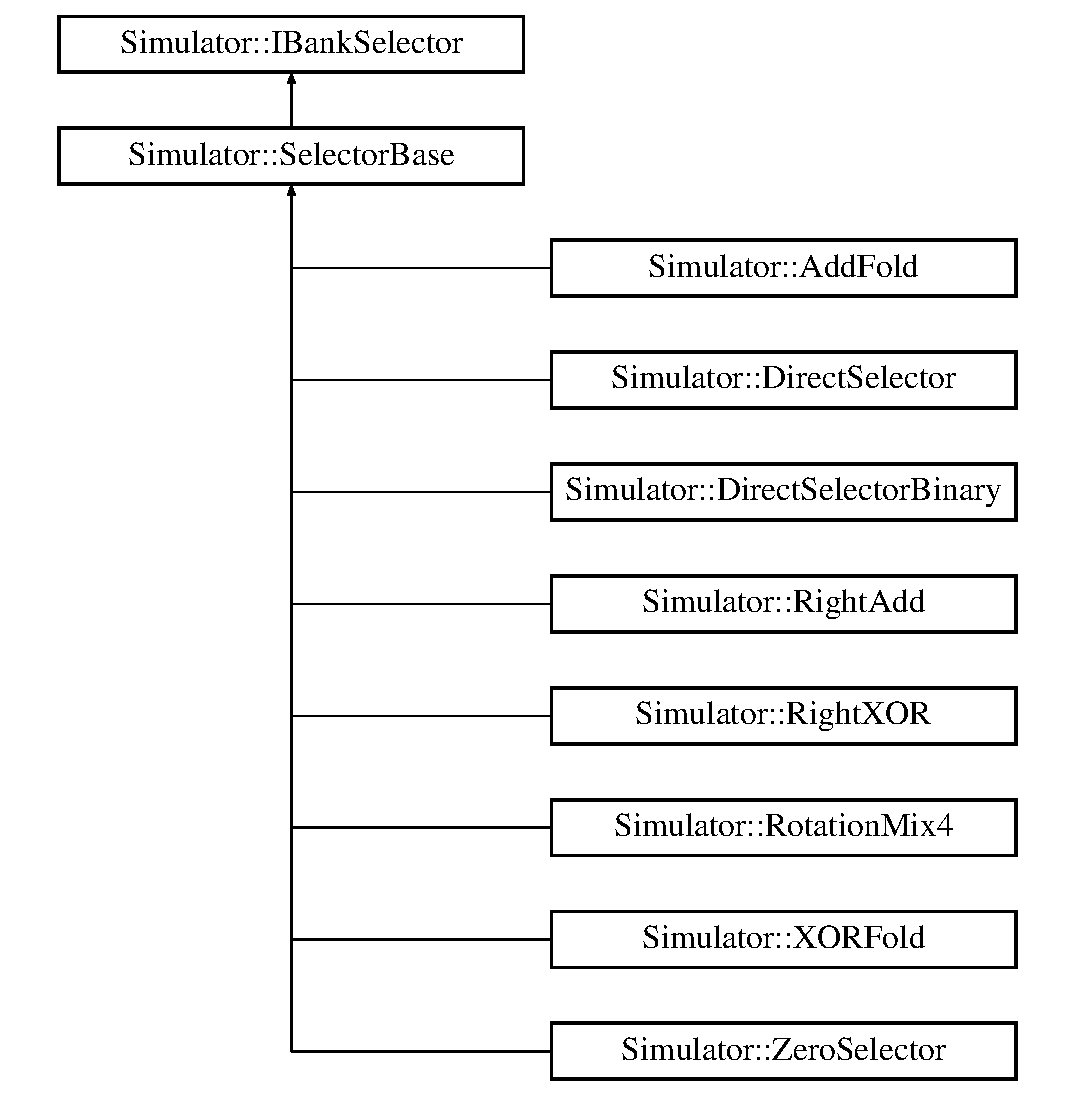
\includegraphics[height=10.000000cm]{class_simulator_1_1_i_bank_selector}
\end{center}
\end{figure}
\subsection*{Public Member Functions}
\begin{DoxyCompactItemize}
\item 
virtual void \hyperlink{class_simulator_1_1_i_bank_selector_ad945160c483d88073b6e5572da5e4507}{Map} (Mem\+Addr address, Mem\+Addr \&tag, size\+\_\+t \&index)=0
\item 
virtual Mem\+Addr \hyperlink{class_simulator_1_1_i_bank_selector_a57c8b49e6439984ff40836e8c5992aba}{Unmap} (Mem\+Addr tag, size\+\_\+t index)=0
\item 
virtual std\+::string \hyperlink{class_simulator_1_1_i_bank_selector_afcc0edfb17b9390058a3732f8a8f9d67}{Get\+Name} () const =0
\item 
virtual size\+\_\+t \hyperlink{class_simulator_1_1_i_bank_selector_ac60b4a5485eff722861a1a0df7719340}{Get\+Num\+Banks} () const =0
\item 
virtual \hyperlink{class_simulator_1_1_i_bank_selector_a1c367af3c1f83c1aabc8bb72612efc90}{$\sim$\+I\+Bank\+Selector} ()
\end{DoxyCompactItemize}
\subsection*{Static Public Member Functions}
\begin{DoxyCompactItemize}
\item 
static \hyperlink{class_simulator_1_1_i_bank_selector}{I\+Bank\+Selector} $\ast$ \hyperlink{class_simulator_1_1_i_bank_selector_a95c6263915797a92f7b96c5ae94a10e1}{make\+Selector} (\hyperlink{class_simulator_1_1_object}{Object} \&parent, const std\+::string \&\hyperlink{mtconf_8c_a8f8f80d37794cde9472343e4487ba3eb}{name}, size\+\_\+t num\+Banks)
\end{DoxyCompactItemize}


\subsection{Constructor \& Destructor Documentation}
\hypertarget{class_simulator_1_1_i_bank_selector_a1c367af3c1f83c1aabc8bb72612efc90}{\index{Simulator\+::\+I\+Bank\+Selector@{Simulator\+::\+I\+Bank\+Selector}!````~I\+Bank\+Selector@{$\sim$\+I\+Bank\+Selector}}
\index{````~I\+Bank\+Selector@{$\sim$\+I\+Bank\+Selector}!Simulator\+::\+I\+Bank\+Selector@{Simulator\+::\+I\+Bank\+Selector}}
\subsubsection[{$\sim$\+I\+Bank\+Selector}]{\setlength{\rightskip}{0pt plus 5cm}virtual Simulator\+::\+I\+Bank\+Selector\+::$\sim$\+I\+Bank\+Selector (
\begin{DoxyParamCaption}
{}
\end{DoxyParamCaption}
)\hspace{0.3cm}{\ttfamily [inline]}, {\ttfamily [virtual]}}}\label{class_simulator_1_1_i_bank_selector_a1c367af3c1f83c1aabc8bb72612efc90}


\subsection{Member Function Documentation}
\hypertarget{class_simulator_1_1_i_bank_selector_afcc0edfb17b9390058a3732f8a8f9d67}{\index{Simulator\+::\+I\+Bank\+Selector@{Simulator\+::\+I\+Bank\+Selector}!Get\+Name@{Get\+Name}}
\index{Get\+Name@{Get\+Name}!Simulator\+::\+I\+Bank\+Selector@{Simulator\+::\+I\+Bank\+Selector}}
\subsubsection[{Get\+Name}]{\setlength{\rightskip}{0pt plus 5cm}virtual std\+::string Simulator\+::\+I\+Bank\+Selector\+::\+Get\+Name (
\begin{DoxyParamCaption}
{}
\end{DoxyParamCaption}
) const\hspace{0.3cm}{\ttfamily [pure virtual]}}}\label{class_simulator_1_1_i_bank_selector_afcc0edfb17b9390058a3732f8a8f9d67}


Implemented in \hyperlink{class_simulator_1_1_selector_base_a4b629550677073368f8f6adf2217cb8c}{Simulator\+::\+Selector\+Base}.

\hypertarget{class_simulator_1_1_i_bank_selector_ac60b4a5485eff722861a1a0df7719340}{\index{Simulator\+::\+I\+Bank\+Selector@{Simulator\+::\+I\+Bank\+Selector}!Get\+Num\+Banks@{Get\+Num\+Banks}}
\index{Get\+Num\+Banks@{Get\+Num\+Banks}!Simulator\+::\+I\+Bank\+Selector@{Simulator\+::\+I\+Bank\+Selector}}
\subsubsection[{Get\+Num\+Banks}]{\setlength{\rightskip}{0pt plus 5cm}virtual size\+\_\+t Simulator\+::\+I\+Bank\+Selector\+::\+Get\+Num\+Banks (
\begin{DoxyParamCaption}
{}
\end{DoxyParamCaption}
) const\hspace{0.3cm}{\ttfamily [pure virtual]}}}\label{class_simulator_1_1_i_bank_selector_ac60b4a5485eff722861a1a0df7719340}


Implemented in \hyperlink{class_simulator_1_1_selector_base_ac12eca83b007d3a1b1b3c921e48f6d64}{Simulator\+::\+Selector\+Base}.

\hypertarget{class_simulator_1_1_i_bank_selector_a95c6263915797a92f7b96c5ae94a10e1}{\index{Simulator\+::\+I\+Bank\+Selector@{Simulator\+::\+I\+Bank\+Selector}!make\+Selector@{make\+Selector}}
\index{make\+Selector@{make\+Selector}!Simulator\+::\+I\+Bank\+Selector@{Simulator\+::\+I\+Bank\+Selector}}
\subsubsection[{make\+Selector}]{\setlength{\rightskip}{0pt plus 5cm}{\bf I\+Bank\+Selector} $\ast$ Simulator\+::\+I\+Bank\+Selector\+::make\+Selector (
\begin{DoxyParamCaption}
\item[{{\bf Object} \&}]{parent, }
\item[{const std\+::string \&}]{name, }
\item[{size\+\_\+t}]{num\+Banks}
\end{DoxyParamCaption}
)\hspace{0.3cm}{\ttfamily [static]}}}\label{class_simulator_1_1_i_bank_selector_a95c6263915797a92f7b96c5ae94a10e1}
\hypertarget{class_simulator_1_1_i_bank_selector_ad945160c483d88073b6e5572da5e4507}{\index{Simulator\+::\+I\+Bank\+Selector@{Simulator\+::\+I\+Bank\+Selector}!Map@{Map}}
\index{Map@{Map}!Simulator\+::\+I\+Bank\+Selector@{Simulator\+::\+I\+Bank\+Selector}}
\subsubsection[{Map}]{\setlength{\rightskip}{0pt plus 5cm}virtual void Simulator\+::\+I\+Bank\+Selector\+::\+Map (
\begin{DoxyParamCaption}
\item[{Mem\+Addr}]{address, }
\item[{Mem\+Addr \&}]{tag, }
\item[{size\+\_\+t \&}]{index}
\end{DoxyParamCaption}
)\hspace{0.3cm}{\ttfamily [pure virtual]}}}\label{class_simulator_1_1_i_bank_selector_ad945160c483d88073b6e5572da5e4507}


Implemented in \hyperlink{class_simulator_1_1_add_fold_a8b06e012e21b17873647a21a25f9d0b9}{Simulator\+::\+Add\+Fold}, \hyperlink{class_simulator_1_1_x_o_r_fold_a05b1b2b1f8da6230d7b4529a918d9ace}{Simulator\+::\+X\+O\+R\+Fold}, \hyperlink{class_simulator_1_1_right_add_a271dc58bbae9ced6d66c6e15bb077414}{Simulator\+::\+Right\+Add}, \hyperlink{class_simulator_1_1_right_x_o_r_a8002d877e2efcd79fbe2ba1a1929a203}{Simulator\+::\+Right\+X\+O\+R}, \hyperlink{class_simulator_1_1_rotation_mix4_ae52d1a5bc6116ec8adc610f9d67ec71e}{Simulator\+::\+Rotation\+Mix4}, \hyperlink{class_simulator_1_1_direct_selector_binary_a94319702a48838522bc5972ef5a28727}{Simulator\+::\+Direct\+Selector\+Binary}, \hyperlink{class_simulator_1_1_direct_selector_aa1e89a7c1d907e1b47fe005af9368b8f}{Simulator\+::\+Direct\+Selector}, and \hyperlink{class_simulator_1_1_zero_selector_aeb7f36bcb195ea288525d4d4b55c6e85}{Simulator\+::\+Zero\+Selector}.

\hypertarget{class_simulator_1_1_i_bank_selector_a57c8b49e6439984ff40836e8c5992aba}{\index{Simulator\+::\+I\+Bank\+Selector@{Simulator\+::\+I\+Bank\+Selector}!Unmap@{Unmap}}
\index{Unmap@{Unmap}!Simulator\+::\+I\+Bank\+Selector@{Simulator\+::\+I\+Bank\+Selector}}
\subsubsection[{Unmap}]{\setlength{\rightskip}{0pt plus 5cm}virtual Mem\+Addr Simulator\+::\+I\+Bank\+Selector\+::\+Unmap (
\begin{DoxyParamCaption}
\item[{Mem\+Addr}]{tag, }
\item[{size\+\_\+t}]{index}
\end{DoxyParamCaption}
)\hspace{0.3cm}{\ttfamily [pure virtual]}}}\label{class_simulator_1_1_i_bank_selector_a57c8b49e6439984ff40836e8c5992aba}


Implemented in \hyperlink{class_simulator_1_1_add_fold_a020d74e9f256a128ea47d0fb6acd4eb7}{Simulator\+::\+Add\+Fold}, \hyperlink{class_simulator_1_1_x_o_r_fold_aa2cba6de60eb398e5da8f30d47a3eba1}{Simulator\+::\+X\+O\+R\+Fold}, \hyperlink{class_simulator_1_1_right_add_a02795f537e733cefb15b81aaad47482e}{Simulator\+::\+Right\+Add}, \hyperlink{class_simulator_1_1_right_x_o_r_afa74a84305adbf0fbdceebbfade3d26a}{Simulator\+::\+Right\+X\+O\+R}, \hyperlink{class_simulator_1_1_rotation_mix4_adc84ef656797f5a5c9265d68351e9459}{Simulator\+::\+Rotation\+Mix4}, \hyperlink{class_simulator_1_1_direct_selector_binary_a72fd9cee90911f43ebe3b293bb71ce98}{Simulator\+::\+Direct\+Selector\+Binary}, \hyperlink{class_simulator_1_1_direct_selector_a2b7aab1bf3bdcd0bc95d65d93b863583}{Simulator\+::\+Direct\+Selector}, and \hyperlink{class_simulator_1_1_zero_selector_a02bd494a5b4246fc491536b8b0ac9b03}{Simulator\+::\+Zero\+Selector}.



The documentation for this class was generated from the following files\+:\begin{DoxyCompactItemize}
\item 
arch/\hyperlink{_bank_selector_8h}{Bank\+Selector.\+h}\item 
arch/\hyperlink{_bank_selector_8cpp}{Bank\+Selector.\+cpp}\end{DoxyCompactItemize}

\hypertarget{class_simulator_1_1drisc_1_1_i_cache}{\section{Simulator\+:\+:drisc\+:\+:I\+Cache Class Reference}
\label{class_simulator_1_1drisc_1_1_i_cache}\index{Simulator\+::drisc\+::\+I\+Cache@{Simulator\+::drisc\+::\+I\+Cache}}
}


{\ttfamily \#include $<$I\+Cache.\+h$>$}

Inheritance diagram for Simulator\+:\+:drisc\+:\+:I\+Cache\+:\begin{figure}[H]
\begin{center}
\leavevmode
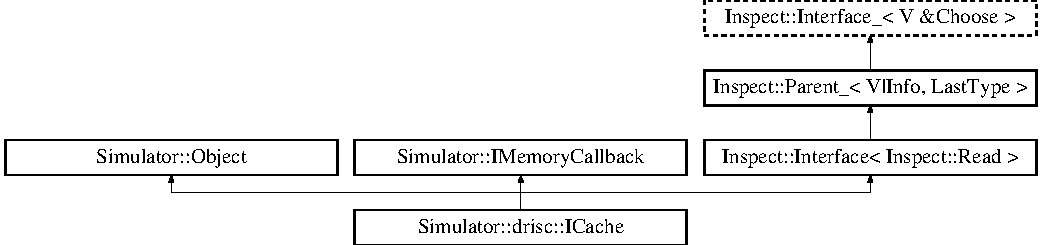
\includegraphics[height=3.289281cm]{class_simulator_1_1drisc_1_1_i_cache}
\end{center}
\end{figure}
\subsection*{Public Member Functions}
\begin{DoxyCompactItemize}
\item 
\hyperlink{class_simulator_1_1drisc_1_1_i_cache_abccbf70d026fcd78e099fe46941ee1ef}{I\+Cache} (const std\+::string \&\hyperlink{mtconf_8c_a8f8f80d37794cde9472343e4487ba3eb}{name}, \hyperlink{class_simulator_1_1_d_r_i_s_c}{D\+R\+I\+S\+C} \&parent, \hyperlink{class_simulator_1_1_clock}{Clock} \&clock, \hyperlink{class_config}{Config} \&config)
\item 
\hyperlink{class_simulator_1_1drisc_1_1_i_cache_a5da34e6e93ff85df68fef014b318792c}{I\+Cache} (const \hyperlink{class_simulator_1_1drisc_1_1_i_cache}{I\+Cache} \&)=delete
\item 
\hyperlink{class_simulator_1_1drisc_1_1_i_cache}{I\+Cache} \& \hyperlink{class_simulator_1_1drisc_1_1_i_cache_a1c8adc5c5595fac4b6cdb00f9ae990cc}{operator=} (const \hyperlink{class_simulator_1_1drisc_1_1_i_cache}{I\+Cache} \&)=delete
\item 
\hyperlink{class_simulator_1_1drisc_1_1_i_cache_a432627a76862df4755a991d5fe34a307}{$\sim$\+I\+Cache} ()
\item 
void \hyperlink{class_simulator_1_1drisc_1_1_i_cache_a4d67069af1ac468ddc91e9b5eee096c8}{Connect\+Memory} (\hyperlink{class_simulator_1_1_i_memory}{I\+Memory} $\ast$memory)
\item 
\hyperlink{namespace_simulator_a4b6b5616e7236c0c131516a441776805}{Result} \hyperlink{class_simulator_1_1drisc_1_1_i_cache_a662072b848e493954869c6cf35384368}{Fetch} (Mem\+Addr address, Mem\+Size size, \hyperlink{namespace_simulator_a97f45fafcb1aafc0f269a19608b39d60}{C\+I\+D} \&cid)
\item 
\hyperlink{namespace_simulator_a4b6b5616e7236c0c131516a441776805}{Result} \hyperlink{class_simulator_1_1drisc_1_1_i_cache_ad30934eac15d9722ad5947c33368d47b}{Fetch} (Mem\+Addr address, Mem\+Size size, \hyperlink{namespace_simulator_a483cc4ecee1736e895054617672cded5}{T\+I\+D} \&tid, \hyperlink{namespace_simulator_a97f45fafcb1aafc0f269a19608b39d60}{C\+I\+D} \&cid)
\item 
bool \hyperlink{class_simulator_1_1drisc_1_1_i_cache_a5e1200c1c47897335d9a492b6f4dd664}{Read} (\hyperlink{namespace_simulator_a97f45fafcb1aafc0f269a19608b39d60}{C\+I\+D} cid, Mem\+Addr address, void $\ast$data, Mem\+Size size) const 
\item 
bool \hyperlink{class_simulator_1_1drisc_1_1_i_cache_ad92a2d648a3b0aa97baff394c1751944}{Release\+Cache\+Line} (\hyperlink{namespace_simulator_a97f45fafcb1aafc0f269a19608b39d60}{C\+I\+D} bid)
\item 
bool \hyperlink{class_simulator_1_1drisc_1_1_i_cache_a235db7340ebe82220a35410cd61ce08c}{Is\+Empty} () const 
\item 
bool \hyperlink{class_simulator_1_1drisc_1_1_i_cache_aef4cb1f1456f90f644dd4697eeca2bb4}{On\+Memory\+Read\+Completed} (Mem\+Addr addr, const char $\ast$data) override
\item 
bool \hyperlink{class_simulator_1_1drisc_1_1_i_cache_ad07b2819c8bdf6a286eb484647d75d98}{On\+Memory\+Write\+Completed} (\hyperlink{namespace_simulator_a483cc4ecee1736e895054617672cded5}{T\+I\+D} tid) override
\item 
bool \hyperlink{class_simulator_1_1drisc_1_1_i_cache_a8d4a3d21efa066f6d624ec2bc3a8b370}{On\+Memory\+Snooped} (Mem\+Addr addr, const char $\ast$data, const bool $\ast$mask) override
\item 
bool \hyperlink{class_simulator_1_1drisc_1_1_i_cache_a53d755323405ba6efab15371ba95a435}{On\+Memory\+Invalidated} (Mem\+Addr addr) override
\item 
\hyperlink{class_simulator_1_1_object}{Object} \& \hyperlink{class_simulator_1_1drisc_1_1_i_cache_a389ebf0f8eec8d1f07752e97fda96176}{Get\+Memory\+Peer} () override
\item 
size\+\_\+t \hyperlink{class_simulator_1_1drisc_1_1_i_cache_a30b7686fc0988c3e40706ba58f2e17d2}{Get\+Line\+Size} () const 
\item 
size\+\_\+t \hyperlink{class_simulator_1_1drisc_1_1_i_cache_a720cfa1806d5676ab282e9fe2eb78f36}{Get\+Associativity} () const 
\item 
size\+\_\+t \hyperlink{class_simulator_1_1drisc_1_1_i_cache_a46cb90cbdd79699ba749b91be730a5d8}{Get\+Num\+Lines} () const 
\item 
size\+\_\+t \hyperlink{class_simulator_1_1drisc_1_1_i_cache_aaeb3d54075721320f8a553116c0b379f}{Get\+Num\+Sets} () const 
\item 
void \hyperlink{class_simulator_1_1drisc_1_1_i_cache_a64a13ee6d0ebcb28774f8443f140377c}{Cmd\+\_\+\+Info} (std\+::ostream \&out, const std\+::vector$<$ std\+::string $>$ \&arguments) const override
\item 
void \hyperlink{class_simulator_1_1drisc_1_1_i_cache_a3da79bb809b6d825c00aac432ae0b8b0}{Cmd\+\_\+\+Read} (std\+::ostream \&out, const std\+::vector$<$ std\+::string $>$ \&arguments) const override
\end{DoxyCompactItemize}
\subsection*{Public Attributes}
\begin{DoxyCompactItemize}
\item 
\hyperlink{class_simulator_1_1_process}{Process} \hyperlink{class_simulator_1_1drisc_1_1_i_cache_a42bdcd5c4c51aa0aa20ccfc1ee7fa8f4}{p\+\_\+\+Outgoing}
\item 
\hyperlink{class_simulator_1_1_process}{Process} \hyperlink{class_simulator_1_1drisc_1_1_i_cache_a8cb7be6c13ade7c94c86776ec50b8057}{p\+\_\+\+Incoming}
\item 
\hyperlink{class_simulator_1_1_arbitrated_service}{Arbitrated\+Service} \hyperlink{class_simulator_1_1drisc_1_1_i_cache_a4dffa2890e3dcb4a447c3d3a108f9d2c}{p\+\_\+service}
\end{DoxyCompactItemize}
\subsection*{Friends}
\begin{DoxyCompactItemize}
\item 
class \hyperlink{class_simulator_1_1drisc_1_1_i_cache_a14f94eb83e17d9d8841f39b37431d673}{Simulator\+::\+D\+R\+I\+S\+C}
\end{DoxyCompactItemize}


\subsection{Constructor \& Destructor Documentation}
\hypertarget{class_simulator_1_1drisc_1_1_i_cache_abccbf70d026fcd78e099fe46941ee1ef}{\index{Simulator\+::drisc\+::\+I\+Cache@{Simulator\+::drisc\+::\+I\+Cache}!I\+Cache@{I\+Cache}}
\index{I\+Cache@{I\+Cache}!Simulator\+::drisc\+::\+I\+Cache@{Simulator\+::drisc\+::\+I\+Cache}}
\subsubsection[{I\+Cache}]{\setlength{\rightskip}{0pt plus 5cm}Simulator\+::drisc\+::\+I\+Cache\+::\+I\+Cache (
\begin{DoxyParamCaption}
\item[{const std\+::string \&}]{name, }
\item[{{\bf D\+R\+I\+S\+C} \&}]{parent, }
\item[{{\bf Clock} \&}]{clock, }
\item[{{\bf Config} \&}]{config}
\end{DoxyParamCaption}
)}}\label{class_simulator_1_1drisc_1_1_i_cache_abccbf70d026fcd78e099fe46941ee1ef}
\hypertarget{class_simulator_1_1drisc_1_1_i_cache_a5da34e6e93ff85df68fef014b318792c}{\index{Simulator\+::drisc\+::\+I\+Cache@{Simulator\+::drisc\+::\+I\+Cache}!I\+Cache@{I\+Cache}}
\index{I\+Cache@{I\+Cache}!Simulator\+::drisc\+::\+I\+Cache@{Simulator\+::drisc\+::\+I\+Cache}}
\subsubsection[{I\+Cache}]{\setlength{\rightskip}{0pt plus 5cm}Simulator\+::drisc\+::\+I\+Cache\+::\+I\+Cache (
\begin{DoxyParamCaption}
\item[{const {\bf I\+Cache} \&}]{}
\end{DoxyParamCaption}
)\hspace{0.3cm}{\ttfamily [delete]}}}\label{class_simulator_1_1drisc_1_1_i_cache_a5da34e6e93ff85df68fef014b318792c}
\hypertarget{class_simulator_1_1drisc_1_1_i_cache_a432627a76862df4755a991d5fe34a307}{\index{Simulator\+::drisc\+::\+I\+Cache@{Simulator\+::drisc\+::\+I\+Cache}!````~I\+Cache@{$\sim$\+I\+Cache}}
\index{````~I\+Cache@{$\sim$\+I\+Cache}!Simulator\+::drisc\+::\+I\+Cache@{Simulator\+::drisc\+::\+I\+Cache}}
\subsubsection[{$\sim$\+I\+Cache}]{\setlength{\rightskip}{0pt plus 5cm}Simulator\+::drisc\+::\+I\+Cache\+::$\sim$\+I\+Cache (
\begin{DoxyParamCaption}
{}
\end{DoxyParamCaption}
)}}\label{class_simulator_1_1drisc_1_1_i_cache_a432627a76862df4755a991d5fe34a307}


\subsection{Member Function Documentation}
\hypertarget{class_simulator_1_1drisc_1_1_i_cache_a64a13ee6d0ebcb28774f8443f140377c}{\index{Simulator\+::drisc\+::\+I\+Cache@{Simulator\+::drisc\+::\+I\+Cache}!Cmd\+\_\+\+Info@{Cmd\+\_\+\+Info}}
\index{Cmd\+\_\+\+Info@{Cmd\+\_\+\+Info}!Simulator\+::drisc\+::\+I\+Cache@{Simulator\+::drisc\+::\+I\+Cache}}
\subsubsection[{Cmd\+\_\+\+Info}]{\setlength{\rightskip}{0pt plus 5cm}void Simulator\+::drisc\+::\+I\+Cache\+::\+Cmd\+\_\+\+Info (
\begin{DoxyParamCaption}
\item[{std\+::ostream \&}]{out, }
\item[{const std\+::vector$<$ std\+::string $>$ \&}]{arguments}
\end{DoxyParamCaption}
) const\hspace{0.3cm}{\ttfamily [override]}}}\label{class_simulator_1_1drisc_1_1_i_cache_a64a13ee6d0ebcb28774f8443f140377c}
\hypertarget{class_simulator_1_1drisc_1_1_i_cache_a3da79bb809b6d825c00aac432ae0b8b0}{\index{Simulator\+::drisc\+::\+I\+Cache@{Simulator\+::drisc\+::\+I\+Cache}!Cmd\+\_\+\+Read@{Cmd\+\_\+\+Read}}
\index{Cmd\+\_\+\+Read@{Cmd\+\_\+\+Read}!Simulator\+::drisc\+::\+I\+Cache@{Simulator\+::drisc\+::\+I\+Cache}}
\subsubsection[{Cmd\+\_\+\+Read}]{\setlength{\rightskip}{0pt plus 5cm}void Simulator\+::drisc\+::\+I\+Cache\+::\+Cmd\+\_\+\+Read (
\begin{DoxyParamCaption}
\item[{std\+::ostream \&}]{out, }
\item[{const std\+::vector$<$ std\+::string $>$ \&}]{arguments}
\end{DoxyParamCaption}
) const\hspace{0.3cm}{\ttfamily [override]}}}\label{class_simulator_1_1drisc_1_1_i_cache_a3da79bb809b6d825c00aac432ae0b8b0}
\hypertarget{class_simulator_1_1drisc_1_1_i_cache_a4d67069af1ac468ddc91e9b5eee096c8}{\index{Simulator\+::drisc\+::\+I\+Cache@{Simulator\+::drisc\+::\+I\+Cache}!Connect\+Memory@{Connect\+Memory}}
\index{Connect\+Memory@{Connect\+Memory}!Simulator\+::drisc\+::\+I\+Cache@{Simulator\+::drisc\+::\+I\+Cache}}
\subsubsection[{Connect\+Memory}]{\setlength{\rightskip}{0pt plus 5cm}void Simulator\+::drisc\+::\+I\+Cache\+::\+Connect\+Memory (
\begin{DoxyParamCaption}
\item[{{\bf I\+Memory} $\ast$}]{memory}
\end{DoxyParamCaption}
)}}\label{class_simulator_1_1drisc_1_1_i_cache_a4d67069af1ac468ddc91e9b5eee096c8}
\hypertarget{class_simulator_1_1drisc_1_1_i_cache_a662072b848e493954869c6cf35384368}{\index{Simulator\+::drisc\+::\+I\+Cache@{Simulator\+::drisc\+::\+I\+Cache}!Fetch@{Fetch}}
\index{Fetch@{Fetch}!Simulator\+::drisc\+::\+I\+Cache@{Simulator\+::drisc\+::\+I\+Cache}}
\subsubsection[{Fetch}]{\setlength{\rightskip}{0pt plus 5cm}{\bf Result} Simulator\+::drisc\+::\+I\+Cache\+::\+Fetch (
\begin{DoxyParamCaption}
\item[{Mem\+Addr}]{address, }
\item[{Mem\+Size}]{size, }
\item[{{\bf C\+I\+D} \&}]{cid}
\end{DoxyParamCaption}
)}}\label{class_simulator_1_1drisc_1_1_i_cache_a662072b848e493954869c6cf35384368}
\hypertarget{class_simulator_1_1drisc_1_1_i_cache_ad30934eac15d9722ad5947c33368d47b}{\index{Simulator\+::drisc\+::\+I\+Cache@{Simulator\+::drisc\+::\+I\+Cache}!Fetch@{Fetch}}
\index{Fetch@{Fetch}!Simulator\+::drisc\+::\+I\+Cache@{Simulator\+::drisc\+::\+I\+Cache}}
\subsubsection[{Fetch}]{\setlength{\rightskip}{0pt plus 5cm}{\bf Result} Simulator\+::drisc\+::\+I\+Cache\+::\+Fetch (
\begin{DoxyParamCaption}
\item[{Mem\+Addr}]{address, }
\item[{Mem\+Size}]{size, }
\item[{{\bf T\+I\+D} \&}]{tid, }
\item[{{\bf C\+I\+D} \&}]{cid}
\end{DoxyParamCaption}
)}}\label{class_simulator_1_1drisc_1_1_i_cache_ad30934eac15d9722ad5947c33368d47b}
\hypertarget{class_simulator_1_1drisc_1_1_i_cache_a720cfa1806d5676ab282e9fe2eb78f36}{\index{Simulator\+::drisc\+::\+I\+Cache@{Simulator\+::drisc\+::\+I\+Cache}!Get\+Associativity@{Get\+Associativity}}
\index{Get\+Associativity@{Get\+Associativity}!Simulator\+::drisc\+::\+I\+Cache@{Simulator\+::drisc\+::\+I\+Cache}}
\subsubsection[{Get\+Associativity}]{\setlength{\rightskip}{0pt plus 5cm}size\+\_\+t Simulator\+::drisc\+::\+I\+Cache\+::\+Get\+Associativity (
\begin{DoxyParamCaption}
{}
\end{DoxyParamCaption}
) const\hspace{0.3cm}{\ttfamily [inline]}}}\label{class_simulator_1_1drisc_1_1_i_cache_a720cfa1806d5676ab282e9fe2eb78f36}
\hypertarget{class_simulator_1_1drisc_1_1_i_cache_a30b7686fc0988c3e40706ba58f2e17d2}{\index{Simulator\+::drisc\+::\+I\+Cache@{Simulator\+::drisc\+::\+I\+Cache}!Get\+Line\+Size@{Get\+Line\+Size}}
\index{Get\+Line\+Size@{Get\+Line\+Size}!Simulator\+::drisc\+::\+I\+Cache@{Simulator\+::drisc\+::\+I\+Cache}}
\subsubsection[{Get\+Line\+Size}]{\setlength{\rightskip}{0pt plus 5cm}size\+\_\+t Simulator\+::drisc\+::\+I\+Cache\+::\+Get\+Line\+Size (
\begin{DoxyParamCaption}
{}
\end{DoxyParamCaption}
) const\hspace{0.3cm}{\ttfamily [inline]}}}\label{class_simulator_1_1drisc_1_1_i_cache_a30b7686fc0988c3e40706ba58f2e17d2}
\hypertarget{class_simulator_1_1drisc_1_1_i_cache_a389ebf0f8eec8d1f07752e97fda96176}{\index{Simulator\+::drisc\+::\+I\+Cache@{Simulator\+::drisc\+::\+I\+Cache}!Get\+Memory\+Peer@{Get\+Memory\+Peer}}
\index{Get\+Memory\+Peer@{Get\+Memory\+Peer}!Simulator\+::drisc\+::\+I\+Cache@{Simulator\+::drisc\+::\+I\+Cache}}
\subsubsection[{Get\+Memory\+Peer}]{\setlength{\rightskip}{0pt plus 5cm}{\bf Object} \& Simulator\+::drisc\+::\+I\+Cache\+::\+Get\+Memory\+Peer (
\begin{DoxyParamCaption}
{}
\end{DoxyParamCaption}
)\hspace{0.3cm}{\ttfamily [override]}, {\ttfamily [virtual]}}}\label{class_simulator_1_1drisc_1_1_i_cache_a389ebf0f8eec8d1f07752e97fda96176}


Implements \hyperlink{class_simulator_1_1_i_memory_callback_ab378a4b6ce2df8e4a38bb3e8f116a064}{Simulator\+::\+I\+Memory\+Callback}.

\hypertarget{class_simulator_1_1drisc_1_1_i_cache_a46cb90cbdd79699ba749b91be730a5d8}{\index{Simulator\+::drisc\+::\+I\+Cache@{Simulator\+::drisc\+::\+I\+Cache}!Get\+Num\+Lines@{Get\+Num\+Lines}}
\index{Get\+Num\+Lines@{Get\+Num\+Lines}!Simulator\+::drisc\+::\+I\+Cache@{Simulator\+::drisc\+::\+I\+Cache}}
\subsubsection[{Get\+Num\+Lines}]{\setlength{\rightskip}{0pt plus 5cm}size\+\_\+t Simulator\+::drisc\+::\+I\+Cache\+::\+Get\+Num\+Lines (
\begin{DoxyParamCaption}
{}
\end{DoxyParamCaption}
) const\hspace{0.3cm}{\ttfamily [inline]}}}\label{class_simulator_1_1drisc_1_1_i_cache_a46cb90cbdd79699ba749b91be730a5d8}
\hypertarget{class_simulator_1_1drisc_1_1_i_cache_aaeb3d54075721320f8a553116c0b379f}{\index{Simulator\+::drisc\+::\+I\+Cache@{Simulator\+::drisc\+::\+I\+Cache}!Get\+Num\+Sets@{Get\+Num\+Sets}}
\index{Get\+Num\+Sets@{Get\+Num\+Sets}!Simulator\+::drisc\+::\+I\+Cache@{Simulator\+::drisc\+::\+I\+Cache}}
\subsubsection[{Get\+Num\+Sets}]{\setlength{\rightskip}{0pt plus 5cm}size\+\_\+t Simulator\+::drisc\+::\+I\+Cache\+::\+Get\+Num\+Sets (
\begin{DoxyParamCaption}
{}
\end{DoxyParamCaption}
) const\hspace{0.3cm}{\ttfamily [inline]}}}\label{class_simulator_1_1drisc_1_1_i_cache_aaeb3d54075721320f8a553116c0b379f}
\hypertarget{class_simulator_1_1drisc_1_1_i_cache_a235db7340ebe82220a35410cd61ce08c}{\index{Simulator\+::drisc\+::\+I\+Cache@{Simulator\+::drisc\+::\+I\+Cache}!Is\+Empty@{Is\+Empty}}
\index{Is\+Empty@{Is\+Empty}!Simulator\+::drisc\+::\+I\+Cache@{Simulator\+::drisc\+::\+I\+Cache}}
\subsubsection[{Is\+Empty}]{\setlength{\rightskip}{0pt plus 5cm}bool Simulator\+::drisc\+::\+I\+Cache\+::\+Is\+Empty (
\begin{DoxyParamCaption}
{}
\end{DoxyParamCaption}
) const}}\label{class_simulator_1_1drisc_1_1_i_cache_a235db7340ebe82220a35410cd61ce08c}
\hypertarget{class_simulator_1_1drisc_1_1_i_cache_a53d755323405ba6efab15371ba95a435}{\index{Simulator\+::drisc\+::\+I\+Cache@{Simulator\+::drisc\+::\+I\+Cache}!On\+Memory\+Invalidated@{On\+Memory\+Invalidated}}
\index{On\+Memory\+Invalidated@{On\+Memory\+Invalidated}!Simulator\+::drisc\+::\+I\+Cache@{Simulator\+::drisc\+::\+I\+Cache}}
\subsubsection[{On\+Memory\+Invalidated}]{\setlength{\rightskip}{0pt plus 5cm}bool Simulator\+::drisc\+::\+I\+Cache\+::\+On\+Memory\+Invalidated (
\begin{DoxyParamCaption}
\item[{Mem\+Addr}]{addr}
\end{DoxyParamCaption}
)\hspace{0.3cm}{\ttfamily [override]}, {\ttfamily [virtual]}}}\label{class_simulator_1_1drisc_1_1_i_cache_a53d755323405ba6efab15371ba95a435}


Implements \hyperlink{class_simulator_1_1_i_memory_callback_a8a50686620585ffe62e754a9e96b79a8}{Simulator\+::\+I\+Memory\+Callback}.

\hypertarget{class_simulator_1_1drisc_1_1_i_cache_aef4cb1f1456f90f644dd4697eeca2bb4}{\index{Simulator\+::drisc\+::\+I\+Cache@{Simulator\+::drisc\+::\+I\+Cache}!On\+Memory\+Read\+Completed@{On\+Memory\+Read\+Completed}}
\index{On\+Memory\+Read\+Completed@{On\+Memory\+Read\+Completed}!Simulator\+::drisc\+::\+I\+Cache@{Simulator\+::drisc\+::\+I\+Cache}}
\subsubsection[{On\+Memory\+Read\+Completed}]{\setlength{\rightskip}{0pt plus 5cm}bool Simulator\+::drisc\+::\+I\+Cache\+::\+On\+Memory\+Read\+Completed (
\begin{DoxyParamCaption}
\item[{Mem\+Addr}]{addr, }
\item[{const char $\ast$}]{data}
\end{DoxyParamCaption}
)\hspace{0.3cm}{\ttfamily [override]}, {\ttfamily [virtual]}}}\label{class_simulator_1_1drisc_1_1_i_cache_aef4cb1f1456f90f644dd4697eeca2bb4}


Implements \hyperlink{class_simulator_1_1_i_memory_callback_a5519817c435767dab3b4c063e601d9f7}{Simulator\+::\+I\+Memory\+Callback}.

\hypertarget{class_simulator_1_1drisc_1_1_i_cache_a8d4a3d21efa066f6d624ec2bc3a8b370}{\index{Simulator\+::drisc\+::\+I\+Cache@{Simulator\+::drisc\+::\+I\+Cache}!On\+Memory\+Snooped@{On\+Memory\+Snooped}}
\index{On\+Memory\+Snooped@{On\+Memory\+Snooped}!Simulator\+::drisc\+::\+I\+Cache@{Simulator\+::drisc\+::\+I\+Cache}}
\subsubsection[{On\+Memory\+Snooped}]{\setlength{\rightskip}{0pt plus 5cm}bool Simulator\+::drisc\+::\+I\+Cache\+::\+On\+Memory\+Snooped (
\begin{DoxyParamCaption}
\item[{Mem\+Addr}]{addr, }
\item[{const char $\ast$}]{data, }
\item[{const bool $\ast$}]{mask}
\end{DoxyParamCaption}
)\hspace{0.3cm}{\ttfamily [override]}, {\ttfamily [virtual]}}}\label{class_simulator_1_1drisc_1_1_i_cache_a8d4a3d21efa066f6d624ec2bc3a8b370}


Reimplemented from \hyperlink{class_simulator_1_1_i_memory_callback_a41e84f41d39e538c2ab0c056d8c1b0e2}{Simulator\+::\+I\+Memory\+Callback}.

\hypertarget{class_simulator_1_1drisc_1_1_i_cache_ad07b2819c8bdf6a286eb484647d75d98}{\index{Simulator\+::drisc\+::\+I\+Cache@{Simulator\+::drisc\+::\+I\+Cache}!On\+Memory\+Write\+Completed@{On\+Memory\+Write\+Completed}}
\index{On\+Memory\+Write\+Completed@{On\+Memory\+Write\+Completed}!Simulator\+::drisc\+::\+I\+Cache@{Simulator\+::drisc\+::\+I\+Cache}}
\subsubsection[{On\+Memory\+Write\+Completed}]{\setlength{\rightskip}{0pt plus 5cm}bool Simulator\+::drisc\+::\+I\+Cache\+::\+On\+Memory\+Write\+Completed (
\begin{DoxyParamCaption}
\item[{{\bf T\+I\+D}}]{tid}
\end{DoxyParamCaption}
)\hspace{0.3cm}{\ttfamily [override]}, {\ttfamily [virtual]}}}\label{class_simulator_1_1drisc_1_1_i_cache_ad07b2819c8bdf6a286eb484647d75d98}


Implements \hyperlink{class_simulator_1_1_i_memory_callback_a3821e2dbf7f4d77053c04fc58d2fdcc8}{Simulator\+::\+I\+Memory\+Callback}.

\hypertarget{class_simulator_1_1drisc_1_1_i_cache_a1c8adc5c5595fac4b6cdb00f9ae990cc}{\index{Simulator\+::drisc\+::\+I\+Cache@{Simulator\+::drisc\+::\+I\+Cache}!operator=@{operator=}}
\index{operator=@{operator=}!Simulator\+::drisc\+::\+I\+Cache@{Simulator\+::drisc\+::\+I\+Cache}}
\subsubsection[{operator=}]{\setlength{\rightskip}{0pt plus 5cm}{\bf I\+Cache}\& Simulator\+::drisc\+::\+I\+Cache\+::operator= (
\begin{DoxyParamCaption}
\item[{const {\bf I\+Cache} \&}]{}
\end{DoxyParamCaption}
)\hspace{0.3cm}{\ttfamily [delete]}}}\label{class_simulator_1_1drisc_1_1_i_cache_a1c8adc5c5595fac4b6cdb00f9ae990cc}
\hypertarget{class_simulator_1_1drisc_1_1_i_cache_a5e1200c1c47897335d9a492b6f4dd664}{\index{Simulator\+::drisc\+::\+I\+Cache@{Simulator\+::drisc\+::\+I\+Cache}!Read@{Read}}
\index{Read@{Read}!Simulator\+::drisc\+::\+I\+Cache@{Simulator\+::drisc\+::\+I\+Cache}}
\subsubsection[{Read}]{\setlength{\rightskip}{0pt plus 5cm}bool Simulator\+::drisc\+::\+I\+Cache\+::\+Read (
\begin{DoxyParamCaption}
\item[{{\bf C\+I\+D}}]{cid, }
\item[{Mem\+Addr}]{address, }
\item[{void $\ast$}]{data, }
\item[{Mem\+Size}]{size}
\end{DoxyParamCaption}
) const}}\label{class_simulator_1_1drisc_1_1_i_cache_a5e1200c1c47897335d9a492b6f4dd664}
\hypertarget{class_simulator_1_1drisc_1_1_i_cache_ad92a2d648a3b0aa97baff394c1751944}{\index{Simulator\+::drisc\+::\+I\+Cache@{Simulator\+::drisc\+::\+I\+Cache}!Release\+Cache\+Line@{Release\+Cache\+Line}}
\index{Release\+Cache\+Line@{Release\+Cache\+Line}!Simulator\+::drisc\+::\+I\+Cache@{Simulator\+::drisc\+::\+I\+Cache}}
\subsubsection[{Release\+Cache\+Line}]{\setlength{\rightskip}{0pt plus 5cm}bool Simulator\+::drisc\+::\+I\+Cache\+::\+Release\+Cache\+Line (
\begin{DoxyParamCaption}
\item[{{\bf C\+I\+D}}]{bid}
\end{DoxyParamCaption}
)}}\label{class_simulator_1_1drisc_1_1_i_cache_ad92a2d648a3b0aa97baff394c1751944}


\subsection{Friends And Related Function Documentation}
\hypertarget{class_simulator_1_1drisc_1_1_i_cache_a14f94eb83e17d9d8841f39b37431d673}{\index{Simulator\+::drisc\+::\+I\+Cache@{Simulator\+::drisc\+::\+I\+Cache}!Simulator\+::\+D\+R\+I\+S\+C@{Simulator\+::\+D\+R\+I\+S\+C}}
\index{Simulator\+::\+D\+R\+I\+S\+C@{Simulator\+::\+D\+R\+I\+S\+C}!Simulator\+::drisc\+::\+I\+Cache@{Simulator\+::drisc\+::\+I\+Cache}}
\subsubsection[{Simulator\+::\+D\+R\+I\+S\+C}]{\setlength{\rightskip}{0pt plus 5cm}friend class {\bf Simulator\+::\+D\+R\+I\+S\+C}\hspace{0.3cm}{\ttfamily [friend]}}}\label{class_simulator_1_1drisc_1_1_i_cache_a14f94eb83e17d9d8841f39b37431d673}


\subsection{Member Data Documentation}
\hypertarget{class_simulator_1_1drisc_1_1_i_cache_a8cb7be6c13ade7c94c86776ec50b8057}{\index{Simulator\+::drisc\+::\+I\+Cache@{Simulator\+::drisc\+::\+I\+Cache}!p\+\_\+\+Incoming@{p\+\_\+\+Incoming}}
\index{p\+\_\+\+Incoming@{p\+\_\+\+Incoming}!Simulator\+::drisc\+::\+I\+Cache@{Simulator\+::drisc\+::\+I\+Cache}}
\subsubsection[{p\+\_\+\+Incoming}]{\setlength{\rightskip}{0pt plus 5cm}{\bf Process} Simulator\+::drisc\+::\+I\+Cache\+::p\+\_\+\+Incoming}}\label{class_simulator_1_1drisc_1_1_i_cache_a8cb7be6c13ade7c94c86776ec50b8057}
\hypertarget{class_simulator_1_1drisc_1_1_i_cache_a42bdcd5c4c51aa0aa20ccfc1ee7fa8f4}{\index{Simulator\+::drisc\+::\+I\+Cache@{Simulator\+::drisc\+::\+I\+Cache}!p\+\_\+\+Outgoing@{p\+\_\+\+Outgoing}}
\index{p\+\_\+\+Outgoing@{p\+\_\+\+Outgoing}!Simulator\+::drisc\+::\+I\+Cache@{Simulator\+::drisc\+::\+I\+Cache}}
\subsubsection[{p\+\_\+\+Outgoing}]{\setlength{\rightskip}{0pt plus 5cm}{\bf Process} Simulator\+::drisc\+::\+I\+Cache\+::p\+\_\+\+Outgoing}}\label{class_simulator_1_1drisc_1_1_i_cache_a42bdcd5c4c51aa0aa20ccfc1ee7fa8f4}
\hypertarget{class_simulator_1_1drisc_1_1_i_cache_a4dffa2890e3dcb4a447c3d3a108f9d2c}{\index{Simulator\+::drisc\+::\+I\+Cache@{Simulator\+::drisc\+::\+I\+Cache}!p\+\_\+service@{p\+\_\+service}}
\index{p\+\_\+service@{p\+\_\+service}!Simulator\+::drisc\+::\+I\+Cache@{Simulator\+::drisc\+::\+I\+Cache}}
\subsubsection[{p\+\_\+service}]{\setlength{\rightskip}{0pt plus 5cm}{\bf Arbitrated\+Service} Simulator\+::drisc\+::\+I\+Cache\+::p\+\_\+service}}\label{class_simulator_1_1drisc_1_1_i_cache_a4dffa2890e3dcb4a447c3d3a108f9d2c}


The documentation for this class was generated from the following files\+:\begin{DoxyCompactItemize}
\item 
arch/drisc/\hyperlink{_i_cache_8h}{I\+Cache.\+h}\item 
arch/drisc/\hyperlink{_i_cache_8cpp}{I\+Cache.\+cpp}\end{DoxyCompactItemize}

\hypertarget{class_simulator_1_1_d_d_r_channel_1_1_i_callback}{\section{Simulator\+:\+:D\+D\+R\+Channel\+:\+:I\+Callback Class Reference}
\label{class_simulator_1_1_d_d_r_channel_1_1_i_callback}\index{Simulator\+::\+D\+D\+R\+Channel\+::\+I\+Callback@{Simulator\+::\+D\+D\+R\+Channel\+::\+I\+Callback}}
}


{\ttfamily \#include $<$D\+D\+R.\+h$>$}

Inheritance diagram for Simulator\+:\+:D\+D\+R\+Channel\+:\+:I\+Callback\+:\begin{figure}[H]
\begin{center}
\leavevmode
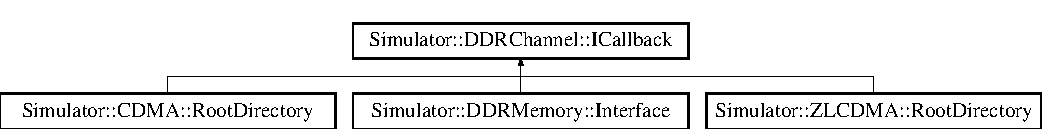
\includegraphics[height=1.728395cm]{class_simulator_1_1_d_d_r_channel_1_1_i_callback}
\end{center}
\end{figure}
\subsection*{Public Member Functions}
\begin{DoxyCompactItemize}
\item 
virtual bool \hyperlink{class_simulator_1_1_d_d_r_channel_1_1_i_callback_a2782fe111ea6a02b44216d1b654c9425}{On\+Read\+Completed} ()=0
\item 
virtual \hyperlink{class_simulator_1_1_d_d_r_channel_1_1_i_callback_a7613e882433ff328d9cae5d1051082dc}{$\sim$\+I\+Callback} ()
\end{DoxyCompactItemize}


\subsection{Constructor \& Destructor Documentation}
\hypertarget{class_simulator_1_1_d_d_r_channel_1_1_i_callback_a7613e882433ff328d9cae5d1051082dc}{\index{Simulator\+::\+D\+D\+R\+Channel\+::\+I\+Callback@{Simulator\+::\+D\+D\+R\+Channel\+::\+I\+Callback}!````~I\+Callback@{$\sim$\+I\+Callback}}
\index{````~I\+Callback@{$\sim$\+I\+Callback}!Simulator\+::\+D\+D\+R\+Channel\+::\+I\+Callback@{Simulator\+::\+D\+D\+R\+Channel\+::\+I\+Callback}}
\subsubsection[{$\sim$\+I\+Callback}]{\setlength{\rightskip}{0pt plus 5cm}virtual Simulator\+::\+D\+D\+R\+Channel\+::\+I\+Callback\+::$\sim$\+I\+Callback (
\begin{DoxyParamCaption}
{}
\end{DoxyParamCaption}
)\hspace{0.3cm}{\ttfamily [inline]}, {\ttfamily [virtual]}}}\label{class_simulator_1_1_d_d_r_channel_1_1_i_callback_a7613e882433ff328d9cae5d1051082dc}


\subsection{Member Function Documentation}
\hypertarget{class_simulator_1_1_d_d_r_channel_1_1_i_callback_a2782fe111ea6a02b44216d1b654c9425}{\index{Simulator\+::\+D\+D\+R\+Channel\+::\+I\+Callback@{Simulator\+::\+D\+D\+R\+Channel\+::\+I\+Callback}!On\+Read\+Completed@{On\+Read\+Completed}}
\index{On\+Read\+Completed@{On\+Read\+Completed}!Simulator\+::\+D\+D\+R\+Channel\+::\+I\+Callback@{Simulator\+::\+D\+D\+R\+Channel\+::\+I\+Callback}}
\subsubsection[{On\+Read\+Completed}]{\setlength{\rightskip}{0pt plus 5cm}virtual bool Simulator\+::\+D\+D\+R\+Channel\+::\+I\+Callback\+::\+On\+Read\+Completed (
\begin{DoxyParamCaption}
{}
\end{DoxyParamCaption}
)\hspace{0.3cm}{\ttfamily [pure virtual]}}}\label{class_simulator_1_1_d_d_r_channel_1_1_i_callback_a2782fe111ea6a02b44216d1b654c9425}


Implemented in \hyperlink{class_simulator_1_1_d_d_r_memory_1_1_interface_aa8e3244f424ea0a40095cba865a778f3}{Simulator\+::\+D\+D\+R\+Memory\+::\+Interface}.



The documentation for this class was generated from the following file\+:\begin{DoxyCompactItemize}
\item 
arch/mem/\hyperlink{_d_d_r_8h}{D\+D\+R.\+h}\end{DoxyCompactItemize}

\hypertarget{class_simulator_1_1_f_p_u_1_1_i_f_p_u_client}{\section{Simulator\+:\+:F\+P\+U\+:\+:I\+F\+P\+U\+Client Class Reference}
\label{class_simulator_1_1_f_p_u_1_1_i_f_p_u_client}\index{Simulator\+::\+F\+P\+U\+::\+I\+F\+P\+U\+Client@{Simulator\+::\+F\+P\+U\+::\+I\+F\+P\+U\+Client}}
}


Represents a client for this \hyperlink{class_simulator_1_1_f_p_u}{F\+P\+U}.  




{\ttfamily \#include $<$F\+P\+U.\+h$>$}

Inheritance diagram for Simulator\+:\+:F\+P\+U\+:\+:I\+F\+P\+U\+Client\+:\begin{figure}[H]
\begin{center}
\leavevmode
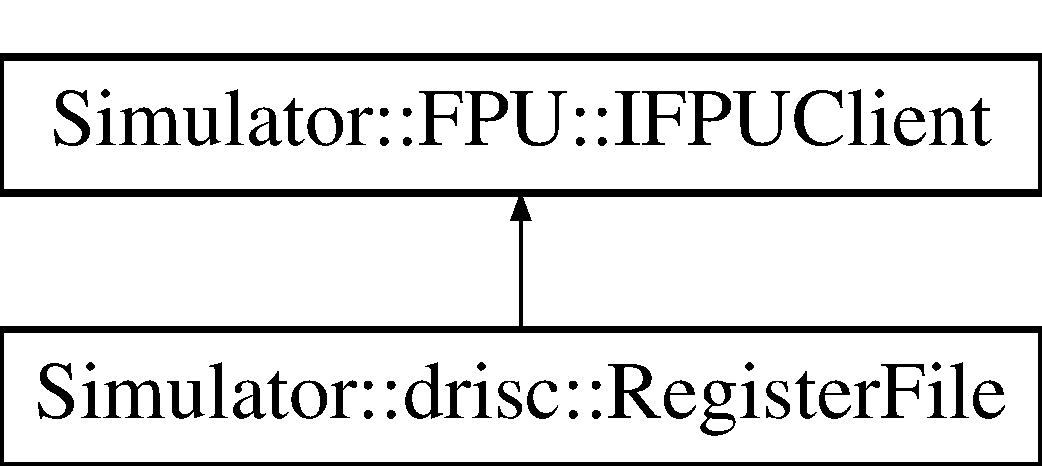
\includegraphics[height=2.000000cm]{class_simulator_1_1_f_p_u_1_1_i_f_p_u_client}
\end{center}
\end{figure}
\subsection*{Public Member Functions}
\begin{DoxyCompactItemize}
\item 
virtual std\+::string \hyperlink{class_simulator_1_1_f_p_u_1_1_i_f_p_u_client_a5588985669fd1772318c9b88e3f44869}{Get\+Name} () const =0
\item 
virtual bool \hyperlink{class_simulator_1_1_f_p_u_1_1_i_f_p_u_client_a2e7336c7e6b0c9a33445c2312345b4ce}{Check\+F\+P\+U\+Output\+Availability} (\hyperlink{struct_simulator_1_1_reg_addr}{Reg\+Addr} addr)=0
\item 
virtual bool \hyperlink{class_simulator_1_1_f_p_u_1_1_i_f_p_u_client_acd84130d336c322969ea07948b6d0405}{Write\+F\+P\+U\+Result} (\hyperlink{struct_simulator_1_1_reg_addr}{Reg\+Addr} addr, const \hyperlink{struct_simulator_1_1_reg_value}{Reg\+Value} \&value)=0
\item 
virtual \hyperlink{class_simulator_1_1_f_p_u_1_1_i_f_p_u_client_ab949da9645e70f31b38623e87dac151a}{$\sim$\+I\+F\+P\+U\+Client} ()
\end{DoxyCompactItemize}


\subsection{Detailed Description}
Represents a client for this \hyperlink{class_simulator_1_1_f_p_u}{F\+P\+U}. 

\subsection{Constructor \& Destructor Documentation}
\hypertarget{class_simulator_1_1_f_p_u_1_1_i_f_p_u_client_ab949da9645e70f31b38623e87dac151a}{\index{Simulator\+::\+F\+P\+U\+::\+I\+F\+P\+U\+Client@{Simulator\+::\+F\+P\+U\+::\+I\+F\+P\+U\+Client}!````~I\+F\+P\+U\+Client@{$\sim$\+I\+F\+P\+U\+Client}}
\index{````~I\+F\+P\+U\+Client@{$\sim$\+I\+F\+P\+U\+Client}!Simulator\+::\+F\+P\+U\+::\+I\+F\+P\+U\+Client@{Simulator\+::\+F\+P\+U\+::\+I\+F\+P\+U\+Client}}
\subsubsection[{$\sim$\+I\+F\+P\+U\+Client}]{\setlength{\rightskip}{0pt plus 5cm}Simulator\+::\+F\+P\+U\+::\+I\+F\+P\+U\+Client\+::$\sim$\+I\+F\+P\+U\+Client (
\begin{DoxyParamCaption}
{}
\end{DoxyParamCaption}
)\hspace{0.3cm}{\ttfamily [virtual]}}}\label{class_simulator_1_1_f_p_u_1_1_i_f_p_u_client_ab949da9645e70f31b38623e87dac151a}


\subsection{Member Function Documentation}
\hypertarget{class_simulator_1_1_f_p_u_1_1_i_f_p_u_client_a2e7336c7e6b0c9a33445c2312345b4ce}{\index{Simulator\+::\+F\+P\+U\+::\+I\+F\+P\+U\+Client@{Simulator\+::\+F\+P\+U\+::\+I\+F\+P\+U\+Client}!Check\+F\+P\+U\+Output\+Availability@{Check\+F\+P\+U\+Output\+Availability}}
\index{Check\+F\+P\+U\+Output\+Availability@{Check\+F\+P\+U\+Output\+Availability}!Simulator\+::\+F\+P\+U\+::\+I\+F\+P\+U\+Client@{Simulator\+::\+F\+P\+U\+::\+I\+F\+P\+U\+Client}}
\subsubsection[{Check\+F\+P\+U\+Output\+Availability}]{\setlength{\rightskip}{0pt plus 5cm}virtual bool Simulator\+::\+F\+P\+U\+::\+I\+F\+P\+U\+Client\+::\+Check\+F\+P\+U\+Output\+Availability (
\begin{DoxyParamCaption}
\item[{{\bf Reg\+Addr}}]{addr}
\end{DoxyParamCaption}
)\hspace{0.3cm}{\ttfamily [pure virtual]}}}\label{class_simulator_1_1_f_p_u_1_1_i_f_p_u_client_a2e7336c7e6b0c9a33445c2312345b4ce}


Implemented in \hyperlink{class_simulator_1_1drisc_1_1_register_file_a86ac6b5b63a1a662b694c2a76e86ad04}{Simulator\+::drisc\+::\+Register\+File}.

\hypertarget{class_simulator_1_1_f_p_u_1_1_i_f_p_u_client_a5588985669fd1772318c9b88e3f44869}{\index{Simulator\+::\+F\+P\+U\+::\+I\+F\+P\+U\+Client@{Simulator\+::\+F\+P\+U\+::\+I\+F\+P\+U\+Client}!Get\+Name@{Get\+Name}}
\index{Get\+Name@{Get\+Name}!Simulator\+::\+F\+P\+U\+::\+I\+F\+P\+U\+Client@{Simulator\+::\+F\+P\+U\+::\+I\+F\+P\+U\+Client}}
\subsubsection[{Get\+Name}]{\setlength{\rightskip}{0pt plus 5cm}virtual std\+::string Simulator\+::\+F\+P\+U\+::\+I\+F\+P\+U\+Client\+::\+Get\+Name (
\begin{DoxyParamCaption}
{}
\end{DoxyParamCaption}
) const\hspace{0.3cm}{\ttfamily [pure virtual]}}}\label{class_simulator_1_1_f_p_u_1_1_i_f_p_u_client_a5588985669fd1772318c9b88e3f44869}


Implemented in \hyperlink{class_simulator_1_1drisc_1_1_register_file_a3588d3d9aaa9b01b5ff0eb85ab140c42}{Simulator\+::drisc\+::\+Register\+File}.

\hypertarget{class_simulator_1_1_f_p_u_1_1_i_f_p_u_client_acd84130d336c322969ea07948b6d0405}{\index{Simulator\+::\+F\+P\+U\+::\+I\+F\+P\+U\+Client@{Simulator\+::\+F\+P\+U\+::\+I\+F\+P\+U\+Client}!Write\+F\+P\+U\+Result@{Write\+F\+P\+U\+Result}}
\index{Write\+F\+P\+U\+Result@{Write\+F\+P\+U\+Result}!Simulator\+::\+F\+P\+U\+::\+I\+F\+P\+U\+Client@{Simulator\+::\+F\+P\+U\+::\+I\+F\+P\+U\+Client}}
\subsubsection[{Write\+F\+P\+U\+Result}]{\setlength{\rightskip}{0pt plus 5cm}virtual bool Simulator\+::\+F\+P\+U\+::\+I\+F\+P\+U\+Client\+::\+Write\+F\+P\+U\+Result (
\begin{DoxyParamCaption}
\item[{{\bf Reg\+Addr}}]{addr, }
\item[{const {\bf Reg\+Value} \&}]{value}
\end{DoxyParamCaption}
)\hspace{0.3cm}{\ttfamily [pure virtual]}}}\label{class_simulator_1_1_f_p_u_1_1_i_f_p_u_client_acd84130d336c322969ea07948b6d0405}


Implemented in \hyperlink{class_simulator_1_1drisc_1_1_register_file_a87e2d2856c9dd19a8b8b2dc9ebd7e937}{Simulator\+::drisc\+::\+Register\+File}.



The documentation for this class was generated from the following files\+:\begin{DoxyCompactItemize}
\item 
arch/\hyperlink{_f_p_u_8h}{F\+P\+U.\+h}\item 
arch/\hyperlink{_f_p_u_8cpp}{F\+P\+U.\+cpp}\end{DoxyCompactItemize}

\hypertarget{class_simulator_1_1_i_i_o_bus}{\section{Simulator\+:\+:I\+I\+O\+Bus Class Reference}
\label{class_simulator_1_1_i_i_o_bus}\index{Simulator\+::\+I\+I\+O\+Bus@{Simulator\+::\+I\+I\+O\+Bus}}
}


{\ttfamily \#include $<$I\+O\+Bus.\+h$>$}

Inheritance diagram for Simulator\+:\+:I\+I\+O\+Bus\+:\begin{figure}[H]
\begin{center}
\leavevmode
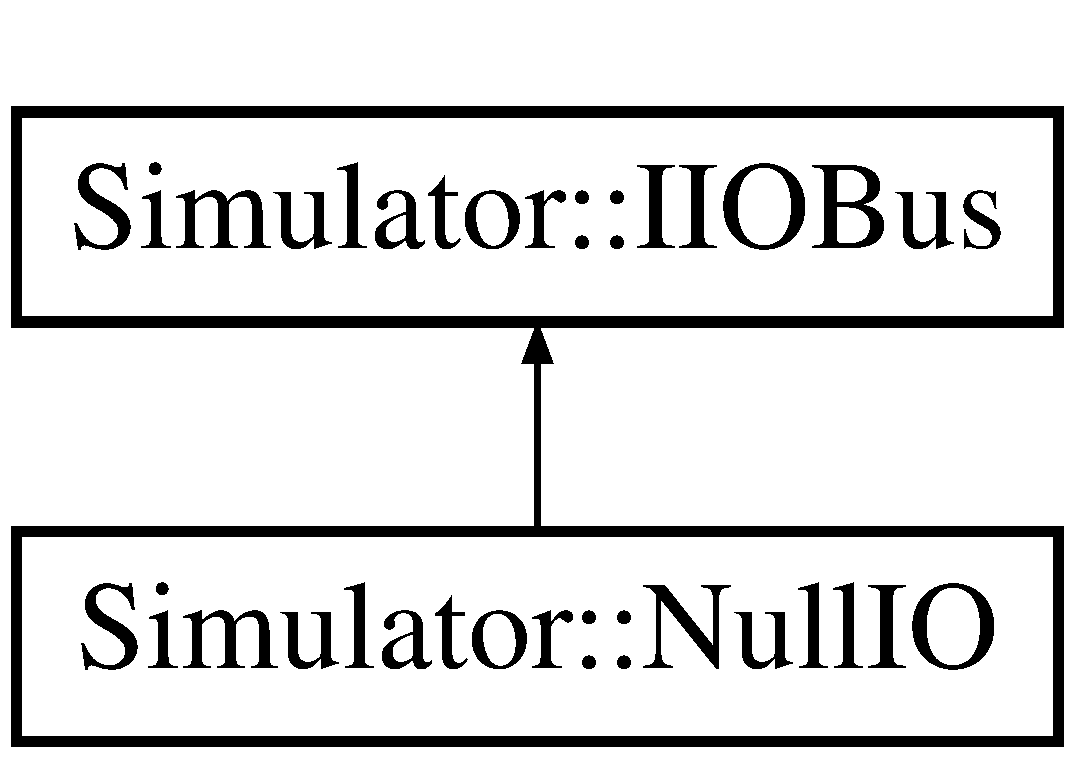
\includegraphics[height=2.000000cm]{class_simulator_1_1_i_i_o_bus}
\end{center}
\end{figure}
\subsection*{Public Member Functions}
\begin{DoxyCompactItemize}
\item 
virtual bool \hyperlink{class_simulator_1_1_i_i_o_bus_ad6100dce5f4663af45cf7613643d7d57}{Register\+Client} (\hyperlink{namespace_simulator_a3493d987c866ad6b8aaa704c42502db0}{I\+O\+Device\+I\+D} \hyperlink{mtconf_8c_aa3185401f04d30bd505daebf48c39cc5}{id}, \hyperlink{class_simulator_1_1_i_i_o_bus_client}{I\+I\+O\+Bus\+Client} \&client)=0
\item 
virtual bool \hyperlink{class_simulator_1_1_i_i_o_bus_a7cfc3fdf03f155a71e7568ca656136c8}{Send\+Read\+Request} (\hyperlink{namespace_simulator_a3493d987c866ad6b8aaa704c42502db0}{I\+O\+Device\+I\+D} from, \hyperlink{namespace_simulator_a3493d987c866ad6b8aaa704c42502db0}{I\+O\+Device\+I\+D} to, Mem\+Addr address, Mem\+Size size)=0
\item 
virtual bool \hyperlink{class_simulator_1_1_i_i_o_bus_a75919974ba441b51cb733eb6a276c0f3}{Send\+Write\+Request} (\hyperlink{namespace_simulator_a3493d987c866ad6b8aaa704c42502db0}{I\+O\+Device\+I\+D} from, \hyperlink{namespace_simulator_a3493d987c866ad6b8aaa704c42502db0}{I\+O\+Device\+I\+D} to, Mem\+Addr address, const \hyperlink{struct_simulator_1_1_i_o_data}{I\+O\+Data} \&data)=0
\item 
virtual bool \hyperlink{class_simulator_1_1_i_i_o_bus_ad55542e3e8facd94bacbccd0defd2255}{Send\+Read\+Response} (\hyperlink{namespace_simulator_a3493d987c866ad6b8aaa704c42502db0}{I\+O\+Device\+I\+D} from, \hyperlink{namespace_simulator_a3493d987c866ad6b8aaa704c42502db0}{I\+O\+Device\+I\+D} to, Mem\+Addr address, const \hyperlink{struct_simulator_1_1_i_o_data}{I\+O\+Data} \&data)=0
\item 
virtual bool \hyperlink{class_simulator_1_1_i_i_o_bus_aa4449031b931a2c4146490f1a047f5be}{Send\+Interrupt\+Request} (\hyperlink{namespace_simulator_a3493d987c866ad6b8aaa704c42502db0}{I\+O\+Device\+I\+D} from, \hyperlink{namespace_simulator_a951e1bf3ee91c11c980382a7bcbba287}{I\+O\+Notification\+Channel\+I\+D} which)=0
\item 
virtual bool \hyperlink{class_simulator_1_1_i_i_o_bus_afe7511b05f67abee5678f500f630f313}{Send\+Notification} (\hyperlink{namespace_simulator_a3493d987c866ad6b8aaa704c42502db0}{I\+O\+Device\+I\+D} from, \hyperlink{namespace_simulator_a951e1bf3ee91c11c980382a7bcbba287}{I\+O\+Notification\+Channel\+I\+D} which, Integer tag)=0
\item 
virtual bool \hyperlink{class_simulator_1_1_i_i_o_bus_a4863c21b90d0126ee1c886f891c772a3}{Send\+Active\+Message} (\hyperlink{namespace_simulator_a3493d987c866ad6b8aaa704c42502db0}{I\+O\+Device\+I\+D} from, \hyperlink{namespace_simulator_a3493d987c866ad6b8aaa704c42502db0}{I\+O\+Device\+I\+D} to, Mem\+Addr pc, Integer arg)=0
\item 
virtual \hyperlink{class_simulator_1_1_storage_trace_set}{Storage\+Trace\+Set} \hyperlink{class_simulator_1_1_i_i_o_bus_aecf6e5f0da5be957ae517f8b5b6ea4ec}{Get\+Read\+Request\+Traces} (\hyperlink{namespace_simulator_a3493d987c866ad6b8aaa704c42502db0}{I\+O\+Device\+I\+D} from) const =0
\item 
virtual \hyperlink{class_simulator_1_1_storage_trace_set}{Storage\+Trace\+Set} \hyperlink{class_simulator_1_1_i_i_o_bus_a48ba2c4a49f95c368bc9432b953ffb06}{Get\+Write\+Request\+Traces} () const =0
\item 
virtual \hyperlink{class_simulator_1_1_storage_trace_set}{Storage\+Trace\+Set} \hyperlink{class_simulator_1_1_i_i_o_bus_a6dc2f2fbd325171f85fe06dfae09ce22}{Get\+Read\+Response\+Traces} () const =0
\item 
virtual \hyperlink{class_simulator_1_1_storage_trace_set}{Storage\+Trace\+Set} \hyperlink{class_simulator_1_1_i_i_o_bus_a16480612894d8510d0b03bf7ffc591d6}{Get\+Interrupt\+Request\+Traces} () const =0
\item 
virtual \hyperlink{class_simulator_1_1_storage_trace_set}{Storage\+Trace\+Set} \hyperlink{class_simulator_1_1_i_i_o_bus_a063b95f1813f8b297beebc2276a842e2}{Get\+Notification\+Traces} () const =0
\item 
virtual \hyperlink{class_simulator_1_1_storage_trace_set}{Storage\+Trace\+Set} \hyperlink{class_simulator_1_1_i_i_o_bus_a35fd77c2eebd5b128009e47e9986f016}{Get\+Active\+Message\+Traces} () const =0
\item 
virtual \hyperlink{class_simulator_1_1_clock}{Clock} \& \hyperlink{class_simulator_1_1_i_i_o_bus_a0355ff5fd84e363f08d169373ca068df}{Get\+Clock} ()=0
\item 
virtual void \hyperlink{class_simulator_1_1_i_i_o_bus_a18ac464d5eaadee9cdc9b44205fb9678}{Initialize} ()=0
\item 
virtual \hyperlink{namespace_simulator_a3493d987c866ad6b8aaa704c42502db0}{I\+O\+Device\+I\+D} \hyperlink{class_simulator_1_1_i_i_o_bus_a7fd98d356ee3ed5df0445ceeb9e5d196}{Get\+Last\+Device\+I\+D} () const =0
\item 
virtual \hyperlink{namespace_simulator_a3493d987c866ad6b8aaa704c42502db0}{I\+O\+Device\+I\+D} \hyperlink{class_simulator_1_1_i_i_o_bus_ad52f98ce0c8b13155b7f91636fddfcc0}{Get\+Next\+Available\+Device\+I\+D} () const =0
\item 
virtual \hyperlink{namespace_simulator_a3493d987c866ad6b8aaa704c42502db0}{I\+O\+Device\+I\+D} \hyperlink{class_simulator_1_1_i_i_o_bus_ac0738b1f28724fe009cb1a68391f48cf}{Get\+Device\+I\+D\+By\+Name} (const std\+::string \&objname) const =0
\item 
virtual \hyperlink{class_simulator_1_1_object}{Object} \& \hyperlink{class_simulator_1_1_i_i_o_bus_a1c80cbeefd5ca7bd7c4e3668df4c4a17}{Get\+Device\+By\+Name} (const std\+::string \&objname) const =0
\item 
virtual void \hyperlink{class_simulator_1_1_i_i_o_bus_ad84869ac6b626583c55466336f8611d9}{Get\+Device\+Identity} (\hyperlink{namespace_simulator_a3493d987c866ad6b8aaa704c42502db0}{I\+O\+Device\+I\+D} which, \hyperlink{struct_simulator_1_1_i_o_device_identification}{I\+O\+Device\+Identification} \&\hyperlink{mtconf_8c_aa3185401f04d30bd505daebf48c39cc5}{id}) const =0
\item 
virtual \hyperlink{class_simulator_1_1_i_i_o_bus_a15f28e2fb4a008074eff8677d0b9d1e2}{$\sim$\+I\+I\+O\+Bus} ()
\end{DoxyCompactItemize}


\subsection{Constructor \& Destructor Documentation}
\hypertarget{class_simulator_1_1_i_i_o_bus_a15f28e2fb4a008074eff8677d0b9d1e2}{\index{Simulator\+::\+I\+I\+O\+Bus@{Simulator\+::\+I\+I\+O\+Bus}!````~I\+I\+O\+Bus@{$\sim$\+I\+I\+O\+Bus}}
\index{````~I\+I\+O\+Bus@{$\sim$\+I\+I\+O\+Bus}!Simulator\+::\+I\+I\+O\+Bus@{Simulator\+::\+I\+I\+O\+Bus}}
\subsubsection[{$\sim$\+I\+I\+O\+Bus}]{\setlength{\rightskip}{0pt plus 5cm}Simulator\+::\+I\+I\+O\+Bus\+::$\sim$\+I\+I\+O\+Bus (
\begin{DoxyParamCaption}
{}
\end{DoxyParamCaption}
)\hspace{0.3cm}{\ttfamily [virtual]}}}\label{class_simulator_1_1_i_i_o_bus_a15f28e2fb4a008074eff8677d0b9d1e2}


\subsection{Member Function Documentation}
\hypertarget{class_simulator_1_1_i_i_o_bus_a35fd77c2eebd5b128009e47e9986f016}{\index{Simulator\+::\+I\+I\+O\+Bus@{Simulator\+::\+I\+I\+O\+Bus}!Get\+Active\+Message\+Traces@{Get\+Active\+Message\+Traces}}
\index{Get\+Active\+Message\+Traces@{Get\+Active\+Message\+Traces}!Simulator\+::\+I\+I\+O\+Bus@{Simulator\+::\+I\+I\+O\+Bus}}
\subsubsection[{Get\+Active\+Message\+Traces}]{\setlength{\rightskip}{0pt plus 5cm}virtual {\bf Storage\+Trace\+Set} Simulator\+::\+I\+I\+O\+Bus\+::\+Get\+Active\+Message\+Traces (
\begin{DoxyParamCaption}
{}
\end{DoxyParamCaption}
) const\hspace{0.3cm}{\ttfamily [pure virtual]}}}\label{class_simulator_1_1_i_i_o_bus_a35fd77c2eebd5b128009e47e9986f016}


Implemented in \hyperlink{class_simulator_1_1_null_i_o_a13e5a4e6a7249c6a67f9abaecc96df91}{Simulator\+::\+Null\+I\+O}.

\hypertarget{class_simulator_1_1_i_i_o_bus_a0355ff5fd84e363f08d169373ca068df}{\index{Simulator\+::\+I\+I\+O\+Bus@{Simulator\+::\+I\+I\+O\+Bus}!Get\+Clock@{Get\+Clock}}
\index{Get\+Clock@{Get\+Clock}!Simulator\+::\+I\+I\+O\+Bus@{Simulator\+::\+I\+I\+O\+Bus}}
\subsubsection[{Get\+Clock}]{\setlength{\rightskip}{0pt plus 5cm}virtual {\bf Clock}\& Simulator\+::\+I\+I\+O\+Bus\+::\+Get\+Clock (
\begin{DoxyParamCaption}
{}
\end{DoxyParamCaption}
)\hspace{0.3cm}{\ttfamily [pure virtual]}}}\label{class_simulator_1_1_i_i_o_bus_a0355ff5fd84e363f08d169373ca068df}


Implemented in \hyperlink{class_simulator_1_1_null_i_o_a0b731e11267728f70227060561a7587f}{Simulator\+::\+Null\+I\+O}.

\hypertarget{class_simulator_1_1_i_i_o_bus_a1c80cbeefd5ca7bd7c4e3668df4c4a17}{\index{Simulator\+::\+I\+I\+O\+Bus@{Simulator\+::\+I\+I\+O\+Bus}!Get\+Device\+By\+Name@{Get\+Device\+By\+Name}}
\index{Get\+Device\+By\+Name@{Get\+Device\+By\+Name}!Simulator\+::\+I\+I\+O\+Bus@{Simulator\+::\+I\+I\+O\+Bus}}
\subsubsection[{Get\+Device\+By\+Name}]{\setlength{\rightskip}{0pt plus 5cm}virtual {\bf Object}\& Simulator\+::\+I\+I\+O\+Bus\+::\+Get\+Device\+By\+Name (
\begin{DoxyParamCaption}
\item[{const std\+::string \&}]{objname}
\end{DoxyParamCaption}
) const\hspace{0.3cm}{\ttfamily [pure virtual]}}}\label{class_simulator_1_1_i_i_o_bus_a1c80cbeefd5ca7bd7c4e3668df4c4a17}


Implemented in \hyperlink{class_simulator_1_1_null_i_o_ace4f407dcb51315c0c859bf7da9eafb7}{Simulator\+::\+Null\+I\+O}.

\hypertarget{class_simulator_1_1_i_i_o_bus_ac0738b1f28724fe009cb1a68391f48cf}{\index{Simulator\+::\+I\+I\+O\+Bus@{Simulator\+::\+I\+I\+O\+Bus}!Get\+Device\+I\+D\+By\+Name@{Get\+Device\+I\+D\+By\+Name}}
\index{Get\+Device\+I\+D\+By\+Name@{Get\+Device\+I\+D\+By\+Name}!Simulator\+::\+I\+I\+O\+Bus@{Simulator\+::\+I\+I\+O\+Bus}}
\subsubsection[{Get\+Device\+I\+D\+By\+Name}]{\setlength{\rightskip}{0pt plus 5cm}virtual {\bf I\+O\+Device\+I\+D} Simulator\+::\+I\+I\+O\+Bus\+::\+Get\+Device\+I\+D\+By\+Name (
\begin{DoxyParamCaption}
\item[{const std\+::string \&}]{objname}
\end{DoxyParamCaption}
) const\hspace{0.3cm}{\ttfamily [pure virtual]}}}\label{class_simulator_1_1_i_i_o_bus_ac0738b1f28724fe009cb1a68391f48cf}


Implemented in \hyperlink{class_simulator_1_1_null_i_o_a10d530d9bca32171bb398d3685b94a8b}{Simulator\+::\+Null\+I\+O}.

\hypertarget{class_simulator_1_1_i_i_o_bus_ad84869ac6b626583c55466336f8611d9}{\index{Simulator\+::\+I\+I\+O\+Bus@{Simulator\+::\+I\+I\+O\+Bus}!Get\+Device\+Identity@{Get\+Device\+Identity}}
\index{Get\+Device\+Identity@{Get\+Device\+Identity}!Simulator\+::\+I\+I\+O\+Bus@{Simulator\+::\+I\+I\+O\+Bus}}
\subsubsection[{Get\+Device\+Identity}]{\setlength{\rightskip}{0pt plus 5cm}virtual void Simulator\+::\+I\+I\+O\+Bus\+::\+Get\+Device\+Identity (
\begin{DoxyParamCaption}
\item[{{\bf I\+O\+Device\+I\+D}}]{which, }
\item[{{\bf I\+O\+Device\+Identification} \&}]{id}
\end{DoxyParamCaption}
) const\hspace{0.3cm}{\ttfamily [pure virtual]}}}\label{class_simulator_1_1_i_i_o_bus_ad84869ac6b626583c55466336f8611d9}


Implemented in \hyperlink{class_simulator_1_1_null_i_o_a9f10d264165e9f70552cdda28a808d5f}{Simulator\+::\+Null\+I\+O}.

\hypertarget{class_simulator_1_1_i_i_o_bus_a16480612894d8510d0b03bf7ffc591d6}{\index{Simulator\+::\+I\+I\+O\+Bus@{Simulator\+::\+I\+I\+O\+Bus}!Get\+Interrupt\+Request\+Traces@{Get\+Interrupt\+Request\+Traces}}
\index{Get\+Interrupt\+Request\+Traces@{Get\+Interrupt\+Request\+Traces}!Simulator\+::\+I\+I\+O\+Bus@{Simulator\+::\+I\+I\+O\+Bus}}
\subsubsection[{Get\+Interrupt\+Request\+Traces}]{\setlength{\rightskip}{0pt plus 5cm}virtual {\bf Storage\+Trace\+Set} Simulator\+::\+I\+I\+O\+Bus\+::\+Get\+Interrupt\+Request\+Traces (
\begin{DoxyParamCaption}
{}
\end{DoxyParamCaption}
) const\hspace{0.3cm}{\ttfamily [pure virtual]}}}\label{class_simulator_1_1_i_i_o_bus_a16480612894d8510d0b03bf7ffc591d6}


Implemented in \hyperlink{class_simulator_1_1_null_i_o_ac769be990b32751e7638280ec10de6d2}{Simulator\+::\+Null\+I\+O}.

\hypertarget{class_simulator_1_1_i_i_o_bus_a7fd98d356ee3ed5df0445ceeb9e5d196}{\index{Simulator\+::\+I\+I\+O\+Bus@{Simulator\+::\+I\+I\+O\+Bus}!Get\+Last\+Device\+I\+D@{Get\+Last\+Device\+I\+D}}
\index{Get\+Last\+Device\+I\+D@{Get\+Last\+Device\+I\+D}!Simulator\+::\+I\+I\+O\+Bus@{Simulator\+::\+I\+I\+O\+Bus}}
\subsubsection[{Get\+Last\+Device\+I\+D}]{\setlength{\rightskip}{0pt plus 5cm}virtual {\bf I\+O\+Device\+I\+D} Simulator\+::\+I\+I\+O\+Bus\+::\+Get\+Last\+Device\+I\+D (
\begin{DoxyParamCaption}
{}
\end{DoxyParamCaption}
) const\hspace{0.3cm}{\ttfamily [pure virtual]}}}\label{class_simulator_1_1_i_i_o_bus_a7fd98d356ee3ed5df0445ceeb9e5d196}


Implemented in \hyperlink{class_simulator_1_1_null_i_o_a13e1a1184456bcb5bb17a54ccf254cf8}{Simulator\+::\+Null\+I\+O}.

\hypertarget{class_simulator_1_1_i_i_o_bus_ad52f98ce0c8b13155b7f91636fddfcc0}{\index{Simulator\+::\+I\+I\+O\+Bus@{Simulator\+::\+I\+I\+O\+Bus}!Get\+Next\+Available\+Device\+I\+D@{Get\+Next\+Available\+Device\+I\+D}}
\index{Get\+Next\+Available\+Device\+I\+D@{Get\+Next\+Available\+Device\+I\+D}!Simulator\+::\+I\+I\+O\+Bus@{Simulator\+::\+I\+I\+O\+Bus}}
\subsubsection[{Get\+Next\+Available\+Device\+I\+D}]{\setlength{\rightskip}{0pt plus 5cm}virtual {\bf I\+O\+Device\+I\+D} Simulator\+::\+I\+I\+O\+Bus\+::\+Get\+Next\+Available\+Device\+I\+D (
\begin{DoxyParamCaption}
{}
\end{DoxyParamCaption}
) const\hspace{0.3cm}{\ttfamily [pure virtual]}}}\label{class_simulator_1_1_i_i_o_bus_ad52f98ce0c8b13155b7f91636fddfcc0}


Implemented in \hyperlink{class_simulator_1_1_null_i_o_a6ee32ce75ede70b802c3dc37aea7bfba}{Simulator\+::\+Null\+I\+O}.

\hypertarget{class_simulator_1_1_i_i_o_bus_a063b95f1813f8b297beebc2276a842e2}{\index{Simulator\+::\+I\+I\+O\+Bus@{Simulator\+::\+I\+I\+O\+Bus}!Get\+Notification\+Traces@{Get\+Notification\+Traces}}
\index{Get\+Notification\+Traces@{Get\+Notification\+Traces}!Simulator\+::\+I\+I\+O\+Bus@{Simulator\+::\+I\+I\+O\+Bus}}
\subsubsection[{Get\+Notification\+Traces}]{\setlength{\rightskip}{0pt plus 5cm}virtual {\bf Storage\+Trace\+Set} Simulator\+::\+I\+I\+O\+Bus\+::\+Get\+Notification\+Traces (
\begin{DoxyParamCaption}
{}
\end{DoxyParamCaption}
) const\hspace{0.3cm}{\ttfamily [pure virtual]}}}\label{class_simulator_1_1_i_i_o_bus_a063b95f1813f8b297beebc2276a842e2}


Implemented in \hyperlink{class_simulator_1_1_null_i_o_abfc63aab4f82f11219aa3400f78d9586}{Simulator\+::\+Null\+I\+O}.

\hypertarget{class_simulator_1_1_i_i_o_bus_aecf6e5f0da5be957ae517f8b5b6ea4ec}{\index{Simulator\+::\+I\+I\+O\+Bus@{Simulator\+::\+I\+I\+O\+Bus}!Get\+Read\+Request\+Traces@{Get\+Read\+Request\+Traces}}
\index{Get\+Read\+Request\+Traces@{Get\+Read\+Request\+Traces}!Simulator\+::\+I\+I\+O\+Bus@{Simulator\+::\+I\+I\+O\+Bus}}
\subsubsection[{Get\+Read\+Request\+Traces}]{\setlength{\rightskip}{0pt plus 5cm}virtual {\bf Storage\+Trace\+Set} Simulator\+::\+I\+I\+O\+Bus\+::\+Get\+Read\+Request\+Traces (
\begin{DoxyParamCaption}
\item[{{\bf I\+O\+Device\+I\+D}}]{from}
\end{DoxyParamCaption}
) const\hspace{0.3cm}{\ttfamily [pure virtual]}}}\label{class_simulator_1_1_i_i_o_bus_aecf6e5f0da5be957ae517f8b5b6ea4ec}


Implemented in \hyperlink{class_simulator_1_1_null_i_o_ac304a032290459d8faea44899133f602}{Simulator\+::\+Null\+I\+O}.

\hypertarget{class_simulator_1_1_i_i_o_bus_a6dc2f2fbd325171f85fe06dfae09ce22}{\index{Simulator\+::\+I\+I\+O\+Bus@{Simulator\+::\+I\+I\+O\+Bus}!Get\+Read\+Response\+Traces@{Get\+Read\+Response\+Traces}}
\index{Get\+Read\+Response\+Traces@{Get\+Read\+Response\+Traces}!Simulator\+::\+I\+I\+O\+Bus@{Simulator\+::\+I\+I\+O\+Bus}}
\subsubsection[{Get\+Read\+Response\+Traces}]{\setlength{\rightskip}{0pt plus 5cm}virtual {\bf Storage\+Trace\+Set} Simulator\+::\+I\+I\+O\+Bus\+::\+Get\+Read\+Response\+Traces (
\begin{DoxyParamCaption}
{}
\end{DoxyParamCaption}
) const\hspace{0.3cm}{\ttfamily [pure virtual]}}}\label{class_simulator_1_1_i_i_o_bus_a6dc2f2fbd325171f85fe06dfae09ce22}


Implemented in \hyperlink{class_simulator_1_1_null_i_o_a850ae92a7e0e01a896ffa7da7d910a8e}{Simulator\+::\+Null\+I\+O}.

\hypertarget{class_simulator_1_1_i_i_o_bus_a48ba2c4a49f95c368bc9432b953ffb06}{\index{Simulator\+::\+I\+I\+O\+Bus@{Simulator\+::\+I\+I\+O\+Bus}!Get\+Write\+Request\+Traces@{Get\+Write\+Request\+Traces}}
\index{Get\+Write\+Request\+Traces@{Get\+Write\+Request\+Traces}!Simulator\+::\+I\+I\+O\+Bus@{Simulator\+::\+I\+I\+O\+Bus}}
\subsubsection[{Get\+Write\+Request\+Traces}]{\setlength{\rightskip}{0pt plus 5cm}virtual {\bf Storage\+Trace\+Set} Simulator\+::\+I\+I\+O\+Bus\+::\+Get\+Write\+Request\+Traces (
\begin{DoxyParamCaption}
{}
\end{DoxyParamCaption}
) const\hspace{0.3cm}{\ttfamily [pure virtual]}}}\label{class_simulator_1_1_i_i_o_bus_a48ba2c4a49f95c368bc9432b953ffb06}


Implemented in \hyperlink{class_simulator_1_1_null_i_o_a882ad2172b1e29268ac6708ee16bb51a}{Simulator\+::\+Null\+I\+O}.

\hypertarget{class_simulator_1_1_i_i_o_bus_a18ac464d5eaadee9cdc9b44205fb9678}{\index{Simulator\+::\+I\+I\+O\+Bus@{Simulator\+::\+I\+I\+O\+Bus}!Initialize@{Initialize}}
\index{Initialize@{Initialize}!Simulator\+::\+I\+I\+O\+Bus@{Simulator\+::\+I\+I\+O\+Bus}}
\subsubsection[{Initialize}]{\setlength{\rightskip}{0pt plus 5cm}virtual void Simulator\+::\+I\+I\+O\+Bus\+::\+Initialize (
\begin{DoxyParamCaption}
{}
\end{DoxyParamCaption}
)\hspace{0.3cm}{\ttfamily [pure virtual]}}}\label{class_simulator_1_1_i_i_o_bus_a18ac464d5eaadee9cdc9b44205fb9678}


Implemented in \hyperlink{class_simulator_1_1_null_i_o_a66ef6ef474f545e3ad519097f8af6db6}{Simulator\+::\+Null\+I\+O}.

\hypertarget{class_simulator_1_1_i_i_o_bus_ad6100dce5f4663af45cf7613643d7d57}{\index{Simulator\+::\+I\+I\+O\+Bus@{Simulator\+::\+I\+I\+O\+Bus}!Register\+Client@{Register\+Client}}
\index{Register\+Client@{Register\+Client}!Simulator\+::\+I\+I\+O\+Bus@{Simulator\+::\+I\+I\+O\+Bus}}
\subsubsection[{Register\+Client}]{\setlength{\rightskip}{0pt plus 5cm}virtual bool Simulator\+::\+I\+I\+O\+Bus\+::\+Register\+Client (
\begin{DoxyParamCaption}
\item[{{\bf I\+O\+Device\+I\+D}}]{id, }
\item[{{\bf I\+I\+O\+Bus\+Client} \&}]{client}
\end{DoxyParamCaption}
)\hspace{0.3cm}{\ttfamily [pure virtual]}}}\label{class_simulator_1_1_i_i_o_bus_ad6100dce5f4663af45cf7613643d7d57}


Implemented in \hyperlink{class_simulator_1_1_null_i_o_aff954205e21154bc33fbe82aa2f1e783}{Simulator\+::\+Null\+I\+O}.

\hypertarget{class_simulator_1_1_i_i_o_bus_a4863c21b90d0126ee1c886f891c772a3}{\index{Simulator\+::\+I\+I\+O\+Bus@{Simulator\+::\+I\+I\+O\+Bus}!Send\+Active\+Message@{Send\+Active\+Message}}
\index{Send\+Active\+Message@{Send\+Active\+Message}!Simulator\+::\+I\+I\+O\+Bus@{Simulator\+::\+I\+I\+O\+Bus}}
\subsubsection[{Send\+Active\+Message}]{\setlength{\rightskip}{0pt plus 5cm}virtual bool Simulator\+::\+I\+I\+O\+Bus\+::\+Send\+Active\+Message (
\begin{DoxyParamCaption}
\item[{{\bf I\+O\+Device\+I\+D}}]{from, }
\item[{{\bf I\+O\+Device\+I\+D}}]{to, }
\item[{Mem\+Addr}]{pc, }
\item[{Integer}]{arg}
\end{DoxyParamCaption}
)\hspace{0.3cm}{\ttfamily [pure virtual]}}}\label{class_simulator_1_1_i_i_o_bus_a4863c21b90d0126ee1c886f891c772a3}


Implemented in \hyperlink{class_simulator_1_1_null_i_o_ae5c09fceb19e9a9b8df9d54aa4e7551c}{Simulator\+::\+Null\+I\+O}.

\hypertarget{class_simulator_1_1_i_i_o_bus_aa4449031b931a2c4146490f1a047f5be}{\index{Simulator\+::\+I\+I\+O\+Bus@{Simulator\+::\+I\+I\+O\+Bus}!Send\+Interrupt\+Request@{Send\+Interrupt\+Request}}
\index{Send\+Interrupt\+Request@{Send\+Interrupt\+Request}!Simulator\+::\+I\+I\+O\+Bus@{Simulator\+::\+I\+I\+O\+Bus}}
\subsubsection[{Send\+Interrupt\+Request}]{\setlength{\rightskip}{0pt plus 5cm}virtual bool Simulator\+::\+I\+I\+O\+Bus\+::\+Send\+Interrupt\+Request (
\begin{DoxyParamCaption}
\item[{{\bf I\+O\+Device\+I\+D}}]{from, }
\item[{{\bf I\+O\+Notification\+Channel\+I\+D}}]{which}
\end{DoxyParamCaption}
)\hspace{0.3cm}{\ttfamily [pure virtual]}}}\label{class_simulator_1_1_i_i_o_bus_aa4449031b931a2c4146490f1a047f5be}


Implemented in \hyperlink{class_simulator_1_1_null_i_o_a34a7220412e9c1a8fc48d901cad192b0}{Simulator\+::\+Null\+I\+O}.

\hypertarget{class_simulator_1_1_i_i_o_bus_afe7511b05f67abee5678f500f630f313}{\index{Simulator\+::\+I\+I\+O\+Bus@{Simulator\+::\+I\+I\+O\+Bus}!Send\+Notification@{Send\+Notification}}
\index{Send\+Notification@{Send\+Notification}!Simulator\+::\+I\+I\+O\+Bus@{Simulator\+::\+I\+I\+O\+Bus}}
\subsubsection[{Send\+Notification}]{\setlength{\rightskip}{0pt plus 5cm}virtual bool Simulator\+::\+I\+I\+O\+Bus\+::\+Send\+Notification (
\begin{DoxyParamCaption}
\item[{{\bf I\+O\+Device\+I\+D}}]{from, }
\item[{{\bf I\+O\+Notification\+Channel\+I\+D}}]{which, }
\item[{Integer}]{tag}
\end{DoxyParamCaption}
)\hspace{0.3cm}{\ttfamily [pure virtual]}}}\label{class_simulator_1_1_i_i_o_bus_afe7511b05f67abee5678f500f630f313}


Implemented in \hyperlink{class_simulator_1_1_null_i_o_a29305b8ba8c3a4ac26d6f4f09a8bc57f}{Simulator\+::\+Null\+I\+O}.

\hypertarget{class_simulator_1_1_i_i_o_bus_a7cfc3fdf03f155a71e7568ca656136c8}{\index{Simulator\+::\+I\+I\+O\+Bus@{Simulator\+::\+I\+I\+O\+Bus}!Send\+Read\+Request@{Send\+Read\+Request}}
\index{Send\+Read\+Request@{Send\+Read\+Request}!Simulator\+::\+I\+I\+O\+Bus@{Simulator\+::\+I\+I\+O\+Bus}}
\subsubsection[{Send\+Read\+Request}]{\setlength{\rightskip}{0pt plus 5cm}virtual bool Simulator\+::\+I\+I\+O\+Bus\+::\+Send\+Read\+Request (
\begin{DoxyParamCaption}
\item[{{\bf I\+O\+Device\+I\+D}}]{from, }
\item[{{\bf I\+O\+Device\+I\+D}}]{to, }
\item[{Mem\+Addr}]{address, }
\item[{Mem\+Size}]{size}
\end{DoxyParamCaption}
)\hspace{0.3cm}{\ttfamily [pure virtual]}}}\label{class_simulator_1_1_i_i_o_bus_a7cfc3fdf03f155a71e7568ca656136c8}


Implemented in \hyperlink{class_simulator_1_1_null_i_o_a025eb93485d5ee4e79e418f447858965}{Simulator\+::\+Null\+I\+O}.

\hypertarget{class_simulator_1_1_i_i_o_bus_ad55542e3e8facd94bacbccd0defd2255}{\index{Simulator\+::\+I\+I\+O\+Bus@{Simulator\+::\+I\+I\+O\+Bus}!Send\+Read\+Response@{Send\+Read\+Response}}
\index{Send\+Read\+Response@{Send\+Read\+Response}!Simulator\+::\+I\+I\+O\+Bus@{Simulator\+::\+I\+I\+O\+Bus}}
\subsubsection[{Send\+Read\+Response}]{\setlength{\rightskip}{0pt plus 5cm}virtual bool Simulator\+::\+I\+I\+O\+Bus\+::\+Send\+Read\+Response (
\begin{DoxyParamCaption}
\item[{{\bf I\+O\+Device\+I\+D}}]{from, }
\item[{{\bf I\+O\+Device\+I\+D}}]{to, }
\item[{Mem\+Addr}]{address, }
\item[{const {\bf I\+O\+Data} \&}]{data}
\end{DoxyParamCaption}
)\hspace{0.3cm}{\ttfamily [pure virtual]}}}\label{class_simulator_1_1_i_i_o_bus_ad55542e3e8facd94bacbccd0defd2255}


Implemented in \hyperlink{class_simulator_1_1_null_i_o_acb667140bec69e4cd0cb81d7fabff57e}{Simulator\+::\+Null\+I\+O}.

\hypertarget{class_simulator_1_1_i_i_o_bus_a75919974ba441b51cb733eb6a276c0f3}{\index{Simulator\+::\+I\+I\+O\+Bus@{Simulator\+::\+I\+I\+O\+Bus}!Send\+Write\+Request@{Send\+Write\+Request}}
\index{Send\+Write\+Request@{Send\+Write\+Request}!Simulator\+::\+I\+I\+O\+Bus@{Simulator\+::\+I\+I\+O\+Bus}}
\subsubsection[{Send\+Write\+Request}]{\setlength{\rightskip}{0pt plus 5cm}virtual bool Simulator\+::\+I\+I\+O\+Bus\+::\+Send\+Write\+Request (
\begin{DoxyParamCaption}
\item[{{\bf I\+O\+Device\+I\+D}}]{from, }
\item[{{\bf I\+O\+Device\+I\+D}}]{to, }
\item[{Mem\+Addr}]{address, }
\item[{const {\bf I\+O\+Data} \&}]{data}
\end{DoxyParamCaption}
)\hspace{0.3cm}{\ttfamily [pure virtual]}}}\label{class_simulator_1_1_i_i_o_bus_a75919974ba441b51cb733eb6a276c0f3}


Implemented in \hyperlink{class_simulator_1_1_null_i_o_aacc769e75a91a3e97963289fabec8a6c}{Simulator\+::\+Null\+I\+O}.



The documentation for this class was generated from the following files\+:\begin{DoxyCompactItemize}
\item 
arch/\hyperlink{_i_o_bus_8h}{I\+O\+Bus.\+h}\item 
arch/\hyperlink{_i_o_bus_8cpp}{I\+O\+Bus.\+cpp}\end{DoxyCompactItemize}

\hypertarget{class_simulator_1_1_i_i_o_bus_client}{\section{Simulator\+:\+:I\+I\+O\+Bus\+Client Class Reference}
\label{class_simulator_1_1_i_i_o_bus_client}\index{Simulator\+::\+I\+I\+O\+Bus\+Client@{Simulator\+::\+I\+I\+O\+Bus\+Client}}
}


{\ttfamily \#include $<$I\+O\+Bus.\+h$>$}

Inheritance diagram for Simulator\+:\+:I\+I\+O\+Bus\+Client\+:\begin{figure}[H]
\begin{center}
\leavevmode
\includegraphics[height=0.952381cm]{class_simulator_1_1_i_i_o_bus_client}
\end{center}
\end{figure}
\subsection*{Public Member Functions}
\begin{DoxyCompactItemize}
\item 
virtual bool \hyperlink{class_simulator_1_1_i_i_o_bus_client_afeb9155b104d868e9e6c2a3366a39b3e}{On\+Read\+Request\+Received} (\hyperlink{namespace_simulator_a3493d987c866ad6b8aaa704c42502db0}{I\+O\+Device\+I\+D} from, Mem\+Addr address, Mem\+Size size)
\item 
virtual bool \hyperlink{class_simulator_1_1_i_i_o_bus_client_a69d1908e4e0fb82c86834ed570a7d6c9}{On\+Write\+Request\+Received} (\hyperlink{namespace_simulator_a3493d987c866ad6b8aaa704c42502db0}{I\+O\+Device\+I\+D} from, Mem\+Addr address, const \hyperlink{struct_simulator_1_1_i_o_data}{I\+O\+Data} \&data)
\item 
virtual bool \hyperlink{class_simulator_1_1_i_i_o_bus_client_aabdb58549281acb31be5b3f4509bb614}{On\+Read\+Response\+Received} (\hyperlink{namespace_simulator_a3493d987c866ad6b8aaa704c42502db0}{I\+O\+Device\+I\+D} from, Mem\+Addr address, const \hyperlink{struct_simulator_1_1_i_o_data}{I\+O\+Data} \&data)
\item 
virtual bool \hyperlink{class_simulator_1_1_i_i_o_bus_client_a0db0fd1d1e39692b620e00078d98694a}{On\+Interrupt\+Request\+Received} (\hyperlink{namespace_simulator_a951e1bf3ee91c11c980382a7bcbba287}{I\+O\+Notification\+Channel\+I\+D} which)
\item 
virtual bool \hyperlink{class_simulator_1_1_i_i_o_bus_client_a644849b2eeba15404c990d1942a311e5}{On\+Notification\+Received} (\hyperlink{namespace_simulator_a951e1bf3ee91c11c980382a7bcbba287}{I\+O\+Notification\+Channel\+I\+D} which, Integer tag)
\item 
virtual bool \hyperlink{class_simulator_1_1_i_i_o_bus_client_aade76dc1252a795578c82e05a47fdf66}{On\+Active\+Message\+Received} (\hyperlink{namespace_simulator_a3493d987c866ad6b8aaa704c42502db0}{I\+O\+Device\+I\+D} from, Mem\+Addr pc, Integer arg)
\item 
virtual \hyperlink{class_simulator_1_1_storage_trace_set}{Storage\+Trace\+Set} \hyperlink{class_simulator_1_1_i_i_o_bus_client_a072812e7f032284934a9a302276b6f50}{Get\+Read\+Request\+Traces} () const 
\item 
virtual \hyperlink{class_simulator_1_1_storage_trace_set}{Storage\+Trace\+Set} \hyperlink{class_simulator_1_1_i_i_o_bus_client_a196ff28850f3cbefef216b4df9eb2116}{Get\+Write\+Request\+Traces} () const 
\item 
virtual \hyperlink{class_simulator_1_1_storage_trace_set}{Storage\+Trace\+Set} \hyperlink{class_simulator_1_1_i_i_o_bus_client_a7e1e646056743003374f8b3e1e95978f}{Get\+Read\+Response\+Traces} () const 
\item 
virtual \hyperlink{class_simulator_1_1_storage_trace_set}{Storage\+Trace\+Set} \hyperlink{class_simulator_1_1_i_i_o_bus_client_a05ccd4919785fc0b58e02b314a665ac4}{Get\+Interrupt\+Request\+Traces} () const 
\item 
virtual \hyperlink{class_simulator_1_1_storage_trace_set}{Storage\+Trace\+Set} \hyperlink{class_simulator_1_1_i_i_o_bus_client_a4367805039f2bf40fa726d5ad14d65b8}{Get\+Notification\+Traces} () const 
\item 
virtual \hyperlink{class_simulator_1_1_storage_trace_set}{Storage\+Trace\+Set} \hyperlink{class_simulator_1_1_i_i_o_bus_client_a8cab9808eb5c10089301d5ccf2162a02}{Get\+Active\+Message\+Traces} () const 
\item 
virtual void \hyperlink{class_simulator_1_1_i_i_o_bus_client_a1bd79fc9dca6b622afc5a1e23fe8428b}{Initialize} ()
\item 
virtual std\+::string \hyperlink{class_simulator_1_1_i_i_o_bus_client_aca857813bebf8a75b9a0b53097547755}{Get\+I\+O\+Device\+Name} () const =0
\item 
virtual void \hyperlink{class_simulator_1_1_i_i_o_bus_client_a8fb9e637f95dd2d4c9092461a76921df}{Get\+Device\+Identity} (\hyperlink{struct_simulator_1_1_i_o_device_identification}{I\+O\+Device\+Identification} \&\hyperlink{mtconf_8c_aa3185401f04d30bd505daebf48c39cc5}{id}) const =0
\item 
virtual \hyperlink{class_simulator_1_1_i_i_o_bus_client_a4c509a2a5e096c39cae5e9c8e15fcd73}{$\sim$\+I\+I\+O\+Bus\+Client} ()
\end{DoxyCompactItemize}


\subsection{Constructor \& Destructor Documentation}
\hypertarget{class_simulator_1_1_i_i_o_bus_client_a4c509a2a5e096c39cae5e9c8e15fcd73}{\index{Simulator\+::\+I\+I\+O\+Bus\+Client@{Simulator\+::\+I\+I\+O\+Bus\+Client}!````~I\+I\+O\+Bus\+Client@{$\sim$\+I\+I\+O\+Bus\+Client}}
\index{````~I\+I\+O\+Bus\+Client@{$\sim$\+I\+I\+O\+Bus\+Client}!Simulator\+::\+I\+I\+O\+Bus\+Client@{Simulator\+::\+I\+I\+O\+Bus\+Client}}
\subsubsection[{$\sim$\+I\+I\+O\+Bus\+Client}]{\setlength{\rightskip}{0pt plus 5cm}Simulator\+::\+I\+I\+O\+Bus\+Client\+::$\sim$\+I\+I\+O\+Bus\+Client (
\begin{DoxyParamCaption}
{}
\end{DoxyParamCaption}
)\hspace{0.3cm}{\ttfamily [virtual]}}}\label{class_simulator_1_1_i_i_o_bus_client_a4c509a2a5e096c39cae5e9c8e15fcd73}


\subsection{Member Function Documentation}
\hypertarget{class_simulator_1_1_i_i_o_bus_client_a8cab9808eb5c10089301d5ccf2162a02}{\index{Simulator\+::\+I\+I\+O\+Bus\+Client@{Simulator\+::\+I\+I\+O\+Bus\+Client}!Get\+Active\+Message\+Traces@{Get\+Active\+Message\+Traces}}
\index{Get\+Active\+Message\+Traces@{Get\+Active\+Message\+Traces}!Simulator\+::\+I\+I\+O\+Bus\+Client@{Simulator\+::\+I\+I\+O\+Bus\+Client}}
\subsubsection[{Get\+Active\+Message\+Traces}]{\setlength{\rightskip}{0pt plus 5cm}virtual {\bf Storage\+Trace\+Set} Simulator\+::\+I\+I\+O\+Bus\+Client\+::\+Get\+Active\+Message\+Traces (
\begin{DoxyParamCaption}
{}
\end{DoxyParamCaption}
) const\hspace{0.3cm}{\ttfamily [inline]}, {\ttfamily [virtual]}}}\label{class_simulator_1_1_i_i_o_bus_client_a8cab9808eb5c10089301d5ccf2162a02}


Reimplemented in \hyperlink{class_simulator_1_1drisc_1_1_i_o_bus_interface_aac5675b021640383f652ac9a55ebd9cf}{Simulator\+::drisc\+::\+I\+O\+Bus\+Interface}.

\hypertarget{class_simulator_1_1_i_i_o_bus_client_a8fb9e637f95dd2d4c9092461a76921df}{\index{Simulator\+::\+I\+I\+O\+Bus\+Client@{Simulator\+::\+I\+I\+O\+Bus\+Client}!Get\+Device\+Identity@{Get\+Device\+Identity}}
\index{Get\+Device\+Identity@{Get\+Device\+Identity}!Simulator\+::\+I\+I\+O\+Bus\+Client@{Simulator\+::\+I\+I\+O\+Bus\+Client}}
\subsubsection[{Get\+Device\+Identity}]{\setlength{\rightskip}{0pt plus 5cm}virtual void Simulator\+::\+I\+I\+O\+Bus\+Client\+::\+Get\+Device\+Identity (
\begin{DoxyParamCaption}
\item[{{\bf I\+O\+Device\+Identification} \&}]{id}
\end{DoxyParamCaption}
) const\hspace{0.3cm}{\ttfamily [pure virtual]}}}\label{class_simulator_1_1_i_i_o_bus_client_a8fb9e637f95dd2d4c9092461a76921df}


Implemented in \hyperlink{class_simulator_1_1_r_p_c_interface_ac2e9b8ebf7f37e984c5409f88f29193b}{Simulator\+::\+R\+P\+C\+Interface}, \hyperlink{class_simulator_1_1_active_r_o_m_ae204edea9cb465dcc8967d8a1cc1c411}{Simulator\+::\+Active\+R\+O\+M}, \hyperlink{class_simulator_1_1_u_a_r_t_a1011654eefba86dc63c4db25186b3ef9}{Simulator\+::\+U\+A\+R\+T}, \hyperlink{class_simulator_1_1drisc_1_1_i_o_bus_interface_af3fda88c51dfd7e9e253763b07c6e4bb}{Simulator\+::drisc\+::\+I\+O\+Bus\+Interface}, \hyperlink{class_simulator_1_1_l_c_d_a86e52e99e37c6d38847a24e4a9640871}{Simulator\+::\+L\+C\+D}, and \hyperlink{class_simulator_1_1_s_m_c_a21088de3e8e8e8c35b1bd066dd8a04ba}{Simulator\+::\+S\+M\+C}.

\hypertarget{class_simulator_1_1_i_i_o_bus_client_a05ccd4919785fc0b58e02b314a665ac4}{\index{Simulator\+::\+I\+I\+O\+Bus\+Client@{Simulator\+::\+I\+I\+O\+Bus\+Client}!Get\+Interrupt\+Request\+Traces@{Get\+Interrupt\+Request\+Traces}}
\index{Get\+Interrupt\+Request\+Traces@{Get\+Interrupt\+Request\+Traces}!Simulator\+::\+I\+I\+O\+Bus\+Client@{Simulator\+::\+I\+I\+O\+Bus\+Client}}
\subsubsection[{Get\+Interrupt\+Request\+Traces}]{\setlength{\rightskip}{0pt plus 5cm}virtual {\bf Storage\+Trace\+Set} Simulator\+::\+I\+I\+O\+Bus\+Client\+::\+Get\+Interrupt\+Request\+Traces (
\begin{DoxyParamCaption}
{}
\end{DoxyParamCaption}
) const\hspace{0.3cm}{\ttfamily [inline]}, {\ttfamily [virtual]}}}\label{class_simulator_1_1_i_i_o_bus_client_a05ccd4919785fc0b58e02b314a665ac4}


Reimplemented in \hyperlink{class_simulator_1_1drisc_1_1_i_o_bus_interface_a73c8473be6e417f094f89c70e43df37c}{Simulator\+::drisc\+::\+I\+O\+Bus\+Interface}.

\hypertarget{class_simulator_1_1_i_i_o_bus_client_aca857813bebf8a75b9a0b53097547755}{\index{Simulator\+::\+I\+I\+O\+Bus\+Client@{Simulator\+::\+I\+I\+O\+Bus\+Client}!Get\+I\+O\+Device\+Name@{Get\+I\+O\+Device\+Name}}
\index{Get\+I\+O\+Device\+Name@{Get\+I\+O\+Device\+Name}!Simulator\+::\+I\+I\+O\+Bus\+Client@{Simulator\+::\+I\+I\+O\+Bus\+Client}}
\subsubsection[{Get\+I\+O\+Device\+Name}]{\setlength{\rightskip}{0pt plus 5cm}virtual std\+::string Simulator\+::\+I\+I\+O\+Bus\+Client\+::\+Get\+I\+O\+Device\+Name (
\begin{DoxyParamCaption}
{}
\end{DoxyParamCaption}
) const\hspace{0.3cm}{\ttfamily [pure virtual]}}}\label{class_simulator_1_1_i_i_o_bus_client_aca857813bebf8a75b9a0b53097547755}


Implemented in \hyperlink{class_simulator_1_1_r_p_c_interface_abb306b9b717c83519a828a7ae5270ceb}{Simulator\+::\+R\+P\+C\+Interface}, \hyperlink{class_simulator_1_1_active_r_o_m_a395f9d7d00fffcc56118ca27986ea5f1}{Simulator\+::\+Active\+R\+O\+M}, \hyperlink{class_simulator_1_1_u_a_r_t_ad2aa8670409b0be39d5e9aa517c05649}{Simulator\+::\+U\+A\+R\+T}, \hyperlink{class_simulator_1_1drisc_1_1_i_o_bus_interface_a1518e1cc93a3782515beac5c3cd13ca2}{Simulator\+::drisc\+::\+I\+O\+Bus\+Interface}, \hyperlink{class_simulator_1_1_l_c_d_a9dc6ccad26cf7867f52b881ada033012}{Simulator\+::\+L\+C\+D}, and \hyperlink{class_simulator_1_1_s_m_c_a3585763d046bf294b630977ce7ea4274}{Simulator\+::\+S\+M\+C}.

\hypertarget{class_simulator_1_1_i_i_o_bus_client_a4367805039f2bf40fa726d5ad14d65b8}{\index{Simulator\+::\+I\+I\+O\+Bus\+Client@{Simulator\+::\+I\+I\+O\+Bus\+Client}!Get\+Notification\+Traces@{Get\+Notification\+Traces}}
\index{Get\+Notification\+Traces@{Get\+Notification\+Traces}!Simulator\+::\+I\+I\+O\+Bus\+Client@{Simulator\+::\+I\+I\+O\+Bus\+Client}}
\subsubsection[{Get\+Notification\+Traces}]{\setlength{\rightskip}{0pt plus 5cm}virtual {\bf Storage\+Trace\+Set} Simulator\+::\+I\+I\+O\+Bus\+Client\+::\+Get\+Notification\+Traces (
\begin{DoxyParamCaption}
{}
\end{DoxyParamCaption}
) const\hspace{0.3cm}{\ttfamily [inline]}, {\ttfamily [virtual]}}}\label{class_simulator_1_1_i_i_o_bus_client_a4367805039f2bf40fa726d5ad14d65b8}


Reimplemented in \hyperlink{class_simulator_1_1drisc_1_1_i_o_bus_interface_a91f1c29c4baebd5db38fb72d9fa71022}{Simulator\+::drisc\+::\+I\+O\+Bus\+Interface}.

\hypertarget{class_simulator_1_1_i_i_o_bus_client_a072812e7f032284934a9a302276b6f50}{\index{Simulator\+::\+I\+I\+O\+Bus\+Client@{Simulator\+::\+I\+I\+O\+Bus\+Client}!Get\+Read\+Request\+Traces@{Get\+Read\+Request\+Traces}}
\index{Get\+Read\+Request\+Traces@{Get\+Read\+Request\+Traces}!Simulator\+::\+I\+I\+O\+Bus\+Client@{Simulator\+::\+I\+I\+O\+Bus\+Client}}
\subsubsection[{Get\+Read\+Request\+Traces}]{\setlength{\rightskip}{0pt plus 5cm}virtual {\bf Storage\+Trace\+Set} Simulator\+::\+I\+I\+O\+Bus\+Client\+::\+Get\+Read\+Request\+Traces (
\begin{DoxyParamCaption}
{}
\end{DoxyParamCaption}
) const\hspace{0.3cm}{\ttfamily [inline]}, {\ttfamily [virtual]}}}\label{class_simulator_1_1_i_i_o_bus_client_a072812e7f032284934a9a302276b6f50}


Reimplemented in \hyperlink{class_simulator_1_1drisc_1_1_i_o_bus_interface_ad6fb405074ccc2d41fb184cd5000ca47}{Simulator\+::drisc\+::\+I\+O\+Bus\+Interface}.

\hypertarget{class_simulator_1_1_i_i_o_bus_client_a7e1e646056743003374f8b3e1e95978f}{\index{Simulator\+::\+I\+I\+O\+Bus\+Client@{Simulator\+::\+I\+I\+O\+Bus\+Client}!Get\+Read\+Response\+Traces@{Get\+Read\+Response\+Traces}}
\index{Get\+Read\+Response\+Traces@{Get\+Read\+Response\+Traces}!Simulator\+::\+I\+I\+O\+Bus\+Client@{Simulator\+::\+I\+I\+O\+Bus\+Client}}
\subsubsection[{Get\+Read\+Response\+Traces}]{\setlength{\rightskip}{0pt plus 5cm}virtual {\bf Storage\+Trace\+Set} Simulator\+::\+I\+I\+O\+Bus\+Client\+::\+Get\+Read\+Response\+Traces (
\begin{DoxyParamCaption}
{}
\end{DoxyParamCaption}
) const\hspace{0.3cm}{\ttfamily [inline]}, {\ttfamily [virtual]}}}\label{class_simulator_1_1_i_i_o_bus_client_a7e1e646056743003374f8b3e1e95978f}


Reimplemented in \hyperlink{class_simulator_1_1_active_r_o_m_a8cdf2fcc5f552d6fec8fa0703b92746d}{Simulator\+::\+Active\+R\+O\+M}, and \hyperlink{class_simulator_1_1drisc_1_1_i_o_bus_interface_adc9b0a20c56cbb7c7dc88e0e82b625f0}{Simulator\+::drisc\+::\+I\+O\+Bus\+Interface}.

\hypertarget{class_simulator_1_1_i_i_o_bus_client_a196ff28850f3cbefef216b4df9eb2116}{\index{Simulator\+::\+I\+I\+O\+Bus\+Client@{Simulator\+::\+I\+I\+O\+Bus\+Client}!Get\+Write\+Request\+Traces@{Get\+Write\+Request\+Traces}}
\index{Get\+Write\+Request\+Traces@{Get\+Write\+Request\+Traces}!Simulator\+::\+I\+I\+O\+Bus\+Client@{Simulator\+::\+I\+I\+O\+Bus\+Client}}
\subsubsection[{Get\+Write\+Request\+Traces}]{\setlength{\rightskip}{0pt plus 5cm}virtual {\bf Storage\+Trace\+Set} Simulator\+::\+I\+I\+O\+Bus\+Client\+::\+Get\+Write\+Request\+Traces (
\begin{DoxyParamCaption}
{}
\end{DoxyParamCaption}
) const\hspace{0.3cm}{\ttfamily [inline]}, {\ttfamily [virtual]}}}\label{class_simulator_1_1_i_i_o_bus_client_a196ff28850f3cbefef216b4df9eb2116}


Reimplemented in \hyperlink{class_simulator_1_1_active_r_o_m_a3504469cf42d652f4f196de9b1eb5ba9}{Simulator\+::\+Active\+R\+O\+M}, and \hyperlink{class_simulator_1_1drisc_1_1_i_o_bus_interface_aeda485c4fe4113a3ffdb8f36d9adac5e}{Simulator\+::drisc\+::\+I\+O\+Bus\+Interface}.

\hypertarget{class_simulator_1_1_i_i_o_bus_client_a1bd79fc9dca6b622afc5a1e23fe8428b}{\index{Simulator\+::\+I\+I\+O\+Bus\+Client@{Simulator\+::\+I\+I\+O\+Bus\+Client}!Initialize@{Initialize}}
\index{Initialize@{Initialize}!Simulator\+::\+I\+I\+O\+Bus\+Client@{Simulator\+::\+I\+I\+O\+Bus\+Client}}
\subsubsection[{Initialize}]{\setlength{\rightskip}{0pt plus 5cm}void Simulator\+::\+I\+I\+O\+Bus\+Client\+::\+Initialize (
\begin{DoxyParamCaption}
{}
\end{DoxyParamCaption}
)\hspace{0.3cm}{\ttfamily [virtual]}}}\label{class_simulator_1_1_i_i_o_bus_client_a1bd79fc9dca6b622afc5a1e23fe8428b}


Reimplemented in \hyperlink{class_simulator_1_1_active_r_o_m_afc31072ac817e301dc15e0b05ab1ef2d}{Simulator\+::\+Active\+R\+O\+M}, and \hyperlink{class_simulator_1_1_s_m_c_a7f30745f487023e3e6d418929c3f1e5b}{Simulator\+::\+S\+M\+C}.

\hypertarget{class_simulator_1_1_i_i_o_bus_client_aade76dc1252a795578c82e05a47fdf66}{\index{Simulator\+::\+I\+I\+O\+Bus\+Client@{Simulator\+::\+I\+I\+O\+Bus\+Client}!On\+Active\+Message\+Received@{On\+Active\+Message\+Received}}
\index{On\+Active\+Message\+Received@{On\+Active\+Message\+Received}!Simulator\+::\+I\+I\+O\+Bus\+Client@{Simulator\+::\+I\+I\+O\+Bus\+Client}}
\subsubsection[{On\+Active\+Message\+Received}]{\setlength{\rightskip}{0pt plus 5cm}bool Simulator\+::\+I\+I\+O\+Bus\+Client\+::\+On\+Active\+Message\+Received (
\begin{DoxyParamCaption}
\item[{{\bf I\+O\+Device\+I\+D}}]{from, }
\item[{Mem\+Addr}]{pc, }
\item[{Integer}]{arg}
\end{DoxyParamCaption}
)\hspace{0.3cm}{\ttfamily [virtual]}}}\label{class_simulator_1_1_i_i_o_bus_client_aade76dc1252a795578c82e05a47fdf66}


Reimplemented in \hyperlink{class_simulator_1_1drisc_1_1_i_o_bus_interface_a900682cdb9ef921811b727737a5b8f7e}{Simulator\+::drisc\+::\+I\+O\+Bus\+Interface}.

\hypertarget{class_simulator_1_1_i_i_o_bus_client_a0db0fd1d1e39692b620e00078d98694a}{\index{Simulator\+::\+I\+I\+O\+Bus\+Client@{Simulator\+::\+I\+I\+O\+Bus\+Client}!On\+Interrupt\+Request\+Received@{On\+Interrupt\+Request\+Received}}
\index{On\+Interrupt\+Request\+Received@{On\+Interrupt\+Request\+Received}!Simulator\+::\+I\+I\+O\+Bus\+Client@{Simulator\+::\+I\+I\+O\+Bus\+Client}}
\subsubsection[{On\+Interrupt\+Request\+Received}]{\setlength{\rightskip}{0pt plus 5cm}bool Simulator\+::\+I\+I\+O\+Bus\+Client\+::\+On\+Interrupt\+Request\+Received (
\begin{DoxyParamCaption}
\item[{{\bf I\+O\+Notification\+Channel\+I\+D}}]{which}
\end{DoxyParamCaption}
)\hspace{0.3cm}{\ttfamily [virtual]}}}\label{class_simulator_1_1_i_i_o_bus_client_a0db0fd1d1e39692b620e00078d98694a}


Reimplemented in \hyperlink{class_simulator_1_1drisc_1_1_i_o_bus_interface_a2288eb8cf7232286eaa52593e288cbc4}{Simulator\+::drisc\+::\+I\+O\+Bus\+Interface}.

\hypertarget{class_simulator_1_1_i_i_o_bus_client_a644849b2eeba15404c990d1942a311e5}{\index{Simulator\+::\+I\+I\+O\+Bus\+Client@{Simulator\+::\+I\+I\+O\+Bus\+Client}!On\+Notification\+Received@{On\+Notification\+Received}}
\index{On\+Notification\+Received@{On\+Notification\+Received}!Simulator\+::\+I\+I\+O\+Bus\+Client@{Simulator\+::\+I\+I\+O\+Bus\+Client}}
\subsubsection[{On\+Notification\+Received}]{\setlength{\rightskip}{0pt plus 5cm}bool Simulator\+::\+I\+I\+O\+Bus\+Client\+::\+On\+Notification\+Received (
\begin{DoxyParamCaption}
\item[{{\bf I\+O\+Notification\+Channel\+I\+D}}]{which, }
\item[{Integer}]{tag}
\end{DoxyParamCaption}
)\hspace{0.3cm}{\ttfamily [virtual]}}}\label{class_simulator_1_1_i_i_o_bus_client_a644849b2eeba15404c990d1942a311e5}


Reimplemented in \hyperlink{class_simulator_1_1drisc_1_1_i_o_bus_interface_a7ee069e41b07288f93e4bab362a76b14}{Simulator\+::drisc\+::\+I\+O\+Bus\+Interface}.

\hypertarget{class_simulator_1_1_i_i_o_bus_client_afeb9155b104d868e9e6c2a3366a39b3e}{\index{Simulator\+::\+I\+I\+O\+Bus\+Client@{Simulator\+::\+I\+I\+O\+Bus\+Client}!On\+Read\+Request\+Received@{On\+Read\+Request\+Received}}
\index{On\+Read\+Request\+Received@{On\+Read\+Request\+Received}!Simulator\+::\+I\+I\+O\+Bus\+Client@{Simulator\+::\+I\+I\+O\+Bus\+Client}}
\subsubsection[{On\+Read\+Request\+Received}]{\setlength{\rightskip}{0pt plus 5cm}bool Simulator\+::\+I\+I\+O\+Bus\+Client\+::\+On\+Read\+Request\+Received (
\begin{DoxyParamCaption}
\item[{{\bf I\+O\+Device\+I\+D}}]{from, }
\item[{Mem\+Addr}]{address, }
\item[{Mem\+Size}]{size}
\end{DoxyParamCaption}
)\hspace{0.3cm}{\ttfamily [virtual]}}}\label{class_simulator_1_1_i_i_o_bus_client_afeb9155b104d868e9e6c2a3366a39b3e}


Reimplemented in \hyperlink{class_simulator_1_1_r_p_c_interface_ab86a5172694b00af4c51c01fc83dd296}{Simulator\+::\+R\+P\+C\+Interface}, \hyperlink{class_simulator_1_1_active_r_o_m_ac6e900c295407b982f6678a3745af66c}{Simulator\+::\+Active\+R\+O\+M}, \hyperlink{class_simulator_1_1_u_a_r_t_a13c24fb3b38610ffaa6e10e591572f11}{Simulator\+::\+U\+A\+R\+T}, \hyperlink{class_simulator_1_1drisc_1_1_i_o_bus_interface_a8be0bd101dcd908e28aa200c211499e7}{Simulator\+::drisc\+::\+I\+O\+Bus\+Interface}, \hyperlink{class_simulator_1_1_l_c_d_ad9b0d6c641f7588f54c42b90d849b896}{Simulator\+::\+L\+C\+D}, and \hyperlink{class_simulator_1_1_s_m_c_a90ed00f2d4a6a4f5a91b4acf30a99b9d}{Simulator\+::\+S\+M\+C}.

\hypertarget{class_simulator_1_1_i_i_o_bus_client_aabdb58549281acb31be5b3f4509bb614}{\index{Simulator\+::\+I\+I\+O\+Bus\+Client@{Simulator\+::\+I\+I\+O\+Bus\+Client}!On\+Read\+Response\+Received@{On\+Read\+Response\+Received}}
\index{On\+Read\+Response\+Received@{On\+Read\+Response\+Received}!Simulator\+::\+I\+I\+O\+Bus\+Client@{Simulator\+::\+I\+I\+O\+Bus\+Client}}
\subsubsection[{On\+Read\+Response\+Received}]{\setlength{\rightskip}{0pt plus 5cm}bool Simulator\+::\+I\+I\+O\+Bus\+Client\+::\+On\+Read\+Response\+Received (
\begin{DoxyParamCaption}
\item[{{\bf I\+O\+Device\+I\+D}}]{from, }
\item[{Mem\+Addr}]{address, }
\item[{const {\bf I\+O\+Data} \&}]{data}
\end{DoxyParamCaption}
)\hspace{0.3cm}{\ttfamily [virtual]}}}\label{class_simulator_1_1_i_i_o_bus_client_aabdb58549281acb31be5b3f4509bb614}


Reimplemented in \hyperlink{class_simulator_1_1_r_p_c_interface_ade9d048022f35e3a7a03d36f42ffab11}{Simulator\+::\+R\+P\+C\+Interface}, \hyperlink{class_simulator_1_1_active_r_o_m_a8630c7aaf85302843d0ff5027d0ada0e}{Simulator\+::\+Active\+R\+O\+M}, and \hyperlink{class_simulator_1_1drisc_1_1_i_o_bus_interface_a013a562fe3cd759b47615b00b5ae2ca0}{Simulator\+::drisc\+::\+I\+O\+Bus\+Interface}.

\hypertarget{class_simulator_1_1_i_i_o_bus_client_a69d1908e4e0fb82c86834ed570a7d6c9}{\index{Simulator\+::\+I\+I\+O\+Bus\+Client@{Simulator\+::\+I\+I\+O\+Bus\+Client}!On\+Write\+Request\+Received@{On\+Write\+Request\+Received}}
\index{On\+Write\+Request\+Received@{On\+Write\+Request\+Received}!Simulator\+::\+I\+I\+O\+Bus\+Client@{Simulator\+::\+I\+I\+O\+Bus\+Client}}
\subsubsection[{On\+Write\+Request\+Received}]{\setlength{\rightskip}{0pt plus 5cm}bool Simulator\+::\+I\+I\+O\+Bus\+Client\+::\+On\+Write\+Request\+Received (
\begin{DoxyParamCaption}
\item[{{\bf I\+O\+Device\+I\+D}}]{from, }
\item[{Mem\+Addr}]{address, }
\item[{const {\bf I\+O\+Data} \&}]{data}
\end{DoxyParamCaption}
)\hspace{0.3cm}{\ttfamily [virtual]}}}\label{class_simulator_1_1_i_i_o_bus_client_a69d1908e4e0fb82c86834ed570a7d6c9}


Reimplemented in \hyperlink{class_simulator_1_1_r_p_c_interface_a7a8353765d3c916fbc539453c6a74ffa}{Simulator\+::\+R\+P\+C\+Interface}, \hyperlink{class_simulator_1_1_active_r_o_m_a43f9ab1bae1a8a67d44b97cc806f891b}{Simulator\+::\+Active\+R\+O\+M}, \hyperlink{class_simulator_1_1_u_a_r_t_a81469c8d923a6b5e8bcec83a865da803}{Simulator\+::\+U\+A\+R\+T}, \hyperlink{class_simulator_1_1drisc_1_1_i_o_bus_interface_a25f360b2ef5d9b9d55faa428184fe28a}{Simulator\+::drisc\+::\+I\+O\+Bus\+Interface}, and \hyperlink{class_simulator_1_1_l_c_d_af0e23f7f6d7c99cd011ff2260e5f5198}{Simulator\+::\+L\+C\+D}.



The documentation for this class was generated from the following files\+:\begin{DoxyCompactItemize}
\item 
arch/\hyperlink{_i_o_bus_8h}{I\+O\+Bus.\+h}\item 
arch/\hyperlink{_i_o_bus_8cpp}{I\+O\+Bus.\+cpp}\end{DoxyCompactItemize}

\hypertarget{class_simulator_1_1_illegal_instruction_exception}{\section{Simulator\+:\+:Illegal\+Instruction\+Exception Class Reference}
\label{class_simulator_1_1_illegal_instruction_exception}\index{Simulator\+::\+Illegal\+Instruction\+Exception@{Simulator\+::\+Illegal\+Instruction\+Exception}}
}


{\ttfamily \#include $<$except.\+h$>$}

Inheritance diagram for Simulator\+:\+:Illegal\+Instruction\+Exception\+:\begin{figure}[H]
\begin{center}
\leavevmode
\includegraphics[height=3.000000cm]{class_simulator_1_1_illegal_instruction_exception}
\end{center}
\end{figure}
\subsection*{Public Member Functions}
\begin{DoxyCompactItemize}
\item 
\hyperlink{class_simulator_1_1_illegal_instruction_exception_a27f0b57e47d5541012ee03bf53d46fca}{Illegal\+Instruction\+Exception} (const \hyperlink{class_simulator_1_1_object}{Object} \&object, const std\+::string \&msg)
\item 
\hyperlink{class_simulator_1_1_illegal_instruction_exception_a28ddb2a7fa99a2d76496a7c734404df3}{Illegal\+Instruction\+Exception} (const std\+::string \&msg)
\end{DoxyCompactItemize}


\subsection{Constructor \& Destructor Documentation}
\hypertarget{class_simulator_1_1_illegal_instruction_exception_a27f0b57e47d5541012ee03bf53d46fca}{\index{Simulator\+::\+Illegal\+Instruction\+Exception@{Simulator\+::\+Illegal\+Instruction\+Exception}!Illegal\+Instruction\+Exception@{Illegal\+Instruction\+Exception}}
\index{Illegal\+Instruction\+Exception@{Illegal\+Instruction\+Exception}!Simulator\+::\+Illegal\+Instruction\+Exception@{Simulator\+::\+Illegal\+Instruction\+Exception}}
\subsubsection[{Illegal\+Instruction\+Exception}]{\setlength{\rightskip}{0pt plus 5cm}Simulator\+::\+Illegal\+Instruction\+Exception\+::\+Illegal\+Instruction\+Exception (
\begin{DoxyParamCaption}
\item[{const {\bf Object} \&}]{object, }
\item[{const std\+::string \&}]{msg}
\end{DoxyParamCaption}
)\hspace{0.3cm}{\ttfamily [inline]}}}\label{class_simulator_1_1_illegal_instruction_exception_a27f0b57e47d5541012ee03bf53d46fca}
\hypertarget{class_simulator_1_1_illegal_instruction_exception_a28ddb2a7fa99a2d76496a7c734404df3}{\index{Simulator\+::\+Illegal\+Instruction\+Exception@{Simulator\+::\+Illegal\+Instruction\+Exception}!Illegal\+Instruction\+Exception@{Illegal\+Instruction\+Exception}}
\index{Illegal\+Instruction\+Exception@{Illegal\+Instruction\+Exception}!Simulator\+::\+Illegal\+Instruction\+Exception@{Simulator\+::\+Illegal\+Instruction\+Exception}}
\subsubsection[{Illegal\+Instruction\+Exception}]{\setlength{\rightskip}{0pt plus 5cm}Simulator\+::\+Illegal\+Instruction\+Exception\+::\+Illegal\+Instruction\+Exception (
\begin{DoxyParamCaption}
\item[{const std\+::string \&}]{msg}
\end{DoxyParamCaption}
)\hspace{0.3cm}{\ttfamily [inline]}}}\label{class_simulator_1_1_illegal_instruction_exception_a28ddb2a7fa99a2d76496a7c734404df3}


The documentation for this class was generated from the following file\+:\begin{DoxyCompactItemize}
\item 
sim/\hyperlink{except_8h}{except.\+h}\end{DoxyCompactItemize}

\hypertarget{class_simulator_1_1_i_memory}{\section{Simulator\+:\+:I\+Memory Class Reference}
\label{class_simulator_1_1_i_memory}\index{Simulator\+::\+I\+Memory@{Simulator\+::\+I\+Memory}}
}


{\ttfamily \#include $<$Memory.\+h$>$}

Inheritance diagram for Simulator\+:\+:I\+Memory\+:\begin{figure}[H]
\begin{center}
\leavevmode
\includegraphics[height=1.637427cm]{class_simulator_1_1_i_memory}
\end{center}
\end{figure}
\subsection*{Public Types}
\begin{DoxyCompactItemize}
\item 
enum \hyperlink{class_simulator_1_1_i_memory_a2d5e2d6d674595532297c0436f15651c}{Permissions} \{ \\*
\hyperlink{class_simulator_1_1_i_memory_a2d5e2d6d674595532297c0436f15651ca2b6027913bbb1c49616eb2197f72b311}{P\+E\+R\+M\+\_\+\+E\+X\+E\+C\+U\+T\+E} = 1, 
\hyperlink{class_simulator_1_1_i_memory_a2d5e2d6d674595532297c0436f15651ca332351c05c633105def26311a1757107}{P\+E\+R\+M\+\_\+\+W\+R\+I\+T\+E} = 2, 
\hyperlink{class_simulator_1_1_i_memory_a2d5e2d6d674595532297c0436f15651caf6dc108cfa343b8c96ddf6a23c00dbd6}{P\+E\+R\+M\+\_\+\+R\+E\+A\+D} = 4, 
\hyperlink{class_simulator_1_1_i_memory_a2d5e2d6d674595532297c0436f15651ca5e4b8b3c8972ba0c000b55674b836a6a}{P\+E\+R\+M\+\_\+\+D\+C\+A\+\_\+\+R\+E\+A\+D} = 8, 
\\*
\hyperlink{class_simulator_1_1_i_memory_a2d5e2d6d674595532297c0436f15651ca3f9cf8d1383c992557f8e20131b471b1}{P\+E\+R\+M\+\_\+\+D\+C\+A\+\_\+\+W\+R\+I\+T\+E} = 16
 \}
\end{DoxyCompactItemize}
\subsection*{Public Member Functions}
\begin{DoxyCompactItemize}
\item 
virtual \hyperlink{namespace_simulator_a4b5747ff30c62c6373badf3b53b9abf7}{M\+C\+I\+D} \hyperlink{class_simulator_1_1_i_memory_a2ec936cf9540c9582ad6ef073eb86c6f}{Register\+Client} (\hyperlink{class_simulator_1_1_i_memory_callback}{I\+Memory\+Callback} \&callback, \hyperlink{class_simulator_1_1_process}{Process} \&process, \hyperlink{class_simulator_1_1_storage_trace_set}{Storage\+Trace\+Set} \&traces, const \hyperlink{class_simulator_1_1_storage_trace_set}{Storage\+Trace\+Set} \&storages, bool grouped=false)=0
\item 
virtual void \hyperlink{class_simulator_1_1_i_memory_a3aa93754404189b8e324dae14dc7ea89}{Unregister\+Client} (\hyperlink{namespace_simulator_a4b5747ff30c62c6373badf3b53b9abf7}{M\+C\+I\+D} \hyperlink{mtconf_8c_aa3185401f04d30bd505daebf48c39cc5}{id})=0
\item 
virtual bool \hyperlink{class_simulator_1_1_i_memory_a1a8aec925231e42452a3049ee237b1b1}{Read} (\hyperlink{namespace_simulator_a4b5747ff30c62c6373badf3b53b9abf7}{M\+C\+I\+D} \hyperlink{mtconf_8c_aa3185401f04d30bd505daebf48c39cc5}{id}, Mem\+Addr address)=0
\item 
virtual bool \hyperlink{class_simulator_1_1_i_memory_aa90c1a140ec0db89378f4361314f7139}{Write} (\hyperlink{namespace_simulator_a4b5747ff30c62c6373badf3b53b9abf7}{M\+C\+I\+D} \hyperlink{mtconf_8c_aa3185401f04d30bd505daebf48c39cc5}{id}, Mem\+Addr address, const \hyperlink{struct_simulator_1_1_mem_data}{Mem\+Data} \&data, \hyperlink{namespace_simulator_a0de605c35951a450d074222efcef6359}{W\+Client\+I\+D} wid)=0
\item 
virtual void \hyperlink{class_simulator_1_1_i_memory_a443f7bd5f2eac34d40ab1b43a6b04a59}{Initialize} ()
\item 
virtual \hyperlink{class_simulator_1_1_i_memory_a7bfabbf17539a8f66cde92dc153b32e3}{$\sim$\+I\+Memory} ()
\item 
virtual void \hyperlink{class_simulator_1_1_i_memory_a14263220c662bbd2f65b0d4a2c915376}{Get\+Memory\+Statistics} (uint64\+\_\+t \&nreads, uint64\+\_\+t \&nwrites, uint64\+\_\+t \&nread\+\_\+bytes, uint64\+\_\+t \&nwrite\+\_\+bytes, uint64\+\_\+t \&nreads\+\_\+ext, uint64\+\_\+t \&nwrites\+\_\+ext) const =0
\end{DoxyCompactItemize}


\subsection{Member Enumeration Documentation}
\hypertarget{class_simulator_1_1_i_memory_a2d5e2d6d674595532297c0436f15651c}{\index{Simulator\+::\+I\+Memory@{Simulator\+::\+I\+Memory}!Permissions@{Permissions}}
\index{Permissions@{Permissions}!Simulator\+::\+I\+Memory@{Simulator\+::\+I\+Memory}}
\subsubsection[{Permissions}]{\setlength{\rightskip}{0pt plus 5cm}enum {\bf Simulator\+::\+I\+Memory\+::\+Permissions}}}\label{class_simulator_1_1_i_memory_a2d5e2d6d674595532297c0436f15651c}
\begin{Desc}
\item[Enumerator]\par
\begin{description}
\index{P\+E\+R\+M\+\_\+\+E\+X\+E\+C\+U\+T\+E@{P\+E\+R\+M\+\_\+\+E\+X\+E\+C\+U\+T\+E}!Simulator\+::\+I\+Memory@{Simulator\+::\+I\+Memory}}\index{Simulator\+::\+I\+Memory@{Simulator\+::\+I\+Memory}!P\+E\+R\+M\+\_\+\+E\+X\+E\+C\+U\+T\+E@{P\+E\+R\+M\+\_\+\+E\+X\+E\+C\+U\+T\+E}}\item[{\em 
\hypertarget{class_simulator_1_1_i_memory_a2d5e2d6d674595532297c0436f15651ca2b6027913bbb1c49616eb2197f72b311}{P\+E\+R\+M\+\_\+\+E\+X\+E\+C\+U\+T\+E}\label{class_simulator_1_1_i_memory_a2d5e2d6d674595532297c0436f15651ca2b6027913bbb1c49616eb2197f72b311}
}]\index{P\+E\+R\+M\+\_\+\+W\+R\+I\+T\+E@{P\+E\+R\+M\+\_\+\+W\+R\+I\+T\+E}!Simulator\+::\+I\+Memory@{Simulator\+::\+I\+Memory}}\index{Simulator\+::\+I\+Memory@{Simulator\+::\+I\+Memory}!P\+E\+R\+M\+\_\+\+W\+R\+I\+T\+E@{P\+E\+R\+M\+\_\+\+W\+R\+I\+T\+E}}\item[{\em 
\hypertarget{class_simulator_1_1_i_memory_a2d5e2d6d674595532297c0436f15651ca332351c05c633105def26311a1757107}{P\+E\+R\+M\+\_\+\+W\+R\+I\+T\+E}\label{class_simulator_1_1_i_memory_a2d5e2d6d674595532297c0436f15651ca332351c05c633105def26311a1757107}
}]\index{P\+E\+R\+M\+\_\+\+R\+E\+A\+D@{P\+E\+R\+M\+\_\+\+R\+E\+A\+D}!Simulator\+::\+I\+Memory@{Simulator\+::\+I\+Memory}}\index{Simulator\+::\+I\+Memory@{Simulator\+::\+I\+Memory}!P\+E\+R\+M\+\_\+\+R\+E\+A\+D@{P\+E\+R\+M\+\_\+\+R\+E\+A\+D}}\item[{\em 
\hypertarget{class_simulator_1_1_i_memory_a2d5e2d6d674595532297c0436f15651caf6dc108cfa343b8c96ddf6a23c00dbd6}{P\+E\+R\+M\+\_\+\+R\+E\+A\+D}\label{class_simulator_1_1_i_memory_a2d5e2d6d674595532297c0436f15651caf6dc108cfa343b8c96ddf6a23c00dbd6}
}]\index{P\+E\+R\+M\+\_\+\+D\+C\+A\+\_\+\+R\+E\+A\+D@{P\+E\+R\+M\+\_\+\+D\+C\+A\+\_\+\+R\+E\+A\+D}!Simulator\+::\+I\+Memory@{Simulator\+::\+I\+Memory}}\index{Simulator\+::\+I\+Memory@{Simulator\+::\+I\+Memory}!P\+E\+R\+M\+\_\+\+D\+C\+A\+\_\+\+R\+E\+A\+D@{P\+E\+R\+M\+\_\+\+D\+C\+A\+\_\+\+R\+E\+A\+D}}\item[{\em 
\hypertarget{class_simulator_1_1_i_memory_a2d5e2d6d674595532297c0436f15651ca5e4b8b3c8972ba0c000b55674b836a6a}{P\+E\+R\+M\+\_\+\+D\+C\+A\+\_\+\+R\+E\+A\+D}\label{class_simulator_1_1_i_memory_a2d5e2d6d674595532297c0436f15651ca5e4b8b3c8972ba0c000b55674b836a6a}
}]\index{P\+E\+R\+M\+\_\+\+D\+C\+A\+\_\+\+W\+R\+I\+T\+E@{P\+E\+R\+M\+\_\+\+D\+C\+A\+\_\+\+W\+R\+I\+T\+E}!Simulator\+::\+I\+Memory@{Simulator\+::\+I\+Memory}}\index{Simulator\+::\+I\+Memory@{Simulator\+::\+I\+Memory}!P\+E\+R\+M\+\_\+\+D\+C\+A\+\_\+\+W\+R\+I\+T\+E@{P\+E\+R\+M\+\_\+\+D\+C\+A\+\_\+\+W\+R\+I\+T\+E}}\item[{\em 
\hypertarget{class_simulator_1_1_i_memory_a2d5e2d6d674595532297c0436f15651ca3f9cf8d1383c992557f8e20131b471b1}{P\+E\+R\+M\+\_\+\+D\+C\+A\+\_\+\+W\+R\+I\+T\+E}\label{class_simulator_1_1_i_memory_a2d5e2d6d674595532297c0436f15651ca3f9cf8d1383c992557f8e20131b471b1}
}]\end{description}
\end{Desc}


\subsection{Constructor \& Destructor Documentation}
\hypertarget{class_simulator_1_1_i_memory_a7bfabbf17539a8f66cde92dc153b32e3}{\index{Simulator\+::\+I\+Memory@{Simulator\+::\+I\+Memory}!````~I\+Memory@{$\sim$\+I\+Memory}}
\index{````~I\+Memory@{$\sim$\+I\+Memory}!Simulator\+::\+I\+Memory@{Simulator\+::\+I\+Memory}}
\subsubsection[{$\sim$\+I\+Memory}]{\setlength{\rightskip}{0pt plus 5cm}virtual Simulator\+::\+I\+Memory\+::$\sim$\+I\+Memory (
\begin{DoxyParamCaption}
{}
\end{DoxyParamCaption}
)\hspace{0.3cm}{\ttfamily [inline]}, {\ttfamily [virtual]}}}\label{class_simulator_1_1_i_memory_a7bfabbf17539a8f66cde92dc153b32e3}


\subsection{Member Function Documentation}
\hypertarget{class_simulator_1_1_i_memory_a14263220c662bbd2f65b0d4a2c915376}{\index{Simulator\+::\+I\+Memory@{Simulator\+::\+I\+Memory}!Get\+Memory\+Statistics@{Get\+Memory\+Statistics}}
\index{Get\+Memory\+Statistics@{Get\+Memory\+Statistics}!Simulator\+::\+I\+Memory@{Simulator\+::\+I\+Memory}}
\subsubsection[{Get\+Memory\+Statistics}]{\setlength{\rightskip}{0pt plus 5cm}virtual void Simulator\+::\+I\+Memory\+::\+Get\+Memory\+Statistics (
\begin{DoxyParamCaption}
\item[{uint64\+\_\+t \&}]{nreads, }
\item[{uint64\+\_\+t \&}]{nwrites, }
\item[{uint64\+\_\+t \&}]{nread\+\_\+bytes, }
\item[{uint64\+\_\+t \&}]{nwrite\+\_\+bytes, }
\item[{uint64\+\_\+t \&}]{nreads\+\_\+ext, }
\item[{uint64\+\_\+t \&}]{nwrites\+\_\+ext}
\end{DoxyParamCaption}
) const\hspace{0.3cm}{\ttfamily [pure virtual]}}}\label{class_simulator_1_1_i_memory_a14263220c662bbd2f65b0d4a2c915376}


Implemented in \hyperlink{class_simulator_1_1_z_l_c_d_m_a_a99079d537fdbc6e1b88cc60b7d731e40}{Simulator\+::\+Z\+L\+C\+D\+M\+A}, and \hyperlink{class_simulator_1_1_c_d_m_a_a43e2b656101524ec25a3e3767fcbb3af}{Simulator\+::\+C\+D\+M\+A}.

\hypertarget{class_simulator_1_1_i_memory_a443f7bd5f2eac34d40ab1b43a6b04a59}{\index{Simulator\+::\+I\+Memory@{Simulator\+::\+I\+Memory}!Initialize@{Initialize}}
\index{Initialize@{Initialize}!Simulator\+::\+I\+Memory@{Simulator\+::\+I\+Memory}}
\subsubsection[{Initialize}]{\setlength{\rightskip}{0pt plus 5cm}virtual void Simulator\+::\+I\+Memory\+::\+Initialize (
\begin{DoxyParamCaption}
{}
\end{DoxyParamCaption}
)\hspace{0.3cm}{\ttfamily [inline]}, {\ttfamily [virtual]}}}\label{class_simulator_1_1_i_memory_a443f7bd5f2eac34d40ab1b43a6b04a59}


Reimplemented in \hyperlink{class_simulator_1_1_two_level_c_d_m_a_a5954b293aa52a9603bba29bad31cebb5}{Simulator\+::\+Two\+Level\+C\+D\+M\+A}, \hyperlink{class_simulator_1_1_one_level_c_d_m_a_a5fc9f3341eefcf4f9352db28c8aa2dec}{Simulator\+::\+One\+Level\+C\+D\+M\+A}, and \hyperlink{class_simulator_1_1_c_d_m_a_ab0b1f08a4466de3ccce7445c9bcf7c6b}{Simulator\+::\+C\+D\+M\+A}.

\hypertarget{class_simulator_1_1_i_memory_a1a8aec925231e42452a3049ee237b1b1}{\index{Simulator\+::\+I\+Memory@{Simulator\+::\+I\+Memory}!Read@{Read}}
\index{Read@{Read}!Simulator\+::\+I\+Memory@{Simulator\+::\+I\+Memory}}
\subsubsection[{Read}]{\setlength{\rightskip}{0pt plus 5cm}virtual bool Simulator\+::\+I\+Memory\+::\+Read (
\begin{DoxyParamCaption}
\item[{{\bf M\+C\+I\+D}}]{id, }
\item[{Mem\+Addr}]{address}
\end{DoxyParamCaption}
)\hspace{0.3cm}{\ttfamily [pure virtual]}}}\label{class_simulator_1_1_i_memory_a1a8aec925231e42452a3049ee237b1b1}


Implemented in \hyperlink{class_simulator_1_1_z_l_c_d_m_a_ac9c616795b26a9957b574c5ab7df6739}{Simulator\+::\+Z\+L\+C\+D\+M\+A}, and \hyperlink{class_simulator_1_1_c_d_m_a_ab64a5f0667c3912f7dc5837fa7b00507}{Simulator\+::\+C\+D\+M\+A}.

\hypertarget{class_simulator_1_1_i_memory_a2ec936cf9540c9582ad6ef073eb86c6f}{\index{Simulator\+::\+I\+Memory@{Simulator\+::\+I\+Memory}!Register\+Client@{Register\+Client}}
\index{Register\+Client@{Register\+Client}!Simulator\+::\+I\+Memory@{Simulator\+::\+I\+Memory}}
\subsubsection[{Register\+Client}]{\setlength{\rightskip}{0pt plus 5cm}virtual {\bf M\+C\+I\+D} Simulator\+::\+I\+Memory\+::\+Register\+Client (
\begin{DoxyParamCaption}
\item[{{\bf I\+Memory\+Callback} \&}]{callback, }
\item[{{\bf Process} \&}]{process, }
\item[{{\bf Storage\+Trace\+Set} \&}]{traces, }
\item[{const {\bf Storage\+Trace\+Set} \&}]{storages, }
\item[{bool}]{grouped = {\ttfamily false}}
\end{DoxyParamCaption}
)\hspace{0.3cm}{\ttfamily [pure virtual]}}}\label{class_simulator_1_1_i_memory_a2ec936cf9540c9582ad6ef073eb86c6f}


Implemented in \hyperlink{class_simulator_1_1_two_level_c_d_m_a_a254abde493b1ddbdad324f52dff1aa7a}{Simulator\+::\+Two\+Level\+C\+D\+M\+A}, \hyperlink{class_simulator_1_1_one_level_c_d_m_a_af128c483b45c78b575436f6634d0bc51}{Simulator\+::\+One\+Level\+C\+D\+M\+A}, \hyperlink{class_simulator_1_1_z_l_c_d_m_a_ae494186f3ac512bfde352d7770281462}{Simulator\+::\+Z\+L\+C\+D\+M\+A}, and \hyperlink{class_simulator_1_1_c_d_m_a_aae97f6ed3411dff734ea58cb845760a5}{Simulator\+::\+C\+D\+M\+A}.

\hypertarget{class_simulator_1_1_i_memory_a3aa93754404189b8e324dae14dc7ea89}{\index{Simulator\+::\+I\+Memory@{Simulator\+::\+I\+Memory}!Unregister\+Client@{Unregister\+Client}}
\index{Unregister\+Client@{Unregister\+Client}!Simulator\+::\+I\+Memory@{Simulator\+::\+I\+Memory}}
\subsubsection[{Unregister\+Client}]{\setlength{\rightskip}{0pt plus 5cm}virtual void Simulator\+::\+I\+Memory\+::\+Unregister\+Client (
\begin{DoxyParamCaption}
\item[{{\bf M\+C\+I\+D}}]{id}
\end{DoxyParamCaption}
)\hspace{0.3cm}{\ttfamily [pure virtual]}}}\label{class_simulator_1_1_i_memory_a3aa93754404189b8e324dae14dc7ea89}


Implemented in \hyperlink{class_simulator_1_1_z_l_c_d_m_a_a86273d85625f3e1ab3d8945f0f39b44a}{Simulator\+::\+Z\+L\+C\+D\+M\+A}, and \hyperlink{class_simulator_1_1_c_d_m_a_a73a3c7e585030491fb2f54dc99913fe7}{Simulator\+::\+C\+D\+M\+A}.

\hypertarget{class_simulator_1_1_i_memory_aa90c1a140ec0db89378f4361314f7139}{\index{Simulator\+::\+I\+Memory@{Simulator\+::\+I\+Memory}!Write@{Write}}
\index{Write@{Write}!Simulator\+::\+I\+Memory@{Simulator\+::\+I\+Memory}}
\subsubsection[{Write}]{\setlength{\rightskip}{0pt plus 5cm}virtual bool Simulator\+::\+I\+Memory\+::\+Write (
\begin{DoxyParamCaption}
\item[{{\bf M\+C\+I\+D}}]{id, }
\item[{Mem\+Addr}]{address, }
\item[{const {\bf Mem\+Data} \&}]{data, }
\item[{{\bf W\+Client\+I\+D}}]{wid}
\end{DoxyParamCaption}
)\hspace{0.3cm}{\ttfamily [pure virtual]}}}\label{class_simulator_1_1_i_memory_aa90c1a140ec0db89378f4361314f7139}


Implemented in \hyperlink{class_simulator_1_1_z_l_c_d_m_a_a8c6a79696a2c98b91c3d76dbf4702a75}{Simulator\+::\+Z\+L\+C\+D\+M\+A}, and \hyperlink{class_simulator_1_1_c_d_m_a_a959009cf2b4a9e3bbcf0ffb4aba8aa70}{Simulator\+::\+C\+D\+M\+A}.



The documentation for this class was generated from the following file\+:\begin{DoxyCompactItemize}
\item 
arch/\hyperlink{_memory_8h}{Memory.\+h}\end{DoxyCompactItemize}

\hypertarget{class_simulator_1_1_i_memory_admin}{\section{Simulator\+:\+:I\+Memory\+Admin Class Reference}
\label{class_simulator_1_1_i_memory_admin}\index{Simulator\+::\+I\+Memory\+Admin@{Simulator\+::\+I\+Memory\+Admin}}
}


{\ttfamily \#include $<$Memory.\+h$>$}

Inheritance diagram for Simulator\+:\+:I\+Memory\+Admin\+:\begin{figure}[H]
\begin{center}
\leavevmode
\includegraphics[height=2.183236cm]{class_simulator_1_1_i_memory_admin}
\end{center}
\end{figure}
\subsection*{Public Member Functions}
\begin{DoxyCompactItemize}
\item 
virtual void \hyperlink{class_simulator_1_1_i_memory_admin_a3d05616b22c17888237fb6729faefbee}{Reserve} (Mem\+Addr address, Mem\+Size size, \hyperlink{namespace_simulator_a62ef2d2c77bd54a16c39881f6266875e}{Process\+I\+D} pid, int perm)=0
\item 
virtual void \hyperlink{class_simulator_1_1_i_memory_admin_a6907084c07b1447c5dfd826ca43bd151}{Unreserve} (Mem\+Addr address, Mem\+Size size)=0
\item 
virtual void \hyperlink{class_simulator_1_1_i_memory_admin_a5da26ac320d81da2adb92d0f62cf00a6}{Unreserve\+All} (\hyperlink{namespace_simulator_a62ef2d2c77bd54a16c39881f6266875e}{Process\+I\+D} pid)=0
\item 
virtual bool \hyperlink{class_simulator_1_1_i_memory_admin_af3841786e45aa1ce6cddd03f881481fa}{Check\+Permissions} (Mem\+Addr address, Mem\+Size size, int access) const =0
\item 
virtual void \hyperlink{class_simulator_1_1_i_memory_admin_a70a61237c0d486e61ffa3a9d102041e2}{Read} (Mem\+Addr address, void $\ast$data, Mem\+Size size) const =0
\item 
virtual void \hyperlink{class_simulator_1_1_i_memory_admin_a35e57b8855fc2b99c86979d7fea43995}{Write} (Mem\+Addr address, const void $\ast$data, const bool $\ast$mask, Mem\+Size size)=0
\item 
virtual \hyperlink{class_simulator_1_1_symbol_table}{Symbol\+Table} \& \hyperlink{class_simulator_1_1_i_memory_admin_a5c78bb38973e9a786f197383985f45d7}{Get\+Symbol\+Table} () const =0
\item 
virtual void \hyperlink{class_simulator_1_1_i_memory_admin_ae07fadcfb78b83dfff1be6f7befb21fd}{Set\+Symbol\+Table} (\hyperlink{class_simulator_1_1_symbol_table}{Symbol\+Table} \&symtable)=0
\item 
virtual \hyperlink{class_simulator_1_1_i_memory_admin_a54f952a28c38c8a82e5fa2c107d01e5a}{$\sim$\+I\+Memory\+Admin} ()
\end{DoxyCompactItemize}


\subsection{Constructor \& Destructor Documentation}
\hypertarget{class_simulator_1_1_i_memory_admin_a54f952a28c38c8a82e5fa2c107d01e5a}{\index{Simulator\+::\+I\+Memory\+Admin@{Simulator\+::\+I\+Memory\+Admin}!````~I\+Memory\+Admin@{$\sim$\+I\+Memory\+Admin}}
\index{````~I\+Memory\+Admin@{$\sim$\+I\+Memory\+Admin}!Simulator\+::\+I\+Memory\+Admin@{Simulator\+::\+I\+Memory\+Admin}}
\subsubsection[{$\sim$\+I\+Memory\+Admin}]{\setlength{\rightskip}{0pt plus 5cm}Simulator\+::\+I\+Memory\+Admin\+::$\sim$\+I\+Memory\+Admin (
\begin{DoxyParamCaption}
{}
\end{DoxyParamCaption}
)\hspace{0.3cm}{\ttfamily [virtual]}}}\label{class_simulator_1_1_i_memory_admin_a54f952a28c38c8a82e5fa2c107d01e5a}


\subsection{Member Function Documentation}
\hypertarget{class_simulator_1_1_i_memory_admin_af3841786e45aa1ce6cddd03f881481fa}{\index{Simulator\+::\+I\+Memory\+Admin@{Simulator\+::\+I\+Memory\+Admin}!Check\+Permissions@{Check\+Permissions}}
\index{Check\+Permissions@{Check\+Permissions}!Simulator\+::\+I\+Memory\+Admin@{Simulator\+::\+I\+Memory\+Admin}}
\subsubsection[{Check\+Permissions}]{\setlength{\rightskip}{0pt plus 5cm}virtual bool Simulator\+::\+I\+Memory\+Admin\+::\+Check\+Permissions (
\begin{DoxyParamCaption}
\item[{Mem\+Addr}]{address, }
\item[{Mem\+Size}]{size, }
\item[{int}]{access}
\end{DoxyParamCaption}
) const\hspace{0.3cm}{\ttfamily [pure virtual]}}}\label{class_simulator_1_1_i_memory_admin_af3841786e45aa1ce6cddd03f881481fa}


Implemented in \hyperlink{class_simulator_1_1_virtual_memory_ae4fb1aa425a6593a0a4973c846d21740}{Simulator\+::\+Virtual\+Memory}.

\hypertarget{class_simulator_1_1_i_memory_admin_a5c78bb38973e9a786f197383985f45d7}{\index{Simulator\+::\+I\+Memory\+Admin@{Simulator\+::\+I\+Memory\+Admin}!Get\+Symbol\+Table@{Get\+Symbol\+Table}}
\index{Get\+Symbol\+Table@{Get\+Symbol\+Table}!Simulator\+::\+I\+Memory\+Admin@{Simulator\+::\+I\+Memory\+Admin}}
\subsubsection[{Get\+Symbol\+Table}]{\setlength{\rightskip}{0pt plus 5cm}virtual {\bf Symbol\+Table}\& Simulator\+::\+I\+Memory\+Admin\+::\+Get\+Symbol\+Table (
\begin{DoxyParamCaption}
{}
\end{DoxyParamCaption}
) const\hspace{0.3cm}{\ttfamily [pure virtual]}}}\label{class_simulator_1_1_i_memory_admin_a5c78bb38973e9a786f197383985f45d7}


Implemented in \hyperlink{class_simulator_1_1_virtual_memory_ac7a1f11d68444825e86236484984ca44}{Simulator\+::\+Virtual\+Memory}.

\hypertarget{class_simulator_1_1_i_memory_admin_a70a61237c0d486e61ffa3a9d102041e2}{\index{Simulator\+::\+I\+Memory\+Admin@{Simulator\+::\+I\+Memory\+Admin}!Read@{Read}}
\index{Read@{Read}!Simulator\+::\+I\+Memory\+Admin@{Simulator\+::\+I\+Memory\+Admin}}
\subsubsection[{Read}]{\setlength{\rightskip}{0pt plus 5cm}virtual void Simulator\+::\+I\+Memory\+Admin\+::\+Read (
\begin{DoxyParamCaption}
\item[{Mem\+Addr}]{address, }
\item[{void $\ast$}]{data, }
\item[{Mem\+Size}]{size}
\end{DoxyParamCaption}
) const\hspace{0.3cm}{\ttfamily [pure virtual]}}}\label{class_simulator_1_1_i_memory_admin_a70a61237c0d486e61ffa3a9d102041e2}


Implemented in \hyperlink{class_simulator_1_1_virtual_memory_a70bfd5a3e806d033ccee7b1e95de6a04}{Simulator\+::\+Virtual\+Memory}.

\hypertarget{class_simulator_1_1_i_memory_admin_a3d05616b22c17888237fb6729faefbee}{\index{Simulator\+::\+I\+Memory\+Admin@{Simulator\+::\+I\+Memory\+Admin}!Reserve@{Reserve}}
\index{Reserve@{Reserve}!Simulator\+::\+I\+Memory\+Admin@{Simulator\+::\+I\+Memory\+Admin}}
\subsubsection[{Reserve}]{\setlength{\rightskip}{0pt plus 5cm}virtual void Simulator\+::\+I\+Memory\+Admin\+::\+Reserve (
\begin{DoxyParamCaption}
\item[{Mem\+Addr}]{address, }
\item[{Mem\+Size}]{size, }
\item[{{\bf Process\+I\+D}}]{pid, }
\item[{int}]{perm}
\end{DoxyParamCaption}
)\hspace{0.3cm}{\ttfamily [pure virtual]}}}\label{class_simulator_1_1_i_memory_admin_a3d05616b22c17888237fb6729faefbee}


Implemented in \hyperlink{class_simulator_1_1_virtual_memory_a40315600da5a22633c0f4215bba22c74}{Simulator\+::\+Virtual\+Memory}.

\hypertarget{class_simulator_1_1_i_memory_admin_ae07fadcfb78b83dfff1be6f7befb21fd}{\index{Simulator\+::\+I\+Memory\+Admin@{Simulator\+::\+I\+Memory\+Admin}!Set\+Symbol\+Table@{Set\+Symbol\+Table}}
\index{Set\+Symbol\+Table@{Set\+Symbol\+Table}!Simulator\+::\+I\+Memory\+Admin@{Simulator\+::\+I\+Memory\+Admin}}
\subsubsection[{Set\+Symbol\+Table}]{\setlength{\rightskip}{0pt plus 5cm}virtual void Simulator\+::\+I\+Memory\+Admin\+::\+Set\+Symbol\+Table (
\begin{DoxyParamCaption}
\item[{{\bf Symbol\+Table} \&}]{symtable}
\end{DoxyParamCaption}
)\hspace{0.3cm}{\ttfamily [pure virtual]}}}\label{class_simulator_1_1_i_memory_admin_ae07fadcfb78b83dfff1be6f7befb21fd}


Implemented in \hyperlink{class_simulator_1_1_virtual_memory_ae2433822a32553ec6f1dd8d371e164bd}{Simulator\+::\+Virtual\+Memory}.

\hypertarget{class_simulator_1_1_i_memory_admin_a6907084c07b1447c5dfd826ca43bd151}{\index{Simulator\+::\+I\+Memory\+Admin@{Simulator\+::\+I\+Memory\+Admin}!Unreserve@{Unreserve}}
\index{Unreserve@{Unreserve}!Simulator\+::\+I\+Memory\+Admin@{Simulator\+::\+I\+Memory\+Admin}}
\subsubsection[{Unreserve}]{\setlength{\rightskip}{0pt plus 5cm}virtual void Simulator\+::\+I\+Memory\+Admin\+::\+Unreserve (
\begin{DoxyParamCaption}
\item[{Mem\+Addr}]{address, }
\item[{Mem\+Size}]{size}
\end{DoxyParamCaption}
)\hspace{0.3cm}{\ttfamily [pure virtual]}}}\label{class_simulator_1_1_i_memory_admin_a6907084c07b1447c5dfd826ca43bd151}


Implemented in \hyperlink{class_simulator_1_1_virtual_memory_ab509dcc17a390021d082424335c400de}{Simulator\+::\+Virtual\+Memory}.

\hypertarget{class_simulator_1_1_i_memory_admin_a5da26ac320d81da2adb92d0f62cf00a6}{\index{Simulator\+::\+I\+Memory\+Admin@{Simulator\+::\+I\+Memory\+Admin}!Unreserve\+All@{Unreserve\+All}}
\index{Unreserve\+All@{Unreserve\+All}!Simulator\+::\+I\+Memory\+Admin@{Simulator\+::\+I\+Memory\+Admin}}
\subsubsection[{Unreserve\+All}]{\setlength{\rightskip}{0pt plus 5cm}virtual void Simulator\+::\+I\+Memory\+Admin\+::\+Unreserve\+All (
\begin{DoxyParamCaption}
\item[{{\bf Process\+I\+D}}]{pid}
\end{DoxyParamCaption}
)\hspace{0.3cm}{\ttfamily [pure virtual]}}}\label{class_simulator_1_1_i_memory_admin_a5da26ac320d81da2adb92d0f62cf00a6}


Implemented in \hyperlink{class_simulator_1_1_virtual_memory_aae5d9c5c0d2751e8d816231c8b9c7c7e}{Simulator\+::\+Virtual\+Memory}.

\hypertarget{class_simulator_1_1_i_memory_admin_a35e57b8855fc2b99c86979d7fea43995}{\index{Simulator\+::\+I\+Memory\+Admin@{Simulator\+::\+I\+Memory\+Admin}!Write@{Write}}
\index{Write@{Write}!Simulator\+::\+I\+Memory\+Admin@{Simulator\+::\+I\+Memory\+Admin}}
\subsubsection[{Write}]{\setlength{\rightskip}{0pt plus 5cm}virtual void Simulator\+::\+I\+Memory\+Admin\+::\+Write (
\begin{DoxyParamCaption}
\item[{Mem\+Addr}]{address, }
\item[{const void $\ast$}]{data, }
\item[{const bool $\ast$}]{mask, }
\item[{Mem\+Size}]{size}
\end{DoxyParamCaption}
)\hspace{0.3cm}{\ttfamily [pure virtual]}}}\label{class_simulator_1_1_i_memory_admin_a35e57b8855fc2b99c86979d7fea43995}


Implemented in \hyperlink{class_simulator_1_1_virtual_memory_a67ed4e5b7292e633bc3d62f8995f81a1}{Simulator\+::\+Virtual\+Memory}.



The documentation for this class was generated from the following files\+:\begin{DoxyCompactItemize}
\item 
arch/\hyperlink{_memory_8h}{Memory.\+h}\item 
arch/\hyperlink{_virtual_memory_8cpp}{Virtual\+Memory.\+cpp}\end{DoxyCompactItemize}

\hypertarget{class_simulator_1_1_i_memory_callback}{\section{Simulator\+:\+:I\+Memory\+Callback Class Reference}
\label{class_simulator_1_1_i_memory_callback}\index{Simulator\+::\+I\+Memory\+Callback@{Simulator\+::\+I\+Memory\+Callback}}
}


{\ttfamily \#include $<$Memory.\+h$>$}

Inheritance diagram for Simulator\+:\+:I\+Memory\+Callback\+:\begin{figure}[H]
\begin{center}
\leavevmode
\includegraphics[height=1.568627cm]{class_simulator_1_1_i_memory_callback}
\end{center}
\end{figure}
\subsection*{Public Member Functions}
\begin{DoxyCompactItemize}
\item 
virtual bool \hyperlink{class_simulator_1_1_i_memory_callback_a5519817c435767dab3b4c063e601d9f7}{On\+Memory\+Read\+Completed} (Mem\+Addr addr, const char $\ast$data)=0
\item 
virtual bool \hyperlink{class_simulator_1_1_i_memory_callback_a3821e2dbf7f4d77053c04fc58d2fdcc8}{On\+Memory\+Write\+Completed} (\hyperlink{namespace_simulator_a0de605c35951a450d074222efcef6359}{W\+Client\+I\+D} wid)=0
\item 
virtual bool \hyperlink{class_simulator_1_1_i_memory_callback_a8a50686620585ffe62e754a9e96b79a8}{On\+Memory\+Invalidated} (Mem\+Addr addr)=0
\item 
virtual bool \hyperlink{class_simulator_1_1_i_memory_callback_a41e84f41d39e538c2ab0c056d8c1b0e2}{On\+Memory\+Snooped} (Mem\+Addr, const char $\ast$, const bool $\ast$)
\item 
virtual \hyperlink{class_simulator_1_1_i_memory_callback_a01c8ff9e80ab7d6e578d160716ab0643}{$\sim$\+I\+Memory\+Callback} ()
\item 
virtual \hyperlink{class_simulator_1_1_object}{Object} \& \hyperlink{class_simulator_1_1_i_memory_callback_ab378a4b6ce2df8e4a38bb3e8f116a064}{Get\+Memory\+Peer} ()=0
\end{DoxyCompactItemize}


\subsection{Constructor \& Destructor Documentation}
\hypertarget{class_simulator_1_1_i_memory_callback_a01c8ff9e80ab7d6e578d160716ab0643}{\index{Simulator\+::\+I\+Memory\+Callback@{Simulator\+::\+I\+Memory\+Callback}!````~I\+Memory\+Callback@{$\sim$\+I\+Memory\+Callback}}
\index{````~I\+Memory\+Callback@{$\sim$\+I\+Memory\+Callback}!Simulator\+::\+I\+Memory\+Callback@{Simulator\+::\+I\+Memory\+Callback}}
\subsubsection[{$\sim$\+I\+Memory\+Callback}]{\setlength{\rightskip}{0pt plus 5cm}virtual Simulator\+::\+I\+Memory\+Callback\+::$\sim$\+I\+Memory\+Callback (
\begin{DoxyParamCaption}
{}
\end{DoxyParamCaption}
)\hspace{0.3cm}{\ttfamily [inline]}, {\ttfamily [virtual]}}}\label{class_simulator_1_1_i_memory_callback_a01c8ff9e80ab7d6e578d160716ab0643}


\subsection{Member Function Documentation}
\hypertarget{class_simulator_1_1_i_memory_callback_ab378a4b6ce2df8e4a38bb3e8f116a064}{\index{Simulator\+::\+I\+Memory\+Callback@{Simulator\+::\+I\+Memory\+Callback}!Get\+Memory\+Peer@{Get\+Memory\+Peer}}
\index{Get\+Memory\+Peer@{Get\+Memory\+Peer}!Simulator\+::\+I\+Memory\+Callback@{Simulator\+::\+I\+Memory\+Callback}}
\subsubsection[{Get\+Memory\+Peer}]{\setlength{\rightskip}{0pt plus 5cm}virtual {\bf Object}\& Simulator\+::\+I\+Memory\+Callback\+::\+Get\+Memory\+Peer (
\begin{DoxyParamCaption}
{}
\end{DoxyParamCaption}
)\hspace{0.3cm}{\ttfamily [pure virtual]}}}\label{class_simulator_1_1_i_memory_callback_ab378a4b6ce2df8e4a38bb3e8f116a064}


Implemented in \hyperlink{class_simulator_1_1drisc_1_1_d_cache_a0ee619a4930f7b92e450fc1b6f9c08cd}{Simulator\+::drisc\+::\+D\+Cache}, \hyperlink{class_simulator_1_1drisc_1_1_i_cache_a389ebf0f8eec8d1f07752e97fda96176}{Simulator\+::drisc\+::\+I\+Cache}, and \hyperlink{class_simulator_1_1drisc_1_1_i_o_direct_cache_access_ab73a53f8a39a0485399420a65911df97}{Simulator\+::drisc\+::\+I\+O\+Direct\+Cache\+Access}.

\hypertarget{class_simulator_1_1_i_memory_callback_a8a50686620585ffe62e754a9e96b79a8}{\index{Simulator\+::\+I\+Memory\+Callback@{Simulator\+::\+I\+Memory\+Callback}!On\+Memory\+Invalidated@{On\+Memory\+Invalidated}}
\index{On\+Memory\+Invalidated@{On\+Memory\+Invalidated}!Simulator\+::\+I\+Memory\+Callback@{Simulator\+::\+I\+Memory\+Callback}}
\subsubsection[{On\+Memory\+Invalidated}]{\setlength{\rightskip}{0pt plus 5cm}virtual bool Simulator\+::\+I\+Memory\+Callback\+::\+On\+Memory\+Invalidated (
\begin{DoxyParamCaption}
\item[{Mem\+Addr}]{addr}
\end{DoxyParamCaption}
)\hspace{0.3cm}{\ttfamily [pure virtual]}}}\label{class_simulator_1_1_i_memory_callback_a8a50686620585ffe62e754a9e96b79a8}


Implemented in \hyperlink{class_simulator_1_1drisc_1_1_d_cache_a583fdc1194fffefec8a12bcbc32e2fc3}{Simulator\+::drisc\+::\+D\+Cache}, \hyperlink{class_simulator_1_1drisc_1_1_i_cache_a53d755323405ba6efab15371ba95a435}{Simulator\+::drisc\+::\+I\+Cache}, and \hyperlink{class_simulator_1_1drisc_1_1_i_o_direct_cache_access_a586420dc80106909e9be0a6e1e5f4b43}{Simulator\+::drisc\+::\+I\+O\+Direct\+Cache\+Access}.

\hypertarget{class_simulator_1_1_i_memory_callback_a5519817c435767dab3b4c063e601d9f7}{\index{Simulator\+::\+I\+Memory\+Callback@{Simulator\+::\+I\+Memory\+Callback}!On\+Memory\+Read\+Completed@{On\+Memory\+Read\+Completed}}
\index{On\+Memory\+Read\+Completed@{On\+Memory\+Read\+Completed}!Simulator\+::\+I\+Memory\+Callback@{Simulator\+::\+I\+Memory\+Callback}}
\subsubsection[{On\+Memory\+Read\+Completed}]{\setlength{\rightskip}{0pt plus 5cm}virtual bool Simulator\+::\+I\+Memory\+Callback\+::\+On\+Memory\+Read\+Completed (
\begin{DoxyParamCaption}
\item[{Mem\+Addr}]{addr, }
\item[{const char $\ast$}]{data}
\end{DoxyParamCaption}
)\hspace{0.3cm}{\ttfamily [pure virtual]}}}\label{class_simulator_1_1_i_memory_callback_a5519817c435767dab3b4c063e601d9f7}


Implemented in \hyperlink{class_simulator_1_1drisc_1_1_d_cache_ae1cb74d2ac87cd7ffddd081c0da3ce15}{Simulator\+::drisc\+::\+D\+Cache}, \hyperlink{class_simulator_1_1drisc_1_1_i_cache_aef4cb1f1456f90f644dd4697eeca2bb4}{Simulator\+::drisc\+::\+I\+Cache}, and \hyperlink{class_simulator_1_1drisc_1_1_i_o_direct_cache_access_a3417d5dc8d5c1d7f62e90bf2b494e4ed}{Simulator\+::drisc\+::\+I\+O\+Direct\+Cache\+Access}.

\hypertarget{class_simulator_1_1_i_memory_callback_a41e84f41d39e538c2ab0c056d8c1b0e2}{\index{Simulator\+::\+I\+Memory\+Callback@{Simulator\+::\+I\+Memory\+Callback}!On\+Memory\+Snooped@{On\+Memory\+Snooped}}
\index{On\+Memory\+Snooped@{On\+Memory\+Snooped}!Simulator\+::\+I\+Memory\+Callback@{Simulator\+::\+I\+Memory\+Callback}}
\subsubsection[{On\+Memory\+Snooped}]{\setlength{\rightskip}{0pt plus 5cm}virtual bool Simulator\+::\+I\+Memory\+Callback\+::\+On\+Memory\+Snooped (
\begin{DoxyParamCaption}
\item[{Mem\+Addr}]{, }
\item[{const char $\ast$}]{, }
\item[{const bool $\ast$}]{}
\end{DoxyParamCaption}
)\hspace{0.3cm}{\ttfamily [inline]}, {\ttfamily [virtual]}}}\label{class_simulator_1_1_i_memory_callback_a41e84f41d39e538c2ab0c056d8c1b0e2}


Reimplemented in \hyperlink{class_simulator_1_1drisc_1_1_d_cache_a8229d5f73ccd678b27b2086168620f79}{Simulator\+::drisc\+::\+D\+Cache}, \hyperlink{class_simulator_1_1drisc_1_1_i_cache_a8d4a3d21efa066f6d624ec2bc3a8b370}{Simulator\+::drisc\+::\+I\+Cache}, and \hyperlink{class_simulator_1_1drisc_1_1_i_o_direct_cache_access_aa53e4c80409dcdc612f3a861ffa3b689}{Simulator\+::drisc\+::\+I\+O\+Direct\+Cache\+Access}.

\hypertarget{class_simulator_1_1_i_memory_callback_a3821e2dbf7f4d77053c04fc58d2fdcc8}{\index{Simulator\+::\+I\+Memory\+Callback@{Simulator\+::\+I\+Memory\+Callback}!On\+Memory\+Write\+Completed@{On\+Memory\+Write\+Completed}}
\index{On\+Memory\+Write\+Completed@{On\+Memory\+Write\+Completed}!Simulator\+::\+I\+Memory\+Callback@{Simulator\+::\+I\+Memory\+Callback}}
\subsubsection[{On\+Memory\+Write\+Completed}]{\setlength{\rightskip}{0pt plus 5cm}virtual bool Simulator\+::\+I\+Memory\+Callback\+::\+On\+Memory\+Write\+Completed (
\begin{DoxyParamCaption}
\item[{{\bf W\+Client\+I\+D}}]{wid}
\end{DoxyParamCaption}
)\hspace{0.3cm}{\ttfamily [pure virtual]}}}\label{class_simulator_1_1_i_memory_callback_a3821e2dbf7f4d77053c04fc58d2fdcc8}


Implemented in \hyperlink{class_simulator_1_1drisc_1_1_d_cache_a5f642cb471c08f5056f7bc3a93b8312d}{Simulator\+::drisc\+::\+D\+Cache}, \hyperlink{class_simulator_1_1drisc_1_1_i_cache_ad07b2819c8bdf6a286eb484647d75d98}{Simulator\+::drisc\+::\+I\+Cache}, and \hyperlink{class_simulator_1_1drisc_1_1_i_o_direct_cache_access_a472d68272a889a901d2055deb75e84f7}{Simulator\+::drisc\+::\+I\+O\+Direct\+Cache\+Access}.



The documentation for this class was generated from the following file\+:\begin{DoxyCompactItemize}
\item 
arch/\hyperlink{_memory_8h}{Memory.\+h}\end{DoxyCompactItemize}

\hypertarget{class_input_config_registry}{\section{Input\+Config\+Registry Class Reference}
\label{class_input_config_registry}\index{Input\+Config\+Registry@{Input\+Config\+Registry}}
}


{\ttfamily \#include $<$config.\+h$>$}

Inheritance diagram for Input\+Config\+Registry\+:\begin{figure}[H]
\begin{center}
\leavevmode
\includegraphics[height=2.000000cm]{class_input_config_registry}
\end{center}
\end{figure}
\subsection*{Public Member Functions}
\begin{DoxyCompactItemize}
\item 
const std\+::vector$<$ std\+::string $>$ \& \hyperlink{class_input_config_registry_a9d84a5e441937e388b583daecf9173f4}{Get\+Argument\+Vector} () const 
\item 
{\footnotesize template$<$typename T $>$ }\\T \hyperlink{class_input_config_registry_a97656799cd73a7ef8321d358665f3cfb}{get\+Value\+Or\+Default} (const std\+::string \&\hyperlink{mtconf_8c_a8f8f80d37794cde9472343e4487ba3eb}{name}, const T \&def)
\item 
{\footnotesize template$<$typename T $>$ }\\T \hyperlink{class_input_config_registry_aeb3e30a1383f18c74c7b1d6d186b46f6}{get\+Value\+Or\+Default} (const \hyperlink{class_simulator_1_1_object}{Simulator\+::\+Object} \&obj, const std\+::string \&\hyperlink{mtconf_8c_a8f8f80d37794cde9472343e4487ba3eb}{name}, const T \&def)
\item 
{\footnotesize template$<$typename T $>$ }\\T \hyperlink{class_input_config_registry_a716b4710d76875f5fc73bed87e5f3141}{get\+Value\+Or\+Default} (const \hyperlink{class_simulator_1_1_object}{Simulator\+::\+Object} \&obj, const std\+::string \&prefix, const std\+::string \&\hyperlink{mtconf_8c_a8f8f80d37794cde9472343e4487ba3eb}{name}, const T \&def)
\item 
{\footnotesize template$<$typename T $>$ }\\T \hyperlink{class_input_config_registry_a7a62eb01437555f96c13f9d8eb214feb}{get\+Value} (const std\+::string \&\hyperlink{mtconf_8c_a8f8f80d37794cde9472343e4487ba3eb}{name})
\item 
{\footnotesize template$<$typename T $>$ }\\T \hyperlink{class_input_config_registry_a5811ed86c320bca6f09b9b8b06197414}{get\+Value} (const std\+::string \&prefix, const std\+::string \&\hyperlink{mtconf_8c_a8f8f80d37794cde9472343e4487ba3eb}{name})
\item 
{\footnotesize template$<$typename T $>$ }\\T \hyperlink{class_input_config_registry_a499dcb45995e948d6cac9ea7de818839}{get\+Value} (const \hyperlink{class_simulator_1_1_object}{Simulator\+::\+Object} \&obj, const std\+::string \&\hyperlink{mtconf_8c_a8f8f80d37794cde9472343e4487ba3eb}{name})
\item 
{\footnotesize template$<$typename T $>$ }\\T \hyperlink{class_input_config_registry_a3aa63d5065221bf1555d0b577e80c597}{get\+Value} (const \hyperlink{class_simulator_1_1_object}{Simulator\+::\+Object} \&obj, const std\+::string \&prefix, const std\+::string \&\hyperlink{mtconf_8c_a8f8f80d37794cde9472343e4487ba3eb}{name})
\item 
std\+::vector$<$ std\+::string $>$ \hyperlink{class_input_config_registry_aa99ad5c19384c39a87c6819d1be3ca39}{get\+Word\+List} (const std\+::string \&\hyperlink{mtconf_8c_a8f8f80d37794cde9472343e4487ba3eb}{name})
\item 
std\+::vector$<$ std\+::string $>$ \hyperlink{class_input_config_registry_a0a75098d93d5fd18cbd87eed68b4b7e3}{get\+Word\+List} (const \hyperlink{class_simulator_1_1_object}{Simulator\+::\+Object} \&obj, const std\+::string \&\hyperlink{mtconf_8c_a8f8f80d37794cde9472343e4487ba3eb}{name})
\item 
void \hyperlink{class_input_config_registry_ae2e86533dd7a41f8adf30ff272f78a53}{dump\+Configuration} (std\+::ostream \&os, const std\+::string \&cf) const 
\item 
void \hyperlink{class_input_config_registry_ad2d5137210523e86e4ec8e058abcc188}{dump\+Configuration\+Cache} (std\+::ostream \&os) const 
\item 
std\+::vector$<$ std\+::pair\\*
$<$ std\+::string, std\+::string $>$ $>$ \hyperlink{class_input_config_registry_a1944632e46ddeb28dfc4af747370a208}{get\+Raw\+Configuration} () const 
\item 
\hyperlink{class_input_config_registry_a5a6a79ed3085963ee2dd8556c9e83a50}{Input\+Config\+Registry} (const \hyperlink{class_config_map}{Config\+Map} \&defaults, const \hyperlink{class_config_map}{Config\+Map} \&overrides, const std\+::vector$<$ std\+::string $>$ \&argv)
\end{DoxyCompactItemize}
\subsection*{Protected Member Functions}
\begin{DoxyCompactItemize}
\item 
virtual \hyperlink{class_input_config_registry_ab5165ca7cc7458d924d8a309de4d5c36}{$\sim$\+Input\+Config\+Registry} ()
\end{DoxyCompactItemize}


\subsection{Constructor \& Destructor Documentation}
\hypertarget{class_input_config_registry_a5a6a79ed3085963ee2dd8556c9e83a50}{\index{Input\+Config\+Registry@{Input\+Config\+Registry}!Input\+Config\+Registry@{Input\+Config\+Registry}}
\index{Input\+Config\+Registry@{Input\+Config\+Registry}!Input\+Config\+Registry@{Input\+Config\+Registry}}
\subsubsection[{Input\+Config\+Registry}]{\setlength{\rightskip}{0pt plus 5cm}Input\+Config\+Registry\+::\+Input\+Config\+Registry (
\begin{DoxyParamCaption}
\item[{const {\bf Config\+Map} \&}]{defaults, }
\item[{const {\bf Config\+Map} \&}]{overrides, }
\item[{const std\+::vector$<$ std\+::string $>$ \&}]{argv}
\end{DoxyParamCaption}
)}}\label{class_input_config_registry_a5a6a79ed3085963ee2dd8556c9e83a50}
\hypertarget{class_input_config_registry_ab5165ca7cc7458d924d8a309de4d5c36}{\index{Input\+Config\+Registry@{Input\+Config\+Registry}!````~Input\+Config\+Registry@{$\sim$\+Input\+Config\+Registry}}
\index{````~Input\+Config\+Registry@{$\sim$\+Input\+Config\+Registry}!Input\+Config\+Registry@{Input\+Config\+Registry}}
\subsubsection[{$\sim$\+Input\+Config\+Registry}]{\setlength{\rightskip}{0pt plus 5cm}virtual Input\+Config\+Registry\+::$\sim$\+Input\+Config\+Registry (
\begin{DoxyParamCaption}
{}
\end{DoxyParamCaption}
)\hspace{0.3cm}{\ttfamily [inline]}, {\ttfamily [protected]}, {\ttfamily [virtual]}}}\label{class_input_config_registry_ab5165ca7cc7458d924d8a309de4d5c36}


\subsection{Member Function Documentation}
\hypertarget{class_input_config_registry_ae2e86533dd7a41f8adf30ff272f78a53}{\index{Input\+Config\+Registry@{Input\+Config\+Registry}!dump\+Configuration@{dump\+Configuration}}
\index{dump\+Configuration@{dump\+Configuration}!Input\+Config\+Registry@{Input\+Config\+Registry}}
\subsubsection[{dump\+Configuration}]{\setlength{\rightskip}{0pt plus 5cm}void Input\+Config\+Registry\+::dump\+Configuration (
\begin{DoxyParamCaption}
\item[{std\+::ostream \&}]{os, }
\item[{const std\+::string \&}]{cf}
\end{DoxyParamCaption}
) const}}\label{class_input_config_registry_ae2e86533dd7a41f8adf30ff272f78a53}
\hypertarget{class_input_config_registry_ad2d5137210523e86e4ec8e058abcc188}{\index{Input\+Config\+Registry@{Input\+Config\+Registry}!dump\+Configuration\+Cache@{dump\+Configuration\+Cache}}
\index{dump\+Configuration\+Cache@{dump\+Configuration\+Cache}!Input\+Config\+Registry@{Input\+Config\+Registry}}
\subsubsection[{dump\+Configuration\+Cache}]{\setlength{\rightskip}{0pt plus 5cm}void Input\+Config\+Registry\+::dump\+Configuration\+Cache (
\begin{DoxyParamCaption}
\item[{std\+::ostream \&}]{os}
\end{DoxyParamCaption}
) const}}\label{class_input_config_registry_ad2d5137210523e86e4ec8e058abcc188}
\hypertarget{class_input_config_registry_a9d84a5e441937e388b583daecf9173f4}{\index{Input\+Config\+Registry@{Input\+Config\+Registry}!Get\+Argument\+Vector@{Get\+Argument\+Vector}}
\index{Get\+Argument\+Vector@{Get\+Argument\+Vector}!Input\+Config\+Registry@{Input\+Config\+Registry}}
\subsubsection[{Get\+Argument\+Vector}]{\setlength{\rightskip}{0pt plus 5cm}const std\+::vector$<$std\+::string$>$\& Input\+Config\+Registry\+::\+Get\+Argument\+Vector (
\begin{DoxyParamCaption}
{}
\end{DoxyParamCaption}
) const\hspace{0.3cm}{\ttfamily [inline]}}}\label{class_input_config_registry_a9d84a5e441937e388b583daecf9173f4}
\hypertarget{class_input_config_registry_a1944632e46ddeb28dfc4af747370a208}{\index{Input\+Config\+Registry@{Input\+Config\+Registry}!get\+Raw\+Configuration@{get\+Raw\+Configuration}}
\index{get\+Raw\+Configuration@{get\+Raw\+Configuration}!Input\+Config\+Registry@{Input\+Config\+Registry}}
\subsubsection[{get\+Raw\+Configuration}]{\setlength{\rightskip}{0pt plus 5cm}vector$<$ pair$<$ string, string $>$ $>$ Input\+Config\+Registry\+::get\+Raw\+Configuration (
\begin{DoxyParamCaption}
{}
\end{DoxyParamCaption}
) const}}\label{class_input_config_registry_a1944632e46ddeb28dfc4af747370a208}
\hypertarget{class_input_config_registry_a7a62eb01437555f96c13f9d8eb214feb}{\index{Input\+Config\+Registry@{Input\+Config\+Registry}!get\+Value@{get\+Value}}
\index{get\+Value@{get\+Value}!Input\+Config\+Registry@{Input\+Config\+Registry}}
\subsubsection[{get\+Value}]{\setlength{\rightskip}{0pt plus 5cm}template$<$typename T $>$ T Input\+Config\+Registry\+::get\+Value (
\begin{DoxyParamCaption}
\item[{const std\+::string \&}]{name}
\end{DoxyParamCaption}
)\hspace{0.3cm}{\ttfamily [inline]}}}\label{class_input_config_registry_a7a62eb01437555f96c13f9d8eb214feb}
\hypertarget{class_input_config_registry_a5811ed86c320bca6f09b9b8b06197414}{\index{Input\+Config\+Registry@{Input\+Config\+Registry}!get\+Value@{get\+Value}}
\index{get\+Value@{get\+Value}!Input\+Config\+Registry@{Input\+Config\+Registry}}
\subsubsection[{get\+Value}]{\setlength{\rightskip}{0pt plus 5cm}template$<$typename T $>$ T Input\+Config\+Registry\+::get\+Value (
\begin{DoxyParamCaption}
\item[{const std\+::string \&}]{prefix, }
\item[{const std\+::string \&}]{name}
\end{DoxyParamCaption}
)\hspace{0.3cm}{\ttfamily [inline]}}}\label{class_input_config_registry_a5811ed86c320bca6f09b9b8b06197414}
\hypertarget{class_input_config_registry_a499dcb45995e948d6cac9ea7de818839}{\index{Input\+Config\+Registry@{Input\+Config\+Registry}!get\+Value@{get\+Value}}
\index{get\+Value@{get\+Value}!Input\+Config\+Registry@{Input\+Config\+Registry}}
\subsubsection[{get\+Value}]{\setlength{\rightskip}{0pt plus 5cm}template$<$typename T $>$ T Input\+Config\+Registry\+::get\+Value (
\begin{DoxyParamCaption}
\item[{const {\bf Simulator\+::\+Object} \&}]{obj, }
\item[{const std\+::string \&}]{name}
\end{DoxyParamCaption}
)\hspace{0.3cm}{\ttfamily [inline]}}}\label{class_input_config_registry_a499dcb45995e948d6cac9ea7de818839}
\hypertarget{class_input_config_registry_a3aa63d5065221bf1555d0b577e80c597}{\index{Input\+Config\+Registry@{Input\+Config\+Registry}!get\+Value@{get\+Value}}
\index{get\+Value@{get\+Value}!Input\+Config\+Registry@{Input\+Config\+Registry}}
\subsubsection[{get\+Value}]{\setlength{\rightskip}{0pt plus 5cm}template$<$typename T $>$ T Input\+Config\+Registry\+::get\+Value (
\begin{DoxyParamCaption}
\item[{const {\bf Simulator\+::\+Object} \&}]{obj, }
\item[{const std\+::string \&}]{prefix, }
\item[{const std\+::string \&}]{name}
\end{DoxyParamCaption}
)\hspace{0.3cm}{\ttfamily [inline]}}}\label{class_input_config_registry_a3aa63d5065221bf1555d0b577e80c597}
\hypertarget{class_input_config_registry_a97656799cd73a7ef8321d358665f3cfb}{\index{Input\+Config\+Registry@{Input\+Config\+Registry}!get\+Value\+Or\+Default@{get\+Value\+Or\+Default}}
\index{get\+Value\+Or\+Default@{get\+Value\+Or\+Default}!Input\+Config\+Registry@{Input\+Config\+Registry}}
\subsubsection[{get\+Value\+Or\+Default}]{\setlength{\rightskip}{0pt plus 5cm}template$<$typename T $>$ T Input\+Config\+Registry\+::get\+Value\+Or\+Default (
\begin{DoxyParamCaption}
\item[{const std\+::string \&}]{name, }
\item[{const T \&}]{def}
\end{DoxyParamCaption}
)\hspace{0.3cm}{\ttfamily [inline]}}}\label{class_input_config_registry_a97656799cd73a7ef8321d358665f3cfb}
\hypertarget{class_input_config_registry_aeb3e30a1383f18c74c7b1d6d186b46f6}{\index{Input\+Config\+Registry@{Input\+Config\+Registry}!get\+Value\+Or\+Default@{get\+Value\+Or\+Default}}
\index{get\+Value\+Or\+Default@{get\+Value\+Or\+Default}!Input\+Config\+Registry@{Input\+Config\+Registry}}
\subsubsection[{get\+Value\+Or\+Default}]{\setlength{\rightskip}{0pt plus 5cm}template$<$typename T $>$ T Input\+Config\+Registry\+::get\+Value\+Or\+Default (
\begin{DoxyParamCaption}
\item[{const {\bf Simulator\+::\+Object} \&}]{obj, }
\item[{const std\+::string \&}]{name, }
\item[{const T \&}]{def}
\end{DoxyParamCaption}
)\hspace{0.3cm}{\ttfamily [inline]}}}\label{class_input_config_registry_aeb3e30a1383f18c74c7b1d6d186b46f6}
\hypertarget{class_input_config_registry_a716b4710d76875f5fc73bed87e5f3141}{\index{Input\+Config\+Registry@{Input\+Config\+Registry}!get\+Value\+Or\+Default@{get\+Value\+Or\+Default}}
\index{get\+Value\+Or\+Default@{get\+Value\+Or\+Default}!Input\+Config\+Registry@{Input\+Config\+Registry}}
\subsubsection[{get\+Value\+Or\+Default}]{\setlength{\rightskip}{0pt plus 5cm}template$<$typename T $>$ T Input\+Config\+Registry\+::get\+Value\+Or\+Default (
\begin{DoxyParamCaption}
\item[{const {\bf Simulator\+::\+Object} \&}]{obj, }
\item[{const std\+::string \&}]{prefix, }
\item[{const std\+::string \&}]{name, }
\item[{const T \&}]{def}
\end{DoxyParamCaption}
)\hspace{0.3cm}{\ttfamily [inline]}}}\label{class_input_config_registry_a716b4710d76875f5fc73bed87e5f3141}
\hypertarget{class_input_config_registry_aa99ad5c19384c39a87c6819d1be3ca39}{\index{Input\+Config\+Registry@{Input\+Config\+Registry}!get\+Word\+List@{get\+Word\+List}}
\index{get\+Word\+List@{get\+Word\+List}!Input\+Config\+Registry@{Input\+Config\+Registry}}
\subsubsection[{get\+Word\+List}]{\setlength{\rightskip}{0pt plus 5cm}std\+::vector$<$std\+::string$>$ Input\+Config\+Registry\+::get\+Word\+List (
\begin{DoxyParamCaption}
\item[{const std\+::string \&}]{name}
\end{DoxyParamCaption}
)}}\label{class_input_config_registry_aa99ad5c19384c39a87c6819d1be3ca39}
\hypertarget{class_input_config_registry_a0a75098d93d5fd18cbd87eed68b4b7e3}{\index{Input\+Config\+Registry@{Input\+Config\+Registry}!get\+Word\+List@{get\+Word\+List}}
\index{get\+Word\+List@{get\+Word\+List}!Input\+Config\+Registry@{Input\+Config\+Registry}}
\subsubsection[{get\+Word\+List}]{\setlength{\rightskip}{0pt plus 5cm}std\+::vector$<$std\+::string$>$ Input\+Config\+Registry\+::get\+Word\+List (
\begin{DoxyParamCaption}
\item[{const {\bf Simulator\+::\+Object} \&}]{obj, }
\item[{const std\+::string \&}]{name}
\end{DoxyParamCaption}
)\hspace{0.3cm}{\ttfamily [inline]}}}\label{class_input_config_registry_a0a75098d93d5fd18cbd87eed68b4b7e3}


The documentation for this class was generated from the following files\+:\begin{DoxyCompactItemize}
\item 
sim/\hyperlink{config_8h}{config.\+h}\item 
sim/\hyperlink{config_8cpp}{config.\+cpp}\end{DoxyCompactItemize}

\hypertarget{class_inspect_1_1_interface}{\section{Inspect\+:\+:Interface$<$ V $>$ Class Template Reference}
\label{class_inspect_1_1_interface}\index{Inspect\+::\+Interface$<$ V $>$@{Inspect\+::\+Interface$<$ V $>$}}
}


{\ttfamily \#include $<$inspect.\+h$>$}

Inheritance diagram for Inspect\+:\+:Interface$<$ V $>$\+:\begin{figure}[H]
\begin{center}
\leavevmode
\includegraphics[height=3.000000cm]{class_inspect_1_1_interface}
\end{center}
\end{figure}
\subsection*{Public Member Functions}
\begin{DoxyCompactItemize}
\item 
virtual \hyperlink{class_inspect_1_1_interface_a47642fe3d87705d8bfa0333e7d76ffd8}{$\sim$\+Interface} ()
\end{DoxyCompactItemize}


\subsection{Constructor \& Destructor Documentation}
\hypertarget{class_inspect_1_1_interface_a47642fe3d87705d8bfa0333e7d76ffd8}{\index{Inspect\+::\+Interface@{Inspect\+::\+Interface}!````~Interface@{$\sim$\+Interface}}
\index{````~Interface@{$\sim$\+Interface}!Inspect\+::\+Interface@{Inspect\+::\+Interface}}
\subsubsection[{$\sim$\+Interface}]{\setlength{\rightskip}{0pt plus 5cm}template$<$unsigned V$>$ virtual {\bf Inspect\+::\+Interface}$<$ V $>$\+::$\sim${\bf Interface} (
\begin{DoxyParamCaption}
{}
\end{DoxyParamCaption}
)\hspace{0.3cm}{\ttfamily [inline]}, {\ttfamily [virtual]}}}\label{class_inspect_1_1_interface_a47642fe3d87705d8bfa0333e7d76ffd8}


The documentation for this class was generated from the following file\+:\begin{DoxyCompactItemize}
\item 
sim/\hyperlink{inspect_8h}{inspect.\+h}\end{DoxyCompactItemize}

\hypertarget{class_simulator_1_1_d_d_r_memory_1_1_interface}{\section{Simulator\+:\+:D\+D\+R\+Memory\+:\+:Interface Class Reference}
\label{class_simulator_1_1_d_d_r_memory_1_1_interface}\index{Simulator\+::\+D\+D\+R\+Memory\+::\+Interface@{Simulator\+::\+D\+D\+R\+Memory\+::\+Interface}}
}
Inheritance diagram for Simulator\+:\+:D\+D\+R\+Memory\+:\+:Interface\+:\begin{figure}[H]
\begin{center}
\leavevmode
\includegraphics[height=2.000000cm]{class_simulator_1_1_d_d_r_memory_1_1_interface}
\end{center}
\end{figure}
\subsection*{Public Member Functions}
\begin{DoxyCompactItemize}
\item 
bool \hyperlink{class_simulator_1_1_d_d_r_memory_1_1_interface_aa8e3244f424ea0a40095cba865a778f3}{On\+Read\+Completed} ()
\item 
bool \hyperlink{class_simulator_1_1_d_d_r_memory_1_1_interface_a95c502478d74d4244e87df8104c5aa22}{Add\+Incoming\+Request} (\hyperlink{struct_simulator_1_1_d_d_r_memory_1_1_request}{Request} \&request)
\item 
\hyperlink{namespace_simulator_a4b6b5616e7236c0c131516a441776805}{Result} \hyperlink{class_simulator_1_1_d_d_r_memory_1_1_interface_ad3ff04b3708edc7c863e9181fb1631b0}{Do\+Requests} ()
\item 
\hyperlink{namespace_simulator_a4b6b5616e7236c0c131516a441776805}{Result} \hyperlink{class_simulator_1_1_d_d_r_memory_1_1_interface_a326e2fd1d4c62056a86799405a25004f}{Do\+Responses} ()
\item 
void \hyperlink{class_simulator_1_1_d_d_r_memory_1_1_interface_a4a6a1c248d0607c254f52e5ba8d60db0}{Register\+Client} (\hyperlink{class_simulator_1_1_arbitrated_service}{Arbitrated\+Service}$<$$>$ \&client\+\_\+arbitrator, \hyperlink{class_simulator_1_1_process}{Process} \&process, \hyperlink{class_simulator_1_1_storage_trace_set}{Storage\+Trace\+Set} \&traces, const \hyperlink{class_simulator_1_1_storage_trace_set}{Storage\+Trace\+Set} \&storages)
\item 
bool \hyperlink{class_simulator_1_1_d_d_r_memory_1_1_interface_a40fb1bb69c0d3312847ae5eb1d17af74}{Has\+Requests} (void) const 
\item 
void \hyperlink{class_simulator_1_1_d_d_r_memory_1_1_interface_a939c9cc121824662d58faafd7dd08543}{Print} (ostream \&out)
\item 
\hyperlink{class_simulator_1_1_d_d_r_memory_1_1_interface_a4c06b972e8b3ad3e366d2b8cba8a5d63}{Interface} (const \hyperlink{class_simulator_1_1_d_d_r_memory_1_1_interface}{Interface} \&)=delete
\item 
\hyperlink{class_simulator_1_1_d_d_r_memory_1_1_interface}{Interface} \& \hyperlink{class_simulator_1_1_d_d_r_memory_1_1_interface_a6dcf1eb0d1cc9e4a4d4a8a74fdda706e}{operator=} (const \hyperlink{class_simulator_1_1_d_d_r_memory_1_1_interface}{Interface} \&)=delete
\item 
\hyperlink{class_simulator_1_1_d_d_r_memory_1_1_interface_a66186709c73e6d5588fa278efdd28c18}{Interface} (const std\+::string \&\hyperlink{mtconf_8c_a8f8f80d37794cde9472343e4487ba3eb}{name}, \hyperlink{class_simulator_1_1_d_d_r_memory}{D\+D\+R\+Memory} \&parent, \hyperlink{class_simulator_1_1_clock}{Clock} \&clock, size\+\_\+t \hyperlink{mtconf_8c_aa3185401f04d30bd505daebf48c39cc5}{id}, const \hyperlink{class_simulator_1_1_d_d_r_channel_registry}{D\+D\+R\+Channel\+Registry} \&ddr, \hyperlink{class_config}{Config} \&config)
\end{DoxyCompactItemize}
\subsection*{Static Public Member Functions}
\begin{DoxyCompactItemize}
\item 
static void \hyperlink{class_simulator_1_1_d_d_r_memory_1_1_interface_add9e985e98c78f4e19c7b9e1724e9a2f}{Print\+Request} (ostream \&out, char prefix, const \hyperlink{struct_simulator_1_1_d_d_r_memory_1_1_request}{Request} \&request, size\+\_\+t line\+Size)
\end{DoxyCompactItemize}


\subsection{Constructor \& Destructor Documentation}
\hypertarget{class_simulator_1_1_d_d_r_memory_1_1_interface_a4c06b972e8b3ad3e366d2b8cba8a5d63}{\index{Simulator\+::\+D\+D\+R\+Memory\+::\+Interface@{Simulator\+::\+D\+D\+R\+Memory\+::\+Interface}!Interface@{Interface}}
\index{Interface@{Interface}!Simulator\+::\+D\+D\+R\+Memory\+::\+Interface@{Simulator\+::\+D\+D\+R\+Memory\+::\+Interface}}
\subsubsection[{Interface}]{\setlength{\rightskip}{0pt plus 5cm}Simulator\+::\+D\+D\+R\+Memory\+::\+Interface\+::\+Interface (
\begin{DoxyParamCaption}
\item[{const {\bf Interface} \&}]{}
\end{DoxyParamCaption}
)\hspace{0.3cm}{\ttfamily [delete]}}}\label{class_simulator_1_1_d_d_r_memory_1_1_interface_a4c06b972e8b3ad3e366d2b8cba8a5d63}
\hypertarget{class_simulator_1_1_d_d_r_memory_1_1_interface_a66186709c73e6d5588fa278efdd28c18}{\index{Simulator\+::\+D\+D\+R\+Memory\+::\+Interface@{Simulator\+::\+D\+D\+R\+Memory\+::\+Interface}!Interface@{Interface}}
\index{Interface@{Interface}!Simulator\+::\+D\+D\+R\+Memory\+::\+Interface@{Simulator\+::\+D\+D\+R\+Memory\+::\+Interface}}
\subsubsection[{Interface}]{\setlength{\rightskip}{0pt plus 5cm}Simulator\+::\+D\+D\+R\+Memory\+::\+Interface\+::\+Interface (
\begin{DoxyParamCaption}
\item[{const std\+::string \&}]{name, }
\item[{{\bf D\+D\+R\+Memory} \&}]{parent, }
\item[{{\bf Clock} \&}]{clock, }
\item[{size\+\_\+t}]{id, }
\item[{const {\bf D\+D\+R\+Channel\+Registry} \&}]{ddr, }
\item[{{\bf Config} \&}]{config}
\end{DoxyParamCaption}
)\hspace{0.3cm}{\ttfamily [inline]}}}\label{class_simulator_1_1_d_d_r_memory_1_1_interface_a66186709c73e6d5588fa278efdd28c18}


\subsection{Member Function Documentation}
\hypertarget{class_simulator_1_1_d_d_r_memory_1_1_interface_a95c502478d74d4244e87df8104c5aa22}{\index{Simulator\+::\+D\+D\+R\+Memory\+::\+Interface@{Simulator\+::\+D\+D\+R\+Memory\+::\+Interface}!Add\+Incoming\+Request@{Add\+Incoming\+Request}}
\index{Add\+Incoming\+Request@{Add\+Incoming\+Request}!Simulator\+::\+D\+D\+R\+Memory\+::\+Interface@{Simulator\+::\+D\+D\+R\+Memory\+::\+Interface}}
\subsubsection[{Add\+Incoming\+Request}]{\setlength{\rightskip}{0pt plus 5cm}bool Simulator\+::\+D\+D\+R\+Memory\+::\+Interface\+::\+Add\+Incoming\+Request (
\begin{DoxyParamCaption}
\item[{{\bf Request} \&}]{request}
\end{DoxyParamCaption}
)\hspace{0.3cm}{\ttfamily [inline]}}}\label{class_simulator_1_1_d_d_r_memory_1_1_interface_a95c502478d74d4244e87df8104c5aa22}
\hypertarget{class_simulator_1_1_d_d_r_memory_1_1_interface_ad3ff04b3708edc7c863e9181fb1631b0}{\index{Simulator\+::\+D\+D\+R\+Memory\+::\+Interface@{Simulator\+::\+D\+D\+R\+Memory\+::\+Interface}!Do\+Requests@{Do\+Requests}}
\index{Do\+Requests@{Do\+Requests}!Simulator\+::\+D\+D\+R\+Memory\+::\+Interface@{Simulator\+::\+D\+D\+R\+Memory\+::\+Interface}}
\subsubsection[{Do\+Requests}]{\setlength{\rightskip}{0pt plus 5cm}{\bf Result} Simulator\+::\+D\+D\+R\+Memory\+::\+Interface\+::\+Do\+Requests (
\begin{DoxyParamCaption}
{}
\end{DoxyParamCaption}
)\hspace{0.3cm}{\ttfamily [inline]}}}\label{class_simulator_1_1_d_d_r_memory_1_1_interface_ad3ff04b3708edc7c863e9181fb1631b0}
\hypertarget{class_simulator_1_1_d_d_r_memory_1_1_interface_a326e2fd1d4c62056a86799405a25004f}{\index{Simulator\+::\+D\+D\+R\+Memory\+::\+Interface@{Simulator\+::\+D\+D\+R\+Memory\+::\+Interface}!Do\+Responses@{Do\+Responses}}
\index{Do\+Responses@{Do\+Responses}!Simulator\+::\+D\+D\+R\+Memory\+::\+Interface@{Simulator\+::\+D\+D\+R\+Memory\+::\+Interface}}
\subsubsection[{Do\+Responses}]{\setlength{\rightskip}{0pt plus 5cm}{\bf Result} Simulator\+::\+D\+D\+R\+Memory\+::\+Interface\+::\+Do\+Responses (
\begin{DoxyParamCaption}
{}
\end{DoxyParamCaption}
)\hspace{0.3cm}{\ttfamily [inline]}}}\label{class_simulator_1_1_d_d_r_memory_1_1_interface_a326e2fd1d4c62056a86799405a25004f}
\hypertarget{class_simulator_1_1_d_d_r_memory_1_1_interface_a40fb1bb69c0d3312847ae5eb1d17af74}{\index{Simulator\+::\+D\+D\+R\+Memory\+::\+Interface@{Simulator\+::\+D\+D\+R\+Memory\+::\+Interface}!Has\+Requests@{Has\+Requests}}
\index{Has\+Requests@{Has\+Requests}!Simulator\+::\+D\+D\+R\+Memory\+::\+Interface@{Simulator\+::\+D\+D\+R\+Memory\+::\+Interface}}
\subsubsection[{Has\+Requests}]{\setlength{\rightskip}{0pt plus 5cm}bool Simulator\+::\+D\+D\+R\+Memory\+::\+Interface\+::\+Has\+Requests (
\begin{DoxyParamCaption}
\item[{void}]{}
\end{DoxyParamCaption}
) const\hspace{0.3cm}{\ttfamily [inline]}}}\label{class_simulator_1_1_d_d_r_memory_1_1_interface_a40fb1bb69c0d3312847ae5eb1d17af74}
\hypertarget{class_simulator_1_1_d_d_r_memory_1_1_interface_aa8e3244f424ea0a40095cba865a778f3}{\index{Simulator\+::\+D\+D\+R\+Memory\+::\+Interface@{Simulator\+::\+D\+D\+R\+Memory\+::\+Interface}!On\+Read\+Completed@{On\+Read\+Completed}}
\index{On\+Read\+Completed@{On\+Read\+Completed}!Simulator\+::\+D\+D\+R\+Memory\+::\+Interface@{Simulator\+::\+D\+D\+R\+Memory\+::\+Interface}}
\subsubsection[{On\+Read\+Completed}]{\setlength{\rightskip}{0pt plus 5cm}bool Simulator\+::\+D\+D\+R\+Memory\+::\+Interface\+::\+On\+Read\+Completed (
\begin{DoxyParamCaption}
{}
\end{DoxyParamCaption}
)\hspace{0.3cm}{\ttfamily [inline]}, {\ttfamily [virtual]}}}\label{class_simulator_1_1_d_d_r_memory_1_1_interface_aa8e3244f424ea0a40095cba865a778f3}


Implements \hyperlink{class_simulator_1_1_d_d_r_channel_1_1_i_callback_a2782fe111ea6a02b44216d1b654c9425}{Simulator\+::\+D\+D\+R\+Channel\+::\+I\+Callback}.

\hypertarget{class_simulator_1_1_d_d_r_memory_1_1_interface_a6dcf1eb0d1cc9e4a4d4a8a74fdda706e}{\index{Simulator\+::\+D\+D\+R\+Memory\+::\+Interface@{Simulator\+::\+D\+D\+R\+Memory\+::\+Interface}!operator=@{operator=}}
\index{operator=@{operator=}!Simulator\+::\+D\+D\+R\+Memory\+::\+Interface@{Simulator\+::\+D\+D\+R\+Memory\+::\+Interface}}
\subsubsection[{operator=}]{\setlength{\rightskip}{0pt plus 5cm}{\bf Interface}\& Simulator\+::\+D\+D\+R\+Memory\+::\+Interface\+::operator= (
\begin{DoxyParamCaption}
\item[{const {\bf Interface} \&}]{}
\end{DoxyParamCaption}
)\hspace{0.3cm}{\ttfamily [delete]}}}\label{class_simulator_1_1_d_d_r_memory_1_1_interface_a6dcf1eb0d1cc9e4a4d4a8a74fdda706e}
\hypertarget{class_simulator_1_1_d_d_r_memory_1_1_interface_a939c9cc121824662d58faafd7dd08543}{\index{Simulator\+::\+D\+D\+R\+Memory\+::\+Interface@{Simulator\+::\+D\+D\+R\+Memory\+::\+Interface}!Print@{Print}}
\index{Print@{Print}!Simulator\+::\+D\+D\+R\+Memory\+::\+Interface@{Simulator\+::\+D\+D\+R\+Memory\+::\+Interface}}
\subsubsection[{Print}]{\setlength{\rightskip}{0pt plus 5cm}void Simulator\+::\+D\+D\+R\+Memory\+::\+Interface\+::\+Print (
\begin{DoxyParamCaption}
\item[{ostream \&}]{out}
\end{DoxyParamCaption}
)\hspace{0.3cm}{\ttfamily [inline]}}}\label{class_simulator_1_1_d_d_r_memory_1_1_interface_a939c9cc121824662d58faafd7dd08543}
\hypertarget{class_simulator_1_1_d_d_r_memory_1_1_interface_add9e985e98c78f4e19c7b9e1724e9a2f}{\index{Simulator\+::\+D\+D\+R\+Memory\+::\+Interface@{Simulator\+::\+D\+D\+R\+Memory\+::\+Interface}!Print\+Request@{Print\+Request}}
\index{Print\+Request@{Print\+Request}!Simulator\+::\+D\+D\+R\+Memory\+::\+Interface@{Simulator\+::\+D\+D\+R\+Memory\+::\+Interface}}
\subsubsection[{Print\+Request}]{\setlength{\rightskip}{0pt plus 5cm}static void Simulator\+::\+D\+D\+R\+Memory\+::\+Interface\+::\+Print\+Request (
\begin{DoxyParamCaption}
\item[{ostream \&}]{out, }
\item[{char}]{prefix, }
\item[{const {\bf Request} \&}]{request, }
\item[{size\+\_\+t}]{line\+Size}
\end{DoxyParamCaption}
)\hspace{0.3cm}{\ttfamily [inline]}, {\ttfamily [static]}}}\label{class_simulator_1_1_d_d_r_memory_1_1_interface_add9e985e98c78f4e19c7b9e1724e9a2f}
\hypertarget{class_simulator_1_1_d_d_r_memory_1_1_interface_a4a6a1c248d0607c254f52e5ba8d60db0}{\index{Simulator\+::\+D\+D\+R\+Memory\+::\+Interface@{Simulator\+::\+D\+D\+R\+Memory\+::\+Interface}!Register\+Client@{Register\+Client}}
\index{Register\+Client@{Register\+Client}!Simulator\+::\+D\+D\+R\+Memory\+::\+Interface@{Simulator\+::\+D\+D\+R\+Memory\+::\+Interface}}
\subsubsection[{Register\+Client}]{\setlength{\rightskip}{0pt plus 5cm}void Simulator\+::\+D\+D\+R\+Memory\+::\+Interface\+::\+Register\+Client (
\begin{DoxyParamCaption}
\item[{{\bf Arbitrated\+Service}$<$$>$ \&}]{client\+\_\+arbitrator, }
\item[{{\bf Process} \&}]{process, }
\item[{{\bf Storage\+Trace\+Set} \&}]{traces, }
\item[{const {\bf Storage\+Trace\+Set} \&}]{storages}
\end{DoxyParamCaption}
)\hspace{0.3cm}{\ttfamily [inline]}}}\label{class_simulator_1_1_d_d_r_memory_1_1_interface_a4a6a1c248d0607c254f52e5ba8d60db0}


The documentation for this class was generated from the following file\+:\begin{DoxyCompactItemize}
\item 
arch/mem/\hyperlink{_d_d_r_memory_8cpp}{D\+D\+R\+Memory.\+cpp}\end{DoxyCompactItemize}

\hypertarget{singleton_inspect_1_1_interface__}{\section{Inspect\+:\+:Interface\+\_\+$<$ V $>$ Singleton Reference}
\label{singleton_inspect_1_1_interface__}\index{Inspect\+::\+Interface\+\_\+$<$ V $>$@{Inspect\+::\+Interface\+\_\+$<$ V $>$}}
}


{\ttfamily \#include $<$inspect.\+h$>$}



The documentation for this singleton was generated from the following file\+:\begin{DoxyCompactItemize}
\item 
sim/\hyperlink{inspect_8h}{inspect.\+h}\end{DoxyCompactItemize}

\hypertarget{class_inspect_1_1_interface___3_01_info_01_4}{\section{Inspect\+:\+:Interface\+\_\+$<$ Info $>$ Class Template Reference}
\label{class_inspect_1_1_interface___3_01_info_01_4}\index{Inspect\+::\+Interface\+\_\+$<$ Info $>$@{Inspect\+::\+Interface\+\_\+$<$ Info $>$}}
}


{\ttfamily \#include $<$inspect.\+h$>$}

\subsection*{Public Member Functions}
\begin{DoxyCompactItemize}
\item 
virtual void \hyperlink{class_inspect_1_1_interface___3_01_info_01_4_ab3665765716613f3fcbcd1352501293b}{Cmd\+\_\+\+Info} (std\+::ostream \&, const std\+::vector$<$ std\+::string $>$ \&) const =0
\item 
virtual \hyperlink{class_inspect_1_1_interface___3_01_info_01_4_a956ca66d89389ecf9e64ea729530f59e}{$\sim$\+Interface\+\_\+} ()
\item 
void \hyperlink{class_inspect_1_1_interface___3_01_info_01_4_a55711237064a3bb0bff68d18aba73b8c}{Do\+Command} (std\+::ostream \&s, const std\+::vector$<$ std\+::string $>$ \&v) const 
\end{DoxyCompactItemize}


\subsection{Constructor \& Destructor Documentation}
\hypertarget{class_inspect_1_1_interface___3_01_info_01_4_a956ca66d89389ecf9e64ea729530f59e}{\index{Inspect\+::\+Interface\+\_\+$<$ Info $>$@{Inspect\+::\+Interface\+\_\+$<$ Info $>$}!````~Interface\+\_\+@{$\sim$\+Interface\+\_\+}}
\index{````~Interface\+\_\+@{$\sim$\+Interface\+\_\+}!Inspect\+::\+Interface\+\_\+$<$ Info $>$@{Inspect\+::\+Interface\+\_\+$<$ Info $>$}}
\subsubsection[{$\sim$\+Interface\+\_\+}]{\setlength{\rightskip}{0pt plus 5cm}virtual {\bf Inspect\+::\+Interface\+\_\+}$<$ {\bf Info} $>$\+::$\sim${\bf Interface\+\_\+} (
\begin{DoxyParamCaption}
{}
\end{DoxyParamCaption}
)\hspace{0.3cm}{\ttfamily [inline]}, {\ttfamily [virtual]}}}\label{class_inspect_1_1_interface___3_01_info_01_4_a956ca66d89389ecf9e64ea729530f59e}


\subsection{Member Function Documentation}
\hypertarget{class_inspect_1_1_interface___3_01_info_01_4_ab3665765716613f3fcbcd1352501293b}{\index{Inspect\+::\+Interface\+\_\+$<$ Info $>$@{Inspect\+::\+Interface\+\_\+$<$ Info $>$}!Cmd\+\_\+\+Info@{Cmd\+\_\+\+Info}}
\index{Cmd\+\_\+\+Info@{Cmd\+\_\+\+Info}!Inspect\+::\+Interface\+\_\+$<$ Info $>$@{Inspect\+::\+Interface\+\_\+$<$ Info $>$}}
\subsubsection[{Cmd\+\_\+\+Info}]{\setlength{\rightskip}{0pt plus 5cm}virtual void {\bf Inspect\+::\+Interface\+\_\+}$<$ {\bf Info} $>$\+::Cmd\+\_\+\+Info (
\begin{DoxyParamCaption}
\item[{std\+::ostream \&}]{, }
\item[{const std\+::vector$<$ std\+::string $>$ \&}]{}
\end{DoxyParamCaption}
) const\hspace{0.3cm}{\ttfamily [pure virtual]}}}\label{class_inspect_1_1_interface___3_01_info_01_4_ab3665765716613f3fcbcd1352501293b}
\hypertarget{class_inspect_1_1_interface___3_01_info_01_4_a55711237064a3bb0bff68d18aba73b8c}{\index{Inspect\+::\+Interface\+\_\+$<$ Info $>$@{Inspect\+::\+Interface\+\_\+$<$ Info $>$}!Do\+Command@{Do\+Command}}
\index{Do\+Command@{Do\+Command}!Inspect\+::\+Interface\+\_\+$<$ Info $>$@{Inspect\+::\+Interface\+\_\+$<$ Info $>$}}
\subsubsection[{Do\+Command}]{\setlength{\rightskip}{0pt plus 5cm}void {\bf Inspect\+::\+Interface\+\_\+}$<$ {\bf Info} $>$\+::Do\+Command (
\begin{DoxyParamCaption}
\item[{std\+::ostream \&}]{s, }
\item[{const std\+::vector$<$ std\+::string $>$ \&}]{v}
\end{DoxyParamCaption}
) const\hspace{0.3cm}{\ttfamily [inline]}}}\label{class_inspect_1_1_interface___3_01_info_01_4_a55711237064a3bb0bff68d18aba73b8c}


The documentation for this class was generated from the following file\+:\begin{DoxyCompactItemize}
\item 
sim/\hyperlink{inspect_8h}{inspect.\+h}\end{DoxyCompactItemize}

\hypertarget{class_inspect_1_1_interface___3_01_line_01_4}{\section{Inspect\+:\+:Interface\+\_\+$<$ Line $>$ Class Template Reference}
\label{class_inspect_1_1_interface___3_01_line_01_4}\index{Inspect\+::\+Interface\+\_\+$<$ Line $>$@{Inspect\+::\+Interface\+\_\+$<$ Line $>$}}
}


{\ttfamily \#include $<$inspect.\+h$>$}

\subsection*{Public Member Functions}
\begin{DoxyCompactItemize}
\item 
virtual void \hyperlink{class_inspect_1_1_interface___3_01_line_01_4_a155b2b4ae7d0f4c76d2764a1a28060e4}{Cmd\+\_\+\+Line} (std\+::ostream \&, const std\+::vector$<$ std\+::string $>$ \&) const =0
\item 
virtual \hyperlink{class_inspect_1_1_interface___3_01_line_01_4_ac861bc7981dcab9c33151d6c7abc1546}{$\sim$\+Interface\+\_\+} ()
\item 
void \hyperlink{class_inspect_1_1_interface___3_01_line_01_4_a6591eeafad786a7bf645ad13cc4fc93f}{Do\+Command} (std\+::ostream \&s, const std\+::vector$<$ std\+::string $>$ \&v) const 
\end{DoxyCompactItemize}


\subsection{Constructor \& Destructor Documentation}
\hypertarget{class_inspect_1_1_interface___3_01_line_01_4_ac861bc7981dcab9c33151d6c7abc1546}{\index{Inspect\+::\+Interface\+\_\+$<$ Line $>$@{Inspect\+::\+Interface\+\_\+$<$ Line $>$}!````~Interface\+\_\+@{$\sim$\+Interface\+\_\+}}
\index{````~Interface\+\_\+@{$\sim$\+Interface\+\_\+}!Inspect\+::\+Interface\+\_\+$<$ Line $>$@{Inspect\+::\+Interface\+\_\+$<$ Line $>$}}
\subsubsection[{$\sim$\+Interface\+\_\+}]{\setlength{\rightskip}{0pt plus 5cm}virtual {\bf Inspect\+::\+Interface\+\_\+}$<$ {\bf Line} $>$\+::$\sim${\bf Interface\+\_\+} (
\begin{DoxyParamCaption}
{}
\end{DoxyParamCaption}
)\hspace{0.3cm}{\ttfamily [inline]}, {\ttfamily [virtual]}}}\label{class_inspect_1_1_interface___3_01_line_01_4_ac861bc7981dcab9c33151d6c7abc1546}


\subsection{Member Function Documentation}
\hypertarget{class_inspect_1_1_interface___3_01_line_01_4_a155b2b4ae7d0f4c76d2764a1a28060e4}{\index{Inspect\+::\+Interface\+\_\+$<$ Line $>$@{Inspect\+::\+Interface\+\_\+$<$ Line $>$}!Cmd\+\_\+\+Line@{Cmd\+\_\+\+Line}}
\index{Cmd\+\_\+\+Line@{Cmd\+\_\+\+Line}!Inspect\+::\+Interface\+\_\+$<$ Line $>$@{Inspect\+::\+Interface\+\_\+$<$ Line $>$}}
\subsubsection[{Cmd\+\_\+\+Line}]{\setlength{\rightskip}{0pt plus 5cm}virtual void {\bf Inspect\+::\+Interface\+\_\+}$<$ {\bf Line} $>$\+::Cmd\+\_\+\+Line (
\begin{DoxyParamCaption}
\item[{std\+::ostream \&}]{, }
\item[{const std\+::vector$<$ std\+::string $>$ \&}]{}
\end{DoxyParamCaption}
) const\hspace{0.3cm}{\ttfamily [pure virtual]}}}\label{class_inspect_1_1_interface___3_01_line_01_4_a155b2b4ae7d0f4c76d2764a1a28060e4}
\hypertarget{class_inspect_1_1_interface___3_01_line_01_4_a6591eeafad786a7bf645ad13cc4fc93f}{\index{Inspect\+::\+Interface\+\_\+$<$ Line $>$@{Inspect\+::\+Interface\+\_\+$<$ Line $>$}!Do\+Command@{Do\+Command}}
\index{Do\+Command@{Do\+Command}!Inspect\+::\+Interface\+\_\+$<$ Line $>$@{Inspect\+::\+Interface\+\_\+$<$ Line $>$}}
\subsubsection[{Do\+Command}]{\setlength{\rightskip}{0pt plus 5cm}void {\bf Inspect\+::\+Interface\+\_\+}$<$ {\bf Line} $>$\+::Do\+Command (
\begin{DoxyParamCaption}
\item[{std\+::ostream \&}]{s, }
\item[{const std\+::vector$<$ std\+::string $>$ \&}]{v}
\end{DoxyParamCaption}
) const\hspace{0.3cm}{\ttfamily [inline]}}}\label{class_inspect_1_1_interface___3_01_line_01_4_a6591eeafad786a7bf645ad13cc4fc93f}


The documentation for this class was generated from the following file\+:\begin{DoxyCompactItemize}
\item 
sim/\hyperlink{inspect_8h}{inspect.\+h}\end{DoxyCompactItemize}

\hypertarget{class_inspect_1_1_interface___3_01_none_01_4}{\section{Inspect\+:\+:Interface\+\_\+$<$ None $>$ Class Template Reference}
\label{class_inspect_1_1_interface___3_01_none_01_4}\index{Inspect\+::\+Interface\+\_\+$<$ None $>$@{Inspect\+::\+Interface\+\_\+$<$ None $>$}}
}


{\ttfamily \#include $<$inspect.\+h$>$}

\subsection*{Public Member Functions}
\begin{DoxyCompactItemize}
\item 
virtual \hyperlink{class_inspect_1_1_interface___3_01_none_01_4_a8e2b26956ec26d5728bd93515a6b5cec}{$\sim$\+Interface\+\_\+} ()
\end{DoxyCompactItemize}


\subsection{Constructor \& Destructor Documentation}
\hypertarget{class_inspect_1_1_interface___3_01_none_01_4_a8e2b26956ec26d5728bd93515a6b5cec}{\index{Inspect\+::\+Interface\+\_\+$<$ None $>$@{Inspect\+::\+Interface\+\_\+$<$ None $>$}!````~Interface\+\_\+@{$\sim$\+Interface\+\_\+}}
\index{````~Interface\+\_\+@{$\sim$\+Interface\+\_\+}!Inspect\+::\+Interface\+\_\+$<$ None $>$@{Inspect\+::\+Interface\+\_\+$<$ None $>$}}
\subsubsection[{$\sim$\+Interface\+\_\+}]{\setlength{\rightskip}{0pt plus 5cm}virtual {\bf Inspect\+::\+Interface\+\_\+}$<$ {\bf None} $>$\+::$\sim${\bf Interface\+\_\+} (
\begin{DoxyParamCaption}
{}
\end{DoxyParamCaption}
)\hspace{0.3cm}{\ttfamily [inline]}, {\ttfamily [virtual]}}}\label{class_inspect_1_1_interface___3_01_none_01_4_a8e2b26956ec26d5728bd93515a6b5cec}


The documentation for this class was generated from the following file\+:\begin{DoxyCompactItemize}
\item 
sim/\hyperlink{inspect_8h}{inspect.\+h}\end{DoxyCompactItemize}

\hypertarget{class_inspect_1_1_interface___3_01_read_01_4}{\section{Inspect\+:\+:Interface\+\_\+$<$ Read $>$ Class Template Reference}
\label{class_inspect_1_1_interface___3_01_read_01_4}\index{Inspect\+::\+Interface\+\_\+$<$ Read $>$@{Inspect\+::\+Interface\+\_\+$<$ Read $>$}}
}


{\ttfamily \#include $<$inspect.\+h$>$}

\subsection*{Public Member Functions}
\begin{DoxyCompactItemize}
\item 
virtual void \hyperlink{class_inspect_1_1_interface___3_01_read_01_4_acafef4ed298d73b2601161db2c0fc9e6}{Cmd\+\_\+\+Read} (std\+::ostream \&, const std\+::vector$<$ std\+::string $>$ \&) const =0
\item 
virtual \hyperlink{class_inspect_1_1_interface___3_01_read_01_4_aeef5e18e83f384af7b46efabe6f0dc47}{$\sim$\+Interface\+\_\+} ()
\item 
void \hyperlink{class_inspect_1_1_interface___3_01_read_01_4_a485e94836a1a12dd18dd2e3982744632}{Do\+Command} (std\+::ostream \&s, const std\+::vector$<$ std\+::string $>$ \&v) const 
\end{DoxyCompactItemize}


\subsection{Constructor \& Destructor Documentation}
\hypertarget{class_inspect_1_1_interface___3_01_read_01_4_aeef5e18e83f384af7b46efabe6f0dc47}{\index{Inspect\+::\+Interface\+\_\+$<$ Read $>$@{Inspect\+::\+Interface\+\_\+$<$ Read $>$}!````~Interface\+\_\+@{$\sim$\+Interface\+\_\+}}
\index{````~Interface\+\_\+@{$\sim$\+Interface\+\_\+}!Inspect\+::\+Interface\+\_\+$<$ Read $>$@{Inspect\+::\+Interface\+\_\+$<$ Read $>$}}
\subsubsection[{$\sim$\+Interface\+\_\+}]{\setlength{\rightskip}{0pt plus 5cm}virtual {\bf Inspect\+::\+Interface\+\_\+}$<$ {\bf Read} $>$\+::$\sim${\bf Interface\+\_\+} (
\begin{DoxyParamCaption}
{}
\end{DoxyParamCaption}
)\hspace{0.3cm}{\ttfamily [inline]}, {\ttfamily [virtual]}}}\label{class_inspect_1_1_interface___3_01_read_01_4_aeef5e18e83f384af7b46efabe6f0dc47}


\subsection{Member Function Documentation}
\hypertarget{class_inspect_1_1_interface___3_01_read_01_4_acafef4ed298d73b2601161db2c0fc9e6}{\index{Inspect\+::\+Interface\+\_\+$<$ Read $>$@{Inspect\+::\+Interface\+\_\+$<$ Read $>$}!Cmd\+\_\+\+Read@{Cmd\+\_\+\+Read}}
\index{Cmd\+\_\+\+Read@{Cmd\+\_\+\+Read}!Inspect\+::\+Interface\+\_\+$<$ Read $>$@{Inspect\+::\+Interface\+\_\+$<$ Read $>$}}
\subsubsection[{Cmd\+\_\+\+Read}]{\setlength{\rightskip}{0pt plus 5cm}virtual void {\bf Inspect\+::\+Interface\+\_\+}$<$ {\bf Read} $>$\+::Cmd\+\_\+\+Read (
\begin{DoxyParamCaption}
\item[{std\+::ostream \&}]{, }
\item[{const std\+::vector$<$ std\+::string $>$ \&}]{}
\end{DoxyParamCaption}
) const\hspace{0.3cm}{\ttfamily [pure virtual]}}}\label{class_inspect_1_1_interface___3_01_read_01_4_acafef4ed298d73b2601161db2c0fc9e6}
\hypertarget{class_inspect_1_1_interface___3_01_read_01_4_a485e94836a1a12dd18dd2e3982744632}{\index{Inspect\+::\+Interface\+\_\+$<$ Read $>$@{Inspect\+::\+Interface\+\_\+$<$ Read $>$}!Do\+Command@{Do\+Command}}
\index{Do\+Command@{Do\+Command}!Inspect\+::\+Interface\+\_\+$<$ Read $>$@{Inspect\+::\+Interface\+\_\+$<$ Read $>$}}
\subsubsection[{Do\+Command}]{\setlength{\rightskip}{0pt plus 5cm}void {\bf Inspect\+::\+Interface\+\_\+}$<$ {\bf Read} $>$\+::Do\+Command (
\begin{DoxyParamCaption}
\item[{std\+::ostream \&}]{s, }
\item[{const std\+::vector$<$ std\+::string $>$ \&}]{v}
\end{DoxyParamCaption}
) const\hspace{0.3cm}{\ttfamily [inline]}}}\label{class_inspect_1_1_interface___3_01_read_01_4_a485e94836a1a12dd18dd2e3982744632}


The documentation for this class was generated from the following file\+:\begin{DoxyCompactItemize}
\item 
sim/\hyperlink{inspect_8h}{inspect.\+h}\end{DoxyCompactItemize}

\hypertarget{class_inspect_1_1_interface___3_01_trace_01_4}{\section{Inspect\+:\+:Interface\+\_\+$<$ Trace $>$ Class Template Reference}
\label{class_inspect_1_1_interface___3_01_trace_01_4}\index{Inspect\+::\+Interface\+\_\+$<$ Trace $>$@{Inspect\+::\+Interface\+\_\+$<$ Trace $>$}}
}


{\ttfamily \#include $<$inspect.\+h$>$}

\subsection*{Public Member Functions}
\begin{DoxyCompactItemize}
\item 
virtual void \hyperlink{class_inspect_1_1_interface___3_01_trace_01_4_a2508a97348847569378f124e25c41f2a}{Cmd\+\_\+\+Trace} (std\+::ostream \&, const std\+::vector$<$ std\+::string $>$ \&)=0
\item 
virtual \hyperlink{class_inspect_1_1_interface___3_01_trace_01_4_a7859151bb7fbaa296804fc328cc2aa49}{$\sim$\+Interface\+\_\+} ()
\item 
void \hyperlink{class_inspect_1_1_interface___3_01_trace_01_4_a8c45fd3f5b55239e0e0252552687ca37}{Do\+Command} (std\+::ostream \&s, const std\+::vector$<$ std\+::string $>$ \&v)
\end{DoxyCompactItemize}


\subsection{Constructor \& Destructor Documentation}
\hypertarget{class_inspect_1_1_interface___3_01_trace_01_4_a7859151bb7fbaa296804fc328cc2aa49}{\index{Inspect\+::\+Interface\+\_\+$<$ Trace $>$@{Inspect\+::\+Interface\+\_\+$<$ Trace $>$}!````~Interface\+\_\+@{$\sim$\+Interface\+\_\+}}
\index{````~Interface\+\_\+@{$\sim$\+Interface\+\_\+}!Inspect\+::\+Interface\+\_\+$<$ Trace $>$@{Inspect\+::\+Interface\+\_\+$<$ Trace $>$}}
\subsubsection[{$\sim$\+Interface\+\_\+}]{\setlength{\rightskip}{0pt plus 5cm}virtual {\bf Inspect\+::\+Interface\+\_\+}$<$ {\bf Trace} $>$\+::$\sim${\bf Interface\+\_\+} (
\begin{DoxyParamCaption}
{}
\end{DoxyParamCaption}
)\hspace{0.3cm}{\ttfamily [inline]}, {\ttfamily [virtual]}}}\label{class_inspect_1_1_interface___3_01_trace_01_4_a7859151bb7fbaa296804fc328cc2aa49}


\subsection{Member Function Documentation}
\hypertarget{class_inspect_1_1_interface___3_01_trace_01_4_a2508a97348847569378f124e25c41f2a}{\index{Inspect\+::\+Interface\+\_\+$<$ Trace $>$@{Inspect\+::\+Interface\+\_\+$<$ Trace $>$}!Cmd\+\_\+\+Trace@{Cmd\+\_\+\+Trace}}
\index{Cmd\+\_\+\+Trace@{Cmd\+\_\+\+Trace}!Inspect\+::\+Interface\+\_\+$<$ Trace $>$@{Inspect\+::\+Interface\+\_\+$<$ Trace $>$}}
\subsubsection[{Cmd\+\_\+\+Trace}]{\setlength{\rightskip}{0pt plus 5cm}virtual void {\bf Inspect\+::\+Interface\+\_\+}$<$ {\bf Trace} $>$\+::Cmd\+\_\+\+Trace (
\begin{DoxyParamCaption}
\item[{std\+::ostream \&}]{, }
\item[{const std\+::vector$<$ std\+::string $>$ \&}]{}
\end{DoxyParamCaption}
)\hspace{0.3cm}{\ttfamily [pure virtual]}}}\label{class_inspect_1_1_interface___3_01_trace_01_4_a2508a97348847569378f124e25c41f2a}
\hypertarget{class_inspect_1_1_interface___3_01_trace_01_4_a8c45fd3f5b55239e0e0252552687ca37}{\index{Inspect\+::\+Interface\+\_\+$<$ Trace $>$@{Inspect\+::\+Interface\+\_\+$<$ Trace $>$}!Do\+Command@{Do\+Command}}
\index{Do\+Command@{Do\+Command}!Inspect\+::\+Interface\+\_\+$<$ Trace $>$@{Inspect\+::\+Interface\+\_\+$<$ Trace $>$}}
\subsubsection[{Do\+Command}]{\setlength{\rightskip}{0pt plus 5cm}void {\bf Inspect\+::\+Interface\+\_\+}$<$ {\bf Trace} $>$\+::Do\+Command (
\begin{DoxyParamCaption}
\item[{std\+::ostream \&}]{s, }
\item[{const std\+::vector$<$ std\+::string $>$ \&}]{v}
\end{DoxyParamCaption}
)\hspace{0.3cm}{\ttfamily [inline]}}}\label{class_inspect_1_1_interface___3_01_trace_01_4_a8c45fd3f5b55239e0e0252552687ca37}


The documentation for this class was generated from the following file\+:\begin{DoxyCompactItemize}
\item 
sim/\hyperlink{inspect_8h}{inspect.\+h}\end{DoxyCompactItemize}

\hypertarget{class_simulator_1_1_invalid_argument_exception}{\section{Simulator\+:\+:Invalid\+Argument\+Exception Class Reference}
\label{class_simulator_1_1_invalid_argument_exception}\index{Simulator\+::\+Invalid\+Argument\+Exception@{Simulator\+::\+Invalid\+Argument\+Exception}}
}


{\ttfamily \#include $<$except.\+h$>$}

Inheritance diagram for Simulator\+:\+:Invalid\+Argument\+Exception\+:\begin{figure}[H]
\begin{center}
\leavevmode
\includegraphics[height=3.000000cm]{class_simulator_1_1_invalid_argument_exception}
\end{center}
\end{figure}
\subsection*{Public Member Functions}
\begin{DoxyCompactItemize}
\item 
\hyperlink{class_simulator_1_1_invalid_argument_exception_aa24c202e5ab535cb6f8788ef2bdc716f}{Invalid\+Argument\+Exception} (const \hyperlink{class_simulator_1_1_object}{Object} \&object, const std\+::string \&msg)
\item 
\hyperlink{class_simulator_1_1_invalid_argument_exception_a710a166def39272fcfeec5f947378a05}{Invalid\+Argument\+Exception} (const std\+::string \&msg)
\end{DoxyCompactItemize}


\subsection{Constructor \& Destructor Documentation}
\hypertarget{class_simulator_1_1_invalid_argument_exception_aa24c202e5ab535cb6f8788ef2bdc716f}{\index{Simulator\+::\+Invalid\+Argument\+Exception@{Simulator\+::\+Invalid\+Argument\+Exception}!Invalid\+Argument\+Exception@{Invalid\+Argument\+Exception}}
\index{Invalid\+Argument\+Exception@{Invalid\+Argument\+Exception}!Simulator\+::\+Invalid\+Argument\+Exception@{Simulator\+::\+Invalid\+Argument\+Exception}}
\subsubsection[{Invalid\+Argument\+Exception}]{\setlength{\rightskip}{0pt plus 5cm}Simulator\+::\+Invalid\+Argument\+Exception\+::\+Invalid\+Argument\+Exception (
\begin{DoxyParamCaption}
\item[{const {\bf Object} \&}]{object, }
\item[{const std\+::string \&}]{msg}
\end{DoxyParamCaption}
)\hspace{0.3cm}{\ttfamily [inline]}}}\label{class_simulator_1_1_invalid_argument_exception_aa24c202e5ab535cb6f8788ef2bdc716f}
\hypertarget{class_simulator_1_1_invalid_argument_exception_a710a166def39272fcfeec5f947378a05}{\index{Simulator\+::\+Invalid\+Argument\+Exception@{Simulator\+::\+Invalid\+Argument\+Exception}!Invalid\+Argument\+Exception@{Invalid\+Argument\+Exception}}
\index{Invalid\+Argument\+Exception@{Invalid\+Argument\+Exception}!Simulator\+::\+Invalid\+Argument\+Exception@{Simulator\+::\+Invalid\+Argument\+Exception}}
\subsubsection[{Invalid\+Argument\+Exception}]{\setlength{\rightskip}{0pt plus 5cm}Simulator\+::\+Invalid\+Argument\+Exception\+::\+Invalid\+Argument\+Exception (
\begin{DoxyParamCaption}
\item[{const std\+::string \&}]{msg}
\end{DoxyParamCaption}
)\hspace{0.3cm}{\ttfamily [inline]}}}\label{class_simulator_1_1_invalid_argument_exception_a710a166def39272fcfeec5f947378a05}


The documentation for this class was generated from the following file\+:\begin{DoxyCompactItemize}
\item 
sim/\hyperlink{except_8h}{except.\+h}\end{DoxyCompactItemize}

\hypertarget{class_simulator_1_1drisc_1_1_i_o_bus_interface}{\section{Simulator\+:\+:drisc\+:\+:I\+O\+Bus\+Interface Class Reference}
\label{class_simulator_1_1drisc_1_1_i_o_bus_interface}\index{Simulator\+::drisc\+::\+I\+O\+Bus\+Interface@{Simulator\+::drisc\+::\+I\+O\+Bus\+Interface}}
}


{\ttfamily \#include $<$I\+O\+Bus\+Interface.\+h$>$}

Inheritance diagram for Simulator\+:\+:drisc\+:\+:I\+O\+Bus\+Interface\+:\begin{figure}[H]
\begin{center}
\leavevmode
\includegraphics[height=2.000000cm]{class_simulator_1_1drisc_1_1_i_o_bus_interface}
\end{center}
\end{figure}
\subsection*{Classes}
\begin{DoxyCompactItemize}
\item 
struct \hyperlink{struct_simulator_1_1drisc_1_1_i_o_bus_interface_1_1_i_o_request}{I\+O\+Request}
\end{DoxyCompactItemize}
\subsection*{Public Types}
\begin{DoxyCompactItemize}
\item 
enum \hyperlink{class_simulator_1_1drisc_1_1_i_o_bus_interface_a229424ad6cafaf8f1fd82dfd86eac794}{I\+O\+Request\+Type} \{ \hyperlink{class_simulator_1_1drisc_1_1_i_o_bus_interface_a229424ad6cafaf8f1fd82dfd86eac794a02bebe5dbc4b88b1c9dece1778003123}{R\+E\+Q\+\_\+\+R\+E\+A\+D}, 
\hyperlink{class_simulator_1_1drisc_1_1_i_o_bus_interface_a229424ad6cafaf8f1fd82dfd86eac794abf8936484506fcbe3b213a67bd416a42}{R\+E\+Q\+\_\+\+W\+R\+I\+T\+E}, 
\hyperlink{class_simulator_1_1drisc_1_1_i_o_bus_interface_a229424ad6cafaf8f1fd82dfd86eac794af5212e120cbd5941e74680459d06a0b4}{R\+E\+Q\+\_\+\+R\+E\+A\+D\+R\+E\+S\+P\+O\+N\+S\+E}
 \}
\end{DoxyCompactItemize}
\subsection*{Public Member Functions}
\begin{DoxyCompactItemize}
\item 
\hyperlink{class_simulator_1_1_i_i_o_bus}{I\+I\+O\+Bus} \& \hyperlink{class_simulator_1_1drisc_1_1_i_o_bus_interface_a83e4623d17e219ab45d866d2802c39e4}{Get\+I\+O\+Bus} () const 
\item 
\hyperlink{class_simulator_1_1drisc_1_1_i_o_bus_interface_a5c010c5723eadcb37a91148a00a7b369}{I\+O\+Bus\+Interface} (const std\+::string \&\hyperlink{mtconf_8c_a8f8f80d37794cde9472343e4487ba3eb}{name}, \hyperlink{class_simulator_1_1drisc_1_1_i_o_interface}{I\+O\+Interface} \&parent, \hyperlink{class_simulator_1_1_clock}{Clock} \&clock, \hyperlink{class_simulator_1_1_i_i_o_bus}{I\+I\+O\+Bus} \&iobus, \hyperlink{namespace_simulator_a3493d987c866ad6b8aaa704c42502db0}{I\+O\+Device\+I\+D} devid, \hyperlink{class_config}{Config} \&config)
\item 
bool \hyperlink{class_simulator_1_1drisc_1_1_i_o_bus_interface_ac6c390042b5ca2c51546c52d3ff171af}{Send\+Request} (const \hyperlink{struct_simulator_1_1drisc_1_1_i_o_bus_interface_1_1_i_o_request}{I\+O\+Request} \&request)
\item 
\hyperlink{namespace_simulator_a4b6b5616e7236c0c131516a441776805}{Result} \hyperlink{class_simulator_1_1drisc_1_1_i_o_bus_interface_a70d907b6303f0287296bb3649005330d}{Do\+Outgoing\+Requests} ()
\item 
bool \hyperlink{class_simulator_1_1drisc_1_1_i_o_bus_interface_a8be0bd101dcd908e28aa200c211499e7}{On\+Read\+Request\+Received} (\hyperlink{namespace_simulator_a3493d987c866ad6b8aaa704c42502db0}{I\+O\+Device\+I\+D} from, Mem\+Addr address, Mem\+Size size)
\item 
bool \hyperlink{class_simulator_1_1drisc_1_1_i_o_bus_interface_a25f360b2ef5d9b9d55faa428184fe28a}{On\+Write\+Request\+Received} (\hyperlink{namespace_simulator_a3493d987c866ad6b8aaa704c42502db0}{I\+O\+Device\+I\+D} from, Mem\+Addr address, const \hyperlink{struct_simulator_1_1_i_o_data}{I\+O\+Data} \&data)
\item 
bool \hyperlink{class_simulator_1_1drisc_1_1_i_o_bus_interface_a013a562fe3cd759b47615b00b5ae2ca0}{On\+Read\+Response\+Received} (\hyperlink{namespace_simulator_a3493d987c866ad6b8aaa704c42502db0}{I\+O\+Device\+I\+D} from, Mem\+Addr address, const \hyperlink{struct_simulator_1_1_i_o_data}{I\+O\+Data} \&data)
\item 
bool \hyperlink{class_simulator_1_1drisc_1_1_i_o_bus_interface_a2288eb8cf7232286eaa52593e288cbc4}{On\+Interrupt\+Request\+Received} (\hyperlink{namespace_simulator_a951e1bf3ee91c11c980382a7bcbba287}{I\+O\+Notification\+Channel\+I\+D} which)
\item 
bool \hyperlink{class_simulator_1_1drisc_1_1_i_o_bus_interface_a7ee069e41b07288f93e4bab362a76b14}{On\+Notification\+Received} (\hyperlink{namespace_simulator_a951e1bf3ee91c11c980382a7bcbba287}{I\+O\+Notification\+Channel\+I\+D} which, Integer tag)
\item 
bool \hyperlink{class_simulator_1_1drisc_1_1_i_o_bus_interface_a900682cdb9ef921811b727737a5b8f7e}{On\+Active\+Message\+Received} (\hyperlink{namespace_simulator_a3493d987c866ad6b8aaa704c42502db0}{I\+O\+Device\+I\+D} from, Mem\+Addr address, Integer arg)
\item 
\hyperlink{class_simulator_1_1_storage_trace_set}{Storage\+Trace\+Set} \hyperlink{class_simulator_1_1drisc_1_1_i_o_bus_interface_ad6fb405074ccc2d41fb184cd5000ca47}{Get\+Read\+Request\+Traces} () const 
\item 
\hyperlink{class_simulator_1_1_storage_trace_set}{Storage\+Trace\+Set} \hyperlink{class_simulator_1_1drisc_1_1_i_o_bus_interface_aeda485c4fe4113a3ffdb8f36d9adac5e}{Get\+Write\+Request\+Traces} () const 
\item 
\hyperlink{class_simulator_1_1_storage_trace_set}{Storage\+Trace\+Set} \hyperlink{class_simulator_1_1drisc_1_1_i_o_bus_interface_adc9b0a20c56cbb7c7dc88e0e82b625f0}{Get\+Read\+Response\+Traces} () const 
\item 
\hyperlink{class_simulator_1_1_storage_trace_set}{Storage\+Trace\+Set} \hyperlink{class_simulator_1_1drisc_1_1_i_o_bus_interface_a73c8473be6e417f094f89c70e43df37c}{Get\+Interrupt\+Request\+Traces} () const 
\item 
\hyperlink{class_simulator_1_1_storage_trace_set}{Storage\+Trace\+Set} \hyperlink{class_simulator_1_1drisc_1_1_i_o_bus_interface_a91f1c29c4baebd5db38fb72d9fa71022}{Get\+Notification\+Traces} () const 
\item 
\hyperlink{class_simulator_1_1_storage_trace_set}{Storage\+Trace\+Set} \hyperlink{class_simulator_1_1drisc_1_1_i_o_bus_interface_aac5675b021640383f652ac9a55ebd9cf}{Get\+Active\+Message\+Traces} () const 
\item 
void \hyperlink{class_simulator_1_1drisc_1_1_i_o_bus_interface_af3fda88c51dfd7e9e253763b07c6e4bb}{Get\+Device\+Identity} (\hyperlink{struct_simulator_1_1_i_o_device_identification}{I\+O\+Device\+Identification} \&\hyperlink{mtconf_8c_aa3185401f04d30bd505daebf48c39cc5}{id}) const 
\item 
\hyperlink{namespace_simulator_a3493d987c866ad6b8aaa704c42502db0}{I\+O\+Device\+I\+D} \hyperlink{class_simulator_1_1drisc_1_1_i_o_bus_interface_a68a22584c00d2f577db565215baae2ce}{Get\+Host\+I\+D} () const 
\item 
std\+::string \hyperlink{class_simulator_1_1drisc_1_1_i_o_bus_interface_a1518e1cc93a3782515beac5c3cd13ca2}{Get\+I\+O\+Device\+Name} () const 
\end{DoxyCompactItemize}
\subsection*{Public Attributes}
\begin{DoxyCompactItemize}
\item 
\hyperlink{class_simulator_1_1_buffer}{Buffer}$<$ \hyperlink{struct_simulator_1_1drisc_1_1_i_o_bus_interface_1_1_i_o_request}{I\+O\+Request} $>$ \hyperlink{class_simulator_1_1drisc_1_1_i_o_bus_interface_af955888334acc96aaf70483976150641}{m\+\_\+outgoing\+\_\+reqs}
\item 
\hyperlink{class_simulator_1_1_process}{Process} \hyperlink{class_simulator_1_1drisc_1_1_i_o_bus_interface_ac2a130f86754c07a8c863468ab7d1861}{p\+\_\+\+Outgoing\+Requests}
\end{DoxyCompactItemize}


\subsection{Member Enumeration Documentation}
\hypertarget{class_simulator_1_1drisc_1_1_i_o_bus_interface_a229424ad6cafaf8f1fd82dfd86eac794}{\index{Simulator\+::drisc\+::\+I\+O\+Bus\+Interface@{Simulator\+::drisc\+::\+I\+O\+Bus\+Interface}!I\+O\+Request\+Type@{I\+O\+Request\+Type}}
\index{I\+O\+Request\+Type@{I\+O\+Request\+Type}!Simulator\+::drisc\+::\+I\+O\+Bus\+Interface@{Simulator\+::drisc\+::\+I\+O\+Bus\+Interface}}
\subsubsection[{I\+O\+Request\+Type}]{\setlength{\rightskip}{0pt plus 5cm}enum {\bf Simulator\+::drisc\+::\+I\+O\+Bus\+Interface\+::\+I\+O\+Request\+Type}}}\label{class_simulator_1_1drisc_1_1_i_o_bus_interface_a229424ad6cafaf8f1fd82dfd86eac794}
\begin{Desc}
\item[Enumerator]\par
\begin{description}
\index{R\+E\+Q\+\_\+\+R\+E\+A\+D@{R\+E\+Q\+\_\+\+R\+E\+A\+D}!Simulator\+::drisc\+::\+I\+O\+Bus\+Interface@{Simulator\+::drisc\+::\+I\+O\+Bus\+Interface}}\index{Simulator\+::drisc\+::\+I\+O\+Bus\+Interface@{Simulator\+::drisc\+::\+I\+O\+Bus\+Interface}!R\+E\+Q\+\_\+\+R\+E\+A\+D@{R\+E\+Q\+\_\+\+R\+E\+A\+D}}\item[{\em 
\hypertarget{class_simulator_1_1drisc_1_1_i_o_bus_interface_a229424ad6cafaf8f1fd82dfd86eac794a02bebe5dbc4b88b1c9dece1778003123}{R\+E\+Q\+\_\+\+R\+E\+A\+D}\label{class_simulator_1_1drisc_1_1_i_o_bus_interface_a229424ad6cafaf8f1fd82dfd86eac794a02bebe5dbc4b88b1c9dece1778003123}
}]\index{R\+E\+Q\+\_\+\+W\+R\+I\+T\+E@{R\+E\+Q\+\_\+\+W\+R\+I\+T\+E}!Simulator\+::drisc\+::\+I\+O\+Bus\+Interface@{Simulator\+::drisc\+::\+I\+O\+Bus\+Interface}}\index{Simulator\+::drisc\+::\+I\+O\+Bus\+Interface@{Simulator\+::drisc\+::\+I\+O\+Bus\+Interface}!R\+E\+Q\+\_\+\+W\+R\+I\+T\+E@{R\+E\+Q\+\_\+\+W\+R\+I\+T\+E}}\item[{\em 
\hypertarget{class_simulator_1_1drisc_1_1_i_o_bus_interface_a229424ad6cafaf8f1fd82dfd86eac794abf8936484506fcbe3b213a67bd416a42}{R\+E\+Q\+\_\+\+W\+R\+I\+T\+E}\label{class_simulator_1_1drisc_1_1_i_o_bus_interface_a229424ad6cafaf8f1fd82dfd86eac794abf8936484506fcbe3b213a67bd416a42}
}]\index{R\+E\+Q\+\_\+\+R\+E\+A\+D\+R\+E\+S\+P\+O\+N\+S\+E@{R\+E\+Q\+\_\+\+R\+E\+A\+D\+R\+E\+S\+P\+O\+N\+S\+E}!Simulator\+::drisc\+::\+I\+O\+Bus\+Interface@{Simulator\+::drisc\+::\+I\+O\+Bus\+Interface}}\index{Simulator\+::drisc\+::\+I\+O\+Bus\+Interface@{Simulator\+::drisc\+::\+I\+O\+Bus\+Interface}!R\+E\+Q\+\_\+\+R\+E\+A\+D\+R\+E\+S\+P\+O\+N\+S\+E@{R\+E\+Q\+\_\+\+R\+E\+A\+D\+R\+E\+S\+P\+O\+N\+S\+E}}\item[{\em 
\hypertarget{class_simulator_1_1drisc_1_1_i_o_bus_interface_a229424ad6cafaf8f1fd82dfd86eac794af5212e120cbd5941e74680459d06a0b4}{R\+E\+Q\+\_\+\+R\+E\+A\+D\+R\+E\+S\+P\+O\+N\+S\+E}\label{class_simulator_1_1drisc_1_1_i_o_bus_interface_a229424ad6cafaf8f1fd82dfd86eac794af5212e120cbd5941e74680459d06a0b4}
}]\end{description}
\end{Desc}


\subsection{Constructor \& Destructor Documentation}
\hypertarget{class_simulator_1_1drisc_1_1_i_o_bus_interface_a5c010c5723eadcb37a91148a00a7b369}{\index{Simulator\+::drisc\+::\+I\+O\+Bus\+Interface@{Simulator\+::drisc\+::\+I\+O\+Bus\+Interface}!I\+O\+Bus\+Interface@{I\+O\+Bus\+Interface}}
\index{I\+O\+Bus\+Interface@{I\+O\+Bus\+Interface}!Simulator\+::drisc\+::\+I\+O\+Bus\+Interface@{Simulator\+::drisc\+::\+I\+O\+Bus\+Interface}}
\subsubsection[{I\+O\+Bus\+Interface}]{\setlength{\rightskip}{0pt plus 5cm}Simulator\+::drisc\+::\+I\+O\+Bus\+Interface\+::\+I\+O\+Bus\+Interface (
\begin{DoxyParamCaption}
\item[{const std\+::string \&}]{name, }
\item[{{\bf I\+O\+Interface} \&}]{parent, }
\item[{{\bf Clock} \&}]{clock, }
\item[{{\bf I\+I\+O\+Bus} \&}]{iobus, }
\item[{{\bf I\+O\+Device\+I\+D}}]{devid, }
\item[{{\bf Config} \&}]{config}
\end{DoxyParamCaption}
)}}\label{class_simulator_1_1drisc_1_1_i_o_bus_interface_a5c010c5723eadcb37a91148a00a7b369}


\subsection{Member Function Documentation}
\hypertarget{class_simulator_1_1drisc_1_1_i_o_bus_interface_a70d907b6303f0287296bb3649005330d}{\index{Simulator\+::drisc\+::\+I\+O\+Bus\+Interface@{Simulator\+::drisc\+::\+I\+O\+Bus\+Interface}!Do\+Outgoing\+Requests@{Do\+Outgoing\+Requests}}
\index{Do\+Outgoing\+Requests@{Do\+Outgoing\+Requests}!Simulator\+::drisc\+::\+I\+O\+Bus\+Interface@{Simulator\+::drisc\+::\+I\+O\+Bus\+Interface}}
\subsubsection[{Do\+Outgoing\+Requests}]{\setlength{\rightskip}{0pt plus 5cm}{\bf Result} Simulator\+::drisc\+::\+I\+O\+Bus\+Interface\+::\+Do\+Outgoing\+Requests (
\begin{DoxyParamCaption}
{}
\end{DoxyParamCaption}
)}}\label{class_simulator_1_1drisc_1_1_i_o_bus_interface_a70d907b6303f0287296bb3649005330d}
\hypertarget{class_simulator_1_1drisc_1_1_i_o_bus_interface_aac5675b021640383f652ac9a55ebd9cf}{\index{Simulator\+::drisc\+::\+I\+O\+Bus\+Interface@{Simulator\+::drisc\+::\+I\+O\+Bus\+Interface}!Get\+Active\+Message\+Traces@{Get\+Active\+Message\+Traces}}
\index{Get\+Active\+Message\+Traces@{Get\+Active\+Message\+Traces}!Simulator\+::drisc\+::\+I\+O\+Bus\+Interface@{Simulator\+::drisc\+::\+I\+O\+Bus\+Interface}}
\subsubsection[{Get\+Active\+Message\+Traces}]{\setlength{\rightskip}{0pt plus 5cm}{\bf Storage\+Trace\+Set} Simulator\+::drisc\+::\+I\+O\+Bus\+Interface\+::\+Get\+Active\+Message\+Traces (
\begin{DoxyParamCaption}
{}
\end{DoxyParamCaption}
) const\hspace{0.3cm}{\ttfamily [virtual]}}}\label{class_simulator_1_1drisc_1_1_i_o_bus_interface_aac5675b021640383f652ac9a55ebd9cf}


Reimplemented from \hyperlink{class_simulator_1_1_i_i_o_bus_client_a8cab9808eb5c10089301d5ccf2162a02}{Simulator\+::\+I\+I\+O\+Bus\+Client}.

\hypertarget{class_simulator_1_1drisc_1_1_i_o_bus_interface_af3fda88c51dfd7e9e253763b07c6e4bb}{\index{Simulator\+::drisc\+::\+I\+O\+Bus\+Interface@{Simulator\+::drisc\+::\+I\+O\+Bus\+Interface}!Get\+Device\+Identity@{Get\+Device\+Identity}}
\index{Get\+Device\+Identity@{Get\+Device\+Identity}!Simulator\+::drisc\+::\+I\+O\+Bus\+Interface@{Simulator\+::drisc\+::\+I\+O\+Bus\+Interface}}
\subsubsection[{Get\+Device\+Identity}]{\setlength{\rightskip}{0pt plus 5cm}void Simulator\+::drisc\+::\+I\+O\+Bus\+Interface\+::\+Get\+Device\+Identity (
\begin{DoxyParamCaption}
\item[{{\bf I\+O\+Device\+Identification} \&}]{id}
\end{DoxyParamCaption}
) const\hspace{0.3cm}{\ttfamily [virtual]}}}\label{class_simulator_1_1drisc_1_1_i_o_bus_interface_af3fda88c51dfd7e9e253763b07c6e4bb}


Implements \hyperlink{class_simulator_1_1_i_i_o_bus_client_a8fb9e637f95dd2d4c9092461a76921df}{Simulator\+::\+I\+I\+O\+Bus\+Client}.

\hypertarget{class_simulator_1_1drisc_1_1_i_o_bus_interface_a68a22584c00d2f577db565215baae2ce}{\index{Simulator\+::drisc\+::\+I\+O\+Bus\+Interface@{Simulator\+::drisc\+::\+I\+O\+Bus\+Interface}!Get\+Host\+I\+D@{Get\+Host\+I\+D}}
\index{Get\+Host\+I\+D@{Get\+Host\+I\+D}!Simulator\+::drisc\+::\+I\+O\+Bus\+Interface@{Simulator\+::drisc\+::\+I\+O\+Bus\+Interface}}
\subsubsection[{Get\+Host\+I\+D}]{\setlength{\rightskip}{0pt plus 5cm}{\bf I\+O\+Device\+I\+D} Simulator\+::drisc\+::\+I\+O\+Bus\+Interface\+::\+Get\+Host\+I\+D (
\begin{DoxyParamCaption}
{}
\end{DoxyParamCaption}
) const\hspace{0.3cm}{\ttfamily [inline]}}}\label{class_simulator_1_1drisc_1_1_i_o_bus_interface_a68a22584c00d2f577db565215baae2ce}
\hypertarget{class_simulator_1_1drisc_1_1_i_o_bus_interface_a73c8473be6e417f094f89c70e43df37c}{\index{Simulator\+::drisc\+::\+I\+O\+Bus\+Interface@{Simulator\+::drisc\+::\+I\+O\+Bus\+Interface}!Get\+Interrupt\+Request\+Traces@{Get\+Interrupt\+Request\+Traces}}
\index{Get\+Interrupt\+Request\+Traces@{Get\+Interrupt\+Request\+Traces}!Simulator\+::drisc\+::\+I\+O\+Bus\+Interface@{Simulator\+::drisc\+::\+I\+O\+Bus\+Interface}}
\subsubsection[{Get\+Interrupt\+Request\+Traces}]{\setlength{\rightskip}{0pt plus 5cm}{\bf Storage\+Trace\+Set} Simulator\+::drisc\+::\+I\+O\+Bus\+Interface\+::\+Get\+Interrupt\+Request\+Traces (
\begin{DoxyParamCaption}
{}
\end{DoxyParamCaption}
) const\hspace{0.3cm}{\ttfamily [virtual]}}}\label{class_simulator_1_1drisc_1_1_i_o_bus_interface_a73c8473be6e417f094f89c70e43df37c}


Reimplemented from \hyperlink{class_simulator_1_1_i_i_o_bus_client_a05ccd4919785fc0b58e02b314a665ac4}{Simulator\+::\+I\+I\+O\+Bus\+Client}.

\hypertarget{class_simulator_1_1drisc_1_1_i_o_bus_interface_a83e4623d17e219ab45d866d2802c39e4}{\index{Simulator\+::drisc\+::\+I\+O\+Bus\+Interface@{Simulator\+::drisc\+::\+I\+O\+Bus\+Interface}!Get\+I\+O\+Bus@{Get\+I\+O\+Bus}}
\index{Get\+I\+O\+Bus@{Get\+I\+O\+Bus}!Simulator\+::drisc\+::\+I\+O\+Bus\+Interface@{Simulator\+::drisc\+::\+I\+O\+Bus\+Interface}}
\subsubsection[{Get\+I\+O\+Bus}]{\setlength{\rightskip}{0pt plus 5cm}{\bf I\+I\+O\+Bus}\& Simulator\+::drisc\+::\+I\+O\+Bus\+Interface\+::\+Get\+I\+O\+Bus (
\begin{DoxyParamCaption}
{}
\end{DoxyParamCaption}
) const\hspace{0.3cm}{\ttfamily [inline]}}}\label{class_simulator_1_1drisc_1_1_i_o_bus_interface_a83e4623d17e219ab45d866d2802c39e4}
\hypertarget{class_simulator_1_1drisc_1_1_i_o_bus_interface_a1518e1cc93a3782515beac5c3cd13ca2}{\index{Simulator\+::drisc\+::\+I\+O\+Bus\+Interface@{Simulator\+::drisc\+::\+I\+O\+Bus\+Interface}!Get\+I\+O\+Device\+Name@{Get\+I\+O\+Device\+Name}}
\index{Get\+I\+O\+Device\+Name@{Get\+I\+O\+Device\+Name}!Simulator\+::drisc\+::\+I\+O\+Bus\+Interface@{Simulator\+::drisc\+::\+I\+O\+Bus\+Interface}}
\subsubsection[{Get\+I\+O\+Device\+Name}]{\setlength{\rightskip}{0pt plus 5cm}std\+::string Simulator\+::drisc\+::\+I\+O\+Bus\+Interface\+::\+Get\+I\+O\+Device\+Name (
\begin{DoxyParamCaption}
{}
\end{DoxyParamCaption}
) const\hspace{0.3cm}{\ttfamily [inline]}, {\ttfamily [virtual]}}}\label{class_simulator_1_1drisc_1_1_i_o_bus_interface_a1518e1cc93a3782515beac5c3cd13ca2}


Implements \hyperlink{class_simulator_1_1_i_i_o_bus_client_aca857813bebf8a75b9a0b53097547755}{Simulator\+::\+I\+I\+O\+Bus\+Client}.

\hypertarget{class_simulator_1_1drisc_1_1_i_o_bus_interface_a91f1c29c4baebd5db38fb72d9fa71022}{\index{Simulator\+::drisc\+::\+I\+O\+Bus\+Interface@{Simulator\+::drisc\+::\+I\+O\+Bus\+Interface}!Get\+Notification\+Traces@{Get\+Notification\+Traces}}
\index{Get\+Notification\+Traces@{Get\+Notification\+Traces}!Simulator\+::drisc\+::\+I\+O\+Bus\+Interface@{Simulator\+::drisc\+::\+I\+O\+Bus\+Interface}}
\subsubsection[{Get\+Notification\+Traces}]{\setlength{\rightskip}{0pt plus 5cm}{\bf Storage\+Trace\+Set} Simulator\+::drisc\+::\+I\+O\+Bus\+Interface\+::\+Get\+Notification\+Traces (
\begin{DoxyParamCaption}
{}
\end{DoxyParamCaption}
) const\hspace{0.3cm}{\ttfamily [virtual]}}}\label{class_simulator_1_1drisc_1_1_i_o_bus_interface_a91f1c29c4baebd5db38fb72d9fa71022}


Reimplemented from \hyperlink{class_simulator_1_1_i_i_o_bus_client_a4367805039f2bf40fa726d5ad14d65b8}{Simulator\+::\+I\+I\+O\+Bus\+Client}.

\hypertarget{class_simulator_1_1drisc_1_1_i_o_bus_interface_ad6fb405074ccc2d41fb184cd5000ca47}{\index{Simulator\+::drisc\+::\+I\+O\+Bus\+Interface@{Simulator\+::drisc\+::\+I\+O\+Bus\+Interface}!Get\+Read\+Request\+Traces@{Get\+Read\+Request\+Traces}}
\index{Get\+Read\+Request\+Traces@{Get\+Read\+Request\+Traces}!Simulator\+::drisc\+::\+I\+O\+Bus\+Interface@{Simulator\+::drisc\+::\+I\+O\+Bus\+Interface}}
\subsubsection[{Get\+Read\+Request\+Traces}]{\setlength{\rightskip}{0pt plus 5cm}{\bf Storage\+Trace\+Set} Simulator\+::drisc\+::\+I\+O\+Bus\+Interface\+::\+Get\+Read\+Request\+Traces (
\begin{DoxyParamCaption}
{}
\end{DoxyParamCaption}
) const\hspace{0.3cm}{\ttfamily [virtual]}}}\label{class_simulator_1_1drisc_1_1_i_o_bus_interface_ad6fb405074ccc2d41fb184cd5000ca47}


Reimplemented from \hyperlink{class_simulator_1_1_i_i_o_bus_client_a072812e7f032284934a9a302276b6f50}{Simulator\+::\+I\+I\+O\+Bus\+Client}.

\hypertarget{class_simulator_1_1drisc_1_1_i_o_bus_interface_adc9b0a20c56cbb7c7dc88e0e82b625f0}{\index{Simulator\+::drisc\+::\+I\+O\+Bus\+Interface@{Simulator\+::drisc\+::\+I\+O\+Bus\+Interface}!Get\+Read\+Response\+Traces@{Get\+Read\+Response\+Traces}}
\index{Get\+Read\+Response\+Traces@{Get\+Read\+Response\+Traces}!Simulator\+::drisc\+::\+I\+O\+Bus\+Interface@{Simulator\+::drisc\+::\+I\+O\+Bus\+Interface}}
\subsubsection[{Get\+Read\+Response\+Traces}]{\setlength{\rightskip}{0pt plus 5cm}{\bf Storage\+Trace\+Set} Simulator\+::drisc\+::\+I\+O\+Bus\+Interface\+::\+Get\+Read\+Response\+Traces (
\begin{DoxyParamCaption}
{}
\end{DoxyParamCaption}
) const\hspace{0.3cm}{\ttfamily [virtual]}}}\label{class_simulator_1_1drisc_1_1_i_o_bus_interface_adc9b0a20c56cbb7c7dc88e0e82b625f0}


Reimplemented from \hyperlink{class_simulator_1_1_i_i_o_bus_client_a7e1e646056743003374f8b3e1e95978f}{Simulator\+::\+I\+I\+O\+Bus\+Client}.

\hypertarget{class_simulator_1_1drisc_1_1_i_o_bus_interface_aeda485c4fe4113a3ffdb8f36d9adac5e}{\index{Simulator\+::drisc\+::\+I\+O\+Bus\+Interface@{Simulator\+::drisc\+::\+I\+O\+Bus\+Interface}!Get\+Write\+Request\+Traces@{Get\+Write\+Request\+Traces}}
\index{Get\+Write\+Request\+Traces@{Get\+Write\+Request\+Traces}!Simulator\+::drisc\+::\+I\+O\+Bus\+Interface@{Simulator\+::drisc\+::\+I\+O\+Bus\+Interface}}
\subsubsection[{Get\+Write\+Request\+Traces}]{\setlength{\rightskip}{0pt plus 5cm}{\bf Storage\+Trace\+Set} Simulator\+::drisc\+::\+I\+O\+Bus\+Interface\+::\+Get\+Write\+Request\+Traces (
\begin{DoxyParamCaption}
{}
\end{DoxyParamCaption}
) const\hspace{0.3cm}{\ttfamily [virtual]}}}\label{class_simulator_1_1drisc_1_1_i_o_bus_interface_aeda485c4fe4113a3ffdb8f36d9adac5e}


Reimplemented from \hyperlink{class_simulator_1_1_i_i_o_bus_client_a196ff28850f3cbefef216b4df9eb2116}{Simulator\+::\+I\+I\+O\+Bus\+Client}.

\hypertarget{class_simulator_1_1drisc_1_1_i_o_bus_interface_a900682cdb9ef921811b727737a5b8f7e}{\index{Simulator\+::drisc\+::\+I\+O\+Bus\+Interface@{Simulator\+::drisc\+::\+I\+O\+Bus\+Interface}!On\+Active\+Message\+Received@{On\+Active\+Message\+Received}}
\index{On\+Active\+Message\+Received@{On\+Active\+Message\+Received}!Simulator\+::drisc\+::\+I\+O\+Bus\+Interface@{Simulator\+::drisc\+::\+I\+O\+Bus\+Interface}}
\subsubsection[{On\+Active\+Message\+Received}]{\setlength{\rightskip}{0pt plus 5cm}bool Simulator\+::drisc\+::\+I\+O\+Bus\+Interface\+::\+On\+Active\+Message\+Received (
\begin{DoxyParamCaption}
\item[{{\bf I\+O\+Device\+I\+D}}]{from, }
\item[{Mem\+Addr}]{address, }
\item[{Integer}]{arg}
\end{DoxyParamCaption}
)\hspace{0.3cm}{\ttfamily [virtual]}}}\label{class_simulator_1_1drisc_1_1_i_o_bus_interface_a900682cdb9ef921811b727737a5b8f7e}


Reimplemented from \hyperlink{class_simulator_1_1_i_i_o_bus_client_aade76dc1252a795578c82e05a47fdf66}{Simulator\+::\+I\+I\+O\+Bus\+Client}.

\hypertarget{class_simulator_1_1drisc_1_1_i_o_bus_interface_a2288eb8cf7232286eaa52593e288cbc4}{\index{Simulator\+::drisc\+::\+I\+O\+Bus\+Interface@{Simulator\+::drisc\+::\+I\+O\+Bus\+Interface}!On\+Interrupt\+Request\+Received@{On\+Interrupt\+Request\+Received}}
\index{On\+Interrupt\+Request\+Received@{On\+Interrupt\+Request\+Received}!Simulator\+::drisc\+::\+I\+O\+Bus\+Interface@{Simulator\+::drisc\+::\+I\+O\+Bus\+Interface}}
\subsubsection[{On\+Interrupt\+Request\+Received}]{\setlength{\rightskip}{0pt plus 5cm}bool Simulator\+::drisc\+::\+I\+O\+Bus\+Interface\+::\+On\+Interrupt\+Request\+Received (
\begin{DoxyParamCaption}
\item[{{\bf I\+O\+Notification\+Channel\+I\+D}}]{which}
\end{DoxyParamCaption}
)\hspace{0.3cm}{\ttfamily [virtual]}}}\label{class_simulator_1_1drisc_1_1_i_o_bus_interface_a2288eb8cf7232286eaa52593e288cbc4}


Reimplemented from \hyperlink{class_simulator_1_1_i_i_o_bus_client_a0db0fd1d1e39692b620e00078d98694a}{Simulator\+::\+I\+I\+O\+Bus\+Client}.

\hypertarget{class_simulator_1_1drisc_1_1_i_o_bus_interface_a7ee069e41b07288f93e4bab362a76b14}{\index{Simulator\+::drisc\+::\+I\+O\+Bus\+Interface@{Simulator\+::drisc\+::\+I\+O\+Bus\+Interface}!On\+Notification\+Received@{On\+Notification\+Received}}
\index{On\+Notification\+Received@{On\+Notification\+Received}!Simulator\+::drisc\+::\+I\+O\+Bus\+Interface@{Simulator\+::drisc\+::\+I\+O\+Bus\+Interface}}
\subsubsection[{On\+Notification\+Received}]{\setlength{\rightskip}{0pt plus 5cm}bool Simulator\+::drisc\+::\+I\+O\+Bus\+Interface\+::\+On\+Notification\+Received (
\begin{DoxyParamCaption}
\item[{{\bf I\+O\+Notification\+Channel\+I\+D}}]{which, }
\item[{Integer}]{tag}
\end{DoxyParamCaption}
)\hspace{0.3cm}{\ttfamily [virtual]}}}\label{class_simulator_1_1drisc_1_1_i_o_bus_interface_a7ee069e41b07288f93e4bab362a76b14}


Reimplemented from \hyperlink{class_simulator_1_1_i_i_o_bus_client_a644849b2eeba15404c990d1942a311e5}{Simulator\+::\+I\+I\+O\+Bus\+Client}.

\hypertarget{class_simulator_1_1drisc_1_1_i_o_bus_interface_a8be0bd101dcd908e28aa200c211499e7}{\index{Simulator\+::drisc\+::\+I\+O\+Bus\+Interface@{Simulator\+::drisc\+::\+I\+O\+Bus\+Interface}!On\+Read\+Request\+Received@{On\+Read\+Request\+Received}}
\index{On\+Read\+Request\+Received@{On\+Read\+Request\+Received}!Simulator\+::drisc\+::\+I\+O\+Bus\+Interface@{Simulator\+::drisc\+::\+I\+O\+Bus\+Interface}}
\subsubsection[{On\+Read\+Request\+Received}]{\setlength{\rightskip}{0pt plus 5cm}bool Simulator\+::drisc\+::\+I\+O\+Bus\+Interface\+::\+On\+Read\+Request\+Received (
\begin{DoxyParamCaption}
\item[{{\bf I\+O\+Device\+I\+D}}]{from, }
\item[{Mem\+Addr}]{address, }
\item[{Mem\+Size}]{size}
\end{DoxyParamCaption}
)\hspace{0.3cm}{\ttfamily [virtual]}}}\label{class_simulator_1_1drisc_1_1_i_o_bus_interface_a8be0bd101dcd908e28aa200c211499e7}


Reimplemented from \hyperlink{class_simulator_1_1_i_i_o_bus_client_afeb9155b104d868e9e6c2a3366a39b3e}{Simulator\+::\+I\+I\+O\+Bus\+Client}.

\hypertarget{class_simulator_1_1drisc_1_1_i_o_bus_interface_a013a562fe3cd759b47615b00b5ae2ca0}{\index{Simulator\+::drisc\+::\+I\+O\+Bus\+Interface@{Simulator\+::drisc\+::\+I\+O\+Bus\+Interface}!On\+Read\+Response\+Received@{On\+Read\+Response\+Received}}
\index{On\+Read\+Response\+Received@{On\+Read\+Response\+Received}!Simulator\+::drisc\+::\+I\+O\+Bus\+Interface@{Simulator\+::drisc\+::\+I\+O\+Bus\+Interface}}
\subsubsection[{On\+Read\+Response\+Received}]{\setlength{\rightskip}{0pt plus 5cm}bool Simulator\+::drisc\+::\+I\+O\+Bus\+Interface\+::\+On\+Read\+Response\+Received (
\begin{DoxyParamCaption}
\item[{{\bf I\+O\+Device\+I\+D}}]{from, }
\item[{Mem\+Addr}]{address, }
\item[{const {\bf I\+O\+Data} \&}]{data}
\end{DoxyParamCaption}
)\hspace{0.3cm}{\ttfamily [virtual]}}}\label{class_simulator_1_1drisc_1_1_i_o_bus_interface_a013a562fe3cd759b47615b00b5ae2ca0}


Reimplemented from \hyperlink{class_simulator_1_1_i_i_o_bus_client_aabdb58549281acb31be5b3f4509bb614}{Simulator\+::\+I\+I\+O\+Bus\+Client}.

\hypertarget{class_simulator_1_1drisc_1_1_i_o_bus_interface_a25f360b2ef5d9b9d55faa428184fe28a}{\index{Simulator\+::drisc\+::\+I\+O\+Bus\+Interface@{Simulator\+::drisc\+::\+I\+O\+Bus\+Interface}!On\+Write\+Request\+Received@{On\+Write\+Request\+Received}}
\index{On\+Write\+Request\+Received@{On\+Write\+Request\+Received}!Simulator\+::drisc\+::\+I\+O\+Bus\+Interface@{Simulator\+::drisc\+::\+I\+O\+Bus\+Interface}}
\subsubsection[{On\+Write\+Request\+Received}]{\setlength{\rightskip}{0pt plus 5cm}bool Simulator\+::drisc\+::\+I\+O\+Bus\+Interface\+::\+On\+Write\+Request\+Received (
\begin{DoxyParamCaption}
\item[{{\bf I\+O\+Device\+I\+D}}]{from, }
\item[{Mem\+Addr}]{address, }
\item[{const {\bf I\+O\+Data} \&}]{data}
\end{DoxyParamCaption}
)\hspace{0.3cm}{\ttfamily [virtual]}}}\label{class_simulator_1_1drisc_1_1_i_o_bus_interface_a25f360b2ef5d9b9d55faa428184fe28a}


Reimplemented from \hyperlink{class_simulator_1_1_i_i_o_bus_client_a69d1908e4e0fb82c86834ed570a7d6c9}{Simulator\+::\+I\+I\+O\+Bus\+Client}.

\hypertarget{class_simulator_1_1drisc_1_1_i_o_bus_interface_ac6c390042b5ca2c51546c52d3ff171af}{\index{Simulator\+::drisc\+::\+I\+O\+Bus\+Interface@{Simulator\+::drisc\+::\+I\+O\+Bus\+Interface}!Send\+Request@{Send\+Request}}
\index{Send\+Request@{Send\+Request}!Simulator\+::drisc\+::\+I\+O\+Bus\+Interface@{Simulator\+::drisc\+::\+I\+O\+Bus\+Interface}}
\subsubsection[{Send\+Request}]{\setlength{\rightskip}{0pt plus 5cm}bool Simulator\+::drisc\+::\+I\+O\+Bus\+Interface\+::\+Send\+Request (
\begin{DoxyParamCaption}
\item[{const {\bf I\+O\+Request} \&}]{request}
\end{DoxyParamCaption}
)}}\label{class_simulator_1_1drisc_1_1_i_o_bus_interface_ac6c390042b5ca2c51546c52d3ff171af}


\subsection{Member Data Documentation}
\hypertarget{class_simulator_1_1drisc_1_1_i_o_bus_interface_af955888334acc96aaf70483976150641}{\index{Simulator\+::drisc\+::\+I\+O\+Bus\+Interface@{Simulator\+::drisc\+::\+I\+O\+Bus\+Interface}!m\+\_\+outgoing\+\_\+reqs@{m\+\_\+outgoing\+\_\+reqs}}
\index{m\+\_\+outgoing\+\_\+reqs@{m\+\_\+outgoing\+\_\+reqs}!Simulator\+::drisc\+::\+I\+O\+Bus\+Interface@{Simulator\+::drisc\+::\+I\+O\+Bus\+Interface}}
\subsubsection[{m\+\_\+outgoing\+\_\+reqs}]{\setlength{\rightskip}{0pt plus 5cm}{\bf Buffer}$<${\bf I\+O\+Request}$>$ Simulator\+::drisc\+::\+I\+O\+Bus\+Interface\+::m\+\_\+outgoing\+\_\+reqs}}\label{class_simulator_1_1drisc_1_1_i_o_bus_interface_af955888334acc96aaf70483976150641}
\hypertarget{class_simulator_1_1drisc_1_1_i_o_bus_interface_ac2a130f86754c07a8c863468ab7d1861}{\index{Simulator\+::drisc\+::\+I\+O\+Bus\+Interface@{Simulator\+::drisc\+::\+I\+O\+Bus\+Interface}!p\+\_\+\+Outgoing\+Requests@{p\+\_\+\+Outgoing\+Requests}}
\index{p\+\_\+\+Outgoing\+Requests@{p\+\_\+\+Outgoing\+Requests}!Simulator\+::drisc\+::\+I\+O\+Bus\+Interface@{Simulator\+::drisc\+::\+I\+O\+Bus\+Interface}}
\subsubsection[{p\+\_\+\+Outgoing\+Requests}]{\setlength{\rightskip}{0pt plus 5cm}{\bf Process} Simulator\+::drisc\+::\+I\+O\+Bus\+Interface\+::p\+\_\+\+Outgoing\+Requests}}\label{class_simulator_1_1drisc_1_1_i_o_bus_interface_ac2a130f86754c07a8c863468ab7d1861}


The documentation for this class was generated from the following files\+:\begin{DoxyCompactItemize}
\item 
arch/drisc/\hyperlink{_i_o_bus_interface_8h}{I\+O\+Bus\+Interface.\+h}\item 
arch/drisc/\hyperlink{_i_o_bus_interface_8cpp}{I\+O\+Bus\+Interface.\+cpp}\end{DoxyCompactItemize}

\hypertarget{struct_simulator_1_1_i_o_data}{\section{Simulator\+:\+:I\+O\+Data Struct Reference}
\label{struct_simulator_1_1_i_o_data}\index{Simulator\+::\+I\+O\+Data@{Simulator\+::\+I\+O\+Data}}
}


{\ttfamily \#include $<$I\+O\+Bus.\+h$>$}

\subsection*{Public Attributes}
\begin{DoxyCompactItemize}
\item 
char \hyperlink{struct_simulator_1_1_i_o_data_addeb2e33dbdd02db7581ed300c270d9b}{data} \mbox{[}M\+A\+X\+\_\+\+I\+O\+\_\+\+O\+P\+E\+R\+A\+T\+I\+O\+N\+\_\+\+S\+I\+Z\+E\mbox{]}
\item 
Mem\+Size \hyperlink{struct_simulator_1_1_i_o_data_a09c2709a4b5f5644538fa9fc1f45741a}{size}
\end{DoxyCompactItemize}


\subsection{Member Data Documentation}
\hypertarget{struct_simulator_1_1_i_o_data_addeb2e33dbdd02db7581ed300c270d9b}{\index{Simulator\+::\+I\+O\+Data@{Simulator\+::\+I\+O\+Data}!data@{data}}
\index{data@{data}!Simulator\+::\+I\+O\+Data@{Simulator\+::\+I\+O\+Data}}
\subsubsection[{data}]{\setlength{\rightskip}{0pt plus 5cm}char Simulator\+::\+I\+O\+Data\+::data\mbox{[}M\+A\+X\+\_\+\+I\+O\+\_\+\+O\+P\+E\+R\+A\+T\+I\+O\+N\+\_\+\+S\+I\+Z\+E\mbox{]}}}\label{struct_simulator_1_1_i_o_data_addeb2e33dbdd02db7581ed300c270d9b}
\hypertarget{struct_simulator_1_1_i_o_data_a09c2709a4b5f5644538fa9fc1f45741a}{\index{Simulator\+::\+I\+O\+Data@{Simulator\+::\+I\+O\+Data}!size@{size}}
\index{size@{size}!Simulator\+::\+I\+O\+Data@{Simulator\+::\+I\+O\+Data}}
\subsubsection[{size}]{\setlength{\rightskip}{0pt plus 5cm}Mem\+Size Simulator\+::\+I\+O\+Data\+::size}}\label{struct_simulator_1_1_i_o_data_a09c2709a4b5f5644538fa9fc1f45741a}


The documentation for this struct was generated from the following file\+:\begin{DoxyCompactItemize}
\item 
arch/\hyperlink{_i_o_bus_8h}{I\+O\+Bus.\+h}\end{DoxyCompactItemize}

\hypertarget{struct_simulator_1_1_i_o_device_identification}{\section{Simulator\+:\+:I\+O\+Device\+Identification Struct Reference}
\label{struct_simulator_1_1_i_o_device_identification}\index{Simulator\+::\+I\+O\+Device\+Identification@{Simulator\+::\+I\+O\+Device\+Identification}}
}


{\ttfamily \#include $<$I\+O\+Device\+Database.\+h$>$}

\subsection*{Public Attributes}
\begin{DoxyCompactItemize}
\item 
uint16\+\_\+t \hyperlink{struct_simulator_1_1_i_o_device_identification_aa40ec1760434450d3c1dc9a665d36abf}{provider}
\item 
uint16\+\_\+t \hyperlink{struct_simulator_1_1_i_o_device_identification_a3717c2349d4a0efe7698b5a87e5acd3f}{model}
\item 
uint16\+\_\+t \hyperlink{struct_simulator_1_1_i_o_device_identification_aaf9f036ceb58b4f67f56c183863bc72a}{revision}
\end{DoxyCompactItemize}


\subsection{Member Data Documentation}
\hypertarget{struct_simulator_1_1_i_o_device_identification_a3717c2349d4a0efe7698b5a87e5acd3f}{\index{Simulator\+::\+I\+O\+Device\+Identification@{Simulator\+::\+I\+O\+Device\+Identification}!model@{model}}
\index{model@{model}!Simulator\+::\+I\+O\+Device\+Identification@{Simulator\+::\+I\+O\+Device\+Identification}}
\subsubsection[{model}]{\setlength{\rightskip}{0pt plus 5cm}uint16\+\_\+t Simulator\+::\+I\+O\+Device\+Identification\+::model}}\label{struct_simulator_1_1_i_o_device_identification_a3717c2349d4a0efe7698b5a87e5acd3f}
\hypertarget{struct_simulator_1_1_i_o_device_identification_aa40ec1760434450d3c1dc9a665d36abf}{\index{Simulator\+::\+I\+O\+Device\+Identification@{Simulator\+::\+I\+O\+Device\+Identification}!provider@{provider}}
\index{provider@{provider}!Simulator\+::\+I\+O\+Device\+Identification@{Simulator\+::\+I\+O\+Device\+Identification}}
\subsubsection[{provider}]{\setlength{\rightskip}{0pt plus 5cm}uint16\+\_\+t Simulator\+::\+I\+O\+Device\+Identification\+::provider}}\label{struct_simulator_1_1_i_o_device_identification_aa40ec1760434450d3c1dc9a665d36abf}
\hypertarget{struct_simulator_1_1_i_o_device_identification_aaf9f036ceb58b4f67f56c183863bc72a}{\index{Simulator\+::\+I\+O\+Device\+Identification@{Simulator\+::\+I\+O\+Device\+Identification}!revision@{revision}}
\index{revision@{revision}!Simulator\+::\+I\+O\+Device\+Identification@{Simulator\+::\+I\+O\+Device\+Identification}}
\subsubsection[{revision}]{\setlength{\rightskip}{0pt plus 5cm}uint16\+\_\+t Simulator\+::\+I\+O\+Device\+Identification\+::revision}}\label{struct_simulator_1_1_i_o_device_identification_aaf9f036ceb58b4f67f56c183863bc72a}


The documentation for this struct was generated from the following file\+:\begin{DoxyCompactItemize}
\item 
arch/dev/\hyperlink{_i_o_device_database_8h}{I\+O\+Device\+Database.\+h}\end{DoxyCompactItemize}

\hypertarget{class_simulator_1_1drisc_1_1_i_o_direct_cache_access}{\section{Simulator\+:\+:drisc\+:\+:I\+O\+Direct\+Cache\+Access Class Reference}
\label{class_simulator_1_1drisc_1_1_i_o_direct_cache_access}\index{Simulator\+::drisc\+::\+I\+O\+Direct\+Cache\+Access@{Simulator\+::drisc\+::\+I\+O\+Direct\+Cache\+Access}}
}


{\ttfamily \#include $<$I\+O\+Direct\+Cache\+Access.\+h$>$}

Inheritance diagram for Simulator\+:\+:drisc\+:\+:I\+O\+Direct\+Cache\+Access\+:\begin{figure}[H]
\begin{center}
\leavevmode
\includegraphics[height=2.000000cm]{class_simulator_1_1drisc_1_1_i_o_direct_cache_access}
\end{center}
\end{figure}
\subsection*{Classes}
\begin{DoxyCompactItemize}
\item 
struct \hyperlink{struct_simulator_1_1drisc_1_1_i_o_direct_cache_access_1_1_request}{Request}
\end{DoxyCompactItemize}
\subsection*{Public Types}
\begin{DoxyCompactItemize}
\item 
enum \hyperlink{class_simulator_1_1drisc_1_1_i_o_direct_cache_access_ab3755016dcd264261b50c8e4aa274c1c}{Request\+Type} \{ \hyperlink{class_simulator_1_1drisc_1_1_i_o_direct_cache_access_ab3755016dcd264261b50c8e4aa274c1ca983c45444bd50bd3c80127bb1befa542}{R\+E\+A\+D} = 0, 
\hyperlink{class_simulator_1_1drisc_1_1_i_o_direct_cache_access_ab3755016dcd264261b50c8e4aa274c1caccc342ce9aad58e07881a8f4cc2a863b}{W\+R\+I\+T\+E} = 1, 
\hyperlink{class_simulator_1_1drisc_1_1_i_o_direct_cache_access_ab3755016dcd264261b50c8e4aa274c1caece0be0d04edefa0ccca19766457736b}{F\+L\+U\+S\+H} = 2
 \}
\end{DoxyCompactItemize}
\subsection*{Public Member Functions}
\begin{DoxyCompactItemize}
\item 
\hyperlink{class_simulator_1_1drisc_1_1_i_o_direct_cache_access_af5d87af60a6d3a01ad03a7ed36866e3b}{I\+O\+Direct\+Cache\+Access} (const std\+::string \&\hyperlink{mtconf_8c_a8f8f80d37794cde9472343e4487ba3eb}{name}, \hyperlink{class_simulator_1_1drisc_1_1_i_o_interface}{I\+O\+Interface} \&parent, \hyperlink{class_simulator_1_1_clock}{Clock} \&clock, \hyperlink{class_config}{Config} \&config)
\item 
\hyperlink{class_simulator_1_1drisc_1_1_i_o_direct_cache_access_a6bda7c841d3f1204b5b8498c147dd815}{I\+O\+Direct\+Cache\+Access} (const \hyperlink{class_simulator_1_1drisc_1_1_i_o_direct_cache_access}{I\+O\+Direct\+Cache\+Access} \&)=delete
\item 
\hyperlink{class_simulator_1_1drisc_1_1_i_o_direct_cache_access}{I\+O\+Direct\+Cache\+Access} \& \hyperlink{class_simulator_1_1drisc_1_1_i_o_direct_cache_access_ab56aff8f4710349beb271ea60eae70db}{operator=} (const \hyperlink{class_simulator_1_1drisc_1_1_i_o_direct_cache_access}{I\+O\+Direct\+Cache\+Access} \&)=delete
\item 
\hyperlink{class_simulator_1_1drisc_1_1_i_o_direct_cache_access_a51e39ef8f23efd1765d7ae482b534b3a}{$\sim$\+I\+O\+Direct\+Cache\+Access} ()
\item 
void \hyperlink{class_simulator_1_1drisc_1_1_i_o_direct_cache_access_ac0a9964a536de216a670d43aa9c5b116}{Connect\+Memory} (\hyperlink{class_simulator_1_1_i_memory}{I\+Memory} $\ast$memory)
\item 
bool \hyperlink{class_simulator_1_1drisc_1_1_i_o_direct_cache_access_a4361ea4bb5ba474cfa0312f016c4f114}{Queue\+Request} (const \hyperlink{struct_simulator_1_1drisc_1_1_i_o_direct_cache_access_1_1_request}{Request} \&req)
\item 
\hyperlink{namespace_simulator_a4b6b5616e7236c0c131516a441776805}{Result} \hyperlink{class_simulator_1_1drisc_1_1_i_o_direct_cache_access_a98025b8a45bd6acf3550e151100febef}{Do\+Memory\+Outgoing} ()
\item 
\hyperlink{namespace_simulator_a4b6b5616e7236c0c131516a441776805}{Result} \hyperlink{class_simulator_1_1drisc_1_1_i_o_direct_cache_access_a247f14a0302247776cd6930852d15c5d}{Do\+Bus\+Outgoing} ()
\item 
bool \hyperlink{class_simulator_1_1drisc_1_1_i_o_direct_cache_access_a3417d5dc8d5c1d7f62e90bf2b494e4ed}{On\+Memory\+Read\+Completed} (Mem\+Addr addr, const char $\ast$data) override
\item 
bool \hyperlink{class_simulator_1_1drisc_1_1_i_o_direct_cache_access_a472d68272a889a901d2055deb75e84f7}{On\+Memory\+Write\+Completed} (\hyperlink{namespace_simulator_a483cc4ecee1736e895054617672cded5}{T\+I\+D} tid) override
\item 
bool \hyperlink{class_simulator_1_1drisc_1_1_i_o_direct_cache_access_aa53e4c80409dcdc612f3a861ffa3b689}{On\+Memory\+Snooped} (Mem\+Addr, const char $\ast$, const bool $\ast$) override
\item 
bool \hyperlink{class_simulator_1_1drisc_1_1_i_o_direct_cache_access_a586420dc80106909e9be0a6e1e5f4b43}{On\+Memory\+Invalidated} (Mem\+Addr) override
\item 
\hyperlink{class_simulator_1_1_object}{Object} \& \hyperlink{class_simulator_1_1drisc_1_1_i_o_direct_cache_access_ab73a53f8a39a0485399420a65911df97}{Get\+Memory\+Peer} () override
\end{DoxyCompactItemize}
\subsection*{Public Attributes}
\begin{DoxyCompactItemize}
\item 
\hyperlink{class_simulator_1_1_buffer}{Buffer}$<$ \hyperlink{struct_simulator_1_1drisc_1_1_i_o_direct_cache_access_1_1_request}{Request} $>$ \hyperlink{class_simulator_1_1drisc_1_1_i_o_direct_cache_access_a9510c423e5574932f9d847b2d3bd6c0d}{m\+\_\+requests}
\item 
\hyperlink{class_simulator_1_1_process}{Process} \hyperlink{class_simulator_1_1drisc_1_1_i_o_direct_cache_access_a052cdeea9f622e3e7ef306a90b251223}{p\+\_\+\+Memory\+Outgoing}
\item 
\hyperlink{class_simulator_1_1_process}{Process} \hyperlink{class_simulator_1_1drisc_1_1_i_o_direct_cache_access_aec357df702eb9c69337cb3323400b992}{p\+\_\+\+Bus\+Outgoing}
\item 
\hyperlink{class_simulator_1_1_arbitrated_service}{Arbitrated\+Service} \hyperlink{class_simulator_1_1drisc_1_1_i_o_direct_cache_access_afe74bccc44d774cb6a96bfa07a35ed63}{p\+\_\+service}
\end{DoxyCompactItemize}


\subsection{Member Enumeration Documentation}
\hypertarget{class_simulator_1_1drisc_1_1_i_o_direct_cache_access_ab3755016dcd264261b50c8e4aa274c1c}{\index{Simulator\+::drisc\+::\+I\+O\+Direct\+Cache\+Access@{Simulator\+::drisc\+::\+I\+O\+Direct\+Cache\+Access}!Request\+Type@{Request\+Type}}
\index{Request\+Type@{Request\+Type}!Simulator\+::drisc\+::\+I\+O\+Direct\+Cache\+Access@{Simulator\+::drisc\+::\+I\+O\+Direct\+Cache\+Access}}
\subsubsection[{Request\+Type}]{\setlength{\rightskip}{0pt plus 5cm}enum {\bf Simulator\+::drisc\+::\+I\+O\+Direct\+Cache\+Access\+::\+Request\+Type}}}\label{class_simulator_1_1drisc_1_1_i_o_direct_cache_access_ab3755016dcd264261b50c8e4aa274c1c}
\begin{Desc}
\item[Enumerator]\par
\begin{description}
\index{R\+E\+A\+D@{R\+E\+A\+D}!Simulator\+::drisc\+::\+I\+O\+Direct\+Cache\+Access@{Simulator\+::drisc\+::\+I\+O\+Direct\+Cache\+Access}}\index{Simulator\+::drisc\+::\+I\+O\+Direct\+Cache\+Access@{Simulator\+::drisc\+::\+I\+O\+Direct\+Cache\+Access}!R\+E\+A\+D@{R\+E\+A\+D}}\item[{\em 
\hypertarget{class_simulator_1_1drisc_1_1_i_o_direct_cache_access_ab3755016dcd264261b50c8e4aa274c1ca983c45444bd50bd3c80127bb1befa542}{R\+E\+A\+D}\label{class_simulator_1_1drisc_1_1_i_o_direct_cache_access_ab3755016dcd264261b50c8e4aa274c1ca983c45444bd50bd3c80127bb1befa542}
}]\index{W\+R\+I\+T\+E@{W\+R\+I\+T\+E}!Simulator\+::drisc\+::\+I\+O\+Direct\+Cache\+Access@{Simulator\+::drisc\+::\+I\+O\+Direct\+Cache\+Access}}\index{Simulator\+::drisc\+::\+I\+O\+Direct\+Cache\+Access@{Simulator\+::drisc\+::\+I\+O\+Direct\+Cache\+Access}!W\+R\+I\+T\+E@{W\+R\+I\+T\+E}}\item[{\em 
\hypertarget{class_simulator_1_1drisc_1_1_i_o_direct_cache_access_ab3755016dcd264261b50c8e4aa274c1caccc342ce9aad58e07881a8f4cc2a863b}{W\+R\+I\+T\+E}\label{class_simulator_1_1drisc_1_1_i_o_direct_cache_access_ab3755016dcd264261b50c8e4aa274c1caccc342ce9aad58e07881a8f4cc2a863b}
}]\index{F\+L\+U\+S\+H@{F\+L\+U\+S\+H}!Simulator\+::drisc\+::\+I\+O\+Direct\+Cache\+Access@{Simulator\+::drisc\+::\+I\+O\+Direct\+Cache\+Access}}\index{Simulator\+::drisc\+::\+I\+O\+Direct\+Cache\+Access@{Simulator\+::drisc\+::\+I\+O\+Direct\+Cache\+Access}!F\+L\+U\+S\+H@{F\+L\+U\+S\+H}}\item[{\em 
\hypertarget{class_simulator_1_1drisc_1_1_i_o_direct_cache_access_ab3755016dcd264261b50c8e4aa274c1caece0be0d04edefa0ccca19766457736b}{F\+L\+U\+S\+H}\label{class_simulator_1_1drisc_1_1_i_o_direct_cache_access_ab3755016dcd264261b50c8e4aa274c1caece0be0d04edefa0ccca19766457736b}
}]\end{description}
\end{Desc}


\subsection{Constructor \& Destructor Documentation}
\hypertarget{class_simulator_1_1drisc_1_1_i_o_direct_cache_access_af5d87af60a6d3a01ad03a7ed36866e3b}{\index{Simulator\+::drisc\+::\+I\+O\+Direct\+Cache\+Access@{Simulator\+::drisc\+::\+I\+O\+Direct\+Cache\+Access}!I\+O\+Direct\+Cache\+Access@{I\+O\+Direct\+Cache\+Access}}
\index{I\+O\+Direct\+Cache\+Access@{I\+O\+Direct\+Cache\+Access}!Simulator\+::drisc\+::\+I\+O\+Direct\+Cache\+Access@{Simulator\+::drisc\+::\+I\+O\+Direct\+Cache\+Access}}
\subsubsection[{I\+O\+Direct\+Cache\+Access}]{\setlength{\rightskip}{0pt plus 5cm}Simulator\+::drisc\+::\+I\+O\+Direct\+Cache\+Access\+::\+I\+O\+Direct\+Cache\+Access (
\begin{DoxyParamCaption}
\item[{const std\+::string \&}]{name, }
\item[{{\bf I\+O\+Interface} \&}]{parent, }
\item[{{\bf Clock} \&}]{clock, }
\item[{{\bf Config} \&}]{config}
\end{DoxyParamCaption}
)}}\label{class_simulator_1_1drisc_1_1_i_o_direct_cache_access_af5d87af60a6d3a01ad03a7ed36866e3b}
\hypertarget{class_simulator_1_1drisc_1_1_i_o_direct_cache_access_a6bda7c841d3f1204b5b8498c147dd815}{\index{Simulator\+::drisc\+::\+I\+O\+Direct\+Cache\+Access@{Simulator\+::drisc\+::\+I\+O\+Direct\+Cache\+Access}!I\+O\+Direct\+Cache\+Access@{I\+O\+Direct\+Cache\+Access}}
\index{I\+O\+Direct\+Cache\+Access@{I\+O\+Direct\+Cache\+Access}!Simulator\+::drisc\+::\+I\+O\+Direct\+Cache\+Access@{Simulator\+::drisc\+::\+I\+O\+Direct\+Cache\+Access}}
\subsubsection[{I\+O\+Direct\+Cache\+Access}]{\setlength{\rightskip}{0pt plus 5cm}Simulator\+::drisc\+::\+I\+O\+Direct\+Cache\+Access\+::\+I\+O\+Direct\+Cache\+Access (
\begin{DoxyParamCaption}
\item[{const {\bf I\+O\+Direct\+Cache\+Access} \&}]{}
\end{DoxyParamCaption}
)\hspace{0.3cm}{\ttfamily [delete]}}}\label{class_simulator_1_1drisc_1_1_i_o_direct_cache_access_a6bda7c841d3f1204b5b8498c147dd815}
\hypertarget{class_simulator_1_1drisc_1_1_i_o_direct_cache_access_a51e39ef8f23efd1765d7ae482b534b3a}{\index{Simulator\+::drisc\+::\+I\+O\+Direct\+Cache\+Access@{Simulator\+::drisc\+::\+I\+O\+Direct\+Cache\+Access}!````~I\+O\+Direct\+Cache\+Access@{$\sim$\+I\+O\+Direct\+Cache\+Access}}
\index{````~I\+O\+Direct\+Cache\+Access@{$\sim$\+I\+O\+Direct\+Cache\+Access}!Simulator\+::drisc\+::\+I\+O\+Direct\+Cache\+Access@{Simulator\+::drisc\+::\+I\+O\+Direct\+Cache\+Access}}
\subsubsection[{$\sim$\+I\+O\+Direct\+Cache\+Access}]{\setlength{\rightskip}{0pt plus 5cm}Simulator\+::drisc\+::\+I\+O\+Direct\+Cache\+Access\+::$\sim$\+I\+O\+Direct\+Cache\+Access (
\begin{DoxyParamCaption}
{}
\end{DoxyParamCaption}
)}}\label{class_simulator_1_1drisc_1_1_i_o_direct_cache_access_a51e39ef8f23efd1765d7ae482b534b3a}


\subsection{Member Function Documentation}
\hypertarget{class_simulator_1_1drisc_1_1_i_o_direct_cache_access_ac0a9964a536de216a670d43aa9c5b116}{\index{Simulator\+::drisc\+::\+I\+O\+Direct\+Cache\+Access@{Simulator\+::drisc\+::\+I\+O\+Direct\+Cache\+Access}!Connect\+Memory@{Connect\+Memory}}
\index{Connect\+Memory@{Connect\+Memory}!Simulator\+::drisc\+::\+I\+O\+Direct\+Cache\+Access@{Simulator\+::drisc\+::\+I\+O\+Direct\+Cache\+Access}}
\subsubsection[{Connect\+Memory}]{\setlength{\rightskip}{0pt plus 5cm}void Simulator\+::drisc\+::\+I\+O\+Direct\+Cache\+Access\+::\+Connect\+Memory (
\begin{DoxyParamCaption}
\item[{{\bf I\+Memory} $\ast$}]{memory}
\end{DoxyParamCaption}
)}}\label{class_simulator_1_1drisc_1_1_i_o_direct_cache_access_ac0a9964a536de216a670d43aa9c5b116}
\hypertarget{class_simulator_1_1drisc_1_1_i_o_direct_cache_access_a247f14a0302247776cd6930852d15c5d}{\index{Simulator\+::drisc\+::\+I\+O\+Direct\+Cache\+Access@{Simulator\+::drisc\+::\+I\+O\+Direct\+Cache\+Access}!Do\+Bus\+Outgoing@{Do\+Bus\+Outgoing}}
\index{Do\+Bus\+Outgoing@{Do\+Bus\+Outgoing}!Simulator\+::drisc\+::\+I\+O\+Direct\+Cache\+Access@{Simulator\+::drisc\+::\+I\+O\+Direct\+Cache\+Access}}
\subsubsection[{Do\+Bus\+Outgoing}]{\setlength{\rightskip}{0pt plus 5cm}{\bf Result} Simulator\+::drisc\+::\+I\+O\+Direct\+Cache\+Access\+::\+Do\+Bus\+Outgoing (
\begin{DoxyParamCaption}
{}
\end{DoxyParamCaption}
)}}\label{class_simulator_1_1drisc_1_1_i_o_direct_cache_access_a247f14a0302247776cd6930852d15c5d}
\hypertarget{class_simulator_1_1drisc_1_1_i_o_direct_cache_access_a98025b8a45bd6acf3550e151100febef}{\index{Simulator\+::drisc\+::\+I\+O\+Direct\+Cache\+Access@{Simulator\+::drisc\+::\+I\+O\+Direct\+Cache\+Access}!Do\+Memory\+Outgoing@{Do\+Memory\+Outgoing}}
\index{Do\+Memory\+Outgoing@{Do\+Memory\+Outgoing}!Simulator\+::drisc\+::\+I\+O\+Direct\+Cache\+Access@{Simulator\+::drisc\+::\+I\+O\+Direct\+Cache\+Access}}
\subsubsection[{Do\+Memory\+Outgoing}]{\setlength{\rightskip}{0pt plus 5cm}{\bf Result} Simulator\+::drisc\+::\+I\+O\+Direct\+Cache\+Access\+::\+Do\+Memory\+Outgoing (
\begin{DoxyParamCaption}
{}
\end{DoxyParamCaption}
)}}\label{class_simulator_1_1drisc_1_1_i_o_direct_cache_access_a98025b8a45bd6acf3550e151100febef}
\hypertarget{class_simulator_1_1drisc_1_1_i_o_direct_cache_access_ab73a53f8a39a0485399420a65911df97}{\index{Simulator\+::drisc\+::\+I\+O\+Direct\+Cache\+Access@{Simulator\+::drisc\+::\+I\+O\+Direct\+Cache\+Access}!Get\+Memory\+Peer@{Get\+Memory\+Peer}}
\index{Get\+Memory\+Peer@{Get\+Memory\+Peer}!Simulator\+::drisc\+::\+I\+O\+Direct\+Cache\+Access@{Simulator\+::drisc\+::\+I\+O\+Direct\+Cache\+Access}}
\subsubsection[{Get\+Memory\+Peer}]{\setlength{\rightskip}{0pt plus 5cm}{\bf Object} \& Simulator\+::drisc\+::\+I\+O\+Direct\+Cache\+Access\+::\+Get\+Memory\+Peer (
\begin{DoxyParamCaption}
{}
\end{DoxyParamCaption}
)\hspace{0.3cm}{\ttfamily [override]}, {\ttfamily [virtual]}}}\label{class_simulator_1_1drisc_1_1_i_o_direct_cache_access_ab73a53f8a39a0485399420a65911df97}


Implements \hyperlink{class_simulator_1_1_i_memory_callback_ab378a4b6ce2df8e4a38bb3e8f116a064}{Simulator\+::\+I\+Memory\+Callback}.

\hypertarget{class_simulator_1_1drisc_1_1_i_o_direct_cache_access_a586420dc80106909e9be0a6e1e5f4b43}{\index{Simulator\+::drisc\+::\+I\+O\+Direct\+Cache\+Access@{Simulator\+::drisc\+::\+I\+O\+Direct\+Cache\+Access}!On\+Memory\+Invalidated@{On\+Memory\+Invalidated}}
\index{On\+Memory\+Invalidated@{On\+Memory\+Invalidated}!Simulator\+::drisc\+::\+I\+O\+Direct\+Cache\+Access@{Simulator\+::drisc\+::\+I\+O\+Direct\+Cache\+Access}}
\subsubsection[{On\+Memory\+Invalidated}]{\setlength{\rightskip}{0pt plus 5cm}bool Simulator\+::drisc\+::\+I\+O\+Direct\+Cache\+Access\+::\+On\+Memory\+Invalidated (
\begin{DoxyParamCaption}
\item[{Mem\+Addr}]{}
\end{DoxyParamCaption}
)\hspace{0.3cm}{\ttfamily [override]}, {\ttfamily [virtual]}}}\label{class_simulator_1_1drisc_1_1_i_o_direct_cache_access_a586420dc80106909e9be0a6e1e5f4b43}


Implements \hyperlink{class_simulator_1_1_i_memory_callback_a8a50686620585ffe62e754a9e96b79a8}{Simulator\+::\+I\+Memory\+Callback}.

\hypertarget{class_simulator_1_1drisc_1_1_i_o_direct_cache_access_a3417d5dc8d5c1d7f62e90bf2b494e4ed}{\index{Simulator\+::drisc\+::\+I\+O\+Direct\+Cache\+Access@{Simulator\+::drisc\+::\+I\+O\+Direct\+Cache\+Access}!On\+Memory\+Read\+Completed@{On\+Memory\+Read\+Completed}}
\index{On\+Memory\+Read\+Completed@{On\+Memory\+Read\+Completed}!Simulator\+::drisc\+::\+I\+O\+Direct\+Cache\+Access@{Simulator\+::drisc\+::\+I\+O\+Direct\+Cache\+Access}}
\subsubsection[{On\+Memory\+Read\+Completed}]{\setlength{\rightskip}{0pt plus 5cm}bool Simulator\+::drisc\+::\+I\+O\+Direct\+Cache\+Access\+::\+On\+Memory\+Read\+Completed (
\begin{DoxyParamCaption}
\item[{Mem\+Addr}]{addr, }
\item[{const char $\ast$}]{data}
\end{DoxyParamCaption}
)\hspace{0.3cm}{\ttfamily [override]}, {\ttfamily [virtual]}}}\label{class_simulator_1_1drisc_1_1_i_o_direct_cache_access_a3417d5dc8d5c1d7f62e90bf2b494e4ed}


Implements \hyperlink{class_simulator_1_1_i_memory_callback_a5519817c435767dab3b4c063e601d9f7}{Simulator\+::\+I\+Memory\+Callback}.

\hypertarget{class_simulator_1_1drisc_1_1_i_o_direct_cache_access_aa53e4c80409dcdc612f3a861ffa3b689}{\index{Simulator\+::drisc\+::\+I\+O\+Direct\+Cache\+Access@{Simulator\+::drisc\+::\+I\+O\+Direct\+Cache\+Access}!On\+Memory\+Snooped@{On\+Memory\+Snooped}}
\index{On\+Memory\+Snooped@{On\+Memory\+Snooped}!Simulator\+::drisc\+::\+I\+O\+Direct\+Cache\+Access@{Simulator\+::drisc\+::\+I\+O\+Direct\+Cache\+Access}}
\subsubsection[{On\+Memory\+Snooped}]{\setlength{\rightskip}{0pt plus 5cm}bool Simulator\+::drisc\+::\+I\+O\+Direct\+Cache\+Access\+::\+On\+Memory\+Snooped (
\begin{DoxyParamCaption}
\item[{Mem\+Addr}]{, }
\item[{const char $\ast$}]{, }
\item[{const bool $\ast$}]{}
\end{DoxyParamCaption}
)\hspace{0.3cm}{\ttfamily [override]}, {\ttfamily [virtual]}}}\label{class_simulator_1_1drisc_1_1_i_o_direct_cache_access_aa53e4c80409dcdc612f3a861ffa3b689}


Reimplemented from \hyperlink{class_simulator_1_1_i_memory_callback_a41e84f41d39e538c2ab0c056d8c1b0e2}{Simulator\+::\+I\+Memory\+Callback}.

\hypertarget{class_simulator_1_1drisc_1_1_i_o_direct_cache_access_a472d68272a889a901d2055deb75e84f7}{\index{Simulator\+::drisc\+::\+I\+O\+Direct\+Cache\+Access@{Simulator\+::drisc\+::\+I\+O\+Direct\+Cache\+Access}!On\+Memory\+Write\+Completed@{On\+Memory\+Write\+Completed}}
\index{On\+Memory\+Write\+Completed@{On\+Memory\+Write\+Completed}!Simulator\+::drisc\+::\+I\+O\+Direct\+Cache\+Access@{Simulator\+::drisc\+::\+I\+O\+Direct\+Cache\+Access}}
\subsubsection[{On\+Memory\+Write\+Completed}]{\setlength{\rightskip}{0pt plus 5cm}bool Simulator\+::drisc\+::\+I\+O\+Direct\+Cache\+Access\+::\+On\+Memory\+Write\+Completed (
\begin{DoxyParamCaption}
\item[{{\bf T\+I\+D}}]{tid}
\end{DoxyParamCaption}
)\hspace{0.3cm}{\ttfamily [override]}, {\ttfamily [virtual]}}}\label{class_simulator_1_1drisc_1_1_i_o_direct_cache_access_a472d68272a889a901d2055deb75e84f7}


Implements \hyperlink{class_simulator_1_1_i_memory_callback_a3821e2dbf7f4d77053c04fc58d2fdcc8}{Simulator\+::\+I\+Memory\+Callback}.

\hypertarget{class_simulator_1_1drisc_1_1_i_o_direct_cache_access_ab56aff8f4710349beb271ea60eae70db}{\index{Simulator\+::drisc\+::\+I\+O\+Direct\+Cache\+Access@{Simulator\+::drisc\+::\+I\+O\+Direct\+Cache\+Access}!operator=@{operator=}}
\index{operator=@{operator=}!Simulator\+::drisc\+::\+I\+O\+Direct\+Cache\+Access@{Simulator\+::drisc\+::\+I\+O\+Direct\+Cache\+Access}}
\subsubsection[{operator=}]{\setlength{\rightskip}{0pt plus 5cm}{\bf I\+O\+Direct\+Cache\+Access}\& Simulator\+::drisc\+::\+I\+O\+Direct\+Cache\+Access\+::operator= (
\begin{DoxyParamCaption}
\item[{const {\bf I\+O\+Direct\+Cache\+Access} \&}]{}
\end{DoxyParamCaption}
)\hspace{0.3cm}{\ttfamily [delete]}}}\label{class_simulator_1_1drisc_1_1_i_o_direct_cache_access_ab56aff8f4710349beb271ea60eae70db}
\hypertarget{class_simulator_1_1drisc_1_1_i_o_direct_cache_access_a4361ea4bb5ba474cfa0312f016c4f114}{\index{Simulator\+::drisc\+::\+I\+O\+Direct\+Cache\+Access@{Simulator\+::drisc\+::\+I\+O\+Direct\+Cache\+Access}!Queue\+Request@{Queue\+Request}}
\index{Queue\+Request@{Queue\+Request}!Simulator\+::drisc\+::\+I\+O\+Direct\+Cache\+Access@{Simulator\+::drisc\+::\+I\+O\+Direct\+Cache\+Access}}
\subsubsection[{Queue\+Request}]{\setlength{\rightskip}{0pt plus 5cm}bool Simulator\+::drisc\+::\+I\+O\+Direct\+Cache\+Access\+::\+Queue\+Request (
\begin{DoxyParamCaption}
\item[{const {\bf Request} \&}]{req}
\end{DoxyParamCaption}
)}}\label{class_simulator_1_1drisc_1_1_i_o_direct_cache_access_a4361ea4bb5ba474cfa0312f016c4f114}


\subsection{Member Data Documentation}
\hypertarget{class_simulator_1_1drisc_1_1_i_o_direct_cache_access_a9510c423e5574932f9d847b2d3bd6c0d}{\index{Simulator\+::drisc\+::\+I\+O\+Direct\+Cache\+Access@{Simulator\+::drisc\+::\+I\+O\+Direct\+Cache\+Access}!m\+\_\+requests@{m\+\_\+requests}}
\index{m\+\_\+requests@{m\+\_\+requests}!Simulator\+::drisc\+::\+I\+O\+Direct\+Cache\+Access@{Simulator\+::drisc\+::\+I\+O\+Direct\+Cache\+Access}}
\subsubsection[{m\+\_\+requests}]{\setlength{\rightskip}{0pt plus 5cm}{\bf Buffer}$<${\bf Request}$>$ Simulator\+::drisc\+::\+I\+O\+Direct\+Cache\+Access\+::m\+\_\+requests}}\label{class_simulator_1_1drisc_1_1_i_o_direct_cache_access_a9510c423e5574932f9d847b2d3bd6c0d}
\hypertarget{class_simulator_1_1drisc_1_1_i_o_direct_cache_access_aec357df702eb9c69337cb3323400b992}{\index{Simulator\+::drisc\+::\+I\+O\+Direct\+Cache\+Access@{Simulator\+::drisc\+::\+I\+O\+Direct\+Cache\+Access}!p\+\_\+\+Bus\+Outgoing@{p\+\_\+\+Bus\+Outgoing}}
\index{p\+\_\+\+Bus\+Outgoing@{p\+\_\+\+Bus\+Outgoing}!Simulator\+::drisc\+::\+I\+O\+Direct\+Cache\+Access@{Simulator\+::drisc\+::\+I\+O\+Direct\+Cache\+Access}}
\subsubsection[{p\+\_\+\+Bus\+Outgoing}]{\setlength{\rightskip}{0pt plus 5cm}{\bf Process} Simulator\+::drisc\+::\+I\+O\+Direct\+Cache\+Access\+::p\+\_\+\+Bus\+Outgoing}}\label{class_simulator_1_1drisc_1_1_i_o_direct_cache_access_aec357df702eb9c69337cb3323400b992}
\hypertarget{class_simulator_1_1drisc_1_1_i_o_direct_cache_access_a052cdeea9f622e3e7ef306a90b251223}{\index{Simulator\+::drisc\+::\+I\+O\+Direct\+Cache\+Access@{Simulator\+::drisc\+::\+I\+O\+Direct\+Cache\+Access}!p\+\_\+\+Memory\+Outgoing@{p\+\_\+\+Memory\+Outgoing}}
\index{p\+\_\+\+Memory\+Outgoing@{p\+\_\+\+Memory\+Outgoing}!Simulator\+::drisc\+::\+I\+O\+Direct\+Cache\+Access@{Simulator\+::drisc\+::\+I\+O\+Direct\+Cache\+Access}}
\subsubsection[{p\+\_\+\+Memory\+Outgoing}]{\setlength{\rightskip}{0pt plus 5cm}{\bf Process} Simulator\+::drisc\+::\+I\+O\+Direct\+Cache\+Access\+::p\+\_\+\+Memory\+Outgoing}}\label{class_simulator_1_1drisc_1_1_i_o_direct_cache_access_a052cdeea9f622e3e7ef306a90b251223}
\hypertarget{class_simulator_1_1drisc_1_1_i_o_direct_cache_access_afe74bccc44d774cb6a96bfa07a35ed63}{\index{Simulator\+::drisc\+::\+I\+O\+Direct\+Cache\+Access@{Simulator\+::drisc\+::\+I\+O\+Direct\+Cache\+Access}!p\+\_\+service@{p\+\_\+service}}
\index{p\+\_\+service@{p\+\_\+service}!Simulator\+::drisc\+::\+I\+O\+Direct\+Cache\+Access@{Simulator\+::drisc\+::\+I\+O\+Direct\+Cache\+Access}}
\subsubsection[{p\+\_\+service}]{\setlength{\rightskip}{0pt plus 5cm}{\bf Arbitrated\+Service} Simulator\+::drisc\+::\+I\+O\+Direct\+Cache\+Access\+::p\+\_\+service}}\label{class_simulator_1_1drisc_1_1_i_o_direct_cache_access_afe74bccc44d774cb6a96bfa07a35ed63}


The documentation for this class was generated from the following files\+:\begin{DoxyCompactItemize}
\item 
arch/drisc/\hyperlink{_i_o_direct_cache_access_8h}{I\+O\+Direct\+Cache\+Access.\+h}\item 
arch/drisc/\hyperlink{_i_o_direct_cache_access_8cpp}{I\+O\+Direct\+Cache\+Access.\+cpp}\end{DoxyCompactItemize}

\hypertarget{class_simulator_1_1_i_o_exception}{\section{Simulator\+:\+:I\+O\+Exception Class Reference}
\label{class_simulator_1_1_i_o_exception}\index{Simulator\+::\+I\+O\+Exception@{Simulator\+::\+I\+O\+Exception}}
}


{\ttfamily \#include $<$except.\+h$>$}

Inheritance diagram for Simulator\+:\+:I\+O\+Exception\+:\begin{figure}[H]
\begin{center}
\leavevmode
\includegraphics[height=3.000000cm]{class_simulator_1_1_i_o_exception}
\end{center}
\end{figure}
\subsection*{Public Member Functions}
\begin{DoxyCompactItemize}
\item 
\hyperlink{class_simulator_1_1_i_o_exception_a56aaa2657445a1979eb533512a127276}{I\+O\+Exception} (const std\+::string \&msg)
\end{DoxyCompactItemize}


\subsection{Constructor \& Destructor Documentation}
\hypertarget{class_simulator_1_1_i_o_exception_a56aaa2657445a1979eb533512a127276}{\index{Simulator\+::\+I\+O\+Exception@{Simulator\+::\+I\+O\+Exception}!I\+O\+Exception@{I\+O\+Exception}}
\index{I\+O\+Exception@{I\+O\+Exception}!Simulator\+::\+I\+O\+Exception@{Simulator\+::\+I\+O\+Exception}}
\subsubsection[{I\+O\+Exception}]{\setlength{\rightskip}{0pt plus 5cm}Simulator\+::\+I\+O\+Exception\+::\+I\+O\+Exception (
\begin{DoxyParamCaption}
\item[{const std\+::string \&}]{msg}
\end{DoxyParamCaption}
)\hspace{0.3cm}{\ttfamily [inline]}}}\label{class_simulator_1_1_i_o_exception_a56aaa2657445a1979eb533512a127276}


The documentation for this class was generated from the following file\+:\begin{DoxyCompactItemize}
\item 
sim/\hyperlink{except_8h}{except.\+h}\end{DoxyCompactItemize}

\hypertarget{class_simulator_1_1drisc_1_1_i_o_interface}{\section{Simulator\+:\+:drisc\+:\+:I\+O\+Interface Class Reference}
\label{class_simulator_1_1drisc_1_1_i_o_interface}\index{Simulator\+::drisc\+::\+I\+O\+Interface@{Simulator\+::drisc\+::\+I\+O\+Interface}}
}


{\ttfamily \#include $<$I\+O\+Interface.\+h$>$}

Inheritance diagram for Simulator\+:\+:drisc\+:\+:I\+O\+Interface\+:\begin{figure}[H]
\begin{center}
\leavevmode
\includegraphics[height=4.000000cm]{class_simulator_1_1drisc_1_1_i_o_interface}
\end{center}
\end{figure}
\subsection*{Classes}
\begin{DoxyCompactItemize}
\item 
class \hyperlink{class_simulator_1_1drisc_1_1_i_o_interface_1_1_async_i_o_interface}{Async\+I\+O\+Interface}
\item 
class \hyperlink{class_simulator_1_1drisc_1_1_i_o_interface_1_1_p_n_c_interface}{P\+N\+C\+Interface}
\end{DoxyCompactItemize}
\subsection*{Public Member Functions}
\begin{DoxyCompactItemize}
\item 
\hyperlink{class_simulator_1_1drisc_1_1_i_o_interface_a01c2b6cd701f5d3376be533b193a6aa7}{I\+O\+Interface} (const std\+::string \&\hyperlink{mtconf_8c_a8f8f80d37794cde9472343e4487ba3eb}{name}, \hyperlink{class_simulator_1_1_d_r_i_s_c}{D\+R\+I\+S\+C} \&parent, \hyperlink{class_simulator_1_1_clock}{Clock} \&clock, \hyperlink{class_simulator_1_1_i_i_o_bus}{I\+I\+O\+Bus} \&iobus, \hyperlink{namespace_simulator_a3493d987c866ad6b8aaa704c42502db0}{I\+O\+Device\+I\+D} devid, \hyperlink{class_config}{Config} \&config)
\item 
void \hyperlink{class_simulator_1_1drisc_1_1_i_o_interface_a1a1f9e2996386bc86fc5a2a038d53fb6}{Connect\+Memory} (\hyperlink{class_simulator_1_1_i_memory}{I\+Memory} $\ast$memory)
\item 
\hyperlink{class_simulator_1_1drisc_1_1_m_m_i_o_component}{drisc\+::\+M\+M\+I\+O\+Component} \& \hyperlink{class_simulator_1_1drisc_1_1_i_o_interface_a5a8c70eead9c1e8e76193d751066df83}{Get\+Async\+I\+O\+Interface} ()
\item 
\hyperlink{class_simulator_1_1drisc_1_1_m_m_i_o_component}{drisc\+::\+M\+M\+I\+O\+Component} \& \hyperlink{class_simulator_1_1drisc_1_1_i_o_interface_ad10ea2082cf082ae2367c44876333c86}{Get\+P\+N\+C\+Interface} ()
\item 
\hyperlink{class_simulator_1_1drisc_1_1_i_o_response_multiplexer}{I\+O\+Response\+Multiplexer} \& \hyperlink{class_simulator_1_1drisc_1_1_i_o_interface_a201c2e66d3074e01fa283d3531835aed}{Get\+Read\+Response\+Multiplexer} ()
\item 
\hyperlink{class_simulator_1_1drisc_1_1_i_o_notification_multiplexer}{I\+O\+Notification\+Multiplexer} \& \hyperlink{class_simulator_1_1drisc_1_1_i_o_interface_a6b37979284cb1403df85526baefbf9af}{Get\+Notification\+Multiplexer} ()
\item 
\hyperlink{class_simulator_1_1drisc_1_1_i_o_direct_cache_access}{I\+O\+Direct\+Cache\+Access} \& \hyperlink{class_simulator_1_1drisc_1_1_i_o_interface_a1edf34a655ff1591c4be4230e285cf0b}{Get\+Direct\+Cache\+Access} ()
\item 
\hyperlink{class_simulator_1_1drisc_1_1_i_o_bus_interface}{I\+O\+Bus\+Interface} \& \hyperlink{class_simulator_1_1drisc_1_1_i_o_interface_abdd18b43cecb928670e0acf178b11a09}{Get\+I\+O\+Bus\+Interface} ()
\item 
Mem\+Addr \hyperlink{class_simulator_1_1drisc_1_1_i_o_interface_a1610c95f6ad4333608e44f99bfe507b6}{Get\+Device\+Base\+Address} (\hyperlink{namespace_simulator_a3493d987c866ad6b8aaa704c42502db0}{I\+O\+Device\+I\+D} dev) const 
\item 
void \hyperlink{class_simulator_1_1drisc_1_1_i_o_interface_ad84bbe534d545f489cef52a30476ab3a}{Initialize} ()
\item 
void \hyperlink{class_simulator_1_1drisc_1_1_i_o_interface_af137ac424b0a52466aed8090a2bcaba7}{Cmd\+\_\+\+Info} (std\+::ostream \&out, const std\+::vector$<$ std\+::string $>$ \&args) const 
\end{DoxyCompactItemize}
\subsection*{Friends}
\begin{DoxyCompactItemize}
\item 
class \hyperlink{class_simulator_1_1drisc_1_1_i_o_interface_aee8a7571cd678791161eaafb50ac5e56}{Async\+I\+O\+Interface}
\item 
class \hyperlink{class_simulator_1_1drisc_1_1_i_o_interface_a586fe0408167cf3d869a9a6c3eed8862}{P\+N\+C\+Interface}
\end{DoxyCompactItemize}


\subsection{Constructor \& Destructor Documentation}
\hypertarget{class_simulator_1_1drisc_1_1_i_o_interface_a01c2b6cd701f5d3376be533b193a6aa7}{\index{Simulator\+::drisc\+::\+I\+O\+Interface@{Simulator\+::drisc\+::\+I\+O\+Interface}!I\+O\+Interface@{I\+O\+Interface}}
\index{I\+O\+Interface@{I\+O\+Interface}!Simulator\+::drisc\+::\+I\+O\+Interface@{Simulator\+::drisc\+::\+I\+O\+Interface}}
\subsubsection[{I\+O\+Interface}]{\setlength{\rightskip}{0pt plus 5cm}Simulator\+::drisc\+::\+I\+O\+Interface\+::\+I\+O\+Interface (
\begin{DoxyParamCaption}
\item[{const std\+::string \&}]{name, }
\item[{{\bf D\+R\+I\+S\+C} \&}]{parent, }
\item[{{\bf Clock} \&}]{clock, }
\item[{{\bf I\+I\+O\+Bus} \&}]{iobus, }
\item[{{\bf I\+O\+Device\+I\+D}}]{devid, }
\item[{{\bf Config} \&}]{config}
\end{DoxyParamCaption}
)}}\label{class_simulator_1_1drisc_1_1_i_o_interface_a01c2b6cd701f5d3376be533b193a6aa7}


\subsection{Member Function Documentation}
\hypertarget{class_simulator_1_1drisc_1_1_i_o_interface_af137ac424b0a52466aed8090a2bcaba7}{\index{Simulator\+::drisc\+::\+I\+O\+Interface@{Simulator\+::drisc\+::\+I\+O\+Interface}!Cmd\+\_\+\+Info@{Cmd\+\_\+\+Info}}
\index{Cmd\+\_\+\+Info@{Cmd\+\_\+\+Info}!Simulator\+::drisc\+::\+I\+O\+Interface@{Simulator\+::drisc\+::\+I\+O\+Interface}}
\subsubsection[{Cmd\+\_\+\+Info}]{\setlength{\rightskip}{0pt plus 5cm}void Simulator\+::drisc\+::\+I\+O\+Interface\+::\+Cmd\+\_\+\+Info (
\begin{DoxyParamCaption}
\item[{std\+::ostream \&}]{out, }
\item[{const std\+::vector$<$ std\+::string $>$ \&}]{args}
\end{DoxyParamCaption}
) const}}\label{class_simulator_1_1drisc_1_1_i_o_interface_af137ac424b0a52466aed8090a2bcaba7}
\hypertarget{class_simulator_1_1drisc_1_1_i_o_interface_a1a1f9e2996386bc86fc5a2a038d53fb6}{\index{Simulator\+::drisc\+::\+I\+O\+Interface@{Simulator\+::drisc\+::\+I\+O\+Interface}!Connect\+Memory@{Connect\+Memory}}
\index{Connect\+Memory@{Connect\+Memory}!Simulator\+::drisc\+::\+I\+O\+Interface@{Simulator\+::drisc\+::\+I\+O\+Interface}}
\subsubsection[{Connect\+Memory}]{\setlength{\rightskip}{0pt plus 5cm}void Simulator\+::drisc\+::\+I\+O\+Interface\+::\+Connect\+Memory (
\begin{DoxyParamCaption}
\item[{{\bf I\+Memory} $\ast$}]{memory}
\end{DoxyParamCaption}
)}}\label{class_simulator_1_1drisc_1_1_i_o_interface_a1a1f9e2996386bc86fc5a2a038d53fb6}
\hypertarget{class_simulator_1_1drisc_1_1_i_o_interface_a5a8c70eead9c1e8e76193d751066df83}{\index{Simulator\+::drisc\+::\+I\+O\+Interface@{Simulator\+::drisc\+::\+I\+O\+Interface}!Get\+Async\+I\+O\+Interface@{Get\+Async\+I\+O\+Interface}}
\index{Get\+Async\+I\+O\+Interface@{Get\+Async\+I\+O\+Interface}!Simulator\+::drisc\+::\+I\+O\+Interface@{Simulator\+::drisc\+::\+I\+O\+Interface}}
\subsubsection[{Get\+Async\+I\+O\+Interface}]{\setlength{\rightskip}{0pt plus 5cm}{\bf drisc\+::\+M\+M\+I\+O\+Component}\& Simulator\+::drisc\+::\+I\+O\+Interface\+::\+Get\+Async\+I\+O\+Interface (
\begin{DoxyParamCaption}
{}
\end{DoxyParamCaption}
)\hspace{0.3cm}{\ttfamily [inline]}}}\label{class_simulator_1_1drisc_1_1_i_o_interface_a5a8c70eead9c1e8e76193d751066df83}
\hypertarget{class_simulator_1_1drisc_1_1_i_o_interface_a1610c95f6ad4333608e44f99bfe507b6}{\index{Simulator\+::drisc\+::\+I\+O\+Interface@{Simulator\+::drisc\+::\+I\+O\+Interface}!Get\+Device\+Base\+Address@{Get\+Device\+Base\+Address}}
\index{Get\+Device\+Base\+Address@{Get\+Device\+Base\+Address}!Simulator\+::drisc\+::\+I\+O\+Interface@{Simulator\+::drisc\+::\+I\+O\+Interface}}
\subsubsection[{Get\+Device\+Base\+Address}]{\setlength{\rightskip}{0pt plus 5cm}Mem\+Addr Simulator\+::drisc\+::\+I\+O\+Interface\+::\+Get\+Device\+Base\+Address (
\begin{DoxyParamCaption}
\item[{{\bf I\+O\+Device\+I\+D}}]{dev}
\end{DoxyParamCaption}
) const\hspace{0.3cm}{\ttfamily [inline]}}}\label{class_simulator_1_1drisc_1_1_i_o_interface_a1610c95f6ad4333608e44f99bfe507b6}
\hypertarget{class_simulator_1_1drisc_1_1_i_o_interface_a1edf34a655ff1591c4be4230e285cf0b}{\index{Simulator\+::drisc\+::\+I\+O\+Interface@{Simulator\+::drisc\+::\+I\+O\+Interface}!Get\+Direct\+Cache\+Access@{Get\+Direct\+Cache\+Access}}
\index{Get\+Direct\+Cache\+Access@{Get\+Direct\+Cache\+Access}!Simulator\+::drisc\+::\+I\+O\+Interface@{Simulator\+::drisc\+::\+I\+O\+Interface}}
\subsubsection[{Get\+Direct\+Cache\+Access}]{\setlength{\rightskip}{0pt plus 5cm}{\bf I\+O\+Direct\+Cache\+Access}\& Simulator\+::drisc\+::\+I\+O\+Interface\+::\+Get\+Direct\+Cache\+Access (
\begin{DoxyParamCaption}
{}
\end{DoxyParamCaption}
)\hspace{0.3cm}{\ttfamily [inline]}}}\label{class_simulator_1_1drisc_1_1_i_o_interface_a1edf34a655ff1591c4be4230e285cf0b}
\hypertarget{class_simulator_1_1drisc_1_1_i_o_interface_abdd18b43cecb928670e0acf178b11a09}{\index{Simulator\+::drisc\+::\+I\+O\+Interface@{Simulator\+::drisc\+::\+I\+O\+Interface}!Get\+I\+O\+Bus\+Interface@{Get\+I\+O\+Bus\+Interface}}
\index{Get\+I\+O\+Bus\+Interface@{Get\+I\+O\+Bus\+Interface}!Simulator\+::drisc\+::\+I\+O\+Interface@{Simulator\+::drisc\+::\+I\+O\+Interface}}
\subsubsection[{Get\+I\+O\+Bus\+Interface}]{\setlength{\rightskip}{0pt plus 5cm}{\bf I\+O\+Bus\+Interface}\& Simulator\+::drisc\+::\+I\+O\+Interface\+::\+Get\+I\+O\+Bus\+Interface (
\begin{DoxyParamCaption}
{}
\end{DoxyParamCaption}
)\hspace{0.3cm}{\ttfamily [inline]}}}\label{class_simulator_1_1drisc_1_1_i_o_interface_abdd18b43cecb928670e0acf178b11a09}
\hypertarget{class_simulator_1_1drisc_1_1_i_o_interface_a6b37979284cb1403df85526baefbf9af}{\index{Simulator\+::drisc\+::\+I\+O\+Interface@{Simulator\+::drisc\+::\+I\+O\+Interface}!Get\+Notification\+Multiplexer@{Get\+Notification\+Multiplexer}}
\index{Get\+Notification\+Multiplexer@{Get\+Notification\+Multiplexer}!Simulator\+::drisc\+::\+I\+O\+Interface@{Simulator\+::drisc\+::\+I\+O\+Interface}}
\subsubsection[{Get\+Notification\+Multiplexer}]{\setlength{\rightskip}{0pt plus 5cm}{\bf I\+O\+Notification\+Multiplexer}\& Simulator\+::drisc\+::\+I\+O\+Interface\+::\+Get\+Notification\+Multiplexer (
\begin{DoxyParamCaption}
{}
\end{DoxyParamCaption}
)\hspace{0.3cm}{\ttfamily [inline]}}}\label{class_simulator_1_1drisc_1_1_i_o_interface_a6b37979284cb1403df85526baefbf9af}
\hypertarget{class_simulator_1_1drisc_1_1_i_o_interface_ad10ea2082cf082ae2367c44876333c86}{\index{Simulator\+::drisc\+::\+I\+O\+Interface@{Simulator\+::drisc\+::\+I\+O\+Interface}!Get\+P\+N\+C\+Interface@{Get\+P\+N\+C\+Interface}}
\index{Get\+P\+N\+C\+Interface@{Get\+P\+N\+C\+Interface}!Simulator\+::drisc\+::\+I\+O\+Interface@{Simulator\+::drisc\+::\+I\+O\+Interface}}
\subsubsection[{Get\+P\+N\+C\+Interface}]{\setlength{\rightskip}{0pt plus 5cm}{\bf drisc\+::\+M\+M\+I\+O\+Component}\& Simulator\+::drisc\+::\+I\+O\+Interface\+::\+Get\+P\+N\+C\+Interface (
\begin{DoxyParamCaption}
{}
\end{DoxyParamCaption}
)\hspace{0.3cm}{\ttfamily [inline]}}}\label{class_simulator_1_1drisc_1_1_i_o_interface_ad10ea2082cf082ae2367c44876333c86}
\hypertarget{class_simulator_1_1drisc_1_1_i_o_interface_a201c2e66d3074e01fa283d3531835aed}{\index{Simulator\+::drisc\+::\+I\+O\+Interface@{Simulator\+::drisc\+::\+I\+O\+Interface}!Get\+Read\+Response\+Multiplexer@{Get\+Read\+Response\+Multiplexer}}
\index{Get\+Read\+Response\+Multiplexer@{Get\+Read\+Response\+Multiplexer}!Simulator\+::drisc\+::\+I\+O\+Interface@{Simulator\+::drisc\+::\+I\+O\+Interface}}
\subsubsection[{Get\+Read\+Response\+Multiplexer}]{\setlength{\rightskip}{0pt plus 5cm}{\bf I\+O\+Response\+Multiplexer}\& Simulator\+::drisc\+::\+I\+O\+Interface\+::\+Get\+Read\+Response\+Multiplexer (
\begin{DoxyParamCaption}
{}
\end{DoxyParamCaption}
)\hspace{0.3cm}{\ttfamily [inline]}}}\label{class_simulator_1_1drisc_1_1_i_o_interface_a201c2e66d3074e01fa283d3531835aed}
\hypertarget{class_simulator_1_1drisc_1_1_i_o_interface_ad84bbe534d545f489cef52a30476ab3a}{\index{Simulator\+::drisc\+::\+I\+O\+Interface@{Simulator\+::drisc\+::\+I\+O\+Interface}!Initialize@{Initialize}}
\index{Initialize@{Initialize}!Simulator\+::drisc\+::\+I\+O\+Interface@{Simulator\+::drisc\+::\+I\+O\+Interface}}
\subsubsection[{Initialize}]{\setlength{\rightskip}{0pt plus 5cm}void Simulator\+::drisc\+::\+I\+O\+Interface\+::\+Initialize (
\begin{DoxyParamCaption}
{}
\end{DoxyParamCaption}
)}}\label{class_simulator_1_1drisc_1_1_i_o_interface_ad84bbe534d545f489cef52a30476ab3a}


\subsection{Friends And Related Function Documentation}
\hypertarget{class_simulator_1_1drisc_1_1_i_o_interface_aee8a7571cd678791161eaafb50ac5e56}{\index{Simulator\+::drisc\+::\+I\+O\+Interface@{Simulator\+::drisc\+::\+I\+O\+Interface}!Async\+I\+O\+Interface@{Async\+I\+O\+Interface}}
\index{Async\+I\+O\+Interface@{Async\+I\+O\+Interface}!Simulator\+::drisc\+::\+I\+O\+Interface@{Simulator\+::drisc\+::\+I\+O\+Interface}}
\subsubsection[{Async\+I\+O\+Interface}]{\setlength{\rightskip}{0pt plus 5cm}friend class {\bf Async\+I\+O\+Interface}\hspace{0.3cm}{\ttfamily [friend]}}}\label{class_simulator_1_1drisc_1_1_i_o_interface_aee8a7571cd678791161eaafb50ac5e56}
\hypertarget{class_simulator_1_1drisc_1_1_i_o_interface_a586fe0408167cf3d869a9a6c3eed8862}{\index{Simulator\+::drisc\+::\+I\+O\+Interface@{Simulator\+::drisc\+::\+I\+O\+Interface}!P\+N\+C\+Interface@{P\+N\+C\+Interface}}
\index{P\+N\+C\+Interface@{P\+N\+C\+Interface}!Simulator\+::drisc\+::\+I\+O\+Interface@{Simulator\+::drisc\+::\+I\+O\+Interface}}
\subsubsection[{P\+N\+C\+Interface}]{\setlength{\rightskip}{0pt plus 5cm}friend class {\bf P\+N\+C\+Interface}\hspace{0.3cm}{\ttfamily [friend]}}}\label{class_simulator_1_1drisc_1_1_i_o_interface_a586fe0408167cf3d869a9a6c3eed8862}


The documentation for this class was generated from the following files\+:\begin{DoxyCompactItemize}
\item 
arch/drisc/mmu/\hyperlink{_i_o_interface_8h}{I\+O\+Interface.\+h}\item 
arch/drisc/mmu/\hyperlink{_i_o_interface_8cpp}{I\+O\+Interface.\+cpp}\end{DoxyCompactItemize}

\hypertarget{class_simulator_1_1drisc_1_1_i_o_match_unit}{\section{Simulator\+:\+:drisc\+:\+:I\+O\+Match\+Unit Class Reference}
\label{class_simulator_1_1drisc_1_1_i_o_match_unit}\index{Simulator\+::drisc\+::\+I\+O\+Match\+Unit@{Simulator\+::drisc\+::\+I\+O\+Match\+Unit}}
}


{\ttfamily \#include $<$I\+O\+Match\+Unit.\+h$>$}

Inheritance diagram for Simulator\+:\+:drisc\+:\+:I\+O\+Match\+Unit\+:\begin{figure}[H]
\begin{center}
\leavevmode
\includegraphics[height=4.000000cm]{class_simulator_1_1drisc_1_1_i_o_match_unit}
\end{center}
\end{figure}
\subsection*{Classes}
\begin{DoxyCompactItemize}
\item 
struct \hyperlink{struct_simulator_1_1drisc_1_1_i_o_match_unit_1_1_component_interface}{Component\+Interface}
\end{DoxyCompactItemize}
\subsection*{Public Types}
\begin{DoxyCompactItemize}
\item 
enum \hyperlink{class_simulator_1_1drisc_1_1_i_o_match_unit_ab8216ac84dabbc1133fe4d26298de231}{Access\+Mode} \{ \hyperlink{class_simulator_1_1drisc_1_1_i_o_match_unit_ab8216ac84dabbc1133fe4d26298de231a24b95e35e70eb151255c43600be2ea89}{R\+E\+A\+D} = 1, 
\hyperlink{class_simulator_1_1drisc_1_1_i_o_match_unit_ab8216ac84dabbc1133fe4d26298de231a2c7639b1ed72e67c64f498c8f8e0633b}{W\+R\+I\+T\+E} = 2, 
\hyperlink{class_simulator_1_1drisc_1_1_i_o_match_unit_ab8216ac84dabbc1133fe4d26298de231ac78bfb0330f02b92176f4dd2a9212601}{R\+E\+A\+D\+W\+R\+I\+T\+E} = 3
 \}
\end{DoxyCompactItemize}
\subsection*{Public Member Functions}
\begin{DoxyCompactItemize}
\item 
\hyperlink{class_simulator_1_1drisc_1_1_i_o_match_unit_ae366a3316a2081406476d6adda0b8e41}{I\+O\+Match\+Unit} (const std\+::string \&\hyperlink{mtconf_8c_a8f8f80d37794cde9472343e4487ba3eb}{name}, \hyperlink{class_simulator_1_1_object}{Object} \&parent, \hyperlink{class_simulator_1_1_clock}{Clock} \&clock)
\item 
bool \hyperlink{class_simulator_1_1drisc_1_1_i_o_match_unit_a2dcec12c65ea6e0d88e558e46559d30e}{Is\+Registered\+Read\+Address} (Mem\+Addr address, Mem\+Size size) const 
\item 
bool \hyperlink{class_simulator_1_1drisc_1_1_i_o_match_unit_a59183bf7e2285c8bb55832bc4ff3a9cd}{Is\+Registered\+Write\+Address} (Mem\+Addr address, Mem\+Size size) const 
\item 
\hyperlink{namespace_simulator_a4b6b5616e7236c0c131516a441776805}{Result} \hyperlink{class_simulator_1_1drisc_1_1_i_o_match_unit_a894606ca56355078146c24cd83d8e72d}{Read} (Mem\+Addr address, void $\ast$data, Mem\+Size size, \hyperlink{namespace_simulator_aaccbc706b2d6c99085f52f6dfc2333e4}{L\+F\+I\+D} fid, \hyperlink{namespace_simulator_a483cc4ecee1736e895054617672cded5}{T\+I\+D} tid, const \hyperlink{struct_simulator_1_1_reg_addr}{Reg\+Addr} \&writeback)
\item 
\hyperlink{namespace_simulator_a4b6b5616e7236c0c131516a441776805}{Result} \hyperlink{class_simulator_1_1drisc_1_1_i_o_match_unit_a8aaee17de76f6375af71b07eee25279c}{Write} (Mem\+Addr address, const void $\ast$data, Mem\+Size size, \hyperlink{namespace_simulator_aaccbc706b2d6c99085f52f6dfc2333e4}{L\+F\+I\+D} fid, \hyperlink{namespace_simulator_a483cc4ecee1736e895054617672cded5}{T\+I\+D} tid)
\item 
void \hyperlink{class_simulator_1_1drisc_1_1_i_o_match_unit_a8352c1af79d47b33a398a5724ca05112}{Register\+Component} (Mem\+Addr base, \hyperlink{class_simulator_1_1drisc_1_1_i_o_match_unit_ab8216ac84dabbc1133fe4d26298de231}{Access\+Mode} mode, \hyperlink{class_simulator_1_1drisc_1_1_m_m_i_o_component}{M\+M\+I\+O\+Component} \&component)
\item 
void \hyperlink{class_simulator_1_1drisc_1_1_i_o_match_unit_a542060cb44834f30736ea2a733805ba2}{Cmd\+\_\+\+Info} (std\+::ostream \&out, const std\+::vector$<$ std\+::string $>$ \&arguments) const override
\end{DoxyCompactItemize}
\subsection*{Protected Types}
\begin{DoxyCompactItemize}
\item 
typedef std\+::map$<$ Mem\+Addr, \\*
\hyperlink{struct_simulator_1_1drisc_1_1_i_o_match_unit_1_1_component_interface}{Component\+Interface} $>$ \hyperlink{class_simulator_1_1drisc_1_1_i_o_match_unit_aa8059233383b2fea82a96da38a2784ce}{Range\+Map}
\end{DoxyCompactItemize}
\subsection*{Protected Member Functions}
\begin{DoxyCompactItemize}
\item 
Range\+Map\+::const\+\_\+iterator \hyperlink{class_simulator_1_1drisc_1_1_i_o_match_unit_a505053f6620c8fecfc8615a47d4c6ef8}{Find\+Interface} (Mem\+Addr address, Mem\+Size size) const 
\end{DoxyCompactItemize}
\subsection*{Protected Attributes}
\begin{DoxyCompactItemize}
\item 
\hyperlink{class_simulator_1_1drisc_1_1_i_o_match_unit_aa8059233383b2fea82a96da38a2784ce}{Range\+Map} \hyperlink{class_simulator_1_1drisc_1_1_i_o_match_unit_abd7fa33205080d9e5148e1220ed770b2}{m\+\_\+ranges}
\end{DoxyCompactItemize}


\subsection{Member Typedef Documentation}
\hypertarget{class_simulator_1_1drisc_1_1_i_o_match_unit_aa8059233383b2fea82a96da38a2784ce}{\index{Simulator\+::drisc\+::\+I\+O\+Match\+Unit@{Simulator\+::drisc\+::\+I\+O\+Match\+Unit}!Range\+Map@{Range\+Map}}
\index{Range\+Map@{Range\+Map}!Simulator\+::drisc\+::\+I\+O\+Match\+Unit@{Simulator\+::drisc\+::\+I\+O\+Match\+Unit}}
\subsubsection[{Range\+Map}]{\setlength{\rightskip}{0pt plus 5cm}typedef std\+::map$<$Mem\+Addr, {\bf Component\+Interface}$>$ {\bf Simulator\+::drisc\+::\+I\+O\+Match\+Unit\+::\+Range\+Map}\hspace{0.3cm}{\ttfamily [protected]}}}\label{class_simulator_1_1drisc_1_1_i_o_match_unit_aa8059233383b2fea82a96da38a2784ce}


\subsection{Member Enumeration Documentation}
\hypertarget{class_simulator_1_1drisc_1_1_i_o_match_unit_ab8216ac84dabbc1133fe4d26298de231}{\index{Simulator\+::drisc\+::\+I\+O\+Match\+Unit@{Simulator\+::drisc\+::\+I\+O\+Match\+Unit}!Access\+Mode@{Access\+Mode}}
\index{Access\+Mode@{Access\+Mode}!Simulator\+::drisc\+::\+I\+O\+Match\+Unit@{Simulator\+::drisc\+::\+I\+O\+Match\+Unit}}
\subsubsection[{Access\+Mode}]{\setlength{\rightskip}{0pt plus 5cm}enum {\bf Simulator\+::drisc\+::\+I\+O\+Match\+Unit\+::\+Access\+Mode}}}\label{class_simulator_1_1drisc_1_1_i_o_match_unit_ab8216ac84dabbc1133fe4d26298de231}
\begin{Desc}
\item[Enumerator]\par
\begin{description}
\index{R\+E\+A\+D@{R\+E\+A\+D}!Simulator\+::drisc\+::\+I\+O\+Match\+Unit@{Simulator\+::drisc\+::\+I\+O\+Match\+Unit}}\index{Simulator\+::drisc\+::\+I\+O\+Match\+Unit@{Simulator\+::drisc\+::\+I\+O\+Match\+Unit}!R\+E\+A\+D@{R\+E\+A\+D}}\item[{\em 
\hypertarget{class_simulator_1_1drisc_1_1_i_o_match_unit_ab8216ac84dabbc1133fe4d26298de231a24b95e35e70eb151255c43600be2ea89}{R\+E\+A\+D}\label{class_simulator_1_1drisc_1_1_i_o_match_unit_ab8216ac84dabbc1133fe4d26298de231a24b95e35e70eb151255c43600be2ea89}
}]\index{W\+R\+I\+T\+E@{W\+R\+I\+T\+E}!Simulator\+::drisc\+::\+I\+O\+Match\+Unit@{Simulator\+::drisc\+::\+I\+O\+Match\+Unit}}\index{Simulator\+::drisc\+::\+I\+O\+Match\+Unit@{Simulator\+::drisc\+::\+I\+O\+Match\+Unit}!W\+R\+I\+T\+E@{W\+R\+I\+T\+E}}\item[{\em 
\hypertarget{class_simulator_1_1drisc_1_1_i_o_match_unit_ab8216ac84dabbc1133fe4d26298de231a2c7639b1ed72e67c64f498c8f8e0633b}{W\+R\+I\+T\+E}\label{class_simulator_1_1drisc_1_1_i_o_match_unit_ab8216ac84dabbc1133fe4d26298de231a2c7639b1ed72e67c64f498c8f8e0633b}
}]\index{R\+E\+A\+D\+W\+R\+I\+T\+E@{R\+E\+A\+D\+W\+R\+I\+T\+E}!Simulator\+::drisc\+::\+I\+O\+Match\+Unit@{Simulator\+::drisc\+::\+I\+O\+Match\+Unit}}\index{Simulator\+::drisc\+::\+I\+O\+Match\+Unit@{Simulator\+::drisc\+::\+I\+O\+Match\+Unit}!R\+E\+A\+D\+W\+R\+I\+T\+E@{R\+E\+A\+D\+W\+R\+I\+T\+E}}\item[{\em 
\hypertarget{class_simulator_1_1drisc_1_1_i_o_match_unit_ab8216ac84dabbc1133fe4d26298de231ac78bfb0330f02b92176f4dd2a9212601}{R\+E\+A\+D\+W\+R\+I\+T\+E}\label{class_simulator_1_1drisc_1_1_i_o_match_unit_ab8216ac84dabbc1133fe4d26298de231ac78bfb0330f02b92176f4dd2a9212601}
}]\end{description}
\end{Desc}


\subsection{Constructor \& Destructor Documentation}
\hypertarget{class_simulator_1_1drisc_1_1_i_o_match_unit_ae366a3316a2081406476d6adda0b8e41}{\index{Simulator\+::drisc\+::\+I\+O\+Match\+Unit@{Simulator\+::drisc\+::\+I\+O\+Match\+Unit}!I\+O\+Match\+Unit@{I\+O\+Match\+Unit}}
\index{I\+O\+Match\+Unit@{I\+O\+Match\+Unit}!Simulator\+::drisc\+::\+I\+O\+Match\+Unit@{Simulator\+::drisc\+::\+I\+O\+Match\+Unit}}
\subsubsection[{I\+O\+Match\+Unit}]{\setlength{\rightskip}{0pt plus 5cm}Simulator\+::drisc\+::\+I\+O\+Match\+Unit\+::\+I\+O\+Match\+Unit (
\begin{DoxyParamCaption}
\item[{const std\+::string \&}]{name, }
\item[{{\bf Object} \&}]{parent, }
\item[{{\bf Clock} \&}]{clock}
\end{DoxyParamCaption}
)}}\label{class_simulator_1_1drisc_1_1_i_o_match_unit_ae366a3316a2081406476d6adda0b8e41}


\subsection{Member Function Documentation}
\hypertarget{class_simulator_1_1drisc_1_1_i_o_match_unit_a542060cb44834f30736ea2a733805ba2}{\index{Simulator\+::drisc\+::\+I\+O\+Match\+Unit@{Simulator\+::drisc\+::\+I\+O\+Match\+Unit}!Cmd\+\_\+\+Info@{Cmd\+\_\+\+Info}}
\index{Cmd\+\_\+\+Info@{Cmd\+\_\+\+Info}!Simulator\+::drisc\+::\+I\+O\+Match\+Unit@{Simulator\+::drisc\+::\+I\+O\+Match\+Unit}}
\subsubsection[{Cmd\+\_\+\+Info}]{\setlength{\rightskip}{0pt plus 5cm}void Simulator\+::drisc\+::\+I\+O\+Match\+Unit\+::\+Cmd\+\_\+\+Info (
\begin{DoxyParamCaption}
\item[{std\+::ostream \&}]{out, }
\item[{const std\+::vector$<$ std\+::string $>$ \&}]{arguments}
\end{DoxyParamCaption}
) const\hspace{0.3cm}{\ttfamily [override]}}}\label{class_simulator_1_1drisc_1_1_i_o_match_unit_a542060cb44834f30736ea2a733805ba2}
\hypertarget{class_simulator_1_1drisc_1_1_i_o_match_unit_a505053f6620c8fecfc8615a47d4c6ef8}{\index{Simulator\+::drisc\+::\+I\+O\+Match\+Unit@{Simulator\+::drisc\+::\+I\+O\+Match\+Unit}!Find\+Interface@{Find\+Interface}}
\index{Find\+Interface@{Find\+Interface}!Simulator\+::drisc\+::\+I\+O\+Match\+Unit@{Simulator\+::drisc\+::\+I\+O\+Match\+Unit}}
\subsubsection[{Find\+Interface}]{\setlength{\rightskip}{0pt plus 5cm}I\+O\+Match\+Unit\+::\+Range\+Map\+::const\+\_\+iterator Simulator\+::drisc\+::\+I\+O\+Match\+Unit\+::\+Find\+Interface (
\begin{DoxyParamCaption}
\item[{Mem\+Addr}]{address, }
\item[{Mem\+Size}]{size}
\end{DoxyParamCaption}
) const\hspace{0.3cm}{\ttfamily [protected]}}}\label{class_simulator_1_1drisc_1_1_i_o_match_unit_a505053f6620c8fecfc8615a47d4c6ef8}
\hypertarget{class_simulator_1_1drisc_1_1_i_o_match_unit_a2dcec12c65ea6e0d88e558e46559d30e}{\index{Simulator\+::drisc\+::\+I\+O\+Match\+Unit@{Simulator\+::drisc\+::\+I\+O\+Match\+Unit}!Is\+Registered\+Read\+Address@{Is\+Registered\+Read\+Address}}
\index{Is\+Registered\+Read\+Address@{Is\+Registered\+Read\+Address}!Simulator\+::drisc\+::\+I\+O\+Match\+Unit@{Simulator\+::drisc\+::\+I\+O\+Match\+Unit}}
\subsubsection[{Is\+Registered\+Read\+Address}]{\setlength{\rightskip}{0pt plus 5cm}bool Simulator\+::drisc\+::\+I\+O\+Match\+Unit\+::\+Is\+Registered\+Read\+Address (
\begin{DoxyParamCaption}
\item[{Mem\+Addr}]{address, }
\item[{Mem\+Size}]{size}
\end{DoxyParamCaption}
) const}}\label{class_simulator_1_1drisc_1_1_i_o_match_unit_a2dcec12c65ea6e0d88e558e46559d30e}
\hypertarget{class_simulator_1_1drisc_1_1_i_o_match_unit_a59183bf7e2285c8bb55832bc4ff3a9cd}{\index{Simulator\+::drisc\+::\+I\+O\+Match\+Unit@{Simulator\+::drisc\+::\+I\+O\+Match\+Unit}!Is\+Registered\+Write\+Address@{Is\+Registered\+Write\+Address}}
\index{Is\+Registered\+Write\+Address@{Is\+Registered\+Write\+Address}!Simulator\+::drisc\+::\+I\+O\+Match\+Unit@{Simulator\+::drisc\+::\+I\+O\+Match\+Unit}}
\subsubsection[{Is\+Registered\+Write\+Address}]{\setlength{\rightskip}{0pt plus 5cm}bool Simulator\+::drisc\+::\+I\+O\+Match\+Unit\+::\+Is\+Registered\+Write\+Address (
\begin{DoxyParamCaption}
\item[{Mem\+Addr}]{address, }
\item[{Mem\+Size}]{size}
\end{DoxyParamCaption}
) const}}\label{class_simulator_1_1drisc_1_1_i_o_match_unit_a59183bf7e2285c8bb55832bc4ff3a9cd}
\hypertarget{class_simulator_1_1drisc_1_1_i_o_match_unit_a894606ca56355078146c24cd83d8e72d}{\index{Simulator\+::drisc\+::\+I\+O\+Match\+Unit@{Simulator\+::drisc\+::\+I\+O\+Match\+Unit}!Read@{Read}}
\index{Read@{Read}!Simulator\+::drisc\+::\+I\+O\+Match\+Unit@{Simulator\+::drisc\+::\+I\+O\+Match\+Unit}}
\subsubsection[{Read}]{\setlength{\rightskip}{0pt plus 5cm}{\bf Result} Simulator\+::drisc\+::\+I\+O\+Match\+Unit\+::\+Read (
\begin{DoxyParamCaption}
\item[{Mem\+Addr}]{address, }
\item[{void $\ast$}]{data, }
\item[{Mem\+Size}]{size, }
\item[{{\bf L\+F\+I\+D}}]{fid, }
\item[{{\bf T\+I\+D}}]{tid, }
\item[{const {\bf Reg\+Addr} \&}]{writeback}
\end{DoxyParamCaption}
)}}\label{class_simulator_1_1drisc_1_1_i_o_match_unit_a894606ca56355078146c24cd83d8e72d}
\hypertarget{class_simulator_1_1drisc_1_1_i_o_match_unit_a8352c1af79d47b33a398a5724ca05112}{\index{Simulator\+::drisc\+::\+I\+O\+Match\+Unit@{Simulator\+::drisc\+::\+I\+O\+Match\+Unit}!Register\+Component@{Register\+Component}}
\index{Register\+Component@{Register\+Component}!Simulator\+::drisc\+::\+I\+O\+Match\+Unit@{Simulator\+::drisc\+::\+I\+O\+Match\+Unit}}
\subsubsection[{Register\+Component}]{\setlength{\rightskip}{0pt plus 5cm}void Simulator\+::drisc\+::\+I\+O\+Match\+Unit\+::\+Register\+Component (
\begin{DoxyParamCaption}
\item[{Mem\+Addr}]{base, }
\item[{{\bf Access\+Mode}}]{mode, }
\item[{{\bf M\+M\+I\+O\+Component} \&}]{component}
\end{DoxyParamCaption}
)}}\label{class_simulator_1_1drisc_1_1_i_o_match_unit_a8352c1af79d47b33a398a5724ca05112}
\hypertarget{class_simulator_1_1drisc_1_1_i_o_match_unit_a8aaee17de76f6375af71b07eee25279c}{\index{Simulator\+::drisc\+::\+I\+O\+Match\+Unit@{Simulator\+::drisc\+::\+I\+O\+Match\+Unit}!Write@{Write}}
\index{Write@{Write}!Simulator\+::drisc\+::\+I\+O\+Match\+Unit@{Simulator\+::drisc\+::\+I\+O\+Match\+Unit}}
\subsubsection[{Write}]{\setlength{\rightskip}{0pt plus 5cm}{\bf Result} Simulator\+::drisc\+::\+I\+O\+Match\+Unit\+::\+Write (
\begin{DoxyParamCaption}
\item[{Mem\+Addr}]{address, }
\item[{const void $\ast$}]{data, }
\item[{Mem\+Size}]{size, }
\item[{{\bf L\+F\+I\+D}}]{fid, }
\item[{{\bf T\+I\+D}}]{tid}
\end{DoxyParamCaption}
)}}\label{class_simulator_1_1drisc_1_1_i_o_match_unit_a8aaee17de76f6375af71b07eee25279c}


\subsection{Member Data Documentation}
\hypertarget{class_simulator_1_1drisc_1_1_i_o_match_unit_abd7fa33205080d9e5148e1220ed770b2}{\index{Simulator\+::drisc\+::\+I\+O\+Match\+Unit@{Simulator\+::drisc\+::\+I\+O\+Match\+Unit}!m\+\_\+ranges@{m\+\_\+ranges}}
\index{m\+\_\+ranges@{m\+\_\+ranges}!Simulator\+::drisc\+::\+I\+O\+Match\+Unit@{Simulator\+::drisc\+::\+I\+O\+Match\+Unit}}
\subsubsection[{m\+\_\+ranges}]{\setlength{\rightskip}{0pt plus 5cm}{\bf Range\+Map} Simulator\+::drisc\+::\+I\+O\+Match\+Unit\+::m\+\_\+ranges\hspace{0.3cm}{\ttfamily [protected]}}}\label{class_simulator_1_1drisc_1_1_i_o_match_unit_abd7fa33205080d9e5148e1220ed770b2}


The documentation for this class was generated from the following files\+:\begin{DoxyCompactItemize}
\item 
arch/drisc/mmu/\hyperlink{_i_o_match_unit_8h}{I\+O\+Match\+Unit.\+h}\item 
arch/drisc/mmu/\hyperlink{_i_o_match_unit_8cpp}{I\+O\+Match\+Unit.\+cpp}\end{DoxyCompactItemize}

\hypertarget{class_simulator_1_1drisc_1_1_i_o_notification_multiplexer}{\section{Simulator\+:\+:drisc\+:\+:I\+O\+Notification\+Multiplexer Class Reference}
\label{class_simulator_1_1drisc_1_1_i_o_notification_multiplexer}\index{Simulator\+::drisc\+::\+I\+O\+Notification\+Multiplexer@{Simulator\+::drisc\+::\+I\+O\+Notification\+Multiplexer}}
}


{\ttfamily \#include $<$I\+O\+Notification\+Multiplexer.\+h$>$}

Inheritance diagram for Simulator\+:\+:drisc\+:\+:I\+O\+Notification\+Multiplexer\+:\begin{figure}[H]
\begin{center}
\leavevmode
\includegraphics[height=4.000000cm]{class_simulator_1_1drisc_1_1_i_o_notification_multiplexer}
\end{center}
\end{figure}
\subsection*{Public Member Functions}
\begin{DoxyCompactItemize}
\item 
\hyperlink{class_simulator_1_1drisc_1_1_i_o_notification_multiplexer_abe79d7157ac52e6fd6f321d117b2cd58}{I\+O\+Notification\+Multiplexer} (const std\+::string \&\hyperlink{mtconf_8c_a8f8f80d37794cde9472343e4487ba3eb}{name}, \hyperlink{class_simulator_1_1drisc_1_1_i_o_interface}{I\+O\+Interface} \&parent, \hyperlink{class_simulator_1_1_clock}{Clock} \&clock, size\+\_\+t num\+Channels, \hyperlink{class_config}{Config} \&config)
\item 
\hyperlink{class_simulator_1_1drisc_1_1_i_o_notification_multiplexer_a4d3908e2a6843f3fe29919160ebb8fa4}{$\sim$\+I\+O\+Notification\+Multiplexer} ()
\item 
bool \hyperlink{class_simulator_1_1drisc_1_1_i_o_notification_multiplexer_adc52c0f29fe6a719c0a944f21597c9ba}{Set\+Write\+Back\+Address} (\hyperlink{namespace_simulator_a951e1bf3ee91c11c980382a7bcbba287}{I\+O\+Notification\+Channel\+I\+D} which, const \hyperlink{struct_simulator_1_1_reg_addr}{Reg\+Addr} \&addr)
\item 
bool \hyperlink{class_simulator_1_1drisc_1_1_i_o_notification_multiplexer_a576117abf1dc9a925ab7436c55802c98}{Configure\+Channel} (\hyperlink{namespace_simulator_a951e1bf3ee91c11c980382a7bcbba287}{I\+O\+Notification\+Channel\+I\+D} which, Integer mode)
\item 
bool \hyperlink{class_simulator_1_1drisc_1_1_i_o_notification_multiplexer_a57fae78b25090725f632abc1be084a5d}{On\+Interrupt\+Request\+Received} (\hyperlink{namespace_simulator_a951e1bf3ee91c11c980382a7bcbba287}{I\+O\+Notification\+Channel\+I\+D} which)
\item 
bool \hyperlink{class_simulator_1_1drisc_1_1_i_o_notification_multiplexer_a6d7ac7337dfbe38401d0f4f14e51fe97}{On\+Notification\+Received} (\hyperlink{namespace_simulator_a951e1bf3ee91c11c980382a7bcbba287}{I\+O\+Notification\+Channel\+I\+D} which, Integer tag)
\item 
\hyperlink{namespace_simulator_a4b6b5616e7236c0c131516a441776805}{Result} \hyperlink{class_simulator_1_1drisc_1_1_i_o_notification_multiplexer_a917a5a8aabca32bd42048cc36349f13f}{Do\+Received\+Notifications} ()
\item 
void \hyperlink{class_simulator_1_1drisc_1_1_i_o_notification_multiplexer_a0d51528c58a649bc297d6610c3f04be5}{Cmd\+\_\+\+Info} (std\+::ostream \&out, const std\+::vector$<$ std\+::string $>$ \&arguments) const 
\item 
void \hyperlink{class_simulator_1_1drisc_1_1_i_o_notification_multiplexer_a1865e4784b1f0ec5380f04a60ab3a36b}{Cmd\+\_\+\+Read} (std\+::ostream \&out, const std\+::vector$<$ std\+::string $>$ \&arguments) const 
\item 
\hyperlink{class_simulator_1_1_storage_trace_set}{Storage\+Trace\+Set} \hyperlink{class_simulator_1_1drisc_1_1_i_o_notification_multiplexer_a86e5acf9490a4d5410783d877483fec0}{Get\+Write\+Back\+Traces} () const 
\end{DoxyCompactItemize}
\subsection*{Public Attributes}
\begin{DoxyCompactItemize}
\item 
std\+::vector$<$ bool $>$ \hyperlink{class_simulator_1_1drisc_1_1_i_o_notification_multiplexer_ad2a670520047a365153c3368612a89b4}{m\+\_\+mask}
\item 
std\+::vector$<$ \hyperlink{class_simulator_1_1_single_flag}{Single\+Flag} $\ast$ $>$ \hyperlink{class_simulator_1_1drisc_1_1_i_o_notification_multiplexer_a289de8e270f98af7cb3de8868373afe8}{m\+\_\+interrupts}
\item 
std\+::vector$<$ \hyperlink{class_simulator_1_1_buffer}{Buffer}$<$ Integer $>$ $\ast$ $>$ \hyperlink{class_simulator_1_1drisc_1_1_i_o_notification_multiplexer_a5084820b78186edca4fb291e39bb2b8f}{m\+\_\+notifications}
\item 
std\+::vector$<$ \hyperlink{class_simulator_1_1_arbitrated_service}{Arbitrated\+Service}$<$$>$ $\ast$ $>$ \hyperlink{class_simulator_1_1drisc_1_1_i_o_notification_multiplexer_a63e8745028e4e013786283ea963cb515}{m\+\_\+services}
\item 
\hyperlink{class_simulator_1_1_process}{Process} \hyperlink{class_simulator_1_1drisc_1_1_i_o_notification_multiplexer_acefe69eb8744c97868986edaa1c5ef2e}{p\+\_\+\+Incoming\+Notifications}
\end{DoxyCompactItemize}


\subsection{Constructor \& Destructor Documentation}
\hypertarget{class_simulator_1_1drisc_1_1_i_o_notification_multiplexer_abe79d7157ac52e6fd6f321d117b2cd58}{\index{Simulator\+::drisc\+::\+I\+O\+Notification\+Multiplexer@{Simulator\+::drisc\+::\+I\+O\+Notification\+Multiplexer}!I\+O\+Notification\+Multiplexer@{I\+O\+Notification\+Multiplexer}}
\index{I\+O\+Notification\+Multiplexer@{I\+O\+Notification\+Multiplexer}!Simulator\+::drisc\+::\+I\+O\+Notification\+Multiplexer@{Simulator\+::drisc\+::\+I\+O\+Notification\+Multiplexer}}
\subsubsection[{I\+O\+Notification\+Multiplexer}]{\setlength{\rightskip}{0pt plus 5cm}Simulator\+::drisc\+::\+I\+O\+Notification\+Multiplexer\+::\+I\+O\+Notification\+Multiplexer (
\begin{DoxyParamCaption}
\item[{const std\+::string \&}]{name, }
\item[{{\bf I\+O\+Interface} \&}]{parent, }
\item[{{\bf Clock} \&}]{clock, }
\item[{size\+\_\+t}]{num\+Channels, }
\item[{{\bf Config} \&}]{config}
\end{DoxyParamCaption}
)}}\label{class_simulator_1_1drisc_1_1_i_o_notification_multiplexer_abe79d7157ac52e6fd6f321d117b2cd58}
\hypertarget{class_simulator_1_1drisc_1_1_i_o_notification_multiplexer_a4d3908e2a6843f3fe29919160ebb8fa4}{\index{Simulator\+::drisc\+::\+I\+O\+Notification\+Multiplexer@{Simulator\+::drisc\+::\+I\+O\+Notification\+Multiplexer}!````~I\+O\+Notification\+Multiplexer@{$\sim$\+I\+O\+Notification\+Multiplexer}}
\index{````~I\+O\+Notification\+Multiplexer@{$\sim$\+I\+O\+Notification\+Multiplexer}!Simulator\+::drisc\+::\+I\+O\+Notification\+Multiplexer@{Simulator\+::drisc\+::\+I\+O\+Notification\+Multiplexer}}
\subsubsection[{$\sim$\+I\+O\+Notification\+Multiplexer}]{\setlength{\rightskip}{0pt plus 5cm}Simulator\+::drisc\+::\+I\+O\+Notification\+Multiplexer\+::$\sim$\+I\+O\+Notification\+Multiplexer (
\begin{DoxyParamCaption}
{}
\end{DoxyParamCaption}
)}}\label{class_simulator_1_1drisc_1_1_i_o_notification_multiplexer_a4d3908e2a6843f3fe29919160ebb8fa4}


\subsection{Member Function Documentation}
\hypertarget{class_simulator_1_1drisc_1_1_i_o_notification_multiplexer_a0d51528c58a649bc297d6610c3f04be5}{\index{Simulator\+::drisc\+::\+I\+O\+Notification\+Multiplexer@{Simulator\+::drisc\+::\+I\+O\+Notification\+Multiplexer}!Cmd\+\_\+\+Info@{Cmd\+\_\+\+Info}}
\index{Cmd\+\_\+\+Info@{Cmd\+\_\+\+Info}!Simulator\+::drisc\+::\+I\+O\+Notification\+Multiplexer@{Simulator\+::drisc\+::\+I\+O\+Notification\+Multiplexer}}
\subsubsection[{Cmd\+\_\+\+Info}]{\setlength{\rightskip}{0pt plus 5cm}void Simulator\+::drisc\+::\+I\+O\+Notification\+Multiplexer\+::\+Cmd\+\_\+\+Info (
\begin{DoxyParamCaption}
\item[{std\+::ostream \&}]{out, }
\item[{const std\+::vector$<$ std\+::string $>$ \&}]{arguments}
\end{DoxyParamCaption}
) const}}\label{class_simulator_1_1drisc_1_1_i_o_notification_multiplexer_a0d51528c58a649bc297d6610c3f04be5}
\hypertarget{class_simulator_1_1drisc_1_1_i_o_notification_multiplexer_a1865e4784b1f0ec5380f04a60ab3a36b}{\index{Simulator\+::drisc\+::\+I\+O\+Notification\+Multiplexer@{Simulator\+::drisc\+::\+I\+O\+Notification\+Multiplexer}!Cmd\+\_\+\+Read@{Cmd\+\_\+\+Read}}
\index{Cmd\+\_\+\+Read@{Cmd\+\_\+\+Read}!Simulator\+::drisc\+::\+I\+O\+Notification\+Multiplexer@{Simulator\+::drisc\+::\+I\+O\+Notification\+Multiplexer}}
\subsubsection[{Cmd\+\_\+\+Read}]{\setlength{\rightskip}{0pt plus 5cm}void Simulator\+::drisc\+::\+I\+O\+Notification\+Multiplexer\+::\+Cmd\+\_\+\+Read (
\begin{DoxyParamCaption}
\item[{std\+::ostream \&}]{out, }
\item[{const std\+::vector$<$ std\+::string $>$ \&}]{arguments}
\end{DoxyParamCaption}
) const}}\label{class_simulator_1_1drisc_1_1_i_o_notification_multiplexer_a1865e4784b1f0ec5380f04a60ab3a36b}
\hypertarget{class_simulator_1_1drisc_1_1_i_o_notification_multiplexer_a576117abf1dc9a925ab7436c55802c98}{\index{Simulator\+::drisc\+::\+I\+O\+Notification\+Multiplexer@{Simulator\+::drisc\+::\+I\+O\+Notification\+Multiplexer}!Configure\+Channel@{Configure\+Channel}}
\index{Configure\+Channel@{Configure\+Channel}!Simulator\+::drisc\+::\+I\+O\+Notification\+Multiplexer@{Simulator\+::drisc\+::\+I\+O\+Notification\+Multiplexer}}
\subsubsection[{Configure\+Channel}]{\setlength{\rightskip}{0pt plus 5cm}bool Simulator\+::drisc\+::\+I\+O\+Notification\+Multiplexer\+::\+Configure\+Channel (
\begin{DoxyParamCaption}
\item[{{\bf I\+O\+Notification\+Channel\+I\+D}}]{which, }
\item[{Integer}]{mode}
\end{DoxyParamCaption}
)}}\label{class_simulator_1_1drisc_1_1_i_o_notification_multiplexer_a576117abf1dc9a925ab7436c55802c98}
\hypertarget{class_simulator_1_1drisc_1_1_i_o_notification_multiplexer_a917a5a8aabca32bd42048cc36349f13f}{\index{Simulator\+::drisc\+::\+I\+O\+Notification\+Multiplexer@{Simulator\+::drisc\+::\+I\+O\+Notification\+Multiplexer}!Do\+Received\+Notifications@{Do\+Received\+Notifications}}
\index{Do\+Received\+Notifications@{Do\+Received\+Notifications}!Simulator\+::drisc\+::\+I\+O\+Notification\+Multiplexer@{Simulator\+::drisc\+::\+I\+O\+Notification\+Multiplexer}}
\subsubsection[{Do\+Received\+Notifications}]{\setlength{\rightskip}{0pt plus 5cm}{\bf Result} Simulator\+::drisc\+::\+I\+O\+Notification\+Multiplexer\+::\+Do\+Received\+Notifications (
\begin{DoxyParamCaption}
{}
\end{DoxyParamCaption}
)}}\label{class_simulator_1_1drisc_1_1_i_o_notification_multiplexer_a917a5a8aabca32bd42048cc36349f13f}
\hypertarget{class_simulator_1_1drisc_1_1_i_o_notification_multiplexer_a86e5acf9490a4d5410783d877483fec0}{\index{Simulator\+::drisc\+::\+I\+O\+Notification\+Multiplexer@{Simulator\+::drisc\+::\+I\+O\+Notification\+Multiplexer}!Get\+Write\+Back\+Traces@{Get\+Write\+Back\+Traces}}
\index{Get\+Write\+Back\+Traces@{Get\+Write\+Back\+Traces}!Simulator\+::drisc\+::\+I\+O\+Notification\+Multiplexer@{Simulator\+::drisc\+::\+I\+O\+Notification\+Multiplexer}}
\subsubsection[{Get\+Write\+Back\+Traces}]{\setlength{\rightskip}{0pt plus 5cm}{\bf Storage\+Trace\+Set} Simulator\+::drisc\+::\+I\+O\+Notification\+Multiplexer\+::\+Get\+Write\+Back\+Traces (
\begin{DoxyParamCaption}
{}
\end{DoxyParamCaption}
) const}}\label{class_simulator_1_1drisc_1_1_i_o_notification_multiplexer_a86e5acf9490a4d5410783d877483fec0}
\hypertarget{class_simulator_1_1drisc_1_1_i_o_notification_multiplexer_a57fae78b25090725f632abc1be084a5d}{\index{Simulator\+::drisc\+::\+I\+O\+Notification\+Multiplexer@{Simulator\+::drisc\+::\+I\+O\+Notification\+Multiplexer}!On\+Interrupt\+Request\+Received@{On\+Interrupt\+Request\+Received}}
\index{On\+Interrupt\+Request\+Received@{On\+Interrupt\+Request\+Received}!Simulator\+::drisc\+::\+I\+O\+Notification\+Multiplexer@{Simulator\+::drisc\+::\+I\+O\+Notification\+Multiplexer}}
\subsubsection[{On\+Interrupt\+Request\+Received}]{\setlength{\rightskip}{0pt plus 5cm}bool Simulator\+::drisc\+::\+I\+O\+Notification\+Multiplexer\+::\+On\+Interrupt\+Request\+Received (
\begin{DoxyParamCaption}
\item[{{\bf I\+O\+Notification\+Channel\+I\+D}}]{which}
\end{DoxyParamCaption}
)}}\label{class_simulator_1_1drisc_1_1_i_o_notification_multiplexer_a57fae78b25090725f632abc1be084a5d}
\hypertarget{class_simulator_1_1drisc_1_1_i_o_notification_multiplexer_a6d7ac7337dfbe38401d0f4f14e51fe97}{\index{Simulator\+::drisc\+::\+I\+O\+Notification\+Multiplexer@{Simulator\+::drisc\+::\+I\+O\+Notification\+Multiplexer}!On\+Notification\+Received@{On\+Notification\+Received}}
\index{On\+Notification\+Received@{On\+Notification\+Received}!Simulator\+::drisc\+::\+I\+O\+Notification\+Multiplexer@{Simulator\+::drisc\+::\+I\+O\+Notification\+Multiplexer}}
\subsubsection[{On\+Notification\+Received}]{\setlength{\rightskip}{0pt plus 5cm}bool Simulator\+::drisc\+::\+I\+O\+Notification\+Multiplexer\+::\+On\+Notification\+Received (
\begin{DoxyParamCaption}
\item[{{\bf I\+O\+Notification\+Channel\+I\+D}}]{which, }
\item[{Integer}]{tag}
\end{DoxyParamCaption}
)}}\label{class_simulator_1_1drisc_1_1_i_o_notification_multiplexer_a6d7ac7337dfbe38401d0f4f14e51fe97}
\hypertarget{class_simulator_1_1drisc_1_1_i_o_notification_multiplexer_adc52c0f29fe6a719c0a944f21597c9ba}{\index{Simulator\+::drisc\+::\+I\+O\+Notification\+Multiplexer@{Simulator\+::drisc\+::\+I\+O\+Notification\+Multiplexer}!Set\+Write\+Back\+Address@{Set\+Write\+Back\+Address}}
\index{Set\+Write\+Back\+Address@{Set\+Write\+Back\+Address}!Simulator\+::drisc\+::\+I\+O\+Notification\+Multiplexer@{Simulator\+::drisc\+::\+I\+O\+Notification\+Multiplexer}}
\subsubsection[{Set\+Write\+Back\+Address}]{\setlength{\rightskip}{0pt plus 5cm}bool Simulator\+::drisc\+::\+I\+O\+Notification\+Multiplexer\+::\+Set\+Write\+Back\+Address (
\begin{DoxyParamCaption}
\item[{{\bf I\+O\+Notification\+Channel\+I\+D}}]{which, }
\item[{const {\bf Reg\+Addr} \&}]{addr}
\end{DoxyParamCaption}
)}}\label{class_simulator_1_1drisc_1_1_i_o_notification_multiplexer_adc52c0f29fe6a719c0a944f21597c9ba}


\subsection{Member Data Documentation}
\hypertarget{class_simulator_1_1drisc_1_1_i_o_notification_multiplexer_a289de8e270f98af7cb3de8868373afe8}{\index{Simulator\+::drisc\+::\+I\+O\+Notification\+Multiplexer@{Simulator\+::drisc\+::\+I\+O\+Notification\+Multiplexer}!m\+\_\+interrupts@{m\+\_\+interrupts}}
\index{m\+\_\+interrupts@{m\+\_\+interrupts}!Simulator\+::drisc\+::\+I\+O\+Notification\+Multiplexer@{Simulator\+::drisc\+::\+I\+O\+Notification\+Multiplexer}}
\subsubsection[{m\+\_\+interrupts}]{\setlength{\rightskip}{0pt plus 5cm}std\+::vector$<${\bf Single\+Flag}$\ast$$>$ Simulator\+::drisc\+::\+I\+O\+Notification\+Multiplexer\+::m\+\_\+interrupts}}\label{class_simulator_1_1drisc_1_1_i_o_notification_multiplexer_a289de8e270f98af7cb3de8868373afe8}
\hypertarget{class_simulator_1_1drisc_1_1_i_o_notification_multiplexer_ad2a670520047a365153c3368612a89b4}{\index{Simulator\+::drisc\+::\+I\+O\+Notification\+Multiplexer@{Simulator\+::drisc\+::\+I\+O\+Notification\+Multiplexer}!m\+\_\+mask@{m\+\_\+mask}}
\index{m\+\_\+mask@{m\+\_\+mask}!Simulator\+::drisc\+::\+I\+O\+Notification\+Multiplexer@{Simulator\+::drisc\+::\+I\+O\+Notification\+Multiplexer}}
\subsubsection[{m\+\_\+mask}]{\setlength{\rightskip}{0pt plus 5cm}std\+::vector$<$bool$>$ Simulator\+::drisc\+::\+I\+O\+Notification\+Multiplexer\+::m\+\_\+mask}}\label{class_simulator_1_1drisc_1_1_i_o_notification_multiplexer_ad2a670520047a365153c3368612a89b4}
\hypertarget{class_simulator_1_1drisc_1_1_i_o_notification_multiplexer_a5084820b78186edca4fb291e39bb2b8f}{\index{Simulator\+::drisc\+::\+I\+O\+Notification\+Multiplexer@{Simulator\+::drisc\+::\+I\+O\+Notification\+Multiplexer}!m\+\_\+notifications@{m\+\_\+notifications}}
\index{m\+\_\+notifications@{m\+\_\+notifications}!Simulator\+::drisc\+::\+I\+O\+Notification\+Multiplexer@{Simulator\+::drisc\+::\+I\+O\+Notification\+Multiplexer}}
\subsubsection[{m\+\_\+notifications}]{\setlength{\rightskip}{0pt plus 5cm}std\+::vector$<${\bf Buffer}$<$Integer$>$$\ast$$>$ Simulator\+::drisc\+::\+I\+O\+Notification\+Multiplexer\+::m\+\_\+notifications}}\label{class_simulator_1_1drisc_1_1_i_o_notification_multiplexer_a5084820b78186edca4fb291e39bb2b8f}
\hypertarget{class_simulator_1_1drisc_1_1_i_o_notification_multiplexer_a63e8745028e4e013786283ea963cb515}{\index{Simulator\+::drisc\+::\+I\+O\+Notification\+Multiplexer@{Simulator\+::drisc\+::\+I\+O\+Notification\+Multiplexer}!m\+\_\+services@{m\+\_\+services}}
\index{m\+\_\+services@{m\+\_\+services}!Simulator\+::drisc\+::\+I\+O\+Notification\+Multiplexer@{Simulator\+::drisc\+::\+I\+O\+Notification\+Multiplexer}}
\subsubsection[{m\+\_\+services}]{\setlength{\rightskip}{0pt plus 5cm}std\+::vector$<${\bf Arbitrated\+Service}$<$$>$$\ast$$>$ Simulator\+::drisc\+::\+I\+O\+Notification\+Multiplexer\+::m\+\_\+services}}\label{class_simulator_1_1drisc_1_1_i_o_notification_multiplexer_a63e8745028e4e013786283ea963cb515}
\hypertarget{class_simulator_1_1drisc_1_1_i_o_notification_multiplexer_acefe69eb8744c97868986edaa1c5ef2e}{\index{Simulator\+::drisc\+::\+I\+O\+Notification\+Multiplexer@{Simulator\+::drisc\+::\+I\+O\+Notification\+Multiplexer}!p\+\_\+\+Incoming\+Notifications@{p\+\_\+\+Incoming\+Notifications}}
\index{p\+\_\+\+Incoming\+Notifications@{p\+\_\+\+Incoming\+Notifications}!Simulator\+::drisc\+::\+I\+O\+Notification\+Multiplexer@{Simulator\+::drisc\+::\+I\+O\+Notification\+Multiplexer}}
\subsubsection[{p\+\_\+\+Incoming\+Notifications}]{\setlength{\rightskip}{0pt plus 5cm}{\bf Process} Simulator\+::drisc\+::\+I\+O\+Notification\+Multiplexer\+::p\+\_\+\+Incoming\+Notifications}}\label{class_simulator_1_1drisc_1_1_i_o_notification_multiplexer_acefe69eb8744c97868986edaa1c5ef2e}


The documentation for this class was generated from the following files\+:\begin{DoxyCompactItemize}
\item 
arch/drisc/\hyperlink{_i_o_notification_multiplexer_8h}{I\+O\+Notification\+Multiplexer.\+h}\item 
arch/drisc/\hyperlink{_i_o_notification_multiplexer_8cpp}{I\+O\+Notification\+Multiplexer.\+cpp}\end{DoxyCompactItemize}

\hypertarget{struct_simulator_1_1drisc_1_1_i_o_bus_interface_1_1_i_o_request}{\section{Simulator\+:\+:drisc\+:\+:I\+O\+Bus\+Interface\+:\+:I\+O\+Request Struct Reference}
\label{struct_simulator_1_1drisc_1_1_i_o_bus_interface_1_1_i_o_request}\index{Simulator\+::drisc\+::\+I\+O\+Bus\+Interface\+::\+I\+O\+Request@{Simulator\+::drisc\+::\+I\+O\+Bus\+Interface\+::\+I\+O\+Request}}
}


{\ttfamily \#include $<$I\+O\+Bus\+Interface.\+h$>$}

\subsection*{Public Attributes}
\begin{DoxyCompactItemize}
\item 
\hyperlink{namespace_simulator_a3493d987c866ad6b8aaa704c42502db0}{I\+O\+Device\+I\+D} \hyperlink{struct_simulator_1_1drisc_1_1_i_o_bus_interface_1_1_i_o_request_a527d35905bdf0a76ff962fb09ce33bcd}{device}
\item 
\hyperlink{class_simulator_1_1drisc_1_1_i_o_bus_interface_a229424ad6cafaf8f1fd82dfd86eac794}{I\+O\+Request\+Type} \hyperlink{struct_simulator_1_1drisc_1_1_i_o_bus_interface_1_1_i_o_request_a8c1c887d3bef0611a8c9a670c7ae4bd5}{type}
\item 
Mem\+Addr \hyperlink{struct_simulator_1_1drisc_1_1_i_o_bus_interface_1_1_i_o_request_a5f0744e607c67889d3b7f3bb6bc98911}{address}
\item 
\hyperlink{struct_simulator_1_1_i_o_data}{I\+O\+Data} \hyperlink{struct_simulator_1_1drisc_1_1_i_o_bus_interface_1_1_i_o_request_a441beafdf6bb492ac58fb5b746e8c319}{data}
\end{DoxyCompactItemize}


\subsection{Member Data Documentation}
\hypertarget{struct_simulator_1_1drisc_1_1_i_o_bus_interface_1_1_i_o_request_a5f0744e607c67889d3b7f3bb6bc98911}{\index{Simulator\+::drisc\+::\+I\+O\+Bus\+Interface\+::\+I\+O\+Request@{Simulator\+::drisc\+::\+I\+O\+Bus\+Interface\+::\+I\+O\+Request}!address@{address}}
\index{address@{address}!Simulator\+::drisc\+::\+I\+O\+Bus\+Interface\+::\+I\+O\+Request@{Simulator\+::drisc\+::\+I\+O\+Bus\+Interface\+::\+I\+O\+Request}}
\subsubsection[{address}]{\setlength{\rightskip}{0pt plus 5cm}Mem\+Addr Simulator\+::drisc\+::\+I\+O\+Bus\+Interface\+::\+I\+O\+Request\+::address}}\label{struct_simulator_1_1drisc_1_1_i_o_bus_interface_1_1_i_o_request_a5f0744e607c67889d3b7f3bb6bc98911}
\hypertarget{struct_simulator_1_1drisc_1_1_i_o_bus_interface_1_1_i_o_request_a441beafdf6bb492ac58fb5b746e8c319}{\index{Simulator\+::drisc\+::\+I\+O\+Bus\+Interface\+::\+I\+O\+Request@{Simulator\+::drisc\+::\+I\+O\+Bus\+Interface\+::\+I\+O\+Request}!data@{data}}
\index{data@{data}!Simulator\+::drisc\+::\+I\+O\+Bus\+Interface\+::\+I\+O\+Request@{Simulator\+::drisc\+::\+I\+O\+Bus\+Interface\+::\+I\+O\+Request}}
\subsubsection[{data}]{\setlength{\rightskip}{0pt plus 5cm}{\bf I\+O\+Data} Simulator\+::drisc\+::\+I\+O\+Bus\+Interface\+::\+I\+O\+Request\+::data}}\label{struct_simulator_1_1drisc_1_1_i_o_bus_interface_1_1_i_o_request_a441beafdf6bb492ac58fb5b746e8c319}
\hypertarget{struct_simulator_1_1drisc_1_1_i_o_bus_interface_1_1_i_o_request_a527d35905bdf0a76ff962fb09ce33bcd}{\index{Simulator\+::drisc\+::\+I\+O\+Bus\+Interface\+::\+I\+O\+Request@{Simulator\+::drisc\+::\+I\+O\+Bus\+Interface\+::\+I\+O\+Request}!device@{device}}
\index{device@{device}!Simulator\+::drisc\+::\+I\+O\+Bus\+Interface\+::\+I\+O\+Request@{Simulator\+::drisc\+::\+I\+O\+Bus\+Interface\+::\+I\+O\+Request}}
\subsubsection[{device}]{\setlength{\rightskip}{0pt plus 5cm}{\bf I\+O\+Device\+I\+D} Simulator\+::drisc\+::\+I\+O\+Bus\+Interface\+::\+I\+O\+Request\+::device}}\label{struct_simulator_1_1drisc_1_1_i_o_bus_interface_1_1_i_o_request_a527d35905bdf0a76ff962fb09ce33bcd}
\hypertarget{struct_simulator_1_1drisc_1_1_i_o_bus_interface_1_1_i_o_request_a8c1c887d3bef0611a8c9a670c7ae4bd5}{\index{Simulator\+::drisc\+::\+I\+O\+Bus\+Interface\+::\+I\+O\+Request@{Simulator\+::drisc\+::\+I\+O\+Bus\+Interface\+::\+I\+O\+Request}!type@{type}}
\index{type@{type}!Simulator\+::drisc\+::\+I\+O\+Bus\+Interface\+::\+I\+O\+Request@{Simulator\+::drisc\+::\+I\+O\+Bus\+Interface\+::\+I\+O\+Request}}
\subsubsection[{type}]{\setlength{\rightskip}{0pt plus 5cm}{\bf I\+O\+Request\+Type} Simulator\+::drisc\+::\+I\+O\+Bus\+Interface\+::\+I\+O\+Request\+::type}}\label{struct_simulator_1_1drisc_1_1_i_o_bus_interface_1_1_i_o_request_a8c1c887d3bef0611a8c9a670c7ae4bd5}


The documentation for this struct was generated from the following file\+:\begin{DoxyCompactItemize}
\item 
arch/drisc/\hyperlink{_i_o_bus_interface_8h}{I\+O\+Bus\+Interface.\+h}\end{DoxyCompactItemize}

\hypertarget{class_simulator_1_1drisc_1_1_i_o_response_multiplexer}{\section{Simulator\+:\+:drisc\+:\+:I\+O\+Response\+Multiplexer Class Reference}
\label{class_simulator_1_1drisc_1_1_i_o_response_multiplexer}\index{Simulator\+::drisc\+::\+I\+O\+Response\+Multiplexer@{Simulator\+::drisc\+::\+I\+O\+Response\+Multiplexer}}
}


{\ttfamily \#include $<$I\+O\+Response\+Multiplexer.\+h$>$}

Inheritance diagram for Simulator\+:\+:drisc\+:\+:I\+O\+Response\+Multiplexer\+:\begin{figure}[H]
\begin{center}
\leavevmode
\includegraphics[height=2.000000cm]{class_simulator_1_1drisc_1_1_i_o_response_multiplexer}
\end{center}
\end{figure}
\subsection*{Public Member Functions}
\begin{DoxyCompactItemize}
\item 
\hyperlink{class_simulator_1_1drisc_1_1_i_o_response_multiplexer_ad8ad7416aab9bf75d8ce5abcd34954eb}{I\+O\+Response\+Multiplexer} (const std\+::string \&\hyperlink{mtconf_8c_a8f8f80d37794cde9472343e4487ba3eb}{name}, \hyperlink{class_simulator_1_1drisc_1_1_i_o_interface}{I\+O\+Interface} \&parent, \hyperlink{class_simulator_1_1_clock}{Clock} \&clock, size\+\_\+t num\+Devices, \hyperlink{class_config}{Config} \&config)
\item 
\hyperlink{class_simulator_1_1drisc_1_1_i_o_response_multiplexer_a5af33eff83e313c3bf471570f919b8da}{$\sim$\+I\+O\+Response\+Multiplexer} ()
\item 
bool \hyperlink{class_simulator_1_1drisc_1_1_i_o_response_multiplexer_afa3699ab9853579b952c8bbec75ad6ef}{Queue\+Write\+Back\+Address} (\hyperlink{namespace_simulator_a3493d987c866ad6b8aaa704c42502db0}{I\+O\+Device\+I\+D} dev, const \hyperlink{struct_simulator_1_1_reg_addr}{Reg\+Addr} \&addr)
\item 
bool \hyperlink{class_simulator_1_1drisc_1_1_i_o_response_multiplexer_ae5e5ee38b3897dd2e9a93dd6ec2b9389}{On\+Read\+Response\+Received} (\hyperlink{namespace_simulator_a3493d987c866ad6b8aaa704c42502db0}{I\+O\+Device\+I\+D} from, Mem\+Addr address, const \hyperlink{struct_simulator_1_1_i_o_data}{I\+O\+Data} \&data)
\item 
\hyperlink{namespace_simulator_a4b6b5616e7236c0c131516a441776805}{Result} \hyperlink{class_simulator_1_1drisc_1_1_i_o_response_multiplexer_a46fca063c99af198a284bb64e12adba3}{Do\+Received\+Read\+Responses} ()
\item 
\hyperlink{class_simulator_1_1_storage_trace_set}{Storage\+Trace\+Set} \hyperlink{class_simulator_1_1drisc_1_1_i_o_response_multiplexer_ac9408328bbc7b4edc0705c49699443e4}{Get\+Write\+Back\+Traces} () const 
\end{DoxyCompactItemize}
\subsection*{Public Attributes}
\begin{DoxyCompactItemize}
\item 
\hyperlink{class_simulator_1_1_buffer}{Buffer}$<$ I\+O\+Response $>$ \hyperlink{class_simulator_1_1drisc_1_1_i_o_response_multiplexer_ae4b08146efe17bd050928d579e7b27be}{m\+\_\+incoming}
\item 
\hyperlink{class_simulator_1_1_process}{Process} \hyperlink{class_simulator_1_1drisc_1_1_i_o_response_multiplexer_ae1734f76ad36396e574be9a2d7c26eb7}{p\+\_\+\+Incoming\+Read\+Responses}
\end{DoxyCompactItemize}


\subsection{Constructor \& Destructor Documentation}
\hypertarget{class_simulator_1_1drisc_1_1_i_o_response_multiplexer_ad8ad7416aab9bf75d8ce5abcd34954eb}{\index{Simulator\+::drisc\+::\+I\+O\+Response\+Multiplexer@{Simulator\+::drisc\+::\+I\+O\+Response\+Multiplexer}!I\+O\+Response\+Multiplexer@{I\+O\+Response\+Multiplexer}}
\index{I\+O\+Response\+Multiplexer@{I\+O\+Response\+Multiplexer}!Simulator\+::drisc\+::\+I\+O\+Response\+Multiplexer@{Simulator\+::drisc\+::\+I\+O\+Response\+Multiplexer}}
\subsubsection[{I\+O\+Response\+Multiplexer}]{\setlength{\rightskip}{0pt plus 5cm}Simulator\+::drisc\+::\+I\+O\+Response\+Multiplexer\+::\+I\+O\+Response\+Multiplexer (
\begin{DoxyParamCaption}
\item[{const std\+::string \&}]{name, }
\item[{{\bf I\+O\+Interface} \&}]{parent, }
\item[{{\bf Clock} \&}]{clock, }
\item[{size\+\_\+t}]{num\+Devices, }
\item[{{\bf Config} \&}]{config}
\end{DoxyParamCaption}
)}}\label{class_simulator_1_1drisc_1_1_i_o_response_multiplexer_ad8ad7416aab9bf75d8ce5abcd34954eb}
\hypertarget{class_simulator_1_1drisc_1_1_i_o_response_multiplexer_a5af33eff83e313c3bf471570f919b8da}{\index{Simulator\+::drisc\+::\+I\+O\+Response\+Multiplexer@{Simulator\+::drisc\+::\+I\+O\+Response\+Multiplexer}!````~I\+O\+Response\+Multiplexer@{$\sim$\+I\+O\+Response\+Multiplexer}}
\index{````~I\+O\+Response\+Multiplexer@{$\sim$\+I\+O\+Response\+Multiplexer}!Simulator\+::drisc\+::\+I\+O\+Response\+Multiplexer@{Simulator\+::drisc\+::\+I\+O\+Response\+Multiplexer}}
\subsubsection[{$\sim$\+I\+O\+Response\+Multiplexer}]{\setlength{\rightskip}{0pt plus 5cm}Simulator\+::drisc\+::\+I\+O\+Response\+Multiplexer\+::$\sim$\+I\+O\+Response\+Multiplexer (
\begin{DoxyParamCaption}
{}
\end{DoxyParamCaption}
)}}\label{class_simulator_1_1drisc_1_1_i_o_response_multiplexer_a5af33eff83e313c3bf471570f919b8da}


\subsection{Member Function Documentation}
\hypertarget{class_simulator_1_1drisc_1_1_i_o_response_multiplexer_a46fca063c99af198a284bb64e12adba3}{\index{Simulator\+::drisc\+::\+I\+O\+Response\+Multiplexer@{Simulator\+::drisc\+::\+I\+O\+Response\+Multiplexer}!Do\+Received\+Read\+Responses@{Do\+Received\+Read\+Responses}}
\index{Do\+Received\+Read\+Responses@{Do\+Received\+Read\+Responses}!Simulator\+::drisc\+::\+I\+O\+Response\+Multiplexer@{Simulator\+::drisc\+::\+I\+O\+Response\+Multiplexer}}
\subsubsection[{Do\+Received\+Read\+Responses}]{\setlength{\rightskip}{0pt plus 5cm}{\bf Result} Simulator\+::drisc\+::\+I\+O\+Response\+Multiplexer\+::\+Do\+Received\+Read\+Responses (
\begin{DoxyParamCaption}
{}
\end{DoxyParamCaption}
)}}\label{class_simulator_1_1drisc_1_1_i_o_response_multiplexer_a46fca063c99af198a284bb64e12adba3}
\hypertarget{class_simulator_1_1drisc_1_1_i_o_response_multiplexer_ac9408328bbc7b4edc0705c49699443e4}{\index{Simulator\+::drisc\+::\+I\+O\+Response\+Multiplexer@{Simulator\+::drisc\+::\+I\+O\+Response\+Multiplexer}!Get\+Write\+Back\+Traces@{Get\+Write\+Back\+Traces}}
\index{Get\+Write\+Back\+Traces@{Get\+Write\+Back\+Traces}!Simulator\+::drisc\+::\+I\+O\+Response\+Multiplexer@{Simulator\+::drisc\+::\+I\+O\+Response\+Multiplexer}}
\subsubsection[{Get\+Write\+Back\+Traces}]{\setlength{\rightskip}{0pt plus 5cm}{\bf Storage\+Trace\+Set} Simulator\+::drisc\+::\+I\+O\+Response\+Multiplexer\+::\+Get\+Write\+Back\+Traces (
\begin{DoxyParamCaption}
{}
\end{DoxyParamCaption}
) const}}\label{class_simulator_1_1drisc_1_1_i_o_response_multiplexer_ac9408328bbc7b4edc0705c49699443e4}
\hypertarget{class_simulator_1_1drisc_1_1_i_o_response_multiplexer_ae5e5ee38b3897dd2e9a93dd6ec2b9389}{\index{Simulator\+::drisc\+::\+I\+O\+Response\+Multiplexer@{Simulator\+::drisc\+::\+I\+O\+Response\+Multiplexer}!On\+Read\+Response\+Received@{On\+Read\+Response\+Received}}
\index{On\+Read\+Response\+Received@{On\+Read\+Response\+Received}!Simulator\+::drisc\+::\+I\+O\+Response\+Multiplexer@{Simulator\+::drisc\+::\+I\+O\+Response\+Multiplexer}}
\subsubsection[{On\+Read\+Response\+Received}]{\setlength{\rightskip}{0pt plus 5cm}bool Simulator\+::drisc\+::\+I\+O\+Response\+Multiplexer\+::\+On\+Read\+Response\+Received (
\begin{DoxyParamCaption}
\item[{{\bf I\+O\+Device\+I\+D}}]{from, }
\item[{Mem\+Addr}]{address, }
\item[{const {\bf I\+O\+Data} \&}]{data}
\end{DoxyParamCaption}
)}}\label{class_simulator_1_1drisc_1_1_i_o_response_multiplexer_ae5e5ee38b3897dd2e9a93dd6ec2b9389}
\hypertarget{class_simulator_1_1drisc_1_1_i_o_response_multiplexer_afa3699ab9853579b952c8bbec75ad6ef}{\index{Simulator\+::drisc\+::\+I\+O\+Response\+Multiplexer@{Simulator\+::drisc\+::\+I\+O\+Response\+Multiplexer}!Queue\+Write\+Back\+Address@{Queue\+Write\+Back\+Address}}
\index{Queue\+Write\+Back\+Address@{Queue\+Write\+Back\+Address}!Simulator\+::drisc\+::\+I\+O\+Response\+Multiplexer@{Simulator\+::drisc\+::\+I\+O\+Response\+Multiplexer}}
\subsubsection[{Queue\+Write\+Back\+Address}]{\setlength{\rightskip}{0pt plus 5cm}bool Simulator\+::drisc\+::\+I\+O\+Response\+Multiplexer\+::\+Queue\+Write\+Back\+Address (
\begin{DoxyParamCaption}
\item[{{\bf I\+O\+Device\+I\+D}}]{dev, }
\item[{const {\bf Reg\+Addr} \&}]{addr}
\end{DoxyParamCaption}
)}}\label{class_simulator_1_1drisc_1_1_i_o_response_multiplexer_afa3699ab9853579b952c8bbec75ad6ef}


\subsection{Member Data Documentation}
\hypertarget{class_simulator_1_1drisc_1_1_i_o_response_multiplexer_ae4b08146efe17bd050928d579e7b27be}{\index{Simulator\+::drisc\+::\+I\+O\+Response\+Multiplexer@{Simulator\+::drisc\+::\+I\+O\+Response\+Multiplexer}!m\+\_\+incoming@{m\+\_\+incoming}}
\index{m\+\_\+incoming@{m\+\_\+incoming}!Simulator\+::drisc\+::\+I\+O\+Response\+Multiplexer@{Simulator\+::drisc\+::\+I\+O\+Response\+Multiplexer}}
\subsubsection[{m\+\_\+incoming}]{\setlength{\rightskip}{0pt plus 5cm}{\bf Buffer}$<$I\+O\+Response$>$ Simulator\+::drisc\+::\+I\+O\+Response\+Multiplexer\+::m\+\_\+incoming}}\label{class_simulator_1_1drisc_1_1_i_o_response_multiplexer_ae4b08146efe17bd050928d579e7b27be}
\hypertarget{class_simulator_1_1drisc_1_1_i_o_response_multiplexer_ae1734f76ad36396e574be9a2d7c26eb7}{\index{Simulator\+::drisc\+::\+I\+O\+Response\+Multiplexer@{Simulator\+::drisc\+::\+I\+O\+Response\+Multiplexer}!p\+\_\+\+Incoming\+Read\+Responses@{p\+\_\+\+Incoming\+Read\+Responses}}
\index{p\+\_\+\+Incoming\+Read\+Responses@{p\+\_\+\+Incoming\+Read\+Responses}!Simulator\+::drisc\+::\+I\+O\+Response\+Multiplexer@{Simulator\+::drisc\+::\+I\+O\+Response\+Multiplexer}}
\subsubsection[{p\+\_\+\+Incoming\+Read\+Responses}]{\setlength{\rightskip}{0pt plus 5cm}{\bf Process} Simulator\+::drisc\+::\+I\+O\+Response\+Multiplexer\+::p\+\_\+\+Incoming\+Read\+Responses}}\label{class_simulator_1_1drisc_1_1_i_o_response_multiplexer_ae1734f76ad36396e574be9a2d7c26eb7}


The documentation for this class was generated from the following files\+:\begin{DoxyCompactItemize}
\item 
arch/drisc/\hyperlink{_i_o_response_multiplexer_8h}{I\+O\+Response\+Multiplexer.\+h}\item 
arch/drisc/\hyperlink{_i_o_response_multiplexer_8cpp}{I\+O\+Response\+Multiplexer.\+cpp}\end{DoxyCompactItemize}

\hypertarget{class_simulator_1_1_i_r_p_c_service_provider}{\section{Simulator\+:\+:I\+R\+P\+C\+Service\+Provider Class Reference}
\label{class_simulator_1_1_i_r_p_c_service_provider}\index{Simulator\+::\+I\+R\+P\+C\+Service\+Provider@{Simulator\+::\+I\+R\+P\+C\+Service\+Provider}}
}


{\ttfamily \#include $<$R\+P\+C.\+h$>$}

Inheritance diagram for Simulator\+:\+:I\+R\+P\+C\+Service\+Provider\+:\begin{figure}[H]
\begin{center}
\leavevmode
\includegraphics[height=2.000000cm]{class_simulator_1_1_i_r_p_c_service_provider}
\end{center}
\end{figure}
\subsection*{Public Member Functions}
\begin{DoxyCompactItemize}
\item 
virtual void \hyperlink{class_simulator_1_1_i_r_p_c_service_provider_aa505319711a84aa58fbf544f31644b6d}{Service} (uint32\+\_\+t procedure\+\_\+id, std\+::vector$<$ char $>$ \&res1, size\+\_\+t res1\+\_\+maxsize, std\+::vector$<$ char $>$ \&res2, size\+\_\+t res2\+\_\+maxsize, const std\+::vector$<$ char $>$ \&arg1, const std\+::vector$<$ char $>$ \&arg2, uint32\+\_\+t arg3, uint32\+\_\+t arg4)=0
\item 
virtual std\+::string \hyperlink{class_simulator_1_1_i_r_p_c_service_provider_acd7dacc6b435c95a6534997420c75a7f}{Get\+Name} ()=0
\item 
virtual \hyperlink{class_simulator_1_1_i_r_p_c_service_provider_a77e9acb1d8ca90dd844ecf0e82efa06a}{$\sim$\+I\+R\+P\+C\+Service\+Provider} ()
\end{DoxyCompactItemize}


\subsection{Constructor \& Destructor Documentation}
\hypertarget{class_simulator_1_1_i_r_p_c_service_provider_a77e9acb1d8ca90dd844ecf0e82efa06a}{\index{Simulator\+::\+I\+R\+P\+C\+Service\+Provider@{Simulator\+::\+I\+R\+P\+C\+Service\+Provider}!````~I\+R\+P\+C\+Service\+Provider@{$\sim$\+I\+R\+P\+C\+Service\+Provider}}
\index{````~I\+R\+P\+C\+Service\+Provider@{$\sim$\+I\+R\+P\+C\+Service\+Provider}!Simulator\+::\+I\+R\+P\+C\+Service\+Provider@{Simulator\+::\+I\+R\+P\+C\+Service\+Provider}}
\subsubsection[{$\sim$\+I\+R\+P\+C\+Service\+Provider}]{\setlength{\rightskip}{0pt plus 5cm}virtual Simulator\+::\+I\+R\+P\+C\+Service\+Provider\+::$\sim$\+I\+R\+P\+C\+Service\+Provider (
\begin{DoxyParamCaption}
{}
\end{DoxyParamCaption}
)\hspace{0.3cm}{\ttfamily [inline]}, {\ttfamily [virtual]}}}\label{class_simulator_1_1_i_r_p_c_service_provider_a77e9acb1d8ca90dd844ecf0e82efa06a}


\subsection{Member Function Documentation}
\hypertarget{class_simulator_1_1_i_r_p_c_service_provider_acd7dacc6b435c95a6534997420c75a7f}{\index{Simulator\+::\+I\+R\+P\+C\+Service\+Provider@{Simulator\+::\+I\+R\+P\+C\+Service\+Provider}!Get\+Name@{Get\+Name}}
\index{Get\+Name@{Get\+Name}!Simulator\+::\+I\+R\+P\+C\+Service\+Provider@{Simulator\+::\+I\+R\+P\+C\+Service\+Provider}}
\subsubsection[{Get\+Name}]{\setlength{\rightskip}{0pt plus 5cm}virtual std\+::string Simulator\+::\+I\+R\+P\+C\+Service\+Provider\+::\+Get\+Name (
\begin{DoxyParamCaption}
{}
\end{DoxyParamCaption}
)\hspace{0.3cm}{\ttfamily [pure virtual]}}}\label{class_simulator_1_1_i_r_p_c_service_provider_acd7dacc6b435c95a6534997420c75a7f}


Implemented in \hyperlink{class_simulator_1_1_unix_interface_aaa535cdc1ec588c422a54394544a0ec5}{Simulator\+::\+Unix\+Interface}.

\hypertarget{class_simulator_1_1_i_r_p_c_service_provider_aa505319711a84aa58fbf544f31644b6d}{\index{Simulator\+::\+I\+R\+P\+C\+Service\+Provider@{Simulator\+::\+I\+R\+P\+C\+Service\+Provider}!Service@{Service}}
\index{Service@{Service}!Simulator\+::\+I\+R\+P\+C\+Service\+Provider@{Simulator\+::\+I\+R\+P\+C\+Service\+Provider}}
\subsubsection[{Service}]{\setlength{\rightskip}{0pt plus 5cm}virtual void Simulator\+::\+I\+R\+P\+C\+Service\+Provider\+::\+Service (
\begin{DoxyParamCaption}
\item[{uint32\+\_\+t}]{procedure\+\_\+id, }
\item[{std\+::vector$<$ char $>$ \&}]{res1, }
\item[{size\+\_\+t}]{res1\+\_\+maxsize, }
\item[{std\+::vector$<$ char $>$ \&}]{res2, }
\item[{size\+\_\+t}]{res2\+\_\+maxsize, }
\item[{const std\+::vector$<$ char $>$ \&}]{arg1, }
\item[{const std\+::vector$<$ char $>$ \&}]{arg2, }
\item[{uint32\+\_\+t}]{arg3, }
\item[{uint32\+\_\+t}]{arg4}
\end{DoxyParamCaption}
)\hspace{0.3cm}{\ttfamily [pure virtual]}}}\label{class_simulator_1_1_i_r_p_c_service_provider_aa505319711a84aa58fbf544f31644b6d}


Implemented in \hyperlink{class_simulator_1_1_unix_interface_a106c0313f63e7ce5efe33b30de899414}{Simulator\+::\+Unix\+Interface}.



The documentation for this class was generated from the following file\+:\begin{DoxyCompactItemize}
\item 
arch/dev/\hyperlink{_r_p_c_8h}{R\+P\+C.\+h}\end{DoxyCompactItemize}

\hypertarget{class_simulator_1_1_i_selector_client}{\section{Simulator\+:\+:I\+Selector\+Client Class Reference}
\label{class_simulator_1_1_i_selector_client}\index{Simulator\+::\+I\+Selector\+Client@{Simulator\+::\+I\+Selector\+Client}}
}


{\ttfamily \#include $<$Selector.\+h$>$}

Inheritance diagram for Simulator\+:\+:I\+Selector\+Client\+:\begin{figure}[H]
\begin{center}
\leavevmode
\includegraphics[height=2.000000cm]{class_simulator_1_1_i_selector_client}
\end{center}
\end{figure}
\subsection*{Public Member Functions}
\begin{DoxyCompactItemize}
\item 
virtual bool \hyperlink{class_simulator_1_1_i_selector_client_a9aea93fc28e18580cd3162bba13d9d32}{On\+Stream\+Ready} (int fd, \hyperlink{class_simulator_1_1_selector_ac8adf93ea9b0350b3b39dbbbf048d626}{Selector\+::\+Stream\+State} state)=0
\item 
virtual std\+::string \hyperlink{class_simulator_1_1_i_selector_client_a0170d84a44bab197870fe267ef13690e}{Get\+Selector\+Client\+Name} () const =0
\item 
virtual \hyperlink{class_simulator_1_1_i_selector_client_a323c7df294bcb0e8888dce22a49104e5}{$\sim$\+I\+Selector\+Client} ()
\end{DoxyCompactItemize}


\subsection{Constructor \& Destructor Documentation}
\hypertarget{class_simulator_1_1_i_selector_client_a323c7df294bcb0e8888dce22a49104e5}{\index{Simulator\+::\+I\+Selector\+Client@{Simulator\+::\+I\+Selector\+Client}!````~I\+Selector\+Client@{$\sim$\+I\+Selector\+Client}}
\index{````~I\+Selector\+Client@{$\sim$\+I\+Selector\+Client}!Simulator\+::\+I\+Selector\+Client@{Simulator\+::\+I\+Selector\+Client}}
\subsubsection[{$\sim$\+I\+Selector\+Client}]{\setlength{\rightskip}{0pt plus 5cm}virtual Simulator\+::\+I\+Selector\+Client\+::$\sim$\+I\+Selector\+Client (
\begin{DoxyParamCaption}
{}
\end{DoxyParamCaption}
)\hspace{0.3cm}{\ttfamily [inline]}, {\ttfamily [virtual]}}}\label{class_simulator_1_1_i_selector_client_a323c7df294bcb0e8888dce22a49104e5}


\subsection{Member Function Documentation}
\hypertarget{class_simulator_1_1_i_selector_client_a0170d84a44bab197870fe267ef13690e}{\index{Simulator\+::\+I\+Selector\+Client@{Simulator\+::\+I\+Selector\+Client}!Get\+Selector\+Client\+Name@{Get\+Selector\+Client\+Name}}
\index{Get\+Selector\+Client\+Name@{Get\+Selector\+Client\+Name}!Simulator\+::\+I\+Selector\+Client@{Simulator\+::\+I\+Selector\+Client}}
\subsubsection[{Get\+Selector\+Client\+Name}]{\setlength{\rightskip}{0pt plus 5cm}virtual std\+::string Simulator\+::\+I\+Selector\+Client\+::\+Get\+Selector\+Client\+Name (
\begin{DoxyParamCaption}
{}
\end{DoxyParamCaption}
) const\hspace{0.3cm}{\ttfamily [pure virtual]}}}\label{class_simulator_1_1_i_selector_client_a0170d84a44bab197870fe267ef13690e}


Implemented in \hyperlink{class_simulator_1_1_u_a_r_t_ae7199c89b0b5bed0c2bd9d8f9373ec16}{Simulator\+::\+U\+A\+R\+T}.

\hypertarget{class_simulator_1_1_i_selector_client_a9aea93fc28e18580cd3162bba13d9d32}{\index{Simulator\+::\+I\+Selector\+Client@{Simulator\+::\+I\+Selector\+Client}!On\+Stream\+Ready@{On\+Stream\+Ready}}
\index{On\+Stream\+Ready@{On\+Stream\+Ready}!Simulator\+::\+I\+Selector\+Client@{Simulator\+::\+I\+Selector\+Client}}
\subsubsection[{On\+Stream\+Ready}]{\setlength{\rightskip}{0pt plus 5cm}virtual bool Simulator\+::\+I\+Selector\+Client\+::\+On\+Stream\+Ready (
\begin{DoxyParamCaption}
\item[{int}]{fd, }
\item[{{\bf Selector\+::\+Stream\+State}}]{state}
\end{DoxyParamCaption}
)\hspace{0.3cm}{\ttfamily [pure virtual]}}}\label{class_simulator_1_1_i_selector_client_a9aea93fc28e18580cd3162bba13d9d32}


Implemented in \hyperlink{class_simulator_1_1_u_a_r_t_aeb7c988af3707643d2483b577f29a150}{Simulator\+::\+U\+A\+R\+T}.



The documentation for this class was generated from the following file\+:\begin{DoxyCompactItemize}
\item 
arch/dev/\hyperlink{_selector_8h}{Selector.\+h}\end{DoxyCompactItemize}

\hypertarget{class_simulator_1_1_i_structure}{\section{Simulator\+:\+:I\+Structure Class Reference}
\label{class_simulator_1_1_i_structure}\index{Simulator\+::\+I\+Structure@{Simulator\+::\+I\+Structure}}
}


Base class for all structures.  




{\ttfamily \#include $<$ports.\+h$>$}

Inheritance diagram for Simulator\+:\+:I\+Structure\+:\begin{figure}[H]
\begin{center}
\leavevmode
\includegraphics[height=2.849873cm]{class_simulator_1_1_i_structure}
\end{center}
\end{figure}
\subsection*{Public Member Functions}
\begin{DoxyCompactItemize}
\item 
void \hyperlink{class_simulator_1_1_i_structure_acd894fd5a5b02d8b761e6662ee273568}{Request\+Arbitration} ()
\item 
\hyperlink{class_simulator_1_1_i_structure_aacc76ecbb5919e67e7eab2945755baee}{I\+Structure} (const std\+::string \&\hyperlink{mtconf_8c_a8f8f80d37794cde9472343e4487ba3eb}{name}, \hyperlink{class_simulator_1_1_object}{Object} \&parent, \hyperlink{class_simulator_1_1_clock}{Clock} \&clock)
\begin{DoxyCompactList}\small\item\em Constructs the structure. \end{DoxyCompactList}\item 
void \hyperlink{class_simulator_1_1_i_structure_a6d9880a8bb84047caead1c3705f2348f}{Register\+Read\+Port} (\hyperlink{class_simulator_1_1_arbitrated_read_port}{Arbitrated\+Read\+Port} \&port)
\item 
void \hyperlink{class_simulator_1_1_i_structure_a603f33493b3f81c1e105bd78c7f12a75}{Unregister\+Read\+Port} (\hyperlink{class_simulator_1_1_arbitrated_read_port}{Arbitrated\+Read\+Port} \&port)
\item 
std\+::string \hyperlink{class_simulator_1_1_i_structure_a54b5688c43dbe1b361d5e11705132fff}{Get\+F\+Q\+N} () const 
\end{DoxyCompactItemize}
\subsection*{Protected Member Functions}
\begin{DoxyCompactItemize}
\item 
void \hyperlink{class_simulator_1_1_i_structure_afeef99d6a5ca7959b9052af2c281ee1f}{Arbitrate\+Read\+Ports} ()
\end{DoxyCompactItemize}


\subsection{Detailed Description}
Base class for all structures. 

\subsection{Constructor \& Destructor Documentation}
\hypertarget{class_simulator_1_1_i_structure_aacc76ecbb5919e67e7eab2945755baee}{\index{Simulator\+::\+I\+Structure@{Simulator\+::\+I\+Structure}!I\+Structure@{I\+Structure}}
\index{I\+Structure@{I\+Structure}!Simulator\+::\+I\+Structure@{Simulator\+::\+I\+Structure}}
\subsubsection[{I\+Structure}]{\setlength{\rightskip}{0pt plus 5cm}Simulator\+::\+I\+Structure\+::\+I\+Structure (
\begin{DoxyParamCaption}
\item[{const std\+::string \&}]{name, }
\item[{{\bf Object} \&}]{parent, }
\item[{{\bf Clock} \&}]{clock}
\end{DoxyParamCaption}
)}}\label{class_simulator_1_1_i_structure_aacc76ecbb5919e67e7eab2945755baee}


Constructs the structure. 


\begin{DoxyParams}{Parameters}
{\em parent} & parent object. \\
\hline
{\em name} & name of the object. \\
\hline
\end{DoxyParams}


\subsection{Member Function Documentation}
\hypertarget{class_simulator_1_1_i_structure_afeef99d6a5ca7959b9052af2c281ee1f}{\index{Simulator\+::\+I\+Structure@{Simulator\+::\+I\+Structure}!Arbitrate\+Read\+Ports@{Arbitrate\+Read\+Ports}}
\index{Arbitrate\+Read\+Ports@{Arbitrate\+Read\+Ports}!Simulator\+::\+I\+Structure@{Simulator\+::\+I\+Structure}}
\subsubsection[{Arbitrate\+Read\+Ports}]{\setlength{\rightskip}{0pt plus 5cm}void Simulator\+::\+I\+Structure\+::\+Arbitrate\+Read\+Ports (
\begin{DoxyParamCaption}
{}
\end{DoxyParamCaption}
)\hspace{0.3cm}{\ttfamily [protected]}}}\label{class_simulator_1_1_i_structure_afeef99d6a5ca7959b9052af2c281ee1f}
\hypertarget{class_simulator_1_1_i_structure_a54b5688c43dbe1b361d5e11705132fff}{\index{Simulator\+::\+I\+Structure@{Simulator\+::\+I\+Structure}!Get\+F\+Q\+N@{Get\+F\+Q\+N}}
\index{Get\+F\+Q\+N@{Get\+F\+Q\+N}!Simulator\+::\+I\+Structure@{Simulator\+::\+I\+Structure}}
\subsubsection[{Get\+F\+Q\+N}]{\setlength{\rightskip}{0pt plus 5cm}std\+::string Simulator\+::\+I\+Structure\+::\+Get\+F\+Q\+N (
\begin{DoxyParamCaption}
{}
\end{DoxyParamCaption}
) const\hspace{0.3cm}{\ttfamily [inline]}, {\ttfamily [virtual]}}}\label{class_simulator_1_1_i_structure_a54b5688c43dbe1b361d5e11705132fff}


Implements \hyperlink{class_simulator_1_1_arbitrator_af4942847f33bb218ad9a37fd4cb515ba}{Simulator\+::\+Arbitrator}.

\hypertarget{class_simulator_1_1_i_structure_a6d9880a8bb84047caead1c3705f2348f}{\index{Simulator\+::\+I\+Structure@{Simulator\+::\+I\+Structure}!Register\+Read\+Port@{Register\+Read\+Port}}
\index{Register\+Read\+Port@{Register\+Read\+Port}!Simulator\+::\+I\+Structure@{Simulator\+::\+I\+Structure}}
\subsubsection[{Register\+Read\+Port}]{\setlength{\rightskip}{0pt plus 5cm}void Simulator\+::\+I\+Structure\+::\+Register\+Read\+Port (
\begin{DoxyParamCaption}
\item[{{\bf Arbitrated\+Read\+Port} \&}]{port}
\end{DoxyParamCaption}
)}}\label{class_simulator_1_1_i_structure_a6d9880a8bb84047caead1c3705f2348f}
\hypertarget{class_simulator_1_1_i_structure_acd894fd5a5b02d8b761e6662ee273568}{\index{Simulator\+::\+I\+Structure@{Simulator\+::\+I\+Structure}!Request\+Arbitration@{Request\+Arbitration}}
\index{Request\+Arbitration@{Request\+Arbitration}!Simulator\+::\+I\+Structure@{Simulator\+::\+I\+Structure}}
\subsubsection[{Request\+Arbitration}]{\setlength{\rightskip}{0pt plus 5cm}void Simulator\+::\+I\+Structure\+::\+Request\+Arbitration (
\begin{DoxyParamCaption}
{}
\end{DoxyParamCaption}
)\hspace{0.3cm}{\ttfamily [inline]}}}\label{class_simulator_1_1_i_structure_acd894fd5a5b02d8b761e6662ee273568}
\hypertarget{class_simulator_1_1_i_structure_a603f33493b3f81c1e105bd78c7f12a75}{\index{Simulator\+::\+I\+Structure@{Simulator\+::\+I\+Structure}!Unregister\+Read\+Port@{Unregister\+Read\+Port}}
\index{Unregister\+Read\+Port@{Unregister\+Read\+Port}!Simulator\+::\+I\+Structure@{Simulator\+::\+I\+Structure}}
\subsubsection[{Unregister\+Read\+Port}]{\setlength{\rightskip}{0pt plus 5cm}void Simulator\+::\+I\+Structure\+::\+Unregister\+Read\+Port (
\begin{DoxyParamCaption}
\item[{{\bf Arbitrated\+Read\+Port} \&}]{port}
\end{DoxyParamCaption}
)}}\label{class_simulator_1_1_i_structure_a603f33493b3f81c1e105bd78c7f12a75}


The documentation for this class was generated from the following files\+:\begin{DoxyCompactItemize}
\item 
sim/\hyperlink{ports_8h}{ports.\+h}\item 
sim/\hyperlink{ports_8cpp}{ports.\+cpp}\end{DoxyCompactItemize}

\hypertarget{class_simulator_1_1_kernel}{\section{Simulator\+:\+:Kernel Class Reference}
\label{class_simulator_1_1_kernel}\index{Simulator\+::\+Kernel@{Simulator\+::\+Kernel}}
}


Component-\/manager class The kernel class is the manager for all components in the simulation. It advances time, calls the cycle callbacks on all components, initiates arbitration and more.  




{\ttfamily \#include $<$kernel.\+h$>$}

\subsection*{Public Types}
\begin{DoxyCompactItemize}
\item 
enum \hyperlink{class_simulator_1_1_kernel_a69dec9d2b2d106e64de63f97301e234a}{Debug\+Mode} \{ \\*
\hyperlink{class_simulator_1_1_kernel_a69dec9d2b2d106e64de63f97301e234aac1d621d783166a33be29e7cdb6ec0637}{D\+E\+B\+U\+G\+\_\+\+S\+I\+M} = 1, 
\hyperlink{class_simulator_1_1_kernel_a69dec9d2b2d106e64de63f97301e234aa4c7b8054a67a2eb6bc2f975026669cf3}{D\+E\+B\+U\+G\+\_\+\+P\+R\+O\+G} = 2, 
\hyperlink{class_simulator_1_1_kernel_a69dec9d2b2d106e64de63f97301e234aaa0bf9e3b8b0cf429c5a04992ab60074f}{D\+E\+B\+U\+G\+\_\+\+D\+E\+A\+D\+L\+O\+C\+K} = 4, 
\hyperlink{class_simulator_1_1_kernel_a69dec9d2b2d106e64de63f97301e234aa69c8d584aaea26b48c2649c5b1c00607}{D\+E\+B\+U\+G\+\_\+\+F\+L\+O\+W} = 8, 
\\*
\hyperlink{class_simulator_1_1_kernel_a69dec9d2b2d106e64de63f97301e234aafa59308d321333d469f3a49503f7844a}{D\+E\+B\+U\+G\+\_\+\+M\+E\+M} = 16, 
\hyperlink{class_simulator_1_1_kernel_a69dec9d2b2d106e64de63f97301e234aaae377b10e15f336b5ba5f5876542e54f}{D\+E\+B\+U\+G\+\_\+\+I\+O} = 32, 
\hyperlink{class_simulator_1_1_kernel_a69dec9d2b2d106e64de63f97301e234aadaa52a1a219d6e0f590dfdfb2d3b1352}{D\+E\+B\+U\+G\+\_\+\+R\+E\+G} = 64, 
\hyperlink{class_simulator_1_1_kernel_a69dec9d2b2d106e64de63f97301e234aa82b8dbf789f0a0fa27c808b6121d6974}{D\+E\+B\+U\+G\+\_\+\+N\+E\+T} = 128, 
\\*
\hyperlink{class_simulator_1_1_kernel_a69dec9d2b2d106e64de63f97301e234aa88868a4cbb6b8ff3b97e597c111d1d22}{D\+E\+B\+U\+G\+\_\+\+I\+O\+N\+E\+T} = 256, 
\hyperlink{class_simulator_1_1_kernel_a69dec9d2b2d106e64de63f97301e234aabd2f29b2e44719b6d1b002a675b03d60}{D\+E\+B\+U\+G\+\_\+\+F\+P\+U} = 512, 
\hyperlink{class_simulator_1_1_kernel_a69dec9d2b2d106e64de63f97301e234aafc8a8606c29b7735b78f985fe17c6048}{D\+E\+B\+U\+G\+\_\+\+P\+I\+P\+E} = 1024, 
\hyperlink{class_simulator_1_1_kernel_a69dec9d2b2d106e64de63f97301e234aa6dbde64d112dd31fd0d49e47ae02876b}{D\+E\+B\+U\+G\+\_\+\+M\+E\+M\+N\+E\+T} = 2048
 \}
\begin{DoxyCompactList}\small\item\em Modes of debugging. \end{DoxyCompactList}\end{DoxyCompactItemize}
\subsection*{Public Member Functions}
\begin{DoxyCompactItemize}
\item 
\hyperlink{class_simulator_1_1_kernel_aa5884ec5c226d80b3b66d28b420b38b2}{Kernel} (\hyperlink{class_simulator_1_1_break_point_manager}{Break\+Point\+Manager} \&breakpoints)
\item 
\hyperlink{class_simulator_1_1_kernel_a86bb0e9f2bd1418b975a8144966ab18b}{$\sim$\+Kernel} ()
\item 
\hyperlink{class_simulator_1_1_kernel_a59cea6da9f62b4f048581017a976d546}{Kernel} (const \hyperlink{class_simulator_1_1_kernel}{Kernel} \&)=delete
\item 
\hyperlink{class_simulator_1_1_kernel}{Kernel} \& \hyperlink{class_simulator_1_1_kernel_ae2acb85d7a5011c0eeaaa3555a78ed01}{operator=} (const \hyperlink{class_simulator_1_1_kernel}{Kernel} \&)=delete
\item 
void \hyperlink{class_simulator_1_1_kernel_a85b974b369a76becd119496a3f339ea2}{Activate\+Clock} (\hyperlink{class_simulator_1_1_clock}{Clock} \&clock)
\item 
\hyperlink{class_simulator_1_1_clock}{Simulator\+::\+Clock} \& \hyperlink{class_simulator_1_1_kernel_ae85126f35f2be33dfe63cd4f333e27e8}{Create\+Clock} (unsigned long mhz)
\begin{DoxyCompactList}\small\item\em Creates a clock at the specified frequency (in M\+Hz). \end{DoxyCompactList}\item 
unsigned long long \hyperlink{class_simulator_1_1_kernel_afbf48e6e87a025004375f9c44375e0b9}{Get\+Master\+Frequency} () const 
\begin{DoxyCompactList}\small\item\em Returns the master frequency for the simulation, in M\+Hz. \end{DoxyCompactList}\item 
\hyperlink{class_simulator_1_1_process}{Process} $\ast$ \hyperlink{class_simulator_1_1_kernel_ad2600c251b36facc96fb2f0255834e7e}{Get\+Active\+Process} () const 
\begin{DoxyCompactList}\small\item\em Get the currently executing process. \end{DoxyCompactList}\item 
const \hyperlink{class_simulator_1_1_clock}{Clock} $\ast$ \hyperlink{class_simulator_1_1_kernel_a338d330dfe58d78185acc2e414659ac8}{Get\+Active\+Clocks} () const 
\begin{DoxyCompactList}\small\item\em Get the currently scheduled processes. \end{DoxyCompactList}\item 
\hyperlink{namespace_simulator_a928f1e2101eba21bb0fe409e8c9ce573}{Cycle\+No} \hyperlink{class_simulator_1_1_kernel_a59b95ba6ae8f3abd6a2468fa6b66899d}{Get\+Cycle\+No} () const 
\begin{DoxyCompactList}\small\item\em Get the cycle counter. Gets the current cycle counter of the simulation. \end{DoxyCompactList}\item 
\hyperlink{namespace_simulator_afd4b64cfd93793eb135bdb1a3c58c238}{Cycle\+Phase} \hyperlink{class_simulator_1_1_kernel_ab76ee5f46fb946e067aa1fba595d2a7a}{Get\+Cycle\+Phase} () const 
\begin{DoxyCompactList}\small\item\em Get the cycle phase. Gets the current sub-\/cycle phase of the simulation. \end{DoxyCompactList}\item 
void \hyperlink{class_simulator_1_1_kernel_a96e873d4aafff467b1da6ba5c537d788}{Set\+Debug\+Mode} (int flags)
\item 
void \hyperlink{class_simulator_1_1_kernel_a4b381af089ab5befbacffabbebbc90d4}{Toggle\+Debug\+Mode} (int flags)
\item 
int \hyperlink{class_simulator_1_1_kernel_a842c78239f6feb1e7e41bfbc7822ef6d}{Get\+Debug\+Mode} () const 
\item 
\hyperlink{namespace_simulator_a7b6594cd8ea507163ee6e4d4db4ddad5}{Run\+State} \hyperlink{class_simulator_1_1_kernel_acacace30804ec07b738e7a24e7a09327}{Step} (\hyperlink{namespace_simulator_a928f1e2101eba21bb0fe409e8c9ce573}{Cycle\+No} cycles=1)
\begin{DoxyCompactList}\small\item\em Advances the simulation. Advances the simulation by the specified number of cycles. It will abort early if the simulation reaches deadlock. \end{DoxyCompactList}\item 
void \hyperlink{class_simulator_1_1_kernel_aae2cbea41e33acb29694d4cc1df33d97}{Abort} ()
\begin{DoxyCompactList}\small\item\em Aborts the simulation Stops the current simulation, in \hyperlink{class_simulator_1_1_kernel_acacace30804ec07b738e7a24e7a09327}{Step()}. This is best called asynchronously, from a signal handler. \hyperlink{class_simulator_1_1_kernel_acacace30804ec07b738e7a24e7a09327}{Step()} will return S\+T\+A\+T\+E\+\_\+\+A\+B\+O\+R\+T\+E\+D. The simulation cannot be resumed. \end{DoxyCompactList}\item 
void \hyperlink{class_simulator_1_1_kernel_a1c58e6942a54a0abded9988d48890a2c}{Stop} ()
\begin{DoxyCompactList}\small\item\em Suspends the simulation Stops the current simulation, in \hyperlink{class_simulator_1_1_kernel_acacace30804ec07b738e7a24e7a09327}{Step()}. This is best called asynchronously, from a signal handler. \hyperlink{class_simulator_1_1_kernel_acacace30804ec07b738e7a24e7a09327}{Step()} will return S\+T\+A\+T\+E\+\_\+\+A\+B\+O\+R\+T\+E\+D. Next call to \hyperlink{class_simulator_1_1_kernel_acacace30804ec07b738e7a24e7a09327}{Step()} will resume the simulation. \end{DoxyCompactList}\item 
\hyperlink{class_simulator_1_1_break_point_manager}{Break\+Point\+Manager} \& \hyperlink{class_simulator_1_1_kernel_a0ccd0f5f4713ff4abbd382beeff39141}{Get\+Break\+Point\+Manager} () const 
\begin{DoxyCompactList}\small\item\em Get all components. Gets the list of all components in the simulation. \end{DoxyCompactList}\end{DoxyCompactItemize}
\subsection*{Static Public Attributes}
\begin{DoxyCompactItemize}
\item 
static const int \hyperlink{class_simulator_1_1_kernel_a18dcad4f90063352a7815039fc00cb64}{D\+E\+B\+U\+G\+\_\+\+C\+P\+U\+\_\+\+M\+A\+S\+K} = \hyperlink{class_simulator_1_1_kernel_a69dec9d2b2d106e64de63f97301e234aac1d621d783166a33be29e7cdb6ec0637}{D\+E\+B\+U\+G\+\_\+\+S\+I\+M} $\vert$ \hyperlink{class_simulator_1_1_kernel_a69dec9d2b2d106e64de63f97301e234aa4c7b8054a67a2eb6bc2f975026669cf3}{D\+E\+B\+U\+G\+\_\+\+P\+R\+O\+G} $\vert$ \hyperlink{class_simulator_1_1_kernel_a69dec9d2b2d106e64de63f97301e234aaa0bf9e3b8b0cf429c5a04992ab60074f}{D\+E\+B\+U\+G\+\_\+\+D\+E\+A\+D\+L\+O\+C\+K} $\vert$ \hyperlink{class_simulator_1_1_kernel_a69dec9d2b2d106e64de63f97301e234aa69c8d584aaea26b48c2649c5b1c00607}{D\+E\+B\+U\+G\+\_\+\+F\+L\+O\+W} $\vert$ \hyperlink{class_simulator_1_1_kernel_a69dec9d2b2d106e64de63f97301e234aafa59308d321333d469f3a49503f7844a}{D\+E\+B\+U\+G\+\_\+\+M\+E\+M} $\vert$ \hyperlink{class_simulator_1_1_kernel_a69dec9d2b2d106e64de63f97301e234aaae377b10e15f336b5ba5f5876542e54f}{D\+E\+B\+U\+G\+\_\+\+I\+O} $\vert$ \hyperlink{class_simulator_1_1_kernel_a69dec9d2b2d106e64de63f97301e234aadaa52a1a219d6e0f590dfdfb2d3b1352}{D\+E\+B\+U\+G\+\_\+\+R\+E\+G}
\end{DoxyCompactItemize}
\subsection*{Friends}
\begin{DoxyCompactItemize}
\item 
class \hyperlink{class_simulator_1_1_kernel_a0720b5f434e636e22a3ed34f847eec57}{Object}
\end{DoxyCompactItemize}


\subsection{Detailed Description}
Component-\/manager class The kernel class is the manager for all components in the simulation. It advances time, calls the cycle callbacks on all components, initiates arbitration and more. 

\subsection{Member Enumeration Documentation}
\hypertarget{class_simulator_1_1_kernel_a69dec9d2b2d106e64de63f97301e234a}{\index{Simulator\+::\+Kernel@{Simulator\+::\+Kernel}!Debug\+Mode@{Debug\+Mode}}
\index{Debug\+Mode@{Debug\+Mode}!Simulator\+::\+Kernel@{Simulator\+::\+Kernel}}
\subsubsection[{Debug\+Mode}]{\setlength{\rightskip}{0pt plus 5cm}enum {\bf Simulator\+::\+Kernel\+::\+Debug\+Mode}}}\label{class_simulator_1_1_kernel_a69dec9d2b2d106e64de63f97301e234a}


Modes of debugging. 

\begin{Desc}
\item[Enumerator]\par
\begin{description}
\index{D\+E\+B\+U\+G\+\_\+\+S\+I\+M@{D\+E\+B\+U\+G\+\_\+\+S\+I\+M}!Simulator\+::\+Kernel@{Simulator\+::\+Kernel}}\index{Simulator\+::\+Kernel@{Simulator\+::\+Kernel}!D\+E\+B\+U\+G\+\_\+\+S\+I\+M@{D\+E\+B\+U\+G\+\_\+\+S\+I\+M}}\item[{\em 
\hypertarget{class_simulator_1_1_kernel_a69dec9d2b2d106e64de63f97301e234aac1d621d783166a33be29e7cdb6ec0637}{D\+E\+B\+U\+G\+\_\+\+S\+I\+M}\label{class_simulator_1_1_kernel_a69dec9d2b2d106e64de63f97301e234aac1d621d783166a33be29e7cdb6ec0637}
}]Debug the simulator. \index{D\+E\+B\+U\+G\+\_\+\+P\+R\+O\+G@{D\+E\+B\+U\+G\+\_\+\+P\+R\+O\+G}!Simulator\+::\+Kernel@{Simulator\+::\+Kernel}}\index{Simulator\+::\+Kernel@{Simulator\+::\+Kernel}!D\+E\+B\+U\+G\+\_\+\+P\+R\+O\+G@{D\+E\+B\+U\+G\+\_\+\+P\+R\+O\+G}}\item[{\em 
\hypertarget{class_simulator_1_1_kernel_a69dec9d2b2d106e64de63f97301e234aa4c7b8054a67a2eb6bc2f975026669cf3}{D\+E\+B\+U\+G\+\_\+\+P\+R\+O\+G}\label{class_simulator_1_1_kernel_a69dec9d2b2d106e64de63f97301e234aa4c7b8054a67a2eb6bc2f975026669cf3}
}]Debug the program. \index{D\+E\+B\+U\+G\+\_\+\+D\+E\+A\+D\+L\+O\+C\+K@{D\+E\+B\+U\+G\+\_\+\+D\+E\+A\+D\+L\+O\+C\+K}!Simulator\+::\+Kernel@{Simulator\+::\+Kernel}}\index{Simulator\+::\+Kernel@{Simulator\+::\+Kernel}!D\+E\+B\+U\+G\+\_\+\+D\+E\+A\+D\+L\+O\+C\+K@{D\+E\+B\+U\+G\+\_\+\+D\+E\+A\+D\+L\+O\+C\+K}}\item[{\em 
\hypertarget{class_simulator_1_1_kernel_a69dec9d2b2d106e64de63f97301e234aaa0bf9e3b8b0cf429c5a04992ab60074f}{D\+E\+B\+U\+G\+\_\+\+D\+E\+A\+D\+L\+O\+C\+K}\label{class_simulator_1_1_kernel_a69dec9d2b2d106e64de63f97301e234aaa0bf9e3b8b0cf429c5a04992ab60074f}
}]Debug deadlocks. \index{D\+E\+B\+U\+G\+\_\+\+F\+L\+O\+W@{D\+E\+B\+U\+G\+\_\+\+F\+L\+O\+W}!Simulator\+::\+Kernel@{Simulator\+::\+Kernel}}\index{Simulator\+::\+Kernel@{Simulator\+::\+Kernel}!D\+E\+B\+U\+G\+\_\+\+F\+L\+O\+W@{D\+E\+B\+U\+G\+\_\+\+F\+L\+O\+W}}\item[{\em 
\hypertarget{class_simulator_1_1_kernel_a69dec9d2b2d106e64de63f97301e234aa69c8d584aaea26b48c2649c5b1c00607}{D\+E\+B\+U\+G\+\_\+\+F\+L\+O\+W}\label{class_simulator_1_1_kernel_a69dec9d2b2d106e64de63f97301e234aa69c8d584aaea26b48c2649c5b1c00607}
}]Debug control flow. \index{D\+E\+B\+U\+G\+\_\+\+M\+E\+M@{D\+E\+B\+U\+G\+\_\+\+M\+E\+M}!Simulator\+::\+Kernel@{Simulator\+::\+Kernel}}\index{Simulator\+::\+Kernel@{Simulator\+::\+Kernel}!D\+E\+B\+U\+G\+\_\+\+M\+E\+M@{D\+E\+B\+U\+G\+\_\+\+M\+E\+M}}\item[{\em 
\hypertarget{class_simulator_1_1_kernel_a69dec9d2b2d106e64de63f97301e234aafa59308d321333d469f3a49503f7844a}{D\+E\+B\+U\+G\+\_\+\+M\+E\+M}\label{class_simulator_1_1_kernel_a69dec9d2b2d106e64de63f97301e234aafa59308d321333d469f3a49503f7844a}
}]Debug memory stores. \index{D\+E\+B\+U\+G\+\_\+\+I\+O@{D\+E\+B\+U\+G\+\_\+\+I\+O}!Simulator\+::\+Kernel@{Simulator\+::\+Kernel}}\index{Simulator\+::\+Kernel@{Simulator\+::\+Kernel}!D\+E\+B\+U\+G\+\_\+\+I\+O@{D\+E\+B\+U\+G\+\_\+\+I\+O}}\item[{\em 
\hypertarget{class_simulator_1_1_kernel_a69dec9d2b2d106e64de63f97301e234aaae377b10e15f336b5ba5f5876542e54f}{D\+E\+B\+U\+G\+\_\+\+I\+O}\label{class_simulator_1_1_kernel_a69dec9d2b2d106e64de63f97301e234aaae377b10e15f336b5ba5f5876542e54f}
}]Debug I/\+O requests. \index{D\+E\+B\+U\+G\+\_\+\+R\+E\+G@{D\+E\+B\+U\+G\+\_\+\+R\+E\+G}!Simulator\+::\+Kernel@{Simulator\+::\+Kernel}}\index{Simulator\+::\+Kernel@{Simulator\+::\+Kernel}!D\+E\+B\+U\+G\+\_\+\+R\+E\+G@{D\+E\+B\+U\+G\+\_\+\+R\+E\+G}}\item[{\em 
\hypertarget{class_simulator_1_1_kernel_a69dec9d2b2d106e64de63f97301e234aadaa52a1a219d6e0f590dfdfb2d3b1352}{D\+E\+B\+U\+G\+\_\+\+R\+E\+G}\label{class_simulator_1_1_kernel_a69dec9d2b2d106e64de63f97301e234aadaa52a1a219d6e0f590dfdfb2d3b1352}
}]Debug register accesses. \index{D\+E\+B\+U\+G\+\_\+\+N\+E\+T@{D\+E\+B\+U\+G\+\_\+\+N\+E\+T}!Simulator\+::\+Kernel@{Simulator\+::\+Kernel}}\index{Simulator\+::\+Kernel@{Simulator\+::\+Kernel}!D\+E\+B\+U\+G\+\_\+\+N\+E\+T@{D\+E\+B\+U\+G\+\_\+\+N\+E\+T}}\item[{\em 
\hypertarget{class_simulator_1_1_kernel_a69dec9d2b2d106e64de63f97301e234aa82b8dbf789f0a0fa27c808b6121d6974}{D\+E\+B\+U\+G\+\_\+\+N\+E\+T}\label{class_simulator_1_1_kernel_a69dec9d2b2d106e64de63f97301e234aa82b8dbf789f0a0fa27c808b6121d6974}
}]Debug network message (delegation/link) \index{D\+E\+B\+U\+G\+\_\+\+I\+O\+N\+E\+T@{D\+E\+B\+U\+G\+\_\+\+I\+O\+N\+E\+T}!Simulator\+::\+Kernel@{Simulator\+::\+Kernel}}\index{Simulator\+::\+Kernel@{Simulator\+::\+Kernel}!D\+E\+B\+U\+G\+\_\+\+I\+O\+N\+E\+T@{D\+E\+B\+U\+G\+\_\+\+I\+O\+N\+E\+T}}\item[{\em 
\hypertarget{class_simulator_1_1_kernel_a69dec9d2b2d106e64de63f97301e234aa88868a4cbb6b8ff3b97e597c111d1d22}{D\+E\+B\+U\+G\+\_\+\+I\+O\+N\+E\+T}\label{class_simulator_1_1_kernel_a69dec9d2b2d106e64de63f97301e234aa88868a4cbb6b8ff3b97e597c111d1d22}
}]Debug I/\+O network message (interrupts/requests) \index{D\+E\+B\+U\+G\+\_\+\+F\+P\+U@{D\+E\+B\+U\+G\+\_\+\+F\+P\+U}!Simulator\+::\+Kernel@{Simulator\+::\+Kernel}}\index{Simulator\+::\+Kernel@{Simulator\+::\+Kernel}!D\+E\+B\+U\+G\+\_\+\+F\+P\+U@{D\+E\+B\+U\+G\+\_\+\+F\+P\+U}}\item[{\em 
\hypertarget{class_simulator_1_1_kernel_a69dec9d2b2d106e64de63f97301e234aabd2f29b2e44719b6d1b002a675b03d60}{D\+E\+B\+U\+G\+\_\+\+F\+P\+U}\label{class_simulator_1_1_kernel_a69dec9d2b2d106e64de63f97301e234aabd2f29b2e44719b6d1b002a675b03d60}
}]Debug \hyperlink{class_simulator_1_1_f_p_u}{F\+P\+U} activity. \index{D\+E\+B\+U\+G\+\_\+\+P\+I\+P\+E@{D\+E\+B\+U\+G\+\_\+\+P\+I\+P\+E}!Simulator\+::\+Kernel@{Simulator\+::\+Kernel}}\index{Simulator\+::\+Kernel@{Simulator\+::\+Kernel}!D\+E\+B\+U\+G\+\_\+\+P\+I\+P\+E@{D\+E\+B\+U\+G\+\_\+\+P\+I\+P\+E}}\item[{\em 
\hypertarget{class_simulator_1_1_kernel_a69dec9d2b2d106e64de63f97301e234aafc8a8606c29b7735b78f985fe17c6048}{D\+E\+B\+U\+G\+\_\+\+P\+I\+P\+E}\label{class_simulator_1_1_kernel_a69dec9d2b2d106e64de63f97301e234aafc8a8606c29b7735b78f985fe17c6048}
}]Debug pipeline activity. \index{D\+E\+B\+U\+G\+\_\+\+M\+E\+M\+N\+E\+T@{D\+E\+B\+U\+G\+\_\+\+M\+E\+M\+N\+E\+T}!Simulator\+::\+Kernel@{Simulator\+::\+Kernel}}\index{Simulator\+::\+Kernel@{Simulator\+::\+Kernel}!D\+E\+B\+U\+G\+\_\+\+M\+E\+M\+N\+E\+T@{D\+E\+B\+U\+G\+\_\+\+M\+E\+M\+N\+E\+T}}\item[{\em 
\hypertarget{class_simulator_1_1_kernel_a69dec9d2b2d106e64de63f97301e234aa6dbde64d112dd31fd0d49e47ae02876b}{D\+E\+B\+U\+G\+\_\+\+M\+E\+M\+N\+E\+T}\label{class_simulator_1_1_kernel_a69dec9d2b2d106e64de63f97301e234aa6dbde64d112dd31fd0d49e47ae02876b}
}]Debug memory network activity. \end{description}
\end{Desc}


\subsection{Constructor \& Destructor Documentation}
\hypertarget{class_simulator_1_1_kernel_aa5884ec5c226d80b3b66d28b420b38b2}{\index{Simulator\+::\+Kernel@{Simulator\+::\+Kernel}!Kernel@{Kernel}}
\index{Kernel@{Kernel}!Simulator\+::\+Kernel@{Simulator\+::\+Kernel}}
\subsubsection[{Kernel}]{\setlength{\rightskip}{0pt plus 5cm}Simulator\+::\+Kernel\+::\+Kernel (
\begin{DoxyParamCaption}
\item[{{\bf Break\+Point\+Manager} \&}]{breakpoints}
\end{DoxyParamCaption}
)}}\label{class_simulator_1_1_kernel_aa5884ec5c226d80b3b66d28b420b38b2}
\hypertarget{class_simulator_1_1_kernel_a86bb0e9f2bd1418b975a8144966ab18b}{\index{Simulator\+::\+Kernel@{Simulator\+::\+Kernel}!````~Kernel@{$\sim$\+Kernel}}
\index{````~Kernel@{$\sim$\+Kernel}!Simulator\+::\+Kernel@{Simulator\+::\+Kernel}}
\subsubsection[{$\sim$\+Kernel}]{\setlength{\rightskip}{0pt plus 5cm}Simulator\+::\+Kernel\+::$\sim$\+Kernel (
\begin{DoxyParamCaption}
{}
\end{DoxyParamCaption}
)}}\label{class_simulator_1_1_kernel_a86bb0e9f2bd1418b975a8144966ab18b}
\hypertarget{class_simulator_1_1_kernel_a59cea6da9f62b4f048581017a976d546}{\index{Simulator\+::\+Kernel@{Simulator\+::\+Kernel}!Kernel@{Kernel}}
\index{Kernel@{Kernel}!Simulator\+::\+Kernel@{Simulator\+::\+Kernel}}
\subsubsection[{Kernel}]{\setlength{\rightskip}{0pt plus 5cm}Simulator\+::\+Kernel\+::\+Kernel (
\begin{DoxyParamCaption}
\item[{const {\bf Kernel} \&}]{}
\end{DoxyParamCaption}
)\hspace{0.3cm}{\ttfamily [delete]}}}\label{class_simulator_1_1_kernel_a59cea6da9f62b4f048581017a976d546}


\subsection{Member Function Documentation}
\hypertarget{class_simulator_1_1_kernel_aae2cbea41e33acb29694d4cc1df33d97}{\index{Simulator\+::\+Kernel@{Simulator\+::\+Kernel}!Abort@{Abort}}
\index{Abort@{Abort}!Simulator\+::\+Kernel@{Simulator\+::\+Kernel}}
\subsubsection[{Abort}]{\setlength{\rightskip}{0pt plus 5cm}void Simulator\+::\+Kernel\+::\+Abort (
\begin{DoxyParamCaption}
{}
\end{DoxyParamCaption}
)}}\label{class_simulator_1_1_kernel_aae2cbea41e33acb29694d4cc1df33d97}


Aborts the simulation Stops the current simulation, in \hyperlink{class_simulator_1_1_kernel_acacace30804ec07b738e7a24e7a09327}{Step()}. This is best called asynchronously, from a signal handler. \hyperlink{class_simulator_1_1_kernel_acacace30804ec07b738e7a24e7a09327}{Step()} will return S\+T\+A\+T\+E\+\_\+\+A\+B\+O\+R\+T\+E\+D. The simulation cannot be resumed. 

\hypertarget{class_simulator_1_1_kernel_a85b974b369a76becd119496a3f339ea2}{\index{Simulator\+::\+Kernel@{Simulator\+::\+Kernel}!Activate\+Clock@{Activate\+Clock}}
\index{Activate\+Clock@{Activate\+Clock}!Simulator\+::\+Kernel@{Simulator\+::\+Kernel}}
\subsubsection[{Activate\+Clock}]{\setlength{\rightskip}{0pt plus 5cm}void Simulator\+::\+Kernel\+::\+Activate\+Clock (
\begin{DoxyParamCaption}
\item[{{\bf Clock} \&}]{clock}
\end{DoxyParamCaption}
)}}\label{class_simulator_1_1_kernel_a85b974b369a76becd119496a3f339ea2}
\hypertarget{class_simulator_1_1_kernel_ae85126f35f2be33dfe63cd4f333e27e8}{\index{Simulator\+::\+Kernel@{Simulator\+::\+Kernel}!Create\+Clock@{Create\+Clock}}
\index{Create\+Clock@{Create\+Clock}!Simulator\+::\+Kernel@{Simulator\+::\+Kernel}}
\subsubsection[{Create\+Clock}]{\setlength{\rightskip}{0pt plus 5cm}{\bf Clock} \& Simulator\+::\+Kernel\+::\+Create\+Clock (
\begin{DoxyParamCaption}
\item[{unsigned long}]{mhz}
\end{DoxyParamCaption}
)}}\label{class_simulator_1_1_kernel_ae85126f35f2be33dfe63cd4f333e27e8}


Creates a clock at the specified frequency (in M\+Hz). 

\hypertarget{class_simulator_1_1_kernel_a338d330dfe58d78185acc2e414659ac8}{\index{Simulator\+::\+Kernel@{Simulator\+::\+Kernel}!Get\+Active\+Clocks@{Get\+Active\+Clocks}}
\index{Get\+Active\+Clocks@{Get\+Active\+Clocks}!Simulator\+::\+Kernel@{Simulator\+::\+Kernel}}
\subsubsection[{Get\+Active\+Clocks}]{\setlength{\rightskip}{0pt plus 5cm}const {\bf Clock}$\ast$ Simulator\+::\+Kernel\+::\+Get\+Active\+Clocks (
\begin{DoxyParamCaption}
{}
\end{DoxyParamCaption}
) const\hspace{0.3cm}{\ttfamily [inline]}}}\label{class_simulator_1_1_kernel_a338d330dfe58d78185acc2e414659ac8}


Get the currently scheduled processes. 

\hypertarget{class_simulator_1_1_kernel_ad2600c251b36facc96fb2f0255834e7e}{\index{Simulator\+::\+Kernel@{Simulator\+::\+Kernel}!Get\+Active\+Process@{Get\+Active\+Process}}
\index{Get\+Active\+Process@{Get\+Active\+Process}!Simulator\+::\+Kernel@{Simulator\+::\+Kernel}}
\subsubsection[{Get\+Active\+Process}]{\setlength{\rightskip}{0pt plus 5cm}{\bf Process}$\ast$ Simulator\+::\+Kernel\+::\+Get\+Active\+Process (
\begin{DoxyParamCaption}
{}
\end{DoxyParamCaption}
) const\hspace{0.3cm}{\ttfamily [inline]}}}\label{class_simulator_1_1_kernel_ad2600c251b36facc96fb2f0255834e7e}


Get the currently executing process. 

\hypertarget{class_simulator_1_1_kernel_a0ccd0f5f4713ff4abbd382beeff39141}{\index{Simulator\+::\+Kernel@{Simulator\+::\+Kernel}!Get\+Break\+Point\+Manager@{Get\+Break\+Point\+Manager}}
\index{Get\+Break\+Point\+Manager@{Get\+Break\+Point\+Manager}!Simulator\+::\+Kernel@{Simulator\+::\+Kernel}}
\subsubsection[{Get\+Break\+Point\+Manager}]{\setlength{\rightskip}{0pt plus 5cm}{\bf Break\+Point\+Manager}\& Simulator\+::\+Kernel\+::\+Get\+Break\+Point\+Manager (
\begin{DoxyParamCaption}
{}
\end{DoxyParamCaption}
) const\hspace{0.3cm}{\ttfamily [inline]}}}\label{class_simulator_1_1_kernel_a0ccd0f5f4713ff4abbd382beeff39141}


Get all components. Gets the list of all components in the simulation. 

\begin{DoxyReturn}{Returns}
a constant reference to the list of all components. 
\end{DoxyReturn}
\hypertarget{class_simulator_1_1_kernel_a59b95ba6ae8f3abd6a2468fa6b66899d}{\index{Simulator\+::\+Kernel@{Simulator\+::\+Kernel}!Get\+Cycle\+No@{Get\+Cycle\+No}}
\index{Get\+Cycle\+No@{Get\+Cycle\+No}!Simulator\+::\+Kernel@{Simulator\+::\+Kernel}}
\subsubsection[{Get\+Cycle\+No}]{\setlength{\rightskip}{0pt plus 5cm}{\bf Cycle\+No} Simulator\+::\+Kernel\+::\+Get\+Cycle\+No (
\begin{DoxyParamCaption}
{}
\end{DoxyParamCaption}
) const\hspace{0.3cm}{\ttfamily [inline]}}}\label{class_simulator_1_1_kernel_a59b95ba6ae8f3abd6a2468fa6b66899d}


Get the cycle counter. Gets the current cycle counter of the simulation. 

\begin{DoxyReturn}{Returns}
the current cycle counter. 
\end{DoxyReturn}
\hypertarget{class_simulator_1_1_kernel_ab76ee5f46fb946e067aa1fba595d2a7a}{\index{Simulator\+::\+Kernel@{Simulator\+::\+Kernel}!Get\+Cycle\+Phase@{Get\+Cycle\+Phase}}
\index{Get\+Cycle\+Phase@{Get\+Cycle\+Phase}!Simulator\+::\+Kernel@{Simulator\+::\+Kernel}}
\subsubsection[{Get\+Cycle\+Phase}]{\setlength{\rightskip}{0pt plus 5cm}{\bf Cycle\+Phase} Simulator\+::\+Kernel\+::\+Get\+Cycle\+Phase (
\begin{DoxyParamCaption}
{}
\end{DoxyParamCaption}
) const\hspace{0.3cm}{\ttfamily [inline]}}}\label{class_simulator_1_1_kernel_ab76ee5f46fb946e067aa1fba595d2a7a}


Get the cycle phase. Gets the current sub-\/cycle phase of the simulation. 

\begin{DoxyReturn}{Returns}
the current sub-\/cycle phase. 
\end{DoxyReturn}
\hypertarget{class_simulator_1_1_kernel_a842c78239f6feb1e7e41bfbc7822ef6d}{\index{Simulator\+::\+Kernel@{Simulator\+::\+Kernel}!Get\+Debug\+Mode@{Get\+Debug\+Mode}}
\index{Get\+Debug\+Mode@{Get\+Debug\+Mode}!Simulator\+::\+Kernel@{Simulator\+::\+Kernel}}
\subsubsection[{Get\+Debug\+Mode}]{\setlength{\rightskip}{0pt plus 5cm}int Simulator\+::\+Kernel\+::\+Get\+Debug\+Mode (
\begin{DoxyParamCaption}
{}
\end{DoxyParamCaption}
) const\hspace{0.3cm}{\ttfamily [inline]}}}\label{class_simulator_1_1_kernel_a842c78239f6feb1e7e41bfbc7822ef6d}
Gets the current debug flags. \begin{DoxyReturn}{Returns}
the current debug flags. 
\end{DoxyReturn}
\hypertarget{class_simulator_1_1_kernel_afbf48e6e87a025004375f9c44375e0b9}{\index{Simulator\+::\+Kernel@{Simulator\+::\+Kernel}!Get\+Master\+Frequency@{Get\+Master\+Frequency}}
\index{Get\+Master\+Frequency@{Get\+Master\+Frequency}!Simulator\+::\+Kernel@{Simulator\+::\+Kernel}}
\subsubsection[{Get\+Master\+Frequency}]{\setlength{\rightskip}{0pt plus 5cm}unsigned long long Simulator\+::\+Kernel\+::\+Get\+Master\+Frequency (
\begin{DoxyParamCaption}
{}
\end{DoxyParamCaption}
) const\hspace{0.3cm}{\ttfamily [inline]}}}\label{class_simulator_1_1_kernel_afbf48e6e87a025004375f9c44375e0b9}


Returns the master frequency for the simulation, in M\+Hz. 

\hypertarget{class_simulator_1_1_kernel_ae2acb85d7a5011c0eeaaa3555a78ed01}{\index{Simulator\+::\+Kernel@{Simulator\+::\+Kernel}!operator=@{operator=}}
\index{operator=@{operator=}!Simulator\+::\+Kernel@{Simulator\+::\+Kernel}}
\subsubsection[{operator=}]{\setlength{\rightskip}{0pt plus 5cm}{\bf Kernel}\& Simulator\+::\+Kernel\+::operator= (
\begin{DoxyParamCaption}
\item[{const {\bf Kernel} \&}]{}
\end{DoxyParamCaption}
)\hspace{0.3cm}{\ttfamily [delete]}}}\label{class_simulator_1_1_kernel_ae2acb85d7a5011c0eeaaa3555a78ed01}
\hypertarget{class_simulator_1_1_kernel_a96e873d4aafff467b1da6ba5c537d788}{\index{Simulator\+::\+Kernel@{Simulator\+::\+Kernel}!Set\+Debug\+Mode@{Set\+Debug\+Mode}}
\index{Set\+Debug\+Mode@{Set\+Debug\+Mode}!Simulator\+::\+Kernel@{Simulator\+::\+Kernel}}
\subsubsection[{Set\+Debug\+Mode}]{\setlength{\rightskip}{0pt plus 5cm}void Simulator\+::\+Kernel\+::\+Set\+Debug\+Mode (
\begin{DoxyParamCaption}
\item[{int}]{flags}
\end{DoxyParamCaption}
)}}\label{class_simulator_1_1_kernel_a96e873d4aafff467b1da6ba5c537d788}
Sets the debug flags. 
\begin{DoxyParams}{Parameters}
{\em mode} & the debug flags to set (from enum Debug\+Mode). \\
\hline
\end{DoxyParams}
\hypertarget{class_simulator_1_1_kernel_acacace30804ec07b738e7a24e7a09327}{\index{Simulator\+::\+Kernel@{Simulator\+::\+Kernel}!Step@{Step}}
\index{Step@{Step}!Simulator\+::\+Kernel@{Simulator\+::\+Kernel}}
\subsubsection[{Step}]{\setlength{\rightskip}{0pt plus 5cm}{\bf Run\+State} Simulator\+::\+Kernel\+::\+Step (
\begin{DoxyParamCaption}
\item[{{\bf Cycle\+No}}]{cycles = {\ttfamily 1}}
\end{DoxyParamCaption}
)}}\label{class_simulator_1_1_kernel_acacace30804ec07b738e7a24e7a09327}


Advances the simulation. Advances the simulation by the specified number of cycles. It will abort early if the simulation reaches deadlock. 


\begin{DoxyParams}{Parameters}
{\em cycles} & The number of cycles to advance the simulation with. \\
\hline
\end{DoxyParams}
\begin{DoxyReturn}{Returns}
the state of simulation afterwards. 
\end{DoxyReturn}
\hypertarget{class_simulator_1_1_kernel_a1c58e6942a54a0abded9988d48890a2c}{\index{Simulator\+::\+Kernel@{Simulator\+::\+Kernel}!Stop@{Stop}}
\index{Stop@{Stop}!Simulator\+::\+Kernel@{Simulator\+::\+Kernel}}
\subsubsection[{Stop}]{\setlength{\rightskip}{0pt plus 5cm}void Simulator\+::\+Kernel\+::\+Stop (
\begin{DoxyParamCaption}
{}
\end{DoxyParamCaption}
)}}\label{class_simulator_1_1_kernel_a1c58e6942a54a0abded9988d48890a2c}


Suspends the simulation Stops the current simulation, in \hyperlink{class_simulator_1_1_kernel_acacace30804ec07b738e7a24e7a09327}{Step()}. This is best called asynchronously, from a signal handler. \hyperlink{class_simulator_1_1_kernel_acacace30804ec07b738e7a24e7a09327}{Step()} will return S\+T\+A\+T\+E\+\_\+\+A\+B\+O\+R\+T\+E\+D. Next call to \hyperlink{class_simulator_1_1_kernel_acacace30804ec07b738e7a24e7a09327}{Step()} will resume the simulation. 

\hypertarget{class_simulator_1_1_kernel_a4b381af089ab5befbacffabbebbc90d4}{\index{Simulator\+::\+Kernel@{Simulator\+::\+Kernel}!Toggle\+Debug\+Mode@{Toggle\+Debug\+Mode}}
\index{Toggle\+Debug\+Mode@{Toggle\+Debug\+Mode}!Simulator\+::\+Kernel@{Simulator\+::\+Kernel}}
\subsubsection[{Toggle\+Debug\+Mode}]{\setlength{\rightskip}{0pt plus 5cm}void Simulator\+::\+Kernel\+::\+Toggle\+Debug\+Mode (
\begin{DoxyParamCaption}
\item[{int}]{flags}
\end{DoxyParamCaption}
)}}\label{class_simulator_1_1_kernel_a4b381af089ab5befbacffabbebbc90d4}
Toggle the debug flags. 
\begin{DoxyParams}{Parameters}
{\em mode} & the debug flags to toggle (from enum Debug\+Mode). \\
\hline
\end{DoxyParams}


\subsection{Friends And Related Function Documentation}
\hypertarget{class_simulator_1_1_kernel_a0720b5f434e636e22a3ed34f847eec57}{\index{Simulator\+::\+Kernel@{Simulator\+::\+Kernel}!Object@{Object}}
\index{Object@{Object}!Simulator\+::\+Kernel@{Simulator\+::\+Kernel}}
\subsubsection[{Object}]{\setlength{\rightskip}{0pt plus 5cm}friend class {\bf Object}\hspace{0.3cm}{\ttfamily [friend]}}}\label{class_simulator_1_1_kernel_a0720b5f434e636e22a3ed34f847eec57}


\subsection{Member Data Documentation}
\hypertarget{class_simulator_1_1_kernel_a18dcad4f90063352a7815039fc00cb64}{\index{Simulator\+::\+Kernel@{Simulator\+::\+Kernel}!D\+E\+B\+U\+G\+\_\+\+C\+P\+U\+\_\+\+M\+A\+S\+K@{D\+E\+B\+U\+G\+\_\+\+C\+P\+U\+\_\+\+M\+A\+S\+K}}
\index{D\+E\+B\+U\+G\+\_\+\+C\+P\+U\+\_\+\+M\+A\+S\+K@{D\+E\+B\+U\+G\+\_\+\+C\+P\+U\+\_\+\+M\+A\+S\+K}!Simulator\+::\+Kernel@{Simulator\+::\+Kernel}}
\subsubsection[{D\+E\+B\+U\+G\+\_\+\+C\+P\+U\+\_\+\+M\+A\+S\+K}]{\setlength{\rightskip}{0pt plus 5cm}const int Simulator\+::\+Kernel\+::\+D\+E\+B\+U\+G\+\_\+\+C\+P\+U\+\_\+\+M\+A\+S\+K = {\bf D\+E\+B\+U\+G\+\_\+\+S\+I\+M} $\vert$ {\bf D\+E\+B\+U\+G\+\_\+\+P\+R\+O\+G} $\vert$ {\bf D\+E\+B\+U\+G\+\_\+\+D\+E\+A\+D\+L\+O\+C\+K} $\vert$ {\bf D\+E\+B\+U\+G\+\_\+\+F\+L\+O\+W} $\vert$ {\bf D\+E\+B\+U\+G\+\_\+\+M\+E\+M} $\vert$ {\bf D\+E\+B\+U\+G\+\_\+\+I\+O} $\vert$ {\bf D\+E\+B\+U\+G\+\_\+\+R\+E\+G}\hspace{0.3cm}{\ttfamily [static]}}}\label{class_simulator_1_1_kernel_a18dcad4f90063352a7815039fc00cb64}


The documentation for this class was generated from the following files\+:\begin{DoxyCompactItemize}
\item 
sim/\hyperlink{kernel_8h}{kernel.\+h}\item 
sim/\hyperlink{kernel_8cpp}{kernel.\+cpp}\end{DoxyCompactItemize}

\hypertarget{class_simulator_1_1_l_c_d}{\section{Simulator\+:\+:L\+C\+D Class Reference}
\label{class_simulator_1_1_l_c_d}\index{Simulator\+::\+L\+C\+D@{Simulator\+::\+L\+C\+D}}
}


{\ttfamily \#include $<$L\+C\+D.\+h$>$}

Inheritance diagram for Simulator\+:\+:L\+C\+D\+:\begin{figure}[H]
\begin{center}
\leavevmode
\includegraphics[height=2.000000cm]{class_simulator_1_1_l_c_d}
\end{center}
\end{figure}
\subsection*{Public Member Functions}
\begin{DoxyCompactItemize}
\item 
\hyperlink{class_simulator_1_1_l_c_d_a09a006a9a3aef907ef3126eb70989592}{L\+C\+D} (const std\+::string \&\hyperlink{mtconf_8c_a8f8f80d37794cde9472343e4487ba3eb}{name}, \hyperlink{class_simulator_1_1_object}{Object} \&parent, \hyperlink{class_simulator_1_1_i_i_o_bus}{I\+I\+O\+Bus} \&iobus, \hyperlink{namespace_simulator_a3493d987c866ad6b8aaa704c42502db0}{I\+O\+Device\+I\+D} devid, \hyperlink{class_config}{Config} \&config)
\item 
\hyperlink{class_simulator_1_1_l_c_d_a93b1e18f8b6addc06234d07d08b42be2}{L\+C\+D} (const \hyperlink{class_simulator_1_1_l_c_d}{L\+C\+D} \&)=delete
\item 
\hyperlink{class_simulator_1_1_l_c_d}{L\+C\+D} \& \hyperlink{class_simulator_1_1_l_c_d_a3c4785ccc9c3a7774a64f11f61572ea3}{operator=} (const \hyperlink{class_simulator_1_1_l_c_d}{L\+C\+D} \&)=delete
\item 
\hyperlink{class_simulator_1_1_l_c_d_afe60ed9c66882ca71f377a2ae3eedbad}{$\sim$\+L\+C\+D} ()
\item 
bool \hyperlink{class_simulator_1_1_l_c_d_ad9b0d6c641f7588f54c42b90d849b896}{On\+Read\+Request\+Received} (\hyperlink{namespace_simulator_a3493d987c866ad6b8aaa704c42502db0}{I\+O\+Device\+I\+D} from, Mem\+Addr address, Mem\+Size size) override
\item 
bool \hyperlink{class_simulator_1_1_l_c_d_af0e23f7f6d7c99cd011ff2260e5f5198}{On\+Write\+Request\+Received} (\hyperlink{namespace_simulator_a3493d987c866ad6b8aaa704c42502db0}{I\+O\+Device\+I\+D} from, Mem\+Addr address, const \hyperlink{struct_simulator_1_1_i_o_data}{I\+O\+Data} \&data) override
\item 
void \hyperlink{class_simulator_1_1_l_c_d_a86e52e99e37c6d38847a24e4a9640871}{Get\+Device\+Identity} (\hyperlink{struct_simulator_1_1_i_o_device_identification}{I\+O\+Device\+Identification} \&\hyperlink{mtconf_8c_aa3185401f04d30bd505daebf48c39cc5}{id}) const override
\item 
std\+::string \hyperlink{class_simulator_1_1_l_c_d_a9dc6ccad26cf7867f52b881ada033012}{Get\+I\+O\+Device\+Name} () const 
\end{DoxyCompactItemize}


\subsection{Constructor \& Destructor Documentation}
\hypertarget{class_simulator_1_1_l_c_d_a09a006a9a3aef907ef3126eb70989592}{\index{Simulator\+::\+L\+C\+D@{Simulator\+::\+L\+C\+D}!L\+C\+D@{L\+C\+D}}
\index{L\+C\+D@{L\+C\+D}!Simulator\+::\+L\+C\+D@{Simulator\+::\+L\+C\+D}}
\subsubsection[{L\+C\+D}]{\setlength{\rightskip}{0pt plus 5cm}Simulator\+::\+L\+C\+D\+::\+L\+C\+D (
\begin{DoxyParamCaption}
\item[{const std\+::string \&}]{name, }
\item[{{\bf Object} \&}]{parent, }
\item[{{\bf I\+I\+O\+Bus} \&}]{iobus, }
\item[{{\bf I\+O\+Device\+I\+D}}]{devid, }
\item[{{\bf Config} \&}]{config}
\end{DoxyParamCaption}
)}}\label{class_simulator_1_1_l_c_d_a09a006a9a3aef907ef3126eb70989592}
\hypertarget{class_simulator_1_1_l_c_d_a93b1e18f8b6addc06234d07d08b42be2}{\index{Simulator\+::\+L\+C\+D@{Simulator\+::\+L\+C\+D}!L\+C\+D@{L\+C\+D}}
\index{L\+C\+D@{L\+C\+D}!Simulator\+::\+L\+C\+D@{Simulator\+::\+L\+C\+D}}
\subsubsection[{L\+C\+D}]{\setlength{\rightskip}{0pt plus 5cm}Simulator\+::\+L\+C\+D\+::\+L\+C\+D (
\begin{DoxyParamCaption}
\item[{const {\bf L\+C\+D} \&}]{}
\end{DoxyParamCaption}
)\hspace{0.3cm}{\ttfamily [delete]}}}\label{class_simulator_1_1_l_c_d_a93b1e18f8b6addc06234d07d08b42be2}
\hypertarget{class_simulator_1_1_l_c_d_afe60ed9c66882ca71f377a2ae3eedbad}{\index{Simulator\+::\+L\+C\+D@{Simulator\+::\+L\+C\+D}!````~L\+C\+D@{$\sim$\+L\+C\+D}}
\index{````~L\+C\+D@{$\sim$\+L\+C\+D}!Simulator\+::\+L\+C\+D@{Simulator\+::\+L\+C\+D}}
\subsubsection[{$\sim$\+L\+C\+D}]{\setlength{\rightskip}{0pt plus 5cm}Simulator\+::\+L\+C\+D\+::$\sim$\+L\+C\+D (
\begin{DoxyParamCaption}
{}
\end{DoxyParamCaption}
)}}\label{class_simulator_1_1_l_c_d_afe60ed9c66882ca71f377a2ae3eedbad}


\subsection{Member Function Documentation}
\hypertarget{class_simulator_1_1_l_c_d_a86e52e99e37c6d38847a24e4a9640871}{\index{Simulator\+::\+L\+C\+D@{Simulator\+::\+L\+C\+D}!Get\+Device\+Identity@{Get\+Device\+Identity}}
\index{Get\+Device\+Identity@{Get\+Device\+Identity}!Simulator\+::\+L\+C\+D@{Simulator\+::\+L\+C\+D}}
\subsubsection[{Get\+Device\+Identity}]{\setlength{\rightskip}{0pt plus 5cm}void Simulator\+::\+L\+C\+D\+::\+Get\+Device\+Identity (
\begin{DoxyParamCaption}
\item[{{\bf I\+O\+Device\+Identification} \&}]{id}
\end{DoxyParamCaption}
) const\hspace{0.3cm}{\ttfamily [override]}, {\ttfamily [virtual]}}}\label{class_simulator_1_1_l_c_d_a86e52e99e37c6d38847a24e4a9640871}


Implements \hyperlink{class_simulator_1_1_i_i_o_bus_client_a8fb9e637f95dd2d4c9092461a76921df}{Simulator\+::\+I\+I\+O\+Bus\+Client}.

\hypertarget{class_simulator_1_1_l_c_d_a9dc6ccad26cf7867f52b881ada033012}{\index{Simulator\+::\+L\+C\+D@{Simulator\+::\+L\+C\+D}!Get\+I\+O\+Device\+Name@{Get\+I\+O\+Device\+Name}}
\index{Get\+I\+O\+Device\+Name@{Get\+I\+O\+Device\+Name}!Simulator\+::\+L\+C\+D@{Simulator\+::\+L\+C\+D}}
\subsubsection[{Get\+I\+O\+Device\+Name}]{\setlength{\rightskip}{0pt plus 5cm}std\+::string Simulator\+::\+L\+C\+D\+::\+Get\+I\+O\+Device\+Name (
\begin{DoxyParamCaption}
{}
\end{DoxyParamCaption}
) const\hspace{0.3cm}{\ttfamily [inline]}, {\ttfamily [virtual]}}}\label{class_simulator_1_1_l_c_d_a9dc6ccad26cf7867f52b881ada033012}


Implements \hyperlink{class_simulator_1_1_i_i_o_bus_client_aca857813bebf8a75b9a0b53097547755}{Simulator\+::\+I\+I\+O\+Bus\+Client}.

\hypertarget{class_simulator_1_1_l_c_d_ad9b0d6c641f7588f54c42b90d849b896}{\index{Simulator\+::\+L\+C\+D@{Simulator\+::\+L\+C\+D}!On\+Read\+Request\+Received@{On\+Read\+Request\+Received}}
\index{On\+Read\+Request\+Received@{On\+Read\+Request\+Received}!Simulator\+::\+L\+C\+D@{Simulator\+::\+L\+C\+D}}
\subsubsection[{On\+Read\+Request\+Received}]{\setlength{\rightskip}{0pt plus 5cm}bool Simulator\+::\+L\+C\+D\+::\+On\+Read\+Request\+Received (
\begin{DoxyParamCaption}
\item[{{\bf I\+O\+Device\+I\+D}}]{from, }
\item[{Mem\+Addr}]{address, }
\item[{Mem\+Size}]{size}
\end{DoxyParamCaption}
)\hspace{0.3cm}{\ttfamily [override]}, {\ttfamily [virtual]}}}\label{class_simulator_1_1_l_c_d_ad9b0d6c641f7588f54c42b90d849b896}


Reimplemented from \hyperlink{class_simulator_1_1_i_i_o_bus_client_afeb9155b104d868e9e6c2a3366a39b3e}{Simulator\+::\+I\+I\+O\+Bus\+Client}.

\hypertarget{class_simulator_1_1_l_c_d_af0e23f7f6d7c99cd011ff2260e5f5198}{\index{Simulator\+::\+L\+C\+D@{Simulator\+::\+L\+C\+D}!On\+Write\+Request\+Received@{On\+Write\+Request\+Received}}
\index{On\+Write\+Request\+Received@{On\+Write\+Request\+Received}!Simulator\+::\+L\+C\+D@{Simulator\+::\+L\+C\+D}}
\subsubsection[{On\+Write\+Request\+Received}]{\setlength{\rightskip}{0pt plus 5cm}bool Simulator\+::\+L\+C\+D\+::\+On\+Write\+Request\+Received (
\begin{DoxyParamCaption}
\item[{{\bf I\+O\+Device\+I\+D}}]{from, }
\item[{Mem\+Addr}]{address, }
\item[{const {\bf I\+O\+Data} \&}]{data}
\end{DoxyParamCaption}
)\hspace{0.3cm}{\ttfamily [override]}, {\ttfamily [virtual]}}}\label{class_simulator_1_1_l_c_d_af0e23f7f6d7c99cd011ff2260e5f5198}


Reimplemented from \hyperlink{class_simulator_1_1_i_i_o_bus_client_a69d1908e4e0fb82c86834ed570a7d6c9}{Simulator\+::\+I\+I\+O\+Bus\+Client}.

\hypertarget{class_simulator_1_1_l_c_d_a3c4785ccc9c3a7774a64f11f61572ea3}{\index{Simulator\+::\+L\+C\+D@{Simulator\+::\+L\+C\+D}!operator=@{operator=}}
\index{operator=@{operator=}!Simulator\+::\+L\+C\+D@{Simulator\+::\+L\+C\+D}}
\subsubsection[{operator=}]{\setlength{\rightskip}{0pt plus 5cm}{\bf L\+C\+D}\& Simulator\+::\+L\+C\+D\+::operator= (
\begin{DoxyParamCaption}
\item[{const {\bf L\+C\+D} \&}]{}
\end{DoxyParamCaption}
)\hspace{0.3cm}{\ttfamily [delete]}}}\label{class_simulator_1_1_l_c_d_a3c4785ccc9c3a7774a64f11f61572ea3}


The documentation for this class was generated from the following files\+:\begin{DoxyCompactItemize}
\item 
arch/dev/\hyperlink{_l_c_d_8h}{L\+C\+D.\+h}\item 
arch/dev/\hyperlink{_l_c_d_8cpp}{L\+C\+D.\+cpp}\end{DoxyCompactItemize}

\hypertarget{struct_simulator_1_1_c_d_m_a_1_1_cache_1_1_line}{\section{Simulator\+:\+:C\+D\+M\+A\+:\+:Cache\+:\+:Line Struct Reference}
\label{struct_simulator_1_1_c_d_m_a_1_1_cache_1_1_line}\index{Simulator\+::\+C\+D\+M\+A\+::\+Cache\+::\+Line@{Simulator\+::\+C\+D\+M\+A\+::\+Cache\+::\+Line}}
}


{\ttfamily \#include $<$Cache.\+h$>$}

\subsection*{Public Attributes}
\begin{DoxyCompactItemize}
\item 
\hyperlink{class_simulator_1_1_c_d_m_a_1_1_cache_a77855c6e5bb01a9ab1da0e1cb5e80a3f}{Line\+State} \hyperlink{struct_simulator_1_1_c_d_m_a_1_1_cache_1_1_line_af60d88ab961b6019c76cd66ef0b6c23a}{state}
\begin{DoxyCompactList}\small\item\em State of the line. \end{DoxyCompactList}\item 
Mem\+Addr \hyperlink{struct_simulator_1_1_c_d_m_a_1_1_cache_1_1_line_a6c21618c9cdde8b05c0bb29d79b85575}{tag}
\begin{DoxyCompactList}\small\item\em Tag of the line. \end{DoxyCompactList}\item 
char $\ast$ \hyperlink{struct_simulator_1_1_c_d_m_a_1_1_cache_1_1_line_ab7fed1d8d57d1346a8aec0f4da72e8f7}{data}
\begin{DoxyCompactList}\small\item\em Data of the line. \end{DoxyCompactList}\item 
\hyperlink{namespace_simulator_a928f1e2101eba21bb0fe409e8c9ce573}{Cycle\+No} \hyperlink{struct_simulator_1_1_c_d_m_a_1_1_cache_1_1_line_a8ff21723afff19b77f205320c3beb774}{access}
\begin{DoxyCompactList}\small\item\em Last access time (for L\+R\+U replacement) \end{DoxyCompactList}\item 
unsigned int \hyperlink{struct_simulator_1_1_c_d_m_a_1_1_cache_1_1_line_a3b8c12dfbaee09b77c1cf58c75fc475c}{tokens}
\begin{DoxyCompactList}\small\item\em Number of tokens in this line. \end{DoxyCompactList}\item 
bool \hyperlink{struct_simulator_1_1_c_d_m_a_1_1_cache_1_1_line_aab45844e3f59e09ead680535185949f7}{dirty}
\begin{DoxyCompactList}\small\item\em Dirty\+: line has been written to. \end{DoxyCompactList}\item 
unsigned int \hyperlink{struct_simulator_1_1_c_d_m_a_1_1_cache_1_1_line_a69897df58e274ca6b725235039354f09}{updating}
\begin{DoxyCompactList}\small\item\em Number of R\+E\+Q\+U\+E\+S\+T\+\_\+\+U\+P\+D\+A\+T\+Es pending on this line. \end{DoxyCompactList}\item 
bool \hyperlink{struct_simulator_1_1_c_d_m_a_1_1_cache_1_1_line_a2d54eb0d7314994bf848a36f462b0bf4}{valid} \mbox{[}M\+A\+X\+\_\+\+M\+E\+M\+O\+R\+Y\+\_\+\+O\+P\+E\+R\+A\+T\+I\+O\+N\+\_\+\+S\+I\+Z\+E\mbox{]}
\begin{DoxyCompactList}\small\item\em Validity bitmask. \end{DoxyCompactList}\end{DoxyCompactItemize}


\subsection{Member Data Documentation}
\hypertarget{struct_simulator_1_1_c_d_m_a_1_1_cache_1_1_line_a8ff21723afff19b77f205320c3beb774}{\index{Simulator\+::\+C\+D\+M\+A\+::\+Cache\+::\+Line@{Simulator\+::\+C\+D\+M\+A\+::\+Cache\+::\+Line}!access@{access}}
\index{access@{access}!Simulator\+::\+C\+D\+M\+A\+::\+Cache\+::\+Line@{Simulator\+::\+C\+D\+M\+A\+::\+Cache\+::\+Line}}
\subsubsection[{access}]{\setlength{\rightskip}{0pt plus 5cm}{\bf Cycle\+No} Simulator\+::\+C\+D\+M\+A\+::\+Cache\+::\+Line\+::access}}\label{struct_simulator_1_1_c_d_m_a_1_1_cache_1_1_line_a8ff21723afff19b77f205320c3beb774}


Last access time (for L\+R\+U replacement) 

\hypertarget{struct_simulator_1_1_c_d_m_a_1_1_cache_1_1_line_ab7fed1d8d57d1346a8aec0f4da72e8f7}{\index{Simulator\+::\+C\+D\+M\+A\+::\+Cache\+::\+Line@{Simulator\+::\+C\+D\+M\+A\+::\+Cache\+::\+Line}!data@{data}}
\index{data@{data}!Simulator\+::\+C\+D\+M\+A\+::\+Cache\+::\+Line@{Simulator\+::\+C\+D\+M\+A\+::\+Cache\+::\+Line}}
\subsubsection[{data}]{\setlength{\rightskip}{0pt plus 5cm}char$\ast$ Simulator\+::\+C\+D\+M\+A\+::\+Cache\+::\+Line\+::data}}\label{struct_simulator_1_1_c_d_m_a_1_1_cache_1_1_line_ab7fed1d8d57d1346a8aec0f4da72e8f7}


Data of the line. 

\hypertarget{struct_simulator_1_1_c_d_m_a_1_1_cache_1_1_line_aab45844e3f59e09ead680535185949f7}{\index{Simulator\+::\+C\+D\+M\+A\+::\+Cache\+::\+Line@{Simulator\+::\+C\+D\+M\+A\+::\+Cache\+::\+Line}!dirty@{dirty}}
\index{dirty@{dirty}!Simulator\+::\+C\+D\+M\+A\+::\+Cache\+::\+Line@{Simulator\+::\+C\+D\+M\+A\+::\+Cache\+::\+Line}}
\subsubsection[{dirty}]{\setlength{\rightskip}{0pt plus 5cm}bool Simulator\+::\+C\+D\+M\+A\+::\+Cache\+::\+Line\+::dirty}}\label{struct_simulator_1_1_c_d_m_a_1_1_cache_1_1_line_aab45844e3f59e09ead680535185949f7}


Dirty\+: line has been written to. 

\hypertarget{struct_simulator_1_1_c_d_m_a_1_1_cache_1_1_line_af60d88ab961b6019c76cd66ef0b6c23a}{\index{Simulator\+::\+C\+D\+M\+A\+::\+Cache\+::\+Line@{Simulator\+::\+C\+D\+M\+A\+::\+Cache\+::\+Line}!state@{state}}
\index{state@{state}!Simulator\+::\+C\+D\+M\+A\+::\+Cache\+::\+Line@{Simulator\+::\+C\+D\+M\+A\+::\+Cache\+::\+Line}}
\subsubsection[{state}]{\setlength{\rightskip}{0pt plus 5cm}{\bf Line\+State} Simulator\+::\+C\+D\+M\+A\+::\+Cache\+::\+Line\+::state}}\label{struct_simulator_1_1_c_d_m_a_1_1_cache_1_1_line_af60d88ab961b6019c76cd66ef0b6c23a}


State of the line. 

\hypertarget{struct_simulator_1_1_c_d_m_a_1_1_cache_1_1_line_a6c21618c9cdde8b05c0bb29d79b85575}{\index{Simulator\+::\+C\+D\+M\+A\+::\+Cache\+::\+Line@{Simulator\+::\+C\+D\+M\+A\+::\+Cache\+::\+Line}!tag@{tag}}
\index{tag@{tag}!Simulator\+::\+C\+D\+M\+A\+::\+Cache\+::\+Line@{Simulator\+::\+C\+D\+M\+A\+::\+Cache\+::\+Line}}
\subsubsection[{tag}]{\setlength{\rightskip}{0pt plus 5cm}Mem\+Addr Simulator\+::\+C\+D\+M\+A\+::\+Cache\+::\+Line\+::tag}}\label{struct_simulator_1_1_c_d_m_a_1_1_cache_1_1_line_a6c21618c9cdde8b05c0bb29d79b85575}


Tag of the line. 

\hypertarget{struct_simulator_1_1_c_d_m_a_1_1_cache_1_1_line_a3b8c12dfbaee09b77c1cf58c75fc475c}{\index{Simulator\+::\+C\+D\+M\+A\+::\+Cache\+::\+Line@{Simulator\+::\+C\+D\+M\+A\+::\+Cache\+::\+Line}!tokens@{tokens}}
\index{tokens@{tokens}!Simulator\+::\+C\+D\+M\+A\+::\+Cache\+::\+Line@{Simulator\+::\+C\+D\+M\+A\+::\+Cache\+::\+Line}}
\subsubsection[{tokens}]{\setlength{\rightskip}{0pt plus 5cm}unsigned int Simulator\+::\+C\+D\+M\+A\+::\+Cache\+::\+Line\+::tokens}}\label{struct_simulator_1_1_c_d_m_a_1_1_cache_1_1_line_a3b8c12dfbaee09b77c1cf58c75fc475c}


Number of tokens in this line. 

\hypertarget{struct_simulator_1_1_c_d_m_a_1_1_cache_1_1_line_a69897df58e274ca6b725235039354f09}{\index{Simulator\+::\+C\+D\+M\+A\+::\+Cache\+::\+Line@{Simulator\+::\+C\+D\+M\+A\+::\+Cache\+::\+Line}!updating@{updating}}
\index{updating@{updating}!Simulator\+::\+C\+D\+M\+A\+::\+Cache\+::\+Line@{Simulator\+::\+C\+D\+M\+A\+::\+Cache\+::\+Line}}
\subsubsection[{updating}]{\setlength{\rightskip}{0pt plus 5cm}unsigned int Simulator\+::\+C\+D\+M\+A\+::\+Cache\+::\+Line\+::updating}}\label{struct_simulator_1_1_c_d_m_a_1_1_cache_1_1_line_a69897df58e274ca6b725235039354f09}


Number of R\+E\+Q\+U\+E\+S\+T\+\_\+\+U\+P\+D\+A\+T\+Es pending on this line. 

\hypertarget{struct_simulator_1_1_c_d_m_a_1_1_cache_1_1_line_a2d54eb0d7314994bf848a36f462b0bf4}{\index{Simulator\+::\+C\+D\+M\+A\+::\+Cache\+::\+Line@{Simulator\+::\+C\+D\+M\+A\+::\+Cache\+::\+Line}!valid@{valid}}
\index{valid@{valid}!Simulator\+::\+C\+D\+M\+A\+::\+Cache\+::\+Line@{Simulator\+::\+C\+D\+M\+A\+::\+Cache\+::\+Line}}
\subsubsection[{valid}]{\setlength{\rightskip}{0pt plus 5cm}bool Simulator\+::\+C\+D\+M\+A\+::\+Cache\+::\+Line\+::valid\mbox{[}M\+A\+X\+\_\+\+M\+E\+M\+O\+R\+Y\+\_\+\+O\+P\+E\+R\+A\+T\+I\+O\+N\+\_\+\+S\+I\+Z\+E\mbox{]}}}\label{struct_simulator_1_1_c_d_m_a_1_1_cache_1_1_line_a2d54eb0d7314994bf848a36f462b0bf4}


Validity bitmask. 



The documentation for this struct was generated from the following file\+:\begin{DoxyCompactItemize}
\item 
arch/mem/cdma/\hyperlink{cdma_2_cache_8h}{Cache.\+h}\end{DoxyCompactItemize}

\hypertarget{struct_simulator_1_1_z_l_c_d_m_a_1_1_cache_1_1_line}{\section{Simulator\+:\+:Z\+L\+C\+D\+M\+A\+:\+:Cache\+:\+:Line Struct Reference}
\label{struct_simulator_1_1_z_l_c_d_m_a_1_1_cache_1_1_line}\index{Simulator\+::\+Z\+L\+C\+D\+M\+A\+::\+Cache\+::\+Line@{Simulator\+::\+Z\+L\+C\+D\+M\+A\+::\+Cache\+::\+Line}}
}


{\ttfamily \#include $<$Cache.\+h$>$}

\subsection*{Public Member Functions}
\begin{DoxyCompactItemize}
\item 
\hyperlink{struct_simulator_1_1_z_l_c_d_m_a_1_1_cache_1_1_line_a765813d36f197c1b7d126a1b2ae1268a}{Line} ()
\end{DoxyCompactItemize}
\subsection*{Public Attributes}
\begin{DoxyCompactItemize}
\item 
bool \hyperlink{struct_simulator_1_1_z_l_c_d_m_a_1_1_cache_1_1_line_a1e5aadfd264aca5367477990c9715df0}{valid}
\item 
Mem\+Addr \hyperlink{struct_simulator_1_1_z_l_c_d_m_a_1_1_cache_1_1_line_a068e50558cae8d519e81520052a6ef6b}{tag}
\item 
\hyperlink{namespace_simulator_a928f1e2101eba21bb0fe409e8c9ce573}{Cycle\+No} \hyperlink{struct_simulator_1_1_z_l_c_d_m_a_1_1_cache_1_1_line_a88c32ddd3b3419d9aa47e42449a07380}{time}
\item 
char \hyperlink{struct_simulator_1_1_z_l_c_d_m_a_1_1_cache_1_1_line_ab040f4086be57f0beae169767d330a30}{data} \mbox{[}M\+A\+X\+\_\+\+M\+E\+M\+O\+R\+Y\+\_\+\+O\+P\+E\+R\+A\+T\+I\+O\+N\+\_\+\+S\+I\+Z\+E\mbox{]}
\item 
bool \hyperlink{struct_simulator_1_1_z_l_c_d_m_a_1_1_cache_1_1_line_a45a8608b6f992c6da5cb1dbe50a567aa}{bitmask} \mbox{[}M\+A\+X\+\_\+\+M\+E\+M\+O\+R\+Y\+\_\+\+O\+P\+E\+R\+A\+T\+I\+O\+N\+\_\+\+S\+I\+Z\+E\mbox{]}
\item 
unsigned int \hyperlink{struct_simulator_1_1_z_l_c_d_m_a_1_1_cache_1_1_line_a7b9733ab4e44bc13a88597c991456611}{tokens}
\item 
bool \hyperlink{struct_simulator_1_1_z_l_c_d_m_a_1_1_cache_1_1_line_a536b5bb6f1f4316adf4f6bb4f0a09004}{priority}
\item 
bool \hyperlink{struct_simulator_1_1_z_l_c_d_m_a_1_1_cache_1_1_line_acf517b17340e90e3672e958870c15bdf}{pending\+\_\+read}
\item 
bool \hyperlink{struct_simulator_1_1_z_l_c_d_m_a_1_1_cache_1_1_line_a2e8b95a6c91266d2597798b14107e21a}{pending\+\_\+write}
\item 
bool \hyperlink{struct_simulator_1_1_z_l_c_d_m_a_1_1_cache_1_1_line_a40f15d87c51554ddec4b1a756f979f0b}{dirty}
\item 
bool \hyperlink{struct_simulator_1_1_z_l_c_d_m_a_1_1_cache_1_1_line_a5551a4b3d3109569b4c49cea032c55d9}{transient}
\item 
std\+::vector$<$ Write\+Ack $>$ \hyperlink{struct_simulator_1_1_z_l_c_d_m_a_1_1_cache_1_1_line_aa840eed81b2ffc0ac3fe7027babe6672}{ack\+\_\+queue}
\end{DoxyCompactItemize}


\subsection{Constructor \& Destructor Documentation}
\hypertarget{struct_simulator_1_1_z_l_c_d_m_a_1_1_cache_1_1_line_a765813d36f197c1b7d126a1b2ae1268a}{\index{Simulator\+::\+Z\+L\+C\+D\+M\+A\+::\+Cache\+::\+Line@{Simulator\+::\+Z\+L\+C\+D\+M\+A\+::\+Cache\+::\+Line}!Line@{Line}}
\index{Line@{Line}!Simulator\+::\+Z\+L\+C\+D\+M\+A\+::\+Cache\+::\+Line@{Simulator\+::\+Z\+L\+C\+D\+M\+A\+::\+Cache\+::\+Line}}
\subsubsection[{Line}]{\setlength{\rightskip}{0pt plus 5cm}Simulator\+::\+Z\+L\+C\+D\+M\+A\+::\+Cache\+::\+Line\+::\+Line (
\begin{DoxyParamCaption}
{}
\end{DoxyParamCaption}
)\hspace{0.3cm}{\ttfamily [inline]}}}\label{struct_simulator_1_1_z_l_c_d_m_a_1_1_cache_1_1_line_a765813d36f197c1b7d126a1b2ae1268a}


\subsection{Member Data Documentation}
\hypertarget{struct_simulator_1_1_z_l_c_d_m_a_1_1_cache_1_1_line_aa840eed81b2ffc0ac3fe7027babe6672}{\index{Simulator\+::\+Z\+L\+C\+D\+M\+A\+::\+Cache\+::\+Line@{Simulator\+::\+Z\+L\+C\+D\+M\+A\+::\+Cache\+::\+Line}!ack\+\_\+queue@{ack\+\_\+queue}}
\index{ack\+\_\+queue@{ack\+\_\+queue}!Simulator\+::\+Z\+L\+C\+D\+M\+A\+::\+Cache\+::\+Line@{Simulator\+::\+Z\+L\+C\+D\+M\+A\+::\+Cache\+::\+Line}}
\subsubsection[{ack\+\_\+queue}]{\setlength{\rightskip}{0pt plus 5cm}std\+::vector$<$Write\+Ack$>$ Simulator\+::\+Z\+L\+C\+D\+M\+A\+::\+Cache\+::\+Line\+::ack\+\_\+queue}}\label{struct_simulator_1_1_z_l_c_d_m_a_1_1_cache_1_1_line_aa840eed81b2ffc0ac3fe7027babe6672}
\hypertarget{struct_simulator_1_1_z_l_c_d_m_a_1_1_cache_1_1_line_a45a8608b6f992c6da5cb1dbe50a567aa}{\index{Simulator\+::\+Z\+L\+C\+D\+M\+A\+::\+Cache\+::\+Line@{Simulator\+::\+Z\+L\+C\+D\+M\+A\+::\+Cache\+::\+Line}!bitmask@{bitmask}}
\index{bitmask@{bitmask}!Simulator\+::\+Z\+L\+C\+D\+M\+A\+::\+Cache\+::\+Line@{Simulator\+::\+Z\+L\+C\+D\+M\+A\+::\+Cache\+::\+Line}}
\subsubsection[{bitmask}]{\setlength{\rightskip}{0pt plus 5cm}bool Simulator\+::\+Z\+L\+C\+D\+M\+A\+::\+Cache\+::\+Line\+::bitmask\mbox{[}M\+A\+X\+\_\+\+M\+E\+M\+O\+R\+Y\+\_\+\+O\+P\+E\+R\+A\+T\+I\+O\+N\+\_\+\+S\+I\+Z\+E\mbox{]}}}\label{struct_simulator_1_1_z_l_c_d_m_a_1_1_cache_1_1_line_a45a8608b6f992c6da5cb1dbe50a567aa}
\hypertarget{struct_simulator_1_1_z_l_c_d_m_a_1_1_cache_1_1_line_ab040f4086be57f0beae169767d330a30}{\index{Simulator\+::\+Z\+L\+C\+D\+M\+A\+::\+Cache\+::\+Line@{Simulator\+::\+Z\+L\+C\+D\+M\+A\+::\+Cache\+::\+Line}!data@{data}}
\index{data@{data}!Simulator\+::\+Z\+L\+C\+D\+M\+A\+::\+Cache\+::\+Line@{Simulator\+::\+Z\+L\+C\+D\+M\+A\+::\+Cache\+::\+Line}}
\subsubsection[{data}]{\setlength{\rightskip}{0pt plus 5cm}char Simulator\+::\+Z\+L\+C\+D\+M\+A\+::\+Cache\+::\+Line\+::data\mbox{[}M\+A\+X\+\_\+\+M\+E\+M\+O\+R\+Y\+\_\+\+O\+P\+E\+R\+A\+T\+I\+O\+N\+\_\+\+S\+I\+Z\+E\mbox{]}}}\label{struct_simulator_1_1_z_l_c_d_m_a_1_1_cache_1_1_line_ab040f4086be57f0beae169767d330a30}
\hypertarget{struct_simulator_1_1_z_l_c_d_m_a_1_1_cache_1_1_line_a40f15d87c51554ddec4b1a756f979f0b}{\index{Simulator\+::\+Z\+L\+C\+D\+M\+A\+::\+Cache\+::\+Line@{Simulator\+::\+Z\+L\+C\+D\+M\+A\+::\+Cache\+::\+Line}!dirty@{dirty}}
\index{dirty@{dirty}!Simulator\+::\+Z\+L\+C\+D\+M\+A\+::\+Cache\+::\+Line@{Simulator\+::\+Z\+L\+C\+D\+M\+A\+::\+Cache\+::\+Line}}
\subsubsection[{dirty}]{\setlength{\rightskip}{0pt plus 5cm}bool Simulator\+::\+Z\+L\+C\+D\+M\+A\+::\+Cache\+::\+Line\+::dirty}}\label{struct_simulator_1_1_z_l_c_d_m_a_1_1_cache_1_1_line_a40f15d87c51554ddec4b1a756f979f0b}
\hypertarget{struct_simulator_1_1_z_l_c_d_m_a_1_1_cache_1_1_line_acf517b17340e90e3672e958870c15bdf}{\index{Simulator\+::\+Z\+L\+C\+D\+M\+A\+::\+Cache\+::\+Line@{Simulator\+::\+Z\+L\+C\+D\+M\+A\+::\+Cache\+::\+Line}!pending\+\_\+read@{pending\+\_\+read}}
\index{pending\+\_\+read@{pending\+\_\+read}!Simulator\+::\+Z\+L\+C\+D\+M\+A\+::\+Cache\+::\+Line@{Simulator\+::\+Z\+L\+C\+D\+M\+A\+::\+Cache\+::\+Line}}
\subsubsection[{pending\+\_\+read}]{\setlength{\rightskip}{0pt plus 5cm}bool Simulator\+::\+Z\+L\+C\+D\+M\+A\+::\+Cache\+::\+Line\+::pending\+\_\+read}}\label{struct_simulator_1_1_z_l_c_d_m_a_1_1_cache_1_1_line_acf517b17340e90e3672e958870c15bdf}
\hypertarget{struct_simulator_1_1_z_l_c_d_m_a_1_1_cache_1_1_line_a2e8b95a6c91266d2597798b14107e21a}{\index{Simulator\+::\+Z\+L\+C\+D\+M\+A\+::\+Cache\+::\+Line@{Simulator\+::\+Z\+L\+C\+D\+M\+A\+::\+Cache\+::\+Line}!pending\+\_\+write@{pending\+\_\+write}}
\index{pending\+\_\+write@{pending\+\_\+write}!Simulator\+::\+Z\+L\+C\+D\+M\+A\+::\+Cache\+::\+Line@{Simulator\+::\+Z\+L\+C\+D\+M\+A\+::\+Cache\+::\+Line}}
\subsubsection[{pending\+\_\+write}]{\setlength{\rightskip}{0pt plus 5cm}bool Simulator\+::\+Z\+L\+C\+D\+M\+A\+::\+Cache\+::\+Line\+::pending\+\_\+write}}\label{struct_simulator_1_1_z_l_c_d_m_a_1_1_cache_1_1_line_a2e8b95a6c91266d2597798b14107e21a}
\hypertarget{struct_simulator_1_1_z_l_c_d_m_a_1_1_cache_1_1_line_a536b5bb6f1f4316adf4f6bb4f0a09004}{\index{Simulator\+::\+Z\+L\+C\+D\+M\+A\+::\+Cache\+::\+Line@{Simulator\+::\+Z\+L\+C\+D\+M\+A\+::\+Cache\+::\+Line}!priority@{priority}}
\index{priority@{priority}!Simulator\+::\+Z\+L\+C\+D\+M\+A\+::\+Cache\+::\+Line@{Simulator\+::\+Z\+L\+C\+D\+M\+A\+::\+Cache\+::\+Line}}
\subsubsection[{priority}]{\setlength{\rightskip}{0pt plus 5cm}bool Simulator\+::\+Z\+L\+C\+D\+M\+A\+::\+Cache\+::\+Line\+::priority}}\label{struct_simulator_1_1_z_l_c_d_m_a_1_1_cache_1_1_line_a536b5bb6f1f4316adf4f6bb4f0a09004}
\hypertarget{struct_simulator_1_1_z_l_c_d_m_a_1_1_cache_1_1_line_a068e50558cae8d519e81520052a6ef6b}{\index{Simulator\+::\+Z\+L\+C\+D\+M\+A\+::\+Cache\+::\+Line@{Simulator\+::\+Z\+L\+C\+D\+M\+A\+::\+Cache\+::\+Line}!tag@{tag}}
\index{tag@{tag}!Simulator\+::\+Z\+L\+C\+D\+M\+A\+::\+Cache\+::\+Line@{Simulator\+::\+Z\+L\+C\+D\+M\+A\+::\+Cache\+::\+Line}}
\subsubsection[{tag}]{\setlength{\rightskip}{0pt plus 5cm}Mem\+Addr Simulator\+::\+Z\+L\+C\+D\+M\+A\+::\+Cache\+::\+Line\+::tag}}\label{struct_simulator_1_1_z_l_c_d_m_a_1_1_cache_1_1_line_a068e50558cae8d519e81520052a6ef6b}
\hypertarget{struct_simulator_1_1_z_l_c_d_m_a_1_1_cache_1_1_line_a88c32ddd3b3419d9aa47e42449a07380}{\index{Simulator\+::\+Z\+L\+C\+D\+M\+A\+::\+Cache\+::\+Line@{Simulator\+::\+Z\+L\+C\+D\+M\+A\+::\+Cache\+::\+Line}!time@{time}}
\index{time@{time}!Simulator\+::\+Z\+L\+C\+D\+M\+A\+::\+Cache\+::\+Line@{Simulator\+::\+Z\+L\+C\+D\+M\+A\+::\+Cache\+::\+Line}}
\subsubsection[{time}]{\setlength{\rightskip}{0pt plus 5cm}{\bf Cycle\+No} Simulator\+::\+Z\+L\+C\+D\+M\+A\+::\+Cache\+::\+Line\+::time}}\label{struct_simulator_1_1_z_l_c_d_m_a_1_1_cache_1_1_line_a88c32ddd3b3419d9aa47e42449a07380}
\hypertarget{struct_simulator_1_1_z_l_c_d_m_a_1_1_cache_1_1_line_a7b9733ab4e44bc13a88597c991456611}{\index{Simulator\+::\+Z\+L\+C\+D\+M\+A\+::\+Cache\+::\+Line@{Simulator\+::\+Z\+L\+C\+D\+M\+A\+::\+Cache\+::\+Line}!tokens@{tokens}}
\index{tokens@{tokens}!Simulator\+::\+Z\+L\+C\+D\+M\+A\+::\+Cache\+::\+Line@{Simulator\+::\+Z\+L\+C\+D\+M\+A\+::\+Cache\+::\+Line}}
\subsubsection[{tokens}]{\setlength{\rightskip}{0pt plus 5cm}unsigned int Simulator\+::\+Z\+L\+C\+D\+M\+A\+::\+Cache\+::\+Line\+::tokens}}\label{struct_simulator_1_1_z_l_c_d_m_a_1_1_cache_1_1_line_a7b9733ab4e44bc13a88597c991456611}
\hypertarget{struct_simulator_1_1_z_l_c_d_m_a_1_1_cache_1_1_line_a5551a4b3d3109569b4c49cea032c55d9}{\index{Simulator\+::\+Z\+L\+C\+D\+M\+A\+::\+Cache\+::\+Line@{Simulator\+::\+Z\+L\+C\+D\+M\+A\+::\+Cache\+::\+Line}!transient@{transient}}
\index{transient@{transient}!Simulator\+::\+Z\+L\+C\+D\+M\+A\+::\+Cache\+::\+Line@{Simulator\+::\+Z\+L\+C\+D\+M\+A\+::\+Cache\+::\+Line}}
\subsubsection[{transient}]{\setlength{\rightskip}{0pt plus 5cm}bool Simulator\+::\+Z\+L\+C\+D\+M\+A\+::\+Cache\+::\+Line\+::transient}}\label{struct_simulator_1_1_z_l_c_d_m_a_1_1_cache_1_1_line_a5551a4b3d3109569b4c49cea032c55d9}
\hypertarget{struct_simulator_1_1_z_l_c_d_m_a_1_1_cache_1_1_line_a1e5aadfd264aca5367477990c9715df0}{\index{Simulator\+::\+Z\+L\+C\+D\+M\+A\+::\+Cache\+::\+Line@{Simulator\+::\+Z\+L\+C\+D\+M\+A\+::\+Cache\+::\+Line}!valid@{valid}}
\index{valid@{valid}!Simulator\+::\+Z\+L\+C\+D\+M\+A\+::\+Cache\+::\+Line@{Simulator\+::\+Z\+L\+C\+D\+M\+A\+::\+Cache\+::\+Line}}
\subsubsection[{valid}]{\setlength{\rightskip}{0pt plus 5cm}bool Simulator\+::\+Z\+L\+C\+D\+M\+A\+::\+Cache\+::\+Line\+::valid}}\label{struct_simulator_1_1_z_l_c_d_m_a_1_1_cache_1_1_line_a1e5aadfd264aca5367477990c9715df0}


The documentation for this struct was generated from the following file\+:\begin{DoxyCompactItemize}
\item 
arch/mem/zlcdma/\hyperlink{zlcdma_2_cache_8h}{Cache.\+h}\end{DoxyCompactItemize}

\hypertarget{struct_simulator_1_1_z_l_c_d_m_a_1_1_directory_1_1_line}{\section{Simulator\+:\+:Z\+L\+C\+D\+M\+A\+:\+:Directory\+:\+:Line Struct Reference}
\label{struct_simulator_1_1_z_l_c_d_m_a_1_1_directory_1_1_line}\index{Simulator\+::\+Z\+L\+C\+D\+M\+A\+::\+Directory\+::\+Line@{Simulator\+::\+Z\+L\+C\+D\+M\+A\+::\+Directory\+::\+Line}}
}


{\ttfamily \#include $<$Directory.\+h$>$}

\subsection*{Public Member Functions}
\begin{DoxyCompactItemize}
\item 
\hyperlink{struct_simulator_1_1_z_l_c_d_m_a_1_1_directory_1_1_line_a1a36f558775a2d27f888e33fc58dc5de}{Line} ()
\end{DoxyCompactItemize}
\subsection*{Public Attributes}
\begin{DoxyCompactItemize}
\item 
bool \hyperlink{struct_simulator_1_1_z_l_c_d_m_a_1_1_directory_1_1_line_ab24710121e177d545ae12822af6967bd}{valid}
\item 
Mem\+Addr \hyperlink{struct_simulator_1_1_z_l_c_d_m_a_1_1_directory_1_1_line_a01b66f92df23ab599a5713f18112cde8}{tag}
\item 
unsigned int \hyperlink{struct_simulator_1_1_z_l_c_d_m_a_1_1_directory_1_1_line_a5219492d0b31d3a4833e4570aa64ffed}{tokens}
\begin{DoxyCompactList}\small\item\em Tokens in the caches in the group. \end{DoxyCompactList}\end{DoxyCompactItemize}


\subsection{Constructor \& Destructor Documentation}
\hypertarget{struct_simulator_1_1_z_l_c_d_m_a_1_1_directory_1_1_line_a1a36f558775a2d27f888e33fc58dc5de}{\index{Simulator\+::\+Z\+L\+C\+D\+M\+A\+::\+Directory\+::\+Line@{Simulator\+::\+Z\+L\+C\+D\+M\+A\+::\+Directory\+::\+Line}!Line@{Line}}
\index{Line@{Line}!Simulator\+::\+Z\+L\+C\+D\+M\+A\+::\+Directory\+::\+Line@{Simulator\+::\+Z\+L\+C\+D\+M\+A\+::\+Directory\+::\+Line}}
\subsubsection[{Line}]{\setlength{\rightskip}{0pt plus 5cm}Simulator\+::\+Z\+L\+C\+D\+M\+A\+::\+Directory\+::\+Line\+::\+Line (
\begin{DoxyParamCaption}
{}
\end{DoxyParamCaption}
)\hspace{0.3cm}{\ttfamily [inline]}}}\label{struct_simulator_1_1_z_l_c_d_m_a_1_1_directory_1_1_line_a1a36f558775a2d27f888e33fc58dc5de}


\subsection{Member Data Documentation}
\hypertarget{struct_simulator_1_1_z_l_c_d_m_a_1_1_directory_1_1_line_a01b66f92df23ab599a5713f18112cde8}{\index{Simulator\+::\+Z\+L\+C\+D\+M\+A\+::\+Directory\+::\+Line@{Simulator\+::\+Z\+L\+C\+D\+M\+A\+::\+Directory\+::\+Line}!tag@{tag}}
\index{tag@{tag}!Simulator\+::\+Z\+L\+C\+D\+M\+A\+::\+Directory\+::\+Line@{Simulator\+::\+Z\+L\+C\+D\+M\+A\+::\+Directory\+::\+Line}}
\subsubsection[{tag}]{\setlength{\rightskip}{0pt plus 5cm}Mem\+Addr Simulator\+::\+Z\+L\+C\+D\+M\+A\+::\+Directory\+::\+Line\+::tag}}\label{struct_simulator_1_1_z_l_c_d_m_a_1_1_directory_1_1_line_a01b66f92df23ab599a5713f18112cde8}
\hypertarget{struct_simulator_1_1_z_l_c_d_m_a_1_1_directory_1_1_line_a5219492d0b31d3a4833e4570aa64ffed}{\index{Simulator\+::\+Z\+L\+C\+D\+M\+A\+::\+Directory\+::\+Line@{Simulator\+::\+Z\+L\+C\+D\+M\+A\+::\+Directory\+::\+Line}!tokens@{tokens}}
\index{tokens@{tokens}!Simulator\+::\+Z\+L\+C\+D\+M\+A\+::\+Directory\+::\+Line@{Simulator\+::\+Z\+L\+C\+D\+M\+A\+::\+Directory\+::\+Line}}
\subsubsection[{tokens}]{\setlength{\rightskip}{0pt plus 5cm}unsigned int Simulator\+::\+Z\+L\+C\+D\+M\+A\+::\+Directory\+::\+Line\+::tokens}}\label{struct_simulator_1_1_z_l_c_d_m_a_1_1_directory_1_1_line_a5219492d0b31d3a4833e4570aa64ffed}


Tokens in the caches in the group. 

\hypertarget{struct_simulator_1_1_z_l_c_d_m_a_1_1_directory_1_1_line_ab24710121e177d545ae12822af6967bd}{\index{Simulator\+::\+Z\+L\+C\+D\+M\+A\+::\+Directory\+::\+Line@{Simulator\+::\+Z\+L\+C\+D\+M\+A\+::\+Directory\+::\+Line}!valid@{valid}}
\index{valid@{valid}!Simulator\+::\+Z\+L\+C\+D\+M\+A\+::\+Directory\+::\+Line@{Simulator\+::\+Z\+L\+C\+D\+M\+A\+::\+Directory\+::\+Line}}
\subsubsection[{valid}]{\setlength{\rightskip}{0pt plus 5cm}bool Simulator\+::\+Z\+L\+C\+D\+M\+A\+::\+Directory\+::\+Line\+::valid}}\label{struct_simulator_1_1_z_l_c_d_m_a_1_1_directory_1_1_line_ab24710121e177d545ae12822af6967bd}


The documentation for this struct was generated from the following file\+:\begin{DoxyCompactItemize}
\item 
arch/mem/zlcdma/\hyperlink{zlcdma_2_directory_8h}{Directory.\+h}\end{DoxyCompactItemize}

\hypertarget{struct_simulator_1_1_c_d_m_a_1_1_root_directory_1_1_line}{\section{Simulator\+:\+:C\+D\+M\+A\+:\+:Root\+Directory\+:\+:Line Struct Reference}
\label{struct_simulator_1_1_c_d_m_a_1_1_root_directory_1_1_line}\index{Simulator\+::\+C\+D\+M\+A\+::\+Root\+Directory\+::\+Line@{Simulator\+::\+C\+D\+M\+A\+::\+Root\+Directory\+::\+Line}}
}


{\ttfamily \#include $<$Root\+Directory.\+h$>$}

\subsection*{Public Attributes}
\begin{DoxyCompactItemize}
\item 
\hyperlink{class_simulator_1_1_c_d_m_a_1_1_root_directory_a54079b84b63737f0a28b9a28dbd5f1ee}{Line\+State} \hyperlink{struct_simulator_1_1_c_d_m_a_1_1_root_directory_1_1_line_a3312c09855e3fa9f551cd71f6d041e28}{state}
\begin{DoxyCompactList}\small\item\em State of the line. \end{DoxyCompactList}\item 
unsigned int \hyperlink{struct_simulator_1_1_c_d_m_a_1_1_root_directory_1_1_line_a6bb45639be5d1a1b3744d519fe31117c}{tokens}
\begin{DoxyCompactList}\small\item\em Full\+: tokens stored here by evictions. \end{DoxyCompactList}\item 
\hyperlink{class_simulator_1_1_c_d_m_a_a59272166fd32e642f3113c22cc756927}{Node\+I\+D} \hyperlink{struct_simulator_1_1_c_d_m_a_1_1_root_directory_1_1_line_adca9ada2c13f146f7250a873d7f2377e}{sender}
\begin{DoxyCompactList}\small\item\em Loading\+: I\+D of the cache that requested the loading line. \end{DoxyCompactList}\end{DoxyCompactItemize}


\subsection{Member Data Documentation}
\hypertarget{struct_simulator_1_1_c_d_m_a_1_1_root_directory_1_1_line_adca9ada2c13f146f7250a873d7f2377e}{\index{Simulator\+::\+C\+D\+M\+A\+::\+Root\+Directory\+::\+Line@{Simulator\+::\+C\+D\+M\+A\+::\+Root\+Directory\+::\+Line}!sender@{sender}}
\index{sender@{sender}!Simulator\+::\+C\+D\+M\+A\+::\+Root\+Directory\+::\+Line@{Simulator\+::\+C\+D\+M\+A\+::\+Root\+Directory\+::\+Line}}
\subsubsection[{sender}]{\setlength{\rightskip}{0pt plus 5cm}{\bf Node\+I\+D} Simulator\+::\+C\+D\+M\+A\+::\+Root\+Directory\+::\+Line\+::sender}}\label{struct_simulator_1_1_c_d_m_a_1_1_root_directory_1_1_line_adca9ada2c13f146f7250a873d7f2377e}


Loading\+: I\+D of the cache that requested the loading line. 

\hypertarget{struct_simulator_1_1_c_d_m_a_1_1_root_directory_1_1_line_a3312c09855e3fa9f551cd71f6d041e28}{\index{Simulator\+::\+C\+D\+M\+A\+::\+Root\+Directory\+::\+Line@{Simulator\+::\+C\+D\+M\+A\+::\+Root\+Directory\+::\+Line}!state@{state}}
\index{state@{state}!Simulator\+::\+C\+D\+M\+A\+::\+Root\+Directory\+::\+Line@{Simulator\+::\+C\+D\+M\+A\+::\+Root\+Directory\+::\+Line}}
\subsubsection[{state}]{\setlength{\rightskip}{0pt plus 5cm}{\bf Line\+State} Simulator\+::\+C\+D\+M\+A\+::\+Root\+Directory\+::\+Line\+::state}}\label{struct_simulator_1_1_c_d_m_a_1_1_root_directory_1_1_line_a3312c09855e3fa9f551cd71f6d041e28}


State of the line. 

\hypertarget{struct_simulator_1_1_c_d_m_a_1_1_root_directory_1_1_line_a6bb45639be5d1a1b3744d519fe31117c}{\index{Simulator\+::\+C\+D\+M\+A\+::\+Root\+Directory\+::\+Line@{Simulator\+::\+C\+D\+M\+A\+::\+Root\+Directory\+::\+Line}!tokens@{tokens}}
\index{tokens@{tokens}!Simulator\+::\+C\+D\+M\+A\+::\+Root\+Directory\+::\+Line@{Simulator\+::\+C\+D\+M\+A\+::\+Root\+Directory\+::\+Line}}
\subsubsection[{tokens}]{\setlength{\rightskip}{0pt plus 5cm}unsigned int Simulator\+::\+C\+D\+M\+A\+::\+Root\+Directory\+::\+Line\+::tokens}}\label{struct_simulator_1_1_c_d_m_a_1_1_root_directory_1_1_line_a6bb45639be5d1a1b3744d519fe31117c}


Full\+: tokens stored here by evictions. 



The documentation for this struct was generated from the following file\+:\begin{DoxyCompactItemize}
\item 
arch/mem/cdma/\hyperlink{cdma_2_root_directory_8h}{Root\+Directory.\+h}\end{DoxyCompactItemize}

\hypertarget{struct_simulator_1_1drisc_1_1_d_cache_1_1_line}{\section{Simulator\+:\+:drisc\+:\+:D\+Cache\+:\+:Line Struct Reference}
\label{struct_simulator_1_1drisc_1_1_d_cache_1_1_line}\index{Simulator\+::drisc\+::\+D\+Cache\+::\+Line@{Simulator\+::drisc\+::\+D\+Cache\+::\+Line}}
}


{\ttfamily \#include $<$D\+Cache.\+h$>$}

\subsection*{Public Attributes}
\begin{DoxyCompactItemize}
\item 
Mem\+Addr \hyperlink{struct_simulator_1_1drisc_1_1_d_cache_1_1_line_ae479013da253922204974b2bef006dee}{tag}
\begin{DoxyCompactList}\small\item\em The address tag. \end{DoxyCompactList}\item 
char $\ast$ \hyperlink{struct_simulator_1_1drisc_1_1_d_cache_1_1_line_ad7f38360a631034f0f593998abf0bc1b}{data}
\begin{DoxyCompactList}\small\item\em The data in this line. \end{DoxyCompactList}\item 
bool $\ast$ \hyperlink{struct_simulator_1_1drisc_1_1_d_cache_1_1_line_aee0ce0d4a531af641df200d47178953a}{valid}
\begin{DoxyCompactList}\small\item\em A bitmap of valid bytes in this line. \end{DoxyCompactList}\item 
\hyperlink{namespace_simulator_a928f1e2101eba21bb0fe409e8c9ce573}{Cycle\+No} \hyperlink{struct_simulator_1_1drisc_1_1_d_cache_1_1_line_a31cbd7df0f708bf01b5bf1a8a878b48c}{access}
\begin{DoxyCompactList}\small\item\em Last access time of this line (for L\+R\+U). \end{DoxyCompactList}\item 
\hyperlink{struct_simulator_1_1_reg_addr}{Reg\+Addr} \hyperlink{struct_simulator_1_1drisc_1_1_d_cache_1_1_line_ad647618b60b3ee202afc191e1076f279}{waiting}
\begin{DoxyCompactList}\small\item\em First register waiting on this line. \end{DoxyCompactList}\item 
\hyperlink{class_simulator_1_1drisc_1_1_d_cache_aab0700229ca4e63558dd73cb40ee0b71}{Line\+State} \hyperlink{struct_simulator_1_1drisc_1_1_d_cache_1_1_line_a3b56655fd184e5f02afddd91c9d6a378}{state}
\begin{DoxyCompactList}\small\item\em The line state. \end{DoxyCompactList}\item 
bool \hyperlink{struct_simulator_1_1drisc_1_1_d_cache_1_1_line_acd3ee0a50fbab9ff4aee82cb4388db8c}{processing}
\begin{DoxyCompactList}\small\item\em Has the line been added to m\+\_\+returned yet? \end{DoxyCompactList}\item 
bool \hyperlink{struct_simulator_1_1drisc_1_1_d_cache_1_1_line_af04922a255173d526651cf1b41c51f3f}{create}
\begin{DoxyCompactList}\small\item\em Is the line expected by the create process (bundle)? \end{DoxyCompactList}\end{DoxyCompactItemize}


\subsection{Member Data Documentation}
\hypertarget{struct_simulator_1_1drisc_1_1_d_cache_1_1_line_a31cbd7df0f708bf01b5bf1a8a878b48c}{\index{Simulator\+::drisc\+::\+D\+Cache\+::\+Line@{Simulator\+::drisc\+::\+D\+Cache\+::\+Line}!access@{access}}
\index{access@{access}!Simulator\+::drisc\+::\+D\+Cache\+::\+Line@{Simulator\+::drisc\+::\+D\+Cache\+::\+Line}}
\subsubsection[{access}]{\setlength{\rightskip}{0pt plus 5cm}{\bf Cycle\+No} Simulator\+::drisc\+::\+D\+Cache\+::\+Line\+::access}}\label{struct_simulator_1_1drisc_1_1_d_cache_1_1_line_a31cbd7df0f708bf01b5bf1a8a878b48c}


Last access time of this line (for L\+R\+U). 

\hypertarget{struct_simulator_1_1drisc_1_1_d_cache_1_1_line_af04922a255173d526651cf1b41c51f3f}{\index{Simulator\+::drisc\+::\+D\+Cache\+::\+Line@{Simulator\+::drisc\+::\+D\+Cache\+::\+Line}!create@{create}}
\index{create@{create}!Simulator\+::drisc\+::\+D\+Cache\+::\+Line@{Simulator\+::drisc\+::\+D\+Cache\+::\+Line}}
\subsubsection[{create}]{\setlength{\rightskip}{0pt plus 5cm}bool Simulator\+::drisc\+::\+D\+Cache\+::\+Line\+::create}}\label{struct_simulator_1_1drisc_1_1_d_cache_1_1_line_af04922a255173d526651cf1b41c51f3f}


Is the line expected by the create process (bundle)? 

\hypertarget{struct_simulator_1_1drisc_1_1_d_cache_1_1_line_ad7f38360a631034f0f593998abf0bc1b}{\index{Simulator\+::drisc\+::\+D\+Cache\+::\+Line@{Simulator\+::drisc\+::\+D\+Cache\+::\+Line}!data@{data}}
\index{data@{data}!Simulator\+::drisc\+::\+D\+Cache\+::\+Line@{Simulator\+::drisc\+::\+D\+Cache\+::\+Line}}
\subsubsection[{data}]{\setlength{\rightskip}{0pt plus 5cm}char$\ast$ Simulator\+::drisc\+::\+D\+Cache\+::\+Line\+::data}}\label{struct_simulator_1_1drisc_1_1_d_cache_1_1_line_ad7f38360a631034f0f593998abf0bc1b}


The data in this line. 

\hypertarget{struct_simulator_1_1drisc_1_1_d_cache_1_1_line_acd3ee0a50fbab9ff4aee82cb4388db8c}{\index{Simulator\+::drisc\+::\+D\+Cache\+::\+Line@{Simulator\+::drisc\+::\+D\+Cache\+::\+Line}!processing@{processing}}
\index{processing@{processing}!Simulator\+::drisc\+::\+D\+Cache\+::\+Line@{Simulator\+::drisc\+::\+D\+Cache\+::\+Line}}
\subsubsection[{processing}]{\setlength{\rightskip}{0pt plus 5cm}bool Simulator\+::drisc\+::\+D\+Cache\+::\+Line\+::processing}}\label{struct_simulator_1_1drisc_1_1_d_cache_1_1_line_acd3ee0a50fbab9ff4aee82cb4388db8c}


Has the line been added to m\+\_\+returned yet? 

\hypertarget{struct_simulator_1_1drisc_1_1_d_cache_1_1_line_a3b56655fd184e5f02afddd91c9d6a378}{\index{Simulator\+::drisc\+::\+D\+Cache\+::\+Line@{Simulator\+::drisc\+::\+D\+Cache\+::\+Line}!state@{state}}
\index{state@{state}!Simulator\+::drisc\+::\+D\+Cache\+::\+Line@{Simulator\+::drisc\+::\+D\+Cache\+::\+Line}}
\subsubsection[{state}]{\setlength{\rightskip}{0pt plus 5cm}{\bf Line\+State} Simulator\+::drisc\+::\+D\+Cache\+::\+Line\+::state}}\label{struct_simulator_1_1drisc_1_1_d_cache_1_1_line_a3b56655fd184e5f02afddd91c9d6a378}


The line state. 

\hypertarget{struct_simulator_1_1drisc_1_1_d_cache_1_1_line_ae479013da253922204974b2bef006dee}{\index{Simulator\+::drisc\+::\+D\+Cache\+::\+Line@{Simulator\+::drisc\+::\+D\+Cache\+::\+Line}!tag@{tag}}
\index{tag@{tag}!Simulator\+::drisc\+::\+D\+Cache\+::\+Line@{Simulator\+::drisc\+::\+D\+Cache\+::\+Line}}
\subsubsection[{tag}]{\setlength{\rightskip}{0pt plus 5cm}Mem\+Addr Simulator\+::drisc\+::\+D\+Cache\+::\+Line\+::tag}}\label{struct_simulator_1_1drisc_1_1_d_cache_1_1_line_ae479013da253922204974b2bef006dee}


The address tag. 

\hypertarget{struct_simulator_1_1drisc_1_1_d_cache_1_1_line_aee0ce0d4a531af641df200d47178953a}{\index{Simulator\+::drisc\+::\+D\+Cache\+::\+Line@{Simulator\+::drisc\+::\+D\+Cache\+::\+Line}!valid@{valid}}
\index{valid@{valid}!Simulator\+::drisc\+::\+D\+Cache\+::\+Line@{Simulator\+::drisc\+::\+D\+Cache\+::\+Line}}
\subsubsection[{valid}]{\setlength{\rightskip}{0pt plus 5cm}bool$\ast$ Simulator\+::drisc\+::\+D\+Cache\+::\+Line\+::valid}}\label{struct_simulator_1_1drisc_1_1_d_cache_1_1_line_aee0ce0d4a531af641df200d47178953a}


A bitmap of valid bytes in this line. 

\hypertarget{struct_simulator_1_1drisc_1_1_d_cache_1_1_line_ad647618b60b3ee202afc191e1076f279}{\index{Simulator\+::drisc\+::\+D\+Cache\+::\+Line@{Simulator\+::drisc\+::\+D\+Cache\+::\+Line}!waiting@{waiting}}
\index{waiting@{waiting}!Simulator\+::drisc\+::\+D\+Cache\+::\+Line@{Simulator\+::drisc\+::\+D\+Cache\+::\+Line}}
\subsubsection[{waiting}]{\setlength{\rightskip}{0pt plus 5cm}{\bf Reg\+Addr} Simulator\+::drisc\+::\+D\+Cache\+::\+Line\+::waiting}}\label{struct_simulator_1_1drisc_1_1_d_cache_1_1_line_ad647618b60b3ee202afc191e1076f279}


First register waiting on this line. 



The documentation for this struct was generated from the following file\+:\begin{DoxyCompactItemize}
\item 
arch/drisc/\hyperlink{_d_cache_8h}{D\+Cache.\+h}\end{DoxyCompactItemize}

\hypertarget{struct_simulator_1_1_z_l_c_d_m_a_1_1_root_directory_1_1_line}{\section{Simulator\+:\+:Z\+L\+C\+D\+M\+A\+:\+:Root\+Directory\+:\+:Line Struct Reference}
\label{struct_simulator_1_1_z_l_c_d_m_a_1_1_root_directory_1_1_line}\index{Simulator\+::\+Z\+L\+C\+D\+M\+A\+::\+Root\+Directory\+::\+Line@{Simulator\+::\+Z\+L\+C\+D\+M\+A\+::\+Root\+Directory\+::\+Line}}
}


{\ttfamily \#include $<$Root\+Directory.\+h$>$}

\subsection*{Public Member Functions}
\begin{DoxyCompactItemize}
\item 
\hyperlink{struct_simulator_1_1_z_l_c_d_m_a_1_1_root_directory_1_1_line_ad92a8f5df5590dfaed9d1f1336f0174e}{Line} ()
\end{DoxyCompactItemize}
\subsection*{Public Attributes}
\begin{DoxyCompactItemize}
\item 
bool \hyperlink{struct_simulator_1_1_z_l_c_d_m_a_1_1_root_directory_1_1_line_a166dbe3aef73ba2c8ec4161c423fc458}{valid}
\item 
Mem\+Addr \hyperlink{struct_simulator_1_1_z_l_c_d_m_a_1_1_root_directory_1_1_line_a70980f386c2678942306f2275d34e094}{tag}
\item 
bool \hyperlink{struct_simulator_1_1_z_l_c_d_m_a_1_1_root_directory_1_1_line_af11addaae8c8b2a4c937845a71f4edc6}{loading}
\item 
bool \hyperlink{struct_simulator_1_1_z_l_c_d_m_a_1_1_root_directory_1_1_line_aa9062aaf1af0368b7063ff050c6c287f}{data}
\item 
unsigned int \hyperlink{struct_simulator_1_1_z_l_c_d_m_a_1_1_root_directory_1_1_line_a392fe8f575561129fb49ca24e8883c12}{tokens}
\item 
bool \hyperlink{struct_simulator_1_1_z_l_c_d_m_a_1_1_root_directory_1_1_line_a6f85a5e5835b7789cac0504a37be98a2}{priority}
\item 
std\+::queue$<$ Message $\ast$ $>$ \hyperlink{struct_simulator_1_1_z_l_c_d_m_a_1_1_root_directory_1_1_line_a67a444aab4fa81c551d88e0af510ba8e}{requests}
\end{DoxyCompactItemize}


\subsection{Constructor \& Destructor Documentation}
\hypertarget{struct_simulator_1_1_z_l_c_d_m_a_1_1_root_directory_1_1_line_ad92a8f5df5590dfaed9d1f1336f0174e}{\index{Simulator\+::\+Z\+L\+C\+D\+M\+A\+::\+Root\+Directory\+::\+Line@{Simulator\+::\+Z\+L\+C\+D\+M\+A\+::\+Root\+Directory\+::\+Line}!Line@{Line}}
\index{Line@{Line}!Simulator\+::\+Z\+L\+C\+D\+M\+A\+::\+Root\+Directory\+::\+Line@{Simulator\+::\+Z\+L\+C\+D\+M\+A\+::\+Root\+Directory\+::\+Line}}
\subsubsection[{Line}]{\setlength{\rightskip}{0pt plus 5cm}Simulator\+::\+Z\+L\+C\+D\+M\+A\+::\+Root\+Directory\+::\+Line\+::\+Line (
\begin{DoxyParamCaption}
{}
\end{DoxyParamCaption}
)\hspace{0.3cm}{\ttfamily [inline]}}}\label{struct_simulator_1_1_z_l_c_d_m_a_1_1_root_directory_1_1_line_ad92a8f5df5590dfaed9d1f1336f0174e}


\subsection{Member Data Documentation}
\hypertarget{struct_simulator_1_1_z_l_c_d_m_a_1_1_root_directory_1_1_line_aa9062aaf1af0368b7063ff050c6c287f}{\index{Simulator\+::\+Z\+L\+C\+D\+M\+A\+::\+Root\+Directory\+::\+Line@{Simulator\+::\+Z\+L\+C\+D\+M\+A\+::\+Root\+Directory\+::\+Line}!data@{data}}
\index{data@{data}!Simulator\+::\+Z\+L\+C\+D\+M\+A\+::\+Root\+Directory\+::\+Line@{Simulator\+::\+Z\+L\+C\+D\+M\+A\+::\+Root\+Directory\+::\+Line}}
\subsubsection[{data}]{\setlength{\rightskip}{0pt plus 5cm}bool Simulator\+::\+Z\+L\+C\+D\+M\+A\+::\+Root\+Directory\+::\+Line\+::data}}\label{struct_simulator_1_1_z_l_c_d_m_a_1_1_root_directory_1_1_line_aa9062aaf1af0368b7063ff050c6c287f}
\hypertarget{struct_simulator_1_1_z_l_c_d_m_a_1_1_root_directory_1_1_line_af11addaae8c8b2a4c937845a71f4edc6}{\index{Simulator\+::\+Z\+L\+C\+D\+M\+A\+::\+Root\+Directory\+::\+Line@{Simulator\+::\+Z\+L\+C\+D\+M\+A\+::\+Root\+Directory\+::\+Line}!loading@{loading}}
\index{loading@{loading}!Simulator\+::\+Z\+L\+C\+D\+M\+A\+::\+Root\+Directory\+::\+Line@{Simulator\+::\+Z\+L\+C\+D\+M\+A\+::\+Root\+Directory\+::\+Line}}
\subsubsection[{loading}]{\setlength{\rightskip}{0pt plus 5cm}bool Simulator\+::\+Z\+L\+C\+D\+M\+A\+::\+Root\+Directory\+::\+Line\+::loading}}\label{struct_simulator_1_1_z_l_c_d_m_a_1_1_root_directory_1_1_line_af11addaae8c8b2a4c937845a71f4edc6}
\hypertarget{struct_simulator_1_1_z_l_c_d_m_a_1_1_root_directory_1_1_line_a6f85a5e5835b7789cac0504a37be98a2}{\index{Simulator\+::\+Z\+L\+C\+D\+M\+A\+::\+Root\+Directory\+::\+Line@{Simulator\+::\+Z\+L\+C\+D\+M\+A\+::\+Root\+Directory\+::\+Line}!priority@{priority}}
\index{priority@{priority}!Simulator\+::\+Z\+L\+C\+D\+M\+A\+::\+Root\+Directory\+::\+Line@{Simulator\+::\+Z\+L\+C\+D\+M\+A\+::\+Root\+Directory\+::\+Line}}
\subsubsection[{priority}]{\setlength{\rightskip}{0pt plus 5cm}bool Simulator\+::\+Z\+L\+C\+D\+M\+A\+::\+Root\+Directory\+::\+Line\+::priority}}\label{struct_simulator_1_1_z_l_c_d_m_a_1_1_root_directory_1_1_line_a6f85a5e5835b7789cac0504a37be98a2}
\hypertarget{struct_simulator_1_1_z_l_c_d_m_a_1_1_root_directory_1_1_line_a67a444aab4fa81c551d88e0af510ba8e}{\index{Simulator\+::\+Z\+L\+C\+D\+M\+A\+::\+Root\+Directory\+::\+Line@{Simulator\+::\+Z\+L\+C\+D\+M\+A\+::\+Root\+Directory\+::\+Line}!requests@{requests}}
\index{requests@{requests}!Simulator\+::\+Z\+L\+C\+D\+M\+A\+::\+Root\+Directory\+::\+Line@{Simulator\+::\+Z\+L\+C\+D\+M\+A\+::\+Root\+Directory\+::\+Line}}
\subsubsection[{requests}]{\setlength{\rightskip}{0pt plus 5cm}std\+::queue$<$Message$\ast$$>$ Simulator\+::\+Z\+L\+C\+D\+M\+A\+::\+Root\+Directory\+::\+Line\+::requests}}\label{struct_simulator_1_1_z_l_c_d_m_a_1_1_root_directory_1_1_line_a67a444aab4fa81c551d88e0af510ba8e}
\hypertarget{struct_simulator_1_1_z_l_c_d_m_a_1_1_root_directory_1_1_line_a70980f386c2678942306f2275d34e094}{\index{Simulator\+::\+Z\+L\+C\+D\+M\+A\+::\+Root\+Directory\+::\+Line@{Simulator\+::\+Z\+L\+C\+D\+M\+A\+::\+Root\+Directory\+::\+Line}!tag@{tag}}
\index{tag@{tag}!Simulator\+::\+Z\+L\+C\+D\+M\+A\+::\+Root\+Directory\+::\+Line@{Simulator\+::\+Z\+L\+C\+D\+M\+A\+::\+Root\+Directory\+::\+Line}}
\subsubsection[{tag}]{\setlength{\rightskip}{0pt plus 5cm}Mem\+Addr Simulator\+::\+Z\+L\+C\+D\+M\+A\+::\+Root\+Directory\+::\+Line\+::tag}}\label{struct_simulator_1_1_z_l_c_d_m_a_1_1_root_directory_1_1_line_a70980f386c2678942306f2275d34e094}
\hypertarget{struct_simulator_1_1_z_l_c_d_m_a_1_1_root_directory_1_1_line_a392fe8f575561129fb49ca24e8883c12}{\index{Simulator\+::\+Z\+L\+C\+D\+M\+A\+::\+Root\+Directory\+::\+Line@{Simulator\+::\+Z\+L\+C\+D\+M\+A\+::\+Root\+Directory\+::\+Line}!tokens@{tokens}}
\index{tokens@{tokens}!Simulator\+::\+Z\+L\+C\+D\+M\+A\+::\+Root\+Directory\+::\+Line@{Simulator\+::\+Z\+L\+C\+D\+M\+A\+::\+Root\+Directory\+::\+Line}}
\subsubsection[{tokens}]{\setlength{\rightskip}{0pt plus 5cm}unsigned int Simulator\+::\+Z\+L\+C\+D\+M\+A\+::\+Root\+Directory\+::\+Line\+::tokens}}\label{struct_simulator_1_1_z_l_c_d_m_a_1_1_root_directory_1_1_line_a392fe8f575561129fb49ca24e8883c12}
\hypertarget{struct_simulator_1_1_z_l_c_d_m_a_1_1_root_directory_1_1_line_a166dbe3aef73ba2c8ec4161c423fc458}{\index{Simulator\+::\+Z\+L\+C\+D\+M\+A\+::\+Root\+Directory\+::\+Line@{Simulator\+::\+Z\+L\+C\+D\+M\+A\+::\+Root\+Directory\+::\+Line}!valid@{valid}}
\index{valid@{valid}!Simulator\+::\+Z\+L\+C\+D\+M\+A\+::\+Root\+Directory\+::\+Line@{Simulator\+::\+Z\+L\+C\+D\+M\+A\+::\+Root\+Directory\+::\+Line}}
\subsubsection[{valid}]{\setlength{\rightskip}{0pt plus 5cm}bool Simulator\+::\+Z\+L\+C\+D\+M\+A\+::\+Root\+Directory\+::\+Line\+::valid}}\label{struct_simulator_1_1_z_l_c_d_m_a_1_1_root_directory_1_1_line_a166dbe3aef73ba2c8ec4161c423fc458}


The documentation for this struct was generated from the following file\+:\begin{DoxyCompactItemize}
\item 
arch/mem/zlcdma/\hyperlink{zlcdma_2_root_directory_8h}{Root\+Directory.\+h}\end{DoxyCompactItemize}

\hypertarget{class_simulator_1_1_linked_list}{\section{Simulator\+:\+:Linked\+List$<$ T, L, N $>$ Class Template Reference}
\label{class_simulator_1_1_linked_list}\index{Simulator\+::\+Linked\+List$<$ T, L, N $>$@{Simulator\+::\+Linked\+List$<$ T, L, N $>$}}
}


{\ttfamily \#include $<$storage.\+h$>$}

Inheritance diagram for Simulator\+:\+:Linked\+List$<$ T, L, N $>$\+:\begin{figure}[H]
\begin{center}
\leavevmode
\includegraphics[height=4.000000cm]{class_simulator_1_1_linked_list}
\end{center}
\end{figure}
\subsection*{Classes}
\begin{DoxyCompactItemize}
\item 
struct \hyperlink{struct_simulator_1_1_linked_list_1_1const__iterator}{const\+\_\+iterator}
\end{DoxyCompactItemize}
\subsection*{Public Member Functions}
\begin{DoxyCompactItemize}
\item 
\hyperlink{struct_simulator_1_1_linked_list_1_1const__iterator}{const\+\_\+iterator} \hyperlink{class_simulator_1_1_linked_list_a04e58fe78575a003af98e260074dc1c2}{begin} () const 
\item 
\hyperlink{struct_simulator_1_1_linked_list_1_1const__iterator}{const\+\_\+iterator} \hyperlink{class_simulator_1_1_linked_list_a1db0ff2837096157dd2f4760f56403f1}{end} () const 
\item 
bool \hyperlink{class_simulator_1_1_linked_list_af99b6273ee92fea4893b3ec1489da1b4}{Empty} () const 
\begin{DoxyCompactList}\small\item\em Is the list empty? \end{DoxyCompactList}\item 
bool \hyperlink{class_simulator_1_1_linked_list_a028131ae012a077c7f4254798fa618d8}{Singular} () const 
\begin{DoxyCompactList}\small\item\em Does the list contain only one item? \end{DoxyCompactList}\item 
const T \& \hyperlink{class_simulator_1_1_linked_list_a72352135ae1f5d455a14bb9c61f7d8a4}{Front} () const 
\begin{DoxyCompactList}\small\item\em Returns the front index on the list. \end{DoxyCompactList}\item 
void \hyperlink{class_simulator_1_1_linked_list_a2bb01160e996b0610c47c12a7ff3ee38}{Push} (const T \&item)
\begin{DoxyCompactList}\small\item\em Pushes the item on the back of the list. \end{DoxyCompactList}\item 
void \hyperlink{class_simulator_1_1_linked_list_afa817691100ea5c8289cf8454c7cf3d2}{Append} (const T \&first, const T \&last)
\begin{DoxyCompactList}\small\item\em Appends the passed list to this list. \end{DoxyCompactList}\item 
void \hyperlink{class_simulator_1_1_linked_list_a0af0e0bf635d56658d463e34b61be69f}{Pop} ()
\begin{DoxyCompactList}\small\item\em Removes the front item from this list. \end{DoxyCompactList}\item 
\hyperlink{class_simulator_1_1_linked_list_aeaaecbd5a170121c47ed89790b5077a3}{Linked\+List} (const std\+::string \&\hyperlink{mtconf_8c_a8f8f80d37794cde9472343e4487ba3eb}{name}, \hyperlink{class_simulator_1_1_object}{Object} \&parent, \hyperlink{class_simulator_1_1_clock}{Clock} \&clock, L \&table)
\begin{DoxyCompactList}\small\item\em Construct an empty list with a sensitive component. \end{DoxyCompactList}\end{DoxyCompactItemize}
\subsection*{Additional Inherited Members}


\subsection{Constructor \& Destructor Documentation}
\hypertarget{class_simulator_1_1_linked_list_aeaaecbd5a170121c47ed89790b5077a3}{\index{Simulator\+::\+Linked\+List@{Simulator\+::\+Linked\+List}!Linked\+List@{Linked\+List}}
\index{Linked\+List@{Linked\+List}!Simulator\+::\+Linked\+List@{Simulator\+::\+Linked\+List}}
\subsubsection[{Linked\+List}]{\setlength{\rightskip}{0pt plus 5cm}template$<$typename T, typename L, T L\+::value\+\_\+type\+::$\ast$ N$>$ {\bf Simulator\+::\+Linked\+List}$<$ T, L, N $>$\+::{\bf Linked\+List} (
\begin{DoxyParamCaption}
\item[{const std\+::string \&}]{name, }
\item[{{\bf Object} \&}]{parent, }
\item[{{\bf Clock} \&}]{clock, }
\item[{L \&}]{table}
\end{DoxyParamCaption}
)\hspace{0.3cm}{\ttfamily [inline]}}}\label{class_simulator_1_1_linked_list_aeaaecbd5a170121c47ed89790b5077a3}


Construct an empty list with a sensitive component. 



\subsection{Member Function Documentation}
\hypertarget{class_simulator_1_1_linked_list_afa817691100ea5c8289cf8454c7cf3d2}{\index{Simulator\+::\+Linked\+List@{Simulator\+::\+Linked\+List}!Append@{Append}}
\index{Append@{Append}!Simulator\+::\+Linked\+List@{Simulator\+::\+Linked\+List}}
\subsubsection[{Append}]{\setlength{\rightskip}{0pt plus 5cm}template$<$typename T, typename L, T L\+::value\+\_\+type\+::$\ast$ N$>$ void {\bf Simulator\+::\+Linked\+List}$<$ T, L, N $>$\+::Append (
\begin{DoxyParamCaption}
\item[{const T \&}]{first, }
\item[{const T \&}]{last}
\end{DoxyParamCaption}
)\hspace{0.3cm}{\ttfamily [inline]}}}\label{class_simulator_1_1_linked_list_afa817691100ea5c8289cf8454c7cf3d2}


Appends the passed list to this list. 

\hypertarget{class_simulator_1_1_linked_list_a04e58fe78575a003af98e260074dc1c2}{\index{Simulator\+::\+Linked\+List@{Simulator\+::\+Linked\+List}!begin@{begin}}
\index{begin@{begin}!Simulator\+::\+Linked\+List@{Simulator\+::\+Linked\+List}}
\subsubsection[{begin}]{\setlength{\rightskip}{0pt plus 5cm}template$<$typename T, typename L, T L\+::value\+\_\+type\+::$\ast$ N$>$ {\bf const\+\_\+iterator} {\bf Simulator\+::\+Linked\+List}$<$ T, L, N $>$\+::begin (
\begin{DoxyParamCaption}
{}
\end{DoxyParamCaption}
) const\hspace{0.3cm}{\ttfamily [inline]}}}\label{class_simulator_1_1_linked_list_a04e58fe78575a003af98e260074dc1c2}
\hypertarget{class_simulator_1_1_linked_list_af99b6273ee92fea4893b3ec1489da1b4}{\index{Simulator\+::\+Linked\+List@{Simulator\+::\+Linked\+List}!Empty@{Empty}}
\index{Empty@{Empty}!Simulator\+::\+Linked\+List@{Simulator\+::\+Linked\+List}}
\subsubsection[{Empty}]{\setlength{\rightskip}{0pt plus 5cm}template$<$typename T, typename L, T L\+::value\+\_\+type\+::$\ast$ N$>$ bool {\bf Simulator\+::\+Linked\+List}$<$ T, L, N $>$\+::Empty (
\begin{DoxyParamCaption}
{}
\end{DoxyParamCaption}
) const\hspace{0.3cm}{\ttfamily [inline]}}}\label{class_simulator_1_1_linked_list_af99b6273ee92fea4893b3ec1489da1b4}


Is the list empty? 

\hypertarget{class_simulator_1_1_linked_list_a1db0ff2837096157dd2f4760f56403f1}{\index{Simulator\+::\+Linked\+List@{Simulator\+::\+Linked\+List}!end@{end}}
\index{end@{end}!Simulator\+::\+Linked\+List@{Simulator\+::\+Linked\+List}}
\subsubsection[{end}]{\setlength{\rightskip}{0pt plus 5cm}template$<$typename T, typename L, T L\+::value\+\_\+type\+::$\ast$ N$>$ {\bf const\+\_\+iterator} {\bf Simulator\+::\+Linked\+List}$<$ T, L, N $>$\+::end (
\begin{DoxyParamCaption}
{}
\end{DoxyParamCaption}
) const\hspace{0.3cm}{\ttfamily [inline]}}}\label{class_simulator_1_1_linked_list_a1db0ff2837096157dd2f4760f56403f1}
\hypertarget{class_simulator_1_1_linked_list_a72352135ae1f5d455a14bb9c61f7d8a4}{\index{Simulator\+::\+Linked\+List@{Simulator\+::\+Linked\+List}!Front@{Front}}
\index{Front@{Front}!Simulator\+::\+Linked\+List@{Simulator\+::\+Linked\+List}}
\subsubsection[{Front}]{\setlength{\rightskip}{0pt plus 5cm}template$<$typename T, typename L, T L\+::value\+\_\+type\+::$\ast$ N$>$ const T\& {\bf Simulator\+::\+Linked\+List}$<$ T, L, N $>$\+::Front (
\begin{DoxyParamCaption}
{}
\end{DoxyParamCaption}
) const\hspace{0.3cm}{\ttfamily [inline]}}}\label{class_simulator_1_1_linked_list_a72352135ae1f5d455a14bb9c61f7d8a4}


Returns the front index on the list. 

\hypertarget{class_simulator_1_1_linked_list_a0af0e0bf635d56658d463e34b61be69f}{\index{Simulator\+::\+Linked\+List@{Simulator\+::\+Linked\+List}!Pop@{Pop}}
\index{Pop@{Pop}!Simulator\+::\+Linked\+List@{Simulator\+::\+Linked\+List}}
\subsubsection[{Pop}]{\setlength{\rightskip}{0pt plus 5cm}template$<$typename T, typename L, T L\+::value\+\_\+type\+::$\ast$ N$>$ void {\bf Simulator\+::\+Linked\+List}$<$ T, L, N $>$\+::Pop (
\begin{DoxyParamCaption}
{}
\end{DoxyParamCaption}
)\hspace{0.3cm}{\ttfamily [inline]}}}\label{class_simulator_1_1_linked_list_a0af0e0bf635d56658d463e34b61be69f}


Removes the front item from this list. 

\hypertarget{class_simulator_1_1_linked_list_a2bb01160e996b0610c47c12a7ff3ee38}{\index{Simulator\+::\+Linked\+List@{Simulator\+::\+Linked\+List}!Push@{Push}}
\index{Push@{Push}!Simulator\+::\+Linked\+List@{Simulator\+::\+Linked\+List}}
\subsubsection[{Push}]{\setlength{\rightskip}{0pt plus 5cm}template$<$typename T, typename L, T L\+::value\+\_\+type\+::$\ast$ N$>$ void {\bf Simulator\+::\+Linked\+List}$<$ T, L, N $>$\+::Push (
\begin{DoxyParamCaption}
\item[{const T \&}]{item}
\end{DoxyParamCaption}
)\hspace{0.3cm}{\ttfamily [inline]}}}\label{class_simulator_1_1_linked_list_a2bb01160e996b0610c47c12a7ff3ee38}


Pushes the item on the back of the list. 

\hypertarget{class_simulator_1_1_linked_list_a028131ae012a077c7f4254798fa618d8}{\index{Simulator\+::\+Linked\+List@{Simulator\+::\+Linked\+List}!Singular@{Singular}}
\index{Singular@{Singular}!Simulator\+::\+Linked\+List@{Simulator\+::\+Linked\+List}}
\subsubsection[{Singular}]{\setlength{\rightskip}{0pt plus 5cm}template$<$typename T, typename L, T L\+::value\+\_\+type\+::$\ast$ N$>$ bool {\bf Simulator\+::\+Linked\+List}$<$ T, L, N $>$\+::Singular (
\begin{DoxyParamCaption}
{}
\end{DoxyParamCaption}
) const\hspace{0.3cm}{\ttfamily [inline]}}}\label{class_simulator_1_1_linked_list_a028131ae012a077c7f4254798fa618d8}


Does the list contain only one item? 



The documentation for this class was generated from the following file\+:\begin{DoxyCompactItemize}
\item 
sim/\hyperlink{storage_8h}{storage.\+h}\end{DoxyCompactItemize}

\hypertarget{struct_simulator_1_1drisc_1_1_link_message}{\section{Simulator\+:\+:drisc\+:\+:Link\+Message Struct Reference}
\label{struct_simulator_1_1drisc_1_1_link_message}\index{Simulator\+::drisc\+::\+Link\+Message@{Simulator\+::drisc\+::\+Link\+Message}}
}


{\ttfamily \#include $<$Network.\+h$>$}

\subsection*{Public Types}
\begin{DoxyCompactItemize}
\item 
enum \hyperlink{struct_simulator_1_1drisc_1_1_link_message_a96329a62ee5cf3fb1fc5ae96076a63f8}{Type} \{ \\*
\hyperlink{struct_simulator_1_1drisc_1_1_link_message_a96329a62ee5cf3fb1fc5ae96076a63f8af2894706709cda7895e7ede7c4088a0e}{M\+S\+G\+\_\+\+A\+L\+L\+O\+C\+A\+T\+E}, 
\hyperlink{struct_simulator_1_1drisc_1_1_link_message_a96329a62ee5cf3fb1fc5ae96076a63f8aba37866ab99a42b26031c3a0e1cd5683}{M\+S\+G\+\_\+\+B\+A\+L\+L\+O\+C\+A\+T\+E}, 
\hyperlink{struct_simulator_1_1drisc_1_1_link_message_a96329a62ee5cf3fb1fc5ae96076a63f8a3e29e02199c93bafc9fe56099f8a7227}{M\+S\+G\+\_\+\+S\+E\+T\+\_\+\+P\+R\+O\+P\+E\+R\+T\+Y}, 
\hyperlink{struct_simulator_1_1drisc_1_1_link_message_a96329a62ee5cf3fb1fc5ae96076a63f8a37e1d16ca46ea206d1e20c9db4fff0b0}{M\+S\+G\+\_\+\+C\+R\+E\+A\+T\+E}, 
\\*
\hyperlink{struct_simulator_1_1drisc_1_1_link_message_a96329a62ee5cf3fb1fc5ae96076a63f8a2a3f9e7516ed56c26f2af82a7d053c3c}{M\+S\+G\+\_\+\+D\+O\+N\+E}, 
\hyperlink{struct_simulator_1_1drisc_1_1_link_message_a96329a62ee5cf3fb1fc5ae96076a63f8a38fb6d31797672a80bea85111f910d14}{M\+S\+G\+\_\+\+S\+Y\+N\+C}, 
\hyperlink{struct_simulator_1_1drisc_1_1_link_message_a96329a62ee5cf3fb1fc5ae96076a63f8a9aac2f483e41b85f60a6297af5d48c2e}{M\+S\+G\+\_\+\+D\+E\+T\+A\+C\+H}, 
\hyperlink{struct_simulator_1_1drisc_1_1_link_message_a96329a62ee5cf3fb1fc5ae96076a63f8a81571060904d8557a60a14dbad10a4dc}{M\+S\+G\+\_\+\+B\+R\+E\+A\+K}, 
\\*
\hyperlink{struct_simulator_1_1drisc_1_1_link_message_a96329a62ee5cf3fb1fc5ae96076a63f8ac6df5d749217838a133540a2db114027}{M\+S\+G\+\_\+\+G\+L\+O\+B\+A\+L}
 \}
\end{DoxyCompactItemize}
\subsection*{Public Member Functions}
\begin{DoxyCompactItemize}
\item 
std\+::string \hyperlink{struct_simulator_1_1drisc_1_1_link_message_a44068a2729c7dd0fee0692e9d6116dfc}{str} () const 
\end{DoxyCompactItemize}
\subsection*{Public Attributes}
\begin{DoxyCompactItemize}
\item 
\hyperlink{struct_simulator_1_1drisc_1_1_link_message_a96329a62ee5cf3fb1fc5ae96076a63f8}{Type} \hyperlink{struct_simulator_1_1drisc_1_1_link_message_a58f0ab57e00077944e169066734d9e6b}{type}
\begin{DoxyCompactList}\small\item\em Type of the message. \end{DoxyCompactList}\item 
\begin{tabbing}
xx\=xx\=xx\=xx\=xx\=xx\=xx\=xx\=xx\=\kill
union \{\\
\>struct \{\\
\>\>\hyperlink{namespace_simulator_aaccbc706b2d6c99085f52f6dfc2333e4}{LFID} \hyperlink{struct_simulator_1_1drisc_1_1_link_message_a66931c60942bec7ca261587f68f4bf3c}{first\_fid}\\
\>\>\>{\em \hyperlink{struct_simulator_1_1_f_i_d}{FID} on the first core of the matching family. }\\
\>\>\hyperlink{namespace_simulator_aaccbc706b2d6c99085f52f6dfc2333e4}{LFID} \hyperlink{struct_simulator_1_1drisc_1_1_link_message_a3ccdb327f824406646216b097aba9c74}{prev\_fid}\\
\>\>\>{\em \hyperlink{struct_simulator_1_1_f_i_d}{FID} on the previous core (sender) of allocated family. }\\
\>\>\hyperlink{namespace_simulator_a4aa07bee2f34beac11abf48a8ccc47c4}{PSize} \hyperlink{struct_simulator_1_1drisc_1_1_link_message_a169d77277a47b0a1e104f8952996ac34}{size}\\
\>\>\>{\em Size of the place. }\\
\>\>\hyperlink{namespace_simulator_aa671021151c047ae2da6dce4e6303476}{PID} \hyperlink{struct_simulator_1_1drisc_1_1_link_message_abb2d561c6d0cc151d13244bd1f8f13df}{completion\_pid}\\
\>\>\>{\em PID where the thread runs that issued the allocate. }\\
\>\>\hyperlink{namespace_simulator_ab00c9033de4c9a17db7b53d6c292515c}{RegIndex} \hyperlink{struct_simulator_1_1drisc_1_1_link_message_ae6325eb9e8b62e2c15e491407b9dcff5}{completion\_reg}\\
\>\>\>{\em Reg on parent\_pid of the completion register. }\\
\>\>bool \hyperlink{struct_simulator_1_1drisc_1_1_link_message_a05092a8badc43615fee2a2f9097fbd71}{exact}\\
\>\>\>{\em Allocate exactly 'size' cores. }\\
\>\>bool \hyperlink{struct_simulator_1_1drisc_1_1_link_message_af12d77a4dccfe7e5d7275f27b5a01abd}{suspend}\\
\>\>\>{\em Suspend until we get a context (only if exact) }\\
\>\} \hyperlink{struct_simulator_1_1drisc_1_1_link_message_a19b5bdeb4b2f40e09d3591050bfeb8f6}{allocate}\\
\>struct \{\\
\>\>unsigned \hyperlink{struct_simulator_1_1drisc_1_1_link_message_a74392a3a738eefb31a377ccc4babb1ab}{min\_contexts}\\
\>\>\>{\em Minimum of contexts found so far. }\\
\>\>\hyperlink{namespace_simulator_aa671021151c047ae2da6dce4e6303476}{PID} \hyperlink{struct_simulator_1_1drisc_1_1_link_message_af2d159f349cba2eccdeb4ccd3ae358a4}{min\_pid}\\
\>\>\>{\em Core where the minimum was found. }\\
\>\>\hyperlink{namespace_simulator_a4aa07bee2f34beac11abf48a8ccc47c4}{PSize} \hyperlink{struct_simulator_1_1drisc_1_1_link_message_a169d77277a47b0a1e104f8952996ac34}{size}\\
\>\>\>{\em Size of the place. }\\
\>\>\hyperlink{namespace_simulator_aa671021151c047ae2da6dce4e6303476}{PID} \hyperlink{struct_simulator_1_1drisc_1_1_link_message_abb2d561c6d0cc151d13244bd1f8f13df}{completion\_pid}\\
\>\>\>{\em PID where the thread runs that issued the allocate. }\\
\>\>\hyperlink{namespace_simulator_ab00c9033de4c9a17db7b53d6c292515c}{RegIndex} \hyperlink{struct_simulator_1_1drisc_1_1_link_message_ae6325eb9e8b62e2c15e491407b9dcff5}{completion\_reg}\\
\>\>\>{\em Reg on parent\_pid of the completion register. }\\
\>\>bool \hyperlink{struct_simulator_1_1drisc_1_1_link_message_af12d77a4dccfe7e5d7275f27b5a01abd}{suspend}\\
\>\>\>{\em Suspend until we get a context (only if exact) }\\
\>\} \hyperlink{struct_simulator_1_1drisc_1_1_link_message_a54ba23bf0bc599d1f817784b8d581731}{ballocate}\\
\>struct \{\\
\>\>\hyperlink{namespace_simulator_aaccbc706b2d6c99085f52f6dfc2333e4}{LFID} \hyperlink{struct_simulator_1_1drisc_1_1_link_message_a37e30a9a8d7491b3ceb8ea32c2d9c336}{fid}\\
\>\>\hyperlink{namespace_simulator_a5fbe5f4a5800f7bb940fa2fa4c737d99}{FamilyProperty} \hyperlink{struct_simulator_1_1drisc_1_1_link_message_abf6d679c0dbd70baaf0efc98d02316f6}{type}\\
\>\>\>{\em The property to set. }\\
\>\>Integer \hyperlink{struct_simulator_1_1drisc_1_1_link_message_a5f4802c3875915d6e14abb3f9e2c6867}{value}\\
\>\>\>{\em The new value of the property. }\\
\>\} \hyperlink{struct_simulator_1_1drisc_1_1_link_message_ae74e69344d254eb78233a0491aa10e57}{property}\\
\>struct \{\\
\>\>\hyperlink{namespace_simulator_aaccbc706b2d6c99085f52f6dfc2333e4}{LFID} \hyperlink{struct_simulator_1_1drisc_1_1_link_message_a37e30a9a8d7491b3ceb8ea32c2d9c336}{fid}\\
\>\>\hyperlink{namespace_simulator_a4aa07bee2f34beac11abf48a8ccc47c4}{PSize} \hyperlink{struct_simulator_1_1drisc_1_1_link_message_a6d040d4ef7ee7c20eb95919798bba284}{numCores}\\
\>\>MemAddr \hyperlink{struct_simulator_1_1drisc_1_1_link_message_adb4efb41e06557b9c28fbfc9f5485d74}{address}\\
\>\>\hyperlink{struct_simulator_1_1_regs_no}{RegsNo} \hyperlink{struct_simulator_1_1drisc_1_1_link_message_addcd5bb1cbe9c408692abc60a8b81c28}{regs} \mbox{[}NUM\_REG\_TYPES\mbox{]}\\
\>\} \hyperlink{struct_simulator_1_1drisc_1_1_link_message_a2238126ff09b5495cc264cbd6afaed56}{create}\\
\>struct \{\\
\>\>\hyperlink{namespace_simulator_aaccbc706b2d6c99085f52f6dfc2333e4}{LFID} \hyperlink{struct_simulator_1_1drisc_1_1_link_message_a37e30a9a8d7491b3ceb8ea32c2d9c336}{fid}\\
\>\>bool \hyperlink{struct_simulator_1_1drisc_1_1_link_message_af3ff4cc8aaea2474ca2be1280d533c16}{broken}\\
\>\} \hyperlink{struct_simulator_1_1drisc_1_1_link_message_a7b35c744d0948f3c90ee9073297c84bf}{done}\\
\>struct \{\\
\>\>\hyperlink{namespace_simulator_aaccbc706b2d6c99085f52f6dfc2333e4}{LFID} \hyperlink{struct_simulator_1_1drisc_1_1_link_message_a37e30a9a8d7491b3ceb8ea32c2d9c336}{fid}\\
\>\>\hyperlink{namespace_simulator_aa671021151c047ae2da6dce4e6303476}{PID} \hyperlink{struct_simulator_1_1drisc_1_1_link_message_abb2d561c6d0cc151d13244bd1f8f13df}{completion\_pid}\\
\>\>\hyperlink{namespace_simulator_ab00c9033de4c9a17db7b53d6c292515c}{RegIndex} \hyperlink{struct_simulator_1_1drisc_1_1_link_message_ae6325eb9e8b62e2c15e491407b9dcff5}{completion\_reg}\\
\>\} \hyperlink{struct_simulator_1_1drisc_1_1_link_message_a78c2f0c9540e1a5b6b1cdb46bbf9ca09}{sync}\\
\>struct \{\\
\>\>\hyperlink{namespace_simulator_aaccbc706b2d6c99085f52f6dfc2333e4}{LFID} \hyperlink{struct_simulator_1_1drisc_1_1_link_message_a37e30a9a8d7491b3ceb8ea32c2d9c336}{fid}\\
\>\} \hyperlink{struct_simulator_1_1drisc_1_1_link_message_a6412e99f2297ebf7bf73b8f71b026197}{detach}\\
\>struct \{\\
\>\>\hyperlink{namespace_simulator_aaccbc706b2d6c99085f52f6dfc2333e4}{LFID} \hyperlink{struct_simulator_1_1drisc_1_1_link_message_a37e30a9a8d7491b3ceb8ea32c2d9c336}{fid}\\
\>\>\>{\em \hyperlink{struct_simulator_1_1drisc_1_1_family}{Family} to break. }\\
\>\} \hyperlink{struct_simulator_1_1drisc_1_1_link_message_ab0ead1311d8b1b63586d923fc60df0d6}{brk}\\
\>struct \{\\
\>\>\hyperlink{struct_simulator_1_1_reg_value}{RegValue} \hyperlink{struct_simulator_1_1drisc_1_1_link_message_a0fda63d44c5fc4a78baa7881614d41d9}{value}\\
\>\>\hyperlink{struct_simulator_1_1_reg_addr}{RegAddr} \hyperlink{struct_simulator_1_1drisc_1_1_link_message_a37977bcb182ff99e5f3b756aef13517a}{addr}\\
\>\>\hyperlink{namespace_simulator_aaccbc706b2d6c99085f52f6dfc2333e4}{LFID} \hyperlink{struct_simulator_1_1drisc_1_1_link_message_a37e30a9a8d7491b3ceb8ea32c2d9c336}{fid}\\
\>\} \hyperlink{struct_simulator_1_1drisc_1_1_link_message_ab33862b74a1e4cf5eaa05f84eb134c1d}{global}\\
\}; \\

\end{tabbing}\begin{DoxyCompactList}\small\item\em The message contents. \end{DoxyCompactList}\end{DoxyCompactItemize}


\subsection{Member Enumeration Documentation}
\hypertarget{struct_simulator_1_1drisc_1_1_link_message_a96329a62ee5cf3fb1fc5ae96076a63f8}{\index{Simulator\+::drisc\+::\+Link\+Message@{Simulator\+::drisc\+::\+Link\+Message}!Type@{Type}}
\index{Type@{Type}!Simulator\+::drisc\+::\+Link\+Message@{Simulator\+::drisc\+::\+Link\+Message}}
\subsubsection[{Type}]{\setlength{\rightskip}{0pt plus 5cm}enum {\bf Simulator\+::drisc\+::\+Link\+Message\+::\+Type}}}\label{struct_simulator_1_1drisc_1_1_link_message_a96329a62ee5cf3fb1fc5ae96076a63f8}
\begin{Desc}
\item[Enumerator]\par
\begin{description}
\index{M\+S\+G\+\_\+\+A\+L\+L\+O\+C\+A\+T\+E@{M\+S\+G\+\_\+\+A\+L\+L\+O\+C\+A\+T\+E}!Simulator\+::drisc\+::\+Link\+Message@{Simulator\+::drisc\+::\+Link\+Message}}\index{Simulator\+::drisc\+::\+Link\+Message@{Simulator\+::drisc\+::\+Link\+Message}!M\+S\+G\+\_\+\+A\+L\+L\+O\+C\+A\+T\+E@{M\+S\+G\+\_\+\+A\+L\+L\+O\+C\+A\+T\+E}}\item[{\em 
\hypertarget{struct_simulator_1_1drisc_1_1_link_message_a96329a62ee5cf3fb1fc5ae96076a63f8af2894706709cda7895e7ede7c4088a0e}{M\+S\+G\+\_\+\+A\+L\+L\+O\+C\+A\+T\+E}\label{struct_simulator_1_1drisc_1_1_link_message_a96329a62ee5cf3fb1fc5ae96076a63f8af2894706709cda7895e7ede7c4088a0e}
}]Allocate family. \index{M\+S\+G\+\_\+\+B\+A\+L\+L\+O\+C\+A\+T\+E@{M\+S\+G\+\_\+\+B\+A\+L\+L\+O\+C\+A\+T\+E}!Simulator\+::drisc\+::\+Link\+Message@{Simulator\+::drisc\+::\+Link\+Message}}\index{Simulator\+::drisc\+::\+Link\+Message@{Simulator\+::drisc\+::\+Link\+Message}!M\+S\+G\+\_\+\+B\+A\+L\+L\+O\+C\+A\+T\+E@{M\+S\+G\+\_\+\+B\+A\+L\+L\+O\+C\+A\+T\+E}}\item[{\em 
\hypertarget{struct_simulator_1_1drisc_1_1_link_message_a96329a62ee5cf3fb1fc5ae96076a63f8aba37866ab99a42b26031c3a0e1cd5683}{M\+S\+G\+\_\+\+B\+A\+L\+L\+O\+C\+A\+T\+E}\label{struct_simulator_1_1drisc_1_1_link_message_a96329a62ee5cf3fb1fc5ae96076a63f8aba37866ab99a42b26031c3a0e1cd5683}
}]Balanced allocate. \index{M\+S\+G\+\_\+\+S\+E\+T\+\_\+\+P\+R\+O\+P\+E\+R\+T\+Y@{M\+S\+G\+\_\+\+S\+E\+T\+\_\+\+P\+R\+O\+P\+E\+R\+T\+Y}!Simulator\+::drisc\+::\+Link\+Message@{Simulator\+::drisc\+::\+Link\+Message}}\index{Simulator\+::drisc\+::\+Link\+Message@{Simulator\+::drisc\+::\+Link\+Message}!M\+S\+G\+\_\+\+S\+E\+T\+\_\+\+P\+R\+O\+P\+E\+R\+T\+Y@{M\+S\+G\+\_\+\+S\+E\+T\+\_\+\+P\+R\+O\+P\+E\+R\+T\+Y}}\item[{\em 
\hypertarget{struct_simulator_1_1drisc_1_1_link_message_a96329a62ee5cf3fb1fc5ae96076a63f8a3e29e02199c93bafc9fe56099f8a7227}{M\+S\+G\+\_\+\+S\+E\+T\+\_\+\+P\+R\+O\+P\+E\+R\+T\+Y}\label{struct_simulator_1_1drisc_1_1_link_message_a96329a62ee5cf3fb1fc5ae96076a63f8a3e29e02199c93bafc9fe56099f8a7227}
}]Set family property. \index{M\+S\+G\+\_\+\+C\+R\+E\+A\+T\+E@{M\+S\+G\+\_\+\+C\+R\+E\+A\+T\+E}!Simulator\+::drisc\+::\+Link\+Message@{Simulator\+::drisc\+::\+Link\+Message}}\index{Simulator\+::drisc\+::\+Link\+Message@{Simulator\+::drisc\+::\+Link\+Message}!M\+S\+G\+\_\+\+C\+R\+E\+A\+T\+E@{M\+S\+G\+\_\+\+C\+R\+E\+A\+T\+E}}\item[{\em 
\hypertarget{struct_simulator_1_1drisc_1_1_link_message_a96329a62ee5cf3fb1fc5ae96076a63f8a37e1d16ca46ea206d1e20c9db4fff0b0}{M\+S\+G\+\_\+\+C\+R\+E\+A\+T\+E}\label{struct_simulator_1_1drisc_1_1_link_message_a96329a62ee5cf3fb1fc5ae96076a63f8a37e1d16ca46ea206d1e20c9db4fff0b0}
}]Create family. \index{M\+S\+G\+\_\+\+D\+O\+N\+E@{M\+S\+G\+\_\+\+D\+O\+N\+E}!Simulator\+::drisc\+::\+Link\+Message@{Simulator\+::drisc\+::\+Link\+Message}}\index{Simulator\+::drisc\+::\+Link\+Message@{Simulator\+::drisc\+::\+Link\+Message}!M\+S\+G\+\_\+\+D\+O\+N\+E@{M\+S\+G\+\_\+\+D\+O\+N\+E}}\item[{\em 
\hypertarget{struct_simulator_1_1drisc_1_1_link_message_a96329a62ee5cf3fb1fc5ae96076a63f8a2a3f9e7516ed56c26f2af82a7d053c3c}{M\+S\+G\+\_\+\+D\+O\+N\+E}\label{struct_simulator_1_1drisc_1_1_link_message_a96329a62ee5cf3fb1fc5ae96076a63f8a2a3f9e7516ed56c26f2af82a7d053c3c}
}]\hyperlink{struct_simulator_1_1drisc_1_1_family}{Family} has finished on previous core. \index{M\+S\+G\+\_\+\+S\+Y\+N\+C@{M\+S\+G\+\_\+\+S\+Y\+N\+C}!Simulator\+::drisc\+::\+Link\+Message@{Simulator\+::drisc\+::\+Link\+Message}}\index{Simulator\+::drisc\+::\+Link\+Message@{Simulator\+::drisc\+::\+Link\+Message}!M\+S\+G\+\_\+\+S\+Y\+N\+C@{M\+S\+G\+\_\+\+S\+Y\+N\+C}}\item[{\em 
\hypertarget{struct_simulator_1_1drisc_1_1_link_message_a96329a62ee5cf3fb1fc5ae96076a63f8a38fb6d31797672a80bea85111f910d14}{M\+S\+G\+\_\+\+S\+Y\+N\+C}\label{struct_simulator_1_1drisc_1_1_link_message_a96329a62ee5cf3fb1fc5ae96076a63f8a38fb6d31797672a80bea85111f910d14}
}]Synchronise on family. \index{M\+S\+G\+\_\+\+D\+E\+T\+A\+C\+H@{M\+S\+G\+\_\+\+D\+E\+T\+A\+C\+H}!Simulator\+::drisc\+::\+Link\+Message@{Simulator\+::drisc\+::\+Link\+Message}}\index{Simulator\+::drisc\+::\+Link\+Message@{Simulator\+::drisc\+::\+Link\+Message}!M\+S\+G\+\_\+\+D\+E\+T\+A\+C\+H@{M\+S\+G\+\_\+\+D\+E\+T\+A\+C\+H}}\item[{\em 
\hypertarget{struct_simulator_1_1drisc_1_1_link_message_a96329a62ee5cf3fb1fc5ae96076a63f8a9aac2f483e41b85f60a6297af5d48c2e}{M\+S\+G\+\_\+\+D\+E\+T\+A\+C\+H}\label{struct_simulator_1_1drisc_1_1_link_message_a96329a62ee5cf3fb1fc5ae96076a63f8a9aac2f483e41b85f60a6297af5d48c2e}
}]Detach family. \index{M\+S\+G\+\_\+\+B\+R\+E\+A\+K@{M\+S\+G\+\_\+\+B\+R\+E\+A\+K}!Simulator\+::drisc\+::\+Link\+Message@{Simulator\+::drisc\+::\+Link\+Message}}\index{Simulator\+::drisc\+::\+Link\+Message@{Simulator\+::drisc\+::\+Link\+Message}!M\+S\+G\+\_\+\+B\+R\+E\+A\+K@{M\+S\+G\+\_\+\+B\+R\+E\+A\+K}}\item[{\em 
\hypertarget{struct_simulator_1_1drisc_1_1_link_message_a96329a62ee5cf3fb1fc5ae96076a63f8a81571060904d8557a60a14dbad10a4dc}{M\+S\+G\+\_\+\+B\+R\+E\+A\+K}\label{struct_simulator_1_1drisc_1_1_link_message_a96329a62ee5cf3fb1fc5ae96076a63f8a81571060904d8557a60a14dbad10a4dc}
}]Break. \index{M\+S\+G\+\_\+\+G\+L\+O\+B\+A\+L@{M\+S\+G\+\_\+\+G\+L\+O\+B\+A\+L}!Simulator\+::drisc\+::\+Link\+Message@{Simulator\+::drisc\+::\+Link\+Message}}\index{Simulator\+::drisc\+::\+Link\+Message@{Simulator\+::drisc\+::\+Link\+Message}!M\+S\+G\+\_\+\+G\+L\+O\+B\+A\+L@{M\+S\+G\+\_\+\+G\+L\+O\+B\+A\+L}}\item[{\em 
\hypertarget{struct_simulator_1_1drisc_1_1_link_message_a96329a62ee5cf3fb1fc5ae96076a63f8ac6df5d749217838a133540a2db114027}{M\+S\+G\+\_\+\+G\+L\+O\+B\+A\+L}\label{struct_simulator_1_1drisc_1_1_link_message_a96329a62ee5cf3fb1fc5ae96076a63f8ac6df5d749217838a133540a2db114027}
}]Global register data. \end{description}
\end{Desc}


\subsection{Member Function Documentation}
\hypertarget{struct_simulator_1_1drisc_1_1_link_message_a44068a2729c7dd0fee0692e9d6116dfc}{\index{Simulator\+::drisc\+::\+Link\+Message@{Simulator\+::drisc\+::\+Link\+Message}!str@{str}}
\index{str@{str}!Simulator\+::drisc\+::\+Link\+Message@{Simulator\+::drisc\+::\+Link\+Message}}
\subsubsection[{str}]{\setlength{\rightskip}{0pt plus 5cm}string Simulator\+::drisc\+::\+Link\+Message\+::str (
\begin{DoxyParamCaption}
{}
\end{DoxyParamCaption}
) const}}\label{struct_simulator_1_1drisc_1_1_link_message_a44068a2729c7dd0fee0692e9d6116dfc}


\subsection{Member Data Documentation}
\hypertarget{struct_simulator_1_1drisc_1_1_link_message_a3882c0cf26f4477fe02ee2fe9971dfc0}{\subsubsection[{"@44}]{\setlength{\rightskip}{0pt plus 5cm}union \{ ... \} }}\label{struct_simulator_1_1drisc_1_1_link_message_a3882c0cf26f4477fe02ee2fe9971dfc0}


The message contents. 

\hypertarget{struct_simulator_1_1drisc_1_1_link_message_a37977bcb182ff99e5f3b756aef13517a}{\index{Simulator\+::drisc\+::\+Link\+Message@{Simulator\+::drisc\+::\+Link\+Message}!addr@{addr}}
\index{addr@{addr}!Simulator\+::drisc\+::\+Link\+Message@{Simulator\+::drisc\+::\+Link\+Message}}
\subsubsection[{addr}]{\setlength{\rightskip}{0pt plus 5cm}{\bf Reg\+Addr} Simulator\+::drisc\+::\+Link\+Message\+::addr}}\label{struct_simulator_1_1drisc_1_1_link_message_a37977bcb182ff99e5f3b756aef13517a}
\hypertarget{struct_simulator_1_1drisc_1_1_link_message_adb4efb41e06557b9c28fbfc9f5485d74}{\index{Simulator\+::drisc\+::\+Link\+Message@{Simulator\+::drisc\+::\+Link\+Message}!address@{address}}
\index{address@{address}!Simulator\+::drisc\+::\+Link\+Message@{Simulator\+::drisc\+::\+Link\+Message}}
\subsubsection[{address}]{\setlength{\rightskip}{0pt plus 5cm}Mem\+Addr Simulator\+::drisc\+::\+Link\+Message\+::address}}\label{struct_simulator_1_1drisc_1_1_link_message_adb4efb41e06557b9c28fbfc9f5485d74}
\hypertarget{struct_simulator_1_1drisc_1_1_link_message_a19b5bdeb4b2f40e09d3591050bfeb8f6}{\index{Simulator\+::drisc\+::\+Link\+Message@{Simulator\+::drisc\+::\+Link\+Message}!allocate@{allocate}}
\index{allocate@{allocate}!Simulator\+::drisc\+::\+Link\+Message@{Simulator\+::drisc\+::\+Link\+Message}}
\subsubsection[{allocate}]{\setlength{\rightskip}{0pt plus 5cm}struct \{ ... \}   Simulator\+::drisc\+::\+Link\+Message\+::allocate}}\label{struct_simulator_1_1drisc_1_1_link_message_a19b5bdeb4b2f40e09d3591050bfeb8f6}
\hypertarget{struct_simulator_1_1drisc_1_1_link_message_a54ba23bf0bc599d1f817784b8d581731}{\index{Simulator\+::drisc\+::\+Link\+Message@{Simulator\+::drisc\+::\+Link\+Message}!ballocate@{ballocate}}
\index{ballocate@{ballocate}!Simulator\+::drisc\+::\+Link\+Message@{Simulator\+::drisc\+::\+Link\+Message}}
\subsubsection[{ballocate}]{\setlength{\rightskip}{0pt plus 5cm}struct \{ ... \}   Simulator\+::drisc\+::\+Link\+Message\+::ballocate}}\label{struct_simulator_1_1drisc_1_1_link_message_a54ba23bf0bc599d1f817784b8d581731}
\hypertarget{struct_simulator_1_1drisc_1_1_link_message_ab0ead1311d8b1b63586d923fc60df0d6}{\index{Simulator\+::drisc\+::\+Link\+Message@{Simulator\+::drisc\+::\+Link\+Message}!brk@{brk}}
\index{brk@{brk}!Simulator\+::drisc\+::\+Link\+Message@{Simulator\+::drisc\+::\+Link\+Message}}
\subsubsection[{brk}]{\setlength{\rightskip}{0pt plus 5cm}struct \{ ... \}   Simulator\+::drisc\+::\+Link\+Message\+::brk}}\label{struct_simulator_1_1drisc_1_1_link_message_ab0ead1311d8b1b63586d923fc60df0d6}
\hypertarget{struct_simulator_1_1drisc_1_1_link_message_af3ff4cc8aaea2474ca2be1280d533c16}{\index{Simulator\+::drisc\+::\+Link\+Message@{Simulator\+::drisc\+::\+Link\+Message}!broken@{broken}}
\index{broken@{broken}!Simulator\+::drisc\+::\+Link\+Message@{Simulator\+::drisc\+::\+Link\+Message}}
\subsubsection[{broken}]{\setlength{\rightskip}{0pt plus 5cm}bool Simulator\+::drisc\+::\+Link\+Message\+::broken}}\label{struct_simulator_1_1drisc_1_1_link_message_af3ff4cc8aaea2474ca2be1280d533c16}
\hypertarget{struct_simulator_1_1drisc_1_1_link_message_abb2d561c6d0cc151d13244bd1f8f13df}{\index{Simulator\+::drisc\+::\+Link\+Message@{Simulator\+::drisc\+::\+Link\+Message}!completion\+\_\+pid@{completion\+\_\+pid}}
\index{completion\+\_\+pid@{completion\+\_\+pid}!Simulator\+::drisc\+::\+Link\+Message@{Simulator\+::drisc\+::\+Link\+Message}}
\subsubsection[{completion\+\_\+pid}]{\setlength{\rightskip}{0pt plus 5cm}{\bf P\+I\+D} Simulator\+::drisc\+::\+Link\+Message\+::completion\+\_\+pid}}\label{struct_simulator_1_1drisc_1_1_link_message_abb2d561c6d0cc151d13244bd1f8f13df}


P\+I\+D where the thread runs that issued the allocate. 

\hypertarget{struct_simulator_1_1drisc_1_1_link_message_ae6325eb9e8b62e2c15e491407b9dcff5}{\index{Simulator\+::drisc\+::\+Link\+Message@{Simulator\+::drisc\+::\+Link\+Message}!completion\+\_\+reg@{completion\+\_\+reg}}
\index{completion\+\_\+reg@{completion\+\_\+reg}!Simulator\+::drisc\+::\+Link\+Message@{Simulator\+::drisc\+::\+Link\+Message}}
\subsubsection[{completion\+\_\+reg}]{\setlength{\rightskip}{0pt plus 5cm}{\bf Reg\+Index} Simulator\+::drisc\+::\+Link\+Message\+::completion\+\_\+reg}}\label{struct_simulator_1_1drisc_1_1_link_message_ae6325eb9e8b62e2c15e491407b9dcff5}


Reg on parent\+\_\+pid of the completion register. 

\hypertarget{struct_simulator_1_1drisc_1_1_link_message_a2238126ff09b5495cc264cbd6afaed56}{\index{Simulator\+::drisc\+::\+Link\+Message@{Simulator\+::drisc\+::\+Link\+Message}!create@{create}}
\index{create@{create}!Simulator\+::drisc\+::\+Link\+Message@{Simulator\+::drisc\+::\+Link\+Message}}
\subsubsection[{create}]{\setlength{\rightskip}{0pt plus 5cm}struct \{ ... \}   Simulator\+::drisc\+::\+Link\+Message\+::create}}\label{struct_simulator_1_1drisc_1_1_link_message_a2238126ff09b5495cc264cbd6afaed56}
\hypertarget{struct_simulator_1_1drisc_1_1_link_message_a6412e99f2297ebf7bf73b8f71b026197}{\index{Simulator\+::drisc\+::\+Link\+Message@{Simulator\+::drisc\+::\+Link\+Message}!detach@{detach}}
\index{detach@{detach}!Simulator\+::drisc\+::\+Link\+Message@{Simulator\+::drisc\+::\+Link\+Message}}
\subsubsection[{detach}]{\setlength{\rightskip}{0pt plus 5cm}struct \{ ... \}   Simulator\+::drisc\+::\+Link\+Message\+::detach}}\label{struct_simulator_1_1drisc_1_1_link_message_a6412e99f2297ebf7bf73b8f71b026197}
\hypertarget{struct_simulator_1_1drisc_1_1_link_message_a7b35c744d0948f3c90ee9073297c84bf}{\index{Simulator\+::drisc\+::\+Link\+Message@{Simulator\+::drisc\+::\+Link\+Message}!done@{done}}
\index{done@{done}!Simulator\+::drisc\+::\+Link\+Message@{Simulator\+::drisc\+::\+Link\+Message}}
\subsubsection[{done}]{\setlength{\rightskip}{0pt plus 5cm}struct \{ ... \}   Simulator\+::drisc\+::\+Link\+Message\+::done}}\label{struct_simulator_1_1drisc_1_1_link_message_a7b35c744d0948f3c90ee9073297c84bf}
\hypertarget{struct_simulator_1_1drisc_1_1_link_message_a05092a8badc43615fee2a2f9097fbd71}{\index{Simulator\+::drisc\+::\+Link\+Message@{Simulator\+::drisc\+::\+Link\+Message}!exact@{exact}}
\index{exact@{exact}!Simulator\+::drisc\+::\+Link\+Message@{Simulator\+::drisc\+::\+Link\+Message}}
\subsubsection[{exact}]{\setlength{\rightskip}{0pt plus 5cm}bool Simulator\+::drisc\+::\+Link\+Message\+::exact}}\label{struct_simulator_1_1drisc_1_1_link_message_a05092a8badc43615fee2a2f9097fbd71}


Allocate exactly 'size' cores. 

\hypertarget{struct_simulator_1_1drisc_1_1_link_message_a37e30a9a8d7491b3ceb8ea32c2d9c336}{\index{Simulator\+::drisc\+::\+Link\+Message@{Simulator\+::drisc\+::\+Link\+Message}!fid@{fid}}
\index{fid@{fid}!Simulator\+::drisc\+::\+Link\+Message@{Simulator\+::drisc\+::\+Link\+Message}}
\subsubsection[{fid}]{\setlength{\rightskip}{0pt plus 5cm}{\bf L\+F\+I\+D} Simulator\+::drisc\+::\+Link\+Message\+::fid}}\label{struct_simulator_1_1drisc_1_1_link_message_a37e30a9a8d7491b3ceb8ea32c2d9c336}


\hyperlink{struct_simulator_1_1drisc_1_1_family}{Family} to break. 

\hypertarget{struct_simulator_1_1drisc_1_1_link_message_a66931c60942bec7ca261587f68f4bf3c}{\index{Simulator\+::drisc\+::\+Link\+Message@{Simulator\+::drisc\+::\+Link\+Message}!first\+\_\+fid@{first\+\_\+fid}}
\index{first\+\_\+fid@{first\+\_\+fid}!Simulator\+::drisc\+::\+Link\+Message@{Simulator\+::drisc\+::\+Link\+Message}}
\subsubsection[{first\+\_\+fid}]{\setlength{\rightskip}{0pt plus 5cm}{\bf L\+F\+I\+D} Simulator\+::drisc\+::\+Link\+Message\+::first\+\_\+fid}}\label{struct_simulator_1_1drisc_1_1_link_message_a66931c60942bec7ca261587f68f4bf3c}


\hyperlink{struct_simulator_1_1_f_i_d}{F\+I\+D} on the first core of the matching family. 

\hypertarget{struct_simulator_1_1drisc_1_1_link_message_ab33862b74a1e4cf5eaa05f84eb134c1d}{\index{Simulator\+::drisc\+::\+Link\+Message@{Simulator\+::drisc\+::\+Link\+Message}!global@{global}}
\index{global@{global}!Simulator\+::drisc\+::\+Link\+Message@{Simulator\+::drisc\+::\+Link\+Message}}
\subsubsection[{global}]{\setlength{\rightskip}{0pt plus 5cm}struct \{ ... \}   Simulator\+::drisc\+::\+Link\+Message\+::global}}\label{struct_simulator_1_1drisc_1_1_link_message_ab33862b74a1e4cf5eaa05f84eb134c1d}
\hypertarget{struct_simulator_1_1drisc_1_1_link_message_a74392a3a738eefb31a377ccc4babb1ab}{\index{Simulator\+::drisc\+::\+Link\+Message@{Simulator\+::drisc\+::\+Link\+Message}!min\+\_\+contexts@{min\+\_\+contexts}}
\index{min\+\_\+contexts@{min\+\_\+contexts}!Simulator\+::drisc\+::\+Link\+Message@{Simulator\+::drisc\+::\+Link\+Message}}
\subsubsection[{min\+\_\+contexts}]{\setlength{\rightskip}{0pt plus 5cm}unsigned Simulator\+::drisc\+::\+Link\+Message\+::min\+\_\+contexts}}\label{struct_simulator_1_1drisc_1_1_link_message_a74392a3a738eefb31a377ccc4babb1ab}


Minimum of contexts found so far. 

\hypertarget{struct_simulator_1_1drisc_1_1_link_message_af2d159f349cba2eccdeb4ccd3ae358a4}{\index{Simulator\+::drisc\+::\+Link\+Message@{Simulator\+::drisc\+::\+Link\+Message}!min\+\_\+pid@{min\+\_\+pid}}
\index{min\+\_\+pid@{min\+\_\+pid}!Simulator\+::drisc\+::\+Link\+Message@{Simulator\+::drisc\+::\+Link\+Message}}
\subsubsection[{min\+\_\+pid}]{\setlength{\rightskip}{0pt plus 5cm}{\bf P\+I\+D} Simulator\+::drisc\+::\+Link\+Message\+::min\+\_\+pid}}\label{struct_simulator_1_1drisc_1_1_link_message_af2d159f349cba2eccdeb4ccd3ae358a4}


Core where the minimum was found. 

\hypertarget{struct_simulator_1_1drisc_1_1_link_message_a6d040d4ef7ee7c20eb95919798bba284}{\index{Simulator\+::drisc\+::\+Link\+Message@{Simulator\+::drisc\+::\+Link\+Message}!num\+Cores@{num\+Cores}}
\index{num\+Cores@{num\+Cores}!Simulator\+::drisc\+::\+Link\+Message@{Simulator\+::drisc\+::\+Link\+Message}}
\subsubsection[{num\+Cores}]{\setlength{\rightskip}{0pt plus 5cm}{\bf P\+Size} Simulator\+::drisc\+::\+Link\+Message\+::num\+Cores}}\label{struct_simulator_1_1drisc_1_1_link_message_a6d040d4ef7ee7c20eb95919798bba284}
\hypertarget{struct_simulator_1_1drisc_1_1_link_message_a3ccdb327f824406646216b097aba9c74}{\index{Simulator\+::drisc\+::\+Link\+Message@{Simulator\+::drisc\+::\+Link\+Message}!prev\+\_\+fid@{prev\+\_\+fid}}
\index{prev\+\_\+fid@{prev\+\_\+fid}!Simulator\+::drisc\+::\+Link\+Message@{Simulator\+::drisc\+::\+Link\+Message}}
\subsubsection[{prev\+\_\+fid}]{\setlength{\rightskip}{0pt plus 5cm}{\bf L\+F\+I\+D} Simulator\+::drisc\+::\+Link\+Message\+::prev\+\_\+fid}}\label{struct_simulator_1_1drisc_1_1_link_message_a3ccdb327f824406646216b097aba9c74}


\hyperlink{struct_simulator_1_1_f_i_d}{F\+I\+D} on the previous core (sender) of allocated family. 

\hypertarget{struct_simulator_1_1drisc_1_1_link_message_ae74e69344d254eb78233a0491aa10e57}{\index{Simulator\+::drisc\+::\+Link\+Message@{Simulator\+::drisc\+::\+Link\+Message}!property@{property}}
\index{property@{property}!Simulator\+::drisc\+::\+Link\+Message@{Simulator\+::drisc\+::\+Link\+Message}}
\subsubsection[{property}]{\setlength{\rightskip}{0pt plus 5cm}struct \{ ... \}   Simulator\+::drisc\+::\+Link\+Message\+::property}}\label{struct_simulator_1_1drisc_1_1_link_message_ae74e69344d254eb78233a0491aa10e57}
\hypertarget{struct_simulator_1_1drisc_1_1_link_message_addcd5bb1cbe9c408692abc60a8b81c28}{\index{Simulator\+::drisc\+::\+Link\+Message@{Simulator\+::drisc\+::\+Link\+Message}!regs@{regs}}
\index{regs@{regs}!Simulator\+::drisc\+::\+Link\+Message@{Simulator\+::drisc\+::\+Link\+Message}}
\subsubsection[{regs}]{\setlength{\rightskip}{0pt plus 5cm}{\bf Regs\+No} Simulator\+::drisc\+::\+Link\+Message\+::regs\mbox{[}N\+U\+M\+\_\+\+R\+E\+G\+\_\+\+T\+Y\+P\+E\+S\mbox{]}}}\label{struct_simulator_1_1drisc_1_1_link_message_addcd5bb1cbe9c408692abc60a8b81c28}
\hypertarget{struct_simulator_1_1drisc_1_1_link_message_a169d77277a47b0a1e104f8952996ac34}{\index{Simulator\+::drisc\+::\+Link\+Message@{Simulator\+::drisc\+::\+Link\+Message}!size@{size}}
\index{size@{size}!Simulator\+::drisc\+::\+Link\+Message@{Simulator\+::drisc\+::\+Link\+Message}}
\subsubsection[{size}]{\setlength{\rightskip}{0pt plus 5cm}{\bf P\+Size} Simulator\+::drisc\+::\+Link\+Message\+::size}}\label{struct_simulator_1_1drisc_1_1_link_message_a169d77277a47b0a1e104f8952996ac34}


Size of the place. 

\hypertarget{struct_simulator_1_1drisc_1_1_link_message_af12d77a4dccfe7e5d7275f27b5a01abd}{\index{Simulator\+::drisc\+::\+Link\+Message@{Simulator\+::drisc\+::\+Link\+Message}!suspend@{suspend}}
\index{suspend@{suspend}!Simulator\+::drisc\+::\+Link\+Message@{Simulator\+::drisc\+::\+Link\+Message}}
\subsubsection[{suspend}]{\setlength{\rightskip}{0pt plus 5cm}bool Simulator\+::drisc\+::\+Link\+Message\+::suspend}}\label{struct_simulator_1_1drisc_1_1_link_message_af12d77a4dccfe7e5d7275f27b5a01abd}


Suspend until we get a context (only if exact) 

\hypertarget{struct_simulator_1_1drisc_1_1_link_message_a78c2f0c9540e1a5b6b1cdb46bbf9ca09}{\index{Simulator\+::drisc\+::\+Link\+Message@{Simulator\+::drisc\+::\+Link\+Message}!sync@{sync}}
\index{sync@{sync}!Simulator\+::drisc\+::\+Link\+Message@{Simulator\+::drisc\+::\+Link\+Message}}
\subsubsection[{sync}]{\setlength{\rightskip}{0pt plus 5cm}struct \{ ... \}   Simulator\+::drisc\+::\+Link\+Message\+::sync}}\label{struct_simulator_1_1drisc_1_1_link_message_a78c2f0c9540e1a5b6b1cdb46bbf9ca09}
\hypertarget{struct_simulator_1_1drisc_1_1_link_message_a58f0ab57e00077944e169066734d9e6b}{\index{Simulator\+::drisc\+::\+Link\+Message@{Simulator\+::drisc\+::\+Link\+Message}!type@{type}}
\index{type@{type}!Simulator\+::drisc\+::\+Link\+Message@{Simulator\+::drisc\+::\+Link\+Message}}
\subsubsection[{type}]{\setlength{\rightskip}{0pt plus 5cm}{\bf Type} Simulator\+::drisc\+::\+Link\+Message\+::type}}\label{struct_simulator_1_1drisc_1_1_link_message_a58f0ab57e00077944e169066734d9e6b}


Type of the message. 

\hypertarget{struct_simulator_1_1drisc_1_1_link_message_abf6d679c0dbd70baaf0efc98d02316f6}{\index{Simulator\+::drisc\+::\+Link\+Message@{Simulator\+::drisc\+::\+Link\+Message}!type@{type}}
\index{type@{type}!Simulator\+::drisc\+::\+Link\+Message@{Simulator\+::drisc\+::\+Link\+Message}}
\subsubsection[{type}]{\setlength{\rightskip}{0pt plus 5cm}{\bf Family\+Property} Simulator\+::drisc\+::\+Link\+Message\+::type}}\label{struct_simulator_1_1drisc_1_1_link_message_abf6d679c0dbd70baaf0efc98d02316f6}


The property to set. 

\hypertarget{struct_simulator_1_1drisc_1_1_link_message_a5f4802c3875915d6e14abb3f9e2c6867}{\index{Simulator\+::drisc\+::\+Link\+Message@{Simulator\+::drisc\+::\+Link\+Message}!value@{value}}
\index{value@{value}!Simulator\+::drisc\+::\+Link\+Message@{Simulator\+::drisc\+::\+Link\+Message}}
\subsubsection[{value}]{\setlength{\rightskip}{0pt plus 5cm}Integer Simulator\+::drisc\+::\+Link\+Message\+::value}}\label{struct_simulator_1_1drisc_1_1_link_message_a5f4802c3875915d6e14abb3f9e2c6867}


The new value of the property. 

\hypertarget{struct_simulator_1_1drisc_1_1_link_message_a0fda63d44c5fc4a78baa7881614d41d9}{\index{Simulator\+::drisc\+::\+Link\+Message@{Simulator\+::drisc\+::\+Link\+Message}!value@{value}}
\index{value@{value}!Simulator\+::drisc\+::\+Link\+Message@{Simulator\+::drisc\+::\+Link\+Message}}
\subsubsection[{value}]{\setlength{\rightskip}{0pt plus 5cm}{\bf Reg\+Value} Simulator\+::drisc\+::\+Link\+Message\+::value}}\label{struct_simulator_1_1drisc_1_1_link_message_a0fda63d44c5fc4a78baa7881614d41d9}


The documentation for this struct was generated from the following files\+:\begin{DoxyCompactItemize}
\item 
arch/drisc/\hyperlink{_network_8h}{Network.\+h}\item 
arch/drisc/\hyperlink{_network_8cpp}{Network.\+cpp}\end{DoxyCompactItemize}

\hypertarget{class_inspect_1_1_list_commands}{\section{Inspect\+:\+:List\+Commands Class Reference}
\label{class_inspect_1_1_list_commands}\index{Inspect\+::\+List\+Commands@{Inspect\+::\+List\+Commands}}
}


{\ttfamily \#include $<$inspect.\+h$>$}

Inheritance diagram for Inspect\+:\+:List\+Commands\+:\begin{figure}[H]
\begin{center}
\leavevmode
\includegraphics[height=2.000000cm]{class_inspect_1_1_list_commands}
\end{center}
\end{figure}
\subsection*{Public Member Functions}
\begin{DoxyCompactItemize}
\item 
void \hyperlink{class_inspect_1_1_list_commands_a445132df1a10a5cd7c2c00ca2ff87263}{List\+Supported\+Commands} (std\+::ostream \&) const 
\item 
virtual \hyperlink{class_inspect_1_1_list_commands_a7e994e0b23f6049b6941c55426fa5739}{$\sim$\+List\+Commands} ()
\end{DoxyCompactItemize}


\subsection{Constructor \& Destructor Documentation}
\hypertarget{class_inspect_1_1_list_commands_a7e994e0b23f6049b6941c55426fa5739}{\index{Inspect\+::\+List\+Commands@{Inspect\+::\+List\+Commands}!````~List\+Commands@{$\sim$\+List\+Commands}}
\index{````~List\+Commands@{$\sim$\+List\+Commands}!Inspect\+::\+List\+Commands@{Inspect\+::\+List\+Commands}}
\subsubsection[{$\sim$\+List\+Commands}]{\setlength{\rightskip}{0pt plus 5cm}virtual Inspect\+::\+List\+Commands\+::$\sim$\+List\+Commands (
\begin{DoxyParamCaption}
{}
\end{DoxyParamCaption}
)\hspace{0.3cm}{\ttfamily [inline]}, {\ttfamily [virtual]}}}\label{class_inspect_1_1_list_commands_a7e994e0b23f6049b6941c55426fa5739}


\subsection{Member Function Documentation}
\hypertarget{class_inspect_1_1_list_commands_a445132df1a10a5cd7c2c00ca2ff87263}{\index{Inspect\+::\+List\+Commands@{Inspect\+::\+List\+Commands}!List\+Supported\+Commands@{List\+Supported\+Commands}}
\index{List\+Supported\+Commands@{List\+Supported\+Commands}!Inspect\+::\+List\+Commands@{Inspect\+::\+List\+Commands}}
\subsubsection[{List\+Supported\+Commands}]{\setlength{\rightskip}{0pt plus 5cm}void Inspect\+::\+List\+Commands\+::\+List\+Supported\+Commands (
\begin{DoxyParamCaption}
\item[{std\+::ostream \&}]{out}
\end{DoxyParamCaption}
) const}}\label{class_inspect_1_1_list_commands_a445132df1a10a5cd7c2c00ca2ff87263}


The documentation for this class was generated from the following files\+:\begin{DoxyCompactItemize}
\item 
sim/\hyperlink{inspect_8h}{inspect.\+h}\item 
sim/\hyperlink{inspect_8cpp}{inspect.\+cpp}\end{DoxyCompactItemize}

\hypertarget{struct_simulator_1_1_active_r_o_m_1_1_loadable_range}{\section{Simulator\+:\+:Active\+R\+O\+M\+:\+:Loadable\+Range Struct Reference}
\label{struct_simulator_1_1_active_r_o_m_1_1_loadable_range}\index{Simulator\+::\+Active\+R\+O\+M\+::\+Loadable\+Range@{Simulator\+::\+Active\+R\+O\+M\+::\+Loadable\+Range}}
}


{\ttfamily \#include $<$Active\+R\+O\+M.\+h$>$}

\subsection*{Public Attributes}
\begin{DoxyCompactItemize}
\item 
size\+\_\+t \hyperlink{struct_simulator_1_1_active_r_o_m_1_1_loadable_range_ae2e5b5cb7ef16e04af659997f70acd8c}{rom\+\_\+offset}
\item 
Mem\+Size \hyperlink{struct_simulator_1_1_active_r_o_m_1_1_loadable_range_af3da98ed9a6fa53214a2baf5882ed014}{rom\+\_\+size}
\item 
Mem\+Addr \hyperlink{struct_simulator_1_1_active_r_o_m_1_1_loadable_range_aeeeaefc2e861f06135c0e4ff292f8190}{vaddr}
\item 
Mem\+Size \hyperlink{struct_simulator_1_1_active_r_o_m_1_1_loadable_range_a7ca4c84b142a8d57aa61fad3fac3f5e4}{vsize}
\item 
\hyperlink{class_simulator_1_1_i_memory_a2d5e2d6d674595532297c0436f15651c}{I\+Memory\+::\+Permissions} \hyperlink{struct_simulator_1_1_active_r_o_m_1_1_loadable_range_aae3709c61e3267c81ef3a58b57ec661f}{perm}
\end{DoxyCompactItemize}


\subsection{Member Data Documentation}
\hypertarget{struct_simulator_1_1_active_r_o_m_1_1_loadable_range_aae3709c61e3267c81ef3a58b57ec661f}{\index{Simulator\+::\+Active\+R\+O\+M\+::\+Loadable\+Range@{Simulator\+::\+Active\+R\+O\+M\+::\+Loadable\+Range}!perm@{perm}}
\index{perm@{perm}!Simulator\+::\+Active\+R\+O\+M\+::\+Loadable\+Range@{Simulator\+::\+Active\+R\+O\+M\+::\+Loadable\+Range}}
\subsubsection[{perm}]{\setlength{\rightskip}{0pt plus 5cm}{\bf I\+Memory\+::\+Permissions} Simulator\+::\+Active\+R\+O\+M\+::\+Loadable\+Range\+::perm}}\label{struct_simulator_1_1_active_r_o_m_1_1_loadable_range_aae3709c61e3267c81ef3a58b57ec661f}
\hypertarget{struct_simulator_1_1_active_r_o_m_1_1_loadable_range_ae2e5b5cb7ef16e04af659997f70acd8c}{\index{Simulator\+::\+Active\+R\+O\+M\+::\+Loadable\+Range@{Simulator\+::\+Active\+R\+O\+M\+::\+Loadable\+Range}!rom\+\_\+offset@{rom\+\_\+offset}}
\index{rom\+\_\+offset@{rom\+\_\+offset}!Simulator\+::\+Active\+R\+O\+M\+::\+Loadable\+Range@{Simulator\+::\+Active\+R\+O\+M\+::\+Loadable\+Range}}
\subsubsection[{rom\+\_\+offset}]{\setlength{\rightskip}{0pt plus 5cm}size\+\_\+t Simulator\+::\+Active\+R\+O\+M\+::\+Loadable\+Range\+::rom\+\_\+offset}}\label{struct_simulator_1_1_active_r_o_m_1_1_loadable_range_ae2e5b5cb7ef16e04af659997f70acd8c}
\hypertarget{struct_simulator_1_1_active_r_o_m_1_1_loadable_range_af3da98ed9a6fa53214a2baf5882ed014}{\index{Simulator\+::\+Active\+R\+O\+M\+::\+Loadable\+Range@{Simulator\+::\+Active\+R\+O\+M\+::\+Loadable\+Range}!rom\+\_\+size@{rom\+\_\+size}}
\index{rom\+\_\+size@{rom\+\_\+size}!Simulator\+::\+Active\+R\+O\+M\+::\+Loadable\+Range@{Simulator\+::\+Active\+R\+O\+M\+::\+Loadable\+Range}}
\subsubsection[{rom\+\_\+size}]{\setlength{\rightskip}{0pt plus 5cm}Mem\+Size Simulator\+::\+Active\+R\+O\+M\+::\+Loadable\+Range\+::rom\+\_\+size}}\label{struct_simulator_1_1_active_r_o_m_1_1_loadable_range_af3da98ed9a6fa53214a2baf5882ed014}
\hypertarget{struct_simulator_1_1_active_r_o_m_1_1_loadable_range_aeeeaefc2e861f06135c0e4ff292f8190}{\index{Simulator\+::\+Active\+R\+O\+M\+::\+Loadable\+Range@{Simulator\+::\+Active\+R\+O\+M\+::\+Loadable\+Range}!vaddr@{vaddr}}
\index{vaddr@{vaddr}!Simulator\+::\+Active\+R\+O\+M\+::\+Loadable\+Range@{Simulator\+::\+Active\+R\+O\+M\+::\+Loadable\+Range}}
\subsubsection[{vaddr}]{\setlength{\rightskip}{0pt plus 5cm}Mem\+Addr Simulator\+::\+Active\+R\+O\+M\+::\+Loadable\+Range\+::vaddr}}\label{struct_simulator_1_1_active_r_o_m_1_1_loadable_range_aeeeaefc2e861f06135c0e4ff292f8190}
\hypertarget{struct_simulator_1_1_active_r_o_m_1_1_loadable_range_a7ca4c84b142a8d57aa61fad3fac3f5e4}{\index{Simulator\+::\+Active\+R\+O\+M\+::\+Loadable\+Range@{Simulator\+::\+Active\+R\+O\+M\+::\+Loadable\+Range}!vsize@{vsize}}
\index{vsize@{vsize}!Simulator\+::\+Active\+R\+O\+M\+::\+Loadable\+Range@{Simulator\+::\+Active\+R\+O\+M\+::\+Loadable\+Range}}
\subsubsection[{vsize}]{\setlength{\rightskip}{0pt plus 5cm}Mem\+Size Simulator\+::\+Active\+R\+O\+M\+::\+Loadable\+Range\+::vsize}}\label{struct_simulator_1_1_active_r_o_m_1_1_loadable_range_a7ca4c84b142a8d57aa61fad3fac3f5e4}


The documentation for this struct was generated from the following file\+:\begin{DoxyCompactItemize}
\item 
arch/dev/\hyperlink{_active_r_o_m_8h}{Active\+R\+O\+M.\+h}\end{DoxyCompactItemize}

\hypertarget{struct_simulator_1_1_mem_data}{\section{Simulator\+:\+:Mem\+Data Struct Reference}
\label{struct_simulator_1_1_mem_data}\index{Simulator\+::\+Mem\+Data@{Simulator\+::\+Mem\+Data}}
}


{\ttfamily \#include $<$Memory.\+h$>$}

\subsection*{Public Attributes}
\begin{DoxyCompactItemize}
\item 
char \hyperlink{struct_simulator_1_1_mem_data_adee755e0e818d91ddf4d65e79b0027c4}{data} \mbox{[}M\+A\+X\+\_\+\+M\+E\+M\+O\+R\+Y\+\_\+\+O\+P\+E\+R\+A\+T\+I\+O\+N\+\_\+\+S\+I\+Z\+E\mbox{]}
\item 
bool \hyperlink{struct_simulator_1_1_mem_data_a0182a1612d57efa1463464b56ff40174}{mask} \mbox{[}M\+A\+X\+\_\+\+M\+E\+M\+O\+R\+Y\+\_\+\+O\+P\+E\+R\+A\+T\+I\+O\+N\+\_\+\+S\+I\+Z\+E\mbox{]}
\end{DoxyCompactItemize}


\subsection{Member Data Documentation}
\hypertarget{struct_simulator_1_1_mem_data_adee755e0e818d91ddf4d65e79b0027c4}{\index{Simulator\+::\+Mem\+Data@{Simulator\+::\+Mem\+Data}!data@{data}}
\index{data@{data}!Simulator\+::\+Mem\+Data@{Simulator\+::\+Mem\+Data}}
\subsubsection[{data}]{\setlength{\rightskip}{0pt plus 5cm}char Simulator\+::\+Mem\+Data\+::data\mbox{[}M\+A\+X\+\_\+\+M\+E\+M\+O\+R\+Y\+\_\+\+O\+P\+E\+R\+A\+T\+I\+O\+N\+\_\+\+S\+I\+Z\+E\mbox{]}}}\label{struct_simulator_1_1_mem_data_adee755e0e818d91ddf4d65e79b0027c4}
\hypertarget{struct_simulator_1_1_mem_data_a0182a1612d57efa1463464b56ff40174}{\index{Simulator\+::\+Mem\+Data@{Simulator\+::\+Mem\+Data}!mask@{mask}}
\index{mask@{mask}!Simulator\+::\+Mem\+Data@{Simulator\+::\+Mem\+Data}}
\subsubsection[{mask}]{\setlength{\rightskip}{0pt plus 5cm}bool Simulator\+::\+Mem\+Data\+::mask\mbox{[}M\+A\+X\+\_\+\+M\+E\+M\+O\+R\+Y\+\_\+\+O\+P\+E\+R\+A\+T\+I\+O\+N\+\_\+\+S\+I\+Z\+E\mbox{]}}}\label{struct_simulator_1_1_mem_data_a0182a1612d57efa1463464b56ff40174}


The documentation for this struct was generated from the following file\+:\begin{DoxyCompactItemize}
\item 
arch/\hyperlink{_memory_8h}{Memory.\+h}\end{DoxyCompactItemize}

\hypertarget{struct_simulator_1_1_memory_request}{\section{Simulator\+:\+:Memory\+Request Struct Reference}
\label{struct_simulator_1_1_memory_request}\index{Simulator\+::\+Memory\+Request@{Simulator\+::\+Memory\+Request}}
}


This structure stores memory request information, to be used in \hyperlink{struct_simulator_1_1_reg_value}{Reg\+Value}.  




{\ttfamily \#include $<$simtypes.\+h$>$}

\subsection*{Public Member Functions}
\begin{DoxyCompactItemize}
\item 
std\+::string \hyperlink{struct_simulator_1_1_memory_request_a3453eb77386d52fdec6b5a0727e1ca76}{str} () const 
\end{DoxyCompactItemize}
\subsection*{Public Attributes}
\begin{DoxyCompactItemize}
\item 
\hyperlink{struct_simulator_1_1_reg_addr}{Reg\+Addr} \hyperlink{struct_simulator_1_1_memory_request_a5bd0134cde59df68d78beb8e618d7e3a}{next}
\begin{DoxyCompactList}\small\item\em Next register waiting on the cache-\/line. \end{DoxyCompactList}\item 
\hyperlink{namespace_simulator_aaccbc706b2d6c99085f52f6dfc2333e4}{L\+F\+I\+D} \hyperlink{struct_simulator_1_1_memory_request_a189a15aa31e0b4c18fbc2e26762a1b3e}{fid}
\begin{DoxyCompactList}\small\item\em Family that made the request. \end{DoxyCompactList}\item 
unsigned \hyperlink{struct_simulator_1_1_memory_request_a2bd25f26857936a5a4b7c2080cc51132}{size}
\begin{DoxyCompactList}\small\item\em Size of data, in bytes. \end{DoxyCompactList}\item 
unsigned \hyperlink{struct_simulator_1_1_memory_request_a2db3c5641196ad285fd9d45f74ec16eb}{offset}
\begin{DoxyCompactList}\small\item\em Offset in the cache-\/line, in bytes. \end{DoxyCompactList}\item 
bool \hyperlink{struct_simulator_1_1_memory_request_a555fcb4753e36b18ae39a73d01ea70a5}{sign\+\_\+extend}
\begin{DoxyCompactList}\small\item\em Sign-\/extend the loaded value into the register? \end{DoxyCompactList}\end{DoxyCompactItemize}


\subsection{Detailed Description}
This structure stores memory request information, to be used in \hyperlink{struct_simulator_1_1_reg_value}{Reg\+Value}. 

\subsection{Member Function Documentation}
\hypertarget{struct_simulator_1_1_memory_request_a3453eb77386d52fdec6b5a0727e1ca76}{\index{Simulator\+::\+Memory\+Request@{Simulator\+::\+Memory\+Request}!str@{str}}
\index{str@{str}!Simulator\+::\+Memory\+Request@{Simulator\+::\+Memory\+Request}}
\subsubsection[{str}]{\setlength{\rightskip}{0pt plus 5cm}string Simulator\+::\+Memory\+Request\+::str (
\begin{DoxyParamCaption}
{}
\end{DoxyParamCaption}
) const}}\label{struct_simulator_1_1_memory_request_a3453eb77386d52fdec6b5a0727e1ca76}


\subsection{Member Data Documentation}
\hypertarget{struct_simulator_1_1_memory_request_a189a15aa31e0b4c18fbc2e26762a1b3e}{\index{Simulator\+::\+Memory\+Request@{Simulator\+::\+Memory\+Request}!fid@{fid}}
\index{fid@{fid}!Simulator\+::\+Memory\+Request@{Simulator\+::\+Memory\+Request}}
\subsubsection[{fid}]{\setlength{\rightskip}{0pt plus 5cm}{\bf L\+F\+I\+D} Simulator\+::\+Memory\+Request\+::fid}}\label{struct_simulator_1_1_memory_request_a189a15aa31e0b4c18fbc2e26762a1b3e}


Family that made the request. 

\hypertarget{struct_simulator_1_1_memory_request_a5bd0134cde59df68d78beb8e618d7e3a}{\index{Simulator\+::\+Memory\+Request@{Simulator\+::\+Memory\+Request}!next@{next}}
\index{next@{next}!Simulator\+::\+Memory\+Request@{Simulator\+::\+Memory\+Request}}
\subsubsection[{next}]{\setlength{\rightskip}{0pt plus 5cm}{\bf Reg\+Addr} Simulator\+::\+Memory\+Request\+::next}}\label{struct_simulator_1_1_memory_request_a5bd0134cde59df68d78beb8e618d7e3a}


Next register waiting on the cache-\/line. 

\hypertarget{struct_simulator_1_1_memory_request_a2db3c5641196ad285fd9d45f74ec16eb}{\index{Simulator\+::\+Memory\+Request@{Simulator\+::\+Memory\+Request}!offset@{offset}}
\index{offset@{offset}!Simulator\+::\+Memory\+Request@{Simulator\+::\+Memory\+Request}}
\subsubsection[{offset}]{\setlength{\rightskip}{0pt plus 5cm}unsigned Simulator\+::\+Memory\+Request\+::offset}}\label{struct_simulator_1_1_memory_request_a2db3c5641196ad285fd9d45f74ec16eb}


Offset in the cache-\/line, in bytes. 

\hypertarget{struct_simulator_1_1_memory_request_a555fcb4753e36b18ae39a73d01ea70a5}{\index{Simulator\+::\+Memory\+Request@{Simulator\+::\+Memory\+Request}!sign\+\_\+extend@{sign\+\_\+extend}}
\index{sign\+\_\+extend@{sign\+\_\+extend}!Simulator\+::\+Memory\+Request@{Simulator\+::\+Memory\+Request}}
\subsubsection[{sign\+\_\+extend}]{\setlength{\rightskip}{0pt plus 5cm}bool Simulator\+::\+Memory\+Request\+::sign\+\_\+extend}}\label{struct_simulator_1_1_memory_request_a555fcb4753e36b18ae39a73d01ea70a5}


Sign-\/extend the loaded value into the register? 

\hypertarget{struct_simulator_1_1_memory_request_a2bd25f26857936a5a4b7c2080cc51132}{\index{Simulator\+::\+Memory\+Request@{Simulator\+::\+Memory\+Request}!size@{size}}
\index{size@{size}!Simulator\+::\+Memory\+Request@{Simulator\+::\+Memory\+Request}}
\subsubsection[{size}]{\setlength{\rightskip}{0pt plus 5cm}unsigned Simulator\+::\+Memory\+Request\+::size}}\label{struct_simulator_1_1_memory_request_a2bd25f26857936a5a4b7c2080cc51132}


Size of data, in bytes. 



The documentation for this struct was generated from the following files\+:\begin{DoxyCompactItemize}
\item 
arch/\hyperlink{simtypes_8h}{simtypes.\+h}\item 
arch/\hyperlink{simtypes_8cpp}{simtypes.\+cpp}\end{DoxyCompactItemize}

\hypertarget{union_simulator_1_1_z_l_c_d_m_a_1_1_node_1_1_message}{\section{Simulator\+:\+:Z\+L\+C\+D\+M\+A\+:\+:Node\+:\+:Message Union Reference}
\label{union_simulator_1_1_z_l_c_d_m_a_1_1_node_1_1_message}\index{Simulator\+::\+Z\+L\+C\+D\+M\+A\+::\+Node\+::\+Message@{Simulator\+::\+Z\+L\+C\+D\+M\+A\+::\+Node\+::\+Message}}
}


This is the message that gets sent around.  




{\ttfamily \#include $<$Node.\+h$>$}

\subsection*{Public Types}
\begin{DoxyCompactItemize}
\item 
enum \hyperlink{union_simulator_1_1_z_l_c_d_m_a_1_1_node_1_1_message_af07062ac08bff2800b7ca0ad29c28d0c}{Type} \{ \hyperlink{union_simulator_1_1_z_l_c_d_m_a_1_1_node_1_1_message_af07062ac08bff2800b7ca0ad29c28d0ca642e5d0687d69535de9fd88412e15f03}{R\+E\+A\+D}, 
\hyperlink{union_simulator_1_1_z_l_c_d_m_a_1_1_node_1_1_message_af07062ac08bff2800b7ca0ad29c28d0ca25e4d9fbd969c01844ecc6e90bcac5d6}{A\+C\+Q\+U\+I\+R\+E\+\_\+\+T\+O\+K\+E\+N\+S}, 
\hyperlink{union_simulator_1_1_z_l_c_d_m_a_1_1_node_1_1_message_af07062ac08bff2800b7ca0ad29c28d0cabeb62e4be3f27bef014f88b3283d3c4a}{E\+V\+I\+C\+T\+I\+O\+N}, 
\hyperlink{union_simulator_1_1_z_l_c_d_m_a_1_1_node_1_1_message_af07062ac08bff2800b7ca0ad29c28d0ca53a8b1e50c118e7caa1cffc02b34075e}{L\+O\+C\+A\+L\+D\+I\+R\+\_\+\+N\+O\+T\+I\+F\+I\+C\+A\+T\+I\+O\+N}
 \}
\end{DoxyCompactItemize}
\subsection*{Public Member Functions}
\begin{DoxyCompactItemize}
\item 
unsigned int \hyperlink{union_simulator_1_1_z_l_c_d_m_a_1_1_node_1_1_message_a3b3351c621b0a99a26aa9c70ec802c3f}{gettokenpermanent} () const 
\item 
\hyperlink{union_simulator_1_1_z_l_c_d_m_a_1_1_node_1_1_message_adba9119348fbc4dcde4fa2f0f8930d85}{Message} ()
\end{DoxyCompactItemize}
\subsection*{Static Public Member Functions}
\begin{DoxyCompactItemize}
\item 
static void $\ast$ \hyperlink{union_simulator_1_1_z_l_c_d_m_a_1_1_node_1_1_message_acc3bb660b01a9d4d9d3b812e427269a8}{operator new} (size\+\_\+t size)
\item 
static void \hyperlink{union_simulator_1_1_z_l_c_d_m_a_1_1_node_1_1_message_a13dd7735b07abad5652ef20073b63c54}{operator delete} (void $\ast$p, size\+\_\+t size)
\end{DoxyCompactItemize}
\subsection*{Public Attributes}
\begin{DoxyCompactItemize}
\item 
\begin{tabbing}
xx\=xx\=xx\=xx\=xx\=xx\=xx\=xx\=xx\=\kill
struct \{\\
\>\hyperlink{union_simulator_1_1_z_l_c_d_m_a_1_1_node_1_1_message_af07062ac08bff2800b7ca0ad29c28d0c}{Type} \hyperlink{union_simulator_1_1_z_l_c_d_m_a_1_1_node_1_1_message_adef32143d77295adc3b9535824a7f191}{type}\\
\>MemAddr \hyperlink{union_simulator_1_1_z_l_c_d_m_a_1_1_node_1_1_message_adfc4422a6f52726838e053b39e018df3}{address}\\
\>CacheID \hyperlink{union_simulator_1_1_z_l_c_d_m_a_1_1_node_1_1_message_a8085ca2bc6a7d902afbff4c6f3d87b6c}{source}\\
\>bool \hyperlink{union_simulator_1_1_z_l_c_d_m_a_1_1_node_1_1_message_a108a14da3dd8726d51b3acb7dc592c24}{dirty}\\
\>char \hyperlink{union_simulator_1_1_z_l_c_d_m_a_1_1_node_1_1_message_acdd7a766ae253d09744b16afa0b8669f}{data} \mbox{[}MAX\_MEMORY\_OPERATION\_SIZE\mbox{]}\\
\>bool \hyperlink{union_simulator_1_1_z_l_c_d_m_a_1_1_node_1_1_message_a38b5400b392d9cb21247af66c22293af}{bitmask} \mbox{[}MAX\_MEMORY\_OPERATION\_SIZE\mbox{]}\\
\>bool \hyperlink{union_simulator_1_1_z_l_c_d_m_a_1_1_node_1_1_message_ae19c02031a158dbee24458b81325d797}{ignore}\\
\>bool \hyperlink{union_simulator_1_1_z_l_c_d_m_a_1_1_node_1_1_message_ae66cb95e6b63177dfbf686c839e24600}{priority}\\
\>bool \hyperlink{union_simulator_1_1_z_l_c_d_m_a_1_1_node_1_1_message_a50e894399ec5f2cf9ccbe8583c450679}{transient}\\
\>unsigned int \hyperlink{union_simulator_1_1_z_l_c_d_m_a_1_1_node_1_1_message_a72fb5d85b222e5f0d7200ce873d7d5aa}{tokens}\\
\}; \\

\end{tabbing}\begin{DoxyCompactList}\small\item\em The actual message contents that's simulated. \end{DoxyCompactList}\item 
\hyperlink{union_simulator_1_1_z_l_c_d_m_a_1_1_node_1_1_message}{Message} $\ast$ \hyperlink{union_simulator_1_1_z_l_c_d_m_a_1_1_node_1_1_message_a2fd84730ff7885eaa47f84ac49978ac8}{next}
\begin{DoxyCompactList}\small\item\em For memory management. \end{DoxyCompactList}\end{DoxyCompactItemize}


\subsection{Detailed Description}
This is the message that gets sent around. 

\subsection{Member Enumeration Documentation}
\hypertarget{union_simulator_1_1_z_l_c_d_m_a_1_1_node_1_1_message_af07062ac08bff2800b7ca0ad29c28d0c}{\index{Simulator\+::\+Z\+L\+C\+D\+M\+A\+::\+Node\+::\+Message@{Simulator\+::\+Z\+L\+C\+D\+M\+A\+::\+Node\+::\+Message}!Type@{Type}}
\index{Type@{Type}!Simulator\+::\+Z\+L\+C\+D\+M\+A\+::\+Node\+::\+Message@{Simulator\+::\+Z\+L\+C\+D\+M\+A\+::\+Node\+::\+Message}}
\subsubsection[{Type}]{\setlength{\rightskip}{0pt plus 5cm}enum {\bf Simulator\+::\+Z\+L\+C\+D\+M\+A\+::\+Node\+::\+Message\+::\+Type}}}\label{union_simulator_1_1_z_l_c_d_m_a_1_1_node_1_1_message_af07062ac08bff2800b7ca0ad29c28d0c}
\begin{Desc}
\item[Enumerator]\par
\begin{description}
\index{R\+E\+A\+D@{R\+E\+A\+D}!Simulator\+::\+Z\+L\+C\+D\+M\+A\+::\+Node\+::\+Message@{Simulator\+::\+Z\+L\+C\+D\+M\+A\+::\+Node\+::\+Message}}\index{Simulator\+::\+Z\+L\+C\+D\+M\+A\+::\+Node\+::\+Message@{Simulator\+::\+Z\+L\+C\+D\+M\+A\+::\+Node\+::\+Message}!R\+E\+A\+D@{R\+E\+A\+D}}\item[{\em 
\hypertarget{union_simulator_1_1_z_l_c_d_m_a_1_1_node_1_1_message_af07062ac08bff2800b7ca0ad29c28d0ca642e5d0687d69535de9fd88412e15f03}{R\+E\+A\+D}\label{union_simulator_1_1_z_l_c_d_m_a_1_1_node_1_1_message_af07062ac08bff2800b7ca0ad29c28d0ca642e5d0687d69535de9fd88412e15f03}
}]\index{A\+C\+Q\+U\+I\+R\+E\+\_\+\+T\+O\+K\+E\+N\+S@{A\+C\+Q\+U\+I\+R\+E\+\_\+\+T\+O\+K\+E\+N\+S}!Simulator\+::\+Z\+L\+C\+D\+M\+A\+::\+Node\+::\+Message@{Simulator\+::\+Z\+L\+C\+D\+M\+A\+::\+Node\+::\+Message}}\index{Simulator\+::\+Z\+L\+C\+D\+M\+A\+::\+Node\+::\+Message@{Simulator\+::\+Z\+L\+C\+D\+M\+A\+::\+Node\+::\+Message}!A\+C\+Q\+U\+I\+R\+E\+\_\+\+T\+O\+K\+E\+N\+S@{A\+C\+Q\+U\+I\+R\+E\+\_\+\+T\+O\+K\+E\+N\+S}}\item[{\em 
\hypertarget{union_simulator_1_1_z_l_c_d_m_a_1_1_node_1_1_message_af07062ac08bff2800b7ca0ad29c28d0ca25e4d9fbd969c01844ecc6e90bcac5d6}{A\+C\+Q\+U\+I\+R\+E\+\_\+\+T\+O\+K\+E\+N\+S}\label{union_simulator_1_1_z_l_c_d_m_a_1_1_node_1_1_message_af07062ac08bff2800b7ca0ad29c28d0ca25e4d9fbd969c01844ecc6e90bcac5d6}
}]\index{E\+V\+I\+C\+T\+I\+O\+N@{E\+V\+I\+C\+T\+I\+O\+N}!Simulator\+::\+Z\+L\+C\+D\+M\+A\+::\+Node\+::\+Message@{Simulator\+::\+Z\+L\+C\+D\+M\+A\+::\+Node\+::\+Message}}\index{Simulator\+::\+Z\+L\+C\+D\+M\+A\+::\+Node\+::\+Message@{Simulator\+::\+Z\+L\+C\+D\+M\+A\+::\+Node\+::\+Message}!E\+V\+I\+C\+T\+I\+O\+N@{E\+V\+I\+C\+T\+I\+O\+N}}\item[{\em 
\hypertarget{union_simulator_1_1_z_l_c_d_m_a_1_1_node_1_1_message_af07062ac08bff2800b7ca0ad29c28d0cabeb62e4be3f27bef014f88b3283d3c4a}{E\+V\+I\+C\+T\+I\+O\+N}\label{union_simulator_1_1_z_l_c_d_m_a_1_1_node_1_1_message_af07062ac08bff2800b7ca0ad29c28d0cabeb62e4be3f27bef014f88b3283d3c4a}
}]\index{L\+O\+C\+A\+L\+D\+I\+R\+\_\+\+N\+O\+T\+I\+F\+I\+C\+A\+T\+I\+O\+N@{L\+O\+C\+A\+L\+D\+I\+R\+\_\+\+N\+O\+T\+I\+F\+I\+C\+A\+T\+I\+O\+N}!Simulator\+::\+Z\+L\+C\+D\+M\+A\+::\+Node\+::\+Message@{Simulator\+::\+Z\+L\+C\+D\+M\+A\+::\+Node\+::\+Message}}\index{Simulator\+::\+Z\+L\+C\+D\+M\+A\+::\+Node\+::\+Message@{Simulator\+::\+Z\+L\+C\+D\+M\+A\+::\+Node\+::\+Message}!L\+O\+C\+A\+L\+D\+I\+R\+\_\+\+N\+O\+T\+I\+F\+I\+C\+A\+T\+I\+O\+N@{L\+O\+C\+A\+L\+D\+I\+R\+\_\+\+N\+O\+T\+I\+F\+I\+C\+A\+T\+I\+O\+N}}\item[{\em 
\hypertarget{union_simulator_1_1_z_l_c_d_m_a_1_1_node_1_1_message_af07062ac08bff2800b7ca0ad29c28d0ca53a8b1e50c118e7caa1cffc02b34075e}{L\+O\+C\+A\+L\+D\+I\+R\+\_\+\+N\+O\+T\+I\+F\+I\+C\+A\+T\+I\+O\+N}\label{union_simulator_1_1_z_l_c_d_m_a_1_1_node_1_1_message_af07062ac08bff2800b7ca0ad29c28d0ca53a8b1e50c118e7caa1cffc02b34075e}
}]\end{description}
\end{Desc}


\subsection{Constructor \& Destructor Documentation}
\hypertarget{union_simulator_1_1_z_l_c_d_m_a_1_1_node_1_1_message_adba9119348fbc4dcde4fa2f0f8930d85}{\index{Simulator\+::\+Z\+L\+C\+D\+M\+A\+::\+Node\+::\+Message@{Simulator\+::\+Z\+L\+C\+D\+M\+A\+::\+Node\+::\+Message}!Message@{Message}}
\index{Message@{Message}!Simulator\+::\+Z\+L\+C\+D\+M\+A\+::\+Node\+::\+Message@{Simulator\+::\+Z\+L\+C\+D\+M\+A\+::\+Node\+::\+Message}}
\subsubsection[{Message}]{\setlength{\rightskip}{0pt plus 5cm}Simulator\+::\+Z\+L\+C\+D\+M\+A\+::\+Node\+::\+Message\+::\+Message (
\begin{DoxyParamCaption}
{}
\end{DoxyParamCaption}
)\hspace{0.3cm}{\ttfamily [inline]}}}\label{union_simulator_1_1_z_l_c_d_m_a_1_1_node_1_1_message_adba9119348fbc4dcde4fa2f0f8930d85}


\subsection{Member Function Documentation}
\hypertarget{union_simulator_1_1_z_l_c_d_m_a_1_1_node_1_1_message_a3b3351c621b0a99a26aa9c70ec802c3f}{\index{Simulator\+::\+Z\+L\+C\+D\+M\+A\+::\+Node\+::\+Message@{Simulator\+::\+Z\+L\+C\+D\+M\+A\+::\+Node\+::\+Message}!gettokenpermanent@{gettokenpermanent}}
\index{gettokenpermanent@{gettokenpermanent}!Simulator\+::\+Z\+L\+C\+D\+M\+A\+::\+Node\+::\+Message@{Simulator\+::\+Z\+L\+C\+D\+M\+A\+::\+Node\+::\+Message}}
\subsubsection[{gettokenpermanent}]{\setlength{\rightskip}{0pt plus 5cm}unsigned int Simulator\+::\+Z\+L\+C\+D\+M\+A\+::\+Node\+::\+Message\+::gettokenpermanent (
\begin{DoxyParamCaption}
{}
\end{DoxyParamCaption}
) const\hspace{0.3cm}{\ttfamily [inline]}}}\label{union_simulator_1_1_z_l_c_d_m_a_1_1_node_1_1_message_a3b3351c621b0a99a26aa9c70ec802c3f}
\hypertarget{union_simulator_1_1_z_l_c_d_m_a_1_1_node_1_1_message_a13dd7735b07abad5652ef20073b63c54}{\index{Simulator\+::\+Z\+L\+C\+D\+M\+A\+::\+Node\+::\+Message@{Simulator\+::\+Z\+L\+C\+D\+M\+A\+::\+Node\+::\+Message}!operator delete@{operator delete}}
\index{operator delete@{operator delete}!Simulator\+::\+Z\+L\+C\+D\+M\+A\+::\+Node\+::\+Message@{Simulator\+::\+Z\+L\+C\+D\+M\+A\+::\+Node\+::\+Message}}
\subsubsection[{operator delete}]{\setlength{\rightskip}{0pt plus 5cm}void Simulator\+::\+Z\+L\+C\+D\+M\+A\+::\+Node\+::\+Message\+::operator delete (
\begin{DoxyParamCaption}
\item[{void $\ast$}]{p, }
\item[{size\+\_\+t}]{size}
\end{DoxyParamCaption}
)\hspace{0.3cm}{\ttfamily [static]}}}\label{union_simulator_1_1_z_l_c_d_m_a_1_1_node_1_1_message_a13dd7735b07abad5652ef20073b63c54}
\hypertarget{union_simulator_1_1_z_l_c_d_m_a_1_1_node_1_1_message_acc3bb660b01a9d4d9d3b812e427269a8}{\index{Simulator\+::\+Z\+L\+C\+D\+M\+A\+::\+Node\+::\+Message@{Simulator\+::\+Z\+L\+C\+D\+M\+A\+::\+Node\+::\+Message}!operator new@{operator new}}
\index{operator new@{operator new}!Simulator\+::\+Z\+L\+C\+D\+M\+A\+::\+Node\+::\+Message@{Simulator\+::\+Z\+L\+C\+D\+M\+A\+::\+Node\+::\+Message}}
\subsubsection[{operator new}]{\setlength{\rightskip}{0pt plus 5cm}void $\ast$ Simulator\+::\+Z\+L\+C\+D\+M\+A\+::\+Node\+::\+Message\+::operator new (
\begin{DoxyParamCaption}
\item[{size\+\_\+t}]{size}
\end{DoxyParamCaption}
)\hspace{0.3cm}{\ttfamily [static]}}}\label{union_simulator_1_1_z_l_c_d_m_a_1_1_node_1_1_message_acc3bb660b01a9d4d9d3b812e427269a8}


\subsection{Member Data Documentation}
\hypertarget{union_simulator_1_1_z_l_c_d_m_a_1_1_node_1_1_message_a93db91979e92de411aced1d4d03abf42}{\subsubsection[{"@62}]{\setlength{\rightskip}{0pt plus 5cm}struct \{ ... \} }}\label{union_simulator_1_1_z_l_c_d_m_a_1_1_node_1_1_message_a93db91979e92de411aced1d4d03abf42}


The actual message contents that's simulated. 

\hypertarget{union_simulator_1_1_z_l_c_d_m_a_1_1_node_1_1_message_adfc4422a6f52726838e053b39e018df3}{\index{Simulator\+::\+Z\+L\+C\+D\+M\+A\+::\+Node\+::\+Message@{Simulator\+::\+Z\+L\+C\+D\+M\+A\+::\+Node\+::\+Message}!address@{address}}
\index{address@{address}!Simulator\+::\+Z\+L\+C\+D\+M\+A\+::\+Node\+::\+Message@{Simulator\+::\+Z\+L\+C\+D\+M\+A\+::\+Node\+::\+Message}}
\subsubsection[{address}]{\setlength{\rightskip}{0pt plus 5cm}Mem\+Addr Simulator\+::\+Z\+L\+C\+D\+M\+A\+::\+Node\+::\+Message\+::address}}\label{union_simulator_1_1_z_l_c_d_m_a_1_1_node_1_1_message_adfc4422a6f52726838e053b39e018df3}
\hypertarget{union_simulator_1_1_z_l_c_d_m_a_1_1_node_1_1_message_a38b5400b392d9cb21247af66c22293af}{\index{Simulator\+::\+Z\+L\+C\+D\+M\+A\+::\+Node\+::\+Message@{Simulator\+::\+Z\+L\+C\+D\+M\+A\+::\+Node\+::\+Message}!bitmask@{bitmask}}
\index{bitmask@{bitmask}!Simulator\+::\+Z\+L\+C\+D\+M\+A\+::\+Node\+::\+Message@{Simulator\+::\+Z\+L\+C\+D\+M\+A\+::\+Node\+::\+Message}}
\subsubsection[{bitmask}]{\setlength{\rightskip}{0pt plus 5cm}bool Simulator\+::\+Z\+L\+C\+D\+M\+A\+::\+Node\+::\+Message\+::bitmask\mbox{[}M\+A\+X\+\_\+\+M\+E\+M\+O\+R\+Y\+\_\+\+O\+P\+E\+R\+A\+T\+I\+O\+N\+\_\+\+S\+I\+Z\+E\mbox{]}}}\label{union_simulator_1_1_z_l_c_d_m_a_1_1_node_1_1_message_a38b5400b392d9cb21247af66c22293af}
\hypertarget{union_simulator_1_1_z_l_c_d_m_a_1_1_node_1_1_message_acdd7a766ae253d09744b16afa0b8669f}{\index{Simulator\+::\+Z\+L\+C\+D\+M\+A\+::\+Node\+::\+Message@{Simulator\+::\+Z\+L\+C\+D\+M\+A\+::\+Node\+::\+Message}!data@{data}}
\index{data@{data}!Simulator\+::\+Z\+L\+C\+D\+M\+A\+::\+Node\+::\+Message@{Simulator\+::\+Z\+L\+C\+D\+M\+A\+::\+Node\+::\+Message}}
\subsubsection[{data}]{\setlength{\rightskip}{0pt plus 5cm}char Simulator\+::\+Z\+L\+C\+D\+M\+A\+::\+Node\+::\+Message\+::data\mbox{[}M\+A\+X\+\_\+\+M\+E\+M\+O\+R\+Y\+\_\+\+O\+P\+E\+R\+A\+T\+I\+O\+N\+\_\+\+S\+I\+Z\+E\mbox{]}}}\label{union_simulator_1_1_z_l_c_d_m_a_1_1_node_1_1_message_acdd7a766ae253d09744b16afa0b8669f}
\hypertarget{union_simulator_1_1_z_l_c_d_m_a_1_1_node_1_1_message_a108a14da3dd8726d51b3acb7dc592c24}{\index{Simulator\+::\+Z\+L\+C\+D\+M\+A\+::\+Node\+::\+Message@{Simulator\+::\+Z\+L\+C\+D\+M\+A\+::\+Node\+::\+Message}!dirty@{dirty}}
\index{dirty@{dirty}!Simulator\+::\+Z\+L\+C\+D\+M\+A\+::\+Node\+::\+Message@{Simulator\+::\+Z\+L\+C\+D\+M\+A\+::\+Node\+::\+Message}}
\subsubsection[{dirty}]{\setlength{\rightskip}{0pt plus 5cm}bool Simulator\+::\+Z\+L\+C\+D\+M\+A\+::\+Node\+::\+Message\+::dirty}}\label{union_simulator_1_1_z_l_c_d_m_a_1_1_node_1_1_message_a108a14da3dd8726d51b3acb7dc592c24}
\hypertarget{union_simulator_1_1_z_l_c_d_m_a_1_1_node_1_1_message_ae19c02031a158dbee24458b81325d797}{\index{Simulator\+::\+Z\+L\+C\+D\+M\+A\+::\+Node\+::\+Message@{Simulator\+::\+Z\+L\+C\+D\+M\+A\+::\+Node\+::\+Message}!ignore@{ignore}}
\index{ignore@{ignore}!Simulator\+::\+Z\+L\+C\+D\+M\+A\+::\+Node\+::\+Message@{Simulator\+::\+Z\+L\+C\+D\+M\+A\+::\+Node\+::\+Message}}
\subsubsection[{ignore}]{\setlength{\rightskip}{0pt plus 5cm}bool Simulator\+::\+Z\+L\+C\+D\+M\+A\+::\+Node\+::\+Message\+::ignore}}\label{union_simulator_1_1_z_l_c_d_m_a_1_1_node_1_1_message_ae19c02031a158dbee24458b81325d797}
\hypertarget{union_simulator_1_1_z_l_c_d_m_a_1_1_node_1_1_message_a2fd84730ff7885eaa47f84ac49978ac8}{\index{Simulator\+::\+Z\+L\+C\+D\+M\+A\+::\+Node\+::\+Message@{Simulator\+::\+Z\+L\+C\+D\+M\+A\+::\+Node\+::\+Message}!next@{next}}
\index{next@{next}!Simulator\+::\+Z\+L\+C\+D\+M\+A\+::\+Node\+::\+Message@{Simulator\+::\+Z\+L\+C\+D\+M\+A\+::\+Node\+::\+Message}}
\subsubsection[{next}]{\setlength{\rightskip}{0pt plus 5cm}{\bf Message}$\ast$ Simulator\+::\+Z\+L\+C\+D\+M\+A\+::\+Node\+::\+Message\+::next}}\label{union_simulator_1_1_z_l_c_d_m_a_1_1_node_1_1_message_a2fd84730ff7885eaa47f84ac49978ac8}


For memory management. 

\hypertarget{union_simulator_1_1_z_l_c_d_m_a_1_1_node_1_1_message_ae66cb95e6b63177dfbf686c839e24600}{\index{Simulator\+::\+Z\+L\+C\+D\+M\+A\+::\+Node\+::\+Message@{Simulator\+::\+Z\+L\+C\+D\+M\+A\+::\+Node\+::\+Message}!priority@{priority}}
\index{priority@{priority}!Simulator\+::\+Z\+L\+C\+D\+M\+A\+::\+Node\+::\+Message@{Simulator\+::\+Z\+L\+C\+D\+M\+A\+::\+Node\+::\+Message}}
\subsubsection[{priority}]{\setlength{\rightskip}{0pt plus 5cm}bool Simulator\+::\+Z\+L\+C\+D\+M\+A\+::\+Node\+::\+Message\+::priority}}\label{union_simulator_1_1_z_l_c_d_m_a_1_1_node_1_1_message_ae66cb95e6b63177dfbf686c839e24600}
\hypertarget{union_simulator_1_1_z_l_c_d_m_a_1_1_node_1_1_message_a8085ca2bc6a7d902afbff4c6f3d87b6c}{\index{Simulator\+::\+Z\+L\+C\+D\+M\+A\+::\+Node\+::\+Message@{Simulator\+::\+Z\+L\+C\+D\+M\+A\+::\+Node\+::\+Message}!source@{source}}
\index{source@{source}!Simulator\+::\+Z\+L\+C\+D\+M\+A\+::\+Node\+::\+Message@{Simulator\+::\+Z\+L\+C\+D\+M\+A\+::\+Node\+::\+Message}}
\subsubsection[{source}]{\setlength{\rightskip}{0pt plus 5cm}Cache\+I\+D Simulator\+::\+Z\+L\+C\+D\+M\+A\+::\+Node\+::\+Message\+::source}}\label{union_simulator_1_1_z_l_c_d_m_a_1_1_node_1_1_message_a8085ca2bc6a7d902afbff4c6f3d87b6c}
\hypertarget{union_simulator_1_1_z_l_c_d_m_a_1_1_node_1_1_message_a72fb5d85b222e5f0d7200ce873d7d5aa}{\index{Simulator\+::\+Z\+L\+C\+D\+M\+A\+::\+Node\+::\+Message@{Simulator\+::\+Z\+L\+C\+D\+M\+A\+::\+Node\+::\+Message}!tokens@{tokens}}
\index{tokens@{tokens}!Simulator\+::\+Z\+L\+C\+D\+M\+A\+::\+Node\+::\+Message@{Simulator\+::\+Z\+L\+C\+D\+M\+A\+::\+Node\+::\+Message}}
\subsubsection[{tokens}]{\setlength{\rightskip}{0pt plus 5cm}unsigned int Simulator\+::\+Z\+L\+C\+D\+M\+A\+::\+Node\+::\+Message\+::tokens}}\label{union_simulator_1_1_z_l_c_d_m_a_1_1_node_1_1_message_a72fb5d85b222e5f0d7200ce873d7d5aa}
\hypertarget{union_simulator_1_1_z_l_c_d_m_a_1_1_node_1_1_message_a50e894399ec5f2cf9ccbe8583c450679}{\index{Simulator\+::\+Z\+L\+C\+D\+M\+A\+::\+Node\+::\+Message@{Simulator\+::\+Z\+L\+C\+D\+M\+A\+::\+Node\+::\+Message}!transient@{transient}}
\index{transient@{transient}!Simulator\+::\+Z\+L\+C\+D\+M\+A\+::\+Node\+::\+Message@{Simulator\+::\+Z\+L\+C\+D\+M\+A\+::\+Node\+::\+Message}}
\subsubsection[{transient}]{\setlength{\rightskip}{0pt plus 5cm}bool Simulator\+::\+Z\+L\+C\+D\+M\+A\+::\+Node\+::\+Message\+::transient}}\label{union_simulator_1_1_z_l_c_d_m_a_1_1_node_1_1_message_a50e894399ec5f2cf9ccbe8583c450679}
\hypertarget{union_simulator_1_1_z_l_c_d_m_a_1_1_node_1_1_message_adef32143d77295adc3b9535824a7f191}{\index{Simulator\+::\+Z\+L\+C\+D\+M\+A\+::\+Node\+::\+Message@{Simulator\+::\+Z\+L\+C\+D\+M\+A\+::\+Node\+::\+Message}!type@{type}}
\index{type@{type}!Simulator\+::\+Z\+L\+C\+D\+M\+A\+::\+Node\+::\+Message@{Simulator\+::\+Z\+L\+C\+D\+M\+A\+::\+Node\+::\+Message}}
\subsubsection[{type}]{\setlength{\rightskip}{0pt plus 5cm}{\bf Type} Simulator\+::\+Z\+L\+C\+D\+M\+A\+::\+Node\+::\+Message\+::type}}\label{union_simulator_1_1_z_l_c_d_m_a_1_1_node_1_1_message_adef32143d77295adc3b9535824a7f191}


The documentation for this union was generated from the following files\+:\begin{DoxyCompactItemize}
\item 
arch/mem/zlcdma/\hyperlink{zlcdma_2_node_8h}{Node.\+h}\item 
arch/mem/zlcdma/\hyperlink{zlcdma_2_node_8cpp}{Node.\+cpp}\end{DoxyCompactItemize}

\hypertarget{union_simulator_1_1_c_d_m_a_1_1_node_1_1_message}{\section{Simulator\+:\+:C\+D\+M\+A\+:\+:Node\+:\+:Message Union Reference}
\label{union_simulator_1_1_c_d_m_a_1_1_node_1_1_message}\index{Simulator\+::\+C\+D\+M\+A\+::\+Node\+::\+Message@{Simulator\+::\+C\+D\+M\+A\+::\+Node\+::\+Message}}
}


This is the message that gets sent around.  




{\ttfamily \#include $<$Node.\+h$>$}

\subsection*{Public Types}
\begin{DoxyCompactItemize}
\item 
enum \hyperlink{union_simulator_1_1_c_d_m_a_1_1_node_1_1_message_ac3095cafaabbfe8a9bff7d8600899119}{Type} \{ \\*
\hyperlink{union_simulator_1_1_c_d_m_a_1_1_node_1_1_message_ac3095cafaabbfe8a9bff7d8600899119af7966eae3007c2e675145c64db3bf2f4}{R\+E\+Q\+U\+E\+S\+T}, 
\hyperlink{union_simulator_1_1_c_d_m_a_1_1_node_1_1_message_ac3095cafaabbfe8a9bff7d8600899119ac2c26908233d0351c27b743964615e71}{R\+E\+Q\+U\+E\+S\+T\+\_\+\+D\+A\+T\+A}, 
\hyperlink{union_simulator_1_1_c_d_m_a_1_1_node_1_1_message_ac3095cafaabbfe8a9bff7d8600899119a4711b161edd8e7508ec31be8e8d7f16b}{R\+E\+Q\+U\+E\+S\+T\+\_\+\+D\+A\+T\+A\+\_\+\+T\+O\+K\+E\+N}, 
\hyperlink{union_simulator_1_1_c_d_m_a_1_1_node_1_1_message_ac3095cafaabbfe8a9bff7d8600899119a58c44380dc7bf8c42942c9593079ca38}{E\+V\+I\+C\+T\+I\+O\+N}, 
\\*
\hyperlink{union_simulator_1_1_c_d_m_a_1_1_node_1_1_message_ac3095cafaabbfe8a9bff7d8600899119ab38e1b9d833fd0bc9564a15eaadd5903}{U\+P\+D\+A\+T\+E}
 \}
\end{DoxyCompactItemize}
\subsection*{Public Member Functions}
\begin{DoxyCompactItemize}
\item 
std\+::string \hyperlink{union_simulator_1_1_c_d_m_a_1_1_node_1_1_message_aef7cb86116a2bcb63d356417e2bc0fe6}{str} () const 
\item 
\hyperlink{union_simulator_1_1_c_d_m_a_1_1_node_1_1_message_ae3aa2537b339f27ca552c5ddc9e0ed75}{Message} ()
\end{DoxyCompactItemize}
\subsection*{Static Public Member Functions}
\begin{DoxyCompactItemize}
\item 
static void $\ast$ \hyperlink{union_simulator_1_1_c_d_m_a_1_1_node_1_1_message_a8398e0bb4cc431c1625043ef0ca5d5fb}{operator new} (size\+\_\+t size)
\item 
static void \hyperlink{union_simulator_1_1_c_d_m_a_1_1_node_1_1_message_af816a8d8ad8a8db6f4ae14fa451e73e2}{operator delete} (void $\ast$p, size\+\_\+t size)
\end{DoxyCompactItemize}
\subsection*{Public Attributes}
\begin{DoxyCompactItemize}
\item 
\begin{tabbing}
xx\=xx\=xx\=xx\=xx\=xx\=xx\=xx\=xx\=\kill
struct \{\\
\>\hyperlink{union_simulator_1_1_c_d_m_a_1_1_node_1_1_message_ac3095cafaabbfe8a9bff7d8600899119}{Type} \hyperlink{union_simulator_1_1_c_d_m_a_1_1_node_1_1_message_aaf4785761a8eb844f5ad25be2f6078e8}{type}\\
\>\>{\em Type of message. }\\
\>bool \hyperlink{union_simulator_1_1_c_d_m_a_1_1_node_1_1_message_a40adca4a041526242a87a513b6490af6}{dirty}\\
\>\>{\em Is the data dirty? (EV, RD, RDT) }\\
\>bool \hyperlink{union_simulator_1_1_c_d_m_a_1_1_node_1_1_message_a8f8af70650fb46cf43d6cb088770da4d}{ignore}\\
\>\>{\em Just pass this message through to the top level. }\\
\>MemAddr \hyperlink{union_simulator_1_1_c_d_m_a_1_1_node_1_1_message_a49e22738904eeee4d3daeef53cff7671}{address}\\
\>\>{\em The address of the cache-\/line. }\\
\>\hyperlink{struct_simulator_1_1_mem_data}{MemData} \hyperlink{union_simulator_1_1_c_d_m_a_1_1_node_1_1_message_aa245e95fda405759ee6e9ba5336a24b5}{data}\\
\>\>{\em The data (RD, RDT, EV, UP) }\\
\>\hyperlink{class_simulator_1_1_c_d_m_a_a59272166fd32e642f3113c22cc756927}{NodeID} \hyperlink{union_simulator_1_1_c_d_m_a_1_1_node_1_1_message_ae57a5922a94bc7198cf288a5e68146e1}{sender}\\
\>\>{\em ID of the sender of the message. }\\
\>size\_t \hyperlink{union_simulator_1_1_c_d_m_a_1_1_node_1_1_message_a69e5d008aa2f5e5ba4a4858313b8c43e}{client}\\
\>\>{\em Sending client (UP) }\\
\>\hyperlink{namespace_simulator_a0de605c35951a450d074222efcef6359}{WClientID} \hyperlink{union_simulator_1_1_c_d_m_a_1_1_node_1_1_message_a627f2c8a8794da22fa8554fd559cc666}{wid}\\
\>\>{\em Sending entity on client (family/thread) (UP) }\\
\>unsigned int \hyperlink{union_simulator_1_1_c_d_m_a_1_1_node_1_1_message_a852ab90e37739e1d1239d14635d7c4bb}{tokens}\\
\>\>{\em Number of tokens in this message (RDT, EV) }\\
\}; \\

\end{tabbing}\begin{DoxyCompactList}\small\item\em The actual message contents that's simulated. \end{DoxyCompactList}\item 
\hyperlink{union_simulator_1_1_c_d_m_a_1_1_node_1_1_message}{Message} $\ast$ \hyperlink{union_simulator_1_1_c_d_m_a_1_1_node_1_1_message_a9cc157f9a6cef35bacc0d630c333d18f}{next}
\begin{DoxyCompactList}\small\item\em For memory management. \end{DoxyCompactList}\end{DoxyCompactItemize}


\subsection{Detailed Description}
This is the message that gets sent around. 

\subsection{Member Enumeration Documentation}
\hypertarget{union_simulator_1_1_c_d_m_a_1_1_node_1_1_message_ac3095cafaabbfe8a9bff7d8600899119}{\index{Simulator\+::\+C\+D\+M\+A\+::\+Node\+::\+Message@{Simulator\+::\+C\+D\+M\+A\+::\+Node\+::\+Message}!Type@{Type}}
\index{Type@{Type}!Simulator\+::\+C\+D\+M\+A\+::\+Node\+::\+Message@{Simulator\+::\+C\+D\+M\+A\+::\+Node\+::\+Message}}
\subsubsection[{Type}]{\setlength{\rightskip}{0pt plus 5cm}enum {\bf Simulator\+::\+C\+D\+M\+A\+::\+Node\+::\+Message\+::\+Type}}}\label{union_simulator_1_1_c_d_m_a_1_1_node_1_1_message_ac3095cafaabbfe8a9bff7d8600899119}
\begin{Desc}
\item[Enumerator]\par
\begin{description}
\index{R\+E\+Q\+U\+E\+S\+T@{R\+E\+Q\+U\+E\+S\+T}!Simulator\+::\+C\+D\+M\+A\+::\+Node\+::\+Message@{Simulator\+::\+C\+D\+M\+A\+::\+Node\+::\+Message}}\index{Simulator\+::\+C\+D\+M\+A\+::\+Node\+::\+Message@{Simulator\+::\+C\+D\+M\+A\+::\+Node\+::\+Message}!R\+E\+Q\+U\+E\+S\+T@{R\+E\+Q\+U\+E\+S\+T}}\item[{\em 
\hypertarget{union_simulator_1_1_c_d_m_a_1_1_node_1_1_message_ac3095cafaabbfe8a9bff7d8600899119af7966eae3007c2e675145c64db3bf2f4}{R\+E\+Q\+U\+E\+S\+T}\label{union_simulator_1_1_c_d_m_a_1_1_node_1_1_message_ac3095cafaabbfe8a9bff7d8600899119af7966eae3007c2e675145c64db3bf2f4}
}]Read request (R\+R) \index{R\+E\+Q\+U\+E\+S\+T\+\_\+\+D\+A\+T\+A@{R\+E\+Q\+U\+E\+S\+T\+\_\+\+D\+A\+T\+A}!Simulator\+::\+C\+D\+M\+A\+::\+Node\+::\+Message@{Simulator\+::\+C\+D\+M\+A\+::\+Node\+::\+Message}}\index{Simulator\+::\+C\+D\+M\+A\+::\+Node\+::\+Message@{Simulator\+::\+C\+D\+M\+A\+::\+Node\+::\+Message}!R\+E\+Q\+U\+E\+S\+T\+\_\+\+D\+A\+T\+A@{R\+E\+Q\+U\+E\+S\+T\+\_\+\+D\+A\+T\+A}}\item[{\em 
\hypertarget{union_simulator_1_1_c_d_m_a_1_1_node_1_1_message_ac3095cafaabbfe8a9bff7d8600899119ac2c26908233d0351c27b743964615e71}{R\+E\+Q\+U\+E\+S\+T\+\_\+\+D\+A\+T\+A}\label{union_simulator_1_1_c_d_m_a_1_1_node_1_1_message_ac3095cafaabbfe8a9bff7d8600899119ac2c26908233d0351c27b743964615e71}
}]Read request with data (R\+D) \index{R\+E\+Q\+U\+E\+S\+T\+\_\+\+D\+A\+T\+A\+\_\+\+T\+O\+K\+E\+N@{R\+E\+Q\+U\+E\+S\+T\+\_\+\+D\+A\+T\+A\+\_\+\+T\+O\+K\+E\+N}!Simulator\+::\+C\+D\+M\+A\+::\+Node\+::\+Message@{Simulator\+::\+C\+D\+M\+A\+::\+Node\+::\+Message}}\index{Simulator\+::\+C\+D\+M\+A\+::\+Node\+::\+Message@{Simulator\+::\+C\+D\+M\+A\+::\+Node\+::\+Message}!R\+E\+Q\+U\+E\+S\+T\+\_\+\+D\+A\+T\+A\+\_\+\+T\+O\+K\+E\+N@{R\+E\+Q\+U\+E\+S\+T\+\_\+\+D\+A\+T\+A\+\_\+\+T\+O\+K\+E\+N}}\item[{\em 
\hypertarget{union_simulator_1_1_c_d_m_a_1_1_node_1_1_message_ac3095cafaabbfe8a9bff7d8600899119a4711b161edd8e7508ec31be8e8d7f16b}{R\+E\+Q\+U\+E\+S\+T\+\_\+\+D\+A\+T\+A\+\_\+\+T\+O\+K\+E\+N}\label{union_simulator_1_1_c_d_m_a_1_1_node_1_1_message_ac3095cafaabbfe8a9bff7d8600899119a4711b161edd8e7508ec31be8e8d7f16b}
}]Read request with data and tokens (R\+D\+T) \index{E\+V\+I\+C\+T\+I\+O\+N@{E\+V\+I\+C\+T\+I\+O\+N}!Simulator\+::\+C\+D\+M\+A\+::\+Node\+::\+Message@{Simulator\+::\+C\+D\+M\+A\+::\+Node\+::\+Message}}\index{Simulator\+::\+C\+D\+M\+A\+::\+Node\+::\+Message@{Simulator\+::\+C\+D\+M\+A\+::\+Node\+::\+Message}!E\+V\+I\+C\+T\+I\+O\+N@{E\+V\+I\+C\+T\+I\+O\+N}}\item[{\em 
\hypertarget{union_simulator_1_1_c_d_m_a_1_1_node_1_1_message_ac3095cafaabbfe8a9bff7d8600899119a58c44380dc7bf8c42942c9593079ca38}{E\+V\+I\+C\+T\+I\+O\+N}\label{union_simulator_1_1_c_d_m_a_1_1_node_1_1_message_ac3095cafaabbfe8a9bff7d8600899119a58c44380dc7bf8c42942c9593079ca38}
}]Eviction (E\+V) \index{U\+P\+D\+A\+T\+E@{U\+P\+D\+A\+T\+E}!Simulator\+::\+C\+D\+M\+A\+::\+Node\+::\+Message@{Simulator\+::\+C\+D\+M\+A\+::\+Node\+::\+Message}}\index{Simulator\+::\+C\+D\+M\+A\+::\+Node\+::\+Message@{Simulator\+::\+C\+D\+M\+A\+::\+Node\+::\+Message}!U\+P\+D\+A\+T\+E@{U\+P\+D\+A\+T\+E}}\item[{\em 
\hypertarget{union_simulator_1_1_c_d_m_a_1_1_node_1_1_message_ac3095cafaabbfe8a9bff7d8600899119ab38e1b9d833fd0bc9564a15eaadd5903}{U\+P\+D\+A\+T\+E}\label{union_simulator_1_1_c_d_m_a_1_1_node_1_1_message_ac3095cafaabbfe8a9bff7d8600899119ab38e1b9d833fd0bc9564a15eaadd5903}
}]Update (U\+P) \end{description}
\end{Desc}


\subsection{Constructor \& Destructor Documentation}
\hypertarget{union_simulator_1_1_c_d_m_a_1_1_node_1_1_message_ae3aa2537b339f27ca552c5ddc9e0ed75}{\index{Simulator\+::\+C\+D\+M\+A\+::\+Node\+::\+Message@{Simulator\+::\+C\+D\+M\+A\+::\+Node\+::\+Message}!Message@{Message}}
\index{Message@{Message}!Simulator\+::\+C\+D\+M\+A\+::\+Node\+::\+Message@{Simulator\+::\+C\+D\+M\+A\+::\+Node\+::\+Message}}
\subsubsection[{Message}]{\setlength{\rightskip}{0pt plus 5cm}Simulator\+::\+C\+D\+M\+A\+::\+Node\+::\+Message\+::\+Message (
\begin{DoxyParamCaption}
{}
\end{DoxyParamCaption}
)\hspace{0.3cm}{\ttfamily [inline]}}}\label{union_simulator_1_1_c_d_m_a_1_1_node_1_1_message_ae3aa2537b339f27ca552c5ddc9e0ed75}


\subsection{Member Function Documentation}
\hypertarget{union_simulator_1_1_c_d_m_a_1_1_node_1_1_message_af816a8d8ad8a8db6f4ae14fa451e73e2}{\index{Simulator\+::\+C\+D\+M\+A\+::\+Node\+::\+Message@{Simulator\+::\+C\+D\+M\+A\+::\+Node\+::\+Message}!operator delete@{operator delete}}
\index{operator delete@{operator delete}!Simulator\+::\+C\+D\+M\+A\+::\+Node\+::\+Message@{Simulator\+::\+C\+D\+M\+A\+::\+Node\+::\+Message}}
\subsubsection[{operator delete}]{\setlength{\rightskip}{0pt plus 5cm}void Simulator\+::\+C\+D\+M\+A\+::\+Node\+::\+Message\+::operator delete (
\begin{DoxyParamCaption}
\item[{void $\ast$}]{p, }
\item[{size\+\_\+t}]{size}
\end{DoxyParamCaption}
)\hspace{0.3cm}{\ttfamily [static]}}}\label{union_simulator_1_1_c_d_m_a_1_1_node_1_1_message_af816a8d8ad8a8db6f4ae14fa451e73e2}
\hypertarget{union_simulator_1_1_c_d_m_a_1_1_node_1_1_message_a8398e0bb4cc431c1625043ef0ca5d5fb}{\index{Simulator\+::\+C\+D\+M\+A\+::\+Node\+::\+Message@{Simulator\+::\+C\+D\+M\+A\+::\+Node\+::\+Message}!operator new@{operator new}}
\index{operator new@{operator new}!Simulator\+::\+C\+D\+M\+A\+::\+Node\+::\+Message@{Simulator\+::\+C\+D\+M\+A\+::\+Node\+::\+Message}}
\subsubsection[{operator new}]{\setlength{\rightskip}{0pt plus 5cm}void $\ast$ Simulator\+::\+C\+D\+M\+A\+::\+Node\+::\+Message\+::operator new (
\begin{DoxyParamCaption}
\item[{size\+\_\+t}]{size}
\end{DoxyParamCaption}
)\hspace{0.3cm}{\ttfamily [static]}}}\label{union_simulator_1_1_c_d_m_a_1_1_node_1_1_message_a8398e0bb4cc431c1625043ef0ca5d5fb}
\hypertarget{union_simulator_1_1_c_d_m_a_1_1_node_1_1_message_aef7cb86116a2bcb63d356417e2bc0fe6}{\index{Simulator\+::\+C\+D\+M\+A\+::\+Node\+::\+Message@{Simulator\+::\+C\+D\+M\+A\+::\+Node\+::\+Message}!str@{str}}
\index{str@{str}!Simulator\+::\+C\+D\+M\+A\+::\+Node\+::\+Message@{Simulator\+::\+C\+D\+M\+A\+::\+Node\+::\+Message}}
\subsubsection[{str}]{\setlength{\rightskip}{0pt plus 5cm}string Simulator\+::\+C\+D\+M\+A\+::\+Node\+::\+Message\+::str (
\begin{DoxyParamCaption}
{}
\end{DoxyParamCaption}
) const}}\label{union_simulator_1_1_c_d_m_a_1_1_node_1_1_message_aef7cb86116a2bcb63d356417e2bc0fe6}


\subsection{Member Data Documentation}
\hypertarget{union_simulator_1_1_c_d_m_a_1_1_node_1_1_message_a7304d09679793225172d2abdec4b9e73}{\subsubsection[{"@60}]{\setlength{\rightskip}{0pt plus 5cm}struct \{ ... \} }}\label{union_simulator_1_1_c_d_m_a_1_1_node_1_1_message_a7304d09679793225172d2abdec4b9e73}


The actual message contents that's simulated. 

\hypertarget{union_simulator_1_1_c_d_m_a_1_1_node_1_1_message_a49e22738904eeee4d3daeef53cff7671}{\index{Simulator\+::\+C\+D\+M\+A\+::\+Node\+::\+Message@{Simulator\+::\+C\+D\+M\+A\+::\+Node\+::\+Message}!address@{address}}
\index{address@{address}!Simulator\+::\+C\+D\+M\+A\+::\+Node\+::\+Message@{Simulator\+::\+C\+D\+M\+A\+::\+Node\+::\+Message}}
\subsubsection[{address}]{\setlength{\rightskip}{0pt plus 5cm}Mem\+Addr Simulator\+::\+C\+D\+M\+A\+::\+Node\+::\+Message\+::address}}\label{union_simulator_1_1_c_d_m_a_1_1_node_1_1_message_a49e22738904eeee4d3daeef53cff7671}


The address of the cache-\/line. 

\hypertarget{union_simulator_1_1_c_d_m_a_1_1_node_1_1_message_a69e5d008aa2f5e5ba4a4858313b8c43e}{\index{Simulator\+::\+C\+D\+M\+A\+::\+Node\+::\+Message@{Simulator\+::\+C\+D\+M\+A\+::\+Node\+::\+Message}!client@{client}}
\index{client@{client}!Simulator\+::\+C\+D\+M\+A\+::\+Node\+::\+Message@{Simulator\+::\+C\+D\+M\+A\+::\+Node\+::\+Message}}
\subsubsection[{client}]{\setlength{\rightskip}{0pt plus 5cm}size\+\_\+t Simulator\+::\+C\+D\+M\+A\+::\+Node\+::\+Message\+::client}}\label{union_simulator_1_1_c_d_m_a_1_1_node_1_1_message_a69e5d008aa2f5e5ba4a4858313b8c43e}


Sending client (U\+P) 

\hypertarget{union_simulator_1_1_c_d_m_a_1_1_node_1_1_message_aa245e95fda405759ee6e9ba5336a24b5}{\index{Simulator\+::\+C\+D\+M\+A\+::\+Node\+::\+Message@{Simulator\+::\+C\+D\+M\+A\+::\+Node\+::\+Message}!data@{data}}
\index{data@{data}!Simulator\+::\+C\+D\+M\+A\+::\+Node\+::\+Message@{Simulator\+::\+C\+D\+M\+A\+::\+Node\+::\+Message}}
\subsubsection[{data}]{\setlength{\rightskip}{0pt plus 5cm}{\bf Mem\+Data} Simulator\+::\+C\+D\+M\+A\+::\+Node\+::\+Message\+::data}}\label{union_simulator_1_1_c_d_m_a_1_1_node_1_1_message_aa245e95fda405759ee6e9ba5336a24b5}


The data (R\+D, R\+D\+T, E\+V, U\+P) 

\hypertarget{union_simulator_1_1_c_d_m_a_1_1_node_1_1_message_a40adca4a041526242a87a513b6490af6}{\index{Simulator\+::\+C\+D\+M\+A\+::\+Node\+::\+Message@{Simulator\+::\+C\+D\+M\+A\+::\+Node\+::\+Message}!dirty@{dirty}}
\index{dirty@{dirty}!Simulator\+::\+C\+D\+M\+A\+::\+Node\+::\+Message@{Simulator\+::\+C\+D\+M\+A\+::\+Node\+::\+Message}}
\subsubsection[{dirty}]{\setlength{\rightskip}{0pt plus 5cm}bool Simulator\+::\+C\+D\+M\+A\+::\+Node\+::\+Message\+::dirty}}\label{union_simulator_1_1_c_d_m_a_1_1_node_1_1_message_a40adca4a041526242a87a513b6490af6}


Is the data dirty? (E\+V, R\+D, R\+D\+T) 

\hypertarget{union_simulator_1_1_c_d_m_a_1_1_node_1_1_message_a8f8af70650fb46cf43d6cb088770da4d}{\index{Simulator\+::\+C\+D\+M\+A\+::\+Node\+::\+Message@{Simulator\+::\+C\+D\+M\+A\+::\+Node\+::\+Message}!ignore@{ignore}}
\index{ignore@{ignore}!Simulator\+::\+C\+D\+M\+A\+::\+Node\+::\+Message@{Simulator\+::\+C\+D\+M\+A\+::\+Node\+::\+Message}}
\subsubsection[{ignore}]{\setlength{\rightskip}{0pt plus 5cm}bool Simulator\+::\+C\+D\+M\+A\+::\+Node\+::\+Message\+::ignore}}\label{union_simulator_1_1_c_d_m_a_1_1_node_1_1_message_a8f8af70650fb46cf43d6cb088770da4d}


Just pass this message through to the top level. 

\hypertarget{union_simulator_1_1_c_d_m_a_1_1_node_1_1_message_a9cc157f9a6cef35bacc0d630c333d18f}{\index{Simulator\+::\+C\+D\+M\+A\+::\+Node\+::\+Message@{Simulator\+::\+C\+D\+M\+A\+::\+Node\+::\+Message}!next@{next}}
\index{next@{next}!Simulator\+::\+C\+D\+M\+A\+::\+Node\+::\+Message@{Simulator\+::\+C\+D\+M\+A\+::\+Node\+::\+Message}}
\subsubsection[{next}]{\setlength{\rightskip}{0pt plus 5cm}{\bf Message}$\ast$ Simulator\+::\+C\+D\+M\+A\+::\+Node\+::\+Message\+::next}}\label{union_simulator_1_1_c_d_m_a_1_1_node_1_1_message_a9cc157f9a6cef35bacc0d630c333d18f}


For memory management. 

\hypertarget{union_simulator_1_1_c_d_m_a_1_1_node_1_1_message_ae57a5922a94bc7198cf288a5e68146e1}{\index{Simulator\+::\+C\+D\+M\+A\+::\+Node\+::\+Message@{Simulator\+::\+C\+D\+M\+A\+::\+Node\+::\+Message}!sender@{sender}}
\index{sender@{sender}!Simulator\+::\+C\+D\+M\+A\+::\+Node\+::\+Message@{Simulator\+::\+C\+D\+M\+A\+::\+Node\+::\+Message}}
\subsubsection[{sender}]{\setlength{\rightskip}{0pt plus 5cm}{\bf Node\+I\+D} Simulator\+::\+C\+D\+M\+A\+::\+Node\+::\+Message\+::sender}}\label{union_simulator_1_1_c_d_m_a_1_1_node_1_1_message_ae57a5922a94bc7198cf288a5e68146e1}


I\+D of the sender of the message. 

\hypertarget{union_simulator_1_1_c_d_m_a_1_1_node_1_1_message_a852ab90e37739e1d1239d14635d7c4bb}{\index{Simulator\+::\+C\+D\+M\+A\+::\+Node\+::\+Message@{Simulator\+::\+C\+D\+M\+A\+::\+Node\+::\+Message}!tokens@{tokens}}
\index{tokens@{tokens}!Simulator\+::\+C\+D\+M\+A\+::\+Node\+::\+Message@{Simulator\+::\+C\+D\+M\+A\+::\+Node\+::\+Message}}
\subsubsection[{tokens}]{\setlength{\rightskip}{0pt plus 5cm}unsigned int Simulator\+::\+C\+D\+M\+A\+::\+Node\+::\+Message\+::tokens}}\label{union_simulator_1_1_c_d_m_a_1_1_node_1_1_message_a852ab90e37739e1d1239d14635d7c4bb}


Number of tokens in this message (R\+D\+T, E\+V) 

\hypertarget{union_simulator_1_1_c_d_m_a_1_1_node_1_1_message_aaf4785761a8eb844f5ad25be2f6078e8}{\index{Simulator\+::\+C\+D\+M\+A\+::\+Node\+::\+Message@{Simulator\+::\+C\+D\+M\+A\+::\+Node\+::\+Message}!type@{type}}
\index{type@{type}!Simulator\+::\+C\+D\+M\+A\+::\+Node\+::\+Message@{Simulator\+::\+C\+D\+M\+A\+::\+Node\+::\+Message}}
\subsubsection[{type}]{\setlength{\rightskip}{0pt plus 5cm}{\bf Type} Simulator\+::\+C\+D\+M\+A\+::\+Node\+::\+Message\+::type}}\label{union_simulator_1_1_c_d_m_a_1_1_node_1_1_message_aaf4785761a8eb844f5ad25be2f6078e8}


Type of message. 

\hypertarget{union_simulator_1_1_c_d_m_a_1_1_node_1_1_message_a627f2c8a8794da22fa8554fd559cc666}{\index{Simulator\+::\+C\+D\+M\+A\+::\+Node\+::\+Message@{Simulator\+::\+C\+D\+M\+A\+::\+Node\+::\+Message}!wid@{wid}}
\index{wid@{wid}!Simulator\+::\+C\+D\+M\+A\+::\+Node\+::\+Message@{Simulator\+::\+C\+D\+M\+A\+::\+Node\+::\+Message}}
\subsubsection[{wid}]{\setlength{\rightskip}{0pt plus 5cm}{\bf W\+Client\+I\+D} Simulator\+::\+C\+D\+M\+A\+::\+Node\+::\+Message\+::wid}}\label{union_simulator_1_1_c_d_m_a_1_1_node_1_1_message_a627f2c8a8794da22fa8554fd559cc666}


Sending entity on client (family/thread) (U\+P) 



The documentation for this union was generated from the following files\+:\begin{DoxyCompactItemize}
\item 
arch/mem/cdma/\hyperlink{cdma_2_node_8h}{Node.\+h}\item 
arch/mem/cdma/\hyperlink{cdma_2_node_8cpp}{Node.\+cpp}\end{DoxyCompactItemize}

\hypertarget{structmg__device__id}{\section{mg\+\_\+device\+\_\+id Struct Reference}
\label{structmg__device__id}\index{mg\+\_\+device\+\_\+id@{mg\+\_\+device\+\_\+id}}
}


{\ttfamily \#include $<$mtconf.\+h$>$}

\subsection*{Public Attributes}
\begin{DoxyCompactItemize}
\item 
uint16\+\_\+t \hyperlink{structmg__device__id_a997dddde7b25e362be47970c28d79467}{provider}
\item 
uint16\+\_\+t \hyperlink{structmg__device__id_a52bf2da2b7f45c77415071230b34e7c1}{model}
\item 
uint16\+\_\+t \hyperlink{structmg__device__id_a722e6b6cac11edc35978ace2c0c5b33a}{revision}
\item 
uint16\+\_\+t \hyperlink{structmg__device__id_a7a2594163d9efb7db1eaec6f8bf746bd}{padding}
\end{DoxyCompactItemize}


\subsection{Member Data Documentation}
\hypertarget{structmg__device__id_a52bf2da2b7f45c77415071230b34e7c1}{\index{mg\+\_\+device\+\_\+id@{mg\+\_\+device\+\_\+id}!model@{model}}
\index{model@{model}!mg\+\_\+device\+\_\+id@{mg\+\_\+device\+\_\+id}}
\subsubsection[{model}]{\setlength{\rightskip}{0pt plus 5cm}uint16\+\_\+t mg\+\_\+device\+\_\+id\+::model}}\label{structmg__device__id_a52bf2da2b7f45c77415071230b34e7c1}
\hypertarget{structmg__device__id_a7a2594163d9efb7db1eaec6f8bf746bd}{\index{mg\+\_\+device\+\_\+id@{mg\+\_\+device\+\_\+id}!padding@{padding}}
\index{padding@{padding}!mg\+\_\+device\+\_\+id@{mg\+\_\+device\+\_\+id}}
\subsubsection[{padding}]{\setlength{\rightskip}{0pt plus 5cm}uint16\+\_\+t mg\+\_\+device\+\_\+id\+::padding}}\label{structmg__device__id_a7a2594163d9efb7db1eaec6f8bf746bd}
\hypertarget{structmg__device__id_a997dddde7b25e362be47970c28d79467}{\index{mg\+\_\+device\+\_\+id@{mg\+\_\+device\+\_\+id}!provider@{provider}}
\index{provider@{provider}!mg\+\_\+device\+\_\+id@{mg\+\_\+device\+\_\+id}}
\subsubsection[{provider}]{\setlength{\rightskip}{0pt plus 5cm}uint16\+\_\+t mg\+\_\+device\+\_\+id\+::provider}}\label{structmg__device__id_a997dddde7b25e362be47970c28d79467}
\hypertarget{structmg__device__id_a722e6b6cac11edc35978ace2c0c5b33a}{\index{mg\+\_\+device\+\_\+id@{mg\+\_\+device\+\_\+id}!revision@{revision}}
\index{revision@{revision}!mg\+\_\+device\+\_\+id@{mg\+\_\+device\+\_\+id}}
\subsubsection[{revision}]{\setlength{\rightskip}{0pt plus 5cm}uint16\+\_\+t mg\+\_\+device\+\_\+id\+::revision}}\label{structmg__device__id_a722e6b6cac11edc35978ace2c0c5b33a}


The documentation for this struct was generated from the following file\+:\begin{DoxyCompactItemize}
\item 
programs/\hyperlink{mtconf_8h}{mtconf.\+h}\end{DoxyCompactItemize}

\hypertarget{structmg__device__info}{\section{mg\+\_\+device\+\_\+info Struct Reference}
\label{structmg__device__info}\index{mg\+\_\+device\+\_\+info@{mg\+\_\+device\+\_\+info}}
}


{\ttfamily \#include $<$mtconf.\+h$>$}

\subsection*{Public Attributes}
\begin{DoxyCompactItemize}
\item 
size\+\_\+t \hyperlink{structmg__device__info_a3a4739cbdca1cb830da50f0f9e564c69}{ndevices}
\item 
struct \hyperlink{structmg__device__id}{mg\+\_\+device\+\_\+id} $\ast$ \hyperlink{structmg__device__info_a22c8bc3d47e3c4c9964ef5bae6658ff5}{enumeration}
\item 
void $\ast$$\ast$ \hyperlink{structmg__device__info_aad84e3fbce68ce91f40e77f07d537ea7}{base\+\_\+addrs}
\item 
size\+\_\+t \hyperlink{structmg__device__info_a5298d88d4e8e074dd36bcef94a9ed699}{nchannels}
\item 
long $\ast$ \hyperlink{structmg__device__info_a809d69dd9ca1e776ff80b2ba5197d2fe}{channels}
\end{DoxyCompactItemize}


\subsection{Member Data Documentation}
\hypertarget{structmg__device__info_aad84e3fbce68ce91f40e77f07d537ea7}{\index{mg\+\_\+device\+\_\+info@{mg\+\_\+device\+\_\+info}!base\+\_\+addrs@{base\+\_\+addrs}}
\index{base\+\_\+addrs@{base\+\_\+addrs}!mg\+\_\+device\+\_\+info@{mg\+\_\+device\+\_\+info}}
\subsubsection[{base\+\_\+addrs}]{\setlength{\rightskip}{0pt plus 5cm}void$\ast$ $\ast$ mg\+\_\+device\+\_\+info\+::base\+\_\+addrs}}\label{structmg__device__info_aad84e3fbce68ce91f40e77f07d537ea7}
\hypertarget{structmg__device__info_a809d69dd9ca1e776ff80b2ba5197d2fe}{\index{mg\+\_\+device\+\_\+info@{mg\+\_\+device\+\_\+info}!channels@{channels}}
\index{channels@{channels}!mg\+\_\+device\+\_\+info@{mg\+\_\+device\+\_\+info}}
\subsubsection[{channels}]{\setlength{\rightskip}{0pt plus 5cm}long$\ast$ mg\+\_\+device\+\_\+info\+::channels}}\label{structmg__device__info_a809d69dd9ca1e776ff80b2ba5197d2fe}
\hypertarget{structmg__device__info_a22c8bc3d47e3c4c9964ef5bae6658ff5}{\index{mg\+\_\+device\+\_\+info@{mg\+\_\+device\+\_\+info}!enumeration@{enumeration}}
\index{enumeration@{enumeration}!mg\+\_\+device\+\_\+info@{mg\+\_\+device\+\_\+info}}
\subsubsection[{enumeration}]{\setlength{\rightskip}{0pt plus 5cm}struct {\bf mg\+\_\+device\+\_\+id}$\ast$ mg\+\_\+device\+\_\+info\+::enumeration}}\label{structmg__device__info_a22c8bc3d47e3c4c9964ef5bae6658ff5}
\hypertarget{structmg__device__info_a5298d88d4e8e074dd36bcef94a9ed699}{\index{mg\+\_\+device\+\_\+info@{mg\+\_\+device\+\_\+info}!nchannels@{nchannels}}
\index{nchannels@{nchannels}!mg\+\_\+device\+\_\+info@{mg\+\_\+device\+\_\+info}}
\subsubsection[{nchannels}]{\setlength{\rightskip}{0pt plus 5cm}size\+\_\+t mg\+\_\+device\+\_\+info\+::nchannels}}\label{structmg__device__info_a5298d88d4e8e074dd36bcef94a9ed699}
\hypertarget{structmg__device__info_a3a4739cbdca1cb830da50f0f9e564c69}{\index{mg\+\_\+device\+\_\+info@{mg\+\_\+device\+\_\+info}!ndevices@{ndevices}}
\index{ndevices@{ndevices}!mg\+\_\+device\+\_\+info@{mg\+\_\+device\+\_\+info}}
\subsubsection[{ndevices}]{\setlength{\rightskip}{0pt plus 5cm}size\+\_\+t mg\+\_\+device\+\_\+info\+::ndevices}}\label{structmg__device__info_a3a4739cbdca1cb830da50f0f9e564c69}


The documentation for this struct was generated from the following file\+:\begin{DoxyCompactItemize}
\item 
programs/\hyperlink{mtconf_8h}{mtconf.\+h}\end{DoxyCompactItemize}

\hypertarget{class_simulator_1_1_m_g_system}{\section{Simulator\+:\+:M\+G\+System Class Reference}
\label{class_simulator_1_1_m_g_system}\index{Simulator\+::\+M\+G\+System@{Simulator\+::\+M\+G\+System}}
}


{\ttfamily \#include $<$M\+G\+System.\+h$>$}

\subsection*{Classes}
\begin{DoxyCompactItemize}
\item 
struct \hyperlink{struct_simulator_1_1_m_g_system_1_1_conf_words}{Conf\+Words}
\end{DoxyCompactItemize}
\subsection*{Public Types}
\begin{DoxyCompactItemize}
\item 
typedef std\+::map$<$ std\+::string, \\*
\hyperlink{class_simulator_1_1_object}{Object} $\ast$ $>$ \hyperlink{class_simulator_1_1_m_g_system_ae7bb90912b7e1348ab3ddefa4e8bc431}{object\+\_\+map\+\_\+t}
\end{DoxyCompactItemize}
\subsection*{Public Member Functions}
\begin{DoxyCompactItemize}
\item 
\hyperlink{class_config}{Config} \& \hyperlink{class_simulator_1_1_m_g_system_aea36c14f94f755b42017a109856be4f5}{Get\+Config} () const 
\item 
int \hyperlink{class_simulator_1_1_m_g_system_ad6fa1e1f162df20be24e546fb25b80f8}{Get\+Debug\+Mode} () const 
\item 
void \hyperlink{class_simulator_1_1_m_g_system_acfe54d4c871865a4ddfaa857a6ca9bb3}{Set\+Debug\+Mode} (int mode)
\item 
void \hyperlink{class_simulator_1_1_m_g_system_acf2d385933a262004c030f86cd3020ac}{Toggle\+Debug\+Mode} (int mode)
\item 
uint64\+\_\+t \hyperlink{class_simulator_1_1_m_g_system_aff1496e896efdac9bca1328e35e47685}{Get\+Op} () const 
\item 
uint64\+\_\+t \hyperlink{class_simulator_1_1_m_g_system_a8e264226f2c197bffa2c7e504f861db4}{Get\+Flop} () const 
\item 
void \hyperlink{class_simulator_1_1_m_g_system_a7bfbc3bb9278d876f45a141cbeb438f2}{Disassemble} (Mem\+Addr addr, size\+\_\+t sz=64) const 
\item 
\hyperlink{class_simulator_1_1_m_g_system_ae7bb90912b7e1348ab3ddefa4e8bc431}{object\+\_\+map\+\_\+t} \hyperlink{class_simulator_1_1_m_g_system_aa871dffcaaca19cac5c80f9523a96cae}{Get\+Components} (const std\+::string \&pat=\char`\"{}$\ast$\char`\"{})
\item 
void \hyperlink{class_simulator_1_1_m_g_system_a09db598cea8d6fadb9f20104f455e7a0}{Print\+Components} (std\+::ostream \&os, const std\+::string \&pat=\char`\"{}$\ast$\char`\"{}, size\+\_\+t levels=0) const 
\item 
void \hyperlink{class_simulator_1_1_m_g_system_a9937459418531c9c90b581ee986bb38f}{Print\+Processes} (std\+::ostream \&os, const std\+::string \&pat=\char`\"{}$\ast$\char`\"{}) const 
\item 
void \hyperlink{class_simulator_1_1_m_g_system_aa323f6da24b64c857dc934b6f79e8ef3}{Dump\+Area} (std\+::ostream \&os, size\+\_\+t tech) const 
\item 
void \hyperlink{class_simulator_1_1_m_g_system_ad711cea3becfd24227b5e867e56730de}{Print\+Memory\+Statistics} (std\+::ostream \&os) const 
\item 
void \hyperlink{class_simulator_1_1_m_g_system_aa8c99d0706de8bf84a5de8975715a593}{Print\+State} (const std\+::vector$<$ std\+::string $>$ \&arguments) const 
\item 
void \hyperlink{class_simulator_1_1_m_g_system_a05765ebef83c012240acfb15d5acf2d6}{Print\+Reg\+File\+Async\+Port\+Activity} (std\+::ostream \&os) const 
\item 
void \hyperlink{class_simulator_1_1_m_g_system_af82584c8fefb2a83d01084ec9c68adaf}{Print\+All\+Family\+Completions} (std\+::ostream \&os) const 
\item 
void \hyperlink{class_simulator_1_1_m_g_system_a2d29a2d1e0ce3286002856a1f4e89018}{Print\+Family\+Completions} (std\+::ostream \&os) const 
\item 
void \hyperlink{class_simulator_1_1_m_g_system_a7b0d5a94676972837dfd3c7e6fce8d86}{Print\+Core\+Stats} (std\+::ostream \&os) const 
\item 
void \hyperlink{class_simulator_1_1_m_g_system_ab6c36f6d9f20261d5be77ec65ed9e1ff}{Print\+All\+Statistics} (std\+::ostream \&os) const 
\item 
const \hyperlink{class_simulator_1_1_kernel}{Kernel} \& \hyperlink{class_simulator_1_1_m_g_system_a93dcedf29365892cff8900a555d97a83}{Get\+Kernel} () const 
\item 
\hyperlink{class_simulator_1_1_kernel}{Kernel} \& \hyperlink{class_simulator_1_1_m_g_system_a3f167c3183128c73a2b2b5ed5441764b}{Get\+Kernel} ()
\item 
const \hyperlink{class_simulator_1_1_symbol_table}{Symbol\+Table} \& \hyperlink{class_simulator_1_1_m_g_system_af1bda4428111fc40ea873825937aa65f}{Get\+Sym\+Table} () const 
\item 
void \hyperlink{class_simulator_1_1_m_g_system_ad9e269743b27d21e37323fa150b35397}{Step} (\hyperlink{namespace_simulator_a928f1e2101eba21bb0fe409e8c9ce573}{Cycle\+No} n\+Cycles)
\item 
void \hyperlink{class_simulator_1_1_m_g_system_ab8d4d93c02039747a509a825545ae0c0}{Abort} ()
\item 
\hyperlink{class_simulator_1_1_m_g_system_a2892e11681fffba8f75f1aa228f93465}{M\+G\+System} (\hyperlink{class_config}{Config} \&config, bool quiet)
\item 
\hyperlink{class_simulator_1_1_m_g_system_ab7889c3c41f5849898b5a46921ee4b8b}{M\+G\+System} (const \hyperlink{class_simulator_1_1_m_g_system}{M\+G\+System} \&)=delete
\item 
\hyperlink{class_simulator_1_1_m_g_system}{M\+G\+System} \& \hyperlink{class_simulator_1_1_m_g_system_aed5750793c6a16c307928974ceb2c485}{operator=} (const \hyperlink{class_simulator_1_1_m_g_system}{M\+G\+System} \&)=delete
\item 
\hyperlink{class_simulator_1_1_m_g_system_a1ea24e636f32f64ef8a4401c9a91f09e}{$\sim$\+M\+G\+System} ()
\item 
void \hyperlink{class_simulator_1_1_m_g_system_a43a489ab7c6d18a8f6ca185b44d5fbad}{Dump\+State} (std\+::ostream \&os)
\end{DoxyCompactItemize}


\subsection{Member Typedef Documentation}
\hypertarget{class_simulator_1_1_m_g_system_ae7bb90912b7e1348ab3ddefa4e8bc431}{\index{Simulator\+::\+M\+G\+System@{Simulator\+::\+M\+G\+System}!object\+\_\+map\+\_\+t@{object\+\_\+map\+\_\+t}}
\index{object\+\_\+map\+\_\+t@{object\+\_\+map\+\_\+t}!Simulator\+::\+M\+G\+System@{Simulator\+::\+M\+G\+System}}
\subsubsection[{object\+\_\+map\+\_\+t}]{\setlength{\rightskip}{0pt plus 5cm}typedef std\+::map$<$std\+::string, {\bf Object}$\ast$$>$ {\bf Simulator\+::\+M\+G\+System\+::object\+\_\+map\+\_\+t}}}\label{class_simulator_1_1_m_g_system_ae7bb90912b7e1348ab3ddefa4e8bc431}


\subsection{Constructor \& Destructor Documentation}
\hypertarget{class_simulator_1_1_m_g_system_a2892e11681fffba8f75f1aa228f93465}{\index{Simulator\+::\+M\+G\+System@{Simulator\+::\+M\+G\+System}!M\+G\+System@{M\+G\+System}}
\index{M\+G\+System@{M\+G\+System}!Simulator\+::\+M\+G\+System@{Simulator\+::\+M\+G\+System}}
\subsubsection[{M\+G\+System}]{\setlength{\rightskip}{0pt plus 5cm}M\+G\+System\+::\+M\+G\+System (
\begin{DoxyParamCaption}
\item[{{\bf Config} \&}]{config, }
\item[{bool}]{quiet}
\end{DoxyParamCaption}
)}}\label{class_simulator_1_1_m_g_system_a2892e11681fffba8f75f1aa228f93465}
\hypertarget{class_simulator_1_1_m_g_system_ab7889c3c41f5849898b5a46921ee4b8b}{\index{Simulator\+::\+M\+G\+System@{Simulator\+::\+M\+G\+System}!M\+G\+System@{M\+G\+System}}
\index{M\+G\+System@{M\+G\+System}!Simulator\+::\+M\+G\+System@{Simulator\+::\+M\+G\+System}}
\subsubsection[{M\+G\+System}]{\setlength{\rightskip}{0pt plus 5cm}Simulator\+::\+M\+G\+System\+::\+M\+G\+System (
\begin{DoxyParamCaption}
\item[{const {\bf M\+G\+System} \&}]{}
\end{DoxyParamCaption}
)\hspace{0.3cm}{\ttfamily [delete]}}}\label{class_simulator_1_1_m_g_system_ab7889c3c41f5849898b5a46921ee4b8b}
\hypertarget{class_simulator_1_1_m_g_system_a1ea24e636f32f64ef8a4401c9a91f09e}{\index{Simulator\+::\+M\+G\+System@{Simulator\+::\+M\+G\+System}!````~M\+G\+System@{$\sim$\+M\+G\+System}}
\index{````~M\+G\+System@{$\sim$\+M\+G\+System}!Simulator\+::\+M\+G\+System@{Simulator\+::\+M\+G\+System}}
\subsubsection[{$\sim$\+M\+G\+System}]{\setlength{\rightskip}{0pt plus 5cm}M\+G\+System\+::$\sim$\+M\+G\+System (
\begin{DoxyParamCaption}
{}
\end{DoxyParamCaption}
)}}\label{class_simulator_1_1_m_g_system_a1ea24e636f32f64ef8a4401c9a91f09e}


\subsection{Member Function Documentation}
\hypertarget{class_simulator_1_1_m_g_system_ab8d4d93c02039747a509a825545ae0c0}{\index{Simulator\+::\+M\+G\+System@{Simulator\+::\+M\+G\+System}!Abort@{Abort}}
\index{Abort@{Abort}!Simulator\+::\+M\+G\+System@{Simulator\+::\+M\+G\+System}}
\subsubsection[{Abort}]{\setlength{\rightskip}{0pt plus 5cm}void Simulator\+::\+M\+G\+System\+::\+Abort (
\begin{DoxyParamCaption}
{}
\end{DoxyParamCaption}
)\hspace{0.3cm}{\ttfamily [inline]}}}\label{class_simulator_1_1_m_g_system_ab8d4d93c02039747a509a825545ae0c0}
\hypertarget{class_simulator_1_1_m_g_system_a7bfbc3bb9278d876f45a141cbeb438f2}{\index{Simulator\+::\+M\+G\+System@{Simulator\+::\+M\+G\+System}!Disassemble@{Disassemble}}
\index{Disassemble@{Disassemble}!Simulator\+::\+M\+G\+System@{Simulator\+::\+M\+G\+System}}
\subsubsection[{Disassemble}]{\setlength{\rightskip}{0pt plus 5cm}void M\+G\+System\+::\+Disassemble (
\begin{DoxyParamCaption}
\item[{Mem\+Addr}]{addr, }
\item[{size\+\_\+t}]{sz = {\ttfamily 64}}
\end{DoxyParamCaption}
) const}}\label{class_simulator_1_1_m_g_system_a7bfbc3bb9278d876f45a141cbeb438f2}
\hypertarget{class_simulator_1_1_m_g_system_aa323f6da24b64c857dc934b6f79e8ef3}{\index{Simulator\+::\+M\+G\+System@{Simulator\+::\+M\+G\+System}!Dump\+Area@{Dump\+Area}}
\index{Dump\+Area@{Dump\+Area}!Simulator\+::\+M\+G\+System@{Simulator\+::\+M\+G\+System}}
\subsubsection[{Dump\+Area}]{\setlength{\rightskip}{0pt plus 5cm}void Simulator\+::\+M\+G\+System\+::\+Dump\+Area (
\begin{DoxyParamCaption}
\item[{std\+::ostream \&}]{os, }
\item[{size\+\_\+t}]{tech}
\end{DoxyParamCaption}
) const}}\label{class_simulator_1_1_m_g_system_aa323f6da24b64c857dc934b6f79e8ef3}
\hypertarget{class_simulator_1_1_m_g_system_a43a489ab7c6d18a8f6ca185b44d5fbad}{\index{Simulator\+::\+M\+G\+System@{Simulator\+::\+M\+G\+System}!Dump\+State@{Dump\+State}}
\index{Dump\+State@{Dump\+State}!Simulator\+::\+M\+G\+System@{Simulator\+::\+M\+G\+System}}
\subsubsection[{Dump\+State}]{\setlength{\rightskip}{0pt plus 5cm}void Simulator\+::\+M\+G\+System\+::\+Dump\+State (
\begin{DoxyParamCaption}
\item[{std\+::ostream \&}]{os}
\end{DoxyParamCaption}
)}}\label{class_simulator_1_1_m_g_system_a43a489ab7c6d18a8f6ca185b44d5fbad}
\hypertarget{class_simulator_1_1_m_g_system_aa871dffcaaca19cac5c80f9523a96cae}{\index{Simulator\+::\+M\+G\+System@{Simulator\+::\+M\+G\+System}!Get\+Components@{Get\+Components}}
\index{Get\+Components@{Get\+Components}!Simulator\+::\+M\+G\+System@{Simulator\+::\+M\+G\+System}}
\subsubsection[{Get\+Components}]{\setlength{\rightskip}{0pt plus 5cm}map$<$ string, {\bf Object} $\ast$ $>$ M\+G\+System\+::\+Get\+Components (
\begin{DoxyParamCaption}
\item[{const std\+::string \&}]{pat = {\ttfamily \char`\"{}$\ast$\char`\"{}}}
\end{DoxyParamCaption}
)}}\label{class_simulator_1_1_m_g_system_aa871dffcaaca19cac5c80f9523a96cae}
\hypertarget{class_simulator_1_1_m_g_system_aea36c14f94f755b42017a109856be4f5}{\index{Simulator\+::\+M\+G\+System@{Simulator\+::\+M\+G\+System}!Get\+Config@{Get\+Config}}
\index{Get\+Config@{Get\+Config}!Simulator\+::\+M\+G\+System@{Simulator\+::\+M\+G\+System}}
\subsubsection[{Get\+Config}]{\setlength{\rightskip}{0pt plus 5cm}{\bf Config}\& Simulator\+::\+M\+G\+System\+::\+Get\+Config (
\begin{DoxyParamCaption}
{}
\end{DoxyParamCaption}
) const\hspace{0.3cm}{\ttfamily [inline]}}}\label{class_simulator_1_1_m_g_system_aea36c14f94f755b42017a109856be4f5}
\hypertarget{class_simulator_1_1_m_g_system_ad6fa1e1f162df20be24e546fb25b80f8}{\index{Simulator\+::\+M\+G\+System@{Simulator\+::\+M\+G\+System}!Get\+Debug\+Mode@{Get\+Debug\+Mode}}
\index{Get\+Debug\+Mode@{Get\+Debug\+Mode}!Simulator\+::\+M\+G\+System@{Simulator\+::\+M\+G\+System}}
\subsubsection[{Get\+Debug\+Mode}]{\setlength{\rightskip}{0pt plus 5cm}int Simulator\+::\+M\+G\+System\+::\+Get\+Debug\+Mode (
\begin{DoxyParamCaption}
{}
\end{DoxyParamCaption}
) const\hspace{0.3cm}{\ttfamily [inline]}}}\label{class_simulator_1_1_m_g_system_ad6fa1e1f162df20be24e546fb25b80f8}
\hypertarget{class_simulator_1_1_m_g_system_a8e264226f2c197bffa2c7e504f861db4}{\index{Simulator\+::\+M\+G\+System@{Simulator\+::\+M\+G\+System}!Get\+Flop@{Get\+Flop}}
\index{Get\+Flop@{Get\+Flop}!Simulator\+::\+M\+G\+System@{Simulator\+::\+M\+G\+System}}
\subsubsection[{Get\+Flop}]{\setlength{\rightskip}{0pt plus 5cm}uint64\+\_\+t M\+G\+System\+::\+Get\+Flop (
\begin{DoxyParamCaption}
{}
\end{DoxyParamCaption}
) const}}\label{class_simulator_1_1_m_g_system_a8e264226f2c197bffa2c7e504f861db4}
\hypertarget{class_simulator_1_1_m_g_system_a93dcedf29365892cff8900a555d97a83}{\index{Simulator\+::\+M\+G\+System@{Simulator\+::\+M\+G\+System}!Get\+Kernel@{Get\+Kernel}}
\index{Get\+Kernel@{Get\+Kernel}!Simulator\+::\+M\+G\+System@{Simulator\+::\+M\+G\+System}}
\subsubsection[{Get\+Kernel}]{\setlength{\rightskip}{0pt plus 5cm}const {\bf Kernel}\& Simulator\+::\+M\+G\+System\+::\+Get\+Kernel (
\begin{DoxyParamCaption}
{}
\end{DoxyParamCaption}
) const\hspace{0.3cm}{\ttfamily [inline]}}}\label{class_simulator_1_1_m_g_system_a93dcedf29365892cff8900a555d97a83}
\hypertarget{class_simulator_1_1_m_g_system_a3f167c3183128c73a2b2b5ed5441764b}{\index{Simulator\+::\+M\+G\+System@{Simulator\+::\+M\+G\+System}!Get\+Kernel@{Get\+Kernel}}
\index{Get\+Kernel@{Get\+Kernel}!Simulator\+::\+M\+G\+System@{Simulator\+::\+M\+G\+System}}
\subsubsection[{Get\+Kernel}]{\setlength{\rightskip}{0pt plus 5cm}{\bf Kernel}\& Simulator\+::\+M\+G\+System\+::\+Get\+Kernel (
\begin{DoxyParamCaption}
{}
\end{DoxyParamCaption}
)\hspace{0.3cm}{\ttfamily [inline]}}}\label{class_simulator_1_1_m_g_system_a3f167c3183128c73a2b2b5ed5441764b}
\hypertarget{class_simulator_1_1_m_g_system_aff1496e896efdac9bca1328e35e47685}{\index{Simulator\+::\+M\+G\+System@{Simulator\+::\+M\+G\+System}!Get\+Op@{Get\+Op}}
\index{Get\+Op@{Get\+Op}!Simulator\+::\+M\+G\+System@{Simulator\+::\+M\+G\+System}}
\subsubsection[{Get\+Op}]{\setlength{\rightskip}{0pt plus 5cm}uint64\+\_\+t M\+G\+System\+::\+Get\+Op (
\begin{DoxyParamCaption}
{}
\end{DoxyParamCaption}
) const}}\label{class_simulator_1_1_m_g_system_aff1496e896efdac9bca1328e35e47685}
\hypertarget{class_simulator_1_1_m_g_system_af1bda4428111fc40ea873825937aa65f}{\index{Simulator\+::\+M\+G\+System@{Simulator\+::\+M\+G\+System}!Get\+Sym\+Table@{Get\+Sym\+Table}}
\index{Get\+Sym\+Table@{Get\+Sym\+Table}!Simulator\+::\+M\+G\+System@{Simulator\+::\+M\+G\+System}}
\subsubsection[{Get\+Sym\+Table}]{\setlength{\rightskip}{0pt plus 5cm}const {\bf Symbol\+Table}\& Simulator\+::\+M\+G\+System\+::\+Get\+Sym\+Table (
\begin{DoxyParamCaption}
{}
\end{DoxyParamCaption}
) const\hspace{0.3cm}{\ttfamily [inline]}}}\label{class_simulator_1_1_m_g_system_af1bda4428111fc40ea873825937aa65f}
\hypertarget{class_simulator_1_1_m_g_system_aed5750793c6a16c307928974ceb2c485}{\index{Simulator\+::\+M\+G\+System@{Simulator\+::\+M\+G\+System}!operator=@{operator=}}
\index{operator=@{operator=}!Simulator\+::\+M\+G\+System@{Simulator\+::\+M\+G\+System}}
\subsubsection[{operator=}]{\setlength{\rightskip}{0pt plus 5cm}{\bf M\+G\+System}\& Simulator\+::\+M\+G\+System\+::operator= (
\begin{DoxyParamCaption}
\item[{const {\bf M\+G\+System} \&}]{}
\end{DoxyParamCaption}
)\hspace{0.3cm}{\ttfamily [delete]}}}\label{class_simulator_1_1_m_g_system_aed5750793c6a16c307928974ceb2c485}
\hypertarget{class_simulator_1_1_m_g_system_af82584c8fefb2a83d01084ec9c68adaf}{\index{Simulator\+::\+M\+G\+System@{Simulator\+::\+M\+G\+System}!Print\+All\+Family\+Completions@{Print\+All\+Family\+Completions}}
\index{Print\+All\+Family\+Completions@{Print\+All\+Family\+Completions}!Simulator\+::\+M\+G\+System@{Simulator\+::\+M\+G\+System}}
\subsubsection[{Print\+All\+Family\+Completions}]{\setlength{\rightskip}{0pt plus 5cm}void Simulator\+::\+M\+G\+System\+::\+Print\+All\+Family\+Completions (
\begin{DoxyParamCaption}
\item[{std\+::ostream \&}]{os}
\end{DoxyParamCaption}
) const}}\label{class_simulator_1_1_m_g_system_af82584c8fefb2a83d01084ec9c68adaf}
\hypertarget{class_simulator_1_1_m_g_system_ab6c36f6d9f20261d5be77ec65ed9e1ff}{\index{Simulator\+::\+M\+G\+System@{Simulator\+::\+M\+G\+System}!Print\+All\+Statistics@{Print\+All\+Statistics}}
\index{Print\+All\+Statistics@{Print\+All\+Statistics}!Simulator\+::\+M\+G\+System@{Simulator\+::\+M\+G\+System}}
\subsubsection[{Print\+All\+Statistics}]{\setlength{\rightskip}{0pt plus 5cm}void M\+G\+System\+::\+Print\+All\+Statistics (
\begin{DoxyParamCaption}
\item[{std\+::ostream \&}]{os}
\end{DoxyParamCaption}
) const}}\label{class_simulator_1_1_m_g_system_ab6c36f6d9f20261d5be77ec65ed9e1ff}
\hypertarget{class_simulator_1_1_m_g_system_a09db598cea8d6fadb9f20104f455e7a0}{\index{Simulator\+::\+M\+G\+System@{Simulator\+::\+M\+G\+System}!Print\+Components@{Print\+Components}}
\index{Print\+Components@{Print\+Components}!Simulator\+::\+M\+G\+System@{Simulator\+::\+M\+G\+System}}
\subsubsection[{Print\+Components}]{\setlength{\rightskip}{0pt plus 5cm}void M\+G\+System\+::\+Print\+Components (
\begin{DoxyParamCaption}
\item[{std\+::ostream \&}]{os, }
\item[{const std\+::string \&}]{pat = {\ttfamily \char`\"{}$\ast$\char`\"{}}, }
\item[{size\+\_\+t}]{levels = {\ttfamily 0}}
\end{DoxyParamCaption}
) const}}\label{class_simulator_1_1_m_g_system_a09db598cea8d6fadb9f20104f455e7a0}
\hypertarget{class_simulator_1_1_m_g_system_a7b0d5a94676972837dfd3c7e6fce8d86}{\index{Simulator\+::\+M\+G\+System@{Simulator\+::\+M\+G\+System}!Print\+Core\+Stats@{Print\+Core\+Stats}}
\index{Print\+Core\+Stats@{Print\+Core\+Stats}!Simulator\+::\+M\+G\+System@{Simulator\+::\+M\+G\+System}}
\subsubsection[{Print\+Core\+Stats}]{\setlength{\rightskip}{0pt plus 5cm}void M\+G\+System\+::\+Print\+Core\+Stats (
\begin{DoxyParamCaption}
\item[{std\+::ostream \&}]{os}
\end{DoxyParamCaption}
) const}}\label{class_simulator_1_1_m_g_system_a7b0d5a94676972837dfd3c7e6fce8d86}
\hypertarget{class_simulator_1_1_m_g_system_a2d29a2d1e0ce3286002856a1f4e89018}{\index{Simulator\+::\+M\+G\+System@{Simulator\+::\+M\+G\+System}!Print\+Family\+Completions@{Print\+Family\+Completions}}
\index{Print\+Family\+Completions@{Print\+Family\+Completions}!Simulator\+::\+M\+G\+System@{Simulator\+::\+M\+G\+System}}
\subsubsection[{Print\+Family\+Completions}]{\setlength{\rightskip}{0pt plus 5cm}void Simulator\+::\+M\+G\+System\+::\+Print\+Family\+Completions (
\begin{DoxyParamCaption}
\item[{std\+::ostream \&}]{os}
\end{DoxyParamCaption}
) const}}\label{class_simulator_1_1_m_g_system_a2d29a2d1e0ce3286002856a1f4e89018}
\hypertarget{class_simulator_1_1_m_g_system_ad711cea3becfd24227b5e867e56730de}{\index{Simulator\+::\+M\+G\+System@{Simulator\+::\+M\+G\+System}!Print\+Memory\+Statistics@{Print\+Memory\+Statistics}}
\index{Print\+Memory\+Statistics@{Print\+Memory\+Statistics}!Simulator\+::\+M\+G\+System@{Simulator\+::\+M\+G\+System}}
\subsubsection[{Print\+Memory\+Statistics}]{\setlength{\rightskip}{0pt plus 5cm}void M\+G\+System\+::\+Print\+Memory\+Statistics (
\begin{DoxyParamCaption}
\item[{std\+::ostream \&}]{os}
\end{DoxyParamCaption}
) const}}\label{class_simulator_1_1_m_g_system_ad711cea3becfd24227b5e867e56730de}
\hypertarget{class_simulator_1_1_m_g_system_a9937459418531c9c90b581ee986bb38f}{\index{Simulator\+::\+M\+G\+System@{Simulator\+::\+M\+G\+System}!Print\+Processes@{Print\+Processes}}
\index{Print\+Processes@{Print\+Processes}!Simulator\+::\+M\+G\+System@{Simulator\+::\+M\+G\+System}}
\subsubsection[{Print\+Processes}]{\setlength{\rightskip}{0pt plus 5cm}void M\+G\+System\+::\+Print\+Processes (
\begin{DoxyParamCaption}
\item[{std\+::ostream \&}]{os, }
\item[{const std\+::string \&}]{pat = {\ttfamily \char`\"{}$\ast$\char`\"{}}}
\end{DoxyParamCaption}
) const}}\label{class_simulator_1_1_m_g_system_a9937459418531c9c90b581ee986bb38f}
\hypertarget{class_simulator_1_1_m_g_system_a05765ebef83c012240acfb15d5acf2d6}{\index{Simulator\+::\+M\+G\+System@{Simulator\+::\+M\+G\+System}!Print\+Reg\+File\+Async\+Port\+Activity@{Print\+Reg\+File\+Async\+Port\+Activity}}
\index{Print\+Reg\+File\+Async\+Port\+Activity@{Print\+Reg\+File\+Async\+Port\+Activity}!Simulator\+::\+M\+G\+System@{Simulator\+::\+M\+G\+System}}
\subsubsection[{Print\+Reg\+File\+Async\+Port\+Activity}]{\setlength{\rightskip}{0pt plus 5cm}void Simulator\+::\+M\+G\+System\+::\+Print\+Reg\+File\+Async\+Port\+Activity (
\begin{DoxyParamCaption}
\item[{std\+::ostream \&}]{os}
\end{DoxyParamCaption}
) const}}\label{class_simulator_1_1_m_g_system_a05765ebef83c012240acfb15d5acf2d6}
\hypertarget{class_simulator_1_1_m_g_system_aa8c99d0706de8bf84a5de8975715a593}{\index{Simulator\+::\+M\+G\+System@{Simulator\+::\+M\+G\+System}!Print\+State@{Print\+State}}
\index{Print\+State@{Print\+State}!Simulator\+::\+M\+G\+System@{Simulator\+::\+M\+G\+System}}
\subsubsection[{Print\+State}]{\setlength{\rightskip}{0pt plus 5cm}void M\+G\+System\+::\+Print\+State (
\begin{DoxyParamCaption}
\item[{const std\+::vector$<$ std\+::string $>$ \&}]{arguments}
\end{DoxyParamCaption}
) const}}\label{class_simulator_1_1_m_g_system_aa8c99d0706de8bf84a5de8975715a593}
\hypertarget{class_simulator_1_1_m_g_system_acfe54d4c871865a4ddfaa857a6ca9bb3}{\index{Simulator\+::\+M\+G\+System@{Simulator\+::\+M\+G\+System}!Set\+Debug\+Mode@{Set\+Debug\+Mode}}
\index{Set\+Debug\+Mode@{Set\+Debug\+Mode}!Simulator\+::\+M\+G\+System@{Simulator\+::\+M\+G\+System}}
\subsubsection[{Set\+Debug\+Mode}]{\setlength{\rightskip}{0pt plus 5cm}void Simulator\+::\+M\+G\+System\+::\+Set\+Debug\+Mode (
\begin{DoxyParamCaption}
\item[{int}]{mode}
\end{DoxyParamCaption}
)\hspace{0.3cm}{\ttfamily [inline]}}}\label{class_simulator_1_1_m_g_system_acfe54d4c871865a4ddfaa857a6ca9bb3}
\hypertarget{class_simulator_1_1_m_g_system_ad9e269743b27d21e37323fa150b35397}{\index{Simulator\+::\+M\+G\+System@{Simulator\+::\+M\+G\+System}!Step@{Step}}
\index{Step@{Step}!Simulator\+::\+M\+G\+System@{Simulator\+::\+M\+G\+System}}
\subsubsection[{Step}]{\setlength{\rightskip}{0pt plus 5cm}void M\+G\+System\+::\+Step (
\begin{DoxyParamCaption}
\item[{{\bf Cycle\+No}}]{n\+Cycles}
\end{DoxyParamCaption}
)}}\label{class_simulator_1_1_m_g_system_ad9e269743b27d21e37323fa150b35397}
\hypertarget{class_simulator_1_1_m_g_system_acf2d385933a262004c030f86cd3020ac}{\index{Simulator\+::\+M\+G\+System@{Simulator\+::\+M\+G\+System}!Toggle\+Debug\+Mode@{Toggle\+Debug\+Mode}}
\index{Toggle\+Debug\+Mode@{Toggle\+Debug\+Mode}!Simulator\+::\+M\+G\+System@{Simulator\+::\+M\+G\+System}}
\subsubsection[{Toggle\+Debug\+Mode}]{\setlength{\rightskip}{0pt plus 5cm}void Simulator\+::\+M\+G\+System\+::\+Toggle\+Debug\+Mode (
\begin{DoxyParamCaption}
\item[{int}]{mode}
\end{DoxyParamCaption}
)\hspace{0.3cm}{\ttfamily [inline]}}}\label{class_simulator_1_1_m_g_system_acf2d385933a262004c030f86cd3020ac}


The documentation for this class was generated from the following files\+:\begin{DoxyCompactItemize}
\item 
arch/\hyperlink{_m_g_system_8h}{M\+G\+System.\+h}\item 
arch/\hyperlink{area_8cpp}{area.\+cpp}\item 
arch/\hyperlink{_m_g_system_8cpp}{M\+G\+System.\+cpp}\end{DoxyCompactItemize}

\hypertarget{class_simulator_1_1drisc_1_1_m_m_i_o_component}{\section{Simulator\+:\+:drisc\+:\+:M\+M\+I\+O\+Component Class Reference}
\label{class_simulator_1_1drisc_1_1_m_m_i_o_component}\index{Simulator\+::drisc\+::\+M\+M\+I\+O\+Component@{Simulator\+::drisc\+::\+M\+M\+I\+O\+Component}}
}


{\ttfamily \#include $<$I\+O\+Match\+Unit.\+h$>$}

Inheritance diagram for Simulator\+:\+:drisc\+:\+:M\+M\+I\+O\+Component\+:\begin{figure}[H]
\begin{center}
\leavevmode
\includegraphics[height=0.857143cm]{class_simulator_1_1drisc_1_1_m_m_i_o_component}
\end{center}
\end{figure}
\subsection*{Public Member Functions}
\begin{DoxyCompactItemize}
\item 
\hyperlink{class_simulator_1_1drisc_1_1_m_m_i_o_component_af3214000a093ff9ffe7c2e7805837c92}{M\+M\+I\+O\+Component} (const std\+::string \&\hyperlink{mtconf_8c_a8f8f80d37794cde9472343e4487ba3eb}{name}, \hyperlink{class_simulator_1_1_object}{Object} \&parent, \hyperlink{class_simulator_1_1_clock}{Clock} \&clock)
\item 
void \hyperlink{class_simulator_1_1drisc_1_1_m_m_i_o_component_a9b2cc301afd5385a5cd1b9efe298e13e}{Connect} (\hyperlink{class_simulator_1_1drisc_1_1_i_o_match_unit}{I\+O\+Match\+Unit} \&mmio, \hyperlink{class_simulator_1_1drisc_1_1_i_o_match_unit_ab8216ac84dabbc1133fe4d26298de231}{I\+O\+Match\+Unit\+::\+Access\+Mode} mode, \hyperlink{class_config}{Config} \&config)
\item 
virtual size\+\_\+t \hyperlink{class_simulator_1_1drisc_1_1_m_m_i_o_component_ad8f1a93b445f287895949bfe52972346}{Get\+Size} () const =0
\item 
virtual \hyperlink{namespace_simulator_a4b6b5616e7236c0c131516a441776805}{Result} \hyperlink{class_simulator_1_1drisc_1_1_m_m_i_o_component_af07e2f3e1280d8d56cab7a59815e7eeb}{Read} (Mem\+Addr address, void $\ast$data, Mem\+Size size, \hyperlink{namespace_simulator_aaccbc706b2d6c99085f52f6dfc2333e4}{L\+F\+I\+D} fid, \hyperlink{namespace_simulator_a483cc4ecee1736e895054617672cded5}{T\+I\+D} tid, const \hyperlink{struct_simulator_1_1_reg_addr}{Reg\+Addr} \&writeback)=0
\item 
virtual \hyperlink{namespace_simulator_a4b6b5616e7236c0c131516a441776805}{Result} \hyperlink{class_simulator_1_1drisc_1_1_m_m_i_o_component_aab3662058e7a00109b122a1460188a8b}{Write} (Mem\+Addr address, const void $\ast$data, Mem\+Size size, \hyperlink{namespace_simulator_aaccbc706b2d6c99085f52f6dfc2333e4}{L\+F\+I\+D} fid, \hyperlink{namespace_simulator_a483cc4ecee1736e895054617672cded5}{T\+I\+D} tid)=0
\item 
virtual \hyperlink{class_simulator_1_1drisc_1_1_m_m_i_o_component_afdf7c6e275fd7816983f115bad31d14b}{$\sim$\+M\+M\+I\+O\+Component} ()
\end{DoxyCompactItemize}


\subsection{Constructor \& Destructor Documentation}
\hypertarget{class_simulator_1_1drisc_1_1_m_m_i_o_component_af3214000a093ff9ffe7c2e7805837c92}{\index{Simulator\+::drisc\+::\+M\+M\+I\+O\+Component@{Simulator\+::drisc\+::\+M\+M\+I\+O\+Component}!M\+M\+I\+O\+Component@{M\+M\+I\+O\+Component}}
\index{M\+M\+I\+O\+Component@{M\+M\+I\+O\+Component}!Simulator\+::drisc\+::\+M\+M\+I\+O\+Component@{Simulator\+::drisc\+::\+M\+M\+I\+O\+Component}}
\subsubsection[{M\+M\+I\+O\+Component}]{\setlength{\rightskip}{0pt plus 5cm}Simulator\+::drisc\+::\+M\+M\+I\+O\+Component\+::\+M\+M\+I\+O\+Component (
\begin{DoxyParamCaption}
\item[{const std\+::string \&}]{name, }
\item[{{\bf Object} \&}]{parent, }
\item[{{\bf Clock} \&}]{clock}
\end{DoxyParamCaption}
)}}\label{class_simulator_1_1drisc_1_1_m_m_i_o_component_af3214000a093ff9ffe7c2e7805837c92}
\hypertarget{class_simulator_1_1drisc_1_1_m_m_i_o_component_afdf7c6e275fd7816983f115bad31d14b}{\index{Simulator\+::drisc\+::\+M\+M\+I\+O\+Component@{Simulator\+::drisc\+::\+M\+M\+I\+O\+Component}!````~M\+M\+I\+O\+Component@{$\sim$\+M\+M\+I\+O\+Component}}
\index{````~M\+M\+I\+O\+Component@{$\sim$\+M\+M\+I\+O\+Component}!Simulator\+::drisc\+::\+M\+M\+I\+O\+Component@{Simulator\+::drisc\+::\+M\+M\+I\+O\+Component}}
\subsubsection[{$\sim$\+M\+M\+I\+O\+Component}]{\setlength{\rightskip}{0pt plus 5cm}virtual Simulator\+::drisc\+::\+M\+M\+I\+O\+Component\+::$\sim$\+M\+M\+I\+O\+Component (
\begin{DoxyParamCaption}
{}
\end{DoxyParamCaption}
)\hspace{0.3cm}{\ttfamily [inline]}, {\ttfamily [virtual]}}}\label{class_simulator_1_1drisc_1_1_m_m_i_o_component_afdf7c6e275fd7816983f115bad31d14b}


\subsection{Member Function Documentation}
\hypertarget{class_simulator_1_1drisc_1_1_m_m_i_o_component_a9b2cc301afd5385a5cd1b9efe298e13e}{\index{Simulator\+::drisc\+::\+M\+M\+I\+O\+Component@{Simulator\+::drisc\+::\+M\+M\+I\+O\+Component}!Connect@{Connect}}
\index{Connect@{Connect}!Simulator\+::drisc\+::\+M\+M\+I\+O\+Component@{Simulator\+::drisc\+::\+M\+M\+I\+O\+Component}}
\subsubsection[{Connect}]{\setlength{\rightskip}{0pt plus 5cm}void Simulator\+::drisc\+::\+M\+M\+I\+O\+Component\+::\+Connect (
\begin{DoxyParamCaption}
\item[{{\bf I\+O\+Match\+Unit} \&}]{mmio, }
\item[{{\bf I\+O\+Match\+Unit\+::\+Access\+Mode}}]{mode, }
\item[{{\bf Config} \&}]{config}
\end{DoxyParamCaption}
)}}\label{class_simulator_1_1drisc_1_1_m_m_i_o_component_a9b2cc301afd5385a5cd1b9efe298e13e}
\hypertarget{class_simulator_1_1drisc_1_1_m_m_i_o_component_ad8f1a93b445f287895949bfe52972346}{\index{Simulator\+::drisc\+::\+M\+M\+I\+O\+Component@{Simulator\+::drisc\+::\+M\+M\+I\+O\+Component}!Get\+Size@{Get\+Size}}
\index{Get\+Size@{Get\+Size}!Simulator\+::drisc\+::\+M\+M\+I\+O\+Component@{Simulator\+::drisc\+::\+M\+M\+I\+O\+Component}}
\subsubsection[{Get\+Size}]{\setlength{\rightskip}{0pt plus 5cm}virtual size\+\_\+t Simulator\+::drisc\+::\+M\+M\+I\+O\+Component\+::\+Get\+Size (
\begin{DoxyParamCaption}
{}
\end{DoxyParamCaption}
) const\hspace{0.3cm}{\ttfamily [pure virtual]}}}\label{class_simulator_1_1drisc_1_1_m_m_i_o_component_ad8f1a93b445f287895949bfe52972346}


Implemented in \hyperlink{class_simulator_1_1drisc_1_1_i_o_interface_1_1_p_n_c_interface_a5ebaad256f5211965b666bf3f7481726}{Simulator\+::drisc\+::\+I\+O\+Interface\+::\+P\+N\+C\+Interface}, \hyperlink{class_simulator_1_1drisc_1_1_i_o_interface_1_1_async_i_o_interface_accc074c35d15dc854b5124fd10a1b471}{Simulator\+::drisc\+::\+I\+O\+Interface\+::\+Async\+I\+O\+Interface}, \hyperlink{class_simulator_1_1drisc_1_1_ancillary_register_file_a0ac3171f2a7eab754224d745d512187f}{Simulator\+::drisc\+::\+Ancillary\+Register\+File}, \hyperlink{class_simulator_1_1drisc_1_1_perf_counters_a04d8d06c22498a428c9731092c669611}{Simulator\+::drisc\+::\+Perf\+Counters}, \hyperlink{class_simulator_1_1drisc_1_1_debug_channel_abd636bf58c008ee82af796b6a0091801}{Simulator\+::drisc\+::\+Debug\+Channel}, \hyperlink{class_simulator_1_1drisc_1_1_action_interface_ad821c373649b51707736c64e372fbd6d}{Simulator\+::drisc\+::\+Action\+Interface}, and \hyperlink{class_simulator_1_1drisc_1_1_m_m_u_interface_a6f8591d1c93f15664788356e14a53d1d}{Simulator\+::drisc\+::\+M\+M\+U\+Interface}.

\hypertarget{class_simulator_1_1drisc_1_1_m_m_i_o_component_af07e2f3e1280d8d56cab7a59815e7eeb}{\index{Simulator\+::drisc\+::\+M\+M\+I\+O\+Component@{Simulator\+::drisc\+::\+M\+M\+I\+O\+Component}!Read@{Read}}
\index{Read@{Read}!Simulator\+::drisc\+::\+M\+M\+I\+O\+Component@{Simulator\+::drisc\+::\+M\+M\+I\+O\+Component}}
\subsubsection[{Read}]{\setlength{\rightskip}{0pt plus 5cm}virtual {\bf Result} Simulator\+::drisc\+::\+M\+M\+I\+O\+Component\+::\+Read (
\begin{DoxyParamCaption}
\item[{Mem\+Addr}]{address, }
\item[{void $\ast$}]{data, }
\item[{Mem\+Size}]{size, }
\item[{{\bf L\+F\+I\+D}}]{fid, }
\item[{{\bf T\+I\+D}}]{tid, }
\item[{const {\bf Reg\+Addr} \&}]{writeback}
\end{DoxyParamCaption}
)\hspace{0.3cm}{\ttfamily [pure virtual]}}}\label{class_simulator_1_1drisc_1_1_m_m_i_o_component_af07e2f3e1280d8d56cab7a59815e7eeb}


Implemented in \hyperlink{class_simulator_1_1drisc_1_1_i_o_interface_1_1_p_n_c_interface_a6e7e1f541f94c6ac65bbe909611a720c}{Simulator\+::drisc\+::\+I\+O\+Interface\+::\+P\+N\+C\+Interface}, \hyperlink{class_simulator_1_1drisc_1_1_i_o_interface_1_1_async_i_o_interface_addc263b5e5f191da3a63279a18ddf3ff}{Simulator\+::drisc\+::\+I\+O\+Interface\+::\+Async\+I\+O\+Interface}, \hyperlink{class_simulator_1_1drisc_1_1_ancillary_register_file_ad56a4d08a6faf73d117cfe2767e5e9e2}{Simulator\+::drisc\+::\+Ancillary\+Register\+File}, \hyperlink{class_simulator_1_1drisc_1_1_perf_counters_af7a3b0e6ccb8fe2f61974f9c5a55c6c3}{Simulator\+::drisc\+::\+Perf\+Counters}, \hyperlink{class_simulator_1_1drisc_1_1_debug_channel_af772c686411b277669040f139d684fb7}{Simulator\+::drisc\+::\+Debug\+Channel}, \hyperlink{class_simulator_1_1drisc_1_1_action_interface_aa0a8facc99c1fa6383dfe1cf6d4e0e52}{Simulator\+::drisc\+::\+Action\+Interface}, and \hyperlink{class_simulator_1_1drisc_1_1_m_m_u_interface_ac5a73e4db3acde7054a14cb93fc4a5c5}{Simulator\+::drisc\+::\+M\+M\+U\+Interface}.

\hypertarget{class_simulator_1_1drisc_1_1_m_m_i_o_component_aab3662058e7a00109b122a1460188a8b}{\index{Simulator\+::drisc\+::\+M\+M\+I\+O\+Component@{Simulator\+::drisc\+::\+M\+M\+I\+O\+Component}!Write@{Write}}
\index{Write@{Write}!Simulator\+::drisc\+::\+M\+M\+I\+O\+Component@{Simulator\+::drisc\+::\+M\+M\+I\+O\+Component}}
\subsubsection[{Write}]{\setlength{\rightskip}{0pt plus 5cm}virtual {\bf Result} Simulator\+::drisc\+::\+M\+M\+I\+O\+Component\+::\+Write (
\begin{DoxyParamCaption}
\item[{Mem\+Addr}]{address, }
\item[{const void $\ast$}]{data, }
\item[{Mem\+Size}]{size, }
\item[{{\bf L\+F\+I\+D}}]{fid, }
\item[{{\bf T\+I\+D}}]{tid}
\end{DoxyParamCaption}
)\hspace{0.3cm}{\ttfamily [pure virtual]}}}\label{class_simulator_1_1drisc_1_1_m_m_i_o_component_aab3662058e7a00109b122a1460188a8b}


Implemented in \hyperlink{class_simulator_1_1drisc_1_1_i_o_interface_1_1_p_n_c_interface_a9dca9fcd96b2988c7004eee51924cbb1}{Simulator\+::drisc\+::\+I\+O\+Interface\+::\+P\+N\+C\+Interface}, \hyperlink{class_simulator_1_1drisc_1_1_i_o_interface_1_1_async_i_o_interface_aadb2d48c24ed209ee89b5306f49afdb1}{Simulator\+::drisc\+::\+I\+O\+Interface\+::\+Async\+I\+O\+Interface}, \hyperlink{class_simulator_1_1drisc_1_1_ancillary_register_file_a18868afcd222db4d23133218919bf822}{Simulator\+::drisc\+::\+Ancillary\+Register\+File}, \hyperlink{class_simulator_1_1drisc_1_1_perf_counters_ab99dac8f3343e17eb960ecf478974ad9}{Simulator\+::drisc\+::\+Perf\+Counters}, \hyperlink{class_simulator_1_1drisc_1_1_debug_channel_aea26d20ae29dcf23154ef4072a108bfe}{Simulator\+::drisc\+::\+Debug\+Channel}, \hyperlink{class_simulator_1_1drisc_1_1_action_interface_a31669c050dea3f850808553054a093b5}{Simulator\+::drisc\+::\+Action\+Interface}, and \hyperlink{class_simulator_1_1drisc_1_1_m_m_u_interface_a8a85bcdf081e404d1803c12602e98859}{Simulator\+::drisc\+::\+M\+M\+U\+Interface}.



The documentation for this class was generated from the following files\+:\begin{DoxyCompactItemize}
\item 
arch/drisc/mmu/\hyperlink{_i_o_match_unit_8h}{I\+O\+Match\+Unit.\+h}\item 
arch/drisc/mmu/\hyperlink{_i_o_match_unit_8cpp}{I\+O\+Match\+Unit.\+cpp}\end{DoxyCompactItemize}

\hypertarget{class_simulator_1_1drisc_1_1_m_m_u_interface}{\section{Simulator\+:\+:drisc\+:\+:M\+M\+U\+Interface Class Reference}
\label{class_simulator_1_1drisc_1_1_m_m_u_interface}\index{Simulator\+::drisc\+::\+M\+M\+U\+Interface@{Simulator\+::drisc\+::\+M\+M\+U\+Interface}}
}


{\ttfamily \#include $<$M\+M\+U\+Interface.\+h$>$}

Inheritance diagram for Simulator\+:\+:drisc\+:\+:M\+M\+U\+Interface\+:\begin{figure}[H]
\begin{center}
\leavevmode
\includegraphics[height=3.000000cm]{class_simulator_1_1drisc_1_1_m_m_u_interface}
\end{center}
\end{figure}
\subsection*{Public Member Functions}
\begin{DoxyCompactItemize}
\item 
\hyperlink{class_simulator_1_1drisc_1_1_m_m_u_interface_ad681ed5e952e007a18c6abeec1dc56df}{M\+M\+U\+Interface} (const std\+::string \&\hyperlink{mtconf_8c_a8f8f80d37794cde9472343e4487ba3eb}{name}, \hyperlink{class_simulator_1_1_object}{Object} \&parent)
\item 
size\+\_\+t \hyperlink{class_simulator_1_1drisc_1_1_m_m_u_interface_a6f8591d1c93f15664788356e14a53d1d}{Get\+Size} () const 
\item 
\hyperlink{namespace_simulator_a4b6b5616e7236c0c131516a441776805}{Result} \hyperlink{class_simulator_1_1drisc_1_1_m_m_u_interface_ac5a73e4db3acde7054a14cb93fc4a5c5}{Read} (Mem\+Addr address, void $\ast$data, Mem\+Size size, \hyperlink{namespace_simulator_aaccbc706b2d6c99085f52f6dfc2333e4}{L\+F\+I\+D} fid, \hyperlink{namespace_simulator_a483cc4ecee1736e895054617672cded5}{T\+I\+D} tid, const \hyperlink{struct_simulator_1_1_reg_addr}{Reg\+Addr} \&writeback)
\item 
\hyperlink{namespace_simulator_a4b6b5616e7236c0c131516a441776805}{Result} \hyperlink{class_simulator_1_1drisc_1_1_m_m_u_interface_a8a85bcdf081e404d1803c12602e98859}{Write} (Mem\+Addr address, const void $\ast$data, Mem\+Size size, \hyperlink{namespace_simulator_aaccbc706b2d6c99085f52f6dfc2333e4}{L\+F\+I\+D} fid, \hyperlink{namespace_simulator_a483cc4ecee1736e895054617672cded5}{T\+I\+D} tid)
\end{DoxyCompactItemize}


\subsection{Constructor \& Destructor Documentation}
\hypertarget{class_simulator_1_1drisc_1_1_m_m_u_interface_ad681ed5e952e007a18c6abeec1dc56df}{\index{Simulator\+::drisc\+::\+M\+M\+U\+Interface@{Simulator\+::drisc\+::\+M\+M\+U\+Interface}!M\+M\+U\+Interface@{M\+M\+U\+Interface}}
\index{M\+M\+U\+Interface@{M\+M\+U\+Interface}!Simulator\+::drisc\+::\+M\+M\+U\+Interface@{Simulator\+::drisc\+::\+M\+M\+U\+Interface}}
\subsubsection[{M\+M\+U\+Interface}]{\setlength{\rightskip}{0pt plus 5cm}Simulator\+::drisc\+::\+M\+M\+U\+Interface\+::\+M\+M\+U\+Interface (
\begin{DoxyParamCaption}
\item[{const std\+::string \&}]{name, }
\item[{{\bf Object} \&}]{parent}
\end{DoxyParamCaption}
)}}\label{class_simulator_1_1drisc_1_1_m_m_u_interface_ad681ed5e952e007a18c6abeec1dc56df}


\subsection{Member Function Documentation}
\hypertarget{class_simulator_1_1drisc_1_1_m_m_u_interface_a6f8591d1c93f15664788356e14a53d1d}{\index{Simulator\+::drisc\+::\+M\+M\+U\+Interface@{Simulator\+::drisc\+::\+M\+M\+U\+Interface}!Get\+Size@{Get\+Size}}
\index{Get\+Size@{Get\+Size}!Simulator\+::drisc\+::\+M\+M\+U\+Interface@{Simulator\+::drisc\+::\+M\+M\+U\+Interface}}
\subsubsection[{Get\+Size}]{\setlength{\rightskip}{0pt plus 5cm}size\+\_\+t Simulator\+::drisc\+::\+M\+M\+U\+Interface\+::\+Get\+Size (
\begin{DoxyParamCaption}
{}
\end{DoxyParamCaption}
) const\hspace{0.3cm}{\ttfamily [virtual]}}}\label{class_simulator_1_1drisc_1_1_m_m_u_interface_a6f8591d1c93f15664788356e14a53d1d}


Implements \hyperlink{class_simulator_1_1drisc_1_1_m_m_i_o_component_ad8f1a93b445f287895949bfe52972346}{Simulator\+::drisc\+::\+M\+M\+I\+O\+Component}.

\hypertarget{class_simulator_1_1drisc_1_1_m_m_u_interface_ac5a73e4db3acde7054a14cb93fc4a5c5}{\index{Simulator\+::drisc\+::\+M\+M\+U\+Interface@{Simulator\+::drisc\+::\+M\+M\+U\+Interface}!Read@{Read}}
\index{Read@{Read}!Simulator\+::drisc\+::\+M\+M\+U\+Interface@{Simulator\+::drisc\+::\+M\+M\+U\+Interface}}
\subsubsection[{Read}]{\setlength{\rightskip}{0pt plus 5cm}{\bf Result} Simulator\+::drisc\+::\+M\+M\+U\+Interface\+::\+Read (
\begin{DoxyParamCaption}
\item[{Mem\+Addr}]{address, }
\item[{void $\ast$}]{data, }
\item[{Mem\+Size}]{size, }
\item[{{\bf L\+F\+I\+D}}]{fid, }
\item[{{\bf T\+I\+D}}]{tid, }
\item[{const {\bf Reg\+Addr} \&}]{writeback}
\end{DoxyParamCaption}
)\hspace{0.3cm}{\ttfamily [virtual]}}}\label{class_simulator_1_1drisc_1_1_m_m_u_interface_ac5a73e4db3acde7054a14cb93fc4a5c5}


Implements \hyperlink{class_simulator_1_1drisc_1_1_m_m_i_o_component_af07e2f3e1280d8d56cab7a59815e7eeb}{Simulator\+::drisc\+::\+M\+M\+I\+O\+Component}.

\hypertarget{class_simulator_1_1drisc_1_1_m_m_u_interface_a8a85bcdf081e404d1803c12602e98859}{\index{Simulator\+::drisc\+::\+M\+M\+U\+Interface@{Simulator\+::drisc\+::\+M\+M\+U\+Interface}!Write@{Write}}
\index{Write@{Write}!Simulator\+::drisc\+::\+M\+M\+U\+Interface@{Simulator\+::drisc\+::\+M\+M\+U\+Interface}}
\subsubsection[{Write}]{\setlength{\rightskip}{0pt plus 5cm}{\bf Result} Simulator\+::drisc\+::\+M\+M\+U\+Interface\+::\+Write (
\begin{DoxyParamCaption}
\item[{Mem\+Addr}]{address, }
\item[{const void $\ast$}]{data, }
\item[{Mem\+Size}]{size, }
\item[{{\bf L\+F\+I\+D}}]{fid, }
\item[{{\bf T\+I\+D}}]{tid}
\end{DoxyParamCaption}
)\hspace{0.3cm}{\ttfamily [virtual]}}}\label{class_simulator_1_1drisc_1_1_m_m_u_interface_a8a85bcdf081e404d1803c12602e98859}


Implements \hyperlink{class_simulator_1_1drisc_1_1_m_m_i_o_component_aab3662058e7a00109b122a1460188a8b}{Simulator\+::drisc\+::\+M\+M\+I\+O\+Component}.



The documentation for this class was generated from the following files\+:\begin{DoxyCompactItemize}
\item 
arch/drisc/mmu/\hyperlink{_m_m_u_interface_8h}{M\+M\+U\+Interface.\+h}\item 
arch/drisc/mmu/\hyperlink{_m_m_u_interface_8cpp}{M\+M\+U\+Interface.\+cpp}\end{DoxyCompactItemize}

\hypertarget{class_monitor}{\section{Monitor Class Reference}
\label{class_monitor}\index{Monitor@{Monitor}}
}


{\ttfamily \#include $<$monitor.\+h$>$}

\subsection*{Public Member Functions}
\begin{DoxyCompactItemize}
\item 
\hyperlink{class_monitor_a692f76663d14f77be03417dd082cda2c}{Monitor} (\hyperlink{class_simulator_1_1_m_g_system}{Simulator\+::\+M\+G\+System} \&sys, bool enable, const std\+::string \&mdfile, const std\+::string \&outfile, bool quiet)
\item 
\hyperlink{class_monitor_a18b1d3d7c75c00ce6f4be4550ed37385}{Monitor} (const \hyperlink{class_monitor}{Monitor} \&)=delete
\item 
\hyperlink{class_monitor}{Monitor} \& \hyperlink{class_monitor_a0246757b43acffba685c382a381a7b51}{operator=} (const \hyperlink{class_monitor}{Monitor} \&)=delete
\item 
\hyperlink{class_monitor_a64aba8195effc068092ddea5a71e8176}{$\sim$\+Monitor} ()
\item 
void \hyperlink{class_monitor_a6e42d978d04866d6501fbbec981b6b75}{start} ()
\item 
void \hyperlink{class_monitor_a13fb20dc3bd5c8739f5a820cf7433cd8}{stop} ()
\end{DoxyCompactItemize}
\subsection*{Friends}
\begin{DoxyCompactItemize}
\item 
void $\ast$ \hyperlink{class_monitor_a5869e75d1fbbf57f3c3b1b468a23093b}{runmonitor} (void $\ast$)
\end{DoxyCompactItemize}


\subsection{Constructor \& Destructor Documentation}
\hypertarget{class_monitor_a692f76663d14f77be03417dd082cda2c}{\index{Monitor@{Monitor}!Monitor@{Monitor}}
\index{Monitor@{Monitor}!Monitor@{Monitor}}
\subsubsection[{Monitor}]{\setlength{\rightskip}{0pt plus 5cm}Monitor\+::\+Monitor (
\begin{DoxyParamCaption}
\item[{{\bf Simulator\+::\+M\+G\+System} \&}]{sys, }
\item[{bool}]{enable, }
\item[{const std\+::string \&}]{mdfile, }
\item[{const std\+::string \&}]{outfile, }
\item[{bool}]{quiet}
\end{DoxyParamCaption}
)}}\label{class_monitor_a692f76663d14f77be03417dd082cda2c}
\hypertarget{class_monitor_a18b1d3d7c75c00ce6f4be4550ed37385}{\index{Monitor@{Monitor}!Monitor@{Monitor}}
\index{Monitor@{Monitor}!Monitor@{Monitor}}
\subsubsection[{Monitor}]{\setlength{\rightskip}{0pt plus 5cm}Monitor\+::\+Monitor (
\begin{DoxyParamCaption}
\item[{const {\bf Monitor} \&}]{}
\end{DoxyParamCaption}
)\hspace{0.3cm}{\ttfamily [delete]}}}\label{class_monitor_a18b1d3d7c75c00ce6f4be4550ed37385}
\hypertarget{class_monitor_a64aba8195effc068092ddea5a71e8176}{\index{Monitor@{Monitor}!````~Monitor@{$\sim$\+Monitor}}
\index{````~Monitor@{$\sim$\+Monitor}!Monitor@{Monitor}}
\subsubsection[{$\sim$\+Monitor}]{\setlength{\rightskip}{0pt plus 5cm}Monitor\+::$\sim$\+Monitor (
\begin{DoxyParamCaption}
{}
\end{DoxyParamCaption}
)}}\label{class_monitor_a64aba8195effc068092ddea5a71e8176}


\subsection{Member Function Documentation}
\hypertarget{class_monitor_a0246757b43acffba685c382a381a7b51}{\index{Monitor@{Monitor}!operator=@{operator=}}
\index{operator=@{operator=}!Monitor@{Monitor}}
\subsubsection[{operator=}]{\setlength{\rightskip}{0pt plus 5cm}{\bf Monitor}\& Monitor\+::operator= (
\begin{DoxyParamCaption}
\item[{const {\bf Monitor} \&}]{}
\end{DoxyParamCaption}
)\hspace{0.3cm}{\ttfamily [delete]}}}\label{class_monitor_a0246757b43acffba685c382a381a7b51}
\hypertarget{class_monitor_a6e42d978d04866d6501fbbec981b6b75}{\index{Monitor@{Monitor}!start@{start}}
\index{start@{start}!Monitor@{Monitor}}
\subsubsection[{start}]{\setlength{\rightskip}{0pt plus 5cm}void Monitor\+::start (
\begin{DoxyParamCaption}
{}
\end{DoxyParamCaption}
)}}\label{class_monitor_a6e42d978d04866d6501fbbec981b6b75}
\hypertarget{class_monitor_a13fb20dc3bd5c8739f5a820cf7433cd8}{\index{Monitor@{Monitor}!stop@{stop}}
\index{stop@{stop}!Monitor@{Monitor}}
\subsubsection[{stop}]{\setlength{\rightskip}{0pt plus 5cm}void Monitor\+::stop (
\begin{DoxyParamCaption}
{}
\end{DoxyParamCaption}
)}}\label{class_monitor_a13fb20dc3bd5c8739f5a820cf7433cd8}


\subsection{Friends And Related Function Documentation}
\hypertarget{class_monitor_a5869e75d1fbbf57f3c3b1b468a23093b}{\index{Monitor@{Monitor}!runmonitor@{runmonitor}}
\index{runmonitor@{runmonitor}!Monitor@{Monitor}}
\subsubsection[{runmonitor}]{\setlength{\rightskip}{0pt plus 5cm}void$\ast$ runmonitor (
\begin{DoxyParamCaption}
\item[{void $\ast$}]{arg}
\end{DoxyParamCaption}
)\hspace{0.3cm}{\ttfamily [friend]}}}\label{class_monitor_a5869e75d1fbbf57f3c3b1b468a23093b}


The documentation for this class was generated from the following files\+:\begin{DoxyCompactItemize}
\item 
sim/\hyperlink{monitor_8h}{monitor.\+h}\item 
sim/\hyperlink{monitor_8cpp}{monitor.\+cpp}\end{DoxyCompactItemize}

\hypertarget{struct_simulator_1_1_multi_float}{\section{Simulator\+:\+:Multi\+Float Struct Reference}
\label{struct_simulator_1_1_multi_float}\index{Simulator\+::\+Multi\+Float@{Simulator\+::\+Multi\+Float}}
}


An F\+P value that can be of different sizes.  




{\ttfamily \#include $<$simtypes.\+h$>$}

\subsection*{Public Member Functions}
\begin{DoxyCompactItemize}
\item 
uint64\+\_\+t \hyperlink{struct_simulator_1_1_multi_float_a02831da7b454db6626113d72d395d068}{toint} (int size) const 
\item 
double \hyperlink{struct_simulator_1_1_multi_float_a4f539ad5aa6838ee1577ad8aa268230a}{tofloat} (int size) const 
\item 
void \hyperlink{struct_simulator_1_1_multi_float_a489b9ce30e144586ce4b6a04171398a0}{fromint} (uint64\+\_\+t i, int size)
\item 
void \hyperlink{struct_simulator_1_1_multi_float_af70899bc7cd1d6ce1c43c8da460e2bc8}{fromfloat} (double f, int size)
\end{DoxyCompactItemize}
\subsection*{Public Attributes}
\begin{DoxyCompactItemize}
\item 
\begin{tabbing}
xx\=xx\=xx\=xx\=xx\=xx\=xx\=xx\=xx\=\kill
union \{\\
\>\hyperlink{struct_simulator_1_1_float32}{Float32} \hyperlink{struct_simulator_1_1_multi_float_a41d714ef53cbc30bc29d0343ddeb77a1}{\_32}\\
\>\hyperlink{struct_simulator_1_1_float64}{Float64} \hyperlink{struct_simulator_1_1_multi_float_afcca405584d45b86c6aa1cec1920cebe}{\_64}\\
\}; \\

\end{tabbing}\end{DoxyCompactItemize}


\subsection{Detailed Description}
An F\+P value that can be of different sizes. 

\subsection{Member Function Documentation}
\hypertarget{struct_simulator_1_1_multi_float_af70899bc7cd1d6ce1c43c8da460e2bc8}{\index{Simulator\+::\+Multi\+Float@{Simulator\+::\+Multi\+Float}!fromfloat@{fromfloat}}
\index{fromfloat@{fromfloat}!Simulator\+::\+Multi\+Float@{Simulator\+::\+Multi\+Float}}
\subsubsection[{fromfloat}]{\setlength{\rightskip}{0pt plus 5cm}void Simulator\+::\+Multi\+Float\+::fromfloat (
\begin{DoxyParamCaption}
\item[{double}]{f, }
\item[{int}]{size}
\end{DoxyParamCaption}
)\hspace{0.3cm}{\ttfamily [inline]}}}\label{struct_simulator_1_1_multi_float_af70899bc7cd1d6ce1c43c8da460e2bc8}
\hypertarget{struct_simulator_1_1_multi_float_a489b9ce30e144586ce4b6a04171398a0}{\index{Simulator\+::\+Multi\+Float@{Simulator\+::\+Multi\+Float}!fromint@{fromint}}
\index{fromint@{fromint}!Simulator\+::\+Multi\+Float@{Simulator\+::\+Multi\+Float}}
\subsubsection[{fromint}]{\setlength{\rightskip}{0pt plus 5cm}void Simulator\+::\+Multi\+Float\+::fromint (
\begin{DoxyParamCaption}
\item[{uint64\+\_\+t}]{i, }
\item[{int}]{size}
\end{DoxyParamCaption}
)\hspace{0.3cm}{\ttfamily [inline]}}}\label{struct_simulator_1_1_multi_float_a489b9ce30e144586ce4b6a04171398a0}
\hypertarget{struct_simulator_1_1_multi_float_a4f539ad5aa6838ee1577ad8aa268230a}{\index{Simulator\+::\+Multi\+Float@{Simulator\+::\+Multi\+Float}!tofloat@{tofloat}}
\index{tofloat@{tofloat}!Simulator\+::\+Multi\+Float@{Simulator\+::\+Multi\+Float}}
\subsubsection[{tofloat}]{\setlength{\rightskip}{0pt plus 5cm}double Simulator\+::\+Multi\+Float\+::tofloat (
\begin{DoxyParamCaption}
\item[{int}]{size}
\end{DoxyParamCaption}
) const\hspace{0.3cm}{\ttfamily [inline]}}}\label{struct_simulator_1_1_multi_float_a4f539ad5aa6838ee1577ad8aa268230a}
\hypertarget{struct_simulator_1_1_multi_float_a02831da7b454db6626113d72d395d068}{\index{Simulator\+::\+Multi\+Float@{Simulator\+::\+Multi\+Float}!toint@{toint}}
\index{toint@{toint}!Simulator\+::\+Multi\+Float@{Simulator\+::\+Multi\+Float}}
\subsubsection[{toint}]{\setlength{\rightskip}{0pt plus 5cm}uint64\+\_\+t Simulator\+::\+Multi\+Float\+::toint (
\begin{DoxyParamCaption}
\item[{int}]{size}
\end{DoxyParamCaption}
) const\hspace{0.3cm}{\ttfamily [inline]}}}\label{struct_simulator_1_1_multi_float_a02831da7b454db6626113d72d395d068}


\subsection{Member Data Documentation}
\hypertarget{struct_simulator_1_1_multi_float_ad9cf8d7d233e4ee9545df8152efee3ef}{\subsubsection[{"@72}]{\setlength{\rightskip}{0pt plus 5cm}union \{ ... \} }}\label{struct_simulator_1_1_multi_float_ad9cf8d7d233e4ee9545df8152efee3ef}
\hypertarget{struct_simulator_1_1_multi_float_a41d714ef53cbc30bc29d0343ddeb77a1}{\index{Simulator\+::\+Multi\+Float@{Simulator\+::\+Multi\+Float}!\+\_\+32@{\+\_\+32}}
\index{\+\_\+32@{\+\_\+32}!Simulator\+::\+Multi\+Float@{Simulator\+::\+Multi\+Float}}
\subsubsection[{\+\_\+32}]{\setlength{\rightskip}{0pt plus 5cm}{\bf Float32} Simulator\+::\+Multi\+Float\+::\+\_\+32}}\label{struct_simulator_1_1_multi_float_a41d714ef53cbc30bc29d0343ddeb77a1}
\hypertarget{struct_simulator_1_1_multi_float_afcca405584d45b86c6aa1cec1920cebe}{\index{Simulator\+::\+Multi\+Float@{Simulator\+::\+Multi\+Float}!\+\_\+64@{\+\_\+64}}
\index{\+\_\+64@{\+\_\+64}!Simulator\+::\+Multi\+Float@{Simulator\+::\+Multi\+Float}}
\subsubsection[{\+\_\+64}]{\setlength{\rightskip}{0pt plus 5cm}{\bf Float64} Simulator\+::\+Multi\+Float\+::\+\_\+64}}\label{struct_simulator_1_1_multi_float_afcca405584d45b86c6aa1cec1920cebe}


The documentation for this struct was generated from the following file\+:\begin{DoxyCompactItemize}
\item 
arch/\hyperlink{simtypes_8h}{simtypes.\+h}\end{DoxyCompactItemize}

\hypertarget{struct_simulator_1_1_multi_integer}{\section{Simulator\+:\+:Multi\+Integer Struct Reference}
\label{struct_simulator_1_1_multi_integer}\index{Simulator\+::\+Multi\+Integer@{Simulator\+::\+Multi\+Integer}}
}


An integer value that can be of different sizes.  




{\ttfamily \#include $<$simtypes.\+h$>$}

\subsection*{Public Member Functions}
\begin{DoxyCompactItemize}
\item 
uint64\+\_\+t \hyperlink{struct_simulator_1_1_multi_integer_a3ca107c1ee1b8c6aa007e9418e79f831}{get} (int size) const 
\item 
void \hyperlink{struct_simulator_1_1_multi_integer_a96a9afccbfac6e7763f07405421cbee9}{set} (uint64\+\_\+t v, int size)
\item 
\hyperlink{struct_simulator_1_1_multi_integer}{Multi\+Integer} \& \hyperlink{struct_simulator_1_1_multi_integer_affa06fce8332a4615afba83efdd403b3}{operator=} (uint64\+\_\+t v)
\end{DoxyCompactItemize}
\subsection*{Public Attributes}
\begin{DoxyCompactItemize}
\item 
\begin{tabbing}
xx\=xx\=xx\=xx\=xx\=xx\=xx\=xx\=xx\=\kill
union \{\\
\>uint32\_t \hyperlink{struct_simulator_1_1_multi_integer_a3037bb9b00b17191eb16497974e8702c}{\_32}\\
\>uint64\_t \hyperlink{struct_simulator_1_1_multi_integer_ab32c1fdc288ec2423a23adde779cd4d7}{\_64}\\
\}; \\

\end{tabbing}\end{DoxyCompactItemize}


\subsection{Detailed Description}
An integer value that can be of different sizes. 

\subsection{Member Function Documentation}
\hypertarget{struct_simulator_1_1_multi_integer_a3ca107c1ee1b8c6aa007e9418e79f831}{\index{Simulator\+::\+Multi\+Integer@{Simulator\+::\+Multi\+Integer}!get@{get}}
\index{get@{get}!Simulator\+::\+Multi\+Integer@{Simulator\+::\+Multi\+Integer}}
\subsubsection[{get}]{\setlength{\rightskip}{0pt plus 5cm}uint64\+\_\+t Simulator\+::\+Multi\+Integer\+::get (
\begin{DoxyParamCaption}
\item[{int}]{size}
\end{DoxyParamCaption}
) const\hspace{0.3cm}{\ttfamily [inline]}}}\label{struct_simulator_1_1_multi_integer_a3ca107c1ee1b8c6aa007e9418e79f831}
\hypertarget{struct_simulator_1_1_multi_integer_affa06fce8332a4615afba83efdd403b3}{\index{Simulator\+::\+Multi\+Integer@{Simulator\+::\+Multi\+Integer}!operator=@{operator=}}
\index{operator=@{operator=}!Simulator\+::\+Multi\+Integer@{Simulator\+::\+Multi\+Integer}}
\subsubsection[{operator=}]{\setlength{\rightskip}{0pt plus 5cm}{\bf Multi\+Integer}\& Simulator\+::\+Multi\+Integer\+::operator= (
\begin{DoxyParamCaption}
\item[{uint64\+\_\+t}]{v}
\end{DoxyParamCaption}
)\hspace{0.3cm}{\ttfamily [inline]}}}\label{struct_simulator_1_1_multi_integer_affa06fce8332a4615afba83efdd403b3}
\hypertarget{struct_simulator_1_1_multi_integer_a96a9afccbfac6e7763f07405421cbee9}{\index{Simulator\+::\+Multi\+Integer@{Simulator\+::\+Multi\+Integer}!set@{set}}
\index{set@{set}!Simulator\+::\+Multi\+Integer@{Simulator\+::\+Multi\+Integer}}
\subsubsection[{set}]{\setlength{\rightskip}{0pt plus 5cm}void Simulator\+::\+Multi\+Integer\+::set (
\begin{DoxyParamCaption}
\item[{uint64\+\_\+t}]{v, }
\item[{int}]{size}
\end{DoxyParamCaption}
)\hspace{0.3cm}{\ttfamily [inline]}}}\label{struct_simulator_1_1_multi_integer_a96a9afccbfac6e7763f07405421cbee9}


\subsection{Member Data Documentation}
\hypertarget{struct_simulator_1_1_multi_integer_a4a9995ab26f63f07b9a26058cb9a8384}{\subsubsection[{"@74}]{\setlength{\rightskip}{0pt plus 5cm}union \{ ... \} }}\label{struct_simulator_1_1_multi_integer_a4a9995ab26f63f07b9a26058cb9a8384}
\hypertarget{struct_simulator_1_1_multi_integer_a3037bb9b00b17191eb16497974e8702c}{\index{Simulator\+::\+Multi\+Integer@{Simulator\+::\+Multi\+Integer}!\+\_\+32@{\+\_\+32}}
\index{\+\_\+32@{\+\_\+32}!Simulator\+::\+Multi\+Integer@{Simulator\+::\+Multi\+Integer}}
\subsubsection[{\+\_\+32}]{\setlength{\rightskip}{0pt plus 5cm}uint32\+\_\+t Simulator\+::\+Multi\+Integer\+::\+\_\+32}}\label{struct_simulator_1_1_multi_integer_a3037bb9b00b17191eb16497974e8702c}
\hypertarget{struct_simulator_1_1_multi_integer_ab32c1fdc288ec2423a23adde779cd4d7}{\index{Simulator\+::\+Multi\+Integer@{Simulator\+::\+Multi\+Integer}!\+\_\+64@{\+\_\+64}}
\index{\+\_\+64@{\+\_\+64}!Simulator\+::\+Multi\+Integer@{Simulator\+::\+Multi\+Integer}}
\subsubsection[{\+\_\+64}]{\setlength{\rightskip}{0pt plus 5cm}uint64\+\_\+t Simulator\+::\+Multi\+Integer\+::\+\_\+64}}\label{struct_simulator_1_1_multi_integer_ab32c1fdc288ec2423a23adde779cd4d7}


The documentation for this struct was generated from the following file\+:\begin{DoxyCompactItemize}
\item 
arch/\hyperlink{simtypes_8h}{simtypes.\+h}\end{DoxyCompactItemize}

\hypertarget{structmy__iomanip__f}{\section{my\+\_\+iomanip\+\_\+f Struct Reference}
\label{structmy__iomanip__f}\index{my\+\_\+iomanip\+\_\+f@{my\+\_\+iomanip\+\_\+f}}
}


The documentation for this struct was generated from the following file\+:\begin{DoxyCompactItemize}
\item 
arch/\hyperlink{_m_g_system_8cpp}{M\+G\+System.\+cpp}\end{DoxyCompactItemize}

\hypertarget{structmy__iomanip__i}{\section{my\+\_\+iomanip\+\_\+i Struct Reference}
\label{structmy__iomanip__i}\index{my\+\_\+iomanip\+\_\+i@{my\+\_\+iomanip\+\_\+i}}
}


The documentation for this struct was generated from the following file\+:\begin{DoxyCompactItemize}
\item 
arch/\hyperlink{_m_g_system_8cpp}{M\+G\+System.\+cpp}\end{DoxyCompactItemize}

\hypertarget{structmy__iomanip__p}{\section{my\+\_\+iomanip\+\_\+p Struct Reference}
\label{structmy__iomanip__p}\index{my\+\_\+iomanip\+\_\+p@{my\+\_\+iomanip\+\_\+p}}
}


The documentation for this struct was generated from the following file\+:\begin{DoxyCompactItemize}
\item 
arch/\hyperlink{_m_g_system_8cpp}{M\+G\+System.\+cpp}\end{DoxyCompactItemize}

\hypertarget{class_simulator_1_1drisc_1_1_network}{\section{Simulator\+:\+:drisc\+:\+:Network Class Reference}
\label{class_simulator_1_1drisc_1_1_network}\index{Simulator\+::drisc\+::\+Network@{Simulator\+::drisc\+::\+Network}}
}


{\ttfamily \#include $<$Network.\+h$>$}

Inheritance diagram for Simulator\+:\+:drisc\+:\+:Network\+:\begin{figure}[H]
\begin{center}
\leavevmode
\includegraphics[height=4.000000cm]{class_simulator_1_1drisc_1_1_network}
\end{center}
\end{figure}
\subsection*{Classes}
\begin{DoxyCompactItemize}
\item 
struct \hyperlink{struct_simulator_1_1drisc_1_1_network_1_1_sync_info}{Sync\+Info}
\end{DoxyCompactItemize}
\subsection*{Public Member Functions}
\begin{DoxyCompactItemize}
\item 
\hyperlink{class_simulator_1_1drisc_1_1_network_ad0c5ee05a56e03ef77e81f3545ffac12}{Network} (const std\+::string \&\hyperlink{mtconf_8c_a8f8f80d37794cde9472343e4487ba3eb}{name}, \hyperlink{class_simulator_1_1_d_r_i_s_c}{D\+R\+I\+S\+C} \&parent, \hyperlink{class_simulator_1_1_clock}{Clock} \&clock, const std\+::vector$<$ \hyperlink{class_simulator_1_1_d_r_i_s_c}{D\+R\+I\+S\+C} $\ast$ $>$ \&grid, \hyperlink{class_config}{Config} \&config)
\item 
\hyperlink{class_simulator_1_1drisc_1_1_network_a4b04f2c4add353c1b3eff781953069e9}{Network} (const \hyperlink{class_simulator_1_1drisc_1_1_network}{Network} \&)=delete
\item 
\hyperlink{class_simulator_1_1drisc_1_1_network}{Network} \& \hyperlink{class_simulator_1_1drisc_1_1_network_a5e80e6d66e6f5228bf9b230a6b807187}{operator=} (const \hyperlink{class_simulator_1_1drisc_1_1_network}{Network} \&)=delete
\item 
void \hyperlink{class_simulator_1_1drisc_1_1_network_a72420b5ab48a4bd4e60b4344977ae846}{Connect} (\hyperlink{class_simulator_1_1drisc_1_1_network}{Network} $\ast$prev, \hyperlink{class_simulator_1_1drisc_1_1_network}{Network} $\ast$next)
\item 
void \hyperlink{class_simulator_1_1drisc_1_1_network_a53539f8b2f58c0632d8388ad9380d881}{Initialize} ()
\item 
bool \hyperlink{class_simulator_1_1drisc_1_1_network_ad9cd402efe12cb1facb76f4b145eae36}{Send\+Message} (const \hyperlink{struct_simulator_1_1drisc_1_1_remote_message}{Remote\+Message} \&msg)
\item 
bool \hyperlink{class_simulator_1_1drisc_1_1_network_a9aba8dfe68d95f90fd5bdae8e520009e}{Send\+Message} (const \hyperlink{struct_simulator_1_1drisc_1_1_link_message}{Link\+Message} \&msg)
\item 
bool \hyperlink{class_simulator_1_1drisc_1_1_network_a80051a740ca0c61e9b3d1f97ad8f8da7}{Send\+Alloc\+Response} (const \hyperlink{struct_simulator_1_1drisc_1_1_alloc_response}{Alloc\+Response} \&msg)
\item 
bool \hyperlink{class_simulator_1_1drisc_1_1_network_adadd99fac4046f3e0dd54d2f12d227c8}{Send\+Sync} (const \hyperlink{struct_simulator_1_1drisc_1_1_network_1_1_sync_info}{Sync\+Info} \&event)
\item 
void \hyperlink{class_simulator_1_1drisc_1_1_network_ab09fd09ed632daf1cb2cd6461ed4b49d}{Cmd\+\_\+\+Info} (std\+::ostream \&out, const std\+::vector$<$ std\+::string $>$ \&arguments) const 
\item 
void \hyperlink{class_simulator_1_1drisc_1_1_network_a574560ff4003c74e013ab097fa6a8108}{Cmd\+\_\+\+Read} (std\+::ostream \&out, const std\+::vector$<$ std\+::string $>$ \&arguments) const 
\end{DoxyCompactItemize}
\subsection*{Public Attributes}
\begin{DoxyCompactItemize}
\item 
Register$<$ Delegate\+Message $>$ \hyperlink{class_simulator_1_1drisc_1_1_network_a05f8e1a534e761cde43203c1ff12ffdc}{m\+\_\+delegate\+Out}
\begin{DoxyCompactList}\small\item\em Outgoing delegation messages. \end{DoxyCompactList}\item 
Register$<$ Delegate\+Message, \\*
\hyperlink{class_simulator_1_1_cyclic_arbitrated_port}{Cyclic\+Arbitrated\+Port} $>$ \hyperlink{class_simulator_1_1drisc_1_1_network_ae0dd43a086bf345947dc0fdfaebe5da4}{m\+\_\+delegate\+In}
\begin{DoxyCompactList}\small\item\em Incoming delegation messages. \end{DoxyCompactList}\item 
Register\+Pair$<$ \hyperlink{struct_simulator_1_1drisc_1_1_link_message}{Link\+Message} $>$ \hyperlink{class_simulator_1_1drisc_1_1_network_ab1b03a347b36fa3b13dccb4b0de6ab32}{m\+\_\+link}
\begin{DoxyCompactList}\small\item\em Forward link through the cores. \end{DoxyCompactList}\item 
Register\+Pair$<$ \hyperlink{struct_simulator_1_1drisc_1_1_alloc_response}{Alloc\+Response} $>$ \hyperlink{class_simulator_1_1drisc_1_1_network_a642e45336ed4f3010df7413c072b5a16}{m\+\_\+alloc\+Response}
\begin{DoxyCompactList}\small\item\em Backward link for allocation unroll/commit. \end{DoxyCompactList}\item 
\hyperlink{class_simulator_1_1_buffer}{Buffer}$<$ \hyperlink{struct_simulator_1_1drisc_1_1_network_1_1_sync_info}{Sync\+Info} $>$ \hyperlink{class_simulator_1_1drisc_1_1_network_a521f924b9fe901334f5d31a909db55c9}{m\+\_\+syncs}
\item 
\hyperlink{class_simulator_1_1_process}{Process} \hyperlink{class_simulator_1_1drisc_1_1_network_afd0825555f2a46b32bcc32cc8b98edef}{p\+\_\+\+Delegation\+Out}
\item 
\hyperlink{class_simulator_1_1_process}{Process} \hyperlink{class_simulator_1_1drisc_1_1_network_ac09c8ecbaba5f3c19b44b606aedc94a2}{p\+\_\+\+Delegation\+In}
\item 
\hyperlink{class_simulator_1_1_process}{Process} \hyperlink{class_simulator_1_1drisc_1_1_network_a202fa6da0ed74edc4e2ad3853c13347b}{p\+\_\+\+Link}
\item 
\hyperlink{class_simulator_1_1_process}{Process} \hyperlink{class_simulator_1_1drisc_1_1_network_a4c57418fab4c9786d01c7263b715893b}{p\+\_\+\+Alloc\+Response}
\item 
\hyperlink{class_simulator_1_1_process}{Process} \hyperlink{class_simulator_1_1drisc_1_1_network_aea5b2bb71d1ebd56d9ae8ad6cf3c8066}{p\+\_\+\+Syncs}
\end{DoxyCompactItemize}


\subsection{Constructor \& Destructor Documentation}
\hypertarget{class_simulator_1_1drisc_1_1_network_ad0c5ee05a56e03ef77e81f3545ffac12}{\index{Simulator\+::drisc\+::\+Network@{Simulator\+::drisc\+::\+Network}!Network@{Network}}
\index{Network@{Network}!Simulator\+::drisc\+::\+Network@{Simulator\+::drisc\+::\+Network}}
\subsubsection[{Network}]{\setlength{\rightskip}{0pt plus 5cm}Simulator\+::drisc\+::\+Network\+::\+Network (
\begin{DoxyParamCaption}
\item[{const std\+::string \&}]{name, }
\item[{{\bf D\+R\+I\+S\+C} \&}]{parent, }
\item[{{\bf Clock} \&}]{clock, }
\item[{const std\+::vector$<$ {\bf D\+R\+I\+S\+C} $\ast$ $>$ \&}]{grid, }
\item[{{\bf Config} \&}]{config}
\end{DoxyParamCaption}
)}}\label{class_simulator_1_1drisc_1_1_network_ad0c5ee05a56e03ef77e81f3545ffac12}
\hypertarget{class_simulator_1_1drisc_1_1_network_a4b04f2c4add353c1b3eff781953069e9}{\index{Simulator\+::drisc\+::\+Network@{Simulator\+::drisc\+::\+Network}!Network@{Network}}
\index{Network@{Network}!Simulator\+::drisc\+::\+Network@{Simulator\+::drisc\+::\+Network}}
\subsubsection[{Network}]{\setlength{\rightskip}{0pt plus 5cm}Simulator\+::drisc\+::\+Network\+::\+Network (
\begin{DoxyParamCaption}
\item[{const {\bf Network} \&}]{}
\end{DoxyParamCaption}
)\hspace{0.3cm}{\ttfamily [delete]}}}\label{class_simulator_1_1drisc_1_1_network_a4b04f2c4add353c1b3eff781953069e9}


\subsection{Member Function Documentation}
\hypertarget{class_simulator_1_1drisc_1_1_network_ab09fd09ed632daf1cb2cd6461ed4b49d}{\index{Simulator\+::drisc\+::\+Network@{Simulator\+::drisc\+::\+Network}!Cmd\+\_\+\+Info@{Cmd\+\_\+\+Info}}
\index{Cmd\+\_\+\+Info@{Cmd\+\_\+\+Info}!Simulator\+::drisc\+::\+Network@{Simulator\+::drisc\+::\+Network}}
\subsubsection[{Cmd\+\_\+\+Info}]{\setlength{\rightskip}{0pt plus 5cm}void Simulator\+::drisc\+::\+Network\+::\+Cmd\+\_\+\+Info (
\begin{DoxyParamCaption}
\item[{std\+::ostream \&}]{out, }
\item[{const std\+::vector$<$ std\+::string $>$ \&}]{arguments}
\end{DoxyParamCaption}
) const}}\label{class_simulator_1_1drisc_1_1_network_ab09fd09ed632daf1cb2cd6461ed4b49d}
\hypertarget{class_simulator_1_1drisc_1_1_network_a574560ff4003c74e013ab097fa6a8108}{\index{Simulator\+::drisc\+::\+Network@{Simulator\+::drisc\+::\+Network}!Cmd\+\_\+\+Read@{Cmd\+\_\+\+Read}}
\index{Cmd\+\_\+\+Read@{Cmd\+\_\+\+Read}!Simulator\+::drisc\+::\+Network@{Simulator\+::drisc\+::\+Network}}
\subsubsection[{Cmd\+\_\+\+Read}]{\setlength{\rightskip}{0pt plus 5cm}void Simulator\+::drisc\+::\+Network\+::\+Cmd\+\_\+\+Read (
\begin{DoxyParamCaption}
\item[{std\+::ostream \&}]{out, }
\item[{const std\+::vector$<$ std\+::string $>$ \&}]{arguments}
\end{DoxyParamCaption}
) const}}\label{class_simulator_1_1drisc_1_1_network_a574560ff4003c74e013ab097fa6a8108}
\hypertarget{class_simulator_1_1drisc_1_1_network_a72420b5ab48a4bd4e60b4344977ae846}{\index{Simulator\+::drisc\+::\+Network@{Simulator\+::drisc\+::\+Network}!Connect@{Connect}}
\index{Connect@{Connect}!Simulator\+::drisc\+::\+Network@{Simulator\+::drisc\+::\+Network}}
\subsubsection[{Connect}]{\setlength{\rightskip}{0pt plus 5cm}void Simulator\+::drisc\+::\+Network\+::\+Connect (
\begin{DoxyParamCaption}
\item[{{\bf Network} $\ast$}]{prev, }
\item[{{\bf Network} $\ast$}]{next}
\end{DoxyParamCaption}
)}}\label{class_simulator_1_1drisc_1_1_network_a72420b5ab48a4bd4e60b4344977ae846}
\hypertarget{class_simulator_1_1drisc_1_1_network_a53539f8b2f58c0632d8388ad9380d881}{\index{Simulator\+::drisc\+::\+Network@{Simulator\+::drisc\+::\+Network}!Initialize@{Initialize}}
\index{Initialize@{Initialize}!Simulator\+::drisc\+::\+Network@{Simulator\+::drisc\+::\+Network}}
\subsubsection[{Initialize}]{\setlength{\rightskip}{0pt plus 5cm}void Simulator\+::drisc\+::\+Network\+::\+Initialize (
\begin{DoxyParamCaption}
{}
\end{DoxyParamCaption}
)}}\label{class_simulator_1_1drisc_1_1_network_a53539f8b2f58c0632d8388ad9380d881}
\hypertarget{class_simulator_1_1drisc_1_1_network_a5e80e6d66e6f5228bf9b230a6b807187}{\index{Simulator\+::drisc\+::\+Network@{Simulator\+::drisc\+::\+Network}!operator=@{operator=}}
\index{operator=@{operator=}!Simulator\+::drisc\+::\+Network@{Simulator\+::drisc\+::\+Network}}
\subsubsection[{operator=}]{\setlength{\rightskip}{0pt plus 5cm}{\bf Network}\& Simulator\+::drisc\+::\+Network\+::operator= (
\begin{DoxyParamCaption}
\item[{const {\bf Network} \&}]{}
\end{DoxyParamCaption}
)\hspace{0.3cm}{\ttfamily [delete]}}}\label{class_simulator_1_1drisc_1_1_network_a5e80e6d66e6f5228bf9b230a6b807187}
\hypertarget{class_simulator_1_1drisc_1_1_network_a80051a740ca0c61e9b3d1f97ad8f8da7}{\index{Simulator\+::drisc\+::\+Network@{Simulator\+::drisc\+::\+Network}!Send\+Alloc\+Response@{Send\+Alloc\+Response}}
\index{Send\+Alloc\+Response@{Send\+Alloc\+Response}!Simulator\+::drisc\+::\+Network@{Simulator\+::drisc\+::\+Network}}
\subsubsection[{Send\+Alloc\+Response}]{\setlength{\rightskip}{0pt plus 5cm}bool Simulator\+::drisc\+::\+Network\+::\+Send\+Alloc\+Response (
\begin{DoxyParamCaption}
\item[{const {\bf Alloc\+Response} \&}]{msg}
\end{DoxyParamCaption}
)}}\label{class_simulator_1_1drisc_1_1_network_a80051a740ca0c61e9b3d1f97ad8f8da7}
\hypertarget{class_simulator_1_1drisc_1_1_network_ad9cd402efe12cb1facb76f4b145eae36}{\index{Simulator\+::drisc\+::\+Network@{Simulator\+::drisc\+::\+Network}!Send\+Message@{Send\+Message}}
\index{Send\+Message@{Send\+Message}!Simulator\+::drisc\+::\+Network@{Simulator\+::drisc\+::\+Network}}
\subsubsection[{Send\+Message}]{\setlength{\rightskip}{0pt plus 5cm}bool Simulator\+::drisc\+::\+Network\+::\+Send\+Message (
\begin{DoxyParamCaption}
\item[{const {\bf Remote\+Message} \&}]{msg}
\end{DoxyParamCaption}
)}}\label{class_simulator_1_1drisc_1_1_network_ad9cd402efe12cb1facb76f4b145eae36}
\hypertarget{class_simulator_1_1drisc_1_1_network_a9aba8dfe68d95f90fd5bdae8e520009e}{\index{Simulator\+::drisc\+::\+Network@{Simulator\+::drisc\+::\+Network}!Send\+Message@{Send\+Message}}
\index{Send\+Message@{Send\+Message}!Simulator\+::drisc\+::\+Network@{Simulator\+::drisc\+::\+Network}}
\subsubsection[{Send\+Message}]{\setlength{\rightskip}{0pt plus 5cm}bool Simulator\+::drisc\+::\+Network\+::\+Send\+Message (
\begin{DoxyParamCaption}
\item[{const {\bf Link\+Message} \&}]{msg}
\end{DoxyParamCaption}
)}}\label{class_simulator_1_1drisc_1_1_network_a9aba8dfe68d95f90fd5bdae8e520009e}
\hypertarget{class_simulator_1_1drisc_1_1_network_adadd99fac4046f3e0dd54d2f12d227c8}{\index{Simulator\+::drisc\+::\+Network@{Simulator\+::drisc\+::\+Network}!Send\+Sync@{Send\+Sync}}
\index{Send\+Sync@{Send\+Sync}!Simulator\+::drisc\+::\+Network@{Simulator\+::drisc\+::\+Network}}
\subsubsection[{Send\+Sync}]{\setlength{\rightskip}{0pt plus 5cm}bool Simulator\+::drisc\+::\+Network\+::\+Send\+Sync (
\begin{DoxyParamCaption}
\item[{const {\bf Sync\+Info} \&}]{event}
\end{DoxyParamCaption}
)}}\label{class_simulator_1_1drisc_1_1_network_adadd99fac4046f3e0dd54d2f12d227c8}


\subsection{Member Data Documentation}
\hypertarget{class_simulator_1_1drisc_1_1_network_a642e45336ed4f3010df7413c072b5a16}{\index{Simulator\+::drisc\+::\+Network@{Simulator\+::drisc\+::\+Network}!m\+\_\+alloc\+Response@{m\+\_\+alloc\+Response}}
\index{m\+\_\+alloc\+Response@{m\+\_\+alloc\+Response}!Simulator\+::drisc\+::\+Network@{Simulator\+::drisc\+::\+Network}}
\subsubsection[{m\+\_\+alloc\+Response}]{\setlength{\rightskip}{0pt plus 5cm}Register\+Pair$<${\bf Alloc\+Response}$>$ Simulator\+::drisc\+::\+Network\+::m\+\_\+alloc\+Response}}\label{class_simulator_1_1drisc_1_1_network_a642e45336ed4f3010df7413c072b5a16}


Backward link for allocation unroll/commit. 

\hypertarget{class_simulator_1_1drisc_1_1_network_ae0dd43a086bf345947dc0fdfaebe5da4}{\index{Simulator\+::drisc\+::\+Network@{Simulator\+::drisc\+::\+Network}!m\+\_\+delegate\+In@{m\+\_\+delegate\+In}}
\index{m\+\_\+delegate\+In@{m\+\_\+delegate\+In}!Simulator\+::drisc\+::\+Network@{Simulator\+::drisc\+::\+Network}}
\subsubsection[{m\+\_\+delegate\+In}]{\setlength{\rightskip}{0pt plus 5cm}Register$<$Delegate\+Message, {\bf Cyclic\+Arbitrated\+Port}$>$ Simulator\+::drisc\+::\+Network\+::m\+\_\+delegate\+In}}\label{class_simulator_1_1drisc_1_1_network_ae0dd43a086bf345947dc0fdfaebe5da4}


Incoming delegation messages. 

\hypertarget{class_simulator_1_1drisc_1_1_network_a05f8e1a534e761cde43203c1ff12ffdc}{\index{Simulator\+::drisc\+::\+Network@{Simulator\+::drisc\+::\+Network}!m\+\_\+delegate\+Out@{m\+\_\+delegate\+Out}}
\index{m\+\_\+delegate\+Out@{m\+\_\+delegate\+Out}!Simulator\+::drisc\+::\+Network@{Simulator\+::drisc\+::\+Network}}
\subsubsection[{m\+\_\+delegate\+Out}]{\setlength{\rightskip}{0pt plus 5cm}Register$<$Delegate\+Message$>$ Simulator\+::drisc\+::\+Network\+::m\+\_\+delegate\+Out}}\label{class_simulator_1_1drisc_1_1_network_a05f8e1a534e761cde43203c1ff12ffdc}


Outgoing delegation messages. 

\hypertarget{class_simulator_1_1drisc_1_1_network_ab1b03a347b36fa3b13dccb4b0de6ab32}{\index{Simulator\+::drisc\+::\+Network@{Simulator\+::drisc\+::\+Network}!m\+\_\+link@{m\+\_\+link}}
\index{m\+\_\+link@{m\+\_\+link}!Simulator\+::drisc\+::\+Network@{Simulator\+::drisc\+::\+Network}}
\subsubsection[{m\+\_\+link}]{\setlength{\rightskip}{0pt plus 5cm}Register\+Pair$<${\bf Link\+Message}$>$ Simulator\+::drisc\+::\+Network\+::m\+\_\+link}}\label{class_simulator_1_1drisc_1_1_network_ab1b03a347b36fa3b13dccb4b0de6ab32}


Forward link through the cores. 

\hypertarget{class_simulator_1_1drisc_1_1_network_a521f924b9fe901334f5d31a909db55c9}{\index{Simulator\+::drisc\+::\+Network@{Simulator\+::drisc\+::\+Network}!m\+\_\+syncs@{m\+\_\+syncs}}
\index{m\+\_\+syncs@{m\+\_\+syncs}!Simulator\+::drisc\+::\+Network@{Simulator\+::drisc\+::\+Network}}
\subsubsection[{m\+\_\+syncs}]{\setlength{\rightskip}{0pt plus 5cm}{\bf Buffer}$<${\bf Sync\+Info}$>$ Simulator\+::drisc\+::\+Network\+::m\+\_\+syncs}}\label{class_simulator_1_1drisc_1_1_network_a521f924b9fe901334f5d31a909db55c9}
\hypertarget{class_simulator_1_1drisc_1_1_network_a4c57418fab4c9786d01c7263b715893b}{\index{Simulator\+::drisc\+::\+Network@{Simulator\+::drisc\+::\+Network}!p\+\_\+\+Alloc\+Response@{p\+\_\+\+Alloc\+Response}}
\index{p\+\_\+\+Alloc\+Response@{p\+\_\+\+Alloc\+Response}!Simulator\+::drisc\+::\+Network@{Simulator\+::drisc\+::\+Network}}
\subsubsection[{p\+\_\+\+Alloc\+Response}]{\setlength{\rightskip}{0pt plus 5cm}{\bf Process} Simulator\+::drisc\+::\+Network\+::p\+\_\+\+Alloc\+Response}}\label{class_simulator_1_1drisc_1_1_network_a4c57418fab4c9786d01c7263b715893b}
\hypertarget{class_simulator_1_1drisc_1_1_network_ac09c8ecbaba5f3c19b44b606aedc94a2}{\index{Simulator\+::drisc\+::\+Network@{Simulator\+::drisc\+::\+Network}!p\+\_\+\+Delegation\+In@{p\+\_\+\+Delegation\+In}}
\index{p\+\_\+\+Delegation\+In@{p\+\_\+\+Delegation\+In}!Simulator\+::drisc\+::\+Network@{Simulator\+::drisc\+::\+Network}}
\subsubsection[{p\+\_\+\+Delegation\+In}]{\setlength{\rightskip}{0pt plus 5cm}{\bf Process} Simulator\+::drisc\+::\+Network\+::p\+\_\+\+Delegation\+In}}\label{class_simulator_1_1drisc_1_1_network_ac09c8ecbaba5f3c19b44b606aedc94a2}
\hypertarget{class_simulator_1_1drisc_1_1_network_afd0825555f2a46b32bcc32cc8b98edef}{\index{Simulator\+::drisc\+::\+Network@{Simulator\+::drisc\+::\+Network}!p\+\_\+\+Delegation\+Out@{p\+\_\+\+Delegation\+Out}}
\index{p\+\_\+\+Delegation\+Out@{p\+\_\+\+Delegation\+Out}!Simulator\+::drisc\+::\+Network@{Simulator\+::drisc\+::\+Network}}
\subsubsection[{p\+\_\+\+Delegation\+Out}]{\setlength{\rightskip}{0pt plus 5cm}{\bf Process} Simulator\+::drisc\+::\+Network\+::p\+\_\+\+Delegation\+Out}}\label{class_simulator_1_1drisc_1_1_network_afd0825555f2a46b32bcc32cc8b98edef}
\hypertarget{class_simulator_1_1drisc_1_1_network_a202fa6da0ed74edc4e2ad3853c13347b}{\index{Simulator\+::drisc\+::\+Network@{Simulator\+::drisc\+::\+Network}!p\+\_\+\+Link@{p\+\_\+\+Link}}
\index{p\+\_\+\+Link@{p\+\_\+\+Link}!Simulator\+::drisc\+::\+Network@{Simulator\+::drisc\+::\+Network}}
\subsubsection[{p\+\_\+\+Link}]{\setlength{\rightskip}{0pt plus 5cm}{\bf Process} Simulator\+::drisc\+::\+Network\+::p\+\_\+\+Link}}\label{class_simulator_1_1drisc_1_1_network_a202fa6da0ed74edc4e2ad3853c13347b}
\hypertarget{class_simulator_1_1drisc_1_1_network_aea5b2bb71d1ebd56d9ae8ad6cf3c8066}{\index{Simulator\+::drisc\+::\+Network@{Simulator\+::drisc\+::\+Network}!p\+\_\+\+Syncs@{p\+\_\+\+Syncs}}
\index{p\+\_\+\+Syncs@{p\+\_\+\+Syncs}!Simulator\+::drisc\+::\+Network@{Simulator\+::drisc\+::\+Network}}
\subsubsection[{p\+\_\+\+Syncs}]{\setlength{\rightskip}{0pt plus 5cm}{\bf Process} Simulator\+::drisc\+::\+Network\+::p\+\_\+\+Syncs}}\label{class_simulator_1_1drisc_1_1_network_aea5b2bb71d1ebd56d9ae8ad6cf3c8066}


The documentation for this class was generated from the following files\+:\begin{DoxyCompactItemize}
\item 
arch/drisc/\hyperlink{_network_8h}{Network.\+h}\item 
arch/drisc/\hyperlink{_network_8cpp}{Network.\+cpp}\end{DoxyCompactItemize}

\hypertarget{class_simulator_1_1_c_d_m_a_1_1_node}{\section{Simulator\+:\+:C\+D\+M\+A\+:\+:Node Class Reference}
\label{class_simulator_1_1_c_d_m_a_1_1_node}\index{Simulator\+::\+C\+D\+M\+A\+::\+Node@{Simulator\+::\+C\+D\+M\+A\+::\+Node}}
}


{\ttfamily \#include $<$Node.\+h$>$}

Inheritance diagram for Simulator\+:\+:C\+D\+M\+A\+:\+:Node\+:\begin{figure}[H]
\begin{center}
\leavevmode
\includegraphics[height=4.402516cm]{class_simulator_1_1_c_d_m_a_1_1_node}
\end{center}
\end{figure}
\subsection*{Classes}
\begin{DoxyCompactItemize}
\item 
union \hyperlink{union_simulator_1_1_c_d_m_a_1_1_node_1_1_message}{Message}
\begin{DoxyCompactList}\small\item\em This is the message that gets sent around. \end{DoxyCompactList}\end{DoxyCompactItemize}
\subsection*{Public Member Functions}
\begin{DoxyCompactItemize}
\item 
void \hyperlink{class_simulator_1_1_c_d_m_a_1_1_node_a5e306df0363210da13b829189e2e4776}{Connect} (\hyperlink{class_simulator_1_1_c_d_m_a_1_1_node}{Node} $\ast$next, \hyperlink{class_simulator_1_1_c_d_m_a_1_1_node}{Node} $\ast$prev)
\item 
virtual size\+\_\+t \hyperlink{class_simulator_1_1_c_d_m_a_1_1_node_a1e5b04d3d6beaa4f1395a2332f105980}{Get\+Num\+Lines} () const 
\end{DoxyCompactItemize}
\subsection*{Protected Member Functions}
\begin{DoxyCompactItemize}
\item 
\hyperlink{class_simulator_1_1_storage_trace_set}{Storage\+Trace\+Set} \hyperlink{class_simulator_1_1_c_d_m_a_1_1_node_ac56236dcb26a491231e67686684f823c}{Get\+Outgoing\+Trace} () const 
\item 
bool \hyperlink{class_simulator_1_1_c_d_m_a_1_1_node_a08211f1925fd7b0ae14e59630ec5d4ba}{Send\+Message} (\hyperlink{union_simulator_1_1_c_d_m_a_1_1_node_1_1_message}{Message} $\ast$message, size\+\_\+t min\+\_\+space)
\begin{DoxyCompactList}\small\item\em Send the message to the next node. \end{DoxyCompactList}\item 
void \hyperlink{class_simulator_1_1_c_d_m_a_1_1_node_a92a18d8f25fcfdb144b4225d033cc4e9}{Print} (std\+::ostream \&out) const 
\begin{DoxyCompactList}\small\item\em Print the incoming and outgoing buffers of this node. \end{DoxyCompactList}\item 
\hyperlink{class_simulator_1_1_c_d_m_a_1_1_node_a3d7bcb2119c3af619b52283f9ab8749b}{Node} (const std\+::string \&\hyperlink{mtconf_8c_a8f8f80d37794cde9472343e4487ba3eb}{name}, \hyperlink{class_simulator_1_1_c_d_m_a}{C\+D\+M\+A} \&parent, \hyperlink{class_simulator_1_1_clock}{Clock} \&clock, \hyperlink{class_simulator_1_1_c_d_m_a_a59272166fd32e642f3113c22cc756927}{Node\+I\+D} \hyperlink{mtconf_8c_aa3185401f04d30bd505daebf48c39cc5}{id}, \hyperlink{class_config}{Config} \&config)
\begin{DoxyCompactList}\small\item\em Construct the node. \end{DoxyCompactList}\item 
\hyperlink{class_simulator_1_1_c_d_m_a_1_1_node_a1f791a59f5ba751c4173123ce111d3ee}{Node} (const \hyperlink{class_simulator_1_1_c_d_m_a_1_1_node}{Node} \&)=delete
\item 
\hyperlink{class_simulator_1_1_c_d_m_a_1_1_node}{Node} \& \hyperlink{class_simulator_1_1_c_d_m_a_1_1_node_a24b08c1cffc694dcabeb72059b480308}{operator=} (const \hyperlink{class_simulator_1_1_c_d_m_a_1_1_node}{Node} \&)=delete
\item 
virtual \hyperlink{class_simulator_1_1_c_d_m_a_1_1_node_aa5c135912ba25d505d83a9a0dfd572b6}{$\sim$\+Node} ()
\item 
\hyperlink{class_simulator_1_1_c_d_m_a_1_1_node}{Node} $\ast$ \hyperlink{class_simulator_1_1_c_d_m_a_1_1_node_a71fddbab38a429d201d90946539d4b45}{Get\+Next\+Node} () const 
\begin{DoxyCompactList}\small\item\em For iterating during directory initialization. \end{DoxyCompactList}\item 
\hyperlink{class_simulator_1_1_c_d_m_a_1_1_node}{Node} $\ast$ \hyperlink{class_simulator_1_1_c_d_m_a_1_1_node_ad76cc7de4bc45446c3c159dddf7dfc09}{Get\+Prev\+Node} () const 
\item 
\hyperlink{class_simulator_1_1_c_d_m_a_a59272166fd32e642f3113c22cc756927}{Node\+I\+D} \hyperlink{class_simulator_1_1_c_d_m_a_1_1_node_a1ac15df54fb74f178a68e9a1d08be11a}{Get\+Node\+I\+D} () const 
\end{DoxyCompactItemize}
\subsection*{Static Protected Member Functions}
\begin{DoxyCompactItemize}
\item 
static void \hyperlink{class_simulator_1_1_c_d_m_a_1_1_node_ab6d5024a1869a00d0a09d971c0751d2e}{Print} (std\+::ostream \&out, const std\+::string \&\hyperlink{mtconf_8c_a8f8f80d37794cde9472343e4487ba3eb}{name}, const \hyperlink{class_simulator_1_1_buffer}{Buffer}$<$ \hyperlink{union_simulator_1_1_c_d_m_a_1_1_node_1_1_message}{Message} $\ast$ $>$ \&buffer)
\begin{DoxyCompactList}\small\item\em Print a message queue. \end{DoxyCompactList}\end{DoxyCompactItemize}
\subsection*{Protected Attributes}
\begin{DoxyCompactItemize}
\item 
\hyperlink{class_simulator_1_1_buffer}{Buffer}$<$ \hyperlink{union_simulator_1_1_c_d_m_a_1_1_node_1_1_message}{Message} $\ast$ $>$ \hyperlink{class_simulator_1_1_c_d_m_a_1_1_node_a5529a328db462990892f94b8553024c5}{m\+\_\+incoming}
\begin{DoxyCompactList}\small\item\em \hyperlink{class_simulator_1_1_buffer}{Buffer} for incoming messages from the prev node. \end{DoxyCompactList}\end{DoxyCompactItemize}
\subsection*{Friends}
\begin{DoxyCompactItemize}
\item 
class \hyperlink{class_simulator_1_1_c_d_m_a_1_1_node_a4af5f54393d68421df7d6c951208e049}{C\+D\+M\+A\+::\+Directory}
\item 
class \hyperlink{class_simulator_1_1_c_d_m_a_1_1_node_a408446d37b9c0532fb2d333789bfcb37}{C\+D\+M\+A\+::\+Root\+Directory}
\end{DoxyCompactItemize}


\subsection{Detailed Description}
This class defines a generic ring node interface. Both directories and caches inherit from this. This way, a heterogeneous \hyperlink{class_simulator_1_1_c_d_m_a}{C\+D\+M\+A} hierarchy can be easily composed, since no element needs to know the exact type of its neighbour. 

\subsection{Constructor \& Destructor Documentation}
\hypertarget{class_simulator_1_1_c_d_m_a_1_1_node_a3d7bcb2119c3af619b52283f9ab8749b}{\index{Simulator\+::\+C\+D\+M\+A\+::\+Node@{Simulator\+::\+C\+D\+M\+A\+::\+Node}!Node@{Node}}
\index{Node@{Node}!Simulator\+::\+C\+D\+M\+A\+::\+Node@{Simulator\+::\+C\+D\+M\+A\+::\+Node}}
\subsubsection[{Node}]{\setlength{\rightskip}{0pt plus 5cm}Simulator\+::\+C\+D\+M\+A\+::\+Node\+::\+Node (
\begin{DoxyParamCaption}
\item[{const std\+::string \&}]{name, }
\item[{{\bf C\+D\+M\+A} \&}]{parent, }
\item[{{\bf Clock} \&}]{clock, }
\item[{{\bf Node\+I\+D}}]{id, }
\item[{{\bf Config} \&}]{config}
\end{DoxyParamCaption}
)\hspace{0.3cm}{\ttfamily [protected]}}}\label{class_simulator_1_1_c_d_m_a_1_1_node_a3d7bcb2119c3af619b52283f9ab8749b}


Construct the node. 

\hypertarget{class_simulator_1_1_c_d_m_a_1_1_node_a1f791a59f5ba751c4173123ce111d3ee}{\index{Simulator\+::\+C\+D\+M\+A\+::\+Node@{Simulator\+::\+C\+D\+M\+A\+::\+Node}!Node@{Node}}
\index{Node@{Node}!Simulator\+::\+C\+D\+M\+A\+::\+Node@{Simulator\+::\+C\+D\+M\+A\+::\+Node}}
\subsubsection[{Node}]{\setlength{\rightskip}{0pt plus 5cm}Simulator\+::\+C\+D\+M\+A\+::\+Node\+::\+Node (
\begin{DoxyParamCaption}
\item[{const {\bf Node} \&}]{}
\end{DoxyParamCaption}
)\hspace{0.3cm}{\ttfamily [protected]}, {\ttfamily [delete]}}}\label{class_simulator_1_1_c_d_m_a_1_1_node_a1f791a59f5ba751c4173123ce111d3ee}
\hypertarget{class_simulator_1_1_c_d_m_a_1_1_node_aa5c135912ba25d505d83a9a0dfd572b6}{\index{Simulator\+::\+C\+D\+M\+A\+::\+Node@{Simulator\+::\+C\+D\+M\+A\+::\+Node}!````~Node@{$\sim$\+Node}}
\index{````~Node@{$\sim$\+Node}!Simulator\+::\+C\+D\+M\+A\+::\+Node@{Simulator\+::\+C\+D\+M\+A\+::\+Node}}
\subsubsection[{$\sim$\+Node}]{\setlength{\rightskip}{0pt plus 5cm}Simulator\+::\+C\+D\+M\+A\+::\+Node\+::$\sim$\+Node (
\begin{DoxyParamCaption}
{}
\end{DoxyParamCaption}
)\hspace{0.3cm}{\ttfamily [protected]}, {\ttfamily [virtual]}}}\label{class_simulator_1_1_c_d_m_a_1_1_node_aa5c135912ba25d505d83a9a0dfd572b6}


\subsection{Member Function Documentation}
\hypertarget{class_simulator_1_1_c_d_m_a_1_1_node_a5e306df0363210da13b829189e2e4776}{\index{Simulator\+::\+C\+D\+M\+A\+::\+Node@{Simulator\+::\+C\+D\+M\+A\+::\+Node}!Connect@{Connect}}
\index{Connect@{Connect}!Simulator\+::\+C\+D\+M\+A\+::\+Node@{Simulator\+::\+C\+D\+M\+A\+::\+Node}}
\subsubsection[{Connect}]{\setlength{\rightskip}{0pt plus 5cm}void Simulator\+::\+C\+D\+M\+A\+::\+Node\+::\+Connect (
\begin{DoxyParamCaption}
\item[{{\bf Node} $\ast$}]{next, }
\item[{{\bf Node} $\ast$}]{prev}
\end{DoxyParamCaption}
)}}\label{class_simulator_1_1_c_d_m_a_1_1_node_a5e306df0363210da13b829189e2e4776}
\hypertarget{class_simulator_1_1_c_d_m_a_1_1_node_a71fddbab38a429d201d90946539d4b45}{\index{Simulator\+::\+C\+D\+M\+A\+::\+Node@{Simulator\+::\+C\+D\+M\+A\+::\+Node}!Get\+Next\+Node@{Get\+Next\+Node}}
\index{Get\+Next\+Node@{Get\+Next\+Node}!Simulator\+::\+C\+D\+M\+A\+::\+Node@{Simulator\+::\+C\+D\+M\+A\+::\+Node}}
\subsubsection[{Get\+Next\+Node}]{\setlength{\rightskip}{0pt plus 5cm}{\bf Node}$\ast$ Simulator\+::\+C\+D\+M\+A\+::\+Node\+::\+Get\+Next\+Node (
\begin{DoxyParamCaption}
{}
\end{DoxyParamCaption}
) const\hspace{0.3cm}{\ttfamily [inline]}, {\ttfamily [protected]}}}\label{class_simulator_1_1_c_d_m_a_1_1_node_a71fddbab38a429d201d90946539d4b45}


For iterating during directory initialization. 

\hypertarget{class_simulator_1_1_c_d_m_a_1_1_node_a1ac15df54fb74f178a68e9a1d08be11a}{\index{Simulator\+::\+C\+D\+M\+A\+::\+Node@{Simulator\+::\+C\+D\+M\+A\+::\+Node}!Get\+Node\+I\+D@{Get\+Node\+I\+D}}
\index{Get\+Node\+I\+D@{Get\+Node\+I\+D}!Simulator\+::\+C\+D\+M\+A\+::\+Node@{Simulator\+::\+C\+D\+M\+A\+::\+Node}}
\subsubsection[{Get\+Node\+I\+D}]{\setlength{\rightskip}{0pt plus 5cm}{\bf Node\+I\+D} Simulator\+::\+C\+D\+M\+A\+::\+Node\+::\+Get\+Node\+I\+D (
\begin{DoxyParamCaption}
{}
\end{DoxyParamCaption}
) const\hspace{0.3cm}{\ttfamily [inline]}, {\ttfamily [protected]}}}\label{class_simulator_1_1_c_d_m_a_1_1_node_a1ac15df54fb74f178a68e9a1d08be11a}
\hypertarget{class_simulator_1_1_c_d_m_a_1_1_node_a1e5b04d3d6beaa4f1395a2332f105980}{\index{Simulator\+::\+C\+D\+M\+A\+::\+Node@{Simulator\+::\+C\+D\+M\+A\+::\+Node}!Get\+Num\+Lines@{Get\+Num\+Lines}}
\index{Get\+Num\+Lines@{Get\+Num\+Lines}!Simulator\+::\+C\+D\+M\+A\+::\+Node@{Simulator\+::\+C\+D\+M\+A\+::\+Node}}
\subsubsection[{Get\+Num\+Lines}]{\setlength{\rightskip}{0pt plus 5cm}size\+\_\+t Simulator\+::\+C\+D\+M\+A\+::\+Node\+::\+Get\+Num\+Lines (
\begin{DoxyParamCaption}
{}
\end{DoxyParamCaption}
) const\hspace{0.3cm}{\ttfamily [virtual]}}}\label{class_simulator_1_1_c_d_m_a_1_1_node_a1e5b04d3d6beaa4f1395a2332f105980}


Reimplemented in \hyperlink{class_simulator_1_1_c_d_m_a_1_1_cache_ab5fe6b60bf60cc52243e5e838222600a}{Simulator\+::\+C\+D\+M\+A\+::\+Cache}, and \hyperlink{class_simulator_1_1_c_d_m_a_1_1_directory_top_aea344573b6853d94f7d53f868ca2b7f2}{Simulator\+::\+C\+D\+M\+A\+::\+Directory\+Top}.

\hypertarget{class_simulator_1_1_c_d_m_a_1_1_node_ac56236dcb26a491231e67686684f823c}{\index{Simulator\+::\+C\+D\+M\+A\+::\+Node@{Simulator\+::\+C\+D\+M\+A\+::\+Node}!Get\+Outgoing\+Trace@{Get\+Outgoing\+Trace}}
\index{Get\+Outgoing\+Trace@{Get\+Outgoing\+Trace}!Simulator\+::\+C\+D\+M\+A\+::\+Node@{Simulator\+::\+C\+D\+M\+A\+::\+Node}}
\subsubsection[{Get\+Outgoing\+Trace}]{\setlength{\rightskip}{0pt plus 5cm}{\bf Storage\+Trace\+Set} Simulator\+::\+C\+D\+M\+A\+::\+Node\+::\+Get\+Outgoing\+Trace (
\begin{DoxyParamCaption}
{}
\end{DoxyParamCaption}
) const\hspace{0.3cm}{\ttfamily [inline]}, {\ttfamily [protected]}}}\label{class_simulator_1_1_c_d_m_a_1_1_node_ac56236dcb26a491231e67686684f823c}
\hypertarget{class_simulator_1_1_c_d_m_a_1_1_node_ad76cc7de4bc45446c3c159dddf7dfc09}{\index{Simulator\+::\+C\+D\+M\+A\+::\+Node@{Simulator\+::\+C\+D\+M\+A\+::\+Node}!Get\+Prev\+Node@{Get\+Prev\+Node}}
\index{Get\+Prev\+Node@{Get\+Prev\+Node}!Simulator\+::\+C\+D\+M\+A\+::\+Node@{Simulator\+::\+C\+D\+M\+A\+::\+Node}}
\subsubsection[{Get\+Prev\+Node}]{\setlength{\rightskip}{0pt plus 5cm}{\bf Node}$\ast$ Simulator\+::\+C\+D\+M\+A\+::\+Node\+::\+Get\+Prev\+Node (
\begin{DoxyParamCaption}
{}
\end{DoxyParamCaption}
) const\hspace{0.3cm}{\ttfamily [inline]}, {\ttfamily [protected]}}}\label{class_simulator_1_1_c_d_m_a_1_1_node_ad76cc7de4bc45446c3c159dddf7dfc09}
\hypertarget{class_simulator_1_1_c_d_m_a_1_1_node_a24b08c1cffc694dcabeb72059b480308}{\index{Simulator\+::\+C\+D\+M\+A\+::\+Node@{Simulator\+::\+C\+D\+M\+A\+::\+Node}!operator=@{operator=}}
\index{operator=@{operator=}!Simulator\+::\+C\+D\+M\+A\+::\+Node@{Simulator\+::\+C\+D\+M\+A\+::\+Node}}
\subsubsection[{operator=}]{\setlength{\rightskip}{0pt plus 5cm}{\bf Node}\& Simulator\+::\+C\+D\+M\+A\+::\+Node\+::operator= (
\begin{DoxyParamCaption}
\item[{const {\bf Node} \&}]{}
\end{DoxyParamCaption}
)\hspace{0.3cm}{\ttfamily [protected]}, {\ttfamily [delete]}}}\label{class_simulator_1_1_c_d_m_a_1_1_node_a24b08c1cffc694dcabeb72059b480308}
\hypertarget{class_simulator_1_1_c_d_m_a_1_1_node_ab6d5024a1869a00d0a09d971c0751d2e}{\index{Simulator\+::\+C\+D\+M\+A\+::\+Node@{Simulator\+::\+C\+D\+M\+A\+::\+Node}!Print@{Print}}
\index{Print@{Print}!Simulator\+::\+C\+D\+M\+A\+::\+Node@{Simulator\+::\+C\+D\+M\+A\+::\+Node}}
\subsubsection[{Print}]{\setlength{\rightskip}{0pt plus 5cm}void Simulator\+::\+C\+D\+M\+A\+::\+Node\+::\+Print (
\begin{DoxyParamCaption}
\item[{std\+::ostream \&}]{out, }
\item[{const std\+::string \&}]{name, }
\item[{const {\bf Buffer}$<$ {\bf Message} $\ast$ $>$ \&}]{buffer}
\end{DoxyParamCaption}
)\hspace{0.3cm}{\ttfamily [static]}, {\ttfamily [protected]}}}\label{class_simulator_1_1_c_d_m_a_1_1_node_ab6d5024a1869a00d0a09d971c0751d2e}


Print a message queue. 

\hypertarget{class_simulator_1_1_c_d_m_a_1_1_node_a92a18d8f25fcfdb144b4225d033cc4e9}{\index{Simulator\+::\+C\+D\+M\+A\+::\+Node@{Simulator\+::\+C\+D\+M\+A\+::\+Node}!Print@{Print}}
\index{Print@{Print}!Simulator\+::\+C\+D\+M\+A\+::\+Node@{Simulator\+::\+C\+D\+M\+A\+::\+Node}}
\subsubsection[{Print}]{\setlength{\rightskip}{0pt plus 5cm}void Simulator\+::\+C\+D\+M\+A\+::\+Node\+::\+Print (
\begin{DoxyParamCaption}
\item[{std\+::ostream \&}]{out}
\end{DoxyParamCaption}
) const\hspace{0.3cm}{\ttfamily [protected]}}}\label{class_simulator_1_1_c_d_m_a_1_1_node_a92a18d8f25fcfdb144b4225d033cc4e9}


Print the incoming and outgoing buffers of this node. 

\hypertarget{class_simulator_1_1_c_d_m_a_1_1_node_a08211f1925fd7b0ae14e59630ec5d4ba}{\index{Simulator\+::\+C\+D\+M\+A\+::\+Node@{Simulator\+::\+C\+D\+M\+A\+::\+Node}!Send\+Message@{Send\+Message}}
\index{Send\+Message@{Send\+Message}!Simulator\+::\+C\+D\+M\+A\+::\+Node@{Simulator\+::\+C\+D\+M\+A\+::\+Node}}
\subsubsection[{Send\+Message}]{\setlength{\rightskip}{0pt plus 5cm}bool Simulator\+::\+C\+D\+M\+A\+::\+Node\+::\+Send\+Message (
\begin{DoxyParamCaption}
\item[{{\bf Message} $\ast$}]{message, }
\item[{size\+\_\+t}]{min\+\_\+space}
\end{DoxyParamCaption}
)\hspace{0.3cm}{\ttfamily [protected]}}}\label{class_simulator_1_1_c_d_m_a_1_1_node_a08211f1925fd7b0ae14e59630ec5d4ba}


Send the message to the next node. 



\subsection{Friends And Related Function Documentation}
\hypertarget{class_simulator_1_1_c_d_m_a_1_1_node_a4af5f54393d68421df7d6c951208e049}{\index{Simulator\+::\+C\+D\+M\+A\+::\+Node@{Simulator\+::\+C\+D\+M\+A\+::\+Node}!C\+D\+M\+A\+::\+Directory@{C\+D\+M\+A\+::\+Directory}}
\index{C\+D\+M\+A\+::\+Directory@{C\+D\+M\+A\+::\+Directory}!Simulator\+::\+C\+D\+M\+A\+::\+Node@{Simulator\+::\+C\+D\+M\+A\+::\+Node}}
\subsubsection[{C\+D\+M\+A\+::\+Directory}]{\setlength{\rightskip}{0pt plus 5cm}friend class {\bf C\+D\+M\+A\+::\+Directory}\hspace{0.3cm}{\ttfamily [friend]}}}\label{class_simulator_1_1_c_d_m_a_1_1_node_a4af5f54393d68421df7d6c951208e049}
\hypertarget{class_simulator_1_1_c_d_m_a_1_1_node_a408446d37b9c0532fb2d333789bfcb37}{\index{Simulator\+::\+C\+D\+M\+A\+::\+Node@{Simulator\+::\+C\+D\+M\+A\+::\+Node}!C\+D\+M\+A\+::\+Root\+Directory@{C\+D\+M\+A\+::\+Root\+Directory}}
\index{C\+D\+M\+A\+::\+Root\+Directory@{C\+D\+M\+A\+::\+Root\+Directory}!Simulator\+::\+C\+D\+M\+A\+::\+Node@{Simulator\+::\+C\+D\+M\+A\+::\+Node}}
\subsubsection[{C\+D\+M\+A\+::\+Root\+Directory}]{\setlength{\rightskip}{0pt plus 5cm}friend class {\bf C\+D\+M\+A\+::\+Root\+Directory}\hspace{0.3cm}{\ttfamily [friend]}}}\label{class_simulator_1_1_c_d_m_a_1_1_node_a408446d37b9c0532fb2d333789bfcb37}


\subsection{Member Data Documentation}
\hypertarget{class_simulator_1_1_c_d_m_a_1_1_node_a5529a328db462990892f94b8553024c5}{\index{Simulator\+::\+C\+D\+M\+A\+::\+Node@{Simulator\+::\+C\+D\+M\+A\+::\+Node}!m\+\_\+incoming@{m\+\_\+incoming}}
\index{m\+\_\+incoming@{m\+\_\+incoming}!Simulator\+::\+C\+D\+M\+A\+::\+Node@{Simulator\+::\+C\+D\+M\+A\+::\+Node}}
\subsubsection[{m\+\_\+incoming}]{\setlength{\rightskip}{0pt plus 5cm}{\bf Buffer}$<${\bf Message}$\ast$$>$ Simulator\+::\+C\+D\+M\+A\+::\+Node\+::m\+\_\+incoming\hspace{0.3cm}{\ttfamily [protected]}}}\label{class_simulator_1_1_c_d_m_a_1_1_node_a5529a328db462990892f94b8553024c5}


\hyperlink{class_simulator_1_1_buffer}{Buffer} for incoming messages from the prev node. 



The documentation for this class was generated from the following files\+:\begin{DoxyCompactItemize}
\item 
arch/mem/cdma/\hyperlink{cdma_2_node_8h}{Node.\+h}\item 
arch/mem/cdma/\hyperlink{cdma_2_node_8cpp}{Node.\+cpp}\end{DoxyCompactItemize}

\hypertarget{class_simulator_1_1_z_l_c_d_m_a_1_1_node}{\section{Simulator\+:\+:Z\+L\+C\+D\+M\+A\+:\+:Node Class Reference}
\label{class_simulator_1_1_z_l_c_d_m_a_1_1_node}\index{Simulator\+::\+Z\+L\+C\+D\+M\+A\+::\+Node@{Simulator\+::\+Z\+L\+C\+D\+M\+A\+::\+Node}}
}


{\ttfamily \#include $<$Node.\+h$>$}

Inheritance diagram for Simulator\+:\+:Z\+L\+C\+D\+M\+A\+:\+:Node\+:\begin{figure}[H]
\begin{center}
\leavevmode
\includegraphics[height=4.093567cm]{class_simulator_1_1_z_l_c_d_m_a_1_1_node}
\end{center}
\end{figure}
\subsection*{Classes}
\begin{DoxyCompactItemize}
\item 
union \hyperlink{union_simulator_1_1_z_l_c_d_m_a_1_1_node_1_1_message}{Message}
\begin{DoxyCompactList}\small\item\em This is the message that gets sent around. \end{DoxyCompactList}\end{DoxyCompactItemize}
\subsection*{Public Member Functions}
\begin{DoxyCompactItemize}
\item 
void \hyperlink{class_simulator_1_1_z_l_c_d_m_a_1_1_node_aa463143bc67281a1e4c2d00f6351850a}{Initialize} (\hyperlink{class_simulator_1_1_z_l_c_d_m_a_1_1_node}{Node} $\ast$next, \hyperlink{class_simulator_1_1_z_l_c_d_m_a_1_1_node}{Node} $\ast$prev)
\end{DoxyCompactItemize}
\subsection*{Protected Member Functions}
\begin{DoxyCompactItemize}
\item 
\hyperlink{class_simulator_1_1_storage_trace_set}{Storage\+Trace\+Set} \hyperlink{class_simulator_1_1_z_l_c_d_m_a_1_1_node_a33ef1d732bbf78b8410480d910379d6e}{Get\+Outgoing\+Trace} () const 
\item 
bool \hyperlink{class_simulator_1_1_z_l_c_d_m_a_1_1_node_a60f03c2ab0b687c9b1be3e65ef69c02a}{Send\+Message} (\hyperlink{union_simulator_1_1_z_l_c_d_m_a_1_1_node_1_1_message}{Message} $\ast$message, size\+\_\+t min\+\_\+space)
\begin{DoxyCompactList}\small\item\em Send the message to the next node. \end{DoxyCompactList}\item 
void \hyperlink{class_simulator_1_1_z_l_c_d_m_a_1_1_node_a5d6616251c752f42f6318d9f071fe65d}{Print} (std\+::ostream \&out) const 
\begin{DoxyCompactList}\small\item\em Print the incoming and outgoing buffers of this node. \end{DoxyCompactList}\item 
\hyperlink{class_simulator_1_1_z_l_c_d_m_a_1_1_node_a298de98db685ed695b7e7eca9da3fd61}{Node} (const std\+::string \&\hyperlink{mtconf_8c_a8f8f80d37794cde9472343e4487ba3eb}{name}, \hyperlink{class_simulator_1_1_z_l_c_d_m_a}{Z\+L\+C\+D\+M\+A} \&parent, \hyperlink{class_simulator_1_1_clock}{Clock} \&clock)
\begin{DoxyCompactList}\small\item\em Construct the node. \end{DoxyCompactList}\item 
\hyperlink{class_simulator_1_1_z_l_c_d_m_a_1_1_node_a399829f355a8abb46a903239d07abc01}{Node} (const \hyperlink{class_simulator_1_1_z_l_c_d_m_a_1_1_node}{Node} \&)=delete
\item 
\hyperlink{class_simulator_1_1_z_l_c_d_m_a_1_1_node}{Node} \& \hyperlink{class_simulator_1_1_z_l_c_d_m_a_1_1_node_a02e69a22860f0433ea0959c59676f2df}{operator=} (const \hyperlink{class_simulator_1_1_z_l_c_d_m_a_1_1_node}{Node} \&)=delete
\item 
virtual \hyperlink{class_simulator_1_1_z_l_c_d_m_a_1_1_node_a3f5dc89d10434d13995252582adf0e6a}{$\sim$\+Node} ()
\end{DoxyCompactItemize}
\subsection*{Static Protected Member Functions}
\begin{DoxyCompactItemize}
\item 
static void \hyperlink{class_simulator_1_1_z_l_c_d_m_a_1_1_node_a1498e3ce63ebb31b62b321f9afb48f7b}{Print} (std\+::ostream \&out, const std\+::string \&\hyperlink{mtconf_8c_a8f8f80d37794cde9472343e4487ba3eb}{name}, const \hyperlink{class_simulator_1_1_buffer}{Buffer}$<$ \hyperlink{union_simulator_1_1_z_l_c_d_m_a_1_1_node_1_1_message}{Message} $\ast$ $>$ \&buffer)
\begin{DoxyCompactList}\small\item\em Print a message queue. \end{DoxyCompactList}\end{DoxyCompactItemize}
\subsection*{Protected Attributes}
\begin{DoxyCompactItemize}
\item 
\hyperlink{class_simulator_1_1_buffer}{Buffer}$<$ \hyperlink{union_simulator_1_1_z_l_c_d_m_a_1_1_node_1_1_message}{Message} $\ast$ $>$ \hyperlink{class_simulator_1_1_z_l_c_d_m_a_1_1_node_a033d8f12b4fcb82e41b7dfe5dcb6b828}{m\+\_\+incoming}
\begin{DoxyCompactList}\small\item\em \hyperlink{class_simulator_1_1_buffer}{Buffer} for incoming messages from the prev node. \end{DoxyCompactList}\end{DoxyCompactItemize}
\subsection*{Friends}
\begin{DoxyCompactItemize}
\item 
class \hyperlink{class_simulator_1_1_z_l_c_d_m_a_1_1_node_a1c8d2b869e248d4ee4a7b637c7252d62}{Z\+L\+C\+D\+M\+A\+::\+Directory}
\end{DoxyCompactItemize}


\subsection{Detailed Description}
This class defines a generic ring node interface. Both directories and caches inherit from this. This way, a heterogeneous \hyperlink{class_simulator_1_1_c_d_m_a}{C\+D\+M\+A} hierarchy can be easily composed, since no element needs to know the exact type of its neighbour. 

\subsection{Constructor \& Destructor Documentation}
\hypertarget{class_simulator_1_1_z_l_c_d_m_a_1_1_node_a298de98db685ed695b7e7eca9da3fd61}{\index{Simulator\+::\+Z\+L\+C\+D\+M\+A\+::\+Node@{Simulator\+::\+Z\+L\+C\+D\+M\+A\+::\+Node}!Node@{Node}}
\index{Node@{Node}!Simulator\+::\+Z\+L\+C\+D\+M\+A\+::\+Node@{Simulator\+::\+Z\+L\+C\+D\+M\+A\+::\+Node}}
\subsubsection[{Node}]{\setlength{\rightskip}{0pt plus 5cm}Simulator\+::\+Z\+L\+C\+D\+M\+A\+::\+Node\+::\+Node (
\begin{DoxyParamCaption}
\item[{const std\+::string \&}]{name, }
\item[{{\bf Z\+L\+C\+D\+M\+A} \&}]{parent, }
\item[{{\bf Clock} \&}]{clock}
\end{DoxyParamCaption}
)\hspace{0.3cm}{\ttfamily [protected]}}}\label{class_simulator_1_1_z_l_c_d_m_a_1_1_node_a298de98db685ed695b7e7eca9da3fd61}


Construct the node. 

\hypertarget{class_simulator_1_1_z_l_c_d_m_a_1_1_node_a399829f355a8abb46a903239d07abc01}{\index{Simulator\+::\+Z\+L\+C\+D\+M\+A\+::\+Node@{Simulator\+::\+Z\+L\+C\+D\+M\+A\+::\+Node}!Node@{Node}}
\index{Node@{Node}!Simulator\+::\+Z\+L\+C\+D\+M\+A\+::\+Node@{Simulator\+::\+Z\+L\+C\+D\+M\+A\+::\+Node}}
\subsubsection[{Node}]{\setlength{\rightskip}{0pt plus 5cm}Simulator\+::\+Z\+L\+C\+D\+M\+A\+::\+Node\+::\+Node (
\begin{DoxyParamCaption}
\item[{const {\bf Node} \&}]{}
\end{DoxyParamCaption}
)\hspace{0.3cm}{\ttfamily [protected]}, {\ttfamily [delete]}}}\label{class_simulator_1_1_z_l_c_d_m_a_1_1_node_a399829f355a8abb46a903239d07abc01}
\hypertarget{class_simulator_1_1_z_l_c_d_m_a_1_1_node_a3f5dc89d10434d13995252582adf0e6a}{\index{Simulator\+::\+Z\+L\+C\+D\+M\+A\+::\+Node@{Simulator\+::\+Z\+L\+C\+D\+M\+A\+::\+Node}!````~Node@{$\sim$\+Node}}
\index{````~Node@{$\sim$\+Node}!Simulator\+::\+Z\+L\+C\+D\+M\+A\+::\+Node@{Simulator\+::\+Z\+L\+C\+D\+M\+A\+::\+Node}}
\subsubsection[{$\sim$\+Node}]{\setlength{\rightskip}{0pt plus 5cm}Simulator\+::\+Z\+L\+C\+D\+M\+A\+::\+Node\+::$\sim$\+Node (
\begin{DoxyParamCaption}
{}
\end{DoxyParamCaption}
)\hspace{0.3cm}{\ttfamily [protected]}, {\ttfamily [virtual]}}}\label{class_simulator_1_1_z_l_c_d_m_a_1_1_node_a3f5dc89d10434d13995252582adf0e6a}


\subsection{Member Function Documentation}
\hypertarget{class_simulator_1_1_z_l_c_d_m_a_1_1_node_a33ef1d732bbf78b8410480d910379d6e}{\index{Simulator\+::\+Z\+L\+C\+D\+M\+A\+::\+Node@{Simulator\+::\+Z\+L\+C\+D\+M\+A\+::\+Node}!Get\+Outgoing\+Trace@{Get\+Outgoing\+Trace}}
\index{Get\+Outgoing\+Trace@{Get\+Outgoing\+Trace}!Simulator\+::\+Z\+L\+C\+D\+M\+A\+::\+Node@{Simulator\+::\+Z\+L\+C\+D\+M\+A\+::\+Node}}
\subsubsection[{Get\+Outgoing\+Trace}]{\setlength{\rightskip}{0pt plus 5cm}{\bf Storage\+Trace\+Set} Simulator\+::\+Z\+L\+C\+D\+M\+A\+::\+Node\+::\+Get\+Outgoing\+Trace (
\begin{DoxyParamCaption}
{}
\end{DoxyParamCaption}
) const\hspace{0.3cm}{\ttfamily [inline]}, {\ttfamily [protected]}}}\label{class_simulator_1_1_z_l_c_d_m_a_1_1_node_a33ef1d732bbf78b8410480d910379d6e}
\hypertarget{class_simulator_1_1_z_l_c_d_m_a_1_1_node_aa463143bc67281a1e4c2d00f6351850a}{\index{Simulator\+::\+Z\+L\+C\+D\+M\+A\+::\+Node@{Simulator\+::\+Z\+L\+C\+D\+M\+A\+::\+Node}!Initialize@{Initialize}}
\index{Initialize@{Initialize}!Simulator\+::\+Z\+L\+C\+D\+M\+A\+::\+Node@{Simulator\+::\+Z\+L\+C\+D\+M\+A\+::\+Node}}
\subsubsection[{Initialize}]{\setlength{\rightskip}{0pt plus 5cm}void Simulator\+::\+Z\+L\+C\+D\+M\+A\+::\+Node\+::\+Initialize (
\begin{DoxyParamCaption}
\item[{{\bf Node} $\ast$}]{next, }
\item[{{\bf Node} $\ast$}]{prev}
\end{DoxyParamCaption}
)}}\label{class_simulator_1_1_z_l_c_d_m_a_1_1_node_aa463143bc67281a1e4c2d00f6351850a}
\hypertarget{class_simulator_1_1_z_l_c_d_m_a_1_1_node_a02e69a22860f0433ea0959c59676f2df}{\index{Simulator\+::\+Z\+L\+C\+D\+M\+A\+::\+Node@{Simulator\+::\+Z\+L\+C\+D\+M\+A\+::\+Node}!operator=@{operator=}}
\index{operator=@{operator=}!Simulator\+::\+Z\+L\+C\+D\+M\+A\+::\+Node@{Simulator\+::\+Z\+L\+C\+D\+M\+A\+::\+Node}}
\subsubsection[{operator=}]{\setlength{\rightskip}{0pt plus 5cm}{\bf Node}\& Simulator\+::\+Z\+L\+C\+D\+M\+A\+::\+Node\+::operator= (
\begin{DoxyParamCaption}
\item[{const {\bf Node} \&}]{}
\end{DoxyParamCaption}
)\hspace{0.3cm}{\ttfamily [protected]}, {\ttfamily [delete]}}}\label{class_simulator_1_1_z_l_c_d_m_a_1_1_node_a02e69a22860f0433ea0959c59676f2df}
\hypertarget{class_simulator_1_1_z_l_c_d_m_a_1_1_node_a1498e3ce63ebb31b62b321f9afb48f7b}{\index{Simulator\+::\+Z\+L\+C\+D\+M\+A\+::\+Node@{Simulator\+::\+Z\+L\+C\+D\+M\+A\+::\+Node}!Print@{Print}}
\index{Print@{Print}!Simulator\+::\+Z\+L\+C\+D\+M\+A\+::\+Node@{Simulator\+::\+Z\+L\+C\+D\+M\+A\+::\+Node}}
\subsubsection[{Print}]{\setlength{\rightskip}{0pt plus 5cm}void Simulator\+::\+Z\+L\+C\+D\+M\+A\+::\+Node\+::\+Print (
\begin{DoxyParamCaption}
\item[{std\+::ostream \&}]{out, }
\item[{const std\+::string \&}]{name, }
\item[{const {\bf Buffer}$<$ {\bf Message} $\ast$ $>$ \&}]{buffer}
\end{DoxyParamCaption}
)\hspace{0.3cm}{\ttfamily [static]}, {\ttfamily [protected]}}}\label{class_simulator_1_1_z_l_c_d_m_a_1_1_node_a1498e3ce63ebb31b62b321f9afb48f7b}


Print a message queue. 

\hypertarget{class_simulator_1_1_z_l_c_d_m_a_1_1_node_a5d6616251c752f42f6318d9f071fe65d}{\index{Simulator\+::\+Z\+L\+C\+D\+M\+A\+::\+Node@{Simulator\+::\+Z\+L\+C\+D\+M\+A\+::\+Node}!Print@{Print}}
\index{Print@{Print}!Simulator\+::\+Z\+L\+C\+D\+M\+A\+::\+Node@{Simulator\+::\+Z\+L\+C\+D\+M\+A\+::\+Node}}
\subsubsection[{Print}]{\setlength{\rightskip}{0pt plus 5cm}void Simulator\+::\+Z\+L\+C\+D\+M\+A\+::\+Node\+::\+Print (
\begin{DoxyParamCaption}
\item[{std\+::ostream \&}]{out}
\end{DoxyParamCaption}
) const\hspace{0.3cm}{\ttfamily [protected]}}}\label{class_simulator_1_1_z_l_c_d_m_a_1_1_node_a5d6616251c752f42f6318d9f071fe65d}


Print the incoming and outgoing buffers of this node. 

\hypertarget{class_simulator_1_1_z_l_c_d_m_a_1_1_node_a60f03c2ab0b687c9b1be3e65ef69c02a}{\index{Simulator\+::\+Z\+L\+C\+D\+M\+A\+::\+Node@{Simulator\+::\+Z\+L\+C\+D\+M\+A\+::\+Node}!Send\+Message@{Send\+Message}}
\index{Send\+Message@{Send\+Message}!Simulator\+::\+Z\+L\+C\+D\+M\+A\+::\+Node@{Simulator\+::\+Z\+L\+C\+D\+M\+A\+::\+Node}}
\subsubsection[{Send\+Message}]{\setlength{\rightskip}{0pt plus 5cm}bool Simulator\+::\+Z\+L\+C\+D\+M\+A\+::\+Node\+::\+Send\+Message (
\begin{DoxyParamCaption}
\item[{{\bf Message} $\ast$}]{message, }
\item[{size\+\_\+t}]{min\+\_\+space}
\end{DoxyParamCaption}
)\hspace{0.3cm}{\ttfamily [protected]}}}\label{class_simulator_1_1_z_l_c_d_m_a_1_1_node_a60f03c2ab0b687c9b1be3e65ef69c02a}


Send the message to the next node. 



\subsection{Friends And Related Function Documentation}
\hypertarget{class_simulator_1_1_z_l_c_d_m_a_1_1_node_a1c8d2b869e248d4ee4a7b637c7252d62}{\index{Simulator\+::\+Z\+L\+C\+D\+M\+A\+::\+Node@{Simulator\+::\+Z\+L\+C\+D\+M\+A\+::\+Node}!Z\+L\+C\+D\+M\+A\+::\+Directory@{Z\+L\+C\+D\+M\+A\+::\+Directory}}
\index{Z\+L\+C\+D\+M\+A\+::\+Directory@{Z\+L\+C\+D\+M\+A\+::\+Directory}!Simulator\+::\+Z\+L\+C\+D\+M\+A\+::\+Node@{Simulator\+::\+Z\+L\+C\+D\+M\+A\+::\+Node}}
\subsubsection[{Z\+L\+C\+D\+M\+A\+::\+Directory}]{\setlength{\rightskip}{0pt plus 5cm}friend class {\bf Z\+L\+C\+D\+M\+A\+::\+Directory}\hspace{0.3cm}{\ttfamily [friend]}}}\label{class_simulator_1_1_z_l_c_d_m_a_1_1_node_a1c8d2b869e248d4ee4a7b637c7252d62}


\subsection{Member Data Documentation}
\hypertarget{class_simulator_1_1_z_l_c_d_m_a_1_1_node_a033d8f12b4fcb82e41b7dfe5dcb6b828}{\index{Simulator\+::\+Z\+L\+C\+D\+M\+A\+::\+Node@{Simulator\+::\+Z\+L\+C\+D\+M\+A\+::\+Node}!m\+\_\+incoming@{m\+\_\+incoming}}
\index{m\+\_\+incoming@{m\+\_\+incoming}!Simulator\+::\+Z\+L\+C\+D\+M\+A\+::\+Node@{Simulator\+::\+Z\+L\+C\+D\+M\+A\+::\+Node}}
\subsubsection[{m\+\_\+incoming}]{\setlength{\rightskip}{0pt plus 5cm}{\bf Buffer}$<${\bf Message}$\ast$$>$ Simulator\+::\+Z\+L\+C\+D\+M\+A\+::\+Node\+::m\+\_\+incoming\hspace{0.3cm}{\ttfamily [protected]}}}\label{class_simulator_1_1_z_l_c_d_m_a_1_1_node_a033d8f12b4fcb82e41b7dfe5dcb6b828}


\hyperlink{class_simulator_1_1_buffer}{Buffer} for incoming messages from the prev node. 



The documentation for this class was generated from the following files\+:\begin{DoxyCompactItemize}
\item 
arch/mem/zlcdma/\hyperlink{zlcdma_2_node_8h}{Node.\+h}\item 
arch/mem/zlcdma/\hyperlink{zlcdma_2_node_8cpp}{Node.\+cpp}\end{DoxyCompactItemize}

\hypertarget{class_simulator_1_1_null_i_o}{\section{Simulator\+:\+:Null\+I\+O Class Reference}
\label{class_simulator_1_1_null_i_o}\index{Simulator\+::\+Null\+I\+O@{Simulator\+::\+Null\+I\+O}}
}


{\ttfamily \#include $<$Null\+I\+O.\+h$>$}

Inheritance diagram for Simulator\+:\+:Null\+I\+O\+:\begin{figure}[H]
\begin{center}
\leavevmode
\includegraphics[height=3.289281cm]{class_simulator_1_1_null_i_o}
\end{center}
\end{figure}
\subsection*{Public Member Functions}
\begin{DoxyCompactItemize}
\item 
\hyperlink{class_simulator_1_1_null_i_o_ab084bb8032f5a515f423aa868092cd42}{Null\+I\+O} (const std\+::string \&\hyperlink{mtconf_8c_a8f8f80d37794cde9472343e4487ba3eb}{name}, \hyperlink{class_simulator_1_1_object}{Object} \&parent, \hyperlink{class_simulator_1_1_clock}{Clock} \&clock)
\item 
bool \hyperlink{class_simulator_1_1_null_i_o_aff954205e21154bc33fbe82aa2f1e783}{Register\+Client} (\hyperlink{namespace_simulator_a3493d987c866ad6b8aaa704c42502db0}{I\+O\+Device\+I\+D} \hyperlink{mtconf_8c_aa3185401f04d30bd505daebf48c39cc5}{id}, \hyperlink{class_simulator_1_1_i_i_o_bus_client}{I\+I\+O\+Bus\+Client} \&client)
\item 
bool \hyperlink{class_simulator_1_1_null_i_o_a025eb93485d5ee4e79e418f447858965}{Send\+Read\+Request} (\hyperlink{namespace_simulator_a3493d987c866ad6b8aaa704c42502db0}{I\+O\+Device\+I\+D} from, \hyperlink{namespace_simulator_a3493d987c866ad6b8aaa704c42502db0}{I\+O\+Device\+I\+D} to, Mem\+Addr address, Mem\+Size size)
\item 
bool \hyperlink{class_simulator_1_1_null_i_o_acb667140bec69e4cd0cb81d7fabff57e}{Send\+Read\+Response} (\hyperlink{namespace_simulator_a3493d987c866ad6b8aaa704c42502db0}{I\+O\+Device\+I\+D} from, \hyperlink{namespace_simulator_a3493d987c866ad6b8aaa704c42502db0}{I\+O\+Device\+I\+D} to, Mem\+Addr address, const \hyperlink{struct_simulator_1_1_i_o_data}{I\+O\+Data} \&data)
\item 
bool \hyperlink{class_simulator_1_1_null_i_o_aacc769e75a91a3e97963289fabec8a6c}{Send\+Write\+Request} (\hyperlink{namespace_simulator_a3493d987c866ad6b8aaa704c42502db0}{I\+O\+Device\+I\+D} from, \hyperlink{namespace_simulator_a3493d987c866ad6b8aaa704c42502db0}{I\+O\+Device\+I\+D} to, Mem\+Addr address, const \hyperlink{struct_simulator_1_1_i_o_data}{I\+O\+Data} \&data)
\item 
bool \hyperlink{class_simulator_1_1_null_i_o_a34a7220412e9c1a8fc48d901cad192b0}{Send\+Interrupt\+Request} (\hyperlink{namespace_simulator_a3493d987c866ad6b8aaa704c42502db0}{I\+O\+Device\+I\+D} from, \hyperlink{namespace_simulator_a951e1bf3ee91c11c980382a7bcbba287}{I\+O\+Notification\+Channel\+I\+D} which)
\item 
bool \hyperlink{class_simulator_1_1_null_i_o_a29305b8ba8c3a4ac26d6f4f09a8bc57f}{Send\+Notification} (\hyperlink{namespace_simulator_a3493d987c866ad6b8aaa704c42502db0}{I\+O\+Device\+I\+D} from, \hyperlink{namespace_simulator_a951e1bf3ee91c11c980382a7bcbba287}{I\+O\+Notification\+Channel\+I\+D} which, Integer tag)
\item 
bool \hyperlink{class_simulator_1_1_null_i_o_ae5c09fceb19e9a9b8df9d54aa4e7551c}{Send\+Active\+Message} (\hyperlink{namespace_simulator_a3493d987c866ad6b8aaa704c42502db0}{I\+O\+Device\+I\+D} from, \hyperlink{namespace_simulator_a3493d987c866ad6b8aaa704c42502db0}{I\+O\+Device\+I\+D} to, Mem\+Addr pc, Integer arg)
\item 
\hyperlink{class_simulator_1_1_storage_trace_set}{Storage\+Trace\+Set} \hyperlink{class_simulator_1_1_null_i_o_ac304a032290459d8faea44899133f602}{Get\+Read\+Request\+Traces} (\hyperlink{namespace_simulator_a3493d987c866ad6b8aaa704c42502db0}{I\+O\+Device\+I\+D} from) const 
\item 
\hyperlink{class_simulator_1_1_storage_trace_set}{Storage\+Trace\+Set} \hyperlink{class_simulator_1_1_null_i_o_a882ad2172b1e29268ac6708ee16bb51a}{Get\+Write\+Request\+Traces} () const 
\item 
\hyperlink{class_simulator_1_1_storage_trace_set}{Storage\+Trace\+Set} \hyperlink{class_simulator_1_1_null_i_o_a850ae92a7e0e01a896ffa7da7d910a8e}{Get\+Read\+Response\+Traces} () const 
\item 
\hyperlink{class_simulator_1_1_storage_trace_set}{Storage\+Trace\+Set} \hyperlink{class_simulator_1_1_null_i_o_ac769be990b32751e7638280ec10de6d2}{Get\+Interrupt\+Request\+Traces} () const 
\item 
\hyperlink{class_simulator_1_1_storage_trace_set}{Storage\+Trace\+Set} \hyperlink{class_simulator_1_1_null_i_o_abfc63aab4f82f11219aa3400f78d9586}{Get\+Notification\+Traces} () const 
\item 
\hyperlink{class_simulator_1_1_storage_trace_set}{Storage\+Trace\+Set} \hyperlink{class_simulator_1_1_null_i_o_a13e5a4e6a7249c6a67f9abaecc96df91}{Get\+Active\+Message\+Traces} () const 
\item 
void \hyperlink{class_simulator_1_1_null_i_o_a66ef6ef474f545e3ad519097f8af6db6}{Initialize} ()
\item 
\hyperlink{namespace_simulator_a3493d987c866ad6b8aaa704c42502db0}{I\+O\+Device\+I\+D} \hyperlink{class_simulator_1_1_null_i_o_a13e1a1184456bcb5bb17a54ccf254cf8}{Get\+Last\+Device\+I\+D} () const 
\item 
\hyperlink{namespace_simulator_a3493d987c866ad6b8aaa704c42502db0}{I\+O\+Device\+I\+D} \hyperlink{class_simulator_1_1_null_i_o_a10d530d9bca32171bb398d3685b94a8b}{Get\+Device\+I\+D\+By\+Name} (const std\+::string \&objname) const 
\item 
\hyperlink{class_simulator_1_1_object}{Object} \& \hyperlink{class_simulator_1_1_null_i_o_ace4f407dcb51315c0c859bf7da9eafb7}{Get\+Device\+By\+Name} (const std\+::string \&objname) const 
\item 
void \hyperlink{class_simulator_1_1_null_i_o_a9f10d264165e9f70552cdda28a808d5f}{Get\+Device\+Identity} (\hyperlink{namespace_simulator_a3493d987c866ad6b8aaa704c42502db0}{I\+O\+Device\+I\+D} which, \hyperlink{struct_simulator_1_1_i_o_device_identification}{I\+O\+Device\+Identification} \&\hyperlink{mtconf_8c_aa3185401f04d30bd505daebf48c39cc5}{id}) const 
\item 
\hyperlink{namespace_simulator_a3493d987c866ad6b8aaa704c42502db0}{I\+O\+Device\+I\+D} \hyperlink{class_simulator_1_1_null_i_o_a6ee32ce75ede70b802c3dc37aea7bfba}{Get\+Next\+Available\+Device\+I\+D} () const 
\item 
\hyperlink{class_simulator_1_1_clock}{Clock} \& \hyperlink{class_simulator_1_1_null_i_o_a0b731e11267728f70227060561a7587f}{Get\+Clock} ()
\item 
void \hyperlink{class_simulator_1_1_null_i_o_ac9454ec967a6d1bf14436303d5c52660}{Cmd\+\_\+\+Info} (std\+::ostream \&out, const std\+::vector$<$ std\+::string $>$ \&arguments) const 
\end{DoxyCompactItemize}


\subsection{Constructor \& Destructor Documentation}
\hypertarget{class_simulator_1_1_null_i_o_ab084bb8032f5a515f423aa868092cd42}{\index{Simulator\+::\+Null\+I\+O@{Simulator\+::\+Null\+I\+O}!Null\+I\+O@{Null\+I\+O}}
\index{Null\+I\+O@{Null\+I\+O}!Simulator\+::\+Null\+I\+O@{Simulator\+::\+Null\+I\+O}}
\subsubsection[{Null\+I\+O}]{\setlength{\rightskip}{0pt plus 5cm}Simulator\+::\+Null\+I\+O\+::\+Null\+I\+O (
\begin{DoxyParamCaption}
\item[{const std\+::string \&}]{name, }
\item[{{\bf Object} \&}]{parent, }
\item[{{\bf Clock} \&}]{clock}
\end{DoxyParamCaption}
)}}\label{class_simulator_1_1_null_i_o_ab084bb8032f5a515f423aa868092cd42}


\subsection{Member Function Documentation}
\hypertarget{class_simulator_1_1_null_i_o_ac9454ec967a6d1bf14436303d5c52660}{\index{Simulator\+::\+Null\+I\+O@{Simulator\+::\+Null\+I\+O}!Cmd\+\_\+\+Info@{Cmd\+\_\+\+Info}}
\index{Cmd\+\_\+\+Info@{Cmd\+\_\+\+Info}!Simulator\+::\+Null\+I\+O@{Simulator\+::\+Null\+I\+O}}
\subsubsection[{Cmd\+\_\+\+Info}]{\setlength{\rightskip}{0pt plus 5cm}void Simulator\+::\+Null\+I\+O\+::\+Cmd\+\_\+\+Info (
\begin{DoxyParamCaption}
\item[{std\+::ostream \&}]{out, }
\item[{const std\+::vector$<$ std\+::string $>$ \&}]{arguments}
\end{DoxyParamCaption}
) const}}\label{class_simulator_1_1_null_i_o_ac9454ec967a6d1bf14436303d5c52660}
\hypertarget{class_simulator_1_1_null_i_o_a13e5a4e6a7249c6a67f9abaecc96df91}{\index{Simulator\+::\+Null\+I\+O@{Simulator\+::\+Null\+I\+O}!Get\+Active\+Message\+Traces@{Get\+Active\+Message\+Traces}}
\index{Get\+Active\+Message\+Traces@{Get\+Active\+Message\+Traces}!Simulator\+::\+Null\+I\+O@{Simulator\+::\+Null\+I\+O}}
\subsubsection[{Get\+Active\+Message\+Traces}]{\setlength{\rightskip}{0pt plus 5cm}{\bf Storage\+Trace\+Set} Simulator\+::\+Null\+I\+O\+::\+Get\+Active\+Message\+Traces (
\begin{DoxyParamCaption}
{}
\end{DoxyParamCaption}
) const\hspace{0.3cm}{\ttfamily [virtual]}}}\label{class_simulator_1_1_null_i_o_a13e5a4e6a7249c6a67f9abaecc96df91}


Implements \hyperlink{class_simulator_1_1_i_i_o_bus_a35fd77c2eebd5b128009e47e9986f016}{Simulator\+::\+I\+I\+O\+Bus}.

\hypertarget{class_simulator_1_1_null_i_o_a0b731e11267728f70227060561a7587f}{\index{Simulator\+::\+Null\+I\+O@{Simulator\+::\+Null\+I\+O}!Get\+Clock@{Get\+Clock}}
\index{Get\+Clock@{Get\+Clock}!Simulator\+::\+Null\+I\+O@{Simulator\+::\+Null\+I\+O}}
\subsubsection[{Get\+Clock}]{\setlength{\rightskip}{0pt plus 5cm}{\bf Clock}\& Simulator\+::\+Null\+I\+O\+::\+Get\+Clock (
\begin{DoxyParamCaption}
{}
\end{DoxyParamCaption}
)\hspace{0.3cm}{\ttfamily [inline]}, {\ttfamily [virtual]}}}\label{class_simulator_1_1_null_i_o_a0b731e11267728f70227060561a7587f}


Implements \hyperlink{class_simulator_1_1_i_i_o_bus_a0355ff5fd84e363f08d169373ca068df}{Simulator\+::\+I\+I\+O\+Bus}.

\hypertarget{class_simulator_1_1_null_i_o_ace4f407dcb51315c0c859bf7da9eafb7}{\index{Simulator\+::\+Null\+I\+O@{Simulator\+::\+Null\+I\+O}!Get\+Device\+By\+Name@{Get\+Device\+By\+Name}}
\index{Get\+Device\+By\+Name@{Get\+Device\+By\+Name}!Simulator\+::\+Null\+I\+O@{Simulator\+::\+Null\+I\+O}}
\subsubsection[{Get\+Device\+By\+Name}]{\setlength{\rightskip}{0pt plus 5cm}{\bf Object} \& Simulator\+::\+Null\+I\+O\+::\+Get\+Device\+By\+Name (
\begin{DoxyParamCaption}
\item[{const std\+::string \&}]{objname}
\end{DoxyParamCaption}
) const\hspace{0.3cm}{\ttfamily [virtual]}}}\label{class_simulator_1_1_null_i_o_ace4f407dcb51315c0c859bf7da9eafb7}


Implements \hyperlink{class_simulator_1_1_i_i_o_bus_a1c80cbeefd5ca7bd7c4e3668df4c4a17}{Simulator\+::\+I\+I\+O\+Bus}.

\hypertarget{class_simulator_1_1_null_i_o_a10d530d9bca32171bb398d3685b94a8b}{\index{Simulator\+::\+Null\+I\+O@{Simulator\+::\+Null\+I\+O}!Get\+Device\+I\+D\+By\+Name@{Get\+Device\+I\+D\+By\+Name}}
\index{Get\+Device\+I\+D\+By\+Name@{Get\+Device\+I\+D\+By\+Name}!Simulator\+::\+Null\+I\+O@{Simulator\+::\+Null\+I\+O}}
\subsubsection[{Get\+Device\+I\+D\+By\+Name}]{\setlength{\rightskip}{0pt plus 5cm}{\bf I\+O\+Device\+I\+D} Simulator\+::\+Null\+I\+O\+::\+Get\+Device\+I\+D\+By\+Name (
\begin{DoxyParamCaption}
\item[{const std\+::string \&}]{objname}
\end{DoxyParamCaption}
) const\hspace{0.3cm}{\ttfamily [virtual]}}}\label{class_simulator_1_1_null_i_o_a10d530d9bca32171bb398d3685b94a8b}


Implements \hyperlink{class_simulator_1_1_i_i_o_bus_ac0738b1f28724fe009cb1a68391f48cf}{Simulator\+::\+I\+I\+O\+Bus}.

\hypertarget{class_simulator_1_1_null_i_o_a9f10d264165e9f70552cdda28a808d5f}{\index{Simulator\+::\+Null\+I\+O@{Simulator\+::\+Null\+I\+O}!Get\+Device\+Identity@{Get\+Device\+Identity}}
\index{Get\+Device\+Identity@{Get\+Device\+Identity}!Simulator\+::\+Null\+I\+O@{Simulator\+::\+Null\+I\+O}}
\subsubsection[{Get\+Device\+Identity}]{\setlength{\rightskip}{0pt plus 5cm}void Simulator\+::\+Null\+I\+O\+::\+Get\+Device\+Identity (
\begin{DoxyParamCaption}
\item[{{\bf I\+O\+Device\+I\+D}}]{which, }
\item[{{\bf I\+O\+Device\+Identification} \&}]{id}
\end{DoxyParamCaption}
) const\hspace{0.3cm}{\ttfamily [virtual]}}}\label{class_simulator_1_1_null_i_o_a9f10d264165e9f70552cdda28a808d5f}


Implements \hyperlink{class_simulator_1_1_i_i_o_bus_ad84869ac6b626583c55466336f8611d9}{Simulator\+::\+I\+I\+O\+Bus}.

\hypertarget{class_simulator_1_1_null_i_o_ac769be990b32751e7638280ec10de6d2}{\index{Simulator\+::\+Null\+I\+O@{Simulator\+::\+Null\+I\+O}!Get\+Interrupt\+Request\+Traces@{Get\+Interrupt\+Request\+Traces}}
\index{Get\+Interrupt\+Request\+Traces@{Get\+Interrupt\+Request\+Traces}!Simulator\+::\+Null\+I\+O@{Simulator\+::\+Null\+I\+O}}
\subsubsection[{Get\+Interrupt\+Request\+Traces}]{\setlength{\rightskip}{0pt plus 5cm}{\bf Storage\+Trace\+Set} Simulator\+::\+Null\+I\+O\+::\+Get\+Interrupt\+Request\+Traces (
\begin{DoxyParamCaption}
{}
\end{DoxyParamCaption}
) const\hspace{0.3cm}{\ttfamily [virtual]}}}\label{class_simulator_1_1_null_i_o_ac769be990b32751e7638280ec10de6d2}


Implements \hyperlink{class_simulator_1_1_i_i_o_bus_a16480612894d8510d0b03bf7ffc591d6}{Simulator\+::\+I\+I\+O\+Bus}.

\hypertarget{class_simulator_1_1_null_i_o_a13e1a1184456bcb5bb17a54ccf254cf8}{\index{Simulator\+::\+Null\+I\+O@{Simulator\+::\+Null\+I\+O}!Get\+Last\+Device\+I\+D@{Get\+Last\+Device\+I\+D}}
\index{Get\+Last\+Device\+I\+D@{Get\+Last\+Device\+I\+D}!Simulator\+::\+Null\+I\+O@{Simulator\+::\+Null\+I\+O}}
\subsubsection[{Get\+Last\+Device\+I\+D}]{\setlength{\rightskip}{0pt plus 5cm}{\bf I\+O\+Device\+I\+D} Simulator\+::\+Null\+I\+O\+::\+Get\+Last\+Device\+I\+D (
\begin{DoxyParamCaption}
{}
\end{DoxyParamCaption}
) const\hspace{0.3cm}{\ttfamily [virtual]}}}\label{class_simulator_1_1_null_i_o_a13e1a1184456bcb5bb17a54ccf254cf8}


Implements \hyperlink{class_simulator_1_1_i_i_o_bus_a7fd98d356ee3ed5df0445ceeb9e5d196}{Simulator\+::\+I\+I\+O\+Bus}.

\hypertarget{class_simulator_1_1_null_i_o_a6ee32ce75ede70b802c3dc37aea7bfba}{\index{Simulator\+::\+Null\+I\+O@{Simulator\+::\+Null\+I\+O}!Get\+Next\+Available\+Device\+I\+D@{Get\+Next\+Available\+Device\+I\+D}}
\index{Get\+Next\+Available\+Device\+I\+D@{Get\+Next\+Available\+Device\+I\+D}!Simulator\+::\+Null\+I\+O@{Simulator\+::\+Null\+I\+O}}
\subsubsection[{Get\+Next\+Available\+Device\+I\+D}]{\setlength{\rightskip}{0pt plus 5cm}{\bf I\+O\+Device\+I\+D} Simulator\+::\+Null\+I\+O\+::\+Get\+Next\+Available\+Device\+I\+D (
\begin{DoxyParamCaption}
{}
\end{DoxyParamCaption}
) const\hspace{0.3cm}{\ttfamily [virtual]}}}\label{class_simulator_1_1_null_i_o_a6ee32ce75ede70b802c3dc37aea7bfba}


Implements \hyperlink{class_simulator_1_1_i_i_o_bus_ad52f98ce0c8b13155b7f91636fddfcc0}{Simulator\+::\+I\+I\+O\+Bus}.

\hypertarget{class_simulator_1_1_null_i_o_abfc63aab4f82f11219aa3400f78d9586}{\index{Simulator\+::\+Null\+I\+O@{Simulator\+::\+Null\+I\+O}!Get\+Notification\+Traces@{Get\+Notification\+Traces}}
\index{Get\+Notification\+Traces@{Get\+Notification\+Traces}!Simulator\+::\+Null\+I\+O@{Simulator\+::\+Null\+I\+O}}
\subsubsection[{Get\+Notification\+Traces}]{\setlength{\rightskip}{0pt plus 5cm}{\bf Storage\+Trace\+Set} Simulator\+::\+Null\+I\+O\+::\+Get\+Notification\+Traces (
\begin{DoxyParamCaption}
{}
\end{DoxyParamCaption}
) const\hspace{0.3cm}{\ttfamily [virtual]}}}\label{class_simulator_1_1_null_i_o_abfc63aab4f82f11219aa3400f78d9586}


Implements \hyperlink{class_simulator_1_1_i_i_o_bus_a063b95f1813f8b297beebc2276a842e2}{Simulator\+::\+I\+I\+O\+Bus}.

\hypertarget{class_simulator_1_1_null_i_o_ac304a032290459d8faea44899133f602}{\index{Simulator\+::\+Null\+I\+O@{Simulator\+::\+Null\+I\+O}!Get\+Read\+Request\+Traces@{Get\+Read\+Request\+Traces}}
\index{Get\+Read\+Request\+Traces@{Get\+Read\+Request\+Traces}!Simulator\+::\+Null\+I\+O@{Simulator\+::\+Null\+I\+O}}
\subsubsection[{Get\+Read\+Request\+Traces}]{\setlength{\rightskip}{0pt plus 5cm}{\bf Storage\+Trace\+Set} Simulator\+::\+Null\+I\+O\+::\+Get\+Read\+Request\+Traces (
\begin{DoxyParamCaption}
\item[{{\bf I\+O\+Device\+I\+D}}]{from}
\end{DoxyParamCaption}
) const\hspace{0.3cm}{\ttfamily [virtual]}}}\label{class_simulator_1_1_null_i_o_ac304a032290459d8faea44899133f602}


Implements \hyperlink{class_simulator_1_1_i_i_o_bus_aecf6e5f0da5be957ae517f8b5b6ea4ec}{Simulator\+::\+I\+I\+O\+Bus}.

\hypertarget{class_simulator_1_1_null_i_o_a850ae92a7e0e01a896ffa7da7d910a8e}{\index{Simulator\+::\+Null\+I\+O@{Simulator\+::\+Null\+I\+O}!Get\+Read\+Response\+Traces@{Get\+Read\+Response\+Traces}}
\index{Get\+Read\+Response\+Traces@{Get\+Read\+Response\+Traces}!Simulator\+::\+Null\+I\+O@{Simulator\+::\+Null\+I\+O}}
\subsubsection[{Get\+Read\+Response\+Traces}]{\setlength{\rightskip}{0pt plus 5cm}{\bf Storage\+Trace\+Set} Simulator\+::\+Null\+I\+O\+::\+Get\+Read\+Response\+Traces (
\begin{DoxyParamCaption}
{}
\end{DoxyParamCaption}
) const\hspace{0.3cm}{\ttfamily [virtual]}}}\label{class_simulator_1_1_null_i_o_a850ae92a7e0e01a896ffa7da7d910a8e}


Implements \hyperlink{class_simulator_1_1_i_i_o_bus_a6dc2f2fbd325171f85fe06dfae09ce22}{Simulator\+::\+I\+I\+O\+Bus}.

\hypertarget{class_simulator_1_1_null_i_o_a882ad2172b1e29268ac6708ee16bb51a}{\index{Simulator\+::\+Null\+I\+O@{Simulator\+::\+Null\+I\+O}!Get\+Write\+Request\+Traces@{Get\+Write\+Request\+Traces}}
\index{Get\+Write\+Request\+Traces@{Get\+Write\+Request\+Traces}!Simulator\+::\+Null\+I\+O@{Simulator\+::\+Null\+I\+O}}
\subsubsection[{Get\+Write\+Request\+Traces}]{\setlength{\rightskip}{0pt plus 5cm}{\bf Storage\+Trace\+Set} Simulator\+::\+Null\+I\+O\+::\+Get\+Write\+Request\+Traces (
\begin{DoxyParamCaption}
{}
\end{DoxyParamCaption}
) const\hspace{0.3cm}{\ttfamily [virtual]}}}\label{class_simulator_1_1_null_i_o_a882ad2172b1e29268ac6708ee16bb51a}


Implements \hyperlink{class_simulator_1_1_i_i_o_bus_a48ba2c4a49f95c368bc9432b953ffb06}{Simulator\+::\+I\+I\+O\+Bus}.

\hypertarget{class_simulator_1_1_null_i_o_a66ef6ef474f545e3ad519097f8af6db6}{\index{Simulator\+::\+Null\+I\+O@{Simulator\+::\+Null\+I\+O}!Initialize@{Initialize}}
\index{Initialize@{Initialize}!Simulator\+::\+Null\+I\+O@{Simulator\+::\+Null\+I\+O}}
\subsubsection[{Initialize}]{\setlength{\rightskip}{0pt plus 5cm}void Simulator\+::\+Null\+I\+O\+::\+Initialize (
\begin{DoxyParamCaption}
{}
\end{DoxyParamCaption}
)\hspace{0.3cm}{\ttfamily [virtual]}}}\label{class_simulator_1_1_null_i_o_a66ef6ef474f545e3ad519097f8af6db6}


Implements \hyperlink{class_simulator_1_1_i_i_o_bus_a18ac464d5eaadee9cdc9b44205fb9678}{Simulator\+::\+I\+I\+O\+Bus}.

\hypertarget{class_simulator_1_1_null_i_o_aff954205e21154bc33fbe82aa2f1e783}{\index{Simulator\+::\+Null\+I\+O@{Simulator\+::\+Null\+I\+O}!Register\+Client@{Register\+Client}}
\index{Register\+Client@{Register\+Client}!Simulator\+::\+Null\+I\+O@{Simulator\+::\+Null\+I\+O}}
\subsubsection[{Register\+Client}]{\setlength{\rightskip}{0pt plus 5cm}bool Simulator\+::\+Null\+I\+O\+::\+Register\+Client (
\begin{DoxyParamCaption}
\item[{{\bf I\+O\+Device\+I\+D}}]{id, }
\item[{{\bf I\+I\+O\+Bus\+Client} \&}]{client}
\end{DoxyParamCaption}
)\hspace{0.3cm}{\ttfamily [virtual]}}}\label{class_simulator_1_1_null_i_o_aff954205e21154bc33fbe82aa2f1e783}


Implements \hyperlink{class_simulator_1_1_i_i_o_bus_ad6100dce5f4663af45cf7613643d7d57}{Simulator\+::\+I\+I\+O\+Bus}.

\hypertarget{class_simulator_1_1_null_i_o_ae5c09fceb19e9a9b8df9d54aa4e7551c}{\index{Simulator\+::\+Null\+I\+O@{Simulator\+::\+Null\+I\+O}!Send\+Active\+Message@{Send\+Active\+Message}}
\index{Send\+Active\+Message@{Send\+Active\+Message}!Simulator\+::\+Null\+I\+O@{Simulator\+::\+Null\+I\+O}}
\subsubsection[{Send\+Active\+Message}]{\setlength{\rightskip}{0pt plus 5cm}bool Simulator\+::\+Null\+I\+O\+::\+Send\+Active\+Message (
\begin{DoxyParamCaption}
\item[{{\bf I\+O\+Device\+I\+D}}]{from, }
\item[{{\bf I\+O\+Device\+I\+D}}]{to, }
\item[{Mem\+Addr}]{pc, }
\item[{Integer}]{arg}
\end{DoxyParamCaption}
)\hspace{0.3cm}{\ttfamily [virtual]}}}\label{class_simulator_1_1_null_i_o_ae5c09fceb19e9a9b8df9d54aa4e7551c}


Implements \hyperlink{class_simulator_1_1_i_i_o_bus_a4863c21b90d0126ee1c886f891c772a3}{Simulator\+::\+I\+I\+O\+Bus}.

\hypertarget{class_simulator_1_1_null_i_o_a34a7220412e9c1a8fc48d901cad192b0}{\index{Simulator\+::\+Null\+I\+O@{Simulator\+::\+Null\+I\+O}!Send\+Interrupt\+Request@{Send\+Interrupt\+Request}}
\index{Send\+Interrupt\+Request@{Send\+Interrupt\+Request}!Simulator\+::\+Null\+I\+O@{Simulator\+::\+Null\+I\+O}}
\subsubsection[{Send\+Interrupt\+Request}]{\setlength{\rightskip}{0pt plus 5cm}bool Simulator\+::\+Null\+I\+O\+::\+Send\+Interrupt\+Request (
\begin{DoxyParamCaption}
\item[{{\bf I\+O\+Device\+I\+D}}]{from, }
\item[{{\bf I\+O\+Notification\+Channel\+I\+D}}]{which}
\end{DoxyParamCaption}
)\hspace{0.3cm}{\ttfamily [virtual]}}}\label{class_simulator_1_1_null_i_o_a34a7220412e9c1a8fc48d901cad192b0}


Implements \hyperlink{class_simulator_1_1_i_i_o_bus_aa4449031b931a2c4146490f1a047f5be}{Simulator\+::\+I\+I\+O\+Bus}.

\hypertarget{class_simulator_1_1_null_i_o_a29305b8ba8c3a4ac26d6f4f09a8bc57f}{\index{Simulator\+::\+Null\+I\+O@{Simulator\+::\+Null\+I\+O}!Send\+Notification@{Send\+Notification}}
\index{Send\+Notification@{Send\+Notification}!Simulator\+::\+Null\+I\+O@{Simulator\+::\+Null\+I\+O}}
\subsubsection[{Send\+Notification}]{\setlength{\rightskip}{0pt plus 5cm}bool Simulator\+::\+Null\+I\+O\+::\+Send\+Notification (
\begin{DoxyParamCaption}
\item[{{\bf I\+O\+Device\+I\+D}}]{from, }
\item[{{\bf I\+O\+Notification\+Channel\+I\+D}}]{which, }
\item[{Integer}]{tag}
\end{DoxyParamCaption}
)\hspace{0.3cm}{\ttfamily [virtual]}}}\label{class_simulator_1_1_null_i_o_a29305b8ba8c3a4ac26d6f4f09a8bc57f}


Implements \hyperlink{class_simulator_1_1_i_i_o_bus_afe7511b05f67abee5678f500f630f313}{Simulator\+::\+I\+I\+O\+Bus}.

\hypertarget{class_simulator_1_1_null_i_o_a025eb93485d5ee4e79e418f447858965}{\index{Simulator\+::\+Null\+I\+O@{Simulator\+::\+Null\+I\+O}!Send\+Read\+Request@{Send\+Read\+Request}}
\index{Send\+Read\+Request@{Send\+Read\+Request}!Simulator\+::\+Null\+I\+O@{Simulator\+::\+Null\+I\+O}}
\subsubsection[{Send\+Read\+Request}]{\setlength{\rightskip}{0pt plus 5cm}bool Simulator\+::\+Null\+I\+O\+::\+Send\+Read\+Request (
\begin{DoxyParamCaption}
\item[{{\bf I\+O\+Device\+I\+D}}]{from, }
\item[{{\bf I\+O\+Device\+I\+D}}]{to, }
\item[{Mem\+Addr}]{address, }
\item[{Mem\+Size}]{size}
\end{DoxyParamCaption}
)\hspace{0.3cm}{\ttfamily [virtual]}}}\label{class_simulator_1_1_null_i_o_a025eb93485d5ee4e79e418f447858965}


Implements \hyperlink{class_simulator_1_1_i_i_o_bus_a7cfc3fdf03f155a71e7568ca656136c8}{Simulator\+::\+I\+I\+O\+Bus}.

\hypertarget{class_simulator_1_1_null_i_o_acb667140bec69e4cd0cb81d7fabff57e}{\index{Simulator\+::\+Null\+I\+O@{Simulator\+::\+Null\+I\+O}!Send\+Read\+Response@{Send\+Read\+Response}}
\index{Send\+Read\+Response@{Send\+Read\+Response}!Simulator\+::\+Null\+I\+O@{Simulator\+::\+Null\+I\+O}}
\subsubsection[{Send\+Read\+Response}]{\setlength{\rightskip}{0pt plus 5cm}bool Simulator\+::\+Null\+I\+O\+::\+Send\+Read\+Response (
\begin{DoxyParamCaption}
\item[{{\bf I\+O\+Device\+I\+D}}]{from, }
\item[{{\bf I\+O\+Device\+I\+D}}]{to, }
\item[{Mem\+Addr}]{address, }
\item[{const {\bf I\+O\+Data} \&}]{data}
\end{DoxyParamCaption}
)\hspace{0.3cm}{\ttfamily [virtual]}}}\label{class_simulator_1_1_null_i_o_acb667140bec69e4cd0cb81d7fabff57e}


Implements \hyperlink{class_simulator_1_1_i_i_o_bus_ad55542e3e8facd94bacbccd0defd2255}{Simulator\+::\+I\+I\+O\+Bus}.

\hypertarget{class_simulator_1_1_null_i_o_aacc769e75a91a3e97963289fabec8a6c}{\index{Simulator\+::\+Null\+I\+O@{Simulator\+::\+Null\+I\+O}!Send\+Write\+Request@{Send\+Write\+Request}}
\index{Send\+Write\+Request@{Send\+Write\+Request}!Simulator\+::\+Null\+I\+O@{Simulator\+::\+Null\+I\+O}}
\subsubsection[{Send\+Write\+Request}]{\setlength{\rightskip}{0pt plus 5cm}bool Simulator\+::\+Null\+I\+O\+::\+Send\+Write\+Request (
\begin{DoxyParamCaption}
\item[{{\bf I\+O\+Device\+I\+D}}]{from, }
\item[{{\bf I\+O\+Device\+I\+D}}]{to, }
\item[{Mem\+Addr}]{address, }
\item[{const {\bf I\+O\+Data} \&}]{data}
\end{DoxyParamCaption}
)\hspace{0.3cm}{\ttfamily [virtual]}}}\label{class_simulator_1_1_null_i_o_aacc769e75a91a3e97963289fabec8a6c}


Implements \hyperlink{class_simulator_1_1_i_i_o_bus_a75919974ba441b51cb733eb6a276c0f3}{Simulator\+::\+I\+I\+O\+Bus}.



The documentation for this class was generated from the following files\+:\begin{DoxyCompactItemize}
\item 
arch/dev/\hyperlink{_null_i_o_8h}{Null\+I\+O.\+h}\item 
arch/dev/\hyperlink{_null_i_o_8cpp}{Null\+I\+O.\+cpp}\end{DoxyCompactItemize}

\hypertarget{class_simulator_1_1_object}{\section{Simulator\+:\+:Object Class Reference}
\label{class_simulator_1_1_object}\index{Simulator\+::\+Object@{Simulator\+::\+Object}}
}


Base class for simulator components. The \hyperlink{class_simulator_1_1_object}{Object} class is the base object for all simulated components, offering interaction with the system. Objects are linked in a hierarchy and each is managed by a kernel, to which it must register. It will unregister from its kernel when destroyed.  




{\ttfamily \#include $<$kernel.\+h$>$}

Inheritance diagram for Simulator\+:\+:Object\+:\begin{figure}[H]
\begin{center}
\leavevmode
\includegraphics[height=12.000000cm]{class_simulator_1_1_object}
\end{center}
\end{figure}
\subsection*{Public Member Functions}
\begin{DoxyCompactItemize}
\item 
\hyperlink{class_simulator_1_1_object_a009dfade33295cace40b14804a0482c3}{Object} (const std\+::string \&\hyperlink{mtconf_8c_a8f8f80d37794cde9472343e4487ba3eb}{name}, \hyperlink{class_simulator_1_1_clock}{Clock} \&clock)
\item 
\hyperlink{class_simulator_1_1_object_a2023b11c0ee85dcb853ce468a85b0376}{Object} (const std\+::string \&\hyperlink{mtconf_8c_a8f8f80d37794cde9472343e4487ba3eb}{name}, \hyperlink{class_simulator_1_1_object}{Object} \&parent)
\item 
\hyperlink{class_simulator_1_1_object_ad1cb2cd87d87a56a9580de5d09bf09ae}{Object} (const std\+::string \&\hyperlink{mtconf_8c_a8f8f80d37794cde9472343e4487ba3eb}{name}, \hyperlink{class_simulator_1_1_object}{Object} \&parent, \hyperlink{class_simulator_1_1_clock}{Clock} \&clock)
\item 
\hyperlink{class_simulator_1_1_object_ae3fe229daf6331cb57b533904f266b41}{Object} (const \hyperlink{class_simulator_1_1_object}{Object} \&)=delete
\item 
\hyperlink{class_simulator_1_1_object}{Object} \& \hyperlink{class_simulator_1_1_object_a05ffed88196336cba02905e54f7fd234}{operator=} (const \hyperlink{class_simulator_1_1_object}{Object} \&)=delete
\item 
virtual \hyperlink{class_simulator_1_1_object_ac887c0b3c7e1727483f9ee09d6bbb82d}{$\sim$\+Object} ()
\item 
bool \hyperlink{class_simulator_1_1_object_ae39d11e662626e7f8b78ece1e6a004d7}{Is\+Acquiring} () const 
\begin{DoxyCompactList}\small\item\em Check if the simulation is in the acquiring phase. \end{DoxyCompactList}\item 
bool \hyperlink{class_simulator_1_1_object_a5e4613433310b3acdfcbc91d23800b9d}{Is\+Checking} () const 
\begin{DoxyCompactList}\small\item\em Check if the simulation is in the check phase. \end{DoxyCompactList}\item 
bool \hyperlink{class_simulator_1_1_object_a70edbded852cff77aad640b08e7c2df2}{Is\+Committing} () const 
\begin{DoxyCompactList}\small\item\em Check if the simulation is in the commit phase. \end{DoxyCompactList}\item 
\hyperlink{class_simulator_1_1_kernel}{Kernel} $\ast$ \hyperlink{class_simulator_1_1_object_a922b748314bbdd22ba74c0e8dec37919}{Get\+Kernel} () const 
\begin{DoxyCompactList}\small\item\em Get the kernel managing this object. \end{DoxyCompactList}\item 
\hyperlink{class_simulator_1_1_clock}{Clock} \& \hyperlink{class_simulator_1_1_object_ad48b88b20a4e875c02c73666fd617afb}{Get\+Clock} () const 
\begin{DoxyCompactList}\small\item\em Get the clock that controls this object. \end{DoxyCompactList}\item 
\hyperlink{class_simulator_1_1_object}{Object} $\ast$ \hyperlink{class_simulator_1_1_object_ab89deb8f967761fa70a7342d4f4b592e}{Get\+Parent} () const 
\begin{DoxyCompactList}\small\item\em Get the parent object. \end{DoxyCompactList}\item 
unsigned int \hyperlink{class_simulator_1_1_object_abe6304f064839ba240789572daf3368e}{Get\+Num\+Children} () const 
\begin{DoxyCompactList}\small\item\em Get the number of children of the object. \end{DoxyCompactList}\item 
\hyperlink{class_simulator_1_1_object}{Object} $\ast$ \hyperlink{class_simulator_1_1_object_a1eff5a7c64a9bf63dd8079ea16662cd3}{Get\+Child} (int i) const 
\begin{DoxyCompactList}\small\item\em Get a child of the object. \end{DoxyCompactList}\item 
const std\+::string \& \hyperlink{class_simulator_1_1_object_a79b8ce82b705074e5c78c4baa1e9dfaa}{Get\+Name} () const 
\begin{DoxyCompactList}\small\item\em Get the object name. \end{DoxyCompactList}\item 
\hyperlink{namespace_simulator_a928f1e2101eba21bb0fe409e8c9ce573}{Cycle\+No} \hyperlink{class_simulator_1_1_object_a73a98bdee9f46ee0b0fc6f1278140232}{Get\+Cycle\+No} () const 
\begin{DoxyCompactList}\small\item\em Get the current cycle counter of this object's clock. \end{DoxyCompactList}\item 
const std\+::string \& \hyperlink{class_simulator_1_1_object_acdedc3a463d9d0d4aa7174025e8f206a}{Get\+F\+Q\+N} () const 
\begin{DoxyCompactList}\small\item\em Get the object's Fully Qualified Name. The objectś Fully Qualified Name, or F\+Q\+N, is the name of the object and all its parent up to the root, with periods seperating the names. \end{DoxyCompactList}\item 
void \hyperlink{class_simulator_1_1_object_ac18fe0bae8ae9c2afb64ca9b07fcd697}{Debug\+Sim\+Write\+\_\+} (const char $\ast$msg,...) const \hyperlink{types_8h_ab2def27d383f13e3b829472479dcf856}{F\+O\+R\+M\+A\+T\+\_\+\+P\+R\+I\+N\+T\+F}(2
\begin{DoxyCompactList}\small\item\em Writes simulator debug output. Writes debug output if and only if the object's kernel's debug more contains at least D\+E\+B\+U\+G\+\_\+\+S\+I\+M. \end{DoxyCompactList}\item 
void void \hyperlink{class_simulator_1_1_object_abe6d39c1d8696aa354931ba243486594}{Debug\+Prog\+Write\+\_\+} (const char $\ast$msg,...) const \hyperlink{types_8h_ab2def27d383f13e3b829472479dcf856}{F\+O\+R\+M\+A\+T\+\_\+\+P\+R\+I\+N\+T\+F}(2
\begin{DoxyCompactList}\small\item\em Writes program debug output. Writes debug output if and only if the object's kernel's debug more contains at least D\+E\+B\+U\+G\+\_\+\+P\+R\+O\+G. \end{DoxyCompactList}\item 
void void void \hyperlink{class_simulator_1_1_object_a5cba1c0e46b7f86591703317f97deec1}{Deadlock\+Write\+\_\+} (const char $\ast$msg,...) const \hyperlink{types_8h_ab2def27d383f13e3b829472479dcf856}{F\+O\+R\+M\+A\+T\+\_\+\+P\+R\+I\+N\+T\+F}(2
\begin{DoxyCompactList}\small\item\em Writes deadlock debug output. Writes debug output if and only if the object's kernel's debug more contains at least D\+E\+B\+U\+G\+\_\+\+D\+E\+A\+D\+L\+O\+C\+K. \end{DoxyCompactList}\item 
void void void void \hyperlink{class_simulator_1_1_object_aa4c349662bbc5f0a9c53a2f61d4731d1}{Output\+Write\+\_\+} (const char $\ast$msg,...) const \hyperlink{types_8h_ab2def27d383f13e3b829472479dcf856}{F\+O\+R\+M\+A\+T\+\_\+\+P\+R\+I\+N\+T\+F}(2
\begin{DoxyCompactList}\small\item\em Writes output. \end{DoxyCompactList}\end{DoxyCompactItemize}


\subsection{Detailed Description}
Base class for simulator components. The \hyperlink{class_simulator_1_1_object}{Object} class is the base object for all simulated components, offering interaction with the system. Objects are linked in a hierarchy and each is managed by a kernel, to which it must register. It will unregister from its kernel when destroyed. 

\subsection{Constructor \& Destructor Documentation}
\hypertarget{class_simulator_1_1_object_a009dfade33295cace40b14804a0482c3}{\index{Simulator\+::\+Object@{Simulator\+::\+Object}!Object@{Object}}
\index{Object@{Object}!Simulator\+::\+Object@{Simulator\+::\+Object}}
\subsubsection[{Object}]{\setlength{\rightskip}{0pt plus 5cm}Simulator\+::\+Object\+::\+Object (
\begin{DoxyParamCaption}
\item[{const std\+::string \&}]{name, }
\item[{{\bf Clock} \&}]{clock}
\end{DoxyParamCaption}
)}}\label{class_simulator_1_1_object_a009dfade33295cace40b14804a0482c3}
Constructs a root object. 
\begin{DoxyParams}{Parameters}
{\em name} & the name of this object. \\
\hline
\end{DoxyParams}
\hypertarget{class_simulator_1_1_object_a2023b11c0ee85dcb853ce468a85b0376}{\index{Simulator\+::\+Object@{Simulator\+::\+Object}!Object@{Object}}
\index{Object@{Object}!Simulator\+::\+Object@{Simulator\+::\+Object}}
\subsubsection[{Object}]{\setlength{\rightskip}{0pt plus 5cm}Simulator\+::\+Object\+::\+Object (
\begin{DoxyParamCaption}
\item[{const std\+::string \&}]{name, }
\item[{{\bf Object} \&}]{parent}
\end{DoxyParamCaption}
)}}\label{class_simulator_1_1_object_a2023b11c0ee85dcb853ce468a85b0376}
Constructs a child object, using the same kernel as the parent 
\begin{DoxyParams}{Parameters}
{\em parent} & the parent object. \\
\hline
{\em name} & the name of this object. \\
\hline
\end{DoxyParams}
\hypertarget{class_simulator_1_1_object_ad1cb2cd87d87a56a9580de5d09bf09ae}{\index{Simulator\+::\+Object@{Simulator\+::\+Object}!Object@{Object}}
\index{Object@{Object}!Simulator\+::\+Object@{Simulator\+::\+Object}}
\subsubsection[{Object}]{\setlength{\rightskip}{0pt plus 5cm}Simulator\+::\+Object\+::\+Object (
\begin{DoxyParamCaption}
\item[{const std\+::string \&}]{name, }
\item[{{\bf Object} \&}]{parent, }
\item[{{\bf Clock} \&}]{clock}
\end{DoxyParamCaption}
)}}\label{class_simulator_1_1_object_ad1cb2cd87d87a56a9580de5d09bf09ae}
Constructs a child object. 
\begin{DoxyParams}{Parameters}
{\em parent} & the parent object. \\
\hline
{\em kernel} & the clock that drives this object. \\
\hline
{\em name} & the name of this object. \\
\hline
\end{DoxyParams}
\hypertarget{class_simulator_1_1_object_ae3fe229daf6331cb57b533904f266b41}{\index{Simulator\+::\+Object@{Simulator\+::\+Object}!Object@{Object}}
\index{Object@{Object}!Simulator\+::\+Object@{Simulator\+::\+Object}}
\subsubsection[{Object}]{\setlength{\rightskip}{0pt plus 5cm}Simulator\+::\+Object\+::\+Object (
\begin{DoxyParamCaption}
\item[{const {\bf Object} \&}]{}
\end{DoxyParamCaption}
)\hspace{0.3cm}{\ttfamily [delete]}}}\label{class_simulator_1_1_object_ae3fe229daf6331cb57b533904f266b41}
\hypertarget{class_simulator_1_1_object_ac887c0b3c7e1727483f9ee09d6bbb82d}{\index{Simulator\+::\+Object@{Simulator\+::\+Object}!````~Object@{$\sim$\+Object}}
\index{````~Object@{$\sim$\+Object}!Simulator\+::\+Object@{Simulator\+::\+Object}}
\subsubsection[{$\sim$\+Object}]{\setlength{\rightskip}{0pt plus 5cm}Simulator\+::\+Object\+::$\sim$\+Object (
\begin{DoxyParamCaption}
{}
\end{DoxyParamCaption}
)\hspace{0.3cm}{\ttfamily [virtual]}}}\label{class_simulator_1_1_object_ac887c0b3c7e1727483f9ee09d6bbb82d}


Reimplemented in \hyperlink{class_simulator_1_1_c_d_m_a_1_1_object_ab3685e985fc8b6876233e97fdab17243}{Simulator\+::\+C\+D\+M\+A\+::\+Object}, and \hyperlink{class_simulator_1_1_z_l_c_d_m_a_1_1_object_a7f60be9c8cdb8dd0b7fa59b14254b4e0}{Simulator\+::\+Z\+L\+C\+D\+M\+A\+::\+Object}.



\subsection{Member Function Documentation}
\hypertarget{class_simulator_1_1_object_a5cba1c0e46b7f86591703317f97deec1}{\index{Simulator\+::\+Object@{Simulator\+::\+Object}!Deadlock\+Write\+\_\+@{Deadlock\+Write\+\_\+}}
\index{Deadlock\+Write\+\_\+@{Deadlock\+Write\+\_\+}!Simulator\+::\+Object@{Simulator\+::\+Object}}
\subsubsection[{Deadlock\+Write\+\_\+}]{\setlength{\rightskip}{0pt plus 5cm}void Simulator\+::\+Object\+::\+Deadlock\+Write\+\_\+ (
\begin{DoxyParamCaption}
\item[{const char $\ast$}]{msg, }
\item[{}]{...}
\end{DoxyParamCaption}
) const}}\label{class_simulator_1_1_object_a5cba1c0e46b7f86591703317f97deec1}


Writes deadlock debug output. Writes debug output if and only if the object's kernel's debug more contains at least D\+E\+B\+U\+G\+\_\+\+D\+E\+A\+D\+L\+O\+C\+K. 


\begin{DoxyParams}{Parameters}
{\em msg} & the printf-\/style format string. \\
\hline
\end{DoxyParams}
\hypertarget{class_simulator_1_1_object_abe6d39c1d8696aa354931ba243486594}{\index{Simulator\+::\+Object@{Simulator\+::\+Object}!Debug\+Prog\+Write\+\_\+@{Debug\+Prog\+Write\+\_\+}}
\index{Debug\+Prog\+Write\+\_\+@{Debug\+Prog\+Write\+\_\+}!Simulator\+::\+Object@{Simulator\+::\+Object}}
\subsubsection[{Debug\+Prog\+Write\+\_\+}]{\setlength{\rightskip}{0pt plus 5cm}void void Simulator\+::\+Object\+::\+Debug\+Prog\+Write\+\_\+ (
\begin{DoxyParamCaption}
\item[{const char $\ast$}]{msg, }
\item[{}]{...}
\end{DoxyParamCaption}
) const}}\label{class_simulator_1_1_object_abe6d39c1d8696aa354931ba243486594}


Writes program debug output. Writes debug output if and only if the object's kernel's debug more contains at least D\+E\+B\+U\+G\+\_\+\+P\+R\+O\+G. 


\begin{DoxyParams}{Parameters}
{\em msg} & the printf-\/style format string. \\
\hline
\end{DoxyParams}
\hypertarget{class_simulator_1_1_object_ac18fe0bae8ae9c2afb64ca9b07fcd697}{\index{Simulator\+::\+Object@{Simulator\+::\+Object}!Debug\+Sim\+Write\+\_\+@{Debug\+Sim\+Write\+\_\+}}
\index{Debug\+Sim\+Write\+\_\+@{Debug\+Sim\+Write\+\_\+}!Simulator\+::\+Object@{Simulator\+::\+Object}}
\subsubsection[{Debug\+Sim\+Write\+\_\+}]{\setlength{\rightskip}{0pt plus 5cm}void Simulator\+::\+Object\+::\+Debug\+Sim\+Write\+\_\+ (
\begin{DoxyParamCaption}
\item[{const char $\ast$}]{msg, }
\item[{}]{...}
\end{DoxyParamCaption}
) const}}\label{class_simulator_1_1_object_ac18fe0bae8ae9c2afb64ca9b07fcd697}


Writes simulator debug output. Writes debug output if and only if the object's kernel's debug more contains at least D\+E\+B\+U\+G\+\_\+\+S\+I\+M. 


\begin{DoxyParams}{Parameters}
{\em msg} & the printf-\/style format string. \\
\hline
\end{DoxyParams}
\hypertarget{class_simulator_1_1_object_a1eff5a7c64a9bf63dd8079ea16662cd3}{\index{Simulator\+::\+Object@{Simulator\+::\+Object}!Get\+Child@{Get\+Child}}
\index{Get\+Child@{Get\+Child}!Simulator\+::\+Object@{Simulator\+::\+Object}}
\subsubsection[{Get\+Child}]{\setlength{\rightskip}{0pt plus 5cm}{\bf Object}$\ast$ Simulator\+::\+Object\+::\+Get\+Child (
\begin{DoxyParamCaption}
\item[{int}]{i}
\end{DoxyParamCaption}
) const\hspace{0.3cm}{\ttfamily [inline]}}}\label{class_simulator_1_1_object_a1eff5a7c64a9bf63dd8079ea16662cd3}


Get a child of the object. 


\begin{DoxyParams}{Parameters}
{\em i} & the index of the child. \\
\hline
\end{DoxyParams}
\begin{DoxyReturn}{Returns}
the child at index i. 
\end{DoxyReturn}
\hypertarget{class_simulator_1_1_object_ad48b88b20a4e875c02c73666fd617afb}{\index{Simulator\+::\+Object@{Simulator\+::\+Object}!Get\+Clock@{Get\+Clock}}
\index{Get\+Clock@{Get\+Clock}!Simulator\+::\+Object@{Simulator\+::\+Object}}
\subsubsection[{Get\+Clock}]{\setlength{\rightskip}{0pt plus 5cm}{\bf Clock}\& Simulator\+::\+Object\+::\+Get\+Clock (
\begin{DoxyParamCaption}
{}
\end{DoxyParamCaption}
) const\hspace{0.3cm}{\ttfamily [inline]}}}\label{class_simulator_1_1_object_ad48b88b20a4e875c02c73666fd617afb}


Get the clock that controls this object. 

\hypertarget{class_simulator_1_1_object_a73a98bdee9f46ee0b0fc6f1278140232}{\index{Simulator\+::\+Object@{Simulator\+::\+Object}!Get\+Cycle\+No@{Get\+Cycle\+No}}
\index{Get\+Cycle\+No@{Get\+Cycle\+No}!Simulator\+::\+Object@{Simulator\+::\+Object}}
\subsubsection[{Get\+Cycle\+No}]{\setlength{\rightskip}{0pt plus 5cm}{\bf Cycle\+No} Simulator\+::\+Object\+::\+Get\+Cycle\+No (
\begin{DoxyParamCaption}
{}
\end{DoxyParamCaption}
) const\hspace{0.3cm}{\ttfamily [inline]}}}\label{class_simulator_1_1_object_a73a98bdee9f46ee0b0fc6f1278140232}


Get the current cycle counter of this object's clock. 

\hypertarget{class_simulator_1_1_object_acdedc3a463d9d0d4aa7174025e8f206a}{\index{Simulator\+::\+Object@{Simulator\+::\+Object}!Get\+F\+Q\+N@{Get\+F\+Q\+N}}
\index{Get\+F\+Q\+N@{Get\+F\+Q\+N}!Simulator\+::\+Object@{Simulator\+::\+Object}}
\subsubsection[{Get\+F\+Q\+N}]{\setlength{\rightskip}{0pt plus 5cm}const std\+::string\& Simulator\+::\+Object\+::\+Get\+F\+Q\+N (
\begin{DoxyParamCaption}
{}
\end{DoxyParamCaption}
) const\hspace{0.3cm}{\ttfamily [inline]}}}\label{class_simulator_1_1_object_acdedc3a463d9d0d4aa7174025e8f206a}


Get the object's Fully Qualified Name. The objectś Fully Qualified Name, or F\+Q\+N, is the name of the object and all its parent up to the root, with periods seperating the names. 

\begin{DoxyReturn}{Returns}
the F\+Q\+N of the object. 
\end{DoxyReturn}
\hypertarget{class_simulator_1_1_object_a922b748314bbdd22ba74c0e8dec37919}{\index{Simulator\+::\+Object@{Simulator\+::\+Object}!Get\+Kernel@{Get\+Kernel}}
\index{Get\+Kernel@{Get\+Kernel}!Simulator\+::\+Object@{Simulator\+::\+Object}}
\subsubsection[{Get\+Kernel}]{\setlength{\rightskip}{0pt plus 5cm}{\bf Kernel}$\ast$ Simulator\+::\+Object\+::\+Get\+Kernel (
\begin{DoxyParamCaption}
{}
\end{DoxyParamCaption}
) const\hspace{0.3cm}{\ttfamily [inline]}}}\label{class_simulator_1_1_object_a922b748314bbdd22ba74c0e8dec37919}


Get the kernel managing this object. 

\begin{DoxyReturn}{Returns}
the kernel managing this object. 
\end{DoxyReturn}
\hypertarget{class_simulator_1_1_object_a79b8ce82b705074e5c78c4baa1e9dfaa}{\index{Simulator\+::\+Object@{Simulator\+::\+Object}!Get\+Name@{Get\+Name}}
\index{Get\+Name@{Get\+Name}!Simulator\+::\+Object@{Simulator\+::\+Object}}
\subsubsection[{Get\+Name}]{\setlength{\rightskip}{0pt plus 5cm}const std\+::string\& Simulator\+::\+Object\+::\+Get\+Name (
\begin{DoxyParamCaption}
{}
\end{DoxyParamCaption}
) const\hspace{0.3cm}{\ttfamily [inline]}}}\label{class_simulator_1_1_object_a79b8ce82b705074e5c78c4baa1e9dfaa}


Get the object name. 

\begin{DoxyReturn}{Returns}
the object name. 
\end{DoxyReturn}
\hypertarget{class_simulator_1_1_object_abe6304f064839ba240789572daf3368e}{\index{Simulator\+::\+Object@{Simulator\+::\+Object}!Get\+Num\+Children@{Get\+Num\+Children}}
\index{Get\+Num\+Children@{Get\+Num\+Children}!Simulator\+::\+Object@{Simulator\+::\+Object}}
\subsubsection[{Get\+Num\+Children}]{\setlength{\rightskip}{0pt plus 5cm}unsigned int Simulator\+::\+Object\+::\+Get\+Num\+Children (
\begin{DoxyParamCaption}
{}
\end{DoxyParamCaption}
) const\hspace{0.3cm}{\ttfamily [inline]}}}\label{class_simulator_1_1_object_abe6304f064839ba240789572daf3368e}


Get the number of children of the object. 

\begin{DoxyReturn}{Returns}
the number of children. 
\end{DoxyReturn}
\hypertarget{class_simulator_1_1_object_ab89deb8f967761fa70a7342d4f4b592e}{\index{Simulator\+::\+Object@{Simulator\+::\+Object}!Get\+Parent@{Get\+Parent}}
\index{Get\+Parent@{Get\+Parent}!Simulator\+::\+Object@{Simulator\+::\+Object}}
\subsubsection[{Get\+Parent}]{\setlength{\rightskip}{0pt plus 5cm}{\bf Object}$\ast$ Simulator\+::\+Object\+::\+Get\+Parent (
\begin{DoxyParamCaption}
{}
\end{DoxyParamCaption}
) const\hspace{0.3cm}{\ttfamily [inline]}}}\label{class_simulator_1_1_object_ab89deb8f967761fa70a7342d4f4b592e}


Get the parent object. 

\begin{DoxyReturn}{Returns}
the parent object. 
\end{DoxyReturn}
\hypertarget{class_simulator_1_1_object_ae39d11e662626e7f8b78ece1e6a004d7}{\index{Simulator\+::\+Object@{Simulator\+::\+Object}!Is\+Acquiring@{Is\+Acquiring}}
\index{Is\+Acquiring@{Is\+Acquiring}!Simulator\+::\+Object@{Simulator\+::\+Object}}
\subsubsection[{Is\+Acquiring}]{\setlength{\rightskip}{0pt plus 5cm}bool Simulator\+::\+Object\+::\+Is\+Acquiring (
\begin{DoxyParamCaption}
{}
\end{DoxyParamCaption}
) const\hspace{0.3cm}{\ttfamily [inline]}}}\label{class_simulator_1_1_object_ae39d11e662626e7f8b78ece1e6a004d7}


Check if the simulation is in the acquiring phase. 

\begin{DoxyReturn}{Returns}
true if the simulation is in the acquiring phase. 
\end{DoxyReturn}
\hypertarget{class_simulator_1_1_object_a5e4613433310b3acdfcbc91d23800b9d}{\index{Simulator\+::\+Object@{Simulator\+::\+Object}!Is\+Checking@{Is\+Checking}}
\index{Is\+Checking@{Is\+Checking}!Simulator\+::\+Object@{Simulator\+::\+Object}}
\subsubsection[{Is\+Checking}]{\setlength{\rightskip}{0pt plus 5cm}bool Simulator\+::\+Object\+::\+Is\+Checking (
\begin{DoxyParamCaption}
{}
\end{DoxyParamCaption}
) const\hspace{0.3cm}{\ttfamily [inline]}}}\label{class_simulator_1_1_object_a5e4613433310b3acdfcbc91d23800b9d}


Check if the simulation is in the check phase. 

\begin{DoxyReturn}{Returns}
true if the simulation is in the check phase. 
\end{DoxyReturn}
\hypertarget{class_simulator_1_1_object_a70edbded852cff77aad640b08e7c2df2}{\index{Simulator\+::\+Object@{Simulator\+::\+Object}!Is\+Committing@{Is\+Committing}}
\index{Is\+Committing@{Is\+Committing}!Simulator\+::\+Object@{Simulator\+::\+Object}}
\subsubsection[{Is\+Committing}]{\setlength{\rightskip}{0pt plus 5cm}bool Simulator\+::\+Object\+::\+Is\+Committing (
\begin{DoxyParamCaption}
{}
\end{DoxyParamCaption}
) const\hspace{0.3cm}{\ttfamily [inline]}}}\label{class_simulator_1_1_object_a70edbded852cff77aad640b08e7c2df2}


Check if the simulation is in the commit phase. 

\begin{DoxyReturn}{Returns}
true if the simulation is in the commit phase. 
\end{DoxyReturn}
\hypertarget{class_simulator_1_1_object_a05ffed88196336cba02905e54f7fd234}{\index{Simulator\+::\+Object@{Simulator\+::\+Object}!operator=@{operator=}}
\index{operator=@{operator=}!Simulator\+::\+Object@{Simulator\+::\+Object}}
\subsubsection[{operator=}]{\setlength{\rightskip}{0pt plus 5cm}{\bf Object}\& Simulator\+::\+Object\+::operator= (
\begin{DoxyParamCaption}
\item[{const {\bf Object} \&}]{}
\end{DoxyParamCaption}
)\hspace{0.3cm}{\ttfamily [delete]}}}\label{class_simulator_1_1_object_a05ffed88196336cba02905e54f7fd234}
\hypertarget{class_simulator_1_1_object_aa4c349662bbc5f0a9c53a2f61d4731d1}{\index{Simulator\+::\+Object@{Simulator\+::\+Object}!Output\+Write\+\_\+@{Output\+Write\+\_\+}}
\index{Output\+Write\+\_\+@{Output\+Write\+\_\+}!Simulator\+::\+Object@{Simulator\+::\+Object}}
\subsubsection[{Output\+Write\+\_\+}]{\setlength{\rightskip}{0pt plus 5cm}void Simulator\+::\+Object\+::\+Output\+Write\+\_\+ (
\begin{DoxyParamCaption}
\item[{const char $\ast$}]{msg, }
\item[{}]{...}
\end{DoxyParamCaption}
) const}}\label{class_simulator_1_1_object_aa4c349662bbc5f0a9c53a2f61d4731d1}


Writes output. 


\begin{DoxyParams}{Parameters}
{\em msg} & the printf-\/style format string. \\
\hline
\end{DoxyParams}


The documentation for this class was generated from the following files\+:\begin{DoxyCompactItemize}
\item 
sim/\hyperlink{kernel_8h}{kernel.\+h}\item 
sim/\hyperlink{kernel_8cpp}{kernel.\+cpp}\end{DoxyCompactItemize}

\hypertarget{class_simulator_1_1_c_d_m_a_1_1_object}{\section{Simulator\+:\+:C\+D\+M\+A\+:\+:Object Class Reference}
\label{class_simulator_1_1_c_d_m_a_1_1_object}\index{Simulator\+::\+C\+D\+M\+A\+::\+Object@{Simulator\+::\+C\+D\+M\+A\+::\+Object}}
}


{\ttfamily \#include $<$C\+D\+M\+A.\+h$>$}

Inheritance diagram for Simulator\+:\+:C\+D\+M\+A\+:\+:Object\+:\begin{figure}[H]
\begin{center}
\leavevmode
\includegraphics[height=4.402516cm]{class_simulator_1_1_c_d_m_a_1_1_object}
\end{center}
\end{figure}
\subsection*{Public Member Functions}
\begin{DoxyCompactItemize}
\item 
\hyperlink{class_simulator_1_1_c_d_m_a_1_1_object_a4937182d07fca9e6ad83c4ce7b0266e6}{Object} (const std\+::string \&\hyperlink{mtconf_8c_a8f8f80d37794cde9472343e4487ba3eb}{name}, \hyperlink{class_simulator_1_1_c_d_m_a}{C\+D\+M\+A} \&parent)
\item 
virtual \hyperlink{class_simulator_1_1_c_d_m_a_1_1_object_ab3685e985fc8b6876233e97fdab17243}{$\sim$\+Object} ()
\end{DoxyCompactItemize}
\subsection*{Protected Attributes}
\begin{DoxyCompactItemize}
\item 
\hyperlink{class_simulator_1_1_c_d_m_a}{C\+D\+M\+A} \& \hyperlink{class_simulator_1_1_c_d_m_a_1_1_object_aca8d30e62f66ebdebbe0291d60499368}{m\+\_\+parent}
\end{DoxyCompactItemize}


\subsection{Constructor \& Destructor Documentation}
\hypertarget{class_simulator_1_1_c_d_m_a_1_1_object_a4937182d07fca9e6ad83c4ce7b0266e6}{\index{Simulator\+::\+C\+D\+M\+A\+::\+Object@{Simulator\+::\+C\+D\+M\+A\+::\+Object}!Object@{Object}}
\index{Object@{Object}!Simulator\+::\+C\+D\+M\+A\+::\+Object@{Simulator\+::\+C\+D\+M\+A\+::\+Object}}
\subsubsection[{Object}]{\setlength{\rightskip}{0pt plus 5cm}Simulator\+::\+C\+D\+M\+A\+::\+Object\+::\+Object (
\begin{DoxyParamCaption}
\item[{const std\+::string \&}]{name, }
\item[{{\bf C\+D\+M\+A} \&}]{parent}
\end{DoxyParamCaption}
)\hspace{0.3cm}{\ttfamily [inline]}}}\label{class_simulator_1_1_c_d_m_a_1_1_object_a4937182d07fca9e6ad83c4ce7b0266e6}
\hypertarget{class_simulator_1_1_c_d_m_a_1_1_object_ab3685e985fc8b6876233e97fdab17243}{\index{Simulator\+::\+C\+D\+M\+A\+::\+Object@{Simulator\+::\+C\+D\+M\+A\+::\+Object}!````~Object@{$\sim$\+Object}}
\index{````~Object@{$\sim$\+Object}!Simulator\+::\+C\+D\+M\+A\+::\+Object@{Simulator\+::\+C\+D\+M\+A\+::\+Object}}
\subsubsection[{$\sim$\+Object}]{\setlength{\rightskip}{0pt plus 5cm}virtual Simulator\+::\+C\+D\+M\+A\+::\+Object\+::$\sim$\+Object (
\begin{DoxyParamCaption}
{}
\end{DoxyParamCaption}
)\hspace{0.3cm}{\ttfamily [inline]}, {\ttfamily [virtual]}}}\label{class_simulator_1_1_c_d_m_a_1_1_object_ab3685e985fc8b6876233e97fdab17243}


Reimplemented from \hyperlink{class_simulator_1_1_object_ac887c0b3c7e1727483f9ee09d6bbb82d}{Simulator\+::\+Object}.



\subsection{Member Data Documentation}
\hypertarget{class_simulator_1_1_c_d_m_a_1_1_object_aca8d30e62f66ebdebbe0291d60499368}{\index{Simulator\+::\+C\+D\+M\+A\+::\+Object@{Simulator\+::\+C\+D\+M\+A\+::\+Object}!m\+\_\+parent@{m\+\_\+parent}}
\index{m\+\_\+parent@{m\+\_\+parent}!Simulator\+::\+C\+D\+M\+A\+::\+Object@{Simulator\+::\+C\+D\+M\+A\+::\+Object}}
\subsubsection[{m\+\_\+parent}]{\setlength{\rightskip}{0pt plus 5cm}{\bf C\+D\+M\+A}\& Simulator\+::\+C\+D\+M\+A\+::\+Object\+::m\+\_\+parent\hspace{0.3cm}{\ttfamily [protected]}}}\label{class_simulator_1_1_c_d_m_a_1_1_object_aca8d30e62f66ebdebbe0291d60499368}


The documentation for this class was generated from the following file\+:\begin{DoxyCompactItemize}
\item 
arch/mem/cdma/\hyperlink{cdma_2_c_d_m_a_8h}{C\+D\+M\+A.\+h}\end{DoxyCompactItemize}

\hypertarget{class_simulator_1_1_z_l_c_d_m_a_1_1_object}{\section{Simulator\+:\+:Z\+L\+C\+D\+M\+A\+:\+:Object Class Reference}
\label{class_simulator_1_1_z_l_c_d_m_a_1_1_object}\index{Simulator\+::\+Z\+L\+C\+D\+M\+A\+::\+Object@{Simulator\+::\+Z\+L\+C\+D\+M\+A\+::\+Object}}
}


{\ttfamily \#include $<$C\+D\+M\+A.\+h$>$}

Inheritance diagram for Simulator\+:\+:Z\+L\+C\+D\+M\+A\+:\+:Object\+:\begin{figure}[H]
\begin{center}
\leavevmode
\includegraphics[height=4.093567cm]{class_simulator_1_1_z_l_c_d_m_a_1_1_object}
\end{center}
\end{figure}
\subsection*{Public Member Functions}
\begin{DoxyCompactItemize}
\item 
\hyperlink{class_simulator_1_1_z_l_c_d_m_a_1_1_object_a274923ea20fe16bee2c01a7a1cad93b1}{Object} (const std\+::string \&\hyperlink{mtconf_8c_a8f8f80d37794cde9472343e4487ba3eb}{name}, \hyperlink{class_simulator_1_1_z_l_c_d_m_a}{Z\+L\+C\+D\+M\+A} \&parent)
\item 
virtual \hyperlink{class_simulator_1_1_z_l_c_d_m_a_1_1_object_a7f60be9c8cdb8dd0b7fa59b14254b4e0}{$\sim$\+Object} ()
\end{DoxyCompactItemize}
\subsection*{Protected Attributes}
\begin{DoxyCompactItemize}
\item 
\hyperlink{class_simulator_1_1_z_l_c_d_m_a}{Z\+L\+C\+D\+M\+A} \& \hyperlink{class_simulator_1_1_z_l_c_d_m_a_1_1_object_a749358a54d455b727ed7043a582560fa}{m\+\_\+parent}
\end{DoxyCompactItemize}


\subsection{Constructor \& Destructor Documentation}
\hypertarget{class_simulator_1_1_z_l_c_d_m_a_1_1_object_a274923ea20fe16bee2c01a7a1cad93b1}{\index{Simulator\+::\+Z\+L\+C\+D\+M\+A\+::\+Object@{Simulator\+::\+Z\+L\+C\+D\+M\+A\+::\+Object}!Object@{Object}}
\index{Object@{Object}!Simulator\+::\+Z\+L\+C\+D\+M\+A\+::\+Object@{Simulator\+::\+Z\+L\+C\+D\+M\+A\+::\+Object}}
\subsubsection[{Object}]{\setlength{\rightskip}{0pt plus 5cm}Simulator\+::\+Z\+L\+C\+D\+M\+A\+::\+Object\+::\+Object (
\begin{DoxyParamCaption}
\item[{const std\+::string \&}]{name, }
\item[{{\bf Z\+L\+C\+D\+M\+A} \&}]{parent}
\end{DoxyParamCaption}
)\hspace{0.3cm}{\ttfamily [inline]}}}\label{class_simulator_1_1_z_l_c_d_m_a_1_1_object_a274923ea20fe16bee2c01a7a1cad93b1}
\hypertarget{class_simulator_1_1_z_l_c_d_m_a_1_1_object_a7f60be9c8cdb8dd0b7fa59b14254b4e0}{\index{Simulator\+::\+Z\+L\+C\+D\+M\+A\+::\+Object@{Simulator\+::\+Z\+L\+C\+D\+M\+A\+::\+Object}!````~Object@{$\sim$\+Object}}
\index{````~Object@{$\sim$\+Object}!Simulator\+::\+Z\+L\+C\+D\+M\+A\+::\+Object@{Simulator\+::\+Z\+L\+C\+D\+M\+A\+::\+Object}}
\subsubsection[{$\sim$\+Object}]{\setlength{\rightskip}{0pt plus 5cm}virtual Simulator\+::\+Z\+L\+C\+D\+M\+A\+::\+Object\+::$\sim$\+Object (
\begin{DoxyParamCaption}
{}
\end{DoxyParamCaption}
)\hspace{0.3cm}{\ttfamily [inline]}, {\ttfamily [virtual]}}}\label{class_simulator_1_1_z_l_c_d_m_a_1_1_object_a7f60be9c8cdb8dd0b7fa59b14254b4e0}


Reimplemented from \hyperlink{class_simulator_1_1_object_ac887c0b3c7e1727483f9ee09d6bbb82d}{Simulator\+::\+Object}.



\subsection{Member Data Documentation}
\hypertarget{class_simulator_1_1_z_l_c_d_m_a_1_1_object_a749358a54d455b727ed7043a582560fa}{\index{Simulator\+::\+Z\+L\+C\+D\+M\+A\+::\+Object@{Simulator\+::\+Z\+L\+C\+D\+M\+A\+::\+Object}!m\+\_\+parent@{m\+\_\+parent}}
\index{m\+\_\+parent@{m\+\_\+parent}!Simulator\+::\+Z\+L\+C\+D\+M\+A\+::\+Object@{Simulator\+::\+Z\+L\+C\+D\+M\+A\+::\+Object}}
\subsubsection[{m\+\_\+parent}]{\setlength{\rightskip}{0pt plus 5cm}{\bf Z\+L\+C\+D\+M\+A}\& Simulator\+::\+Z\+L\+C\+D\+M\+A\+::\+Object\+::m\+\_\+parent\hspace{0.3cm}{\ttfamily [protected]}}}\label{class_simulator_1_1_z_l_c_d_m_a_1_1_object_a749358a54d455b727ed7043a582560fa}


The documentation for this class was generated from the following file\+:\begin{DoxyCompactItemize}
\item 
arch/mem/zlcdma/\hyperlink{zlcdma_2_c_d_m_a_8h}{C\+D\+M\+A.\+h}\end{DoxyCompactItemize}

\hypertarget{class_simulator_1_1_one_level_c_d_m_a}{\section{Simulator\+:\+:One\+Level\+C\+D\+M\+A Class Reference}
\label{class_simulator_1_1_one_level_c_d_m_a}\index{Simulator\+::\+One\+Level\+C\+D\+M\+A@{Simulator\+::\+One\+Level\+C\+D\+M\+A}}
}


{\ttfamily \#include $<$C\+D\+M\+A.\+h$>$}

Inheritance diagram for Simulator\+:\+:One\+Level\+C\+D\+M\+A\+:\begin{figure}[H]
\begin{center}
\leavevmode
\includegraphics[height=2.301370cm]{class_simulator_1_1_one_level_c_d_m_a}
\end{center}
\end{figure}
\subsection*{Public Member Functions}
\begin{DoxyCompactItemize}
\item 
void \hyperlink{class_simulator_1_1_one_level_c_d_m_a_a5fc9f3341eefcf4f9352db28c8aa2dec}{Initialize} ()
\item 
\hyperlink{namespace_simulator_a4b5747ff30c62c6373badf3b53b9abf7}{M\+C\+I\+D} \hyperlink{class_simulator_1_1_one_level_c_d_m_a_af128c483b45c78b575436f6634d0bc51}{Register\+Client} (\hyperlink{class_simulator_1_1_i_memory_callback}{I\+Memory\+Callback} \&callback, \hyperlink{class_simulator_1_1_process}{Process} \&process, \hyperlink{class_simulator_1_1_storage_trace_set}{Storage\+Trace\+Set} \&traces, const \hyperlink{class_simulator_1_1_storage_trace_set}{Storage\+Trace\+Set} \&storages, bool grouped) override
\item 
\hyperlink{class_simulator_1_1_one_level_c_d_m_a_a9a15e923eda587c0104b31678423e1a8}{One\+Level\+C\+D\+M\+A} (const std\+::string \&\hyperlink{mtconf_8c_a8f8f80d37794cde9472343e4487ba3eb}{name}, \hyperlink{class_simulator_1_1_object}{Simulator\+::\+Object} \&parent, \hyperlink{class_simulator_1_1_clock}{Clock} \&clock, \hyperlink{class_config}{Config} \&config)
\end{DoxyCompactItemize}
\subsection*{Additional Inherited Members}


\subsection{Constructor \& Destructor Documentation}
\hypertarget{class_simulator_1_1_one_level_c_d_m_a_a9a15e923eda587c0104b31678423e1a8}{\index{Simulator\+::\+One\+Level\+C\+D\+M\+A@{Simulator\+::\+One\+Level\+C\+D\+M\+A}!One\+Level\+C\+D\+M\+A@{One\+Level\+C\+D\+M\+A}}
\index{One\+Level\+C\+D\+M\+A@{One\+Level\+C\+D\+M\+A}!Simulator\+::\+One\+Level\+C\+D\+M\+A@{Simulator\+::\+One\+Level\+C\+D\+M\+A}}
\subsubsection[{One\+Level\+C\+D\+M\+A}]{\setlength{\rightskip}{0pt plus 5cm}Simulator\+::\+One\+Level\+C\+D\+M\+A\+::\+One\+Level\+C\+D\+M\+A (
\begin{DoxyParamCaption}
\item[{const std\+::string \&}]{name, }
\item[{{\bf Simulator\+::\+Object} \&}]{parent, }
\item[{{\bf Clock} \&}]{clock, }
\item[{{\bf Config} \&}]{config}
\end{DoxyParamCaption}
)}}\label{class_simulator_1_1_one_level_c_d_m_a_a9a15e923eda587c0104b31678423e1a8}


\subsection{Member Function Documentation}
\hypertarget{class_simulator_1_1_one_level_c_d_m_a_a5fc9f3341eefcf4f9352db28c8aa2dec}{\index{Simulator\+::\+One\+Level\+C\+D\+M\+A@{Simulator\+::\+One\+Level\+C\+D\+M\+A}!Initialize@{Initialize}}
\index{Initialize@{Initialize}!Simulator\+::\+One\+Level\+C\+D\+M\+A@{Simulator\+::\+One\+Level\+C\+D\+M\+A}}
\subsubsection[{Initialize}]{\setlength{\rightskip}{0pt plus 5cm}void Simulator\+::\+One\+Level\+C\+D\+M\+A\+::\+Initialize (
\begin{DoxyParamCaption}
{}
\end{DoxyParamCaption}
)\hspace{0.3cm}{\ttfamily [virtual]}}}\label{class_simulator_1_1_one_level_c_d_m_a_a5fc9f3341eefcf4f9352db28c8aa2dec}


Implements \hyperlink{class_simulator_1_1_c_d_m_a_ab0b1f08a4466de3ccce7445c9bcf7c6b}{Simulator\+::\+C\+D\+M\+A}.

\hypertarget{class_simulator_1_1_one_level_c_d_m_a_af128c483b45c78b575436f6634d0bc51}{\index{Simulator\+::\+One\+Level\+C\+D\+M\+A@{Simulator\+::\+One\+Level\+C\+D\+M\+A}!Register\+Client@{Register\+Client}}
\index{Register\+Client@{Register\+Client}!Simulator\+::\+One\+Level\+C\+D\+M\+A@{Simulator\+::\+One\+Level\+C\+D\+M\+A}}
\subsubsection[{Register\+Client}]{\setlength{\rightskip}{0pt plus 5cm}{\bf M\+C\+I\+D} Simulator\+::\+One\+Level\+C\+D\+M\+A\+::\+Register\+Client (
\begin{DoxyParamCaption}
\item[{{\bf I\+Memory\+Callback} \&}]{callback, }
\item[{{\bf Process} \&}]{process, }
\item[{{\bf Storage\+Trace\+Set} \&}]{traces, }
\item[{const {\bf Storage\+Trace\+Set} \&}]{storages, }
\item[{bool}]{grouped}
\end{DoxyParamCaption}
)\hspace{0.3cm}{\ttfamily [override]}, {\ttfamily [virtual]}}}\label{class_simulator_1_1_one_level_c_d_m_a_af128c483b45c78b575436f6634d0bc51}


Implements \hyperlink{class_simulator_1_1_c_d_m_a_aae97f6ed3411dff734ea58cb845760a5}{Simulator\+::\+C\+D\+M\+A}.



The documentation for this class was generated from the following files\+:\begin{DoxyCompactItemize}
\item 
arch/mem/cdma/\hyperlink{cdma_2_c_d_m_a_8h}{C\+D\+M\+A.\+h}\item 
arch/mem/cdma/\hyperlink{cdma_2_c_d_m_a_8cpp}{C\+D\+M\+A.\+cpp}\end{DoxyCompactItemize}

\hypertarget{class_simulator_1_1_parallel_memory}{\section{Simulator\+:\+:Parallel\+Memory Class Reference}
\label{class_simulator_1_1_parallel_memory}\index{Simulator\+::\+Parallel\+Memory@{Simulator\+::\+Parallel\+Memory}}
}


{\ttfamily \#include $<$Parallel\+Memory.\+h$>$}

Inheritance diagram for Simulator\+:\+:Parallel\+Memory\+:\begin{figure}[H]
\begin{center}
\leavevmode
\includegraphics[height=2.456140cm]{class_simulator_1_1_parallel_memory}
\end{center}
\end{figure}
\subsection*{Classes}
\begin{DoxyCompactItemize}
\item 
class \hyperlink{class_simulator_1_1_parallel_memory_1_1_port}{Port}
\item 
struct \hyperlink{struct_simulator_1_1_parallel_memory_1_1_request}{Request}
\end{DoxyCompactItemize}
\subsection*{Public Member Functions}
\begin{DoxyCompactItemize}
\item 
\hyperlink{class_simulator_1_1_parallel_memory_aa7b1be999267858296db77fa9fe18047}{Parallel\+Memory} (const std\+::string \&\hyperlink{mtconf_8c_a8f8f80d37794cde9472343e4487ba3eb}{name}, \hyperlink{class_simulator_1_1_object}{Object} \&parent, \hyperlink{class_simulator_1_1_clock}{Clock} \&clock, \hyperlink{class_config}{Config} \&config)
\item 
\hyperlink{class_simulator_1_1_parallel_memory_aff55eade2a79a39e47f4d937a55da2ec}{$\sim$\+Parallel\+Memory} ()
\item 
void \hyperlink{class_simulator_1_1_parallel_memory_adb96cb1031fd1435588edebd2aea8f00}{Cmd\+\_\+\+Info} (std\+::ostream \&out, const std\+::vector$<$ std\+::string $>$ \&arguments) const 
\item 
void \hyperlink{class_simulator_1_1_parallel_memory_a579eb00a322f2babdc04f8546af860c8}{Cmd\+\_\+\+Read} (std\+::ostream \&out, const std\+::vector$<$ std\+::string $>$ \&arguments) const 
\end{DoxyCompactItemize}
\subsection*{Additional Inherited Members}


\subsection{Constructor \& Destructor Documentation}
\hypertarget{class_simulator_1_1_parallel_memory_aa7b1be999267858296db77fa9fe18047}{\index{Simulator\+::\+Parallel\+Memory@{Simulator\+::\+Parallel\+Memory}!Parallel\+Memory@{Parallel\+Memory}}
\index{Parallel\+Memory@{Parallel\+Memory}!Simulator\+::\+Parallel\+Memory@{Simulator\+::\+Parallel\+Memory}}
\subsubsection[{Parallel\+Memory}]{\setlength{\rightskip}{0pt plus 5cm}Simulator\+::\+Parallel\+Memory\+::\+Parallel\+Memory (
\begin{DoxyParamCaption}
\item[{const std\+::string \&}]{name, }
\item[{{\bf Object} \&}]{parent, }
\item[{{\bf Clock} \&}]{clock, }
\item[{{\bf Config} \&}]{config}
\end{DoxyParamCaption}
)}}\label{class_simulator_1_1_parallel_memory_aa7b1be999267858296db77fa9fe18047}
\hypertarget{class_simulator_1_1_parallel_memory_aff55eade2a79a39e47f4d937a55da2ec}{\index{Simulator\+::\+Parallel\+Memory@{Simulator\+::\+Parallel\+Memory}!````~Parallel\+Memory@{$\sim$\+Parallel\+Memory}}
\index{````~Parallel\+Memory@{$\sim$\+Parallel\+Memory}!Simulator\+::\+Parallel\+Memory@{Simulator\+::\+Parallel\+Memory}}
\subsubsection[{$\sim$\+Parallel\+Memory}]{\setlength{\rightskip}{0pt plus 5cm}Simulator\+::\+Parallel\+Memory\+::$\sim$\+Parallel\+Memory (
\begin{DoxyParamCaption}
{}
\end{DoxyParamCaption}
)}}\label{class_simulator_1_1_parallel_memory_aff55eade2a79a39e47f4d937a55da2ec}


\subsection{Member Function Documentation}
\hypertarget{class_simulator_1_1_parallel_memory_adb96cb1031fd1435588edebd2aea8f00}{\index{Simulator\+::\+Parallel\+Memory@{Simulator\+::\+Parallel\+Memory}!Cmd\+\_\+\+Info@{Cmd\+\_\+\+Info}}
\index{Cmd\+\_\+\+Info@{Cmd\+\_\+\+Info}!Simulator\+::\+Parallel\+Memory@{Simulator\+::\+Parallel\+Memory}}
\subsubsection[{Cmd\+\_\+\+Info}]{\setlength{\rightskip}{0pt plus 5cm}void Simulator\+::\+Parallel\+Memory\+::\+Cmd\+\_\+\+Info (
\begin{DoxyParamCaption}
\item[{std\+::ostream \&}]{out, }
\item[{const std\+::vector$<$ std\+::string $>$ \&}]{arguments}
\end{DoxyParamCaption}
) const}}\label{class_simulator_1_1_parallel_memory_adb96cb1031fd1435588edebd2aea8f00}
\hypertarget{class_simulator_1_1_parallel_memory_a579eb00a322f2babdc04f8546af860c8}{\index{Simulator\+::\+Parallel\+Memory@{Simulator\+::\+Parallel\+Memory}!Cmd\+\_\+\+Read@{Cmd\+\_\+\+Read}}
\index{Cmd\+\_\+\+Read@{Cmd\+\_\+\+Read}!Simulator\+::\+Parallel\+Memory@{Simulator\+::\+Parallel\+Memory}}
\subsubsection[{Cmd\+\_\+\+Read}]{\setlength{\rightskip}{0pt plus 5cm}void Simulator\+::\+Parallel\+Memory\+::\+Cmd\+\_\+\+Read (
\begin{DoxyParamCaption}
\item[{std\+::ostream \&}]{out, }
\item[{const std\+::vector$<$ std\+::string $>$ \&}]{arguments}
\end{DoxyParamCaption}
) const}}\label{class_simulator_1_1_parallel_memory_a579eb00a322f2babdc04f8546af860c8}


The documentation for this class was generated from the following files\+:\begin{DoxyCompactItemize}
\item 
arch/mem/\hyperlink{_parallel_memory_8h}{Parallel\+Memory.\+h}\item 
arch/mem/\hyperlink{_parallel_memory_8cpp}{Parallel\+Memory.\+cpp}\end{DoxyCompactItemize}

\hypertarget{class_inspect_1_1_parent__}{\section{Inspect\+:\+:Parent\+\_\+$<$ V, Choose $>$ Class Template Reference}
\label{class_inspect_1_1_parent__}\index{Inspect\+::\+Parent\+\_\+$<$ V, Choose $>$@{Inspect\+::\+Parent\+\_\+$<$ V, Choose $>$}}
}


{\ttfamily \#include $<$inspect.\+h$>$}

Inheritance diagram for Inspect\+:\+:Parent\+\_\+$<$ V, Choose $>$\+:\begin{figure}[H]
\begin{center}
\leavevmode
\includegraphics[height=2.000000cm]{class_inspect_1_1_parent__}
\end{center}
\end{figure}


The documentation for this class was generated from the following file\+:\begin{DoxyCompactItemize}
\item 
sim/\hyperlink{inspect_8h}{inspect.\+h}\end{DoxyCompactItemize}

\hypertarget{class_inspect_1_1_parent___3_01_v_00_010_01_4}{\section{Inspect\+:\+:Parent\+\_\+$<$ V, 0 $>$ Class Template Reference}
\label{class_inspect_1_1_parent___3_01_v_00_010_01_4}\index{Inspect\+::\+Parent\+\_\+$<$ V, 0 $>$@{Inspect\+::\+Parent\+\_\+$<$ V, 0 $>$}}
}


{\ttfamily \#include $<$inspect.\+h$>$}

Inheritance diagram for Inspect\+:\+:Parent\+\_\+$<$ V, 0 $>$\+:\begin{figure}[H]
\begin{center}
\leavevmode
\includegraphics[height=2.000000cm]{class_inspect_1_1_parent___3_01_v_00_010_01_4}
\end{center}
\end{figure}
\subsection*{Additional Inherited Members}


The documentation for this class was generated from the following file\+:\begin{DoxyCompactItemize}
\item 
sim/\hyperlink{inspect_8h}{inspect.\+h}\end{DoxyCompactItemize}

\hypertarget{class_simulator_1_1drisc_1_1_perf_counters}{\section{Simulator\+:\+:drisc\+:\+:Perf\+Counters Class Reference}
\label{class_simulator_1_1drisc_1_1_perf_counters}\index{Simulator\+::drisc\+::\+Perf\+Counters@{Simulator\+::drisc\+::\+Perf\+Counters}}
}


{\ttfamily \#include $<$Perf\+Counters.\+h$>$}

Inheritance diagram for Simulator\+:\+:drisc\+:\+:Perf\+Counters\+:\begin{figure}[H]
\begin{center}
\leavevmode
\includegraphics[height=3.000000cm]{class_simulator_1_1drisc_1_1_perf_counters}
\end{center}
\end{figure}
\subsection*{Classes}
\begin{DoxyCompactItemize}
\item 
class \hyperlink{class_simulator_1_1drisc_1_1_perf_counters_1_1_helpers}{Helpers}
\end{DoxyCompactItemize}
\subsection*{Public Member Functions}
\begin{DoxyCompactItemize}
\item 
size\+\_\+t \hyperlink{class_simulator_1_1drisc_1_1_perf_counters_a04d8d06c22498a428c9731092c669611}{Get\+Size} () const 
\item 
\hyperlink{namespace_simulator_a4b6b5616e7236c0c131516a441776805}{Result} \hyperlink{class_simulator_1_1drisc_1_1_perf_counters_af7a3b0e6ccb8fe2f61974f9c5a55c6c3}{Read} (Mem\+Addr address, void $\ast$data, Mem\+Size size, \hyperlink{namespace_simulator_aaccbc706b2d6c99085f52f6dfc2333e4}{L\+F\+I\+D} fid, \hyperlink{namespace_simulator_a483cc4ecee1736e895054617672cded5}{T\+I\+D} tid, const \hyperlink{struct_simulator_1_1_reg_addr}{Reg\+Addr} \&writeback)
\item 
\hyperlink{namespace_simulator_a4b6b5616e7236c0c131516a441776805}{Result} \hyperlink{class_simulator_1_1drisc_1_1_perf_counters_ab99dac8f3343e17eb960ecf478974ad9}{Write} (Mem\+Addr address, const void $\ast$data, Mem\+Size size, \hyperlink{namespace_simulator_aaccbc706b2d6c99085f52f6dfc2333e4}{L\+F\+I\+D} fid, \hyperlink{namespace_simulator_a483cc4ecee1736e895054617672cded5}{T\+I\+D} tid)
\item 
\hyperlink{class_simulator_1_1drisc_1_1_perf_counters_a3c20ea5280c13f6723d55c7a149b6320}{Perf\+Counters} (\hyperlink{class_simulator_1_1_d_r_i_s_c}{D\+R\+I\+S\+C} \&parent, \hyperlink{class_config}{Config} \&config)
\item 
\hyperlink{class_simulator_1_1drisc_1_1_perf_counters_ae4dc2d954e25733d21cbbb68222299b4}{$\sim$\+Perf\+Counters} ()
\end{DoxyCompactItemize}
\subsection*{Friends}
\begin{DoxyCompactItemize}
\item 
class \hyperlink{class_simulator_1_1drisc_1_1_perf_counters_a14f94eb83e17d9d8841f39b37431d673}{Simulator\+::\+D\+R\+I\+S\+C}
\end{DoxyCompactItemize}


\subsection{Constructor \& Destructor Documentation}
\hypertarget{class_simulator_1_1drisc_1_1_perf_counters_a3c20ea5280c13f6723d55c7a149b6320}{\index{Simulator\+::drisc\+::\+Perf\+Counters@{Simulator\+::drisc\+::\+Perf\+Counters}!Perf\+Counters@{Perf\+Counters}}
\index{Perf\+Counters@{Perf\+Counters}!Simulator\+::drisc\+::\+Perf\+Counters@{Simulator\+::drisc\+::\+Perf\+Counters}}
\subsubsection[{Perf\+Counters}]{\setlength{\rightskip}{0pt plus 5cm}Simulator\+::drisc\+::\+Perf\+Counters\+::\+Perf\+Counters (
\begin{DoxyParamCaption}
\item[{{\bf D\+R\+I\+S\+C} \&}]{parent, }
\item[{{\bf Config} \&}]{config}
\end{DoxyParamCaption}
)}}\label{class_simulator_1_1drisc_1_1_perf_counters_a3c20ea5280c13f6723d55c7a149b6320}
\hypertarget{class_simulator_1_1drisc_1_1_perf_counters_ae4dc2d954e25733d21cbbb68222299b4}{\index{Simulator\+::drisc\+::\+Perf\+Counters@{Simulator\+::drisc\+::\+Perf\+Counters}!````~Perf\+Counters@{$\sim$\+Perf\+Counters}}
\index{````~Perf\+Counters@{$\sim$\+Perf\+Counters}!Simulator\+::drisc\+::\+Perf\+Counters@{Simulator\+::drisc\+::\+Perf\+Counters}}
\subsubsection[{$\sim$\+Perf\+Counters}]{\setlength{\rightskip}{0pt plus 5cm}Simulator\+::drisc\+::\+Perf\+Counters\+::$\sim$\+Perf\+Counters (
\begin{DoxyParamCaption}
{}
\end{DoxyParamCaption}
)\hspace{0.3cm}{\ttfamily [inline]}}}\label{class_simulator_1_1drisc_1_1_perf_counters_ae4dc2d954e25733d21cbbb68222299b4}


\subsection{Member Function Documentation}
\hypertarget{class_simulator_1_1drisc_1_1_perf_counters_a04d8d06c22498a428c9731092c669611}{\index{Simulator\+::drisc\+::\+Perf\+Counters@{Simulator\+::drisc\+::\+Perf\+Counters}!Get\+Size@{Get\+Size}}
\index{Get\+Size@{Get\+Size}!Simulator\+::drisc\+::\+Perf\+Counters@{Simulator\+::drisc\+::\+Perf\+Counters}}
\subsubsection[{Get\+Size}]{\setlength{\rightskip}{0pt plus 5cm}size\+\_\+t Simulator\+::drisc\+::\+Perf\+Counters\+::\+Get\+Size (
\begin{DoxyParamCaption}
{}
\end{DoxyParamCaption}
) const\hspace{0.3cm}{\ttfamily [virtual]}}}\label{class_simulator_1_1drisc_1_1_perf_counters_a04d8d06c22498a428c9731092c669611}


Implements \hyperlink{class_simulator_1_1drisc_1_1_m_m_i_o_component_ad8f1a93b445f287895949bfe52972346}{Simulator\+::drisc\+::\+M\+M\+I\+O\+Component}.

\hypertarget{class_simulator_1_1drisc_1_1_perf_counters_af7a3b0e6ccb8fe2f61974f9c5a55c6c3}{\index{Simulator\+::drisc\+::\+Perf\+Counters@{Simulator\+::drisc\+::\+Perf\+Counters}!Read@{Read}}
\index{Read@{Read}!Simulator\+::drisc\+::\+Perf\+Counters@{Simulator\+::drisc\+::\+Perf\+Counters}}
\subsubsection[{Read}]{\setlength{\rightskip}{0pt plus 5cm}{\bf Result} Simulator\+::drisc\+::\+Perf\+Counters\+::\+Read (
\begin{DoxyParamCaption}
\item[{Mem\+Addr}]{address, }
\item[{void $\ast$}]{data, }
\item[{Mem\+Size}]{size, }
\item[{{\bf L\+F\+I\+D}}]{fid, }
\item[{{\bf T\+I\+D}}]{tid, }
\item[{const {\bf Reg\+Addr} \&}]{writeback}
\end{DoxyParamCaption}
)\hspace{0.3cm}{\ttfamily [virtual]}}}\label{class_simulator_1_1drisc_1_1_perf_counters_af7a3b0e6ccb8fe2f61974f9c5a55c6c3}


Implements \hyperlink{class_simulator_1_1drisc_1_1_m_m_i_o_component_af07e2f3e1280d8d56cab7a59815e7eeb}{Simulator\+::drisc\+::\+M\+M\+I\+O\+Component}.

\hypertarget{class_simulator_1_1drisc_1_1_perf_counters_ab99dac8f3343e17eb960ecf478974ad9}{\index{Simulator\+::drisc\+::\+Perf\+Counters@{Simulator\+::drisc\+::\+Perf\+Counters}!Write@{Write}}
\index{Write@{Write}!Simulator\+::drisc\+::\+Perf\+Counters@{Simulator\+::drisc\+::\+Perf\+Counters}}
\subsubsection[{Write}]{\setlength{\rightskip}{0pt plus 5cm}{\bf Result} Simulator\+::drisc\+::\+Perf\+Counters\+::\+Write (
\begin{DoxyParamCaption}
\item[{Mem\+Addr}]{address, }
\item[{const void $\ast$}]{data, }
\item[{Mem\+Size}]{size, }
\item[{{\bf L\+F\+I\+D}}]{fid, }
\item[{{\bf T\+I\+D}}]{tid}
\end{DoxyParamCaption}
)\hspace{0.3cm}{\ttfamily [virtual]}}}\label{class_simulator_1_1drisc_1_1_perf_counters_ab99dac8f3343e17eb960ecf478974ad9}


Implements \hyperlink{class_simulator_1_1drisc_1_1_m_m_i_o_component_aab3662058e7a00109b122a1460188a8b}{Simulator\+::drisc\+::\+M\+M\+I\+O\+Component}.



\subsection{Friends And Related Function Documentation}
\hypertarget{class_simulator_1_1drisc_1_1_perf_counters_a14f94eb83e17d9d8841f39b37431d673}{\index{Simulator\+::drisc\+::\+Perf\+Counters@{Simulator\+::drisc\+::\+Perf\+Counters}!Simulator\+::\+D\+R\+I\+S\+C@{Simulator\+::\+D\+R\+I\+S\+C}}
\index{Simulator\+::\+D\+R\+I\+S\+C@{Simulator\+::\+D\+R\+I\+S\+C}!Simulator\+::drisc\+::\+Perf\+Counters@{Simulator\+::drisc\+::\+Perf\+Counters}}
\subsubsection[{Simulator\+::\+D\+R\+I\+S\+C}]{\setlength{\rightskip}{0pt plus 5cm}friend class {\bf Simulator\+::\+D\+R\+I\+S\+C}\hspace{0.3cm}{\ttfamily [friend]}}}\label{class_simulator_1_1drisc_1_1_perf_counters_a14f94eb83e17d9d8841f39b37431d673}


The documentation for this class was generated from the following files\+:\begin{DoxyCompactItemize}
\item 
arch/drisc/mmu/\hyperlink{_perf_counters_8h}{Perf\+Counters.\+h}\item 
arch/drisc/mmu/\hyperlink{_perf_counters_8cpp}{Perf\+Counters.\+cpp}\end{DoxyCompactItemize}

\hypertarget{class_simulator_1_1drisc_1_1_pipeline}{\section{Simulator\+:\+:drisc\+:\+:Pipeline Class Reference}
\label{class_simulator_1_1drisc_1_1_pipeline}\index{Simulator\+::drisc\+::\+Pipeline@{Simulator\+::drisc\+::\+Pipeline}}
}


{\ttfamily \#include $<$Pipeline.\+h$>$}

Inheritance diagram for Simulator\+:\+:drisc\+:\+:Pipeline\+:\begin{figure}[H]
\begin{center}
\leavevmode
\includegraphics[height=4.000000cm]{class_simulator_1_1drisc_1_1_pipeline}
\end{center}
\end{figure}
\subsection*{Public Member Functions}
\begin{DoxyCompactItemize}
\item 
\hyperlink{class_simulator_1_1drisc_1_1_pipeline_a007d966d68bf82350940a787aadb5351}{Pipeline} (const std\+::string \&\hyperlink{mtconf_8c_a8f8f80d37794cde9472343e4487ba3eb}{name}, \hyperlink{class_simulator_1_1_d_r_i_s_c}{D\+R\+I\+S\+C} \&parent, \hyperlink{class_simulator_1_1_clock}{Clock} \&clock, \hyperlink{class_config}{Config} \&config)
\item 
\hyperlink{class_simulator_1_1drisc_1_1_pipeline_a8f78a2335b3e93aa6a12ed3f3a661e12}{Pipeline} (const \hyperlink{class_simulator_1_1drisc_1_1_pipeline}{Pipeline} \&)=delete
\item 
\hyperlink{class_simulator_1_1drisc_1_1_pipeline}{Pipeline} \& \hyperlink{class_simulator_1_1drisc_1_1_pipeline_adbe94f3125321db796eea7ea960e209c}{operator=} (const \hyperlink{class_simulator_1_1drisc_1_1_pipeline}{Pipeline} \&)=delete
\item 
\hyperlink{class_simulator_1_1drisc_1_1_pipeline_a8d7774ca024866651bf485e3f7c713e0}{$\sim$\+Pipeline} ()
\item 
void \hyperlink{class_simulator_1_1drisc_1_1_pipeline_abef0fa17d5853df152deacdcd38ce1be}{Connect\+F\+P\+U} (\hyperlink{class_simulator_1_1_f_p_u}{F\+P\+U} $\ast$fpu)
\item 
\hyperlink{namespace_simulator_a4b6b5616e7236c0c131516a441776805}{Result} \hyperlink{class_simulator_1_1drisc_1_1_pipeline_a9ba3d40e233e7bc12490cb8da71b0aea}{Do\+Pipeline} ()
\item 
\hyperlink{class_simulator_1_1_object}{Object} \& \hyperlink{class_simulator_1_1drisc_1_1_pipeline_a3421cbb42460afcdea6ce2ecb48722c8}{Get\+D\+R\+I\+S\+C\+Parent} () const 
\item 
uint64\+\_\+t \hyperlink{class_simulator_1_1drisc_1_1_pipeline_ad07087499cdd1bd41d21f1e541efdd5c}{Get\+Total\+Busy\+Time} () const 
\item 
uint64\+\_\+t \hyperlink{class_simulator_1_1drisc_1_1_pipeline_a00dfcfc6a05eee988c05d7730caeb5f2}{Get\+Stalls} () const 
\item 
uint64\+\_\+t \hyperlink{class_simulator_1_1drisc_1_1_pipeline_a09919a6b3b09ac3992d20e34e4b2aaf8}{Get\+N\+Stages} () const 
\item 
uint64\+\_\+t \hyperlink{class_simulator_1_1drisc_1_1_pipeline_a089f1301fa977a5fe3713efe38dea5ad}{Get\+Stages\+Run} () const 
\item 
size\+\_\+t \hyperlink{class_simulator_1_1drisc_1_1_pipeline_a3660d8be36349968761a766d9b027cc3}{Get\+F\+P\+U\+Source} () const 
\item 
float \hyperlink{class_simulator_1_1drisc_1_1_pipeline_a80e9f42ed14efdba58e03d49e875eafb}{Get\+Efficiency} () const 
\item 
uint64\+\_\+t \hyperlink{class_simulator_1_1drisc_1_1_pipeline_a839844dca9aa93ba88b77b928d20c69b}{Get\+Flop} () const 
\item 
uint64\+\_\+t \hyperlink{class_simulator_1_1drisc_1_1_pipeline_ac44d38986e5b968980fb549edca8fdee}{Get\+Op} () const 
\item 
void \hyperlink{class_simulator_1_1drisc_1_1_pipeline_ae3aafb7a00022b7591cec9c72fad7994}{Collect\+Mem\+Op\+Statistics} (uint64\+\_\+t \&nr, uint64\+\_\+t \&nw, uint64\+\_\+t \&nrb, uint64\+\_\+t \&nwb) const 
\item 
void \hyperlink{class_simulator_1_1drisc_1_1_pipeline_af347f4ab392dea1ab099aae04f3c9d3c}{Cmd\+\_\+\+Info} (std\+::ostream \&out, const std\+::vector$<$ std\+::string $>$ \&arguments) const 
\item 
void \hyperlink{class_simulator_1_1drisc_1_1_pipeline_a153fbb2d9ff31a3a0fbcbe3176a77f99}{Cmd\+\_\+\+Read} (std\+::ostream \&out, const std\+::vector$<$ std\+::string $>$ \&arguments) const 
\end{DoxyCompactItemize}
\subsection*{Public Attributes}
\begin{DoxyCompactItemize}
\item 
\hyperlink{class_simulator_1_1_process}{Process} \hyperlink{class_simulator_1_1drisc_1_1_pipeline_ae7f3b00d54d8325d4a7354e7348c15f6}{p\+\_\+\+Pipeline}
\end{DoxyCompactItemize}
\subsection*{Friends}
\begin{DoxyCompactItemize}
\item 
class \hyperlink{class_simulator_1_1drisc_1_1_pipeline_a14f94eb83e17d9d8841f39b37431d673}{Simulator\+::\+D\+R\+I\+S\+C}
\end{DoxyCompactItemize}


\subsection{Constructor \& Destructor Documentation}
\hypertarget{class_simulator_1_1drisc_1_1_pipeline_a007d966d68bf82350940a787aadb5351}{\index{Simulator\+::drisc\+::\+Pipeline@{Simulator\+::drisc\+::\+Pipeline}!Pipeline@{Pipeline}}
\index{Pipeline@{Pipeline}!Simulator\+::drisc\+::\+Pipeline@{Simulator\+::drisc\+::\+Pipeline}}
\subsubsection[{Pipeline}]{\setlength{\rightskip}{0pt plus 5cm}Simulator\+::drisc\+::\+Pipeline\+::\+Pipeline (
\begin{DoxyParamCaption}
\item[{const std\+::string \&}]{name, }
\item[{{\bf D\+R\+I\+S\+C} \&}]{parent, }
\item[{{\bf Clock} \&}]{clock, }
\item[{{\bf Config} \&}]{config}
\end{DoxyParamCaption}
)}}\label{class_simulator_1_1drisc_1_1_pipeline_a007d966d68bf82350940a787aadb5351}
\hypertarget{class_simulator_1_1drisc_1_1_pipeline_a8f78a2335b3e93aa6a12ed3f3a661e12}{\index{Simulator\+::drisc\+::\+Pipeline@{Simulator\+::drisc\+::\+Pipeline}!Pipeline@{Pipeline}}
\index{Pipeline@{Pipeline}!Simulator\+::drisc\+::\+Pipeline@{Simulator\+::drisc\+::\+Pipeline}}
\subsubsection[{Pipeline}]{\setlength{\rightskip}{0pt plus 5cm}Simulator\+::drisc\+::\+Pipeline\+::\+Pipeline (
\begin{DoxyParamCaption}
\item[{const {\bf Pipeline} \&}]{}
\end{DoxyParamCaption}
)\hspace{0.3cm}{\ttfamily [delete]}}}\label{class_simulator_1_1drisc_1_1_pipeline_a8f78a2335b3e93aa6a12ed3f3a661e12}
\hypertarget{class_simulator_1_1drisc_1_1_pipeline_a8d7774ca024866651bf485e3f7c713e0}{\index{Simulator\+::drisc\+::\+Pipeline@{Simulator\+::drisc\+::\+Pipeline}!````~Pipeline@{$\sim$\+Pipeline}}
\index{````~Pipeline@{$\sim$\+Pipeline}!Simulator\+::drisc\+::\+Pipeline@{Simulator\+::drisc\+::\+Pipeline}}
\subsubsection[{$\sim$\+Pipeline}]{\setlength{\rightskip}{0pt plus 5cm}Simulator\+::drisc\+::\+Pipeline\+::$\sim$\+Pipeline (
\begin{DoxyParamCaption}
{}
\end{DoxyParamCaption}
)}}\label{class_simulator_1_1drisc_1_1_pipeline_a8d7774ca024866651bf485e3f7c713e0}


\subsection{Member Function Documentation}
\hypertarget{class_simulator_1_1drisc_1_1_pipeline_af347f4ab392dea1ab099aae04f3c9d3c}{\index{Simulator\+::drisc\+::\+Pipeline@{Simulator\+::drisc\+::\+Pipeline}!Cmd\+\_\+\+Info@{Cmd\+\_\+\+Info}}
\index{Cmd\+\_\+\+Info@{Cmd\+\_\+\+Info}!Simulator\+::drisc\+::\+Pipeline@{Simulator\+::drisc\+::\+Pipeline}}
\subsubsection[{Cmd\+\_\+\+Info}]{\setlength{\rightskip}{0pt plus 5cm}void Simulator\+::drisc\+::\+Pipeline\+::\+Cmd\+\_\+\+Info (
\begin{DoxyParamCaption}
\item[{std\+::ostream \&}]{out, }
\item[{const std\+::vector$<$ std\+::string $>$ \&}]{arguments}
\end{DoxyParamCaption}
) const}}\label{class_simulator_1_1drisc_1_1_pipeline_af347f4ab392dea1ab099aae04f3c9d3c}
\hypertarget{class_simulator_1_1drisc_1_1_pipeline_a153fbb2d9ff31a3a0fbcbe3176a77f99}{\index{Simulator\+::drisc\+::\+Pipeline@{Simulator\+::drisc\+::\+Pipeline}!Cmd\+\_\+\+Read@{Cmd\+\_\+\+Read}}
\index{Cmd\+\_\+\+Read@{Cmd\+\_\+\+Read}!Simulator\+::drisc\+::\+Pipeline@{Simulator\+::drisc\+::\+Pipeline}}
\subsubsection[{Cmd\+\_\+\+Read}]{\setlength{\rightskip}{0pt plus 5cm}void Simulator\+::drisc\+::\+Pipeline\+::\+Cmd\+\_\+\+Read (
\begin{DoxyParamCaption}
\item[{std\+::ostream \&}]{out, }
\item[{const std\+::vector$<$ std\+::string $>$ \&}]{arguments}
\end{DoxyParamCaption}
) const}}\label{class_simulator_1_1drisc_1_1_pipeline_a153fbb2d9ff31a3a0fbcbe3176a77f99}
\hypertarget{class_simulator_1_1drisc_1_1_pipeline_ae3aafb7a00022b7591cec9c72fad7994}{\index{Simulator\+::drisc\+::\+Pipeline@{Simulator\+::drisc\+::\+Pipeline}!Collect\+Mem\+Op\+Statistics@{Collect\+Mem\+Op\+Statistics}}
\index{Collect\+Mem\+Op\+Statistics@{Collect\+Mem\+Op\+Statistics}!Simulator\+::drisc\+::\+Pipeline@{Simulator\+::drisc\+::\+Pipeline}}
\subsubsection[{Collect\+Mem\+Op\+Statistics}]{\setlength{\rightskip}{0pt plus 5cm}void Simulator\+::drisc\+::\+Pipeline\+::\+Collect\+Mem\+Op\+Statistics (
\begin{DoxyParamCaption}
\item[{uint64\+\_\+t \&}]{nr, }
\item[{uint64\+\_\+t \&}]{nw, }
\item[{uint64\+\_\+t \&}]{nrb, }
\item[{uint64\+\_\+t \&}]{nwb}
\end{DoxyParamCaption}
) const\hspace{0.3cm}{\ttfamily [inline]}}}\label{class_simulator_1_1drisc_1_1_pipeline_ae3aafb7a00022b7591cec9c72fad7994}
\hypertarget{class_simulator_1_1drisc_1_1_pipeline_abef0fa17d5853df152deacdcd38ce1be}{\index{Simulator\+::drisc\+::\+Pipeline@{Simulator\+::drisc\+::\+Pipeline}!Connect\+F\+P\+U@{Connect\+F\+P\+U}}
\index{Connect\+F\+P\+U@{Connect\+F\+P\+U}!Simulator\+::drisc\+::\+Pipeline@{Simulator\+::drisc\+::\+Pipeline}}
\subsubsection[{Connect\+F\+P\+U}]{\setlength{\rightskip}{0pt plus 5cm}void Simulator\+::drisc\+::\+Pipeline\+::\+Connect\+F\+P\+U (
\begin{DoxyParamCaption}
\item[{{\bf F\+P\+U} $\ast$}]{fpu}
\end{DoxyParamCaption}
)}}\label{class_simulator_1_1drisc_1_1_pipeline_abef0fa17d5853df152deacdcd38ce1be}
\hypertarget{class_simulator_1_1drisc_1_1_pipeline_a9ba3d40e233e7bc12490cb8da71b0aea}{\index{Simulator\+::drisc\+::\+Pipeline@{Simulator\+::drisc\+::\+Pipeline}!Do\+Pipeline@{Do\+Pipeline}}
\index{Do\+Pipeline@{Do\+Pipeline}!Simulator\+::drisc\+::\+Pipeline@{Simulator\+::drisc\+::\+Pipeline}}
\subsubsection[{Do\+Pipeline}]{\setlength{\rightskip}{0pt plus 5cm}{\bf Result} Simulator\+::drisc\+::\+Pipeline\+::\+Do\+Pipeline (
\begin{DoxyParamCaption}
{}
\end{DoxyParamCaption}
)}}\label{class_simulator_1_1drisc_1_1_pipeline_a9ba3d40e233e7bc12490cb8da71b0aea}
\hypertarget{class_simulator_1_1drisc_1_1_pipeline_a3421cbb42460afcdea6ce2ecb48722c8}{\index{Simulator\+::drisc\+::\+Pipeline@{Simulator\+::drisc\+::\+Pipeline}!Get\+D\+R\+I\+S\+C\+Parent@{Get\+D\+R\+I\+S\+C\+Parent}}
\index{Get\+D\+R\+I\+S\+C\+Parent@{Get\+D\+R\+I\+S\+C\+Parent}!Simulator\+::drisc\+::\+Pipeline@{Simulator\+::drisc\+::\+Pipeline}}
\subsubsection[{Get\+D\+R\+I\+S\+C\+Parent}]{\setlength{\rightskip}{0pt plus 5cm}{\bf Object}\& Simulator\+::drisc\+::\+Pipeline\+::\+Get\+D\+R\+I\+S\+C\+Parent (
\begin{DoxyParamCaption}
{}
\end{DoxyParamCaption}
) const\hspace{0.3cm}{\ttfamily [inline]}}}\label{class_simulator_1_1drisc_1_1_pipeline_a3421cbb42460afcdea6ce2ecb48722c8}
\hypertarget{class_simulator_1_1drisc_1_1_pipeline_a80e9f42ed14efdba58e03d49e875eafb}{\index{Simulator\+::drisc\+::\+Pipeline@{Simulator\+::drisc\+::\+Pipeline}!Get\+Efficiency@{Get\+Efficiency}}
\index{Get\+Efficiency@{Get\+Efficiency}!Simulator\+::drisc\+::\+Pipeline@{Simulator\+::drisc\+::\+Pipeline}}
\subsubsection[{Get\+Efficiency}]{\setlength{\rightskip}{0pt plus 5cm}float Simulator\+::drisc\+::\+Pipeline\+::\+Get\+Efficiency (
\begin{DoxyParamCaption}
{}
\end{DoxyParamCaption}
) const\hspace{0.3cm}{\ttfamily [inline]}}}\label{class_simulator_1_1drisc_1_1_pipeline_a80e9f42ed14efdba58e03d49e875eafb}
\hypertarget{class_simulator_1_1drisc_1_1_pipeline_a839844dca9aa93ba88b77b928d20c69b}{\index{Simulator\+::drisc\+::\+Pipeline@{Simulator\+::drisc\+::\+Pipeline}!Get\+Flop@{Get\+Flop}}
\index{Get\+Flop@{Get\+Flop}!Simulator\+::drisc\+::\+Pipeline@{Simulator\+::drisc\+::\+Pipeline}}
\subsubsection[{Get\+Flop}]{\setlength{\rightskip}{0pt plus 5cm}uint64\+\_\+t Simulator\+::drisc\+::\+Pipeline\+::\+Get\+Flop (
\begin{DoxyParamCaption}
{}
\end{DoxyParamCaption}
) const\hspace{0.3cm}{\ttfamily [inline]}}}\label{class_simulator_1_1drisc_1_1_pipeline_a839844dca9aa93ba88b77b928d20c69b}
\hypertarget{class_simulator_1_1drisc_1_1_pipeline_a3660d8be36349968761a766d9b027cc3}{\index{Simulator\+::drisc\+::\+Pipeline@{Simulator\+::drisc\+::\+Pipeline}!Get\+F\+P\+U\+Source@{Get\+F\+P\+U\+Source}}
\index{Get\+F\+P\+U\+Source@{Get\+F\+P\+U\+Source}!Simulator\+::drisc\+::\+Pipeline@{Simulator\+::drisc\+::\+Pipeline}}
\subsubsection[{Get\+F\+P\+U\+Source}]{\setlength{\rightskip}{0pt plus 5cm}size\+\_\+t Simulator\+::drisc\+::\+Pipeline\+::\+Get\+F\+P\+U\+Source (
\begin{DoxyParamCaption}
{}
\end{DoxyParamCaption}
) const\hspace{0.3cm}{\ttfamily [inline]}}}\label{class_simulator_1_1drisc_1_1_pipeline_a3660d8be36349968761a766d9b027cc3}
\hypertarget{class_simulator_1_1drisc_1_1_pipeline_a09919a6b3b09ac3992d20e34e4b2aaf8}{\index{Simulator\+::drisc\+::\+Pipeline@{Simulator\+::drisc\+::\+Pipeline}!Get\+N\+Stages@{Get\+N\+Stages}}
\index{Get\+N\+Stages@{Get\+N\+Stages}!Simulator\+::drisc\+::\+Pipeline@{Simulator\+::drisc\+::\+Pipeline}}
\subsubsection[{Get\+N\+Stages}]{\setlength{\rightskip}{0pt plus 5cm}uint64\+\_\+t Simulator\+::drisc\+::\+Pipeline\+::\+Get\+N\+Stages (
\begin{DoxyParamCaption}
{}
\end{DoxyParamCaption}
) const\hspace{0.3cm}{\ttfamily [inline]}}}\label{class_simulator_1_1drisc_1_1_pipeline_a09919a6b3b09ac3992d20e34e4b2aaf8}
\hypertarget{class_simulator_1_1drisc_1_1_pipeline_ac44d38986e5b968980fb549edca8fdee}{\index{Simulator\+::drisc\+::\+Pipeline@{Simulator\+::drisc\+::\+Pipeline}!Get\+Op@{Get\+Op}}
\index{Get\+Op@{Get\+Op}!Simulator\+::drisc\+::\+Pipeline@{Simulator\+::drisc\+::\+Pipeline}}
\subsubsection[{Get\+Op}]{\setlength{\rightskip}{0pt plus 5cm}uint64\+\_\+t Simulator\+::drisc\+::\+Pipeline\+::\+Get\+Op (
\begin{DoxyParamCaption}
{}
\end{DoxyParamCaption}
) const\hspace{0.3cm}{\ttfamily [inline]}}}\label{class_simulator_1_1drisc_1_1_pipeline_ac44d38986e5b968980fb549edca8fdee}
\hypertarget{class_simulator_1_1drisc_1_1_pipeline_a089f1301fa977a5fe3713efe38dea5ad}{\index{Simulator\+::drisc\+::\+Pipeline@{Simulator\+::drisc\+::\+Pipeline}!Get\+Stages\+Run@{Get\+Stages\+Run}}
\index{Get\+Stages\+Run@{Get\+Stages\+Run}!Simulator\+::drisc\+::\+Pipeline@{Simulator\+::drisc\+::\+Pipeline}}
\subsubsection[{Get\+Stages\+Run}]{\setlength{\rightskip}{0pt plus 5cm}uint64\+\_\+t Simulator\+::drisc\+::\+Pipeline\+::\+Get\+Stages\+Run (
\begin{DoxyParamCaption}
{}
\end{DoxyParamCaption}
) const\hspace{0.3cm}{\ttfamily [inline]}}}\label{class_simulator_1_1drisc_1_1_pipeline_a089f1301fa977a5fe3713efe38dea5ad}
\hypertarget{class_simulator_1_1drisc_1_1_pipeline_a00dfcfc6a05eee988c05d7730caeb5f2}{\index{Simulator\+::drisc\+::\+Pipeline@{Simulator\+::drisc\+::\+Pipeline}!Get\+Stalls@{Get\+Stalls}}
\index{Get\+Stalls@{Get\+Stalls}!Simulator\+::drisc\+::\+Pipeline@{Simulator\+::drisc\+::\+Pipeline}}
\subsubsection[{Get\+Stalls}]{\setlength{\rightskip}{0pt plus 5cm}uint64\+\_\+t Simulator\+::drisc\+::\+Pipeline\+::\+Get\+Stalls (
\begin{DoxyParamCaption}
{}
\end{DoxyParamCaption}
) const\hspace{0.3cm}{\ttfamily [inline]}}}\label{class_simulator_1_1drisc_1_1_pipeline_a00dfcfc6a05eee988c05d7730caeb5f2}
\hypertarget{class_simulator_1_1drisc_1_1_pipeline_ad07087499cdd1bd41d21f1e541efdd5c}{\index{Simulator\+::drisc\+::\+Pipeline@{Simulator\+::drisc\+::\+Pipeline}!Get\+Total\+Busy\+Time@{Get\+Total\+Busy\+Time}}
\index{Get\+Total\+Busy\+Time@{Get\+Total\+Busy\+Time}!Simulator\+::drisc\+::\+Pipeline@{Simulator\+::drisc\+::\+Pipeline}}
\subsubsection[{Get\+Total\+Busy\+Time}]{\setlength{\rightskip}{0pt plus 5cm}uint64\+\_\+t Simulator\+::drisc\+::\+Pipeline\+::\+Get\+Total\+Busy\+Time (
\begin{DoxyParamCaption}
{}
\end{DoxyParamCaption}
) const\hspace{0.3cm}{\ttfamily [inline]}}}\label{class_simulator_1_1drisc_1_1_pipeline_ad07087499cdd1bd41d21f1e541efdd5c}
\hypertarget{class_simulator_1_1drisc_1_1_pipeline_adbe94f3125321db796eea7ea960e209c}{\index{Simulator\+::drisc\+::\+Pipeline@{Simulator\+::drisc\+::\+Pipeline}!operator=@{operator=}}
\index{operator=@{operator=}!Simulator\+::drisc\+::\+Pipeline@{Simulator\+::drisc\+::\+Pipeline}}
\subsubsection[{operator=}]{\setlength{\rightskip}{0pt plus 5cm}{\bf Pipeline}\& Simulator\+::drisc\+::\+Pipeline\+::operator= (
\begin{DoxyParamCaption}
\item[{const {\bf Pipeline} \&}]{}
\end{DoxyParamCaption}
)\hspace{0.3cm}{\ttfamily [delete]}}}\label{class_simulator_1_1drisc_1_1_pipeline_adbe94f3125321db796eea7ea960e209c}


\subsection{Friends And Related Function Documentation}
\hypertarget{class_simulator_1_1drisc_1_1_pipeline_a14f94eb83e17d9d8841f39b37431d673}{\index{Simulator\+::drisc\+::\+Pipeline@{Simulator\+::drisc\+::\+Pipeline}!Simulator\+::\+D\+R\+I\+S\+C@{Simulator\+::\+D\+R\+I\+S\+C}}
\index{Simulator\+::\+D\+R\+I\+S\+C@{Simulator\+::\+D\+R\+I\+S\+C}!Simulator\+::drisc\+::\+Pipeline@{Simulator\+::drisc\+::\+Pipeline}}
\subsubsection[{Simulator\+::\+D\+R\+I\+S\+C}]{\setlength{\rightskip}{0pt plus 5cm}friend class {\bf Simulator\+::\+D\+R\+I\+S\+C}\hspace{0.3cm}{\ttfamily [friend]}}}\label{class_simulator_1_1drisc_1_1_pipeline_a14f94eb83e17d9d8841f39b37431d673}


\subsection{Member Data Documentation}
\hypertarget{class_simulator_1_1drisc_1_1_pipeline_ae7f3b00d54d8325d4a7354e7348c15f6}{\index{Simulator\+::drisc\+::\+Pipeline@{Simulator\+::drisc\+::\+Pipeline}!p\+\_\+\+Pipeline@{p\+\_\+\+Pipeline}}
\index{p\+\_\+\+Pipeline@{p\+\_\+\+Pipeline}!Simulator\+::drisc\+::\+Pipeline@{Simulator\+::drisc\+::\+Pipeline}}
\subsubsection[{p\+\_\+\+Pipeline}]{\setlength{\rightskip}{0pt plus 5cm}{\bf Process} Simulator\+::drisc\+::\+Pipeline\+::p\+\_\+\+Pipeline}}\label{class_simulator_1_1drisc_1_1_pipeline_ae7f3b00d54d8325d4a7354e7348c15f6}


The documentation for this class was generated from the following files\+:\begin{DoxyCompactItemize}
\item 
arch/drisc/\hyperlink{_pipeline_8h}{Pipeline.\+h}\item 
arch/drisc/\hyperlink{_pipeline_8cpp}{Pipeline.\+cpp}\end{DoxyCompactItemize}

\hypertarget{struct_simulator_1_1_place_i_d}{\section{Simulator\+:\+:Place\+I\+D Struct Reference}
\label{struct_simulator_1_1_place_i_d}\index{Simulator\+::\+Place\+I\+D@{Simulator\+::\+Place\+I\+D}}
}


Place identifier.  




{\ttfamily \#include $<$simtypes.\+h$>$}

\subsection*{Public Member Functions}
\begin{DoxyCompactItemize}
\item 
std\+::string \hyperlink{struct_simulator_1_1_place_i_d_a7032cfdaab5ca0405dfef0d9ecff63c2}{str} () const 
\end{DoxyCompactItemize}
\subsection*{Public Attributes}
\begin{DoxyCompactItemize}
\item 
\hyperlink{namespace_simulator_a6b57ad19b5768f31acd2aaf9fe53bcd9}{P\+Capability} \hyperlink{struct_simulator_1_1_place_i_d_aa7d36f9f21694c268b3f07309b6d633e}{capability}
\item 
\hyperlink{namespace_simulator_a4aa07bee2f34beac11abf48a8ccc47c4}{P\+Size} \hyperlink{struct_simulator_1_1_place_i_d_ae0d5445aa7d2f45ecb7472b19de0b5c5}{size}
\item 
\hyperlink{namespace_simulator_aa671021151c047ae2da6dce4e6303476}{P\+I\+D} \hyperlink{struct_simulator_1_1_place_i_d_ad6bb1b4ebb772cf3c76ab76215e8bf96}{pid}
\end{DoxyCompactItemize}


\subsection{Detailed Description}
Place identifier. 

\subsection{Member Function Documentation}
\hypertarget{struct_simulator_1_1_place_i_d_a7032cfdaab5ca0405dfef0d9ecff63c2}{\index{Simulator\+::\+Place\+I\+D@{Simulator\+::\+Place\+I\+D}!str@{str}}
\index{str@{str}!Simulator\+::\+Place\+I\+D@{Simulator\+::\+Place\+I\+D}}
\subsubsection[{str}]{\setlength{\rightskip}{0pt plus 5cm}string Simulator\+::\+Place\+I\+D\+::str (
\begin{DoxyParamCaption}
{}
\end{DoxyParamCaption}
) const}}\label{struct_simulator_1_1_place_i_d_a7032cfdaab5ca0405dfef0d9ecff63c2}


\subsection{Member Data Documentation}
\hypertarget{struct_simulator_1_1_place_i_d_aa7d36f9f21694c268b3f07309b6d633e}{\index{Simulator\+::\+Place\+I\+D@{Simulator\+::\+Place\+I\+D}!capability@{capability}}
\index{capability@{capability}!Simulator\+::\+Place\+I\+D@{Simulator\+::\+Place\+I\+D}}
\subsubsection[{capability}]{\setlength{\rightskip}{0pt plus 5cm}{\bf P\+Capability} Simulator\+::\+Place\+I\+D\+::capability}}\label{struct_simulator_1_1_place_i_d_aa7d36f9f21694c268b3f07309b6d633e}
\hypertarget{struct_simulator_1_1_place_i_d_ad6bb1b4ebb772cf3c76ab76215e8bf96}{\index{Simulator\+::\+Place\+I\+D@{Simulator\+::\+Place\+I\+D}!pid@{pid}}
\index{pid@{pid}!Simulator\+::\+Place\+I\+D@{Simulator\+::\+Place\+I\+D}}
\subsubsection[{pid}]{\setlength{\rightskip}{0pt plus 5cm}{\bf P\+I\+D} Simulator\+::\+Place\+I\+D\+::pid}}\label{struct_simulator_1_1_place_i_d_ad6bb1b4ebb772cf3c76ab76215e8bf96}
\hypertarget{struct_simulator_1_1_place_i_d_ae0d5445aa7d2f45ecb7472b19de0b5c5}{\index{Simulator\+::\+Place\+I\+D@{Simulator\+::\+Place\+I\+D}!size@{size}}
\index{size@{size}!Simulator\+::\+Place\+I\+D@{Simulator\+::\+Place\+I\+D}}
\subsubsection[{size}]{\setlength{\rightskip}{0pt plus 5cm}{\bf P\+Size} Simulator\+::\+Place\+I\+D\+::size}}\label{struct_simulator_1_1_place_i_d_ae0d5445aa7d2f45ecb7472b19de0b5c5}


The documentation for this struct was generated from the following files\+:\begin{DoxyCompactItemize}
\item 
arch/\hyperlink{simtypes_8h}{simtypes.\+h}\item 
arch/\hyperlink{simtypes_8cpp}{simtypes.\+cpp}\end{DoxyCompactItemize}

\hypertarget{class_simulator_1_1drisc_1_1_i_o_interface_1_1_p_n_c_interface}{\section{Simulator\+:\+:drisc\+:\+:I\+O\+Interface\+:\+:P\+N\+C\+Interface Class Reference}
\label{class_simulator_1_1drisc_1_1_i_o_interface_1_1_p_n_c_interface}\index{Simulator\+::drisc\+::\+I\+O\+Interface\+::\+P\+N\+C\+Interface@{Simulator\+::drisc\+::\+I\+O\+Interface\+::\+P\+N\+C\+Interface}}
}


{\ttfamily \#include $<$I\+O\+Interface.\+h$>$}

Inheritance diagram for Simulator\+:\+:drisc\+:\+:I\+O\+Interface\+:\+:P\+N\+C\+Interface\+:\begin{figure}[H]
\begin{center}
\leavevmode
\includegraphics[height=4.000000cm]{class_simulator_1_1drisc_1_1_i_o_interface_1_1_p_n_c_interface}
\end{center}
\end{figure}
\subsection*{Public Member Functions}
\begin{DoxyCompactItemize}
\item 
\hyperlink{class_simulator_1_1drisc_1_1_i_o_interface_1_1_p_n_c_interface_a7caed0353c1f5d181706044e9e3b7796}{P\+N\+C\+Interface} (const std\+::string \&\hyperlink{mtconf_8c_a8f8f80d37794cde9472343e4487ba3eb}{name}, \hyperlink{class_simulator_1_1drisc_1_1_i_o_interface}{I\+O\+Interface} \&parent, \hyperlink{class_simulator_1_1_clock}{Clock} \&clock, \hyperlink{class_config}{Config} \&config)
\item 
size\+\_\+t \hyperlink{class_simulator_1_1drisc_1_1_i_o_interface_1_1_p_n_c_interface_a5ebaad256f5211965b666bf3f7481726}{Get\+Size} () const 
\item 
\hyperlink{namespace_simulator_a4b6b5616e7236c0c131516a441776805}{Result} \hyperlink{class_simulator_1_1drisc_1_1_i_o_interface_1_1_p_n_c_interface_a6e7e1f541f94c6ac65bbe909611a720c}{Read} (Mem\+Addr address, void $\ast$data, Mem\+Size size, \hyperlink{namespace_simulator_aaccbc706b2d6c99085f52f6dfc2333e4}{L\+F\+I\+D} fid, \hyperlink{namespace_simulator_a483cc4ecee1736e895054617672cded5}{T\+I\+D} tid, const \hyperlink{struct_simulator_1_1_reg_addr}{Reg\+Addr} \&writeback)
\item 
\hyperlink{namespace_simulator_a4b6b5616e7236c0c131516a441776805}{Result} \hyperlink{class_simulator_1_1drisc_1_1_i_o_interface_1_1_p_n_c_interface_a9dca9fcd96b2988c7004eee51924cbb1}{Write} (Mem\+Addr address, const void $\ast$data, Mem\+Size size, \hyperlink{namespace_simulator_aaccbc706b2d6c99085f52f6dfc2333e4}{L\+F\+I\+D} fid, \hyperlink{namespace_simulator_a483cc4ecee1736e895054617672cded5}{T\+I\+D} tid)
\item 
void \hyperlink{class_simulator_1_1drisc_1_1_i_o_interface_1_1_p_n_c_interface_a037c54c516a7ae24c8f6a6c57b98179c}{Cmd\+\_\+\+Info} (std\+::ostream \&out, const std\+::vector$<$ std\+::string $>$ \&args) const 
\item 
Mem\+Addr \hyperlink{class_simulator_1_1drisc_1_1_i_o_interface_1_1_p_n_c_interface_a9c2121de2341b820a60feb2b408108b5}{Get\+Device\+Base\+Address} (\hyperlink{namespace_simulator_a3493d987c866ad6b8aaa704c42502db0}{I\+O\+Device\+I\+D} dev) const 
\end{DoxyCompactItemize}


\subsection{Constructor \& Destructor Documentation}
\hypertarget{class_simulator_1_1drisc_1_1_i_o_interface_1_1_p_n_c_interface_a7caed0353c1f5d181706044e9e3b7796}{\index{Simulator\+::drisc\+::\+I\+O\+Interface\+::\+P\+N\+C\+Interface@{Simulator\+::drisc\+::\+I\+O\+Interface\+::\+P\+N\+C\+Interface}!P\+N\+C\+Interface@{P\+N\+C\+Interface}}
\index{P\+N\+C\+Interface@{P\+N\+C\+Interface}!Simulator\+::drisc\+::\+I\+O\+Interface\+::\+P\+N\+C\+Interface@{Simulator\+::drisc\+::\+I\+O\+Interface\+::\+P\+N\+C\+Interface}}
\subsubsection[{P\+N\+C\+Interface}]{\setlength{\rightskip}{0pt plus 5cm}Simulator\+::drisc\+::\+I\+O\+Interface\+::\+P\+N\+C\+Interface\+::\+P\+N\+C\+Interface (
\begin{DoxyParamCaption}
\item[{const std\+::string \&}]{name, }
\item[{{\bf I\+O\+Interface} \&}]{parent, }
\item[{{\bf Clock} \&}]{clock, }
\item[{{\bf Config} \&}]{config}
\end{DoxyParamCaption}
)}}\label{class_simulator_1_1drisc_1_1_i_o_interface_1_1_p_n_c_interface_a7caed0353c1f5d181706044e9e3b7796}


\subsection{Member Function Documentation}
\hypertarget{class_simulator_1_1drisc_1_1_i_o_interface_1_1_p_n_c_interface_a037c54c516a7ae24c8f6a6c57b98179c}{\index{Simulator\+::drisc\+::\+I\+O\+Interface\+::\+P\+N\+C\+Interface@{Simulator\+::drisc\+::\+I\+O\+Interface\+::\+P\+N\+C\+Interface}!Cmd\+\_\+\+Info@{Cmd\+\_\+\+Info}}
\index{Cmd\+\_\+\+Info@{Cmd\+\_\+\+Info}!Simulator\+::drisc\+::\+I\+O\+Interface\+::\+P\+N\+C\+Interface@{Simulator\+::drisc\+::\+I\+O\+Interface\+::\+P\+N\+C\+Interface}}
\subsubsection[{Cmd\+\_\+\+Info}]{\setlength{\rightskip}{0pt plus 5cm}void Simulator\+::drisc\+::\+I\+O\+Interface\+::\+P\+N\+C\+Interface\+::\+Cmd\+\_\+\+Info (
\begin{DoxyParamCaption}
\item[{std\+::ostream \&}]{out, }
\item[{const std\+::vector$<$ std\+::string $>$ \&}]{args}
\end{DoxyParamCaption}
) const}}\label{class_simulator_1_1drisc_1_1_i_o_interface_1_1_p_n_c_interface_a037c54c516a7ae24c8f6a6c57b98179c}
\hypertarget{class_simulator_1_1drisc_1_1_i_o_interface_1_1_p_n_c_interface_a9c2121de2341b820a60feb2b408108b5}{\index{Simulator\+::drisc\+::\+I\+O\+Interface\+::\+P\+N\+C\+Interface@{Simulator\+::drisc\+::\+I\+O\+Interface\+::\+P\+N\+C\+Interface}!Get\+Device\+Base\+Address@{Get\+Device\+Base\+Address}}
\index{Get\+Device\+Base\+Address@{Get\+Device\+Base\+Address}!Simulator\+::drisc\+::\+I\+O\+Interface\+::\+P\+N\+C\+Interface@{Simulator\+::drisc\+::\+I\+O\+Interface\+::\+P\+N\+C\+Interface}}
\subsubsection[{Get\+Device\+Base\+Address}]{\setlength{\rightskip}{0pt plus 5cm}Mem\+Addr Simulator\+::drisc\+::\+I\+O\+Interface\+::\+P\+N\+C\+Interface\+::\+Get\+Device\+Base\+Address (
\begin{DoxyParamCaption}
\item[{{\bf I\+O\+Device\+I\+D}}]{dev}
\end{DoxyParamCaption}
) const}}\label{class_simulator_1_1drisc_1_1_i_o_interface_1_1_p_n_c_interface_a9c2121de2341b820a60feb2b408108b5}
\hypertarget{class_simulator_1_1drisc_1_1_i_o_interface_1_1_p_n_c_interface_a5ebaad256f5211965b666bf3f7481726}{\index{Simulator\+::drisc\+::\+I\+O\+Interface\+::\+P\+N\+C\+Interface@{Simulator\+::drisc\+::\+I\+O\+Interface\+::\+P\+N\+C\+Interface}!Get\+Size@{Get\+Size}}
\index{Get\+Size@{Get\+Size}!Simulator\+::drisc\+::\+I\+O\+Interface\+::\+P\+N\+C\+Interface@{Simulator\+::drisc\+::\+I\+O\+Interface\+::\+P\+N\+C\+Interface}}
\subsubsection[{Get\+Size}]{\setlength{\rightskip}{0pt plus 5cm}size\+\_\+t Simulator\+::drisc\+::\+I\+O\+Interface\+::\+P\+N\+C\+Interface\+::\+Get\+Size (
\begin{DoxyParamCaption}
{}
\end{DoxyParamCaption}
) const\hspace{0.3cm}{\ttfamily [virtual]}}}\label{class_simulator_1_1drisc_1_1_i_o_interface_1_1_p_n_c_interface_a5ebaad256f5211965b666bf3f7481726}


Implements \hyperlink{class_simulator_1_1drisc_1_1_m_m_i_o_component_ad8f1a93b445f287895949bfe52972346}{Simulator\+::drisc\+::\+M\+M\+I\+O\+Component}.

\hypertarget{class_simulator_1_1drisc_1_1_i_o_interface_1_1_p_n_c_interface_a6e7e1f541f94c6ac65bbe909611a720c}{\index{Simulator\+::drisc\+::\+I\+O\+Interface\+::\+P\+N\+C\+Interface@{Simulator\+::drisc\+::\+I\+O\+Interface\+::\+P\+N\+C\+Interface}!Read@{Read}}
\index{Read@{Read}!Simulator\+::drisc\+::\+I\+O\+Interface\+::\+P\+N\+C\+Interface@{Simulator\+::drisc\+::\+I\+O\+Interface\+::\+P\+N\+C\+Interface}}
\subsubsection[{Read}]{\setlength{\rightskip}{0pt plus 5cm}{\bf Result} Simulator\+::drisc\+::\+I\+O\+Interface\+::\+P\+N\+C\+Interface\+::\+Read (
\begin{DoxyParamCaption}
\item[{Mem\+Addr}]{address, }
\item[{void $\ast$}]{data, }
\item[{Mem\+Size}]{size, }
\item[{{\bf L\+F\+I\+D}}]{fid, }
\item[{{\bf T\+I\+D}}]{tid, }
\item[{const {\bf Reg\+Addr} \&}]{writeback}
\end{DoxyParamCaption}
)\hspace{0.3cm}{\ttfamily [virtual]}}}\label{class_simulator_1_1drisc_1_1_i_o_interface_1_1_p_n_c_interface_a6e7e1f541f94c6ac65bbe909611a720c}


Implements \hyperlink{class_simulator_1_1drisc_1_1_m_m_i_o_component_af07e2f3e1280d8d56cab7a59815e7eeb}{Simulator\+::drisc\+::\+M\+M\+I\+O\+Component}.

\hypertarget{class_simulator_1_1drisc_1_1_i_o_interface_1_1_p_n_c_interface_a9dca9fcd96b2988c7004eee51924cbb1}{\index{Simulator\+::drisc\+::\+I\+O\+Interface\+::\+P\+N\+C\+Interface@{Simulator\+::drisc\+::\+I\+O\+Interface\+::\+P\+N\+C\+Interface}!Write@{Write}}
\index{Write@{Write}!Simulator\+::drisc\+::\+I\+O\+Interface\+::\+P\+N\+C\+Interface@{Simulator\+::drisc\+::\+I\+O\+Interface\+::\+P\+N\+C\+Interface}}
\subsubsection[{Write}]{\setlength{\rightskip}{0pt plus 5cm}{\bf Result} Simulator\+::drisc\+::\+I\+O\+Interface\+::\+P\+N\+C\+Interface\+::\+Write (
\begin{DoxyParamCaption}
\item[{Mem\+Addr}]{address, }
\item[{const void $\ast$}]{data, }
\item[{Mem\+Size}]{size, }
\item[{{\bf L\+F\+I\+D}}]{fid, }
\item[{{\bf T\+I\+D}}]{tid}
\end{DoxyParamCaption}
)\hspace{0.3cm}{\ttfamily [virtual]}}}\label{class_simulator_1_1drisc_1_1_i_o_interface_1_1_p_n_c_interface_a9dca9fcd96b2988c7004eee51924cbb1}


Implements \hyperlink{class_simulator_1_1drisc_1_1_m_m_i_o_component_aab3662058e7a00109b122a1460188a8b}{Simulator\+::drisc\+::\+M\+M\+I\+O\+Component}.



The documentation for this class was generated from the following files\+:\begin{DoxyCompactItemize}
\item 
arch/drisc/mmu/\hyperlink{_i_o_interface_8h}{I\+O\+Interface.\+h}\item 
arch/drisc/mmu/\hyperlink{_i_o_interface_8cpp}{I\+O\+Interface.\+cpp}\end{DoxyCompactItemize}

\hypertarget{class_simulator_1_1_parallel_memory_1_1_port}{\section{Simulator\+:\+:Parallel\+Memory\+:\+:Port Class Reference}
\label{class_simulator_1_1_parallel_memory_1_1_port}\index{Simulator\+::\+Parallel\+Memory\+::\+Port@{Simulator\+::\+Parallel\+Memory\+::\+Port}}
}
Inheritance diagram for Simulator\+:\+:Parallel\+Memory\+:\+:Port\+:\begin{figure}[H]
\begin{center}
\leavevmode
\includegraphics[height=2.000000cm]{class_simulator_1_1_parallel_memory_1_1_port}
\end{center}
\end{figure}
\subsection*{Public Member Functions}
\begin{DoxyCompactItemize}
\item 
\hyperlink{class_simulator_1_1_i_memory_callback}{I\+Memory\+Callback} \& \hyperlink{class_simulator_1_1_parallel_memory_1_1_port_ae82e4d23a41a8db79e37dea33a0ffba8}{Get\+Callback} ()
\item 
void \hyperlink{class_simulator_1_1_parallel_memory_1_1_port_aed959a7c45a68f61d69936fab0e2a2fd}{Print} (ostream \&out)
\item 
bool \hyperlink{class_simulator_1_1_parallel_memory_1_1_port_a855633c11d41d59fb370c7a68084fe7a}{Add\+Request} (const \hyperlink{struct_simulator_1_1_parallel_memory_1_1_request}{Request} \&request)
\item 
bool \hyperlink{class_simulator_1_1_parallel_memory_1_1_port_a4aef3332e642bb5182d988a2901b435d}{On\+Memory\+Snooped} (Mem\+Addr address, const char $\ast$data, const bool $\ast$mask)
\item 
\hyperlink{class_simulator_1_1_parallel_memory_1_1_port_a8c4c42288501c743cdd75f92903b5c02}{Port} (const std\+::string \&\hyperlink{mtconf_8c_a8f8f80d37794cde9472343e4487ba3eb}{name}, \hyperlink{class_simulator_1_1_parallel_memory}{Parallel\+Memory} \&memory, \hyperlink{namespace_simulator_a5ca279f926485be2d0554e41275a3305}{Buffer\+Size} buffersize, \hyperlink{class_simulator_1_1_i_memory_callback}{I\+Memory\+Callback} \&callback, \hyperlink{class_simulator_1_1_process}{Process} \&process, \hyperlink{class_simulator_1_1_storage_trace_set}{Storage\+Trace\+Set} \&traces, const \hyperlink{class_simulator_1_1_storage_trace_set}{Storage\+Trace\+Set} \&storages, size\+\_\+t line\+Size)
\end{DoxyCompactItemize}


\subsection{Constructor \& Destructor Documentation}
\hypertarget{class_simulator_1_1_parallel_memory_1_1_port_a8c4c42288501c743cdd75f92903b5c02}{\index{Simulator\+::\+Parallel\+Memory\+::\+Port@{Simulator\+::\+Parallel\+Memory\+::\+Port}!Port@{Port}}
\index{Port@{Port}!Simulator\+::\+Parallel\+Memory\+::\+Port@{Simulator\+::\+Parallel\+Memory\+::\+Port}}
\subsubsection[{Port}]{\setlength{\rightskip}{0pt plus 5cm}Simulator\+::\+Parallel\+Memory\+::\+Port\+::\+Port (
\begin{DoxyParamCaption}
\item[{const std\+::string \&}]{name, }
\item[{{\bf Parallel\+Memory} \&}]{memory, }
\item[{{\bf Buffer\+Size}}]{buffersize, }
\item[{{\bf I\+Memory\+Callback} \&}]{callback, }
\item[{{\bf Process} \&}]{process, }
\item[{{\bf Storage\+Trace\+Set} \&}]{traces, }
\item[{const {\bf Storage\+Trace\+Set} \&}]{storages, }
\item[{size\+\_\+t}]{line\+Size}
\end{DoxyParamCaption}
)\hspace{0.3cm}{\ttfamily [inline]}}}\label{class_simulator_1_1_parallel_memory_1_1_port_a8c4c42288501c743cdd75f92903b5c02}


\subsection{Member Function Documentation}
\hypertarget{class_simulator_1_1_parallel_memory_1_1_port_a855633c11d41d59fb370c7a68084fe7a}{\index{Simulator\+::\+Parallel\+Memory\+::\+Port@{Simulator\+::\+Parallel\+Memory\+::\+Port}!Add\+Request@{Add\+Request}}
\index{Add\+Request@{Add\+Request}!Simulator\+::\+Parallel\+Memory\+::\+Port@{Simulator\+::\+Parallel\+Memory\+::\+Port}}
\subsubsection[{Add\+Request}]{\setlength{\rightskip}{0pt plus 5cm}bool Simulator\+::\+Parallel\+Memory\+::\+Port\+::\+Add\+Request (
\begin{DoxyParamCaption}
\item[{const {\bf Request} \&}]{request}
\end{DoxyParamCaption}
)\hspace{0.3cm}{\ttfamily [inline]}}}\label{class_simulator_1_1_parallel_memory_1_1_port_a855633c11d41d59fb370c7a68084fe7a}
\hypertarget{class_simulator_1_1_parallel_memory_1_1_port_ae82e4d23a41a8db79e37dea33a0ffba8}{\index{Simulator\+::\+Parallel\+Memory\+::\+Port@{Simulator\+::\+Parallel\+Memory\+::\+Port}!Get\+Callback@{Get\+Callback}}
\index{Get\+Callback@{Get\+Callback}!Simulator\+::\+Parallel\+Memory\+::\+Port@{Simulator\+::\+Parallel\+Memory\+::\+Port}}
\subsubsection[{Get\+Callback}]{\setlength{\rightskip}{0pt plus 5cm}{\bf I\+Memory\+Callback}\& Simulator\+::\+Parallel\+Memory\+::\+Port\+::\+Get\+Callback (
\begin{DoxyParamCaption}
{}
\end{DoxyParamCaption}
)\hspace{0.3cm}{\ttfamily [inline]}}}\label{class_simulator_1_1_parallel_memory_1_1_port_ae82e4d23a41a8db79e37dea33a0ffba8}
\hypertarget{class_simulator_1_1_parallel_memory_1_1_port_a4aef3332e642bb5182d988a2901b435d}{\index{Simulator\+::\+Parallel\+Memory\+::\+Port@{Simulator\+::\+Parallel\+Memory\+::\+Port}!On\+Memory\+Snooped@{On\+Memory\+Snooped}}
\index{On\+Memory\+Snooped@{On\+Memory\+Snooped}!Simulator\+::\+Parallel\+Memory\+::\+Port@{Simulator\+::\+Parallel\+Memory\+::\+Port}}
\subsubsection[{On\+Memory\+Snooped}]{\setlength{\rightskip}{0pt plus 5cm}bool Simulator\+::\+Parallel\+Memory\+::\+Port\+::\+On\+Memory\+Snooped (
\begin{DoxyParamCaption}
\item[{Mem\+Addr}]{address, }
\item[{const char $\ast$}]{data, }
\item[{const bool $\ast$}]{mask}
\end{DoxyParamCaption}
)\hspace{0.3cm}{\ttfamily [inline]}}}\label{class_simulator_1_1_parallel_memory_1_1_port_a4aef3332e642bb5182d988a2901b435d}
\hypertarget{class_simulator_1_1_parallel_memory_1_1_port_aed959a7c45a68f61d69936fab0e2a2fd}{\index{Simulator\+::\+Parallel\+Memory\+::\+Port@{Simulator\+::\+Parallel\+Memory\+::\+Port}!Print@{Print}}
\index{Print@{Print}!Simulator\+::\+Parallel\+Memory\+::\+Port@{Simulator\+::\+Parallel\+Memory\+::\+Port}}
\subsubsection[{Print}]{\setlength{\rightskip}{0pt plus 5cm}void Simulator\+::\+Parallel\+Memory\+::\+Port\+::\+Print (
\begin{DoxyParamCaption}
\item[{ostream \&}]{out}
\end{DoxyParamCaption}
)\hspace{0.3cm}{\ttfamily [inline]}}}\label{class_simulator_1_1_parallel_memory_1_1_port_aed959a7c45a68f61d69936fab0e2a2fd}


The documentation for this class was generated from the following file\+:\begin{DoxyCompactItemize}
\item 
arch/mem/\hyperlink{_parallel_memory_8cpp}{Parallel\+Memory.\+cpp}\end{DoxyCompactItemize}

\hypertarget{class_simulator_1_1_priority_arbitrated_port}{\section{Simulator\+:\+:Priority\+Arbitrated\+Port Class Reference}
\label{class_simulator_1_1_priority_arbitrated_port}\index{Simulator\+::\+Priority\+Arbitrated\+Port@{Simulator\+::\+Priority\+Arbitrated\+Port}}
}


{\ttfamily \#include $<$ports.\+h$>$}

Inheritance diagram for Simulator\+:\+:Priority\+Arbitrated\+Port\+:\begin{figure}[H]
\begin{center}
\leavevmode
\includegraphics[height=2.348008cm]{class_simulator_1_1_priority_arbitrated_port}
\end{center}
\end{figure}
\subsection*{Public Member Functions}
\begin{DoxyCompactItemize}
\item 
void \hyperlink{class_simulator_1_1_priority_arbitrated_port_a3300c27d084f33e786c3750f473fa329}{Arbitrate} ()
\end{DoxyCompactItemize}
\subsection*{Protected Member Functions}
\begin{DoxyCompactItemize}
\item 
\hyperlink{class_simulator_1_1_priority_arbitrated_port_a07ae316740a93a636c57cb321fd0e16f}{Priority\+Arbitrated\+Port} (const \hyperlink{class_simulator_1_1_object}{Object} \&object, const std\+::string \&\hyperlink{mtconf_8c_a8f8f80d37794cde9472343e4487ba3eb}{name})
\end{DoxyCompactItemize}
\subsection*{Additional Inherited Members}


\subsection{Constructor \& Destructor Documentation}
\hypertarget{class_simulator_1_1_priority_arbitrated_port_a07ae316740a93a636c57cb321fd0e16f}{\index{Simulator\+::\+Priority\+Arbitrated\+Port@{Simulator\+::\+Priority\+Arbitrated\+Port}!Priority\+Arbitrated\+Port@{Priority\+Arbitrated\+Port}}
\index{Priority\+Arbitrated\+Port@{Priority\+Arbitrated\+Port}!Simulator\+::\+Priority\+Arbitrated\+Port@{Simulator\+::\+Priority\+Arbitrated\+Port}}
\subsubsection[{Priority\+Arbitrated\+Port}]{\setlength{\rightskip}{0pt plus 5cm}Simulator\+::\+Priority\+Arbitrated\+Port\+::\+Priority\+Arbitrated\+Port (
\begin{DoxyParamCaption}
\item[{const {\bf Object} \&}]{object, }
\item[{const std\+::string \&}]{name}
\end{DoxyParamCaption}
)\hspace{0.3cm}{\ttfamily [inline]}, {\ttfamily [protected]}}}\label{class_simulator_1_1_priority_arbitrated_port_a07ae316740a93a636c57cb321fd0e16f}


\subsection{Member Function Documentation}
\hypertarget{class_simulator_1_1_priority_arbitrated_port_a3300c27d084f33e786c3750f473fa329}{\index{Simulator\+::\+Priority\+Arbitrated\+Port@{Simulator\+::\+Priority\+Arbitrated\+Port}!Arbitrate@{Arbitrate}}
\index{Arbitrate@{Arbitrate}!Simulator\+::\+Priority\+Arbitrated\+Port@{Simulator\+::\+Priority\+Arbitrated\+Port}}
\subsubsection[{Arbitrate}]{\setlength{\rightskip}{0pt plus 5cm}void Simulator\+::\+Priority\+Arbitrated\+Port\+::\+Arbitrate (
\begin{DoxyParamCaption}
{}
\end{DoxyParamCaption}
)}}\label{class_simulator_1_1_priority_arbitrated_port_a3300c27d084f33e786c3750f473fa329}


The documentation for this class was generated from the following files\+:\begin{DoxyCompactItemize}
\item 
sim/\hyperlink{ports_8h}{ports.\+h}\item 
sim/\hyperlink{ports_8cpp}{ports.\+cpp}\end{DoxyCompactItemize}

\hypertarget{class_simulator_1_1_priority_cyclic_arbitrated_port}{\section{Simulator\+:\+:Priority\+Cyclic\+Arbitrated\+Port Class Reference}
\label{class_simulator_1_1_priority_cyclic_arbitrated_port}\index{Simulator\+::\+Priority\+Cyclic\+Arbitrated\+Port@{Simulator\+::\+Priority\+Cyclic\+Arbitrated\+Port}}
}


{\ttfamily \#include $<$ports.\+h$>$}

Inheritance diagram for Simulator\+:\+:Priority\+Cyclic\+Arbitrated\+Port\+:\begin{figure}[H]
\begin{center}
\leavevmode
\includegraphics[height=5.000000cm]{class_simulator_1_1_priority_cyclic_arbitrated_port}
\end{center}
\end{figure}
\subsection*{Public Member Functions}
\begin{DoxyCompactItemize}
\item 
void \hyperlink{class_simulator_1_1_priority_cyclic_arbitrated_port_a6c3161850f07c3310d5b37bc9f323a0c}{Arbitrate} ()
\item 
void \hyperlink{class_simulator_1_1_priority_cyclic_arbitrated_port_ae5d941ef99e1a5615dd4f7975cfc0f49}{Add\+Priority\+Process} (const \hyperlink{class_simulator_1_1_process}{Process} \&process)
\item 
void \hyperlink{class_simulator_1_1_priority_cyclic_arbitrated_port_a6027f7e82e7e75150b6c647a3ca1b947}{Add\+Cyclic\+Process} (const \hyperlink{class_simulator_1_1_process}{Process} \&process)
\end{DoxyCompactItemize}
\subsection*{Protected Member Functions}
\begin{DoxyCompactItemize}
\item 
\hyperlink{class_simulator_1_1_priority_cyclic_arbitrated_port_a7c146645281d288bdfff495d96d0a5c4}{Priority\+Cyclic\+Arbitrated\+Port} (const \hyperlink{class_simulator_1_1_object}{Object} \&object, const std\+::string \&\hyperlink{mtconf_8c_a8f8f80d37794cde9472343e4487ba3eb}{name})
\item 
bool \hyperlink{class_simulator_1_1_priority_cyclic_arbitrated_port_a31050398a67f5e5659e24741ea26241e}{Can\+Access} (const \hyperlink{class_simulator_1_1_process}{Process} \&process) const 
\end{DoxyCompactItemize}
\subsection*{Protected Attributes}
\begin{DoxyCompactItemize}
\item 
\hyperlink{class_simulator_1_1_simple_arbitrated_port_a279e689b99bb2c7b2b2b0605979c14de}{Process\+List} \hyperlink{class_simulator_1_1_priority_cyclic_arbitrated_port_a5dde8d0702bb4f3cfa8c7d36a12f5f7c}{m\+\_\+cyclicprocesses}
\end{DoxyCompactItemize}
\subsection*{Additional Inherited Members}


\subsection{Constructor \& Destructor Documentation}
\hypertarget{class_simulator_1_1_priority_cyclic_arbitrated_port_a7c146645281d288bdfff495d96d0a5c4}{\index{Simulator\+::\+Priority\+Cyclic\+Arbitrated\+Port@{Simulator\+::\+Priority\+Cyclic\+Arbitrated\+Port}!Priority\+Cyclic\+Arbitrated\+Port@{Priority\+Cyclic\+Arbitrated\+Port}}
\index{Priority\+Cyclic\+Arbitrated\+Port@{Priority\+Cyclic\+Arbitrated\+Port}!Simulator\+::\+Priority\+Cyclic\+Arbitrated\+Port@{Simulator\+::\+Priority\+Cyclic\+Arbitrated\+Port}}
\subsubsection[{Priority\+Cyclic\+Arbitrated\+Port}]{\setlength{\rightskip}{0pt plus 5cm}Simulator\+::\+Priority\+Cyclic\+Arbitrated\+Port\+::\+Priority\+Cyclic\+Arbitrated\+Port (
\begin{DoxyParamCaption}
\item[{const {\bf Object} \&}]{object, }
\item[{const std\+::string \&}]{name}
\end{DoxyParamCaption}
)\hspace{0.3cm}{\ttfamily [inline]}, {\ttfamily [protected]}}}\label{class_simulator_1_1_priority_cyclic_arbitrated_port_a7c146645281d288bdfff495d96d0a5c4}


\subsection{Member Function Documentation}
\hypertarget{class_simulator_1_1_priority_cyclic_arbitrated_port_a6027f7e82e7e75150b6c647a3ca1b947}{\index{Simulator\+::\+Priority\+Cyclic\+Arbitrated\+Port@{Simulator\+::\+Priority\+Cyclic\+Arbitrated\+Port}!Add\+Cyclic\+Process@{Add\+Cyclic\+Process}}
\index{Add\+Cyclic\+Process@{Add\+Cyclic\+Process}!Simulator\+::\+Priority\+Cyclic\+Arbitrated\+Port@{Simulator\+::\+Priority\+Cyclic\+Arbitrated\+Port}}
\subsubsection[{Add\+Cyclic\+Process}]{\setlength{\rightskip}{0pt plus 5cm}void Simulator\+::\+Priority\+Cyclic\+Arbitrated\+Port\+::\+Add\+Cyclic\+Process (
\begin{DoxyParamCaption}
\item[{const {\bf Process} \&}]{process}
\end{DoxyParamCaption}
)\hspace{0.3cm}{\ttfamily [inline]}}}\label{class_simulator_1_1_priority_cyclic_arbitrated_port_a6027f7e82e7e75150b6c647a3ca1b947}
\hypertarget{class_simulator_1_1_priority_cyclic_arbitrated_port_ae5d941ef99e1a5615dd4f7975cfc0f49}{\index{Simulator\+::\+Priority\+Cyclic\+Arbitrated\+Port@{Simulator\+::\+Priority\+Cyclic\+Arbitrated\+Port}!Add\+Priority\+Process@{Add\+Priority\+Process}}
\index{Add\+Priority\+Process@{Add\+Priority\+Process}!Simulator\+::\+Priority\+Cyclic\+Arbitrated\+Port@{Simulator\+::\+Priority\+Cyclic\+Arbitrated\+Port}}
\subsubsection[{Add\+Priority\+Process}]{\setlength{\rightskip}{0pt plus 5cm}void Simulator\+::\+Priority\+Cyclic\+Arbitrated\+Port\+::\+Add\+Priority\+Process (
\begin{DoxyParamCaption}
\item[{const {\bf Process} \&}]{process}
\end{DoxyParamCaption}
)\hspace{0.3cm}{\ttfamily [inline]}}}\label{class_simulator_1_1_priority_cyclic_arbitrated_port_ae5d941ef99e1a5615dd4f7975cfc0f49}
\hypertarget{class_simulator_1_1_priority_cyclic_arbitrated_port_a6c3161850f07c3310d5b37bc9f323a0c}{\index{Simulator\+::\+Priority\+Cyclic\+Arbitrated\+Port@{Simulator\+::\+Priority\+Cyclic\+Arbitrated\+Port}!Arbitrate@{Arbitrate}}
\index{Arbitrate@{Arbitrate}!Simulator\+::\+Priority\+Cyclic\+Arbitrated\+Port@{Simulator\+::\+Priority\+Cyclic\+Arbitrated\+Port}}
\subsubsection[{Arbitrate}]{\setlength{\rightskip}{0pt plus 5cm}void Simulator\+::\+Priority\+Cyclic\+Arbitrated\+Port\+::\+Arbitrate (
\begin{DoxyParamCaption}
{}
\end{DoxyParamCaption}
)}}\label{class_simulator_1_1_priority_cyclic_arbitrated_port_a6c3161850f07c3310d5b37bc9f323a0c}
\hypertarget{class_simulator_1_1_priority_cyclic_arbitrated_port_a31050398a67f5e5659e24741ea26241e}{\index{Simulator\+::\+Priority\+Cyclic\+Arbitrated\+Port@{Simulator\+::\+Priority\+Cyclic\+Arbitrated\+Port}!Can\+Access@{Can\+Access}}
\index{Can\+Access@{Can\+Access}!Simulator\+::\+Priority\+Cyclic\+Arbitrated\+Port@{Simulator\+::\+Priority\+Cyclic\+Arbitrated\+Port}}
\subsubsection[{Can\+Access}]{\setlength{\rightskip}{0pt plus 5cm}bool Simulator\+::\+Priority\+Cyclic\+Arbitrated\+Port\+::\+Can\+Access (
\begin{DoxyParamCaption}
\item[{const {\bf Process} \&}]{process}
\end{DoxyParamCaption}
) const\hspace{0.3cm}{\ttfamily [inline]}, {\ttfamily [protected]}}}\label{class_simulator_1_1_priority_cyclic_arbitrated_port_a31050398a67f5e5659e24741ea26241e}


\subsection{Member Data Documentation}
\hypertarget{class_simulator_1_1_priority_cyclic_arbitrated_port_a5dde8d0702bb4f3cfa8c7d36a12f5f7c}{\index{Simulator\+::\+Priority\+Cyclic\+Arbitrated\+Port@{Simulator\+::\+Priority\+Cyclic\+Arbitrated\+Port}!m\+\_\+cyclicprocesses@{m\+\_\+cyclicprocesses}}
\index{m\+\_\+cyclicprocesses@{m\+\_\+cyclicprocesses}!Simulator\+::\+Priority\+Cyclic\+Arbitrated\+Port@{Simulator\+::\+Priority\+Cyclic\+Arbitrated\+Port}}
\subsubsection[{m\+\_\+cyclicprocesses}]{\setlength{\rightskip}{0pt plus 5cm}{\bf Process\+List} Simulator\+::\+Priority\+Cyclic\+Arbitrated\+Port\+::m\+\_\+cyclicprocesses\hspace{0.3cm}{\ttfamily [protected]}}}\label{class_simulator_1_1_priority_cyclic_arbitrated_port_a5dde8d0702bb4f3cfa8c7d36a12f5f7c}


The documentation for this class was generated from the following files\+:\begin{DoxyCompactItemize}
\item 
sim/\hyperlink{ports_8h}{ports.\+h}\item 
sim/\hyperlink{ports_8cpp}{ports.\+cpp}\end{DoxyCompactItemize}

\hypertarget{class_simulator_1_1_process}{\section{Simulator\+:\+:Process Class Reference}
\label{class_simulator_1_1_process}\index{Simulator\+::\+Process@{Simulator\+::\+Process}}
}


{\ttfamily \#include $<$kernel.\+h$>$}

\subsection*{Public Member Functions}
\begin{DoxyCompactItemize}
\item 
const \hyperlink{class_simulator_1_1_process}{Process} $\ast$ \hyperlink{class_simulator_1_1_process_a45e0d809a62e75161a4f319851eefe49}{Get\+Next} () const 
\item 
\hyperlink{namespace_simulator_a7b6594cd8ea507163ee6e4d4db4ddad5}{Run\+State} \hyperlink{class_simulator_1_1_process_ae6b3e8d40654ac8edbce88b64d44f925}{Get\+State} () const 
\item 
\hyperlink{class_simulator_1_1_object}{Object} $\ast$ \hyperlink{class_simulator_1_1_process_a1fbf0e399a433e98654e2d1b355afec4}{Get\+Object} () const 
\item 
std\+::string \hyperlink{class_simulator_1_1_process_a651e8a8cedc9a13f2667524325640c02}{Get\+Name} () const 
\item 
void \hyperlink{class_simulator_1_1_process_a81fa6b864242ca842cc64b2485786783}{Deactivate} ()
\item 
void \hyperlink{class_simulator_1_1_process_abe655e0c742cc6527b9a4b408ad2f853}{On\+Begin\+Cycle} ()
\item 
void \hyperlink{class_simulator_1_1_process_ae33929cc5e8e74c48b7f9c4ca09ae788}{On\+End\+Cycle} () const 
\item 
void \hyperlink{class_simulator_1_1_process_a31220f92e88beb3b885eb4cf51cb773e}{On\+Storage\+Access} (const \hyperlink{class_simulator_1_1_storage}{Storage} \&s)
\item 
void \hyperlink{class_simulator_1_1_process_ac7671a8abab60b3361cf8fe5eb4b47f8}{Set\+Storage\+Traces} (const \hyperlink{class_simulator_1_1_storage_trace_set}{Storage\+Trace\+Set} \&sl)
\item 
\hyperlink{class_simulator_1_1_process_aa2cfb7f220ee42879275381c43fedb31}{Process} (\hyperlink{class_simulator_1_1_object}{Object} \&parent, const std\+::string \&\hyperlink{mtconf_8c_a8f8f80d37794cde9472343e4487ba3eb}{name}, const \hyperlink{class_simulator_1_1delegate}{delegate} \&\hyperlink{class_simulator_1_1delegate}{delegate})
\item 
\hyperlink{class_simulator_1_1_process_a08128f1be2125793487e29bf747541a9}{$\sim$\+Process} ()
\end{DoxyCompactItemize}
\subsection*{Static Public Member Functions}
\begin{DoxyCompactItemize}
\item 
static const std\+::set$<$ const \\*
\hyperlink{class_simulator_1_1_process}{Process} $\ast$ $>$ \& \hyperlink{class_simulator_1_1_process_a99027b7d48b9801655b25e5866408d59}{Get\+All\+Processes} ()
\end{DoxyCompactItemize}
\subsection*{Friends}
\begin{DoxyCompactItemize}
\item 
class \hyperlink{class_simulator_1_1_process_a3807a3ebd0e05ca8cb4d928025a943d2}{Kernel}
\item 
class \hyperlink{class_simulator_1_1_process_a5ae5b1616a53c84525df7446cb4014e2}{Clock}
\end{DoxyCompactItemize}


\subsection{Constructor \& Destructor Documentation}
\hypertarget{class_simulator_1_1_process_aa2cfb7f220ee42879275381c43fedb31}{\index{Simulator\+::\+Process@{Simulator\+::\+Process}!Process@{Process}}
\index{Process@{Process}!Simulator\+::\+Process@{Simulator\+::\+Process}}
\subsubsection[{Process}]{\setlength{\rightskip}{0pt plus 5cm}Simulator\+::\+Process\+::\+Process (
\begin{DoxyParamCaption}
\item[{{\bf Object} \&}]{parent, }
\item[{const std\+::string \&}]{name, }
\item[{const {\bf delegate} \&}]{delegate}
\end{DoxyParamCaption}
)}}\label{class_simulator_1_1_process_aa2cfb7f220ee42879275381c43fedb31}
\hypertarget{class_simulator_1_1_process_a08128f1be2125793487e29bf747541a9}{\index{Simulator\+::\+Process@{Simulator\+::\+Process}!````~Process@{$\sim$\+Process}}
\index{````~Process@{$\sim$\+Process}!Simulator\+::\+Process@{Simulator\+::\+Process}}
\subsubsection[{$\sim$\+Process}]{\setlength{\rightskip}{0pt plus 5cm}Simulator\+::\+Process\+::$\sim$\+Process (
\begin{DoxyParamCaption}
{}
\end{DoxyParamCaption}
)}}\label{class_simulator_1_1_process_a08128f1be2125793487e29bf747541a9}


\subsection{Member Function Documentation}
\hypertarget{class_simulator_1_1_process_a81fa6b864242ca842cc64b2485786783}{\index{Simulator\+::\+Process@{Simulator\+::\+Process}!Deactivate@{Deactivate}}
\index{Deactivate@{Deactivate}!Simulator\+::\+Process@{Simulator\+::\+Process}}
\subsubsection[{Deactivate}]{\setlength{\rightskip}{0pt plus 5cm}void Simulator\+::\+Process\+::\+Deactivate (
\begin{DoxyParamCaption}
{}
\end{DoxyParamCaption}
)}}\label{class_simulator_1_1_process_a81fa6b864242ca842cc64b2485786783}
\hypertarget{class_simulator_1_1_process_a99027b7d48b9801655b25e5866408d59}{\index{Simulator\+::\+Process@{Simulator\+::\+Process}!Get\+All\+Processes@{Get\+All\+Processes}}
\index{Get\+All\+Processes@{Get\+All\+Processes}!Simulator\+::\+Process@{Simulator\+::\+Process}}
\subsubsection[{Get\+All\+Processes}]{\setlength{\rightskip}{0pt plus 5cm}static const std\+::set$<$const {\bf Process}$\ast$$>$\& Simulator\+::\+Process\+::\+Get\+All\+Processes (
\begin{DoxyParamCaption}
{}
\end{DoxyParamCaption}
)\hspace{0.3cm}{\ttfamily [inline]}, {\ttfamily [static]}}}\label{class_simulator_1_1_process_a99027b7d48b9801655b25e5866408d59}
\hypertarget{class_simulator_1_1_process_a651e8a8cedc9a13f2667524325640c02}{\index{Simulator\+::\+Process@{Simulator\+::\+Process}!Get\+Name@{Get\+Name}}
\index{Get\+Name@{Get\+Name}!Simulator\+::\+Process@{Simulator\+::\+Process}}
\subsubsection[{Get\+Name}]{\setlength{\rightskip}{0pt plus 5cm}std\+::string Simulator\+::\+Process\+::\+Get\+Name (
\begin{DoxyParamCaption}
{}
\end{DoxyParamCaption}
) const}}\label{class_simulator_1_1_process_a651e8a8cedc9a13f2667524325640c02}
\hypertarget{class_simulator_1_1_process_a45e0d809a62e75161a4f319851eefe49}{\index{Simulator\+::\+Process@{Simulator\+::\+Process}!Get\+Next@{Get\+Next}}
\index{Get\+Next@{Get\+Next}!Simulator\+::\+Process@{Simulator\+::\+Process}}
\subsubsection[{Get\+Next}]{\setlength{\rightskip}{0pt plus 5cm}const {\bf Process}$\ast$ Simulator\+::\+Process\+::\+Get\+Next (
\begin{DoxyParamCaption}
{}
\end{DoxyParamCaption}
) const\hspace{0.3cm}{\ttfamily [inline]}}}\label{class_simulator_1_1_process_a45e0d809a62e75161a4f319851eefe49}
\hypertarget{class_simulator_1_1_process_a1fbf0e399a433e98654e2d1b355afec4}{\index{Simulator\+::\+Process@{Simulator\+::\+Process}!Get\+Object@{Get\+Object}}
\index{Get\+Object@{Get\+Object}!Simulator\+::\+Process@{Simulator\+::\+Process}}
\subsubsection[{Get\+Object}]{\setlength{\rightskip}{0pt plus 5cm}{\bf Object}$\ast$ Simulator\+::\+Process\+::\+Get\+Object (
\begin{DoxyParamCaption}
{}
\end{DoxyParamCaption}
) const\hspace{0.3cm}{\ttfamily [inline]}}}\label{class_simulator_1_1_process_a1fbf0e399a433e98654e2d1b355afec4}
\hypertarget{class_simulator_1_1_process_ae6b3e8d40654ac8edbce88b64d44f925}{\index{Simulator\+::\+Process@{Simulator\+::\+Process}!Get\+State@{Get\+State}}
\index{Get\+State@{Get\+State}!Simulator\+::\+Process@{Simulator\+::\+Process}}
\subsubsection[{Get\+State}]{\setlength{\rightskip}{0pt plus 5cm}{\bf Run\+State} Simulator\+::\+Process\+::\+Get\+State (
\begin{DoxyParamCaption}
{}
\end{DoxyParamCaption}
) const\hspace{0.3cm}{\ttfamily [inline]}}}\label{class_simulator_1_1_process_ae6b3e8d40654ac8edbce88b64d44f925}
\hypertarget{class_simulator_1_1_process_abe655e0c742cc6527b9a4b408ad2f853}{\index{Simulator\+::\+Process@{Simulator\+::\+Process}!On\+Begin\+Cycle@{On\+Begin\+Cycle}}
\index{On\+Begin\+Cycle@{On\+Begin\+Cycle}!Simulator\+::\+Process@{Simulator\+::\+Process}}
\subsubsection[{On\+Begin\+Cycle}]{\setlength{\rightskip}{0pt plus 5cm}void Simulator\+::\+Process\+::\+On\+Begin\+Cycle (
\begin{DoxyParamCaption}
{}
\end{DoxyParamCaption}
)\hspace{0.3cm}{\ttfamily [inline]}}}\label{class_simulator_1_1_process_abe655e0c742cc6527b9a4b408ad2f853}
\hypertarget{class_simulator_1_1_process_ae33929cc5e8e74c48b7f9c4ca09ae788}{\index{Simulator\+::\+Process@{Simulator\+::\+Process}!On\+End\+Cycle@{On\+End\+Cycle}}
\index{On\+End\+Cycle@{On\+End\+Cycle}!Simulator\+::\+Process@{Simulator\+::\+Process}}
\subsubsection[{On\+End\+Cycle}]{\setlength{\rightskip}{0pt plus 5cm}void Simulator\+::\+Process\+::\+On\+End\+Cycle (
\begin{DoxyParamCaption}
{}
\end{DoxyParamCaption}
) const\hspace{0.3cm}{\ttfamily [inline]}}}\label{class_simulator_1_1_process_ae33929cc5e8e74c48b7f9c4ca09ae788}
\hypertarget{class_simulator_1_1_process_a31220f92e88beb3b885eb4cf51cb773e}{\index{Simulator\+::\+Process@{Simulator\+::\+Process}!On\+Storage\+Access@{On\+Storage\+Access}}
\index{On\+Storage\+Access@{On\+Storage\+Access}!Simulator\+::\+Process@{Simulator\+::\+Process}}
\subsubsection[{On\+Storage\+Access}]{\setlength{\rightskip}{0pt plus 5cm}void Simulator\+::\+Process\+::\+On\+Storage\+Access (
\begin{DoxyParamCaption}
\item[{const {\bf Storage} \&}]{s}
\end{DoxyParamCaption}
)\hspace{0.3cm}{\ttfamily [inline]}}}\label{class_simulator_1_1_process_a31220f92e88beb3b885eb4cf51cb773e}
\hypertarget{class_simulator_1_1_process_ac7671a8abab60b3361cf8fe5eb4b47f8}{\index{Simulator\+::\+Process@{Simulator\+::\+Process}!Set\+Storage\+Traces@{Set\+Storage\+Traces}}
\index{Set\+Storage\+Traces@{Set\+Storage\+Traces}!Simulator\+::\+Process@{Simulator\+::\+Process}}
\subsubsection[{Set\+Storage\+Traces}]{\setlength{\rightskip}{0pt plus 5cm}void Simulator\+::\+Process\+::\+Set\+Storage\+Traces (
\begin{DoxyParamCaption}
\item[{const {\bf Storage\+Trace\+Set} \&}]{sl}
\end{DoxyParamCaption}
)\hspace{0.3cm}{\ttfamily [inline]}}}\label{class_simulator_1_1_process_ac7671a8abab60b3361cf8fe5eb4b47f8}


\subsection{Friends And Related Function Documentation}
\hypertarget{class_simulator_1_1_process_a5ae5b1616a53c84525df7446cb4014e2}{\index{Simulator\+::\+Process@{Simulator\+::\+Process}!Clock@{Clock}}
\index{Clock@{Clock}!Simulator\+::\+Process@{Simulator\+::\+Process}}
\subsubsection[{Clock}]{\setlength{\rightskip}{0pt plus 5cm}friend class {\bf Clock}\hspace{0.3cm}{\ttfamily [friend]}}}\label{class_simulator_1_1_process_a5ae5b1616a53c84525df7446cb4014e2}
\hypertarget{class_simulator_1_1_process_a3807a3ebd0e05ca8cb4d928025a943d2}{\index{Simulator\+::\+Process@{Simulator\+::\+Process}!Kernel@{Kernel}}
\index{Kernel@{Kernel}!Simulator\+::\+Process@{Simulator\+::\+Process}}
\subsubsection[{Kernel}]{\setlength{\rightskip}{0pt plus 5cm}friend class {\bf Kernel}\hspace{0.3cm}{\ttfamily [friend]}}}\label{class_simulator_1_1_process_a3807a3ebd0e05ca8cb4d928025a943d2}


The documentation for this class was generated from the following files\+:\begin{DoxyCompactItemize}
\item 
sim/\hyperlink{kernel_8h}{kernel.\+h}\item 
sim/\hyperlink{kernel_8cpp}{kernel.\+cpp}\end{DoxyCompactItemize}

\hypertarget{struct_program_config}{\section{Program\+Config Struct Reference}
\label{struct_program_config}\index{Program\+Config@{Program\+Config}}
}
\subsection*{Public Member Functions}
\begin{DoxyCompactItemize}
\item 
\hyperlink{struct_program_config_ac2d47c453cf5f99370097f9aa8c75ded}{Program\+Config} ()
\end{DoxyCompactItemize}
\subsection*{Public Attributes}
\begin{DoxyCompactItemize}
\item 
unsigned int \hyperlink{struct_program_config_ab1c91eb479c4bd7b09a2043c26b6327c}{m\+\_\+area\+Tech}
\item 
string \hyperlink{struct_program_config_ae852d51870a2d088c1897dc247a3e5fa}{m\+\_\+config\+File}
\item 
bool \hyperlink{struct_program_config_ae298484b9819aec95b6e73d51327c4aa}{m\+\_\+enable\+Monitor}
\item 
bool \hyperlink{struct_program_config_a9288c154535cdd059657d18429cc4edf}{m\+\_\+interactive}
\item 
bool \hyperlink{struct_program_config_ab47f8c84c95b73b76accfc4e653a9ae5}{m\+\_\+terminate}
\item 
bool \hyperlink{struct_program_config_a2fd70e02cadefc09089610222479cc5f}{m\+\_\+dumpconf}
\item 
bool \hyperlink{struct_program_config_a1819ec3da31552f2b7609542063dc78c}{m\+\_\+dumpcache}
\item 
bool \hyperlink{struct_program_config_a4649e2d4caee5940e25fa433cef4e87a}{m\+\_\+quiet}
\item 
bool \hyperlink{struct_program_config_a4a51f6d259b9005c60a22e2679daf3f3}{m\+\_\+dumpvars}
\item 
vector$<$ string $>$ \hyperlink{struct_program_config_a697d494f09b89f9795128fcfb832c498}{m\+\_\+printvars}
\item 
bool \hyperlink{struct_program_config_a08b8cc45923296fbec9e723046bc5031}{m\+\_\+earlyquit}
\item 
\hyperlink{class_config_map}{Config\+Map} \hyperlink{struct_program_config_a4a73ea59366bb4ab71514aee4e339be1}{m\+\_\+overrides}
\item 
vector$<$ string $>$ \hyperlink{struct_program_config_ae69b789fb17d11b6d4c7f52d1ec99f74}{m\+\_\+extradevs}
\item 
vector$<$ string $>$ \hyperlink{struct_program_config_a88d264b7eb38611c33f6468049058990}{m\+\_\+regs}
\item 
bool \hyperlink{struct_program_config_a70a4373acc903d68a8c84e9da6bb9a24}{m\+\_\+dumptopo}
\item 
string \hyperlink{struct_program_config_a87b9ea2013de37dd8fc569704cd033f6}{m\+\_\+topofile}
\item 
bool \hyperlink{struct_program_config_a6ab98aefb2ccf9e18726c7f3f9e30b28}{m\+\_\+dumpnodeprops}
\item 
bool \hyperlink{struct_program_config_a19cd36d74c2dfd6e62b73a54a3021fac}{m\+\_\+dumpedgeprops}
\item 
vector$<$ string $>$ \hyperlink{struct_program_config_a790c5c5dac05965fa5c0bc05d15974df}{m\+\_\+argv}
\end{DoxyCompactItemize}


\subsection{Constructor \& Destructor Documentation}
\hypertarget{struct_program_config_ac2d47c453cf5f99370097f9aa8c75ded}{\index{Program\+Config@{Program\+Config}!Program\+Config@{Program\+Config}}
\index{Program\+Config@{Program\+Config}!Program\+Config@{Program\+Config}}
\subsubsection[{Program\+Config}]{\setlength{\rightskip}{0pt plus 5cm}Program\+Config\+::\+Program\+Config (
\begin{DoxyParamCaption}
{}
\end{DoxyParamCaption}
)\hspace{0.3cm}{\ttfamily [inline]}}}\label{struct_program_config_ac2d47c453cf5f99370097f9aa8c75ded}


\subsection{Member Data Documentation}
\hypertarget{struct_program_config_ab1c91eb479c4bd7b09a2043c26b6327c}{\index{Program\+Config@{Program\+Config}!m\+\_\+area\+Tech@{m\+\_\+area\+Tech}}
\index{m\+\_\+area\+Tech@{m\+\_\+area\+Tech}!Program\+Config@{Program\+Config}}
\subsubsection[{m\+\_\+area\+Tech}]{\setlength{\rightskip}{0pt plus 5cm}unsigned int Program\+Config\+::m\+\_\+area\+Tech}}\label{struct_program_config_ab1c91eb479c4bd7b09a2043c26b6327c}
\hypertarget{struct_program_config_a790c5c5dac05965fa5c0bc05d15974df}{\index{Program\+Config@{Program\+Config}!m\+\_\+argv@{m\+\_\+argv}}
\index{m\+\_\+argv@{m\+\_\+argv}!Program\+Config@{Program\+Config}}
\subsubsection[{m\+\_\+argv}]{\setlength{\rightskip}{0pt plus 5cm}vector$<$string$>$ Program\+Config\+::m\+\_\+argv}}\label{struct_program_config_a790c5c5dac05965fa5c0bc05d15974df}
\hypertarget{struct_program_config_ae852d51870a2d088c1897dc247a3e5fa}{\index{Program\+Config@{Program\+Config}!m\+\_\+config\+File@{m\+\_\+config\+File}}
\index{m\+\_\+config\+File@{m\+\_\+config\+File}!Program\+Config@{Program\+Config}}
\subsubsection[{m\+\_\+config\+File}]{\setlength{\rightskip}{0pt plus 5cm}string Program\+Config\+::m\+\_\+config\+File}}\label{struct_program_config_ae852d51870a2d088c1897dc247a3e5fa}
\hypertarget{struct_program_config_a1819ec3da31552f2b7609542063dc78c}{\index{Program\+Config@{Program\+Config}!m\+\_\+dumpcache@{m\+\_\+dumpcache}}
\index{m\+\_\+dumpcache@{m\+\_\+dumpcache}!Program\+Config@{Program\+Config}}
\subsubsection[{m\+\_\+dumpcache}]{\setlength{\rightskip}{0pt plus 5cm}bool Program\+Config\+::m\+\_\+dumpcache}}\label{struct_program_config_a1819ec3da31552f2b7609542063dc78c}
\hypertarget{struct_program_config_a2fd70e02cadefc09089610222479cc5f}{\index{Program\+Config@{Program\+Config}!m\+\_\+dumpconf@{m\+\_\+dumpconf}}
\index{m\+\_\+dumpconf@{m\+\_\+dumpconf}!Program\+Config@{Program\+Config}}
\subsubsection[{m\+\_\+dumpconf}]{\setlength{\rightskip}{0pt plus 5cm}bool Program\+Config\+::m\+\_\+dumpconf}}\label{struct_program_config_a2fd70e02cadefc09089610222479cc5f}
\hypertarget{struct_program_config_a19cd36d74c2dfd6e62b73a54a3021fac}{\index{Program\+Config@{Program\+Config}!m\+\_\+dumpedgeprops@{m\+\_\+dumpedgeprops}}
\index{m\+\_\+dumpedgeprops@{m\+\_\+dumpedgeprops}!Program\+Config@{Program\+Config}}
\subsubsection[{m\+\_\+dumpedgeprops}]{\setlength{\rightskip}{0pt plus 5cm}bool Program\+Config\+::m\+\_\+dumpedgeprops}}\label{struct_program_config_a19cd36d74c2dfd6e62b73a54a3021fac}
\hypertarget{struct_program_config_a6ab98aefb2ccf9e18726c7f3f9e30b28}{\index{Program\+Config@{Program\+Config}!m\+\_\+dumpnodeprops@{m\+\_\+dumpnodeprops}}
\index{m\+\_\+dumpnodeprops@{m\+\_\+dumpnodeprops}!Program\+Config@{Program\+Config}}
\subsubsection[{m\+\_\+dumpnodeprops}]{\setlength{\rightskip}{0pt plus 5cm}bool Program\+Config\+::m\+\_\+dumpnodeprops}}\label{struct_program_config_a6ab98aefb2ccf9e18726c7f3f9e30b28}
\hypertarget{struct_program_config_a70a4373acc903d68a8c84e9da6bb9a24}{\index{Program\+Config@{Program\+Config}!m\+\_\+dumptopo@{m\+\_\+dumptopo}}
\index{m\+\_\+dumptopo@{m\+\_\+dumptopo}!Program\+Config@{Program\+Config}}
\subsubsection[{m\+\_\+dumptopo}]{\setlength{\rightskip}{0pt plus 5cm}bool Program\+Config\+::m\+\_\+dumptopo}}\label{struct_program_config_a70a4373acc903d68a8c84e9da6bb9a24}
\hypertarget{struct_program_config_a4a51f6d259b9005c60a22e2679daf3f3}{\index{Program\+Config@{Program\+Config}!m\+\_\+dumpvars@{m\+\_\+dumpvars}}
\index{m\+\_\+dumpvars@{m\+\_\+dumpvars}!Program\+Config@{Program\+Config}}
\subsubsection[{m\+\_\+dumpvars}]{\setlength{\rightskip}{0pt plus 5cm}bool Program\+Config\+::m\+\_\+dumpvars}}\label{struct_program_config_a4a51f6d259b9005c60a22e2679daf3f3}
\hypertarget{struct_program_config_a08b8cc45923296fbec9e723046bc5031}{\index{Program\+Config@{Program\+Config}!m\+\_\+earlyquit@{m\+\_\+earlyquit}}
\index{m\+\_\+earlyquit@{m\+\_\+earlyquit}!Program\+Config@{Program\+Config}}
\subsubsection[{m\+\_\+earlyquit}]{\setlength{\rightskip}{0pt plus 5cm}bool Program\+Config\+::m\+\_\+earlyquit}}\label{struct_program_config_a08b8cc45923296fbec9e723046bc5031}
\hypertarget{struct_program_config_ae298484b9819aec95b6e73d51327c4aa}{\index{Program\+Config@{Program\+Config}!m\+\_\+enable\+Monitor@{m\+\_\+enable\+Monitor}}
\index{m\+\_\+enable\+Monitor@{m\+\_\+enable\+Monitor}!Program\+Config@{Program\+Config}}
\subsubsection[{m\+\_\+enable\+Monitor}]{\setlength{\rightskip}{0pt plus 5cm}bool Program\+Config\+::m\+\_\+enable\+Monitor}}\label{struct_program_config_ae298484b9819aec95b6e73d51327c4aa}
\hypertarget{struct_program_config_ae69b789fb17d11b6d4c7f52d1ec99f74}{\index{Program\+Config@{Program\+Config}!m\+\_\+extradevs@{m\+\_\+extradevs}}
\index{m\+\_\+extradevs@{m\+\_\+extradevs}!Program\+Config@{Program\+Config}}
\subsubsection[{m\+\_\+extradevs}]{\setlength{\rightskip}{0pt plus 5cm}vector$<$string$>$ Program\+Config\+::m\+\_\+extradevs}}\label{struct_program_config_ae69b789fb17d11b6d4c7f52d1ec99f74}
\hypertarget{struct_program_config_a9288c154535cdd059657d18429cc4edf}{\index{Program\+Config@{Program\+Config}!m\+\_\+interactive@{m\+\_\+interactive}}
\index{m\+\_\+interactive@{m\+\_\+interactive}!Program\+Config@{Program\+Config}}
\subsubsection[{m\+\_\+interactive}]{\setlength{\rightskip}{0pt plus 5cm}bool Program\+Config\+::m\+\_\+interactive}}\label{struct_program_config_a9288c154535cdd059657d18429cc4edf}
\hypertarget{struct_program_config_a4a73ea59366bb4ab71514aee4e339be1}{\index{Program\+Config@{Program\+Config}!m\+\_\+overrides@{m\+\_\+overrides}}
\index{m\+\_\+overrides@{m\+\_\+overrides}!Program\+Config@{Program\+Config}}
\subsubsection[{m\+\_\+overrides}]{\setlength{\rightskip}{0pt plus 5cm}{\bf Config\+Map} Program\+Config\+::m\+\_\+overrides}}\label{struct_program_config_a4a73ea59366bb4ab71514aee4e339be1}
\hypertarget{struct_program_config_a697d494f09b89f9795128fcfb832c498}{\index{Program\+Config@{Program\+Config}!m\+\_\+printvars@{m\+\_\+printvars}}
\index{m\+\_\+printvars@{m\+\_\+printvars}!Program\+Config@{Program\+Config}}
\subsubsection[{m\+\_\+printvars}]{\setlength{\rightskip}{0pt plus 5cm}vector$<$string$>$ Program\+Config\+::m\+\_\+printvars}}\label{struct_program_config_a697d494f09b89f9795128fcfb832c498}
\hypertarget{struct_program_config_a4649e2d4caee5940e25fa433cef4e87a}{\index{Program\+Config@{Program\+Config}!m\+\_\+quiet@{m\+\_\+quiet}}
\index{m\+\_\+quiet@{m\+\_\+quiet}!Program\+Config@{Program\+Config}}
\subsubsection[{m\+\_\+quiet}]{\setlength{\rightskip}{0pt plus 5cm}bool Program\+Config\+::m\+\_\+quiet}}\label{struct_program_config_a4649e2d4caee5940e25fa433cef4e87a}
\hypertarget{struct_program_config_a88d264b7eb38611c33f6468049058990}{\index{Program\+Config@{Program\+Config}!m\+\_\+regs@{m\+\_\+regs}}
\index{m\+\_\+regs@{m\+\_\+regs}!Program\+Config@{Program\+Config}}
\subsubsection[{m\+\_\+regs}]{\setlength{\rightskip}{0pt plus 5cm}vector$<$string$>$ Program\+Config\+::m\+\_\+regs}}\label{struct_program_config_a88d264b7eb38611c33f6468049058990}
\hypertarget{struct_program_config_ab47f8c84c95b73b76accfc4e653a9ae5}{\index{Program\+Config@{Program\+Config}!m\+\_\+terminate@{m\+\_\+terminate}}
\index{m\+\_\+terminate@{m\+\_\+terminate}!Program\+Config@{Program\+Config}}
\subsubsection[{m\+\_\+terminate}]{\setlength{\rightskip}{0pt plus 5cm}bool Program\+Config\+::m\+\_\+terminate}}\label{struct_program_config_ab47f8c84c95b73b76accfc4e653a9ae5}
\hypertarget{struct_program_config_a87b9ea2013de37dd8fc569704cd033f6}{\index{Program\+Config@{Program\+Config}!m\+\_\+topofile@{m\+\_\+topofile}}
\index{m\+\_\+topofile@{m\+\_\+topofile}!Program\+Config@{Program\+Config}}
\subsubsection[{m\+\_\+topofile}]{\setlength{\rightskip}{0pt plus 5cm}string Program\+Config\+::m\+\_\+topofile}}\label{struct_program_config_a87b9ea2013de37dd8fc569704cd033f6}


The documentation for this struct was generated from the following file\+:\begin{DoxyCompactItemize}
\item 
cli/\hyperlink{main_8cpp}{main.\+cpp}\end{DoxyCompactItemize}

\hypertarget{class_simulator_1_1_program_termination_exception}{\section{Simulator\+:\+:Program\+Termination\+Exception Class Reference}
\label{class_simulator_1_1_program_termination_exception}\index{Simulator\+::\+Program\+Termination\+Exception@{Simulator\+::\+Program\+Termination\+Exception}}
}


{\ttfamily \#include $<$except.\+h$>$}

Inheritance diagram for Simulator\+:\+:Program\+Termination\+Exception\+:\begin{figure}[H]
\begin{center}
\leavevmode
\includegraphics[height=3.000000cm]{class_simulator_1_1_program_termination_exception}
\end{center}
\end{figure}
\subsection*{Public Member Functions}
\begin{DoxyCompactItemize}
\item 
bool \hyperlink{class_simulator_1_1_program_termination_exception_abbbed23f67532eb017b2fb92048d0418}{Terminate\+With\+Abort} () const 
\item 
int \hyperlink{class_simulator_1_1_program_termination_exception_a37bc807716c107df2352c44a29f303b7}{Get\+Exit\+Code} () const 
\item 
\hyperlink{class_simulator_1_1_program_termination_exception_a884c4949381cf40158c968e9abdbbad3}{Program\+Termination\+Exception} (const \hyperlink{class_simulator_1_1_object}{Object} \&object, const std\+::string \&msg, int exitcode, bool abort)
\end{DoxyCompactItemize}


\subsection{Constructor \& Destructor Documentation}
\hypertarget{class_simulator_1_1_program_termination_exception_a884c4949381cf40158c968e9abdbbad3}{\index{Simulator\+::\+Program\+Termination\+Exception@{Simulator\+::\+Program\+Termination\+Exception}!Program\+Termination\+Exception@{Program\+Termination\+Exception}}
\index{Program\+Termination\+Exception@{Program\+Termination\+Exception}!Simulator\+::\+Program\+Termination\+Exception@{Simulator\+::\+Program\+Termination\+Exception}}
\subsubsection[{Program\+Termination\+Exception}]{\setlength{\rightskip}{0pt plus 5cm}Simulator\+::\+Program\+Termination\+Exception\+::\+Program\+Termination\+Exception (
\begin{DoxyParamCaption}
\item[{const {\bf Object} \&}]{object, }
\item[{const std\+::string \&}]{msg, }
\item[{int}]{exitcode, }
\item[{bool}]{abort}
\end{DoxyParamCaption}
)\hspace{0.3cm}{\ttfamily [inline]}}}\label{class_simulator_1_1_program_termination_exception_a884c4949381cf40158c968e9abdbbad3}


\subsection{Member Function Documentation}
\hypertarget{class_simulator_1_1_program_termination_exception_a37bc807716c107df2352c44a29f303b7}{\index{Simulator\+::\+Program\+Termination\+Exception@{Simulator\+::\+Program\+Termination\+Exception}!Get\+Exit\+Code@{Get\+Exit\+Code}}
\index{Get\+Exit\+Code@{Get\+Exit\+Code}!Simulator\+::\+Program\+Termination\+Exception@{Simulator\+::\+Program\+Termination\+Exception}}
\subsubsection[{Get\+Exit\+Code}]{\setlength{\rightskip}{0pt plus 5cm}int Simulator\+::\+Program\+Termination\+Exception\+::\+Get\+Exit\+Code (
\begin{DoxyParamCaption}
{}
\end{DoxyParamCaption}
) const\hspace{0.3cm}{\ttfamily [inline]}}}\label{class_simulator_1_1_program_termination_exception_a37bc807716c107df2352c44a29f303b7}
\hypertarget{class_simulator_1_1_program_termination_exception_abbbed23f67532eb017b2fb92048d0418}{\index{Simulator\+::\+Program\+Termination\+Exception@{Simulator\+::\+Program\+Termination\+Exception}!Terminate\+With\+Abort@{Terminate\+With\+Abort}}
\index{Terminate\+With\+Abort@{Terminate\+With\+Abort}!Simulator\+::\+Program\+Termination\+Exception@{Simulator\+::\+Program\+Termination\+Exception}}
\subsubsection[{Terminate\+With\+Abort}]{\setlength{\rightskip}{0pt plus 5cm}bool Simulator\+::\+Program\+Termination\+Exception\+::\+Terminate\+With\+Abort (
\begin{DoxyParamCaption}
{}
\end{DoxyParamCaption}
) const\hspace{0.3cm}{\ttfamily [inline]}}}\label{class_simulator_1_1_program_termination_exception_abbbed23f67532eb017b2fb92048d0418}


The documentation for this class was generated from the following file\+:\begin{DoxyCompactItemize}
\item 
sim/\hyperlink{except_8h}{except.\+h}\end{DoxyCompactItemize}

\hypertarget{struct_simulator_1_1_virtual_memory_1_1_range}{\section{Simulator\+:\+:Virtual\+Memory\+:\+:Range Struct Reference}
\label{struct_simulator_1_1_virtual_memory_1_1_range}\index{Simulator\+::\+Virtual\+Memory\+::\+Range@{Simulator\+::\+Virtual\+Memory\+::\+Range}}
}


{\ttfamily \#include $<$Virtual\+Memory.\+h$>$}

\subsection*{Public Attributes}
\begin{DoxyCompactItemize}
\item 
Mem\+Size \hyperlink{struct_simulator_1_1_virtual_memory_1_1_range_afc3153d6fb01169307afebb8b36d021f}{size}
\item 
\hyperlink{namespace_simulator_a62ef2d2c77bd54a16c39881f6266875e}{Process\+I\+D} \hyperlink{struct_simulator_1_1_virtual_memory_1_1_range_a26a903ca1cb0e4f2db8c16e1ee7b5ff2}{owner}
\item 
int \hyperlink{struct_simulator_1_1_virtual_memory_1_1_range_a5caf51ae0100604342e9080504893135}{permissions}
\end{DoxyCompactItemize}


\subsection{Member Data Documentation}
\hypertarget{struct_simulator_1_1_virtual_memory_1_1_range_a26a903ca1cb0e4f2db8c16e1ee7b5ff2}{\index{Simulator\+::\+Virtual\+Memory\+::\+Range@{Simulator\+::\+Virtual\+Memory\+::\+Range}!owner@{owner}}
\index{owner@{owner}!Simulator\+::\+Virtual\+Memory\+::\+Range@{Simulator\+::\+Virtual\+Memory\+::\+Range}}
\subsubsection[{owner}]{\setlength{\rightskip}{0pt plus 5cm}{\bf Process\+I\+D} Simulator\+::\+Virtual\+Memory\+::\+Range\+::owner}}\label{struct_simulator_1_1_virtual_memory_1_1_range_a26a903ca1cb0e4f2db8c16e1ee7b5ff2}
\hypertarget{struct_simulator_1_1_virtual_memory_1_1_range_a5caf51ae0100604342e9080504893135}{\index{Simulator\+::\+Virtual\+Memory\+::\+Range@{Simulator\+::\+Virtual\+Memory\+::\+Range}!permissions@{permissions}}
\index{permissions@{permissions}!Simulator\+::\+Virtual\+Memory\+::\+Range@{Simulator\+::\+Virtual\+Memory\+::\+Range}}
\subsubsection[{permissions}]{\setlength{\rightskip}{0pt plus 5cm}int Simulator\+::\+Virtual\+Memory\+::\+Range\+::permissions}}\label{struct_simulator_1_1_virtual_memory_1_1_range_a5caf51ae0100604342e9080504893135}
\hypertarget{struct_simulator_1_1_virtual_memory_1_1_range_afc3153d6fb01169307afebb8b36d021f}{\index{Simulator\+::\+Virtual\+Memory\+::\+Range@{Simulator\+::\+Virtual\+Memory\+::\+Range}!size@{size}}
\index{size@{size}!Simulator\+::\+Virtual\+Memory\+::\+Range@{Simulator\+::\+Virtual\+Memory\+::\+Range}}
\subsubsection[{size}]{\setlength{\rightskip}{0pt plus 5cm}Mem\+Size Simulator\+::\+Virtual\+Memory\+::\+Range\+::size}}\label{struct_simulator_1_1_virtual_memory_1_1_range_afc3153d6fb01169307afebb8b36d021f}


The documentation for this struct was generated from the following file\+:\begin{DoxyCompactItemize}
\item 
arch/\hyperlink{_virtual_memory_8h}{Virtual\+Memory.\+h}\end{DoxyCompactItemize}

\hypertarget{class_simulator_1_1drisc_1_1_r_a_unit}{\section{Simulator\+:\+:drisc\+:\+:R\+A\+Unit Class Reference}
\label{class_simulator_1_1drisc_1_1_r_a_unit}\index{Simulator\+::drisc\+::\+R\+A\+Unit@{Simulator\+::drisc\+::\+R\+A\+Unit}}
}


{\ttfamily \#include $<$R\+A\+Unit.\+h$>$}

Inheritance diagram for Simulator\+:\+:drisc\+:\+:R\+A\+Unit\+:\begin{figure}[H]
\begin{center}
\leavevmode
\includegraphics[height=4.000000cm]{class_simulator_1_1drisc_1_1_r_a_unit}
\end{center}
\end{figure}
\subsection*{Public Types}
\begin{DoxyCompactItemize}
\item 
typedef std\+::vector$<$ std\+::pair\\*
$<$ \hyperlink{namespace_simulator_a7c5ca3b196c951c92b8159e54e76075f}{Reg\+Size}, \hyperlink{namespace_simulator_aaccbc706b2d6c99085f52f6dfc2333e4}{L\+F\+I\+D} $>$ $>$ \hyperlink{class_simulator_1_1drisc_1_1_r_a_unit_abd48271d9597ddbe20207e2a4e66d425}{List}
\item 
typedef \hyperlink{namespace_simulator_a7c5ca3b196c951c92b8159e54e76075f}{Reg\+Size} \hyperlink{class_simulator_1_1drisc_1_1_r_a_unit_aa5b30133d4961a3b8e06e4fda505ea3d}{Block\+Size}
\item 
typedef \hyperlink{namespace_simulator_ab00c9033de4c9a17db7b53d6c292515c}{Reg\+Index} \hyperlink{class_simulator_1_1drisc_1_1_r_a_unit_a8a53a5257420a14753fa3f205c17a01c}{Block\+Index}
\end{DoxyCompactItemize}
\subsection*{Public Member Functions}
\begin{DoxyCompactItemize}
\item 
\hyperlink{class_simulator_1_1drisc_1_1_r_a_unit_a124f0250c01c5c02c5a15b6b3e14b5d9}{R\+A\+Unit} (const std\+::string \&\hyperlink{mtconf_8c_a8f8f80d37794cde9472343e4487ba3eb}{name}, \hyperlink{class_simulator_1_1_object}{Object} \&parent, \hyperlink{class_simulator_1_1_clock}{Clock} \&clock, const std\+::array$<$ \hyperlink{namespace_simulator_a7c5ca3b196c951c92b8159e54e76075f}{Reg\+Size}, N\+U\+M\+\_\+\+R\+E\+G\+\_\+\+T\+Y\+P\+E\+S $>$ \&reg\+File\+Sizes, \hyperlink{class_config}{Config} \&config)
\item 
bool \hyperlink{class_simulator_1_1drisc_1_1_r_a_unit_a3487a99ce34f5f8144a6b64dcb5129a8}{Alloc} (const std\+::array$<$ \hyperlink{namespace_simulator_a7c5ca3b196c951c92b8159e54e76075f}{Reg\+Size}, N\+U\+M\+\_\+\+R\+E\+G\+\_\+\+T\+Y\+P\+E\+S $>$ \&size, \hyperlink{namespace_simulator_aaccbc706b2d6c99085f52f6dfc2333e4}{L\+F\+I\+D} fid, \hyperlink{namespace_simulator_ab3233bd11b43e37322a8111dc7eec133}{Context\+Type} context, std\+::array$<$ \hyperlink{namespace_simulator_ab00c9033de4c9a17db7b53d6c292515c}{Reg\+Index}, N\+U\+M\+\_\+\+R\+E\+G\+\_\+\+T\+Y\+P\+E\+S $>$ \&\hyperlink{breaknegindex_8c_a885a361f3b999997d4942f3554ee311a}{indices})
\begin{DoxyCompactList}\small\item\em Allocates registers. \end{DoxyCompactList}\item 
void \hyperlink{class_simulator_1_1drisc_1_1_r_a_unit_aaedc9069d7a19cab490e53263a5d3ccf}{Free} (const std\+::array$<$ \hyperlink{namespace_simulator_ab00c9033de4c9a17db7b53d6c292515c}{Reg\+Index}, N\+U\+M\+\_\+\+R\+E\+G\+\_\+\+T\+Y\+P\+E\+S $>$ \&\hyperlink{breaknegindex_8c_a885a361f3b999997d4942f3554ee311a}{indices}, \hyperlink{namespace_simulator_ab3233bd11b43e37322a8111dc7eec133}{Context\+Type} context)
\begin{DoxyCompactList}\small\item\em Frees the allocated registers. \end{DoxyCompactList}\item 
\hyperlink{class_simulator_1_1drisc_1_1_r_a_unit_aa5b30133d4961a3b8e06e4fda505ea3d}{Block\+Size} \hyperlink{class_simulator_1_1drisc_1_1_r_a_unit_ac96c53a78ddfdd1d5e78911d982055a8}{Get\+Num\+Free\+Contexts} (\hyperlink{namespace_simulator_ab3233bd11b43e37322a8111dc7eec133}{Context\+Type} type) const 
\begin{DoxyCompactList}\small\item\em Returns the maximum number of contexts still available. \end{DoxyCompactList}\item 
void \hyperlink{class_simulator_1_1drisc_1_1_r_a_unit_ad2c6e2610c782925f7525e145fd1f3a3}{Reserve\+Context} ()
\begin{DoxyCompactList}\small\item\em Reserves a context for future allocation. \end{DoxyCompactList}\item 
void \hyperlink{class_simulator_1_1drisc_1_1_r_a_unit_a64dc874e33743c25f0948a50d33b77e3}{Unreserve\+Context} ()
\begin{DoxyCompactList}\small\item\em Unreserves a reserved context. \end{DoxyCompactList}\item 
void \hyperlink{class_simulator_1_1drisc_1_1_r_a_unit_a7c8481d4829a30c6761f3596ef8f9c92}{Cmd\+\_\+\+Info} (std\+::ostream \&out, const std\+::vector$<$ std\+::string $>$ \&arguments) const override
\item 
void \hyperlink{class_simulator_1_1drisc_1_1_r_a_unit_abdee8c221cc3f0130f415eb5077133db}{Cmd\+\_\+\+Read} (std\+::ostream \&out, const std\+::vector$<$ std\+::string $>$ \&arguments) const override
\item 
std\+::vector$<$ \hyperlink{namespace_simulator_aaccbc706b2d6c99085f52f6dfc2333e4}{L\+F\+I\+D} $>$ \hyperlink{class_simulator_1_1drisc_1_1_r_a_unit_a9e6a938d7009c5c05bbd543768c60378}{Get\+Block\+Info} (\hyperlink{namespace_simulator_ab86b74f4b95732ea63178d829b189acb}{Reg\+Type} type) const 
\end{DoxyCompactItemize}


\subsection{Member Typedef Documentation}
\hypertarget{class_simulator_1_1drisc_1_1_r_a_unit_a8a53a5257420a14753fa3f205c17a01c}{\index{Simulator\+::drisc\+::\+R\+A\+Unit@{Simulator\+::drisc\+::\+R\+A\+Unit}!Block\+Index@{Block\+Index}}
\index{Block\+Index@{Block\+Index}!Simulator\+::drisc\+::\+R\+A\+Unit@{Simulator\+::drisc\+::\+R\+A\+Unit}}
\subsubsection[{Block\+Index}]{\setlength{\rightskip}{0pt plus 5cm}typedef {\bf Reg\+Index} {\bf Simulator\+::drisc\+::\+R\+A\+Unit\+::\+Block\+Index}}}\label{class_simulator_1_1drisc_1_1_r_a_unit_a8a53a5257420a14753fa3f205c17a01c}
\hypertarget{class_simulator_1_1drisc_1_1_r_a_unit_aa5b30133d4961a3b8e06e4fda505ea3d}{\index{Simulator\+::drisc\+::\+R\+A\+Unit@{Simulator\+::drisc\+::\+R\+A\+Unit}!Block\+Size@{Block\+Size}}
\index{Block\+Size@{Block\+Size}!Simulator\+::drisc\+::\+R\+A\+Unit@{Simulator\+::drisc\+::\+R\+A\+Unit}}
\subsubsection[{Block\+Size}]{\setlength{\rightskip}{0pt plus 5cm}typedef {\bf Reg\+Size} {\bf Simulator\+::drisc\+::\+R\+A\+Unit\+::\+Block\+Size}}}\label{class_simulator_1_1drisc_1_1_r_a_unit_aa5b30133d4961a3b8e06e4fda505ea3d}
\hypertarget{class_simulator_1_1drisc_1_1_r_a_unit_abd48271d9597ddbe20207e2a4e66d425}{\index{Simulator\+::drisc\+::\+R\+A\+Unit@{Simulator\+::drisc\+::\+R\+A\+Unit}!List@{List}}
\index{List@{List}!Simulator\+::drisc\+::\+R\+A\+Unit@{Simulator\+::drisc\+::\+R\+A\+Unit}}
\subsubsection[{List}]{\setlength{\rightskip}{0pt plus 5cm}typedef std\+::vector$<$std\+::pair$<${\bf Reg\+Size}, {\bf L\+F\+I\+D}$>$ $>$ {\bf Simulator\+::drisc\+::\+R\+A\+Unit\+::\+List}}}\label{class_simulator_1_1drisc_1_1_r_a_unit_abd48271d9597ddbe20207e2a4e66d425}


\subsection{Constructor \& Destructor Documentation}
\hypertarget{class_simulator_1_1drisc_1_1_r_a_unit_a124f0250c01c5c02c5a15b6b3e14b5d9}{\index{Simulator\+::drisc\+::\+R\+A\+Unit@{Simulator\+::drisc\+::\+R\+A\+Unit}!R\+A\+Unit@{R\+A\+Unit}}
\index{R\+A\+Unit@{R\+A\+Unit}!Simulator\+::drisc\+::\+R\+A\+Unit@{Simulator\+::drisc\+::\+R\+A\+Unit}}
\subsubsection[{R\+A\+Unit}]{\setlength{\rightskip}{0pt plus 5cm}Simulator\+::drisc\+::\+R\+A\+Unit\+::\+R\+A\+Unit (
\begin{DoxyParamCaption}
\item[{const std\+::string \&}]{name, }
\item[{{\bf Object} \&}]{parent, }
\item[{{\bf Clock} \&}]{clock, }
\item[{const std\+::array$<$ {\bf Reg\+Size}, N\+U\+M\+\_\+\+R\+E\+G\+\_\+\+T\+Y\+P\+E\+S $>$ \&}]{reg\+File\+Sizes, }
\item[{{\bf Config} \&}]{config}
\end{DoxyParamCaption}
)}}\label{class_simulator_1_1drisc_1_1_r_a_unit_a124f0250c01c5c02c5a15b6b3e14b5d9}


\subsection{Member Function Documentation}
\hypertarget{class_simulator_1_1drisc_1_1_r_a_unit_a3487a99ce34f5f8144a6b64dcb5129a8}{\index{Simulator\+::drisc\+::\+R\+A\+Unit@{Simulator\+::drisc\+::\+R\+A\+Unit}!Alloc@{Alloc}}
\index{Alloc@{Alloc}!Simulator\+::drisc\+::\+R\+A\+Unit@{Simulator\+::drisc\+::\+R\+A\+Unit}}
\subsubsection[{Alloc}]{\setlength{\rightskip}{0pt plus 5cm}bool Simulator\+::drisc\+::\+R\+A\+Unit\+::\+Alloc (
\begin{DoxyParamCaption}
\item[{const std\+::array$<$ {\bf Reg\+Size}, N\+U\+M\+\_\+\+R\+E\+G\+\_\+\+T\+Y\+P\+E\+S $>$ \&}]{size, }
\item[{{\bf L\+F\+I\+D}}]{fid, }
\item[{{\bf Context\+Type}}]{context, }
\item[{std\+::array$<$ {\bf Reg\+Index}, N\+U\+M\+\_\+\+R\+E\+G\+\_\+\+T\+Y\+P\+E\+S $>$ \&}]{indices}
\end{DoxyParamCaption}
)}}\label{class_simulator_1_1drisc_1_1_r_a_unit_a3487a99ce34f5f8144a6b64dcb5129a8}


Allocates registers. 


\begin{DoxyParams}{Parameters}
{\em size\mbox{[}in\mbox{]}} & Number of registers to allocate for each register type. \\
\hline
{\em fid\mbox{[}in\mbox{]}} & \hyperlink{struct_simulator_1_1drisc_1_1_family}{Family} that makes the request. For debugging purposes only. \\
\hline
{\em reserved\mbox{[}in\mbox{]}} & Whether we're allocating a reserved context at least. \\
\hline
{\em indices\mbox{[}out\mbox{]}} & Array that will receive the base indices of the allocated registers. \\
\hline
\end{DoxyParams}
\begin{DoxyReturn}{Returns}
false if not enough register were available
\end{DoxyReturn}
A context can be reserved with Reserve\+Context. Allocating registers with reserved false will only allocate the registers if all reserved contexts can remain available. If reserved is true, at least one reserved context worth of register is considered for allocation as well. \hypertarget{class_simulator_1_1drisc_1_1_r_a_unit_a7c8481d4829a30c6761f3596ef8f9c92}{\index{Simulator\+::drisc\+::\+R\+A\+Unit@{Simulator\+::drisc\+::\+R\+A\+Unit}!Cmd\+\_\+\+Info@{Cmd\+\_\+\+Info}}
\index{Cmd\+\_\+\+Info@{Cmd\+\_\+\+Info}!Simulator\+::drisc\+::\+R\+A\+Unit@{Simulator\+::drisc\+::\+R\+A\+Unit}}
\subsubsection[{Cmd\+\_\+\+Info}]{\setlength{\rightskip}{0pt plus 5cm}void Simulator\+::drisc\+::\+R\+A\+Unit\+::\+Cmd\+\_\+\+Info (
\begin{DoxyParamCaption}
\item[{std\+::ostream \&}]{out, }
\item[{const std\+::vector$<$ std\+::string $>$ \&}]{arguments}
\end{DoxyParamCaption}
) const\hspace{0.3cm}{\ttfamily [override]}}}\label{class_simulator_1_1drisc_1_1_r_a_unit_a7c8481d4829a30c6761f3596ef8f9c92}
\hypertarget{class_simulator_1_1drisc_1_1_r_a_unit_abdee8c221cc3f0130f415eb5077133db}{\index{Simulator\+::drisc\+::\+R\+A\+Unit@{Simulator\+::drisc\+::\+R\+A\+Unit}!Cmd\+\_\+\+Read@{Cmd\+\_\+\+Read}}
\index{Cmd\+\_\+\+Read@{Cmd\+\_\+\+Read}!Simulator\+::drisc\+::\+R\+A\+Unit@{Simulator\+::drisc\+::\+R\+A\+Unit}}
\subsubsection[{Cmd\+\_\+\+Read}]{\setlength{\rightskip}{0pt plus 5cm}void Simulator\+::drisc\+::\+R\+A\+Unit\+::\+Cmd\+\_\+\+Read (
\begin{DoxyParamCaption}
\item[{std\+::ostream \&}]{out, }
\item[{const std\+::vector$<$ std\+::string $>$ \&}]{arguments}
\end{DoxyParamCaption}
) const\hspace{0.3cm}{\ttfamily [override]}}}\label{class_simulator_1_1drisc_1_1_r_a_unit_abdee8c221cc3f0130f415eb5077133db}
\hypertarget{class_simulator_1_1drisc_1_1_r_a_unit_aaedc9069d7a19cab490e53263a5d3ccf}{\index{Simulator\+::drisc\+::\+R\+A\+Unit@{Simulator\+::drisc\+::\+R\+A\+Unit}!Free@{Free}}
\index{Free@{Free}!Simulator\+::drisc\+::\+R\+A\+Unit@{Simulator\+::drisc\+::\+R\+A\+Unit}}
\subsubsection[{Free}]{\setlength{\rightskip}{0pt plus 5cm}void Simulator\+::drisc\+::\+R\+A\+Unit\+::\+Free (
\begin{DoxyParamCaption}
\item[{const std\+::array$<$ {\bf Reg\+Index}, N\+U\+M\+\_\+\+R\+E\+G\+\_\+\+T\+Y\+P\+E\+S $>$ \&}]{indices, }
\item[{{\bf Context\+Type}}]{context}
\end{DoxyParamCaption}
)}}\label{class_simulator_1_1drisc_1_1_r_a_unit_aaedc9069d7a19cab490e53263a5d3ccf}


Frees the allocated registers. 


\begin{DoxyParams}{Parameters}
{\em indices\mbox{[}in\mbox{]}} & the base address of the allocate registers, as returned from Alloc. \\
\hline
\end{DoxyParams}
\hypertarget{class_simulator_1_1drisc_1_1_r_a_unit_a9e6a938d7009c5c05bbd543768c60378}{\index{Simulator\+::drisc\+::\+R\+A\+Unit@{Simulator\+::drisc\+::\+R\+A\+Unit}!Get\+Block\+Info@{Get\+Block\+Info}}
\index{Get\+Block\+Info@{Get\+Block\+Info}!Simulator\+::drisc\+::\+R\+A\+Unit@{Simulator\+::drisc\+::\+R\+A\+Unit}}
\subsubsection[{Get\+Block\+Info}]{\setlength{\rightskip}{0pt plus 5cm}vector$<$ {\bf L\+F\+I\+D} $>$ Simulator\+::drisc\+::\+R\+A\+Unit\+::\+Get\+Block\+Info (
\begin{DoxyParamCaption}
\item[{{\bf Reg\+Type}}]{type}
\end{DoxyParamCaption}
) const}}\label{class_simulator_1_1drisc_1_1_r_a_unit_a9e6a938d7009c5c05bbd543768c60378}
\hypertarget{class_simulator_1_1drisc_1_1_r_a_unit_ac96c53a78ddfdd1d5e78911d982055a8}{\index{Simulator\+::drisc\+::\+R\+A\+Unit@{Simulator\+::drisc\+::\+R\+A\+Unit}!Get\+Num\+Free\+Contexts@{Get\+Num\+Free\+Contexts}}
\index{Get\+Num\+Free\+Contexts@{Get\+Num\+Free\+Contexts}!Simulator\+::drisc\+::\+R\+A\+Unit@{Simulator\+::drisc\+::\+R\+A\+Unit}}
\subsubsection[{Get\+Num\+Free\+Contexts}]{\setlength{\rightskip}{0pt plus 5cm}{\bf R\+A\+Unit\+::\+Block\+Size} Simulator\+::drisc\+::\+R\+A\+Unit\+::\+Get\+Num\+Free\+Contexts (
\begin{DoxyParamCaption}
\item[{{\bf Context\+Type}}]{type}
\end{DoxyParamCaption}
) const}}\label{class_simulator_1_1drisc_1_1_r_a_unit_ac96c53a78ddfdd1d5e78911d982055a8}


Returns the maximum number of contexts still available. 

\hypertarget{class_simulator_1_1drisc_1_1_r_a_unit_ad2c6e2610c782925f7525e145fd1f3a3}{\index{Simulator\+::drisc\+::\+R\+A\+Unit@{Simulator\+::drisc\+::\+R\+A\+Unit}!Reserve\+Context@{Reserve\+Context}}
\index{Reserve\+Context@{Reserve\+Context}!Simulator\+::drisc\+::\+R\+A\+Unit@{Simulator\+::drisc\+::\+R\+A\+Unit}}
\subsubsection[{Reserve\+Context}]{\setlength{\rightskip}{0pt plus 5cm}void Simulator\+::drisc\+::\+R\+A\+Unit\+::\+Reserve\+Context (
\begin{DoxyParamCaption}
{}
\end{DoxyParamCaption}
)}}\label{class_simulator_1_1drisc_1_1_r_a_unit_ad2c6e2610c782925f7525e145fd1f3a3}


Reserves a context for future allocation. 

\hypertarget{class_simulator_1_1drisc_1_1_r_a_unit_a64dc874e33743c25f0948a50d33b77e3}{\index{Simulator\+::drisc\+::\+R\+A\+Unit@{Simulator\+::drisc\+::\+R\+A\+Unit}!Unreserve\+Context@{Unreserve\+Context}}
\index{Unreserve\+Context@{Unreserve\+Context}!Simulator\+::drisc\+::\+R\+A\+Unit@{Simulator\+::drisc\+::\+R\+A\+Unit}}
\subsubsection[{Unreserve\+Context}]{\setlength{\rightskip}{0pt plus 5cm}void Simulator\+::drisc\+::\+R\+A\+Unit\+::\+Unreserve\+Context (
\begin{DoxyParamCaption}
{}
\end{DoxyParamCaption}
)}}\label{class_simulator_1_1drisc_1_1_r_a_unit_a64dc874e33743c25f0948a50d33b77e3}


Unreserves a reserved context. 



The documentation for this class was generated from the following files\+:\begin{DoxyCompactItemize}
\item 
arch/drisc/\hyperlink{_r_a_unit_8h}{R\+A\+Unit.\+h}\item 
arch/drisc/\hyperlink{_r_a_unit_8cpp}{R\+A\+Unit.\+cpp}\end{DoxyCompactItemize}

\hypertarget{struct_simulator_1_1_reg_addr}{\section{Simulator\+:\+:Reg\+Addr Struct Reference}
\label{struct_simulator_1_1_reg_addr}\index{Simulator\+::\+Reg\+Addr@{Simulator\+::\+Reg\+Addr}}
}


{\ttfamily \#include $<$simtypes.\+h$>$}

\subsection*{Public Member Functions}
\begin{DoxyCompactItemize}
\item 
bool \hyperlink{struct_simulator_1_1_reg_addr_ade0294c1f30e35a9def2c0979029d852}{operator$<$} (const \hyperlink{struct_simulator_1_1_reg_addr}{Reg\+Addr} \&addr) const 
\item 
bool \hyperlink{struct_simulator_1_1_reg_addr_a93a6fed4abc2d82b2f05fb1668a52384}{operator==} (const \hyperlink{struct_simulator_1_1_reg_addr}{Reg\+Addr} \&addr) const 
\item 
bool \hyperlink{struct_simulator_1_1_reg_addr_a75d201ce58b679793cc292c684777933}{operator!=} (const \hyperlink{struct_simulator_1_1_reg_addr}{Reg\+Addr} \&addr) const 
\item 
bool \hyperlink{struct_simulator_1_1_reg_addr_ab9a5c5b8cb06276b66da7ac73018493f}{valid} () const 
\item 
std\+::string \hyperlink{struct_simulator_1_1_reg_addr_a0e83d8c88851ab3101d4d7a16007564c}{str} () const 
\end{DoxyCompactItemize}
\subsection*{Public Attributes}
\begin{DoxyCompactItemize}
\item 
\hyperlink{namespace_simulator_ab00c9033de4c9a17db7b53d6c292515c}{Reg\+Index} \hyperlink{struct_simulator_1_1_reg_addr_ad49647b31c6f94d3a12e19642737e1cb}{index}
\item 
\hyperlink{namespace_simulator_ab86b74f4b95732ea63178d829b189acb}{Reg\+Type} \hyperlink{struct_simulator_1_1_reg_addr_afb5731a51c5bff55a2390f5a73daadc5}{type}
\end{DoxyCompactItemize}


\subsection{Member Function Documentation}
\hypertarget{struct_simulator_1_1_reg_addr_a75d201ce58b679793cc292c684777933}{\index{Simulator\+::\+Reg\+Addr@{Simulator\+::\+Reg\+Addr}!operator"!=@{operator"!=}}
\index{operator"!=@{operator"!=}!Simulator\+::\+Reg\+Addr@{Simulator\+::\+Reg\+Addr}}
\subsubsection[{operator"!=}]{\setlength{\rightskip}{0pt plus 5cm}bool Simulator\+::\+Reg\+Addr\+::operator!= (
\begin{DoxyParamCaption}
\item[{const {\bf Reg\+Addr} \&}]{addr}
\end{DoxyParamCaption}
) const\hspace{0.3cm}{\ttfamily [inline]}}}\label{struct_simulator_1_1_reg_addr_a75d201ce58b679793cc292c684777933}
\hypertarget{struct_simulator_1_1_reg_addr_ade0294c1f30e35a9def2c0979029d852}{\index{Simulator\+::\+Reg\+Addr@{Simulator\+::\+Reg\+Addr}!operator$<$@{operator$<$}}
\index{operator$<$@{operator$<$}!Simulator\+::\+Reg\+Addr@{Simulator\+::\+Reg\+Addr}}
\subsubsection[{operator$<$}]{\setlength{\rightskip}{0pt plus 5cm}bool Simulator\+::\+Reg\+Addr\+::operator$<$ (
\begin{DoxyParamCaption}
\item[{const {\bf Reg\+Addr} \&}]{addr}
\end{DoxyParamCaption}
) const\hspace{0.3cm}{\ttfamily [inline]}}}\label{struct_simulator_1_1_reg_addr_ade0294c1f30e35a9def2c0979029d852}
\hypertarget{struct_simulator_1_1_reg_addr_a93a6fed4abc2d82b2f05fb1668a52384}{\index{Simulator\+::\+Reg\+Addr@{Simulator\+::\+Reg\+Addr}!operator==@{operator==}}
\index{operator==@{operator==}!Simulator\+::\+Reg\+Addr@{Simulator\+::\+Reg\+Addr}}
\subsubsection[{operator==}]{\setlength{\rightskip}{0pt plus 5cm}bool Simulator\+::\+Reg\+Addr\+::operator== (
\begin{DoxyParamCaption}
\item[{const {\bf Reg\+Addr} \&}]{addr}
\end{DoxyParamCaption}
) const\hspace{0.3cm}{\ttfamily [inline]}}}\label{struct_simulator_1_1_reg_addr_a93a6fed4abc2d82b2f05fb1668a52384}
\hypertarget{struct_simulator_1_1_reg_addr_a0e83d8c88851ab3101d4d7a16007564c}{\index{Simulator\+::\+Reg\+Addr@{Simulator\+::\+Reg\+Addr}!str@{str}}
\index{str@{str}!Simulator\+::\+Reg\+Addr@{Simulator\+::\+Reg\+Addr}}
\subsubsection[{str}]{\setlength{\rightskip}{0pt plus 5cm}string Simulator\+::\+Reg\+Addr\+::str (
\begin{DoxyParamCaption}
{}
\end{DoxyParamCaption}
) const}}\label{struct_simulator_1_1_reg_addr_a0e83d8c88851ab3101d4d7a16007564c}
\hypertarget{struct_simulator_1_1_reg_addr_ab9a5c5b8cb06276b66da7ac73018493f}{\index{Simulator\+::\+Reg\+Addr@{Simulator\+::\+Reg\+Addr}!valid@{valid}}
\index{valid@{valid}!Simulator\+::\+Reg\+Addr@{Simulator\+::\+Reg\+Addr}}
\subsubsection[{valid}]{\setlength{\rightskip}{0pt plus 5cm}bool Simulator\+::\+Reg\+Addr\+::valid (
\begin{DoxyParamCaption}
{}
\end{DoxyParamCaption}
) const\hspace{0.3cm}{\ttfamily [inline]}}}\label{struct_simulator_1_1_reg_addr_ab9a5c5b8cb06276b66da7ac73018493f}


\subsection{Member Data Documentation}
\hypertarget{struct_simulator_1_1_reg_addr_ad49647b31c6f94d3a12e19642737e1cb}{\index{Simulator\+::\+Reg\+Addr@{Simulator\+::\+Reg\+Addr}!index@{index}}
\index{index@{index}!Simulator\+::\+Reg\+Addr@{Simulator\+::\+Reg\+Addr}}
\subsubsection[{index}]{\setlength{\rightskip}{0pt plus 5cm}{\bf Reg\+Index} Simulator\+::\+Reg\+Addr\+::index}}\label{struct_simulator_1_1_reg_addr_ad49647b31c6f94d3a12e19642737e1cb}
\hypertarget{struct_simulator_1_1_reg_addr_afb5731a51c5bff55a2390f5a73daadc5}{\index{Simulator\+::\+Reg\+Addr@{Simulator\+::\+Reg\+Addr}!type@{type}}
\index{type@{type}!Simulator\+::\+Reg\+Addr@{Simulator\+::\+Reg\+Addr}}
\subsubsection[{type}]{\setlength{\rightskip}{0pt plus 5cm}{\bf Reg\+Type} Simulator\+::\+Reg\+Addr\+::type}}\label{struct_simulator_1_1_reg_addr_afb5731a51c5bff55a2390f5a73daadc5}


The documentation for this struct was generated from the following files\+:\begin{DoxyCompactItemize}
\item 
arch/\hyperlink{simtypes_8h}{simtypes.\+h}\item 
arch/\hyperlink{simtypes_8cpp}{simtypes.\+cpp}\end{DoxyCompactItemize}

\hypertarget{struct_simulator_1_1drisc_1_1_thread_1_1_reg_info}{\section{Simulator\+:\+:drisc\+:\+:Thread\+:\+:Reg\+Info Struct Reference}
\label{struct_simulator_1_1drisc_1_1_thread_1_1_reg_info}\index{Simulator\+::drisc\+::\+Thread\+::\+Reg\+Info@{Simulator\+::drisc\+::\+Thread\+::\+Reg\+Info}}
}


{\ttfamily \#include $<$Thread\+Table.\+h$>$}

\subsection*{Public Attributes}
\begin{DoxyCompactItemize}
\item 
\hyperlink{namespace_simulator_ab00c9033de4c9a17db7b53d6c292515c}{Reg\+Index} \hyperlink{struct_simulator_1_1drisc_1_1_thread_1_1_reg_info_a604f9c620d2d35ec92ed1c5ea2030a56}{locals}
\item 
\hyperlink{namespace_simulator_ab00c9033de4c9a17db7b53d6c292515c}{Reg\+Index} \hyperlink{struct_simulator_1_1drisc_1_1_thread_1_1_reg_info_a79a19b90bdf8773d7a0d9b37f95d980a}{dependents}
\item 
\hyperlink{namespace_simulator_ab00c9033de4c9a17db7b53d6c292515c}{Reg\+Index} \hyperlink{struct_simulator_1_1drisc_1_1_thread_1_1_reg_info_a60537a9dc0ff0247a4bcf54b140a10be}{shareds}
\end{DoxyCompactItemize}


\subsection{Member Data Documentation}
\hypertarget{struct_simulator_1_1drisc_1_1_thread_1_1_reg_info_a79a19b90bdf8773d7a0d9b37f95d980a}{\index{Simulator\+::drisc\+::\+Thread\+::\+Reg\+Info@{Simulator\+::drisc\+::\+Thread\+::\+Reg\+Info}!dependents@{dependents}}
\index{dependents@{dependents}!Simulator\+::drisc\+::\+Thread\+::\+Reg\+Info@{Simulator\+::drisc\+::\+Thread\+::\+Reg\+Info}}
\subsubsection[{dependents}]{\setlength{\rightskip}{0pt plus 5cm}{\bf Reg\+Index} Simulator\+::drisc\+::\+Thread\+::\+Reg\+Info\+::dependents}}\label{struct_simulator_1_1drisc_1_1_thread_1_1_reg_info_a79a19b90bdf8773d7a0d9b37f95d980a}
\hypertarget{struct_simulator_1_1drisc_1_1_thread_1_1_reg_info_a604f9c620d2d35ec92ed1c5ea2030a56}{\index{Simulator\+::drisc\+::\+Thread\+::\+Reg\+Info@{Simulator\+::drisc\+::\+Thread\+::\+Reg\+Info}!locals@{locals}}
\index{locals@{locals}!Simulator\+::drisc\+::\+Thread\+::\+Reg\+Info@{Simulator\+::drisc\+::\+Thread\+::\+Reg\+Info}}
\subsubsection[{locals}]{\setlength{\rightskip}{0pt plus 5cm}{\bf Reg\+Index} Simulator\+::drisc\+::\+Thread\+::\+Reg\+Info\+::locals}}\label{struct_simulator_1_1drisc_1_1_thread_1_1_reg_info_a604f9c620d2d35ec92ed1c5ea2030a56}
\hypertarget{struct_simulator_1_1drisc_1_1_thread_1_1_reg_info_a60537a9dc0ff0247a4bcf54b140a10be}{\index{Simulator\+::drisc\+::\+Thread\+::\+Reg\+Info@{Simulator\+::drisc\+::\+Thread\+::\+Reg\+Info}!shareds@{shareds}}
\index{shareds@{shareds}!Simulator\+::drisc\+::\+Thread\+::\+Reg\+Info@{Simulator\+::drisc\+::\+Thread\+::\+Reg\+Info}}
\subsubsection[{shareds}]{\setlength{\rightskip}{0pt plus 5cm}{\bf Reg\+Index} Simulator\+::drisc\+::\+Thread\+::\+Reg\+Info\+::shareds}}\label{struct_simulator_1_1drisc_1_1_thread_1_1_reg_info_a60537a9dc0ff0247a4bcf54b140a10be}


The documentation for this struct was generated from the following file\+:\begin{DoxyCompactItemize}
\item 
arch/drisc/\hyperlink{_thread_table_8h}{Thread\+Table.\+h}\end{DoxyCompactItemize}

\hypertarget{struct_simulator_1_1drisc_1_1_family_1_1_reg_info}{\section{Simulator\+:\+:drisc\+:\+:Family\+:\+:Reg\+Info Struct Reference}
\label{struct_simulator_1_1drisc_1_1_family_1_1_reg_info}\index{Simulator\+::drisc\+::\+Family\+::\+Reg\+Info@{Simulator\+::drisc\+::\+Family\+::\+Reg\+Info}}
}


{\ttfamily \#include $<$Family\+Table.\+h$>$}

\subsection*{Public Attributes}
\begin{DoxyCompactItemize}
\item 
\hyperlink{struct_simulator_1_1_regs_no}{Regs\+No} \hyperlink{struct_simulator_1_1drisc_1_1_family_1_1_reg_info_acc2ad70f3b688fa40795ba2289115970}{count}
\item 
\hyperlink{namespace_simulator_ab00c9033de4c9a17db7b53d6c292515c}{Reg\+Index} \hyperlink{struct_simulator_1_1drisc_1_1_family_1_1_reg_info_af6db1a141f61cce61b2f2dd993d227de}{base}
\item 
\hyperlink{namespace_simulator_a7c5ca3b196c951c92b8159e54e76075f}{Reg\+Size} \hyperlink{struct_simulator_1_1drisc_1_1_family_1_1_reg_info_a8edcf21621164c20c10cdc1babc1112e}{size}
\item 
\hyperlink{namespace_simulator_ab00c9033de4c9a17db7b53d6c292515c}{Reg\+Index} \hyperlink{struct_simulator_1_1drisc_1_1_family_1_1_reg_info_ae04720534956ec61ba4fad57b8e274ea}{last\+\_\+shareds}
\end{DoxyCompactItemize}


\subsection{Member Data Documentation}
\hypertarget{struct_simulator_1_1drisc_1_1_family_1_1_reg_info_af6db1a141f61cce61b2f2dd993d227de}{\index{Simulator\+::drisc\+::\+Family\+::\+Reg\+Info@{Simulator\+::drisc\+::\+Family\+::\+Reg\+Info}!base@{base}}
\index{base@{base}!Simulator\+::drisc\+::\+Family\+::\+Reg\+Info@{Simulator\+::drisc\+::\+Family\+::\+Reg\+Info}}
\subsubsection[{base}]{\setlength{\rightskip}{0pt plus 5cm}{\bf Reg\+Index} Simulator\+::drisc\+::\+Family\+::\+Reg\+Info\+::base}}\label{struct_simulator_1_1drisc_1_1_family_1_1_reg_info_af6db1a141f61cce61b2f2dd993d227de}
\hypertarget{struct_simulator_1_1drisc_1_1_family_1_1_reg_info_acc2ad70f3b688fa40795ba2289115970}{\index{Simulator\+::drisc\+::\+Family\+::\+Reg\+Info@{Simulator\+::drisc\+::\+Family\+::\+Reg\+Info}!count@{count}}
\index{count@{count}!Simulator\+::drisc\+::\+Family\+::\+Reg\+Info@{Simulator\+::drisc\+::\+Family\+::\+Reg\+Info}}
\subsubsection[{count}]{\setlength{\rightskip}{0pt plus 5cm}{\bf Regs\+No} Simulator\+::drisc\+::\+Family\+::\+Reg\+Info\+::count}}\label{struct_simulator_1_1drisc_1_1_family_1_1_reg_info_acc2ad70f3b688fa40795ba2289115970}
\hypertarget{struct_simulator_1_1drisc_1_1_family_1_1_reg_info_ae04720534956ec61ba4fad57b8e274ea}{\index{Simulator\+::drisc\+::\+Family\+::\+Reg\+Info@{Simulator\+::drisc\+::\+Family\+::\+Reg\+Info}!last\+\_\+shareds@{last\+\_\+shareds}}
\index{last\+\_\+shareds@{last\+\_\+shareds}!Simulator\+::drisc\+::\+Family\+::\+Reg\+Info@{Simulator\+::drisc\+::\+Family\+::\+Reg\+Info}}
\subsubsection[{last\+\_\+shareds}]{\setlength{\rightskip}{0pt plus 5cm}{\bf Reg\+Index} Simulator\+::drisc\+::\+Family\+::\+Reg\+Info\+::last\+\_\+shareds}}\label{struct_simulator_1_1drisc_1_1_family_1_1_reg_info_ae04720534956ec61ba4fad57b8e274ea}
\hypertarget{struct_simulator_1_1drisc_1_1_family_1_1_reg_info_a8edcf21621164c20c10cdc1babc1112e}{\index{Simulator\+::drisc\+::\+Family\+::\+Reg\+Info@{Simulator\+::drisc\+::\+Family\+::\+Reg\+Info}!size@{size}}
\index{size@{size}!Simulator\+::drisc\+::\+Family\+::\+Reg\+Info@{Simulator\+::drisc\+::\+Family\+::\+Reg\+Info}}
\subsubsection[{size}]{\setlength{\rightskip}{0pt plus 5cm}{\bf Reg\+Size} Simulator\+::drisc\+::\+Family\+::\+Reg\+Info\+::size}}\label{struct_simulator_1_1drisc_1_1_family_1_1_reg_info_a8edcf21621164c20c10cdc1babc1112e}


The documentation for this struct was generated from the following file\+:\begin{DoxyCompactItemize}
\item 
arch/drisc/\hyperlink{_family_table_8h}{Family\+Table.\+h}\end{DoxyCompactItemize}

\hypertarget{class_simulator_1_1_register}{\section{Simulator\+:\+:Register$<$ T $>$ Class Template Reference}
\label{class_simulator_1_1_register}\index{Simulator\+::\+Register$<$ T $>$@{Simulator\+::\+Register$<$ T $>$}}
}


A full/empty single-\/value storage element.  




{\ttfamily \#include $<$storage.\+h$>$}

Inheritance diagram for Simulator\+:\+:Register$<$ T $>$\+:\begin{figure}[H]
\begin{center}
\leavevmode
\includegraphics[height=4.000000cm]{class_simulator_1_1_register}
\end{center}
\end{figure}
\subsection*{Public Member Functions}
\begin{DoxyCompactItemize}
\item 
bool \hyperlink{class_simulator_1_1_register_a2cb4753bc848ec69efea17d036720770}{Empty} () const 
\item 
const T \& \hyperlink{class_simulator_1_1_register_aad2dabfe1089f856726008a2526dfc75}{Read} () const 
\item 
void \hyperlink{class_simulator_1_1_register_a96aef64305b2ce4d726aa2c12cf07b41}{Clear} ()
\item 
void \hyperlink{class_simulator_1_1_register_af29086329d3bf6c4359415dc7150176d}{Write} (const T \&data)
\item 
\hyperlink{class_simulator_1_1_register_a48c519ec6f3b3176f6dfb80cdb2085cc}{Register} (const std\+::string \&\hyperlink{mtconf_8c_a8f8f80d37794cde9472343e4487ba3eb}{name}, \hyperlink{class_simulator_1_1_object}{Object} \&parent, \hyperlink{class_simulator_1_1_clock}{Clock} \&clock)
\end{DoxyCompactItemize}
\subsection*{Protected Member Functions}
\begin{DoxyCompactItemize}
\item 
void \hyperlink{class_simulator_1_1_register_a7d424a1ce3822c36d63a0e4bb86c3730}{Update} ()
\end{DoxyCompactItemize}


\subsection{Detailed Description}
\subsubsection*{template$<$typename T$>$class Simulator\+::\+Register$<$ T $>$}

A full/empty single-\/value storage element. 

\subsection{Constructor \& Destructor Documentation}
\hypertarget{class_simulator_1_1_register_a48c519ec6f3b3176f6dfb80cdb2085cc}{\index{Simulator\+::\+Register@{Simulator\+::\+Register}!Register@{Register}}
\index{Register@{Register}!Simulator\+::\+Register@{Simulator\+::\+Register}}
\subsubsection[{Register}]{\setlength{\rightskip}{0pt plus 5cm}template$<$typename T$>$ {\bf Simulator\+::\+Register}$<$ T $>$\+::{\bf Register} (
\begin{DoxyParamCaption}
\item[{const std\+::string \&}]{name, }
\item[{{\bf Object} \&}]{parent, }
\item[{{\bf Clock} \&}]{clock}
\end{DoxyParamCaption}
)\hspace{0.3cm}{\ttfamily [inline]}}}\label{class_simulator_1_1_register_a48c519ec6f3b3176f6dfb80cdb2085cc}


\subsection{Member Function Documentation}
\hypertarget{class_simulator_1_1_register_a96aef64305b2ce4d726aa2c12cf07b41}{\index{Simulator\+::\+Register@{Simulator\+::\+Register}!Clear@{Clear}}
\index{Clear@{Clear}!Simulator\+::\+Register@{Simulator\+::\+Register}}
\subsubsection[{Clear}]{\setlength{\rightskip}{0pt plus 5cm}template$<$typename T$>$ void {\bf Simulator\+::\+Register}$<$ T $>$\+::Clear (
\begin{DoxyParamCaption}
{}
\end{DoxyParamCaption}
)\hspace{0.3cm}{\ttfamily [inline]}}}\label{class_simulator_1_1_register_a96aef64305b2ce4d726aa2c12cf07b41}
\hypertarget{class_simulator_1_1_register_a2cb4753bc848ec69efea17d036720770}{\index{Simulator\+::\+Register@{Simulator\+::\+Register}!Empty@{Empty}}
\index{Empty@{Empty}!Simulator\+::\+Register@{Simulator\+::\+Register}}
\subsubsection[{Empty}]{\setlength{\rightskip}{0pt plus 5cm}template$<$typename T$>$ bool {\bf Simulator\+::\+Register}$<$ T $>$\+::Empty (
\begin{DoxyParamCaption}
{}
\end{DoxyParamCaption}
) const\hspace{0.3cm}{\ttfamily [inline]}}}\label{class_simulator_1_1_register_a2cb4753bc848ec69efea17d036720770}
\hypertarget{class_simulator_1_1_register_aad2dabfe1089f856726008a2526dfc75}{\index{Simulator\+::\+Register@{Simulator\+::\+Register}!Read@{Read}}
\index{Read@{Read}!Simulator\+::\+Register@{Simulator\+::\+Register}}
\subsubsection[{Read}]{\setlength{\rightskip}{0pt plus 5cm}template$<$typename T$>$ const T\& {\bf Simulator\+::\+Register}$<$ T $>$\+::Read (
\begin{DoxyParamCaption}
{}
\end{DoxyParamCaption}
) const\hspace{0.3cm}{\ttfamily [inline]}}}\label{class_simulator_1_1_register_aad2dabfe1089f856726008a2526dfc75}
\hypertarget{class_simulator_1_1_register_a7d424a1ce3822c36d63a0e4bb86c3730}{\index{Simulator\+::\+Register@{Simulator\+::\+Register}!Update@{Update}}
\index{Update@{Update}!Simulator\+::\+Register@{Simulator\+::\+Register}}
\subsubsection[{Update}]{\setlength{\rightskip}{0pt plus 5cm}template$<$typename T$>$ void {\bf Simulator\+::\+Register}$<$ T $>$\+::Update (
\begin{DoxyParamCaption}
{}
\end{DoxyParamCaption}
)\hspace{0.3cm}{\ttfamily [inline]}, {\ttfamily [protected]}, {\ttfamily [virtual]}}}\label{class_simulator_1_1_register_a7d424a1ce3822c36d63a0e4bb86c3730}


Implements \hyperlink{class_simulator_1_1_storage_abea2bd330384970436228e1a759b9239}{Simulator\+::\+Storage}.

\hypertarget{class_simulator_1_1_register_af29086329d3bf6c4359415dc7150176d}{\index{Simulator\+::\+Register@{Simulator\+::\+Register}!Write@{Write}}
\index{Write@{Write}!Simulator\+::\+Register@{Simulator\+::\+Register}}
\subsubsection[{Write}]{\setlength{\rightskip}{0pt plus 5cm}template$<$typename T$>$ void {\bf Simulator\+::\+Register}$<$ T $>$\+::Write (
\begin{DoxyParamCaption}
\item[{const T \&}]{data}
\end{DoxyParamCaption}
)\hspace{0.3cm}{\ttfamily [inline]}}}\label{class_simulator_1_1_register_af29086329d3bf6c4359415dc7150176d}


The documentation for this class was generated from the following file\+:\begin{DoxyCompactItemize}
\item 
sim/\hyperlink{storage_8h}{storage.\+h}\end{DoxyCompactItemize}

\hypertarget{class_simulator_1_1drisc_1_1_register_file}{\section{Simulator\+:\+:drisc\+:\+:Register\+File Class Reference}
\label{class_simulator_1_1drisc_1_1_register_file}\index{Simulator\+::drisc\+::\+Register\+File@{Simulator\+::drisc\+::\+Register\+File}}
}


{\ttfamily \#include $<$Register\+File.\+h$>$}

Inheritance diagram for Simulator\+:\+:drisc\+:\+:Register\+File\+:\begin{figure}[H]
\begin{center}
\leavevmode
\includegraphics[height=1.973568cm]{class_simulator_1_1drisc_1_1_register_file}
\end{center}
\end{figure}
\subsection*{Public Member Functions}
\begin{DoxyCompactItemize}
\item 
\hyperlink{class_simulator_1_1drisc_1_1_register_file_a902eaa0956b6665c1fa87f11b2690063}{Register\+File} (const std\+::string \&\hyperlink{mtconf_8c_a8f8f80d37794cde9472343e4487ba3eb}{name}, \hyperlink{class_simulator_1_1_d_r_i_s_c}{D\+R\+I\+S\+C} \&parent, \hyperlink{class_simulator_1_1_clock}{Clock} \&clock, \hyperlink{class_config}{Config} \&config)
\item 
\hyperlink{class_simulator_1_1drisc_1_1_register_file_a1e5f8e22e1ca12407a88affcef842f9e}{$\sim$\+Register\+File} ()
\item 
bool \hyperlink{class_simulator_1_1drisc_1_1_register_file_a7d0be640b64e928e9d718795b728fb52}{Read\+Register} (const \hyperlink{struct_simulator_1_1_reg_addr}{Reg\+Addr} \&addr, \hyperlink{struct_simulator_1_1_reg_value}{Reg\+Value} \&data, bool quiet=false) const 
\item 
bool \hyperlink{class_simulator_1_1drisc_1_1_register_file_abc1cac113329975529f46b8553700055}{Write\+Register} (const \hyperlink{struct_simulator_1_1_reg_addr}{Reg\+Addr} \&addr, const \hyperlink{struct_simulator_1_1_reg_value}{Reg\+Value} \&data, bool from\+\_\+memory)
\item 
bool \hyperlink{class_simulator_1_1drisc_1_1_register_file_a668eef9557b1f1b1f2fc681fd9507366}{Clear} (const \hyperlink{struct_simulator_1_1_reg_addr}{Reg\+Addr} \&addr, \hyperlink{namespace_simulator_a7c5ca3b196c951c92b8159e54e76075f}{Reg\+Size} size)
\item 
bool \hyperlink{class_simulator_1_1drisc_1_1_register_file_aaf83ea9d0765ff83881ffb8e97bf4ac8}{Write\+Register} (const \hyperlink{struct_simulator_1_1_reg_addr}{Reg\+Addr} \&addr, const \hyperlink{struct_simulator_1_1_reg_value}{Reg\+Value} \&data)
\item 
const std\+::array$<$ \hyperlink{namespace_simulator_a7c5ca3b196c951c92b8159e54e76075f}{Reg\+Size}, \\*
N\+U\+M\+\_\+\+R\+E\+G\+\_\+\+T\+Y\+P\+E\+S $>$ \& \hyperlink{class_simulator_1_1drisc_1_1_register_file_a71861b5faaf03e6ecceaeb9bfcaae10b}{Get\+Sizes} () const 
\item 
std\+::string \hyperlink{class_simulator_1_1drisc_1_1_register_file_a3588d3d9aaa9b01b5ff0eb85ab140c42}{Get\+Name} () const override
\item 
bool \hyperlink{class_simulator_1_1drisc_1_1_register_file_a86ac6b5b63a1a662b694c2a76e86ad04}{Check\+F\+P\+U\+Output\+Availability} (\hyperlink{struct_simulator_1_1_reg_addr}{Reg\+Addr} addr) override
\item 
bool \hyperlink{class_simulator_1_1drisc_1_1_register_file_a87e2d2856c9dd19a8b8b2dc9ebd7e937}{Write\+F\+P\+U\+Result} (\hyperlink{struct_simulator_1_1_reg_addr}{Reg\+Addr} addr, const \hyperlink{struct_simulator_1_1_reg_value}{Reg\+Value} \&value) override
\item 
void \hyperlink{class_simulator_1_1drisc_1_1_register_file_a1b39897b56448e388ae4e0cadb846580}{Cmd\+\_\+\+Info} (std\+::ostream \&out, const std\+::vector$<$ std\+::string $>$ \&arguments) const 
\item 
void \hyperlink{class_simulator_1_1drisc_1_1_register_file_a0313685824cc3a566309b5e3718bf92c}{Cmd\+\_\+\+Read} (std\+::ostream \&out, const std\+::vector$<$ std\+::string $>$ \&arguments) const 
\item 
\hyperlink{class_simulator_1_1_object}{Object} $\ast$ \hyperlink{class_simulator_1_1drisc_1_1_register_file_a9fe65c5a3c9a8c92a0e9e451b841e608}{Get\+Parent} () const 
\item 
\hyperlink{class_simulator_1_1_object}{Object} \& \hyperlink{class_simulator_1_1drisc_1_1_register_file_a3046ae10d7494e0a1d7ba1de38ab428b}{Get\+D\+R\+I\+S\+C\+Parent} () const 
\end{DoxyCompactItemize}
\subsection*{Public Attributes}
\begin{DoxyCompactItemize}
\item 
\hyperlink{class_simulator_1_1_dedicated_read_port}{Dedicated\+Read\+Port} \hyperlink{class_simulator_1_1drisc_1_1_register_file_a27f622eaade2cd9091b373e4edb24e41}{p\+\_\+pipeline\+R1}
\begin{DoxyCompactList}\small\item\em Read port \#1 for the pipeline. \end{DoxyCompactList}\item 
\hyperlink{class_simulator_1_1_dedicated_read_port}{Dedicated\+Read\+Port} \hyperlink{class_simulator_1_1drisc_1_1_register_file_afd0962c8b4612df006247a1c6003a80f}{p\+\_\+pipeline\+R2}
\begin{DoxyCompactList}\small\item\em Read port \#2 for the pipeline. \end{DoxyCompactList}\item 
\hyperlink{class_simulator_1_1_dedicated_write_port}{Dedicated\+Write\+Port}$<$ \hyperlink{struct_simulator_1_1_reg_addr}{Reg\+Addr} $>$ \hyperlink{class_simulator_1_1drisc_1_1_register_file_a590c9d875284b49a33f44dec3c99422e}{p\+\_\+pipeline\+W}
\begin{DoxyCompactList}\small\item\em Write port for the pipeline. \end{DoxyCompactList}\item 
\hyperlink{class_simulator_1_1_arbitrated_read_port}{Arbitrated\+Read\+Port} \hyperlink{class_simulator_1_1drisc_1_1_register_file_ab5b6ece9e724537c995b59afa274967c}{p\+\_\+async\+R}
\begin{DoxyCompactList}\small\item\em Read port for all other components. \end{DoxyCompactList}\item 
\hyperlink{singleton_simulator_1_1_arbitrated_write_port}{Arbitrated\+Write\+Port}$<$ \hyperlink{struct_simulator_1_1_reg_addr}{Reg\+Addr} $>$ \hyperlink{class_simulator_1_1drisc_1_1_register_file_a7adb708606bceb4b22dffe33a0563278}{p\+\_\+async\+W}
\begin{DoxyCompactList}\small\item\em Write port for all other components. \end{DoxyCompactList}\end{DoxyCompactItemize}
\subsection*{Additional Inherited Members}


\subsection{Constructor \& Destructor Documentation}
\hypertarget{class_simulator_1_1drisc_1_1_register_file_a902eaa0956b6665c1fa87f11b2690063}{\index{Simulator\+::drisc\+::\+Register\+File@{Simulator\+::drisc\+::\+Register\+File}!Register\+File@{Register\+File}}
\index{Register\+File@{Register\+File}!Simulator\+::drisc\+::\+Register\+File@{Simulator\+::drisc\+::\+Register\+File}}
\subsubsection[{Register\+File}]{\setlength{\rightskip}{0pt plus 5cm}Simulator\+::drisc\+::\+Register\+File\+::\+Register\+File (
\begin{DoxyParamCaption}
\item[{const std\+::string \&}]{name, }
\item[{{\bf D\+R\+I\+S\+C} \&}]{parent, }
\item[{{\bf Clock} \&}]{clock, }
\item[{{\bf Config} \&}]{config}
\end{DoxyParamCaption}
)}}\label{class_simulator_1_1drisc_1_1_register_file_a902eaa0956b6665c1fa87f11b2690063}
Constructs the \hyperlink{class_simulator_1_1_register}{Register} File. 
\begin{DoxyParams}[1]{Parameters}
\mbox{\tt in}  & {\em name} & name of this register file. \\
\hline
\mbox{\tt in}  & {\em parent} & reference to parent processor. \\
\hline
\mbox{\tt in}  & {\em clock} & reference to the clock used to control updates. \\
\hline
\mbox{\tt in}  & {\em config} & reference to the configuration data. \\
\hline
\end{DoxyParams}
\hypertarget{class_simulator_1_1drisc_1_1_register_file_a1e5f8e22e1ca12407a88affcef842f9e}{\index{Simulator\+::drisc\+::\+Register\+File@{Simulator\+::drisc\+::\+Register\+File}!````~Register\+File@{$\sim$\+Register\+File}}
\index{````~Register\+File@{$\sim$\+Register\+File}!Simulator\+::drisc\+::\+Register\+File@{Simulator\+::drisc\+::\+Register\+File}}
\subsubsection[{$\sim$\+Register\+File}]{\setlength{\rightskip}{0pt plus 5cm}Simulator\+::drisc\+::\+Register\+File\+::$\sim$\+Register\+File (
\begin{DoxyParamCaption}
{}
\end{DoxyParamCaption}
)}}\label{class_simulator_1_1drisc_1_1_register_file_a1e5f8e22e1ca12407a88affcef842f9e}


\subsection{Member Function Documentation}
\hypertarget{class_simulator_1_1drisc_1_1_register_file_a86ac6b5b63a1a662b694c2a76e86ad04}{\index{Simulator\+::drisc\+::\+Register\+File@{Simulator\+::drisc\+::\+Register\+File}!Check\+F\+P\+U\+Output\+Availability@{Check\+F\+P\+U\+Output\+Availability}}
\index{Check\+F\+P\+U\+Output\+Availability@{Check\+F\+P\+U\+Output\+Availability}!Simulator\+::drisc\+::\+Register\+File@{Simulator\+::drisc\+::\+Register\+File}}
\subsubsection[{Check\+F\+P\+U\+Output\+Availability}]{\setlength{\rightskip}{0pt plus 5cm}bool Simulator\+::drisc\+::\+Register\+File\+::\+Check\+F\+P\+U\+Output\+Availability (
\begin{DoxyParamCaption}
\item[{{\bf Reg\+Addr}}]{addr}
\end{DoxyParamCaption}
)\hspace{0.3cm}{\ttfamily [override]}, {\ttfamily [virtual]}}}\label{class_simulator_1_1drisc_1_1_register_file_a86ac6b5b63a1a662b694c2a76e86ad04}


Implements \hyperlink{class_simulator_1_1_f_p_u_1_1_i_f_p_u_client_a2e7336c7e6b0c9a33445c2312345b4ce}{Simulator\+::\+F\+P\+U\+::\+I\+F\+P\+U\+Client}.

\hypertarget{class_simulator_1_1drisc_1_1_register_file_a668eef9557b1f1b1f2fc681fd9507366}{\index{Simulator\+::drisc\+::\+Register\+File@{Simulator\+::drisc\+::\+Register\+File}!Clear@{Clear}}
\index{Clear@{Clear}!Simulator\+::drisc\+::\+Register\+File@{Simulator\+::drisc\+::\+Register\+File}}
\subsubsection[{Clear}]{\setlength{\rightskip}{0pt plus 5cm}bool Simulator\+::drisc\+::\+Register\+File\+::\+Clear (
\begin{DoxyParamCaption}
\item[{const {\bf Reg\+Addr} \&}]{addr, }
\item[{{\bf Reg\+Size}}]{size}
\end{DoxyParamCaption}
)}}\label{class_simulator_1_1drisc_1_1_register_file_a668eef9557b1f1b1f2fc681fd9507366}
Clears a range of registers. 
\begin{DoxyParams}[1]{Parameters}
\mbox{\tt in}  & {\em addr} & the address of the first register to clear \\
\hline
\mbox{\tt in}  & {\em size} & the number of consecutive registers to clear \\
\hline
\mbox{\tt in}  & {\em value} & the value to clear the registers to \\
\hline
\end{DoxyParams}
\begin{DoxyReturn}{Returns}
true if the registers could be cleared 
\end{DoxyReturn}
\hypertarget{class_simulator_1_1drisc_1_1_register_file_a1b39897b56448e388ae4e0cadb846580}{\index{Simulator\+::drisc\+::\+Register\+File@{Simulator\+::drisc\+::\+Register\+File}!Cmd\+\_\+\+Info@{Cmd\+\_\+\+Info}}
\index{Cmd\+\_\+\+Info@{Cmd\+\_\+\+Info}!Simulator\+::drisc\+::\+Register\+File@{Simulator\+::drisc\+::\+Register\+File}}
\subsubsection[{Cmd\+\_\+\+Info}]{\setlength{\rightskip}{0pt plus 5cm}void Simulator\+::drisc\+::\+Register\+File\+::\+Cmd\+\_\+\+Info (
\begin{DoxyParamCaption}
\item[{std\+::ostream \&}]{out, }
\item[{const std\+::vector$<$ std\+::string $>$ \&}]{arguments}
\end{DoxyParamCaption}
) const}}\label{class_simulator_1_1drisc_1_1_register_file_a1b39897b56448e388ae4e0cadb846580}
\hypertarget{class_simulator_1_1drisc_1_1_register_file_a0313685824cc3a566309b5e3718bf92c}{\index{Simulator\+::drisc\+::\+Register\+File@{Simulator\+::drisc\+::\+Register\+File}!Cmd\+\_\+\+Read@{Cmd\+\_\+\+Read}}
\index{Cmd\+\_\+\+Read@{Cmd\+\_\+\+Read}!Simulator\+::drisc\+::\+Register\+File@{Simulator\+::drisc\+::\+Register\+File}}
\subsubsection[{Cmd\+\_\+\+Read}]{\setlength{\rightskip}{0pt plus 5cm}void Simulator\+::drisc\+::\+Register\+File\+::\+Cmd\+\_\+\+Read (
\begin{DoxyParamCaption}
\item[{std\+::ostream \&}]{out, }
\item[{const std\+::vector$<$ std\+::string $>$ \&}]{arguments}
\end{DoxyParamCaption}
) const}}\label{class_simulator_1_1drisc_1_1_register_file_a0313685824cc3a566309b5e3718bf92c}
\hypertarget{class_simulator_1_1drisc_1_1_register_file_a3046ae10d7494e0a1d7ba1de38ab428b}{\index{Simulator\+::drisc\+::\+Register\+File@{Simulator\+::drisc\+::\+Register\+File}!Get\+D\+R\+I\+S\+C\+Parent@{Get\+D\+R\+I\+S\+C\+Parent}}
\index{Get\+D\+R\+I\+S\+C\+Parent@{Get\+D\+R\+I\+S\+C\+Parent}!Simulator\+::drisc\+::\+Register\+File@{Simulator\+::drisc\+::\+Register\+File}}
\subsubsection[{Get\+D\+R\+I\+S\+C\+Parent}]{\setlength{\rightskip}{0pt plus 5cm}{\bf Object}\& Simulator\+::drisc\+::\+Register\+File\+::\+Get\+D\+R\+I\+S\+C\+Parent (
\begin{DoxyParamCaption}
{}
\end{DoxyParamCaption}
) const\hspace{0.3cm}{\ttfamily [inline]}}}\label{class_simulator_1_1drisc_1_1_register_file_a3046ae10d7494e0a1d7ba1de38ab428b}
\hypertarget{class_simulator_1_1drisc_1_1_register_file_a3588d3d9aaa9b01b5ff0eb85ab140c42}{\index{Simulator\+::drisc\+::\+Register\+File@{Simulator\+::drisc\+::\+Register\+File}!Get\+Name@{Get\+Name}}
\index{Get\+Name@{Get\+Name}!Simulator\+::drisc\+::\+Register\+File@{Simulator\+::drisc\+::\+Register\+File}}
\subsubsection[{Get\+Name}]{\setlength{\rightskip}{0pt plus 5cm}std\+::string Simulator\+::drisc\+::\+Register\+File\+::\+Get\+Name (
\begin{DoxyParamCaption}
{}
\end{DoxyParamCaption}
) const\hspace{0.3cm}{\ttfamily [override]}, {\ttfamily [virtual]}}}\label{class_simulator_1_1drisc_1_1_register_file_a3588d3d9aaa9b01b5ff0eb85ab140c42}


Implements \hyperlink{class_simulator_1_1_f_p_u_1_1_i_f_p_u_client_a5588985669fd1772318c9b88e3f44869}{Simulator\+::\+F\+P\+U\+::\+I\+F\+P\+U\+Client}.

\hypertarget{class_simulator_1_1drisc_1_1_register_file_a9fe65c5a3c9a8c92a0e9e451b841e608}{\index{Simulator\+::drisc\+::\+Register\+File@{Simulator\+::drisc\+::\+Register\+File}!Get\+Parent@{Get\+Parent}}
\index{Get\+Parent@{Get\+Parent}!Simulator\+::drisc\+::\+Register\+File@{Simulator\+::drisc\+::\+Register\+File}}
\subsubsection[{Get\+Parent}]{\setlength{\rightskip}{0pt plus 5cm}{\bf Object}$\ast$ Simulator\+::drisc\+::\+Register\+File\+::\+Get\+Parent (
\begin{DoxyParamCaption}
{}
\end{DoxyParamCaption}
) const\hspace{0.3cm}{\ttfamily [inline]}}}\label{class_simulator_1_1drisc_1_1_register_file_a9fe65c5a3c9a8c92a0e9e451b841e608}
\hypertarget{class_simulator_1_1drisc_1_1_register_file_a71861b5faaf03e6ecceaeb9bfcaae10b}{\index{Simulator\+::drisc\+::\+Register\+File@{Simulator\+::drisc\+::\+Register\+File}!Get\+Sizes@{Get\+Sizes}}
\index{Get\+Sizes@{Get\+Sizes}!Simulator\+::drisc\+::\+Register\+File@{Simulator\+::drisc\+::\+Register\+File}}
\subsubsection[{Get\+Sizes}]{\setlength{\rightskip}{0pt plus 5cm}const std\+::array$<${\bf Reg\+Size}, N\+U\+M\+\_\+\+R\+E\+G\+\_\+\+T\+Y\+P\+E\+S$>$\& Simulator\+::drisc\+::\+Register\+File\+::\+Get\+Sizes (
\begin{DoxyParamCaption}
{}
\end{DoxyParamCaption}
) const\hspace{0.3cm}{\ttfamily [inline]}}}\label{class_simulator_1_1drisc_1_1_register_file_a71861b5faaf03e6ecceaeb9bfcaae10b}
Returns the number of registers for each type. \hypertarget{class_simulator_1_1drisc_1_1_register_file_a7d0be640b64e928e9d718795b728fb52}{\index{Simulator\+::drisc\+::\+Register\+File@{Simulator\+::drisc\+::\+Register\+File}!Read\+Register@{Read\+Register}}
\index{Read\+Register@{Read\+Register}!Simulator\+::drisc\+::\+Register\+File@{Simulator\+::drisc\+::\+Register\+File}}
\subsubsection[{Read\+Register}]{\setlength{\rightskip}{0pt plus 5cm}bool Simulator\+::drisc\+::\+Register\+File\+::\+Read\+Register (
\begin{DoxyParamCaption}
\item[{const {\bf Reg\+Addr} \&}]{addr, }
\item[{{\bf Reg\+Value} \&}]{data, }
\item[{bool}]{quiet = {\ttfamily false}}
\end{DoxyParamCaption}
) const}}\label{class_simulator_1_1drisc_1_1_register_file_a7d0be640b64e928e9d718795b728fb52}
Reads a register 
\begin{DoxyParams}[1]{Parameters}
\mbox{\tt in}  & {\em addr} & the address of the register to read \\
\hline
\mbox{\tt out}  & {\em data} & the read data in the register \\
\hline
\mbox{\tt in}  & {\em quiet} & whether to hide debugging messages during the read \\
\hline
\end{DoxyParams}
\begin{DoxyReturn}{Returns}
true if the register could be read 
\end{DoxyReturn}
\hypertarget{class_simulator_1_1drisc_1_1_register_file_a87e2d2856c9dd19a8b8b2dc9ebd7e937}{\index{Simulator\+::drisc\+::\+Register\+File@{Simulator\+::drisc\+::\+Register\+File}!Write\+F\+P\+U\+Result@{Write\+F\+P\+U\+Result}}
\index{Write\+F\+P\+U\+Result@{Write\+F\+P\+U\+Result}!Simulator\+::drisc\+::\+Register\+File@{Simulator\+::drisc\+::\+Register\+File}}
\subsubsection[{Write\+F\+P\+U\+Result}]{\setlength{\rightskip}{0pt plus 5cm}bool Simulator\+::drisc\+::\+Register\+File\+::\+Write\+F\+P\+U\+Result (
\begin{DoxyParamCaption}
\item[{{\bf Reg\+Addr}}]{addr, }
\item[{const {\bf Reg\+Value} \&}]{value}
\end{DoxyParamCaption}
)\hspace{0.3cm}{\ttfamily [override]}, {\ttfamily [virtual]}}}\label{class_simulator_1_1drisc_1_1_register_file_a87e2d2856c9dd19a8b8b2dc9ebd7e937}


Implements \hyperlink{class_simulator_1_1_f_p_u_1_1_i_f_p_u_client_acd84130d336c322969ea07948b6d0405}{Simulator\+::\+F\+P\+U\+::\+I\+F\+P\+U\+Client}.

\hypertarget{class_simulator_1_1drisc_1_1_register_file_abc1cac113329975529f46b8553700055}{\index{Simulator\+::drisc\+::\+Register\+File@{Simulator\+::drisc\+::\+Register\+File}!Write\+Register@{Write\+Register}}
\index{Write\+Register@{Write\+Register}!Simulator\+::drisc\+::\+Register\+File@{Simulator\+::drisc\+::\+Register\+File}}
\subsubsection[{Write\+Register}]{\setlength{\rightskip}{0pt plus 5cm}bool Simulator\+::drisc\+::\+Register\+File\+::\+Write\+Register (
\begin{DoxyParamCaption}
\item[{const {\bf Reg\+Addr} \&}]{addr, }
\item[{const {\bf Reg\+Value} \&}]{data, }
\item[{bool}]{from\+\_\+memory}
\end{DoxyParamCaption}
)}}\label{class_simulator_1_1drisc_1_1_register_file_abc1cac113329975529f46b8553700055}
Writes a register

Writing a register may in some cases result in the data in the target register being placed in the data parameter. This happens when a waiting state is written back to a register which is full. The resulting state of the parameter will be full, such that the caller can reschedule the thread.


\begin{DoxyParams}[1]{Parameters}
\mbox{\tt in}  & {\em addr} & the address of the register to write \\
\hline
\mbox{\tt in}  & {\em data} & the data to write to the register. \\
\hline
\mbox{\tt in}  & {\em from\+\_\+memory} & indicates if the write comes from memory. \\
\hline
\mbox{\tt in}  & {\em source} & the source of the write. This is used for arbitration in certain cases. \\
\hline
\end{DoxyParams}
\begin{DoxyReturn}{Returns}
true if the register could be written 
\end{DoxyReturn}
\hypertarget{class_simulator_1_1drisc_1_1_register_file_aaf83ea9d0765ff83881ffb8e97bf4ac8}{\index{Simulator\+::drisc\+::\+Register\+File@{Simulator\+::drisc\+::\+Register\+File}!Write\+Register@{Write\+Register}}
\index{Write\+Register@{Write\+Register}!Simulator\+::drisc\+::\+Register\+File@{Simulator\+::drisc\+::\+Register\+File}}
\subsubsection[{Write\+Register}]{\setlength{\rightskip}{0pt plus 5cm}bool Simulator\+::drisc\+::\+Register\+File\+::\+Write\+Register (
\begin{DoxyParamCaption}
\item[{const {\bf Reg\+Addr} \&}]{addr, }
\item[{const {\bf Reg\+Value} \&}]{data}
\end{DoxyParamCaption}
)}}\label{class_simulator_1_1drisc_1_1_register_file_aaf83ea9d0765ff83881ffb8e97bf4ac8}
Writes a value into a register unconditionally This function performs no arbitration and has no wake-\/up semantics. \begin{DoxyWarning}{Warning}
this is an admin function, do not use it from the simulation.
\end{DoxyWarning}

\begin{DoxyParams}[1]{Parameters}
\mbox{\tt in}  & {\em addr} & the address of the register to write \\
\hline
\mbox{\tt in}  & {\em data} & the value to write to the register \\
\hline
\end{DoxyParams}
\begin{DoxyReturn}{Returns}
true if the register could be written (i.\+e., addr was valid) 
\end{DoxyReturn}


\subsection{Member Data Documentation}
\hypertarget{class_simulator_1_1drisc_1_1_register_file_ab5b6ece9e724537c995b59afa274967c}{\index{Simulator\+::drisc\+::\+Register\+File@{Simulator\+::drisc\+::\+Register\+File}!p\+\_\+async\+R@{p\+\_\+async\+R}}
\index{p\+\_\+async\+R@{p\+\_\+async\+R}!Simulator\+::drisc\+::\+Register\+File@{Simulator\+::drisc\+::\+Register\+File}}
\subsubsection[{p\+\_\+async\+R}]{\setlength{\rightskip}{0pt plus 5cm}{\bf Arbitrated\+Read\+Port} Simulator\+::drisc\+::\+Register\+File\+::p\+\_\+async\+R}}\label{class_simulator_1_1drisc_1_1_register_file_ab5b6ece9e724537c995b59afa274967c}


Read port for all other components. 

\hypertarget{class_simulator_1_1drisc_1_1_register_file_a7adb708606bceb4b22dffe33a0563278}{\index{Simulator\+::drisc\+::\+Register\+File@{Simulator\+::drisc\+::\+Register\+File}!p\+\_\+async\+W@{p\+\_\+async\+W}}
\index{p\+\_\+async\+W@{p\+\_\+async\+W}!Simulator\+::drisc\+::\+Register\+File@{Simulator\+::drisc\+::\+Register\+File}}
\subsubsection[{p\+\_\+async\+W}]{\setlength{\rightskip}{0pt plus 5cm}{\bf Arbitrated\+Write\+Port}$<${\bf Reg\+Addr}$>$ Simulator\+::drisc\+::\+Register\+File\+::p\+\_\+async\+W}}\label{class_simulator_1_1drisc_1_1_register_file_a7adb708606bceb4b22dffe33a0563278}


Write port for all other components. 

\hypertarget{class_simulator_1_1drisc_1_1_register_file_a27f622eaade2cd9091b373e4edb24e41}{\index{Simulator\+::drisc\+::\+Register\+File@{Simulator\+::drisc\+::\+Register\+File}!p\+\_\+pipeline\+R1@{p\+\_\+pipeline\+R1}}
\index{p\+\_\+pipeline\+R1@{p\+\_\+pipeline\+R1}!Simulator\+::drisc\+::\+Register\+File@{Simulator\+::drisc\+::\+Register\+File}}
\subsubsection[{p\+\_\+pipeline\+R1}]{\setlength{\rightskip}{0pt plus 5cm}{\bf Dedicated\+Read\+Port} Simulator\+::drisc\+::\+Register\+File\+::p\+\_\+pipeline\+R1}}\label{class_simulator_1_1drisc_1_1_register_file_a27f622eaade2cd9091b373e4edb24e41}


Read port \#1 for the pipeline. 

\hypertarget{class_simulator_1_1drisc_1_1_register_file_afd0962c8b4612df006247a1c6003a80f}{\index{Simulator\+::drisc\+::\+Register\+File@{Simulator\+::drisc\+::\+Register\+File}!p\+\_\+pipeline\+R2@{p\+\_\+pipeline\+R2}}
\index{p\+\_\+pipeline\+R2@{p\+\_\+pipeline\+R2}!Simulator\+::drisc\+::\+Register\+File@{Simulator\+::drisc\+::\+Register\+File}}
\subsubsection[{p\+\_\+pipeline\+R2}]{\setlength{\rightskip}{0pt plus 5cm}{\bf Dedicated\+Read\+Port} Simulator\+::drisc\+::\+Register\+File\+::p\+\_\+pipeline\+R2}}\label{class_simulator_1_1drisc_1_1_register_file_afd0962c8b4612df006247a1c6003a80f}


Read port \#2 for the pipeline. 

\hypertarget{class_simulator_1_1drisc_1_1_register_file_a590c9d875284b49a33f44dec3c99422e}{\index{Simulator\+::drisc\+::\+Register\+File@{Simulator\+::drisc\+::\+Register\+File}!p\+\_\+pipeline\+W@{p\+\_\+pipeline\+W}}
\index{p\+\_\+pipeline\+W@{p\+\_\+pipeline\+W}!Simulator\+::drisc\+::\+Register\+File@{Simulator\+::drisc\+::\+Register\+File}}
\subsubsection[{p\+\_\+pipeline\+W}]{\setlength{\rightskip}{0pt plus 5cm}{\bf Dedicated\+Write\+Port}$<${\bf Reg\+Addr}$>$ Simulator\+::drisc\+::\+Register\+File\+::p\+\_\+pipeline\+W}}\label{class_simulator_1_1drisc_1_1_register_file_a590c9d875284b49a33f44dec3c99422e}


Write port for the pipeline. 



The documentation for this class was generated from the following files\+:\begin{DoxyCompactItemize}
\item 
arch/drisc/\hyperlink{_register_file_8h}{Register\+File.\+h}\item 
arch/drisc/\hyperlink{_register_file_8cpp}{Register\+File.\+cpp}\end{DoxyCompactItemize}

\hypertarget{struct_simulator_1_1_regs_no}{\section{Simulator\+:\+:Regs\+No Struct Reference}
\label{struct_simulator_1_1_regs_no}\index{Simulator\+::\+Regs\+No@{Simulator\+::\+Regs\+No}}
}


{\ttfamily \#include $<$simtypes.\+h$>$}

\subsection*{Public Attributes}
\begin{DoxyCompactItemize}
\item 
unsigned char \hyperlink{struct_simulator_1_1_regs_no_aabe33d1aedd4e8255589dbecb16d3461}{globals}
\item 
unsigned char \hyperlink{struct_simulator_1_1_regs_no_aa46a99e588d72fa10b4de4afaaf697e2}{shareds}
\item 
unsigned char \hyperlink{struct_simulator_1_1_regs_no_a3321e5b040d2bdc27f7721b72fdffbef}{locals}
\end{DoxyCompactItemize}


\subsection{Member Data Documentation}
\hypertarget{struct_simulator_1_1_regs_no_aabe33d1aedd4e8255589dbecb16d3461}{\index{Simulator\+::\+Regs\+No@{Simulator\+::\+Regs\+No}!globals@{globals}}
\index{globals@{globals}!Simulator\+::\+Regs\+No@{Simulator\+::\+Regs\+No}}
\subsubsection[{globals}]{\setlength{\rightskip}{0pt plus 5cm}unsigned char Simulator\+::\+Regs\+No\+::globals}}\label{struct_simulator_1_1_regs_no_aabe33d1aedd4e8255589dbecb16d3461}
\hypertarget{struct_simulator_1_1_regs_no_a3321e5b040d2bdc27f7721b72fdffbef}{\index{Simulator\+::\+Regs\+No@{Simulator\+::\+Regs\+No}!locals@{locals}}
\index{locals@{locals}!Simulator\+::\+Regs\+No@{Simulator\+::\+Regs\+No}}
\subsubsection[{locals}]{\setlength{\rightskip}{0pt plus 5cm}unsigned char Simulator\+::\+Regs\+No\+::locals}}\label{struct_simulator_1_1_regs_no_a3321e5b040d2bdc27f7721b72fdffbef}
\hypertarget{struct_simulator_1_1_regs_no_aa46a99e588d72fa10b4de4afaaf697e2}{\index{Simulator\+::\+Regs\+No@{Simulator\+::\+Regs\+No}!shareds@{shareds}}
\index{shareds@{shareds}!Simulator\+::\+Regs\+No@{Simulator\+::\+Regs\+No}}
\subsubsection[{shareds}]{\setlength{\rightskip}{0pt plus 5cm}unsigned char Simulator\+::\+Regs\+No\+::shareds}}\label{struct_simulator_1_1_regs_no_aa46a99e588d72fa10b4de4afaaf697e2}


The documentation for this struct was generated from the following file\+:\begin{DoxyCompactItemize}
\item 
arch/\hyperlink{simtypes_8h}{simtypes.\+h}\end{DoxyCompactItemize}

\hypertarget{struct_simulator_1_1_reg_value}{\section{Simulator\+:\+:Reg\+Value Struct Reference}
\label{struct_simulator_1_1_reg_value}\index{Simulator\+::\+Reg\+Value@{Simulator\+::\+Reg\+Value}}
}


{\ttfamily \#include $<$simtypes.\+h$>$}

\subsection*{Public Member Functions}
\begin{DoxyCompactItemize}
\item 
std\+::string \hyperlink{struct_simulator_1_1_reg_value_a6f20e44fb7e3689060d0a2c15a333576}{str} (\hyperlink{namespace_simulator_ab86b74f4b95732ea63178d829b189acb}{Reg\+Type} t) const 
\end{DoxyCompactItemize}
\subsection*{Public Attributes}
\begin{DoxyCompactItemize}
\item 
\begin{tabbing}
xx\=xx\=xx\=xx\=xx\=xx\=xx\=xx\=xx\=\kill
union \{\\
\>Float \hyperlink{struct_simulator_1_1_reg_value_a99faac8cd5c6234b8ad94aace23fe6be}{m\_float}\\
\>\>{\em Value of the register, if it is an FP register. }\\
\>Integer \hyperlink{struct_simulator_1_1_reg_value_ac0d7c8afa67f0063f58c44c41120c712}{m\_integer}\\
\>\>{\em Value of the register, if it is an integer register. }\\
\>struct \{\\
\>\>\hyperlink{struct_simulator_1_1_thread_queue}{ThreadQueue} \hyperlink{struct_simulator_1_1_reg_value_a91b3b5d8a1bba0c86d960188275fb190}{m\_waiting}\\
\>\>\>{\em List of the threads that are waiting on the register. }\\
\>\>\hyperlink{struct_simulator_1_1_memory_request}{MemoryRequest} \hyperlink{struct_simulator_1_1_reg_value_ab612245b6f5c7b10e781068e30f2550b}{m\_memory}\\
\>\>\>{\em Memory request information for pending registers. }\\
\>\} \\
\}; \\

\end{tabbing}\item 
\hyperlink{namespace_simulator_a0400735ff32412cb8ce9506b81492c69}{Reg\+State} \hyperlink{struct_simulator_1_1_reg_value_af75bf158fb9f748049a782213309f18b}{m\+\_\+state}
\begin{DoxyCompactList}\small\item\em State of the register. \end{DoxyCompactList}\end{DoxyCompactItemize}


\subsection{Member Function Documentation}
\hypertarget{struct_simulator_1_1_reg_value_a6f20e44fb7e3689060d0a2c15a333576}{\index{Simulator\+::\+Reg\+Value@{Simulator\+::\+Reg\+Value}!str@{str}}
\index{str@{str}!Simulator\+::\+Reg\+Value@{Simulator\+::\+Reg\+Value}}
\subsubsection[{str}]{\setlength{\rightskip}{0pt plus 5cm}string Simulator\+::\+Reg\+Value\+::str (
\begin{DoxyParamCaption}
\item[{{\bf Reg\+Type}}]{t}
\end{DoxyParamCaption}
) const}}\label{struct_simulator_1_1_reg_value_a6f20e44fb7e3689060d0a2c15a333576}


\subsection{Member Data Documentation}
\hypertarget{struct_simulator_1_1_reg_value_ad11cd91701e823c3e1f5b7308ccc7199}{\subsubsection[{"@76}]{\setlength{\rightskip}{0pt plus 5cm}union \{ ... \} }}\label{struct_simulator_1_1_reg_value_ad11cd91701e823c3e1f5b7308ccc7199}
\hypertarget{struct_simulator_1_1_reg_value_a99faac8cd5c6234b8ad94aace23fe6be}{\index{Simulator\+::\+Reg\+Value@{Simulator\+::\+Reg\+Value}!m\+\_\+float@{m\+\_\+float}}
\index{m\+\_\+float@{m\+\_\+float}!Simulator\+::\+Reg\+Value@{Simulator\+::\+Reg\+Value}}
\subsubsection[{m\+\_\+float}]{\setlength{\rightskip}{0pt plus 5cm}Float Simulator\+::\+Reg\+Value\+::m\+\_\+float}}\label{struct_simulator_1_1_reg_value_a99faac8cd5c6234b8ad94aace23fe6be}


Value of the register, if it is an F\+P register. 

\hypertarget{struct_simulator_1_1_reg_value_ac0d7c8afa67f0063f58c44c41120c712}{\index{Simulator\+::\+Reg\+Value@{Simulator\+::\+Reg\+Value}!m\+\_\+integer@{m\+\_\+integer}}
\index{m\+\_\+integer@{m\+\_\+integer}!Simulator\+::\+Reg\+Value@{Simulator\+::\+Reg\+Value}}
\subsubsection[{m\+\_\+integer}]{\setlength{\rightskip}{0pt plus 5cm}Integer Simulator\+::\+Reg\+Value\+::m\+\_\+integer}}\label{struct_simulator_1_1_reg_value_ac0d7c8afa67f0063f58c44c41120c712}


Value of the register, if it is an integer register. 

\hypertarget{struct_simulator_1_1_reg_value_ab612245b6f5c7b10e781068e30f2550b}{\index{Simulator\+::\+Reg\+Value@{Simulator\+::\+Reg\+Value}!m\+\_\+memory@{m\+\_\+memory}}
\index{m\+\_\+memory@{m\+\_\+memory}!Simulator\+::\+Reg\+Value@{Simulator\+::\+Reg\+Value}}
\subsubsection[{m\+\_\+memory}]{\setlength{\rightskip}{0pt plus 5cm}{\bf Memory\+Request} Simulator\+::\+Reg\+Value\+::m\+\_\+memory}}\label{struct_simulator_1_1_reg_value_ab612245b6f5c7b10e781068e30f2550b}


Memory request information for pending registers. 

\hypertarget{struct_simulator_1_1_reg_value_af75bf158fb9f748049a782213309f18b}{\index{Simulator\+::\+Reg\+Value@{Simulator\+::\+Reg\+Value}!m\+\_\+state@{m\+\_\+state}}
\index{m\+\_\+state@{m\+\_\+state}!Simulator\+::\+Reg\+Value@{Simulator\+::\+Reg\+Value}}
\subsubsection[{m\+\_\+state}]{\setlength{\rightskip}{0pt plus 5cm}{\bf Reg\+State} Simulator\+::\+Reg\+Value\+::m\+\_\+state}}\label{struct_simulator_1_1_reg_value_af75bf158fb9f748049a782213309f18b}


State of the register. 

\hypertarget{struct_simulator_1_1_reg_value_a91b3b5d8a1bba0c86d960188275fb190}{\index{Simulator\+::\+Reg\+Value@{Simulator\+::\+Reg\+Value}!m\+\_\+waiting@{m\+\_\+waiting}}
\index{m\+\_\+waiting@{m\+\_\+waiting}!Simulator\+::\+Reg\+Value@{Simulator\+::\+Reg\+Value}}
\subsubsection[{m\+\_\+waiting}]{\setlength{\rightskip}{0pt plus 5cm}{\bf Thread\+Queue} Simulator\+::\+Reg\+Value\+::m\+\_\+waiting}}\label{struct_simulator_1_1_reg_value_a91b3b5d8a1bba0c86d960188275fb190}


List of the threads that are waiting on the register. 



The documentation for this struct was generated from the following files\+:\begin{DoxyCompactItemize}
\item 
arch/\hyperlink{simtypes_8h}{simtypes.\+h}\item 
arch/\hyperlink{simtypes_8cpp}{simtypes.\+cpp}\end{DoxyCompactItemize}

\hypertarget{struct_simulator_1_1drisc_1_1_remote_message}{\section{Simulator\+:\+:drisc\+:\+:Remote\+Message Struct Reference}
\label{struct_simulator_1_1drisc_1_1_remote_message}\index{Simulator\+::drisc\+::\+Remote\+Message@{Simulator\+::drisc\+::\+Remote\+Message}}
}


{\ttfamily \#include $<$Network.\+h$>$}

\subsection*{Public Types}
\begin{DoxyCompactItemize}
\item 
enum \hyperlink{struct_simulator_1_1drisc_1_1_remote_message_aa6920cd59d9069d038eeb3ddfa9fd7cd}{Type} \{ \\*
\hyperlink{struct_simulator_1_1drisc_1_1_remote_message_aa6920cd59d9069d038eeb3ddfa9fd7cda1db1fc6165c801b6943b73a71a02a018}{M\+S\+G\+\_\+\+N\+O\+N\+E}, 
\hyperlink{struct_simulator_1_1drisc_1_1_remote_message_aa6920cd59d9069d038eeb3ddfa9fd7cdadb9937d16ae721c6b3b9a6074b388ac8}{M\+S\+G\+\_\+\+A\+L\+L\+O\+C\+A\+T\+E}, 
\hyperlink{struct_simulator_1_1drisc_1_1_remote_message_aa6920cd59d9069d038eeb3ddfa9fd7cda876bdb668cc5423180bde2918897a3ce}{M\+S\+G\+\_\+\+S\+E\+T\+\_\+\+P\+R\+O\+P\+E\+R\+T\+Y}, 
\hyperlink{struct_simulator_1_1drisc_1_1_remote_message_aa6920cd59d9069d038eeb3ddfa9fd7cda1e1c578107a0d1e89a5947e8ce6048a4}{M\+S\+G\+\_\+\+C\+R\+E\+A\+T\+E}, 
\\*
\hyperlink{struct_simulator_1_1drisc_1_1_remote_message_aa6920cd59d9069d038eeb3ddfa9fd7cda56d7cdbfbe0fead3f90d774f29a2d2d1}{M\+S\+G\+\_\+\+S\+Y\+N\+C}, 
\hyperlink{struct_simulator_1_1drisc_1_1_remote_message_aa6920cd59d9069d038eeb3ddfa9fd7cda50c4d17a1c399b056d597ee2a17b99ac}{M\+S\+G\+\_\+\+D\+E\+T\+A\+C\+H}, 
\hyperlink{struct_simulator_1_1drisc_1_1_remote_message_aa6920cd59d9069d038eeb3ddfa9fd7cdaf1faf89903a9ebaab393ba0ad42860f1}{M\+S\+G\+\_\+\+B\+R\+E\+A\+K}, 
\hyperlink{struct_simulator_1_1drisc_1_1_remote_message_aa6920cd59d9069d038eeb3ddfa9fd7cdabc5b1579f5d83678c28eaf876cbe5eec}{M\+S\+G\+\_\+\+R\+A\+W\+\_\+\+R\+E\+G\+I\+S\+T\+E\+R}, 
\\*
\hyperlink{struct_simulator_1_1drisc_1_1_remote_message_aa6920cd59d9069d038eeb3ddfa9fd7cdab4ca6f401e08885024d7e923521cd320}{M\+S\+G\+\_\+\+F\+A\+M\+\_\+\+R\+E\+G\+I\+S\+T\+E\+R}
 \}
\end{DoxyCompactItemize}
\subsection*{Public Member Functions}
\begin{DoxyCompactItemize}
\item 
std\+::string \hyperlink{struct_simulator_1_1drisc_1_1_remote_message_a2c8e9626c5c9e1b8bce5de6d897dd49f}{str} () const 
\end{DoxyCompactItemize}
\subsection*{Public Attributes}
\begin{DoxyCompactItemize}
\item 
\hyperlink{struct_simulator_1_1drisc_1_1_remote_message_aa6920cd59d9069d038eeb3ddfa9fd7cd}{Type} \hyperlink{struct_simulator_1_1drisc_1_1_remote_message_ae0467d25479dbd711495bb3ca0f6ff8a}{type}
\begin{DoxyCompactList}\small\item\em Type of the message. \end{DoxyCompactList}\item 
\begin{tabbing}
xx\=xx\=xx\=xx\=xx\=xx\=xx\=xx\=xx\=\kill
union \{\\
\>struct \{\\
\>\>\hyperlink{struct_simulator_1_1_place_i_d}{PlaceID} \hyperlink{struct_simulator_1_1drisc_1_1_remote_message_a20a7c7b765b7ef4cea77a5c9c0053c80}{place}\\
\>\>\>{\em The place to allocate at. }\\
\>\>\hyperlink{namespace_simulator_aa671021151c047ae2da6dce4e6303476}{PID} \hyperlink{struct_simulator_1_1drisc_1_1_remote_message_a3dc58c833ef1f767e8f791cacf79a46e}{completion\_pid}\\
\>\>\>{\em PID where the thread runs that issued the allocate. }\\
\>\>\hyperlink{namespace_simulator_ab00c9033de4c9a17db7b53d6c292515c}{RegIndex} \hyperlink{struct_simulator_1_1drisc_1_1_remote_message_a0158ce09683551c7056bb825c6ed8fdd}{completion\_reg}\\
\>\>\>{\em \hyperlink{class_simulator_1_1_register}{Register} to write \hyperlink{struct_simulator_1_1_f_i_d}{FID} back to. }\\
\>\>\hyperlink{namespace_simulator_a5c7d556007e11ed2e93f9fe53c60128b}{AllocationType} \hyperlink{struct_simulator_1_1drisc_1_1_remote_message_a8faf3a1acf68adcc2270ae60f2951d64}{type}\\
\>\>\>{\em Type of the allocation. }\\
\>\>bool \hyperlink{struct_simulator_1_1drisc_1_1_remote_message_a31c40f3c6dc9ab17bfb6c4de1e5aeb01}{suspend}\\
\>\>\>{\em Queue request if no context available? }\\
\>\>bool \hyperlink{struct_simulator_1_1drisc_1_1_remote_message_a2cf06cb16814e2e30416e415e2b83290}{exclusive}\\
\>\>\>{\em Allocate the exclusive context? }\\
\>\>bool \hyperlink{struct_simulator_1_1drisc_1_1_remote_message_adace3d7ed13a825769fe6386bbb27a7f}{bundle}\\
\>\>\>{\em Is this allocation also bundling a create? }\\
\>\>MemAddr \hyperlink{struct_simulator_1_1drisc_1_1_remote_message_a7d4d33039c1bcfc0d1389b4cbe80b171}{pc}\\
\>\>\>{\em Bundled program counter. }\\
\>\>Integer \hyperlink{struct_simulator_1_1drisc_1_1_remote_message_ad6e21967b6abf3825b9cfa06826a334f}{parameter}\\
\>\>\>{\em Bundled program-\/specified parameter. }\\
\>\>SInteger \hyperlink{struct_simulator_1_1drisc_1_1_remote_message_afa8aa04d7663225415db9840dee4b163}{index}\\
\>\>\>{\em Bundled table-\/specified parameter. }\\
\>\} \hyperlink{struct_simulator_1_1drisc_1_1_remote_message_ac1f0c0d53b39afd8da77fde36bcda284}{allocate}\\
\>struct \{\\
\>\>Integer \hyperlink{struct_simulator_1_1drisc_1_1_remote_message_afdb82bab9cf2c0abd0c7b8a822dd36e0}{value}\\
\>\>\>{\em The new value of the property. }\\
\>\>\hyperlink{struct_simulator_1_1_f_i_d}{FID} \hyperlink{struct_simulator_1_1drisc_1_1_remote_message_ab2c43fd4c7a851a6802ffe2d090b3f8c}{fid}\\
\>\>\>{\em \hyperlink{struct_simulator_1_1drisc_1_1_family}{Family} to set the property of. }\\
\>\>\hyperlink{namespace_simulator_a5fbe5f4a5800f7bb940fa2fa4c737d99}{FamilyProperty} \hyperlink{struct_simulator_1_1drisc_1_1_remote_message_ae600eb66d54b645fea8991beec04c7aa}{type}\\
\>\>\>{\em The property to set. }\\
\>\} \hyperlink{struct_simulator_1_1drisc_1_1_remote_message_a6a1dccfe02ba7d58393c9b332ed89f80}{property}\\
\>struct \{\\
\>\>MemAddr \hyperlink{struct_simulator_1_1drisc_1_1_remote_message_a2ded3519deb2fd4a161154f9504d20b9}{address}\\
\>\>\>{\em Address of the thread program. }\\
\>\>\hyperlink{struct_simulator_1_1_f_i_d}{FID} \hyperlink{struct_simulator_1_1drisc_1_1_remote_message_ab2c43fd4c7a851a6802ffe2d090b3f8c}{fid}\\
\>\>\>{\em \hyperlink{struct_simulator_1_1drisc_1_1_family}{Family} to start creation of. }\\
\>\>\hyperlink{namespace_simulator_aa671021151c047ae2da6dce4e6303476}{PID} \hyperlink{struct_simulator_1_1drisc_1_1_remote_message_a3dc58c833ef1f767e8f791cacf79a46e}{completion\_pid}\\
\>\>\>{\em PID where the thread that issued the request is running. }\\
\>\>\hyperlink{namespace_simulator_ab00c9033de4c9a17db7b53d6c292515c}{RegIndex} \hyperlink{struct_simulator_1_1drisc_1_1_remote_message_a0158ce09683551c7056bb825c6ed8fdd}{completion\_reg}\\
\>\>\>{\em \hyperlink{class_simulator_1_1_register}{Register} to write create-\/completion to. }\\
\>\>bool \hyperlink{struct_simulator_1_1drisc_1_1_remote_message_adace3d7ed13a825769fe6386bbb27a7f}{bundle}\\
\>\>\>{\em Whether this is a create resulting from a bundle. }\\
\>\>Integer \hyperlink{struct_simulator_1_1drisc_1_1_remote_message_ad6e21967b6abf3825b9cfa06826a334f}{parameter}\\
\>\>\>{\em Bundled program-\/specified parameter. }\\
\>\>SInteger \hyperlink{struct_simulator_1_1drisc_1_1_remote_message_afa8aa04d7663225415db9840dee4b163}{index}\\
\>\>\>{\em Bundled table-\/specified parameter. }\\
\>\} \hyperlink{struct_simulator_1_1drisc_1_1_remote_message_a635aa879fb98a022efdd9fe4c484c649}{create}\\
\>struct \{\\
\>\>\hyperlink{struct_simulator_1_1_f_i_d}{FID} \hyperlink{struct_simulator_1_1drisc_1_1_remote_message_ab2c43fd4c7a851a6802ffe2d090b3f8c}{fid}\\
\>\>\>{\em \hyperlink{struct_simulator_1_1drisc_1_1_family}{Family} to sync on. }\\
\>\>\hyperlink{namespace_simulator_ab00c9033de4c9a17db7b53d6c292515c}{RegIndex} \hyperlink{struct_simulator_1_1drisc_1_1_remote_message_a0158ce09683551c7056bb825c6ed8fdd}{completion\_reg}\\
\>\>\>{\em \hyperlink{class_simulator_1_1_register}{Register} to write sync-\/completion to. }\\
\>\} \hyperlink{struct_simulator_1_1drisc_1_1_remote_message_a20c530eecb6a1f23880732de5ccdcb1f}{sync}\\
\>struct \{\\
\>\>\hyperlink{struct_simulator_1_1_f_i_d}{FID} \hyperlink{struct_simulator_1_1drisc_1_1_remote_message_ab2c43fd4c7a851a6802ffe2d090b3f8c}{fid}\\
\>\>\>{\em \hyperlink{struct_simulator_1_1drisc_1_1_family}{Family} to detach. }\\
\>\} \hyperlink{struct_simulator_1_1drisc_1_1_remote_message_af9cc8012c879c68781a40b76d9498d48}{detach}\\
\>struct \{\\
\>\>\hyperlink{namespace_simulator_aa671021151c047ae2da6dce4e6303476}{PID} \hyperlink{struct_simulator_1_1drisc_1_1_remote_message_a4d83820ebc69ab411553e33cdf06546c}{pid}\\
\>\>\>{\em Core to send break to. }\\
\>\>\hyperlink{namespace_simulator_aaccbc706b2d6c99085f52f6dfc2333e4}{LFID} \hyperlink{struct_simulator_1_1drisc_1_1_remote_message_a5cbdd7d5433c9e926eb4c24d480deb9e}{fid}\\
\>\>\>{\em \hyperlink{struct_simulator_1_1drisc_1_1_family}{Family} to break. }\\
\>\} \hyperlink{struct_simulator_1_1drisc_1_1_remote_message_a413e01a7328bd0ba5458ae8173602042}{brk}\\
\>struct \{\\
\>\>\hyperlink{struct_simulator_1_1_reg_value}{RegValue} \hyperlink{struct_simulator_1_1drisc_1_1_remote_message_a0604f1ed4e7d3f84c99822ca3339bddd}{value}\\
\>\>\hyperlink{struct_simulator_1_1_reg_addr}{RegAddr} \hyperlink{struct_simulator_1_1drisc_1_1_remote_message_a1c5b05a5ac533c711dabcfd4461e5f0f}{addr}\\
\>\>\hyperlink{namespace_simulator_aa671021151c047ae2da6dce4e6303476}{PID} \hyperlink{struct_simulator_1_1drisc_1_1_remote_message_a4d83820ebc69ab411553e33cdf06546c}{pid}\\
\>\} \hyperlink{struct_simulator_1_1drisc_1_1_remote_message_a4276cf5cfa195344962429b00e4bd5ef}{rawreg}\\
\>struct \{\\
\>\>\hyperlink{struct_simulator_1_1_reg_addr}{RegAddr} \hyperlink{struct_simulator_1_1drisc_1_1_remote_message_a1c5b05a5ac533c711dabcfd4461e5f0f}{addr}\\
\>\>union \{\\
\>\>\>\hyperlink{struct_simulator_1_1_reg_value}{RegValue} \hyperlink{struct_simulator_1_1drisc_1_1_remote_message_a0604f1ed4e7d3f84c99822ca3339bddd}{value}\\
\>\>\>\hyperlink{namespace_simulator_ab00c9033de4c9a17db7b53d6c292515c}{RegIndex} \hyperlink{struct_simulator_1_1drisc_1_1_remote_message_a0158ce09683551c7056bb825c6ed8fdd}{completion\_reg}\\
\>\>\} \\
\>\>\hyperlink{struct_simulator_1_1_f_i_d}{FID} \hyperlink{struct_simulator_1_1drisc_1_1_remote_message_ab2c43fd4c7a851a6802ffe2d090b3f8c}{fid}\\
\>\>\hyperlink{namespace_simulator_aac96aab43eac55fb7f08383889feb2d8}{RemoteRegType} \hyperlink{struct_simulator_1_1drisc_1_1_remote_message_a598ebc063f7e66677a3259541beec4ee}{kind}\\
\>\>bool \hyperlink{struct_simulator_1_1drisc_1_1_remote_message_a47e9a8987951bc258cee7480d94205d6}{write}\\
\>\} \hyperlink{struct_simulator_1_1drisc_1_1_remote_message_aa2636de44b434fcb73e66afe20b95162}{famreg}\\
\}; \\

\end{tabbing}\begin{DoxyCompactList}\small\item\em The message contents. \end{DoxyCompactList}\end{DoxyCompactItemize}


\subsection{Member Enumeration Documentation}
\hypertarget{struct_simulator_1_1drisc_1_1_remote_message_aa6920cd59d9069d038eeb3ddfa9fd7cd}{\index{Simulator\+::drisc\+::\+Remote\+Message@{Simulator\+::drisc\+::\+Remote\+Message}!Type@{Type}}
\index{Type@{Type}!Simulator\+::drisc\+::\+Remote\+Message@{Simulator\+::drisc\+::\+Remote\+Message}}
\subsubsection[{Type}]{\setlength{\rightskip}{0pt plus 5cm}enum {\bf Simulator\+::drisc\+::\+Remote\+Message\+::\+Type}}}\label{struct_simulator_1_1drisc_1_1_remote_message_aa6920cd59d9069d038eeb3ddfa9fd7cd}
\begin{Desc}
\item[Enumerator]\par
\begin{description}
\index{M\+S\+G\+\_\+\+N\+O\+N\+E@{M\+S\+G\+\_\+\+N\+O\+N\+E}!Simulator\+::drisc\+::\+Remote\+Message@{Simulator\+::drisc\+::\+Remote\+Message}}\index{Simulator\+::drisc\+::\+Remote\+Message@{Simulator\+::drisc\+::\+Remote\+Message}!M\+S\+G\+\_\+\+N\+O\+N\+E@{M\+S\+G\+\_\+\+N\+O\+N\+E}}\item[{\em 
\hypertarget{struct_simulator_1_1drisc_1_1_remote_message_aa6920cd59d9069d038eeb3ddfa9fd7cda1db1fc6165c801b6943b73a71a02a018}{M\+S\+G\+\_\+\+N\+O\+N\+E}\label{struct_simulator_1_1drisc_1_1_remote_message_aa6920cd59d9069d038eeb3ddfa9fd7cda1db1fc6165c801b6943b73a71a02a018}
}]No message. \index{M\+S\+G\+\_\+\+A\+L\+L\+O\+C\+A\+T\+E@{M\+S\+G\+\_\+\+A\+L\+L\+O\+C\+A\+T\+E}!Simulator\+::drisc\+::\+Remote\+Message@{Simulator\+::drisc\+::\+Remote\+Message}}\index{Simulator\+::drisc\+::\+Remote\+Message@{Simulator\+::drisc\+::\+Remote\+Message}!M\+S\+G\+\_\+\+A\+L\+L\+O\+C\+A\+T\+E@{M\+S\+G\+\_\+\+A\+L\+L\+O\+C\+A\+T\+E}}\item[{\em 
\hypertarget{struct_simulator_1_1drisc_1_1_remote_message_aa6920cd59d9069d038eeb3ddfa9fd7cdadb9937d16ae721c6b3b9a6074b388ac8}{M\+S\+G\+\_\+\+A\+L\+L\+O\+C\+A\+T\+E}\label{struct_simulator_1_1drisc_1_1_remote_message_aa6920cd59d9069d038eeb3ddfa9fd7cdadb9937d16ae721c6b3b9a6074b388ac8}
}]Allocate family. \index{M\+S\+G\+\_\+\+S\+E\+T\+\_\+\+P\+R\+O\+P\+E\+R\+T\+Y@{M\+S\+G\+\_\+\+S\+E\+T\+\_\+\+P\+R\+O\+P\+E\+R\+T\+Y}!Simulator\+::drisc\+::\+Remote\+Message@{Simulator\+::drisc\+::\+Remote\+Message}}\index{Simulator\+::drisc\+::\+Remote\+Message@{Simulator\+::drisc\+::\+Remote\+Message}!M\+S\+G\+\_\+\+S\+E\+T\+\_\+\+P\+R\+O\+P\+E\+R\+T\+Y@{M\+S\+G\+\_\+\+S\+E\+T\+\_\+\+P\+R\+O\+P\+E\+R\+T\+Y}}\item[{\em 
\hypertarget{struct_simulator_1_1drisc_1_1_remote_message_aa6920cd59d9069d038eeb3ddfa9fd7cda876bdb668cc5423180bde2918897a3ce}{M\+S\+G\+\_\+\+S\+E\+T\+\_\+\+P\+R\+O\+P\+E\+R\+T\+Y}\label{struct_simulator_1_1drisc_1_1_remote_message_aa6920cd59d9069d038eeb3ddfa9fd7cda876bdb668cc5423180bde2918897a3ce}
}]Set family property. \index{M\+S\+G\+\_\+\+C\+R\+E\+A\+T\+E@{M\+S\+G\+\_\+\+C\+R\+E\+A\+T\+E}!Simulator\+::drisc\+::\+Remote\+Message@{Simulator\+::drisc\+::\+Remote\+Message}}\index{Simulator\+::drisc\+::\+Remote\+Message@{Simulator\+::drisc\+::\+Remote\+Message}!M\+S\+G\+\_\+\+C\+R\+E\+A\+T\+E@{M\+S\+G\+\_\+\+C\+R\+E\+A\+T\+E}}\item[{\em 
\hypertarget{struct_simulator_1_1drisc_1_1_remote_message_aa6920cd59d9069d038eeb3ddfa9fd7cda1e1c578107a0d1e89a5947e8ce6048a4}{M\+S\+G\+\_\+\+C\+R\+E\+A\+T\+E}\label{struct_simulator_1_1drisc_1_1_remote_message_aa6920cd59d9069d038eeb3ddfa9fd7cda1e1c578107a0d1e89a5947e8ce6048a4}
}]Create family. \index{M\+S\+G\+\_\+\+S\+Y\+N\+C@{M\+S\+G\+\_\+\+S\+Y\+N\+C}!Simulator\+::drisc\+::\+Remote\+Message@{Simulator\+::drisc\+::\+Remote\+Message}}\index{Simulator\+::drisc\+::\+Remote\+Message@{Simulator\+::drisc\+::\+Remote\+Message}!M\+S\+G\+\_\+\+S\+Y\+N\+C@{M\+S\+G\+\_\+\+S\+Y\+N\+C}}\item[{\em 
\hypertarget{struct_simulator_1_1drisc_1_1_remote_message_aa6920cd59d9069d038eeb3ddfa9fd7cda56d7cdbfbe0fead3f90d774f29a2d2d1}{M\+S\+G\+\_\+\+S\+Y\+N\+C}\label{struct_simulator_1_1drisc_1_1_remote_message_aa6920cd59d9069d038eeb3ddfa9fd7cda56d7cdbfbe0fead3f90d774f29a2d2d1}
}]Synchronise on family. \index{M\+S\+G\+\_\+\+D\+E\+T\+A\+C\+H@{M\+S\+G\+\_\+\+D\+E\+T\+A\+C\+H}!Simulator\+::drisc\+::\+Remote\+Message@{Simulator\+::drisc\+::\+Remote\+Message}}\index{Simulator\+::drisc\+::\+Remote\+Message@{Simulator\+::drisc\+::\+Remote\+Message}!M\+S\+G\+\_\+\+D\+E\+T\+A\+C\+H@{M\+S\+G\+\_\+\+D\+E\+T\+A\+C\+H}}\item[{\em 
\hypertarget{struct_simulator_1_1drisc_1_1_remote_message_aa6920cd59d9069d038eeb3ddfa9fd7cda50c4d17a1c399b056d597ee2a17b99ac}{M\+S\+G\+\_\+\+D\+E\+T\+A\+C\+H}\label{struct_simulator_1_1drisc_1_1_remote_message_aa6920cd59d9069d038eeb3ddfa9fd7cda50c4d17a1c399b056d597ee2a17b99ac}
}]Detach family. \index{M\+S\+G\+\_\+\+B\+R\+E\+A\+K@{M\+S\+G\+\_\+\+B\+R\+E\+A\+K}!Simulator\+::drisc\+::\+Remote\+Message@{Simulator\+::drisc\+::\+Remote\+Message}}\index{Simulator\+::drisc\+::\+Remote\+Message@{Simulator\+::drisc\+::\+Remote\+Message}!M\+S\+G\+\_\+\+B\+R\+E\+A\+K@{M\+S\+G\+\_\+\+B\+R\+E\+A\+K}}\item[{\em 
\hypertarget{struct_simulator_1_1drisc_1_1_remote_message_aa6920cd59d9069d038eeb3ddfa9fd7cdaf1faf89903a9ebaab393ba0ad42860f1}{M\+S\+G\+\_\+\+B\+R\+E\+A\+K}\label{struct_simulator_1_1drisc_1_1_remote_message_aa6920cd59d9069d038eeb3ddfa9fd7cdaf1faf89903a9ebaab393ba0ad42860f1}
}]Break. \index{M\+S\+G\+\_\+\+R\+A\+W\+\_\+\+R\+E\+G\+I\+S\+T\+E\+R@{M\+S\+G\+\_\+\+R\+A\+W\+\_\+\+R\+E\+G\+I\+S\+T\+E\+R}!Simulator\+::drisc\+::\+Remote\+Message@{Simulator\+::drisc\+::\+Remote\+Message}}\index{Simulator\+::drisc\+::\+Remote\+Message@{Simulator\+::drisc\+::\+Remote\+Message}!M\+S\+G\+\_\+\+R\+A\+W\+\_\+\+R\+E\+G\+I\+S\+T\+E\+R@{M\+S\+G\+\_\+\+R\+A\+W\+\_\+\+R\+E\+G\+I\+S\+T\+E\+R}}\item[{\em 
\hypertarget{struct_simulator_1_1drisc_1_1_remote_message_aa6920cd59d9069d038eeb3ddfa9fd7cdabc5b1579f5d83678c28eaf876cbe5eec}{M\+S\+G\+\_\+\+R\+A\+W\+\_\+\+R\+E\+G\+I\+S\+T\+E\+R}\label{struct_simulator_1_1drisc_1_1_remote_message_aa6920cd59d9069d038eeb3ddfa9fd7cdabc5b1579f5d83678c28eaf876cbe5eec}
}]Raw register response. \index{M\+S\+G\+\_\+\+F\+A\+M\+\_\+\+R\+E\+G\+I\+S\+T\+E\+R@{M\+S\+G\+\_\+\+F\+A\+M\+\_\+\+R\+E\+G\+I\+S\+T\+E\+R}!Simulator\+::drisc\+::\+Remote\+Message@{Simulator\+::drisc\+::\+Remote\+Message}}\index{Simulator\+::drisc\+::\+Remote\+Message@{Simulator\+::drisc\+::\+Remote\+Message}!M\+S\+G\+\_\+\+F\+A\+M\+\_\+\+R\+E\+G\+I\+S\+T\+E\+R@{M\+S\+G\+\_\+\+F\+A\+M\+\_\+\+R\+E\+G\+I\+S\+T\+E\+R}}\item[{\em 
\hypertarget{struct_simulator_1_1drisc_1_1_remote_message_aa6920cd59d9069d038eeb3ddfa9fd7cdab4ca6f401e08885024d7e923521cd320}{M\+S\+G\+\_\+\+F\+A\+M\+\_\+\+R\+E\+G\+I\+S\+T\+E\+R}\label{struct_simulator_1_1drisc_1_1_remote_message_aa6920cd59d9069d038eeb3ddfa9fd7cdab4ca6f401e08885024d7e923521cd320}
}]\hyperlink{struct_simulator_1_1drisc_1_1_family}{Family} register request or response. \end{description}
\end{Desc}


\subsection{Member Function Documentation}
\hypertarget{struct_simulator_1_1drisc_1_1_remote_message_a2c8e9626c5c9e1b8bce5de6d897dd49f}{\index{Simulator\+::drisc\+::\+Remote\+Message@{Simulator\+::drisc\+::\+Remote\+Message}!str@{str}}
\index{str@{str}!Simulator\+::drisc\+::\+Remote\+Message@{Simulator\+::drisc\+::\+Remote\+Message}}
\subsubsection[{str}]{\setlength{\rightskip}{0pt plus 5cm}string Simulator\+::drisc\+::\+Remote\+Message\+::str (
\begin{DoxyParamCaption}
{}
\end{DoxyParamCaption}
) const}}\label{struct_simulator_1_1drisc_1_1_remote_message_a2c8e9626c5c9e1b8bce5de6d897dd49f}


\subsection{Member Data Documentation}
\hypertarget{struct_simulator_1_1drisc_1_1_remote_message_adcecf1541f4185e72a99492016cd4d31}{\subsubsection[{"@32}]{\setlength{\rightskip}{0pt plus 5cm}union \{ ... \} }}\label{struct_simulator_1_1drisc_1_1_remote_message_adcecf1541f4185e72a99492016cd4d31}


The message contents. 

\hypertarget{struct_simulator_1_1drisc_1_1_remote_message_a1c5b05a5ac533c711dabcfd4461e5f0f}{\index{Simulator\+::drisc\+::\+Remote\+Message@{Simulator\+::drisc\+::\+Remote\+Message}!addr@{addr}}
\index{addr@{addr}!Simulator\+::drisc\+::\+Remote\+Message@{Simulator\+::drisc\+::\+Remote\+Message}}
\subsubsection[{addr}]{\setlength{\rightskip}{0pt plus 5cm}{\bf Reg\+Addr} Simulator\+::drisc\+::\+Remote\+Message\+::addr}}\label{struct_simulator_1_1drisc_1_1_remote_message_a1c5b05a5ac533c711dabcfd4461e5f0f}
\hypertarget{struct_simulator_1_1drisc_1_1_remote_message_a2ded3519deb2fd4a161154f9504d20b9}{\index{Simulator\+::drisc\+::\+Remote\+Message@{Simulator\+::drisc\+::\+Remote\+Message}!address@{address}}
\index{address@{address}!Simulator\+::drisc\+::\+Remote\+Message@{Simulator\+::drisc\+::\+Remote\+Message}}
\subsubsection[{address}]{\setlength{\rightskip}{0pt plus 5cm}Mem\+Addr Simulator\+::drisc\+::\+Remote\+Message\+::address}}\label{struct_simulator_1_1drisc_1_1_remote_message_a2ded3519deb2fd4a161154f9504d20b9}


Address of the thread program. 

\hypertarget{struct_simulator_1_1drisc_1_1_remote_message_ac1f0c0d53b39afd8da77fde36bcda284}{\index{Simulator\+::drisc\+::\+Remote\+Message@{Simulator\+::drisc\+::\+Remote\+Message}!allocate@{allocate}}
\index{allocate@{allocate}!Simulator\+::drisc\+::\+Remote\+Message@{Simulator\+::drisc\+::\+Remote\+Message}}
\subsubsection[{allocate}]{\setlength{\rightskip}{0pt plus 5cm}struct \{ ... \}   Simulator\+::drisc\+::\+Remote\+Message\+::allocate}}\label{struct_simulator_1_1drisc_1_1_remote_message_ac1f0c0d53b39afd8da77fde36bcda284}
\hypertarget{struct_simulator_1_1drisc_1_1_remote_message_a413e01a7328bd0ba5458ae8173602042}{\index{Simulator\+::drisc\+::\+Remote\+Message@{Simulator\+::drisc\+::\+Remote\+Message}!brk@{brk}}
\index{brk@{brk}!Simulator\+::drisc\+::\+Remote\+Message@{Simulator\+::drisc\+::\+Remote\+Message}}
\subsubsection[{brk}]{\setlength{\rightskip}{0pt plus 5cm}struct \{ ... \}   Simulator\+::drisc\+::\+Remote\+Message\+::brk}}\label{struct_simulator_1_1drisc_1_1_remote_message_a413e01a7328bd0ba5458ae8173602042}
\hypertarget{struct_simulator_1_1drisc_1_1_remote_message_adace3d7ed13a825769fe6386bbb27a7f}{\index{Simulator\+::drisc\+::\+Remote\+Message@{Simulator\+::drisc\+::\+Remote\+Message}!bundle@{bundle}}
\index{bundle@{bundle}!Simulator\+::drisc\+::\+Remote\+Message@{Simulator\+::drisc\+::\+Remote\+Message}}
\subsubsection[{bundle}]{\setlength{\rightskip}{0pt plus 5cm}bool Simulator\+::drisc\+::\+Remote\+Message\+::bundle}}\label{struct_simulator_1_1drisc_1_1_remote_message_adace3d7ed13a825769fe6386bbb27a7f}


Is this allocation also bundling a create? 

Whether this is a create resulting from a bundle. \hypertarget{struct_simulator_1_1drisc_1_1_remote_message_a3dc58c833ef1f767e8f791cacf79a46e}{\index{Simulator\+::drisc\+::\+Remote\+Message@{Simulator\+::drisc\+::\+Remote\+Message}!completion\+\_\+pid@{completion\+\_\+pid}}
\index{completion\+\_\+pid@{completion\+\_\+pid}!Simulator\+::drisc\+::\+Remote\+Message@{Simulator\+::drisc\+::\+Remote\+Message}}
\subsubsection[{completion\+\_\+pid}]{\setlength{\rightskip}{0pt plus 5cm}{\bf P\+I\+D} Simulator\+::drisc\+::\+Remote\+Message\+::completion\+\_\+pid}}\label{struct_simulator_1_1drisc_1_1_remote_message_a3dc58c833ef1f767e8f791cacf79a46e}


P\+I\+D where the thread runs that issued the allocate. 

P\+I\+D where the thread that issued the request is running. \hypertarget{struct_simulator_1_1drisc_1_1_remote_message_a0158ce09683551c7056bb825c6ed8fdd}{\index{Simulator\+::drisc\+::\+Remote\+Message@{Simulator\+::drisc\+::\+Remote\+Message}!completion\+\_\+reg@{completion\+\_\+reg}}
\index{completion\+\_\+reg@{completion\+\_\+reg}!Simulator\+::drisc\+::\+Remote\+Message@{Simulator\+::drisc\+::\+Remote\+Message}}
\subsubsection[{completion\+\_\+reg}]{\setlength{\rightskip}{0pt plus 5cm}{\bf Reg\+Index} Simulator\+::drisc\+::\+Remote\+Message\+::completion\+\_\+reg}}\label{struct_simulator_1_1drisc_1_1_remote_message_a0158ce09683551c7056bb825c6ed8fdd}


\hyperlink{class_simulator_1_1_register}{Register} to write \hyperlink{struct_simulator_1_1_f_i_d}{F\+I\+D} back to. 

\hyperlink{class_simulator_1_1_register}{Register} to write sync-\/completion to.

\hyperlink{class_simulator_1_1_register}{Register} to write create-\/completion to. \hypertarget{struct_simulator_1_1drisc_1_1_remote_message_a635aa879fb98a022efdd9fe4c484c649}{\index{Simulator\+::drisc\+::\+Remote\+Message@{Simulator\+::drisc\+::\+Remote\+Message}!create@{create}}
\index{create@{create}!Simulator\+::drisc\+::\+Remote\+Message@{Simulator\+::drisc\+::\+Remote\+Message}}
\subsubsection[{create}]{\setlength{\rightskip}{0pt plus 5cm}struct \{ ... \}   Simulator\+::drisc\+::\+Remote\+Message\+::create}}\label{struct_simulator_1_1drisc_1_1_remote_message_a635aa879fb98a022efdd9fe4c484c649}
\hypertarget{struct_simulator_1_1drisc_1_1_remote_message_af9cc8012c879c68781a40b76d9498d48}{\index{Simulator\+::drisc\+::\+Remote\+Message@{Simulator\+::drisc\+::\+Remote\+Message}!detach@{detach}}
\index{detach@{detach}!Simulator\+::drisc\+::\+Remote\+Message@{Simulator\+::drisc\+::\+Remote\+Message}}
\subsubsection[{detach}]{\setlength{\rightskip}{0pt plus 5cm}struct \{ ... \}   Simulator\+::drisc\+::\+Remote\+Message\+::detach}}\label{struct_simulator_1_1drisc_1_1_remote_message_af9cc8012c879c68781a40b76d9498d48}
\hypertarget{struct_simulator_1_1drisc_1_1_remote_message_a2cf06cb16814e2e30416e415e2b83290}{\index{Simulator\+::drisc\+::\+Remote\+Message@{Simulator\+::drisc\+::\+Remote\+Message}!exclusive@{exclusive}}
\index{exclusive@{exclusive}!Simulator\+::drisc\+::\+Remote\+Message@{Simulator\+::drisc\+::\+Remote\+Message}}
\subsubsection[{exclusive}]{\setlength{\rightskip}{0pt plus 5cm}bool Simulator\+::drisc\+::\+Remote\+Message\+::exclusive}}\label{struct_simulator_1_1drisc_1_1_remote_message_a2cf06cb16814e2e30416e415e2b83290}


Allocate the exclusive context? 

\hypertarget{struct_simulator_1_1drisc_1_1_remote_message_aa2636de44b434fcb73e66afe20b95162}{\index{Simulator\+::drisc\+::\+Remote\+Message@{Simulator\+::drisc\+::\+Remote\+Message}!famreg@{famreg}}
\index{famreg@{famreg}!Simulator\+::drisc\+::\+Remote\+Message@{Simulator\+::drisc\+::\+Remote\+Message}}
\subsubsection[{famreg}]{\setlength{\rightskip}{0pt plus 5cm}struct \{ ... \}   Simulator\+::drisc\+::\+Remote\+Message\+::famreg}}\label{struct_simulator_1_1drisc_1_1_remote_message_aa2636de44b434fcb73e66afe20b95162}
\hypertarget{struct_simulator_1_1drisc_1_1_remote_message_ab2c43fd4c7a851a6802ffe2d090b3f8c}{\index{Simulator\+::drisc\+::\+Remote\+Message@{Simulator\+::drisc\+::\+Remote\+Message}!fid@{fid}}
\index{fid@{fid}!Simulator\+::drisc\+::\+Remote\+Message@{Simulator\+::drisc\+::\+Remote\+Message}}
\subsubsection[{fid}]{\setlength{\rightskip}{0pt plus 5cm}{\bf F\+I\+D} Simulator\+::drisc\+::\+Remote\+Message\+::fid}}\label{struct_simulator_1_1drisc_1_1_remote_message_ab2c43fd4c7a851a6802ffe2d090b3f8c}


\hyperlink{struct_simulator_1_1drisc_1_1_family}{Family} to set the property of. 

\hyperlink{struct_simulator_1_1drisc_1_1_family}{Family} to detach.

\hyperlink{struct_simulator_1_1drisc_1_1_family}{Family} to sync on.

\hyperlink{struct_simulator_1_1drisc_1_1_family}{Family} to start creation of. \hypertarget{struct_simulator_1_1drisc_1_1_remote_message_a5cbdd7d5433c9e926eb4c24d480deb9e}{\index{Simulator\+::drisc\+::\+Remote\+Message@{Simulator\+::drisc\+::\+Remote\+Message}!fid@{fid}}
\index{fid@{fid}!Simulator\+::drisc\+::\+Remote\+Message@{Simulator\+::drisc\+::\+Remote\+Message}}
\subsubsection[{fid}]{\setlength{\rightskip}{0pt plus 5cm}{\bf L\+F\+I\+D} Simulator\+::drisc\+::\+Remote\+Message\+::fid}}\label{struct_simulator_1_1drisc_1_1_remote_message_a5cbdd7d5433c9e926eb4c24d480deb9e}


\hyperlink{struct_simulator_1_1drisc_1_1_family}{Family} to break. 

\hypertarget{struct_simulator_1_1drisc_1_1_remote_message_afa8aa04d7663225415db9840dee4b163}{\index{Simulator\+::drisc\+::\+Remote\+Message@{Simulator\+::drisc\+::\+Remote\+Message}!index@{index}}
\index{index@{index}!Simulator\+::drisc\+::\+Remote\+Message@{Simulator\+::drisc\+::\+Remote\+Message}}
\subsubsection[{index}]{\setlength{\rightskip}{0pt plus 5cm}S\+Integer Simulator\+::drisc\+::\+Remote\+Message\+::index}}\label{struct_simulator_1_1drisc_1_1_remote_message_afa8aa04d7663225415db9840dee4b163}


Bundled table-\/specified parameter. 

\hypertarget{struct_simulator_1_1drisc_1_1_remote_message_a598ebc063f7e66677a3259541beec4ee}{\index{Simulator\+::drisc\+::\+Remote\+Message@{Simulator\+::drisc\+::\+Remote\+Message}!kind@{kind}}
\index{kind@{kind}!Simulator\+::drisc\+::\+Remote\+Message@{Simulator\+::drisc\+::\+Remote\+Message}}
\subsubsection[{kind}]{\setlength{\rightskip}{0pt plus 5cm}{\bf Remote\+Reg\+Type} Simulator\+::drisc\+::\+Remote\+Message\+::kind}}\label{struct_simulator_1_1drisc_1_1_remote_message_a598ebc063f7e66677a3259541beec4ee}
\hypertarget{struct_simulator_1_1drisc_1_1_remote_message_ad6e21967b6abf3825b9cfa06826a334f}{\index{Simulator\+::drisc\+::\+Remote\+Message@{Simulator\+::drisc\+::\+Remote\+Message}!parameter@{parameter}}
\index{parameter@{parameter}!Simulator\+::drisc\+::\+Remote\+Message@{Simulator\+::drisc\+::\+Remote\+Message}}
\subsubsection[{parameter}]{\setlength{\rightskip}{0pt plus 5cm}Integer Simulator\+::drisc\+::\+Remote\+Message\+::parameter}}\label{struct_simulator_1_1drisc_1_1_remote_message_ad6e21967b6abf3825b9cfa06826a334f}


Bundled program-\/specified parameter. 

\hypertarget{struct_simulator_1_1drisc_1_1_remote_message_a7d4d33039c1bcfc0d1389b4cbe80b171}{\index{Simulator\+::drisc\+::\+Remote\+Message@{Simulator\+::drisc\+::\+Remote\+Message}!pc@{pc}}
\index{pc@{pc}!Simulator\+::drisc\+::\+Remote\+Message@{Simulator\+::drisc\+::\+Remote\+Message}}
\subsubsection[{pc}]{\setlength{\rightskip}{0pt plus 5cm}Mem\+Addr Simulator\+::drisc\+::\+Remote\+Message\+::pc}}\label{struct_simulator_1_1drisc_1_1_remote_message_a7d4d33039c1bcfc0d1389b4cbe80b171}


Bundled program counter. 

\hypertarget{struct_simulator_1_1drisc_1_1_remote_message_a4d83820ebc69ab411553e33cdf06546c}{\index{Simulator\+::drisc\+::\+Remote\+Message@{Simulator\+::drisc\+::\+Remote\+Message}!pid@{pid}}
\index{pid@{pid}!Simulator\+::drisc\+::\+Remote\+Message@{Simulator\+::drisc\+::\+Remote\+Message}}
\subsubsection[{pid}]{\setlength{\rightskip}{0pt plus 5cm}{\bf P\+I\+D} Simulator\+::drisc\+::\+Remote\+Message\+::pid}}\label{struct_simulator_1_1drisc_1_1_remote_message_a4d83820ebc69ab411553e33cdf06546c}


Core to send break to. 

\hypertarget{struct_simulator_1_1drisc_1_1_remote_message_a20a7c7b765b7ef4cea77a5c9c0053c80}{\index{Simulator\+::drisc\+::\+Remote\+Message@{Simulator\+::drisc\+::\+Remote\+Message}!place@{place}}
\index{place@{place}!Simulator\+::drisc\+::\+Remote\+Message@{Simulator\+::drisc\+::\+Remote\+Message}}
\subsubsection[{place}]{\setlength{\rightskip}{0pt plus 5cm}{\bf Place\+I\+D} Simulator\+::drisc\+::\+Remote\+Message\+::place}}\label{struct_simulator_1_1drisc_1_1_remote_message_a20a7c7b765b7ef4cea77a5c9c0053c80}


The place to allocate at. 

\hypertarget{struct_simulator_1_1drisc_1_1_remote_message_a6a1dccfe02ba7d58393c9b332ed89f80}{\index{Simulator\+::drisc\+::\+Remote\+Message@{Simulator\+::drisc\+::\+Remote\+Message}!property@{property}}
\index{property@{property}!Simulator\+::drisc\+::\+Remote\+Message@{Simulator\+::drisc\+::\+Remote\+Message}}
\subsubsection[{property}]{\setlength{\rightskip}{0pt plus 5cm}struct \{ ... \}   Simulator\+::drisc\+::\+Remote\+Message\+::property}}\label{struct_simulator_1_1drisc_1_1_remote_message_a6a1dccfe02ba7d58393c9b332ed89f80}
\hypertarget{struct_simulator_1_1drisc_1_1_remote_message_a4276cf5cfa195344962429b00e4bd5ef}{\index{Simulator\+::drisc\+::\+Remote\+Message@{Simulator\+::drisc\+::\+Remote\+Message}!rawreg@{rawreg}}
\index{rawreg@{rawreg}!Simulator\+::drisc\+::\+Remote\+Message@{Simulator\+::drisc\+::\+Remote\+Message}}
\subsubsection[{rawreg}]{\setlength{\rightskip}{0pt plus 5cm}struct \{ ... \}   Simulator\+::drisc\+::\+Remote\+Message\+::rawreg}}\label{struct_simulator_1_1drisc_1_1_remote_message_a4276cf5cfa195344962429b00e4bd5ef}
\hypertarget{struct_simulator_1_1drisc_1_1_remote_message_a31c40f3c6dc9ab17bfb6c4de1e5aeb01}{\index{Simulator\+::drisc\+::\+Remote\+Message@{Simulator\+::drisc\+::\+Remote\+Message}!suspend@{suspend}}
\index{suspend@{suspend}!Simulator\+::drisc\+::\+Remote\+Message@{Simulator\+::drisc\+::\+Remote\+Message}}
\subsubsection[{suspend}]{\setlength{\rightskip}{0pt plus 5cm}bool Simulator\+::drisc\+::\+Remote\+Message\+::suspend}}\label{struct_simulator_1_1drisc_1_1_remote_message_a31c40f3c6dc9ab17bfb6c4de1e5aeb01}


Queue request if no context available? 

\hypertarget{struct_simulator_1_1drisc_1_1_remote_message_a20c530eecb6a1f23880732de5ccdcb1f}{\index{Simulator\+::drisc\+::\+Remote\+Message@{Simulator\+::drisc\+::\+Remote\+Message}!sync@{sync}}
\index{sync@{sync}!Simulator\+::drisc\+::\+Remote\+Message@{Simulator\+::drisc\+::\+Remote\+Message}}
\subsubsection[{sync}]{\setlength{\rightskip}{0pt plus 5cm}struct \{ ... \}   Simulator\+::drisc\+::\+Remote\+Message\+::sync}}\label{struct_simulator_1_1drisc_1_1_remote_message_a20c530eecb6a1f23880732de5ccdcb1f}
\hypertarget{struct_simulator_1_1drisc_1_1_remote_message_ae0467d25479dbd711495bb3ca0f6ff8a}{\index{Simulator\+::drisc\+::\+Remote\+Message@{Simulator\+::drisc\+::\+Remote\+Message}!type@{type}}
\index{type@{type}!Simulator\+::drisc\+::\+Remote\+Message@{Simulator\+::drisc\+::\+Remote\+Message}}
\subsubsection[{type}]{\setlength{\rightskip}{0pt plus 5cm}{\bf Type} Simulator\+::drisc\+::\+Remote\+Message\+::type}}\label{struct_simulator_1_1drisc_1_1_remote_message_ae0467d25479dbd711495bb3ca0f6ff8a}


Type of the message. 

\hypertarget{struct_simulator_1_1drisc_1_1_remote_message_a8faf3a1acf68adcc2270ae60f2951d64}{\index{Simulator\+::drisc\+::\+Remote\+Message@{Simulator\+::drisc\+::\+Remote\+Message}!type@{type}}
\index{type@{type}!Simulator\+::drisc\+::\+Remote\+Message@{Simulator\+::drisc\+::\+Remote\+Message}}
\subsubsection[{type}]{\setlength{\rightskip}{0pt plus 5cm}{\bf Allocation\+Type} Simulator\+::drisc\+::\+Remote\+Message\+::type}}\label{struct_simulator_1_1drisc_1_1_remote_message_a8faf3a1acf68adcc2270ae60f2951d64}


Type of the allocation. 

\hypertarget{struct_simulator_1_1drisc_1_1_remote_message_ae600eb66d54b645fea8991beec04c7aa}{\index{Simulator\+::drisc\+::\+Remote\+Message@{Simulator\+::drisc\+::\+Remote\+Message}!type@{type}}
\index{type@{type}!Simulator\+::drisc\+::\+Remote\+Message@{Simulator\+::drisc\+::\+Remote\+Message}}
\subsubsection[{type}]{\setlength{\rightskip}{0pt plus 5cm}{\bf Family\+Property} Simulator\+::drisc\+::\+Remote\+Message\+::type}}\label{struct_simulator_1_1drisc_1_1_remote_message_ae600eb66d54b645fea8991beec04c7aa}


The property to set. 

\hypertarget{struct_simulator_1_1drisc_1_1_remote_message_afdb82bab9cf2c0abd0c7b8a822dd36e0}{\index{Simulator\+::drisc\+::\+Remote\+Message@{Simulator\+::drisc\+::\+Remote\+Message}!value@{value}}
\index{value@{value}!Simulator\+::drisc\+::\+Remote\+Message@{Simulator\+::drisc\+::\+Remote\+Message}}
\subsubsection[{value}]{\setlength{\rightskip}{0pt plus 5cm}Integer Simulator\+::drisc\+::\+Remote\+Message\+::value}}\label{struct_simulator_1_1drisc_1_1_remote_message_afdb82bab9cf2c0abd0c7b8a822dd36e0}


The new value of the property. 

\hypertarget{struct_simulator_1_1drisc_1_1_remote_message_a0604f1ed4e7d3f84c99822ca3339bddd}{\index{Simulator\+::drisc\+::\+Remote\+Message@{Simulator\+::drisc\+::\+Remote\+Message}!value@{value}}
\index{value@{value}!Simulator\+::drisc\+::\+Remote\+Message@{Simulator\+::drisc\+::\+Remote\+Message}}
\subsubsection[{value}]{\setlength{\rightskip}{0pt plus 5cm}{\bf Reg\+Value} Simulator\+::drisc\+::\+Remote\+Message\+::value}}\label{struct_simulator_1_1drisc_1_1_remote_message_a0604f1ed4e7d3f84c99822ca3339bddd}
\hypertarget{struct_simulator_1_1drisc_1_1_remote_message_a47e9a8987951bc258cee7480d94205d6}{\index{Simulator\+::drisc\+::\+Remote\+Message@{Simulator\+::drisc\+::\+Remote\+Message}!write@{write}}
\index{write@{write}!Simulator\+::drisc\+::\+Remote\+Message@{Simulator\+::drisc\+::\+Remote\+Message}}
\subsubsection[{write}]{\setlength{\rightskip}{0pt plus 5cm}bool Simulator\+::drisc\+::\+Remote\+Message\+::write}}\label{struct_simulator_1_1drisc_1_1_remote_message_a47e9a8987951bc258cee7480d94205d6}


The documentation for this struct was generated from the following files\+:\begin{DoxyCompactItemize}
\item 
arch/drisc/\hyperlink{_network_8h}{Network.\+h}\item 
arch/drisc/\hyperlink{_network_8cpp}{Network.\+cpp}\end{DoxyCompactItemize}

\hypertarget{struct_simulator_1_1_remote_reg_addr}{\section{Simulator\+:\+:Remote\+Reg\+Addr Struct Reference}
\label{struct_simulator_1_1_remote_reg_addr}\index{Simulator\+::\+Remote\+Reg\+Addr@{Simulator\+::\+Remote\+Reg\+Addr}}
}


This structure represents a remote global or shared register.  




{\ttfamily \#include $<$simtypes.\+h$>$}

\subsection*{Public Attributes}
\begin{DoxyCompactItemize}
\item 
\hyperlink{struct_simulator_1_1_f_i_d}{F\+I\+D} \hyperlink{struct_simulator_1_1_remote_reg_addr_ae0ae7ccbf41930eb6d730892cc81fcf1}{fid}
\begin{DoxyCompactList}\small\item\em The global \hyperlink{struct_simulator_1_1_f_i_d}{F\+I\+D} of the family. \end{DoxyCompactList}\item 
\hyperlink{struct_simulator_1_1_reg_addr}{Reg\+Addr} \hyperlink{struct_simulator_1_1_remote_reg_addr_a8d68911ba43e8673fc27cf04bc6b48ef}{reg}
\begin{DoxyCompactList}\small\item\em The type and (logical) index of the register. \end{DoxyCompactList}\item 
\hyperlink{namespace_simulator_aac96aab43eac55fb7f08383889feb2d8}{Remote\+Reg\+Type} \hyperlink{struct_simulator_1_1_remote_reg_addr_a5f1f93aab024bf76a1b53907a935ec90}{type}
\begin{DoxyCompactList}\small\item\em The type of register. \end{DoxyCompactList}\end{DoxyCompactItemize}


\subsection{Detailed Description}
This structure represents a remote global or shared register. 

\subsection{Member Data Documentation}
\hypertarget{struct_simulator_1_1_remote_reg_addr_ae0ae7ccbf41930eb6d730892cc81fcf1}{\index{Simulator\+::\+Remote\+Reg\+Addr@{Simulator\+::\+Remote\+Reg\+Addr}!fid@{fid}}
\index{fid@{fid}!Simulator\+::\+Remote\+Reg\+Addr@{Simulator\+::\+Remote\+Reg\+Addr}}
\subsubsection[{fid}]{\setlength{\rightskip}{0pt plus 5cm}{\bf F\+I\+D} Simulator\+::\+Remote\+Reg\+Addr\+::fid}}\label{struct_simulator_1_1_remote_reg_addr_ae0ae7ccbf41930eb6d730892cc81fcf1}


The global \hyperlink{struct_simulator_1_1_f_i_d}{F\+I\+D} of the family. 

\hypertarget{struct_simulator_1_1_remote_reg_addr_a8d68911ba43e8673fc27cf04bc6b48ef}{\index{Simulator\+::\+Remote\+Reg\+Addr@{Simulator\+::\+Remote\+Reg\+Addr}!reg@{reg}}
\index{reg@{reg}!Simulator\+::\+Remote\+Reg\+Addr@{Simulator\+::\+Remote\+Reg\+Addr}}
\subsubsection[{reg}]{\setlength{\rightskip}{0pt plus 5cm}{\bf Reg\+Addr} Simulator\+::\+Remote\+Reg\+Addr\+::reg}}\label{struct_simulator_1_1_remote_reg_addr_a8d68911ba43e8673fc27cf04bc6b48ef}


The type and (logical) index of the register. 

\hypertarget{struct_simulator_1_1_remote_reg_addr_a5f1f93aab024bf76a1b53907a935ec90}{\index{Simulator\+::\+Remote\+Reg\+Addr@{Simulator\+::\+Remote\+Reg\+Addr}!type@{type}}
\index{type@{type}!Simulator\+::\+Remote\+Reg\+Addr@{Simulator\+::\+Remote\+Reg\+Addr}}
\subsubsection[{type}]{\setlength{\rightskip}{0pt plus 5cm}{\bf Remote\+Reg\+Type} Simulator\+::\+Remote\+Reg\+Addr\+::type}}\label{struct_simulator_1_1_remote_reg_addr_a5f1f93aab024bf76a1b53907a935ec90}


The type of register. 



The documentation for this struct was generated from the following file\+:\begin{DoxyCompactItemize}
\item 
arch/\hyperlink{simtypes_8h}{simtypes.\+h}\end{DoxyCompactItemize}

\hypertarget{struct_simulator_1_1_parallel_memory_1_1_request}{\section{Simulator\+:\+:Parallel\+Memory\+:\+:Request Struct Reference}
\label{struct_simulator_1_1_parallel_memory_1_1_request}\index{Simulator\+::\+Parallel\+Memory\+::\+Request@{Simulator\+::\+Parallel\+Memory\+::\+Request}}
}
\subsection*{Public Attributes}
\begin{DoxyCompactItemize}
\item 
bool \hyperlink{struct_simulator_1_1_parallel_memory_1_1_request_a00911f5856e9605735dd9cbc31eb7344}{write}
\item 
Mem\+Addr \hyperlink{struct_simulator_1_1_parallel_memory_1_1_request_a3c3900e2d259e06d035c6423cd97274a}{address}
\item 
\hyperlink{struct_simulator_1_1_mem_data}{Mem\+Data} \hyperlink{struct_simulator_1_1_parallel_memory_1_1_request_a65da7464a8bb003ac5e6a2a4cd2ed356}{data}
\item 
\hyperlink{namespace_simulator_a0de605c35951a450d074222efcef6359}{W\+Client\+I\+D} \hyperlink{struct_simulator_1_1_parallel_memory_1_1_request_a7f0a25f1a0dd3fbc64bfa8e77eb8bdac}{wid}
\end{DoxyCompactItemize}


\subsection{Member Data Documentation}
\hypertarget{struct_simulator_1_1_parallel_memory_1_1_request_a3c3900e2d259e06d035c6423cd97274a}{\index{Simulator\+::\+Parallel\+Memory\+::\+Request@{Simulator\+::\+Parallel\+Memory\+::\+Request}!address@{address}}
\index{address@{address}!Simulator\+::\+Parallel\+Memory\+::\+Request@{Simulator\+::\+Parallel\+Memory\+::\+Request}}
\subsubsection[{address}]{\setlength{\rightskip}{0pt plus 5cm}Mem\+Addr Simulator\+::\+Parallel\+Memory\+::\+Request\+::address}}\label{struct_simulator_1_1_parallel_memory_1_1_request_a3c3900e2d259e06d035c6423cd97274a}
\hypertarget{struct_simulator_1_1_parallel_memory_1_1_request_a65da7464a8bb003ac5e6a2a4cd2ed356}{\index{Simulator\+::\+Parallel\+Memory\+::\+Request@{Simulator\+::\+Parallel\+Memory\+::\+Request}!data@{data}}
\index{data@{data}!Simulator\+::\+Parallel\+Memory\+::\+Request@{Simulator\+::\+Parallel\+Memory\+::\+Request}}
\subsubsection[{data}]{\setlength{\rightskip}{0pt plus 5cm}{\bf Mem\+Data} Simulator\+::\+Parallel\+Memory\+::\+Request\+::data}}\label{struct_simulator_1_1_parallel_memory_1_1_request_a65da7464a8bb003ac5e6a2a4cd2ed356}
\hypertarget{struct_simulator_1_1_parallel_memory_1_1_request_a7f0a25f1a0dd3fbc64bfa8e77eb8bdac}{\index{Simulator\+::\+Parallel\+Memory\+::\+Request@{Simulator\+::\+Parallel\+Memory\+::\+Request}!wid@{wid}}
\index{wid@{wid}!Simulator\+::\+Parallel\+Memory\+::\+Request@{Simulator\+::\+Parallel\+Memory\+::\+Request}}
\subsubsection[{wid}]{\setlength{\rightskip}{0pt plus 5cm}{\bf W\+Client\+I\+D} Simulator\+::\+Parallel\+Memory\+::\+Request\+::wid}}\label{struct_simulator_1_1_parallel_memory_1_1_request_a7f0a25f1a0dd3fbc64bfa8e77eb8bdac}
\hypertarget{struct_simulator_1_1_parallel_memory_1_1_request_a00911f5856e9605735dd9cbc31eb7344}{\index{Simulator\+::\+Parallel\+Memory\+::\+Request@{Simulator\+::\+Parallel\+Memory\+::\+Request}!write@{write}}
\index{write@{write}!Simulator\+::\+Parallel\+Memory\+::\+Request@{Simulator\+::\+Parallel\+Memory\+::\+Request}}
\subsubsection[{write}]{\setlength{\rightskip}{0pt plus 5cm}bool Simulator\+::\+Parallel\+Memory\+::\+Request\+::write}}\label{struct_simulator_1_1_parallel_memory_1_1_request_a00911f5856e9605735dd9cbc31eb7344}


The documentation for this struct was generated from the following file\+:\begin{DoxyCompactItemize}
\item 
arch/mem/\hyperlink{_parallel_memory_8cpp}{Parallel\+Memory.\+cpp}\end{DoxyCompactItemize}

\hypertarget{struct_simulator_1_1drisc_1_1_i_o_direct_cache_access_1_1_request}{\section{Simulator\+:\+:drisc\+:\+:I\+O\+Direct\+Cache\+Access\+:\+:Request Struct Reference}
\label{struct_simulator_1_1drisc_1_1_i_o_direct_cache_access_1_1_request}\index{Simulator\+::drisc\+::\+I\+O\+Direct\+Cache\+Access\+::\+Request@{Simulator\+::drisc\+::\+I\+O\+Direct\+Cache\+Access\+::\+Request}}
}


{\ttfamily \#include $<$I\+O\+Direct\+Cache\+Access.\+h$>$}

\subsection*{Public Attributes}
\begin{DoxyCompactItemize}
\item 
\hyperlink{namespace_simulator_a3493d987c866ad6b8aaa704c42502db0}{I\+O\+Device\+I\+D} \hyperlink{struct_simulator_1_1drisc_1_1_i_o_direct_cache_access_1_1_request_af0bfc6592e7f2d2ff1fd87a54a076b4d}{client}
\item 
\hyperlink{class_simulator_1_1drisc_1_1_i_o_direct_cache_access_ab3755016dcd264261b50c8e4aa274c1c}{Request\+Type} \hyperlink{struct_simulator_1_1drisc_1_1_i_o_direct_cache_access_1_1_request_a5b6b7266074ea1c9c4426813acfcdd3f}{type}
\item 
Mem\+Addr \hyperlink{struct_simulator_1_1drisc_1_1_i_o_direct_cache_access_1_1_request_a7e256322f3eb78d624ec38caeb54b8dc}{address}
\item 
Mem\+Size \hyperlink{struct_simulator_1_1drisc_1_1_i_o_direct_cache_access_1_1_request_a246ec47aa3c55c3628503e389f568aee}{size}
\item 
char \hyperlink{struct_simulator_1_1drisc_1_1_i_o_direct_cache_access_1_1_request_ae49c9dcc14296d0ab368cce5b0adbda5}{data} \mbox{[}M\+A\+X\+\_\+\+M\+E\+M\+O\+R\+Y\+\_\+\+O\+P\+E\+R\+A\+T\+I\+O\+N\+\_\+\+S\+I\+Z\+E\mbox{]}
\end{DoxyCompactItemize}


\subsection{Member Data Documentation}
\hypertarget{struct_simulator_1_1drisc_1_1_i_o_direct_cache_access_1_1_request_a7e256322f3eb78d624ec38caeb54b8dc}{\index{Simulator\+::drisc\+::\+I\+O\+Direct\+Cache\+Access\+::\+Request@{Simulator\+::drisc\+::\+I\+O\+Direct\+Cache\+Access\+::\+Request}!address@{address}}
\index{address@{address}!Simulator\+::drisc\+::\+I\+O\+Direct\+Cache\+Access\+::\+Request@{Simulator\+::drisc\+::\+I\+O\+Direct\+Cache\+Access\+::\+Request}}
\subsubsection[{address}]{\setlength{\rightskip}{0pt plus 5cm}Mem\+Addr Simulator\+::drisc\+::\+I\+O\+Direct\+Cache\+Access\+::\+Request\+::address}}\label{struct_simulator_1_1drisc_1_1_i_o_direct_cache_access_1_1_request_a7e256322f3eb78d624ec38caeb54b8dc}
\hypertarget{struct_simulator_1_1drisc_1_1_i_o_direct_cache_access_1_1_request_af0bfc6592e7f2d2ff1fd87a54a076b4d}{\index{Simulator\+::drisc\+::\+I\+O\+Direct\+Cache\+Access\+::\+Request@{Simulator\+::drisc\+::\+I\+O\+Direct\+Cache\+Access\+::\+Request}!client@{client}}
\index{client@{client}!Simulator\+::drisc\+::\+I\+O\+Direct\+Cache\+Access\+::\+Request@{Simulator\+::drisc\+::\+I\+O\+Direct\+Cache\+Access\+::\+Request}}
\subsubsection[{client}]{\setlength{\rightskip}{0pt plus 5cm}{\bf I\+O\+Device\+I\+D} Simulator\+::drisc\+::\+I\+O\+Direct\+Cache\+Access\+::\+Request\+::client}}\label{struct_simulator_1_1drisc_1_1_i_o_direct_cache_access_1_1_request_af0bfc6592e7f2d2ff1fd87a54a076b4d}
\hypertarget{struct_simulator_1_1drisc_1_1_i_o_direct_cache_access_1_1_request_ae49c9dcc14296d0ab368cce5b0adbda5}{\index{Simulator\+::drisc\+::\+I\+O\+Direct\+Cache\+Access\+::\+Request@{Simulator\+::drisc\+::\+I\+O\+Direct\+Cache\+Access\+::\+Request}!data@{data}}
\index{data@{data}!Simulator\+::drisc\+::\+I\+O\+Direct\+Cache\+Access\+::\+Request@{Simulator\+::drisc\+::\+I\+O\+Direct\+Cache\+Access\+::\+Request}}
\subsubsection[{data}]{\setlength{\rightskip}{0pt plus 5cm}char Simulator\+::drisc\+::\+I\+O\+Direct\+Cache\+Access\+::\+Request\+::data\mbox{[}M\+A\+X\+\_\+\+M\+E\+M\+O\+R\+Y\+\_\+\+O\+P\+E\+R\+A\+T\+I\+O\+N\+\_\+\+S\+I\+Z\+E\mbox{]}}}\label{struct_simulator_1_1drisc_1_1_i_o_direct_cache_access_1_1_request_ae49c9dcc14296d0ab368cce5b0adbda5}
\hypertarget{struct_simulator_1_1drisc_1_1_i_o_direct_cache_access_1_1_request_a246ec47aa3c55c3628503e389f568aee}{\index{Simulator\+::drisc\+::\+I\+O\+Direct\+Cache\+Access\+::\+Request@{Simulator\+::drisc\+::\+I\+O\+Direct\+Cache\+Access\+::\+Request}!size@{size}}
\index{size@{size}!Simulator\+::drisc\+::\+I\+O\+Direct\+Cache\+Access\+::\+Request@{Simulator\+::drisc\+::\+I\+O\+Direct\+Cache\+Access\+::\+Request}}
\subsubsection[{size}]{\setlength{\rightskip}{0pt plus 5cm}Mem\+Size Simulator\+::drisc\+::\+I\+O\+Direct\+Cache\+Access\+::\+Request\+::size}}\label{struct_simulator_1_1drisc_1_1_i_o_direct_cache_access_1_1_request_a246ec47aa3c55c3628503e389f568aee}
\hypertarget{struct_simulator_1_1drisc_1_1_i_o_direct_cache_access_1_1_request_a5b6b7266074ea1c9c4426813acfcdd3f}{\index{Simulator\+::drisc\+::\+I\+O\+Direct\+Cache\+Access\+::\+Request@{Simulator\+::drisc\+::\+I\+O\+Direct\+Cache\+Access\+::\+Request}!type@{type}}
\index{type@{type}!Simulator\+::drisc\+::\+I\+O\+Direct\+Cache\+Access\+::\+Request@{Simulator\+::drisc\+::\+I\+O\+Direct\+Cache\+Access\+::\+Request}}
\subsubsection[{type}]{\setlength{\rightskip}{0pt plus 5cm}{\bf Request\+Type} Simulator\+::drisc\+::\+I\+O\+Direct\+Cache\+Access\+::\+Request\+::type}}\label{struct_simulator_1_1drisc_1_1_i_o_direct_cache_access_1_1_request_a5b6b7266074ea1c9c4426813acfcdd3f}


The documentation for this struct was generated from the following file\+:\begin{DoxyCompactItemize}
\item 
arch/drisc/\hyperlink{_i_o_direct_cache_access_8h}{I\+O\+Direct\+Cache\+Access.\+h}\end{DoxyCompactItemize}

\hypertarget{struct_simulator_1_1_d_d_r_memory_1_1_request}{\section{Simulator\+:\+:D\+D\+R\+Memory\+:\+:Request Struct Reference}
\label{struct_simulator_1_1_d_d_r_memory_1_1_request}\index{Simulator\+::\+D\+D\+R\+Memory\+::\+Request@{Simulator\+::\+D\+D\+R\+Memory\+::\+Request}}
}
\subsection*{Public Attributes}
\begin{DoxyCompactItemize}
\item 
\hyperlink{struct_simulator_1_1_d_d_r_memory_1_1_client_info}{Client\+Info} $\ast$ \hyperlink{struct_simulator_1_1_d_d_r_memory_1_1_request_ae73f9c296bc40021bc2b8c88058ac25c}{client}
\item 
bool \hyperlink{struct_simulator_1_1_d_d_r_memory_1_1_request_aeb2425d6ca513688bf087e1219a0ee4b}{write}
\item 
Mem\+Addr \hyperlink{struct_simulator_1_1_d_d_r_memory_1_1_request_a38b7d1494762cd21c779e85744f764d8}{address}
\item 
\hyperlink{struct_simulator_1_1_mem_data}{Mem\+Data} \hyperlink{struct_simulator_1_1_d_d_r_memory_1_1_request_a576cc3f54dc382f02183f0db7528ca01}{data}
\item 
\hyperlink{namespace_simulator_a0de605c35951a450d074222efcef6359}{W\+Client\+I\+D} \hyperlink{struct_simulator_1_1_d_d_r_memory_1_1_request_a2230417dcd80ebdc4f391e058d50965f}{wid}
\end{DoxyCompactItemize}


\subsection{Member Data Documentation}
\hypertarget{struct_simulator_1_1_d_d_r_memory_1_1_request_a38b7d1494762cd21c779e85744f764d8}{\index{Simulator\+::\+D\+D\+R\+Memory\+::\+Request@{Simulator\+::\+D\+D\+R\+Memory\+::\+Request}!address@{address}}
\index{address@{address}!Simulator\+::\+D\+D\+R\+Memory\+::\+Request@{Simulator\+::\+D\+D\+R\+Memory\+::\+Request}}
\subsubsection[{address}]{\setlength{\rightskip}{0pt plus 5cm}Mem\+Addr Simulator\+::\+D\+D\+R\+Memory\+::\+Request\+::address}}\label{struct_simulator_1_1_d_d_r_memory_1_1_request_a38b7d1494762cd21c779e85744f764d8}
\hypertarget{struct_simulator_1_1_d_d_r_memory_1_1_request_ae73f9c296bc40021bc2b8c88058ac25c}{\index{Simulator\+::\+D\+D\+R\+Memory\+::\+Request@{Simulator\+::\+D\+D\+R\+Memory\+::\+Request}!client@{client}}
\index{client@{client}!Simulator\+::\+D\+D\+R\+Memory\+::\+Request@{Simulator\+::\+D\+D\+R\+Memory\+::\+Request}}
\subsubsection[{client}]{\setlength{\rightskip}{0pt plus 5cm}{\bf Client\+Info}$\ast$ Simulator\+::\+D\+D\+R\+Memory\+::\+Request\+::client}}\label{struct_simulator_1_1_d_d_r_memory_1_1_request_ae73f9c296bc40021bc2b8c88058ac25c}
\hypertarget{struct_simulator_1_1_d_d_r_memory_1_1_request_a576cc3f54dc382f02183f0db7528ca01}{\index{Simulator\+::\+D\+D\+R\+Memory\+::\+Request@{Simulator\+::\+D\+D\+R\+Memory\+::\+Request}!data@{data}}
\index{data@{data}!Simulator\+::\+D\+D\+R\+Memory\+::\+Request@{Simulator\+::\+D\+D\+R\+Memory\+::\+Request}}
\subsubsection[{data}]{\setlength{\rightskip}{0pt plus 5cm}{\bf Mem\+Data} Simulator\+::\+D\+D\+R\+Memory\+::\+Request\+::data}}\label{struct_simulator_1_1_d_d_r_memory_1_1_request_a576cc3f54dc382f02183f0db7528ca01}
\hypertarget{struct_simulator_1_1_d_d_r_memory_1_1_request_a2230417dcd80ebdc4f391e058d50965f}{\index{Simulator\+::\+D\+D\+R\+Memory\+::\+Request@{Simulator\+::\+D\+D\+R\+Memory\+::\+Request}!wid@{wid}}
\index{wid@{wid}!Simulator\+::\+D\+D\+R\+Memory\+::\+Request@{Simulator\+::\+D\+D\+R\+Memory\+::\+Request}}
\subsubsection[{wid}]{\setlength{\rightskip}{0pt plus 5cm}{\bf W\+Client\+I\+D} Simulator\+::\+D\+D\+R\+Memory\+::\+Request\+::wid}}\label{struct_simulator_1_1_d_d_r_memory_1_1_request_a2230417dcd80ebdc4f391e058d50965f}
\hypertarget{struct_simulator_1_1_d_d_r_memory_1_1_request_aeb2425d6ca513688bf087e1219a0ee4b}{\index{Simulator\+::\+D\+D\+R\+Memory\+::\+Request@{Simulator\+::\+D\+D\+R\+Memory\+::\+Request}!write@{write}}
\index{write@{write}!Simulator\+::\+D\+D\+R\+Memory\+::\+Request@{Simulator\+::\+D\+D\+R\+Memory\+::\+Request}}
\subsubsection[{write}]{\setlength{\rightskip}{0pt plus 5cm}bool Simulator\+::\+D\+D\+R\+Memory\+::\+Request\+::write}}\label{struct_simulator_1_1_d_d_r_memory_1_1_request_aeb2425d6ca513688bf087e1219a0ee4b}


The documentation for this struct was generated from the following file\+:\begin{DoxyCompactItemize}
\item 
arch/mem/\hyperlink{_d_d_r_memory_8cpp}{D\+D\+R\+Memory.\+cpp}\end{DoxyCompactItemize}

\hypertarget{struct_simulator_1_1_banked_memory_1_1_request}{\section{Simulator\+:\+:Banked\+Memory\+:\+:Request Struct Reference}
\label{struct_simulator_1_1_banked_memory_1_1_request}\index{Simulator\+::\+Banked\+Memory\+::\+Request@{Simulator\+::\+Banked\+Memory\+::\+Request}}
}
\subsection*{Public Attributes}
\begin{DoxyCompactItemize}
\item 
\hyperlink{struct_simulator_1_1_banked_memory_1_1_client_info}{Client\+Info} $\ast$ \hyperlink{struct_simulator_1_1_banked_memory_1_1_request_aa5d5271928065fc74e811d30fdb52654}{client}
\item 
bool \hyperlink{struct_simulator_1_1_banked_memory_1_1_request_a3a76d18874a82cf28d53f46876b07c09}{write}
\item 
Mem\+Addr \hyperlink{struct_simulator_1_1_banked_memory_1_1_request_a27c745dd3a3af9793afd99118aad022b}{address}
\item 
Mem\+Size \hyperlink{struct_simulator_1_1_banked_memory_1_1_request_afae67fe8f484af4a8c5de28dbf694ea1}{size}
\item 
\hyperlink{struct_simulator_1_1_mem_data}{Mem\+Data} \hyperlink{struct_simulator_1_1_banked_memory_1_1_request_af61f9006b2e4aa2271ffaaa335aa7c02}{data}
\item 
\hyperlink{namespace_simulator_a0de605c35951a450d074222efcef6359}{W\+Client\+I\+D} \hyperlink{struct_simulator_1_1_banked_memory_1_1_request_a16196962c33ac8b54586397859d458b0}{wid}
\item 
\hyperlink{namespace_simulator_a928f1e2101eba21bb0fe409e8c9ce573}{Cycle\+No} \hyperlink{struct_simulator_1_1_banked_memory_1_1_request_af32de69aa69857c9cf10e277755b58ce}{done}
\end{DoxyCompactItemize}


\subsection{Member Data Documentation}
\hypertarget{struct_simulator_1_1_banked_memory_1_1_request_a27c745dd3a3af9793afd99118aad022b}{\index{Simulator\+::\+Banked\+Memory\+::\+Request@{Simulator\+::\+Banked\+Memory\+::\+Request}!address@{address}}
\index{address@{address}!Simulator\+::\+Banked\+Memory\+::\+Request@{Simulator\+::\+Banked\+Memory\+::\+Request}}
\subsubsection[{address}]{\setlength{\rightskip}{0pt plus 5cm}Mem\+Addr Simulator\+::\+Banked\+Memory\+::\+Request\+::address}}\label{struct_simulator_1_1_banked_memory_1_1_request_a27c745dd3a3af9793afd99118aad022b}
\hypertarget{struct_simulator_1_1_banked_memory_1_1_request_aa5d5271928065fc74e811d30fdb52654}{\index{Simulator\+::\+Banked\+Memory\+::\+Request@{Simulator\+::\+Banked\+Memory\+::\+Request}!client@{client}}
\index{client@{client}!Simulator\+::\+Banked\+Memory\+::\+Request@{Simulator\+::\+Banked\+Memory\+::\+Request}}
\subsubsection[{client}]{\setlength{\rightskip}{0pt plus 5cm}{\bf Client\+Info}$\ast$ Simulator\+::\+Banked\+Memory\+::\+Request\+::client}}\label{struct_simulator_1_1_banked_memory_1_1_request_aa5d5271928065fc74e811d30fdb52654}
\hypertarget{struct_simulator_1_1_banked_memory_1_1_request_af61f9006b2e4aa2271ffaaa335aa7c02}{\index{Simulator\+::\+Banked\+Memory\+::\+Request@{Simulator\+::\+Banked\+Memory\+::\+Request}!data@{data}}
\index{data@{data}!Simulator\+::\+Banked\+Memory\+::\+Request@{Simulator\+::\+Banked\+Memory\+::\+Request}}
\subsubsection[{data}]{\setlength{\rightskip}{0pt plus 5cm}{\bf Mem\+Data} Simulator\+::\+Banked\+Memory\+::\+Request\+::data}}\label{struct_simulator_1_1_banked_memory_1_1_request_af61f9006b2e4aa2271ffaaa335aa7c02}
\hypertarget{struct_simulator_1_1_banked_memory_1_1_request_af32de69aa69857c9cf10e277755b58ce}{\index{Simulator\+::\+Banked\+Memory\+::\+Request@{Simulator\+::\+Banked\+Memory\+::\+Request}!done@{done}}
\index{done@{done}!Simulator\+::\+Banked\+Memory\+::\+Request@{Simulator\+::\+Banked\+Memory\+::\+Request}}
\subsubsection[{done}]{\setlength{\rightskip}{0pt plus 5cm}{\bf Cycle\+No} Simulator\+::\+Banked\+Memory\+::\+Request\+::done}}\label{struct_simulator_1_1_banked_memory_1_1_request_af32de69aa69857c9cf10e277755b58ce}
\hypertarget{struct_simulator_1_1_banked_memory_1_1_request_afae67fe8f484af4a8c5de28dbf694ea1}{\index{Simulator\+::\+Banked\+Memory\+::\+Request@{Simulator\+::\+Banked\+Memory\+::\+Request}!size@{size}}
\index{size@{size}!Simulator\+::\+Banked\+Memory\+::\+Request@{Simulator\+::\+Banked\+Memory\+::\+Request}}
\subsubsection[{size}]{\setlength{\rightskip}{0pt plus 5cm}Mem\+Size Simulator\+::\+Banked\+Memory\+::\+Request\+::size}}\label{struct_simulator_1_1_banked_memory_1_1_request_afae67fe8f484af4a8c5de28dbf694ea1}
\hypertarget{struct_simulator_1_1_banked_memory_1_1_request_a16196962c33ac8b54586397859d458b0}{\index{Simulator\+::\+Banked\+Memory\+::\+Request@{Simulator\+::\+Banked\+Memory\+::\+Request}!wid@{wid}}
\index{wid@{wid}!Simulator\+::\+Banked\+Memory\+::\+Request@{Simulator\+::\+Banked\+Memory\+::\+Request}}
\subsubsection[{wid}]{\setlength{\rightskip}{0pt plus 5cm}{\bf W\+Client\+I\+D} Simulator\+::\+Banked\+Memory\+::\+Request\+::wid}}\label{struct_simulator_1_1_banked_memory_1_1_request_a16196962c33ac8b54586397859d458b0}
\hypertarget{struct_simulator_1_1_banked_memory_1_1_request_a3a76d18874a82cf28d53f46876b07c09}{\index{Simulator\+::\+Banked\+Memory\+::\+Request@{Simulator\+::\+Banked\+Memory\+::\+Request}!write@{write}}
\index{write@{write}!Simulator\+::\+Banked\+Memory\+::\+Request@{Simulator\+::\+Banked\+Memory\+::\+Request}}
\subsubsection[{write}]{\setlength{\rightskip}{0pt plus 5cm}bool Simulator\+::\+Banked\+Memory\+::\+Request\+::write}}\label{struct_simulator_1_1_banked_memory_1_1_request_a3a76d18874a82cf28d53f46876b07c09}


The documentation for this struct was generated from the following file\+:\begin{DoxyCompactItemize}
\item 
arch/mem/\hyperlink{_banked_memory_8cpp}{Banked\+Memory.\+cpp}\end{DoxyCompactItemize}

\hypertarget{class_resource_usage}{\section{Resource\+Usage Class Reference}
\label{class_resource_usage}\index{Resource\+Usage@{Resource\+Usage}}
}


{\ttfamily \#include $<$rusage.\+h$>$}

\subsection*{Public Types}
\begin{DoxyCompactItemize}
\item 
typedef long long \hyperlink{class_resource_usage_a836fea046a492cafcb5a1e4161b97b18}{usecs\+\_\+t}
\item 
typedef long \hyperlink{class_resource_usage_aa1679a8d0d180d8a2e9bc6b6718a79a4}{kbytes\+\_\+t}
\end{DoxyCompactItemize}
\subsection*{Public Member Functions}
\begin{DoxyCompactItemize}
\item 
\hyperlink{class_resource_usage_ac8a2f762be2c3352a5c3494cf5d27c88}{Resource\+Usage} (bool sample=false, bool set\+\_\+initial=false)
\item 
\hyperlink{class_resource_usage_a836fea046a492cafcb5a1e4161b97b18}{usecs\+\_\+t} \hyperlink{class_resource_usage_a47648773c5edb360a8d83f0422def985}{Get\+User\+Time} () const 
\item 
\hyperlink{class_resource_usage_a836fea046a492cafcb5a1e4161b97b18}{usecs\+\_\+t} \hyperlink{class_resource_usage_af7b1d49fdbe4e5a0330302dd9a31b060}{Get\+System\+Time} () const 
\item 
\hyperlink{class_resource_usage_aa1679a8d0d180d8a2e9bc6b6718a79a4}{kbytes\+\_\+t} \hyperlink{class_resource_usage_a1beabb43e656e96c709058950d980226}{Get\+Max\+Resident\+Size} () const 
\item 
\hyperlink{class_resource_usage}{Resource\+Usage} \hyperlink{class_resource_usage_a571cd8d911ff708469d2145b0da07635}{operator-\/} (const \hyperlink{class_resource_usage}{Resource\+Usage} \&other) const 
\end{DoxyCompactItemize}


\subsection{Member Typedef Documentation}
\hypertarget{class_resource_usage_aa1679a8d0d180d8a2e9bc6b6718a79a4}{\index{Resource\+Usage@{Resource\+Usage}!kbytes\+\_\+t@{kbytes\+\_\+t}}
\index{kbytes\+\_\+t@{kbytes\+\_\+t}!Resource\+Usage@{Resource\+Usage}}
\subsubsection[{kbytes\+\_\+t}]{\setlength{\rightskip}{0pt plus 5cm}typedef long {\bf Resource\+Usage\+::kbytes\+\_\+t}}}\label{class_resource_usage_aa1679a8d0d180d8a2e9bc6b6718a79a4}
\hypertarget{class_resource_usage_a836fea046a492cafcb5a1e4161b97b18}{\index{Resource\+Usage@{Resource\+Usage}!usecs\+\_\+t@{usecs\+\_\+t}}
\index{usecs\+\_\+t@{usecs\+\_\+t}!Resource\+Usage@{Resource\+Usage}}
\subsubsection[{usecs\+\_\+t}]{\setlength{\rightskip}{0pt plus 5cm}typedef long long {\bf Resource\+Usage\+::usecs\+\_\+t}}}\label{class_resource_usage_a836fea046a492cafcb5a1e4161b97b18}


\subsection{Constructor \& Destructor Documentation}
\hypertarget{class_resource_usage_ac8a2f762be2c3352a5c3494cf5d27c88}{\index{Resource\+Usage@{Resource\+Usage}!Resource\+Usage@{Resource\+Usage}}
\index{Resource\+Usage@{Resource\+Usage}!Resource\+Usage@{Resource\+Usage}}
\subsubsection[{Resource\+Usage}]{\setlength{\rightskip}{0pt plus 5cm}Resource\+Usage\+::\+Resource\+Usage (
\begin{DoxyParamCaption}
\item[{bool}]{sample = {\ttfamily false}, }
\item[{bool}]{set\+\_\+initial = {\ttfamily false}}
\end{DoxyParamCaption}
)}}\label{class_resource_usage_ac8a2f762be2c3352a5c3494cf5d27c88}


\subsection{Member Function Documentation}
\hypertarget{class_resource_usage_a1beabb43e656e96c709058950d980226}{\index{Resource\+Usage@{Resource\+Usage}!Get\+Max\+Resident\+Size@{Get\+Max\+Resident\+Size}}
\index{Get\+Max\+Resident\+Size@{Get\+Max\+Resident\+Size}!Resource\+Usage@{Resource\+Usage}}
\subsubsection[{Get\+Max\+Resident\+Size}]{\setlength{\rightskip}{0pt plus 5cm}{\bf kbytes\+\_\+t} Resource\+Usage\+::\+Get\+Max\+Resident\+Size (
\begin{DoxyParamCaption}
{}
\end{DoxyParamCaption}
) const\hspace{0.3cm}{\ttfamily [inline]}}}\label{class_resource_usage_a1beabb43e656e96c709058950d980226}
\hypertarget{class_resource_usage_af7b1d49fdbe4e5a0330302dd9a31b060}{\index{Resource\+Usage@{Resource\+Usage}!Get\+System\+Time@{Get\+System\+Time}}
\index{Get\+System\+Time@{Get\+System\+Time}!Resource\+Usage@{Resource\+Usage}}
\subsubsection[{Get\+System\+Time}]{\setlength{\rightskip}{0pt plus 5cm}{\bf usecs\+\_\+t} Resource\+Usage\+::\+Get\+System\+Time (
\begin{DoxyParamCaption}
{}
\end{DoxyParamCaption}
) const\hspace{0.3cm}{\ttfamily [inline]}}}\label{class_resource_usage_af7b1d49fdbe4e5a0330302dd9a31b060}
\hypertarget{class_resource_usage_a47648773c5edb360a8d83f0422def985}{\index{Resource\+Usage@{Resource\+Usage}!Get\+User\+Time@{Get\+User\+Time}}
\index{Get\+User\+Time@{Get\+User\+Time}!Resource\+Usage@{Resource\+Usage}}
\subsubsection[{Get\+User\+Time}]{\setlength{\rightskip}{0pt plus 5cm}{\bf usecs\+\_\+t} Resource\+Usage\+::\+Get\+User\+Time (
\begin{DoxyParamCaption}
{}
\end{DoxyParamCaption}
) const\hspace{0.3cm}{\ttfamily [inline]}}}\label{class_resource_usage_a47648773c5edb360a8d83f0422def985}
\hypertarget{class_resource_usage_a571cd8d911ff708469d2145b0da07635}{\index{Resource\+Usage@{Resource\+Usage}!operator-\/@{operator-\/}}
\index{operator-\/@{operator-\/}!Resource\+Usage@{Resource\+Usage}}
\subsubsection[{operator-\/}]{\setlength{\rightskip}{0pt plus 5cm}{\bf Resource\+Usage} Resource\+Usage\+::operator-\/ (
\begin{DoxyParamCaption}
\item[{const {\bf Resource\+Usage} \&}]{other}
\end{DoxyParamCaption}
) const}}\label{class_resource_usage_a571cd8d911ff708469d2145b0da07635}


The documentation for this class was generated from the following files\+:\begin{DoxyCompactItemize}
\item 
sim/\hyperlink{rusage_8h}{rusage.\+h}\item 
sim/\hyperlink{rusage_8cpp}{rusage.\+cpp}\end{DoxyCompactItemize}

\hypertarget{class_simulator_1_1_right_add}{\section{Simulator\+:\+:Right\+Add Class Reference}
\label{class_simulator_1_1_right_add}\index{Simulator\+::\+Right\+Add@{Simulator\+::\+Right\+Add}}
}
Inheritance diagram for Simulator\+:\+:Right\+Add\+:\begin{figure}[H]
\begin{center}
\leavevmode
\includegraphics[height=3.000000cm]{class_simulator_1_1_right_add}
\end{center}
\end{figure}
\subsection*{Public Member Functions}
\begin{DoxyCompactItemize}
\item 
\hyperlink{class_simulator_1_1_right_add_a05ae7c189373537a04a930b29448480e}{Right\+Add} (size\+\_\+t num\+Banks)
\item 
void \hyperlink{class_simulator_1_1_right_add_a271dc58bbae9ced6d66c6e15bb077414}{Map} (Mem\+Addr address, Mem\+Addr \&tag, size\+\_\+t \&index)
\item 
Mem\+Addr \hyperlink{class_simulator_1_1_right_add_a02795f537e733cefb15b81aaad47482e}{Unmap} (Mem\+Addr tag, size\+\_\+t)
\end{DoxyCompactItemize}
\subsection*{Additional Inherited Members}


\subsection{Constructor \& Destructor Documentation}
\hypertarget{class_simulator_1_1_right_add_a05ae7c189373537a04a930b29448480e}{\index{Simulator\+::\+Right\+Add@{Simulator\+::\+Right\+Add}!Right\+Add@{Right\+Add}}
\index{Right\+Add@{Right\+Add}!Simulator\+::\+Right\+Add@{Simulator\+::\+Right\+Add}}
\subsubsection[{Right\+Add}]{\setlength{\rightskip}{0pt plus 5cm}Simulator\+::\+Right\+Add\+::\+Right\+Add (
\begin{DoxyParamCaption}
\item[{size\+\_\+t}]{num\+Banks}
\end{DoxyParamCaption}
)\hspace{0.3cm}{\ttfamily [inline]}}}\label{class_simulator_1_1_right_add_a05ae7c189373537a04a930b29448480e}


\subsection{Member Function Documentation}
\hypertarget{class_simulator_1_1_right_add_a271dc58bbae9ced6d66c6e15bb077414}{\index{Simulator\+::\+Right\+Add@{Simulator\+::\+Right\+Add}!Map@{Map}}
\index{Map@{Map}!Simulator\+::\+Right\+Add@{Simulator\+::\+Right\+Add}}
\subsubsection[{Map}]{\setlength{\rightskip}{0pt plus 5cm}void Simulator\+::\+Right\+Add\+::\+Map (
\begin{DoxyParamCaption}
\item[{Mem\+Addr}]{address, }
\item[{Mem\+Addr \&}]{tag, }
\item[{size\+\_\+t \&}]{index}
\end{DoxyParamCaption}
)\hspace{0.3cm}{\ttfamily [inline]}, {\ttfamily [virtual]}}}\label{class_simulator_1_1_right_add_a271dc58bbae9ced6d66c6e15bb077414}


Implements \hyperlink{class_simulator_1_1_i_bank_selector_ad945160c483d88073b6e5572da5e4507}{Simulator\+::\+I\+Bank\+Selector}.

\hypertarget{class_simulator_1_1_right_add_a02795f537e733cefb15b81aaad47482e}{\index{Simulator\+::\+Right\+Add@{Simulator\+::\+Right\+Add}!Unmap@{Unmap}}
\index{Unmap@{Unmap}!Simulator\+::\+Right\+Add@{Simulator\+::\+Right\+Add}}
\subsubsection[{Unmap}]{\setlength{\rightskip}{0pt plus 5cm}Mem\+Addr Simulator\+::\+Right\+Add\+::\+Unmap (
\begin{DoxyParamCaption}
\item[{Mem\+Addr}]{tag, }
\item[{size\+\_\+t}]{}
\end{DoxyParamCaption}
)\hspace{0.3cm}{\ttfamily [inline]}, {\ttfamily [virtual]}}}\label{class_simulator_1_1_right_add_a02795f537e733cefb15b81aaad47482e}


Implements \hyperlink{class_simulator_1_1_i_bank_selector_a57c8b49e6439984ff40836e8c5992aba}{Simulator\+::\+I\+Bank\+Selector}.



The documentation for this class was generated from the following file\+:\begin{DoxyCompactItemize}
\item 
arch/\hyperlink{_bank_selector_8cpp}{Bank\+Selector.\+cpp}\end{DoxyCompactItemize}

\hypertarget{class_simulator_1_1_right_x_o_r}{\section{Simulator\+:\+:Right\+X\+O\+R Class Reference}
\label{class_simulator_1_1_right_x_o_r}\index{Simulator\+::\+Right\+X\+O\+R@{Simulator\+::\+Right\+X\+O\+R}}
}
Inheritance diagram for Simulator\+:\+:Right\+X\+O\+R\+:\begin{figure}[H]
\begin{center}
\leavevmode
\includegraphics[height=3.000000cm]{class_simulator_1_1_right_x_o_r}
\end{center}
\end{figure}
\subsection*{Public Member Functions}
\begin{DoxyCompactItemize}
\item 
\hyperlink{class_simulator_1_1_right_x_o_r_a42771f3600f0d07315f64077053e4fb0}{Right\+X\+O\+R} (size\+\_\+t num\+Banks)
\item 
void \hyperlink{class_simulator_1_1_right_x_o_r_a8002d877e2efcd79fbe2ba1a1929a203}{Map} (Mem\+Addr address, Mem\+Addr \&tag, size\+\_\+t \&index)
\item 
Mem\+Addr \hyperlink{class_simulator_1_1_right_x_o_r_afa74a84305adbf0fbdceebbfade3d26a}{Unmap} (Mem\+Addr tag, size\+\_\+t)
\end{DoxyCompactItemize}
\subsection*{Additional Inherited Members}


\subsection{Constructor \& Destructor Documentation}
\hypertarget{class_simulator_1_1_right_x_o_r_a42771f3600f0d07315f64077053e4fb0}{\index{Simulator\+::\+Right\+X\+O\+R@{Simulator\+::\+Right\+X\+O\+R}!Right\+X\+O\+R@{Right\+X\+O\+R}}
\index{Right\+X\+O\+R@{Right\+X\+O\+R}!Simulator\+::\+Right\+X\+O\+R@{Simulator\+::\+Right\+X\+O\+R}}
\subsubsection[{Right\+X\+O\+R}]{\setlength{\rightskip}{0pt plus 5cm}Simulator\+::\+Right\+X\+O\+R\+::\+Right\+X\+O\+R (
\begin{DoxyParamCaption}
\item[{size\+\_\+t}]{num\+Banks}
\end{DoxyParamCaption}
)\hspace{0.3cm}{\ttfamily [inline]}}}\label{class_simulator_1_1_right_x_o_r_a42771f3600f0d07315f64077053e4fb0}


\subsection{Member Function Documentation}
\hypertarget{class_simulator_1_1_right_x_o_r_a8002d877e2efcd79fbe2ba1a1929a203}{\index{Simulator\+::\+Right\+X\+O\+R@{Simulator\+::\+Right\+X\+O\+R}!Map@{Map}}
\index{Map@{Map}!Simulator\+::\+Right\+X\+O\+R@{Simulator\+::\+Right\+X\+O\+R}}
\subsubsection[{Map}]{\setlength{\rightskip}{0pt plus 5cm}void Simulator\+::\+Right\+X\+O\+R\+::\+Map (
\begin{DoxyParamCaption}
\item[{Mem\+Addr}]{address, }
\item[{Mem\+Addr \&}]{tag, }
\item[{size\+\_\+t \&}]{index}
\end{DoxyParamCaption}
)\hspace{0.3cm}{\ttfamily [inline]}, {\ttfamily [virtual]}}}\label{class_simulator_1_1_right_x_o_r_a8002d877e2efcd79fbe2ba1a1929a203}


Implements \hyperlink{class_simulator_1_1_i_bank_selector_ad945160c483d88073b6e5572da5e4507}{Simulator\+::\+I\+Bank\+Selector}.

\hypertarget{class_simulator_1_1_right_x_o_r_afa74a84305adbf0fbdceebbfade3d26a}{\index{Simulator\+::\+Right\+X\+O\+R@{Simulator\+::\+Right\+X\+O\+R}!Unmap@{Unmap}}
\index{Unmap@{Unmap}!Simulator\+::\+Right\+X\+O\+R@{Simulator\+::\+Right\+X\+O\+R}}
\subsubsection[{Unmap}]{\setlength{\rightskip}{0pt plus 5cm}Mem\+Addr Simulator\+::\+Right\+X\+O\+R\+::\+Unmap (
\begin{DoxyParamCaption}
\item[{Mem\+Addr}]{tag, }
\item[{size\+\_\+t}]{}
\end{DoxyParamCaption}
)\hspace{0.3cm}{\ttfamily [inline]}, {\ttfamily [virtual]}}}\label{class_simulator_1_1_right_x_o_r_afa74a84305adbf0fbdceebbfade3d26a}


Implements \hyperlink{class_simulator_1_1_i_bank_selector_a57c8b49e6439984ff40836e8c5992aba}{Simulator\+::\+I\+Bank\+Selector}.



The documentation for this class was generated from the following file\+:\begin{DoxyCompactItemize}
\item 
arch/\hyperlink{_bank_selector_8cpp}{Bank\+Selector.\+cpp}\end{DoxyCompactItemize}

\hypertarget{class_simulator_1_1_z_l_c_d_m_a_1_1_root_directory}{\section{Simulator\+:\+:Z\+L\+C\+D\+M\+A\+:\+:Root\+Directory Class Reference}
\label{class_simulator_1_1_z_l_c_d_m_a_1_1_root_directory}\index{Simulator\+::\+Z\+L\+C\+D\+M\+A\+::\+Root\+Directory@{Simulator\+::\+Z\+L\+C\+D\+M\+A\+::\+Root\+Directory}}
}


{\ttfamily \#include $<$Root\+Directory.\+h$>$}

Inheritance diagram for Simulator\+:\+:Z\+L\+C\+D\+M\+A\+:\+:Root\+Directory\+:\begin{figure}[H]
\begin{center}
\leavevmode
\includegraphics[height=4.093567cm]{class_simulator_1_1_z_l_c_d_m_a_1_1_root_directory}
\end{center}
\end{figure}
\subsection*{Classes}
\begin{DoxyCompactItemize}
\item 
struct \hyperlink{struct_simulator_1_1_z_l_c_d_m_a_1_1_root_directory_1_1_line}{Line}
\end{DoxyCompactItemize}
\subsection*{Public Member Functions}
\begin{DoxyCompactItemize}
\item 
\hyperlink{class_simulator_1_1_z_l_c_d_m_a_1_1_root_directory_a99ccd1919c3f90cf80e199cfdd06a852}{Root\+Directory} (const std\+::string \&\hyperlink{mtconf_8c_a8f8f80d37794cde9472343e4487ba3eb}{name}, \hyperlink{class_simulator_1_1_z_l_c_d_m_a}{Z\+L\+C\+D\+M\+A} \&parent, \hyperlink{class_simulator_1_1_clock}{Clock} \&clock, size\+\_\+t \hyperlink{mtconf_8c_aa3185401f04d30bd505daebf48c39cc5}{id}, size\+\_\+t num\+Roots, const \hyperlink{class_simulator_1_1_d_d_r_channel_registry}{D\+D\+R\+Channel\+Registry} \&ddr, \hyperlink{class_config}{Config} \&config)
\item 
\hyperlink{class_simulator_1_1_z_l_c_d_m_a_1_1_root_directory_a0c26e94ad36ad90079fd07247ff3f75b}{Root\+Directory} (const \hyperlink{class_simulator_1_1_z_l_c_d_m_a_1_1_root_directory}{Root\+Directory} \&)=delete
\item 
\hyperlink{class_simulator_1_1_z_l_c_d_m_a_1_1_root_directory}{Root\+Directory} \& \hyperlink{class_simulator_1_1_z_l_c_d_m_a_1_1_root_directory_a5a4f49529867ae7cc7772f41c4b74ffb}{operator=} (const \hyperlink{class_simulator_1_1_z_l_c_d_m_a_1_1_root_directory}{Root\+Directory} \&)=delete
\item 
void \hyperlink{class_simulator_1_1_z_l_c_d_m_a_1_1_root_directory_a4f81708fe4d3763abbd1b890b4cc5ead}{Set\+Num\+Directories} (size\+\_\+t num\+\_\+dirs)
\item 
const \hyperlink{struct_simulator_1_1_z_l_c_d_m_a_1_1_root_directory_1_1_line}{Line} $\ast$ \hyperlink{class_simulator_1_1_z_l_c_d_m_a_1_1_root_directory_a86cfb532cd49f3185e4dd6ec66aec08c}{Find\+Line} (Mem\+Addr address) const 
\item 
void \hyperlink{class_simulator_1_1_z_l_c_d_m_a_1_1_root_directory_ad2515d8dbb77c9f67f95385b44f8848d}{Cmd\+\_\+\+Info} (std\+::ostream \&out, const std\+::vector$<$ std\+::string $>$ \&arguments) const 
\item 
void \hyperlink{class_simulator_1_1_z_l_c_d_m_a_1_1_root_directory_ad9f7bbafed7349d8c9c49015e057abd2}{Cmd\+\_\+\+Read} (std\+::ostream \&out, const std\+::vector$<$ std\+::string $>$ \&arguments) const 
\item 
void \hyperlink{class_simulator_1_1_z_l_c_d_m_a_1_1_root_directory_a69ecffb261f63898bebd58142ee672f8}{Get\+Memory\+Statistics} (uint64\+\_\+t \&nreads\+\_\+ext, uint64\+\_\+t \&nwrites\+\_\+ext) const 
\end{DoxyCompactItemize}
\subsection*{Additional Inherited Members}


\subsection{Constructor \& Destructor Documentation}
\hypertarget{class_simulator_1_1_z_l_c_d_m_a_1_1_root_directory_a99ccd1919c3f90cf80e199cfdd06a852}{\index{Simulator\+::\+Z\+L\+C\+D\+M\+A\+::\+Root\+Directory@{Simulator\+::\+Z\+L\+C\+D\+M\+A\+::\+Root\+Directory}!Root\+Directory@{Root\+Directory}}
\index{Root\+Directory@{Root\+Directory}!Simulator\+::\+Z\+L\+C\+D\+M\+A\+::\+Root\+Directory@{Simulator\+::\+Z\+L\+C\+D\+M\+A\+::\+Root\+Directory}}
\subsubsection[{Root\+Directory}]{\setlength{\rightskip}{0pt plus 5cm}Simulator\+::\+Z\+L\+C\+D\+M\+A\+::\+Root\+Directory\+::\+Root\+Directory (
\begin{DoxyParamCaption}
\item[{const std\+::string \&}]{name, }
\item[{{\bf Z\+L\+C\+D\+M\+A} \&}]{parent, }
\item[{{\bf Clock} \&}]{clock, }
\item[{size\+\_\+t}]{id, }
\item[{size\+\_\+t}]{num\+Roots, }
\item[{const {\bf D\+D\+R\+Channel\+Registry} \&}]{ddr, }
\item[{{\bf Config} \&}]{config}
\end{DoxyParamCaption}
)}}\label{class_simulator_1_1_z_l_c_d_m_a_1_1_root_directory_a99ccd1919c3f90cf80e199cfdd06a852}
\hypertarget{class_simulator_1_1_z_l_c_d_m_a_1_1_root_directory_a0c26e94ad36ad90079fd07247ff3f75b}{\index{Simulator\+::\+Z\+L\+C\+D\+M\+A\+::\+Root\+Directory@{Simulator\+::\+Z\+L\+C\+D\+M\+A\+::\+Root\+Directory}!Root\+Directory@{Root\+Directory}}
\index{Root\+Directory@{Root\+Directory}!Simulator\+::\+Z\+L\+C\+D\+M\+A\+::\+Root\+Directory@{Simulator\+::\+Z\+L\+C\+D\+M\+A\+::\+Root\+Directory}}
\subsubsection[{Root\+Directory}]{\setlength{\rightskip}{0pt plus 5cm}Simulator\+::\+Z\+L\+C\+D\+M\+A\+::\+Root\+Directory\+::\+Root\+Directory (
\begin{DoxyParamCaption}
\item[{const {\bf Root\+Directory} \&}]{}
\end{DoxyParamCaption}
)\hspace{0.3cm}{\ttfamily [delete]}}}\label{class_simulator_1_1_z_l_c_d_m_a_1_1_root_directory_a0c26e94ad36ad90079fd07247ff3f75b}


\subsection{Member Function Documentation}
\hypertarget{class_simulator_1_1_z_l_c_d_m_a_1_1_root_directory_ad2515d8dbb77c9f67f95385b44f8848d}{\index{Simulator\+::\+Z\+L\+C\+D\+M\+A\+::\+Root\+Directory@{Simulator\+::\+Z\+L\+C\+D\+M\+A\+::\+Root\+Directory}!Cmd\+\_\+\+Info@{Cmd\+\_\+\+Info}}
\index{Cmd\+\_\+\+Info@{Cmd\+\_\+\+Info}!Simulator\+::\+Z\+L\+C\+D\+M\+A\+::\+Root\+Directory@{Simulator\+::\+Z\+L\+C\+D\+M\+A\+::\+Root\+Directory}}
\subsubsection[{Cmd\+\_\+\+Info}]{\setlength{\rightskip}{0pt plus 5cm}void Simulator\+::\+Z\+L\+C\+D\+M\+A\+::\+Root\+Directory\+::\+Cmd\+\_\+\+Info (
\begin{DoxyParamCaption}
\item[{std\+::ostream \&}]{out, }
\item[{const std\+::vector$<$ std\+::string $>$ \&}]{arguments}
\end{DoxyParamCaption}
) const}}\label{class_simulator_1_1_z_l_c_d_m_a_1_1_root_directory_ad2515d8dbb77c9f67f95385b44f8848d}
\hypertarget{class_simulator_1_1_z_l_c_d_m_a_1_1_root_directory_ad9f7bbafed7349d8c9c49015e057abd2}{\index{Simulator\+::\+Z\+L\+C\+D\+M\+A\+::\+Root\+Directory@{Simulator\+::\+Z\+L\+C\+D\+M\+A\+::\+Root\+Directory}!Cmd\+\_\+\+Read@{Cmd\+\_\+\+Read}}
\index{Cmd\+\_\+\+Read@{Cmd\+\_\+\+Read}!Simulator\+::\+Z\+L\+C\+D\+M\+A\+::\+Root\+Directory@{Simulator\+::\+Z\+L\+C\+D\+M\+A\+::\+Root\+Directory}}
\subsubsection[{Cmd\+\_\+\+Read}]{\setlength{\rightskip}{0pt plus 5cm}void Simulator\+::\+Z\+L\+C\+D\+M\+A\+::\+Root\+Directory\+::\+Cmd\+\_\+\+Read (
\begin{DoxyParamCaption}
\item[{std\+::ostream \&}]{out, }
\item[{const std\+::vector$<$ std\+::string $>$ \&}]{arguments}
\end{DoxyParamCaption}
) const}}\label{class_simulator_1_1_z_l_c_d_m_a_1_1_root_directory_ad9f7bbafed7349d8c9c49015e057abd2}
\hypertarget{class_simulator_1_1_z_l_c_d_m_a_1_1_root_directory_a86cfb532cd49f3185e4dd6ec66aec08c}{\index{Simulator\+::\+Z\+L\+C\+D\+M\+A\+::\+Root\+Directory@{Simulator\+::\+Z\+L\+C\+D\+M\+A\+::\+Root\+Directory}!Find\+Line@{Find\+Line}}
\index{Find\+Line@{Find\+Line}!Simulator\+::\+Z\+L\+C\+D\+M\+A\+::\+Root\+Directory@{Simulator\+::\+Z\+L\+C\+D\+M\+A\+::\+Root\+Directory}}
\subsubsection[{Find\+Line}]{\setlength{\rightskip}{0pt plus 5cm}const {\bf Z\+L\+C\+D\+M\+A\+::\+Root\+Directory\+::\+Line} $\ast$ Simulator\+::\+Z\+L\+C\+D\+M\+A\+::\+Root\+Directory\+::\+Find\+Line (
\begin{DoxyParamCaption}
\item[{Mem\+Addr}]{address}
\end{DoxyParamCaption}
) const}}\label{class_simulator_1_1_z_l_c_d_m_a_1_1_root_directory_a86cfb532cd49f3185e4dd6ec66aec08c}
\hypertarget{class_simulator_1_1_z_l_c_d_m_a_1_1_root_directory_a69ecffb261f63898bebd58142ee672f8}{\index{Simulator\+::\+Z\+L\+C\+D\+M\+A\+::\+Root\+Directory@{Simulator\+::\+Z\+L\+C\+D\+M\+A\+::\+Root\+Directory}!Get\+Memory\+Statistics@{Get\+Memory\+Statistics}}
\index{Get\+Memory\+Statistics@{Get\+Memory\+Statistics}!Simulator\+::\+Z\+L\+C\+D\+M\+A\+::\+Root\+Directory@{Simulator\+::\+Z\+L\+C\+D\+M\+A\+::\+Root\+Directory}}
\subsubsection[{Get\+Memory\+Statistics}]{\setlength{\rightskip}{0pt plus 5cm}void Simulator\+::\+Z\+L\+C\+D\+M\+A\+::\+Root\+Directory\+::\+Get\+Memory\+Statistics (
\begin{DoxyParamCaption}
\item[{uint64\+\_\+t \&}]{nreads\+\_\+ext, }
\item[{uint64\+\_\+t \&}]{nwrites\+\_\+ext}
\end{DoxyParamCaption}
) const\hspace{0.3cm}{\ttfamily [inline]}}}\label{class_simulator_1_1_z_l_c_d_m_a_1_1_root_directory_a69ecffb261f63898bebd58142ee672f8}
\hypertarget{class_simulator_1_1_z_l_c_d_m_a_1_1_root_directory_a5a4f49529867ae7cc7772f41c4b74ffb}{\index{Simulator\+::\+Z\+L\+C\+D\+M\+A\+::\+Root\+Directory@{Simulator\+::\+Z\+L\+C\+D\+M\+A\+::\+Root\+Directory}!operator=@{operator=}}
\index{operator=@{operator=}!Simulator\+::\+Z\+L\+C\+D\+M\+A\+::\+Root\+Directory@{Simulator\+::\+Z\+L\+C\+D\+M\+A\+::\+Root\+Directory}}
\subsubsection[{operator=}]{\setlength{\rightskip}{0pt plus 5cm}{\bf Root\+Directory}\& Simulator\+::\+Z\+L\+C\+D\+M\+A\+::\+Root\+Directory\+::operator= (
\begin{DoxyParamCaption}
\item[{const {\bf Root\+Directory} \&}]{}
\end{DoxyParamCaption}
)\hspace{0.3cm}{\ttfamily [delete]}}}\label{class_simulator_1_1_z_l_c_d_m_a_1_1_root_directory_a5a4f49529867ae7cc7772f41c4b74ffb}
\hypertarget{class_simulator_1_1_z_l_c_d_m_a_1_1_root_directory_a4f81708fe4d3763abbd1b890b4cc5ead}{\index{Simulator\+::\+Z\+L\+C\+D\+M\+A\+::\+Root\+Directory@{Simulator\+::\+Z\+L\+C\+D\+M\+A\+::\+Root\+Directory}!Set\+Num\+Directories@{Set\+Num\+Directories}}
\index{Set\+Num\+Directories@{Set\+Num\+Directories}!Simulator\+::\+Z\+L\+C\+D\+M\+A\+::\+Root\+Directory@{Simulator\+::\+Z\+L\+C\+D\+M\+A\+::\+Root\+Directory}}
\subsubsection[{Set\+Num\+Directories}]{\setlength{\rightskip}{0pt plus 5cm}void Simulator\+::\+Z\+L\+C\+D\+M\+A\+::\+Root\+Directory\+::\+Set\+Num\+Directories (
\begin{DoxyParamCaption}
\item[{size\+\_\+t}]{num\+\_\+dirs}
\end{DoxyParamCaption}
)}}\label{class_simulator_1_1_z_l_c_d_m_a_1_1_root_directory_a4f81708fe4d3763abbd1b890b4cc5ead}


The documentation for this class was generated from the following files\+:\begin{DoxyCompactItemize}
\item 
arch/mem/zlcdma/\hyperlink{zlcdma_2_root_directory_8h}{Root\+Directory.\+h}\item 
arch/mem/zlcdma/\hyperlink{zlcdma_2_root_directory_8cpp}{Root\+Directory.\+cpp}\end{DoxyCompactItemize}

\hypertarget{class_simulator_1_1_c_d_m_a_1_1_root_directory}{\section{Simulator\+:\+:C\+D\+M\+A\+:\+:Root\+Directory Class Reference}
\label{class_simulator_1_1_c_d_m_a_1_1_root_directory}\index{Simulator\+::\+C\+D\+M\+A\+::\+Root\+Directory@{Simulator\+::\+C\+D\+M\+A\+::\+Root\+Directory}}
}


{\ttfamily \#include $<$Root\+Directory.\+h$>$}

Inheritance diagram for Simulator\+:\+:C\+D\+M\+A\+:\+:Root\+Directory\+:\begin{figure}[H]
\begin{center}
\leavevmode
\includegraphics[height=4.111601cm]{class_simulator_1_1_c_d_m_a_1_1_root_directory}
\end{center}
\end{figure}
\subsection*{Classes}
\begin{DoxyCompactItemize}
\item 
struct \hyperlink{struct_simulator_1_1_c_d_m_a_1_1_root_directory_1_1_line}{Line}
\end{DoxyCompactItemize}
\subsection*{Public Types}
\begin{DoxyCompactItemize}
\item 
enum \hyperlink{class_simulator_1_1_c_d_m_a_1_1_root_directory_a54079b84b63737f0a28b9a28dbd5f1ee}{Line\+State} \{ \hyperlink{class_simulator_1_1_c_d_m_a_1_1_root_directory_a54079b84b63737f0a28b9a28dbd5f1eea6f76a2a737d4dad0557095188c84901a}{L\+I\+N\+E\+\_\+\+E\+M\+P\+T\+Y}, 
\hyperlink{class_simulator_1_1_c_d_m_a_1_1_root_directory_a54079b84b63737f0a28b9a28dbd5f1eea047b0bc37b08f6d1139983bfbb1b7e53}{L\+I\+N\+E\+\_\+\+L\+O\+A\+D\+I\+N\+G}, 
\hyperlink{class_simulator_1_1_c_d_m_a_1_1_root_directory_a54079b84b63737f0a28b9a28dbd5f1eeaf8cbde22d20259276a0bea66bfc54db7}{L\+I\+N\+E\+\_\+\+F\+U\+L\+L}
 \}
\end{DoxyCompactItemize}
\subsection*{Public Member Functions}
\begin{DoxyCompactItemize}
\item 
\hyperlink{class_simulator_1_1_c_d_m_a_1_1_root_directory_a73a9740b23319f7a01d5d2de6f1f37bb}{Root\+Directory} (const std\+::string \&\hyperlink{mtconf_8c_a8f8f80d37794cde9472343e4487ba3eb}{name}, \hyperlink{class_simulator_1_1_c_d_m_a}{C\+D\+M\+A} \&parent, \hyperlink{class_simulator_1_1_clock}{Clock} \&clock, size\+\_\+t \hyperlink{mtconf_8c_aa3185401f04d30bd505daebf48c39cc5}{id}, const \hyperlink{class_simulator_1_1_d_d_r_channel_registry}{D\+D\+R\+Channel\+Registry} \&ddr, \hyperlink{class_config}{Config} \&config)
\item 
\hyperlink{class_simulator_1_1_c_d_m_a_1_1_root_directory_ae8ab21eca82819518d6c09b7bda21d29}{Root\+Directory} (const \hyperlink{class_simulator_1_1_c_d_m_a_1_1_root_directory}{Root\+Directory} \&)=delete
\item 
\hyperlink{class_simulator_1_1_c_d_m_a_1_1_root_directory}{Root\+Directory} \& \hyperlink{class_simulator_1_1_c_d_m_a_1_1_root_directory_af5cb75c63f84a1d8c990a164b66eaebc}{operator=} (const \hyperlink{class_simulator_1_1_c_d_m_a_1_1_root_directory}{Root\+Directory} \&)=delete
\item 
void \hyperlink{class_simulator_1_1_c_d_m_a_1_1_root_directory_afc85eee93daa53d2df9dced6c5d7c83c}{Initialize} ()
\item 
void \hyperlink{class_simulator_1_1_c_d_m_a_1_1_root_directory_aa2fab98759e782db370ce410c80df8fa}{Cmd\+\_\+\+Info} (std\+::ostream \&out, const std\+::vector$<$ std\+::string $>$ \&arguments) const 
\item 
void \hyperlink{class_simulator_1_1_c_d_m_a_1_1_root_directory_a5820cbcd28feccc409102e0b1c60c8a2}{Cmd\+\_\+\+Read} (std\+::ostream \&out, const std\+::vector$<$ std\+::string $>$ \&arguments) const 
\item 
size\+\_\+t \hyperlink{class_simulator_1_1_c_d_m_a_1_1_root_directory_a1f99f51d930acbee8d8067c0ffa62316}{Get\+Max\+Num\+Lines} () const 
\item 
void \hyperlink{class_simulator_1_1_c_d_m_a_1_1_root_directory_a7ac44ab2531825b00887568e525d75dd}{Get\+Memory\+Statistics} (uint64\+\_\+t \&nreads\+\_\+ext, uint64\+\_\+t \&nwrites\+\_\+ext) const 
\end{DoxyCompactItemize}
\subsection*{Friends}
\begin{DoxyCompactItemize}
\item 
class \hyperlink{class_simulator_1_1_c_d_m_a_1_1_root_directory_add415c7c29b0f2d422db4e084c6688e3}{C\+D\+M\+A}
\end{DoxyCompactItemize}
\subsection*{Additional Inherited Members}


\subsection{Member Enumeration Documentation}
\hypertarget{class_simulator_1_1_c_d_m_a_1_1_root_directory_a54079b84b63737f0a28b9a28dbd5f1ee}{\index{Simulator\+::\+C\+D\+M\+A\+::\+Root\+Directory@{Simulator\+::\+C\+D\+M\+A\+::\+Root\+Directory}!Line\+State@{Line\+State}}
\index{Line\+State@{Line\+State}!Simulator\+::\+C\+D\+M\+A\+::\+Root\+Directory@{Simulator\+::\+C\+D\+M\+A\+::\+Root\+Directory}}
\subsubsection[{Line\+State}]{\setlength{\rightskip}{0pt plus 5cm}enum {\bf Simulator\+::\+C\+D\+M\+A\+::\+Root\+Directory\+::\+Line\+State}}}\label{class_simulator_1_1_c_d_m_a_1_1_root_directory_a54079b84b63737f0a28b9a28dbd5f1ee}
\begin{Desc}
\item[Enumerator]\par
\begin{description}
\index{L\+I\+N\+E\+\_\+\+E\+M\+P\+T\+Y@{L\+I\+N\+E\+\_\+\+E\+M\+P\+T\+Y}!Simulator\+::\+C\+D\+M\+A\+::\+Root\+Directory@{Simulator\+::\+C\+D\+M\+A\+::\+Root\+Directory}}\index{Simulator\+::\+C\+D\+M\+A\+::\+Root\+Directory@{Simulator\+::\+C\+D\+M\+A\+::\+Root\+Directory}!L\+I\+N\+E\+\_\+\+E\+M\+P\+T\+Y@{L\+I\+N\+E\+\_\+\+E\+M\+P\+T\+Y}}\item[{\em 
\hypertarget{class_simulator_1_1_c_d_m_a_1_1_root_directory_a54079b84b63737f0a28b9a28dbd5f1eea6f76a2a737d4dad0557095188c84901a}{L\+I\+N\+E\+\_\+\+E\+M\+P\+T\+Y}\label{class_simulator_1_1_c_d_m_a_1_1_root_directory_a54079b84b63737f0a28b9a28dbd5f1eea6f76a2a737d4dad0557095188c84901a}
}]\index{L\+I\+N\+E\+\_\+\+L\+O\+A\+D\+I\+N\+G@{L\+I\+N\+E\+\_\+\+L\+O\+A\+D\+I\+N\+G}!Simulator\+::\+C\+D\+M\+A\+::\+Root\+Directory@{Simulator\+::\+C\+D\+M\+A\+::\+Root\+Directory}}\index{Simulator\+::\+C\+D\+M\+A\+::\+Root\+Directory@{Simulator\+::\+C\+D\+M\+A\+::\+Root\+Directory}!L\+I\+N\+E\+\_\+\+L\+O\+A\+D\+I\+N\+G@{L\+I\+N\+E\+\_\+\+L\+O\+A\+D\+I\+N\+G}}\item[{\em 
\hypertarget{class_simulator_1_1_c_d_m_a_1_1_root_directory_a54079b84b63737f0a28b9a28dbd5f1eea047b0bc37b08f6d1139983bfbb1b7e53}{L\+I\+N\+E\+\_\+\+L\+O\+A\+D\+I\+N\+G}\label{class_simulator_1_1_c_d_m_a_1_1_root_directory_a54079b84b63737f0a28b9a28dbd5f1eea047b0bc37b08f6d1139983bfbb1b7e53}
}]\index{L\+I\+N\+E\+\_\+\+F\+U\+L\+L@{L\+I\+N\+E\+\_\+\+F\+U\+L\+L}!Simulator\+::\+C\+D\+M\+A\+::\+Root\+Directory@{Simulator\+::\+C\+D\+M\+A\+::\+Root\+Directory}}\index{Simulator\+::\+C\+D\+M\+A\+::\+Root\+Directory@{Simulator\+::\+C\+D\+M\+A\+::\+Root\+Directory}!L\+I\+N\+E\+\_\+\+F\+U\+L\+L@{L\+I\+N\+E\+\_\+\+F\+U\+L\+L}}\item[{\em 
\hypertarget{class_simulator_1_1_c_d_m_a_1_1_root_directory_a54079b84b63737f0a28b9a28dbd5f1eeaf8cbde22d20259276a0bea66bfc54db7}{L\+I\+N\+E\+\_\+\+F\+U\+L\+L}\label{class_simulator_1_1_c_d_m_a_1_1_root_directory_a54079b84b63737f0a28b9a28dbd5f1eeaf8cbde22d20259276a0bea66bfc54db7}
}]\end{description}
\end{Desc}


\subsection{Constructor \& Destructor Documentation}
\hypertarget{class_simulator_1_1_c_d_m_a_1_1_root_directory_a73a9740b23319f7a01d5d2de6f1f37bb}{\index{Simulator\+::\+C\+D\+M\+A\+::\+Root\+Directory@{Simulator\+::\+C\+D\+M\+A\+::\+Root\+Directory}!Root\+Directory@{Root\+Directory}}
\index{Root\+Directory@{Root\+Directory}!Simulator\+::\+C\+D\+M\+A\+::\+Root\+Directory@{Simulator\+::\+C\+D\+M\+A\+::\+Root\+Directory}}
\subsubsection[{Root\+Directory}]{\setlength{\rightskip}{0pt plus 5cm}Simulator\+::\+C\+D\+M\+A\+::\+Root\+Directory\+::\+Root\+Directory (
\begin{DoxyParamCaption}
\item[{const std\+::string \&}]{name, }
\item[{{\bf C\+D\+M\+A} \&}]{parent, }
\item[{{\bf Clock} \&}]{clock, }
\item[{size\+\_\+t}]{id, }
\item[{const {\bf D\+D\+R\+Channel\+Registry} \&}]{ddr, }
\item[{{\bf Config} \&}]{config}
\end{DoxyParamCaption}
)}}\label{class_simulator_1_1_c_d_m_a_1_1_root_directory_a73a9740b23319f7a01d5d2de6f1f37bb}
\hypertarget{class_simulator_1_1_c_d_m_a_1_1_root_directory_ae8ab21eca82819518d6c09b7bda21d29}{\index{Simulator\+::\+C\+D\+M\+A\+::\+Root\+Directory@{Simulator\+::\+C\+D\+M\+A\+::\+Root\+Directory}!Root\+Directory@{Root\+Directory}}
\index{Root\+Directory@{Root\+Directory}!Simulator\+::\+C\+D\+M\+A\+::\+Root\+Directory@{Simulator\+::\+C\+D\+M\+A\+::\+Root\+Directory}}
\subsubsection[{Root\+Directory}]{\setlength{\rightskip}{0pt plus 5cm}Simulator\+::\+C\+D\+M\+A\+::\+Root\+Directory\+::\+Root\+Directory (
\begin{DoxyParamCaption}
\item[{const {\bf Root\+Directory} \&}]{}
\end{DoxyParamCaption}
)\hspace{0.3cm}{\ttfamily [delete]}}}\label{class_simulator_1_1_c_d_m_a_1_1_root_directory_ae8ab21eca82819518d6c09b7bda21d29}


\subsection{Member Function Documentation}
\hypertarget{class_simulator_1_1_c_d_m_a_1_1_root_directory_aa2fab98759e782db370ce410c80df8fa}{\index{Simulator\+::\+C\+D\+M\+A\+::\+Root\+Directory@{Simulator\+::\+C\+D\+M\+A\+::\+Root\+Directory}!Cmd\+\_\+\+Info@{Cmd\+\_\+\+Info}}
\index{Cmd\+\_\+\+Info@{Cmd\+\_\+\+Info}!Simulator\+::\+C\+D\+M\+A\+::\+Root\+Directory@{Simulator\+::\+C\+D\+M\+A\+::\+Root\+Directory}}
\subsubsection[{Cmd\+\_\+\+Info}]{\setlength{\rightskip}{0pt plus 5cm}void Simulator\+::\+C\+D\+M\+A\+::\+Root\+Directory\+::\+Cmd\+\_\+\+Info (
\begin{DoxyParamCaption}
\item[{std\+::ostream \&}]{out, }
\item[{const std\+::vector$<$ std\+::string $>$ \&}]{arguments}
\end{DoxyParamCaption}
) const}}\label{class_simulator_1_1_c_d_m_a_1_1_root_directory_aa2fab98759e782db370ce410c80df8fa}
\hypertarget{class_simulator_1_1_c_d_m_a_1_1_root_directory_a5820cbcd28feccc409102e0b1c60c8a2}{\index{Simulator\+::\+C\+D\+M\+A\+::\+Root\+Directory@{Simulator\+::\+C\+D\+M\+A\+::\+Root\+Directory}!Cmd\+\_\+\+Read@{Cmd\+\_\+\+Read}}
\index{Cmd\+\_\+\+Read@{Cmd\+\_\+\+Read}!Simulator\+::\+C\+D\+M\+A\+::\+Root\+Directory@{Simulator\+::\+C\+D\+M\+A\+::\+Root\+Directory}}
\subsubsection[{Cmd\+\_\+\+Read}]{\setlength{\rightskip}{0pt plus 5cm}void Simulator\+::\+C\+D\+M\+A\+::\+Root\+Directory\+::\+Cmd\+\_\+\+Read (
\begin{DoxyParamCaption}
\item[{std\+::ostream \&}]{out, }
\item[{const std\+::vector$<$ std\+::string $>$ \&}]{arguments}
\end{DoxyParamCaption}
) const}}\label{class_simulator_1_1_c_d_m_a_1_1_root_directory_a5820cbcd28feccc409102e0b1c60c8a2}
\hypertarget{class_simulator_1_1_c_d_m_a_1_1_root_directory_a1f99f51d930acbee8d8067c0ffa62316}{\index{Simulator\+::\+C\+D\+M\+A\+::\+Root\+Directory@{Simulator\+::\+C\+D\+M\+A\+::\+Root\+Directory}!Get\+Max\+Num\+Lines@{Get\+Max\+Num\+Lines}}
\index{Get\+Max\+Num\+Lines@{Get\+Max\+Num\+Lines}!Simulator\+::\+C\+D\+M\+A\+::\+Root\+Directory@{Simulator\+::\+C\+D\+M\+A\+::\+Root\+Directory}}
\subsubsection[{Get\+Max\+Num\+Lines}]{\setlength{\rightskip}{0pt plus 5cm}size\+\_\+t Simulator\+::\+C\+D\+M\+A\+::\+Root\+Directory\+::\+Get\+Max\+Num\+Lines (
\begin{DoxyParamCaption}
{}
\end{DoxyParamCaption}
) const\hspace{0.3cm}{\ttfamily [inline]}}}\label{class_simulator_1_1_c_d_m_a_1_1_root_directory_a1f99f51d930acbee8d8067c0ffa62316}
\hypertarget{class_simulator_1_1_c_d_m_a_1_1_root_directory_a7ac44ab2531825b00887568e525d75dd}{\index{Simulator\+::\+C\+D\+M\+A\+::\+Root\+Directory@{Simulator\+::\+C\+D\+M\+A\+::\+Root\+Directory}!Get\+Memory\+Statistics@{Get\+Memory\+Statistics}}
\index{Get\+Memory\+Statistics@{Get\+Memory\+Statistics}!Simulator\+::\+C\+D\+M\+A\+::\+Root\+Directory@{Simulator\+::\+C\+D\+M\+A\+::\+Root\+Directory}}
\subsubsection[{Get\+Memory\+Statistics}]{\setlength{\rightskip}{0pt plus 5cm}void Simulator\+::\+C\+D\+M\+A\+::\+Root\+Directory\+::\+Get\+Memory\+Statistics (
\begin{DoxyParamCaption}
\item[{uint64\+\_\+t \&}]{nreads\+\_\+ext, }
\item[{uint64\+\_\+t \&}]{nwrites\+\_\+ext}
\end{DoxyParamCaption}
) const\hspace{0.3cm}{\ttfamily [inline]}}}\label{class_simulator_1_1_c_d_m_a_1_1_root_directory_a7ac44ab2531825b00887568e525d75dd}
\hypertarget{class_simulator_1_1_c_d_m_a_1_1_root_directory_afc85eee93daa53d2df9dced6c5d7c83c}{\index{Simulator\+::\+C\+D\+M\+A\+::\+Root\+Directory@{Simulator\+::\+C\+D\+M\+A\+::\+Root\+Directory}!Initialize@{Initialize}}
\index{Initialize@{Initialize}!Simulator\+::\+C\+D\+M\+A\+::\+Root\+Directory@{Simulator\+::\+C\+D\+M\+A\+::\+Root\+Directory}}
\subsubsection[{Initialize}]{\setlength{\rightskip}{0pt plus 5cm}void Simulator\+::\+C\+D\+M\+A\+::\+Root\+Directory\+::\+Initialize (
\begin{DoxyParamCaption}
{}
\end{DoxyParamCaption}
)}}\label{class_simulator_1_1_c_d_m_a_1_1_root_directory_afc85eee93daa53d2df9dced6c5d7c83c}
\hypertarget{class_simulator_1_1_c_d_m_a_1_1_root_directory_af5cb75c63f84a1d8c990a164b66eaebc}{\index{Simulator\+::\+C\+D\+M\+A\+::\+Root\+Directory@{Simulator\+::\+C\+D\+M\+A\+::\+Root\+Directory}!operator=@{operator=}}
\index{operator=@{operator=}!Simulator\+::\+C\+D\+M\+A\+::\+Root\+Directory@{Simulator\+::\+C\+D\+M\+A\+::\+Root\+Directory}}
\subsubsection[{operator=}]{\setlength{\rightskip}{0pt plus 5cm}{\bf Root\+Directory}\& Simulator\+::\+C\+D\+M\+A\+::\+Root\+Directory\+::operator= (
\begin{DoxyParamCaption}
\item[{const {\bf Root\+Directory} \&}]{}
\end{DoxyParamCaption}
)\hspace{0.3cm}{\ttfamily [delete]}}}\label{class_simulator_1_1_c_d_m_a_1_1_root_directory_af5cb75c63f84a1d8c990a164b66eaebc}


\subsection{Friends And Related Function Documentation}
\hypertarget{class_simulator_1_1_c_d_m_a_1_1_root_directory_add415c7c29b0f2d422db4e084c6688e3}{\index{Simulator\+::\+C\+D\+M\+A\+::\+Root\+Directory@{Simulator\+::\+C\+D\+M\+A\+::\+Root\+Directory}!C\+D\+M\+A@{C\+D\+M\+A}}
\index{C\+D\+M\+A@{C\+D\+M\+A}!Simulator\+::\+C\+D\+M\+A\+::\+Root\+Directory@{Simulator\+::\+C\+D\+M\+A\+::\+Root\+Directory}}
\subsubsection[{C\+D\+M\+A}]{\setlength{\rightskip}{0pt plus 5cm}friend class {\bf C\+D\+M\+A}\hspace{0.3cm}{\ttfamily [friend]}}}\label{class_simulator_1_1_c_d_m_a_1_1_root_directory_add415c7c29b0f2d422db4e084c6688e3}


The documentation for this class was generated from the following files\+:\begin{DoxyCompactItemize}
\item 
arch/mem/cdma/\hyperlink{cdma_2_root_directory_8h}{Root\+Directory.\+h}\item 
arch/mem/cdma/\hyperlink{cdma_2_root_directory_8cpp}{Root\+Directory.\+cpp}\end{DoxyCompactItemize}

\hypertarget{class_simulator_1_1_rotation_mix4}{\section{Simulator\+:\+:Rotation\+Mix4 Class Reference}
\label{class_simulator_1_1_rotation_mix4}\index{Simulator\+::\+Rotation\+Mix4@{Simulator\+::\+Rotation\+Mix4}}
}
Inheritance diagram for Simulator\+:\+:Rotation\+Mix4\+:\begin{figure}[H]
\begin{center}
\leavevmode
\includegraphics[height=3.000000cm]{class_simulator_1_1_rotation_mix4}
\end{center}
\end{figure}
\subsection*{Public Member Functions}
\begin{DoxyCompactItemize}
\item 
\hyperlink{class_simulator_1_1_rotation_mix4_a3a6e11b53f12c883090f6718eb2abeca}{Rotation\+Mix4} (size\+\_\+t num\+Banks)
\item 
void \hyperlink{class_simulator_1_1_rotation_mix4_ae52d1a5bc6116ec8adc610f9d67ec71e}{Map} (Mem\+Addr address, Mem\+Addr \&tag, size\+\_\+t \&index)
\item 
Mem\+Addr \hyperlink{class_simulator_1_1_rotation_mix4_adc84ef656797f5a5c9265d68351e9459}{Unmap} (Mem\+Addr tag, size\+\_\+t)
\end{DoxyCompactItemize}
\subsection*{Additional Inherited Members}


\subsection{Constructor \& Destructor Documentation}
\hypertarget{class_simulator_1_1_rotation_mix4_a3a6e11b53f12c883090f6718eb2abeca}{\index{Simulator\+::\+Rotation\+Mix4@{Simulator\+::\+Rotation\+Mix4}!Rotation\+Mix4@{Rotation\+Mix4}}
\index{Rotation\+Mix4@{Rotation\+Mix4}!Simulator\+::\+Rotation\+Mix4@{Simulator\+::\+Rotation\+Mix4}}
\subsubsection[{Rotation\+Mix4}]{\setlength{\rightskip}{0pt plus 5cm}Simulator\+::\+Rotation\+Mix4\+::\+Rotation\+Mix4 (
\begin{DoxyParamCaption}
\item[{size\+\_\+t}]{num\+Banks}
\end{DoxyParamCaption}
)\hspace{0.3cm}{\ttfamily [inline]}}}\label{class_simulator_1_1_rotation_mix4_a3a6e11b53f12c883090f6718eb2abeca}


\subsection{Member Function Documentation}
\hypertarget{class_simulator_1_1_rotation_mix4_ae52d1a5bc6116ec8adc610f9d67ec71e}{\index{Simulator\+::\+Rotation\+Mix4@{Simulator\+::\+Rotation\+Mix4}!Map@{Map}}
\index{Map@{Map}!Simulator\+::\+Rotation\+Mix4@{Simulator\+::\+Rotation\+Mix4}}
\subsubsection[{Map}]{\setlength{\rightskip}{0pt plus 5cm}void Simulator\+::\+Rotation\+Mix4\+::\+Map (
\begin{DoxyParamCaption}
\item[{Mem\+Addr}]{address, }
\item[{Mem\+Addr \&}]{tag, }
\item[{size\+\_\+t \&}]{index}
\end{DoxyParamCaption}
)\hspace{0.3cm}{\ttfamily [inline]}, {\ttfamily [virtual]}}}\label{class_simulator_1_1_rotation_mix4_ae52d1a5bc6116ec8adc610f9d67ec71e}


Implements \hyperlink{class_simulator_1_1_i_bank_selector_ad945160c483d88073b6e5572da5e4507}{Simulator\+::\+I\+Bank\+Selector}.

\hypertarget{class_simulator_1_1_rotation_mix4_adc84ef656797f5a5c9265d68351e9459}{\index{Simulator\+::\+Rotation\+Mix4@{Simulator\+::\+Rotation\+Mix4}!Unmap@{Unmap}}
\index{Unmap@{Unmap}!Simulator\+::\+Rotation\+Mix4@{Simulator\+::\+Rotation\+Mix4}}
\subsubsection[{Unmap}]{\setlength{\rightskip}{0pt plus 5cm}Mem\+Addr Simulator\+::\+Rotation\+Mix4\+::\+Unmap (
\begin{DoxyParamCaption}
\item[{Mem\+Addr}]{tag, }
\item[{size\+\_\+t}]{}
\end{DoxyParamCaption}
)\hspace{0.3cm}{\ttfamily [inline]}, {\ttfamily [virtual]}}}\label{class_simulator_1_1_rotation_mix4_adc84ef656797f5a5c9265d68351e9459}


Implements \hyperlink{class_simulator_1_1_i_bank_selector_a57c8b49e6439984ff40836e8c5992aba}{Simulator\+::\+I\+Bank\+Selector}.



The documentation for this class was generated from the following file\+:\begin{DoxyCompactItemize}
\item 
arch/\hyperlink{_bank_selector_8cpp}{Bank\+Selector.\+cpp}\end{DoxyCompactItemize}

\hypertarget{class_simulator_1_1_r_p_c_interface}{\section{Simulator\+:\+:R\+P\+C\+Interface Class Reference}
\label{class_simulator_1_1_r_p_c_interface}\index{Simulator\+::\+R\+P\+C\+Interface@{Simulator\+::\+R\+P\+C\+Interface}}
}


{\ttfamily \#include $<$R\+P\+C.\+h$>$}

Inheritance diagram for Simulator\+:\+:R\+P\+C\+Interface\+:\begin{figure}[H]
\begin{center}
\leavevmode
\includegraphics[height=2.000000cm]{class_simulator_1_1_r_p_c_interface}
\end{center}
\end{figure}
\subsection*{Public Member Functions}
\begin{DoxyCompactItemize}
\item 
\hyperlink{class_simulator_1_1_r_p_c_interface_aceaac49e6185652e6885838d5174f47d}{R\+P\+C\+Interface} (const std\+::string \&\hyperlink{mtconf_8c_a8f8f80d37794cde9472343e4487ba3eb}{name}, \hyperlink{class_simulator_1_1_object}{Object} \&parent, \hyperlink{class_simulator_1_1_i_i_o_bus}{I\+I\+O\+Bus} \&iobus, \hyperlink{namespace_simulator_a3493d987c866ad6b8aaa704c42502db0}{I\+O\+Device\+I\+D} devid, \hyperlink{class_config}{Config} \&config, \hyperlink{class_simulator_1_1_i_r_p_c_service_provider}{I\+R\+P\+C\+Service\+Provider} \&provider)
\item 
\hyperlink{namespace_simulator_a4b6b5616e7236c0c131516a441776805}{Result} \hyperlink{class_simulator_1_1_r_p_c_interface_adbc35fdda8475a7ae93aa9211783b8f2}{Do\+Queue} ()
\item 
\hyperlink{namespace_simulator_a4b6b5616e7236c0c131516a441776805}{Result} \hyperlink{class_simulator_1_1_r_p_c_interface_a1af6ff267a390c90a2a0a616cb5f2e5f}{Do\+Argument\+Fetch} ()
\item 
\hyperlink{namespace_simulator_a4b6b5616e7236c0c131516a441776805}{Result} \hyperlink{class_simulator_1_1_r_p_c_interface_a2184b38eb093586dcef716d0d2848588}{Do\+Process\+Requests} ()
\item 
\hyperlink{namespace_simulator_a4b6b5616e7236c0c131516a441776805}{Result} \hyperlink{class_simulator_1_1_r_p_c_interface_a5fdacade9b8695fd3136c8ff9039eb2d}{Do\+Write\+Response} ()
\item 
\hyperlink{namespace_simulator_a4b6b5616e7236c0c131516a441776805}{Result} \hyperlink{class_simulator_1_1_r_p_c_interface_ac603db61b25d64ada40000c9048d750c}{Do\+Send\+Completion\+Notifications} ()
\item 
bool \hyperlink{class_simulator_1_1_r_p_c_interface_ab86a5172694b00af4c51c01fc83dd296}{On\+Read\+Request\+Received} (\hyperlink{namespace_simulator_a3493d987c866ad6b8aaa704c42502db0}{I\+O\+Device\+I\+D} from, Mem\+Addr address, Mem\+Size size)
\item 
bool \hyperlink{class_simulator_1_1_r_p_c_interface_a7a8353765d3c916fbc539453c6a74ffa}{On\+Write\+Request\+Received} (\hyperlink{namespace_simulator_a3493d987c866ad6b8aaa704c42502db0}{I\+O\+Device\+I\+D} from, Mem\+Addr address, const \hyperlink{struct_simulator_1_1_i_o_data}{I\+O\+Data} \&iodata)
\item 
bool \hyperlink{class_simulator_1_1_r_p_c_interface_ade9d048022f35e3a7a03d36f42ffab11}{On\+Read\+Response\+Received} (\hyperlink{namespace_simulator_a3493d987c866ad6b8aaa704c42502db0}{I\+O\+Device\+I\+D} from, Mem\+Addr address, const \hyperlink{struct_simulator_1_1_i_o_data}{I\+O\+Data} \&iodata)
\item 
void \hyperlink{class_simulator_1_1_r_p_c_interface_ac2e9b8ebf7f37e984c5409f88f29193b}{Get\+Device\+Identity} (\hyperlink{struct_simulator_1_1_i_o_device_identification}{I\+O\+Device\+Identification} \&\hyperlink{mtconf_8c_aa3185401f04d30bd505daebf48c39cc5}{id}) const 
\item 
std\+::string \hyperlink{class_simulator_1_1_r_p_c_interface_abb306b9b717c83519a828a7ae5270ceb}{Get\+I\+O\+Device\+Name} () const 
\end{DoxyCompactItemize}
\subsection*{Public Attributes}
\begin{DoxyCompactItemize}
\item 
\hyperlink{class_simulator_1_1_process}{Process} \hyperlink{class_simulator_1_1_r_p_c_interface_aa494a0522ef64eea34e6f19df5fd440d}{p\+\_\+queue}
\item 
\hyperlink{class_simulator_1_1_process}{Process} \hyperlink{class_simulator_1_1_r_p_c_interface_a10feb8760457103276db81eb4eeda849}{p\+\_\+argument\+Fetch}
\item 
\hyperlink{class_simulator_1_1_process}{Process} \hyperlink{class_simulator_1_1_r_p_c_interface_a5939893eeb8f04cc81084e2739cb5899}{p\+\_\+process\+Requests}
\item 
\hyperlink{class_simulator_1_1_process}{Process} \hyperlink{class_simulator_1_1_r_p_c_interface_a30ee8b18387a9c7cec8a5becedb73f01}{p\+\_\+write\+Response}
\item 
\hyperlink{class_simulator_1_1_process}{Process} \hyperlink{class_simulator_1_1_r_p_c_interface_a60dbd5ba0a05311b93263be883a62c82}{p\+\_\+send\+Completion\+Notifications}
\end{DoxyCompactItemize}


\subsection{Constructor \& Destructor Documentation}
\hypertarget{class_simulator_1_1_r_p_c_interface_aceaac49e6185652e6885838d5174f47d}{\index{Simulator\+::\+R\+P\+C\+Interface@{Simulator\+::\+R\+P\+C\+Interface}!R\+P\+C\+Interface@{R\+P\+C\+Interface}}
\index{R\+P\+C\+Interface@{R\+P\+C\+Interface}!Simulator\+::\+R\+P\+C\+Interface@{Simulator\+::\+R\+P\+C\+Interface}}
\subsubsection[{R\+P\+C\+Interface}]{\setlength{\rightskip}{0pt plus 5cm}Simulator\+::\+R\+P\+C\+Interface\+::\+R\+P\+C\+Interface (
\begin{DoxyParamCaption}
\item[{const std\+::string \&}]{name, }
\item[{{\bf Object} \&}]{parent, }
\item[{{\bf I\+I\+O\+Bus} \&}]{iobus, }
\item[{{\bf I\+O\+Device\+I\+D}}]{devid, }
\item[{{\bf Config} \&}]{config, }
\item[{{\bf I\+R\+P\+C\+Service\+Provider} \&}]{provider}
\end{DoxyParamCaption}
)}}\label{class_simulator_1_1_r_p_c_interface_aceaac49e6185652e6885838d5174f47d}


\subsection{Member Function Documentation}
\hypertarget{class_simulator_1_1_r_p_c_interface_a1af6ff267a390c90a2a0a616cb5f2e5f}{\index{Simulator\+::\+R\+P\+C\+Interface@{Simulator\+::\+R\+P\+C\+Interface}!Do\+Argument\+Fetch@{Do\+Argument\+Fetch}}
\index{Do\+Argument\+Fetch@{Do\+Argument\+Fetch}!Simulator\+::\+R\+P\+C\+Interface@{Simulator\+::\+R\+P\+C\+Interface}}
\subsubsection[{Do\+Argument\+Fetch}]{\setlength{\rightskip}{0pt plus 5cm}{\bf Result} Simulator\+::\+R\+P\+C\+Interface\+::\+Do\+Argument\+Fetch (
\begin{DoxyParamCaption}
{}
\end{DoxyParamCaption}
)}}\label{class_simulator_1_1_r_p_c_interface_a1af6ff267a390c90a2a0a616cb5f2e5f}
\hypertarget{class_simulator_1_1_r_p_c_interface_a2184b38eb093586dcef716d0d2848588}{\index{Simulator\+::\+R\+P\+C\+Interface@{Simulator\+::\+R\+P\+C\+Interface}!Do\+Process\+Requests@{Do\+Process\+Requests}}
\index{Do\+Process\+Requests@{Do\+Process\+Requests}!Simulator\+::\+R\+P\+C\+Interface@{Simulator\+::\+R\+P\+C\+Interface}}
\subsubsection[{Do\+Process\+Requests}]{\setlength{\rightskip}{0pt plus 5cm}{\bf Result} Simulator\+::\+R\+P\+C\+Interface\+::\+Do\+Process\+Requests (
\begin{DoxyParamCaption}
{}
\end{DoxyParamCaption}
)}}\label{class_simulator_1_1_r_p_c_interface_a2184b38eb093586dcef716d0d2848588}
\hypertarget{class_simulator_1_1_r_p_c_interface_adbc35fdda8475a7ae93aa9211783b8f2}{\index{Simulator\+::\+R\+P\+C\+Interface@{Simulator\+::\+R\+P\+C\+Interface}!Do\+Queue@{Do\+Queue}}
\index{Do\+Queue@{Do\+Queue}!Simulator\+::\+R\+P\+C\+Interface@{Simulator\+::\+R\+P\+C\+Interface}}
\subsubsection[{Do\+Queue}]{\setlength{\rightskip}{0pt plus 5cm}{\bf Result} Simulator\+::\+R\+P\+C\+Interface\+::\+Do\+Queue (
\begin{DoxyParamCaption}
{}
\end{DoxyParamCaption}
)}}\label{class_simulator_1_1_r_p_c_interface_adbc35fdda8475a7ae93aa9211783b8f2}
\hypertarget{class_simulator_1_1_r_p_c_interface_ac603db61b25d64ada40000c9048d750c}{\index{Simulator\+::\+R\+P\+C\+Interface@{Simulator\+::\+R\+P\+C\+Interface}!Do\+Send\+Completion\+Notifications@{Do\+Send\+Completion\+Notifications}}
\index{Do\+Send\+Completion\+Notifications@{Do\+Send\+Completion\+Notifications}!Simulator\+::\+R\+P\+C\+Interface@{Simulator\+::\+R\+P\+C\+Interface}}
\subsubsection[{Do\+Send\+Completion\+Notifications}]{\setlength{\rightskip}{0pt plus 5cm}{\bf Result} Simulator\+::\+R\+P\+C\+Interface\+::\+Do\+Send\+Completion\+Notifications (
\begin{DoxyParamCaption}
{}
\end{DoxyParamCaption}
)}}\label{class_simulator_1_1_r_p_c_interface_ac603db61b25d64ada40000c9048d750c}
\hypertarget{class_simulator_1_1_r_p_c_interface_a5fdacade9b8695fd3136c8ff9039eb2d}{\index{Simulator\+::\+R\+P\+C\+Interface@{Simulator\+::\+R\+P\+C\+Interface}!Do\+Write\+Response@{Do\+Write\+Response}}
\index{Do\+Write\+Response@{Do\+Write\+Response}!Simulator\+::\+R\+P\+C\+Interface@{Simulator\+::\+R\+P\+C\+Interface}}
\subsubsection[{Do\+Write\+Response}]{\setlength{\rightskip}{0pt plus 5cm}{\bf Result} Simulator\+::\+R\+P\+C\+Interface\+::\+Do\+Write\+Response (
\begin{DoxyParamCaption}
{}
\end{DoxyParamCaption}
)}}\label{class_simulator_1_1_r_p_c_interface_a5fdacade9b8695fd3136c8ff9039eb2d}
\hypertarget{class_simulator_1_1_r_p_c_interface_ac2e9b8ebf7f37e984c5409f88f29193b}{\index{Simulator\+::\+R\+P\+C\+Interface@{Simulator\+::\+R\+P\+C\+Interface}!Get\+Device\+Identity@{Get\+Device\+Identity}}
\index{Get\+Device\+Identity@{Get\+Device\+Identity}!Simulator\+::\+R\+P\+C\+Interface@{Simulator\+::\+R\+P\+C\+Interface}}
\subsubsection[{Get\+Device\+Identity}]{\setlength{\rightskip}{0pt plus 5cm}void Simulator\+::\+R\+P\+C\+Interface\+::\+Get\+Device\+Identity (
\begin{DoxyParamCaption}
\item[{{\bf I\+O\+Device\+Identification} \&}]{id}
\end{DoxyParamCaption}
) const\hspace{0.3cm}{\ttfamily [virtual]}}}\label{class_simulator_1_1_r_p_c_interface_ac2e9b8ebf7f37e984c5409f88f29193b}


Implements \hyperlink{class_simulator_1_1_i_i_o_bus_client_a8fb9e637f95dd2d4c9092461a76921df}{Simulator\+::\+I\+I\+O\+Bus\+Client}.

\hypertarget{class_simulator_1_1_r_p_c_interface_abb306b9b717c83519a828a7ae5270ceb}{\index{Simulator\+::\+R\+P\+C\+Interface@{Simulator\+::\+R\+P\+C\+Interface}!Get\+I\+O\+Device\+Name@{Get\+I\+O\+Device\+Name}}
\index{Get\+I\+O\+Device\+Name@{Get\+I\+O\+Device\+Name}!Simulator\+::\+R\+P\+C\+Interface@{Simulator\+::\+R\+P\+C\+Interface}}
\subsubsection[{Get\+I\+O\+Device\+Name}]{\setlength{\rightskip}{0pt plus 5cm}std\+::string Simulator\+::\+R\+P\+C\+Interface\+::\+Get\+I\+O\+Device\+Name (
\begin{DoxyParamCaption}
{}
\end{DoxyParamCaption}
) const\hspace{0.3cm}{\ttfamily [inline]}, {\ttfamily [virtual]}}}\label{class_simulator_1_1_r_p_c_interface_abb306b9b717c83519a828a7ae5270ceb}


Implements \hyperlink{class_simulator_1_1_i_i_o_bus_client_aca857813bebf8a75b9a0b53097547755}{Simulator\+::\+I\+I\+O\+Bus\+Client}.

\hypertarget{class_simulator_1_1_r_p_c_interface_ab86a5172694b00af4c51c01fc83dd296}{\index{Simulator\+::\+R\+P\+C\+Interface@{Simulator\+::\+R\+P\+C\+Interface}!On\+Read\+Request\+Received@{On\+Read\+Request\+Received}}
\index{On\+Read\+Request\+Received@{On\+Read\+Request\+Received}!Simulator\+::\+R\+P\+C\+Interface@{Simulator\+::\+R\+P\+C\+Interface}}
\subsubsection[{On\+Read\+Request\+Received}]{\setlength{\rightskip}{0pt plus 5cm}bool Simulator\+::\+R\+P\+C\+Interface\+::\+On\+Read\+Request\+Received (
\begin{DoxyParamCaption}
\item[{{\bf I\+O\+Device\+I\+D}}]{from, }
\item[{Mem\+Addr}]{address, }
\item[{Mem\+Size}]{size}
\end{DoxyParamCaption}
)\hspace{0.3cm}{\ttfamily [virtual]}}}\label{class_simulator_1_1_r_p_c_interface_ab86a5172694b00af4c51c01fc83dd296}


Reimplemented from \hyperlink{class_simulator_1_1_i_i_o_bus_client_afeb9155b104d868e9e6c2a3366a39b3e}{Simulator\+::\+I\+I\+O\+Bus\+Client}.

\hypertarget{class_simulator_1_1_r_p_c_interface_ade9d048022f35e3a7a03d36f42ffab11}{\index{Simulator\+::\+R\+P\+C\+Interface@{Simulator\+::\+R\+P\+C\+Interface}!On\+Read\+Response\+Received@{On\+Read\+Response\+Received}}
\index{On\+Read\+Response\+Received@{On\+Read\+Response\+Received}!Simulator\+::\+R\+P\+C\+Interface@{Simulator\+::\+R\+P\+C\+Interface}}
\subsubsection[{On\+Read\+Response\+Received}]{\setlength{\rightskip}{0pt plus 5cm}bool Simulator\+::\+R\+P\+C\+Interface\+::\+On\+Read\+Response\+Received (
\begin{DoxyParamCaption}
\item[{{\bf I\+O\+Device\+I\+D}}]{from, }
\item[{Mem\+Addr}]{address, }
\item[{const {\bf I\+O\+Data} \&}]{iodata}
\end{DoxyParamCaption}
)\hspace{0.3cm}{\ttfamily [virtual]}}}\label{class_simulator_1_1_r_p_c_interface_ade9d048022f35e3a7a03d36f42ffab11}


Reimplemented from \hyperlink{class_simulator_1_1_i_i_o_bus_client_aabdb58549281acb31be5b3f4509bb614}{Simulator\+::\+I\+I\+O\+Bus\+Client}.

\hypertarget{class_simulator_1_1_r_p_c_interface_a7a8353765d3c916fbc539453c6a74ffa}{\index{Simulator\+::\+R\+P\+C\+Interface@{Simulator\+::\+R\+P\+C\+Interface}!On\+Write\+Request\+Received@{On\+Write\+Request\+Received}}
\index{On\+Write\+Request\+Received@{On\+Write\+Request\+Received}!Simulator\+::\+R\+P\+C\+Interface@{Simulator\+::\+R\+P\+C\+Interface}}
\subsubsection[{On\+Write\+Request\+Received}]{\setlength{\rightskip}{0pt plus 5cm}bool Simulator\+::\+R\+P\+C\+Interface\+::\+On\+Write\+Request\+Received (
\begin{DoxyParamCaption}
\item[{{\bf I\+O\+Device\+I\+D}}]{from, }
\item[{Mem\+Addr}]{address, }
\item[{const {\bf I\+O\+Data} \&}]{iodata}
\end{DoxyParamCaption}
)\hspace{0.3cm}{\ttfamily [virtual]}}}\label{class_simulator_1_1_r_p_c_interface_a7a8353765d3c916fbc539453c6a74ffa}


Reimplemented from \hyperlink{class_simulator_1_1_i_i_o_bus_client_a69d1908e4e0fb82c86834ed570a7d6c9}{Simulator\+::\+I\+I\+O\+Bus\+Client}.



\subsection{Member Data Documentation}
\hypertarget{class_simulator_1_1_r_p_c_interface_a10feb8760457103276db81eb4eeda849}{\index{Simulator\+::\+R\+P\+C\+Interface@{Simulator\+::\+R\+P\+C\+Interface}!p\+\_\+argument\+Fetch@{p\+\_\+argument\+Fetch}}
\index{p\+\_\+argument\+Fetch@{p\+\_\+argument\+Fetch}!Simulator\+::\+R\+P\+C\+Interface@{Simulator\+::\+R\+P\+C\+Interface}}
\subsubsection[{p\+\_\+argument\+Fetch}]{\setlength{\rightskip}{0pt plus 5cm}{\bf Process} Simulator\+::\+R\+P\+C\+Interface\+::p\+\_\+argument\+Fetch}}\label{class_simulator_1_1_r_p_c_interface_a10feb8760457103276db81eb4eeda849}
\hypertarget{class_simulator_1_1_r_p_c_interface_a5939893eeb8f04cc81084e2739cb5899}{\index{Simulator\+::\+R\+P\+C\+Interface@{Simulator\+::\+R\+P\+C\+Interface}!p\+\_\+process\+Requests@{p\+\_\+process\+Requests}}
\index{p\+\_\+process\+Requests@{p\+\_\+process\+Requests}!Simulator\+::\+R\+P\+C\+Interface@{Simulator\+::\+R\+P\+C\+Interface}}
\subsubsection[{p\+\_\+process\+Requests}]{\setlength{\rightskip}{0pt plus 5cm}{\bf Process} Simulator\+::\+R\+P\+C\+Interface\+::p\+\_\+process\+Requests}}\label{class_simulator_1_1_r_p_c_interface_a5939893eeb8f04cc81084e2739cb5899}
\hypertarget{class_simulator_1_1_r_p_c_interface_aa494a0522ef64eea34e6f19df5fd440d}{\index{Simulator\+::\+R\+P\+C\+Interface@{Simulator\+::\+R\+P\+C\+Interface}!p\+\_\+queue@{p\+\_\+queue}}
\index{p\+\_\+queue@{p\+\_\+queue}!Simulator\+::\+R\+P\+C\+Interface@{Simulator\+::\+R\+P\+C\+Interface}}
\subsubsection[{p\+\_\+queue}]{\setlength{\rightskip}{0pt plus 5cm}{\bf Process} Simulator\+::\+R\+P\+C\+Interface\+::p\+\_\+queue}}\label{class_simulator_1_1_r_p_c_interface_aa494a0522ef64eea34e6f19df5fd440d}
\hypertarget{class_simulator_1_1_r_p_c_interface_a60dbd5ba0a05311b93263be883a62c82}{\index{Simulator\+::\+R\+P\+C\+Interface@{Simulator\+::\+R\+P\+C\+Interface}!p\+\_\+send\+Completion\+Notifications@{p\+\_\+send\+Completion\+Notifications}}
\index{p\+\_\+send\+Completion\+Notifications@{p\+\_\+send\+Completion\+Notifications}!Simulator\+::\+R\+P\+C\+Interface@{Simulator\+::\+R\+P\+C\+Interface}}
\subsubsection[{p\+\_\+send\+Completion\+Notifications}]{\setlength{\rightskip}{0pt plus 5cm}{\bf Process} Simulator\+::\+R\+P\+C\+Interface\+::p\+\_\+send\+Completion\+Notifications}}\label{class_simulator_1_1_r_p_c_interface_a60dbd5ba0a05311b93263be883a62c82}
\hypertarget{class_simulator_1_1_r_p_c_interface_a30ee8b18387a9c7cec8a5becedb73f01}{\index{Simulator\+::\+R\+P\+C\+Interface@{Simulator\+::\+R\+P\+C\+Interface}!p\+\_\+write\+Response@{p\+\_\+write\+Response}}
\index{p\+\_\+write\+Response@{p\+\_\+write\+Response}!Simulator\+::\+R\+P\+C\+Interface@{Simulator\+::\+R\+P\+C\+Interface}}
\subsubsection[{p\+\_\+write\+Response}]{\setlength{\rightskip}{0pt plus 5cm}{\bf Process} Simulator\+::\+R\+P\+C\+Interface\+::p\+\_\+write\+Response}}\label{class_simulator_1_1_r_p_c_interface_a30ee8b18387a9c7cec8a5becedb73f01}


The documentation for this class was generated from the following files\+:\begin{DoxyCompactItemize}
\item 
arch/dev/\hyperlink{_r_p_c_8h}{R\+P\+C.\+h}\item 
arch/dev/\hyperlink{_r_p_c_8cpp}{R\+P\+C.\+cpp}\end{DoxyCompactItemize}

\hypertarget{class_simulator_1_1_r_t_c}{\section{Simulator\+:\+:R\+T\+C Class Reference}
\label{class_simulator_1_1_r_t_c}\index{Simulator\+::\+R\+T\+C@{Simulator\+::\+R\+T\+C}}
}


{\ttfamily \#include $<$R\+T\+C.\+h$>$}

Inheritance diagram for Simulator\+:\+:R\+T\+C\+:\begin{figure}[H]
\begin{center}
\leavevmode
\includegraphics[height=2.000000cm]{class_simulator_1_1_r_t_c}
\end{center}
\end{figure}
\subsection*{Public Member Functions}
\begin{DoxyCompactItemize}
\item 
\hyperlink{class_simulator_1_1_r_t_c_a50ea4e1bd240c9dabe660f9b36951ca5}{R\+T\+C} (const std\+::string \&\hyperlink{mtconf_8c_a8f8f80d37794cde9472343e4487ba3eb}{name}, \hyperlink{class_simulator_1_1_object}{Object} \&parent, \hyperlink{class_simulator_1_1_clock}{Clock} \&clock, \hyperlink{class_simulator_1_1_i_i_o_bus}{I\+I\+O\+Bus} \&iobus, \hyperlink{namespace_simulator_a3493d987c866ad6b8aaa704c42502db0}{I\+O\+Device\+I\+D} devid, \hyperlink{class_config}{Config} \&config)
\item 
\hyperlink{namespace_simulator_a4b6b5616e7236c0c131516a441776805}{Result} \hyperlink{class_simulator_1_1_r_t_c_a99861ca316a5837c73c48ef25469cae6}{Do\+Check\+Time} ()
\end{DoxyCompactItemize}
\subsection*{Public Attributes}
\begin{DoxyCompactItemize}
\item 
\hyperlink{class_simulator_1_1_process}{Process} \hyperlink{class_simulator_1_1_r_t_c_a2b4414816760ec2e6a2d1a0af89861c8}{p\+\_\+check\+Time}
\end{DoxyCompactItemize}
\subsection*{Friends}
\begin{DoxyCompactItemize}
\item 
class \hyperlink{class_simulator_1_1_r_t_c_a58c27960f4b3a3fc2222e6334ed17033}{R\+T\+C\+Interface}
\end{DoxyCompactItemize}


\subsection{Constructor \& Destructor Documentation}
\hypertarget{class_simulator_1_1_r_t_c_a50ea4e1bd240c9dabe660f9b36951ca5}{\index{Simulator\+::\+R\+T\+C@{Simulator\+::\+R\+T\+C}!R\+T\+C@{R\+T\+C}}
\index{R\+T\+C@{R\+T\+C}!Simulator\+::\+R\+T\+C@{Simulator\+::\+R\+T\+C}}
\subsubsection[{R\+T\+C}]{\setlength{\rightskip}{0pt plus 5cm}Simulator\+::\+R\+T\+C\+::\+R\+T\+C (
\begin{DoxyParamCaption}
\item[{const std\+::string \&}]{name, }
\item[{{\bf Object} \&}]{parent, }
\item[{{\bf Clock} \&}]{clock, }
\item[{{\bf I\+I\+O\+Bus} \&}]{iobus, }
\item[{{\bf I\+O\+Device\+I\+D}}]{devid, }
\item[{{\bf Config} \&}]{config}
\end{DoxyParamCaption}
)}}\label{class_simulator_1_1_r_t_c_a50ea4e1bd240c9dabe660f9b36951ca5}


\subsection{Member Function Documentation}
\hypertarget{class_simulator_1_1_r_t_c_a99861ca316a5837c73c48ef25469cae6}{\index{Simulator\+::\+R\+T\+C@{Simulator\+::\+R\+T\+C}!Do\+Check\+Time@{Do\+Check\+Time}}
\index{Do\+Check\+Time@{Do\+Check\+Time}!Simulator\+::\+R\+T\+C@{Simulator\+::\+R\+T\+C}}
\subsubsection[{Do\+Check\+Time}]{\setlength{\rightskip}{0pt plus 5cm}{\bf Result} Simulator\+::\+R\+T\+C\+::\+Do\+Check\+Time (
\begin{DoxyParamCaption}
{}
\end{DoxyParamCaption}
)}}\label{class_simulator_1_1_r_t_c_a99861ca316a5837c73c48ef25469cae6}


\subsection{Friends And Related Function Documentation}
\hypertarget{class_simulator_1_1_r_t_c_a58c27960f4b3a3fc2222e6334ed17033}{\index{Simulator\+::\+R\+T\+C@{Simulator\+::\+R\+T\+C}!R\+T\+C\+Interface@{R\+T\+C\+Interface}}
\index{R\+T\+C\+Interface@{R\+T\+C\+Interface}!Simulator\+::\+R\+T\+C@{Simulator\+::\+R\+T\+C}}
\subsubsection[{R\+T\+C\+Interface}]{\setlength{\rightskip}{0pt plus 5cm}friend class R\+T\+C\+Interface\hspace{0.3cm}{\ttfamily [friend]}}}\label{class_simulator_1_1_r_t_c_a58c27960f4b3a3fc2222e6334ed17033}


\subsection{Member Data Documentation}
\hypertarget{class_simulator_1_1_r_t_c_a2b4414816760ec2e6a2d1a0af89861c8}{\index{Simulator\+::\+R\+T\+C@{Simulator\+::\+R\+T\+C}!p\+\_\+check\+Time@{p\+\_\+check\+Time}}
\index{p\+\_\+check\+Time@{p\+\_\+check\+Time}!Simulator\+::\+R\+T\+C@{Simulator\+::\+R\+T\+C}}
\subsubsection[{p\+\_\+check\+Time}]{\setlength{\rightskip}{0pt plus 5cm}{\bf Process} Simulator\+::\+R\+T\+C\+::p\+\_\+check\+Time}}\label{class_simulator_1_1_r_t_c_a2b4414816760ec2e6a2d1a0af89861c8}


The documentation for this class was generated from the following files\+:\begin{DoxyCompactItemize}
\item 
arch/dev/\hyperlink{_r_t_c_8h}{R\+T\+C.\+h}\item 
arch/dev/\hyperlink{_r_t_c_8cpp}{R\+T\+C.\+cpp}\end{DoxyCompactItemize}

\hypertarget{class_simulator_1_1_security_exception}{\section{Simulator\+:\+:Security\+Exception Class Reference}
\label{class_simulator_1_1_security_exception}\index{Simulator\+::\+Security\+Exception@{Simulator\+::\+Security\+Exception}}
}


{\ttfamily \#include $<$except.\+h$>$}

Inheritance diagram for Simulator\+:\+:Security\+Exception\+:\begin{figure}[H]
\begin{center}
\leavevmode
\includegraphics[height=3.000000cm]{class_simulator_1_1_security_exception}
\end{center}
\end{figure}
\subsection*{Public Member Functions}
\begin{DoxyCompactItemize}
\item 
\hyperlink{class_simulator_1_1_security_exception_a40af91c70ae822648775d98e39ef8ae5}{Security\+Exception} (const \hyperlink{class_simulator_1_1_object}{Object} \&object, const std\+::string \&msg)
\end{DoxyCompactItemize}


\subsection{Constructor \& Destructor Documentation}
\hypertarget{class_simulator_1_1_security_exception_a40af91c70ae822648775d98e39ef8ae5}{\index{Simulator\+::\+Security\+Exception@{Simulator\+::\+Security\+Exception}!Security\+Exception@{Security\+Exception}}
\index{Security\+Exception@{Security\+Exception}!Simulator\+::\+Security\+Exception@{Simulator\+::\+Security\+Exception}}
\subsubsection[{Security\+Exception}]{\setlength{\rightskip}{0pt plus 5cm}Simulator\+::\+Security\+Exception\+::\+Security\+Exception (
\begin{DoxyParamCaption}
\item[{const {\bf Object} \&}]{object, }
\item[{const std\+::string \&}]{msg}
\end{DoxyParamCaption}
)\hspace{0.3cm}{\ttfamily [inline]}}}\label{class_simulator_1_1_security_exception_a40af91c70ae822648775d98e39ef8ae5}


The documentation for this class was generated from the following file\+:\begin{DoxyCompactItemize}
\item 
sim/\hyperlink{except_8h}{except.\+h}\end{DoxyCompactItemize}

\hypertarget{class_simulator_1_1_selector}{\section{Simulator\+:\+:Selector Class Reference}
\label{class_simulator_1_1_selector}\index{Simulator\+::\+Selector@{Simulator\+::\+Selector}}
}


{\ttfamily \#include $<$Selector.\+h$>$}

Inheritance diagram for Simulator\+:\+:Selector\+:\begin{figure}[H]
\begin{center}
\leavevmode
\includegraphics[height=4.000000cm]{class_simulator_1_1_selector}
\end{center}
\end{figure}
\subsection*{Public Types}
\begin{DoxyCompactItemize}
\item 
enum \hyperlink{class_simulator_1_1_selector_ac8adf93ea9b0350b3b39dbbbf048d626}{Stream\+State} \{ \hyperlink{class_simulator_1_1_selector_ac8adf93ea9b0350b3b39dbbbf048d626a25020be816ec9c3d0c81db4827c49325}{R\+E\+A\+D\+A\+B\+L\+E} = 1, 
\hyperlink{class_simulator_1_1_selector_ac8adf93ea9b0350b3b39dbbbf048d626a2ed11b6827bcf957cb62d41dcfdd1025}{W\+R\+I\+T\+A\+B\+L\+E} = 2
 \}
\end{DoxyCompactItemize}
\subsection*{Public Member Functions}
\begin{DoxyCompactItemize}
\item 
\hyperlink{class_simulator_1_1_selector_a42e1be9775ecccbf1c2d42c5be34af39}{Selector} (const std\+::string \&\hyperlink{mtconf_8c_a8f8f80d37794cde9472343e4487ba3eb}{name}, \hyperlink{class_simulator_1_1_object}{Object} \&parent, \hyperlink{class_simulator_1_1_clock}{Clock} \&clock, \hyperlink{class_config}{Config} \&config)
\item 
\hyperlink{class_simulator_1_1_selector_a8e982483f22f8b855a4ecb144f8f5fde}{$\sim$\+Selector} ()
\item 
\hyperlink{namespace_simulator_a4b6b5616e7236c0c131516a441776805}{Result} \hyperlink{class_simulator_1_1_selector_aedd65203d5ff01f8231f610d2dec41f2}{Do\+Check\+Streams} ()
\item 
bool \hyperlink{class_simulator_1_1_selector_af5b2530a3285a2f07e3190d0084c982c}{Register\+Stream} (int fd, \hyperlink{class_simulator_1_1_i_selector_client}{I\+Selector\+Client} \&callback)
\item 
bool \hyperlink{class_simulator_1_1_selector_a8ef0c07e2dd178215f80350f9869d669}{Unregister\+Stream} (int fd)
\item 
void \hyperlink{class_simulator_1_1_selector_ae0fb5786cddb09a3cbd03829ca83f6bd}{Enable} ()
\item 
void \hyperlink{class_simulator_1_1_selector_a93cd45f75c2ff1c4360f41d15bda9c9f}{Disable} ()
\item 
void \hyperlink{class_simulator_1_1_selector_afb30d58e41798e7f58d907a67ced8fe7}{Cmd\+\_\+\+Info} (std\+::ostream \&out, const std\+::vector$<$ std\+::string $>$ \&arguments) const 
\end{DoxyCompactItemize}
\subsection*{Static Public Member Functions}
\begin{DoxyCompactItemize}
\item 
static \hyperlink{class_simulator_1_1_selector}{Selector} \& \hyperlink{class_simulator_1_1_selector_a8a24708be2a73ff30ab732429bf9bc10}{Get\+Selector} ()
\end{DoxyCompactItemize}
\subsection*{Public Attributes}
\begin{DoxyCompactItemize}
\item 
\hyperlink{class_simulator_1_1_process}{Process} \hyperlink{class_simulator_1_1_selector_a900ed591c589996cd3a805ed96cf4d63}{p\+\_\+check\+Streams}
\end{DoxyCompactItemize}


\subsection{Member Enumeration Documentation}
\hypertarget{class_simulator_1_1_selector_ac8adf93ea9b0350b3b39dbbbf048d626}{\index{Simulator\+::\+Selector@{Simulator\+::\+Selector}!Stream\+State@{Stream\+State}}
\index{Stream\+State@{Stream\+State}!Simulator\+::\+Selector@{Simulator\+::\+Selector}}
\subsubsection[{Stream\+State}]{\setlength{\rightskip}{0pt plus 5cm}enum {\bf Simulator\+::\+Selector\+::\+Stream\+State}}}\label{class_simulator_1_1_selector_ac8adf93ea9b0350b3b39dbbbf048d626}
\begin{Desc}
\item[Enumerator]\par
\begin{description}
\index{R\+E\+A\+D\+A\+B\+L\+E@{R\+E\+A\+D\+A\+B\+L\+E}!Simulator\+::\+Selector@{Simulator\+::\+Selector}}\index{Simulator\+::\+Selector@{Simulator\+::\+Selector}!R\+E\+A\+D\+A\+B\+L\+E@{R\+E\+A\+D\+A\+B\+L\+E}}\item[{\em 
\hypertarget{class_simulator_1_1_selector_ac8adf93ea9b0350b3b39dbbbf048d626a25020be816ec9c3d0c81db4827c49325}{R\+E\+A\+D\+A\+B\+L\+E}\label{class_simulator_1_1_selector_ac8adf93ea9b0350b3b39dbbbf048d626a25020be816ec9c3d0c81db4827c49325}
}]\index{W\+R\+I\+T\+A\+B\+L\+E@{W\+R\+I\+T\+A\+B\+L\+E}!Simulator\+::\+Selector@{Simulator\+::\+Selector}}\index{Simulator\+::\+Selector@{Simulator\+::\+Selector}!W\+R\+I\+T\+A\+B\+L\+E@{W\+R\+I\+T\+A\+B\+L\+E}}\item[{\em 
\hypertarget{class_simulator_1_1_selector_ac8adf93ea9b0350b3b39dbbbf048d626a2ed11b6827bcf957cb62d41dcfdd1025}{W\+R\+I\+T\+A\+B\+L\+E}\label{class_simulator_1_1_selector_ac8adf93ea9b0350b3b39dbbbf048d626a2ed11b6827bcf957cb62d41dcfdd1025}
}]\end{description}
\end{Desc}


\subsection{Constructor \& Destructor Documentation}
\hypertarget{class_simulator_1_1_selector_a42e1be9775ecccbf1c2d42c5be34af39}{\index{Simulator\+::\+Selector@{Simulator\+::\+Selector}!Selector@{Selector}}
\index{Selector@{Selector}!Simulator\+::\+Selector@{Simulator\+::\+Selector}}
\subsubsection[{Selector}]{\setlength{\rightskip}{0pt plus 5cm}Simulator\+::\+Selector\+::\+Selector (
\begin{DoxyParamCaption}
\item[{const std\+::string \&}]{name, }
\item[{{\bf Object} \&}]{parent, }
\item[{{\bf Clock} \&}]{clock, }
\item[{{\bf Config} \&}]{config}
\end{DoxyParamCaption}
)}}\label{class_simulator_1_1_selector_a42e1be9775ecccbf1c2d42c5be34af39}
\hypertarget{class_simulator_1_1_selector_a8e982483f22f8b855a4ecb144f8f5fde}{\index{Simulator\+::\+Selector@{Simulator\+::\+Selector}!````~Selector@{$\sim$\+Selector}}
\index{````~Selector@{$\sim$\+Selector}!Simulator\+::\+Selector@{Simulator\+::\+Selector}}
\subsubsection[{$\sim$\+Selector}]{\setlength{\rightskip}{0pt plus 5cm}Simulator\+::\+Selector\+::$\sim$\+Selector (
\begin{DoxyParamCaption}
{}
\end{DoxyParamCaption}
)}}\label{class_simulator_1_1_selector_a8e982483f22f8b855a4ecb144f8f5fde}


\subsection{Member Function Documentation}
\hypertarget{class_simulator_1_1_selector_afb30d58e41798e7f58d907a67ced8fe7}{\index{Simulator\+::\+Selector@{Simulator\+::\+Selector}!Cmd\+\_\+\+Info@{Cmd\+\_\+\+Info}}
\index{Cmd\+\_\+\+Info@{Cmd\+\_\+\+Info}!Simulator\+::\+Selector@{Simulator\+::\+Selector}}
\subsubsection[{Cmd\+\_\+\+Info}]{\setlength{\rightskip}{0pt plus 5cm}void Simulator\+::\+Selector\+::\+Cmd\+\_\+\+Info (
\begin{DoxyParamCaption}
\item[{std\+::ostream \&}]{out, }
\item[{const std\+::vector$<$ std\+::string $>$ \&}]{arguments}
\end{DoxyParamCaption}
) const}}\label{class_simulator_1_1_selector_afb30d58e41798e7f58d907a67ced8fe7}
\hypertarget{class_simulator_1_1_selector_a93cd45f75c2ff1c4360f41d15bda9c9f}{\index{Simulator\+::\+Selector@{Simulator\+::\+Selector}!Disable@{Disable}}
\index{Disable@{Disable}!Simulator\+::\+Selector@{Simulator\+::\+Selector}}
\subsubsection[{Disable}]{\setlength{\rightskip}{0pt plus 5cm}void Simulator\+::\+Selector\+::\+Disable (
\begin{DoxyParamCaption}
{}
\end{DoxyParamCaption}
)}}\label{class_simulator_1_1_selector_a93cd45f75c2ff1c4360f41d15bda9c9f}
\hypertarget{class_simulator_1_1_selector_aedd65203d5ff01f8231f610d2dec41f2}{\index{Simulator\+::\+Selector@{Simulator\+::\+Selector}!Do\+Check\+Streams@{Do\+Check\+Streams}}
\index{Do\+Check\+Streams@{Do\+Check\+Streams}!Simulator\+::\+Selector@{Simulator\+::\+Selector}}
\subsubsection[{Do\+Check\+Streams}]{\setlength{\rightskip}{0pt plus 5cm}{\bf Result} Simulator\+::\+Selector\+::\+Do\+Check\+Streams (
\begin{DoxyParamCaption}
{}
\end{DoxyParamCaption}
)}}\label{class_simulator_1_1_selector_aedd65203d5ff01f8231f610d2dec41f2}
\hypertarget{class_simulator_1_1_selector_ae0fb5786cddb09a3cbd03829ca83f6bd}{\index{Simulator\+::\+Selector@{Simulator\+::\+Selector}!Enable@{Enable}}
\index{Enable@{Enable}!Simulator\+::\+Selector@{Simulator\+::\+Selector}}
\subsubsection[{Enable}]{\setlength{\rightskip}{0pt plus 5cm}void Simulator\+::\+Selector\+::\+Enable (
\begin{DoxyParamCaption}
{}
\end{DoxyParamCaption}
)}}\label{class_simulator_1_1_selector_ae0fb5786cddb09a3cbd03829ca83f6bd}
\hypertarget{class_simulator_1_1_selector_a8a24708be2a73ff30ab732429bf9bc10}{\index{Simulator\+::\+Selector@{Simulator\+::\+Selector}!Get\+Selector@{Get\+Selector}}
\index{Get\+Selector@{Get\+Selector}!Simulator\+::\+Selector@{Simulator\+::\+Selector}}
\subsubsection[{Get\+Selector}]{\setlength{\rightskip}{0pt plus 5cm}{\bf Selector} \& Simulator\+::\+Selector\+::\+Get\+Selector (
\begin{DoxyParamCaption}
{}
\end{DoxyParamCaption}
)\hspace{0.3cm}{\ttfamily [static]}}}\label{class_simulator_1_1_selector_a8a24708be2a73ff30ab732429bf9bc10}
\hypertarget{class_simulator_1_1_selector_af5b2530a3285a2f07e3190d0084c982c}{\index{Simulator\+::\+Selector@{Simulator\+::\+Selector}!Register\+Stream@{Register\+Stream}}
\index{Register\+Stream@{Register\+Stream}!Simulator\+::\+Selector@{Simulator\+::\+Selector}}
\subsubsection[{Register\+Stream}]{\setlength{\rightskip}{0pt plus 5cm}bool Simulator\+::\+Selector\+::\+Register\+Stream (
\begin{DoxyParamCaption}
\item[{int}]{fd, }
\item[{{\bf I\+Selector\+Client} \&}]{callback}
\end{DoxyParamCaption}
)}}\label{class_simulator_1_1_selector_af5b2530a3285a2f07e3190d0084c982c}
\hypertarget{class_simulator_1_1_selector_a8ef0c07e2dd178215f80350f9869d669}{\index{Simulator\+::\+Selector@{Simulator\+::\+Selector}!Unregister\+Stream@{Unregister\+Stream}}
\index{Unregister\+Stream@{Unregister\+Stream}!Simulator\+::\+Selector@{Simulator\+::\+Selector}}
\subsubsection[{Unregister\+Stream}]{\setlength{\rightskip}{0pt plus 5cm}bool Simulator\+::\+Selector\+::\+Unregister\+Stream (
\begin{DoxyParamCaption}
\item[{int}]{fd}
\end{DoxyParamCaption}
)}}\label{class_simulator_1_1_selector_a8ef0c07e2dd178215f80350f9869d669}


\subsection{Member Data Documentation}
\hypertarget{class_simulator_1_1_selector_a900ed591c589996cd3a805ed96cf4d63}{\index{Simulator\+::\+Selector@{Simulator\+::\+Selector}!p\+\_\+check\+Streams@{p\+\_\+check\+Streams}}
\index{p\+\_\+check\+Streams@{p\+\_\+check\+Streams}!Simulator\+::\+Selector@{Simulator\+::\+Selector}}
\subsubsection[{p\+\_\+check\+Streams}]{\setlength{\rightskip}{0pt plus 5cm}{\bf Process} Simulator\+::\+Selector\+::p\+\_\+check\+Streams}}\label{class_simulator_1_1_selector_a900ed591c589996cd3a805ed96cf4d63}


The documentation for this class was generated from the following files\+:\begin{DoxyCompactItemize}
\item 
arch/dev/\hyperlink{_selector_8h}{Selector.\+h}\item 
arch/dev/\hyperlink{_selector_8cpp}{Selector.\+cpp}\end{DoxyCompactItemize}

\hypertarget{class_simulator_1_1_selector_base}{\section{Simulator\+:\+:Selector\+Base Class Reference}
\label{class_simulator_1_1_selector_base}\index{Simulator\+::\+Selector\+Base@{Simulator\+::\+Selector\+Base}}
}
Inheritance diagram for Simulator\+:\+:Selector\+Base\+:\begin{figure}[H]
\begin{center}
\leavevmode
\includegraphics[height=10.000000cm]{class_simulator_1_1_selector_base}
\end{center}
\end{figure}
\subsection*{Public Member Functions}
\begin{DoxyCompactItemize}
\item 
\hyperlink{class_simulator_1_1_selector_base_a61ba56f3ae02a48ba8181299668e1700}{Selector\+Base} (const std\+::string \&\hyperlink{mtconf_8c_a8f8f80d37794cde9472343e4487ba3eb}{name}, size\+\_\+t num\+Banks)
\item 
std\+::string \hyperlink{class_simulator_1_1_selector_base_a4b629550677073368f8f6adf2217cb8c}{Get\+Name} () const 
\item 
size\+\_\+t \hyperlink{class_simulator_1_1_selector_base_ac12eca83b007d3a1b1b3c921e48f6d64}{Get\+Num\+Banks} () const 
\end{DoxyCompactItemize}
\subsection*{Protected Attributes}
\begin{DoxyCompactItemize}
\item 
std\+::string \hyperlink{class_simulator_1_1_selector_base_ab467a6b37614f1927e2baa53a91e5bff}{m\+\_\+name}
\item 
size\+\_\+t \hyperlink{class_simulator_1_1_selector_base_a7d214a13d5265ed875788886dc72ba18}{m\+\_\+num\+Banks}
\end{DoxyCompactItemize}
\subsection*{Additional Inherited Members}


\subsection{Constructor \& Destructor Documentation}
\hypertarget{class_simulator_1_1_selector_base_a61ba56f3ae02a48ba8181299668e1700}{\index{Simulator\+::\+Selector\+Base@{Simulator\+::\+Selector\+Base}!Selector\+Base@{Selector\+Base}}
\index{Selector\+Base@{Selector\+Base}!Simulator\+::\+Selector\+Base@{Simulator\+::\+Selector\+Base}}
\subsubsection[{Selector\+Base}]{\setlength{\rightskip}{0pt plus 5cm}Simulator\+::\+Selector\+Base\+::\+Selector\+Base (
\begin{DoxyParamCaption}
\item[{const std\+::string \&}]{name, }
\item[{size\+\_\+t}]{num\+Banks}
\end{DoxyParamCaption}
)\hspace{0.3cm}{\ttfamily [inline]}}}\label{class_simulator_1_1_selector_base_a61ba56f3ae02a48ba8181299668e1700}


\subsection{Member Function Documentation}
\hypertarget{class_simulator_1_1_selector_base_a4b629550677073368f8f6adf2217cb8c}{\index{Simulator\+::\+Selector\+Base@{Simulator\+::\+Selector\+Base}!Get\+Name@{Get\+Name}}
\index{Get\+Name@{Get\+Name}!Simulator\+::\+Selector\+Base@{Simulator\+::\+Selector\+Base}}
\subsubsection[{Get\+Name}]{\setlength{\rightskip}{0pt plus 5cm}std\+::string Simulator\+::\+Selector\+Base\+::\+Get\+Name (
\begin{DoxyParamCaption}
{}
\end{DoxyParamCaption}
) const\hspace{0.3cm}{\ttfamily [inline]}, {\ttfamily [virtual]}}}\label{class_simulator_1_1_selector_base_a4b629550677073368f8f6adf2217cb8c}


Implements \hyperlink{class_simulator_1_1_i_bank_selector_afcc0edfb17b9390058a3732f8a8f9d67}{Simulator\+::\+I\+Bank\+Selector}.

\hypertarget{class_simulator_1_1_selector_base_ac12eca83b007d3a1b1b3c921e48f6d64}{\index{Simulator\+::\+Selector\+Base@{Simulator\+::\+Selector\+Base}!Get\+Num\+Banks@{Get\+Num\+Banks}}
\index{Get\+Num\+Banks@{Get\+Num\+Banks}!Simulator\+::\+Selector\+Base@{Simulator\+::\+Selector\+Base}}
\subsubsection[{Get\+Num\+Banks}]{\setlength{\rightskip}{0pt plus 5cm}size\+\_\+t Simulator\+::\+Selector\+Base\+::\+Get\+Num\+Banks (
\begin{DoxyParamCaption}
{}
\end{DoxyParamCaption}
) const\hspace{0.3cm}{\ttfamily [inline]}, {\ttfamily [virtual]}}}\label{class_simulator_1_1_selector_base_ac12eca83b007d3a1b1b3c921e48f6d64}


Implements \hyperlink{class_simulator_1_1_i_bank_selector_ac60b4a5485eff722861a1a0df7719340}{Simulator\+::\+I\+Bank\+Selector}.



\subsection{Member Data Documentation}
\hypertarget{class_simulator_1_1_selector_base_ab467a6b37614f1927e2baa53a91e5bff}{\index{Simulator\+::\+Selector\+Base@{Simulator\+::\+Selector\+Base}!m\+\_\+name@{m\+\_\+name}}
\index{m\+\_\+name@{m\+\_\+name}!Simulator\+::\+Selector\+Base@{Simulator\+::\+Selector\+Base}}
\subsubsection[{m\+\_\+name}]{\setlength{\rightskip}{0pt plus 5cm}std\+::string Simulator\+::\+Selector\+Base\+::m\+\_\+name\hspace{0.3cm}{\ttfamily [protected]}}}\label{class_simulator_1_1_selector_base_ab467a6b37614f1927e2baa53a91e5bff}
\hypertarget{class_simulator_1_1_selector_base_a7d214a13d5265ed875788886dc72ba18}{\index{Simulator\+::\+Selector\+Base@{Simulator\+::\+Selector\+Base}!m\+\_\+num\+Banks@{m\+\_\+num\+Banks}}
\index{m\+\_\+num\+Banks@{m\+\_\+num\+Banks}!Simulator\+::\+Selector\+Base@{Simulator\+::\+Selector\+Base}}
\subsubsection[{m\+\_\+num\+Banks}]{\setlength{\rightskip}{0pt plus 5cm}size\+\_\+t Simulator\+::\+Selector\+Base\+::m\+\_\+num\+Banks\hspace{0.3cm}{\ttfamily [protected]}}}\label{class_simulator_1_1_selector_base_a7d214a13d5265ed875788886dc72ba18}


The documentation for this class was generated from the following file\+:\begin{DoxyCompactItemize}
\item 
arch/\hyperlink{_bank_selector_8cpp}{Bank\+Selector.\+cpp}\end{DoxyCompactItemize}

\hypertarget{class_simulator_1_1_sensitive_storage}{\section{Simulator\+:\+:Sensitive\+Storage Class Reference}
\label{class_simulator_1_1_sensitive_storage}\index{Simulator\+::\+Sensitive\+Storage@{Simulator\+::\+Sensitive\+Storage}}
}


A storage element that a process is sensitive on.  




{\ttfamily \#include $<$storage.\+h$>$}

Inheritance diagram for Simulator\+:\+:Sensitive\+Storage\+:\begin{figure}[H]
\begin{center}
\leavevmode
\includegraphics[height=12.000000cm]{class_simulator_1_1_sensitive_storage}
\end{center}
\end{figure}
\subsection*{Public Member Functions}
\begin{DoxyCompactItemize}
\item 
void \hyperlink{class_simulator_1_1_sensitive_storage_ad22ed987e43065a7e34f4a471503dcd6}{Sensitive} (\hyperlink{class_simulator_1_1_process}{Process} \&process)
\item 
\hyperlink{class_simulator_1_1_sensitive_storage_a9f50b4f179da2cf8fd3377e9a64dce34}{Sensitive\+Storage} (const std\+::string \&\hyperlink{mtconf_8c_a8f8f80d37794cde9472343e4487ba3eb}{name}, \hyperlink{class_simulator_1_1_object}{Object} \&parent, \hyperlink{class_simulator_1_1_clock}{Clock} \&clock)
\item 
\hyperlink{class_simulator_1_1_sensitive_storage_aefd1600596c1bd1b44557484d3eceef4}{Sensitive\+Storage} (const \hyperlink{class_simulator_1_1_sensitive_storage}{Sensitive\+Storage} \&)=delete
\item 
\hyperlink{class_simulator_1_1_sensitive_storage}{Sensitive\+Storage} \& \hyperlink{class_simulator_1_1_sensitive_storage_a76145c8dd00d54ff9b0a7242e68f8331}{operator=} (const \hyperlink{class_simulator_1_1_sensitive_storage}{Sensitive\+Storage} \&)=delete
\end{DoxyCompactItemize}
\subsection*{Protected Member Functions}
\begin{DoxyCompactItemize}
\item 
void \hyperlink{class_simulator_1_1_sensitive_storage_ab0b16bd967d02bc89729a8f45b972939}{Notify} ()
\item 
void \hyperlink{class_simulator_1_1_sensitive_storage_ad47ffb0fd204f560b872c30edf23f0fa}{Unnotify} ()
\end{DoxyCompactItemize}


\subsection{Detailed Description}
A storage element that a process is sensitive on. 

\subsection{Constructor \& Destructor Documentation}
\hypertarget{class_simulator_1_1_sensitive_storage_a9f50b4f179da2cf8fd3377e9a64dce34}{\index{Simulator\+::\+Sensitive\+Storage@{Simulator\+::\+Sensitive\+Storage}!Sensitive\+Storage@{Sensitive\+Storage}}
\index{Sensitive\+Storage@{Sensitive\+Storage}!Simulator\+::\+Sensitive\+Storage@{Simulator\+::\+Sensitive\+Storage}}
\subsubsection[{Sensitive\+Storage}]{\setlength{\rightskip}{0pt plus 5cm}Simulator\+::\+Sensitive\+Storage\+::\+Sensitive\+Storage (
\begin{DoxyParamCaption}
\item[{const std\+::string \&}]{name, }
\item[{{\bf Object} \&}]{parent, }
\item[{{\bf Clock} \&}]{clock}
\end{DoxyParamCaption}
)\hspace{0.3cm}{\ttfamily [inline]}}}\label{class_simulator_1_1_sensitive_storage_a9f50b4f179da2cf8fd3377e9a64dce34}
\hypertarget{class_simulator_1_1_sensitive_storage_aefd1600596c1bd1b44557484d3eceef4}{\index{Simulator\+::\+Sensitive\+Storage@{Simulator\+::\+Sensitive\+Storage}!Sensitive\+Storage@{Sensitive\+Storage}}
\index{Sensitive\+Storage@{Sensitive\+Storage}!Simulator\+::\+Sensitive\+Storage@{Simulator\+::\+Sensitive\+Storage}}
\subsubsection[{Sensitive\+Storage}]{\setlength{\rightskip}{0pt plus 5cm}Simulator\+::\+Sensitive\+Storage\+::\+Sensitive\+Storage (
\begin{DoxyParamCaption}
\item[{const {\bf Sensitive\+Storage} \&}]{}
\end{DoxyParamCaption}
)\hspace{0.3cm}{\ttfamily [delete]}}}\label{class_simulator_1_1_sensitive_storage_aefd1600596c1bd1b44557484d3eceef4}


\subsection{Member Function Documentation}
\hypertarget{class_simulator_1_1_sensitive_storage_ab0b16bd967d02bc89729a8f45b972939}{\index{Simulator\+::\+Sensitive\+Storage@{Simulator\+::\+Sensitive\+Storage}!Notify@{Notify}}
\index{Notify@{Notify}!Simulator\+::\+Sensitive\+Storage@{Simulator\+::\+Sensitive\+Storage}}
\subsubsection[{Notify}]{\setlength{\rightskip}{0pt plus 5cm}void Simulator\+::\+Sensitive\+Storage\+::\+Notify (
\begin{DoxyParamCaption}
{}
\end{DoxyParamCaption}
)\hspace{0.3cm}{\ttfamily [inline]}, {\ttfamily [protected]}}}\label{class_simulator_1_1_sensitive_storage_ab0b16bd967d02bc89729a8f45b972939}
\hypertarget{class_simulator_1_1_sensitive_storage_a76145c8dd00d54ff9b0a7242e68f8331}{\index{Simulator\+::\+Sensitive\+Storage@{Simulator\+::\+Sensitive\+Storage}!operator=@{operator=}}
\index{operator=@{operator=}!Simulator\+::\+Sensitive\+Storage@{Simulator\+::\+Sensitive\+Storage}}
\subsubsection[{operator=}]{\setlength{\rightskip}{0pt plus 5cm}{\bf Sensitive\+Storage}\& Simulator\+::\+Sensitive\+Storage\+::operator= (
\begin{DoxyParamCaption}
\item[{const {\bf Sensitive\+Storage} \&}]{}
\end{DoxyParamCaption}
)\hspace{0.3cm}{\ttfamily [delete]}}}\label{class_simulator_1_1_sensitive_storage_a76145c8dd00d54ff9b0a7242e68f8331}
\hypertarget{class_simulator_1_1_sensitive_storage_ad22ed987e43065a7e34f4a471503dcd6}{\index{Simulator\+::\+Sensitive\+Storage@{Simulator\+::\+Sensitive\+Storage}!Sensitive@{Sensitive}}
\index{Sensitive@{Sensitive}!Simulator\+::\+Sensitive\+Storage@{Simulator\+::\+Sensitive\+Storage}}
\subsubsection[{Sensitive}]{\setlength{\rightskip}{0pt plus 5cm}void Simulator\+::\+Sensitive\+Storage\+::\+Sensitive (
\begin{DoxyParamCaption}
\item[{{\bf Process} \&}]{process}
\end{DoxyParamCaption}
)\hspace{0.3cm}{\ttfamily [inline]}}}\label{class_simulator_1_1_sensitive_storage_ad22ed987e43065a7e34f4a471503dcd6}
\hypertarget{class_simulator_1_1_sensitive_storage_ad47ffb0fd204f560b872c30edf23f0fa}{\index{Simulator\+::\+Sensitive\+Storage@{Simulator\+::\+Sensitive\+Storage}!Unnotify@{Unnotify}}
\index{Unnotify@{Unnotify}!Simulator\+::\+Sensitive\+Storage@{Simulator\+::\+Sensitive\+Storage}}
\subsubsection[{Unnotify}]{\setlength{\rightskip}{0pt plus 5cm}void Simulator\+::\+Sensitive\+Storage\+::\+Unnotify (
\begin{DoxyParamCaption}
{}
\end{DoxyParamCaption}
)\hspace{0.3cm}{\ttfamily [inline]}, {\ttfamily [protected]}}}\label{class_simulator_1_1_sensitive_storage_ad47ffb0fd204f560b872c30edf23f0fa}


The documentation for this class was generated from the following file\+:\begin{DoxyCompactItemize}
\item 
sim/\hyperlink{storage_8h}{storage.\+h}\end{DoxyCompactItemize}

\hypertarget{class_simulator_1_1_serial_memory}{\section{Simulator\+:\+:Serial\+Memory Class Reference}
\label{class_simulator_1_1_serial_memory}\index{Simulator\+::\+Serial\+Memory@{Simulator\+::\+Serial\+Memory}}
}


{\ttfamily \#include $<$Serial\+Memory.\+h$>$}

Inheritance diagram for Simulator\+:\+:Serial\+Memory\+:\begin{figure}[H]
\begin{center}
\leavevmode
\includegraphics[height=2.456140cm]{class_simulator_1_1_serial_memory}
\end{center}
\end{figure}
\subsection*{Public Member Functions}
\begin{DoxyCompactItemize}
\item 
\hyperlink{class_simulator_1_1_serial_memory_add73e057ff1bce170095e08edeb6899b}{Serial\+Memory} (const std\+::string \&\hyperlink{mtconf_8c_a8f8f80d37794cde9472343e4487ba3eb}{name}, \hyperlink{class_simulator_1_1_object}{Object} \&parent, \hyperlink{class_simulator_1_1_clock}{Clock} \&clock, \hyperlink{class_config}{Config} \&config)
\item 
void \hyperlink{class_simulator_1_1_serial_memory_a101caa10c2d257d745677bb615cd5239}{Cmd\+\_\+\+Info} (std\+::ostream \&out, const std\+::vector$<$ std\+::string $>$ \&arguments) const 
\item 
void \hyperlink{class_simulator_1_1_serial_memory_ab84d932769db32ab300b38d4f8bafb36}{Cmd\+\_\+\+Read} (std\+::ostream \&out, const std\+::vector$<$ std\+::string $>$ \&arguments) const 
\end{DoxyCompactItemize}
\subsection*{Additional Inherited Members}


\subsection{Constructor \& Destructor Documentation}
\hypertarget{class_simulator_1_1_serial_memory_add73e057ff1bce170095e08edeb6899b}{\index{Simulator\+::\+Serial\+Memory@{Simulator\+::\+Serial\+Memory}!Serial\+Memory@{Serial\+Memory}}
\index{Serial\+Memory@{Serial\+Memory}!Simulator\+::\+Serial\+Memory@{Simulator\+::\+Serial\+Memory}}
\subsubsection[{Serial\+Memory}]{\setlength{\rightskip}{0pt plus 5cm}Simulator\+::\+Serial\+Memory\+::\+Serial\+Memory (
\begin{DoxyParamCaption}
\item[{const std\+::string \&}]{name, }
\item[{{\bf Object} \&}]{parent, }
\item[{{\bf Clock} \&}]{clock, }
\item[{{\bf Config} \&}]{config}
\end{DoxyParamCaption}
)}}\label{class_simulator_1_1_serial_memory_add73e057ff1bce170095e08edeb6899b}


\subsection{Member Function Documentation}
\hypertarget{class_simulator_1_1_serial_memory_a101caa10c2d257d745677bb615cd5239}{\index{Simulator\+::\+Serial\+Memory@{Simulator\+::\+Serial\+Memory}!Cmd\+\_\+\+Info@{Cmd\+\_\+\+Info}}
\index{Cmd\+\_\+\+Info@{Cmd\+\_\+\+Info}!Simulator\+::\+Serial\+Memory@{Simulator\+::\+Serial\+Memory}}
\subsubsection[{Cmd\+\_\+\+Info}]{\setlength{\rightskip}{0pt plus 5cm}void Simulator\+::\+Serial\+Memory\+::\+Cmd\+\_\+\+Info (
\begin{DoxyParamCaption}
\item[{std\+::ostream \&}]{out, }
\item[{const std\+::vector$<$ std\+::string $>$ \&}]{arguments}
\end{DoxyParamCaption}
) const}}\label{class_simulator_1_1_serial_memory_a101caa10c2d257d745677bb615cd5239}
\hypertarget{class_simulator_1_1_serial_memory_ab84d932769db32ab300b38d4f8bafb36}{\index{Simulator\+::\+Serial\+Memory@{Simulator\+::\+Serial\+Memory}!Cmd\+\_\+\+Read@{Cmd\+\_\+\+Read}}
\index{Cmd\+\_\+\+Read@{Cmd\+\_\+\+Read}!Simulator\+::\+Serial\+Memory@{Simulator\+::\+Serial\+Memory}}
\subsubsection[{Cmd\+\_\+\+Read}]{\setlength{\rightskip}{0pt plus 5cm}void Simulator\+::\+Serial\+Memory\+::\+Cmd\+\_\+\+Read (
\begin{DoxyParamCaption}
\item[{std\+::ostream \&}]{out, }
\item[{const std\+::vector$<$ std\+::string $>$ \&}]{arguments}
\end{DoxyParamCaption}
) const}}\label{class_simulator_1_1_serial_memory_ab84d932769db32ab300b38d4f8bafb36}


The documentation for this class was generated from the following files\+:\begin{DoxyCompactItemize}
\item 
arch/mem/\hyperlink{_serial_memory_8h}{Serial\+Memory.\+h}\item 
arch/mem/\hyperlink{_serial_memory_8cpp}{Serial\+Memory.\+cpp}\end{DoxyCompactItemize}

\hypertarget{class_simulator_1_1_simple_arbitrated_port}{\section{Simulator\+:\+:Simple\+Arbitrated\+Port Class Reference}
\label{class_simulator_1_1_simple_arbitrated_port}\index{Simulator\+::\+Simple\+Arbitrated\+Port@{Simulator\+::\+Simple\+Arbitrated\+Port}}
}


{\ttfamily \#include $<$ports.\+h$>$}

Inheritance diagram for Simulator\+:\+:Simple\+Arbitrated\+Port\+:\begin{figure}[H]
\begin{center}
\leavevmode
\includegraphics[height=1.346154cm]{class_simulator_1_1_simple_arbitrated_port}
\end{center}
\end{figure}
\subsection*{Public Member Functions}
\begin{DoxyCompactItemize}
\item 
void \hyperlink{class_simulator_1_1_simple_arbitrated_port_a86c872f66b65162edab88d5baee5d66b}{Add\+Process} (const \hyperlink{class_simulator_1_1_process}{Process} \&process)
\end{DoxyCompactItemize}
\subsection*{Protected Types}
\begin{DoxyCompactItemize}
\item 
typedef std\+::vector$<$ const \\*
\hyperlink{class_simulator_1_1_process}{Process} $\ast$ $>$ \hyperlink{class_simulator_1_1_simple_arbitrated_port_a279e689b99bb2c7b2b2b0605979c14de}{Process\+List}
\end{DoxyCompactItemize}
\subsection*{Protected Member Functions}
\begin{DoxyCompactItemize}
\item 
bool \hyperlink{class_simulator_1_1_simple_arbitrated_port_a283631d9581d3370b68d67d534217fff}{Can\+Access} (const \hyperlink{class_simulator_1_1_process}{Process} \&process) const 
\item 
void \hyperlink{class_simulator_1_1_simple_arbitrated_port_af1264a0fcf4948196c2fde1674e0926d}{Add\+Request} (const \hyperlink{class_simulator_1_1_process}{Process} \&process)
\item 
\hyperlink{class_simulator_1_1_simple_arbitrated_port_afd399abef86bdb1f46b9fee2bd4a6685}{Simple\+Arbitrated\+Port} (const \hyperlink{class_simulator_1_1_object}{Object} \&object, const std\+::string \&\hyperlink{mtconf_8c_a8f8f80d37794cde9472343e4487ba3eb}{name})
\item 
virtual \hyperlink{class_simulator_1_1_simple_arbitrated_port_a6b53cb380559a6415f368533c252c78b}{$\sim$\+Simple\+Arbitrated\+Port} ()
\end{DoxyCompactItemize}
\subsection*{Protected Attributes}
\begin{DoxyCompactItemize}
\item 
\hyperlink{class_simulator_1_1_simple_arbitrated_port_a279e689b99bb2c7b2b2b0605979c14de}{Process\+List} \hyperlink{class_simulator_1_1_simple_arbitrated_port_a4f5b3c1a0db69be09a10d5a4b77410be}{m\+\_\+processes}
\item 
\hyperlink{class_simulator_1_1_simple_arbitrated_port_a279e689b99bb2c7b2b2b0605979c14de}{Process\+List} \hyperlink{class_simulator_1_1_simple_arbitrated_port_a7183fea61fa2419b2e2edbddbc9f50d0}{m\+\_\+requests}
\end{DoxyCompactItemize}


\subsection{Member Typedef Documentation}
\hypertarget{class_simulator_1_1_simple_arbitrated_port_a279e689b99bb2c7b2b2b0605979c14de}{\index{Simulator\+::\+Simple\+Arbitrated\+Port@{Simulator\+::\+Simple\+Arbitrated\+Port}!Process\+List@{Process\+List}}
\index{Process\+List@{Process\+List}!Simulator\+::\+Simple\+Arbitrated\+Port@{Simulator\+::\+Simple\+Arbitrated\+Port}}
\subsubsection[{Process\+List}]{\setlength{\rightskip}{0pt plus 5cm}typedef std\+::vector$<$const {\bf Process}$\ast$$>$ {\bf Simulator\+::\+Simple\+Arbitrated\+Port\+::\+Process\+List}\hspace{0.3cm}{\ttfamily [protected]}}}\label{class_simulator_1_1_simple_arbitrated_port_a279e689b99bb2c7b2b2b0605979c14de}


\subsection{Constructor \& Destructor Documentation}
\hypertarget{class_simulator_1_1_simple_arbitrated_port_afd399abef86bdb1f46b9fee2bd4a6685}{\index{Simulator\+::\+Simple\+Arbitrated\+Port@{Simulator\+::\+Simple\+Arbitrated\+Port}!Simple\+Arbitrated\+Port@{Simple\+Arbitrated\+Port}}
\index{Simple\+Arbitrated\+Port@{Simple\+Arbitrated\+Port}!Simulator\+::\+Simple\+Arbitrated\+Port@{Simulator\+::\+Simple\+Arbitrated\+Port}}
\subsubsection[{Simple\+Arbitrated\+Port}]{\setlength{\rightskip}{0pt plus 5cm}Simulator\+::\+Simple\+Arbitrated\+Port\+::\+Simple\+Arbitrated\+Port (
\begin{DoxyParamCaption}
\item[{const {\bf Object} \&}]{object, }
\item[{const std\+::string \&}]{name}
\end{DoxyParamCaption}
)\hspace{0.3cm}{\ttfamily [inline]}, {\ttfamily [protected]}}}\label{class_simulator_1_1_simple_arbitrated_port_afd399abef86bdb1f46b9fee2bd4a6685}
\hypertarget{class_simulator_1_1_simple_arbitrated_port_a6b53cb380559a6415f368533c252c78b}{\index{Simulator\+::\+Simple\+Arbitrated\+Port@{Simulator\+::\+Simple\+Arbitrated\+Port}!````~Simple\+Arbitrated\+Port@{$\sim$\+Simple\+Arbitrated\+Port}}
\index{````~Simple\+Arbitrated\+Port@{$\sim$\+Simple\+Arbitrated\+Port}!Simulator\+::\+Simple\+Arbitrated\+Port@{Simulator\+::\+Simple\+Arbitrated\+Port}}
\subsubsection[{$\sim$\+Simple\+Arbitrated\+Port}]{\setlength{\rightskip}{0pt plus 5cm}virtual Simulator\+::\+Simple\+Arbitrated\+Port\+::$\sim$\+Simple\+Arbitrated\+Port (
\begin{DoxyParamCaption}
{}
\end{DoxyParamCaption}
)\hspace{0.3cm}{\ttfamily [inline]}, {\ttfamily [protected]}, {\ttfamily [virtual]}}}\label{class_simulator_1_1_simple_arbitrated_port_a6b53cb380559a6415f368533c252c78b}


\subsection{Member Function Documentation}
\hypertarget{class_simulator_1_1_simple_arbitrated_port_a86c872f66b65162edab88d5baee5d66b}{\index{Simulator\+::\+Simple\+Arbitrated\+Port@{Simulator\+::\+Simple\+Arbitrated\+Port}!Add\+Process@{Add\+Process}}
\index{Add\+Process@{Add\+Process}!Simulator\+::\+Simple\+Arbitrated\+Port@{Simulator\+::\+Simple\+Arbitrated\+Port}}
\subsubsection[{Add\+Process}]{\setlength{\rightskip}{0pt plus 5cm}void Simulator\+::\+Simple\+Arbitrated\+Port\+::\+Add\+Process (
\begin{DoxyParamCaption}
\item[{const {\bf Process} \&}]{process}
\end{DoxyParamCaption}
)\hspace{0.3cm}{\ttfamily [inline]}}}\label{class_simulator_1_1_simple_arbitrated_port_a86c872f66b65162edab88d5baee5d66b}
\hypertarget{class_simulator_1_1_simple_arbitrated_port_af1264a0fcf4948196c2fde1674e0926d}{\index{Simulator\+::\+Simple\+Arbitrated\+Port@{Simulator\+::\+Simple\+Arbitrated\+Port}!Add\+Request@{Add\+Request}}
\index{Add\+Request@{Add\+Request}!Simulator\+::\+Simple\+Arbitrated\+Port@{Simulator\+::\+Simple\+Arbitrated\+Port}}
\subsubsection[{Add\+Request}]{\setlength{\rightskip}{0pt plus 5cm}void Simulator\+::\+Simple\+Arbitrated\+Port\+::\+Add\+Request (
\begin{DoxyParamCaption}
\item[{const {\bf Process} \&}]{process}
\end{DoxyParamCaption}
)\hspace{0.3cm}{\ttfamily [protected]}}}\label{class_simulator_1_1_simple_arbitrated_port_af1264a0fcf4948196c2fde1674e0926d}
\hypertarget{class_simulator_1_1_simple_arbitrated_port_a283631d9581d3370b68d67d534217fff}{\index{Simulator\+::\+Simple\+Arbitrated\+Port@{Simulator\+::\+Simple\+Arbitrated\+Port}!Can\+Access@{Can\+Access}}
\index{Can\+Access@{Can\+Access}!Simulator\+::\+Simple\+Arbitrated\+Port@{Simulator\+::\+Simple\+Arbitrated\+Port}}
\subsubsection[{Can\+Access}]{\setlength{\rightskip}{0pt plus 5cm}bool Simulator\+::\+Simple\+Arbitrated\+Port\+::\+Can\+Access (
\begin{DoxyParamCaption}
\item[{const {\bf Process} \&}]{process}
\end{DoxyParamCaption}
) const\hspace{0.3cm}{\ttfamily [inline]}, {\ttfamily [protected]}}}\label{class_simulator_1_1_simple_arbitrated_port_a283631d9581d3370b68d67d534217fff}


\subsection{Member Data Documentation}
\hypertarget{class_simulator_1_1_simple_arbitrated_port_a4f5b3c1a0db69be09a10d5a4b77410be}{\index{Simulator\+::\+Simple\+Arbitrated\+Port@{Simulator\+::\+Simple\+Arbitrated\+Port}!m\+\_\+processes@{m\+\_\+processes}}
\index{m\+\_\+processes@{m\+\_\+processes}!Simulator\+::\+Simple\+Arbitrated\+Port@{Simulator\+::\+Simple\+Arbitrated\+Port}}
\subsubsection[{m\+\_\+processes}]{\setlength{\rightskip}{0pt plus 5cm}{\bf Process\+List} Simulator\+::\+Simple\+Arbitrated\+Port\+::m\+\_\+processes\hspace{0.3cm}{\ttfamily [protected]}}}\label{class_simulator_1_1_simple_arbitrated_port_a4f5b3c1a0db69be09a10d5a4b77410be}
\hypertarget{class_simulator_1_1_simple_arbitrated_port_a7183fea61fa2419b2e2edbddbc9f50d0}{\index{Simulator\+::\+Simple\+Arbitrated\+Port@{Simulator\+::\+Simple\+Arbitrated\+Port}!m\+\_\+requests@{m\+\_\+requests}}
\index{m\+\_\+requests@{m\+\_\+requests}!Simulator\+::\+Simple\+Arbitrated\+Port@{Simulator\+::\+Simple\+Arbitrated\+Port}}
\subsubsection[{m\+\_\+requests}]{\setlength{\rightskip}{0pt plus 5cm}{\bf Process\+List} Simulator\+::\+Simple\+Arbitrated\+Port\+::m\+\_\+requests\hspace{0.3cm}{\ttfamily [protected]}}}\label{class_simulator_1_1_simple_arbitrated_port_a7183fea61fa2419b2e2edbddbc9f50d0}


The documentation for this class was generated from the following files\+:\begin{DoxyCompactItemize}
\item 
sim/\hyperlink{ports_8h}{ports.\+h}\item 
sim/\hyperlink{ports_8cpp}{ports.\+cpp}\end{DoxyCompactItemize}

\hypertarget{class_simulator_1_1_simulation_exception}{\section{Simulator\+:\+:Simulation\+Exception Class Reference}
\label{class_simulator_1_1_simulation_exception}\index{Simulator\+::\+Simulation\+Exception@{Simulator\+::\+Simulation\+Exception}}
}


{\ttfamily \#include $<$except.\+h$>$}

Inheritance diagram for Simulator\+:\+:Simulation\+Exception\+:\begin{figure}[H]
\begin{center}
\leavevmode
\includegraphics[height=1.365854cm]{class_simulator_1_1_simulation_exception}
\end{center}
\end{figure}
\subsection*{Public Member Functions}
\begin{DoxyCompactItemize}
\item 
const std\+::list$<$ std\+::string $>$ \& \hyperlink{class_simulator_1_1_simulation_exception_ada5888a6342cdb44fec56b85731a08ca}{Get\+Details} () const 
\item 
unsigned long long \hyperlink{class_simulator_1_1_simulation_exception_a5d94ffdca1bada0168a89f598b6a9336}{Get\+P\+C} () const 
\item 
void \hyperlink{class_simulator_1_1_simulation_exception_afcb426ae82d42c84673b9351a98fe28b}{Set\+P\+C} (unsigned long long pc)
\item 
void \hyperlink{class_simulator_1_1_simulation_exception_a98e2d3c991d737cb776cbc28770b91d6}{Add\+Details} (const std\+::string \&msg)
\item 
\hyperlink{class_simulator_1_1_simulation_exception_ad741572a76ef685ce4eb3e6491b87fda}{Simulation\+Exception} (const std\+::string \&msg)
\item 
\hyperlink{class_simulator_1_1_simulation_exception_a7352eeea99178da708a009f69d80e8c7}{Simulation\+Exception} (const std\+::string \&msg, const \hyperlink{class_simulator_1_1_object}{Object} \&object)
\item 
\hyperlink{class_simulator_1_1_simulation_exception_a4c987863c574a267be16e6951d85e482}{Simulation\+Exception} (const \hyperlink{class_simulator_1_1_object}{Object} \&object, const std\+::string \&msg)
\item 
virtual \hyperlink{class_simulator_1_1_simulation_exception_a4c520dceef4e9202e6b012c93546a1bd}{$\sim$\+Simulation\+Exception} ()  throw ()
\end{DoxyCompactItemize}


\subsection{Constructor \& Destructor Documentation}
\hypertarget{class_simulator_1_1_simulation_exception_ad741572a76ef685ce4eb3e6491b87fda}{\index{Simulator\+::\+Simulation\+Exception@{Simulator\+::\+Simulation\+Exception}!Simulation\+Exception@{Simulation\+Exception}}
\index{Simulation\+Exception@{Simulation\+Exception}!Simulator\+::\+Simulation\+Exception@{Simulator\+::\+Simulation\+Exception}}
\subsubsection[{Simulation\+Exception}]{\setlength{\rightskip}{0pt plus 5cm}Simulator\+::\+Simulation\+Exception\+::\+Simulation\+Exception (
\begin{DoxyParamCaption}
\item[{const std\+::string \&}]{msg}
\end{DoxyParamCaption}
)\hspace{0.3cm}{\ttfamily [inline]}}}\label{class_simulator_1_1_simulation_exception_ad741572a76ef685ce4eb3e6491b87fda}
\hypertarget{class_simulator_1_1_simulation_exception_a7352eeea99178da708a009f69d80e8c7}{\index{Simulator\+::\+Simulation\+Exception@{Simulator\+::\+Simulation\+Exception}!Simulation\+Exception@{Simulation\+Exception}}
\index{Simulation\+Exception@{Simulation\+Exception}!Simulator\+::\+Simulation\+Exception@{Simulator\+::\+Simulation\+Exception}}
\subsubsection[{Simulation\+Exception}]{\setlength{\rightskip}{0pt plus 5cm}Simulator\+::\+Simulation\+Exception\+::\+Simulation\+Exception (
\begin{DoxyParamCaption}
\item[{const std\+::string \&}]{msg, }
\item[{const {\bf Object} \&}]{object}
\end{DoxyParamCaption}
)}}\label{class_simulator_1_1_simulation_exception_a7352eeea99178da708a009f69d80e8c7}
\hypertarget{class_simulator_1_1_simulation_exception_a4c987863c574a267be16e6951d85e482}{\index{Simulator\+::\+Simulation\+Exception@{Simulator\+::\+Simulation\+Exception}!Simulation\+Exception@{Simulation\+Exception}}
\index{Simulation\+Exception@{Simulation\+Exception}!Simulator\+::\+Simulation\+Exception@{Simulator\+::\+Simulation\+Exception}}
\subsubsection[{Simulation\+Exception}]{\setlength{\rightskip}{0pt plus 5cm}Simulator\+::\+Simulation\+Exception\+::\+Simulation\+Exception (
\begin{DoxyParamCaption}
\item[{const {\bf Object} \&}]{object, }
\item[{const std\+::string \&}]{msg}
\end{DoxyParamCaption}
)}}\label{class_simulator_1_1_simulation_exception_a4c987863c574a267be16e6951d85e482}
\hypertarget{class_simulator_1_1_simulation_exception_a4c520dceef4e9202e6b012c93546a1bd}{\index{Simulator\+::\+Simulation\+Exception@{Simulator\+::\+Simulation\+Exception}!````~Simulation\+Exception@{$\sim$\+Simulation\+Exception}}
\index{````~Simulation\+Exception@{$\sim$\+Simulation\+Exception}!Simulator\+::\+Simulation\+Exception@{Simulator\+::\+Simulation\+Exception}}
\subsubsection[{$\sim$\+Simulation\+Exception}]{\setlength{\rightskip}{0pt plus 5cm}virtual Simulator\+::\+Simulation\+Exception\+::$\sim$\+Simulation\+Exception (
\begin{DoxyParamCaption}
{}
\end{DoxyParamCaption}
) throw  ) \hspace{0.3cm}{\ttfamily [inline]}, {\ttfamily [virtual]}}}\label{class_simulator_1_1_simulation_exception_a4c520dceef4e9202e6b012c93546a1bd}


\subsection{Member Function Documentation}
\hypertarget{class_simulator_1_1_simulation_exception_a98e2d3c991d737cb776cbc28770b91d6}{\index{Simulator\+::\+Simulation\+Exception@{Simulator\+::\+Simulation\+Exception}!Add\+Details@{Add\+Details}}
\index{Add\+Details@{Add\+Details}!Simulator\+::\+Simulation\+Exception@{Simulator\+::\+Simulation\+Exception}}
\subsubsection[{Add\+Details}]{\setlength{\rightskip}{0pt plus 5cm}void Simulator\+::\+Simulation\+Exception\+::\+Add\+Details (
\begin{DoxyParamCaption}
\item[{const std\+::string \&}]{msg}
\end{DoxyParamCaption}
)\hspace{0.3cm}{\ttfamily [inline]}}}\label{class_simulator_1_1_simulation_exception_a98e2d3c991d737cb776cbc28770b91d6}
\hypertarget{class_simulator_1_1_simulation_exception_ada5888a6342cdb44fec56b85731a08ca}{\index{Simulator\+::\+Simulation\+Exception@{Simulator\+::\+Simulation\+Exception}!Get\+Details@{Get\+Details}}
\index{Get\+Details@{Get\+Details}!Simulator\+::\+Simulation\+Exception@{Simulator\+::\+Simulation\+Exception}}
\subsubsection[{Get\+Details}]{\setlength{\rightskip}{0pt plus 5cm}const std\+::list$<$std\+::string$>$\& Simulator\+::\+Simulation\+Exception\+::\+Get\+Details (
\begin{DoxyParamCaption}
{}
\end{DoxyParamCaption}
) const\hspace{0.3cm}{\ttfamily [inline]}}}\label{class_simulator_1_1_simulation_exception_ada5888a6342cdb44fec56b85731a08ca}
\hypertarget{class_simulator_1_1_simulation_exception_a5d94ffdca1bada0168a89f598b6a9336}{\index{Simulator\+::\+Simulation\+Exception@{Simulator\+::\+Simulation\+Exception}!Get\+P\+C@{Get\+P\+C}}
\index{Get\+P\+C@{Get\+P\+C}!Simulator\+::\+Simulation\+Exception@{Simulator\+::\+Simulation\+Exception}}
\subsubsection[{Get\+P\+C}]{\setlength{\rightskip}{0pt plus 5cm}unsigned long long Simulator\+::\+Simulation\+Exception\+::\+Get\+P\+C (
\begin{DoxyParamCaption}
{}
\end{DoxyParamCaption}
) const\hspace{0.3cm}{\ttfamily [inline]}}}\label{class_simulator_1_1_simulation_exception_a5d94ffdca1bada0168a89f598b6a9336}
\hypertarget{class_simulator_1_1_simulation_exception_afcb426ae82d42c84673b9351a98fe28b}{\index{Simulator\+::\+Simulation\+Exception@{Simulator\+::\+Simulation\+Exception}!Set\+P\+C@{Set\+P\+C}}
\index{Set\+P\+C@{Set\+P\+C}!Simulator\+::\+Simulation\+Exception@{Simulator\+::\+Simulation\+Exception}}
\subsubsection[{Set\+P\+C}]{\setlength{\rightskip}{0pt plus 5cm}void Simulator\+::\+Simulation\+Exception\+::\+Set\+P\+C (
\begin{DoxyParamCaption}
\item[{unsigned long long}]{pc}
\end{DoxyParamCaption}
)\hspace{0.3cm}{\ttfamily [inline]}}}\label{class_simulator_1_1_simulation_exception_afcb426ae82d42c84673b9351a98fe28b}


The documentation for this class was generated from the following file\+:\begin{DoxyCompactItemize}
\item 
sim/\hyperlink{except_8h}{except.\+h}\end{DoxyCompactItemize}

\hypertarget{class_simulator_1_1_single_flag}{\section{Simulator\+:\+:Single\+Flag Class Reference}
\label{class_simulator_1_1_single_flag}\index{Simulator\+::\+Single\+Flag@{Simulator\+::\+Single\+Flag}}
}


{\ttfamily \#include $<$storage.\+h$>$}

Inheritance diagram for Simulator\+:\+:Single\+Flag\+:\begin{figure}[H]
\begin{center}
\leavevmode
\includegraphics[height=4.000000cm]{class_simulator_1_1_single_flag}
\end{center}
\end{figure}
\subsection*{Public Member Functions}
\begin{DoxyCompactItemize}
\item 
\hyperlink{class_simulator_1_1_single_flag_a45d1bf569a23e715191b1a1833d976f0}{Single\+Flag} (const std\+::string \&\hyperlink{mtconf_8c_a8f8f80d37794cde9472343e4487ba3eb}{name}, \hyperlink{class_simulator_1_1_object}{Object} \&parent, \hyperlink{class_simulator_1_1_clock}{Clock} \&clock, bool set)
\end{DoxyCompactItemize}
\subsection*{Additional Inherited Members}


\subsection{Constructor \& Destructor Documentation}
\hypertarget{class_simulator_1_1_single_flag_a45d1bf569a23e715191b1a1833d976f0}{\index{Simulator\+::\+Single\+Flag@{Simulator\+::\+Single\+Flag}!Single\+Flag@{Single\+Flag}}
\index{Single\+Flag@{Single\+Flag}!Simulator\+::\+Single\+Flag@{Simulator\+::\+Single\+Flag}}
\subsubsection[{Single\+Flag}]{\setlength{\rightskip}{0pt plus 5cm}Simulator\+::\+Single\+Flag\+::\+Single\+Flag (
\begin{DoxyParamCaption}
\item[{const std\+::string \&}]{name, }
\item[{{\bf Object} \&}]{parent, }
\item[{{\bf Clock} \&}]{clock, }
\item[{bool}]{set}
\end{DoxyParamCaption}
)\hspace{0.3cm}{\ttfamily [inline]}}}\label{class_simulator_1_1_single_flag_a45d1bf569a23e715191b1a1833d976f0}


The documentation for this class was generated from the following file\+:\begin{DoxyCompactItemize}
\item 
sim/\hyperlink{storage_8h}{storage.\+h}\end{DoxyCompactItemize}

\hypertarget{class_simulator_1_1_s_m_c}{\section{Simulator\+:\+:S\+M\+C Class Reference}
\label{class_simulator_1_1_s_m_c}\index{Simulator\+::\+S\+M\+C@{Simulator\+::\+S\+M\+C}}
}


{\ttfamily \#include $<$S\+M\+C.\+h$>$}

Inheritance diagram for Simulator\+:\+:S\+M\+C\+:\begin{figure}[H]
\begin{center}
\leavevmode
\includegraphics[height=2.000000cm]{class_simulator_1_1_s_m_c}
\end{center}
\end{figure}
\subsection*{Public Member Functions}
\begin{DoxyCompactItemize}
\item 
\hyperlink{class_simulator_1_1_s_m_c_a14c8f7d405dc0622ee2d2faf730eafb6}{S\+M\+C} (const std\+::string \&\hyperlink{mtconf_8c_a8f8f80d37794cde9472343e4487ba3eb}{name}, \hyperlink{class_simulator_1_1_object}{Object} \&parent, \hyperlink{class_simulator_1_1_i_i_o_bus}{I\+I\+O\+Bus} \&iobus, \hyperlink{namespace_simulator_a3493d987c866ad6b8aaa704c42502db0}{I\+O\+Device\+I\+D} devid)
\item 
\hyperlink{class_simulator_1_1_s_m_c_a0d1b334513ac991e01e6b1355058e3b5}{S\+M\+C} (const \hyperlink{class_simulator_1_1_s_m_c}{S\+M\+C} \&)=delete
\item 
\hyperlink{class_simulator_1_1_s_m_c}{S\+M\+C} \& \hyperlink{class_simulator_1_1_s_m_c_a675175b5e9daafdbdeafb80a346d5c59}{operator=} (const \hyperlink{class_simulator_1_1_s_m_c}{S\+M\+C} \&)=delete
\item 
\hyperlink{class_simulator_1_1_s_m_c_a1d024238c12b233aeaa96f882b9a1143}{$\sim$\+S\+M\+C} ()
\item 
void \hyperlink{class_simulator_1_1_s_m_c_a7f30745f487023e3e6d418929c3f1e5b}{Initialize} ()
\item 
bool \hyperlink{class_simulator_1_1_s_m_c_a90ed00f2d4a6a4f5a91b4acf30a99b9d}{On\+Read\+Request\+Received} (\hyperlink{namespace_simulator_a3493d987c866ad6b8aaa704c42502db0}{I\+O\+Device\+I\+D} from, Mem\+Addr address, Mem\+Size size)
\item 
void \hyperlink{class_simulator_1_1_s_m_c_a21088de3e8e8e8c35b1bd066dd8a04ba}{Get\+Device\+Identity} (\hyperlink{struct_simulator_1_1_i_o_device_identification}{I\+O\+Device\+Identification} \&\hyperlink{mtconf_8c_aa3185401f04d30bd505daebf48c39cc5}{id}) const 
\item 
std\+::string \hyperlink{class_simulator_1_1_s_m_c_a3585763d046bf294b630977ce7ea4274}{Get\+I\+O\+Device\+Name} () const 
\end{DoxyCompactItemize}


\subsection{Constructor \& Destructor Documentation}
\hypertarget{class_simulator_1_1_s_m_c_a14c8f7d405dc0622ee2d2faf730eafb6}{\index{Simulator\+::\+S\+M\+C@{Simulator\+::\+S\+M\+C}!S\+M\+C@{S\+M\+C}}
\index{S\+M\+C@{S\+M\+C}!Simulator\+::\+S\+M\+C@{Simulator\+::\+S\+M\+C}}
\subsubsection[{S\+M\+C}]{\setlength{\rightskip}{0pt plus 5cm}Simulator\+::\+S\+M\+C\+::\+S\+M\+C (
\begin{DoxyParamCaption}
\item[{const std\+::string \&}]{name, }
\item[{{\bf Object} \&}]{parent, }
\item[{{\bf I\+I\+O\+Bus} \&}]{iobus, }
\item[{{\bf I\+O\+Device\+I\+D}}]{devid}
\end{DoxyParamCaption}
)}}\label{class_simulator_1_1_s_m_c_a14c8f7d405dc0622ee2d2faf730eafb6}
\hypertarget{class_simulator_1_1_s_m_c_a0d1b334513ac991e01e6b1355058e3b5}{\index{Simulator\+::\+S\+M\+C@{Simulator\+::\+S\+M\+C}!S\+M\+C@{S\+M\+C}}
\index{S\+M\+C@{S\+M\+C}!Simulator\+::\+S\+M\+C@{Simulator\+::\+S\+M\+C}}
\subsubsection[{S\+M\+C}]{\setlength{\rightskip}{0pt plus 5cm}Simulator\+::\+S\+M\+C\+::\+S\+M\+C (
\begin{DoxyParamCaption}
\item[{const {\bf S\+M\+C} \&}]{}
\end{DoxyParamCaption}
)\hspace{0.3cm}{\ttfamily [delete]}}}\label{class_simulator_1_1_s_m_c_a0d1b334513ac991e01e6b1355058e3b5}
\hypertarget{class_simulator_1_1_s_m_c_a1d024238c12b233aeaa96f882b9a1143}{\index{Simulator\+::\+S\+M\+C@{Simulator\+::\+S\+M\+C}!````~S\+M\+C@{$\sim$\+S\+M\+C}}
\index{````~S\+M\+C@{$\sim$\+S\+M\+C}!Simulator\+::\+S\+M\+C@{Simulator\+::\+S\+M\+C}}
\subsubsection[{$\sim$\+S\+M\+C}]{\setlength{\rightskip}{0pt plus 5cm}Simulator\+::\+S\+M\+C\+::$\sim$\+S\+M\+C (
\begin{DoxyParamCaption}
{}
\end{DoxyParamCaption}
)}}\label{class_simulator_1_1_s_m_c_a1d024238c12b233aeaa96f882b9a1143}


\subsection{Member Function Documentation}
\hypertarget{class_simulator_1_1_s_m_c_a21088de3e8e8e8c35b1bd066dd8a04ba}{\index{Simulator\+::\+S\+M\+C@{Simulator\+::\+S\+M\+C}!Get\+Device\+Identity@{Get\+Device\+Identity}}
\index{Get\+Device\+Identity@{Get\+Device\+Identity}!Simulator\+::\+S\+M\+C@{Simulator\+::\+S\+M\+C}}
\subsubsection[{Get\+Device\+Identity}]{\setlength{\rightskip}{0pt plus 5cm}void Simulator\+::\+S\+M\+C\+::\+Get\+Device\+Identity (
\begin{DoxyParamCaption}
\item[{{\bf I\+O\+Device\+Identification} \&}]{id}
\end{DoxyParamCaption}
) const\hspace{0.3cm}{\ttfamily [virtual]}}}\label{class_simulator_1_1_s_m_c_a21088de3e8e8e8c35b1bd066dd8a04ba}


Implements \hyperlink{class_simulator_1_1_i_i_o_bus_client_a8fb9e637f95dd2d4c9092461a76921df}{Simulator\+::\+I\+I\+O\+Bus\+Client}.

\hypertarget{class_simulator_1_1_s_m_c_a3585763d046bf294b630977ce7ea4274}{\index{Simulator\+::\+S\+M\+C@{Simulator\+::\+S\+M\+C}!Get\+I\+O\+Device\+Name@{Get\+I\+O\+Device\+Name}}
\index{Get\+I\+O\+Device\+Name@{Get\+I\+O\+Device\+Name}!Simulator\+::\+S\+M\+C@{Simulator\+::\+S\+M\+C}}
\subsubsection[{Get\+I\+O\+Device\+Name}]{\setlength{\rightskip}{0pt plus 5cm}std\+::string Simulator\+::\+S\+M\+C\+::\+Get\+I\+O\+Device\+Name (
\begin{DoxyParamCaption}
{}
\end{DoxyParamCaption}
) const\hspace{0.3cm}{\ttfamily [virtual]}}}\label{class_simulator_1_1_s_m_c_a3585763d046bf294b630977ce7ea4274}


Implements \hyperlink{class_simulator_1_1_i_i_o_bus_client_aca857813bebf8a75b9a0b53097547755}{Simulator\+::\+I\+I\+O\+Bus\+Client}.

\hypertarget{class_simulator_1_1_s_m_c_a7f30745f487023e3e6d418929c3f1e5b}{\index{Simulator\+::\+S\+M\+C@{Simulator\+::\+S\+M\+C}!Initialize@{Initialize}}
\index{Initialize@{Initialize}!Simulator\+::\+S\+M\+C@{Simulator\+::\+S\+M\+C}}
\subsubsection[{Initialize}]{\setlength{\rightskip}{0pt plus 5cm}void Simulator\+::\+S\+M\+C\+::\+Initialize (
\begin{DoxyParamCaption}
{}
\end{DoxyParamCaption}
)\hspace{0.3cm}{\ttfamily [virtual]}}}\label{class_simulator_1_1_s_m_c_a7f30745f487023e3e6d418929c3f1e5b}


Reimplemented from \hyperlink{class_simulator_1_1_i_i_o_bus_client_a1bd79fc9dca6b622afc5a1e23fe8428b}{Simulator\+::\+I\+I\+O\+Bus\+Client}.

\hypertarget{class_simulator_1_1_s_m_c_a90ed00f2d4a6a4f5a91b4acf30a99b9d}{\index{Simulator\+::\+S\+M\+C@{Simulator\+::\+S\+M\+C}!On\+Read\+Request\+Received@{On\+Read\+Request\+Received}}
\index{On\+Read\+Request\+Received@{On\+Read\+Request\+Received}!Simulator\+::\+S\+M\+C@{Simulator\+::\+S\+M\+C}}
\subsubsection[{On\+Read\+Request\+Received}]{\setlength{\rightskip}{0pt plus 5cm}bool Simulator\+::\+S\+M\+C\+::\+On\+Read\+Request\+Received (
\begin{DoxyParamCaption}
\item[{{\bf I\+O\+Device\+I\+D}}]{from, }
\item[{Mem\+Addr}]{address, }
\item[{Mem\+Size}]{size}
\end{DoxyParamCaption}
)\hspace{0.3cm}{\ttfamily [virtual]}}}\label{class_simulator_1_1_s_m_c_a90ed00f2d4a6a4f5a91b4acf30a99b9d}


Reimplemented from \hyperlink{class_simulator_1_1_i_i_o_bus_client_afeb9155b104d868e9e6c2a3366a39b3e}{Simulator\+::\+I\+I\+O\+Bus\+Client}.

\hypertarget{class_simulator_1_1_s_m_c_a675175b5e9daafdbdeafb80a346d5c59}{\index{Simulator\+::\+S\+M\+C@{Simulator\+::\+S\+M\+C}!operator=@{operator=}}
\index{operator=@{operator=}!Simulator\+::\+S\+M\+C@{Simulator\+::\+S\+M\+C}}
\subsubsection[{operator=}]{\setlength{\rightskip}{0pt plus 5cm}{\bf S\+M\+C}\& Simulator\+::\+S\+M\+C\+::operator= (
\begin{DoxyParamCaption}
\item[{const {\bf S\+M\+C} \&}]{}
\end{DoxyParamCaption}
)\hspace{0.3cm}{\ttfamily [delete]}}}\label{class_simulator_1_1_s_m_c_a675175b5e9daafdbdeafb80a346d5c59}


The documentation for this class was generated from the following files\+:\begin{DoxyCompactItemize}
\item 
arch/dev/\hyperlink{_s_m_c_8h}{S\+M\+C.\+h}\item 
arch/dev/\hyperlink{_s_m_c_8cpp}{S\+M\+C.\+cpp}\end{DoxyCompactItemize}

\hypertarget{class_simulator_1_1_storage}{\section{Simulator\+:\+:Storage Class Reference}
\label{class_simulator_1_1_storage}\index{Simulator\+::\+Storage@{Simulator\+::\+Storage}}
}


A storage element that needs cycle-\/accurate update semantics.  




{\ttfamily \#include $<$storage.\+h$>$}

Inheritance diagram for Simulator\+:\+:Storage\+:\begin{figure}[H]
\begin{center}
\leavevmode
\includegraphics[height=12.000000cm]{class_simulator_1_1_storage}
\end{center}
\end{figure}
\subsection*{Public Member Functions}
\begin{DoxyCompactItemize}
\item 
virtual void \hyperlink{class_simulator_1_1_storage_abea2bd330384970436228e1a759b9239}{Update} ()=0
\item 
const \hyperlink{class_simulator_1_1_storage}{Storage} $\ast$ \hyperlink{class_simulator_1_1_storage_a9e3c90321dbde541a0b57163730acb75}{Get\+Next} () const 
\item 
\hyperlink{class_simulator_1_1_storage_a06cb2e92adc46a31b1ff511b218e4465}{Storage} (const std\+::string \&\hyperlink{mtconf_8c_a8f8f80d37794cde9472343e4487ba3eb}{name}, \hyperlink{class_simulator_1_1_object}{Object} \&parent, \hyperlink{class_simulator_1_1_clock}{Clock} \&clock)
\item 
\hyperlink{class_simulator_1_1_storage_ac97357837b77bd9b3cfbdc39caf59b88}{Storage} (const \hyperlink{class_simulator_1_1_storage}{Storage} \&)=delete
\item 
\hyperlink{class_simulator_1_1_storage}{Storage} \& \hyperlink{class_simulator_1_1_storage_a97dbec4dabc2eb3f6d6a943c767cdf18}{operator=} (const \hyperlink{class_simulator_1_1_storage}{Storage} \&)=delete
\end{DoxyCompactItemize}
\subsection*{Protected Member Functions}
\begin{DoxyCompactItemize}
\item 
void \hyperlink{class_simulator_1_1_storage_a52529000e4852dd5ce676557df4586fe}{Check\+Clocks} ()
\item 
void \hyperlink{class_simulator_1_1_storage_a46a6f7a406d12d510c39efb91574d572}{Mark\+Usage} () const 
\item 
void \hyperlink{class_simulator_1_1_storage_aceb798d5199650b16b8f9c4398a4c08a}{Register\+Update} ()
\item 
virtual \hyperlink{class_simulator_1_1_storage_ab8fe2a22c92c8d5a515c81daabdea16a}{$\sim$\+Storage} ()
\end{DoxyCompactItemize}
\subsection*{Friends}
\begin{DoxyCompactItemize}
\item 
class \hyperlink{class_simulator_1_1_storage_a3807a3ebd0e05ca8cb4d928025a943d2}{Kernel}
\end{DoxyCompactItemize}


\subsection{Detailed Description}
A storage element that needs cycle-\/accurate update semantics. 

\subsection{Constructor \& Destructor Documentation}
\hypertarget{class_simulator_1_1_storage_ab8fe2a22c92c8d5a515c81daabdea16a}{\index{Simulator\+::\+Storage@{Simulator\+::\+Storage}!````~Storage@{$\sim$\+Storage}}
\index{````~Storage@{$\sim$\+Storage}!Simulator\+::\+Storage@{Simulator\+::\+Storage}}
\subsubsection[{$\sim$\+Storage}]{\setlength{\rightskip}{0pt plus 5cm}virtual Simulator\+::\+Storage\+::$\sim$\+Storage (
\begin{DoxyParamCaption}
{}
\end{DoxyParamCaption}
)\hspace{0.3cm}{\ttfamily [inline]}, {\ttfamily [protected]}, {\ttfamily [virtual]}}}\label{class_simulator_1_1_storage_ab8fe2a22c92c8d5a515c81daabdea16a}
\hypertarget{class_simulator_1_1_storage_a06cb2e92adc46a31b1ff511b218e4465}{\index{Simulator\+::\+Storage@{Simulator\+::\+Storage}!Storage@{Storage}}
\index{Storage@{Storage}!Simulator\+::\+Storage@{Simulator\+::\+Storage}}
\subsubsection[{Storage}]{\setlength{\rightskip}{0pt plus 5cm}Simulator\+::\+Storage\+::\+Storage (
\begin{DoxyParamCaption}
\item[{const std\+::string \&}]{name, }
\item[{{\bf Object} \&}]{parent, }
\item[{{\bf Clock} \&}]{clock}
\end{DoxyParamCaption}
)\hspace{0.3cm}{\ttfamily [inline]}}}\label{class_simulator_1_1_storage_a06cb2e92adc46a31b1ff511b218e4465}
\hypertarget{class_simulator_1_1_storage_ac97357837b77bd9b3cfbdc39caf59b88}{\index{Simulator\+::\+Storage@{Simulator\+::\+Storage}!Storage@{Storage}}
\index{Storage@{Storage}!Simulator\+::\+Storage@{Simulator\+::\+Storage}}
\subsubsection[{Storage}]{\setlength{\rightskip}{0pt plus 5cm}Simulator\+::\+Storage\+::\+Storage (
\begin{DoxyParamCaption}
\item[{const {\bf Storage} \&}]{}
\end{DoxyParamCaption}
)\hspace{0.3cm}{\ttfamily [delete]}}}\label{class_simulator_1_1_storage_ac97357837b77bd9b3cfbdc39caf59b88}


\subsection{Member Function Documentation}
\hypertarget{class_simulator_1_1_storage_a52529000e4852dd5ce676557df4586fe}{\index{Simulator\+::\+Storage@{Simulator\+::\+Storage}!Check\+Clocks@{Check\+Clocks}}
\index{Check\+Clocks@{Check\+Clocks}!Simulator\+::\+Storage@{Simulator\+::\+Storage}}
\subsubsection[{Check\+Clocks}]{\setlength{\rightskip}{0pt plus 5cm}void Simulator\+::\+Storage\+::\+Check\+Clocks (
\begin{DoxyParamCaption}
{}
\end{DoxyParamCaption}
)\hspace{0.3cm}{\ttfamily [inline]}, {\ttfamily [protected]}}}\label{class_simulator_1_1_storage_a52529000e4852dd5ce676557df4586fe}
\hypertarget{class_simulator_1_1_storage_a9e3c90321dbde541a0b57163730acb75}{\index{Simulator\+::\+Storage@{Simulator\+::\+Storage}!Get\+Next@{Get\+Next}}
\index{Get\+Next@{Get\+Next}!Simulator\+::\+Storage@{Simulator\+::\+Storage}}
\subsubsection[{Get\+Next}]{\setlength{\rightskip}{0pt plus 5cm}const {\bf Storage}$\ast$ Simulator\+::\+Storage\+::\+Get\+Next (
\begin{DoxyParamCaption}
{}
\end{DoxyParamCaption}
) const\hspace{0.3cm}{\ttfamily [inline]}}}\label{class_simulator_1_1_storage_a9e3c90321dbde541a0b57163730acb75}
\hypertarget{class_simulator_1_1_storage_a46a6f7a406d12d510c39efb91574d572}{\index{Simulator\+::\+Storage@{Simulator\+::\+Storage}!Mark\+Usage@{Mark\+Usage}}
\index{Mark\+Usage@{Mark\+Usage}!Simulator\+::\+Storage@{Simulator\+::\+Storage}}
\subsubsection[{Mark\+Usage}]{\setlength{\rightskip}{0pt plus 5cm}void Simulator\+::\+Storage\+::\+Mark\+Usage (
\begin{DoxyParamCaption}
{}
\end{DoxyParamCaption}
) const\hspace{0.3cm}{\ttfamily [inline]}, {\ttfamily [protected]}}}\label{class_simulator_1_1_storage_a46a6f7a406d12d510c39efb91574d572}
\hypertarget{class_simulator_1_1_storage_a97dbec4dabc2eb3f6d6a943c767cdf18}{\index{Simulator\+::\+Storage@{Simulator\+::\+Storage}!operator=@{operator=}}
\index{operator=@{operator=}!Simulator\+::\+Storage@{Simulator\+::\+Storage}}
\subsubsection[{operator=}]{\setlength{\rightskip}{0pt plus 5cm}{\bf Storage}\& Simulator\+::\+Storage\+::operator= (
\begin{DoxyParamCaption}
\item[{const {\bf Storage} \&}]{}
\end{DoxyParamCaption}
)\hspace{0.3cm}{\ttfamily [delete]}}}\label{class_simulator_1_1_storage_a97dbec4dabc2eb3f6d6a943c767cdf18}
\hypertarget{class_simulator_1_1_storage_aceb798d5199650b16b8f9c4398a4c08a}{\index{Simulator\+::\+Storage@{Simulator\+::\+Storage}!Register\+Update@{Register\+Update}}
\index{Register\+Update@{Register\+Update}!Simulator\+::\+Storage@{Simulator\+::\+Storage}}
\subsubsection[{Register\+Update}]{\setlength{\rightskip}{0pt plus 5cm}void Simulator\+::\+Storage\+::\+Register\+Update (
\begin{DoxyParamCaption}
{}
\end{DoxyParamCaption}
)\hspace{0.3cm}{\ttfamily [inline]}, {\ttfamily [protected]}}}\label{class_simulator_1_1_storage_aceb798d5199650b16b8f9c4398a4c08a}
\hypertarget{class_simulator_1_1_storage_abea2bd330384970436228e1a759b9239}{\index{Simulator\+::\+Storage@{Simulator\+::\+Storage}!Update@{Update}}
\index{Update@{Update}!Simulator\+::\+Storage@{Simulator\+::\+Storage}}
\subsubsection[{Update}]{\setlength{\rightskip}{0pt plus 5cm}virtual void Simulator\+::\+Storage\+::\+Update (
\begin{DoxyParamCaption}
{}
\end{DoxyParamCaption}
)\hspace{0.3cm}{\ttfamily [pure virtual]}}}\label{class_simulator_1_1_storage_abea2bd330384970436228e1a759b9239}


Implemented in \hyperlink{class_simulator_1_1_flag_a3edbc0d4d4e12e0c425cbb05381c60ad}{Simulator\+::\+Flag}, \hyperlink{class_simulator_1_1_register_a7d424a1ce3822c36d63a0e4bb86c3730}{Simulator\+::\+Register$<$ T $>$}, \hyperlink{class_simulator_1_1_register_a7d424a1ce3822c36d63a0e4bb86c3730}{Simulator\+::\+Register$<$ Simulator\+::drisc\+::\+Alloc\+Response $>$}, \hyperlink{class_simulator_1_1_register_a7d424a1ce3822c36d63a0e4bb86c3730}{Simulator\+::\+Register$<$ Simulator\+::drisc\+::\+Link\+Message $>$}, \hyperlink{class_simulator_1_1_register_a7d424a1ce3822c36d63a0e4bb86c3730}{Simulator\+::\+Register$<$ Delegate\+Message, Simulator\+::\+Cyclic\+Arbitrated\+Port $>$}, \hyperlink{class_simulator_1_1_register_a7d424a1ce3822c36d63a0e4bb86c3730}{Simulator\+::\+Register$<$ bool $>$}, and \hyperlink{class_simulator_1_1_register_a7d424a1ce3822c36d63a0e4bb86c3730}{Simulator\+::\+Register$<$ Delegate\+Message $>$}.



\subsection{Friends And Related Function Documentation}
\hypertarget{class_simulator_1_1_storage_a3807a3ebd0e05ca8cb4d928025a943d2}{\index{Simulator\+::\+Storage@{Simulator\+::\+Storage}!Kernel@{Kernel}}
\index{Kernel@{Kernel}!Simulator\+::\+Storage@{Simulator\+::\+Storage}}
\subsubsection[{Kernel}]{\setlength{\rightskip}{0pt plus 5cm}friend class {\bf Kernel}\hspace{0.3cm}{\ttfamily [friend]}}}\label{class_simulator_1_1_storage_a3807a3ebd0e05ca8cb4d928025a943d2}


The documentation for this class was generated from the following file\+:\begin{DoxyCompactItemize}
\item 
sim/\hyperlink{storage_8h}{storage.\+h}\end{DoxyCompactItemize}

\hypertarget{class_simulator_1_1_storage_trace}{\section{Simulator\+:\+:Storage\+Trace Class Reference}
\label{class_simulator_1_1_storage_trace}\index{Simulator\+::\+Storage\+Trace@{Simulator\+::\+Storage\+Trace}}
}


List of a storage access trace.  




{\ttfamily \#include $<$storagetrace.\+h$>$}

\subsection*{Public Member Functions}
\begin{DoxyCompactItemize}
\item 
void \hyperlink{class_simulator_1_1_storage_trace_a25e6635f9c84392a033ef762291f1e4a}{Append} (const \hyperlink{class_simulator_1_1_storage}{Storage} \&s)
\item 
bool \hyperlink{class_simulator_1_1_storage_trace_ad4437a9f39a0a55c6547857b6309e77b}{operator$<$} (const \hyperlink{class_simulator_1_1_storage_trace}{Storage\+Trace} \&rhs) const 
\item 
\hyperlink{class_simulator_1_1_storage_trace_a50f555055d016df1f29c66c2b6b7f22f}{Storage\+Trace} ()
\begin{DoxyCompactList}\small\item\em Constructs an empty trace. \end{DoxyCompactList}\item 
\hyperlink{class_simulator_1_1_storage_trace_a310334869257e884743dd21812962458}{Storage\+Trace} (const \hyperlink{class_simulator_1_1_storage}{Storage} \&a)
\begin{DoxyCompactList}\small\item\em Constructs a trace with one element. \end{DoxyCompactList}\item 
\hyperlink{class_simulator_1_1_storage_trace_ab59ee50a5eb5df4b5d310bf983e58958}{Storage\+Trace} (const \hyperlink{class_simulator_1_1_storage_trace}{Storage\+Trace} \&a, const \hyperlink{class_simulator_1_1_storage_trace}{Storage\+Trace} \&b)
\begin{DoxyCompactList}\small\item\em Constructs a trace from appending two traces. \end{DoxyCompactList}\item 
bool \hyperlink{class_simulator_1_1_storage_trace_a6b0385f4f11d285ba0ade7c7490268b3}{empty} () const 
\end{DoxyCompactItemize}
\subsection*{Friends}
\begin{DoxyCompactItemize}
\item 
std\+::ostream \& \hyperlink{class_simulator_1_1_storage_trace_a916da1d464f3711201ac234ba72f88af}{operator$<$$<$} (std\+::ostream \&os, const \hyperlink{class_simulator_1_1_storage_trace}{Storage\+Trace} \&st)
\end{DoxyCompactItemize}


\subsection{Detailed Description}
List of a storage access trace. 

\subsection{Constructor \& Destructor Documentation}
\hypertarget{class_simulator_1_1_storage_trace_a50f555055d016df1f29c66c2b6b7f22f}{\index{Simulator\+::\+Storage\+Trace@{Simulator\+::\+Storage\+Trace}!Storage\+Trace@{Storage\+Trace}}
\index{Storage\+Trace@{Storage\+Trace}!Simulator\+::\+Storage\+Trace@{Simulator\+::\+Storage\+Trace}}
\subsubsection[{Storage\+Trace}]{\setlength{\rightskip}{0pt plus 5cm}Simulator\+::\+Storage\+Trace\+::\+Storage\+Trace (
\begin{DoxyParamCaption}
{}
\end{DoxyParamCaption}
)\hspace{0.3cm}{\ttfamily [inline]}}}\label{class_simulator_1_1_storage_trace_a50f555055d016df1f29c66c2b6b7f22f}


Constructs an empty trace. 

\hypertarget{class_simulator_1_1_storage_trace_a310334869257e884743dd21812962458}{\index{Simulator\+::\+Storage\+Trace@{Simulator\+::\+Storage\+Trace}!Storage\+Trace@{Storage\+Trace}}
\index{Storage\+Trace@{Storage\+Trace}!Simulator\+::\+Storage\+Trace@{Simulator\+::\+Storage\+Trace}}
\subsubsection[{Storage\+Trace}]{\setlength{\rightskip}{0pt plus 5cm}Simulator\+::\+Storage\+Trace\+::\+Storage\+Trace (
\begin{DoxyParamCaption}
\item[{const {\bf Storage} \&}]{a}
\end{DoxyParamCaption}
)\hspace{0.3cm}{\ttfamily [inline]}}}\label{class_simulator_1_1_storage_trace_a310334869257e884743dd21812962458}


Constructs a trace with one element. 

\hypertarget{class_simulator_1_1_storage_trace_ab59ee50a5eb5df4b5d310bf983e58958}{\index{Simulator\+::\+Storage\+Trace@{Simulator\+::\+Storage\+Trace}!Storage\+Trace@{Storage\+Trace}}
\index{Storage\+Trace@{Storage\+Trace}!Simulator\+::\+Storage\+Trace@{Simulator\+::\+Storage\+Trace}}
\subsubsection[{Storage\+Trace}]{\setlength{\rightskip}{0pt plus 5cm}Simulator\+::\+Storage\+Trace\+::\+Storage\+Trace (
\begin{DoxyParamCaption}
\item[{const {\bf Storage\+Trace} \&}]{a, }
\item[{const {\bf Storage\+Trace} \&}]{b}
\end{DoxyParamCaption}
)\hspace{0.3cm}{\ttfamily [inline]}}}\label{class_simulator_1_1_storage_trace_ab59ee50a5eb5df4b5d310bf983e58958}


Constructs a trace from appending two traces. 



\subsection{Member Function Documentation}
\hypertarget{class_simulator_1_1_storage_trace_a25e6635f9c84392a033ef762291f1e4a}{\index{Simulator\+::\+Storage\+Trace@{Simulator\+::\+Storage\+Trace}!Append@{Append}}
\index{Append@{Append}!Simulator\+::\+Storage\+Trace@{Simulator\+::\+Storage\+Trace}}
\subsubsection[{Append}]{\setlength{\rightskip}{0pt plus 5cm}void Simulator\+::\+Storage\+Trace\+::\+Append (
\begin{DoxyParamCaption}
\item[{const {\bf Storage} \&}]{s}
\end{DoxyParamCaption}
)\hspace{0.3cm}{\ttfamily [inline]}}}\label{class_simulator_1_1_storage_trace_a25e6635f9c84392a033ef762291f1e4a}
\hypertarget{class_simulator_1_1_storage_trace_a6b0385f4f11d285ba0ade7c7490268b3}{\index{Simulator\+::\+Storage\+Trace@{Simulator\+::\+Storage\+Trace}!empty@{empty}}
\index{empty@{empty}!Simulator\+::\+Storage\+Trace@{Simulator\+::\+Storage\+Trace}}
\subsubsection[{empty}]{\setlength{\rightskip}{0pt plus 5cm}bool Simulator\+::\+Storage\+Trace\+::empty (
\begin{DoxyParamCaption}
{}
\end{DoxyParamCaption}
) const\hspace{0.3cm}{\ttfamily [inline]}}}\label{class_simulator_1_1_storage_trace_a6b0385f4f11d285ba0ade7c7490268b3}
\hypertarget{class_simulator_1_1_storage_trace_ad4437a9f39a0a55c6547857b6309e77b}{\index{Simulator\+::\+Storage\+Trace@{Simulator\+::\+Storage\+Trace}!operator$<$@{operator$<$}}
\index{operator$<$@{operator$<$}!Simulator\+::\+Storage\+Trace@{Simulator\+::\+Storage\+Trace}}
\subsubsection[{operator$<$}]{\setlength{\rightskip}{0pt plus 5cm}bool Simulator\+::\+Storage\+Trace\+::operator$<$ (
\begin{DoxyParamCaption}
\item[{const {\bf Storage\+Trace} \&}]{rhs}
\end{DoxyParamCaption}
) const\hspace{0.3cm}{\ttfamily [inline]}}}\label{class_simulator_1_1_storage_trace_ad4437a9f39a0a55c6547857b6309e77b}


\subsection{Friends And Related Function Documentation}
\hypertarget{class_simulator_1_1_storage_trace_a916da1d464f3711201ac234ba72f88af}{\index{Simulator\+::\+Storage\+Trace@{Simulator\+::\+Storage\+Trace}!operator$<$$<$@{operator$<$$<$}}
\index{operator$<$$<$@{operator$<$$<$}!Simulator\+::\+Storage\+Trace@{Simulator\+::\+Storage\+Trace}}
\subsubsection[{operator$<$$<$}]{\setlength{\rightskip}{0pt plus 5cm}std\+::ostream\& operator$<$$<$ (
\begin{DoxyParamCaption}
\item[{std\+::ostream \&}]{os, }
\item[{const {\bf Storage\+Trace} \&}]{st}
\end{DoxyParamCaption}
)\hspace{0.3cm}{\ttfamily [friend]}}}\label{class_simulator_1_1_storage_trace_a916da1d464f3711201ac234ba72f88af}


The documentation for this class was generated from the following file\+:\begin{DoxyCompactItemize}
\item 
sim/\hyperlink{storagetrace_8h}{storagetrace.\+h}\end{DoxyCompactItemize}

\hypertarget{class_simulator_1_1_storage_trace_set}{\section{Simulator\+:\+:Storage\+Trace\+Set Class Reference}
\label{class_simulator_1_1_storage_trace_set}\index{Simulator\+::\+Storage\+Trace\+Set@{Simulator\+::\+Storage\+Trace\+Set}}
}


{\ttfamily \#include $<$storagetrace.\+h$>$}

\subsection*{Public Member Functions}
\begin{DoxyCompactItemize}
\item 
\hyperlink{class_simulator_1_1_storage_trace_set_a70c65d988431d69d1073ac08a598de1e}{Storage\+Trace\+Set} ()
\item 
\hyperlink{class_simulator_1_1_storage_trace_set}{Storage\+Trace\+Set} \hyperlink{class_simulator_1_1_storage_trace_set_ac59e127da44a4dd447b0e6439273d8a0}{operator$\ast$} (const \hyperlink{class_simulator_1_1_storage_trace_set}{Storage\+Trace\+Set} \&b) const 
\item 
\hyperlink{class_simulator_1_1_storage_trace_set}{Storage\+Trace\+Set} \& \hyperlink{class_simulator_1_1_storage_trace_set_ac86f99205a2ac49323090699b854bd14}{operator$\ast$=} (const \hyperlink{class_simulator_1_1_storage_trace_set}{Storage\+Trace\+Set} \&a)
\item 
\hyperlink{class_simulator_1_1_storage_trace_set}{Storage\+Trace\+Set} \& \hyperlink{class_simulator_1_1_storage_trace_set_aff74a90675d422cd0869be7ffdd8c995}{operator$^\wedge$=} (const \hyperlink{class_simulator_1_1_storage_trace_set}{Storage\+Trace\+Set} \&a)
\item 
bool \hyperlink{class_simulator_1_1_storage_trace_set_a72874e25ac3eb9bdfa3cfb9d19c2ed93}{Contains} (const \hyperlink{class_simulator_1_1_storage_trace}{Storage\+Trace} \&s) const 
\item 
\hyperlink{class_simulator_1_1_storage_trace_set_a01b6b679afd7d701a369c9df544e16fb}{Storage\+Trace\+Set} (const \hyperlink{class_simulator_1_1_storage}{Storage} \&a)
\item 
\hyperlink{class_simulator_1_1_storage_trace_set_ad1a769d2559572b753d3864b77585ed0}{Storage\+Trace\+Set} (const \hyperlink{class_simulator_1_1_storage_trace}{Storage\+Trace} \&a)
\end{DoxyCompactItemize}
\subsection*{Public Attributes}
\begin{DoxyCompactItemize}
\item 
std\+::set$<$ \hyperlink{class_simulator_1_1_storage_trace}{Storage\+Trace} $>$ \hyperlink{class_simulator_1_1_storage_trace_set_a0b59a3997cd0df29e14d163f300613d8}{m\+\_\+storages}
\end{DoxyCompactItemize}
\subsection*{Friends}
\begin{DoxyCompactItemize}
\item 
std\+::ostream \& \hyperlink{class_simulator_1_1_storage_trace_set_a3abe52c008bd83f152a3f6e7327e1914}{operator$<$$<$} (std\+::ostream \&os, const \hyperlink{class_simulator_1_1_storage_trace_set}{Storage\+Trace\+Set} \&st)
\end{DoxyCompactItemize}


\subsection{Constructor \& Destructor Documentation}
\hypertarget{class_simulator_1_1_storage_trace_set_a70c65d988431d69d1073ac08a598de1e}{\index{Simulator\+::\+Storage\+Trace\+Set@{Simulator\+::\+Storage\+Trace\+Set}!Storage\+Trace\+Set@{Storage\+Trace\+Set}}
\index{Storage\+Trace\+Set@{Storage\+Trace\+Set}!Simulator\+::\+Storage\+Trace\+Set@{Simulator\+::\+Storage\+Trace\+Set}}
\subsubsection[{Storage\+Trace\+Set}]{\setlength{\rightskip}{0pt plus 5cm}Simulator\+::\+Storage\+Trace\+Set\+::\+Storage\+Trace\+Set (
\begin{DoxyParamCaption}
{}
\end{DoxyParamCaption}
)\hspace{0.3cm}{\ttfamily [inline]}}}\label{class_simulator_1_1_storage_trace_set_a70c65d988431d69d1073ac08a598de1e}
\hypertarget{class_simulator_1_1_storage_trace_set_a01b6b679afd7d701a369c9df544e16fb}{\index{Simulator\+::\+Storage\+Trace\+Set@{Simulator\+::\+Storage\+Trace\+Set}!Storage\+Trace\+Set@{Storage\+Trace\+Set}}
\index{Storage\+Trace\+Set@{Storage\+Trace\+Set}!Simulator\+::\+Storage\+Trace\+Set@{Simulator\+::\+Storage\+Trace\+Set}}
\subsubsection[{Storage\+Trace\+Set}]{\setlength{\rightskip}{0pt plus 5cm}Simulator\+::\+Storage\+Trace\+Set\+::\+Storage\+Trace\+Set (
\begin{DoxyParamCaption}
\item[{const {\bf Storage} \&}]{a}
\end{DoxyParamCaption}
)\hspace{0.3cm}{\ttfamily [inline]}}}\label{class_simulator_1_1_storage_trace_set_a01b6b679afd7d701a369c9df544e16fb}
\hypertarget{class_simulator_1_1_storage_trace_set_ad1a769d2559572b753d3864b77585ed0}{\index{Simulator\+::\+Storage\+Trace\+Set@{Simulator\+::\+Storage\+Trace\+Set}!Storage\+Trace\+Set@{Storage\+Trace\+Set}}
\index{Storage\+Trace\+Set@{Storage\+Trace\+Set}!Simulator\+::\+Storage\+Trace\+Set@{Simulator\+::\+Storage\+Trace\+Set}}
\subsubsection[{Storage\+Trace\+Set}]{\setlength{\rightskip}{0pt plus 5cm}Simulator\+::\+Storage\+Trace\+Set\+::\+Storage\+Trace\+Set (
\begin{DoxyParamCaption}
\item[{const {\bf Storage\+Trace} \&}]{a}
\end{DoxyParamCaption}
)\hspace{0.3cm}{\ttfamily [inline]}}}\label{class_simulator_1_1_storage_trace_set_ad1a769d2559572b753d3864b77585ed0}


\subsection{Member Function Documentation}
\hypertarget{class_simulator_1_1_storage_trace_set_a72874e25ac3eb9bdfa3cfb9d19c2ed93}{\index{Simulator\+::\+Storage\+Trace\+Set@{Simulator\+::\+Storage\+Trace\+Set}!Contains@{Contains}}
\index{Contains@{Contains}!Simulator\+::\+Storage\+Trace\+Set@{Simulator\+::\+Storage\+Trace\+Set}}
\subsubsection[{Contains}]{\setlength{\rightskip}{0pt plus 5cm}bool Simulator\+::\+Storage\+Trace\+Set\+::\+Contains (
\begin{DoxyParamCaption}
\item[{const {\bf Storage\+Trace} \&}]{s}
\end{DoxyParamCaption}
) const\hspace{0.3cm}{\ttfamily [inline]}}}\label{class_simulator_1_1_storage_trace_set_a72874e25ac3eb9bdfa3cfb9d19c2ed93}
\hypertarget{class_simulator_1_1_storage_trace_set_ac59e127da44a4dd447b0e6439273d8a0}{\index{Simulator\+::\+Storage\+Trace\+Set@{Simulator\+::\+Storage\+Trace\+Set}!operator$\ast$@{operator$\ast$}}
\index{operator$\ast$@{operator$\ast$}!Simulator\+::\+Storage\+Trace\+Set@{Simulator\+::\+Storage\+Trace\+Set}}
\subsubsection[{operator$\ast$}]{\setlength{\rightskip}{0pt plus 5cm}{\bf Storage\+Trace\+Set} Simulator\+::\+Storage\+Trace\+Set\+::operator$\ast$ (
\begin{DoxyParamCaption}
\item[{const {\bf Storage\+Trace\+Set} \&}]{b}
\end{DoxyParamCaption}
) const\hspace{0.3cm}{\ttfamily [inline]}}}\label{class_simulator_1_1_storage_trace_set_ac59e127da44a4dd447b0e6439273d8a0}
\hypertarget{class_simulator_1_1_storage_trace_set_ac86f99205a2ac49323090699b854bd14}{\index{Simulator\+::\+Storage\+Trace\+Set@{Simulator\+::\+Storage\+Trace\+Set}!operator$\ast$=@{operator$\ast$=}}
\index{operator$\ast$=@{operator$\ast$=}!Simulator\+::\+Storage\+Trace\+Set@{Simulator\+::\+Storage\+Trace\+Set}}
\subsubsection[{operator$\ast$=}]{\setlength{\rightskip}{0pt plus 5cm}{\bf Storage\+Trace\+Set}\& Simulator\+::\+Storage\+Trace\+Set\+::operator$\ast$= (
\begin{DoxyParamCaption}
\item[{const {\bf Storage\+Trace\+Set} \&}]{a}
\end{DoxyParamCaption}
)\hspace{0.3cm}{\ttfamily [inline]}}}\label{class_simulator_1_1_storage_trace_set_ac86f99205a2ac49323090699b854bd14}
\hypertarget{class_simulator_1_1_storage_trace_set_aff74a90675d422cd0869be7ffdd8c995}{\index{Simulator\+::\+Storage\+Trace\+Set@{Simulator\+::\+Storage\+Trace\+Set}!operator$^\wedge$=@{operator$^\wedge$=}}
\index{operator$^\wedge$=@{operator$^\wedge$=}!Simulator\+::\+Storage\+Trace\+Set@{Simulator\+::\+Storage\+Trace\+Set}}
\subsubsection[{operator$^\wedge$=}]{\setlength{\rightskip}{0pt plus 5cm}{\bf Storage\+Trace\+Set}\& Simulator\+::\+Storage\+Trace\+Set\+::operator$^\wedge$= (
\begin{DoxyParamCaption}
\item[{const {\bf Storage\+Trace\+Set} \&}]{a}
\end{DoxyParamCaption}
)\hspace{0.3cm}{\ttfamily [inline]}}}\label{class_simulator_1_1_storage_trace_set_aff74a90675d422cd0869be7ffdd8c995}


\subsection{Friends And Related Function Documentation}
\hypertarget{class_simulator_1_1_storage_trace_set_a3abe52c008bd83f152a3f6e7327e1914}{\index{Simulator\+::\+Storage\+Trace\+Set@{Simulator\+::\+Storage\+Trace\+Set}!operator$<$$<$@{operator$<$$<$}}
\index{operator$<$$<$@{operator$<$$<$}!Simulator\+::\+Storage\+Trace\+Set@{Simulator\+::\+Storage\+Trace\+Set}}
\subsubsection[{operator$<$$<$}]{\setlength{\rightskip}{0pt plus 5cm}std\+::ostream\& operator$<$$<$ (
\begin{DoxyParamCaption}
\item[{std\+::ostream \&}]{os, }
\item[{const {\bf Storage\+Trace\+Set} \&}]{st}
\end{DoxyParamCaption}
)\hspace{0.3cm}{\ttfamily [friend]}}}\label{class_simulator_1_1_storage_trace_set_a3abe52c008bd83f152a3f6e7327e1914}


\subsection{Member Data Documentation}
\hypertarget{class_simulator_1_1_storage_trace_set_a0b59a3997cd0df29e14d163f300613d8}{\index{Simulator\+::\+Storage\+Trace\+Set@{Simulator\+::\+Storage\+Trace\+Set}!m\+\_\+storages@{m\+\_\+storages}}
\index{m\+\_\+storages@{m\+\_\+storages}!Simulator\+::\+Storage\+Trace\+Set@{Simulator\+::\+Storage\+Trace\+Set}}
\subsubsection[{m\+\_\+storages}]{\setlength{\rightskip}{0pt plus 5cm}std\+::set$<${\bf Storage\+Trace}$>$ Simulator\+::\+Storage\+Trace\+Set\+::m\+\_\+storages}}\label{class_simulator_1_1_storage_trace_set_a0b59a3997cd0df29e14d163f300613d8}


The documentation for this class was generated from the following file\+:\begin{DoxyCompactItemize}
\item 
sim/\hyperlink{storagetrace_8h}{storagetrace.\+h}\end{DoxyCompactItemize}

\hypertarget{singleton_simulator_1_1_structure}{\section{Simulator\+:\+:Structure$<$ I $>$ Class Template Reference}
\label{singleton_simulator_1_1_structure}\index{Simulator\+::\+Structure$<$ I $>$@{Simulator\+::\+Structure$<$ I $>$}}
}


{\ttfamily \#include $<$ports.\+h$>$}

Inheritance diagram for Simulator\+:\+:Structure$<$ I $>$\+:\begin{figure}[H]
\begin{center}
\leavevmode
\includegraphics[height=3.000000cm]{singleton_simulator_1_1_structure}
\end{center}
\end{figure}
\subsection*{Public Member Functions}
\begin{DoxyCompactItemize}
\item 
\hyperlink{singleton_simulator_1_1_structure_a6119e2926c7c3166866de117c9a86895}{Structure} (const std\+::string \&\hyperlink{mtconf_8c_a8f8f80d37794cde9472343e4487ba3eb}{name}, \hyperlink{class_simulator_1_1_object}{Object} \&parent, \hyperlink{class_simulator_1_1_clock}{Clock} \&clock)
\item 
void \hyperlink{singleton_simulator_1_1_structure_aaf6c37cfac6bbdd2939c3b3d0f84da2d}{Add\+Port} (\hyperlink{class_simulator_1_1_write_port}{Write\+Port}$<$ I $>$ \&port)
\item 
void \hyperlink{singleton_simulator_1_1_structure_a2ff07405a046c8292bf1603060fb922b}{Register\+Write\+Port} (\hyperlink{class_simulator_1_1_write_port}{Write\+Port}$<$ I $>$ \&port)
\item 
void \hyperlink{singleton_simulator_1_1_structure_a1c8757302ae9548bb8f1d80a5b5ae96c}{Unregister\+Write\+Port} (\hyperlink{class_simulator_1_1_write_port}{Write\+Port}$<$ I $>$ \&port)
\item 
void \hyperlink{singleton_simulator_1_1_structure_abf97de2aaa57624cc52f399d55a67dd0}{Register\+Arbitrated\+Write\+Port} (\hyperlink{singleton_simulator_1_1_arbitrated_write_port}{Arbitrated\+Write\+Port}$<$ I $>$ \&port)
\item 
void \hyperlink{singleton_simulator_1_1_structure_a633daa04921dd0f08ff9781fb951bff4}{Unregister\+Arbitrated\+Write\+Port} (\hyperlink{singleton_simulator_1_1_arbitrated_write_port}{Arbitrated\+Write\+Port}$<$ I $>$ \&port)
\end{DoxyCompactItemize}
\subsection*{Additional Inherited Members}


\subsection{Constructor \& Destructor Documentation}
\hypertarget{singleton_simulator_1_1_structure_a6119e2926c7c3166866de117c9a86895}{\index{Simulator\+::\+Structure@{Simulator\+::\+Structure}!Structure@{Structure}}
\index{Structure@{Structure}!Simulator\+::\+Structure@{Simulator\+::\+Structure}}
\subsubsection[{Structure}]{\setlength{\rightskip}{0pt plus 5cm}template$<$typename I$>$ {\bf Simulator\+::\+Structure}$<$ I $>$\+::{\bf Structure} (
\begin{DoxyParamCaption}
\item[{const std\+::string \&}]{name, }
\item[{{\bf Object} \&}]{parent, }
\item[{{\bf Clock} \&}]{clock}
\end{DoxyParamCaption}
)\hspace{0.3cm}{\ttfamily [inline]}}}\label{singleton_simulator_1_1_structure_a6119e2926c7c3166866de117c9a86895}


\subsection{Member Function Documentation}
\hypertarget{singleton_simulator_1_1_structure_aaf6c37cfac6bbdd2939c3b3d0f84da2d}{\index{Simulator\+::\+Structure@{Simulator\+::\+Structure}!Add\+Port@{Add\+Port}}
\index{Add\+Port@{Add\+Port}!Simulator\+::\+Structure@{Simulator\+::\+Structure}}
\subsubsection[{Add\+Port}]{\setlength{\rightskip}{0pt plus 5cm}template$<$typename I$>$ void {\bf Simulator\+::\+Structure}$<$ I $>$\+::Add\+Port (
\begin{DoxyParamCaption}
\item[{{\bf Write\+Port}$<$ I $>$ \&}]{port}
\end{DoxyParamCaption}
)\hspace{0.3cm}{\ttfamily [inline]}}}\label{singleton_simulator_1_1_structure_aaf6c37cfac6bbdd2939c3b3d0f84da2d}
\hypertarget{singleton_simulator_1_1_structure_abf97de2aaa57624cc52f399d55a67dd0}{\index{Simulator\+::\+Structure@{Simulator\+::\+Structure}!Register\+Arbitrated\+Write\+Port@{Register\+Arbitrated\+Write\+Port}}
\index{Register\+Arbitrated\+Write\+Port@{Register\+Arbitrated\+Write\+Port}!Simulator\+::\+Structure@{Simulator\+::\+Structure}}
\subsubsection[{Register\+Arbitrated\+Write\+Port}]{\setlength{\rightskip}{0pt plus 5cm}template$<$typename I$>$ void {\bf Simulator\+::\+Structure}$<$ I $>$\+::Register\+Arbitrated\+Write\+Port (
\begin{DoxyParamCaption}
\item[{{\bf Arbitrated\+Write\+Port}$<$ I $>$ \&}]{port}
\end{DoxyParamCaption}
)\hspace{0.3cm}{\ttfamily [inline]}}}\label{singleton_simulator_1_1_structure_abf97de2aaa57624cc52f399d55a67dd0}
\hypertarget{singleton_simulator_1_1_structure_a2ff07405a046c8292bf1603060fb922b}{\index{Simulator\+::\+Structure@{Simulator\+::\+Structure}!Register\+Write\+Port@{Register\+Write\+Port}}
\index{Register\+Write\+Port@{Register\+Write\+Port}!Simulator\+::\+Structure@{Simulator\+::\+Structure}}
\subsubsection[{Register\+Write\+Port}]{\setlength{\rightskip}{0pt plus 5cm}template$<$typename I$>$ void {\bf Simulator\+::\+Structure}$<$ I $>$\+::Register\+Write\+Port (
\begin{DoxyParamCaption}
\item[{{\bf Write\+Port}$<$ I $>$ \&}]{port}
\end{DoxyParamCaption}
)\hspace{0.3cm}{\ttfamily [inline]}}}\label{singleton_simulator_1_1_structure_a2ff07405a046c8292bf1603060fb922b}
\hypertarget{singleton_simulator_1_1_structure_a633daa04921dd0f08ff9781fb951bff4}{\index{Simulator\+::\+Structure@{Simulator\+::\+Structure}!Unregister\+Arbitrated\+Write\+Port@{Unregister\+Arbitrated\+Write\+Port}}
\index{Unregister\+Arbitrated\+Write\+Port@{Unregister\+Arbitrated\+Write\+Port}!Simulator\+::\+Structure@{Simulator\+::\+Structure}}
\subsubsection[{Unregister\+Arbitrated\+Write\+Port}]{\setlength{\rightskip}{0pt plus 5cm}template$<$typename I$>$ void {\bf Simulator\+::\+Structure}$<$ I $>$\+::Unregister\+Arbitrated\+Write\+Port (
\begin{DoxyParamCaption}
\item[{{\bf Arbitrated\+Write\+Port}$<$ I $>$ \&}]{port}
\end{DoxyParamCaption}
)\hspace{0.3cm}{\ttfamily [inline]}}}\label{singleton_simulator_1_1_structure_a633daa04921dd0f08ff9781fb951bff4}
\hypertarget{singleton_simulator_1_1_structure_a1c8757302ae9548bb8f1d80a5b5ae96c}{\index{Simulator\+::\+Structure@{Simulator\+::\+Structure}!Unregister\+Write\+Port@{Unregister\+Write\+Port}}
\index{Unregister\+Write\+Port@{Unregister\+Write\+Port}!Simulator\+::\+Structure@{Simulator\+::\+Structure}}
\subsubsection[{Unregister\+Write\+Port}]{\setlength{\rightskip}{0pt plus 5cm}template$<$typename I$>$ void {\bf Simulator\+::\+Structure}$<$ I $>$\+::Unregister\+Write\+Port (
\begin{DoxyParamCaption}
\item[{{\bf Write\+Port}$<$ I $>$ \&}]{port}
\end{DoxyParamCaption}
)\hspace{0.3cm}{\ttfamily [inline]}}}\label{singleton_simulator_1_1_structure_a1c8757302ae9548bb8f1d80a5b5ae96c}


The documentation for this class was generated from the following file\+:\begin{DoxyCompactItemize}
\item 
sim/\hyperlink{ports_8h}{ports.\+h}\end{DoxyCompactItemize}

\hypertarget{class_simulator_1_1_symbol_table}{\section{Simulator\+:\+:Symbol\+Table Class Reference}
\label{class_simulator_1_1_symbol_table}\index{Simulator\+::\+Symbol\+Table@{Simulator\+::\+Symbol\+Table}}
}


{\ttfamily \#include $<$symtable.\+h$>$}

\subsection*{Public Types}
\begin{DoxyCompactItemize}
\item 
typedef std\+::pair$<$ size\+\_\+t, \\*
std\+::string $>$ \hyperlink{class_simulator_1_1_symbol_table_a4e34769946eecc536f237c68a92c3744}{sym\+\_\+t}
\item 
typedef std\+::pair$<$ Mem\+Addr, \hyperlink{class_simulator_1_1_symbol_table_a4e34769946eecc536f237c68a92c3744}{sym\+\_\+t} $>$ \hyperlink{class_simulator_1_1_symbol_table_a91fddb0fa183ac55b5c501629b36478c}{entry\+\_\+t}
\end{DoxyCompactItemize}
\subsection*{Public Member Functions}
\begin{DoxyCompactItemize}
\item 
\hyperlink{class_simulator_1_1_symbol_table_aee916b0a2a54638117315ade24a33cea}{Symbol\+Table} ()
\item 
\hyperlink{class_simulator_1_1_symbol_table_a395ef0e359220ec8e49d948f3b8345b4}{Symbol\+Table} (const \hyperlink{class_simulator_1_1_symbol_table}{Symbol\+Table} \&)=default
\item 
void \hyperlink{class_simulator_1_1_symbol_table_ae396ec10a1f3edfe000f05f3fae948d9}{Add\+Symbol} (Mem\+Addr addr, const std\+::string \&\hyperlink{mtconf_8c_a8f8f80d37794cde9472343e4487ba3eb}{name}, size\+\_\+t sz=0)
\item 
void \hyperlink{class_simulator_1_1_symbol_table_a98f1b1181a26bcc17cb772d299ac4708}{Write} (std\+::ostream \&o, const std\+::string \&pat=\char`\"{}$\ast$\char`\"{}) const 
\item 
bool \hyperlink{class_simulator_1_1_symbol_table_ab6fe4d04d97bc54ec1ff3084b101271a}{Look\+Up} (const std\+::string \&sym, Mem\+Addr \&addr, bool recurse=true) const 
\item 
const std\+::string \& \hyperlink{class_simulator_1_1_symbol_table_af7587b262171796890585fcee5652b0e}{operator\mbox{[}$\,$\mbox{]}} (Mem\+Addr addr)
\item 
const std\+::string \hyperlink{class_simulator_1_1_symbol_table_a61f3545a45d9e89873be1dc837339f82}{operator\mbox{[}$\,$\mbox{]}} (Mem\+Addr addr) const 
\end{DoxyCompactItemize}
\subsection*{Protected Types}
\begin{DoxyCompactItemize}
\item 
typedef std\+::vector$<$ \hyperlink{class_simulator_1_1_symbol_table_a91fddb0fa183ac55b5c501629b36478c}{entry\+\_\+t} $>$ \hyperlink{class_simulator_1_1_symbol_table_a105ca53bbb8b93b0773a66b6d07f61f3}{table\+\_\+t}
\item 
typedef std\+::map$<$ Mem\+Addr, \\*
std\+::string $>$ \hyperlink{class_simulator_1_1_symbol_table_a94faed151775b38fe61053121be020cc}{cache\+\_\+t}
\end{DoxyCompactItemize}
\subsection*{Protected Member Functions}
\begin{DoxyCompactItemize}
\item 
const std\+::string \hyperlink{class_simulator_1_1_symbol_table_ae5017deea50d0c1ace01c2eb3e86bdba}{Resolve} (Mem\+Addr addr) const 
\end{DoxyCompactItemize}
\subsection*{Protected Attributes}
\begin{DoxyCompactItemize}
\item 
\hyperlink{class_simulator_1_1_symbol_table_a105ca53bbb8b93b0773a66b6d07f61f3}{table\+\_\+t} \hyperlink{class_simulator_1_1_symbol_table_a81da2f70b6f00568d464924c85c5f6d3}{m\+\_\+entries}
\item 
\hyperlink{class_simulator_1_1_symbol_table_a94faed151775b38fe61053121be020cc}{cache\+\_\+t} \hyperlink{class_simulator_1_1_symbol_table_a6262bb8f93af5d3f148455c160f3c647}{m\+\_\+cache}
\end{DoxyCompactItemize}


\subsection{Member Typedef Documentation}
\hypertarget{class_simulator_1_1_symbol_table_a94faed151775b38fe61053121be020cc}{\index{Simulator\+::\+Symbol\+Table@{Simulator\+::\+Symbol\+Table}!cache\+\_\+t@{cache\+\_\+t}}
\index{cache\+\_\+t@{cache\+\_\+t}!Simulator\+::\+Symbol\+Table@{Simulator\+::\+Symbol\+Table}}
\subsubsection[{cache\+\_\+t}]{\setlength{\rightskip}{0pt plus 5cm}typedef std\+::map$<$Mem\+Addr, std\+::string$>$ {\bf Simulator\+::\+Symbol\+Table\+::cache\+\_\+t}\hspace{0.3cm}{\ttfamily [protected]}}}\label{class_simulator_1_1_symbol_table_a94faed151775b38fe61053121be020cc}
\hypertarget{class_simulator_1_1_symbol_table_a91fddb0fa183ac55b5c501629b36478c}{\index{Simulator\+::\+Symbol\+Table@{Simulator\+::\+Symbol\+Table}!entry\+\_\+t@{entry\+\_\+t}}
\index{entry\+\_\+t@{entry\+\_\+t}!Simulator\+::\+Symbol\+Table@{Simulator\+::\+Symbol\+Table}}
\subsubsection[{entry\+\_\+t}]{\setlength{\rightskip}{0pt plus 5cm}typedef std\+::pair$<$Mem\+Addr, {\bf sym\+\_\+t}$>$ {\bf Simulator\+::\+Symbol\+Table\+::entry\+\_\+t}}}\label{class_simulator_1_1_symbol_table_a91fddb0fa183ac55b5c501629b36478c}
\hypertarget{class_simulator_1_1_symbol_table_a4e34769946eecc536f237c68a92c3744}{\index{Simulator\+::\+Symbol\+Table@{Simulator\+::\+Symbol\+Table}!sym\+\_\+t@{sym\+\_\+t}}
\index{sym\+\_\+t@{sym\+\_\+t}!Simulator\+::\+Symbol\+Table@{Simulator\+::\+Symbol\+Table}}
\subsubsection[{sym\+\_\+t}]{\setlength{\rightskip}{0pt plus 5cm}typedef std\+::pair$<$size\+\_\+t, std\+::string$>$ {\bf Simulator\+::\+Symbol\+Table\+::sym\+\_\+t}}}\label{class_simulator_1_1_symbol_table_a4e34769946eecc536f237c68a92c3744}
\hypertarget{class_simulator_1_1_symbol_table_a105ca53bbb8b93b0773a66b6d07f61f3}{\index{Simulator\+::\+Symbol\+Table@{Simulator\+::\+Symbol\+Table}!table\+\_\+t@{table\+\_\+t}}
\index{table\+\_\+t@{table\+\_\+t}!Simulator\+::\+Symbol\+Table@{Simulator\+::\+Symbol\+Table}}
\subsubsection[{table\+\_\+t}]{\setlength{\rightskip}{0pt plus 5cm}typedef std\+::vector$<${\bf entry\+\_\+t}$>$ {\bf Simulator\+::\+Symbol\+Table\+::table\+\_\+t}\hspace{0.3cm}{\ttfamily [protected]}}}\label{class_simulator_1_1_symbol_table_a105ca53bbb8b93b0773a66b6d07f61f3}


\subsection{Constructor \& Destructor Documentation}
\hypertarget{class_simulator_1_1_symbol_table_aee916b0a2a54638117315ade24a33cea}{\index{Simulator\+::\+Symbol\+Table@{Simulator\+::\+Symbol\+Table}!Symbol\+Table@{Symbol\+Table}}
\index{Symbol\+Table@{Symbol\+Table}!Simulator\+::\+Symbol\+Table@{Simulator\+::\+Symbol\+Table}}
\subsubsection[{Symbol\+Table}]{\setlength{\rightskip}{0pt plus 5cm}Simulator\+::\+Symbol\+Table\+::\+Symbol\+Table (
\begin{DoxyParamCaption}
{}
\end{DoxyParamCaption}
)\hspace{0.3cm}{\ttfamily [inline]}}}\label{class_simulator_1_1_symbol_table_aee916b0a2a54638117315ade24a33cea}
\hypertarget{class_simulator_1_1_symbol_table_a395ef0e359220ec8e49d948f3b8345b4}{\index{Simulator\+::\+Symbol\+Table@{Simulator\+::\+Symbol\+Table}!Symbol\+Table@{Symbol\+Table}}
\index{Symbol\+Table@{Symbol\+Table}!Simulator\+::\+Symbol\+Table@{Simulator\+::\+Symbol\+Table}}
\subsubsection[{Symbol\+Table}]{\setlength{\rightskip}{0pt plus 5cm}Simulator\+::\+Symbol\+Table\+::\+Symbol\+Table (
\begin{DoxyParamCaption}
\item[{const {\bf Symbol\+Table} \&}]{}
\end{DoxyParamCaption}
)\hspace{0.3cm}{\ttfamily [default]}}}\label{class_simulator_1_1_symbol_table_a395ef0e359220ec8e49d948f3b8345b4}


\subsection{Member Function Documentation}
\hypertarget{class_simulator_1_1_symbol_table_ae396ec10a1f3edfe000f05f3fae948d9}{\index{Simulator\+::\+Symbol\+Table@{Simulator\+::\+Symbol\+Table}!Add\+Symbol@{Add\+Symbol}}
\index{Add\+Symbol@{Add\+Symbol}!Simulator\+::\+Symbol\+Table@{Simulator\+::\+Symbol\+Table}}
\subsubsection[{Add\+Symbol}]{\setlength{\rightskip}{0pt plus 5cm}void Symbol\+Table\+::\+Add\+Symbol (
\begin{DoxyParamCaption}
\item[{Mem\+Addr}]{addr, }
\item[{const std\+::string \&}]{name, }
\item[{size\+\_\+t}]{sz = {\ttfamily 0}}
\end{DoxyParamCaption}
)}}\label{class_simulator_1_1_symbol_table_ae396ec10a1f3edfe000f05f3fae948d9}
\hypertarget{class_simulator_1_1_symbol_table_ab6fe4d04d97bc54ec1ff3084b101271a}{\index{Simulator\+::\+Symbol\+Table@{Simulator\+::\+Symbol\+Table}!Look\+Up@{Look\+Up}}
\index{Look\+Up@{Look\+Up}!Simulator\+::\+Symbol\+Table@{Simulator\+::\+Symbol\+Table}}
\subsubsection[{Look\+Up}]{\setlength{\rightskip}{0pt plus 5cm}bool Symbol\+Table\+::\+Look\+Up (
\begin{DoxyParamCaption}
\item[{const std\+::string \&}]{sym, }
\item[{Mem\+Addr \&}]{addr, }
\item[{bool}]{recurse = {\ttfamily true}}
\end{DoxyParamCaption}
) const}}\label{class_simulator_1_1_symbol_table_ab6fe4d04d97bc54ec1ff3084b101271a}
\hypertarget{class_simulator_1_1_symbol_table_af7587b262171796890585fcee5652b0e}{\index{Simulator\+::\+Symbol\+Table@{Simulator\+::\+Symbol\+Table}!operator\mbox{[}$\,$\mbox{]}@{operator[]}}
\index{operator\mbox{[}$\,$\mbox{]}@{operator[]}!Simulator\+::\+Symbol\+Table@{Simulator\+::\+Symbol\+Table}}
\subsubsection[{operator[]}]{\setlength{\rightskip}{0pt plus 5cm}const string \& Symbol\+Table\+::operator\mbox{[}$\,$\mbox{]} (
\begin{DoxyParamCaption}
\item[{Mem\+Addr}]{addr}
\end{DoxyParamCaption}
)}}\label{class_simulator_1_1_symbol_table_af7587b262171796890585fcee5652b0e}
\hypertarget{class_simulator_1_1_symbol_table_a61f3545a45d9e89873be1dc837339f82}{\index{Simulator\+::\+Symbol\+Table@{Simulator\+::\+Symbol\+Table}!operator\mbox{[}$\,$\mbox{]}@{operator[]}}
\index{operator\mbox{[}$\,$\mbox{]}@{operator[]}!Simulator\+::\+Symbol\+Table@{Simulator\+::\+Symbol\+Table}}
\subsubsection[{operator[]}]{\setlength{\rightskip}{0pt plus 5cm}const string Symbol\+Table\+::operator\mbox{[}$\,$\mbox{]} (
\begin{DoxyParamCaption}
\item[{Mem\+Addr}]{addr}
\end{DoxyParamCaption}
) const}}\label{class_simulator_1_1_symbol_table_a61f3545a45d9e89873be1dc837339f82}
\hypertarget{class_simulator_1_1_symbol_table_ae5017deea50d0c1ace01c2eb3e86bdba}{\index{Simulator\+::\+Symbol\+Table@{Simulator\+::\+Symbol\+Table}!Resolve@{Resolve}}
\index{Resolve@{Resolve}!Simulator\+::\+Symbol\+Table@{Simulator\+::\+Symbol\+Table}}
\subsubsection[{Resolve}]{\setlength{\rightskip}{0pt plus 5cm}const string Symbol\+Table\+::\+Resolve (
\begin{DoxyParamCaption}
\item[{Mem\+Addr}]{addr}
\end{DoxyParamCaption}
) const\hspace{0.3cm}{\ttfamily [protected]}}}\label{class_simulator_1_1_symbol_table_ae5017deea50d0c1ace01c2eb3e86bdba}
\hypertarget{class_simulator_1_1_symbol_table_a98f1b1181a26bcc17cb772d299ac4708}{\index{Simulator\+::\+Symbol\+Table@{Simulator\+::\+Symbol\+Table}!Write@{Write}}
\index{Write@{Write}!Simulator\+::\+Symbol\+Table@{Simulator\+::\+Symbol\+Table}}
\subsubsection[{Write}]{\setlength{\rightskip}{0pt plus 5cm}void Symbol\+Table\+::\+Write (
\begin{DoxyParamCaption}
\item[{std\+::ostream \&}]{o, }
\item[{const std\+::string \&}]{pat = {\ttfamily \char`\"{}$\ast$\char`\"{}}}
\end{DoxyParamCaption}
) const}}\label{class_simulator_1_1_symbol_table_a98f1b1181a26bcc17cb772d299ac4708}


\subsection{Member Data Documentation}
\hypertarget{class_simulator_1_1_symbol_table_a6262bb8f93af5d3f148455c160f3c647}{\index{Simulator\+::\+Symbol\+Table@{Simulator\+::\+Symbol\+Table}!m\+\_\+cache@{m\+\_\+cache}}
\index{m\+\_\+cache@{m\+\_\+cache}!Simulator\+::\+Symbol\+Table@{Simulator\+::\+Symbol\+Table}}
\subsubsection[{m\+\_\+cache}]{\setlength{\rightskip}{0pt plus 5cm}{\bf cache\+\_\+t} Simulator\+::\+Symbol\+Table\+::m\+\_\+cache\hspace{0.3cm}{\ttfamily [protected]}}}\label{class_simulator_1_1_symbol_table_a6262bb8f93af5d3f148455c160f3c647}
\hypertarget{class_simulator_1_1_symbol_table_a81da2f70b6f00568d464924c85c5f6d3}{\index{Simulator\+::\+Symbol\+Table@{Simulator\+::\+Symbol\+Table}!m\+\_\+entries@{m\+\_\+entries}}
\index{m\+\_\+entries@{m\+\_\+entries}!Simulator\+::\+Symbol\+Table@{Simulator\+::\+Symbol\+Table}}
\subsubsection[{m\+\_\+entries}]{\setlength{\rightskip}{0pt plus 5cm}{\bf table\+\_\+t} Simulator\+::\+Symbol\+Table\+::m\+\_\+entries\hspace{0.3cm}{\ttfamily [protected]}}}\label{class_simulator_1_1_symbol_table_a81da2f70b6f00568d464924c85c5f6d3}


The documentation for this class was generated from the following files\+:\begin{DoxyCompactItemize}
\item 
arch/\hyperlink{symtable_8h}{symtable.\+h}\item 
arch/\hyperlink{symtable_8cpp}{symtable.\+cpp}\end{DoxyCompactItemize}

\hypertarget{struct_simulator_1_1drisc_1_1_network_1_1_sync_info}{\section{Simulator\+:\+:drisc\+:\+:Network\+:\+:Sync\+Info Struct Reference}
\label{struct_simulator_1_1drisc_1_1_network_1_1_sync_info}\index{Simulator\+::drisc\+::\+Network\+::\+Sync\+Info@{Simulator\+::drisc\+::\+Network\+::\+Sync\+Info}}
}


{\ttfamily \#include $<$Network.\+h$>$}

\subsection*{Public Attributes}
\begin{DoxyCompactItemize}
\item 
\hyperlink{namespace_simulator_aaccbc706b2d6c99085f52f6dfc2333e4}{L\+F\+I\+D} \hyperlink{struct_simulator_1_1drisc_1_1_network_1_1_sync_info_ab358f670dbf52acb1ebe12c67c1fda1c}{fid}
\item 
\hyperlink{namespace_simulator_aa671021151c047ae2da6dce4e6303476}{P\+I\+D} \hyperlink{struct_simulator_1_1drisc_1_1_network_1_1_sync_info_a11efa6640ab7c49d56d52db68dc643ec}{pid}
\item 
\hyperlink{namespace_simulator_ab00c9033de4c9a17db7b53d6c292515c}{Reg\+Index} \hyperlink{struct_simulator_1_1drisc_1_1_network_1_1_sync_info_ae59081346f93289bf7a012e739100c56}{reg}
\item 
bool \hyperlink{struct_simulator_1_1drisc_1_1_network_1_1_sync_info_a81ddd6ff32745fa9b625a03132b3518d}{broken}
\end{DoxyCompactItemize}


\subsection{Member Data Documentation}
\hypertarget{struct_simulator_1_1drisc_1_1_network_1_1_sync_info_a81ddd6ff32745fa9b625a03132b3518d}{\index{Simulator\+::drisc\+::\+Network\+::\+Sync\+Info@{Simulator\+::drisc\+::\+Network\+::\+Sync\+Info}!broken@{broken}}
\index{broken@{broken}!Simulator\+::drisc\+::\+Network\+::\+Sync\+Info@{Simulator\+::drisc\+::\+Network\+::\+Sync\+Info}}
\subsubsection[{broken}]{\setlength{\rightskip}{0pt plus 5cm}bool Simulator\+::drisc\+::\+Network\+::\+Sync\+Info\+::broken}}\label{struct_simulator_1_1drisc_1_1_network_1_1_sync_info_a81ddd6ff32745fa9b625a03132b3518d}
\hypertarget{struct_simulator_1_1drisc_1_1_network_1_1_sync_info_ab358f670dbf52acb1ebe12c67c1fda1c}{\index{Simulator\+::drisc\+::\+Network\+::\+Sync\+Info@{Simulator\+::drisc\+::\+Network\+::\+Sync\+Info}!fid@{fid}}
\index{fid@{fid}!Simulator\+::drisc\+::\+Network\+::\+Sync\+Info@{Simulator\+::drisc\+::\+Network\+::\+Sync\+Info}}
\subsubsection[{fid}]{\setlength{\rightskip}{0pt plus 5cm}{\bf L\+F\+I\+D} Simulator\+::drisc\+::\+Network\+::\+Sync\+Info\+::fid}}\label{struct_simulator_1_1drisc_1_1_network_1_1_sync_info_ab358f670dbf52acb1ebe12c67c1fda1c}
\hypertarget{struct_simulator_1_1drisc_1_1_network_1_1_sync_info_a11efa6640ab7c49d56d52db68dc643ec}{\index{Simulator\+::drisc\+::\+Network\+::\+Sync\+Info@{Simulator\+::drisc\+::\+Network\+::\+Sync\+Info}!pid@{pid}}
\index{pid@{pid}!Simulator\+::drisc\+::\+Network\+::\+Sync\+Info@{Simulator\+::drisc\+::\+Network\+::\+Sync\+Info}}
\subsubsection[{pid}]{\setlength{\rightskip}{0pt plus 5cm}{\bf P\+I\+D} Simulator\+::drisc\+::\+Network\+::\+Sync\+Info\+::pid}}\label{struct_simulator_1_1drisc_1_1_network_1_1_sync_info_a11efa6640ab7c49d56d52db68dc643ec}
\hypertarget{struct_simulator_1_1drisc_1_1_network_1_1_sync_info_ae59081346f93289bf7a012e739100c56}{\index{Simulator\+::drisc\+::\+Network\+::\+Sync\+Info@{Simulator\+::drisc\+::\+Network\+::\+Sync\+Info}!reg@{reg}}
\index{reg@{reg}!Simulator\+::drisc\+::\+Network\+::\+Sync\+Info@{Simulator\+::drisc\+::\+Network\+::\+Sync\+Info}}
\subsubsection[{reg}]{\setlength{\rightskip}{0pt plus 5cm}{\bf Reg\+Index} Simulator\+::drisc\+::\+Network\+::\+Sync\+Info\+::reg}}\label{struct_simulator_1_1drisc_1_1_network_1_1_sync_info_ae59081346f93289bf7a012e739100c56}


The documentation for this struct was generated from the following file\+:\begin{DoxyCompactItemize}
\item 
arch/drisc/\hyperlink{_network_8h}{Network.\+h}\end{DoxyCompactItemize}

\hypertarget{struct_simulator_1_1drisc_1_1_thread}{\section{Simulator\+:\+:drisc\+:\+:Thread Struct Reference}
\label{struct_simulator_1_1drisc_1_1_thread}\index{Simulator\+::drisc\+::\+Thread@{Simulator\+::drisc\+::\+Thread}}
}


{\ttfamily \#include $<$Thread\+Table.\+h$>$}

\subsection*{Classes}
\begin{DoxyCompactItemize}
\item 
struct \hyperlink{struct_simulator_1_1drisc_1_1_thread_1_1_dependencies}{Dependencies}
\item 
struct \hyperlink{struct_simulator_1_1drisc_1_1_thread_1_1_reg_info}{Reg\+Info}
\end{DoxyCompactItemize}
\subsection*{Public Attributes}
\begin{DoxyCompactItemize}
\item 
Mem\+Addr \hyperlink{struct_simulator_1_1drisc_1_1_thread_a7fa8ac02bc36f19ef8ad78b0f0321ec9}{pc}
\item 
\hyperlink{struct_simulator_1_1drisc_1_1_thread_1_1_reg_info}{Reg\+Info} \hyperlink{struct_simulator_1_1drisc_1_1_thread_ae8635cffb20ce2ecf310f28570078a26}{regs} \mbox{[}N\+U\+M\+\_\+\+R\+E\+G\+\_\+\+T\+Y\+P\+E\+S\mbox{]}
\item 
\hyperlink{struct_simulator_1_1drisc_1_1_thread_1_1_dependencies}{Dependencies} \hyperlink{struct_simulator_1_1drisc_1_1_thread_a6df908e33975ccc9179ddcfb074ac927}{dependencies}
\item 
\hyperlink{namespace_simulator_a483cc4ecee1736e895054617672cded5}{T\+I\+D} \hyperlink{struct_simulator_1_1drisc_1_1_thread_ac0fa51aa3834e85dcaf01b21281fef4d}{next\+In\+Block}
\item 
\hyperlink{namespace_simulator_a97f45fafcb1aafc0f269a19608b39d60}{C\+I\+D} \hyperlink{struct_simulator_1_1drisc_1_1_thread_aadcf9d1908b162ac43f9c2fd5292cc10}{cid}
\item 
\hyperlink{namespace_simulator_aaccbc706b2d6c99085f52f6dfc2333e4}{L\+F\+I\+D} \hyperlink{struct_simulator_1_1drisc_1_1_thread_afc1b826dfef0c2dd00dcadfed8e40f97}{family}
\item 
\hyperlink{namespace_simulator_a483cc4ecee1736e895054617672cded5}{T\+I\+D} \hyperlink{struct_simulator_1_1drisc_1_1_thread_acbfe721255a13b2fd1d188225ea29b99}{next}
\item 
bool \hyperlink{struct_simulator_1_1drisc_1_1_thread_a61342a620b15e75e994da0f550f5552a}{waiting\+For\+Writes}
\item 
uint64\+\_\+t \hyperlink{struct_simulator_1_1drisc_1_1_thread_a8eaae8a4a66039e986248da7f688e6b3}{index}
\item 
\hyperlink{namespace_simulator_a5450f6fb4b10ec16b290049311b8d5d0}{Thread\+State} \hyperlink{struct_simulator_1_1drisc_1_1_thread_a92b2fb9c99fbcaec471af66aa5ee70ae}{state}
\end{DoxyCompactItemize}


\subsection{Member Data Documentation}
\hypertarget{struct_simulator_1_1drisc_1_1_thread_aadcf9d1908b162ac43f9c2fd5292cc10}{\index{Simulator\+::drisc\+::\+Thread@{Simulator\+::drisc\+::\+Thread}!cid@{cid}}
\index{cid@{cid}!Simulator\+::drisc\+::\+Thread@{Simulator\+::drisc\+::\+Thread}}
\subsubsection[{cid}]{\setlength{\rightskip}{0pt plus 5cm}{\bf C\+I\+D} Simulator\+::drisc\+::\+Thread\+::cid}}\label{struct_simulator_1_1drisc_1_1_thread_aadcf9d1908b162ac43f9c2fd5292cc10}
\hypertarget{struct_simulator_1_1drisc_1_1_thread_a6df908e33975ccc9179ddcfb074ac927}{\index{Simulator\+::drisc\+::\+Thread@{Simulator\+::drisc\+::\+Thread}!dependencies@{dependencies}}
\index{dependencies@{dependencies}!Simulator\+::drisc\+::\+Thread@{Simulator\+::drisc\+::\+Thread}}
\subsubsection[{dependencies}]{\setlength{\rightskip}{0pt plus 5cm}{\bf Dependencies} Simulator\+::drisc\+::\+Thread\+::dependencies}}\label{struct_simulator_1_1drisc_1_1_thread_a6df908e33975ccc9179ddcfb074ac927}
\hypertarget{struct_simulator_1_1drisc_1_1_thread_afc1b826dfef0c2dd00dcadfed8e40f97}{\index{Simulator\+::drisc\+::\+Thread@{Simulator\+::drisc\+::\+Thread}!family@{family}}
\index{family@{family}!Simulator\+::drisc\+::\+Thread@{Simulator\+::drisc\+::\+Thread}}
\subsubsection[{family}]{\setlength{\rightskip}{0pt plus 5cm}{\bf L\+F\+I\+D} Simulator\+::drisc\+::\+Thread\+::family}}\label{struct_simulator_1_1drisc_1_1_thread_afc1b826dfef0c2dd00dcadfed8e40f97}
\hypertarget{struct_simulator_1_1drisc_1_1_thread_a8eaae8a4a66039e986248da7f688e6b3}{\index{Simulator\+::drisc\+::\+Thread@{Simulator\+::drisc\+::\+Thread}!index@{index}}
\index{index@{index}!Simulator\+::drisc\+::\+Thread@{Simulator\+::drisc\+::\+Thread}}
\subsubsection[{index}]{\setlength{\rightskip}{0pt plus 5cm}uint64\+\_\+t Simulator\+::drisc\+::\+Thread\+::index}}\label{struct_simulator_1_1drisc_1_1_thread_a8eaae8a4a66039e986248da7f688e6b3}
\hypertarget{struct_simulator_1_1drisc_1_1_thread_acbfe721255a13b2fd1d188225ea29b99}{\index{Simulator\+::drisc\+::\+Thread@{Simulator\+::drisc\+::\+Thread}!next@{next}}
\index{next@{next}!Simulator\+::drisc\+::\+Thread@{Simulator\+::drisc\+::\+Thread}}
\subsubsection[{next}]{\setlength{\rightskip}{0pt plus 5cm}{\bf T\+I\+D} Simulator\+::drisc\+::\+Thread\+::next}}\label{struct_simulator_1_1drisc_1_1_thread_acbfe721255a13b2fd1d188225ea29b99}
\hypertarget{struct_simulator_1_1drisc_1_1_thread_ac0fa51aa3834e85dcaf01b21281fef4d}{\index{Simulator\+::drisc\+::\+Thread@{Simulator\+::drisc\+::\+Thread}!next\+In\+Block@{next\+In\+Block}}
\index{next\+In\+Block@{next\+In\+Block}!Simulator\+::drisc\+::\+Thread@{Simulator\+::drisc\+::\+Thread}}
\subsubsection[{next\+In\+Block}]{\setlength{\rightskip}{0pt plus 5cm}{\bf T\+I\+D} Simulator\+::drisc\+::\+Thread\+::next\+In\+Block}}\label{struct_simulator_1_1drisc_1_1_thread_ac0fa51aa3834e85dcaf01b21281fef4d}
\hypertarget{struct_simulator_1_1drisc_1_1_thread_a7fa8ac02bc36f19ef8ad78b0f0321ec9}{\index{Simulator\+::drisc\+::\+Thread@{Simulator\+::drisc\+::\+Thread}!pc@{pc}}
\index{pc@{pc}!Simulator\+::drisc\+::\+Thread@{Simulator\+::drisc\+::\+Thread}}
\subsubsection[{pc}]{\setlength{\rightskip}{0pt plus 5cm}Mem\+Addr Simulator\+::drisc\+::\+Thread\+::pc}}\label{struct_simulator_1_1drisc_1_1_thread_a7fa8ac02bc36f19ef8ad78b0f0321ec9}
\hypertarget{struct_simulator_1_1drisc_1_1_thread_ae8635cffb20ce2ecf310f28570078a26}{\index{Simulator\+::drisc\+::\+Thread@{Simulator\+::drisc\+::\+Thread}!regs@{regs}}
\index{regs@{regs}!Simulator\+::drisc\+::\+Thread@{Simulator\+::drisc\+::\+Thread}}
\subsubsection[{regs}]{\setlength{\rightskip}{0pt plus 5cm}{\bf Reg\+Info} Simulator\+::drisc\+::\+Thread\+::regs\mbox{[}N\+U\+M\+\_\+\+R\+E\+G\+\_\+\+T\+Y\+P\+E\+S\mbox{]}}}\label{struct_simulator_1_1drisc_1_1_thread_ae8635cffb20ce2ecf310f28570078a26}
\hypertarget{struct_simulator_1_1drisc_1_1_thread_a92b2fb9c99fbcaec471af66aa5ee70ae}{\index{Simulator\+::drisc\+::\+Thread@{Simulator\+::drisc\+::\+Thread}!state@{state}}
\index{state@{state}!Simulator\+::drisc\+::\+Thread@{Simulator\+::drisc\+::\+Thread}}
\subsubsection[{state}]{\setlength{\rightskip}{0pt plus 5cm}{\bf Thread\+State} Simulator\+::drisc\+::\+Thread\+::state}}\label{struct_simulator_1_1drisc_1_1_thread_a92b2fb9c99fbcaec471af66aa5ee70ae}
\hypertarget{struct_simulator_1_1drisc_1_1_thread_a61342a620b15e75e994da0f550f5552a}{\index{Simulator\+::drisc\+::\+Thread@{Simulator\+::drisc\+::\+Thread}!waiting\+For\+Writes@{waiting\+For\+Writes}}
\index{waiting\+For\+Writes@{waiting\+For\+Writes}!Simulator\+::drisc\+::\+Thread@{Simulator\+::drisc\+::\+Thread}}
\subsubsection[{waiting\+For\+Writes}]{\setlength{\rightskip}{0pt plus 5cm}bool Simulator\+::drisc\+::\+Thread\+::waiting\+For\+Writes}}\label{struct_simulator_1_1drisc_1_1_thread_a61342a620b15e75e994da0f550f5552a}


The documentation for this struct was generated from the following file\+:\begin{DoxyCompactItemize}
\item 
arch/drisc/\hyperlink{_thread_table_8h}{Thread\+Table.\+h}\end{DoxyCompactItemize}

\hypertarget{struct_simulator_1_1_thread_queue}{\section{Simulator\+:\+:Thread\+Queue Struct Reference}
\label{struct_simulator_1_1_thread_queue}\index{Simulator\+::\+Thread\+Queue@{Simulator\+::\+Thread\+Queue}}
}


{\ttfamily \#include $<$simtypes.\+h$>$}

\subsection*{Public Member Functions}
\begin{DoxyCompactItemize}
\item 
std\+::string \hyperlink{struct_simulator_1_1_thread_queue_a5b3a923b472dd94af26a251a05623eaa}{str} () const 
\end{DoxyCompactItemize}
\subsection*{Public Attributes}
\begin{DoxyCompactItemize}
\item 
\hyperlink{namespace_simulator_a483cc4ecee1736e895054617672cded5}{T\+I\+D} \hyperlink{struct_simulator_1_1_thread_queue_a8fdeab99918a1faa053e831ac857b05c}{head}
\item 
\hyperlink{namespace_simulator_a483cc4ecee1736e895054617672cded5}{T\+I\+D} \hyperlink{struct_simulator_1_1_thread_queue_a88bf60f282377201a9bc565282bbf935}{tail}
\end{DoxyCompactItemize}


\subsection{Member Function Documentation}
\hypertarget{struct_simulator_1_1_thread_queue_a5b3a923b472dd94af26a251a05623eaa}{\index{Simulator\+::\+Thread\+Queue@{Simulator\+::\+Thread\+Queue}!str@{str}}
\index{str@{str}!Simulator\+::\+Thread\+Queue@{Simulator\+::\+Thread\+Queue}}
\subsubsection[{str}]{\setlength{\rightskip}{0pt plus 5cm}string Simulator\+::\+Thread\+Queue\+::str (
\begin{DoxyParamCaption}
{}
\end{DoxyParamCaption}
) const}}\label{struct_simulator_1_1_thread_queue_a5b3a923b472dd94af26a251a05623eaa}


\subsection{Member Data Documentation}
\hypertarget{struct_simulator_1_1_thread_queue_a8fdeab99918a1faa053e831ac857b05c}{\index{Simulator\+::\+Thread\+Queue@{Simulator\+::\+Thread\+Queue}!head@{head}}
\index{head@{head}!Simulator\+::\+Thread\+Queue@{Simulator\+::\+Thread\+Queue}}
\subsubsection[{head}]{\setlength{\rightskip}{0pt plus 5cm}{\bf T\+I\+D} Simulator\+::\+Thread\+Queue\+::head}}\label{struct_simulator_1_1_thread_queue_a8fdeab99918a1faa053e831ac857b05c}
\hypertarget{struct_simulator_1_1_thread_queue_a88bf60f282377201a9bc565282bbf935}{\index{Simulator\+::\+Thread\+Queue@{Simulator\+::\+Thread\+Queue}!tail@{tail}}
\index{tail@{tail}!Simulator\+::\+Thread\+Queue@{Simulator\+::\+Thread\+Queue}}
\subsubsection[{tail}]{\setlength{\rightskip}{0pt plus 5cm}{\bf T\+I\+D} Simulator\+::\+Thread\+Queue\+::tail}}\label{struct_simulator_1_1_thread_queue_a88bf60f282377201a9bc565282bbf935}


The documentation for this struct was generated from the following files\+:\begin{DoxyCompactItemize}
\item 
arch/\hyperlink{simtypes_8h}{simtypes.\+h}\item 
arch/\hyperlink{simtypes_8cpp}{simtypes.\+cpp}\end{DoxyCompactItemize}

\hypertarget{class_simulator_1_1drisc_1_1_thread_table}{\section{Simulator\+:\+:drisc\+:\+:Thread\+Table Class Reference}
\label{class_simulator_1_1drisc_1_1_thread_table}\index{Simulator\+::drisc\+::\+Thread\+Table@{Simulator\+::drisc\+::\+Thread\+Table}}
}


{\ttfamily \#include $<$Thread\+Table.\+h$>$}

Inheritance diagram for Simulator\+:\+:drisc\+:\+:Thread\+Table\+:\begin{figure}[H]
\begin{center}
\leavevmode
\includegraphics[height=4.000000cm]{class_simulator_1_1drisc_1_1_thread_table}
\end{center}
\end{figure}
\subsection*{Public Types}
\begin{DoxyCompactItemize}
\item 
typedef \hyperlink{struct_simulator_1_1drisc_1_1_thread}{Thread} \hyperlink{class_simulator_1_1drisc_1_1_thread_table_a56eae29ce678ae87c43ddd725f48d392}{value\+\_\+type}
\end{DoxyCompactItemize}
\subsection*{Public Member Functions}
\begin{DoxyCompactItemize}
\item 
\hyperlink{class_simulator_1_1drisc_1_1_thread_table_af979f554a313e089a88590e09020aabd}{Thread\+Table} (const std\+::string \&\hyperlink{mtconf_8c_a8f8f80d37794cde9472343e4487ba3eb}{name}, \hyperlink{class_simulator_1_1_d_r_i_s_c}{D\+R\+I\+S\+C} \&parent, \hyperlink{class_simulator_1_1_clock}{Clock} \&clock, \hyperlink{class_config}{Config} \&config)
\item 
\hyperlink{namespace_simulator_aefe00209f3ea9f8e24874de522c3c3e7}{T\+Size} \hyperlink{class_simulator_1_1drisc_1_1_thread_table_a2df281eb0c42f337b5183f64367a4d29}{Get\+Num\+Threads} () const 
\item 
\hyperlink{struct_simulator_1_1drisc_1_1_thread}{Thread} \& \hyperlink{class_simulator_1_1drisc_1_1_thread_table_a19d5cbc35cf65207390d7cbf8863a253}{operator\mbox{[}$\,$\mbox{]}} (\hyperlink{namespace_simulator_a483cc4ecee1736e895054617672cded5}{T\+I\+D} index)
\item 
const \hyperlink{struct_simulator_1_1drisc_1_1_thread}{Thread} \& \hyperlink{class_simulator_1_1drisc_1_1_thread_table_a008ee3ecda024bb2d03226d26c0fc7fe}{operator\mbox{[}$\,$\mbox{]}} (\hyperlink{namespace_simulator_a483cc4ecee1736e895054617672cded5}{T\+I\+D} index) const 
\item 
\hyperlink{namespace_simulator_a483cc4ecee1736e895054617672cded5}{T\+I\+D} \hyperlink{class_simulator_1_1drisc_1_1_thread_table_ac0abe8957aba5d10a90333fa1db5e662}{Pop\+Empty} (\hyperlink{namespace_simulator_ab3233bd11b43e37322a8111dc7eec133}{Context\+Type} type)
\item 
void \hyperlink{class_simulator_1_1drisc_1_1_thread_table_a8668e92ff7f8f758580841b92537df28}{Push\+Empty} (\hyperlink{namespace_simulator_a483cc4ecee1736e895054617672cded5}{T\+I\+D} tid, \hyperlink{namespace_simulator_ab3233bd11b43e37322a8111dc7eec133}{Context\+Type} context)
\item 
void \hyperlink{class_simulator_1_1drisc_1_1_thread_table_a3bfc727248255dd822e883b741b8478d}{Reserve\+Thread} ()
\item 
void \hyperlink{class_simulator_1_1drisc_1_1_thread_table_ad8c0a9db5d4c483fd76f24e5fc4dc792}{Unreserve\+Thread} ()
\item 
\hyperlink{namespace_simulator_aefe00209f3ea9f8e24874de522c3c3e7}{T\+Size} \hyperlink{class_simulator_1_1drisc_1_1_thread_table_a1d681b9bf94368b3a68bd7e701e1746d}{Get\+Num\+Free\+Threads} (\hyperlink{namespace_simulator_ab3233bd11b43e37322a8111dc7eec133}{Context\+Type} type) const 
\item 
bool \hyperlink{class_simulator_1_1drisc_1_1_thread_table_aa02783dc88c20a6b1a969d285a2479ff}{Is\+Empty} () const 
\item 
void \hyperlink{class_simulator_1_1drisc_1_1_thread_table_aa93c07b1c194839c6a68139289cc5285}{Cmd\+\_\+\+Info} (std\+::ostream \&out, const std\+::vector$<$ std\+::string $>$ \&arguments) const 
\item 
void \hyperlink{class_simulator_1_1drisc_1_1_thread_table_a3742c185e8f6ef381398601880d9d20a}{Cmd\+\_\+\+Read} (std\+::ostream \&out, const std\+::vector$<$ std\+::string $>$ \&arguments) const 
\item 
\hyperlink{namespace_simulator_aefe00209f3ea9f8e24874de522c3c3e7}{T\+Size} \hyperlink{class_simulator_1_1drisc_1_1_thread_table_a059d86a6c5af89d10c16f9d93984958e}{Get\+Total\+Allocated} ()
\item 
\hyperlink{namespace_simulator_aefe00209f3ea9f8e24874de522c3c3e7}{T\+Size} \hyperlink{class_simulator_1_1drisc_1_1_thread_table_a25376a350d8bc450359aed38a9948940}{Get\+Max\+Allocated} () const 
\end{DoxyCompactItemize}


\subsection{Member Typedef Documentation}
\hypertarget{class_simulator_1_1drisc_1_1_thread_table_a56eae29ce678ae87c43ddd725f48d392}{\index{Simulator\+::drisc\+::\+Thread\+Table@{Simulator\+::drisc\+::\+Thread\+Table}!value\+\_\+type@{value\+\_\+type}}
\index{value\+\_\+type@{value\+\_\+type}!Simulator\+::drisc\+::\+Thread\+Table@{Simulator\+::drisc\+::\+Thread\+Table}}
\subsubsection[{value\+\_\+type}]{\setlength{\rightskip}{0pt plus 5cm}typedef {\bf Thread} {\bf Simulator\+::drisc\+::\+Thread\+Table\+::value\+\_\+type}}}\label{class_simulator_1_1drisc_1_1_thread_table_a56eae29ce678ae87c43ddd725f48d392}


\subsection{Constructor \& Destructor Documentation}
\hypertarget{class_simulator_1_1drisc_1_1_thread_table_af979f554a313e089a88590e09020aabd}{\index{Simulator\+::drisc\+::\+Thread\+Table@{Simulator\+::drisc\+::\+Thread\+Table}!Thread\+Table@{Thread\+Table}}
\index{Thread\+Table@{Thread\+Table}!Simulator\+::drisc\+::\+Thread\+Table@{Simulator\+::drisc\+::\+Thread\+Table}}
\subsubsection[{Thread\+Table}]{\setlength{\rightskip}{0pt plus 5cm}Simulator\+::drisc\+::\+Thread\+Table\+::\+Thread\+Table (
\begin{DoxyParamCaption}
\item[{const std\+::string \&}]{name, }
\item[{{\bf D\+R\+I\+S\+C} \&}]{parent, }
\item[{{\bf Clock} \&}]{clock, }
\item[{{\bf Config} \&}]{config}
\end{DoxyParamCaption}
)}}\label{class_simulator_1_1drisc_1_1_thread_table_af979f554a313e089a88590e09020aabd}


\subsection{Member Function Documentation}
\hypertarget{class_simulator_1_1drisc_1_1_thread_table_aa93c07b1c194839c6a68139289cc5285}{\index{Simulator\+::drisc\+::\+Thread\+Table@{Simulator\+::drisc\+::\+Thread\+Table}!Cmd\+\_\+\+Info@{Cmd\+\_\+\+Info}}
\index{Cmd\+\_\+\+Info@{Cmd\+\_\+\+Info}!Simulator\+::drisc\+::\+Thread\+Table@{Simulator\+::drisc\+::\+Thread\+Table}}
\subsubsection[{Cmd\+\_\+\+Info}]{\setlength{\rightskip}{0pt plus 5cm}void Simulator\+::drisc\+::\+Thread\+Table\+::\+Cmd\+\_\+\+Info (
\begin{DoxyParamCaption}
\item[{std\+::ostream \&}]{out, }
\item[{const std\+::vector$<$ std\+::string $>$ \&}]{arguments}
\end{DoxyParamCaption}
) const}}\label{class_simulator_1_1drisc_1_1_thread_table_aa93c07b1c194839c6a68139289cc5285}
\hypertarget{class_simulator_1_1drisc_1_1_thread_table_a3742c185e8f6ef381398601880d9d20a}{\index{Simulator\+::drisc\+::\+Thread\+Table@{Simulator\+::drisc\+::\+Thread\+Table}!Cmd\+\_\+\+Read@{Cmd\+\_\+\+Read}}
\index{Cmd\+\_\+\+Read@{Cmd\+\_\+\+Read}!Simulator\+::drisc\+::\+Thread\+Table@{Simulator\+::drisc\+::\+Thread\+Table}}
\subsubsection[{Cmd\+\_\+\+Read}]{\setlength{\rightskip}{0pt plus 5cm}void Simulator\+::drisc\+::\+Thread\+Table\+::\+Cmd\+\_\+\+Read (
\begin{DoxyParamCaption}
\item[{std\+::ostream \&}]{out, }
\item[{const std\+::vector$<$ std\+::string $>$ \&}]{arguments}
\end{DoxyParamCaption}
) const}}\label{class_simulator_1_1drisc_1_1_thread_table_a3742c185e8f6ef381398601880d9d20a}
\hypertarget{class_simulator_1_1drisc_1_1_thread_table_a25376a350d8bc450359aed38a9948940}{\index{Simulator\+::drisc\+::\+Thread\+Table@{Simulator\+::drisc\+::\+Thread\+Table}!Get\+Max\+Allocated@{Get\+Max\+Allocated}}
\index{Get\+Max\+Allocated@{Get\+Max\+Allocated}!Simulator\+::drisc\+::\+Thread\+Table@{Simulator\+::drisc\+::\+Thread\+Table}}
\subsubsection[{Get\+Max\+Allocated}]{\setlength{\rightskip}{0pt plus 5cm}{\bf T\+Size} Simulator\+::drisc\+::\+Thread\+Table\+::\+Get\+Max\+Allocated (
\begin{DoxyParamCaption}
{}
\end{DoxyParamCaption}
) const\hspace{0.3cm}{\ttfamily [inline]}}}\label{class_simulator_1_1drisc_1_1_thread_table_a25376a350d8bc450359aed38a9948940}
\hypertarget{class_simulator_1_1drisc_1_1_thread_table_a1d681b9bf94368b3a68bd7e701e1746d}{\index{Simulator\+::drisc\+::\+Thread\+Table@{Simulator\+::drisc\+::\+Thread\+Table}!Get\+Num\+Free\+Threads@{Get\+Num\+Free\+Threads}}
\index{Get\+Num\+Free\+Threads@{Get\+Num\+Free\+Threads}!Simulator\+::drisc\+::\+Thread\+Table@{Simulator\+::drisc\+::\+Thread\+Table}}
\subsubsection[{Get\+Num\+Free\+Threads}]{\setlength{\rightskip}{0pt plus 5cm}{\bf T\+Size} Simulator\+::drisc\+::\+Thread\+Table\+::\+Get\+Num\+Free\+Threads (
\begin{DoxyParamCaption}
\item[{{\bf Context\+Type}}]{type}
\end{DoxyParamCaption}
) const}}\label{class_simulator_1_1drisc_1_1_thread_table_a1d681b9bf94368b3a68bd7e701e1746d}
\hypertarget{class_simulator_1_1drisc_1_1_thread_table_a2df281eb0c42f337b5183f64367a4d29}{\index{Simulator\+::drisc\+::\+Thread\+Table@{Simulator\+::drisc\+::\+Thread\+Table}!Get\+Num\+Threads@{Get\+Num\+Threads}}
\index{Get\+Num\+Threads@{Get\+Num\+Threads}!Simulator\+::drisc\+::\+Thread\+Table@{Simulator\+::drisc\+::\+Thread\+Table}}
\subsubsection[{Get\+Num\+Threads}]{\setlength{\rightskip}{0pt plus 5cm}{\bf T\+Size} Simulator\+::drisc\+::\+Thread\+Table\+::\+Get\+Num\+Threads (
\begin{DoxyParamCaption}
{}
\end{DoxyParamCaption}
) const\hspace{0.3cm}{\ttfamily [inline]}}}\label{class_simulator_1_1drisc_1_1_thread_table_a2df281eb0c42f337b5183f64367a4d29}
\hypertarget{class_simulator_1_1drisc_1_1_thread_table_a059d86a6c5af89d10c16f9d93984958e}{\index{Simulator\+::drisc\+::\+Thread\+Table@{Simulator\+::drisc\+::\+Thread\+Table}!Get\+Total\+Allocated@{Get\+Total\+Allocated}}
\index{Get\+Total\+Allocated@{Get\+Total\+Allocated}!Simulator\+::drisc\+::\+Thread\+Table@{Simulator\+::drisc\+::\+Thread\+Table}}
\subsubsection[{Get\+Total\+Allocated}]{\setlength{\rightskip}{0pt plus 5cm}{\bf T\+Size} Simulator\+::drisc\+::\+Thread\+Table\+::\+Get\+Total\+Allocated (
\begin{DoxyParamCaption}
{}
\end{DoxyParamCaption}
)\hspace{0.3cm}{\ttfamily [inline]}}}\label{class_simulator_1_1drisc_1_1_thread_table_a059d86a6c5af89d10c16f9d93984958e}
\hypertarget{class_simulator_1_1drisc_1_1_thread_table_aa02783dc88c20a6b1a969d285a2479ff}{\index{Simulator\+::drisc\+::\+Thread\+Table@{Simulator\+::drisc\+::\+Thread\+Table}!Is\+Empty@{Is\+Empty}}
\index{Is\+Empty@{Is\+Empty}!Simulator\+::drisc\+::\+Thread\+Table@{Simulator\+::drisc\+::\+Thread\+Table}}
\subsubsection[{Is\+Empty}]{\setlength{\rightskip}{0pt plus 5cm}bool Simulator\+::drisc\+::\+Thread\+Table\+::\+Is\+Empty (
\begin{DoxyParamCaption}
{}
\end{DoxyParamCaption}
) const}}\label{class_simulator_1_1drisc_1_1_thread_table_aa02783dc88c20a6b1a969d285a2479ff}
\hypertarget{class_simulator_1_1drisc_1_1_thread_table_a19d5cbc35cf65207390d7cbf8863a253}{\index{Simulator\+::drisc\+::\+Thread\+Table@{Simulator\+::drisc\+::\+Thread\+Table}!operator\mbox{[}$\,$\mbox{]}@{operator[]}}
\index{operator\mbox{[}$\,$\mbox{]}@{operator[]}!Simulator\+::drisc\+::\+Thread\+Table@{Simulator\+::drisc\+::\+Thread\+Table}}
\subsubsection[{operator[]}]{\setlength{\rightskip}{0pt plus 5cm}{\bf Thread}\& Simulator\+::drisc\+::\+Thread\+Table\+::operator\mbox{[}$\,$\mbox{]} (
\begin{DoxyParamCaption}
\item[{{\bf T\+I\+D}}]{index}
\end{DoxyParamCaption}
)\hspace{0.3cm}{\ttfamily [inline]}}}\label{class_simulator_1_1drisc_1_1_thread_table_a19d5cbc35cf65207390d7cbf8863a253}
\hypertarget{class_simulator_1_1drisc_1_1_thread_table_a008ee3ecda024bb2d03226d26c0fc7fe}{\index{Simulator\+::drisc\+::\+Thread\+Table@{Simulator\+::drisc\+::\+Thread\+Table}!operator\mbox{[}$\,$\mbox{]}@{operator[]}}
\index{operator\mbox{[}$\,$\mbox{]}@{operator[]}!Simulator\+::drisc\+::\+Thread\+Table@{Simulator\+::drisc\+::\+Thread\+Table}}
\subsubsection[{operator[]}]{\setlength{\rightskip}{0pt plus 5cm}const {\bf Thread}\& Simulator\+::drisc\+::\+Thread\+Table\+::operator\mbox{[}$\,$\mbox{]} (
\begin{DoxyParamCaption}
\item[{{\bf T\+I\+D}}]{index}
\end{DoxyParamCaption}
) const\hspace{0.3cm}{\ttfamily [inline]}}}\label{class_simulator_1_1drisc_1_1_thread_table_a008ee3ecda024bb2d03226d26c0fc7fe}
\hypertarget{class_simulator_1_1drisc_1_1_thread_table_ac0abe8957aba5d10a90333fa1db5e662}{\index{Simulator\+::drisc\+::\+Thread\+Table@{Simulator\+::drisc\+::\+Thread\+Table}!Pop\+Empty@{Pop\+Empty}}
\index{Pop\+Empty@{Pop\+Empty}!Simulator\+::drisc\+::\+Thread\+Table@{Simulator\+::drisc\+::\+Thread\+Table}}
\subsubsection[{Pop\+Empty}]{\setlength{\rightskip}{0pt plus 5cm}{\bf T\+I\+D} Simulator\+::drisc\+::\+Thread\+Table\+::\+Pop\+Empty (
\begin{DoxyParamCaption}
\item[{{\bf Context\+Type}}]{type}
\end{DoxyParamCaption}
)}}\label{class_simulator_1_1drisc_1_1_thread_table_ac0abe8957aba5d10a90333fa1db5e662}
\hypertarget{class_simulator_1_1drisc_1_1_thread_table_a8668e92ff7f8f758580841b92537df28}{\index{Simulator\+::drisc\+::\+Thread\+Table@{Simulator\+::drisc\+::\+Thread\+Table}!Push\+Empty@{Push\+Empty}}
\index{Push\+Empty@{Push\+Empty}!Simulator\+::drisc\+::\+Thread\+Table@{Simulator\+::drisc\+::\+Thread\+Table}}
\subsubsection[{Push\+Empty}]{\setlength{\rightskip}{0pt plus 5cm}void Simulator\+::drisc\+::\+Thread\+Table\+::\+Push\+Empty (
\begin{DoxyParamCaption}
\item[{{\bf T\+I\+D}}]{tid, }
\item[{{\bf Context\+Type}}]{context}
\end{DoxyParamCaption}
)}}\label{class_simulator_1_1drisc_1_1_thread_table_a8668e92ff7f8f758580841b92537df28}
\hypertarget{class_simulator_1_1drisc_1_1_thread_table_a3bfc727248255dd822e883b741b8478d}{\index{Simulator\+::drisc\+::\+Thread\+Table@{Simulator\+::drisc\+::\+Thread\+Table}!Reserve\+Thread@{Reserve\+Thread}}
\index{Reserve\+Thread@{Reserve\+Thread}!Simulator\+::drisc\+::\+Thread\+Table@{Simulator\+::drisc\+::\+Thread\+Table}}
\subsubsection[{Reserve\+Thread}]{\setlength{\rightskip}{0pt plus 5cm}void Simulator\+::drisc\+::\+Thread\+Table\+::\+Reserve\+Thread (
\begin{DoxyParamCaption}
{}
\end{DoxyParamCaption}
)}}\label{class_simulator_1_1drisc_1_1_thread_table_a3bfc727248255dd822e883b741b8478d}
\hypertarget{class_simulator_1_1drisc_1_1_thread_table_ad8c0a9db5d4c483fd76f24e5fc4dc792}{\index{Simulator\+::drisc\+::\+Thread\+Table@{Simulator\+::drisc\+::\+Thread\+Table}!Unreserve\+Thread@{Unreserve\+Thread}}
\index{Unreserve\+Thread@{Unreserve\+Thread}!Simulator\+::drisc\+::\+Thread\+Table@{Simulator\+::drisc\+::\+Thread\+Table}}
\subsubsection[{Unreserve\+Thread}]{\setlength{\rightskip}{0pt plus 5cm}void Simulator\+::drisc\+::\+Thread\+Table\+::\+Unreserve\+Thread (
\begin{DoxyParamCaption}
{}
\end{DoxyParamCaption}
)}}\label{class_simulator_1_1drisc_1_1_thread_table_ad8c0a9db5d4c483fd76f24e5fc4dc792}


The documentation for this class was generated from the following files\+:\begin{DoxyCompactItemize}
\item 
arch/drisc/\hyperlink{_thread_table_8h}{Thread\+Table.\+h}\item 
arch/drisc/\hyperlink{_thread_table_8cpp}{Thread\+Table.\+cpp}\end{DoxyCompactItemize}

\hypertarget{class_simulator_1_1_two_level_c_d_m_a}{\section{Simulator\+:\+:Two\+Level\+C\+D\+M\+A Class Reference}
\label{class_simulator_1_1_two_level_c_d_m_a}\index{Simulator\+::\+Two\+Level\+C\+D\+M\+A@{Simulator\+::\+Two\+Level\+C\+D\+M\+A}}
}


{\ttfamily \#include $<$C\+D\+M\+A.\+h$>$}

Inheritance diagram for Simulator\+:\+:Two\+Level\+C\+D\+M\+A\+:\begin{figure}[H]
\begin{center}
\leavevmode
\includegraphics[height=2.301370cm]{class_simulator_1_1_two_level_c_d_m_a}
\end{center}
\end{figure}
\subsection*{Public Member Functions}
\begin{DoxyCompactItemize}
\item 
void \hyperlink{class_simulator_1_1_two_level_c_d_m_a_a5954b293aa52a9603bba29bad31cebb5}{Initialize} ()
\item 
\hyperlink{namespace_simulator_a4b5747ff30c62c6373badf3b53b9abf7}{M\+C\+I\+D} \hyperlink{class_simulator_1_1_two_level_c_d_m_a_a254abde493b1ddbdad324f52dff1aa7a}{Register\+Client} (\hyperlink{class_simulator_1_1_i_memory_callback}{I\+Memory\+Callback} \&callback, \hyperlink{class_simulator_1_1_process}{Process} \&process, \hyperlink{class_simulator_1_1_storage_trace_set}{Storage\+Trace\+Set} \&traces, const \hyperlink{class_simulator_1_1_storage_trace_set}{Storage\+Trace\+Set} \&storages, bool grouped) override
\item 
\hyperlink{class_simulator_1_1_two_level_c_d_m_a_a6119d0a0648867bbf1c4fbdae5c85246}{Two\+Level\+C\+D\+M\+A} (const std\+::string \&\hyperlink{mtconf_8c_a8f8f80d37794cde9472343e4487ba3eb}{name}, \hyperlink{class_simulator_1_1_object}{Simulator\+::\+Object} \&parent, \hyperlink{class_simulator_1_1_clock}{Clock} \&clock, \hyperlink{class_config}{Config} \&config)
\end{DoxyCompactItemize}
\subsection*{Additional Inherited Members}


\subsection{Constructor \& Destructor Documentation}
\hypertarget{class_simulator_1_1_two_level_c_d_m_a_a6119d0a0648867bbf1c4fbdae5c85246}{\index{Simulator\+::\+Two\+Level\+C\+D\+M\+A@{Simulator\+::\+Two\+Level\+C\+D\+M\+A}!Two\+Level\+C\+D\+M\+A@{Two\+Level\+C\+D\+M\+A}}
\index{Two\+Level\+C\+D\+M\+A@{Two\+Level\+C\+D\+M\+A}!Simulator\+::\+Two\+Level\+C\+D\+M\+A@{Simulator\+::\+Two\+Level\+C\+D\+M\+A}}
\subsubsection[{Two\+Level\+C\+D\+M\+A}]{\setlength{\rightskip}{0pt plus 5cm}Simulator\+::\+Two\+Level\+C\+D\+M\+A\+::\+Two\+Level\+C\+D\+M\+A (
\begin{DoxyParamCaption}
\item[{const std\+::string \&}]{name, }
\item[{{\bf Simulator\+::\+Object} \&}]{parent, }
\item[{{\bf Clock} \&}]{clock, }
\item[{{\bf Config} \&}]{config}
\end{DoxyParamCaption}
)}}\label{class_simulator_1_1_two_level_c_d_m_a_a6119d0a0648867bbf1c4fbdae5c85246}


\subsection{Member Function Documentation}
\hypertarget{class_simulator_1_1_two_level_c_d_m_a_a5954b293aa52a9603bba29bad31cebb5}{\index{Simulator\+::\+Two\+Level\+C\+D\+M\+A@{Simulator\+::\+Two\+Level\+C\+D\+M\+A}!Initialize@{Initialize}}
\index{Initialize@{Initialize}!Simulator\+::\+Two\+Level\+C\+D\+M\+A@{Simulator\+::\+Two\+Level\+C\+D\+M\+A}}
\subsubsection[{Initialize}]{\setlength{\rightskip}{0pt plus 5cm}void Simulator\+::\+Two\+Level\+C\+D\+M\+A\+::\+Initialize (
\begin{DoxyParamCaption}
{}
\end{DoxyParamCaption}
)\hspace{0.3cm}{\ttfamily [virtual]}}}\label{class_simulator_1_1_two_level_c_d_m_a_a5954b293aa52a9603bba29bad31cebb5}


Implements \hyperlink{class_simulator_1_1_c_d_m_a_ab0b1f08a4466de3ccce7445c9bcf7c6b}{Simulator\+::\+C\+D\+M\+A}.

\hypertarget{class_simulator_1_1_two_level_c_d_m_a_a254abde493b1ddbdad324f52dff1aa7a}{\index{Simulator\+::\+Two\+Level\+C\+D\+M\+A@{Simulator\+::\+Two\+Level\+C\+D\+M\+A}!Register\+Client@{Register\+Client}}
\index{Register\+Client@{Register\+Client}!Simulator\+::\+Two\+Level\+C\+D\+M\+A@{Simulator\+::\+Two\+Level\+C\+D\+M\+A}}
\subsubsection[{Register\+Client}]{\setlength{\rightskip}{0pt plus 5cm}{\bf M\+C\+I\+D} Simulator\+::\+Two\+Level\+C\+D\+M\+A\+::\+Register\+Client (
\begin{DoxyParamCaption}
\item[{{\bf I\+Memory\+Callback} \&}]{callback, }
\item[{{\bf Process} \&}]{process, }
\item[{{\bf Storage\+Trace\+Set} \&}]{traces, }
\item[{const {\bf Storage\+Trace\+Set} \&}]{storages, }
\item[{bool}]{grouped}
\end{DoxyParamCaption}
)\hspace{0.3cm}{\ttfamily [override]}, {\ttfamily [virtual]}}}\label{class_simulator_1_1_two_level_c_d_m_a_a254abde493b1ddbdad324f52dff1aa7a}


Implements \hyperlink{class_simulator_1_1_c_d_m_a_aae97f6ed3411dff734ea58cb845760a5}{Simulator\+::\+C\+D\+M\+A}.



The documentation for this class was generated from the following files\+:\begin{DoxyCompactItemize}
\item 
arch/mem/cdma/\hyperlink{cdma_2_c_d_m_a_8h}{C\+D\+M\+A.\+h}\item 
arch/mem/cdma/\hyperlink{cdma_2_c_d_m_a_8cpp}{C\+D\+M\+A.\+cpp}\end{DoxyCompactItemize}

\hypertarget{class_simulator_1_1_u_a_r_t}{\section{Simulator\+:\+:U\+A\+R\+T Class Reference}
\label{class_simulator_1_1_u_a_r_t}\index{Simulator\+::\+U\+A\+R\+T@{Simulator\+::\+U\+A\+R\+T}}
}


{\ttfamily \#include $<$U\+A\+R\+T.\+h$>$}

Inheritance diagram for Simulator\+:\+:U\+A\+R\+T\+:\begin{figure}[H]
\begin{center}
\leavevmode
\includegraphics[height=1.964912cm]{class_simulator_1_1_u_a_r_t}
\end{center}
\end{figure}
\subsection*{Public Member Functions}
\begin{DoxyCompactItemize}
\item 
\hyperlink{class_simulator_1_1_u_a_r_t_aa94db533642fee1e8c1bc22a5dec3bff}{U\+A\+R\+T} (const std\+::string \&\hyperlink{mtconf_8c_a8f8f80d37794cde9472343e4487ba3eb}{name}, \hyperlink{class_simulator_1_1_object}{Object} \&parent, \hyperlink{class_simulator_1_1_i_i_o_bus}{I\+I\+O\+Bus} \&iobus, \hyperlink{namespace_simulator_a3493d987c866ad6b8aaa704c42502db0}{I\+O\+Device\+I\+D} devid, \hyperlink{class_config}{Config} \&config)
\item 
bool \hyperlink{class_simulator_1_1_u_a_r_t_a13c24fb3b38610ffaa6e10e591572f11}{On\+Read\+Request\+Received} (\hyperlink{namespace_simulator_a3493d987c866ad6b8aaa704c42502db0}{I\+O\+Device\+I\+D} from, Mem\+Addr addr, Mem\+Size size)
\item 
bool \hyperlink{class_simulator_1_1_u_a_r_t_a81469c8d923a6b5e8bcec83a865da803}{On\+Write\+Request\+Received} (\hyperlink{namespace_simulator_a3493d987c866ad6b8aaa704c42502db0}{I\+O\+Device\+I\+D} from, Mem\+Addr addr, const \hyperlink{struct_simulator_1_1_i_o_data}{I\+O\+Data} \&data)
\item 
void \hyperlink{class_simulator_1_1_u_a_r_t_a1011654eefba86dc63c4db25186b3ef9}{Get\+Device\+Identity} (\hyperlink{struct_simulator_1_1_i_o_device_identification}{I\+O\+Device\+Identification} \&\hyperlink{mtconf_8c_aa3185401f04d30bd505daebf48c39cc5}{id}) const 
\item 
std\+::string \hyperlink{class_simulator_1_1_u_a_r_t_ad2aa8670409b0be39d5e9aa517c05649}{Get\+I\+O\+Device\+Name} () const 
\item 
bool \hyperlink{class_simulator_1_1_u_a_r_t_aeb7c988af3707643d2483b577f29a150}{On\+Stream\+Ready} (int fd, \hyperlink{class_simulator_1_1_selector_ac8adf93ea9b0350b3b39dbbbf048d626}{Selector\+::\+Stream\+State} state)
\item 
std\+::string \hyperlink{class_simulator_1_1_u_a_r_t_ae7199c89b0b5bed0c2bd9d8f9373ec16}{Get\+Selector\+Client\+Name} () const 
\item 
void \hyperlink{class_simulator_1_1_u_a_r_t_a396f987e21ff119f963caebf6a58a124}{Cmd\+\_\+\+Read} (std\+::ostream \&out, const std\+::vector$<$ std\+::string $>$ \&arguments) const 
\item 
void \hyperlink{class_simulator_1_1_u_a_r_t_af361d08bb144f3ea7fa87545b8ca2bd9}{Cmd\+\_\+\+Info} (std\+::ostream \&out, const std\+::vector$<$ std\+::string $>$ \&arguments) const 
\end{DoxyCompactItemize}


\subsection{Constructor \& Destructor Documentation}
\hypertarget{class_simulator_1_1_u_a_r_t_aa94db533642fee1e8c1bc22a5dec3bff}{\index{Simulator\+::\+U\+A\+R\+T@{Simulator\+::\+U\+A\+R\+T}!U\+A\+R\+T@{U\+A\+R\+T}}
\index{U\+A\+R\+T@{U\+A\+R\+T}!Simulator\+::\+U\+A\+R\+T@{Simulator\+::\+U\+A\+R\+T}}
\subsubsection[{U\+A\+R\+T}]{\setlength{\rightskip}{0pt plus 5cm}Simulator\+::\+U\+A\+R\+T\+::\+U\+A\+R\+T (
\begin{DoxyParamCaption}
\item[{const std\+::string \&}]{name, }
\item[{{\bf Object} \&}]{parent, }
\item[{{\bf I\+I\+O\+Bus} \&}]{iobus, }
\item[{{\bf I\+O\+Device\+I\+D}}]{devid, }
\item[{{\bf Config} \&}]{config}
\end{DoxyParamCaption}
)}}\label{class_simulator_1_1_u_a_r_t_aa94db533642fee1e8c1bc22a5dec3bff}


\subsection{Member Function Documentation}
\hypertarget{class_simulator_1_1_u_a_r_t_af361d08bb144f3ea7fa87545b8ca2bd9}{\index{Simulator\+::\+U\+A\+R\+T@{Simulator\+::\+U\+A\+R\+T}!Cmd\+\_\+\+Info@{Cmd\+\_\+\+Info}}
\index{Cmd\+\_\+\+Info@{Cmd\+\_\+\+Info}!Simulator\+::\+U\+A\+R\+T@{Simulator\+::\+U\+A\+R\+T}}
\subsubsection[{Cmd\+\_\+\+Info}]{\setlength{\rightskip}{0pt plus 5cm}void Simulator\+::\+U\+A\+R\+T\+::\+Cmd\+\_\+\+Info (
\begin{DoxyParamCaption}
\item[{std\+::ostream \&}]{out, }
\item[{const std\+::vector$<$ std\+::string $>$ \&}]{arguments}
\end{DoxyParamCaption}
) const}}\label{class_simulator_1_1_u_a_r_t_af361d08bb144f3ea7fa87545b8ca2bd9}
\hypertarget{class_simulator_1_1_u_a_r_t_a396f987e21ff119f963caebf6a58a124}{\index{Simulator\+::\+U\+A\+R\+T@{Simulator\+::\+U\+A\+R\+T}!Cmd\+\_\+\+Read@{Cmd\+\_\+\+Read}}
\index{Cmd\+\_\+\+Read@{Cmd\+\_\+\+Read}!Simulator\+::\+U\+A\+R\+T@{Simulator\+::\+U\+A\+R\+T}}
\subsubsection[{Cmd\+\_\+\+Read}]{\setlength{\rightskip}{0pt plus 5cm}void Simulator\+::\+U\+A\+R\+T\+::\+Cmd\+\_\+\+Read (
\begin{DoxyParamCaption}
\item[{std\+::ostream \&}]{out, }
\item[{const std\+::vector$<$ std\+::string $>$ \&}]{arguments}
\end{DoxyParamCaption}
) const}}\label{class_simulator_1_1_u_a_r_t_a396f987e21ff119f963caebf6a58a124}
\hypertarget{class_simulator_1_1_u_a_r_t_a1011654eefba86dc63c4db25186b3ef9}{\index{Simulator\+::\+U\+A\+R\+T@{Simulator\+::\+U\+A\+R\+T}!Get\+Device\+Identity@{Get\+Device\+Identity}}
\index{Get\+Device\+Identity@{Get\+Device\+Identity}!Simulator\+::\+U\+A\+R\+T@{Simulator\+::\+U\+A\+R\+T}}
\subsubsection[{Get\+Device\+Identity}]{\setlength{\rightskip}{0pt plus 5cm}void Simulator\+::\+U\+A\+R\+T\+::\+Get\+Device\+Identity (
\begin{DoxyParamCaption}
\item[{{\bf I\+O\+Device\+Identification} \&}]{id}
\end{DoxyParamCaption}
) const\hspace{0.3cm}{\ttfamily [virtual]}}}\label{class_simulator_1_1_u_a_r_t_a1011654eefba86dc63c4db25186b3ef9}


Implements \hyperlink{class_simulator_1_1_i_i_o_bus_client_a8fb9e637f95dd2d4c9092461a76921df}{Simulator\+::\+I\+I\+O\+Bus\+Client}.

\hypertarget{class_simulator_1_1_u_a_r_t_ad2aa8670409b0be39d5e9aa517c05649}{\index{Simulator\+::\+U\+A\+R\+T@{Simulator\+::\+U\+A\+R\+T}!Get\+I\+O\+Device\+Name@{Get\+I\+O\+Device\+Name}}
\index{Get\+I\+O\+Device\+Name@{Get\+I\+O\+Device\+Name}!Simulator\+::\+U\+A\+R\+T@{Simulator\+::\+U\+A\+R\+T}}
\subsubsection[{Get\+I\+O\+Device\+Name}]{\setlength{\rightskip}{0pt plus 5cm}string Simulator\+::\+U\+A\+R\+T\+::\+Get\+I\+O\+Device\+Name (
\begin{DoxyParamCaption}
{}
\end{DoxyParamCaption}
) const\hspace{0.3cm}{\ttfamily [virtual]}}}\label{class_simulator_1_1_u_a_r_t_ad2aa8670409b0be39d5e9aa517c05649}


Implements \hyperlink{class_simulator_1_1_i_i_o_bus_client_aca857813bebf8a75b9a0b53097547755}{Simulator\+::\+I\+I\+O\+Bus\+Client}.

\hypertarget{class_simulator_1_1_u_a_r_t_ae7199c89b0b5bed0c2bd9d8f9373ec16}{\index{Simulator\+::\+U\+A\+R\+T@{Simulator\+::\+U\+A\+R\+T}!Get\+Selector\+Client\+Name@{Get\+Selector\+Client\+Name}}
\index{Get\+Selector\+Client\+Name@{Get\+Selector\+Client\+Name}!Simulator\+::\+U\+A\+R\+T@{Simulator\+::\+U\+A\+R\+T}}
\subsubsection[{Get\+Selector\+Client\+Name}]{\setlength{\rightskip}{0pt plus 5cm}string Simulator\+::\+U\+A\+R\+T\+::\+Get\+Selector\+Client\+Name (
\begin{DoxyParamCaption}
{}
\end{DoxyParamCaption}
) const\hspace{0.3cm}{\ttfamily [virtual]}}}\label{class_simulator_1_1_u_a_r_t_ae7199c89b0b5bed0c2bd9d8f9373ec16}


Implements \hyperlink{class_simulator_1_1_i_selector_client_a0170d84a44bab197870fe267ef13690e}{Simulator\+::\+I\+Selector\+Client}.

\hypertarget{class_simulator_1_1_u_a_r_t_a13c24fb3b38610ffaa6e10e591572f11}{\index{Simulator\+::\+U\+A\+R\+T@{Simulator\+::\+U\+A\+R\+T}!On\+Read\+Request\+Received@{On\+Read\+Request\+Received}}
\index{On\+Read\+Request\+Received@{On\+Read\+Request\+Received}!Simulator\+::\+U\+A\+R\+T@{Simulator\+::\+U\+A\+R\+T}}
\subsubsection[{On\+Read\+Request\+Received}]{\setlength{\rightskip}{0pt plus 5cm}bool Simulator\+::\+U\+A\+R\+T\+::\+On\+Read\+Request\+Received (
\begin{DoxyParamCaption}
\item[{{\bf I\+O\+Device\+I\+D}}]{from, }
\item[{Mem\+Addr}]{addr, }
\item[{Mem\+Size}]{size}
\end{DoxyParamCaption}
)\hspace{0.3cm}{\ttfamily [virtual]}}}\label{class_simulator_1_1_u_a_r_t_a13c24fb3b38610ffaa6e10e591572f11}


Reimplemented from \hyperlink{class_simulator_1_1_i_i_o_bus_client_afeb9155b104d868e9e6c2a3366a39b3e}{Simulator\+::\+I\+I\+O\+Bus\+Client}.

\hypertarget{class_simulator_1_1_u_a_r_t_aeb7c988af3707643d2483b577f29a150}{\index{Simulator\+::\+U\+A\+R\+T@{Simulator\+::\+U\+A\+R\+T}!On\+Stream\+Ready@{On\+Stream\+Ready}}
\index{On\+Stream\+Ready@{On\+Stream\+Ready}!Simulator\+::\+U\+A\+R\+T@{Simulator\+::\+U\+A\+R\+T}}
\subsubsection[{On\+Stream\+Ready}]{\setlength{\rightskip}{0pt plus 5cm}bool Simulator\+::\+U\+A\+R\+T\+::\+On\+Stream\+Ready (
\begin{DoxyParamCaption}
\item[{int}]{fd, }
\item[{{\bf Selector\+::\+Stream\+State}}]{state}
\end{DoxyParamCaption}
)\hspace{0.3cm}{\ttfamily [virtual]}}}\label{class_simulator_1_1_u_a_r_t_aeb7c988af3707643d2483b577f29a150}


Implements \hyperlink{class_simulator_1_1_i_selector_client_a9aea93fc28e18580cd3162bba13d9d32}{Simulator\+::\+I\+Selector\+Client}.

\hypertarget{class_simulator_1_1_u_a_r_t_a81469c8d923a6b5e8bcec83a865da803}{\index{Simulator\+::\+U\+A\+R\+T@{Simulator\+::\+U\+A\+R\+T}!On\+Write\+Request\+Received@{On\+Write\+Request\+Received}}
\index{On\+Write\+Request\+Received@{On\+Write\+Request\+Received}!Simulator\+::\+U\+A\+R\+T@{Simulator\+::\+U\+A\+R\+T}}
\subsubsection[{On\+Write\+Request\+Received}]{\setlength{\rightskip}{0pt plus 5cm}bool Simulator\+::\+U\+A\+R\+T\+::\+On\+Write\+Request\+Received (
\begin{DoxyParamCaption}
\item[{{\bf I\+O\+Device\+I\+D}}]{from, }
\item[{Mem\+Addr}]{addr, }
\item[{const {\bf I\+O\+Data} \&}]{data}
\end{DoxyParamCaption}
)\hspace{0.3cm}{\ttfamily [virtual]}}}\label{class_simulator_1_1_u_a_r_t_a81469c8d923a6b5e8bcec83a865da803}


Reimplemented from \hyperlink{class_simulator_1_1_i_i_o_bus_client_a69d1908e4e0fb82c86834ed570a7d6c9}{Simulator\+::\+I\+I\+O\+Bus\+Client}.



The documentation for this class was generated from the following files\+:\begin{DoxyCompactItemize}
\item 
arch/dev/\hyperlink{_u_a_r_t_8h}{U\+A\+R\+T.\+h}\item 
arch/dev/\hyperlink{_u_a_r_t_8cpp}{U\+A\+R\+T.\+cpp}\end{DoxyCompactItemize}

\hypertarget{class_simulator_1_1_unix_interface}{\section{Simulator\+:\+:Unix\+Interface Class Reference}
\label{class_simulator_1_1_unix_interface}\index{Simulator\+::\+Unix\+Interface@{Simulator\+::\+Unix\+Interface}}
}


{\ttfamily \#include $<$R\+P\+C\+\_\+unix.\+h$>$}

Inheritance diagram for Simulator\+:\+:Unix\+Interface\+:\begin{figure}[H]
\begin{center}
\leavevmode
\includegraphics[height=3.289281cm]{class_simulator_1_1_unix_interface}
\end{center}
\end{figure}
\subsection*{Public Member Functions}
\begin{DoxyCompactItemize}
\item 
\hyperlink{class_simulator_1_1_unix_interface_a0f1b04f32ffbe45f857b98e5d5213578}{Unix\+Interface} (const std\+::string \&\hyperlink{mtconf_8c_a8f8f80d37794cde9472343e4487ba3eb}{name}, \hyperlink{class_simulator_1_1_object}{Object} \&parent)
\item 
void \hyperlink{class_simulator_1_1_unix_interface_a106c0313f63e7ce5efe33b30de899414}{Service} (uint32\+\_\+t procedure\+\_\+id, std\+::vector$<$ char $>$ \&res1, size\+\_\+t res1\+\_\+maxsize, std\+::vector$<$ char $>$ \&res2, size\+\_\+t res2\+\_\+maxsize, const std\+::vector$<$ char $>$ \&arg1, const std\+::vector$<$ char $>$ \&arg2, uint32\+\_\+t arg3, uint32\+\_\+t arg4)
\item 
std\+::string \hyperlink{class_simulator_1_1_unix_interface_aaa535cdc1ec588c422a54394544a0ec5}{Get\+Name} ()
\item 
void \hyperlink{class_simulator_1_1_unix_interface_ac9fd78254225aed713d16e6390435a11}{Cmd\+\_\+\+Info} (std\+::ostream \&out, const std\+::vector$<$ std\+::string $>$ \&) const 
\end{DoxyCompactItemize}


\subsection{Constructor \& Destructor Documentation}
\hypertarget{class_simulator_1_1_unix_interface_a0f1b04f32ffbe45f857b98e5d5213578}{\index{Simulator\+::\+Unix\+Interface@{Simulator\+::\+Unix\+Interface}!Unix\+Interface@{Unix\+Interface}}
\index{Unix\+Interface@{Unix\+Interface}!Simulator\+::\+Unix\+Interface@{Simulator\+::\+Unix\+Interface}}
\subsubsection[{Unix\+Interface}]{\setlength{\rightskip}{0pt plus 5cm}Simulator\+::\+Unix\+Interface\+::\+Unix\+Interface (
\begin{DoxyParamCaption}
\item[{const std\+::string \&}]{name, }
\item[{{\bf Object} \&}]{parent}
\end{DoxyParamCaption}
)}}\label{class_simulator_1_1_unix_interface_a0f1b04f32ffbe45f857b98e5d5213578}


\subsection{Member Function Documentation}
\hypertarget{class_simulator_1_1_unix_interface_ac9fd78254225aed713d16e6390435a11}{\index{Simulator\+::\+Unix\+Interface@{Simulator\+::\+Unix\+Interface}!Cmd\+\_\+\+Info@{Cmd\+\_\+\+Info}}
\index{Cmd\+\_\+\+Info@{Cmd\+\_\+\+Info}!Simulator\+::\+Unix\+Interface@{Simulator\+::\+Unix\+Interface}}
\subsubsection[{Cmd\+\_\+\+Info}]{\setlength{\rightskip}{0pt plus 5cm}void Simulator\+::\+Unix\+Interface\+::\+Cmd\+\_\+\+Info (
\begin{DoxyParamCaption}
\item[{std\+::ostream \&}]{out, }
\item[{const std\+::vector$<$ std\+::string $>$ \&}]{}
\end{DoxyParamCaption}
) const}}\label{class_simulator_1_1_unix_interface_ac9fd78254225aed713d16e6390435a11}
\hypertarget{class_simulator_1_1_unix_interface_aaa535cdc1ec588c422a54394544a0ec5}{\index{Simulator\+::\+Unix\+Interface@{Simulator\+::\+Unix\+Interface}!Get\+Name@{Get\+Name}}
\index{Get\+Name@{Get\+Name}!Simulator\+::\+Unix\+Interface@{Simulator\+::\+Unix\+Interface}}
\subsubsection[{Get\+Name}]{\setlength{\rightskip}{0pt plus 5cm}std\+::string Simulator\+::\+Unix\+Interface\+::\+Get\+Name (
\begin{DoxyParamCaption}
{}
\end{DoxyParamCaption}
)\hspace{0.3cm}{\ttfamily [inline]}, {\ttfamily [virtual]}}}\label{class_simulator_1_1_unix_interface_aaa535cdc1ec588c422a54394544a0ec5}


Implements \hyperlink{class_simulator_1_1_i_r_p_c_service_provider_acd7dacc6b435c95a6534997420c75a7f}{Simulator\+::\+I\+R\+P\+C\+Service\+Provider}.

\hypertarget{class_simulator_1_1_unix_interface_a106c0313f63e7ce5efe33b30de899414}{\index{Simulator\+::\+Unix\+Interface@{Simulator\+::\+Unix\+Interface}!Service@{Service}}
\index{Service@{Service}!Simulator\+::\+Unix\+Interface@{Simulator\+::\+Unix\+Interface}}
\subsubsection[{Service}]{\setlength{\rightskip}{0pt plus 5cm}void Simulator\+::\+Unix\+Interface\+::\+Service (
\begin{DoxyParamCaption}
\item[{uint32\+\_\+t}]{procedure\+\_\+id, }
\item[{std\+::vector$<$ char $>$ \&}]{res1, }
\item[{size\+\_\+t}]{res1\+\_\+maxsize, }
\item[{std\+::vector$<$ char $>$ \&}]{res2, }
\item[{size\+\_\+t}]{res2\+\_\+maxsize, }
\item[{const std\+::vector$<$ char $>$ \&}]{arg1, }
\item[{const std\+::vector$<$ char $>$ \&}]{arg2, }
\item[{uint32\+\_\+t}]{arg3, }
\item[{uint32\+\_\+t}]{arg4}
\end{DoxyParamCaption}
)\hspace{0.3cm}{\ttfamily [virtual]}}}\label{class_simulator_1_1_unix_interface_a106c0313f63e7ce5efe33b30de899414}


Implements \hyperlink{class_simulator_1_1_i_r_p_c_service_provider_aa505319711a84aa58fbf544f31644b6d}{Simulator\+::\+I\+R\+P\+C\+Service\+Provider}.



The documentation for this class was generated from the following files\+:\begin{DoxyCompactItemize}
\item 
arch/dev/\hyperlink{_r_p_c__unix_8h}{R\+P\+C\+\_\+unix.\+h}\item 
arch/dev/\hyperlink{_r_p_c__unix_8cpp}{R\+P\+C\+\_\+unix.\+cpp}\end{DoxyCompactItemize}

\hypertarget{struct_var_info}{\section{Var\+Info Struct Reference}
\label{struct_var_info}\index{Var\+Info@{Var\+Info}}
}
\subsection*{Public Member Functions}
\begin{DoxyCompactItemize}
\item 
\hyperlink{struct_var_info_a6a2d782951282a7daa0445e083ce7e7b}{Var\+Info} ()
\item 
\hyperlink{struct_var_info_a0cd0db27f8bbdd71225d274535ed257f}{Var\+Info} (const \hyperlink{struct_var_info}{Var\+Info} \&)=default
\item 
\hyperlink{struct_var_info}{Var\+Info} \& \hyperlink{struct_var_info_a14f3cbfe8efdb7da23826dbbcc3c8d6a}{operator=} (const \hyperlink{struct_var_info}{Var\+Info} \&)=default
\end{DoxyCompactItemize}
\subsection*{Public Attributes}
\begin{DoxyCompactItemize}
\item 
void $\ast$ \hyperlink{struct_var_info_a6d42af8892c0cecf33eaef2bde33bf66}{var}
\item 
size\+\_\+t \hyperlink{struct_var_info_ab17f8a2c7644b0b1ba932a0d903fcae1}{width}
\item 
\hyperlink{sampling_8h_aebe1c9f7e0bdb2dfac88bf77cf6c695e}{Sample\+Variable\+Data\+Type} \hyperlink{struct_var_info_a75acf394427435184ad8fdd1767fdecd}{type}
\item 
\hyperlink{sampling_8h_a3c74ca9dc5b22d369ebba2c024a08a71}{Sample\+Variable\+Category} \hyperlink{struct_var_info_ab7908e7f5d06494242aabee44f31dd80}{cat}
\item 
vector$<$ char $>$ \hyperlink{struct_var_info_a533eda90157edc0c1beff84d81cce719}{max}
\end{DoxyCompactItemize}


\subsection{Constructor \& Destructor Documentation}
\hypertarget{struct_var_info_a6a2d782951282a7daa0445e083ce7e7b}{\index{Var\+Info@{Var\+Info}!Var\+Info@{Var\+Info}}
\index{Var\+Info@{Var\+Info}!Var\+Info@{Var\+Info}}
\subsubsection[{Var\+Info}]{\setlength{\rightskip}{0pt plus 5cm}Var\+Info\+::\+Var\+Info (
\begin{DoxyParamCaption}
{}
\end{DoxyParamCaption}
)\hspace{0.3cm}{\ttfamily [inline]}}}\label{struct_var_info_a6a2d782951282a7daa0445e083ce7e7b}
\hypertarget{struct_var_info_a0cd0db27f8bbdd71225d274535ed257f}{\index{Var\+Info@{Var\+Info}!Var\+Info@{Var\+Info}}
\index{Var\+Info@{Var\+Info}!Var\+Info@{Var\+Info}}
\subsubsection[{Var\+Info}]{\setlength{\rightskip}{0pt plus 5cm}Var\+Info\+::\+Var\+Info (
\begin{DoxyParamCaption}
\item[{const {\bf Var\+Info} \&}]{}
\end{DoxyParamCaption}
)\hspace{0.3cm}{\ttfamily [default]}}}\label{struct_var_info_a0cd0db27f8bbdd71225d274535ed257f}


\subsection{Member Function Documentation}
\hypertarget{struct_var_info_a14f3cbfe8efdb7da23826dbbcc3c8d6a}{\index{Var\+Info@{Var\+Info}!operator=@{operator=}}
\index{operator=@{operator=}!Var\+Info@{Var\+Info}}
\subsubsection[{operator=}]{\setlength{\rightskip}{0pt plus 5cm}{\bf Var\+Info}\& Var\+Info\+::operator= (
\begin{DoxyParamCaption}
\item[{const {\bf Var\+Info} \&}]{}
\end{DoxyParamCaption}
)\hspace{0.3cm}{\ttfamily [default]}}}\label{struct_var_info_a14f3cbfe8efdb7da23826dbbcc3c8d6a}


\subsection{Member Data Documentation}
\hypertarget{struct_var_info_ab7908e7f5d06494242aabee44f31dd80}{\index{Var\+Info@{Var\+Info}!cat@{cat}}
\index{cat@{cat}!Var\+Info@{Var\+Info}}
\subsubsection[{cat}]{\setlength{\rightskip}{0pt plus 5cm}{\bf Sample\+Variable\+Category} Var\+Info\+::cat}}\label{struct_var_info_ab7908e7f5d06494242aabee44f31dd80}
\hypertarget{struct_var_info_a533eda90157edc0c1beff84d81cce719}{\index{Var\+Info@{Var\+Info}!max@{max}}
\index{max@{max}!Var\+Info@{Var\+Info}}
\subsubsection[{max}]{\setlength{\rightskip}{0pt plus 5cm}vector$<$char$>$ Var\+Info\+::max}}\label{struct_var_info_a533eda90157edc0c1beff84d81cce719}
\hypertarget{struct_var_info_a75acf394427435184ad8fdd1767fdecd}{\index{Var\+Info@{Var\+Info}!type@{type}}
\index{type@{type}!Var\+Info@{Var\+Info}}
\subsubsection[{type}]{\setlength{\rightskip}{0pt plus 5cm}{\bf Sample\+Variable\+Data\+Type} Var\+Info\+::type}}\label{struct_var_info_a75acf394427435184ad8fdd1767fdecd}
\hypertarget{struct_var_info_a6d42af8892c0cecf33eaef2bde33bf66}{\index{Var\+Info@{Var\+Info}!var@{var}}
\index{var@{var}!Var\+Info@{Var\+Info}}
\subsubsection[{var}]{\setlength{\rightskip}{0pt plus 5cm}void$\ast$ Var\+Info\+::var}}\label{struct_var_info_a6d42af8892c0cecf33eaef2bde33bf66}
\hypertarget{struct_var_info_ab17f8a2c7644b0b1ba932a0d903fcae1}{\index{Var\+Info@{Var\+Info}!width@{width}}
\index{width@{width}!Var\+Info@{Var\+Info}}
\subsubsection[{width}]{\setlength{\rightskip}{0pt plus 5cm}size\+\_\+t Var\+Info\+::width}}\label{struct_var_info_ab17f8a2c7644b0b1ba932a0d903fcae1}


The documentation for this struct was generated from the following file\+:\begin{DoxyCompactItemize}
\item 
sim/\hyperlink{sampling_8cpp}{sampling.\+cpp}\end{DoxyCompactItemize}

\hypertarget{structvdirent}{\section{vdirent Struct Reference}
\label{structvdirent}\index{vdirent@{vdirent}}
}


{\ttfamily \#include $<$R\+P\+C\+Service\+Database.\+h$>$}

\subsection*{Public Attributes}
\begin{DoxyCompactItemize}
\item 
uint32\+\_\+t \hyperlink{structvdirent_aa57729301d88e26ed65157133b57b882}{vd\+\_\+ino\+\_\+low}
\item 
uint32\+\_\+t \hyperlink{structvdirent_aa8f0e831b95356f396fa8beebbe811dd}{vd\+\_\+ino\+\_\+high}
\item 
uint32\+\_\+t \hyperlink{structvdirent_a2c96bd97a017e84589f4bdc7ea7df02f}{vd\+\_\+type\+\_\+namlen}
\item 
char \hyperlink{structvdirent_ab175f044897eb0c2f66c359651ef11d6}{vd\+\_\+name} \mbox{[}0\mbox{]}
\end{DoxyCompactItemize}


\subsection{Member Data Documentation}
\hypertarget{structvdirent_aa8f0e831b95356f396fa8beebbe811dd}{\index{vdirent@{vdirent}!vd\+\_\+ino\+\_\+high@{vd\+\_\+ino\+\_\+high}}
\index{vd\+\_\+ino\+\_\+high@{vd\+\_\+ino\+\_\+high}!vdirent@{vdirent}}
\subsubsection[{vd\+\_\+ino\+\_\+high}]{\setlength{\rightskip}{0pt plus 5cm}uint32\+\_\+t vdirent\+::vd\+\_\+ino\+\_\+high}}\label{structvdirent_aa8f0e831b95356f396fa8beebbe811dd}
\hypertarget{structvdirent_aa57729301d88e26ed65157133b57b882}{\index{vdirent@{vdirent}!vd\+\_\+ino\+\_\+low@{vd\+\_\+ino\+\_\+low}}
\index{vd\+\_\+ino\+\_\+low@{vd\+\_\+ino\+\_\+low}!vdirent@{vdirent}}
\subsubsection[{vd\+\_\+ino\+\_\+low}]{\setlength{\rightskip}{0pt plus 5cm}uint32\+\_\+t vdirent\+::vd\+\_\+ino\+\_\+low}}\label{structvdirent_aa57729301d88e26ed65157133b57b882}
\hypertarget{structvdirent_ab175f044897eb0c2f66c359651ef11d6}{\index{vdirent@{vdirent}!vd\+\_\+name@{vd\+\_\+name}}
\index{vd\+\_\+name@{vd\+\_\+name}!vdirent@{vdirent}}
\subsubsection[{vd\+\_\+name}]{\setlength{\rightskip}{0pt plus 5cm}char vdirent\+::vd\+\_\+name\mbox{[}0\mbox{]}}}\label{structvdirent_ab175f044897eb0c2f66c359651ef11d6}
\hypertarget{structvdirent_a2c96bd97a017e84589f4bdc7ea7df02f}{\index{vdirent@{vdirent}!vd\+\_\+type\+\_\+namlen@{vd\+\_\+type\+\_\+namlen}}
\index{vd\+\_\+type\+\_\+namlen@{vd\+\_\+type\+\_\+namlen}!vdirent@{vdirent}}
\subsubsection[{vd\+\_\+type\+\_\+namlen}]{\setlength{\rightskip}{0pt plus 5cm}uint32\+\_\+t vdirent\+::vd\+\_\+type\+\_\+namlen}}\label{structvdirent_a2c96bd97a017e84589f4bdc7ea7df02f}


The documentation for this struct was generated from the following file\+:\begin{DoxyCompactItemize}
\item 
arch/dev/\hyperlink{_r_p_c_service_database_8h}{R\+P\+C\+Service\+Database.\+h}\end{DoxyCompactItemize}

\hypertarget{class_simulator_1_1_virtual_i_o_exception}{\section{Simulator\+:\+:Virtual\+I\+O\+Exception Class Reference}
\label{class_simulator_1_1_virtual_i_o_exception}\index{Simulator\+::\+Virtual\+I\+O\+Exception@{Simulator\+::\+Virtual\+I\+O\+Exception}}
}


{\ttfamily \#include $<$except.\+h$>$}

Inheritance diagram for Simulator\+:\+:Virtual\+I\+O\+Exception\+:\begin{figure}[H]
\begin{center}
\leavevmode
\includegraphics[height=3.000000cm]{class_simulator_1_1_virtual_i_o_exception}
\end{center}
\end{figure}
\subsection*{Public Member Functions}
\begin{DoxyCompactItemize}
\item 
\hyperlink{class_simulator_1_1_virtual_i_o_exception_a49996dd04807235e816f2189123f99e2}{Virtual\+I\+O\+Exception} (const \hyperlink{class_simulator_1_1_object}{Object} \&object, const std\+::string \&msg)
\item 
\hyperlink{class_simulator_1_1_virtual_i_o_exception_a06929c2f98a56b21d10d7319e3a9ef61}{Virtual\+I\+O\+Exception} (const std\+::string \&msg)
\end{DoxyCompactItemize}


\subsection{Constructor \& Destructor Documentation}
\hypertarget{class_simulator_1_1_virtual_i_o_exception_a49996dd04807235e816f2189123f99e2}{\index{Simulator\+::\+Virtual\+I\+O\+Exception@{Simulator\+::\+Virtual\+I\+O\+Exception}!Virtual\+I\+O\+Exception@{Virtual\+I\+O\+Exception}}
\index{Virtual\+I\+O\+Exception@{Virtual\+I\+O\+Exception}!Simulator\+::\+Virtual\+I\+O\+Exception@{Simulator\+::\+Virtual\+I\+O\+Exception}}
\subsubsection[{Virtual\+I\+O\+Exception}]{\setlength{\rightskip}{0pt plus 5cm}Simulator\+::\+Virtual\+I\+O\+Exception\+::\+Virtual\+I\+O\+Exception (
\begin{DoxyParamCaption}
\item[{const {\bf Object} \&}]{object, }
\item[{const std\+::string \&}]{msg}
\end{DoxyParamCaption}
)\hspace{0.3cm}{\ttfamily [inline]}}}\label{class_simulator_1_1_virtual_i_o_exception_a49996dd04807235e816f2189123f99e2}
\hypertarget{class_simulator_1_1_virtual_i_o_exception_a06929c2f98a56b21d10d7319e3a9ef61}{\index{Simulator\+::\+Virtual\+I\+O\+Exception@{Simulator\+::\+Virtual\+I\+O\+Exception}!Virtual\+I\+O\+Exception@{Virtual\+I\+O\+Exception}}
\index{Virtual\+I\+O\+Exception@{Virtual\+I\+O\+Exception}!Simulator\+::\+Virtual\+I\+O\+Exception@{Simulator\+::\+Virtual\+I\+O\+Exception}}
\subsubsection[{Virtual\+I\+O\+Exception}]{\setlength{\rightskip}{0pt plus 5cm}Simulator\+::\+Virtual\+I\+O\+Exception\+::\+Virtual\+I\+O\+Exception (
\begin{DoxyParamCaption}
\item[{const std\+::string \&}]{msg}
\end{DoxyParamCaption}
)\hspace{0.3cm}{\ttfamily [inline]}}}\label{class_simulator_1_1_virtual_i_o_exception_a06929c2f98a56b21d10d7319e3a9ef61}


The documentation for this class was generated from the following file\+:\begin{DoxyCompactItemize}
\item 
sim/\hyperlink{except_8h}{except.\+h}\end{DoxyCompactItemize}

\hypertarget{class_simulator_1_1_virtual_memory}{\section{Simulator\+:\+:Virtual\+Memory Class Reference}
\label{class_simulator_1_1_virtual_memory}\index{Simulator\+::\+Virtual\+Memory@{Simulator\+::\+Virtual\+Memory}}
}


{\ttfamily \#include $<$Virtual\+Memory.\+h$>$}

Inheritance diagram for Simulator\+:\+:Virtual\+Memory\+:\begin{figure}[H]
\begin{center}
\leavevmode
\includegraphics[height=1.964912cm]{class_simulator_1_1_virtual_memory}
\end{center}
\end{figure}
\subsection*{Classes}
\begin{DoxyCompactItemize}
\item 
struct \hyperlink{struct_simulator_1_1_virtual_memory_1_1_block}{Block}
\item 
struct \hyperlink{struct_simulator_1_1_virtual_memory_1_1_range}{Range}
\end{DoxyCompactItemize}
\subsection*{Public Types}
\begin{DoxyCompactItemize}
\item 
typedef std\+::map$<$ Mem\+Addr, \hyperlink{struct_simulator_1_1_virtual_memory_1_1_block}{Block} $>$ \hyperlink{class_simulator_1_1_virtual_memory_ada38033e776f02935cf46de8b0ce7615}{Block\+Map}
\item 
typedef std\+::map$<$ Mem\+Addr, \hyperlink{struct_simulator_1_1_virtual_memory_1_1_range}{Range} $>$ \hyperlink{class_simulator_1_1_virtual_memory_ac7a5d13c3ba7bfcc6729bc4ccbe8bc7e}{Range\+Map}
\end{DoxyCompactItemize}
\subsection*{Public Member Functions}
\begin{DoxyCompactItemize}
\item 
void \hyperlink{class_simulator_1_1_virtual_memory_a40315600da5a22633c0f4215bba22c74}{Reserve} (Mem\+Addr address, Mem\+Size size, \hyperlink{namespace_simulator_a62ef2d2c77bd54a16c39881f6266875e}{Process\+I\+D} pid, int perm) override
\item 
void \hyperlink{class_simulator_1_1_virtual_memory_ab509dcc17a390021d082424335c400de}{Unreserve} (Mem\+Addr address, Mem\+Size size) override
\item 
void \hyperlink{class_simulator_1_1_virtual_memory_aae5d9c5c0d2751e8d816231c8b9c7c7e}{Unreserve\+All} (\hyperlink{namespace_simulator_a62ef2d2c77bd54a16c39881f6266875e}{Process\+I\+D} pid) override
\item 
void \hyperlink{class_simulator_1_1_virtual_memory_a70bfd5a3e806d033ccee7b1e95de6a04}{Read} (Mem\+Addr address, void $\ast$data, Mem\+Size size) const override
\item 
void \hyperlink{class_simulator_1_1_virtual_memory_a67ed4e5b7292e633bc3d62f8995f81a1}{Write} (Mem\+Addr address, const void $\ast$data, const bool $\ast$mask, Mem\+Size size) override
\item 
bool \hyperlink{class_simulator_1_1_virtual_memory_ae4fb1aa425a6593a0a4973c846d21740}{Check\+Permissions} (Mem\+Addr address, Mem\+Size size, int access) const override
\item 
\hyperlink{class_simulator_1_1_virtual_memory_a35414c1541b76d82fc67ac6aa28f8691}{Virtual\+Memory} ()
\item 
\hyperlink{class_simulator_1_1_virtual_memory_ab0c8680a6c5eab7a9c44c87a55127405}{Virtual\+Memory} (const \hyperlink{class_simulator_1_1_virtual_memory}{Virtual\+Memory} \&)=delete
\item 
\hyperlink{class_simulator_1_1_virtual_memory}{Virtual\+Memory} \& \hyperlink{class_simulator_1_1_virtual_memory_a691b3f8ff903c2d8b2ca1f79e45436a5}{operator=} (const \hyperlink{class_simulator_1_1_virtual_memory}{Virtual\+Memory} \&)=delete
\item 
virtual \hyperlink{class_simulator_1_1_virtual_memory_a3557283bed40f0375381b4204fa04722}{$\sim$\+Virtual\+Memory} ()
\item 
void \hyperlink{class_simulator_1_1_virtual_memory_ad4d404ecffae173e02714747a5917b20}{Cmd\+\_\+\+Info} (std\+::ostream \&out, const std\+::vector$<$ std\+::string $>$ \&arguments) const override
\item 
void \hyperlink{class_simulator_1_1_virtual_memory_a5280eee601bbcd4885b6c5343b4bb935}{Cmd\+\_\+\+Read} (std\+::ostream \&out, const std\+::vector$<$ std\+::string $>$ \&arguments) const override
\item 
void \hyperlink{class_simulator_1_1_virtual_memory_ae2433822a32553ec6f1dd8d371e164bd}{Set\+Symbol\+Table} (\hyperlink{class_simulator_1_1_symbol_table}{Symbol\+Table} \&symtable) override
\item 
\hyperlink{class_simulator_1_1_symbol_table}{Symbol\+Table} \& \hyperlink{class_simulator_1_1_virtual_memory_ac7a1f11d68444825e86236484984ca44}{Get\+Symbol\+Table} () const override
\end{DoxyCompactItemize}
\subsection*{Static Public Attributes}
\begin{DoxyCompactItemize}
\item 
static const int \hyperlink{class_simulator_1_1_virtual_memory_a84e20b875917ceb9a44d32cfb2d59246}{B\+L\+O\+C\+K\+\_\+\+S\+I\+Z\+E} = (1 $<$$<$ 12)
\end{DoxyCompactItemize}


\subsection{Member Typedef Documentation}
\hypertarget{class_simulator_1_1_virtual_memory_ada38033e776f02935cf46de8b0ce7615}{\index{Simulator\+::\+Virtual\+Memory@{Simulator\+::\+Virtual\+Memory}!Block\+Map@{Block\+Map}}
\index{Block\+Map@{Block\+Map}!Simulator\+::\+Virtual\+Memory@{Simulator\+::\+Virtual\+Memory}}
\subsubsection[{Block\+Map}]{\setlength{\rightskip}{0pt plus 5cm}typedef std\+::map$<$Mem\+Addr, {\bf Block}$>$ {\bf Simulator\+::\+Virtual\+Memory\+::\+Block\+Map}}}\label{class_simulator_1_1_virtual_memory_ada38033e776f02935cf46de8b0ce7615}
\hypertarget{class_simulator_1_1_virtual_memory_ac7a5d13c3ba7bfcc6729bc4ccbe8bc7e}{\index{Simulator\+::\+Virtual\+Memory@{Simulator\+::\+Virtual\+Memory}!Range\+Map@{Range\+Map}}
\index{Range\+Map@{Range\+Map}!Simulator\+::\+Virtual\+Memory@{Simulator\+::\+Virtual\+Memory}}
\subsubsection[{Range\+Map}]{\setlength{\rightskip}{0pt plus 5cm}typedef std\+::map$<$Mem\+Addr, {\bf Range}$>$ {\bf Simulator\+::\+Virtual\+Memory\+::\+Range\+Map}}}\label{class_simulator_1_1_virtual_memory_ac7a5d13c3ba7bfcc6729bc4ccbe8bc7e}


\subsection{Constructor \& Destructor Documentation}
\hypertarget{class_simulator_1_1_virtual_memory_a35414c1541b76d82fc67ac6aa28f8691}{\index{Simulator\+::\+Virtual\+Memory@{Simulator\+::\+Virtual\+Memory}!Virtual\+Memory@{Virtual\+Memory}}
\index{Virtual\+Memory@{Virtual\+Memory}!Simulator\+::\+Virtual\+Memory@{Simulator\+::\+Virtual\+Memory}}
\subsubsection[{Virtual\+Memory}]{\setlength{\rightskip}{0pt plus 5cm}Simulator\+::\+Virtual\+Memory\+::\+Virtual\+Memory (
\begin{DoxyParamCaption}
{}
\end{DoxyParamCaption}
)}}\label{class_simulator_1_1_virtual_memory_a35414c1541b76d82fc67ac6aa28f8691}
\hypertarget{class_simulator_1_1_virtual_memory_ab0c8680a6c5eab7a9c44c87a55127405}{\index{Simulator\+::\+Virtual\+Memory@{Simulator\+::\+Virtual\+Memory}!Virtual\+Memory@{Virtual\+Memory}}
\index{Virtual\+Memory@{Virtual\+Memory}!Simulator\+::\+Virtual\+Memory@{Simulator\+::\+Virtual\+Memory}}
\subsubsection[{Virtual\+Memory}]{\setlength{\rightskip}{0pt plus 5cm}Simulator\+::\+Virtual\+Memory\+::\+Virtual\+Memory (
\begin{DoxyParamCaption}
\item[{const {\bf Virtual\+Memory} \&}]{}
\end{DoxyParamCaption}
)\hspace{0.3cm}{\ttfamily [delete]}}}\label{class_simulator_1_1_virtual_memory_ab0c8680a6c5eab7a9c44c87a55127405}
\hypertarget{class_simulator_1_1_virtual_memory_a3557283bed40f0375381b4204fa04722}{\index{Simulator\+::\+Virtual\+Memory@{Simulator\+::\+Virtual\+Memory}!````~Virtual\+Memory@{$\sim$\+Virtual\+Memory}}
\index{````~Virtual\+Memory@{$\sim$\+Virtual\+Memory}!Simulator\+::\+Virtual\+Memory@{Simulator\+::\+Virtual\+Memory}}
\subsubsection[{$\sim$\+Virtual\+Memory}]{\setlength{\rightskip}{0pt plus 5cm}Simulator\+::\+Virtual\+Memory\+::$\sim$\+Virtual\+Memory (
\begin{DoxyParamCaption}
{}
\end{DoxyParamCaption}
)\hspace{0.3cm}{\ttfamily [virtual]}}}\label{class_simulator_1_1_virtual_memory_a3557283bed40f0375381b4204fa04722}


\subsection{Member Function Documentation}
\hypertarget{class_simulator_1_1_virtual_memory_ae4fb1aa425a6593a0a4973c846d21740}{\index{Simulator\+::\+Virtual\+Memory@{Simulator\+::\+Virtual\+Memory}!Check\+Permissions@{Check\+Permissions}}
\index{Check\+Permissions@{Check\+Permissions}!Simulator\+::\+Virtual\+Memory@{Simulator\+::\+Virtual\+Memory}}
\subsubsection[{Check\+Permissions}]{\setlength{\rightskip}{0pt plus 5cm}bool Simulator\+::\+Virtual\+Memory\+::\+Check\+Permissions (
\begin{DoxyParamCaption}
\item[{Mem\+Addr}]{address, }
\item[{Mem\+Size}]{size, }
\item[{int}]{access}
\end{DoxyParamCaption}
) const\hspace{0.3cm}{\ttfamily [override]}, {\ttfamily [virtual]}}}\label{class_simulator_1_1_virtual_memory_ae4fb1aa425a6593a0a4973c846d21740}


Implements \hyperlink{class_simulator_1_1_i_memory_admin_af3841786e45aa1ce6cddd03f881481fa}{Simulator\+::\+I\+Memory\+Admin}.

\hypertarget{class_simulator_1_1_virtual_memory_ad4d404ecffae173e02714747a5917b20}{\index{Simulator\+::\+Virtual\+Memory@{Simulator\+::\+Virtual\+Memory}!Cmd\+\_\+\+Info@{Cmd\+\_\+\+Info}}
\index{Cmd\+\_\+\+Info@{Cmd\+\_\+\+Info}!Simulator\+::\+Virtual\+Memory@{Simulator\+::\+Virtual\+Memory}}
\subsubsection[{Cmd\+\_\+\+Info}]{\setlength{\rightskip}{0pt plus 5cm}void Simulator\+::\+Virtual\+Memory\+::\+Cmd\+\_\+\+Info (
\begin{DoxyParamCaption}
\item[{std\+::ostream \&}]{out, }
\item[{const std\+::vector$<$ std\+::string $>$ \&}]{arguments}
\end{DoxyParamCaption}
) const\hspace{0.3cm}{\ttfamily [override]}}}\label{class_simulator_1_1_virtual_memory_ad4d404ecffae173e02714747a5917b20}
\hypertarget{class_simulator_1_1_virtual_memory_a5280eee601bbcd4885b6c5343b4bb935}{\index{Simulator\+::\+Virtual\+Memory@{Simulator\+::\+Virtual\+Memory}!Cmd\+\_\+\+Read@{Cmd\+\_\+\+Read}}
\index{Cmd\+\_\+\+Read@{Cmd\+\_\+\+Read}!Simulator\+::\+Virtual\+Memory@{Simulator\+::\+Virtual\+Memory}}
\subsubsection[{Cmd\+\_\+\+Read}]{\setlength{\rightskip}{0pt plus 5cm}void Simulator\+::\+Virtual\+Memory\+::\+Cmd\+\_\+\+Read (
\begin{DoxyParamCaption}
\item[{std\+::ostream \&}]{out, }
\item[{const std\+::vector$<$ std\+::string $>$ \&}]{arguments}
\end{DoxyParamCaption}
) const\hspace{0.3cm}{\ttfamily [override]}}}\label{class_simulator_1_1_virtual_memory_a5280eee601bbcd4885b6c5343b4bb935}
\hypertarget{class_simulator_1_1_virtual_memory_ac7a1f11d68444825e86236484984ca44}{\index{Simulator\+::\+Virtual\+Memory@{Simulator\+::\+Virtual\+Memory}!Get\+Symbol\+Table@{Get\+Symbol\+Table}}
\index{Get\+Symbol\+Table@{Get\+Symbol\+Table}!Simulator\+::\+Virtual\+Memory@{Simulator\+::\+Virtual\+Memory}}
\subsubsection[{Get\+Symbol\+Table}]{\setlength{\rightskip}{0pt plus 5cm}{\bf Symbol\+Table} \& Simulator\+::\+Virtual\+Memory\+::\+Get\+Symbol\+Table (
\begin{DoxyParamCaption}
{}
\end{DoxyParamCaption}
) const\hspace{0.3cm}{\ttfamily [override]}, {\ttfamily [virtual]}}}\label{class_simulator_1_1_virtual_memory_ac7a1f11d68444825e86236484984ca44}


Implements \hyperlink{class_simulator_1_1_i_memory_admin_a5c78bb38973e9a786f197383985f45d7}{Simulator\+::\+I\+Memory\+Admin}.

\hypertarget{class_simulator_1_1_virtual_memory_a691b3f8ff903c2d8b2ca1f79e45436a5}{\index{Simulator\+::\+Virtual\+Memory@{Simulator\+::\+Virtual\+Memory}!operator=@{operator=}}
\index{operator=@{operator=}!Simulator\+::\+Virtual\+Memory@{Simulator\+::\+Virtual\+Memory}}
\subsubsection[{operator=}]{\setlength{\rightskip}{0pt plus 5cm}{\bf Virtual\+Memory}\& Simulator\+::\+Virtual\+Memory\+::operator= (
\begin{DoxyParamCaption}
\item[{const {\bf Virtual\+Memory} \&}]{}
\end{DoxyParamCaption}
)\hspace{0.3cm}{\ttfamily [delete]}}}\label{class_simulator_1_1_virtual_memory_a691b3f8ff903c2d8b2ca1f79e45436a5}
\hypertarget{class_simulator_1_1_virtual_memory_a70bfd5a3e806d033ccee7b1e95de6a04}{\index{Simulator\+::\+Virtual\+Memory@{Simulator\+::\+Virtual\+Memory}!Read@{Read}}
\index{Read@{Read}!Simulator\+::\+Virtual\+Memory@{Simulator\+::\+Virtual\+Memory}}
\subsubsection[{Read}]{\setlength{\rightskip}{0pt plus 5cm}void Simulator\+::\+Virtual\+Memory\+::\+Read (
\begin{DoxyParamCaption}
\item[{Mem\+Addr}]{address, }
\item[{void $\ast$}]{data, }
\item[{Mem\+Size}]{size}
\end{DoxyParamCaption}
) const\hspace{0.3cm}{\ttfamily [override]}, {\ttfamily [virtual]}}}\label{class_simulator_1_1_virtual_memory_a70bfd5a3e806d033ccee7b1e95de6a04}


Implements \hyperlink{class_simulator_1_1_i_memory_admin_a70a61237c0d486e61ffa3a9d102041e2}{Simulator\+::\+I\+Memory\+Admin}.

\hypertarget{class_simulator_1_1_virtual_memory_a40315600da5a22633c0f4215bba22c74}{\index{Simulator\+::\+Virtual\+Memory@{Simulator\+::\+Virtual\+Memory}!Reserve@{Reserve}}
\index{Reserve@{Reserve}!Simulator\+::\+Virtual\+Memory@{Simulator\+::\+Virtual\+Memory}}
\subsubsection[{Reserve}]{\setlength{\rightskip}{0pt plus 5cm}void Simulator\+::\+Virtual\+Memory\+::\+Reserve (
\begin{DoxyParamCaption}
\item[{Mem\+Addr}]{address, }
\item[{Mem\+Size}]{size, }
\item[{{\bf Process\+I\+D}}]{pid, }
\item[{int}]{perm}
\end{DoxyParamCaption}
)\hspace{0.3cm}{\ttfamily [override]}, {\ttfamily [virtual]}}}\label{class_simulator_1_1_virtual_memory_a40315600da5a22633c0f4215bba22c74}


Implements \hyperlink{class_simulator_1_1_i_memory_admin_a3d05616b22c17888237fb6729faefbee}{Simulator\+::\+I\+Memory\+Admin}.

\hypertarget{class_simulator_1_1_virtual_memory_ae2433822a32553ec6f1dd8d371e164bd}{\index{Simulator\+::\+Virtual\+Memory@{Simulator\+::\+Virtual\+Memory}!Set\+Symbol\+Table@{Set\+Symbol\+Table}}
\index{Set\+Symbol\+Table@{Set\+Symbol\+Table}!Simulator\+::\+Virtual\+Memory@{Simulator\+::\+Virtual\+Memory}}
\subsubsection[{Set\+Symbol\+Table}]{\setlength{\rightskip}{0pt plus 5cm}void Simulator\+::\+Virtual\+Memory\+::\+Set\+Symbol\+Table (
\begin{DoxyParamCaption}
\item[{{\bf Symbol\+Table} \&}]{symtable}
\end{DoxyParamCaption}
)\hspace{0.3cm}{\ttfamily [override]}, {\ttfamily [virtual]}}}\label{class_simulator_1_1_virtual_memory_ae2433822a32553ec6f1dd8d371e164bd}


Implements \hyperlink{class_simulator_1_1_i_memory_admin_ae07fadcfb78b83dfff1be6f7befb21fd}{Simulator\+::\+I\+Memory\+Admin}.

\hypertarget{class_simulator_1_1_virtual_memory_ab509dcc17a390021d082424335c400de}{\index{Simulator\+::\+Virtual\+Memory@{Simulator\+::\+Virtual\+Memory}!Unreserve@{Unreserve}}
\index{Unreserve@{Unreserve}!Simulator\+::\+Virtual\+Memory@{Simulator\+::\+Virtual\+Memory}}
\subsubsection[{Unreserve}]{\setlength{\rightskip}{0pt plus 5cm}void Simulator\+::\+Virtual\+Memory\+::\+Unreserve (
\begin{DoxyParamCaption}
\item[{Mem\+Addr}]{address, }
\item[{Mem\+Size}]{size}
\end{DoxyParamCaption}
)\hspace{0.3cm}{\ttfamily [override]}, {\ttfamily [virtual]}}}\label{class_simulator_1_1_virtual_memory_ab509dcc17a390021d082424335c400de}


Implements \hyperlink{class_simulator_1_1_i_memory_admin_a6907084c07b1447c5dfd826ca43bd151}{Simulator\+::\+I\+Memory\+Admin}.

\hypertarget{class_simulator_1_1_virtual_memory_aae5d9c5c0d2751e8d816231c8b9c7c7e}{\index{Simulator\+::\+Virtual\+Memory@{Simulator\+::\+Virtual\+Memory}!Unreserve\+All@{Unreserve\+All}}
\index{Unreserve\+All@{Unreserve\+All}!Simulator\+::\+Virtual\+Memory@{Simulator\+::\+Virtual\+Memory}}
\subsubsection[{Unreserve\+All}]{\setlength{\rightskip}{0pt plus 5cm}void Simulator\+::\+Virtual\+Memory\+::\+Unreserve\+All (
\begin{DoxyParamCaption}
\item[{{\bf Process\+I\+D}}]{pid}
\end{DoxyParamCaption}
)\hspace{0.3cm}{\ttfamily [override]}, {\ttfamily [virtual]}}}\label{class_simulator_1_1_virtual_memory_aae5d9c5c0d2751e8d816231c8b9c7c7e}


Implements \hyperlink{class_simulator_1_1_i_memory_admin_a5da26ac320d81da2adb92d0f62cf00a6}{Simulator\+::\+I\+Memory\+Admin}.

\hypertarget{class_simulator_1_1_virtual_memory_a67ed4e5b7292e633bc3d62f8995f81a1}{\index{Simulator\+::\+Virtual\+Memory@{Simulator\+::\+Virtual\+Memory}!Write@{Write}}
\index{Write@{Write}!Simulator\+::\+Virtual\+Memory@{Simulator\+::\+Virtual\+Memory}}
\subsubsection[{Write}]{\setlength{\rightskip}{0pt plus 5cm}void Simulator\+::\+Virtual\+Memory\+::\+Write (
\begin{DoxyParamCaption}
\item[{Mem\+Addr}]{address, }
\item[{const void $\ast$}]{data, }
\item[{const bool $\ast$}]{mask, }
\item[{Mem\+Size}]{size}
\end{DoxyParamCaption}
)\hspace{0.3cm}{\ttfamily [override]}, {\ttfamily [virtual]}}}\label{class_simulator_1_1_virtual_memory_a67ed4e5b7292e633bc3d62f8995f81a1}


Implements \hyperlink{class_simulator_1_1_i_memory_admin_a35e57b8855fc2b99c86979d7fea43995}{Simulator\+::\+I\+Memory\+Admin}.



\subsection{Member Data Documentation}
\hypertarget{class_simulator_1_1_virtual_memory_a84e20b875917ceb9a44d32cfb2d59246}{\index{Simulator\+::\+Virtual\+Memory@{Simulator\+::\+Virtual\+Memory}!B\+L\+O\+C\+K\+\_\+\+S\+I\+Z\+E@{B\+L\+O\+C\+K\+\_\+\+S\+I\+Z\+E}}
\index{B\+L\+O\+C\+K\+\_\+\+S\+I\+Z\+E@{B\+L\+O\+C\+K\+\_\+\+S\+I\+Z\+E}!Simulator\+::\+Virtual\+Memory@{Simulator\+::\+Virtual\+Memory}}
\subsubsection[{B\+L\+O\+C\+K\+\_\+\+S\+I\+Z\+E}]{\setlength{\rightskip}{0pt plus 5cm}const int Simulator\+::\+Virtual\+Memory\+::\+B\+L\+O\+C\+K\+\_\+\+S\+I\+Z\+E = (1 $<$$<$ 12)\hspace{0.3cm}{\ttfamily [static]}}}\label{class_simulator_1_1_virtual_memory_a84e20b875917ceb9a44d32cfb2d59246}


The documentation for this class was generated from the following files\+:\begin{DoxyCompactItemize}
\item 
arch/\hyperlink{_virtual_memory_8h}{Virtual\+Memory.\+h}\item 
arch/\hyperlink{_virtual_memory_8cpp}{Virtual\+Memory.\+cpp}\end{DoxyCompactItemize}

\hypertarget{structvstat}{\section{vstat Struct Reference}
\label{structvstat}\index{vstat@{vstat}}
}


{\ttfamily \#include $<$R\+P\+C\+Service\+Database.\+h$>$}

\subsection*{Public Attributes}
\begin{DoxyCompactItemize}
\item 
uint32\+\_\+t \hyperlink{structvstat_ad664bbf80086ae1b6021d0010ac6493a}{vst\+\_\+dev}
\item 
uint32\+\_\+t \hyperlink{structvstat_a1e1b8f04a8182cdd13d47c056fb6a25b}{vst\+\_\+ino\+\_\+low}
\item 
uint32\+\_\+t \hyperlink{structvstat_a755cd9bc35f733661c6a4f4df433fea8}{vst\+\_\+ino\+\_\+high}
\item 
uint32\+\_\+t \hyperlink{structvstat_a78eea0375dc317473064e4dc1acc7f2b}{vst\+\_\+mode}
\item 
uint32\+\_\+t \hyperlink{structvstat_af222b7b822a59063156c71ae2abef50a}{vst\+\_\+nlink}
\item 
uint32\+\_\+t \hyperlink{structvstat_a736e9b40935eb78b600975b529920036}{vst\+\_\+atime\+\_\+secs}
\item 
uint32\+\_\+t \hyperlink{structvstat_aed30c48942d765f66bbb37090db6b688}{vst\+\_\+atime\+\_\+nsec}
\item 
uint32\+\_\+t \hyperlink{structvstat_a7e20cca05929c6d5d14d225b7314045a}{vst\+\_\+mtime\+\_\+secs}
\item 
uint32\+\_\+t \hyperlink{structvstat_a6e27926dc04ae8d48041115255d6b916}{vst\+\_\+mtime\+\_\+nsec}
\item 
uint32\+\_\+t \hyperlink{structvstat_a737fd4f9bed2ffdb90a65db32d45a60a}{vst\+\_\+ctime\+\_\+secs}
\item 
uint32\+\_\+t \hyperlink{structvstat_ab6e7c6c85a6fd08ecf10dad3604ceea3}{vst\+\_\+ctime\+\_\+nsec}
\item 
uint32\+\_\+t \hyperlink{structvstat_ae4ae30291cc797b7bd15e444f8daa59b}{vst\+\_\+size\+\_\+low}
\item 
uint32\+\_\+t \hyperlink{structvstat_a78ee9821e278bb2d8c1a71fe187e5e00}{vst\+\_\+size\+\_\+high}
\item 
uint32\+\_\+t \hyperlink{structvstat_a54e9d0d71875f5b0de6463b57bbb23b2}{vst\+\_\+blocks\+\_\+low}
\item 
uint32\+\_\+t \hyperlink{structvstat_a6003873e75b89f59bab19597509b4a02}{vst\+\_\+blocks\+\_\+high}
\item 
uint32\+\_\+t \hyperlink{structvstat_a2adc2cc94403fbbd36f0e8404b1a9da5}{vst\+\_\+blksize}
\end{DoxyCompactItemize}


\subsection{Member Data Documentation}
\hypertarget{structvstat_aed30c48942d765f66bbb37090db6b688}{\index{vstat@{vstat}!vst\+\_\+atime\+\_\+nsec@{vst\+\_\+atime\+\_\+nsec}}
\index{vst\+\_\+atime\+\_\+nsec@{vst\+\_\+atime\+\_\+nsec}!vstat@{vstat}}
\subsubsection[{vst\+\_\+atime\+\_\+nsec}]{\setlength{\rightskip}{0pt plus 5cm}uint32\+\_\+t vstat\+::vst\+\_\+atime\+\_\+nsec}}\label{structvstat_aed30c48942d765f66bbb37090db6b688}
\hypertarget{structvstat_a736e9b40935eb78b600975b529920036}{\index{vstat@{vstat}!vst\+\_\+atime\+\_\+secs@{vst\+\_\+atime\+\_\+secs}}
\index{vst\+\_\+atime\+\_\+secs@{vst\+\_\+atime\+\_\+secs}!vstat@{vstat}}
\subsubsection[{vst\+\_\+atime\+\_\+secs}]{\setlength{\rightskip}{0pt plus 5cm}uint32\+\_\+t vstat\+::vst\+\_\+atime\+\_\+secs}}\label{structvstat_a736e9b40935eb78b600975b529920036}
\hypertarget{structvstat_a2adc2cc94403fbbd36f0e8404b1a9da5}{\index{vstat@{vstat}!vst\+\_\+blksize@{vst\+\_\+blksize}}
\index{vst\+\_\+blksize@{vst\+\_\+blksize}!vstat@{vstat}}
\subsubsection[{vst\+\_\+blksize}]{\setlength{\rightskip}{0pt plus 5cm}uint32\+\_\+t vstat\+::vst\+\_\+blksize}}\label{structvstat_a2adc2cc94403fbbd36f0e8404b1a9da5}
\hypertarget{structvstat_a6003873e75b89f59bab19597509b4a02}{\index{vstat@{vstat}!vst\+\_\+blocks\+\_\+high@{vst\+\_\+blocks\+\_\+high}}
\index{vst\+\_\+blocks\+\_\+high@{vst\+\_\+blocks\+\_\+high}!vstat@{vstat}}
\subsubsection[{vst\+\_\+blocks\+\_\+high}]{\setlength{\rightskip}{0pt plus 5cm}uint32\+\_\+t vstat\+::vst\+\_\+blocks\+\_\+high}}\label{structvstat_a6003873e75b89f59bab19597509b4a02}
\hypertarget{structvstat_a54e9d0d71875f5b0de6463b57bbb23b2}{\index{vstat@{vstat}!vst\+\_\+blocks\+\_\+low@{vst\+\_\+blocks\+\_\+low}}
\index{vst\+\_\+blocks\+\_\+low@{vst\+\_\+blocks\+\_\+low}!vstat@{vstat}}
\subsubsection[{vst\+\_\+blocks\+\_\+low}]{\setlength{\rightskip}{0pt plus 5cm}uint32\+\_\+t vstat\+::vst\+\_\+blocks\+\_\+low}}\label{structvstat_a54e9d0d71875f5b0de6463b57bbb23b2}
\hypertarget{structvstat_ab6e7c6c85a6fd08ecf10dad3604ceea3}{\index{vstat@{vstat}!vst\+\_\+ctime\+\_\+nsec@{vst\+\_\+ctime\+\_\+nsec}}
\index{vst\+\_\+ctime\+\_\+nsec@{vst\+\_\+ctime\+\_\+nsec}!vstat@{vstat}}
\subsubsection[{vst\+\_\+ctime\+\_\+nsec}]{\setlength{\rightskip}{0pt plus 5cm}uint32\+\_\+t vstat\+::vst\+\_\+ctime\+\_\+nsec}}\label{structvstat_ab6e7c6c85a6fd08ecf10dad3604ceea3}
\hypertarget{structvstat_a737fd4f9bed2ffdb90a65db32d45a60a}{\index{vstat@{vstat}!vst\+\_\+ctime\+\_\+secs@{vst\+\_\+ctime\+\_\+secs}}
\index{vst\+\_\+ctime\+\_\+secs@{vst\+\_\+ctime\+\_\+secs}!vstat@{vstat}}
\subsubsection[{vst\+\_\+ctime\+\_\+secs}]{\setlength{\rightskip}{0pt plus 5cm}uint32\+\_\+t vstat\+::vst\+\_\+ctime\+\_\+secs}}\label{structvstat_a737fd4f9bed2ffdb90a65db32d45a60a}
\hypertarget{structvstat_ad664bbf80086ae1b6021d0010ac6493a}{\index{vstat@{vstat}!vst\+\_\+dev@{vst\+\_\+dev}}
\index{vst\+\_\+dev@{vst\+\_\+dev}!vstat@{vstat}}
\subsubsection[{vst\+\_\+dev}]{\setlength{\rightskip}{0pt plus 5cm}uint32\+\_\+t vstat\+::vst\+\_\+dev}}\label{structvstat_ad664bbf80086ae1b6021d0010ac6493a}
\hypertarget{structvstat_a755cd9bc35f733661c6a4f4df433fea8}{\index{vstat@{vstat}!vst\+\_\+ino\+\_\+high@{vst\+\_\+ino\+\_\+high}}
\index{vst\+\_\+ino\+\_\+high@{vst\+\_\+ino\+\_\+high}!vstat@{vstat}}
\subsubsection[{vst\+\_\+ino\+\_\+high}]{\setlength{\rightskip}{0pt plus 5cm}uint32\+\_\+t vstat\+::vst\+\_\+ino\+\_\+high}}\label{structvstat_a755cd9bc35f733661c6a4f4df433fea8}
\hypertarget{structvstat_a1e1b8f04a8182cdd13d47c056fb6a25b}{\index{vstat@{vstat}!vst\+\_\+ino\+\_\+low@{vst\+\_\+ino\+\_\+low}}
\index{vst\+\_\+ino\+\_\+low@{vst\+\_\+ino\+\_\+low}!vstat@{vstat}}
\subsubsection[{vst\+\_\+ino\+\_\+low}]{\setlength{\rightskip}{0pt plus 5cm}uint32\+\_\+t vstat\+::vst\+\_\+ino\+\_\+low}}\label{structvstat_a1e1b8f04a8182cdd13d47c056fb6a25b}
\hypertarget{structvstat_a78eea0375dc317473064e4dc1acc7f2b}{\index{vstat@{vstat}!vst\+\_\+mode@{vst\+\_\+mode}}
\index{vst\+\_\+mode@{vst\+\_\+mode}!vstat@{vstat}}
\subsubsection[{vst\+\_\+mode}]{\setlength{\rightskip}{0pt plus 5cm}uint32\+\_\+t vstat\+::vst\+\_\+mode}}\label{structvstat_a78eea0375dc317473064e4dc1acc7f2b}
\hypertarget{structvstat_a6e27926dc04ae8d48041115255d6b916}{\index{vstat@{vstat}!vst\+\_\+mtime\+\_\+nsec@{vst\+\_\+mtime\+\_\+nsec}}
\index{vst\+\_\+mtime\+\_\+nsec@{vst\+\_\+mtime\+\_\+nsec}!vstat@{vstat}}
\subsubsection[{vst\+\_\+mtime\+\_\+nsec}]{\setlength{\rightskip}{0pt plus 5cm}uint32\+\_\+t vstat\+::vst\+\_\+mtime\+\_\+nsec}}\label{structvstat_a6e27926dc04ae8d48041115255d6b916}
\hypertarget{structvstat_a7e20cca05929c6d5d14d225b7314045a}{\index{vstat@{vstat}!vst\+\_\+mtime\+\_\+secs@{vst\+\_\+mtime\+\_\+secs}}
\index{vst\+\_\+mtime\+\_\+secs@{vst\+\_\+mtime\+\_\+secs}!vstat@{vstat}}
\subsubsection[{vst\+\_\+mtime\+\_\+secs}]{\setlength{\rightskip}{0pt plus 5cm}uint32\+\_\+t vstat\+::vst\+\_\+mtime\+\_\+secs}}\label{structvstat_a7e20cca05929c6d5d14d225b7314045a}
\hypertarget{structvstat_af222b7b822a59063156c71ae2abef50a}{\index{vstat@{vstat}!vst\+\_\+nlink@{vst\+\_\+nlink}}
\index{vst\+\_\+nlink@{vst\+\_\+nlink}!vstat@{vstat}}
\subsubsection[{vst\+\_\+nlink}]{\setlength{\rightskip}{0pt plus 5cm}uint32\+\_\+t vstat\+::vst\+\_\+nlink}}\label{structvstat_af222b7b822a59063156c71ae2abef50a}
\hypertarget{structvstat_a78ee9821e278bb2d8c1a71fe187e5e00}{\index{vstat@{vstat}!vst\+\_\+size\+\_\+high@{vst\+\_\+size\+\_\+high}}
\index{vst\+\_\+size\+\_\+high@{vst\+\_\+size\+\_\+high}!vstat@{vstat}}
\subsubsection[{vst\+\_\+size\+\_\+high}]{\setlength{\rightskip}{0pt plus 5cm}uint32\+\_\+t vstat\+::vst\+\_\+size\+\_\+high}}\label{structvstat_a78ee9821e278bb2d8c1a71fe187e5e00}
\hypertarget{structvstat_ae4ae30291cc797b7bd15e444f8daa59b}{\index{vstat@{vstat}!vst\+\_\+size\+\_\+low@{vst\+\_\+size\+\_\+low}}
\index{vst\+\_\+size\+\_\+low@{vst\+\_\+size\+\_\+low}!vstat@{vstat}}
\subsubsection[{vst\+\_\+size\+\_\+low}]{\setlength{\rightskip}{0pt plus 5cm}uint32\+\_\+t vstat\+::vst\+\_\+size\+\_\+low}}\label{structvstat_ae4ae30291cc797b7bd15e444f8daa59b}


The documentation for this struct was generated from the following file\+:\begin{DoxyCompactItemize}
\item 
arch/dev/\hyperlink{_r_p_c_service_database_8h}{R\+P\+C\+Service\+Database.\+h}\end{DoxyCompactItemize}

\hypertarget{class_simulator_1_1_write_port}{\section{Simulator\+:\+:Write\+Port$<$ I $>$ Class Template Reference}
\label{class_simulator_1_1_write_port}\index{Simulator\+::\+Write\+Port$<$ I $>$@{Simulator\+::\+Write\+Port$<$ I $>$}}
}


{\ttfamily \#include $<$ports.\+h$>$}

Inheritance diagram for Simulator\+:\+:Write\+Port$<$ I $>$\+:\begin{figure}[H]
\begin{center}
\leavevmode
\includegraphics[height=2.000000cm]{class_simulator_1_1_write_port}
\end{center}
\end{figure}
\subsection*{Public Member Functions}
\begin{DoxyCompactItemize}
\item 
bool \hyperlink{class_simulator_1_1_write_port_aad39dfc906f1a14293a76a077703a46d}{Is\+Chosen} () const 
\item 
const I $\ast$ \hyperlink{class_simulator_1_1_write_port_ae90d14b872e1f499d6ed1a7e244f05ad}{Get\+Index} () const 
\item 
void \hyperlink{class_simulator_1_1_write_port_ac56442b508440f46ae15a4dbd1713f03}{Notify} (bool chosen)
\end{DoxyCompactItemize}
\subsection*{Protected Member Functions}
\begin{DoxyCompactItemize}
\item 
void \hyperlink{class_simulator_1_1_write_port_a4656454f4126b4ce42b43639f237824c}{Set\+Index} (const I \&index)
\item 
\hyperlink{class_simulator_1_1_write_port_aba1627d1f853f01dfd13adc6362a28d2}{Write\+Port} ()
\item 
virtual \hyperlink{class_simulator_1_1_write_port_aa8b7475d1bf95536fe906645e928f324}{$\sim$\+Write\+Port} ()
\end{DoxyCompactItemize}


\subsection{Constructor \& Destructor Documentation}
\hypertarget{class_simulator_1_1_write_port_aba1627d1f853f01dfd13adc6362a28d2}{\index{Simulator\+::\+Write\+Port@{Simulator\+::\+Write\+Port}!Write\+Port@{Write\+Port}}
\index{Write\+Port@{Write\+Port}!Simulator\+::\+Write\+Port@{Simulator\+::\+Write\+Port}}
\subsubsection[{Write\+Port}]{\setlength{\rightskip}{0pt plus 5cm}template$<$typename I$>$ {\bf Simulator\+::\+Write\+Port}$<$ I $>$\+::{\bf Write\+Port} (
\begin{DoxyParamCaption}
{}
\end{DoxyParamCaption}
)\hspace{0.3cm}{\ttfamily [inline]}, {\ttfamily [protected]}}}\label{class_simulator_1_1_write_port_aba1627d1f853f01dfd13adc6362a28d2}
\hypertarget{class_simulator_1_1_write_port_aa8b7475d1bf95536fe906645e928f324}{\index{Simulator\+::\+Write\+Port@{Simulator\+::\+Write\+Port}!````~Write\+Port@{$\sim$\+Write\+Port}}
\index{````~Write\+Port@{$\sim$\+Write\+Port}!Simulator\+::\+Write\+Port@{Simulator\+::\+Write\+Port}}
\subsubsection[{$\sim$\+Write\+Port}]{\setlength{\rightskip}{0pt plus 5cm}template$<$typename I$>$ virtual {\bf Simulator\+::\+Write\+Port}$<$ I $>$\+::$\sim${\bf Write\+Port} (
\begin{DoxyParamCaption}
{}
\end{DoxyParamCaption}
)\hspace{0.3cm}{\ttfamily [inline]}, {\ttfamily [protected]}, {\ttfamily [virtual]}}}\label{class_simulator_1_1_write_port_aa8b7475d1bf95536fe906645e928f324}


\subsection{Member Function Documentation}
\hypertarget{class_simulator_1_1_write_port_ae90d14b872e1f499d6ed1a7e244f05ad}{\index{Simulator\+::\+Write\+Port@{Simulator\+::\+Write\+Port}!Get\+Index@{Get\+Index}}
\index{Get\+Index@{Get\+Index}!Simulator\+::\+Write\+Port@{Simulator\+::\+Write\+Port}}
\subsubsection[{Get\+Index}]{\setlength{\rightskip}{0pt plus 5cm}template$<$typename I$>$ const I$\ast$ {\bf Simulator\+::\+Write\+Port}$<$ I $>$\+::Get\+Index (
\begin{DoxyParamCaption}
{}
\end{DoxyParamCaption}
) const\hspace{0.3cm}{\ttfamily [inline]}}}\label{class_simulator_1_1_write_port_ae90d14b872e1f499d6ed1a7e244f05ad}
\hypertarget{class_simulator_1_1_write_port_aad39dfc906f1a14293a76a077703a46d}{\index{Simulator\+::\+Write\+Port@{Simulator\+::\+Write\+Port}!Is\+Chosen@{Is\+Chosen}}
\index{Is\+Chosen@{Is\+Chosen}!Simulator\+::\+Write\+Port@{Simulator\+::\+Write\+Port}}
\subsubsection[{Is\+Chosen}]{\setlength{\rightskip}{0pt plus 5cm}template$<$typename I$>$ bool {\bf Simulator\+::\+Write\+Port}$<$ I $>$\+::Is\+Chosen (
\begin{DoxyParamCaption}
{}
\end{DoxyParamCaption}
) const\hspace{0.3cm}{\ttfamily [inline]}}}\label{class_simulator_1_1_write_port_aad39dfc906f1a14293a76a077703a46d}
\hypertarget{class_simulator_1_1_write_port_ac56442b508440f46ae15a4dbd1713f03}{\index{Simulator\+::\+Write\+Port@{Simulator\+::\+Write\+Port}!Notify@{Notify}}
\index{Notify@{Notify}!Simulator\+::\+Write\+Port@{Simulator\+::\+Write\+Port}}
\subsubsection[{Notify}]{\setlength{\rightskip}{0pt plus 5cm}template$<$typename I$>$ void {\bf Simulator\+::\+Write\+Port}$<$ I $>$\+::Notify (
\begin{DoxyParamCaption}
\item[{bool}]{chosen}
\end{DoxyParamCaption}
)\hspace{0.3cm}{\ttfamily [inline]}}}\label{class_simulator_1_1_write_port_ac56442b508440f46ae15a4dbd1713f03}
\hypertarget{class_simulator_1_1_write_port_a4656454f4126b4ce42b43639f237824c}{\index{Simulator\+::\+Write\+Port@{Simulator\+::\+Write\+Port}!Set\+Index@{Set\+Index}}
\index{Set\+Index@{Set\+Index}!Simulator\+::\+Write\+Port@{Simulator\+::\+Write\+Port}}
\subsubsection[{Set\+Index}]{\setlength{\rightskip}{0pt plus 5cm}template$<$typename I$>$ void {\bf Simulator\+::\+Write\+Port}$<$ I $>$\+::Set\+Index (
\begin{DoxyParamCaption}
\item[{const I \&}]{index}
\end{DoxyParamCaption}
)\hspace{0.3cm}{\ttfamily [inline]}, {\ttfamily [protected]}}}\label{class_simulator_1_1_write_port_a4656454f4126b4ce42b43639f237824c}


The documentation for this class was generated from the following file\+:\begin{DoxyCompactItemize}
\item 
sim/\hyperlink{ports_8h}{ports.\+h}\end{DoxyCompactItemize}

\hypertarget{class_simulator_1_1_x_o_r_fold}{\section{Simulator\+:\+:X\+O\+R\+Fold Class Reference}
\label{class_simulator_1_1_x_o_r_fold}\index{Simulator\+::\+X\+O\+R\+Fold@{Simulator\+::\+X\+O\+R\+Fold}}
}
Inheritance diagram for Simulator\+:\+:X\+O\+R\+Fold\+:\begin{figure}[H]
\begin{center}
\leavevmode
\includegraphics[height=3.000000cm]{class_simulator_1_1_x_o_r_fold}
\end{center}
\end{figure}
\subsection*{Public Member Functions}
\begin{DoxyCompactItemize}
\item 
\hyperlink{class_simulator_1_1_x_o_r_fold_afa2cce0064e84459ef399a14feb9a5ee}{X\+O\+R\+Fold} (size\+\_\+t num\+Banks)
\item 
void \hyperlink{class_simulator_1_1_x_o_r_fold_a05b1b2b1f8da6230d7b4529a918d9ace}{Map} (Mem\+Addr address, Mem\+Addr \&tag, size\+\_\+t \&index)
\item 
Mem\+Addr \hyperlink{class_simulator_1_1_x_o_r_fold_aa2cba6de60eb398e5da8f30d47a3eba1}{Unmap} (Mem\+Addr tag, size\+\_\+t)
\end{DoxyCompactItemize}
\subsection*{Additional Inherited Members}


\subsection{Constructor \& Destructor Documentation}
\hypertarget{class_simulator_1_1_x_o_r_fold_afa2cce0064e84459ef399a14feb9a5ee}{\index{Simulator\+::\+X\+O\+R\+Fold@{Simulator\+::\+X\+O\+R\+Fold}!X\+O\+R\+Fold@{X\+O\+R\+Fold}}
\index{X\+O\+R\+Fold@{X\+O\+R\+Fold}!Simulator\+::\+X\+O\+R\+Fold@{Simulator\+::\+X\+O\+R\+Fold}}
\subsubsection[{X\+O\+R\+Fold}]{\setlength{\rightskip}{0pt plus 5cm}Simulator\+::\+X\+O\+R\+Fold\+::\+X\+O\+R\+Fold (
\begin{DoxyParamCaption}
\item[{size\+\_\+t}]{num\+Banks}
\end{DoxyParamCaption}
)\hspace{0.3cm}{\ttfamily [inline]}}}\label{class_simulator_1_1_x_o_r_fold_afa2cce0064e84459ef399a14feb9a5ee}


\subsection{Member Function Documentation}
\hypertarget{class_simulator_1_1_x_o_r_fold_a05b1b2b1f8da6230d7b4529a918d9ace}{\index{Simulator\+::\+X\+O\+R\+Fold@{Simulator\+::\+X\+O\+R\+Fold}!Map@{Map}}
\index{Map@{Map}!Simulator\+::\+X\+O\+R\+Fold@{Simulator\+::\+X\+O\+R\+Fold}}
\subsubsection[{Map}]{\setlength{\rightskip}{0pt plus 5cm}void Simulator\+::\+X\+O\+R\+Fold\+::\+Map (
\begin{DoxyParamCaption}
\item[{Mem\+Addr}]{address, }
\item[{Mem\+Addr \&}]{tag, }
\item[{size\+\_\+t \&}]{index}
\end{DoxyParamCaption}
)\hspace{0.3cm}{\ttfamily [inline]}, {\ttfamily [virtual]}}}\label{class_simulator_1_1_x_o_r_fold_a05b1b2b1f8da6230d7b4529a918d9ace}


Implements \hyperlink{class_simulator_1_1_i_bank_selector_ad945160c483d88073b6e5572da5e4507}{Simulator\+::\+I\+Bank\+Selector}.

\hypertarget{class_simulator_1_1_x_o_r_fold_aa2cba6de60eb398e5da8f30d47a3eba1}{\index{Simulator\+::\+X\+O\+R\+Fold@{Simulator\+::\+X\+O\+R\+Fold}!Unmap@{Unmap}}
\index{Unmap@{Unmap}!Simulator\+::\+X\+O\+R\+Fold@{Simulator\+::\+X\+O\+R\+Fold}}
\subsubsection[{Unmap}]{\setlength{\rightskip}{0pt plus 5cm}Mem\+Addr Simulator\+::\+X\+O\+R\+Fold\+::\+Unmap (
\begin{DoxyParamCaption}
\item[{Mem\+Addr}]{tag, }
\item[{size\+\_\+t}]{}
\end{DoxyParamCaption}
)\hspace{0.3cm}{\ttfamily [inline]}, {\ttfamily [virtual]}}}\label{class_simulator_1_1_x_o_r_fold_aa2cba6de60eb398e5da8f30d47a3eba1}


Implements \hyperlink{class_simulator_1_1_i_bank_selector_a57c8b49e6439984ff40836e8c5992aba}{Simulator\+::\+I\+Bank\+Selector}.



The documentation for this class was generated from the following file\+:\begin{DoxyCompactItemize}
\item 
arch/\hyperlink{_bank_selector_8cpp}{Bank\+Selector.\+cpp}\end{DoxyCompactItemize}

\hypertarget{class_simulator_1_1_zero_selector}{\section{Simulator\+:\+:Zero\+Selector Class Reference}
\label{class_simulator_1_1_zero_selector}\index{Simulator\+::\+Zero\+Selector@{Simulator\+::\+Zero\+Selector}}
}
Inheritance diagram for Simulator\+:\+:Zero\+Selector\+:\begin{figure}[H]
\begin{center}
\leavevmode
\includegraphics[height=3.000000cm]{class_simulator_1_1_zero_selector}
\end{center}
\end{figure}
\subsection*{Public Member Functions}
\begin{DoxyCompactItemize}
\item 
\hyperlink{class_simulator_1_1_zero_selector_a0e3e4afd30855952dabc5a2e8dc175a2}{Zero\+Selector} (size\+\_\+t num\+Banks)
\item 
void \hyperlink{class_simulator_1_1_zero_selector_aeb7f36bcb195ea288525d4d4b55c6e85}{Map} (Mem\+Addr address, Mem\+Addr \&tag, size\+\_\+t \&index)
\item 
Mem\+Addr \hyperlink{class_simulator_1_1_zero_selector_a02bd494a5b4246fc491536b8b0ac9b03}{Unmap} (Mem\+Addr tag, size\+\_\+t)
\end{DoxyCompactItemize}
\subsection*{Additional Inherited Members}


\subsection{Constructor \& Destructor Documentation}
\hypertarget{class_simulator_1_1_zero_selector_a0e3e4afd30855952dabc5a2e8dc175a2}{\index{Simulator\+::\+Zero\+Selector@{Simulator\+::\+Zero\+Selector}!Zero\+Selector@{Zero\+Selector}}
\index{Zero\+Selector@{Zero\+Selector}!Simulator\+::\+Zero\+Selector@{Simulator\+::\+Zero\+Selector}}
\subsubsection[{Zero\+Selector}]{\setlength{\rightskip}{0pt plus 5cm}Simulator\+::\+Zero\+Selector\+::\+Zero\+Selector (
\begin{DoxyParamCaption}
\item[{size\+\_\+t}]{num\+Banks}
\end{DoxyParamCaption}
)\hspace{0.3cm}{\ttfamily [inline]}}}\label{class_simulator_1_1_zero_selector_a0e3e4afd30855952dabc5a2e8dc175a2}


\subsection{Member Function Documentation}
\hypertarget{class_simulator_1_1_zero_selector_aeb7f36bcb195ea288525d4d4b55c6e85}{\index{Simulator\+::\+Zero\+Selector@{Simulator\+::\+Zero\+Selector}!Map@{Map}}
\index{Map@{Map}!Simulator\+::\+Zero\+Selector@{Simulator\+::\+Zero\+Selector}}
\subsubsection[{Map}]{\setlength{\rightskip}{0pt plus 5cm}void Simulator\+::\+Zero\+Selector\+::\+Map (
\begin{DoxyParamCaption}
\item[{Mem\+Addr}]{address, }
\item[{Mem\+Addr \&}]{tag, }
\item[{size\+\_\+t \&}]{index}
\end{DoxyParamCaption}
)\hspace{0.3cm}{\ttfamily [inline]}, {\ttfamily [virtual]}}}\label{class_simulator_1_1_zero_selector_aeb7f36bcb195ea288525d4d4b55c6e85}


Implements \hyperlink{class_simulator_1_1_i_bank_selector_ad945160c483d88073b6e5572da5e4507}{Simulator\+::\+I\+Bank\+Selector}.

\hypertarget{class_simulator_1_1_zero_selector_a02bd494a5b4246fc491536b8b0ac9b03}{\index{Simulator\+::\+Zero\+Selector@{Simulator\+::\+Zero\+Selector}!Unmap@{Unmap}}
\index{Unmap@{Unmap}!Simulator\+::\+Zero\+Selector@{Simulator\+::\+Zero\+Selector}}
\subsubsection[{Unmap}]{\setlength{\rightskip}{0pt plus 5cm}Mem\+Addr Simulator\+::\+Zero\+Selector\+::\+Unmap (
\begin{DoxyParamCaption}
\item[{Mem\+Addr}]{tag, }
\item[{size\+\_\+t}]{}
\end{DoxyParamCaption}
)\hspace{0.3cm}{\ttfamily [inline]}, {\ttfamily [virtual]}}}\label{class_simulator_1_1_zero_selector_a02bd494a5b4246fc491536b8b0ac9b03}


Implements \hyperlink{class_simulator_1_1_i_bank_selector_a57c8b49e6439984ff40836e8c5992aba}{Simulator\+::\+I\+Bank\+Selector}.



The documentation for this class was generated from the following file\+:\begin{DoxyCompactItemize}
\item 
arch/\hyperlink{_bank_selector_8cpp}{Bank\+Selector.\+cpp}\end{DoxyCompactItemize}

\hypertarget{class_simulator_1_1_z_l_c_d_m_a}{\section{Simulator\+:\+:Z\+L\+C\+D\+M\+A Class Reference}
\label{class_simulator_1_1_z_l_c_d_m_a}\index{Simulator\+::\+Z\+L\+C\+D\+M\+A@{Simulator\+::\+Z\+L\+C\+D\+M\+A}}
}


{\ttfamily \#include $<$C\+D\+M\+A.\+h$>$}

Inheritance diagram for Simulator\+:\+:Z\+L\+C\+D\+M\+A\+:\begin{figure}[H]
\begin{center}
\leavevmode
\includegraphics[height=1.917808cm]{class_simulator_1_1_z_l_c_d_m_a}
\end{center}
\end{figure}
\subsection*{Classes}
\begin{DoxyCompactItemize}
\item 
class \hyperlink{class_simulator_1_1_z_l_c_d_m_a_1_1_cache}{Cache}
\item 
class \hyperlink{class_simulator_1_1_z_l_c_d_m_a_1_1_directory}{Directory}
\item 
class \hyperlink{class_simulator_1_1_z_l_c_d_m_a_1_1_directory_bottom}{Directory\+Bottom}
\item 
class \hyperlink{class_simulator_1_1_z_l_c_d_m_a_1_1_directory_top}{Directory\+Top}
\item 
class \hyperlink{class_simulator_1_1_z_l_c_d_m_a_1_1_node}{Node}
\item 
class \hyperlink{class_simulator_1_1_z_l_c_d_m_a_1_1_object}{Object}
\item 
class \hyperlink{class_simulator_1_1_z_l_c_d_m_a_1_1_root_directory}{Root\+Directory}
\end{DoxyCompactItemize}
\subsection*{Public Member Functions}
\begin{DoxyCompactItemize}
\item 
\hyperlink{class_simulator_1_1_z_l_c_d_m_a_a8a1105ba7f8a9a2f1c68d5ec8853c310}{Z\+L\+C\+D\+M\+A} (const std\+::string \&\hyperlink{mtconf_8c_a8f8f80d37794cde9472343e4487ba3eb}{name}, \hyperlink{class_simulator_1_1_object}{Simulator\+::\+Object} \&parent, \hyperlink{class_simulator_1_1_clock}{Clock} \&clock, \hyperlink{class_config}{Config} \&config)
\item 
\hyperlink{class_simulator_1_1_z_l_c_d_m_a_a5e46b51f20d65b252a23c583571ce8e3}{Z\+L\+C\+D\+M\+A} (const \hyperlink{class_simulator_1_1_z_l_c_d_m_a}{Z\+L\+C\+D\+M\+A} \&)=delete
\item 
\hyperlink{class_simulator_1_1_z_l_c_d_m_a}{Z\+L\+C\+D\+M\+A} \& \hyperlink{class_simulator_1_1_z_l_c_d_m_a_ac50a513a7943fac1da353a7be12c7094}{operator=} (const \hyperlink{class_simulator_1_1_z_l_c_d_m_a}{Z\+L\+C\+D\+M\+A} \&)=delete
\item 
\hyperlink{class_simulator_1_1_z_l_c_d_m_a_a08df75ef9fa40cd169d7d7f446fe7ce6}{$\sim$\+Z\+L\+C\+D\+M\+A} ()
\item 
const Trace\+Map \& \hyperlink{class_simulator_1_1_z_l_c_d_m_a_a77d206e76f434984dc3bde2cf28e1c6e}{Get\+Traces} () const 
\item 
\hyperlink{class_simulator_1_1_i_bank_selector}{I\+Bank\+Selector} \& \hyperlink{class_simulator_1_1_z_l_c_d_m_a_af0869576872f2f781a60c562da5cf984}{Get\+Bank\+Selector} () const 
\item 
\hyperlink{namespace_simulator_a4b5747ff30c62c6373badf3b53b9abf7}{M\+C\+I\+D} \hyperlink{class_simulator_1_1_z_l_c_d_m_a_ae494186f3ac512bfde352d7770281462}{Register\+Client} (\hyperlink{class_simulator_1_1_i_memory_callback}{I\+Memory\+Callback} \&callback, \hyperlink{class_simulator_1_1_process}{Process} \&process, \hyperlink{class_simulator_1_1_storage_trace_set}{Storage\+Trace\+Set} \&traces, const \hyperlink{class_simulator_1_1_storage_trace_set}{Storage\+Trace\+Set} \&storages, bool grouped) override
\item 
void \hyperlink{class_simulator_1_1_z_l_c_d_m_a_a86273d85625f3e1ab3d8945f0f39b44a}{Unregister\+Client} (\hyperlink{namespace_simulator_a4b5747ff30c62c6373badf3b53b9abf7}{M\+C\+I\+D} \hyperlink{mtconf_8c_aa3185401f04d30bd505daebf48c39cc5}{id}) override
\item 
bool \hyperlink{class_simulator_1_1_z_l_c_d_m_a_ac9c616795b26a9957b574c5ab7df6739}{Read} (\hyperlink{namespace_simulator_a4b5747ff30c62c6373badf3b53b9abf7}{M\+C\+I\+D} \hyperlink{mtconf_8c_aa3185401f04d30bd505daebf48c39cc5}{id}, Mem\+Addr address) override
\item 
bool \hyperlink{class_simulator_1_1_z_l_c_d_m_a_a8c6a79696a2c98b91c3d76dbf4702a75}{Write} (\hyperlink{namespace_simulator_a4b5747ff30c62c6373badf3b53b9abf7}{M\+C\+I\+D} \hyperlink{mtconf_8c_aa3185401f04d30bd505daebf48c39cc5}{id}, Mem\+Addr address, const \hyperlink{struct_simulator_1_1_mem_data}{Mem\+Data} \&data, \hyperlink{namespace_simulator_a0de605c35951a450d074222efcef6359}{W\+Client\+I\+D} wid) override
\item 
void \hyperlink{class_simulator_1_1_z_l_c_d_m_a_a99079d537fdbc6e1b88cc60b7d731e40}{Get\+Memory\+Statistics} (uint64\+\_\+t \&nreads, uint64\+\_\+t \&nwrites, uint64\+\_\+t \&nread\+\_\+bytes, uint64\+\_\+t \&nwrite\+\_\+bytes, uint64\+\_\+t \&nreads\+\_\+ext, uint64\+\_\+t \&nwrites\+\_\+ext) const override
\item 
void \hyperlink{class_simulator_1_1_z_l_c_d_m_a_a7e09ebc6c10dececd41bfe5b7421177c}{Cmd\+\_\+\+Info} (std\+::ostream \&out, const std\+::vector$<$ std\+::string $>$ \&arguments) const override
\item 
void \hyperlink{class_simulator_1_1_z_l_c_d_m_a_a694e1148e9d9e5159804778717f724ff}{Cmd\+\_\+\+Line} (std\+::ostream \&out, const std\+::vector$<$ std\+::string $>$ \&arguments) const override
\item 
void \hyperlink{class_simulator_1_1_z_l_c_d_m_a_aa39484f09d0e6daac62960b2c46e150b}{Cmd\+\_\+\+Trace} (std\+::ostream \&out, const std\+::vector$<$ std\+::string $>$ \&arguments) override
\end{DoxyCompactItemize}
\subsection*{Additional Inherited Members}


\subsection{Constructor \& Destructor Documentation}
\hypertarget{class_simulator_1_1_z_l_c_d_m_a_a8a1105ba7f8a9a2f1c68d5ec8853c310}{\index{Simulator\+::\+Z\+L\+C\+D\+M\+A@{Simulator\+::\+Z\+L\+C\+D\+M\+A}!Z\+L\+C\+D\+M\+A@{Z\+L\+C\+D\+M\+A}}
\index{Z\+L\+C\+D\+M\+A@{Z\+L\+C\+D\+M\+A}!Simulator\+::\+Z\+L\+C\+D\+M\+A@{Simulator\+::\+Z\+L\+C\+D\+M\+A}}
\subsubsection[{Z\+L\+C\+D\+M\+A}]{\setlength{\rightskip}{0pt plus 5cm}Simulator\+::\+Z\+L\+C\+D\+M\+A\+::\+Z\+L\+C\+D\+M\+A (
\begin{DoxyParamCaption}
\item[{const std\+::string \&}]{name, }
\item[{{\bf Simulator\+::\+Object} \&}]{parent, }
\item[{{\bf Clock} \&}]{clock, }
\item[{{\bf Config} \&}]{config}
\end{DoxyParamCaption}
)}}\label{class_simulator_1_1_z_l_c_d_m_a_a8a1105ba7f8a9a2f1c68d5ec8853c310}
\hypertarget{class_simulator_1_1_z_l_c_d_m_a_a5e46b51f20d65b252a23c583571ce8e3}{\index{Simulator\+::\+Z\+L\+C\+D\+M\+A@{Simulator\+::\+Z\+L\+C\+D\+M\+A}!Z\+L\+C\+D\+M\+A@{Z\+L\+C\+D\+M\+A}}
\index{Z\+L\+C\+D\+M\+A@{Z\+L\+C\+D\+M\+A}!Simulator\+::\+Z\+L\+C\+D\+M\+A@{Simulator\+::\+Z\+L\+C\+D\+M\+A}}
\subsubsection[{Z\+L\+C\+D\+M\+A}]{\setlength{\rightskip}{0pt plus 5cm}Simulator\+::\+Z\+L\+C\+D\+M\+A\+::\+Z\+L\+C\+D\+M\+A (
\begin{DoxyParamCaption}
\item[{const {\bf Z\+L\+C\+D\+M\+A} \&}]{}
\end{DoxyParamCaption}
)\hspace{0.3cm}{\ttfamily [delete]}}}\label{class_simulator_1_1_z_l_c_d_m_a_a5e46b51f20d65b252a23c583571ce8e3}
\hypertarget{class_simulator_1_1_z_l_c_d_m_a_a08df75ef9fa40cd169d7d7f446fe7ce6}{\index{Simulator\+::\+Z\+L\+C\+D\+M\+A@{Simulator\+::\+Z\+L\+C\+D\+M\+A}!````~Z\+L\+C\+D\+M\+A@{$\sim$\+Z\+L\+C\+D\+M\+A}}
\index{````~Z\+L\+C\+D\+M\+A@{$\sim$\+Z\+L\+C\+D\+M\+A}!Simulator\+::\+Z\+L\+C\+D\+M\+A@{Simulator\+::\+Z\+L\+C\+D\+M\+A}}
\subsubsection[{$\sim$\+Z\+L\+C\+D\+M\+A}]{\setlength{\rightskip}{0pt plus 5cm}Simulator\+::\+Z\+L\+C\+D\+M\+A\+::$\sim$\+Z\+L\+C\+D\+M\+A (
\begin{DoxyParamCaption}
{}
\end{DoxyParamCaption}
)}}\label{class_simulator_1_1_z_l_c_d_m_a_a08df75ef9fa40cd169d7d7f446fe7ce6}


\subsection{Member Function Documentation}
\hypertarget{class_simulator_1_1_z_l_c_d_m_a_a7e09ebc6c10dececd41bfe5b7421177c}{\index{Simulator\+::\+Z\+L\+C\+D\+M\+A@{Simulator\+::\+Z\+L\+C\+D\+M\+A}!Cmd\+\_\+\+Info@{Cmd\+\_\+\+Info}}
\index{Cmd\+\_\+\+Info@{Cmd\+\_\+\+Info}!Simulator\+::\+Z\+L\+C\+D\+M\+A@{Simulator\+::\+Z\+L\+C\+D\+M\+A}}
\subsubsection[{Cmd\+\_\+\+Info}]{\setlength{\rightskip}{0pt plus 5cm}void Simulator\+::\+Z\+L\+C\+D\+M\+A\+::\+Cmd\+\_\+\+Info (
\begin{DoxyParamCaption}
\item[{std\+::ostream \&}]{out, }
\item[{const std\+::vector$<$ std\+::string $>$ \&}]{arguments}
\end{DoxyParamCaption}
) const\hspace{0.3cm}{\ttfamily [override]}}}\label{class_simulator_1_1_z_l_c_d_m_a_a7e09ebc6c10dececd41bfe5b7421177c}
\hypertarget{class_simulator_1_1_z_l_c_d_m_a_a694e1148e9d9e5159804778717f724ff}{\index{Simulator\+::\+Z\+L\+C\+D\+M\+A@{Simulator\+::\+Z\+L\+C\+D\+M\+A}!Cmd\+\_\+\+Line@{Cmd\+\_\+\+Line}}
\index{Cmd\+\_\+\+Line@{Cmd\+\_\+\+Line}!Simulator\+::\+Z\+L\+C\+D\+M\+A@{Simulator\+::\+Z\+L\+C\+D\+M\+A}}
\subsubsection[{Cmd\+\_\+\+Line}]{\setlength{\rightskip}{0pt plus 5cm}void Simulator\+::\+Z\+L\+C\+D\+M\+A\+::\+Cmd\+\_\+\+Line (
\begin{DoxyParamCaption}
\item[{std\+::ostream \&}]{out, }
\item[{const std\+::vector$<$ std\+::string $>$ \&}]{arguments}
\end{DoxyParamCaption}
) const\hspace{0.3cm}{\ttfamily [override]}}}\label{class_simulator_1_1_z_l_c_d_m_a_a694e1148e9d9e5159804778717f724ff}
\hypertarget{class_simulator_1_1_z_l_c_d_m_a_aa39484f09d0e6daac62960b2c46e150b}{\index{Simulator\+::\+Z\+L\+C\+D\+M\+A@{Simulator\+::\+Z\+L\+C\+D\+M\+A}!Cmd\+\_\+\+Trace@{Cmd\+\_\+\+Trace}}
\index{Cmd\+\_\+\+Trace@{Cmd\+\_\+\+Trace}!Simulator\+::\+Z\+L\+C\+D\+M\+A@{Simulator\+::\+Z\+L\+C\+D\+M\+A}}
\subsubsection[{Cmd\+\_\+\+Trace}]{\setlength{\rightskip}{0pt plus 5cm}void Simulator\+::\+Z\+L\+C\+D\+M\+A\+::\+Cmd\+\_\+\+Trace (
\begin{DoxyParamCaption}
\item[{std\+::ostream \&}]{out, }
\item[{const std\+::vector$<$ std\+::string $>$ \&}]{arguments}
\end{DoxyParamCaption}
)\hspace{0.3cm}{\ttfamily [override]}}}\label{class_simulator_1_1_z_l_c_d_m_a_aa39484f09d0e6daac62960b2c46e150b}
\hypertarget{class_simulator_1_1_z_l_c_d_m_a_af0869576872f2f781a60c562da5cf984}{\index{Simulator\+::\+Z\+L\+C\+D\+M\+A@{Simulator\+::\+Z\+L\+C\+D\+M\+A}!Get\+Bank\+Selector@{Get\+Bank\+Selector}}
\index{Get\+Bank\+Selector@{Get\+Bank\+Selector}!Simulator\+::\+Z\+L\+C\+D\+M\+A@{Simulator\+::\+Z\+L\+C\+D\+M\+A}}
\subsubsection[{Get\+Bank\+Selector}]{\setlength{\rightskip}{0pt plus 5cm}{\bf I\+Bank\+Selector}\& Simulator\+::\+Z\+L\+C\+D\+M\+A\+::\+Get\+Bank\+Selector (
\begin{DoxyParamCaption}
{}
\end{DoxyParamCaption}
) const\hspace{0.3cm}{\ttfamily [inline]}}}\label{class_simulator_1_1_z_l_c_d_m_a_af0869576872f2f781a60c562da5cf984}
\hypertarget{class_simulator_1_1_z_l_c_d_m_a_a99079d537fdbc6e1b88cc60b7d731e40}{\index{Simulator\+::\+Z\+L\+C\+D\+M\+A@{Simulator\+::\+Z\+L\+C\+D\+M\+A}!Get\+Memory\+Statistics@{Get\+Memory\+Statistics}}
\index{Get\+Memory\+Statistics@{Get\+Memory\+Statistics}!Simulator\+::\+Z\+L\+C\+D\+M\+A@{Simulator\+::\+Z\+L\+C\+D\+M\+A}}
\subsubsection[{Get\+Memory\+Statistics}]{\setlength{\rightskip}{0pt plus 5cm}void Simulator\+::\+Z\+L\+C\+D\+M\+A\+::\+Get\+Memory\+Statistics (
\begin{DoxyParamCaption}
\item[{uint64\+\_\+t \&}]{nreads, }
\item[{uint64\+\_\+t \&}]{nwrites, }
\item[{uint64\+\_\+t \&}]{nread\+\_\+bytes, }
\item[{uint64\+\_\+t \&}]{nwrite\+\_\+bytes, }
\item[{uint64\+\_\+t \&}]{nreads\+\_\+ext, }
\item[{uint64\+\_\+t \&}]{nwrites\+\_\+ext}
\end{DoxyParamCaption}
) const\hspace{0.3cm}{\ttfamily [override]}, {\ttfamily [virtual]}}}\label{class_simulator_1_1_z_l_c_d_m_a_a99079d537fdbc6e1b88cc60b7d731e40}


Implements \hyperlink{class_simulator_1_1_i_memory_a14263220c662bbd2f65b0d4a2c915376}{Simulator\+::\+I\+Memory}.

\hypertarget{class_simulator_1_1_z_l_c_d_m_a_a77d206e76f434984dc3bde2cf28e1c6e}{\index{Simulator\+::\+Z\+L\+C\+D\+M\+A@{Simulator\+::\+Z\+L\+C\+D\+M\+A}!Get\+Traces@{Get\+Traces}}
\index{Get\+Traces@{Get\+Traces}!Simulator\+::\+Z\+L\+C\+D\+M\+A@{Simulator\+::\+Z\+L\+C\+D\+M\+A}}
\subsubsection[{Get\+Traces}]{\setlength{\rightskip}{0pt plus 5cm}const Trace\+Map\& Simulator\+::\+Z\+L\+C\+D\+M\+A\+::\+Get\+Traces (
\begin{DoxyParamCaption}
{}
\end{DoxyParamCaption}
) const\hspace{0.3cm}{\ttfamily [inline]}}}\label{class_simulator_1_1_z_l_c_d_m_a_a77d206e76f434984dc3bde2cf28e1c6e}
\hypertarget{class_simulator_1_1_z_l_c_d_m_a_ac50a513a7943fac1da353a7be12c7094}{\index{Simulator\+::\+Z\+L\+C\+D\+M\+A@{Simulator\+::\+Z\+L\+C\+D\+M\+A}!operator=@{operator=}}
\index{operator=@{operator=}!Simulator\+::\+Z\+L\+C\+D\+M\+A@{Simulator\+::\+Z\+L\+C\+D\+M\+A}}
\subsubsection[{operator=}]{\setlength{\rightskip}{0pt plus 5cm}{\bf Z\+L\+C\+D\+M\+A}\& Simulator\+::\+Z\+L\+C\+D\+M\+A\+::operator= (
\begin{DoxyParamCaption}
\item[{const {\bf Z\+L\+C\+D\+M\+A} \&}]{}
\end{DoxyParamCaption}
)\hspace{0.3cm}{\ttfamily [delete]}}}\label{class_simulator_1_1_z_l_c_d_m_a_ac50a513a7943fac1da353a7be12c7094}
\hypertarget{class_simulator_1_1_z_l_c_d_m_a_ac9c616795b26a9957b574c5ab7df6739}{\index{Simulator\+::\+Z\+L\+C\+D\+M\+A@{Simulator\+::\+Z\+L\+C\+D\+M\+A}!Read@{Read}}
\index{Read@{Read}!Simulator\+::\+Z\+L\+C\+D\+M\+A@{Simulator\+::\+Z\+L\+C\+D\+M\+A}}
\subsubsection[{Read}]{\setlength{\rightskip}{0pt plus 5cm}bool Simulator\+::\+Z\+L\+C\+D\+M\+A\+::\+Read (
\begin{DoxyParamCaption}
\item[{{\bf M\+C\+I\+D}}]{id, }
\item[{Mem\+Addr}]{address}
\end{DoxyParamCaption}
)\hspace{0.3cm}{\ttfamily [override]}, {\ttfamily [virtual]}}}\label{class_simulator_1_1_z_l_c_d_m_a_ac9c616795b26a9957b574c5ab7df6739}


Implements \hyperlink{class_simulator_1_1_i_memory_a1a8aec925231e42452a3049ee237b1b1}{Simulator\+::\+I\+Memory}.

\hypertarget{class_simulator_1_1_z_l_c_d_m_a_ae494186f3ac512bfde352d7770281462}{\index{Simulator\+::\+Z\+L\+C\+D\+M\+A@{Simulator\+::\+Z\+L\+C\+D\+M\+A}!Register\+Client@{Register\+Client}}
\index{Register\+Client@{Register\+Client}!Simulator\+::\+Z\+L\+C\+D\+M\+A@{Simulator\+::\+Z\+L\+C\+D\+M\+A}}
\subsubsection[{Register\+Client}]{\setlength{\rightskip}{0pt plus 5cm}{\bf M\+C\+I\+D} Simulator\+::\+Z\+L\+C\+D\+M\+A\+::\+Register\+Client (
\begin{DoxyParamCaption}
\item[{{\bf I\+Memory\+Callback} \&}]{callback, }
\item[{{\bf Process} \&}]{process, }
\item[{{\bf Storage\+Trace\+Set} \&}]{traces, }
\item[{const {\bf Storage\+Trace\+Set} \&}]{storages, }
\item[{bool}]{grouped}
\end{DoxyParamCaption}
)\hspace{0.3cm}{\ttfamily [override]}, {\ttfamily [virtual]}}}\label{class_simulator_1_1_z_l_c_d_m_a_ae494186f3ac512bfde352d7770281462}


Implements \hyperlink{class_simulator_1_1_i_memory_a2ec936cf9540c9582ad6ef073eb86c6f}{Simulator\+::\+I\+Memory}.

\hypertarget{class_simulator_1_1_z_l_c_d_m_a_a86273d85625f3e1ab3d8945f0f39b44a}{\index{Simulator\+::\+Z\+L\+C\+D\+M\+A@{Simulator\+::\+Z\+L\+C\+D\+M\+A}!Unregister\+Client@{Unregister\+Client}}
\index{Unregister\+Client@{Unregister\+Client}!Simulator\+::\+Z\+L\+C\+D\+M\+A@{Simulator\+::\+Z\+L\+C\+D\+M\+A}}
\subsubsection[{Unregister\+Client}]{\setlength{\rightskip}{0pt plus 5cm}void Simulator\+::\+Z\+L\+C\+D\+M\+A\+::\+Unregister\+Client (
\begin{DoxyParamCaption}
\item[{{\bf M\+C\+I\+D}}]{id}
\end{DoxyParamCaption}
)\hspace{0.3cm}{\ttfamily [override]}, {\ttfamily [virtual]}}}\label{class_simulator_1_1_z_l_c_d_m_a_a86273d85625f3e1ab3d8945f0f39b44a}


Implements \hyperlink{class_simulator_1_1_i_memory_a3aa93754404189b8e324dae14dc7ea89}{Simulator\+::\+I\+Memory}.

\hypertarget{class_simulator_1_1_z_l_c_d_m_a_a8c6a79696a2c98b91c3d76dbf4702a75}{\index{Simulator\+::\+Z\+L\+C\+D\+M\+A@{Simulator\+::\+Z\+L\+C\+D\+M\+A}!Write@{Write}}
\index{Write@{Write}!Simulator\+::\+Z\+L\+C\+D\+M\+A@{Simulator\+::\+Z\+L\+C\+D\+M\+A}}
\subsubsection[{Write}]{\setlength{\rightskip}{0pt plus 5cm}bool Simulator\+::\+Z\+L\+C\+D\+M\+A\+::\+Write (
\begin{DoxyParamCaption}
\item[{{\bf M\+C\+I\+D}}]{id, }
\item[{Mem\+Addr}]{address, }
\item[{const {\bf Mem\+Data} \&}]{data, }
\item[{{\bf W\+Client\+I\+D}}]{wid}
\end{DoxyParamCaption}
)\hspace{0.3cm}{\ttfamily [override]}, {\ttfamily [virtual]}}}\label{class_simulator_1_1_z_l_c_d_m_a_a8c6a79696a2c98b91c3d76dbf4702a75}


Implements \hyperlink{class_simulator_1_1_i_memory_aa90c1a140ec0db89378f4361314f7139}{Simulator\+::\+I\+Memory}.



The documentation for this class was generated from the following files\+:\begin{DoxyCompactItemize}
\item 
arch/mem/zlcdma/\hyperlink{zlcdma_2_c_d_m_a_8h}{C\+D\+M\+A.\+h}\item 
arch/mem/zlcdma/\hyperlink{zlcdma_2_c_d_m_a_8cpp}{C\+D\+M\+A.\+cpp}\end{DoxyCompactItemize}

\chapter{File Documentation}
\hypertarget{_archures_8h}{\section{arch/\+Archures.h File Reference}
\label{_archures_8h}\index{arch/\+Archures.\+h@{arch/\+Archures.\+h}}
}
\subsection*{Macros}
\begin{DoxyCompactItemize}
\item 
\#define \hyperlink{_archures_8h_a89b2ee516db5f2d4fbe95c63356d93d8}{A\+R\+C\+H\+\_\+\+A\+L\+P\+H\+A}~1
\item 
\#define \hyperlink{_archures_8h_a20d62c1f6b8971e11ef037f95d923e3f}{A\+R\+C\+H\+\_\+\+S\+P\+A\+R\+C}~2
\item 
\#define \hyperlink{_archures_8h_a6cb40157744586ecd92f1aeb9299796b}{A\+R\+C\+H\+\_\+\+M\+I\+P\+S}~3
\item 
\#define \hyperlink{_archures_8h_a4fa3de38ab9beddc04c14218dc8f57ab}{A\+R\+C\+H\+\_\+\+O\+P\+E\+N\+R\+I\+S\+C}~4
\end{DoxyCompactItemize}


\subsection{Macro Definition Documentation}
\hypertarget{_archures_8h_a89b2ee516db5f2d4fbe95c63356d93d8}{\index{Archures.\+h@{Archures.\+h}!A\+R\+C\+H\+\_\+\+A\+L\+P\+H\+A@{A\+R\+C\+H\+\_\+\+A\+L\+P\+H\+A}}
\index{A\+R\+C\+H\+\_\+\+A\+L\+P\+H\+A@{A\+R\+C\+H\+\_\+\+A\+L\+P\+H\+A}!Archures.\+h@{Archures.\+h}}
\subsubsection[{A\+R\+C\+H\+\_\+\+A\+L\+P\+H\+A}]{\setlength{\rightskip}{0pt plus 5cm}\#define A\+R\+C\+H\+\_\+\+A\+L\+P\+H\+A~1}}\label{_archures_8h_a89b2ee516db5f2d4fbe95c63356d93d8}
\hypertarget{_archures_8h_a6cb40157744586ecd92f1aeb9299796b}{\index{Archures.\+h@{Archures.\+h}!A\+R\+C\+H\+\_\+\+M\+I\+P\+S@{A\+R\+C\+H\+\_\+\+M\+I\+P\+S}}
\index{A\+R\+C\+H\+\_\+\+M\+I\+P\+S@{A\+R\+C\+H\+\_\+\+M\+I\+P\+S}!Archures.\+h@{Archures.\+h}}
\subsubsection[{A\+R\+C\+H\+\_\+\+M\+I\+P\+S}]{\setlength{\rightskip}{0pt plus 5cm}\#define A\+R\+C\+H\+\_\+\+M\+I\+P\+S~3}}\label{_archures_8h_a6cb40157744586ecd92f1aeb9299796b}
\hypertarget{_archures_8h_a4fa3de38ab9beddc04c14218dc8f57ab}{\index{Archures.\+h@{Archures.\+h}!A\+R\+C\+H\+\_\+\+O\+P\+E\+N\+R\+I\+S\+C@{A\+R\+C\+H\+\_\+\+O\+P\+E\+N\+R\+I\+S\+C}}
\index{A\+R\+C\+H\+\_\+\+O\+P\+E\+N\+R\+I\+S\+C@{A\+R\+C\+H\+\_\+\+O\+P\+E\+N\+R\+I\+S\+C}!Archures.\+h@{Archures.\+h}}
\subsubsection[{A\+R\+C\+H\+\_\+\+O\+P\+E\+N\+R\+I\+S\+C}]{\setlength{\rightskip}{0pt plus 5cm}\#define A\+R\+C\+H\+\_\+\+O\+P\+E\+N\+R\+I\+S\+C~4}}\label{_archures_8h_a4fa3de38ab9beddc04c14218dc8f57ab}
\hypertarget{_archures_8h_a20d62c1f6b8971e11ef037f95d923e3f}{\index{Archures.\+h@{Archures.\+h}!A\+R\+C\+H\+\_\+\+S\+P\+A\+R\+C@{A\+R\+C\+H\+\_\+\+S\+P\+A\+R\+C}}
\index{A\+R\+C\+H\+\_\+\+S\+P\+A\+R\+C@{A\+R\+C\+H\+\_\+\+S\+P\+A\+R\+C}!Archures.\+h@{Archures.\+h}}
\subsubsection[{A\+R\+C\+H\+\_\+\+S\+P\+A\+R\+C}]{\setlength{\rightskip}{0pt plus 5cm}\#define A\+R\+C\+H\+\_\+\+S\+P\+A\+R\+C~2}}\label{_archures_8h_a20d62c1f6b8971e11ef037f95d923e3f}

\hypertarget{area_8cpp}{\section{arch/area.cpp File Reference}
\label{area_8cpp}\index{arch/area.\+cpp@{arch/area.\+cpp}}
}
{\ttfamily \#include $<$arch/\+M\+G\+System.\+h$>$}\\*
{\ttfamily \#include $<$arch/drisc/\+D\+R\+I\+S\+C.\+h$>$}\\*

\hypertarget{_bank_selector_8cpp}{\section{arch/\+Bank\+Selector.cpp File Reference}
\label{_bank_selector_8cpp}\index{arch/\+Bank\+Selector.\+cpp@{arch/\+Bank\+Selector.\+cpp}}
}
{\ttfamily \#include \char`\"{}Bank\+Selector.\+h\char`\"{}}\\*
{\ttfamily \#include $<$sim/log2.\+h$>$}\\*
{\ttfamily \#include $<$sim/except.\+h$>$}\\*
\subsection*{Classes}
\begin{DoxyCompactItemize}
\item 
class \hyperlink{class_simulator_1_1_selector_base}{Simulator\+::\+Selector\+Base}
\item 
class \hyperlink{class_simulator_1_1_zero_selector}{Simulator\+::\+Zero\+Selector}
\item 
class \hyperlink{class_simulator_1_1_direct_selector}{Simulator\+::\+Direct\+Selector}
\item 
class \hyperlink{class_simulator_1_1_direct_selector_binary}{Simulator\+::\+Direct\+Selector\+Binary}
\item 
class \hyperlink{class_simulator_1_1_rotation_mix4}{Simulator\+::\+Rotation\+Mix4}
\item 
class \hyperlink{class_simulator_1_1_right_x_o_r}{Simulator\+::\+Right\+X\+O\+R}
\item 
class \hyperlink{class_simulator_1_1_right_add}{Simulator\+::\+Right\+Add}
\item 
class \hyperlink{class_simulator_1_1_x_o_r_fold}{Simulator\+::\+X\+O\+R\+Fold}
\item 
class \hyperlink{class_simulator_1_1_add_fold}{Simulator\+::\+Add\+Fold}
\end{DoxyCompactItemize}
\subsection*{Namespaces}
\begin{DoxyCompactItemize}
\item 
 \hyperlink{namespace_simulator}{Simulator}
\end{DoxyCompactItemize}

\hypertarget{_bank_selector_8h}{\section{arch/\+Bank\+Selector.h File Reference}
\label{_bank_selector_8h}\index{arch/\+Bank\+Selector.\+h@{arch/\+Bank\+Selector.\+h}}
}
{\ttfamily \#include $<$sim/kernel.\+h$>$}\\*
{\ttfamily \#include $<$arch/simtypes.\+h$>$}\\*
\subsection*{Classes}
\begin{DoxyCompactItemize}
\item 
class \hyperlink{class_simulator_1_1_i_bank_selector}{Simulator\+::\+I\+Bank\+Selector}
\end{DoxyCompactItemize}
\subsection*{Namespaces}
\begin{DoxyCompactItemize}
\item 
 \hyperlink{namespace_simulator}{Simulator}
\end{DoxyCompactItemize}

\hypertarget{_active_r_o_m_8cpp}{\section{arch/dev/\+Active\+R\+O\+M.cpp File Reference}
\label{_active_r_o_m_8cpp}\index{arch/dev/\+Active\+R\+O\+M.\+cpp@{arch/dev/\+Active\+R\+O\+M.\+cpp}}
}
{\ttfamily \#include \char`\"{}Active\+R\+O\+M.\+h\char`\"{}}\\*
{\ttfamily \#include \char`\"{}E\+L\+F\+Loader.\+h\char`\"{}}\\*
{\ttfamily \#include $<$iostream$>$}\\*
{\ttfamily \#include $<$fstream$>$}\\*
{\ttfamily \#include $<$iomanip$>$}\\*
\subsection*{Namespaces}
\begin{DoxyCompactItemize}
\item 
 \hyperlink{namespace_simulator}{Simulator}
\end{DoxyCompactItemize}

\hypertarget{_active_r_o_m_8h}{\section{arch/dev/\+Active\+R\+O\+M.h File Reference}
\label{_active_r_o_m_8h}\index{arch/dev/\+Active\+R\+O\+M.\+h@{arch/dev/\+Active\+R\+O\+M.\+h}}
}
{\ttfamily \#include $<$arch/\+I\+O\+Bus.\+h$>$}\\*
{\ttfamily \#include $<$arch/\+Memory.\+h$>$}\\*
{\ttfamily \#include $<$sim/kernel.\+h$>$}\\*
{\ttfamily \#include $<$sim/config.\+h$>$}\\*
{\ttfamily \#include $<$sim/storage.\+h$>$}\\*
{\ttfamily \#include $<$sim/inspect.\+h$>$}\\*
{\ttfamily \#include $<$map$>$}\\*
\subsection*{Classes}
\begin{DoxyCompactItemize}
\item 
class \hyperlink{class_simulator_1_1_active_r_o_m}{Simulator\+::\+Active\+R\+O\+M}
\item 
struct \hyperlink{struct_simulator_1_1_active_r_o_m_1_1_loadable_range}{Simulator\+::\+Active\+R\+O\+M\+::\+Loadable\+Range}
\end{DoxyCompactItemize}
\subsection*{Namespaces}
\begin{DoxyCompactItemize}
\item 
 \hyperlink{namespace_simulator}{Simulator}
\end{DoxyCompactItemize}

\hypertarget{_display_8cpp}{\section{arch/dev/\+Display.cpp File Reference}
\label{_display_8cpp}\index{arch/dev/\+Display.\+cpp@{arch/dev/\+Display.\+cpp}}
}
{\ttfamily \#include \char`\"{}Display.\+h\char`\"{}}\\*
{\ttfamily \#include $<$cstring$>$}\\*
{\ttfamily \#include $<$fstream$>$}\\*
{\ttfamily \#include $<$iomanip$>$}\\*
\subsection*{Namespaces}
\begin{DoxyCompactItemize}
\item 
 \hyperlink{namespace_simulator}{Simulator}
\end{DoxyCompactItemize}

\hypertarget{_display_8h}{\section{arch/dev/\+Display.h File Reference}
\label{_display_8h}\index{arch/dev/\+Display.\+h@{arch/dev/\+Display.\+h}}
}
{\ttfamily \#include $<$arch/\+I\+O\+Bus.\+h$>$}\\*
{\ttfamily \#include $<$sim/kernel.\+h$>$}\\*
{\ttfamily \#include $<$sim/storage.\+h$>$}\\*
{\ttfamily \#include $<$sim/config.\+h$>$}\\*
\subsection*{Classes}
\begin{DoxyCompactItemize}
\item 
class \hyperlink{class_simulator_1_1_display}{Simulator\+::\+Display}
\end{DoxyCompactItemize}
\subsection*{Namespaces}
\begin{DoxyCompactItemize}
\item 
 \hyperlink{namespace_simulator}{Simulator}
\end{DoxyCompactItemize}

\hypertarget{_e_l_f_8h}{\section{arch/dev/\+E\+L\+F.h File Reference}
\label{_e_l_f_8h}\index{arch/dev/\+E\+L\+F.\+h@{arch/dev/\+E\+L\+F.\+h}}
}
{\ttfamily \#include $<$sim/types.\+h$>$}\\*
\subsection*{Classes}
\begin{DoxyCompactItemize}
\item 
struct \hyperlink{struct_elf___ehdr}{Elf\+\_\+\+Ehdr}
\item 
struct \hyperlink{struct_elf___phdr}{Elf\+\_\+\+Phdr}
\item 
struct \hyperlink{struct_elf___shdr}{Elf\+\_\+\+Shdr}
\item 
struct \hyperlink{struct_elf___sym}{Elf\+\_\+\+Sym}
\end{DoxyCompactItemize}
\subsection*{Macros}
\begin{DoxyCompactItemize}
\item 
\#define \hyperlink{_e_l_f_8h_aab8a7e71c15cccd3f1d721420cd3c2ee}{E\+L\+F\+C\+L\+A\+S\+S\+N\+O\+N\+E}~0
\item 
\#define \hyperlink{_e_l_f_8h_a5f84b1bf6e07374d6289eab3d8c57f1c}{E\+L\+F\+C\+L\+A\+S\+S32}~1
\item 
\#define \hyperlink{_e_l_f_8h_a9ee66b59be5c78ea1f1eea8a36f2c291}{E\+L\+F\+C\+L\+A\+S\+S64}~2
\item 
\#define \hyperlink{_e_l_f_8h_ad25f21c9d99ad7f440811610bfc57ff6}{E\+L\+F\+D\+A\+T\+A\+N\+O\+N\+E}~0
\item 
\#define \hyperlink{_e_l_f_8h_af66303c799da18c8aec282ea8592e7e7}{E\+L\+F\+D\+A\+T\+A2\+L\+S\+B}~1
\item 
\#define \hyperlink{_e_l_f_8h_a06385c3e5f0a3b62fae7f5e224e10f89}{E\+L\+F\+D\+A\+T\+A2\+M\+S\+B}~2
\item 
\#define \hyperlink{_e_l_f_8h_ab1244e6f7cf09cbd9ac3f8e443e3f39c}{E\+L\+F\+\_\+\+S\+T\+\_\+\+B\+I\+N\+D}(val)~(((unsigned int)(val)) $>$$>$ 4)
\item 
\#define \hyperlink{_e_l_f_8h_ae9a7a239602a66fe9570bb3472cb4b18}{E\+L\+F\+\_\+\+S\+T\+\_\+\+T\+Y\+P\+E}(val)~((val) \& 0x\+F)
\item 
\#define \hyperlink{_e_l_f_8h_a2653d04e442c1070e1d0db2a20746bf4}{E\+L\+F\+\_\+\+S\+T\+\_\+\+I\+N\+F\+O}(bind, type)~(((bind) $<$$<$ 4) + ((type) \& 0x\+F))
\end{DoxyCompactItemize}
\subsection*{Typedefs}
\begin{DoxyCompactItemize}
\item 
typedef uint32\+\_\+t \hyperlink{_e_l_f_8h_a40c6d4571e6001f443cc6a6474620158}{Elf32\+\_\+\+Addr}
\item 
typedef uint16\+\_\+t \hyperlink{_e_l_f_8h_a2ff0787d7d1bae0f251192806a2974ca}{Elf32\+\_\+\+Half}
\item 
typedef uint32\+\_\+t \hyperlink{_e_l_f_8h_a655751f9b317369b93c581ea8ed84516}{Elf32\+\_\+\+Off}
\item 
typedef int32\+\_\+t \hyperlink{_e_l_f_8h_a30ce6352cf03c667272698ada477da95}{Elf32\+\_\+\+Sword}
\item 
typedef uint32\+\_\+t \hyperlink{_e_l_f_8h_af5924ece606c732e86f8263a19408e45}{Elf32\+\_\+\+Word}
\item 
typedef int32\+\_\+t \hyperlink{_e_l_f_8h_a47e969203ef9e05dbfaec8e053874cf5}{Elf32\+\_\+\+Sxword}
\item 
typedef uint32\+\_\+t \hyperlink{_e_l_f_8h_a2ef49eea4bd0cc20cb7457ccbbb697fa}{Elf32\+\_\+\+Xword}
\item 
typedef uint64\+\_\+t \hyperlink{_e_l_f_8h_aeed51d08e3a950d637f8ec1f0cd4ef65}{Elf64\+\_\+\+Addr}
\item 
typedef uint16\+\_\+t \hyperlink{_e_l_f_8h_adb6a5584018b431da3472e7c6a7fd731}{Elf64\+\_\+\+Half}
\item 
typedef uint64\+\_\+t \hyperlink{_e_l_f_8h_a6f7837bc80df7a68291fce54ff088849}{Elf64\+\_\+\+Off}
\item 
typedef int32\+\_\+t \hyperlink{_e_l_f_8h_a354f1cae9fad774a486444c12a861da5}{Elf64\+\_\+\+Sword}
\item 
typedef int64\+\_\+t \hyperlink{_e_l_f_8h_a5b450442210b3d21567662fb96ac9a02}{Elf64\+\_\+\+Sxword}
\item 
typedef uint32\+\_\+t \hyperlink{_e_l_f_8h_aa3aa1920ed115b7ef7e99716fece4401}{Elf64\+\_\+\+Word}
\item 
typedef uint64\+\_\+t \hyperlink{_e_l_f_8h_a5447a48a3dae0bd24f606415268c6fe4}{Elf64\+\_\+\+Xword}
\item 
typedef \hyperlink{_e_l_f_8h_a40c6d4571e6001f443cc6a6474620158}{Elf32\+\_\+\+Addr} \hyperlink{_e_l_f_8h_a83694be97fb890d1883ac3c680ca523d}{Elf\+\_\+\+Addr}
\item 
typedef \hyperlink{_e_l_f_8h_a2ff0787d7d1bae0f251192806a2974ca}{Elf32\+\_\+\+Half} \hyperlink{_e_l_f_8h_aaf9fe3321fba0710dcfd99e46b3e0fa8}{Elf\+\_\+\+Half}
\item 
typedef \hyperlink{_e_l_f_8h_a655751f9b317369b93c581ea8ed84516}{Elf32\+\_\+\+Off} \hyperlink{_e_l_f_8h_a09549f5ac4e10f52b46f6dba8d8623bd}{Elf\+\_\+\+Off}
\item 
typedef \hyperlink{_e_l_f_8h_a30ce6352cf03c667272698ada477da95}{Elf32\+\_\+\+Sword} \hyperlink{_e_l_f_8h_aaa8754c42fbbf748ee18d9600e33b30e}{Elf\+\_\+\+Sword}
\item 
typedef \hyperlink{_e_l_f_8h_af5924ece606c732e86f8263a19408e45}{Elf32\+\_\+\+Word} \hyperlink{_e_l_f_8h_a497c5f6b52d8b0a104779c9e0c2da019}{Elf\+\_\+\+Word}
\item 
typedef \hyperlink{_e_l_f_8h_a47e969203ef9e05dbfaec8e053874cf5}{Elf32\+\_\+\+Sxword} \hyperlink{_e_l_f_8h_a786955174b2e692545cf83bb2a2bce21}{Elf\+\_\+\+Sxword}
\item 
typedef \hyperlink{_e_l_f_8h_a2ef49eea4bd0cc20cb7457ccbbb697fa}{Elf32\+\_\+\+Xword} \hyperlink{_e_l_f_8h_a263b2f2f4e5a063471c762c3c6819409}{Elf\+\_\+\+Xword}
\end{DoxyCompactItemize}


\subsection{Macro Definition Documentation}
\hypertarget{_e_l_f_8h_ab1244e6f7cf09cbd9ac3f8e443e3f39c}{\index{E\+L\+F.\+h@{E\+L\+F.\+h}!E\+L\+F\+\_\+\+S\+T\+\_\+\+B\+I\+N\+D@{E\+L\+F\+\_\+\+S\+T\+\_\+\+B\+I\+N\+D}}
\index{E\+L\+F\+\_\+\+S\+T\+\_\+\+B\+I\+N\+D@{E\+L\+F\+\_\+\+S\+T\+\_\+\+B\+I\+N\+D}!E\+L\+F.\+h@{E\+L\+F.\+h}}
\subsubsection[{E\+L\+F\+\_\+\+S\+T\+\_\+\+B\+I\+N\+D}]{\setlength{\rightskip}{0pt plus 5cm}\#define E\+L\+F\+\_\+\+S\+T\+\_\+\+B\+I\+N\+D(
\begin{DoxyParamCaption}
\item[{}]{val}
\end{DoxyParamCaption}
)~(((unsigned int)(val)) $>$$>$ 4)}}\label{_e_l_f_8h_ab1244e6f7cf09cbd9ac3f8e443e3f39c}
\hypertarget{_e_l_f_8h_a2653d04e442c1070e1d0db2a20746bf4}{\index{E\+L\+F.\+h@{E\+L\+F.\+h}!E\+L\+F\+\_\+\+S\+T\+\_\+\+I\+N\+F\+O@{E\+L\+F\+\_\+\+S\+T\+\_\+\+I\+N\+F\+O}}
\index{E\+L\+F\+\_\+\+S\+T\+\_\+\+I\+N\+F\+O@{E\+L\+F\+\_\+\+S\+T\+\_\+\+I\+N\+F\+O}!E\+L\+F.\+h@{E\+L\+F.\+h}}
\subsubsection[{E\+L\+F\+\_\+\+S\+T\+\_\+\+I\+N\+F\+O}]{\setlength{\rightskip}{0pt plus 5cm}\#define E\+L\+F\+\_\+\+S\+T\+\_\+\+I\+N\+F\+O(
\begin{DoxyParamCaption}
\item[{}]{bind, }
\item[{}]{type}
\end{DoxyParamCaption}
)~(((bind) $<$$<$ 4) + ((type) \& 0x\+F))}}\label{_e_l_f_8h_a2653d04e442c1070e1d0db2a20746bf4}
\hypertarget{_e_l_f_8h_ae9a7a239602a66fe9570bb3472cb4b18}{\index{E\+L\+F.\+h@{E\+L\+F.\+h}!E\+L\+F\+\_\+\+S\+T\+\_\+\+T\+Y\+P\+E@{E\+L\+F\+\_\+\+S\+T\+\_\+\+T\+Y\+P\+E}}
\index{E\+L\+F\+\_\+\+S\+T\+\_\+\+T\+Y\+P\+E@{E\+L\+F\+\_\+\+S\+T\+\_\+\+T\+Y\+P\+E}!E\+L\+F.\+h@{E\+L\+F.\+h}}
\subsubsection[{E\+L\+F\+\_\+\+S\+T\+\_\+\+T\+Y\+P\+E}]{\setlength{\rightskip}{0pt plus 5cm}\#define E\+L\+F\+\_\+\+S\+T\+\_\+\+T\+Y\+P\+E(
\begin{DoxyParamCaption}
\item[{}]{val}
\end{DoxyParamCaption}
)~((val) \& 0x\+F)}}\label{_e_l_f_8h_ae9a7a239602a66fe9570bb3472cb4b18}
\hypertarget{_e_l_f_8h_a5f84b1bf6e07374d6289eab3d8c57f1c}{\index{E\+L\+F.\+h@{E\+L\+F.\+h}!E\+L\+F\+C\+L\+A\+S\+S32@{E\+L\+F\+C\+L\+A\+S\+S32}}
\index{E\+L\+F\+C\+L\+A\+S\+S32@{E\+L\+F\+C\+L\+A\+S\+S32}!E\+L\+F.\+h@{E\+L\+F.\+h}}
\subsubsection[{E\+L\+F\+C\+L\+A\+S\+S32}]{\setlength{\rightskip}{0pt plus 5cm}\#define E\+L\+F\+C\+L\+A\+S\+S32~1}}\label{_e_l_f_8h_a5f84b1bf6e07374d6289eab3d8c57f1c}
\hypertarget{_e_l_f_8h_a9ee66b59be5c78ea1f1eea8a36f2c291}{\index{E\+L\+F.\+h@{E\+L\+F.\+h}!E\+L\+F\+C\+L\+A\+S\+S64@{E\+L\+F\+C\+L\+A\+S\+S64}}
\index{E\+L\+F\+C\+L\+A\+S\+S64@{E\+L\+F\+C\+L\+A\+S\+S64}!E\+L\+F.\+h@{E\+L\+F.\+h}}
\subsubsection[{E\+L\+F\+C\+L\+A\+S\+S64}]{\setlength{\rightskip}{0pt plus 5cm}\#define E\+L\+F\+C\+L\+A\+S\+S64~2}}\label{_e_l_f_8h_a9ee66b59be5c78ea1f1eea8a36f2c291}
\hypertarget{_e_l_f_8h_aab8a7e71c15cccd3f1d721420cd3c2ee}{\index{E\+L\+F.\+h@{E\+L\+F.\+h}!E\+L\+F\+C\+L\+A\+S\+S\+N\+O\+N\+E@{E\+L\+F\+C\+L\+A\+S\+S\+N\+O\+N\+E}}
\index{E\+L\+F\+C\+L\+A\+S\+S\+N\+O\+N\+E@{E\+L\+F\+C\+L\+A\+S\+S\+N\+O\+N\+E}!E\+L\+F.\+h@{E\+L\+F.\+h}}
\subsubsection[{E\+L\+F\+C\+L\+A\+S\+S\+N\+O\+N\+E}]{\setlength{\rightskip}{0pt plus 5cm}\#define E\+L\+F\+C\+L\+A\+S\+S\+N\+O\+N\+E~0}}\label{_e_l_f_8h_aab8a7e71c15cccd3f1d721420cd3c2ee}
\hypertarget{_e_l_f_8h_af66303c799da18c8aec282ea8592e7e7}{\index{E\+L\+F.\+h@{E\+L\+F.\+h}!E\+L\+F\+D\+A\+T\+A2\+L\+S\+B@{E\+L\+F\+D\+A\+T\+A2\+L\+S\+B}}
\index{E\+L\+F\+D\+A\+T\+A2\+L\+S\+B@{E\+L\+F\+D\+A\+T\+A2\+L\+S\+B}!E\+L\+F.\+h@{E\+L\+F.\+h}}
\subsubsection[{E\+L\+F\+D\+A\+T\+A2\+L\+S\+B}]{\setlength{\rightskip}{0pt plus 5cm}\#define E\+L\+F\+D\+A\+T\+A2\+L\+S\+B~1}}\label{_e_l_f_8h_af66303c799da18c8aec282ea8592e7e7}
\hypertarget{_e_l_f_8h_a06385c3e5f0a3b62fae7f5e224e10f89}{\index{E\+L\+F.\+h@{E\+L\+F.\+h}!E\+L\+F\+D\+A\+T\+A2\+M\+S\+B@{E\+L\+F\+D\+A\+T\+A2\+M\+S\+B}}
\index{E\+L\+F\+D\+A\+T\+A2\+M\+S\+B@{E\+L\+F\+D\+A\+T\+A2\+M\+S\+B}!E\+L\+F.\+h@{E\+L\+F.\+h}}
\subsubsection[{E\+L\+F\+D\+A\+T\+A2\+M\+S\+B}]{\setlength{\rightskip}{0pt plus 5cm}\#define E\+L\+F\+D\+A\+T\+A2\+M\+S\+B~2}}\label{_e_l_f_8h_a06385c3e5f0a3b62fae7f5e224e10f89}
\hypertarget{_e_l_f_8h_ad25f21c9d99ad7f440811610bfc57ff6}{\index{E\+L\+F.\+h@{E\+L\+F.\+h}!E\+L\+F\+D\+A\+T\+A\+N\+O\+N\+E@{E\+L\+F\+D\+A\+T\+A\+N\+O\+N\+E}}
\index{E\+L\+F\+D\+A\+T\+A\+N\+O\+N\+E@{E\+L\+F\+D\+A\+T\+A\+N\+O\+N\+E}!E\+L\+F.\+h@{E\+L\+F.\+h}}
\subsubsection[{E\+L\+F\+D\+A\+T\+A\+N\+O\+N\+E}]{\setlength{\rightskip}{0pt plus 5cm}\#define E\+L\+F\+D\+A\+T\+A\+N\+O\+N\+E~0}}\label{_e_l_f_8h_ad25f21c9d99ad7f440811610bfc57ff6}


\subsection{Typedef Documentation}
\hypertarget{_e_l_f_8h_a40c6d4571e6001f443cc6a6474620158}{\index{E\+L\+F.\+h@{E\+L\+F.\+h}!Elf32\+\_\+\+Addr@{Elf32\+\_\+\+Addr}}
\index{Elf32\+\_\+\+Addr@{Elf32\+\_\+\+Addr}!E\+L\+F.\+h@{E\+L\+F.\+h}}
\subsubsection[{Elf32\+\_\+\+Addr}]{\setlength{\rightskip}{0pt plus 5cm}typedef uint32\+\_\+t {\bf Elf32\+\_\+\+Addr}}}\label{_e_l_f_8h_a40c6d4571e6001f443cc6a6474620158}
\hypertarget{_e_l_f_8h_a2ff0787d7d1bae0f251192806a2974ca}{\index{E\+L\+F.\+h@{E\+L\+F.\+h}!Elf32\+\_\+\+Half@{Elf32\+\_\+\+Half}}
\index{Elf32\+\_\+\+Half@{Elf32\+\_\+\+Half}!E\+L\+F.\+h@{E\+L\+F.\+h}}
\subsubsection[{Elf32\+\_\+\+Half}]{\setlength{\rightskip}{0pt plus 5cm}typedef uint16\+\_\+t {\bf Elf32\+\_\+\+Half}}}\label{_e_l_f_8h_a2ff0787d7d1bae0f251192806a2974ca}
\hypertarget{_e_l_f_8h_a655751f9b317369b93c581ea8ed84516}{\index{E\+L\+F.\+h@{E\+L\+F.\+h}!Elf32\+\_\+\+Off@{Elf32\+\_\+\+Off}}
\index{Elf32\+\_\+\+Off@{Elf32\+\_\+\+Off}!E\+L\+F.\+h@{E\+L\+F.\+h}}
\subsubsection[{Elf32\+\_\+\+Off}]{\setlength{\rightskip}{0pt plus 5cm}typedef uint32\+\_\+t {\bf Elf32\+\_\+\+Off}}}\label{_e_l_f_8h_a655751f9b317369b93c581ea8ed84516}
\hypertarget{_e_l_f_8h_a30ce6352cf03c667272698ada477da95}{\index{E\+L\+F.\+h@{E\+L\+F.\+h}!Elf32\+\_\+\+Sword@{Elf32\+\_\+\+Sword}}
\index{Elf32\+\_\+\+Sword@{Elf32\+\_\+\+Sword}!E\+L\+F.\+h@{E\+L\+F.\+h}}
\subsubsection[{Elf32\+\_\+\+Sword}]{\setlength{\rightskip}{0pt plus 5cm}typedef int32\+\_\+t {\bf Elf32\+\_\+\+Sword}}}\label{_e_l_f_8h_a30ce6352cf03c667272698ada477da95}
\hypertarget{_e_l_f_8h_a47e969203ef9e05dbfaec8e053874cf5}{\index{E\+L\+F.\+h@{E\+L\+F.\+h}!Elf32\+\_\+\+Sxword@{Elf32\+\_\+\+Sxword}}
\index{Elf32\+\_\+\+Sxword@{Elf32\+\_\+\+Sxword}!E\+L\+F.\+h@{E\+L\+F.\+h}}
\subsubsection[{Elf32\+\_\+\+Sxword}]{\setlength{\rightskip}{0pt plus 5cm}typedef int32\+\_\+t {\bf Elf32\+\_\+\+Sxword}}}\label{_e_l_f_8h_a47e969203ef9e05dbfaec8e053874cf5}
\hypertarget{_e_l_f_8h_af5924ece606c732e86f8263a19408e45}{\index{E\+L\+F.\+h@{E\+L\+F.\+h}!Elf32\+\_\+\+Word@{Elf32\+\_\+\+Word}}
\index{Elf32\+\_\+\+Word@{Elf32\+\_\+\+Word}!E\+L\+F.\+h@{E\+L\+F.\+h}}
\subsubsection[{Elf32\+\_\+\+Word}]{\setlength{\rightskip}{0pt plus 5cm}typedef uint32\+\_\+t {\bf Elf32\+\_\+\+Word}}}\label{_e_l_f_8h_af5924ece606c732e86f8263a19408e45}
\hypertarget{_e_l_f_8h_a2ef49eea4bd0cc20cb7457ccbbb697fa}{\index{E\+L\+F.\+h@{E\+L\+F.\+h}!Elf32\+\_\+\+Xword@{Elf32\+\_\+\+Xword}}
\index{Elf32\+\_\+\+Xword@{Elf32\+\_\+\+Xword}!E\+L\+F.\+h@{E\+L\+F.\+h}}
\subsubsection[{Elf32\+\_\+\+Xword}]{\setlength{\rightskip}{0pt plus 5cm}typedef uint32\+\_\+t {\bf Elf32\+\_\+\+Xword}}}\label{_e_l_f_8h_a2ef49eea4bd0cc20cb7457ccbbb697fa}
\hypertarget{_e_l_f_8h_aeed51d08e3a950d637f8ec1f0cd4ef65}{\index{E\+L\+F.\+h@{E\+L\+F.\+h}!Elf64\+\_\+\+Addr@{Elf64\+\_\+\+Addr}}
\index{Elf64\+\_\+\+Addr@{Elf64\+\_\+\+Addr}!E\+L\+F.\+h@{E\+L\+F.\+h}}
\subsubsection[{Elf64\+\_\+\+Addr}]{\setlength{\rightskip}{0pt plus 5cm}typedef uint64\+\_\+t {\bf Elf64\+\_\+\+Addr}}}\label{_e_l_f_8h_aeed51d08e3a950d637f8ec1f0cd4ef65}
\hypertarget{_e_l_f_8h_adb6a5584018b431da3472e7c6a7fd731}{\index{E\+L\+F.\+h@{E\+L\+F.\+h}!Elf64\+\_\+\+Half@{Elf64\+\_\+\+Half}}
\index{Elf64\+\_\+\+Half@{Elf64\+\_\+\+Half}!E\+L\+F.\+h@{E\+L\+F.\+h}}
\subsubsection[{Elf64\+\_\+\+Half}]{\setlength{\rightskip}{0pt plus 5cm}typedef uint16\+\_\+t {\bf Elf64\+\_\+\+Half}}}\label{_e_l_f_8h_adb6a5584018b431da3472e7c6a7fd731}
\hypertarget{_e_l_f_8h_a6f7837bc80df7a68291fce54ff088849}{\index{E\+L\+F.\+h@{E\+L\+F.\+h}!Elf64\+\_\+\+Off@{Elf64\+\_\+\+Off}}
\index{Elf64\+\_\+\+Off@{Elf64\+\_\+\+Off}!E\+L\+F.\+h@{E\+L\+F.\+h}}
\subsubsection[{Elf64\+\_\+\+Off}]{\setlength{\rightskip}{0pt plus 5cm}typedef uint64\+\_\+t {\bf Elf64\+\_\+\+Off}}}\label{_e_l_f_8h_a6f7837bc80df7a68291fce54ff088849}
\hypertarget{_e_l_f_8h_a354f1cae9fad774a486444c12a861da5}{\index{E\+L\+F.\+h@{E\+L\+F.\+h}!Elf64\+\_\+\+Sword@{Elf64\+\_\+\+Sword}}
\index{Elf64\+\_\+\+Sword@{Elf64\+\_\+\+Sword}!E\+L\+F.\+h@{E\+L\+F.\+h}}
\subsubsection[{Elf64\+\_\+\+Sword}]{\setlength{\rightskip}{0pt plus 5cm}typedef int32\+\_\+t {\bf Elf64\+\_\+\+Sword}}}\label{_e_l_f_8h_a354f1cae9fad774a486444c12a861da5}
\hypertarget{_e_l_f_8h_a5b450442210b3d21567662fb96ac9a02}{\index{E\+L\+F.\+h@{E\+L\+F.\+h}!Elf64\+\_\+\+Sxword@{Elf64\+\_\+\+Sxword}}
\index{Elf64\+\_\+\+Sxword@{Elf64\+\_\+\+Sxword}!E\+L\+F.\+h@{E\+L\+F.\+h}}
\subsubsection[{Elf64\+\_\+\+Sxword}]{\setlength{\rightskip}{0pt plus 5cm}typedef int64\+\_\+t {\bf Elf64\+\_\+\+Sxword}}}\label{_e_l_f_8h_a5b450442210b3d21567662fb96ac9a02}
\hypertarget{_e_l_f_8h_aa3aa1920ed115b7ef7e99716fece4401}{\index{E\+L\+F.\+h@{E\+L\+F.\+h}!Elf64\+\_\+\+Word@{Elf64\+\_\+\+Word}}
\index{Elf64\+\_\+\+Word@{Elf64\+\_\+\+Word}!E\+L\+F.\+h@{E\+L\+F.\+h}}
\subsubsection[{Elf64\+\_\+\+Word}]{\setlength{\rightskip}{0pt plus 5cm}typedef uint32\+\_\+t {\bf Elf64\+\_\+\+Word}}}\label{_e_l_f_8h_aa3aa1920ed115b7ef7e99716fece4401}
\hypertarget{_e_l_f_8h_a5447a48a3dae0bd24f606415268c6fe4}{\index{E\+L\+F.\+h@{E\+L\+F.\+h}!Elf64\+\_\+\+Xword@{Elf64\+\_\+\+Xword}}
\index{Elf64\+\_\+\+Xword@{Elf64\+\_\+\+Xword}!E\+L\+F.\+h@{E\+L\+F.\+h}}
\subsubsection[{Elf64\+\_\+\+Xword}]{\setlength{\rightskip}{0pt plus 5cm}typedef uint64\+\_\+t {\bf Elf64\+\_\+\+Xword}}}\label{_e_l_f_8h_a5447a48a3dae0bd24f606415268c6fe4}
\hypertarget{_e_l_f_8h_a83694be97fb890d1883ac3c680ca523d}{\index{E\+L\+F.\+h@{E\+L\+F.\+h}!Elf\+\_\+\+Addr@{Elf\+\_\+\+Addr}}
\index{Elf\+\_\+\+Addr@{Elf\+\_\+\+Addr}!E\+L\+F.\+h@{E\+L\+F.\+h}}
\subsubsection[{Elf\+\_\+\+Addr}]{\setlength{\rightskip}{0pt plus 5cm}typedef {\bf Elf32\+\_\+\+Addr} {\bf Elf\+\_\+\+Addr}}}\label{_e_l_f_8h_a83694be97fb890d1883ac3c680ca523d}
\hypertarget{_e_l_f_8h_aaf9fe3321fba0710dcfd99e46b3e0fa8}{\index{E\+L\+F.\+h@{E\+L\+F.\+h}!Elf\+\_\+\+Half@{Elf\+\_\+\+Half}}
\index{Elf\+\_\+\+Half@{Elf\+\_\+\+Half}!E\+L\+F.\+h@{E\+L\+F.\+h}}
\subsubsection[{Elf\+\_\+\+Half}]{\setlength{\rightskip}{0pt plus 5cm}typedef {\bf Elf32\+\_\+\+Half} {\bf Elf\+\_\+\+Half}}}\label{_e_l_f_8h_aaf9fe3321fba0710dcfd99e46b3e0fa8}
\hypertarget{_e_l_f_8h_a09549f5ac4e10f52b46f6dba8d8623bd}{\index{E\+L\+F.\+h@{E\+L\+F.\+h}!Elf\+\_\+\+Off@{Elf\+\_\+\+Off}}
\index{Elf\+\_\+\+Off@{Elf\+\_\+\+Off}!E\+L\+F.\+h@{E\+L\+F.\+h}}
\subsubsection[{Elf\+\_\+\+Off}]{\setlength{\rightskip}{0pt plus 5cm}typedef {\bf Elf32\+\_\+\+Off} {\bf Elf\+\_\+\+Off}}}\label{_e_l_f_8h_a09549f5ac4e10f52b46f6dba8d8623bd}
\hypertarget{_e_l_f_8h_aaa8754c42fbbf748ee18d9600e33b30e}{\index{E\+L\+F.\+h@{E\+L\+F.\+h}!Elf\+\_\+\+Sword@{Elf\+\_\+\+Sword}}
\index{Elf\+\_\+\+Sword@{Elf\+\_\+\+Sword}!E\+L\+F.\+h@{E\+L\+F.\+h}}
\subsubsection[{Elf\+\_\+\+Sword}]{\setlength{\rightskip}{0pt plus 5cm}typedef {\bf Elf32\+\_\+\+Sword} {\bf Elf\+\_\+\+Sword}}}\label{_e_l_f_8h_aaa8754c42fbbf748ee18d9600e33b30e}
\hypertarget{_e_l_f_8h_a786955174b2e692545cf83bb2a2bce21}{\index{E\+L\+F.\+h@{E\+L\+F.\+h}!Elf\+\_\+\+Sxword@{Elf\+\_\+\+Sxword}}
\index{Elf\+\_\+\+Sxword@{Elf\+\_\+\+Sxword}!E\+L\+F.\+h@{E\+L\+F.\+h}}
\subsubsection[{Elf\+\_\+\+Sxword}]{\setlength{\rightskip}{0pt plus 5cm}typedef {\bf Elf32\+\_\+\+Sxword} {\bf Elf\+\_\+\+Sxword}}}\label{_e_l_f_8h_a786955174b2e692545cf83bb2a2bce21}
\hypertarget{_e_l_f_8h_a497c5f6b52d8b0a104779c9e0c2da019}{\index{E\+L\+F.\+h@{E\+L\+F.\+h}!Elf\+\_\+\+Word@{Elf\+\_\+\+Word}}
\index{Elf\+\_\+\+Word@{Elf\+\_\+\+Word}!E\+L\+F.\+h@{E\+L\+F.\+h}}
\subsubsection[{Elf\+\_\+\+Word}]{\setlength{\rightskip}{0pt plus 5cm}typedef {\bf Elf32\+\_\+\+Word} {\bf Elf\+\_\+\+Word}}}\label{_e_l_f_8h_a497c5f6b52d8b0a104779c9e0c2da019}
\hypertarget{_e_l_f_8h_a263b2f2f4e5a063471c762c3c6819409}{\index{E\+L\+F.\+h@{E\+L\+F.\+h}!Elf\+\_\+\+Xword@{Elf\+\_\+\+Xword}}
\index{Elf\+\_\+\+Xword@{Elf\+\_\+\+Xword}!E\+L\+F.\+h@{E\+L\+F.\+h}}
\subsubsection[{Elf\+\_\+\+Xword}]{\setlength{\rightskip}{0pt plus 5cm}typedef {\bf Elf32\+\_\+\+Xword} {\bf Elf\+\_\+\+Xword}}}\label{_e_l_f_8h_a263b2f2f4e5a063471c762c3c6819409}

\hypertarget{_e_l_f_loader_8cpp}{\section{arch/dev/\+E\+L\+F\+Loader.cpp File Reference}
\label{_e_l_f_loader_8cpp}\index{arch/dev/\+E\+L\+F\+Loader.\+cpp@{arch/dev/\+E\+L\+F\+Loader.\+cpp}}
}
{\ttfamily \#include \char`\"{}E\+L\+F\+Loader.\+h\char`\"{}}\\*
{\ttfamily \#include \char`\"{}E\+L\+F.\+h\char`\"{}}\\*
{\ttfamily \#include $<$sim/except.\+h$>$}\\*
{\ttfamily \#include $<$fstream$>$}\\*
{\ttfamily \#include $<$iostream$>$}\\*
{\ttfamily \#include $<$vector$>$}\\*
\subsection*{Macros}
\begin{DoxyCompactItemize}
\item 
\#define \hyperlink{_e_l_f_loader_8cpp_a3549a1b067016a0db5b99de2da20adcd}{Verify}(Expr, Message)
\end{DoxyCompactItemize}
\subsection*{Functions}
\begin{DoxyCompactItemize}
\item 
std\+::pair$<$ Mem\+Addr, bool $>$ \hyperlink{_e_l_f_loader_8cpp_adb64b334f5282d055cf17489942b33b1}{Load\+Program} (const std\+::string \&msg\+\_\+prefix, vector$<$ \hyperlink{struct_simulator_1_1_active_r_o_m_1_1_loadable_range}{Active\+R\+O\+M\+::\+Loadable\+Range} $>$ \&ranges, \hyperlink{class_simulator_1_1_i_memory_admin}{I\+Memory\+Admin} \&memory, char $\ast$data, Mem\+Size size, bool verbose)
\end{DoxyCompactItemize}


\subsection{Macro Definition Documentation}
\hypertarget{_e_l_f_loader_8cpp_a3549a1b067016a0db5b99de2da20adcd}{\index{E\+L\+F\+Loader.\+cpp@{E\+L\+F\+Loader.\+cpp}!Verify@{Verify}}
\index{Verify@{Verify}!E\+L\+F\+Loader.\+cpp@{E\+L\+F\+Loader.\+cpp}}
\subsubsection[{Verify}]{\setlength{\rightskip}{0pt plus 5cm}\#define Verify(
\begin{DoxyParamCaption}
\item[{}]{Expr, }
\item[{}]{Message}
\end{DoxyParamCaption}
)}}\label{_e_l_f_loader_8cpp_a3549a1b067016a0db5b99de2da20adcd}
{\bfseries Value\+:}
\begin{DoxyCode}
\textcolor{keywordflow}{if} (!(Expr)) \{                                                 \(\backslash\)
        throw runtime\_error(msg\_prefix + \textcolor{stringliteral}{": "} + (Message));        \(\backslash\)
    \}
\end{DoxyCode}


\subsection{Function Documentation}
\hypertarget{_e_l_f_loader_8cpp_adb64b334f5282d055cf17489942b33b1}{\index{E\+L\+F\+Loader.\+cpp@{E\+L\+F\+Loader.\+cpp}!Load\+Program@{Load\+Program}}
\index{Load\+Program@{Load\+Program}!E\+L\+F\+Loader.\+cpp@{E\+L\+F\+Loader.\+cpp}}
\subsubsection[{Load\+Program}]{\setlength{\rightskip}{0pt plus 5cm}std\+::pair$<$Mem\+Addr, bool$>$ Load\+Program (
\begin{DoxyParamCaption}
\item[{const std\+::string \&}]{msg\+\_\+prefix, }
\item[{vector$<$ {\bf Active\+R\+O\+M\+::\+Loadable\+Range} $>$ \&}]{ranges, }
\item[{{\bf I\+Memory\+Admin} \&}]{memory, }
\item[{char $\ast$}]{data, }
\item[{Mem\+Size}]{size, }
\item[{bool}]{verbose}
\end{DoxyParamCaption}
)}}\label{_e_l_f_loader_8cpp_adb64b334f5282d055cf17489942b33b1}

\hypertarget{_e_l_f_loader_8h}{\section{arch/dev/\+E\+L\+F\+Loader.h File Reference}
\label{_e_l_f_loader_8h}\index{arch/dev/\+E\+L\+F\+Loader.\+h@{arch/dev/\+E\+L\+F\+Loader.\+h}}
}
{\ttfamily \#include \char`\"{}Active\+R\+O\+M.\+h\char`\"{}}\\*
{\ttfamily \#include $<$arch/\+Memory.\+h$>$}\\*
{\ttfamily \#include $<$algorithm$>$}\\*
\subsection*{Functions}
\begin{DoxyCompactItemize}
\item 
std\+::pair$<$ Simulator\+::\+Mem\+Addr, \\*
bool $>$ \hyperlink{_e_l_f_loader_8h_aa497b2aaf1170f4383612a88fa3ae12c}{Load\+Program} (const std\+::string \&msg\+\_\+prefix, std\+::vector$<$ \hyperlink{struct_simulator_1_1_active_r_o_m_1_1_loadable_range}{Simulator\+::\+Active\+R\+O\+M\+::\+Loadable\+Range} $>$ \&ranges, \hyperlink{class_simulator_1_1_i_memory_admin}{Simulator\+::\+I\+Memory\+Admin} \&memory, char $\ast$elf\+\_\+image\+\_\+data, Simulator\+::\+Mem\+Size elf\+\_\+image\+\_\+size, bool verbose)
\end{DoxyCompactItemize}


\subsection{Function Documentation}
\hypertarget{_e_l_f_loader_8h_aa497b2aaf1170f4383612a88fa3ae12c}{\index{E\+L\+F\+Loader.\+h@{E\+L\+F\+Loader.\+h}!Load\+Program@{Load\+Program}}
\index{Load\+Program@{Load\+Program}!E\+L\+F\+Loader.\+h@{E\+L\+F\+Loader.\+h}}
\subsubsection[{Load\+Program}]{\setlength{\rightskip}{0pt plus 5cm}std\+::pair$<$Simulator\+::\+Mem\+Addr, bool$>$ Load\+Program (
\begin{DoxyParamCaption}
\item[{const std\+::string \&}]{msg\+\_\+prefix, }
\item[{std\+::vector$<$ {\bf Simulator\+::\+Active\+R\+O\+M\+::\+Loadable\+Range} $>$ \&}]{ranges, }
\item[{{\bf Simulator\+::\+I\+Memory\+Admin} \&}]{memory, }
\item[{char $\ast$}]{elf\+\_\+image\+\_\+data, }
\item[{Simulator\+::\+Mem\+Size}]{elf\+\_\+image\+\_\+size, }
\item[{bool}]{verbose}
\end{DoxyParamCaption}
)}}\label{_e_l_f_loader_8h_aa497b2aaf1170f4383612a88fa3ae12c}

\hypertarget{_i_o_device_database_8cpp}{\section{arch/dev/\+I\+O\+Device\+Database.cpp File Reference}
\label{_i_o_device_database_8cpp}\index{arch/dev/\+I\+O\+Device\+Database.\+cpp@{arch/dev/\+I\+O\+Device\+Database.\+cpp}}
}
{\ttfamily \#include $<$arch/\+I\+O\+Bus.\+h$>$}\\*
{\ttfamily \#include $<$iostream$>$}\\*
{\ttfamily \#include $<$iomanip$>$}\\*
\subsection*{Namespaces}
\begin{DoxyCompactItemize}
\item 
 \hyperlink{namespace_simulator}{Simulator}
\end{DoxyCompactItemize}

\hypertarget{_i_o_device_database_8h}{\section{arch/dev/\+I\+O\+Device\+Database.h File Reference}
\label{_i_o_device_database_8h}\index{arch/dev/\+I\+O\+Device\+Database.\+h@{arch/dev/\+I\+O\+Device\+Database.\+h}}
}
{\ttfamily \#include $<$map$>$}\\*
\subsection*{Classes}
\begin{DoxyCompactItemize}
\item 
struct \hyperlink{struct_simulator_1_1_i_o_device_identification}{Simulator\+::\+I\+O\+Device\+Identification}
\item 
class \hyperlink{class_simulator_1_1_device_database}{Simulator\+::\+Device\+Database}
\end{DoxyCompactItemize}
\subsection*{Namespaces}
\begin{DoxyCompactItemize}
\item 
 \hyperlink{namespace_simulator}{Simulator}
\end{DoxyCompactItemize}

\hypertarget{_l_c_d_8cpp}{\section{arch/dev/\+L\+C\+D.cpp File Reference}
\label{_l_c_d_8cpp}\index{arch/dev/\+L\+C\+D.\+cpp@{arch/dev/\+L\+C\+D.\+cpp}}
}
{\ttfamily \#include \char`\"{}L\+C\+D.\+h\char`\"{}}\\*
{\ttfamily \#include $<$sim/config.\+h$>$}\\*
{\ttfamily \#include $<$sim/except.\+h$>$}\\*
{\ttfamily \#include $<$fstream$>$}\\*
{\ttfamily \#include $<$sstream$>$}\\*
{\ttfamily \#include $<$iomanip$>$}\\*
{\ttfamily \#include $<$unistd.\+h$>$}\\*
{\ttfamily \#include $<$cstring$>$}\\*
{\ttfamily \#include $<$cctype$>$}\\*
{\ttfamily \#include $<$cassert$>$}\\*
\subsection*{Namespaces}
\begin{DoxyCompactItemize}
\item 
 \hyperlink{namespace_simulator}{Simulator}
\end{DoxyCompactItemize}
\subsection*{Macros}
\begin{DoxyCompactItemize}
\item 
\#define \hyperlink{_l_c_d_8cpp_a4af1b6159e447ba72652bb7fcdfa726e}{E\+S\+C}~((char)27)
\end{DoxyCompactItemize}


\subsection{Macro Definition Documentation}
\hypertarget{_l_c_d_8cpp_a4af1b6159e447ba72652bb7fcdfa726e}{\index{L\+C\+D.\+cpp@{L\+C\+D.\+cpp}!E\+S\+C@{E\+S\+C}}
\index{E\+S\+C@{E\+S\+C}!L\+C\+D.\+cpp@{L\+C\+D.\+cpp}}
\subsubsection[{E\+S\+C}]{\setlength{\rightskip}{0pt plus 5cm}\#define E\+S\+C~((char)27)}}\label{_l_c_d_8cpp_a4af1b6159e447ba72652bb7fcdfa726e}

\hypertarget{_l_c_d_8h}{\section{arch/dev/\+L\+C\+D.h File Reference}
\label{_l_c_d_8h}\index{arch/dev/\+L\+C\+D.\+h@{arch/dev/\+L\+C\+D.\+h}}
}
{\ttfamily \#include $<$arch/\+I\+O\+Bus.\+h$>$}\\*
{\ttfamily \#include $<$sim/kernel.\+h$>$}\\*
{\ttfamily \#include $<$fstream$>$}\\*
\subsection*{Classes}
\begin{DoxyCompactItemize}
\item 
class \hyperlink{class_simulator_1_1_l_c_d}{Simulator\+::\+L\+C\+D}
\end{DoxyCompactItemize}
\subsection*{Namespaces}
\begin{DoxyCompactItemize}
\item 
 \hyperlink{namespace_simulator}{Simulator}
\end{DoxyCompactItemize}

\hypertarget{_null_i_o_8cpp}{\section{arch/dev/\+Null\+I\+O.cpp File Reference}
\label{_null_i_o_8cpp}\index{arch/dev/\+Null\+I\+O.\+cpp@{arch/dev/\+Null\+I\+O.\+cpp}}
}
{\ttfamily \#include \char`\"{}Null\+I\+O.\+h\char`\"{}}\\*
{\ttfamily \#include $<$sim/except.\+h$>$}\\*
{\ttfamily \#include $<$iomanip$>$}\\*
{\ttfamily \#include $<$fnmatch.\+h$>$}\\*
{\ttfamily \#include $<$algorithm$>$}\\*
\subsection*{Namespaces}
\begin{DoxyCompactItemize}
\item 
 \hyperlink{namespace_simulator}{Simulator}
\end{DoxyCompactItemize}

\hypertarget{_null_i_o_8h}{\section{arch/dev/\+Null\+I\+O.h File Reference}
\label{_null_i_o_8h}\index{arch/dev/\+Null\+I\+O.\+h@{arch/dev/\+Null\+I\+O.\+h}}
}
{\ttfamily \#include $<$arch/\+I\+O\+Bus.\+h$>$}\\*
{\ttfamily \#include $<$sim/kernel.\+h$>$}\\*
{\ttfamily \#include $<$sim/inspect.\+h$>$}\\*
{\ttfamily \#include $<$vector$>$}\\*
\subsection*{Classes}
\begin{DoxyCompactItemize}
\item 
class \hyperlink{class_simulator_1_1_null_i_o}{Simulator\+::\+Null\+I\+O}
\end{DoxyCompactItemize}
\subsection*{Namespaces}
\begin{DoxyCompactItemize}
\item 
 \hyperlink{namespace_simulator}{Simulator}
\end{DoxyCompactItemize}

\hypertarget{_r_p_c_8cpp}{\section{arch/dev/\+R\+P\+C.cpp File Reference}
\label{_r_p_c_8cpp}\index{arch/dev/\+R\+P\+C.\+cpp@{arch/dev/\+R\+P\+C.\+cpp}}
}
{\ttfamily \#include \char`\"{}R\+P\+C.\+h\char`\"{}}\\*
{\ttfamily \#include $<$sim/config.\+h$>$}\\*
\subsection*{Namespaces}
\begin{DoxyCompactItemize}
\item 
 \hyperlink{namespace_simulator}{Simulator}
\end{DoxyCompactItemize}

\hypertarget{_r_p_c_8h}{\section{arch/dev/\+R\+P\+C.h File Reference}
\label{_r_p_c_8h}\index{arch/dev/\+R\+P\+C.\+h@{arch/dev/\+R\+P\+C.\+h}}
}
{\ttfamily \#include $<$sim/kernel.\+h$>$}\\*
{\ttfamily \#include $<$sim/storage.\+h$>$}\\*
{\ttfamily \#include $<$arch/\+I\+O\+Bus.\+h$>$}\\*
\subsection*{Classes}
\begin{DoxyCompactItemize}
\item 
class \hyperlink{class_simulator_1_1_i_r_p_c_service_provider}{Simulator\+::\+I\+R\+P\+C\+Service\+Provider}
\item 
class \hyperlink{class_simulator_1_1_r_p_c_interface}{Simulator\+::\+R\+P\+C\+Interface}
\end{DoxyCompactItemize}
\subsection*{Namespaces}
\begin{DoxyCompactItemize}
\item 
 \hyperlink{namespace_simulator}{Simulator}
\end{DoxyCompactItemize}

\hypertarget{_r_p_c__unix_8cpp}{\section{arch/dev/\+R\+P\+C\+\_\+unix.cpp File Reference}
\label{_r_p_c__unix_8cpp}\index{arch/dev/\+R\+P\+C\+\_\+unix.\+cpp@{arch/dev/\+R\+P\+C\+\_\+unix.\+cpp}}
}
{\ttfamily \#include \char`\"{}R\+P\+C\+\_\+unix.\+h\char`\"{}}\\*
{\ttfamily \#include \char`\"{}R\+P\+C\+Service\+Database.\+h\char`\"{}}\\*
{\ttfamily \#include $<$algorithm$>$}\\*
{\ttfamily \#include $<$cerrno$>$}\\*
{\ttfamily \#include $<$iomanip$>$}\\*
{\ttfamily \#include $<$unistd.\+h$>$}\\*
{\ttfamily \#include $<$fcntl.\+h$>$}\\*
{\ttfamily \#include $<$sys/stat.\+h$>$}\\*
{\ttfamily \#include $<$sys/types.\+h$>$}\\*
{\ttfamily \#include $<$cstring$>$}\\*
\subsection*{Namespaces}
\begin{DoxyCompactItemize}
\item 
 \hyperlink{namespace_simulator}{Simulator}
\end{DoxyCompactItemize}
\subsection*{Macros}
\begin{DoxyCompactItemize}
\item 
\#define \hyperlink{_r_p_c__unix_8cpp_a0178cc795ce3c95118c59c995bd6e254}{Require\+Args}(Arg1\+Size, Arg2\+Size)
\end{DoxyCompactItemize}


\subsection{Macro Definition Documentation}
\hypertarget{_r_p_c__unix_8cpp_a0178cc795ce3c95118c59c995bd6e254}{\index{R\+P\+C\+\_\+unix.\+cpp@{R\+P\+C\+\_\+unix.\+cpp}!Require\+Args@{Require\+Args}}
\index{Require\+Args@{Require\+Args}!R\+P\+C\+\_\+unix.\+cpp@{R\+P\+C\+\_\+unix.\+cpp}}
\subsubsection[{Require\+Args}]{\setlength{\rightskip}{0pt plus 5cm}\#define Require\+Args(
\begin{DoxyParamCaption}
\item[{}]{Arg1\+Size, }
\item[{}]{Arg2\+Size}
\end{DoxyParamCaption}
)}}\label{_r_p_c__unix_8cpp_a0178cc795ce3c95118c59c995bd6e254}
{\bfseries Value\+:}
\begin{DoxyCode}
\textcolor{keywordflow}{do} \{                                                                \(\backslash\)
        if ((Arg1Size) && (\textcolor{keywordtype}{int})arg1.size() < (Arg1Size))                \(\backslash\)
            throw exceptf<SimulationException>(\textcolor{stringliteral}{"Procedure %u requires at least %zu bytes in 1st memory
       argument, %zu were provided"}, \(\backslash\)
                                               (unsigned)procedure\_id,  \(\backslash\)
                                               (\textcolor{keywordtype}{size\_t})(Arg1Size),      \(\backslash\)
                                               arg1.size());            \(\backslash\)
        if ((Arg2Size) && (\textcolor{keywordtype}{int})arg2.size() < (Arg2Size))                \(\backslash\)
            throw exceptf<SimulationException>(\textcolor{stringliteral}{"Procedure %u requires at least %zu bytes in 2nd memory
       argument, %zu were provided"}, \(\backslash\)
                                               (unsigned)procedure\_id,  \(\backslash\)
                                               (\textcolor{keywordtype}{size\_t})(Arg2Size),      \(\backslash\)
                                               arg2.size());            \(\backslash\)
    \} \textcolor{keywordflow}{while}(0)
\end{DoxyCode}

\hypertarget{_r_p_c__unix_8h}{\section{arch/dev/\+R\+P\+C\+\_\+unix.h File Reference}
\label{_r_p_c__unix_8h}\index{arch/dev/\+R\+P\+C\+\_\+unix.\+h@{arch/dev/\+R\+P\+C\+\_\+unix.\+h}}
}
{\ttfamily \#include \char`\"{}R\+P\+C.\+h\char`\"{}}\\*
{\ttfamily \#include $<$sim/inspect.\+h$>$}\\*
{\ttfamily \#include $<$vector$>$}\\*
{\ttfamily \#include $<$dirent.\+h$>$}\\*
\subsection*{Classes}
\begin{DoxyCompactItemize}
\item 
class \hyperlink{class_simulator_1_1_unix_interface}{Simulator\+::\+Unix\+Interface}
\end{DoxyCompactItemize}
\subsection*{Namespaces}
\begin{DoxyCompactItemize}
\item 
 \hyperlink{namespace_simulator}{Simulator}
\end{DoxyCompactItemize}

\hypertarget{_r_p_c_service_database_8h}{\section{arch/dev/\+R\+P\+C\+Service\+Database.h File Reference}
\label{_r_p_c_service_database_8h}\index{arch/dev/\+R\+P\+C\+Service\+Database.\+h@{arch/dev/\+R\+P\+C\+Service\+Database.\+h}}
}
\subsection*{Classes}
\begin{DoxyCompactItemize}
\item 
struct \hyperlink{structvstat}{vstat}
\item 
struct \hyperlink{structvdirent}{vdirent}
\end{DoxyCompactItemize}
\subsection*{Macros}
\begin{DoxyCompactItemize}
\item 
\#define \hyperlink{_r_p_c_service_database_8h_a1bf2838934ac077a268f90467926224c}{R\+P\+C\+\_\+nop}~0
\item 
\#define \hyperlink{_r_p_c_service_database_8h_a5387193dc6a8ef89e759d79540c837e2}{R\+P\+C\+\_\+read}~3
\item 
\#define \hyperlink{_r_p_c_service_database_8h_ae4991a16f9d5e573897f3de6cfd884b2}{R\+P\+C\+\_\+write}~4
\item 
\#define \hyperlink{_r_p_c_service_database_8h_a878003899cdc7c886ee03587e0769b17}{R\+P\+C\+\_\+open}~5
\item 
\#define \hyperlink{_r_p_c_service_database_8h_a1f26b04f2d6e710cbc544874813dd74e}{R\+P\+C\+\_\+close}~6
\item 
\#define \hyperlink{_r_p_c_service_database_8h_a62ba85a6fcd3e32d2ae8855656ac3b6c}{R\+P\+C\+\_\+link}~9
\item 
\#define \hyperlink{_r_p_c_service_database_8h_ad5cb1939a5abccfd435237148039c305}{R\+P\+C\+\_\+unlink}~10
\item 
\#define \hyperlink{_r_p_c_service_database_8h_ad8cd775b9cf5645722a6628e7fda313d}{R\+P\+C\+\_\+sync}~36
\item 
\#define \hyperlink{_r_p_c_service_database_8h_ade614aeb618ac68df2f6ce0cb75fe3f6}{R\+P\+C\+\_\+dup}~41
\item 
\#define \hyperlink{_r_p_c_service_database_8h_a0f986f5a5ba7011bccffa02e4b5532e5}{R\+P\+C\+\_\+symlink}~57
\item 
\#define \hyperlink{_r_p_c_service_database_8h_a59434fe4293a636fb530d2cafa0626f9}{R\+P\+C\+\_\+readlink}~58
\item 
\#define \hyperlink{_r_p_c_service_database_8h_af6b6739e295b9a7e78a99a5c8723535b}{R\+P\+C\+\_\+getdtablesize}~89
\item 
\#define \hyperlink{_r_p_c_service_database_8h_a1879ac3b93ec15a4f1cf807d095fde15}{R\+P\+C\+\_\+dup2}~90
\item 
\#define \hyperlink{_r_p_c_service_database_8h_a6d59ff92cbc05ecd0376e816de3d4bb4}{R\+P\+C\+\_\+fcntl}~92
\item 
\#define \hyperlink{_r_p_c_service_database_8h_a42f476e55dd00167038ac70434315efe}{R\+P\+C\+\_\+fsync}~95
\item 
\#define \hyperlink{_r_p_c_service_database_8h_a12912903d5a3cfc8040380202eb78fe4}{R\+P\+C\+\_\+rename}~128
\item 
\#define \hyperlink{_r_p_c_service_database_8h_ab85b4c4885a734485b75cf7000387339}{R\+P\+C\+\_\+mkdir}~136
\item 
\#define \hyperlink{_r_p_c_service_database_8h_ab0130da1eebf5a20abefab0788f82c8b}{R\+P\+C\+\_\+rmdir}~137
\item 
\#define \hyperlink{_r_p_c_service_database_8h_ac6f5e68c52d5e046eb5ee7edf992691b}{R\+P\+C\+\_\+pread}~153
\item 
\#define \hyperlink{_r_p_c_service_database_8h_afe3c63f0d6f247be86e1d938e62336af}{R\+P\+C\+\_\+pwrite}~154
\item 
\#define \hyperlink{_r_p_c_service_database_8h_ae5d44b9ca3f30dcc6136f144f1fb1abb}{R\+P\+C\+\_\+stat}~188
\item 
\#define \hyperlink{_r_p_c_service_database_8h_a43f00d795bb24775da5bcfbac7e858b4}{R\+P\+C\+\_\+fstat}~189
\item 
\#define \hyperlink{_r_p_c_service_database_8h_ae6d8292e41cae591b2de99ca2a88b46a}{R\+P\+C\+\_\+lstat}~190
\item 
\#define \hyperlink{_r_p_c_service_database_8h_a288a4087b7f0927edb5061ccfac1c4ff}{R\+P\+C\+\_\+lseek}~199
\item 
\#define \hyperlink{_r_p_c_service_database_8h_a250ea2b161d2374ae066189e907a3dd7}{R\+P\+C\+\_\+truncate}~200
\item 
\#define \hyperlink{_r_p_c_service_database_8h_a5c11b4abaa5a90624b522b1c05419f61}{R\+P\+C\+\_\+ftruncate}~201
\item 
\#define \hyperlink{_r_p_c_service_database_8h_ab839b9d04d5fe8a0d5819ccd8c9c5afd}{R\+P\+C\+\_\+opendir}~300
\item 
\#define \hyperlink{_r_p_c_service_database_8h_a958ee084e819f8f3aa48c0c7946a7340}{R\+P\+C\+\_\+fdopendir}~301
\item 
\#define \hyperlink{_r_p_c_service_database_8h_ae3d266a7304013ace37591afd15d17dd}{R\+P\+C\+\_\+readdir}~302
\item 
\#define \hyperlink{_r_p_c_service_database_8h_a465eb4a7eb7ed41d785a2af99a0229d4}{R\+P\+C\+\_\+telldir}~303
\item 
\#define \hyperlink{_r_p_c_service_database_8h_ad9ae031716c1f58d52870d9f1f1cc4eb}{R\+P\+C\+\_\+seekdir}~304
\item 
\#define \hyperlink{_r_p_c_service_database_8h_a4eed7ca10fdd333a3cd4134bdfe396d7}{R\+P\+C\+\_\+rewinddir}~305
\item 
\#define \hyperlink{_r_p_c_service_database_8h_a3627dc49b68735462e3aa28722c83dc2}{R\+P\+C\+\_\+closedir}~306
\item 
\#define \hyperlink{_r_p_c_service_database_8h_afa510074962a85a417e41df75614e966}{V\+O\+\_\+\+R\+D\+O\+N\+L\+Y}~1
\item 
\#define \hyperlink{_r_p_c_service_database_8h_ac372f3574f6c457df40b51509a8f643a}{V\+O\+\_\+\+W\+R\+O\+N\+L\+Y}~2
\item 
\#define \hyperlink{_r_p_c_service_database_8h_a7414382425346e350e4a9a317639cd9e}{V\+O\+\_\+\+R\+D\+W\+R}~3
\item 
\#define \hyperlink{_r_p_c_service_database_8h_aa7f800adc4f6229a57ee068cb08fa560}{V\+O\+\_\+\+A\+C\+C\+M\+O\+D\+E}~3
\item 
\#define \hyperlink{_r_p_c_service_database_8h_aba4ebcac0e43f4f9649298c7dc4ac6eb}{V\+O\+\_\+\+A\+P\+P\+E\+N\+D}~8
\item 
\#define \hyperlink{_r_p_c_service_database_8h_af56c970fbe0627d32f6478e3164679ac}{V\+O\+\_\+\+N\+O\+F\+O\+L\+L\+O\+W}~0x100
\item 
\#define \hyperlink{_r_p_c_service_database_8h_a798217571bb14b5e07fc52c9b443d90c}{V\+O\+\_\+\+C\+R\+E\+A\+T}~0x200
\item 
\#define \hyperlink{_r_p_c_service_database_8h_a07cf2699cc67742f0141611d1080a6e2}{V\+O\+\_\+\+T\+R\+U\+N\+C}~0x400
\item 
\#define \hyperlink{_r_p_c_service_database_8h_ada362eb0b09d67d20bf6e559d84a2b6f}{V\+O\+\_\+\+E\+X\+C\+L}~0x800
\item 
\#define \hyperlink{_r_p_c_service_database_8h_ac9609df5f1914c0cb48d3cec07734707}{V\+S\+\_\+\+I\+F\+M\+T}~0170000  /$\ast$ type of file mask $\ast$/
\item 
\#define \hyperlink{_r_p_c_service_database_8h_a4cb3be44bf01a622d04576dc2307407b}{V\+S\+\_\+\+I\+F\+U\+N\+K\+N\+O\+W\+N}~0000000  /$\ast$ unknown $\ast$/
\item 
\#define \hyperlink{_r_p_c_service_database_8h_a7958aeb83f60d3deaed72e2d2593e36f}{V\+S\+\_\+\+I\+F\+D\+I\+R}~0040000  /$\ast$ directory $\ast$/
\item 
\#define \hyperlink{_r_p_c_service_database_8h_ae2ed764b674c9b84c187f96094182ab0}{V\+S\+\_\+\+I\+F\+R\+E\+G}~0100000  /$\ast$ regular $\ast$/
\item 
\#define \hyperlink{_r_p_c_service_database_8h_a4e0e7c5e621762aaa80481e7e0e56372}{V\+S\+\_\+\+I\+F\+L\+N\+K}~0120000  /$\ast$ symbolic link $\ast$/
\item 
\#define \hyperlink{_r_p_c_service_database_8h_a1c06c74c7afd76ca37a992f66d4a299d}{V\+D\+T\+\_\+\+U\+N\+K\+N\+O\+W\+N}~0
\item 
\#define \hyperlink{_r_p_c_service_database_8h_a701b67edde82d56faf4a75736117068c}{V\+D\+T\+\_\+\+D\+I\+R}~4
\item 
\#define \hyperlink{_r_p_c_service_database_8h_aa895fe6ca81795dd014641da3f7e2c6b}{V\+D\+T\+\_\+\+R\+E\+G}~8
\item 
\#define \hyperlink{_r_p_c_service_database_8h_a926bf78c3c9863395ac42ce154f4017f}{V\+D\+T\+\_\+\+L\+N\+K}~10
\end{DoxyCompactItemize}


\subsection{Macro Definition Documentation}
\hypertarget{_r_p_c_service_database_8h_a1f26b04f2d6e710cbc544874813dd74e}{\index{R\+P\+C\+Service\+Database.\+h@{R\+P\+C\+Service\+Database.\+h}!R\+P\+C\+\_\+close@{R\+P\+C\+\_\+close}}
\index{R\+P\+C\+\_\+close@{R\+P\+C\+\_\+close}!R\+P\+C\+Service\+Database.\+h@{R\+P\+C\+Service\+Database.\+h}}
\subsubsection[{R\+P\+C\+\_\+close}]{\setlength{\rightskip}{0pt plus 5cm}\#define R\+P\+C\+\_\+close~6}}\label{_r_p_c_service_database_8h_a1f26b04f2d6e710cbc544874813dd74e}
\hypertarget{_r_p_c_service_database_8h_a3627dc49b68735462e3aa28722c83dc2}{\index{R\+P\+C\+Service\+Database.\+h@{R\+P\+C\+Service\+Database.\+h}!R\+P\+C\+\_\+closedir@{R\+P\+C\+\_\+closedir}}
\index{R\+P\+C\+\_\+closedir@{R\+P\+C\+\_\+closedir}!R\+P\+C\+Service\+Database.\+h@{R\+P\+C\+Service\+Database.\+h}}
\subsubsection[{R\+P\+C\+\_\+closedir}]{\setlength{\rightskip}{0pt plus 5cm}\#define R\+P\+C\+\_\+closedir~306}}\label{_r_p_c_service_database_8h_a3627dc49b68735462e3aa28722c83dc2}
\hypertarget{_r_p_c_service_database_8h_ade614aeb618ac68df2f6ce0cb75fe3f6}{\index{R\+P\+C\+Service\+Database.\+h@{R\+P\+C\+Service\+Database.\+h}!R\+P\+C\+\_\+dup@{R\+P\+C\+\_\+dup}}
\index{R\+P\+C\+\_\+dup@{R\+P\+C\+\_\+dup}!R\+P\+C\+Service\+Database.\+h@{R\+P\+C\+Service\+Database.\+h}}
\subsubsection[{R\+P\+C\+\_\+dup}]{\setlength{\rightskip}{0pt plus 5cm}\#define R\+P\+C\+\_\+dup~41}}\label{_r_p_c_service_database_8h_ade614aeb618ac68df2f6ce0cb75fe3f6}
\hypertarget{_r_p_c_service_database_8h_a1879ac3b93ec15a4f1cf807d095fde15}{\index{R\+P\+C\+Service\+Database.\+h@{R\+P\+C\+Service\+Database.\+h}!R\+P\+C\+\_\+dup2@{R\+P\+C\+\_\+dup2}}
\index{R\+P\+C\+\_\+dup2@{R\+P\+C\+\_\+dup2}!R\+P\+C\+Service\+Database.\+h@{R\+P\+C\+Service\+Database.\+h}}
\subsubsection[{R\+P\+C\+\_\+dup2}]{\setlength{\rightskip}{0pt plus 5cm}\#define R\+P\+C\+\_\+dup2~90}}\label{_r_p_c_service_database_8h_a1879ac3b93ec15a4f1cf807d095fde15}
\hypertarget{_r_p_c_service_database_8h_a6d59ff92cbc05ecd0376e816de3d4bb4}{\index{R\+P\+C\+Service\+Database.\+h@{R\+P\+C\+Service\+Database.\+h}!R\+P\+C\+\_\+fcntl@{R\+P\+C\+\_\+fcntl}}
\index{R\+P\+C\+\_\+fcntl@{R\+P\+C\+\_\+fcntl}!R\+P\+C\+Service\+Database.\+h@{R\+P\+C\+Service\+Database.\+h}}
\subsubsection[{R\+P\+C\+\_\+fcntl}]{\setlength{\rightskip}{0pt plus 5cm}\#define R\+P\+C\+\_\+fcntl~92}}\label{_r_p_c_service_database_8h_a6d59ff92cbc05ecd0376e816de3d4bb4}
\hypertarget{_r_p_c_service_database_8h_a958ee084e819f8f3aa48c0c7946a7340}{\index{R\+P\+C\+Service\+Database.\+h@{R\+P\+C\+Service\+Database.\+h}!R\+P\+C\+\_\+fdopendir@{R\+P\+C\+\_\+fdopendir}}
\index{R\+P\+C\+\_\+fdopendir@{R\+P\+C\+\_\+fdopendir}!R\+P\+C\+Service\+Database.\+h@{R\+P\+C\+Service\+Database.\+h}}
\subsubsection[{R\+P\+C\+\_\+fdopendir}]{\setlength{\rightskip}{0pt plus 5cm}\#define R\+P\+C\+\_\+fdopendir~301}}\label{_r_p_c_service_database_8h_a958ee084e819f8f3aa48c0c7946a7340}
\hypertarget{_r_p_c_service_database_8h_a43f00d795bb24775da5bcfbac7e858b4}{\index{R\+P\+C\+Service\+Database.\+h@{R\+P\+C\+Service\+Database.\+h}!R\+P\+C\+\_\+fstat@{R\+P\+C\+\_\+fstat}}
\index{R\+P\+C\+\_\+fstat@{R\+P\+C\+\_\+fstat}!R\+P\+C\+Service\+Database.\+h@{R\+P\+C\+Service\+Database.\+h}}
\subsubsection[{R\+P\+C\+\_\+fstat}]{\setlength{\rightskip}{0pt plus 5cm}\#define R\+P\+C\+\_\+fstat~189}}\label{_r_p_c_service_database_8h_a43f00d795bb24775da5bcfbac7e858b4}
\hypertarget{_r_p_c_service_database_8h_a42f476e55dd00167038ac70434315efe}{\index{R\+P\+C\+Service\+Database.\+h@{R\+P\+C\+Service\+Database.\+h}!R\+P\+C\+\_\+fsync@{R\+P\+C\+\_\+fsync}}
\index{R\+P\+C\+\_\+fsync@{R\+P\+C\+\_\+fsync}!R\+P\+C\+Service\+Database.\+h@{R\+P\+C\+Service\+Database.\+h}}
\subsubsection[{R\+P\+C\+\_\+fsync}]{\setlength{\rightskip}{0pt plus 5cm}\#define R\+P\+C\+\_\+fsync~95}}\label{_r_p_c_service_database_8h_a42f476e55dd00167038ac70434315efe}
\hypertarget{_r_p_c_service_database_8h_a5c11b4abaa5a90624b522b1c05419f61}{\index{R\+P\+C\+Service\+Database.\+h@{R\+P\+C\+Service\+Database.\+h}!R\+P\+C\+\_\+ftruncate@{R\+P\+C\+\_\+ftruncate}}
\index{R\+P\+C\+\_\+ftruncate@{R\+P\+C\+\_\+ftruncate}!R\+P\+C\+Service\+Database.\+h@{R\+P\+C\+Service\+Database.\+h}}
\subsubsection[{R\+P\+C\+\_\+ftruncate}]{\setlength{\rightskip}{0pt plus 5cm}\#define R\+P\+C\+\_\+ftruncate~201}}\label{_r_p_c_service_database_8h_a5c11b4abaa5a90624b522b1c05419f61}
\hypertarget{_r_p_c_service_database_8h_af6b6739e295b9a7e78a99a5c8723535b}{\index{R\+P\+C\+Service\+Database.\+h@{R\+P\+C\+Service\+Database.\+h}!R\+P\+C\+\_\+getdtablesize@{R\+P\+C\+\_\+getdtablesize}}
\index{R\+P\+C\+\_\+getdtablesize@{R\+P\+C\+\_\+getdtablesize}!R\+P\+C\+Service\+Database.\+h@{R\+P\+C\+Service\+Database.\+h}}
\subsubsection[{R\+P\+C\+\_\+getdtablesize}]{\setlength{\rightskip}{0pt plus 5cm}\#define R\+P\+C\+\_\+getdtablesize~89}}\label{_r_p_c_service_database_8h_af6b6739e295b9a7e78a99a5c8723535b}
\hypertarget{_r_p_c_service_database_8h_a62ba85a6fcd3e32d2ae8855656ac3b6c}{\index{R\+P\+C\+Service\+Database.\+h@{R\+P\+C\+Service\+Database.\+h}!R\+P\+C\+\_\+link@{R\+P\+C\+\_\+link}}
\index{R\+P\+C\+\_\+link@{R\+P\+C\+\_\+link}!R\+P\+C\+Service\+Database.\+h@{R\+P\+C\+Service\+Database.\+h}}
\subsubsection[{R\+P\+C\+\_\+link}]{\setlength{\rightskip}{0pt plus 5cm}\#define R\+P\+C\+\_\+link~9}}\label{_r_p_c_service_database_8h_a62ba85a6fcd3e32d2ae8855656ac3b6c}
\hypertarget{_r_p_c_service_database_8h_a288a4087b7f0927edb5061ccfac1c4ff}{\index{R\+P\+C\+Service\+Database.\+h@{R\+P\+C\+Service\+Database.\+h}!R\+P\+C\+\_\+lseek@{R\+P\+C\+\_\+lseek}}
\index{R\+P\+C\+\_\+lseek@{R\+P\+C\+\_\+lseek}!R\+P\+C\+Service\+Database.\+h@{R\+P\+C\+Service\+Database.\+h}}
\subsubsection[{R\+P\+C\+\_\+lseek}]{\setlength{\rightskip}{0pt plus 5cm}\#define R\+P\+C\+\_\+lseek~199}}\label{_r_p_c_service_database_8h_a288a4087b7f0927edb5061ccfac1c4ff}
\hypertarget{_r_p_c_service_database_8h_ae6d8292e41cae591b2de99ca2a88b46a}{\index{R\+P\+C\+Service\+Database.\+h@{R\+P\+C\+Service\+Database.\+h}!R\+P\+C\+\_\+lstat@{R\+P\+C\+\_\+lstat}}
\index{R\+P\+C\+\_\+lstat@{R\+P\+C\+\_\+lstat}!R\+P\+C\+Service\+Database.\+h@{R\+P\+C\+Service\+Database.\+h}}
\subsubsection[{R\+P\+C\+\_\+lstat}]{\setlength{\rightskip}{0pt plus 5cm}\#define R\+P\+C\+\_\+lstat~190}}\label{_r_p_c_service_database_8h_ae6d8292e41cae591b2de99ca2a88b46a}
\hypertarget{_r_p_c_service_database_8h_ab85b4c4885a734485b75cf7000387339}{\index{R\+P\+C\+Service\+Database.\+h@{R\+P\+C\+Service\+Database.\+h}!R\+P\+C\+\_\+mkdir@{R\+P\+C\+\_\+mkdir}}
\index{R\+P\+C\+\_\+mkdir@{R\+P\+C\+\_\+mkdir}!R\+P\+C\+Service\+Database.\+h@{R\+P\+C\+Service\+Database.\+h}}
\subsubsection[{R\+P\+C\+\_\+mkdir}]{\setlength{\rightskip}{0pt plus 5cm}\#define R\+P\+C\+\_\+mkdir~136}}\label{_r_p_c_service_database_8h_ab85b4c4885a734485b75cf7000387339}
\hypertarget{_r_p_c_service_database_8h_a1bf2838934ac077a268f90467926224c}{\index{R\+P\+C\+Service\+Database.\+h@{R\+P\+C\+Service\+Database.\+h}!R\+P\+C\+\_\+nop@{R\+P\+C\+\_\+nop}}
\index{R\+P\+C\+\_\+nop@{R\+P\+C\+\_\+nop}!R\+P\+C\+Service\+Database.\+h@{R\+P\+C\+Service\+Database.\+h}}
\subsubsection[{R\+P\+C\+\_\+nop}]{\setlength{\rightskip}{0pt plus 5cm}\#define R\+P\+C\+\_\+nop~0}}\label{_r_p_c_service_database_8h_a1bf2838934ac077a268f90467926224c}
\hypertarget{_r_p_c_service_database_8h_a878003899cdc7c886ee03587e0769b17}{\index{R\+P\+C\+Service\+Database.\+h@{R\+P\+C\+Service\+Database.\+h}!R\+P\+C\+\_\+open@{R\+P\+C\+\_\+open}}
\index{R\+P\+C\+\_\+open@{R\+P\+C\+\_\+open}!R\+P\+C\+Service\+Database.\+h@{R\+P\+C\+Service\+Database.\+h}}
\subsubsection[{R\+P\+C\+\_\+open}]{\setlength{\rightskip}{0pt plus 5cm}\#define R\+P\+C\+\_\+open~5}}\label{_r_p_c_service_database_8h_a878003899cdc7c886ee03587e0769b17}
\hypertarget{_r_p_c_service_database_8h_ab839b9d04d5fe8a0d5819ccd8c9c5afd}{\index{R\+P\+C\+Service\+Database.\+h@{R\+P\+C\+Service\+Database.\+h}!R\+P\+C\+\_\+opendir@{R\+P\+C\+\_\+opendir}}
\index{R\+P\+C\+\_\+opendir@{R\+P\+C\+\_\+opendir}!R\+P\+C\+Service\+Database.\+h@{R\+P\+C\+Service\+Database.\+h}}
\subsubsection[{R\+P\+C\+\_\+opendir}]{\setlength{\rightskip}{0pt plus 5cm}\#define R\+P\+C\+\_\+opendir~300}}\label{_r_p_c_service_database_8h_ab839b9d04d5fe8a0d5819ccd8c9c5afd}
\hypertarget{_r_p_c_service_database_8h_ac6f5e68c52d5e046eb5ee7edf992691b}{\index{R\+P\+C\+Service\+Database.\+h@{R\+P\+C\+Service\+Database.\+h}!R\+P\+C\+\_\+pread@{R\+P\+C\+\_\+pread}}
\index{R\+P\+C\+\_\+pread@{R\+P\+C\+\_\+pread}!R\+P\+C\+Service\+Database.\+h@{R\+P\+C\+Service\+Database.\+h}}
\subsubsection[{R\+P\+C\+\_\+pread}]{\setlength{\rightskip}{0pt plus 5cm}\#define R\+P\+C\+\_\+pread~153}}\label{_r_p_c_service_database_8h_ac6f5e68c52d5e046eb5ee7edf992691b}
\hypertarget{_r_p_c_service_database_8h_afe3c63f0d6f247be86e1d938e62336af}{\index{R\+P\+C\+Service\+Database.\+h@{R\+P\+C\+Service\+Database.\+h}!R\+P\+C\+\_\+pwrite@{R\+P\+C\+\_\+pwrite}}
\index{R\+P\+C\+\_\+pwrite@{R\+P\+C\+\_\+pwrite}!R\+P\+C\+Service\+Database.\+h@{R\+P\+C\+Service\+Database.\+h}}
\subsubsection[{R\+P\+C\+\_\+pwrite}]{\setlength{\rightskip}{0pt plus 5cm}\#define R\+P\+C\+\_\+pwrite~154}}\label{_r_p_c_service_database_8h_afe3c63f0d6f247be86e1d938e62336af}
\hypertarget{_r_p_c_service_database_8h_a5387193dc6a8ef89e759d79540c837e2}{\index{R\+P\+C\+Service\+Database.\+h@{R\+P\+C\+Service\+Database.\+h}!R\+P\+C\+\_\+read@{R\+P\+C\+\_\+read}}
\index{R\+P\+C\+\_\+read@{R\+P\+C\+\_\+read}!R\+P\+C\+Service\+Database.\+h@{R\+P\+C\+Service\+Database.\+h}}
\subsubsection[{R\+P\+C\+\_\+read}]{\setlength{\rightskip}{0pt plus 5cm}\#define R\+P\+C\+\_\+read~3}}\label{_r_p_c_service_database_8h_a5387193dc6a8ef89e759d79540c837e2}
\hypertarget{_r_p_c_service_database_8h_ae3d266a7304013ace37591afd15d17dd}{\index{R\+P\+C\+Service\+Database.\+h@{R\+P\+C\+Service\+Database.\+h}!R\+P\+C\+\_\+readdir@{R\+P\+C\+\_\+readdir}}
\index{R\+P\+C\+\_\+readdir@{R\+P\+C\+\_\+readdir}!R\+P\+C\+Service\+Database.\+h@{R\+P\+C\+Service\+Database.\+h}}
\subsubsection[{R\+P\+C\+\_\+readdir}]{\setlength{\rightskip}{0pt plus 5cm}\#define R\+P\+C\+\_\+readdir~302}}\label{_r_p_c_service_database_8h_ae3d266a7304013ace37591afd15d17dd}
\hypertarget{_r_p_c_service_database_8h_a59434fe4293a636fb530d2cafa0626f9}{\index{R\+P\+C\+Service\+Database.\+h@{R\+P\+C\+Service\+Database.\+h}!R\+P\+C\+\_\+readlink@{R\+P\+C\+\_\+readlink}}
\index{R\+P\+C\+\_\+readlink@{R\+P\+C\+\_\+readlink}!R\+P\+C\+Service\+Database.\+h@{R\+P\+C\+Service\+Database.\+h}}
\subsubsection[{R\+P\+C\+\_\+readlink}]{\setlength{\rightskip}{0pt plus 5cm}\#define R\+P\+C\+\_\+readlink~58}}\label{_r_p_c_service_database_8h_a59434fe4293a636fb530d2cafa0626f9}
\hypertarget{_r_p_c_service_database_8h_a12912903d5a3cfc8040380202eb78fe4}{\index{R\+P\+C\+Service\+Database.\+h@{R\+P\+C\+Service\+Database.\+h}!R\+P\+C\+\_\+rename@{R\+P\+C\+\_\+rename}}
\index{R\+P\+C\+\_\+rename@{R\+P\+C\+\_\+rename}!R\+P\+C\+Service\+Database.\+h@{R\+P\+C\+Service\+Database.\+h}}
\subsubsection[{R\+P\+C\+\_\+rename}]{\setlength{\rightskip}{0pt plus 5cm}\#define R\+P\+C\+\_\+rename~128}}\label{_r_p_c_service_database_8h_a12912903d5a3cfc8040380202eb78fe4}
\hypertarget{_r_p_c_service_database_8h_a4eed7ca10fdd333a3cd4134bdfe396d7}{\index{R\+P\+C\+Service\+Database.\+h@{R\+P\+C\+Service\+Database.\+h}!R\+P\+C\+\_\+rewinddir@{R\+P\+C\+\_\+rewinddir}}
\index{R\+P\+C\+\_\+rewinddir@{R\+P\+C\+\_\+rewinddir}!R\+P\+C\+Service\+Database.\+h@{R\+P\+C\+Service\+Database.\+h}}
\subsubsection[{R\+P\+C\+\_\+rewinddir}]{\setlength{\rightskip}{0pt plus 5cm}\#define R\+P\+C\+\_\+rewinddir~305}}\label{_r_p_c_service_database_8h_a4eed7ca10fdd333a3cd4134bdfe396d7}
\hypertarget{_r_p_c_service_database_8h_ab0130da1eebf5a20abefab0788f82c8b}{\index{R\+P\+C\+Service\+Database.\+h@{R\+P\+C\+Service\+Database.\+h}!R\+P\+C\+\_\+rmdir@{R\+P\+C\+\_\+rmdir}}
\index{R\+P\+C\+\_\+rmdir@{R\+P\+C\+\_\+rmdir}!R\+P\+C\+Service\+Database.\+h@{R\+P\+C\+Service\+Database.\+h}}
\subsubsection[{R\+P\+C\+\_\+rmdir}]{\setlength{\rightskip}{0pt plus 5cm}\#define R\+P\+C\+\_\+rmdir~137}}\label{_r_p_c_service_database_8h_ab0130da1eebf5a20abefab0788f82c8b}
\hypertarget{_r_p_c_service_database_8h_ad9ae031716c1f58d52870d9f1f1cc4eb}{\index{R\+P\+C\+Service\+Database.\+h@{R\+P\+C\+Service\+Database.\+h}!R\+P\+C\+\_\+seekdir@{R\+P\+C\+\_\+seekdir}}
\index{R\+P\+C\+\_\+seekdir@{R\+P\+C\+\_\+seekdir}!R\+P\+C\+Service\+Database.\+h@{R\+P\+C\+Service\+Database.\+h}}
\subsubsection[{R\+P\+C\+\_\+seekdir}]{\setlength{\rightskip}{0pt plus 5cm}\#define R\+P\+C\+\_\+seekdir~304}}\label{_r_p_c_service_database_8h_ad9ae031716c1f58d52870d9f1f1cc4eb}
\hypertarget{_r_p_c_service_database_8h_ae5d44b9ca3f30dcc6136f144f1fb1abb}{\index{R\+P\+C\+Service\+Database.\+h@{R\+P\+C\+Service\+Database.\+h}!R\+P\+C\+\_\+stat@{R\+P\+C\+\_\+stat}}
\index{R\+P\+C\+\_\+stat@{R\+P\+C\+\_\+stat}!R\+P\+C\+Service\+Database.\+h@{R\+P\+C\+Service\+Database.\+h}}
\subsubsection[{R\+P\+C\+\_\+stat}]{\setlength{\rightskip}{0pt plus 5cm}\#define R\+P\+C\+\_\+stat~188}}\label{_r_p_c_service_database_8h_ae5d44b9ca3f30dcc6136f144f1fb1abb}
\hypertarget{_r_p_c_service_database_8h_a0f986f5a5ba7011bccffa02e4b5532e5}{\index{R\+P\+C\+Service\+Database.\+h@{R\+P\+C\+Service\+Database.\+h}!R\+P\+C\+\_\+symlink@{R\+P\+C\+\_\+symlink}}
\index{R\+P\+C\+\_\+symlink@{R\+P\+C\+\_\+symlink}!R\+P\+C\+Service\+Database.\+h@{R\+P\+C\+Service\+Database.\+h}}
\subsubsection[{R\+P\+C\+\_\+symlink}]{\setlength{\rightskip}{0pt plus 5cm}\#define R\+P\+C\+\_\+symlink~57}}\label{_r_p_c_service_database_8h_a0f986f5a5ba7011bccffa02e4b5532e5}
\hypertarget{_r_p_c_service_database_8h_ad8cd775b9cf5645722a6628e7fda313d}{\index{R\+P\+C\+Service\+Database.\+h@{R\+P\+C\+Service\+Database.\+h}!R\+P\+C\+\_\+sync@{R\+P\+C\+\_\+sync}}
\index{R\+P\+C\+\_\+sync@{R\+P\+C\+\_\+sync}!R\+P\+C\+Service\+Database.\+h@{R\+P\+C\+Service\+Database.\+h}}
\subsubsection[{R\+P\+C\+\_\+sync}]{\setlength{\rightskip}{0pt plus 5cm}\#define R\+P\+C\+\_\+sync~36}}\label{_r_p_c_service_database_8h_ad8cd775b9cf5645722a6628e7fda313d}
\hypertarget{_r_p_c_service_database_8h_a465eb4a7eb7ed41d785a2af99a0229d4}{\index{R\+P\+C\+Service\+Database.\+h@{R\+P\+C\+Service\+Database.\+h}!R\+P\+C\+\_\+telldir@{R\+P\+C\+\_\+telldir}}
\index{R\+P\+C\+\_\+telldir@{R\+P\+C\+\_\+telldir}!R\+P\+C\+Service\+Database.\+h@{R\+P\+C\+Service\+Database.\+h}}
\subsubsection[{R\+P\+C\+\_\+telldir}]{\setlength{\rightskip}{0pt plus 5cm}\#define R\+P\+C\+\_\+telldir~303}}\label{_r_p_c_service_database_8h_a465eb4a7eb7ed41d785a2af99a0229d4}
\hypertarget{_r_p_c_service_database_8h_a250ea2b161d2374ae066189e907a3dd7}{\index{R\+P\+C\+Service\+Database.\+h@{R\+P\+C\+Service\+Database.\+h}!R\+P\+C\+\_\+truncate@{R\+P\+C\+\_\+truncate}}
\index{R\+P\+C\+\_\+truncate@{R\+P\+C\+\_\+truncate}!R\+P\+C\+Service\+Database.\+h@{R\+P\+C\+Service\+Database.\+h}}
\subsubsection[{R\+P\+C\+\_\+truncate}]{\setlength{\rightskip}{0pt plus 5cm}\#define R\+P\+C\+\_\+truncate~200}}\label{_r_p_c_service_database_8h_a250ea2b161d2374ae066189e907a3dd7}
\hypertarget{_r_p_c_service_database_8h_ad5cb1939a5abccfd435237148039c305}{\index{R\+P\+C\+Service\+Database.\+h@{R\+P\+C\+Service\+Database.\+h}!R\+P\+C\+\_\+unlink@{R\+P\+C\+\_\+unlink}}
\index{R\+P\+C\+\_\+unlink@{R\+P\+C\+\_\+unlink}!R\+P\+C\+Service\+Database.\+h@{R\+P\+C\+Service\+Database.\+h}}
\subsubsection[{R\+P\+C\+\_\+unlink}]{\setlength{\rightskip}{0pt plus 5cm}\#define R\+P\+C\+\_\+unlink~10}}\label{_r_p_c_service_database_8h_ad5cb1939a5abccfd435237148039c305}
\hypertarget{_r_p_c_service_database_8h_ae4991a16f9d5e573897f3de6cfd884b2}{\index{R\+P\+C\+Service\+Database.\+h@{R\+P\+C\+Service\+Database.\+h}!R\+P\+C\+\_\+write@{R\+P\+C\+\_\+write}}
\index{R\+P\+C\+\_\+write@{R\+P\+C\+\_\+write}!R\+P\+C\+Service\+Database.\+h@{R\+P\+C\+Service\+Database.\+h}}
\subsubsection[{R\+P\+C\+\_\+write}]{\setlength{\rightskip}{0pt plus 5cm}\#define R\+P\+C\+\_\+write~4}}\label{_r_p_c_service_database_8h_ae4991a16f9d5e573897f3de6cfd884b2}
\hypertarget{_r_p_c_service_database_8h_a701b67edde82d56faf4a75736117068c}{\index{R\+P\+C\+Service\+Database.\+h@{R\+P\+C\+Service\+Database.\+h}!V\+D\+T\+\_\+\+D\+I\+R@{V\+D\+T\+\_\+\+D\+I\+R}}
\index{V\+D\+T\+\_\+\+D\+I\+R@{V\+D\+T\+\_\+\+D\+I\+R}!R\+P\+C\+Service\+Database.\+h@{R\+P\+C\+Service\+Database.\+h}}
\subsubsection[{V\+D\+T\+\_\+\+D\+I\+R}]{\setlength{\rightskip}{0pt plus 5cm}\#define V\+D\+T\+\_\+\+D\+I\+R~4}}\label{_r_p_c_service_database_8h_a701b67edde82d56faf4a75736117068c}
\hypertarget{_r_p_c_service_database_8h_a926bf78c3c9863395ac42ce154f4017f}{\index{R\+P\+C\+Service\+Database.\+h@{R\+P\+C\+Service\+Database.\+h}!V\+D\+T\+\_\+\+L\+N\+K@{V\+D\+T\+\_\+\+L\+N\+K}}
\index{V\+D\+T\+\_\+\+L\+N\+K@{V\+D\+T\+\_\+\+L\+N\+K}!R\+P\+C\+Service\+Database.\+h@{R\+P\+C\+Service\+Database.\+h}}
\subsubsection[{V\+D\+T\+\_\+\+L\+N\+K}]{\setlength{\rightskip}{0pt plus 5cm}\#define V\+D\+T\+\_\+\+L\+N\+K~10}}\label{_r_p_c_service_database_8h_a926bf78c3c9863395ac42ce154f4017f}
\hypertarget{_r_p_c_service_database_8h_aa895fe6ca81795dd014641da3f7e2c6b}{\index{R\+P\+C\+Service\+Database.\+h@{R\+P\+C\+Service\+Database.\+h}!V\+D\+T\+\_\+\+R\+E\+G@{V\+D\+T\+\_\+\+R\+E\+G}}
\index{V\+D\+T\+\_\+\+R\+E\+G@{V\+D\+T\+\_\+\+R\+E\+G}!R\+P\+C\+Service\+Database.\+h@{R\+P\+C\+Service\+Database.\+h}}
\subsubsection[{V\+D\+T\+\_\+\+R\+E\+G}]{\setlength{\rightskip}{0pt plus 5cm}\#define V\+D\+T\+\_\+\+R\+E\+G~8}}\label{_r_p_c_service_database_8h_aa895fe6ca81795dd014641da3f7e2c6b}
\hypertarget{_r_p_c_service_database_8h_a1c06c74c7afd76ca37a992f66d4a299d}{\index{R\+P\+C\+Service\+Database.\+h@{R\+P\+C\+Service\+Database.\+h}!V\+D\+T\+\_\+\+U\+N\+K\+N\+O\+W\+N@{V\+D\+T\+\_\+\+U\+N\+K\+N\+O\+W\+N}}
\index{V\+D\+T\+\_\+\+U\+N\+K\+N\+O\+W\+N@{V\+D\+T\+\_\+\+U\+N\+K\+N\+O\+W\+N}!R\+P\+C\+Service\+Database.\+h@{R\+P\+C\+Service\+Database.\+h}}
\subsubsection[{V\+D\+T\+\_\+\+U\+N\+K\+N\+O\+W\+N}]{\setlength{\rightskip}{0pt plus 5cm}\#define V\+D\+T\+\_\+\+U\+N\+K\+N\+O\+W\+N~0}}\label{_r_p_c_service_database_8h_a1c06c74c7afd76ca37a992f66d4a299d}
\hypertarget{_r_p_c_service_database_8h_aa7f800adc4f6229a57ee068cb08fa560}{\index{R\+P\+C\+Service\+Database.\+h@{R\+P\+C\+Service\+Database.\+h}!V\+O\+\_\+\+A\+C\+C\+M\+O\+D\+E@{V\+O\+\_\+\+A\+C\+C\+M\+O\+D\+E}}
\index{V\+O\+\_\+\+A\+C\+C\+M\+O\+D\+E@{V\+O\+\_\+\+A\+C\+C\+M\+O\+D\+E}!R\+P\+C\+Service\+Database.\+h@{R\+P\+C\+Service\+Database.\+h}}
\subsubsection[{V\+O\+\_\+\+A\+C\+C\+M\+O\+D\+E}]{\setlength{\rightskip}{0pt plus 5cm}\#define V\+O\+\_\+\+A\+C\+C\+M\+O\+D\+E~3}}\label{_r_p_c_service_database_8h_aa7f800adc4f6229a57ee068cb08fa560}
\hypertarget{_r_p_c_service_database_8h_aba4ebcac0e43f4f9649298c7dc4ac6eb}{\index{R\+P\+C\+Service\+Database.\+h@{R\+P\+C\+Service\+Database.\+h}!V\+O\+\_\+\+A\+P\+P\+E\+N\+D@{V\+O\+\_\+\+A\+P\+P\+E\+N\+D}}
\index{V\+O\+\_\+\+A\+P\+P\+E\+N\+D@{V\+O\+\_\+\+A\+P\+P\+E\+N\+D}!R\+P\+C\+Service\+Database.\+h@{R\+P\+C\+Service\+Database.\+h}}
\subsubsection[{V\+O\+\_\+\+A\+P\+P\+E\+N\+D}]{\setlength{\rightskip}{0pt plus 5cm}\#define V\+O\+\_\+\+A\+P\+P\+E\+N\+D~8}}\label{_r_p_c_service_database_8h_aba4ebcac0e43f4f9649298c7dc4ac6eb}
\hypertarget{_r_p_c_service_database_8h_a798217571bb14b5e07fc52c9b443d90c}{\index{R\+P\+C\+Service\+Database.\+h@{R\+P\+C\+Service\+Database.\+h}!V\+O\+\_\+\+C\+R\+E\+A\+T@{V\+O\+\_\+\+C\+R\+E\+A\+T}}
\index{V\+O\+\_\+\+C\+R\+E\+A\+T@{V\+O\+\_\+\+C\+R\+E\+A\+T}!R\+P\+C\+Service\+Database.\+h@{R\+P\+C\+Service\+Database.\+h}}
\subsubsection[{V\+O\+\_\+\+C\+R\+E\+A\+T}]{\setlength{\rightskip}{0pt plus 5cm}\#define V\+O\+\_\+\+C\+R\+E\+A\+T~0x200}}\label{_r_p_c_service_database_8h_a798217571bb14b5e07fc52c9b443d90c}
\hypertarget{_r_p_c_service_database_8h_ada362eb0b09d67d20bf6e559d84a2b6f}{\index{R\+P\+C\+Service\+Database.\+h@{R\+P\+C\+Service\+Database.\+h}!V\+O\+\_\+\+E\+X\+C\+L@{V\+O\+\_\+\+E\+X\+C\+L}}
\index{V\+O\+\_\+\+E\+X\+C\+L@{V\+O\+\_\+\+E\+X\+C\+L}!R\+P\+C\+Service\+Database.\+h@{R\+P\+C\+Service\+Database.\+h}}
\subsubsection[{V\+O\+\_\+\+E\+X\+C\+L}]{\setlength{\rightskip}{0pt plus 5cm}\#define V\+O\+\_\+\+E\+X\+C\+L~0x800}}\label{_r_p_c_service_database_8h_ada362eb0b09d67d20bf6e559d84a2b6f}
\hypertarget{_r_p_c_service_database_8h_af56c970fbe0627d32f6478e3164679ac}{\index{R\+P\+C\+Service\+Database.\+h@{R\+P\+C\+Service\+Database.\+h}!V\+O\+\_\+\+N\+O\+F\+O\+L\+L\+O\+W@{V\+O\+\_\+\+N\+O\+F\+O\+L\+L\+O\+W}}
\index{V\+O\+\_\+\+N\+O\+F\+O\+L\+L\+O\+W@{V\+O\+\_\+\+N\+O\+F\+O\+L\+L\+O\+W}!R\+P\+C\+Service\+Database.\+h@{R\+P\+C\+Service\+Database.\+h}}
\subsubsection[{V\+O\+\_\+\+N\+O\+F\+O\+L\+L\+O\+W}]{\setlength{\rightskip}{0pt plus 5cm}\#define V\+O\+\_\+\+N\+O\+F\+O\+L\+L\+O\+W~0x100}}\label{_r_p_c_service_database_8h_af56c970fbe0627d32f6478e3164679ac}
\hypertarget{_r_p_c_service_database_8h_afa510074962a85a417e41df75614e966}{\index{R\+P\+C\+Service\+Database.\+h@{R\+P\+C\+Service\+Database.\+h}!V\+O\+\_\+\+R\+D\+O\+N\+L\+Y@{V\+O\+\_\+\+R\+D\+O\+N\+L\+Y}}
\index{V\+O\+\_\+\+R\+D\+O\+N\+L\+Y@{V\+O\+\_\+\+R\+D\+O\+N\+L\+Y}!R\+P\+C\+Service\+Database.\+h@{R\+P\+C\+Service\+Database.\+h}}
\subsubsection[{V\+O\+\_\+\+R\+D\+O\+N\+L\+Y}]{\setlength{\rightskip}{0pt plus 5cm}\#define V\+O\+\_\+\+R\+D\+O\+N\+L\+Y~1}}\label{_r_p_c_service_database_8h_afa510074962a85a417e41df75614e966}
\hypertarget{_r_p_c_service_database_8h_a7414382425346e350e4a9a317639cd9e}{\index{R\+P\+C\+Service\+Database.\+h@{R\+P\+C\+Service\+Database.\+h}!V\+O\+\_\+\+R\+D\+W\+R@{V\+O\+\_\+\+R\+D\+W\+R}}
\index{V\+O\+\_\+\+R\+D\+W\+R@{V\+O\+\_\+\+R\+D\+W\+R}!R\+P\+C\+Service\+Database.\+h@{R\+P\+C\+Service\+Database.\+h}}
\subsubsection[{V\+O\+\_\+\+R\+D\+W\+R}]{\setlength{\rightskip}{0pt plus 5cm}\#define V\+O\+\_\+\+R\+D\+W\+R~3}}\label{_r_p_c_service_database_8h_a7414382425346e350e4a9a317639cd9e}
\hypertarget{_r_p_c_service_database_8h_a07cf2699cc67742f0141611d1080a6e2}{\index{R\+P\+C\+Service\+Database.\+h@{R\+P\+C\+Service\+Database.\+h}!V\+O\+\_\+\+T\+R\+U\+N\+C@{V\+O\+\_\+\+T\+R\+U\+N\+C}}
\index{V\+O\+\_\+\+T\+R\+U\+N\+C@{V\+O\+\_\+\+T\+R\+U\+N\+C}!R\+P\+C\+Service\+Database.\+h@{R\+P\+C\+Service\+Database.\+h}}
\subsubsection[{V\+O\+\_\+\+T\+R\+U\+N\+C}]{\setlength{\rightskip}{0pt plus 5cm}\#define V\+O\+\_\+\+T\+R\+U\+N\+C~0x400}}\label{_r_p_c_service_database_8h_a07cf2699cc67742f0141611d1080a6e2}
\hypertarget{_r_p_c_service_database_8h_ac372f3574f6c457df40b51509a8f643a}{\index{R\+P\+C\+Service\+Database.\+h@{R\+P\+C\+Service\+Database.\+h}!V\+O\+\_\+\+W\+R\+O\+N\+L\+Y@{V\+O\+\_\+\+W\+R\+O\+N\+L\+Y}}
\index{V\+O\+\_\+\+W\+R\+O\+N\+L\+Y@{V\+O\+\_\+\+W\+R\+O\+N\+L\+Y}!R\+P\+C\+Service\+Database.\+h@{R\+P\+C\+Service\+Database.\+h}}
\subsubsection[{V\+O\+\_\+\+W\+R\+O\+N\+L\+Y}]{\setlength{\rightskip}{0pt plus 5cm}\#define V\+O\+\_\+\+W\+R\+O\+N\+L\+Y~2}}\label{_r_p_c_service_database_8h_ac372f3574f6c457df40b51509a8f643a}
\hypertarget{_r_p_c_service_database_8h_a7958aeb83f60d3deaed72e2d2593e36f}{\index{R\+P\+C\+Service\+Database.\+h@{R\+P\+C\+Service\+Database.\+h}!V\+S\+\_\+\+I\+F\+D\+I\+R@{V\+S\+\_\+\+I\+F\+D\+I\+R}}
\index{V\+S\+\_\+\+I\+F\+D\+I\+R@{V\+S\+\_\+\+I\+F\+D\+I\+R}!R\+P\+C\+Service\+Database.\+h@{R\+P\+C\+Service\+Database.\+h}}
\subsubsection[{V\+S\+\_\+\+I\+F\+D\+I\+R}]{\setlength{\rightskip}{0pt plus 5cm}\#define V\+S\+\_\+\+I\+F\+D\+I\+R~0040000  /$\ast$ directory $\ast$/}}\label{_r_p_c_service_database_8h_a7958aeb83f60d3deaed72e2d2593e36f}
\hypertarget{_r_p_c_service_database_8h_a4e0e7c5e621762aaa80481e7e0e56372}{\index{R\+P\+C\+Service\+Database.\+h@{R\+P\+C\+Service\+Database.\+h}!V\+S\+\_\+\+I\+F\+L\+N\+K@{V\+S\+\_\+\+I\+F\+L\+N\+K}}
\index{V\+S\+\_\+\+I\+F\+L\+N\+K@{V\+S\+\_\+\+I\+F\+L\+N\+K}!R\+P\+C\+Service\+Database.\+h@{R\+P\+C\+Service\+Database.\+h}}
\subsubsection[{V\+S\+\_\+\+I\+F\+L\+N\+K}]{\setlength{\rightskip}{0pt plus 5cm}\#define V\+S\+\_\+\+I\+F\+L\+N\+K~0120000  /$\ast$ symbolic link $\ast$/}}\label{_r_p_c_service_database_8h_a4e0e7c5e621762aaa80481e7e0e56372}
\hypertarget{_r_p_c_service_database_8h_ac9609df5f1914c0cb48d3cec07734707}{\index{R\+P\+C\+Service\+Database.\+h@{R\+P\+C\+Service\+Database.\+h}!V\+S\+\_\+\+I\+F\+M\+T@{V\+S\+\_\+\+I\+F\+M\+T}}
\index{V\+S\+\_\+\+I\+F\+M\+T@{V\+S\+\_\+\+I\+F\+M\+T}!R\+P\+C\+Service\+Database.\+h@{R\+P\+C\+Service\+Database.\+h}}
\subsubsection[{V\+S\+\_\+\+I\+F\+M\+T}]{\setlength{\rightskip}{0pt plus 5cm}\#define V\+S\+\_\+\+I\+F\+M\+T~0170000  /$\ast$ type of file mask $\ast$/}}\label{_r_p_c_service_database_8h_ac9609df5f1914c0cb48d3cec07734707}
\hypertarget{_r_p_c_service_database_8h_ae2ed764b674c9b84c187f96094182ab0}{\index{R\+P\+C\+Service\+Database.\+h@{R\+P\+C\+Service\+Database.\+h}!V\+S\+\_\+\+I\+F\+R\+E\+G@{V\+S\+\_\+\+I\+F\+R\+E\+G}}
\index{V\+S\+\_\+\+I\+F\+R\+E\+G@{V\+S\+\_\+\+I\+F\+R\+E\+G}!R\+P\+C\+Service\+Database.\+h@{R\+P\+C\+Service\+Database.\+h}}
\subsubsection[{V\+S\+\_\+\+I\+F\+R\+E\+G}]{\setlength{\rightskip}{0pt plus 5cm}\#define V\+S\+\_\+\+I\+F\+R\+E\+G~0100000  /$\ast$ regular $\ast$/}}\label{_r_p_c_service_database_8h_ae2ed764b674c9b84c187f96094182ab0}
\hypertarget{_r_p_c_service_database_8h_a4cb3be44bf01a622d04576dc2307407b}{\index{R\+P\+C\+Service\+Database.\+h@{R\+P\+C\+Service\+Database.\+h}!V\+S\+\_\+\+I\+F\+U\+N\+K\+N\+O\+W\+N@{V\+S\+\_\+\+I\+F\+U\+N\+K\+N\+O\+W\+N}}
\index{V\+S\+\_\+\+I\+F\+U\+N\+K\+N\+O\+W\+N@{V\+S\+\_\+\+I\+F\+U\+N\+K\+N\+O\+W\+N}!R\+P\+C\+Service\+Database.\+h@{R\+P\+C\+Service\+Database.\+h}}
\subsubsection[{V\+S\+\_\+\+I\+F\+U\+N\+K\+N\+O\+W\+N}]{\setlength{\rightskip}{0pt plus 5cm}\#define V\+S\+\_\+\+I\+F\+U\+N\+K\+N\+O\+W\+N~0000000  /$\ast$ unknown $\ast$/}}\label{_r_p_c_service_database_8h_a4cb3be44bf01a622d04576dc2307407b}

\hypertarget{_r_t_c_8cpp}{\section{arch/dev/\+R\+T\+C.cpp File Reference}
\label{_r_t_c_8cpp}\index{arch/dev/\+R\+T\+C.\+cpp@{arch/dev/\+R\+T\+C.\+cpp}}
}
{\ttfamily \#include \char`\"{}R\+T\+C.\+h\char`\"{}}\\*
{\ttfamily \#include $<$sys/time.\+h$>$}\\*
{\ttfamily \#include $<$ctime$>$}\\*
{\ttfamily \#include $<$csignal$>$}\\*
{\ttfamily \#include $<$cerrno$>$}\\*
{\ttfamily \#include $<$cstring$>$}\\*
\subsection*{Namespaces}
\begin{DoxyCompactItemize}
\item 
 \hyperlink{namespace_simulator}{Simulator}
\end{DoxyCompactItemize}

\hypertarget{_r_t_c_8h}{\section{arch/dev/\+R\+T\+C.h File Reference}
\label{_r_t_c_8h}\index{arch/dev/\+R\+T\+C.\+h@{arch/dev/\+R\+T\+C.\+h}}
}
{\ttfamily \#include $<$arch/\+I\+O\+Bus.\+h$>$}\\*
{\ttfamily \#include $<$sim/kernel.\+h$>$}\\*
{\ttfamily \#include $<$sim/config.\+h$>$}\\*
{\ttfamily \#include $<$sim/storage.\+h$>$}\\*
{\ttfamily \#include $<$ctime$>$}\\*
{\ttfamily \#include $<$sys/time.\+h$>$}\\*
\subsection*{Classes}
\begin{DoxyCompactItemize}
\item 
class \hyperlink{class_simulator_1_1_r_t_c}{Simulator\+::\+R\+T\+C}
\end{DoxyCompactItemize}
\subsection*{Namespaces}
\begin{DoxyCompactItemize}
\item 
 \hyperlink{namespace_simulator}{Simulator}
\end{DoxyCompactItemize}
\subsection*{Typedefs}
\begin{DoxyCompactItemize}
\item 
typedef unsigned long long \hyperlink{namespace_simulator_acef09fa68ac870eef8d3706c5ed8f242}{Simulator\+::precise\+\_\+time\+\_\+t}
\item 
typedef unsigned long \hyperlink{namespace_simulator_a6dba9f13bee6216957a1babe62111de8}{Simulator\+::clock\+\_\+delay\+\_\+t}
\end{DoxyCompactItemize}

\hypertarget{_selector_8cpp}{\section{arch/dev/\+Selector.cpp File Reference}
\label{_selector_8cpp}\index{arch/dev/\+Selector.\+cpp@{arch/dev/\+Selector.\+cpp}}
}
{\ttfamily \#include \char`\"{}Selector.\+h\char`\"{}}\\*
{\ttfamily \#include $<$sim/except.\+h$>$}\\*
{\ttfamily \#include $<$map$>$}\\*
{\ttfamily \#include $<$iomanip$>$}\\*
{\ttfamily \#include $<$cstring$>$}\\*
{\ttfamily \#include $<$cerrno$>$}\\*
{\ttfamily \#include $<$fcntl.\+h$>$}\\*
{\ttfamily \#include $<$ev++.\+h$>$}\\*
\subsection*{Namespaces}
\begin{DoxyCompactItemize}
\item 
 \hyperlink{namespace_simulator}{Simulator}
\item 
 \hyperlink{namespace_simulator_1_1_event}{Simulator\+::\+Event}
\end{DoxyCompactItemize}

\hypertarget{_selector_8h}{\section{arch/dev/\+Selector.h File Reference}
\label{_selector_8h}\index{arch/dev/\+Selector.\+h@{arch/dev/\+Selector.\+h}}
}
{\ttfamily \#include $<$sim/delegate.\+h$>$}\\*
{\ttfamily \#include $<$sim/kernel.\+h$>$}\\*
{\ttfamily \#include $<$sim/storage.\+h$>$}\\*
{\ttfamily \#include $<$sim/inspect.\+h$>$}\\*
\subsection*{Classes}
\begin{DoxyCompactItemize}
\item 
class \hyperlink{class_simulator_1_1_selector}{Simulator\+::\+Selector}
\item 
class \hyperlink{class_simulator_1_1_i_selector_client}{Simulator\+::\+I\+Selector\+Client}
\end{DoxyCompactItemize}
\subsection*{Namespaces}
\begin{DoxyCompactItemize}
\item 
 \hyperlink{namespace_simulator}{Simulator}
\end{DoxyCompactItemize}

\hypertarget{_s_m_c_8cpp}{\section{arch/dev/\+S\+M\+C.cpp File Reference}
\label{_s_m_c_8cpp}\index{arch/dev/\+S\+M\+C.\+cpp@{arch/dev/\+S\+M\+C.\+cpp}}
}
{\ttfamily \#include \char`\"{}S\+M\+C.\+h\char`\"{}}\\*
{\ttfamily \#include \char`\"{}sim/config.\+h\char`\"{}}\\*
{\ttfamily \#include \char`\"{}arch/drisc/\+D\+R\+I\+S\+C.\+h\char`\"{}}\\*
{\ttfamily \#include \char`\"{}Active\+R\+O\+M.\+h\char`\"{}}\\*
\subsection*{Namespaces}
\begin{DoxyCompactItemize}
\item 
 \hyperlink{namespace_simulator}{Simulator}
\end{DoxyCompactItemize}

\hypertarget{_s_m_c_8h}{\section{arch/dev/\+S\+M\+C.h File Reference}
\label{_s_m_c_8h}\index{arch/dev/\+S\+M\+C.\+h@{arch/dev/\+S\+M\+C.\+h}}
}
{\ttfamily \#include $<$arch/\+I\+O\+Bus.\+h$>$}\\*
{\ttfamily \#include $<$sim/kernel.\+h$>$}\\*
\subsection*{Classes}
\begin{DoxyCompactItemize}
\item 
class \hyperlink{class_simulator_1_1_s_m_c}{Simulator\+::\+S\+M\+C}
\end{DoxyCompactItemize}
\subsection*{Namespaces}
\begin{DoxyCompactItemize}
\item 
 \hyperlink{namespace_simulator}{Simulator}
\end{DoxyCompactItemize}

\hypertarget{_u_a_r_t_8cpp}{\section{arch/dev/\+U\+A\+R\+T.cpp File Reference}
\label{_u_a_r_t_8cpp}\index{arch/dev/\+U\+A\+R\+T.\+cpp@{arch/dev/\+U\+A\+R\+T.\+cpp}}
}
{\ttfamily \#include \char`\"{}U\+A\+R\+T.\+h\char`\"{}}\\*
{\ttfamily \#include \char`\"{}sim/config.\+h\char`\"{}}\\*
{\ttfamily \#include $<$iomanip$>$}\\*
{\ttfamily \#include $<$cstring$>$}\\*
{\ttfamily \#include $<$cstdlib$>$}\\*
{\ttfamily \#include $<$cstdio$>$}\\*
{\ttfamily \#include $<$unistd.\+h$>$}\\*
{\ttfamily \#include $<$fcntl.\+h$>$}\\*
\subsection*{Namespaces}
\begin{DoxyCompactItemize}
\item 
 \hyperlink{namespace_simulator}{Simulator}
\end{DoxyCompactItemize}

\hypertarget{_u_a_r_t_8h}{\section{arch/dev/\+U\+A\+R\+T.h File Reference}
\label{_u_a_r_t_8h}\index{arch/dev/\+U\+A\+R\+T.\+h@{arch/dev/\+U\+A\+R\+T.\+h}}
}
{\ttfamily \#include \char`\"{}Selector.\+h\char`\"{}}\\*
{\ttfamily \#include $<$arch/\+I\+O\+Bus.\+h$>$}\\*
{\ttfamily \#include $<$sim/kernel.\+h$>$}\\*
{\ttfamily \#include $<$sim/storage.\+h$>$}\\*
{\ttfamily \#include $<$sim/inspect.\+h$>$}\\*
\subsection*{Classes}
\begin{DoxyCompactItemize}
\item 
class \hyperlink{class_simulator_1_1_u_a_r_t}{Simulator\+::\+U\+A\+R\+T}
\end{DoxyCompactItemize}
\subsection*{Namespaces}
\begin{DoxyCompactItemize}
\item 
 \hyperlink{namespace_simulator}{Simulator}
\end{DoxyCompactItemize}

\hypertarget{_action_interface_8cpp}{\section{arch/drisc/\+Action\+Interface.cpp File Reference}
\label{_action_interface_8cpp}\index{arch/drisc/\+Action\+Interface.\+cpp@{arch/drisc/\+Action\+Interface.\+cpp}}
}
{\ttfamily \#include \char`\"{}Action\+Interface.\+h\char`\"{}}\\*
{\ttfamily \#include $<$cctype$>$}\\*
{\ttfamily \#include $<$sstream$>$}\\*
\subsection*{Namespaces}
\begin{DoxyCompactItemize}
\item 
 \hyperlink{namespace_simulator}{Simulator}
\item 
 \hyperlink{namespace_simulator_1_1drisc}{Simulator\+::drisc}
\end{DoxyCompactItemize}

\hypertarget{_allocator_8cpp}{\section{arch/drisc/\+Allocator.cpp File Reference}
\label{_allocator_8cpp}\index{arch/drisc/\+Allocator.\+cpp@{arch/drisc/\+Allocator.\+cpp}}
}
{\ttfamily \#include \char`\"{}Allocator.\+h\char`\"{}}\\*
{\ttfamily \#include \char`\"{}D\+R\+I\+S\+C.\+h\char`\"{}}\\*
{\ttfamily \#include $<$sim/config.\+h$>$}\\*
{\ttfamily \#include $<$sim/sampling.\+h$>$}\\*
{\ttfamily \#include $<$arch/symtable.\+h$>$}\\*
{\ttfamily \#include $<$cassert$>$}\\*
{\ttfamily \#include $<$iomanip$>$}\\*
\subsection*{Namespaces}
\begin{DoxyCompactItemize}
\item 
 \hyperlink{namespace_simulator}{Simulator}
\item 
 \hyperlink{namespace_simulator_1_1drisc}{Simulator\+::drisc}
\end{DoxyCompactItemize}

\hypertarget{_allocator_8h}{\section{arch/drisc/\+Allocator.h File Reference}
\label{_allocator_8h}\index{arch/drisc/\+Allocator.\+h@{arch/drisc/\+Allocator.\+h}}
}
{\ttfamily \#include $<$sim/kernel.\+h$>$}\\*
{\ttfamily \#include $<$sim/inspect.\+h$>$}\\*
{\ttfamily \#include $<$sim/storage.\+h$>$}\\*
{\ttfamily \#include $<$arch/simtypes.\+h$>$}\\*
{\ttfamily \#include $<$arch/\+Memory.\+h$>$}\\*
{\ttfamily \#include \char`\"{}forward.\+h\char`\"{}}\\*
{\ttfamily \#include \char`\"{}Thread\+Table.\+h\char`\"{}}\\*
\subsection*{Classes}
\begin{DoxyCompactItemize}
\item 
class \hyperlink{class_simulator_1_1drisc_1_1_allocator}{Simulator\+::drisc\+::\+Allocator}
\item 
struct \hyperlink{struct_simulator_1_1drisc_1_1_allocator_1_1_alloc_request}{Simulator\+::drisc\+::\+Allocator\+::\+Alloc\+Request}
\item 
struct \hyperlink{struct_simulator_1_1drisc_1_1_allocator_1_1_bundle_info}{Simulator\+::drisc\+::\+Allocator\+::\+Bundle\+Info}
\end{DoxyCompactItemize}
\subsection*{Namespaces}
\begin{DoxyCompactItemize}
\item 
 \hyperlink{namespace_simulator}{Simulator}
\item 
 \hyperlink{namespace_simulator_1_1drisc}{Simulator\+::drisc}
\end{DoxyCompactItemize}
\subsection*{Enumerations}
\begin{DoxyCompactItemize}
\item 
enum \hyperlink{namespace_simulator_1_1drisc_ac6be077f11d2c5eb93b6ce2371bf67f4}{Simulator\+::drisc\+::\+Family\+Dependency} \{ \\*
\hyperlink{namespace_simulator_1_1drisc_ac6be077f11d2c5eb93b6ce2371bf67f4aa7d68fb7afa5b11193ed6d2a860c4c3e}{Simulator\+::drisc\+::\+F\+A\+M\+D\+E\+P\+\_\+\+T\+H\+R\+E\+A\+D\+\_\+\+C\+O\+U\+N\+T}, 
\hyperlink{namespace_simulator_1_1drisc_ac6be077f11d2c5eb93b6ce2371bf67f4a18465799d336613f56d5532ddf2fe792}{Simulator\+::drisc\+::\+F\+A\+M\+D\+E\+P\+\_\+\+O\+U\+T\+S\+T\+A\+N\+D\+I\+N\+G\+\_\+\+R\+E\+A\+D\+S}, 
\hyperlink{namespace_simulator_1_1drisc_ac6be077f11d2c5eb93b6ce2371bf67f4a58ca122d85b666e048e5b80dd59d450d}{Simulator\+::drisc\+::\+F\+A\+M\+D\+E\+P\+\_\+\+P\+R\+E\+V\+\_\+\+S\+Y\+N\+C\+H\+R\+O\+N\+I\+Z\+E\+D}, 
\hyperlink{namespace_simulator_1_1drisc_ac6be077f11d2c5eb93b6ce2371bf67f4a6959c4afd9b5cfdd998784ca8ec662c1}{Simulator\+::drisc\+::\+F\+A\+M\+D\+E\+P\+\_\+\+S\+Y\+N\+C\+\_\+\+S\+E\+N\+T}, 
\\*
\hyperlink{namespace_simulator_1_1drisc_ac6be077f11d2c5eb93b6ce2371bf67f4a59e54efc2dbccaf39ba0873dd20a7844}{Simulator\+::drisc\+::\+F\+A\+M\+D\+E\+P\+\_\+\+D\+E\+T\+A\+C\+H\+E\+D}, 
\hyperlink{namespace_simulator_1_1drisc_ac6be077f11d2c5eb93b6ce2371bf67f4a91a4043b9131ea06b18b60ae5fc2d607}{Simulator\+::drisc\+::\+F\+A\+M\+D\+E\+P\+\_\+\+A\+L\+L\+O\+C\+A\+T\+I\+O\+N\+\_\+\+D\+O\+N\+E}
 \}
\item 
enum \hyperlink{namespace_simulator_1_1drisc_ad6854da07c57895c7a56c85e725e9efa}{Simulator\+::drisc\+::\+Thread\+Dependency} \{ \hyperlink{namespace_simulator_1_1drisc_ad6854da07c57895c7a56c85e725e9efaac757f31f8c091b7f9364881a5b824ab2}{Simulator\+::drisc\+::\+T\+H\+R\+E\+A\+D\+D\+E\+P\+\_\+\+O\+U\+T\+S\+T\+A\+N\+D\+I\+N\+G\+\_\+\+W\+R\+I\+T\+E\+S}, 
\hyperlink{namespace_simulator_1_1drisc_ad6854da07c57895c7a56c85e725e9efaafb6bf723553e6b7ccc5623b473537bca}{Simulator\+::drisc\+::\+T\+H\+R\+E\+A\+D\+D\+E\+P\+\_\+\+P\+R\+E\+V\+\_\+\+C\+L\+E\+A\+N\+E\+D\+\_\+\+U\+P}, 
\hyperlink{namespace_simulator_1_1drisc_ad6854da07c57895c7a56c85e725e9efaaf3c34b87e4edcb3ae36b3da570568ba4}{Simulator\+::drisc\+::\+T\+H\+R\+E\+A\+D\+D\+E\+P\+\_\+\+T\+E\+R\+M\+I\+N\+A\+T\+E\+D}
 \}
\end{DoxyCompactItemize}

\hypertarget{_d_cache_8cpp}{\section{arch/drisc/\+D\+Cache.cpp File Reference}
\label{_d_cache_8cpp}\index{arch/drisc/\+D\+Cache.\+cpp@{arch/drisc/\+D\+Cache.\+cpp}}
}
{\ttfamily \#include \char`\"{}D\+Cache.\+h\char`\"{}}\\*
{\ttfamily \#include \char`\"{}D\+R\+I\+S\+C.\+h\char`\"{}}\\*
{\ttfamily \#include $<$sim/log2.\+h$>$}\\*
{\ttfamily \#include $<$sim/config.\+h$>$}\\*
{\ttfamily \#include $<$sim/sampling.\+h$>$}\\*
{\ttfamily \#include $<$cassert$>$}\\*
{\ttfamily \#include $<$cstring$>$}\\*
{\ttfamily \#include $<$iomanip$>$}\\*
{\ttfamily \#include $<$cstdio$>$}\\*
\subsection*{Namespaces}
\begin{DoxyCompactItemize}
\item 
 \hyperlink{namespace_simulator}{Simulator}
\item 
 \hyperlink{namespace_simulator_1_1drisc}{Simulator\+::drisc}
\end{DoxyCompactItemize}
\subsection*{Macros}
\begin{DoxyCompactItemize}
\item 
\#define \hyperlink{_d_cache_8cpp_ac93b7aae92e7fed7dd29ebb2388dd45e}{P\+R\+I\+N\+T\+V\+A\+L}(X, q)~dec $<$$<$ (X) $<$$<$ \char`\"{} (\char`\"{} $<$$<$ setprecision(2) $<$$<$ fixed $<$$<$ (X) $\ast$ q $<$$<$ \char`\"{}\%)\char`\"{}
\end{DoxyCompactItemize}


\subsection{Macro Definition Documentation}
\hypertarget{_d_cache_8cpp_ac93b7aae92e7fed7dd29ebb2388dd45e}{\index{D\+Cache.\+cpp@{D\+Cache.\+cpp}!P\+R\+I\+N\+T\+V\+A\+L@{P\+R\+I\+N\+T\+V\+A\+L}}
\index{P\+R\+I\+N\+T\+V\+A\+L@{P\+R\+I\+N\+T\+V\+A\+L}!D\+Cache.\+cpp@{D\+Cache.\+cpp}}
\subsubsection[{P\+R\+I\+N\+T\+V\+A\+L}]{\setlength{\rightskip}{0pt plus 5cm}\#define P\+R\+I\+N\+T\+V\+A\+L(
\begin{DoxyParamCaption}
\item[{}]{X, }
\item[{}]{q}
\end{DoxyParamCaption}
)~dec $<$$<$ (X) $<$$<$ \char`\"{} (\char`\"{} $<$$<$ setprecision(2) $<$$<$ fixed $<$$<$ (X) $\ast$ q $<$$<$ \char`\"{}\%)\char`\"{}}}\label{_d_cache_8cpp_ac93b7aae92e7fed7dd29ebb2388dd45e}

\hypertarget{_d_cache_8h}{\section{arch/drisc/\+D\+Cache.h File Reference}
\label{_d_cache_8h}\index{arch/drisc/\+D\+Cache.\+h@{arch/drisc/\+D\+Cache.\+h}}
}
{\ttfamily \#include $<$sim/kernel.\+h$>$}\\*
{\ttfamily \#include $<$sim/inspect.\+h$>$}\\*
{\ttfamily \#include $<$sim/storage.\+h$>$}\\*
{\ttfamily \#include $<$arch/\+Memory.\+h$>$}\\*
{\ttfamily \#include \char`\"{}forward.\+h\char`\"{}}\\*
\subsection*{Classes}
\begin{DoxyCompactItemize}
\item 
class \hyperlink{class_simulator_1_1drisc_1_1_d_cache}{Simulator\+::drisc\+::\+D\+Cache}
\item 
struct \hyperlink{struct_simulator_1_1drisc_1_1_d_cache_1_1_line}{Simulator\+::drisc\+::\+D\+Cache\+::\+Line}
\end{DoxyCompactItemize}
\subsection*{Namespaces}
\begin{DoxyCompactItemize}
\item 
 \hyperlink{namespace_simulator}{Simulator}
\item 
 \hyperlink{namespace_simulator_1_1drisc}{Simulator\+::drisc}
\end{DoxyCompactItemize}

\hypertarget{_decode_stage_8cpp}{\section{arch/drisc/\+Decode\+Stage.cpp File Reference}
\label{_decode_stage_8cpp}\index{arch/drisc/\+Decode\+Stage.\+cpp@{arch/drisc/\+Decode\+Stage.\+cpp}}
}
{\ttfamily \#include \char`\"{}Pipeline.\+h\char`\"{}}\\*
{\ttfamily \#include $<$cassert$>$}\\*
{\ttfamily \#include $<$sstream$>$}\\*
{\ttfamily \#include $<$iomanip$>$}\\*
\subsection*{Namespaces}
\begin{DoxyCompactItemize}
\item 
 \hyperlink{namespace_simulator}{Simulator}
\item 
 \hyperlink{namespace_simulator_1_1drisc}{Simulator\+::drisc}
\end{DoxyCompactItemize}

\hypertarget{_d_r_i_s_c_8cpp}{\section{arch/drisc/\+D\+R\+I\+S\+C.cpp File Reference}
\label{_d_r_i_s_c_8cpp}\index{arch/drisc/\+D\+R\+I\+S\+C.\+cpp@{arch/drisc/\+D\+R\+I\+S\+C.\+cpp}}
}
{\ttfamily \#include \char`\"{}D\+R\+I\+S\+C.\+h\char`\"{}}\\*
{\ttfamily \#include $<$arch/\+F\+P\+U.\+h$>$}\\*
{\ttfamily \#include $<$sim/sampling.\+h$>$}\\*
{\ttfamily \#include $<$sim/log2.\+h$>$}\\*
{\ttfamily \#include $<$sim/config.\+h$>$}\\*
{\ttfamily \#include $<$sim/ctz.\+h$>$}\\*
{\ttfamily \#include $<$cassert$>$}\\*
\subsection*{Namespaces}
\begin{DoxyCompactItemize}
\item 
 \hyperlink{namespace_simulator}{Simulator}
\end{DoxyCompactItemize}
\subsection*{Macros}
\begin{DoxyCompactItemize}
\item 
\#define \hyperlink{_d_r_i_s_c_8cpp_a669a0656db8a6887cc90c24520e01520}{D\+E\+L\+E\+G\+A\+T\+E}~(m\+\_\+network.\+m\+\_\+delegate\+In $^\wedge$ m\+\_\+network.\+m\+\_\+delegate\+Out)
\end{DoxyCompactItemize}


\subsection{Macro Definition Documentation}
\hypertarget{_d_r_i_s_c_8cpp_a669a0656db8a6887cc90c24520e01520}{\index{D\+R\+I\+S\+C.\+cpp@{D\+R\+I\+S\+C.\+cpp}!D\+E\+L\+E\+G\+A\+T\+E@{D\+E\+L\+E\+G\+A\+T\+E}}
\index{D\+E\+L\+E\+G\+A\+T\+E@{D\+E\+L\+E\+G\+A\+T\+E}!D\+R\+I\+S\+C.\+cpp@{D\+R\+I\+S\+C.\+cpp}}
\subsubsection[{D\+E\+L\+E\+G\+A\+T\+E}]{\setlength{\rightskip}{0pt plus 5cm}\#define D\+E\+L\+E\+G\+A\+T\+E~(m\+\_\+network.\+m\+\_\+delegate\+In $^\wedge$ m\+\_\+network.\+m\+\_\+delegate\+Out)}}\label{_d_r_i_s_c_8cpp_a669a0656db8a6887cc90c24520e01520}

\hypertarget{_d_r_i_s_c_8h}{\section{arch/drisc/\+D\+R\+I\+S\+C.h File Reference}
\label{_d_r_i_s_c_8h}\index{arch/drisc/\+D\+R\+I\+S\+C.\+h@{arch/drisc/\+D\+R\+I\+S\+C.\+h}}
}
{\ttfamily \#include $<$sim/inspect.\+h$>$}\\*
{\ttfamily \#include $<$sim/unreachable.\+h$>$}\\*
{\ttfamily \#include $<$arch/\+I\+O\+Bus.\+h$>$}\\*
{\ttfamily \#include $<$arch/\+Memory.\+h$>$}\\*
{\ttfamily \#include $<$arch/\+Bank\+Selector.\+h$>$}\\*
{\ttfamily \#include $<$arch/\+F\+P\+U.\+h$>$}\\*
{\ttfamily \#include \char`\"{}R\+A\+Unit.\+h\char`\"{}}\\*
{\ttfamily \#include \char`\"{}Debug\+Channel.\+h\char`\"{}}\\*
{\ttfamily \#include \char`\"{}Action\+Interface.\+h\char`\"{}}\\*
{\ttfamily \#include \char`\"{}Ancillary\+Register\+File.\+h\char`\"{}}\\*
{\ttfamily \#include \char`\"{}M\+M\+U\+Interface.\+h\char`\"{}}\\*
{\ttfamily \#include \char`\"{}Register\+File.\+h\char`\"{}}\\*
{\ttfamily \#include \char`\"{}Family\+Table.\+h\char`\"{}}\\*
{\ttfamily \#include \char`\"{}Thread\+Table.\+h\char`\"{}}\\*
{\ttfamily \#include \char`\"{}I\+Cache.\+h\char`\"{}}\\*
{\ttfamily \#include \char`\"{}D\+Cache.\+h\char`\"{}}\\*
{\ttfamily \#include \char`\"{}Network.\+h\char`\"{}}\\*
{\ttfamily \#include \char`\"{}Allocator.\+h\char`\"{}}\\*
{\ttfamily \#include \char`\"{}mmu/\+I\+O\+Interface.\+h\char`\"{}}\\*
{\ttfamily \#include \char`\"{}mmu/\+I\+O\+Match\+Unit.\+h\char`\"{}}\\*
{\ttfamily \#include \char`\"{}mmu/\+Perf\+Counters.\+h\char`\"{}}\\*
{\ttfamily \#include \char`\"{}Pipeline.\+h\char`\"{}}\\*
\subsection*{Classes}
\begin{DoxyCompactItemize}
\item 
class \hyperlink{class_simulator_1_1_d_r_i_s_c}{Simulator\+::\+D\+R\+I\+S\+C}
\end{DoxyCompactItemize}
\subsection*{Namespaces}
\begin{DoxyCompactItemize}
\item 
 \hyperlink{namespace_simulator}{Simulator}
\end{DoxyCompactItemize}
\subsection*{Macros}
\begin{DoxyCompactItemize}
\item 
\#define \hyperlink{_d_r_i_s_c_8h_a644b95b34f4e278670d3f73d0a914df2}{Get\+D\+R\+I\+S\+C}()~(dynamic\+\_\+cast$<$D\+R\+I\+S\+C\&$>$(Get\+D\+R\+I\+S\+C\+Parent()))
\end{DoxyCompactItemize}


\subsection{Macro Definition Documentation}
\hypertarget{_d_r_i_s_c_8h_a644b95b34f4e278670d3f73d0a914df2}{\index{D\+R\+I\+S\+C.\+h@{D\+R\+I\+S\+C.\+h}!Get\+D\+R\+I\+S\+C@{Get\+D\+R\+I\+S\+C}}
\index{Get\+D\+R\+I\+S\+C@{Get\+D\+R\+I\+S\+C}!D\+R\+I\+S\+C.\+h@{D\+R\+I\+S\+C.\+h}}
\subsubsection[{Get\+D\+R\+I\+S\+C}]{\setlength{\rightskip}{0pt plus 5cm}\#define Get\+D\+R\+I\+S\+C(
\begin{DoxyParamCaption}
{}
\end{DoxyParamCaption}
)~(dynamic\+\_\+cast$<$D\+R\+I\+S\+C\&$>$(Get\+D\+R\+I\+S\+C\+Parent()))}}\label{_d_r_i_s_c_8h_a644b95b34f4e278670d3f73d0a914df2}

\hypertarget{_dummy_stage_8cpp}{\section{arch/drisc/\+Dummy\+Stage.cpp File Reference}
\label{_dummy_stage_8cpp}\index{arch/drisc/\+Dummy\+Stage.\+cpp@{arch/drisc/\+Dummy\+Stage.\+cpp}}
}
{\ttfamily \#include \char`\"{}Pipeline.\+h\char`\"{}}\\*
\subsection*{Namespaces}
\begin{DoxyCompactItemize}
\item 
 \hyperlink{namespace_simulator}{Simulator}
\item 
 \hyperlink{namespace_simulator_1_1drisc}{Simulator\+::drisc}
\end{DoxyCompactItemize}

\hypertarget{_execute_stage_8cpp}{\section{arch/drisc/\+Execute\+Stage.cpp File Reference}
\label{_execute_stage_8cpp}\index{arch/drisc/\+Execute\+Stage.\+cpp@{arch/drisc/\+Execute\+Stage.\+cpp}}
}
{\ttfamily \#include \char`\"{}Pipeline.\+h\char`\"{}}\\*
{\ttfamily \#include \char`\"{}D\+R\+I\+S\+C.\+h\char`\"{}}\\*
{\ttfamily \#include $<$arch/symtable.\+h$>$}\\*
{\ttfamily \#include $<$sim/sampling.\+h$>$}\\*
{\ttfamily \#include $<$sim/log2.\+h$>$}\\*
{\ttfamily \#include $<$programs/mgsim.\+h$>$}\\*
{\ttfamily \#include $<$arch/\+F\+P\+U.\+h$>$}\\*
{\ttfamily \#include $<$sim/breakpoints.\+h$>$}\\*
{\ttfamily \#include $<$cassert$>$}\\*
{\ttfamily \#include $<$cmath$>$}\\*
{\ttfamily \#include $<$cctype$>$}\\*
{\ttfamily \#include $<$iostream$>$}\\*
{\ttfamily \#include $<$sstream$>$}\\*
{\ttfamily \#include $<$iomanip$>$}\\*
{\ttfamily \#include $<$fstream$>$}\\*
\subsection*{Namespaces}
\begin{DoxyCompactItemize}
\item 
 \hyperlink{namespace_simulator}{Simulator}
\item 
 \hyperlink{namespace_simulator_1_1drisc}{Simulator\+::drisc}
\end{DoxyCompactItemize}

\hypertarget{_family_table_8cpp}{\section{arch/drisc/\+Family\+Table.cpp File Reference}
\label{_family_table_8cpp}\index{arch/drisc/\+Family\+Table.\+cpp@{arch/drisc/\+Family\+Table.\+cpp}}
}
{\ttfamily \#include \char`\"{}Family\+Table.\+h\char`\"{}}\\*
{\ttfamily \#include \char`\"{}D\+R\+I\+S\+C.\+h\char`\"{}}\\*
{\ttfamily \#include $<$sim/config.\+h$>$}\\*
{\ttfamily \#include $<$sim/range.\+h$>$}\\*
{\ttfamily \#include $<$sim/sampling.\+h$>$}\\*
{\ttfamily \#include $<$arch/symtable.\+h$>$}\\*
{\ttfamily \#include $<$cassert$>$}\\*
{\ttfamily \#include $<$iomanip$>$}\\*
\subsection*{Namespaces}
\begin{DoxyCompactItemize}
\item 
 \hyperlink{namespace_simulator}{Simulator}
\item 
 \hyperlink{namespace_simulator_1_1drisc}{Simulator\+::drisc}
\end{DoxyCompactItemize}

\hypertarget{_family_table_8h}{\section{arch/drisc/\+Family\+Table.h File Reference}
\label{_family_table_8h}\index{arch/drisc/\+Family\+Table.\+h@{arch/drisc/\+Family\+Table.\+h}}
}
{\ttfamily \#include $<$sim/kernel.\+h$>$}\\*
{\ttfamily \#include $<$sim/inspect.\+h$>$}\\*
{\ttfamily \#include $<$arch/simtypes.\+h$>$}\\*
{\ttfamily \#include $<$vector$>$}\\*
{\ttfamily \#include \char`\"{}forward.\+h\char`\"{}}\\*
\subsection*{Classes}
\begin{DoxyCompactItemize}
\item 
struct \hyperlink{struct_simulator_1_1drisc_1_1_family}{Simulator\+::drisc\+::\+Family}
\item 
struct \hyperlink{struct_simulator_1_1drisc_1_1_family_1_1_reg_info}{Simulator\+::drisc\+::\+Family\+::\+Reg\+Info}
\item 
struct \hyperlink{struct_simulator_1_1drisc_1_1_family_1_1_dependencies}{Simulator\+::drisc\+::\+Family\+::\+Dependencies}
\item 
class \hyperlink{class_simulator_1_1drisc_1_1_family_table}{Simulator\+::drisc\+::\+Family\+Table}
\end{DoxyCompactItemize}
\subsection*{Namespaces}
\begin{DoxyCompactItemize}
\item 
 \hyperlink{namespace_simulator}{Simulator}
\item 
 \hyperlink{namespace_simulator_1_1drisc}{Simulator\+::drisc}
\end{DoxyCompactItemize}

\hypertarget{_fetch_stage_8cpp}{\section{arch/drisc/\+Fetch\+Stage.cpp File Reference}
\label{_fetch_stage_8cpp}\index{arch/drisc/\+Fetch\+Stage.\+cpp@{arch/drisc/\+Fetch\+Stage.\+cpp}}
}
{\ttfamily \#include \char`\"{}Pipeline.\+h\char`\"{}}\\*
{\ttfamily \#include \char`\"{}D\+R\+I\+S\+C.\+h\char`\"{}}\\*
{\ttfamily \#include $<$sim/config.\+h$>$}\\*
{\ttfamily \#include $<$sim/breakpoints.\+h$>$}\\*
{\ttfamily \#include $<$cassert$>$}\\*
\subsection*{Namespaces}
\begin{DoxyCompactItemize}
\item 
 \hyperlink{namespace_simulator}{Simulator}
\item 
 \hyperlink{namespace_simulator_1_1drisc}{Simulator\+::drisc}
\end{DoxyCompactItemize}

\hypertarget{forward_8h}{\section{arch/drisc/forward.h File Reference}
\label{forward_8h}\index{arch/drisc/forward.\+h@{arch/drisc/forward.\+h}}
}
\subsection*{Namespaces}
\begin{DoxyCompactItemize}
\item 
 \hyperlink{namespace_simulator}{Simulator}
\item 
 \hyperlink{namespace_simulator_1_1counters}{Simulator\+::counters}
\item 
 \hyperlink{namespace_simulator_1_1drisc}{Simulator\+::drisc}
\end{DoxyCompactItemize}
\subsection*{Functions}
\begin{DoxyCompactItemize}
\item 
const std\+::vector$<$ std\+::string $>$ \& \hyperlink{namespace_simulator_1_1drisc_a7b9fb384103083b1aa85dab795649ec2}{Simulator\+::drisc\+::\+Get\+Default\+Local\+Register\+Aliases} (Reg\+Type type)
\item 
unsigned char \hyperlink{namespace_simulator_1_1drisc_a1d5f90abc637bb4ad07daa78682b7fa2}{Simulator\+::drisc\+::\+Get\+Register\+Class} (unsigned char addr, const Regs\+No \&regs, Reg\+Class $\ast$rc, Reg\+Type type)
\end{DoxyCompactItemize}

\hypertarget{_i_cache_8cpp}{\section{arch/drisc/\+I\+Cache.cpp File Reference}
\label{_i_cache_8cpp}\index{arch/drisc/\+I\+Cache.\+cpp@{arch/drisc/\+I\+Cache.\+cpp}}
}
{\ttfamily \#include \char`\"{}I\+Cache.\+h\char`\"{}}\\*
{\ttfamily \#include \char`\"{}D\+R\+I\+S\+C.\+h\char`\"{}}\\*
{\ttfamily \#include $<$sim/log2.\+h$>$}\\*
{\ttfamily \#include $<$sim/config.\+h$>$}\\*
{\ttfamily \#include $<$sim/sampling.\+h$>$}\\*
{\ttfamily \#include $<$cassert$>$}\\*
{\ttfamily \#include $<$cstring$>$}\\*
{\ttfamily \#include $<$iomanip$>$}\\*
{\ttfamily \#include $<$iostream$>$}\\*
\subsection*{Namespaces}
\begin{DoxyCompactItemize}
\item 
 \hyperlink{namespace_simulator}{Simulator}
\item 
 \hyperlink{namespace_simulator_1_1drisc}{Simulator\+::drisc}
\end{DoxyCompactItemize}
\subsection*{Macros}
\begin{DoxyCompactItemize}
\item 
\#define \hyperlink{_i_cache_8cpp_ac93b7aae92e7fed7dd29ebb2388dd45e}{P\+R\+I\+N\+T\+V\+A\+L}(X, q)~dec $<$$<$ (X) $<$$<$ \char`\"{} (\char`\"{} $<$$<$ setprecision(2) $<$$<$ fixed $<$$<$ (X) $\ast$ q $<$$<$ \char`\"{}\%)\char`\"{}
\end{DoxyCompactItemize}


\subsection{Macro Definition Documentation}
\hypertarget{_i_cache_8cpp_ac93b7aae92e7fed7dd29ebb2388dd45e}{\index{I\+Cache.\+cpp@{I\+Cache.\+cpp}!P\+R\+I\+N\+T\+V\+A\+L@{P\+R\+I\+N\+T\+V\+A\+L}}
\index{P\+R\+I\+N\+T\+V\+A\+L@{P\+R\+I\+N\+T\+V\+A\+L}!I\+Cache.\+cpp@{I\+Cache.\+cpp}}
\subsubsection[{P\+R\+I\+N\+T\+V\+A\+L}]{\setlength{\rightskip}{0pt plus 5cm}\#define P\+R\+I\+N\+T\+V\+A\+L(
\begin{DoxyParamCaption}
\item[{}]{X, }
\item[{}]{q}
\end{DoxyParamCaption}
)~dec $<$$<$ (X) $<$$<$ \char`\"{} (\char`\"{} $<$$<$ setprecision(2) $<$$<$ fixed $<$$<$ (X) $\ast$ q $<$$<$ \char`\"{}\%)\char`\"{}}}\label{_i_cache_8cpp_ac93b7aae92e7fed7dd29ebb2388dd45e}

\hypertarget{_i_cache_8h}{\section{arch/drisc/\+I\+Cache.h File Reference}
\label{_i_cache_8h}\index{arch/drisc/\+I\+Cache.\+h@{arch/drisc/\+I\+Cache.\+h}}
}
{\ttfamily \#include $<$sim/kernel.\+h$>$}\\*
{\ttfamily \#include $<$sim/inspect.\+h$>$}\\*
{\ttfamily \#include $<$sim/storage.\+h$>$}\\*
{\ttfamily \#include $<$arch/\+Memory.\+h$>$}\\*
{\ttfamily \#include \char`\"{}forward.\+h\char`\"{}}\\*
\subsection*{Classes}
\begin{DoxyCompactItemize}
\item 
class \hyperlink{class_simulator_1_1drisc_1_1_i_cache}{Simulator\+::drisc\+::\+I\+Cache}
\end{DoxyCompactItemize}
\subsection*{Namespaces}
\begin{DoxyCompactItemize}
\item 
 \hyperlink{namespace_simulator}{Simulator}
\item 
 \hyperlink{namespace_simulator_1_1drisc}{Simulator\+::drisc}
\end{DoxyCompactItemize}

\hypertarget{_i_o_bus_interface_8cpp}{\section{arch/drisc/\+I\+O\+Bus\+Interface.cpp File Reference}
\label{_i_o_bus_interface_8cpp}\index{arch/drisc/\+I\+O\+Bus\+Interface.\+cpp@{arch/drisc/\+I\+O\+Bus\+Interface.\+cpp}}
}
{\ttfamily \#include \char`\"{}D\+R\+I\+S\+C.\+h\char`\"{}}\\*
{\ttfamily \#include $<$sim/config.\+h$>$}\\*
{\ttfamily \#include $<$sstream$>$}\\*
{\ttfamily \#include \char`\"{}mmu/\+I\+O\+Interface.\+h\char`\"{}}\\*
\subsection*{Namespaces}
\begin{DoxyCompactItemize}
\item 
 \hyperlink{namespace_simulator}{Simulator}
\item 
 \hyperlink{namespace_simulator_1_1drisc}{Simulator\+::drisc}
\end{DoxyCompactItemize}

\hypertarget{_i_o_bus_interface_8h}{\section{arch/drisc/\+I\+O\+Bus\+Interface.h File Reference}
\label{_i_o_bus_interface_8h}\index{arch/drisc/\+I\+O\+Bus\+Interface.\+h@{arch/drisc/\+I\+O\+Bus\+Interface.\+h}}
}
{\ttfamily \#include $<$sim/kernel.\+h$>$}\\*
{\ttfamily \#include $<$sim/storage.\+h$>$}\\*
{\ttfamily \#include $<$arch/\+I\+O\+Bus.\+h$>$}\\*
{\ttfamily \#include \char`\"{}forward.\+h\char`\"{}}\\*
\subsection*{Classes}
\begin{DoxyCompactItemize}
\item 
class \hyperlink{class_simulator_1_1drisc_1_1_i_o_bus_interface}{Simulator\+::drisc\+::\+I\+O\+Bus\+Interface}
\item 
struct \hyperlink{struct_simulator_1_1drisc_1_1_i_o_bus_interface_1_1_i_o_request}{Simulator\+::drisc\+::\+I\+O\+Bus\+Interface\+::\+I\+O\+Request}
\end{DoxyCompactItemize}
\subsection*{Namespaces}
\begin{DoxyCompactItemize}
\item 
 \hyperlink{namespace_simulator}{Simulator}
\item 
 \hyperlink{namespace_simulator_1_1drisc}{Simulator\+::drisc}
\end{DoxyCompactItemize}

\hypertarget{_i_o_direct_cache_access_8cpp}{\section{arch/drisc/\+I\+O\+Direct\+Cache\+Access.cpp File Reference}
\label{_i_o_direct_cache_access_8cpp}\index{arch/drisc/\+I\+O\+Direct\+Cache\+Access.\+cpp@{arch/drisc/\+I\+O\+Direct\+Cache\+Access.\+cpp}}
}
{\ttfamily \#include \char`\"{}I\+O\+Direct\+Cache\+Access.\+h\char`\"{}}\\*
{\ttfamily \#include \char`\"{}D\+R\+I\+S\+C.\+h\char`\"{}}\\*
{\ttfamily \#include $<$sim/config.\+h$>$}\\*
{\ttfamily \#include $<$cstring$>$}\\*
\subsection*{Namespaces}
\begin{DoxyCompactItemize}
\item 
 \hyperlink{namespace_simulator}{Simulator}
\item 
 \hyperlink{namespace_simulator_1_1drisc}{Simulator\+::drisc}
\end{DoxyCompactItemize}

\hypertarget{_i_o_direct_cache_access_8h}{\section{arch/drisc/\+I\+O\+Direct\+Cache\+Access.h File Reference}
\label{_i_o_direct_cache_access_8h}\index{arch/drisc/\+I\+O\+Direct\+Cache\+Access.\+h@{arch/drisc/\+I\+O\+Direct\+Cache\+Access.\+h}}
}
{\ttfamily \#include $<$sim/kernel.\+h$>$}\\*
{\ttfamily \#include $<$sim/storage.\+h$>$}\\*
{\ttfamily \#include $<$arch/\+Memory.\+h$>$}\\*
{\ttfamily \#include $<$arch/\+I\+O\+Bus.\+h$>$}\\*
{\ttfamily \#include \char`\"{}forward.\+h\char`\"{}}\\*
\subsection*{Classes}
\begin{DoxyCompactItemize}
\item 
class \hyperlink{class_simulator_1_1drisc_1_1_i_o_direct_cache_access}{Simulator\+::drisc\+::\+I\+O\+Direct\+Cache\+Access}
\item 
struct \hyperlink{struct_simulator_1_1drisc_1_1_i_o_direct_cache_access_1_1_request}{Simulator\+::drisc\+::\+I\+O\+Direct\+Cache\+Access\+::\+Request}
\end{DoxyCompactItemize}
\subsection*{Namespaces}
\begin{DoxyCompactItemize}
\item 
 \hyperlink{namespace_simulator}{Simulator}
\item 
 \hyperlink{namespace_simulator_1_1drisc}{Simulator\+::drisc}
\end{DoxyCompactItemize}

\hypertarget{_i_o_notification_multiplexer_8cpp}{\section{arch/drisc/\+I\+O\+Notification\+Multiplexer.cpp File Reference}
\label{_i_o_notification_multiplexer_8cpp}\index{arch/drisc/\+I\+O\+Notification\+Multiplexer.\+cpp@{arch/drisc/\+I\+O\+Notification\+Multiplexer.\+cpp}}
}
{\ttfamily \#include \char`\"{}I\+O\+Notification\+Multiplexer.\+h\char`\"{}}\\*
{\ttfamily \#include \char`\"{}D\+R\+I\+S\+C.\+h\char`\"{}}\\*
{\ttfamily \#include $<$sim/config.\+h$>$}\\*
{\ttfamily \#include $<$sstream$>$}\\*
{\ttfamily \#include $<$iomanip$>$}\\*
\subsection*{Namespaces}
\begin{DoxyCompactItemize}
\item 
 \hyperlink{namespace_simulator}{Simulator}
\item 
 \hyperlink{namespace_simulator_1_1drisc}{Simulator\+::drisc}
\end{DoxyCompactItemize}

\hypertarget{_i_o_notification_multiplexer_8h}{\section{arch/drisc/\+I\+O\+Notification\+Multiplexer.h File Reference}
\label{_i_o_notification_multiplexer_8h}\index{arch/drisc/\+I\+O\+Notification\+Multiplexer.\+h@{arch/drisc/\+I\+O\+Notification\+Multiplexer.\+h}}
}
{\ttfamily \#include $<$sim/kernel.\+h$>$}\\*
{\ttfamily \#include $<$sim/inspect.\+h$>$}\\*
{\ttfamily \#include $<$sim/storage.\+h$>$}\\*
{\ttfamily \#include $<$arch/\+I\+O\+Bus.\+h$>$}\\*
{\ttfamily \#include \char`\"{}forward.\+h\char`\"{}}\\*
\subsection*{Classes}
\begin{DoxyCompactItemize}
\item 
class \hyperlink{class_simulator_1_1drisc_1_1_i_o_notification_multiplexer}{Simulator\+::drisc\+::\+I\+O\+Notification\+Multiplexer}
\end{DoxyCompactItemize}
\subsection*{Namespaces}
\begin{DoxyCompactItemize}
\item 
 \hyperlink{namespace_simulator}{Simulator}
\item 
 \hyperlink{namespace_simulator_1_1drisc}{Simulator\+::drisc}
\end{DoxyCompactItemize}

\hypertarget{_i_o_response_multiplexer_8cpp}{\section{arch/drisc/\+I\+O\+Response\+Multiplexer.cpp File Reference}
\label{_i_o_response_multiplexer_8cpp}\index{arch/drisc/\+I\+O\+Response\+Multiplexer.\+cpp@{arch/drisc/\+I\+O\+Response\+Multiplexer.\+cpp}}
}
{\ttfamily \#include \char`\"{}I\+O\+Response\+Multiplexer.\+h\char`\"{}}\\*
{\ttfamily \#include \char`\"{}D\+R\+I\+S\+C.\+h\char`\"{}}\\*
{\ttfamily \#include $<$sim/config.\+h$>$}\\*
{\ttfamily \#include $<$sstream$>$}\\*
\subsection*{Namespaces}
\begin{DoxyCompactItemize}
\item 
 \hyperlink{namespace_simulator}{Simulator}
\item 
 \hyperlink{namespace_simulator_1_1drisc}{Simulator\+::drisc}
\end{DoxyCompactItemize}

\hypertarget{_i_o_response_multiplexer_8h}{\section{arch/drisc/\+I\+O\+Response\+Multiplexer.h File Reference}
\label{_i_o_response_multiplexer_8h}\index{arch/drisc/\+I\+O\+Response\+Multiplexer.\+h@{arch/drisc/\+I\+O\+Response\+Multiplexer.\+h}}
}
{\ttfamily \#include $<$sim/kernel.\+h$>$}\\*
{\ttfamily \#include $<$sim/storage.\+h$>$}\\*
{\ttfamily \#include $<$arch/\+I\+O\+Bus.\+h$>$}\\*
{\ttfamily \#include \char`\"{}forward.\+h\char`\"{}}\\*
\subsection*{Classes}
\begin{DoxyCompactItemize}
\item 
class \hyperlink{class_simulator_1_1drisc_1_1_i_o_response_multiplexer}{Simulator\+::drisc\+::\+I\+O\+Response\+Multiplexer}
\end{DoxyCompactItemize}
\subsection*{Namespaces}
\begin{DoxyCompactItemize}
\item 
 \hyperlink{namespace_simulator}{Simulator}
\item 
 \hyperlink{namespace_simulator_1_1drisc}{Simulator\+::drisc}
\end{DoxyCompactItemize}

\hypertarget{_i_s_a_8cpp}{\section{arch/drisc/\+I\+S\+A.cpp File Reference}
\label{_i_s_a_8cpp}\index{arch/drisc/\+I\+S\+A.\+cpp@{arch/drisc/\+I\+S\+A.\+cpp}}
}
{\ttfamily \#include $<$sys\+\_\+config.\+h$>$}\\*

\hypertarget{_i_s_a_8mips_8cpp}{\section{arch/drisc/\+I\+S\+A.mips.\+cpp File Reference}
\label{_i_s_a_8mips_8cpp}\index{arch/drisc/\+I\+S\+A.\+mips.\+cpp@{arch/drisc/\+I\+S\+A.\+mips.\+cpp}}
}
{\ttfamily \#include \char`\"{}Pipeline.\+h\char`\"{}}\\*
{\ttfamily \#include \char`\"{}D\+R\+I\+S\+C.\+h\char`\"{}}\\*
{\ttfamily \#include $<$arch/symtable.\+h$>$}\\*
{\ttfamily \#include $<$cassert$>$}\\*
{\ttfamily \#include $<$sstream$>$}\\*
{\ttfamily \#include $<$iomanip$>$}\\*
\subsection*{Namespaces}
\begin{DoxyCompactItemize}
\item 
 \hyperlink{namespace_simulator}{Simulator}
\item 
 \hyperlink{namespace_simulator_1_1drisc}{Simulator\+::drisc}
\end{DoxyCompactItemize}
\subsection*{Functions}
\begin{DoxyCompactItemize}
\item 
const std\+::vector$<$ std\+::string $>$ \& \hyperlink{namespace_simulator_1_1drisc_a7b9fb384103083b1aa85dab795649ec2}{Simulator\+::drisc\+::\+Get\+Default\+Local\+Register\+Aliases} (Reg\+Type type)
\item 
unsigned char \hyperlink{namespace_simulator_1_1drisc_a1d5f90abc637bb4ad07daa78682b7fa2}{Simulator\+::drisc\+::\+Get\+Register\+Class} (unsigned char addr, const Regs\+No \&regs, Reg\+Class $\ast$rc, Reg\+Type type)
\end{DoxyCompactItemize}

\hypertarget{_i_s_a_8mips_8h}{\section{arch/drisc/\+I\+S\+A.mips.\+h File Reference}
\label{_i_s_a_8mips_8h}\index{arch/drisc/\+I\+S\+A.\+mips.\+h@{arch/drisc/\+I\+S\+A.\+mips.\+h}}
}
\subsection*{Classes}
\begin{DoxyCompactItemize}
\item 
struct \hyperlink{struct_arch_decode_read_latch}{Arch\+Decode\+Read\+Latch}
\end{DoxyCompactItemize}
\subsection*{Typedefs}
\begin{DoxyCompactItemize}
\item 
typedef \hyperlink{struct_arch_decode_read_latch}{Arch\+Decode\+Read\+Latch} \hyperlink{_i_s_a_8mips_8h_a66a16058a971d88ff3fd43c9ed62d5e2}{Arch\+Read\+Execute\+Latch}
\end{DoxyCompactItemize}
\subsection*{Enumerations}
\begin{DoxyCompactItemize}
\item 
enum \hyperlink{_i_s_a_8mips_8h_a0fe922abce2589bee86671f310ac9ce7}{Instr\+Format} \{ \\*
\hyperlink{_i_s_a_8mips_8h_a0fe922abce2589bee86671f310ac9ce7aa49317c840ee28599e73ec7305b03b0f}{I\+F\+O\+R\+M\+A\+T\+\_\+\+I\+T\+Y\+P\+E}, 
\hyperlink{_i_s_a_8mips_8h_a0fe922abce2589bee86671f310ac9ce7a81b4b9c91899657b299eda517b832bdd}{I\+F\+O\+R\+M\+A\+T\+\_\+\+R\+E\+G\+I\+M\+M}, 
\hyperlink{_i_s_a_8mips_8h_a0fe922abce2589bee86671f310ac9ce7a32b10faa3bdfc47e26f76e563daf4402}{I\+F\+O\+R\+M\+A\+T\+\_\+\+J\+T\+Y\+P\+E}, 
\hyperlink{_i_s_a_8mips_8h_a0fe922abce2589bee86671f310ac9ce7a17264db3d0606db2de7c4268b2d6129f}{I\+F\+O\+R\+M\+A\+T\+\_\+\+R\+T\+Y\+P\+E}, 
\\*
\hyperlink{_i_s_a_8mips_8h_a0fe922abce2589bee86671f310ac9ce7a29beea6b191aa252d485e19690233166}{I\+F\+O\+R\+M\+A\+T\+\_\+\+S\+P\+E\+C\+I\+A\+L}, 
\hyperlink{_i_s_a_8mtalpha_8h_a0fe922abce2589bee86671f310ac9ce7a9672a8915c8b92775ac97bd3fe91f9c8}{I\+F\+O\+R\+M\+A\+T\+\_\+\+M\+E\+M\+\_\+\+L\+O\+A\+D}, 
\hyperlink{_i_s_a_8mtalpha_8h_a0fe922abce2589bee86671f310ac9ce7afbfb63fedda05088cf603bb11c2329f5}{I\+F\+O\+R\+M\+A\+T\+\_\+\+M\+E\+M\+\_\+\+S\+T\+O\+R\+E}, 
\hyperlink{_i_s_a_8mtalpha_8h_a0fe922abce2589bee86671f310ac9ce7a7ce8e19c7ad3a30fe318631bbb9cc899}{I\+F\+O\+R\+M\+A\+T\+\_\+\+J\+U\+M\+P}, 
\\*
\hyperlink{_i_s_a_8mtalpha_8h_a0fe922abce2589bee86671f310ac9ce7aae63fdceef1283ff6e98b65ff57fe790}{I\+F\+O\+R\+M\+A\+T\+\_\+\+O\+P}, 
\hyperlink{_i_s_a_8mtalpha_8h_a0fe922abce2589bee86671f310ac9ce7a2188ac8d1fea754dccbb3e3a893c42c5}{I\+F\+O\+R\+M\+A\+T\+\_\+\+F\+P\+O\+P}, 
\hyperlink{_i_s_a_8mtalpha_8h_a0fe922abce2589bee86671f310ac9ce7a582abea932025aacfdef8490354db2b5}{I\+F\+O\+R\+M\+A\+T\+\_\+\+B\+R\+A}, 
\hyperlink{_i_s_a_8mtalpha_8h_a0fe922abce2589bee86671f310ac9ce7ad0ee2a854e29d49bdfe62820a63e9f34}{I\+F\+O\+R\+M\+A\+T\+\_\+\+P\+A\+L}, 
\\*
\hyperlink{_i_s_a_8mtalpha_8h_a0fe922abce2589bee86671f310ac9ce7ae0bdd479958285f723a5dde03b8cdc91}{I\+F\+O\+R\+M\+A\+T\+\_\+\+M\+I\+S\+C}, 
\hyperlink{_i_s_a_8mtalpha_8h_a0fe922abce2589bee86671f310ac9ce7a04b12cd4c01a4b63c848919147e4beef}{I\+F\+O\+R\+M\+A\+T\+\_\+\+I\+N\+V\+A\+L\+I\+D}
 \}
\item 
enum \{ \\*
\hyperlink{_i_s_a_8mips_8h_adc29c2ff13d900c2f185ee95427fb06ca84aba81b74191cc01ddb3cf7c87a435a}{M\+\_\+\+O\+P\+\_\+\+S\+P\+E\+C\+I\+A\+L} = 0x0, 
\hyperlink{_i_s_a_8mips_8h_adc29c2ff13d900c2f185ee95427fb06cae08f07ad3f2fd7d1eedf925a1c40af6a}{M\+\_\+\+O\+P\+\_\+\+R\+E\+G\+I\+M\+M} = 0x1, 
\hyperlink{_i_s_a_8mips_8h_adc29c2ff13d900c2f185ee95427fb06ca32e6811ae43ac9b2aa2ca40defd10169}{M\+\_\+\+O\+P\+\_\+\+J} = 0x2, 
\hyperlink{_i_s_a_8mips_8h_adc29c2ff13d900c2f185ee95427fb06ca7e815e03b5e1aee4cee8c9d91ff31bcd}{M\+\_\+\+O\+P\+\_\+\+J\+A\+L} = 0x3, 
\\*
\hyperlink{_i_s_a_8mips_8h_adc29c2ff13d900c2f185ee95427fb06ca1911c31cb18b821b88eac85f3bd81755}{M\+\_\+\+O\+P\+\_\+\+B\+E\+Q} = 0x4, 
\hyperlink{_i_s_a_8mips_8h_adc29c2ff13d900c2f185ee95427fb06ca6cbaac2f3095f838a26c6f6d0750f864}{M\+\_\+\+O\+P\+\_\+\+B\+N\+E} = 0x5, 
\hyperlink{_i_s_a_8mips_8h_adc29c2ff13d900c2f185ee95427fb06cae1f039f5e1510e19be9c7c5f7cdba000}{M\+\_\+\+O\+P\+\_\+\+B\+L\+E\+Z} = 0x6, 
\hyperlink{_i_s_a_8mips_8h_adc29c2ff13d900c2f185ee95427fb06ca3ee4a7ed92fe03e2f9a0d286825abd74}{M\+\_\+\+O\+P\+\_\+\+B\+G\+T\+Z} = 0x7, 
\\*
\hyperlink{_i_s_a_8mips_8h_adc29c2ff13d900c2f185ee95427fb06ca26782f3466def2e105da6dcd32af5b5a}{M\+\_\+\+O\+P\+\_\+\+A\+D\+D\+I} = 0x8, 
\hyperlink{_i_s_a_8mips_8h_adc29c2ff13d900c2f185ee95427fb06cac9164a064853f7ea2c8c2fac76168a43}{M\+\_\+\+O\+P\+\_\+\+A\+D\+D\+I\+U} = 0x9, 
\hyperlink{_i_s_a_8mips_8h_adc29c2ff13d900c2f185ee95427fb06cacddc327023d7496e4c40a738bc0a540a}{M\+\_\+\+O\+P\+\_\+\+S\+L\+T\+I} = 0xa, 
\hyperlink{_i_s_a_8mips_8h_adc29c2ff13d900c2f185ee95427fb06caf63a4fdf8a4201c91aa723875ae28faf}{M\+\_\+\+O\+P\+\_\+\+S\+L\+T\+I\+U} = 0xb, 
\\*
\hyperlink{_i_s_a_8mips_8h_adc29c2ff13d900c2f185ee95427fb06cabcb189ced9099da62481771d7b33bdf8}{M\+\_\+\+O\+P\+\_\+\+A\+N\+D\+I} = 0xc, 
\hyperlink{_i_s_a_8mips_8h_adc29c2ff13d900c2f185ee95427fb06caea690e82ba95c448c417a7e60cb0a367}{M\+\_\+\+O\+P\+\_\+\+O\+R\+I} = 0xd, 
\hyperlink{_i_s_a_8mips_8h_adc29c2ff13d900c2f185ee95427fb06ca37996dfa348041f9b82b015a14aca3b7}{M\+\_\+\+O\+P\+\_\+\+X\+O\+R\+I} = 0xe, 
\hyperlink{_i_s_a_8mips_8h_adc29c2ff13d900c2f185ee95427fb06ca86ebf5d86d7fa468e28c9d68bc16827d}{M\+\_\+\+O\+P\+\_\+\+L\+U\+I} = 0xf, 
\\*
\hyperlink{_i_s_a_8mips_8h_adc29c2ff13d900c2f185ee95427fb06cac4d7fe4e9dd71395dee8ac0e802bf249}{M\+\_\+\+O\+P\+\_\+\+C\+O\+P2} = 0x12, 
\hyperlink{_i_s_a_8mips_8h_adc29c2ff13d900c2f185ee95427fb06ca714d47eed95ef9d1d959bb0d003ea3fe}{M\+\_\+\+O\+P\+\_\+\+L\+B} = 0x20, 
\hyperlink{_i_s_a_8mips_8h_adc29c2ff13d900c2f185ee95427fb06cab7e504112f45e47f65d67ba029f157b1}{M\+\_\+\+O\+P\+\_\+\+L\+H} = 0x21, 
\hyperlink{_i_s_a_8mips_8h_adc29c2ff13d900c2f185ee95427fb06ca115a95214145456778b291b56e828e5a}{M\+\_\+\+O\+P\+\_\+\+L\+W} = 0x23, 
\\*
\hyperlink{_i_s_a_8mips_8h_adc29c2ff13d900c2f185ee95427fb06ca852fcbdf4e977e4eb564eab7243ed156}{M\+\_\+\+O\+P\+\_\+\+L\+B\+U} = 0x24, 
\hyperlink{_i_s_a_8mips_8h_adc29c2ff13d900c2f185ee95427fb06ca0b61d07fc8c039cce1b5e25dfbeaa6e2}{M\+\_\+\+O\+P\+\_\+\+L\+H\+U} = 0x25, 
\hyperlink{_i_s_a_8mips_8h_adc29c2ff13d900c2f185ee95427fb06ca1bcd8cfeba607fd9aa366d547f36f0a6}{M\+\_\+\+O\+P\+\_\+\+S\+B} = 0x28, 
\hyperlink{_i_s_a_8mips_8h_adc29c2ff13d900c2f185ee95427fb06ca44cbd8ea4fedd5cfb6e5c91a0891c450}{M\+\_\+\+O\+P\+\_\+\+S\+H} = 0x29, 
\\*
\hyperlink{_i_s_a_8mips_8h_adc29c2ff13d900c2f185ee95427fb06ca040f9d1a45b2ad9bc4c61af80e904985}{M\+\_\+\+O\+P\+\_\+\+S\+W\+L} = 0x2a, 
\hyperlink{_i_s_a_8mips_8h_adc29c2ff13d900c2f185ee95427fb06cadb631f0cb678c0c1abeaeed0796de735}{M\+\_\+\+O\+P\+\_\+\+S\+W} = 0x2b, 
\hyperlink{_i_s_a_8mips_8h_adc29c2ff13d900c2f185ee95427fb06cac45bb14f5e614e118b2c2e93e7dd9bf0}{M\+\_\+\+O\+P\+\_\+\+S\+W\+R} = 0x2e
 \}
\item 
enum \{ \\*
\hyperlink{_i_s_a_8mips_8h_a61dadd085c1777f559549e05962b2c9ea1e4f7b1efc776b58af14de54834ac1c4}{M\+\_\+\+R\+O\+P\+\_\+\+S\+L\+L} = 0x0, 
\hyperlink{_i_s_a_8mips_8h_a61dadd085c1777f559549e05962b2c9ea275d19133d879d201eb23258ee07a286}{M\+\_\+\+R\+O\+P\+\_\+\+S\+R\+L} = 0x2, 
\hyperlink{_i_s_a_8mips_8h_a61dadd085c1777f559549e05962b2c9ea4ec6672db2d9ef9d63873254cbf81a11}{M\+\_\+\+R\+O\+P\+\_\+\+S\+R\+A} = 0x3, 
\hyperlink{_i_s_a_8mips_8h_a61dadd085c1777f559549e05962b2c9ea2a75ecf37c51eb87dea9d706a37c743f}{M\+\_\+\+R\+O\+P\+\_\+\+S\+L\+L\+V} = 0x4, 
\\*
\hyperlink{_i_s_a_8mips_8h_a61dadd085c1777f559549e05962b2c9ea7be97786cdb84cf8da45789ff02af527}{M\+\_\+\+R\+O\+P\+\_\+\+S\+R\+L\+V} = 0x6, 
\hyperlink{_i_s_a_8mips_8h_a61dadd085c1777f559549e05962b2c9ea7e3d8fd5fc6ef3ccc3ed1134420633f9}{M\+\_\+\+R\+O\+P\+\_\+\+S\+R\+A\+V} = 0x7, 
\hyperlink{_i_s_a_8mips_8h_a61dadd085c1777f559549e05962b2c9ea6298e030f4ecf2fad92c2d41b078b617}{M\+\_\+\+R\+O\+P\+\_\+\+J\+R} = 0x8, 
\hyperlink{_i_s_a_8mips_8h_a61dadd085c1777f559549e05962b2c9eacfa601f18e12f0628a9441200d606807}{M\+\_\+\+R\+O\+P\+\_\+\+J\+A\+L\+R} = 0x9, 
\\*
\hyperlink{_i_s_a_8mips_8h_a61dadd085c1777f559549e05962b2c9ea3e42b7e7299851e9d598e076a4e7f205}{M\+\_\+\+R\+O\+P\+\_\+\+S\+Y\+S\+C\+A\+L\+L} = 0xc, 
\hyperlink{_i_s_a_8mips_8h_a61dadd085c1777f559549e05962b2c9ead007a30faf3dde8ac539f5a3a47e57b6}{M\+\_\+\+R\+O\+P\+\_\+\+B\+R\+E\+A\+K} = 0xd, 
\hyperlink{_i_s_a_8mips_8h_a61dadd085c1777f559549e05962b2c9ead5f8954e8c7804468558a6fd0f582a68}{M\+\_\+\+R\+O\+P\+\_\+\+M\+F\+H\+I} = 0x10, 
\hyperlink{_i_s_a_8mips_8h_a61dadd085c1777f559549e05962b2c9ea8c7adbbe0bcc60c0f486bb92ad489bee}{M\+\_\+\+R\+O\+P\+\_\+\+M\+T\+H\+I} = 0x11, 
\\*
\hyperlink{_i_s_a_8mips_8h_a61dadd085c1777f559549e05962b2c9ead3cc3a220da1d8dbdd238f25a6b8afb0}{M\+\_\+\+R\+O\+P\+\_\+\+M\+F\+L\+O} = 0x12, 
\hyperlink{_i_s_a_8mips_8h_a61dadd085c1777f559549e05962b2c9eac65b24b5a4dc7a019ec7a88222674f3d}{M\+\_\+\+R\+O\+P\+\_\+\+M\+T\+L\+O} = 0x13, 
\hyperlink{_i_s_a_8mips_8h_a61dadd085c1777f559549e05962b2c9eaa60548e67872d104bc5115bdc3fd89cb}{M\+\_\+\+R\+O\+P\+\_\+\+M\+U\+L\+T} = 0x18, 
\hyperlink{_i_s_a_8mips_8h_a61dadd085c1777f559549e05962b2c9ead79ed76bab4033428b230793bd9d0ad2}{M\+\_\+\+R\+O\+P\+\_\+\+M\+U\+L\+T\+U} = 0x19, 
\\*
\hyperlink{_i_s_a_8mips_8h_a61dadd085c1777f559549e05962b2c9eabd05d1a814f0183c50cd8d2c03e8599d}{M\+\_\+\+R\+O\+P\+\_\+\+D\+I\+V} = 0x1a, 
\hyperlink{_i_s_a_8mips_8h_a61dadd085c1777f559549e05962b2c9ea3ec3a984ce061305a63be88a4133feb1}{M\+\_\+\+R\+O\+P\+\_\+\+D\+I\+V\+U} = 0x1b, 
\hyperlink{_i_s_a_8mips_8h_a61dadd085c1777f559549e05962b2c9ea1245ee0d887c4dd85d86adf4adeecdf4}{M\+\_\+\+R\+O\+P\+\_\+\+A\+D\+D} = 0x20, 
\hyperlink{_i_s_a_8mips_8h_a61dadd085c1777f559549e05962b2c9ead60b7fc87429976c3d24b69736f33a8e}{M\+\_\+\+R\+O\+P\+\_\+\+A\+D\+D\+U} = 0x21, 
\\*
\hyperlink{_i_s_a_8mips_8h_a61dadd085c1777f559549e05962b2c9eaade4c9f1b511cf17f9de78ff19d45fe8}{M\+\_\+\+R\+O\+P\+\_\+\+S\+U\+B} = 0x22, 
\hyperlink{_i_s_a_8mips_8h_a61dadd085c1777f559549e05962b2c9eabfd1f99ed99652d194247d340103f573}{M\+\_\+\+R\+O\+P\+\_\+\+S\+U\+B\+U} = 0x23, 
\hyperlink{_i_s_a_8mips_8h_a61dadd085c1777f559549e05962b2c9ea17a82eec313e2b8617b6f6d79019a338}{M\+\_\+\+R\+O\+P\+\_\+\+A\+N\+D} = 0x24, 
\hyperlink{_i_s_a_8mips_8h_a61dadd085c1777f559549e05962b2c9ea3bf418b32d97c3503d424905c8b7656f}{M\+\_\+\+R\+O\+P\+\_\+\+O\+R} = 0x25, 
\\*
\hyperlink{_i_s_a_8mips_8h_a61dadd085c1777f559549e05962b2c9eab08ccfe7708fa40c2b7057e00a260921}{M\+\_\+\+R\+O\+P\+\_\+\+X\+O\+R} = 0x26, 
\hyperlink{_i_s_a_8mips_8h_a61dadd085c1777f559549e05962b2c9ea84a162004e40eae2ebda81e1a493241f}{M\+\_\+\+R\+O\+P\+\_\+\+N\+O\+R} = 0x27, 
\hyperlink{_i_s_a_8mips_8h_a61dadd085c1777f559549e05962b2c9ea533b8f84570bbc1e7e36800ec2f4206b}{M\+\_\+\+R\+O\+P\+\_\+\+S\+L\+T} = 0x2a, 
\hyperlink{_i_s_a_8mips_8h_a61dadd085c1777f559549e05962b2c9ea5e2c98c6fe07a80b6973d8885aad8552}{M\+\_\+\+R\+O\+P\+\_\+\+S\+L\+T\+U} = 0x2b
 \}
\item 
enum \{ \hyperlink{_i_s_a_8mips_8h_a726ca809ffd3d67ab4b8476646f26635a32beb9d4015e29d5926c2d3eaca07d97}{M\+\_\+\+R\+E\+G\+I\+M\+M\+O\+P\+\_\+\+B\+L\+T\+Z} = 0x0, 
\hyperlink{_i_s_a_8mips_8h_a726ca809ffd3d67ab4b8476646f26635a43497a639b92f88624ca4e685bdd9b0b}{M\+\_\+\+R\+E\+G\+I\+M\+M\+O\+P\+\_\+\+B\+G\+E\+Z} = 0x1, 
\hyperlink{_i_s_a_8mips_8h_a726ca809ffd3d67ab4b8476646f26635a9d4a98ac09584b03b0e3ef153acb0512}{M\+\_\+\+R\+E\+G\+I\+M\+M\+O\+P\+\_\+\+B\+L\+T\+Z\+A\+L} = 0x10, 
\hyperlink{_i_s_a_8mips_8h_a726ca809ffd3d67ab4b8476646f26635aa21405ba1b1fd9ad520043f7936236ec}{M\+\_\+\+R\+E\+G\+I\+M\+M\+O\+P\+\_\+\+B\+G\+E\+Z\+A\+L} = 0x11
 \}
\item 
enum \{ \\*
\hyperlink{_i_s_a_8mips_8h_a0411cd49bb5b71852cecd93bcbf0ca2daae300f863c422c72467eee62386143d9}{M\+\_\+\+S\+P\+E\+C\+I\+A\+L\+\_\+\+G\+E\+T\+T\+I\+D} = 0, 
\hyperlink{_i_s_a_8mips_8h_a0411cd49bb5b71852cecd93bcbf0ca2da4e6f9dd274cdb9c2a5db6db14fb445f4}{M\+\_\+\+S\+P\+E\+C\+I\+A\+L\+\_\+\+G\+E\+T\+F\+I\+D} = 1, 
\hyperlink{_i_s_a_8mips_8h_a0411cd49bb5b71852cecd93bcbf0ca2dab8d31e1ed84cf167258df98d84c3db60}{M\+\_\+\+S\+P\+E\+C\+I\+A\+L\+\_\+\+G\+E\+T\+P\+I\+D} = 2, 
\hyperlink{_i_s_a_8mips_8h_a0411cd49bb5b71852cecd93bcbf0ca2dac80a7d8f4f6b7730ef9632dd56daf264}{M\+\_\+\+S\+P\+E\+C\+I\+A\+L\+\_\+\+G\+E\+T\+C\+I\+D} = 3, 
\\*
\hyperlink{_i_s_a_8mips_8h_a0411cd49bb5b71852cecd93bcbf0ca2da195e5747c95e892ca4f455da46b54468}{M\+\_\+\+S\+P\+E\+C\+I\+A\+L\+\_\+\+L\+D\+F\+P} = 4, 
\hyperlink{_i_s_a_8mips_8h_a0411cd49bb5b71852cecd93bcbf0ca2dae8b6705376b15e219f67fb59d064033e}{M\+\_\+\+S\+P\+E\+C\+I\+A\+L\+\_\+\+L\+D\+B\+P} = 5, 
\hyperlink{_i_s_a_8mips_8h_a0411cd49bb5b71852cecd93bcbf0ca2da1b581158e6d0b8e81098f869e4fdcaba}{M\+\_\+\+S\+P\+E\+C\+I\+A\+L\+\_\+\+G\+E\+T\+A\+S\+R\+\_\+\+F\+I\+R\+S\+T} = 6, 
\hyperlink{_i_s_a_8mips_8h_a0411cd49bb5b71852cecd93bcbf0ca2da508f76c191973cbf882d17d235f20ed7}{M\+\_\+\+S\+P\+E\+C\+I\+A\+L\+\_\+\+G\+E\+T\+A\+P\+R\+\_\+\+F\+I\+R\+S\+T} = 16
 \}
\end{DoxyCompactItemize}


\subsection{Typedef Documentation}
\hypertarget{_i_s_a_8mips_8h_a66a16058a971d88ff3fd43c9ed62d5e2}{\index{I\+S\+A.\+mips.\+h@{I\+S\+A.\+mips.\+h}!Arch\+Read\+Execute\+Latch@{Arch\+Read\+Execute\+Latch}}
\index{Arch\+Read\+Execute\+Latch@{Arch\+Read\+Execute\+Latch}!I\+S\+A.\+mips.\+h@{I\+S\+A.\+mips.\+h}}
\subsubsection[{Arch\+Read\+Execute\+Latch}]{\setlength{\rightskip}{0pt plus 5cm}typedef {\bf Arch\+Decode\+Read\+Latch} {\bf Arch\+Read\+Execute\+Latch}}}\label{_i_s_a_8mips_8h_a66a16058a971d88ff3fd43c9ed62d5e2}


\subsection{Enumeration Type Documentation}
\hypertarget{_i_s_a_8mips_8h_adc29c2ff13d900c2f185ee95427fb06c}{\subsubsection[{anonymous enum}]{\setlength{\rightskip}{0pt plus 5cm}anonymous enum}}\label{_i_s_a_8mips_8h_adc29c2ff13d900c2f185ee95427fb06c}
\begin{Desc}
\item[Enumerator]\par
\begin{description}
\index{M\+\_\+\+O\+P\+\_\+\+S\+P\+E\+C\+I\+A\+L@{M\+\_\+\+O\+P\+\_\+\+S\+P\+E\+C\+I\+A\+L}!I\+S\+A.\+mips.\+h@{I\+S\+A.\+mips.\+h}}\index{I\+S\+A.\+mips.\+h@{I\+S\+A.\+mips.\+h}!M\+\_\+\+O\+P\+\_\+\+S\+P\+E\+C\+I\+A\+L@{M\+\_\+\+O\+P\+\_\+\+S\+P\+E\+C\+I\+A\+L}}\item[{\em 
\hypertarget{_i_s_a_8mips_8h_adc29c2ff13d900c2f185ee95427fb06ca84aba81b74191cc01ddb3cf7c87a435a}{M\+\_\+\+O\+P\+\_\+\+S\+P\+E\+C\+I\+A\+L}\label{_i_s_a_8mips_8h_adc29c2ff13d900c2f185ee95427fb06ca84aba81b74191cc01ddb3cf7c87a435a}
}]\index{M\+\_\+\+O\+P\+\_\+\+R\+E\+G\+I\+M\+M@{M\+\_\+\+O\+P\+\_\+\+R\+E\+G\+I\+M\+M}!I\+S\+A.\+mips.\+h@{I\+S\+A.\+mips.\+h}}\index{I\+S\+A.\+mips.\+h@{I\+S\+A.\+mips.\+h}!M\+\_\+\+O\+P\+\_\+\+R\+E\+G\+I\+M\+M@{M\+\_\+\+O\+P\+\_\+\+R\+E\+G\+I\+M\+M}}\item[{\em 
\hypertarget{_i_s_a_8mips_8h_adc29c2ff13d900c2f185ee95427fb06cae08f07ad3f2fd7d1eedf925a1c40af6a}{M\+\_\+\+O\+P\+\_\+\+R\+E\+G\+I\+M\+M}\label{_i_s_a_8mips_8h_adc29c2ff13d900c2f185ee95427fb06cae08f07ad3f2fd7d1eedf925a1c40af6a}
}]\index{M\+\_\+\+O\+P\+\_\+\+J@{M\+\_\+\+O\+P\+\_\+\+J}!I\+S\+A.\+mips.\+h@{I\+S\+A.\+mips.\+h}}\index{I\+S\+A.\+mips.\+h@{I\+S\+A.\+mips.\+h}!M\+\_\+\+O\+P\+\_\+\+J@{M\+\_\+\+O\+P\+\_\+\+J}}\item[{\em 
\hypertarget{_i_s_a_8mips_8h_adc29c2ff13d900c2f185ee95427fb06ca32e6811ae43ac9b2aa2ca40defd10169}{M\+\_\+\+O\+P\+\_\+\+J}\label{_i_s_a_8mips_8h_adc29c2ff13d900c2f185ee95427fb06ca32e6811ae43ac9b2aa2ca40defd10169}
}]\index{M\+\_\+\+O\+P\+\_\+\+J\+A\+L@{M\+\_\+\+O\+P\+\_\+\+J\+A\+L}!I\+S\+A.\+mips.\+h@{I\+S\+A.\+mips.\+h}}\index{I\+S\+A.\+mips.\+h@{I\+S\+A.\+mips.\+h}!M\+\_\+\+O\+P\+\_\+\+J\+A\+L@{M\+\_\+\+O\+P\+\_\+\+J\+A\+L}}\item[{\em 
\hypertarget{_i_s_a_8mips_8h_adc29c2ff13d900c2f185ee95427fb06ca7e815e03b5e1aee4cee8c9d91ff31bcd}{M\+\_\+\+O\+P\+\_\+\+J\+A\+L}\label{_i_s_a_8mips_8h_adc29c2ff13d900c2f185ee95427fb06ca7e815e03b5e1aee4cee8c9d91ff31bcd}
}]\index{M\+\_\+\+O\+P\+\_\+\+B\+E\+Q@{M\+\_\+\+O\+P\+\_\+\+B\+E\+Q}!I\+S\+A.\+mips.\+h@{I\+S\+A.\+mips.\+h}}\index{I\+S\+A.\+mips.\+h@{I\+S\+A.\+mips.\+h}!M\+\_\+\+O\+P\+\_\+\+B\+E\+Q@{M\+\_\+\+O\+P\+\_\+\+B\+E\+Q}}\item[{\em 
\hypertarget{_i_s_a_8mips_8h_adc29c2ff13d900c2f185ee95427fb06ca1911c31cb18b821b88eac85f3bd81755}{M\+\_\+\+O\+P\+\_\+\+B\+E\+Q}\label{_i_s_a_8mips_8h_adc29c2ff13d900c2f185ee95427fb06ca1911c31cb18b821b88eac85f3bd81755}
}]\index{M\+\_\+\+O\+P\+\_\+\+B\+N\+E@{M\+\_\+\+O\+P\+\_\+\+B\+N\+E}!I\+S\+A.\+mips.\+h@{I\+S\+A.\+mips.\+h}}\index{I\+S\+A.\+mips.\+h@{I\+S\+A.\+mips.\+h}!M\+\_\+\+O\+P\+\_\+\+B\+N\+E@{M\+\_\+\+O\+P\+\_\+\+B\+N\+E}}\item[{\em 
\hypertarget{_i_s_a_8mips_8h_adc29c2ff13d900c2f185ee95427fb06ca6cbaac2f3095f838a26c6f6d0750f864}{M\+\_\+\+O\+P\+\_\+\+B\+N\+E}\label{_i_s_a_8mips_8h_adc29c2ff13d900c2f185ee95427fb06ca6cbaac2f3095f838a26c6f6d0750f864}
}]\index{M\+\_\+\+O\+P\+\_\+\+B\+L\+E\+Z@{M\+\_\+\+O\+P\+\_\+\+B\+L\+E\+Z}!I\+S\+A.\+mips.\+h@{I\+S\+A.\+mips.\+h}}\index{I\+S\+A.\+mips.\+h@{I\+S\+A.\+mips.\+h}!M\+\_\+\+O\+P\+\_\+\+B\+L\+E\+Z@{M\+\_\+\+O\+P\+\_\+\+B\+L\+E\+Z}}\item[{\em 
\hypertarget{_i_s_a_8mips_8h_adc29c2ff13d900c2f185ee95427fb06cae1f039f5e1510e19be9c7c5f7cdba000}{M\+\_\+\+O\+P\+\_\+\+B\+L\+E\+Z}\label{_i_s_a_8mips_8h_adc29c2ff13d900c2f185ee95427fb06cae1f039f5e1510e19be9c7c5f7cdba000}
}]\index{M\+\_\+\+O\+P\+\_\+\+B\+G\+T\+Z@{M\+\_\+\+O\+P\+\_\+\+B\+G\+T\+Z}!I\+S\+A.\+mips.\+h@{I\+S\+A.\+mips.\+h}}\index{I\+S\+A.\+mips.\+h@{I\+S\+A.\+mips.\+h}!M\+\_\+\+O\+P\+\_\+\+B\+G\+T\+Z@{M\+\_\+\+O\+P\+\_\+\+B\+G\+T\+Z}}\item[{\em 
\hypertarget{_i_s_a_8mips_8h_adc29c2ff13d900c2f185ee95427fb06ca3ee4a7ed92fe03e2f9a0d286825abd74}{M\+\_\+\+O\+P\+\_\+\+B\+G\+T\+Z}\label{_i_s_a_8mips_8h_adc29c2ff13d900c2f185ee95427fb06ca3ee4a7ed92fe03e2f9a0d286825abd74}
}]\index{M\+\_\+\+O\+P\+\_\+\+A\+D\+D\+I@{M\+\_\+\+O\+P\+\_\+\+A\+D\+D\+I}!I\+S\+A.\+mips.\+h@{I\+S\+A.\+mips.\+h}}\index{I\+S\+A.\+mips.\+h@{I\+S\+A.\+mips.\+h}!M\+\_\+\+O\+P\+\_\+\+A\+D\+D\+I@{M\+\_\+\+O\+P\+\_\+\+A\+D\+D\+I}}\item[{\em 
\hypertarget{_i_s_a_8mips_8h_adc29c2ff13d900c2f185ee95427fb06ca26782f3466def2e105da6dcd32af5b5a}{M\+\_\+\+O\+P\+\_\+\+A\+D\+D\+I}\label{_i_s_a_8mips_8h_adc29c2ff13d900c2f185ee95427fb06ca26782f3466def2e105da6dcd32af5b5a}
}]\index{M\+\_\+\+O\+P\+\_\+\+A\+D\+D\+I\+U@{M\+\_\+\+O\+P\+\_\+\+A\+D\+D\+I\+U}!I\+S\+A.\+mips.\+h@{I\+S\+A.\+mips.\+h}}\index{I\+S\+A.\+mips.\+h@{I\+S\+A.\+mips.\+h}!M\+\_\+\+O\+P\+\_\+\+A\+D\+D\+I\+U@{M\+\_\+\+O\+P\+\_\+\+A\+D\+D\+I\+U}}\item[{\em 
\hypertarget{_i_s_a_8mips_8h_adc29c2ff13d900c2f185ee95427fb06cac9164a064853f7ea2c8c2fac76168a43}{M\+\_\+\+O\+P\+\_\+\+A\+D\+D\+I\+U}\label{_i_s_a_8mips_8h_adc29c2ff13d900c2f185ee95427fb06cac9164a064853f7ea2c8c2fac76168a43}
}]\index{M\+\_\+\+O\+P\+\_\+\+S\+L\+T\+I@{M\+\_\+\+O\+P\+\_\+\+S\+L\+T\+I}!I\+S\+A.\+mips.\+h@{I\+S\+A.\+mips.\+h}}\index{I\+S\+A.\+mips.\+h@{I\+S\+A.\+mips.\+h}!M\+\_\+\+O\+P\+\_\+\+S\+L\+T\+I@{M\+\_\+\+O\+P\+\_\+\+S\+L\+T\+I}}\item[{\em 
\hypertarget{_i_s_a_8mips_8h_adc29c2ff13d900c2f185ee95427fb06cacddc327023d7496e4c40a738bc0a540a}{M\+\_\+\+O\+P\+\_\+\+S\+L\+T\+I}\label{_i_s_a_8mips_8h_adc29c2ff13d900c2f185ee95427fb06cacddc327023d7496e4c40a738bc0a540a}
}]\index{M\+\_\+\+O\+P\+\_\+\+S\+L\+T\+I\+U@{M\+\_\+\+O\+P\+\_\+\+S\+L\+T\+I\+U}!I\+S\+A.\+mips.\+h@{I\+S\+A.\+mips.\+h}}\index{I\+S\+A.\+mips.\+h@{I\+S\+A.\+mips.\+h}!M\+\_\+\+O\+P\+\_\+\+S\+L\+T\+I\+U@{M\+\_\+\+O\+P\+\_\+\+S\+L\+T\+I\+U}}\item[{\em 
\hypertarget{_i_s_a_8mips_8h_adc29c2ff13d900c2f185ee95427fb06caf63a4fdf8a4201c91aa723875ae28faf}{M\+\_\+\+O\+P\+\_\+\+S\+L\+T\+I\+U}\label{_i_s_a_8mips_8h_adc29c2ff13d900c2f185ee95427fb06caf63a4fdf8a4201c91aa723875ae28faf}
}]\index{M\+\_\+\+O\+P\+\_\+\+A\+N\+D\+I@{M\+\_\+\+O\+P\+\_\+\+A\+N\+D\+I}!I\+S\+A.\+mips.\+h@{I\+S\+A.\+mips.\+h}}\index{I\+S\+A.\+mips.\+h@{I\+S\+A.\+mips.\+h}!M\+\_\+\+O\+P\+\_\+\+A\+N\+D\+I@{M\+\_\+\+O\+P\+\_\+\+A\+N\+D\+I}}\item[{\em 
\hypertarget{_i_s_a_8mips_8h_adc29c2ff13d900c2f185ee95427fb06cabcb189ced9099da62481771d7b33bdf8}{M\+\_\+\+O\+P\+\_\+\+A\+N\+D\+I}\label{_i_s_a_8mips_8h_adc29c2ff13d900c2f185ee95427fb06cabcb189ced9099da62481771d7b33bdf8}
}]\index{M\+\_\+\+O\+P\+\_\+\+O\+R\+I@{M\+\_\+\+O\+P\+\_\+\+O\+R\+I}!I\+S\+A.\+mips.\+h@{I\+S\+A.\+mips.\+h}}\index{I\+S\+A.\+mips.\+h@{I\+S\+A.\+mips.\+h}!M\+\_\+\+O\+P\+\_\+\+O\+R\+I@{M\+\_\+\+O\+P\+\_\+\+O\+R\+I}}\item[{\em 
\hypertarget{_i_s_a_8mips_8h_adc29c2ff13d900c2f185ee95427fb06caea690e82ba95c448c417a7e60cb0a367}{M\+\_\+\+O\+P\+\_\+\+O\+R\+I}\label{_i_s_a_8mips_8h_adc29c2ff13d900c2f185ee95427fb06caea690e82ba95c448c417a7e60cb0a367}
}]\index{M\+\_\+\+O\+P\+\_\+\+X\+O\+R\+I@{M\+\_\+\+O\+P\+\_\+\+X\+O\+R\+I}!I\+S\+A.\+mips.\+h@{I\+S\+A.\+mips.\+h}}\index{I\+S\+A.\+mips.\+h@{I\+S\+A.\+mips.\+h}!M\+\_\+\+O\+P\+\_\+\+X\+O\+R\+I@{M\+\_\+\+O\+P\+\_\+\+X\+O\+R\+I}}\item[{\em 
\hypertarget{_i_s_a_8mips_8h_adc29c2ff13d900c2f185ee95427fb06ca37996dfa348041f9b82b015a14aca3b7}{M\+\_\+\+O\+P\+\_\+\+X\+O\+R\+I}\label{_i_s_a_8mips_8h_adc29c2ff13d900c2f185ee95427fb06ca37996dfa348041f9b82b015a14aca3b7}
}]\index{M\+\_\+\+O\+P\+\_\+\+L\+U\+I@{M\+\_\+\+O\+P\+\_\+\+L\+U\+I}!I\+S\+A.\+mips.\+h@{I\+S\+A.\+mips.\+h}}\index{I\+S\+A.\+mips.\+h@{I\+S\+A.\+mips.\+h}!M\+\_\+\+O\+P\+\_\+\+L\+U\+I@{M\+\_\+\+O\+P\+\_\+\+L\+U\+I}}\item[{\em 
\hypertarget{_i_s_a_8mips_8h_adc29c2ff13d900c2f185ee95427fb06ca86ebf5d86d7fa468e28c9d68bc16827d}{M\+\_\+\+O\+P\+\_\+\+L\+U\+I}\label{_i_s_a_8mips_8h_adc29c2ff13d900c2f185ee95427fb06ca86ebf5d86d7fa468e28c9d68bc16827d}
}]\index{M\+\_\+\+O\+P\+\_\+\+C\+O\+P2@{M\+\_\+\+O\+P\+\_\+\+C\+O\+P2}!I\+S\+A.\+mips.\+h@{I\+S\+A.\+mips.\+h}}\index{I\+S\+A.\+mips.\+h@{I\+S\+A.\+mips.\+h}!M\+\_\+\+O\+P\+\_\+\+C\+O\+P2@{M\+\_\+\+O\+P\+\_\+\+C\+O\+P2}}\item[{\em 
\hypertarget{_i_s_a_8mips_8h_adc29c2ff13d900c2f185ee95427fb06cac4d7fe4e9dd71395dee8ac0e802bf249}{M\+\_\+\+O\+P\+\_\+\+C\+O\+P2}\label{_i_s_a_8mips_8h_adc29c2ff13d900c2f185ee95427fb06cac4d7fe4e9dd71395dee8ac0e802bf249}
}]\index{M\+\_\+\+O\+P\+\_\+\+L\+B@{M\+\_\+\+O\+P\+\_\+\+L\+B}!I\+S\+A.\+mips.\+h@{I\+S\+A.\+mips.\+h}}\index{I\+S\+A.\+mips.\+h@{I\+S\+A.\+mips.\+h}!M\+\_\+\+O\+P\+\_\+\+L\+B@{M\+\_\+\+O\+P\+\_\+\+L\+B}}\item[{\em 
\hypertarget{_i_s_a_8mips_8h_adc29c2ff13d900c2f185ee95427fb06ca714d47eed95ef9d1d959bb0d003ea3fe}{M\+\_\+\+O\+P\+\_\+\+L\+B}\label{_i_s_a_8mips_8h_adc29c2ff13d900c2f185ee95427fb06ca714d47eed95ef9d1d959bb0d003ea3fe}
}]\index{M\+\_\+\+O\+P\+\_\+\+L\+H@{M\+\_\+\+O\+P\+\_\+\+L\+H}!I\+S\+A.\+mips.\+h@{I\+S\+A.\+mips.\+h}}\index{I\+S\+A.\+mips.\+h@{I\+S\+A.\+mips.\+h}!M\+\_\+\+O\+P\+\_\+\+L\+H@{M\+\_\+\+O\+P\+\_\+\+L\+H}}\item[{\em 
\hypertarget{_i_s_a_8mips_8h_adc29c2ff13d900c2f185ee95427fb06cab7e504112f45e47f65d67ba029f157b1}{M\+\_\+\+O\+P\+\_\+\+L\+H}\label{_i_s_a_8mips_8h_adc29c2ff13d900c2f185ee95427fb06cab7e504112f45e47f65d67ba029f157b1}
}]\index{M\+\_\+\+O\+P\+\_\+\+L\+W@{M\+\_\+\+O\+P\+\_\+\+L\+W}!I\+S\+A.\+mips.\+h@{I\+S\+A.\+mips.\+h}}\index{I\+S\+A.\+mips.\+h@{I\+S\+A.\+mips.\+h}!M\+\_\+\+O\+P\+\_\+\+L\+W@{M\+\_\+\+O\+P\+\_\+\+L\+W}}\item[{\em 
\hypertarget{_i_s_a_8mips_8h_adc29c2ff13d900c2f185ee95427fb06ca115a95214145456778b291b56e828e5a}{M\+\_\+\+O\+P\+\_\+\+L\+W}\label{_i_s_a_8mips_8h_adc29c2ff13d900c2f185ee95427fb06ca115a95214145456778b291b56e828e5a}
}]\index{M\+\_\+\+O\+P\+\_\+\+L\+B\+U@{M\+\_\+\+O\+P\+\_\+\+L\+B\+U}!I\+S\+A.\+mips.\+h@{I\+S\+A.\+mips.\+h}}\index{I\+S\+A.\+mips.\+h@{I\+S\+A.\+mips.\+h}!M\+\_\+\+O\+P\+\_\+\+L\+B\+U@{M\+\_\+\+O\+P\+\_\+\+L\+B\+U}}\item[{\em 
\hypertarget{_i_s_a_8mips_8h_adc29c2ff13d900c2f185ee95427fb06ca852fcbdf4e977e4eb564eab7243ed156}{M\+\_\+\+O\+P\+\_\+\+L\+B\+U}\label{_i_s_a_8mips_8h_adc29c2ff13d900c2f185ee95427fb06ca852fcbdf4e977e4eb564eab7243ed156}
}]\index{M\+\_\+\+O\+P\+\_\+\+L\+H\+U@{M\+\_\+\+O\+P\+\_\+\+L\+H\+U}!I\+S\+A.\+mips.\+h@{I\+S\+A.\+mips.\+h}}\index{I\+S\+A.\+mips.\+h@{I\+S\+A.\+mips.\+h}!M\+\_\+\+O\+P\+\_\+\+L\+H\+U@{M\+\_\+\+O\+P\+\_\+\+L\+H\+U}}\item[{\em 
\hypertarget{_i_s_a_8mips_8h_adc29c2ff13d900c2f185ee95427fb06ca0b61d07fc8c039cce1b5e25dfbeaa6e2}{M\+\_\+\+O\+P\+\_\+\+L\+H\+U}\label{_i_s_a_8mips_8h_adc29c2ff13d900c2f185ee95427fb06ca0b61d07fc8c039cce1b5e25dfbeaa6e2}
}]\index{M\+\_\+\+O\+P\+\_\+\+S\+B@{M\+\_\+\+O\+P\+\_\+\+S\+B}!I\+S\+A.\+mips.\+h@{I\+S\+A.\+mips.\+h}}\index{I\+S\+A.\+mips.\+h@{I\+S\+A.\+mips.\+h}!M\+\_\+\+O\+P\+\_\+\+S\+B@{M\+\_\+\+O\+P\+\_\+\+S\+B}}\item[{\em 
\hypertarget{_i_s_a_8mips_8h_adc29c2ff13d900c2f185ee95427fb06ca1bcd8cfeba607fd9aa366d547f36f0a6}{M\+\_\+\+O\+P\+\_\+\+S\+B}\label{_i_s_a_8mips_8h_adc29c2ff13d900c2f185ee95427fb06ca1bcd8cfeba607fd9aa366d547f36f0a6}
}]\index{M\+\_\+\+O\+P\+\_\+\+S\+H@{M\+\_\+\+O\+P\+\_\+\+S\+H}!I\+S\+A.\+mips.\+h@{I\+S\+A.\+mips.\+h}}\index{I\+S\+A.\+mips.\+h@{I\+S\+A.\+mips.\+h}!M\+\_\+\+O\+P\+\_\+\+S\+H@{M\+\_\+\+O\+P\+\_\+\+S\+H}}\item[{\em 
\hypertarget{_i_s_a_8mips_8h_adc29c2ff13d900c2f185ee95427fb06ca44cbd8ea4fedd5cfb6e5c91a0891c450}{M\+\_\+\+O\+P\+\_\+\+S\+H}\label{_i_s_a_8mips_8h_adc29c2ff13d900c2f185ee95427fb06ca44cbd8ea4fedd5cfb6e5c91a0891c450}
}]\index{M\+\_\+\+O\+P\+\_\+\+S\+W\+L@{M\+\_\+\+O\+P\+\_\+\+S\+W\+L}!I\+S\+A.\+mips.\+h@{I\+S\+A.\+mips.\+h}}\index{I\+S\+A.\+mips.\+h@{I\+S\+A.\+mips.\+h}!M\+\_\+\+O\+P\+\_\+\+S\+W\+L@{M\+\_\+\+O\+P\+\_\+\+S\+W\+L}}\item[{\em 
\hypertarget{_i_s_a_8mips_8h_adc29c2ff13d900c2f185ee95427fb06ca040f9d1a45b2ad9bc4c61af80e904985}{M\+\_\+\+O\+P\+\_\+\+S\+W\+L}\label{_i_s_a_8mips_8h_adc29c2ff13d900c2f185ee95427fb06ca040f9d1a45b2ad9bc4c61af80e904985}
}]\index{M\+\_\+\+O\+P\+\_\+\+S\+W@{M\+\_\+\+O\+P\+\_\+\+S\+W}!I\+S\+A.\+mips.\+h@{I\+S\+A.\+mips.\+h}}\index{I\+S\+A.\+mips.\+h@{I\+S\+A.\+mips.\+h}!M\+\_\+\+O\+P\+\_\+\+S\+W@{M\+\_\+\+O\+P\+\_\+\+S\+W}}\item[{\em 
\hypertarget{_i_s_a_8mips_8h_adc29c2ff13d900c2f185ee95427fb06cadb631f0cb678c0c1abeaeed0796de735}{M\+\_\+\+O\+P\+\_\+\+S\+W}\label{_i_s_a_8mips_8h_adc29c2ff13d900c2f185ee95427fb06cadb631f0cb678c0c1abeaeed0796de735}
}]\index{M\+\_\+\+O\+P\+\_\+\+S\+W\+R@{M\+\_\+\+O\+P\+\_\+\+S\+W\+R}!I\+S\+A.\+mips.\+h@{I\+S\+A.\+mips.\+h}}\index{I\+S\+A.\+mips.\+h@{I\+S\+A.\+mips.\+h}!M\+\_\+\+O\+P\+\_\+\+S\+W\+R@{M\+\_\+\+O\+P\+\_\+\+S\+W\+R}}\item[{\em 
\hypertarget{_i_s_a_8mips_8h_adc29c2ff13d900c2f185ee95427fb06cac45bb14f5e614e118b2c2e93e7dd9bf0}{M\+\_\+\+O\+P\+\_\+\+S\+W\+R}\label{_i_s_a_8mips_8h_adc29c2ff13d900c2f185ee95427fb06cac45bb14f5e614e118b2c2e93e7dd9bf0}
}]\end{description}
\end{Desc}
\hypertarget{_i_s_a_8mips_8h_a61dadd085c1777f559549e05962b2c9e}{\subsubsection[{anonymous enum}]{\setlength{\rightskip}{0pt plus 5cm}anonymous enum}}\label{_i_s_a_8mips_8h_a61dadd085c1777f559549e05962b2c9e}
\begin{Desc}
\item[Enumerator]\par
\begin{description}
\index{M\+\_\+\+R\+O\+P\+\_\+\+S\+L\+L@{M\+\_\+\+R\+O\+P\+\_\+\+S\+L\+L}!I\+S\+A.\+mips.\+h@{I\+S\+A.\+mips.\+h}}\index{I\+S\+A.\+mips.\+h@{I\+S\+A.\+mips.\+h}!M\+\_\+\+R\+O\+P\+\_\+\+S\+L\+L@{M\+\_\+\+R\+O\+P\+\_\+\+S\+L\+L}}\item[{\em 
\hypertarget{_i_s_a_8mips_8h_a61dadd085c1777f559549e05962b2c9ea1e4f7b1efc776b58af14de54834ac1c4}{M\+\_\+\+R\+O\+P\+\_\+\+S\+L\+L}\label{_i_s_a_8mips_8h_a61dadd085c1777f559549e05962b2c9ea1e4f7b1efc776b58af14de54834ac1c4}
}]\index{M\+\_\+\+R\+O\+P\+\_\+\+S\+R\+L@{M\+\_\+\+R\+O\+P\+\_\+\+S\+R\+L}!I\+S\+A.\+mips.\+h@{I\+S\+A.\+mips.\+h}}\index{I\+S\+A.\+mips.\+h@{I\+S\+A.\+mips.\+h}!M\+\_\+\+R\+O\+P\+\_\+\+S\+R\+L@{M\+\_\+\+R\+O\+P\+\_\+\+S\+R\+L}}\item[{\em 
\hypertarget{_i_s_a_8mips_8h_a61dadd085c1777f559549e05962b2c9ea275d19133d879d201eb23258ee07a286}{M\+\_\+\+R\+O\+P\+\_\+\+S\+R\+L}\label{_i_s_a_8mips_8h_a61dadd085c1777f559549e05962b2c9ea275d19133d879d201eb23258ee07a286}
}]\index{M\+\_\+\+R\+O\+P\+\_\+\+S\+R\+A@{M\+\_\+\+R\+O\+P\+\_\+\+S\+R\+A}!I\+S\+A.\+mips.\+h@{I\+S\+A.\+mips.\+h}}\index{I\+S\+A.\+mips.\+h@{I\+S\+A.\+mips.\+h}!M\+\_\+\+R\+O\+P\+\_\+\+S\+R\+A@{M\+\_\+\+R\+O\+P\+\_\+\+S\+R\+A}}\item[{\em 
\hypertarget{_i_s_a_8mips_8h_a61dadd085c1777f559549e05962b2c9ea4ec6672db2d9ef9d63873254cbf81a11}{M\+\_\+\+R\+O\+P\+\_\+\+S\+R\+A}\label{_i_s_a_8mips_8h_a61dadd085c1777f559549e05962b2c9ea4ec6672db2d9ef9d63873254cbf81a11}
}]\index{M\+\_\+\+R\+O\+P\+\_\+\+S\+L\+L\+V@{M\+\_\+\+R\+O\+P\+\_\+\+S\+L\+L\+V}!I\+S\+A.\+mips.\+h@{I\+S\+A.\+mips.\+h}}\index{I\+S\+A.\+mips.\+h@{I\+S\+A.\+mips.\+h}!M\+\_\+\+R\+O\+P\+\_\+\+S\+L\+L\+V@{M\+\_\+\+R\+O\+P\+\_\+\+S\+L\+L\+V}}\item[{\em 
\hypertarget{_i_s_a_8mips_8h_a61dadd085c1777f559549e05962b2c9ea2a75ecf37c51eb87dea9d706a37c743f}{M\+\_\+\+R\+O\+P\+\_\+\+S\+L\+L\+V}\label{_i_s_a_8mips_8h_a61dadd085c1777f559549e05962b2c9ea2a75ecf37c51eb87dea9d706a37c743f}
}]\index{M\+\_\+\+R\+O\+P\+\_\+\+S\+R\+L\+V@{M\+\_\+\+R\+O\+P\+\_\+\+S\+R\+L\+V}!I\+S\+A.\+mips.\+h@{I\+S\+A.\+mips.\+h}}\index{I\+S\+A.\+mips.\+h@{I\+S\+A.\+mips.\+h}!M\+\_\+\+R\+O\+P\+\_\+\+S\+R\+L\+V@{M\+\_\+\+R\+O\+P\+\_\+\+S\+R\+L\+V}}\item[{\em 
\hypertarget{_i_s_a_8mips_8h_a61dadd085c1777f559549e05962b2c9ea7be97786cdb84cf8da45789ff02af527}{M\+\_\+\+R\+O\+P\+\_\+\+S\+R\+L\+V}\label{_i_s_a_8mips_8h_a61dadd085c1777f559549e05962b2c9ea7be97786cdb84cf8da45789ff02af527}
}]\index{M\+\_\+\+R\+O\+P\+\_\+\+S\+R\+A\+V@{M\+\_\+\+R\+O\+P\+\_\+\+S\+R\+A\+V}!I\+S\+A.\+mips.\+h@{I\+S\+A.\+mips.\+h}}\index{I\+S\+A.\+mips.\+h@{I\+S\+A.\+mips.\+h}!M\+\_\+\+R\+O\+P\+\_\+\+S\+R\+A\+V@{M\+\_\+\+R\+O\+P\+\_\+\+S\+R\+A\+V}}\item[{\em 
\hypertarget{_i_s_a_8mips_8h_a61dadd085c1777f559549e05962b2c9ea7e3d8fd5fc6ef3ccc3ed1134420633f9}{M\+\_\+\+R\+O\+P\+\_\+\+S\+R\+A\+V}\label{_i_s_a_8mips_8h_a61dadd085c1777f559549e05962b2c9ea7e3d8fd5fc6ef3ccc3ed1134420633f9}
}]\index{M\+\_\+\+R\+O\+P\+\_\+\+J\+R@{M\+\_\+\+R\+O\+P\+\_\+\+J\+R}!I\+S\+A.\+mips.\+h@{I\+S\+A.\+mips.\+h}}\index{I\+S\+A.\+mips.\+h@{I\+S\+A.\+mips.\+h}!M\+\_\+\+R\+O\+P\+\_\+\+J\+R@{M\+\_\+\+R\+O\+P\+\_\+\+J\+R}}\item[{\em 
\hypertarget{_i_s_a_8mips_8h_a61dadd085c1777f559549e05962b2c9ea6298e030f4ecf2fad92c2d41b078b617}{M\+\_\+\+R\+O\+P\+\_\+\+J\+R}\label{_i_s_a_8mips_8h_a61dadd085c1777f559549e05962b2c9ea6298e030f4ecf2fad92c2d41b078b617}
}]\index{M\+\_\+\+R\+O\+P\+\_\+\+J\+A\+L\+R@{M\+\_\+\+R\+O\+P\+\_\+\+J\+A\+L\+R}!I\+S\+A.\+mips.\+h@{I\+S\+A.\+mips.\+h}}\index{I\+S\+A.\+mips.\+h@{I\+S\+A.\+mips.\+h}!M\+\_\+\+R\+O\+P\+\_\+\+J\+A\+L\+R@{M\+\_\+\+R\+O\+P\+\_\+\+J\+A\+L\+R}}\item[{\em 
\hypertarget{_i_s_a_8mips_8h_a61dadd085c1777f559549e05962b2c9eacfa601f18e12f0628a9441200d606807}{M\+\_\+\+R\+O\+P\+\_\+\+J\+A\+L\+R}\label{_i_s_a_8mips_8h_a61dadd085c1777f559549e05962b2c9eacfa601f18e12f0628a9441200d606807}
}]\index{M\+\_\+\+R\+O\+P\+\_\+\+S\+Y\+S\+C\+A\+L\+L@{M\+\_\+\+R\+O\+P\+\_\+\+S\+Y\+S\+C\+A\+L\+L}!I\+S\+A.\+mips.\+h@{I\+S\+A.\+mips.\+h}}\index{I\+S\+A.\+mips.\+h@{I\+S\+A.\+mips.\+h}!M\+\_\+\+R\+O\+P\+\_\+\+S\+Y\+S\+C\+A\+L\+L@{M\+\_\+\+R\+O\+P\+\_\+\+S\+Y\+S\+C\+A\+L\+L}}\item[{\em 
\hypertarget{_i_s_a_8mips_8h_a61dadd085c1777f559549e05962b2c9ea3e42b7e7299851e9d598e076a4e7f205}{M\+\_\+\+R\+O\+P\+\_\+\+S\+Y\+S\+C\+A\+L\+L}\label{_i_s_a_8mips_8h_a61dadd085c1777f559549e05962b2c9ea3e42b7e7299851e9d598e076a4e7f205}
}]\index{M\+\_\+\+R\+O\+P\+\_\+\+B\+R\+E\+A\+K@{M\+\_\+\+R\+O\+P\+\_\+\+B\+R\+E\+A\+K}!I\+S\+A.\+mips.\+h@{I\+S\+A.\+mips.\+h}}\index{I\+S\+A.\+mips.\+h@{I\+S\+A.\+mips.\+h}!M\+\_\+\+R\+O\+P\+\_\+\+B\+R\+E\+A\+K@{M\+\_\+\+R\+O\+P\+\_\+\+B\+R\+E\+A\+K}}\item[{\em 
\hypertarget{_i_s_a_8mips_8h_a61dadd085c1777f559549e05962b2c9ead007a30faf3dde8ac539f5a3a47e57b6}{M\+\_\+\+R\+O\+P\+\_\+\+B\+R\+E\+A\+K}\label{_i_s_a_8mips_8h_a61dadd085c1777f559549e05962b2c9ead007a30faf3dde8ac539f5a3a47e57b6}
}]\index{M\+\_\+\+R\+O\+P\+\_\+\+M\+F\+H\+I@{M\+\_\+\+R\+O\+P\+\_\+\+M\+F\+H\+I}!I\+S\+A.\+mips.\+h@{I\+S\+A.\+mips.\+h}}\index{I\+S\+A.\+mips.\+h@{I\+S\+A.\+mips.\+h}!M\+\_\+\+R\+O\+P\+\_\+\+M\+F\+H\+I@{M\+\_\+\+R\+O\+P\+\_\+\+M\+F\+H\+I}}\item[{\em 
\hypertarget{_i_s_a_8mips_8h_a61dadd085c1777f559549e05962b2c9ead5f8954e8c7804468558a6fd0f582a68}{M\+\_\+\+R\+O\+P\+\_\+\+M\+F\+H\+I}\label{_i_s_a_8mips_8h_a61dadd085c1777f559549e05962b2c9ead5f8954e8c7804468558a6fd0f582a68}
}]\index{M\+\_\+\+R\+O\+P\+\_\+\+M\+T\+H\+I@{M\+\_\+\+R\+O\+P\+\_\+\+M\+T\+H\+I}!I\+S\+A.\+mips.\+h@{I\+S\+A.\+mips.\+h}}\index{I\+S\+A.\+mips.\+h@{I\+S\+A.\+mips.\+h}!M\+\_\+\+R\+O\+P\+\_\+\+M\+T\+H\+I@{M\+\_\+\+R\+O\+P\+\_\+\+M\+T\+H\+I}}\item[{\em 
\hypertarget{_i_s_a_8mips_8h_a61dadd085c1777f559549e05962b2c9ea8c7adbbe0bcc60c0f486bb92ad489bee}{M\+\_\+\+R\+O\+P\+\_\+\+M\+T\+H\+I}\label{_i_s_a_8mips_8h_a61dadd085c1777f559549e05962b2c9ea8c7adbbe0bcc60c0f486bb92ad489bee}
}]\index{M\+\_\+\+R\+O\+P\+\_\+\+M\+F\+L\+O@{M\+\_\+\+R\+O\+P\+\_\+\+M\+F\+L\+O}!I\+S\+A.\+mips.\+h@{I\+S\+A.\+mips.\+h}}\index{I\+S\+A.\+mips.\+h@{I\+S\+A.\+mips.\+h}!M\+\_\+\+R\+O\+P\+\_\+\+M\+F\+L\+O@{M\+\_\+\+R\+O\+P\+\_\+\+M\+F\+L\+O}}\item[{\em 
\hypertarget{_i_s_a_8mips_8h_a61dadd085c1777f559549e05962b2c9ead3cc3a220da1d8dbdd238f25a6b8afb0}{M\+\_\+\+R\+O\+P\+\_\+\+M\+F\+L\+O}\label{_i_s_a_8mips_8h_a61dadd085c1777f559549e05962b2c9ead3cc3a220da1d8dbdd238f25a6b8afb0}
}]\index{M\+\_\+\+R\+O\+P\+\_\+\+M\+T\+L\+O@{M\+\_\+\+R\+O\+P\+\_\+\+M\+T\+L\+O}!I\+S\+A.\+mips.\+h@{I\+S\+A.\+mips.\+h}}\index{I\+S\+A.\+mips.\+h@{I\+S\+A.\+mips.\+h}!M\+\_\+\+R\+O\+P\+\_\+\+M\+T\+L\+O@{M\+\_\+\+R\+O\+P\+\_\+\+M\+T\+L\+O}}\item[{\em 
\hypertarget{_i_s_a_8mips_8h_a61dadd085c1777f559549e05962b2c9eac65b24b5a4dc7a019ec7a88222674f3d}{M\+\_\+\+R\+O\+P\+\_\+\+M\+T\+L\+O}\label{_i_s_a_8mips_8h_a61dadd085c1777f559549e05962b2c9eac65b24b5a4dc7a019ec7a88222674f3d}
}]\index{M\+\_\+\+R\+O\+P\+\_\+\+M\+U\+L\+T@{M\+\_\+\+R\+O\+P\+\_\+\+M\+U\+L\+T}!I\+S\+A.\+mips.\+h@{I\+S\+A.\+mips.\+h}}\index{I\+S\+A.\+mips.\+h@{I\+S\+A.\+mips.\+h}!M\+\_\+\+R\+O\+P\+\_\+\+M\+U\+L\+T@{M\+\_\+\+R\+O\+P\+\_\+\+M\+U\+L\+T}}\item[{\em 
\hypertarget{_i_s_a_8mips_8h_a61dadd085c1777f559549e05962b2c9eaa60548e67872d104bc5115bdc3fd89cb}{M\+\_\+\+R\+O\+P\+\_\+\+M\+U\+L\+T}\label{_i_s_a_8mips_8h_a61dadd085c1777f559549e05962b2c9eaa60548e67872d104bc5115bdc3fd89cb}
}]\index{M\+\_\+\+R\+O\+P\+\_\+\+M\+U\+L\+T\+U@{M\+\_\+\+R\+O\+P\+\_\+\+M\+U\+L\+T\+U}!I\+S\+A.\+mips.\+h@{I\+S\+A.\+mips.\+h}}\index{I\+S\+A.\+mips.\+h@{I\+S\+A.\+mips.\+h}!M\+\_\+\+R\+O\+P\+\_\+\+M\+U\+L\+T\+U@{M\+\_\+\+R\+O\+P\+\_\+\+M\+U\+L\+T\+U}}\item[{\em 
\hypertarget{_i_s_a_8mips_8h_a61dadd085c1777f559549e05962b2c9ead79ed76bab4033428b230793bd9d0ad2}{M\+\_\+\+R\+O\+P\+\_\+\+M\+U\+L\+T\+U}\label{_i_s_a_8mips_8h_a61dadd085c1777f559549e05962b2c9ead79ed76bab4033428b230793bd9d0ad2}
}]\index{M\+\_\+\+R\+O\+P\+\_\+\+D\+I\+V@{M\+\_\+\+R\+O\+P\+\_\+\+D\+I\+V}!I\+S\+A.\+mips.\+h@{I\+S\+A.\+mips.\+h}}\index{I\+S\+A.\+mips.\+h@{I\+S\+A.\+mips.\+h}!M\+\_\+\+R\+O\+P\+\_\+\+D\+I\+V@{M\+\_\+\+R\+O\+P\+\_\+\+D\+I\+V}}\item[{\em 
\hypertarget{_i_s_a_8mips_8h_a61dadd085c1777f559549e05962b2c9eabd05d1a814f0183c50cd8d2c03e8599d}{M\+\_\+\+R\+O\+P\+\_\+\+D\+I\+V}\label{_i_s_a_8mips_8h_a61dadd085c1777f559549e05962b2c9eabd05d1a814f0183c50cd8d2c03e8599d}
}]\index{M\+\_\+\+R\+O\+P\+\_\+\+D\+I\+V\+U@{M\+\_\+\+R\+O\+P\+\_\+\+D\+I\+V\+U}!I\+S\+A.\+mips.\+h@{I\+S\+A.\+mips.\+h}}\index{I\+S\+A.\+mips.\+h@{I\+S\+A.\+mips.\+h}!M\+\_\+\+R\+O\+P\+\_\+\+D\+I\+V\+U@{M\+\_\+\+R\+O\+P\+\_\+\+D\+I\+V\+U}}\item[{\em 
\hypertarget{_i_s_a_8mips_8h_a61dadd085c1777f559549e05962b2c9ea3ec3a984ce061305a63be88a4133feb1}{M\+\_\+\+R\+O\+P\+\_\+\+D\+I\+V\+U}\label{_i_s_a_8mips_8h_a61dadd085c1777f559549e05962b2c9ea3ec3a984ce061305a63be88a4133feb1}
}]\index{M\+\_\+\+R\+O\+P\+\_\+\+A\+D\+D@{M\+\_\+\+R\+O\+P\+\_\+\+A\+D\+D}!I\+S\+A.\+mips.\+h@{I\+S\+A.\+mips.\+h}}\index{I\+S\+A.\+mips.\+h@{I\+S\+A.\+mips.\+h}!M\+\_\+\+R\+O\+P\+\_\+\+A\+D\+D@{M\+\_\+\+R\+O\+P\+\_\+\+A\+D\+D}}\item[{\em 
\hypertarget{_i_s_a_8mips_8h_a61dadd085c1777f559549e05962b2c9ea1245ee0d887c4dd85d86adf4adeecdf4}{M\+\_\+\+R\+O\+P\+\_\+\+A\+D\+D}\label{_i_s_a_8mips_8h_a61dadd085c1777f559549e05962b2c9ea1245ee0d887c4dd85d86adf4adeecdf4}
}]\index{M\+\_\+\+R\+O\+P\+\_\+\+A\+D\+D\+U@{M\+\_\+\+R\+O\+P\+\_\+\+A\+D\+D\+U}!I\+S\+A.\+mips.\+h@{I\+S\+A.\+mips.\+h}}\index{I\+S\+A.\+mips.\+h@{I\+S\+A.\+mips.\+h}!M\+\_\+\+R\+O\+P\+\_\+\+A\+D\+D\+U@{M\+\_\+\+R\+O\+P\+\_\+\+A\+D\+D\+U}}\item[{\em 
\hypertarget{_i_s_a_8mips_8h_a61dadd085c1777f559549e05962b2c9ead60b7fc87429976c3d24b69736f33a8e}{M\+\_\+\+R\+O\+P\+\_\+\+A\+D\+D\+U}\label{_i_s_a_8mips_8h_a61dadd085c1777f559549e05962b2c9ead60b7fc87429976c3d24b69736f33a8e}
}]\index{M\+\_\+\+R\+O\+P\+\_\+\+S\+U\+B@{M\+\_\+\+R\+O\+P\+\_\+\+S\+U\+B}!I\+S\+A.\+mips.\+h@{I\+S\+A.\+mips.\+h}}\index{I\+S\+A.\+mips.\+h@{I\+S\+A.\+mips.\+h}!M\+\_\+\+R\+O\+P\+\_\+\+S\+U\+B@{M\+\_\+\+R\+O\+P\+\_\+\+S\+U\+B}}\item[{\em 
\hypertarget{_i_s_a_8mips_8h_a61dadd085c1777f559549e05962b2c9eaade4c9f1b511cf17f9de78ff19d45fe8}{M\+\_\+\+R\+O\+P\+\_\+\+S\+U\+B}\label{_i_s_a_8mips_8h_a61dadd085c1777f559549e05962b2c9eaade4c9f1b511cf17f9de78ff19d45fe8}
}]\index{M\+\_\+\+R\+O\+P\+\_\+\+S\+U\+B\+U@{M\+\_\+\+R\+O\+P\+\_\+\+S\+U\+B\+U}!I\+S\+A.\+mips.\+h@{I\+S\+A.\+mips.\+h}}\index{I\+S\+A.\+mips.\+h@{I\+S\+A.\+mips.\+h}!M\+\_\+\+R\+O\+P\+\_\+\+S\+U\+B\+U@{M\+\_\+\+R\+O\+P\+\_\+\+S\+U\+B\+U}}\item[{\em 
\hypertarget{_i_s_a_8mips_8h_a61dadd085c1777f559549e05962b2c9eabfd1f99ed99652d194247d340103f573}{M\+\_\+\+R\+O\+P\+\_\+\+S\+U\+B\+U}\label{_i_s_a_8mips_8h_a61dadd085c1777f559549e05962b2c9eabfd1f99ed99652d194247d340103f573}
}]\index{M\+\_\+\+R\+O\+P\+\_\+\+A\+N\+D@{M\+\_\+\+R\+O\+P\+\_\+\+A\+N\+D}!I\+S\+A.\+mips.\+h@{I\+S\+A.\+mips.\+h}}\index{I\+S\+A.\+mips.\+h@{I\+S\+A.\+mips.\+h}!M\+\_\+\+R\+O\+P\+\_\+\+A\+N\+D@{M\+\_\+\+R\+O\+P\+\_\+\+A\+N\+D}}\item[{\em 
\hypertarget{_i_s_a_8mips_8h_a61dadd085c1777f559549e05962b2c9ea17a82eec313e2b8617b6f6d79019a338}{M\+\_\+\+R\+O\+P\+\_\+\+A\+N\+D}\label{_i_s_a_8mips_8h_a61dadd085c1777f559549e05962b2c9ea17a82eec313e2b8617b6f6d79019a338}
}]\index{M\+\_\+\+R\+O\+P\+\_\+\+O\+R@{M\+\_\+\+R\+O\+P\+\_\+\+O\+R}!I\+S\+A.\+mips.\+h@{I\+S\+A.\+mips.\+h}}\index{I\+S\+A.\+mips.\+h@{I\+S\+A.\+mips.\+h}!M\+\_\+\+R\+O\+P\+\_\+\+O\+R@{M\+\_\+\+R\+O\+P\+\_\+\+O\+R}}\item[{\em 
\hypertarget{_i_s_a_8mips_8h_a61dadd085c1777f559549e05962b2c9ea3bf418b32d97c3503d424905c8b7656f}{M\+\_\+\+R\+O\+P\+\_\+\+O\+R}\label{_i_s_a_8mips_8h_a61dadd085c1777f559549e05962b2c9ea3bf418b32d97c3503d424905c8b7656f}
}]\index{M\+\_\+\+R\+O\+P\+\_\+\+X\+O\+R@{M\+\_\+\+R\+O\+P\+\_\+\+X\+O\+R}!I\+S\+A.\+mips.\+h@{I\+S\+A.\+mips.\+h}}\index{I\+S\+A.\+mips.\+h@{I\+S\+A.\+mips.\+h}!M\+\_\+\+R\+O\+P\+\_\+\+X\+O\+R@{M\+\_\+\+R\+O\+P\+\_\+\+X\+O\+R}}\item[{\em 
\hypertarget{_i_s_a_8mips_8h_a61dadd085c1777f559549e05962b2c9eab08ccfe7708fa40c2b7057e00a260921}{M\+\_\+\+R\+O\+P\+\_\+\+X\+O\+R}\label{_i_s_a_8mips_8h_a61dadd085c1777f559549e05962b2c9eab08ccfe7708fa40c2b7057e00a260921}
}]\index{M\+\_\+\+R\+O\+P\+\_\+\+N\+O\+R@{M\+\_\+\+R\+O\+P\+\_\+\+N\+O\+R}!I\+S\+A.\+mips.\+h@{I\+S\+A.\+mips.\+h}}\index{I\+S\+A.\+mips.\+h@{I\+S\+A.\+mips.\+h}!M\+\_\+\+R\+O\+P\+\_\+\+N\+O\+R@{M\+\_\+\+R\+O\+P\+\_\+\+N\+O\+R}}\item[{\em 
\hypertarget{_i_s_a_8mips_8h_a61dadd085c1777f559549e05962b2c9ea84a162004e40eae2ebda81e1a493241f}{M\+\_\+\+R\+O\+P\+\_\+\+N\+O\+R}\label{_i_s_a_8mips_8h_a61dadd085c1777f559549e05962b2c9ea84a162004e40eae2ebda81e1a493241f}
}]\index{M\+\_\+\+R\+O\+P\+\_\+\+S\+L\+T@{M\+\_\+\+R\+O\+P\+\_\+\+S\+L\+T}!I\+S\+A.\+mips.\+h@{I\+S\+A.\+mips.\+h}}\index{I\+S\+A.\+mips.\+h@{I\+S\+A.\+mips.\+h}!M\+\_\+\+R\+O\+P\+\_\+\+S\+L\+T@{M\+\_\+\+R\+O\+P\+\_\+\+S\+L\+T}}\item[{\em 
\hypertarget{_i_s_a_8mips_8h_a61dadd085c1777f559549e05962b2c9ea533b8f84570bbc1e7e36800ec2f4206b}{M\+\_\+\+R\+O\+P\+\_\+\+S\+L\+T}\label{_i_s_a_8mips_8h_a61dadd085c1777f559549e05962b2c9ea533b8f84570bbc1e7e36800ec2f4206b}
}]\index{M\+\_\+\+R\+O\+P\+\_\+\+S\+L\+T\+U@{M\+\_\+\+R\+O\+P\+\_\+\+S\+L\+T\+U}!I\+S\+A.\+mips.\+h@{I\+S\+A.\+mips.\+h}}\index{I\+S\+A.\+mips.\+h@{I\+S\+A.\+mips.\+h}!M\+\_\+\+R\+O\+P\+\_\+\+S\+L\+T\+U@{M\+\_\+\+R\+O\+P\+\_\+\+S\+L\+T\+U}}\item[{\em 
\hypertarget{_i_s_a_8mips_8h_a61dadd085c1777f559549e05962b2c9ea5e2c98c6fe07a80b6973d8885aad8552}{M\+\_\+\+R\+O\+P\+\_\+\+S\+L\+T\+U}\label{_i_s_a_8mips_8h_a61dadd085c1777f559549e05962b2c9ea5e2c98c6fe07a80b6973d8885aad8552}
}]\end{description}
\end{Desc}
\hypertarget{_i_s_a_8mips_8h_a726ca809ffd3d67ab4b8476646f26635}{\subsubsection[{anonymous enum}]{\setlength{\rightskip}{0pt plus 5cm}anonymous enum}}\label{_i_s_a_8mips_8h_a726ca809ffd3d67ab4b8476646f26635}
\begin{Desc}
\item[Enumerator]\par
\begin{description}
\index{M\+\_\+\+R\+E\+G\+I\+M\+M\+O\+P\+\_\+\+B\+L\+T\+Z@{M\+\_\+\+R\+E\+G\+I\+M\+M\+O\+P\+\_\+\+B\+L\+T\+Z}!I\+S\+A.\+mips.\+h@{I\+S\+A.\+mips.\+h}}\index{I\+S\+A.\+mips.\+h@{I\+S\+A.\+mips.\+h}!M\+\_\+\+R\+E\+G\+I\+M\+M\+O\+P\+\_\+\+B\+L\+T\+Z@{M\+\_\+\+R\+E\+G\+I\+M\+M\+O\+P\+\_\+\+B\+L\+T\+Z}}\item[{\em 
\hypertarget{_i_s_a_8mips_8h_a726ca809ffd3d67ab4b8476646f26635a32beb9d4015e29d5926c2d3eaca07d97}{M\+\_\+\+R\+E\+G\+I\+M\+M\+O\+P\+\_\+\+B\+L\+T\+Z}\label{_i_s_a_8mips_8h_a726ca809ffd3d67ab4b8476646f26635a32beb9d4015e29d5926c2d3eaca07d97}
}]\index{M\+\_\+\+R\+E\+G\+I\+M\+M\+O\+P\+\_\+\+B\+G\+E\+Z@{M\+\_\+\+R\+E\+G\+I\+M\+M\+O\+P\+\_\+\+B\+G\+E\+Z}!I\+S\+A.\+mips.\+h@{I\+S\+A.\+mips.\+h}}\index{I\+S\+A.\+mips.\+h@{I\+S\+A.\+mips.\+h}!M\+\_\+\+R\+E\+G\+I\+M\+M\+O\+P\+\_\+\+B\+G\+E\+Z@{M\+\_\+\+R\+E\+G\+I\+M\+M\+O\+P\+\_\+\+B\+G\+E\+Z}}\item[{\em 
\hypertarget{_i_s_a_8mips_8h_a726ca809ffd3d67ab4b8476646f26635a43497a639b92f88624ca4e685bdd9b0b}{M\+\_\+\+R\+E\+G\+I\+M\+M\+O\+P\+\_\+\+B\+G\+E\+Z}\label{_i_s_a_8mips_8h_a726ca809ffd3d67ab4b8476646f26635a43497a639b92f88624ca4e685bdd9b0b}
}]\index{M\+\_\+\+R\+E\+G\+I\+M\+M\+O\+P\+\_\+\+B\+L\+T\+Z\+A\+L@{M\+\_\+\+R\+E\+G\+I\+M\+M\+O\+P\+\_\+\+B\+L\+T\+Z\+A\+L}!I\+S\+A.\+mips.\+h@{I\+S\+A.\+mips.\+h}}\index{I\+S\+A.\+mips.\+h@{I\+S\+A.\+mips.\+h}!M\+\_\+\+R\+E\+G\+I\+M\+M\+O\+P\+\_\+\+B\+L\+T\+Z\+A\+L@{M\+\_\+\+R\+E\+G\+I\+M\+M\+O\+P\+\_\+\+B\+L\+T\+Z\+A\+L}}\item[{\em 
\hypertarget{_i_s_a_8mips_8h_a726ca809ffd3d67ab4b8476646f26635a9d4a98ac09584b03b0e3ef153acb0512}{M\+\_\+\+R\+E\+G\+I\+M\+M\+O\+P\+\_\+\+B\+L\+T\+Z\+A\+L}\label{_i_s_a_8mips_8h_a726ca809ffd3d67ab4b8476646f26635a9d4a98ac09584b03b0e3ef153acb0512}
}]\index{M\+\_\+\+R\+E\+G\+I\+M\+M\+O\+P\+\_\+\+B\+G\+E\+Z\+A\+L@{M\+\_\+\+R\+E\+G\+I\+M\+M\+O\+P\+\_\+\+B\+G\+E\+Z\+A\+L}!I\+S\+A.\+mips.\+h@{I\+S\+A.\+mips.\+h}}\index{I\+S\+A.\+mips.\+h@{I\+S\+A.\+mips.\+h}!M\+\_\+\+R\+E\+G\+I\+M\+M\+O\+P\+\_\+\+B\+G\+E\+Z\+A\+L@{M\+\_\+\+R\+E\+G\+I\+M\+M\+O\+P\+\_\+\+B\+G\+E\+Z\+A\+L}}\item[{\em 
\hypertarget{_i_s_a_8mips_8h_a726ca809ffd3d67ab4b8476646f26635aa21405ba1b1fd9ad520043f7936236ec}{M\+\_\+\+R\+E\+G\+I\+M\+M\+O\+P\+\_\+\+B\+G\+E\+Z\+A\+L}\label{_i_s_a_8mips_8h_a726ca809ffd3d67ab4b8476646f26635aa21405ba1b1fd9ad520043f7936236ec}
}]\end{description}
\end{Desc}
\hypertarget{_i_s_a_8mips_8h_a0411cd49bb5b71852cecd93bcbf0ca2d}{\subsubsection[{anonymous enum}]{\setlength{\rightskip}{0pt plus 5cm}anonymous enum}}\label{_i_s_a_8mips_8h_a0411cd49bb5b71852cecd93bcbf0ca2d}
\begin{Desc}
\item[Enumerator]\par
\begin{description}
\index{M\+\_\+\+S\+P\+E\+C\+I\+A\+L\+\_\+\+G\+E\+T\+T\+I\+D@{M\+\_\+\+S\+P\+E\+C\+I\+A\+L\+\_\+\+G\+E\+T\+T\+I\+D}!I\+S\+A.\+mips.\+h@{I\+S\+A.\+mips.\+h}}\index{I\+S\+A.\+mips.\+h@{I\+S\+A.\+mips.\+h}!M\+\_\+\+S\+P\+E\+C\+I\+A\+L\+\_\+\+G\+E\+T\+T\+I\+D@{M\+\_\+\+S\+P\+E\+C\+I\+A\+L\+\_\+\+G\+E\+T\+T\+I\+D}}\item[{\em 
\hypertarget{_i_s_a_8mips_8h_a0411cd49bb5b71852cecd93bcbf0ca2daae300f863c422c72467eee62386143d9}{M\+\_\+\+S\+P\+E\+C\+I\+A\+L\+\_\+\+G\+E\+T\+T\+I\+D}\label{_i_s_a_8mips_8h_a0411cd49bb5b71852cecd93bcbf0ca2daae300f863c422c72467eee62386143d9}
}]\index{M\+\_\+\+S\+P\+E\+C\+I\+A\+L\+\_\+\+G\+E\+T\+F\+I\+D@{M\+\_\+\+S\+P\+E\+C\+I\+A\+L\+\_\+\+G\+E\+T\+F\+I\+D}!I\+S\+A.\+mips.\+h@{I\+S\+A.\+mips.\+h}}\index{I\+S\+A.\+mips.\+h@{I\+S\+A.\+mips.\+h}!M\+\_\+\+S\+P\+E\+C\+I\+A\+L\+\_\+\+G\+E\+T\+F\+I\+D@{M\+\_\+\+S\+P\+E\+C\+I\+A\+L\+\_\+\+G\+E\+T\+F\+I\+D}}\item[{\em 
\hypertarget{_i_s_a_8mips_8h_a0411cd49bb5b71852cecd93bcbf0ca2da4e6f9dd274cdb9c2a5db6db14fb445f4}{M\+\_\+\+S\+P\+E\+C\+I\+A\+L\+\_\+\+G\+E\+T\+F\+I\+D}\label{_i_s_a_8mips_8h_a0411cd49bb5b71852cecd93bcbf0ca2da4e6f9dd274cdb9c2a5db6db14fb445f4}
}]\index{M\+\_\+\+S\+P\+E\+C\+I\+A\+L\+\_\+\+G\+E\+T\+P\+I\+D@{M\+\_\+\+S\+P\+E\+C\+I\+A\+L\+\_\+\+G\+E\+T\+P\+I\+D}!I\+S\+A.\+mips.\+h@{I\+S\+A.\+mips.\+h}}\index{I\+S\+A.\+mips.\+h@{I\+S\+A.\+mips.\+h}!M\+\_\+\+S\+P\+E\+C\+I\+A\+L\+\_\+\+G\+E\+T\+P\+I\+D@{M\+\_\+\+S\+P\+E\+C\+I\+A\+L\+\_\+\+G\+E\+T\+P\+I\+D}}\item[{\em 
\hypertarget{_i_s_a_8mips_8h_a0411cd49bb5b71852cecd93bcbf0ca2dab8d31e1ed84cf167258df98d84c3db60}{M\+\_\+\+S\+P\+E\+C\+I\+A\+L\+\_\+\+G\+E\+T\+P\+I\+D}\label{_i_s_a_8mips_8h_a0411cd49bb5b71852cecd93bcbf0ca2dab8d31e1ed84cf167258df98d84c3db60}
}]\index{M\+\_\+\+S\+P\+E\+C\+I\+A\+L\+\_\+\+G\+E\+T\+C\+I\+D@{M\+\_\+\+S\+P\+E\+C\+I\+A\+L\+\_\+\+G\+E\+T\+C\+I\+D}!I\+S\+A.\+mips.\+h@{I\+S\+A.\+mips.\+h}}\index{I\+S\+A.\+mips.\+h@{I\+S\+A.\+mips.\+h}!M\+\_\+\+S\+P\+E\+C\+I\+A\+L\+\_\+\+G\+E\+T\+C\+I\+D@{M\+\_\+\+S\+P\+E\+C\+I\+A\+L\+\_\+\+G\+E\+T\+C\+I\+D}}\item[{\em 
\hypertarget{_i_s_a_8mips_8h_a0411cd49bb5b71852cecd93bcbf0ca2dac80a7d8f4f6b7730ef9632dd56daf264}{M\+\_\+\+S\+P\+E\+C\+I\+A\+L\+\_\+\+G\+E\+T\+C\+I\+D}\label{_i_s_a_8mips_8h_a0411cd49bb5b71852cecd93bcbf0ca2dac80a7d8f4f6b7730ef9632dd56daf264}
}]\index{M\+\_\+\+S\+P\+E\+C\+I\+A\+L\+\_\+\+L\+D\+F\+P@{M\+\_\+\+S\+P\+E\+C\+I\+A\+L\+\_\+\+L\+D\+F\+P}!I\+S\+A.\+mips.\+h@{I\+S\+A.\+mips.\+h}}\index{I\+S\+A.\+mips.\+h@{I\+S\+A.\+mips.\+h}!M\+\_\+\+S\+P\+E\+C\+I\+A\+L\+\_\+\+L\+D\+F\+P@{M\+\_\+\+S\+P\+E\+C\+I\+A\+L\+\_\+\+L\+D\+F\+P}}\item[{\em 
\hypertarget{_i_s_a_8mips_8h_a0411cd49bb5b71852cecd93bcbf0ca2da195e5747c95e892ca4f455da46b54468}{M\+\_\+\+S\+P\+E\+C\+I\+A\+L\+\_\+\+L\+D\+F\+P}\label{_i_s_a_8mips_8h_a0411cd49bb5b71852cecd93bcbf0ca2da195e5747c95e892ca4f455da46b54468}
}]\index{M\+\_\+\+S\+P\+E\+C\+I\+A\+L\+\_\+\+L\+D\+B\+P@{M\+\_\+\+S\+P\+E\+C\+I\+A\+L\+\_\+\+L\+D\+B\+P}!I\+S\+A.\+mips.\+h@{I\+S\+A.\+mips.\+h}}\index{I\+S\+A.\+mips.\+h@{I\+S\+A.\+mips.\+h}!M\+\_\+\+S\+P\+E\+C\+I\+A\+L\+\_\+\+L\+D\+B\+P@{M\+\_\+\+S\+P\+E\+C\+I\+A\+L\+\_\+\+L\+D\+B\+P}}\item[{\em 
\hypertarget{_i_s_a_8mips_8h_a0411cd49bb5b71852cecd93bcbf0ca2dae8b6705376b15e219f67fb59d064033e}{M\+\_\+\+S\+P\+E\+C\+I\+A\+L\+\_\+\+L\+D\+B\+P}\label{_i_s_a_8mips_8h_a0411cd49bb5b71852cecd93bcbf0ca2dae8b6705376b15e219f67fb59d064033e}
}]\index{M\+\_\+\+S\+P\+E\+C\+I\+A\+L\+\_\+\+G\+E\+T\+A\+S\+R\+\_\+\+F\+I\+R\+S\+T@{M\+\_\+\+S\+P\+E\+C\+I\+A\+L\+\_\+\+G\+E\+T\+A\+S\+R\+\_\+\+F\+I\+R\+S\+T}!I\+S\+A.\+mips.\+h@{I\+S\+A.\+mips.\+h}}\index{I\+S\+A.\+mips.\+h@{I\+S\+A.\+mips.\+h}!M\+\_\+\+S\+P\+E\+C\+I\+A\+L\+\_\+\+G\+E\+T\+A\+S\+R\+\_\+\+F\+I\+R\+S\+T@{M\+\_\+\+S\+P\+E\+C\+I\+A\+L\+\_\+\+G\+E\+T\+A\+S\+R\+\_\+\+F\+I\+R\+S\+T}}\item[{\em 
\hypertarget{_i_s_a_8mips_8h_a0411cd49bb5b71852cecd93bcbf0ca2da1b581158e6d0b8e81098f869e4fdcaba}{M\+\_\+\+S\+P\+E\+C\+I\+A\+L\+\_\+\+G\+E\+T\+A\+S\+R\+\_\+\+F\+I\+R\+S\+T}\label{_i_s_a_8mips_8h_a0411cd49bb5b71852cecd93bcbf0ca2da1b581158e6d0b8e81098f869e4fdcaba}
}]\index{M\+\_\+\+S\+P\+E\+C\+I\+A\+L\+\_\+\+G\+E\+T\+A\+P\+R\+\_\+\+F\+I\+R\+S\+T@{M\+\_\+\+S\+P\+E\+C\+I\+A\+L\+\_\+\+G\+E\+T\+A\+P\+R\+\_\+\+F\+I\+R\+S\+T}!I\+S\+A.\+mips.\+h@{I\+S\+A.\+mips.\+h}}\index{I\+S\+A.\+mips.\+h@{I\+S\+A.\+mips.\+h}!M\+\_\+\+S\+P\+E\+C\+I\+A\+L\+\_\+\+G\+E\+T\+A\+P\+R\+\_\+\+F\+I\+R\+S\+T@{M\+\_\+\+S\+P\+E\+C\+I\+A\+L\+\_\+\+G\+E\+T\+A\+P\+R\+\_\+\+F\+I\+R\+S\+T}}\item[{\em 
\hypertarget{_i_s_a_8mips_8h_a0411cd49bb5b71852cecd93bcbf0ca2da508f76c191973cbf882d17d235f20ed7}{M\+\_\+\+S\+P\+E\+C\+I\+A\+L\+\_\+\+G\+E\+T\+A\+P\+R\+\_\+\+F\+I\+R\+S\+T}\label{_i_s_a_8mips_8h_a0411cd49bb5b71852cecd93bcbf0ca2da508f76c191973cbf882d17d235f20ed7}
}]\end{description}
\end{Desc}
\hypertarget{_i_s_a_8mips_8h_a0fe922abce2589bee86671f310ac9ce7}{\index{I\+S\+A.\+mips.\+h@{I\+S\+A.\+mips.\+h}!Instr\+Format@{Instr\+Format}}
\index{Instr\+Format@{Instr\+Format}!I\+S\+A.\+mips.\+h@{I\+S\+A.\+mips.\+h}}
\subsubsection[{Instr\+Format}]{\setlength{\rightskip}{0pt plus 5cm}enum {\bf Instr\+Format}}}\label{_i_s_a_8mips_8h_a0fe922abce2589bee86671f310ac9ce7}
\begin{Desc}
\item[Enumerator]\par
\begin{description}
\index{I\+F\+O\+R\+M\+A\+T\+\_\+\+I\+T\+Y\+P\+E@{I\+F\+O\+R\+M\+A\+T\+\_\+\+I\+T\+Y\+P\+E}!I\+S\+A.\+mips.\+h@{I\+S\+A.\+mips.\+h}}\index{I\+S\+A.\+mips.\+h@{I\+S\+A.\+mips.\+h}!I\+F\+O\+R\+M\+A\+T\+\_\+\+I\+T\+Y\+P\+E@{I\+F\+O\+R\+M\+A\+T\+\_\+\+I\+T\+Y\+P\+E}}\item[{\em 
\hypertarget{_i_s_a_8mips_8h_a0fe922abce2589bee86671f310ac9ce7aa49317c840ee28599e73ec7305b03b0f}{I\+F\+O\+R\+M\+A\+T\+\_\+\+I\+T\+Y\+P\+E}\label{_i_s_a_8mips_8h_a0fe922abce2589bee86671f310ac9ce7aa49317c840ee28599e73ec7305b03b0f}
}]\index{I\+F\+O\+R\+M\+A\+T\+\_\+\+R\+E\+G\+I\+M\+M@{I\+F\+O\+R\+M\+A\+T\+\_\+\+R\+E\+G\+I\+M\+M}!I\+S\+A.\+mips.\+h@{I\+S\+A.\+mips.\+h}}\index{I\+S\+A.\+mips.\+h@{I\+S\+A.\+mips.\+h}!I\+F\+O\+R\+M\+A\+T\+\_\+\+R\+E\+G\+I\+M\+M@{I\+F\+O\+R\+M\+A\+T\+\_\+\+R\+E\+G\+I\+M\+M}}\item[{\em 
\hypertarget{_i_s_a_8mips_8h_a0fe922abce2589bee86671f310ac9ce7a81b4b9c91899657b299eda517b832bdd}{I\+F\+O\+R\+M\+A\+T\+\_\+\+R\+E\+G\+I\+M\+M}\label{_i_s_a_8mips_8h_a0fe922abce2589bee86671f310ac9ce7a81b4b9c91899657b299eda517b832bdd}
}]\index{I\+F\+O\+R\+M\+A\+T\+\_\+\+J\+T\+Y\+P\+E@{I\+F\+O\+R\+M\+A\+T\+\_\+\+J\+T\+Y\+P\+E}!I\+S\+A.\+mips.\+h@{I\+S\+A.\+mips.\+h}}\index{I\+S\+A.\+mips.\+h@{I\+S\+A.\+mips.\+h}!I\+F\+O\+R\+M\+A\+T\+\_\+\+J\+T\+Y\+P\+E@{I\+F\+O\+R\+M\+A\+T\+\_\+\+J\+T\+Y\+P\+E}}\item[{\em 
\hypertarget{_i_s_a_8mips_8h_a0fe922abce2589bee86671f310ac9ce7a32b10faa3bdfc47e26f76e563daf4402}{I\+F\+O\+R\+M\+A\+T\+\_\+\+J\+T\+Y\+P\+E}\label{_i_s_a_8mips_8h_a0fe922abce2589bee86671f310ac9ce7a32b10faa3bdfc47e26f76e563daf4402}
}]\index{I\+F\+O\+R\+M\+A\+T\+\_\+\+R\+T\+Y\+P\+E@{I\+F\+O\+R\+M\+A\+T\+\_\+\+R\+T\+Y\+P\+E}!I\+S\+A.\+mips.\+h@{I\+S\+A.\+mips.\+h}}\index{I\+S\+A.\+mips.\+h@{I\+S\+A.\+mips.\+h}!I\+F\+O\+R\+M\+A\+T\+\_\+\+R\+T\+Y\+P\+E@{I\+F\+O\+R\+M\+A\+T\+\_\+\+R\+T\+Y\+P\+E}}\item[{\em 
\hypertarget{_i_s_a_8mips_8h_a0fe922abce2589bee86671f310ac9ce7a17264db3d0606db2de7c4268b2d6129f}{I\+F\+O\+R\+M\+A\+T\+\_\+\+R\+T\+Y\+P\+E}\label{_i_s_a_8mips_8h_a0fe922abce2589bee86671f310ac9ce7a17264db3d0606db2de7c4268b2d6129f}
}]\index{I\+F\+O\+R\+M\+A\+T\+\_\+\+S\+P\+E\+C\+I\+A\+L@{I\+F\+O\+R\+M\+A\+T\+\_\+\+S\+P\+E\+C\+I\+A\+L}!I\+S\+A.\+mips.\+h@{I\+S\+A.\+mips.\+h}}\index{I\+S\+A.\+mips.\+h@{I\+S\+A.\+mips.\+h}!I\+F\+O\+R\+M\+A\+T\+\_\+\+S\+P\+E\+C\+I\+A\+L@{I\+F\+O\+R\+M\+A\+T\+\_\+\+S\+P\+E\+C\+I\+A\+L}}\item[{\em 
\hypertarget{_i_s_a_8mips_8h_a0fe922abce2589bee86671f310ac9ce7a29beea6b191aa252d485e19690233166}{I\+F\+O\+R\+M\+A\+T\+\_\+\+S\+P\+E\+C\+I\+A\+L}\label{_i_s_a_8mips_8h_a0fe922abce2589bee86671f310ac9ce7a29beea6b191aa252d485e19690233166}
}]\index{I\+F\+O\+R\+M\+A\+T\+\_\+\+M\+E\+M\+\_\+\+L\+O\+A\+D@{I\+F\+O\+R\+M\+A\+T\+\_\+\+M\+E\+M\+\_\+\+L\+O\+A\+D}!I\+S\+A.\+mips.\+h@{I\+S\+A.\+mips.\+h}}\index{I\+S\+A.\+mips.\+h@{I\+S\+A.\+mips.\+h}!I\+F\+O\+R\+M\+A\+T\+\_\+\+M\+E\+M\+\_\+\+L\+O\+A\+D@{I\+F\+O\+R\+M\+A\+T\+\_\+\+M\+E\+M\+\_\+\+L\+O\+A\+D}}\item[{\em 
\hypertarget{_i_s_a_8mips_8h_a0fe922abce2589bee86671f310ac9ce7a9672a8915c8b92775ac97bd3fe91f9c8}{I\+F\+O\+R\+M\+A\+T\+\_\+\+M\+E\+M\+\_\+\+L\+O\+A\+D}\label{_i_s_a_8mips_8h_a0fe922abce2589bee86671f310ac9ce7a9672a8915c8b92775ac97bd3fe91f9c8}
}]\index{I\+F\+O\+R\+M\+A\+T\+\_\+\+M\+E\+M\+\_\+\+S\+T\+O\+R\+E@{I\+F\+O\+R\+M\+A\+T\+\_\+\+M\+E\+M\+\_\+\+S\+T\+O\+R\+E}!I\+S\+A.\+mips.\+h@{I\+S\+A.\+mips.\+h}}\index{I\+S\+A.\+mips.\+h@{I\+S\+A.\+mips.\+h}!I\+F\+O\+R\+M\+A\+T\+\_\+\+M\+E\+M\+\_\+\+S\+T\+O\+R\+E@{I\+F\+O\+R\+M\+A\+T\+\_\+\+M\+E\+M\+\_\+\+S\+T\+O\+R\+E}}\item[{\em 
\hypertarget{_i_s_a_8mips_8h_a0fe922abce2589bee86671f310ac9ce7afbfb63fedda05088cf603bb11c2329f5}{I\+F\+O\+R\+M\+A\+T\+\_\+\+M\+E\+M\+\_\+\+S\+T\+O\+R\+E}\label{_i_s_a_8mips_8h_a0fe922abce2589bee86671f310ac9ce7afbfb63fedda05088cf603bb11c2329f5}
}]\index{I\+F\+O\+R\+M\+A\+T\+\_\+\+J\+U\+M\+P@{I\+F\+O\+R\+M\+A\+T\+\_\+\+J\+U\+M\+P}!I\+S\+A.\+mips.\+h@{I\+S\+A.\+mips.\+h}}\index{I\+S\+A.\+mips.\+h@{I\+S\+A.\+mips.\+h}!I\+F\+O\+R\+M\+A\+T\+\_\+\+J\+U\+M\+P@{I\+F\+O\+R\+M\+A\+T\+\_\+\+J\+U\+M\+P}}\item[{\em 
\hypertarget{_i_s_a_8mips_8h_a0fe922abce2589bee86671f310ac9ce7a7ce8e19c7ad3a30fe318631bbb9cc899}{I\+F\+O\+R\+M\+A\+T\+\_\+\+J\+U\+M\+P}\label{_i_s_a_8mips_8h_a0fe922abce2589bee86671f310ac9ce7a7ce8e19c7ad3a30fe318631bbb9cc899}
}]\index{I\+F\+O\+R\+M\+A\+T\+\_\+\+O\+P@{I\+F\+O\+R\+M\+A\+T\+\_\+\+O\+P}!I\+S\+A.\+mips.\+h@{I\+S\+A.\+mips.\+h}}\index{I\+S\+A.\+mips.\+h@{I\+S\+A.\+mips.\+h}!I\+F\+O\+R\+M\+A\+T\+\_\+\+O\+P@{I\+F\+O\+R\+M\+A\+T\+\_\+\+O\+P}}\item[{\em 
\hypertarget{_i_s_a_8mips_8h_a0fe922abce2589bee86671f310ac9ce7aae63fdceef1283ff6e98b65ff57fe790}{I\+F\+O\+R\+M\+A\+T\+\_\+\+O\+P}\label{_i_s_a_8mips_8h_a0fe922abce2589bee86671f310ac9ce7aae63fdceef1283ff6e98b65ff57fe790}
}]\index{I\+F\+O\+R\+M\+A\+T\+\_\+\+F\+P\+O\+P@{I\+F\+O\+R\+M\+A\+T\+\_\+\+F\+P\+O\+P}!I\+S\+A.\+mips.\+h@{I\+S\+A.\+mips.\+h}}\index{I\+S\+A.\+mips.\+h@{I\+S\+A.\+mips.\+h}!I\+F\+O\+R\+M\+A\+T\+\_\+\+F\+P\+O\+P@{I\+F\+O\+R\+M\+A\+T\+\_\+\+F\+P\+O\+P}}\item[{\em 
\hypertarget{_i_s_a_8mips_8h_a0fe922abce2589bee86671f310ac9ce7a2188ac8d1fea754dccbb3e3a893c42c5}{I\+F\+O\+R\+M\+A\+T\+\_\+\+F\+P\+O\+P}\label{_i_s_a_8mips_8h_a0fe922abce2589bee86671f310ac9ce7a2188ac8d1fea754dccbb3e3a893c42c5}
}]\index{I\+F\+O\+R\+M\+A\+T\+\_\+\+B\+R\+A@{I\+F\+O\+R\+M\+A\+T\+\_\+\+B\+R\+A}!I\+S\+A.\+mips.\+h@{I\+S\+A.\+mips.\+h}}\index{I\+S\+A.\+mips.\+h@{I\+S\+A.\+mips.\+h}!I\+F\+O\+R\+M\+A\+T\+\_\+\+B\+R\+A@{I\+F\+O\+R\+M\+A\+T\+\_\+\+B\+R\+A}}\item[{\em 
\hypertarget{_i_s_a_8mips_8h_a0fe922abce2589bee86671f310ac9ce7a582abea932025aacfdef8490354db2b5}{I\+F\+O\+R\+M\+A\+T\+\_\+\+B\+R\+A}\label{_i_s_a_8mips_8h_a0fe922abce2589bee86671f310ac9ce7a582abea932025aacfdef8490354db2b5}
}]\index{I\+F\+O\+R\+M\+A\+T\+\_\+\+P\+A\+L@{I\+F\+O\+R\+M\+A\+T\+\_\+\+P\+A\+L}!I\+S\+A.\+mips.\+h@{I\+S\+A.\+mips.\+h}}\index{I\+S\+A.\+mips.\+h@{I\+S\+A.\+mips.\+h}!I\+F\+O\+R\+M\+A\+T\+\_\+\+P\+A\+L@{I\+F\+O\+R\+M\+A\+T\+\_\+\+P\+A\+L}}\item[{\em 
\hypertarget{_i_s_a_8mips_8h_a0fe922abce2589bee86671f310ac9ce7ad0ee2a854e29d49bdfe62820a63e9f34}{I\+F\+O\+R\+M\+A\+T\+\_\+\+P\+A\+L}\label{_i_s_a_8mips_8h_a0fe922abce2589bee86671f310ac9ce7ad0ee2a854e29d49bdfe62820a63e9f34}
}]\index{I\+F\+O\+R\+M\+A\+T\+\_\+\+M\+I\+S\+C@{I\+F\+O\+R\+M\+A\+T\+\_\+\+M\+I\+S\+C}!I\+S\+A.\+mips.\+h@{I\+S\+A.\+mips.\+h}}\index{I\+S\+A.\+mips.\+h@{I\+S\+A.\+mips.\+h}!I\+F\+O\+R\+M\+A\+T\+\_\+\+M\+I\+S\+C@{I\+F\+O\+R\+M\+A\+T\+\_\+\+M\+I\+S\+C}}\item[{\em 
\hypertarget{_i_s_a_8mips_8h_a0fe922abce2589bee86671f310ac9ce7ae0bdd479958285f723a5dde03b8cdc91}{I\+F\+O\+R\+M\+A\+T\+\_\+\+M\+I\+S\+C}\label{_i_s_a_8mips_8h_a0fe922abce2589bee86671f310ac9ce7ae0bdd479958285f723a5dde03b8cdc91}
}]\index{I\+F\+O\+R\+M\+A\+T\+\_\+\+I\+N\+V\+A\+L\+I\+D@{I\+F\+O\+R\+M\+A\+T\+\_\+\+I\+N\+V\+A\+L\+I\+D}!I\+S\+A.\+mips.\+h@{I\+S\+A.\+mips.\+h}}\index{I\+S\+A.\+mips.\+h@{I\+S\+A.\+mips.\+h}!I\+F\+O\+R\+M\+A\+T\+\_\+\+I\+N\+V\+A\+L\+I\+D@{I\+F\+O\+R\+M\+A\+T\+\_\+\+I\+N\+V\+A\+L\+I\+D}}\item[{\em 
\hypertarget{_i_s_a_8mips_8h_a0fe922abce2589bee86671f310ac9ce7a04b12cd4c01a4b63c848919147e4beef}{I\+F\+O\+R\+M\+A\+T\+\_\+\+I\+N\+V\+A\+L\+I\+D}\label{_i_s_a_8mips_8h_a0fe922abce2589bee86671f310ac9ce7a04b12cd4c01a4b63c848919147e4beef}
}]\end{description}
\end{Desc}

\hypertarget{_i_s_a_8mtalpha_8cpp}{\section{arch/drisc/\+I\+S\+A.mtalpha.\+cpp File Reference}
\label{_i_s_a_8mtalpha_8cpp}\index{arch/drisc/\+I\+S\+A.\+mtalpha.\+cpp@{arch/drisc/\+I\+S\+A.\+mtalpha.\+cpp}}
}
{\ttfamily \#include \char`\"{}Pipeline.\+h\char`\"{}}\\*
{\ttfamily \#include \char`\"{}D\+R\+I\+S\+C.\+h\char`\"{}}\\*
{\ttfamily \#include $<$arch/\+F\+P\+U.\+h$>$}\\*
{\ttfamily \#include $<$arch/symtable.\+h$>$}\\*
{\ttfamily \#include $<$cassert$>$}\\*
{\ttfamily \#include $<$sstream$>$}\\*
{\ttfamily \#include $<$iomanip$>$}\\*
\subsection*{Namespaces}
\begin{DoxyCompactItemize}
\item 
 \hyperlink{namespace_simulator}{Simulator}
\item 
 \hyperlink{namespace_simulator_1_1drisc}{Simulator\+::drisc}
\end{DoxyCompactItemize}
\subsection*{Macros}
\begin{DoxyCompactItemize}
\item 
\#define \hyperlink{_i_s_a_8mtalpha_8cpp_ab7f0e61087c903181a226f57e87eaad5}{C\+H\+E\+C\+K\+D\+I\+V0}(X)~if ((X) == 0) \hyperlink{_pipeline_8h_a5d86c826757924f60cc8f191169b3bb0}{Throw\+Illegal\+Instruction\+Exception}($\ast$this, m\+\_\+input.\+pc, \char`\"{}Division by zero\char`\"{})
\end{DoxyCompactItemize}
\subsection*{Functions}
\begin{DoxyCompactItemize}
\item 
const std\+::vector$<$ std\+::string $>$ \& \hyperlink{namespace_simulator_1_1drisc_a7b9fb384103083b1aa85dab795649ec2}{Simulator\+::drisc\+::\+Get\+Default\+Local\+Register\+Aliases} (Reg\+Type type)
\item 
unsigned char \hyperlink{namespace_simulator_1_1drisc_a1d5f90abc637bb4ad07daa78682b7fa2}{Simulator\+::drisc\+::\+Get\+Register\+Class} (unsigned char addr, const Regs\+No \&regs, Reg\+Class $\ast$rc, Reg\+Type type)
\end{DoxyCompactItemize}


\subsection{Macro Definition Documentation}
\hypertarget{_i_s_a_8mtalpha_8cpp_ab7f0e61087c903181a226f57e87eaad5}{\index{I\+S\+A.\+mtalpha.\+cpp@{I\+S\+A.\+mtalpha.\+cpp}!C\+H\+E\+C\+K\+D\+I\+V0@{C\+H\+E\+C\+K\+D\+I\+V0}}
\index{C\+H\+E\+C\+K\+D\+I\+V0@{C\+H\+E\+C\+K\+D\+I\+V0}!I\+S\+A.\+mtalpha.\+cpp@{I\+S\+A.\+mtalpha.\+cpp}}
\subsubsection[{C\+H\+E\+C\+K\+D\+I\+V0}]{\setlength{\rightskip}{0pt plus 5cm}\#define C\+H\+E\+C\+K\+D\+I\+V0(
\begin{DoxyParamCaption}
\item[{}]{X}
\end{DoxyParamCaption}
)~if ((X) == 0) {\bf Throw\+Illegal\+Instruction\+Exception}($\ast$this, m\+\_\+input.\+pc, \char`\"{}Division by zero\char`\"{})}}\label{_i_s_a_8mtalpha_8cpp_ab7f0e61087c903181a226f57e87eaad5}

\hypertarget{_i_s_a_8mtalpha_8h}{\section{arch/drisc/\+I\+S\+A.mtalpha.\+h File Reference}
\label{_i_s_a_8mtalpha_8h}\index{arch/drisc/\+I\+S\+A.\+mtalpha.\+h@{arch/drisc/\+I\+S\+A.\+mtalpha.\+h}}
}
\subsection*{Classes}
\begin{DoxyCompactItemize}
\item 
struct \hyperlink{struct_arch_decode_read_latch}{Arch\+Decode\+Read\+Latch}
\end{DoxyCompactItemize}
\subsection*{Typedefs}
\begin{DoxyCompactItemize}
\item 
typedef \hyperlink{struct_arch_decode_read_latch}{Arch\+Decode\+Read\+Latch} \hyperlink{_i_s_a_8mtalpha_8h_a66a16058a971d88ff3fd43c9ed62d5e2}{Arch\+Read\+Execute\+Latch}
\end{DoxyCompactItemize}
\subsection*{Enumerations}
\begin{DoxyCompactItemize}
\item 
enum \hyperlink{_i_s_a_8mtalpha_8h_a0fe922abce2589bee86671f310ac9ce7}{Instr\+Format} \{ \\*
\hyperlink{_i_s_a_8mips_8h_a0fe922abce2589bee86671f310ac9ce7aa49317c840ee28599e73ec7305b03b0f}{I\+F\+O\+R\+M\+A\+T\+\_\+\+I\+T\+Y\+P\+E}, 
\hyperlink{_i_s_a_8mips_8h_a0fe922abce2589bee86671f310ac9ce7a81b4b9c91899657b299eda517b832bdd}{I\+F\+O\+R\+M\+A\+T\+\_\+\+R\+E\+G\+I\+M\+M}, 
\hyperlink{_i_s_a_8mips_8h_a0fe922abce2589bee86671f310ac9ce7a32b10faa3bdfc47e26f76e563daf4402}{I\+F\+O\+R\+M\+A\+T\+\_\+\+J\+T\+Y\+P\+E}, 
\hyperlink{_i_s_a_8mips_8h_a0fe922abce2589bee86671f310ac9ce7a17264db3d0606db2de7c4268b2d6129f}{I\+F\+O\+R\+M\+A\+T\+\_\+\+R\+T\+Y\+P\+E}, 
\\*
\hyperlink{_i_s_a_8mips_8h_a0fe922abce2589bee86671f310ac9ce7a29beea6b191aa252d485e19690233166}{I\+F\+O\+R\+M\+A\+T\+\_\+\+S\+P\+E\+C\+I\+A\+L}, 
\hyperlink{_i_s_a_8mtalpha_8h_a0fe922abce2589bee86671f310ac9ce7a9672a8915c8b92775ac97bd3fe91f9c8}{I\+F\+O\+R\+M\+A\+T\+\_\+\+M\+E\+M\+\_\+\+L\+O\+A\+D}, 
\hyperlink{_i_s_a_8mtalpha_8h_a0fe922abce2589bee86671f310ac9ce7afbfb63fedda05088cf603bb11c2329f5}{I\+F\+O\+R\+M\+A\+T\+\_\+\+M\+E\+M\+\_\+\+S\+T\+O\+R\+E}, 
\hyperlink{_i_s_a_8mtalpha_8h_a0fe922abce2589bee86671f310ac9ce7a7ce8e19c7ad3a30fe318631bbb9cc899}{I\+F\+O\+R\+M\+A\+T\+\_\+\+J\+U\+M\+P}, 
\\*
\hyperlink{_i_s_a_8mtalpha_8h_a0fe922abce2589bee86671f310ac9ce7aae63fdceef1283ff6e98b65ff57fe790}{I\+F\+O\+R\+M\+A\+T\+\_\+\+O\+P}, 
\hyperlink{_i_s_a_8mtalpha_8h_a0fe922abce2589bee86671f310ac9ce7a2188ac8d1fea754dccbb3e3a893c42c5}{I\+F\+O\+R\+M\+A\+T\+\_\+\+F\+P\+O\+P}, 
\hyperlink{_i_s_a_8mtalpha_8h_a0fe922abce2589bee86671f310ac9ce7a582abea932025aacfdef8490354db2b5}{I\+F\+O\+R\+M\+A\+T\+\_\+\+B\+R\+A}, 
\hyperlink{_i_s_a_8mtalpha_8h_a0fe922abce2589bee86671f310ac9ce7ad0ee2a854e29d49bdfe62820a63e9f34}{I\+F\+O\+R\+M\+A\+T\+\_\+\+P\+A\+L}, 
\\*
\hyperlink{_i_s_a_8mtalpha_8h_a0fe922abce2589bee86671f310ac9ce7ae0bdd479958285f723a5dde03b8cdc91}{I\+F\+O\+R\+M\+A\+T\+\_\+\+M\+I\+S\+C}, 
\hyperlink{_i_s_a_8mtalpha_8h_a0fe922abce2589bee86671f310ac9ce7a04b12cd4c01a4b63c848919147e4beef}{I\+F\+O\+R\+M\+A\+T\+\_\+\+I\+N\+V\+A\+L\+I\+D}
 \}
\item 
enum \{ \\*
\hyperlink{_i_s_a_8mtalpha_8h_abed82baf7f470b522273a3e37c24c600ac10d9451b4ac31bdb6877f01bca228f5}{A\+\_\+\+O\+P\+\_\+\+C\+A\+L\+L\+\_\+\+P\+A\+L} = 0x00, 
\hyperlink{_i_s_a_8mtalpha_8h_abed82baf7f470b522273a3e37c24c600a3f5a805f7e2ec215c95ced0455ceccb9}{A\+\_\+\+O\+P\+\_\+\+U\+T\+H\+R\+E\+A\+D} = 0x01, 
\hyperlink{_i_s_a_8mtalpha_8h_abed82baf7f470b522273a3e37c24c600a3395bdbefe4d54d4e59d7c1c3f54efb8}{A\+\_\+\+O\+P\+\_\+\+C\+R\+E\+A\+T\+E\+\_\+\+I} = 0x03, 
\hyperlink{_i_s_a_8mtalpha_8h_abed82baf7f470b522273a3e37c24c600aaa577317ac75679ec4da7c74cf9070e6}{A\+\_\+\+O\+P\+\_\+\+C\+R\+E\+A\+T\+E\+\_\+\+D} = 0x04, 
\\*
\hyperlink{_i_s_a_8mtalpha_8h_abed82baf7f470b522273a3e37c24c600a7d79b8c201c920261f9c7f2011574295}{A\+\_\+\+O\+P\+\_\+\+U\+T\+H\+R\+E\+A\+D\+F} = 0x05, 
\hyperlink{_i_s_a_8mtalpha_8h_abed82baf7f470b522273a3e37c24c600aab5786f7e5ccfb233196376c0efa5520}{A\+\_\+\+O\+P\+\_\+\+B\+R} = 0x30, 
\hyperlink{_i_s_a_8mtalpha_8h_abed82baf7f470b522273a3e37c24c600a597d555d6e6423c0917dc7e74b53cc4b}{A\+\_\+\+O\+P\+\_\+\+F\+B\+E\+Q} = 0x31, 
\hyperlink{_i_s_a_8mtalpha_8h_abed82baf7f470b522273a3e37c24c600a1bd27ef05195ebf8cd80ec5d10b39990}{A\+\_\+\+O\+P\+\_\+\+F\+B\+L\+T} = 0x32, 
\\*
\hyperlink{_i_s_a_8mtalpha_8h_abed82baf7f470b522273a3e37c24c600a6bb070147715802a42fa8802d48ec824}{A\+\_\+\+O\+P\+\_\+\+F\+B\+L\+E} = 0x33, 
\hyperlink{_i_s_a_8mtalpha_8h_abed82baf7f470b522273a3e37c24c600a1c905e68ffd078b2bb7d13274713e6e0}{A\+\_\+\+O\+P\+\_\+\+B\+S\+R} = 0x34, 
\hyperlink{_i_s_a_8mtalpha_8h_abed82baf7f470b522273a3e37c24c600a3f86924ca06487c2ace48ccedb1327c6}{A\+\_\+\+O\+P\+\_\+\+F\+B\+N\+E} = 0x35, 
\hyperlink{_i_s_a_8mtalpha_8h_abed82baf7f470b522273a3e37c24c600a72ab882376e8b6f7ccf0bb6a3dad643f}{A\+\_\+\+O\+P\+\_\+\+F\+B\+G\+E} = 0x36, 
\\*
\hyperlink{_i_s_a_8mtalpha_8h_abed82baf7f470b522273a3e37c24c600ae27df8b69bde1e29765fb0e6c01f6681}{A\+\_\+\+O\+P\+\_\+\+F\+B\+G\+T} = 0x37, 
\hyperlink{_i_s_a_8mtalpha_8h_abed82baf7f470b522273a3e37c24c600a562915a523540d81cf08f9a488884b61}{A\+\_\+\+O\+P\+\_\+\+B\+L\+B\+C} = 0x38, 
\hyperlink{_i_s_a_8mtalpha_8h_abed82baf7f470b522273a3e37c24c600aedef9990470eb136f1479ea3824024a8}{A\+\_\+\+O\+P\+\_\+\+B\+E\+Q} = 0x39, 
\hyperlink{_i_s_a_8mtalpha_8h_abed82baf7f470b522273a3e37c24c600ac7ec77b356d08103e2aafcf74b052647}{A\+\_\+\+O\+P\+\_\+\+B\+L\+T} = 0x3\+A, 
\\*
\hyperlink{_i_s_a_8mtalpha_8h_abed82baf7f470b522273a3e37c24c600a0e1a3ec3e02011559af0daf33dbe7ec2}{A\+\_\+\+O\+P\+\_\+\+B\+L\+E} = 0x3\+B, 
\hyperlink{_i_s_a_8mtalpha_8h_abed82baf7f470b522273a3e37c24c600ad90765dc82b8a57e62eafbb0ce28fab9}{A\+\_\+\+O\+P\+\_\+\+B\+L\+B\+S} = 0x3\+C, 
\hyperlink{_i_s_a_8mtalpha_8h_abed82baf7f470b522273a3e37c24c600af97df95dd41658b1b66a1114726c6f01}{A\+\_\+\+O\+P\+\_\+\+B\+N\+E} = 0x3\+D, 
\hyperlink{_i_s_a_8mtalpha_8h_abed82baf7f470b522273a3e37c24c600a2e274e1faf9f5781394bd4074cc9d152}{A\+\_\+\+O\+P\+\_\+\+B\+G\+E} = 0x3\+E, 
\\*
\hyperlink{_i_s_a_8mtalpha_8h_abed82baf7f470b522273a3e37c24c600ad79570d124a0296a1aeb009e2ea19ecb}{A\+\_\+\+O\+P\+\_\+\+B\+G\+T} = 0x3\+F, 
\hyperlink{_i_s_a_8mtalpha_8h_abed82baf7f470b522273a3e37c24c600a626153fd2a6d745d07e7b19084c8912f}{A\+\_\+\+O\+P\+\_\+\+L\+D\+A} = 0x08, 
\hyperlink{_i_s_a_8mtalpha_8h_abed82baf7f470b522273a3e37c24c600a802b0a413af11795bb799cbb3a9b1d4a}{A\+\_\+\+O\+P\+\_\+\+L\+D\+A\+H} = 0x09, 
\hyperlink{_i_s_a_8mtalpha_8h_abed82baf7f470b522273a3e37c24c600a327e846270916184a660afb418109ef8}{A\+\_\+\+O\+P\+\_\+\+L\+D\+B\+U} = 0x0\+A, 
\\*
\hyperlink{_i_s_a_8mtalpha_8h_abed82baf7f470b522273a3e37c24c600a6bb868787aac606e57eb980b876a803c}{A\+\_\+\+O\+P\+\_\+\+L\+D\+Q\+\_\+\+U} = 0x0\+B, 
\hyperlink{_i_s_a_8mtalpha_8h_abed82baf7f470b522273a3e37c24c600a7100cd3c297ef0aea7047a40ceeb6857}{A\+\_\+\+O\+P\+\_\+\+L\+D\+W\+U} = 0x0\+C, 
\hyperlink{_i_s_a_8mtalpha_8h_abed82baf7f470b522273a3e37c24c600a0b12c0b39634c8b90778684a89df5338}{A\+\_\+\+O\+P\+\_\+\+S\+T\+W} = 0x0\+D, 
\hyperlink{_i_s_a_8mtalpha_8h_abed82baf7f470b522273a3e37c24c600a15707172738e69bc9f9a6110fcc6c9e9}{A\+\_\+\+O\+P\+\_\+\+S\+T\+B} = 0x0\+E, 
\\*
\hyperlink{_i_s_a_8mtalpha_8h_abed82baf7f470b522273a3e37c24c600ae039e5799a1148a33aa395da1c5b75d2}{A\+\_\+\+O\+P\+\_\+\+S\+T\+Q\+\_\+\+U} = 0x0\+F, 
\hyperlink{_i_s_a_8mtalpha_8h_abed82baf7f470b522273a3e37c24c600a8875bbfeecfcb143f9d67b4cae4c5d66}{A\+\_\+\+O\+P\+\_\+\+M\+I\+S\+C} = 0x18, 
\hyperlink{_i_s_a_8mtalpha_8h_abed82baf7f470b522273a3e37c24c600af1bf7447fa2fa51a7bda52ef17c972f9}{A\+\_\+\+O\+P\+\_\+\+J\+U\+M\+P} = 0x1\+A, 
\hyperlink{_i_s_a_8mtalpha_8h_abed82baf7f470b522273a3e37c24c600a5621b430abb7d4acf90611f2d48073ad}{A\+\_\+\+O\+P\+\_\+\+L\+D\+F} = 0x20, 
\\*
\hyperlink{_i_s_a_8mtalpha_8h_abed82baf7f470b522273a3e37c24c600a0adf9ec67d95f4563a61500324b063a8}{A\+\_\+\+O\+P\+\_\+\+L\+D\+G} = 0x21, 
\hyperlink{_i_s_a_8mtalpha_8h_abed82baf7f470b522273a3e37c24c600ac4da13447f79cee9cd0e9798a2f2a65f}{A\+\_\+\+O\+P\+\_\+\+L\+D\+S} = 0x22, 
\hyperlink{_i_s_a_8mtalpha_8h_abed82baf7f470b522273a3e37c24c600af1a8e65c0fa6e8802ec6618c1b5dd113}{A\+\_\+\+O\+P\+\_\+\+L\+D\+T} = 0x23, 
\hyperlink{_i_s_a_8mtalpha_8h_abed82baf7f470b522273a3e37c24c600a8226853b664f2a121354024593e081ad}{A\+\_\+\+O\+P\+\_\+\+S\+T\+F} = 0x24, 
\\*
\hyperlink{_i_s_a_8mtalpha_8h_abed82baf7f470b522273a3e37c24c600ad459b2b389dec001aa2e646f970ea96a}{A\+\_\+\+O\+P\+\_\+\+S\+T\+G} = 0x25, 
\hyperlink{_i_s_a_8mtalpha_8h_abed82baf7f470b522273a3e37c24c600ae22906ad153c723c595eb93106b217ef}{A\+\_\+\+O\+P\+\_\+\+S\+T\+S} = 0x26, 
\hyperlink{_i_s_a_8mtalpha_8h_abed82baf7f470b522273a3e37c24c600a7c479ed921238d35a12c62f64b103965}{A\+\_\+\+O\+P\+\_\+\+S\+T\+T} = 0x27, 
\hyperlink{_i_s_a_8mtalpha_8h_abed82baf7f470b522273a3e37c24c600a41e4120e4d109376e4837f86a1c30b13}{A\+\_\+\+O\+P\+\_\+\+L\+D\+L} = 0x28, 
\\*
\hyperlink{_i_s_a_8mtalpha_8h_abed82baf7f470b522273a3e37c24c600aea9ab4a7f07ea126936764d16a6a364d}{A\+\_\+\+O\+P\+\_\+\+L\+D\+Q} = 0x29, 
\hyperlink{_i_s_a_8mtalpha_8h_abed82baf7f470b522273a3e37c24c600a1caf089eaf505d75d1f955d85c2886f5}{A\+\_\+\+O\+P\+\_\+\+L\+D\+L\+\_\+\+L} = 0x2\+A, 
\hyperlink{_i_s_a_8mtalpha_8h_abed82baf7f470b522273a3e37c24c600a70bc574bd88aba4b65fd8f5a9f828f2c}{A\+\_\+\+O\+P\+\_\+\+L\+D\+Q\+\_\+\+L} = 0x2\+B, 
\hyperlink{_i_s_a_8mtalpha_8h_abed82baf7f470b522273a3e37c24c600abcae85c9f03b767dc76759ae7e55279c}{A\+\_\+\+O\+P\+\_\+\+S\+T\+L} = 0x2\+C, 
\\*
\hyperlink{_i_s_a_8mtalpha_8h_abed82baf7f470b522273a3e37c24c600a8dc30d921ba45263bac8c95092c1a444}{A\+\_\+\+O\+P\+\_\+\+S\+T\+Q} = 0x2\+D, 
\hyperlink{_i_s_a_8mtalpha_8h_abed82baf7f470b522273a3e37c24c600a9250022cc53f30e3a01382de6be5da5f}{A\+\_\+\+O\+P\+\_\+\+S\+T\+L\+\_\+\+C} = 0x2\+E, 
\hyperlink{_i_s_a_8mtalpha_8h_abed82baf7f470b522273a3e37c24c600a63b6ad48886647c4a95beb6839f68ff2}{A\+\_\+\+O\+P\+\_\+\+S\+T\+Q\+\_\+\+C} = 0x2\+F, 
\hyperlink{_i_s_a_8mtalpha_8h_abed82baf7f470b522273a3e37c24c600a63bc34397786ab43f4d475897a79fa4d}{A\+\_\+\+O\+P\+\_\+\+I\+N\+T\+A} = 0x10, 
\\*
\hyperlink{_i_s_a_8mtalpha_8h_abed82baf7f470b522273a3e37c24c600a02dbe14ec389e0ff3a1a3b4d2ae50f24}{A\+\_\+\+O\+P\+\_\+\+I\+N\+T\+L} = 0x11, 
\hyperlink{_i_s_a_8mtalpha_8h_abed82baf7f470b522273a3e37c24c600aa69656df374e1a684411ddc7a309ab98}{A\+\_\+\+O\+P\+\_\+\+I\+N\+T\+S} = 0x12, 
\hyperlink{_i_s_a_8mtalpha_8h_abed82baf7f470b522273a3e37c24c600a1d1617cb32ffdf38518b520908f87efa}{A\+\_\+\+O\+P\+\_\+\+I\+N\+T\+M} = 0x13, 
\hyperlink{_i_s_a_8mtalpha_8h_abed82baf7f470b522273a3e37c24c600af550e9e738200047b3f9ed1b3bcd14eb}{A\+\_\+\+O\+P\+\_\+\+I\+T\+F\+P} = 0x14, 
\\*
\hyperlink{_i_s_a_8mtalpha_8h_abed82baf7f470b522273a3e37c24c600a63d1adf71a5717344f6a8e4452367608}{A\+\_\+\+O\+P\+\_\+\+F\+L\+T\+V} = 0x15, 
\hyperlink{_i_s_a_8mtalpha_8h_abed82baf7f470b522273a3e37c24c600aad6b70ae953a1321d1f81826db0cdf08}{A\+\_\+\+O\+P\+\_\+\+F\+L\+T\+I} = 0x16, 
\hyperlink{_i_s_a_8mtalpha_8h_abed82baf7f470b522273a3e37c24c600a963dee93affc973b67758375cb7f507f}{A\+\_\+\+O\+P\+\_\+\+F\+L\+T\+L} = 0x17, 
\hyperlink{_i_s_a_8mtalpha_8h_abed82baf7f470b522273a3e37c24c600af3dffcf35c826143550b085d0cb8a072}{A\+\_\+\+O\+P\+\_\+\+F\+P\+T\+I} = 0x1\+C
 \}
\item 
enum \{ \hyperlink{_i_s_a_8mtalpha_8h_ab04a0655cd1e3bcac5e8f48c18df1a57a8f29321c4d691cdbef619359aecefe97}{A\+\_\+\+J\+U\+M\+P\+F\+U\+N\+C\+\_\+\+J\+M\+P} = 0x00, 
\hyperlink{_i_s_a_8mtalpha_8h_ab04a0655cd1e3bcac5e8f48c18df1a57affe4f5cdda8cf0b45a54d023bdb57a19}{A\+\_\+\+J\+U\+M\+P\+F\+U\+N\+C\+\_\+\+J\+S\+R} = 0x01, 
\hyperlink{_i_s_a_8mtalpha_8h_ab04a0655cd1e3bcac5e8f48c18df1a57a3d9aab169f988c4fb60550f9887a1d90}{A\+\_\+\+J\+U\+M\+P\+F\+U\+N\+C\+\_\+\+R\+E\+T} = 0x02, 
\hyperlink{_i_s_a_8mtalpha_8h_ab04a0655cd1e3bcac5e8f48c18df1a57ad5453434a380a937b0e21d2a1e11bb30}{A\+\_\+\+J\+U\+M\+P\+F\+U\+N\+C\+\_\+\+J\+S\+R\+\_\+\+C\+O} = 0x03
 \}
\item 
enum \{ \\*
\hyperlink{_i_s_a_8mtalpha_8h_a385c44f6fb256e5716a2302a5b940388a2b1efc11502a60202acd8b1e413f1402}{A\+\_\+\+M\+I\+S\+C\+F\+U\+N\+C\+\_\+\+T\+R\+A\+P\+B} = 0x0000, 
\hyperlink{_i_s_a_8mtalpha_8h_a385c44f6fb256e5716a2302a5b940388a21110ab3d5d0e4e7d991d847c0edf592}{A\+\_\+\+M\+I\+S\+C\+F\+U\+N\+C\+\_\+\+E\+X\+C\+B} = 0x0400, 
\hyperlink{_i_s_a_8mtalpha_8h_a385c44f6fb256e5716a2302a5b940388aaaf7089fc7329a82804e10b45ece7753}{A\+\_\+\+M\+I\+S\+C\+F\+U\+N\+C\+\_\+\+M\+B} = 0x4000, 
\hyperlink{_i_s_a_8mtalpha_8h_a385c44f6fb256e5716a2302a5b940388a26008a5ad18fb1b5a2215259d6d4d837}{A\+\_\+\+M\+I\+S\+C\+F\+U\+N\+C\+\_\+\+W\+M\+B} = 0x4400, 
\\*
\hyperlink{_i_s_a_8mtalpha_8h_a385c44f6fb256e5716a2302a5b940388a8a7fccb09b9d6e1678099c98434686ab}{A\+\_\+\+M\+I\+S\+C\+F\+U\+N\+C\+\_\+\+F\+E\+T\+C\+H} = 0x8000, 
\hyperlink{_i_s_a_8mtalpha_8h_a385c44f6fb256e5716a2302a5b940388ab91270f040f95e5a2dbc223ba8fa126f}{A\+\_\+\+M\+I\+S\+C\+F\+U\+N\+C\+\_\+\+F\+E\+T\+C\+H\+\_\+\+M} = 0x\+A000, 
\hyperlink{_i_s_a_8mtalpha_8h_a385c44f6fb256e5716a2302a5b940388a41b6ff62f873088efeb0904a0ac0f5eb}{A\+\_\+\+M\+I\+S\+C\+F\+U\+N\+C\+\_\+\+R\+P\+C\+C} = 0x\+C000, 
\hyperlink{_i_s_a_8mtalpha_8h_a385c44f6fb256e5716a2302a5b940388a9f501821c786ce788da7d6c00f485276}{A\+\_\+\+M\+I\+S\+C\+F\+U\+N\+C\+\_\+\+R\+C} = 0x\+E000, 
\\*
\hyperlink{_i_s_a_8mtalpha_8h_a385c44f6fb256e5716a2302a5b940388a86c7983fe989d2aa8bddfc2c0b511739}{A\+\_\+\+M\+I\+S\+C\+F\+U\+N\+C\+\_\+\+R\+S} = 0x\+F000
 \}
\item 
enum \{ \\*
\hyperlink{_i_s_a_8mtalpha_8h_abc5c98fcc1211af2b80116dd6e0a035dace42536e870a50e7c60e413806643eb7}{A\+\_\+\+U\+T\+H\+R\+E\+A\+D\+\_\+\+D\+C\+\_\+\+M\+A\+S\+K} = 0x78, 
\hyperlink{_i_s_a_8mtalpha_8h_abc5c98fcc1211af2b80116dd6e0a035da59781d26bc8074edc42f6bc1a9f53a4a}{A\+\_\+\+U\+T\+H\+R\+E\+A\+D\+\_\+\+D\+C\+\_\+\+V\+A\+L\+U\+E} = 0x00, 
\hyperlink{_i_s_a_8mtalpha_8h_abc5c98fcc1211af2b80116dd6e0a035dad60910594eaf61fc10e876e4ff480778}{A\+\_\+\+U\+T\+H\+R\+E\+A\+D\+\_\+\+L\+D\+B\+P} = 0x00, 
\hyperlink{_i_s_a_8mtalpha_8h_abc5c98fcc1211af2b80116dd6e0a035da90fb05b1b0041c66adc3066160479c57}{A\+\_\+\+U\+T\+H\+R\+E\+A\+D\+\_\+\+L\+D\+F\+P} = 0x01, 
\\*
\hyperlink{_i_s_a_8mtalpha_8h_abc5c98fcc1211af2b80116dd6e0a035da82a07ac122e2419fdfe7a9907486d494}{A\+\_\+\+U\+T\+H\+R\+E\+A\+D\+\_\+\+G\+E\+T\+T\+I\+D} = 0x02, 
\hyperlink{_i_s_a_8mtalpha_8h_abc5c98fcc1211af2b80116dd6e0a035dae19099fad29b8fd7b4c09612032b0f9b}{A\+\_\+\+U\+T\+H\+R\+E\+A\+D\+\_\+\+G\+E\+T\+F\+I\+D} = 0x03, 
\hyperlink{_i_s_a_8mtalpha_8h_abc5c98fcc1211af2b80116dd6e0a035dad639c06c7b66c59586569dec7433d4b9}{A\+\_\+\+U\+T\+H\+R\+E\+A\+D\+\_\+\+G\+E\+T\+P\+I\+D} = 0x04, 
\hyperlink{_i_s_a_8mtalpha_8h_abc5c98fcc1211af2b80116dd6e0a035da17ccfc6c78511b9dee88c375b3fa04e8}{A\+\_\+\+U\+T\+H\+R\+E\+A\+D\+\_\+\+G\+E\+T\+C\+I\+D} = 0x05, 
\\*
\hyperlink{_i_s_a_8mtalpha_8h_abc5c98fcc1211af2b80116dd6e0a035dac21d51de36eee92c557f9609455d1160}{A\+\_\+\+U\+T\+H\+R\+E\+A\+D\+\_\+\+G\+E\+T\+A\+S\+R} = 0x06, 
\hyperlink{_i_s_a_8mtalpha_8h_abc5c98fcc1211af2b80116dd6e0a035da88222ffc9e29d7ebf58b0e3236ae0022}{A\+\_\+\+U\+T\+H\+R\+E\+A\+D\+\_\+\+G\+E\+T\+A\+P\+R} = 0x07, 
\hyperlink{_i_s_a_8mtalpha_8h_abc5c98fcc1211af2b80116dd6e0a035da34e7df3766a03ba347d178be8b1433c1}{A\+\_\+\+U\+T\+H\+R\+E\+A\+D\+\_\+\+D\+Z\+\_\+\+M\+A\+S\+K} = 0x78, 
\hyperlink{_i_s_a_8mtalpha_8h_abc5c98fcc1211af2b80116dd6e0a035da980ad22fc096a165ab0c5871c2a4beff}{A\+\_\+\+U\+T\+H\+R\+E\+A\+D\+\_\+\+D\+Z\+\_\+\+V\+A\+L\+U\+E} = 0x08, 
\\*
\hyperlink{_i_s_a_8mtalpha_8h_abc5c98fcc1211af2b80116dd6e0a035daf019ddafebe34d1770d15d176a903d30}{A\+\_\+\+U\+T\+H\+R\+E\+A\+D\+\_\+\+B\+R\+E\+A\+K} = 0x08, 
\hyperlink{_i_s_a_8mtalpha_8h_abc5c98fcc1211af2b80116dd6e0a035da72dc2234aae73e3d5d09f596b479a78d}{A\+\_\+\+U\+T\+H\+R\+E\+A\+D\+\_\+\+P\+R\+I\+N\+T} = 0x0\+F, 
\hyperlink{_i_s_a_8mtalpha_8h_abc5c98fcc1211af2b80116dd6e0a035daab53cb48ec2cce1cf11268deee4b80d7}{A\+\_\+\+U\+T\+H\+R\+E\+A\+D\+F\+\_\+\+P\+R\+I\+N\+T} = 0x00\+F, 
\hyperlink{_i_s_a_8mtalpha_8h_abc5c98fcc1211af2b80116dd6e0a035da9783d54956b6523118bc8065db7f6045}{A\+\_\+\+U\+T\+H\+R\+E\+A\+D\+\_\+\+R\+E\+M\+O\+T\+E\+\_\+\+M\+A\+S\+K} = 0x60, 
\\*
\hyperlink{_i_s_a_8mtalpha_8h_abc5c98fcc1211af2b80116dd6e0a035daa7c8281b3e3284da3859bb2c18e7b0eb}{A\+\_\+\+U\+T\+H\+R\+E\+A\+D\+\_\+\+R\+E\+M\+O\+T\+E\+\_\+\+V\+A\+L\+U\+E} = 0x20, 
\hyperlink{_i_s_a_8mtalpha_8h_abc5c98fcc1211af2b80116dd6e0a035da7de32e180551056b144abe2bb1e57b00}{A\+\_\+\+U\+T\+H\+R\+E\+A\+D\+\_\+\+S\+E\+T\+S\+T\+A\+R\+T} = 0x20, 
\hyperlink{_i_s_a_8mtalpha_8h_abc5c98fcc1211af2b80116dd6e0a035dac2333362b8a7fe62dce410b78cd61d25}{A\+\_\+\+U\+T\+H\+R\+E\+A\+D\+\_\+\+S\+E\+T\+L\+I\+M\+I\+T} = 0x21, 
\hyperlink{_i_s_a_8mtalpha_8h_abc5c98fcc1211af2b80116dd6e0a035da6f8d6ccc89cf8aac9e1bee3687b5ffd0}{A\+\_\+\+U\+T\+H\+R\+E\+A\+D\+\_\+\+S\+E\+T\+S\+T\+E\+P} = 0x22, 
\\*
\hyperlink{_i_s_a_8mtalpha_8h_abc5c98fcc1211af2b80116dd6e0a035da513adeb39b9fa31a1c76b095d0347d9d}{A\+\_\+\+U\+T\+H\+R\+E\+A\+D\+\_\+\+S\+E\+T\+B\+L\+O\+C\+K} = 0x23, 
\hyperlink{_i_s_a_8mtalpha_8h_abc5c98fcc1211af2b80116dd6e0a035dabfeba9054a51d3abf64825afd18c3b4e}{A\+\_\+\+U\+T\+H\+R\+E\+A\+D\+\_\+\+P\+U\+T\+G} = 0x24, 
\hyperlink{_i_s_a_8mtalpha_8h_abc5c98fcc1211af2b80116dd6e0a035da84b85dffb21ff1ddd03fcdfb4ad96c96}{A\+\_\+\+U\+T\+H\+R\+E\+A\+D\+F\+\_\+\+P\+U\+T\+G} = 0x024, 
\hyperlink{_i_s_a_8mtalpha_8h_abc5c98fcc1211af2b80116dd6e0a035daeddf28135ea80fd3e708d5fc53b53167}{A\+\_\+\+U\+T\+H\+R\+E\+A\+D\+\_\+\+P\+U\+T\+S} = 0x25, 
\\*
\hyperlink{_i_s_a_8mtalpha_8h_abc5c98fcc1211af2b80116dd6e0a035da9cecf066c551c474516c9340456622f5}{A\+\_\+\+U\+T\+H\+R\+E\+A\+D\+F\+\_\+\+P\+U\+T\+S} = 0x025, 
\hyperlink{_i_s_a_8mtalpha_8h_abc5c98fcc1211af2b80116dd6e0a035dad3c39e1ecb975fe7d9099ef455bee115}{A\+\_\+\+U\+T\+H\+R\+E\+A\+D\+\_\+\+D\+E\+T\+A\+C\+H} = 0x28, 
\hyperlink{_i_s_a_8mtalpha_8h_abc5c98fcc1211af2b80116dd6e0a035dab082e99ce2f969fb5ad7e731ef410415}{A\+\_\+\+U\+T\+H\+R\+E\+A\+D\+\_\+\+S\+Y\+N\+C} = 0x30, 
\hyperlink{_i_s_a_8mtalpha_8h_abc5c98fcc1211af2b80116dd6e0a035da9cf8f2a0be7e41b88c875e289a740d59}{A\+\_\+\+U\+T\+H\+R\+E\+A\+D\+\_\+\+G\+E\+T\+G} = 0x32, 
\\*
\hyperlink{_i_s_a_8mtalpha_8h_abc5c98fcc1211af2b80116dd6e0a035da0498a6a435e505f22d2f506e3c4c9732}{A\+\_\+\+U\+T\+H\+R\+E\+A\+D\+F\+\_\+\+G\+E\+T\+G} = 0x032, 
\hyperlink{_i_s_a_8mtalpha_8h_abc5c98fcc1211af2b80116dd6e0a035dafa7544531bb9c200105cf8414ddf2719}{A\+\_\+\+U\+T\+H\+R\+E\+A\+D\+\_\+\+G\+E\+T\+S} = 0x33, 
\hyperlink{_i_s_a_8mtalpha_8h_abc5c98fcc1211af2b80116dd6e0a035da6db94e5388e69f18ee68457d306c4ae3}{A\+\_\+\+U\+T\+H\+R\+E\+A\+D\+F\+\_\+\+G\+E\+T\+S} = 0x033, 
\hyperlink{_i_s_a_8mtalpha_8h_abc5c98fcc1211af2b80116dd6e0a035da9e969111c4a6a414a609f96537891518}{A\+\_\+\+U\+T\+H\+R\+E\+A\+D\+\_\+\+A\+L\+L\+O\+C\+\_\+\+M\+A\+S\+K} = 0x60, 
\\*
\hyperlink{_i_s_a_8mtalpha_8h_abc5c98fcc1211af2b80116dd6e0a035daffb25d46854af1bc57e714657eaf41c3}{A\+\_\+\+U\+T\+H\+R\+E\+A\+D\+\_\+\+A\+L\+L\+O\+C\+\_\+\+V\+A\+L\+U\+E} = 0x40, 
\hyperlink{_i_s_a_8mtalpha_8h_abc5c98fcc1211af2b80116dd6e0a035dae64d79a759708a51732714a913a5ccda}{A\+\_\+\+U\+T\+H\+R\+E\+A\+D\+\_\+\+A\+L\+L\+O\+C\+\_\+\+S\+\_\+\+M\+A\+S\+K} = 0x01, 
\hyperlink{_i_s_a_8mtalpha_8h_abc5c98fcc1211af2b80116dd6e0a035da3f49b495137448bd82d44cf3df135a0a}{A\+\_\+\+U\+T\+H\+R\+E\+A\+D\+\_\+\+A\+L\+L\+O\+C\+\_\+\+X\+\_\+\+M\+A\+S\+K} = 0x02, 
\hyperlink{_i_s_a_8mtalpha_8h_abc5c98fcc1211af2b80116dd6e0a035da6852436c5c764d40028571359125e1e3}{A\+\_\+\+U\+T\+H\+R\+E\+A\+D\+\_\+\+A\+L\+L\+O\+C\+A\+T\+E} = 0x40, 
\\*
\hyperlink{_i_s_a_8mtalpha_8h_abc5c98fcc1211af2b80116dd6e0a035dacce6ffc6b09446a117f6e4c8985f3514}{A\+\_\+\+U\+T\+H\+R\+E\+A\+D\+\_\+\+A\+L\+L\+O\+C\+A\+T\+E\+\_\+\+S} = 0x41, 
\hyperlink{_i_s_a_8mtalpha_8h_abc5c98fcc1211af2b80116dd6e0a035dad15c05fb41615957a23c8e1271369379}{A\+\_\+\+U\+T\+H\+R\+E\+A\+D\+\_\+\+A\+L\+L\+O\+C\+A\+T\+E\+\_\+\+E} = 0x43, 
\hyperlink{_i_s_a_8mtalpha_8h_abc5c98fcc1211af2b80116dd6e0a035da15ff5e1d6cc56b420d9e03487824df51}{A\+\_\+\+U\+T\+H\+R\+E\+A\+D\+\_\+\+C\+R\+E\+B\+\_\+\+M\+A\+S\+K} = 0x60, 
\hyperlink{_i_s_a_8mtalpha_8h_abc5c98fcc1211af2b80116dd6e0a035da241f7cbe4ef1d7034ebfef8f32eeb59d}{A\+\_\+\+U\+T\+H\+R\+E\+A\+D\+\_\+\+C\+R\+E\+B\+\_\+\+V\+A\+L\+U\+E} = 0x60, 
\\*
\hyperlink{_i_s_a_8mtalpha_8h_abc5c98fcc1211af2b80116dd6e0a035dae16cac0ddaaa74e332b90220f21fd518}{A\+\_\+\+C\+R\+E\+A\+T\+E\+\_\+\+B\+\_\+\+A} = 0x61, 
\hyperlink{_i_s_a_8mtalpha_8h_abc5c98fcc1211af2b80116dd6e0a035da8d338aa504bdde57ea673a08eb1a7a0b}{A\+\_\+\+C\+R\+E\+A\+T\+E\+\_\+\+B\+\_\+\+I} = 0x71
 \}
\item 
enum \{ \\*
\hyperlink{_i_s_a_8mtalpha_8h_ac36f475ca5b446f4fde4c9b90bec77c8ae94dbb6c61bca3ffe767db3443df3fe8}{A\+\_\+\+I\+N\+T\+A\+F\+U\+N\+C\+\_\+\+A\+D\+D\+L} = 0x00, 
\hyperlink{_i_s_a_8mtalpha_8h_ac36f475ca5b446f4fde4c9b90bec77c8a58041b694c5dfab0f03e1c0f252a92bc}{A\+\_\+\+I\+N\+T\+A\+F\+U\+N\+C\+\_\+\+S4\+A\+D\+D\+L} = 0x02, 
\hyperlink{_i_s_a_8mtalpha_8h_ac36f475ca5b446f4fde4c9b90bec77c8a624ef2164c743da9c1fbf972b36662e1}{A\+\_\+\+I\+N\+T\+A\+F\+U\+N\+C\+\_\+\+S\+U\+B\+L} = 0x09, 
\hyperlink{_i_s_a_8mtalpha_8h_ac36f475ca5b446f4fde4c9b90bec77c8a7a11058743a7ed4eec93bf235c990f8a}{A\+\_\+\+I\+N\+T\+A\+F\+U\+N\+C\+\_\+\+S4\+S\+U\+B\+L} = 0x0\+B, 
\\*
\hyperlink{_i_s_a_8mtalpha_8h_ac36f475ca5b446f4fde4c9b90bec77c8a023bbd3a238f2ea967073ea06a7211b3}{A\+\_\+\+I\+N\+T\+A\+F\+U\+N\+C\+\_\+\+C\+M\+P\+B\+G\+E} = 0x0\+F, 
\hyperlink{_i_s_a_8mtalpha_8h_ac36f475ca5b446f4fde4c9b90bec77c8a94cc9482a0fc0b188ae643beb762145c}{A\+\_\+\+I\+N\+T\+A\+F\+U\+N\+C\+\_\+\+S8\+A\+D\+D\+L} = 0x12, 
\hyperlink{_i_s_a_8mtalpha_8h_ac36f475ca5b446f4fde4c9b90bec77c8a5be5f30132031ae431bb369e132f8f36}{A\+\_\+\+I\+N\+T\+A\+F\+U\+N\+C\+\_\+\+S8\+S\+U\+B\+L} = 0x1\+B, 
\hyperlink{_i_s_a_8mtalpha_8h_ac36f475ca5b446f4fde4c9b90bec77c8aa2aca0b8ece804c285a33acde1095232}{A\+\_\+\+I\+N\+T\+A\+F\+U\+N\+C\+\_\+\+C\+M\+P\+U\+L\+T} = 0x1\+D, 
\\*
\hyperlink{_i_s_a_8mtalpha_8h_ac36f475ca5b446f4fde4c9b90bec77c8a8b001c2bc4d5de56126e73f7ed4dfaf1}{A\+\_\+\+I\+N\+T\+A\+F\+U\+N\+C\+\_\+\+A\+D\+D\+Q} = 0x20, 
\hyperlink{_i_s_a_8mtalpha_8h_ac36f475ca5b446f4fde4c9b90bec77c8a9487f3ba8dcf5a63d17acc1192302949}{A\+\_\+\+I\+N\+T\+A\+F\+U\+N\+C\+\_\+\+S4\+A\+D\+D\+Q} = 0x22, 
\hyperlink{_i_s_a_8mtalpha_8h_ac36f475ca5b446f4fde4c9b90bec77c8a5cea7759df57c0845b6a135d7ddeb50f}{A\+\_\+\+I\+N\+T\+A\+F\+U\+N\+C\+\_\+\+S\+U\+B\+Q} = 0x29, 
\hyperlink{_i_s_a_8mtalpha_8h_ac36f475ca5b446f4fde4c9b90bec77c8a8340b8a27bc25d664131819e9e0d12f0}{A\+\_\+\+I\+N\+T\+A\+F\+U\+N\+C\+\_\+\+S4\+S\+U\+B\+Q} = 0x2\+B, 
\\*
\hyperlink{_i_s_a_8mtalpha_8h_ac36f475ca5b446f4fde4c9b90bec77c8a51e52a5f2168b90e4fedcdf6aca1ba78}{A\+\_\+\+I\+N\+T\+A\+F\+U\+N\+C\+\_\+\+C\+M\+P\+E\+Q} = 0x2\+D, 
\hyperlink{_i_s_a_8mtalpha_8h_ac36f475ca5b446f4fde4c9b90bec77c8a0c241a30b1d9fcf5ea57856331d6afd7}{A\+\_\+\+I\+N\+T\+A\+F\+U\+N\+C\+\_\+\+S8\+A\+D\+D\+Q} = 0x32, 
\hyperlink{_i_s_a_8mtalpha_8h_ac36f475ca5b446f4fde4c9b90bec77c8a9aaea1f47560c0b5e35a19588984af66}{A\+\_\+\+I\+N\+T\+A\+F\+U\+N\+C\+\_\+\+S8\+S\+U\+B\+Q} = 0x3\+B, 
\hyperlink{_i_s_a_8mtalpha_8h_ac36f475ca5b446f4fde4c9b90bec77c8af700965d06b4674dfe23910dc2990de7}{A\+\_\+\+I\+N\+T\+A\+F\+U\+N\+C\+\_\+\+C\+M\+P\+U\+L\+E} = 0x3\+D, 
\\*
\hyperlink{_i_s_a_8mtalpha_8h_ac36f475ca5b446f4fde4c9b90bec77c8ab4af40c6c8da8031dbb05e42dbe4f8ef}{A\+\_\+\+I\+N\+T\+A\+F\+U\+N\+C\+\_\+\+A\+D\+D\+L\+\_\+\+V} = 0x40, 
\hyperlink{_i_s_a_8mtalpha_8h_ac36f475ca5b446f4fde4c9b90bec77c8aed01e00ea0468a6a316240d6fcf16b1b}{A\+\_\+\+I\+N\+T\+A\+F\+U\+N\+C\+\_\+\+S\+U\+B\+L\+\_\+\+V} = 0x49, 
\hyperlink{_i_s_a_8mtalpha_8h_ac36f475ca5b446f4fde4c9b90bec77c8ad64906e2fb2d57cee2654bada9da5864}{A\+\_\+\+I\+N\+T\+A\+F\+U\+N\+C\+\_\+\+C\+M\+P\+L\+T} = 0x4\+D, 
\hyperlink{_i_s_a_8mtalpha_8h_ac36f475ca5b446f4fde4c9b90bec77c8a9b889753b6e2164f181ec75a4248bf3f}{A\+\_\+\+I\+N\+T\+A\+F\+U\+N\+C\+\_\+\+A\+D\+D\+Q\+\_\+\+V} = 0x60, 
\\*
\hyperlink{_i_s_a_8mtalpha_8h_ac36f475ca5b446f4fde4c9b90bec77c8a99dba3a25e7e3b30d9c2e622b26a31dc}{A\+\_\+\+I\+N\+T\+A\+F\+U\+N\+C\+\_\+\+S\+U\+B\+Q\+\_\+\+V} = 0x69, 
\hyperlink{_i_s_a_8mtalpha_8h_ac36f475ca5b446f4fde4c9b90bec77c8af2cd7731293695299657bb3573d60394}{A\+\_\+\+I\+N\+T\+A\+F\+U\+N\+C\+\_\+\+C\+M\+P\+L\+E} = 0x6\+D
 \}
\item 
enum \{ \\*
\hyperlink{_i_s_a_8mtalpha_8h_a05589fbab0657f08285ebdfe93f5ec9eab1165ddc25017c8217ccff5941346e48}{A\+\_\+\+I\+N\+T\+L\+F\+U\+N\+C\+\_\+\+A\+N\+D} = 0x00, 
\hyperlink{_i_s_a_8mtalpha_8h_a05589fbab0657f08285ebdfe93f5ec9ea687fc42a9c4e641f8a34cff67752534e}{A\+\_\+\+I\+N\+T\+L\+F\+U\+N\+C\+\_\+\+B\+I\+C} = 0x08, 
\hyperlink{_i_s_a_8mtalpha_8h_a05589fbab0657f08285ebdfe93f5ec9ea963623ac3c1f018120d8102d1ae70360}{A\+\_\+\+I\+N\+T\+L\+F\+U\+N\+C\+\_\+\+C\+M\+O\+V\+L\+B\+S} = 0x14, 
\hyperlink{_i_s_a_8mtalpha_8h_a05589fbab0657f08285ebdfe93f5ec9eaa2d82cd0b5966c7aaf356a191c384ca2}{A\+\_\+\+I\+N\+T\+L\+F\+U\+N\+C\+\_\+\+C\+M\+O\+V\+L\+B\+C} = 0x16, 
\\*
\hyperlink{_i_s_a_8mtalpha_8h_a05589fbab0657f08285ebdfe93f5ec9ea22e26437f43ba2bebe0ffdc4185212b2}{A\+\_\+\+I\+N\+T\+L\+F\+U\+N\+C\+\_\+\+B\+I\+S} = 0x20, 
\hyperlink{_i_s_a_8mtalpha_8h_a05589fbab0657f08285ebdfe93f5ec9eaa01e54ada12594b36e942e34cc3e2dc7}{A\+\_\+\+I\+N\+T\+L\+F\+U\+N\+C\+\_\+\+C\+M\+O\+V\+E\+Q} = 0x24, 
\hyperlink{_i_s_a_8mtalpha_8h_a05589fbab0657f08285ebdfe93f5ec9eac2e480eb07e0d054d119fe6bb4bec03c}{A\+\_\+\+I\+N\+T\+L\+F\+U\+N\+C\+\_\+\+C\+M\+O\+V\+N\+E} = 0x26, 
\hyperlink{_i_s_a_8mtalpha_8h_a05589fbab0657f08285ebdfe93f5ec9ea0a5918558a2583f08b413b3a3527cb95}{A\+\_\+\+I\+N\+T\+L\+F\+U\+N\+C\+\_\+\+O\+R\+N\+O\+T} = 0x28, 
\\*
\hyperlink{_i_s_a_8mtalpha_8h_a05589fbab0657f08285ebdfe93f5ec9ea0ccd66fcb44f110333d43cc18e7237bb}{A\+\_\+\+I\+N\+T\+L\+F\+U\+N\+C\+\_\+\+X\+O\+R} = 0x40, 
\hyperlink{_i_s_a_8mtalpha_8h_a05589fbab0657f08285ebdfe93f5ec9ea67f03600069dbf6a5052ba995c5e0e20}{A\+\_\+\+I\+N\+T\+L\+F\+U\+N\+C\+\_\+\+C\+M\+O\+V\+L\+T} = 0x44, 
\hyperlink{_i_s_a_8mtalpha_8h_a05589fbab0657f08285ebdfe93f5ec9ea66255f62699b8e1d323996acdbbcd3cd}{A\+\_\+\+I\+N\+T\+L\+F\+U\+N\+C\+\_\+\+C\+M\+O\+V\+G\+E} = 0x46, 
\hyperlink{_i_s_a_8mtalpha_8h_a05589fbab0657f08285ebdfe93f5ec9eab34c482bcda273a10aff421e433a658a}{A\+\_\+\+I\+N\+T\+L\+F\+U\+N\+C\+\_\+\+E\+Q\+V} = 0x48, 
\\*
\hyperlink{_i_s_a_8mtalpha_8h_a05589fbab0657f08285ebdfe93f5ec9ea95f080ccb889c958b3e1f87ef1cfe4ef}{A\+\_\+\+I\+N\+T\+L\+F\+U\+N\+C\+\_\+\+A\+M\+A\+S\+K} = 0x61, 
\hyperlink{_i_s_a_8mtalpha_8h_a05589fbab0657f08285ebdfe93f5ec9eaaffe7da71260ab87178d84fce4c219dd}{A\+\_\+\+I\+N\+T\+L\+F\+U\+N\+C\+\_\+\+C\+M\+O\+V\+L\+E} = 0x64, 
\hyperlink{_i_s_a_8mtalpha_8h_a05589fbab0657f08285ebdfe93f5ec9ead98f1c1f1a2ccdbf5646a0441027282d}{A\+\_\+\+I\+N\+T\+L\+F\+U\+N\+C\+\_\+\+C\+M\+O\+V\+G\+T} = 0x66, 
\hyperlink{_i_s_a_8mtalpha_8h_a05589fbab0657f08285ebdfe93f5ec9ea55691a4ec5bee577fe38461611930327}{A\+\_\+\+I\+N\+T\+L\+F\+U\+N\+C\+\_\+\+I\+M\+P\+L\+V\+E\+R} = 0x6\+C
 \}
\item 
enum \{ \\*
\hyperlink{_i_s_a_8mtalpha_8h_a16af7b253440dadd46a80a4b9fddba4da33ba96c0d382ca5214e7dc9d12bd35ab}{A\+\_\+\+I\+N\+T\+S\+F\+U\+N\+C\+\_\+\+M\+S\+K\+B\+L} = 0x02, 
\hyperlink{_i_s_a_8mtalpha_8h_a16af7b253440dadd46a80a4b9fddba4da3298d5210b005a348ed19ae31d9d807b}{A\+\_\+\+I\+N\+T\+S\+F\+U\+N\+C\+\_\+\+E\+X\+T\+B\+L} = 0x06, 
\hyperlink{_i_s_a_8mtalpha_8h_a16af7b253440dadd46a80a4b9fddba4dad577d825e508d19911a22f00b9481a49}{A\+\_\+\+I\+N\+T\+S\+F\+U\+N\+C\+\_\+\+I\+N\+S\+B\+L} = 0x0\+B, 
\hyperlink{_i_s_a_8mtalpha_8h_a16af7b253440dadd46a80a4b9fddba4dac4982836622bbe80cb20d2adada793f6}{A\+\_\+\+I\+N\+T\+S\+F\+U\+N\+C\+\_\+\+M\+S\+K\+W\+L} = 0x12, 
\\*
\hyperlink{_i_s_a_8mtalpha_8h_a16af7b253440dadd46a80a4b9fddba4da9b9ca97acd4c0715fd678061a3223f01}{A\+\_\+\+I\+N\+T\+S\+F\+U\+N\+C\+\_\+\+E\+X\+T\+W\+L} = 0x16, 
\hyperlink{_i_s_a_8mtalpha_8h_a16af7b253440dadd46a80a4b9fddba4daef1520435d7911d25a2b9865bb6540fc}{A\+\_\+\+I\+N\+T\+S\+F\+U\+N\+C\+\_\+\+I\+N\+S\+W\+L} = 0x1\+B, 
\hyperlink{_i_s_a_8mtalpha_8h_a16af7b253440dadd46a80a4b9fddba4dadb6a6e69f342dd5b81934a21914f03fd}{A\+\_\+\+I\+N\+T\+S\+F\+U\+N\+C\+\_\+\+M\+S\+K\+L\+L} = 0x22, 
\hyperlink{_i_s_a_8mtalpha_8h_a16af7b253440dadd46a80a4b9fddba4daffaf6d5c782ef8b4ee6c648e08c0dff6}{A\+\_\+\+I\+N\+T\+S\+F\+U\+N\+C\+\_\+\+E\+X\+T\+L\+L} = 0x26, 
\\*
\hyperlink{_i_s_a_8mtalpha_8h_a16af7b253440dadd46a80a4b9fddba4da72d19907ae4df46fa94e638fedf20c7e}{A\+\_\+\+I\+N\+T\+S\+F\+U\+N\+C\+\_\+\+I\+N\+S\+L\+L} = 0x2\+B, 
\hyperlink{_i_s_a_8mtalpha_8h_a16af7b253440dadd46a80a4b9fddba4dafba6f817d503f89b2708fafc4cf326fe}{A\+\_\+\+I\+N\+T\+S\+F\+U\+N\+C\+\_\+\+Z\+A\+P} = 0x30, 
\hyperlink{_i_s_a_8mtalpha_8h_a16af7b253440dadd46a80a4b9fddba4da678faf152485c0dc93eea54087638ed4}{A\+\_\+\+I\+N\+T\+S\+F\+U\+N\+C\+\_\+\+Z\+A\+P\+N\+O\+T} = 0x31, 
\hyperlink{_i_s_a_8mtalpha_8h_a16af7b253440dadd46a80a4b9fddba4da21038217dc4a1789208db7e117a5362c}{A\+\_\+\+I\+N\+T\+S\+F\+U\+N\+C\+\_\+\+M\+S\+K\+Q\+L} = 0x32, 
\\*
\hyperlink{_i_s_a_8mtalpha_8h_a16af7b253440dadd46a80a4b9fddba4da655d9e487b6b14be1aa87c85787e0b0b}{A\+\_\+\+I\+N\+T\+S\+F\+U\+N\+C\+\_\+\+S\+R\+L} = 0x34, 
\hyperlink{_i_s_a_8mtalpha_8h_a16af7b253440dadd46a80a4b9fddba4daa565179a9c49baa8782d9bd8b63abc82}{A\+\_\+\+I\+N\+T\+S\+F\+U\+N\+C\+\_\+\+E\+X\+T\+Q\+L} = 0x36, 
\hyperlink{_i_s_a_8mtalpha_8h_a16af7b253440dadd46a80a4b9fddba4dab04df6781659866f751cc4831d4b036a}{A\+\_\+\+I\+N\+T\+S\+F\+U\+N\+C\+\_\+\+S\+L\+L} = 0x39, 
\hyperlink{_i_s_a_8mtalpha_8h_a16af7b253440dadd46a80a4b9fddba4da8ee05f7528a9165f861eef15b4d5d0e5}{A\+\_\+\+I\+N\+T\+S\+F\+U\+N\+C\+\_\+\+I\+N\+S\+Q\+L} = 0x3\+B, 
\\*
\hyperlink{_i_s_a_8mtalpha_8h_a16af7b253440dadd46a80a4b9fddba4da9065d0aef8772263933d7e7a3b9c7aad}{A\+\_\+\+I\+N\+T\+S\+F\+U\+N\+C\+\_\+\+S\+R\+A} = 0x3\+C, 
\hyperlink{_i_s_a_8mtalpha_8h_a16af7b253440dadd46a80a4b9fddba4dad0ffc1bea699e4ee1afb24b78055e792}{A\+\_\+\+I\+N\+T\+S\+F\+U\+N\+C\+\_\+\+M\+S\+K\+W\+H} = 0x52, 
\hyperlink{_i_s_a_8mtalpha_8h_a16af7b253440dadd46a80a4b9fddba4da2592e51da3e8aafc07a5c5becc039859}{A\+\_\+\+I\+N\+T\+S\+F\+U\+N\+C\+\_\+\+I\+N\+S\+W\+H} = 0x57, 
\hyperlink{_i_s_a_8mtalpha_8h_a16af7b253440dadd46a80a4b9fddba4da72109290b2738347e610429ed3d75aeb}{A\+\_\+\+I\+N\+T\+S\+F\+U\+N\+C\+\_\+\+E\+X\+T\+W\+H} = 0x5\+A, 
\\*
\hyperlink{_i_s_a_8mtalpha_8h_a16af7b253440dadd46a80a4b9fddba4daea8d24fe82a8dd0f671a7f6279ae8247}{A\+\_\+\+I\+N\+T\+S\+F\+U\+N\+C\+\_\+\+M\+S\+K\+L\+H} = 0x62, 
\hyperlink{_i_s_a_8mtalpha_8h_a16af7b253440dadd46a80a4b9fddba4da1643f7a3a887146dbeb427384bd51c33}{A\+\_\+\+I\+N\+T\+S\+F\+U\+N\+C\+\_\+\+I\+N\+S\+L\+H} = 0x67, 
\hyperlink{_i_s_a_8mtalpha_8h_a16af7b253440dadd46a80a4b9fddba4daa83114f413a8d93760502a4da0826365}{A\+\_\+\+I\+N\+T\+S\+F\+U\+N\+C\+\_\+\+E\+X\+T\+L\+H} = 0x6\+A, 
\hyperlink{_i_s_a_8mtalpha_8h_a16af7b253440dadd46a80a4b9fddba4dab185ef9cd6dda51ed44c1253350657de}{A\+\_\+\+I\+N\+T\+S\+F\+U\+N\+C\+\_\+\+M\+S\+K\+Q\+H} = 0x72, 
\\*
\hyperlink{_i_s_a_8mtalpha_8h_a16af7b253440dadd46a80a4b9fddba4da259ed8b8b930f3059765f247167be0d7}{A\+\_\+\+I\+N\+T\+S\+F\+U\+N\+C\+\_\+\+I\+N\+S\+Q\+H} = 0x77, 
\hyperlink{_i_s_a_8mtalpha_8h_a16af7b253440dadd46a80a4b9fddba4daa48633a3217d1b6fb3794c99d584eae4}{A\+\_\+\+I\+N\+T\+S\+F\+U\+N\+C\+\_\+\+E\+X\+T\+Q\+H} = 0x7\+A
 \}
\item 
enum \{ \\*
\hyperlink{_i_s_a_8mtalpha_8h_aba01db17f4a2bfbc3db60dc172972a25a8797233adef37ff775595aa78e08f48a}{A\+\_\+\+I\+N\+T\+M\+F\+U\+N\+C\+\_\+\+M\+U\+L\+L} = 0x00, 
\hyperlink{_i_s_a_8mtalpha_8h_aba01db17f4a2bfbc3db60dc172972a25a81c4cf712de457f2423a6c6c0e5d1d7d}{A\+\_\+\+I\+N\+T\+M\+F\+U\+N\+C\+\_\+\+D\+I\+V\+L} = 0x08, 
\hyperlink{_i_s_a_8mtalpha_8h_aba01db17f4a2bfbc3db60dc172972a25af7add97edf026095be80d8111a404350}{A\+\_\+\+I\+N\+T\+M\+F\+U\+N\+C\+\_\+\+M\+U\+L\+Q} = 0x20, 
\hyperlink{_i_s_a_8mtalpha_8h_aba01db17f4a2bfbc3db60dc172972a25a4fd1f778a044e7863a5fa846eaf35b9f}{A\+\_\+\+I\+N\+T\+M\+F\+U\+N\+C\+\_\+\+D\+I\+V\+Q} = 0x28, 
\\*
\hyperlink{_i_s_a_8mtalpha_8h_aba01db17f4a2bfbc3db60dc172972a25a717d013845be33caf860b00273ae7f0e}{A\+\_\+\+I\+N\+T\+M\+F\+U\+N\+C\+\_\+\+U\+M\+U\+L\+H} = 0x30, 
\hyperlink{_i_s_a_8mtalpha_8h_aba01db17f4a2bfbc3db60dc172972a25aa937388c7a64cda7b822ce154fe8a1f8}{A\+\_\+\+I\+N\+T\+M\+F\+U\+N\+C\+\_\+\+M\+U\+L\+L\+\_\+\+V} = 0x40, 
\hyperlink{_i_s_a_8mtalpha_8h_aba01db17f4a2bfbc3db60dc172972a25aa8f985a244bd31b3a642a134500c2e30}{A\+\_\+\+I\+N\+T\+M\+F\+U\+N\+C\+\_\+\+U\+D\+I\+V\+L} = 0x48, 
\hyperlink{_i_s_a_8mtalpha_8h_aba01db17f4a2bfbc3db60dc172972a25a1516376004db0bc2189ba92fb48b13a5}{A\+\_\+\+I\+N\+T\+M\+F\+U\+N\+C\+\_\+\+M\+U\+L\+Q\+\_\+\+V} = 0x60, 
\\*
\hyperlink{_i_s_a_8mtalpha_8h_aba01db17f4a2bfbc3db60dc172972a25ae037211bddf60b47fe5b2661decb3a8e}{A\+\_\+\+I\+N\+T\+M\+F\+U\+N\+C\+\_\+\+U\+D\+I\+V\+Q} = 0x68
 \}
\item 
enum \{ \\*
\hyperlink{_i_s_a_8mtalpha_8h_aaf105ae5beaca1dee30ae54530691fcea5cbc17b1fb715e29dc85a80077f9d6c2}{A\+\_\+\+F\+L\+T\+V\+F\+U\+N\+C\+\_\+\+A\+D\+D\+F\+\_\+\+C} = 0x000, 
\hyperlink{_i_s_a_8mtalpha_8h_aaf105ae5beaca1dee30ae54530691fcea133c102d1abbf087097885ec1dd4c090}{A\+\_\+\+F\+L\+T\+V\+F\+U\+N\+C\+\_\+\+S\+U\+B\+F\+\_\+\+C} = 0x001, 
\hyperlink{_i_s_a_8mtalpha_8h_aaf105ae5beaca1dee30ae54530691fcea98e91df85e4231c8e3d0706142070f17}{A\+\_\+\+F\+L\+T\+V\+F\+U\+N\+C\+\_\+\+M\+U\+L\+F\+\_\+\+C} = 0x002, 
\hyperlink{_i_s_a_8mtalpha_8h_aaf105ae5beaca1dee30ae54530691fceaded520b1ecc43eddc631c75d7e39c24d}{A\+\_\+\+F\+L\+T\+V\+F\+U\+N\+C\+\_\+\+D\+I\+V\+F\+\_\+\+C} = 0x003, 
\\*
\hyperlink{_i_s_a_8mtalpha_8h_aaf105ae5beaca1dee30ae54530691fcea91492476f1952b31c918fcb3485beacd}{A\+\_\+\+F\+L\+T\+V\+F\+U\+N\+C\+\_\+\+C\+V\+T\+D\+G\+\_\+\+C} = 0x01\+E, 
\hyperlink{_i_s_a_8mtalpha_8h_aaf105ae5beaca1dee30ae54530691fceaf4fb558688e7f90d47470896038f3560}{A\+\_\+\+F\+L\+T\+V\+F\+U\+N\+C\+\_\+\+A\+D\+D\+G\+\_\+\+C} = 0x020, 
\hyperlink{_i_s_a_8mtalpha_8h_aaf105ae5beaca1dee30ae54530691fcea04d34963c2a06096e1a7ec30e8c001b5}{A\+\_\+\+F\+L\+T\+V\+F\+U\+N\+C\+\_\+\+S\+U\+B\+G\+\_\+\+C} = 0x021, 
\hyperlink{_i_s_a_8mtalpha_8h_aaf105ae5beaca1dee30ae54530691fcea94c59174236e9eb4d82b88ca11773a1d}{A\+\_\+\+F\+L\+T\+V\+F\+U\+N\+C\+\_\+\+M\+U\+L\+G\+\_\+\+C} = 0x022, 
\\*
\hyperlink{_i_s_a_8mtalpha_8h_aaf105ae5beaca1dee30ae54530691fcea61b6ae0eb321d5dd536d70a77395a364}{A\+\_\+\+F\+L\+T\+V\+F\+U\+N\+C\+\_\+\+D\+I\+V\+G\+\_\+\+C} = 0x023, 
\hyperlink{_i_s_a_8mtalpha_8h_aaf105ae5beaca1dee30ae54530691fcea7391f42d3e753f197a2e2cef2c29cea8}{A\+\_\+\+F\+L\+T\+V\+F\+U\+N\+C\+\_\+\+C\+V\+T\+G\+F\+\_\+\+C} = 0x02\+C, 
\hyperlink{_i_s_a_8mtalpha_8h_aaf105ae5beaca1dee30ae54530691fcea89a8a6576e1766054b67a8b371e597ae}{A\+\_\+\+F\+L\+T\+V\+F\+U\+N\+C\+\_\+\+C\+V\+T\+G\+D\+\_\+\+C} = 0x02\+D, 
\hyperlink{_i_s_a_8mtalpha_8h_aaf105ae5beaca1dee30ae54530691fcea42ad7db758a8b8fa9fe3fc4eade6d0cf}{A\+\_\+\+F\+L\+T\+V\+F\+U\+N\+C\+\_\+\+C\+V\+T\+G\+Q\+\_\+\+C} = 0x02\+F, 
\\*
\hyperlink{_i_s_a_8mtalpha_8h_aaf105ae5beaca1dee30ae54530691fcea37eadef325360db4bed135f2d770abb0}{A\+\_\+\+F\+L\+T\+V\+F\+U\+N\+C\+\_\+\+C\+V\+T\+Q\+F\+\_\+\+C} = 0x03\+C, 
\hyperlink{_i_s_a_8mtalpha_8h_aaf105ae5beaca1dee30ae54530691fcea98f7142a84e0effe009898600c0c7cb7}{A\+\_\+\+F\+L\+T\+V\+F\+U\+N\+C\+\_\+\+C\+V\+T\+Q\+G\+\_\+\+C} = 0x03\+E, 
\hyperlink{_i_s_a_8mtalpha_8h_aaf105ae5beaca1dee30ae54530691fcea1bf2433bc1450095b5f8e3bbf1dfb06d}{A\+\_\+\+F\+L\+T\+V\+F\+U\+N\+C\+\_\+\+A\+D\+D\+F} = 0x080, 
\hyperlink{_i_s_a_8mtalpha_8h_aaf105ae5beaca1dee30ae54530691fcea946f0ce5482d7166947c035ad26bd55c}{A\+\_\+\+F\+L\+T\+V\+F\+U\+N\+C\+\_\+\+S\+U\+B\+F} = 0x081, 
\\*
\hyperlink{_i_s_a_8mtalpha_8h_aaf105ae5beaca1dee30ae54530691fcead9e1a6adaf9bcc05c516f09769128bac}{A\+\_\+\+F\+L\+T\+V\+F\+U\+N\+C\+\_\+\+M\+U\+L\+F} = 0x082, 
\hyperlink{_i_s_a_8mtalpha_8h_aaf105ae5beaca1dee30ae54530691fcea9c34ead658280a32207ed96163d2e107}{A\+\_\+\+F\+L\+T\+V\+F\+U\+N\+C\+\_\+\+D\+I\+V\+F} = 0x083, 
\hyperlink{_i_s_a_8mtalpha_8h_aaf105ae5beaca1dee30ae54530691fcea75727249dad4a75ff08dcbd43955ea30}{A\+\_\+\+F\+L\+T\+V\+F\+U\+N\+C\+\_\+\+C\+V\+T\+D\+G} = 0x09\+E, 
\hyperlink{_i_s_a_8mtalpha_8h_aaf105ae5beaca1dee30ae54530691fceae9322fb7ef94185af559fc335ecace1d}{A\+\_\+\+F\+L\+T\+V\+F\+U\+N\+C\+\_\+\+A\+D\+D\+G} = 0x0\+A0, 
\\*
\hyperlink{_i_s_a_8mtalpha_8h_aaf105ae5beaca1dee30ae54530691fcea1a2e5dfc79863fd4122aa70be8678d75}{A\+\_\+\+F\+L\+T\+V\+F\+U\+N\+C\+\_\+\+S\+U\+B\+G} = 0x0\+A1, 
\hyperlink{_i_s_a_8mtalpha_8h_aaf105ae5beaca1dee30ae54530691fcea3db8bd1413a9263c6928e939183cc699}{A\+\_\+\+F\+L\+T\+V\+F\+U\+N\+C\+\_\+\+M\+U\+L\+G} = 0x0\+A2, 
\hyperlink{_i_s_a_8mtalpha_8h_aaf105ae5beaca1dee30ae54530691fcea36f59a8de8b7eaf4a1571e50e3b185c9}{A\+\_\+\+F\+L\+T\+V\+F\+U\+N\+C\+\_\+\+D\+I\+V\+G} = 0x0\+A3, 
\hyperlink{_i_s_a_8mtalpha_8h_aaf105ae5beaca1dee30ae54530691fcea9cf19d634dc240d4f2e52e5af081c64a}{A\+\_\+\+F\+L\+T\+V\+F\+U\+N\+C\+\_\+\+C\+M\+P\+G\+E\+Q} = 0x0\+A5, 
\\*
\hyperlink{_i_s_a_8mtalpha_8h_aaf105ae5beaca1dee30ae54530691fcead19523820a1bb5777f076160b9faf43b}{A\+\_\+\+F\+L\+T\+V\+F\+U\+N\+C\+\_\+\+C\+M\+P\+G\+L\+T} = 0x0\+A6, 
\hyperlink{_i_s_a_8mtalpha_8h_aaf105ae5beaca1dee30ae54530691fcea17a2b492093f58780e5256afcd2deaf3}{A\+\_\+\+F\+L\+T\+V\+F\+U\+N\+C\+\_\+\+C\+M\+P\+G\+L\+E} = 0x0\+A7, 
\hyperlink{_i_s_a_8mtalpha_8h_aaf105ae5beaca1dee30ae54530691fcea157d73efa005881edb6f8170a829629c}{A\+\_\+\+F\+L\+T\+V\+F\+U\+N\+C\+\_\+\+C\+V\+T\+G\+F} = 0x0\+A\+C, 
\hyperlink{_i_s_a_8mtalpha_8h_aaf105ae5beaca1dee30ae54530691fcea83cd26a23c094f845a61be4c3883ae2a}{A\+\_\+\+F\+L\+T\+V\+F\+U\+N\+C\+\_\+\+C\+V\+T\+G\+D} = 0x0\+A\+D, 
\\*
\hyperlink{_i_s_a_8mtalpha_8h_aaf105ae5beaca1dee30ae54530691fcea5e12caad8dc6487bf169abca6083e949}{A\+\_\+\+F\+L\+T\+V\+F\+U\+N\+C\+\_\+\+C\+V\+T\+G\+Q} = 0x0\+A\+F, 
\hyperlink{_i_s_a_8mtalpha_8h_aaf105ae5beaca1dee30ae54530691fceaff38fc2f3c040b89b9d75f9d54efb4db}{A\+\_\+\+F\+L\+T\+V\+F\+U\+N\+C\+\_\+\+C\+V\+T\+Q\+F} = 0x0\+B\+C, 
\hyperlink{_i_s_a_8mtalpha_8h_aaf105ae5beaca1dee30ae54530691fcea81dc635f20ac47cc4ddfe4f0a6050c54}{A\+\_\+\+F\+L\+T\+V\+F\+U\+N\+C\+\_\+\+C\+V\+T\+Q\+G} = 0x0\+B\+E, 
\hyperlink{_i_s_a_8mtalpha_8h_aaf105ae5beaca1dee30ae54530691fcea23152b32126c87b88526b7041ca23023}{A\+\_\+\+F\+L\+T\+V\+F\+U\+N\+C\+\_\+\+A\+D\+D\+F\+\_\+\+U\+C} = 0x100, 
\\*
\hyperlink{_i_s_a_8mtalpha_8h_aaf105ae5beaca1dee30ae54530691fcea540ae009c30ed99a8a1d72a525816ac7}{A\+\_\+\+F\+L\+T\+V\+F\+U\+N\+C\+\_\+\+S\+U\+B\+F\+\_\+\+U\+C} = 0x101, 
\hyperlink{_i_s_a_8mtalpha_8h_aaf105ae5beaca1dee30ae54530691fceae3b49b67e93f6f2d5063deec92347efe}{A\+\_\+\+F\+L\+T\+V\+F\+U\+N\+C\+\_\+\+M\+U\+L\+F\+\_\+\+U\+C} = 0x102, 
\hyperlink{_i_s_a_8mtalpha_8h_aaf105ae5beaca1dee30ae54530691fceae76f8cd3b854592346873f858382a630}{A\+\_\+\+F\+L\+T\+V\+F\+U\+N\+C\+\_\+\+D\+I\+V\+F\+\_\+\+U\+C} = 0x103, 
\hyperlink{_i_s_a_8mtalpha_8h_aaf105ae5beaca1dee30ae54530691fcea2dbd414fefc059d688538c6738d97bd6}{A\+\_\+\+F\+L\+T\+V\+F\+U\+N\+C\+\_\+\+C\+V\+T\+D\+G\+\_\+\+U\+C} = 0x11\+E, 
\\*
\hyperlink{_i_s_a_8mtalpha_8h_aaf105ae5beaca1dee30ae54530691fcea7c04e36cbd714427b297e55ad6dd326a}{A\+\_\+\+F\+L\+T\+V\+F\+U\+N\+C\+\_\+\+A\+D\+D\+G\+\_\+\+U\+C} = 0x120, 
\hyperlink{_i_s_a_8mtalpha_8h_aaf105ae5beaca1dee30ae54530691fcead4169f15b43f6f50d5aceafec3a0b498}{A\+\_\+\+F\+L\+T\+V\+F\+U\+N\+C\+\_\+\+S\+U\+B\+G\+\_\+\+U\+C} = 0x121, 
\hyperlink{_i_s_a_8mtalpha_8h_aaf105ae5beaca1dee30ae54530691fcea7ad613c08285846dd4f0379892430b4b}{A\+\_\+\+F\+L\+T\+V\+F\+U\+N\+C\+\_\+\+M\+U\+L\+G\+\_\+\+U\+C} = 0x122, 
\hyperlink{_i_s_a_8mtalpha_8h_aaf105ae5beaca1dee30ae54530691fceaf73e554ffbc3946408d43f8ca68d6cb1}{A\+\_\+\+F\+L\+T\+V\+F\+U\+N\+C\+\_\+\+D\+I\+V\+G\+\_\+\+U\+C} = 0x123, 
\\*
\hyperlink{_i_s_a_8mtalpha_8h_aaf105ae5beaca1dee30ae54530691fceac1aa7cd0443172db92a9f561a925f43c}{A\+\_\+\+F\+L\+T\+V\+F\+U\+N\+C\+\_\+\+C\+V\+T\+G\+F\+\_\+\+U\+C} = 0x12\+C, 
\hyperlink{_i_s_a_8mtalpha_8h_aaf105ae5beaca1dee30ae54530691fcea210faf7a07e6b2ff76b2450b633c3e3a}{A\+\_\+\+F\+L\+T\+V\+F\+U\+N\+C\+\_\+\+C\+V\+T\+G\+D\+\_\+\+U\+C} = 0x12\+D, 
\hyperlink{_i_s_a_8mtalpha_8h_aaf105ae5beaca1dee30ae54530691fceab263e9dbdf45e57b9b2d7b213c63d6b8}{A\+\_\+\+F\+L\+T\+V\+F\+U\+N\+C\+\_\+\+C\+V\+T\+G\+Q\+\_\+\+V\+C} = 0x12\+F, 
\hyperlink{_i_s_a_8mtalpha_8h_aaf105ae5beaca1dee30ae54530691fcea9e9a5ac611754c0bc7109280c7f3ea14}{A\+\_\+\+F\+L\+T\+V\+F\+U\+N\+C\+\_\+\+A\+D\+D\+F\+\_\+\+U} = 0x180, 
\\*
\hyperlink{_i_s_a_8mtalpha_8h_aaf105ae5beaca1dee30ae54530691fceab74720fc181bf7cbc67b91c41bcdc878}{A\+\_\+\+F\+L\+T\+V\+F\+U\+N\+C\+\_\+\+S\+U\+B\+F\+\_\+\+U} = 0x181, 
\hyperlink{_i_s_a_8mtalpha_8h_aaf105ae5beaca1dee30ae54530691fcea468aa83ae6b2cc94c9f354f4c79e1141}{A\+\_\+\+F\+L\+T\+V\+F\+U\+N\+C\+\_\+\+M\+U\+L\+F\+\_\+\+U} = 0x182, 
\hyperlink{_i_s_a_8mtalpha_8h_aaf105ae5beaca1dee30ae54530691fceaec708fd5ec1742852c2806241584e821}{A\+\_\+\+F\+L\+T\+V\+F\+U\+N\+C\+\_\+\+D\+I\+V\+F\+\_\+\+U} = 0x183, 
\hyperlink{_i_s_a_8mtalpha_8h_aaf105ae5beaca1dee30ae54530691fceab616963a3c7e0a7c5524639377fd4b98}{A\+\_\+\+F\+L\+T\+V\+F\+U\+N\+C\+\_\+\+C\+V\+T\+D\+G\+\_\+\+U} = 0x19\+E, 
\\*
\hyperlink{_i_s_a_8mtalpha_8h_aaf105ae5beaca1dee30ae54530691fcead249771066adee55fb7c30365d77a3d2}{A\+\_\+\+F\+L\+T\+V\+F\+U\+N\+C\+\_\+\+A\+D\+D\+G\+\_\+\+U} = 0x1\+A0, 
\hyperlink{_i_s_a_8mtalpha_8h_aaf105ae5beaca1dee30ae54530691fceaedac75a0b984d515fc53f4e9e596390e}{A\+\_\+\+F\+L\+T\+V\+F\+U\+N\+C\+\_\+\+S\+U\+B\+G\+\_\+\+U} = 0x1\+A1, 
\hyperlink{_i_s_a_8mtalpha_8h_aaf105ae5beaca1dee30ae54530691fcea4111523e25812a380bc0e97011ce8db9}{A\+\_\+\+F\+L\+T\+V\+F\+U\+N\+C\+\_\+\+M\+U\+L\+G\+\_\+\+U} = 0x1\+A2, 
\hyperlink{_i_s_a_8mtalpha_8h_aaf105ae5beaca1dee30ae54530691fceaed244c23f433ccf6d54b6e9eb023287c}{A\+\_\+\+F\+L\+T\+V\+F\+U\+N\+C\+\_\+\+D\+I\+V\+G\+\_\+\+U} = 0x1\+A3, 
\\*
\hyperlink{_i_s_a_8mtalpha_8h_aaf105ae5beaca1dee30ae54530691fcea8b567e33dfdf20edf41b56da04ff120a}{A\+\_\+\+F\+L\+T\+V\+F\+U\+N\+C\+\_\+\+C\+V\+T\+G\+F\+\_\+\+U} = 0x1\+A\+C, 
\hyperlink{_i_s_a_8mtalpha_8h_aaf105ae5beaca1dee30ae54530691fcea4599ecfaad80875a5ebcf56e35ae5ec1}{A\+\_\+\+F\+L\+T\+V\+F\+U\+N\+C\+\_\+\+C\+V\+T\+G\+D\+\_\+\+U} = 0x1\+A\+D, 
\hyperlink{_i_s_a_8mtalpha_8h_aaf105ae5beaca1dee30ae54530691fcea9b9affc8a0a563aded8a3efa639bec17}{A\+\_\+\+F\+L\+T\+V\+F\+U\+N\+C\+\_\+\+C\+V\+T\+G\+Q\+\_\+\+V} = 0x1\+A\+F, 
\hyperlink{_i_s_a_8mtalpha_8h_aaf105ae5beaca1dee30ae54530691fcea8d2e0d6dd80ace7b501dac7858f29d4b}{A\+\_\+\+F\+L\+T\+V\+F\+U\+N\+C\+\_\+\+A\+D\+D\+F\+\_\+\+S\+C} = 0x400, 
\\*
\hyperlink{_i_s_a_8mtalpha_8h_aaf105ae5beaca1dee30ae54530691fceab2f8dc8c9dd8df7213389fbfc6113a8c}{A\+\_\+\+F\+L\+T\+V\+F\+U\+N\+C\+\_\+\+S\+U\+B\+F\+\_\+\+S\+C} = 0x401, 
\hyperlink{_i_s_a_8mtalpha_8h_aaf105ae5beaca1dee30ae54530691fcea4e66dbea6b2678838c31a34d2da20609}{A\+\_\+\+F\+L\+T\+V\+F\+U\+N\+C\+\_\+\+M\+U\+L\+F\+\_\+\+S\+C} = 0x402, 
\hyperlink{_i_s_a_8mtalpha_8h_aaf105ae5beaca1dee30ae54530691fcead5d945baf29f319d6228573b39ba910e}{A\+\_\+\+F\+L\+T\+V\+F\+U\+N\+C\+\_\+\+D\+I\+V\+F\+\_\+\+S\+C} = 0x403, 
\hyperlink{_i_s_a_8mtalpha_8h_aaf105ae5beaca1dee30ae54530691fcead4ed1486e4dc88de9ec1ec3d4f789a4e}{A\+\_\+\+F\+L\+T\+V\+F\+U\+N\+C\+\_\+\+C\+V\+T\+D\+G\+\_\+\+S\+C} = 0x41\+E, 
\\*
\hyperlink{_i_s_a_8mtalpha_8h_aaf105ae5beaca1dee30ae54530691fcea2aa12f1654add780eba82d41b7372665}{A\+\_\+\+F\+L\+T\+V\+F\+U\+N\+C\+\_\+\+A\+D\+D\+G\+\_\+\+S\+C} = 0x420, 
\hyperlink{_i_s_a_8mtalpha_8h_aaf105ae5beaca1dee30ae54530691fcea1ac57d4e9a98cde12cd188e59a6daa26}{A\+\_\+\+F\+L\+T\+V\+F\+U\+N\+C\+\_\+\+S\+U\+B\+G\+\_\+\+S\+C} = 0x421, 
\hyperlink{_i_s_a_8mtalpha_8h_aaf105ae5beaca1dee30ae54530691fcea2b1c32133799fe81bba0c7abfd0231c3}{A\+\_\+\+F\+L\+T\+V\+F\+U\+N\+C\+\_\+\+M\+U\+L\+G\+\_\+\+S\+C} = 0x422, 
\hyperlink{_i_s_a_8mtalpha_8h_aaf105ae5beaca1dee30ae54530691fcea7556d347b2c1f99c3a84f25dd03e2f4c}{A\+\_\+\+F\+L\+T\+V\+F\+U\+N\+C\+\_\+\+D\+I\+V\+G\+\_\+\+S\+C} = 0x423, 
\\*
\hyperlink{_i_s_a_8mtalpha_8h_aaf105ae5beaca1dee30ae54530691fceabfffedccfd62930fb286308be3ed8ba2}{A\+\_\+\+F\+L\+T\+V\+F\+U\+N\+C\+\_\+\+C\+V\+T\+G\+F\+\_\+\+S\+C} = 0x42\+C, 
\hyperlink{_i_s_a_8mtalpha_8h_aaf105ae5beaca1dee30ae54530691fceafca082ef4163ae0086e9cacb8094beb9}{A\+\_\+\+F\+L\+T\+V\+F\+U\+N\+C\+\_\+\+C\+V\+T\+G\+D\+\_\+\+S\+C} = 0x42\+D, 
\hyperlink{_i_s_a_8mtalpha_8h_aaf105ae5beaca1dee30ae54530691fcea8e9243b180239dc5ea0f4c4aca342e35}{A\+\_\+\+F\+L\+T\+V\+F\+U\+N\+C\+\_\+\+C\+V\+T\+G\+Q\+\_\+\+S\+C} = 0x42\+F, 
\hyperlink{_i_s_a_8mtalpha_8h_aaf105ae5beaca1dee30ae54530691fcea1e7372ea947def21bb1fc91b8f621f14}{A\+\_\+\+F\+L\+T\+V\+F\+U\+N\+C\+\_\+\+A\+D\+D\+F\+\_\+\+S} = 0x480, 
\\*
\hyperlink{_i_s_a_8mtalpha_8h_aaf105ae5beaca1dee30ae54530691fceaecbbd75630a2d97e3b686cd8e2f54048}{A\+\_\+\+F\+L\+T\+V\+F\+U\+N\+C\+\_\+\+S\+U\+B\+F\+\_\+\+S} = 0x481, 
\hyperlink{_i_s_a_8mtalpha_8h_aaf105ae5beaca1dee30ae54530691fcea27d94f938f7d0d1d62c1dc61a61a5489}{A\+\_\+\+F\+L\+T\+V\+F\+U\+N\+C\+\_\+\+M\+U\+L\+F\+\_\+\+S} = 0x482, 
\hyperlink{_i_s_a_8mtalpha_8h_aaf105ae5beaca1dee30ae54530691fcea07cac1a4d6157d010199fcd9311cce95}{A\+\_\+\+F\+L\+T\+V\+F\+U\+N\+C\+\_\+\+D\+I\+V\+F\+\_\+\+S} = 0x483, 
\hyperlink{_i_s_a_8mtalpha_8h_aaf105ae5beaca1dee30ae54530691fcea58af50dc8491239ab2ed4eceb38f5d9a}{A\+\_\+\+F\+L\+T\+V\+F\+U\+N\+C\+\_\+\+C\+V\+T\+D\+G\+\_\+\+S} = 0x49\+E, 
\\*
\hyperlink{_i_s_a_8mtalpha_8h_aaf105ae5beaca1dee30ae54530691fcea9aa477068576ab9440013c3220dad2b7}{A\+\_\+\+F\+L\+T\+V\+F\+U\+N\+C\+\_\+\+A\+D\+D\+G\+\_\+\+S} = 0x4\+A0, 
\hyperlink{_i_s_a_8mtalpha_8h_aaf105ae5beaca1dee30ae54530691fcea2d17d00661ec0d596ee041dc24b0d01a}{A\+\_\+\+F\+L\+T\+V\+F\+U\+N\+C\+\_\+\+S\+U\+B\+G\+\_\+\+S} = 0x4\+A1, 
\hyperlink{_i_s_a_8mtalpha_8h_aaf105ae5beaca1dee30ae54530691fcea8bcc1c9cc1460d730907d74255b93a46}{A\+\_\+\+F\+L\+T\+V\+F\+U\+N\+C\+\_\+\+M\+U\+L\+G\+\_\+\+S} = 0x4\+A2, 
\hyperlink{_i_s_a_8mtalpha_8h_aaf105ae5beaca1dee30ae54530691fcea2800c0db053d71a0a951f6bc3c17e77f}{A\+\_\+\+F\+L\+T\+V\+F\+U\+N\+C\+\_\+\+D\+I\+V\+G\+\_\+\+S} = 0x4\+A3, 
\\*
\hyperlink{_i_s_a_8mtalpha_8h_aaf105ae5beaca1dee30ae54530691fcea872fb6d8c8fcc897f6dd5b3ed88130be}{A\+\_\+\+F\+L\+T\+V\+F\+U\+N\+C\+\_\+\+C\+M\+P\+G\+E\+Q\+\_\+\+S} = 0x4\+A5, 
\hyperlink{_i_s_a_8mtalpha_8h_aaf105ae5beaca1dee30ae54530691fcea88a165b5c1b6fd732847058567b7e93f}{A\+\_\+\+F\+L\+T\+V\+F\+U\+N\+C\+\_\+\+C\+M\+P\+G\+L\+T\+\_\+\+S} = 0x4\+A6, 
\hyperlink{_i_s_a_8mtalpha_8h_aaf105ae5beaca1dee30ae54530691fcea2488dcb40e423d3a848c0460c0c5bcd7}{A\+\_\+\+F\+L\+T\+V\+F\+U\+N\+C\+\_\+\+C\+M\+P\+G\+L\+E\+\_\+\+S} = 0x4\+A7, 
\hyperlink{_i_s_a_8mtalpha_8h_aaf105ae5beaca1dee30ae54530691fcea06dee90b9a498bcc6d1f1b338d97a1d7}{A\+\_\+\+F\+L\+T\+V\+F\+U\+N\+C\+\_\+\+C\+V\+T\+G\+F\+\_\+\+S} = 0x4\+A\+C, 
\\*
\hyperlink{_i_s_a_8mtalpha_8h_aaf105ae5beaca1dee30ae54530691fcea348d31c1bbdc04502d27ae722f020356}{A\+\_\+\+F\+L\+T\+V\+F\+U\+N\+C\+\_\+\+C\+V\+T\+G\+D\+\_\+\+S} = 0x4\+A\+D, 
\hyperlink{_i_s_a_8mtalpha_8h_aaf105ae5beaca1dee30ae54530691fcead62c2b4b873dbacdf1c36add83c67a3c}{A\+\_\+\+F\+L\+T\+V\+F\+U\+N\+C\+\_\+\+C\+V\+T\+G\+Q\+\_\+\+S} = 0x4\+A\+F, 
\hyperlink{_i_s_a_8mtalpha_8h_aaf105ae5beaca1dee30ae54530691fceac7e1f03060767517ddd2e3a3eeed440b}{A\+\_\+\+F\+L\+T\+V\+F\+U\+N\+C\+\_\+\+A\+D\+D\+F\+\_\+\+S\+U\+C} = 0x500, 
\hyperlink{_i_s_a_8mtalpha_8h_aaf105ae5beaca1dee30ae54530691fcea84a84179f2a01ead04ba3f03e511a64b}{A\+\_\+\+F\+L\+T\+V\+F\+U\+N\+C\+\_\+\+S\+U\+B\+F\+\_\+\+S\+U\+C} = 0x501, 
\\*
\hyperlink{_i_s_a_8mtalpha_8h_aaf105ae5beaca1dee30ae54530691fcea0cf390a7a35cf3c6b94b2cda80a4eb5c}{A\+\_\+\+F\+L\+T\+V\+F\+U\+N\+C\+\_\+\+M\+U\+L\+F\+\_\+\+S\+U\+C} = 0x502, 
\hyperlink{_i_s_a_8mtalpha_8h_aaf105ae5beaca1dee30ae54530691fcea597a4b5173abd24ebd0043730660fd09}{A\+\_\+\+F\+L\+T\+V\+F\+U\+N\+C\+\_\+\+D\+I\+V\+F\+\_\+\+S\+U\+C} = 0x503, 
\hyperlink{_i_s_a_8mtalpha_8h_aaf105ae5beaca1dee30ae54530691fcea6e5794368708a5d8a96f81a013162412}{A\+\_\+\+F\+L\+T\+V\+F\+U\+N\+C\+\_\+\+C\+V\+T\+D\+G\+\_\+\+S\+U\+C} = 0x51\+E, 
\hyperlink{_i_s_a_8mtalpha_8h_aaf105ae5beaca1dee30ae54530691fcea1c766dfb1a8ccded6e4ee5b1270e0a62}{A\+\_\+\+F\+L\+T\+V\+F\+U\+N\+C\+\_\+\+A\+D\+D\+G\+\_\+\+S\+U\+C} = 0x520, 
\\*
\hyperlink{_i_s_a_8mtalpha_8h_aaf105ae5beaca1dee30ae54530691fcea6d8c697cca99d8a79b86e3691b2f0aa0}{A\+\_\+\+F\+L\+T\+V\+F\+U\+N\+C\+\_\+\+S\+U\+B\+G\+\_\+\+S\+U\+C} = 0x521, 
\hyperlink{_i_s_a_8mtalpha_8h_aaf105ae5beaca1dee30ae54530691fcea79ca5f40b0670e86a121bfacca9275ce}{A\+\_\+\+F\+L\+T\+V\+F\+U\+N\+C\+\_\+\+M\+U\+L\+G\+\_\+\+S\+U\+C} = 0x522, 
\hyperlink{_i_s_a_8mtalpha_8h_aaf105ae5beaca1dee30ae54530691fceaa77d15689bdf414af32ad8e7669470e1}{A\+\_\+\+F\+L\+T\+V\+F\+U\+N\+C\+\_\+\+D\+I\+V\+G\+\_\+\+S\+U\+C} = 0x523, 
\hyperlink{_i_s_a_8mtalpha_8h_aaf105ae5beaca1dee30ae54530691fcea0e48d93fca5724df21bfa0f005c3ae4f}{A\+\_\+\+F\+L\+T\+V\+F\+U\+N\+C\+\_\+\+C\+V\+T\+G\+F\+\_\+\+S\+U\+C} = 0x52\+C, 
\\*
\hyperlink{_i_s_a_8mtalpha_8h_aaf105ae5beaca1dee30ae54530691fcea144500625dcbc0ca4ef8cceda5ad40c5}{A\+\_\+\+F\+L\+T\+V\+F\+U\+N\+C\+\_\+\+C\+V\+T\+G\+D\+\_\+\+S\+U\+C} = 0x52\+D, 
\hyperlink{_i_s_a_8mtalpha_8h_aaf105ae5beaca1dee30ae54530691fcea984b44b10076b63458af19bcce98bb1e}{A\+\_\+\+F\+L\+T\+V\+F\+U\+N\+C\+\_\+\+C\+V\+T\+G\+Q\+\_\+\+S\+V\+C} = 0x52\+F, 
\hyperlink{_i_s_a_8mtalpha_8h_aaf105ae5beaca1dee30ae54530691fcea93a71c9a05a359c04bde7d362e7a39fe}{A\+\_\+\+F\+L\+T\+V\+F\+U\+N\+C\+\_\+\+A\+D\+D\+F\+\_\+\+S\+U} = 0x580, 
\hyperlink{_i_s_a_8mtalpha_8h_aaf105ae5beaca1dee30ae54530691fcead15c92a36df89a5b0a78cb3c637a9835}{A\+\_\+\+F\+L\+T\+V\+F\+U\+N\+C\+\_\+\+S\+U\+B\+F\+\_\+\+S\+U} = 0x581, 
\\*
\hyperlink{_i_s_a_8mtalpha_8h_aaf105ae5beaca1dee30ae54530691fceae7145404a2d175b87b456c8d2de695c0}{A\+\_\+\+F\+L\+T\+V\+F\+U\+N\+C\+\_\+\+M\+U\+L\+F\+\_\+\+S\+U} = 0x582, 
\hyperlink{_i_s_a_8mtalpha_8h_aaf105ae5beaca1dee30ae54530691fceaf31fd841f639939dcb399b3985edb2ea}{A\+\_\+\+F\+L\+T\+V\+F\+U\+N\+C\+\_\+\+D\+I\+V\+F\+\_\+\+S\+U} = 0x583, 
\hyperlink{_i_s_a_8mtalpha_8h_aaf105ae5beaca1dee30ae54530691fcea734b49e665a696e4172d7d5e6a2d71d7}{A\+\_\+\+F\+L\+T\+V\+F\+U\+N\+C\+\_\+\+C\+V\+T\+D\+G\+\_\+\+S\+U} = 0x59\+E, 
\hyperlink{_i_s_a_8mtalpha_8h_aaf105ae5beaca1dee30ae54530691fcea67899f2f77b3e2429cd896986d4af7af}{A\+\_\+\+F\+L\+T\+V\+F\+U\+N\+C\+\_\+\+A\+D\+D\+G\+\_\+\+S\+U} = 0x5\+A0, 
\\*
\hyperlink{_i_s_a_8mtalpha_8h_aaf105ae5beaca1dee30ae54530691fcea5332fb3880b7063c9493c520761aa26b}{A\+\_\+\+F\+L\+T\+V\+F\+U\+N\+C\+\_\+\+S\+U\+B\+G\+\_\+\+S\+U} = 0x5\+A1, 
\hyperlink{_i_s_a_8mtalpha_8h_aaf105ae5beaca1dee30ae54530691fcea272d0dff0eead26082ecc8f81da16b06}{A\+\_\+\+F\+L\+T\+V\+F\+U\+N\+C\+\_\+\+M\+U\+L\+G\+\_\+\+S\+U} = 0x5\+A2, 
\hyperlink{_i_s_a_8mtalpha_8h_aaf105ae5beaca1dee30ae54530691fceaa23610fe08a34c8e052388aab7a13d40}{A\+\_\+\+F\+L\+T\+V\+F\+U\+N\+C\+\_\+\+D\+I\+V\+G\+\_\+\+S\+U} = 0x5\+A3, 
\hyperlink{_i_s_a_8mtalpha_8h_aaf105ae5beaca1dee30ae54530691fceaca34766ace95bc09fe43045efc4c8cb9}{A\+\_\+\+F\+L\+T\+V\+F\+U\+N\+C\+\_\+\+C\+V\+T\+G\+F\+\_\+\+S\+U} = 0x5\+A\+C, 
\\*
\hyperlink{_i_s_a_8mtalpha_8h_aaf105ae5beaca1dee30ae54530691fceafc3c24f175293b503d5f52455a11c36f}{A\+\_\+\+F\+L\+T\+V\+F\+U\+N\+C\+\_\+\+C\+V\+T\+G\+D\+\_\+\+S\+U} = 0x5\+A\+D, 
\hyperlink{_i_s_a_8mtalpha_8h_aaf105ae5beaca1dee30ae54530691fcea5f8c683270d279a39a0c7bc491c5bf72}{A\+\_\+\+F\+L\+T\+V\+F\+U\+N\+C\+\_\+\+C\+V\+T\+G\+Q\+\_\+\+S\+V} = 0x5\+A\+F
 \}
\item 
enum \{ \\*
\hyperlink{_i_s_a_8mtalpha_8h_a80155586fa275b28773c9b203f52cabaae396dea1f52809b534a93f5757a3063f}{A\+\_\+\+F\+L\+T\+I\+F\+U\+N\+C\+\_\+\+A\+D\+D\+S\+\_\+\+C} = 0x000, 
\hyperlink{_i_s_a_8mtalpha_8h_a80155586fa275b28773c9b203f52cabaac5c03e2149794faf797241261304ff02}{A\+\_\+\+F\+L\+T\+I\+F\+U\+N\+C\+\_\+\+S\+U\+B\+S\+\_\+\+C} = 0x001, 
\hyperlink{_i_s_a_8mtalpha_8h_a80155586fa275b28773c9b203f52cabaa65cc52604b5922595a08e8e9fca44aa5}{A\+\_\+\+F\+L\+T\+I\+F\+U\+N\+C\+\_\+\+M\+U\+L\+S\+\_\+\+C} = 0x002, 
\hyperlink{_i_s_a_8mtalpha_8h_a80155586fa275b28773c9b203f52cabaade5ef5bbf11ec7faa872efeb12c7b7ed}{A\+\_\+\+F\+L\+T\+I\+F\+U\+N\+C\+\_\+\+D\+I\+V\+S\+\_\+\+C} = 0x003, 
\\*
\hyperlink{_i_s_a_8mtalpha_8h_a80155586fa275b28773c9b203f52cabaa636b348ba85d44cb0a01eab362a3bdd9}{A\+\_\+\+F\+L\+T\+I\+F\+U\+N\+C\+\_\+\+A\+D\+D\+T\+\_\+\+C} = 0x020, 
\hyperlink{_i_s_a_8mtalpha_8h_a80155586fa275b28773c9b203f52cabaaf1712d59506d858ca354d45c9c9add24}{A\+\_\+\+F\+L\+T\+I\+F\+U\+N\+C\+\_\+\+S\+U\+B\+T\+\_\+\+C} = 0x021, 
\hyperlink{_i_s_a_8mtalpha_8h_a80155586fa275b28773c9b203f52cabaa8dfb7e547c50f8c46d2eb96a3e28b799}{A\+\_\+\+F\+L\+T\+I\+F\+U\+N\+C\+\_\+\+M\+U\+L\+T\+\_\+\+C} = 0x022, 
\hyperlink{_i_s_a_8mtalpha_8h_a80155586fa275b28773c9b203f52cabaa0676db2d32a1fcee196415d2899ba32a}{A\+\_\+\+F\+L\+T\+I\+F\+U\+N\+C\+\_\+\+D\+I\+V\+T\+\_\+\+C} = 0x023, 
\\*
\hyperlink{_i_s_a_8mtalpha_8h_a80155586fa275b28773c9b203f52cabaa7759b2aea3aeb59b62df11ee22e7717e}{A\+\_\+\+F\+L\+T\+I\+F\+U\+N\+C\+\_\+\+C\+V\+T\+T\+S\+\_\+\+C} = 0x02\+C, 
\hyperlink{_i_s_a_8mtalpha_8h_a80155586fa275b28773c9b203f52cabaa7057e1473d1533f0ef6baf847592443e}{A\+\_\+\+F\+L\+T\+I\+F\+U\+N\+C\+\_\+\+C\+V\+T\+T\+Q\+\_\+\+C} = 0x02\+F, 
\hyperlink{_i_s_a_8mtalpha_8h_a80155586fa275b28773c9b203f52cabaaba81df6020856735976bb96933dd4701}{A\+\_\+\+F\+L\+T\+I\+F\+U\+N\+C\+\_\+\+C\+V\+T\+Q\+S\+\_\+\+C} = 0x03\+C, 
\hyperlink{_i_s_a_8mtalpha_8h_a80155586fa275b28773c9b203f52cabaa1f78ce54bce9f00a12e578f7e8beab1b}{A\+\_\+\+F\+L\+T\+I\+F\+U\+N\+C\+\_\+\+C\+V\+T\+Q\+T\+\_\+\+C} = 0x03\+E, 
\\*
\hyperlink{_i_s_a_8mtalpha_8h_a80155586fa275b28773c9b203f52cabaa8ad3825cdc3eb8db888f799be394563e}{A\+\_\+\+F\+L\+T\+I\+F\+U\+N\+C\+\_\+\+A\+D\+D\+S\+\_\+\+M} = 0x040, 
\hyperlink{_i_s_a_8mtalpha_8h_a80155586fa275b28773c9b203f52cabaaa30fe942853aa491db6fa9d3cad75ae8}{A\+\_\+\+F\+L\+T\+I\+F\+U\+N\+C\+\_\+\+S\+U\+B\+S\+\_\+\+M} = 0x041, 
\hyperlink{_i_s_a_8mtalpha_8h_a80155586fa275b28773c9b203f52cabaaf010184b5520fe8c2ec27d347c159276}{A\+\_\+\+F\+L\+T\+I\+F\+U\+N\+C\+\_\+\+M\+U\+L\+S\+\_\+\+M} = 0x042, 
\hyperlink{_i_s_a_8mtalpha_8h_a80155586fa275b28773c9b203f52cabaab6e7478adedf2ce125984e5e18d09993}{A\+\_\+\+F\+L\+T\+I\+F\+U\+N\+C\+\_\+\+D\+I\+V\+S\+\_\+\+M} = 0x043, 
\\*
\hyperlink{_i_s_a_8mtalpha_8h_a80155586fa275b28773c9b203f52cabaababab20374afb401faba844983901bd4}{A\+\_\+\+F\+L\+T\+I\+F\+U\+N\+C\+\_\+\+A\+D\+D\+T\+\_\+\+M} = 0x060, 
\hyperlink{_i_s_a_8mtalpha_8h_a80155586fa275b28773c9b203f52cabaa867664508ad31ec683848821b95de3b7}{A\+\_\+\+F\+L\+T\+I\+F\+U\+N\+C\+\_\+\+S\+U\+B\+T\+\_\+\+M} = 0x061, 
\hyperlink{_i_s_a_8mtalpha_8h_a80155586fa275b28773c9b203f52cabaa14338f9f6f538f1ac2a352fd9740493b}{A\+\_\+\+F\+L\+T\+I\+F\+U\+N\+C\+\_\+\+M\+U\+L\+T\+\_\+\+M} = 0x062, 
\hyperlink{_i_s_a_8mtalpha_8h_a80155586fa275b28773c9b203f52cabaa91bc924c9c68b5142fa76cf17c17a869}{A\+\_\+\+F\+L\+T\+I\+F\+U\+N\+C\+\_\+\+D\+I\+V\+T\+\_\+\+M} = 0x063, 
\\*
\hyperlink{_i_s_a_8mtalpha_8h_a80155586fa275b28773c9b203f52cabaa57a0c26e50cdcf627b5fd921c232d6f4}{A\+\_\+\+F\+L\+T\+I\+F\+U\+N\+C\+\_\+\+C\+V\+T\+T\+S\+\_\+\+M} = 0x06\+C, 
\hyperlink{_i_s_a_8mtalpha_8h_a80155586fa275b28773c9b203f52cabaa2de1e74a4926ab93e7b088a47a444901}{A\+\_\+\+F\+L\+T\+I\+F\+U\+N\+C\+\_\+\+C\+V\+T\+T\+Q\+\_\+\+M} = 0x06\+F, 
\hyperlink{_i_s_a_8mtalpha_8h_a80155586fa275b28773c9b203f52cabaa19c0c8f47e37dd0d02bf24759470d993}{A\+\_\+\+F\+L\+T\+I\+F\+U\+N\+C\+\_\+\+C\+V\+T\+Q\+S\+\_\+\+M} = 0x07\+C, 
\hyperlink{_i_s_a_8mtalpha_8h_a80155586fa275b28773c9b203f52cabaa3195300ecc81bffe248010d227d0c14c}{A\+\_\+\+F\+L\+T\+I\+F\+U\+N\+C\+\_\+\+C\+V\+T\+Q\+T\+\_\+\+M} = 0x07\+E, 
\\*
\hyperlink{_i_s_a_8mtalpha_8h_a80155586fa275b28773c9b203f52cabaaf9c684bb09193c2479cac45c8fa65ee9}{A\+\_\+\+F\+L\+T\+I\+F\+U\+N\+C\+\_\+\+A\+D\+D\+S} = 0x080, 
\hyperlink{_i_s_a_8mtalpha_8h_a80155586fa275b28773c9b203f52cabaa591aac52eef7966316d7b51e8527b4e0}{A\+\_\+\+F\+L\+T\+I\+F\+U\+N\+C\+\_\+\+S\+U\+B\+S} = 0x081, 
\hyperlink{_i_s_a_8mtalpha_8h_a80155586fa275b28773c9b203f52cabaa30cd7f7e484373c402d7ea2e8294a4af}{A\+\_\+\+F\+L\+T\+I\+F\+U\+N\+C\+\_\+\+M\+U\+L\+S} = 0x082, 
\hyperlink{_i_s_a_8mtalpha_8h_a80155586fa275b28773c9b203f52cabaabb3173ed25561ae05e86af2a743c4476}{A\+\_\+\+F\+L\+T\+I\+F\+U\+N\+C\+\_\+\+D\+I\+V\+S} = 0x083, 
\\*
\hyperlink{_i_s_a_8mtalpha_8h_a80155586fa275b28773c9b203f52cabaa7a5c0f0b80410b6818ef552bfb58ae0d}{A\+\_\+\+F\+L\+T\+I\+F\+U\+N\+C\+\_\+\+A\+D\+D\+T} = 0x0\+A0, 
\hyperlink{_i_s_a_8mtalpha_8h_a80155586fa275b28773c9b203f52cabaadbc1e7817cf1f8f4b3583014a870ab0b}{A\+\_\+\+F\+L\+T\+I\+F\+U\+N\+C\+\_\+\+S\+U\+B\+T} = 0x0\+A1, 
\hyperlink{_i_s_a_8mtalpha_8h_a80155586fa275b28773c9b203f52cabaa4be12d9134168d8452a6c5a0146e8c11}{A\+\_\+\+F\+L\+T\+I\+F\+U\+N\+C\+\_\+\+M\+U\+L\+T} = 0x0\+A2, 
\hyperlink{_i_s_a_8mtalpha_8h_a80155586fa275b28773c9b203f52cabaa60768e3b04b7098b5ea65bee68ff6015}{A\+\_\+\+F\+L\+T\+I\+F\+U\+N\+C\+\_\+\+D\+I\+V\+T} = 0x0\+A3, 
\\*
\hyperlink{_i_s_a_8mtalpha_8h_a80155586fa275b28773c9b203f52cabaa09ea872a26601915d007e8045f3a8f3b}{A\+\_\+\+F\+L\+T\+I\+F\+U\+N\+C\+\_\+\+C\+M\+P\+T\+U\+N} = 0x0\+A4, 
\hyperlink{_i_s_a_8mtalpha_8h_a80155586fa275b28773c9b203f52cabaa71689cb7003d208268394d61e6dcd926}{A\+\_\+\+F\+L\+T\+I\+F\+U\+N\+C\+\_\+\+C\+M\+P\+T\+E\+Q} = 0x0\+A5, 
\hyperlink{_i_s_a_8mtalpha_8h_a80155586fa275b28773c9b203f52cabaa1613bf2c32a8a320717b79cb56aa7bb0}{A\+\_\+\+F\+L\+T\+I\+F\+U\+N\+C\+\_\+\+C\+M\+P\+T\+L\+T} = 0x0\+A6, 
\hyperlink{_i_s_a_8mtalpha_8h_a80155586fa275b28773c9b203f52cabaa9218ec7ee2b2f4e2dee36bb9fd14b316}{A\+\_\+\+F\+L\+T\+I\+F\+U\+N\+C\+\_\+\+C\+M\+P\+T\+L\+E} = 0x0\+A7, 
\\*
\hyperlink{_i_s_a_8mtalpha_8h_a80155586fa275b28773c9b203f52cabaafc9c8e4e353e3c819515262d510b9a1e}{A\+\_\+\+F\+L\+T\+I\+F\+U\+N\+C\+\_\+\+C\+V\+T\+T\+S} = 0x0\+A\+C, 
\hyperlink{_i_s_a_8mtalpha_8h_a80155586fa275b28773c9b203f52cabaa59841160d6b742e5566bd4eaac6a9160}{A\+\_\+\+F\+L\+T\+I\+F\+U\+N\+C\+\_\+\+C\+V\+T\+T\+Q} = 0x0\+A\+F, 
\hyperlink{_i_s_a_8mtalpha_8h_a80155586fa275b28773c9b203f52cabaaef1f5272ab98672545b78520004ba32c}{A\+\_\+\+F\+L\+T\+I\+F\+U\+N\+C\+\_\+\+C\+V\+T\+Q\+S} = 0x0\+B\+C, 
\hyperlink{_i_s_a_8mtalpha_8h_a80155586fa275b28773c9b203f52cabaa4b32cdb83420ab95f3b1d5b5eb9a6800}{A\+\_\+\+F\+L\+T\+I\+F\+U\+N\+C\+\_\+\+C\+V\+T\+Q\+T} = 0x0\+B\+E, 
\\*
\hyperlink{_i_s_a_8mtalpha_8h_a80155586fa275b28773c9b203f52cabaa0076b78b657b31a77e5dabcce2de0d67}{A\+\_\+\+F\+L\+T\+I\+F\+U\+N\+C\+\_\+\+A\+D\+D\+S\+\_\+\+D} = 0x0\+C0, 
\hyperlink{_i_s_a_8mtalpha_8h_a80155586fa275b28773c9b203f52cabaacdba44241ad4929f3d395bf8d12394d4}{A\+\_\+\+F\+L\+T\+I\+F\+U\+N\+C\+\_\+\+S\+U\+B\+S\+\_\+\+D} = 0x0\+C1, 
\hyperlink{_i_s_a_8mtalpha_8h_a80155586fa275b28773c9b203f52cabaa9a946e69cd1804a34fc49156ee2629a6}{A\+\_\+\+F\+L\+T\+I\+F\+U\+N\+C\+\_\+\+M\+U\+L\+S\+\_\+\+D} = 0x0\+C2, 
\hyperlink{_i_s_a_8mtalpha_8h_a80155586fa275b28773c9b203f52cabaa13911b9065729e9e907e34797683e18c}{A\+\_\+\+F\+L\+T\+I\+F\+U\+N\+C\+\_\+\+D\+I\+V\+S\+\_\+\+D} = 0x0\+C3, 
\\*
\hyperlink{_i_s_a_8mtalpha_8h_a80155586fa275b28773c9b203f52cabaa3efe4645400ea59a52911dbe93533acb}{A\+\_\+\+F\+L\+T\+I\+F\+U\+N\+C\+\_\+\+A\+D\+D\+T\+\_\+\+D} = 0x0\+E0, 
\hyperlink{_i_s_a_8mtalpha_8h_a80155586fa275b28773c9b203f52cabaaf66283a4573112f3ed32d93756647c2d}{A\+\_\+\+F\+L\+T\+I\+F\+U\+N\+C\+\_\+\+S\+U\+B\+T\+\_\+\+D} = 0x0\+E1, 
\hyperlink{_i_s_a_8mtalpha_8h_a80155586fa275b28773c9b203f52cabaa291f2c5327eec96f88a6be36d851bcd5}{A\+\_\+\+F\+L\+T\+I\+F\+U\+N\+C\+\_\+\+M\+U\+L\+T\+\_\+\+D} = 0x0\+E2, 
\hyperlink{_i_s_a_8mtalpha_8h_a80155586fa275b28773c9b203f52cabaa48d176a9d6167e2813967a3446a2b1dd}{A\+\_\+\+F\+L\+T\+I\+F\+U\+N\+C\+\_\+\+D\+I\+V\+T\+\_\+\+D} = 0x0\+E3, 
\\*
\hyperlink{_i_s_a_8mtalpha_8h_a80155586fa275b28773c9b203f52cabaadc7c258d499937cf902e36fe6b923637}{A\+\_\+\+F\+L\+T\+I\+F\+U\+N\+C\+\_\+\+C\+V\+T\+T\+S\+\_\+\+D} = 0x0\+E\+C, 
\hyperlink{_i_s_a_8mtalpha_8h_a80155586fa275b28773c9b203f52cabaabf0823561ae8a35a35bb504d45404347}{A\+\_\+\+F\+L\+T\+I\+F\+U\+N\+C\+\_\+\+C\+V\+T\+T\+Q\+\_\+\+D} = 0x0\+E\+F, 
\hyperlink{_i_s_a_8mtalpha_8h_a80155586fa275b28773c9b203f52cabaa73b6fa6aed0f0a37c3a1d81fe5a8e7fa}{A\+\_\+\+F\+L\+T\+I\+F\+U\+N\+C\+\_\+\+C\+V\+T\+Q\+S\+\_\+\+D} = 0x0\+F\+C, 
\hyperlink{_i_s_a_8mtalpha_8h_a80155586fa275b28773c9b203f52cabaaca6aaf9b74d8ef8ce11af637e02f627b}{A\+\_\+\+F\+L\+T\+I\+F\+U\+N\+C\+\_\+\+C\+V\+T\+Q\+T\+\_\+\+D} = 0x0\+F\+E, 
\\*
\hyperlink{_i_s_a_8mtalpha_8h_a80155586fa275b28773c9b203f52cabaaf73d2139d5bbcfb831d0c39e4a54cbd1}{A\+\_\+\+F\+L\+T\+I\+F\+U\+N\+C\+\_\+\+A\+D\+D\+S\+\_\+\+U\+C} = 0x100, 
\hyperlink{_i_s_a_8mtalpha_8h_a80155586fa275b28773c9b203f52cabaab2ddc99b332a986c5ebdaa8591d47230}{A\+\_\+\+F\+L\+T\+I\+F\+U\+N\+C\+\_\+\+S\+U\+B\+S\+\_\+\+U\+C} = 0x101, 
\hyperlink{_i_s_a_8mtalpha_8h_a80155586fa275b28773c9b203f52cabaaa9a1119b9184cce076fe52b581734f7f}{A\+\_\+\+F\+L\+T\+I\+F\+U\+N\+C\+\_\+\+M\+U\+L\+S\+\_\+\+U\+C} = 0x102, 
\hyperlink{_i_s_a_8mtalpha_8h_a80155586fa275b28773c9b203f52cabaadf8058589c8ac17279c780b6545ed9b7}{A\+\_\+\+F\+L\+T\+I\+F\+U\+N\+C\+\_\+\+D\+I\+V\+S\+\_\+\+U\+C} = 0x103, 
\\*
\hyperlink{_i_s_a_8mtalpha_8h_a80155586fa275b28773c9b203f52cabaaabac029e688d8b34621f42e65c92ad0e}{A\+\_\+\+F\+L\+T\+I\+F\+U\+N\+C\+\_\+\+A\+D\+D\+T\+\_\+\+U\+C} = 0x120, 
\hyperlink{_i_s_a_8mtalpha_8h_a80155586fa275b28773c9b203f52cabaa007a807e69a692c287a49ccd559fe349}{A\+\_\+\+F\+L\+T\+I\+F\+U\+N\+C\+\_\+\+S\+U\+B\+T\+\_\+\+U\+C} = 0x121, 
\hyperlink{_i_s_a_8mtalpha_8h_a80155586fa275b28773c9b203f52cabaaf20a7b7b4b310287f5396640f6ad5885}{A\+\_\+\+F\+L\+T\+I\+F\+U\+N\+C\+\_\+\+M\+U\+L\+T\+\_\+\+U\+C} = 0x122, 
\hyperlink{_i_s_a_8mtalpha_8h_a80155586fa275b28773c9b203f52cabaa341e8d7f9f46f48011683878f84fbd24}{A\+\_\+\+F\+L\+T\+I\+F\+U\+N\+C\+\_\+\+D\+I\+V\+T\+\_\+\+U\+C} = 0x123, 
\\*
\hyperlink{_i_s_a_8mtalpha_8h_a80155586fa275b28773c9b203f52cabaa2d168a06fe2e376d282d377a8e084ee3}{A\+\_\+\+F\+L\+T\+I\+F\+U\+N\+C\+\_\+\+C\+V\+T\+T\+S\+\_\+\+U\+C} = 0x12\+C, 
\hyperlink{_i_s_a_8mtalpha_8h_a80155586fa275b28773c9b203f52cabaa1b4d0740c089bb4956a650c05de49fe7}{A\+\_\+\+F\+L\+T\+I\+F\+U\+N\+C\+\_\+\+C\+V\+T\+T\+Q\+\_\+\+V\+C} = 0x12\+F, 
\hyperlink{_i_s_a_8mtalpha_8h_a80155586fa275b28773c9b203f52cabaaa566b9e9394ab238770a50c50618ac98}{A\+\_\+\+F\+L\+T\+I\+F\+U\+N\+C\+\_\+\+A\+D\+D\+S\+\_\+\+U\+M} = 0x140, 
\hyperlink{_i_s_a_8mtalpha_8h_a80155586fa275b28773c9b203f52cabaade31e9517dfe813a677b1a7410302a8e}{A\+\_\+\+F\+L\+T\+I\+F\+U\+N\+C\+\_\+\+S\+U\+B\+S\+\_\+\+U\+M} = 0x141, 
\\*
\hyperlink{_i_s_a_8mtalpha_8h_a80155586fa275b28773c9b203f52cabaad2ab72d6c9fac69fa75ec901aa054843}{A\+\_\+\+F\+L\+T\+I\+F\+U\+N\+C\+\_\+\+M\+U\+L\+S\+\_\+\+U\+M} = 0x142, 
\hyperlink{_i_s_a_8mtalpha_8h_a80155586fa275b28773c9b203f52cabaa625e712d2882b71dbacc8b80d5c54572}{A\+\_\+\+F\+L\+T\+I\+F\+U\+N\+C\+\_\+\+D\+I\+V\+S\+\_\+\+U\+M} = 0x143, 
\hyperlink{_i_s_a_8mtalpha_8h_a80155586fa275b28773c9b203f52cabaa15f0f867ba1d362066524051b457b5bc}{A\+\_\+\+F\+L\+T\+I\+F\+U\+N\+C\+\_\+\+A\+D\+D\+T\+\_\+\+U\+M} = 0x160, 
\hyperlink{_i_s_a_8mtalpha_8h_a80155586fa275b28773c9b203f52cabaa7921db4cefe7f2bb0ffca7ca73e824f2}{A\+\_\+\+F\+L\+T\+I\+F\+U\+N\+C\+\_\+\+S\+U\+B\+T\+\_\+\+U\+M} = 0x161, 
\\*
\hyperlink{_i_s_a_8mtalpha_8h_a80155586fa275b28773c9b203f52cabaadbd519a0f4638dc7611758db0971ca09}{A\+\_\+\+F\+L\+T\+I\+F\+U\+N\+C\+\_\+\+M\+U\+L\+T\+\_\+\+U\+M} = 0x162, 
\hyperlink{_i_s_a_8mtalpha_8h_a80155586fa275b28773c9b203f52cabaa078e034c08ebe7f888ce33fec7c5c1c7}{A\+\_\+\+F\+L\+T\+I\+F\+U\+N\+C\+\_\+\+D\+I\+V\+T\+\_\+\+U\+M} = 0x163, 
\hyperlink{_i_s_a_8mtalpha_8h_a80155586fa275b28773c9b203f52cabaa7e703cc3a9f1fe55a56d5ad7ac23e14a}{A\+\_\+\+F\+L\+T\+I\+F\+U\+N\+C\+\_\+\+C\+V\+T\+T\+S\+\_\+\+U\+M} = 0x16\+C, 
\hyperlink{_i_s_a_8mtalpha_8h_a80155586fa275b28773c9b203f52cabaaee26c4b1885c9b295745094114dd06df}{A\+\_\+\+F\+L\+T\+I\+F\+U\+N\+C\+\_\+\+C\+V\+T\+T\+Q\+\_\+\+V\+M} = 0x16\+F, 
\\*
\hyperlink{_i_s_a_8mtalpha_8h_a80155586fa275b28773c9b203f52cabaaf8ad24fc07b9c4ba50466de2f484729c}{A\+\_\+\+F\+L\+T\+I\+F\+U\+N\+C\+\_\+\+A\+D\+D\+S\+\_\+\+U} = 0x180, 
\hyperlink{_i_s_a_8mtalpha_8h_a80155586fa275b28773c9b203f52cabaa9da97b7bda375bc57ec7b6d2541c0705}{A\+\_\+\+F\+L\+T\+I\+F\+U\+N\+C\+\_\+\+S\+U\+B\+S\+\_\+\+U} = 0x181, 
\hyperlink{_i_s_a_8mtalpha_8h_a80155586fa275b28773c9b203f52cabaae8052ee8a27efe59ab79dac8498d46a3}{A\+\_\+\+F\+L\+T\+I\+F\+U\+N\+C\+\_\+\+M\+U\+L\+S\+\_\+\+U} = 0x182, 
\hyperlink{_i_s_a_8mtalpha_8h_a80155586fa275b28773c9b203f52cabaab7790a5e7df6b85e3e779ec543161b38}{A\+\_\+\+F\+L\+T\+I\+F\+U\+N\+C\+\_\+\+D\+I\+V\+S\+\_\+\+U} = 0x183, 
\\*
\hyperlink{_i_s_a_8mtalpha_8h_a80155586fa275b28773c9b203f52cabaa4bccf2022fda1b155ba8fdc21de45ade}{A\+\_\+\+F\+L\+T\+I\+F\+U\+N\+C\+\_\+\+A\+D\+D\+T\+\_\+\+U} = 0x1\+A0, 
\hyperlink{_i_s_a_8mtalpha_8h_a80155586fa275b28773c9b203f52cabaa93e490b1c9cd2f10fb7bd98a7b5d8fcf}{A\+\_\+\+F\+L\+T\+I\+F\+U\+N\+C\+\_\+\+S\+U\+B\+T\+\_\+\+U} = 0x1\+A1, 
\hyperlink{_i_s_a_8mtalpha_8h_a80155586fa275b28773c9b203f52cabaaf5fdd10e88f36596c498edaaa366ab6d}{A\+\_\+\+F\+L\+T\+I\+F\+U\+N\+C\+\_\+\+M\+U\+L\+T\+\_\+\+U} = 0x1\+A2, 
\hyperlink{_i_s_a_8mtalpha_8h_a80155586fa275b28773c9b203f52cabaae681b211bc408cd6882c87ab4a2e8f2f}{A\+\_\+\+F\+L\+T\+I\+F\+U\+N\+C\+\_\+\+D\+I\+V\+T\+\_\+\+U} = 0x1\+A3, 
\\*
\hyperlink{_i_s_a_8mtalpha_8h_a80155586fa275b28773c9b203f52cabaaef26e90e538ef460c9eb671c2cfe9437}{A\+\_\+\+F\+L\+T\+I\+F\+U\+N\+C\+\_\+\+C\+V\+T\+T\+S\+\_\+\+U} = 0x1\+A\+C, 
\hyperlink{_i_s_a_8mtalpha_8h_a80155586fa275b28773c9b203f52cabaa8b7b04516e84ae0e8d814e7d1be0fc60}{A\+\_\+\+F\+L\+T\+I\+F\+U\+N\+C\+\_\+\+C\+V\+T\+T\+Q\+\_\+\+V} = 0x1\+A\+F, 
\hyperlink{_i_s_a_8mtalpha_8h_a80155586fa275b28773c9b203f52cabaa9eeb6f40875d22408b2d998d180988f4}{A\+\_\+\+F\+L\+T\+I\+F\+U\+N\+C\+\_\+\+A\+D\+D\+S\+\_\+\+U\+D} = 0x1\+C0, 
\hyperlink{_i_s_a_8mtalpha_8h_a80155586fa275b28773c9b203f52cabaac171997c22ad2d54da7b53d68362f6d4}{A\+\_\+\+F\+L\+T\+I\+F\+U\+N\+C\+\_\+\+S\+U\+B\+S\+\_\+\+U\+D} = 0x1\+C1, 
\\*
\hyperlink{_i_s_a_8mtalpha_8h_a80155586fa275b28773c9b203f52cabaa46b00d460bc0a4daac468b8ae2d22d07}{A\+\_\+\+F\+L\+T\+I\+F\+U\+N\+C\+\_\+\+M\+U\+L\+S\+\_\+\+U\+D} = 0x1\+C2, 
\hyperlink{_i_s_a_8mtalpha_8h_a80155586fa275b28773c9b203f52cabaa432c3b3f11d2c5de149a122cefaf2f3f}{A\+\_\+\+F\+L\+T\+I\+F\+U\+N\+C\+\_\+\+D\+I\+V\+S\+\_\+\+U\+D} = 0x1\+C3, 
\hyperlink{_i_s_a_8mtalpha_8h_a80155586fa275b28773c9b203f52cabaaa7fb7258cac67b8a5b57a920d29b2e00}{A\+\_\+\+F\+L\+T\+I\+F\+U\+N\+C\+\_\+\+A\+D\+D\+T\+\_\+\+U\+D} = 0x1\+E0, 
\hyperlink{_i_s_a_8mtalpha_8h_a80155586fa275b28773c9b203f52cabaadc4bb6dd9983b513401f2785aa6566b6}{A\+\_\+\+F\+L\+T\+I\+F\+U\+N\+C\+\_\+\+S\+U\+B\+T\+\_\+\+U\+D} = 0x1\+E1, 
\\*
\hyperlink{_i_s_a_8mtalpha_8h_a80155586fa275b28773c9b203f52cabaaea9456ca69575745ba9cdd4c22181283}{A\+\_\+\+F\+L\+T\+I\+F\+U\+N\+C\+\_\+\+M\+U\+L\+T\+\_\+\+U\+D} = 0x1\+E2, 
\hyperlink{_i_s_a_8mtalpha_8h_a80155586fa275b28773c9b203f52cabaa9f2444d860d49ab3fb1b7c88a5c24cdd}{A\+\_\+\+F\+L\+T\+I\+F\+U\+N\+C\+\_\+\+D\+I\+V\+T\+\_\+\+U\+D} = 0x1\+E3, 
\hyperlink{_i_s_a_8mtalpha_8h_a80155586fa275b28773c9b203f52cabaa9f75737e0972e0242d108ddb4bbcfb81}{A\+\_\+\+F\+L\+T\+I\+F\+U\+N\+C\+\_\+\+C\+V\+T\+T\+S\+\_\+\+U\+D} = 0x1\+E\+C, 
\hyperlink{_i_s_a_8mtalpha_8h_a80155586fa275b28773c9b203f52cabaaa869ac5cf878b0fb64ed7fc5cae4df00}{A\+\_\+\+F\+L\+T\+I\+F\+U\+N\+C\+\_\+\+C\+V\+T\+T\+Q\+\_\+\+V\+D} = 0x1\+E\+F, 
\\*
\hyperlink{_i_s_a_8mtalpha_8h_a80155586fa275b28773c9b203f52cabaa1af793dcce54221ed55734ac4ca261e1}{A\+\_\+\+F\+L\+T\+I\+F\+U\+N\+C\+\_\+\+C\+V\+T\+S\+T} = 0x2\+A\+C, 
\hyperlink{_i_s_a_8mtalpha_8h_a80155586fa275b28773c9b203f52cabaaf1d9c6ebd034eaf010b761e402ec9e05}{A\+\_\+\+F\+L\+T\+I\+F\+U\+N\+C\+\_\+\+A\+D\+D\+S\+\_\+\+S\+U\+C} = 0x500, 
\hyperlink{_i_s_a_8mtalpha_8h_a80155586fa275b28773c9b203f52cabaa7293b7e7d7514d525efa71f5ebb55743}{A\+\_\+\+F\+L\+T\+I\+F\+U\+N\+C\+\_\+\+S\+U\+B\+S\+\_\+\+S\+U\+C} = 0x501, 
\hyperlink{_i_s_a_8mtalpha_8h_a80155586fa275b28773c9b203f52cabaac0ebffc53a63f12e57e85fadbafdc90b}{A\+\_\+\+F\+L\+T\+I\+F\+U\+N\+C\+\_\+\+M\+U\+L\+S\+\_\+\+S\+U\+C} = 0x502, 
\\*
\hyperlink{_i_s_a_8mtalpha_8h_a80155586fa275b28773c9b203f52cabaabb3a489146f4470c9b5dd4564a963093}{A\+\_\+\+F\+L\+T\+I\+F\+U\+N\+C\+\_\+\+D\+I\+V\+S\+\_\+\+S\+U\+C} = 0x503, 
\hyperlink{_i_s_a_8mtalpha_8h_a80155586fa275b28773c9b203f52cabaa8395fb94545c8ddd5b19e166c1edfa64}{A\+\_\+\+F\+L\+T\+I\+F\+U\+N\+C\+\_\+\+A\+D\+D\+T\+\_\+\+S\+U\+C} = 0x520, 
\hyperlink{_i_s_a_8mtalpha_8h_a80155586fa275b28773c9b203f52cabaae4c57beaa576ca1fc64944cd0b1b8a06}{A\+\_\+\+F\+L\+T\+I\+F\+U\+N\+C\+\_\+\+S\+U\+B\+T\+\_\+\+S\+U\+C} = 0x521, 
\hyperlink{_i_s_a_8mtalpha_8h_a80155586fa275b28773c9b203f52cabaa73498920b3ab92cd6704da5b73c13ab9}{A\+\_\+\+F\+L\+T\+I\+F\+U\+N\+C\+\_\+\+M\+U\+L\+T\+\_\+\+S\+U\+C} = 0x522, 
\\*
\hyperlink{_i_s_a_8mtalpha_8h_a80155586fa275b28773c9b203f52cabaab9ab6242058cc4e00534b0b63eeb5894}{A\+\_\+\+F\+L\+T\+I\+F\+U\+N\+C\+\_\+\+D\+I\+V\+T\+\_\+\+S\+U\+C} = 0x523, 
\hyperlink{_i_s_a_8mtalpha_8h_a80155586fa275b28773c9b203f52cabaaa8a4e4dfc4cdb7a20f150f6bc813b9ed}{A\+\_\+\+F\+L\+T\+I\+F\+U\+N\+C\+\_\+\+C\+V\+T\+T\+S\+\_\+\+S\+U\+C} = 0x52\+C, 
\hyperlink{_i_s_a_8mtalpha_8h_a80155586fa275b28773c9b203f52cabaa10e413781a97e3b6f5455be96ec08c08}{A\+\_\+\+F\+L\+T\+I\+F\+U\+N\+C\+\_\+\+C\+V\+T\+T\+Q\+\_\+\+S\+V\+C} = 0x52\+F, 
\hyperlink{_i_s_a_8mtalpha_8h_a80155586fa275b28773c9b203f52cabaa15d642e5928e469f0115de9ddebb7d26}{A\+\_\+\+F\+L\+T\+I\+F\+U\+N\+C\+\_\+\+A\+D\+D\+S\+\_\+\+S\+U\+M} = 0x540, 
\\*
\hyperlink{_i_s_a_8mtalpha_8h_a80155586fa275b28773c9b203f52cabaa5696579cd4e77bce792ae55136ead956}{A\+\_\+\+F\+L\+T\+I\+F\+U\+N\+C\+\_\+\+S\+U\+B\+S\+\_\+\+S\+U\+M} = 0x541, 
\hyperlink{_i_s_a_8mtalpha_8h_a80155586fa275b28773c9b203f52cabaa607d8b688b67895796875b7888931826}{A\+\_\+\+F\+L\+T\+I\+F\+U\+N\+C\+\_\+\+M\+U\+L\+S\+\_\+\+S\+U\+M} = 0x542, 
\hyperlink{_i_s_a_8mtalpha_8h_a80155586fa275b28773c9b203f52cabaa40480262f5fcc6bdc58363b7c544ed78}{A\+\_\+\+F\+L\+T\+I\+F\+U\+N\+C\+\_\+\+D\+I\+V\+S\+\_\+\+S\+U\+M} = 0x543, 
\hyperlink{_i_s_a_8mtalpha_8h_a80155586fa275b28773c9b203f52cabaa57793bcf3c1c7a022fd078925e5bcdce}{A\+\_\+\+F\+L\+T\+I\+F\+U\+N\+C\+\_\+\+A\+D\+D\+T\+\_\+\+S\+U\+M} = 0x560, 
\\*
\hyperlink{_i_s_a_8mtalpha_8h_a80155586fa275b28773c9b203f52cabaa8e7b7cd28e7b5d3096a1ada621794d42}{A\+\_\+\+F\+L\+T\+I\+F\+U\+N\+C\+\_\+\+S\+U\+B\+T\+\_\+\+S\+U\+M} = 0x561, 
\hyperlink{_i_s_a_8mtalpha_8h_a80155586fa275b28773c9b203f52cabaae1a44f06c2112de1046f907d60c5621b}{A\+\_\+\+F\+L\+T\+I\+F\+U\+N\+C\+\_\+\+M\+U\+L\+T\+\_\+\+S\+U\+M} = 0x562, 
\hyperlink{_i_s_a_8mtalpha_8h_a80155586fa275b28773c9b203f52cabaa7d8baf67362c84dbd33c534107d151df}{A\+\_\+\+F\+L\+T\+I\+F\+U\+N\+C\+\_\+\+D\+I\+V\+T\+\_\+\+S\+U\+M} = 0x563, 
\hyperlink{_i_s_a_8mtalpha_8h_a80155586fa275b28773c9b203f52cabaa3a6b95d26aa98879d754305e2453ddf8}{A\+\_\+\+F\+L\+T\+I\+F\+U\+N\+C\+\_\+\+C\+V\+T\+T\+S\+\_\+\+S\+U\+M} = 0x56\+C, 
\\*
\hyperlink{_i_s_a_8mtalpha_8h_a80155586fa275b28773c9b203f52cabaa3d4d44f89f2d9363285f31514081869a}{A\+\_\+\+F\+L\+T\+I\+F\+U\+N\+C\+\_\+\+C\+V\+T\+T\+Q\+\_\+\+S\+V\+M} = 0x56\+F, 
\hyperlink{_i_s_a_8mtalpha_8h_a80155586fa275b28773c9b203f52cabaa0eeaa2495155a74027fc57ba3c7bf52e}{A\+\_\+\+F\+L\+T\+I\+F\+U\+N\+C\+\_\+\+A\+D\+D\+S\+\_\+\+S\+U} = 0x580, 
\hyperlink{_i_s_a_8mtalpha_8h_a80155586fa275b28773c9b203f52cabaad41727da17455a31dad738372d7b4930}{A\+\_\+\+F\+L\+T\+I\+F\+U\+N\+C\+\_\+\+S\+U\+B\+S\+\_\+\+S\+U} = 0x581, 
\hyperlink{_i_s_a_8mtalpha_8h_a80155586fa275b28773c9b203f52cabaae89faa26a9030ddb2e4ab259aa520fc4}{A\+\_\+\+F\+L\+T\+I\+F\+U\+N\+C\+\_\+\+M\+U\+L\+S\+\_\+\+S\+U} = 0x582, 
\\*
\hyperlink{_i_s_a_8mtalpha_8h_a80155586fa275b28773c9b203f52cabaa87400d52e282cf88b103830c3817ab6f}{A\+\_\+\+F\+L\+T\+I\+F\+U\+N\+C\+\_\+\+D\+I\+V\+S\+\_\+\+S\+U} = 0x583, 
\hyperlink{_i_s_a_8mtalpha_8h_a80155586fa275b28773c9b203f52cabaab82bdd345d74933d5afd9e13e6171c36}{A\+\_\+\+F\+L\+T\+I\+F\+U\+N\+C\+\_\+\+A\+D\+D\+T\+\_\+\+S\+U} = 0x5\+A0, 
\hyperlink{_i_s_a_8mtalpha_8h_a80155586fa275b28773c9b203f52cabaae0f8f771445ce8ecb79996923a6fbdb5}{A\+\_\+\+F\+L\+T\+I\+F\+U\+N\+C\+\_\+\+S\+U\+B\+T\+\_\+\+S\+U} = 0x5\+A1, 
\hyperlink{_i_s_a_8mtalpha_8h_a80155586fa275b28773c9b203f52cabaae27db387be00592f28c97a2fa2e3d376}{A\+\_\+\+F\+L\+T\+I\+F\+U\+N\+C\+\_\+\+M\+U\+L\+T\+\_\+\+S\+U} = 0x5\+A2, 
\\*
\hyperlink{_i_s_a_8mtalpha_8h_a80155586fa275b28773c9b203f52cabaaf80e5d55a21de391f85f3ced1552c2a7}{A\+\_\+\+F\+L\+T\+I\+F\+U\+N\+C\+\_\+\+D\+I\+V\+T\+\_\+\+S\+U} = 0x5\+A3, 
\hyperlink{_i_s_a_8mtalpha_8h_a80155586fa275b28773c9b203f52cabaa90d60f21b616a993a4666a9abd26a28b}{A\+\_\+\+F\+L\+T\+I\+F\+U\+N\+C\+\_\+\+C\+M\+P\+T\+U\+N\+\_\+\+S\+U} = 0x5\+A4, 
\hyperlink{_i_s_a_8mtalpha_8h_a80155586fa275b28773c9b203f52cabaa0f879bb85ccb702b17007daa489574c8}{A\+\_\+\+F\+L\+T\+I\+F\+U\+N\+C\+\_\+\+C\+M\+P\+T\+E\+Q\+\_\+\+S\+U} = 0x5\+A5, 
\hyperlink{_i_s_a_8mtalpha_8h_a80155586fa275b28773c9b203f52cabaa55d713f298b4213d0db66ba5a9f50bf3}{A\+\_\+\+F\+L\+T\+I\+F\+U\+N\+C\+\_\+\+C\+M\+P\+T\+L\+T\+\_\+\+S\+U} = 0x5\+A6, 
\\*
\hyperlink{_i_s_a_8mtalpha_8h_a80155586fa275b28773c9b203f52cabaa629eb3c1e6e6ad9c5ecd90e7576b3ec5}{A\+\_\+\+F\+L\+T\+I\+F\+U\+N\+C\+\_\+\+C\+M\+P\+T\+L\+E\+\_\+\+S\+U} = 0x5\+A7, 
\hyperlink{_i_s_a_8mtalpha_8h_a80155586fa275b28773c9b203f52cabaaec10c9fa5a9a1faf89676cb26844e27c}{A\+\_\+\+F\+L\+T\+I\+F\+U\+N\+C\+\_\+\+C\+V\+T\+T\+S\+\_\+\+S\+U} = 0x5\+A\+C, 
\hyperlink{_i_s_a_8mtalpha_8h_a80155586fa275b28773c9b203f52cabaae1d2f5248cf3d9ef74604fae23532e9d}{A\+\_\+\+F\+L\+T\+I\+F\+U\+N\+C\+\_\+\+C\+V\+T\+T\+Q\+\_\+\+S\+V} = 0x5\+A\+F, 
\hyperlink{_i_s_a_8mtalpha_8h_a80155586fa275b28773c9b203f52cabaa4790a96acd00937bbc36aeafee0a3e9a}{A\+\_\+\+F\+L\+T\+I\+F\+U\+N\+C\+\_\+\+A\+D\+D\+S\+\_\+\+S\+U\+D} = 0x5\+C0, 
\\*
\hyperlink{_i_s_a_8mtalpha_8h_a80155586fa275b28773c9b203f52cabaaae4b142ed352b44e892671cb6f54cfb0}{A\+\_\+\+F\+L\+T\+I\+F\+U\+N\+C\+\_\+\+S\+U\+B\+S\+\_\+\+S\+U\+D} = 0x5\+C1, 
\hyperlink{_i_s_a_8mtalpha_8h_a80155586fa275b28773c9b203f52cabaafd550efe8b9febdc4f6aaf2db7e0b74c}{A\+\_\+\+F\+L\+T\+I\+F\+U\+N\+C\+\_\+\+M\+U\+L\+S\+\_\+\+S\+U\+D} = 0x5\+C2, 
\hyperlink{_i_s_a_8mtalpha_8h_a80155586fa275b28773c9b203f52cabaad9dbc3307417ea5e9d752c06e8f69218}{A\+\_\+\+F\+L\+T\+I\+F\+U\+N\+C\+\_\+\+D\+I\+V\+S\+\_\+\+S\+U\+D} = 0x5\+C3, 
\hyperlink{_i_s_a_8mtalpha_8h_a80155586fa275b28773c9b203f52cabaaaeab5aa0b7bc76b3ec8538253dea8cfb}{A\+\_\+\+F\+L\+T\+I\+F\+U\+N\+C\+\_\+\+A\+D\+D\+T\+\_\+\+S\+U\+D} = 0x5\+E0, 
\\*
\hyperlink{_i_s_a_8mtalpha_8h_a80155586fa275b28773c9b203f52cabaa30ecbaefb3bf5bf661f2a1928efb97fc}{A\+\_\+\+F\+L\+T\+I\+F\+U\+N\+C\+\_\+\+S\+U\+B\+T\+\_\+\+S\+U\+D} = 0x5\+E1, 
\hyperlink{_i_s_a_8mtalpha_8h_a80155586fa275b28773c9b203f52cabaafa2cdf704680718a99bbd0250cfeff67}{A\+\_\+\+F\+L\+T\+I\+F\+U\+N\+C\+\_\+\+M\+U\+L\+T\+\_\+\+S\+U\+D} = 0x5\+E2, 
\hyperlink{_i_s_a_8mtalpha_8h_a80155586fa275b28773c9b203f52cabaa38b4afd709de2fdbf59800221765e117}{A\+\_\+\+F\+L\+T\+I\+F\+U\+N\+C\+\_\+\+D\+I\+V\+T\+\_\+\+S\+U\+D} = 0x5\+E3, 
\hyperlink{_i_s_a_8mtalpha_8h_a80155586fa275b28773c9b203f52cabaa115a9e85e5ea7ae47eec2e1f890cd08a}{A\+\_\+\+F\+L\+T\+I\+F\+U\+N\+C\+\_\+\+C\+V\+T\+T\+S\+\_\+\+S\+U\+D} = 0x5\+E\+C, 
\\*
\hyperlink{_i_s_a_8mtalpha_8h_a80155586fa275b28773c9b203f52cabaa6b4f2155fc0151eb6d6ca9bd3786324c}{A\+\_\+\+F\+L\+T\+I\+F\+U\+N\+C\+\_\+\+C\+V\+T\+T\+Q\+\_\+\+S\+V\+D} = 0x5\+E\+F, 
\hyperlink{_i_s_a_8mtalpha_8h_a80155586fa275b28773c9b203f52cabaa17dd35f984a0cf5eeb1e6f8d8e980b8e}{A\+\_\+\+F\+L\+T\+I\+F\+U\+N\+C\+\_\+\+C\+V\+T\+S\+T\+\_\+\+S} = 0x6\+A\+C, 
\hyperlink{_i_s_a_8mtalpha_8h_a80155586fa275b28773c9b203f52cabaa1b3c01af6f5c1d8a1e56abe9e23af59b}{A\+\_\+\+F\+L\+T\+I\+F\+U\+N\+C\+\_\+\+A\+D\+D\+S\+\_\+\+S\+U\+I\+C} = 0x700, 
\hyperlink{_i_s_a_8mtalpha_8h_a80155586fa275b28773c9b203f52cabaafebf1208527237ab95d574e35a7749a4}{A\+\_\+\+F\+L\+T\+I\+F\+U\+N\+C\+\_\+\+S\+U\+B\+S\+\_\+\+S\+U\+I\+C} = 0x701, 
\\*
\hyperlink{_i_s_a_8mtalpha_8h_a80155586fa275b28773c9b203f52cabaad524ad6bfa7d3cc8e0bcb944ee9d81ec}{A\+\_\+\+F\+L\+T\+I\+F\+U\+N\+C\+\_\+\+M\+U\+L\+S\+\_\+\+S\+U\+I\+C} = 0x702, 
\hyperlink{_i_s_a_8mtalpha_8h_a80155586fa275b28773c9b203f52cabaa8faf764116b2040258088615a931ac28}{A\+\_\+\+F\+L\+T\+I\+F\+U\+N\+C\+\_\+\+D\+I\+V\+S\+\_\+\+S\+U\+I\+C} = 0x703, 
\hyperlink{_i_s_a_8mtalpha_8h_a80155586fa275b28773c9b203f52cabaa9246f725800b82fd7f1ea3a1fd4d9170}{A\+\_\+\+F\+L\+T\+I\+F\+U\+N\+C\+\_\+\+A\+D\+D\+T\+\_\+\+S\+U\+I\+C} = 0x720, 
\hyperlink{_i_s_a_8mtalpha_8h_a80155586fa275b28773c9b203f52cabaa45c4417f9d6d06ae6ecf0d855de26d8f}{A\+\_\+\+F\+L\+T\+I\+F\+U\+N\+C\+\_\+\+S\+U\+B\+T\+\_\+\+S\+U\+I\+C} = 0x721, 
\\*
\hyperlink{_i_s_a_8mtalpha_8h_a80155586fa275b28773c9b203f52cabaa12ee18b6abdb442be3888dfe10403750}{A\+\_\+\+F\+L\+T\+I\+F\+U\+N\+C\+\_\+\+M\+U\+L\+T\+\_\+\+S\+U\+I\+C} = 0x722, 
\hyperlink{_i_s_a_8mtalpha_8h_a80155586fa275b28773c9b203f52cabaaa28c6e0b4359e68544a1f94a665f499e}{A\+\_\+\+F\+L\+T\+I\+F\+U\+N\+C\+\_\+\+D\+I\+V\+T\+\_\+\+S\+U\+I\+C} = 0x723, 
\hyperlink{_i_s_a_8mtalpha_8h_a80155586fa275b28773c9b203f52cabaa0f4df53087fb71c553855b03594557e9}{A\+\_\+\+F\+L\+T\+I\+F\+U\+N\+C\+\_\+\+C\+V\+T\+T\+S\+\_\+\+S\+U\+I\+C} = 0x72\+C, 
\hyperlink{_i_s_a_8mtalpha_8h_a80155586fa275b28773c9b203f52cabaa007f5cb612b428f4d43b0efd168a4d6f}{A\+\_\+\+F\+L\+T\+I\+F\+U\+N\+C\+\_\+\+C\+V\+T\+T\+Q\+\_\+\+S\+V\+I\+C} = 0x72\+F, 
\\*
\hyperlink{_i_s_a_8mtalpha_8h_a80155586fa275b28773c9b203f52cabaa9f59b25eccc8fdc9182ff1b785ce8da3}{A\+\_\+\+F\+L\+T\+I\+F\+U\+N\+C\+\_\+\+C\+V\+T\+Q\+S\+\_\+\+S\+U\+I\+C} = 0x73\+C, 
\hyperlink{_i_s_a_8mtalpha_8h_a80155586fa275b28773c9b203f52cabaa5630e684b3304a13b086c14f17f0d7d0}{A\+\_\+\+F\+L\+T\+I\+F\+U\+N\+C\+\_\+\+C\+V\+T\+Q\+T\+\_\+\+S\+U\+I\+C} = 0x73\+E, 
\hyperlink{_i_s_a_8mtalpha_8h_a80155586fa275b28773c9b203f52cabaae4c659387a48243cb31a401c940f5cf8}{A\+\_\+\+F\+L\+T\+I\+F\+U\+N\+C\+\_\+\+A\+D\+D\+S\+\_\+\+S\+U\+I\+M} = 0x740, 
\hyperlink{_i_s_a_8mtalpha_8h_a80155586fa275b28773c9b203f52cabaab97649705f66911faecee6a59f0c4798}{A\+\_\+\+F\+L\+T\+I\+F\+U\+N\+C\+\_\+\+S\+U\+B\+S\+\_\+\+S\+U\+I\+M} = 0x741, 
\\*
\hyperlink{_i_s_a_8mtalpha_8h_a80155586fa275b28773c9b203f52cabaa48ce062cb05b2555666f15cf5a4e62b6}{A\+\_\+\+F\+L\+T\+I\+F\+U\+N\+C\+\_\+\+M\+U\+L\+S\+\_\+\+S\+U\+I\+M} = 0x742, 
\hyperlink{_i_s_a_8mtalpha_8h_a80155586fa275b28773c9b203f52cabaa048f7643f5e9eba78230f9003cec4571}{A\+\_\+\+F\+L\+T\+I\+F\+U\+N\+C\+\_\+\+D\+I\+V\+S\+\_\+\+S\+U\+I\+M} = 0x743, 
\hyperlink{_i_s_a_8mtalpha_8h_a80155586fa275b28773c9b203f52cabaa28daf062ecb1fda20327c5d98daea405}{A\+\_\+\+F\+L\+T\+I\+F\+U\+N\+C\+\_\+\+A\+D\+D\+T\+\_\+\+S\+U\+I\+M} = 0x760, 
\hyperlink{_i_s_a_8mtalpha_8h_a80155586fa275b28773c9b203f52cabaafd4bd044d2eba7d5632b2ecd2d00bd61}{A\+\_\+\+F\+L\+T\+I\+F\+U\+N\+C\+\_\+\+S\+U\+B\+T\+\_\+\+S\+U\+I\+M} = 0x761, 
\\*
\hyperlink{_i_s_a_8mtalpha_8h_a80155586fa275b28773c9b203f52cabaa84ceaacd3650874f25d7d6afc6a1fa99}{A\+\_\+\+F\+L\+T\+I\+F\+U\+N\+C\+\_\+\+M\+U\+L\+T\+\_\+\+S\+U\+I\+M} = 0x762, 
\hyperlink{_i_s_a_8mtalpha_8h_a80155586fa275b28773c9b203f52cabaa375d5000f86d743e3c55977abab28d81}{A\+\_\+\+F\+L\+T\+I\+F\+U\+N\+C\+\_\+\+D\+I\+V\+T\+\_\+\+S\+U\+I\+M} = 0x763, 
\hyperlink{_i_s_a_8mtalpha_8h_a80155586fa275b28773c9b203f52cabaa1b580694d2e3bb092027c9ae2a96b87e}{A\+\_\+\+F\+L\+T\+I\+F\+U\+N\+C\+\_\+\+C\+V\+T\+T\+S\+\_\+\+S\+U\+I\+M} = 0x76\+C, 
\hyperlink{_i_s_a_8mtalpha_8h_a80155586fa275b28773c9b203f52cabaa12c4095253f8d2f542069d86ceeb4f10}{A\+\_\+\+F\+L\+T\+I\+F\+U\+N\+C\+\_\+\+C\+V\+T\+T\+Q\+\_\+\+S\+V\+I\+M} = 0x76\+F, 
\\*
\hyperlink{_i_s_a_8mtalpha_8h_a80155586fa275b28773c9b203f52cabaac451b8bf34d86db43636e00f151642b2}{A\+\_\+\+F\+L\+T\+I\+F\+U\+N\+C\+\_\+\+C\+V\+T\+Q\+S\+\_\+\+S\+U\+I\+M} = 0x77\+C, 
\hyperlink{_i_s_a_8mtalpha_8h_a80155586fa275b28773c9b203f52cabaa1cb46ee319d04b1970f8f4a1e17cb1d0}{A\+\_\+\+F\+L\+T\+I\+F\+U\+N\+C\+\_\+\+C\+V\+T\+Q\+T\+\_\+\+S\+U\+I\+M} = 0x77\+E, 
\hyperlink{_i_s_a_8mtalpha_8h_a80155586fa275b28773c9b203f52cabaa69eb1b89893d4c196e83d2af55f1eda5}{A\+\_\+\+F\+L\+T\+I\+F\+U\+N\+C\+\_\+\+A\+D\+D\+S\+\_\+\+S\+U\+I} = 0x780, 
\hyperlink{_i_s_a_8mtalpha_8h_a80155586fa275b28773c9b203f52cabaa68cdc4fa5f36571fafadc3186d7e85a6}{A\+\_\+\+F\+L\+T\+I\+F\+U\+N\+C\+\_\+\+S\+U\+B\+S\+\_\+\+S\+U\+I} = 0x781, 
\\*
\hyperlink{_i_s_a_8mtalpha_8h_a80155586fa275b28773c9b203f52cabaad4a5d28eb6a8a2e5669a2b559e4d75e9}{A\+\_\+\+F\+L\+T\+I\+F\+U\+N\+C\+\_\+\+M\+U\+L\+S\+\_\+\+S\+U\+I} = 0x782, 
\hyperlink{_i_s_a_8mtalpha_8h_a80155586fa275b28773c9b203f52cabaa09cafd2e93cdc3c4a7b2aa5641733c02}{A\+\_\+\+F\+L\+T\+I\+F\+U\+N\+C\+\_\+\+D\+I\+V\+S\+\_\+\+S\+U\+I} = 0x783, 
\hyperlink{_i_s_a_8mtalpha_8h_a80155586fa275b28773c9b203f52cabaa96d8318a2eb0565d8c50056c8c7c9175}{A\+\_\+\+F\+L\+T\+I\+F\+U\+N\+C\+\_\+\+A\+D\+D\+T\+\_\+\+S\+U\+I} = 0x7\+A0, 
\hyperlink{_i_s_a_8mtalpha_8h_a80155586fa275b28773c9b203f52cabaa68ab4427ffbb59cd0ac956ecf08f810b}{A\+\_\+\+F\+L\+T\+I\+F\+U\+N\+C\+\_\+\+S\+U\+B\+T\+\_\+\+S\+U\+I} = 0x7\+A1, 
\\*
\hyperlink{_i_s_a_8mtalpha_8h_a80155586fa275b28773c9b203f52cabaa528f283c98a02bd7b49adec4a5abb9ec}{A\+\_\+\+F\+L\+T\+I\+F\+U\+N\+C\+\_\+\+M\+U\+L\+T\+\_\+\+S\+U\+I} = 0x7\+A2, 
\hyperlink{_i_s_a_8mtalpha_8h_a80155586fa275b28773c9b203f52cabaa69be04701419bef91522509f3a632589}{A\+\_\+\+F\+L\+T\+I\+F\+U\+N\+C\+\_\+\+D\+I\+V\+T\+\_\+\+S\+U\+I} = 0x7\+A3, 
\hyperlink{_i_s_a_8mtalpha_8h_a80155586fa275b28773c9b203f52cabaa1015c0515707efcdeb5a72eee2272d7b}{A\+\_\+\+F\+L\+T\+I\+F\+U\+N\+C\+\_\+\+C\+V\+T\+T\+S\+\_\+\+S\+U\+I} = 0x7\+A\+C, 
\hyperlink{_i_s_a_8mtalpha_8h_a80155586fa275b28773c9b203f52cabaabddb263d970a403cb6eae165a299bbbc}{A\+\_\+\+F\+L\+T\+I\+F\+U\+N\+C\+\_\+\+C\+V\+T\+T\+Q\+\_\+\+S\+V\+I} = 0x7\+A\+F, 
\\*
\hyperlink{_i_s_a_8mtalpha_8h_a80155586fa275b28773c9b203f52cabaa1fee498d5be3dc8072df603fe7e9aacf}{A\+\_\+\+F\+L\+T\+I\+F\+U\+N\+C\+\_\+\+C\+V\+T\+Q\+S\+\_\+\+S\+U\+I} = 0x7\+B\+C, 
\hyperlink{_i_s_a_8mtalpha_8h_a80155586fa275b28773c9b203f52cabaaecf1d81a1e0521a38850d184652bbe5b}{A\+\_\+\+F\+L\+T\+I\+F\+U\+N\+C\+\_\+\+C\+V\+T\+Q\+T\+\_\+\+S\+U\+I} = 0x7\+B\+E, 
\hyperlink{_i_s_a_8mtalpha_8h_a80155586fa275b28773c9b203f52cabaabebba5ba502af8db21403badfb640c9e}{A\+\_\+\+F\+L\+T\+I\+F\+U\+N\+C\+\_\+\+A\+D\+D\+S\+\_\+\+S\+U\+I\+D} = 0x7\+C0, 
\hyperlink{_i_s_a_8mtalpha_8h_a80155586fa275b28773c9b203f52cabaae9beb1f5ff6b1af46d165c2dd4c500f6}{A\+\_\+\+F\+L\+T\+I\+F\+U\+N\+C\+\_\+\+S\+U\+B\+S\+\_\+\+S\+U\+I\+D} = 0x7\+C1, 
\\*
\hyperlink{_i_s_a_8mtalpha_8h_a80155586fa275b28773c9b203f52cabaac93824b05fbc7237b47431efabc9f35b}{A\+\_\+\+F\+L\+T\+I\+F\+U\+N\+C\+\_\+\+M\+U\+L\+S\+\_\+\+S\+U\+I\+D} = 0x7\+C2, 
\hyperlink{_i_s_a_8mtalpha_8h_a80155586fa275b28773c9b203f52cabaa82655d1efc61f44bcba8d33d294e1232}{A\+\_\+\+F\+L\+T\+I\+F\+U\+N\+C\+\_\+\+D\+I\+V\+S\+\_\+\+S\+U\+I\+D} = 0x7\+C3, 
\hyperlink{_i_s_a_8mtalpha_8h_a80155586fa275b28773c9b203f52cabaa5db9230c55e82184a2369a34c9e70727}{A\+\_\+\+F\+L\+T\+I\+F\+U\+N\+C\+\_\+\+A\+D\+D\+T\+\_\+\+S\+U\+I\+D} = 0x7\+E0, 
\hyperlink{_i_s_a_8mtalpha_8h_a80155586fa275b28773c9b203f52cabaad5731156aa703de82246b21b23607556}{A\+\_\+\+F\+L\+T\+I\+F\+U\+N\+C\+\_\+\+S\+U\+B\+T\+\_\+\+S\+U\+I\+D} = 0x7\+E1, 
\\*
\hyperlink{_i_s_a_8mtalpha_8h_a80155586fa275b28773c9b203f52cabaab453cefaeee9842aeaba0e946cfc70ec}{A\+\_\+\+F\+L\+T\+I\+F\+U\+N\+C\+\_\+\+M\+U\+L\+T\+\_\+\+S\+U\+I\+D} = 0x7\+E2, 
\hyperlink{_i_s_a_8mtalpha_8h_a80155586fa275b28773c9b203f52cabaa8244b10e9975fc01c0c484a0686a6d6c}{A\+\_\+\+F\+L\+T\+I\+F\+U\+N\+C\+\_\+\+D\+I\+V\+T\+\_\+\+S\+U\+I\+D} = 0x7\+E3, 
\hyperlink{_i_s_a_8mtalpha_8h_a80155586fa275b28773c9b203f52cabaaf2777916a6de79dbcbb8981a254dab7a}{A\+\_\+\+F\+L\+T\+I\+F\+U\+N\+C\+\_\+\+C\+V\+T\+T\+S\+\_\+\+S\+U\+I\+D} = 0x7\+E\+C, 
\hyperlink{_i_s_a_8mtalpha_8h_a80155586fa275b28773c9b203f52cabaaef39bb676e288eeced45f7dbf17a9528}{A\+\_\+\+F\+L\+T\+I\+F\+U\+N\+C\+\_\+\+C\+V\+T\+T\+Q\+\_\+\+S\+V\+I\+D} = 0x7\+E\+F, 
\\*
\hyperlink{_i_s_a_8mtalpha_8h_a80155586fa275b28773c9b203f52cabaa8a4c66007b0d50b11cdbbf3e0e78fb2b}{A\+\_\+\+F\+L\+T\+I\+F\+U\+N\+C\+\_\+\+C\+V\+T\+Q\+S\+\_\+\+S\+U\+I\+D} = 0x7\+F\+C, 
\hyperlink{_i_s_a_8mtalpha_8h_a80155586fa275b28773c9b203f52cabaa67d36105871fe3eddef4f2b0ddd4cfa9}{A\+\_\+\+F\+L\+T\+I\+F\+U\+N\+C\+\_\+\+C\+V\+T\+Q\+T\+\_\+\+S\+U\+I\+D} = 0x7\+F\+E
 \}
\item 
enum \{ \\*
\hyperlink{_i_s_a_8mtalpha_8h_a6b7b47dd702d9e331586d485013fd1eaac065474e3485a4d5881153a6fd2a6e2f}{A\+\_\+\+F\+L\+T\+I\+F\+U\+N\+C\+\_\+\+C\+V\+T\+L\+Q} = 0x010, 
\hyperlink{_i_s_a_8mtalpha_8h_a6b7b47dd702d9e331586d485013fd1eaa7b3b03eb47dd98a8c89295d9ad863975}{A\+\_\+\+F\+L\+T\+I\+F\+U\+N\+C\+\_\+\+C\+P\+Y\+S} = 0x020, 
\hyperlink{_i_s_a_8mtalpha_8h_a6b7b47dd702d9e331586d485013fd1eaa1f9ae88602b8ca66646fd47d4d4b2e79}{A\+\_\+\+F\+L\+T\+I\+F\+U\+N\+C\+\_\+\+C\+P\+Y\+S\+N} = 0x021, 
\hyperlink{_i_s_a_8mtalpha_8h_a6b7b47dd702d9e331586d485013fd1eaaa2ea8d94cae70ec869549282c7dc1b5b}{A\+\_\+\+F\+L\+T\+I\+F\+U\+N\+C\+\_\+\+C\+P\+Y\+S\+E} = 0x022, 
\\*
\hyperlink{_i_s_a_8mtalpha_8h_a6b7b47dd702d9e331586d485013fd1eaafc6ba91a2e152ec876029d49a34329ae}{A\+\_\+\+F\+L\+T\+I\+F\+U\+N\+C\+\_\+\+M\+T\+\_\+\+F\+P\+C\+R} = 0x024, 
\hyperlink{_i_s_a_8mtalpha_8h_a6b7b47dd702d9e331586d485013fd1eaae71c93d53672689f0180e7f1ad388e26}{A\+\_\+\+F\+L\+T\+I\+F\+U\+N\+C\+\_\+\+M\+F\+\_\+\+F\+P\+C\+R} = 0x025, 
\hyperlink{_i_s_a_8mtalpha_8h_a6b7b47dd702d9e331586d485013fd1eaaed562e0917b83e1d0d145b85c6b117f8}{A\+\_\+\+F\+L\+T\+I\+F\+U\+N\+C\+\_\+\+F\+C\+M\+O\+V\+E\+Q} = 0x02\+A, 
\hyperlink{_i_s_a_8mtalpha_8h_a6b7b47dd702d9e331586d485013fd1eaa8971dc22f264432a2ff5dc36dc3690bf}{A\+\_\+\+F\+L\+T\+I\+F\+U\+N\+C\+\_\+\+F\+C\+M\+O\+V\+N\+E} = 0x02\+B, 
\\*
\hyperlink{_i_s_a_8mtalpha_8h_a6b7b47dd702d9e331586d485013fd1eaaae47863b33a4ead8329b487b96513f59}{A\+\_\+\+F\+L\+T\+I\+F\+U\+N\+C\+\_\+\+F\+C\+M\+O\+V\+L\+T} = 0x02\+C, 
\hyperlink{_i_s_a_8mtalpha_8h_a6b7b47dd702d9e331586d485013fd1eaaf9f686196c20947f845873c743e26a64}{A\+\_\+\+F\+L\+T\+I\+F\+U\+N\+C\+\_\+\+F\+C\+M\+O\+V\+G\+E} = 0x02\+D, 
\hyperlink{_i_s_a_8mtalpha_8h_a6b7b47dd702d9e331586d485013fd1eaaad782c58c0ec758c5f817d9351cc6ac0}{A\+\_\+\+F\+L\+T\+I\+F\+U\+N\+C\+\_\+\+F\+C\+M\+O\+V\+L\+E} = 0x02\+E, 
\hyperlink{_i_s_a_8mtalpha_8h_a6b7b47dd702d9e331586d485013fd1eaaa3fabf419def31467e2dfe0550c7f357}{A\+\_\+\+F\+L\+T\+I\+F\+U\+N\+C\+\_\+\+F\+C\+M\+O\+V\+G\+T} = 0x02\+F, 
\\*
\hyperlink{_i_s_a_8mtalpha_8h_a6b7b47dd702d9e331586d485013fd1eaa40b367d25213ea8a82fb77eefd60cb65}{A\+\_\+\+F\+L\+T\+I\+F\+U\+N\+C\+\_\+\+C\+V\+T\+Q\+L} = 0x030, 
\hyperlink{_i_s_a_8mtalpha_8h_a6b7b47dd702d9e331586d485013fd1eaa3693bf18c2c8df71f55900688cd877c1}{A\+\_\+\+F\+L\+T\+I\+F\+U\+N\+C\+\_\+\+C\+V\+T\+Q\+L\+\_\+\+V} = 0x130, 
\hyperlink{_i_s_a_8mtalpha_8h_a6b7b47dd702d9e331586d485013fd1eaabc5b56a1dc1f946c9d54f8645aa7b1a2}{A\+\_\+\+F\+L\+T\+I\+F\+U\+N\+C\+\_\+\+C\+V\+T\+Q\+L\+\_\+\+S\+V} = 0x530
 \}
\item 
enum \{ \\*
\hyperlink{_i_s_a_8mtalpha_8h_af9bdc3014f3d54c426b6d2df10de4960a571384c283c80d25a4525fd3409de87d}{A\+\_\+\+F\+P\+T\+I\+F\+U\+N\+C\+\_\+\+S\+E\+X\+T\+B} = 0x00, 
\hyperlink{_i_s_a_8mtalpha_8h_af9bdc3014f3d54c426b6d2df10de4960a982f8dc1fbb6a249b53891ff48a2be1e}{A\+\_\+\+F\+P\+T\+I\+F\+U\+N\+C\+\_\+\+S\+E\+X\+T\+W} = 0x01, 
\hyperlink{_i_s_a_8mtalpha_8h_af9bdc3014f3d54c426b6d2df10de4960afe07d37a92ffd52b9cd07ced90726b77}{A\+\_\+\+F\+P\+T\+I\+F\+U\+N\+C\+\_\+\+C\+T\+P\+O\+P} = 0x30, 
\hyperlink{_i_s_a_8mtalpha_8h_af9bdc3014f3d54c426b6d2df10de4960aa1f21ce269410326dd8808f173d2247f}{A\+\_\+\+F\+P\+T\+I\+F\+U\+N\+C\+\_\+\+P\+E\+R\+R} = 0x31, 
\\*
\hyperlink{_i_s_a_8mtalpha_8h_af9bdc3014f3d54c426b6d2df10de4960a8ac77da802d9183f26e7e133d44d9b4a}{A\+\_\+\+F\+P\+T\+I\+F\+U\+N\+C\+\_\+\+C\+T\+L\+Z} = 0x32, 
\hyperlink{_i_s_a_8mtalpha_8h_af9bdc3014f3d54c426b6d2df10de4960a9b5d710b63f5ca788c0a2529a68b1284}{A\+\_\+\+F\+P\+T\+I\+F\+U\+N\+C\+\_\+\+C\+T\+T\+Z} = 0x33, 
\hyperlink{_i_s_a_8mtalpha_8h_af9bdc3014f3d54c426b6d2df10de4960a9fa4eca7902ba2188600012aa7f6c73a}{A\+\_\+\+F\+P\+T\+I\+F\+U\+N\+C\+\_\+\+U\+N\+P\+K\+B\+W} = 0x34, 
\hyperlink{_i_s_a_8mtalpha_8h_af9bdc3014f3d54c426b6d2df10de4960a19f935121363cb72fa3399e21656e83f}{A\+\_\+\+F\+P\+T\+I\+F\+U\+N\+C\+\_\+\+U\+N\+P\+K\+B\+L} = 0x35, 
\\*
\hyperlink{_i_s_a_8mtalpha_8h_af9bdc3014f3d54c426b6d2df10de4960a2cabd90fae5732a4d60c6a09ce141942}{A\+\_\+\+F\+P\+T\+I\+F\+U\+N\+C\+\_\+\+P\+K\+W\+B} = 0x36, 
\hyperlink{_i_s_a_8mtalpha_8h_af9bdc3014f3d54c426b6d2df10de4960a265c0d0913db868a38592ff9381b8833}{A\+\_\+\+F\+P\+T\+I\+F\+U\+N\+C\+\_\+\+P\+K\+L\+B} = 0x37, 
\hyperlink{_i_s_a_8mtalpha_8h_af9bdc3014f3d54c426b6d2df10de4960aadd7a71222ecdab8ff73db3731854c13}{A\+\_\+\+F\+P\+T\+I\+F\+U\+N\+C\+\_\+\+M\+I\+N\+S\+B8} = 0x38, 
\hyperlink{_i_s_a_8mtalpha_8h_af9bdc3014f3d54c426b6d2df10de4960ab821acaa58e3acf3d9bf1f178d9c1fff}{A\+\_\+\+F\+P\+T\+I\+F\+U\+N\+C\+\_\+\+M\+I\+N\+S\+W4} = 0x39, 
\\*
\hyperlink{_i_s_a_8mtalpha_8h_af9bdc3014f3d54c426b6d2df10de4960a67d688b7b46224aabf3fb75fd7564126}{A\+\_\+\+F\+P\+T\+I\+F\+U\+N\+C\+\_\+\+M\+I\+N\+U\+B8} = 0x3\+A, 
\hyperlink{_i_s_a_8mtalpha_8h_af9bdc3014f3d54c426b6d2df10de4960a657da594350c3e44836b67159fdb61e3}{A\+\_\+\+F\+P\+T\+I\+F\+U\+N\+C\+\_\+\+M\+I\+N\+U\+W4} = 0x3\+B, 
\hyperlink{_i_s_a_8mtalpha_8h_af9bdc3014f3d54c426b6d2df10de4960a1defd300e41741676ba8418a9067b687}{A\+\_\+\+F\+P\+T\+I\+F\+U\+N\+C\+\_\+\+M\+A\+X\+U\+B8} = 0x3\+C, 
\hyperlink{_i_s_a_8mtalpha_8h_af9bdc3014f3d54c426b6d2df10de4960ab7b6f305f3d2d2b0eef9188108c0b9bd}{A\+\_\+\+F\+P\+T\+I\+F\+U\+N\+C\+\_\+\+M\+A\+X\+U\+W4} = 0x3\+D, 
\\*
\hyperlink{_i_s_a_8mtalpha_8h_af9bdc3014f3d54c426b6d2df10de4960a6cdf956f0f47866eaac5e4aa9687c829}{A\+\_\+\+F\+P\+T\+I\+F\+U\+N\+C\+\_\+\+M\+A\+X\+S\+B8} = 0x3\+E, 
\hyperlink{_i_s_a_8mtalpha_8h_af9bdc3014f3d54c426b6d2df10de4960ac1fe23df65a1e19da0322dcf1fd61c2f}{A\+\_\+\+F\+P\+T\+I\+F\+U\+N\+C\+\_\+\+M\+A\+X\+S\+W4} = 0x3\+F, 
\hyperlink{_i_s_a_8mtalpha_8h_af9bdc3014f3d54c426b6d2df10de4960ae5c8f454b98438d7e0c91c7134f41435}{A\+\_\+\+F\+P\+T\+I\+F\+U\+N\+C\+\_\+\+F\+T\+O\+I\+T} = 0x70, 
\hyperlink{_i_s_a_8mtalpha_8h_af9bdc3014f3d54c426b6d2df10de4960a9aca3291ddf64359186e0e4ab85adbf3}{A\+\_\+\+F\+P\+T\+I\+F\+U\+N\+C\+\_\+\+F\+T\+O\+I\+S} = 0x78
 \}
\item 
enum \{ \\*
\hyperlink{_i_s_a_8mtalpha_8h_adb49720dc49f7d4e4cf9adbf2948e409a8eb05c268e3226770194447ec5630b33}{A\+\_\+\+I\+T\+F\+P\+F\+U\+N\+C\+\_\+\+I\+T\+O\+F\+S} = 0x004, 
\hyperlink{_i_s_a_8mtalpha_8h_adb49720dc49f7d4e4cf9adbf2948e409af691f75e446cc070fb0ec626c3e882c8}{A\+\_\+\+I\+T\+F\+P\+F\+U\+N\+C\+\_\+\+I\+T\+O\+F\+F} = 0x014, 
\hyperlink{_i_s_a_8mtalpha_8h_adb49720dc49f7d4e4cf9adbf2948e409a47f41e8a5aff7e23fb75daddeda3f7dc}{A\+\_\+\+I\+T\+F\+P\+F\+U\+N\+C\+\_\+\+I\+T\+O\+F\+T} = 0x024, 
\hyperlink{_i_s_a_8mtalpha_8h_adb49720dc49f7d4e4cf9adbf2948e409ac5b6db7177b77b7643a3657513d115af}{A\+\_\+\+I\+T\+F\+P\+F\+U\+N\+C\+\_\+\+S\+Q\+R\+T\+F} = 0x08\+A, 
\\*
\hyperlink{_i_s_a_8mtalpha_8h_adb49720dc49f7d4e4cf9adbf2948e409a73f8b0a43fbf0680ac79bcf6d344305d}{A\+\_\+\+I\+T\+F\+P\+F\+U\+N\+C\+\_\+\+S\+Q\+R\+T\+F\+\_\+\+C} = 0x00\+A, 
\hyperlink{_i_s_a_8mtalpha_8h_adb49720dc49f7d4e4cf9adbf2948e409a73854eb996f1788d7c421f0bee722c4b}{A\+\_\+\+I\+T\+F\+P\+F\+U\+N\+C\+\_\+\+S\+Q\+R\+T\+F\+\_\+\+S} = 0x48\+A, 
\hyperlink{_i_s_a_8mtalpha_8h_adb49720dc49f7d4e4cf9adbf2948e409aece174d5bbee56e9033d99e85a844214}{A\+\_\+\+I\+T\+F\+P\+F\+U\+N\+C\+\_\+\+S\+Q\+R\+T\+F\+\_\+\+S\+C} = 0x40\+A, 
\hyperlink{_i_s_a_8mtalpha_8h_adb49720dc49f7d4e4cf9adbf2948e409a839a53273a96dc91ff1de6c144ba73f8}{A\+\_\+\+I\+T\+F\+P\+F\+U\+N\+C\+\_\+\+S\+Q\+R\+T\+F\+\_\+\+S\+U} = 0x58\+A, 
\\*
\hyperlink{_i_s_a_8mtalpha_8h_adb49720dc49f7d4e4cf9adbf2948e409aaaf7d20692dc7bad2daefd8623442b15}{A\+\_\+\+I\+T\+F\+P\+F\+U\+N\+C\+\_\+\+S\+Q\+R\+T\+F\+\_\+\+S\+U\+C} = 0x50\+A, 
\hyperlink{_i_s_a_8mtalpha_8h_adb49720dc49f7d4e4cf9adbf2948e409abf6b57d6b3a833892c49d9eb9bc3e5cc}{A\+\_\+\+I\+T\+F\+P\+F\+U\+N\+C\+\_\+\+S\+Q\+R\+T\+F\+\_\+\+U} = 0x18\+A, 
\hyperlink{_i_s_a_8mtalpha_8h_adb49720dc49f7d4e4cf9adbf2948e409a0c09755d0c1d972de813a8927b052d84}{A\+\_\+\+I\+T\+F\+P\+F\+U\+N\+C\+\_\+\+S\+Q\+R\+T\+F\+\_\+\+U\+C} = 0x10\+A, 
\hyperlink{_i_s_a_8mtalpha_8h_adb49720dc49f7d4e4cf9adbf2948e409a33b57f6734f36b0c18b2d4467291fa31}{A\+\_\+\+I\+T\+F\+P\+F\+U\+N\+C\+\_\+\+S\+Q\+R\+T\+G} = 0x0\+A\+A, 
\\*
\hyperlink{_i_s_a_8mtalpha_8h_adb49720dc49f7d4e4cf9adbf2948e409ad0909586a2955514a53e31c7544b6a02}{A\+\_\+\+I\+T\+F\+P\+F\+U\+N\+C\+\_\+\+S\+Q\+R\+T\+G\+\_\+\+C} = 0x02\+A, 
\hyperlink{_i_s_a_8mtalpha_8h_adb49720dc49f7d4e4cf9adbf2948e409a11e39f60923276f1eba5cb328d05c8d6}{A\+\_\+\+I\+T\+F\+P\+F\+U\+N\+C\+\_\+\+S\+Q\+R\+T\+G\+\_\+\+S} = 0x4\+A\+A, 
\hyperlink{_i_s_a_8mtalpha_8h_adb49720dc49f7d4e4cf9adbf2948e409a1ad29175d2e22cff95a121eb33583576}{A\+\_\+\+I\+T\+F\+P\+F\+U\+N\+C\+\_\+\+S\+Q\+R\+T\+G\+\_\+\+S\+C} = 0x42\+A, 
\hyperlink{_i_s_a_8mtalpha_8h_adb49720dc49f7d4e4cf9adbf2948e409a7494f7e454943c5e0a8e6c8bccaba5c5}{A\+\_\+\+I\+T\+F\+P\+F\+U\+N\+C\+\_\+\+S\+Q\+R\+T\+G\+\_\+\+S\+U} = 0x5\+A\+A, 
\\*
\hyperlink{_i_s_a_8mtalpha_8h_adb49720dc49f7d4e4cf9adbf2948e409a51c1bad40cb86df3c7bbecd9dbf08f07}{A\+\_\+\+I\+T\+F\+P\+F\+U\+N\+C\+\_\+\+S\+Q\+R\+T\+G\+\_\+\+S\+U\+C} = 0x52\+A, 
\hyperlink{_i_s_a_8mtalpha_8h_adb49720dc49f7d4e4cf9adbf2948e409acf9fadb3fe5144fbfe3f1e53025ab85d}{A\+\_\+\+I\+T\+F\+P\+F\+U\+N\+C\+\_\+\+S\+Q\+R\+T\+G\+\_\+\+U} = 0x1\+A\+A, 
\hyperlink{_i_s_a_8mtalpha_8h_adb49720dc49f7d4e4cf9adbf2948e409a9025d555b63d45414dc48a22f11ad6be}{A\+\_\+\+I\+T\+F\+P\+F\+U\+N\+C\+\_\+\+S\+Q\+R\+T\+G\+\_\+\+U\+C} = 0x12\+A, 
\hyperlink{_i_s_a_8mtalpha_8h_adb49720dc49f7d4e4cf9adbf2948e409a04b074db908bc4a8df07f918861786e5}{A\+\_\+\+I\+T\+F\+P\+F\+U\+N\+C\+\_\+\+S\+Q\+R\+T\+S} = 0x08\+B, 
\\*
\hyperlink{_i_s_a_8mtalpha_8h_adb49720dc49f7d4e4cf9adbf2948e409a84f0f5c06c07585e2e56f6815ba3ea0e}{A\+\_\+\+I\+T\+F\+P\+F\+U\+N\+C\+\_\+\+S\+Q\+R\+T\+S\+\_\+\+C} = 0x00\+B, 
\hyperlink{_i_s_a_8mtalpha_8h_adb49720dc49f7d4e4cf9adbf2948e409accc4a09c6a08f910fcd67a0d152b7a6e}{A\+\_\+\+I\+T\+F\+P\+F\+U\+N\+C\+\_\+\+S\+Q\+R\+T\+S\+\_\+\+D} = 0x0\+C\+B, 
\hyperlink{_i_s_a_8mtalpha_8h_adb49720dc49f7d4e4cf9adbf2948e409af7eb8a5d83e110c55570d80112602062}{A\+\_\+\+I\+T\+F\+P\+F\+U\+N\+C\+\_\+\+S\+Q\+R\+T\+S\+\_\+\+M} = 0x04\+B, 
\hyperlink{_i_s_a_8mtalpha_8h_adb49720dc49f7d4e4cf9adbf2948e409a6d36163b72e51c03ac4c279eab1d7b8c}{A\+\_\+\+I\+T\+F\+P\+F\+U\+N\+C\+\_\+\+S\+Q\+R\+T\+S\+\_\+\+S\+U} = 0x58\+B, 
\\*
\hyperlink{_i_s_a_8mtalpha_8h_adb49720dc49f7d4e4cf9adbf2948e409a6b15cf40016ebce548e223e3f2df85a9}{A\+\_\+\+I\+T\+F\+P\+F\+U\+N\+C\+\_\+\+S\+Q\+R\+T\+S\+\_\+\+S\+U\+C} = 0x50\+B, 
\hyperlink{_i_s_a_8mtalpha_8h_adb49720dc49f7d4e4cf9adbf2948e409a5c5c730333aadc0eebd11ab70f3839d7}{A\+\_\+\+I\+T\+F\+P\+F\+U\+N\+C\+\_\+\+S\+Q\+R\+T\+S\+\_\+\+S\+U\+D} = 0x5\+C\+B, 
\hyperlink{_i_s_a_8mtalpha_8h_adb49720dc49f7d4e4cf9adbf2948e409a1e4c98b5a3f61e60dc2c59768e2c83e8}{A\+\_\+\+I\+T\+F\+P\+F\+U\+N\+C\+\_\+\+S\+Q\+R\+T\+S\+\_\+\+S\+U\+I\+C} = 0x70\+B, 
\hyperlink{_i_s_a_8mtalpha_8h_adb49720dc49f7d4e4cf9adbf2948e409a485e19ecd790e220de071ff85836985b}{A\+\_\+\+I\+T\+F\+P\+F\+U\+N\+C\+\_\+\+S\+Q\+R\+T\+S\+\_\+\+S\+U\+I\+D} = 0x7\+C\+B, 
\\*
\hyperlink{_i_s_a_8mtalpha_8h_adb49720dc49f7d4e4cf9adbf2948e409a3674dec7659d725cffa6987bed08e053}{A\+\_\+\+I\+T\+F\+P\+F\+U\+N\+C\+\_\+\+S\+Q\+R\+T\+S\+\_\+\+S\+U\+I\+M} = 0x74\+B, 
\hyperlink{_i_s_a_8mtalpha_8h_adb49720dc49f7d4e4cf9adbf2948e409afefa754b301c2781d29db23611aa8d57}{A\+\_\+\+I\+T\+F\+P\+F\+U\+N\+C\+\_\+\+S\+Q\+R\+T\+S\+\_\+\+S\+U\+M} = 0x54\+B, 
\hyperlink{_i_s_a_8mtalpha_8h_adb49720dc49f7d4e4cf9adbf2948e409a5d63361fd1a726ea8896dea2ca345f8a}{A\+\_\+\+I\+T\+F\+P\+F\+U\+N\+C\+\_\+\+S\+Q\+R\+T\+S\+\_\+\+S\+U\+U} = 0x78\+B, 
\hyperlink{_i_s_a_8mtalpha_8h_adb49720dc49f7d4e4cf9adbf2948e409aeef74dfa661a17b1608ec0019e2646f5}{A\+\_\+\+I\+T\+F\+P\+F\+U\+N\+C\+\_\+\+S\+Q\+R\+T\+S\+\_\+\+U} = 0x18\+B, 
\\*
\hyperlink{_i_s_a_8mtalpha_8h_adb49720dc49f7d4e4cf9adbf2948e409a827f585b8cb722d360dce6c3c00d5e5c}{A\+\_\+\+I\+T\+F\+P\+F\+U\+N\+C\+\_\+\+S\+Q\+R\+T\+S\+\_\+\+U\+C} = 0x10\+B, 
\hyperlink{_i_s_a_8mtalpha_8h_adb49720dc49f7d4e4cf9adbf2948e409afd3cf4796bfb4bcb0285045bb82ddff8}{A\+\_\+\+I\+T\+F\+P\+F\+U\+N\+C\+\_\+\+S\+Q\+R\+T\+S\+\_\+\+U\+D} = 0x1\+C\+B, 
\hyperlink{_i_s_a_8mtalpha_8h_adb49720dc49f7d4e4cf9adbf2948e409ab79e0d95131b31cd6702a2d634605ee1}{A\+\_\+\+I\+T\+F\+P\+F\+U\+N\+C\+\_\+\+S\+Q\+R\+T\+S\+\_\+\+U\+M} = 0x14\+B, 
\hyperlink{_i_s_a_8mtalpha_8h_adb49720dc49f7d4e4cf9adbf2948e409a39091b8d989d68de8d1c5651536375cf}{A\+\_\+\+I\+T\+F\+P\+F\+U\+N\+C\+\_\+\+S\+Q\+R\+T\+T} = 0x0\+A\+B, 
\\*
\hyperlink{_i_s_a_8mtalpha_8h_adb49720dc49f7d4e4cf9adbf2948e409a72459d73f524202c1384ecac9940d9d6}{A\+\_\+\+I\+T\+F\+P\+F\+U\+N\+C\+\_\+\+S\+Q\+R\+T\+T\+\_\+\+C} = 0x02\+B, 
\hyperlink{_i_s_a_8mtalpha_8h_adb49720dc49f7d4e4cf9adbf2948e409a4012228b8dfc968c2461b8e857be4619}{A\+\_\+\+I\+T\+F\+P\+F\+U\+N\+C\+\_\+\+S\+Q\+R\+T\+T\+\_\+\+D} = 0x0\+E\+B, 
\hyperlink{_i_s_a_8mtalpha_8h_adb49720dc49f7d4e4cf9adbf2948e409a0d5aa72b0a61e9c5eb30d604e6082fc4}{A\+\_\+\+I\+T\+F\+P\+F\+U\+N\+C\+\_\+\+S\+Q\+R\+T\+T\+\_\+\+M} = 0x06\+B, 
\hyperlink{_i_s_a_8mtalpha_8h_adb49720dc49f7d4e4cf9adbf2948e409a3f2eb674fed5b53eb9b5189e0a192895}{A\+\_\+\+I\+T\+F\+P\+F\+U\+N\+C\+\_\+\+S\+Q\+R\+T\+T\+\_\+\+S\+U} = 0x5\+A\+B, 
\\*
\hyperlink{_i_s_a_8mtalpha_8h_adb49720dc49f7d4e4cf9adbf2948e409afa251d9ce1c509d7b0c7787c0b129661}{A\+\_\+\+I\+T\+F\+P\+F\+U\+N\+C\+\_\+\+S\+Q\+R\+T\+T\+\_\+\+S\+U\+C} = 0x52\+B, 
\hyperlink{_i_s_a_8mtalpha_8h_adb49720dc49f7d4e4cf9adbf2948e409a5c49807c877ea82412b7e066bf334a2b}{A\+\_\+\+I\+T\+F\+P\+F\+U\+N\+C\+\_\+\+S\+Q\+R\+T\+T\+\_\+\+S\+U\+D} = 0x5\+E\+B, 
\hyperlink{_i_s_a_8mtalpha_8h_adb49720dc49f7d4e4cf9adbf2948e409a7a89f7a85901efb9450f1679c00443a1}{A\+\_\+\+I\+T\+F\+P\+F\+U\+N\+C\+\_\+\+S\+Q\+R\+T\+T\+\_\+\+S\+U\+I} = 0x7\+A\+B, 
\hyperlink{_i_s_a_8mtalpha_8h_adb49720dc49f7d4e4cf9adbf2948e409ac863682cf778721bfdeedc55437ce3cb}{A\+\_\+\+I\+T\+F\+P\+F\+U\+N\+C\+\_\+\+S\+Q\+R\+T\+T\+\_\+\+S\+U\+I\+C} = 0x72\+B, 
\\*
\hyperlink{_i_s_a_8mtalpha_8h_adb49720dc49f7d4e4cf9adbf2948e409a180d72096ed2b564ec97021398994277}{A\+\_\+\+I\+T\+F\+P\+F\+U\+N\+C\+\_\+\+S\+Q\+R\+T\+T\+\_\+\+S\+U\+I\+D} = 0x7\+E\+B, 
\hyperlink{_i_s_a_8mtalpha_8h_adb49720dc49f7d4e4cf9adbf2948e409abc209e09f20f8c0bebdc9dbb8c17b6d1}{A\+\_\+\+I\+T\+F\+P\+F\+U\+N\+C\+\_\+\+S\+Q\+R\+T\+T\+\_\+\+S\+U\+I\+M} = 0x76\+B, 
\hyperlink{_i_s_a_8mtalpha_8h_adb49720dc49f7d4e4cf9adbf2948e409a1db0941644b1bd121216632cd0128280}{A\+\_\+\+I\+T\+F\+P\+F\+U\+N\+C\+\_\+\+S\+Q\+R\+T\+T\+\_\+\+S\+U\+M} = 0x56\+B, 
\hyperlink{_i_s_a_8mtalpha_8h_adb49720dc49f7d4e4cf9adbf2948e409ac2533a9ed144091df37ea10f4aab7cd5}{A\+\_\+\+I\+T\+F\+P\+F\+U\+N\+C\+\_\+\+S\+Q\+R\+T\+T\+\_\+\+U} = 0x1\+A\+B, 
\\*
\hyperlink{_i_s_a_8mtalpha_8h_adb49720dc49f7d4e4cf9adbf2948e409a9571a4a154cf8d51962bcdbdbe6037db}{A\+\_\+\+I\+T\+F\+P\+F\+U\+N\+C\+\_\+\+S\+Q\+R\+T\+T\+\_\+\+U\+C} = 0x12\+B, 
\hyperlink{_i_s_a_8mtalpha_8h_adb49720dc49f7d4e4cf9adbf2948e409ad280898a53b0bc0144cdfb12d5b7c88d}{A\+\_\+\+I\+T\+F\+P\+F\+U\+N\+C\+\_\+\+S\+Q\+R\+T\+T\+\_\+\+U\+D} = 0x1\+E\+B, 
\hyperlink{_i_s_a_8mtalpha_8h_adb49720dc49f7d4e4cf9adbf2948e409a385ffc02093741c2c9cd8d64f95917fc}{A\+\_\+\+I\+T\+F\+P\+F\+U\+N\+C\+\_\+\+S\+Q\+R\+T\+T\+\_\+\+U\+M} = 0x16\+B
 \}
\item 
enum \{ \\*
\hyperlink{_i_s_a_8mtalpha_8h_aae05225933a42f81e7c4a9fb286596f9a11592ebedc7ed74e6fabe707a41ed6ea}{A\+M\+A\+S\+K\+\_\+\+B\+W\+X} = 0x001, 
\hyperlink{_i_s_a_8mtalpha_8h_aae05225933a42f81e7c4a9fb286596f9a6909cf44e6db1798477877b36272ff13}{A\+M\+A\+S\+K\+\_\+\+F\+I\+X} = 0x002, 
\hyperlink{_i_s_a_8mtalpha_8h_aae05225933a42f81e7c4a9fb286596f9af85fe84cd4f14a27c7b505aa7f00d111}{A\+M\+A\+S\+K\+\_\+\+C\+I\+X} = 0x004, 
\hyperlink{_i_s_a_8mtalpha_8h_aae05225933a42f81e7c4a9fb286596f9a69e0196f3d25aac09a06c715bbcd1ba2}{A\+M\+A\+S\+K\+\_\+\+M\+V\+I} = 0x100, 
\\*
\hyperlink{_i_s_a_8mtalpha_8h_aae05225933a42f81e7c4a9fb286596f9af23cf0bc3c4e93ea159f17a87eaecd1c}{A\+M\+A\+S\+K\+\_\+\+T\+R\+A\+P} = 0x200
 \}
\item 
enum \{ \hyperlink{_i_s_a_8mtalpha_8h_a39fca1837c5ce7715cbf571669660c13af246243fcaa15da36cb8d5b5d8a9f938}{I\+M\+P\+L\+V\+E\+R\+\_\+\+E\+V4} = 0, 
\hyperlink{_i_s_a_8mtalpha_8h_a39fca1837c5ce7715cbf571669660c13aada2ef856cdbe374413d495650519915}{I\+M\+P\+L\+V\+E\+R\+\_\+\+E\+V5} = 1, 
\hyperlink{_i_s_a_8mtalpha_8h_a39fca1837c5ce7715cbf571669660c13aaacd71a385020f58f410fbe471208c97}{I\+M\+P\+L\+V\+E\+R\+\_\+\+E\+V6} = 2
 \}
\end{DoxyCompactItemize}


\subsection{Typedef Documentation}
\hypertarget{_i_s_a_8mtalpha_8h_a66a16058a971d88ff3fd43c9ed62d5e2}{\index{I\+S\+A.\+mtalpha.\+h@{I\+S\+A.\+mtalpha.\+h}!Arch\+Read\+Execute\+Latch@{Arch\+Read\+Execute\+Latch}}
\index{Arch\+Read\+Execute\+Latch@{Arch\+Read\+Execute\+Latch}!I\+S\+A.\+mtalpha.\+h@{I\+S\+A.\+mtalpha.\+h}}
\subsubsection[{Arch\+Read\+Execute\+Latch}]{\setlength{\rightskip}{0pt plus 5cm}typedef {\bf Arch\+Decode\+Read\+Latch} {\bf Arch\+Read\+Execute\+Latch}}}\label{_i_s_a_8mtalpha_8h_a66a16058a971d88ff3fd43c9ed62d5e2}


\subsection{Enumeration Type Documentation}
\hypertarget{_i_s_a_8mtalpha_8h_a385c44f6fb256e5716a2302a5b940388}{\subsubsection[{anonymous enum}]{\setlength{\rightskip}{0pt plus 5cm}anonymous enum}}\label{_i_s_a_8mtalpha_8h_a385c44f6fb256e5716a2302a5b940388}
\begin{Desc}
\item[Enumerator]\par
\begin{description}
\index{A\+\_\+\+M\+I\+S\+C\+F\+U\+N\+C\+\_\+\+T\+R\+A\+P\+B@{A\+\_\+\+M\+I\+S\+C\+F\+U\+N\+C\+\_\+\+T\+R\+A\+P\+B}!I\+S\+A.\+mtalpha.\+h@{I\+S\+A.\+mtalpha.\+h}}\index{I\+S\+A.\+mtalpha.\+h@{I\+S\+A.\+mtalpha.\+h}!A\+\_\+\+M\+I\+S\+C\+F\+U\+N\+C\+\_\+\+T\+R\+A\+P\+B@{A\+\_\+\+M\+I\+S\+C\+F\+U\+N\+C\+\_\+\+T\+R\+A\+P\+B}}\item[{\em 
\hypertarget{_i_s_a_8mtalpha_8h_a385c44f6fb256e5716a2302a5b940388a2b1efc11502a60202acd8b1e413f1402}{A\+\_\+\+M\+I\+S\+C\+F\+U\+N\+C\+\_\+\+T\+R\+A\+P\+B}\label{_i_s_a_8mtalpha_8h_a385c44f6fb256e5716a2302a5b940388a2b1efc11502a60202acd8b1e413f1402}
}]\index{A\+\_\+\+M\+I\+S\+C\+F\+U\+N\+C\+\_\+\+E\+X\+C\+B@{A\+\_\+\+M\+I\+S\+C\+F\+U\+N\+C\+\_\+\+E\+X\+C\+B}!I\+S\+A.\+mtalpha.\+h@{I\+S\+A.\+mtalpha.\+h}}\index{I\+S\+A.\+mtalpha.\+h@{I\+S\+A.\+mtalpha.\+h}!A\+\_\+\+M\+I\+S\+C\+F\+U\+N\+C\+\_\+\+E\+X\+C\+B@{A\+\_\+\+M\+I\+S\+C\+F\+U\+N\+C\+\_\+\+E\+X\+C\+B}}\item[{\em 
\hypertarget{_i_s_a_8mtalpha_8h_a385c44f6fb256e5716a2302a5b940388a21110ab3d5d0e4e7d991d847c0edf592}{A\+\_\+\+M\+I\+S\+C\+F\+U\+N\+C\+\_\+\+E\+X\+C\+B}\label{_i_s_a_8mtalpha_8h_a385c44f6fb256e5716a2302a5b940388a21110ab3d5d0e4e7d991d847c0edf592}
}]\index{A\+\_\+\+M\+I\+S\+C\+F\+U\+N\+C\+\_\+\+M\+B@{A\+\_\+\+M\+I\+S\+C\+F\+U\+N\+C\+\_\+\+M\+B}!I\+S\+A.\+mtalpha.\+h@{I\+S\+A.\+mtalpha.\+h}}\index{I\+S\+A.\+mtalpha.\+h@{I\+S\+A.\+mtalpha.\+h}!A\+\_\+\+M\+I\+S\+C\+F\+U\+N\+C\+\_\+\+M\+B@{A\+\_\+\+M\+I\+S\+C\+F\+U\+N\+C\+\_\+\+M\+B}}\item[{\em 
\hypertarget{_i_s_a_8mtalpha_8h_a385c44f6fb256e5716a2302a5b940388aaaf7089fc7329a82804e10b45ece7753}{A\+\_\+\+M\+I\+S\+C\+F\+U\+N\+C\+\_\+\+M\+B}\label{_i_s_a_8mtalpha_8h_a385c44f6fb256e5716a2302a5b940388aaaf7089fc7329a82804e10b45ece7753}
}]\index{A\+\_\+\+M\+I\+S\+C\+F\+U\+N\+C\+\_\+\+W\+M\+B@{A\+\_\+\+M\+I\+S\+C\+F\+U\+N\+C\+\_\+\+W\+M\+B}!I\+S\+A.\+mtalpha.\+h@{I\+S\+A.\+mtalpha.\+h}}\index{I\+S\+A.\+mtalpha.\+h@{I\+S\+A.\+mtalpha.\+h}!A\+\_\+\+M\+I\+S\+C\+F\+U\+N\+C\+\_\+\+W\+M\+B@{A\+\_\+\+M\+I\+S\+C\+F\+U\+N\+C\+\_\+\+W\+M\+B}}\item[{\em 
\hypertarget{_i_s_a_8mtalpha_8h_a385c44f6fb256e5716a2302a5b940388a26008a5ad18fb1b5a2215259d6d4d837}{A\+\_\+\+M\+I\+S\+C\+F\+U\+N\+C\+\_\+\+W\+M\+B}\label{_i_s_a_8mtalpha_8h_a385c44f6fb256e5716a2302a5b940388a26008a5ad18fb1b5a2215259d6d4d837}
}]\index{A\+\_\+\+M\+I\+S\+C\+F\+U\+N\+C\+\_\+\+F\+E\+T\+C\+H@{A\+\_\+\+M\+I\+S\+C\+F\+U\+N\+C\+\_\+\+F\+E\+T\+C\+H}!I\+S\+A.\+mtalpha.\+h@{I\+S\+A.\+mtalpha.\+h}}\index{I\+S\+A.\+mtalpha.\+h@{I\+S\+A.\+mtalpha.\+h}!A\+\_\+\+M\+I\+S\+C\+F\+U\+N\+C\+\_\+\+F\+E\+T\+C\+H@{A\+\_\+\+M\+I\+S\+C\+F\+U\+N\+C\+\_\+\+F\+E\+T\+C\+H}}\item[{\em 
\hypertarget{_i_s_a_8mtalpha_8h_a385c44f6fb256e5716a2302a5b940388a8a7fccb09b9d6e1678099c98434686ab}{A\+\_\+\+M\+I\+S\+C\+F\+U\+N\+C\+\_\+\+F\+E\+T\+C\+H}\label{_i_s_a_8mtalpha_8h_a385c44f6fb256e5716a2302a5b940388a8a7fccb09b9d6e1678099c98434686ab}
}]\index{A\+\_\+\+M\+I\+S\+C\+F\+U\+N\+C\+\_\+\+F\+E\+T\+C\+H\+\_\+\+M@{A\+\_\+\+M\+I\+S\+C\+F\+U\+N\+C\+\_\+\+F\+E\+T\+C\+H\+\_\+\+M}!I\+S\+A.\+mtalpha.\+h@{I\+S\+A.\+mtalpha.\+h}}\index{I\+S\+A.\+mtalpha.\+h@{I\+S\+A.\+mtalpha.\+h}!A\+\_\+\+M\+I\+S\+C\+F\+U\+N\+C\+\_\+\+F\+E\+T\+C\+H\+\_\+\+M@{A\+\_\+\+M\+I\+S\+C\+F\+U\+N\+C\+\_\+\+F\+E\+T\+C\+H\+\_\+\+M}}\item[{\em 
\hypertarget{_i_s_a_8mtalpha_8h_a385c44f6fb256e5716a2302a5b940388ab91270f040f95e5a2dbc223ba8fa126f}{A\+\_\+\+M\+I\+S\+C\+F\+U\+N\+C\+\_\+\+F\+E\+T\+C\+H\+\_\+\+M}\label{_i_s_a_8mtalpha_8h_a385c44f6fb256e5716a2302a5b940388ab91270f040f95e5a2dbc223ba8fa126f}
}]\index{A\+\_\+\+M\+I\+S\+C\+F\+U\+N\+C\+\_\+\+R\+P\+C\+C@{A\+\_\+\+M\+I\+S\+C\+F\+U\+N\+C\+\_\+\+R\+P\+C\+C}!I\+S\+A.\+mtalpha.\+h@{I\+S\+A.\+mtalpha.\+h}}\index{I\+S\+A.\+mtalpha.\+h@{I\+S\+A.\+mtalpha.\+h}!A\+\_\+\+M\+I\+S\+C\+F\+U\+N\+C\+\_\+\+R\+P\+C\+C@{A\+\_\+\+M\+I\+S\+C\+F\+U\+N\+C\+\_\+\+R\+P\+C\+C}}\item[{\em 
\hypertarget{_i_s_a_8mtalpha_8h_a385c44f6fb256e5716a2302a5b940388a41b6ff62f873088efeb0904a0ac0f5eb}{A\+\_\+\+M\+I\+S\+C\+F\+U\+N\+C\+\_\+\+R\+P\+C\+C}\label{_i_s_a_8mtalpha_8h_a385c44f6fb256e5716a2302a5b940388a41b6ff62f873088efeb0904a0ac0f5eb}
}]\index{A\+\_\+\+M\+I\+S\+C\+F\+U\+N\+C\+\_\+\+R\+C@{A\+\_\+\+M\+I\+S\+C\+F\+U\+N\+C\+\_\+\+R\+C}!I\+S\+A.\+mtalpha.\+h@{I\+S\+A.\+mtalpha.\+h}}\index{I\+S\+A.\+mtalpha.\+h@{I\+S\+A.\+mtalpha.\+h}!A\+\_\+\+M\+I\+S\+C\+F\+U\+N\+C\+\_\+\+R\+C@{A\+\_\+\+M\+I\+S\+C\+F\+U\+N\+C\+\_\+\+R\+C}}\item[{\em 
\hypertarget{_i_s_a_8mtalpha_8h_a385c44f6fb256e5716a2302a5b940388a9f501821c786ce788da7d6c00f485276}{A\+\_\+\+M\+I\+S\+C\+F\+U\+N\+C\+\_\+\+R\+C}\label{_i_s_a_8mtalpha_8h_a385c44f6fb256e5716a2302a5b940388a9f501821c786ce788da7d6c00f485276}
}]\index{A\+\_\+\+M\+I\+S\+C\+F\+U\+N\+C\+\_\+\+R\+S@{A\+\_\+\+M\+I\+S\+C\+F\+U\+N\+C\+\_\+\+R\+S}!I\+S\+A.\+mtalpha.\+h@{I\+S\+A.\+mtalpha.\+h}}\index{I\+S\+A.\+mtalpha.\+h@{I\+S\+A.\+mtalpha.\+h}!A\+\_\+\+M\+I\+S\+C\+F\+U\+N\+C\+\_\+\+R\+S@{A\+\_\+\+M\+I\+S\+C\+F\+U\+N\+C\+\_\+\+R\+S}}\item[{\em 
\hypertarget{_i_s_a_8mtalpha_8h_a385c44f6fb256e5716a2302a5b940388a86c7983fe989d2aa8bddfc2c0b511739}{A\+\_\+\+M\+I\+S\+C\+F\+U\+N\+C\+\_\+\+R\+S}\label{_i_s_a_8mtalpha_8h_a385c44f6fb256e5716a2302a5b940388a86c7983fe989d2aa8bddfc2c0b511739}
}]\end{description}
\end{Desc}
\hypertarget{_i_s_a_8mtalpha_8h_abc5c98fcc1211af2b80116dd6e0a035d}{\subsubsection[{anonymous enum}]{\setlength{\rightskip}{0pt plus 5cm}anonymous enum}}\label{_i_s_a_8mtalpha_8h_abc5c98fcc1211af2b80116dd6e0a035d}
\begin{Desc}
\item[Enumerator]\par
\begin{description}
\index{A\+\_\+\+U\+T\+H\+R\+E\+A\+D\+\_\+\+D\+C\+\_\+\+M\+A\+S\+K@{A\+\_\+\+U\+T\+H\+R\+E\+A\+D\+\_\+\+D\+C\+\_\+\+M\+A\+S\+K}!I\+S\+A.\+mtalpha.\+h@{I\+S\+A.\+mtalpha.\+h}}\index{I\+S\+A.\+mtalpha.\+h@{I\+S\+A.\+mtalpha.\+h}!A\+\_\+\+U\+T\+H\+R\+E\+A\+D\+\_\+\+D\+C\+\_\+\+M\+A\+S\+K@{A\+\_\+\+U\+T\+H\+R\+E\+A\+D\+\_\+\+D\+C\+\_\+\+M\+A\+S\+K}}\item[{\em 
\hypertarget{_i_s_a_8mtalpha_8h_abc5c98fcc1211af2b80116dd6e0a035dace42536e870a50e7c60e413806643eb7}{A\+\_\+\+U\+T\+H\+R\+E\+A\+D\+\_\+\+D\+C\+\_\+\+M\+A\+S\+K}\label{_i_s_a_8mtalpha_8h_abc5c98fcc1211af2b80116dd6e0a035dace42536e870a50e7c60e413806643eb7}
}]\index{A\+\_\+\+U\+T\+H\+R\+E\+A\+D\+\_\+\+D\+C\+\_\+\+V\+A\+L\+U\+E@{A\+\_\+\+U\+T\+H\+R\+E\+A\+D\+\_\+\+D\+C\+\_\+\+V\+A\+L\+U\+E}!I\+S\+A.\+mtalpha.\+h@{I\+S\+A.\+mtalpha.\+h}}\index{I\+S\+A.\+mtalpha.\+h@{I\+S\+A.\+mtalpha.\+h}!A\+\_\+\+U\+T\+H\+R\+E\+A\+D\+\_\+\+D\+C\+\_\+\+V\+A\+L\+U\+E@{A\+\_\+\+U\+T\+H\+R\+E\+A\+D\+\_\+\+D\+C\+\_\+\+V\+A\+L\+U\+E}}\item[{\em 
\hypertarget{_i_s_a_8mtalpha_8h_abc5c98fcc1211af2b80116dd6e0a035da59781d26bc8074edc42f6bc1a9f53a4a}{A\+\_\+\+U\+T\+H\+R\+E\+A\+D\+\_\+\+D\+C\+\_\+\+V\+A\+L\+U\+E}\label{_i_s_a_8mtalpha_8h_abc5c98fcc1211af2b80116dd6e0a035da59781d26bc8074edc42f6bc1a9f53a4a}
}]\index{A\+\_\+\+U\+T\+H\+R\+E\+A\+D\+\_\+\+L\+D\+B\+P@{A\+\_\+\+U\+T\+H\+R\+E\+A\+D\+\_\+\+L\+D\+B\+P}!I\+S\+A.\+mtalpha.\+h@{I\+S\+A.\+mtalpha.\+h}}\index{I\+S\+A.\+mtalpha.\+h@{I\+S\+A.\+mtalpha.\+h}!A\+\_\+\+U\+T\+H\+R\+E\+A\+D\+\_\+\+L\+D\+B\+P@{A\+\_\+\+U\+T\+H\+R\+E\+A\+D\+\_\+\+L\+D\+B\+P}}\item[{\em 
\hypertarget{_i_s_a_8mtalpha_8h_abc5c98fcc1211af2b80116dd6e0a035dad60910594eaf61fc10e876e4ff480778}{A\+\_\+\+U\+T\+H\+R\+E\+A\+D\+\_\+\+L\+D\+B\+P}\label{_i_s_a_8mtalpha_8h_abc5c98fcc1211af2b80116dd6e0a035dad60910594eaf61fc10e876e4ff480778}
}]\index{A\+\_\+\+U\+T\+H\+R\+E\+A\+D\+\_\+\+L\+D\+F\+P@{A\+\_\+\+U\+T\+H\+R\+E\+A\+D\+\_\+\+L\+D\+F\+P}!I\+S\+A.\+mtalpha.\+h@{I\+S\+A.\+mtalpha.\+h}}\index{I\+S\+A.\+mtalpha.\+h@{I\+S\+A.\+mtalpha.\+h}!A\+\_\+\+U\+T\+H\+R\+E\+A\+D\+\_\+\+L\+D\+F\+P@{A\+\_\+\+U\+T\+H\+R\+E\+A\+D\+\_\+\+L\+D\+F\+P}}\item[{\em 
\hypertarget{_i_s_a_8mtalpha_8h_abc5c98fcc1211af2b80116dd6e0a035da90fb05b1b0041c66adc3066160479c57}{A\+\_\+\+U\+T\+H\+R\+E\+A\+D\+\_\+\+L\+D\+F\+P}\label{_i_s_a_8mtalpha_8h_abc5c98fcc1211af2b80116dd6e0a035da90fb05b1b0041c66adc3066160479c57}
}]\index{A\+\_\+\+U\+T\+H\+R\+E\+A\+D\+\_\+\+G\+E\+T\+T\+I\+D@{A\+\_\+\+U\+T\+H\+R\+E\+A\+D\+\_\+\+G\+E\+T\+T\+I\+D}!I\+S\+A.\+mtalpha.\+h@{I\+S\+A.\+mtalpha.\+h}}\index{I\+S\+A.\+mtalpha.\+h@{I\+S\+A.\+mtalpha.\+h}!A\+\_\+\+U\+T\+H\+R\+E\+A\+D\+\_\+\+G\+E\+T\+T\+I\+D@{A\+\_\+\+U\+T\+H\+R\+E\+A\+D\+\_\+\+G\+E\+T\+T\+I\+D}}\item[{\em 
\hypertarget{_i_s_a_8mtalpha_8h_abc5c98fcc1211af2b80116dd6e0a035da82a07ac122e2419fdfe7a9907486d494}{A\+\_\+\+U\+T\+H\+R\+E\+A\+D\+\_\+\+G\+E\+T\+T\+I\+D}\label{_i_s_a_8mtalpha_8h_abc5c98fcc1211af2b80116dd6e0a035da82a07ac122e2419fdfe7a9907486d494}
}]\index{A\+\_\+\+U\+T\+H\+R\+E\+A\+D\+\_\+\+G\+E\+T\+F\+I\+D@{A\+\_\+\+U\+T\+H\+R\+E\+A\+D\+\_\+\+G\+E\+T\+F\+I\+D}!I\+S\+A.\+mtalpha.\+h@{I\+S\+A.\+mtalpha.\+h}}\index{I\+S\+A.\+mtalpha.\+h@{I\+S\+A.\+mtalpha.\+h}!A\+\_\+\+U\+T\+H\+R\+E\+A\+D\+\_\+\+G\+E\+T\+F\+I\+D@{A\+\_\+\+U\+T\+H\+R\+E\+A\+D\+\_\+\+G\+E\+T\+F\+I\+D}}\item[{\em 
\hypertarget{_i_s_a_8mtalpha_8h_abc5c98fcc1211af2b80116dd6e0a035dae19099fad29b8fd7b4c09612032b0f9b}{A\+\_\+\+U\+T\+H\+R\+E\+A\+D\+\_\+\+G\+E\+T\+F\+I\+D}\label{_i_s_a_8mtalpha_8h_abc5c98fcc1211af2b80116dd6e0a035dae19099fad29b8fd7b4c09612032b0f9b}
}]\index{A\+\_\+\+U\+T\+H\+R\+E\+A\+D\+\_\+\+G\+E\+T\+P\+I\+D@{A\+\_\+\+U\+T\+H\+R\+E\+A\+D\+\_\+\+G\+E\+T\+P\+I\+D}!I\+S\+A.\+mtalpha.\+h@{I\+S\+A.\+mtalpha.\+h}}\index{I\+S\+A.\+mtalpha.\+h@{I\+S\+A.\+mtalpha.\+h}!A\+\_\+\+U\+T\+H\+R\+E\+A\+D\+\_\+\+G\+E\+T\+P\+I\+D@{A\+\_\+\+U\+T\+H\+R\+E\+A\+D\+\_\+\+G\+E\+T\+P\+I\+D}}\item[{\em 
\hypertarget{_i_s_a_8mtalpha_8h_abc5c98fcc1211af2b80116dd6e0a035dad639c06c7b66c59586569dec7433d4b9}{A\+\_\+\+U\+T\+H\+R\+E\+A\+D\+\_\+\+G\+E\+T\+P\+I\+D}\label{_i_s_a_8mtalpha_8h_abc5c98fcc1211af2b80116dd6e0a035dad639c06c7b66c59586569dec7433d4b9}
}]\index{A\+\_\+\+U\+T\+H\+R\+E\+A\+D\+\_\+\+G\+E\+T\+C\+I\+D@{A\+\_\+\+U\+T\+H\+R\+E\+A\+D\+\_\+\+G\+E\+T\+C\+I\+D}!I\+S\+A.\+mtalpha.\+h@{I\+S\+A.\+mtalpha.\+h}}\index{I\+S\+A.\+mtalpha.\+h@{I\+S\+A.\+mtalpha.\+h}!A\+\_\+\+U\+T\+H\+R\+E\+A\+D\+\_\+\+G\+E\+T\+C\+I\+D@{A\+\_\+\+U\+T\+H\+R\+E\+A\+D\+\_\+\+G\+E\+T\+C\+I\+D}}\item[{\em 
\hypertarget{_i_s_a_8mtalpha_8h_abc5c98fcc1211af2b80116dd6e0a035da17ccfc6c78511b9dee88c375b3fa04e8}{A\+\_\+\+U\+T\+H\+R\+E\+A\+D\+\_\+\+G\+E\+T\+C\+I\+D}\label{_i_s_a_8mtalpha_8h_abc5c98fcc1211af2b80116dd6e0a035da17ccfc6c78511b9dee88c375b3fa04e8}
}]\index{A\+\_\+\+U\+T\+H\+R\+E\+A\+D\+\_\+\+G\+E\+T\+A\+S\+R@{A\+\_\+\+U\+T\+H\+R\+E\+A\+D\+\_\+\+G\+E\+T\+A\+S\+R}!I\+S\+A.\+mtalpha.\+h@{I\+S\+A.\+mtalpha.\+h}}\index{I\+S\+A.\+mtalpha.\+h@{I\+S\+A.\+mtalpha.\+h}!A\+\_\+\+U\+T\+H\+R\+E\+A\+D\+\_\+\+G\+E\+T\+A\+S\+R@{A\+\_\+\+U\+T\+H\+R\+E\+A\+D\+\_\+\+G\+E\+T\+A\+S\+R}}\item[{\em 
\hypertarget{_i_s_a_8mtalpha_8h_abc5c98fcc1211af2b80116dd6e0a035dac21d51de36eee92c557f9609455d1160}{A\+\_\+\+U\+T\+H\+R\+E\+A\+D\+\_\+\+G\+E\+T\+A\+S\+R}\label{_i_s_a_8mtalpha_8h_abc5c98fcc1211af2b80116dd6e0a035dac21d51de36eee92c557f9609455d1160}
}]\index{A\+\_\+\+U\+T\+H\+R\+E\+A\+D\+\_\+\+G\+E\+T\+A\+P\+R@{A\+\_\+\+U\+T\+H\+R\+E\+A\+D\+\_\+\+G\+E\+T\+A\+P\+R}!I\+S\+A.\+mtalpha.\+h@{I\+S\+A.\+mtalpha.\+h}}\index{I\+S\+A.\+mtalpha.\+h@{I\+S\+A.\+mtalpha.\+h}!A\+\_\+\+U\+T\+H\+R\+E\+A\+D\+\_\+\+G\+E\+T\+A\+P\+R@{A\+\_\+\+U\+T\+H\+R\+E\+A\+D\+\_\+\+G\+E\+T\+A\+P\+R}}\item[{\em 
\hypertarget{_i_s_a_8mtalpha_8h_abc5c98fcc1211af2b80116dd6e0a035da88222ffc9e29d7ebf58b0e3236ae0022}{A\+\_\+\+U\+T\+H\+R\+E\+A\+D\+\_\+\+G\+E\+T\+A\+P\+R}\label{_i_s_a_8mtalpha_8h_abc5c98fcc1211af2b80116dd6e0a035da88222ffc9e29d7ebf58b0e3236ae0022}
}]\index{A\+\_\+\+U\+T\+H\+R\+E\+A\+D\+\_\+\+D\+Z\+\_\+\+M\+A\+S\+K@{A\+\_\+\+U\+T\+H\+R\+E\+A\+D\+\_\+\+D\+Z\+\_\+\+M\+A\+S\+K}!I\+S\+A.\+mtalpha.\+h@{I\+S\+A.\+mtalpha.\+h}}\index{I\+S\+A.\+mtalpha.\+h@{I\+S\+A.\+mtalpha.\+h}!A\+\_\+\+U\+T\+H\+R\+E\+A\+D\+\_\+\+D\+Z\+\_\+\+M\+A\+S\+K@{A\+\_\+\+U\+T\+H\+R\+E\+A\+D\+\_\+\+D\+Z\+\_\+\+M\+A\+S\+K}}\item[{\em 
\hypertarget{_i_s_a_8mtalpha_8h_abc5c98fcc1211af2b80116dd6e0a035da34e7df3766a03ba347d178be8b1433c1}{A\+\_\+\+U\+T\+H\+R\+E\+A\+D\+\_\+\+D\+Z\+\_\+\+M\+A\+S\+K}\label{_i_s_a_8mtalpha_8h_abc5c98fcc1211af2b80116dd6e0a035da34e7df3766a03ba347d178be8b1433c1}
}]\index{A\+\_\+\+U\+T\+H\+R\+E\+A\+D\+\_\+\+D\+Z\+\_\+\+V\+A\+L\+U\+E@{A\+\_\+\+U\+T\+H\+R\+E\+A\+D\+\_\+\+D\+Z\+\_\+\+V\+A\+L\+U\+E}!I\+S\+A.\+mtalpha.\+h@{I\+S\+A.\+mtalpha.\+h}}\index{I\+S\+A.\+mtalpha.\+h@{I\+S\+A.\+mtalpha.\+h}!A\+\_\+\+U\+T\+H\+R\+E\+A\+D\+\_\+\+D\+Z\+\_\+\+V\+A\+L\+U\+E@{A\+\_\+\+U\+T\+H\+R\+E\+A\+D\+\_\+\+D\+Z\+\_\+\+V\+A\+L\+U\+E}}\item[{\em 
\hypertarget{_i_s_a_8mtalpha_8h_abc5c98fcc1211af2b80116dd6e0a035da980ad22fc096a165ab0c5871c2a4beff}{A\+\_\+\+U\+T\+H\+R\+E\+A\+D\+\_\+\+D\+Z\+\_\+\+V\+A\+L\+U\+E}\label{_i_s_a_8mtalpha_8h_abc5c98fcc1211af2b80116dd6e0a035da980ad22fc096a165ab0c5871c2a4beff}
}]\index{A\+\_\+\+U\+T\+H\+R\+E\+A\+D\+\_\+\+B\+R\+E\+A\+K@{A\+\_\+\+U\+T\+H\+R\+E\+A\+D\+\_\+\+B\+R\+E\+A\+K}!I\+S\+A.\+mtalpha.\+h@{I\+S\+A.\+mtalpha.\+h}}\index{I\+S\+A.\+mtalpha.\+h@{I\+S\+A.\+mtalpha.\+h}!A\+\_\+\+U\+T\+H\+R\+E\+A\+D\+\_\+\+B\+R\+E\+A\+K@{A\+\_\+\+U\+T\+H\+R\+E\+A\+D\+\_\+\+B\+R\+E\+A\+K}}\item[{\em 
\hypertarget{_i_s_a_8mtalpha_8h_abc5c98fcc1211af2b80116dd6e0a035daf019ddafebe34d1770d15d176a903d30}{A\+\_\+\+U\+T\+H\+R\+E\+A\+D\+\_\+\+B\+R\+E\+A\+K}\label{_i_s_a_8mtalpha_8h_abc5c98fcc1211af2b80116dd6e0a035daf019ddafebe34d1770d15d176a903d30}
}]\index{A\+\_\+\+U\+T\+H\+R\+E\+A\+D\+\_\+\+P\+R\+I\+N\+T@{A\+\_\+\+U\+T\+H\+R\+E\+A\+D\+\_\+\+P\+R\+I\+N\+T}!I\+S\+A.\+mtalpha.\+h@{I\+S\+A.\+mtalpha.\+h}}\index{I\+S\+A.\+mtalpha.\+h@{I\+S\+A.\+mtalpha.\+h}!A\+\_\+\+U\+T\+H\+R\+E\+A\+D\+\_\+\+P\+R\+I\+N\+T@{A\+\_\+\+U\+T\+H\+R\+E\+A\+D\+\_\+\+P\+R\+I\+N\+T}}\item[{\em 
\hypertarget{_i_s_a_8mtalpha_8h_abc5c98fcc1211af2b80116dd6e0a035da72dc2234aae73e3d5d09f596b479a78d}{A\+\_\+\+U\+T\+H\+R\+E\+A\+D\+\_\+\+P\+R\+I\+N\+T}\label{_i_s_a_8mtalpha_8h_abc5c98fcc1211af2b80116dd6e0a035da72dc2234aae73e3d5d09f596b479a78d}
}]\index{A\+\_\+\+U\+T\+H\+R\+E\+A\+D\+F\+\_\+\+P\+R\+I\+N\+T@{A\+\_\+\+U\+T\+H\+R\+E\+A\+D\+F\+\_\+\+P\+R\+I\+N\+T}!I\+S\+A.\+mtalpha.\+h@{I\+S\+A.\+mtalpha.\+h}}\index{I\+S\+A.\+mtalpha.\+h@{I\+S\+A.\+mtalpha.\+h}!A\+\_\+\+U\+T\+H\+R\+E\+A\+D\+F\+\_\+\+P\+R\+I\+N\+T@{A\+\_\+\+U\+T\+H\+R\+E\+A\+D\+F\+\_\+\+P\+R\+I\+N\+T}}\item[{\em 
\hypertarget{_i_s_a_8mtalpha_8h_abc5c98fcc1211af2b80116dd6e0a035daab53cb48ec2cce1cf11268deee4b80d7}{A\+\_\+\+U\+T\+H\+R\+E\+A\+D\+F\+\_\+\+P\+R\+I\+N\+T}\label{_i_s_a_8mtalpha_8h_abc5c98fcc1211af2b80116dd6e0a035daab53cb48ec2cce1cf11268deee4b80d7}
}]\index{A\+\_\+\+U\+T\+H\+R\+E\+A\+D\+\_\+\+R\+E\+M\+O\+T\+E\+\_\+\+M\+A\+S\+K@{A\+\_\+\+U\+T\+H\+R\+E\+A\+D\+\_\+\+R\+E\+M\+O\+T\+E\+\_\+\+M\+A\+S\+K}!I\+S\+A.\+mtalpha.\+h@{I\+S\+A.\+mtalpha.\+h}}\index{I\+S\+A.\+mtalpha.\+h@{I\+S\+A.\+mtalpha.\+h}!A\+\_\+\+U\+T\+H\+R\+E\+A\+D\+\_\+\+R\+E\+M\+O\+T\+E\+\_\+\+M\+A\+S\+K@{A\+\_\+\+U\+T\+H\+R\+E\+A\+D\+\_\+\+R\+E\+M\+O\+T\+E\+\_\+\+M\+A\+S\+K}}\item[{\em 
\hypertarget{_i_s_a_8mtalpha_8h_abc5c98fcc1211af2b80116dd6e0a035da9783d54956b6523118bc8065db7f6045}{A\+\_\+\+U\+T\+H\+R\+E\+A\+D\+\_\+\+R\+E\+M\+O\+T\+E\+\_\+\+M\+A\+S\+K}\label{_i_s_a_8mtalpha_8h_abc5c98fcc1211af2b80116dd6e0a035da9783d54956b6523118bc8065db7f6045}
}]\index{A\+\_\+\+U\+T\+H\+R\+E\+A\+D\+\_\+\+R\+E\+M\+O\+T\+E\+\_\+\+V\+A\+L\+U\+E@{A\+\_\+\+U\+T\+H\+R\+E\+A\+D\+\_\+\+R\+E\+M\+O\+T\+E\+\_\+\+V\+A\+L\+U\+E}!I\+S\+A.\+mtalpha.\+h@{I\+S\+A.\+mtalpha.\+h}}\index{I\+S\+A.\+mtalpha.\+h@{I\+S\+A.\+mtalpha.\+h}!A\+\_\+\+U\+T\+H\+R\+E\+A\+D\+\_\+\+R\+E\+M\+O\+T\+E\+\_\+\+V\+A\+L\+U\+E@{A\+\_\+\+U\+T\+H\+R\+E\+A\+D\+\_\+\+R\+E\+M\+O\+T\+E\+\_\+\+V\+A\+L\+U\+E}}\item[{\em 
\hypertarget{_i_s_a_8mtalpha_8h_abc5c98fcc1211af2b80116dd6e0a035daa7c8281b3e3284da3859bb2c18e7b0eb}{A\+\_\+\+U\+T\+H\+R\+E\+A\+D\+\_\+\+R\+E\+M\+O\+T\+E\+\_\+\+V\+A\+L\+U\+E}\label{_i_s_a_8mtalpha_8h_abc5c98fcc1211af2b80116dd6e0a035daa7c8281b3e3284da3859bb2c18e7b0eb}
}]\index{A\+\_\+\+U\+T\+H\+R\+E\+A\+D\+\_\+\+S\+E\+T\+S\+T\+A\+R\+T@{A\+\_\+\+U\+T\+H\+R\+E\+A\+D\+\_\+\+S\+E\+T\+S\+T\+A\+R\+T}!I\+S\+A.\+mtalpha.\+h@{I\+S\+A.\+mtalpha.\+h}}\index{I\+S\+A.\+mtalpha.\+h@{I\+S\+A.\+mtalpha.\+h}!A\+\_\+\+U\+T\+H\+R\+E\+A\+D\+\_\+\+S\+E\+T\+S\+T\+A\+R\+T@{A\+\_\+\+U\+T\+H\+R\+E\+A\+D\+\_\+\+S\+E\+T\+S\+T\+A\+R\+T}}\item[{\em 
\hypertarget{_i_s_a_8mtalpha_8h_abc5c98fcc1211af2b80116dd6e0a035da7de32e180551056b144abe2bb1e57b00}{A\+\_\+\+U\+T\+H\+R\+E\+A\+D\+\_\+\+S\+E\+T\+S\+T\+A\+R\+T}\label{_i_s_a_8mtalpha_8h_abc5c98fcc1211af2b80116dd6e0a035da7de32e180551056b144abe2bb1e57b00}
}]\index{A\+\_\+\+U\+T\+H\+R\+E\+A\+D\+\_\+\+S\+E\+T\+L\+I\+M\+I\+T@{A\+\_\+\+U\+T\+H\+R\+E\+A\+D\+\_\+\+S\+E\+T\+L\+I\+M\+I\+T}!I\+S\+A.\+mtalpha.\+h@{I\+S\+A.\+mtalpha.\+h}}\index{I\+S\+A.\+mtalpha.\+h@{I\+S\+A.\+mtalpha.\+h}!A\+\_\+\+U\+T\+H\+R\+E\+A\+D\+\_\+\+S\+E\+T\+L\+I\+M\+I\+T@{A\+\_\+\+U\+T\+H\+R\+E\+A\+D\+\_\+\+S\+E\+T\+L\+I\+M\+I\+T}}\item[{\em 
\hypertarget{_i_s_a_8mtalpha_8h_abc5c98fcc1211af2b80116dd6e0a035dac2333362b8a7fe62dce410b78cd61d25}{A\+\_\+\+U\+T\+H\+R\+E\+A\+D\+\_\+\+S\+E\+T\+L\+I\+M\+I\+T}\label{_i_s_a_8mtalpha_8h_abc5c98fcc1211af2b80116dd6e0a035dac2333362b8a7fe62dce410b78cd61d25}
}]\index{A\+\_\+\+U\+T\+H\+R\+E\+A\+D\+\_\+\+S\+E\+T\+S\+T\+E\+P@{A\+\_\+\+U\+T\+H\+R\+E\+A\+D\+\_\+\+S\+E\+T\+S\+T\+E\+P}!I\+S\+A.\+mtalpha.\+h@{I\+S\+A.\+mtalpha.\+h}}\index{I\+S\+A.\+mtalpha.\+h@{I\+S\+A.\+mtalpha.\+h}!A\+\_\+\+U\+T\+H\+R\+E\+A\+D\+\_\+\+S\+E\+T\+S\+T\+E\+P@{A\+\_\+\+U\+T\+H\+R\+E\+A\+D\+\_\+\+S\+E\+T\+S\+T\+E\+P}}\item[{\em 
\hypertarget{_i_s_a_8mtalpha_8h_abc5c98fcc1211af2b80116dd6e0a035da6f8d6ccc89cf8aac9e1bee3687b5ffd0}{A\+\_\+\+U\+T\+H\+R\+E\+A\+D\+\_\+\+S\+E\+T\+S\+T\+E\+P}\label{_i_s_a_8mtalpha_8h_abc5c98fcc1211af2b80116dd6e0a035da6f8d6ccc89cf8aac9e1bee3687b5ffd0}
}]\index{A\+\_\+\+U\+T\+H\+R\+E\+A\+D\+\_\+\+S\+E\+T\+B\+L\+O\+C\+K@{A\+\_\+\+U\+T\+H\+R\+E\+A\+D\+\_\+\+S\+E\+T\+B\+L\+O\+C\+K}!I\+S\+A.\+mtalpha.\+h@{I\+S\+A.\+mtalpha.\+h}}\index{I\+S\+A.\+mtalpha.\+h@{I\+S\+A.\+mtalpha.\+h}!A\+\_\+\+U\+T\+H\+R\+E\+A\+D\+\_\+\+S\+E\+T\+B\+L\+O\+C\+K@{A\+\_\+\+U\+T\+H\+R\+E\+A\+D\+\_\+\+S\+E\+T\+B\+L\+O\+C\+K}}\item[{\em 
\hypertarget{_i_s_a_8mtalpha_8h_abc5c98fcc1211af2b80116dd6e0a035da513adeb39b9fa31a1c76b095d0347d9d}{A\+\_\+\+U\+T\+H\+R\+E\+A\+D\+\_\+\+S\+E\+T\+B\+L\+O\+C\+K}\label{_i_s_a_8mtalpha_8h_abc5c98fcc1211af2b80116dd6e0a035da513adeb39b9fa31a1c76b095d0347d9d}
}]\index{A\+\_\+\+U\+T\+H\+R\+E\+A\+D\+\_\+\+P\+U\+T\+G@{A\+\_\+\+U\+T\+H\+R\+E\+A\+D\+\_\+\+P\+U\+T\+G}!I\+S\+A.\+mtalpha.\+h@{I\+S\+A.\+mtalpha.\+h}}\index{I\+S\+A.\+mtalpha.\+h@{I\+S\+A.\+mtalpha.\+h}!A\+\_\+\+U\+T\+H\+R\+E\+A\+D\+\_\+\+P\+U\+T\+G@{A\+\_\+\+U\+T\+H\+R\+E\+A\+D\+\_\+\+P\+U\+T\+G}}\item[{\em 
\hypertarget{_i_s_a_8mtalpha_8h_abc5c98fcc1211af2b80116dd6e0a035dabfeba9054a51d3abf64825afd18c3b4e}{A\+\_\+\+U\+T\+H\+R\+E\+A\+D\+\_\+\+P\+U\+T\+G}\label{_i_s_a_8mtalpha_8h_abc5c98fcc1211af2b80116dd6e0a035dabfeba9054a51d3abf64825afd18c3b4e}
}]\index{A\+\_\+\+U\+T\+H\+R\+E\+A\+D\+F\+\_\+\+P\+U\+T\+G@{A\+\_\+\+U\+T\+H\+R\+E\+A\+D\+F\+\_\+\+P\+U\+T\+G}!I\+S\+A.\+mtalpha.\+h@{I\+S\+A.\+mtalpha.\+h}}\index{I\+S\+A.\+mtalpha.\+h@{I\+S\+A.\+mtalpha.\+h}!A\+\_\+\+U\+T\+H\+R\+E\+A\+D\+F\+\_\+\+P\+U\+T\+G@{A\+\_\+\+U\+T\+H\+R\+E\+A\+D\+F\+\_\+\+P\+U\+T\+G}}\item[{\em 
\hypertarget{_i_s_a_8mtalpha_8h_abc5c98fcc1211af2b80116dd6e0a035da84b85dffb21ff1ddd03fcdfb4ad96c96}{A\+\_\+\+U\+T\+H\+R\+E\+A\+D\+F\+\_\+\+P\+U\+T\+G}\label{_i_s_a_8mtalpha_8h_abc5c98fcc1211af2b80116dd6e0a035da84b85dffb21ff1ddd03fcdfb4ad96c96}
}]\index{A\+\_\+\+U\+T\+H\+R\+E\+A\+D\+\_\+\+P\+U\+T\+S@{A\+\_\+\+U\+T\+H\+R\+E\+A\+D\+\_\+\+P\+U\+T\+S}!I\+S\+A.\+mtalpha.\+h@{I\+S\+A.\+mtalpha.\+h}}\index{I\+S\+A.\+mtalpha.\+h@{I\+S\+A.\+mtalpha.\+h}!A\+\_\+\+U\+T\+H\+R\+E\+A\+D\+\_\+\+P\+U\+T\+S@{A\+\_\+\+U\+T\+H\+R\+E\+A\+D\+\_\+\+P\+U\+T\+S}}\item[{\em 
\hypertarget{_i_s_a_8mtalpha_8h_abc5c98fcc1211af2b80116dd6e0a035daeddf28135ea80fd3e708d5fc53b53167}{A\+\_\+\+U\+T\+H\+R\+E\+A\+D\+\_\+\+P\+U\+T\+S}\label{_i_s_a_8mtalpha_8h_abc5c98fcc1211af2b80116dd6e0a035daeddf28135ea80fd3e708d5fc53b53167}
}]\index{A\+\_\+\+U\+T\+H\+R\+E\+A\+D\+F\+\_\+\+P\+U\+T\+S@{A\+\_\+\+U\+T\+H\+R\+E\+A\+D\+F\+\_\+\+P\+U\+T\+S}!I\+S\+A.\+mtalpha.\+h@{I\+S\+A.\+mtalpha.\+h}}\index{I\+S\+A.\+mtalpha.\+h@{I\+S\+A.\+mtalpha.\+h}!A\+\_\+\+U\+T\+H\+R\+E\+A\+D\+F\+\_\+\+P\+U\+T\+S@{A\+\_\+\+U\+T\+H\+R\+E\+A\+D\+F\+\_\+\+P\+U\+T\+S}}\item[{\em 
\hypertarget{_i_s_a_8mtalpha_8h_abc5c98fcc1211af2b80116dd6e0a035da9cecf066c551c474516c9340456622f5}{A\+\_\+\+U\+T\+H\+R\+E\+A\+D\+F\+\_\+\+P\+U\+T\+S}\label{_i_s_a_8mtalpha_8h_abc5c98fcc1211af2b80116dd6e0a035da9cecf066c551c474516c9340456622f5}
}]\index{A\+\_\+\+U\+T\+H\+R\+E\+A\+D\+\_\+\+D\+E\+T\+A\+C\+H@{A\+\_\+\+U\+T\+H\+R\+E\+A\+D\+\_\+\+D\+E\+T\+A\+C\+H}!I\+S\+A.\+mtalpha.\+h@{I\+S\+A.\+mtalpha.\+h}}\index{I\+S\+A.\+mtalpha.\+h@{I\+S\+A.\+mtalpha.\+h}!A\+\_\+\+U\+T\+H\+R\+E\+A\+D\+\_\+\+D\+E\+T\+A\+C\+H@{A\+\_\+\+U\+T\+H\+R\+E\+A\+D\+\_\+\+D\+E\+T\+A\+C\+H}}\item[{\em 
\hypertarget{_i_s_a_8mtalpha_8h_abc5c98fcc1211af2b80116dd6e0a035dad3c39e1ecb975fe7d9099ef455bee115}{A\+\_\+\+U\+T\+H\+R\+E\+A\+D\+\_\+\+D\+E\+T\+A\+C\+H}\label{_i_s_a_8mtalpha_8h_abc5c98fcc1211af2b80116dd6e0a035dad3c39e1ecb975fe7d9099ef455bee115}
}]\index{A\+\_\+\+U\+T\+H\+R\+E\+A\+D\+\_\+\+S\+Y\+N\+C@{A\+\_\+\+U\+T\+H\+R\+E\+A\+D\+\_\+\+S\+Y\+N\+C}!I\+S\+A.\+mtalpha.\+h@{I\+S\+A.\+mtalpha.\+h}}\index{I\+S\+A.\+mtalpha.\+h@{I\+S\+A.\+mtalpha.\+h}!A\+\_\+\+U\+T\+H\+R\+E\+A\+D\+\_\+\+S\+Y\+N\+C@{A\+\_\+\+U\+T\+H\+R\+E\+A\+D\+\_\+\+S\+Y\+N\+C}}\item[{\em 
\hypertarget{_i_s_a_8mtalpha_8h_abc5c98fcc1211af2b80116dd6e0a035dab082e99ce2f969fb5ad7e731ef410415}{A\+\_\+\+U\+T\+H\+R\+E\+A\+D\+\_\+\+S\+Y\+N\+C}\label{_i_s_a_8mtalpha_8h_abc5c98fcc1211af2b80116dd6e0a035dab082e99ce2f969fb5ad7e731ef410415}
}]\index{A\+\_\+\+U\+T\+H\+R\+E\+A\+D\+\_\+\+G\+E\+T\+G@{A\+\_\+\+U\+T\+H\+R\+E\+A\+D\+\_\+\+G\+E\+T\+G}!I\+S\+A.\+mtalpha.\+h@{I\+S\+A.\+mtalpha.\+h}}\index{I\+S\+A.\+mtalpha.\+h@{I\+S\+A.\+mtalpha.\+h}!A\+\_\+\+U\+T\+H\+R\+E\+A\+D\+\_\+\+G\+E\+T\+G@{A\+\_\+\+U\+T\+H\+R\+E\+A\+D\+\_\+\+G\+E\+T\+G}}\item[{\em 
\hypertarget{_i_s_a_8mtalpha_8h_abc5c98fcc1211af2b80116dd6e0a035da9cf8f2a0be7e41b88c875e289a740d59}{A\+\_\+\+U\+T\+H\+R\+E\+A\+D\+\_\+\+G\+E\+T\+G}\label{_i_s_a_8mtalpha_8h_abc5c98fcc1211af2b80116dd6e0a035da9cf8f2a0be7e41b88c875e289a740d59}
}]\index{A\+\_\+\+U\+T\+H\+R\+E\+A\+D\+F\+\_\+\+G\+E\+T\+G@{A\+\_\+\+U\+T\+H\+R\+E\+A\+D\+F\+\_\+\+G\+E\+T\+G}!I\+S\+A.\+mtalpha.\+h@{I\+S\+A.\+mtalpha.\+h}}\index{I\+S\+A.\+mtalpha.\+h@{I\+S\+A.\+mtalpha.\+h}!A\+\_\+\+U\+T\+H\+R\+E\+A\+D\+F\+\_\+\+G\+E\+T\+G@{A\+\_\+\+U\+T\+H\+R\+E\+A\+D\+F\+\_\+\+G\+E\+T\+G}}\item[{\em 
\hypertarget{_i_s_a_8mtalpha_8h_abc5c98fcc1211af2b80116dd6e0a035da0498a6a435e505f22d2f506e3c4c9732}{A\+\_\+\+U\+T\+H\+R\+E\+A\+D\+F\+\_\+\+G\+E\+T\+G}\label{_i_s_a_8mtalpha_8h_abc5c98fcc1211af2b80116dd6e0a035da0498a6a435e505f22d2f506e3c4c9732}
}]\index{A\+\_\+\+U\+T\+H\+R\+E\+A\+D\+\_\+\+G\+E\+T\+S@{A\+\_\+\+U\+T\+H\+R\+E\+A\+D\+\_\+\+G\+E\+T\+S}!I\+S\+A.\+mtalpha.\+h@{I\+S\+A.\+mtalpha.\+h}}\index{I\+S\+A.\+mtalpha.\+h@{I\+S\+A.\+mtalpha.\+h}!A\+\_\+\+U\+T\+H\+R\+E\+A\+D\+\_\+\+G\+E\+T\+S@{A\+\_\+\+U\+T\+H\+R\+E\+A\+D\+\_\+\+G\+E\+T\+S}}\item[{\em 
\hypertarget{_i_s_a_8mtalpha_8h_abc5c98fcc1211af2b80116dd6e0a035dafa7544531bb9c200105cf8414ddf2719}{A\+\_\+\+U\+T\+H\+R\+E\+A\+D\+\_\+\+G\+E\+T\+S}\label{_i_s_a_8mtalpha_8h_abc5c98fcc1211af2b80116dd6e0a035dafa7544531bb9c200105cf8414ddf2719}
}]\index{A\+\_\+\+U\+T\+H\+R\+E\+A\+D\+F\+\_\+\+G\+E\+T\+S@{A\+\_\+\+U\+T\+H\+R\+E\+A\+D\+F\+\_\+\+G\+E\+T\+S}!I\+S\+A.\+mtalpha.\+h@{I\+S\+A.\+mtalpha.\+h}}\index{I\+S\+A.\+mtalpha.\+h@{I\+S\+A.\+mtalpha.\+h}!A\+\_\+\+U\+T\+H\+R\+E\+A\+D\+F\+\_\+\+G\+E\+T\+S@{A\+\_\+\+U\+T\+H\+R\+E\+A\+D\+F\+\_\+\+G\+E\+T\+S}}\item[{\em 
\hypertarget{_i_s_a_8mtalpha_8h_abc5c98fcc1211af2b80116dd6e0a035da6db94e5388e69f18ee68457d306c4ae3}{A\+\_\+\+U\+T\+H\+R\+E\+A\+D\+F\+\_\+\+G\+E\+T\+S}\label{_i_s_a_8mtalpha_8h_abc5c98fcc1211af2b80116dd6e0a035da6db94e5388e69f18ee68457d306c4ae3}
}]\index{A\+\_\+\+U\+T\+H\+R\+E\+A\+D\+\_\+\+A\+L\+L\+O\+C\+\_\+\+M\+A\+S\+K@{A\+\_\+\+U\+T\+H\+R\+E\+A\+D\+\_\+\+A\+L\+L\+O\+C\+\_\+\+M\+A\+S\+K}!I\+S\+A.\+mtalpha.\+h@{I\+S\+A.\+mtalpha.\+h}}\index{I\+S\+A.\+mtalpha.\+h@{I\+S\+A.\+mtalpha.\+h}!A\+\_\+\+U\+T\+H\+R\+E\+A\+D\+\_\+\+A\+L\+L\+O\+C\+\_\+\+M\+A\+S\+K@{A\+\_\+\+U\+T\+H\+R\+E\+A\+D\+\_\+\+A\+L\+L\+O\+C\+\_\+\+M\+A\+S\+K}}\item[{\em 
\hypertarget{_i_s_a_8mtalpha_8h_abc5c98fcc1211af2b80116dd6e0a035da9e969111c4a6a414a609f96537891518}{A\+\_\+\+U\+T\+H\+R\+E\+A\+D\+\_\+\+A\+L\+L\+O\+C\+\_\+\+M\+A\+S\+K}\label{_i_s_a_8mtalpha_8h_abc5c98fcc1211af2b80116dd6e0a035da9e969111c4a6a414a609f96537891518}
}]\index{A\+\_\+\+U\+T\+H\+R\+E\+A\+D\+\_\+\+A\+L\+L\+O\+C\+\_\+\+V\+A\+L\+U\+E@{A\+\_\+\+U\+T\+H\+R\+E\+A\+D\+\_\+\+A\+L\+L\+O\+C\+\_\+\+V\+A\+L\+U\+E}!I\+S\+A.\+mtalpha.\+h@{I\+S\+A.\+mtalpha.\+h}}\index{I\+S\+A.\+mtalpha.\+h@{I\+S\+A.\+mtalpha.\+h}!A\+\_\+\+U\+T\+H\+R\+E\+A\+D\+\_\+\+A\+L\+L\+O\+C\+\_\+\+V\+A\+L\+U\+E@{A\+\_\+\+U\+T\+H\+R\+E\+A\+D\+\_\+\+A\+L\+L\+O\+C\+\_\+\+V\+A\+L\+U\+E}}\item[{\em 
\hypertarget{_i_s_a_8mtalpha_8h_abc5c98fcc1211af2b80116dd6e0a035daffb25d46854af1bc57e714657eaf41c3}{A\+\_\+\+U\+T\+H\+R\+E\+A\+D\+\_\+\+A\+L\+L\+O\+C\+\_\+\+V\+A\+L\+U\+E}\label{_i_s_a_8mtalpha_8h_abc5c98fcc1211af2b80116dd6e0a035daffb25d46854af1bc57e714657eaf41c3}
}]\index{A\+\_\+\+U\+T\+H\+R\+E\+A\+D\+\_\+\+A\+L\+L\+O\+C\+\_\+\+S\+\_\+\+M\+A\+S\+K@{A\+\_\+\+U\+T\+H\+R\+E\+A\+D\+\_\+\+A\+L\+L\+O\+C\+\_\+\+S\+\_\+\+M\+A\+S\+K}!I\+S\+A.\+mtalpha.\+h@{I\+S\+A.\+mtalpha.\+h}}\index{I\+S\+A.\+mtalpha.\+h@{I\+S\+A.\+mtalpha.\+h}!A\+\_\+\+U\+T\+H\+R\+E\+A\+D\+\_\+\+A\+L\+L\+O\+C\+\_\+\+S\+\_\+\+M\+A\+S\+K@{A\+\_\+\+U\+T\+H\+R\+E\+A\+D\+\_\+\+A\+L\+L\+O\+C\+\_\+\+S\+\_\+\+M\+A\+S\+K}}\item[{\em 
\hypertarget{_i_s_a_8mtalpha_8h_abc5c98fcc1211af2b80116dd6e0a035dae64d79a759708a51732714a913a5ccda}{A\+\_\+\+U\+T\+H\+R\+E\+A\+D\+\_\+\+A\+L\+L\+O\+C\+\_\+\+S\+\_\+\+M\+A\+S\+K}\label{_i_s_a_8mtalpha_8h_abc5c98fcc1211af2b80116dd6e0a035dae64d79a759708a51732714a913a5ccda}
}]\index{A\+\_\+\+U\+T\+H\+R\+E\+A\+D\+\_\+\+A\+L\+L\+O\+C\+\_\+\+X\+\_\+\+M\+A\+S\+K@{A\+\_\+\+U\+T\+H\+R\+E\+A\+D\+\_\+\+A\+L\+L\+O\+C\+\_\+\+X\+\_\+\+M\+A\+S\+K}!I\+S\+A.\+mtalpha.\+h@{I\+S\+A.\+mtalpha.\+h}}\index{I\+S\+A.\+mtalpha.\+h@{I\+S\+A.\+mtalpha.\+h}!A\+\_\+\+U\+T\+H\+R\+E\+A\+D\+\_\+\+A\+L\+L\+O\+C\+\_\+\+X\+\_\+\+M\+A\+S\+K@{A\+\_\+\+U\+T\+H\+R\+E\+A\+D\+\_\+\+A\+L\+L\+O\+C\+\_\+\+X\+\_\+\+M\+A\+S\+K}}\item[{\em 
\hypertarget{_i_s_a_8mtalpha_8h_abc5c98fcc1211af2b80116dd6e0a035da3f49b495137448bd82d44cf3df135a0a}{A\+\_\+\+U\+T\+H\+R\+E\+A\+D\+\_\+\+A\+L\+L\+O\+C\+\_\+\+X\+\_\+\+M\+A\+S\+K}\label{_i_s_a_8mtalpha_8h_abc5c98fcc1211af2b80116dd6e0a035da3f49b495137448bd82d44cf3df135a0a}
}]\index{A\+\_\+\+U\+T\+H\+R\+E\+A\+D\+\_\+\+A\+L\+L\+O\+C\+A\+T\+E@{A\+\_\+\+U\+T\+H\+R\+E\+A\+D\+\_\+\+A\+L\+L\+O\+C\+A\+T\+E}!I\+S\+A.\+mtalpha.\+h@{I\+S\+A.\+mtalpha.\+h}}\index{I\+S\+A.\+mtalpha.\+h@{I\+S\+A.\+mtalpha.\+h}!A\+\_\+\+U\+T\+H\+R\+E\+A\+D\+\_\+\+A\+L\+L\+O\+C\+A\+T\+E@{A\+\_\+\+U\+T\+H\+R\+E\+A\+D\+\_\+\+A\+L\+L\+O\+C\+A\+T\+E}}\item[{\em 
\hypertarget{_i_s_a_8mtalpha_8h_abc5c98fcc1211af2b80116dd6e0a035da6852436c5c764d40028571359125e1e3}{A\+\_\+\+U\+T\+H\+R\+E\+A\+D\+\_\+\+A\+L\+L\+O\+C\+A\+T\+E}\label{_i_s_a_8mtalpha_8h_abc5c98fcc1211af2b80116dd6e0a035da6852436c5c764d40028571359125e1e3}
}]\index{A\+\_\+\+U\+T\+H\+R\+E\+A\+D\+\_\+\+A\+L\+L\+O\+C\+A\+T\+E\+\_\+\+S@{A\+\_\+\+U\+T\+H\+R\+E\+A\+D\+\_\+\+A\+L\+L\+O\+C\+A\+T\+E\+\_\+\+S}!I\+S\+A.\+mtalpha.\+h@{I\+S\+A.\+mtalpha.\+h}}\index{I\+S\+A.\+mtalpha.\+h@{I\+S\+A.\+mtalpha.\+h}!A\+\_\+\+U\+T\+H\+R\+E\+A\+D\+\_\+\+A\+L\+L\+O\+C\+A\+T\+E\+\_\+\+S@{A\+\_\+\+U\+T\+H\+R\+E\+A\+D\+\_\+\+A\+L\+L\+O\+C\+A\+T\+E\+\_\+\+S}}\item[{\em 
\hypertarget{_i_s_a_8mtalpha_8h_abc5c98fcc1211af2b80116dd6e0a035dacce6ffc6b09446a117f6e4c8985f3514}{A\+\_\+\+U\+T\+H\+R\+E\+A\+D\+\_\+\+A\+L\+L\+O\+C\+A\+T\+E\+\_\+\+S}\label{_i_s_a_8mtalpha_8h_abc5c98fcc1211af2b80116dd6e0a035dacce6ffc6b09446a117f6e4c8985f3514}
}]\index{A\+\_\+\+U\+T\+H\+R\+E\+A\+D\+\_\+\+A\+L\+L\+O\+C\+A\+T\+E\+\_\+\+E@{A\+\_\+\+U\+T\+H\+R\+E\+A\+D\+\_\+\+A\+L\+L\+O\+C\+A\+T\+E\+\_\+\+E}!I\+S\+A.\+mtalpha.\+h@{I\+S\+A.\+mtalpha.\+h}}\index{I\+S\+A.\+mtalpha.\+h@{I\+S\+A.\+mtalpha.\+h}!A\+\_\+\+U\+T\+H\+R\+E\+A\+D\+\_\+\+A\+L\+L\+O\+C\+A\+T\+E\+\_\+\+E@{A\+\_\+\+U\+T\+H\+R\+E\+A\+D\+\_\+\+A\+L\+L\+O\+C\+A\+T\+E\+\_\+\+E}}\item[{\em 
\hypertarget{_i_s_a_8mtalpha_8h_abc5c98fcc1211af2b80116dd6e0a035dad15c05fb41615957a23c8e1271369379}{A\+\_\+\+U\+T\+H\+R\+E\+A\+D\+\_\+\+A\+L\+L\+O\+C\+A\+T\+E\+\_\+\+E}\label{_i_s_a_8mtalpha_8h_abc5c98fcc1211af2b80116dd6e0a035dad15c05fb41615957a23c8e1271369379}
}]\index{A\+\_\+\+U\+T\+H\+R\+E\+A\+D\+\_\+\+C\+R\+E\+B\+\_\+\+M\+A\+S\+K@{A\+\_\+\+U\+T\+H\+R\+E\+A\+D\+\_\+\+C\+R\+E\+B\+\_\+\+M\+A\+S\+K}!I\+S\+A.\+mtalpha.\+h@{I\+S\+A.\+mtalpha.\+h}}\index{I\+S\+A.\+mtalpha.\+h@{I\+S\+A.\+mtalpha.\+h}!A\+\_\+\+U\+T\+H\+R\+E\+A\+D\+\_\+\+C\+R\+E\+B\+\_\+\+M\+A\+S\+K@{A\+\_\+\+U\+T\+H\+R\+E\+A\+D\+\_\+\+C\+R\+E\+B\+\_\+\+M\+A\+S\+K}}\item[{\em 
\hypertarget{_i_s_a_8mtalpha_8h_abc5c98fcc1211af2b80116dd6e0a035da15ff5e1d6cc56b420d9e03487824df51}{A\+\_\+\+U\+T\+H\+R\+E\+A\+D\+\_\+\+C\+R\+E\+B\+\_\+\+M\+A\+S\+K}\label{_i_s_a_8mtalpha_8h_abc5c98fcc1211af2b80116dd6e0a035da15ff5e1d6cc56b420d9e03487824df51}
}]\index{A\+\_\+\+U\+T\+H\+R\+E\+A\+D\+\_\+\+C\+R\+E\+B\+\_\+\+V\+A\+L\+U\+E@{A\+\_\+\+U\+T\+H\+R\+E\+A\+D\+\_\+\+C\+R\+E\+B\+\_\+\+V\+A\+L\+U\+E}!I\+S\+A.\+mtalpha.\+h@{I\+S\+A.\+mtalpha.\+h}}\index{I\+S\+A.\+mtalpha.\+h@{I\+S\+A.\+mtalpha.\+h}!A\+\_\+\+U\+T\+H\+R\+E\+A\+D\+\_\+\+C\+R\+E\+B\+\_\+\+V\+A\+L\+U\+E@{A\+\_\+\+U\+T\+H\+R\+E\+A\+D\+\_\+\+C\+R\+E\+B\+\_\+\+V\+A\+L\+U\+E}}\item[{\em 
\hypertarget{_i_s_a_8mtalpha_8h_abc5c98fcc1211af2b80116dd6e0a035da241f7cbe4ef1d7034ebfef8f32eeb59d}{A\+\_\+\+U\+T\+H\+R\+E\+A\+D\+\_\+\+C\+R\+E\+B\+\_\+\+V\+A\+L\+U\+E}\label{_i_s_a_8mtalpha_8h_abc5c98fcc1211af2b80116dd6e0a035da241f7cbe4ef1d7034ebfef8f32eeb59d}
}]\index{A\+\_\+\+C\+R\+E\+A\+T\+E\+\_\+\+B\+\_\+\+A@{A\+\_\+\+C\+R\+E\+A\+T\+E\+\_\+\+B\+\_\+\+A}!I\+S\+A.\+mtalpha.\+h@{I\+S\+A.\+mtalpha.\+h}}\index{I\+S\+A.\+mtalpha.\+h@{I\+S\+A.\+mtalpha.\+h}!A\+\_\+\+C\+R\+E\+A\+T\+E\+\_\+\+B\+\_\+\+A@{A\+\_\+\+C\+R\+E\+A\+T\+E\+\_\+\+B\+\_\+\+A}}\item[{\em 
\hypertarget{_i_s_a_8mtalpha_8h_abc5c98fcc1211af2b80116dd6e0a035dae16cac0ddaaa74e332b90220f21fd518}{A\+\_\+\+C\+R\+E\+A\+T\+E\+\_\+\+B\+\_\+\+A}\label{_i_s_a_8mtalpha_8h_abc5c98fcc1211af2b80116dd6e0a035dae16cac0ddaaa74e332b90220f21fd518}
}]\index{A\+\_\+\+C\+R\+E\+A\+T\+E\+\_\+\+B\+\_\+\+I@{A\+\_\+\+C\+R\+E\+A\+T\+E\+\_\+\+B\+\_\+\+I}!I\+S\+A.\+mtalpha.\+h@{I\+S\+A.\+mtalpha.\+h}}\index{I\+S\+A.\+mtalpha.\+h@{I\+S\+A.\+mtalpha.\+h}!A\+\_\+\+C\+R\+E\+A\+T\+E\+\_\+\+B\+\_\+\+I@{A\+\_\+\+C\+R\+E\+A\+T\+E\+\_\+\+B\+\_\+\+I}}\item[{\em 
\hypertarget{_i_s_a_8mtalpha_8h_abc5c98fcc1211af2b80116dd6e0a035da8d338aa504bdde57ea673a08eb1a7a0b}{A\+\_\+\+C\+R\+E\+A\+T\+E\+\_\+\+B\+\_\+\+I}\label{_i_s_a_8mtalpha_8h_abc5c98fcc1211af2b80116dd6e0a035da8d338aa504bdde57ea673a08eb1a7a0b}
}]\end{description}
\end{Desc}
\hypertarget{_i_s_a_8mtalpha_8h_ac36f475ca5b446f4fde4c9b90bec77c8}{\subsubsection[{anonymous enum}]{\setlength{\rightskip}{0pt plus 5cm}anonymous enum}}\label{_i_s_a_8mtalpha_8h_ac36f475ca5b446f4fde4c9b90bec77c8}
\begin{Desc}
\item[Enumerator]\par
\begin{description}
\index{A\+\_\+\+I\+N\+T\+A\+F\+U\+N\+C\+\_\+\+A\+D\+D\+L@{A\+\_\+\+I\+N\+T\+A\+F\+U\+N\+C\+\_\+\+A\+D\+D\+L}!I\+S\+A.\+mtalpha.\+h@{I\+S\+A.\+mtalpha.\+h}}\index{I\+S\+A.\+mtalpha.\+h@{I\+S\+A.\+mtalpha.\+h}!A\+\_\+\+I\+N\+T\+A\+F\+U\+N\+C\+\_\+\+A\+D\+D\+L@{A\+\_\+\+I\+N\+T\+A\+F\+U\+N\+C\+\_\+\+A\+D\+D\+L}}\item[{\em 
\hypertarget{_i_s_a_8mtalpha_8h_ac36f475ca5b446f4fde4c9b90bec77c8ae94dbb6c61bca3ffe767db3443df3fe8}{A\+\_\+\+I\+N\+T\+A\+F\+U\+N\+C\+\_\+\+A\+D\+D\+L}\label{_i_s_a_8mtalpha_8h_ac36f475ca5b446f4fde4c9b90bec77c8ae94dbb6c61bca3ffe767db3443df3fe8}
}]\index{A\+\_\+\+I\+N\+T\+A\+F\+U\+N\+C\+\_\+\+S4\+A\+D\+D\+L@{A\+\_\+\+I\+N\+T\+A\+F\+U\+N\+C\+\_\+\+S4\+A\+D\+D\+L}!I\+S\+A.\+mtalpha.\+h@{I\+S\+A.\+mtalpha.\+h}}\index{I\+S\+A.\+mtalpha.\+h@{I\+S\+A.\+mtalpha.\+h}!A\+\_\+\+I\+N\+T\+A\+F\+U\+N\+C\+\_\+\+S4\+A\+D\+D\+L@{A\+\_\+\+I\+N\+T\+A\+F\+U\+N\+C\+\_\+\+S4\+A\+D\+D\+L}}\item[{\em 
\hypertarget{_i_s_a_8mtalpha_8h_ac36f475ca5b446f4fde4c9b90bec77c8a58041b694c5dfab0f03e1c0f252a92bc}{A\+\_\+\+I\+N\+T\+A\+F\+U\+N\+C\+\_\+\+S4\+A\+D\+D\+L}\label{_i_s_a_8mtalpha_8h_ac36f475ca5b446f4fde4c9b90bec77c8a58041b694c5dfab0f03e1c0f252a92bc}
}]\index{A\+\_\+\+I\+N\+T\+A\+F\+U\+N\+C\+\_\+\+S\+U\+B\+L@{A\+\_\+\+I\+N\+T\+A\+F\+U\+N\+C\+\_\+\+S\+U\+B\+L}!I\+S\+A.\+mtalpha.\+h@{I\+S\+A.\+mtalpha.\+h}}\index{I\+S\+A.\+mtalpha.\+h@{I\+S\+A.\+mtalpha.\+h}!A\+\_\+\+I\+N\+T\+A\+F\+U\+N\+C\+\_\+\+S\+U\+B\+L@{A\+\_\+\+I\+N\+T\+A\+F\+U\+N\+C\+\_\+\+S\+U\+B\+L}}\item[{\em 
\hypertarget{_i_s_a_8mtalpha_8h_ac36f475ca5b446f4fde4c9b90bec77c8a624ef2164c743da9c1fbf972b36662e1}{A\+\_\+\+I\+N\+T\+A\+F\+U\+N\+C\+\_\+\+S\+U\+B\+L}\label{_i_s_a_8mtalpha_8h_ac36f475ca5b446f4fde4c9b90bec77c8a624ef2164c743da9c1fbf972b36662e1}
}]\index{A\+\_\+\+I\+N\+T\+A\+F\+U\+N\+C\+\_\+\+S4\+S\+U\+B\+L@{A\+\_\+\+I\+N\+T\+A\+F\+U\+N\+C\+\_\+\+S4\+S\+U\+B\+L}!I\+S\+A.\+mtalpha.\+h@{I\+S\+A.\+mtalpha.\+h}}\index{I\+S\+A.\+mtalpha.\+h@{I\+S\+A.\+mtalpha.\+h}!A\+\_\+\+I\+N\+T\+A\+F\+U\+N\+C\+\_\+\+S4\+S\+U\+B\+L@{A\+\_\+\+I\+N\+T\+A\+F\+U\+N\+C\+\_\+\+S4\+S\+U\+B\+L}}\item[{\em 
\hypertarget{_i_s_a_8mtalpha_8h_ac36f475ca5b446f4fde4c9b90bec77c8a7a11058743a7ed4eec93bf235c990f8a}{A\+\_\+\+I\+N\+T\+A\+F\+U\+N\+C\+\_\+\+S4\+S\+U\+B\+L}\label{_i_s_a_8mtalpha_8h_ac36f475ca5b446f4fde4c9b90bec77c8a7a11058743a7ed4eec93bf235c990f8a}
}]\index{A\+\_\+\+I\+N\+T\+A\+F\+U\+N\+C\+\_\+\+C\+M\+P\+B\+G\+E@{A\+\_\+\+I\+N\+T\+A\+F\+U\+N\+C\+\_\+\+C\+M\+P\+B\+G\+E}!I\+S\+A.\+mtalpha.\+h@{I\+S\+A.\+mtalpha.\+h}}\index{I\+S\+A.\+mtalpha.\+h@{I\+S\+A.\+mtalpha.\+h}!A\+\_\+\+I\+N\+T\+A\+F\+U\+N\+C\+\_\+\+C\+M\+P\+B\+G\+E@{A\+\_\+\+I\+N\+T\+A\+F\+U\+N\+C\+\_\+\+C\+M\+P\+B\+G\+E}}\item[{\em 
\hypertarget{_i_s_a_8mtalpha_8h_ac36f475ca5b446f4fde4c9b90bec77c8a023bbd3a238f2ea967073ea06a7211b3}{A\+\_\+\+I\+N\+T\+A\+F\+U\+N\+C\+\_\+\+C\+M\+P\+B\+G\+E}\label{_i_s_a_8mtalpha_8h_ac36f475ca5b446f4fde4c9b90bec77c8a023bbd3a238f2ea967073ea06a7211b3}
}]\index{A\+\_\+\+I\+N\+T\+A\+F\+U\+N\+C\+\_\+\+S8\+A\+D\+D\+L@{A\+\_\+\+I\+N\+T\+A\+F\+U\+N\+C\+\_\+\+S8\+A\+D\+D\+L}!I\+S\+A.\+mtalpha.\+h@{I\+S\+A.\+mtalpha.\+h}}\index{I\+S\+A.\+mtalpha.\+h@{I\+S\+A.\+mtalpha.\+h}!A\+\_\+\+I\+N\+T\+A\+F\+U\+N\+C\+\_\+\+S8\+A\+D\+D\+L@{A\+\_\+\+I\+N\+T\+A\+F\+U\+N\+C\+\_\+\+S8\+A\+D\+D\+L}}\item[{\em 
\hypertarget{_i_s_a_8mtalpha_8h_ac36f475ca5b446f4fde4c9b90bec77c8a94cc9482a0fc0b188ae643beb762145c}{A\+\_\+\+I\+N\+T\+A\+F\+U\+N\+C\+\_\+\+S8\+A\+D\+D\+L}\label{_i_s_a_8mtalpha_8h_ac36f475ca5b446f4fde4c9b90bec77c8a94cc9482a0fc0b188ae643beb762145c}
}]\index{A\+\_\+\+I\+N\+T\+A\+F\+U\+N\+C\+\_\+\+S8\+S\+U\+B\+L@{A\+\_\+\+I\+N\+T\+A\+F\+U\+N\+C\+\_\+\+S8\+S\+U\+B\+L}!I\+S\+A.\+mtalpha.\+h@{I\+S\+A.\+mtalpha.\+h}}\index{I\+S\+A.\+mtalpha.\+h@{I\+S\+A.\+mtalpha.\+h}!A\+\_\+\+I\+N\+T\+A\+F\+U\+N\+C\+\_\+\+S8\+S\+U\+B\+L@{A\+\_\+\+I\+N\+T\+A\+F\+U\+N\+C\+\_\+\+S8\+S\+U\+B\+L}}\item[{\em 
\hypertarget{_i_s_a_8mtalpha_8h_ac36f475ca5b446f4fde4c9b90bec77c8a5be5f30132031ae431bb369e132f8f36}{A\+\_\+\+I\+N\+T\+A\+F\+U\+N\+C\+\_\+\+S8\+S\+U\+B\+L}\label{_i_s_a_8mtalpha_8h_ac36f475ca5b446f4fde4c9b90bec77c8a5be5f30132031ae431bb369e132f8f36}
}]\index{A\+\_\+\+I\+N\+T\+A\+F\+U\+N\+C\+\_\+\+C\+M\+P\+U\+L\+T@{A\+\_\+\+I\+N\+T\+A\+F\+U\+N\+C\+\_\+\+C\+M\+P\+U\+L\+T}!I\+S\+A.\+mtalpha.\+h@{I\+S\+A.\+mtalpha.\+h}}\index{I\+S\+A.\+mtalpha.\+h@{I\+S\+A.\+mtalpha.\+h}!A\+\_\+\+I\+N\+T\+A\+F\+U\+N\+C\+\_\+\+C\+M\+P\+U\+L\+T@{A\+\_\+\+I\+N\+T\+A\+F\+U\+N\+C\+\_\+\+C\+M\+P\+U\+L\+T}}\item[{\em 
\hypertarget{_i_s_a_8mtalpha_8h_ac36f475ca5b446f4fde4c9b90bec77c8aa2aca0b8ece804c285a33acde1095232}{A\+\_\+\+I\+N\+T\+A\+F\+U\+N\+C\+\_\+\+C\+M\+P\+U\+L\+T}\label{_i_s_a_8mtalpha_8h_ac36f475ca5b446f4fde4c9b90bec77c8aa2aca0b8ece804c285a33acde1095232}
}]\index{A\+\_\+\+I\+N\+T\+A\+F\+U\+N\+C\+\_\+\+A\+D\+D\+Q@{A\+\_\+\+I\+N\+T\+A\+F\+U\+N\+C\+\_\+\+A\+D\+D\+Q}!I\+S\+A.\+mtalpha.\+h@{I\+S\+A.\+mtalpha.\+h}}\index{I\+S\+A.\+mtalpha.\+h@{I\+S\+A.\+mtalpha.\+h}!A\+\_\+\+I\+N\+T\+A\+F\+U\+N\+C\+\_\+\+A\+D\+D\+Q@{A\+\_\+\+I\+N\+T\+A\+F\+U\+N\+C\+\_\+\+A\+D\+D\+Q}}\item[{\em 
\hypertarget{_i_s_a_8mtalpha_8h_ac36f475ca5b446f4fde4c9b90bec77c8a8b001c2bc4d5de56126e73f7ed4dfaf1}{A\+\_\+\+I\+N\+T\+A\+F\+U\+N\+C\+\_\+\+A\+D\+D\+Q}\label{_i_s_a_8mtalpha_8h_ac36f475ca5b446f4fde4c9b90bec77c8a8b001c2bc4d5de56126e73f7ed4dfaf1}
}]\index{A\+\_\+\+I\+N\+T\+A\+F\+U\+N\+C\+\_\+\+S4\+A\+D\+D\+Q@{A\+\_\+\+I\+N\+T\+A\+F\+U\+N\+C\+\_\+\+S4\+A\+D\+D\+Q}!I\+S\+A.\+mtalpha.\+h@{I\+S\+A.\+mtalpha.\+h}}\index{I\+S\+A.\+mtalpha.\+h@{I\+S\+A.\+mtalpha.\+h}!A\+\_\+\+I\+N\+T\+A\+F\+U\+N\+C\+\_\+\+S4\+A\+D\+D\+Q@{A\+\_\+\+I\+N\+T\+A\+F\+U\+N\+C\+\_\+\+S4\+A\+D\+D\+Q}}\item[{\em 
\hypertarget{_i_s_a_8mtalpha_8h_ac36f475ca5b446f4fde4c9b90bec77c8a9487f3ba8dcf5a63d17acc1192302949}{A\+\_\+\+I\+N\+T\+A\+F\+U\+N\+C\+\_\+\+S4\+A\+D\+D\+Q}\label{_i_s_a_8mtalpha_8h_ac36f475ca5b446f4fde4c9b90bec77c8a9487f3ba8dcf5a63d17acc1192302949}
}]\index{A\+\_\+\+I\+N\+T\+A\+F\+U\+N\+C\+\_\+\+S\+U\+B\+Q@{A\+\_\+\+I\+N\+T\+A\+F\+U\+N\+C\+\_\+\+S\+U\+B\+Q}!I\+S\+A.\+mtalpha.\+h@{I\+S\+A.\+mtalpha.\+h}}\index{I\+S\+A.\+mtalpha.\+h@{I\+S\+A.\+mtalpha.\+h}!A\+\_\+\+I\+N\+T\+A\+F\+U\+N\+C\+\_\+\+S\+U\+B\+Q@{A\+\_\+\+I\+N\+T\+A\+F\+U\+N\+C\+\_\+\+S\+U\+B\+Q}}\item[{\em 
\hypertarget{_i_s_a_8mtalpha_8h_ac36f475ca5b446f4fde4c9b90bec77c8a5cea7759df57c0845b6a135d7ddeb50f}{A\+\_\+\+I\+N\+T\+A\+F\+U\+N\+C\+\_\+\+S\+U\+B\+Q}\label{_i_s_a_8mtalpha_8h_ac36f475ca5b446f4fde4c9b90bec77c8a5cea7759df57c0845b6a135d7ddeb50f}
}]\index{A\+\_\+\+I\+N\+T\+A\+F\+U\+N\+C\+\_\+\+S4\+S\+U\+B\+Q@{A\+\_\+\+I\+N\+T\+A\+F\+U\+N\+C\+\_\+\+S4\+S\+U\+B\+Q}!I\+S\+A.\+mtalpha.\+h@{I\+S\+A.\+mtalpha.\+h}}\index{I\+S\+A.\+mtalpha.\+h@{I\+S\+A.\+mtalpha.\+h}!A\+\_\+\+I\+N\+T\+A\+F\+U\+N\+C\+\_\+\+S4\+S\+U\+B\+Q@{A\+\_\+\+I\+N\+T\+A\+F\+U\+N\+C\+\_\+\+S4\+S\+U\+B\+Q}}\item[{\em 
\hypertarget{_i_s_a_8mtalpha_8h_ac36f475ca5b446f4fde4c9b90bec77c8a8340b8a27bc25d664131819e9e0d12f0}{A\+\_\+\+I\+N\+T\+A\+F\+U\+N\+C\+\_\+\+S4\+S\+U\+B\+Q}\label{_i_s_a_8mtalpha_8h_ac36f475ca5b446f4fde4c9b90bec77c8a8340b8a27bc25d664131819e9e0d12f0}
}]\index{A\+\_\+\+I\+N\+T\+A\+F\+U\+N\+C\+\_\+\+C\+M\+P\+E\+Q@{A\+\_\+\+I\+N\+T\+A\+F\+U\+N\+C\+\_\+\+C\+M\+P\+E\+Q}!I\+S\+A.\+mtalpha.\+h@{I\+S\+A.\+mtalpha.\+h}}\index{I\+S\+A.\+mtalpha.\+h@{I\+S\+A.\+mtalpha.\+h}!A\+\_\+\+I\+N\+T\+A\+F\+U\+N\+C\+\_\+\+C\+M\+P\+E\+Q@{A\+\_\+\+I\+N\+T\+A\+F\+U\+N\+C\+\_\+\+C\+M\+P\+E\+Q}}\item[{\em 
\hypertarget{_i_s_a_8mtalpha_8h_ac36f475ca5b446f4fde4c9b90bec77c8a51e52a5f2168b90e4fedcdf6aca1ba78}{A\+\_\+\+I\+N\+T\+A\+F\+U\+N\+C\+\_\+\+C\+M\+P\+E\+Q}\label{_i_s_a_8mtalpha_8h_ac36f475ca5b446f4fde4c9b90bec77c8a51e52a5f2168b90e4fedcdf6aca1ba78}
}]\index{A\+\_\+\+I\+N\+T\+A\+F\+U\+N\+C\+\_\+\+S8\+A\+D\+D\+Q@{A\+\_\+\+I\+N\+T\+A\+F\+U\+N\+C\+\_\+\+S8\+A\+D\+D\+Q}!I\+S\+A.\+mtalpha.\+h@{I\+S\+A.\+mtalpha.\+h}}\index{I\+S\+A.\+mtalpha.\+h@{I\+S\+A.\+mtalpha.\+h}!A\+\_\+\+I\+N\+T\+A\+F\+U\+N\+C\+\_\+\+S8\+A\+D\+D\+Q@{A\+\_\+\+I\+N\+T\+A\+F\+U\+N\+C\+\_\+\+S8\+A\+D\+D\+Q}}\item[{\em 
\hypertarget{_i_s_a_8mtalpha_8h_ac36f475ca5b446f4fde4c9b90bec77c8a0c241a30b1d9fcf5ea57856331d6afd7}{A\+\_\+\+I\+N\+T\+A\+F\+U\+N\+C\+\_\+\+S8\+A\+D\+D\+Q}\label{_i_s_a_8mtalpha_8h_ac36f475ca5b446f4fde4c9b90bec77c8a0c241a30b1d9fcf5ea57856331d6afd7}
}]\index{A\+\_\+\+I\+N\+T\+A\+F\+U\+N\+C\+\_\+\+S8\+S\+U\+B\+Q@{A\+\_\+\+I\+N\+T\+A\+F\+U\+N\+C\+\_\+\+S8\+S\+U\+B\+Q}!I\+S\+A.\+mtalpha.\+h@{I\+S\+A.\+mtalpha.\+h}}\index{I\+S\+A.\+mtalpha.\+h@{I\+S\+A.\+mtalpha.\+h}!A\+\_\+\+I\+N\+T\+A\+F\+U\+N\+C\+\_\+\+S8\+S\+U\+B\+Q@{A\+\_\+\+I\+N\+T\+A\+F\+U\+N\+C\+\_\+\+S8\+S\+U\+B\+Q}}\item[{\em 
\hypertarget{_i_s_a_8mtalpha_8h_ac36f475ca5b446f4fde4c9b90bec77c8a9aaea1f47560c0b5e35a19588984af66}{A\+\_\+\+I\+N\+T\+A\+F\+U\+N\+C\+\_\+\+S8\+S\+U\+B\+Q}\label{_i_s_a_8mtalpha_8h_ac36f475ca5b446f4fde4c9b90bec77c8a9aaea1f47560c0b5e35a19588984af66}
}]\index{A\+\_\+\+I\+N\+T\+A\+F\+U\+N\+C\+\_\+\+C\+M\+P\+U\+L\+E@{A\+\_\+\+I\+N\+T\+A\+F\+U\+N\+C\+\_\+\+C\+M\+P\+U\+L\+E}!I\+S\+A.\+mtalpha.\+h@{I\+S\+A.\+mtalpha.\+h}}\index{I\+S\+A.\+mtalpha.\+h@{I\+S\+A.\+mtalpha.\+h}!A\+\_\+\+I\+N\+T\+A\+F\+U\+N\+C\+\_\+\+C\+M\+P\+U\+L\+E@{A\+\_\+\+I\+N\+T\+A\+F\+U\+N\+C\+\_\+\+C\+M\+P\+U\+L\+E}}\item[{\em 
\hypertarget{_i_s_a_8mtalpha_8h_ac36f475ca5b446f4fde4c9b90bec77c8af700965d06b4674dfe23910dc2990de7}{A\+\_\+\+I\+N\+T\+A\+F\+U\+N\+C\+\_\+\+C\+M\+P\+U\+L\+E}\label{_i_s_a_8mtalpha_8h_ac36f475ca5b446f4fde4c9b90bec77c8af700965d06b4674dfe23910dc2990de7}
}]\index{A\+\_\+\+I\+N\+T\+A\+F\+U\+N\+C\+\_\+\+A\+D\+D\+L\+\_\+\+V@{A\+\_\+\+I\+N\+T\+A\+F\+U\+N\+C\+\_\+\+A\+D\+D\+L\+\_\+\+V}!I\+S\+A.\+mtalpha.\+h@{I\+S\+A.\+mtalpha.\+h}}\index{I\+S\+A.\+mtalpha.\+h@{I\+S\+A.\+mtalpha.\+h}!A\+\_\+\+I\+N\+T\+A\+F\+U\+N\+C\+\_\+\+A\+D\+D\+L\+\_\+\+V@{A\+\_\+\+I\+N\+T\+A\+F\+U\+N\+C\+\_\+\+A\+D\+D\+L\+\_\+\+V}}\item[{\em 
\hypertarget{_i_s_a_8mtalpha_8h_ac36f475ca5b446f4fde4c9b90bec77c8ab4af40c6c8da8031dbb05e42dbe4f8ef}{A\+\_\+\+I\+N\+T\+A\+F\+U\+N\+C\+\_\+\+A\+D\+D\+L\+\_\+\+V}\label{_i_s_a_8mtalpha_8h_ac36f475ca5b446f4fde4c9b90bec77c8ab4af40c6c8da8031dbb05e42dbe4f8ef}
}]\index{A\+\_\+\+I\+N\+T\+A\+F\+U\+N\+C\+\_\+\+S\+U\+B\+L\+\_\+\+V@{A\+\_\+\+I\+N\+T\+A\+F\+U\+N\+C\+\_\+\+S\+U\+B\+L\+\_\+\+V}!I\+S\+A.\+mtalpha.\+h@{I\+S\+A.\+mtalpha.\+h}}\index{I\+S\+A.\+mtalpha.\+h@{I\+S\+A.\+mtalpha.\+h}!A\+\_\+\+I\+N\+T\+A\+F\+U\+N\+C\+\_\+\+S\+U\+B\+L\+\_\+\+V@{A\+\_\+\+I\+N\+T\+A\+F\+U\+N\+C\+\_\+\+S\+U\+B\+L\+\_\+\+V}}\item[{\em 
\hypertarget{_i_s_a_8mtalpha_8h_ac36f475ca5b446f4fde4c9b90bec77c8aed01e00ea0468a6a316240d6fcf16b1b}{A\+\_\+\+I\+N\+T\+A\+F\+U\+N\+C\+\_\+\+S\+U\+B\+L\+\_\+\+V}\label{_i_s_a_8mtalpha_8h_ac36f475ca5b446f4fde4c9b90bec77c8aed01e00ea0468a6a316240d6fcf16b1b}
}]\index{A\+\_\+\+I\+N\+T\+A\+F\+U\+N\+C\+\_\+\+C\+M\+P\+L\+T@{A\+\_\+\+I\+N\+T\+A\+F\+U\+N\+C\+\_\+\+C\+M\+P\+L\+T}!I\+S\+A.\+mtalpha.\+h@{I\+S\+A.\+mtalpha.\+h}}\index{I\+S\+A.\+mtalpha.\+h@{I\+S\+A.\+mtalpha.\+h}!A\+\_\+\+I\+N\+T\+A\+F\+U\+N\+C\+\_\+\+C\+M\+P\+L\+T@{A\+\_\+\+I\+N\+T\+A\+F\+U\+N\+C\+\_\+\+C\+M\+P\+L\+T}}\item[{\em 
\hypertarget{_i_s_a_8mtalpha_8h_ac36f475ca5b446f4fde4c9b90bec77c8ad64906e2fb2d57cee2654bada9da5864}{A\+\_\+\+I\+N\+T\+A\+F\+U\+N\+C\+\_\+\+C\+M\+P\+L\+T}\label{_i_s_a_8mtalpha_8h_ac36f475ca5b446f4fde4c9b90bec77c8ad64906e2fb2d57cee2654bada9da5864}
}]\index{A\+\_\+\+I\+N\+T\+A\+F\+U\+N\+C\+\_\+\+A\+D\+D\+Q\+\_\+\+V@{A\+\_\+\+I\+N\+T\+A\+F\+U\+N\+C\+\_\+\+A\+D\+D\+Q\+\_\+\+V}!I\+S\+A.\+mtalpha.\+h@{I\+S\+A.\+mtalpha.\+h}}\index{I\+S\+A.\+mtalpha.\+h@{I\+S\+A.\+mtalpha.\+h}!A\+\_\+\+I\+N\+T\+A\+F\+U\+N\+C\+\_\+\+A\+D\+D\+Q\+\_\+\+V@{A\+\_\+\+I\+N\+T\+A\+F\+U\+N\+C\+\_\+\+A\+D\+D\+Q\+\_\+\+V}}\item[{\em 
\hypertarget{_i_s_a_8mtalpha_8h_ac36f475ca5b446f4fde4c9b90bec77c8a9b889753b6e2164f181ec75a4248bf3f}{A\+\_\+\+I\+N\+T\+A\+F\+U\+N\+C\+\_\+\+A\+D\+D\+Q\+\_\+\+V}\label{_i_s_a_8mtalpha_8h_ac36f475ca5b446f4fde4c9b90bec77c8a9b889753b6e2164f181ec75a4248bf3f}
}]\index{A\+\_\+\+I\+N\+T\+A\+F\+U\+N\+C\+\_\+\+S\+U\+B\+Q\+\_\+\+V@{A\+\_\+\+I\+N\+T\+A\+F\+U\+N\+C\+\_\+\+S\+U\+B\+Q\+\_\+\+V}!I\+S\+A.\+mtalpha.\+h@{I\+S\+A.\+mtalpha.\+h}}\index{I\+S\+A.\+mtalpha.\+h@{I\+S\+A.\+mtalpha.\+h}!A\+\_\+\+I\+N\+T\+A\+F\+U\+N\+C\+\_\+\+S\+U\+B\+Q\+\_\+\+V@{A\+\_\+\+I\+N\+T\+A\+F\+U\+N\+C\+\_\+\+S\+U\+B\+Q\+\_\+\+V}}\item[{\em 
\hypertarget{_i_s_a_8mtalpha_8h_ac36f475ca5b446f4fde4c9b90bec77c8a99dba3a25e7e3b30d9c2e622b26a31dc}{A\+\_\+\+I\+N\+T\+A\+F\+U\+N\+C\+\_\+\+S\+U\+B\+Q\+\_\+\+V}\label{_i_s_a_8mtalpha_8h_ac36f475ca5b446f4fde4c9b90bec77c8a99dba3a25e7e3b30d9c2e622b26a31dc}
}]\index{A\+\_\+\+I\+N\+T\+A\+F\+U\+N\+C\+\_\+\+C\+M\+P\+L\+E@{A\+\_\+\+I\+N\+T\+A\+F\+U\+N\+C\+\_\+\+C\+M\+P\+L\+E}!I\+S\+A.\+mtalpha.\+h@{I\+S\+A.\+mtalpha.\+h}}\index{I\+S\+A.\+mtalpha.\+h@{I\+S\+A.\+mtalpha.\+h}!A\+\_\+\+I\+N\+T\+A\+F\+U\+N\+C\+\_\+\+C\+M\+P\+L\+E@{A\+\_\+\+I\+N\+T\+A\+F\+U\+N\+C\+\_\+\+C\+M\+P\+L\+E}}\item[{\em 
\hypertarget{_i_s_a_8mtalpha_8h_ac36f475ca5b446f4fde4c9b90bec77c8af2cd7731293695299657bb3573d60394}{A\+\_\+\+I\+N\+T\+A\+F\+U\+N\+C\+\_\+\+C\+M\+P\+L\+E}\label{_i_s_a_8mtalpha_8h_ac36f475ca5b446f4fde4c9b90bec77c8af2cd7731293695299657bb3573d60394}
}]\end{description}
\end{Desc}
\hypertarget{_i_s_a_8mtalpha_8h_a05589fbab0657f08285ebdfe93f5ec9e}{\subsubsection[{anonymous enum}]{\setlength{\rightskip}{0pt plus 5cm}anonymous enum}}\label{_i_s_a_8mtalpha_8h_a05589fbab0657f08285ebdfe93f5ec9e}
\begin{Desc}
\item[Enumerator]\par
\begin{description}
\index{A\+\_\+\+I\+N\+T\+L\+F\+U\+N\+C\+\_\+\+A\+N\+D@{A\+\_\+\+I\+N\+T\+L\+F\+U\+N\+C\+\_\+\+A\+N\+D}!I\+S\+A.\+mtalpha.\+h@{I\+S\+A.\+mtalpha.\+h}}\index{I\+S\+A.\+mtalpha.\+h@{I\+S\+A.\+mtalpha.\+h}!A\+\_\+\+I\+N\+T\+L\+F\+U\+N\+C\+\_\+\+A\+N\+D@{A\+\_\+\+I\+N\+T\+L\+F\+U\+N\+C\+\_\+\+A\+N\+D}}\item[{\em 
\hypertarget{_i_s_a_8mtalpha_8h_a05589fbab0657f08285ebdfe93f5ec9eab1165ddc25017c8217ccff5941346e48}{A\+\_\+\+I\+N\+T\+L\+F\+U\+N\+C\+\_\+\+A\+N\+D}\label{_i_s_a_8mtalpha_8h_a05589fbab0657f08285ebdfe93f5ec9eab1165ddc25017c8217ccff5941346e48}
}]\index{A\+\_\+\+I\+N\+T\+L\+F\+U\+N\+C\+\_\+\+B\+I\+C@{A\+\_\+\+I\+N\+T\+L\+F\+U\+N\+C\+\_\+\+B\+I\+C}!I\+S\+A.\+mtalpha.\+h@{I\+S\+A.\+mtalpha.\+h}}\index{I\+S\+A.\+mtalpha.\+h@{I\+S\+A.\+mtalpha.\+h}!A\+\_\+\+I\+N\+T\+L\+F\+U\+N\+C\+\_\+\+B\+I\+C@{A\+\_\+\+I\+N\+T\+L\+F\+U\+N\+C\+\_\+\+B\+I\+C}}\item[{\em 
\hypertarget{_i_s_a_8mtalpha_8h_a05589fbab0657f08285ebdfe93f5ec9ea687fc42a9c4e641f8a34cff67752534e}{A\+\_\+\+I\+N\+T\+L\+F\+U\+N\+C\+\_\+\+B\+I\+C}\label{_i_s_a_8mtalpha_8h_a05589fbab0657f08285ebdfe93f5ec9ea687fc42a9c4e641f8a34cff67752534e}
}]\index{A\+\_\+\+I\+N\+T\+L\+F\+U\+N\+C\+\_\+\+C\+M\+O\+V\+L\+B\+S@{A\+\_\+\+I\+N\+T\+L\+F\+U\+N\+C\+\_\+\+C\+M\+O\+V\+L\+B\+S}!I\+S\+A.\+mtalpha.\+h@{I\+S\+A.\+mtalpha.\+h}}\index{I\+S\+A.\+mtalpha.\+h@{I\+S\+A.\+mtalpha.\+h}!A\+\_\+\+I\+N\+T\+L\+F\+U\+N\+C\+\_\+\+C\+M\+O\+V\+L\+B\+S@{A\+\_\+\+I\+N\+T\+L\+F\+U\+N\+C\+\_\+\+C\+M\+O\+V\+L\+B\+S}}\item[{\em 
\hypertarget{_i_s_a_8mtalpha_8h_a05589fbab0657f08285ebdfe93f5ec9ea963623ac3c1f018120d8102d1ae70360}{A\+\_\+\+I\+N\+T\+L\+F\+U\+N\+C\+\_\+\+C\+M\+O\+V\+L\+B\+S}\label{_i_s_a_8mtalpha_8h_a05589fbab0657f08285ebdfe93f5ec9ea963623ac3c1f018120d8102d1ae70360}
}]\index{A\+\_\+\+I\+N\+T\+L\+F\+U\+N\+C\+\_\+\+C\+M\+O\+V\+L\+B\+C@{A\+\_\+\+I\+N\+T\+L\+F\+U\+N\+C\+\_\+\+C\+M\+O\+V\+L\+B\+C}!I\+S\+A.\+mtalpha.\+h@{I\+S\+A.\+mtalpha.\+h}}\index{I\+S\+A.\+mtalpha.\+h@{I\+S\+A.\+mtalpha.\+h}!A\+\_\+\+I\+N\+T\+L\+F\+U\+N\+C\+\_\+\+C\+M\+O\+V\+L\+B\+C@{A\+\_\+\+I\+N\+T\+L\+F\+U\+N\+C\+\_\+\+C\+M\+O\+V\+L\+B\+C}}\item[{\em 
\hypertarget{_i_s_a_8mtalpha_8h_a05589fbab0657f08285ebdfe93f5ec9eaa2d82cd0b5966c7aaf356a191c384ca2}{A\+\_\+\+I\+N\+T\+L\+F\+U\+N\+C\+\_\+\+C\+M\+O\+V\+L\+B\+C}\label{_i_s_a_8mtalpha_8h_a05589fbab0657f08285ebdfe93f5ec9eaa2d82cd0b5966c7aaf356a191c384ca2}
}]\index{A\+\_\+\+I\+N\+T\+L\+F\+U\+N\+C\+\_\+\+B\+I\+S@{A\+\_\+\+I\+N\+T\+L\+F\+U\+N\+C\+\_\+\+B\+I\+S}!I\+S\+A.\+mtalpha.\+h@{I\+S\+A.\+mtalpha.\+h}}\index{I\+S\+A.\+mtalpha.\+h@{I\+S\+A.\+mtalpha.\+h}!A\+\_\+\+I\+N\+T\+L\+F\+U\+N\+C\+\_\+\+B\+I\+S@{A\+\_\+\+I\+N\+T\+L\+F\+U\+N\+C\+\_\+\+B\+I\+S}}\item[{\em 
\hypertarget{_i_s_a_8mtalpha_8h_a05589fbab0657f08285ebdfe93f5ec9ea22e26437f43ba2bebe0ffdc4185212b2}{A\+\_\+\+I\+N\+T\+L\+F\+U\+N\+C\+\_\+\+B\+I\+S}\label{_i_s_a_8mtalpha_8h_a05589fbab0657f08285ebdfe93f5ec9ea22e26437f43ba2bebe0ffdc4185212b2}
}]\index{A\+\_\+\+I\+N\+T\+L\+F\+U\+N\+C\+\_\+\+C\+M\+O\+V\+E\+Q@{A\+\_\+\+I\+N\+T\+L\+F\+U\+N\+C\+\_\+\+C\+M\+O\+V\+E\+Q}!I\+S\+A.\+mtalpha.\+h@{I\+S\+A.\+mtalpha.\+h}}\index{I\+S\+A.\+mtalpha.\+h@{I\+S\+A.\+mtalpha.\+h}!A\+\_\+\+I\+N\+T\+L\+F\+U\+N\+C\+\_\+\+C\+M\+O\+V\+E\+Q@{A\+\_\+\+I\+N\+T\+L\+F\+U\+N\+C\+\_\+\+C\+M\+O\+V\+E\+Q}}\item[{\em 
\hypertarget{_i_s_a_8mtalpha_8h_a05589fbab0657f08285ebdfe93f5ec9eaa01e54ada12594b36e942e34cc3e2dc7}{A\+\_\+\+I\+N\+T\+L\+F\+U\+N\+C\+\_\+\+C\+M\+O\+V\+E\+Q}\label{_i_s_a_8mtalpha_8h_a05589fbab0657f08285ebdfe93f5ec9eaa01e54ada12594b36e942e34cc3e2dc7}
}]\index{A\+\_\+\+I\+N\+T\+L\+F\+U\+N\+C\+\_\+\+C\+M\+O\+V\+N\+E@{A\+\_\+\+I\+N\+T\+L\+F\+U\+N\+C\+\_\+\+C\+M\+O\+V\+N\+E}!I\+S\+A.\+mtalpha.\+h@{I\+S\+A.\+mtalpha.\+h}}\index{I\+S\+A.\+mtalpha.\+h@{I\+S\+A.\+mtalpha.\+h}!A\+\_\+\+I\+N\+T\+L\+F\+U\+N\+C\+\_\+\+C\+M\+O\+V\+N\+E@{A\+\_\+\+I\+N\+T\+L\+F\+U\+N\+C\+\_\+\+C\+M\+O\+V\+N\+E}}\item[{\em 
\hypertarget{_i_s_a_8mtalpha_8h_a05589fbab0657f08285ebdfe93f5ec9eac2e480eb07e0d054d119fe6bb4bec03c}{A\+\_\+\+I\+N\+T\+L\+F\+U\+N\+C\+\_\+\+C\+M\+O\+V\+N\+E}\label{_i_s_a_8mtalpha_8h_a05589fbab0657f08285ebdfe93f5ec9eac2e480eb07e0d054d119fe6bb4bec03c}
}]\index{A\+\_\+\+I\+N\+T\+L\+F\+U\+N\+C\+\_\+\+O\+R\+N\+O\+T@{A\+\_\+\+I\+N\+T\+L\+F\+U\+N\+C\+\_\+\+O\+R\+N\+O\+T}!I\+S\+A.\+mtalpha.\+h@{I\+S\+A.\+mtalpha.\+h}}\index{I\+S\+A.\+mtalpha.\+h@{I\+S\+A.\+mtalpha.\+h}!A\+\_\+\+I\+N\+T\+L\+F\+U\+N\+C\+\_\+\+O\+R\+N\+O\+T@{A\+\_\+\+I\+N\+T\+L\+F\+U\+N\+C\+\_\+\+O\+R\+N\+O\+T}}\item[{\em 
\hypertarget{_i_s_a_8mtalpha_8h_a05589fbab0657f08285ebdfe93f5ec9ea0a5918558a2583f08b413b3a3527cb95}{A\+\_\+\+I\+N\+T\+L\+F\+U\+N\+C\+\_\+\+O\+R\+N\+O\+T}\label{_i_s_a_8mtalpha_8h_a05589fbab0657f08285ebdfe93f5ec9ea0a5918558a2583f08b413b3a3527cb95}
}]\index{A\+\_\+\+I\+N\+T\+L\+F\+U\+N\+C\+\_\+\+X\+O\+R@{A\+\_\+\+I\+N\+T\+L\+F\+U\+N\+C\+\_\+\+X\+O\+R}!I\+S\+A.\+mtalpha.\+h@{I\+S\+A.\+mtalpha.\+h}}\index{I\+S\+A.\+mtalpha.\+h@{I\+S\+A.\+mtalpha.\+h}!A\+\_\+\+I\+N\+T\+L\+F\+U\+N\+C\+\_\+\+X\+O\+R@{A\+\_\+\+I\+N\+T\+L\+F\+U\+N\+C\+\_\+\+X\+O\+R}}\item[{\em 
\hypertarget{_i_s_a_8mtalpha_8h_a05589fbab0657f08285ebdfe93f5ec9ea0ccd66fcb44f110333d43cc18e7237bb}{A\+\_\+\+I\+N\+T\+L\+F\+U\+N\+C\+\_\+\+X\+O\+R}\label{_i_s_a_8mtalpha_8h_a05589fbab0657f08285ebdfe93f5ec9ea0ccd66fcb44f110333d43cc18e7237bb}
}]\index{A\+\_\+\+I\+N\+T\+L\+F\+U\+N\+C\+\_\+\+C\+M\+O\+V\+L\+T@{A\+\_\+\+I\+N\+T\+L\+F\+U\+N\+C\+\_\+\+C\+M\+O\+V\+L\+T}!I\+S\+A.\+mtalpha.\+h@{I\+S\+A.\+mtalpha.\+h}}\index{I\+S\+A.\+mtalpha.\+h@{I\+S\+A.\+mtalpha.\+h}!A\+\_\+\+I\+N\+T\+L\+F\+U\+N\+C\+\_\+\+C\+M\+O\+V\+L\+T@{A\+\_\+\+I\+N\+T\+L\+F\+U\+N\+C\+\_\+\+C\+M\+O\+V\+L\+T}}\item[{\em 
\hypertarget{_i_s_a_8mtalpha_8h_a05589fbab0657f08285ebdfe93f5ec9ea67f03600069dbf6a5052ba995c5e0e20}{A\+\_\+\+I\+N\+T\+L\+F\+U\+N\+C\+\_\+\+C\+M\+O\+V\+L\+T}\label{_i_s_a_8mtalpha_8h_a05589fbab0657f08285ebdfe93f5ec9ea67f03600069dbf6a5052ba995c5e0e20}
}]\index{A\+\_\+\+I\+N\+T\+L\+F\+U\+N\+C\+\_\+\+C\+M\+O\+V\+G\+E@{A\+\_\+\+I\+N\+T\+L\+F\+U\+N\+C\+\_\+\+C\+M\+O\+V\+G\+E}!I\+S\+A.\+mtalpha.\+h@{I\+S\+A.\+mtalpha.\+h}}\index{I\+S\+A.\+mtalpha.\+h@{I\+S\+A.\+mtalpha.\+h}!A\+\_\+\+I\+N\+T\+L\+F\+U\+N\+C\+\_\+\+C\+M\+O\+V\+G\+E@{A\+\_\+\+I\+N\+T\+L\+F\+U\+N\+C\+\_\+\+C\+M\+O\+V\+G\+E}}\item[{\em 
\hypertarget{_i_s_a_8mtalpha_8h_a05589fbab0657f08285ebdfe93f5ec9ea66255f62699b8e1d323996acdbbcd3cd}{A\+\_\+\+I\+N\+T\+L\+F\+U\+N\+C\+\_\+\+C\+M\+O\+V\+G\+E}\label{_i_s_a_8mtalpha_8h_a05589fbab0657f08285ebdfe93f5ec9ea66255f62699b8e1d323996acdbbcd3cd}
}]\index{A\+\_\+\+I\+N\+T\+L\+F\+U\+N\+C\+\_\+\+E\+Q\+V@{A\+\_\+\+I\+N\+T\+L\+F\+U\+N\+C\+\_\+\+E\+Q\+V}!I\+S\+A.\+mtalpha.\+h@{I\+S\+A.\+mtalpha.\+h}}\index{I\+S\+A.\+mtalpha.\+h@{I\+S\+A.\+mtalpha.\+h}!A\+\_\+\+I\+N\+T\+L\+F\+U\+N\+C\+\_\+\+E\+Q\+V@{A\+\_\+\+I\+N\+T\+L\+F\+U\+N\+C\+\_\+\+E\+Q\+V}}\item[{\em 
\hypertarget{_i_s_a_8mtalpha_8h_a05589fbab0657f08285ebdfe93f5ec9eab34c482bcda273a10aff421e433a658a}{A\+\_\+\+I\+N\+T\+L\+F\+U\+N\+C\+\_\+\+E\+Q\+V}\label{_i_s_a_8mtalpha_8h_a05589fbab0657f08285ebdfe93f5ec9eab34c482bcda273a10aff421e433a658a}
}]\index{A\+\_\+\+I\+N\+T\+L\+F\+U\+N\+C\+\_\+\+A\+M\+A\+S\+K@{A\+\_\+\+I\+N\+T\+L\+F\+U\+N\+C\+\_\+\+A\+M\+A\+S\+K}!I\+S\+A.\+mtalpha.\+h@{I\+S\+A.\+mtalpha.\+h}}\index{I\+S\+A.\+mtalpha.\+h@{I\+S\+A.\+mtalpha.\+h}!A\+\_\+\+I\+N\+T\+L\+F\+U\+N\+C\+\_\+\+A\+M\+A\+S\+K@{A\+\_\+\+I\+N\+T\+L\+F\+U\+N\+C\+\_\+\+A\+M\+A\+S\+K}}\item[{\em 
\hypertarget{_i_s_a_8mtalpha_8h_a05589fbab0657f08285ebdfe93f5ec9ea95f080ccb889c958b3e1f87ef1cfe4ef}{A\+\_\+\+I\+N\+T\+L\+F\+U\+N\+C\+\_\+\+A\+M\+A\+S\+K}\label{_i_s_a_8mtalpha_8h_a05589fbab0657f08285ebdfe93f5ec9ea95f080ccb889c958b3e1f87ef1cfe4ef}
}]\index{A\+\_\+\+I\+N\+T\+L\+F\+U\+N\+C\+\_\+\+C\+M\+O\+V\+L\+E@{A\+\_\+\+I\+N\+T\+L\+F\+U\+N\+C\+\_\+\+C\+M\+O\+V\+L\+E}!I\+S\+A.\+mtalpha.\+h@{I\+S\+A.\+mtalpha.\+h}}\index{I\+S\+A.\+mtalpha.\+h@{I\+S\+A.\+mtalpha.\+h}!A\+\_\+\+I\+N\+T\+L\+F\+U\+N\+C\+\_\+\+C\+M\+O\+V\+L\+E@{A\+\_\+\+I\+N\+T\+L\+F\+U\+N\+C\+\_\+\+C\+M\+O\+V\+L\+E}}\item[{\em 
\hypertarget{_i_s_a_8mtalpha_8h_a05589fbab0657f08285ebdfe93f5ec9eaaffe7da71260ab87178d84fce4c219dd}{A\+\_\+\+I\+N\+T\+L\+F\+U\+N\+C\+\_\+\+C\+M\+O\+V\+L\+E}\label{_i_s_a_8mtalpha_8h_a05589fbab0657f08285ebdfe93f5ec9eaaffe7da71260ab87178d84fce4c219dd}
}]\index{A\+\_\+\+I\+N\+T\+L\+F\+U\+N\+C\+\_\+\+C\+M\+O\+V\+G\+T@{A\+\_\+\+I\+N\+T\+L\+F\+U\+N\+C\+\_\+\+C\+M\+O\+V\+G\+T}!I\+S\+A.\+mtalpha.\+h@{I\+S\+A.\+mtalpha.\+h}}\index{I\+S\+A.\+mtalpha.\+h@{I\+S\+A.\+mtalpha.\+h}!A\+\_\+\+I\+N\+T\+L\+F\+U\+N\+C\+\_\+\+C\+M\+O\+V\+G\+T@{A\+\_\+\+I\+N\+T\+L\+F\+U\+N\+C\+\_\+\+C\+M\+O\+V\+G\+T}}\item[{\em 
\hypertarget{_i_s_a_8mtalpha_8h_a05589fbab0657f08285ebdfe93f5ec9ead98f1c1f1a2ccdbf5646a0441027282d}{A\+\_\+\+I\+N\+T\+L\+F\+U\+N\+C\+\_\+\+C\+M\+O\+V\+G\+T}\label{_i_s_a_8mtalpha_8h_a05589fbab0657f08285ebdfe93f5ec9ead98f1c1f1a2ccdbf5646a0441027282d}
}]\index{A\+\_\+\+I\+N\+T\+L\+F\+U\+N\+C\+\_\+\+I\+M\+P\+L\+V\+E\+R@{A\+\_\+\+I\+N\+T\+L\+F\+U\+N\+C\+\_\+\+I\+M\+P\+L\+V\+E\+R}!I\+S\+A.\+mtalpha.\+h@{I\+S\+A.\+mtalpha.\+h}}\index{I\+S\+A.\+mtalpha.\+h@{I\+S\+A.\+mtalpha.\+h}!A\+\_\+\+I\+N\+T\+L\+F\+U\+N\+C\+\_\+\+I\+M\+P\+L\+V\+E\+R@{A\+\_\+\+I\+N\+T\+L\+F\+U\+N\+C\+\_\+\+I\+M\+P\+L\+V\+E\+R}}\item[{\em 
\hypertarget{_i_s_a_8mtalpha_8h_a05589fbab0657f08285ebdfe93f5ec9ea55691a4ec5bee577fe38461611930327}{A\+\_\+\+I\+N\+T\+L\+F\+U\+N\+C\+\_\+\+I\+M\+P\+L\+V\+E\+R}\label{_i_s_a_8mtalpha_8h_a05589fbab0657f08285ebdfe93f5ec9ea55691a4ec5bee577fe38461611930327}
}]\end{description}
\end{Desc}
\hypertarget{_i_s_a_8mtalpha_8h_a16af7b253440dadd46a80a4b9fddba4d}{\subsubsection[{anonymous enum}]{\setlength{\rightskip}{0pt plus 5cm}anonymous enum}}\label{_i_s_a_8mtalpha_8h_a16af7b253440dadd46a80a4b9fddba4d}
\begin{Desc}
\item[Enumerator]\par
\begin{description}
\index{A\+\_\+\+I\+N\+T\+S\+F\+U\+N\+C\+\_\+\+M\+S\+K\+B\+L@{A\+\_\+\+I\+N\+T\+S\+F\+U\+N\+C\+\_\+\+M\+S\+K\+B\+L}!I\+S\+A.\+mtalpha.\+h@{I\+S\+A.\+mtalpha.\+h}}\index{I\+S\+A.\+mtalpha.\+h@{I\+S\+A.\+mtalpha.\+h}!A\+\_\+\+I\+N\+T\+S\+F\+U\+N\+C\+\_\+\+M\+S\+K\+B\+L@{A\+\_\+\+I\+N\+T\+S\+F\+U\+N\+C\+\_\+\+M\+S\+K\+B\+L}}\item[{\em 
\hypertarget{_i_s_a_8mtalpha_8h_a16af7b253440dadd46a80a4b9fddba4da33ba96c0d382ca5214e7dc9d12bd35ab}{A\+\_\+\+I\+N\+T\+S\+F\+U\+N\+C\+\_\+\+M\+S\+K\+B\+L}\label{_i_s_a_8mtalpha_8h_a16af7b253440dadd46a80a4b9fddba4da33ba96c0d382ca5214e7dc9d12bd35ab}
}]\index{A\+\_\+\+I\+N\+T\+S\+F\+U\+N\+C\+\_\+\+E\+X\+T\+B\+L@{A\+\_\+\+I\+N\+T\+S\+F\+U\+N\+C\+\_\+\+E\+X\+T\+B\+L}!I\+S\+A.\+mtalpha.\+h@{I\+S\+A.\+mtalpha.\+h}}\index{I\+S\+A.\+mtalpha.\+h@{I\+S\+A.\+mtalpha.\+h}!A\+\_\+\+I\+N\+T\+S\+F\+U\+N\+C\+\_\+\+E\+X\+T\+B\+L@{A\+\_\+\+I\+N\+T\+S\+F\+U\+N\+C\+\_\+\+E\+X\+T\+B\+L}}\item[{\em 
\hypertarget{_i_s_a_8mtalpha_8h_a16af7b253440dadd46a80a4b9fddba4da3298d5210b005a348ed19ae31d9d807b}{A\+\_\+\+I\+N\+T\+S\+F\+U\+N\+C\+\_\+\+E\+X\+T\+B\+L}\label{_i_s_a_8mtalpha_8h_a16af7b253440dadd46a80a4b9fddba4da3298d5210b005a348ed19ae31d9d807b}
}]\index{A\+\_\+\+I\+N\+T\+S\+F\+U\+N\+C\+\_\+\+I\+N\+S\+B\+L@{A\+\_\+\+I\+N\+T\+S\+F\+U\+N\+C\+\_\+\+I\+N\+S\+B\+L}!I\+S\+A.\+mtalpha.\+h@{I\+S\+A.\+mtalpha.\+h}}\index{I\+S\+A.\+mtalpha.\+h@{I\+S\+A.\+mtalpha.\+h}!A\+\_\+\+I\+N\+T\+S\+F\+U\+N\+C\+\_\+\+I\+N\+S\+B\+L@{A\+\_\+\+I\+N\+T\+S\+F\+U\+N\+C\+\_\+\+I\+N\+S\+B\+L}}\item[{\em 
\hypertarget{_i_s_a_8mtalpha_8h_a16af7b253440dadd46a80a4b9fddba4dad577d825e508d19911a22f00b9481a49}{A\+\_\+\+I\+N\+T\+S\+F\+U\+N\+C\+\_\+\+I\+N\+S\+B\+L}\label{_i_s_a_8mtalpha_8h_a16af7b253440dadd46a80a4b9fddba4dad577d825e508d19911a22f00b9481a49}
}]\index{A\+\_\+\+I\+N\+T\+S\+F\+U\+N\+C\+\_\+\+M\+S\+K\+W\+L@{A\+\_\+\+I\+N\+T\+S\+F\+U\+N\+C\+\_\+\+M\+S\+K\+W\+L}!I\+S\+A.\+mtalpha.\+h@{I\+S\+A.\+mtalpha.\+h}}\index{I\+S\+A.\+mtalpha.\+h@{I\+S\+A.\+mtalpha.\+h}!A\+\_\+\+I\+N\+T\+S\+F\+U\+N\+C\+\_\+\+M\+S\+K\+W\+L@{A\+\_\+\+I\+N\+T\+S\+F\+U\+N\+C\+\_\+\+M\+S\+K\+W\+L}}\item[{\em 
\hypertarget{_i_s_a_8mtalpha_8h_a16af7b253440dadd46a80a4b9fddba4dac4982836622bbe80cb20d2adada793f6}{A\+\_\+\+I\+N\+T\+S\+F\+U\+N\+C\+\_\+\+M\+S\+K\+W\+L}\label{_i_s_a_8mtalpha_8h_a16af7b253440dadd46a80a4b9fddba4dac4982836622bbe80cb20d2adada793f6}
}]\index{A\+\_\+\+I\+N\+T\+S\+F\+U\+N\+C\+\_\+\+E\+X\+T\+W\+L@{A\+\_\+\+I\+N\+T\+S\+F\+U\+N\+C\+\_\+\+E\+X\+T\+W\+L}!I\+S\+A.\+mtalpha.\+h@{I\+S\+A.\+mtalpha.\+h}}\index{I\+S\+A.\+mtalpha.\+h@{I\+S\+A.\+mtalpha.\+h}!A\+\_\+\+I\+N\+T\+S\+F\+U\+N\+C\+\_\+\+E\+X\+T\+W\+L@{A\+\_\+\+I\+N\+T\+S\+F\+U\+N\+C\+\_\+\+E\+X\+T\+W\+L}}\item[{\em 
\hypertarget{_i_s_a_8mtalpha_8h_a16af7b253440dadd46a80a4b9fddba4da9b9ca97acd4c0715fd678061a3223f01}{A\+\_\+\+I\+N\+T\+S\+F\+U\+N\+C\+\_\+\+E\+X\+T\+W\+L}\label{_i_s_a_8mtalpha_8h_a16af7b253440dadd46a80a4b9fddba4da9b9ca97acd4c0715fd678061a3223f01}
}]\index{A\+\_\+\+I\+N\+T\+S\+F\+U\+N\+C\+\_\+\+I\+N\+S\+W\+L@{A\+\_\+\+I\+N\+T\+S\+F\+U\+N\+C\+\_\+\+I\+N\+S\+W\+L}!I\+S\+A.\+mtalpha.\+h@{I\+S\+A.\+mtalpha.\+h}}\index{I\+S\+A.\+mtalpha.\+h@{I\+S\+A.\+mtalpha.\+h}!A\+\_\+\+I\+N\+T\+S\+F\+U\+N\+C\+\_\+\+I\+N\+S\+W\+L@{A\+\_\+\+I\+N\+T\+S\+F\+U\+N\+C\+\_\+\+I\+N\+S\+W\+L}}\item[{\em 
\hypertarget{_i_s_a_8mtalpha_8h_a16af7b253440dadd46a80a4b9fddba4daef1520435d7911d25a2b9865bb6540fc}{A\+\_\+\+I\+N\+T\+S\+F\+U\+N\+C\+\_\+\+I\+N\+S\+W\+L}\label{_i_s_a_8mtalpha_8h_a16af7b253440dadd46a80a4b9fddba4daef1520435d7911d25a2b9865bb6540fc}
}]\index{A\+\_\+\+I\+N\+T\+S\+F\+U\+N\+C\+\_\+\+M\+S\+K\+L\+L@{A\+\_\+\+I\+N\+T\+S\+F\+U\+N\+C\+\_\+\+M\+S\+K\+L\+L}!I\+S\+A.\+mtalpha.\+h@{I\+S\+A.\+mtalpha.\+h}}\index{I\+S\+A.\+mtalpha.\+h@{I\+S\+A.\+mtalpha.\+h}!A\+\_\+\+I\+N\+T\+S\+F\+U\+N\+C\+\_\+\+M\+S\+K\+L\+L@{A\+\_\+\+I\+N\+T\+S\+F\+U\+N\+C\+\_\+\+M\+S\+K\+L\+L}}\item[{\em 
\hypertarget{_i_s_a_8mtalpha_8h_a16af7b253440dadd46a80a4b9fddba4dadb6a6e69f342dd5b81934a21914f03fd}{A\+\_\+\+I\+N\+T\+S\+F\+U\+N\+C\+\_\+\+M\+S\+K\+L\+L}\label{_i_s_a_8mtalpha_8h_a16af7b253440dadd46a80a4b9fddba4dadb6a6e69f342dd5b81934a21914f03fd}
}]\index{A\+\_\+\+I\+N\+T\+S\+F\+U\+N\+C\+\_\+\+E\+X\+T\+L\+L@{A\+\_\+\+I\+N\+T\+S\+F\+U\+N\+C\+\_\+\+E\+X\+T\+L\+L}!I\+S\+A.\+mtalpha.\+h@{I\+S\+A.\+mtalpha.\+h}}\index{I\+S\+A.\+mtalpha.\+h@{I\+S\+A.\+mtalpha.\+h}!A\+\_\+\+I\+N\+T\+S\+F\+U\+N\+C\+\_\+\+E\+X\+T\+L\+L@{A\+\_\+\+I\+N\+T\+S\+F\+U\+N\+C\+\_\+\+E\+X\+T\+L\+L}}\item[{\em 
\hypertarget{_i_s_a_8mtalpha_8h_a16af7b253440dadd46a80a4b9fddba4daffaf6d5c782ef8b4ee6c648e08c0dff6}{A\+\_\+\+I\+N\+T\+S\+F\+U\+N\+C\+\_\+\+E\+X\+T\+L\+L}\label{_i_s_a_8mtalpha_8h_a16af7b253440dadd46a80a4b9fddba4daffaf6d5c782ef8b4ee6c648e08c0dff6}
}]\index{A\+\_\+\+I\+N\+T\+S\+F\+U\+N\+C\+\_\+\+I\+N\+S\+L\+L@{A\+\_\+\+I\+N\+T\+S\+F\+U\+N\+C\+\_\+\+I\+N\+S\+L\+L}!I\+S\+A.\+mtalpha.\+h@{I\+S\+A.\+mtalpha.\+h}}\index{I\+S\+A.\+mtalpha.\+h@{I\+S\+A.\+mtalpha.\+h}!A\+\_\+\+I\+N\+T\+S\+F\+U\+N\+C\+\_\+\+I\+N\+S\+L\+L@{A\+\_\+\+I\+N\+T\+S\+F\+U\+N\+C\+\_\+\+I\+N\+S\+L\+L}}\item[{\em 
\hypertarget{_i_s_a_8mtalpha_8h_a16af7b253440dadd46a80a4b9fddba4da72d19907ae4df46fa94e638fedf20c7e}{A\+\_\+\+I\+N\+T\+S\+F\+U\+N\+C\+\_\+\+I\+N\+S\+L\+L}\label{_i_s_a_8mtalpha_8h_a16af7b253440dadd46a80a4b9fddba4da72d19907ae4df46fa94e638fedf20c7e}
}]\index{A\+\_\+\+I\+N\+T\+S\+F\+U\+N\+C\+\_\+\+Z\+A\+P@{A\+\_\+\+I\+N\+T\+S\+F\+U\+N\+C\+\_\+\+Z\+A\+P}!I\+S\+A.\+mtalpha.\+h@{I\+S\+A.\+mtalpha.\+h}}\index{I\+S\+A.\+mtalpha.\+h@{I\+S\+A.\+mtalpha.\+h}!A\+\_\+\+I\+N\+T\+S\+F\+U\+N\+C\+\_\+\+Z\+A\+P@{A\+\_\+\+I\+N\+T\+S\+F\+U\+N\+C\+\_\+\+Z\+A\+P}}\item[{\em 
\hypertarget{_i_s_a_8mtalpha_8h_a16af7b253440dadd46a80a4b9fddba4dafba6f817d503f89b2708fafc4cf326fe}{A\+\_\+\+I\+N\+T\+S\+F\+U\+N\+C\+\_\+\+Z\+A\+P}\label{_i_s_a_8mtalpha_8h_a16af7b253440dadd46a80a4b9fddba4dafba6f817d503f89b2708fafc4cf326fe}
}]\index{A\+\_\+\+I\+N\+T\+S\+F\+U\+N\+C\+\_\+\+Z\+A\+P\+N\+O\+T@{A\+\_\+\+I\+N\+T\+S\+F\+U\+N\+C\+\_\+\+Z\+A\+P\+N\+O\+T}!I\+S\+A.\+mtalpha.\+h@{I\+S\+A.\+mtalpha.\+h}}\index{I\+S\+A.\+mtalpha.\+h@{I\+S\+A.\+mtalpha.\+h}!A\+\_\+\+I\+N\+T\+S\+F\+U\+N\+C\+\_\+\+Z\+A\+P\+N\+O\+T@{A\+\_\+\+I\+N\+T\+S\+F\+U\+N\+C\+\_\+\+Z\+A\+P\+N\+O\+T}}\item[{\em 
\hypertarget{_i_s_a_8mtalpha_8h_a16af7b253440dadd46a80a4b9fddba4da678faf152485c0dc93eea54087638ed4}{A\+\_\+\+I\+N\+T\+S\+F\+U\+N\+C\+\_\+\+Z\+A\+P\+N\+O\+T}\label{_i_s_a_8mtalpha_8h_a16af7b253440dadd46a80a4b9fddba4da678faf152485c0dc93eea54087638ed4}
}]\index{A\+\_\+\+I\+N\+T\+S\+F\+U\+N\+C\+\_\+\+M\+S\+K\+Q\+L@{A\+\_\+\+I\+N\+T\+S\+F\+U\+N\+C\+\_\+\+M\+S\+K\+Q\+L}!I\+S\+A.\+mtalpha.\+h@{I\+S\+A.\+mtalpha.\+h}}\index{I\+S\+A.\+mtalpha.\+h@{I\+S\+A.\+mtalpha.\+h}!A\+\_\+\+I\+N\+T\+S\+F\+U\+N\+C\+\_\+\+M\+S\+K\+Q\+L@{A\+\_\+\+I\+N\+T\+S\+F\+U\+N\+C\+\_\+\+M\+S\+K\+Q\+L}}\item[{\em 
\hypertarget{_i_s_a_8mtalpha_8h_a16af7b253440dadd46a80a4b9fddba4da21038217dc4a1789208db7e117a5362c}{A\+\_\+\+I\+N\+T\+S\+F\+U\+N\+C\+\_\+\+M\+S\+K\+Q\+L}\label{_i_s_a_8mtalpha_8h_a16af7b253440dadd46a80a4b9fddba4da21038217dc4a1789208db7e117a5362c}
}]\index{A\+\_\+\+I\+N\+T\+S\+F\+U\+N\+C\+\_\+\+S\+R\+L@{A\+\_\+\+I\+N\+T\+S\+F\+U\+N\+C\+\_\+\+S\+R\+L}!I\+S\+A.\+mtalpha.\+h@{I\+S\+A.\+mtalpha.\+h}}\index{I\+S\+A.\+mtalpha.\+h@{I\+S\+A.\+mtalpha.\+h}!A\+\_\+\+I\+N\+T\+S\+F\+U\+N\+C\+\_\+\+S\+R\+L@{A\+\_\+\+I\+N\+T\+S\+F\+U\+N\+C\+\_\+\+S\+R\+L}}\item[{\em 
\hypertarget{_i_s_a_8mtalpha_8h_a16af7b253440dadd46a80a4b9fddba4da655d9e487b6b14be1aa87c85787e0b0b}{A\+\_\+\+I\+N\+T\+S\+F\+U\+N\+C\+\_\+\+S\+R\+L}\label{_i_s_a_8mtalpha_8h_a16af7b253440dadd46a80a4b9fddba4da655d9e487b6b14be1aa87c85787e0b0b}
}]\index{A\+\_\+\+I\+N\+T\+S\+F\+U\+N\+C\+\_\+\+E\+X\+T\+Q\+L@{A\+\_\+\+I\+N\+T\+S\+F\+U\+N\+C\+\_\+\+E\+X\+T\+Q\+L}!I\+S\+A.\+mtalpha.\+h@{I\+S\+A.\+mtalpha.\+h}}\index{I\+S\+A.\+mtalpha.\+h@{I\+S\+A.\+mtalpha.\+h}!A\+\_\+\+I\+N\+T\+S\+F\+U\+N\+C\+\_\+\+E\+X\+T\+Q\+L@{A\+\_\+\+I\+N\+T\+S\+F\+U\+N\+C\+\_\+\+E\+X\+T\+Q\+L}}\item[{\em 
\hypertarget{_i_s_a_8mtalpha_8h_a16af7b253440dadd46a80a4b9fddba4daa565179a9c49baa8782d9bd8b63abc82}{A\+\_\+\+I\+N\+T\+S\+F\+U\+N\+C\+\_\+\+E\+X\+T\+Q\+L}\label{_i_s_a_8mtalpha_8h_a16af7b253440dadd46a80a4b9fddba4daa565179a9c49baa8782d9bd8b63abc82}
}]\index{A\+\_\+\+I\+N\+T\+S\+F\+U\+N\+C\+\_\+\+S\+L\+L@{A\+\_\+\+I\+N\+T\+S\+F\+U\+N\+C\+\_\+\+S\+L\+L}!I\+S\+A.\+mtalpha.\+h@{I\+S\+A.\+mtalpha.\+h}}\index{I\+S\+A.\+mtalpha.\+h@{I\+S\+A.\+mtalpha.\+h}!A\+\_\+\+I\+N\+T\+S\+F\+U\+N\+C\+\_\+\+S\+L\+L@{A\+\_\+\+I\+N\+T\+S\+F\+U\+N\+C\+\_\+\+S\+L\+L}}\item[{\em 
\hypertarget{_i_s_a_8mtalpha_8h_a16af7b253440dadd46a80a4b9fddba4dab04df6781659866f751cc4831d4b036a}{A\+\_\+\+I\+N\+T\+S\+F\+U\+N\+C\+\_\+\+S\+L\+L}\label{_i_s_a_8mtalpha_8h_a16af7b253440dadd46a80a4b9fddba4dab04df6781659866f751cc4831d4b036a}
}]\index{A\+\_\+\+I\+N\+T\+S\+F\+U\+N\+C\+\_\+\+I\+N\+S\+Q\+L@{A\+\_\+\+I\+N\+T\+S\+F\+U\+N\+C\+\_\+\+I\+N\+S\+Q\+L}!I\+S\+A.\+mtalpha.\+h@{I\+S\+A.\+mtalpha.\+h}}\index{I\+S\+A.\+mtalpha.\+h@{I\+S\+A.\+mtalpha.\+h}!A\+\_\+\+I\+N\+T\+S\+F\+U\+N\+C\+\_\+\+I\+N\+S\+Q\+L@{A\+\_\+\+I\+N\+T\+S\+F\+U\+N\+C\+\_\+\+I\+N\+S\+Q\+L}}\item[{\em 
\hypertarget{_i_s_a_8mtalpha_8h_a16af7b253440dadd46a80a4b9fddba4da8ee05f7528a9165f861eef15b4d5d0e5}{A\+\_\+\+I\+N\+T\+S\+F\+U\+N\+C\+\_\+\+I\+N\+S\+Q\+L}\label{_i_s_a_8mtalpha_8h_a16af7b253440dadd46a80a4b9fddba4da8ee05f7528a9165f861eef15b4d5d0e5}
}]\index{A\+\_\+\+I\+N\+T\+S\+F\+U\+N\+C\+\_\+\+S\+R\+A@{A\+\_\+\+I\+N\+T\+S\+F\+U\+N\+C\+\_\+\+S\+R\+A}!I\+S\+A.\+mtalpha.\+h@{I\+S\+A.\+mtalpha.\+h}}\index{I\+S\+A.\+mtalpha.\+h@{I\+S\+A.\+mtalpha.\+h}!A\+\_\+\+I\+N\+T\+S\+F\+U\+N\+C\+\_\+\+S\+R\+A@{A\+\_\+\+I\+N\+T\+S\+F\+U\+N\+C\+\_\+\+S\+R\+A}}\item[{\em 
\hypertarget{_i_s_a_8mtalpha_8h_a16af7b253440dadd46a80a4b9fddba4da9065d0aef8772263933d7e7a3b9c7aad}{A\+\_\+\+I\+N\+T\+S\+F\+U\+N\+C\+\_\+\+S\+R\+A}\label{_i_s_a_8mtalpha_8h_a16af7b253440dadd46a80a4b9fddba4da9065d0aef8772263933d7e7a3b9c7aad}
}]\index{A\+\_\+\+I\+N\+T\+S\+F\+U\+N\+C\+\_\+\+M\+S\+K\+W\+H@{A\+\_\+\+I\+N\+T\+S\+F\+U\+N\+C\+\_\+\+M\+S\+K\+W\+H}!I\+S\+A.\+mtalpha.\+h@{I\+S\+A.\+mtalpha.\+h}}\index{I\+S\+A.\+mtalpha.\+h@{I\+S\+A.\+mtalpha.\+h}!A\+\_\+\+I\+N\+T\+S\+F\+U\+N\+C\+\_\+\+M\+S\+K\+W\+H@{A\+\_\+\+I\+N\+T\+S\+F\+U\+N\+C\+\_\+\+M\+S\+K\+W\+H}}\item[{\em 
\hypertarget{_i_s_a_8mtalpha_8h_a16af7b253440dadd46a80a4b9fddba4dad0ffc1bea699e4ee1afb24b78055e792}{A\+\_\+\+I\+N\+T\+S\+F\+U\+N\+C\+\_\+\+M\+S\+K\+W\+H}\label{_i_s_a_8mtalpha_8h_a16af7b253440dadd46a80a4b9fddba4dad0ffc1bea699e4ee1afb24b78055e792}
}]\index{A\+\_\+\+I\+N\+T\+S\+F\+U\+N\+C\+\_\+\+I\+N\+S\+W\+H@{A\+\_\+\+I\+N\+T\+S\+F\+U\+N\+C\+\_\+\+I\+N\+S\+W\+H}!I\+S\+A.\+mtalpha.\+h@{I\+S\+A.\+mtalpha.\+h}}\index{I\+S\+A.\+mtalpha.\+h@{I\+S\+A.\+mtalpha.\+h}!A\+\_\+\+I\+N\+T\+S\+F\+U\+N\+C\+\_\+\+I\+N\+S\+W\+H@{A\+\_\+\+I\+N\+T\+S\+F\+U\+N\+C\+\_\+\+I\+N\+S\+W\+H}}\item[{\em 
\hypertarget{_i_s_a_8mtalpha_8h_a16af7b253440dadd46a80a4b9fddba4da2592e51da3e8aafc07a5c5becc039859}{A\+\_\+\+I\+N\+T\+S\+F\+U\+N\+C\+\_\+\+I\+N\+S\+W\+H}\label{_i_s_a_8mtalpha_8h_a16af7b253440dadd46a80a4b9fddba4da2592e51da3e8aafc07a5c5becc039859}
}]\index{A\+\_\+\+I\+N\+T\+S\+F\+U\+N\+C\+\_\+\+E\+X\+T\+W\+H@{A\+\_\+\+I\+N\+T\+S\+F\+U\+N\+C\+\_\+\+E\+X\+T\+W\+H}!I\+S\+A.\+mtalpha.\+h@{I\+S\+A.\+mtalpha.\+h}}\index{I\+S\+A.\+mtalpha.\+h@{I\+S\+A.\+mtalpha.\+h}!A\+\_\+\+I\+N\+T\+S\+F\+U\+N\+C\+\_\+\+E\+X\+T\+W\+H@{A\+\_\+\+I\+N\+T\+S\+F\+U\+N\+C\+\_\+\+E\+X\+T\+W\+H}}\item[{\em 
\hypertarget{_i_s_a_8mtalpha_8h_a16af7b253440dadd46a80a4b9fddba4da72109290b2738347e610429ed3d75aeb}{A\+\_\+\+I\+N\+T\+S\+F\+U\+N\+C\+\_\+\+E\+X\+T\+W\+H}\label{_i_s_a_8mtalpha_8h_a16af7b253440dadd46a80a4b9fddba4da72109290b2738347e610429ed3d75aeb}
}]\index{A\+\_\+\+I\+N\+T\+S\+F\+U\+N\+C\+\_\+\+M\+S\+K\+L\+H@{A\+\_\+\+I\+N\+T\+S\+F\+U\+N\+C\+\_\+\+M\+S\+K\+L\+H}!I\+S\+A.\+mtalpha.\+h@{I\+S\+A.\+mtalpha.\+h}}\index{I\+S\+A.\+mtalpha.\+h@{I\+S\+A.\+mtalpha.\+h}!A\+\_\+\+I\+N\+T\+S\+F\+U\+N\+C\+\_\+\+M\+S\+K\+L\+H@{A\+\_\+\+I\+N\+T\+S\+F\+U\+N\+C\+\_\+\+M\+S\+K\+L\+H}}\item[{\em 
\hypertarget{_i_s_a_8mtalpha_8h_a16af7b253440dadd46a80a4b9fddba4daea8d24fe82a8dd0f671a7f6279ae8247}{A\+\_\+\+I\+N\+T\+S\+F\+U\+N\+C\+\_\+\+M\+S\+K\+L\+H}\label{_i_s_a_8mtalpha_8h_a16af7b253440dadd46a80a4b9fddba4daea8d24fe82a8dd0f671a7f6279ae8247}
}]\index{A\+\_\+\+I\+N\+T\+S\+F\+U\+N\+C\+\_\+\+I\+N\+S\+L\+H@{A\+\_\+\+I\+N\+T\+S\+F\+U\+N\+C\+\_\+\+I\+N\+S\+L\+H}!I\+S\+A.\+mtalpha.\+h@{I\+S\+A.\+mtalpha.\+h}}\index{I\+S\+A.\+mtalpha.\+h@{I\+S\+A.\+mtalpha.\+h}!A\+\_\+\+I\+N\+T\+S\+F\+U\+N\+C\+\_\+\+I\+N\+S\+L\+H@{A\+\_\+\+I\+N\+T\+S\+F\+U\+N\+C\+\_\+\+I\+N\+S\+L\+H}}\item[{\em 
\hypertarget{_i_s_a_8mtalpha_8h_a16af7b253440dadd46a80a4b9fddba4da1643f7a3a887146dbeb427384bd51c33}{A\+\_\+\+I\+N\+T\+S\+F\+U\+N\+C\+\_\+\+I\+N\+S\+L\+H}\label{_i_s_a_8mtalpha_8h_a16af7b253440dadd46a80a4b9fddba4da1643f7a3a887146dbeb427384bd51c33}
}]\index{A\+\_\+\+I\+N\+T\+S\+F\+U\+N\+C\+\_\+\+E\+X\+T\+L\+H@{A\+\_\+\+I\+N\+T\+S\+F\+U\+N\+C\+\_\+\+E\+X\+T\+L\+H}!I\+S\+A.\+mtalpha.\+h@{I\+S\+A.\+mtalpha.\+h}}\index{I\+S\+A.\+mtalpha.\+h@{I\+S\+A.\+mtalpha.\+h}!A\+\_\+\+I\+N\+T\+S\+F\+U\+N\+C\+\_\+\+E\+X\+T\+L\+H@{A\+\_\+\+I\+N\+T\+S\+F\+U\+N\+C\+\_\+\+E\+X\+T\+L\+H}}\item[{\em 
\hypertarget{_i_s_a_8mtalpha_8h_a16af7b253440dadd46a80a4b9fddba4daa83114f413a8d93760502a4da0826365}{A\+\_\+\+I\+N\+T\+S\+F\+U\+N\+C\+\_\+\+E\+X\+T\+L\+H}\label{_i_s_a_8mtalpha_8h_a16af7b253440dadd46a80a4b9fddba4daa83114f413a8d93760502a4da0826365}
}]\index{A\+\_\+\+I\+N\+T\+S\+F\+U\+N\+C\+\_\+\+M\+S\+K\+Q\+H@{A\+\_\+\+I\+N\+T\+S\+F\+U\+N\+C\+\_\+\+M\+S\+K\+Q\+H}!I\+S\+A.\+mtalpha.\+h@{I\+S\+A.\+mtalpha.\+h}}\index{I\+S\+A.\+mtalpha.\+h@{I\+S\+A.\+mtalpha.\+h}!A\+\_\+\+I\+N\+T\+S\+F\+U\+N\+C\+\_\+\+M\+S\+K\+Q\+H@{A\+\_\+\+I\+N\+T\+S\+F\+U\+N\+C\+\_\+\+M\+S\+K\+Q\+H}}\item[{\em 
\hypertarget{_i_s_a_8mtalpha_8h_a16af7b253440dadd46a80a4b9fddba4dab185ef9cd6dda51ed44c1253350657de}{A\+\_\+\+I\+N\+T\+S\+F\+U\+N\+C\+\_\+\+M\+S\+K\+Q\+H}\label{_i_s_a_8mtalpha_8h_a16af7b253440dadd46a80a4b9fddba4dab185ef9cd6dda51ed44c1253350657de}
}]\index{A\+\_\+\+I\+N\+T\+S\+F\+U\+N\+C\+\_\+\+I\+N\+S\+Q\+H@{A\+\_\+\+I\+N\+T\+S\+F\+U\+N\+C\+\_\+\+I\+N\+S\+Q\+H}!I\+S\+A.\+mtalpha.\+h@{I\+S\+A.\+mtalpha.\+h}}\index{I\+S\+A.\+mtalpha.\+h@{I\+S\+A.\+mtalpha.\+h}!A\+\_\+\+I\+N\+T\+S\+F\+U\+N\+C\+\_\+\+I\+N\+S\+Q\+H@{A\+\_\+\+I\+N\+T\+S\+F\+U\+N\+C\+\_\+\+I\+N\+S\+Q\+H}}\item[{\em 
\hypertarget{_i_s_a_8mtalpha_8h_a16af7b253440dadd46a80a4b9fddba4da259ed8b8b930f3059765f247167be0d7}{A\+\_\+\+I\+N\+T\+S\+F\+U\+N\+C\+\_\+\+I\+N\+S\+Q\+H}\label{_i_s_a_8mtalpha_8h_a16af7b253440dadd46a80a4b9fddba4da259ed8b8b930f3059765f247167be0d7}
}]\index{A\+\_\+\+I\+N\+T\+S\+F\+U\+N\+C\+\_\+\+E\+X\+T\+Q\+H@{A\+\_\+\+I\+N\+T\+S\+F\+U\+N\+C\+\_\+\+E\+X\+T\+Q\+H}!I\+S\+A.\+mtalpha.\+h@{I\+S\+A.\+mtalpha.\+h}}\index{I\+S\+A.\+mtalpha.\+h@{I\+S\+A.\+mtalpha.\+h}!A\+\_\+\+I\+N\+T\+S\+F\+U\+N\+C\+\_\+\+E\+X\+T\+Q\+H@{A\+\_\+\+I\+N\+T\+S\+F\+U\+N\+C\+\_\+\+E\+X\+T\+Q\+H}}\item[{\em 
\hypertarget{_i_s_a_8mtalpha_8h_a16af7b253440dadd46a80a4b9fddba4daa48633a3217d1b6fb3794c99d584eae4}{A\+\_\+\+I\+N\+T\+S\+F\+U\+N\+C\+\_\+\+E\+X\+T\+Q\+H}\label{_i_s_a_8mtalpha_8h_a16af7b253440dadd46a80a4b9fddba4daa48633a3217d1b6fb3794c99d584eae4}
}]\end{description}
\end{Desc}
\hypertarget{_i_s_a_8mtalpha_8h_aba01db17f4a2bfbc3db60dc172972a25}{\subsubsection[{anonymous enum}]{\setlength{\rightskip}{0pt plus 5cm}anonymous enum}}\label{_i_s_a_8mtalpha_8h_aba01db17f4a2bfbc3db60dc172972a25}
\begin{Desc}
\item[Enumerator]\par
\begin{description}
\index{A\+\_\+\+I\+N\+T\+M\+F\+U\+N\+C\+\_\+\+M\+U\+L\+L@{A\+\_\+\+I\+N\+T\+M\+F\+U\+N\+C\+\_\+\+M\+U\+L\+L}!I\+S\+A.\+mtalpha.\+h@{I\+S\+A.\+mtalpha.\+h}}\index{I\+S\+A.\+mtalpha.\+h@{I\+S\+A.\+mtalpha.\+h}!A\+\_\+\+I\+N\+T\+M\+F\+U\+N\+C\+\_\+\+M\+U\+L\+L@{A\+\_\+\+I\+N\+T\+M\+F\+U\+N\+C\+\_\+\+M\+U\+L\+L}}\item[{\em 
\hypertarget{_i_s_a_8mtalpha_8h_aba01db17f4a2bfbc3db60dc172972a25a8797233adef37ff775595aa78e08f48a}{A\+\_\+\+I\+N\+T\+M\+F\+U\+N\+C\+\_\+\+M\+U\+L\+L}\label{_i_s_a_8mtalpha_8h_aba01db17f4a2bfbc3db60dc172972a25a8797233adef37ff775595aa78e08f48a}
}]\index{A\+\_\+\+I\+N\+T\+M\+F\+U\+N\+C\+\_\+\+D\+I\+V\+L@{A\+\_\+\+I\+N\+T\+M\+F\+U\+N\+C\+\_\+\+D\+I\+V\+L}!I\+S\+A.\+mtalpha.\+h@{I\+S\+A.\+mtalpha.\+h}}\index{I\+S\+A.\+mtalpha.\+h@{I\+S\+A.\+mtalpha.\+h}!A\+\_\+\+I\+N\+T\+M\+F\+U\+N\+C\+\_\+\+D\+I\+V\+L@{A\+\_\+\+I\+N\+T\+M\+F\+U\+N\+C\+\_\+\+D\+I\+V\+L}}\item[{\em 
\hypertarget{_i_s_a_8mtalpha_8h_aba01db17f4a2bfbc3db60dc172972a25a81c4cf712de457f2423a6c6c0e5d1d7d}{A\+\_\+\+I\+N\+T\+M\+F\+U\+N\+C\+\_\+\+D\+I\+V\+L}\label{_i_s_a_8mtalpha_8h_aba01db17f4a2bfbc3db60dc172972a25a81c4cf712de457f2423a6c6c0e5d1d7d}
}]\index{A\+\_\+\+I\+N\+T\+M\+F\+U\+N\+C\+\_\+\+M\+U\+L\+Q@{A\+\_\+\+I\+N\+T\+M\+F\+U\+N\+C\+\_\+\+M\+U\+L\+Q}!I\+S\+A.\+mtalpha.\+h@{I\+S\+A.\+mtalpha.\+h}}\index{I\+S\+A.\+mtalpha.\+h@{I\+S\+A.\+mtalpha.\+h}!A\+\_\+\+I\+N\+T\+M\+F\+U\+N\+C\+\_\+\+M\+U\+L\+Q@{A\+\_\+\+I\+N\+T\+M\+F\+U\+N\+C\+\_\+\+M\+U\+L\+Q}}\item[{\em 
\hypertarget{_i_s_a_8mtalpha_8h_aba01db17f4a2bfbc3db60dc172972a25af7add97edf026095be80d8111a404350}{A\+\_\+\+I\+N\+T\+M\+F\+U\+N\+C\+\_\+\+M\+U\+L\+Q}\label{_i_s_a_8mtalpha_8h_aba01db17f4a2bfbc3db60dc172972a25af7add97edf026095be80d8111a404350}
}]\index{A\+\_\+\+I\+N\+T\+M\+F\+U\+N\+C\+\_\+\+D\+I\+V\+Q@{A\+\_\+\+I\+N\+T\+M\+F\+U\+N\+C\+\_\+\+D\+I\+V\+Q}!I\+S\+A.\+mtalpha.\+h@{I\+S\+A.\+mtalpha.\+h}}\index{I\+S\+A.\+mtalpha.\+h@{I\+S\+A.\+mtalpha.\+h}!A\+\_\+\+I\+N\+T\+M\+F\+U\+N\+C\+\_\+\+D\+I\+V\+Q@{A\+\_\+\+I\+N\+T\+M\+F\+U\+N\+C\+\_\+\+D\+I\+V\+Q}}\item[{\em 
\hypertarget{_i_s_a_8mtalpha_8h_aba01db17f4a2bfbc3db60dc172972a25a4fd1f778a044e7863a5fa846eaf35b9f}{A\+\_\+\+I\+N\+T\+M\+F\+U\+N\+C\+\_\+\+D\+I\+V\+Q}\label{_i_s_a_8mtalpha_8h_aba01db17f4a2bfbc3db60dc172972a25a4fd1f778a044e7863a5fa846eaf35b9f}
}]\index{A\+\_\+\+I\+N\+T\+M\+F\+U\+N\+C\+\_\+\+U\+M\+U\+L\+H@{A\+\_\+\+I\+N\+T\+M\+F\+U\+N\+C\+\_\+\+U\+M\+U\+L\+H}!I\+S\+A.\+mtalpha.\+h@{I\+S\+A.\+mtalpha.\+h}}\index{I\+S\+A.\+mtalpha.\+h@{I\+S\+A.\+mtalpha.\+h}!A\+\_\+\+I\+N\+T\+M\+F\+U\+N\+C\+\_\+\+U\+M\+U\+L\+H@{A\+\_\+\+I\+N\+T\+M\+F\+U\+N\+C\+\_\+\+U\+M\+U\+L\+H}}\item[{\em 
\hypertarget{_i_s_a_8mtalpha_8h_aba01db17f4a2bfbc3db60dc172972a25a717d013845be33caf860b00273ae7f0e}{A\+\_\+\+I\+N\+T\+M\+F\+U\+N\+C\+\_\+\+U\+M\+U\+L\+H}\label{_i_s_a_8mtalpha_8h_aba01db17f4a2bfbc3db60dc172972a25a717d013845be33caf860b00273ae7f0e}
}]\index{A\+\_\+\+I\+N\+T\+M\+F\+U\+N\+C\+\_\+\+M\+U\+L\+L\+\_\+\+V@{A\+\_\+\+I\+N\+T\+M\+F\+U\+N\+C\+\_\+\+M\+U\+L\+L\+\_\+\+V}!I\+S\+A.\+mtalpha.\+h@{I\+S\+A.\+mtalpha.\+h}}\index{I\+S\+A.\+mtalpha.\+h@{I\+S\+A.\+mtalpha.\+h}!A\+\_\+\+I\+N\+T\+M\+F\+U\+N\+C\+\_\+\+M\+U\+L\+L\+\_\+\+V@{A\+\_\+\+I\+N\+T\+M\+F\+U\+N\+C\+\_\+\+M\+U\+L\+L\+\_\+\+V}}\item[{\em 
\hypertarget{_i_s_a_8mtalpha_8h_aba01db17f4a2bfbc3db60dc172972a25aa937388c7a64cda7b822ce154fe8a1f8}{A\+\_\+\+I\+N\+T\+M\+F\+U\+N\+C\+\_\+\+M\+U\+L\+L\+\_\+\+V}\label{_i_s_a_8mtalpha_8h_aba01db17f4a2bfbc3db60dc172972a25aa937388c7a64cda7b822ce154fe8a1f8}
}]\index{A\+\_\+\+I\+N\+T\+M\+F\+U\+N\+C\+\_\+\+U\+D\+I\+V\+L@{A\+\_\+\+I\+N\+T\+M\+F\+U\+N\+C\+\_\+\+U\+D\+I\+V\+L}!I\+S\+A.\+mtalpha.\+h@{I\+S\+A.\+mtalpha.\+h}}\index{I\+S\+A.\+mtalpha.\+h@{I\+S\+A.\+mtalpha.\+h}!A\+\_\+\+I\+N\+T\+M\+F\+U\+N\+C\+\_\+\+U\+D\+I\+V\+L@{A\+\_\+\+I\+N\+T\+M\+F\+U\+N\+C\+\_\+\+U\+D\+I\+V\+L}}\item[{\em 
\hypertarget{_i_s_a_8mtalpha_8h_aba01db17f4a2bfbc3db60dc172972a25aa8f985a244bd31b3a642a134500c2e30}{A\+\_\+\+I\+N\+T\+M\+F\+U\+N\+C\+\_\+\+U\+D\+I\+V\+L}\label{_i_s_a_8mtalpha_8h_aba01db17f4a2bfbc3db60dc172972a25aa8f985a244bd31b3a642a134500c2e30}
}]\index{A\+\_\+\+I\+N\+T\+M\+F\+U\+N\+C\+\_\+\+M\+U\+L\+Q\+\_\+\+V@{A\+\_\+\+I\+N\+T\+M\+F\+U\+N\+C\+\_\+\+M\+U\+L\+Q\+\_\+\+V}!I\+S\+A.\+mtalpha.\+h@{I\+S\+A.\+mtalpha.\+h}}\index{I\+S\+A.\+mtalpha.\+h@{I\+S\+A.\+mtalpha.\+h}!A\+\_\+\+I\+N\+T\+M\+F\+U\+N\+C\+\_\+\+M\+U\+L\+Q\+\_\+\+V@{A\+\_\+\+I\+N\+T\+M\+F\+U\+N\+C\+\_\+\+M\+U\+L\+Q\+\_\+\+V}}\item[{\em 
\hypertarget{_i_s_a_8mtalpha_8h_aba01db17f4a2bfbc3db60dc172972a25a1516376004db0bc2189ba92fb48b13a5}{A\+\_\+\+I\+N\+T\+M\+F\+U\+N\+C\+\_\+\+M\+U\+L\+Q\+\_\+\+V}\label{_i_s_a_8mtalpha_8h_aba01db17f4a2bfbc3db60dc172972a25a1516376004db0bc2189ba92fb48b13a5}
}]\index{A\+\_\+\+I\+N\+T\+M\+F\+U\+N\+C\+\_\+\+U\+D\+I\+V\+Q@{A\+\_\+\+I\+N\+T\+M\+F\+U\+N\+C\+\_\+\+U\+D\+I\+V\+Q}!I\+S\+A.\+mtalpha.\+h@{I\+S\+A.\+mtalpha.\+h}}\index{I\+S\+A.\+mtalpha.\+h@{I\+S\+A.\+mtalpha.\+h}!A\+\_\+\+I\+N\+T\+M\+F\+U\+N\+C\+\_\+\+U\+D\+I\+V\+Q@{A\+\_\+\+I\+N\+T\+M\+F\+U\+N\+C\+\_\+\+U\+D\+I\+V\+Q}}\item[{\em 
\hypertarget{_i_s_a_8mtalpha_8h_aba01db17f4a2bfbc3db60dc172972a25ae037211bddf60b47fe5b2661decb3a8e}{A\+\_\+\+I\+N\+T\+M\+F\+U\+N\+C\+\_\+\+U\+D\+I\+V\+Q}\label{_i_s_a_8mtalpha_8h_aba01db17f4a2bfbc3db60dc172972a25ae037211bddf60b47fe5b2661decb3a8e}
}]\end{description}
\end{Desc}
\hypertarget{_i_s_a_8mtalpha_8h_aaf105ae5beaca1dee30ae54530691fce}{\subsubsection[{anonymous enum}]{\setlength{\rightskip}{0pt plus 5cm}anonymous enum}}\label{_i_s_a_8mtalpha_8h_aaf105ae5beaca1dee30ae54530691fce}
\begin{Desc}
\item[Enumerator]\par
\begin{description}
\index{A\+\_\+\+F\+L\+T\+V\+F\+U\+N\+C\+\_\+\+A\+D\+D\+F\+\_\+\+C@{A\+\_\+\+F\+L\+T\+V\+F\+U\+N\+C\+\_\+\+A\+D\+D\+F\+\_\+\+C}!I\+S\+A.\+mtalpha.\+h@{I\+S\+A.\+mtalpha.\+h}}\index{I\+S\+A.\+mtalpha.\+h@{I\+S\+A.\+mtalpha.\+h}!A\+\_\+\+F\+L\+T\+V\+F\+U\+N\+C\+\_\+\+A\+D\+D\+F\+\_\+\+C@{A\+\_\+\+F\+L\+T\+V\+F\+U\+N\+C\+\_\+\+A\+D\+D\+F\+\_\+\+C}}\item[{\em 
\hypertarget{_i_s_a_8mtalpha_8h_aaf105ae5beaca1dee30ae54530691fcea5cbc17b1fb715e29dc85a80077f9d6c2}{A\+\_\+\+F\+L\+T\+V\+F\+U\+N\+C\+\_\+\+A\+D\+D\+F\+\_\+\+C}\label{_i_s_a_8mtalpha_8h_aaf105ae5beaca1dee30ae54530691fcea5cbc17b1fb715e29dc85a80077f9d6c2}
}]\index{A\+\_\+\+F\+L\+T\+V\+F\+U\+N\+C\+\_\+\+S\+U\+B\+F\+\_\+\+C@{A\+\_\+\+F\+L\+T\+V\+F\+U\+N\+C\+\_\+\+S\+U\+B\+F\+\_\+\+C}!I\+S\+A.\+mtalpha.\+h@{I\+S\+A.\+mtalpha.\+h}}\index{I\+S\+A.\+mtalpha.\+h@{I\+S\+A.\+mtalpha.\+h}!A\+\_\+\+F\+L\+T\+V\+F\+U\+N\+C\+\_\+\+S\+U\+B\+F\+\_\+\+C@{A\+\_\+\+F\+L\+T\+V\+F\+U\+N\+C\+\_\+\+S\+U\+B\+F\+\_\+\+C}}\item[{\em 
\hypertarget{_i_s_a_8mtalpha_8h_aaf105ae5beaca1dee30ae54530691fcea133c102d1abbf087097885ec1dd4c090}{A\+\_\+\+F\+L\+T\+V\+F\+U\+N\+C\+\_\+\+S\+U\+B\+F\+\_\+\+C}\label{_i_s_a_8mtalpha_8h_aaf105ae5beaca1dee30ae54530691fcea133c102d1abbf087097885ec1dd4c090}
}]\index{A\+\_\+\+F\+L\+T\+V\+F\+U\+N\+C\+\_\+\+M\+U\+L\+F\+\_\+\+C@{A\+\_\+\+F\+L\+T\+V\+F\+U\+N\+C\+\_\+\+M\+U\+L\+F\+\_\+\+C}!I\+S\+A.\+mtalpha.\+h@{I\+S\+A.\+mtalpha.\+h}}\index{I\+S\+A.\+mtalpha.\+h@{I\+S\+A.\+mtalpha.\+h}!A\+\_\+\+F\+L\+T\+V\+F\+U\+N\+C\+\_\+\+M\+U\+L\+F\+\_\+\+C@{A\+\_\+\+F\+L\+T\+V\+F\+U\+N\+C\+\_\+\+M\+U\+L\+F\+\_\+\+C}}\item[{\em 
\hypertarget{_i_s_a_8mtalpha_8h_aaf105ae5beaca1dee30ae54530691fcea98e91df85e4231c8e3d0706142070f17}{A\+\_\+\+F\+L\+T\+V\+F\+U\+N\+C\+\_\+\+M\+U\+L\+F\+\_\+\+C}\label{_i_s_a_8mtalpha_8h_aaf105ae5beaca1dee30ae54530691fcea98e91df85e4231c8e3d0706142070f17}
}]\index{A\+\_\+\+F\+L\+T\+V\+F\+U\+N\+C\+\_\+\+D\+I\+V\+F\+\_\+\+C@{A\+\_\+\+F\+L\+T\+V\+F\+U\+N\+C\+\_\+\+D\+I\+V\+F\+\_\+\+C}!I\+S\+A.\+mtalpha.\+h@{I\+S\+A.\+mtalpha.\+h}}\index{I\+S\+A.\+mtalpha.\+h@{I\+S\+A.\+mtalpha.\+h}!A\+\_\+\+F\+L\+T\+V\+F\+U\+N\+C\+\_\+\+D\+I\+V\+F\+\_\+\+C@{A\+\_\+\+F\+L\+T\+V\+F\+U\+N\+C\+\_\+\+D\+I\+V\+F\+\_\+\+C}}\item[{\em 
\hypertarget{_i_s_a_8mtalpha_8h_aaf105ae5beaca1dee30ae54530691fceaded520b1ecc43eddc631c75d7e39c24d}{A\+\_\+\+F\+L\+T\+V\+F\+U\+N\+C\+\_\+\+D\+I\+V\+F\+\_\+\+C}\label{_i_s_a_8mtalpha_8h_aaf105ae5beaca1dee30ae54530691fceaded520b1ecc43eddc631c75d7e39c24d}
}]\index{A\+\_\+\+F\+L\+T\+V\+F\+U\+N\+C\+\_\+\+C\+V\+T\+D\+G\+\_\+\+C@{A\+\_\+\+F\+L\+T\+V\+F\+U\+N\+C\+\_\+\+C\+V\+T\+D\+G\+\_\+\+C}!I\+S\+A.\+mtalpha.\+h@{I\+S\+A.\+mtalpha.\+h}}\index{I\+S\+A.\+mtalpha.\+h@{I\+S\+A.\+mtalpha.\+h}!A\+\_\+\+F\+L\+T\+V\+F\+U\+N\+C\+\_\+\+C\+V\+T\+D\+G\+\_\+\+C@{A\+\_\+\+F\+L\+T\+V\+F\+U\+N\+C\+\_\+\+C\+V\+T\+D\+G\+\_\+\+C}}\item[{\em 
\hypertarget{_i_s_a_8mtalpha_8h_aaf105ae5beaca1dee30ae54530691fcea91492476f1952b31c918fcb3485beacd}{A\+\_\+\+F\+L\+T\+V\+F\+U\+N\+C\+\_\+\+C\+V\+T\+D\+G\+\_\+\+C}\label{_i_s_a_8mtalpha_8h_aaf105ae5beaca1dee30ae54530691fcea91492476f1952b31c918fcb3485beacd}
}]\index{A\+\_\+\+F\+L\+T\+V\+F\+U\+N\+C\+\_\+\+A\+D\+D\+G\+\_\+\+C@{A\+\_\+\+F\+L\+T\+V\+F\+U\+N\+C\+\_\+\+A\+D\+D\+G\+\_\+\+C}!I\+S\+A.\+mtalpha.\+h@{I\+S\+A.\+mtalpha.\+h}}\index{I\+S\+A.\+mtalpha.\+h@{I\+S\+A.\+mtalpha.\+h}!A\+\_\+\+F\+L\+T\+V\+F\+U\+N\+C\+\_\+\+A\+D\+D\+G\+\_\+\+C@{A\+\_\+\+F\+L\+T\+V\+F\+U\+N\+C\+\_\+\+A\+D\+D\+G\+\_\+\+C}}\item[{\em 
\hypertarget{_i_s_a_8mtalpha_8h_aaf105ae5beaca1dee30ae54530691fceaf4fb558688e7f90d47470896038f3560}{A\+\_\+\+F\+L\+T\+V\+F\+U\+N\+C\+\_\+\+A\+D\+D\+G\+\_\+\+C}\label{_i_s_a_8mtalpha_8h_aaf105ae5beaca1dee30ae54530691fceaf4fb558688e7f90d47470896038f3560}
}]\index{A\+\_\+\+F\+L\+T\+V\+F\+U\+N\+C\+\_\+\+S\+U\+B\+G\+\_\+\+C@{A\+\_\+\+F\+L\+T\+V\+F\+U\+N\+C\+\_\+\+S\+U\+B\+G\+\_\+\+C}!I\+S\+A.\+mtalpha.\+h@{I\+S\+A.\+mtalpha.\+h}}\index{I\+S\+A.\+mtalpha.\+h@{I\+S\+A.\+mtalpha.\+h}!A\+\_\+\+F\+L\+T\+V\+F\+U\+N\+C\+\_\+\+S\+U\+B\+G\+\_\+\+C@{A\+\_\+\+F\+L\+T\+V\+F\+U\+N\+C\+\_\+\+S\+U\+B\+G\+\_\+\+C}}\item[{\em 
\hypertarget{_i_s_a_8mtalpha_8h_aaf105ae5beaca1dee30ae54530691fcea04d34963c2a06096e1a7ec30e8c001b5}{A\+\_\+\+F\+L\+T\+V\+F\+U\+N\+C\+\_\+\+S\+U\+B\+G\+\_\+\+C}\label{_i_s_a_8mtalpha_8h_aaf105ae5beaca1dee30ae54530691fcea04d34963c2a06096e1a7ec30e8c001b5}
}]\index{A\+\_\+\+F\+L\+T\+V\+F\+U\+N\+C\+\_\+\+M\+U\+L\+G\+\_\+\+C@{A\+\_\+\+F\+L\+T\+V\+F\+U\+N\+C\+\_\+\+M\+U\+L\+G\+\_\+\+C}!I\+S\+A.\+mtalpha.\+h@{I\+S\+A.\+mtalpha.\+h}}\index{I\+S\+A.\+mtalpha.\+h@{I\+S\+A.\+mtalpha.\+h}!A\+\_\+\+F\+L\+T\+V\+F\+U\+N\+C\+\_\+\+M\+U\+L\+G\+\_\+\+C@{A\+\_\+\+F\+L\+T\+V\+F\+U\+N\+C\+\_\+\+M\+U\+L\+G\+\_\+\+C}}\item[{\em 
\hypertarget{_i_s_a_8mtalpha_8h_aaf105ae5beaca1dee30ae54530691fcea94c59174236e9eb4d82b88ca11773a1d}{A\+\_\+\+F\+L\+T\+V\+F\+U\+N\+C\+\_\+\+M\+U\+L\+G\+\_\+\+C}\label{_i_s_a_8mtalpha_8h_aaf105ae5beaca1dee30ae54530691fcea94c59174236e9eb4d82b88ca11773a1d}
}]\index{A\+\_\+\+F\+L\+T\+V\+F\+U\+N\+C\+\_\+\+D\+I\+V\+G\+\_\+\+C@{A\+\_\+\+F\+L\+T\+V\+F\+U\+N\+C\+\_\+\+D\+I\+V\+G\+\_\+\+C}!I\+S\+A.\+mtalpha.\+h@{I\+S\+A.\+mtalpha.\+h}}\index{I\+S\+A.\+mtalpha.\+h@{I\+S\+A.\+mtalpha.\+h}!A\+\_\+\+F\+L\+T\+V\+F\+U\+N\+C\+\_\+\+D\+I\+V\+G\+\_\+\+C@{A\+\_\+\+F\+L\+T\+V\+F\+U\+N\+C\+\_\+\+D\+I\+V\+G\+\_\+\+C}}\item[{\em 
\hypertarget{_i_s_a_8mtalpha_8h_aaf105ae5beaca1dee30ae54530691fcea61b6ae0eb321d5dd536d70a77395a364}{A\+\_\+\+F\+L\+T\+V\+F\+U\+N\+C\+\_\+\+D\+I\+V\+G\+\_\+\+C}\label{_i_s_a_8mtalpha_8h_aaf105ae5beaca1dee30ae54530691fcea61b6ae0eb321d5dd536d70a77395a364}
}]\index{A\+\_\+\+F\+L\+T\+V\+F\+U\+N\+C\+\_\+\+C\+V\+T\+G\+F\+\_\+\+C@{A\+\_\+\+F\+L\+T\+V\+F\+U\+N\+C\+\_\+\+C\+V\+T\+G\+F\+\_\+\+C}!I\+S\+A.\+mtalpha.\+h@{I\+S\+A.\+mtalpha.\+h}}\index{I\+S\+A.\+mtalpha.\+h@{I\+S\+A.\+mtalpha.\+h}!A\+\_\+\+F\+L\+T\+V\+F\+U\+N\+C\+\_\+\+C\+V\+T\+G\+F\+\_\+\+C@{A\+\_\+\+F\+L\+T\+V\+F\+U\+N\+C\+\_\+\+C\+V\+T\+G\+F\+\_\+\+C}}\item[{\em 
\hypertarget{_i_s_a_8mtalpha_8h_aaf105ae5beaca1dee30ae54530691fcea7391f42d3e753f197a2e2cef2c29cea8}{A\+\_\+\+F\+L\+T\+V\+F\+U\+N\+C\+\_\+\+C\+V\+T\+G\+F\+\_\+\+C}\label{_i_s_a_8mtalpha_8h_aaf105ae5beaca1dee30ae54530691fcea7391f42d3e753f197a2e2cef2c29cea8}
}]\index{A\+\_\+\+F\+L\+T\+V\+F\+U\+N\+C\+\_\+\+C\+V\+T\+G\+D\+\_\+\+C@{A\+\_\+\+F\+L\+T\+V\+F\+U\+N\+C\+\_\+\+C\+V\+T\+G\+D\+\_\+\+C}!I\+S\+A.\+mtalpha.\+h@{I\+S\+A.\+mtalpha.\+h}}\index{I\+S\+A.\+mtalpha.\+h@{I\+S\+A.\+mtalpha.\+h}!A\+\_\+\+F\+L\+T\+V\+F\+U\+N\+C\+\_\+\+C\+V\+T\+G\+D\+\_\+\+C@{A\+\_\+\+F\+L\+T\+V\+F\+U\+N\+C\+\_\+\+C\+V\+T\+G\+D\+\_\+\+C}}\item[{\em 
\hypertarget{_i_s_a_8mtalpha_8h_aaf105ae5beaca1dee30ae54530691fcea89a8a6576e1766054b67a8b371e597ae}{A\+\_\+\+F\+L\+T\+V\+F\+U\+N\+C\+\_\+\+C\+V\+T\+G\+D\+\_\+\+C}\label{_i_s_a_8mtalpha_8h_aaf105ae5beaca1dee30ae54530691fcea89a8a6576e1766054b67a8b371e597ae}
}]\index{A\+\_\+\+F\+L\+T\+V\+F\+U\+N\+C\+\_\+\+C\+V\+T\+G\+Q\+\_\+\+C@{A\+\_\+\+F\+L\+T\+V\+F\+U\+N\+C\+\_\+\+C\+V\+T\+G\+Q\+\_\+\+C}!I\+S\+A.\+mtalpha.\+h@{I\+S\+A.\+mtalpha.\+h}}\index{I\+S\+A.\+mtalpha.\+h@{I\+S\+A.\+mtalpha.\+h}!A\+\_\+\+F\+L\+T\+V\+F\+U\+N\+C\+\_\+\+C\+V\+T\+G\+Q\+\_\+\+C@{A\+\_\+\+F\+L\+T\+V\+F\+U\+N\+C\+\_\+\+C\+V\+T\+G\+Q\+\_\+\+C}}\item[{\em 
\hypertarget{_i_s_a_8mtalpha_8h_aaf105ae5beaca1dee30ae54530691fcea42ad7db758a8b8fa9fe3fc4eade6d0cf}{A\+\_\+\+F\+L\+T\+V\+F\+U\+N\+C\+\_\+\+C\+V\+T\+G\+Q\+\_\+\+C}\label{_i_s_a_8mtalpha_8h_aaf105ae5beaca1dee30ae54530691fcea42ad7db758a8b8fa9fe3fc4eade6d0cf}
}]\index{A\+\_\+\+F\+L\+T\+V\+F\+U\+N\+C\+\_\+\+C\+V\+T\+Q\+F\+\_\+\+C@{A\+\_\+\+F\+L\+T\+V\+F\+U\+N\+C\+\_\+\+C\+V\+T\+Q\+F\+\_\+\+C}!I\+S\+A.\+mtalpha.\+h@{I\+S\+A.\+mtalpha.\+h}}\index{I\+S\+A.\+mtalpha.\+h@{I\+S\+A.\+mtalpha.\+h}!A\+\_\+\+F\+L\+T\+V\+F\+U\+N\+C\+\_\+\+C\+V\+T\+Q\+F\+\_\+\+C@{A\+\_\+\+F\+L\+T\+V\+F\+U\+N\+C\+\_\+\+C\+V\+T\+Q\+F\+\_\+\+C}}\item[{\em 
\hypertarget{_i_s_a_8mtalpha_8h_aaf105ae5beaca1dee30ae54530691fcea37eadef325360db4bed135f2d770abb0}{A\+\_\+\+F\+L\+T\+V\+F\+U\+N\+C\+\_\+\+C\+V\+T\+Q\+F\+\_\+\+C}\label{_i_s_a_8mtalpha_8h_aaf105ae5beaca1dee30ae54530691fcea37eadef325360db4bed135f2d770abb0}
}]\index{A\+\_\+\+F\+L\+T\+V\+F\+U\+N\+C\+\_\+\+C\+V\+T\+Q\+G\+\_\+\+C@{A\+\_\+\+F\+L\+T\+V\+F\+U\+N\+C\+\_\+\+C\+V\+T\+Q\+G\+\_\+\+C}!I\+S\+A.\+mtalpha.\+h@{I\+S\+A.\+mtalpha.\+h}}\index{I\+S\+A.\+mtalpha.\+h@{I\+S\+A.\+mtalpha.\+h}!A\+\_\+\+F\+L\+T\+V\+F\+U\+N\+C\+\_\+\+C\+V\+T\+Q\+G\+\_\+\+C@{A\+\_\+\+F\+L\+T\+V\+F\+U\+N\+C\+\_\+\+C\+V\+T\+Q\+G\+\_\+\+C}}\item[{\em 
\hypertarget{_i_s_a_8mtalpha_8h_aaf105ae5beaca1dee30ae54530691fcea98f7142a84e0effe009898600c0c7cb7}{A\+\_\+\+F\+L\+T\+V\+F\+U\+N\+C\+\_\+\+C\+V\+T\+Q\+G\+\_\+\+C}\label{_i_s_a_8mtalpha_8h_aaf105ae5beaca1dee30ae54530691fcea98f7142a84e0effe009898600c0c7cb7}
}]\index{A\+\_\+\+F\+L\+T\+V\+F\+U\+N\+C\+\_\+\+A\+D\+D\+F@{A\+\_\+\+F\+L\+T\+V\+F\+U\+N\+C\+\_\+\+A\+D\+D\+F}!I\+S\+A.\+mtalpha.\+h@{I\+S\+A.\+mtalpha.\+h}}\index{I\+S\+A.\+mtalpha.\+h@{I\+S\+A.\+mtalpha.\+h}!A\+\_\+\+F\+L\+T\+V\+F\+U\+N\+C\+\_\+\+A\+D\+D\+F@{A\+\_\+\+F\+L\+T\+V\+F\+U\+N\+C\+\_\+\+A\+D\+D\+F}}\item[{\em 
\hypertarget{_i_s_a_8mtalpha_8h_aaf105ae5beaca1dee30ae54530691fcea1bf2433bc1450095b5f8e3bbf1dfb06d}{A\+\_\+\+F\+L\+T\+V\+F\+U\+N\+C\+\_\+\+A\+D\+D\+F}\label{_i_s_a_8mtalpha_8h_aaf105ae5beaca1dee30ae54530691fcea1bf2433bc1450095b5f8e3bbf1dfb06d}
}]\index{A\+\_\+\+F\+L\+T\+V\+F\+U\+N\+C\+\_\+\+S\+U\+B\+F@{A\+\_\+\+F\+L\+T\+V\+F\+U\+N\+C\+\_\+\+S\+U\+B\+F}!I\+S\+A.\+mtalpha.\+h@{I\+S\+A.\+mtalpha.\+h}}\index{I\+S\+A.\+mtalpha.\+h@{I\+S\+A.\+mtalpha.\+h}!A\+\_\+\+F\+L\+T\+V\+F\+U\+N\+C\+\_\+\+S\+U\+B\+F@{A\+\_\+\+F\+L\+T\+V\+F\+U\+N\+C\+\_\+\+S\+U\+B\+F}}\item[{\em 
\hypertarget{_i_s_a_8mtalpha_8h_aaf105ae5beaca1dee30ae54530691fcea946f0ce5482d7166947c035ad26bd55c}{A\+\_\+\+F\+L\+T\+V\+F\+U\+N\+C\+\_\+\+S\+U\+B\+F}\label{_i_s_a_8mtalpha_8h_aaf105ae5beaca1dee30ae54530691fcea946f0ce5482d7166947c035ad26bd55c}
}]\index{A\+\_\+\+F\+L\+T\+V\+F\+U\+N\+C\+\_\+\+M\+U\+L\+F@{A\+\_\+\+F\+L\+T\+V\+F\+U\+N\+C\+\_\+\+M\+U\+L\+F}!I\+S\+A.\+mtalpha.\+h@{I\+S\+A.\+mtalpha.\+h}}\index{I\+S\+A.\+mtalpha.\+h@{I\+S\+A.\+mtalpha.\+h}!A\+\_\+\+F\+L\+T\+V\+F\+U\+N\+C\+\_\+\+M\+U\+L\+F@{A\+\_\+\+F\+L\+T\+V\+F\+U\+N\+C\+\_\+\+M\+U\+L\+F}}\item[{\em 
\hypertarget{_i_s_a_8mtalpha_8h_aaf105ae5beaca1dee30ae54530691fcead9e1a6adaf9bcc05c516f09769128bac}{A\+\_\+\+F\+L\+T\+V\+F\+U\+N\+C\+\_\+\+M\+U\+L\+F}\label{_i_s_a_8mtalpha_8h_aaf105ae5beaca1dee30ae54530691fcead9e1a6adaf9bcc05c516f09769128bac}
}]\index{A\+\_\+\+F\+L\+T\+V\+F\+U\+N\+C\+\_\+\+D\+I\+V\+F@{A\+\_\+\+F\+L\+T\+V\+F\+U\+N\+C\+\_\+\+D\+I\+V\+F}!I\+S\+A.\+mtalpha.\+h@{I\+S\+A.\+mtalpha.\+h}}\index{I\+S\+A.\+mtalpha.\+h@{I\+S\+A.\+mtalpha.\+h}!A\+\_\+\+F\+L\+T\+V\+F\+U\+N\+C\+\_\+\+D\+I\+V\+F@{A\+\_\+\+F\+L\+T\+V\+F\+U\+N\+C\+\_\+\+D\+I\+V\+F}}\item[{\em 
\hypertarget{_i_s_a_8mtalpha_8h_aaf105ae5beaca1dee30ae54530691fcea9c34ead658280a32207ed96163d2e107}{A\+\_\+\+F\+L\+T\+V\+F\+U\+N\+C\+\_\+\+D\+I\+V\+F}\label{_i_s_a_8mtalpha_8h_aaf105ae5beaca1dee30ae54530691fcea9c34ead658280a32207ed96163d2e107}
}]\index{A\+\_\+\+F\+L\+T\+V\+F\+U\+N\+C\+\_\+\+C\+V\+T\+D\+G@{A\+\_\+\+F\+L\+T\+V\+F\+U\+N\+C\+\_\+\+C\+V\+T\+D\+G}!I\+S\+A.\+mtalpha.\+h@{I\+S\+A.\+mtalpha.\+h}}\index{I\+S\+A.\+mtalpha.\+h@{I\+S\+A.\+mtalpha.\+h}!A\+\_\+\+F\+L\+T\+V\+F\+U\+N\+C\+\_\+\+C\+V\+T\+D\+G@{A\+\_\+\+F\+L\+T\+V\+F\+U\+N\+C\+\_\+\+C\+V\+T\+D\+G}}\item[{\em 
\hypertarget{_i_s_a_8mtalpha_8h_aaf105ae5beaca1dee30ae54530691fcea75727249dad4a75ff08dcbd43955ea30}{A\+\_\+\+F\+L\+T\+V\+F\+U\+N\+C\+\_\+\+C\+V\+T\+D\+G}\label{_i_s_a_8mtalpha_8h_aaf105ae5beaca1dee30ae54530691fcea75727249dad4a75ff08dcbd43955ea30}
}]\index{A\+\_\+\+F\+L\+T\+V\+F\+U\+N\+C\+\_\+\+A\+D\+D\+G@{A\+\_\+\+F\+L\+T\+V\+F\+U\+N\+C\+\_\+\+A\+D\+D\+G}!I\+S\+A.\+mtalpha.\+h@{I\+S\+A.\+mtalpha.\+h}}\index{I\+S\+A.\+mtalpha.\+h@{I\+S\+A.\+mtalpha.\+h}!A\+\_\+\+F\+L\+T\+V\+F\+U\+N\+C\+\_\+\+A\+D\+D\+G@{A\+\_\+\+F\+L\+T\+V\+F\+U\+N\+C\+\_\+\+A\+D\+D\+G}}\item[{\em 
\hypertarget{_i_s_a_8mtalpha_8h_aaf105ae5beaca1dee30ae54530691fceae9322fb7ef94185af559fc335ecace1d}{A\+\_\+\+F\+L\+T\+V\+F\+U\+N\+C\+\_\+\+A\+D\+D\+G}\label{_i_s_a_8mtalpha_8h_aaf105ae5beaca1dee30ae54530691fceae9322fb7ef94185af559fc335ecace1d}
}]\index{A\+\_\+\+F\+L\+T\+V\+F\+U\+N\+C\+\_\+\+S\+U\+B\+G@{A\+\_\+\+F\+L\+T\+V\+F\+U\+N\+C\+\_\+\+S\+U\+B\+G}!I\+S\+A.\+mtalpha.\+h@{I\+S\+A.\+mtalpha.\+h}}\index{I\+S\+A.\+mtalpha.\+h@{I\+S\+A.\+mtalpha.\+h}!A\+\_\+\+F\+L\+T\+V\+F\+U\+N\+C\+\_\+\+S\+U\+B\+G@{A\+\_\+\+F\+L\+T\+V\+F\+U\+N\+C\+\_\+\+S\+U\+B\+G}}\item[{\em 
\hypertarget{_i_s_a_8mtalpha_8h_aaf105ae5beaca1dee30ae54530691fcea1a2e5dfc79863fd4122aa70be8678d75}{A\+\_\+\+F\+L\+T\+V\+F\+U\+N\+C\+\_\+\+S\+U\+B\+G}\label{_i_s_a_8mtalpha_8h_aaf105ae5beaca1dee30ae54530691fcea1a2e5dfc79863fd4122aa70be8678d75}
}]\index{A\+\_\+\+F\+L\+T\+V\+F\+U\+N\+C\+\_\+\+M\+U\+L\+G@{A\+\_\+\+F\+L\+T\+V\+F\+U\+N\+C\+\_\+\+M\+U\+L\+G}!I\+S\+A.\+mtalpha.\+h@{I\+S\+A.\+mtalpha.\+h}}\index{I\+S\+A.\+mtalpha.\+h@{I\+S\+A.\+mtalpha.\+h}!A\+\_\+\+F\+L\+T\+V\+F\+U\+N\+C\+\_\+\+M\+U\+L\+G@{A\+\_\+\+F\+L\+T\+V\+F\+U\+N\+C\+\_\+\+M\+U\+L\+G}}\item[{\em 
\hypertarget{_i_s_a_8mtalpha_8h_aaf105ae5beaca1dee30ae54530691fcea3db8bd1413a9263c6928e939183cc699}{A\+\_\+\+F\+L\+T\+V\+F\+U\+N\+C\+\_\+\+M\+U\+L\+G}\label{_i_s_a_8mtalpha_8h_aaf105ae5beaca1dee30ae54530691fcea3db8bd1413a9263c6928e939183cc699}
}]\index{A\+\_\+\+F\+L\+T\+V\+F\+U\+N\+C\+\_\+\+D\+I\+V\+G@{A\+\_\+\+F\+L\+T\+V\+F\+U\+N\+C\+\_\+\+D\+I\+V\+G}!I\+S\+A.\+mtalpha.\+h@{I\+S\+A.\+mtalpha.\+h}}\index{I\+S\+A.\+mtalpha.\+h@{I\+S\+A.\+mtalpha.\+h}!A\+\_\+\+F\+L\+T\+V\+F\+U\+N\+C\+\_\+\+D\+I\+V\+G@{A\+\_\+\+F\+L\+T\+V\+F\+U\+N\+C\+\_\+\+D\+I\+V\+G}}\item[{\em 
\hypertarget{_i_s_a_8mtalpha_8h_aaf105ae5beaca1dee30ae54530691fcea36f59a8de8b7eaf4a1571e50e3b185c9}{A\+\_\+\+F\+L\+T\+V\+F\+U\+N\+C\+\_\+\+D\+I\+V\+G}\label{_i_s_a_8mtalpha_8h_aaf105ae5beaca1dee30ae54530691fcea36f59a8de8b7eaf4a1571e50e3b185c9}
}]\index{A\+\_\+\+F\+L\+T\+V\+F\+U\+N\+C\+\_\+\+C\+M\+P\+G\+E\+Q@{A\+\_\+\+F\+L\+T\+V\+F\+U\+N\+C\+\_\+\+C\+M\+P\+G\+E\+Q}!I\+S\+A.\+mtalpha.\+h@{I\+S\+A.\+mtalpha.\+h}}\index{I\+S\+A.\+mtalpha.\+h@{I\+S\+A.\+mtalpha.\+h}!A\+\_\+\+F\+L\+T\+V\+F\+U\+N\+C\+\_\+\+C\+M\+P\+G\+E\+Q@{A\+\_\+\+F\+L\+T\+V\+F\+U\+N\+C\+\_\+\+C\+M\+P\+G\+E\+Q}}\item[{\em 
\hypertarget{_i_s_a_8mtalpha_8h_aaf105ae5beaca1dee30ae54530691fcea9cf19d634dc240d4f2e52e5af081c64a}{A\+\_\+\+F\+L\+T\+V\+F\+U\+N\+C\+\_\+\+C\+M\+P\+G\+E\+Q}\label{_i_s_a_8mtalpha_8h_aaf105ae5beaca1dee30ae54530691fcea9cf19d634dc240d4f2e52e5af081c64a}
}]\index{A\+\_\+\+F\+L\+T\+V\+F\+U\+N\+C\+\_\+\+C\+M\+P\+G\+L\+T@{A\+\_\+\+F\+L\+T\+V\+F\+U\+N\+C\+\_\+\+C\+M\+P\+G\+L\+T}!I\+S\+A.\+mtalpha.\+h@{I\+S\+A.\+mtalpha.\+h}}\index{I\+S\+A.\+mtalpha.\+h@{I\+S\+A.\+mtalpha.\+h}!A\+\_\+\+F\+L\+T\+V\+F\+U\+N\+C\+\_\+\+C\+M\+P\+G\+L\+T@{A\+\_\+\+F\+L\+T\+V\+F\+U\+N\+C\+\_\+\+C\+M\+P\+G\+L\+T}}\item[{\em 
\hypertarget{_i_s_a_8mtalpha_8h_aaf105ae5beaca1dee30ae54530691fcead19523820a1bb5777f076160b9faf43b}{A\+\_\+\+F\+L\+T\+V\+F\+U\+N\+C\+\_\+\+C\+M\+P\+G\+L\+T}\label{_i_s_a_8mtalpha_8h_aaf105ae5beaca1dee30ae54530691fcead19523820a1bb5777f076160b9faf43b}
}]\index{A\+\_\+\+F\+L\+T\+V\+F\+U\+N\+C\+\_\+\+C\+M\+P\+G\+L\+E@{A\+\_\+\+F\+L\+T\+V\+F\+U\+N\+C\+\_\+\+C\+M\+P\+G\+L\+E}!I\+S\+A.\+mtalpha.\+h@{I\+S\+A.\+mtalpha.\+h}}\index{I\+S\+A.\+mtalpha.\+h@{I\+S\+A.\+mtalpha.\+h}!A\+\_\+\+F\+L\+T\+V\+F\+U\+N\+C\+\_\+\+C\+M\+P\+G\+L\+E@{A\+\_\+\+F\+L\+T\+V\+F\+U\+N\+C\+\_\+\+C\+M\+P\+G\+L\+E}}\item[{\em 
\hypertarget{_i_s_a_8mtalpha_8h_aaf105ae5beaca1dee30ae54530691fcea17a2b492093f58780e5256afcd2deaf3}{A\+\_\+\+F\+L\+T\+V\+F\+U\+N\+C\+\_\+\+C\+M\+P\+G\+L\+E}\label{_i_s_a_8mtalpha_8h_aaf105ae5beaca1dee30ae54530691fcea17a2b492093f58780e5256afcd2deaf3}
}]\index{A\+\_\+\+F\+L\+T\+V\+F\+U\+N\+C\+\_\+\+C\+V\+T\+G\+F@{A\+\_\+\+F\+L\+T\+V\+F\+U\+N\+C\+\_\+\+C\+V\+T\+G\+F}!I\+S\+A.\+mtalpha.\+h@{I\+S\+A.\+mtalpha.\+h}}\index{I\+S\+A.\+mtalpha.\+h@{I\+S\+A.\+mtalpha.\+h}!A\+\_\+\+F\+L\+T\+V\+F\+U\+N\+C\+\_\+\+C\+V\+T\+G\+F@{A\+\_\+\+F\+L\+T\+V\+F\+U\+N\+C\+\_\+\+C\+V\+T\+G\+F}}\item[{\em 
\hypertarget{_i_s_a_8mtalpha_8h_aaf105ae5beaca1dee30ae54530691fcea157d73efa005881edb6f8170a829629c}{A\+\_\+\+F\+L\+T\+V\+F\+U\+N\+C\+\_\+\+C\+V\+T\+G\+F}\label{_i_s_a_8mtalpha_8h_aaf105ae5beaca1dee30ae54530691fcea157d73efa005881edb6f8170a829629c}
}]\index{A\+\_\+\+F\+L\+T\+V\+F\+U\+N\+C\+\_\+\+C\+V\+T\+G\+D@{A\+\_\+\+F\+L\+T\+V\+F\+U\+N\+C\+\_\+\+C\+V\+T\+G\+D}!I\+S\+A.\+mtalpha.\+h@{I\+S\+A.\+mtalpha.\+h}}\index{I\+S\+A.\+mtalpha.\+h@{I\+S\+A.\+mtalpha.\+h}!A\+\_\+\+F\+L\+T\+V\+F\+U\+N\+C\+\_\+\+C\+V\+T\+G\+D@{A\+\_\+\+F\+L\+T\+V\+F\+U\+N\+C\+\_\+\+C\+V\+T\+G\+D}}\item[{\em 
\hypertarget{_i_s_a_8mtalpha_8h_aaf105ae5beaca1dee30ae54530691fcea83cd26a23c094f845a61be4c3883ae2a}{A\+\_\+\+F\+L\+T\+V\+F\+U\+N\+C\+\_\+\+C\+V\+T\+G\+D}\label{_i_s_a_8mtalpha_8h_aaf105ae5beaca1dee30ae54530691fcea83cd26a23c094f845a61be4c3883ae2a}
}]\index{A\+\_\+\+F\+L\+T\+V\+F\+U\+N\+C\+\_\+\+C\+V\+T\+G\+Q@{A\+\_\+\+F\+L\+T\+V\+F\+U\+N\+C\+\_\+\+C\+V\+T\+G\+Q}!I\+S\+A.\+mtalpha.\+h@{I\+S\+A.\+mtalpha.\+h}}\index{I\+S\+A.\+mtalpha.\+h@{I\+S\+A.\+mtalpha.\+h}!A\+\_\+\+F\+L\+T\+V\+F\+U\+N\+C\+\_\+\+C\+V\+T\+G\+Q@{A\+\_\+\+F\+L\+T\+V\+F\+U\+N\+C\+\_\+\+C\+V\+T\+G\+Q}}\item[{\em 
\hypertarget{_i_s_a_8mtalpha_8h_aaf105ae5beaca1dee30ae54530691fcea5e12caad8dc6487bf169abca6083e949}{A\+\_\+\+F\+L\+T\+V\+F\+U\+N\+C\+\_\+\+C\+V\+T\+G\+Q}\label{_i_s_a_8mtalpha_8h_aaf105ae5beaca1dee30ae54530691fcea5e12caad8dc6487bf169abca6083e949}
}]\index{A\+\_\+\+F\+L\+T\+V\+F\+U\+N\+C\+\_\+\+C\+V\+T\+Q\+F@{A\+\_\+\+F\+L\+T\+V\+F\+U\+N\+C\+\_\+\+C\+V\+T\+Q\+F}!I\+S\+A.\+mtalpha.\+h@{I\+S\+A.\+mtalpha.\+h}}\index{I\+S\+A.\+mtalpha.\+h@{I\+S\+A.\+mtalpha.\+h}!A\+\_\+\+F\+L\+T\+V\+F\+U\+N\+C\+\_\+\+C\+V\+T\+Q\+F@{A\+\_\+\+F\+L\+T\+V\+F\+U\+N\+C\+\_\+\+C\+V\+T\+Q\+F}}\item[{\em 
\hypertarget{_i_s_a_8mtalpha_8h_aaf105ae5beaca1dee30ae54530691fceaff38fc2f3c040b89b9d75f9d54efb4db}{A\+\_\+\+F\+L\+T\+V\+F\+U\+N\+C\+\_\+\+C\+V\+T\+Q\+F}\label{_i_s_a_8mtalpha_8h_aaf105ae5beaca1dee30ae54530691fceaff38fc2f3c040b89b9d75f9d54efb4db}
}]\index{A\+\_\+\+F\+L\+T\+V\+F\+U\+N\+C\+\_\+\+C\+V\+T\+Q\+G@{A\+\_\+\+F\+L\+T\+V\+F\+U\+N\+C\+\_\+\+C\+V\+T\+Q\+G}!I\+S\+A.\+mtalpha.\+h@{I\+S\+A.\+mtalpha.\+h}}\index{I\+S\+A.\+mtalpha.\+h@{I\+S\+A.\+mtalpha.\+h}!A\+\_\+\+F\+L\+T\+V\+F\+U\+N\+C\+\_\+\+C\+V\+T\+Q\+G@{A\+\_\+\+F\+L\+T\+V\+F\+U\+N\+C\+\_\+\+C\+V\+T\+Q\+G}}\item[{\em 
\hypertarget{_i_s_a_8mtalpha_8h_aaf105ae5beaca1dee30ae54530691fcea81dc635f20ac47cc4ddfe4f0a6050c54}{A\+\_\+\+F\+L\+T\+V\+F\+U\+N\+C\+\_\+\+C\+V\+T\+Q\+G}\label{_i_s_a_8mtalpha_8h_aaf105ae5beaca1dee30ae54530691fcea81dc635f20ac47cc4ddfe4f0a6050c54}
}]\index{A\+\_\+\+F\+L\+T\+V\+F\+U\+N\+C\+\_\+\+A\+D\+D\+F\+\_\+\+U\+C@{A\+\_\+\+F\+L\+T\+V\+F\+U\+N\+C\+\_\+\+A\+D\+D\+F\+\_\+\+U\+C}!I\+S\+A.\+mtalpha.\+h@{I\+S\+A.\+mtalpha.\+h}}\index{I\+S\+A.\+mtalpha.\+h@{I\+S\+A.\+mtalpha.\+h}!A\+\_\+\+F\+L\+T\+V\+F\+U\+N\+C\+\_\+\+A\+D\+D\+F\+\_\+\+U\+C@{A\+\_\+\+F\+L\+T\+V\+F\+U\+N\+C\+\_\+\+A\+D\+D\+F\+\_\+\+U\+C}}\item[{\em 
\hypertarget{_i_s_a_8mtalpha_8h_aaf105ae5beaca1dee30ae54530691fcea23152b32126c87b88526b7041ca23023}{A\+\_\+\+F\+L\+T\+V\+F\+U\+N\+C\+\_\+\+A\+D\+D\+F\+\_\+\+U\+C}\label{_i_s_a_8mtalpha_8h_aaf105ae5beaca1dee30ae54530691fcea23152b32126c87b88526b7041ca23023}
}]\index{A\+\_\+\+F\+L\+T\+V\+F\+U\+N\+C\+\_\+\+S\+U\+B\+F\+\_\+\+U\+C@{A\+\_\+\+F\+L\+T\+V\+F\+U\+N\+C\+\_\+\+S\+U\+B\+F\+\_\+\+U\+C}!I\+S\+A.\+mtalpha.\+h@{I\+S\+A.\+mtalpha.\+h}}\index{I\+S\+A.\+mtalpha.\+h@{I\+S\+A.\+mtalpha.\+h}!A\+\_\+\+F\+L\+T\+V\+F\+U\+N\+C\+\_\+\+S\+U\+B\+F\+\_\+\+U\+C@{A\+\_\+\+F\+L\+T\+V\+F\+U\+N\+C\+\_\+\+S\+U\+B\+F\+\_\+\+U\+C}}\item[{\em 
\hypertarget{_i_s_a_8mtalpha_8h_aaf105ae5beaca1dee30ae54530691fcea540ae009c30ed99a8a1d72a525816ac7}{A\+\_\+\+F\+L\+T\+V\+F\+U\+N\+C\+\_\+\+S\+U\+B\+F\+\_\+\+U\+C}\label{_i_s_a_8mtalpha_8h_aaf105ae5beaca1dee30ae54530691fcea540ae009c30ed99a8a1d72a525816ac7}
}]\index{A\+\_\+\+F\+L\+T\+V\+F\+U\+N\+C\+\_\+\+M\+U\+L\+F\+\_\+\+U\+C@{A\+\_\+\+F\+L\+T\+V\+F\+U\+N\+C\+\_\+\+M\+U\+L\+F\+\_\+\+U\+C}!I\+S\+A.\+mtalpha.\+h@{I\+S\+A.\+mtalpha.\+h}}\index{I\+S\+A.\+mtalpha.\+h@{I\+S\+A.\+mtalpha.\+h}!A\+\_\+\+F\+L\+T\+V\+F\+U\+N\+C\+\_\+\+M\+U\+L\+F\+\_\+\+U\+C@{A\+\_\+\+F\+L\+T\+V\+F\+U\+N\+C\+\_\+\+M\+U\+L\+F\+\_\+\+U\+C}}\item[{\em 
\hypertarget{_i_s_a_8mtalpha_8h_aaf105ae5beaca1dee30ae54530691fceae3b49b67e93f6f2d5063deec92347efe}{A\+\_\+\+F\+L\+T\+V\+F\+U\+N\+C\+\_\+\+M\+U\+L\+F\+\_\+\+U\+C}\label{_i_s_a_8mtalpha_8h_aaf105ae5beaca1dee30ae54530691fceae3b49b67e93f6f2d5063deec92347efe}
}]\index{A\+\_\+\+F\+L\+T\+V\+F\+U\+N\+C\+\_\+\+D\+I\+V\+F\+\_\+\+U\+C@{A\+\_\+\+F\+L\+T\+V\+F\+U\+N\+C\+\_\+\+D\+I\+V\+F\+\_\+\+U\+C}!I\+S\+A.\+mtalpha.\+h@{I\+S\+A.\+mtalpha.\+h}}\index{I\+S\+A.\+mtalpha.\+h@{I\+S\+A.\+mtalpha.\+h}!A\+\_\+\+F\+L\+T\+V\+F\+U\+N\+C\+\_\+\+D\+I\+V\+F\+\_\+\+U\+C@{A\+\_\+\+F\+L\+T\+V\+F\+U\+N\+C\+\_\+\+D\+I\+V\+F\+\_\+\+U\+C}}\item[{\em 
\hypertarget{_i_s_a_8mtalpha_8h_aaf105ae5beaca1dee30ae54530691fceae76f8cd3b854592346873f858382a630}{A\+\_\+\+F\+L\+T\+V\+F\+U\+N\+C\+\_\+\+D\+I\+V\+F\+\_\+\+U\+C}\label{_i_s_a_8mtalpha_8h_aaf105ae5beaca1dee30ae54530691fceae76f8cd3b854592346873f858382a630}
}]\index{A\+\_\+\+F\+L\+T\+V\+F\+U\+N\+C\+\_\+\+C\+V\+T\+D\+G\+\_\+\+U\+C@{A\+\_\+\+F\+L\+T\+V\+F\+U\+N\+C\+\_\+\+C\+V\+T\+D\+G\+\_\+\+U\+C}!I\+S\+A.\+mtalpha.\+h@{I\+S\+A.\+mtalpha.\+h}}\index{I\+S\+A.\+mtalpha.\+h@{I\+S\+A.\+mtalpha.\+h}!A\+\_\+\+F\+L\+T\+V\+F\+U\+N\+C\+\_\+\+C\+V\+T\+D\+G\+\_\+\+U\+C@{A\+\_\+\+F\+L\+T\+V\+F\+U\+N\+C\+\_\+\+C\+V\+T\+D\+G\+\_\+\+U\+C}}\item[{\em 
\hypertarget{_i_s_a_8mtalpha_8h_aaf105ae5beaca1dee30ae54530691fcea2dbd414fefc059d688538c6738d97bd6}{A\+\_\+\+F\+L\+T\+V\+F\+U\+N\+C\+\_\+\+C\+V\+T\+D\+G\+\_\+\+U\+C}\label{_i_s_a_8mtalpha_8h_aaf105ae5beaca1dee30ae54530691fcea2dbd414fefc059d688538c6738d97bd6}
}]\index{A\+\_\+\+F\+L\+T\+V\+F\+U\+N\+C\+\_\+\+A\+D\+D\+G\+\_\+\+U\+C@{A\+\_\+\+F\+L\+T\+V\+F\+U\+N\+C\+\_\+\+A\+D\+D\+G\+\_\+\+U\+C}!I\+S\+A.\+mtalpha.\+h@{I\+S\+A.\+mtalpha.\+h}}\index{I\+S\+A.\+mtalpha.\+h@{I\+S\+A.\+mtalpha.\+h}!A\+\_\+\+F\+L\+T\+V\+F\+U\+N\+C\+\_\+\+A\+D\+D\+G\+\_\+\+U\+C@{A\+\_\+\+F\+L\+T\+V\+F\+U\+N\+C\+\_\+\+A\+D\+D\+G\+\_\+\+U\+C}}\item[{\em 
\hypertarget{_i_s_a_8mtalpha_8h_aaf105ae5beaca1dee30ae54530691fcea7c04e36cbd714427b297e55ad6dd326a}{A\+\_\+\+F\+L\+T\+V\+F\+U\+N\+C\+\_\+\+A\+D\+D\+G\+\_\+\+U\+C}\label{_i_s_a_8mtalpha_8h_aaf105ae5beaca1dee30ae54530691fcea7c04e36cbd714427b297e55ad6dd326a}
}]\index{A\+\_\+\+F\+L\+T\+V\+F\+U\+N\+C\+\_\+\+S\+U\+B\+G\+\_\+\+U\+C@{A\+\_\+\+F\+L\+T\+V\+F\+U\+N\+C\+\_\+\+S\+U\+B\+G\+\_\+\+U\+C}!I\+S\+A.\+mtalpha.\+h@{I\+S\+A.\+mtalpha.\+h}}\index{I\+S\+A.\+mtalpha.\+h@{I\+S\+A.\+mtalpha.\+h}!A\+\_\+\+F\+L\+T\+V\+F\+U\+N\+C\+\_\+\+S\+U\+B\+G\+\_\+\+U\+C@{A\+\_\+\+F\+L\+T\+V\+F\+U\+N\+C\+\_\+\+S\+U\+B\+G\+\_\+\+U\+C}}\item[{\em 
\hypertarget{_i_s_a_8mtalpha_8h_aaf105ae5beaca1dee30ae54530691fcead4169f15b43f6f50d5aceafec3a0b498}{A\+\_\+\+F\+L\+T\+V\+F\+U\+N\+C\+\_\+\+S\+U\+B\+G\+\_\+\+U\+C}\label{_i_s_a_8mtalpha_8h_aaf105ae5beaca1dee30ae54530691fcead4169f15b43f6f50d5aceafec3a0b498}
}]\index{A\+\_\+\+F\+L\+T\+V\+F\+U\+N\+C\+\_\+\+M\+U\+L\+G\+\_\+\+U\+C@{A\+\_\+\+F\+L\+T\+V\+F\+U\+N\+C\+\_\+\+M\+U\+L\+G\+\_\+\+U\+C}!I\+S\+A.\+mtalpha.\+h@{I\+S\+A.\+mtalpha.\+h}}\index{I\+S\+A.\+mtalpha.\+h@{I\+S\+A.\+mtalpha.\+h}!A\+\_\+\+F\+L\+T\+V\+F\+U\+N\+C\+\_\+\+M\+U\+L\+G\+\_\+\+U\+C@{A\+\_\+\+F\+L\+T\+V\+F\+U\+N\+C\+\_\+\+M\+U\+L\+G\+\_\+\+U\+C}}\item[{\em 
\hypertarget{_i_s_a_8mtalpha_8h_aaf105ae5beaca1dee30ae54530691fcea7ad613c08285846dd4f0379892430b4b}{A\+\_\+\+F\+L\+T\+V\+F\+U\+N\+C\+\_\+\+M\+U\+L\+G\+\_\+\+U\+C}\label{_i_s_a_8mtalpha_8h_aaf105ae5beaca1dee30ae54530691fcea7ad613c08285846dd4f0379892430b4b}
}]\index{A\+\_\+\+F\+L\+T\+V\+F\+U\+N\+C\+\_\+\+D\+I\+V\+G\+\_\+\+U\+C@{A\+\_\+\+F\+L\+T\+V\+F\+U\+N\+C\+\_\+\+D\+I\+V\+G\+\_\+\+U\+C}!I\+S\+A.\+mtalpha.\+h@{I\+S\+A.\+mtalpha.\+h}}\index{I\+S\+A.\+mtalpha.\+h@{I\+S\+A.\+mtalpha.\+h}!A\+\_\+\+F\+L\+T\+V\+F\+U\+N\+C\+\_\+\+D\+I\+V\+G\+\_\+\+U\+C@{A\+\_\+\+F\+L\+T\+V\+F\+U\+N\+C\+\_\+\+D\+I\+V\+G\+\_\+\+U\+C}}\item[{\em 
\hypertarget{_i_s_a_8mtalpha_8h_aaf105ae5beaca1dee30ae54530691fceaf73e554ffbc3946408d43f8ca68d6cb1}{A\+\_\+\+F\+L\+T\+V\+F\+U\+N\+C\+\_\+\+D\+I\+V\+G\+\_\+\+U\+C}\label{_i_s_a_8mtalpha_8h_aaf105ae5beaca1dee30ae54530691fceaf73e554ffbc3946408d43f8ca68d6cb1}
}]\index{A\+\_\+\+F\+L\+T\+V\+F\+U\+N\+C\+\_\+\+C\+V\+T\+G\+F\+\_\+\+U\+C@{A\+\_\+\+F\+L\+T\+V\+F\+U\+N\+C\+\_\+\+C\+V\+T\+G\+F\+\_\+\+U\+C}!I\+S\+A.\+mtalpha.\+h@{I\+S\+A.\+mtalpha.\+h}}\index{I\+S\+A.\+mtalpha.\+h@{I\+S\+A.\+mtalpha.\+h}!A\+\_\+\+F\+L\+T\+V\+F\+U\+N\+C\+\_\+\+C\+V\+T\+G\+F\+\_\+\+U\+C@{A\+\_\+\+F\+L\+T\+V\+F\+U\+N\+C\+\_\+\+C\+V\+T\+G\+F\+\_\+\+U\+C}}\item[{\em 
\hypertarget{_i_s_a_8mtalpha_8h_aaf105ae5beaca1dee30ae54530691fceac1aa7cd0443172db92a9f561a925f43c}{A\+\_\+\+F\+L\+T\+V\+F\+U\+N\+C\+\_\+\+C\+V\+T\+G\+F\+\_\+\+U\+C}\label{_i_s_a_8mtalpha_8h_aaf105ae5beaca1dee30ae54530691fceac1aa7cd0443172db92a9f561a925f43c}
}]\index{A\+\_\+\+F\+L\+T\+V\+F\+U\+N\+C\+\_\+\+C\+V\+T\+G\+D\+\_\+\+U\+C@{A\+\_\+\+F\+L\+T\+V\+F\+U\+N\+C\+\_\+\+C\+V\+T\+G\+D\+\_\+\+U\+C}!I\+S\+A.\+mtalpha.\+h@{I\+S\+A.\+mtalpha.\+h}}\index{I\+S\+A.\+mtalpha.\+h@{I\+S\+A.\+mtalpha.\+h}!A\+\_\+\+F\+L\+T\+V\+F\+U\+N\+C\+\_\+\+C\+V\+T\+G\+D\+\_\+\+U\+C@{A\+\_\+\+F\+L\+T\+V\+F\+U\+N\+C\+\_\+\+C\+V\+T\+G\+D\+\_\+\+U\+C}}\item[{\em 
\hypertarget{_i_s_a_8mtalpha_8h_aaf105ae5beaca1dee30ae54530691fcea210faf7a07e6b2ff76b2450b633c3e3a}{A\+\_\+\+F\+L\+T\+V\+F\+U\+N\+C\+\_\+\+C\+V\+T\+G\+D\+\_\+\+U\+C}\label{_i_s_a_8mtalpha_8h_aaf105ae5beaca1dee30ae54530691fcea210faf7a07e6b2ff76b2450b633c3e3a}
}]\index{A\+\_\+\+F\+L\+T\+V\+F\+U\+N\+C\+\_\+\+C\+V\+T\+G\+Q\+\_\+\+V\+C@{A\+\_\+\+F\+L\+T\+V\+F\+U\+N\+C\+\_\+\+C\+V\+T\+G\+Q\+\_\+\+V\+C}!I\+S\+A.\+mtalpha.\+h@{I\+S\+A.\+mtalpha.\+h}}\index{I\+S\+A.\+mtalpha.\+h@{I\+S\+A.\+mtalpha.\+h}!A\+\_\+\+F\+L\+T\+V\+F\+U\+N\+C\+\_\+\+C\+V\+T\+G\+Q\+\_\+\+V\+C@{A\+\_\+\+F\+L\+T\+V\+F\+U\+N\+C\+\_\+\+C\+V\+T\+G\+Q\+\_\+\+V\+C}}\item[{\em 
\hypertarget{_i_s_a_8mtalpha_8h_aaf105ae5beaca1dee30ae54530691fceab263e9dbdf45e57b9b2d7b213c63d6b8}{A\+\_\+\+F\+L\+T\+V\+F\+U\+N\+C\+\_\+\+C\+V\+T\+G\+Q\+\_\+\+V\+C}\label{_i_s_a_8mtalpha_8h_aaf105ae5beaca1dee30ae54530691fceab263e9dbdf45e57b9b2d7b213c63d6b8}
}]\index{A\+\_\+\+F\+L\+T\+V\+F\+U\+N\+C\+\_\+\+A\+D\+D\+F\+\_\+\+U@{A\+\_\+\+F\+L\+T\+V\+F\+U\+N\+C\+\_\+\+A\+D\+D\+F\+\_\+\+U}!I\+S\+A.\+mtalpha.\+h@{I\+S\+A.\+mtalpha.\+h}}\index{I\+S\+A.\+mtalpha.\+h@{I\+S\+A.\+mtalpha.\+h}!A\+\_\+\+F\+L\+T\+V\+F\+U\+N\+C\+\_\+\+A\+D\+D\+F\+\_\+\+U@{A\+\_\+\+F\+L\+T\+V\+F\+U\+N\+C\+\_\+\+A\+D\+D\+F\+\_\+\+U}}\item[{\em 
\hypertarget{_i_s_a_8mtalpha_8h_aaf105ae5beaca1dee30ae54530691fcea9e9a5ac611754c0bc7109280c7f3ea14}{A\+\_\+\+F\+L\+T\+V\+F\+U\+N\+C\+\_\+\+A\+D\+D\+F\+\_\+\+U}\label{_i_s_a_8mtalpha_8h_aaf105ae5beaca1dee30ae54530691fcea9e9a5ac611754c0bc7109280c7f3ea14}
}]\index{A\+\_\+\+F\+L\+T\+V\+F\+U\+N\+C\+\_\+\+S\+U\+B\+F\+\_\+\+U@{A\+\_\+\+F\+L\+T\+V\+F\+U\+N\+C\+\_\+\+S\+U\+B\+F\+\_\+\+U}!I\+S\+A.\+mtalpha.\+h@{I\+S\+A.\+mtalpha.\+h}}\index{I\+S\+A.\+mtalpha.\+h@{I\+S\+A.\+mtalpha.\+h}!A\+\_\+\+F\+L\+T\+V\+F\+U\+N\+C\+\_\+\+S\+U\+B\+F\+\_\+\+U@{A\+\_\+\+F\+L\+T\+V\+F\+U\+N\+C\+\_\+\+S\+U\+B\+F\+\_\+\+U}}\item[{\em 
\hypertarget{_i_s_a_8mtalpha_8h_aaf105ae5beaca1dee30ae54530691fceab74720fc181bf7cbc67b91c41bcdc878}{A\+\_\+\+F\+L\+T\+V\+F\+U\+N\+C\+\_\+\+S\+U\+B\+F\+\_\+\+U}\label{_i_s_a_8mtalpha_8h_aaf105ae5beaca1dee30ae54530691fceab74720fc181bf7cbc67b91c41bcdc878}
}]\index{A\+\_\+\+F\+L\+T\+V\+F\+U\+N\+C\+\_\+\+M\+U\+L\+F\+\_\+\+U@{A\+\_\+\+F\+L\+T\+V\+F\+U\+N\+C\+\_\+\+M\+U\+L\+F\+\_\+\+U}!I\+S\+A.\+mtalpha.\+h@{I\+S\+A.\+mtalpha.\+h}}\index{I\+S\+A.\+mtalpha.\+h@{I\+S\+A.\+mtalpha.\+h}!A\+\_\+\+F\+L\+T\+V\+F\+U\+N\+C\+\_\+\+M\+U\+L\+F\+\_\+\+U@{A\+\_\+\+F\+L\+T\+V\+F\+U\+N\+C\+\_\+\+M\+U\+L\+F\+\_\+\+U}}\item[{\em 
\hypertarget{_i_s_a_8mtalpha_8h_aaf105ae5beaca1dee30ae54530691fcea468aa83ae6b2cc94c9f354f4c79e1141}{A\+\_\+\+F\+L\+T\+V\+F\+U\+N\+C\+\_\+\+M\+U\+L\+F\+\_\+\+U}\label{_i_s_a_8mtalpha_8h_aaf105ae5beaca1dee30ae54530691fcea468aa83ae6b2cc94c9f354f4c79e1141}
}]\index{A\+\_\+\+F\+L\+T\+V\+F\+U\+N\+C\+\_\+\+D\+I\+V\+F\+\_\+\+U@{A\+\_\+\+F\+L\+T\+V\+F\+U\+N\+C\+\_\+\+D\+I\+V\+F\+\_\+\+U}!I\+S\+A.\+mtalpha.\+h@{I\+S\+A.\+mtalpha.\+h}}\index{I\+S\+A.\+mtalpha.\+h@{I\+S\+A.\+mtalpha.\+h}!A\+\_\+\+F\+L\+T\+V\+F\+U\+N\+C\+\_\+\+D\+I\+V\+F\+\_\+\+U@{A\+\_\+\+F\+L\+T\+V\+F\+U\+N\+C\+\_\+\+D\+I\+V\+F\+\_\+\+U}}\item[{\em 
\hypertarget{_i_s_a_8mtalpha_8h_aaf105ae5beaca1dee30ae54530691fceaec708fd5ec1742852c2806241584e821}{A\+\_\+\+F\+L\+T\+V\+F\+U\+N\+C\+\_\+\+D\+I\+V\+F\+\_\+\+U}\label{_i_s_a_8mtalpha_8h_aaf105ae5beaca1dee30ae54530691fceaec708fd5ec1742852c2806241584e821}
}]\index{A\+\_\+\+F\+L\+T\+V\+F\+U\+N\+C\+\_\+\+C\+V\+T\+D\+G\+\_\+\+U@{A\+\_\+\+F\+L\+T\+V\+F\+U\+N\+C\+\_\+\+C\+V\+T\+D\+G\+\_\+\+U}!I\+S\+A.\+mtalpha.\+h@{I\+S\+A.\+mtalpha.\+h}}\index{I\+S\+A.\+mtalpha.\+h@{I\+S\+A.\+mtalpha.\+h}!A\+\_\+\+F\+L\+T\+V\+F\+U\+N\+C\+\_\+\+C\+V\+T\+D\+G\+\_\+\+U@{A\+\_\+\+F\+L\+T\+V\+F\+U\+N\+C\+\_\+\+C\+V\+T\+D\+G\+\_\+\+U}}\item[{\em 
\hypertarget{_i_s_a_8mtalpha_8h_aaf105ae5beaca1dee30ae54530691fceab616963a3c7e0a7c5524639377fd4b98}{A\+\_\+\+F\+L\+T\+V\+F\+U\+N\+C\+\_\+\+C\+V\+T\+D\+G\+\_\+\+U}\label{_i_s_a_8mtalpha_8h_aaf105ae5beaca1dee30ae54530691fceab616963a3c7e0a7c5524639377fd4b98}
}]\index{A\+\_\+\+F\+L\+T\+V\+F\+U\+N\+C\+\_\+\+A\+D\+D\+G\+\_\+\+U@{A\+\_\+\+F\+L\+T\+V\+F\+U\+N\+C\+\_\+\+A\+D\+D\+G\+\_\+\+U}!I\+S\+A.\+mtalpha.\+h@{I\+S\+A.\+mtalpha.\+h}}\index{I\+S\+A.\+mtalpha.\+h@{I\+S\+A.\+mtalpha.\+h}!A\+\_\+\+F\+L\+T\+V\+F\+U\+N\+C\+\_\+\+A\+D\+D\+G\+\_\+\+U@{A\+\_\+\+F\+L\+T\+V\+F\+U\+N\+C\+\_\+\+A\+D\+D\+G\+\_\+\+U}}\item[{\em 
\hypertarget{_i_s_a_8mtalpha_8h_aaf105ae5beaca1dee30ae54530691fcead249771066adee55fb7c30365d77a3d2}{A\+\_\+\+F\+L\+T\+V\+F\+U\+N\+C\+\_\+\+A\+D\+D\+G\+\_\+\+U}\label{_i_s_a_8mtalpha_8h_aaf105ae5beaca1dee30ae54530691fcead249771066adee55fb7c30365d77a3d2}
}]\index{A\+\_\+\+F\+L\+T\+V\+F\+U\+N\+C\+\_\+\+S\+U\+B\+G\+\_\+\+U@{A\+\_\+\+F\+L\+T\+V\+F\+U\+N\+C\+\_\+\+S\+U\+B\+G\+\_\+\+U}!I\+S\+A.\+mtalpha.\+h@{I\+S\+A.\+mtalpha.\+h}}\index{I\+S\+A.\+mtalpha.\+h@{I\+S\+A.\+mtalpha.\+h}!A\+\_\+\+F\+L\+T\+V\+F\+U\+N\+C\+\_\+\+S\+U\+B\+G\+\_\+\+U@{A\+\_\+\+F\+L\+T\+V\+F\+U\+N\+C\+\_\+\+S\+U\+B\+G\+\_\+\+U}}\item[{\em 
\hypertarget{_i_s_a_8mtalpha_8h_aaf105ae5beaca1dee30ae54530691fceaedac75a0b984d515fc53f4e9e596390e}{A\+\_\+\+F\+L\+T\+V\+F\+U\+N\+C\+\_\+\+S\+U\+B\+G\+\_\+\+U}\label{_i_s_a_8mtalpha_8h_aaf105ae5beaca1dee30ae54530691fceaedac75a0b984d515fc53f4e9e596390e}
}]\index{A\+\_\+\+F\+L\+T\+V\+F\+U\+N\+C\+\_\+\+M\+U\+L\+G\+\_\+\+U@{A\+\_\+\+F\+L\+T\+V\+F\+U\+N\+C\+\_\+\+M\+U\+L\+G\+\_\+\+U}!I\+S\+A.\+mtalpha.\+h@{I\+S\+A.\+mtalpha.\+h}}\index{I\+S\+A.\+mtalpha.\+h@{I\+S\+A.\+mtalpha.\+h}!A\+\_\+\+F\+L\+T\+V\+F\+U\+N\+C\+\_\+\+M\+U\+L\+G\+\_\+\+U@{A\+\_\+\+F\+L\+T\+V\+F\+U\+N\+C\+\_\+\+M\+U\+L\+G\+\_\+\+U}}\item[{\em 
\hypertarget{_i_s_a_8mtalpha_8h_aaf105ae5beaca1dee30ae54530691fcea4111523e25812a380bc0e97011ce8db9}{A\+\_\+\+F\+L\+T\+V\+F\+U\+N\+C\+\_\+\+M\+U\+L\+G\+\_\+\+U}\label{_i_s_a_8mtalpha_8h_aaf105ae5beaca1dee30ae54530691fcea4111523e25812a380bc0e97011ce8db9}
}]\index{A\+\_\+\+F\+L\+T\+V\+F\+U\+N\+C\+\_\+\+D\+I\+V\+G\+\_\+\+U@{A\+\_\+\+F\+L\+T\+V\+F\+U\+N\+C\+\_\+\+D\+I\+V\+G\+\_\+\+U}!I\+S\+A.\+mtalpha.\+h@{I\+S\+A.\+mtalpha.\+h}}\index{I\+S\+A.\+mtalpha.\+h@{I\+S\+A.\+mtalpha.\+h}!A\+\_\+\+F\+L\+T\+V\+F\+U\+N\+C\+\_\+\+D\+I\+V\+G\+\_\+\+U@{A\+\_\+\+F\+L\+T\+V\+F\+U\+N\+C\+\_\+\+D\+I\+V\+G\+\_\+\+U}}\item[{\em 
\hypertarget{_i_s_a_8mtalpha_8h_aaf105ae5beaca1dee30ae54530691fceaed244c23f433ccf6d54b6e9eb023287c}{A\+\_\+\+F\+L\+T\+V\+F\+U\+N\+C\+\_\+\+D\+I\+V\+G\+\_\+\+U}\label{_i_s_a_8mtalpha_8h_aaf105ae5beaca1dee30ae54530691fceaed244c23f433ccf6d54b6e9eb023287c}
}]\index{A\+\_\+\+F\+L\+T\+V\+F\+U\+N\+C\+\_\+\+C\+V\+T\+G\+F\+\_\+\+U@{A\+\_\+\+F\+L\+T\+V\+F\+U\+N\+C\+\_\+\+C\+V\+T\+G\+F\+\_\+\+U}!I\+S\+A.\+mtalpha.\+h@{I\+S\+A.\+mtalpha.\+h}}\index{I\+S\+A.\+mtalpha.\+h@{I\+S\+A.\+mtalpha.\+h}!A\+\_\+\+F\+L\+T\+V\+F\+U\+N\+C\+\_\+\+C\+V\+T\+G\+F\+\_\+\+U@{A\+\_\+\+F\+L\+T\+V\+F\+U\+N\+C\+\_\+\+C\+V\+T\+G\+F\+\_\+\+U}}\item[{\em 
\hypertarget{_i_s_a_8mtalpha_8h_aaf105ae5beaca1dee30ae54530691fcea8b567e33dfdf20edf41b56da04ff120a}{A\+\_\+\+F\+L\+T\+V\+F\+U\+N\+C\+\_\+\+C\+V\+T\+G\+F\+\_\+\+U}\label{_i_s_a_8mtalpha_8h_aaf105ae5beaca1dee30ae54530691fcea8b567e33dfdf20edf41b56da04ff120a}
}]\index{A\+\_\+\+F\+L\+T\+V\+F\+U\+N\+C\+\_\+\+C\+V\+T\+G\+D\+\_\+\+U@{A\+\_\+\+F\+L\+T\+V\+F\+U\+N\+C\+\_\+\+C\+V\+T\+G\+D\+\_\+\+U}!I\+S\+A.\+mtalpha.\+h@{I\+S\+A.\+mtalpha.\+h}}\index{I\+S\+A.\+mtalpha.\+h@{I\+S\+A.\+mtalpha.\+h}!A\+\_\+\+F\+L\+T\+V\+F\+U\+N\+C\+\_\+\+C\+V\+T\+G\+D\+\_\+\+U@{A\+\_\+\+F\+L\+T\+V\+F\+U\+N\+C\+\_\+\+C\+V\+T\+G\+D\+\_\+\+U}}\item[{\em 
\hypertarget{_i_s_a_8mtalpha_8h_aaf105ae5beaca1dee30ae54530691fcea4599ecfaad80875a5ebcf56e35ae5ec1}{A\+\_\+\+F\+L\+T\+V\+F\+U\+N\+C\+\_\+\+C\+V\+T\+G\+D\+\_\+\+U}\label{_i_s_a_8mtalpha_8h_aaf105ae5beaca1dee30ae54530691fcea4599ecfaad80875a5ebcf56e35ae5ec1}
}]\index{A\+\_\+\+F\+L\+T\+V\+F\+U\+N\+C\+\_\+\+C\+V\+T\+G\+Q\+\_\+\+V@{A\+\_\+\+F\+L\+T\+V\+F\+U\+N\+C\+\_\+\+C\+V\+T\+G\+Q\+\_\+\+V}!I\+S\+A.\+mtalpha.\+h@{I\+S\+A.\+mtalpha.\+h}}\index{I\+S\+A.\+mtalpha.\+h@{I\+S\+A.\+mtalpha.\+h}!A\+\_\+\+F\+L\+T\+V\+F\+U\+N\+C\+\_\+\+C\+V\+T\+G\+Q\+\_\+\+V@{A\+\_\+\+F\+L\+T\+V\+F\+U\+N\+C\+\_\+\+C\+V\+T\+G\+Q\+\_\+\+V}}\item[{\em 
\hypertarget{_i_s_a_8mtalpha_8h_aaf105ae5beaca1dee30ae54530691fcea9b9affc8a0a563aded8a3efa639bec17}{A\+\_\+\+F\+L\+T\+V\+F\+U\+N\+C\+\_\+\+C\+V\+T\+G\+Q\+\_\+\+V}\label{_i_s_a_8mtalpha_8h_aaf105ae5beaca1dee30ae54530691fcea9b9affc8a0a563aded8a3efa639bec17}
}]\index{A\+\_\+\+F\+L\+T\+V\+F\+U\+N\+C\+\_\+\+A\+D\+D\+F\+\_\+\+S\+C@{A\+\_\+\+F\+L\+T\+V\+F\+U\+N\+C\+\_\+\+A\+D\+D\+F\+\_\+\+S\+C}!I\+S\+A.\+mtalpha.\+h@{I\+S\+A.\+mtalpha.\+h}}\index{I\+S\+A.\+mtalpha.\+h@{I\+S\+A.\+mtalpha.\+h}!A\+\_\+\+F\+L\+T\+V\+F\+U\+N\+C\+\_\+\+A\+D\+D\+F\+\_\+\+S\+C@{A\+\_\+\+F\+L\+T\+V\+F\+U\+N\+C\+\_\+\+A\+D\+D\+F\+\_\+\+S\+C}}\item[{\em 
\hypertarget{_i_s_a_8mtalpha_8h_aaf105ae5beaca1dee30ae54530691fcea8d2e0d6dd80ace7b501dac7858f29d4b}{A\+\_\+\+F\+L\+T\+V\+F\+U\+N\+C\+\_\+\+A\+D\+D\+F\+\_\+\+S\+C}\label{_i_s_a_8mtalpha_8h_aaf105ae5beaca1dee30ae54530691fcea8d2e0d6dd80ace7b501dac7858f29d4b}
}]\index{A\+\_\+\+F\+L\+T\+V\+F\+U\+N\+C\+\_\+\+S\+U\+B\+F\+\_\+\+S\+C@{A\+\_\+\+F\+L\+T\+V\+F\+U\+N\+C\+\_\+\+S\+U\+B\+F\+\_\+\+S\+C}!I\+S\+A.\+mtalpha.\+h@{I\+S\+A.\+mtalpha.\+h}}\index{I\+S\+A.\+mtalpha.\+h@{I\+S\+A.\+mtalpha.\+h}!A\+\_\+\+F\+L\+T\+V\+F\+U\+N\+C\+\_\+\+S\+U\+B\+F\+\_\+\+S\+C@{A\+\_\+\+F\+L\+T\+V\+F\+U\+N\+C\+\_\+\+S\+U\+B\+F\+\_\+\+S\+C}}\item[{\em 
\hypertarget{_i_s_a_8mtalpha_8h_aaf105ae5beaca1dee30ae54530691fceab2f8dc8c9dd8df7213389fbfc6113a8c}{A\+\_\+\+F\+L\+T\+V\+F\+U\+N\+C\+\_\+\+S\+U\+B\+F\+\_\+\+S\+C}\label{_i_s_a_8mtalpha_8h_aaf105ae5beaca1dee30ae54530691fceab2f8dc8c9dd8df7213389fbfc6113a8c}
}]\index{A\+\_\+\+F\+L\+T\+V\+F\+U\+N\+C\+\_\+\+M\+U\+L\+F\+\_\+\+S\+C@{A\+\_\+\+F\+L\+T\+V\+F\+U\+N\+C\+\_\+\+M\+U\+L\+F\+\_\+\+S\+C}!I\+S\+A.\+mtalpha.\+h@{I\+S\+A.\+mtalpha.\+h}}\index{I\+S\+A.\+mtalpha.\+h@{I\+S\+A.\+mtalpha.\+h}!A\+\_\+\+F\+L\+T\+V\+F\+U\+N\+C\+\_\+\+M\+U\+L\+F\+\_\+\+S\+C@{A\+\_\+\+F\+L\+T\+V\+F\+U\+N\+C\+\_\+\+M\+U\+L\+F\+\_\+\+S\+C}}\item[{\em 
\hypertarget{_i_s_a_8mtalpha_8h_aaf105ae5beaca1dee30ae54530691fcea4e66dbea6b2678838c31a34d2da20609}{A\+\_\+\+F\+L\+T\+V\+F\+U\+N\+C\+\_\+\+M\+U\+L\+F\+\_\+\+S\+C}\label{_i_s_a_8mtalpha_8h_aaf105ae5beaca1dee30ae54530691fcea4e66dbea6b2678838c31a34d2da20609}
}]\index{A\+\_\+\+F\+L\+T\+V\+F\+U\+N\+C\+\_\+\+D\+I\+V\+F\+\_\+\+S\+C@{A\+\_\+\+F\+L\+T\+V\+F\+U\+N\+C\+\_\+\+D\+I\+V\+F\+\_\+\+S\+C}!I\+S\+A.\+mtalpha.\+h@{I\+S\+A.\+mtalpha.\+h}}\index{I\+S\+A.\+mtalpha.\+h@{I\+S\+A.\+mtalpha.\+h}!A\+\_\+\+F\+L\+T\+V\+F\+U\+N\+C\+\_\+\+D\+I\+V\+F\+\_\+\+S\+C@{A\+\_\+\+F\+L\+T\+V\+F\+U\+N\+C\+\_\+\+D\+I\+V\+F\+\_\+\+S\+C}}\item[{\em 
\hypertarget{_i_s_a_8mtalpha_8h_aaf105ae5beaca1dee30ae54530691fcead5d945baf29f319d6228573b39ba910e}{A\+\_\+\+F\+L\+T\+V\+F\+U\+N\+C\+\_\+\+D\+I\+V\+F\+\_\+\+S\+C}\label{_i_s_a_8mtalpha_8h_aaf105ae5beaca1dee30ae54530691fcead5d945baf29f319d6228573b39ba910e}
}]\index{A\+\_\+\+F\+L\+T\+V\+F\+U\+N\+C\+\_\+\+C\+V\+T\+D\+G\+\_\+\+S\+C@{A\+\_\+\+F\+L\+T\+V\+F\+U\+N\+C\+\_\+\+C\+V\+T\+D\+G\+\_\+\+S\+C}!I\+S\+A.\+mtalpha.\+h@{I\+S\+A.\+mtalpha.\+h}}\index{I\+S\+A.\+mtalpha.\+h@{I\+S\+A.\+mtalpha.\+h}!A\+\_\+\+F\+L\+T\+V\+F\+U\+N\+C\+\_\+\+C\+V\+T\+D\+G\+\_\+\+S\+C@{A\+\_\+\+F\+L\+T\+V\+F\+U\+N\+C\+\_\+\+C\+V\+T\+D\+G\+\_\+\+S\+C}}\item[{\em 
\hypertarget{_i_s_a_8mtalpha_8h_aaf105ae5beaca1dee30ae54530691fcead4ed1486e4dc88de9ec1ec3d4f789a4e}{A\+\_\+\+F\+L\+T\+V\+F\+U\+N\+C\+\_\+\+C\+V\+T\+D\+G\+\_\+\+S\+C}\label{_i_s_a_8mtalpha_8h_aaf105ae5beaca1dee30ae54530691fcead4ed1486e4dc88de9ec1ec3d4f789a4e}
}]\index{A\+\_\+\+F\+L\+T\+V\+F\+U\+N\+C\+\_\+\+A\+D\+D\+G\+\_\+\+S\+C@{A\+\_\+\+F\+L\+T\+V\+F\+U\+N\+C\+\_\+\+A\+D\+D\+G\+\_\+\+S\+C}!I\+S\+A.\+mtalpha.\+h@{I\+S\+A.\+mtalpha.\+h}}\index{I\+S\+A.\+mtalpha.\+h@{I\+S\+A.\+mtalpha.\+h}!A\+\_\+\+F\+L\+T\+V\+F\+U\+N\+C\+\_\+\+A\+D\+D\+G\+\_\+\+S\+C@{A\+\_\+\+F\+L\+T\+V\+F\+U\+N\+C\+\_\+\+A\+D\+D\+G\+\_\+\+S\+C}}\item[{\em 
\hypertarget{_i_s_a_8mtalpha_8h_aaf105ae5beaca1dee30ae54530691fcea2aa12f1654add780eba82d41b7372665}{A\+\_\+\+F\+L\+T\+V\+F\+U\+N\+C\+\_\+\+A\+D\+D\+G\+\_\+\+S\+C}\label{_i_s_a_8mtalpha_8h_aaf105ae5beaca1dee30ae54530691fcea2aa12f1654add780eba82d41b7372665}
}]\index{A\+\_\+\+F\+L\+T\+V\+F\+U\+N\+C\+\_\+\+S\+U\+B\+G\+\_\+\+S\+C@{A\+\_\+\+F\+L\+T\+V\+F\+U\+N\+C\+\_\+\+S\+U\+B\+G\+\_\+\+S\+C}!I\+S\+A.\+mtalpha.\+h@{I\+S\+A.\+mtalpha.\+h}}\index{I\+S\+A.\+mtalpha.\+h@{I\+S\+A.\+mtalpha.\+h}!A\+\_\+\+F\+L\+T\+V\+F\+U\+N\+C\+\_\+\+S\+U\+B\+G\+\_\+\+S\+C@{A\+\_\+\+F\+L\+T\+V\+F\+U\+N\+C\+\_\+\+S\+U\+B\+G\+\_\+\+S\+C}}\item[{\em 
\hypertarget{_i_s_a_8mtalpha_8h_aaf105ae5beaca1dee30ae54530691fcea1ac57d4e9a98cde12cd188e59a6daa26}{A\+\_\+\+F\+L\+T\+V\+F\+U\+N\+C\+\_\+\+S\+U\+B\+G\+\_\+\+S\+C}\label{_i_s_a_8mtalpha_8h_aaf105ae5beaca1dee30ae54530691fcea1ac57d4e9a98cde12cd188e59a6daa26}
}]\index{A\+\_\+\+F\+L\+T\+V\+F\+U\+N\+C\+\_\+\+M\+U\+L\+G\+\_\+\+S\+C@{A\+\_\+\+F\+L\+T\+V\+F\+U\+N\+C\+\_\+\+M\+U\+L\+G\+\_\+\+S\+C}!I\+S\+A.\+mtalpha.\+h@{I\+S\+A.\+mtalpha.\+h}}\index{I\+S\+A.\+mtalpha.\+h@{I\+S\+A.\+mtalpha.\+h}!A\+\_\+\+F\+L\+T\+V\+F\+U\+N\+C\+\_\+\+M\+U\+L\+G\+\_\+\+S\+C@{A\+\_\+\+F\+L\+T\+V\+F\+U\+N\+C\+\_\+\+M\+U\+L\+G\+\_\+\+S\+C}}\item[{\em 
\hypertarget{_i_s_a_8mtalpha_8h_aaf105ae5beaca1dee30ae54530691fcea2b1c32133799fe81bba0c7abfd0231c3}{A\+\_\+\+F\+L\+T\+V\+F\+U\+N\+C\+\_\+\+M\+U\+L\+G\+\_\+\+S\+C}\label{_i_s_a_8mtalpha_8h_aaf105ae5beaca1dee30ae54530691fcea2b1c32133799fe81bba0c7abfd0231c3}
}]\index{A\+\_\+\+F\+L\+T\+V\+F\+U\+N\+C\+\_\+\+D\+I\+V\+G\+\_\+\+S\+C@{A\+\_\+\+F\+L\+T\+V\+F\+U\+N\+C\+\_\+\+D\+I\+V\+G\+\_\+\+S\+C}!I\+S\+A.\+mtalpha.\+h@{I\+S\+A.\+mtalpha.\+h}}\index{I\+S\+A.\+mtalpha.\+h@{I\+S\+A.\+mtalpha.\+h}!A\+\_\+\+F\+L\+T\+V\+F\+U\+N\+C\+\_\+\+D\+I\+V\+G\+\_\+\+S\+C@{A\+\_\+\+F\+L\+T\+V\+F\+U\+N\+C\+\_\+\+D\+I\+V\+G\+\_\+\+S\+C}}\item[{\em 
\hypertarget{_i_s_a_8mtalpha_8h_aaf105ae5beaca1dee30ae54530691fcea7556d347b2c1f99c3a84f25dd03e2f4c}{A\+\_\+\+F\+L\+T\+V\+F\+U\+N\+C\+\_\+\+D\+I\+V\+G\+\_\+\+S\+C}\label{_i_s_a_8mtalpha_8h_aaf105ae5beaca1dee30ae54530691fcea7556d347b2c1f99c3a84f25dd03e2f4c}
}]\index{A\+\_\+\+F\+L\+T\+V\+F\+U\+N\+C\+\_\+\+C\+V\+T\+G\+F\+\_\+\+S\+C@{A\+\_\+\+F\+L\+T\+V\+F\+U\+N\+C\+\_\+\+C\+V\+T\+G\+F\+\_\+\+S\+C}!I\+S\+A.\+mtalpha.\+h@{I\+S\+A.\+mtalpha.\+h}}\index{I\+S\+A.\+mtalpha.\+h@{I\+S\+A.\+mtalpha.\+h}!A\+\_\+\+F\+L\+T\+V\+F\+U\+N\+C\+\_\+\+C\+V\+T\+G\+F\+\_\+\+S\+C@{A\+\_\+\+F\+L\+T\+V\+F\+U\+N\+C\+\_\+\+C\+V\+T\+G\+F\+\_\+\+S\+C}}\item[{\em 
\hypertarget{_i_s_a_8mtalpha_8h_aaf105ae5beaca1dee30ae54530691fceabfffedccfd62930fb286308be3ed8ba2}{A\+\_\+\+F\+L\+T\+V\+F\+U\+N\+C\+\_\+\+C\+V\+T\+G\+F\+\_\+\+S\+C}\label{_i_s_a_8mtalpha_8h_aaf105ae5beaca1dee30ae54530691fceabfffedccfd62930fb286308be3ed8ba2}
}]\index{A\+\_\+\+F\+L\+T\+V\+F\+U\+N\+C\+\_\+\+C\+V\+T\+G\+D\+\_\+\+S\+C@{A\+\_\+\+F\+L\+T\+V\+F\+U\+N\+C\+\_\+\+C\+V\+T\+G\+D\+\_\+\+S\+C}!I\+S\+A.\+mtalpha.\+h@{I\+S\+A.\+mtalpha.\+h}}\index{I\+S\+A.\+mtalpha.\+h@{I\+S\+A.\+mtalpha.\+h}!A\+\_\+\+F\+L\+T\+V\+F\+U\+N\+C\+\_\+\+C\+V\+T\+G\+D\+\_\+\+S\+C@{A\+\_\+\+F\+L\+T\+V\+F\+U\+N\+C\+\_\+\+C\+V\+T\+G\+D\+\_\+\+S\+C}}\item[{\em 
\hypertarget{_i_s_a_8mtalpha_8h_aaf105ae5beaca1dee30ae54530691fceafca082ef4163ae0086e9cacb8094beb9}{A\+\_\+\+F\+L\+T\+V\+F\+U\+N\+C\+\_\+\+C\+V\+T\+G\+D\+\_\+\+S\+C}\label{_i_s_a_8mtalpha_8h_aaf105ae5beaca1dee30ae54530691fceafca082ef4163ae0086e9cacb8094beb9}
}]\index{A\+\_\+\+F\+L\+T\+V\+F\+U\+N\+C\+\_\+\+C\+V\+T\+G\+Q\+\_\+\+S\+C@{A\+\_\+\+F\+L\+T\+V\+F\+U\+N\+C\+\_\+\+C\+V\+T\+G\+Q\+\_\+\+S\+C}!I\+S\+A.\+mtalpha.\+h@{I\+S\+A.\+mtalpha.\+h}}\index{I\+S\+A.\+mtalpha.\+h@{I\+S\+A.\+mtalpha.\+h}!A\+\_\+\+F\+L\+T\+V\+F\+U\+N\+C\+\_\+\+C\+V\+T\+G\+Q\+\_\+\+S\+C@{A\+\_\+\+F\+L\+T\+V\+F\+U\+N\+C\+\_\+\+C\+V\+T\+G\+Q\+\_\+\+S\+C}}\item[{\em 
\hypertarget{_i_s_a_8mtalpha_8h_aaf105ae5beaca1dee30ae54530691fcea8e9243b180239dc5ea0f4c4aca342e35}{A\+\_\+\+F\+L\+T\+V\+F\+U\+N\+C\+\_\+\+C\+V\+T\+G\+Q\+\_\+\+S\+C}\label{_i_s_a_8mtalpha_8h_aaf105ae5beaca1dee30ae54530691fcea8e9243b180239dc5ea0f4c4aca342e35}
}]\index{A\+\_\+\+F\+L\+T\+V\+F\+U\+N\+C\+\_\+\+A\+D\+D\+F\+\_\+\+S@{A\+\_\+\+F\+L\+T\+V\+F\+U\+N\+C\+\_\+\+A\+D\+D\+F\+\_\+\+S}!I\+S\+A.\+mtalpha.\+h@{I\+S\+A.\+mtalpha.\+h}}\index{I\+S\+A.\+mtalpha.\+h@{I\+S\+A.\+mtalpha.\+h}!A\+\_\+\+F\+L\+T\+V\+F\+U\+N\+C\+\_\+\+A\+D\+D\+F\+\_\+\+S@{A\+\_\+\+F\+L\+T\+V\+F\+U\+N\+C\+\_\+\+A\+D\+D\+F\+\_\+\+S}}\item[{\em 
\hypertarget{_i_s_a_8mtalpha_8h_aaf105ae5beaca1dee30ae54530691fcea1e7372ea947def21bb1fc91b8f621f14}{A\+\_\+\+F\+L\+T\+V\+F\+U\+N\+C\+\_\+\+A\+D\+D\+F\+\_\+\+S}\label{_i_s_a_8mtalpha_8h_aaf105ae5beaca1dee30ae54530691fcea1e7372ea947def21bb1fc91b8f621f14}
}]\index{A\+\_\+\+F\+L\+T\+V\+F\+U\+N\+C\+\_\+\+S\+U\+B\+F\+\_\+\+S@{A\+\_\+\+F\+L\+T\+V\+F\+U\+N\+C\+\_\+\+S\+U\+B\+F\+\_\+\+S}!I\+S\+A.\+mtalpha.\+h@{I\+S\+A.\+mtalpha.\+h}}\index{I\+S\+A.\+mtalpha.\+h@{I\+S\+A.\+mtalpha.\+h}!A\+\_\+\+F\+L\+T\+V\+F\+U\+N\+C\+\_\+\+S\+U\+B\+F\+\_\+\+S@{A\+\_\+\+F\+L\+T\+V\+F\+U\+N\+C\+\_\+\+S\+U\+B\+F\+\_\+\+S}}\item[{\em 
\hypertarget{_i_s_a_8mtalpha_8h_aaf105ae5beaca1dee30ae54530691fceaecbbd75630a2d97e3b686cd8e2f54048}{A\+\_\+\+F\+L\+T\+V\+F\+U\+N\+C\+\_\+\+S\+U\+B\+F\+\_\+\+S}\label{_i_s_a_8mtalpha_8h_aaf105ae5beaca1dee30ae54530691fceaecbbd75630a2d97e3b686cd8e2f54048}
}]\index{A\+\_\+\+F\+L\+T\+V\+F\+U\+N\+C\+\_\+\+M\+U\+L\+F\+\_\+\+S@{A\+\_\+\+F\+L\+T\+V\+F\+U\+N\+C\+\_\+\+M\+U\+L\+F\+\_\+\+S}!I\+S\+A.\+mtalpha.\+h@{I\+S\+A.\+mtalpha.\+h}}\index{I\+S\+A.\+mtalpha.\+h@{I\+S\+A.\+mtalpha.\+h}!A\+\_\+\+F\+L\+T\+V\+F\+U\+N\+C\+\_\+\+M\+U\+L\+F\+\_\+\+S@{A\+\_\+\+F\+L\+T\+V\+F\+U\+N\+C\+\_\+\+M\+U\+L\+F\+\_\+\+S}}\item[{\em 
\hypertarget{_i_s_a_8mtalpha_8h_aaf105ae5beaca1dee30ae54530691fcea27d94f938f7d0d1d62c1dc61a61a5489}{A\+\_\+\+F\+L\+T\+V\+F\+U\+N\+C\+\_\+\+M\+U\+L\+F\+\_\+\+S}\label{_i_s_a_8mtalpha_8h_aaf105ae5beaca1dee30ae54530691fcea27d94f938f7d0d1d62c1dc61a61a5489}
}]\index{A\+\_\+\+F\+L\+T\+V\+F\+U\+N\+C\+\_\+\+D\+I\+V\+F\+\_\+\+S@{A\+\_\+\+F\+L\+T\+V\+F\+U\+N\+C\+\_\+\+D\+I\+V\+F\+\_\+\+S}!I\+S\+A.\+mtalpha.\+h@{I\+S\+A.\+mtalpha.\+h}}\index{I\+S\+A.\+mtalpha.\+h@{I\+S\+A.\+mtalpha.\+h}!A\+\_\+\+F\+L\+T\+V\+F\+U\+N\+C\+\_\+\+D\+I\+V\+F\+\_\+\+S@{A\+\_\+\+F\+L\+T\+V\+F\+U\+N\+C\+\_\+\+D\+I\+V\+F\+\_\+\+S}}\item[{\em 
\hypertarget{_i_s_a_8mtalpha_8h_aaf105ae5beaca1dee30ae54530691fcea07cac1a4d6157d010199fcd9311cce95}{A\+\_\+\+F\+L\+T\+V\+F\+U\+N\+C\+\_\+\+D\+I\+V\+F\+\_\+\+S}\label{_i_s_a_8mtalpha_8h_aaf105ae5beaca1dee30ae54530691fcea07cac1a4d6157d010199fcd9311cce95}
}]\index{A\+\_\+\+F\+L\+T\+V\+F\+U\+N\+C\+\_\+\+C\+V\+T\+D\+G\+\_\+\+S@{A\+\_\+\+F\+L\+T\+V\+F\+U\+N\+C\+\_\+\+C\+V\+T\+D\+G\+\_\+\+S}!I\+S\+A.\+mtalpha.\+h@{I\+S\+A.\+mtalpha.\+h}}\index{I\+S\+A.\+mtalpha.\+h@{I\+S\+A.\+mtalpha.\+h}!A\+\_\+\+F\+L\+T\+V\+F\+U\+N\+C\+\_\+\+C\+V\+T\+D\+G\+\_\+\+S@{A\+\_\+\+F\+L\+T\+V\+F\+U\+N\+C\+\_\+\+C\+V\+T\+D\+G\+\_\+\+S}}\item[{\em 
\hypertarget{_i_s_a_8mtalpha_8h_aaf105ae5beaca1dee30ae54530691fcea58af50dc8491239ab2ed4eceb38f5d9a}{A\+\_\+\+F\+L\+T\+V\+F\+U\+N\+C\+\_\+\+C\+V\+T\+D\+G\+\_\+\+S}\label{_i_s_a_8mtalpha_8h_aaf105ae5beaca1dee30ae54530691fcea58af50dc8491239ab2ed4eceb38f5d9a}
}]\index{A\+\_\+\+F\+L\+T\+V\+F\+U\+N\+C\+\_\+\+A\+D\+D\+G\+\_\+\+S@{A\+\_\+\+F\+L\+T\+V\+F\+U\+N\+C\+\_\+\+A\+D\+D\+G\+\_\+\+S}!I\+S\+A.\+mtalpha.\+h@{I\+S\+A.\+mtalpha.\+h}}\index{I\+S\+A.\+mtalpha.\+h@{I\+S\+A.\+mtalpha.\+h}!A\+\_\+\+F\+L\+T\+V\+F\+U\+N\+C\+\_\+\+A\+D\+D\+G\+\_\+\+S@{A\+\_\+\+F\+L\+T\+V\+F\+U\+N\+C\+\_\+\+A\+D\+D\+G\+\_\+\+S}}\item[{\em 
\hypertarget{_i_s_a_8mtalpha_8h_aaf105ae5beaca1dee30ae54530691fcea9aa477068576ab9440013c3220dad2b7}{A\+\_\+\+F\+L\+T\+V\+F\+U\+N\+C\+\_\+\+A\+D\+D\+G\+\_\+\+S}\label{_i_s_a_8mtalpha_8h_aaf105ae5beaca1dee30ae54530691fcea9aa477068576ab9440013c3220dad2b7}
}]\index{A\+\_\+\+F\+L\+T\+V\+F\+U\+N\+C\+\_\+\+S\+U\+B\+G\+\_\+\+S@{A\+\_\+\+F\+L\+T\+V\+F\+U\+N\+C\+\_\+\+S\+U\+B\+G\+\_\+\+S}!I\+S\+A.\+mtalpha.\+h@{I\+S\+A.\+mtalpha.\+h}}\index{I\+S\+A.\+mtalpha.\+h@{I\+S\+A.\+mtalpha.\+h}!A\+\_\+\+F\+L\+T\+V\+F\+U\+N\+C\+\_\+\+S\+U\+B\+G\+\_\+\+S@{A\+\_\+\+F\+L\+T\+V\+F\+U\+N\+C\+\_\+\+S\+U\+B\+G\+\_\+\+S}}\item[{\em 
\hypertarget{_i_s_a_8mtalpha_8h_aaf105ae5beaca1dee30ae54530691fcea2d17d00661ec0d596ee041dc24b0d01a}{A\+\_\+\+F\+L\+T\+V\+F\+U\+N\+C\+\_\+\+S\+U\+B\+G\+\_\+\+S}\label{_i_s_a_8mtalpha_8h_aaf105ae5beaca1dee30ae54530691fcea2d17d00661ec0d596ee041dc24b0d01a}
}]\index{A\+\_\+\+F\+L\+T\+V\+F\+U\+N\+C\+\_\+\+M\+U\+L\+G\+\_\+\+S@{A\+\_\+\+F\+L\+T\+V\+F\+U\+N\+C\+\_\+\+M\+U\+L\+G\+\_\+\+S}!I\+S\+A.\+mtalpha.\+h@{I\+S\+A.\+mtalpha.\+h}}\index{I\+S\+A.\+mtalpha.\+h@{I\+S\+A.\+mtalpha.\+h}!A\+\_\+\+F\+L\+T\+V\+F\+U\+N\+C\+\_\+\+M\+U\+L\+G\+\_\+\+S@{A\+\_\+\+F\+L\+T\+V\+F\+U\+N\+C\+\_\+\+M\+U\+L\+G\+\_\+\+S}}\item[{\em 
\hypertarget{_i_s_a_8mtalpha_8h_aaf105ae5beaca1dee30ae54530691fcea8bcc1c9cc1460d730907d74255b93a46}{A\+\_\+\+F\+L\+T\+V\+F\+U\+N\+C\+\_\+\+M\+U\+L\+G\+\_\+\+S}\label{_i_s_a_8mtalpha_8h_aaf105ae5beaca1dee30ae54530691fcea8bcc1c9cc1460d730907d74255b93a46}
}]\index{A\+\_\+\+F\+L\+T\+V\+F\+U\+N\+C\+\_\+\+D\+I\+V\+G\+\_\+\+S@{A\+\_\+\+F\+L\+T\+V\+F\+U\+N\+C\+\_\+\+D\+I\+V\+G\+\_\+\+S}!I\+S\+A.\+mtalpha.\+h@{I\+S\+A.\+mtalpha.\+h}}\index{I\+S\+A.\+mtalpha.\+h@{I\+S\+A.\+mtalpha.\+h}!A\+\_\+\+F\+L\+T\+V\+F\+U\+N\+C\+\_\+\+D\+I\+V\+G\+\_\+\+S@{A\+\_\+\+F\+L\+T\+V\+F\+U\+N\+C\+\_\+\+D\+I\+V\+G\+\_\+\+S}}\item[{\em 
\hypertarget{_i_s_a_8mtalpha_8h_aaf105ae5beaca1dee30ae54530691fcea2800c0db053d71a0a951f6bc3c17e77f}{A\+\_\+\+F\+L\+T\+V\+F\+U\+N\+C\+\_\+\+D\+I\+V\+G\+\_\+\+S}\label{_i_s_a_8mtalpha_8h_aaf105ae5beaca1dee30ae54530691fcea2800c0db053d71a0a951f6bc3c17e77f}
}]\index{A\+\_\+\+F\+L\+T\+V\+F\+U\+N\+C\+\_\+\+C\+M\+P\+G\+E\+Q\+\_\+\+S@{A\+\_\+\+F\+L\+T\+V\+F\+U\+N\+C\+\_\+\+C\+M\+P\+G\+E\+Q\+\_\+\+S}!I\+S\+A.\+mtalpha.\+h@{I\+S\+A.\+mtalpha.\+h}}\index{I\+S\+A.\+mtalpha.\+h@{I\+S\+A.\+mtalpha.\+h}!A\+\_\+\+F\+L\+T\+V\+F\+U\+N\+C\+\_\+\+C\+M\+P\+G\+E\+Q\+\_\+\+S@{A\+\_\+\+F\+L\+T\+V\+F\+U\+N\+C\+\_\+\+C\+M\+P\+G\+E\+Q\+\_\+\+S}}\item[{\em 
\hypertarget{_i_s_a_8mtalpha_8h_aaf105ae5beaca1dee30ae54530691fcea872fb6d8c8fcc897f6dd5b3ed88130be}{A\+\_\+\+F\+L\+T\+V\+F\+U\+N\+C\+\_\+\+C\+M\+P\+G\+E\+Q\+\_\+\+S}\label{_i_s_a_8mtalpha_8h_aaf105ae5beaca1dee30ae54530691fcea872fb6d8c8fcc897f6dd5b3ed88130be}
}]\index{A\+\_\+\+F\+L\+T\+V\+F\+U\+N\+C\+\_\+\+C\+M\+P\+G\+L\+T\+\_\+\+S@{A\+\_\+\+F\+L\+T\+V\+F\+U\+N\+C\+\_\+\+C\+M\+P\+G\+L\+T\+\_\+\+S}!I\+S\+A.\+mtalpha.\+h@{I\+S\+A.\+mtalpha.\+h}}\index{I\+S\+A.\+mtalpha.\+h@{I\+S\+A.\+mtalpha.\+h}!A\+\_\+\+F\+L\+T\+V\+F\+U\+N\+C\+\_\+\+C\+M\+P\+G\+L\+T\+\_\+\+S@{A\+\_\+\+F\+L\+T\+V\+F\+U\+N\+C\+\_\+\+C\+M\+P\+G\+L\+T\+\_\+\+S}}\item[{\em 
\hypertarget{_i_s_a_8mtalpha_8h_aaf105ae5beaca1dee30ae54530691fcea88a165b5c1b6fd732847058567b7e93f}{A\+\_\+\+F\+L\+T\+V\+F\+U\+N\+C\+\_\+\+C\+M\+P\+G\+L\+T\+\_\+\+S}\label{_i_s_a_8mtalpha_8h_aaf105ae5beaca1dee30ae54530691fcea88a165b5c1b6fd732847058567b7e93f}
}]\index{A\+\_\+\+F\+L\+T\+V\+F\+U\+N\+C\+\_\+\+C\+M\+P\+G\+L\+E\+\_\+\+S@{A\+\_\+\+F\+L\+T\+V\+F\+U\+N\+C\+\_\+\+C\+M\+P\+G\+L\+E\+\_\+\+S}!I\+S\+A.\+mtalpha.\+h@{I\+S\+A.\+mtalpha.\+h}}\index{I\+S\+A.\+mtalpha.\+h@{I\+S\+A.\+mtalpha.\+h}!A\+\_\+\+F\+L\+T\+V\+F\+U\+N\+C\+\_\+\+C\+M\+P\+G\+L\+E\+\_\+\+S@{A\+\_\+\+F\+L\+T\+V\+F\+U\+N\+C\+\_\+\+C\+M\+P\+G\+L\+E\+\_\+\+S}}\item[{\em 
\hypertarget{_i_s_a_8mtalpha_8h_aaf105ae5beaca1dee30ae54530691fcea2488dcb40e423d3a848c0460c0c5bcd7}{A\+\_\+\+F\+L\+T\+V\+F\+U\+N\+C\+\_\+\+C\+M\+P\+G\+L\+E\+\_\+\+S}\label{_i_s_a_8mtalpha_8h_aaf105ae5beaca1dee30ae54530691fcea2488dcb40e423d3a848c0460c0c5bcd7}
}]\index{A\+\_\+\+F\+L\+T\+V\+F\+U\+N\+C\+\_\+\+C\+V\+T\+G\+F\+\_\+\+S@{A\+\_\+\+F\+L\+T\+V\+F\+U\+N\+C\+\_\+\+C\+V\+T\+G\+F\+\_\+\+S}!I\+S\+A.\+mtalpha.\+h@{I\+S\+A.\+mtalpha.\+h}}\index{I\+S\+A.\+mtalpha.\+h@{I\+S\+A.\+mtalpha.\+h}!A\+\_\+\+F\+L\+T\+V\+F\+U\+N\+C\+\_\+\+C\+V\+T\+G\+F\+\_\+\+S@{A\+\_\+\+F\+L\+T\+V\+F\+U\+N\+C\+\_\+\+C\+V\+T\+G\+F\+\_\+\+S}}\item[{\em 
\hypertarget{_i_s_a_8mtalpha_8h_aaf105ae5beaca1dee30ae54530691fcea06dee90b9a498bcc6d1f1b338d97a1d7}{A\+\_\+\+F\+L\+T\+V\+F\+U\+N\+C\+\_\+\+C\+V\+T\+G\+F\+\_\+\+S}\label{_i_s_a_8mtalpha_8h_aaf105ae5beaca1dee30ae54530691fcea06dee90b9a498bcc6d1f1b338d97a1d7}
}]\index{A\+\_\+\+F\+L\+T\+V\+F\+U\+N\+C\+\_\+\+C\+V\+T\+G\+D\+\_\+\+S@{A\+\_\+\+F\+L\+T\+V\+F\+U\+N\+C\+\_\+\+C\+V\+T\+G\+D\+\_\+\+S}!I\+S\+A.\+mtalpha.\+h@{I\+S\+A.\+mtalpha.\+h}}\index{I\+S\+A.\+mtalpha.\+h@{I\+S\+A.\+mtalpha.\+h}!A\+\_\+\+F\+L\+T\+V\+F\+U\+N\+C\+\_\+\+C\+V\+T\+G\+D\+\_\+\+S@{A\+\_\+\+F\+L\+T\+V\+F\+U\+N\+C\+\_\+\+C\+V\+T\+G\+D\+\_\+\+S}}\item[{\em 
\hypertarget{_i_s_a_8mtalpha_8h_aaf105ae5beaca1dee30ae54530691fcea348d31c1bbdc04502d27ae722f020356}{A\+\_\+\+F\+L\+T\+V\+F\+U\+N\+C\+\_\+\+C\+V\+T\+G\+D\+\_\+\+S}\label{_i_s_a_8mtalpha_8h_aaf105ae5beaca1dee30ae54530691fcea348d31c1bbdc04502d27ae722f020356}
}]\index{A\+\_\+\+F\+L\+T\+V\+F\+U\+N\+C\+\_\+\+C\+V\+T\+G\+Q\+\_\+\+S@{A\+\_\+\+F\+L\+T\+V\+F\+U\+N\+C\+\_\+\+C\+V\+T\+G\+Q\+\_\+\+S}!I\+S\+A.\+mtalpha.\+h@{I\+S\+A.\+mtalpha.\+h}}\index{I\+S\+A.\+mtalpha.\+h@{I\+S\+A.\+mtalpha.\+h}!A\+\_\+\+F\+L\+T\+V\+F\+U\+N\+C\+\_\+\+C\+V\+T\+G\+Q\+\_\+\+S@{A\+\_\+\+F\+L\+T\+V\+F\+U\+N\+C\+\_\+\+C\+V\+T\+G\+Q\+\_\+\+S}}\item[{\em 
\hypertarget{_i_s_a_8mtalpha_8h_aaf105ae5beaca1dee30ae54530691fcead62c2b4b873dbacdf1c36add83c67a3c}{A\+\_\+\+F\+L\+T\+V\+F\+U\+N\+C\+\_\+\+C\+V\+T\+G\+Q\+\_\+\+S}\label{_i_s_a_8mtalpha_8h_aaf105ae5beaca1dee30ae54530691fcead62c2b4b873dbacdf1c36add83c67a3c}
}]\index{A\+\_\+\+F\+L\+T\+V\+F\+U\+N\+C\+\_\+\+A\+D\+D\+F\+\_\+\+S\+U\+C@{A\+\_\+\+F\+L\+T\+V\+F\+U\+N\+C\+\_\+\+A\+D\+D\+F\+\_\+\+S\+U\+C}!I\+S\+A.\+mtalpha.\+h@{I\+S\+A.\+mtalpha.\+h}}\index{I\+S\+A.\+mtalpha.\+h@{I\+S\+A.\+mtalpha.\+h}!A\+\_\+\+F\+L\+T\+V\+F\+U\+N\+C\+\_\+\+A\+D\+D\+F\+\_\+\+S\+U\+C@{A\+\_\+\+F\+L\+T\+V\+F\+U\+N\+C\+\_\+\+A\+D\+D\+F\+\_\+\+S\+U\+C}}\item[{\em 
\hypertarget{_i_s_a_8mtalpha_8h_aaf105ae5beaca1dee30ae54530691fceac7e1f03060767517ddd2e3a3eeed440b}{A\+\_\+\+F\+L\+T\+V\+F\+U\+N\+C\+\_\+\+A\+D\+D\+F\+\_\+\+S\+U\+C}\label{_i_s_a_8mtalpha_8h_aaf105ae5beaca1dee30ae54530691fceac7e1f03060767517ddd2e3a3eeed440b}
}]\index{A\+\_\+\+F\+L\+T\+V\+F\+U\+N\+C\+\_\+\+S\+U\+B\+F\+\_\+\+S\+U\+C@{A\+\_\+\+F\+L\+T\+V\+F\+U\+N\+C\+\_\+\+S\+U\+B\+F\+\_\+\+S\+U\+C}!I\+S\+A.\+mtalpha.\+h@{I\+S\+A.\+mtalpha.\+h}}\index{I\+S\+A.\+mtalpha.\+h@{I\+S\+A.\+mtalpha.\+h}!A\+\_\+\+F\+L\+T\+V\+F\+U\+N\+C\+\_\+\+S\+U\+B\+F\+\_\+\+S\+U\+C@{A\+\_\+\+F\+L\+T\+V\+F\+U\+N\+C\+\_\+\+S\+U\+B\+F\+\_\+\+S\+U\+C}}\item[{\em 
\hypertarget{_i_s_a_8mtalpha_8h_aaf105ae5beaca1dee30ae54530691fcea84a84179f2a01ead04ba3f03e511a64b}{A\+\_\+\+F\+L\+T\+V\+F\+U\+N\+C\+\_\+\+S\+U\+B\+F\+\_\+\+S\+U\+C}\label{_i_s_a_8mtalpha_8h_aaf105ae5beaca1dee30ae54530691fcea84a84179f2a01ead04ba3f03e511a64b}
}]\index{A\+\_\+\+F\+L\+T\+V\+F\+U\+N\+C\+\_\+\+M\+U\+L\+F\+\_\+\+S\+U\+C@{A\+\_\+\+F\+L\+T\+V\+F\+U\+N\+C\+\_\+\+M\+U\+L\+F\+\_\+\+S\+U\+C}!I\+S\+A.\+mtalpha.\+h@{I\+S\+A.\+mtalpha.\+h}}\index{I\+S\+A.\+mtalpha.\+h@{I\+S\+A.\+mtalpha.\+h}!A\+\_\+\+F\+L\+T\+V\+F\+U\+N\+C\+\_\+\+M\+U\+L\+F\+\_\+\+S\+U\+C@{A\+\_\+\+F\+L\+T\+V\+F\+U\+N\+C\+\_\+\+M\+U\+L\+F\+\_\+\+S\+U\+C}}\item[{\em 
\hypertarget{_i_s_a_8mtalpha_8h_aaf105ae5beaca1dee30ae54530691fcea0cf390a7a35cf3c6b94b2cda80a4eb5c}{A\+\_\+\+F\+L\+T\+V\+F\+U\+N\+C\+\_\+\+M\+U\+L\+F\+\_\+\+S\+U\+C}\label{_i_s_a_8mtalpha_8h_aaf105ae5beaca1dee30ae54530691fcea0cf390a7a35cf3c6b94b2cda80a4eb5c}
}]\index{A\+\_\+\+F\+L\+T\+V\+F\+U\+N\+C\+\_\+\+D\+I\+V\+F\+\_\+\+S\+U\+C@{A\+\_\+\+F\+L\+T\+V\+F\+U\+N\+C\+\_\+\+D\+I\+V\+F\+\_\+\+S\+U\+C}!I\+S\+A.\+mtalpha.\+h@{I\+S\+A.\+mtalpha.\+h}}\index{I\+S\+A.\+mtalpha.\+h@{I\+S\+A.\+mtalpha.\+h}!A\+\_\+\+F\+L\+T\+V\+F\+U\+N\+C\+\_\+\+D\+I\+V\+F\+\_\+\+S\+U\+C@{A\+\_\+\+F\+L\+T\+V\+F\+U\+N\+C\+\_\+\+D\+I\+V\+F\+\_\+\+S\+U\+C}}\item[{\em 
\hypertarget{_i_s_a_8mtalpha_8h_aaf105ae5beaca1dee30ae54530691fcea597a4b5173abd24ebd0043730660fd09}{A\+\_\+\+F\+L\+T\+V\+F\+U\+N\+C\+\_\+\+D\+I\+V\+F\+\_\+\+S\+U\+C}\label{_i_s_a_8mtalpha_8h_aaf105ae5beaca1dee30ae54530691fcea597a4b5173abd24ebd0043730660fd09}
}]\index{A\+\_\+\+F\+L\+T\+V\+F\+U\+N\+C\+\_\+\+C\+V\+T\+D\+G\+\_\+\+S\+U\+C@{A\+\_\+\+F\+L\+T\+V\+F\+U\+N\+C\+\_\+\+C\+V\+T\+D\+G\+\_\+\+S\+U\+C}!I\+S\+A.\+mtalpha.\+h@{I\+S\+A.\+mtalpha.\+h}}\index{I\+S\+A.\+mtalpha.\+h@{I\+S\+A.\+mtalpha.\+h}!A\+\_\+\+F\+L\+T\+V\+F\+U\+N\+C\+\_\+\+C\+V\+T\+D\+G\+\_\+\+S\+U\+C@{A\+\_\+\+F\+L\+T\+V\+F\+U\+N\+C\+\_\+\+C\+V\+T\+D\+G\+\_\+\+S\+U\+C}}\item[{\em 
\hypertarget{_i_s_a_8mtalpha_8h_aaf105ae5beaca1dee30ae54530691fcea6e5794368708a5d8a96f81a013162412}{A\+\_\+\+F\+L\+T\+V\+F\+U\+N\+C\+\_\+\+C\+V\+T\+D\+G\+\_\+\+S\+U\+C}\label{_i_s_a_8mtalpha_8h_aaf105ae5beaca1dee30ae54530691fcea6e5794368708a5d8a96f81a013162412}
}]\index{A\+\_\+\+F\+L\+T\+V\+F\+U\+N\+C\+\_\+\+A\+D\+D\+G\+\_\+\+S\+U\+C@{A\+\_\+\+F\+L\+T\+V\+F\+U\+N\+C\+\_\+\+A\+D\+D\+G\+\_\+\+S\+U\+C}!I\+S\+A.\+mtalpha.\+h@{I\+S\+A.\+mtalpha.\+h}}\index{I\+S\+A.\+mtalpha.\+h@{I\+S\+A.\+mtalpha.\+h}!A\+\_\+\+F\+L\+T\+V\+F\+U\+N\+C\+\_\+\+A\+D\+D\+G\+\_\+\+S\+U\+C@{A\+\_\+\+F\+L\+T\+V\+F\+U\+N\+C\+\_\+\+A\+D\+D\+G\+\_\+\+S\+U\+C}}\item[{\em 
\hypertarget{_i_s_a_8mtalpha_8h_aaf105ae5beaca1dee30ae54530691fcea1c766dfb1a8ccded6e4ee5b1270e0a62}{A\+\_\+\+F\+L\+T\+V\+F\+U\+N\+C\+\_\+\+A\+D\+D\+G\+\_\+\+S\+U\+C}\label{_i_s_a_8mtalpha_8h_aaf105ae5beaca1dee30ae54530691fcea1c766dfb1a8ccded6e4ee5b1270e0a62}
}]\index{A\+\_\+\+F\+L\+T\+V\+F\+U\+N\+C\+\_\+\+S\+U\+B\+G\+\_\+\+S\+U\+C@{A\+\_\+\+F\+L\+T\+V\+F\+U\+N\+C\+\_\+\+S\+U\+B\+G\+\_\+\+S\+U\+C}!I\+S\+A.\+mtalpha.\+h@{I\+S\+A.\+mtalpha.\+h}}\index{I\+S\+A.\+mtalpha.\+h@{I\+S\+A.\+mtalpha.\+h}!A\+\_\+\+F\+L\+T\+V\+F\+U\+N\+C\+\_\+\+S\+U\+B\+G\+\_\+\+S\+U\+C@{A\+\_\+\+F\+L\+T\+V\+F\+U\+N\+C\+\_\+\+S\+U\+B\+G\+\_\+\+S\+U\+C}}\item[{\em 
\hypertarget{_i_s_a_8mtalpha_8h_aaf105ae5beaca1dee30ae54530691fcea6d8c697cca99d8a79b86e3691b2f0aa0}{A\+\_\+\+F\+L\+T\+V\+F\+U\+N\+C\+\_\+\+S\+U\+B\+G\+\_\+\+S\+U\+C}\label{_i_s_a_8mtalpha_8h_aaf105ae5beaca1dee30ae54530691fcea6d8c697cca99d8a79b86e3691b2f0aa0}
}]\index{A\+\_\+\+F\+L\+T\+V\+F\+U\+N\+C\+\_\+\+M\+U\+L\+G\+\_\+\+S\+U\+C@{A\+\_\+\+F\+L\+T\+V\+F\+U\+N\+C\+\_\+\+M\+U\+L\+G\+\_\+\+S\+U\+C}!I\+S\+A.\+mtalpha.\+h@{I\+S\+A.\+mtalpha.\+h}}\index{I\+S\+A.\+mtalpha.\+h@{I\+S\+A.\+mtalpha.\+h}!A\+\_\+\+F\+L\+T\+V\+F\+U\+N\+C\+\_\+\+M\+U\+L\+G\+\_\+\+S\+U\+C@{A\+\_\+\+F\+L\+T\+V\+F\+U\+N\+C\+\_\+\+M\+U\+L\+G\+\_\+\+S\+U\+C}}\item[{\em 
\hypertarget{_i_s_a_8mtalpha_8h_aaf105ae5beaca1dee30ae54530691fcea79ca5f40b0670e86a121bfacca9275ce}{A\+\_\+\+F\+L\+T\+V\+F\+U\+N\+C\+\_\+\+M\+U\+L\+G\+\_\+\+S\+U\+C}\label{_i_s_a_8mtalpha_8h_aaf105ae5beaca1dee30ae54530691fcea79ca5f40b0670e86a121bfacca9275ce}
}]\index{A\+\_\+\+F\+L\+T\+V\+F\+U\+N\+C\+\_\+\+D\+I\+V\+G\+\_\+\+S\+U\+C@{A\+\_\+\+F\+L\+T\+V\+F\+U\+N\+C\+\_\+\+D\+I\+V\+G\+\_\+\+S\+U\+C}!I\+S\+A.\+mtalpha.\+h@{I\+S\+A.\+mtalpha.\+h}}\index{I\+S\+A.\+mtalpha.\+h@{I\+S\+A.\+mtalpha.\+h}!A\+\_\+\+F\+L\+T\+V\+F\+U\+N\+C\+\_\+\+D\+I\+V\+G\+\_\+\+S\+U\+C@{A\+\_\+\+F\+L\+T\+V\+F\+U\+N\+C\+\_\+\+D\+I\+V\+G\+\_\+\+S\+U\+C}}\item[{\em 
\hypertarget{_i_s_a_8mtalpha_8h_aaf105ae5beaca1dee30ae54530691fceaa77d15689bdf414af32ad8e7669470e1}{A\+\_\+\+F\+L\+T\+V\+F\+U\+N\+C\+\_\+\+D\+I\+V\+G\+\_\+\+S\+U\+C}\label{_i_s_a_8mtalpha_8h_aaf105ae5beaca1dee30ae54530691fceaa77d15689bdf414af32ad8e7669470e1}
}]\index{A\+\_\+\+F\+L\+T\+V\+F\+U\+N\+C\+\_\+\+C\+V\+T\+G\+F\+\_\+\+S\+U\+C@{A\+\_\+\+F\+L\+T\+V\+F\+U\+N\+C\+\_\+\+C\+V\+T\+G\+F\+\_\+\+S\+U\+C}!I\+S\+A.\+mtalpha.\+h@{I\+S\+A.\+mtalpha.\+h}}\index{I\+S\+A.\+mtalpha.\+h@{I\+S\+A.\+mtalpha.\+h}!A\+\_\+\+F\+L\+T\+V\+F\+U\+N\+C\+\_\+\+C\+V\+T\+G\+F\+\_\+\+S\+U\+C@{A\+\_\+\+F\+L\+T\+V\+F\+U\+N\+C\+\_\+\+C\+V\+T\+G\+F\+\_\+\+S\+U\+C}}\item[{\em 
\hypertarget{_i_s_a_8mtalpha_8h_aaf105ae5beaca1dee30ae54530691fcea0e48d93fca5724df21bfa0f005c3ae4f}{A\+\_\+\+F\+L\+T\+V\+F\+U\+N\+C\+\_\+\+C\+V\+T\+G\+F\+\_\+\+S\+U\+C}\label{_i_s_a_8mtalpha_8h_aaf105ae5beaca1dee30ae54530691fcea0e48d93fca5724df21bfa0f005c3ae4f}
}]\index{A\+\_\+\+F\+L\+T\+V\+F\+U\+N\+C\+\_\+\+C\+V\+T\+G\+D\+\_\+\+S\+U\+C@{A\+\_\+\+F\+L\+T\+V\+F\+U\+N\+C\+\_\+\+C\+V\+T\+G\+D\+\_\+\+S\+U\+C}!I\+S\+A.\+mtalpha.\+h@{I\+S\+A.\+mtalpha.\+h}}\index{I\+S\+A.\+mtalpha.\+h@{I\+S\+A.\+mtalpha.\+h}!A\+\_\+\+F\+L\+T\+V\+F\+U\+N\+C\+\_\+\+C\+V\+T\+G\+D\+\_\+\+S\+U\+C@{A\+\_\+\+F\+L\+T\+V\+F\+U\+N\+C\+\_\+\+C\+V\+T\+G\+D\+\_\+\+S\+U\+C}}\item[{\em 
\hypertarget{_i_s_a_8mtalpha_8h_aaf105ae5beaca1dee30ae54530691fcea144500625dcbc0ca4ef8cceda5ad40c5}{A\+\_\+\+F\+L\+T\+V\+F\+U\+N\+C\+\_\+\+C\+V\+T\+G\+D\+\_\+\+S\+U\+C}\label{_i_s_a_8mtalpha_8h_aaf105ae5beaca1dee30ae54530691fcea144500625dcbc0ca4ef8cceda5ad40c5}
}]\index{A\+\_\+\+F\+L\+T\+V\+F\+U\+N\+C\+\_\+\+C\+V\+T\+G\+Q\+\_\+\+S\+V\+C@{A\+\_\+\+F\+L\+T\+V\+F\+U\+N\+C\+\_\+\+C\+V\+T\+G\+Q\+\_\+\+S\+V\+C}!I\+S\+A.\+mtalpha.\+h@{I\+S\+A.\+mtalpha.\+h}}\index{I\+S\+A.\+mtalpha.\+h@{I\+S\+A.\+mtalpha.\+h}!A\+\_\+\+F\+L\+T\+V\+F\+U\+N\+C\+\_\+\+C\+V\+T\+G\+Q\+\_\+\+S\+V\+C@{A\+\_\+\+F\+L\+T\+V\+F\+U\+N\+C\+\_\+\+C\+V\+T\+G\+Q\+\_\+\+S\+V\+C}}\item[{\em 
\hypertarget{_i_s_a_8mtalpha_8h_aaf105ae5beaca1dee30ae54530691fcea984b44b10076b63458af19bcce98bb1e}{A\+\_\+\+F\+L\+T\+V\+F\+U\+N\+C\+\_\+\+C\+V\+T\+G\+Q\+\_\+\+S\+V\+C}\label{_i_s_a_8mtalpha_8h_aaf105ae5beaca1dee30ae54530691fcea984b44b10076b63458af19bcce98bb1e}
}]\index{A\+\_\+\+F\+L\+T\+V\+F\+U\+N\+C\+\_\+\+A\+D\+D\+F\+\_\+\+S\+U@{A\+\_\+\+F\+L\+T\+V\+F\+U\+N\+C\+\_\+\+A\+D\+D\+F\+\_\+\+S\+U}!I\+S\+A.\+mtalpha.\+h@{I\+S\+A.\+mtalpha.\+h}}\index{I\+S\+A.\+mtalpha.\+h@{I\+S\+A.\+mtalpha.\+h}!A\+\_\+\+F\+L\+T\+V\+F\+U\+N\+C\+\_\+\+A\+D\+D\+F\+\_\+\+S\+U@{A\+\_\+\+F\+L\+T\+V\+F\+U\+N\+C\+\_\+\+A\+D\+D\+F\+\_\+\+S\+U}}\item[{\em 
\hypertarget{_i_s_a_8mtalpha_8h_aaf105ae5beaca1dee30ae54530691fcea93a71c9a05a359c04bde7d362e7a39fe}{A\+\_\+\+F\+L\+T\+V\+F\+U\+N\+C\+\_\+\+A\+D\+D\+F\+\_\+\+S\+U}\label{_i_s_a_8mtalpha_8h_aaf105ae5beaca1dee30ae54530691fcea93a71c9a05a359c04bde7d362e7a39fe}
}]\index{A\+\_\+\+F\+L\+T\+V\+F\+U\+N\+C\+\_\+\+S\+U\+B\+F\+\_\+\+S\+U@{A\+\_\+\+F\+L\+T\+V\+F\+U\+N\+C\+\_\+\+S\+U\+B\+F\+\_\+\+S\+U}!I\+S\+A.\+mtalpha.\+h@{I\+S\+A.\+mtalpha.\+h}}\index{I\+S\+A.\+mtalpha.\+h@{I\+S\+A.\+mtalpha.\+h}!A\+\_\+\+F\+L\+T\+V\+F\+U\+N\+C\+\_\+\+S\+U\+B\+F\+\_\+\+S\+U@{A\+\_\+\+F\+L\+T\+V\+F\+U\+N\+C\+\_\+\+S\+U\+B\+F\+\_\+\+S\+U}}\item[{\em 
\hypertarget{_i_s_a_8mtalpha_8h_aaf105ae5beaca1dee30ae54530691fcead15c92a36df89a5b0a78cb3c637a9835}{A\+\_\+\+F\+L\+T\+V\+F\+U\+N\+C\+\_\+\+S\+U\+B\+F\+\_\+\+S\+U}\label{_i_s_a_8mtalpha_8h_aaf105ae5beaca1dee30ae54530691fcead15c92a36df89a5b0a78cb3c637a9835}
}]\index{A\+\_\+\+F\+L\+T\+V\+F\+U\+N\+C\+\_\+\+M\+U\+L\+F\+\_\+\+S\+U@{A\+\_\+\+F\+L\+T\+V\+F\+U\+N\+C\+\_\+\+M\+U\+L\+F\+\_\+\+S\+U}!I\+S\+A.\+mtalpha.\+h@{I\+S\+A.\+mtalpha.\+h}}\index{I\+S\+A.\+mtalpha.\+h@{I\+S\+A.\+mtalpha.\+h}!A\+\_\+\+F\+L\+T\+V\+F\+U\+N\+C\+\_\+\+M\+U\+L\+F\+\_\+\+S\+U@{A\+\_\+\+F\+L\+T\+V\+F\+U\+N\+C\+\_\+\+M\+U\+L\+F\+\_\+\+S\+U}}\item[{\em 
\hypertarget{_i_s_a_8mtalpha_8h_aaf105ae5beaca1dee30ae54530691fceae7145404a2d175b87b456c8d2de695c0}{A\+\_\+\+F\+L\+T\+V\+F\+U\+N\+C\+\_\+\+M\+U\+L\+F\+\_\+\+S\+U}\label{_i_s_a_8mtalpha_8h_aaf105ae5beaca1dee30ae54530691fceae7145404a2d175b87b456c8d2de695c0}
}]\index{A\+\_\+\+F\+L\+T\+V\+F\+U\+N\+C\+\_\+\+D\+I\+V\+F\+\_\+\+S\+U@{A\+\_\+\+F\+L\+T\+V\+F\+U\+N\+C\+\_\+\+D\+I\+V\+F\+\_\+\+S\+U}!I\+S\+A.\+mtalpha.\+h@{I\+S\+A.\+mtalpha.\+h}}\index{I\+S\+A.\+mtalpha.\+h@{I\+S\+A.\+mtalpha.\+h}!A\+\_\+\+F\+L\+T\+V\+F\+U\+N\+C\+\_\+\+D\+I\+V\+F\+\_\+\+S\+U@{A\+\_\+\+F\+L\+T\+V\+F\+U\+N\+C\+\_\+\+D\+I\+V\+F\+\_\+\+S\+U}}\item[{\em 
\hypertarget{_i_s_a_8mtalpha_8h_aaf105ae5beaca1dee30ae54530691fceaf31fd841f639939dcb399b3985edb2ea}{A\+\_\+\+F\+L\+T\+V\+F\+U\+N\+C\+\_\+\+D\+I\+V\+F\+\_\+\+S\+U}\label{_i_s_a_8mtalpha_8h_aaf105ae5beaca1dee30ae54530691fceaf31fd841f639939dcb399b3985edb2ea}
}]\index{A\+\_\+\+F\+L\+T\+V\+F\+U\+N\+C\+\_\+\+C\+V\+T\+D\+G\+\_\+\+S\+U@{A\+\_\+\+F\+L\+T\+V\+F\+U\+N\+C\+\_\+\+C\+V\+T\+D\+G\+\_\+\+S\+U}!I\+S\+A.\+mtalpha.\+h@{I\+S\+A.\+mtalpha.\+h}}\index{I\+S\+A.\+mtalpha.\+h@{I\+S\+A.\+mtalpha.\+h}!A\+\_\+\+F\+L\+T\+V\+F\+U\+N\+C\+\_\+\+C\+V\+T\+D\+G\+\_\+\+S\+U@{A\+\_\+\+F\+L\+T\+V\+F\+U\+N\+C\+\_\+\+C\+V\+T\+D\+G\+\_\+\+S\+U}}\item[{\em 
\hypertarget{_i_s_a_8mtalpha_8h_aaf105ae5beaca1dee30ae54530691fcea734b49e665a696e4172d7d5e6a2d71d7}{A\+\_\+\+F\+L\+T\+V\+F\+U\+N\+C\+\_\+\+C\+V\+T\+D\+G\+\_\+\+S\+U}\label{_i_s_a_8mtalpha_8h_aaf105ae5beaca1dee30ae54530691fcea734b49e665a696e4172d7d5e6a2d71d7}
}]\index{A\+\_\+\+F\+L\+T\+V\+F\+U\+N\+C\+\_\+\+A\+D\+D\+G\+\_\+\+S\+U@{A\+\_\+\+F\+L\+T\+V\+F\+U\+N\+C\+\_\+\+A\+D\+D\+G\+\_\+\+S\+U}!I\+S\+A.\+mtalpha.\+h@{I\+S\+A.\+mtalpha.\+h}}\index{I\+S\+A.\+mtalpha.\+h@{I\+S\+A.\+mtalpha.\+h}!A\+\_\+\+F\+L\+T\+V\+F\+U\+N\+C\+\_\+\+A\+D\+D\+G\+\_\+\+S\+U@{A\+\_\+\+F\+L\+T\+V\+F\+U\+N\+C\+\_\+\+A\+D\+D\+G\+\_\+\+S\+U}}\item[{\em 
\hypertarget{_i_s_a_8mtalpha_8h_aaf105ae5beaca1dee30ae54530691fcea67899f2f77b3e2429cd896986d4af7af}{A\+\_\+\+F\+L\+T\+V\+F\+U\+N\+C\+\_\+\+A\+D\+D\+G\+\_\+\+S\+U}\label{_i_s_a_8mtalpha_8h_aaf105ae5beaca1dee30ae54530691fcea67899f2f77b3e2429cd896986d4af7af}
}]\index{A\+\_\+\+F\+L\+T\+V\+F\+U\+N\+C\+\_\+\+S\+U\+B\+G\+\_\+\+S\+U@{A\+\_\+\+F\+L\+T\+V\+F\+U\+N\+C\+\_\+\+S\+U\+B\+G\+\_\+\+S\+U}!I\+S\+A.\+mtalpha.\+h@{I\+S\+A.\+mtalpha.\+h}}\index{I\+S\+A.\+mtalpha.\+h@{I\+S\+A.\+mtalpha.\+h}!A\+\_\+\+F\+L\+T\+V\+F\+U\+N\+C\+\_\+\+S\+U\+B\+G\+\_\+\+S\+U@{A\+\_\+\+F\+L\+T\+V\+F\+U\+N\+C\+\_\+\+S\+U\+B\+G\+\_\+\+S\+U}}\item[{\em 
\hypertarget{_i_s_a_8mtalpha_8h_aaf105ae5beaca1dee30ae54530691fcea5332fb3880b7063c9493c520761aa26b}{A\+\_\+\+F\+L\+T\+V\+F\+U\+N\+C\+\_\+\+S\+U\+B\+G\+\_\+\+S\+U}\label{_i_s_a_8mtalpha_8h_aaf105ae5beaca1dee30ae54530691fcea5332fb3880b7063c9493c520761aa26b}
}]\index{A\+\_\+\+F\+L\+T\+V\+F\+U\+N\+C\+\_\+\+M\+U\+L\+G\+\_\+\+S\+U@{A\+\_\+\+F\+L\+T\+V\+F\+U\+N\+C\+\_\+\+M\+U\+L\+G\+\_\+\+S\+U}!I\+S\+A.\+mtalpha.\+h@{I\+S\+A.\+mtalpha.\+h}}\index{I\+S\+A.\+mtalpha.\+h@{I\+S\+A.\+mtalpha.\+h}!A\+\_\+\+F\+L\+T\+V\+F\+U\+N\+C\+\_\+\+M\+U\+L\+G\+\_\+\+S\+U@{A\+\_\+\+F\+L\+T\+V\+F\+U\+N\+C\+\_\+\+M\+U\+L\+G\+\_\+\+S\+U}}\item[{\em 
\hypertarget{_i_s_a_8mtalpha_8h_aaf105ae5beaca1dee30ae54530691fcea272d0dff0eead26082ecc8f81da16b06}{A\+\_\+\+F\+L\+T\+V\+F\+U\+N\+C\+\_\+\+M\+U\+L\+G\+\_\+\+S\+U}\label{_i_s_a_8mtalpha_8h_aaf105ae5beaca1dee30ae54530691fcea272d0dff0eead26082ecc8f81da16b06}
}]\index{A\+\_\+\+F\+L\+T\+V\+F\+U\+N\+C\+\_\+\+D\+I\+V\+G\+\_\+\+S\+U@{A\+\_\+\+F\+L\+T\+V\+F\+U\+N\+C\+\_\+\+D\+I\+V\+G\+\_\+\+S\+U}!I\+S\+A.\+mtalpha.\+h@{I\+S\+A.\+mtalpha.\+h}}\index{I\+S\+A.\+mtalpha.\+h@{I\+S\+A.\+mtalpha.\+h}!A\+\_\+\+F\+L\+T\+V\+F\+U\+N\+C\+\_\+\+D\+I\+V\+G\+\_\+\+S\+U@{A\+\_\+\+F\+L\+T\+V\+F\+U\+N\+C\+\_\+\+D\+I\+V\+G\+\_\+\+S\+U}}\item[{\em 
\hypertarget{_i_s_a_8mtalpha_8h_aaf105ae5beaca1dee30ae54530691fceaa23610fe08a34c8e052388aab7a13d40}{A\+\_\+\+F\+L\+T\+V\+F\+U\+N\+C\+\_\+\+D\+I\+V\+G\+\_\+\+S\+U}\label{_i_s_a_8mtalpha_8h_aaf105ae5beaca1dee30ae54530691fceaa23610fe08a34c8e052388aab7a13d40}
}]\index{A\+\_\+\+F\+L\+T\+V\+F\+U\+N\+C\+\_\+\+C\+V\+T\+G\+F\+\_\+\+S\+U@{A\+\_\+\+F\+L\+T\+V\+F\+U\+N\+C\+\_\+\+C\+V\+T\+G\+F\+\_\+\+S\+U}!I\+S\+A.\+mtalpha.\+h@{I\+S\+A.\+mtalpha.\+h}}\index{I\+S\+A.\+mtalpha.\+h@{I\+S\+A.\+mtalpha.\+h}!A\+\_\+\+F\+L\+T\+V\+F\+U\+N\+C\+\_\+\+C\+V\+T\+G\+F\+\_\+\+S\+U@{A\+\_\+\+F\+L\+T\+V\+F\+U\+N\+C\+\_\+\+C\+V\+T\+G\+F\+\_\+\+S\+U}}\item[{\em 
\hypertarget{_i_s_a_8mtalpha_8h_aaf105ae5beaca1dee30ae54530691fceaca34766ace95bc09fe43045efc4c8cb9}{A\+\_\+\+F\+L\+T\+V\+F\+U\+N\+C\+\_\+\+C\+V\+T\+G\+F\+\_\+\+S\+U}\label{_i_s_a_8mtalpha_8h_aaf105ae5beaca1dee30ae54530691fceaca34766ace95bc09fe43045efc4c8cb9}
}]\index{A\+\_\+\+F\+L\+T\+V\+F\+U\+N\+C\+\_\+\+C\+V\+T\+G\+D\+\_\+\+S\+U@{A\+\_\+\+F\+L\+T\+V\+F\+U\+N\+C\+\_\+\+C\+V\+T\+G\+D\+\_\+\+S\+U}!I\+S\+A.\+mtalpha.\+h@{I\+S\+A.\+mtalpha.\+h}}\index{I\+S\+A.\+mtalpha.\+h@{I\+S\+A.\+mtalpha.\+h}!A\+\_\+\+F\+L\+T\+V\+F\+U\+N\+C\+\_\+\+C\+V\+T\+G\+D\+\_\+\+S\+U@{A\+\_\+\+F\+L\+T\+V\+F\+U\+N\+C\+\_\+\+C\+V\+T\+G\+D\+\_\+\+S\+U}}\item[{\em 
\hypertarget{_i_s_a_8mtalpha_8h_aaf105ae5beaca1dee30ae54530691fceafc3c24f175293b503d5f52455a11c36f}{A\+\_\+\+F\+L\+T\+V\+F\+U\+N\+C\+\_\+\+C\+V\+T\+G\+D\+\_\+\+S\+U}\label{_i_s_a_8mtalpha_8h_aaf105ae5beaca1dee30ae54530691fceafc3c24f175293b503d5f52455a11c36f}
}]\index{A\+\_\+\+F\+L\+T\+V\+F\+U\+N\+C\+\_\+\+C\+V\+T\+G\+Q\+\_\+\+S\+V@{A\+\_\+\+F\+L\+T\+V\+F\+U\+N\+C\+\_\+\+C\+V\+T\+G\+Q\+\_\+\+S\+V}!I\+S\+A.\+mtalpha.\+h@{I\+S\+A.\+mtalpha.\+h}}\index{I\+S\+A.\+mtalpha.\+h@{I\+S\+A.\+mtalpha.\+h}!A\+\_\+\+F\+L\+T\+V\+F\+U\+N\+C\+\_\+\+C\+V\+T\+G\+Q\+\_\+\+S\+V@{A\+\_\+\+F\+L\+T\+V\+F\+U\+N\+C\+\_\+\+C\+V\+T\+G\+Q\+\_\+\+S\+V}}\item[{\em 
\hypertarget{_i_s_a_8mtalpha_8h_aaf105ae5beaca1dee30ae54530691fcea5f8c683270d279a39a0c7bc491c5bf72}{A\+\_\+\+F\+L\+T\+V\+F\+U\+N\+C\+\_\+\+C\+V\+T\+G\+Q\+\_\+\+S\+V}\label{_i_s_a_8mtalpha_8h_aaf105ae5beaca1dee30ae54530691fcea5f8c683270d279a39a0c7bc491c5bf72}
}]\end{description}
\end{Desc}
\hypertarget{_i_s_a_8mtalpha_8h_a80155586fa275b28773c9b203f52caba}{\subsubsection[{anonymous enum}]{\setlength{\rightskip}{0pt plus 5cm}anonymous enum}}\label{_i_s_a_8mtalpha_8h_a80155586fa275b28773c9b203f52caba}
\begin{Desc}
\item[Enumerator]\par
\begin{description}
\index{A\+\_\+\+F\+L\+T\+I\+F\+U\+N\+C\+\_\+\+A\+D\+D\+S\+\_\+\+C@{A\+\_\+\+F\+L\+T\+I\+F\+U\+N\+C\+\_\+\+A\+D\+D\+S\+\_\+\+C}!I\+S\+A.\+mtalpha.\+h@{I\+S\+A.\+mtalpha.\+h}}\index{I\+S\+A.\+mtalpha.\+h@{I\+S\+A.\+mtalpha.\+h}!A\+\_\+\+F\+L\+T\+I\+F\+U\+N\+C\+\_\+\+A\+D\+D\+S\+\_\+\+C@{A\+\_\+\+F\+L\+T\+I\+F\+U\+N\+C\+\_\+\+A\+D\+D\+S\+\_\+\+C}}\item[{\em 
\hypertarget{_i_s_a_8mtalpha_8h_a80155586fa275b28773c9b203f52cabaae396dea1f52809b534a93f5757a3063f}{A\+\_\+\+F\+L\+T\+I\+F\+U\+N\+C\+\_\+\+A\+D\+D\+S\+\_\+\+C}\label{_i_s_a_8mtalpha_8h_a80155586fa275b28773c9b203f52cabaae396dea1f52809b534a93f5757a3063f}
}]\index{A\+\_\+\+F\+L\+T\+I\+F\+U\+N\+C\+\_\+\+S\+U\+B\+S\+\_\+\+C@{A\+\_\+\+F\+L\+T\+I\+F\+U\+N\+C\+\_\+\+S\+U\+B\+S\+\_\+\+C}!I\+S\+A.\+mtalpha.\+h@{I\+S\+A.\+mtalpha.\+h}}\index{I\+S\+A.\+mtalpha.\+h@{I\+S\+A.\+mtalpha.\+h}!A\+\_\+\+F\+L\+T\+I\+F\+U\+N\+C\+\_\+\+S\+U\+B\+S\+\_\+\+C@{A\+\_\+\+F\+L\+T\+I\+F\+U\+N\+C\+\_\+\+S\+U\+B\+S\+\_\+\+C}}\item[{\em 
\hypertarget{_i_s_a_8mtalpha_8h_a80155586fa275b28773c9b203f52cabaac5c03e2149794faf797241261304ff02}{A\+\_\+\+F\+L\+T\+I\+F\+U\+N\+C\+\_\+\+S\+U\+B\+S\+\_\+\+C}\label{_i_s_a_8mtalpha_8h_a80155586fa275b28773c9b203f52cabaac5c03e2149794faf797241261304ff02}
}]\index{A\+\_\+\+F\+L\+T\+I\+F\+U\+N\+C\+\_\+\+M\+U\+L\+S\+\_\+\+C@{A\+\_\+\+F\+L\+T\+I\+F\+U\+N\+C\+\_\+\+M\+U\+L\+S\+\_\+\+C}!I\+S\+A.\+mtalpha.\+h@{I\+S\+A.\+mtalpha.\+h}}\index{I\+S\+A.\+mtalpha.\+h@{I\+S\+A.\+mtalpha.\+h}!A\+\_\+\+F\+L\+T\+I\+F\+U\+N\+C\+\_\+\+M\+U\+L\+S\+\_\+\+C@{A\+\_\+\+F\+L\+T\+I\+F\+U\+N\+C\+\_\+\+M\+U\+L\+S\+\_\+\+C}}\item[{\em 
\hypertarget{_i_s_a_8mtalpha_8h_a80155586fa275b28773c9b203f52cabaa65cc52604b5922595a08e8e9fca44aa5}{A\+\_\+\+F\+L\+T\+I\+F\+U\+N\+C\+\_\+\+M\+U\+L\+S\+\_\+\+C}\label{_i_s_a_8mtalpha_8h_a80155586fa275b28773c9b203f52cabaa65cc52604b5922595a08e8e9fca44aa5}
}]\index{A\+\_\+\+F\+L\+T\+I\+F\+U\+N\+C\+\_\+\+D\+I\+V\+S\+\_\+\+C@{A\+\_\+\+F\+L\+T\+I\+F\+U\+N\+C\+\_\+\+D\+I\+V\+S\+\_\+\+C}!I\+S\+A.\+mtalpha.\+h@{I\+S\+A.\+mtalpha.\+h}}\index{I\+S\+A.\+mtalpha.\+h@{I\+S\+A.\+mtalpha.\+h}!A\+\_\+\+F\+L\+T\+I\+F\+U\+N\+C\+\_\+\+D\+I\+V\+S\+\_\+\+C@{A\+\_\+\+F\+L\+T\+I\+F\+U\+N\+C\+\_\+\+D\+I\+V\+S\+\_\+\+C}}\item[{\em 
\hypertarget{_i_s_a_8mtalpha_8h_a80155586fa275b28773c9b203f52cabaade5ef5bbf11ec7faa872efeb12c7b7ed}{A\+\_\+\+F\+L\+T\+I\+F\+U\+N\+C\+\_\+\+D\+I\+V\+S\+\_\+\+C}\label{_i_s_a_8mtalpha_8h_a80155586fa275b28773c9b203f52cabaade5ef5bbf11ec7faa872efeb12c7b7ed}
}]\index{A\+\_\+\+F\+L\+T\+I\+F\+U\+N\+C\+\_\+\+A\+D\+D\+T\+\_\+\+C@{A\+\_\+\+F\+L\+T\+I\+F\+U\+N\+C\+\_\+\+A\+D\+D\+T\+\_\+\+C}!I\+S\+A.\+mtalpha.\+h@{I\+S\+A.\+mtalpha.\+h}}\index{I\+S\+A.\+mtalpha.\+h@{I\+S\+A.\+mtalpha.\+h}!A\+\_\+\+F\+L\+T\+I\+F\+U\+N\+C\+\_\+\+A\+D\+D\+T\+\_\+\+C@{A\+\_\+\+F\+L\+T\+I\+F\+U\+N\+C\+\_\+\+A\+D\+D\+T\+\_\+\+C}}\item[{\em 
\hypertarget{_i_s_a_8mtalpha_8h_a80155586fa275b28773c9b203f52cabaa636b348ba85d44cb0a01eab362a3bdd9}{A\+\_\+\+F\+L\+T\+I\+F\+U\+N\+C\+\_\+\+A\+D\+D\+T\+\_\+\+C}\label{_i_s_a_8mtalpha_8h_a80155586fa275b28773c9b203f52cabaa636b348ba85d44cb0a01eab362a3bdd9}
}]\index{A\+\_\+\+F\+L\+T\+I\+F\+U\+N\+C\+\_\+\+S\+U\+B\+T\+\_\+\+C@{A\+\_\+\+F\+L\+T\+I\+F\+U\+N\+C\+\_\+\+S\+U\+B\+T\+\_\+\+C}!I\+S\+A.\+mtalpha.\+h@{I\+S\+A.\+mtalpha.\+h}}\index{I\+S\+A.\+mtalpha.\+h@{I\+S\+A.\+mtalpha.\+h}!A\+\_\+\+F\+L\+T\+I\+F\+U\+N\+C\+\_\+\+S\+U\+B\+T\+\_\+\+C@{A\+\_\+\+F\+L\+T\+I\+F\+U\+N\+C\+\_\+\+S\+U\+B\+T\+\_\+\+C}}\item[{\em 
\hypertarget{_i_s_a_8mtalpha_8h_a80155586fa275b28773c9b203f52cabaaf1712d59506d858ca354d45c9c9add24}{A\+\_\+\+F\+L\+T\+I\+F\+U\+N\+C\+\_\+\+S\+U\+B\+T\+\_\+\+C}\label{_i_s_a_8mtalpha_8h_a80155586fa275b28773c9b203f52cabaaf1712d59506d858ca354d45c9c9add24}
}]\index{A\+\_\+\+F\+L\+T\+I\+F\+U\+N\+C\+\_\+\+M\+U\+L\+T\+\_\+\+C@{A\+\_\+\+F\+L\+T\+I\+F\+U\+N\+C\+\_\+\+M\+U\+L\+T\+\_\+\+C}!I\+S\+A.\+mtalpha.\+h@{I\+S\+A.\+mtalpha.\+h}}\index{I\+S\+A.\+mtalpha.\+h@{I\+S\+A.\+mtalpha.\+h}!A\+\_\+\+F\+L\+T\+I\+F\+U\+N\+C\+\_\+\+M\+U\+L\+T\+\_\+\+C@{A\+\_\+\+F\+L\+T\+I\+F\+U\+N\+C\+\_\+\+M\+U\+L\+T\+\_\+\+C}}\item[{\em 
\hypertarget{_i_s_a_8mtalpha_8h_a80155586fa275b28773c9b203f52cabaa8dfb7e547c50f8c46d2eb96a3e28b799}{A\+\_\+\+F\+L\+T\+I\+F\+U\+N\+C\+\_\+\+M\+U\+L\+T\+\_\+\+C}\label{_i_s_a_8mtalpha_8h_a80155586fa275b28773c9b203f52cabaa8dfb7e547c50f8c46d2eb96a3e28b799}
}]\index{A\+\_\+\+F\+L\+T\+I\+F\+U\+N\+C\+\_\+\+D\+I\+V\+T\+\_\+\+C@{A\+\_\+\+F\+L\+T\+I\+F\+U\+N\+C\+\_\+\+D\+I\+V\+T\+\_\+\+C}!I\+S\+A.\+mtalpha.\+h@{I\+S\+A.\+mtalpha.\+h}}\index{I\+S\+A.\+mtalpha.\+h@{I\+S\+A.\+mtalpha.\+h}!A\+\_\+\+F\+L\+T\+I\+F\+U\+N\+C\+\_\+\+D\+I\+V\+T\+\_\+\+C@{A\+\_\+\+F\+L\+T\+I\+F\+U\+N\+C\+\_\+\+D\+I\+V\+T\+\_\+\+C}}\item[{\em 
\hypertarget{_i_s_a_8mtalpha_8h_a80155586fa275b28773c9b203f52cabaa0676db2d32a1fcee196415d2899ba32a}{A\+\_\+\+F\+L\+T\+I\+F\+U\+N\+C\+\_\+\+D\+I\+V\+T\+\_\+\+C}\label{_i_s_a_8mtalpha_8h_a80155586fa275b28773c9b203f52cabaa0676db2d32a1fcee196415d2899ba32a}
}]\index{A\+\_\+\+F\+L\+T\+I\+F\+U\+N\+C\+\_\+\+C\+V\+T\+T\+S\+\_\+\+C@{A\+\_\+\+F\+L\+T\+I\+F\+U\+N\+C\+\_\+\+C\+V\+T\+T\+S\+\_\+\+C}!I\+S\+A.\+mtalpha.\+h@{I\+S\+A.\+mtalpha.\+h}}\index{I\+S\+A.\+mtalpha.\+h@{I\+S\+A.\+mtalpha.\+h}!A\+\_\+\+F\+L\+T\+I\+F\+U\+N\+C\+\_\+\+C\+V\+T\+T\+S\+\_\+\+C@{A\+\_\+\+F\+L\+T\+I\+F\+U\+N\+C\+\_\+\+C\+V\+T\+T\+S\+\_\+\+C}}\item[{\em 
\hypertarget{_i_s_a_8mtalpha_8h_a80155586fa275b28773c9b203f52cabaa7759b2aea3aeb59b62df11ee22e7717e}{A\+\_\+\+F\+L\+T\+I\+F\+U\+N\+C\+\_\+\+C\+V\+T\+T\+S\+\_\+\+C}\label{_i_s_a_8mtalpha_8h_a80155586fa275b28773c9b203f52cabaa7759b2aea3aeb59b62df11ee22e7717e}
}]\index{A\+\_\+\+F\+L\+T\+I\+F\+U\+N\+C\+\_\+\+C\+V\+T\+T\+Q\+\_\+\+C@{A\+\_\+\+F\+L\+T\+I\+F\+U\+N\+C\+\_\+\+C\+V\+T\+T\+Q\+\_\+\+C}!I\+S\+A.\+mtalpha.\+h@{I\+S\+A.\+mtalpha.\+h}}\index{I\+S\+A.\+mtalpha.\+h@{I\+S\+A.\+mtalpha.\+h}!A\+\_\+\+F\+L\+T\+I\+F\+U\+N\+C\+\_\+\+C\+V\+T\+T\+Q\+\_\+\+C@{A\+\_\+\+F\+L\+T\+I\+F\+U\+N\+C\+\_\+\+C\+V\+T\+T\+Q\+\_\+\+C}}\item[{\em 
\hypertarget{_i_s_a_8mtalpha_8h_a80155586fa275b28773c9b203f52cabaa7057e1473d1533f0ef6baf847592443e}{A\+\_\+\+F\+L\+T\+I\+F\+U\+N\+C\+\_\+\+C\+V\+T\+T\+Q\+\_\+\+C}\label{_i_s_a_8mtalpha_8h_a80155586fa275b28773c9b203f52cabaa7057e1473d1533f0ef6baf847592443e}
}]\index{A\+\_\+\+F\+L\+T\+I\+F\+U\+N\+C\+\_\+\+C\+V\+T\+Q\+S\+\_\+\+C@{A\+\_\+\+F\+L\+T\+I\+F\+U\+N\+C\+\_\+\+C\+V\+T\+Q\+S\+\_\+\+C}!I\+S\+A.\+mtalpha.\+h@{I\+S\+A.\+mtalpha.\+h}}\index{I\+S\+A.\+mtalpha.\+h@{I\+S\+A.\+mtalpha.\+h}!A\+\_\+\+F\+L\+T\+I\+F\+U\+N\+C\+\_\+\+C\+V\+T\+Q\+S\+\_\+\+C@{A\+\_\+\+F\+L\+T\+I\+F\+U\+N\+C\+\_\+\+C\+V\+T\+Q\+S\+\_\+\+C}}\item[{\em 
\hypertarget{_i_s_a_8mtalpha_8h_a80155586fa275b28773c9b203f52cabaaba81df6020856735976bb96933dd4701}{A\+\_\+\+F\+L\+T\+I\+F\+U\+N\+C\+\_\+\+C\+V\+T\+Q\+S\+\_\+\+C}\label{_i_s_a_8mtalpha_8h_a80155586fa275b28773c9b203f52cabaaba81df6020856735976bb96933dd4701}
}]\index{A\+\_\+\+F\+L\+T\+I\+F\+U\+N\+C\+\_\+\+C\+V\+T\+Q\+T\+\_\+\+C@{A\+\_\+\+F\+L\+T\+I\+F\+U\+N\+C\+\_\+\+C\+V\+T\+Q\+T\+\_\+\+C}!I\+S\+A.\+mtalpha.\+h@{I\+S\+A.\+mtalpha.\+h}}\index{I\+S\+A.\+mtalpha.\+h@{I\+S\+A.\+mtalpha.\+h}!A\+\_\+\+F\+L\+T\+I\+F\+U\+N\+C\+\_\+\+C\+V\+T\+Q\+T\+\_\+\+C@{A\+\_\+\+F\+L\+T\+I\+F\+U\+N\+C\+\_\+\+C\+V\+T\+Q\+T\+\_\+\+C}}\item[{\em 
\hypertarget{_i_s_a_8mtalpha_8h_a80155586fa275b28773c9b203f52cabaa1f78ce54bce9f00a12e578f7e8beab1b}{A\+\_\+\+F\+L\+T\+I\+F\+U\+N\+C\+\_\+\+C\+V\+T\+Q\+T\+\_\+\+C}\label{_i_s_a_8mtalpha_8h_a80155586fa275b28773c9b203f52cabaa1f78ce54bce9f00a12e578f7e8beab1b}
}]\index{A\+\_\+\+F\+L\+T\+I\+F\+U\+N\+C\+\_\+\+A\+D\+D\+S\+\_\+\+M@{A\+\_\+\+F\+L\+T\+I\+F\+U\+N\+C\+\_\+\+A\+D\+D\+S\+\_\+\+M}!I\+S\+A.\+mtalpha.\+h@{I\+S\+A.\+mtalpha.\+h}}\index{I\+S\+A.\+mtalpha.\+h@{I\+S\+A.\+mtalpha.\+h}!A\+\_\+\+F\+L\+T\+I\+F\+U\+N\+C\+\_\+\+A\+D\+D\+S\+\_\+\+M@{A\+\_\+\+F\+L\+T\+I\+F\+U\+N\+C\+\_\+\+A\+D\+D\+S\+\_\+\+M}}\item[{\em 
\hypertarget{_i_s_a_8mtalpha_8h_a80155586fa275b28773c9b203f52cabaa8ad3825cdc3eb8db888f799be394563e}{A\+\_\+\+F\+L\+T\+I\+F\+U\+N\+C\+\_\+\+A\+D\+D\+S\+\_\+\+M}\label{_i_s_a_8mtalpha_8h_a80155586fa275b28773c9b203f52cabaa8ad3825cdc3eb8db888f799be394563e}
}]\index{A\+\_\+\+F\+L\+T\+I\+F\+U\+N\+C\+\_\+\+S\+U\+B\+S\+\_\+\+M@{A\+\_\+\+F\+L\+T\+I\+F\+U\+N\+C\+\_\+\+S\+U\+B\+S\+\_\+\+M}!I\+S\+A.\+mtalpha.\+h@{I\+S\+A.\+mtalpha.\+h}}\index{I\+S\+A.\+mtalpha.\+h@{I\+S\+A.\+mtalpha.\+h}!A\+\_\+\+F\+L\+T\+I\+F\+U\+N\+C\+\_\+\+S\+U\+B\+S\+\_\+\+M@{A\+\_\+\+F\+L\+T\+I\+F\+U\+N\+C\+\_\+\+S\+U\+B\+S\+\_\+\+M}}\item[{\em 
\hypertarget{_i_s_a_8mtalpha_8h_a80155586fa275b28773c9b203f52cabaaa30fe942853aa491db6fa9d3cad75ae8}{A\+\_\+\+F\+L\+T\+I\+F\+U\+N\+C\+\_\+\+S\+U\+B\+S\+\_\+\+M}\label{_i_s_a_8mtalpha_8h_a80155586fa275b28773c9b203f52cabaaa30fe942853aa491db6fa9d3cad75ae8}
}]\index{A\+\_\+\+F\+L\+T\+I\+F\+U\+N\+C\+\_\+\+M\+U\+L\+S\+\_\+\+M@{A\+\_\+\+F\+L\+T\+I\+F\+U\+N\+C\+\_\+\+M\+U\+L\+S\+\_\+\+M}!I\+S\+A.\+mtalpha.\+h@{I\+S\+A.\+mtalpha.\+h}}\index{I\+S\+A.\+mtalpha.\+h@{I\+S\+A.\+mtalpha.\+h}!A\+\_\+\+F\+L\+T\+I\+F\+U\+N\+C\+\_\+\+M\+U\+L\+S\+\_\+\+M@{A\+\_\+\+F\+L\+T\+I\+F\+U\+N\+C\+\_\+\+M\+U\+L\+S\+\_\+\+M}}\item[{\em 
\hypertarget{_i_s_a_8mtalpha_8h_a80155586fa275b28773c9b203f52cabaaf010184b5520fe8c2ec27d347c159276}{A\+\_\+\+F\+L\+T\+I\+F\+U\+N\+C\+\_\+\+M\+U\+L\+S\+\_\+\+M}\label{_i_s_a_8mtalpha_8h_a80155586fa275b28773c9b203f52cabaaf010184b5520fe8c2ec27d347c159276}
}]\index{A\+\_\+\+F\+L\+T\+I\+F\+U\+N\+C\+\_\+\+D\+I\+V\+S\+\_\+\+M@{A\+\_\+\+F\+L\+T\+I\+F\+U\+N\+C\+\_\+\+D\+I\+V\+S\+\_\+\+M}!I\+S\+A.\+mtalpha.\+h@{I\+S\+A.\+mtalpha.\+h}}\index{I\+S\+A.\+mtalpha.\+h@{I\+S\+A.\+mtalpha.\+h}!A\+\_\+\+F\+L\+T\+I\+F\+U\+N\+C\+\_\+\+D\+I\+V\+S\+\_\+\+M@{A\+\_\+\+F\+L\+T\+I\+F\+U\+N\+C\+\_\+\+D\+I\+V\+S\+\_\+\+M}}\item[{\em 
\hypertarget{_i_s_a_8mtalpha_8h_a80155586fa275b28773c9b203f52cabaab6e7478adedf2ce125984e5e18d09993}{A\+\_\+\+F\+L\+T\+I\+F\+U\+N\+C\+\_\+\+D\+I\+V\+S\+\_\+\+M}\label{_i_s_a_8mtalpha_8h_a80155586fa275b28773c9b203f52cabaab6e7478adedf2ce125984e5e18d09993}
}]\index{A\+\_\+\+F\+L\+T\+I\+F\+U\+N\+C\+\_\+\+A\+D\+D\+T\+\_\+\+M@{A\+\_\+\+F\+L\+T\+I\+F\+U\+N\+C\+\_\+\+A\+D\+D\+T\+\_\+\+M}!I\+S\+A.\+mtalpha.\+h@{I\+S\+A.\+mtalpha.\+h}}\index{I\+S\+A.\+mtalpha.\+h@{I\+S\+A.\+mtalpha.\+h}!A\+\_\+\+F\+L\+T\+I\+F\+U\+N\+C\+\_\+\+A\+D\+D\+T\+\_\+\+M@{A\+\_\+\+F\+L\+T\+I\+F\+U\+N\+C\+\_\+\+A\+D\+D\+T\+\_\+\+M}}\item[{\em 
\hypertarget{_i_s_a_8mtalpha_8h_a80155586fa275b28773c9b203f52cabaababab20374afb401faba844983901bd4}{A\+\_\+\+F\+L\+T\+I\+F\+U\+N\+C\+\_\+\+A\+D\+D\+T\+\_\+\+M}\label{_i_s_a_8mtalpha_8h_a80155586fa275b28773c9b203f52cabaababab20374afb401faba844983901bd4}
}]\index{A\+\_\+\+F\+L\+T\+I\+F\+U\+N\+C\+\_\+\+S\+U\+B\+T\+\_\+\+M@{A\+\_\+\+F\+L\+T\+I\+F\+U\+N\+C\+\_\+\+S\+U\+B\+T\+\_\+\+M}!I\+S\+A.\+mtalpha.\+h@{I\+S\+A.\+mtalpha.\+h}}\index{I\+S\+A.\+mtalpha.\+h@{I\+S\+A.\+mtalpha.\+h}!A\+\_\+\+F\+L\+T\+I\+F\+U\+N\+C\+\_\+\+S\+U\+B\+T\+\_\+\+M@{A\+\_\+\+F\+L\+T\+I\+F\+U\+N\+C\+\_\+\+S\+U\+B\+T\+\_\+\+M}}\item[{\em 
\hypertarget{_i_s_a_8mtalpha_8h_a80155586fa275b28773c9b203f52cabaa867664508ad31ec683848821b95de3b7}{A\+\_\+\+F\+L\+T\+I\+F\+U\+N\+C\+\_\+\+S\+U\+B\+T\+\_\+\+M}\label{_i_s_a_8mtalpha_8h_a80155586fa275b28773c9b203f52cabaa867664508ad31ec683848821b95de3b7}
}]\index{A\+\_\+\+F\+L\+T\+I\+F\+U\+N\+C\+\_\+\+M\+U\+L\+T\+\_\+\+M@{A\+\_\+\+F\+L\+T\+I\+F\+U\+N\+C\+\_\+\+M\+U\+L\+T\+\_\+\+M}!I\+S\+A.\+mtalpha.\+h@{I\+S\+A.\+mtalpha.\+h}}\index{I\+S\+A.\+mtalpha.\+h@{I\+S\+A.\+mtalpha.\+h}!A\+\_\+\+F\+L\+T\+I\+F\+U\+N\+C\+\_\+\+M\+U\+L\+T\+\_\+\+M@{A\+\_\+\+F\+L\+T\+I\+F\+U\+N\+C\+\_\+\+M\+U\+L\+T\+\_\+\+M}}\item[{\em 
\hypertarget{_i_s_a_8mtalpha_8h_a80155586fa275b28773c9b203f52cabaa14338f9f6f538f1ac2a352fd9740493b}{A\+\_\+\+F\+L\+T\+I\+F\+U\+N\+C\+\_\+\+M\+U\+L\+T\+\_\+\+M}\label{_i_s_a_8mtalpha_8h_a80155586fa275b28773c9b203f52cabaa14338f9f6f538f1ac2a352fd9740493b}
}]\index{A\+\_\+\+F\+L\+T\+I\+F\+U\+N\+C\+\_\+\+D\+I\+V\+T\+\_\+\+M@{A\+\_\+\+F\+L\+T\+I\+F\+U\+N\+C\+\_\+\+D\+I\+V\+T\+\_\+\+M}!I\+S\+A.\+mtalpha.\+h@{I\+S\+A.\+mtalpha.\+h}}\index{I\+S\+A.\+mtalpha.\+h@{I\+S\+A.\+mtalpha.\+h}!A\+\_\+\+F\+L\+T\+I\+F\+U\+N\+C\+\_\+\+D\+I\+V\+T\+\_\+\+M@{A\+\_\+\+F\+L\+T\+I\+F\+U\+N\+C\+\_\+\+D\+I\+V\+T\+\_\+\+M}}\item[{\em 
\hypertarget{_i_s_a_8mtalpha_8h_a80155586fa275b28773c9b203f52cabaa91bc924c9c68b5142fa76cf17c17a869}{A\+\_\+\+F\+L\+T\+I\+F\+U\+N\+C\+\_\+\+D\+I\+V\+T\+\_\+\+M}\label{_i_s_a_8mtalpha_8h_a80155586fa275b28773c9b203f52cabaa91bc924c9c68b5142fa76cf17c17a869}
}]\index{A\+\_\+\+F\+L\+T\+I\+F\+U\+N\+C\+\_\+\+C\+V\+T\+T\+S\+\_\+\+M@{A\+\_\+\+F\+L\+T\+I\+F\+U\+N\+C\+\_\+\+C\+V\+T\+T\+S\+\_\+\+M}!I\+S\+A.\+mtalpha.\+h@{I\+S\+A.\+mtalpha.\+h}}\index{I\+S\+A.\+mtalpha.\+h@{I\+S\+A.\+mtalpha.\+h}!A\+\_\+\+F\+L\+T\+I\+F\+U\+N\+C\+\_\+\+C\+V\+T\+T\+S\+\_\+\+M@{A\+\_\+\+F\+L\+T\+I\+F\+U\+N\+C\+\_\+\+C\+V\+T\+T\+S\+\_\+\+M}}\item[{\em 
\hypertarget{_i_s_a_8mtalpha_8h_a80155586fa275b28773c9b203f52cabaa57a0c26e50cdcf627b5fd921c232d6f4}{A\+\_\+\+F\+L\+T\+I\+F\+U\+N\+C\+\_\+\+C\+V\+T\+T\+S\+\_\+\+M}\label{_i_s_a_8mtalpha_8h_a80155586fa275b28773c9b203f52cabaa57a0c26e50cdcf627b5fd921c232d6f4}
}]\index{A\+\_\+\+F\+L\+T\+I\+F\+U\+N\+C\+\_\+\+C\+V\+T\+T\+Q\+\_\+\+M@{A\+\_\+\+F\+L\+T\+I\+F\+U\+N\+C\+\_\+\+C\+V\+T\+T\+Q\+\_\+\+M}!I\+S\+A.\+mtalpha.\+h@{I\+S\+A.\+mtalpha.\+h}}\index{I\+S\+A.\+mtalpha.\+h@{I\+S\+A.\+mtalpha.\+h}!A\+\_\+\+F\+L\+T\+I\+F\+U\+N\+C\+\_\+\+C\+V\+T\+T\+Q\+\_\+\+M@{A\+\_\+\+F\+L\+T\+I\+F\+U\+N\+C\+\_\+\+C\+V\+T\+T\+Q\+\_\+\+M}}\item[{\em 
\hypertarget{_i_s_a_8mtalpha_8h_a80155586fa275b28773c9b203f52cabaa2de1e74a4926ab93e7b088a47a444901}{A\+\_\+\+F\+L\+T\+I\+F\+U\+N\+C\+\_\+\+C\+V\+T\+T\+Q\+\_\+\+M}\label{_i_s_a_8mtalpha_8h_a80155586fa275b28773c9b203f52cabaa2de1e74a4926ab93e7b088a47a444901}
}]\index{A\+\_\+\+F\+L\+T\+I\+F\+U\+N\+C\+\_\+\+C\+V\+T\+Q\+S\+\_\+\+M@{A\+\_\+\+F\+L\+T\+I\+F\+U\+N\+C\+\_\+\+C\+V\+T\+Q\+S\+\_\+\+M}!I\+S\+A.\+mtalpha.\+h@{I\+S\+A.\+mtalpha.\+h}}\index{I\+S\+A.\+mtalpha.\+h@{I\+S\+A.\+mtalpha.\+h}!A\+\_\+\+F\+L\+T\+I\+F\+U\+N\+C\+\_\+\+C\+V\+T\+Q\+S\+\_\+\+M@{A\+\_\+\+F\+L\+T\+I\+F\+U\+N\+C\+\_\+\+C\+V\+T\+Q\+S\+\_\+\+M}}\item[{\em 
\hypertarget{_i_s_a_8mtalpha_8h_a80155586fa275b28773c9b203f52cabaa19c0c8f47e37dd0d02bf24759470d993}{A\+\_\+\+F\+L\+T\+I\+F\+U\+N\+C\+\_\+\+C\+V\+T\+Q\+S\+\_\+\+M}\label{_i_s_a_8mtalpha_8h_a80155586fa275b28773c9b203f52cabaa19c0c8f47e37dd0d02bf24759470d993}
}]\index{A\+\_\+\+F\+L\+T\+I\+F\+U\+N\+C\+\_\+\+C\+V\+T\+Q\+T\+\_\+\+M@{A\+\_\+\+F\+L\+T\+I\+F\+U\+N\+C\+\_\+\+C\+V\+T\+Q\+T\+\_\+\+M}!I\+S\+A.\+mtalpha.\+h@{I\+S\+A.\+mtalpha.\+h}}\index{I\+S\+A.\+mtalpha.\+h@{I\+S\+A.\+mtalpha.\+h}!A\+\_\+\+F\+L\+T\+I\+F\+U\+N\+C\+\_\+\+C\+V\+T\+Q\+T\+\_\+\+M@{A\+\_\+\+F\+L\+T\+I\+F\+U\+N\+C\+\_\+\+C\+V\+T\+Q\+T\+\_\+\+M}}\item[{\em 
\hypertarget{_i_s_a_8mtalpha_8h_a80155586fa275b28773c9b203f52cabaa3195300ecc81bffe248010d227d0c14c}{A\+\_\+\+F\+L\+T\+I\+F\+U\+N\+C\+\_\+\+C\+V\+T\+Q\+T\+\_\+\+M}\label{_i_s_a_8mtalpha_8h_a80155586fa275b28773c9b203f52cabaa3195300ecc81bffe248010d227d0c14c}
}]\index{A\+\_\+\+F\+L\+T\+I\+F\+U\+N\+C\+\_\+\+A\+D\+D\+S@{A\+\_\+\+F\+L\+T\+I\+F\+U\+N\+C\+\_\+\+A\+D\+D\+S}!I\+S\+A.\+mtalpha.\+h@{I\+S\+A.\+mtalpha.\+h}}\index{I\+S\+A.\+mtalpha.\+h@{I\+S\+A.\+mtalpha.\+h}!A\+\_\+\+F\+L\+T\+I\+F\+U\+N\+C\+\_\+\+A\+D\+D\+S@{A\+\_\+\+F\+L\+T\+I\+F\+U\+N\+C\+\_\+\+A\+D\+D\+S}}\item[{\em 
\hypertarget{_i_s_a_8mtalpha_8h_a80155586fa275b28773c9b203f52cabaaf9c684bb09193c2479cac45c8fa65ee9}{A\+\_\+\+F\+L\+T\+I\+F\+U\+N\+C\+\_\+\+A\+D\+D\+S}\label{_i_s_a_8mtalpha_8h_a80155586fa275b28773c9b203f52cabaaf9c684bb09193c2479cac45c8fa65ee9}
}]\index{A\+\_\+\+F\+L\+T\+I\+F\+U\+N\+C\+\_\+\+S\+U\+B\+S@{A\+\_\+\+F\+L\+T\+I\+F\+U\+N\+C\+\_\+\+S\+U\+B\+S}!I\+S\+A.\+mtalpha.\+h@{I\+S\+A.\+mtalpha.\+h}}\index{I\+S\+A.\+mtalpha.\+h@{I\+S\+A.\+mtalpha.\+h}!A\+\_\+\+F\+L\+T\+I\+F\+U\+N\+C\+\_\+\+S\+U\+B\+S@{A\+\_\+\+F\+L\+T\+I\+F\+U\+N\+C\+\_\+\+S\+U\+B\+S}}\item[{\em 
\hypertarget{_i_s_a_8mtalpha_8h_a80155586fa275b28773c9b203f52cabaa591aac52eef7966316d7b51e8527b4e0}{A\+\_\+\+F\+L\+T\+I\+F\+U\+N\+C\+\_\+\+S\+U\+B\+S}\label{_i_s_a_8mtalpha_8h_a80155586fa275b28773c9b203f52cabaa591aac52eef7966316d7b51e8527b4e0}
}]\index{A\+\_\+\+F\+L\+T\+I\+F\+U\+N\+C\+\_\+\+M\+U\+L\+S@{A\+\_\+\+F\+L\+T\+I\+F\+U\+N\+C\+\_\+\+M\+U\+L\+S}!I\+S\+A.\+mtalpha.\+h@{I\+S\+A.\+mtalpha.\+h}}\index{I\+S\+A.\+mtalpha.\+h@{I\+S\+A.\+mtalpha.\+h}!A\+\_\+\+F\+L\+T\+I\+F\+U\+N\+C\+\_\+\+M\+U\+L\+S@{A\+\_\+\+F\+L\+T\+I\+F\+U\+N\+C\+\_\+\+M\+U\+L\+S}}\item[{\em 
\hypertarget{_i_s_a_8mtalpha_8h_a80155586fa275b28773c9b203f52cabaa30cd7f7e484373c402d7ea2e8294a4af}{A\+\_\+\+F\+L\+T\+I\+F\+U\+N\+C\+\_\+\+M\+U\+L\+S}\label{_i_s_a_8mtalpha_8h_a80155586fa275b28773c9b203f52cabaa30cd7f7e484373c402d7ea2e8294a4af}
}]\index{A\+\_\+\+F\+L\+T\+I\+F\+U\+N\+C\+\_\+\+D\+I\+V\+S@{A\+\_\+\+F\+L\+T\+I\+F\+U\+N\+C\+\_\+\+D\+I\+V\+S}!I\+S\+A.\+mtalpha.\+h@{I\+S\+A.\+mtalpha.\+h}}\index{I\+S\+A.\+mtalpha.\+h@{I\+S\+A.\+mtalpha.\+h}!A\+\_\+\+F\+L\+T\+I\+F\+U\+N\+C\+\_\+\+D\+I\+V\+S@{A\+\_\+\+F\+L\+T\+I\+F\+U\+N\+C\+\_\+\+D\+I\+V\+S}}\item[{\em 
\hypertarget{_i_s_a_8mtalpha_8h_a80155586fa275b28773c9b203f52cabaabb3173ed25561ae05e86af2a743c4476}{A\+\_\+\+F\+L\+T\+I\+F\+U\+N\+C\+\_\+\+D\+I\+V\+S}\label{_i_s_a_8mtalpha_8h_a80155586fa275b28773c9b203f52cabaabb3173ed25561ae05e86af2a743c4476}
}]\index{A\+\_\+\+F\+L\+T\+I\+F\+U\+N\+C\+\_\+\+A\+D\+D\+T@{A\+\_\+\+F\+L\+T\+I\+F\+U\+N\+C\+\_\+\+A\+D\+D\+T}!I\+S\+A.\+mtalpha.\+h@{I\+S\+A.\+mtalpha.\+h}}\index{I\+S\+A.\+mtalpha.\+h@{I\+S\+A.\+mtalpha.\+h}!A\+\_\+\+F\+L\+T\+I\+F\+U\+N\+C\+\_\+\+A\+D\+D\+T@{A\+\_\+\+F\+L\+T\+I\+F\+U\+N\+C\+\_\+\+A\+D\+D\+T}}\item[{\em 
\hypertarget{_i_s_a_8mtalpha_8h_a80155586fa275b28773c9b203f52cabaa7a5c0f0b80410b6818ef552bfb58ae0d}{A\+\_\+\+F\+L\+T\+I\+F\+U\+N\+C\+\_\+\+A\+D\+D\+T}\label{_i_s_a_8mtalpha_8h_a80155586fa275b28773c9b203f52cabaa7a5c0f0b80410b6818ef552bfb58ae0d}
}]\index{A\+\_\+\+F\+L\+T\+I\+F\+U\+N\+C\+\_\+\+S\+U\+B\+T@{A\+\_\+\+F\+L\+T\+I\+F\+U\+N\+C\+\_\+\+S\+U\+B\+T}!I\+S\+A.\+mtalpha.\+h@{I\+S\+A.\+mtalpha.\+h}}\index{I\+S\+A.\+mtalpha.\+h@{I\+S\+A.\+mtalpha.\+h}!A\+\_\+\+F\+L\+T\+I\+F\+U\+N\+C\+\_\+\+S\+U\+B\+T@{A\+\_\+\+F\+L\+T\+I\+F\+U\+N\+C\+\_\+\+S\+U\+B\+T}}\item[{\em 
\hypertarget{_i_s_a_8mtalpha_8h_a80155586fa275b28773c9b203f52cabaadbc1e7817cf1f8f4b3583014a870ab0b}{A\+\_\+\+F\+L\+T\+I\+F\+U\+N\+C\+\_\+\+S\+U\+B\+T}\label{_i_s_a_8mtalpha_8h_a80155586fa275b28773c9b203f52cabaadbc1e7817cf1f8f4b3583014a870ab0b}
}]\index{A\+\_\+\+F\+L\+T\+I\+F\+U\+N\+C\+\_\+\+M\+U\+L\+T@{A\+\_\+\+F\+L\+T\+I\+F\+U\+N\+C\+\_\+\+M\+U\+L\+T}!I\+S\+A.\+mtalpha.\+h@{I\+S\+A.\+mtalpha.\+h}}\index{I\+S\+A.\+mtalpha.\+h@{I\+S\+A.\+mtalpha.\+h}!A\+\_\+\+F\+L\+T\+I\+F\+U\+N\+C\+\_\+\+M\+U\+L\+T@{A\+\_\+\+F\+L\+T\+I\+F\+U\+N\+C\+\_\+\+M\+U\+L\+T}}\item[{\em 
\hypertarget{_i_s_a_8mtalpha_8h_a80155586fa275b28773c9b203f52cabaa4be12d9134168d8452a6c5a0146e8c11}{A\+\_\+\+F\+L\+T\+I\+F\+U\+N\+C\+\_\+\+M\+U\+L\+T}\label{_i_s_a_8mtalpha_8h_a80155586fa275b28773c9b203f52cabaa4be12d9134168d8452a6c5a0146e8c11}
}]\index{A\+\_\+\+F\+L\+T\+I\+F\+U\+N\+C\+\_\+\+D\+I\+V\+T@{A\+\_\+\+F\+L\+T\+I\+F\+U\+N\+C\+\_\+\+D\+I\+V\+T}!I\+S\+A.\+mtalpha.\+h@{I\+S\+A.\+mtalpha.\+h}}\index{I\+S\+A.\+mtalpha.\+h@{I\+S\+A.\+mtalpha.\+h}!A\+\_\+\+F\+L\+T\+I\+F\+U\+N\+C\+\_\+\+D\+I\+V\+T@{A\+\_\+\+F\+L\+T\+I\+F\+U\+N\+C\+\_\+\+D\+I\+V\+T}}\item[{\em 
\hypertarget{_i_s_a_8mtalpha_8h_a80155586fa275b28773c9b203f52cabaa60768e3b04b7098b5ea65bee68ff6015}{A\+\_\+\+F\+L\+T\+I\+F\+U\+N\+C\+\_\+\+D\+I\+V\+T}\label{_i_s_a_8mtalpha_8h_a80155586fa275b28773c9b203f52cabaa60768e3b04b7098b5ea65bee68ff6015}
}]\index{A\+\_\+\+F\+L\+T\+I\+F\+U\+N\+C\+\_\+\+C\+M\+P\+T\+U\+N@{A\+\_\+\+F\+L\+T\+I\+F\+U\+N\+C\+\_\+\+C\+M\+P\+T\+U\+N}!I\+S\+A.\+mtalpha.\+h@{I\+S\+A.\+mtalpha.\+h}}\index{I\+S\+A.\+mtalpha.\+h@{I\+S\+A.\+mtalpha.\+h}!A\+\_\+\+F\+L\+T\+I\+F\+U\+N\+C\+\_\+\+C\+M\+P\+T\+U\+N@{A\+\_\+\+F\+L\+T\+I\+F\+U\+N\+C\+\_\+\+C\+M\+P\+T\+U\+N}}\item[{\em 
\hypertarget{_i_s_a_8mtalpha_8h_a80155586fa275b28773c9b203f52cabaa09ea872a26601915d007e8045f3a8f3b}{A\+\_\+\+F\+L\+T\+I\+F\+U\+N\+C\+\_\+\+C\+M\+P\+T\+U\+N}\label{_i_s_a_8mtalpha_8h_a80155586fa275b28773c9b203f52cabaa09ea872a26601915d007e8045f3a8f3b}
}]\index{A\+\_\+\+F\+L\+T\+I\+F\+U\+N\+C\+\_\+\+C\+M\+P\+T\+E\+Q@{A\+\_\+\+F\+L\+T\+I\+F\+U\+N\+C\+\_\+\+C\+M\+P\+T\+E\+Q}!I\+S\+A.\+mtalpha.\+h@{I\+S\+A.\+mtalpha.\+h}}\index{I\+S\+A.\+mtalpha.\+h@{I\+S\+A.\+mtalpha.\+h}!A\+\_\+\+F\+L\+T\+I\+F\+U\+N\+C\+\_\+\+C\+M\+P\+T\+E\+Q@{A\+\_\+\+F\+L\+T\+I\+F\+U\+N\+C\+\_\+\+C\+M\+P\+T\+E\+Q}}\item[{\em 
\hypertarget{_i_s_a_8mtalpha_8h_a80155586fa275b28773c9b203f52cabaa71689cb7003d208268394d61e6dcd926}{A\+\_\+\+F\+L\+T\+I\+F\+U\+N\+C\+\_\+\+C\+M\+P\+T\+E\+Q}\label{_i_s_a_8mtalpha_8h_a80155586fa275b28773c9b203f52cabaa71689cb7003d208268394d61e6dcd926}
}]\index{A\+\_\+\+F\+L\+T\+I\+F\+U\+N\+C\+\_\+\+C\+M\+P\+T\+L\+T@{A\+\_\+\+F\+L\+T\+I\+F\+U\+N\+C\+\_\+\+C\+M\+P\+T\+L\+T}!I\+S\+A.\+mtalpha.\+h@{I\+S\+A.\+mtalpha.\+h}}\index{I\+S\+A.\+mtalpha.\+h@{I\+S\+A.\+mtalpha.\+h}!A\+\_\+\+F\+L\+T\+I\+F\+U\+N\+C\+\_\+\+C\+M\+P\+T\+L\+T@{A\+\_\+\+F\+L\+T\+I\+F\+U\+N\+C\+\_\+\+C\+M\+P\+T\+L\+T}}\item[{\em 
\hypertarget{_i_s_a_8mtalpha_8h_a80155586fa275b28773c9b203f52cabaa1613bf2c32a8a320717b79cb56aa7bb0}{A\+\_\+\+F\+L\+T\+I\+F\+U\+N\+C\+\_\+\+C\+M\+P\+T\+L\+T}\label{_i_s_a_8mtalpha_8h_a80155586fa275b28773c9b203f52cabaa1613bf2c32a8a320717b79cb56aa7bb0}
}]\index{A\+\_\+\+F\+L\+T\+I\+F\+U\+N\+C\+\_\+\+C\+M\+P\+T\+L\+E@{A\+\_\+\+F\+L\+T\+I\+F\+U\+N\+C\+\_\+\+C\+M\+P\+T\+L\+E}!I\+S\+A.\+mtalpha.\+h@{I\+S\+A.\+mtalpha.\+h}}\index{I\+S\+A.\+mtalpha.\+h@{I\+S\+A.\+mtalpha.\+h}!A\+\_\+\+F\+L\+T\+I\+F\+U\+N\+C\+\_\+\+C\+M\+P\+T\+L\+E@{A\+\_\+\+F\+L\+T\+I\+F\+U\+N\+C\+\_\+\+C\+M\+P\+T\+L\+E}}\item[{\em 
\hypertarget{_i_s_a_8mtalpha_8h_a80155586fa275b28773c9b203f52cabaa9218ec7ee2b2f4e2dee36bb9fd14b316}{A\+\_\+\+F\+L\+T\+I\+F\+U\+N\+C\+\_\+\+C\+M\+P\+T\+L\+E}\label{_i_s_a_8mtalpha_8h_a80155586fa275b28773c9b203f52cabaa9218ec7ee2b2f4e2dee36bb9fd14b316}
}]\index{A\+\_\+\+F\+L\+T\+I\+F\+U\+N\+C\+\_\+\+C\+V\+T\+T\+S@{A\+\_\+\+F\+L\+T\+I\+F\+U\+N\+C\+\_\+\+C\+V\+T\+T\+S}!I\+S\+A.\+mtalpha.\+h@{I\+S\+A.\+mtalpha.\+h}}\index{I\+S\+A.\+mtalpha.\+h@{I\+S\+A.\+mtalpha.\+h}!A\+\_\+\+F\+L\+T\+I\+F\+U\+N\+C\+\_\+\+C\+V\+T\+T\+S@{A\+\_\+\+F\+L\+T\+I\+F\+U\+N\+C\+\_\+\+C\+V\+T\+T\+S}}\item[{\em 
\hypertarget{_i_s_a_8mtalpha_8h_a80155586fa275b28773c9b203f52cabaafc9c8e4e353e3c819515262d510b9a1e}{A\+\_\+\+F\+L\+T\+I\+F\+U\+N\+C\+\_\+\+C\+V\+T\+T\+S}\label{_i_s_a_8mtalpha_8h_a80155586fa275b28773c9b203f52cabaafc9c8e4e353e3c819515262d510b9a1e}
}]\index{A\+\_\+\+F\+L\+T\+I\+F\+U\+N\+C\+\_\+\+C\+V\+T\+T\+Q@{A\+\_\+\+F\+L\+T\+I\+F\+U\+N\+C\+\_\+\+C\+V\+T\+T\+Q}!I\+S\+A.\+mtalpha.\+h@{I\+S\+A.\+mtalpha.\+h}}\index{I\+S\+A.\+mtalpha.\+h@{I\+S\+A.\+mtalpha.\+h}!A\+\_\+\+F\+L\+T\+I\+F\+U\+N\+C\+\_\+\+C\+V\+T\+T\+Q@{A\+\_\+\+F\+L\+T\+I\+F\+U\+N\+C\+\_\+\+C\+V\+T\+T\+Q}}\item[{\em 
\hypertarget{_i_s_a_8mtalpha_8h_a80155586fa275b28773c9b203f52cabaa59841160d6b742e5566bd4eaac6a9160}{A\+\_\+\+F\+L\+T\+I\+F\+U\+N\+C\+\_\+\+C\+V\+T\+T\+Q}\label{_i_s_a_8mtalpha_8h_a80155586fa275b28773c9b203f52cabaa59841160d6b742e5566bd4eaac6a9160}
}]\index{A\+\_\+\+F\+L\+T\+I\+F\+U\+N\+C\+\_\+\+C\+V\+T\+Q\+S@{A\+\_\+\+F\+L\+T\+I\+F\+U\+N\+C\+\_\+\+C\+V\+T\+Q\+S}!I\+S\+A.\+mtalpha.\+h@{I\+S\+A.\+mtalpha.\+h}}\index{I\+S\+A.\+mtalpha.\+h@{I\+S\+A.\+mtalpha.\+h}!A\+\_\+\+F\+L\+T\+I\+F\+U\+N\+C\+\_\+\+C\+V\+T\+Q\+S@{A\+\_\+\+F\+L\+T\+I\+F\+U\+N\+C\+\_\+\+C\+V\+T\+Q\+S}}\item[{\em 
\hypertarget{_i_s_a_8mtalpha_8h_a80155586fa275b28773c9b203f52cabaaef1f5272ab98672545b78520004ba32c}{A\+\_\+\+F\+L\+T\+I\+F\+U\+N\+C\+\_\+\+C\+V\+T\+Q\+S}\label{_i_s_a_8mtalpha_8h_a80155586fa275b28773c9b203f52cabaaef1f5272ab98672545b78520004ba32c}
}]\index{A\+\_\+\+F\+L\+T\+I\+F\+U\+N\+C\+\_\+\+C\+V\+T\+Q\+T@{A\+\_\+\+F\+L\+T\+I\+F\+U\+N\+C\+\_\+\+C\+V\+T\+Q\+T}!I\+S\+A.\+mtalpha.\+h@{I\+S\+A.\+mtalpha.\+h}}\index{I\+S\+A.\+mtalpha.\+h@{I\+S\+A.\+mtalpha.\+h}!A\+\_\+\+F\+L\+T\+I\+F\+U\+N\+C\+\_\+\+C\+V\+T\+Q\+T@{A\+\_\+\+F\+L\+T\+I\+F\+U\+N\+C\+\_\+\+C\+V\+T\+Q\+T}}\item[{\em 
\hypertarget{_i_s_a_8mtalpha_8h_a80155586fa275b28773c9b203f52cabaa4b32cdb83420ab95f3b1d5b5eb9a6800}{A\+\_\+\+F\+L\+T\+I\+F\+U\+N\+C\+\_\+\+C\+V\+T\+Q\+T}\label{_i_s_a_8mtalpha_8h_a80155586fa275b28773c9b203f52cabaa4b32cdb83420ab95f3b1d5b5eb9a6800}
}]\index{A\+\_\+\+F\+L\+T\+I\+F\+U\+N\+C\+\_\+\+A\+D\+D\+S\+\_\+\+D@{A\+\_\+\+F\+L\+T\+I\+F\+U\+N\+C\+\_\+\+A\+D\+D\+S\+\_\+\+D}!I\+S\+A.\+mtalpha.\+h@{I\+S\+A.\+mtalpha.\+h}}\index{I\+S\+A.\+mtalpha.\+h@{I\+S\+A.\+mtalpha.\+h}!A\+\_\+\+F\+L\+T\+I\+F\+U\+N\+C\+\_\+\+A\+D\+D\+S\+\_\+\+D@{A\+\_\+\+F\+L\+T\+I\+F\+U\+N\+C\+\_\+\+A\+D\+D\+S\+\_\+\+D}}\item[{\em 
\hypertarget{_i_s_a_8mtalpha_8h_a80155586fa275b28773c9b203f52cabaa0076b78b657b31a77e5dabcce2de0d67}{A\+\_\+\+F\+L\+T\+I\+F\+U\+N\+C\+\_\+\+A\+D\+D\+S\+\_\+\+D}\label{_i_s_a_8mtalpha_8h_a80155586fa275b28773c9b203f52cabaa0076b78b657b31a77e5dabcce2de0d67}
}]\index{A\+\_\+\+F\+L\+T\+I\+F\+U\+N\+C\+\_\+\+S\+U\+B\+S\+\_\+\+D@{A\+\_\+\+F\+L\+T\+I\+F\+U\+N\+C\+\_\+\+S\+U\+B\+S\+\_\+\+D}!I\+S\+A.\+mtalpha.\+h@{I\+S\+A.\+mtalpha.\+h}}\index{I\+S\+A.\+mtalpha.\+h@{I\+S\+A.\+mtalpha.\+h}!A\+\_\+\+F\+L\+T\+I\+F\+U\+N\+C\+\_\+\+S\+U\+B\+S\+\_\+\+D@{A\+\_\+\+F\+L\+T\+I\+F\+U\+N\+C\+\_\+\+S\+U\+B\+S\+\_\+\+D}}\item[{\em 
\hypertarget{_i_s_a_8mtalpha_8h_a80155586fa275b28773c9b203f52cabaacdba44241ad4929f3d395bf8d12394d4}{A\+\_\+\+F\+L\+T\+I\+F\+U\+N\+C\+\_\+\+S\+U\+B\+S\+\_\+\+D}\label{_i_s_a_8mtalpha_8h_a80155586fa275b28773c9b203f52cabaacdba44241ad4929f3d395bf8d12394d4}
}]\index{A\+\_\+\+F\+L\+T\+I\+F\+U\+N\+C\+\_\+\+M\+U\+L\+S\+\_\+\+D@{A\+\_\+\+F\+L\+T\+I\+F\+U\+N\+C\+\_\+\+M\+U\+L\+S\+\_\+\+D}!I\+S\+A.\+mtalpha.\+h@{I\+S\+A.\+mtalpha.\+h}}\index{I\+S\+A.\+mtalpha.\+h@{I\+S\+A.\+mtalpha.\+h}!A\+\_\+\+F\+L\+T\+I\+F\+U\+N\+C\+\_\+\+M\+U\+L\+S\+\_\+\+D@{A\+\_\+\+F\+L\+T\+I\+F\+U\+N\+C\+\_\+\+M\+U\+L\+S\+\_\+\+D}}\item[{\em 
\hypertarget{_i_s_a_8mtalpha_8h_a80155586fa275b28773c9b203f52cabaa9a946e69cd1804a34fc49156ee2629a6}{A\+\_\+\+F\+L\+T\+I\+F\+U\+N\+C\+\_\+\+M\+U\+L\+S\+\_\+\+D}\label{_i_s_a_8mtalpha_8h_a80155586fa275b28773c9b203f52cabaa9a946e69cd1804a34fc49156ee2629a6}
}]\index{A\+\_\+\+F\+L\+T\+I\+F\+U\+N\+C\+\_\+\+D\+I\+V\+S\+\_\+\+D@{A\+\_\+\+F\+L\+T\+I\+F\+U\+N\+C\+\_\+\+D\+I\+V\+S\+\_\+\+D}!I\+S\+A.\+mtalpha.\+h@{I\+S\+A.\+mtalpha.\+h}}\index{I\+S\+A.\+mtalpha.\+h@{I\+S\+A.\+mtalpha.\+h}!A\+\_\+\+F\+L\+T\+I\+F\+U\+N\+C\+\_\+\+D\+I\+V\+S\+\_\+\+D@{A\+\_\+\+F\+L\+T\+I\+F\+U\+N\+C\+\_\+\+D\+I\+V\+S\+\_\+\+D}}\item[{\em 
\hypertarget{_i_s_a_8mtalpha_8h_a80155586fa275b28773c9b203f52cabaa13911b9065729e9e907e34797683e18c}{A\+\_\+\+F\+L\+T\+I\+F\+U\+N\+C\+\_\+\+D\+I\+V\+S\+\_\+\+D}\label{_i_s_a_8mtalpha_8h_a80155586fa275b28773c9b203f52cabaa13911b9065729e9e907e34797683e18c}
}]\index{A\+\_\+\+F\+L\+T\+I\+F\+U\+N\+C\+\_\+\+A\+D\+D\+T\+\_\+\+D@{A\+\_\+\+F\+L\+T\+I\+F\+U\+N\+C\+\_\+\+A\+D\+D\+T\+\_\+\+D}!I\+S\+A.\+mtalpha.\+h@{I\+S\+A.\+mtalpha.\+h}}\index{I\+S\+A.\+mtalpha.\+h@{I\+S\+A.\+mtalpha.\+h}!A\+\_\+\+F\+L\+T\+I\+F\+U\+N\+C\+\_\+\+A\+D\+D\+T\+\_\+\+D@{A\+\_\+\+F\+L\+T\+I\+F\+U\+N\+C\+\_\+\+A\+D\+D\+T\+\_\+\+D}}\item[{\em 
\hypertarget{_i_s_a_8mtalpha_8h_a80155586fa275b28773c9b203f52cabaa3efe4645400ea59a52911dbe93533acb}{A\+\_\+\+F\+L\+T\+I\+F\+U\+N\+C\+\_\+\+A\+D\+D\+T\+\_\+\+D}\label{_i_s_a_8mtalpha_8h_a80155586fa275b28773c9b203f52cabaa3efe4645400ea59a52911dbe93533acb}
}]\index{A\+\_\+\+F\+L\+T\+I\+F\+U\+N\+C\+\_\+\+S\+U\+B\+T\+\_\+\+D@{A\+\_\+\+F\+L\+T\+I\+F\+U\+N\+C\+\_\+\+S\+U\+B\+T\+\_\+\+D}!I\+S\+A.\+mtalpha.\+h@{I\+S\+A.\+mtalpha.\+h}}\index{I\+S\+A.\+mtalpha.\+h@{I\+S\+A.\+mtalpha.\+h}!A\+\_\+\+F\+L\+T\+I\+F\+U\+N\+C\+\_\+\+S\+U\+B\+T\+\_\+\+D@{A\+\_\+\+F\+L\+T\+I\+F\+U\+N\+C\+\_\+\+S\+U\+B\+T\+\_\+\+D}}\item[{\em 
\hypertarget{_i_s_a_8mtalpha_8h_a80155586fa275b28773c9b203f52cabaaf66283a4573112f3ed32d93756647c2d}{A\+\_\+\+F\+L\+T\+I\+F\+U\+N\+C\+\_\+\+S\+U\+B\+T\+\_\+\+D}\label{_i_s_a_8mtalpha_8h_a80155586fa275b28773c9b203f52cabaaf66283a4573112f3ed32d93756647c2d}
}]\index{A\+\_\+\+F\+L\+T\+I\+F\+U\+N\+C\+\_\+\+M\+U\+L\+T\+\_\+\+D@{A\+\_\+\+F\+L\+T\+I\+F\+U\+N\+C\+\_\+\+M\+U\+L\+T\+\_\+\+D}!I\+S\+A.\+mtalpha.\+h@{I\+S\+A.\+mtalpha.\+h}}\index{I\+S\+A.\+mtalpha.\+h@{I\+S\+A.\+mtalpha.\+h}!A\+\_\+\+F\+L\+T\+I\+F\+U\+N\+C\+\_\+\+M\+U\+L\+T\+\_\+\+D@{A\+\_\+\+F\+L\+T\+I\+F\+U\+N\+C\+\_\+\+M\+U\+L\+T\+\_\+\+D}}\item[{\em 
\hypertarget{_i_s_a_8mtalpha_8h_a80155586fa275b28773c9b203f52cabaa291f2c5327eec96f88a6be36d851bcd5}{A\+\_\+\+F\+L\+T\+I\+F\+U\+N\+C\+\_\+\+M\+U\+L\+T\+\_\+\+D}\label{_i_s_a_8mtalpha_8h_a80155586fa275b28773c9b203f52cabaa291f2c5327eec96f88a6be36d851bcd5}
}]\index{A\+\_\+\+F\+L\+T\+I\+F\+U\+N\+C\+\_\+\+D\+I\+V\+T\+\_\+\+D@{A\+\_\+\+F\+L\+T\+I\+F\+U\+N\+C\+\_\+\+D\+I\+V\+T\+\_\+\+D}!I\+S\+A.\+mtalpha.\+h@{I\+S\+A.\+mtalpha.\+h}}\index{I\+S\+A.\+mtalpha.\+h@{I\+S\+A.\+mtalpha.\+h}!A\+\_\+\+F\+L\+T\+I\+F\+U\+N\+C\+\_\+\+D\+I\+V\+T\+\_\+\+D@{A\+\_\+\+F\+L\+T\+I\+F\+U\+N\+C\+\_\+\+D\+I\+V\+T\+\_\+\+D}}\item[{\em 
\hypertarget{_i_s_a_8mtalpha_8h_a80155586fa275b28773c9b203f52cabaa48d176a9d6167e2813967a3446a2b1dd}{A\+\_\+\+F\+L\+T\+I\+F\+U\+N\+C\+\_\+\+D\+I\+V\+T\+\_\+\+D}\label{_i_s_a_8mtalpha_8h_a80155586fa275b28773c9b203f52cabaa48d176a9d6167e2813967a3446a2b1dd}
}]\index{A\+\_\+\+F\+L\+T\+I\+F\+U\+N\+C\+\_\+\+C\+V\+T\+T\+S\+\_\+\+D@{A\+\_\+\+F\+L\+T\+I\+F\+U\+N\+C\+\_\+\+C\+V\+T\+T\+S\+\_\+\+D}!I\+S\+A.\+mtalpha.\+h@{I\+S\+A.\+mtalpha.\+h}}\index{I\+S\+A.\+mtalpha.\+h@{I\+S\+A.\+mtalpha.\+h}!A\+\_\+\+F\+L\+T\+I\+F\+U\+N\+C\+\_\+\+C\+V\+T\+T\+S\+\_\+\+D@{A\+\_\+\+F\+L\+T\+I\+F\+U\+N\+C\+\_\+\+C\+V\+T\+T\+S\+\_\+\+D}}\item[{\em 
\hypertarget{_i_s_a_8mtalpha_8h_a80155586fa275b28773c9b203f52cabaadc7c258d499937cf902e36fe6b923637}{A\+\_\+\+F\+L\+T\+I\+F\+U\+N\+C\+\_\+\+C\+V\+T\+T\+S\+\_\+\+D}\label{_i_s_a_8mtalpha_8h_a80155586fa275b28773c9b203f52cabaadc7c258d499937cf902e36fe6b923637}
}]\index{A\+\_\+\+F\+L\+T\+I\+F\+U\+N\+C\+\_\+\+C\+V\+T\+T\+Q\+\_\+\+D@{A\+\_\+\+F\+L\+T\+I\+F\+U\+N\+C\+\_\+\+C\+V\+T\+T\+Q\+\_\+\+D}!I\+S\+A.\+mtalpha.\+h@{I\+S\+A.\+mtalpha.\+h}}\index{I\+S\+A.\+mtalpha.\+h@{I\+S\+A.\+mtalpha.\+h}!A\+\_\+\+F\+L\+T\+I\+F\+U\+N\+C\+\_\+\+C\+V\+T\+T\+Q\+\_\+\+D@{A\+\_\+\+F\+L\+T\+I\+F\+U\+N\+C\+\_\+\+C\+V\+T\+T\+Q\+\_\+\+D}}\item[{\em 
\hypertarget{_i_s_a_8mtalpha_8h_a80155586fa275b28773c9b203f52cabaabf0823561ae8a35a35bb504d45404347}{A\+\_\+\+F\+L\+T\+I\+F\+U\+N\+C\+\_\+\+C\+V\+T\+T\+Q\+\_\+\+D}\label{_i_s_a_8mtalpha_8h_a80155586fa275b28773c9b203f52cabaabf0823561ae8a35a35bb504d45404347}
}]\index{A\+\_\+\+F\+L\+T\+I\+F\+U\+N\+C\+\_\+\+C\+V\+T\+Q\+S\+\_\+\+D@{A\+\_\+\+F\+L\+T\+I\+F\+U\+N\+C\+\_\+\+C\+V\+T\+Q\+S\+\_\+\+D}!I\+S\+A.\+mtalpha.\+h@{I\+S\+A.\+mtalpha.\+h}}\index{I\+S\+A.\+mtalpha.\+h@{I\+S\+A.\+mtalpha.\+h}!A\+\_\+\+F\+L\+T\+I\+F\+U\+N\+C\+\_\+\+C\+V\+T\+Q\+S\+\_\+\+D@{A\+\_\+\+F\+L\+T\+I\+F\+U\+N\+C\+\_\+\+C\+V\+T\+Q\+S\+\_\+\+D}}\item[{\em 
\hypertarget{_i_s_a_8mtalpha_8h_a80155586fa275b28773c9b203f52cabaa73b6fa6aed0f0a37c3a1d81fe5a8e7fa}{A\+\_\+\+F\+L\+T\+I\+F\+U\+N\+C\+\_\+\+C\+V\+T\+Q\+S\+\_\+\+D}\label{_i_s_a_8mtalpha_8h_a80155586fa275b28773c9b203f52cabaa73b6fa6aed0f0a37c3a1d81fe5a8e7fa}
}]\index{A\+\_\+\+F\+L\+T\+I\+F\+U\+N\+C\+\_\+\+C\+V\+T\+Q\+T\+\_\+\+D@{A\+\_\+\+F\+L\+T\+I\+F\+U\+N\+C\+\_\+\+C\+V\+T\+Q\+T\+\_\+\+D}!I\+S\+A.\+mtalpha.\+h@{I\+S\+A.\+mtalpha.\+h}}\index{I\+S\+A.\+mtalpha.\+h@{I\+S\+A.\+mtalpha.\+h}!A\+\_\+\+F\+L\+T\+I\+F\+U\+N\+C\+\_\+\+C\+V\+T\+Q\+T\+\_\+\+D@{A\+\_\+\+F\+L\+T\+I\+F\+U\+N\+C\+\_\+\+C\+V\+T\+Q\+T\+\_\+\+D}}\item[{\em 
\hypertarget{_i_s_a_8mtalpha_8h_a80155586fa275b28773c9b203f52cabaaca6aaf9b74d8ef8ce11af637e02f627b}{A\+\_\+\+F\+L\+T\+I\+F\+U\+N\+C\+\_\+\+C\+V\+T\+Q\+T\+\_\+\+D}\label{_i_s_a_8mtalpha_8h_a80155586fa275b28773c9b203f52cabaaca6aaf9b74d8ef8ce11af637e02f627b}
}]\index{A\+\_\+\+F\+L\+T\+I\+F\+U\+N\+C\+\_\+\+A\+D\+D\+S\+\_\+\+U\+C@{A\+\_\+\+F\+L\+T\+I\+F\+U\+N\+C\+\_\+\+A\+D\+D\+S\+\_\+\+U\+C}!I\+S\+A.\+mtalpha.\+h@{I\+S\+A.\+mtalpha.\+h}}\index{I\+S\+A.\+mtalpha.\+h@{I\+S\+A.\+mtalpha.\+h}!A\+\_\+\+F\+L\+T\+I\+F\+U\+N\+C\+\_\+\+A\+D\+D\+S\+\_\+\+U\+C@{A\+\_\+\+F\+L\+T\+I\+F\+U\+N\+C\+\_\+\+A\+D\+D\+S\+\_\+\+U\+C}}\item[{\em 
\hypertarget{_i_s_a_8mtalpha_8h_a80155586fa275b28773c9b203f52cabaaf73d2139d5bbcfb831d0c39e4a54cbd1}{A\+\_\+\+F\+L\+T\+I\+F\+U\+N\+C\+\_\+\+A\+D\+D\+S\+\_\+\+U\+C}\label{_i_s_a_8mtalpha_8h_a80155586fa275b28773c9b203f52cabaaf73d2139d5bbcfb831d0c39e4a54cbd1}
}]\index{A\+\_\+\+F\+L\+T\+I\+F\+U\+N\+C\+\_\+\+S\+U\+B\+S\+\_\+\+U\+C@{A\+\_\+\+F\+L\+T\+I\+F\+U\+N\+C\+\_\+\+S\+U\+B\+S\+\_\+\+U\+C}!I\+S\+A.\+mtalpha.\+h@{I\+S\+A.\+mtalpha.\+h}}\index{I\+S\+A.\+mtalpha.\+h@{I\+S\+A.\+mtalpha.\+h}!A\+\_\+\+F\+L\+T\+I\+F\+U\+N\+C\+\_\+\+S\+U\+B\+S\+\_\+\+U\+C@{A\+\_\+\+F\+L\+T\+I\+F\+U\+N\+C\+\_\+\+S\+U\+B\+S\+\_\+\+U\+C}}\item[{\em 
\hypertarget{_i_s_a_8mtalpha_8h_a80155586fa275b28773c9b203f52cabaab2ddc99b332a986c5ebdaa8591d47230}{A\+\_\+\+F\+L\+T\+I\+F\+U\+N\+C\+\_\+\+S\+U\+B\+S\+\_\+\+U\+C}\label{_i_s_a_8mtalpha_8h_a80155586fa275b28773c9b203f52cabaab2ddc99b332a986c5ebdaa8591d47230}
}]\index{A\+\_\+\+F\+L\+T\+I\+F\+U\+N\+C\+\_\+\+M\+U\+L\+S\+\_\+\+U\+C@{A\+\_\+\+F\+L\+T\+I\+F\+U\+N\+C\+\_\+\+M\+U\+L\+S\+\_\+\+U\+C}!I\+S\+A.\+mtalpha.\+h@{I\+S\+A.\+mtalpha.\+h}}\index{I\+S\+A.\+mtalpha.\+h@{I\+S\+A.\+mtalpha.\+h}!A\+\_\+\+F\+L\+T\+I\+F\+U\+N\+C\+\_\+\+M\+U\+L\+S\+\_\+\+U\+C@{A\+\_\+\+F\+L\+T\+I\+F\+U\+N\+C\+\_\+\+M\+U\+L\+S\+\_\+\+U\+C}}\item[{\em 
\hypertarget{_i_s_a_8mtalpha_8h_a80155586fa275b28773c9b203f52cabaaa9a1119b9184cce076fe52b581734f7f}{A\+\_\+\+F\+L\+T\+I\+F\+U\+N\+C\+\_\+\+M\+U\+L\+S\+\_\+\+U\+C}\label{_i_s_a_8mtalpha_8h_a80155586fa275b28773c9b203f52cabaaa9a1119b9184cce076fe52b581734f7f}
}]\index{A\+\_\+\+F\+L\+T\+I\+F\+U\+N\+C\+\_\+\+D\+I\+V\+S\+\_\+\+U\+C@{A\+\_\+\+F\+L\+T\+I\+F\+U\+N\+C\+\_\+\+D\+I\+V\+S\+\_\+\+U\+C}!I\+S\+A.\+mtalpha.\+h@{I\+S\+A.\+mtalpha.\+h}}\index{I\+S\+A.\+mtalpha.\+h@{I\+S\+A.\+mtalpha.\+h}!A\+\_\+\+F\+L\+T\+I\+F\+U\+N\+C\+\_\+\+D\+I\+V\+S\+\_\+\+U\+C@{A\+\_\+\+F\+L\+T\+I\+F\+U\+N\+C\+\_\+\+D\+I\+V\+S\+\_\+\+U\+C}}\item[{\em 
\hypertarget{_i_s_a_8mtalpha_8h_a80155586fa275b28773c9b203f52cabaadf8058589c8ac17279c780b6545ed9b7}{A\+\_\+\+F\+L\+T\+I\+F\+U\+N\+C\+\_\+\+D\+I\+V\+S\+\_\+\+U\+C}\label{_i_s_a_8mtalpha_8h_a80155586fa275b28773c9b203f52cabaadf8058589c8ac17279c780b6545ed9b7}
}]\index{A\+\_\+\+F\+L\+T\+I\+F\+U\+N\+C\+\_\+\+A\+D\+D\+T\+\_\+\+U\+C@{A\+\_\+\+F\+L\+T\+I\+F\+U\+N\+C\+\_\+\+A\+D\+D\+T\+\_\+\+U\+C}!I\+S\+A.\+mtalpha.\+h@{I\+S\+A.\+mtalpha.\+h}}\index{I\+S\+A.\+mtalpha.\+h@{I\+S\+A.\+mtalpha.\+h}!A\+\_\+\+F\+L\+T\+I\+F\+U\+N\+C\+\_\+\+A\+D\+D\+T\+\_\+\+U\+C@{A\+\_\+\+F\+L\+T\+I\+F\+U\+N\+C\+\_\+\+A\+D\+D\+T\+\_\+\+U\+C}}\item[{\em 
\hypertarget{_i_s_a_8mtalpha_8h_a80155586fa275b28773c9b203f52cabaaabac029e688d8b34621f42e65c92ad0e}{A\+\_\+\+F\+L\+T\+I\+F\+U\+N\+C\+\_\+\+A\+D\+D\+T\+\_\+\+U\+C}\label{_i_s_a_8mtalpha_8h_a80155586fa275b28773c9b203f52cabaaabac029e688d8b34621f42e65c92ad0e}
}]\index{A\+\_\+\+F\+L\+T\+I\+F\+U\+N\+C\+\_\+\+S\+U\+B\+T\+\_\+\+U\+C@{A\+\_\+\+F\+L\+T\+I\+F\+U\+N\+C\+\_\+\+S\+U\+B\+T\+\_\+\+U\+C}!I\+S\+A.\+mtalpha.\+h@{I\+S\+A.\+mtalpha.\+h}}\index{I\+S\+A.\+mtalpha.\+h@{I\+S\+A.\+mtalpha.\+h}!A\+\_\+\+F\+L\+T\+I\+F\+U\+N\+C\+\_\+\+S\+U\+B\+T\+\_\+\+U\+C@{A\+\_\+\+F\+L\+T\+I\+F\+U\+N\+C\+\_\+\+S\+U\+B\+T\+\_\+\+U\+C}}\item[{\em 
\hypertarget{_i_s_a_8mtalpha_8h_a80155586fa275b28773c9b203f52cabaa007a807e69a692c287a49ccd559fe349}{A\+\_\+\+F\+L\+T\+I\+F\+U\+N\+C\+\_\+\+S\+U\+B\+T\+\_\+\+U\+C}\label{_i_s_a_8mtalpha_8h_a80155586fa275b28773c9b203f52cabaa007a807e69a692c287a49ccd559fe349}
}]\index{A\+\_\+\+F\+L\+T\+I\+F\+U\+N\+C\+\_\+\+M\+U\+L\+T\+\_\+\+U\+C@{A\+\_\+\+F\+L\+T\+I\+F\+U\+N\+C\+\_\+\+M\+U\+L\+T\+\_\+\+U\+C}!I\+S\+A.\+mtalpha.\+h@{I\+S\+A.\+mtalpha.\+h}}\index{I\+S\+A.\+mtalpha.\+h@{I\+S\+A.\+mtalpha.\+h}!A\+\_\+\+F\+L\+T\+I\+F\+U\+N\+C\+\_\+\+M\+U\+L\+T\+\_\+\+U\+C@{A\+\_\+\+F\+L\+T\+I\+F\+U\+N\+C\+\_\+\+M\+U\+L\+T\+\_\+\+U\+C}}\item[{\em 
\hypertarget{_i_s_a_8mtalpha_8h_a80155586fa275b28773c9b203f52cabaaf20a7b7b4b310287f5396640f6ad5885}{A\+\_\+\+F\+L\+T\+I\+F\+U\+N\+C\+\_\+\+M\+U\+L\+T\+\_\+\+U\+C}\label{_i_s_a_8mtalpha_8h_a80155586fa275b28773c9b203f52cabaaf20a7b7b4b310287f5396640f6ad5885}
}]\index{A\+\_\+\+F\+L\+T\+I\+F\+U\+N\+C\+\_\+\+D\+I\+V\+T\+\_\+\+U\+C@{A\+\_\+\+F\+L\+T\+I\+F\+U\+N\+C\+\_\+\+D\+I\+V\+T\+\_\+\+U\+C}!I\+S\+A.\+mtalpha.\+h@{I\+S\+A.\+mtalpha.\+h}}\index{I\+S\+A.\+mtalpha.\+h@{I\+S\+A.\+mtalpha.\+h}!A\+\_\+\+F\+L\+T\+I\+F\+U\+N\+C\+\_\+\+D\+I\+V\+T\+\_\+\+U\+C@{A\+\_\+\+F\+L\+T\+I\+F\+U\+N\+C\+\_\+\+D\+I\+V\+T\+\_\+\+U\+C}}\item[{\em 
\hypertarget{_i_s_a_8mtalpha_8h_a80155586fa275b28773c9b203f52cabaa341e8d7f9f46f48011683878f84fbd24}{A\+\_\+\+F\+L\+T\+I\+F\+U\+N\+C\+\_\+\+D\+I\+V\+T\+\_\+\+U\+C}\label{_i_s_a_8mtalpha_8h_a80155586fa275b28773c9b203f52cabaa341e8d7f9f46f48011683878f84fbd24}
}]\index{A\+\_\+\+F\+L\+T\+I\+F\+U\+N\+C\+\_\+\+C\+V\+T\+T\+S\+\_\+\+U\+C@{A\+\_\+\+F\+L\+T\+I\+F\+U\+N\+C\+\_\+\+C\+V\+T\+T\+S\+\_\+\+U\+C}!I\+S\+A.\+mtalpha.\+h@{I\+S\+A.\+mtalpha.\+h}}\index{I\+S\+A.\+mtalpha.\+h@{I\+S\+A.\+mtalpha.\+h}!A\+\_\+\+F\+L\+T\+I\+F\+U\+N\+C\+\_\+\+C\+V\+T\+T\+S\+\_\+\+U\+C@{A\+\_\+\+F\+L\+T\+I\+F\+U\+N\+C\+\_\+\+C\+V\+T\+T\+S\+\_\+\+U\+C}}\item[{\em 
\hypertarget{_i_s_a_8mtalpha_8h_a80155586fa275b28773c9b203f52cabaa2d168a06fe2e376d282d377a8e084ee3}{A\+\_\+\+F\+L\+T\+I\+F\+U\+N\+C\+\_\+\+C\+V\+T\+T\+S\+\_\+\+U\+C}\label{_i_s_a_8mtalpha_8h_a80155586fa275b28773c9b203f52cabaa2d168a06fe2e376d282d377a8e084ee3}
}]\index{A\+\_\+\+F\+L\+T\+I\+F\+U\+N\+C\+\_\+\+C\+V\+T\+T\+Q\+\_\+\+V\+C@{A\+\_\+\+F\+L\+T\+I\+F\+U\+N\+C\+\_\+\+C\+V\+T\+T\+Q\+\_\+\+V\+C}!I\+S\+A.\+mtalpha.\+h@{I\+S\+A.\+mtalpha.\+h}}\index{I\+S\+A.\+mtalpha.\+h@{I\+S\+A.\+mtalpha.\+h}!A\+\_\+\+F\+L\+T\+I\+F\+U\+N\+C\+\_\+\+C\+V\+T\+T\+Q\+\_\+\+V\+C@{A\+\_\+\+F\+L\+T\+I\+F\+U\+N\+C\+\_\+\+C\+V\+T\+T\+Q\+\_\+\+V\+C}}\item[{\em 
\hypertarget{_i_s_a_8mtalpha_8h_a80155586fa275b28773c9b203f52cabaa1b4d0740c089bb4956a650c05de49fe7}{A\+\_\+\+F\+L\+T\+I\+F\+U\+N\+C\+\_\+\+C\+V\+T\+T\+Q\+\_\+\+V\+C}\label{_i_s_a_8mtalpha_8h_a80155586fa275b28773c9b203f52cabaa1b4d0740c089bb4956a650c05de49fe7}
}]\index{A\+\_\+\+F\+L\+T\+I\+F\+U\+N\+C\+\_\+\+A\+D\+D\+S\+\_\+\+U\+M@{A\+\_\+\+F\+L\+T\+I\+F\+U\+N\+C\+\_\+\+A\+D\+D\+S\+\_\+\+U\+M}!I\+S\+A.\+mtalpha.\+h@{I\+S\+A.\+mtalpha.\+h}}\index{I\+S\+A.\+mtalpha.\+h@{I\+S\+A.\+mtalpha.\+h}!A\+\_\+\+F\+L\+T\+I\+F\+U\+N\+C\+\_\+\+A\+D\+D\+S\+\_\+\+U\+M@{A\+\_\+\+F\+L\+T\+I\+F\+U\+N\+C\+\_\+\+A\+D\+D\+S\+\_\+\+U\+M}}\item[{\em 
\hypertarget{_i_s_a_8mtalpha_8h_a80155586fa275b28773c9b203f52cabaaa566b9e9394ab238770a50c50618ac98}{A\+\_\+\+F\+L\+T\+I\+F\+U\+N\+C\+\_\+\+A\+D\+D\+S\+\_\+\+U\+M}\label{_i_s_a_8mtalpha_8h_a80155586fa275b28773c9b203f52cabaaa566b9e9394ab238770a50c50618ac98}
}]\index{A\+\_\+\+F\+L\+T\+I\+F\+U\+N\+C\+\_\+\+S\+U\+B\+S\+\_\+\+U\+M@{A\+\_\+\+F\+L\+T\+I\+F\+U\+N\+C\+\_\+\+S\+U\+B\+S\+\_\+\+U\+M}!I\+S\+A.\+mtalpha.\+h@{I\+S\+A.\+mtalpha.\+h}}\index{I\+S\+A.\+mtalpha.\+h@{I\+S\+A.\+mtalpha.\+h}!A\+\_\+\+F\+L\+T\+I\+F\+U\+N\+C\+\_\+\+S\+U\+B\+S\+\_\+\+U\+M@{A\+\_\+\+F\+L\+T\+I\+F\+U\+N\+C\+\_\+\+S\+U\+B\+S\+\_\+\+U\+M}}\item[{\em 
\hypertarget{_i_s_a_8mtalpha_8h_a80155586fa275b28773c9b203f52cabaade31e9517dfe813a677b1a7410302a8e}{A\+\_\+\+F\+L\+T\+I\+F\+U\+N\+C\+\_\+\+S\+U\+B\+S\+\_\+\+U\+M}\label{_i_s_a_8mtalpha_8h_a80155586fa275b28773c9b203f52cabaade31e9517dfe813a677b1a7410302a8e}
}]\index{A\+\_\+\+F\+L\+T\+I\+F\+U\+N\+C\+\_\+\+M\+U\+L\+S\+\_\+\+U\+M@{A\+\_\+\+F\+L\+T\+I\+F\+U\+N\+C\+\_\+\+M\+U\+L\+S\+\_\+\+U\+M}!I\+S\+A.\+mtalpha.\+h@{I\+S\+A.\+mtalpha.\+h}}\index{I\+S\+A.\+mtalpha.\+h@{I\+S\+A.\+mtalpha.\+h}!A\+\_\+\+F\+L\+T\+I\+F\+U\+N\+C\+\_\+\+M\+U\+L\+S\+\_\+\+U\+M@{A\+\_\+\+F\+L\+T\+I\+F\+U\+N\+C\+\_\+\+M\+U\+L\+S\+\_\+\+U\+M}}\item[{\em 
\hypertarget{_i_s_a_8mtalpha_8h_a80155586fa275b28773c9b203f52cabaad2ab72d6c9fac69fa75ec901aa054843}{A\+\_\+\+F\+L\+T\+I\+F\+U\+N\+C\+\_\+\+M\+U\+L\+S\+\_\+\+U\+M}\label{_i_s_a_8mtalpha_8h_a80155586fa275b28773c9b203f52cabaad2ab72d6c9fac69fa75ec901aa054843}
}]\index{A\+\_\+\+F\+L\+T\+I\+F\+U\+N\+C\+\_\+\+D\+I\+V\+S\+\_\+\+U\+M@{A\+\_\+\+F\+L\+T\+I\+F\+U\+N\+C\+\_\+\+D\+I\+V\+S\+\_\+\+U\+M}!I\+S\+A.\+mtalpha.\+h@{I\+S\+A.\+mtalpha.\+h}}\index{I\+S\+A.\+mtalpha.\+h@{I\+S\+A.\+mtalpha.\+h}!A\+\_\+\+F\+L\+T\+I\+F\+U\+N\+C\+\_\+\+D\+I\+V\+S\+\_\+\+U\+M@{A\+\_\+\+F\+L\+T\+I\+F\+U\+N\+C\+\_\+\+D\+I\+V\+S\+\_\+\+U\+M}}\item[{\em 
\hypertarget{_i_s_a_8mtalpha_8h_a80155586fa275b28773c9b203f52cabaa625e712d2882b71dbacc8b80d5c54572}{A\+\_\+\+F\+L\+T\+I\+F\+U\+N\+C\+\_\+\+D\+I\+V\+S\+\_\+\+U\+M}\label{_i_s_a_8mtalpha_8h_a80155586fa275b28773c9b203f52cabaa625e712d2882b71dbacc8b80d5c54572}
}]\index{A\+\_\+\+F\+L\+T\+I\+F\+U\+N\+C\+\_\+\+A\+D\+D\+T\+\_\+\+U\+M@{A\+\_\+\+F\+L\+T\+I\+F\+U\+N\+C\+\_\+\+A\+D\+D\+T\+\_\+\+U\+M}!I\+S\+A.\+mtalpha.\+h@{I\+S\+A.\+mtalpha.\+h}}\index{I\+S\+A.\+mtalpha.\+h@{I\+S\+A.\+mtalpha.\+h}!A\+\_\+\+F\+L\+T\+I\+F\+U\+N\+C\+\_\+\+A\+D\+D\+T\+\_\+\+U\+M@{A\+\_\+\+F\+L\+T\+I\+F\+U\+N\+C\+\_\+\+A\+D\+D\+T\+\_\+\+U\+M}}\item[{\em 
\hypertarget{_i_s_a_8mtalpha_8h_a80155586fa275b28773c9b203f52cabaa15f0f867ba1d362066524051b457b5bc}{A\+\_\+\+F\+L\+T\+I\+F\+U\+N\+C\+\_\+\+A\+D\+D\+T\+\_\+\+U\+M}\label{_i_s_a_8mtalpha_8h_a80155586fa275b28773c9b203f52cabaa15f0f867ba1d362066524051b457b5bc}
}]\index{A\+\_\+\+F\+L\+T\+I\+F\+U\+N\+C\+\_\+\+S\+U\+B\+T\+\_\+\+U\+M@{A\+\_\+\+F\+L\+T\+I\+F\+U\+N\+C\+\_\+\+S\+U\+B\+T\+\_\+\+U\+M}!I\+S\+A.\+mtalpha.\+h@{I\+S\+A.\+mtalpha.\+h}}\index{I\+S\+A.\+mtalpha.\+h@{I\+S\+A.\+mtalpha.\+h}!A\+\_\+\+F\+L\+T\+I\+F\+U\+N\+C\+\_\+\+S\+U\+B\+T\+\_\+\+U\+M@{A\+\_\+\+F\+L\+T\+I\+F\+U\+N\+C\+\_\+\+S\+U\+B\+T\+\_\+\+U\+M}}\item[{\em 
\hypertarget{_i_s_a_8mtalpha_8h_a80155586fa275b28773c9b203f52cabaa7921db4cefe7f2bb0ffca7ca73e824f2}{A\+\_\+\+F\+L\+T\+I\+F\+U\+N\+C\+\_\+\+S\+U\+B\+T\+\_\+\+U\+M}\label{_i_s_a_8mtalpha_8h_a80155586fa275b28773c9b203f52cabaa7921db4cefe7f2bb0ffca7ca73e824f2}
}]\index{A\+\_\+\+F\+L\+T\+I\+F\+U\+N\+C\+\_\+\+M\+U\+L\+T\+\_\+\+U\+M@{A\+\_\+\+F\+L\+T\+I\+F\+U\+N\+C\+\_\+\+M\+U\+L\+T\+\_\+\+U\+M}!I\+S\+A.\+mtalpha.\+h@{I\+S\+A.\+mtalpha.\+h}}\index{I\+S\+A.\+mtalpha.\+h@{I\+S\+A.\+mtalpha.\+h}!A\+\_\+\+F\+L\+T\+I\+F\+U\+N\+C\+\_\+\+M\+U\+L\+T\+\_\+\+U\+M@{A\+\_\+\+F\+L\+T\+I\+F\+U\+N\+C\+\_\+\+M\+U\+L\+T\+\_\+\+U\+M}}\item[{\em 
\hypertarget{_i_s_a_8mtalpha_8h_a80155586fa275b28773c9b203f52cabaadbd519a0f4638dc7611758db0971ca09}{A\+\_\+\+F\+L\+T\+I\+F\+U\+N\+C\+\_\+\+M\+U\+L\+T\+\_\+\+U\+M}\label{_i_s_a_8mtalpha_8h_a80155586fa275b28773c9b203f52cabaadbd519a0f4638dc7611758db0971ca09}
}]\index{A\+\_\+\+F\+L\+T\+I\+F\+U\+N\+C\+\_\+\+D\+I\+V\+T\+\_\+\+U\+M@{A\+\_\+\+F\+L\+T\+I\+F\+U\+N\+C\+\_\+\+D\+I\+V\+T\+\_\+\+U\+M}!I\+S\+A.\+mtalpha.\+h@{I\+S\+A.\+mtalpha.\+h}}\index{I\+S\+A.\+mtalpha.\+h@{I\+S\+A.\+mtalpha.\+h}!A\+\_\+\+F\+L\+T\+I\+F\+U\+N\+C\+\_\+\+D\+I\+V\+T\+\_\+\+U\+M@{A\+\_\+\+F\+L\+T\+I\+F\+U\+N\+C\+\_\+\+D\+I\+V\+T\+\_\+\+U\+M}}\item[{\em 
\hypertarget{_i_s_a_8mtalpha_8h_a80155586fa275b28773c9b203f52cabaa078e034c08ebe7f888ce33fec7c5c1c7}{A\+\_\+\+F\+L\+T\+I\+F\+U\+N\+C\+\_\+\+D\+I\+V\+T\+\_\+\+U\+M}\label{_i_s_a_8mtalpha_8h_a80155586fa275b28773c9b203f52cabaa078e034c08ebe7f888ce33fec7c5c1c7}
}]\index{A\+\_\+\+F\+L\+T\+I\+F\+U\+N\+C\+\_\+\+C\+V\+T\+T\+S\+\_\+\+U\+M@{A\+\_\+\+F\+L\+T\+I\+F\+U\+N\+C\+\_\+\+C\+V\+T\+T\+S\+\_\+\+U\+M}!I\+S\+A.\+mtalpha.\+h@{I\+S\+A.\+mtalpha.\+h}}\index{I\+S\+A.\+mtalpha.\+h@{I\+S\+A.\+mtalpha.\+h}!A\+\_\+\+F\+L\+T\+I\+F\+U\+N\+C\+\_\+\+C\+V\+T\+T\+S\+\_\+\+U\+M@{A\+\_\+\+F\+L\+T\+I\+F\+U\+N\+C\+\_\+\+C\+V\+T\+T\+S\+\_\+\+U\+M}}\item[{\em 
\hypertarget{_i_s_a_8mtalpha_8h_a80155586fa275b28773c9b203f52cabaa7e703cc3a9f1fe55a56d5ad7ac23e14a}{A\+\_\+\+F\+L\+T\+I\+F\+U\+N\+C\+\_\+\+C\+V\+T\+T\+S\+\_\+\+U\+M}\label{_i_s_a_8mtalpha_8h_a80155586fa275b28773c9b203f52cabaa7e703cc3a9f1fe55a56d5ad7ac23e14a}
}]\index{A\+\_\+\+F\+L\+T\+I\+F\+U\+N\+C\+\_\+\+C\+V\+T\+T\+Q\+\_\+\+V\+M@{A\+\_\+\+F\+L\+T\+I\+F\+U\+N\+C\+\_\+\+C\+V\+T\+T\+Q\+\_\+\+V\+M}!I\+S\+A.\+mtalpha.\+h@{I\+S\+A.\+mtalpha.\+h}}\index{I\+S\+A.\+mtalpha.\+h@{I\+S\+A.\+mtalpha.\+h}!A\+\_\+\+F\+L\+T\+I\+F\+U\+N\+C\+\_\+\+C\+V\+T\+T\+Q\+\_\+\+V\+M@{A\+\_\+\+F\+L\+T\+I\+F\+U\+N\+C\+\_\+\+C\+V\+T\+T\+Q\+\_\+\+V\+M}}\item[{\em 
\hypertarget{_i_s_a_8mtalpha_8h_a80155586fa275b28773c9b203f52cabaaee26c4b1885c9b295745094114dd06df}{A\+\_\+\+F\+L\+T\+I\+F\+U\+N\+C\+\_\+\+C\+V\+T\+T\+Q\+\_\+\+V\+M}\label{_i_s_a_8mtalpha_8h_a80155586fa275b28773c9b203f52cabaaee26c4b1885c9b295745094114dd06df}
}]\index{A\+\_\+\+F\+L\+T\+I\+F\+U\+N\+C\+\_\+\+A\+D\+D\+S\+\_\+\+U@{A\+\_\+\+F\+L\+T\+I\+F\+U\+N\+C\+\_\+\+A\+D\+D\+S\+\_\+\+U}!I\+S\+A.\+mtalpha.\+h@{I\+S\+A.\+mtalpha.\+h}}\index{I\+S\+A.\+mtalpha.\+h@{I\+S\+A.\+mtalpha.\+h}!A\+\_\+\+F\+L\+T\+I\+F\+U\+N\+C\+\_\+\+A\+D\+D\+S\+\_\+\+U@{A\+\_\+\+F\+L\+T\+I\+F\+U\+N\+C\+\_\+\+A\+D\+D\+S\+\_\+\+U}}\item[{\em 
\hypertarget{_i_s_a_8mtalpha_8h_a80155586fa275b28773c9b203f52cabaaf8ad24fc07b9c4ba50466de2f484729c}{A\+\_\+\+F\+L\+T\+I\+F\+U\+N\+C\+\_\+\+A\+D\+D\+S\+\_\+\+U}\label{_i_s_a_8mtalpha_8h_a80155586fa275b28773c9b203f52cabaaf8ad24fc07b9c4ba50466de2f484729c}
}]\index{A\+\_\+\+F\+L\+T\+I\+F\+U\+N\+C\+\_\+\+S\+U\+B\+S\+\_\+\+U@{A\+\_\+\+F\+L\+T\+I\+F\+U\+N\+C\+\_\+\+S\+U\+B\+S\+\_\+\+U}!I\+S\+A.\+mtalpha.\+h@{I\+S\+A.\+mtalpha.\+h}}\index{I\+S\+A.\+mtalpha.\+h@{I\+S\+A.\+mtalpha.\+h}!A\+\_\+\+F\+L\+T\+I\+F\+U\+N\+C\+\_\+\+S\+U\+B\+S\+\_\+\+U@{A\+\_\+\+F\+L\+T\+I\+F\+U\+N\+C\+\_\+\+S\+U\+B\+S\+\_\+\+U}}\item[{\em 
\hypertarget{_i_s_a_8mtalpha_8h_a80155586fa275b28773c9b203f52cabaa9da97b7bda375bc57ec7b6d2541c0705}{A\+\_\+\+F\+L\+T\+I\+F\+U\+N\+C\+\_\+\+S\+U\+B\+S\+\_\+\+U}\label{_i_s_a_8mtalpha_8h_a80155586fa275b28773c9b203f52cabaa9da97b7bda375bc57ec7b6d2541c0705}
}]\index{A\+\_\+\+F\+L\+T\+I\+F\+U\+N\+C\+\_\+\+M\+U\+L\+S\+\_\+\+U@{A\+\_\+\+F\+L\+T\+I\+F\+U\+N\+C\+\_\+\+M\+U\+L\+S\+\_\+\+U}!I\+S\+A.\+mtalpha.\+h@{I\+S\+A.\+mtalpha.\+h}}\index{I\+S\+A.\+mtalpha.\+h@{I\+S\+A.\+mtalpha.\+h}!A\+\_\+\+F\+L\+T\+I\+F\+U\+N\+C\+\_\+\+M\+U\+L\+S\+\_\+\+U@{A\+\_\+\+F\+L\+T\+I\+F\+U\+N\+C\+\_\+\+M\+U\+L\+S\+\_\+\+U}}\item[{\em 
\hypertarget{_i_s_a_8mtalpha_8h_a80155586fa275b28773c9b203f52cabaae8052ee8a27efe59ab79dac8498d46a3}{A\+\_\+\+F\+L\+T\+I\+F\+U\+N\+C\+\_\+\+M\+U\+L\+S\+\_\+\+U}\label{_i_s_a_8mtalpha_8h_a80155586fa275b28773c9b203f52cabaae8052ee8a27efe59ab79dac8498d46a3}
}]\index{A\+\_\+\+F\+L\+T\+I\+F\+U\+N\+C\+\_\+\+D\+I\+V\+S\+\_\+\+U@{A\+\_\+\+F\+L\+T\+I\+F\+U\+N\+C\+\_\+\+D\+I\+V\+S\+\_\+\+U}!I\+S\+A.\+mtalpha.\+h@{I\+S\+A.\+mtalpha.\+h}}\index{I\+S\+A.\+mtalpha.\+h@{I\+S\+A.\+mtalpha.\+h}!A\+\_\+\+F\+L\+T\+I\+F\+U\+N\+C\+\_\+\+D\+I\+V\+S\+\_\+\+U@{A\+\_\+\+F\+L\+T\+I\+F\+U\+N\+C\+\_\+\+D\+I\+V\+S\+\_\+\+U}}\item[{\em 
\hypertarget{_i_s_a_8mtalpha_8h_a80155586fa275b28773c9b203f52cabaab7790a5e7df6b85e3e779ec543161b38}{A\+\_\+\+F\+L\+T\+I\+F\+U\+N\+C\+\_\+\+D\+I\+V\+S\+\_\+\+U}\label{_i_s_a_8mtalpha_8h_a80155586fa275b28773c9b203f52cabaab7790a5e7df6b85e3e779ec543161b38}
}]\index{A\+\_\+\+F\+L\+T\+I\+F\+U\+N\+C\+\_\+\+A\+D\+D\+T\+\_\+\+U@{A\+\_\+\+F\+L\+T\+I\+F\+U\+N\+C\+\_\+\+A\+D\+D\+T\+\_\+\+U}!I\+S\+A.\+mtalpha.\+h@{I\+S\+A.\+mtalpha.\+h}}\index{I\+S\+A.\+mtalpha.\+h@{I\+S\+A.\+mtalpha.\+h}!A\+\_\+\+F\+L\+T\+I\+F\+U\+N\+C\+\_\+\+A\+D\+D\+T\+\_\+\+U@{A\+\_\+\+F\+L\+T\+I\+F\+U\+N\+C\+\_\+\+A\+D\+D\+T\+\_\+\+U}}\item[{\em 
\hypertarget{_i_s_a_8mtalpha_8h_a80155586fa275b28773c9b203f52cabaa4bccf2022fda1b155ba8fdc21de45ade}{A\+\_\+\+F\+L\+T\+I\+F\+U\+N\+C\+\_\+\+A\+D\+D\+T\+\_\+\+U}\label{_i_s_a_8mtalpha_8h_a80155586fa275b28773c9b203f52cabaa4bccf2022fda1b155ba8fdc21de45ade}
}]\index{A\+\_\+\+F\+L\+T\+I\+F\+U\+N\+C\+\_\+\+S\+U\+B\+T\+\_\+\+U@{A\+\_\+\+F\+L\+T\+I\+F\+U\+N\+C\+\_\+\+S\+U\+B\+T\+\_\+\+U}!I\+S\+A.\+mtalpha.\+h@{I\+S\+A.\+mtalpha.\+h}}\index{I\+S\+A.\+mtalpha.\+h@{I\+S\+A.\+mtalpha.\+h}!A\+\_\+\+F\+L\+T\+I\+F\+U\+N\+C\+\_\+\+S\+U\+B\+T\+\_\+\+U@{A\+\_\+\+F\+L\+T\+I\+F\+U\+N\+C\+\_\+\+S\+U\+B\+T\+\_\+\+U}}\item[{\em 
\hypertarget{_i_s_a_8mtalpha_8h_a80155586fa275b28773c9b203f52cabaa93e490b1c9cd2f10fb7bd98a7b5d8fcf}{A\+\_\+\+F\+L\+T\+I\+F\+U\+N\+C\+\_\+\+S\+U\+B\+T\+\_\+\+U}\label{_i_s_a_8mtalpha_8h_a80155586fa275b28773c9b203f52cabaa93e490b1c9cd2f10fb7bd98a7b5d8fcf}
}]\index{A\+\_\+\+F\+L\+T\+I\+F\+U\+N\+C\+\_\+\+M\+U\+L\+T\+\_\+\+U@{A\+\_\+\+F\+L\+T\+I\+F\+U\+N\+C\+\_\+\+M\+U\+L\+T\+\_\+\+U}!I\+S\+A.\+mtalpha.\+h@{I\+S\+A.\+mtalpha.\+h}}\index{I\+S\+A.\+mtalpha.\+h@{I\+S\+A.\+mtalpha.\+h}!A\+\_\+\+F\+L\+T\+I\+F\+U\+N\+C\+\_\+\+M\+U\+L\+T\+\_\+\+U@{A\+\_\+\+F\+L\+T\+I\+F\+U\+N\+C\+\_\+\+M\+U\+L\+T\+\_\+\+U}}\item[{\em 
\hypertarget{_i_s_a_8mtalpha_8h_a80155586fa275b28773c9b203f52cabaaf5fdd10e88f36596c498edaaa366ab6d}{A\+\_\+\+F\+L\+T\+I\+F\+U\+N\+C\+\_\+\+M\+U\+L\+T\+\_\+\+U}\label{_i_s_a_8mtalpha_8h_a80155586fa275b28773c9b203f52cabaaf5fdd10e88f36596c498edaaa366ab6d}
}]\index{A\+\_\+\+F\+L\+T\+I\+F\+U\+N\+C\+\_\+\+D\+I\+V\+T\+\_\+\+U@{A\+\_\+\+F\+L\+T\+I\+F\+U\+N\+C\+\_\+\+D\+I\+V\+T\+\_\+\+U}!I\+S\+A.\+mtalpha.\+h@{I\+S\+A.\+mtalpha.\+h}}\index{I\+S\+A.\+mtalpha.\+h@{I\+S\+A.\+mtalpha.\+h}!A\+\_\+\+F\+L\+T\+I\+F\+U\+N\+C\+\_\+\+D\+I\+V\+T\+\_\+\+U@{A\+\_\+\+F\+L\+T\+I\+F\+U\+N\+C\+\_\+\+D\+I\+V\+T\+\_\+\+U}}\item[{\em 
\hypertarget{_i_s_a_8mtalpha_8h_a80155586fa275b28773c9b203f52cabaae681b211bc408cd6882c87ab4a2e8f2f}{A\+\_\+\+F\+L\+T\+I\+F\+U\+N\+C\+\_\+\+D\+I\+V\+T\+\_\+\+U}\label{_i_s_a_8mtalpha_8h_a80155586fa275b28773c9b203f52cabaae681b211bc408cd6882c87ab4a2e8f2f}
}]\index{A\+\_\+\+F\+L\+T\+I\+F\+U\+N\+C\+\_\+\+C\+V\+T\+T\+S\+\_\+\+U@{A\+\_\+\+F\+L\+T\+I\+F\+U\+N\+C\+\_\+\+C\+V\+T\+T\+S\+\_\+\+U}!I\+S\+A.\+mtalpha.\+h@{I\+S\+A.\+mtalpha.\+h}}\index{I\+S\+A.\+mtalpha.\+h@{I\+S\+A.\+mtalpha.\+h}!A\+\_\+\+F\+L\+T\+I\+F\+U\+N\+C\+\_\+\+C\+V\+T\+T\+S\+\_\+\+U@{A\+\_\+\+F\+L\+T\+I\+F\+U\+N\+C\+\_\+\+C\+V\+T\+T\+S\+\_\+\+U}}\item[{\em 
\hypertarget{_i_s_a_8mtalpha_8h_a80155586fa275b28773c9b203f52cabaaef26e90e538ef460c9eb671c2cfe9437}{A\+\_\+\+F\+L\+T\+I\+F\+U\+N\+C\+\_\+\+C\+V\+T\+T\+S\+\_\+\+U}\label{_i_s_a_8mtalpha_8h_a80155586fa275b28773c9b203f52cabaaef26e90e538ef460c9eb671c2cfe9437}
}]\index{A\+\_\+\+F\+L\+T\+I\+F\+U\+N\+C\+\_\+\+C\+V\+T\+T\+Q\+\_\+\+V@{A\+\_\+\+F\+L\+T\+I\+F\+U\+N\+C\+\_\+\+C\+V\+T\+T\+Q\+\_\+\+V}!I\+S\+A.\+mtalpha.\+h@{I\+S\+A.\+mtalpha.\+h}}\index{I\+S\+A.\+mtalpha.\+h@{I\+S\+A.\+mtalpha.\+h}!A\+\_\+\+F\+L\+T\+I\+F\+U\+N\+C\+\_\+\+C\+V\+T\+T\+Q\+\_\+\+V@{A\+\_\+\+F\+L\+T\+I\+F\+U\+N\+C\+\_\+\+C\+V\+T\+T\+Q\+\_\+\+V}}\item[{\em 
\hypertarget{_i_s_a_8mtalpha_8h_a80155586fa275b28773c9b203f52cabaa8b7b04516e84ae0e8d814e7d1be0fc60}{A\+\_\+\+F\+L\+T\+I\+F\+U\+N\+C\+\_\+\+C\+V\+T\+T\+Q\+\_\+\+V}\label{_i_s_a_8mtalpha_8h_a80155586fa275b28773c9b203f52cabaa8b7b04516e84ae0e8d814e7d1be0fc60}
}]\index{A\+\_\+\+F\+L\+T\+I\+F\+U\+N\+C\+\_\+\+A\+D\+D\+S\+\_\+\+U\+D@{A\+\_\+\+F\+L\+T\+I\+F\+U\+N\+C\+\_\+\+A\+D\+D\+S\+\_\+\+U\+D}!I\+S\+A.\+mtalpha.\+h@{I\+S\+A.\+mtalpha.\+h}}\index{I\+S\+A.\+mtalpha.\+h@{I\+S\+A.\+mtalpha.\+h}!A\+\_\+\+F\+L\+T\+I\+F\+U\+N\+C\+\_\+\+A\+D\+D\+S\+\_\+\+U\+D@{A\+\_\+\+F\+L\+T\+I\+F\+U\+N\+C\+\_\+\+A\+D\+D\+S\+\_\+\+U\+D}}\item[{\em 
\hypertarget{_i_s_a_8mtalpha_8h_a80155586fa275b28773c9b203f52cabaa9eeb6f40875d22408b2d998d180988f4}{A\+\_\+\+F\+L\+T\+I\+F\+U\+N\+C\+\_\+\+A\+D\+D\+S\+\_\+\+U\+D}\label{_i_s_a_8mtalpha_8h_a80155586fa275b28773c9b203f52cabaa9eeb6f40875d22408b2d998d180988f4}
}]\index{A\+\_\+\+F\+L\+T\+I\+F\+U\+N\+C\+\_\+\+S\+U\+B\+S\+\_\+\+U\+D@{A\+\_\+\+F\+L\+T\+I\+F\+U\+N\+C\+\_\+\+S\+U\+B\+S\+\_\+\+U\+D}!I\+S\+A.\+mtalpha.\+h@{I\+S\+A.\+mtalpha.\+h}}\index{I\+S\+A.\+mtalpha.\+h@{I\+S\+A.\+mtalpha.\+h}!A\+\_\+\+F\+L\+T\+I\+F\+U\+N\+C\+\_\+\+S\+U\+B\+S\+\_\+\+U\+D@{A\+\_\+\+F\+L\+T\+I\+F\+U\+N\+C\+\_\+\+S\+U\+B\+S\+\_\+\+U\+D}}\item[{\em 
\hypertarget{_i_s_a_8mtalpha_8h_a80155586fa275b28773c9b203f52cabaac171997c22ad2d54da7b53d68362f6d4}{A\+\_\+\+F\+L\+T\+I\+F\+U\+N\+C\+\_\+\+S\+U\+B\+S\+\_\+\+U\+D}\label{_i_s_a_8mtalpha_8h_a80155586fa275b28773c9b203f52cabaac171997c22ad2d54da7b53d68362f6d4}
}]\index{A\+\_\+\+F\+L\+T\+I\+F\+U\+N\+C\+\_\+\+M\+U\+L\+S\+\_\+\+U\+D@{A\+\_\+\+F\+L\+T\+I\+F\+U\+N\+C\+\_\+\+M\+U\+L\+S\+\_\+\+U\+D}!I\+S\+A.\+mtalpha.\+h@{I\+S\+A.\+mtalpha.\+h}}\index{I\+S\+A.\+mtalpha.\+h@{I\+S\+A.\+mtalpha.\+h}!A\+\_\+\+F\+L\+T\+I\+F\+U\+N\+C\+\_\+\+M\+U\+L\+S\+\_\+\+U\+D@{A\+\_\+\+F\+L\+T\+I\+F\+U\+N\+C\+\_\+\+M\+U\+L\+S\+\_\+\+U\+D}}\item[{\em 
\hypertarget{_i_s_a_8mtalpha_8h_a80155586fa275b28773c9b203f52cabaa46b00d460bc0a4daac468b8ae2d22d07}{A\+\_\+\+F\+L\+T\+I\+F\+U\+N\+C\+\_\+\+M\+U\+L\+S\+\_\+\+U\+D}\label{_i_s_a_8mtalpha_8h_a80155586fa275b28773c9b203f52cabaa46b00d460bc0a4daac468b8ae2d22d07}
}]\index{A\+\_\+\+F\+L\+T\+I\+F\+U\+N\+C\+\_\+\+D\+I\+V\+S\+\_\+\+U\+D@{A\+\_\+\+F\+L\+T\+I\+F\+U\+N\+C\+\_\+\+D\+I\+V\+S\+\_\+\+U\+D}!I\+S\+A.\+mtalpha.\+h@{I\+S\+A.\+mtalpha.\+h}}\index{I\+S\+A.\+mtalpha.\+h@{I\+S\+A.\+mtalpha.\+h}!A\+\_\+\+F\+L\+T\+I\+F\+U\+N\+C\+\_\+\+D\+I\+V\+S\+\_\+\+U\+D@{A\+\_\+\+F\+L\+T\+I\+F\+U\+N\+C\+\_\+\+D\+I\+V\+S\+\_\+\+U\+D}}\item[{\em 
\hypertarget{_i_s_a_8mtalpha_8h_a80155586fa275b28773c9b203f52cabaa432c3b3f11d2c5de149a122cefaf2f3f}{A\+\_\+\+F\+L\+T\+I\+F\+U\+N\+C\+\_\+\+D\+I\+V\+S\+\_\+\+U\+D}\label{_i_s_a_8mtalpha_8h_a80155586fa275b28773c9b203f52cabaa432c3b3f11d2c5de149a122cefaf2f3f}
}]\index{A\+\_\+\+F\+L\+T\+I\+F\+U\+N\+C\+\_\+\+A\+D\+D\+T\+\_\+\+U\+D@{A\+\_\+\+F\+L\+T\+I\+F\+U\+N\+C\+\_\+\+A\+D\+D\+T\+\_\+\+U\+D}!I\+S\+A.\+mtalpha.\+h@{I\+S\+A.\+mtalpha.\+h}}\index{I\+S\+A.\+mtalpha.\+h@{I\+S\+A.\+mtalpha.\+h}!A\+\_\+\+F\+L\+T\+I\+F\+U\+N\+C\+\_\+\+A\+D\+D\+T\+\_\+\+U\+D@{A\+\_\+\+F\+L\+T\+I\+F\+U\+N\+C\+\_\+\+A\+D\+D\+T\+\_\+\+U\+D}}\item[{\em 
\hypertarget{_i_s_a_8mtalpha_8h_a80155586fa275b28773c9b203f52cabaaa7fb7258cac67b8a5b57a920d29b2e00}{A\+\_\+\+F\+L\+T\+I\+F\+U\+N\+C\+\_\+\+A\+D\+D\+T\+\_\+\+U\+D}\label{_i_s_a_8mtalpha_8h_a80155586fa275b28773c9b203f52cabaaa7fb7258cac67b8a5b57a920d29b2e00}
}]\index{A\+\_\+\+F\+L\+T\+I\+F\+U\+N\+C\+\_\+\+S\+U\+B\+T\+\_\+\+U\+D@{A\+\_\+\+F\+L\+T\+I\+F\+U\+N\+C\+\_\+\+S\+U\+B\+T\+\_\+\+U\+D}!I\+S\+A.\+mtalpha.\+h@{I\+S\+A.\+mtalpha.\+h}}\index{I\+S\+A.\+mtalpha.\+h@{I\+S\+A.\+mtalpha.\+h}!A\+\_\+\+F\+L\+T\+I\+F\+U\+N\+C\+\_\+\+S\+U\+B\+T\+\_\+\+U\+D@{A\+\_\+\+F\+L\+T\+I\+F\+U\+N\+C\+\_\+\+S\+U\+B\+T\+\_\+\+U\+D}}\item[{\em 
\hypertarget{_i_s_a_8mtalpha_8h_a80155586fa275b28773c9b203f52cabaadc4bb6dd9983b513401f2785aa6566b6}{A\+\_\+\+F\+L\+T\+I\+F\+U\+N\+C\+\_\+\+S\+U\+B\+T\+\_\+\+U\+D}\label{_i_s_a_8mtalpha_8h_a80155586fa275b28773c9b203f52cabaadc4bb6dd9983b513401f2785aa6566b6}
}]\index{A\+\_\+\+F\+L\+T\+I\+F\+U\+N\+C\+\_\+\+M\+U\+L\+T\+\_\+\+U\+D@{A\+\_\+\+F\+L\+T\+I\+F\+U\+N\+C\+\_\+\+M\+U\+L\+T\+\_\+\+U\+D}!I\+S\+A.\+mtalpha.\+h@{I\+S\+A.\+mtalpha.\+h}}\index{I\+S\+A.\+mtalpha.\+h@{I\+S\+A.\+mtalpha.\+h}!A\+\_\+\+F\+L\+T\+I\+F\+U\+N\+C\+\_\+\+M\+U\+L\+T\+\_\+\+U\+D@{A\+\_\+\+F\+L\+T\+I\+F\+U\+N\+C\+\_\+\+M\+U\+L\+T\+\_\+\+U\+D}}\item[{\em 
\hypertarget{_i_s_a_8mtalpha_8h_a80155586fa275b28773c9b203f52cabaaea9456ca69575745ba9cdd4c22181283}{A\+\_\+\+F\+L\+T\+I\+F\+U\+N\+C\+\_\+\+M\+U\+L\+T\+\_\+\+U\+D}\label{_i_s_a_8mtalpha_8h_a80155586fa275b28773c9b203f52cabaaea9456ca69575745ba9cdd4c22181283}
}]\index{A\+\_\+\+F\+L\+T\+I\+F\+U\+N\+C\+\_\+\+D\+I\+V\+T\+\_\+\+U\+D@{A\+\_\+\+F\+L\+T\+I\+F\+U\+N\+C\+\_\+\+D\+I\+V\+T\+\_\+\+U\+D}!I\+S\+A.\+mtalpha.\+h@{I\+S\+A.\+mtalpha.\+h}}\index{I\+S\+A.\+mtalpha.\+h@{I\+S\+A.\+mtalpha.\+h}!A\+\_\+\+F\+L\+T\+I\+F\+U\+N\+C\+\_\+\+D\+I\+V\+T\+\_\+\+U\+D@{A\+\_\+\+F\+L\+T\+I\+F\+U\+N\+C\+\_\+\+D\+I\+V\+T\+\_\+\+U\+D}}\item[{\em 
\hypertarget{_i_s_a_8mtalpha_8h_a80155586fa275b28773c9b203f52cabaa9f2444d860d49ab3fb1b7c88a5c24cdd}{A\+\_\+\+F\+L\+T\+I\+F\+U\+N\+C\+\_\+\+D\+I\+V\+T\+\_\+\+U\+D}\label{_i_s_a_8mtalpha_8h_a80155586fa275b28773c9b203f52cabaa9f2444d860d49ab3fb1b7c88a5c24cdd}
}]\index{A\+\_\+\+F\+L\+T\+I\+F\+U\+N\+C\+\_\+\+C\+V\+T\+T\+S\+\_\+\+U\+D@{A\+\_\+\+F\+L\+T\+I\+F\+U\+N\+C\+\_\+\+C\+V\+T\+T\+S\+\_\+\+U\+D}!I\+S\+A.\+mtalpha.\+h@{I\+S\+A.\+mtalpha.\+h}}\index{I\+S\+A.\+mtalpha.\+h@{I\+S\+A.\+mtalpha.\+h}!A\+\_\+\+F\+L\+T\+I\+F\+U\+N\+C\+\_\+\+C\+V\+T\+T\+S\+\_\+\+U\+D@{A\+\_\+\+F\+L\+T\+I\+F\+U\+N\+C\+\_\+\+C\+V\+T\+T\+S\+\_\+\+U\+D}}\item[{\em 
\hypertarget{_i_s_a_8mtalpha_8h_a80155586fa275b28773c9b203f52cabaa9f75737e0972e0242d108ddb4bbcfb81}{A\+\_\+\+F\+L\+T\+I\+F\+U\+N\+C\+\_\+\+C\+V\+T\+T\+S\+\_\+\+U\+D}\label{_i_s_a_8mtalpha_8h_a80155586fa275b28773c9b203f52cabaa9f75737e0972e0242d108ddb4bbcfb81}
}]\index{A\+\_\+\+F\+L\+T\+I\+F\+U\+N\+C\+\_\+\+C\+V\+T\+T\+Q\+\_\+\+V\+D@{A\+\_\+\+F\+L\+T\+I\+F\+U\+N\+C\+\_\+\+C\+V\+T\+T\+Q\+\_\+\+V\+D}!I\+S\+A.\+mtalpha.\+h@{I\+S\+A.\+mtalpha.\+h}}\index{I\+S\+A.\+mtalpha.\+h@{I\+S\+A.\+mtalpha.\+h}!A\+\_\+\+F\+L\+T\+I\+F\+U\+N\+C\+\_\+\+C\+V\+T\+T\+Q\+\_\+\+V\+D@{A\+\_\+\+F\+L\+T\+I\+F\+U\+N\+C\+\_\+\+C\+V\+T\+T\+Q\+\_\+\+V\+D}}\item[{\em 
\hypertarget{_i_s_a_8mtalpha_8h_a80155586fa275b28773c9b203f52cabaaa869ac5cf878b0fb64ed7fc5cae4df00}{A\+\_\+\+F\+L\+T\+I\+F\+U\+N\+C\+\_\+\+C\+V\+T\+T\+Q\+\_\+\+V\+D}\label{_i_s_a_8mtalpha_8h_a80155586fa275b28773c9b203f52cabaaa869ac5cf878b0fb64ed7fc5cae4df00}
}]\index{A\+\_\+\+F\+L\+T\+I\+F\+U\+N\+C\+\_\+\+C\+V\+T\+S\+T@{A\+\_\+\+F\+L\+T\+I\+F\+U\+N\+C\+\_\+\+C\+V\+T\+S\+T}!I\+S\+A.\+mtalpha.\+h@{I\+S\+A.\+mtalpha.\+h}}\index{I\+S\+A.\+mtalpha.\+h@{I\+S\+A.\+mtalpha.\+h}!A\+\_\+\+F\+L\+T\+I\+F\+U\+N\+C\+\_\+\+C\+V\+T\+S\+T@{A\+\_\+\+F\+L\+T\+I\+F\+U\+N\+C\+\_\+\+C\+V\+T\+S\+T}}\item[{\em 
\hypertarget{_i_s_a_8mtalpha_8h_a80155586fa275b28773c9b203f52cabaa1af793dcce54221ed55734ac4ca261e1}{A\+\_\+\+F\+L\+T\+I\+F\+U\+N\+C\+\_\+\+C\+V\+T\+S\+T}\label{_i_s_a_8mtalpha_8h_a80155586fa275b28773c9b203f52cabaa1af793dcce54221ed55734ac4ca261e1}
}]\index{A\+\_\+\+F\+L\+T\+I\+F\+U\+N\+C\+\_\+\+A\+D\+D\+S\+\_\+\+S\+U\+C@{A\+\_\+\+F\+L\+T\+I\+F\+U\+N\+C\+\_\+\+A\+D\+D\+S\+\_\+\+S\+U\+C}!I\+S\+A.\+mtalpha.\+h@{I\+S\+A.\+mtalpha.\+h}}\index{I\+S\+A.\+mtalpha.\+h@{I\+S\+A.\+mtalpha.\+h}!A\+\_\+\+F\+L\+T\+I\+F\+U\+N\+C\+\_\+\+A\+D\+D\+S\+\_\+\+S\+U\+C@{A\+\_\+\+F\+L\+T\+I\+F\+U\+N\+C\+\_\+\+A\+D\+D\+S\+\_\+\+S\+U\+C}}\item[{\em 
\hypertarget{_i_s_a_8mtalpha_8h_a80155586fa275b28773c9b203f52cabaaf1d9c6ebd034eaf010b761e402ec9e05}{A\+\_\+\+F\+L\+T\+I\+F\+U\+N\+C\+\_\+\+A\+D\+D\+S\+\_\+\+S\+U\+C}\label{_i_s_a_8mtalpha_8h_a80155586fa275b28773c9b203f52cabaaf1d9c6ebd034eaf010b761e402ec9e05}
}]\index{A\+\_\+\+F\+L\+T\+I\+F\+U\+N\+C\+\_\+\+S\+U\+B\+S\+\_\+\+S\+U\+C@{A\+\_\+\+F\+L\+T\+I\+F\+U\+N\+C\+\_\+\+S\+U\+B\+S\+\_\+\+S\+U\+C}!I\+S\+A.\+mtalpha.\+h@{I\+S\+A.\+mtalpha.\+h}}\index{I\+S\+A.\+mtalpha.\+h@{I\+S\+A.\+mtalpha.\+h}!A\+\_\+\+F\+L\+T\+I\+F\+U\+N\+C\+\_\+\+S\+U\+B\+S\+\_\+\+S\+U\+C@{A\+\_\+\+F\+L\+T\+I\+F\+U\+N\+C\+\_\+\+S\+U\+B\+S\+\_\+\+S\+U\+C}}\item[{\em 
\hypertarget{_i_s_a_8mtalpha_8h_a80155586fa275b28773c9b203f52cabaa7293b7e7d7514d525efa71f5ebb55743}{A\+\_\+\+F\+L\+T\+I\+F\+U\+N\+C\+\_\+\+S\+U\+B\+S\+\_\+\+S\+U\+C}\label{_i_s_a_8mtalpha_8h_a80155586fa275b28773c9b203f52cabaa7293b7e7d7514d525efa71f5ebb55743}
}]\index{A\+\_\+\+F\+L\+T\+I\+F\+U\+N\+C\+\_\+\+M\+U\+L\+S\+\_\+\+S\+U\+C@{A\+\_\+\+F\+L\+T\+I\+F\+U\+N\+C\+\_\+\+M\+U\+L\+S\+\_\+\+S\+U\+C}!I\+S\+A.\+mtalpha.\+h@{I\+S\+A.\+mtalpha.\+h}}\index{I\+S\+A.\+mtalpha.\+h@{I\+S\+A.\+mtalpha.\+h}!A\+\_\+\+F\+L\+T\+I\+F\+U\+N\+C\+\_\+\+M\+U\+L\+S\+\_\+\+S\+U\+C@{A\+\_\+\+F\+L\+T\+I\+F\+U\+N\+C\+\_\+\+M\+U\+L\+S\+\_\+\+S\+U\+C}}\item[{\em 
\hypertarget{_i_s_a_8mtalpha_8h_a80155586fa275b28773c9b203f52cabaac0ebffc53a63f12e57e85fadbafdc90b}{A\+\_\+\+F\+L\+T\+I\+F\+U\+N\+C\+\_\+\+M\+U\+L\+S\+\_\+\+S\+U\+C}\label{_i_s_a_8mtalpha_8h_a80155586fa275b28773c9b203f52cabaac0ebffc53a63f12e57e85fadbafdc90b}
}]\index{A\+\_\+\+F\+L\+T\+I\+F\+U\+N\+C\+\_\+\+D\+I\+V\+S\+\_\+\+S\+U\+C@{A\+\_\+\+F\+L\+T\+I\+F\+U\+N\+C\+\_\+\+D\+I\+V\+S\+\_\+\+S\+U\+C}!I\+S\+A.\+mtalpha.\+h@{I\+S\+A.\+mtalpha.\+h}}\index{I\+S\+A.\+mtalpha.\+h@{I\+S\+A.\+mtalpha.\+h}!A\+\_\+\+F\+L\+T\+I\+F\+U\+N\+C\+\_\+\+D\+I\+V\+S\+\_\+\+S\+U\+C@{A\+\_\+\+F\+L\+T\+I\+F\+U\+N\+C\+\_\+\+D\+I\+V\+S\+\_\+\+S\+U\+C}}\item[{\em 
\hypertarget{_i_s_a_8mtalpha_8h_a80155586fa275b28773c9b203f52cabaabb3a489146f4470c9b5dd4564a963093}{A\+\_\+\+F\+L\+T\+I\+F\+U\+N\+C\+\_\+\+D\+I\+V\+S\+\_\+\+S\+U\+C}\label{_i_s_a_8mtalpha_8h_a80155586fa275b28773c9b203f52cabaabb3a489146f4470c9b5dd4564a963093}
}]\index{A\+\_\+\+F\+L\+T\+I\+F\+U\+N\+C\+\_\+\+A\+D\+D\+T\+\_\+\+S\+U\+C@{A\+\_\+\+F\+L\+T\+I\+F\+U\+N\+C\+\_\+\+A\+D\+D\+T\+\_\+\+S\+U\+C}!I\+S\+A.\+mtalpha.\+h@{I\+S\+A.\+mtalpha.\+h}}\index{I\+S\+A.\+mtalpha.\+h@{I\+S\+A.\+mtalpha.\+h}!A\+\_\+\+F\+L\+T\+I\+F\+U\+N\+C\+\_\+\+A\+D\+D\+T\+\_\+\+S\+U\+C@{A\+\_\+\+F\+L\+T\+I\+F\+U\+N\+C\+\_\+\+A\+D\+D\+T\+\_\+\+S\+U\+C}}\item[{\em 
\hypertarget{_i_s_a_8mtalpha_8h_a80155586fa275b28773c9b203f52cabaa8395fb94545c8ddd5b19e166c1edfa64}{A\+\_\+\+F\+L\+T\+I\+F\+U\+N\+C\+\_\+\+A\+D\+D\+T\+\_\+\+S\+U\+C}\label{_i_s_a_8mtalpha_8h_a80155586fa275b28773c9b203f52cabaa8395fb94545c8ddd5b19e166c1edfa64}
}]\index{A\+\_\+\+F\+L\+T\+I\+F\+U\+N\+C\+\_\+\+S\+U\+B\+T\+\_\+\+S\+U\+C@{A\+\_\+\+F\+L\+T\+I\+F\+U\+N\+C\+\_\+\+S\+U\+B\+T\+\_\+\+S\+U\+C}!I\+S\+A.\+mtalpha.\+h@{I\+S\+A.\+mtalpha.\+h}}\index{I\+S\+A.\+mtalpha.\+h@{I\+S\+A.\+mtalpha.\+h}!A\+\_\+\+F\+L\+T\+I\+F\+U\+N\+C\+\_\+\+S\+U\+B\+T\+\_\+\+S\+U\+C@{A\+\_\+\+F\+L\+T\+I\+F\+U\+N\+C\+\_\+\+S\+U\+B\+T\+\_\+\+S\+U\+C}}\item[{\em 
\hypertarget{_i_s_a_8mtalpha_8h_a80155586fa275b28773c9b203f52cabaae4c57beaa576ca1fc64944cd0b1b8a06}{A\+\_\+\+F\+L\+T\+I\+F\+U\+N\+C\+\_\+\+S\+U\+B\+T\+\_\+\+S\+U\+C}\label{_i_s_a_8mtalpha_8h_a80155586fa275b28773c9b203f52cabaae4c57beaa576ca1fc64944cd0b1b8a06}
}]\index{A\+\_\+\+F\+L\+T\+I\+F\+U\+N\+C\+\_\+\+M\+U\+L\+T\+\_\+\+S\+U\+C@{A\+\_\+\+F\+L\+T\+I\+F\+U\+N\+C\+\_\+\+M\+U\+L\+T\+\_\+\+S\+U\+C}!I\+S\+A.\+mtalpha.\+h@{I\+S\+A.\+mtalpha.\+h}}\index{I\+S\+A.\+mtalpha.\+h@{I\+S\+A.\+mtalpha.\+h}!A\+\_\+\+F\+L\+T\+I\+F\+U\+N\+C\+\_\+\+M\+U\+L\+T\+\_\+\+S\+U\+C@{A\+\_\+\+F\+L\+T\+I\+F\+U\+N\+C\+\_\+\+M\+U\+L\+T\+\_\+\+S\+U\+C}}\item[{\em 
\hypertarget{_i_s_a_8mtalpha_8h_a80155586fa275b28773c9b203f52cabaa73498920b3ab92cd6704da5b73c13ab9}{A\+\_\+\+F\+L\+T\+I\+F\+U\+N\+C\+\_\+\+M\+U\+L\+T\+\_\+\+S\+U\+C}\label{_i_s_a_8mtalpha_8h_a80155586fa275b28773c9b203f52cabaa73498920b3ab92cd6704da5b73c13ab9}
}]\index{A\+\_\+\+F\+L\+T\+I\+F\+U\+N\+C\+\_\+\+D\+I\+V\+T\+\_\+\+S\+U\+C@{A\+\_\+\+F\+L\+T\+I\+F\+U\+N\+C\+\_\+\+D\+I\+V\+T\+\_\+\+S\+U\+C}!I\+S\+A.\+mtalpha.\+h@{I\+S\+A.\+mtalpha.\+h}}\index{I\+S\+A.\+mtalpha.\+h@{I\+S\+A.\+mtalpha.\+h}!A\+\_\+\+F\+L\+T\+I\+F\+U\+N\+C\+\_\+\+D\+I\+V\+T\+\_\+\+S\+U\+C@{A\+\_\+\+F\+L\+T\+I\+F\+U\+N\+C\+\_\+\+D\+I\+V\+T\+\_\+\+S\+U\+C}}\item[{\em 
\hypertarget{_i_s_a_8mtalpha_8h_a80155586fa275b28773c9b203f52cabaab9ab6242058cc4e00534b0b63eeb5894}{A\+\_\+\+F\+L\+T\+I\+F\+U\+N\+C\+\_\+\+D\+I\+V\+T\+\_\+\+S\+U\+C}\label{_i_s_a_8mtalpha_8h_a80155586fa275b28773c9b203f52cabaab9ab6242058cc4e00534b0b63eeb5894}
}]\index{A\+\_\+\+F\+L\+T\+I\+F\+U\+N\+C\+\_\+\+C\+V\+T\+T\+S\+\_\+\+S\+U\+C@{A\+\_\+\+F\+L\+T\+I\+F\+U\+N\+C\+\_\+\+C\+V\+T\+T\+S\+\_\+\+S\+U\+C}!I\+S\+A.\+mtalpha.\+h@{I\+S\+A.\+mtalpha.\+h}}\index{I\+S\+A.\+mtalpha.\+h@{I\+S\+A.\+mtalpha.\+h}!A\+\_\+\+F\+L\+T\+I\+F\+U\+N\+C\+\_\+\+C\+V\+T\+T\+S\+\_\+\+S\+U\+C@{A\+\_\+\+F\+L\+T\+I\+F\+U\+N\+C\+\_\+\+C\+V\+T\+T\+S\+\_\+\+S\+U\+C}}\item[{\em 
\hypertarget{_i_s_a_8mtalpha_8h_a80155586fa275b28773c9b203f52cabaaa8a4e4dfc4cdb7a20f150f6bc813b9ed}{A\+\_\+\+F\+L\+T\+I\+F\+U\+N\+C\+\_\+\+C\+V\+T\+T\+S\+\_\+\+S\+U\+C}\label{_i_s_a_8mtalpha_8h_a80155586fa275b28773c9b203f52cabaaa8a4e4dfc4cdb7a20f150f6bc813b9ed}
}]\index{A\+\_\+\+F\+L\+T\+I\+F\+U\+N\+C\+\_\+\+C\+V\+T\+T\+Q\+\_\+\+S\+V\+C@{A\+\_\+\+F\+L\+T\+I\+F\+U\+N\+C\+\_\+\+C\+V\+T\+T\+Q\+\_\+\+S\+V\+C}!I\+S\+A.\+mtalpha.\+h@{I\+S\+A.\+mtalpha.\+h}}\index{I\+S\+A.\+mtalpha.\+h@{I\+S\+A.\+mtalpha.\+h}!A\+\_\+\+F\+L\+T\+I\+F\+U\+N\+C\+\_\+\+C\+V\+T\+T\+Q\+\_\+\+S\+V\+C@{A\+\_\+\+F\+L\+T\+I\+F\+U\+N\+C\+\_\+\+C\+V\+T\+T\+Q\+\_\+\+S\+V\+C}}\item[{\em 
\hypertarget{_i_s_a_8mtalpha_8h_a80155586fa275b28773c9b203f52cabaa10e413781a97e3b6f5455be96ec08c08}{A\+\_\+\+F\+L\+T\+I\+F\+U\+N\+C\+\_\+\+C\+V\+T\+T\+Q\+\_\+\+S\+V\+C}\label{_i_s_a_8mtalpha_8h_a80155586fa275b28773c9b203f52cabaa10e413781a97e3b6f5455be96ec08c08}
}]\index{A\+\_\+\+F\+L\+T\+I\+F\+U\+N\+C\+\_\+\+A\+D\+D\+S\+\_\+\+S\+U\+M@{A\+\_\+\+F\+L\+T\+I\+F\+U\+N\+C\+\_\+\+A\+D\+D\+S\+\_\+\+S\+U\+M}!I\+S\+A.\+mtalpha.\+h@{I\+S\+A.\+mtalpha.\+h}}\index{I\+S\+A.\+mtalpha.\+h@{I\+S\+A.\+mtalpha.\+h}!A\+\_\+\+F\+L\+T\+I\+F\+U\+N\+C\+\_\+\+A\+D\+D\+S\+\_\+\+S\+U\+M@{A\+\_\+\+F\+L\+T\+I\+F\+U\+N\+C\+\_\+\+A\+D\+D\+S\+\_\+\+S\+U\+M}}\item[{\em 
\hypertarget{_i_s_a_8mtalpha_8h_a80155586fa275b28773c9b203f52cabaa15d642e5928e469f0115de9ddebb7d26}{A\+\_\+\+F\+L\+T\+I\+F\+U\+N\+C\+\_\+\+A\+D\+D\+S\+\_\+\+S\+U\+M}\label{_i_s_a_8mtalpha_8h_a80155586fa275b28773c9b203f52cabaa15d642e5928e469f0115de9ddebb7d26}
}]\index{A\+\_\+\+F\+L\+T\+I\+F\+U\+N\+C\+\_\+\+S\+U\+B\+S\+\_\+\+S\+U\+M@{A\+\_\+\+F\+L\+T\+I\+F\+U\+N\+C\+\_\+\+S\+U\+B\+S\+\_\+\+S\+U\+M}!I\+S\+A.\+mtalpha.\+h@{I\+S\+A.\+mtalpha.\+h}}\index{I\+S\+A.\+mtalpha.\+h@{I\+S\+A.\+mtalpha.\+h}!A\+\_\+\+F\+L\+T\+I\+F\+U\+N\+C\+\_\+\+S\+U\+B\+S\+\_\+\+S\+U\+M@{A\+\_\+\+F\+L\+T\+I\+F\+U\+N\+C\+\_\+\+S\+U\+B\+S\+\_\+\+S\+U\+M}}\item[{\em 
\hypertarget{_i_s_a_8mtalpha_8h_a80155586fa275b28773c9b203f52cabaa5696579cd4e77bce792ae55136ead956}{A\+\_\+\+F\+L\+T\+I\+F\+U\+N\+C\+\_\+\+S\+U\+B\+S\+\_\+\+S\+U\+M}\label{_i_s_a_8mtalpha_8h_a80155586fa275b28773c9b203f52cabaa5696579cd4e77bce792ae55136ead956}
}]\index{A\+\_\+\+F\+L\+T\+I\+F\+U\+N\+C\+\_\+\+M\+U\+L\+S\+\_\+\+S\+U\+M@{A\+\_\+\+F\+L\+T\+I\+F\+U\+N\+C\+\_\+\+M\+U\+L\+S\+\_\+\+S\+U\+M}!I\+S\+A.\+mtalpha.\+h@{I\+S\+A.\+mtalpha.\+h}}\index{I\+S\+A.\+mtalpha.\+h@{I\+S\+A.\+mtalpha.\+h}!A\+\_\+\+F\+L\+T\+I\+F\+U\+N\+C\+\_\+\+M\+U\+L\+S\+\_\+\+S\+U\+M@{A\+\_\+\+F\+L\+T\+I\+F\+U\+N\+C\+\_\+\+M\+U\+L\+S\+\_\+\+S\+U\+M}}\item[{\em 
\hypertarget{_i_s_a_8mtalpha_8h_a80155586fa275b28773c9b203f52cabaa607d8b688b67895796875b7888931826}{A\+\_\+\+F\+L\+T\+I\+F\+U\+N\+C\+\_\+\+M\+U\+L\+S\+\_\+\+S\+U\+M}\label{_i_s_a_8mtalpha_8h_a80155586fa275b28773c9b203f52cabaa607d8b688b67895796875b7888931826}
}]\index{A\+\_\+\+F\+L\+T\+I\+F\+U\+N\+C\+\_\+\+D\+I\+V\+S\+\_\+\+S\+U\+M@{A\+\_\+\+F\+L\+T\+I\+F\+U\+N\+C\+\_\+\+D\+I\+V\+S\+\_\+\+S\+U\+M}!I\+S\+A.\+mtalpha.\+h@{I\+S\+A.\+mtalpha.\+h}}\index{I\+S\+A.\+mtalpha.\+h@{I\+S\+A.\+mtalpha.\+h}!A\+\_\+\+F\+L\+T\+I\+F\+U\+N\+C\+\_\+\+D\+I\+V\+S\+\_\+\+S\+U\+M@{A\+\_\+\+F\+L\+T\+I\+F\+U\+N\+C\+\_\+\+D\+I\+V\+S\+\_\+\+S\+U\+M}}\item[{\em 
\hypertarget{_i_s_a_8mtalpha_8h_a80155586fa275b28773c9b203f52cabaa40480262f5fcc6bdc58363b7c544ed78}{A\+\_\+\+F\+L\+T\+I\+F\+U\+N\+C\+\_\+\+D\+I\+V\+S\+\_\+\+S\+U\+M}\label{_i_s_a_8mtalpha_8h_a80155586fa275b28773c9b203f52cabaa40480262f5fcc6bdc58363b7c544ed78}
}]\index{A\+\_\+\+F\+L\+T\+I\+F\+U\+N\+C\+\_\+\+A\+D\+D\+T\+\_\+\+S\+U\+M@{A\+\_\+\+F\+L\+T\+I\+F\+U\+N\+C\+\_\+\+A\+D\+D\+T\+\_\+\+S\+U\+M}!I\+S\+A.\+mtalpha.\+h@{I\+S\+A.\+mtalpha.\+h}}\index{I\+S\+A.\+mtalpha.\+h@{I\+S\+A.\+mtalpha.\+h}!A\+\_\+\+F\+L\+T\+I\+F\+U\+N\+C\+\_\+\+A\+D\+D\+T\+\_\+\+S\+U\+M@{A\+\_\+\+F\+L\+T\+I\+F\+U\+N\+C\+\_\+\+A\+D\+D\+T\+\_\+\+S\+U\+M}}\item[{\em 
\hypertarget{_i_s_a_8mtalpha_8h_a80155586fa275b28773c9b203f52cabaa57793bcf3c1c7a022fd078925e5bcdce}{A\+\_\+\+F\+L\+T\+I\+F\+U\+N\+C\+\_\+\+A\+D\+D\+T\+\_\+\+S\+U\+M}\label{_i_s_a_8mtalpha_8h_a80155586fa275b28773c9b203f52cabaa57793bcf3c1c7a022fd078925e5bcdce}
}]\index{A\+\_\+\+F\+L\+T\+I\+F\+U\+N\+C\+\_\+\+S\+U\+B\+T\+\_\+\+S\+U\+M@{A\+\_\+\+F\+L\+T\+I\+F\+U\+N\+C\+\_\+\+S\+U\+B\+T\+\_\+\+S\+U\+M}!I\+S\+A.\+mtalpha.\+h@{I\+S\+A.\+mtalpha.\+h}}\index{I\+S\+A.\+mtalpha.\+h@{I\+S\+A.\+mtalpha.\+h}!A\+\_\+\+F\+L\+T\+I\+F\+U\+N\+C\+\_\+\+S\+U\+B\+T\+\_\+\+S\+U\+M@{A\+\_\+\+F\+L\+T\+I\+F\+U\+N\+C\+\_\+\+S\+U\+B\+T\+\_\+\+S\+U\+M}}\item[{\em 
\hypertarget{_i_s_a_8mtalpha_8h_a80155586fa275b28773c9b203f52cabaa8e7b7cd28e7b5d3096a1ada621794d42}{A\+\_\+\+F\+L\+T\+I\+F\+U\+N\+C\+\_\+\+S\+U\+B\+T\+\_\+\+S\+U\+M}\label{_i_s_a_8mtalpha_8h_a80155586fa275b28773c9b203f52cabaa8e7b7cd28e7b5d3096a1ada621794d42}
}]\index{A\+\_\+\+F\+L\+T\+I\+F\+U\+N\+C\+\_\+\+M\+U\+L\+T\+\_\+\+S\+U\+M@{A\+\_\+\+F\+L\+T\+I\+F\+U\+N\+C\+\_\+\+M\+U\+L\+T\+\_\+\+S\+U\+M}!I\+S\+A.\+mtalpha.\+h@{I\+S\+A.\+mtalpha.\+h}}\index{I\+S\+A.\+mtalpha.\+h@{I\+S\+A.\+mtalpha.\+h}!A\+\_\+\+F\+L\+T\+I\+F\+U\+N\+C\+\_\+\+M\+U\+L\+T\+\_\+\+S\+U\+M@{A\+\_\+\+F\+L\+T\+I\+F\+U\+N\+C\+\_\+\+M\+U\+L\+T\+\_\+\+S\+U\+M}}\item[{\em 
\hypertarget{_i_s_a_8mtalpha_8h_a80155586fa275b28773c9b203f52cabaae1a44f06c2112de1046f907d60c5621b}{A\+\_\+\+F\+L\+T\+I\+F\+U\+N\+C\+\_\+\+M\+U\+L\+T\+\_\+\+S\+U\+M}\label{_i_s_a_8mtalpha_8h_a80155586fa275b28773c9b203f52cabaae1a44f06c2112de1046f907d60c5621b}
}]\index{A\+\_\+\+F\+L\+T\+I\+F\+U\+N\+C\+\_\+\+D\+I\+V\+T\+\_\+\+S\+U\+M@{A\+\_\+\+F\+L\+T\+I\+F\+U\+N\+C\+\_\+\+D\+I\+V\+T\+\_\+\+S\+U\+M}!I\+S\+A.\+mtalpha.\+h@{I\+S\+A.\+mtalpha.\+h}}\index{I\+S\+A.\+mtalpha.\+h@{I\+S\+A.\+mtalpha.\+h}!A\+\_\+\+F\+L\+T\+I\+F\+U\+N\+C\+\_\+\+D\+I\+V\+T\+\_\+\+S\+U\+M@{A\+\_\+\+F\+L\+T\+I\+F\+U\+N\+C\+\_\+\+D\+I\+V\+T\+\_\+\+S\+U\+M}}\item[{\em 
\hypertarget{_i_s_a_8mtalpha_8h_a80155586fa275b28773c9b203f52cabaa7d8baf67362c84dbd33c534107d151df}{A\+\_\+\+F\+L\+T\+I\+F\+U\+N\+C\+\_\+\+D\+I\+V\+T\+\_\+\+S\+U\+M}\label{_i_s_a_8mtalpha_8h_a80155586fa275b28773c9b203f52cabaa7d8baf67362c84dbd33c534107d151df}
}]\index{A\+\_\+\+F\+L\+T\+I\+F\+U\+N\+C\+\_\+\+C\+V\+T\+T\+S\+\_\+\+S\+U\+M@{A\+\_\+\+F\+L\+T\+I\+F\+U\+N\+C\+\_\+\+C\+V\+T\+T\+S\+\_\+\+S\+U\+M}!I\+S\+A.\+mtalpha.\+h@{I\+S\+A.\+mtalpha.\+h}}\index{I\+S\+A.\+mtalpha.\+h@{I\+S\+A.\+mtalpha.\+h}!A\+\_\+\+F\+L\+T\+I\+F\+U\+N\+C\+\_\+\+C\+V\+T\+T\+S\+\_\+\+S\+U\+M@{A\+\_\+\+F\+L\+T\+I\+F\+U\+N\+C\+\_\+\+C\+V\+T\+T\+S\+\_\+\+S\+U\+M}}\item[{\em 
\hypertarget{_i_s_a_8mtalpha_8h_a80155586fa275b28773c9b203f52cabaa3a6b95d26aa98879d754305e2453ddf8}{A\+\_\+\+F\+L\+T\+I\+F\+U\+N\+C\+\_\+\+C\+V\+T\+T\+S\+\_\+\+S\+U\+M}\label{_i_s_a_8mtalpha_8h_a80155586fa275b28773c9b203f52cabaa3a6b95d26aa98879d754305e2453ddf8}
}]\index{A\+\_\+\+F\+L\+T\+I\+F\+U\+N\+C\+\_\+\+C\+V\+T\+T\+Q\+\_\+\+S\+V\+M@{A\+\_\+\+F\+L\+T\+I\+F\+U\+N\+C\+\_\+\+C\+V\+T\+T\+Q\+\_\+\+S\+V\+M}!I\+S\+A.\+mtalpha.\+h@{I\+S\+A.\+mtalpha.\+h}}\index{I\+S\+A.\+mtalpha.\+h@{I\+S\+A.\+mtalpha.\+h}!A\+\_\+\+F\+L\+T\+I\+F\+U\+N\+C\+\_\+\+C\+V\+T\+T\+Q\+\_\+\+S\+V\+M@{A\+\_\+\+F\+L\+T\+I\+F\+U\+N\+C\+\_\+\+C\+V\+T\+T\+Q\+\_\+\+S\+V\+M}}\item[{\em 
\hypertarget{_i_s_a_8mtalpha_8h_a80155586fa275b28773c9b203f52cabaa3d4d44f89f2d9363285f31514081869a}{A\+\_\+\+F\+L\+T\+I\+F\+U\+N\+C\+\_\+\+C\+V\+T\+T\+Q\+\_\+\+S\+V\+M}\label{_i_s_a_8mtalpha_8h_a80155586fa275b28773c9b203f52cabaa3d4d44f89f2d9363285f31514081869a}
}]\index{A\+\_\+\+F\+L\+T\+I\+F\+U\+N\+C\+\_\+\+A\+D\+D\+S\+\_\+\+S\+U@{A\+\_\+\+F\+L\+T\+I\+F\+U\+N\+C\+\_\+\+A\+D\+D\+S\+\_\+\+S\+U}!I\+S\+A.\+mtalpha.\+h@{I\+S\+A.\+mtalpha.\+h}}\index{I\+S\+A.\+mtalpha.\+h@{I\+S\+A.\+mtalpha.\+h}!A\+\_\+\+F\+L\+T\+I\+F\+U\+N\+C\+\_\+\+A\+D\+D\+S\+\_\+\+S\+U@{A\+\_\+\+F\+L\+T\+I\+F\+U\+N\+C\+\_\+\+A\+D\+D\+S\+\_\+\+S\+U}}\item[{\em 
\hypertarget{_i_s_a_8mtalpha_8h_a80155586fa275b28773c9b203f52cabaa0eeaa2495155a74027fc57ba3c7bf52e}{A\+\_\+\+F\+L\+T\+I\+F\+U\+N\+C\+\_\+\+A\+D\+D\+S\+\_\+\+S\+U}\label{_i_s_a_8mtalpha_8h_a80155586fa275b28773c9b203f52cabaa0eeaa2495155a74027fc57ba3c7bf52e}
}]\index{A\+\_\+\+F\+L\+T\+I\+F\+U\+N\+C\+\_\+\+S\+U\+B\+S\+\_\+\+S\+U@{A\+\_\+\+F\+L\+T\+I\+F\+U\+N\+C\+\_\+\+S\+U\+B\+S\+\_\+\+S\+U}!I\+S\+A.\+mtalpha.\+h@{I\+S\+A.\+mtalpha.\+h}}\index{I\+S\+A.\+mtalpha.\+h@{I\+S\+A.\+mtalpha.\+h}!A\+\_\+\+F\+L\+T\+I\+F\+U\+N\+C\+\_\+\+S\+U\+B\+S\+\_\+\+S\+U@{A\+\_\+\+F\+L\+T\+I\+F\+U\+N\+C\+\_\+\+S\+U\+B\+S\+\_\+\+S\+U}}\item[{\em 
\hypertarget{_i_s_a_8mtalpha_8h_a80155586fa275b28773c9b203f52cabaad41727da17455a31dad738372d7b4930}{A\+\_\+\+F\+L\+T\+I\+F\+U\+N\+C\+\_\+\+S\+U\+B\+S\+\_\+\+S\+U}\label{_i_s_a_8mtalpha_8h_a80155586fa275b28773c9b203f52cabaad41727da17455a31dad738372d7b4930}
}]\index{A\+\_\+\+F\+L\+T\+I\+F\+U\+N\+C\+\_\+\+M\+U\+L\+S\+\_\+\+S\+U@{A\+\_\+\+F\+L\+T\+I\+F\+U\+N\+C\+\_\+\+M\+U\+L\+S\+\_\+\+S\+U}!I\+S\+A.\+mtalpha.\+h@{I\+S\+A.\+mtalpha.\+h}}\index{I\+S\+A.\+mtalpha.\+h@{I\+S\+A.\+mtalpha.\+h}!A\+\_\+\+F\+L\+T\+I\+F\+U\+N\+C\+\_\+\+M\+U\+L\+S\+\_\+\+S\+U@{A\+\_\+\+F\+L\+T\+I\+F\+U\+N\+C\+\_\+\+M\+U\+L\+S\+\_\+\+S\+U}}\item[{\em 
\hypertarget{_i_s_a_8mtalpha_8h_a80155586fa275b28773c9b203f52cabaae89faa26a9030ddb2e4ab259aa520fc4}{A\+\_\+\+F\+L\+T\+I\+F\+U\+N\+C\+\_\+\+M\+U\+L\+S\+\_\+\+S\+U}\label{_i_s_a_8mtalpha_8h_a80155586fa275b28773c9b203f52cabaae89faa26a9030ddb2e4ab259aa520fc4}
}]\index{A\+\_\+\+F\+L\+T\+I\+F\+U\+N\+C\+\_\+\+D\+I\+V\+S\+\_\+\+S\+U@{A\+\_\+\+F\+L\+T\+I\+F\+U\+N\+C\+\_\+\+D\+I\+V\+S\+\_\+\+S\+U}!I\+S\+A.\+mtalpha.\+h@{I\+S\+A.\+mtalpha.\+h}}\index{I\+S\+A.\+mtalpha.\+h@{I\+S\+A.\+mtalpha.\+h}!A\+\_\+\+F\+L\+T\+I\+F\+U\+N\+C\+\_\+\+D\+I\+V\+S\+\_\+\+S\+U@{A\+\_\+\+F\+L\+T\+I\+F\+U\+N\+C\+\_\+\+D\+I\+V\+S\+\_\+\+S\+U}}\item[{\em 
\hypertarget{_i_s_a_8mtalpha_8h_a80155586fa275b28773c9b203f52cabaa87400d52e282cf88b103830c3817ab6f}{A\+\_\+\+F\+L\+T\+I\+F\+U\+N\+C\+\_\+\+D\+I\+V\+S\+\_\+\+S\+U}\label{_i_s_a_8mtalpha_8h_a80155586fa275b28773c9b203f52cabaa87400d52e282cf88b103830c3817ab6f}
}]\index{A\+\_\+\+F\+L\+T\+I\+F\+U\+N\+C\+\_\+\+A\+D\+D\+T\+\_\+\+S\+U@{A\+\_\+\+F\+L\+T\+I\+F\+U\+N\+C\+\_\+\+A\+D\+D\+T\+\_\+\+S\+U}!I\+S\+A.\+mtalpha.\+h@{I\+S\+A.\+mtalpha.\+h}}\index{I\+S\+A.\+mtalpha.\+h@{I\+S\+A.\+mtalpha.\+h}!A\+\_\+\+F\+L\+T\+I\+F\+U\+N\+C\+\_\+\+A\+D\+D\+T\+\_\+\+S\+U@{A\+\_\+\+F\+L\+T\+I\+F\+U\+N\+C\+\_\+\+A\+D\+D\+T\+\_\+\+S\+U}}\item[{\em 
\hypertarget{_i_s_a_8mtalpha_8h_a80155586fa275b28773c9b203f52cabaab82bdd345d74933d5afd9e13e6171c36}{A\+\_\+\+F\+L\+T\+I\+F\+U\+N\+C\+\_\+\+A\+D\+D\+T\+\_\+\+S\+U}\label{_i_s_a_8mtalpha_8h_a80155586fa275b28773c9b203f52cabaab82bdd345d74933d5afd9e13e6171c36}
}]\index{A\+\_\+\+F\+L\+T\+I\+F\+U\+N\+C\+\_\+\+S\+U\+B\+T\+\_\+\+S\+U@{A\+\_\+\+F\+L\+T\+I\+F\+U\+N\+C\+\_\+\+S\+U\+B\+T\+\_\+\+S\+U}!I\+S\+A.\+mtalpha.\+h@{I\+S\+A.\+mtalpha.\+h}}\index{I\+S\+A.\+mtalpha.\+h@{I\+S\+A.\+mtalpha.\+h}!A\+\_\+\+F\+L\+T\+I\+F\+U\+N\+C\+\_\+\+S\+U\+B\+T\+\_\+\+S\+U@{A\+\_\+\+F\+L\+T\+I\+F\+U\+N\+C\+\_\+\+S\+U\+B\+T\+\_\+\+S\+U}}\item[{\em 
\hypertarget{_i_s_a_8mtalpha_8h_a80155586fa275b28773c9b203f52cabaae0f8f771445ce8ecb79996923a6fbdb5}{A\+\_\+\+F\+L\+T\+I\+F\+U\+N\+C\+\_\+\+S\+U\+B\+T\+\_\+\+S\+U}\label{_i_s_a_8mtalpha_8h_a80155586fa275b28773c9b203f52cabaae0f8f771445ce8ecb79996923a6fbdb5}
}]\index{A\+\_\+\+F\+L\+T\+I\+F\+U\+N\+C\+\_\+\+M\+U\+L\+T\+\_\+\+S\+U@{A\+\_\+\+F\+L\+T\+I\+F\+U\+N\+C\+\_\+\+M\+U\+L\+T\+\_\+\+S\+U}!I\+S\+A.\+mtalpha.\+h@{I\+S\+A.\+mtalpha.\+h}}\index{I\+S\+A.\+mtalpha.\+h@{I\+S\+A.\+mtalpha.\+h}!A\+\_\+\+F\+L\+T\+I\+F\+U\+N\+C\+\_\+\+M\+U\+L\+T\+\_\+\+S\+U@{A\+\_\+\+F\+L\+T\+I\+F\+U\+N\+C\+\_\+\+M\+U\+L\+T\+\_\+\+S\+U}}\item[{\em 
\hypertarget{_i_s_a_8mtalpha_8h_a80155586fa275b28773c9b203f52cabaae27db387be00592f28c97a2fa2e3d376}{A\+\_\+\+F\+L\+T\+I\+F\+U\+N\+C\+\_\+\+M\+U\+L\+T\+\_\+\+S\+U}\label{_i_s_a_8mtalpha_8h_a80155586fa275b28773c9b203f52cabaae27db387be00592f28c97a2fa2e3d376}
}]\index{A\+\_\+\+F\+L\+T\+I\+F\+U\+N\+C\+\_\+\+D\+I\+V\+T\+\_\+\+S\+U@{A\+\_\+\+F\+L\+T\+I\+F\+U\+N\+C\+\_\+\+D\+I\+V\+T\+\_\+\+S\+U}!I\+S\+A.\+mtalpha.\+h@{I\+S\+A.\+mtalpha.\+h}}\index{I\+S\+A.\+mtalpha.\+h@{I\+S\+A.\+mtalpha.\+h}!A\+\_\+\+F\+L\+T\+I\+F\+U\+N\+C\+\_\+\+D\+I\+V\+T\+\_\+\+S\+U@{A\+\_\+\+F\+L\+T\+I\+F\+U\+N\+C\+\_\+\+D\+I\+V\+T\+\_\+\+S\+U}}\item[{\em 
\hypertarget{_i_s_a_8mtalpha_8h_a80155586fa275b28773c9b203f52cabaaf80e5d55a21de391f85f3ced1552c2a7}{A\+\_\+\+F\+L\+T\+I\+F\+U\+N\+C\+\_\+\+D\+I\+V\+T\+\_\+\+S\+U}\label{_i_s_a_8mtalpha_8h_a80155586fa275b28773c9b203f52cabaaf80e5d55a21de391f85f3ced1552c2a7}
}]\index{A\+\_\+\+F\+L\+T\+I\+F\+U\+N\+C\+\_\+\+C\+M\+P\+T\+U\+N\+\_\+\+S\+U@{A\+\_\+\+F\+L\+T\+I\+F\+U\+N\+C\+\_\+\+C\+M\+P\+T\+U\+N\+\_\+\+S\+U}!I\+S\+A.\+mtalpha.\+h@{I\+S\+A.\+mtalpha.\+h}}\index{I\+S\+A.\+mtalpha.\+h@{I\+S\+A.\+mtalpha.\+h}!A\+\_\+\+F\+L\+T\+I\+F\+U\+N\+C\+\_\+\+C\+M\+P\+T\+U\+N\+\_\+\+S\+U@{A\+\_\+\+F\+L\+T\+I\+F\+U\+N\+C\+\_\+\+C\+M\+P\+T\+U\+N\+\_\+\+S\+U}}\item[{\em 
\hypertarget{_i_s_a_8mtalpha_8h_a80155586fa275b28773c9b203f52cabaa90d60f21b616a993a4666a9abd26a28b}{A\+\_\+\+F\+L\+T\+I\+F\+U\+N\+C\+\_\+\+C\+M\+P\+T\+U\+N\+\_\+\+S\+U}\label{_i_s_a_8mtalpha_8h_a80155586fa275b28773c9b203f52cabaa90d60f21b616a993a4666a9abd26a28b}
}]\index{A\+\_\+\+F\+L\+T\+I\+F\+U\+N\+C\+\_\+\+C\+M\+P\+T\+E\+Q\+\_\+\+S\+U@{A\+\_\+\+F\+L\+T\+I\+F\+U\+N\+C\+\_\+\+C\+M\+P\+T\+E\+Q\+\_\+\+S\+U}!I\+S\+A.\+mtalpha.\+h@{I\+S\+A.\+mtalpha.\+h}}\index{I\+S\+A.\+mtalpha.\+h@{I\+S\+A.\+mtalpha.\+h}!A\+\_\+\+F\+L\+T\+I\+F\+U\+N\+C\+\_\+\+C\+M\+P\+T\+E\+Q\+\_\+\+S\+U@{A\+\_\+\+F\+L\+T\+I\+F\+U\+N\+C\+\_\+\+C\+M\+P\+T\+E\+Q\+\_\+\+S\+U}}\item[{\em 
\hypertarget{_i_s_a_8mtalpha_8h_a80155586fa275b28773c9b203f52cabaa0f879bb85ccb702b17007daa489574c8}{A\+\_\+\+F\+L\+T\+I\+F\+U\+N\+C\+\_\+\+C\+M\+P\+T\+E\+Q\+\_\+\+S\+U}\label{_i_s_a_8mtalpha_8h_a80155586fa275b28773c9b203f52cabaa0f879bb85ccb702b17007daa489574c8}
}]\index{A\+\_\+\+F\+L\+T\+I\+F\+U\+N\+C\+\_\+\+C\+M\+P\+T\+L\+T\+\_\+\+S\+U@{A\+\_\+\+F\+L\+T\+I\+F\+U\+N\+C\+\_\+\+C\+M\+P\+T\+L\+T\+\_\+\+S\+U}!I\+S\+A.\+mtalpha.\+h@{I\+S\+A.\+mtalpha.\+h}}\index{I\+S\+A.\+mtalpha.\+h@{I\+S\+A.\+mtalpha.\+h}!A\+\_\+\+F\+L\+T\+I\+F\+U\+N\+C\+\_\+\+C\+M\+P\+T\+L\+T\+\_\+\+S\+U@{A\+\_\+\+F\+L\+T\+I\+F\+U\+N\+C\+\_\+\+C\+M\+P\+T\+L\+T\+\_\+\+S\+U}}\item[{\em 
\hypertarget{_i_s_a_8mtalpha_8h_a80155586fa275b28773c9b203f52cabaa55d713f298b4213d0db66ba5a9f50bf3}{A\+\_\+\+F\+L\+T\+I\+F\+U\+N\+C\+\_\+\+C\+M\+P\+T\+L\+T\+\_\+\+S\+U}\label{_i_s_a_8mtalpha_8h_a80155586fa275b28773c9b203f52cabaa55d713f298b4213d0db66ba5a9f50bf3}
}]\index{A\+\_\+\+F\+L\+T\+I\+F\+U\+N\+C\+\_\+\+C\+M\+P\+T\+L\+E\+\_\+\+S\+U@{A\+\_\+\+F\+L\+T\+I\+F\+U\+N\+C\+\_\+\+C\+M\+P\+T\+L\+E\+\_\+\+S\+U}!I\+S\+A.\+mtalpha.\+h@{I\+S\+A.\+mtalpha.\+h}}\index{I\+S\+A.\+mtalpha.\+h@{I\+S\+A.\+mtalpha.\+h}!A\+\_\+\+F\+L\+T\+I\+F\+U\+N\+C\+\_\+\+C\+M\+P\+T\+L\+E\+\_\+\+S\+U@{A\+\_\+\+F\+L\+T\+I\+F\+U\+N\+C\+\_\+\+C\+M\+P\+T\+L\+E\+\_\+\+S\+U}}\item[{\em 
\hypertarget{_i_s_a_8mtalpha_8h_a80155586fa275b28773c9b203f52cabaa629eb3c1e6e6ad9c5ecd90e7576b3ec5}{A\+\_\+\+F\+L\+T\+I\+F\+U\+N\+C\+\_\+\+C\+M\+P\+T\+L\+E\+\_\+\+S\+U}\label{_i_s_a_8mtalpha_8h_a80155586fa275b28773c9b203f52cabaa629eb3c1e6e6ad9c5ecd90e7576b3ec5}
}]\index{A\+\_\+\+F\+L\+T\+I\+F\+U\+N\+C\+\_\+\+C\+V\+T\+T\+S\+\_\+\+S\+U@{A\+\_\+\+F\+L\+T\+I\+F\+U\+N\+C\+\_\+\+C\+V\+T\+T\+S\+\_\+\+S\+U}!I\+S\+A.\+mtalpha.\+h@{I\+S\+A.\+mtalpha.\+h}}\index{I\+S\+A.\+mtalpha.\+h@{I\+S\+A.\+mtalpha.\+h}!A\+\_\+\+F\+L\+T\+I\+F\+U\+N\+C\+\_\+\+C\+V\+T\+T\+S\+\_\+\+S\+U@{A\+\_\+\+F\+L\+T\+I\+F\+U\+N\+C\+\_\+\+C\+V\+T\+T\+S\+\_\+\+S\+U}}\item[{\em 
\hypertarget{_i_s_a_8mtalpha_8h_a80155586fa275b28773c9b203f52cabaaec10c9fa5a9a1faf89676cb26844e27c}{A\+\_\+\+F\+L\+T\+I\+F\+U\+N\+C\+\_\+\+C\+V\+T\+T\+S\+\_\+\+S\+U}\label{_i_s_a_8mtalpha_8h_a80155586fa275b28773c9b203f52cabaaec10c9fa5a9a1faf89676cb26844e27c}
}]\index{A\+\_\+\+F\+L\+T\+I\+F\+U\+N\+C\+\_\+\+C\+V\+T\+T\+Q\+\_\+\+S\+V@{A\+\_\+\+F\+L\+T\+I\+F\+U\+N\+C\+\_\+\+C\+V\+T\+T\+Q\+\_\+\+S\+V}!I\+S\+A.\+mtalpha.\+h@{I\+S\+A.\+mtalpha.\+h}}\index{I\+S\+A.\+mtalpha.\+h@{I\+S\+A.\+mtalpha.\+h}!A\+\_\+\+F\+L\+T\+I\+F\+U\+N\+C\+\_\+\+C\+V\+T\+T\+Q\+\_\+\+S\+V@{A\+\_\+\+F\+L\+T\+I\+F\+U\+N\+C\+\_\+\+C\+V\+T\+T\+Q\+\_\+\+S\+V}}\item[{\em 
\hypertarget{_i_s_a_8mtalpha_8h_a80155586fa275b28773c9b203f52cabaae1d2f5248cf3d9ef74604fae23532e9d}{A\+\_\+\+F\+L\+T\+I\+F\+U\+N\+C\+\_\+\+C\+V\+T\+T\+Q\+\_\+\+S\+V}\label{_i_s_a_8mtalpha_8h_a80155586fa275b28773c9b203f52cabaae1d2f5248cf3d9ef74604fae23532e9d}
}]\index{A\+\_\+\+F\+L\+T\+I\+F\+U\+N\+C\+\_\+\+A\+D\+D\+S\+\_\+\+S\+U\+D@{A\+\_\+\+F\+L\+T\+I\+F\+U\+N\+C\+\_\+\+A\+D\+D\+S\+\_\+\+S\+U\+D}!I\+S\+A.\+mtalpha.\+h@{I\+S\+A.\+mtalpha.\+h}}\index{I\+S\+A.\+mtalpha.\+h@{I\+S\+A.\+mtalpha.\+h}!A\+\_\+\+F\+L\+T\+I\+F\+U\+N\+C\+\_\+\+A\+D\+D\+S\+\_\+\+S\+U\+D@{A\+\_\+\+F\+L\+T\+I\+F\+U\+N\+C\+\_\+\+A\+D\+D\+S\+\_\+\+S\+U\+D}}\item[{\em 
\hypertarget{_i_s_a_8mtalpha_8h_a80155586fa275b28773c9b203f52cabaa4790a96acd00937bbc36aeafee0a3e9a}{A\+\_\+\+F\+L\+T\+I\+F\+U\+N\+C\+\_\+\+A\+D\+D\+S\+\_\+\+S\+U\+D}\label{_i_s_a_8mtalpha_8h_a80155586fa275b28773c9b203f52cabaa4790a96acd00937bbc36aeafee0a3e9a}
}]\index{A\+\_\+\+F\+L\+T\+I\+F\+U\+N\+C\+\_\+\+S\+U\+B\+S\+\_\+\+S\+U\+D@{A\+\_\+\+F\+L\+T\+I\+F\+U\+N\+C\+\_\+\+S\+U\+B\+S\+\_\+\+S\+U\+D}!I\+S\+A.\+mtalpha.\+h@{I\+S\+A.\+mtalpha.\+h}}\index{I\+S\+A.\+mtalpha.\+h@{I\+S\+A.\+mtalpha.\+h}!A\+\_\+\+F\+L\+T\+I\+F\+U\+N\+C\+\_\+\+S\+U\+B\+S\+\_\+\+S\+U\+D@{A\+\_\+\+F\+L\+T\+I\+F\+U\+N\+C\+\_\+\+S\+U\+B\+S\+\_\+\+S\+U\+D}}\item[{\em 
\hypertarget{_i_s_a_8mtalpha_8h_a80155586fa275b28773c9b203f52cabaaae4b142ed352b44e892671cb6f54cfb0}{A\+\_\+\+F\+L\+T\+I\+F\+U\+N\+C\+\_\+\+S\+U\+B\+S\+\_\+\+S\+U\+D}\label{_i_s_a_8mtalpha_8h_a80155586fa275b28773c9b203f52cabaaae4b142ed352b44e892671cb6f54cfb0}
}]\index{A\+\_\+\+F\+L\+T\+I\+F\+U\+N\+C\+\_\+\+M\+U\+L\+S\+\_\+\+S\+U\+D@{A\+\_\+\+F\+L\+T\+I\+F\+U\+N\+C\+\_\+\+M\+U\+L\+S\+\_\+\+S\+U\+D}!I\+S\+A.\+mtalpha.\+h@{I\+S\+A.\+mtalpha.\+h}}\index{I\+S\+A.\+mtalpha.\+h@{I\+S\+A.\+mtalpha.\+h}!A\+\_\+\+F\+L\+T\+I\+F\+U\+N\+C\+\_\+\+M\+U\+L\+S\+\_\+\+S\+U\+D@{A\+\_\+\+F\+L\+T\+I\+F\+U\+N\+C\+\_\+\+M\+U\+L\+S\+\_\+\+S\+U\+D}}\item[{\em 
\hypertarget{_i_s_a_8mtalpha_8h_a80155586fa275b28773c9b203f52cabaafd550efe8b9febdc4f6aaf2db7e0b74c}{A\+\_\+\+F\+L\+T\+I\+F\+U\+N\+C\+\_\+\+M\+U\+L\+S\+\_\+\+S\+U\+D}\label{_i_s_a_8mtalpha_8h_a80155586fa275b28773c9b203f52cabaafd550efe8b9febdc4f6aaf2db7e0b74c}
}]\index{A\+\_\+\+F\+L\+T\+I\+F\+U\+N\+C\+\_\+\+D\+I\+V\+S\+\_\+\+S\+U\+D@{A\+\_\+\+F\+L\+T\+I\+F\+U\+N\+C\+\_\+\+D\+I\+V\+S\+\_\+\+S\+U\+D}!I\+S\+A.\+mtalpha.\+h@{I\+S\+A.\+mtalpha.\+h}}\index{I\+S\+A.\+mtalpha.\+h@{I\+S\+A.\+mtalpha.\+h}!A\+\_\+\+F\+L\+T\+I\+F\+U\+N\+C\+\_\+\+D\+I\+V\+S\+\_\+\+S\+U\+D@{A\+\_\+\+F\+L\+T\+I\+F\+U\+N\+C\+\_\+\+D\+I\+V\+S\+\_\+\+S\+U\+D}}\item[{\em 
\hypertarget{_i_s_a_8mtalpha_8h_a80155586fa275b28773c9b203f52cabaad9dbc3307417ea5e9d752c06e8f69218}{A\+\_\+\+F\+L\+T\+I\+F\+U\+N\+C\+\_\+\+D\+I\+V\+S\+\_\+\+S\+U\+D}\label{_i_s_a_8mtalpha_8h_a80155586fa275b28773c9b203f52cabaad9dbc3307417ea5e9d752c06e8f69218}
}]\index{A\+\_\+\+F\+L\+T\+I\+F\+U\+N\+C\+\_\+\+A\+D\+D\+T\+\_\+\+S\+U\+D@{A\+\_\+\+F\+L\+T\+I\+F\+U\+N\+C\+\_\+\+A\+D\+D\+T\+\_\+\+S\+U\+D}!I\+S\+A.\+mtalpha.\+h@{I\+S\+A.\+mtalpha.\+h}}\index{I\+S\+A.\+mtalpha.\+h@{I\+S\+A.\+mtalpha.\+h}!A\+\_\+\+F\+L\+T\+I\+F\+U\+N\+C\+\_\+\+A\+D\+D\+T\+\_\+\+S\+U\+D@{A\+\_\+\+F\+L\+T\+I\+F\+U\+N\+C\+\_\+\+A\+D\+D\+T\+\_\+\+S\+U\+D}}\item[{\em 
\hypertarget{_i_s_a_8mtalpha_8h_a80155586fa275b28773c9b203f52cabaaaeab5aa0b7bc76b3ec8538253dea8cfb}{A\+\_\+\+F\+L\+T\+I\+F\+U\+N\+C\+\_\+\+A\+D\+D\+T\+\_\+\+S\+U\+D}\label{_i_s_a_8mtalpha_8h_a80155586fa275b28773c9b203f52cabaaaeab5aa0b7bc76b3ec8538253dea8cfb}
}]\index{A\+\_\+\+F\+L\+T\+I\+F\+U\+N\+C\+\_\+\+S\+U\+B\+T\+\_\+\+S\+U\+D@{A\+\_\+\+F\+L\+T\+I\+F\+U\+N\+C\+\_\+\+S\+U\+B\+T\+\_\+\+S\+U\+D}!I\+S\+A.\+mtalpha.\+h@{I\+S\+A.\+mtalpha.\+h}}\index{I\+S\+A.\+mtalpha.\+h@{I\+S\+A.\+mtalpha.\+h}!A\+\_\+\+F\+L\+T\+I\+F\+U\+N\+C\+\_\+\+S\+U\+B\+T\+\_\+\+S\+U\+D@{A\+\_\+\+F\+L\+T\+I\+F\+U\+N\+C\+\_\+\+S\+U\+B\+T\+\_\+\+S\+U\+D}}\item[{\em 
\hypertarget{_i_s_a_8mtalpha_8h_a80155586fa275b28773c9b203f52cabaa30ecbaefb3bf5bf661f2a1928efb97fc}{A\+\_\+\+F\+L\+T\+I\+F\+U\+N\+C\+\_\+\+S\+U\+B\+T\+\_\+\+S\+U\+D}\label{_i_s_a_8mtalpha_8h_a80155586fa275b28773c9b203f52cabaa30ecbaefb3bf5bf661f2a1928efb97fc}
}]\index{A\+\_\+\+F\+L\+T\+I\+F\+U\+N\+C\+\_\+\+M\+U\+L\+T\+\_\+\+S\+U\+D@{A\+\_\+\+F\+L\+T\+I\+F\+U\+N\+C\+\_\+\+M\+U\+L\+T\+\_\+\+S\+U\+D}!I\+S\+A.\+mtalpha.\+h@{I\+S\+A.\+mtalpha.\+h}}\index{I\+S\+A.\+mtalpha.\+h@{I\+S\+A.\+mtalpha.\+h}!A\+\_\+\+F\+L\+T\+I\+F\+U\+N\+C\+\_\+\+M\+U\+L\+T\+\_\+\+S\+U\+D@{A\+\_\+\+F\+L\+T\+I\+F\+U\+N\+C\+\_\+\+M\+U\+L\+T\+\_\+\+S\+U\+D}}\item[{\em 
\hypertarget{_i_s_a_8mtalpha_8h_a80155586fa275b28773c9b203f52cabaafa2cdf704680718a99bbd0250cfeff67}{A\+\_\+\+F\+L\+T\+I\+F\+U\+N\+C\+\_\+\+M\+U\+L\+T\+\_\+\+S\+U\+D}\label{_i_s_a_8mtalpha_8h_a80155586fa275b28773c9b203f52cabaafa2cdf704680718a99bbd0250cfeff67}
}]\index{A\+\_\+\+F\+L\+T\+I\+F\+U\+N\+C\+\_\+\+D\+I\+V\+T\+\_\+\+S\+U\+D@{A\+\_\+\+F\+L\+T\+I\+F\+U\+N\+C\+\_\+\+D\+I\+V\+T\+\_\+\+S\+U\+D}!I\+S\+A.\+mtalpha.\+h@{I\+S\+A.\+mtalpha.\+h}}\index{I\+S\+A.\+mtalpha.\+h@{I\+S\+A.\+mtalpha.\+h}!A\+\_\+\+F\+L\+T\+I\+F\+U\+N\+C\+\_\+\+D\+I\+V\+T\+\_\+\+S\+U\+D@{A\+\_\+\+F\+L\+T\+I\+F\+U\+N\+C\+\_\+\+D\+I\+V\+T\+\_\+\+S\+U\+D}}\item[{\em 
\hypertarget{_i_s_a_8mtalpha_8h_a80155586fa275b28773c9b203f52cabaa38b4afd709de2fdbf59800221765e117}{A\+\_\+\+F\+L\+T\+I\+F\+U\+N\+C\+\_\+\+D\+I\+V\+T\+\_\+\+S\+U\+D}\label{_i_s_a_8mtalpha_8h_a80155586fa275b28773c9b203f52cabaa38b4afd709de2fdbf59800221765e117}
}]\index{A\+\_\+\+F\+L\+T\+I\+F\+U\+N\+C\+\_\+\+C\+V\+T\+T\+S\+\_\+\+S\+U\+D@{A\+\_\+\+F\+L\+T\+I\+F\+U\+N\+C\+\_\+\+C\+V\+T\+T\+S\+\_\+\+S\+U\+D}!I\+S\+A.\+mtalpha.\+h@{I\+S\+A.\+mtalpha.\+h}}\index{I\+S\+A.\+mtalpha.\+h@{I\+S\+A.\+mtalpha.\+h}!A\+\_\+\+F\+L\+T\+I\+F\+U\+N\+C\+\_\+\+C\+V\+T\+T\+S\+\_\+\+S\+U\+D@{A\+\_\+\+F\+L\+T\+I\+F\+U\+N\+C\+\_\+\+C\+V\+T\+T\+S\+\_\+\+S\+U\+D}}\item[{\em 
\hypertarget{_i_s_a_8mtalpha_8h_a80155586fa275b28773c9b203f52cabaa115a9e85e5ea7ae47eec2e1f890cd08a}{A\+\_\+\+F\+L\+T\+I\+F\+U\+N\+C\+\_\+\+C\+V\+T\+T\+S\+\_\+\+S\+U\+D}\label{_i_s_a_8mtalpha_8h_a80155586fa275b28773c9b203f52cabaa115a9e85e5ea7ae47eec2e1f890cd08a}
}]\index{A\+\_\+\+F\+L\+T\+I\+F\+U\+N\+C\+\_\+\+C\+V\+T\+T\+Q\+\_\+\+S\+V\+D@{A\+\_\+\+F\+L\+T\+I\+F\+U\+N\+C\+\_\+\+C\+V\+T\+T\+Q\+\_\+\+S\+V\+D}!I\+S\+A.\+mtalpha.\+h@{I\+S\+A.\+mtalpha.\+h}}\index{I\+S\+A.\+mtalpha.\+h@{I\+S\+A.\+mtalpha.\+h}!A\+\_\+\+F\+L\+T\+I\+F\+U\+N\+C\+\_\+\+C\+V\+T\+T\+Q\+\_\+\+S\+V\+D@{A\+\_\+\+F\+L\+T\+I\+F\+U\+N\+C\+\_\+\+C\+V\+T\+T\+Q\+\_\+\+S\+V\+D}}\item[{\em 
\hypertarget{_i_s_a_8mtalpha_8h_a80155586fa275b28773c9b203f52cabaa6b4f2155fc0151eb6d6ca9bd3786324c}{A\+\_\+\+F\+L\+T\+I\+F\+U\+N\+C\+\_\+\+C\+V\+T\+T\+Q\+\_\+\+S\+V\+D}\label{_i_s_a_8mtalpha_8h_a80155586fa275b28773c9b203f52cabaa6b4f2155fc0151eb6d6ca9bd3786324c}
}]\index{A\+\_\+\+F\+L\+T\+I\+F\+U\+N\+C\+\_\+\+C\+V\+T\+S\+T\+\_\+\+S@{A\+\_\+\+F\+L\+T\+I\+F\+U\+N\+C\+\_\+\+C\+V\+T\+S\+T\+\_\+\+S}!I\+S\+A.\+mtalpha.\+h@{I\+S\+A.\+mtalpha.\+h}}\index{I\+S\+A.\+mtalpha.\+h@{I\+S\+A.\+mtalpha.\+h}!A\+\_\+\+F\+L\+T\+I\+F\+U\+N\+C\+\_\+\+C\+V\+T\+S\+T\+\_\+\+S@{A\+\_\+\+F\+L\+T\+I\+F\+U\+N\+C\+\_\+\+C\+V\+T\+S\+T\+\_\+\+S}}\item[{\em 
\hypertarget{_i_s_a_8mtalpha_8h_a80155586fa275b28773c9b203f52cabaa17dd35f984a0cf5eeb1e6f8d8e980b8e}{A\+\_\+\+F\+L\+T\+I\+F\+U\+N\+C\+\_\+\+C\+V\+T\+S\+T\+\_\+\+S}\label{_i_s_a_8mtalpha_8h_a80155586fa275b28773c9b203f52cabaa17dd35f984a0cf5eeb1e6f8d8e980b8e}
}]\index{A\+\_\+\+F\+L\+T\+I\+F\+U\+N\+C\+\_\+\+A\+D\+D\+S\+\_\+\+S\+U\+I\+C@{A\+\_\+\+F\+L\+T\+I\+F\+U\+N\+C\+\_\+\+A\+D\+D\+S\+\_\+\+S\+U\+I\+C}!I\+S\+A.\+mtalpha.\+h@{I\+S\+A.\+mtalpha.\+h}}\index{I\+S\+A.\+mtalpha.\+h@{I\+S\+A.\+mtalpha.\+h}!A\+\_\+\+F\+L\+T\+I\+F\+U\+N\+C\+\_\+\+A\+D\+D\+S\+\_\+\+S\+U\+I\+C@{A\+\_\+\+F\+L\+T\+I\+F\+U\+N\+C\+\_\+\+A\+D\+D\+S\+\_\+\+S\+U\+I\+C}}\item[{\em 
\hypertarget{_i_s_a_8mtalpha_8h_a80155586fa275b28773c9b203f52cabaa1b3c01af6f5c1d8a1e56abe9e23af59b}{A\+\_\+\+F\+L\+T\+I\+F\+U\+N\+C\+\_\+\+A\+D\+D\+S\+\_\+\+S\+U\+I\+C}\label{_i_s_a_8mtalpha_8h_a80155586fa275b28773c9b203f52cabaa1b3c01af6f5c1d8a1e56abe9e23af59b}
}]\index{A\+\_\+\+F\+L\+T\+I\+F\+U\+N\+C\+\_\+\+S\+U\+B\+S\+\_\+\+S\+U\+I\+C@{A\+\_\+\+F\+L\+T\+I\+F\+U\+N\+C\+\_\+\+S\+U\+B\+S\+\_\+\+S\+U\+I\+C}!I\+S\+A.\+mtalpha.\+h@{I\+S\+A.\+mtalpha.\+h}}\index{I\+S\+A.\+mtalpha.\+h@{I\+S\+A.\+mtalpha.\+h}!A\+\_\+\+F\+L\+T\+I\+F\+U\+N\+C\+\_\+\+S\+U\+B\+S\+\_\+\+S\+U\+I\+C@{A\+\_\+\+F\+L\+T\+I\+F\+U\+N\+C\+\_\+\+S\+U\+B\+S\+\_\+\+S\+U\+I\+C}}\item[{\em 
\hypertarget{_i_s_a_8mtalpha_8h_a80155586fa275b28773c9b203f52cabaafebf1208527237ab95d574e35a7749a4}{A\+\_\+\+F\+L\+T\+I\+F\+U\+N\+C\+\_\+\+S\+U\+B\+S\+\_\+\+S\+U\+I\+C}\label{_i_s_a_8mtalpha_8h_a80155586fa275b28773c9b203f52cabaafebf1208527237ab95d574e35a7749a4}
}]\index{A\+\_\+\+F\+L\+T\+I\+F\+U\+N\+C\+\_\+\+M\+U\+L\+S\+\_\+\+S\+U\+I\+C@{A\+\_\+\+F\+L\+T\+I\+F\+U\+N\+C\+\_\+\+M\+U\+L\+S\+\_\+\+S\+U\+I\+C}!I\+S\+A.\+mtalpha.\+h@{I\+S\+A.\+mtalpha.\+h}}\index{I\+S\+A.\+mtalpha.\+h@{I\+S\+A.\+mtalpha.\+h}!A\+\_\+\+F\+L\+T\+I\+F\+U\+N\+C\+\_\+\+M\+U\+L\+S\+\_\+\+S\+U\+I\+C@{A\+\_\+\+F\+L\+T\+I\+F\+U\+N\+C\+\_\+\+M\+U\+L\+S\+\_\+\+S\+U\+I\+C}}\item[{\em 
\hypertarget{_i_s_a_8mtalpha_8h_a80155586fa275b28773c9b203f52cabaad524ad6bfa7d3cc8e0bcb944ee9d81ec}{A\+\_\+\+F\+L\+T\+I\+F\+U\+N\+C\+\_\+\+M\+U\+L\+S\+\_\+\+S\+U\+I\+C}\label{_i_s_a_8mtalpha_8h_a80155586fa275b28773c9b203f52cabaad524ad6bfa7d3cc8e0bcb944ee9d81ec}
}]\index{A\+\_\+\+F\+L\+T\+I\+F\+U\+N\+C\+\_\+\+D\+I\+V\+S\+\_\+\+S\+U\+I\+C@{A\+\_\+\+F\+L\+T\+I\+F\+U\+N\+C\+\_\+\+D\+I\+V\+S\+\_\+\+S\+U\+I\+C}!I\+S\+A.\+mtalpha.\+h@{I\+S\+A.\+mtalpha.\+h}}\index{I\+S\+A.\+mtalpha.\+h@{I\+S\+A.\+mtalpha.\+h}!A\+\_\+\+F\+L\+T\+I\+F\+U\+N\+C\+\_\+\+D\+I\+V\+S\+\_\+\+S\+U\+I\+C@{A\+\_\+\+F\+L\+T\+I\+F\+U\+N\+C\+\_\+\+D\+I\+V\+S\+\_\+\+S\+U\+I\+C}}\item[{\em 
\hypertarget{_i_s_a_8mtalpha_8h_a80155586fa275b28773c9b203f52cabaa8faf764116b2040258088615a931ac28}{A\+\_\+\+F\+L\+T\+I\+F\+U\+N\+C\+\_\+\+D\+I\+V\+S\+\_\+\+S\+U\+I\+C}\label{_i_s_a_8mtalpha_8h_a80155586fa275b28773c9b203f52cabaa8faf764116b2040258088615a931ac28}
}]\index{A\+\_\+\+F\+L\+T\+I\+F\+U\+N\+C\+\_\+\+A\+D\+D\+T\+\_\+\+S\+U\+I\+C@{A\+\_\+\+F\+L\+T\+I\+F\+U\+N\+C\+\_\+\+A\+D\+D\+T\+\_\+\+S\+U\+I\+C}!I\+S\+A.\+mtalpha.\+h@{I\+S\+A.\+mtalpha.\+h}}\index{I\+S\+A.\+mtalpha.\+h@{I\+S\+A.\+mtalpha.\+h}!A\+\_\+\+F\+L\+T\+I\+F\+U\+N\+C\+\_\+\+A\+D\+D\+T\+\_\+\+S\+U\+I\+C@{A\+\_\+\+F\+L\+T\+I\+F\+U\+N\+C\+\_\+\+A\+D\+D\+T\+\_\+\+S\+U\+I\+C}}\item[{\em 
\hypertarget{_i_s_a_8mtalpha_8h_a80155586fa275b28773c9b203f52cabaa9246f725800b82fd7f1ea3a1fd4d9170}{A\+\_\+\+F\+L\+T\+I\+F\+U\+N\+C\+\_\+\+A\+D\+D\+T\+\_\+\+S\+U\+I\+C}\label{_i_s_a_8mtalpha_8h_a80155586fa275b28773c9b203f52cabaa9246f725800b82fd7f1ea3a1fd4d9170}
}]\index{A\+\_\+\+F\+L\+T\+I\+F\+U\+N\+C\+\_\+\+S\+U\+B\+T\+\_\+\+S\+U\+I\+C@{A\+\_\+\+F\+L\+T\+I\+F\+U\+N\+C\+\_\+\+S\+U\+B\+T\+\_\+\+S\+U\+I\+C}!I\+S\+A.\+mtalpha.\+h@{I\+S\+A.\+mtalpha.\+h}}\index{I\+S\+A.\+mtalpha.\+h@{I\+S\+A.\+mtalpha.\+h}!A\+\_\+\+F\+L\+T\+I\+F\+U\+N\+C\+\_\+\+S\+U\+B\+T\+\_\+\+S\+U\+I\+C@{A\+\_\+\+F\+L\+T\+I\+F\+U\+N\+C\+\_\+\+S\+U\+B\+T\+\_\+\+S\+U\+I\+C}}\item[{\em 
\hypertarget{_i_s_a_8mtalpha_8h_a80155586fa275b28773c9b203f52cabaa45c4417f9d6d06ae6ecf0d855de26d8f}{A\+\_\+\+F\+L\+T\+I\+F\+U\+N\+C\+\_\+\+S\+U\+B\+T\+\_\+\+S\+U\+I\+C}\label{_i_s_a_8mtalpha_8h_a80155586fa275b28773c9b203f52cabaa45c4417f9d6d06ae6ecf0d855de26d8f}
}]\index{A\+\_\+\+F\+L\+T\+I\+F\+U\+N\+C\+\_\+\+M\+U\+L\+T\+\_\+\+S\+U\+I\+C@{A\+\_\+\+F\+L\+T\+I\+F\+U\+N\+C\+\_\+\+M\+U\+L\+T\+\_\+\+S\+U\+I\+C}!I\+S\+A.\+mtalpha.\+h@{I\+S\+A.\+mtalpha.\+h}}\index{I\+S\+A.\+mtalpha.\+h@{I\+S\+A.\+mtalpha.\+h}!A\+\_\+\+F\+L\+T\+I\+F\+U\+N\+C\+\_\+\+M\+U\+L\+T\+\_\+\+S\+U\+I\+C@{A\+\_\+\+F\+L\+T\+I\+F\+U\+N\+C\+\_\+\+M\+U\+L\+T\+\_\+\+S\+U\+I\+C}}\item[{\em 
\hypertarget{_i_s_a_8mtalpha_8h_a80155586fa275b28773c9b203f52cabaa12ee18b6abdb442be3888dfe10403750}{A\+\_\+\+F\+L\+T\+I\+F\+U\+N\+C\+\_\+\+M\+U\+L\+T\+\_\+\+S\+U\+I\+C}\label{_i_s_a_8mtalpha_8h_a80155586fa275b28773c9b203f52cabaa12ee18b6abdb442be3888dfe10403750}
}]\index{A\+\_\+\+F\+L\+T\+I\+F\+U\+N\+C\+\_\+\+D\+I\+V\+T\+\_\+\+S\+U\+I\+C@{A\+\_\+\+F\+L\+T\+I\+F\+U\+N\+C\+\_\+\+D\+I\+V\+T\+\_\+\+S\+U\+I\+C}!I\+S\+A.\+mtalpha.\+h@{I\+S\+A.\+mtalpha.\+h}}\index{I\+S\+A.\+mtalpha.\+h@{I\+S\+A.\+mtalpha.\+h}!A\+\_\+\+F\+L\+T\+I\+F\+U\+N\+C\+\_\+\+D\+I\+V\+T\+\_\+\+S\+U\+I\+C@{A\+\_\+\+F\+L\+T\+I\+F\+U\+N\+C\+\_\+\+D\+I\+V\+T\+\_\+\+S\+U\+I\+C}}\item[{\em 
\hypertarget{_i_s_a_8mtalpha_8h_a80155586fa275b28773c9b203f52cabaaa28c6e0b4359e68544a1f94a665f499e}{A\+\_\+\+F\+L\+T\+I\+F\+U\+N\+C\+\_\+\+D\+I\+V\+T\+\_\+\+S\+U\+I\+C}\label{_i_s_a_8mtalpha_8h_a80155586fa275b28773c9b203f52cabaaa28c6e0b4359e68544a1f94a665f499e}
}]\index{A\+\_\+\+F\+L\+T\+I\+F\+U\+N\+C\+\_\+\+C\+V\+T\+T\+S\+\_\+\+S\+U\+I\+C@{A\+\_\+\+F\+L\+T\+I\+F\+U\+N\+C\+\_\+\+C\+V\+T\+T\+S\+\_\+\+S\+U\+I\+C}!I\+S\+A.\+mtalpha.\+h@{I\+S\+A.\+mtalpha.\+h}}\index{I\+S\+A.\+mtalpha.\+h@{I\+S\+A.\+mtalpha.\+h}!A\+\_\+\+F\+L\+T\+I\+F\+U\+N\+C\+\_\+\+C\+V\+T\+T\+S\+\_\+\+S\+U\+I\+C@{A\+\_\+\+F\+L\+T\+I\+F\+U\+N\+C\+\_\+\+C\+V\+T\+T\+S\+\_\+\+S\+U\+I\+C}}\item[{\em 
\hypertarget{_i_s_a_8mtalpha_8h_a80155586fa275b28773c9b203f52cabaa0f4df53087fb71c553855b03594557e9}{A\+\_\+\+F\+L\+T\+I\+F\+U\+N\+C\+\_\+\+C\+V\+T\+T\+S\+\_\+\+S\+U\+I\+C}\label{_i_s_a_8mtalpha_8h_a80155586fa275b28773c9b203f52cabaa0f4df53087fb71c553855b03594557e9}
}]\index{A\+\_\+\+F\+L\+T\+I\+F\+U\+N\+C\+\_\+\+C\+V\+T\+T\+Q\+\_\+\+S\+V\+I\+C@{A\+\_\+\+F\+L\+T\+I\+F\+U\+N\+C\+\_\+\+C\+V\+T\+T\+Q\+\_\+\+S\+V\+I\+C}!I\+S\+A.\+mtalpha.\+h@{I\+S\+A.\+mtalpha.\+h}}\index{I\+S\+A.\+mtalpha.\+h@{I\+S\+A.\+mtalpha.\+h}!A\+\_\+\+F\+L\+T\+I\+F\+U\+N\+C\+\_\+\+C\+V\+T\+T\+Q\+\_\+\+S\+V\+I\+C@{A\+\_\+\+F\+L\+T\+I\+F\+U\+N\+C\+\_\+\+C\+V\+T\+T\+Q\+\_\+\+S\+V\+I\+C}}\item[{\em 
\hypertarget{_i_s_a_8mtalpha_8h_a80155586fa275b28773c9b203f52cabaa007f5cb612b428f4d43b0efd168a4d6f}{A\+\_\+\+F\+L\+T\+I\+F\+U\+N\+C\+\_\+\+C\+V\+T\+T\+Q\+\_\+\+S\+V\+I\+C}\label{_i_s_a_8mtalpha_8h_a80155586fa275b28773c9b203f52cabaa007f5cb612b428f4d43b0efd168a4d6f}
}]\index{A\+\_\+\+F\+L\+T\+I\+F\+U\+N\+C\+\_\+\+C\+V\+T\+Q\+S\+\_\+\+S\+U\+I\+C@{A\+\_\+\+F\+L\+T\+I\+F\+U\+N\+C\+\_\+\+C\+V\+T\+Q\+S\+\_\+\+S\+U\+I\+C}!I\+S\+A.\+mtalpha.\+h@{I\+S\+A.\+mtalpha.\+h}}\index{I\+S\+A.\+mtalpha.\+h@{I\+S\+A.\+mtalpha.\+h}!A\+\_\+\+F\+L\+T\+I\+F\+U\+N\+C\+\_\+\+C\+V\+T\+Q\+S\+\_\+\+S\+U\+I\+C@{A\+\_\+\+F\+L\+T\+I\+F\+U\+N\+C\+\_\+\+C\+V\+T\+Q\+S\+\_\+\+S\+U\+I\+C}}\item[{\em 
\hypertarget{_i_s_a_8mtalpha_8h_a80155586fa275b28773c9b203f52cabaa9f59b25eccc8fdc9182ff1b785ce8da3}{A\+\_\+\+F\+L\+T\+I\+F\+U\+N\+C\+\_\+\+C\+V\+T\+Q\+S\+\_\+\+S\+U\+I\+C}\label{_i_s_a_8mtalpha_8h_a80155586fa275b28773c9b203f52cabaa9f59b25eccc8fdc9182ff1b785ce8da3}
}]\index{A\+\_\+\+F\+L\+T\+I\+F\+U\+N\+C\+\_\+\+C\+V\+T\+Q\+T\+\_\+\+S\+U\+I\+C@{A\+\_\+\+F\+L\+T\+I\+F\+U\+N\+C\+\_\+\+C\+V\+T\+Q\+T\+\_\+\+S\+U\+I\+C}!I\+S\+A.\+mtalpha.\+h@{I\+S\+A.\+mtalpha.\+h}}\index{I\+S\+A.\+mtalpha.\+h@{I\+S\+A.\+mtalpha.\+h}!A\+\_\+\+F\+L\+T\+I\+F\+U\+N\+C\+\_\+\+C\+V\+T\+Q\+T\+\_\+\+S\+U\+I\+C@{A\+\_\+\+F\+L\+T\+I\+F\+U\+N\+C\+\_\+\+C\+V\+T\+Q\+T\+\_\+\+S\+U\+I\+C}}\item[{\em 
\hypertarget{_i_s_a_8mtalpha_8h_a80155586fa275b28773c9b203f52cabaa5630e684b3304a13b086c14f17f0d7d0}{A\+\_\+\+F\+L\+T\+I\+F\+U\+N\+C\+\_\+\+C\+V\+T\+Q\+T\+\_\+\+S\+U\+I\+C}\label{_i_s_a_8mtalpha_8h_a80155586fa275b28773c9b203f52cabaa5630e684b3304a13b086c14f17f0d7d0}
}]\index{A\+\_\+\+F\+L\+T\+I\+F\+U\+N\+C\+\_\+\+A\+D\+D\+S\+\_\+\+S\+U\+I\+M@{A\+\_\+\+F\+L\+T\+I\+F\+U\+N\+C\+\_\+\+A\+D\+D\+S\+\_\+\+S\+U\+I\+M}!I\+S\+A.\+mtalpha.\+h@{I\+S\+A.\+mtalpha.\+h}}\index{I\+S\+A.\+mtalpha.\+h@{I\+S\+A.\+mtalpha.\+h}!A\+\_\+\+F\+L\+T\+I\+F\+U\+N\+C\+\_\+\+A\+D\+D\+S\+\_\+\+S\+U\+I\+M@{A\+\_\+\+F\+L\+T\+I\+F\+U\+N\+C\+\_\+\+A\+D\+D\+S\+\_\+\+S\+U\+I\+M}}\item[{\em 
\hypertarget{_i_s_a_8mtalpha_8h_a80155586fa275b28773c9b203f52cabaae4c659387a48243cb31a401c940f5cf8}{A\+\_\+\+F\+L\+T\+I\+F\+U\+N\+C\+\_\+\+A\+D\+D\+S\+\_\+\+S\+U\+I\+M}\label{_i_s_a_8mtalpha_8h_a80155586fa275b28773c9b203f52cabaae4c659387a48243cb31a401c940f5cf8}
}]\index{A\+\_\+\+F\+L\+T\+I\+F\+U\+N\+C\+\_\+\+S\+U\+B\+S\+\_\+\+S\+U\+I\+M@{A\+\_\+\+F\+L\+T\+I\+F\+U\+N\+C\+\_\+\+S\+U\+B\+S\+\_\+\+S\+U\+I\+M}!I\+S\+A.\+mtalpha.\+h@{I\+S\+A.\+mtalpha.\+h}}\index{I\+S\+A.\+mtalpha.\+h@{I\+S\+A.\+mtalpha.\+h}!A\+\_\+\+F\+L\+T\+I\+F\+U\+N\+C\+\_\+\+S\+U\+B\+S\+\_\+\+S\+U\+I\+M@{A\+\_\+\+F\+L\+T\+I\+F\+U\+N\+C\+\_\+\+S\+U\+B\+S\+\_\+\+S\+U\+I\+M}}\item[{\em 
\hypertarget{_i_s_a_8mtalpha_8h_a80155586fa275b28773c9b203f52cabaab97649705f66911faecee6a59f0c4798}{A\+\_\+\+F\+L\+T\+I\+F\+U\+N\+C\+\_\+\+S\+U\+B\+S\+\_\+\+S\+U\+I\+M}\label{_i_s_a_8mtalpha_8h_a80155586fa275b28773c9b203f52cabaab97649705f66911faecee6a59f0c4798}
}]\index{A\+\_\+\+F\+L\+T\+I\+F\+U\+N\+C\+\_\+\+M\+U\+L\+S\+\_\+\+S\+U\+I\+M@{A\+\_\+\+F\+L\+T\+I\+F\+U\+N\+C\+\_\+\+M\+U\+L\+S\+\_\+\+S\+U\+I\+M}!I\+S\+A.\+mtalpha.\+h@{I\+S\+A.\+mtalpha.\+h}}\index{I\+S\+A.\+mtalpha.\+h@{I\+S\+A.\+mtalpha.\+h}!A\+\_\+\+F\+L\+T\+I\+F\+U\+N\+C\+\_\+\+M\+U\+L\+S\+\_\+\+S\+U\+I\+M@{A\+\_\+\+F\+L\+T\+I\+F\+U\+N\+C\+\_\+\+M\+U\+L\+S\+\_\+\+S\+U\+I\+M}}\item[{\em 
\hypertarget{_i_s_a_8mtalpha_8h_a80155586fa275b28773c9b203f52cabaa48ce062cb05b2555666f15cf5a4e62b6}{A\+\_\+\+F\+L\+T\+I\+F\+U\+N\+C\+\_\+\+M\+U\+L\+S\+\_\+\+S\+U\+I\+M}\label{_i_s_a_8mtalpha_8h_a80155586fa275b28773c9b203f52cabaa48ce062cb05b2555666f15cf5a4e62b6}
}]\index{A\+\_\+\+F\+L\+T\+I\+F\+U\+N\+C\+\_\+\+D\+I\+V\+S\+\_\+\+S\+U\+I\+M@{A\+\_\+\+F\+L\+T\+I\+F\+U\+N\+C\+\_\+\+D\+I\+V\+S\+\_\+\+S\+U\+I\+M}!I\+S\+A.\+mtalpha.\+h@{I\+S\+A.\+mtalpha.\+h}}\index{I\+S\+A.\+mtalpha.\+h@{I\+S\+A.\+mtalpha.\+h}!A\+\_\+\+F\+L\+T\+I\+F\+U\+N\+C\+\_\+\+D\+I\+V\+S\+\_\+\+S\+U\+I\+M@{A\+\_\+\+F\+L\+T\+I\+F\+U\+N\+C\+\_\+\+D\+I\+V\+S\+\_\+\+S\+U\+I\+M}}\item[{\em 
\hypertarget{_i_s_a_8mtalpha_8h_a80155586fa275b28773c9b203f52cabaa048f7643f5e9eba78230f9003cec4571}{A\+\_\+\+F\+L\+T\+I\+F\+U\+N\+C\+\_\+\+D\+I\+V\+S\+\_\+\+S\+U\+I\+M}\label{_i_s_a_8mtalpha_8h_a80155586fa275b28773c9b203f52cabaa048f7643f5e9eba78230f9003cec4571}
}]\index{A\+\_\+\+F\+L\+T\+I\+F\+U\+N\+C\+\_\+\+A\+D\+D\+T\+\_\+\+S\+U\+I\+M@{A\+\_\+\+F\+L\+T\+I\+F\+U\+N\+C\+\_\+\+A\+D\+D\+T\+\_\+\+S\+U\+I\+M}!I\+S\+A.\+mtalpha.\+h@{I\+S\+A.\+mtalpha.\+h}}\index{I\+S\+A.\+mtalpha.\+h@{I\+S\+A.\+mtalpha.\+h}!A\+\_\+\+F\+L\+T\+I\+F\+U\+N\+C\+\_\+\+A\+D\+D\+T\+\_\+\+S\+U\+I\+M@{A\+\_\+\+F\+L\+T\+I\+F\+U\+N\+C\+\_\+\+A\+D\+D\+T\+\_\+\+S\+U\+I\+M}}\item[{\em 
\hypertarget{_i_s_a_8mtalpha_8h_a80155586fa275b28773c9b203f52cabaa28daf062ecb1fda20327c5d98daea405}{A\+\_\+\+F\+L\+T\+I\+F\+U\+N\+C\+\_\+\+A\+D\+D\+T\+\_\+\+S\+U\+I\+M}\label{_i_s_a_8mtalpha_8h_a80155586fa275b28773c9b203f52cabaa28daf062ecb1fda20327c5d98daea405}
}]\index{A\+\_\+\+F\+L\+T\+I\+F\+U\+N\+C\+\_\+\+S\+U\+B\+T\+\_\+\+S\+U\+I\+M@{A\+\_\+\+F\+L\+T\+I\+F\+U\+N\+C\+\_\+\+S\+U\+B\+T\+\_\+\+S\+U\+I\+M}!I\+S\+A.\+mtalpha.\+h@{I\+S\+A.\+mtalpha.\+h}}\index{I\+S\+A.\+mtalpha.\+h@{I\+S\+A.\+mtalpha.\+h}!A\+\_\+\+F\+L\+T\+I\+F\+U\+N\+C\+\_\+\+S\+U\+B\+T\+\_\+\+S\+U\+I\+M@{A\+\_\+\+F\+L\+T\+I\+F\+U\+N\+C\+\_\+\+S\+U\+B\+T\+\_\+\+S\+U\+I\+M}}\item[{\em 
\hypertarget{_i_s_a_8mtalpha_8h_a80155586fa275b28773c9b203f52cabaafd4bd044d2eba7d5632b2ecd2d00bd61}{A\+\_\+\+F\+L\+T\+I\+F\+U\+N\+C\+\_\+\+S\+U\+B\+T\+\_\+\+S\+U\+I\+M}\label{_i_s_a_8mtalpha_8h_a80155586fa275b28773c9b203f52cabaafd4bd044d2eba7d5632b2ecd2d00bd61}
}]\index{A\+\_\+\+F\+L\+T\+I\+F\+U\+N\+C\+\_\+\+M\+U\+L\+T\+\_\+\+S\+U\+I\+M@{A\+\_\+\+F\+L\+T\+I\+F\+U\+N\+C\+\_\+\+M\+U\+L\+T\+\_\+\+S\+U\+I\+M}!I\+S\+A.\+mtalpha.\+h@{I\+S\+A.\+mtalpha.\+h}}\index{I\+S\+A.\+mtalpha.\+h@{I\+S\+A.\+mtalpha.\+h}!A\+\_\+\+F\+L\+T\+I\+F\+U\+N\+C\+\_\+\+M\+U\+L\+T\+\_\+\+S\+U\+I\+M@{A\+\_\+\+F\+L\+T\+I\+F\+U\+N\+C\+\_\+\+M\+U\+L\+T\+\_\+\+S\+U\+I\+M}}\item[{\em 
\hypertarget{_i_s_a_8mtalpha_8h_a80155586fa275b28773c9b203f52cabaa84ceaacd3650874f25d7d6afc6a1fa99}{A\+\_\+\+F\+L\+T\+I\+F\+U\+N\+C\+\_\+\+M\+U\+L\+T\+\_\+\+S\+U\+I\+M}\label{_i_s_a_8mtalpha_8h_a80155586fa275b28773c9b203f52cabaa84ceaacd3650874f25d7d6afc6a1fa99}
}]\index{A\+\_\+\+F\+L\+T\+I\+F\+U\+N\+C\+\_\+\+D\+I\+V\+T\+\_\+\+S\+U\+I\+M@{A\+\_\+\+F\+L\+T\+I\+F\+U\+N\+C\+\_\+\+D\+I\+V\+T\+\_\+\+S\+U\+I\+M}!I\+S\+A.\+mtalpha.\+h@{I\+S\+A.\+mtalpha.\+h}}\index{I\+S\+A.\+mtalpha.\+h@{I\+S\+A.\+mtalpha.\+h}!A\+\_\+\+F\+L\+T\+I\+F\+U\+N\+C\+\_\+\+D\+I\+V\+T\+\_\+\+S\+U\+I\+M@{A\+\_\+\+F\+L\+T\+I\+F\+U\+N\+C\+\_\+\+D\+I\+V\+T\+\_\+\+S\+U\+I\+M}}\item[{\em 
\hypertarget{_i_s_a_8mtalpha_8h_a80155586fa275b28773c9b203f52cabaa375d5000f86d743e3c55977abab28d81}{A\+\_\+\+F\+L\+T\+I\+F\+U\+N\+C\+\_\+\+D\+I\+V\+T\+\_\+\+S\+U\+I\+M}\label{_i_s_a_8mtalpha_8h_a80155586fa275b28773c9b203f52cabaa375d5000f86d743e3c55977abab28d81}
}]\index{A\+\_\+\+F\+L\+T\+I\+F\+U\+N\+C\+\_\+\+C\+V\+T\+T\+S\+\_\+\+S\+U\+I\+M@{A\+\_\+\+F\+L\+T\+I\+F\+U\+N\+C\+\_\+\+C\+V\+T\+T\+S\+\_\+\+S\+U\+I\+M}!I\+S\+A.\+mtalpha.\+h@{I\+S\+A.\+mtalpha.\+h}}\index{I\+S\+A.\+mtalpha.\+h@{I\+S\+A.\+mtalpha.\+h}!A\+\_\+\+F\+L\+T\+I\+F\+U\+N\+C\+\_\+\+C\+V\+T\+T\+S\+\_\+\+S\+U\+I\+M@{A\+\_\+\+F\+L\+T\+I\+F\+U\+N\+C\+\_\+\+C\+V\+T\+T\+S\+\_\+\+S\+U\+I\+M}}\item[{\em 
\hypertarget{_i_s_a_8mtalpha_8h_a80155586fa275b28773c9b203f52cabaa1b580694d2e3bb092027c9ae2a96b87e}{A\+\_\+\+F\+L\+T\+I\+F\+U\+N\+C\+\_\+\+C\+V\+T\+T\+S\+\_\+\+S\+U\+I\+M}\label{_i_s_a_8mtalpha_8h_a80155586fa275b28773c9b203f52cabaa1b580694d2e3bb092027c9ae2a96b87e}
}]\index{A\+\_\+\+F\+L\+T\+I\+F\+U\+N\+C\+\_\+\+C\+V\+T\+T\+Q\+\_\+\+S\+V\+I\+M@{A\+\_\+\+F\+L\+T\+I\+F\+U\+N\+C\+\_\+\+C\+V\+T\+T\+Q\+\_\+\+S\+V\+I\+M}!I\+S\+A.\+mtalpha.\+h@{I\+S\+A.\+mtalpha.\+h}}\index{I\+S\+A.\+mtalpha.\+h@{I\+S\+A.\+mtalpha.\+h}!A\+\_\+\+F\+L\+T\+I\+F\+U\+N\+C\+\_\+\+C\+V\+T\+T\+Q\+\_\+\+S\+V\+I\+M@{A\+\_\+\+F\+L\+T\+I\+F\+U\+N\+C\+\_\+\+C\+V\+T\+T\+Q\+\_\+\+S\+V\+I\+M}}\item[{\em 
\hypertarget{_i_s_a_8mtalpha_8h_a80155586fa275b28773c9b203f52cabaa12c4095253f8d2f542069d86ceeb4f10}{A\+\_\+\+F\+L\+T\+I\+F\+U\+N\+C\+\_\+\+C\+V\+T\+T\+Q\+\_\+\+S\+V\+I\+M}\label{_i_s_a_8mtalpha_8h_a80155586fa275b28773c9b203f52cabaa12c4095253f8d2f542069d86ceeb4f10}
}]\index{A\+\_\+\+F\+L\+T\+I\+F\+U\+N\+C\+\_\+\+C\+V\+T\+Q\+S\+\_\+\+S\+U\+I\+M@{A\+\_\+\+F\+L\+T\+I\+F\+U\+N\+C\+\_\+\+C\+V\+T\+Q\+S\+\_\+\+S\+U\+I\+M}!I\+S\+A.\+mtalpha.\+h@{I\+S\+A.\+mtalpha.\+h}}\index{I\+S\+A.\+mtalpha.\+h@{I\+S\+A.\+mtalpha.\+h}!A\+\_\+\+F\+L\+T\+I\+F\+U\+N\+C\+\_\+\+C\+V\+T\+Q\+S\+\_\+\+S\+U\+I\+M@{A\+\_\+\+F\+L\+T\+I\+F\+U\+N\+C\+\_\+\+C\+V\+T\+Q\+S\+\_\+\+S\+U\+I\+M}}\item[{\em 
\hypertarget{_i_s_a_8mtalpha_8h_a80155586fa275b28773c9b203f52cabaac451b8bf34d86db43636e00f151642b2}{A\+\_\+\+F\+L\+T\+I\+F\+U\+N\+C\+\_\+\+C\+V\+T\+Q\+S\+\_\+\+S\+U\+I\+M}\label{_i_s_a_8mtalpha_8h_a80155586fa275b28773c9b203f52cabaac451b8bf34d86db43636e00f151642b2}
}]\index{A\+\_\+\+F\+L\+T\+I\+F\+U\+N\+C\+\_\+\+C\+V\+T\+Q\+T\+\_\+\+S\+U\+I\+M@{A\+\_\+\+F\+L\+T\+I\+F\+U\+N\+C\+\_\+\+C\+V\+T\+Q\+T\+\_\+\+S\+U\+I\+M}!I\+S\+A.\+mtalpha.\+h@{I\+S\+A.\+mtalpha.\+h}}\index{I\+S\+A.\+mtalpha.\+h@{I\+S\+A.\+mtalpha.\+h}!A\+\_\+\+F\+L\+T\+I\+F\+U\+N\+C\+\_\+\+C\+V\+T\+Q\+T\+\_\+\+S\+U\+I\+M@{A\+\_\+\+F\+L\+T\+I\+F\+U\+N\+C\+\_\+\+C\+V\+T\+Q\+T\+\_\+\+S\+U\+I\+M}}\item[{\em 
\hypertarget{_i_s_a_8mtalpha_8h_a80155586fa275b28773c9b203f52cabaa1cb46ee319d04b1970f8f4a1e17cb1d0}{A\+\_\+\+F\+L\+T\+I\+F\+U\+N\+C\+\_\+\+C\+V\+T\+Q\+T\+\_\+\+S\+U\+I\+M}\label{_i_s_a_8mtalpha_8h_a80155586fa275b28773c9b203f52cabaa1cb46ee319d04b1970f8f4a1e17cb1d0}
}]\index{A\+\_\+\+F\+L\+T\+I\+F\+U\+N\+C\+\_\+\+A\+D\+D\+S\+\_\+\+S\+U\+I@{A\+\_\+\+F\+L\+T\+I\+F\+U\+N\+C\+\_\+\+A\+D\+D\+S\+\_\+\+S\+U\+I}!I\+S\+A.\+mtalpha.\+h@{I\+S\+A.\+mtalpha.\+h}}\index{I\+S\+A.\+mtalpha.\+h@{I\+S\+A.\+mtalpha.\+h}!A\+\_\+\+F\+L\+T\+I\+F\+U\+N\+C\+\_\+\+A\+D\+D\+S\+\_\+\+S\+U\+I@{A\+\_\+\+F\+L\+T\+I\+F\+U\+N\+C\+\_\+\+A\+D\+D\+S\+\_\+\+S\+U\+I}}\item[{\em 
\hypertarget{_i_s_a_8mtalpha_8h_a80155586fa275b28773c9b203f52cabaa69eb1b89893d4c196e83d2af55f1eda5}{A\+\_\+\+F\+L\+T\+I\+F\+U\+N\+C\+\_\+\+A\+D\+D\+S\+\_\+\+S\+U\+I}\label{_i_s_a_8mtalpha_8h_a80155586fa275b28773c9b203f52cabaa69eb1b89893d4c196e83d2af55f1eda5}
}]\index{A\+\_\+\+F\+L\+T\+I\+F\+U\+N\+C\+\_\+\+S\+U\+B\+S\+\_\+\+S\+U\+I@{A\+\_\+\+F\+L\+T\+I\+F\+U\+N\+C\+\_\+\+S\+U\+B\+S\+\_\+\+S\+U\+I}!I\+S\+A.\+mtalpha.\+h@{I\+S\+A.\+mtalpha.\+h}}\index{I\+S\+A.\+mtalpha.\+h@{I\+S\+A.\+mtalpha.\+h}!A\+\_\+\+F\+L\+T\+I\+F\+U\+N\+C\+\_\+\+S\+U\+B\+S\+\_\+\+S\+U\+I@{A\+\_\+\+F\+L\+T\+I\+F\+U\+N\+C\+\_\+\+S\+U\+B\+S\+\_\+\+S\+U\+I}}\item[{\em 
\hypertarget{_i_s_a_8mtalpha_8h_a80155586fa275b28773c9b203f52cabaa68cdc4fa5f36571fafadc3186d7e85a6}{A\+\_\+\+F\+L\+T\+I\+F\+U\+N\+C\+\_\+\+S\+U\+B\+S\+\_\+\+S\+U\+I}\label{_i_s_a_8mtalpha_8h_a80155586fa275b28773c9b203f52cabaa68cdc4fa5f36571fafadc3186d7e85a6}
}]\index{A\+\_\+\+F\+L\+T\+I\+F\+U\+N\+C\+\_\+\+M\+U\+L\+S\+\_\+\+S\+U\+I@{A\+\_\+\+F\+L\+T\+I\+F\+U\+N\+C\+\_\+\+M\+U\+L\+S\+\_\+\+S\+U\+I}!I\+S\+A.\+mtalpha.\+h@{I\+S\+A.\+mtalpha.\+h}}\index{I\+S\+A.\+mtalpha.\+h@{I\+S\+A.\+mtalpha.\+h}!A\+\_\+\+F\+L\+T\+I\+F\+U\+N\+C\+\_\+\+M\+U\+L\+S\+\_\+\+S\+U\+I@{A\+\_\+\+F\+L\+T\+I\+F\+U\+N\+C\+\_\+\+M\+U\+L\+S\+\_\+\+S\+U\+I}}\item[{\em 
\hypertarget{_i_s_a_8mtalpha_8h_a80155586fa275b28773c9b203f52cabaad4a5d28eb6a8a2e5669a2b559e4d75e9}{A\+\_\+\+F\+L\+T\+I\+F\+U\+N\+C\+\_\+\+M\+U\+L\+S\+\_\+\+S\+U\+I}\label{_i_s_a_8mtalpha_8h_a80155586fa275b28773c9b203f52cabaad4a5d28eb6a8a2e5669a2b559e4d75e9}
}]\index{A\+\_\+\+F\+L\+T\+I\+F\+U\+N\+C\+\_\+\+D\+I\+V\+S\+\_\+\+S\+U\+I@{A\+\_\+\+F\+L\+T\+I\+F\+U\+N\+C\+\_\+\+D\+I\+V\+S\+\_\+\+S\+U\+I}!I\+S\+A.\+mtalpha.\+h@{I\+S\+A.\+mtalpha.\+h}}\index{I\+S\+A.\+mtalpha.\+h@{I\+S\+A.\+mtalpha.\+h}!A\+\_\+\+F\+L\+T\+I\+F\+U\+N\+C\+\_\+\+D\+I\+V\+S\+\_\+\+S\+U\+I@{A\+\_\+\+F\+L\+T\+I\+F\+U\+N\+C\+\_\+\+D\+I\+V\+S\+\_\+\+S\+U\+I}}\item[{\em 
\hypertarget{_i_s_a_8mtalpha_8h_a80155586fa275b28773c9b203f52cabaa09cafd2e93cdc3c4a7b2aa5641733c02}{A\+\_\+\+F\+L\+T\+I\+F\+U\+N\+C\+\_\+\+D\+I\+V\+S\+\_\+\+S\+U\+I}\label{_i_s_a_8mtalpha_8h_a80155586fa275b28773c9b203f52cabaa09cafd2e93cdc3c4a7b2aa5641733c02}
}]\index{A\+\_\+\+F\+L\+T\+I\+F\+U\+N\+C\+\_\+\+A\+D\+D\+T\+\_\+\+S\+U\+I@{A\+\_\+\+F\+L\+T\+I\+F\+U\+N\+C\+\_\+\+A\+D\+D\+T\+\_\+\+S\+U\+I}!I\+S\+A.\+mtalpha.\+h@{I\+S\+A.\+mtalpha.\+h}}\index{I\+S\+A.\+mtalpha.\+h@{I\+S\+A.\+mtalpha.\+h}!A\+\_\+\+F\+L\+T\+I\+F\+U\+N\+C\+\_\+\+A\+D\+D\+T\+\_\+\+S\+U\+I@{A\+\_\+\+F\+L\+T\+I\+F\+U\+N\+C\+\_\+\+A\+D\+D\+T\+\_\+\+S\+U\+I}}\item[{\em 
\hypertarget{_i_s_a_8mtalpha_8h_a80155586fa275b28773c9b203f52cabaa96d8318a2eb0565d8c50056c8c7c9175}{A\+\_\+\+F\+L\+T\+I\+F\+U\+N\+C\+\_\+\+A\+D\+D\+T\+\_\+\+S\+U\+I}\label{_i_s_a_8mtalpha_8h_a80155586fa275b28773c9b203f52cabaa96d8318a2eb0565d8c50056c8c7c9175}
}]\index{A\+\_\+\+F\+L\+T\+I\+F\+U\+N\+C\+\_\+\+S\+U\+B\+T\+\_\+\+S\+U\+I@{A\+\_\+\+F\+L\+T\+I\+F\+U\+N\+C\+\_\+\+S\+U\+B\+T\+\_\+\+S\+U\+I}!I\+S\+A.\+mtalpha.\+h@{I\+S\+A.\+mtalpha.\+h}}\index{I\+S\+A.\+mtalpha.\+h@{I\+S\+A.\+mtalpha.\+h}!A\+\_\+\+F\+L\+T\+I\+F\+U\+N\+C\+\_\+\+S\+U\+B\+T\+\_\+\+S\+U\+I@{A\+\_\+\+F\+L\+T\+I\+F\+U\+N\+C\+\_\+\+S\+U\+B\+T\+\_\+\+S\+U\+I}}\item[{\em 
\hypertarget{_i_s_a_8mtalpha_8h_a80155586fa275b28773c9b203f52cabaa68ab4427ffbb59cd0ac956ecf08f810b}{A\+\_\+\+F\+L\+T\+I\+F\+U\+N\+C\+\_\+\+S\+U\+B\+T\+\_\+\+S\+U\+I}\label{_i_s_a_8mtalpha_8h_a80155586fa275b28773c9b203f52cabaa68ab4427ffbb59cd0ac956ecf08f810b}
}]\index{A\+\_\+\+F\+L\+T\+I\+F\+U\+N\+C\+\_\+\+M\+U\+L\+T\+\_\+\+S\+U\+I@{A\+\_\+\+F\+L\+T\+I\+F\+U\+N\+C\+\_\+\+M\+U\+L\+T\+\_\+\+S\+U\+I}!I\+S\+A.\+mtalpha.\+h@{I\+S\+A.\+mtalpha.\+h}}\index{I\+S\+A.\+mtalpha.\+h@{I\+S\+A.\+mtalpha.\+h}!A\+\_\+\+F\+L\+T\+I\+F\+U\+N\+C\+\_\+\+M\+U\+L\+T\+\_\+\+S\+U\+I@{A\+\_\+\+F\+L\+T\+I\+F\+U\+N\+C\+\_\+\+M\+U\+L\+T\+\_\+\+S\+U\+I}}\item[{\em 
\hypertarget{_i_s_a_8mtalpha_8h_a80155586fa275b28773c9b203f52cabaa528f283c98a02bd7b49adec4a5abb9ec}{A\+\_\+\+F\+L\+T\+I\+F\+U\+N\+C\+\_\+\+M\+U\+L\+T\+\_\+\+S\+U\+I}\label{_i_s_a_8mtalpha_8h_a80155586fa275b28773c9b203f52cabaa528f283c98a02bd7b49adec4a5abb9ec}
}]\index{A\+\_\+\+F\+L\+T\+I\+F\+U\+N\+C\+\_\+\+D\+I\+V\+T\+\_\+\+S\+U\+I@{A\+\_\+\+F\+L\+T\+I\+F\+U\+N\+C\+\_\+\+D\+I\+V\+T\+\_\+\+S\+U\+I}!I\+S\+A.\+mtalpha.\+h@{I\+S\+A.\+mtalpha.\+h}}\index{I\+S\+A.\+mtalpha.\+h@{I\+S\+A.\+mtalpha.\+h}!A\+\_\+\+F\+L\+T\+I\+F\+U\+N\+C\+\_\+\+D\+I\+V\+T\+\_\+\+S\+U\+I@{A\+\_\+\+F\+L\+T\+I\+F\+U\+N\+C\+\_\+\+D\+I\+V\+T\+\_\+\+S\+U\+I}}\item[{\em 
\hypertarget{_i_s_a_8mtalpha_8h_a80155586fa275b28773c9b203f52cabaa69be04701419bef91522509f3a632589}{A\+\_\+\+F\+L\+T\+I\+F\+U\+N\+C\+\_\+\+D\+I\+V\+T\+\_\+\+S\+U\+I}\label{_i_s_a_8mtalpha_8h_a80155586fa275b28773c9b203f52cabaa69be04701419bef91522509f3a632589}
}]\index{A\+\_\+\+F\+L\+T\+I\+F\+U\+N\+C\+\_\+\+C\+V\+T\+T\+S\+\_\+\+S\+U\+I@{A\+\_\+\+F\+L\+T\+I\+F\+U\+N\+C\+\_\+\+C\+V\+T\+T\+S\+\_\+\+S\+U\+I}!I\+S\+A.\+mtalpha.\+h@{I\+S\+A.\+mtalpha.\+h}}\index{I\+S\+A.\+mtalpha.\+h@{I\+S\+A.\+mtalpha.\+h}!A\+\_\+\+F\+L\+T\+I\+F\+U\+N\+C\+\_\+\+C\+V\+T\+T\+S\+\_\+\+S\+U\+I@{A\+\_\+\+F\+L\+T\+I\+F\+U\+N\+C\+\_\+\+C\+V\+T\+T\+S\+\_\+\+S\+U\+I}}\item[{\em 
\hypertarget{_i_s_a_8mtalpha_8h_a80155586fa275b28773c9b203f52cabaa1015c0515707efcdeb5a72eee2272d7b}{A\+\_\+\+F\+L\+T\+I\+F\+U\+N\+C\+\_\+\+C\+V\+T\+T\+S\+\_\+\+S\+U\+I}\label{_i_s_a_8mtalpha_8h_a80155586fa275b28773c9b203f52cabaa1015c0515707efcdeb5a72eee2272d7b}
}]\index{A\+\_\+\+F\+L\+T\+I\+F\+U\+N\+C\+\_\+\+C\+V\+T\+T\+Q\+\_\+\+S\+V\+I@{A\+\_\+\+F\+L\+T\+I\+F\+U\+N\+C\+\_\+\+C\+V\+T\+T\+Q\+\_\+\+S\+V\+I}!I\+S\+A.\+mtalpha.\+h@{I\+S\+A.\+mtalpha.\+h}}\index{I\+S\+A.\+mtalpha.\+h@{I\+S\+A.\+mtalpha.\+h}!A\+\_\+\+F\+L\+T\+I\+F\+U\+N\+C\+\_\+\+C\+V\+T\+T\+Q\+\_\+\+S\+V\+I@{A\+\_\+\+F\+L\+T\+I\+F\+U\+N\+C\+\_\+\+C\+V\+T\+T\+Q\+\_\+\+S\+V\+I}}\item[{\em 
\hypertarget{_i_s_a_8mtalpha_8h_a80155586fa275b28773c9b203f52cabaabddb263d970a403cb6eae165a299bbbc}{A\+\_\+\+F\+L\+T\+I\+F\+U\+N\+C\+\_\+\+C\+V\+T\+T\+Q\+\_\+\+S\+V\+I}\label{_i_s_a_8mtalpha_8h_a80155586fa275b28773c9b203f52cabaabddb263d970a403cb6eae165a299bbbc}
}]\index{A\+\_\+\+F\+L\+T\+I\+F\+U\+N\+C\+\_\+\+C\+V\+T\+Q\+S\+\_\+\+S\+U\+I@{A\+\_\+\+F\+L\+T\+I\+F\+U\+N\+C\+\_\+\+C\+V\+T\+Q\+S\+\_\+\+S\+U\+I}!I\+S\+A.\+mtalpha.\+h@{I\+S\+A.\+mtalpha.\+h}}\index{I\+S\+A.\+mtalpha.\+h@{I\+S\+A.\+mtalpha.\+h}!A\+\_\+\+F\+L\+T\+I\+F\+U\+N\+C\+\_\+\+C\+V\+T\+Q\+S\+\_\+\+S\+U\+I@{A\+\_\+\+F\+L\+T\+I\+F\+U\+N\+C\+\_\+\+C\+V\+T\+Q\+S\+\_\+\+S\+U\+I}}\item[{\em 
\hypertarget{_i_s_a_8mtalpha_8h_a80155586fa275b28773c9b203f52cabaa1fee498d5be3dc8072df603fe7e9aacf}{A\+\_\+\+F\+L\+T\+I\+F\+U\+N\+C\+\_\+\+C\+V\+T\+Q\+S\+\_\+\+S\+U\+I}\label{_i_s_a_8mtalpha_8h_a80155586fa275b28773c9b203f52cabaa1fee498d5be3dc8072df603fe7e9aacf}
}]\index{A\+\_\+\+F\+L\+T\+I\+F\+U\+N\+C\+\_\+\+C\+V\+T\+Q\+T\+\_\+\+S\+U\+I@{A\+\_\+\+F\+L\+T\+I\+F\+U\+N\+C\+\_\+\+C\+V\+T\+Q\+T\+\_\+\+S\+U\+I}!I\+S\+A.\+mtalpha.\+h@{I\+S\+A.\+mtalpha.\+h}}\index{I\+S\+A.\+mtalpha.\+h@{I\+S\+A.\+mtalpha.\+h}!A\+\_\+\+F\+L\+T\+I\+F\+U\+N\+C\+\_\+\+C\+V\+T\+Q\+T\+\_\+\+S\+U\+I@{A\+\_\+\+F\+L\+T\+I\+F\+U\+N\+C\+\_\+\+C\+V\+T\+Q\+T\+\_\+\+S\+U\+I}}\item[{\em 
\hypertarget{_i_s_a_8mtalpha_8h_a80155586fa275b28773c9b203f52cabaaecf1d81a1e0521a38850d184652bbe5b}{A\+\_\+\+F\+L\+T\+I\+F\+U\+N\+C\+\_\+\+C\+V\+T\+Q\+T\+\_\+\+S\+U\+I}\label{_i_s_a_8mtalpha_8h_a80155586fa275b28773c9b203f52cabaaecf1d81a1e0521a38850d184652bbe5b}
}]\index{A\+\_\+\+F\+L\+T\+I\+F\+U\+N\+C\+\_\+\+A\+D\+D\+S\+\_\+\+S\+U\+I\+D@{A\+\_\+\+F\+L\+T\+I\+F\+U\+N\+C\+\_\+\+A\+D\+D\+S\+\_\+\+S\+U\+I\+D}!I\+S\+A.\+mtalpha.\+h@{I\+S\+A.\+mtalpha.\+h}}\index{I\+S\+A.\+mtalpha.\+h@{I\+S\+A.\+mtalpha.\+h}!A\+\_\+\+F\+L\+T\+I\+F\+U\+N\+C\+\_\+\+A\+D\+D\+S\+\_\+\+S\+U\+I\+D@{A\+\_\+\+F\+L\+T\+I\+F\+U\+N\+C\+\_\+\+A\+D\+D\+S\+\_\+\+S\+U\+I\+D}}\item[{\em 
\hypertarget{_i_s_a_8mtalpha_8h_a80155586fa275b28773c9b203f52cabaabebba5ba502af8db21403badfb640c9e}{A\+\_\+\+F\+L\+T\+I\+F\+U\+N\+C\+\_\+\+A\+D\+D\+S\+\_\+\+S\+U\+I\+D}\label{_i_s_a_8mtalpha_8h_a80155586fa275b28773c9b203f52cabaabebba5ba502af8db21403badfb640c9e}
}]\index{A\+\_\+\+F\+L\+T\+I\+F\+U\+N\+C\+\_\+\+S\+U\+B\+S\+\_\+\+S\+U\+I\+D@{A\+\_\+\+F\+L\+T\+I\+F\+U\+N\+C\+\_\+\+S\+U\+B\+S\+\_\+\+S\+U\+I\+D}!I\+S\+A.\+mtalpha.\+h@{I\+S\+A.\+mtalpha.\+h}}\index{I\+S\+A.\+mtalpha.\+h@{I\+S\+A.\+mtalpha.\+h}!A\+\_\+\+F\+L\+T\+I\+F\+U\+N\+C\+\_\+\+S\+U\+B\+S\+\_\+\+S\+U\+I\+D@{A\+\_\+\+F\+L\+T\+I\+F\+U\+N\+C\+\_\+\+S\+U\+B\+S\+\_\+\+S\+U\+I\+D}}\item[{\em 
\hypertarget{_i_s_a_8mtalpha_8h_a80155586fa275b28773c9b203f52cabaae9beb1f5ff6b1af46d165c2dd4c500f6}{A\+\_\+\+F\+L\+T\+I\+F\+U\+N\+C\+\_\+\+S\+U\+B\+S\+\_\+\+S\+U\+I\+D}\label{_i_s_a_8mtalpha_8h_a80155586fa275b28773c9b203f52cabaae9beb1f5ff6b1af46d165c2dd4c500f6}
}]\index{A\+\_\+\+F\+L\+T\+I\+F\+U\+N\+C\+\_\+\+M\+U\+L\+S\+\_\+\+S\+U\+I\+D@{A\+\_\+\+F\+L\+T\+I\+F\+U\+N\+C\+\_\+\+M\+U\+L\+S\+\_\+\+S\+U\+I\+D}!I\+S\+A.\+mtalpha.\+h@{I\+S\+A.\+mtalpha.\+h}}\index{I\+S\+A.\+mtalpha.\+h@{I\+S\+A.\+mtalpha.\+h}!A\+\_\+\+F\+L\+T\+I\+F\+U\+N\+C\+\_\+\+M\+U\+L\+S\+\_\+\+S\+U\+I\+D@{A\+\_\+\+F\+L\+T\+I\+F\+U\+N\+C\+\_\+\+M\+U\+L\+S\+\_\+\+S\+U\+I\+D}}\item[{\em 
\hypertarget{_i_s_a_8mtalpha_8h_a80155586fa275b28773c9b203f52cabaac93824b05fbc7237b47431efabc9f35b}{A\+\_\+\+F\+L\+T\+I\+F\+U\+N\+C\+\_\+\+M\+U\+L\+S\+\_\+\+S\+U\+I\+D}\label{_i_s_a_8mtalpha_8h_a80155586fa275b28773c9b203f52cabaac93824b05fbc7237b47431efabc9f35b}
}]\index{A\+\_\+\+F\+L\+T\+I\+F\+U\+N\+C\+\_\+\+D\+I\+V\+S\+\_\+\+S\+U\+I\+D@{A\+\_\+\+F\+L\+T\+I\+F\+U\+N\+C\+\_\+\+D\+I\+V\+S\+\_\+\+S\+U\+I\+D}!I\+S\+A.\+mtalpha.\+h@{I\+S\+A.\+mtalpha.\+h}}\index{I\+S\+A.\+mtalpha.\+h@{I\+S\+A.\+mtalpha.\+h}!A\+\_\+\+F\+L\+T\+I\+F\+U\+N\+C\+\_\+\+D\+I\+V\+S\+\_\+\+S\+U\+I\+D@{A\+\_\+\+F\+L\+T\+I\+F\+U\+N\+C\+\_\+\+D\+I\+V\+S\+\_\+\+S\+U\+I\+D}}\item[{\em 
\hypertarget{_i_s_a_8mtalpha_8h_a80155586fa275b28773c9b203f52cabaa82655d1efc61f44bcba8d33d294e1232}{A\+\_\+\+F\+L\+T\+I\+F\+U\+N\+C\+\_\+\+D\+I\+V\+S\+\_\+\+S\+U\+I\+D}\label{_i_s_a_8mtalpha_8h_a80155586fa275b28773c9b203f52cabaa82655d1efc61f44bcba8d33d294e1232}
}]\index{A\+\_\+\+F\+L\+T\+I\+F\+U\+N\+C\+\_\+\+A\+D\+D\+T\+\_\+\+S\+U\+I\+D@{A\+\_\+\+F\+L\+T\+I\+F\+U\+N\+C\+\_\+\+A\+D\+D\+T\+\_\+\+S\+U\+I\+D}!I\+S\+A.\+mtalpha.\+h@{I\+S\+A.\+mtalpha.\+h}}\index{I\+S\+A.\+mtalpha.\+h@{I\+S\+A.\+mtalpha.\+h}!A\+\_\+\+F\+L\+T\+I\+F\+U\+N\+C\+\_\+\+A\+D\+D\+T\+\_\+\+S\+U\+I\+D@{A\+\_\+\+F\+L\+T\+I\+F\+U\+N\+C\+\_\+\+A\+D\+D\+T\+\_\+\+S\+U\+I\+D}}\item[{\em 
\hypertarget{_i_s_a_8mtalpha_8h_a80155586fa275b28773c9b203f52cabaa5db9230c55e82184a2369a34c9e70727}{A\+\_\+\+F\+L\+T\+I\+F\+U\+N\+C\+\_\+\+A\+D\+D\+T\+\_\+\+S\+U\+I\+D}\label{_i_s_a_8mtalpha_8h_a80155586fa275b28773c9b203f52cabaa5db9230c55e82184a2369a34c9e70727}
}]\index{A\+\_\+\+F\+L\+T\+I\+F\+U\+N\+C\+\_\+\+S\+U\+B\+T\+\_\+\+S\+U\+I\+D@{A\+\_\+\+F\+L\+T\+I\+F\+U\+N\+C\+\_\+\+S\+U\+B\+T\+\_\+\+S\+U\+I\+D}!I\+S\+A.\+mtalpha.\+h@{I\+S\+A.\+mtalpha.\+h}}\index{I\+S\+A.\+mtalpha.\+h@{I\+S\+A.\+mtalpha.\+h}!A\+\_\+\+F\+L\+T\+I\+F\+U\+N\+C\+\_\+\+S\+U\+B\+T\+\_\+\+S\+U\+I\+D@{A\+\_\+\+F\+L\+T\+I\+F\+U\+N\+C\+\_\+\+S\+U\+B\+T\+\_\+\+S\+U\+I\+D}}\item[{\em 
\hypertarget{_i_s_a_8mtalpha_8h_a80155586fa275b28773c9b203f52cabaad5731156aa703de82246b21b23607556}{A\+\_\+\+F\+L\+T\+I\+F\+U\+N\+C\+\_\+\+S\+U\+B\+T\+\_\+\+S\+U\+I\+D}\label{_i_s_a_8mtalpha_8h_a80155586fa275b28773c9b203f52cabaad5731156aa703de82246b21b23607556}
}]\index{A\+\_\+\+F\+L\+T\+I\+F\+U\+N\+C\+\_\+\+M\+U\+L\+T\+\_\+\+S\+U\+I\+D@{A\+\_\+\+F\+L\+T\+I\+F\+U\+N\+C\+\_\+\+M\+U\+L\+T\+\_\+\+S\+U\+I\+D}!I\+S\+A.\+mtalpha.\+h@{I\+S\+A.\+mtalpha.\+h}}\index{I\+S\+A.\+mtalpha.\+h@{I\+S\+A.\+mtalpha.\+h}!A\+\_\+\+F\+L\+T\+I\+F\+U\+N\+C\+\_\+\+M\+U\+L\+T\+\_\+\+S\+U\+I\+D@{A\+\_\+\+F\+L\+T\+I\+F\+U\+N\+C\+\_\+\+M\+U\+L\+T\+\_\+\+S\+U\+I\+D}}\item[{\em 
\hypertarget{_i_s_a_8mtalpha_8h_a80155586fa275b28773c9b203f52cabaab453cefaeee9842aeaba0e946cfc70ec}{A\+\_\+\+F\+L\+T\+I\+F\+U\+N\+C\+\_\+\+M\+U\+L\+T\+\_\+\+S\+U\+I\+D}\label{_i_s_a_8mtalpha_8h_a80155586fa275b28773c9b203f52cabaab453cefaeee9842aeaba0e946cfc70ec}
}]\index{A\+\_\+\+F\+L\+T\+I\+F\+U\+N\+C\+\_\+\+D\+I\+V\+T\+\_\+\+S\+U\+I\+D@{A\+\_\+\+F\+L\+T\+I\+F\+U\+N\+C\+\_\+\+D\+I\+V\+T\+\_\+\+S\+U\+I\+D}!I\+S\+A.\+mtalpha.\+h@{I\+S\+A.\+mtalpha.\+h}}\index{I\+S\+A.\+mtalpha.\+h@{I\+S\+A.\+mtalpha.\+h}!A\+\_\+\+F\+L\+T\+I\+F\+U\+N\+C\+\_\+\+D\+I\+V\+T\+\_\+\+S\+U\+I\+D@{A\+\_\+\+F\+L\+T\+I\+F\+U\+N\+C\+\_\+\+D\+I\+V\+T\+\_\+\+S\+U\+I\+D}}\item[{\em 
\hypertarget{_i_s_a_8mtalpha_8h_a80155586fa275b28773c9b203f52cabaa8244b10e9975fc01c0c484a0686a6d6c}{A\+\_\+\+F\+L\+T\+I\+F\+U\+N\+C\+\_\+\+D\+I\+V\+T\+\_\+\+S\+U\+I\+D}\label{_i_s_a_8mtalpha_8h_a80155586fa275b28773c9b203f52cabaa8244b10e9975fc01c0c484a0686a6d6c}
}]\index{A\+\_\+\+F\+L\+T\+I\+F\+U\+N\+C\+\_\+\+C\+V\+T\+T\+S\+\_\+\+S\+U\+I\+D@{A\+\_\+\+F\+L\+T\+I\+F\+U\+N\+C\+\_\+\+C\+V\+T\+T\+S\+\_\+\+S\+U\+I\+D}!I\+S\+A.\+mtalpha.\+h@{I\+S\+A.\+mtalpha.\+h}}\index{I\+S\+A.\+mtalpha.\+h@{I\+S\+A.\+mtalpha.\+h}!A\+\_\+\+F\+L\+T\+I\+F\+U\+N\+C\+\_\+\+C\+V\+T\+T\+S\+\_\+\+S\+U\+I\+D@{A\+\_\+\+F\+L\+T\+I\+F\+U\+N\+C\+\_\+\+C\+V\+T\+T\+S\+\_\+\+S\+U\+I\+D}}\item[{\em 
\hypertarget{_i_s_a_8mtalpha_8h_a80155586fa275b28773c9b203f52cabaaf2777916a6de79dbcbb8981a254dab7a}{A\+\_\+\+F\+L\+T\+I\+F\+U\+N\+C\+\_\+\+C\+V\+T\+T\+S\+\_\+\+S\+U\+I\+D}\label{_i_s_a_8mtalpha_8h_a80155586fa275b28773c9b203f52cabaaf2777916a6de79dbcbb8981a254dab7a}
}]\index{A\+\_\+\+F\+L\+T\+I\+F\+U\+N\+C\+\_\+\+C\+V\+T\+T\+Q\+\_\+\+S\+V\+I\+D@{A\+\_\+\+F\+L\+T\+I\+F\+U\+N\+C\+\_\+\+C\+V\+T\+T\+Q\+\_\+\+S\+V\+I\+D}!I\+S\+A.\+mtalpha.\+h@{I\+S\+A.\+mtalpha.\+h}}\index{I\+S\+A.\+mtalpha.\+h@{I\+S\+A.\+mtalpha.\+h}!A\+\_\+\+F\+L\+T\+I\+F\+U\+N\+C\+\_\+\+C\+V\+T\+T\+Q\+\_\+\+S\+V\+I\+D@{A\+\_\+\+F\+L\+T\+I\+F\+U\+N\+C\+\_\+\+C\+V\+T\+T\+Q\+\_\+\+S\+V\+I\+D}}\item[{\em 
\hypertarget{_i_s_a_8mtalpha_8h_a80155586fa275b28773c9b203f52cabaaef39bb676e288eeced45f7dbf17a9528}{A\+\_\+\+F\+L\+T\+I\+F\+U\+N\+C\+\_\+\+C\+V\+T\+T\+Q\+\_\+\+S\+V\+I\+D}\label{_i_s_a_8mtalpha_8h_a80155586fa275b28773c9b203f52cabaaef39bb676e288eeced45f7dbf17a9528}
}]\index{A\+\_\+\+F\+L\+T\+I\+F\+U\+N\+C\+\_\+\+C\+V\+T\+Q\+S\+\_\+\+S\+U\+I\+D@{A\+\_\+\+F\+L\+T\+I\+F\+U\+N\+C\+\_\+\+C\+V\+T\+Q\+S\+\_\+\+S\+U\+I\+D}!I\+S\+A.\+mtalpha.\+h@{I\+S\+A.\+mtalpha.\+h}}\index{I\+S\+A.\+mtalpha.\+h@{I\+S\+A.\+mtalpha.\+h}!A\+\_\+\+F\+L\+T\+I\+F\+U\+N\+C\+\_\+\+C\+V\+T\+Q\+S\+\_\+\+S\+U\+I\+D@{A\+\_\+\+F\+L\+T\+I\+F\+U\+N\+C\+\_\+\+C\+V\+T\+Q\+S\+\_\+\+S\+U\+I\+D}}\item[{\em 
\hypertarget{_i_s_a_8mtalpha_8h_a80155586fa275b28773c9b203f52cabaa8a4c66007b0d50b11cdbbf3e0e78fb2b}{A\+\_\+\+F\+L\+T\+I\+F\+U\+N\+C\+\_\+\+C\+V\+T\+Q\+S\+\_\+\+S\+U\+I\+D}\label{_i_s_a_8mtalpha_8h_a80155586fa275b28773c9b203f52cabaa8a4c66007b0d50b11cdbbf3e0e78fb2b}
}]\index{A\+\_\+\+F\+L\+T\+I\+F\+U\+N\+C\+\_\+\+C\+V\+T\+Q\+T\+\_\+\+S\+U\+I\+D@{A\+\_\+\+F\+L\+T\+I\+F\+U\+N\+C\+\_\+\+C\+V\+T\+Q\+T\+\_\+\+S\+U\+I\+D}!I\+S\+A.\+mtalpha.\+h@{I\+S\+A.\+mtalpha.\+h}}\index{I\+S\+A.\+mtalpha.\+h@{I\+S\+A.\+mtalpha.\+h}!A\+\_\+\+F\+L\+T\+I\+F\+U\+N\+C\+\_\+\+C\+V\+T\+Q\+T\+\_\+\+S\+U\+I\+D@{A\+\_\+\+F\+L\+T\+I\+F\+U\+N\+C\+\_\+\+C\+V\+T\+Q\+T\+\_\+\+S\+U\+I\+D}}\item[{\em 
\hypertarget{_i_s_a_8mtalpha_8h_a80155586fa275b28773c9b203f52cabaa67d36105871fe3eddef4f2b0ddd4cfa9}{A\+\_\+\+F\+L\+T\+I\+F\+U\+N\+C\+\_\+\+C\+V\+T\+Q\+T\+\_\+\+S\+U\+I\+D}\label{_i_s_a_8mtalpha_8h_a80155586fa275b28773c9b203f52cabaa67d36105871fe3eddef4f2b0ddd4cfa9}
}]\end{description}
\end{Desc}
\hypertarget{_i_s_a_8mtalpha_8h_a6b7b47dd702d9e331586d485013fd1ea}{\subsubsection[{anonymous enum}]{\setlength{\rightskip}{0pt plus 5cm}anonymous enum}}\label{_i_s_a_8mtalpha_8h_a6b7b47dd702d9e331586d485013fd1ea}
\begin{Desc}
\item[Enumerator]\par
\begin{description}
\index{A\+\_\+\+F\+L\+T\+I\+F\+U\+N\+C\+\_\+\+C\+V\+T\+L\+Q@{A\+\_\+\+F\+L\+T\+I\+F\+U\+N\+C\+\_\+\+C\+V\+T\+L\+Q}!I\+S\+A.\+mtalpha.\+h@{I\+S\+A.\+mtalpha.\+h}}\index{I\+S\+A.\+mtalpha.\+h@{I\+S\+A.\+mtalpha.\+h}!A\+\_\+\+F\+L\+T\+I\+F\+U\+N\+C\+\_\+\+C\+V\+T\+L\+Q@{A\+\_\+\+F\+L\+T\+I\+F\+U\+N\+C\+\_\+\+C\+V\+T\+L\+Q}}\item[{\em 
\hypertarget{_i_s_a_8mtalpha_8h_a6b7b47dd702d9e331586d485013fd1eaac065474e3485a4d5881153a6fd2a6e2f}{A\+\_\+\+F\+L\+T\+I\+F\+U\+N\+C\+\_\+\+C\+V\+T\+L\+Q}\label{_i_s_a_8mtalpha_8h_a6b7b47dd702d9e331586d485013fd1eaac065474e3485a4d5881153a6fd2a6e2f}
}]\index{A\+\_\+\+F\+L\+T\+I\+F\+U\+N\+C\+\_\+\+C\+P\+Y\+S@{A\+\_\+\+F\+L\+T\+I\+F\+U\+N\+C\+\_\+\+C\+P\+Y\+S}!I\+S\+A.\+mtalpha.\+h@{I\+S\+A.\+mtalpha.\+h}}\index{I\+S\+A.\+mtalpha.\+h@{I\+S\+A.\+mtalpha.\+h}!A\+\_\+\+F\+L\+T\+I\+F\+U\+N\+C\+\_\+\+C\+P\+Y\+S@{A\+\_\+\+F\+L\+T\+I\+F\+U\+N\+C\+\_\+\+C\+P\+Y\+S}}\item[{\em 
\hypertarget{_i_s_a_8mtalpha_8h_a6b7b47dd702d9e331586d485013fd1eaa7b3b03eb47dd98a8c89295d9ad863975}{A\+\_\+\+F\+L\+T\+I\+F\+U\+N\+C\+\_\+\+C\+P\+Y\+S}\label{_i_s_a_8mtalpha_8h_a6b7b47dd702d9e331586d485013fd1eaa7b3b03eb47dd98a8c89295d9ad863975}
}]\index{A\+\_\+\+F\+L\+T\+I\+F\+U\+N\+C\+\_\+\+C\+P\+Y\+S\+N@{A\+\_\+\+F\+L\+T\+I\+F\+U\+N\+C\+\_\+\+C\+P\+Y\+S\+N}!I\+S\+A.\+mtalpha.\+h@{I\+S\+A.\+mtalpha.\+h}}\index{I\+S\+A.\+mtalpha.\+h@{I\+S\+A.\+mtalpha.\+h}!A\+\_\+\+F\+L\+T\+I\+F\+U\+N\+C\+\_\+\+C\+P\+Y\+S\+N@{A\+\_\+\+F\+L\+T\+I\+F\+U\+N\+C\+\_\+\+C\+P\+Y\+S\+N}}\item[{\em 
\hypertarget{_i_s_a_8mtalpha_8h_a6b7b47dd702d9e331586d485013fd1eaa1f9ae88602b8ca66646fd47d4d4b2e79}{A\+\_\+\+F\+L\+T\+I\+F\+U\+N\+C\+\_\+\+C\+P\+Y\+S\+N}\label{_i_s_a_8mtalpha_8h_a6b7b47dd702d9e331586d485013fd1eaa1f9ae88602b8ca66646fd47d4d4b2e79}
}]\index{A\+\_\+\+F\+L\+T\+I\+F\+U\+N\+C\+\_\+\+C\+P\+Y\+S\+E@{A\+\_\+\+F\+L\+T\+I\+F\+U\+N\+C\+\_\+\+C\+P\+Y\+S\+E}!I\+S\+A.\+mtalpha.\+h@{I\+S\+A.\+mtalpha.\+h}}\index{I\+S\+A.\+mtalpha.\+h@{I\+S\+A.\+mtalpha.\+h}!A\+\_\+\+F\+L\+T\+I\+F\+U\+N\+C\+\_\+\+C\+P\+Y\+S\+E@{A\+\_\+\+F\+L\+T\+I\+F\+U\+N\+C\+\_\+\+C\+P\+Y\+S\+E}}\item[{\em 
\hypertarget{_i_s_a_8mtalpha_8h_a6b7b47dd702d9e331586d485013fd1eaaa2ea8d94cae70ec869549282c7dc1b5b}{A\+\_\+\+F\+L\+T\+I\+F\+U\+N\+C\+\_\+\+C\+P\+Y\+S\+E}\label{_i_s_a_8mtalpha_8h_a6b7b47dd702d9e331586d485013fd1eaaa2ea8d94cae70ec869549282c7dc1b5b}
}]\index{A\+\_\+\+F\+L\+T\+I\+F\+U\+N\+C\+\_\+\+M\+T\+\_\+\+F\+P\+C\+R@{A\+\_\+\+F\+L\+T\+I\+F\+U\+N\+C\+\_\+\+M\+T\+\_\+\+F\+P\+C\+R}!I\+S\+A.\+mtalpha.\+h@{I\+S\+A.\+mtalpha.\+h}}\index{I\+S\+A.\+mtalpha.\+h@{I\+S\+A.\+mtalpha.\+h}!A\+\_\+\+F\+L\+T\+I\+F\+U\+N\+C\+\_\+\+M\+T\+\_\+\+F\+P\+C\+R@{A\+\_\+\+F\+L\+T\+I\+F\+U\+N\+C\+\_\+\+M\+T\+\_\+\+F\+P\+C\+R}}\item[{\em 
\hypertarget{_i_s_a_8mtalpha_8h_a6b7b47dd702d9e331586d485013fd1eaafc6ba91a2e152ec876029d49a34329ae}{A\+\_\+\+F\+L\+T\+I\+F\+U\+N\+C\+\_\+\+M\+T\+\_\+\+F\+P\+C\+R}\label{_i_s_a_8mtalpha_8h_a6b7b47dd702d9e331586d485013fd1eaafc6ba91a2e152ec876029d49a34329ae}
}]\index{A\+\_\+\+F\+L\+T\+I\+F\+U\+N\+C\+\_\+\+M\+F\+\_\+\+F\+P\+C\+R@{A\+\_\+\+F\+L\+T\+I\+F\+U\+N\+C\+\_\+\+M\+F\+\_\+\+F\+P\+C\+R}!I\+S\+A.\+mtalpha.\+h@{I\+S\+A.\+mtalpha.\+h}}\index{I\+S\+A.\+mtalpha.\+h@{I\+S\+A.\+mtalpha.\+h}!A\+\_\+\+F\+L\+T\+I\+F\+U\+N\+C\+\_\+\+M\+F\+\_\+\+F\+P\+C\+R@{A\+\_\+\+F\+L\+T\+I\+F\+U\+N\+C\+\_\+\+M\+F\+\_\+\+F\+P\+C\+R}}\item[{\em 
\hypertarget{_i_s_a_8mtalpha_8h_a6b7b47dd702d9e331586d485013fd1eaae71c93d53672689f0180e7f1ad388e26}{A\+\_\+\+F\+L\+T\+I\+F\+U\+N\+C\+\_\+\+M\+F\+\_\+\+F\+P\+C\+R}\label{_i_s_a_8mtalpha_8h_a6b7b47dd702d9e331586d485013fd1eaae71c93d53672689f0180e7f1ad388e26}
}]\index{A\+\_\+\+F\+L\+T\+I\+F\+U\+N\+C\+\_\+\+F\+C\+M\+O\+V\+E\+Q@{A\+\_\+\+F\+L\+T\+I\+F\+U\+N\+C\+\_\+\+F\+C\+M\+O\+V\+E\+Q}!I\+S\+A.\+mtalpha.\+h@{I\+S\+A.\+mtalpha.\+h}}\index{I\+S\+A.\+mtalpha.\+h@{I\+S\+A.\+mtalpha.\+h}!A\+\_\+\+F\+L\+T\+I\+F\+U\+N\+C\+\_\+\+F\+C\+M\+O\+V\+E\+Q@{A\+\_\+\+F\+L\+T\+I\+F\+U\+N\+C\+\_\+\+F\+C\+M\+O\+V\+E\+Q}}\item[{\em 
\hypertarget{_i_s_a_8mtalpha_8h_a6b7b47dd702d9e331586d485013fd1eaaed562e0917b83e1d0d145b85c6b117f8}{A\+\_\+\+F\+L\+T\+I\+F\+U\+N\+C\+\_\+\+F\+C\+M\+O\+V\+E\+Q}\label{_i_s_a_8mtalpha_8h_a6b7b47dd702d9e331586d485013fd1eaaed562e0917b83e1d0d145b85c6b117f8}
}]\index{A\+\_\+\+F\+L\+T\+I\+F\+U\+N\+C\+\_\+\+F\+C\+M\+O\+V\+N\+E@{A\+\_\+\+F\+L\+T\+I\+F\+U\+N\+C\+\_\+\+F\+C\+M\+O\+V\+N\+E}!I\+S\+A.\+mtalpha.\+h@{I\+S\+A.\+mtalpha.\+h}}\index{I\+S\+A.\+mtalpha.\+h@{I\+S\+A.\+mtalpha.\+h}!A\+\_\+\+F\+L\+T\+I\+F\+U\+N\+C\+\_\+\+F\+C\+M\+O\+V\+N\+E@{A\+\_\+\+F\+L\+T\+I\+F\+U\+N\+C\+\_\+\+F\+C\+M\+O\+V\+N\+E}}\item[{\em 
\hypertarget{_i_s_a_8mtalpha_8h_a6b7b47dd702d9e331586d485013fd1eaa8971dc22f264432a2ff5dc36dc3690bf}{A\+\_\+\+F\+L\+T\+I\+F\+U\+N\+C\+\_\+\+F\+C\+M\+O\+V\+N\+E}\label{_i_s_a_8mtalpha_8h_a6b7b47dd702d9e331586d485013fd1eaa8971dc22f264432a2ff5dc36dc3690bf}
}]\index{A\+\_\+\+F\+L\+T\+I\+F\+U\+N\+C\+\_\+\+F\+C\+M\+O\+V\+L\+T@{A\+\_\+\+F\+L\+T\+I\+F\+U\+N\+C\+\_\+\+F\+C\+M\+O\+V\+L\+T}!I\+S\+A.\+mtalpha.\+h@{I\+S\+A.\+mtalpha.\+h}}\index{I\+S\+A.\+mtalpha.\+h@{I\+S\+A.\+mtalpha.\+h}!A\+\_\+\+F\+L\+T\+I\+F\+U\+N\+C\+\_\+\+F\+C\+M\+O\+V\+L\+T@{A\+\_\+\+F\+L\+T\+I\+F\+U\+N\+C\+\_\+\+F\+C\+M\+O\+V\+L\+T}}\item[{\em 
\hypertarget{_i_s_a_8mtalpha_8h_a6b7b47dd702d9e331586d485013fd1eaaae47863b33a4ead8329b487b96513f59}{A\+\_\+\+F\+L\+T\+I\+F\+U\+N\+C\+\_\+\+F\+C\+M\+O\+V\+L\+T}\label{_i_s_a_8mtalpha_8h_a6b7b47dd702d9e331586d485013fd1eaaae47863b33a4ead8329b487b96513f59}
}]\index{A\+\_\+\+F\+L\+T\+I\+F\+U\+N\+C\+\_\+\+F\+C\+M\+O\+V\+G\+E@{A\+\_\+\+F\+L\+T\+I\+F\+U\+N\+C\+\_\+\+F\+C\+M\+O\+V\+G\+E}!I\+S\+A.\+mtalpha.\+h@{I\+S\+A.\+mtalpha.\+h}}\index{I\+S\+A.\+mtalpha.\+h@{I\+S\+A.\+mtalpha.\+h}!A\+\_\+\+F\+L\+T\+I\+F\+U\+N\+C\+\_\+\+F\+C\+M\+O\+V\+G\+E@{A\+\_\+\+F\+L\+T\+I\+F\+U\+N\+C\+\_\+\+F\+C\+M\+O\+V\+G\+E}}\item[{\em 
\hypertarget{_i_s_a_8mtalpha_8h_a6b7b47dd702d9e331586d485013fd1eaaf9f686196c20947f845873c743e26a64}{A\+\_\+\+F\+L\+T\+I\+F\+U\+N\+C\+\_\+\+F\+C\+M\+O\+V\+G\+E}\label{_i_s_a_8mtalpha_8h_a6b7b47dd702d9e331586d485013fd1eaaf9f686196c20947f845873c743e26a64}
}]\index{A\+\_\+\+F\+L\+T\+I\+F\+U\+N\+C\+\_\+\+F\+C\+M\+O\+V\+L\+E@{A\+\_\+\+F\+L\+T\+I\+F\+U\+N\+C\+\_\+\+F\+C\+M\+O\+V\+L\+E}!I\+S\+A.\+mtalpha.\+h@{I\+S\+A.\+mtalpha.\+h}}\index{I\+S\+A.\+mtalpha.\+h@{I\+S\+A.\+mtalpha.\+h}!A\+\_\+\+F\+L\+T\+I\+F\+U\+N\+C\+\_\+\+F\+C\+M\+O\+V\+L\+E@{A\+\_\+\+F\+L\+T\+I\+F\+U\+N\+C\+\_\+\+F\+C\+M\+O\+V\+L\+E}}\item[{\em 
\hypertarget{_i_s_a_8mtalpha_8h_a6b7b47dd702d9e331586d485013fd1eaaad782c58c0ec758c5f817d9351cc6ac0}{A\+\_\+\+F\+L\+T\+I\+F\+U\+N\+C\+\_\+\+F\+C\+M\+O\+V\+L\+E}\label{_i_s_a_8mtalpha_8h_a6b7b47dd702d9e331586d485013fd1eaaad782c58c0ec758c5f817d9351cc6ac0}
}]\index{A\+\_\+\+F\+L\+T\+I\+F\+U\+N\+C\+\_\+\+F\+C\+M\+O\+V\+G\+T@{A\+\_\+\+F\+L\+T\+I\+F\+U\+N\+C\+\_\+\+F\+C\+M\+O\+V\+G\+T}!I\+S\+A.\+mtalpha.\+h@{I\+S\+A.\+mtalpha.\+h}}\index{I\+S\+A.\+mtalpha.\+h@{I\+S\+A.\+mtalpha.\+h}!A\+\_\+\+F\+L\+T\+I\+F\+U\+N\+C\+\_\+\+F\+C\+M\+O\+V\+G\+T@{A\+\_\+\+F\+L\+T\+I\+F\+U\+N\+C\+\_\+\+F\+C\+M\+O\+V\+G\+T}}\item[{\em 
\hypertarget{_i_s_a_8mtalpha_8h_a6b7b47dd702d9e331586d485013fd1eaaa3fabf419def31467e2dfe0550c7f357}{A\+\_\+\+F\+L\+T\+I\+F\+U\+N\+C\+\_\+\+F\+C\+M\+O\+V\+G\+T}\label{_i_s_a_8mtalpha_8h_a6b7b47dd702d9e331586d485013fd1eaaa3fabf419def31467e2dfe0550c7f357}
}]\index{A\+\_\+\+F\+L\+T\+I\+F\+U\+N\+C\+\_\+\+C\+V\+T\+Q\+L@{A\+\_\+\+F\+L\+T\+I\+F\+U\+N\+C\+\_\+\+C\+V\+T\+Q\+L}!I\+S\+A.\+mtalpha.\+h@{I\+S\+A.\+mtalpha.\+h}}\index{I\+S\+A.\+mtalpha.\+h@{I\+S\+A.\+mtalpha.\+h}!A\+\_\+\+F\+L\+T\+I\+F\+U\+N\+C\+\_\+\+C\+V\+T\+Q\+L@{A\+\_\+\+F\+L\+T\+I\+F\+U\+N\+C\+\_\+\+C\+V\+T\+Q\+L}}\item[{\em 
\hypertarget{_i_s_a_8mtalpha_8h_a6b7b47dd702d9e331586d485013fd1eaa40b367d25213ea8a82fb77eefd60cb65}{A\+\_\+\+F\+L\+T\+I\+F\+U\+N\+C\+\_\+\+C\+V\+T\+Q\+L}\label{_i_s_a_8mtalpha_8h_a6b7b47dd702d9e331586d485013fd1eaa40b367d25213ea8a82fb77eefd60cb65}
}]\index{A\+\_\+\+F\+L\+T\+I\+F\+U\+N\+C\+\_\+\+C\+V\+T\+Q\+L\+\_\+\+V@{A\+\_\+\+F\+L\+T\+I\+F\+U\+N\+C\+\_\+\+C\+V\+T\+Q\+L\+\_\+\+V}!I\+S\+A.\+mtalpha.\+h@{I\+S\+A.\+mtalpha.\+h}}\index{I\+S\+A.\+mtalpha.\+h@{I\+S\+A.\+mtalpha.\+h}!A\+\_\+\+F\+L\+T\+I\+F\+U\+N\+C\+\_\+\+C\+V\+T\+Q\+L\+\_\+\+V@{A\+\_\+\+F\+L\+T\+I\+F\+U\+N\+C\+\_\+\+C\+V\+T\+Q\+L\+\_\+\+V}}\item[{\em 
\hypertarget{_i_s_a_8mtalpha_8h_a6b7b47dd702d9e331586d485013fd1eaa3693bf18c2c8df71f55900688cd877c1}{A\+\_\+\+F\+L\+T\+I\+F\+U\+N\+C\+\_\+\+C\+V\+T\+Q\+L\+\_\+\+V}\label{_i_s_a_8mtalpha_8h_a6b7b47dd702d9e331586d485013fd1eaa3693bf18c2c8df71f55900688cd877c1}
}]\index{A\+\_\+\+F\+L\+T\+I\+F\+U\+N\+C\+\_\+\+C\+V\+T\+Q\+L\+\_\+\+S\+V@{A\+\_\+\+F\+L\+T\+I\+F\+U\+N\+C\+\_\+\+C\+V\+T\+Q\+L\+\_\+\+S\+V}!I\+S\+A.\+mtalpha.\+h@{I\+S\+A.\+mtalpha.\+h}}\index{I\+S\+A.\+mtalpha.\+h@{I\+S\+A.\+mtalpha.\+h}!A\+\_\+\+F\+L\+T\+I\+F\+U\+N\+C\+\_\+\+C\+V\+T\+Q\+L\+\_\+\+S\+V@{A\+\_\+\+F\+L\+T\+I\+F\+U\+N\+C\+\_\+\+C\+V\+T\+Q\+L\+\_\+\+S\+V}}\item[{\em 
\hypertarget{_i_s_a_8mtalpha_8h_a6b7b47dd702d9e331586d485013fd1eaabc5b56a1dc1f946c9d54f8645aa7b1a2}{A\+\_\+\+F\+L\+T\+I\+F\+U\+N\+C\+\_\+\+C\+V\+T\+Q\+L\+\_\+\+S\+V}\label{_i_s_a_8mtalpha_8h_a6b7b47dd702d9e331586d485013fd1eaabc5b56a1dc1f946c9d54f8645aa7b1a2}
}]\end{description}
\end{Desc}
\hypertarget{_i_s_a_8mtalpha_8h_af9bdc3014f3d54c426b6d2df10de4960}{\subsubsection[{anonymous enum}]{\setlength{\rightskip}{0pt plus 5cm}anonymous enum}}\label{_i_s_a_8mtalpha_8h_af9bdc3014f3d54c426b6d2df10de4960}
\begin{Desc}
\item[Enumerator]\par
\begin{description}
\index{A\+\_\+\+F\+P\+T\+I\+F\+U\+N\+C\+\_\+\+S\+E\+X\+T\+B@{A\+\_\+\+F\+P\+T\+I\+F\+U\+N\+C\+\_\+\+S\+E\+X\+T\+B}!I\+S\+A.\+mtalpha.\+h@{I\+S\+A.\+mtalpha.\+h}}\index{I\+S\+A.\+mtalpha.\+h@{I\+S\+A.\+mtalpha.\+h}!A\+\_\+\+F\+P\+T\+I\+F\+U\+N\+C\+\_\+\+S\+E\+X\+T\+B@{A\+\_\+\+F\+P\+T\+I\+F\+U\+N\+C\+\_\+\+S\+E\+X\+T\+B}}\item[{\em 
\hypertarget{_i_s_a_8mtalpha_8h_af9bdc3014f3d54c426b6d2df10de4960a571384c283c80d25a4525fd3409de87d}{A\+\_\+\+F\+P\+T\+I\+F\+U\+N\+C\+\_\+\+S\+E\+X\+T\+B}\label{_i_s_a_8mtalpha_8h_af9bdc3014f3d54c426b6d2df10de4960a571384c283c80d25a4525fd3409de87d}
}]\index{A\+\_\+\+F\+P\+T\+I\+F\+U\+N\+C\+\_\+\+S\+E\+X\+T\+W@{A\+\_\+\+F\+P\+T\+I\+F\+U\+N\+C\+\_\+\+S\+E\+X\+T\+W}!I\+S\+A.\+mtalpha.\+h@{I\+S\+A.\+mtalpha.\+h}}\index{I\+S\+A.\+mtalpha.\+h@{I\+S\+A.\+mtalpha.\+h}!A\+\_\+\+F\+P\+T\+I\+F\+U\+N\+C\+\_\+\+S\+E\+X\+T\+W@{A\+\_\+\+F\+P\+T\+I\+F\+U\+N\+C\+\_\+\+S\+E\+X\+T\+W}}\item[{\em 
\hypertarget{_i_s_a_8mtalpha_8h_af9bdc3014f3d54c426b6d2df10de4960a982f8dc1fbb6a249b53891ff48a2be1e}{A\+\_\+\+F\+P\+T\+I\+F\+U\+N\+C\+\_\+\+S\+E\+X\+T\+W}\label{_i_s_a_8mtalpha_8h_af9bdc3014f3d54c426b6d2df10de4960a982f8dc1fbb6a249b53891ff48a2be1e}
}]\index{A\+\_\+\+F\+P\+T\+I\+F\+U\+N\+C\+\_\+\+C\+T\+P\+O\+P@{A\+\_\+\+F\+P\+T\+I\+F\+U\+N\+C\+\_\+\+C\+T\+P\+O\+P}!I\+S\+A.\+mtalpha.\+h@{I\+S\+A.\+mtalpha.\+h}}\index{I\+S\+A.\+mtalpha.\+h@{I\+S\+A.\+mtalpha.\+h}!A\+\_\+\+F\+P\+T\+I\+F\+U\+N\+C\+\_\+\+C\+T\+P\+O\+P@{A\+\_\+\+F\+P\+T\+I\+F\+U\+N\+C\+\_\+\+C\+T\+P\+O\+P}}\item[{\em 
\hypertarget{_i_s_a_8mtalpha_8h_af9bdc3014f3d54c426b6d2df10de4960afe07d37a92ffd52b9cd07ced90726b77}{A\+\_\+\+F\+P\+T\+I\+F\+U\+N\+C\+\_\+\+C\+T\+P\+O\+P}\label{_i_s_a_8mtalpha_8h_af9bdc3014f3d54c426b6d2df10de4960afe07d37a92ffd52b9cd07ced90726b77}
}]\index{A\+\_\+\+F\+P\+T\+I\+F\+U\+N\+C\+\_\+\+P\+E\+R\+R@{A\+\_\+\+F\+P\+T\+I\+F\+U\+N\+C\+\_\+\+P\+E\+R\+R}!I\+S\+A.\+mtalpha.\+h@{I\+S\+A.\+mtalpha.\+h}}\index{I\+S\+A.\+mtalpha.\+h@{I\+S\+A.\+mtalpha.\+h}!A\+\_\+\+F\+P\+T\+I\+F\+U\+N\+C\+\_\+\+P\+E\+R\+R@{A\+\_\+\+F\+P\+T\+I\+F\+U\+N\+C\+\_\+\+P\+E\+R\+R}}\item[{\em 
\hypertarget{_i_s_a_8mtalpha_8h_af9bdc3014f3d54c426b6d2df10de4960aa1f21ce269410326dd8808f173d2247f}{A\+\_\+\+F\+P\+T\+I\+F\+U\+N\+C\+\_\+\+P\+E\+R\+R}\label{_i_s_a_8mtalpha_8h_af9bdc3014f3d54c426b6d2df10de4960aa1f21ce269410326dd8808f173d2247f}
}]\index{A\+\_\+\+F\+P\+T\+I\+F\+U\+N\+C\+\_\+\+C\+T\+L\+Z@{A\+\_\+\+F\+P\+T\+I\+F\+U\+N\+C\+\_\+\+C\+T\+L\+Z}!I\+S\+A.\+mtalpha.\+h@{I\+S\+A.\+mtalpha.\+h}}\index{I\+S\+A.\+mtalpha.\+h@{I\+S\+A.\+mtalpha.\+h}!A\+\_\+\+F\+P\+T\+I\+F\+U\+N\+C\+\_\+\+C\+T\+L\+Z@{A\+\_\+\+F\+P\+T\+I\+F\+U\+N\+C\+\_\+\+C\+T\+L\+Z}}\item[{\em 
\hypertarget{_i_s_a_8mtalpha_8h_af9bdc3014f3d54c426b6d2df10de4960a8ac77da802d9183f26e7e133d44d9b4a}{A\+\_\+\+F\+P\+T\+I\+F\+U\+N\+C\+\_\+\+C\+T\+L\+Z}\label{_i_s_a_8mtalpha_8h_af9bdc3014f3d54c426b6d2df10de4960a8ac77da802d9183f26e7e133d44d9b4a}
}]\index{A\+\_\+\+F\+P\+T\+I\+F\+U\+N\+C\+\_\+\+C\+T\+T\+Z@{A\+\_\+\+F\+P\+T\+I\+F\+U\+N\+C\+\_\+\+C\+T\+T\+Z}!I\+S\+A.\+mtalpha.\+h@{I\+S\+A.\+mtalpha.\+h}}\index{I\+S\+A.\+mtalpha.\+h@{I\+S\+A.\+mtalpha.\+h}!A\+\_\+\+F\+P\+T\+I\+F\+U\+N\+C\+\_\+\+C\+T\+T\+Z@{A\+\_\+\+F\+P\+T\+I\+F\+U\+N\+C\+\_\+\+C\+T\+T\+Z}}\item[{\em 
\hypertarget{_i_s_a_8mtalpha_8h_af9bdc3014f3d54c426b6d2df10de4960a9b5d710b63f5ca788c0a2529a68b1284}{A\+\_\+\+F\+P\+T\+I\+F\+U\+N\+C\+\_\+\+C\+T\+T\+Z}\label{_i_s_a_8mtalpha_8h_af9bdc3014f3d54c426b6d2df10de4960a9b5d710b63f5ca788c0a2529a68b1284}
}]\index{A\+\_\+\+F\+P\+T\+I\+F\+U\+N\+C\+\_\+\+U\+N\+P\+K\+B\+W@{A\+\_\+\+F\+P\+T\+I\+F\+U\+N\+C\+\_\+\+U\+N\+P\+K\+B\+W}!I\+S\+A.\+mtalpha.\+h@{I\+S\+A.\+mtalpha.\+h}}\index{I\+S\+A.\+mtalpha.\+h@{I\+S\+A.\+mtalpha.\+h}!A\+\_\+\+F\+P\+T\+I\+F\+U\+N\+C\+\_\+\+U\+N\+P\+K\+B\+W@{A\+\_\+\+F\+P\+T\+I\+F\+U\+N\+C\+\_\+\+U\+N\+P\+K\+B\+W}}\item[{\em 
\hypertarget{_i_s_a_8mtalpha_8h_af9bdc3014f3d54c426b6d2df10de4960a9fa4eca7902ba2188600012aa7f6c73a}{A\+\_\+\+F\+P\+T\+I\+F\+U\+N\+C\+\_\+\+U\+N\+P\+K\+B\+W}\label{_i_s_a_8mtalpha_8h_af9bdc3014f3d54c426b6d2df10de4960a9fa4eca7902ba2188600012aa7f6c73a}
}]\index{A\+\_\+\+F\+P\+T\+I\+F\+U\+N\+C\+\_\+\+U\+N\+P\+K\+B\+L@{A\+\_\+\+F\+P\+T\+I\+F\+U\+N\+C\+\_\+\+U\+N\+P\+K\+B\+L}!I\+S\+A.\+mtalpha.\+h@{I\+S\+A.\+mtalpha.\+h}}\index{I\+S\+A.\+mtalpha.\+h@{I\+S\+A.\+mtalpha.\+h}!A\+\_\+\+F\+P\+T\+I\+F\+U\+N\+C\+\_\+\+U\+N\+P\+K\+B\+L@{A\+\_\+\+F\+P\+T\+I\+F\+U\+N\+C\+\_\+\+U\+N\+P\+K\+B\+L}}\item[{\em 
\hypertarget{_i_s_a_8mtalpha_8h_af9bdc3014f3d54c426b6d2df10de4960a19f935121363cb72fa3399e21656e83f}{A\+\_\+\+F\+P\+T\+I\+F\+U\+N\+C\+\_\+\+U\+N\+P\+K\+B\+L}\label{_i_s_a_8mtalpha_8h_af9bdc3014f3d54c426b6d2df10de4960a19f935121363cb72fa3399e21656e83f}
}]\index{A\+\_\+\+F\+P\+T\+I\+F\+U\+N\+C\+\_\+\+P\+K\+W\+B@{A\+\_\+\+F\+P\+T\+I\+F\+U\+N\+C\+\_\+\+P\+K\+W\+B}!I\+S\+A.\+mtalpha.\+h@{I\+S\+A.\+mtalpha.\+h}}\index{I\+S\+A.\+mtalpha.\+h@{I\+S\+A.\+mtalpha.\+h}!A\+\_\+\+F\+P\+T\+I\+F\+U\+N\+C\+\_\+\+P\+K\+W\+B@{A\+\_\+\+F\+P\+T\+I\+F\+U\+N\+C\+\_\+\+P\+K\+W\+B}}\item[{\em 
\hypertarget{_i_s_a_8mtalpha_8h_af9bdc3014f3d54c426b6d2df10de4960a2cabd90fae5732a4d60c6a09ce141942}{A\+\_\+\+F\+P\+T\+I\+F\+U\+N\+C\+\_\+\+P\+K\+W\+B}\label{_i_s_a_8mtalpha_8h_af9bdc3014f3d54c426b6d2df10de4960a2cabd90fae5732a4d60c6a09ce141942}
}]\index{A\+\_\+\+F\+P\+T\+I\+F\+U\+N\+C\+\_\+\+P\+K\+L\+B@{A\+\_\+\+F\+P\+T\+I\+F\+U\+N\+C\+\_\+\+P\+K\+L\+B}!I\+S\+A.\+mtalpha.\+h@{I\+S\+A.\+mtalpha.\+h}}\index{I\+S\+A.\+mtalpha.\+h@{I\+S\+A.\+mtalpha.\+h}!A\+\_\+\+F\+P\+T\+I\+F\+U\+N\+C\+\_\+\+P\+K\+L\+B@{A\+\_\+\+F\+P\+T\+I\+F\+U\+N\+C\+\_\+\+P\+K\+L\+B}}\item[{\em 
\hypertarget{_i_s_a_8mtalpha_8h_af9bdc3014f3d54c426b6d2df10de4960a265c0d0913db868a38592ff9381b8833}{A\+\_\+\+F\+P\+T\+I\+F\+U\+N\+C\+\_\+\+P\+K\+L\+B}\label{_i_s_a_8mtalpha_8h_af9bdc3014f3d54c426b6d2df10de4960a265c0d0913db868a38592ff9381b8833}
}]\index{A\+\_\+\+F\+P\+T\+I\+F\+U\+N\+C\+\_\+\+M\+I\+N\+S\+B8@{A\+\_\+\+F\+P\+T\+I\+F\+U\+N\+C\+\_\+\+M\+I\+N\+S\+B8}!I\+S\+A.\+mtalpha.\+h@{I\+S\+A.\+mtalpha.\+h}}\index{I\+S\+A.\+mtalpha.\+h@{I\+S\+A.\+mtalpha.\+h}!A\+\_\+\+F\+P\+T\+I\+F\+U\+N\+C\+\_\+\+M\+I\+N\+S\+B8@{A\+\_\+\+F\+P\+T\+I\+F\+U\+N\+C\+\_\+\+M\+I\+N\+S\+B8}}\item[{\em 
\hypertarget{_i_s_a_8mtalpha_8h_af9bdc3014f3d54c426b6d2df10de4960aadd7a71222ecdab8ff73db3731854c13}{A\+\_\+\+F\+P\+T\+I\+F\+U\+N\+C\+\_\+\+M\+I\+N\+S\+B8}\label{_i_s_a_8mtalpha_8h_af9bdc3014f3d54c426b6d2df10de4960aadd7a71222ecdab8ff73db3731854c13}
}]\index{A\+\_\+\+F\+P\+T\+I\+F\+U\+N\+C\+\_\+\+M\+I\+N\+S\+W4@{A\+\_\+\+F\+P\+T\+I\+F\+U\+N\+C\+\_\+\+M\+I\+N\+S\+W4}!I\+S\+A.\+mtalpha.\+h@{I\+S\+A.\+mtalpha.\+h}}\index{I\+S\+A.\+mtalpha.\+h@{I\+S\+A.\+mtalpha.\+h}!A\+\_\+\+F\+P\+T\+I\+F\+U\+N\+C\+\_\+\+M\+I\+N\+S\+W4@{A\+\_\+\+F\+P\+T\+I\+F\+U\+N\+C\+\_\+\+M\+I\+N\+S\+W4}}\item[{\em 
\hypertarget{_i_s_a_8mtalpha_8h_af9bdc3014f3d54c426b6d2df10de4960ab821acaa58e3acf3d9bf1f178d9c1fff}{A\+\_\+\+F\+P\+T\+I\+F\+U\+N\+C\+\_\+\+M\+I\+N\+S\+W4}\label{_i_s_a_8mtalpha_8h_af9bdc3014f3d54c426b6d2df10de4960ab821acaa58e3acf3d9bf1f178d9c1fff}
}]\index{A\+\_\+\+F\+P\+T\+I\+F\+U\+N\+C\+\_\+\+M\+I\+N\+U\+B8@{A\+\_\+\+F\+P\+T\+I\+F\+U\+N\+C\+\_\+\+M\+I\+N\+U\+B8}!I\+S\+A.\+mtalpha.\+h@{I\+S\+A.\+mtalpha.\+h}}\index{I\+S\+A.\+mtalpha.\+h@{I\+S\+A.\+mtalpha.\+h}!A\+\_\+\+F\+P\+T\+I\+F\+U\+N\+C\+\_\+\+M\+I\+N\+U\+B8@{A\+\_\+\+F\+P\+T\+I\+F\+U\+N\+C\+\_\+\+M\+I\+N\+U\+B8}}\item[{\em 
\hypertarget{_i_s_a_8mtalpha_8h_af9bdc3014f3d54c426b6d2df10de4960a67d688b7b46224aabf3fb75fd7564126}{A\+\_\+\+F\+P\+T\+I\+F\+U\+N\+C\+\_\+\+M\+I\+N\+U\+B8}\label{_i_s_a_8mtalpha_8h_af9bdc3014f3d54c426b6d2df10de4960a67d688b7b46224aabf3fb75fd7564126}
}]\index{A\+\_\+\+F\+P\+T\+I\+F\+U\+N\+C\+\_\+\+M\+I\+N\+U\+W4@{A\+\_\+\+F\+P\+T\+I\+F\+U\+N\+C\+\_\+\+M\+I\+N\+U\+W4}!I\+S\+A.\+mtalpha.\+h@{I\+S\+A.\+mtalpha.\+h}}\index{I\+S\+A.\+mtalpha.\+h@{I\+S\+A.\+mtalpha.\+h}!A\+\_\+\+F\+P\+T\+I\+F\+U\+N\+C\+\_\+\+M\+I\+N\+U\+W4@{A\+\_\+\+F\+P\+T\+I\+F\+U\+N\+C\+\_\+\+M\+I\+N\+U\+W4}}\item[{\em 
\hypertarget{_i_s_a_8mtalpha_8h_af9bdc3014f3d54c426b6d2df10de4960a657da594350c3e44836b67159fdb61e3}{A\+\_\+\+F\+P\+T\+I\+F\+U\+N\+C\+\_\+\+M\+I\+N\+U\+W4}\label{_i_s_a_8mtalpha_8h_af9bdc3014f3d54c426b6d2df10de4960a657da594350c3e44836b67159fdb61e3}
}]\index{A\+\_\+\+F\+P\+T\+I\+F\+U\+N\+C\+\_\+\+M\+A\+X\+U\+B8@{A\+\_\+\+F\+P\+T\+I\+F\+U\+N\+C\+\_\+\+M\+A\+X\+U\+B8}!I\+S\+A.\+mtalpha.\+h@{I\+S\+A.\+mtalpha.\+h}}\index{I\+S\+A.\+mtalpha.\+h@{I\+S\+A.\+mtalpha.\+h}!A\+\_\+\+F\+P\+T\+I\+F\+U\+N\+C\+\_\+\+M\+A\+X\+U\+B8@{A\+\_\+\+F\+P\+T\+I\+F\+U\+N\+C\+\_\+\+M\+A\+X\+U\+B8}}\item[{\em 
\hypertarget{_i_s_a_8mtalpha_8h_af9bdc3014f3d54c426b6d2df10de4960a1defd300e41741676ba8418a9067b687}{A\+\_\+\+F\+P\+T\+I\+F\+U\+N\+C\+\_\+\+M\+A\+X\+U\+B8}\label{_i_s_a_8mtalpha_8h_af9bdc3014f3d54c426b6d2df10de4960a1defd300e41741676ba8418a9067b687}
}]\index{A\+\_\+\+F\+P\+T\+I\+F\+U\+N\+C\+\_\+\+M\+A\+X\+U\+W4@{A\+\_\+\+F\+P\+T\+I\+F\+U\+N\+C\+\_\+\+M\+A\+X\+U\+W4}!I\+S\+A.\+mtalpha.\+h@{I\+S\+A.\+mtalpha.\+h}}\index{I\+S\+A.\+mtalpha.\+h@{I\+S\+A.\+mtalpha.\+h}!A\+\_\+\+F\+P\+T\+I\+F\+U\+N\+C\+\_\+\+M\+A\+X\+U\+W4@{A\+\_\+\+F\+P\+T\+I\+F\+U\+N\+C\+\_\+\+M\+A\+X\+U\+W4}}\item[{\em 
\hypertarget{_i_s_a_8mtalpha_8h_af9bdc3014f3d54c426b6d2df10de4960ab7b6f305f3d2d2b0eef9188108c0b9bd}{A\+\_\+\+F\+P\+T\+I\+F\+U\+N\+C\+\_\+\+M\+A\+X\+U\+W4}\label{_i_s_a_8mtalpha_8h_af9bdc3014f3d54c426b6d2df10de4960ab7b6f305f3d2d2b0eef9188108c0b9bd}
}]\index{A\+\_\+\+F\+P\+T\+I\+F\+U\+N\+C\+\_\+\+M\+A\+X\+S\+B8@{A\+\_\+\+F\+P\+T\+I\+F\+U\+N\+C\+\_\+\+M\+A\+X\+S\+B8}!I\+S\+A.\+mtalpha.\+h@{I\+S\+A.\+mtalpha.\+h}}\index{I\+S\+A.\+mtalpha.\+h@{I\+S\+A.\+mtalpha.\+h}!A\+\_\+\+F\+P\+T\+I\+F\+U\+N\+C\+\_\+\+M\+A\+X\+S\+B8@{A\+\_\+\+F\+P\+T\+I\+F\+U\+N\+C\+\_\+\+M\+A\+X\+S\+B8}}\item[{\em 
\hypertarget{_i_s_a_8mtalpha_8h_af9bdc3014f3d54c426b6d2df10de4960a6cdf956f0f47866eaac5e4aa9687c829}{A\+\_\+\+F\+P\+T\+I\+F\+U\+N\+C\+\_\+\+M\+A\+X\+S\+B8}\label{_i_s_a_8mtalpha_8h_af9bdc3014f3d54c426b6d2df10de4960a6cdf956f0f47866eaac5e4aa9687c829}
}]\index{A\+\_\+\+F\+P\+T\+I\+F\+U\+N\+C\+\_\+\+M\+A\+X\+S\+W4@{A\+\_\+\+F\+P\+T\+I\+F\+U\+N\+C\+\_\+\+M\+A\+X\+S\+W4}!I\+S\+A.\+mtalpha.\+h@{I\+S\+A.\+mtalpha.\+h}}\index{I\+S\+A.\+mtalpha.\+h@{I\+S\+A.\+mtalpha.\+h}!A\+\_\+\+F\+P\+T\+I\+F\+U\+N\+C\+\_\+\+M\+A\+X\+S\+W4@{A\+\_\+\+F\+P\+T\+I\+F\+U\+N\+C\+\_\+\+M\+A\+X\+S\+W4}}\item[{\em 
\hypertarget{_i_s_a_8mtalpha_8h_af9bdc3014f3d54c426b6d2df10de4960ac1fe23df65a1e19da0322dcf1fd61c2f}{A\+\_\+\+F\+P\+T\+I\+F\+U\+N\+C\+\_\+\+M\+A\+X\+S\+W4}\label{_i_s_a_8mtalpha_8h_af9bdc3014f3d54c426b6d2df10de4960ac1fe23df65a1e19da0322dcf1fd61c2f}
}]\index{A\+\_\+\+F\+P\+T\+I\+F\+U\+N\+C\+\_\+\+F\+T\+O\+I\+T@{A\+\_\+\+F\+P\+T\+I\+F\+U\+N\+C\+\_\+\+F\+T\+O\+I\+T}!I\+S\+A.\+mtalpha.\+h@{I\+S\+A.\+mtalpha.\+h}}\index{I\+S\+A.\+mtalpha.\+h@{I\+S\+A.\+mtalpha.\+h}!A\+\_\+\+F\+P\+T\+I\+F\+U\+N\+C\+\_\+\+F\+T\+O\+I\+T@{A\+\_\+\+F\+P\+T\+I\+F\+U\+N\+C\+\_\+\+F\+T\+O\+I\+T}}\item[{\em 
\hypertarget{_i_s_a_8mtalpha_8h_af9bdc3014f3d54c426b6d2df10de4960ae5c8f454b98438d7e0c91c7134f41435}{A\+\_\+\+F\+P\+T\+I\+F\+U\+N\+C\+\_\+\+F\+T\+O\+I\+T}\label{_i_s_a_8mtalpha_8h_af9bdc3014f3d54c426b6d2df10de4960ae5c8f454b98438d7e0c91c7134f41435}
}]\index{A\+\_\+\+F\+P\+T\+I\+F\+U\+N\+C\+\_\+\+F\+T\+O\+I\+S@{A\+\_\+\+F\+P\+T\+I\+F\+U\+N\+C\+\_\+\+F\+T\+O\+I\+S}!I\+S\+A.\+mtalpha.\+h@{I\+S\+A.\+mtalpha.\+h}}\index{I\+S\+A.\+mtalpha.\+h@{I\+S\+A.\+mtalpha.\+h}!A\+\_\+\+F\+P\+T\+I\+F\+U\+N\+C\+\_\+\+F\+T\+O\+I\+S@{A\+\_\+\+F\+P\+T\+I\+F\+U\+N\+C\+\_\+\+F\+T\+O\+I\+S}}\item[{\em 
\hypertarget{_i_s_a_8mtalpha_8h_af9bdc3014f3d54c426b6d2df10de4960a9aca3291ddf64359186e0e4ab85adbf3}{A\+\_\+\+F\+P\+T\+I\+F\+U\+N\+C\+\_\+\+F\+T\+O\+I\+S}\label{_i_s_a_8mtalpha_8h_af9bdc3014f3d54c426b6d2df10de4960a9aca3291ddf64359186e0e4ab85adbf3}
}]\end{description}
\end{Desc}
\hypertarget{_i_s_a_8mtalpha_8h_adb49720dc49f7d4e4cf9adbf2948e409}{\subsubsection[{anonymous enum}]{\setlength{\rightskip}{0pt plus 5cm}anonymous enum}}\label{_i_s_a_8mtalpha_8h_adb49720dc49f7d4e4cf9adbf2948e409}
\begin{Desc}
\item[Enumerator]\par
\begin{description}
\index{A\+\_\+\+I\+T\+F\+P\+F\+U\+N\+C\+\_\+\+I\+T\+O\+F\+S@{A\+\_\+\+I\+T\+F\+P\+F\+U\+N\+C\+\_\+\+I\+T\+O\+F\+S}!I\+S\+A.\+mtalpha.\+h@{I\+S\+A.\+mtalpha.\+h}}\index{I\+S\+A.\+mtalpha.\+h@{I\+S\+A.\+mtalpha.\+h}!A\+\_\+\+I\+T\+F\+P\+F\+U\+N\+C\+\_\+\+I\+T\+O\+F\+S@{A\+\_\+\+I\+T\+F\+P\+F\+U\+N\+C\+\_\+\+I\+T\+O\+F\+S}}\item[{\em 
\hypertarget{_i_s_a_8mtalpha_8h_adb49720dc49f7d4e4cf9adbf2948e409a8eb05c268e3226770194447ec5630b33}{A\+\_\+\+I\+T\+F\+P\+F\+U\+N\+C\+\_\+\+I\+T\+O\+F\+S}\label{_i_s_a_8mtalpha_8h_adb49720dc49f7d4e4cf9adbf2948e409a8eb05c268e3226770194447ec5630b33}
}]\index{A\+\_\+\+I\+T\+F\+P\+F\+U\+N\+C\+\_\+\+I\+T\+O\+F\+F@{A\+\_\+\+I\+T\+F\+P\+F\+U\+N\+C\+\_\+\+I\+T\+O\+F\+F}!I\+S\+A.\+mtalpha.\+h@{I\+S\+A.\+mtalpha.\+h}}\index{I\+S\+A.\+mtalpha.\+h@{I\+S\+A.\+mtalpha.\+h}!A\+\_\+\+I\+T\+F\+P\+F\+U\+N\+C\+\_\+\+I\+T\+O\+F\+F@{A\+\_\+\+I\+T\+F\+P\+F\+U\+N\+C\+\_\+\+I\+T\+O\+F\+F}}\item[{\em 
\hypertarget{_i_s_a_8mtalpha_8h_adb49720dc49f7d4e4cf9adbf2948e409af691f75e446cc070fb0ec626c3e882c8}{A\+\_\+\+I\+T\+F\+P\+F\+U\+N\+C\+\_\+\+I\+T\+O\+F\+F}\label{_i_s_a_8mtalpha_8h_adb49720dc49f7d4e4cf9adbf2948e409af691f75e446cc070fb0ec626c3e882c8}
}]\index{A\+\_\+\+I\+T\+F\+P\+F\+U\+N\+C\+\_\+\+I\+T\+O\+F\+T@{A\+\_\+\+I\+T\+F\+P\+F\+U\+N\+C\+\_\+\+I\+T\+O\+F\+T}!I\+S\+A.\+mtalpha.\+h@{I\+S\+A.\+mtalpha.\+h}}\index{I\+S\+A.\+mtalpha.\+h@{I\+S\+A.\+mtalpha.\+h}!A\+\_\+\+I\+T\+F\+P\+F\+U\+N\+C\+\_\+\+I\+T\+O\+F\+T@{A\+\_\+\+I\+T\+F\+P\+F\+U\+N\+C\+\_\+\+I\+T\+O\+F\+T}}\item[{\em 
\hypertarget{_i_s_a_8mtalpha_8h_adb49720dc49f7d4e4cf9adbf2948e409a47f41e8a5aff7e23fb75daddeda3f7dc}{A\+\_\+\+I\+T\+F\+P\+F\+U\+N\+C\+\_\+\+I\+T\+O\+F\+T}\label{_i_s_a_8mtalpha_8h_adb49720dc49f7d4e4cf9adbf2948e409a47f41e8a5aff7e23fb75daddeda3f7dc}
}]\index{A\+\_\+\+I\+T\+F\+P\+F\+U\+N\+C\+\_\+\+S\+Q\+R\+T\+F@{A\+\_\+\+I\+T\+F\+P\+F\+U\+N\+C\+\_\+\+S\+Q\+R\+T\+F}!I\+S\+A.\+mtalpha.\+h@{I\+S\+A.\+mtalpha.\+h}}\index{I\+S\+A.\+mtalpha.\+h@{I\+S\+A.\+mtalpha.\+h}!A\+\_\+\+I\+T\+F\+P\+F\+U\+N\+C\+\_\+\+S\+Q\+R\+T\+F@{A\+\_\+\+I\+T\+F\+P\+F\+U\+N\+C\+\_\+\+S\+Q\+R\+T\+F}}\item[{\em 
\hypertarget{_i_s_a_8mtalpha_8h_adb49720dc49f7d4e4cf9adbf2948e409ac5b6db7177b77b7643a3657513d115af}{A\+\_\+\+I\+T\+F\+P\+F\+U\+N\+C\+\_\+\+S\+Q\+R\+T\+F}\label{_i_s_a_8mtalpha_8h_adb49720dc49f7d4e4cf9adbf2948e409ac5b6db7177b77b7643a3657513d115af}
}]\index{A\+\_\+\+I\+T\+F\+P\+F\+U\+N\+C\+\_\+\+S\+Q\+R\+T\+F\+\_\+\+C@{A\+\_\+\+I\+T\+F\+P\+F\+U\+N\+C\+\_\+\+S\+Q\+R\+T\+F\+\_\+\+C}!I\+S\+A.\+mtalpha.\+h@{I\+S\+A.\+mtalpha.\+h}}\index{I\+S\+A.\+mtalpha.\+h@{I\+S\+A.\+mtalpha.\+h}!A\+\_\+\+I\+T\+F\+P\+F\+U\+N\+C\+\_\+\+S\+Q\+R\+T\+F\+\_\+\+C@{A\+\_\+\+I\+T\+F\+P\+F\+U\+N\+C\+\_\+\+S\+Q\+R\+T\+F\+\_\+\+C}}\item[{\em 
\hypertarget{_i_s_a_8mtalpha_8h_adb49720dc49f7d4e4cf9adbf2948e409a73f8b0a43fbf0680ac79bcf6d344305d}{A\+\_\+\+I\+T\+F\+P\+F\+U\+N\+C\+\_\+\+S\+Q\+R\+T\+F\+\_\+\+C}\label{_i_s_a_8mtalpha_8h_adb49720dc49f7d4e4cf9adbf2948e409a73f8b0a43fbf0680ac79bcf6d344305d}
}]\index{A\+\_\+\+I\+T\+F\+P\+F\+U\+N\+C\+\_\+\+S\+Q\+R\+T\+F\+\_\+\+S@{A\+\_\+\+I\+T\+F\+P\+F\+U\+N\+C\+\_\+\+S\+Q\+R\+T\+F\+\_\+\+S}!I\+S\+A.\+mtalpha.\+h@{I\+S\+A.\+mtalpha.\+h}}\index{I\+S\+A.\+mtalpha.\+h@{I\+S\+A.\+mtalpha.\+h}!A\+\_\+\+I\+T\+F\+P\+F\+U\+N\+C\+\_\+\+S\+Q\+R\+T\+F\+\_\+\+S@{A\+\_\+\+I\+T\+F\+P\+F\+U\+N\+C\+\_\+\+S\+Q\+R\+T\+F\+\_\+\+S}}\item[{\em 
\hypertarget{_i_s_a_8mtalpha_8h_adb49720dc49f7d4e4cf9adbf2948e409a73854eb996f1788d7c421f0bee722c4b}{A\+\_\+\+I\+T\+F\+P\+F\+U\+N\+C\+\_\+\+S\+Q\+R\+T\+F\+\_\+\+S}\label{_i_s_a_8mtalpha_8h_adb49720dc49f7d4e4cf9adbf2948e409a73854eb996f1788d7c421f0bee722c4b}
}]\index{A\+\_\+\+I\+T\+F\+P\+F\+U\+N\+C\+\_\+\+S\+Q\+R\+T\+F\+\_\+\+S\+C@{A\+\_\+\+I\+T\+F\+P\+F\+U\+N\+C\+\_\+\+S\+Q\+R\+T\+F\+\_\+\+S\+C}!I\+S\+A.\+mtalpha.\+h@{I\+S\+A.\+mtalpha.\+h}}\index{I\+S\+A.\+mtalpha.\+h@{I\+S\+A.\+mtalpha.\+h}!A\+\_\+\+I\+T\+F\+P\+F\+U\+N\+C\+\_\+\+S\+Q\+R\+T\+F\+\_\+\+S\+C@{A\+\_\+\+I\+T\+F\+P\+F\+U\+N\+C\+\_\+\+S\+Q\+R\+T\+F\+\_\+\+S\+C}}\item[{\em 
\hypertarget{_i_s_a_8mtalpha_8h_adb49720dc49f7d4e4cf9adbf2948e409aece174d5bbee56e9033d99e85a844214}{A\+\_\+\+I\+T\+F\+P\+F\+U\+N\+C\+\_\+\+S\+Q\+R\+T\+F\+\_\+\+S\+C}\label{_i_s_a_8mtalpha_8h_adb49720dc49f7d4e4cf9adbf2948e409aece174d5bbee56e9033d99e85a844214}
}]\index{A\+\_\+\+I\+T\+F\+P\+F\+U\+N\+C\+\_\+\+S\+Q\+R\+T\+F\+\_\+\+S\+U@{A\+\_\+\+I\+T\+F\+P\+F\+U\+N\+C\+\_\+\+S\+Q\+R\+T\+F\+\_\+\+S\+U}!I\+S\+A.\+mtalpha.\+h@{I\+S\+A.\+mtalpha.\+h}}\index{I\+S\+A.\+mtalpha.\+h@{I\+S\+A.\+mtalpha.\+h}!A\+\_\+\+I\+T\+F\+P\+F\+U\+N\+C\+\_\+\+S\+Q\+R\+T\+F\+\_\+\+S\+U@{A\+\_\+\+I\+T\+F\+P\+F\+U\+N\+C\+\_\+\+S\+Q\+R\+T\+F\+\_\+\+S\+U}}\item[{\em 
\hypertarget{_i_s_a_8mtalpha_8h_adb49720dc49f7d4e4cf9adbf2948e409a839a53273a96dc91ff1de6c144ba73f8}{A\+\_\+\+I\+T\+F\+P\+F\+U\+N\+C\+\_\+\+S\+Q\+R\+T\+F\+\_\+\+S\+U}\label{_i_s_a_8mtalpha_8h_adb49720dc49f7d4e4cf9adbf2948e409a839a53273a96dc91ff1de6c144ba73f8}
}]\index{A\+\_\+\+I\+T\+F\+P\+F\+U\+N\+C\+\_\+\+S\+Q\+R\+T\+F\+\_\+\+S\+U\+C@{A\+\_\+\+I\+T\+F\+P\+F\+U\+N\+C\+\_\+\+S\+Q\+R\+T\+F\+\_\+\+S\+U\+C}!I\+S\+A.\+mtalpha.\+h@{I\+S\+A.\+mtalpha.\+h}}\index{I\+S\+A.\+mtalpha.\+h@{I\+S\+A.\+mtalpha.\+h}!A\+\_\+\+I\+T\+F\+P\+F\+U\+N\+C\+\_\+\+S\+Q\+R\+T\+F\+\_\+\+S\+U\+C@{A\+\_\+\+I\+T\+F\+P\+F\+U\+N\+C\+\_\+\+S\+Q\+R\+T\+F\+\_\+\+S\+U\+C}}\item[{\em 
\hypertarget{_i_s_a_8mtalpha_8h_adb49720dc49f7d4e4cf9adbf2948e409aaaf7d20692dc7bad2daefd8623442b15}{A\+\_\+\+I\+T\+F\+P\+F\+U\+N\+C\+\_\+\+S\+Q\+R\+T\+F\+\_\+\+S\+U\+C}\label{_i_s_a_8mtalpha_8h_adb49720dc49f7d4e4cf9adbf2948e409aaaf7d20692dc7bad2daefd8623442b15}
}]\index{A\+\_\+\+I\+T\+F\+P\+F\+U\+N\+C\+\_\+\+S\+Q\+R\+T\+F\+\_\+\+U@{A\+\_\+\+I\+T\+F\+P\+F\+U\+N\+C\+\_\+\+S\+Q\+R\+T\+F\+\_\+\+U}!I\+S\+A.\+mtalpha.\+h@{I\+S\+A.\+mtalpha.\+h}}\index{I\+S\+A.\+mtalpha.\+h@{I\+S\+A.\+mtalpha.\+h}!A\+\_\+\+I\+T\+F\+P\+F\+U\+N\+C\+\_\+\+S\+Q\+R\+T\+F\+\_\+\+U@{A\+\_\+\+I\+T\+F\+P\+F\+U\+N\+C\+\_\+\+S\+Q\+R\+T\+F\+\_\+\+U}}\item[{\em 
\hypertarget{_i_s_a_8mtalpha_8h_adb49720dc49f7d4e4cf9adbf2948e409abf6b57d6b3a833892c49d9eb9bc3e5cc}{A\+\_\+\+I\+T\+F\+P\+F\+U\+N\+C\+\_\+\+S\+Q\+R\+T\+F\+\_\+\+U}\label{_i_s_a_8mtalpha_8h_adb49720dc49f7d4e4cf9adbf2948e409abf6b57d6b3a833892c49d9eb9bc3e5cc}
}]\index{A\+\_\+\+I\+T\+F\+P\+F\+U\+N\+C\+\_\+\+S\+Q\+R\+T\+F\+\_\+\+U\+C@{A\+\_\+\+I\+T\+F\+P\+F\+U\+N\+C\+\_\+\+S\+Q\+R\+T\+F\+\_\+\+U\+C}!I\+S\+A.\+mtalpha.\+h@{I\+S\+A.\+mtalpha.\+h}}\index{I\+S\+A.\+mtalpha.\+h@{I\+S\+A.\+mtalpha.\+h}!A\+\_\+\+I\+T\+F\+P\+F\+U\+N\+C\+\_\+\+S\+Q\+R\+T\+F\+\_\+\+U\+C@{A\+\_\+\+I\+T\+F\+P\+F\+U\+N\+C\+\_\+\+S\+Q\+R\+T\+F\+\_\+\+U\+C}}\item[{\em 
\hypertarget{_i_s_a_8mtalpha_8h_adb49720dc49f7d4e4cf9adbf2948e409a0c09755d0c1d972de813a8927b052d84}{A\+\_\+\+I\+T\+F\+P\+F\+U\+N\+C\+\_\+\+S\+Q\+R\+T\+F\+\_\+\+U\+C}\label{_i_s_a_8mtalpha_8h_adb49720dc49f7d4e4cf9adbf2948e409a0c09755d0c1d972de813a8927b052d84}
}]\index{A\+\_\+\+I\+T\+F\+P\+F\+U\+N\+C\+\_\+\+S\+Q\+R\+T\+G@{A\+\_\+\+I\+T\+F\+P\+F\+U\+N\+C\+\_\+\+S\+Q\+R\+T\+G}!I\+S\+A.\+mtalpha.\+h@{I\+S\+A.\+mtalpha.\+h}}\index{I\+S\+A.\+mtalpha.\+h@{I\+S\+A.\+mtalpha.\+h}!A\+\_\+\+I\+T\+F\+P\+F\+U\+N\+C\+\_\+\+S\+Q\+R\+T\+G@{A\+\_\+\+I\+T\+F\+P\+F\+U\+N\+C\+\_\+\+S\+Q\+R\+T\+G}}\item[{\em 
\hypertarget{_i_s_a_8mtalpha_8h_adb49720dc49f7d4e4cf9adbf2948e409a33b57f6734f36b0c18b2d4467291fa31}{A\+\_\+\+I\+T\+F\+P\+F\+U\+N\+C\+\_\+\+S\+Q\+R\+T\+G}\label{_i_s_a_8mtalpha_8h_adb49720dc49f7d4e4cf9adbf2948e409a33b57f6734f36b0c18b2d4467291fa31}
}]\index{A\+\_\+\+I\+T\+F\+P\+F\+U\+N\+C\+\_\+\+S\+Q\+R\+T\+G\+\_\+\+C@{A\+\_\+\+I\+T\+F\+P\+F\+U\+N\+C\+\_\+\+S\+Q\+R\+T\+G\+\_\+\+C}!I\+S\+A.\+mtalpha.\+h@{I\+S\+A.\+mtalpha.\+h}}\index{I\+S\+A.\+mtalpha.\+h@{I\+S\+A.\+mtalpha.\+h}!A\+\_\+\+I\+T\+F\+P\+F\+U\+N\+C\+\_\+\+S\+Q\+R\+T\+G\+\_\+\+C@{A\+\_\+\+I\+T\+F\+P\+F\+U\+N\+C\+\_\+\+S\+Q\+R\+T\+G\+\_\+\+C}}\item[{\em 
\hypertarget{_i_s_a_8mtalpha_8h_adb49720dc49f7d4e4cf9adbf2948e409ad0909586a2955514a53e31c7544b6a02}{A\+\_\+\+I\+T\+F\+P\+F\+U\+N\+C\+\_\+\+S\+Q\+R\+T\+G\+\_\+\+C}\label{_i_s_a_8mtalpha_8h_adb49720dc49f7d4e4cf9adbf2948e409ad0909586a2955514a53e31c7544b6a02}
}]\index{A\+\_\+\+I\+T\+F\+P\+F\+U\+N\+C\+\_\+\+S\+Q\+R\+T\+G\+\_\+\+S@{A\+\_\+\+I\+T\+F\+P\+F\+U\+N\+C\+\_\+\+S\+Q\+R\+T\+G\+\_\+\+S}!I\+S\+A.\+mtalpha.\+h@{I\+S\+A.\+mtalpha.\+h}}\index{I\+S\+A.\+mtalpha.\+h@{I\+S\+A.\+mtalpha.\+h}!A\+\_\+\+I\+T\+F\+P\+F\+U\+N\+C\+\_\+\+S\+Q\+R\+T\+G\+\_\+\+S@{A\+\_\+\+I\+T\+F\+P\+F\+U\+N\+C\+\_\+\+S\+Q\+R\+T\+G\+\_\+\+S}}\item[{\em 
\hypertarget{_i_s_a_8mtalpha_8h_adb49720dc49f7d4e4cf9adbf2948e409a11e39f60923276f1eba5cb328d05c8d6}{A\+\_\+\+I\+T\+F\+P\+F\+U\+N\+C\+\_\+\+S\+Q\+R\+T\+G\+\_\+\+S}\label{_i_s_a_8mtalpha_8h_adb49720dc49f7d4e4cf9adbf2948e409a11e39f60923276f1eba5cb328d05c8d6}
}]\index{A\+\_\+\+I\+T\+F\+P\+F\+U\+N\+C\+\_\+\+S\+Q\+R\+T\+G\+\_\+\+S\+C@{A\+\_\+\+I\+T\+F\+P\+F\+U\+N\+C\+\_\+\+S\+Q\+R\+T\+G\+\_\+\+S\+C}!I\+S\+A.\+mtalpha.\+h@{I\+S\+A.\+mtalpha.\+h}}\index{I\+S\+A.\+mtalpha.\+h@{I\+S\+A.\+mtalpha.\+h}!A\+\_\+\+I\+T\+F\+P\+F\+U\+N\+C\+\_\+\+S\+Q\+R\+T\+G\+\_\+\+S\+C@{A\+\_\+\+I\+T\+F\+P\+F\+U\+N\+C\+\_\+\+S\+Q\+R\+T\+G\+\_\+\+S\+C}}\item[{\em 
\hypertarget{_i_s_a_8mtalpha_8h_adb49720dc49f7d4e4cf9adbf2948e409a1ad29175d2e22cff95a121eb33583576}{A\+\_\+\+I\+T\+F\+P\+F\+U\+N\+C\+\_\+\+S\+Q\+R\+T\+G\+\_\+\+S\+C}\label{_i_s_a_8mtalpha_8h_adb49720dc49f7d4e4cf9adbf2948e409a1ad29175d2e22cff95a121eb33583576}
}]\index{A\+\_\+\+I\+T\+F\+P\+F\+U\+N\+C\+\_\+\+S\+Q\+R\+T\+G\+\_\+\+S\+U@{A\+\_\+\+I\+T\+F\+P\+F\+U\+N\+C\+\_\+\+S\+Q\+R\+T\+G\+\_\+\+S\+U}!I\+S\+A.\+mtalpha.\+h@{I\+S\+A.\+mtalpha.\+h}}\index{I\+S\+A.\+mtalpha.\+h@{I\+S\+A.\+mtalpha.\+h}!A\+\_\+\+I\+T\+F\+P\+F\+U\+N\+C\+\_\+\+S\+Q\+R\+T\+G\+\_\+\+S\+U@{A\+\_\+\+I\+T\+F\+P\+F\+U\+N\+C\+\_\+\+S\+Q\+R\+T\+G\+\_\+\+S\+U}}\item[{\em 
\hypertarget{_i_s_a_8mtalpha_8h_adb49720dc49f7d4e4cf9adbf2948e409a7494f7e454943c5e0a8e6c8bccaba5c5}{A\+\_\+\+I\+T\+F\+P\+F\+U\+N\+C\+\_\+\+S\+Q\+R\+T\+G\+\_\+\+S\+U}\label{_i_s_a_8mtalpha_8h_adb49720dc49f7d4e4cf9adbf2948e409a7494f7e454943c5e0a8e6c8bccaba5c5}
}]\index{A\+\_\+\+I\+T\+F\+P\+F\+U\+N\+C\+\_\+\+S\+Q\+R\+T\+G\+\_\+\+S\+U\+C@{A\+\_\+\+I\+T\+F\+P\+F\+U\+N\+C\+\_\+\+S\+Q\+R\+T\+G\+\_\+\+S\+U\+C}!I\+S\+A.\+mtalpha.\+h@{I\+S\+A.\+mtalpha.\+h}}\index{I\+S\+A.\+mtalpha.\+h@{I\+S\+A.\+mtalpha.\+h}!A\+\_\+\+I\+T\+F\+P\+F\+U\+N\+C\+\_\+\+S\+Q\+R\+T\+G\+\_\+\+S\+U\+C@{A\+\_\+\+I\+T\+F\+P\+F\+U\+N\+C\+\_\+\+S\+Q\+R\+T\+G\+\_\+\+S\+U\+C}}\item[{\em 
\hypertarget{_i_s_a_8mtalpha_8h_adb49720dc49f7d4e4cf9adbf2948e409a51c1bad40cb86df3c7bbecd9dbf08f07}{A\+\_\+\+I\+T\+F\+P\+F\+U\+N\+C\+\_\+\+S\+Q\+R\+T\+G\+\_\+\+S\+U\+C}\label{_i_s_a_8mtalpha_8h_adb49720dc49f7d4e4cf9adbf2948e409a51c1bad40cb86df3c7bbecd9dbf08f07}
}]\index{A\+\_\+\+I\+T\+F\+P\+F\+U\+N\+C\+\_\+\+S\+Q\+R\+T\+G\+\_\+\+U@{A\+\_\+\+I\+T\+F\+P\+F\+U\+N\+C\+\_\+\+S\+Q\+R\+T\+G\+\_\+\+U}!I\+S\+A.\+mtalpha.\+h@{I\+S\+A.\+mtalpha.\+h}}\index{I\+S\+A.\+mtalpha.\+h@{I\+S\+A.\+mtalpha.\+h}!A\+\_\+\+I\+T\+F\+P\+F\+U\+N\+C\+\_\+\+S\+Q\+R\+T\+G\+\_\+\+U@{A\+\_\+\+I\+T\+F\+P\+F\+U\+N\+C\+\_\+\+S\+Q\+R\+T\+G\+\_\+\+U}}\item[{\em 
\hypertarget{_i_s_a_8mtalpha_8h_adb49720dc49f7d4e4cf9adbf2948e409acf9fadb3fe5144fbfe3f1e53025ab85d}{A\+\_\+\+I\+T\+F\+P\+F\+U\+N\+C\+\_\+\+S\+Q\+R\+T\+G\+\_\+\+U}\label{_i_s_a_8mtalpha_8h_adb49720dc49f7d4e4cf9adbf2948e409acf9fadb3fe5144fbfe3f1e53025ab85d}
}]\index{A\+\_\+\+I\+T\+F\+P\+F\+U\+N\+C\+\_\+\+S\+Q\+R\+T\+G\+\_\+\+U\+C@{A\+\_\+\+I\+T\+F\+P\+F\+U\+N\+C\+\_\+\+S\+Q\+R\+T\+G\+\_\+\+U\+C}!I\+S\+A.\+mtalpha.\+h@{I\+S\+A.\+mtalpha.\+h}}\index{I\+S\+A.\+mtalpha.\+h@{I\+S\+A.\+mtalpha.\+h}!A\+\_\+\+I\+T\+F\+P\+F\+U\+N\+C\+\_\+\+S\+Q\+R\+T\+G\+\_\+\+U\+C@{A\+\_\+\+I\+T\+F\+P\+F\+U\+N\+C\+\_\+\+S\+Q\+R\+T\+G\+\_\+\+U\+C}}\item[{\em 
\hypertarget{_i_s_a_8mtalpha_8h_adb49720dc49f7d4e4cf9adbf2948e409a9025d555b63d45414dc48a22f11ad6be}{A\+\_\+\+I\+T\+F\+P\+F\+U\+N\+C\+\_\+\+S\+Q\+R\+T\+G\+\_\+\+U\+C}\label{_i_s_a_8mtalpha_8h_adb49720dc49f7d4e4cf9adbf2948e409a9025d555b63d45414dc48a22f11ad6be}
}]\index{A\+\_\+\+I\+T\+F\+P\+F\+U\+N\+C\+\_\+\+S\+Q\+R\+T\+S@{A\+\_\+\+I\+T\+F\+P\+F\+U\+N\+C\+\_\+\+S\+Q\+R\+T\+S}!I\+S\+A.\+mtalpha.\+h@{I\+S\+A.\+mtalpha.\+h}}\index{I\+S\+A.\+mtalpha.\+h@{I\+S\+A.\+mtalpha.\+h}!A\+\_\+\+I\+T\+F\+P\+F\+U\+N\+C\+\_\+\+S\+Q\+R\+T\+S@{A\+\_\+\+I\+T\+F\+P\+F\+U\+N\+C\+\_\+\+S\+Q\+R\+T\+S}}\item[{\em 
\hypertarget{_i_s_a_8mtalpha_8h_adb49720dc49f7d4e4cf9adbf2948e409a04b074db908bc4a8df07f918861786e5}{A\+\_\+\+I\+T\+F\+P\+F\+U\+N\+C\+\_\+\+S\+Q\+R\+T\+S}\label{_i_s_a_8mtalpha_8h_adb49720dc49f7d4e4cf9adbf2948e409a04b074db908bc4a8df07f918861786e5}
}]\index{A\+\_\+\+I\+T\+F\+P\+F\+U\+N\+C\+\_\+\+S\+Q\+R\+T\+S\+\_\+\+C@{A\+\_\+\+I\+T\+F\+P\+F\+U\+N\+C\+\_\+\+S\+Q\+R\+T\+S\+\_\+\+C}!I\+S\+A.\+mtalpha.\+h@{I\+S\+A.\+mtalpha.\+h}}\index{I\+S\+A.\+mtalpha.\+h@{I\+S\+A.\+mtalpha.\+h}!A\+\_\+\+I\+T\+F\+P\+F\+U\+N\+C\+\_\+\+S\+Q\+R\+T\+S\+\_\+\+C@{A\+\_\+\+I\+T\+F\+P\+F\+U\+N\+C\+\_\+\+S\+Q\+R\+T\+S\+\_\+\+C}}\item[{\em 
\hypertarget{_i_s_a_8mtalpha_8h_adb49720dc49f7d4e4cf9adbf2948e409a84f0f5c06c07585e2e56f6815ba3ea0e}{A\+\_\+\+I\+T\+F\+P\+F\+U\+N\+C\+\_\+\+S\+Q\+R\+T\+S\+\_\+\+C}\label{_i_s_a_8mtalpha_8h_adb49720dc49f7d4e4cf9adbf2948e409a84f0f5c06c07585e2e56f6815ba3ea0e}
}]\index{A\+\_\+\+I\+T\+F\+P\+F\+U\+N\+C\+\_\+\+S\+Q\+R\+T\+S\+\_\+\+D@{A\+\_\+\+I\+T\+F\+P\+F\+U\+N\+C\+\_\+\+S\+Q\+R\+T\+S\+\_\+\+D}!I\+S\+A.\+mtalpha.\+h@{I\+S\+A.\+mtalpha.\+h}}\index{I\+S\+A.\+mtalpha.\+h@{I\+S\+A.\+mtalpha.\+h}!A\+\_\+\+I\+T\+F\+P\+F\+U\+N\+C\+\_\+\+S\+Q\+R\+T\+S\+\_\+\+D@{A\+\_\+\+I\+T\+F\+P\+F\+U\+N\+C\+\_\+\+S\+Q\+R\+T\+S\+\_\+\+D}}\item[{\em 
\hypertarget{_i_s_a_8mtalpha_8h_adb49720dc49f7d4e4cf9adbf2948e409accc4a09c6a08f910fcd67a0d152b7a6e}{A\+\_\+\+I\+T\+F\+P\+F\+U\+N\+C\+\_\+\+S\+Q\+R\+T\+S\+\_\+\+D}\label{_i_s_a_8mtalpha_8h_adb49720dc49f7d4e4cf9adbf2948e409accc4a09c6a08f910fcd67a0d152b7a6e}
}]\index{A\+\_\+\+I\+T\+F\+P\+F\+U\+N\+C\+\_\+\+S\+Q\+R\+T\+S\+\_\+\+M@{A\+\_\+\+I\+T\+F\+P\+F\+U\+N\+C\+\_\+\+S\+Q\+R\+T\+S\+\_\+\+M}!I\+S\+A.\+mtalpha.\+h@{I\+S\+A.\+mtalpha.\+h}}\index{I\+S\+A.\+mtalpha.\+h@{I\+S\+A.\+mtalpha.\+h}!A\+\_\+\+I\+T\+F\+P\+F\+U\+N\+C\+\_\+\+S\+Q\+R\+T\+S\+\_\+\+M@{A\+\_\+\+I\+T\+F\+P\+F\+U\+N\+C\+\_\+\+S\+Q\+R\+T\+S\+\_\+\+M}}\item[{\em 
\hypertarget{_i_s_a_8mtalpha_8h_adb49720dc49f7d4e4cf9adbf2948e409af7eb8a5d83e110c55570d80112602062}{A\+\_\+\+I\+T\+F\+P\+F\+U\+N\+C\+\_\+\+S\+Q\+R\+T\+S\+\_\+\+M}\label{_i_s_a_8mtalpha_8h_adb49720dc49f7d4e4cf9adbf2948e409af7eb8a5d83e110c55570d80112602062}
}]\index{A\+\_\+\+I\+T\+F\+P\+F\+U\+N\+C\+\_\+\+S\+Q\+R\+T\+S\+\_\+\+S\+U@{A\+\_\+\+I\+T\+F\+P\+F\+U\+N\+C\+\_\+\+S\+Q\+R\+T\+S\+\_\+\+S\+U}!I\+S\+A.\+mtalpha.\+h@{I\+S\+A.\+mtalpha.\+h}}\index{I\+S\+A.\+mtalpha.\+h@{I\+S\+A.\+mtalpha.\+h}!A\+\_\+\+I\+T\+F\+P\+F\+U\+N\+C\+\_\+\+S\+Q\+R\+T\+S\+\_\+\+S\+U@{A\+\_\+\+I\+T\+F\+P\+F\+U\+N\+C\+\_\+\+S\+Q\+R\+T\+S\+\_\+\+S\+U}}\item[{\em 
\hypertarget{_i_s_a_8mtalpha_8h_adb49720dc49f7d4e4cf9adbf2948e409a6d36163b72e51c03ac4c279eab1d7b8c}{A\+\_\+\+I\+T\+F\+P\+F\+U\+N\+C\+\_\+\+S\+Q\+R\+T\+S\+\_\+\+S\+U}\label{_i_s_a_8mtalpha_8h_adb49720dc49f7d4e4cf9adbf2948e409a6d36163b72e51c03ac4c279eab1d7b8c}
}]\index{A\+\_\+\+I\+T\+F\+P\+F\+U\+N\+C\+\_\+\+S\+Q\+R\+T\+S\+\_\+\+S\+U\+C@{A\+\_\+\+I\+T\+F\+P\+F\+U\+N\+C\+\_\+\+S\+Q\+R\+T\+S\+\_\+\+S\+U\+C}!I\+S\+A.\+mtalpha.\+h@{I\+S\+A.\+mtalpha.\+h}}\index{I\+S\+A.\+mtalpha.\+h@{I\+S\+A.\+mtalpha.\+h}!A\+\_\+\+I\+T\+F\+P\+F\+U\+N\+C\+\_\+\+S\+Q\+R\+T\+S\+\_\+\+S\+U\+C@{A\+\_\+\+I\+T\+F\+P\+F\+U\+N\+C\+\_\+\+S\+Q\+R\+T\+S\+\_\+\+S\+U\+C}}\item[{\em 
\hypertarget{_i_s_a_8mtalpha_8h_adb49720dc49f7d4e4cf9adbf2948e409a6b15cf40016ebce548e223e3f2df85a9}{A\+\_\+\+I\+T\+F\+P\+F\+U\+N\+C\+\_\+\+S\+Q\+R\+T\+S\+\_\+\+S\+U\+C}\label{_i_s_a_8mtalpha_8h_adb49720dc49f7d4e4cf9adbf2948e409a6b15cf40016ebce548e223e3f2df85a9}
}]\index{A\+\_\+\+I\+T\+F\+P\+F\+U\+N\+C\+\_\+\+S\+Q\+R\+T\+S\+\_\+\+S\+U\+D@{A\+\_\+\+I\+T\+F\+P\+F\+U\+N\+C\+\_\+\+S\+Q\+R\+T\+S\+\_\+\+S\+U\+D}!I\+S\+A.\+mtalpha.\+h@{I\+S\+A.\+mtalpha.\+h}}\index{I\+S\+A.\+mtalpha.\+h@{I\+S\+A.\+mtalpha.\+h}!A\+\_\+\+I\+T\+F\+P\+F\+U\+N\+C\+\_\+\+S\+Q\+R\+T\+S\+\_\+\+S\+U\+D@{A\+\_\+\+I\+T\+F\+P\+F\+U\+N\+C\+\_\+\+S\+Q\+R\+T\+S\+\_\+\+S\+U\+D}}\item[{\em 
\hypertarget{_i_s_a_8mtalpha_8h_adb49720dc49f7d4e4cf9adbf2948e409a5c5c730333aadc0eebd11ab70f3839d7}{A\+\_\+\+I\+T\+F\+P\+F\+U\+N\+C\+\_\+\+S\+Q\+R\+T\+S\+\_\+\+S\+U\+D}\label{_i_s_a_8mtalpha_8h_adb49720dc49f7d4e4cf9adbf2948e409a5c5c730333aadc0eebd11ab70f3839d7}
}]\index{A\+\_\+\+I\+T\+F\+P\+F\+U\+N\+C\+\_\+\+S\+Q\+R\+T\+S\+\_\+\+S\+U\+I\+C@{A\+\_\+\+I\+T\+F\+P\+F\+U\+N\+C\+\_\+\+S\+Q\+R\+T\+S\+\_\+\+S\+U\+I\+C}!I\+S\+A.\+mtalpha.\+h@{I\+S\+A.\+mtalpha.\+h}}\index{I\+S\+A.\+mtalpha.\+h@{I\+S\+A.\+mtalpha.\+h}!A\+\_\+\+I\+T\+F\+P\+F\+U\+N\+C\+\_\+\+S\+Q\+R\+T\+S\+\_\+\+S\+U\+I\+C@{A\+\_\+\+I\+T\+F\+P\+F\+U\+N\+C\+\_\+\+S\+Q\+R\+T\+S\+\_\+\+S\+U\+I\+C}}\item[{\em 
\hypertarget{_i_s_a_8mtalpha_8h_adb49720dc49f7d4e4cf9adbf2948e409a1e4c98b5a3f61e60dc2c59768e2c83e8}{A\+\_\+\+I\+T\+F\+P\+F\+U\+N\+C\+\_\+\+S\+Q\+R\+T\+S\+\_\+\+S\+U\+I\+C}\label{_i_s_a_8mtalpha_8h_adb49720dc49f7d4e4cf9adbf2948e409a1e4c98b5a3f61e60dc2c59768e2c83e8}
}]\index{A\+\_\+\+I\+T\+F\+P\+F\+U\+N\+C\+\_\+\+S\+Q\+R\+T\+S\+\_\+\+S\+U\+I\+D@{A\+\_\+\+I\+T\+F\+P\+F\+U\+N\+C\+\_\+\+S\+Q\+R\+T\+S\+\_\+\+S\+U\+I\+D}!I\+S\+A.\+mtalpha.\+h@{I\+S\+A.\+mtalpha.\+h}}\index{I\+S\+A.\+mtalpha.\+h@{I\+S\+A.\+mtalpha.\+h}!A\+\_\+\+I\+T\+F\+P\+F\+U\+N\+C\+\_\+\+S\+Q\+R\+T\+S\+\_\+\+S\+U\+I\+D@{A\+\_\+\+I\+T\+F\+P\+F\+U\+N\+C\+\_\+\+S\+Q\+R\+T\+S\+\_\+\+S\+U\+I\+D}}\item[{\em 
\hypertarget{_i_s_a_8mtalpha_8h_adb49720dc49f7d4e4cf9adbf2948e409a485e19ecd790e220de071ff85836985b}{A\+\_\+\+I\+T\+F\+P\+F\+U\+N\+C\+\_\+\+S\+Q\+R\+T\+S\+\_\+\+S\+U\+I\+D}\label{_i_s_a_8mtalpha_8h_adb49720dc49f7d4e4cf9adbf2948e409a485e19ecd790e220de071ff85836985b}
}]\index{A\+\_\+\+I\+T\+F\+P\+F\+U\+N\+C\+\_\+\+S\+Q\+R\+T\+S\+\_\+\+S\+U\+I\+M@{A\+\_\+\+I\+T\+F\+P\+F\+U\+N\+C\+\_\+\+S\+Q\+R\+T\+S\+\_\+\+S\+U\+I\+M}!I\+S\+A.\+mtalpha.\+h@{I\+S\+A.\+mtalpha.\+h}}\index{I\+S\+A.\+mtalpha.\+h@{I\+S\+A.\+mtalpha.\+h}!A\+\_\+\+I\+T\+F\+P\+F\+U\+N\+C\+\_\+\+S\+Q\+R\+T\+S\+\_\+\+S\+U\+I\+M@{A\+\_\+\+I\+T\+F\+P\+F\+U\+N\+C\+\_\+\+S\+Q\+R\+T\+S\+\_\+\+S\+U\+I\+M}}\item[{\em 
\hypertarget{_i_s_a_8mtalpha_8h_adb49720dc49f7d4e4cf9adbf2948e409a3674dec7659d725cffa6987bed08e053}{A\+\_\+\+I\+T\+F\+P\+F\+U\+N\+C\+\_\+\+S\+Q\+R\+T\+S\+\_\+\+S\+U\+I\+M}\label{_i_s_a_8mtalpha_8h_adb49720dc49f7d4e4cf9adbf2948e409a3674dec7659d725cffa6987bed08e053}
}]\index{A\+\_\+\+I\+T\+F\+P\+F\+U\+N\+C\+\_\+\+S\+Q\+R\+T\+S\+\_\+\+S\+U\+M@{A\+\_\+\+I\+T\+F\+P\+F\+U\+N\+C\+\_\+\+S\+Q\+R\+T\+S\+\_\+\+S\+U\+M}!I\+S\+A.\+mtalpha.\+h@{I\+S\+A.\+mtalpha.\+h}}\index{I\+S\+A.\+mtalpha.\+h@{I\+S\+A.\+mtalpha.\+h}!A\+\_\+\+I\+T\+F\+P\+F\+U\+N\+C\+\_\+\+S\+Q\+R\+T\+S\+\_\+\+S\+U\+M@{A\+\_\+\+I\+T\+F\+P\+F\+U\+N\+C\+\_\+\+S\+Q\+R\+T\+S\+\_\+\+S\+U\+M}}\item[{\em 
\hypertarget{_i_s_a_8mtalpha_8h_adb49720dc49f7d4e4cf9adbf2948e409afefa754b301c2781d29db23611aa8d57}{A\+\_\+\+I\+T\+F\+P\+F\+U\+N\+C\+\_\+\+S\+Q\+R\+T\+S\+\_\+\+S\+U\+M}\label{_i_s_a_8mtalpha_8h_adb49720dc49f7d4e4cf9adbf2948e409afefa754b301c2781d29db23611aa8d57}
}]\index{A\+\_\+\+I\+T\+F\+P\+F\+U\+N\+C\+\_\+\+S\+Q\+R\+T\+S\+\_\+\+S\+U\+U@{A\+\_\+\+I\+T\+F\+P\+F\+U\+N\+C\+\_\+\+S\+Q\+R\+T\+S\+\_\+\+S\+U\+U}!I\+S\+A.\+mtalpha.\+h@{I\+S\+A.\+mtalpha.\+h}}\index{I\+S\+A.\+mtalpha.\+h@{I\+S\+A.\+mtalpha.\+h}!A\+\_\+\+I\+T\+F\+P\+F\+U\+N\+C\+\_\+\+S\+Q\+R\+T\+S\+\_\+\+S\+U\+U@{A\+\_\+\+I\+T\+F\+P\+F\+U\+N\+C\+\_\+\+S\+Q\+R\+T\+S\+\_\+\+S\+U\+U}}\item[{\em 
\hypertarget{_i_s_a_8mtalpha_8h_adb49720dc49f7d4e4cf9adbf2948e409a5d63361fd1a726ea8896dea2ca345f8a}{A\+\_\+\+I\+T\+F\+P\+F\+U\+N\+C\+\_\+\+S\+Q\+R\+T\+S\+\_\+\+S\+U\+U}\label{_i_s_a_8mtalpha_8h_adb49720dc49f7d4e4cf9adbf2948e409a5d63361fd1a726ea8896dea2ca345f8a}
}]\index{A\+\_\+\+I\+T\+F\+P\+F\+U\+N\+C\+\_\+\+S\+Q\+R\+T\+S\+\_\+\+U@{A\+\_\+\+I\+T\+F\+P\+F\+U\+N\+C\+\_\+\+S\+Q\+R\+T\+S\+\_\+\+U}!I\+S\+A.\+mtalpha.\+h@{I\+S\+A.\+mtalpha.\+h}}\index{I\+S\+A.\+mtalpha.\+h@{I\+S\+A.\+mtalpha.\+h}!A\+\_\+\+I\+T\+F\+P\+F\+U\+N\+C\+\_\+\+S\+Q\+R\+T\+S\+\_\+\+U@{A\+\_\+\+I\+T\+F\+P\+F\+U\+N\+C\+\_\+\+S\+Q\+R\+T\+S\+\_\+\+U}}\item[{\em 
\hypertarget{_i_s_a_8mtalpha_8h_adb49720dc49f7d4e4cf9adbf2948e409aeef74dfa661a17b1608ec0019e2646f5}{A\+\_\+\+I\+T\+F\+P\+F\+U\+N\+C\+\_\+\+S\+Q\+R\+T\+S\+\_\+\+U}\label{_i_s_a_8mtalpha_8h_adb49720dc49f7d4e4cf9adbf2948e409aeef74dfa661a17b1608ec0019e2646f5}
}]\index{A\+\_\+\+I\+T\+F\+P\+F\+U\+N\+C\+\_\+\+S\+Q\+R\+T\+S\+\_\+\+U\+C@{A\+\_\+\+I\+T\+F\+P\+F\+U\+N\+C\+\_\+\+S\+Q\+R\+T\+S\+\_\+\+U\+C}!I\+S\+A.\+mtalpha.\+h@{I\+S\+A.\+mtalpha.\+h}}\index{I\+S\+A.\+mtalpha.\+h@{I\+S\+A.\+mtalpha.\+h}!A\+\_\+\+I\+T\+F\+P\+F\+U\+N\+C\+\_\+\+S\+Q\+R\+T\+S\+\_\+\+U\+C@{A\+\_\+\+I\+T\+F\+P\+F\+U\+N\+C\+\_\+\+S\+Q\+R\+T\+S\+\_\+\+U\+C}}\item[{\em 
\hypertarget{_i_s_a_8mtalpha_8h_adb49720dc49f7d4e4cf9adbf2948e409a827f585b8cb722d360dce6c3c00d5e5c}{A\+\_\+\+I\+T\+F\+P\+F\+U\+N\+C\+\_\+\+S\+Q\+R\+T\+S\+\_\+\+U\+C}\label{_i_s_a_8mtalpha_8h_adb49720dc49f7d4e4cf9adbf2948e409a827f585b8cb722d360dce6c3c00d5e5c}
}]\index{A\+\_\+\+I\+T\+F\+P\+F\+U\+N\+C\+\_\+\+S\+Q\+R\+T\+S\+\_\+\+U\+D@{A\+\_\+\+I\+T\+F\+P\+F\+U\+N\+C\+\_\+\+S\+Q\+R\+T\+S\+\_\+\+U\+D}!I\+S\+A.\+mtalpha.\+h@{I\+S\+A.\+mtalpha.\+h}}\index{I\+S\+A.\+mtalpha.\+h@{I\+S\+A.\+mtalpha.\+h}!A\+\_\+\+I\+T\+F\+P\+F\+U\+N\+C\+\_\+\+S\+Q\+R\+T\+S\+\_\+\+U\+D@{A\+\_\+\+I\+T\+F\+P\+F\+U\+N\+C\+\_\+\+S\+Q\+R\+T\+S\+\_\+\+U\+D}}\item[{\em 
\hypertarget{_i_s_a_8mtalpha_8h_adb49720dc49f7d4e4cf9adbf2948e409afd3cf4796bfb4bcb0285045bb82ddff8}{A\+\_\+\+I\+T\+F\+P\+F\+U\+N\+C\+\_\+\+S\+Q\+R\+T\+S\+\_\+\+U\+D}\label{_i_s_a_8mtalpha_8h_adb49720dc49f7d4e4cf9adbf2948e409afd3cf4796bfb4bcb0285045bb82ddff8}
}]\index{A\+\_\+\+I\+T\+F\+P\+F\+U\+N\+C\+\_\+\+S\+Q\+R\+T\+S\+\_\+\+U\+M@{A\+\_\+\+I\+T\+F\+P\+F\+U\+N\+C\+\_\+\+S\+Q\+R\+T\+S\+\_\+\+U\+M}!I\+S\+A.\+mtalpha.\+h@{I\+S\+A.\+mtalpha.\+h}}\index{I\+S\+A.\+mtalpha.\+h@{I\+S\+A.\+mtalpha.\+h}!A\+\_\+\+I\+T\+F\+P\+F\+U\+N\+C\+\_\+\+S\+Q\+R\+T\+S\+\_\+\+U\+M@{A\+\_\+\+I\+T\+F\+P\+F\+U\+N\+C\+\_\+\+S\+Q\+R\+T\+S\+\_\+\+U\+M}}\item[{\em 
\hypertarget{_i_s_a_8mtalpha_8h_adb49720dc49f7d4e4cf9adbf2948e409ab79e0d95131b31cd6702a2d634605ee1}{A\+\_\+\+I\+T\+F\+P\+F\+U\+N\+C\+\_\+\+S\+Q\+R\+T\+S\+\_\+\+U\+M}\label{_i_s_a_8mtalpha_8h_adb49720dc49f7d4e4cf9adbf2948e409ab79e0d95131b31cd6702a2d634605ee1}
}]\index{A\+\_\+\+I\+T\+F\+P\+F\+U\+N\+C\+\_\+\+S\+Q\+R\+T\+T@{A\+\_\+\+I\+T\+F\+P\+F\+U\+N\+C\+\_\+\+S\+Q\+R\+T\+T}!I\+S\+A.\+mtalpha.\+h@{I\+S\+A.\+mtalpha.\+h}}\index{I\+S\+A.\+mtalpha.\+h@{I\+S\+A.\+mtalpha.\+h}!A\+\_\+\+I\+T\+F\+P\+F\+U\+N\+C\+\_\+\+S\+Q\+R\+T\+T@{A\+\_\+\+I\+T\+F\+P\+F\+U\+N\+C\+\_\+\+S\+Q\+R\+T\+T}}\item[{\em 
\hypertarget{_i_s_a_8mtalpha_8h_adb49720dc49f7d4e4cf9adbf2948e409a39091b8d989d68de8d1c5651536375cf}{A\+\_\+\+I\+T\+F\+P\+F\+U\+N\+C\+\_\+\+S\+Q\+R\+T\+T}\label{_i_s_a_8mtalpha_8h_adb49720dc49f7d4e4cf9adbf2948e409a39091b8d989d68de8d1c5651536375cf}
}]\index{A\+\_\+\+I\+T\+F\+P\+F\+U\+N\+C\+\_\+\+S\+Q\+R\+T\+T\+\_\+\+C@{A\+\_\+\+I\+T\+F\+P\+F\+U\+N\+C\+\_\+\+S\+Q\+R\+T\+T\+\_\+\+C}!I\+S\+A.\+mtalpha.\+h@{I\+S\+A.\+mtalpha.\+h}}\index{I\+S\+A.\+mtalpha.\+h@{I\+S\+A.\+mtalpha.\+h}!A\+\_\+\+I\+T\+F\+P\+F\+U\+N\+C\+\_\+\+S\+Q\+R\+T\+T\+\_\+\+C@{A\+\_\+\+I\+T\+F\+P\+F\+U\+N\+C\+\_\+\+S\+Q\+R\+T\+T\+\_\+\+C}}\item[{\em 
\hypertarget{_i_s_a_8mtalpha_8h_adb49720dc49f7d4e4cf9adbf2948e409a72459d73f524202c1384ecac9940d9d6}{A\+\_\+\+I\+T\+F\+P\+F\+U\+N\+C\+\_\+\+S\+Q\+R\+T\+T\+\_\+\+C}\label{_i_s_a_8mtalpha_8h_adb49720dc49f7d4e4cf9adbf2948e409a72459d73f524202c1384ecac9940d9d6}
}]\index{A\+\_\+\+I\+T\+F\+P\+F\+U\+N\+C\+\_\+\+S\+Q\+R\+T\+T\+\_\+\+D@{A\+\_\+\+I\+T\+F\+P\+F\+U\+N\+C\+\_\+\+S\+Q\+R\+T\+T\+\_\+\+D}!I\+S\+A.\+mtalpha.\+h@{I\+S\+A.\+mtalpha.\+h}}\index{I\+S\+A.\+mtalpha.\+h@{I\+S\+A.\+mtalpha.\+h}!A\+\_\+\+I\+T\+F\+P\+F\+U\+N\+C\+\_\+\+S\+Q\+R\+T\+T\+\_\+\+D@{A\+\_\+\+I\+T\+F\+P\+F\+U\+N\+C\+\_\+\+S\+Q\+R\+T\+T\+\_\+\+D}}\item[{\em 
\hypertarget{_i_s_a_8mtalpha_8h_adb49720dc49f7d4e4cf9adbf2948e409a4012228b8dfc968c2461b8e857be4619}{A\+\_\+\+I\+T\+F\+P\+F\+U\+N\+C\+\_\+\+S\+Q\+R\+T\+T\+\_\+\+D}\label{_i_s_a_8mtalpha_8h_adb49720dc49f7d4e4cf9adbf2948e409a4012228b8dfc968c2461b8e857be4619}
}]\index{A\+\_\+\+I\+T\+F\+P\+F\+U\+N\+C\+\_\+\+S\+Q\+R\+T\+T\+\_\+\+M@{A\+\_\+\+I\+T\+F\+P\+F\+U\+N\+C\+\_\+\+S\+Q\+R\+T\+T\+\_\+\+M}!I\+S\+A.\+mtalpha.\+h@{I\+S\+A.\+mtalpha.\+h}}\index{I\+S\+A.\+mtalpha.\+h@{I\+S\+A.\+mtalpha.\+h}!A\+\_\+\+I\+T\+F\+P\+F\+U\+N\+C\+\_\+\+S\+Q\+R\+T\+T\+\_\+\+M@{A\+\_\+\+I\+T\+F\+P\+F\+U\+N\+C\+\_\+\+S\+Q\+R\+T\+T\+\_\+\+M}}\item[{\em 
\hypertarget{_i_s_a_8mtalpha_8h_adb49720dc49f7d4e4cf9adbf2948e409a0d5aa72b0a61e9c5eb30d604e6082fc4}{A\+\_\+\+I\+T\+F\+P\+F\+U\+N\+C\+\_\+\+S\+Q\+R\+T\+T\+\_\+\+M}\label{_i_s_a_8mtalpha_8h_adb49720dc49f7d4e4cf9adbf2948e409a0d5aa72b0a61e9c5eb30d604e6082fc4}
}]\index{A\+\_\+\+I\+T\+F\+P\+F\+U\+N\+C\+\_\+\+S\+Q\+R\+T\+T\+\_\+\+S\+U@{A\+\_\+\+I\+T\+F\+P\+F\+U\+N\+C\+\_\+\+S\+Q\+R\+T\+T\+\_\+\+S\+U}!I\+S\+A.\+mtalpha.\+h@{I\+S\+A.\+mtalpha.\+h}}\index{I\+S\+A.\+mtalpha.\+h@{I\+S\+A.\+mtalpha.\+h}!A\+\_\+\+I\+T\+F\+P\+F\+U\+N\+C\+\_\+\+S\+Q\+R\+T\+T\+\_\+\+S\+U@{A\+\_\+\+I\+T\+F\+P\+F\+U\+N\+C\+\_\+\+S\+Q\+R\+T\+T\+\_\+\+S\+U}}\item[{\em 
\hypertarget{_i_s_a_8mtalpha_8h_adb49720dc49f7d4e4cf9adbf2948e409a3f2eb674fed5b53eb9b5189e0a192895}{A\+\_\+\+I\+T\+F\+P\+F\+U\+N\+C\+\_\+\+S\+Q\+R\+T\+T\+\_\+\+S\+U}\label{_i_s_a_8mtalpha_8h_adb49720dc49f7d4e4cf9adbf2948e409a3f2eb674fed5b53eb9b5189e0a192895}
}]\index{A\+\_\+\+I\+T\+F\+P\+F\+U\+N\+C\+\_\+\+S\+Q\+R\+T\+T\+\_\+\+S\+U\+C@{A\+\_\+\+I\+T\+F\+P\+F\+U\+N\+C\+\_\+\+S\+Q\+R\+T\+T\+\_\+\+S\+U\+C}!I\+S\+A.\+mtalpha.\+h@{I\+S\+A.\+mtalpha.\+h}}\index{I\+S\+A.\+mtalpha.\+h@{I\+S\+A.\+mtalpha.\+h}!A\+\_\+\+I\+T\+F\+P\+F\+U\+N\+C\+\_\+\+S\+Q\+R\+T\+T\+\_\+\+S\+U\+C@{A\+\_\+\+I\+T\+F\+P\+F\+U\+N\+C\+\_\+\+S\+Q\+R\+T\+T\+\_\+\+S\+U\+C}}\item[{\em 
\hypertarget{_i_s_a_8mtalpha_8h_adb49720dc49f7d4e4cf9adbf2948e409afa251d9ce1c509d7b0c7787c0b129661}{A\+\_\+\+I\+T\+F\+P\+F\+U\+N\+C\+\_\+\+S\+Q\+R\+T\+T\+\_\+\+S\+U\+C}\label{_i_s_a_8mtalpha_8h_adb49720dc49f7d4e4cf9adbf2948e409afa251d9ce1c509d7b0c7787c0b129661}
}]\index{A\+\_\+\+I\+T\+F\+P\+F\+U\+N\+C\+\_\+\+S\+Q\+R\+T\+T\+\_\+\+S\+U\+D@{A\+\_\+\+I\+T\+F\+P\+F\+U\+N\+C\+\_\+\+S\+Q\+R\+T\+T\+\_\+\+S\+U\+D}!I\+S\+A.\+mtalpha.\+h@{I\+S\+A.\+mtalpha.\+h}}\index{I\+S\+A.\+mtalpha.\+h@{I\+S\+A.\+mtalpha.\+h}!A\+\_\+\+I\+T\+F\+P\+F\+U\+N\+C\+\_\+\+S\+Q\+R\+T\+T\+\_\+\+S\+U\+D@{A\+\_\+\+I\+T\+F\+P\+F\+U\+N\+C\+\_\+\+S\+Q\+R\+T\+T\+\_\+\+S\+U\+D}}\item[{\em 
\hypertarget{_i_s_a_8mtalpha_8h_adb49720dc49f7d4e4cf9adbf2948e409a5c49807c877ea82412b7e066bf334a2b}{A\+\_\+\+I\+T\+F\+P\+F\+U\+N\+C\+\_\+\+S\+Q\+R\+T\+T\+\_\+\+S\+U\+D}\label{_i_s_a_8mtalpha_8h_adb49720dc49f7d4e4cf9adbf2948e409a5c49807c877ea82412b7e066bf334a2b}
}]\index{A\+\_\+\+I\+T\+F\+P\+F\+U\+N\+C\+\_\+\+S\+Q\+R\+T\+T\+\_\+\+S\+U\+I@{A\+\_\+\+I\+T\+F\+P\+F\+U\+N\+C\+\_\+\+S\+Q\+R\+T\+T\+\_\+\+S\+U\+I}!I\+S\+A.\+mtalpha.\+h@{I\+S\+A.\+mtalpha.\+h}}\index{I\+S\+A.\+mtalpha.\+h@{I\+S\+A.\+mtalpha.\+h}!A\+\_\+\+I\+T\+F\+P\+F\+U\+N\+C\+\_\+\+S\+Q\+R\+T\+T\+\_\+\+S\+U\+I@{A\+\_\+\+I\+T\+F\+P\+F\+U\+N\+C\+\_\+\+S\+Q\+R\+T\+T\+\_\+\+S\+U\+I}}\item[{\em 
\hypertarget{_i_s_a_8mtalpha_8h_adb49720dc49f7d4e4cf9adbf2948e409a7a89f7a85901efb9450f1679c00443a1}{A\+\_\+\+I\+T\+F\+P\+F\+U\+N\+C\+\_\+\+S\+Q\+R\+T\+T\+\_\+\+S\+U\+I}\label{_i_s_a_8mtalpha_8h_adb49720dc49f7d4e4cf9adbf2948e409a7a89f7a85901efb9450f1679c00443a1}
}]\index{A\+\_\+\+I\+T\+F\+P\+F\+U\+N\+C\+\_\+\+S\+Q\+R\+T\+T\+\_\+\+S\+U\+I\+C@{A\+\_\+\+I\+T\+F\+P\+F\+U\+N\+C\+\_\+\+S\+Q\+R\+T\+T\+\_\+\+S\+U\+I\+C}!I\+S\+A.\+mtalpha.\+h@{I\+S\+A.\+mtalpha.\+h}}\index{I\+S\+A.\+mtalpha.\+h@{I\+S\+A.\+mtalpha.\+h}!A\+\_\+\+I\+T\+F\+P\+F\+U\+N\+C\+\_\+\+S\+Q\+R\+T\+T\+\_\+\+S\+U\+I\+C@{A\+\_\+\+I\+T\+F\+P\+F\+U\+N\+C\+\_\+\+S\+Q\+R\+T\+T\+\_\+\+S\+U\+I\+C}}\item[{\em 
\hypertarget{_i_s_a_8mtalpha_8h_adb49720dc49f7d4e4cf9adbf2948e409ac863682cf778721bfdeedc55437ce3cb}{A\+\_\+\+I\+T\+F\+P\+F\+U\+N\+C\+\_\+\+S\+Q\+R\+T\+T\+\_\+\+S\+U\+I\+C}\label{_i_s_a_8mtalpha_8h_adb49720dc49f7d4e4cf9adbf2948e409ac863682cf778721bfdeedc55437ce3cb}
}]\index{A\+\_\+\+I\+T\+F\+P\+F\+U\+N\+C\+\_\+\+S\+Q\+R\+T\+T\+\_\+\+S\+U\+I\+D@{A\+\_\+\+I\+T\+F\+P\+F\+U\+N\+C\+\_\+\+S\+Q\+R\+T\+T\+\_\+\+S\+U\+I\+D}!I\+S\+A.\+mtalpha.\+h@{I\+S\+A.\+mtalpha.\+h}}\index{I\+S\+A.\+mtalpha.\+h@{I\+S\+A.\+mtalpha.\+h}!A\+\_\+\+I\+T\+F\+P\+F\+U\+N\+C\+\_\+\+S\+Q\+R\+T\+T\+\_\+\+S\+U\+I\+D@{A\+\_\+\+I\+T\+F\+P\+F\+U\+N\+C\+\_\+\+S\+Q\+R\+T\+T\+\_\+\+S\+U\+I\+D}}\item[{\em 
\hypertarget{_i_s_a_8mtalpha_8h_adb49720dc49f7d4e4cf9adbf2948e409a180d72096ed2b564ec97021398994277}{A\+\_\+\+I\+T\+F\+P\+F\+U\+N\+C\+\_\+\+S\+Q\+R\+T\+T\+\_\+\+S\+U\+I\+D}\label{_i_s_a_8mtalpha_8h_adb49720dc49f7d4e4cf9adbf2948e409a180d72096ed2b564ec97021398994277}
}]\index{A\+\_\+\+I\+T\+F\+P\+F\+U\+N\+C\+\_\+\+S\+Q\+R\+T\+T\+\_\+\+S\+U\+I\+M@{A\+\_\+\+I\+T\+F\+P\+F\+U\+N\+C\+\_\+\+S\+Q\+R\+T\+T\+\_\+\+S\+U\+I\+M}!I\+S\+A.\+mtalpha.\+h@{I\+S\+A.\+mtalpha.\+h}}\index{I\+S\+A.\+mtalpha.\+h@{I\+S\+A.\+mtalpha.\+h}!A\+\_\+\+I\+T\+F\+P\+F\+U\+N\+C\+\_\+\+S\+Q\+R\+T\+T\+\_\+\+S\+U\+I\+M@{A\+\_\+\+I\+T\+F\+P\+F\+U\+N\+C\+\_\+\+S\+Q\+R\+T\+T\+\_\+\+S\+U\+I\+M}}\item[{\em 
\hypertarget{_i_s_a_8mtalpha_8h_adb49720dc49f7d4e4cf9adbf2948e409abc209e09f20f8c0bebdc9dbb8c17b6d1}{A\+\_\+\+I\+T\+F\+P\+F\+U\+N\+C\+\_\+\+S\+Q\+R\+T\+T\+\_\+\+S\+U\+I\+M}\label{_i_s_a_8mtalpha_8h_adb49720dc49f7d4e4cf9adbf2948e409abc209e09f20f8c0bebdc9dbb8c17b6d1}
}]\index{A\+\_\+\+I\+T\+F\+P\+F\+U\+N\+C\+\_\+\+S\+Q\+R\+T\+T\+\_\+\+S\+U\+M@{A\+\_\+\+I\+T\+F\+P\+F\+U\+N\+C\+\_\+\+S\+Q\+R\+T\+T\+\_\+\+S\+U\+M}!I\+S\+A.\+mtalpha.\+h@{I\+S\+A.\+mtalpha.\+h}}\index{I\+S\+A.\+mtalpha.\+h@{I\+S\+A.\+mtalpha.\+h}!A\+\_\+\+I\+T\+F\+P\+F\+U\+N\+C\+\_\+\+S\+Q\+R\+T\+T\+\_\+\+S\+U\+M@{A\+\_\+\+I\+T\+F\+P\+F\+U\+N\+C\+\_\+\+S\+Q\+R\+T\+T\+\_\+\+S\+U\+M}}\item[{\em 
\hypertarget{_i_s_a_8mtalpha_8h_adb49720dc49f7d4e4cf9adbf2948e409a1db0941644b1bd121216632cd0128280}{A\+\_\+\+I\+T\+F\+P\+F\+U\+N\+C\+\_\+\+S\+Q\+R\+T\+T\+\_\+\+S\+U\+M}\label{_i_s_a_8mtalpha_8h_adb49720dc49f7d4e4cf9adbf2948e409a1db0941644b1bd121216632cd0128280}
}]\index{A\+\_\+\+I\+T\+F\+P\+F\+U\+N\+C\+\_\+\+S\+Q\+R\+T\+T\+\_\+\+U@{A\+\_\+\+I\+T\+F\+P\+F\+U\+N\+C\+\_\+\+S\+Q\+R\+T\+T\+\_\+\+U}!I\+S\+A.\+mtalpha.\+h@{I\+S\+A.\+mtalpha.\+h}}\index{I\+S\+A.\+mtalpha.\+h@{I\+S\+A.\+mtalpha.\+h}!A\+\_\+\+I\+T\+F\+P\+F\+U\+N\+C\+\_\+\+S\+Q\+R\+T\+T\+\_\+\+U@{A\+\_\+\+I\+T\+F\+P\+F\+U\+N\+C\+\_\+\+S\+Q\+R\+T\+T\+\_\+\+U}}\item[{\em 
\hypertarget{_i_s_a_8mtalpha_8h_adb49720dc49f7d4e4cf9adbf2948e409ac2533a9ed144091df37ea10f4aab7cd5}{A\+\_\+\+I\+T\+F\+P\+F\+U\+N\+C\+\_\+\+S\+Q\+R\+T\+T\+\_\+\+U}\label{_i_s_a_8mtalpha_8h_adb49720dc49f7d4e4cf9adbf2948e409ac2533a9ed144091df37ea10f4aab7cd5}
}]\index{A\+\_\+\+I\+T\+F\+P\+F\+U\+N\+C\+\_\+\+S\+Q\+R\+T\+T\+\_\+\+U\+C@{A\+\_\+\+I\+T\+F\+P\+F\+U\+N\+C\+\_\+\+S\+Q\+R\+T\+T\+\_\+\+U\+C}!I\+S\+A.\+mtalpha.\+h@{I\+S\+A.\+mtalpha.\+h}}\index{I\+S\+A.\+mtalpha.\+h@{I\+S\+A.\+mtalpha.\+h}!A\+\_\+\+I\+T\+F\+P\+F\+U\+N\+C\+\_\+\+S\+Q\+R\+T\+T\+\_\+\+U\+C@{A\+\_\+\+I\+T\+F\+P\+F\+U\+N\+C\+\_\+\+S\+Q\+R\+T\+T\+\_\+\+U\+C}}\item[{\em 
\hypertarget{_i_s_a_8mtalpha_8h_adb49720dc49f7d4e4cf9adbf2948e409a9571a4a154cf8d51962bcdbdbe6037db}{A\+\_\+\+I\+T\+F\+P\+F\+U\+N\+C\+\_\+\+S\+Q\+R\+T\+T\+\_\+\+U\+C}\label{_i_s_a_8mtalpha_8h_adb49720dc49f7d4e4cf9adbf2948e409a9571a4a154cf8d51962bcdbdbe6037db}
}]\index{A\+\_\+\+I\+T\+F\+P\+F\+U\+N\+C\+\_\+\+S\+Q\+R\+T\+T\+\_\+\+U\+D@{A\+\_\+\+I\+T\+F\+P\+F\+U\+N\+C\+\_\+\+S\+Q\+R\+T\+T\+\_\+\+U\+D}!I\+S\+A.\+mtalpha.\+h@{I\+S\+A.\+mtalpha.\+h}}\index{I\+S\+A.\+mtalpha.\+h@{I\+S\+A.\+mtalpha.\+h}!A\+\_\+\+I\+T\+F\+P\+F\+U\+N\+C\+\_\+\+S\+Q\+R\+T\+T\+\_\+\+U\+D@{A\+\_\+\+I\+T\+F\+P\+F\+U\+N\+C\+\_\+\+S\+Q\+R\+T\+T\+\_\+\+U\+D}}\item[{\em 
\hypertarget{_i_s_a_8mtalpha_8h_adb49720dc49f7d4e4cf9adbf2948e409ad280898a53b0bc0144cdfb12d5b7c88d}{A\+\_\+\+I\+T\+F\+P\+F\+U\+N\+C\+\_\+\+S\+Q\+R\+T\+T\+\_\+\+U\+D}\label{_i_s_a_8mtalpha_8h_adb49720dc49f7d4e4cf9adbf2948e409ad280898a53b0bc0144cdfb12d5b7c88d}
}]\index{A\+\_\+\+I\+T\+F\+P\+F\+U\+N\+C\+\_\+\+S\+Q\+R\+T\+T\+\_\+\+U\+M@{A\+\_\+\+I\+T\+F\+P\+F\+U\+N\+C\+\_\+\+S\+Q\+R\+T\+T\+\_\+\+U\+M}!I\+S\+A.\+mtalpha.\+h@{I\+S\+A.\+mtalpha.\+h}}\index{I\+S\+A.\+mtalpha.\+h@{I\+S\+A.\+mtalpha.\+h}!A\+\_\+\+I\+T\+F\+P\+F\+U\+N\+C\+\_\+\+S\+Q\+R\+T\+T\+\_\+\+U\+M@{A\+\_\+\+I\+T\+F\+P\+F\+U\+N\+C\+\_\+\+S\+Q\+R\+T\+T\+\_\+\+U\+M}}\item[{\em 
\hypertarget{_i_s_a_8mtalpha_8h_adb49720dc49f7d4e4cf9adbf2948e409a385ffc02093741c2c9cd8d64f95917fc}{A\+\_\+\+I\+T\+F\+P\+F\+U\+N\+C\+\_\+\+S\+Q\+R\+T\+T\+\_\+\+U\+M}\label{_i_s_a_8mtalpha_8h_adb49720dc49f7d4e4cf9adbf2948e409a385ffc02093741c2c9cd8d64f95917fc}
}]\end{description}
\end{Desc}
\hypertarget{_i_s_a_8mtalpha_8h_aae05225933a42f81e7c4a9fb286596f9}{\subsubsection[{anonymous enum}]{\setlength{\rightskip}{0pt plus 5cm}anonymous enum}}\label{_i_s_a_8mtalpha_8h_aae05225933a42f81e7c4a9fb286596f9}
\begin{Desc}
\item[Enumerator]\par
\begin{description}
\index{A\+M\+A\+S\+K\+\_\+\+B\+W\+X@{A\+M\+A\+S\+K\+\_\+\+B\+W\+X}!I\+S\+A.\+mtalpha.\+h@{I\+S\+A.\+mtalpha.\+h}}\index{I\+S\+A.\+mtalpha.\+h@{I\+S\+A.\+mtalpha.\+h}!A\+M\+A\+S\+K\+\_\+\+B\+W\+X@{A\+M\+A\+S\+K\+\_\+\+B\+W\+X}}\item[{\em 
\hypertarget{_i_s_a_8mtalpha_8h_aae05225933a42f81e7c4a9fb286596f9a11592ebedc7ed74e6fabe707a41ed6ea}{A\+M\+A\+S\+K\+\_\+\+B\+W\+X}\label{_i_s_a_8mtalpha_8h_aae05225933a42f81e7c4a9fb286596f9a11592ebedc7ed74e6fabe707a41ed6ea}
}]\index{A\+M\+A\+S\+K\+\_\+\+F\+I\+X@{A\+M\+A\+S\+K\+\_\+\+F\+I\+X}!I\+S\+A.\+mtalpha.\+h@{I\+S\+A.\+mtalpha.\+h}}\index{I\+S\+A.\+mtalpha.\+h@{I\+S\+A.\+mtalpha.\+h}!A\+M\+A\+S\+K\+\_\+\+F\+I\+X@{A\+M\+A\+S\+K\+\_\+\+F\+I\+X}}\item[{\em 
\hypertarget{_i_s_a_8mtalpha_8h_aae05225933a42f81e7c4a9fb286596f9a6909cf44e6db1798477877b36272ff13}{A\+M\+A\+S\+K\+\_\+\+F\+I\+X}\label{_i_s_a_8mtalpha_8h_aae05225933a42f81e7c4a9fb286596f9a6909cf44e6db1798477877b36272ff13}
}]\index{A\+M\+A\+S\+K\+\_\+\+C\+I\+X@{A\+M\+A\+S\+K\+\_\+\+C\+I\+X}!I\+S\+A.\+mtalpha.\+h@{I\+S\+A.\+mtalpha.\+h}}\index{I\+S\+A.\+mtalpha.\+h@{I\+S\+A.\+mtalpha.\+h}!A\+M\+A\+S\+K\+\_\+\+C\+I\+X@{A\+M\+A\+S\+K\+\_\+\+C\+I\+X}}\item[{\em 
\hypertarget{_i_s_a_8mtalpha_8h_aae05225933a42f81e7c4a9fb286596f9af85fe84cd4f14a27c7b505aa7f00d111}{A\+M\+A\+S\+K\+\_\+\+C\+I\+X}\label{_i_s_a_8mtalpha_8h_aae05225933a42f81e7c4a9fb286596f9af85fe84cd4f14a27c7b505aa7f00d111}
}]\index{A\+M\+A\+S\+K\+\_\+\+M\+V\+I@{A\+M\+A\+S\+K\+\_\+\+M\+V\+I}!I\+S\+A.\+mtalpha.\+h@{I\+S\+A.\+mtalpha.\+h}}\index{I\+S\+A.\+mtalpha.\+h@{I\+S\+A.\+mtalpha.\+h}!A\+M\+A\+S\+K\+\_\+\+M\+V\+I@{A\+M\+A\+S\+K\+\_\+\+M\+V\+I}}\item[{\em 
\hypertarget{_i_s_a_8mtalpha_8h_aae05225933a42f81e7c4a9fb286596f9a69e0196f3d25aac09a06c715bbcd1ba2}{A\+M\+A\+S\+K\+\_\+\+M\+V\+I}\label{_i_s_a_8mtalpha_8h_aae05225933a42f81e7c4a9fb286596f9a69e0196f3d25aac09a06c715bbcd1ba2}
}]\index{A\+M\+A\+S\+K\+\_\+\+T\+R\+A\+P@{A\+M\+A\+S\+K\+\_\+\+T\+R\+A\+P}!I\+S\+A.\+mtalpha.\+h@{I\+S\+A.\+mtalpha.\+h}}\index{I\+S\+A.\+mtalpha.\+h@{I\+S\+A.\+mtalpha.\+h}!A\+M\+A\+S\+K\+\_\+\+T\+R\+A\+P@{A\+M\+A\+S\+K\+\_\+\+T\+R\+A\+P}}\item[{\em 
\hypertarget{_i_s_a_8mtalpha_8h_aae05225933a42f81e7c4a9fb286596f9af23cf0bc3c4e93ea159f17a87eaecd1c}{A\+M\+A\+S\+K\+\_\+\+T\+R\+A\+P}\label{_i_s_a_8mtalpha_8h_aae05225933a42f81e7c4a9fb286596f9af23cf0bc3c4e93ea159f17a87eaecd1c}
}]\end{description}
\end{Desc}
\hypertarget{_i_s_a_8mtalpha_8h_a39fca1837c5ce7715cbf571669660c13}{\subsubsection[{anonymous enum}]{\setlength{\rightskip}{0pt plus 5cm}anonymous enum}}\label{_i_s_a_8mtalpha_8h_a39fca1837c5ce7715cbf571669660c13}
\begin{Desc}
\item[Enumerator]\par
\begin{description}
\index{I\+M\+P\+L\+V\+E\+R\+\_\+\+E\+V4@{I\+M\+P\+L\+V\+E\+R\+\_\+\+E\+V4}!I\+S\+A.\+mtalpha.\+h@{I\+S\+A.\+mtalpha.\+h}}\index{I\+S\+A.\+mtalpha.\+h@{I\+S\+A.\+mtalpha.\+h}!I\+M\+P\+L\+V\+E\+R\+\_\+\+E\+V4@{I\+M\+P\+L\+V\+E\+R\+\_\+\+E\+V4}}\item[{\em 
\hypertarget{_i_s_a_8mtalpha_8h_a39fca1837c5ce7715cbf571669660c13af246243fcaa15da36cb8d5b5d8a9f938}{I\+M\+P\+L\+V\+E\+R\+\_\+\+E\+V4}\label{_i_s_a_8mtalpha_8h_a39fca1837c5ce7715cbf571669660c13af246243fcaa15da36cb8d5b5d8a9f938}
}]\index{I\+M\+P\+L\+V\+E\+R\+\_\+\+E\+V5@{I\+M\+P\+L\+V\+E\+R\+\_\+\+E\+V5}!I\+S\+A.\+mtalpha.\+h@{I\+S\+A.\+mtalpha.\+h}}\index{I\+S\+A.\+mtalpha.\+h@{I\+S\+A.\+mtalpha.\+h}!I\+M\+P\+L\+V\+E\+R\+\_\+\+E\+V5@{I\+M\+P\+L\+V\+E\+R\+\_\+\+E\+V5}}\item[{\em 
\hypertarget{_i_s_a_8mtalpha_8h_a39fca1837c5ce7715cbf571669660c13aada2ef856cdbe374413d495650519915}{I\+M\+P\+L\+V\+E\+R\+\_\+\+E\+V5}\label{_i_s_a_8mtalpha_8h_a39fca1837c5ce7715cbf571669660c13aada2ef856cdbe374413d495650519915}
}]\index{I\+M\+P\+L\+V\+E\+R\+\_\+\+E\+V6@{I\+M\+P\+L\+V\+E\+R\+\_\+\+E\+V6}!I\+S\+A.\+mtalpha.\+h@{I\+S\+A.\+mtalpha.\+h}}\index{I\+S\+A.\+mtalpha.\+h@{I\+S\+A.\+mtalpha.\+h}!I\+M\+P\+L\+V\+E\+R\+\_\+\+E\+V6@{I\+M\+P\+L\+V\+E\+R\+\_\+\+E\+V6}}\item[{\em 
\hypertarget{_i_s_a_8mtalpha_8h_a39fca1837c5ce7715cbf571669660c13aaacd71a385020f58f410fbe471208c97}{I\+M\+P\+L\+V\+E\+R\+\_\+\+E\+V6}\label{_i_s_a_8mtalpha_8h_a39fca1837c5ce7715cbf571669660c13aaacd71a385020f58f410fbe471208c97}
}]\end{description}
\end{Desc}
\hypertarget{_i_s_a_8mtalpha_8h_abed82baf7f470b522273a3e37c24c600}{\subsubsection[{anonymous enum}]{\setlength{\rightskip}{0pt plus 5cm}anonymous enum}}\label{_i_s_a_8mtalpha_8h_abed82baf7f470b522273a3e37c24c600}
\begin{Desc}
\item[Enumerator]\par
\begin{description}
\index{A\+\_\+\+O\+P\+\_\+\+C\+A\+L\+L\+\_\+\+P\+A\+L@{A\+\_\+\+O\+P\+\_\+\+C\+A\+L\+L\+\_\+\+P\+A\+L}!I\+S\+A.\+mtalpha.\+h@{I\+S\+A.\+mtalpha.\+h}}\index{I\+S\+A.\+mtalpha.\+h@{I\+S\+A.\+mtalpha.\+h}!A\+\_\+\+O\+P\+\_\+\+C\+A\+L\+L\+\_\+\+P\+A\+L@{A\+\_\+\+O\+P\+\_\+\+C\+A\+L\+L\+\_\+\+P\+A\+L}}\item[{\em 
\hypertarget{_i_s_a_8mtalpha_8h_abed82baf7f470b522273a3e37c24c600ac10d9451b4ac31bdb6877f01bca228f5}{A\+\_\+\+O\+P\+\_\+\+C\+A\+L\+L\+\_\+\+P\+A\+L}\label{_i_s_a_8mtalpha_8h_abed82baf7f470b522273a3e37c24c600ac10d9451b4ac31bdb6877f01bca228f5}
}]\index{A\+\_\+\+O\+P\+\_\+\+U\+T\+H\+R\+E\+A\+D@{A\+\_\+\+O\+P\+\_\+\+U\+T\+H\+R\+E\+A\+D}!I\+S\+A.\+mtalpha.\+h@{I\+S\+A.\+mtalpha.\+h}}\index{I\+S\+A.\+mtalpha.\+h@{I\+S\+A.\+mtalpha.\+h}!A\+\_\+\+O\+P\+\_\+\+U\+T\+H\+R\+E\+A\+D@{A\+\_\+\+O\+P\+\_\+\+U\+T\+H\+R\+E\+A\+D}}\item[{\em 
\hypertarget{_i_s_a_8mtalpha_8h_abed82baf7f470b522273a3e37c24c600a3f5a805f7e2ec215c95ced0455ceccb9}{A\+\_\+\+O\+P\+\_\+\+U\+T\+H\+R\+E\+A\+D}\label{_i_s_a_8mtalpha_8h_abed82baf7f470b522273a3e37c24c600a3f5a805f7e2ec215c95ced0455ceccb9}
}]\index{A\+\_\+\+O\+P\+\_\+\+C\+R\+E\+A\+T\+E\+\_\+\+I@{A\+\_\+\+O\+P\+\_\+\+C\+R\+E\+A\+T\+E\+\_\+\+I}!I\+S\+A.\+mtalpha.\+h@{I\+S\+A.\+mtalpha.\+h}}\index{I\+S\+A.\+mtalpha.\+h@{I\+S\+A.\+mtalpha.\+h}!A\+\_\+\+O\+P\+\_\+\+C\+R\+E\+A\+T\+E\+\_\+\+I@{A\+\_\+\+O\+P\+\_\+\+C\+R\+E\+A\+T\+E\+\_\+\+I}}\item[{\em 
\hypertarget{_i_s_a_8mtalpha_8h_abed82baf7f470b522273a3e37c24c600a3395bdbefe4d54d4e59d7c1c3f54efb8}{A\+\_\+\+O\+P\+\_\+\+C\+R\+E\+A\+T\+E\+\_\+\+I}\label{_i_s_a_8mtalpha_8h_abed82baf7f470b522273a3e37c24c600a3395bdbefe4d54d4e59d7c1c3f54efb8}
}]\index{A\+\_\+\+O\+P\+\_\+\+C\+R\+E\+A\+T\+E\+\_\+\+D@{A\+\_\+\+O\+P\+\_\+\+C\+R\+E\+A\+T\+E\+\_\+\+D}!I\+S\+A.\+mtalpha.\+h@{I\+S\+A.\+mtalpha.\+h}}\index{I\+S\+A.\+mtalpha.\+h@{I\+S\+A.\+mtalpha.\+h}!A\+\_\+\+O\+P\+\_\+\+C\+R\+E\+A\+T\+E\+\_\+\+D@{A\+\_\+\+O\+P\+\_\+\+C\+R\+E\+A\+T\+E\+\_\+\+D}}\item[{\em 
\hypertarget{_i_s_a_8mtalpha_8h_abed82baf7f470b522273a3e37c24c600aaa577317ac75679ec4da7c74cf9070e6}{A\+\_\+\+O\+P\+\_\+\+C\+R\+E\+A\+T\+E\+\_\+\+D}\label{_i_s_a_8mtalpha_8h_abed82baf7f470b522273a3e37c24c600aaa577317ac75679ec4da7c74cf9070e6}
}]\index{A\+\_\+\+O\+P\+\_\+\+U\+T\+H\+R\+E\+A\+D\+F@{A\+\_\+\+O\+P\+\_\+\+U\+T\+H\+R\+E\+A\+D\+F}!I\+S\+A.\+mtalpha.\+h@{I\+S\+A.\+mtalpha.\+h}}\index{I\+S\+A.\+mtalpha.\+h@{I\+S\+A.\+mtalpha.\+h}!A\+\_\+\+O\+P\+\_\+\+U\+T\+H\+R\+E\+A\+D\+F@{A\+\_\+\+O\+P\+\_\+\+U\+T\+H\+R\+E\+A\+D\+F}}\item[{\em 
\hypertarget{_i_s_a_8mtalpha_8h_abed82baf7f470b522273a3e37c24c600a7d79b8c201c920261f9c7f2011574295}{A\+\_\+\+O\+P\+\_\+\+U\+T\+H\+R\+E\+A\+D\+F}\label{_i_s_a_8mtalpha_8h_abed82baf7f470b522273a3e37c24c600a7d79b8c201c920261f9c7f2011574295}
}]\index{A\+\_\+\+O\+P\+\_\+\+B\+R@{A\+\_\+\+O\+P\+\_\+\+B\+R}!I\+S\+A.\+mtalpha.\+h@{I\+S\+A.\+mtalpha.\+h}}\index{I\+S\+A.\+mtalpha.\+h@{I\+S\+A.\+mtalpha.\+h}!A\+\_\+\+O\+P\+\_\+\+B\+R@{A\+\_\+\+O\+P\+\_\+\+B\+R}}\item[{\em 
\hypertarget{_i_s_a_8mtalpha_8h_abed82baf7f470b522273a3e37c24c600aab5786f7e5ccfb233196376c0efa5520}{A\+\_\+\+O\+P\+\_\+\+B\+R}\label{_i_s_a_8mtalpha_8h_abed82baf7f470b522273a3e37c24c600aab5786f7e5ccfb233196376c0efa5520}
}]\index{A\+\_\+\+O\+P\+\_\+\+F\+B\+E\+Q@{A\+\_\+\+O\+P\+\_\+\+F\+B\+E\+Q}!I\+S\+A.\+mtalpha.\+h@{I\+S\+A.\+mtalpha.\+h}}\index{I\+S\+A.\+mtalpha.\+h@{I\+S\+A.\+mtalpha.\+h}!A\+\_\+\+O\+P\+\_\+\+F\+B\+E\+Q@{A\+\_\+\+O\+P\+\_\+\+F\+B\+E\+Q}}\item[{\em 
\hypertarget{_i_s_a_8mtalpha_8h_abed82baf7f470b522273a3e37c24c600a597d555d6e6423c0917dc7e74b53cc4b}{A\+\_\+\+O\+P\+\_\+\+F\+B\+E\+Q}\label{_i_s_a_8mtalpha_8h_abed82baf7f470b522273a3e37c24c600a597d555d6e6423c0917dc7e74b53cc4b}
}]\index{A\+\_\+\+O\+P\+\_\+\+F\+B\+L\+T@{A\+\_\+\+O\+P\+\_\+\+F\+B\+L\+T}!I\+S\+A.\+mtalpha.\+h@{I\+S\+A.\+mtalpha.\+h}}\index{I\+S\+A.\+mtalpha.\+h@{I\+S\+A.\+mtalpha.\+h}!A\+\_\+\+O\+P\+\_\+\+F\+B\+L\+T@{A\+\_\+\+O\+P\+\_\+\+F\+B\+L\+T}}\item[{\em 
\hypertarget{_i_s_a_8mtalpha_8h_abed82baf7f470b522273a3e37c24c600a1bd27ef05195ebf8cd80ec5d10b39990}{A\+\_\+\+O\+P\+\_\+\+F\+B\+L\+T}\label{_i_s_a_8mtalpha_8h_abed82baf7f470b522273a3e37c24c600a1bd27ef05195ebf8cd80ec5d10b39990}
}]\index{A\+\_\+\+O\+P\+\_\+\+F\+B\+L\+E@{A\+\_\+\+O\+P\+\_\+\+F\+B\+L\+E}!I\+S\+A.\+mtalpha.\+h@{I\+S\+A.\+mtalpha.\+h}}\index{I\+S\+A.\+mtalpha.\+h@{I\+S\+A.\+mtalpha.\+h}!A\+\_\+\+O\+P\+\_\+\+F\+B\+L\+E@{A\+\_\+\+O\+P\+\_\+\+F\+B\+L\+E}}\item[{\em 
\hypertarget{_i_s_a_8mtalpha_8h_abed82baf7f470b522273a3e37c24c600a6bb070147715802a42fa8802d48ec824}{A\+\_\+\+O\+P\+\_\+\+F\+B\+L\+E}\label{_i_s_a_8mtalpha_8h_abed82baf7f470b522273a3e37c24c600a6bb070147715802a42fa8802d48ec824}
}]\index{A\+\_\+\+O\+P\+\_\+\+B\+S\+R@{A\+\_\+\+O\+P\+\_\+\+B\+S\+R}!I\+S\+A.\+mtalpha.\+h@{I\+S\+A.\+mtalpha.\+h}}\index{I\+S\+A.\+mtalpha.\+h@{I\+S\+A.\+mtalpha.\+h}!A\+\_\+\+O\+P\+\_\+\+B\+S\+R@{A\+\_\+\+O\+P\+\_\+\+B\+S\+R}}\item[{\em 
\hypertarget{_i_s_a_8mtalpha_8h_abed82baf7f470b522273a3e37c24c600a1c905e68ffd078b2bb7d13274713e6e0}{A\+\_\+\+O\+P\+\_\+\+B\+S\+R}\label{_i_s_a_8mtalpha_8h_abed82baf7f470b522273a3e37c24c600a1c905e68ffd078b2bb7d13274713e6e0}
}]\index{A\+\_\+\+O\+P\+\_\+\+F\+B\+N\+E@{A\+\_\+\+O\+P\+\_\+\+F\+B\+N\+E}!I\+S\+A.\+mtalpha.\+h@{I\+S\+A.\+mtalpha.\+h}}\index{I\+S\+A.\+mtalpha.\+h@{I\+S\+A.\+mtalpha.\+h}!A\+\_\+\+O\+P\+\_\+\+F\+B\+N\+E@{A\+\_\+\+O\+P\+\_\+\+F\+B\+N\+E}}\item[{\em 
\hypertarget{_i_s_a_8mtalpha_8h_abed82baf7f470b522273a3e37c24c600a3f86924ca06487c2ace48ccedb1327c6}{A\+\_\+\+O\+P\+\_\+\+F\+B\+N\+E}\label{_i_s_a_8mtalpha_8h_abed82baf7f470b522273a3e37c24c600a3f86924ca06487c2ace48ccedb1327c6}
}]\index{A\+\_\+\+O\+P\+\_\+\+F\+B\+G\+E@{A\+\_\+\+O\+P\+\_\+\+F\+B\+G\+E}!I\+S\+A.\+mtalpha.\+h@{I\+S\+A.\+mtalpha.\+h}}\index{I\+S\+A.\+mtalpha.\+h@{I\+S\+A.\+mtalpha.\+h}!A\+\_\+\+O\+P\+\_\+\+F\+B\+G\+E@{A\+\_\+\+O\+P\+\_\+\+F\+B\+G\+E}}\item[{\em 
\hypertarget{_i_s_a_8mtalpha_8h_abed82baf7f470b522273a3e37c24c600a72ab882376e8b6f7ccf0bb6a3dad643f}{A\+\_\+\+O\+P\+\_\+\+F\+B\+G\+E}\label{_i_s_a_8mtalpha_8h_abed82baf7f470b522273a3e37c24c600a72ab882376e8b6f7ccf0bb6a3dad643f}
}]\index{A\+\_\+\+O\+P\+\_\+\+F\+B\+G\+T@{A\+\_\+\+O\+P\+\_\+\+F\+B\+G\+T}!I\+S\+A.\+mtalpha.\+h@{I\+S\+A.\+mtalpha.\+h}}\index{I\+S\+A.\+mtalpha.\+h@{I\+S\+A.\+mtalpha.\+h}!A\+\_\+\+O\+P\+\_\+\+F\+B\+G\+T@{A\+\_\+\+O\+P\+\_\+\+F\+B\+G\+T}}\item[{\em 
\hypertarget{_i_s_a_8mtalpha_8h_abed82baf7f470b522273a3e37c24c600ae27df8b69bde1e29765fb0e6c01f6681}{A\+\_\+\+O\+P\+\_\+\+F\+B\+G\+T}\label{_i_s_a_8mtalpha_8h_abed82baf7f470b522273a3e37c24c600ae27df8b69bde1e29765fb0e6c01f6681}
}]\index{A\+\_\+\+O\+P\+\_\+\+B\+L\+B\+C@{A\+\_\+\+O\+P\+\_\+\+B\+L\+B\+C}!I\+S\+A.\+mtalpha.\+h@{I\+S\+A.\+mtalpha.\+h}}\index{I\+S\+A.\+mtalpha.\+h@{I\+S\+A.\+mtalpha.\+h}!A\+\_\+\+O\+P\+\_\+\+B\+L\+B\+C@{A\+\_\+\+O\+P\+\_\+\+B\+L\+B\+C}}\item[{\em 
\hypertarget{_i_s_a_8mtalpha_8h_abed82baf7f470b522273a3e37c24c600a562915a523540d81cf08f9a488884b61}{A\+\_\+\+O\+P\+\_\+\+B\+L\+B\+C}\label{_i_s_a_8mtalpha_8h_abed82baf7f470b522273a3e37c24c600a562915a523540d81cf08f9a488884b61}
}]\index{A\+\_\+\+O\+P\+\_\+\+B\+E\+Q@{A\+\_\+\+O\+P\+\_\+\+B\+E\+Q}!I\+S\+A.\+mtalpha.\+h@{I\+S\+A.\+mtalpha.\+h}}\index{I\+S\+A.\+mtalpha.\+h@{I\+S\+A.\+mtalpha.\+h}!A\+\_\+\+O\+P\+\_\+\+B\+E\+Q@{A\+\_\+\+O\+P\+\_\+\+B\+E\+Q}}\item[{\em 
\hypertarget{_i_s_a_8mtalpha_8h_abed82baf7f470b522273a3e37c24c600aedef9990470eb136f1479ea3824024a8}{A\+\_\+\+O\+P\+\_\+\+B\+E\+Q}\label{_i_s_a_8mtalpha_8h_abed82baf7f470b522273a3e37c24c600aedef9990470eb136f1479ea3824024a8}
}]\index{A\+\_\+\+O\+P\+\_\+\+B\+L\+T@{A\+\_\+\+O\+P\+\_\+\+B\+L\+T}!I\+S\+A.\+mtalpha.\+h@{I\+S\+A.\+mtalpha.\+h}}\index{I\+S\+A.\+mtalpha.\+h@{I\+S\+A.\+mtalpha.\+h}!A\+\_\+\+O\+P\+\_\+\+B\+L\+T@{A\+\_\+\+O\+P\+\_\+\+B\+L\+T}}\item[{\em 
\hypertarget{_i_s_a_8mtalpha_8h_abed82baf7f470b522273a3e37c24c600ac7ec77b356d08103e2aafcf74b052647}{A\+\_\+\+O\+P\+\_\+\+B\+L\+T}\label{_i_s_a_8mtalpha_8h_abed82baf7f470b522273a3e37c24c600ac7ec77b356d08103e2aafcf74b052647}
}]\index{A\+\_\+\+O\+P\+\_\+\+B\+L\+E@{A\+\_\+\+O\+P\+\_\+\+B\+L\+E}!I\+S\+A.\+mtalpha.\+h@{I\+S\+A.\+mtalpha.\+h}}\index{I\+S\+A.\+mtalpha.\+h@{I\+S\+A.\+mtalpha.\+h}!A\+\_\+\+O\+P\+\_\+\+B\+L\+E@{A\+\_\+\+O\+P\+\_\+\+B\+L\+E}}\item[{\em 
\hypertarget{_i_s_a_8mtalpha_8h_abed82baf7f470b522273a3e37c24c600a0e1a3ec3e02011559af0daf33dbe7ec2}{A\+\_\+\+O\+P\+\_\+\+B\+L\+E}\label{_i_s_a_8mtalpha_8h_abed82baf7f470b522273a3e37c24c600a0e1a3ec3e02011559af0daf33dbe7ec2}
}]\index{A\+\_\+\+O\+P\+\_\+\+B\+L\+B\+S@{A\+\_\+\+O\+P\+\_\+\+B\+L\+B\+S}!I\+S\+A.\+mtalpha.\+h@{I\+S\+A.\+mtalpha.\+h}}\index{I\+S\+A.\+mtalpha.\+h@{I\+S\+A.\+mtalpha.\+h}!A\+\_\+\+O\+P\+\_\+\+B\+L\+B\+S@{A\+\_\+\+O\+P\+\_\+\+B\+L\+B\+S}}\item[{\em 
\hypertarget{_i_s_a_8mtalpha_8h_abed82baf7f470b522273a3e37c24c600ad90765dc82b8a57e62eafbb0ce28fab9}{A\+\_\+\+O\+P\+\_\+\+B\+L\+B\+S}\label{_i_s_a_8mtalpha_8h_abed82baf7f470b522273a3e37c24c600ad90765dc82b8a57e62eafbb0ce28fab9}
}]\index{A\+\_\+\+O\+P\+\_\+\+B\+N\+E@{A\+\_\+\+O\+P\+\_\+\+B\+N\+E}!I\+S\+A.\+mtalpha.\+h@{I\+S\+A.\+mtalpha.\+h}}\index{I\+S\+A.\+mtalpha.\+h@{I\+S\+A.\+mtalpha.\+h}!A\+\_\+\+O\+P\+\_\+\+B\+N\+E@{A\+\_\+\+O\+P\+\_\+\+B\+N\+E}}\item[{\em 
\hypertarget{_i_s_a_8mtalpha_8h_abed82baf7f470b522273a3e37c24c600af97df95dd41658b1b66a1114726c6f01}{A\+\_\+\+O\+P\+\_\+\+B\+N\+E}\label{_i_s_a_8mtalpha_8h_abed82baf7f470b522273a3e37c24c600af97df95dd41658b1b66a1114726c6f01}
}]\index{A\+\_\+\+O\+P\+\_\+\+B\+G\+E@{A\+\_\+\+O\+P\+\_\+\+B\+G\+E}!I\+S\+A.\+mtalpha.\+h@{I\+S\+A.\+mtalpha.\+h}}\index{I\+S\+A.\+mtalpha.\+h@{I\+S\+A.\+mtalpha.\+h}!A\+\_\+\+O\+P\+\_\+\+B\+G\+E@{A\+\_\+\+O\+P\+\_\+\+B\+G\+E}}\item[{\em 
\hypertarget{_i_s_a_8mtalpha_8h_abed82baf7f470b522273a3e37c24c600a2e274e1faf9f5781394bd4074cc9d152}{A\+\_\+\+O\+P\+\_\+\+B\+G\+E}\label{_i_s_a_8mtalpha_8h_abed82baf7f470b522273a3e37c24c600a2e274e1faf9f5781394bd4074cc9d152}
}]\index{A\+\_\+\+O\+P\+\_\+\+B\+G\+T@{A\+\_\+\+O\+P\+\_\+\+B\+G\+T}!I\+S\+A.\+mtalpha.\+h@{I\+S\+A.\+mtalpha.\+h}}\index{I\+S\+A.\+mtalpha.\+h@{I\+S\+A.\+mtalpha.\+h}!A\+\_\+\+O\+P\+\_\+\+B\+G\+T@{A\+\_\+\+O\+P\+\_\+\+B\+G\+T}}\item[{\em 
\hypertarget{_i_s_a_8mtalpha_8h_abed82baf7f470b522273a3e37c24c600ad79570d124a0296a1aeb009e2ea19ecb}{A\+\_\+\+O\+P\+\_\+\+B\+G\+T}\label{_i_s_a_8mtalpha_8h_abed82baf7f470b522273a3e37c24c600ad79570d124a0296a1aeb009e2ea19ecb}
}]\index{A\+\_\+\+O\+P\+\_\+\+L\+D\+A@{A\+\_\+\+O\+P\+\_\+\+L\+D\+A}!I\+S\+A.\+mtalpha.\+h@{I\+S\+A.\+mtalpha.\+h}}\index{I\+S\+A.\+mtalpha.\+h@{I\+S\+A.\+mtalpha.\+h}!A\+\_\+\+O\+P\+\_\+\+L\+D\+A@{A\+\_\+\+O\+P\+\_\+\+L\+D\+A}}\item[{\em 
\hypertarget{_i_s_a_8mtalpha_8h_abed82baf7f470b522273a3e37c24c600a626153fd2a6d745d07e7b19084c8912f}{A\+\_\+\+O\+P\+\_\+\+L\+D\+A}\label{_i_s_a_8mtalpha_8h_abed82baf7f470b522273a3e37c24c600a626153fd2a6d745d07e7b19084c8912f}
}]\index{A\+\_\+\+O\+P\+\_\+\+L\+D\+A\+H@{A\+\_\+\+O\+P\+\_\+\+L\+D\+A\+H}!I\+S\+A.\+mtalpha.\+h@{I\+S\+A.\+mtalpha.\+h}}\index{I\+S\+A.\+mtalpha.\+h@{I\+S\+A.\+mtalpha.\+h}!A\+\_\+\+O\+P\+\_\+\+L\+D\+A\+H@{A\+\_\+\+O\+P\+\_\+\+L\+D\+A\+H}}\item[{\em 
\hypertarget{_i_s_a_8mtalpha_8h_abed82baf7f470b522273a3e37c24c600a802b0a413af11795bb799cbb3a9b1d4a}{A\+\_\+\+O\+P\+\_\+\+L\+D\+A\+H}\label{_i_s_a_8mtalpha_8h_abed82baf7f470b522273a3e37c24c600a802b0a413af11795bb799cbb3a9b1d4a}
}]\index{A\+\_\+\+O\+P\+\_\+\+L\+D\+B\+U@{A\+\_\+\+O\+P\+\_\+\+L\+D\+B\+U}!I\+S\+A.\+mtalpha.\+h@{I\+S\+A.\+mtalpha.\+h}}\index{I\+S\+A.\+mtalpha.\+h@{I\+S\+A.\+mtalpha.\+h}!A\+\_\+\+O\+P\+\_\+\+L\+D\+B\+U@{A\+\_\+\+O\+P\+\_\+\+L\+D\+B\+U}}\item[{\em 
\hypertarget{_i_s_a_8mtalpha_8h_abed82baf7f470b522273a3e37c24c600a327e846270916184a660afb418109ef8}{A\+\_\+\+O\+P\+\_\+\+L\+D\+B\+U}\label{_i_s_a_8mtalpha_8h_abed82baf7f470b522273a3e37c24c600a327e846270916184a660afb418109ef8}
}]\index{A\+\_\+\+O\+P\+\_\+\+L\+D\+Q\+\_\+\+U@{A\+\_\+\+O\+P\+\_\+\+L\+D\+Q\+\_\+\+U}!I\+S\+A.\+mtalpha.\+h@{I\+S\+A.\+mtalpha.\+h}}\index{I\+S\+A.\+mtalpha.\+h@{I\+S\+A.\+mtalpha.\+h}!A\+\_\+\+O\+P\+\_\+\+L\+D\+Q\+\_\+\+U@{A\+\_\+\+O\+P\+\_\+\+L\+D\+Q\+\_\+\+U}}\item[{\em 
\hypertarget{_i_s_a_8mtalpha_8h_abed82baf7f470b522273a3e37c24c600a6bb868787aac606e57eb980b876a803c}{A\+\_\+\+O\+P\+\_\+\+L\+D\+Q\+\_\+\+U}\label{_i_s_a_8mtalpha_8h_abed82baf7f470b522273a3e37c24c600a6bb868787aac606e57eb980b876a803c}
}]\index{A\+\_\+\+O\+P\+\_\+\+L\+D\+W\+U@{A\+\_\+\+O\+P\+\_\+\+L\+D\+W\+U}!I\+S\+A.\+mtalpha.\+h@{I\+S\+A.\+mtalpha.\+h}}\index{I\+S\+A.\+mtalpha.\+h@{I\+S\+A.\+mtalpha.\+h}!A\+\_\+\+O\+P\+\_\+\+L\+D\+W\+U@{A\+\_\+\+O\+P\+\_\+\+L\+D\+W\+U}}\item[{\em 
\hypertarget{_i_s_a_8mtalpha_8h_abed82baf7f470b522273a3e37c24c600a7100cd3c297ef0aea7047a40ceeb6857}{A\+\_\+\+O\+P\+\_\+\+L\+D\+W\+U}\label{_i_s_a_8mtalpha_8h_abed82baf7f470b522273a3e37c24c600a7100cd3c297ef0aea7047a40ceeb6857}
}]\index{A\+\_\+\+O\+P\+\_\+\+S\+T\+W@{A\+\_\+\+O\+P\+\_\+\+S\+T\+W}!I\+S\+A.\+mtalpha.\+h@{I\+S\+A.\+mtalpha.\+h}}\index{I\+S\+A.\+mtalpha.\+h@{I\+S\+A.\+mtalpha.\+h}!A\+\_\+\+O\+P\+\_\+\+S\+T\+W@{A\+\_\+\+O\+P\+\_\+\+S\+T\+W}}\item[{\em 
\hypertarget{_i_s_a_8mtalpha_8h_abed82baf7f470b522273a3e37c24c600a0b12c0b39634c8b90778684a89df5338}{A\+\_\+\+O\+P\+\_\+\+S\+T\+W}\label{_i_s_a_8mtalpha_8h_abed82baf7f470b522273a3e37c24c600a0b12c0b39634c8b90778684a89df5338}
}]\index{A\+\_\+\+O\+P\+\_\+\+S\+T\+B@{A\+\_\+\+O\+P\+\_\+\+S\+T\+B}!I\+S\+A.\+mtalpha.\+h@{I\+S\+A.\+mtalpha.\+h}}\index{I\+S\+A.\+mtalpha.\+h@{I\+S\+A.\+mtalpha.\+h}!A\+\_\+\+O\+P\+\_\+\+S\+T\+B@{A\+\_\+\+O\+P\+\_\+\+S\+T\+B}}\item[{\em 
\hypertarget{_i_s_a_8mtalpha_8h_abed82baf7f470b522273a3e37c24c600a15707172738e69bc9f9a6110fcc6c9e9}{A\+\_\+\+O\+P\+\_\+\+S\+T\+B}\label{_i_s_a_8mtalpha_8h_abed82baf7f470b522273a3e37c24c600a15707172738e69bc9f9a6110fcc6c9e9}
}]\index{A\+\_\+\+O\+P\+\_\+\+S\+T\+Q\+\_\+\+U@{A\+\_\+\+O\+P\+\_\+\+S\+T\+Q\+\_\+\+U}!I\+S\+A.\+mtalpha.\+h@{I\+S\+A.\+mtalpha.\+h}}\index{I\+S\+A.\+mtalpha.\+h@{I\+S\+A.\+mtalpha.\+h}!A\+\_\+\+O\+P\+\_\+\+S\+T\+Q\+\_\+\+U@{A\+\_\+\+O\+P\+\_\+\+S\+T\+Q\+\_\+\+U}}\item[{\em 
\hypertarget{_i_s_a_8mtalpha_8h_abed82baf7f470b522273a3e37c24c600ae039e5799a1148a33aa395da1c5b75d2}{A\+\_\+\+O\+P\+\_\+\+S\+T\+Q\+\_\+\+U}\label{_i_s_a_8mtalpha_8h_abed82baf7f470b522273a3e37c24c600ae039e5799a1148a33aa395da1c5b75d2}
}]\index{A\+\_\+\+O\+P\+\_\+\+M\+I\+S\+C@{A\+\_\+\+O\+P\+\_\+\+M\+I\+S\+C}!I\+S\+A.\+mtalpha.\+h@{I\+S\+A.\+mtalpha.\+h}}\index{I\+S\+A.\+mtalpha.\+h@{I\+S\+A.\+mtalpha.\+h}!A\+\_\+\+O\+P\+\_\+\+M\+I\+S\+C@{A\+\_\+\+O\+P\+\_\+\+M\+I\+S\+C}}\item[{\em 
\hypertarget{_i_s_a_8mtalpha_8h_abed82baf7f470b522273a3e37c24c600a8875bbfeecfcb143f9d67b4cae4c5d66}{A\+\_\+\+O\+P\+\_\+\+M\+I\+S\+C}\label{_i_s_a_8mtalpha_8h_abed82baf7f470b522273a3e37c24c600a8875bbfeecfcb143f9d67b4cae4c5d66}
}]\index{A\+\_\+\+O\+P\+\_\+\+J\+U\+M\+P@{A\+\_\+\+O\+P\+\_\+\+J\+U\+M\+P}!I\+S\+A.\+mtalpha.\+h@{I\+S\+A.\+mtalpha.\+h}}\index{I\+S\+A.\+mtalpha.\+h@{I\+S\+A.\+mtalpha.\+h}!A\+\_\+\+O\+P\+\_\+\+J\+U\+M\+P@{A\+\_\+\+O\+P\+\_\+\+J\+U\+M\+P}}\item[{\em 
\hypertarget{_i_s_a_8mtalpha_8h_abed82baf7f470b522273a3e37c24c600af1bf7447fa2fa51a7bda52ef17c972f9}{A\+\_\+\+O\+P\+\_\+\+J\+U\+M\+P}\label{_i_s_a_8mtalpha_8h_abed82baf7f470b522273a3e37c24c600af1bf7447fa2fa51a7bda52ef17c972f9}
}]\index{A\+\_\+\+O\+P\+\_\+\+L\+D\+F@{A\+\_\+\+O\+P\+\_\+\+L\+D\+F}!I\+S\+A.\+mtalpha.\+h@{I\+S\+A.\+mtalpha.\+h}}\index{I\+S\+A.\+mtalpha.\+h@{I\+S\+A.\+mtalpha.\+h}!A\+\_\+\+O\+P\+\_\+\+L\+D\+F@{A\+\_\+\+O\+P\+\_\+\+L\+D\+F}}\item[{\em 
\hypertarget{_i_s_a_8mtalpha_8h_abed82baf7f470b522273a3e37c24c600a5621b430abb7d4acf90611f2d48073ad}{A\+\_\+\+O\+P\+\_\+\+L\+D\+F}\label{_i_s_a_8mtalpha_8h_abed82baf7f470b522273a3e37c24c600a5621b430abb7d4acf90611f2d48073ad}
}]\index{A\+\_\+\+O\+P\+\_\+\+L\+D\+G@{A\+\_\+\+O\+P\+\_\+\+L\+D\+G}!I\+S\+A.\+mtalpha.\+h@{I\+S\+A.\+mtalpha.\+h}}\index{I\+S\+A.\+mtalpha.\+h@{I\+S\+A.\+mtalpha.\+h}!A\+\_\+\+O\+P\+\_\+\+L\+D\+G@{A\+\_\+\+O\+P\+\_\+\+L\+D\+G}}\item[{\em 
\hypertarget{_i_s_a_8mtalpha_8h_abed82baf7f470b522273a3e37c24c600a0adf9ec67d95f4563a61500324b063a8}{A\+\_\+\+O\+P\+\_\+\+L\+D\+G}\label{_i_s_a_8mtalpha_8h_abed82baf7f470b522273a3e37c24c600a0adf9ec67d95f4563a61500324b063a8}
}]\index{A\+\_\+\+O\+P\+\_\+\+L\+D\+S@{A\+\_\+\+O\+P\+\_\+\+L\+D\+S}!I\+S\+A.\+mtalpha.\+h@{I\+S\+A.\+mtalpha.\+h}}\index{I\+S\+A.\+mtalpha.\+h@{I\+S\+A.\+mtalpha.\+h}!A\+\_\+\+O\+P\+\_\+\+L\+D\+S@{A\+\_\+\+O\+P\+\_\+\+L\+D\+S}}\item[{\em 
\hypertarget{_i_s_a_8mtalpha_8h_abed82baf7f470b522273a3e37c24c600ac4da13447f79cee9cd0e9798a2f2a65f}{A\+\_\+\+O\+P\+\_\+\+L\+D\+S}\label{_i_s_a_8mtalpha_8h_abed82baf7f470b522273a3e37c24c600ac4da13447f79cee9cd0e9798a2f2a65f}
}]\index{A\+\_\+\+O\+P\+\_\+\+L\+D\+T@{A\+\_\+\+O\+P\+\_\+\+L\+D\+T}!I\+S\+A.\+mtalpha.\+h@{I\+S\+A.\+mtalpha.\+h}}\index{I\+S\+A.\+mtalpha.\+h@{I\+S\+A.\+mtalpha.\+h}!A\+\_\+\+O\+P\+\_\+\+L\+D\+T@{A\+\_\+\+O\+P\+\_\+\+L\+D\+T}}\item[{\em 
\hypertarget{_i_s_a_8mtalpha_8h_abed82baf7f470b522273a3e37c24c600af1a8e65c0fa6e8802ec6618c1b5dd113}{A\+\_\+\+O\+P\+\_\+\+L\+D\+T}\label{_i_s_a_8mtalpha_8h_abed82baf7f470b522273a3e37c24c600af1a8e65c0fa6e8802ec6618c1b5dd113}
}]\index{A\+\_\+\+O\+P\+\_\+\+S\+T\+F@{A\+\_\+\+O\+P\+\_\+\+S\+T\+F}!I\+S\+A.\+mtalpha.\+h@{I\+S\+A.\+mtalpha.\+h}}\index{I\+S\+A.\+mtalpha.\+h@{I\+S\+A.\+mtalpha.\+h}!A\+\_\+\+O\+P\+\_\+\+S\+T\+F@{A\+\_\+\+O\+P\+\_\+\+S\+T\+F}}\item[{\em 
\hypertarget{_i_s_a_8mtalpha_8h_abed82baf7f470b522273a3e37c24c600a8226853b664f2a121354024593e081ad}{A\+\_\+\+O\+P\+\_\+\+S\+T\+F}\label{_i_s_a_8mtalpha_8h_abed82baf7f470b522273a3e37c24c600a8226853b664f2a121354024593e081ad}
}]\index{A\+\_\+\+O\+P\+\_\+\+S\+T\+G@{A\+\_\+\+O\+P\+\_\+\+S\+T\+G}!I\+S\+A.\+mtalpha.\+h@{I\+S\+A.\+mtalpha.\+h}}\index{I\+S\+A.\+mtalpha.\+h@{I\+S\+A.\+mtalpha.\+h}!A\+\_\+\+O\+P\+\_\+\+S\+T\+G@{A\+\_\+\+O\+P\+\_\+\+S\+T\+G}}\item[{\em 
\hypertarget{_i_s_a_8mtalpha_8h_abed82baf7f470b522273a3e37c24c600ad459b2b389dec001aa2e646f970ea96a}{A\+\_\+\+O\+P\+\_\+\+S\+T\+G}\label{_i_s_a_8mtalpha_8h_abed82baf7f470b522273a3e37c24c600ad459b2b389dec001aa2e646f970ea96a}
}]\index{A\+\_\+\+O\+P\+\_\+\+S\+T\+S@{A\+\_\+\+O\+P\+\_\+\+S\+T\+S}!I\+S\+A.\+mtalpha.\+h@{I\+S\+A.\+mtalpha.\+h}}\index{I\+S\+A.\+mtalpha.\+h@{I\+S\+A.\+mtalpha.\+h}!A\+\_\+\+O\+P\+\_\+\+S\+T\+S@{A\+\_\+\+O\+P\+\_\+\+S\+T\+S}}\item[{\em 
\hypertarget{_i_s_a_8mtalpha_8h_abed82baf7f470b522273a3e37c24c600ae22906ad153c723c595eb93106b217ef}{A\+\_\+\+O\+P\+\_\+\+S\+T\+S}\label{_i_s_a_8mtalpha_8h_abed82baf7f470b522273a3e37c24c600ae22906ad153c723c595eb93106b217ef}
}]\index{A\+\_\+\+O\+P\+\_\+\+S\+T\+T@{A\+\_\+\+O\+P\+\_\+\+S\+T\+T}!I\+S\+A.\+mtalpha.\+h@{I\+S\+A.\+mtalpha.\+h}}\index{I\+S\+A.\+mtalpha.\+h@{I\+S\+A.\+mtalpha.\+h}!A\+\_\+\+O\+P\+\_\+\+S\+T\+T@{A\+\_\+\+O\+P\+\_\+\+S\+T\+T}}\item[{\em 
\hypertarget{_i_s_a_8mtalpha_8h_abed82baf7f470b522273a3e37c24c600a7c479ed921238d35a12c62f64b103965}{A\+\_\+\+O\+P\+\_\+\+S\+T\+T}\label{_i_s_a_8mtalpha_8h_abed82baf7f470b522273a3e37c24c600a7c479ed921238d35a12c62f64b103965}
}]\index{A\+\_\+\+O\+P\+\_\+\+L\+D\+L@{A\+\_\+\+O\+P\+\_\+\+L\+D\+L}!I\+S\+A.\+mtalpha.\+h@{I\+S\+A.\+mtalpha.\+h}}\index{I\+S\+A.\+mtalpha.\+h@{I\+S\+A.\+mtalpha.\+h}!A\+\_\+\+O\+P\+\_\+\+L\+D\+L@{A\+\_\+\+O\+P\+\_\+\+L\+D\+L}}\item[{\em 
\hypertarget{_i_s_a_8mtalpha_8h_abed82baf7f470b522273a3e37c24c600a41e4120e4d109376e4837f86a1c30b13}{A\+\_\+\+O\+P\+\_\+\+L\+D\+L}\label{_i_s_a_8mtalpha_8h_abed82baf7f470b522273a3e37c24c600a41e4120e4d109376e4837f86a1c30b13}
}]\index{A\+\_\+\+O\+P\+\_\+\+L\+D\+Q@{A\+\_\+\+O\+P\+\_\+\+L\+D\+Q}!I\+S\+A.\+mtalpha.\+h@{I\+S\+A.\+mtalpha.\+h}}\index{I\+S\+A.\+mtalpha.\+h@{I\+S\+A.\+mtalpha.\+h}!A\+\_\+\+O\+P\+\_\+\+L\+D\+Q@{A\+\_\+\+O\+P\+\_\+\+L\+D\+Q}}\item[{\em 
\hypertarget{_i_s_a_8mtalpha_8h_abed82baf7f470b522273a3e37c24c600aea9ab4a7f07ea126936764d16a6a364d}{A\+\_\+\+O\+P\+\_\+\+L\+D\+Q}\label{_i_s_a_8mtalpha_8h_abed82baf7f470b522273a3e37c24c600aea9ab4a7f07ea126936764d16a6a364d}
}]\index{A\+\_\+\+O\+P\+\_\+\+L\+D\+L\+\_\+\+L@{A\+\_\+\+O\+P\+\_\+\+L\+D\+L\+\_\+\+L}!I\+S\+A.\+mtalpha.\+h@{I\+S\+A.\+mtalpha.\+h}}\index{I\+S\+A.\+mtalpha.\+h@{I\+S\+A.\+mtalpha.\+h}!A\+\_\+\+O\+P\+\_\+\+L\+D\+L\+\_\+\+L@{A\+\_\+\+O\+P\+\_\+\+L\+D\+L\+\_\+\+L}}\item[{\em 
\hypertarget{_i_s_a_8mtalpha_8h_abed82baf7f470b522273a3e37c24c600a1caf089eaf505d75d1f955d85c2886f5}{A\+\_\+\+O\+P\+\_\+\+L\+D\+L\+\_\+\+L}\label{_i_s_a_8mtalpha_8h_abed82baf7f470b522273a3e37c24c600a1caf089eaf505d75d1f955d85c2886f5}
}]\index{A\+\_\+\+O\+P\+\_\+\+L\+D\+Q\+\_\+\+L@{A\+\_\+\+O\+P\+\_\+\+L\+D\+Q\+\_\+\+L}!I\+S\+A.\+mtalpha.\+h@{I\+S\+A.\+mtalpha.\+h}}\index{I\+S\+A.\+mtalpha.\+h@{I\+S\+A.\+mtalpha.\+h}!A\+\_\+\+O\+P\+\_\+\+L\+D\+Q\+\_\+\+L@{A\+\_\+\+O\+P\+\_\+\+L\+D\+Q\+\_\+\+L}}\item[{\em 
\hypertarget{_i_s_a_8mtalpha_8h_abed82baf7f470b522273a3e37c24c600a70bc574bd88aba4b65fd8f5a9f828f2c}{A\+\_\+\+O\+P\+\_\+\+L\+D\+Q\+\_\+\+L}\label{_i_s_a_8mtalpha_8h_abed82baf7f470b522273a3e37c24c600a70bc574bd88aba4b65fd8f5a9f828f2c}
}]\index{A\+\_\+\+O\+P\+\_\+\+S\+T\+L@{A\+\_\+\+O\+P\+\_\+\+S\+T\+L}!I\+S\+A.\+mtalpha.\+h@{I\+S\+A.\+mtalpha.\+h}}\index{I\+S\+A.\+mtalpha.\+h@{I\+S\+A.\+mtalpha.\+h}!A\+\_\+\+O\+P\+\_\+\+S\+T\+L@{A\+\_\+\+O\+P\+\_\+\+S\+T\+L}}\item[{\em 
\hypertarget{_i_s_a_8mtalpha_8h_abed82baf7f470b522273a3e37c24c600abcae85c9f03b767dc76759ae7e55279c}{A\+\_\+\+O\+P\+\_\+\+S\+T\+L}\label{_i_s_a_8mtalpha_8h_abed82baf7f470b522273a3e37c24c600abcae85c9f03b767dc76759ae7e55279c}
}]\index{A\+\_\+\+O\+P\+\_\+\+S\+T\+Q@{A\+\_\+\+O\+P\+\_\+\+S\+T\+Q}!I\+S\+A.\+mtalpha.\+h@{I\+S\+A.\+mtalpha.\+h}}\index{I\+S\+A.\+mtalpha.\+h@{I\+S\+A.\+mtalpha.\+h}!A\+\_\+\+O\+P\+\_\+\+S\+T\+Q@{A\+\_\+\+O\+P\+\_\+\+S\+T\+Q}}\item[{\em 
\hypertarget{_i_s_a_8mtalpha_8h_abed82baf7f470b522273a3e37c24c600a8dc30d921ba45263bac8c95092c1a444}{A\+\_\+\+O\+P\+\_\+\+S\+T\+Q}\label{_i_s_a_8mtalpha_8h_abed82baf7f470b522273a3e37c24c600a8dc30d921ba45263bac8c95092c1a444}
}]\index{A\+\_\+\+O\+P\+\_\+\+S\+T\+L\+\_\+\+C@{A\+\_\+\+O\+P\+\_\+\+S\+T\+L\+\_\+\+C}!I\+S\+A.\+mtalpha.\+h@{I\+S\+A.\+mtalpha.\+h}}\index{I\+S\+A.\+mtalpha.\+h@{I\+S\+A.\+mtalpha.\+h}!A\+\_\+\+O\+P\+\_\+\+S\+T\+L\+\_\+\+C@{A\+\_\+\+O\+P\+\_\+\+S\+T\+L\+\_\+\+C}}\item[{\em 
\hypertarget{_i_s_a_8mtalpha_8h_abed82baf7f470b522273a3e37c24c600a9250022cc53f30e3a01382de6be5da5f}{A\+\_\+\+O\+P\+\_\+\+S\+T\+L\+\_\+\+C}\label{_i_s_a_8mtalpha_8h_abed82baf7f470b522273a3e37c24c600a9250022cc53f30e3a01382de6be5da5f}
}]\index{A\+\_\+\+O\+P\+\_\+\+S\+T\+Q\+\_\+\+C@{A\+\_\+\+O\+P\+\_\+\+S\+T\+Q\+\_\+\+C}!I\+S\+A.\+mtalpha.\+h@{I\+S\+A.\+mtalpha.\+h}}\index{I\+S\+A.\+mtalpha.\+h@{I\+S\+A.\+mtalpha.\+h}!A\+\_\+\+O\+P\+\_\+\+S\+T\+Q\+\_\+\+C@{A\+\_\+\+O\+P\+\_\+\+S\+T\+Q\+\_\+\+C}}\item[{\em 
\hypertarget{_i_s_a_8mtalpha_8h_abed82baf7f470b522273a3e37c24c600a63b6ad48886647c4a95beb6839f68ff2}{A\+\_\+\+O\+P\+\_\+\+S\+T\+Q\+\_\+\+C}\label{_i_s_a_8mtalpha_8h_abed82baf7f470b522273a3e37c24c600a63b6ad48886647c4a95beb6839f68ff2}
}]\index{A\+\_\+\+O\+P\+\_\+\+I\+N\+T\+A@{A\+\_\+\+O\+P\+\_\+\+I\+N\+T\+A}!I\+S\+A.\+mtalpha.\+h@{I\+S\+A.\+mtalpha.\+h}}\index{I\+S\+A.\+mtalpha.\+h@{I\+S\+A.\+mtalpha.\+h}!A\+\_\+\+O\+P\+\_\+\+I\+N\+T\+A@{A\+\_\+\+O\+P\+\_\+\+I\+N\+T\+A}}\item[{\em 
\hypertarget{_i_s_a_8mtalpha_8h_abed82baf7f470b522273a3e37c24c600a63bc34397786ab43f4d475897a79fa4d}{A\+\_\+\+O\+P\+\_\+\+I\+N\+T\+A}\label{_i_s_a_8mtalpha_8h_abed82baf7f470b522273a3e37c24c600a63bc34397786ab43f4d475897a79fa4d}
}]\index{A\+\_\+\+O\+P\+\_\+\+I\+N\+T\+L@{A\+\_\+\+O\+P\+\_\+\+I\+N\+T\+L}!I\+S\+A.\+mtalpha.\+h@{I\+S\+A.\+mtalpha.\+h}}\index{I\+S\+A.\+mtalpha.\+h@{I\+S\+A.\+mtalpha.\+h}!A\+\_\+\+O\+P\+\_\+\+I\+N\+T\+L@{A\+\_\+\+O\+P\+\_\+\+I\+N\+T\+L}}\item[{\em 
\hypertarget{_i_s_a_8mtalpha_8h_abed82baf7f470b522273a3e37c24c600a02dbe14ec389e0ff3a1a3b4d2ae50f24}{A\+\_\+\+O\+P\+\_\+\+I\+N\+T\+L}\label{_i_s_a_8mtalpha_8h_abed82baf7f470b522273a3e37c24c600a02dbe14ec389e0ff3a1a3b4d2ae50f24}
}]\index{A\+\_\+\+O\+P\+\_\+\+I\+N\+T\+S@{A\+\_\+\+O\+P\+\_\+\+I\+N\+T\+S}!I\+S\+A.\+mtalpha.\+h@{I\+S\+A.\+mtalpha.\+h}}\index{I\+S\+A.\+mtalpha.\+h@{I\+S\+A.\+mtalpha.\+h}!A\+\_\+\+O\+P\+\_\+\+I\+N\+T\+S@{A\+\_\+\+O\+P\+\_\+\+I\+N\+T\+S}}\item[{\em 
\hypertarget{_i_s_a_8mtalpha_8h_abed82baf7f470b522273a3e37c24c600aa69656df374e1a684411ddc7a309ab98}{A\+\_\+\+O\+P\+\_\+\+I\+N\+T\+S}\label{_i_s_a_8mtalpha_8h_abed82baf7f470b522273a3e37c24c600aa69656df374e1a684411ddc7a309ab98}
}]\index{A\+\_\+\+O\+P\+\_\+\+I\+N\+T\+M@{A\+\_\+\+O\+P\+\_\+\+I\+N\+T\+M}!I\+S\+A.\+mtalpha.\+h@{I\+S\+A.\+mtalpha.\+h}}\index{I\+S\+A.\+mtalpha.\+h@{I\+S\+A.\+mtalpha.\+h}!A\+\_\+\+O\+P\+\_\+\+I\+N\+T\+M@{A\+\_\+\+O\+P\+\_\+\+I\+N\+T\+M}}\item[{\em 
\hypertarget{_i_s_a_8mtalpha_8h_abed82baf7f470b522273a3e37c24c600a1d1617cb32ffdf38518b520908f87efa}{A\+\_\+\+O\+P\+\_\+\+I\+N\+T\+M}\label{_i_s_a_8mtalpha_8h_abed82baf7f470b522273a3e37c24c600a1d1617cb32ffdf38518b520908f87efa}
}]\index{A\+\_\+\+O\+P\+\_\+\+I\+T\+F\+P@{A\+\_\+\+O\+P\+\_\+\+I\+T\+F\+P}!I\+S\+A.\+mtalpha.\+h@{I\+S\+A.\+mtalpha.\+h}}\index{I\+S\+A.\+mtalpha.\+h@{I\+S\+A.\+mtalpha.\+h}!A\+\_\+\+O\+P\+\_\+\+I\+T\+F\+P@{A\+\_\+\+O\+P\+\_\+\+I\+T\+F\+P}}\item[{\em 
\hypertarget{_i_s_a_8mtalpha_8h_abed82baf7f470b522273a3e37c24c600af550e9e738200047b3f9ed1b3bcd14eb}{A\+\_\+\+O\+P\+\_\+\+I\+T\+F\+P}\label{_i_s_a_8mtalpha_8h_abed82baf7f470b522273a3e37c24c600af550e9e738200047b3f9ed1b3bcd14eb}
}]\index{A\+\_\+\+O\+P\+\_\+\+F\+L\+T\+V@{A\+\_\+\+O\+P\+\_\+\+F\+L\+T\+V}!I\+S\+A.\+mtalpha.\+h@{I\+S\+A.\+mtalpha.\+h}}\index{I\+S\+A.\+mtalpha.\+h@{I\+S\+A.\+mtalpha.\+h}!A\+\_\+\+O\+P\+\_\+\+F\+L\+T\+V@{A\+\_\+\+O\+P\+\_\+\+F\+L\+T\+V}}\item[{\em 
\hypertarget{_i_s_a_8mtalpha_8h_abed82baf7f470b522273a3e37c24c600a63d1adf71a5717344f6a8e4452367608}{A\+\_\+\+O\+P\+\_\+\+F\+L\+T\+V}\label{_i_s_a_8mtalpha_8h_abed82baf7f470b522273a3e37c24c600a63d1adf71a5717344f6a8e4452367608}
}]\index{A\+\_\+\+O\+P\+\_\+\+F\+L\+T\+I@{A\+\_\+\+O\+P\+\_\+\+F\+L\+T\+I}!I\+S\+A.\+mtalpha.\+h@{I\+S\+A.\+mtalpha.\+h}}\index{I\+S\+A.\+mtalpha.\+h@{I\+S\+A.\+mtalpha.\+h}!A\+\_\+\+O\+P\+\_\+\+F\+L\+T\+I@{A\+\_\+\+O\+P\+\_\+\+F\+L\+T\+I}}\item[{\em 
\hypertarget{_i_s_a_8mtalpha_8h_abed82baf7f470b522273a3e37c24c600aad6b70ae953a1321d1f81826db0cdf08}{A\+\_\+\+O\+P\+\_\+\+F\+L\+T\+I}\label{_i_s_a_8mtalpha_8h_abed82baf7f470b522273a3e37c24c600aad6b70ae953a1321d1f81826db0cdf08}
}]\index{A\+\_\+\+O\+P\+\_\+\+F\+L\+T\+L@{A\+\_\+\+O\+P\+\_\+\+F\+L\+T\+L}!I\+S\+A.\+mtalpha.\+h@{I\+S\+A.\+mtalpha.\+h}}\index{I\+S\+A.\+mtalpha.\+h@{I\+S\+A.\+mtalpha.\+h}!A\+\_\+\+O\+P\+\_\+\+F\+L\+T\+L@{A\+\_\+\+O\+P\+\_\+\+F\+L\+T\+L}}\item[{\em 
\hypertarget{_i_s_a_8mtalpha_8h_abed82baf7f470b522273a3e37c24c600a963dee93affc973b67758375cb7f507f}{A\+\_\+\+O\+P\+\_\+\+F\+L\+T\+L}\label{_i_s_a_8mtalpha_8h_abed82baf7f470b522273a3e37c24c600a963dee93affc973b67758375cb7f507f}
}]\index{A\+\_\+\+O\+P\+\_\+\+F\+P\+T\+I@{A\+\_\+\+O\+P\+\_\+\+F\+P\+T\+I}!I\+S\+A.\+mtalpha.\+h@{I\+S\+A.\+mtalpha.\+h}}\index{I\+S\+A.\+mtalpha.\+h@{I\+S\+A.\+mtalpha.\+h}!A\+\_\+\+O\+P\+\_\+\+F\+P\+T\+I@{A\+\_\+\+O\+P\+\_\+\+F\+P\+T\+I}}\item[{\em 
\hypertarget{_i_s_a_8mtalpha_8h_abed82baf7f470b522273a3e37c24c600af3dffcf35c826143550b085d0cb8a072}{A\+\_\+\+O\+P\+\_\+\+F\+P\+T\+I}\label{_i_s_a_8mtalpha_8h_abed82baf7f470b522273a3e37c24c600af3dffcf35c826143550b085d0cb8a072}
}]\end{description}
\end{Desc}
\hypertarget{_i_s_a_8mtalpha_8h_ab04a0655cd1e3bcac5e8f48c18df1a57}{\subsubsection[{anonymous enum}]{\setlength{\rightskip}{0pt plus 5cm}anonymous enum}}\label{_i_s_a_8mtalpha_8h_ab04a0655cd1e3bcac5e8f48c18df1a57}
\begin{Desc}
\item[Enumerator]\par
\begin{description}
\index{A\+\_\+\+J\+U\+M\+P\+F\+U\+N\+C\+\_\+\+J\+M\+P@{A\+\_\+\+J\+U\+M\+P\+F\+U\+N\+C\+\_\+\+J\+M\+P}!I\+S\+A.\+mtalpha.\+h@{I\+S\+A.\+mtalpha.\+h}}\index{I\+S\+A.\+mtalpha.\+h@{I\+S\+A.\+mtalpha.\+h}!A\+\_\+\+J\+U\+M\+P\+F\+U\+N\+C\+\_\+\+J\+M\+P@{A\+\_\+\+J\+U\+M\+P\+F\+U\+N\+C\+\_\+\+J\+M\+P}}\item[{\em 
\hypertarget{_i_s_a_8mtalpha_8h_ab04a0655cd1e3bcac5e8f48c18df1a57a8f29321c4d691cdbef619359aecefe97}{A\+\_\+\+J\+U\+M\+P\+F\+U\+N\+C\+\_\+\+J\+M\+P}\label{_i_s_a_8mtalpha_8h_ab04a0655cd1e3bcac5e8f48c18df1a57a8f29321c4d691cdbef619359aecefe97}
}]\index{A\+\_\+\+J\+U\+M\+P\+F\+U\+N\+C\+\_\+\+J\+S\+R@{A\+\_\+\+J\+U\+M\+P\+F\+U\+N\+C\+\_\+\+J\+S\+R}!I\+S\+A.\+mtalpha.\+h@{I\+S\+A.\+mtalpha.\+h}}\index{I\+S\+A.\+mtalpha.\+h@{I\+S\+A.\+mtalpha.\+h}!A\+\_\+\+J\+U\+M\+P\+F\+U\+N\+C\+\_\+\+J\+S\+R@{A\+\_\+\+J\+U\+M\+P\+F\+U\+N\+C\+\_\+\+J\+S\+R}}\item[{\em 
\hypertarget{_i_s_a_8mtalpha_8h_ab04a0655cd1e3bcac5e8f48c18df1a57affe4f5cdda8cf0b45a54d023bdb57a19}{A\+\_\+\+J\+U\+M\+P\+F\+U\+N\+C\+\_\+\+J\+S\+R}\label{_i_s_a_8mtalpha_8h_ab04a0655cd1e3bcac5e8f48c18df1a57affe4f5cdda8cf0b45a54d023bdb57a19}
}]\index{A\+\_\+\+J\+U\+M\+P\+F\+U\+N\+C\+\_\+\+R\+E\+T@{A\+\_\+\+J\+U\+M\+P\+F\+U\+N\+C\+\_\+\+R\+E\+T}!I\+S\+A.\+mtalpha.\+h@{I\+S\+A.\+mtalpha.\+h}}\index{I\+S\+A.\+mtalpha.\+h@{I\+S\+A.\+mtalpha.\+h}!A\+\_\+\+J\+U\+M\+P\+F\+U\+N\+C\+\_\+\+R\+E\+T@{A\+\_\+\+J\+U\+M\+P\+F\+U\+N\+C\+\_\+\+R\+E\+T}}\item[{\em 
\hypertarget{_i_s_a_8mtalpha_8h_ab04a0655cd1e3bcac5e8f48c18df1a57a3d9aab169f988c4fb60550f9887a1d90}{A\+\_\+\+J\+U\+M\+P\+F\+U\+N\+C\+\_\+\+R\+E\+T}\label{_i_s_a_8mtalpha_8h_ab04a0655cd1e3bcac5e8f48c18df1a57a3d9aab169f988c4fb60550f9887a1d90}
}]\index{A\+\_\+\+J\+U\+M\+P\+F\+U\+N\+C\+\_\+\+J\+S\+R\+\_\+\+C\+O@{A\+\_\+\+J\+U\+M\+P\+F\+U\+N\+C\+\_\+\+J\+S\+R\+\_\+\+C\+O}!I\+S\+A.\+mtalpha.\+h@{I\+S\+A.\+mtalpha.\+h}}\index{I\+S\+A.\+mtalpha.\+h@{I\+S\+A.\+mtalpha.\+h}!A\+\_\+\+J\+U\+M\+P\+F\+U\+N\+C\+\_\+\+J\+S\+R\+\_\+\+C\+O@{A\+\_\+\+J\+U\+M\+P\+F\+U\+N\+C\+\_\+\+J\+S\+R\+\_\+\+C\+O}}\item[{\em 
\hypertarget{_i_s_a_8mtalpha_8h_ab04a0655cd1e3bcac5e8f48c18df1a57ad5453434a380a937b0e21d2a1e11bb30}{A\+\_\+\+J\+U\+M\+P\+F\+U\+N\+C\+\_\+\+J\+S\+R\+\_\+\+C\+O}\label{_i_s_a_8mtalpha_8h_ab04a0655cd1e3bcac5e8f48c18df1a57ad5453434a380a937b0e21d2a1e11bb30}
}]\end{description}
\end{Desc}
\hypertarget{_i_s_a_8mtalpha_8h_a0fe922abce2589bee86671f310ac9ce7}{\index{I\+S\+A.\+mtalpha.\+h@{I\+S\+A.\+mtalpha.\+h}!Instr\+Format@{Instr\+Format}}
\index{Instr\+Format@{Instr\+Format}!I\+S\+A.\+mtalpha.\+h@{I\+S\+A.\+mtalpha.\+h}}
\subsubsection[{Instr\+Format}]{\setlength{\rightskip}{0pt plus 5cm}enum {\bf Instr\+Format}}}\label{_i_s_a_8mtalpha_8h_a0fe922abce2589bee86671f310ac9ce7}
\begin{Desc}
\item[Enumerator]\par
\begin{description}
\index{I\+F\+O\+R\+M\+A\+T\+\_\+\+I\+T\+Y\+P\+E@{I\+F\+O\+R\+M\+A\+T\+\_\+\+I\+T\+Y\+P\+E}!I\+S\+A.\+mtalpha.\+h@{I\+S\+A.\+mtalpha.\+h}}\index{I\+S\+A.\+mtalpha.\+h@{I\+S\+A.\+mtalpha.\+h}!I\+F\+O\+R\+M\+A\+T\+\_\+\+I\+T\+Y\+P\+E@{I\+F\+O\+R\+M\+A\+T\+\_\+\+I\+T\+Y\+P\+E}}\item[{\em 
\hypertarget{_i_s_a_8mtalpha_8h_a0fe922abce2589bee86671f310ac9ce7aa49317c840ee28599e73ec7305b03b0f}{I\+F\+O\+R\+M\+A\+T\+\_\+\+I\+T\+Y\+P\+E}\label{_i_s_a_8mtalpha_8h_a0fe922abce2589bee86671f310ac9ce7aa49317c840ee28599e73ec7305b03b0f}
}]\index{I\+F\+O\+R\+M\+A\+T\+\_\+\+R\+E\+G\+I\+M\+M@{I\+F\+O\+R\+M\+A\+T\+\_\+\+R\+E\+G\+I\+M\+M}!I\+S\+A.\+mtalpha.\+h@{I\+S\+A.\+mtalpha.\+h}}\index{I\+S\+A.\+mtalpha.\+h@{I\+S\+A.\+mtalpha.\+h}!I\+F\+O\+R\+M\+A\+T\+\_\+\+R\+E\+G\+I\+M\+M@{I\+F\+O\+R\+M\+A\+T\+\_\+\+R\+E\+G\+I\+M\+M}}\item[{\em 
\hypertarget{_i_s_a_8mtalpha_8h_a0fe922abce2589bee86671f310ac9ce7a81b4b9c91899657b299eda517b832bdd}{I\+F\+O\+R\+M\+A\+T\+\_\+\+R\+E\+G\+I\+M\+M}\label{_i_s_a_8mtalpha_8h_a0fe922abce2589bee86671f310ac9ce7a81b4b9c91899657b299eda517b832bdd}
}]\index{I\+F\+O\+R\+M\+A\+T\+\_\+\+J\+T\+Y\+P\+E@{I\+F\+O\+R\+M\+A\+T\+\_\+\+J\+T\+Y\+P\+E}!I\+S\+A.\+mtalpha.\+h@{I\+S\+A.\+mtalpha.\+h}}\index{I\+S\+A.\+mtalpha.\+h@{I\+S\+A.\+mtalpha.\+h}!I\+F\+O\+R\+M\+A\+T\+\_\+\+J\+T\+Y\+P\+E@{I\+F\+O\+R\+M\+A\+T\+\_\+\+J\+T\+Y\+P\+E}}\item[{\em 
\hypertarget{_i_s_a_8mtalpha_8h_a0fe922abce2589bee86671f310ac9ce7a32b10faa3bdfc47e26f76e563daf4402}{I\+F\+O\+R\+M\+A\+T\+\_\+\+J\+T\+Y\+P\+E}\label{_i_s_a_8mtalpha_8h_a0fe922abce2589bee86671f310ac9ce7a32b10faa3bdfc47e26f76e563daf4402}
}]\index{I\+F\+O\+R\+M\+A\+T\+\_\+\+R\+T\+Y\+P\+E@{I\+F\+O\+R\+M\+A\+T\+\_\+\+R\+T\+Y\+P\+E}!I\+S\+A.\+mtalpha.\+h@{I\+S\+A.\+mtalpha.\+h}}\index{I\+S\+A.\+mtalpha.\+h@{I\+S\+A.\+mtalpha.\+h}!I\+F\+O\+R\+M\+A\+T\+\_\+\+R\+T\+Y\+P\+E@{I\+F\+O\+R\+M\+A\+T\+\_\+\+R\+T\+Y\+P\+E}}\item[{\em 
\hypertarget{_i_s_a_8mtalpha_8h_a0fe922abce2589bee86671f310ac9ce7a17264db3d0606db2de7c4268b2d6129f}{I\+F\+O\+R\+M\+A\+T\+\_\+\+R\+T\+Y\+P\+E}\label{_i_s_a_8mtalpha_8h_a0fe922abce2589bee86671f310ac9ce7a17264db3d0606db2de7c4268b2d6129f}
}]\index{I\+F\+O\+R\+M\+A\+T\+\_\+\+S\+P\+E\+C\+I\+A\+L@{I\+F\+O\+R\+M\+A\+T\+\_\+\+S\+P\+E\+C\+I\+A\+L}!I\+S\+A.\+mtalpha.\+h@{I\+S\+A.\+mtalpha.\+h}}\index{I\+S\+A.\+mtalpha.\+h@{I\+S\+A.\+mtalpha.\+h}!I\+F\+O\+R\+M\+A\+T\+\_\+\+S\+P\+E\+C\+I\+A\+L@{I\+F\+O\+R\+M\+A\+T\+\_\+\+S\+P\+E\+C\+I\+A\+L}}\item[{\em 
\hypertarget{_i_s_a_8mtalpha_8h_a0fe922abce2589bee86671f310ac9ce7a29beea6b191aa252d485e19690233166}{I\+F\+O\+R\+M\+A\+T\+\_\+\+S\+P\+E\+C\+I\+A\+L}\label{_i_s_a_8mtalpha_8h_a0fe922abce2589bee86671f310ac9ce7a29beea6b191aa252d485e19690233166}
}]\index{I\+F\+O\+R\+M\+A\+T\+\_\+\+M\+E\+M\+\_\+\+L\+O\+A\+D@{I\+F\+O\+R\+M\+A\+T\+\_\+\+M\+E\+M\+\_\+\+L\+O\+A\+D}!I\+S\+A.\+mtalpha.\+h@{I\+S\+A.\+mtalpha.\+h}}\index{I\+S\+A.\+mtalpha.\+h@{I\+S\+A.\+mtalpha.\+h}!I\+F\+O\+R\+M\+A\+T\+\_\+\+M\+E\+M\+\_\+\+L\+O\+A\+D@{I\+F\+O\+R\+M\+A\+T\+\_\+\+M\+E\+M\+\_\+\+L\+O\+A\+D}}\item[{\em 
\hypertarget{_i_s_a_8mtalpha_8h_a0fe922abce2589bee86671f310ac9ce7a9672a8915c8b92775ac97bd3fe91f9c8}{I\+F\+O\+R\+M\+A\+T\+\_\+\+M\+E\+M\+\_\+\+L\+O\+A\+D}\label{_i_s_a_8mtalpha_8h_a0fe922abce2589bee86671f310ac9ce7a9672a8915c8b92775ac97bd3fe91f9c8}
}]\index{I\+F\+O\+R\+M\+A\+T\+\_\+\+M\+E\+M\+\_\+\+S\+T\+O\+R\+E@{I\+F\+O\+R\+M\+A\+T\+\_\+\+M\+E\+M\+\_\+\+S\+T\+O\+R\+E}!I\+S\+A.\+mtalpha.\+h@{I\+S\+A.\+mtalpha.\+h}}\index{I\+S\+A.\+mtalpha.\+h@{I\+S\+A.\+mtalpha.\+h}!I\+F\+O\+R\+M\+A\+T\+\_\+\+M\+E\+M\+\_\+\+S\+T\+O\+R\+E@{I\+F\+O\+R\+M\+A\+T\+\_\+\+M\+E\+M\+\_\+\+S\+T\+O\+R\+E}}\item[{\em 
\hypertarget{_i_s_a_8mtalpha_8h_a0fe922abce2589bee86671f310ac9ce7afbfb63fedda05088cf603bb11c2329f5}{I\+F\+O\+R\+M\+A\+T\+\_\+\+M\+E\+M\+\_\+\+S\+T\+O\+R\+E}\label{_i_s_a_8mtalpha_8h_a0fe922abce2589bee86671f310ac9ce7afbfb63fedda05088cf603bb11c2329f5}
}]\index{I\+F\+O\+R\+M\+A\+T\+\_\+\+J\+U\+M\+P@{I\+F\+O\+R\+M\+A\+T\+\_\+\+J\+U\+M\+P}!I\+S\+A.\+mtalpha.\+h@{I\+S\+A.\+mtalpha.\+h}}\index{I\+S\+A.\+mtalpha.\+h@{I\+S\+A.\+mtalpha.\+h}!I\+F\+O\+R\+M\+A\+T\+\_\+\+J\+U\+M\+P@{I\+F\+O\+R\+M\+A\+T\+\_\+\+J\+U\+M\+P}}\item[{\em 
\hypertarget{_i_s_a_8mtalpha_8h_a0fe922abce2589bee86671f310ac9ce7a7ce8e19c7ad3a30fe318631bbb9cc899}{I\+F\+O\+R\+M\+A\+T\+\_\+\+J\+U\+M\+P}\label{_i_s_a_8mtalpha_8h_a0fe922abce2589bee86671f310ac9ce7a7ce8e19c7ad3a30fe318631bbb9cc899}
}]\index{I\+F\+O\+R\+M\+A\+T\+\_\+\+O\+P@{I\+F\+O\+R\+M\+A\+T\+\_\+\+O\+P}!I\+S\+A.\+mtalpha.\+h@{I\+S\+A.\+mtalpha.\+h}}\index{I\+S\+A.\+mtalpha.\+h@{I\+S\+A.\+mtalpha.\+h}!I\+F\+O\+R\+M\+A\+T\+\_\+\+O\+P@{I\+F\+O\+R\+M\+A\+T\+\_\+\+O\+P}}\item[{\em 
\hypertarget{_i_s_a_8mtalpha_8h_a0fe922abce2589bee86671f310ac9ce7aae63fdceef1283ff6e98b65ff57fe790}{I\+F\+O\+R\+M\+A\+T\+\_\+\+O\+P}\label{_i_s_a_8mtalpha_8h_a0fe922abce2589bee86671f310ac9ce7aae63fdceef1283ff6e98b65ff57fe790}
}]\index{I\+F\+O\+R\+M\+A\+T\+\_\+\+F\+P\+O\+P@{I\+F\+O\+R\+M\+A\+T\+\_\+\+F\+P\+O\+P}!I\+S\+A.\+mtalpha.\+h@{I\+S\+A.\+mtalpha.\+h}}\index{I\+S\+A.\+mtalpha.\+h@{I\+S\+A.\+mtalpha.\+h}!I\+F\+O\+R\+M\+A\+T\+\_\+\+F\+P\+O\+P@{I\+F\+O\+R\+M\+A\+T\+\_\+\+F\+P\+O\+P}}\item[{\em 
\hypertarget{_i_s_a_8mtalpha_8h_a0fe922abce2589bee86671f310ac9ce7a2188ac8d1fea754dccbb3e3a893c42c5}{I\+F\+O\+R\+M\+A\+T\+\_\+\+F\+P\+O\+P}\label{_i_s_a_8mtalpha_8h_a0fe922abce2589bee86671f310ac9ce7a2188ac8d1fea754dccbb3e3a893c42c5}
}]\index{I\+F\+O\+R\+M\+A\+T\+\_\+\+B\+R\+A@{I\+F\+O\+R\+M\+A\+T\+\_\+\+B\+R\+A}!I\+S\+A.\+mtalpha.\+h@{I\+S\+A.\+mtalpha.\+h}}\index{I\+S\+A.\+mtalpha.\+h@{I\+S\+A.\+mtalpha.\+h}!I\+F\+O\+R\+M\+A\+T\+\_\+\+B\+R\+A@{I\+F\+O\+R\+M\+A\+T\+\_\+\+B\+R\+A}}\item[{\em 
\hypertarget{_i_s_a_8mtalpha_8h_a0fe922abce2589bee86671f310ac9ce7a582abea932025aacfdef8490354db2b5}{I\+F\+O\+R\+M\+A\+T\+\_\+\+B\+R\+A}\label{_i_s_a_8mtalpha_8h_a0fe922abce2589bee86671f310ac9ce7a582abea932025aacfdef8490354db2b5}
}]\index{I\+F\+O\+R\+M\+A\+T\+\_\+\+P\+A\+L@{I\+F\+O\+R\+M\+A\+T\+\_\+\+P\+A\+L}!I\+S\+A.\+mtalpha.\+h@{I\+S\+A.\+mtalpha.\+h}}\index{I\+S\+A.\+mtalpha.\+h@{I\+S\+A.\+mtalpha.\+h}!I\+F\+O\+R\+M\+A\+T\+\_\+\+P\+A\+L@{I\+F\+O\+R\+M\+A\+T\+\_\+\+P\+A\+L}}\item[{\em 
\hypertarget{_i_s_a_8mtalpha_8h_a0fe922abce2589bee86671f310ac9ce7ad0ee2a854e29d49bdfe62820a63e9f34}{I\+F\+O\+R\+M\+A\+T\+\_\+\+P\+A\+L}\label{_i_s_a_8mtalpha_8h_a0fe922abce2589bee86671f310ac9ce7ad0ee2a854e29d49bdfe62820a63e9f34}
}]\index{I\+F\+O\+R\+M\+A\+T\+\_\+\+M\+I\+S\+C@{I\+F\+O\+R\+M\+A\+T\+\_\+\+M\+I\+S\+C}!I\+S\+A.\+mtalpha.\+h@{I\+S\+A.\+mtalpha.\+h}}\index{I\+S\+A.\+mtalpha.\+h@{I\+S\+A.\+mtalpha.\+h}!I\+F\+O\+R\+M\+A\+T\+\_\+\+M\+I\+S\+C@{I\+F\+O\+R\+M\+A\+T\+\_\+\+M\+I\+S\+C}}\item[{\em 
\hypertarget{_i_s_a_8mtalpha_8h_a0fe922abce2589bee86671f310ac9ce7ae0bdd479958285f723a5dde03b8cdc91}{I\+F\+O\+R\+M\+A\+T\+\_\+\+M\+I\+S\+C}\label{_i_s_a_8mtalpha_8h_a0fe922abce2589bee86671f310ac9ce7ae0bdd479958285f723a5dde03b8cdc91}
}]\index{I\+F\+O\+R\+M\+A\+T\+\_\+\+I\+N\+V\+A\+L\+I\+D@{I\+F\+O\+R\+M\+A\+T\+\_\+\+I\+N\+V\+A\+L\+I\+D}!I\+S\+A.\+mtalpha.\+h@{I\+S\+A.\+mtalpha.\+h}}\index{I\+S\+A.\+mtalpha.\+h@{I\+S\+A.\+mtalpha.\+h}!I\+F\+O\+R\+M\+A\+T\+\_\+\+I\+N\+V\+A\+L\+I\+D@{I\+F\+O\+R\+M\+A\+T\+\_\+\+I\+N\+V\+A\+L\+I\+D}}\item[{\em 
\hypertarget{_i_s_a_8mtalpha_8h_a0fe922abce2589bee86671f310ac9ce7a04b12cd4c01a4b63c848919147e4beef}{I\+F\+O\+R\+M\+A\+T\+\_\+\+I\+N\+V\+A\+L\+I\+D}\label{_i_s_a_8mtalpha_8h_a0fe922abce2589bee86671f310ac9ce7a04b12cd4c01a4b63c848919147e4beef}
}]\end{description}
\end{Desc}

\hypertarget{_i_s_a_8mtsparc_8cpp}{\section{arch/drisc/\+I\+S\+A.mtsparc.\+cpp File Reference}
\label{_i_s_a_8mtsparc_8cpp}\index{arch/drisc/\+I\+S\+A.\+mtsparc.\+cpp@{arch/drisc/\+I\+S\+A.\+mtsparc.\+cpp}}
}
{\ttfamily \#include \char`\"{}Pipeline.\+h\char`\"{}}\\*
{\ttfamily \#include \char`\"{}D\+R\+I\+S\+C.\+h\char`\"{}}\\*
{\ttfamily \#include $<$arch/\+F\+P\+U.\+h$>$}\\*
{\ttfamily \#include $<$arch/symtable.\+h$>$}\\*
{\ttfamily \#include $<$programs/mgsim.\+h$>$}\\*
{\ttfamily \#include $<$cassert$>$}\\*
{\ttfamily \#include $<$cmath$>$}\\*
{\ttfamily \#include $<$sstream$>$}\\*
{\ttfamily \#include $<$iomanip$>$}\\*
\subsection*{Namespaces}
\begin{DoxyCompactItemize}
\item 
 \hyperlink{namespace_simulator}{Simulator}
\item 
 \hyperlink{namespace_simulator_1_1drisc}{Simulator\+::drisc}
\end{DoxyCompactItemize}
\subsection*{Macros}
\begin{DoxyCompactItemize}
\item 
\#define \hyperlink{_i_s_a_8mtsparc_8cpp_ab7f0e61087c903181a226f57e87eaad5}{C\+H\+E\+C\+K\+D\+I\+V0}(X)~if ((X) == 0) \hyperlink{_pipeline_8h_a5d86c826757924f60cc8f191169b3bb0}{Throw\+Illegal\+Instruction\+Exception}($\ast$this, m\+\_\+input.\+pc, \char`\"{}Division by zero\char`\"{})
\end{DoxyCompactItemize}
\subsection*{Functions}
\begin{DoxyCompactItemize}
\item 
const std\+::vector$<$ std\+::string $>$ \& \hyperlink{namespace_simulator_1_1drisc_a7b9fb384103083b1aa85dab795649ec2}{Simulator\+::drisc\+::\+Get\+Default\+Local\+Register\+Aliases} (Reg\+Type type)
\item 
unsigned char \hyperlink{namespace_simulator_1_1drisc_a1d5f90abc637bb4ad07daa78682b7fa2}{Simulator\+::drisc\+::\+Get\+Register\+Class} (unsigned char addr, const Regs\+No \&regs, Reg\+Class $\ast$rc, Reg\+Type type)
\end{DoxyCompactItemize}


\subsection{Macro Definition Documentation}
\hypertarget{_i_s_a_8mtsparc_8cpp_ab7f0e61087c903181a226f57e87eaad5}{\index{I\+S\+A.\+mtsparc.\+cpp@{I\+S\+A.\+mtsparc.\+cpp}!C\+H\+E\+C\+K\+D\+I\+V0@{C\+H\+E\+C\+K\+D\+I\+V0}}
\index{C\+H\+E\+C\+K\+D\+I\+V0@{C\+H\+E\+C\+K\+D\+I\+V0}!I\+S\+A.\+mtsparc.\+cpp@{I\+S\+A.\+mtsparc.\+cpp}}
\subsubsection[{C\+H\+E\+C\+K\+D\+I\+V0}]{\setlength{\rightskip}{0pt plus 5cm}\#define C\+H\+E\+C\+K\+D\+I\+V0(
\begin{DoxyParamCaption}
\item[{}]{X}
\end{DoxyParamCaption}
)~if ((X) == 0) {\bf Throw\+Illegal\+Instruction\+Exception}($\ast$this, m\+\_\+input.\+pc, \char`\"{}Division by zero\char`\"{})}}\label{_i_s_a_8mtsparc_8cpp_ab7f0e61087c903181a226f57e87eaad5}

\hypertarget{_i_s_a_8mtsparc_8h}{\section{arch/drisc/\+I\+S\+A.mtsparc.\+h File Reference}
\label{_i_s_a_8mtsparc_8h}\index{arch/drisc/\+I\+S\+A.\+mtsparc.\+h@{arch/drisc/\+I\+S\+A.\+mtsparc.\+h}}
}
\subsection*{Classes}
\begin{DoxyCompactItemize}
\item 
struct \hyperlink{struct_arch_decode_read_latch}{Arch\+Decode\+Read\+Latch}
\item 
struct \hyperlink{struct_arch_read_execute_latch}{Arch\+Read\+Execute\+Latch}
\end{DoxyCompactItemize}
\subsection*{Enumerations}
\begin{DoxyCompactItemize}
\item 
enum \{ \hyperlink{_i_s_a_8mtsparc_8h_aaf8fd5f0e57d456151c951e0f3715fc4a88e8373471da8aa9edf693adb3714a93}{S\+\_\+\+O\+P1\+\_\+\+B\+R\+A\+N\+C\+H} = 0, 
\hyperlink{_i_s_a_8mtsparc_8h_aaf8fd5f0e57d456151c951e0f3715fc4a1d18a1e20b27fa6c1bd100d7784b4cb8}{S\+\_\+\+O\+P1\+\_\+\+C\+A\+L\+L} = 1, 
\hyperlink{_i_s_a_8mtsparc_8h_aaf8fd5f0e57d456151c951e0f3715fc4ad1377a9881cf78b5d490e6992e96dc70}{S\+\_\+\+O\+P1\+\_\+\+O\+T\+H\+E\+R} = 2, 
\hyperlink{_i_s_a_8mtsparc_8h_aaf8fd5f0e57d456151c951e0f3715fc4a589914a857c2e56cd6650bd7d3cbee5f}{S\+\_\+\+O\+P1\+\_\+\+M\+E\+M\+O\+R\+Y} = 3
 \}
\item 
enum \{ \\*
\hyperlink{_i_s_a_8mtsparc_8h_a94798fdadfbf49a7c658ace669a1d310a84ece85a1177047cdbf5e9dc227f8b7b}{S\+\_\+\+O\+P2\+\_\+\+U\+N\+I\+M\+P\+L} = 0, 
\hyperlink{_i_s_a_8mtsparc_8h_a94798fdadfbf49a7c658ace669a1d310ae2b4cae0494b56726b6236034e49802c}{S\+\_\+\+O\+P2\+\_\+\+B\+R\+A\+N\+C\+H\+\_\+\+I\+N\+T} = 2, 
\hyperlink{_i_s_a_8mtsparc_8h_a94798fdadfbf49a7c658ace669a1d310a2f1699e58a787475ddd4cea5b9df893a}{S\+\_\+\+O\+P2\+\_\+\+S\+E\+T\+H\+I} = 4, 
\hyperlink{_i_s_a_8mtsparc_8h_a94798fdadfbf49a7c658ace669a1d310a51a0f4e8811d9117f578daa7759bcafe}{S\+\_\+\+O\+P2\+\_\+\+B\+R\+A\+N\+C\+H\+\_\+\+F\+L\+T} = 6, 
\\*
\hyperlink{_i_s_a_8mtsparc_8h_a94798fdadfbf49a7c658ace669a1d310a91d4eb1f5cc3b21a587d0a6abfca9da4}{S\+\_\+\+O\+P2\+\_\+\+B\+R\+A\+N\+C\+H\+\_\+\+C\+O\+P} = 7
 \}
\item 
enum \{ \\*
\hyperlink{_i_s_a_8mtsparc_8h_ae4d5251432e1a9e6803c0240cc492e18af0f7a4cc330c97503d825a68172d55d2}{S\+\_\+\+O\+P3\+\_\+\+A\+D\+D} = 0x00, 
\hyperlink{_i_s_a_8mtsparc_8h_ae4d5251432e1a9e6803c0240cc492e18ae1c8e86efbeea222dcca5471e342cef5}{S\+\_\+\+O\+P3\+\_\+\+A\+N\+D} = 0x01, 
\hyperlink{_i_s_a_8mtsparc_8h_ae4d5251432e1a9e6803c0240cc492e18a00c721338dcf83fa25b59c52a6c5433d}{S\+\_\+\+O\+P3\+\_\+\+O\+R} = 0x02, 
\hyperlink{_i_s_a_8mtsparc_8h_ae4d5251432e1a9e6803c0240cc492e18a31e1b49ce39a82785ec0d2728f352c22}{S\+\_\+\+O\+P3\+\_\+\+X\+O\+R} = 0x03, 
\\*
\hyperlink{_i_s_a_8mtsparc_8h_ae4d5251432e1a9e6803c0240cc492e18acd7568b02b136bf8ca1d2c47436092b5}{S\+\_\+\+O\+P3\+\_\+\+S\+U\+B} = 0x04, 
\hyperlink{_i_s_a_8mtsparc_8h_ae4d5251432e1a9e6803c0240cc492e18a8c18289a62fd7071cfdf475719b5f914}{S\+\_\+\+O\+P3\+\_\+\+A\+N\+D\+N} = 0x05, 
\hyperlink{_i_s_a_8mtsparc_8h_ae4d5251432e1a9e6803c0240cc492e18af1efdf7eac7e47f43771f706ffb73ea0}{S\+\_\+\+O\+P3\+\_\+\+O\+R\+N} = 0x06, 
\hyperlink{_i_s_a_8mtsparc_8h_ae4d5251432e1a9e6803c0240cc492e18a814cf4f9fb87aa774333e06ef3ed5258}{S\+\_\+\+O\+P3\+\_\+\+X\+N\+O\+R} = 0x07, 
\\*
\hyperlink{_i_s_a_8mtsparc_8h_ae4d5251432e1a9e6803c0240cc492e18af102b42f1f319f2f7f303dfd0afa1ddf}{S\+\_\+\+O\+P3\+\_\+\+A\+D\+D\+X} = 0x08, 
\hyperlink{_i_s_a_8mtsparc_8h_ae4d5251432e1a9e6803c0240cc492e18a317edcae4dc9500abb571be8e5b34694}{S\+\_\+\+O\+P3\+\_\+\+U\+M\+U\+L} = 0x0\+A, 
\hyperlink{_i_s_a_8mtsparc_8h_ae4d5251432e1a9e6803c0240cc492e18a0994f3b81cce0906aa68a3ab7a4b14ce}{S\+\_\+\+O\+P3\+\_\+\+S\+M\+U\+L} = 0x0\+B, 
\hyperlink{_i_s_a_8mtsparc_8h_ae4d5251432e1a9e6803c0240cc492e18ad6ebfdbfccbcce4acb99b66fb4d5083a}{S\+\_\+\+O\+P3\+\_\+\+S\+U\+B\+X} = 0x0\+C, 
\\*
\hyperlink{_i_s_a_8mtsparc_8h_ae4d5251432e1a9e6803c0240cc492e18a60bcaacbbb38f91a3fc335d041134830}{S\+\_\+\+O\+P3\+\_\+\+U\+D\+I\+V} = 0x0\+E, 
\hyperlink{_i_s_a_8mtsparc_8h_ae4d5251432e1a9e6803c0240cc492e18a0f7c73e2393cda94faba674cfbf98360}{S\+\_\+\+O\+P3\+\_\+\+S\+D\+I\+V} = 0x0\+F, 
\hyperlink{_i_s_a_8mtsparc_8h_ae4d5251432e1a9e6803c0240cc492e18a38b496f836a87f4affc69b52eee3665f}{S\+\_\+\+O\+P3\+\_\+\+A\+D\+Dcc} = 0x10, 
\hyperlink{_i_s_a_8mtsparc_8h_ae4d5251432e1a9e6803c0240cc492e18a4af180c3b333eeb4ea2ad450d912e875}{S\+\_\+\+O\+P3\+\_\+\+A\+N\+Dcc} = 0x11, 
\\*
\hyperlink{_i_s_a_8mtsparc_8h_ae4d5251432e1a9e6803c0240cc492e18a14e8a2990acf876c2003d9fe5e139291}{S\+\_\+\+O\+P3\+\_\+\+O\+Rcc} = 0x12, 
\hyperlink{_i_s_a_8mtsparc_8h_ae4d5251432e1a9e6803c0240cc492e18a42b776f13ca40b7897017a34f3696683}{S\+\_\+\+O\+P3\+\_\+\+X\+O\+Rcc} = 0x13, 
\hyperlink{_i_s_a_8mtsparc_8h_ae4d5251432e1a9e6803c0240cc492e18ae6c71b8e4b27a5ced68bac0853bc1a98}{S\+\_\+\+O\+P3\+\_\+\+S\+U\+Bcc} = 0x14, 
\hyperlink{_i_s_a_8mtsparc_8h_ae4d5251432e1a9e6803c0240cc492e18a75dc03def115090d18fbd1118da1a862}{S\+\_\+\+O\+P3\+\_\+\+A\+N\+D\+Ncc} = 0x15, 
\\*
\hyperlink{_i_s_a_8mtsparc_8h_ae4d5251432e1a9e6803c0240cc492e18a79e7ee92649fa529f2e2ec3339e45efb}{S\+\_\+\+O\+P3\+\_\+\+O\+R\+Ncc} = 0x16, 
\hyperlink{_i_s_a_8mtsparc_8h_ae4d5251432e1a9e6803c0240cc492e18a2f131bf33d47dc18ab7abb5c84a4973c}{S\+\_\+\+O\+P3\+\_\+\+X\+N\+O\+Rcc} = 0x17, 
\hyperlink{_i_s_a_8mtsparc_8h_ae4d5251432e1a9e6803c0240cc492e18a6ba521c48fdbe954a84aab01b1bb21dc}{S\+\_\+\+O\+P3\+\_\+\+A\+D\+D\+Xcc} = 0x18, 
\hyperlink{_i_s_a_8mtsparc_8h_ae4d5251432e1a9e6803c0240cc492e18a2ebd6b3b1779fb21e1834fb6caa6e23a}{S\+\_\+\+O\+P3\+\_\+\+U\+M\+U\+Lcc} = 0x1\+A, 
\\*
\hyperlink{_i_s_a_8mtsparc_8h_ae4d5251432e1a9e6803c0240cc492e18a731f816282f9deddd6de305b06755409}{S\+\_\+\+O\+P3\+\_\+\+S\+M\+U\+Lcc} = 0x1\+B, 
\hyperlink{_i_s_a_8mtsparc_8h_ae4d5251432e1a9e6803c0240cc492e18af5171fa833a3acfc77703652ff7d6d0e}{S\+\_\+\+O\+P3\+\_\+\+S\+U\+B\+Xcc} = 0x1\+C, 
\hyperlink{_i_s_a_8mtsparc_8h_ae4d5251432e1a9e6803c0240cc492e18acb7c3df43520a967d88151e463a51cb0}{S\+\_\+\+O\+P3\+\_\+\+U\+D\+I\+Vcc} = 0x1\+E, 
\hyperlink{_i_s_a_8mtsparc_8h_ae4d5251432e1a9e6803c0240cc492e18add7ede619fe01e551be93b6ca89f51ef}{S\+\_\+\+O\+P3\+\_\+\+S\+D\+I\+Vcc} = 0x1\+F, 
\\*
\hyperlink{_i_s_a_8mtsparc_8h_ae4d5251432e1a9e6803c0240cc492e18ad90d383aad3413d7f1aef12712406824}{S\+\_\+\+O\+P3\+\_\+\+T\+A\+D\+Dcc} = 0x20, 
\hyperlink{_i_s_a_8mtsparc_8h_ae4d5251432e1a9e6803c0240cc492e18a07318df6cf28107ddd872bc50cca71bc}{S\+\_\+\+O\+P3\+\_\+\+T\+S\+U\+Bcc} = 0x21, 
\hyperlink{_i_s_a_8mtsparc_8h_ae4d5251432e1a9e6803c0240cc492e18a69cf2a04b17eebd4149216aae0373590}{S\+\_\+\+O\+P3\+\_\+\+T\+A\+D\+Dcc\+T\+V} = 0x22, 
\hyperlink{_i_s_a_8mtsparc_8h_ae4d5251432e1a9e6803c0240cc492e18a3ac8e52ab39234d63f2f6dd07dfb6dc2}{S\+\_\+\+O\+P3\+\_\+\+T\+S\+U\+Bcc\+T\+V} = 0x23, 
\\*
\hyperlink{_i_s_a_8mtsparc_8h_ae4d5251432e1a9e6803c0240cc492e18a9720f595143d6c75de7b8b75f61dd2ed}{S\+\_\+\+O\+P3\+\_\+\+M\+U\+L\+Scc} = 0x24, 
\hyperlink{_i_s_a_8mtsparc_8h_ae4d5251432e1a9e6803c0240cc492e18a8e2184d5c798264ee1bf27ad0481a1f2}{S\+\_\+\+O\+P3\+\_\+\+S\+L\+L} = 0x25, 
\hyperlink{_i_s_a_8mtsparc_8h_ae4d5251432e1a9e6803c0240cc492e18a51e3f670bb547aa48dd6c0ed7bdaa036}{S\+\_\+\+O\+P3\+\_\+\+S\+R\+L} = 0x26, 
\hyperlink{_i_s_a_8mtsparc_8h_ae4d5251432e1a9e6803c0240cc492e18a605a1e507f13f0734fb5174fcb4a1e2c}{S\+\_\+\+O\+P3\+\_\+\+S\+R\+A} = 0x27, 
\\*
\hyperlink{_i_s_a_8mtsparc_8h_ae4d5251432e1a9e6803c0240cc492e18a0ef3779578b370d78c05b5e9488be0d4}{S\+\_\+\+O\+P3\+\_\+\+R\+D\+A\+S\+R} = 0x28, 
\hyperlink{_i_s_a_8mtsparc_8h_ae4d5251432e1a9e6803c0240cc492e18ac19d9ebb33fdc6b4dfa3e537324aa41d}{S\+\_\+\+O\+P3\+\_\+\+R\+D\+P\+S\+R} = 0x29, 
\hyperlink{_i_s_a_8mtsparc_8h_ae4d5251432e1a9e6803c0240cc492e18afb25c9d552b108ae1ac5d9c8ff76b98e}{S\+\_\+\+O\+P3\+\_\+\+R\+D\+W\+I\+M} = 0x2\+A, 
\hyperlink{_i_s_a_8mtsparc_8h_ae4d5251432e1a9e6803c0240cc492e18abb43b654378ba2979bf07586dcd05ccc}{S\+\_\+\+O\+P3\+\_\+\+R\+D\+T\+B\+R} = 0x2\+B, 
\\*
\hyperlink{_i_s_a_8mtsparc_8h_ae4d5251432e1a9e6803c0240cc492e18a67ec459b8a36f81ecfe51a44aa2d3274}{S\+\_\+\+O\+P3\+\_\+\+W\+R\+A\+S\+R} = 0x30, 
\hyperlink{_i_s_a_8mtsparc_8h_ae4d5251432e1a9e6803c0240cc492e18aba9807862ded14d2bf6f856e12d71cd3}{S\+\_\+\+O\+P3\+\_\+\+W\+R\+P\+S\+R} = 0x31, 
\hyperlink{_i_s_a_8mtsparc_8h_ae4d5251432e1a9e6803c0240cc492e18a78b2151a08132aee02c312226aa97660}{S\+\_\+\+O\+P3\+\_\+\+W\+R\+W\+I\+M} = 0x32, 
\hyperlink{_i_s_a_8mtsparc_8h_ae4d5251432e1a9e6803c0240cc492e18ac3ac059eb488f56d041fe4dad4f11826}{S\+\_\+\+O\+P3\+\_\+\+W\+R\+T\+B\+R} = 0x33, 
\\*
\hyperlink{_i_s_a_8mtsparc_8h_ae4d5251432e1a9e6803c0240cc492e18ae0d810f315fe3f054c51e8589859e590}{S\+\_\+\+O\+P3\+\_\+\+F\+P\+O\+P1} = 0x34, 
\hyperlink{_i_s_a_8mtsparc_8h_ae4d5251432e1a9e6803c0240cc492e18a4490cbf713d97b9fe18318e16a3a1d4b}{S\+\_\+\+O\+P3\+\_\+\+F\+P\+O\+P2} = 0x35, 
\hyperlink{_i_s_a_8mtsparc_8h_ae4d5251432e1a9e6803c0240cc492e18a3dd29449262d0e2650acb123e19567bf}{S\+\_\+\+O\+P3\+\_\+\+C\+P\+O\+P1} = 0x36, 
\hyperlink{_i_s_a_8mtsparc_8h_ae4d5251432e1a9e6803c0240cc492e18a04bbff08d579b0991bba480e161a0daf}{S\+\_\+\+O\+P3\+\_\+\+C\+P\+O\+P2} = 0x37, 
\\*
\hyperlink{_i_s_a_8mtsparc_8h_ae4d5251432e1a9e6803c0240cc492e18ae150bf3964ea4be5f760072996505f72}{S\+\_\+\+O\+P3\+\_\+\+J\+M\+P\+L} = 0x38, 
\hyperlink{_i_s_a_8mtsparc_8h_ae4d5251432e1a9e6803c0240cc492e18a1526614bfb1046542456e707c15ce6bf}{S\+\_\+\+O\+P3\+\_\+\+R\+E\+T\+T} = 0x39, 
\hyperlink{_i_s_a_8mtsparc_8h_ae4d5251432e1a9e6803c0240cc492e18ad1ca2408abdf90dd976103fdf16e596f}{S\+\_\+\+O\+P3\+\_\+\+Ticc} = 0x3\+A, 
\hyperlink{_i_s_a_8mtsparc_8h_ae4d5251432e1a9e6803c0240cc492e18a4ea58abcbf7aaeb1af3dfc07aabb3a5e}{S\+\_\+\+O\+P3\+\_\+\+F\+L\+U\+S\+H} = 0x3\+B, 
\\*
\hyperlink{_i_s_a_8mtsparc_8h_ae4d5251432e1a9e6803c0240cc492e18a6f9115fbadd1d22084533faf0894e50f}{S\+\_\+\+O\+P3\+\_\+\+S\+A\+V\+E} = 0x3\+C, 
\hyperlink{_i_s_a_8mtsparc_8h_ae4d5251432e1a9e6803c0240cc492e18ae9c0246e491870f00bc3c0c18d06cc2b}{S\+\_\+\+O\+P3\+\_\+\+R\+E\+S\+T\+O\+R\+E} = 0x3\+D, 
\hyperlink{_i_s_a_8mtsparc_8h_ae4d5251432e1a9e6803c0240cc492e18a82fa227f78111ce8b3f0fdd65906f209}{S\+\_\+\+O\+P3\+\_\+\+L\+D} = 0x00, 
\hyperlink{_i_s_a_8mtsparc_8h_ae4d5251432e1a9e6803c0240cc492e18a231c874a4962fae3d0c48ba9e18dc612}{S\+\_\+\+O\+P3\+\_\+\+L\+D\+U\+B} = 0x01, 
\\*
\hyperlink{_i_s_a_8mtsparc_8h_ae4d5251432e1a9e6803c0240cc492e18a615ffdb1fa7584268bd5b7fa50fbb871}{S\+\_\+\+O\+P3\+\_\+\+L\+D\+U\+H} = 0x02, 
\hyperlink{_i_s_a_8mtsparc_8h_ae4d5251432e1a9e6803c0240cc492e18a1171ee55ffb7fe69c3e4d543bf688c71}{S\+\_\+\+O\+P3\+\_\+\+L\+D\+D} = 0x03, 
\hyperlink{_i_s_a_8mtsparc_8h_ae4d5251432e1a9e6803c0240cc492e18a28ee0ef9a69a0a929cc8747288fb262f}{S\+\_\+\+O\+P3\+\_\+\+S\+T} = 0x04, 
\hyperlink{_i_s_a_8mtsparc_8h_ae4d5251432e1a9e6803c0240cc492e18a08b10033e6512813eae4000ca8fcba37}{S\+\_\+\+O\+P3\+\_\+\+S\+T\+B} = 0x05, 
\\*
\hyperlink{_i_s_a_8mtsparc_8h_ae4d5251432e1a9e6803c0240cc492e18a67ead56e256faeeb8117bfea4e0e7744}{S\+\_\+\+O\+P3\+\_\+\+S\+T\+H} = 0x06, 
\hyperlink{_i_s_a_8mtsparc_8h_ae4d5251432e1a9e6803c0240cc492e18ae12e74bd8ba8a2ca7b5052a9557cae2e}{S\+\_\+\+O\+P3\+\_\+\+S\+T\+D} = 0x07, 
\hyperlink{_i_s_a_8mtsparc_8h_ae4d5251432e1a9e6803c0240cc492e18a039832ed73cc97826b22a1a4b35dcf81}{S\+\_\+\+O\+P3\+\_\+\+L\+D\+S\+B} = 0x09, 
\hyperlink{_i_s_a_8mtsparc_8h_ae4d5251432e1a9e6803c0240cc492e18a11241b700d0fcfe590b044d325d908c8}{S\+\_\+\+O\+P3\+\_\+\+L\+D\+S\+H} = 0x0\+A, 
\\*
\hyperlink{_i_s_a_8mtsparc_8h_ae4d5251432e1a9e6803c0240cc492e18a1c1429d99f5066958b4f4b07f320c2b8}{S\+\_\+\+O\+P3\+\_\+\+L\+D\+S\+T\+U\+B} = 0x0\+D, 
\hyperlink{_i_s_a_8mtsparc_8h_ae4d5251432e1a9e6803c0240cc492e18a0cc62ea2b1fc1f75c6c0ee38bf45ede2}{S\+\_\+\+O\+P3\+\_\+\+S\+W\+A\+P} = 0x0\+F, 
\hyperlink{_i_s_a_8mtsparc_8h_ae4d5251432e1a9e6803c0240cc492e18a301d4239a1b832ea82fb80212dfabdd2}{S\+\_\+\+O\+P3\+\_\+\+L\+D\+A} = 0x10, 
\hyperlink{_i_s_a_8mtsparc_8h_ae4d5251432e1a9e6803c0240cc492e18a31c4e0dfa34ce530c69a4f000bc3d2cf}{S\+\_\+\+O\+P3\+\_\+\+L\+D\+U\+B\+A} = 0x11, 
\\*
\hyperlink{_i_s_a_8mtsparc_8h_ae4d5251432e1a9e6803c0240cc492e18ad86386b3c9797048a855eb2acaef1b4b}{S\+\_\+\+O\+P3\+\_\+\+L\+D\+U\+H\+A} = 0x12, 
\hyperlink{_i_s_a_8mtsparc_8h_ae4d5251432e1a9e6803c0240cc492e18aa331310b1789e4d37e96344e858153a8}{S\+\_\+\+O\+P3\+\_\+\+L\+D\+D\+A} = 0x13, 
\hyperlink{_i_s_a_8mtsparc_8h_ae4d5251432e1a9e6803c0240cc492e18abcfcaafed4aa1d189ec4322958fe16a7}{S\+\_\+\+O\+P3\+\_\+\+S\+T\+A} = 0x14, 
\hyperlink{_i_s_a_8mtsparc_8h_ae4d5251432e1a9e6803c0240cc492e18aea98226fc4911e933673bcf1b6a01474}{S\+\_\+\+O\+P3\+\_\+\+S\+T\+B\+A} = 0x15, 
\\*
\hyperlink{_i_s_a_8mtsparc_8h_ae4d5251432e1a9e6803c0240cc492e18a093bb66b0fb5ae7dca7e42cbd01cb25b}{S\+\_\+\+O\+P3\+\_\+\+S\+T\+H\+A} = 0x16, 
\hyperlink{_i_s_a_8mtsparc_8h_ae4d5251432e1a9e6803c0240cc492e18a381afb89c6f2256ef83977ad86b9d565}{S\+\_\+\+O\+P3\+\_\+\+S\+T\+D\+A} = 0x17, 
\hyperlink{_i_s_a_8mtsparc_8h_ae4d5251432e1a9e6803c0240cc492e18ac219d336093225ef27267644218c1660}{S\+\_\+\+O\+P3\+\_\+\+L\+D\+S\+B\+A} = 0x19, 
\hyperlink{_i_s_a_8mtsparc_8h_ae4d5251432e1a9e6803c0240cc492e18a303c16c49dba5dd7e083466e6dc2d5e1}{S\+\_\+\+O\+P3\+\_\+\+L\+D\+S\+H\+A} = 0x1\+A, 
\\*
\hyperlink{_i_s_a_8mtsparc_8h_ae4d5251432e1a9e6803c0240cc492e18a3890984aa2cf0f0bd15143fdf8f6412a}{S\+\_\+\+O\+P3\+\_\+\+L\+D\+S\+T\+U\+B\+A} = 0x1\+D, 
\hyperlink{_i_s_a_8mtsparc_8h_ae4d5251432e1a9e6803c0240cc492e18a4aee9fa646881e5b1d295726dd6febaf}{S\+\_\+\+O\+P3\+\_\+\+S\+W\+A\+P\+A} = 0x1\+F, 
\hyperlink{_i_s_a_8mtsparc_8h_ae4d5251432e1a9e6803c0240cc492e18ab5607c78b9743c3e3d120453dd1fd5d6}{S\+\_\+\+O\+P3\+\_\+\+L\+D\+F} = 0x20, 
\hyperlink{_i_s_a_8mtsparc_8h_ae4d5251432e1a9e6803c0240cc492e18a9632479d9ef2754a7b64a29f66b2fef9}{S\+\_\+\+O\+P3\+\_\+\+L\+D\+F\+S\+R} = 0x21, 
\\*
\hyperlink{_i_s_a_8mtsparc_8h_ae4d5251432e1a9e6803c0240cc492e18ab7e28f09d1274501547ba38d42c2bb12}{S\+\_\+\+O\+P3\+\_\+\+L\+D\+D\+F} = 0x23, 
\hyperlink{_i_s_a_8mtsparc_8h_ae4d5251432e1a9e6803c0240cc492e18a5c5d379e4f36bba59778c736b5392fb2}{S\+\_\+\+O\+P3\+\_\+\+S\+T\+F} = 0x24, 
\hyperlink{_i_s_a_8mtsparc_8h_ae4d5251432e1a9e6803c0240cc492e18adaecae2ce92a95c63d2b18b909749262}{S\+\_\+\+O\+P3\+\_\+\+S\+T\+F\+S\+R} = 0x25, 
\hyperlink{_i_s_a_8mtsparc_8h_ae4d5251432e1a9e6803c0240cc492e18a6933e1d0ef150b94abbb54f093a33767}{S\+\_\+\+O\+P3\+\_\+\+S\+T\+D\+F\+Q} = 0x26, 
\\*
\hyperlink{_i_s_a_8mtsparc_8h_ae4d5251432e1a9e6803c0240cc492e18ab3fab82f21650fc39deed11cd996dc83}{S\+\_\+\+O\+P3\+\_\+\+S\+T\+D\+F} = 0x27, 
\hyperlink{_i_s_a_8mtsparc_8h_ae4d5251432e1a9e6803c0240cc492e18a87c95457682389cfc5a2f8fe3d77c9ad}{S\+\_\+\+O\+P3\+\_\+\+L\+D\+C} = 0x30, 
\hyperlink{_i_s_a_8mtsparc_8h_ae4d5251432e1a9e6803c0240cc492e18a9611f0a255e8aabc1921a47ecf075b88}{S\+\_\+\+O\+P3\+\_\+\+L\+D\+C\+S\+R} = 0x31, 
\hyperlink{_i_s_a_8mtsparc_8h_ae4d5251432e1a9e6803c0240cc492e18aaaab2d3036f57659cec15bb2be83b33e}{S\+\_\+\+O\+P3\+\_\+\+L\+D\+D\+C} = 0x33, 
\\*
\hyperlink{_i_s_a_8mtsparc_8h_ae4d5251432e1a9e6803c0240cc492e18a2f294a40000f335630b91799926abe0d}{S\+\_\+\+O\+P3\+\_\+\+S\+T\+C} = 0x34, 
\hyperlink{_i_s_a_8mtsparc_8h_ae4d5251432e1a9e6803c0240cc492e18a506904dc6fb9af98e603fe2a2375965e}{S\+\_\+\+O\+P3\+\_\+\+S\+T\+C\+S\+R} = 0x35, 
\hyperlink{_i_s_a_8mtsparc_8h_ae4d5251432e1a9e6803c0240cc492e18a209c3feffdec4bd8fd404eeb8c884cb4}{S\+\_\+\+O\+P3\+\_\+\+S\+T\+D\+C\+Q} = 0x36, 
\hyperlink{_i_s_a_8mtsparc_8h_ae4d5251432e1a9e6803c0240cc492e18a9ee56bd6a77ea24d92b6d0d4b29cdcc9}{S\+\_\+\+O\+P3\+\_\+\+S\+T\+D\+C} = 0x37
 \}
\item 
enum \{ \\*
\hyperlink{_i_s_a_8mtsparc_8h_a7ff5f2dff38e7639981794c43dc9167bae813138b97d528de6144580e4bc9fd33}{S\+\_\+\+O\+P\+F\+\_\+\+F\+M\+O\+V} = 0x01, 
\hyperlink{_i_s_a_8mtsparc_8h_a7ff5f2dff38e7639981794c43dc9167bac1443d87314d7f43e07f1063123e6d5b}{S\+\_\+\+O\+P\+F\+\_\+\+F\+P\+R\+I\+N\+T\+S} = 0x02, 
\hyperlink{_i_s_a_8mtsparc_8h_a7ff5f2dff38e7639981794c43dc9167bada5cf84dafcc2dfebedee87e54374b6c}{S\+\_\+\+O\+P\+F\+\_\+\+F\+P\+R\+I\+N\+T\+D} = 0x03, 
\hyperlink{_i_s_a_8mtsparc_8h_a7ff5f2dff38e7639981794c43dc9167bad627d1ce97ab4220fee128acbc17c375}{S\+\_\+\+O\+P\+F\+\_\+\+F\+P\+R\+I\+N\+T\+Q} = 0x04, 
\\*
\hyperlink{_i_s_a_8mtsparc_8h_a7ff5f2dff38e7639981794c43dc9167baa56decfc54ed5f30ba7b65054f852ff1}{S\+\_\+\+O\+P\+F\+\_\+\+F\+N\+E\+G} = 0x05, 
\hyperlink{_i_s_a_8mtsparc_8h_a7ff5f2dff38e7639981794c43dc9167ba3fd16f2aed35c470286c9b7f1b056461}{S\+\_\+\+O\+P\+F\+\_\+\+F\+A\+B\+S} = 0x09, 
\hyperlink{_i_s_a_8mtsparc_8h_a7ff5f2dff38e7639981794c43dc9167ba6bcda77f6b087dbdc9c0fa62eb467374}{S\+\_\+\+O\+P\+F\+\_\+\+F\+S\+Q\+R\+T\+S} = 0x29, 
\hyperlink{_i_s_a_8mtsparc_8h_a7ff5f2dff38e7639981794c43dc9167ba61e011a9f9c8345835db47937831dedd}{S\+\_\+\+O\+P\+F\+\_\+\+F\+S\+Q\+R\+T\+D} = 0x2a, 
\\*
\hyperlink{_i_s_a_8mtsparc_8h_a7ff5f2dff38e7639981794c43dc9167bad818b7e9d804886656ec57f550be6434}{S\+\_\+\+O\+P\+F\+\_\+\+F\+S\+Q\+R\+T\+Q} = 0x2b, 
\hyperlink{_i_s_a_8mtsparc_8h_a7ff5f2dff38e7639981794c43dc9167baf26dd579558f2d30514ce583d64088a6}{S\+\_\+\+O\+P\+F\+\_\+\+F\+A\+D\+D\+S} = 0x41, 
\hyperlink{_i_s_a_8mtsparc_8h_a7ff5f2dff38e7639981794c43dc9167ba366bceebfb56046542b42d8dd163b5e7}{S\+\_\+\+O\+P\+F\+\_\+\+F\+A\+D\+D\+D} = 0x42, 
\hyperlink{_i_s_a_8mtsparc_8h_a7ff5f2dff38e7639981794c43dc9167ba77104ae008a6606d0187b45bd95a1118}{S\+\_\+\+O\+P\+F\+\_\+\+F\+A\+D\+D\+Q} = 0x43, 
\\*
\hyperlink{_i_s_a_8mtsparc_8h_a7ff5f2dff38e7639981794c43dc9167bab45998b4c6490ba1ecd9c6f9ac527ae9}{S\+\_\+\+O\+P\+F\+\_\+\+F\+S\+U\+B\+S} = 0x45, 
\hyperlink{_i_s_a_8mtsparc_8h_a7ff5f2dff38e7639981794c43dc9167ba5160341728b00f080b0bf73df8cac673}{S\+\_\+\+O\+P\+F\+\_\+\+F\+S\+U\+B\+D} = 0x46, 
\hyperlink{_i_s_a_8mtsparc_8h_a7ff5f2dff38e7639981794c43dc9167ba723dbba3552c3c5dab87dd81754a7262}{S\+\_\+\+O\+P\+F\+\_\+\+F\+S\+U\+B\+Q} = 0x47, 
\hyperlink{_i_s_a_8mtsparc_8h_a7ff5f2dff38e7639981794c43dc9167ba880e2a0a162b8d90402342873562f717}{S\+\_\+\+O\+P\+F\+\_\+\+F\+M\+U\+L\+S} = 0x49, 
\\*
\hyperlink{_i_s_a_8mtsparc_8h_a7ff5f2dff38e7639981794c43dc9167ba964d4ea1017555c4285ad37c762f1fb1}{S\+\_\+\+O\+P\+F\+\_\+\+F\+M\+U\+L\+D} = 0x4a, 
\hyperlink{_i_s_a_8mtsparc_8h_a7ff5f2dff38e7639981794c43dc9167ba74c30e5f72d78074f5ddb8bd8f306d5e}{S\+\_\+\+O\+P\+F\+\_\+\+F\+M\+U\+L\+Q} = 0x4b, 
\hyperlink{_i_s_a_8mtsparc_8h_a7ff5f2dff38e7639981794c43dc9167ba502b0fde2f177305a6a5be99f0640fc2}{S\+\_\+\+O\+P\+F\+\_\+\+F\+D\+I\+V\+S} = 0x4d, 
\hyperlink{_i_s_a_8mtsparc_8h_a7ff5f2dff38e7639981794c43dc9167ba90685494bb9b2f2258c9803c9e0be7dc}{S\+\_\+\+O\+P\+F\+\_\+\+F\+D\+I\+V\+D} = 0x4e, 
\\*
\hyperlink{_i_s_a_8mtsparc_8h_a7ff5f2dff38e7639981794c43dc9167ba17283b4f9f1f1c87a1ee8a55b669f43a}{S\+\_\+\+O\+P\+F\+\_\+\+F\+D\+I\+V\+Q} = 0x4f, 
\hyperlink{_i_s_a_8mtsparc_8h_a7ff5f2dff38e7639981794c43dc9167ba2ee2c30c8c4741a3863980184bf95fc9}{S\+\_\+\+O\+P\+F\+\_\+\+F\+C\+M\+P\+S} = 0x51, 
\hyperlink{_i_s_a_8mtsparc_8h_a7ff5f2dff38e7639981794c43dc9167bacf1bdea053c3762c90f7cdbc7ece12db}{S\+\_\+\+O\+P\+F\+\_\+\+F\+C\+M\+P\+D} = 0x52, 
\hyperlink{_i_s_a_8mtsparc_8h_a7ff5f2dff38e7639981794c43dc9167ba68df2745dab787256cd9acba97b7d613}{S\+\_\+\+O\+P\+F\+\_\+\+F\+C\+M\+P\+Q} = 0x53, 
\\*
\hyperlink{_i_s_a_8mtsparc_8h_a7ff5f2dff38e7639981794c43dc9167bac0b87e19f01e63139aa843cbd2f8208e}{S\+\_\+\+O\+P\+F\+\_\+\+F\+C\+M\+P\+E\+S} = 0x55, 
\hyperlink{_i_s_a_8mtsparc_8h_a7ff5f2dff38e7639981794c43dc9167bad47feda831ec5c4da4b10497a792780a}{S\+\_\+\+O\+P\+F\+\_\+\+F\+C\+M\+P\+E\+D} = 0x56, 
\hyperlink{_i_s_a_8mtsparc_8h_a7ff5f2dff38e7639981794c43dc9167baf4869c9544f3d88adfb71ec57caea114}{S\+\_\+\+O\+P\+F\+\_\+\+F\+C\+M\+P\+E\+Q} = 0x57, 
\hyperlink{_i_s_a_8mtsparc_8h_a7ff5f2dff38e7639981794c43dc9167baa564eb1d3bbc25b75943f3eecf610298}{S\+\_\+\+O\+P\+F\+\_\+\+F\+S\+M\+U\+L\+D} = 0x69, 
\\*
\hyperlink{_i_s_a_8mtsparc_8h_a7ff5f2dff38e7639981794c43dc9167ba657c06d5c8ac087d5e00deed24dba9b3}{S\+\_\+\+O\+P\+F\+\_\+\+F\+D\+M\+U\+L\+Q} = 0x6e, 
\hyperlink{_i_s_a_8mtsparc_8h_a7ff5f2dff38e7639981794c43dc9167bada7535115635833326a54de06ca34be8}{S\+\_\+\+O\+P\+F\+\_\+\+F\+I\+T\+O\+S} = 0xc4, 
\hyperlink{_i_s_a_8mtsparc_8h_a7ff5f2dff38e7639981794c43dc9167ba2f6cea947efb7fbd9d2e19dad6ac5438}{S\+\_\+\+O\+P\+F\+\_\+\+F\+D\+T\+O\+S} = 0xc6, 
\hyperlink{_i_s_a_8mtsparc_8h_a7ff5f2dff38e7639981794c43dc9167ba04a5c1874278fab7b77056e5a53d0615}{S\+\_\+\+O\+P\+F\+\_\+\+F\+Q\+T\+O\+S} = 0xc7, 
\\*
\hyperlink{_i_s_a_8mtsparc_8h_a7ff5f2dff38e7639981794c43dc9167ba1a897749cefce7c194357c021d9fc187}{S\+\_\+\+O\+P\+F\+\_\+\+F\+I\+T\+O\+D} = 0xc8, 
\hyperlink{_i_s_a_8mtsparc_8h_a7ff5f2dff38e7639981794c43dc9167ba9246e4c9a14675425848487ad4082fd2}{S\+\_\+\+O\+P\+F\+\_\+\+F\+S\+T\+O\+D} = 0xc9, 
\hyperlink{_i_s_a_8mtsparc_8h_a7ff5f2dff38e7639981794c43dc9167ba1adb3a6c81fed21b25ca4f5e875b6ef4}{S\+\_\+\+O\+P\+F\+\_\+\+F\+Q\+T\+O\+D} = 0xcb, 
\hyperlink{_i_s_a_8mtsparc_8h_a7ff5f2dff38e7639981794c43dc9167bae59a64bb1e4248ef8f612f772fb80018}{S\+\_\+\+O\+P\+F\+\_\+\+F\+I\+T\+O\+Q} = 0xcc, 
\\*
\hyperlink{_i_s_a_8mtsparc_8h_a7ff5f2dff38e7639981794c43dc9167ba9680fb7dcae13c70aacabd86bf71dd94}{S\+\_\+\+O\+P\+F\+\_\+\+F\+S\+T\+O\+Q} = 0xcd, 
\hyperlink{_i_s_a_8mtsparc_8h_a7ff5f2dff38e7639981794c43dc9167baeb955acfac0dea447e1308c7c6ef6534}{S\+\_\+\+O\+P\+F\+\_\+\+F\+D\+T\+O\+Q} = 0xce, 
\hyperlink{_i_s_a_8mtsparc_8h_a7ff5f2dff38e7639981794c43dc9167bac38a0ad57fe8e21bfda328fe298e3350}{S\+\_\+\+O\+P\+F\+\_\+\+F\+S\+T\+O\+I} = 0xd1, 
\hyperlink{_i_s_a_8mtsparc_8h_a7ff5f2dff38e7639981794c43dc9167ba7d528b2d36a7a4fc1a6b022057c86dce}{S\+\_\+\+O\+P\+F\+\_\+\+F\+D\+T\+O\+I} = 0xd2, 
\\*
\hyperlink{_i_s_a_8mtsparc_8h_a7ff5f2dff38e7639981794c43dc9167bad3fae7d956304852af4d9affd532fc0f}{S\+\_\+\+O\+P\+F\+\_\+\+F\+Q\+T\+O\+I} = 0xd3
 \}
\item 
enum \{ \\*
\hyperlink{_i_s_a_8mtsparc_8h_aabfcbcb5ac86a1edac4035264bc7d2b8a4b5e02b862d918a285a8bebd9690788d}{S\+\_\+\+O\+P\+T1\+\_\+\+A\+L\+L\+O\+C\+A\+T\+E} = 0x01, 
\hyperlink{_i_s_a_8mtsparc_8h_aabfcbcb5ac86a1edac4035264bc7d2b8aab0d155cb8fd9cb1f68521835d793e83}{S\+\_\+\+O\+P\+T1\+\_\+\+G\+E\+T\+T\+I\+D} = 0x03, 
\hyperlink{_i_s_a_8mtsparc_8h_aabfcbcb5ac86a1edac4035264bc7d2b8ac109c4495c1850c2def4a7660bcb9a89}{S\+\_\+\+O\+P\+T1\+\_\+\+G\+E\+T\+F\+I\+D} = 0x04, 
\hyperlink{_i_s_a_8mtsparc_8h_aabfcbcb5ac86a1edac4035264bc7d2b8ae9e08d9054a4be912d15f53b7847f981}{S\+\_\+\+O\+P\+T1\+\_\+\+G\+E\+T\+P\+I\+D} = 0x05, 
\\*
\hyperlink{_i_s_a_8mtsparc_8h_aabfcbcb5ac86a1edac4035264bc7d2b8a5b1ec57dc144f95a4f2ad97aaa630bc8}{S\+\_\+\+O\+P\+T1\+\_\+\+G\+E\+T\+C\+I\+D} = 0x06, 
\hyperlink{_i_s_a_8mtsparc_8h_aabfcbcb5ac86a1edac4035264bc7d2b8a17467c308adb066d4ea0f76d499bb6b1}{S\+\_\+\+O\+P\+T1\+\_\+\+C\+R\+E\+A\+T\+E} = 0x07, 
\hyperlink{_i_s_a_8mtsparc_8h_aabfcbcb5ac86a1edac4035264bc7d2b8a2fb393255391c5e93e354c30d0b78286}{S\+\_\+\+O\+P\+T1\+\_\+\+S\+Y\+N\+C} = 0x08, 
\hyperlink{_i_s_a_8mtsparc_8h_aabfcbcb5ac86a1edac4035264bc7d2b8a05bb32139c47e930a85566eb0338691d}{S\+\_\+\+O\+P\+T1\+\_\+\+A\+L\+L\+O\+C\+A\+T\+E\+S} = 0x09, 
\\*
\hyperlink{_i_s_a_8mtsparc_8h_aabfcbcb5ac86a1edac4035264bc7d2b8a4fb3ad70c69545ae1a13c54b12934714}{S\+\_\+\+O\+P\+T1\+\_\+\+A\+L\+L\+O\+C\+A\+T\+E\+X} = 0x0\+A, 
\hyperlink{_i_s_a_8mtsparc_8h_aabfcbcb5ac86a1edac4035264bc7d2b8a6c654f5a43646eb9454dffcf9f416e0d}{S\+\_\+\+O\+P\+T1\+\_\+\+G\+E\+T\+S} = 0x0\+B, 
\hyperlink{_i_s_a_8mtsparc_8h_aabfcbcb5ac86a1edac4035264bc7d2b8af4d2300cffca82090f393cedab7a3b01}{S\+\_\+\+O\+P\+T1\+\_\+\+G\+E\+T\+G} = 0x0\+C, 
\hyperlink{_i_s_a_8mtsparc_8h_aabfcbcb5ac86a1edac4035264bc7d2b8a77517a65006b4ed7348d37309dbe5e7e}{S\+\_\+\+O\+P\+T1\+\_\+\+F\+G\+E\+T\+S} = 0x0\+D, 
\\*
\hyperlink{_i_s_a_8mtsparc_8h_aabfcbcb5ac86a1edac4035264bc7d2b8a3dc08f204c985f9367a1032c936fa97f}{S\+\_\+\+O\+P\+T1\+\_\+\+F\+G\+E\+T\+G} = 0x0\+E
 \}
\item 
enum \{ \hyperlink{_i_s_a_8mtsparc_8h_a5d76b81b0ad4c19007a781d4edb8181fa6d761161e08c524788a1c14f19f8b2b7}{S\+\_\+\+O\+P\+T2\+\_\+\+L\+D\+B\+P} = 0x01, 
\hyperlink{_i_s_a_8mtsparc_8h_a5d76b81b0ad4c19007a781d4edb8181faa4415ab17f22f59caee9ddd7154504cd}{S\+\_\+\+O\+P\+T2\+\_\+\+L\+D\+F\+P} = 0x02, 
\hyperlink{_i_s_a_8mtsparc_8h_a5d76b81b0ad4c19007a781d4edb8181fa1d3ee85e7c6c4029b261dfbdbb61f13c}{S\+\_\+\+O\+P\+T2\+\_\+\+C\+R\+E\+B\+A\+S} = 0x03, 
\hyperlink{_i_s_a_8mtsparc_8h_a5d76b81b0ad4c19007a781d4edb8181faaddba5a665788f973faeb04831ebaff9}{S\+\_\+\+O\+P\+T2\+\_\+\+C\+R\+E\+B\+I\+S} = 0x04
 \}
\item 
enum \{ \\*
\hyperlink{_i_s_a_8mtsparc_8h_aac34dfe6c6b73b43a4656c9dce041034a40b18122a682d2b1c72b7f497371f111}{S\+\_\+\+O\+P\+T1\+\_\+\+S\+E\+T\+S\+T\+A\+R\+T} = 0x02, 
\hyperlink{_i_s_a_8mtsparc_8h_aac34dfe6c6b73b43a4656c9dce041034a444da1e5cdc7386c64767ea5544a2e93}{S\+\_\+\+O\+P\+T1\+\_\+\+S\+E\+T\+L\+I\+M\+I\+T} = 0x03, 
\hyperlink{_i_s_a_8mtsparc_8h_aac34dfe6c6b73b43a4656c9dce041034a68c74c2582ceb4609c6d97b7e83bddab}{S\+\_\+\+O\+P\+T1\+\_\+\+S\+E\+T\+S\+T\+E\+P} = 0x04, 
\hyperlink{_i_s_a_8mtsparc_8h_aac34dfe6c6b73b43a4656c9dce041034a22417aff746d8c4c56f3f9f31e1d43e2}{S\+\_\+\+O\+P\+T1\+\_\+\+S\+E\+T\+B\+L\+O\+C\+K} = 0x05, 
\\*
\hyperlink{_i_s_a_8mtsparc_8h_aac34dfe6c6b73b43a4656c9dce041034a410428585d5ed5eba895572c83be67f2}{S\+\_\+\+O\+P\+T1\+\_\+\+D\+E\+T\+A\+C\+H} = 0x09, 
\hyperlink{_i_s_a_8mtsparc_8h_aac34dfe6c6b73b43a4656c9dce041034aebd5189d9fa6a6d000a00a43032268e5}{S\+\_\+\+O\+P\+T1\+\_\+\+B\+R\+E\+A\+K} = 0x0\+A, 
\hyperlink{_i_s_a_8mtsparc_8h_aac34dfe6c6b73b43a4656c9dce041034a094b656b0c647aea8b76ccc79beffd29}{S\+\_\+\+O\+P\+T1\+\_\+\+P\+U\+T\+S} = 0x0\+B, 
\hyperlink{_i_s_a_8mtsparc_8h_aac34dfe6c6b73b43a4656c9dce041034a7a6577d1a98f83efd7286c0e24b7e80a}{S\+\_\+\+O\+P\+T1\+\_\+\+P\+U\+T\+G} = 0x0\+C, 
\\*
\hyperlink{_i_s_a_8mtsparc_8h_aac34dfe6c6b73b43a4656c9dce041034a213dc03dfb2539f23588de7ead2a7ddd}{S\+\_\+\+O\+P\+T1\+\_\+\+F\+P\+U\+T\+S} = 0x0\+D, 
\hyperlink{_i_s_a_8mtsparc_8h_aac34dfe6c6b73b43a4656c9dce041034a6d7e00c39253f33486a48267eff36d75}{S\+\_\+\+O\+P\+T1\+\_\+\+F\+P\+U\+T\+G} = 0x0\+E
 \}
\item 
enum \{ \hyperlink{_i_s_a_8mtsparc_8h_a0ed680fdb405e7195d9f14032851eebba16f6cd4183aa956844f57b11c14708ea}{S\+\_\+\+O\+P\+T2\+\_\+\+C\+R\+E\+B\+A} = 0x03, 
\hyperlink{_i_s_a_8mtsparc_8h_a0ed680fdb405e7195d9f14032851eebba5cdf62c800b35288575068173a8585a0}{S\+\_\+\+O\+P\+T2\+\_\+\+C\+R\+E\+B\+I} = 0x04, 
\hyperlink{_i_s_a_8mtsparc_8h_a0ed680fdb405e7195d9f14032851eebbafbe7c5d00db2654745071d3fedee0f35}{S\+\_\+\+O\+P\+T2\+\_\+\+P\+R\+I\+N\+T} = 0x0\+F
 \}
\end{DoxyCompactItemize}


\subsection{Enumeration Type Documentation}
\hypertarget{_i_s_a_8mtsparc_8h_aaf8fd5f0e57d456151c951e0f3715fc4}{\subsubsection[{anonymous enum}]{\setlength{\rightskip}{0pt plus 5cm}anonymous enum}}\label{_i_s_a_8mtsparc_8h_aaf8fd5f0e57d456151c951e0f3715fc4}
\begin{Desc}
\item[Enumerator]\par
\begin{description}
\index{S\+\_\+\+O\+P1\+\_\+\+B\+R\+A\+N\+C\+H@{S\+\_\+\+O\+P1\+\_\+\+B\+R\+A\+N\+C\+H}!I\+S\+A.\+mtsparc.\+h@{I\+S\+A.\+mtsparc.\+h}}\index{I\+S\+A.\+mtsparc.\+h@{I\+S\+A.\+mtsparc.\+h}!S\+\_\+\+O\+P1\+\_\+\+B\+R\+A\+N\+C\+H@{S\+\_\+\+O\+P1\+\_\+\+B\+R\+A\+N\+C\+H}}\item[{\em 
\hypertarget{_i_s_a_8mtsparc_8h_aaf8fd5f0e57d456151c951e0f3715fc4a88e8373471da8aa9edf693adb3714a93}{S\+\_\+\+O\+P1\+\_\+\+B\+R\+A\+N\+C\+H}\label{_i_s_a_8mtsparc_8h_aaf8fd5f0e57d456151c951e0f3715fc4a88e8373471da8aa9edf693adb3714a93}
}]\index{S\+\_\+\+O\+P1\+\_\+\+C\+A\+L\+L@{S\+\_\+\+O\+P1\+\_\+\+C\+A\+L\+L}!I\+S\+A.\+mtsparc.\+h@{I\+S\+A.\+mtsparc.\+h}}\index{I\+S\+A.\+mtsparc.\+h@{I\+S\+A.\+mtsparc.\+h}!S\+\_\+\+O\+P1\+\_\+\+C\+A\+L\+L@{S\+\_\+\+O\+P1\+\_\+\+C\+A\+L\+L}}\item[{\em 
\hypertarget{_i_s_a_8mtsparc_8h_aaf8fd5f0e57d456151c951e0f3715fc4a1d18a1e20b27fa6c1bd100d7784b4cb8}{S\+\_\+\+O\+P1\+\_\+\+C\+A\+L\+L}\label{_i_s_a_8mtsparc_8h_aaf8fd5f0e57d456151c951e0f3715fc4a1d18a1e20b27fa6c1bd100d7784b4cb8}
}]\index{S\+\_\+\+O\+P1\+\_\+\+O\+T\+H\+E\+R@{S\+\_\+\+O\+P1\+\_\+\+O\+T\+H\+E\+R}!I\+S\+A.\+mtsparc.\+h@{I\+S\+A.\+mtsparc.\+h}}\index{I\+S\+A.\+mtsparc.\+h@{I\+S\+A.\+mtsparc.\+h}!S\+\_\+\+O\+P1\+\_\+\+O\+T\+H\+E\+R@{S\+\_\+\+O\+P1\+\_\+\+O\+T\+H\+E\+R}}\item[{\em 
\hypertarget{_i_s_a_8mtsparc_8h_aaf8fd5f0e57d456151c951e0f3715fc4ad1377a9881cf78b5d490e6992e96dc70}{S\+\_\+\+O\+P1\+\_\+\+O\+T\+H\+E\+R}\label{_i_s_a_8mtsparc_8h_aaf8fd5f0e57d456151c951e0f3715fc4ad1377a9881cf78b5d490e6992e96dc70}
}]\index{S\+\_\+\+O\+P1\+\_\+\+M\+E\+M\+O\+R\+Y@{S\+\_\+\+O\+P1\+\_\+\+M\+E\+M\+O\+R\+Y}!I\+S\+A.\+mtsparc.\+h@{I\+S\+A.\+mtsparc.\+h}}\index{I\+S\+A.\+mtsparc.\+h@{I\+S\+A.\+mtsparc.\+h}!S\+\_\+\+O\+P1\+\_\+\+M\+E\+M\+O\+R\+Y@{S\+\_\+\+O\+P1\+\_\+\+M\+E\+M\+O\+R\+Y}}\item[{\em 
\hypertarget{_i_s_a_8mtsparc_8h_aaf8fd5f0e57d456151c951e0f3715fc4a589914a857c2e56cd6650bd7d3cbee5f}{S\+\_\+\+O\+P1\+\_\+\+M\+E\+M\+O\+R\+Y}\label{_i_s_a_8mtsparc_8h_aaf8fd5f0e57d456151c951e0f3715fc4a589914a857c2e56cd6650bd7d3cbee5f}
}]\end{description}
\end{Desc}
\hypertarget{_i_s_a_8mtsparc_8h_a94798fdadfbf49a7c658ace669a1d310}{\subsubsection[{anonymous enum}]{\setlength{\rightskip}{0pt plus 5cm}anonymous enum}}\label{_i_s_a_8mtsparc_8h_a94798fdadfbf49a7c658ace669a1d310}
\begin{Desc}
\item[Enumerator]\par
\begin{description}
\index{S\+\_\+\+O\+P2\+\_\+\+U\+N\+I\+M\+P\+L@{S\+\_\+\+O\+P2\+\_\+\+U\+N\+I\+M\+P\+L}!I\+S\+A.\+mtsparc.\+h@{I\+S\+A.\+mtsparc.\+h}}\index{I\+S\+A.\+mtsparc.\+h@{I\+S\+A.\+mtsparc.\+h}!S\+\_\+\+O\+P2\+\_\+\+U\+N\+I\+M\+P\+L@{S\+\_\+\+O\+P2\+\_\+\+U\+N\+I\+M\+P\+L}}\item[{\em 
\hypertarget{_i_s_a_8mtsparc_8h_a94798fdadfbf49a7c658ace669a1d310a84ece85a1177047cdbf5e9dc227f8b7b}{S\+\_\+\+O\+P2\+\_\+\+U\+N\+I\+M\+P\+L}\label{_i_s_a_8mtsparc_8h_a94798fdadfbf49a7c658ace669a1d310a84ece85a1177047cdbf5e9dc227f8b7b}
}]\index{S\+\_\+\+O\+P2\+\_\+\+B\+R\+A\+N\+C\+H\+\_\+\+I\+N\+T@{S\+\_\+\+O\+P2\+\_\+\+B\+R\+A\+N\+C\+H\+\_\+\+I\+N\+T}!I\+S\+A.\+mtsparc.\+h@{I\+S\+A.\+mtsparc.\+h}}\index{I\+S\+A.\+mtsparc.\+h@{I\+S\+A.\+mtsparc.\+h}!S\+\_\+\+O\+P2\+\_\+\+B\+R\+A\+N\+C\+H\+\_\+\+I\+N\+T@{S\+\_\+\+O\+P2\+\_\+\+B\+R\+A\+N\+C\+H\+\_\+\+I\+N\+T}}\item[{\em 
\hypertarget{_i_s_a_8mtsparc_8h_a94798fdadfbf49a7c658ace669a1d310ae2b4cae0494b56726b6236034e49802c}{S\+\_\+\+O\+P2\+\_\+\+B\+R\+A\+N\+C\+H\+\_\+\+I\+N\+T}\label{_i_s_a_8mtsparc_8h_a94798fdadfbf49a7c658ace669a1d310ae2b4cae0494b56726b6236034e49802c}
}]\index{S\+\_\+\+O\+P2\+\_\+\+S\+E\+T\+H\+I@{S\+\_\+\+O\+P2\+\_\+\+S\+E\+T\+H\+I}!I\+S\+A.\+mtsparc.\+h@{I\+S\+A.\+mtsparc.\+h}}\index{I\+S\+A.\+mtsparc.\+h@{I\+S\+A.\+mtsparc.\+h}!S\+\_\+\+O\+P2\+\_\+\+S\+E\+T\+H\+I@{S\+\_\+\+O\+P2\+\_\+\+S\+E\+T\+H\+I}}\item[{\em 
\hypertarget{_i_s_a_8mtsparc_8h_a94798fdadfbf49a7c658ace669a1d310a2f1699e58a787475ddd4cea5b9df893a}{S\+\_\+\+O\+P2\+\_\+\+S\+E\+T\+H\+I}\label{_i_s_a_8mtsparc_8h_a94798fdadfbf49a7c658ace669a1d310a2f1699e58a787475ddd4cea5b9df893a}
}]\index{S\+\_\+\+O\+P2\+\_\+\+B\+R\+A\+N\+C\+H\+\_\+\+F\+L\+T@{S\+\_\+\+O\+P2\+\_\+\+B\+R\+A\+N\+C\+H\+\_\+\+F\+L\+T}!I\+S\+A.\+mtsparc.\+h@{I\+S\+A.\+mtsparc.\+h}}\index{I\+S\+A.\+mtsparc.\+h@{I\+S\+A.\+mtsparc.\+h}!S\+\_\+\+O\+P2\+\_\+\+B\+R\+A\+N\+C\+H\+\_\+\+F\+L\+T@{S\+\_\+\+O\+P2\+\_\+\+B\+R\+A\+N\+C\+H\+\_\+\+F\+L\+T}}\item[{\em 
\hypertarget{_i_s_a_8mtsparc_8h_a94798fdadfbf49a7c658ace669a1d310a51a0f4e8811d9117f578daa7759bcafe}{S\+\_\+\+O\+P2\+\_\+\+B\+R\+A\+N\+C\+H\+\_\+\+F\+L\+T}\label{_i_s_a_8mtsparc_8h_a94798fdadfbf49a7c658ace669a1d310a51a0f4e8811d9117f578daa7759bcafe}
}]\index{S\+\_\+\+O\+P2\+\_\+\+B\+R\+A\+N\+C\+H\+\_\+\+C\+O\+P@{S\+\_\+\+O\+P2\+\_\+\+B\+R\+A\+N\+C\+H\+\_\+\+C\+O\+P}!I\+S\+A.\+mtsparc.\+h@{I\+S\+A.\+mtsparc.\+h}}\index{I\+S\+A.\+mtsparc.\+h@{I\+S\+A.\+mtsparc.\+h}!S\+\_\+\+O\+P2\+\_\+\+B\+R\+A\+N\+C\+H\+\_\+\+C\+O\+P@{S\+\_\+\+O\+P2\+\_\+\+B\+R\+A\+N\+C\+H\+\_\+\+C\+O\+P}}\item[{\em 
\hypertarget{_i_s_a_8mtsparc_8h_a94798fdadfbf49a7c658ace669a1d310a91d4eb1f5cc3b21a587d0a6abfca9da4}{S\+\_\+\+O\+P2\+\_\+\+B\+R\+A\+N\+C\+H\+\_\+\+C\+O\+P}\label{_i_s_a_8mtsparc_8h_a94798fdadfbf49a7c658ace669a1d310a91d4eb1f5cc3b21a587d0a6abfca9da4}
}]\end{description}
\end{Desc}
\hypertarget{_i_s_a_8mtsparc_8h_ae4d5251432e1a9e6803c0240cc492e18}{\subsubsection[{anonymous enum}]{\setlength{\rightskip}{0pt plus 5cm}anonymous enum}}\label{_i_s_a_8mtsparc_8h_ae4d5251432e1a9e6803c0240cc492e18}
\begin{Desc}
\item[Enumerator]\par
\begin{description}
\index{S\+\_\+\+O\+P3\+\_\+\+A\+D\+D@{S\+\_\+\+O\+P3\+\_\+\+A\+D\+D}!I\+S\+A.\+mtsparc.\+h@{I\+S\+A.\+mtsparc.\+h}}\index{I\+S\+A.\+mtsparc.\+h@{I\+S\+A.\+mtsparc.\+h}!S\+\_\+\+O\+P3\+\_\+\+A\+D\+D@{S\+\_\+\+O\+P3\+\_\+\+A\+D\+D}}\item[{\em 
\hypertarget{_i_s_a_8mtsparc_8h_ae4d5251432e1a9e6803c0240cc492e18af0f7a4cc330c97503d825a68172d55d2}{S\+\_\+\+O\+P3\+\_\+\+A\+D\+D}\label{_i_s_a_8mtsparc_8h_ae4d5251432e1a9e6803c0240cc492e18af0f7a4cc330c97503d825a68172d55d2}
}]\index{S\+\_\+\+O\+P3\+\_\+\+A\+N\+D@{S\+\_\+\+O\+P3\+\_\+\+A\+N\+D}!I\+S\+A.\+mtsparc.\+h@{I\+S\+A.\+mtsparc.\+h}}\index{I\+S\+A.\+mtsparc.\+h@{I\+S\+A.\+mtsparc.\+h}!S\+\_\+\+O\+P3\+\_\+\+A\+N\+D@{S\+\_\+\+O\+P3\+\_\+\+A\+N\+D}}\item[{\em 
\hypertarget{_i_s_a_8mtsparc_8h_ae4d5251432e1a9e6803c0240cc492e18ae1c8e86efbeea222dcca5471e342cef5}{S\+\_\+\+O\+P3\+\_\+\+A\+N\+D}\label{_i_s_a_8mtsparc_8h_ae4d5251432e1a9e6803c0240cc492e18ae1c8e86efbeea222dcca5471e342cef5}
}]\index{S\+\_\+\+O\+P3\+\_\+\+O\+R@{S\+\_\+\+O\+P3\+\_\+\+O\+R}!I\+S\+A.\+mtsparc.\+h@{I\+S\+A.\+mtsparc.\+h}}\index{I\+S\+A.\+mtsparc.\+h@{I\+S\+A.\+mtsparc.\+h}!S\+\_\+\+O\+P3\+\_\+\+O\+R@{S\+\_\+\+O\+P3\+\_\+\+O\+R}}\item[{\em 
\hypertarget{_i_s_a_8mtsparc_8h_ae4d5251432e1a9e6803c0240cc492e18a00c721338dcf83fa25b59c52a6c5433d}{S\+\_\+\+O\+P3\+\_\+\+O\+R}\label{_i_s_a_8mtsparc_8h_ae4d5251432e1a9e6803c0240cc492e18a00c721338dcf83fa25b59c52a6c5433d}
}]\index{S\+\_\+\+O\+P3\+\_\+\+X\+O\+R@{S\+\_\+\+O\+P3\+\_\+\+X\+O\+R}!I\+S\+A.\+mtsparc.\+h@{I\+S\+A.\+mtsparc.\+h}}\index{I\+S\+A.\+mtsparc.\+h@{I\+S\+A.\+mtsparc.\+h}!S\+\_\+\+O\+P3\+\_\+\+X\+O\+R@{S\+\_\+\+O\+P3\+\_\+\+X\+O\+R}}\item[{\em 
\hypertarget{_i_s_a_8mtsparc_8h_ae4d5251432e1a9e6803c0240cc492e18a31e1b49ce39a82785ec0d2728f352c22}{S\+\_\+\+O\+P3\+\_\+\+X\+O\+R}\label{_i_s_a_8mtsparc_8h_ae4d5251432e1a9e6803c0240cc492e18a31e1b49ce39a82785ec0d2728f352c22}
}]\index{S\+\_\+\+O\+P3\+\_\+\+S\+U\+B@{S\+\_\+\+O\+P3\+\_\+\+S\+U\+B}!I\+S\+A.\+mtsparc.\+h@{I\+S\+A.\+mtsparc.\+h}}\index{I\+S\+A.\+mtsparc.\+h@{I\+S\+A.\+mtsparc.\+h}!S\+\_\+\+O\+P3\+\_\+\+S\+U\+B@{S\+\_\+\+O\+P3\+\_\+\+S\+U\+B}}\item[{\em 
\hypertarget{_i_s_a_8mtsparc_8h_ae4d5251432e1a9e6803c0240cc492e18acd7568b02b136bf8ca1d2c47436092b5}{S\+\_\+\+O\+P3\+\_\+\+S\+U\+B}\label{_i_s_a_8mtsparc_8h_ae4d5251432e1a9e6803c0240cc492e18acd7568b02b136bf8ca1d2c47436092b5}
}]\index{S\+\_\+\+O\+P3\+\_\+\+A\+N\+D\+N@{S\+\_\+\+O\+P3\+\_\+\+A\+N\+D\+N}!I\+S\+A.\+mtsparc.\+h@{I\+S\+A.\+mtsparc.\+h}}\index{I\+S\+A.\+mtsparc.\+h@{I\+S\+A.\+mtsparc.\+h}!S\+\_\+\+O\+P3\+\_\+\+A\+N\+D\+N@{S\+\_\+\+O\+P3\+\_\+\+A\+N\+D\+N}}\item[{\em 
\hypertarget{_i_s_a_8mtsparc_8h_ae4d5251432e1a9e6803c0240cc492e18a8c18289a62fd7071cfdf475719b5f914}{S\+\_\+\+O\+P3\+\_\+\+A\+N\+D\+N}\label{_i_s_a_8mtsparc_8h_ae4d5251432e1a9e6803c0240cc492e18a8c18289a62fd7071cfdf475719b5f914}
}]\index{S\+\_\+\+O\+P3\+\_\+\+O\+R\+N@{S\+\_\+\+O\+P3\+\_\+\+O\+R\+N}!I\+S\+A.\+mtsparc.\+h@{I\+S\+A.\+mtsparc.\+h}}\index{I\+S\+A.\+mtsparc.\+h@{I\+S\+A.\+mtsparc.\+h}!S\+\_\+\+O\+P3\+\_\+\+O\+R\+N@{S\+\_\+\+O\+P3\+\_\+\+O\+R\+N}}\item[{\em 
\hypertarget{_i_s_a_8mtsparc_8h_ae4d5251432e1a9e6803c0240cc492e18af1efdf7eac7e47f43771f706ffb73ea0}{S\+\_\+\+O\+P3\+\_\+\+O\+R\+N}\label{_i_s_a_8mtsparc_8h_ae4d5251432e1a9e6803c0240cc492e18af1efdf7eac7e47f43771f706ffb73ea0}
}]\index{S\+\_\+\+O\+P3\+\_\+\+X\+N\+O\+R@{S\+\_\+\+O\+P3\+\_\+\+X\+N\+O\+R}!I\+S\+A.\+mtsparc.\+h@{I\+S\+A.\+mtsparc.\+h}}\index{I\+S\+A.\+mtsparc.\+h@{I\+S\+A.\+mtsparc.\+h}!S\+\_\+\+O\+P3\+\_\+\+X\+N\+O\+R@{S\+\_\+\+O\+P3\+\_\+\+X\+N\+O\+R}}\item[{\em 
\hypertarget{_i_s_a_8mtsparc_8h_ae4d5251432e1a9e6803c0240cc492e18a814cf4f9fb87aa774333e06ef3ed5258}{S\+\_\+\+O\+P3\+\_\+\+X\+N\+O\+R}\label{_i_s_a_8mtsparc_8h_ae4d5251432e1a9e6803c0240cc492e18a814cf4f9fb87aa774333e06ef3ed5258}
}]\index{S\+\_\+\+O\+P3\+\_\+\+A\+D\+D\+X@{S\+\_\+\+O\+P3\+\_\+\+A\+D\+D\+X}!I\+S\+A.\+mtsparc.\+h@{I\+S\+A.\+mtsparc.\+h}}\index{I\+S\+A.\+mtsparc.\+h@{I\+S\+A.\+mtsparc.\+h}!S\+\_\+\+O\+P3\+\_\+\+A\+D\+D\+X@{S\+\_\+\+O\+P3\+\_\+\+A\+D\+D\+X}}\item[{\em 
\hypertarget{_i_s_a_8mtsparc_8h_ae4d5251432e1a9e6803c0240cc492e18af102b42f1f319f2f7f303dfd0afa1ddf}{S\+\_\+\+O\+P3\+\_\+\+A\+D\+D\+X}\label{_i_s_a_8mtsparc_8h_ae4d5251432e1a9e6803c0240cc492e18af102b42f1f319f2f7f303dfd0afa1ddf}
}]\index{S\+\_\+\+O\+P3\+\_\+\+U\+M\+U\+L@{S\+\_\+\+O\+P3\+\_\+\+U\+M\+U\+L}!I\+S\+A.\+mtsparc.\+h@{I\+S\+A.\+mtsparc.\+h}}\index{I\+S\+A.\+mtsparc.\+h@{I\+S\+A.\+mtsparc.\+h}!S\+\_\+\+O\+P3\+\_\+\+U\+M\+U\+L@{S\+\_\+\+O\+P3\+\_\+\+U\+M\+U\+L}}\item[{\em 
\hypertarget{_i_s_a_8mtsparc_8h_ae4d5251432e1a9e6803c0240cc492e18a317edcae4dc9500abb571be8e5b34694}{S\+\_\+\+O\+P3\+\_\+\+U\+M\+U\+L}\label{_i_s_a_8mtsparc_8h_ae4d5251432e1a9e6803c0240cc492e18a317edcae4dc9500abb571be8e5b34694}
}]\index{S\+\_\+\+O\+P3\+\_\+\+S\+M\+U\+L@{S\+\_\+\+O\+P3\+\_\+\+S\+M\+U\+L}!I\+S\+A.\+mtsparc.\+h@{I\+S\+A.\+mtsparc.\+h}}\index{I\+S\+A.\+mtsparc.\+h@{I\+S\+A.\+mtsparc.\+h}!S\+\_\+\+O\+P3\+\_\+\+S\+M\+U\+L@{S\+\_\+\+O\+P3\+\_\+\+S\+M\+U\+L}}\item[{\em 
\hypertarget{_i_s_a_8mtsparc_8h_ae4d5251432e1a9e6803c0240cc492e18a0994f3b81cce0906aa68a3ab7a4b14ce}{S\+\_\+\+O\+P3\+\_\+\+S\+M\+U\+L}\label{_i_s_a_8mtsparc_8h_ae4d5251432e1a9e6803c0240cc492e18a0994f3b81cce0906aa68a3ab7a4b14ce}
}]\index{S\+\_\+\+O\+P3\+\_\+\+S\+U\+B\+X@{S\+\_\+\+O\+P3\+\_\+\+S\+U\+B\+X}!I\+S\+A.\+mtsparc.\+h@{I\+S\+A.\+mtsparc.\+h}}\index{I\+S\+A.\+mtsparc.\+h@{I\+S\+A.\+mtsparc.\+h}!S\+\_\+\+O\+P3\+\_\+\+S\+U\+B\+X@{S\+\_\+\+O\+P3\+\_\+\+S\+U\+B\+X}}\item[{\em 
\hypertarget{_i_s_a_8mtsparc_8h_ae4d5251432e1a9e6803c0240cc492e18ad6ebfdbfccbcce4acb99b66fb4d5083a}{S\+\_\+\+O\+P3\+\_\+\+S\+U\+B\+X}\label{_i_s_a_8mtsparc_8h_ae4d5251432e1a9e6803c0240cc492e18ad6ebfdbfccbcce4acb99b66fb4d5083a}
}]\index{S\+\_\+\+O\+P3\+\_\+\+U\+D\+I\+V@{S\+\_\+\+O\+P3\+\_\+\+U\+D\+I\+V}!I\+S\+A.\+mtsparc.\+h@{I\+S\+A.\+mtsparc.\+h}}\index{I\+S\+A.\+mtsparc.\+h@{I\+S\+A.\+mtsparc.\+h}!S\+\_\+\+O\+P3\+\_\+\+U\+D\+I\+V@{S\+\_\+\+O\+P3\+\_\+\+U\+D\+I\+V}}\item[{\em 
\hypertarget{_i_s_a_8mtsparc_8h_ae4d5251432e1a9e6803c0240cc492e18a60bcaacbbb38f91a3fc335d041134830}{S\+\_\+\+O\+P3\+\_\+\+U\+D\+I\+V}\label{_i_s_a_8mtsparc_8h_ae4d5251432e1a9e6803c0240cc492e18a60bcaacbbb38f91a3fc335d041134830}
}]\index{S\+\_\+\+O\+P3\+\_\+\+S\+D\+I\+V@{S\+\_\+\+O\+P3\+\_\+\+S\+D\+I\+V}!I\+S\+A.\+mtsparc.\+h@{I\+S\+A.\+mtsparc.\+h}}\index{I\+S\+A.\+mtsparc.\+h@{I\+S\+A.\+mtsparc.\+h}!S\+\_\+\+O\+P3\+\_\+\+S\+D\+I\+V@{S\+\_\+\+O\+P3\+\_\+\+S\+D\+I\+V}}\item[{\em 
\hypertarget{_i_s_a_8mtsparc_8h_ae4d5251432e1a9e6803c0240cc492e18a0f7c73e2393cda94faba674cfbf98360}{S\+\_\+\+O\+P3\+\_\+\+S\+D\+I\+V}\label{_i_s_a_8mtsparc_8h_ae4d5251432e1a9e6803c0240cc492e18a0f7c73e2393cda94faba674cfbf98360}
}]\index{S\+\_\+\+O\+P3\+\_\+\+A\+D\+Dcc@{S\+\_\+\+O\+P3\+\_\+\+A\+D\+Dcc}!I\+S\+A.\+mtsparc.\+h@{I\+S\+A.\+mtsparc.\+h}}\index{I\+S\+A.\+mtsparc.\+h@{I\+S\+A.\+mtsparc.\+h}!S\+\_\+\+O\+P3\+\_\+\+A\+D\+Dcc@{S\+\_\+\+O\+P3\+\_\+\+A\+D\+Dcc}}\item[{\em 
\hypertarget{_i_s_a_8mtsparc_8h_ae4d5251432e1a9e6803c0240cc492e18a38b496f836a87f4affc69b52eee3665f}{S\+\_\+\+O\+P3\+\_\+\+A\+D\+Dcc}\label{_i_s_a_8mtsparc_8h_ae4d5251432e1a9e6803c0240cc492e18a38b496f836a87f4affc69b52eee3665f}
}]\index{S\+\_\+\+O\+P3\+\_\+\+A\+N\+Dcc@{S\+\_\+\+O\+P3\+\_\+\+A\+N\+Dcc}!I\+S\+A.\+mtsparc.\+h@{I\+S\+A.\+mtsparc.\+h}}\index{I\+S\+A.\+mtsparc.\+h@{I\+S\+A.\+mtsparc.\+h}!S\+\_\+\+O\+P3\+\_\+\+A\+N\+Dcc@{S\+\_\+\+O\+P3\+\_\+\+A\+N\+Dcc}}\item[{\em 
\hypertarget{_i_s_a_8mtsparc_8h_ae4d5251432e1a9e6803c0240cc492e18a4af180c3b333eeb4ea2ad450d912e875}{S\+\_\+\+O\+P3\+\_\+\+A\+N\+Dcc}\label{_i_s_a_8mtsparc_8h_ae4d5251432e1a9e6803c0240cc492e18a4af180c3b333eeb4ea2ad450d912e875}
}]\index{S\+\_\+\+O\+P3\+\_\+\+O\+Rcc@{S\+\_\+\+O\+P3\+\_\+\+O\+Rcc}!I\+S\+A.\+mtsparc.\+h@{I\+S\+A.\+mtsparc.\+h}}\index{I\+S\+A.\+mtsparc.\+h@{I\+S\+A.\+mtsparc.\+h}!S\+\_\+\+O\+P3\+\_\+\+O\+Rcc@{S\+\_\+\+O\+P3\+\_\+\+O\+Rcc}}\item[{\em 
\hypertarget{_i_s_a_8mtsparc_8h_ae4d5251432e1a9e6803c0240cc492e18a14e8a2990acf876c2003d9fe5e139291}{S\+\_\+\+O\+P3\+\_\+\+O\+Rcc}\label{_i_s_a_8mtsparc_8h_ae4d5251432e1a9e6803c0240cc492e18a14e8a2990acf876c2003d9fe5e139291}
}]\index{S\+\_\+\+O\+P3\+\_\+\+X\+O\+Rcc@{S\+\_\+\+O\+P3\+\_\+\+X\+O\+Rcc}!I\+S\+A.\+mtsparc.\+h@{I\+S\+A.\+mtsparc.\+h}}\index{I\+S\+A.\+mtsparc.\+h@{I\+S\+A.\+mtsparc.\+h}!S\+\_\+\+O\+P3\+\_\+\+X\+O\+Rcc@{S\+\_\+\+O\+P3\+\_\+\+X\+O\+Rcc}}\item[{\em 
\hypertarget{_i_s_a_8mtsparc_8h_ae4d5251432e1a9e6803c0240cc492e18a42b776f13ca40b7897017a34f3696683}{S\+\_\+\+O\+P3\+\_\+\+X\+O\+Rcc}\label{_i_s_a_8mtsparc_8h_ae4d5251432e1a9e6803c0240cc492e18a42b776f13ca40b7897017a34f3696683}
}]\index{S\+\_\+\+O\+P3\+\_\+\+S\+U\+Bcc@{S\+\_\+\+O\+P3\+\_\+\+S\+U\+Bcc}!I\+S\+A.\+mtsparc.\+h@{I\+S\+A.\+mtsparc.\+h}}\index{I\+S\+A.\+mtsparc.\+h@{I\+S\+A.\+mtsparc.\+h}!S\+\_\+\+O\+P3\+\_\+\+S\+U\+Bcc@{S\+\_\+\+O\+P3\+\_\+\+S\+U\+Bcc}}\item[{\em 
\hypertarget{_i_s_a_8mtsparc_8h_ae4d5251432e1a9e6803c0240cc492e18ae6c71b8e4b27a5ced68bac0853bc1a98}{S\+\_\+\+O\+P3\+\_\+\+S\+U\+Bcc}\label{_i_s_a_8mtsparc_8h_ae4d5251432e1a9e6803c0240cc492e18ae6c71b8e4b27a5ced68bac0853bc1a98}
}]\index{S\+\_\+\+O\+P3\+\_\+\+A\+N\+D\+Ncc@{S\+\_\+\+O\+P3\+\_\+\+A\+N\+D\+Ncc}!I\+S\+A.\+mtsparc.\+h@{I\+S\+A.\+mtsparc.\+h}}\index{I\+S\+A.\+mtsparc.\+h@{I\+S\+A.\+mtsparc.\+h}!S\+\_\+\+O\+P3\+\_\+\+A\+N\+D\+Ncc@{S\+\_\+\+O\+P3\+\_\+\+A\+N\+D\+Ncc}}\item[{\em 
\hypertarget{_i_s_a_8mtsparc_8h_ae4d5251432e1a9e6803c0240cc492e18a75dc03def115090d18fbd1118da1a862}{S\+\_\+\+O\+P3\+\_\+\+A\+N\+D\+Ncc}\label{_i_s_a_8mtsparc_8h_ae4d5251432e1a9e6803c0240cc492e18a75dc03def115090d18fbd1118da1a862}
}]\index{S\+\_\+\+O\+P3\+\_\+\+O\+R\+Ncc@{S\+\_\+\+O\+P3\+\_\+\+O\+R\+Ncc}!I\+S\+A.\+mtsparc.\+h@{I\+S\+A.\+mtsparc.\+h}}\index{I\+S\+A.\+mtsparc.\+h@{I\+S\+A.\+mtsparc.\+h}!S\+\_\+\+O\+P3\+\_\+\+O\+R\+Ncc@{S\+\_\+\+O\+P3\+\_\+\+O\+R\+Ncc}}\item[{\em 
\hypertarget{_i_s_a_8mtsparc_8h_ae4d5251432e1a9e6803c0240cc492e18a79e7ee92649fa529f2e2ec3339e45efb}{S\+\_\+\+O\+P3\+\_\+\+O\+R\+Ncc}\label{_i_s_a_8mtsparc_8h_ae4d5251432e1a9e6803c0240cc492e18a79e7ee92649fa529f2e2ec3339e45efb}
}]\index{S\+\_\+\+O\+P3\+\_\+\+X\+N\+O\+Rcc@{S\+\_\+\+O\+P3\+\_\+\+X\+N\+O\+Rcc}!I\+S\+A.\+mtsparc.\+h@{I\+S\+A.\+mtsparc.\+h}}\index{I\+S\+A.\+mtsparc.\+h@{I\+S\+A.\+mtsparc.\+h}!S\+\_\+\+O\+P3\+\_\+\+X\+N\+O\+Rcc@{S\+\_\+\+O\+P3\+\_\+\+X\+N\+O\+Rcc}}\item[{\em 
\hypertarget{_i_s_a_8mtsparc_8h_ae4d5251432e1a9e6803c0240cc492e18a2f131bf33d47dc18ab7abb5c84a4973c}{S\+\_\+\+O\+P3\+\_\+\+X\+N\+O\+Rcc}\label{_i_s_a_8mtsparc_8h_ae4d5251432e1a9e6803c0240cc492e18a2f131bf33d47dc18ab7abb5c84a4973c}
}]\index{S\+\_\+\+O\+P3\+\_\+\+A\+D\+D\+Xcc@{S\+\_\+\+O\+P3\+\_\+\+A\+D\+D\+Xcc}!I\+S\+A.\+mtsparc.\+h@{I\+S\+A.\+mtsparc.\+h}}\index{I\+S\+A.\+mtsparc.\+h@{I\+S\+A.\+mtsparc.\+h}!S\+\_\+\+O\+P3\+\_\+\+A\+D\+D\+Xcc@{S\+\_\+\+O\+P3\+\_\+\+A\+D\+D\+Xcc}}\item[{\em 
\hypertarget{_i_s_a_8mtsparc_8h_ae4d5251432e1a9e6803c0240cc492e18a6ba521c48fdbe954a84aab01b1bb21dc}{S\+\_\+\+O\+P3\+\_\+\+A\+D\+D\+Xcc}\label{_i_s_a_8mtsparc_8h_ae4d5251432e1a9e6803c0240cc492e18a6ba521c48fdbe954a84aab01b1bb21dc}
}]\index{S\+\_\+\+O\+P3\+\_\+\+U\+M\+U\+Lcc@{S\+\_\+\+O\+P3\+\_\+\+U\+M\+U\+Lcc}!I\+S\+A.\+mtsparc.\+h@{I\+S\+A.\+mtsparc.\+h}}\index{I\+S\+A.\+mtsparc.\+h@{I\+S\+A.\+mtsparc.\+h}!S\+\_\+\+O\+P3\+\_\+\+U\+M\+U\+Lcc@{S\+\_\+\+O\+P3\+\_\+\+U\+M\+U\+Lcc}}\item[{\em 
\hypertarget{_i_s_a_8mtsparc_8h_ae4d5251432e1a9e6803c0240cc492e18a2ebd6b3b1779fb21e1834fb6caa6e23a}{S\+\_\+\+O\+P3\+\_\+\+U\+M\+U\+Lcc}\label{_i_s_a_8mtsparc_8h_ae4d5251432e1a9e6803c0240cc492e18a2ebd6b3b1779fb21e1834fb6caa6e23a}
}]\index{S\+\_\+\+O\+P3\+\_\+\+S\+M\+U\+Lcc@{S\+\_\+\+O\+P3\+\_\+\+S\+M\+U\+Lcc}!I\+S\+A.\+mtsparc.\+h@{I\+S\+A.\+mtsparc.\+h}}\index{I\+S\+A.\+mtsparc.\+h@{I\+S\+A.\+mtsparc.\+h}!S\+\_\+\+O\+P3\+\_\+\+S\+M\+U\+Lcc@{S\+\_\+\+O\+P3\+\_\+\+S\+M\+U\+Lcc}}\item[{\em 
\hypertarget{_i_s_a_8mtsparc_8h_ae4d5251432e1a9e6803c0240cc492e18a731f816282f9deddd6de305b06755409}{S\+\_\+\+O\+P3\+\_\+\+S\+M\+U\+Lcc}\label{_i_s_a_8mtsparc_8h_ae4d5251432e1a9e6803c0240cc492e18a731f816282f9deddd6de305b06755409}
}]\index{S\+\_\+\+O\+P3\+\_\+\+S\+U\+B\+Xcc@{S\+\_\+\+O\+P3\+\_\+\+S\+U\+B\+Xcc}!I\+S\+A.\+mtsparc.\+h@{I\+S\+A.\+mtsparc.\+h}}\index{I\+S\+A.\+mtsparc.\+h@{I\+S\+A.\+mtsparc.\+h}!S\+\_\+\+O\+P3\+\_\+\+S\+U\+B\+Xcc@{S\+\_\+\+O\+P3\+\_\+\+S\+U\+B\+Xcc}}\item[{\em 
\hypertarget{_i_s_a_8mtsparc_8h_ae4d5251432e1a9e6803c0240cc492e18af5171fa833a3acfc77703652ff7d6d0e}{S\+\_\+\+O\+P3\+\_\+\+S\+U\+B\+Xcc}\label{_i_s_a_8mtsparc_8h_ae4d5251432e1a9e6803c0240cc492e18af5171fa833a3acfc77703652ff7d6d0e}
}]\index{S\+\_\+\+O\+P3\+\_\+\+U\+D\+I\+Vcc@{S\+\_\+\+O\+P3\+\_\+\+U\+D\+I\+Vcc}!I\+S\+A.\+mtsparc.\+h@{I\+S\+A.\+mtsparc.\+h}}\index{I\+S\+A.\+mtsparc.\+h@{I\+S\+A.\+mtsparc.\+h}!S\+\_\+\+O\+P3\+\_\+\+U\+D\+I\+Vcc@{S\+\_\+\+O\+P3\+\_\+\+U\+D\+I\+Vcc}}\item[{\em 
\hypertarget{_i_s_a_8mtsparc_8h_ae4d5251432e1a9e6803c0240cc492e18acb7c3df43520a967d88151e463a51cb0}{S\+\_\+\+O\+P3\+\_\+\+U\+D\+I\+Vcc}\label{_i_s_a_8mtsparc_8h_ae4d5251432e1a9e6803c0240cc492e18acb7c3df43520a967d88151e463a51cb0}
}]\index{S\+\_\+\+O\+P3\+\_\+\+S\+D\+I\+Vcc@{S\+\_\+\+O\+P3\+\_\+\+S\+D\+I\+Vcc}!I\+S\+A.\+mtsparc.\+h@{I\+S\+A.\+mtsparc.\+h}}\index{I\+S\+A.\+mtsparc.\+h@{I\+S\+A.\+mtsparc.\+h}!S\+\_\+\+O\+P3\+\_\+\+S\+D\+I\+Vcc@{S\+\_\+\+O\+P3\+\_\+\+S\+D\+I\+Vcc}}\item[{\em 
\hypertarget{_i_s_a_8mtsparc_8h_ae4d5251432e1a9e6803c0240cc492e18add7ede619fe01e551be93b6ca89f51ef}{S\+\_\+\+O\+P3\+\_\+\+S\+D\+I\+Vcc}\label{_i_s_a_8mtsparc_8h_ae4d5251432e1a9e6803c0240cc492e18add7ede619fe01e551be93b6ca89f51ef}
}]\index{S\+\_\+\+O\+P3\+\_\+\+T\+A\+D\+Dcc@{S\+\_\+\+O\+P3\+\_\+\+T\+A\+D\+Dcc}!I\+S\+A.\+mtsparc.\+h@{I\+S\+A.\+mtsparc.\+h}}\index{I\+S\+A.\+mtsparc.\+h@{I\+S\+A.\+mtsparc.\+h}!S\+\_\+\+O\+P3\+\_\+\+T\+A\+D\+Dcc@{S\+\_\+\+O\+P3\+\_\+\+T\+A\+D\+Dcc}}\item[{\em 
\hypertarget{_i_s_a_8mtsparc_8h_ae4d5251432e1a9e6803c0240cc492e18ad90d383aad3413d7f1aef12712406824}{S\+\_\+\+O\+P3\+\_\+\+T\+A\+D\+Dcc}\label{_i_s_a_8mtsparc_8h_ae4d5251432e1a9e6803c0240cc492e18ad90d383aad3413d7f1aef12712406824}
}]\index{S\+\_\+\+O\+P3\+\_\+\+T\+S\+U\+Bcc@{S\+\_\+\+O\+P3\+\_\+\+T\+S\+U\+Bcc}!I\+S\+A.\+mtsparc.\+h@{I\+S\+A.\+mtsparc.\+h}}\index{I\+S\+A.\+mtsparc.\+h@{I\+S\+A.\+mtsparc.\+h}!S\+\_\+\+O\+P3\+\_\+\+T\+S\+U\+Bcc@{S\+\_\+\+O\+P3\+\_\+\+T\+S\+U\+Bcc}}\item[{\em 
\hypertarget{_i_s_a_8mtsparc_8h_ae4d5251432e1a9e6803c0240cc492e18a07318df6cf28107ddd872bc50cca71bc}{S\+\_\+\+O\+P3\+\_\+\+T\+S\+U\+Bcc}\label{_i_s_a_8mtsparc_8h_ae4d5251432e1a9e6803c0240cc492e18a07318df6cf28107ddd872bc50cca71bc}
}]\index{S\+\_\+\+O\+P3\+\_\+\+T\+A\+D\+Dcc\+T\+V@{S\+\_\+\+O\+P3\+\_\+\+T\+A\+D\+Dcc\+T\+V}!I\+S\+A.\+mtsparc.\+h@{I\+S\+A.\+mtsparc.\+h}}\index{I\+S\+A.\+mtsparc.\+h@{I\+S\+A.\+mtsparc.\+h}!S\+\_\+\+O\+P3\+\_\+\+T\+A\+D\+Dcc\+T\+V@{S\+\_\+\+O\+P3\+\_\+\+T\+A\+D\+Dcc\+T\+V}}\item[{\em 
\hypertarget{_i_s_a_8mtsparc_8h_ae4d5251432e1a9e6803c0240cc492e18a69cf2a04b17eebd4149216aae0373590}{S\+\_\+\+O\+P3\+\_\+\+T\+A\+D\+Dcc\+T\+V}\label{_i_s_a_8mtsparc_8h_ae4d5251432e1a9e6803c0240cc492e18a69cf2a04b17eebd4149216aae0373590}
}]\index{S\+\_\+\+O\+P3\+\_\+\+T\+S\+U\+Bcc\+T\+V@{S\+\_\+\+O\+P3\+\_\+\+T\+S\+U\+Bcc\+T\+V}!I\+S\+A.\+mtsparc.\+h@{I\+S\+A.\+mtsparc.\+h}}\index{I\+S\+A.\+mtsparc.\+h@{I\+S\+A.\+mtsparc.\+h}!S\+\_\+\+O\+P3\+\_\+\+T\+S\+U\+Bcc\+T\+V@{S\+\_\+\+O\+P3\+\_\+\+T\+S\+U\+Bcc\+T\+V}}\item[{\em 
\hypertarget{_i_s_a_8mtsparc_8h_ae4d5251432e1a9e6803c0240cc492e18a3ac8e52ab39234d63f2f6dd07dfb6dc2}{S\+\_\+\+O\+P3\+\_\+\+T\+S\+U\+Bcc\+T\+V}\label{_i_s_a_8mtsparc_8h_ae4d5251432e1a9e6803c0240cc492e18a3ac8e52ab39234d63f2f6dd07dfb6dc2}
}]\index{S\+\_\+\+O\+P3\+\_\+\+M\+U\+L\+Scc@{S\+\_\+\+O\+P3\+\_\+\+M\+U\+L\+Scc}!I\+S\+A.\+mtsparc.\+h@{I\+S\+A.\+mtsparc.\+h}}\index{I\+S\+A.\+mtsparc.\+h@{I\+S\+A.\+mtsparc.\+h}!S\+\_\+\+O\+P3\+\_\+\+M\+U\+L\+Scc@{S\+\_\+\+O\+P3\+\_\+\+M\+U\+L\+Scc}}\item[{\em 
\hypertarget{_i_s_a_8mtsparc_8h_ae4d5251432e1a9e6803c0240cc492e18a9720f595143d6c75de7b8b75f61dd2ed}{S\+\_\+\+O\+P3\+\_\+\+M\+U\+L\+Scc}\label{_i_s_a_8mtsparc_8h_ae4d5251432e1a9e6803c0240cc492e18a9720f595143d6c75de7b8b75f61dd2ed}
}]\index{S\+\_\+\+O\+P3\+\_\+\+S\+L\+L@{S\+\_\+\+O\+P3\+\_\+\+S\+L\+L}!I\+S\+A.\+mtsparc.\+h@{I\+S\+A.\+mtsparc.\+h}}\index{I\+S\+A.\+mtsparc.\+h@{I\+S\+A.\+mtsparc.\+h}!S\+\_\+\+O\+P3\+\_\+\+S\+L\+L@{S\+\_\+\+O\+P3\+\_\+\+S\+L\+L}}\item[{\em 
\hypertarget{_i_s_a_8mtsparc_8h_ae4d5251432e1a9e6803c0240cc492e18a8e2184d5c798264ee1bf27ad0481a1f2}{S\+\_\+\+O\+P3\+\_\+\+S\+L\+L}\label{_i_s_a_8mtsparc_8h_ae4d5251432e1a9e6803c0240cc492e18a8e2184d5c798264ee1bf27ad0481a1f2}
}]\index{S\+\_\+\+O\+P3\+\_\+\+S\+R\+L@{S\+\_\+\+O\+P3\+\_\+\+S\+R\+L}!I\+S\+A.\+mtsparc.\+h@{I\+S\+A.\+mtsparc.\+h}}\index{I\+S\+A.\+mtsparc.\+h@{I\+S\+A.\+mtsparc.\+h}!S\+\_\+\+O\+P3\+\_\+\+S\+R\+L@{S\+\_\+\+O\+P3\+\_\+\+S\+R\+L}}\item[{\em 
\hypertarget{_i_s_a_8mtsparc_8h_ae4d5251432e1a9e6803c0240cc492e18a51e3f670bb547aa48dd6c0ed7bdaa036}{S\+\_\+\+O\+P3\+\_\+\+S\+R\+L}\label{_i_s_a_8mtsparc_8h_ae4d5251432e1a9e6803c0240cc492e18a51e3f670bb547aa48dd6c0ed7bdaa036}
}]\index{S\+\_\+\+O\+P3\+\_\+\+S\+R\+A@{S\+\_\+\+O\+P3\+\_\+\+S\+R\+A}!I\+S\+A.\+mtsparc.\+h@{I\+S\+A.\+mtsparc.\+h}}\index{I\+S\+A.\+mtsparc.\+h@{I\+S\+A.\+mtsparc.\+h}!S\+\_\+\+O\+P3\+\_\+\+S\+R\+A@{S\+\_\+\+O\+P3\+\_\+\+S\+R\+A}}\item[{\em 
\hypertarget{_i_s_a_8mtsparc_8h_ae4d5251432e1a9e6803c0240cc492e18a605a1e507f13f0734fb5174fcb4a1e2c}{S\+\_\+\+O\+P3\+\_\+\+S\+R\+A}\label{_i_s_a_8mtsparc_8h_ae4d5251432e1a9e6803c0240cc492e18a605a1e507f13f0734fb5174fcb4a1e2c}
}]\index{S\+\_\+\+O\+P3\+\_\+\+R\+D\+A\+S\+R@{S\+\_\+\+O\+P3\+\_\+\+R\+D\+A\+S\+R}!I\+S\+A.\+mtsparc.\+h@{I\+S\+A.\+mtsparc.\+h}}\index{I\+S\+A.\+mtsparc.\+h@{I\+S\+A.\+mtsparc.\+h}!S\+\_\+\+O\+P3\+\_\+\+R\+D\+A\+S\+R@{S\+\_\+\+O\+P3\+\_\+\+R\+D\+A\+S\+R}}\item[{\em 
\hypertarget{_i_s_a_8mtsparc_8h_ae4d5251432e1a9e6803c0240cc492e18a0ef3779578b370d78c05b5e9488be0d4}{S\+\_\+\+O\+P3\+\_\+\+R\+D\+A\+S\+R}\label{_i_s_a_8mtsparc_8h_ae4d5251432e1a9e6803c0240cc492e18a0ef3779578b370d78c05b5e9488be0d4}
}]\index{S\+\_\+\+O\+P3\+\_\+\+R\+D\+P\+S\+R@{S\+\_\+\+O\+P3\+\_\+\+R\+D\+P\+S\+R}!I\+S\+A.\+mtsparc.\+h@{I\+S\+A.\+mtsparc.\+h}}\index{I\+S\+A.\+mtsparc.\+h@{I\+S\+A.\+mtsparc.\+h}!S\+\_\+\+O\+P3\+\_\+\+R\+D\+P\+S\+R@{S\+\_\+\+O\+P3\+\_\+\+R\+D\+P\+S\+R}}\item[{\em 
\hypertarget{_i_s_a_8mtsparc_8h_ae4d5251432e1a9e6803c0240cc492e18ac19d9ebb33fdc6b4dfa3e537324aa41d}{S\+\_\+\+O\+P3\+\_\+\+R\+D\+P\+S\+R}\label{_i_s_a_8mtsparc_8h_ae4d5251432e1a9e6803c0240cc492e18ac19d9ebb33fdc6b4dfa3e537324aa41d}
}]\index{S\+\_\+\+O\+P3\+\_\+\+R\+D\+W\+I\+M@{S\+\_\+\+O\+P3\+\_\+\+R\+D\+W\+I\+M}!I\+S\+A.\+mtsparc.\+h@{I\+S\+A.\+mtsparc.\+h}}\index{I\+S\+A.\+mtsparc.\+h@{I\+S\+A.\+mtsparc.\+h}!S\+\_\+\+O\+P3\+\_\+\+R\+D\+W\+I\+M@{S\+\_\+\+O\+P3\+\_\+\+R\+D\+W\+I\+M}}\item[{\em 
\hypertarget{_i_s_a_8mtsparc_8h_ae4d5251432e1a9e6803c0240cc492e18afb25c9d552b108ae1ac5d9c8ff76b98e}{S\+\_\+\+O\+P3\+\_\+\+R\+D\+W\+I\+M}\label{_i_s_a_8mtsparc_8h_ae4d5251432e1a9e6803c0240cc492e18afb25c9d552b108ae1ac5d9c8ff76b98e}
}]\index{S\+\_\+\+O\+P3\+\_\+\+R\+D\+T\+B\+R@{S\+\_\+\+O\+P3\+\_\+\+R\+D\+T\+B\+R}!I\+S\+A.\+mtsparc.\+h@{I\+S\+A.\+mtsparc.\+h}}\index{I\+S\+A.\+mtsparc.\+h@{I\+S\+A.\+mtsparc.\+h}!S\+\_\+\+O\+P3\+\_\+\+R\+D\+T\+B\+R@{S\+\_\+\+O\+P3\+\_\+\+R\+D\+T\+B\+R}}\item[{\em 
\hypertarget{_i_s_a_8mtsparc_8h_ae4d5251432e1a9e6803c0240cc492e18abb43b654378ba2979bf07586dcd05ccc}{S\+\_\+\+O\+P3\+\_\+\+R\+D\+T\+B\+R}\label{_i_s_a_8mtsparc_8h_ae4d5251432e1a9e6803c0240cc492e18abb43b654378ba2979bf07586dcd05ccc}
}]\index{S\+\_\+\+O\+P3\+\_\+\+W\+R\+A\+S\+R@{S\+\_\+\+O\+P3\+\_\+\+W\+R\+A\+S\+R}!I\+S\+A.\+mtsparc.\+h@{I\+S\+A.\+mtsparc.\+h}}\index{I\+S\+A.\+mtsparc.\+h@{I\+S\+A.\+mtsparc.\+h}!S\+\_\+\+O\+P3\+\_\+\+W\+R\+A\+S\+R@{S\+\_\+\+O\+P3\+\_\+\+W\+R\+A\+S\+R}}\item[{\em 
\hypertarget{_i_s_a_8mtsparc_8h_ae4d5251432e1a9e6803c0240cc492e18a67ec459b8a36f81ecfe51a44aa2d3274}{S\+\_\+\+O\+P3\+\_\+\+W\+R\+A\+S\+R}\label{_i_s_a_8mtsparc_8h_ae4d5251432e1a9e6803c0240cc492e18a67ec459b8a36f81ecfe51a44aa2d3274}
}]\index{S\+\_\+\+O\+P3\+\_\+\+W\+R\+P\+S\+R@{S\+\_\+\+O\+P3\+\_\+\+W\+R\+P\+S\+R}!I\+S\+A.\+mtsparc.\+h@{I\+S\+A.\+mtsparc.\+h}}\index{I\+S\+A.\+mtsparc.\+h@{I\+S\+A.\+mtsparc.\+h}!S\+\_\+\+O\+P3\+\_\+\+W\+R\+P\+S\+R@{S\+\_\+\+O\+P3\+\_\+\+W\+R\+P\+S\+R}}\item[{\em 
\hypertarget{_i_s_a_8mtsparc_8h_ae4d5251432e1a9e6803c0240cc492e18aba9807862ded14d2bf6f856e12d71cd3}{S\+\_\+\+O\+P3\+\_\+\+W\+R\+P\+S\+R}\label{_i_s_a_8mtsparc_8h_ae4d5251432e1a9e6803c0240cc492e18aba9807862ded14d2bf6f856e12d71cd3}
}]\index{S\+\_\+\+O\+P3\+\_\+\+W\+R\+W\+I\+M@{S\+\_\+\+O\+P3\+\_\+\+W\+R\+W\+I\+M}!I\+S\+A.\+mtsparc.\+h@{I\+S\+A.\+mtsparc.\+h}}\index{I\+S\+A.\+mtsparc.\+h@{I\+S\+A.\+mtsparc.\+h}!S\+\_\+\+O\+P3\+\_\+\+W\+R\+W\+I\+M@{S\+\_\+\+O\+P3\+\_\+\+W\+R\+W\+I\+M}}\item[{\em 
\hypertarget{_i_s_a_8mtsparc_8h_ae4d5251432e1a9e6803c0240cc492e18a78b2151a08132aee02c312226aa97660}{S\+\_\+\+O\+P3\+\_\+\+W\+R\+W\+I\+M}\label{_i_s_a_8mtsparc_8h_ae4d5251432e1a9e6803c0240cc492e18a78b2151a08132aee02c312226aa97660}
}]\index{S\+\_\+\+O\+P3\+\_\+\+W\+R\+T\+B\+R@{S\+\_\+\+O\+P3\+\_\+\+W\+R\+T\+B\+R}!I\+S\+A.\+mtsparc.\+h@{I\+S\+A.\+mtsparc.\+h}}\index{I\+S\+A.\+mtsparc.\+h@{I\+S\+A.\+mtsparc.\+h}!S\+\_\+\+O\+P3\+\_\+\+W\+R\+T\+B\+R@{S\+\_\+\+O\+P3\+\_\+\+W\+R\+T\+B\+R}}\item[{\em 
\hypertarget{_i_s_a_8mtsparc_8h_ae4d5251432e1a9e6803c0240cc492e18ac3ac059eb488f56d041fe4dad4f11826}{S\+\_\+\+O\+P3\+\_\+\+W\+R\+T\+B\+R}\label{_i_s_a_8mtsparc_8h_ae4d5251432e1a9e6803c0240cc492e18ac3ac059eb488f56d041fe4dad4f11826}
}]\index{S\+\_\+\+O\+P3\+\_\+\+F\+P\+O\+P1@{S\+\_\+\+O\+P3\+\_\+\+F\+P\+O\+P1}!I\+S\+A.\+mtsparc.\+h@{I\+S\+A.\+mtsparc.\+h}}\index{I\+S\+A.\+mtsparc.\+h@{I\+S\+A.\+mtsparc.\+h}!S\+\_\+\+O\+P3\+\_\+\+F\+P\+O\+P1@{S\+\_\+\+O\+P3\+\_\+\+F\+P\+O\+P1}}\item[{\em 
\hypertarget{_i_s_a_8mtsparc_8h_ae4d5251432e1a9e6803c0240cc492e18ae0d810f315fe3f054c51e8589859e590}{S\+\_\+\+O\+P3\+\_\+\+F\+P\+O\+P1}\label{_i_s_a_8mtsparc_8h_ae4d5251432e1a9e6803c0240cc492e18ae0d810f315fe3f054c51e8589859e590}
}]\index{S\+\_\+\+O\+P3\+\_\+\+F\+P\+O\+P2@{S\+\_\+\+O\+P3\+\_\+\+F\+P\+O\+P2}!I\+S\+A.\+mtsparc.\+h@{I\+S\+A.\+mtsparc.\+h}}\index{I\+S\+A.\+mtsparc.\+h@{I\+S\+A.\+mtsparc.\+h}!S\+\_\+\+O\+P3\+\_\+\+F\+P\+O\+P2@{S\+\_\+\+O\+P3\+\_\+\+F\+P\+O\+P2}}\item[{\em 
\hypertarget{_i_s_a_8mtsparc_8h_ae4d5251432e1a9e6803c0240cc492e18a4490cbf713d97b9fe18318e16a3a1d4b}{S\+\_\+\+O\+P3\+\_\+\+F\+P\+O\+P2}\label{_i_s_a_8mtsparc_8h_ae4d5251432e1a9e6803c0240cc492e18a4490cbf713d97b9fe18318e16a3a1d4b}
}]\index{S\+\_\+\+O\+P3\+\_\+\+C\+P\+O\+P1@{S\+\_\+\+O\+P3\+\_\+\+C\+P\+O\+P1}!I\+S\+A.\+mtsparc.\+h@{I\+S\+A.\+mtsparc.\+h}}\index{I\+S\+A.\+mtsparc.\+h@{I\+S\+A.\+mtsparc.\+h}!S\+\_\+\+O\+P3\+\_\+\+C\+P\+O\+P1@{S\+\_\+\+O\+P3\+\_\+\+C\+P\+O\+P1}}\item[{\em 
\hypertarget{_i_s_a_8mtsparc_8h_ae4d5251432e1a9e6803c0240cc492e18a3dd29449262d0e2650acb123e19567bf}{S\+\_\+\+O\+P3\+\_\+\+C\+P\+O\+P1}\label{_i_s_a_8mtsparc_8h_ae4d5251432e1a9e6803c0240cc492e18a3dd29449262d0e2650acb123e19567bf}
}]\index{S\+\_\+\+O\+P3\+\_\+\+C\+P\+O\+P2@{S\+\_\+\+O\+P3\+\_\+\+C\+P\+O\+P2}!I\+S\+A.\+mtsparc.\+h@{I\+S\+A.\+mtsparc.\+h}}\index{I\+S\+A.\+mtsparc.\+h@{I\+S\+A.\+mtsparc.\+h}!S\+\_\+\+O\+P3\+\_\+\+C\+P\+O\+P2@{S\+\_\+\+O\+P3\+\_\+\+C\+P\+O\+P2}}\item[{\em 
\hypertarget{_i_s_a_8mtsparc_8h_ae4d5251432e1a9e6803c0240cc492e18a04bbff08d579b0991bba480e161a0daf}{S\+\_\+\+O\+P3\+\_\+\+C\+P\+O\+P2}\label{_i_s_a_8mtsparc_8h_ae4d5251432e1a9e6803c0240cc492e18a04bbff08d579b0991bba480e161a0daf}
}]\index{S\+\_\+\+O\+P3\+\_\+\+J\+M\+P\+L@{S\+\_\+\+O\+P3\+\_\+\+J\+M\+P\+L}!I\+S\+A.\+mtsparc.\+h@{I\+S\+A.\+mtsparc.\+h}}\index{I\+S\+A.\+mtsparc.\+h@{I\+S\+A.\+mtsparc.\+h}!S\+\_\+\+O\+P3\+\_\+\+J\+M\+P\+L@{S\+\_\+\+O\+P3\+\_\+\+J\+M\+P\+L}}\item[{\em 
\hypertarget{_i_s_a_8mtsparc_8h_ae4d5251432e1a9e6803c0240cc492e18ae150bf3964ea4be5f760072996505f72}{S\+\_\+\+O\+P3\+\_\+\+J\+M\+P\+L}\label{_i_s_a_8mtsparc_8h_ae4d5251432e1a9e6803c0240cc492e18ae150bf3964ea4be5f760072996505f72}
}]\index{S\+\_\+\+O\+P3\+\_\+\+R\+E\+T\+T@{S\+\_\+\+O\+P3\+\_\+\+R\+E\+T\+T}!I\+S\+A.\+mtsparc.\+h@{I\+S\+A.\+mtsparc.\+h}}\index{I\+S\+A.\+mtsparc.\+h@{I\+S\+A.\+mtsparc.\+h}!S\+\_\+\+O\+P3\+\_\+\+R\+E\+T\+T@{S\+\_\+\+O\+P3\+\_\+\+R\+E\+T\+T}}\item[{\em 
\hypertarget{_i_s_a_8mtsparc_8h_ae4d5251432e1a9e6803c0240cc492e18a1526614bfb1046542456e707c15ce6bf}{S\+\_\+\+O\+P3\+\_\+\+R\+E\+T\+T}\label{_i_s_a_8mtsparc_8h_ae4d5251432e1a9e6803c0240cc492e18a1526614bfb1046542456e707c15ce6bf}
}]\index{S\+\_\+\+O\+P3\+\_\+\+Ticc@{S\+\_\+\+O\+P3\+\_\+\+Ticc}!I\+S\+A.\+mtsparc.\+h@{I\+S\+A.\+mtsparc.\+h}}\index{I\+S\+A.\+mtsparc.\+h@{I\+S\+A.\+mtsparc.\+h}!S\+\_\+\+O\+P3\+\_\+\+Ticc@{S\+\_\+\+O\+P3\+\_\+\+Ticc}}\item[{\em 
\hypertarget{_i_s_a_8mtsparc_8h_ae4d5251432e1a9e6803c0240cc492e18ad1ca2408abdf90dd976103fdf16e596f}{S\+\_\+\+O\+P3\+\_\+\+Ticc}\label{_i_s_a_8mtsparc_8h_ae4d5251432e1a9e6803c0240cc492e18ad1ca2408abdf90dd976103fdf16e596f}
}]\index{S\+\_\+\+O\+P3\+\_\+\+F\+L\+U\+S\+H@{S\+\_\+\+O\+P3\+\_\+\+F\+L\+U\+S\+H}!I\+S\+A.\+mtsparc.\+h@{I\+S\+A.\+mtsparc.\+h}}\index{I\+S\+A.\+mtsparc.\+h@{I\+S\+A.\+mtsparc.\+h}!S\+\_\+\+O\+P3\+\_\+\+F\+L\+U\+S\+H@{S\+\_\+\+O\+P3\+\_\+\+F\+L\+U\+S\+H}}\item[{\em 
\hypertarget{_i_s_a_8mtsparc_8h_ae4d5251432e1a9e6803c0240cc492e18a4ea58abcbf7aaeb1af3dfc07aabb3a5e}{S\+\_\+\+O\+P3\+\_\+\+F\+L\+U\+S\+H}\label{_i_s_a_8mtsparc_8h_ae4d5251432e1a9e6803c0240cc492e18a4ea58abcbf7aaeb1af3dfc07aabb3a5e}
}]\index{S\+\_\+\+O\+P3\+\_\+\+S\+A\+V\+E@{S\+\_\+\+O\+P3\+\_\+\+S\+A\+V\+E}!I\+S\+A.\+mtsparc.\+h@{I\+S\+A.\+mtsparc.\+h}}\index{I\+S\+A.\+mtsparc.\+h@{I\+S\+A.\+mtsparc.\+h}!S\+\_\+\+O\+P3\+\_\+\+S\+A\+V\+E@{S\+\_\+\+O\+P3\+\_\+\+S\+A\+V\+E}}\item[{\em 
\hypertarget{_i_s_a_8mtsparc_8h_ae4d5251432e1a9e6803c0240cc492e18a6f9115fbadd1d22084533faf0894e50f}{S\+\_\+\+O\+P3\+\_\+\+S\+A\+V\+E}\label{_i_s_a_8mtsparc_8h_ae4d5251432e1a9e6803c0240cc492e18a6f9115fbadd1d22084533faf0894e50f}
}]\index{S\+\_\+\+O\+P3\+\_\+\+R\+E\+S\+T\+O\+R\+E@{S\+\_\+\+O\+P3\+\_\+\+R\+E\+S\+T\+O\+R\+E}!I\+S\+A.\+mtsparc.\+h@{I\+S\+A.\+mtsparc.\+h}}\index{I\+S\+A.\+mtsparc.\+h@{I\+S\+A.\+mtsparc.\+h}!S\+\_\+\+O\+P3\+\_\+\+R\+E\+S\+T\+O\+R\+E@{S\+\_\+\+O\+P3\+\_\+\+R\+E\+S\+T\+O\+R\+E}}\item[{\em 
\hypertarget{_i_s_a_8mtsparc_8h_ae4d5251432e1a9e6803c0240cc492e18ae9c0246e491870f00bc3c0c18d06cc2b}{S\+\_\+\+O\+P3\+\_\+\+R\+E\+S\+T\+O\+R\+E}\label{_i_s_a_8mtsparc_8h_ae4d5251432e1a9e6803c0240cc492e18ae9c0246e491870f00bc3c0c18d06cc2b}
}]\index{S\+\_\+\+O\+P3\+\_\+\+L\+D@{S\+\_\+\+O\+P3\+\_\+\+L\+D}!I\+S\+A.\+mtsparc.\+h@{I\+S\+A.\+mtsparc.\+h}}\index{I\+S\+A.\+mtsparc.\+h@{I\+S\+A.\+mtsparc.\+h}!S\+\_\+\+O\+P3\+\_\+\+L\+D@{S\+\_\+\+O\+P3\+\_\+\+L\+D}}\item[{\em 
\hypertarget{_i_s_a_8mtsparc_8h_ae4d5251432e1a9e6803c0240cc492e18a82fa227f78111ce8b3f0fdd65906f209}{S\+\_\+\+O\+P3\+\_\+\+L\+D}\label{_i_s_a_8mtsparc_8h_ae4d5251432e1a9e6803c0240cc492e18a82fa227f78111ce8b3f0fdd65906f209}
}]\index{S\+\_\+\+O\+P3\+\_\+\+L\+D\+U\+B@{S\+\_\+\+O\+P3\+\_\+\+L\+D\+U\+B}!I\+S\+A.\+mtsparc.\+h@{I\+S\+A.\+mtsparc.\+h}}\index{I\+S\+A.\+mtsparc.\+h@{I\+S\+A.\+mtsparc.\+h}!S\+\_\+\+O\+P3\+\_\+\+L\+D\+U\+B@{S\+\_\+\+O\+P3\+\_\+\+L\+D\+U\+B}}\item[{\em 
\hypertarget{_i_s_a_8mtsparc_8h_ae4d5251432e1a9e6803c0240cc492e18a231c874a4962fae3d0c48ba9e18dc612}{S\+\_\+\+O\+P3\+\_\+\+L\+D\+U\+B}\label{_i_s_a_8mtsparc_8h_ae4d5251432e1a9e6803c0240cc492e18a231c874a4962fae3d0c48ba9e18dc612}
}]\index{S\+\_\+\+O\+P3\+\_\+\+L\+D\+U\+H@{S\+\_\+\+O\+P3\+\_\+\+L\+D\+U\+H}!I\+S\+A.\+mtsparc.\+h@{I\+S\+A.\+mtsparc.\+h}}\index{I\+S\+A.\+mtsparc.\+h@{I\+S\+A.\+mtsparc.\+h}!S\+\_\+\+O\+P3\+\_\+\+L\+D\+U\+H@{S\+\_\+\+O\+P3\+\_\+\+L\+D\+U\+H}}\item[{\em 
\hypertarget{_i_s_a_8mtsparc_8h_ae4d5251432e1a9e6803c0240cc492e18a615ffdb1fa7584268bd5b7fa50fbb871}{S\+\_\+\+O\+P3\+\_\+\+L\+D\+U\+H}\label{_i_s_a_8mtsparc_8h_ae4d5251432e1a9e6803c0240cc492e18a615ffdb1fa7584268bd5b7fa50fbb871}
}]\index{S\+\_\+\+O\+P3\+\_\+\+L\+D\+D@{S\+\_\+\+O\+P3\+\_\+\+L\+D\+D}!I\+S\+A.\+mtsparc.\+h@{I\+S\+A.\+mtsparc.\+h}}\index{I\+S\+A.\+mtsparc.\+h@{I\+S\+A.\+mtsparc.\+h}!S\+\_\+\+O\+P3\+\_\+\+L\+D\+D@{S\+\_\+\+O\+P3\+\_\+\+L\+D\+D}}\item[{\em 
\hypertarget{_i_s_a_8mtsparc_8h_ae4d5251432e1a9e6803c0240cc492e18a1171ee55ffb7fe69c3e4d543bf688c71}{S\+\_\+\+O\+P3\+\_\+\+L\+D\+D}\label{_i_s_a_8mtsparc_8h_ae4d5251432e1a9e6803c0240cc492e18a1171ee55ffb7fe69c3e4d543bf688c71}
}]\index{S\+\_\+\+O\+P3\+\_\+\+S\+T@{S\+\_\+\+O\+P3\+\_\+\+S\+T}!I\+S\+A.\+mtsparc.\+h@{I\+S\+A.\+mtsparc.\+h}}\index{I\+S\+A.\+mtsparc.\+h@{I\+S\+A.\+mtsparc.\+h}!S\+\_\+\+O\+P3\+\_\+\+S\+T@{S\+\_\+\+O\+P3\+\_\+\+S\+T}}\item[{\em 
\hypertarget{_i_s_a_8mtsparc_8h_ae4d5251432e1a9e6803c0240cc492e18a28ee0ef9a69a0a929cc8747288fb262f}{S\+\_\+\+O\+P3\+\_\+\+S\+T}\label{_i_s_a_8mtsparc_8h_ae4d5251432e1a9e6803c0240cc492e18a28ee0ef9a69a0a929cc8747288fb262f}
}]\index{S\+\_\+\+O\+P3\+\_\+\+S\+T\+B@{S\+\_\+\+O\+P3\+\_\+\+S\+T\+B}!I\+S\+A.\+mtsparc.\+h@{I\+S\+A.\+mtsparc.\+h}}\index{I\+S\+A.\+mtsparc.\+h@{I\+S\+A.\+mtsparc.\+h}!S\+\_\+\+O\+P3\+\_\+\+S\+T\+B@{S\+\_\+\+O\+P3\+\_\+\+S\+T\+B}}\item[{\em 
\hypertarget{_i_s_a_8mtsparc_8h_ae4d5251432e1a9e6803c0240cc492e18a08b10033e6512813eae4000ca8fcba37}{S\+\_\+\+O\+P3\+\_\+\+S\+T\+B}\label{_i_s_a_8mtsparc_8h_ae4d5251432e1a9e6803c0240cc492e18a08b10033e6512813eae4000ca8fcba37}
}]\index{S\+\_\+\+O\+P3\+\_\+\+S\+T\+H@{S\+\_\+\+O\+P3\+\_\+\+S\+T\+H}!I\+S\+A.\+mtsparc.\+h@{I\+S\+A.\+mtsparc.\+h}}\index{I\+S\+A.\+mtsparc.\+h@{I\+S\+A.\+mtsparc.\+h}!S\+\_\+\+O\+P3\+\_\+\+S\+T\+H@{S\+\_\+\+O\+P3\+\_\+\+S\+T\+H}}\item[{\em 
\hypertarget{_i_s_a_8mtsparc_8h_ae4d5251432e1a9e6803c0240cc492e18a67ead56e256faeeb8117bfea4e0e7744}{S\+\_\+\+O\+P3\+\_\+\+S\+T\+H}\label{_i_s_a_8mtsparc_8h_ae4d5251432e1a9e6803c0240cc492e18a67ead56e256faeeb8117bfea4e0e7744}
}]\index{S\+\_\+\+O\+P3\+\_\+\+S\+T\+D@{S\+\_\+\+O\+P3\+\_\+\+S\+T\+D}!I\+S\+A.\+mtsparc.\+h@{I\+S\+A.\+mtsparc.\+h}}\index{I\+S\+A.\+mtsparc.\+h@{I\+S\+A.\+mtsparc.\+h}!S\+\_\+\+O\+P3\+\_\+\+S\+T\+D@{S\+\_\+\+O\+P3\+\_\+\+S\+T\+D}}\item[{\em 
\hypertarget{_i_s_a_8mtsparc_8h_ae4d5251432e1a9e6803c0240cc492e18ae12e74bd8ba8a2ca7b5052a9557cae2e}{S\+\_\+\+O\+P3\+\_\+\+S\+T\+D}\label{_i_s_a_8mtsparc_8h_ae4d5251432e1a9e6803c0240cc492e18ae12e74bd8ba8a2ca7b5052a9557cae2e}
}]\index{S\+\_\+\+O\+P3\+\_\+\+L\+D\+S\+B@{S\+\_\+\+O\+P3\+\_\+\+L\+D\+S\+B}!I\+S\+A.\+mtsparc.\+h@{I\+S\+A.\+mtsparc.\+h}}\index{I\+S\+A.\+mtsparc.\+h@{I\+S\+A.\+mtsparc.\+h}!S\+\_\+\+O\+P3\+\_\+\+L\+D\+S\+B@{S\+\_\+\+O\+P3\+\_\+\+L\+D\+S\+B}}\item[{\em 
\hypertarget{_i_s_a_8mtsparc_8h_ae4d5251432e1a9e6803c0240cc492e18a039832ed73cc97826b22a1a4b35dcf81}{S\+\_\+\+O\+P3\+\_\+\+L\+D\+S\+B}\label{_i_s_a_8mtsparc_8h_ae4d5251432e1a9e6803c0240cc492e18a039832ed73cc97826b22a1a4b35dcf81}
}]\index{S\+\_\+\+O\+P3\+\_\+\+L\+D\+S\+H@{S\+\_\+\+O\+P3\+\_\+\+L\+D\+S\+H}!I\+S\+A.\+mtsparc.\+h@{I\+S\+A.\+mtsparc.\+h}}\index{I\+S\+A.\+mtsparc.\+h@{I\+S\+A.\+mtsparc.\+h}!S\+\_\+\+O\+P3\+\_\+\+L\+D\+S\+H@{S\+\_\+\+O\+P3\+\_\+\+L\+D\+S\+H}}\item[{\em 
\hypertarget{_i_s_a_8mtsparc_8h_ae4d5251432e1a9e6803c0240cc492e18a11241b700d0fcfe590b044d325d908c8}{S\+\_\+\+O\+P3\+\_\+\+L\+D\+S\+H}\label{_i_s_a_8mtsparc_8h_ae4d5251432e1a9e6803c0240cc492e18a11241b700d0fcfe590b044d325d908c8}
}]\index{S\+\_\+\+O\+P3\+\_\+\+L\+D\+S\+T\+U\+B@{S\+\_\+\+O\+P3\+\_\+\+L\+D\+S\+T\+U\+B}!I\+S\+A.\+mtsparc.\+h@{I\+S\+A.\+mtsparc.\+h}}\index{I\+S\+A.\+mtsparc.\+h@{I\+S\+A.\+mtsparc.\+h}!S\+\_\+\+O\+P3\+\_\+\+L\+D\+S\+T\+U\+B@{S\+\_\+\+O\+P3\+\_\+\+L\+D\+S\+T\+U\+B}}\item[{\em 
\hypertarget{_i_s_a_8mtsparc_8h_ae4d5251432e1a9e6803c0240cc492e18a1c1429d99f5066958b4f4b07f320c2b8}{S\+\_\+\+O\+P3\+\_\+\+L\+D\+S\+T\+U\+B}\label{_i_s_a_8mtsparc_8h_ae4d5251432e1a9e6803c0240cc492e18a1c1429d99f5066958b4f4b07f320c2b8}
}]\index{S\+\_\+\+O\+P3\+\_\+\+S\+W\+A\+P@{S\+\_\+\+O\+P3\+\_\+\+S\+W\+A\+P}!I\+S\+A.\+mtsparc.\+h@{I\+S\+A.\+mtsparc.\+h}}\index{I\+S\+A.\+mtsparc.\+h@{I\+S\+A.\+mtsparc.\+h}!S\+\_\+\+O\+P3\+\_\+\+S\+W\+A\+P@{S\+\_\+\+O\+P3\+\_\+\+S\+W\+A\+P}}\item[{\em 
\hypertarget{_i_s_a_8mtsparc_8h_ae4d5251432e1a9e6803c0240cc492e18a0cc62ea2b1fc1f75c6c0ee38bf45ede2}{S\+\_\+\+O\+P3\+\_\+\+S\+W\+A\+P}\label{_i_s_a_8mtsparc_8h_ae4d5251432e1a9e6803c0240cc492e18a0cc62ea2b1fc1f75c6c0ee38bf45ede2}
}]\index{S\+\_\+\+O\+P3\+\_\+\+L\+D\+A@{S\+\_\+\+O\+P3\+\_\+\+L\+D\+A}!I\+S\+A.\+mtsparc.\+h@{I\+S\+A.\+mtsparc.\+h}}\index{I\+S\+A.\+mtsparc.\+h@{I\+S\+A.\+mtsparc.\+h}!S\+\_\+\+O\+P3\+\_\+\+L\+D\+A@{S\+\_\+\+O\+P3\+\_\+\+L\+D\+A}}\item[{\em 
\hypertarget{_i_s_a_8mtsparc_8h_ae4d5251432e1a9e6803c0240cc492e18a301d4239a1b832ea82fb80212dfabdd2}{S\+\_\+\+O\+P3\+\_\+\+L\+D\+A}\label{_i_s_a_8mtsparc_8h_ae4d5251432e1a9e6803c0240cc492e18a301d4239a1b832ea82fb80212dfabdd2}
}]\index{S\+\_\+\+O\+P3\+\_\+\+L\+D\+U\+B\+A@{S\+\_\+\+O\+P3\+\_\+\+L\+D\+U\+B\+A}!I\+S\+A.\+mtsparc.\+h@{I\+S\+A.\+mtsparc.\+h}}\index{I\+S\+A.\+mtsparc.\+h@{I\+S\+A.\+mtsparc.\+h}!S\+\_\+\+O\+P3\+\_\+\+L\+D\+U\+B\+A@{S\+\_\+\+O\+P3\+\_\+\+L\+D\+U\+B\+A}}\item[{\em 
\hypertarget{_i_s_a_8mtsparc_8h_ae4d5251432e1a9e6803c0240cc492e18a31c4e0dfa34ce530c69a4f000bc3d2cf}{S\+\_\+\+O\+P3\+\_\+\+L\+D\+U\+B\+A}\label{_i_s_a_8mtsparc_8h_ae4d5251432e1a9e6803c0240cc492e18a31c4e0dfa34ce530c69a4f000bc3d2cf}
}]\index{S\+\_\+\+O\+P3\+\_\+\+L\+D\+U\+H\+A@{S\+\_\+\+O\+P3\+\_\+\+L\+D\+U\+H\+A}!I\+S\+A.\+mtsparc.\+h@{I\+S\+A.\+mtsparc.\+h}}\index{I\+S\+A.\+mtsparc.\+h@{I\+S\+A.\+mtsparc.\+h}!S\+\_\+\+O\+P3\+\_\+\+L\+D\+U\+H\+A@{S\+\_\+\+O\+P3\+\_\+\+L\+D\+U\+H\+A}}\item[{\em 
\hypertarget{_i_s_a_8mtsparc_8h_ae4d5251432e1a9e6803c0240cc492e18ad86386b3c9797048a855eb2acaef1b4b}{S\+\_\+\+O\+P3\+\_\+\+L\+D\+U\+H\+A}\label{_i_s_a_8mtsparc_8h_ae4d5251432e1a9e6803c0240cc492e18ad86386b3c9797048a855eb2acaef1b4b}
}]\index{S\+\_\+\+O\+P3\+\_\+\+L\+D\+D\+A@{S\+\_\+\+O\+P3\+\_\+\+L\+D\+D\+A}!I\+S\+A.\+mtsparc.\+h@{I\+S\+A.\+mtsparc.\+h}}\index{I\+S\+A.\+mtsparc.\+h@{I\+S\+A.\+mtsparc.\+h}!S\+\_\+\+O\+P3\+\_\+\+L\+D\+D\+A@{S\+\_\+\+O\+P3\+\_\+\+L\+D\+D\+A}}\item[{\em 
\hypertarget{_i_s_a_8mtsparc_8h_ae4d5251432e1a9e6803c0240cc492e18aa331310b1789e4d37e96344e858153a8}{S\+\_\+\+O\+P3\+\_\+\+L\+D\+D\+A}\label{_i_s_a_8mtsparc_8h_ae4d5251432e1a9e6803c0240cc492e18aa331310b1789e4d37e96344e858153a8}
}]\index{S\+\_\+\+O\+P3\+\_\+\+S\+T\+A@{S\+\_\+\+O\+P3\+\_\+\+S\+T\+A}!I\+S\+A.\+mtsparc.\+h@{I\+S\+A.\+mtsparc.\+h}}\index{I\+S\+A.\+mtsparc.\+h@{I\+S\+A.\+mtsparc.\+h}!S\+\_\+\+O\+P3\+\_\+\+S\+T\+A@{S\+\_\+\+O\+P3\+\_\+\+S\+T\+A}}\item[{\em 
\hypertarget{_i_s_a_8mtsparc_8h_ae4d5251432e1a9e6803c0240cc492e18abcfcaafed4aa1d189ec4322958fe16a7}{S\+\_\+\+O\+P3\+\_\+\+S\+T\+A}\label{_i_s_a_8mtsparc_8h_ae4d5251432e1a9e6803c0240cc492e18abcfcaafed4aa1d189ec4322958fe16a7}
}]\index{S\+\_\+\+O\+P3\+\_\+\+S\+T\+B\+A@{S\+\_\+\+O\+P3\+\_\+\+S\+T\+B\+A}!I\+S\+A.\+mtsparc.\+h@{I\+S\+A.\+mtsparc.\+h}}\index{I\+S\+A.\+mtsparc.\+h@{I\+S\+A.\+mtsparc.\+h}!S\+\_\+\+O\+P3\+\_\+\+S\+T\+B\+A@{S\+\_\+\+O\+P3\+\_\+\+S\+T\+B\+A}}\item[{\em 
\hypertarget{_i_s_a_8mtsparc_8h_ae4d5251432e1a9e6803c0240cc492e18aea98226fc4911e933673bcf1b6a01474}{S\+\_\+\+O\+P3\+\_\+\+S\+T\+B\+A}\label{_i_s_a_8mtsparc_8h_ae4d5251432e1a9e6803c0240cc492e18aea98226fc4911e933673bcf1b6a01474}
}]\index{S\+\_\+\+O\+P3\+\_\+\+S\+T\+H\+A@{S\+\_\+\+O\+P3\+\_\+\+S\+T\+H\+A}!I\+S\+A.\+mtsparc.\+h@{I\+S\+A.\+mtsparc.\+h}}\index{I\+S\+A.\+mtsparc.\+h@{I\+S\+A.\+mtsparc.\+h}!S\+\_\+\+O\+P3\+\_\+\+S\+T\+H\+A@{S\+\_\+\+O\+P3\+\_\+\+S\+T\+H\+A}}\item[{\em 
\hypertarget{_i_s_a_8mtsparc_8h_ae4d5251432e1a9e6803c0240cc492e18a093bb66b0fb5ae7dca7e42cbd01cb25b}{S\+\_\+\+O\+P3\+\_\+\+S\+T\+H\+A}\label{_i_s_a_8mtsparc_8h_ae4d5251432e1a9e6803c0240cc492e18a093bb66b0fb5ae7dca7e42cbd01cb25b}
}]\index{S\+\_\+\+O\+P3\+\_\+\+S\+T\+D\+A@{S\+\_\+\+O\+P3\+\_\+\+S\+T\+D\+A}!I\+S\+A.\+mtsparc.\+h@{I\+S\+A.\+mtsparc.\+h}}\index{I\+S\+A.\+mtsparc.\+h@{I\+S\+A.\+mtsparc.\+h}!S\+\_\+\+O\+P3\+\_\+\+S\+T\+D\+A@{S\+\_\+\+O\+P3\+\_\+\+S\+T\+D\+A}}\item[{\em 
\hypertarget{_i_s_a_8mtsparc_8h_ae4d5251432e1a9e6803c0240cc492e18a381afb89c6f2256ef83977ad86b9d565}{S\+\_\+\+O\+P3\+\_\+\+S\+T\+D\+A}\label{_i_s_a_8mtsparc_8h_ae4d5251432e1a9e6803c0240cc492e18a381afb89c6f2256ef83977ad86b9d565}
}]\index{S\+\_\+\+O\+P3\+\_\+\+L\+D\+S\+B\+A@{S\+\_\+\+O\+P3\+\_\+\+L\+D\+S\+B\+A}!I\+S\+A.\+mtsparc.\+h@{I\+S\+A.\+mtsparc.\+h}}\index{I\+S\+A.\+mtsparc.\+h@{I\+S\+A.\+mtsparc.\+h}!S\+\_\+\+O\+P3\+\_\+\+L\+D\+S\+B\+A@{S\+\_\+\+O\+P3\+\_\+\+L\+D\+S\+B\+A}}\item[{\em 
\hypertarget{_i_s_a_8mtsparc_8h_ae4d5251432e1a9e6803c0240cc492e18ac219d336093225ef27267644218c1660}{S\+\_\+\+O\+P3\+\_\+\+L\+D\+S\+B\+A}\label{_i_s_a_8mtsparc_8h_ae4d5251432e1a9e6803c0240cc492e18ac219d336093225ef27267644218c1660}
}]\index{S\+\_\+\+O\+P3\+\_\+\+L\+D\+S\+H\+A@{S\+\_\+\+O\+P3\+\_\+\+L\+D\+S\+H\+A}!I\+S\+A.\+mtsparc.\+h@{I\+S\+A.\+mtsparc.\+h}}\index{I\+S\+A.\+mtsparc.\+h@{I\+S\+A.\+mtsparc.\+h}!S\+\_\+\+O\+P3\+\_\+\+L\+D\+S\+H\+A@{S\+\_\+\+O\+P3\+\_\+\+L\+D\+S\+H\+A}}\item[{\em 
\hypertarget{_i_s_a_8mtsparc_8h_ae4d5251432e1a9e6803c0240cc492e18a303c16c49dba5dd7e083466e6dc2d5e1}{S\+\_\+\+O\+P3\+\_\+\+L\+D\+S\+H\+A}\label{_i_s_a_8mtsparc_8h_ae4d5251432e1a9e6803c0240cc492e18a303c16c49dba5dd7e083466e6dc2d5e1}
}]\index{S\+\_\+\+O\+P3\+\_\+\+L\+D\+S\+T\+U\+B\+A@{S\+\_\+\+O\+P3\+\_\+\+L\+D\+S\+T\+U\+B\+A}!I\+S\+A.\+mtsparc.\+h@{I\+S\+A.\+mtsparc.\+h}}\index{I\+S\+A.\+mtsparc.\+h@{I\+S\+A.\+mtsparc.\+h}!S\+\_\+\+O\+P3\+\_\+\+L\+D\+S\+T\+U\+B\+A@{S\+\_\+\+O\+P3\+\_\+\+L\+D\+S\+T\+U\+B\+A}}\item[{\em 
\hypertarget{_i_s_a_8mtsparc_8h_ae4d5251432e1a9e6803c0240cc492e18a3890984aa2cf0f0bd15143fdf8f6412a}{S\+\_\+\+O\+P3\+\_\+\+L\+D\+S\+T\+U\+B\+A}\label{_i_s_a_8mtsparc_8h_ae4d5251432e1a9e6803c0240cc492e18a3890984aa2cf0f0bd15143fdf8f6412a}
}]\index{S\+\_\+\+O\+P3\+\_\+\+S\+W\+A\+P\+A@{S\+\_\+\+O\+P3\+\_\+\+S\+W\+A\+P\+A}!I\+S\+A.\+mtsparc.\+h@{I\+S\+A.\+mtsparc.\+h}}\index{I\+S\+A.\+mtsparc.\+h@{I\+S\+A.\+mtsparc.\+h}!S\+\_\+\+O\+P3\+\_\+\+S\+W\+A\+P\+A@{S\+\_\+\+O\+P3\+\_\+\+S\+W\+A\+P\+A}}\item[{\em 
\hypertarget{_i_s_a_8mtsparc_8h_ae4d5251432e1a9e6803c0240cc492e18a4aee9fa646881e5b1d295726dd6febaf}{S\+\_\+\+O\+P3\+\_\+\+S\+W\+A\+P\+A}\label{_i_s_a_8mtsparc_8h_ae4d5251432e1a9e6803c0240cc492e18a4aee9fa646881e5b1d295726dd6febaf}
}]\index{S\+\_\+\+O\+P3\+\_\+\+L\+D\+F@{S\+\_\+\+O\+P3\+\_\+\+L\+D\+F}!I\+S\+A.\+mtsparc.\+h@{I\+S\+A.\+mtsparc.\+h}}\index{I\+S\+A.\+mtsparc.\+h@{I\+S\+A.\+mtsparc.\+h}!S\+\_\+\+O\+P3\+\_\+\+L\+D\+F@{S\+\_\+\+O\+P3\+\_\+\+L\+D\+F}}\item[{\em 
\hypertarget{_i_s_a_8mtsparc_8h_ae4d5251432e1a9e6803c0240cc492e18ab5607c78b9743c3e3d120453dd1fd5d6}{S\+\_\+\+O\+P3\+\_\+\+L\+D\+F}\label{_i_s_a_8mtsparc_8h_ae4d5251432e1a9e6803c0240cc492e18ab5607c78b9743c3e3d120453dd1fd5d6}
}]\index{S\+\_\+\+O\+P3\+\_\+\+L\+D\+F\+S\+R@{S\+\_\+\+O\+P3\+\_\+\+L\+D\+F\+S\+R}!I\+S\+A.\+mtsparc.\+h@{I\+S\+A.\+mtsparc.\+h}}\index{I\+S\+A.\+mtsparc.\+h@{I\+S\+A.\+mtsparc.\+h}!S\+\_\+\+O\+P3\+\_\+\+L\+D\+F\+S\+R@{S\+\_\+\+O\+P3\+\_\+\+L\+D\+F\+S\+R}}\item[{\em 
\hypertarget{_i_s_a_8mtsparc_8h_ae4d5251432e1a9e6803c0240cc492e18a9632479d9ef2754a7b64a29f66b2fef9}{S\+\_\+\+O\+P3\+\_\+\+L\+D\+F\+S\+R}\label{_i_s_a_8mtsparc_8h_ae4d5251432e1a9e6803c0240cc492e18a9632479d9ef2754a7b64a29f66b2fef9}
}]\index{S\+\_\+\+O\+P3\+\_\+\+L\+D\+D\+F@{S\+\_\+\+O\+P3\+\_\+\+L\+D\+D\+F}!I\+S\+A.\+mtsparc.\+h@{I\+S\+A.\+mtsparc.\+h}}\index{I\+S\+A.\+mtsparc.\+h@{I\+S\+A.\+mtsparc.\+h}!S\+\_\+\+O\+P3\+\_\+\+L\+D\+D\+F@{S\+\_\+\+O\+P3\+\_\+\+L\+D\+D\+F}}\item[{\em 
\hypertarget{_i_s_a_8mtsparc_8h_ae4d5251432e1a9e6803c0240cc492e18ab7e28f09d1274501547ba38d42c2bb12}{S\+\_\+\+O\+P3\+\_\+\+L\+D\+D\+F}\label{_i_s_a_8mtsparc_8h_ae4d5251432e1a9e6803c0240cc492e18ab7e28f09d1274501547ba38d42c2bb12}
}]\index{S\+\_\+\+O\+P3\+\_\+\+S\+T\+F@{S\+\_\+\+O\+P3\+\_\+\+S\+T\+F}!I\+S\+A.\+mtsparc.\+h@{I\+S\+A.\+mtsparc.\+h}}\index{I\+S\+A.\+mtsparc.\+h@{I\+S\+A.\+mtsparc.\+h}!S\+\_\+\+O\+P3\+\_\+\+S\+T\+F@{S\+\_\+\+O\+P3\+\_\+\+S\+T\+F}}\item[{\em 
\hypertarget{_i_s_a_8mtsparc_8h_ae4d5251432e1a9e6803c0240cc492e18a5c5d379e4f36bba59778c736b5392fb2}{S\+\_\+\+O\+P3\+\_\+\+S\+T\+F}\label{_i_s_a_8mtsparc_8h_ae4d5251432e1a9e6803c0240cc492e18a5c5d379e4f36bba59778c736b5392fb2}
}]\index{S\+\_\+\+O\+P3\+\_\+\+S\+T\+F\+S\+R@{S\+\_\+\+O\+P3\+\_\+\+S\+T\+F\+S\+R}!I\+S\+A.\+mtsparc.\+h@{I\+S\+A.\+mtsparc.\+h}}\index{I\+S\+A.\+mtsparc.\+h@{I\+S\+A.\+mtsparc.\+h}!S\+\_\+\+O\+P3\+\_\+\+S\+T\+F\+S\+R@{S\+\_\+\+O\+P3\+\_\+\+S\+T\+F\+S\+R}}\item[{\em 
\hypertarget{_i_s_a_8mtsparc_8h_ae4d5251432e1a9e6803c0240cc492e18adaecae2ce92a95c63d2b18b909749262}{S\+\_\+\+O\+P3\+\_\+\+S\+T\+F\+S\+R}\label{_i_s_a_8mtsparc_8h_ae4d5251432e1a9e6803c0240cc492e18adaecae2ce92a95c63d2b18b909749262}
}]\index{S\+\_\+\+O\+P3\+\_\+\+S\+T\+D\+F\+Q@{S\+\_\+\+O\+P3\+\_\+\+S\+T\+D\+F\+Q}!I\+S\+A.\+mtsparc.\+h@{I\+S\+A.\+mtsparc.\+h}}\index{I\+S\+A.\+mtsparc.\+h@{I\+S\+A.\+mtsparc.\+h}!S\+\_\+\+O\+P3\+\_\+\+S\+T\+D\+F\+Q@{S\+\_\+\+O\+P3\+\_\+\+S\+T\+D\+F\+Q}}\item[{\em 
\hypertarget{_i_s_a_8mtsparc_8h_ae4d5251432e1a9e6803c0240cc492e18a6933e1d0ef150b94abbb54f093a33767}{S\+\_\+\+O\+P3\+\_\+\+S\+T\+D\+F\+Q}\label{_i_s_a_8mtsparc_8h_ae4d5251432e1a9e6803c0240cc492e18a6933e1d0ef150b94abbb54f093a33767}
}]\index{S\+\_\+\+O\+P3\+\_\+\+S\+T\+D\+F@{S\+\_\+\+O\+P3\+\_\+\+S\+T\+D\+F}!I\+S\+A.\+mtsparc.\+h@{I\+S\+A.\+mtsparc.\+h}}\index{I\+S\+A.\+mtsparc.\+h@{I\+S\+A.\+mtsparc.\+h}!S\+\_\+\+O\+P3\+\_\+\+S\+T\+D\+F@{S\+\_\+\+O\+P3\+\_\+\+S\+T\+D\+F}}\item[{\em 
\hypertarget{_i_s_a_8mtsparc_8h_ae4d5251432e1a9e6803c0240cc492e18ab3fab82f21650fc39deed11cd996dc83}{S\+\_\+\+O\+P3\+\_\+\+S\+T\+D\+F}\label{_i_s_a_8mtsparc_8h_ae4d5251432e1a9e6803c0240cc492e18ab3fab82f21650fc39deed11cd996dc83}
}]\index{S\+\_\+\+O\+P3\+\_\+\+L\+D\+C@{S\+\_\+\+O\+P3\+\_\+\+L\+D\+C}!I\+S\+A.\+mtsparc.\+h@{I\+S\+A.\+mtsparc.\+h}}\index{I\+S\+A.\+mtsparc.\+h@{I\+S\+A.\+mtsparc.\+h}!S\+\_\+\+O\+P3\+\_\+\+L\+D\+C@{S\+\_\+\+O\+P3\+\_\+\+L\+D\+C}}\item[{\em 
\hypertarget{_i_s_a_8mtsparc_8h_ae4d5251432e1a9e6803c0240cc492e18a87c95457682389cfc5a2f8fe3d77c9ad}{S\+\_\+\+O\+P3\+\_\+\+L\+D\+C}\label{_i_s_a_8mtsparc_8h_ae4d5251432e1a9e6803c0240cc492e18a87c95457682389cfc5a2f8fe3d77c9ad}
}]\index{S\+\_\+\+O\+P3\+\_\+\+L\+D\+C\+S\+R@{S\+\_\+\+O\+P3\+\_\+\+L\+D\+C\+S\+R}!I\+S\+A.\+mtsparc.\+h@{I\+S\+A.\+mtsparc.\+h}}\index{I\+S\+A.\+mtsparc.\+h@{I\+S\+A.\+mtsparc.\+h}!S\+\_\+\+O\+P3\+\_\+\+L\+D\+C\+S\+R@{S\+\_\+\+O\+P3\+\_\+\+L\+D\+C\+S\+R}}\item[{\em 
\hypertarget{_i_s_a_8mtsparc_8h_ae4d5251432e1a9e6803c0240cc492e18a9611f0a255e8aabc1921a47ecf075b88}{S\+\_\+\+O\+P3\+\_\+\+L\+D\+C\+S\+R}\label{_i_s_a_8mtsparc_8h_ae4d5251432e1a9e6803c0240cc492e18a9611f0a255e8aabc1921a47ecf075b88}
}]\index{S\+\_\+\+O\+P3\+\_\+\+L\+D\+D\+C@{S\+\_\+\+O\+P3\+\_\+\+L\+D\+D\+C}!I\+S\+A.\+mtsparc.\+h@{I\+S\+A.\+mtsparc.\+h}}\index{I\+S\+A.\+mtsparc.\+h@{I\+S\+A.\+mtsparc.\+h}!S\+\_\+\+O\+P3\+\_\+\+L\+D\+D\+C@{S\+\_\+\+O\+P3\+\_\+\+L\+D\+D\+C}}\item[{\em 
\hypertarget{_i_s_a_8mtsparc_8h_ae4d5251432e1a9e6803c0240cc492e18aaaab2d3036f57659cec15bb2be83b33e}{S\+\_\+\+O\+P3\+\_\+\+L\+D\+D\+C}\label{_i_s_a_8mtsparc_8h_ae4d5251432e1a9e6803c0240cc492e18aaaab2d3036f57659cec15bb2be83b33e}
}]\index{S\+\_\+\+O\+P3\+\_\+\+S\+T\+C@{S\+\_\+\+O\+P3\+\_\+\+S\+T\+C}!I\+S\+A.\+mtsparc.\+h@{I\+S\+A.\+mtsparc.\+h}}\index{I\+S\+A.\+mtsparc.\+h@{I\+S\+A.\+mtsparc.\+h}!S\+\_\+\+O\+P3\+\_\+\+S\+T\+C@{S\+\_\+\+O\+P3\+\_\+\+S\+T\+C}}\item[{\em 
\hypertarget{_i_s_a_8mtsparc_8h_ae4d5251432e1a9e6803c0240cc492e18a2f294a40000f335630b91799926abe0d}{S\+\_\+\+O\+P3\+\_\+\+S\+T\+C}\label{_i_s_a_8mtsparc_8h_ae4d5251432e1a9e6803c0240cc492e18a2f294a40000f335630b91799926abe0d}
}]\index{S\+\_\+\+O\+P3\+\_\+\+S\+T\+C\+S\+R@{S\+\_\+\+O\+P3\+\_\+\+S\+T\+C\+S\+R}!I\+S\+A.\+mtsparc.\+h@{I\+S\+A.\+mtsparc.\+h}}\index{I\+S\+A.\+mtsparc.\+h@{I\+S\+A.\+mtsparc.\+h}!S\+\_\+\+O\+P3\+\_\+\+S\+T\+C\+S\+R@{S\+\_\+\+O\+P3\+\_\+\+S\+T\+C\+S\+R}}\item[{\em 
\hypertarget{_i_s_a_8mtsparc_8h_ae4d5251432e1a9e6803c0240cc492e18a506904dc6fb9af98e603fe2a2375965e}{S\+\_\+\+O\+P3\+\_\+\+S\+T\+C\+S\+R}\label{_i_s_a_8mtsparc_8h_ae4d5251432e1a9e6803c0240cc492e18a506904dc6fb9af98e603fe2a2375965e}
}]\index{S\+\_\+\+O\+P3\+\_\+\+S\+T\+D\+C\+Q@{S\+\_\+\+O\+P3\+\_\+\+S\+T\+D\+C\+Q}!I\+S\+A.\+mtsparc.\+h@{I\+S\+A.\+mtsparc.\+h}}\index{I\+S\+A.\+mtsparc.\+h@{I\+S\+A.\+mtsparc.\+h}!S\+\_\+\+O\+P3\+\_\+\+S\+T\+D\+C\+Q@{S\+\_\+\+O\+P3\+\_\+\+S\+T\+D\+C\+Q}}\item[{\em 
\hypertarget{_i_s_a_8mtsparc_8h_ae4d5251432e1a9e6803c0240cc492e18a209c3feffdec4bd8fd404eeb8c884cb4}{S\+\_\+\+O\+P3\+\_\+\+S\+T\+D\+C\+Q}\label{_i_s_a_8mtsparc_8h_ae4d5251432e1a9e6803c0240cc492e18a209c3feffdec4bd8fd404eeb8c884cb4}
}]\index{S\+\_\+\+O\+P3\+\_\+\+S\+T\+D\+C@{S\+\_\+\+O\+P3\+\_\+\+S\+T\+D\+C}!I\+S\+A.\+mtsparc.\+h@{I\+S\+A.\+mtsparc.\+h}}\index{I\+S\+A.\+mtsparc.\+h@{I\+S\+A.\+mtsparc.\+h}!S\+\_\+\+O\+P3\+\_\+\+S\+T\+D\+C@{S\+\_\+\+O\+P3\+\_\+\+S\+T\+D\+C}}\item[{\em 
\hypertarget{_i_s_a_8mtsparc_8h_ae4d5251432e1a9e6803c0240cc492e18a9ee56bd6a77ea24d92b6d0d4b29cdcc9}{S\+\_\+\+O\+P3\+\_\+\+S\+T\+D\+C}\label{_i_s_a_8mtsparc_8h_ae4d5251432e1a9e6803c0240cc492e18a9ee56bd6a77ea24d92b6d0d4b29cdcc9}
}]\end{description}
\end{Desc}
\hypertarget{_i_s_a_8mtsparc_8h_a7ff5f2dff38e7639981794c43dc9167b}{\subsubsection[{anonymous enum}]{\setlength{\rightskip}{0pt plus 5cm}anonymous enum}}\label{_i_s_a_8mtsparc_8h_a7ff5f2dff38e7639981794c43dc9167b}
\begin{Desc}
\item[Enumerator]\par
\begin{description}
\index{S\+\_\+\+O\+P\+F\+\_\+\+F\+M\+O\+V@{S\+\_\+\+O\+P\+F\+\_\+\+F\+M\+O\+V}!I\+S\+A.\+mtsparc.\+h@{I\+S\+A.\+mtsparc.\+h}}\index{I\+S\+A.\+mtsparc.\+h@{I\+S\+A.\+mtsparc.\+h}!S\+\_\+\+O\+P\+F\+\_\+\+F\+M\+O\+V@{S\+\_\+\+O\+P\+F\+\_\+\+F\+M\+O\+V}}\item[{\em 
\hypertarget{_i_s_a_8mtsparc_8h_a7ff5f2dff38e7639981794c43dc9167bae813138b97d528de6144580e4bc9fd33}{S\+\_\+\+O\+P\+F\+\_\+\+F\+M\+O\+V}\label{_i_s_a_8mtsparc_8h_a7ff5f2dff38e7639981794c43dc9167bae813138b97d528de6144580e4bc9fd33}
}]\index{S\+\_\+\+O\+P\+F\+\_\+\+F\+P\+R\+I\+N\+T\+S@{S\+\_\+\+O\+P\+F\+\_\+\+F\+P\+R\+I\+N\+T\+S}!I\+S\+A.\+mtsparc.\+h@{I\+S\+A.\+mtsparc.\+h}}\index{I\+S\+A.\+mtsparc.\+h@{I\+S\+A.\+mtsparc.\+h}!S\+\_\+\+O\+P\+F\+\_\+\+F\+P\+R\+I\+N\+T\+S@{S\+\_\+\+O\+P\+F\+\_\+\+F\+P\+R\+I\+N\+T\+S}}\item[{\em 
\hypertarget{_i_s_a_8mtsparc_8h_a7ff5f2dff38e7639981794c43dc9167bac1443d87314d7f43e07f1063123e6d5b}{S\+\_\+\+O\+P\+F\+\_\+\+F\+P\+R\+I\+N\+T\+S}\label{_i_s_a_8mtsparc_8h_a7ff5f2dff38e7639981794c43dc9167bac1443d87314d7f43e07f1063123e6d5b}
}]\index{S\+\_\+\+O\+P\+F\+\_\+\+F\+P\+R\+I\+N\+T\+D@{S\+\_\+\+O\+P\+F\+\_\+\+F\+P\+R\+I\+N\+T\+D}!I\+S\+A.\+mtsparc.\+h@{I\+S\+A.\+mtsparc.\+h}}\index{I\+S\+A.\+mtsparc.\+h@{I\+S\+A.\+mtsparc.\+h}!S\+\_\+\+O\+P\+F\+\_\+\+F\+P\+R\+I\+N\+T\+D@{S\+\_\+\+O\+P\+F\+\_\+\+F\+P\+R\+I\+N\+T\+D}}\item[{\em 
\hypertarget{_i_s_a_8mtsparc_8h_a7ff5f2dff38e7639981794c43dc9167bada5cf84dafcc2dfebedee87e54374b6c}{S\+\_\+\+O\+P\+F\+\_\+\+F\+P\+R\+I\+N\+T\+D}\label{_i_s_a_8mtsparc_8h_a7ff5f2dff38e7639981794c43dc9167bada5cf84dafcc2dfebedee87e54374b6c}
}]\index{S\+\_\+\+O\+P\+F\+\_\+\+F\+P\+R\+I\+N\+T\+Q@{S\+\_\+\+O\+P\+F\+\_\+\+F\+P\+R\+I\+N\+T\+Q}!I\+S\+A.\+mtsparc.\+h@{I\+S\+A.\+mtsparc.\+h}}\index{I\+S\+A.\+mtsparc.\+h@{I\+S\+A.\+mtsparc.\+h}!S\+\_\+\+O\+P\+F\+\_\+\+F\+P\+R\+I\+N\+T\+Q@{S\+\_\+\+O\+P\+F\+\_\+\+F\+P\+R\+I\+N\+T\+Q}}\item[{\em 
\hypertarget{_i_s_a_8mtsparc_8h_a7ff5f2dff38e7639981794c43dc9167bad627d1ce97ab4220fee128acbc17c375}{S\+\_\+\+O\+P\+F\+\_\+\+F\+P\+R\+I\+N\+T\+Q}\label{_i_s_a_8mtsparc_8h_a7ff5f2dff38e7639981794c43dc9167bad627d1ce97ab4220fee128acbc17c375}
}]\index{S\+\_\+\+O\+P\+F\+\_\+\+F\+N\+E\+G@{S\+\_\+\+O\+P\+F\+\_\+\+F\+N\+E\+G}!I\+S\+A.\+mtsparc.\+h@{I\+S\+A.\+mtsparc.\+h}}\index{I\+S\+A.\+mtsparc.\+h@{I\+S\+A.\+mtsparc.\+h}!S\+\_\+\+O\+P\+F\+\_\+\+F\+N\+E\+G@{S\+\_\+\+O\+P\+F\+\_\+\+F\+N\+E\+G}}\item[{\em 
\hypertarget{_i_s_a_8mtsparc_8h_a7ff5f2dff38e7639981794c43dc9167baa56decfc54ed5f30ba7b65054f852ff1}{S\+\_\+\+O\+P\+F\+\_\+\+F\+N\+E\+G}\label{_i_s_a_8mtsparc_8h_a7ff5f2dff38e7639981794c43dc9167baa56decfc54ed5f30ba7b65054f852ff1}
}]\index{S\+\_\+\+O\+P\+F\+\_\+\+F\+A\+B\+S@{S\+\_\+\+O\+P\+F\+\_\+\+F\+A\+B\+S}!I\+S\+A.\+mtsparc.\+h@{I\+S\+A.\+mtsparc.\+h}}\index{I\+S\+A.\+mtsparc.\+h@{I\+S\+A.\+mtsparc.\+h}!S\+\_\+\+O\+P\+F\+\_\+\+F\+A\+B\+S@{S\+\_\+\+O\+P\+F\+\_\+\+F\+A\+B\+S}}\item[{\em 
\hypertarget{_i_s_a_8mtsparc_8h_a7ff5f2dff38e7639981794c43dc9167ba3fd16f2aed35c470286c9b7f1b056461}{S\+\_\+\+O\+P\+F\+\_\+\+F\+A\+B\+S}\label{_i_s_a_8mtsparc_8h_a7ff5f2dff38e7639981794c43dc9167ba3fd16f2aed35c470286c9b7f1b056461}
}]\index{S\+\_\+\+O\+P\+F\+\_\+\+F\+S\+Q\+R\+T\+S@{S\+\_\+\+O\+P\+F\+\_\+\+F\+S\+Q\+R\+T\+S}!I\+S\+A.\+mtsparc.\+h@{I\+S\+A.\+mtsparc.\+h}}\index{I\+S\+A.\+mtsparc.\+h@{I\+S\+A.\+mtsparc.\+h}!S\+\_\+\+O\+P\+F\+\_\+\+F\+S\+Q\+R\+T\+S@{S\+\_\+\+O\+P\+F\+\_\+\+F\+S\+Q\+R\+T\+S}}\item[{\em 
\hypertarget{_i_s_a_8mtsparc_8h_a7ff5f2dff38e7639981794c43dc9167ba6bcda77f6b087dbdc9c0fa62eb467374}{S\+\_\+\+O\+P\+F\+\_\+\+F\+S\+Q\+R\+T\+S}\label{_i_s_a_8mtsparc_8h_a7ff5f2dff38e7639981794c43dc9167ba6bcda77f6b087dbdc9c0fa62eb467374}
}]\index{S\+\_\+\+O\+P\+F\+\_\+\+F\+S\+Q\+R\+T\+D@{S\+\_\+\+O\+P\+F\+\_\+\+F\+S\+Q\+R\+T\+D}!I\+S\+A.\+mtsparc.\+h@{I\+S\+A.\+mtsparc.\+h}}\index{I\+S\+A.\+mtsparc.\+h@{I\+S\+A.\+mtsparc.\+h}!S\+\_\+\+O\+P\+F\+\_\+\+F\+S\+Q\+R\+T\+D@{S\+\_\+\+O\+P\+F\+\_\+\+F\+S\+Q\+R\+T\+D}}\item[{\em 
\hypertarget{_i_s_a_8mtsparc_8h_a7ff5f2dff38e7639981794c43dc9167ba61e011a9f9c8345835db47937831dedd}{S\+\_\+\+O\+P\+F\+\_\+\+F\+S\+Q\+R\+T\+D}\label{_i_s_a_8mtsparc_8h_a7ff5f2dff38e7639981794c43dc9167ba61e011a9f9c8345835db47937831dedd}
}]\index{S\+\_\+\+O\+P\+F\+\_\+\+F\+S\+Q\+R\+T\+Q@{S\+\_\+\+O\+P\+F\+\_\+\+F\+S\+Q\+R\+T\+Q}!I\+S\+A.\+mtsparc.\+h@{I\+S\+A.\+mtsparc.\+h}}\index{I\+S\+A.\+mtsparc.\+h@{I\+S\+A.\+mtsparc.\+h}!S\+\_\+\+O\+P\+F\+\_\+\+F\+S\+Q\+R\+T\+Q@{S\+\_\+\+O\+P\+F\+\_\+\+F\+S\+Q\+R\+T\+Q}}\item[{\em 
\hypertarget{_i_s_a_8mtsparc_8h_a7ff5f2dff38e7639981794c43dc9167bad818b7e9d804886656ec57f550be6434}{S\+\_\+\+O\+P\+F\+\_\+\+F\+S\+Q\+R\+T\+Q}\label{_i_s_a_8mtsparc_8h_a7ff5f2dff38e7639981794c43dc9167bad818b7e9d804886656ec57f550be6434}
}]\index{S\+\_\+\+O\+P\+F\+\_\+\+F\+A\+D\+D\+S@{S\+\_\+\+O\+P\+F\+\_\+\+F\+A\+D\+D\+S}!I\+S\+A.\+mtsparc.\+h@{I\+S\+A.\+mtsparc.\+h}}\index{I\+S\+A.\+mtsparc.\+h@{I\+S\+A.\+mtsparc.\+h}!S\+\_\+\+O\+P\+F\+\_\+\+F\+A\+D\+D\+S@{S\+\_\+\+O\+P\+F\+\_\+\+F\+A\+D\+D\+S}}\item[{\em 
\hypertarget{_i_s_a_8mtsparc_8h_a7ff5f2dff38e7639981794c43dc9167baf26dd579558f2d30514ce583d64088a6}{S\+\_\+\+O\+P\+F\+\_\+\+F\+A\+D\+D\+S}\label{_i_s_a_8mtsparc_8h_a7ff5f2dff38e7639981794c43dc9167baf26dd579558f2d30514ce583d64088a6}
}]\index{S\+\_\+\+O\+P\+F\+\_\+\+F\+A\+D\+D\+D@{S\+\_\+\+O\+P\+F\+\_\+\+F\+A\+D\+D\+D}!I\+S\+A.\+mtsparc.\+h@{I\+S\+A.\+mtsparc.\+h}}\index{I\+S\+A.\+mtsparc.\+h@{I\+S\+A.\+mtsparc.\+h}!S\+\_\+\+O\+P\+F\+\_\+\+F\+A\+D\+D\+D@{S\+\_\+\+O\+P\+F\+\_\+\+F\+A\+D\+D\+D}}\item[{\em 
\hypertarget{_i_s_a_8mtsparc_8h_a7ff5f2dff38e7639981794c43dc9167ba366bceebfb56046542b42d8dd163b5e7}{S\+\_\+\+O\+P\+F\+\_\+\+F\+A\+D\+D\+D}\label{_i_s_a_8mtsparc_8h_a7ff5f2dff38e7639981794c43dc9167ba366bceebfb56046542b42d8dd163b5e7}
}]\index{S\+\_\+\+O\+P\+F\+\_\+\+F\+A\+D\+D\+Q@{S\+\_\+\+O\+P\+F\+\_\+\+F\+A\+D\+D\+Q}!I\+S\+A.\+mtsparc.\+h@{I\+S\+A.\+mtsparc.\+h}}\index{I\+S\+A.\+mtsparc.\+h@{I\+S\+A.\+mtsparc.\+h}!S\+\_\+\+O\+P\+F\+\_\+\+F\+A\+D\+D\+Q@{S\+\_\+\+O\+P\+F\+\_\+\+F\+A\+D\+D\+Q}}\item[{\em 
\hypertarget{_i_s_a_8mtsparc_8h_a7ff5f2dff38e7639981794c43dc9167ba77104ae008a6606d0187b45bd95a1118}{S\+\_\+\+O\+P\+F\+\_\+\+F\+A\+D\+D\+Q}\label{_i_s_a_8mtsparc_8h_a7ff5f2dff38e7639981794c43dc9167ba77104ae008a6606d0187b45bd95a1118}
}]\index{S\+\_\+\+O\+P\+F\+\_\+\+F\+S\+U\+B\+S@{S\+\_\+\+O\+P\+F\+\_\+\+F\+S\+U\+B\+S}!I\+S\+A.\+mtsparc.\+h@{I\+S\+A.\+mtsparc.\+h}}\index{I\+S\+A.\+mtsparc.\+h@{I\+S\+A.\+mtsparc.\+h}!S\+\_\+\+O\+P\+F\+\_\+\+F\+S\+U\+B\+S@{S\+\_\+\+O\+P\+F\+\_\+\+F\+S\+U\+B\+S}}\item[{\em 
\hypertarget{_i_s_a_8mtsparc_8h_a7ff5f2dff38e7639981794c43dc9167bab45998b4c6490ba1ecd9c6f9ac527ae9}{S\+\_\+\+O\+P\+F\+\_\+\+F\+S\+U\+B\+S}\label{_i_s_a_8mtsparc_8h_a7ff5f2dff38e7639981794c43dc9167bab45998b4c6490ba1ecd9c6f9ac527ae9}
}]\index{S\+\_\+\+O\+P\+F\+\_\+\+F\+S\+U\+B\+D@{S\+\_\+\+O\+P\+F\+\_\+\+F\+S\+U\+B\+D}!I\+S\+A.\+mtsparc.\+h@{I\+S\+A.\+mtsparc.\+h}}\index{I\+S\+A.\+mtsparc.\+h@{I\+S\+A.\+mtsparc.\+h}!S\+\_\+\+O\+P\+F\+\_\+\+F\+S\+U\+B\+D@{S\+\_\+\+O\+P\+F\+\_\+\+F\+S\+U\+B\+D}}\item[{\em 
\hypertarget{_i_s_a_8mtsparc_8h_a7ff5f2dff38e7639981794c43dc9167ba5160341728b00f080b0bf73df8cac673}{S\+\_\+\+O\+P\+F\+\_\+\+F\+S\+U\+B\+D}\label{_i_s_a_8mtsparc_8h_a7ff5f2dff38e7639981794c43dc9167ba5160341728b00f080b0bf73df8cac673}
}]\index{S\+\_\+\+O\+P\+F\+\_\+\+F\+S\+U\+B\+Q@{S\+\_\+\+O\+P\+F\+\_\+\+F\+S\+U\+B\+Q}!I\+S\+A.\+mtsparc.\+h@{I\+S\+A.\+mtsparc.\+h}}\index{I\+S\+A.\+mtsparc.\+h@{I\+S\+A.\+mtsparc.\+h}!S\+\_\+\+O\+P\+F\+\_\+\+F\+S\+U\+B\+Q@{S\+\_\+\+O\+P\+F\+\_\+\+F\+S\+U\+B\+Q}}\item[{\em 
\hypertarget{_i_s_a_8mtsparc_8h_a7ff5f2dff38e7639981794c43dc9167ba723dbba3552c3c5dab87dd81754a7262}{S\+\_\+\+O\+P\+F\+\_\+\+F\+S\+U\+B\+Q}\label{_i_s_a_8mtsparc_8h_a7ff5f2dff38e7639981794c43dc9167ba723dbba3552c3c5dab87dd81754a7262}
}]\index{S\+\_\+\+O\+P\+F\+\_\+\+F\+M\+U\+L\+S@{S\+\_\+\+O\+P\+F\+\_\+\+F\+M\+U\+L\+S}!I\+S\+A.\+mtsparc.\+h@{I\+S\+A.\+mtsparc.\+h}}\index{I\+S\+A.\+mtsparc.\+h@{I\+S\+A.\+mtsparc.\+h}!S\+\_\+\+O\+P\+F\+\_\+\+F\+M\+U\+L\+S@{S\+\_\+\+O\+P\+F\+\_\+\+F\+M\+U\+L\+S}}\item[{\em 
\hypertarget{_i_s_a_8mtsparc_8h_a7ff5f2dff38e7639981794c43dc9167ba880e2a0a162b8d90402342873562f717}{S\+\_\+\+O\+P\+F\+\_\+\+F\+M\+U\+L\+S}\label{_i_s_a_8mtsparc_8h_a7ff5f2dff38e7639981794c43dc9167ba880e2a0a162b8d90402342873562f717}
}]\index{S\+\_\+\+O\+P\+F\+\_\+\+F\+M\+U\+L\+D@{S\+\_\+\+O\+P\+F\+\_\+\+F\+M\+U\+L\+D}!I\+S\+A.\+mtsparc.\+h@{I\+S\+A.\+mtsparc.\+h}}\index{I\+S\+A.\+mtsparc.\+h@{I\+S\+A.\+mtsparc.\+h}!S\+\_\+\+O\+P\+F\+\_\+\+F\+M\+U\+L\+D@{S\+\_\+\+O\+P\+F\+\_\+\+F\+M\+U\+L\+D}}\item[{\em 
\hypertarget{_i_s_a_8mtsparc_8h_a7ff5f2dff38e7639981794c43dc9167ba964d4ea1017555c4285ad37c762f1fb1}{S\+\_\+\+O\+P\+F\+\_\+\+F\+M\+U\+L\+D}\label{_i_s_a_8mtsparc_8h_a7ff5f2dff38e7639981794c43dc9167ba964d4ea1017555c4285ad37c762f1fb1}
}]\index{S\+\_\+\+O\+P\+F\+\_\+\+F\+M\+U\+L\+Q@{S\+\_\+\+O\+P\+F\+\_\+\+F\+M\+U\+L\+Q}!I\+S\+A.\+mtsparc.\+h@{I\+S\+A.\+mtsparc.\+h}}\index{I\+S\+A.\+mtsparc.\+h@{I\+S\+A.\+mtsparc.\+h}!S\+\_\+\+O\+P\+F\+\_\+\+F\+M\+U\+L\+Q@{S\+\_\+\+O\+P\+F\+\_\+\+F\+M\+U\+L\+Q}}\item[{\em 
\hypertarget{_i_s_a_8mtsparc_8h_a7ff5f2dff38e7639981794c43dc9167ba74c30e5f72d78074f5ddb8bd8f306d5e}{S\+\_\+\+O\+P\+F\+\_\+\+F\+M\+U\+L\+Q}\label{_i_s_a_8mtsparc_8h_a7ff5f2dff38e7639981794c43dc9167ba74c30e5f72d78074f5ddb8bd8f306d5e}
}]\index{S\+\_\+\+O\+P\+F\+\_\+\+F\+D\+I\+V\+S@{S\+\_\+\+O\+P\+F\+\_\+\+F\+D\+I\+V\+S}!I\+S\+A.\+mtsparc.\+h@{I\+S\+A.\+mtsparc.\+h}}\index{I\+S\+A.\+mtsparc.\+h@{I\+S\+A.\+mtsparc.\+h}!S\+\_\+\+O\+P\+F\+\_\+\+F\+D\+I\+V\+S@{S\+\_\+\+O\+P\+F\+\_\+\+F\+D\+I\+V\+S}}\item[{\em 
\hypertarget{_i_s_a_8mtsparc_8h_a7ff5f2dff38e7639981794c43dc9167ba502b0fde2f177305a6a5be99f0640fc2}{S\+\_\+\+O\+P\+F\+\_\+\+F\+D\+I\+V\+S}\label{_i_s_a_8mtsparc_8h_a7ff5f2dff38e7639981794c43dc9167ba502b0fde2f177305a6a5be99f0640fc2}
}]\index{S\+\_\+\+O\+P\+F\+\_\+\+F\+D\+I\+V\+D@{S\+\_\+\+O\+P\+F\+\_\+\+F\+D\+I\+V\+D}!I\+S\+A.\+mtsparc.\+h@{I\+S\+A.\+mtsparc.\+h}}\index{I\+S\+A.\+mtsparc.\+h@{I\+S\+A.\+mtsparc.\+h}!S\+\_\+\+O\+P\+F\+\_\+\+F\+D\+I\+V\+D@{S\+\_\+\+O\+P\+F\+\_\+\+F\+D\+I\+V\+D}}\item[{\em 
\hypertarget{_i_s_a_8mtsparc_8h_a7ff5f2dff38e7639981794c43dc9167ba90685494bb9b2f2258c9803c9e0be7dc}{S\+\_\+\+O\+P\+F\+\_\+\+F\+D\+I\+V\+D}\label{_i_s_a_8mtsparc_8h_a7ff5f2dff38e7639981794c43dc9167ba90685494bb9b2f2258c9803c9e0be7dc}
}]\index{S\+\_\+\+O\+P\+F\+\_\+\+F\+D\+I\+V\+Q@{S\+\_\+\+O\+P\+F\+\_\+\+F\+D\+I\+V\+Q}!I\+S\+A.\+mtsparc.\+h@{I\+S\+A.\+mtsparc.\+h}}\index{I\+S\+A.\+mtsparc.\+h@{I\+S\+A.\+mtsparc.\+h}!S\+\_\+\+O\+P\+F\+\_\+\+F\+D\+I\+V\+Q@{S\+\_\+\+O\+P\+F\+\_\+\+F\+D\+I\+V\+Q}}\item[{\em 
\hypertarget{_i_s_a_8mtsparc_8h_a7ff5f2dff38e7639981794c43dc9167ba17283b4f9f1f1c87a1ee8a55b669f43a}{S\+\_\+\+O\+P\+F\+\_\+\+F\+D\+I\+V\+Q}\label{_i_s_a_8mtsparc_8h_a7ff5f2dff38e7639981794c43dc9167ba17283b4f9f1f1c87a1ee8a55b669f43a}
}]\index{S\+\_\+\+O\+P\+F\+\_\+\+F\+C\+M\+P\+S@{S\+\_\+\+O\+P\+F\+\_\+\+F\+C\+M\+P\+S}!I\+S\+A.\+mtsparc.\+h@{I\+S\+A.\+mtsparc.\+h}}\index{I\+S\+A.\+mtsparc.\+h@{I\+S\+A.\+mtsparc.\+h}!S\+\_\+\+O\+P\+F\+\_\+\+F\+C\+M\+P\+S@{S\+\_\+\+O\+P\+F\+\_\+\+F\+C\+M\+P\+S}}\item[{\em 
\hypertarget{_i_s_a_8mtsparc_8h_a7ff5f2dff38e7639981794c43dc9167ba2ee2c30c8c4741a3863980184bf95fc9}{S\+\_\+\+O\+P\+F\+\_\+\+F\+C\+M\+P\+S}\label{_i_s_a_8mtsparc_8h_a7ff5f2dff38e7639981794c43dc9167ba2ee2c30c8c4741a3863980184bf95fc9}
}]\index{S\+\_\+\+O\+P\+F\+\_\+\+F\+C\+M\+P\+D@{S\+\_\+\+O\+P\+F\+\_\+\+F\+C\+M\+P\+D}!I\+S\+A.\+mtsparc.\+h@{I\+S\+A.\+mtsparc.\+h}}\index{I\+S\+A.\+mtsparc.\+h@{I\+S\+A.\+mtsparc.\+h}!S\+\_\+\+O\+P\+F\+\_\+\+F\+C\+M\+P\+D@{S\+\_\+\+O\+P\+F\+\_\+\+F\+C\+M\+P\+D}}\item[{\em 
\hypertarget{_i_s_a_8mtsparc_8h_a7ff5f2dff38e7639981794c43dc9167bacf1bdea053c3762c90f7cdbc7ece12db}{S\+\_\+\+O\+P\+F\+\_\+\+F\+C\+M\+P\+D}\label{_i_s_a_8mtsparc_8h_a7ff5f2dff38e7639981794c43dc9167bacf1bdea053c3762c90f7cdbc7ece12db}
}]\index{S\+\_\+\+O\+P\+F\+\_\+\+F\+C\+M\+P\+Q@{S\+\_\+\+O\+P\+F\+\_\+\+F\+C\+M\+P\+Q}!I\+S\+A.\+mtsparc.\+h@{I\+S\+A.\+mtsparc.\+h}}\index{I\+S\+A.\+mtsparc.\+h@{I\+S\+A.\+mtsparc.\+h}!S\+\_\+\+O\+P\+F\+\_\+\+F\+C\+M\+P\+Q@{S\+\_\+\+O\+P\+F\+\_\+\+F\+C\+M\+P\+Q}}\item[{\em 
\hypertarget{_i_s_a_8mtsparc_8h_a7ff5f2dff38e7639981794c43dc9167ba68df2745dab787256cd9acba97b7d613}{S\+\_\+\+O\+P\+F\+\_\+\+F\+C\+M\+P\+Q}\label{_i_s_a_8mtsparc_8h_a7ff5f2dff38e7639981794c43dc9167ba68df2745dab787256cd9acba97b7d613}
}]\index{S\+\_\+\+O\+P\+F\+\_\+\+F\+C\+M\+P\+E\+S@{S\+\_\+\+O\+P\+F\+\_\+\+F\+C\+M\+P\+E\+S}!I\+S\+A.\+mtsparc.\+h@{I\+S\+A.\+mtsparc.\+h}}\index{I\+S\+A.\+mtsparc.\+h@{I\+S\+A.\+mtsparc.\+h}!S\+\_\+\+O\+P\+F\+\_\+\+F\+C\+M\+P\+E\+S@{S\+\_\+\+O\+P\+F\+\_\+\+F\+C\+M\+P\+E\+S}}\item[{\em 
\hypertarget{_i_s_a_8mtsparc_8h_a7ff5f2dff38e7639981794c43dc9167bac0b87e19f01e63139aa843cbd2f8208e}{S\+\_\+\+O\+P\+F\+\_\+\+F\+C\+M\+P\+E\+S}\label{_i_s_a_8mtsparc_8h_a7ff5f2dff38e7639981794c43dc9167bac0b87e19f01e63139aa843cbd2f8208e}
}]\index{S\+\_\+\+O\+P\+F\+\_\+\+F\+C\+M\+P\+E\+D@{S\+\_\+\+O\+P\+F\+\_\+\+F\+C\+M\+P\+E\+D}!I\+S\+A.\+mtsparc.\+h@{I\+S\+A.\+mtsparc.\+h}}\index{I\+S\+A.\+mtsparc.\+h@{I\+S\+A.\+mtsparc.\+h}!S\+\_\+\+O\+P\+F\+\_\+\+F\+C\+M\+P\+E\+D@{S\+\_\+\+O\+P\+F\+\_\+\+F\+C\+M\+P\+E\+D}}\item[{\em 
\hypertarget{_i_s_a_8mtsparc_8h_a7ff5f2dff38e7639981794c43dc9167bad47feda831ec5c4da4b10497a792780a}{S\+\_\+\+O\+P\+F\+\_\+\+F\+C\+M\+P\+E\+D}\label{_i_s_a_8mtsparc_8h_a7ff5f2dff38e7639981794c43dc9167bad47feda831ec5c4da4b10497a792780a}
}]\index{S\+\_\+\+O\+P\+F\+\_\+\+F\+C\+M\+P\+E\+Q@{S\+\_\+\+O\+P\+F\+\_\+\+F\+C\+M\+P\+E\+Q}!I\+S\+A.\+mtsparc.\+h@{I\+S\+A.\+mtsparc.\+h}}\index{I\+S\+A.\+mtsparc.\+h@{I\+S\+A.\+mtsparc.\+h}!S\+\_\+\+O\+P\+F\+\_\+\+F\+C\+M\+P\+E\+Q@{S\+\_\+\+O\+P\+F\+\_\+\+F\+C\+M\+P\+E\+Q}}\item[{\em 
\hypertarget{_i_s_a_8mtsparc_8h_a7ff5f2dff38e7639981794c43dc9167baf4869c9544f3d88adfb71ec57caea114}{S\+\_\+\+O\+P\+F\+\_\+\+F\+C\+M\+P\+E\+Q}\label{_i_s_a_8mtsparc_8h_a7ff5f2dff38e7639981794c43dc9167baf4869c9544f3d88adfb71ec57caea114}
}]\index{S\+\_\+\+O\+P\+F\+\_\+\+F\+S\+M\+U\+L\+D@{S\+\_\+\+O\+P\+F\+\_\+\+F\+S\+M\+U\+L\+D}!I\+S\+A.\+mtsparc.\+h@{I\+S\+A.\+mtsparc.\+h}}\index{I\+S\+A.\+mtsparc.\+h@{I\+S\+A.\+mtsparc.\+h}!S\+\_\+\+O\+P\+F\+\_\+\+F\+S\+M\+U\+L\+D@{S\+\_\+\+O\+P\+F\+\_\+\+F\+S\+M\+U\+L\+D}}\item[{\em 
\hypertarget{_i_s_a_8mtsparc_8h_a7ff5f2dff38e7639981794c43dc9167baa564eb1d3bbc25b75943f3eecf610298}{S\+\_\+\+O\+P\+F\+\_\+\+F\+S\+M\+U\+L\+D}\label{_i_s_a_8mtsparc_8h_a7ff5f2dff38e7639981794c43dc9167baa564eb1d3bbc25b75943f3eecf610298}
}]\index{S\+\_\+\+O\+P\+F\+\_\+\+F\+D\+M\+U\+L\+Q@{S\+\_\+\+O\+P\+F\+\_\+\+F\+D\+M\+U\+L\+Q}!I\+S\+A.\+mtsparc.\+h@{I\+S\+A.\+mtsparc.\+h}}\index{I\+S\+A.\+mtsparc.\+h@{I\+S\+A.\+mtsparc.\+h}!S\+\_\+\+O\+P\+F\+\_\+\+F\+D\+M\+U\+L\+Q@{S\+\_\+\+O\+P\+F\+\_\+\+F\+D\+M\+U\+L\+Q}}\item[{\em 
\hypertarget{_i_s_a_8mtsparc_8h_a7ff5f2dff38e7639981794c43dc9167ba657c06d5c8ac087d5e00deed24dba9b3}{S\+\_\+\+O\+P\+F\+\_\+\+F\+D\+M\+U\+L\+Q}\label{_i_s_a_8mtsparc_8h_a7ff5f2dff38e7639981794c43dc9167ba657c06d5c8ac087d5e00deed24dba9b3}
}]\index{S\+\_\+\+O\+P\+F\+\_\+\+F\+I\+T\+O\+S@{S\+\_\+\+O\+P\+F\+\_\+\+F\+I\+T\+O\+S}!I\+S\+A.\+mtsparc.\+h@{I\+S\+A.\+mtsparc.\+h}}\index{I\+S\+A.\+mtsparc.\+h@{I\+S\+A.\+mtsparc.\+h}!S\+\_\+\+O\+P\+F\+\_\+\+F\+I\+T\+O\+S@{S\+\_\+\+O\+P\+F\+\_\+\+F\+I\+T\+O\+S}}\item[{\em 
\hypertarget{_i_s_a_8mtsparc_8h_a7ff5f2dff38e7639981794c43dc9167bada7535115635833326a54de06ca34be8}{S\+\_\+\+O\+P\+F\+\_\+\+F\+I\+T\+O\+S}\label{_i_s_a_8mtsparc_8h_a7ff5f2dff38e7639981794c43dc9167bada7535115635833326a54de06ca34be8}
}]\index{S\+\_\+\+O\+P\+F\+\_\+\+F\+D\+T\+O\+S@{S\+\_\+\+O\+P\+F\+\_\+\+F\+D\+T\+O\+S}!I\+S\+A.\+mtsparc.\+h@{I\+S\+A.\+mtsparc.\+h}}\index{I\+S\+A.\+mtsparc.\+h@{I\+S\+A.\+mtsparc.\+h}!S\+\_\+\+O\+P\+F\+\_\+\+F\+D\+T\+O\+S@{S\+\_\+\+O\+P\+F\+\_\+\+F\+D\+T\+O\+S}}\item[{\em 
\hypertarget{_i_s_a_8mtsparc_8h_a7ff5f2dff38e7639981794c43dc9167ba2f6cea947efb7fbd9d2e19dad6ac5438}{S\+\_\+\+O\+P\+F\+\_\+\+F\+D\+T\+O\+S}\label{_i_s_a_8mtsparc_8h_a7ff5f2dff38e7639981794c43dc9167ba2f6cea947efb7fbd9d2e19dad6ac5438}
}]\index{S\+\_\+\+O\+P\+F\+\_\+\+F\+Q\+T\+O\+S@{S\+\_\+\+O\+P\+F\+\_\+\+F\+Q\+T\+O\+S}!I\+S\+A.\+mtsparc.\+h@{I\+S\+A.\+mtsparc.\+h}}\index{I\+S\+A.\+mtsparc.\+h@{I\+S\+A.\+mtsparc.\+h}!S\+\_\+\+O\+P\+F\+\_\+\+F\+Q\+T\+O\+S@{S\+\_\+\+O\+P\+F\+\_\+\+F\+Q\+T\+O\+S}}\item[{\em 
\hypertarget{_i_s_a_8mtsparc_8h_a7ff5f2dff38e7639981794c43dc9167ba04a5c1874278fab7b77056e5a53d0615}{S\+\_\+\+O\+P\+F\+\_\+\+F\+Q\+T\+O\+S}\label{_i_s_a_8mtsparc_8h_a7ff5f2dff38e7639981794c43dc9167ba04a5c1874278fab7b77056e5a53d0615}
}]\index{S\+\_\+\+O\+P\+F\+\_\+\+F\+I\+T\+O\+D@{S\+\_\+\+O\+P\+F\+\_\+\+F\+I\+T\+O\+D}!I\+S\+A.\+mtsparc.\+h@{I\+S\+A.\+mtsparc.\+h}}\index{I\+S\+A.\+mtsparc.\+h@{I\+S\+A.\+mtsparc.\+h}!S\+\_\+\+O\+P\+F\+\_\+\+F\+I\+T\+O\+D@{S\+\_\+\+O\+P\+F\+\_\+\+F\+I\+T\+O\+D}}\item[{\em 
\hypertarget{_i_s_a_8mtsparc_8h_a7ff5f2dff38e7639981794c43dc9167ba1a897749cefce7c194357c021d9fc187}{S\+\_\+\+O\+P\+F\+\_\+\+F\+I\+T\+O\+D}\label{_i_s_a_8mtsparc_8h_a7ff5f2dff38e7639981794c43dc9167ba1a897749cefce7c194357c021d9fc187}
}]\index{S\+\_\+\+O\+P\+F\+\_\+\+F\+S\+T\+O\+D@{S\+\_\+\+O\+P\+F\+\_\+\+F\+S\+T\+O\+D}!I\+S\+A.\+mtsparc.\+h@{I\+S\+A.\+mtsparc.\+h}}\index{I\+S\+A.\+mtsparc.\+h@{I\+S\+A.\+mtsparc.\+h}!S\+\_\+\+O\+P\+F\+\_\+\+F\+S\+T\+O\+D@{S\+\_\+\+O\+P\+F\+\_\+\+F\+S\+T\+O\+D}}\item[{\em 
\hypertarget{_i_s_a_8mtsparc_8h_a7ff5f2dff38e7639981794c43dc9167ba9246e4c9a14675425848487ad4082fd2}{S\+\_\+\+O\+P\+F\+\_\+\+F\+S\+T\+O\+D}\label{_i_s_a_8mtsparc_8h_a7ff5f2dff38e7639981794c43dc9167ba9246e4c9a14675425848487ad4082fd2}
}]\index{S\+\_\+\+O\+P\+F\+\_\+\+F\+Q\+T\+O\+D@{S\+\_\+\+O\+P\+F\+\_\+\+F\+Q\+T\+O\+D}!I\+S\+A.\+mtsparc.\+h@{I\+S\+A.\+mtsparc.\+h}}\index{I\+S\+A.\+mtsparc.\+h@{I\+S\+A.\+mtsparc.\+h}!S\+\_\+\+O\+P\+F\+\_\+\+F\+Q\+T\+O\+D@{S\+\_\+\+O\+P\+F\+\_\+\+F\+Q\+T\+O\+D}}\item[{\em 
\hypertarget{_i_s_a_8mtsparc_8h_a7ff5f2dff38e7639981794c43dc9167ba1adb3a6c81fed21b25ca4f5e875b6ef4}{S\+\_\+\+O\+P\+F\+\_\+\+F\+Q\+T\+O\+D}\label{_i_s_a_8mtsparc_8h_a7ff5f2dff38e7639981794c43dc9167ba1adb3a6c81fed21b25ca4f5e875b6ef4}
}]\index{S\+\_\+\+O\+P\+F\+\_\+\+F\+I\+T\+O\+Q@{S\+\_\+\+O\+P\+F\+\_\+\+F\+I\+T\+O\+Q}!I\+S\+A.\+mtsparc.\+h@{I\+S\+A.\+mtsparc.\+h}}\index{I\+S\+A.\+mtsparc.\+h@{I\+S\+A.\+mtsparc.\+h}!S\+\_\+\+O\+P\+F\+\_\+\+F\+I\+T\+O\+Q@{S\+\_\+\+O\+P\+F\+\_\+\+F\+I\+T\+O\+Q}}\item[{\em 
\hypertarget{_i_s_a_8mtsparc_8h_a7ff5f2dff38e7639981794c43dc9167bae59a64bb1e4248ef8f612f772fb80018}{S\+\_\+\+O\+P\+F\+\_\+\+F\+I\+T\+O\+Q}\label{_i_s_a_8mtsparc_8h_a7ff5f2dff38e7639981794c43dc9167bae59a64bb1e4248ef8f612f772fb80018}
}]\index{S\+\_\+\+O\+P\+F\+\_\+\+F\+S\+T\+O\+Q@{S\+\_\+\+O\+P\+F\+\_\+\+F\+S\+T\+O\+Q}!I\+S\+A.\+mtsparc.\+h@{I\+S\+A.\+mtsparc.\+h}}\index{I\+S\+A.\+mtsparc.\+h@{I\+S\+A.\+mtsparc.\+h}!S\+\_\+\+O\+P\+F\+\_\+\+F\+S\+T\+O\+Q@{S\+\_\+\+O\+P\+F\+\_\+\+F\+S\+T\+O\+Q}}\item[{\em 
\hypertarget{_i_s_a_8mtsparc_8h_a7ff5f2dff38e7639981794c43dc9167ba9680fb7dcae13c70aacabd86bf71dd94}{S\+\_\+\+O\+P\+F\+\_\+\+F\+S\+T\+O\+Q}\label{_i_s_a_8mtsparc_8h_a7ff5f2dff38e7639981794c43dc9167ba9680fb7dcae13c70aacabd86bf71dd94}
}]\index{S\+\_\+\+O\+P\+F\+\_\+\+F\+D\+T\+O\+Q@{S\+\_\+\+O\+P\+F\+\_\+\+F\+D\+T\+O\+Q}!I\+S\+A.\+mtsparc.\+h@{I\+S\+A.\+mtsparc.\+h}}\index{I\+S\+A.\+mtsparc.\+h@{I\+S\+A.\+mtsparc.\+h}!S\+\_\+\+O\+P\+F\+\_\+\+F\+D\+T\+O\+Q@{S\+\_\+\+O\+P\+F\+\_\+\+F\+D\+T\+O\+Q}}\item[{\em 
\hypertarget{_i_s_a_8mtsparc_8h_a7ff5f2dff38e7639981794c43dc9167baeb955acfac0dea447e1308c7c6ef6534}{S\+\_\+\+O\+P\+F\+\_\+\+F\+D\+T\+O\+Q}\label{_i_s_a_8mtsparc_8h_a7ff5f2dff38e7639981794c43dc9167baeb955acfac0dea447e1308c7c6ef6534}
}]\index{S\+\_\+\+O\+P\+F\+\_\+\+F\+S\+T\+O\+I@{S\+\_\+\+O\+P\+F\+\_\+\+F\+S\+T\+O\+I}!I\+S\+A.\+mtsparc.\+h@{I\+S\+A.\+mtsparc.\+h}}\index{I\+S\+A.\+mtsparc.\+h@{I\+S\+A.\+mtsparc.\+h}!S\+\_\+\+O\+P\+F\+\_\+\+F\+S\+T\+O\+I@{S\+\_\+\+O\+P\+F\+\_\+\+F\+S\+T\+O\+I}}\item[{\em 
\hypertarget{_i_s_a_8mtsparc_8h_a7ff5f2dff38e7639981794c43dc9167bac38a0ad57fe8e21bfda328fe298e3350}{S\+\_\+\+O\+P\+F\+\_\+\+F\+S\+T\+O\+I}\label{_i_s_a_8mtsparc_8h_a7ff5f2dff38e7639981794c43dc9167bac38a0ad57fe8e21bfda328fe298e3350}
}]\index{S\+\_\+\+O\+P\+F\+\_\+\+F\+D\+T\+O\+I@{S\+\_\+\+O\+P\+F\+\_\+\+F\+D\+T\+O\+I}!I\+S\+A.\+mtsparc.\+h@{I\+S\+A.\+mtsparc.\+h}}\index{I\+S\+A.\+mtsparc.\+h@{I\+S\+A.\+mtsparc.\+h}!S\+\_\+\+O\+P\+F\+\_\+\+F\+D\+T\+O\+I@{S\+\_\+\+O\+P\+F\+\_\+\+F\+D\+T\+O\+I}}\item[{\em 
\hypertarget{_i_s_a_8mtsparc_8h_a7ff5f2dff38e7639981794c43dc9167ba7d528b2d36a7a4fc1a6b022057c86dce}{S\+\_\+\+O\+P\+F\+\_\+\+F\+D\+T\+O\+I}\label{_i_s_a_8mtsparc_8h_a7ff5f2dff38e7639981794c43dc9167ba7d528b2d36a7a4fc1a6b022057c86dce}
}]\index{S\+\_\+\+O\+P\+F\+\_\+\+F\+Q\+T\+O\+I@{S\+\_\+\+O\+P\+F\+\_\+\+F\+Q\+T\+O\+I}!I\+S\+A.\+mtsparc.\+h@{I\+S\+A.\+mtsparc.\+h}}\index{I\+S\+A.\+mtsparc.\+h@{I\+S\+A.\+mtsparc.\+h}!S\+\_\+\+O\+P\+F\+\_\+\+F\+Q\+T\+O\+I@{S\+\_\+\+O\+P\+F\+\_\+\+F\+Q\+T\+O\+I}}\item[{\em 
\hypertarget{_i_s_a_8mtsparc_8h_a7ff5f2dff38e7639981794c43dc9167bad3fae7d956304852af4d9affd532fc0f}{S\+\_\+\+O\+P\+F\+\_\+\+F\+Q\+T\+O\+I}\label{_i_s_a_8mtsparc_8h_a7ff5f2dff38e7639981794c43dc9167bad3fae7d956304852af4d9affd532fc0f}
}]\end{description}
\end{Desc}
\hypertarget{_i_s_a_8mtsparc_8h_aabfcbcb5ac86a1edac4035264bc7d2b8}{\subsubsection[{anonymous enum}]{\setlength{\rightskip}{0pt plus 5cm}anonymous enum}}\label{_i_s_a_8mtsparc_8h_aabfcbcb5ac86a1edac4035264bc7d2b8}
\begin{Desc}
\item[Enumerator]\par
\begin{description}
\index{S\+\_\+\+O\+P\+T1\+\_\+\+A\+L\+L\+O\+C\+A\+T\+E@{S\+\_\+\+O\+P\+T1\+\_\+\+A\+L\+L\+O\+C\+A\+T\+E}!I\+S\+A.\+mtsparc.\+h@{I\+S\+A.\+mtsparc.\+h}}\index{I\+S\+A.\+mtsparc.\+h@{I\+S\+A.\+mtsparc.\+h}!S\+\_\+\+O\+P\+T1\+\_\+\+A\+L\+L\+O\+C\+A\+T\+E@{S\+\_\+\+O\+P\+T1\+\_\+\+A\+L\+L\+O\+C\+A\+T\+E}}\item[{\em 
\hypertarget{_i_s_a_8mtsparc_8h_aabfcbcb5ac86a1edac4035264bc7d2b8a4b5e02b862d918a285a8bebd9690788d}{S\+\_\+\+O\+P\+T1\+\_\+\+A\+L\+L\+O\+C\+A\+T\+E}\label{_i_s_a_8mtsparc_8h_aabfcbcb5ac86a1edac4035264bc7d2b8a4b5e02b862d918a285a8bebd9690788d}
}]\index{S\+\_\+\+O\+P\+T1\+\_\+\+G\+E\+T\+T\+I\+D@{S\+\_\+\+O\+P\+T1\+\_\+\+G\+E\+T\+T\+I\+D}!I\+S\+A.\+mtsparc.\+h@{I\+S\+A.\+mtsparc.\+h}}\index{I\+S\+A.\+mtsparc.\+h@{I\+S\+A.\+mtsparc.\+h}!S\+\_\+\+O\+P\+T1\+\_\+\+G\+E\+T\+T\+I\+D@{S\+\_\+\+O\+P\+T1\+\_\+\+G\+E\+T\+T\+I\+D}}\item[{\em 
\hypertarget{_i_s_a_8mtsparc_8h_aabfcbcb5ac86a1edac4035264bc7d2b8aab0d155cb8fd9cb1f68521835d793e83}{S\+\_\+\+O\+P\+T1\+\_\+\+G\+E\+T\+T\+I\+D}\label{_i_s_a_8mtsparc_8h_aabfcbcb5ac86a1edac4035264bc7d2b8aab0d155cb8fd9cb1f68521835d793e83}
}]\index{S\+\_\+\+O\+P\+T1\+\_\+\+G\+E\+T\+F\+I\+D@{S\+\_\+\+O\+P\+T1\+\_\+\+G\+E\+T\+F\+I\+D}!I\+S\+A.\+mtsparc.\+h@{I\+S\+A.\+mtsparc.\+h}}\index{I\+S\+A.\+mtsparc.\+h@{I\+S\+A.\+mtsparc.\+h}!S\+\_\+\+O\+P\+T1\+\_\+\+G\+E\+T\+F\+I\+D@{S\+\_\+\+O\+P\+T1\+\_\+\+G\+E\+T\+F\+I\+D}}\item[{\em 
\hypertarget{_i_s_a_8mtsparc_8h_aabfcbcb5ac86a1edac4035264bc7d2b8ac109c4495c1850c2def4a7660bcb9a89}{S\+\_\+\+O\+P\+T1\+\_\+\+G\+E\+T\+F\+I\+D}\label{_i_s_a_8mtsparc_8h_aabfcbcb5ac86a1edac4035264bc7d2b8ac109c4495c1850c2def4a7660bcb9a89}
}]\index{S\+\_\+\+O\+P\+T1\+\_\+\+G\+E\+T\+P\+I\+D@{S\+\_\+\+O\+P\+T1\+\_\+\+G\+E\+T\+P\+I\+D}!I\+S\+A.\+mtsparc.\+h@{I\+S\+A.\+mtsparc.\+h}}\index{I\+S\+A.\+mtsparc.\+h@{I\+S\+A.\+mtsparc.\+h}!S\+\_\+\+O\+P\+T1\+\_\+\+G\+E\+T\+P\+I\+D@{S\+\_\+\+O\+P\+T1\+\_\+\+G\+E\+T\+P\+I\+D}}\item[{\em 
\hypertarget{_i_s_a_8mtsparc_8h_aabfcbcb5ac86a1edac4035264bc7d2b8ae9e08d9054a4be912d15f53b7847f981}{S\+\_\+\+O\+P\+T1\+\_\+\+G\+E\+T\+P\+I\+D}\label{_i_s_a_8mtsparc_8h_aabfcbcb5ac86a1edac4035264bc7d2b8ae9e08d9054a4be912d15f53b7847f981}
}]\index{S\+\_\+\+O\+P\+T1\+\_\+\+G\+E\+T\+C\+I\+D@{S\+\_\+\+O\+P\+T1\+\_\+\+G\+E\+T\+C\+I\+D}!I\+S\+A.\+mtsparc.\+h@{I\+S\+A.\+mtsparc.\+h}}\index{I\+S\+A.\+mtsparc.\+h@{I\+S\+A.\+mtsparc.\+h}!S\+\_\+\+O\+P\+T1\+\_\+\+G\+E\+T\+C\+I\+D@{S\+\_\+\+O\+P\+T1\+\_\+\+G\+E\+T\+C\+I\+D}}\item[{\em 
\hypertarget{_i_s_a_8mtsparc_8h_aabfcbcb5ac86a1edac4035264bc7d2b8a5b1ec57dc144f95a4f2ad97aaa630bc8}{S\+\_\+\+O\+P\+T1\+\_\+\+G\+E\+T\+C\+I\+D}\label{_i_s_a_8mtsparc_8h_aabfcbcb5ac86a1edac4035264bc7d2b8a5b1ec57dc144f95a4f2ad97aaa630bc8}
}]\index{S\+\_\+\+O\+P\+T1\+\_\+\+C\+R\+E\+A\+T\+E@{S\+\_\+\+O\+P\+T1\+\_\+\+C\+R\+E\+A\+T\+E}!I\+S\+A.\+mtsparc.\+h@{I\+S\+A.\+mtsparc.\+h}}\index{I\+S\+A.\+mtsparc.\+h@{I\+S\+A.\+mtsparc.\+h}!S\+\_\+\+O\+P\+T1\+\_\+\+C\+R\+E\+A\+T\+E@{S\+\_\+\+O\+P\+T1\+\_\+\+C\+R\+E\+A\+T\+E}}\item[{\em 
\hypertarget{_i_s_a_8mtsparc_8h_aabfcbcb5ac86a1edac4035264bc7d2b8a17467c308adb066d4ea0f76d499bb6b1}{S\+\_\+\+O\+P\+T1\+\_\+\+C\+R\+E\+A\+T\+E}\label{_i_s_a_8mtsparc_8h_aabfcbcb5ac86a1edac4035264bc7d2b8a17467c308adb066d4ea0f76d499bb6b1}
}]\index{S\+\_\+\+O\+P\+T1\+\_\+\+S\+Y\+N\+C@{S\+\_\+\+O\+P\+T1\+\_\+\+S\+Y\+N\+C}!I\+S\+A.\+mtsparc.\+h@{I\+S\+A.\+mtsparc.\+h}}\index{I\+S\+A.\+mtsparc.\+h@{I\+S\+A.\+mtsparc.\+h}!S\+\_\+\+O\+P\+T1\+\_\+\+S\+Y\+N\+C@{S\+\_\+\+O\+P\+T1\+\_\+\+S\+Y\+N\+C}}\item[{\em 
\hypertarget{_i_s_a_8mtsparc_8h_aabfcbcb5ac86a1edac4035264bc7d2b8a2fb393255391c5e93e354c30d0b78286}{S\+\_\+\+O\+P\+T1\+\_\+\+S\+Y\+N\+C}\label{_i_s_a_8mtsparc_8h_aabfcbcb5ac86a1edac4035264bc7d2b8a2fb393255391c5e93e354c30d0b78286}
}]\index{S\+\_\+\+O\+P\+T1\+\_\+\+A\+L\+L\+O\+C\+A\+T\+E\+S@{S\+\_\+\+O\+P\+T1\+\_\+\+A\+L\+L\+O\+C\+A\+T\+E\+S}!I\+S\+A.\+mtsparc.\+h@{I\+S\+A.\+mtsparc.\+h}}\index{I\+S\+A.\+mtsparc.\+h@{I\+S\+A.\+mtsparc.\+h}!S\+\_\+\+O\+P\+T1\+\_\+\+A\+L\+L\+O\+C\+A\+T\+E\+S@{S\+\_\+\+O\+P\+T1\+\_\+\+A\+L\+L\+O\+C\+A\+T\+E\+S}}\item[{\em 
\hypertarget{_i_s_a_8mtsparc_8h_aabfcbcb5ac86a1edac4035264bc7d2b8a05bb32139c47e930a85566eb0338691d}{S\+\_\+\+O\+P\+T1\+\_\+\+A\+L\+L\+O\+C\+A\+T\+E\+S}\label{_i_s_a_8mtsparc_8h_aabfcbcb5ac86a1edac4035264bc7d2b8a05bb32139c47e930a85566eb0338691d}
}]\index{S\+\_\+\+O\+P\+T1\+\_\+\+A\+L\+L\+O\+C\+A\+T\+E\+X@{S\+\_\+\+O\+P\+T1\+\_\+\+A\+L\+L\+O\+C\+A\+T\+E\+X}!I\+S\+A.\+mtsparc.\+h@{I\+S\+A.\+mtsparc.\+h}}\index{I\+S\+A.\+mtsparc.\+h@{I\+S\+A.\+mtsparc.\+h}!S\+\_\+\+O\+P\+T1\+\_\+\+A\+L\+L\+O\+C\+A\+T\+E\+X@{S\+\_\+\+O\+P\+T1\+\_\+\+A\+L\+L\+O\+C\+A\+T\+E\+X}}\item[{\em 
\hypertarget{_i_s_a_8mtsparc_8h_aabfcbcb5ac86a1edac4035264bc7d2b8a4fb3ad70c69545ae1a13c54b12934714}{S\+\_\+\+O\+P\+T1\+\_\+\+A\+L\+L\+O\+C\+A\+T\+E\+X}\label{_i_s_a_8mtsparc_8h_aabfcbcb5ac86a1edac4035264bc7d2b8a4fb3ad70c69545ae1a13c54b12934714}
}]\index{S\+\_\+\+O\+P\+T1\+\_\+\+G\+E\+T\+S@{S\+\_\+\+O\+P\+T1\+\_\+\+G\+E\+T\+S}!I\+S\+A.\+mtsparc.\+h@{I\+S\+A.\+mtsparc.\+h}}\index{I\+S\+A.\+mtsparc.\+h@{I\+S\+A.\+mtsparc.\+h}!S\+\_\+\+O\+P\+T1\+\_\+\+G\+E\+T\+S@{S\+\_\+\+O\+P\+T1\+\_\+\+G\+E\+T\+S}}\item[{\em 
\hypertarget{_i_s_a_8mtsparc_8h_aabfcbcb5ac86a1edac4035264bc7d2b8a6c654f5a43646eb9454dffcf9f416e0d}{S\+\_\+\+O\+P\+T1\+\_\+\+G\+E\+T\+S}\label{_i_s_a_8mtsparc_8h_aabfcbcb5ac86a1edac4035264bc7d2b8a6c654f5a43646eb9454dffcf9f416e0d}
}]\index{S\+\_\+\+O\+P\+T1\+\_\+\+G\+E\+T\+G@{S\+\_\+\+O\+P\+T1\+\_\+\+G\+E\+T\+G}!I\+S\+A.\+mtsparc.\+h@{I\+S\+A.\+mtsparc.\+h}}\index{I\+S\+A.\+mtsparc.\+h@{I\+S\+A.\+mtsparc.\+h}!S\+\_\+\+O\+P\+T1\+\_\+\+G\+E\+T\+G@{S\+\_\+\+O\+P\+T1\+\_\+\+G\+E\+T\+G}}\item[{\em 
\hypertarget{_i_s_a_8mtsparc_8h_aabfcbcb5ac86a1edac4035264bc7d2b8af4d2300cffca82090f393cedab7a3b01}{S\+\_\+\+O\+P\+T1\+\_\+\+G\+E\+T\+G}\label{_i_s_a_8mtsparc_8h_aabfcbcb5ac86a1edac4035264bc7d2b8af4d2300cffca82090f393cedab7a3b01}
}]\index{S\+\_\+\+O\+P\+T1\+\_\+\+F\+G\+E\+T\+S@{S\+\_\+\+O\+P\+T1\+\_\+\+F\+G\+E\+T\+S}!I\+S\+A.\+mtsparc.\+h@{I\+S\+A.\+mtsparc.\+h}}\index{I\+S\+A.\+mtsparc.\+h@{I\+S\+A.\+mtsparc.\+h}!S\+\_\+\+O\+P\+T1\+\_\+\+F\+G\+E\+T\+S@{S\+\_\+\+O\+P\+T1\+\_\+\+F\+G\+E\+T\+S}}\item[{\em 
\hypertarget{_i_s_a_8mtsparc_8h_aabfcbcb5ac86a1edac4035264bc7d2b8a77517a65006b4ed7348d37309dbe5e7e}{S\+\_\+\+O\+P\+T1\+\_\+\+F\+G\+E\+T\+S}\label{_i_s_a_8mtsparc_8h_aabfcbcb5ac86a1edac4035264bc7d2b8a77517a65006b4ed7348d37309dbe5e7e}
}]\index{S\+\_\+\+O\+P\+T1\+\_\+\+F\+G\+E\+T\+G@{S\+\_\+\+O\+P\+T1\+\_\+\+F\+G\+E\+T\+G}!I\+S\+A.\+mtsparc.\+h@{I\+S\+A.\+mtsparc.\+h}}\index{I\+S\+A.\+mtsparc.\+h@{I\+S\+A.\+mtsparc.\+h}!S\+\_\+\+O\+P\+T1\+\_\+\+F\+G\+E\+T\+G@{S\+\_\+\+O\+P\+T1\+\_\+\+F\+G\+E\+T\+G}}\item[{\em 
\hypertarget{_i_s_a_8mtsparc_8h_aabfcbcb5ac86a1edac4035264bc7d2b8a3dc08f204c985f9367a1032c936fa97f}{S\+\_\+\+O\+P\+T1\+\_\+\+F\+G\+E\+T\+G}\label{_i_s_a_8mtsparc_8h_aabfcbcb5ac86a1edac4035264bc7d2b8a3dc08f204c985f9367a1032c936fa97f}
}]\end{description}
\end{Desc}
\hypertarget{_i_s_a_8mtsparc_8h_a5d76b81b0ad4c19007a781d4edb8181f}{\subsubsection[{anonymous enum}]{\setlength{\rightskip}{0pt plus 5cm}anonymous enum}}\label{_i_s_a_8mtsparc_8h_a5d76b81b0ad4c19007a781d4edb8181f}
\begin{Desc}
\item[Enumerator]\par
\begin{description}
\index{S\+\_\+\+O\+P\+T2\+\_\+\+L\+D\+B\+P@{S\+\_\+\+O\+P\+T2\+\_\+\+L\+D\+B\+P}!I\+S\+A.\+mtsparc.\+h@{I\+S\+A.\+mtsparc.\+h}}\index{I\+S\+A.\+mtsparc.\+h@{I\+S\+A.\+mtsparc.\+h}!S\+\_\+\+O\+P\+T2\+\_\+\+L\+D\+B\+P@{S\+\_\+\+O\+P\+T2\+\_\+\+L\+D\+B\+P}}\item[{\em 
\hypertarget{_i_s_a_8mtsparc_8h_a5d76b81b0ad4c19007a781d4edb8181fa6d761161e08c524788a1c14f19f8b2b7}{S\+\_\+\+O\+P\+T2\+\_\+\+L\+D\+B\+P}\label{_i_s_a_8mtsparc_8h_a5d76b81b0ad4c19007a781d4edb8181fa6d761161e08c524788a1c14f19f8b2b7}
}]\index{S\+\_\+\+O\+P\+T2\+\_\+\+L\+D\+F\+P@{S\+\_\+\+O\+P\+T2\+\_\+\+L\+D\+F\+P}!I\+S\+A.\+mtsparc.\+h@{I\+S\+A.\+mtsparc.\+h}}\index{I\+S\+A.\+mtsparc.\+h@{I\+S\+A.\+mtsparc.\+h}!S\+\_\+\+O\+P\+T2\+\_\+\+L\+D\+F\+P@{S\+\_\+\+O\+P\+T2\+\_\+\+L\+D\+F\+P}}\item[{\em 
\hypertarget{_i_s_a_8mtsparc_8h_a5d76b81b0ad4c19007a781d4edb8181faa4415ab17f22f59caee9ddd7154504cd}{S\+\_\+\+O\+P\+T2\+\_\+\+L\+D\+F\+P}\label{_i_s_a_8mtsparc_8h_a5d76b81b0ad4c19007a781d4edb8181faa4415ab17f22f59caee9ddd7154504cd}
}]\index{S\+\_\+\+O\+P\+T2\+\_\+\+C\+R\+E\+B\+A\+S@{S\+\_\+\+O\+P\+T2\+\_\+\+C\+R\+E\+B\+A\+S}!I\+S\+A.\+mtsparc.\+h@{I\+S\+A.\+mtsparc.\+h}}\index{I\+S\+A.\+mtsparc.\+h@{I\+S\+A.\+mtsparc.\+h}!S\+\_\+\+O\+P\+T2\+\_\+\+C\+R\+E\+B\+A\+S@{S\+\_\+\+O\+P\+T2\+\_\+\+C\+R\+E\+B\+A\+S}}\item[{\em 
\hypertarget{_i_s_a_8mtsparc_8h_a5d76b81b0ad4c19007a781d4edb8181fa1d3ee85e7c6c4029b261dfbdbb61f13c}{S\+\_\+\+O\+P\+T2\+\_\+\+C\+R\+E\+B\+A\+S}\label{_i_s_a_8mtsparc_8h_a5d76b81b0ad4c19007a781d4edb8181fa1d3ee85e7c6c4029b261dfbdbb61f13c}
}]\index{S\+\_\+\+O\+P\+T2\+\_\+\+C\+R\+E\+B\+I\+S@{S\+\_\+\+O\+P\+T2\+\_\+\+C\+R\+E\+B\+I\+S}!I\+S\+A.\+mtsparc.\+h@{I\+S\+A.\+mtsparc.\+h}}\index{I\+S\+A.\+mtsparc.\+h@{I\+S\+A.\+mtsparc.\+h}!S\+\_\+\+O\+P\+T2\+\_\+\+C\+R\+E\+B\+I\+S@{S\+\_\+\+O\+P\+T2\+\_\+\+C\+R\+E\+B\+I\+S}}\item[{\em 
\hypertarget{_i_s_a_8mtsparc_8h_a5d76b81b0ad4c19007a781d4edb8181faaddba5a665788f973faeb04831ebaff9}{S\+\_\+\+O\+P\+T2\+\_\+\+C\+R\+E\+B\+I\+S}\label{_i_s_a_8mtsparc_8h_a5d76b81b0ad4c19007a781d4edb8181faaddba5a665788f973faeb04831ebaff9}
}]\end{description}
\end{Desc}
\hypertarget{_i_s_a_8mtsparc_8h_aac34dfe6c6b73b43a4656c9dce041034}{\subsubsection[{anonymous enum}]{\setlength{\rightskip}{0pt plus 5cm}anonymous enum}}\label{_i_s_a_8mtsparc_8h_aac34dfe6c6b73b43a4656c9dce041034}
\begin{Desc}
\item[Enumerator]\par
\begin{description}
\index{S\+\_\+\+O\+P\+T1\+\_\+\+S\+E\+T\+S\+T\+A\+R\+T@{S\+\_\+\+O\+P\+T1\+\_\+\+S\+E\+T\+S\+T\+A\+R\+T}!I\+S\+A.\+mtsparc.\+h@{I\+S\+A.\+mtsparc.\+h}}\index{I\+S\+A.\+mtsparc.\+h@{I\+S\+A.\+mtsparc.\+h}!S\+\_\+\+O\+P\+T1\+\_\+\+S\+E\+T\+S\+T\+A\+R\+T@{S\+\_\+\+O\+P\+T1\+\_\+\+S\+E\+T\+S\+T\+A\+R\+T}}\item[{\em 
\hypertarget{_i_s_a_8mtsparc_8h_aac34dfe6c6b73b43a4656c9dce041034a40b18122a682d2b1c72b7f497371f111}{S\+\_\+\+O\+P\+T1\+\_\+\+S\+E\+T\+S\+T\+A\+R\+T}\label{_i_s_a_8mtsparc_8h_aac34dfe6c6b73b43a4656c9dce041034a40b18122a682d2b1c72b7f497371f111}
}]\index{S\+\_\+\+O\+P\+T1\+\_\+\+S\+E\+T\+L\+I\+M\+I\+T@{S\+\_\+\+O\+P\+T1\+\_\+\+S\+E\+T\+L\+I\+M\+I\+T}!I\+S\+A.\+mtsparc.\+h@{I\+S\+A.\+mtsparc.\+h}}\index{I\+S\+A.\+mtsparc.\+h@{I\+S\+A.\+mtsparc.\+h}!S\+\_\+\+O\+P\+T1\+\_\+\+S\+E\+T\+L\+I\+M\+I\+T@{S\+\_\+\+O\+P\+T1\+\_\+\+S\+E\+T\+L\+I\+M\+I\+T}}\item[{\em 
\hypertarget{_i_s_a_8mtsparc_8h_aac34dfe6c6b73b43a4656c9dce041034a444da1e5cdc7386c64767ea5544a2e93}{S\+\_\+\+O\+P\+T1\+\_\+\+S\+E\+T\+L\+I\+M\+I\+T}\label{_i_s_a_8mtsparc_8h_aac34dfe6c6b73b43a4656c9dce041034a444da1e5cdc7386c64767ea5544a2e93}
}]\index{S\+\_\+\+O\+P\+T1\+\_\+\+S\+E\+T\+S\+T\+E\+P@{S\+\_\+\+O\+P\+T1\+\_\+\+S\+E\+T\+S\+T\+E\+P}!I\+S\+A.\+mtsparc.\+h@{I\+S\+A.\+mtsparc.\+h}}\index{I\+S\+A.\+mtsparc.\+h@{I\+S\+A.\+mtsparc.\+h}!S\+\_\+\+O\+P\+T1\+\_\+\+S\+E\+T\+S\+T\+E\+P@{S\+\_\+\+O\+P\+T1\+\_\+\+S\+E\+T\+S\+T\+E\+P}}\item[{\em 
\hypertarget{_i_s_a_8mtsparc_8h_aac34dfe6c6b73b43a4656c9dce041034a68c74c2582ceb4609c6d97b7e83bddab}{S\+\_\+\+O\+P\+T1\+\_\+\+S\+E\+T\+S\+T\+E\+P}\label{_i_s_a_8mtsparc_8h_aac34dfe6c6b73b43a4656c9dce041034a68c74c2582ceb4609c6d97b7e83bddab}
}]\index{S\+\_\+\+O\+P\+T1\+\_\+\+S\+E\+T\+B\+L\+O\+C\+K@{S\+\_\+\+O\+P\+T1\+\_\+\+S\+E\+T\+B\+L\+O\+C\+K}!I\+S\+A.\+mtsparc.\+h@{I\+S\+A.\+mtsparc.\+h}}\index{I\+S\+A.\+mtsparc.\+h@{I\+S\+A.\+mtsparc.\+h}!S\+\_\+\+O\+P\+T1\+\_\+\+S\+E\+T\+B\+L\+O\+C\+K@{S\+\_\+\+O\+P\+T1\+\_\+\+S\+E\+T\+B\+L\+O\+C\+K}}\item[{\em 
\hypertarget{_i_s_a_8mtsparc_8h_aac34dfe6c6b73b43a4656c9dce041034a22417aff746d8c4c56f3f9f31e1d43e2}{S\+\_\+\+O\+P\+T1\+\_\+\+S\+E\+T\+B\+L\+O\+C\+K}\label{_i_s_a_8mtsparc_8h_aac34dfe6c6b73b43a4656c9dce041034a22417aff746d8c4c56f3f9f31e1d43e2}
}]\index{S\+\_\+\+O\+P\+T1\+\_\+\+D\+E\+T\+A\+C\+H@{S\+\_\+\+O\+P\+T1\+\_\+\+D\+E\+T\+A\+C\+H}!I\+S\+A.\+mtsparc.\+h@{I\+S\+A.\+mtsparc.\+h}}\index{I\+S\+A.\+mtsparc.\+h@{I\+S\+A.\+mtsparc.\+h}!S\+\_\+\+O\+P\+T1\+\_\+\+D\+E\+T\+A\+C\+H@{S\+\_\+\+O\+P\+T1\+\_\+\+D\+E\+T\+A\+C\+H}}\item[{\em 
\hypertarget{_i_s_a_8mtsparc_8h_aac34dfe6c6b73b43a4656c9dce041034a410428585d5ed5eba895572c83be67f2}{S\+\_\+\+O\+P\+T1\+\_\+\+D\+E\+T\+A\+C\+H}\label{_i_s_a_8mtsparc_8h_aac34dfe6c6b73b43a4656c9dce041034a410428585d5ed5eba895572c83be67f2}
}]\index{S\+\_\+\+O\+P\+T1\+\_\+\+B\+R\+E\+A\+K@{S\+\_\+\+O\+P\+T1\+\_\+\+B\+R\+E\+A\+K}!I\+S\+A.\+mtsparc.\+h@{I\+S\+A.\+mtsparc.\+h}}\index{I\+S\+A.\+mtsparc.\+h@{I\+S\+A.\+mtsparc.\+h}!S\+\_\+\+O\+P\+T1\+\_\+\+B\+R\+E\+A\+K@{S\+\_\+\+O\+P\+T1\+\_\+\+B\+R\+E\+A\+K}}\item[{\em 
\hypertarget{_i_s_a_8mtsparc_8h_aac34dfe6c6b73b43a4656c9dce041034aebd5189d9fa6a6d000a00a43032268e5}{S\+\_\+\+O\+P\+T1\+\_\+\+B\+R\+E\+A\+K}\label{_i_s_a_8mtsparc_8h_aac34dfe6c6b73b43a4656c9dce041034aebd5189d9fa6a6d000a00a43032268e5}
}]\index{S\+\_\+\+O\+P\+T1\+\_\+\+P\+U\+T\+S@{S\+\_\+\+O\+P\+T1\+\_\+\+P\+U\+T\+S}!I\+S\+A.\+mtsparc.\+h@{I\+S\+A.\+mtsparc.\+h}}\index{I\+S\+A.\+mtsparc.\+h@{I\+S\+A.\+mtsparc.\+h}!S\+\_\+\+O\+P\+T1\+\_\+\+P\+U\+T\+S@{S\+\_\+\+O\+P\+T1\+\_\+\+P\+U\+T\+S}}\item[{\em 
\hypertarget{_i_s_a_8mtsparc_8h_aac34dfe6c6b73b43a4656c9dce041034a094b656b0c647aea8b76ccc79beffd29}{S\+\_\+\+O\+P\+T1\+\_\+\+P\+U\+T\+S}\label{_i_s_a_8mtsparc_8h_aac34dfe6c6b73b43a4656c9dce041034a094b656b0c647aea8b76ccc79beffd29}
}]\index{S\+\_\+\+O\+P\+T1\+\_\+\+P\+U\+T\+G@{S\+\_\+\+O\+P\+T1\+\_\+\+P\+U\+T\+G}!I\+S\+A.\+mtsparc.\+h@{I\+S\+A.\+mtsparc.\+h}}\index{I\+S\+A.\+mtsparc.\+h@{I\+S\+A.\+mtsparc.\+h}!S\+\_\+\+O\+P\+T1\+\_\+\+P\+U\+T\+G@{S\+\_\+\+O\+P\+T1\+\_\+\+P\+U\+T\+G}}\item[{\em 
\hypertarget{_i_s_a_8mtsparc_8h_aac34dfe6c6b73b43a4656c9dce041034a7a6577d1a98f83efd7286c0e24b7e80a}{S\+\_\+\+O\+P\+T1\+\_\+\+P\+U\+T\+G}\label{_i_s_a_8mtsparc_8h_aac34dfe6c6b73b43a4656c9dce041034a7a6577d1a98f83efd7286c0e24b7e80a}
}]\index{S\+\_\+\+O\+P\+T1\+\_\+\+F\+P\+U\+T\+S@{S\+\_\+\+O\+P\+T1\+\_\+\+F\+P\+U\+T\+S}!I\+S\+A.\+mtsparc.\+h@{I\+S\+A.\+mtsparc.\+h}}\index{I\+S\+A.\+mtsparc.\+h@{I\+S\+A.\+mtsparc.\+h}!S\+\_\+\+O\+P\+T1\+\_\+\+F\+P\+U\+T\+S@{S\+\_\+\+O\+P\+T1\+\_\+\+F\+P\+U\+T\+S}}\item[{\em 
\hypertarget{_i_s_a_8mtsparc_8h_aac34dfe6c6b73b43a4656c9dce041034a213dc03dfb2539f23588de7ead2a7ddd}{S\+\_\+\+O\+P\+T1\+\_\+\+F\+P\+U\+T\+S}\label{_i_s_a_8mtsparc_8h_aac34dfe6c6b73b43a4656c9dce041034a213dc03dfb2539f23588de7ead2a7ddd}
}]\index{S\+\_\+\+O\+P\+T1\+\_\+\+F\+P\+U\+T\+G@{S\+\_\+\+O\+P\+T1\+\_\+\+F\+P\+U\+T\+G}!I\+S\+A.\+mtsparc.\+h@{I\+S\+A.\+mtsparc.\+h}}\index{I\+S\+A.\+mtsparc.\+h@{I\+S\+A.\+mtsparc.\+h}!S\+\_\+\+O\+P\+T1\+\_\+\+F\+P\+U\+T\+G@{S\+\_\+\+O\+P\+T1\+\_\+\+F\+P\+U\+T\+G}}\item[{\em 
\hypertarget{_i_s_a_8mtsparc_8h_aac34dfe6c6b73b43a4656c9dce041034a6d7e00c39253f33486a48267eff36d75}{S\+\_\+\+O\+P\+T1\+\_\+\+F\+P\+U\+T\+G}\label{_i_s_a_8mtsparc_8h_aac34dfe6c6b73b43a4656c9dce041034a6d7e00c39253f33486a48267eff36d75}
}]\end{description}
\end{Desc}
\hypertarget{_i_s_a_8mtsparc_8h_a0ed680fdb405e7195d9f14032851eebb}{\subsubsection[{anonymous enum}]{\setlength{\rightskip}{0pt plus 5cm}anonymous enum}}\label{_i_s_a_8mtsparc_8h_a0ed680fdb405e7195d9f14032851eebb}
\begin{Desc}
\item[Enumerator]\par
\begin{description}
\index{S\+\_\+\+O\+P\+T2\+\_\+\+C\+R\+E\+B\+A@{S\+\_\+\+O\+P\+T2\+\_\+\+C\+R\+E\+B\+A}!I\+S\+A.\+mtsparc.\+h@{I\+S\+A.\+mtsparc.\+h}}\index{I\+S\+A.\+mtsparc.\+h@{I\+S\+A.\+mtsparc.\+h}!S\+\_\+\+O\+P\+T2\+\_\+\+C\+R\+E\+B\+A@{S\+\_\+\+O\+P\+T2\+\_\+\+C\+R\+E\+B\+A}}\item[{\em 
\hypertarget{_i_s_a_8mtsparc_8h_a0ed680fdb405e7195d9f14032851eebba16f6cd4183aa956844f57b11c14708ea}{S\+\_\+\+O\+P\+T2\+\_\+\+C\+R\+E\+B\+A}\label{_i_s_a_8mtsparc_8h_a0ed680fdb405e7195d9f14032851eebba16f6cd4183aa956844f57b11c14708ea}
}]\index{S\+\_\+\+O\+P\+T2\+\_\+\+C\+R\+E\+B\+I@{S\+\_\+\+O\+P\+T2\+\_\+\+C\+R\+E\+B\+I}!I\+S\+A.\+mtsparc.\+h@{I\+S\+A.\+mtsparc.\+h}}\index{I\+S\+A.\+mtsparc.\+h@{I\+S\+A.\+mtsparc.\+h}!S\+\_\+\+O\+P\+T2\+\_\+\+C\+R\+E\+B\+I@{S\+\_\+\+O\+P\+T2\+\_\+\+C\+R\+E\+B\+I}}\item[{\em 
\hypertarget{_i_s_a_8mtsparc_8h_a0ed680fdb405e7195d9f14032851eebba5cdf62c800b35288575068173a8585a0}{S\+\_\+\+O\+P\+T2\+\_\+\+C\+R\+E\+B\+I}\label{_i_s_a_8mtsparc_8h_a0ed680fdb405e7195d9f14032851eebba5cdf62c800b35288575068173a8585a0}
}]\index{S\+\_\+\+O\+P\+T2\+\_\+\+P\+R\+I\+N\+T@{S\+\_\+\+O\+P\+T2\+\_\+\+P\+R\+I\+N\+T}!I\+S\+A.\+mtsparc.\+h@{I\+S\+A.\+mtsparc.\+h}}\index{I\+S\+A.\+mtsparc.\+h@{I\+S\+A.\+mtsparc.\+h}!S\+\_\+\+O\+P\+T2\+\_\+\+P\+R\+I\+N\+T@{S\+\_\+\+O\+P\+T2\+\_\+\+P\+R\+I\+N\+T}}\item[{\em 
\hypertarget{_i_s_a_8mtsparc_8h_a0ed680fdb405e7195d9f14032851eebbafbe7c5d00db2654745071d3fedee0f35}{S\+\_\+\+O\+P\+T2\+\_\+\+P\+R\+I\+N\+T}\label{_i_s_a_8mtsparc_8h_a0ed680fdb405e7195d9f14032851eebbafbe7c5d00db2654745071d3fedee0f35}
}]\end{description}
\end{Desc}

\hypertarget{_i_s_a_8or1k_8cpp}{\section{arch/drisc/\+I\+S\+A.or1k.\+cpp File Reference}
\label{_i_s_a_8or1k_8cpp}\index{arch/drisc/\+I\+S\+A.\+or1k.\+cpp@{arch/drisc/\+I\+S\+A.\+or1k.\+cpp}}
}
{\ttfamily \#include \char`\"{}Pipeline.\+h\char`\"{}}\\*
{\ttfamily \#include \char`\"{}D\+R\+I\+S\+C.\+h\char`\"{}}\\*
{\ttfamily \#include $<$arch/symtable.\+h$>$}\\*
{\ttfamily \#include $<$cassert$>$}\\*
{\ttfamily \#include $<$sstream$>$}\\*
{\ttfamily \#include $<$iomanip$>$}\\*
\subsection*{Namespaces}
\begin{DoxyCompactItemize}
\item 
 \hyperlink{namespace_simulator}{Simulator}
\item 
 \hyperlink{namespace_simulator_1_1drisc}{Simulator\+::drisc}
\end{DoxyCompactItemize}
\subsection*{Functions}
\begin{DoxyCompactItemize}
\item 
const std\+::vector$<$ std\+::string $>$ \& \hyperlink{namespace_simulator_1_1drisc_a7b9fb384103083b1aa85dab795649ec2}{Simulator\+::drisc\+::\+Get\+Default\+Local\+Register\+Aliases} (Reg\+Type type)
\item 
unsigned char \hyperlink{namespace_simulator_1_1drisc_a1d5f90abc637bb4ad07daa78682b7fa2}{Simulator\+::drisc\+::\+Get\+Register\+Class} (unsigned char addr, const Regs\+No \&regs, Reg\+Class $\ast$rc, Reg\+Type type)
\end{DoxyCompactItemize}

\hypertarget{_i_s_a_8or1k_8h}{\section{arch/drisc/\+I\+S\+A.or1k.\+h File Reference}
\label{_i_s_a_8or1k_8h}\index{arch/drisc/\+I\+S\+A.\+or1k.\+h@{arch/drisc/\+I\+S\+A.\+or1k.\+h}}
}
\subsection*{Classes}
\begin{DoxyCompactItemize}
\item 
struct \hyperlink{struct_arch_decode_read_latch}{Arch\+Decode\+Read\+Latch}
\item 
struct \hyperlink{struct_arch_read_execute_latch}{Arch\+Read\+Execute\+Latch}
\end{DoxyCompactItemize}

\hypertarget{_memory_stage_8cpp}{\section{arch/drisc/\+Memory\+Stage.cpp File Reference}
\label{_memory_stage_8cpp}\index{arch/drisc/\+Memory\+Stage.\+cpp@{arch/drisc/\+Memory\+Stage.\+cpp}}
}
{\ttfamily \#include \char`\"{}Pipeline.\+h\char`\"{}}\\*
{\ttfamily \#include \char`\"{}D\+R\+I\+S\+C.\+h\char`\"{}}\\*
{\ttfamily \#include $<$sim/breakpoints.\+h$>$}\\*
{\ttfamily \#include $<$sim/sampling.\+h$>$}\\*
{\ttfamily \#include $<$arch/\+Memory.\+h$>$}\\*
{\ttfamily \#include $<$cassert$>$}\\*
{\ttfamily \#include $<$sstream$>$}\\*
{\ttfamily \#include $<$iomanip$>$}\\*
\subsection*{Namespaces}
\begin{DoxyCompactItemize}
\item 
 \hyperlink{namespace_simulator}{Simulator}
\item 
 \hyperlink{namespace_simulator_1_1drisc}{Simulator\+::drisc}
\end{DoxyCompactItemize}

\hypertarget{_action_interface_8h}{\section{arch/drisc/mmu/\+Action\+Interface.h File Reference}
\label{_action_interface_8h}\index{arch/drisc/mmu/\+Action\+Interface.\+h@{arch/drisc/mmu/\+Action\+Interface.\+h}}
}
{\ttfamily \#include \char`\"{}mmu/\+I\+O\+Match\+Unit.\+h\char`\"{}}\\*
\subsection*{Classes}
\begin{DoxyCompactItemize}
\item 
class \hyperlink{class_simulator_1_1drisc_1_1_action_interface}{Simulator\+::drisc\+::\+Action\+Interface}
\end{DoxyCompactItemize}
\subsection*{Namespaces}
\begin{DoxyCompactItemize}
\item 
 \hyperlink{namespace_simulator}{Simulator}
\item 
 \hyperlink{namespace_simulator_1_1drisc}{Simulator\+::drisc}
\end{DoxyCompactItemize}

\hypertarget{_ancillary_register_file_8cpp}{\section{arch/drisc/mmu/\+Ancillary\+Register\+File.cpp File Reference}
\label{_ancillary_register_file_8cpp}\index{arch/drisc/mmu/\+Ancillary\+Register\+File.\+cpp@{arch/drisc/mmu/\+Ancillary\+Register\+File.\+cpp}}
}
{\ttfamily \#include \char`\"{}Ancillary\+Register\+File.\+h\char`\"{}}\\*
{\ttfamily \#include $<$sim/config.\+h$>$}\\*
{\ttfamily \#include $<$iomanip$>$}\\*
\subsection*{Namespaces}
\begin{DoxyCompactItemize}
\item 
 \hyperlink{namespace_simulator}{Simulator}
\item 
 \hyperlink{namespace_simulator_1_1drisc}{Simulator\+::drisc}
\end{DoxyCompactItemize}

\hypertarget{_ancillary_register_file_8h}{\section{arch/drisc/mmu/\+Ancillary\+Register\+File.h File Reference}
\label{_ancillary_register_file_8h}\index{arch/drisc/mmu/\+Ancillary\+Register\+File.\+h@{arch/drisc/mmu/\+Ancillary\+Register\+File.\+h}}
}
{\ttfamily \#include \char`\"{}mmu/\+I\+O\+Match\+Unit.\+h\char`\"{}}\\*
\subsection*{Classes}
\begin{DoxyCompactItemize}
\item 
class \hyperlink{class_simulator_1_1drisc_1_1_ancillary_register_file}{Simulator\+::drisc\+::\+Ancillary\+Register\+File}
\end{DoxyCompactItemize}
\subsection*{Namespaces}
\begin{DoxyCompactItemize}
\item 
 \hyperlink{namespace_simulator}{Simulator}
\item 
 \hyperlink{namespace_simulator_1_1drisc}{Simulator\+::drisc}
\end{DoxyCompactItemize}
\subsection*{Typedefs}
\begin{DoxyCompactItemize}
\item 
typedef size\+\_\+t \hyperlink{namespace_simulator_1_1drisc_ad67fa6022bb8dfc914132e37bbba2e97}{Simulator\+::drisc\+::\+A\+R\+Addr}
\end{DoxyCompactItemize}

\hypertarget{_debug_channel_8cpp}{\section{arch/drisc/mmu/\+Debug\+Channel.cpp File Reference}
\label{_debug_channel_8cpp}\index{arch/drisc/mmu/\+Debug\+Channel.\+cpp@{arch/drisc/mmu/\+Debug\+Channel.\+cpp}}
}
{\ttfamily \#include \char`\"{}Debug\+Channel.\+h\char`\"{}}\\*
{\ttfamily \#include $<$iomanip$>$}\\*
\subsection*{Namespaces}
\begin{DoxyCompactItemize}
\item 
 \hyperlink{namespace_simulator}{Simulator}
\item 
 \hyperlink{namespace_simulator_1_1drisc}{Simulator\+::drisc}
\end{DoxyCompactItemize}

\hypertarget{_debug_channel_8h}{\section{arch/drisc/mmu/\+Debug\+Channel.h File Reference}
\label{_debug_channel_8h}\index{arch/drisc/mmu/\+Debug\+Channel.\+h@{arch/drisc/mmu/\+Debug\+Channel.\+h}}
}
{\ttfamily \#include $<$iostream$>$}\\*
{\ttfamily \#include \char`\"{}mmu/\+I\+O\+Match\+Unit.\+h\char`\"{}}\\*
\subsection*{Classes}
\begin{DoxyCompactItemize}
\item 
class \hyperlink{class_simulator_1_1drisc_1_1_debug_channel}{Simulator\+::drisc\+::\+Debug\+Channel}
\end{DoxyCompactItemize}
\subsection*{Namespaces}
\begin{DoxyCompactItemize}
\item 
 \hyperlink{namespace_simulator}{Simulator}
\item 
 \hyperlink{namespace_simulator_1_1drisc}{Simulator\+::drisc}
\end{DoxyCompactItemize}

\hypertarget{_i_o_interface_8cpp}{\section{arch/drisc/mmu/\+I\+O\+Interface.cpp File Reference}
\label{_i_o_interface_8cpp}\index{arch/drisc/mmu/\+I\+O\+Interface.\+cpp@{arch/drisc/mmu/\+I\+O\+Interface.\+cpp}}
}
{\ttfamily \#include \char`\"{}D\+R\+I\+S\+C.\+h\char`\"{}}\\*
{\ttfamily \#include $<$sim/config.\+h$>$}\\*
{\ttfamily \#include $<$arch/dev/\+I\+O\+Device\+Database.\+h$>$}\\*
{\ttfamily \#include $<$sstream$>$}\\*
{\ttfamily \#include $<$iomanip$>$}\\*
{\ttfamily \#include $<$cstring$>$}\\*
\subsection*{Namespaces}
\begin{DoxyCompactItemize}
\item 
 \hyperlink{namespace_simulator}{Simulator}
\item 
 \hyperlink{namespace_simulator_1_1drisc}{Simulator\+::drisc}
\end{DoxyCompactItemize}

\hypertarget{_i_o_interface_8h}{\section{arch/drisc/mmu/\+I\+O\+Interface.h File Reference}
\label{_i_o_interface_8h}\index{arch/drisc/mmu/\+I\+O\+Interface.\+h@{arch/drisc/mmu/\+I\+O\+Interface.\+h}}
}
{\ttfamily \#include $<$sim/kernel.\+h$>$}\\*
{\ttfamily \#include $<$sim/inspect.\+h$>$}\\*
{\ttfamily \#include $<$sim/storage.\+h$>$}\\*
{\ttfamily \#include $<$arch/\+Memory.\+h$>$}\\*
{\ttfamily \#include \char`\"{}I\+O\+Response\+Multiplexer.\+h\char`\"{}}\\*
{\ttfamily \#include \char`\"{}I\+O\+Notification\+Multiplexer.\+h\char`\"{}}\\*
{\ttfamily \#include \char`\"{}I\+O\+Bus\+Interface.\+h\char`\"{}}\\*
{\ttfamily \#include \char`\"{}I\+O\+Direct\+Cache\+Access.\+h\char`\"{}}\\*
{\ttfamily \#include \char`\"{}mmu/\+I\+O\+Match\+Unit.\+h\char`\"{}}\\*
\subsection*{Classes}
\begin{DoxyCompactItemize}
\item 
class \hyperlink{class_simulator_1_1drisc_1_1_i_o_interface}{Simulator\+::drisc\+::\+I\+O\+Interface}
\item 
class \hyperlink{class_simulator_1_1drisc_1_1_i_o_interface_1_1_async_i_o_interface}{Simulator\+::drisc\+::\+I\+O\+Interface\+::\+Async\+I\+O\+Interface}
\item 
class \hyperlink{class_simulator_1_1drisc_1_1_i_o_interface_1_1_p_n_c_interface}{Simulator\+::drisc\+::\+I\+O\+Interface\+::\+P\+N\+C\+Interface}
\end{DoxyCompactItemize}
\subsection*{Namespaces}
\begin{DoxyCompactItemize}
\item 
 \hyperlink{namespace_simulator}{Simulator}
\item 
 \hyperlink{namespace_simulator_1_1drisc}{Simulator\+::drisc}
\end{DoxyCompactItemize}

\hypertarget{_i_o_match_unit_8cpp}{\section{arch/drisc/mmu/\+I\+O\+Match\+Unit.cpp File Reference}
\label{_i_o_match_unit_8cpp}\index{arch/drisc/mmu/\+I\+O\+Match\+Unit.\+cpp@{arch/drisc/mmu/\+I\+O\+Match\+Unit.\+cpp}}
}
{\ttfamily \#include \char`\"{}mmu/\+I\+O\+Match\+Unit.\+h\char`\"{}}\\*
{\ttfamily \#include $<$sim/config.\+h$>$}\\*
{\ttfamily \#include $<$iomanip$>$}\\*
\subsection*{Namespaces}
\begin{DoxyCompactItemize}
\item 
 \hyperlink{namespace_simulator}{Simulator}
\item 
 \hyperlink{namespace_simulator_1_1drisc}{Simulator\+::drisc}
\end{DoxyCompactItemize}

\hypertarget{_i_o_match_unit_8h}{\section{arch/drisc/mmu/\+I\+O\+Match\+Unit.h File Reference}
\label{_i_o_match_unit_8h}\index{arch/drisc/mmu/\+I\+O\+Match\+Unit.\+h@{arch/drisc/mmu/\+I\+O\+Match\+Unit.\+h}}
}
{\ttfamily \#include $<$sim/kernel.\+h$>$}\\*
{\ttfamily \#include $<$sim/inspect.\+h$>$}\\*
{\ttfamily \#include $<$arch/simtypes.\+h$>$}\\*
{\ttfamily \#include $<$map$>$}\\*
{\ttfamily \#include \char`\"{}forward.\+h\char`\"{}}\\*
\subsection*{Classes}
\begin{DoxyCompactItemize}
\item 
class \hyperlink{class_simulator_1_1drisc_1_1_i_o_match_unit}{Simulator\+::drisc\+::\+I\+O\+Match\+Unit}
\item 
struct \hyperlink{struct_simulator_1_1drisc_1_1_i_o_match_unit_1_1_component_interface}{Simulator\+::drisc\+::\+I\+O\+Match\+Unit\+::\+Component\+Interface}
\item 
class \hyperlink{class_simulator_1_1drisc_1_1_m_m_i_o_component}{Simulator\+::drisc\+::\+M\+M\+I\+O\+Component}
\end{DoxyCompactItemize}
\subsection*{Namespaces}
\begin{DoxyCompactItemize}
\item 
 \hyperlink{namespace_simulator}{Simulator}
\item 
 \hyperlink{namespace_simulator_1_1drisc}{Simulator\+::drisc}
\end{DoxyCompactItemize}

\hypertarget{_m_m_u_interface_8cpp}{\section{arch/drisc/mmu/\+M\+M\+U\+Interface.cpp File Reference}
\label{_m_m_u_interface_8cpp}\index{arch/drisc/mmu/\+M\+M\+U\+Interface.\+cpp@{arch/drisc/mmu/\+M\+M\+U\+Interface.\+cpp}}
}
{\ttfamily \#include \char`\"{}M\+M\+U\+Interface.\+h\char`\"{}}\\*
{\ttfamily \#include \char`\"{}D\+R\+I\+S\+C.\+h\char`\"{}}\\*
{\ttfamily \#include $<$programs/mgsim.\+h$>$}\\*
{\ttfamily \#include $<$iomanip$>$}\\*
\subsection*{Namespaces}
\begin{DoxyCompactItemize}
\item 
 \hyperlink{namespace_simulator}{Simulator}
\item 
 \hyperlink{namespace_simulator_1_1drisc}{Simulator\+::drisc}
\end{DoxyCompactItemize}

\hypertarget{_m_m_u_interface_8h}{\section{arch/drisc/mmu/\+M\+M\+U\+Interface.h File Reference}
\label{_m_m_u_interface_8h}\index{arch/drisc/mmu/\+M\+M\+U\+Interface.\+h@{arch/drisc/mmu/\+M\+M\+U\+Interface.\+h}}
}
{\ttfamily \#include \char`\"{}I\+O\+Match\+Unit.\+h\char`\"{}}\\*
\subsection*{Classes}
\begin{DoxyCompactItemize}
\item 
class \hyperlink{class_simulator_1_1drisc_1_1_m_m_u_interface}{Simulator\+::drisc\+::\+M\+M\+U\+Interface}
\end{DoxyCompactItemize}
\subsection*{Namespaces}
\begin{DoxyCompactItemize}
\item 
 \hyperlink{namespace_simulator}{Simulator}
\item 
 \hyperlink{namespace_simulator_1_1drisc}{Simulator\+::drisc}
\end{DoxyCompactItemize}

\hypertarget{_perf_counters_8cpp}{\section{arch/drisc/mmu/\+Perf\+Counters.cpp File Reference}
\label{_perf_counters_8cpp}\index{arch/drisc/mmu/\+Perf\+Counters.\+cpp@{arch/drisc/mmu/\+Perf\+Counters.\+cpp}}
}
{\ttfamily \#include \char`\"{}Perf\+Counters.\+h\char`\"{}}\\*
{\ttfamily \#include \char`\"{}D\+R\+I\+S\+C.\+h\char`\"{}}\\*
{\ttfamily \#include $<$sim/config.\+h$>$}\\*
{\ttfamily \#include $<$sys/time.\+h$>$}\\*
{\ttfamily \#include $<$ctime$>$}\\*
\subsection*{Classes}
\begin{DoxyCompactItemize}
\item 
class \hyperlink{class_simulator_1_1drisc_1_1_perf_counters_1_1_helpers}{Simulator\+::drisc\+::\+Perf\+Counters\+::\+Helpers}
\end{DoxyCompactItemize}
\subsection*{Namespaces}
\begin{DoxyCompactItemize}
\item 
 \hyperlink{namespace_simulator}{Simulator}
\item 
 \hyperlink{namespace_simulator_1_1drisc}{Simulator\+::drisc}
\end{DoxyCompactItemize}

\hypertarget{_perf_counters_8h}{\section{arch/drisc/mmu/\+Perf\+Counters.h File Reference}
\label{_perf_counters_8h}\index{arch/drisc/mmu/\+Perf\+Counters.\+h@{arch/drisc/mmu/\+Perf\+Counters.\+h}}
}
{\ttfamily \#include \char`\"{}mmu/\+I\+O\+Match\+Unit.\+h\char`\"{}}\\*
\subsection*{Classes}
\begin{DoxyCompactItemize}
\item 
class \hyperlink{class_simulator_1_1drisc_1_1_perf_counters}{Simulator\+::drisc\+::\+Perf\+Counters}
\end{DoxyCompactItemize}
\subsection*{Namespaces}
\begin{DoxyCompactItemize}
\item 
 \hyperlink{namespace_simulator}{Simulator}
\item 
 \hyperlink{namespace_simulator_1_1drisc}{Simulator\+::drisc}
\end{DoxyCompactItemize}

\hypertarget{_network_8cpp}{\section{arch/drisc/\+Network.cpp File Reference}
\label{_network_8cpp}\index{arch/drisc/\+Network.\+cpp@{arch/drisc/\+Network.\+cpp}}
}
{\ttfamily \#include \char`\"{}Network.\+h\char`\"{}}\\*
{\ttfamily \#include \char`\"{}D\+R\+I\+S\+C.\+h\char`\"{}}\\*
{\ttfamily \#include $<$sim/config.\+h$>$}\\*
{\ttfamily \#include $<$sim/log2.\+h$>$}\\*
{\ttfamily \#include $<$cassert$>$}\\*
{\ttfamily \#include $<$iostream$>$}\\*
{\ttfamily \#include $<$sstream$>$}\\*
\subsection*{Namespaces}
\begin{DoxyCompactItemize}
\item 
 \hyperlink{namespace_simulator}{Simulator}
\item 
 \hyperlink{namespace_simulator_1_1drisc}{Simulator\+::drisc}
\end{DoxyCompactItemize}
\subsection*{Macros}
\begin{DoxyCompactItemize}
\item 
\#define \hyperlink{_network_8cpp_a901c03409fb7b5d5a1252ab91b742748}{C\+O\+N\+S\+T\+R\+U\+C\+T\+\_\+\+R\+E\+G\+I\+S\+T\+E\+R}(\hyperlink{mtconf_8c_a8f8f80d37794cde9472343e4487ba3eb}{name})~\hyperlink{mtconf_8c_a8f8f80d37794cde9472343e4487ba3eb}{name}($\ast$this, \#\hyperlink{mtconf_8c_a8f8f80d37794cde9472343e4487ba3eb}{name})
\item 
\#define \hyperlink{_network_8cpp_a8823176d77e5119eb3b14f05a30f0466}{I\+N\+I\+T\+I\+A\+L\+I\+Z\+E}(object, dest)~object.\+Initialize(dest-\/$>$object)
\end{DoxyCompactItemize}


\subsection{Macro Definition Documentation}
\hypertarget{_network_8cpp_a901c03409fb7b5d5a1252ab91b742748}{\index{Network.\+cpp@{Network.\+cpp}!C\+O\+N\+S\+T\+R\+U\+C\+T\+\_\+\+R\+E\+G\+I\+S\+T\+E\+R@{C\+O\+N\+S\+T\+R\+U\+C\+T\+\_\+\+R\+E\+G\+I\+S\+T\+E\+R}}
\index{C\+O\+N\+S\+T\+R\+U\+C\+T\+\_\+\+R\+E\+G\+I\+S\+T\+E\+R@{C\+O\+N\+S\+T\+R\+U\+C\+T\+\_\+\+R\+E\+G\+I\+S\+T\+E\+R}!Network.\+cpp@{Network.\+cpp}}
\subsubsection[{C\+O\+N\+S\+T\+R\+U\+C\+T\+\_\+\+R\+E\+G\+I\+S\+T\+E\+R}]{\setlength{\rightskip}{0pt plus 5cm}\#define C\+O\+N\+S\+T\+R\+U\+C\+T\+\_\+\+R\+E\+G\+I\+S\+T\+E\+R(
\begin{DoxyParamCaption}
\item[{}]{{\bf name}}
\end{DoxyParamCaption}
)~{\bf name}($\ast$this, \#{\bf name})}}\label{_network_8cpp_a901c03409fb7b5d5a1252ab91b742748}
\hypertarget{_network_8cpp_a8823176d77e5119eb3b14f05a30f0466}{\index{Network.\+cpp@{Network.\+cpp}!I\+N\+I\+T\+I\+A\+L\+I\+Z\+E@{I\+N\+I\+T\+I\+A\+L\+I\+Z\+E}}
\index{I\+N\+I\+T\+I\+A\+L\+I\+Z\+E@{I\+N\+I\+T\+I\+A\+L\+I\+Z\+E}!Network.\+cpp@{Network.\+cpp}}
\subsubsection[{I\+N\+I\+T\+I\+A\+L\+I\+Z\+E}]{\setlength{\rightskip}{0pt plus 5cm}\#define I\+N\+I\+T\+I\+A\+L\+I\+Z\+E(
\begin{DoxyParamCaption}
\item[{}]{object, }
\item[{}]{dest}
\end{DoxyParamCaption}
)~object.\+Initialize(dest-\/$>$object)}}\label{_network_8cpp_a8823176d77e5119eb3b14f05a30f0466}

\hypertarget{_network_8h}{\section{arch/drisc/\+Network.h File Reference}
\label{_network_8h}\index{arch/drisc/\+Network.\+h@{arch/drisc/\+Network.\+h}}
}
{\ttfamily \#include $<$sim/kernel.\+h$>$}\\*
{\ttfamily \#include $<$sim/inspect.\+h$>$}\\*
{\ttfamily \#include $<$sim/storage.\+h$>$}\\*
{\ttfamily \#include $<$arch/simtypes.\+h$>$}\\*
{\ttfamily \#include \char`\"{}forward.\+h\char`\"{}}\\*
\subsection*{Classes}
\begin{DoxyCompactItemize}
\item 
struct \hyperlink{struct_simulator_1_1drisc_1_1_remote_message}{Simulator\+::drisc\+::\+Remote\+Message}
\item 
struct \hyperlink{struct_simulator_1_1drisc_1_1_link_message}{Simulator\+::drisc\+::\+Link\+Message}
\item 
struct \hyperlink{struct_simulator_1_1drisc_1_1_alloc_response}{Simulator\+::drisc\+::\+Alloc\+Response}
\begin{DoxyCompactList}\small\item\em Allocation response (going backwards) \end{DoxyCompactList}\item 
class \hyperlink{class_simulator_1_1drisc_1_1_network}{Simulator\+::drisc\+::\+Network}
\item 
struct \hyperlink{struct_simulator_1_1drisc_1_1_network_1_1_sync_info}{Simulator\+::drisc\+::\+Network\+::\+Sync\+Info}
\end{DoxyCompactItemize}
\subsection*{Namespaces}
\begin{DoxyCompactItemize}
\item 
 \hyperlink{namespace_simulator}{Simulator}
\item 
 \hyperlink{namespace_simulator_1_1drisc}{Simulator\+::drisc}
\end{DoxyCompactItemize}

\hypertarget{_pipeline_8cpp}{\section{arch/drisc/\+Pipeline.cpp File Reference}
\label{_pipeline_8cpp}\index{arch/drisc/\+Pipeline.\+cpp@{arch/drisc/\+Pipeline.\+cpp}}
}
{\ttfamily \#include \char`\"{}Pipeline.\+h\char`\"{}}\\*
{\ttfamily \#include \char`\"{}D\+R\+I\+S\+C.\+h\char`\"{}}\\*
{\ttfamily \#include $<$arch/\+F\+P\+U.\+h$>$}\\*
{\ttfamily \#include $<$sim/config.\+h$>$}\\*
{\ttfamily \#include $<$arch/symtable.\+h$>$}\\*
{\ttfamily \#include $<$sim/sampling.\+h$>$}\\*
{\ttfamily \#include $<$limits$>$}\\*
{\ttfamily \#include $<$cassert$>$}\\*
{\ttfamily \#include $<$iomanip$>$}\\*
{\ttfamily \#include $<$sstream$>$}\\*
\subsection*{Namespaces}
\begin{DoxyCompactItemize}
\item 
 \hyperlink{namespace_simulator}{Simulator}
\item 
 \hyperlink{namespace_simulator_1_1drisc}{Simulator\+::drisc}
\end{DoxyCompactItemize}

\hypertarget{_pipeline_8h}{\section{arch/drisc/\+Pipeline.h File Reference}
\label{_pipeline_8h}\index{arch/drisc/\+Pipeline.\+h@{arch/drisc/\+Pipeline.\+h}}
}
{\ttfamily \#include $<$sim/kernel.\+h$>$}\\*
{\ttfamily \#include $<$sim/inspect.\+h$>$}\\*
{\ttfamily \#include $<$arch/simtypes.\+h$>$}\\*
{\ttfamily \#include \char`\"{}forward.\+h\char`\"{}}\\*
{\ttfamily \#include \char`\"{}Family\+Table.\+h\char`\"{}}\\*
{\ttfamily \#include \char`\"{}Thread\+Table.\+h\char`\"{}}\\*
{\ttfamily \#include \char`\"{}Network.\+h\char`\"{}}\\*
{\ttfamily \#include \char`\"{}I\+S\+A.\+mtalpha.\+h\char`\"{}}\\*
\subsection*{Classes}
\begin{DoxyCompactItemize}
\item 
class \hyperlink{class_simulator_1_1drisc_1_1_pipeline}{Simulator\+::drisc\+::\+Pipeline}
\end{DoxyCompactItemize}
\subsection*{Namespaces}
\begin{DoxyCompactItemize}
\item 
 \hyperlink{namespace_simulator}{Simulator}
\item 
 \hyperlink{namespace_simulator_1_1drisc}{Simulator\+::drisc}
\end{DoxyCompactItemize}
\subsection*{Macros}
\begin{DoxyCompactItemize}
\item 
\#define \hyperlink{_pipeline_8h_a5d86c826757924f60cc8f191169b3bb0}{Throw\+Illegal\+Instruction\+Exception}(Obj, P\+C,...)
\end{DoxyCompactItemize}


\subsection{Macro Definition Documentation}
\hypertarget{_pipeline_8h_a5d86c826757924f60cc8f191169b3bb0}{\index{Pipeline.\+h@{Pipeline.\+h}!Throw\+Illegal\+Instruction\+Exception@{Throw\+Illegal\+Instruction\+Exception}}
\index{Throw\+Illegal\+Instruction\+Exception@{Throw\+Illegal\+Instruction\+Exception}!Pipeline.\+h@{Pipeline.\+h}}
\subsubsection[{Throw\+Illegal\+Instruction\+Exception}]{\setlength{\rightskip}{0pt plus 5cm}\#define Throw\+Illegal\+Instruction\+Exception(
\begin{DoxyParamCaption}
\item[{}]{Obj, }
\item[{}]{P\+C, }
\item[{}]{...}
\end{DoxyParamCaption}
)}}\label{_pipeline_8h_a5d86c826757924f60cc8f191169b3bb0}
{\bfseries Value\+:}
\begin{DoxyCode}
\textcolor{keywordflow}{do} \{                                                                \(\backslash\)
        auto ex = exceptf<IllegalInstructionException>(Obj, \textcolor{stringliteral}{"Illegal instruction: "} \_\_VA\_ARGS\_\_); \(\backslash\)
        ex.SetPC(PC);                                                   \(\backslash\)
        throw ex;                                                       \(\backslash\)
    \} \textcolor{keywordflow}{while}(0)
\end{DoxyCode}

\hypertarget{_r_a_unit_8cpp}{\section{arch/drisc/\+R\+A\+Unit.cpp File Reference}
\label{_r_a_unit_8cpp}\index{arch/drisc/\+R\+A\+Unit.\+cpp@{arch/drisc/\+R\+A\+Unit.\+cpp}}
}
{\ttfamily \#include \char`\"{}R\+A\+Unit.\+h\char`\"{}}\\*
{\ttfamily \#include $<$sim/config.\+h$>$}\\*
{\ttfamily \#include $<$sim/log2.\+h$>$}\\*
{\ttfamily \#include $<$array$>$}\\*
{\ttfamily \#include $<$cassert$>$}\\*
{\ttfamily \#include $<$iomanip$>$}\\*
\subsection*{Namespaces}
\begin{DoxyCompactItemize}
\item 
 \hyperlink{namespace_simulator}{Simulator}
\item 
 \hyperlink{namespace_simulator_1_1drisc}{Simulator\+::drisc}
\end{DoxyCompactItemize}

\hypertarget{_r_a_unit_8h}{\section{arch/drisc/\+R\+A\+Unit.h File Reference}
\label{_r_a_unit_8h}\index{arch/drisc/\+R\+A\+Unit.\+h@{arch/drisc/\+R\+A\+Unit.\+h}}
}
{\ttfamily \#include $<$sim/kernel.\+h$>$}\\*
{\ttfamily \#include $<$sim/inspect.\+h$>$}\\*
{\ttfamily \#include $<$arch/simtypes.\+h$>$}\\*
{\ttfamily \#include $<$vector$>$}\\*
{\ttfamily \#include $<$array$>$}\\*
{\ttfamily \#include \char`\"{}forward.\+h\char`\"{}}\\*
\subsection*{Classes}
\begin{DoxyCompactItemize}
\item 
class \hyperlink{class_simulator_1_1drisc_1_1_r_a_unit}{Simulator\+::drisc\+::\+R\+A\+Unit}
\end{DoxyCompactItemize}
\subsection*{Namespaces}
\begin{DoxyCompactItemize}
\item 
 \hyperlink{namespace_simulator}{Simulator}
\item 
 \hyperlink{namespace_simulator_1_1drisc}{Simulator\+::drisc}
\end{DoxyCompactItemize}

\hypertarget{_read_stage_8cpp}{\section{arch/drisc/\+Read\+Stage.cpp File Reference}
\label{_read_stage_8cpp}\index{arch/drisc/\+Read\+Stage.\+cpp@{arch/drisc/\+Read\+Stage.\+cpp}}
}
{\ttfamily \#include \char`\"{}Pipeline.\+h\char`\"{}}\\*
{\ttfamily \#include \char`\"{}D\+R\+I\+S\+C.\+h\char`\"{}}\\*
{\ttfamily \#include $<$arch/symtable.\+h$>$}\\*
{\ttfamily \#include $<$cassert$>$}\\*
{\ttfamily \#include $<$sstream$>$}\\*
{\ttfamily \#include $<$iomanip$>$}\\*
\subsection*{Namespaces}
\begin{DoxyCompactItemize}
\item 
 \hyperlink{namespace_simulator}{Simulator}
\item 
 \hyperlink{namespace_simulator_1_1drisc}{Simulator\+::drisc}
\end{DoxyCompactItemize}

\hypertarget{_register_file_8cpp}{\section{arch/drisc/\+Register\+File.cpp File Reference}
\label{_register_file_8cpp}\index{arch/drisc/\+Register\+File.\+cpp@{arch/drisc/\+Register\+File.\+cpp}}
}
{\ttfamily \#include \char`\"{}Register\+File.\+h\char`\"{}}\\*
{\ttfamily \#include \char`\"{}D\+R\+I\+S\+C.\+h\char`\"{}}\\*
{\ttfamily \#include $<$sim/config.\+h$>$}\\*
{\ttfamily \#include $<$sim/range.\+h$>$}\\*
{\ttfamily \#include $<$cassert$>$}\\*
{\ttfamily \#include $<$iomanip$>$}\\*
{\ttfamily \#include $<$array$>$}\\*
\subsection*{Namespaces}
\begin{DoxyCompactItemize}
\item 
 \hyperlink{namespace_simulator}{Simulator}
\item 
 \hyperlink{namespace_simulator_1_1drisc}{Simulator\+::drisc}
\end{DoxyCompactItemize}

\hypertarget{_register_file_8h}{\section{arch/drisc/\+Register\+File.h File Reference}
\label{_register_file_8h}\index{arch/drisc/\+Register\+File.\+h@{arch/drisc/\+Register\+File.\+h}}
}
{\ttfamily \#include $<$sim/kernel.\+h$>$}\\*
{\ttfamily \#include $<$sim/inspect.\+h$>$}\\*
{\ttfamily \#include $<$arch/\+F\+P\+U.\+h$>$}\\*
{\ttfamily \#include $<$sim/storage.\+h$>$}\\*
{\ttfamily \#include $<$array$>$}\\*
{\ttfamily \#include \char`\"{}forward.\+h\char`\"{}}\\*
\subsection*{Classes}
\begin{DoxyCompactItemize}
\item 
class \hyperlink{class_simulator_1_1drisc_1_1_register_file}{Simulator\+::drisc\+::\+Register\+File}
\end{DoxyCompactItemize}
\subsection*{Namespaces}
\begin{DoxyCompactItemize}
\item 
 \hyperlink{namespace_simulator}{Simulator}
\item 
 \hyperlink{namespace_simulator_1_1drisc}{Simulator\+::drisc}
\end{DoxyCompactItemize}

\hypertarget{_thread_table_8cpp}{\section{arch/drisc/\+Thread\+Table.cpp File Reference}
\label{_thread_table_8cpp}\index{arch/drisc/\+Thread\+Table.\+cpp@{arch/drisc/\+Thread\+Table.\+cpp}}
}
{\ttfamily \#include \char`\"{}Thread\+Table.\+h\char`\"{}}\\*
{\ttfamily \#include \char`\"{}D\+R\+I\+S\+C.\+h\char`\"{}}\\*
{\ttfamily \#include $<$arch/symtable.\+h$>$}\\*
{\ttfamily \#include $<$sim/config.\+h$>$}\\*
{\ttfamily \#include $<$sim/range.\+h$>$}\\*
{\ttfamily \#include $<$sim/sampling.\+h$>$}\\*
{\ttfamily \#include $<$cassert$>$}\\*
{\ttfamily \#include $<$iomanip$>$}\\*
\subsection*{Namespaces}
\begin{DoxyCompactItemize}
\item 
 \hyperlink{namespace_simulator}{Simulator}
\item 
 \hyperlink{namespace_simulator_1_1drisc}{Simulator\+::drisc}
\end{DoxyCompactItemize}

\hypertarget{_thread_table_8h}{\section{arch/drisc/\+Thread\+Table.h File Reference}
\label{_thread_table_8h}\index{arch/drisc/\+Thread\+Table.\+h@{arch/drisc/\+Thread\+Table.\+h}}
}
{\ttfamily \#include $<$sim/kernel.\+h$>$}\\*
{\ttfamily \#include $<$sim/inspect.\+h$>$}\\*
{\ttfamily \#include $<$arch/simtypes.\+h$>$}\\*
{\ttfamily \#include $<$vector$>$}\\*
{\ttfamily \#include \char`\"{}forward.\+h\char`\"{}}\\*
\subsection*{Classes}
\begin{DoxyCompactItemize}
\item 
struct \hyperlink{struct_simulator_1_1drisc_1_1_thread}{Simulator\+::drisc\+::\+Thread}
\item 
struct \hyperlink{struct_simulator_1_1drisc_1_1_thread_1_1_reg_info}{Simulator\+::drisc\+::\+Thread\+::\+Reg\+Info}
\item 
struct \hyperlink{struct_simulator_1_1drisc_1_1_thread_1_1_dependencies}{Simulator\+::drisc\+::\+Thread\+::\+Dependencies}
\item 
class \hyperlink{class_simulator_1_1drisc_1_1_thread_table}{Simulator\+::drisc\+::\+Thread\+Table}
\end{DoxyCompactItemize}
\subsection*{Namespaces}
\begin{DoxyCompactItemize}
\item 
 \hyperlink{namespace_simulator}{Simulator}
\item 
 \hyperlink{namespace_simulator_1_1drisc}{Simulator\+::drisc}
\end{DoxyCompactItemize}

\hypertarget{_writeback_stage_8cpp}{\section{arch/drisc/\+Writeback\+Stage.cpp File Reference}
\label{_writeback_stage_8cpp}\index{arch/drisc/\+Writeback\+Stage.\+cpp@{arch/drisc/\+Writeback\+Stage.\+cpp}}
}
{\ttfamily \#include \char`\"{}Pipeline.\+h\char`\"{}}\\*
{\ttfamily \#include \char`\"{}D\+R\+I\+S\+C.\+h\char`\"{}}\\*
{\ttfamily \#include $<$cassert$>$}\\*
\subsection*{Namespaces}
\begin{DoxyCompactItemize}
\item 
 \hyperlink{namespace_simulator}{Simulator}
\item 
 \hyperlink{namespace_simulator_1_1drisc}{Simulator\+::drisc}
\end{DoxyCompactItemize}

\hypertarget{_f_p_u_8cpp}{\section{arch/\+F\+P\+U.cpp File Reference}
\label{_f_p_u_8cpp}\index{arch/\+F\+P\+U.\+cpp@{arch/\+F\+P\+U.\+cpp}}
}
{\ttfamily \#include \char`\"{}F\+P\+U.\+h\char`\"{}}\\*
{\ttfamily \#include $<$sim/config.\+h$>$}\\*
{\ttfamily \#include $<$cassert$>$}\\*
{\ttfamily \#include $<$cmath$>$}\\*
{\ttfamily \#include $<$iomanip$>$}\\*
\subsection*{Namespaces}
\begin{DoxyCompactItemize}
\item 
 \hyperlink{namespace_simulator}{Simulator}
\end{DoxyCompactItemize}

\hypertarget{_f_p_u_8h}{\section{arch/\+F\+P\+U.h File Reference}
\label{_f_p_u_8h}\index{arch/\+F\+P\+U.\+h@{arch/\+F\+P\+U.\+h}}
}
{\ttfamily \#include $<$sim/kernel.\+h$>$}\\*
{\ttfamily \#include $<$sim/storage.\+h$>$}\\*
{\ttfamily \#include $<$sim/inspect.\+h$>$}\\*
{\ttfamily \#include $<$arch/simtypes.\+h$>$}\\*
{\ttfamily \#include $<$deque$>$}\\*
{\ttfamily \#include $<$map$>$}\\*
\subsection*{Classes}
\begin{DoxyCompactItemize}
\item 
class \hyperlink{class_simulator_1_1_f_p_u}{Simulator\+::\+F\+P\+U}
\begin{DoxyCompactList}\small\item\em Floating Point Unit. \end{DoxyCompactList}\item 
class \hyperlink{class_simulator_1_1_f_p_u_1_1_i_f_p_u_client}{Simulator\+::\+F\+P\+U\+::\+I\+F\+P\+U\+Client}
\begin{DoxyCompactList}\small\item\em Represents a client for this \hyperlink{class_simulator_1_1_f_p_u}{F\+P\+U}. \end{DoxyCompactList}\end{DoxyCompactItemize}
\subsection*{Namespaces}
\begin{DoxyCompactItemize}
\item 
 \hyperlink{namespace_simulator}{Simulator}
\end{DoxyCompactItemize}
\subsection*{Enumerations}
\begin{DoxyCompactItemize}
\item 
enum \hyperlink{namespace_simulator_ad8a1c084ddce210647e4867afc95b6e0}{Simulator\+::\+F\+P\+U\+Operation} \{ \\*
\hyperlink{namespace_simulator_ad8a1c084ddce210647e4867afc95b6e0a2f9ccb04fd6088e80c03f911579a7a92}{Simulator\+::\+F\+P\+U\+\_\+\+O\+P\+\_\+\+N\+O\+N\+E} = -\/1, 
\hyperlink{namespace_simulator_ad8a1c084ddce210647e4867afc95b6e0a412da96ad70dad5089145cfb8d77ae09}{Simulator\+::\+F\+P\+U\+\_\+\+O\+P\+\_\+\+A\+D\+D} = 0, 
\hyperlink{namespace_simulator_ad8a1c084ddce210647e4867afc95b6e0a6468afae5dfb96c8e985c29396edf634}{Simulator\+::\+F\+P\+U\+\_\+\+O\+P\+\_\+\+S\+U\+B}, 
\hyperlink{namespace_simulator_ad8a1c084ddce210647e4867afc95b6e0ad5f1ab0c66cd6c78364880da07655350}{Simulator\+::\+F\+P\+U\+\_\+\+O\+P\+\_\+\+M\+U\+L}, 
\\*
\hyperlink{namespace_simulator_ad8a1c084ddce210647e4867afc95b6e0adb67bbc6cd7e613e3419d172444147ba}{Simulator\+::\+F\+P\+U\+\_\+\+O\+P\+\_\+\+D\+I\+V}, 
\hyperlink{namespace_simulator_ad8a1c084ddce210647e4867afc95b6e0a9fe83a0288107fc4ae65c6f67e13a7ad}{Simulator\+::\+F\+P\+U\+\_\+\+O\+P\+\_\+\+S\+Q\+R\+T}, 
\hyperlink{namespace_simulator_ad8a1c084ddce210647e4867afc95b6e0a7712abd7b0c36a2f07e98f6c4385afcd}{Simulator\+::\+F\+P\+U\+\_\+\+N\+U\+M\+\_\+\+O\+P\+S}
 \}
\end{DoxyCompactItemize}

\hypertarget{_i_o_bus_8cpp}{\section{arch/\+I\+O\+Bus.cpp File Reference}
\label{_i_o_bus_8cpp}\index{arch/\+I\+O\+Bus.\+cpp@{arch/\+I\+O\+Bus.\+cpp}}
}
{\ttfamily \#include \char`\"{}I\+O\+Bus.\+h\char`\"{}}\\*
{\ttfamily \#include $<$sim/except.\+h$>$}\\*
\subsection*{Namespaces}
\begin{DoxyCompactItemize}
\item 
 \hyperlink{namespace_simulator}{Simulator}
\end{DoxyCompactItemize}

\hypertarget{_i_o_bus_8h}{\section{arch/\+I\+O\+Bus.h File Reference}
\label{_i_o_bus_8h}\index{arch/\+I\+O\+Bus.\+h@{arch/\+I\+O\+Bus.\+h}}
}
{\ttfamily \#include $<$arch/simtypes.\+h$>$}\\*
{\ttfamily \#include $<$arch/dev/\+I\+O\+Device\+Database.\+h$>$}\\*
{\ttfamily \#include $<$sim/storagetrace.\+h$>$}\\*
\subsection*{Classes}
\begin{DoxyCompactItemize}
\item 
struct \hyperlink{struct_simulator_1_1_i_o_data}{Simulator\+::\+I\+O\+Data}
\item 
class \hyperlink{class_simulator_1_1_i_i_o_bus_client}{Simulator\+::\+I\+I\+O\+Bus\+Client}
\item 
class \hyperlink{class_simulator_1_1_i_i_o_bus}{Simulator\+::\+I\+I\+O\+Bus}
\end{DoxyCompactItemize}
\subsection*{Namespaces}
\begin{DoxyCompactItemize}
\item 
 \hyperlink{namespace_simulator}{Simulator}
\end{DoxyCompactItemize}
\subsection*{Typedefs}
\begin{DoxyCompactItemize}
\item 
typedef unsigned \hyperlink{namespace_simulator_a3493d987c866ad6b8aaa704c42502db0}{Simulator\+::\+I\+O\+Device\+I\+D}
\begin{DoxyCompactList}\small\item\em Number of a device on an I/\+O Bus. \end{DoxyCompactList}\item 
typedef unsigned \hyperlink{namespace_simulator_a951e1bf3ee91c11c980382a7bcbba287}{Simulator\+::\+I\+O\+Notification\+Channel\+I\+D}
\begin{DoxyCompactList}\small\item\em Number of a notification/interrupt channel on an I/\+O bus. \end{DoxyCompactList}\end{DoxyCompactItemize}

\hypertarget{arch_2_makefile_8inc}{\section{arch/\+Makefile.inc File Reference}
\label{arch_2_makefile_8inc}\index{arch/\+Makefile.\+inc@{arch/\+Makefile.\+inc}}
}

\hypertarget{cli_2_makefile_8inc}{\section{cli/\+Makefile.inc File Reference}
\label{cli_2_makefile_8inc}\index{cli/\+Makefile.\+inc@{cli/\+Makefile.\+inc}}
}

\hypertarget{_makefile_8inc}{\section{Makefile.\+inc File Reference}
\label{_makefile_8inc}\index{Makefile.\+inc@{Makefile.\+inc}}
}

\hypertarget{sim_2_makefile_8inc}{\section{sim/\+Makefile.inc File Reference}
\label{sim_2_makefile_8inc}\index{sim/\+Makefile.\+inc@{sim/\+Makefile.\+inc}}
}

\hypertarget{tests_2common_2_makefile_8inc}{\section{tests/common/\+Makefile.inc File Reference}
\label{tests_2common_2_makefile_8inc}\index{tests/common/\+Makefile.\+inc@{tests/common/\+Makefile.\+inc}}
}

\hypertarget{tests_2_makefile_8inc}{\section{tests/\+Makefile.inc File Reference}
\label{tests_2_makefile_8inc}\index{tests/\+Makefile.\+inc@{tests/\+Makefile.\+inc}}
}

\hypertarget{tests_2mips_2_makefile_8inc}{\section{tests/mips/\+Makefile.inc File Reference}
\label{tests_2mips_2_makefile_8inc}\index{tests/mips/\+Makefile.\+inc@{tests/mips/\+Makefile.\+inc}}
}

\hypertarget{tests_2mtalpha_2_makefile_8inc}{\section{tests/mtalpha/\+Makefile.inc File Reference}
\label{tests_2mtalpha_2_makefile_8inc}\index{tests/mtalpha/\+Makefile.\+inc@{tests/mtalpha/\+Makefile.\+inc}}
}

\hypertarget{tests_2mtsparc_2_makefile_8inc}{\section{tests/mtsparc/\+Makefile.inc File Reference}
\label{tests_2mtsparc_2_makefile_8inc}\index{tests/mtsparc/\+Makefile.\+inc@{tests/mtsparc/\+Makefile.\+inc}}
}

\hypertarget{tests_2or1k_2_makefile_8inc}{\section{tests/or1k/\+Makefile.inc File Reference}
\label{tests_2or1k_2_makefile_8inc}\index{tests/or1k/\+Makefile.\+inc@{tests/or1k/\+Makefile.\+inc}}
}

\hypertarget{_banked_memory_8cpp}{\section{arch/mem/\+Banked\+Memory.cpp File Reference}
\label{_banked_memory_8cpp}\index{arch/mem/\+Banked\+Memory.\+cpp@{arch/mem/\+Banked\+Memory.\+cpp}}
}
{\ttfamily \#include \char`\"{}Banked\+Memory.\+h\char`\"{}}\\*
{\ttfamily \#include \char`\"{}sim/config.\+h\char`\"{}}\\*
{\ttfamily \#include $<$sstream$>$}\\*
{\ttfamily \#include $<$cassert$>$}\\*
{\ttfamily \#include $<$cmath$>$}\\*
{\ttfamily \#include $<$cstring$>$}\\*
{\ttfamily \#include $<$iomanip$>$}\\*
\subsection*{Classes}
\begin{DoxyCompactItemize}
\item 
struct \hyperlink{struct_simulator_1_1_banked_memory_1_1_client_info}{Simulator\+::\+Banked\+Memory\+::\+Client\+Info}
\item 
struct \hyperlink{struct_simulator_1_1_banked_memory_1_1_request}{Simulator\+::\+Banked\+Memory\+::\+Request}
\item 
class \hyperlink{class_simulator_1_1_banked_memory_1_1_bank}{Simulator\+::\+Banked\+Memory\+::\+Bank}
\end{DoxyCompactItemize}
\subsection*{Namespaces}
\begin{DoxyCompactItemize}
\item 
 \hyperlink{namespace_simulator}{Simulator}
\end{DoxyCompactItemize}

\hypertarget{_banked_memory_8h}{\section{arch/mem/\+Banked\+Memory.h File Reference}
\label{_banked_memory_8h}\index{arch/mem/\+Banked\+Memory.\+h@{arch/mem/\+Banked\+Memory.\+h}}
}
{\ttfamily \#include $<$arch/\+Bank\+Selector.\+h$>$}\\*
{\ttfamily \#include $<$arch/\+Memory.\+h$>$}\\*
{\ttfamily \#include $<$arch/\+Virtual\+Memory.\+h$>$}\\*
{\ttfamily \#include $<$sim/inspect.\+h$>$}\\*
{\ttfamily \#include $<$queue$>$}\\*
{\ttfamily \#include $<$set$>$}\\*
\subsection*{Classes}
\begin{DoxyCompactItemize}
\item 
class \hyperlink{class_simulator_1_1_banked_memory}{Simulator\+::\+Banked\+Memory}
\end{DoxyCompactItemize}
\subsection*{Namespaces}
\begin{DoxyCompactItemize}
\item 
 \hyperlink{namespace_simulator}{Simulator}
\end{DoxyCompactItemize}

\hypertarget{cdma_2_cache_8cpp}{\section{arch/mem/cdma/\+Cache.cpp File Reference}
\label{cdma_2_cache_8cpp}\index{arch/mem/cdma/\+Cache.\+cpp@{arch/mem/cdma/\+Cache.\+cpp}}
}
{\ttfamily \#include \char`\"{}Cache.\+h\char`\"{}}\\*
{\ttfamily \#include $<$sim/config.\+h$>$}\\*
{\ttfamily \#include $<$sim/sampling.\+h$>$}\\*
{\ttfamily \#include $<$cassert$>$}\\*
{\ttfamily \#include $<$cstring$>$}\\*
{\ttfamily \#include $<$cstdio$>$}\\*
{\ttfamily \#include $<$iomanip$>$}\\*
\subsection*{Namespaces}
\begin{DoxyCompactItemize}
\item 
 \hyperlink{namespace_simulator}{Simulator}
\end{DoxyCompactItemize}
\subsection*{Macros}
\begin{DoxyCompactItemize}
\item 
\#define \hyperlink{cdma_2_cache_8cpp_ac93b7aae92e7fed7dd29ebb2388dd45e}{P\+R\+I\+N\+T\+V\+A\+L}(X, q)~dec $<$$<$ (X) $<$$<$ \char`\"{} (\char`\"{} $<$$<$ setprecision(2) $<$$<$ fixed $<$$<$ (X) $\ast$ q $<$$<$ \char`\"{}\%)\char`\"{}
\end{DoxyCompactItemize}


\subsection{Macro Definition Documentation}
\hypertarget{cdma_2_cache_8cpp_ac93b7aae92e7fed7dd29ebb2388dd45e}{\index{cdma/\+Cache.\+cpp@{cdma/\+Cache.\+cpp}!P\+R\+I\+N\+T\+V\+A\+L@{P\+R\+I\+N\+T\+V\+A\+L}}
\index{P\+R\+I\+N\+T\+V\+A\+L@{P\+R\+I\+N\+T\+V\+A\+L}!cdma/\+Cache.\+cpp@{cdma/\+Cache.\+cpp}}
\subsubsection[{P\+R\+I\+N\+T\+V\+A\+L}]{\setlength{\rightskip}{0pt plus 5cm}\#define P\+R\+I\+N\+T\+V\+A\+L(
\begin{DoxyParamCaption}
\item[{}]{X, }
\item[{}]{q}
\end{DoxyParamCaption}
)~dec $<$$<$ (X) $<$$<$ \char`\"{} (\char`\"{} $<$$<$ setprecision(2) $<$$<$ fixed $<$$<$ (X) $\ast$ q $<$$<$ \char`\"{}\%)\char`\"{}}}\label{cdma_2_cache_8cpp_ac93b7aae92e7fed7dd29ebb2388dd45e}

\hypertarget{zlcdma_2_cache_8cpp}{\section{arch/mem/zlcdma/\+Cache.cpp File Reference}
\label{zlcdma_2_cache_8cpp}\index{arch/mem/zlcdma/\+Cache.\+cpp@{arch/mem/zlcdma/\+Cache.\+cpp}}
}
{\ttfamily \#include \char`\"{}Cache.\+h\char`\"{}}\\*
{\ttfamily \#include $<$sim/config.\+h$>$}\\*
{\ttfamily \#include $<$sim/sampling.\+h$>$}\\*
{\ttfamily \#include $<$cassert$>$}\\*
{\ttfamily \#include $<$cstring$>$}\\*
{\ttfamily \#include $<$cstdio$>$}\\*
{\ttfamily \#include $<$iomanip$>$}\\*
\subsection*{Namespaces}
\begin{DoxyCompactItemize}
\item 
 \hyperlink{namespace_simulator}{Simulator}
\end{DoxyCompactItemize}

\hypertarget{cdma_2_cache_8h}{\section{arch/mem/cdma/\+Cache.h File Reference}
\label{cdma_2_cache_8h}\index{arch/mem/cdma/\+Cache.\+h@{arch/mem/cdma/\+Cache.\+h}}
}
{\ttfamily \#include \char`\"{}Node.\+h\char`\"{}}\\*
{\ttfamily \#include $<$sim/inspect.\+h$>$}\\*
{\ttfamily \#include $<$arch/\+Bank\+Selector.\+h$>$}\\*
{\ttfamily \#include $<$queue$>$}\\*
{\ttfamily \#include $<$set$>$}\\*
\subsection*{Classes}
\begin{DoxyCompactItemize}
\item 
class \hyperlink{class_simulator_1_1_c_d_m_a_1_1_cache}{Simulator\+::\+C\+D\+M\+A\+::\+Cache}
\item 
struct \hyperlink{struct_simulator_1_1_c_d_m_a_1_1_cache_1_1_line}{Simulator\+::\+C\+D\+M\+A\+::\+Cache\+::\+Line}
\end{DoxyCompactItemize}
\subsection*{Namespaces}
\begin{DoxyCompactItemize}
\item 
 \hyperlink{namespace_simulator}{Simulator}
\end{DoxyCompactItemize}

\hypertarget{zlcdma_2_cache_8h}{\section{arch/mem/zlcdma/\+Cache.h File Reference}
\label{zlcdma_2_cache_8h}\index{arch/mem/zlcdma/\+Cache.\+h@{arch/mem/zlcdma/\+Cache.\+h}}
}
{\ttfamily \#include \char`\"{}Node.\+h\char`\"{}}\\*
{\ttfamily \#include $<$sim/inspect.\+h$>$}\\*
{\ttfamily \#include $<$arch/\+Bank\+Selector.\+h$>$}\\*
{\ttfamily \#include $<$queue$>$}\\*
{\ttfamily \#include $<$set$>$}\\*
\subsection*{Classes}
\begin{DoxyCompactItemize}
\item 
class \hyperlink{class_simulator_1_1_z_l_c_d_m_a_1_1_cache}{Simulator\+::\+Z\+L\+C\+D\+M\+A\+::\+Cache}
\item 
struct \hyperlink{struct_simulator_1_1_z_l_c_d_m_a_1_1_cache_1_1_line}{Simulator\+::\+Z\+L\+C\+D\+M\+A\+::\+Cache\+::\+Line}
\end{DoxyCompactItemize}
\subsection*{Namespaces}
\begin{DoxyCompactItemize}
\item 
 \hyperlink{namespace_simulator}{Simulator}
\end{DoxyCompactItemize}

\hypertarget{cdma_2_c_d_m_a_8cpp}{\section{arch/mem/cdma/\+C\+D\+M\+A.cpp File Reference}
\label{cdma_2_c_d_m_a_8cpp}\index{arch/mem/cdma/\+C\+D\+M\+A.\+cpp@{arch/mem/cdma/\+C\+D\+M\+A.\+cpp}}
}
{\ttfamily \#include \char`\"{}Cache.\+h\char`\"{}}\\*
{\ttfamily \#include \char`\"{}Root\+Directory.\+h\char`\"{}}\\*
{\ttfamily \#include $<$sim/config.\+h$>$}\\*
{\ttfamily \#include $<$sim/sampling.\+h$>$}\\*
{\ttfamily \#include $<$sim/log2.\+h$>$}\\*
{\ttfamily \#include $<$cassert$>$}\\*
{\ttfamily \#include $<$cstring$>$}\\*
\subsection*{Namespaces}
\begin{DoxyCompactItemize}
\item 
 \hyperlink{namespace_simulator}{Simulator}
\end{DoxyCompactItemize}

\hypertarget{zlcdma_2_c_d_m_a_8cpp}{\section{arch/mem/zlcdma/\+C\+D\+M\+A.cpp File Reference}
\label{zlcdma_2_c_d_m_a_8cpp}\index{arch/mem/zlcdma/\+C\+D\+M\+A.\+cpp@{arch/mem/zlcdma/\+C\+D\+M\+A.\+cpp}}
}
{\ttfamily \#include \char`\"{}Cache.\+h\char`\"{}}\\*
{\ttfamily \#include \char`\"{}Root\+Directory.\+h\char`\"{}}\\*
{\ttfamily \#include $<$sim/config.\+h$>$}\\*
{\ttfamily \#include $<$sim/sampling.\+h$>$}\\*
{\ttfamily \#include $<$sim/log2.\+h$>$}\\*
{\ttfamily \#include $<$cassert$>$}\\*
{\ttfamily \#include $<$cstring$>$}\\*
\subsection*{Namespaces}
\begin{DoxyCompactItemize}
\item 
 \hyperlink{namespace_simulator}{Simulator}
\end{DoxyCompactItemize}

\hypertarget{cdma_2_c_d_m_a_8h}{\section{arch/mem/cdma/\+C\+D\+M\+A.h File Reference}
\label{cdma_2_c_d_m_a_8h}\index{arch/mem/cdma/\+C\+D\+M\+A.\+h@{arch/mem/cdma/\+C\+D\+M\+A.\+h}}
}
{\ttfamily \#include $<$arch/\+Memory.\+h$>$}\\*
{\ttfamily \#include $<$arch/\+Virtual\+Memory.\+h$>$}\\*
{\ttfamily \#include $<$sim/inspect.\+h$>$}\\*
{\ttfamily \#include $<$arch/mem/\+D\+D\+R.\+h$>$}\\*
{\ttfamily \#include $<$queue$>$}\\*
{\ttfamily \#include $<$set$>$}\\*
\subsection*{Classes}
\begin{DoxyCompactItemize}
\item 
class \hyperlink{class_simulator_1_1_c_d_m_a}{Simulator\+::\+C\+D\+M\+A}
\item 
class \hyperlink{class_simulator_1_1_c_d_m_a_1_1_object}{Simulator\+::\+C\+D\+M\+A\+::\+Object}
\item 
class \hyperlink{class_simulator_1_1_one_level_c_d_m_a}{Simulator\+::\+One\+Level\+C\+D\+M\+A}
\item 
class \hyperlink{class_simulator_1_1_two_level_c_d_m_a}{Simulator\+::\+Two\+Level\+C\+D\+M\+A}
\end{DoxyCompactItemize}
\subsection*{Namespaces}
\begin{DoxyCompactItemize}
\item 
 \hyperlink{namespace_simulator}{Simulator}
\end{DoxyCompactItemize}

\hypertarget{zlcdma_2_c_d_m_a_8h}{\section{arch/mem/zlcdma/\+C\+D\+M\+A.h File Reference}
\label{zlcdma_2_c_d_m_a_8h}\index{arch/mem/zlcdma/\+C\+D\+M\+A.\+h@{arch/mem/zlcdma/\+C\+D\+M\+A.\+h}}
}
{\ttfamily \#include $<$arch/\+Memory.\+h$>$}\\*
{\ttfamily \#include $<$arch/\+Virtual\+Memory.\+h$>$}\\*
{\ttfamily \#include $<$arch/\+Bank\+Selector.\+h$>$}\\*
{\ttfamily \#include $<$arch/mem/\+D\+D\+R.\+h$>$}\\*
{\ttfamily \#include $<$queue$>$}\\*
{\ttfamily \#include $<$set$>$}\\*
\subsection*{Classes}
\begin{DoxyCompactItemize}
\item 
class \hyperlink{class_simulator_1_1_z_l_c_d_m_a}{Simulator\+::\+Z\+L\+C\+D\+M\+A}
\item 
class \hyperlink{class_simulator_1_1_z_l_c_d_m_a_1_1_object}{Simulator\+::\+Z\+L\+C\+D\+M\+A\+::\+Object}
\end{DoxyCompactItemize}
\subsection*{Namespaces}
\begin{DoxyCompactItemize}
\item 
 \hyperlink{namespace_simulator}{Simulator}
\end{DoxyCompactItemize}

\hypertarget{cdma_2_directory_8cpp}{\section{arch/mem/cdma/\+Directory.cpp File Reference}
\label{cdma_2_directory_8cpp}\index{arch/mem/cdma/\+Directory.\+cpp@{arch/mem/cdma/\+Directory.\+cpp}}
}
{\ttfamily \#include \char`\"{}Directory.\+h\char`\"{}}\\*
{\ttfamily \#include $<$sim/config.\+h$>$}\\*
{\ttfamily \#include $<$cassert$>$}\\*
{\ttfamily \#include $<$cstring$>$}\\*
{\ttfamily \#include $<$cstdio$>$}\\*
{\ttfamily \#include $<$iomanip$>$}\\*
\subsection*{Namespaces}
\begin{DoxyCompactItemize}
\item 
 \hyperlink{namespace_simulator}{Simulator}
\end{DoxyCompactItemize}

\hypertarget{zlcdma_2_directory_8cpp}{\section{arch/mem/zlcdma/\+Directory.cpp File Reference}
\label{zlcdma_2_directory_8cpp}\index{arch/mem/zlcdma/\+Directory.\+cpp@{arch/mem/zlcdma/\+Directory.\+cpp}}
}
{\ttfamily \#include \char`\"{}Directory.\+h\char`\"{}}\\*
{\ttfamily \#include $<$sim/config.\+h$>$}\\*
{\ttfamily \#include $<$cassert$>$}\\*
{\ttfamily \#include $<$cstring$>$}\\*
{\ttfamily \#include $<$cstdio$>$}\\*
{\ttfamily \#include $<$iomanip$>$}\\*
\subsection*{Namespaces}
\begin{DoxyCompactItemize}
\item 
 \hyperlink{namespace_simulator}{Simulator}
\end{DoxyCompactItemize}

\hypertarget{cdma_2_directory_8h}{\section{arch/mem/cdma/\+Directory.h File Reference}
\label{cdma_2_directory_8h}\index{arch/mem/cdma/\+Directory.\+h@{arch/mem/cdma/\+Directory.\+h}}
}
{\ttfamily \#include \char`\"{}Node.\+h\char`\"{}}\\*
{\ttfamily \#include $<$sim/inspect.\+h$>$}\\*
{\ttfamily \#include $<$vector$>$}\\*
{\ttfamily \#include $<$map$>$}\\*
\subsection*{Classes}
\begin{DoxyCompactItemize}
\item 
class \hyperlink{class_simulator_1_1_c_d_m_a_1_1_directory_top}{Simulator\+::\+C\+D\+M\+A\+::\+Directory\+Top}
\item 
class \hyperlink{class_simulator_1_1_c_d_m_a_1_1_directory_bottom}{Simulator\+::\+C\+D\+M\+A\+::\+Directory\+Bottom}
\item 
class \hyperlink{class_simulator_1_1_c_d_m_a_1_1_directory}{Simulator\+::\+C\+D\+M\+A\+::\+Directory}
\end{DoxyCompactItemize}
\subsection*{Namespaces}
\begin{DoxyCompactItemize}
\item 
 \hyperlink{namespace_simulator}{Simulator}
\end{DoxyCompactItemize}

\hypertarget{zlcdma_2_directory_8h}{\section{arch/mem/zlcdma/\+Directory.h File Reference}
\label{zlcdma_2_directory_8h}\index{arch/mem/zlcdma/\+Directory.\+h@{arch/mem/zlcdma/\+Directory.\+h}}
}
{\ttfamily \#include \char`\"{}Node.\+h\char`\"{}}\\*
{\ttfamily \#include $<$sim/inspect.\+h$>$}\\*
{\ttfamily \#include $<$arch/\+Bank\+Selector.\+h$>$}\\*
{\ttfamily \#include $<$list$>$}\\*
\subsection*{Classes}
\begin{DoxyCompactItemize}
\item 
class \hyperlink{class_simulator_1_1_z_l_c_d_m_a_1_1_directory_top}{Simulator\+::\+Z\+L\+C\+D\+M\+A\+::\+Directory\+Top}
\item 
class \hyperlink{class_simulator_1_1_z_l_c_d_m_a_1_1_directory_bottom}{Simulator\+::\+Z\+L\+C\+D\+M\+A\+::\+Directory\+Bottom}
\item 
class \hyperlink{class_simulator_1_1_z_l_c_d_m_a_1_1_directory}{Simulator\+::\+Z\+L\+C\+D\+M\+A\+::\+Directory}
\item 
struct \hyperlink{struct_simulator_1_1_z_l_c_d_m_a_1_1_directory_1_1_line}{Simulator\+::\+Z\+L\+C\+D\+M\+A\+::\+Directory\+::\+Line}
\end{DoxyCompactItemize}
\subsection*{Namespaces}
\begin{DoxyCompactItemize}
\item 
 \hyperlink{namespace_simulator}{Simulator}
\end{DoxyCompactItemize}

\hypertarget{cdma_2_node_8cpp}{\section{arch/mem/cdma/\+Node.cpp File Reference}
\label{cdma_2_node_8cpp}\index{arch/mem/cdma/\+Node.\+cpp@{arch/mem/cdma/\+Node.\+cpp}}
}
{\ttfamily \#include \char`\"{}Node.\+h\char`\"{}}\\*
{\ttfamily \#include $<$sim/config.\+h$>$}\\*
{\ttfamily \#include $<$iostream$>$}\\*
{\ttfamily \#include $<$iomanip$>$}\\*
{\ttfamily \#include $<$cstring$>$}\\*
\subsection*{Namespaces}
\begin{DoxyCompactItemize}
\item 
 \hyperlink{namespace_simulator}{Simulator}
\end{DoxyCompactItemize}

\hypertarget{zlcdma_2_node_8cpp}{\section{arch/mem/zlcdma/\+Node.cpp File Reference}
\label{zlcdma_2_node_8cpp}\index{arch/mem/zlcdma/\+Node.\+cpp@{arch/mem/zlcdma/\+Node.\+cpp}}
}
{\ttfamily \#include \char`\"{}Node.\+h\char`\"{}}\\*
{\ttfamily \#include $<$iostream$>$}\\*
{\ttfamily \#include $<$iomanip$>$}\\*
{\ttfamily \#include $<$cstring$>$}\\*
\subsection*{Namespaces}
\begin{DoxyCompactItemize}
\item 
 \hyperlink{namespace_simulator}{Simulator}
\end{DoxyCompactItemize}

\hypertarget{cdma_2_node_8h}{\section{arch/mem/cdma/\+Node.h File Reference}
\label{cdma_2_node_8h}\index{arch/mem/cdma/\+Node.\+h@{arch/mem/cdma/\+Node.\+h}}
}
{\ttfamily \#include \char`\"{}C\+D\+M\+A.\+h\char`\"{}}\\*
\subsection*{Classes}
\begin{DoxyCompactItemize}
\item 
class \hyperlink{class_simulator_1_1_c_d_m_a_1_1_node}{Simulator\+::\+C\+D\+M\+A\+::\+Node}
\item 
union \hyperlink{union_simulator_1_1_c_d_m_a_1_1_node_1_1_message}{Simulator\+::\+C\+D\+M\+A\+::\+Node\+::\+Message}
\begin{DoxyCompactList}\small\item\em This is the message that gets sent around. \end{DoxyCompactList}\end{DoxyCompactItemize}
\subsection*{Namespaces}
\begin{DoxyCompactItemize}
\item 
 \hyperlink{namespace_simulator}{Simulator}
\end{DoxyCompactItemize}
\subsection*{Macros}
\begin{DoxyCompactItemize}
\item 
\#define \hyperlink{cdma_2_node_8h_ad93de7c404d9e379ef5923c1635611e5}{Trace\+Write}(addr, fmt,...)
\end{DoxyCompactItemize}


\subsection{Macro Definition Documentation}
\hypertarget{cdma_2_node_8h_ad93de7c404d9e379ef5923c1635611e5}{\index{cdma/\+Node.\+h@{cdma/\+Node.\+h}!Trace\+Write@{Trace\+Write}}
\index{Trace\+Write@{Trace\+Write}!cdma/\+Node.\+h@{cdma/\+Node.\+h}}
\subsubsection[{Trace\+Write}]{\setlength{\rightskip}{0pt plus 5cm}\#define Trace\+Write(
\begin{DoxyParamCaption}
\item[{}]{addr, }
\item[{}]{fmt, }
\item[{}]{...}
\end{DoxyParamCaption}
)}}\label{cdma_2_node_8h_ad93de7c404d9e379ef5923c1635611e5}
{\bfseries Value\+:}
\begin{DoxyCode}
\textcolor{keywordflow}{do} \{                                 \(\backslash\)
        if (                                                            \(\backslash\)
            ((GetKernel()->GetDebugMode() & Kernel::DEBUG\_MEMNET) ||    \(\backslash\)
             (m\_parent.GetTraces().find(addr) != m\_parent.GetTraces().end())) \(\backslash\)
            && GetKernel()->GetCyclePhase() == \hyperlink{namespace_simulator_afd4b64cfd93793eb135bdb1a3c58c238a92a90e3acbd630e23d450e1bd4b2377d}{PHASE\_COMMIT})            \(\backslash\)
            DebugSimWrite\_((\textcolor{stringliteral}{"0x%llx: "} fmt), (\textcolor{keywordtype}{unsigned} \textcolor{keywordtype}{long} long)(addr), ##\_\_VA\_ARGS\_\_); \(\backslash\)
    \} \textcolor{keywordflow}{while} (\textcolor{keyword}{false})
\end{DoxyCode}
void Trace\+Write(Mem\+Addr address, const char$\ast$ fmt, ...);

Note\+: The argument for 'fmt' has to be a string literal.

For use in C\+D\+M\+A\+::\+Object instances. Writes out a message if the specified address is being traced. 
\hypertarget{zlcdma_2_node_8h}{\section{arch/mem/zlcdma/\+Node.h File Reference}
\label{zlcdma_2_node_8h}\index{arch/mem/zlcdma/\+Node.\+h@{arch/mem/zlcdma/\+Node.\+h}}
}
{\ttfamily \#include \char`\"{}C\+D\+M\+A.\+h\char`\"{}}\\*
\subsection*{Classes}
\begin{DoxyCompactItemize}
\item 
class \hyperlink{class_simulator_1_1_z_l_c_d_m_a_1_1_node}{Simulator\+::\+Z\+L\+C\+D\+M\+A\+::\+Node}
\item 
union \hyperlink{union_simulator_1_1_z_l_c_d_m_a_1_1_node_1_1_message}{Simulator\+::\+Z\+L\+C\+D\+M\+A\+::\+Node\+::\+Message}
\begin{DoxyCompactList}\small\item\em This is the message that gets sent around. \end{DoxyCompactList}\end{DoxyCompactItemize}
\subsection*{Namespaces}
\begin{DoxyCompactItemize}
\item 
 \hyperlink{namespace_simulator}{Simulator}
\end{DoxyCompactItemize}
\subsection*{Macros}
\begin{DoxyCompactItemize}
\item 
\#define \hyperlink{zlcdma_2_node_8h_ad93de7c404d9e379ef5923c1635611e5}{Trace\+Write}(addr, fmt,...)
\end{DoxyCompactItemize}


\subsection{Macro Definition Documentation}
\hypertarget{zlcdma_2_node_8h_ad93de7c404d9e379ef5923c1635611e5}{\index{zlcdma/\+Node.\+h@{zlcdma/\+Node.\+h}!Trace\+Write@{Trace\+Write}}
\index{Trace\+Write@{Trace\+Write}!zlcdma/\+Node.\+h@{zlcdma/\+Node.\+h}}
\subsubsection[{Trace\+Write}]{\setlength{\rightskip}{0pt plus 5cm}\#define Trace\+Write(
\begin{DoxyParamCaption}
\item[{}]{addr, }
\item[{}]{fmt, }
\item[{}]{...}
\end{DoxyParamCaption}
)}}\label{zlcdma_2_node_8h_ad93de7c404d9e379ef5923c1635611e5}
{\bfseries Value\+:}
\begin{DoxyCode}
\textcolor{keywordflow}{do} \{ \(\backslash\)
        const ZLCDMA::TraceMap& traces = m\_parent.GetTraces(); \(\backslash\)
        MemAddr \_\_addr = (addr) / m\_lineSize * m\_lineSize; \(\backslash\)
        if (!traces.empty() && traces.find((\_\_addr)) != traces.end()) \{ \hyperlink{kernel_8h_a1aa076cb66400e957bca5d441ee803c5}{\(\backslash\)}
\hyperlink{kernel_8h_a1aa076cb66400e957bca5d441ee803c5}{            OutputWrite}((\textcolor{stringliteral}{"0x%llx: "} fmt), (\textcolor{keywordtype}{unsigned} \textcolor{keywordtype}{long} \textcolor{keywordtype}{long})(\_\_addr), ##
      \_\_VA\_ARGS\_\_); \(\backslash\)
        \} \(\backslash\)
    \} \textcolor{keywordflow}{while} (\textcolor{keyword}{false})
\end{DoxyCode}
void Trace\+Write(Mem\+Addr address, const char$\ast$ fmt, ...);

Note\+: The argument for 'fmt' has to be a string literal.

For use in Z\+L\+C\+D\+M\+A\+::\+Object instances. Writes out a message if the specified address is being traced. 
\hypertarget{cdma_2_root_directory_8cpp}{\section{arch/mem/cdma/\+Root\+Directory.cpp File Reference}
\label{cdma_2_root_directory_8cpp}\index{arch/mem/cdma/\+Root\+Directory.\+cpp@{arch/mem/cdma/\+Root\+Directory.\+cpp}}
}
{\ttfamily \#include \char`\"{}Root\+Directory.\+h\char`\"{}}\\*
{\ttfamily \#include $<$arch/mem/\+D\+D\+R.\+h$>$}\\*
{\ttfamily \#include $<$sim/config.\+h$>$}\\*
{\ttfamily \#include $<$iomanip$>$}\\*
\subsection*{Namespaces}
\begin{DoxyCompactItemize}
\item 
 \hyperlink{namespace_simulator}{Simulator}
\end{DoxyCompactItemize}

\hypertarget{zlcdma_2_root_directory_8cpp}{\section{arch/mem/zlcdma/\+Root\+Directory.cpp File Reference}
\label{zlcdma_2_root_directory_8cpp}\index{arch/mem/zlcdma/\+Root\+Directory.\+cpp@{arch/mem/zlcdma/\+Root\+Directory.\+cpp}}
}
{\ttfamily \#include \char`\"{}Root\+Directory.\+h\char`\"{}}\\*
{\ttfamily \#include $<$arch/mem/\+D\+D\+R.\+h$>$}\\*
{\ttfamily \#include $<$sim/config.\+h$>$}\\*
{\ttfamily \#include $<$iomanip$>$}\\*
\subsection*{Namespaces}
\begin{DoxyCompactItemize}
\item 
 \hyperlink{namespace_simulator}{Simulator}
\end{DoxyCompactItemize}

\hypertarget{cdma_2_root_directory_8h}{\section{arch/mem/cdma/\+Root\+Directory.h File Reference}
\label{cdma_2_root_directory_8h}\index{arch/mem/cdma/\+Root\+Directory.\+h@{arch/mem/cdma/\+Root\+Directory.\+h}}
}
{\ttfamily \#include \char`\"{}Directory.\+h\char`\"{}}\\*
{\ttfamily \#include $<$arch/mem/\+D\+D\+R.\+h$>$}\\*
{\ttfamily \#include $<$queue$>$}\\*
{\ttfamily \#include $<$set$>$}\\*
\subsection*{Classes}
\begin{DoxyCompactItemize}
\item 
class \hyperlink{class_simulator_1_1_c_d_m_a_1_1_root_directory}{Simulator\+::\+C\+D\+M\+A\+::\+Root\+Directory}
\item 
struct \hyperlink{struct_simulator_1_1_c_d_m_a_1_1_root_directory_1_1_line}{Simulator\+::\+C\+D\+M\+A\+::\+Root\+Directory\+::\+Line}
\end{DoxyCompactItemize}
\subsection*{Namespaces}
\begin{DoxyCompactItemize}
\item 
 \hyperlink{namespace_simulator}{Simulator}
\end{DoxyCompactItemize}

\hypertarget{zlcdma_2_root_directory_8h}{\section{arch/mem/zlcdma/\+Root\+Directory.h File Reference}
\label{zlcdma_2_root_directory_8h}\index{arch/mem/zlcdma/\+Root\+Directory.\+h@{arch/mem/zlcdma/\+Root\+Directory.\+h}}
}
{\ttfamily \#include \char`\"{}Directory.\+h\char`\"{}}\\*
{\ttfamily \#include $<$arch/mem/\+D\+D\+R.\+h$>$}\\*
{\ttfamily \#include $<$queue$>$}\\*
{\ttfamily \#include $<$set$>$}\\*
\subsection*{Classes}
\begin{DoxyCompactItemize}
\item 
class \hyperlink{class_simulator_1_1_z_l_c_d_m_a_1_1_root_directory}{Simulator\+::\+Z\+L\+C\+D\+M\+A\+::\+Root\+Directory}
\item 
struct \hyperlink{struct_simulator_1_1_z_l_c_d_m_a_1_1_root_directory_1_1_line}{Simulator\+::\+Z\+L\+C\+D\+M\+A\+::\+Root\+Directory\+::\+Line}
\end{DoxyCompactItemize}
\subsection*{Namespaces}
\begin{DoxyCompactItemize}
\item 
 \hyperlink{namespace_simulator}{Simulator}
\end{DoxyCompactItemize}

\hypertarget{_d_d_r_8cpp}{\section{arch/mem/\+D\+D\+R.cpp File Reference}
\label{_d_d_r_8cpp}\index{arch/mem/\+D\+D\+R.\+cpp@{arch/mem/\+D\+D\+R.\+cpp}}
}
{\ttfamily \#include \char`\"{}D\+D\+R.\+h\char`\"{}}\\*
{\ttfamily \#include $<$sim/config.\+h$>$}\\*
{\ttfamily \#include $<$sim/log2.\+h$>$}\\*
{\ttfamily \#include $<$sstream$>$}\\*
{\ttfamily \#include $<$limits$>$}\\*
{\ttfamily \#include $<$cstdio$>$}\\*
\subsection*{Namespaces}
\begin{DoxyCompactItemize}
\item 
 \hyperlink{namespace_simulator}{Simulator}
\end{DoxyCompactItemize}

\hypertarget{_d_d_r_8h}{\section{arch/mem/\+D\+D\+R.h File Reference}
\label{_d_d_r_8h}\index{arch/mem/\+D\+D\+R.\+h@{arch/mem/\+D\+D\+R.\+h}}
}
{\ttfamily \#include $<$sim/kernel.\+h$>$}\\*
{\ttfamily \#include $<$sim/inspect.\+h$>$}\\*
{\ttfamily \#include $<$arch/\+Memory.\+h$>$}\\*
{\ttfamily \#include $<$vector$>$}\\*
\subsection*{Classes}
\begin{DoxyCompactItemize}
\item 
class \hyperlink{class_simulator_1_1_d_d_r_channel}{Simulator\+::\+D\+D\+R\+Channel}
\begin{DoxyCompactList}\small\item\em Double-\/\+Data Rate Memory. \end{DoxyCompactList}\item 
class \hyperlink{class_simulator_1_1_d_d_r_channel_1_1_i_callback}{Simulator\+::\+D\+D\+R\+Channel\+::\+I\+Callback}
\item 
class \hyperlink{class_simulator_1_1_d_d_r_channel_registry}{Simulator\+::\+D\+D\+R\+Channel\+Registry}
\end{DoxyCompactItemize}
\subsection*{Namespaces}
\begin{DoxyCompactItemize}
\item 
 \hyperlink{namespace_simulator}{Simulator}
\end{DoxyCompactItemize}

\hypertarget{_d_d_r_memory_8cpp}{\section{arch/mem/\+D\+D\+R\+Memory.cpp File Reference}
\label{_d_d_r_memory_8cpp}\index{arch/mem/\+D\+D\+R\+Memory.\+cpp@{arch/mem/\+D\+D\+R\+Memory.\+cpp}}
}
{\ttfamily \#include \char`\"{}D\+D\+R\+Memory.\+h\char`\"{}}\\*
{\ttfamily \#include \char`\"{}sim/config.\+h\char`\"{}}\\*
{\ttfamily \#include $<$sstream$>$}\\*
{\ttfamily \#include $<$cassert$>$}\\*
{\ttfamily \#include $<$cmath$>$}\\*
{\ttfamily \#include $<$cstring$>$}\\*
{\ttfamily \#include $<$iomanip$>$}\\*
\subsection*{Classes}
\begin{DoxyCompactItemize}
\item 
struct \hyperlink{struct_simulator_1_1_d_d_r_memory_1_1_client_info}{Simulator\+::\+D\+D\+R\+Memory\+::\+Client\+Info}
\item 
struct \hyperlink{struct_simulator_1_1_d_d_r_memory_1_1_request}{Simulator\+::\+D\+D\+R\+Memory\+::\+Request}
\item 
class \hyperlink{class_simulator_1_1_d_d_r_memory_1_1_interface}{Simulator\+::\+D\+D\+R\+Memory\+::\+Interface}
\end{DoxyCompactItemize}
\subsection*{Namespaces}
\begin{DoxyCompactItemize}
\item 
 \hyperlink{namespace_simulator}{Simulator}
\end{DoxyCompactItemize}

\hypertarget{_d_d_r_memory_8h}{\section{arch/mem/\+D\+D\+R\+Memory.h File Reference}
\label{_d_d_r_memory_8h}\index{arch/mem/\+D\+D\+R\+Memory.\+h@{arch/mem/\+D\+D\+R\+Memory.\+h}}
}
{\ttfamily \#include \char`\"{}D\+D\+R.\+h\char`\"{}}\\*
{\ttfamily \#include $<$arch/\+Bank\+Selector.\+h$>$}\\*
{\ttfamily \#include $<$arch/\+Memory.\+h$>$}\\*
{\ttfamily \#include $<$arch/\+Virtual\+Memory.\+h$>$}\\*
{\ttfamily \#include $<$sim/inspect.\+h$>$}\\*
{\ttfamily \#include $<$queue$>$}\\*
{\ttfamily \#include $<$set$>$}\\*
\subsection*{Classes}
\begin{DoxyCompactItemize}
\item 
class \hyperlink{class_simulator_1_1_d_d_r_memory}{Simulator\+::\+D\+D\+R\+Memory}
\end{DoxyCompactItemize}
\subsection*{Namespaces}
\begin{DoxyCompactItemize}
\item 
 \hyperlink{namespace_simulator}{Simulator}
\end{DoxyCompactItemize}

\hypertarget{_parallel_memory_8cpp}{\section{arch/mem/\+Parallel\+Memory.cpp File Reference}
\label{_parallel_memory_8cpp}\index{arch/mem/\+Parallel\+Memory.\+cpp@{arch/mem/\+Parallel\+Memory.\+cpp}}
}
{\ttfamily \#include \char`\"{}Parallel\+Memory.\+h\char`\"{}}\\*
{\ttfamily \#include $<$sim/config.\+h$>$}\\*
{\ttfamily \#include $<$cassert$>$}\\*
{\ttfamily \#include $<$sstream$>$}\\*
{\ttfamily \#include $<$cstring$>$}\\*
{\ttfamily \#include $<$iomanip$>$}\\*
\subsection*{Classes}
\begin{DoxyCompactItemize}
\item 
struct \hyperlink{struct_simulator_1_1_parallel_memory_1_1_request}{Simulator\+::\+Parallel\+Memory\+::\+Request}
\item 
class \hyperlink{class_simulator_1_1_parallel_memory_1_1_port}{Simulator\+::\+Parallel\+Memory\+::\+Port}
\end{DoxyCompactItemize}
\subsection*{Namespaces}
\begin{DoxyCompactItemize}
\item 
 \hyperlink{namespace_simulator}{Simulator}
\end{DoxyCompactItemize}

\hypertarget{_parallel_memory_8h}{\section{arch/mem/\+Parallel\+Memory.h File Reference}
\label{_parallel_memory_8h}\index{arch/mem/\+Parallel\+Memory.\+h@{arch/mem/\+Parallel\+Memory.\+h}}
}
{\ttfamily \#include $<$arch/\+Memory.\+h$>$}\\*
{\ttfamily \#include $<$arch/\+Virtual\+Memory.\+h$>$}\\*
{\ttfamily \#include $<$sim/inspect.\+h$>$}\\*
{\ttfamily \#include $<$queue$>$}\\*
{\ttfamily \#include $<$deque$>$}\\*
{\ttfamily \#include $<$set$>$}\\*
{\ttfamily \#include $<$map$>$}\\*
{\ttfamily \#include $<$vector$>$}\\*
\subsection*{Classes}
\begin{DoxyCompactItemize}
\item 
class \hyperlink{class_simulator_1_1_parallel_memory}{Simulator\+::\+Parallel\+Memory}
\end{DoxyCompactItemize}
\subsection*{Namespaces}
\begin{DoxyCompactItemize}
\item 
 \hyperlink{namespace_simulator}{Simulator}
\end{DoxyCompactItemize}

\hypertarget{_serial_memory_8cpp}{\section{arch/mem/\+Serial\+Memory.cpp File Reference}
\label{_serial_memory_8cpp}\index{arch/mem/\+Serial\+Memory.\+cpp@{arch/mem/\+Serial\+Memory.\+cpp}}
}
{\ttfamily \#include \char`\"{}Serial\+Memory.\+h\char`\"{}}\\*
{\ttfamily \#include $<$sim/config.\+h$>$}\\*
{\ttfamily \#include $<$cassert$>$}\\*
{\ttfamily \#include $<$cstring$>$}\\*
{\ttfamily \#include $<$iomanip$>$}\\*
\subsection*{Namespaces}
\begin{DoxyCompactItemize}
\item 
 \hyperlink{namespace_simulator}{Simulator}
\end{DoxyCompactItemize}

\hypertarget{_serial_memory_8h}{\section{arch/mem/\+Serial\+Memory.h File Reference}
\label{_serial_memory_8h}\index{arch/mem/\+Serial\+Memory.\+h@{arch/mem/\+Serial\+Memory.\+h}}
}
{\ttfamily \#include $<$arch/\+Memory.\+h$>$}\\*
{\ttfamily \#include $<$arch/\+Virtual\+Memory.\+h$>$}\\*
{\ttfamily \#include $<$sim/inspect.\+h$>$}\\*
{\ttfamily \#include $<$deque$>$}\\*
{\ttfamily \#include $<$set$>$}\\*
\subsection*{Classes}
\begin{DoxyCompactItemize}
\item 
class \hyperlink{class_simulator_1_1_serial_memory}{Simulator\+::\+Serial\+Memory}
\end{DoxyCompactItemize}
\subsection*{Namespaces}
\begin{DoxyCompactItemize}
\item 
 \hyperlink{namespace_simulator}{Simulator}
\end{DoxyCompactItemize}

\hypertarget{_memory_8h}{\section{arch/\+Memory.h File Reference}
\label{_memory_8h}\index{arch/\+Memory.\+h@{arch/\+Memory.\+h}}
}
{\ttfamily \#include \char`\"{}simtypes.\+h\char`\"{}}\\*
{\ttfamily \#include \char`\"{}symtable.\+h\char`\"{}}\\*
{\ttfamily \#include $<$sim/ports.\+h$>$}\\*
{\ttfamily \#include $<$sim/storage.\+h$>$}\\*
\subsection*{Classes}
\begin{DoxyCompactItemize}
\item 
struct \hyperlink{struct_simulator_1_1_mem_data}{Simulator\+::\+Mem\+Data}
\item 
class \hyperlink{class_simulator_1_1_i_memory_callback}{Simulator\+::\+I\+Memory\+Callback}
\item 
class \hyperlink{class_simulator_1_1_i_memory}{Simulator\+::\+I\+Memory}
\item 
class \hyperlink{class_simulator_1_1_i_memory_admin}{Simulator\+::\+I\+Memory\+Admin}
\end{DoxyCompactItemize}
\subsection*{Namespaces}
\begin{DoxyCompactItemize}
\item 
 \hyperlink{namespace_simulator}{Simulator}
\item 
 \hyperlink{namespace_simulator_1_1line}{Simulator\+::line}
\end{DoxyCompactItemize}
\subsection*{Typedefs}
\begin{DoxyCompactItemize}
\item 
typedef size\+\_\+t \hyperlink{namespace_simulator_a4b5747ff30c62c6373badf3b53b9abf7}{Simulator\+::\+M\+C\+I\+D}
\begin{DoxyCompactList}\small\item\em Memory Client I\+D. \end{DoxyCompactList}\end{DoxyCompactItemize}
\subsection*{Functions}
\begin{DoxyCompactItemize}
\item 
{\footnotesize template$<$typename T , typename M , typename S $>$ }\\void \hyperlink{namespace_simulator_1_1line_a238b8d050e9abf8ca7d5a2ab3466e227}{Simulator\+::line\+::blit} (T $\ast$dst, const T $\ast$src, const M $\ast$mask, S sz)
\item 
{\footnotesize template$<$typename T , typename M , typename S $>$ }\\void \hyperlink{namespace_simulator_1_1line_a97884dd8bbf8be5543c9bd16da4a1797}{Simulator\+::line\+::blitnot} (T $\ast$dst, const T $\ast$src, const M $\ast$mask, S sz)
\item 
{\footnotesize template$<$typename T , typename M , typename S $>$ }\\void \hyperlink{namespace_simulator_1_1line_ac6d3ef48d601c90b9b5f82029c887b7b}{Simulator\+::line\+::setif} (T $\ast$dst, const T \&src, const M $\ast$mask, S sz)
\item 
{\footnotesize template$<$typename T , typename M , typename S $>$ }\\void \hyperlink{namespace_simulator_1_1line_a66f7bf7c202ec603fda3c92778b7919b}{Simulator\+::line\+::setifnot} (T $\ast$dst, const T \&src, const M $\ast$mask, S sz)
\end{DoxyCompactItemize}

\hypertarget{_m_g_system_8cpp}{\section{arch/\+M\+G\+System.cpp File Reference}
\label{_m_g_system_8cpp}\index{arch/\+M\+G\+System.\+cpp@{arch/\+M\+G\+System.\+cpp}}
}
{\ttfamily \#include \char`\"{}M\+G\+System.\+h\char`\"{}}\\*
{\ttfamily \#include $<$arch/drisc/\+D\+R\+I\+S\+C.\+h$>$}\\*
{\ttfamily \#include $<$arch/dev/\+Null\+I\+O.\+h$>$}\\*
{\ttfamily \#include $<$arch/dev/\+L\+C\+D.\+h$>$}\\*
{\ttfamily \#include $<$arch/dev/\+R\+T\+C.\+h$>$}\\*
{\ttfamily \#include $<$arch/dev/\+Display.\+h$>$}\\*
{\ttfamily \#include $<$arch/dev/\+Active\+R\+O\+M.\+h$>$}\\*
{\ttfamily \#include $<$arch/dev/\+Selector.\+h$>$}\\*
{\ttfamily \#include $<$arch/dev/\+S\+M\+C.\+h$>$}\\*
{\ttfamily \#include $<$arch/dev/\+U\+A\+R\+T.\+h$>$}\\*
{\ttfamily \#include $<$arch/dev/\+R\+P\+C.\+h$>$}\\*
{\ttfamily \#include $<$arch/dev/\+R\+P\+C\+\_\+unix.\+h$>$}\\*
{\ttfamily \#include $<$sim/rusage.\+h$>$}\\*
{\ttfamily \#include $<$cstdlib$>$}\\*
{\ttfamily \#include $<$iomanip$>$}\\*
{\ttfamily \#include $<$iostream$>$}\\*
{\ttfamily \#include $<$fstream$>$}\\*
{\ttfamily \#include $<$cmath$>$}\\*
{\ttfamily \#include $<$limits$>$}\\*
{\ttfamily \#include $<$fnmatch.\+h$>$}\\*
{\ttfamily \#include $<$cstring$>$}\\*
{\ttfamily \#include $<$typeinfo$>$}\\*
\subsection*{Classes}
\begin{DoxyCompactItemize}
\item 
struct \hyperlink{structmy__iomanip__i}{my\+\_\+iomanip\+\_\+i}
\item 
struct \hyperlink{structmy__iomanip__f}{my\+\_\+iomanip\+\_\+f}
\item 
struct \hyperlink{structmy__iomanip__p}{my\+\_\+iomanip\+\_\+p}
\end{DoxyCompactItemize}
\subsection*{Macros}
\begin{DoxyCompactItemize}
\item 
\#define \hyperlink{_m_g_system_8cpp_ae590f92ebe405aeb7a65b0e625e46792}{M\+A\+X\+C\+O\+U\+N\+T\+S}~30
\end{DoxyCompactItemize}
\subsection*{Functions}
\begin{DoxyCompactItemize}
\item 
{\footnotesize template$<$typename \+\_\+\+Char\+T , typename \+\_\+\+Traits $>$ }\\auto \hyperlink{_m_g_system_8cpp_a01716e6f3a64580e2b05b1aabdabb760}{operator$<$$<$} (basic\+\_\+ostream$<$ \+\_\+\+Char\+T, \+\_\+\+Traits $>$ \&os, \hyperlink{structmy__iomanip__i}{my\+\_\+iomanip\+\_\+i}) -\/$>$ decltype(os)
\item 
{\footnotesize template$<$typename \+\_\+\+Char\+T , typename \+\_\+\+Traits $>$ }\\auto \hyperlink{_m_g_system_8cpp_abd1fa812e018385eb4e7f94d1f226f9a}{operator$<$$<$} (basic\+\_\+ostream$<$ \+\_\+\+Char\+T, \+\_\+\+Traits $>$ \&os, \hyperlink{structmy__iomanip__f}{my\+\_\+iomanip\+\_\+f}) -\/$>$ decltype(os)
\item 
{\footnotesize template$<$typename \+\_\+\+Char\+T , typename \+\_\+\+Traits $>$ }\\auto \hyperlink{_m_g_system_8cpp_a97621dbe20c0c556ec0edd896780611d}{operator$<$$<$} (basic\+\_\+ostream$<$ \+\_\+\+Char\+T, \+\_\+\+Traits $>$ \&os, \hyperlink{structmy__iomanip__p}{my\+\_\+iomanip\+\_\+p}) -\/$>$ decltype(os)
\end{DoxyCompactItemize}


\subsection{Macro Definition Documentation}
\hypertarget{_m_g_system_8cpp_ae590f92ebe405aeb7a65b0e625e46792}{\index{M\+G\+System.\+cpp@{M\+G\+System.\+cpp}!M\+A\+X\+C\+O\+U\+N\+T\+S@{M\+A\+X\+C\+O\+U\+N\+T\+S}}
\index{M\+A\+X\+C\+O\+U\+N\+T\+S@{M\+A\+X\+C\+O\+U\+N\+T\+S}!M\+G\+System.\+cpp@{M\+G\+System.\+cpp}}
\subsubsection[{M\+A\+X\+C\+O\+U\+N\+T\+S}]{\setlength{\rightskip}{0pt plus 5cm}\#define M\+A\+X\+C\+O\+U\+N\+T\+S~30}}\label{_m_g_system_8cpp_ae590f92ebe405aeb7a65b0e625e46792}


\subsection{Function Documentation}
\hypertarget{_m_g_system_8cpp_a01716e6f3a64580e2b05b1aabdabb760}{\index{M\+G\+System.\+cpp@{M\+G\+System.\+cpp}!operator$<$$<$@{operator$<$$<$}}
\index{operator$<$$<$@{operator$<$$<$}!M\+G\+System.\+cpp@{M\+G\+System.\+cpp}}
\subsubsection[{operator$<$$<$}]{\setlength{\rightskip}{0pt plus 5cm}template$<$typename \+\_\+\+Char\+T , typename \+\_\+\+Traits $>$ auto operator$<$$<$ (
\begin{DoxyParamCaption}
\item[{basic\+\_\+ostream$<$ \+\_\+\+Char\+T, \+\_\+\+Traits $>$ \&}]{os, }
\item[{{\bf my\+\_\+iomanip\+\_\+i}}]{}
\end{DoxyParamCaption}
) -\/$>$ decltype(os)
}}\label{_m_g_system_8cpp_a01716e6f3a64580e2b05b1aabdabb760}
\hypertarget{_m_g_system_8cpp_abd1fa812e018385eb4e7f94d1f226f9a}{\index{M\+G\+System.\+cpp@{M\+G\+System.\+cpp}!operator$<$$<$@{operator$<$$<$}}
\index{operator$<$$<$@{operator$<$$<$}!M\+G\+System.\+cpp@{M\+G\+System.\+cpp}}
\subsubsection[{operator$<$$<$}]{\setlength{\rightskip}{0pt plus 5cm}template$<$typename \+\_\+\+Char\+T , typename \+\_\+\+Traits $>$ auto operator$<$$<$ (
\begin{DoxyParamCaption}
\item[{basic\+\_\+ostream$<$ \+\_\+\+Char\+T, \+\_\+\+Traits $>$ \&}]{os, }
\item[{{\bf my\+\_\+iomanip\+\_\+f}}]{}
\end{DoxyParamCaption}
) -\/$>$ decltype(os)
}}\label{_m_g_system_8cpp_abd1fa812e018385eb4e7f94d1f226f9a}
\hypertarget{_m_g_system_8cpp_a97621dbe20c0c556ec0edd896780611d}{\index{M\+G\+System.\+cpp@{M\+G\+System.\+cpp}!operator$<$$<$@{operator$<$$<$}}
\index{operator$<$$<$@{operator$<$$<$}!M\+G\+System.\+cpp@{M\+G\+System.\+cpp}}
\subsubsection[{operator$<$$<$}]{\setlength{\rightskip}{0pt plus 5cm}template$<$typename \+\_\+\+Char\+T , typename \+\_\+\+Traits $>$ auto operator$<$$<$ (
\begin{DoxyParamCaption}
\item[{basic\+\_\+ostream$<$ \+\_\+\+Char\+T, \+\_\+\+Traits $>$ \&}]{os, }
\item[{{\bf my\+\_\+iomanip\+\_\+p}}]{}
\end{DoxyParamCaption}
) -\/$>$ decltype(os)
}}\label{_m_g_system_8cpp_a97621dbe20c0c556ec0edd896780611d}

\hypertarget{_m_g_system_8h}{\section{arch/\+M\+G\+System.h File Reference}
\label{_m_g_system_8h}\index{arch/\+M\+G\+System.\+h@{arch/\+M\+G\+System.\+h}}
}
{\ttfamily \#include $<$arch/symtable.\+h$>$}\\*
{\ttfamily \#include $<$sim/breakpoints.\+h$>$}\\*
{\ttfamily \#include $<$sim/config.\+h$>$}\\*
{\ttfamily \#include $<$vector$>$}\\*
{\ttfamily \#include $<$utility$>$}\\*
{\ttfamily \#include $<$string$>$}\\*
{\ttfamily \#include $<$map$>$}\\*
\subsection*{Classes}
\begin{DoxyCompactItemize}
\item 
class \hyperlink{class_simulator_1_1_m_g_system}{Simulator\+::\+M\+G\+System}
\item 
struct \hyperlink{struct_simulator_1_1_m_g_system_1_1_conf_words}{Simulator\+::\+M\+G\+System\+::\+Conf\+Words}
\end{DoxyCompactItemize}
\subsection*{Namespaces}
\begin{DoxyCompactItemize}
\item 
 \hyperlink{namespace_simulator}{Simulator}
\end{DoxyCompactItemize}

\hypertarget{simtypes_8cpp}{\section{arch/simtypes.cpp File Reference}
\label{simtypes_8cpp}\index{arch/simtypes.\+cpp@{arch/simtypes.\+cpp}}
}
{\ttfamily \#include \char`\"{}simtypes.\+h\char`\"{}}\\*
{\ttfamily \#include $<$iomanip$>$}\\*
{\ttfamily \#include $<$cassert$>$}\\*
{\ttfamily \#include $<$sstream$>$}\\*
{\ttfamily \#include $<$cmath$>$}\\*
{\ttfamily \#include $<$limits$>$}\\*
\subsection*{Namespaces}
\begin{DoxyCompactItemize}
\item 
 \hyperlink{namespace_simulator}{Simulator}
\end{DoxyCompactItemize}
\subsection*{Functions}
\begin{DoxyCompactItemize}
\item 
const char $\ast$ \hyperlink{namespace_simulator_a9c970ee2ae9969dc3cd1b6aa88916b5d}{Simulator\+::\+Get\+Remote\+Register\+Type\+String} (Remote\+Reg\+Type type)
\item 
ostream \& \hyperlink{namespace_simulator_adc7a77459220b9a30df7261db14c6026}{Simulator\+::operator$<$$<$} (ostream \&output, const Reg\+Addr \&reg)
\item 
Instruction \hyperlink{namespace_simulator_a62ae125de2c67d20338442f34d782ce8}{Simulator\+::\+Unserialize\+Instruction} (const void $\ast$data)
\begin{DoxyCompactList}\small\item\em Unserialize an instruction Unserializes an instruction by reading the integer value from memory with an architecture-\/dependent decoding. \end{DoxyCompactList}\item 
uint64\+\_\+t \hyperlink{namespace_simulator_afb231dc2ba9490c5439c1c13719ffda6}{Simulator\+::\+Unserialize\+Register} (Reg\+Type type, const void $\ast$data, size\+\_\+t size)
\begin{DoxyCompactList}\small\item\em Unserialize a register Unserializes a register by reading the integer value from memory with an architecture-\/dependent decoding. \end{DoxyCompactList}\item 
void \hyperlink{namespace_simulator_a0807c908a0aab9a01b6d03d530dc53bf}{Simulator\+::\+Serialize\+Register} (Reg\+Type type, uint64\+\_\+t value, void $\ast$data, size\+\_\+t size)
\begin{DoxyCompactList}\small\item\em Serialize a register Serializes a register by writing the integer value to memory in an architecture-\/dependent encoding. \end{DoxyCompactList}\end{DoxyCompactItemize}
\subsection*{Variables}
\begin{DoxyCompactItemize}
\item 
const char $\ast$const \hyperlink{namespace_simulator_ac83869ddbe91d60b829877113e17acb0}{Simulator\+::\+Thread\+State\+Names} \mbox{[}T\+S\+T\+\_\+\+N\+U\+M\+S\+T\+A\+T\+E\+S\mbox{]}
\end{DoxyCompactItemize}

\hypertarget{simtypes_8h}{\section{arch/simtypes.h File Reference}
\label{simtypes_8h}\index{arch/simtypes.\+h@{arch/simtypes.\+h}}
}
{\ttfamily \#include \char`\"{}Archures.\+h\char`\"{}}\\*
{\ttfamily \#include $<$sim/types.\+h$>$}\\*
{\ttfamily \#include $<$sim/unreachable.\+h$>$}\\*
{\ttfamily \#include $<$string$>$}\\*
{\ttfamily \#include $<$cassert$>$}\\*
\subsection*{Classes}
\begin{DoxyCompactItemize}
\item 
struct \hyperlink{struct_simulator_1_1_float32}{Simulator\+::\+Float32}
\begin{DoxyCompactList}\small\item\em 32-\/bit I\+E\+E\+E-\/754 float \end{DoxyCompactList}\item 
struct \hyperlink{struct_simulator_1_1_float64}{Simulator\+::\+Float64}
\begin{DoxyCompactList}\small\item\em 64-\/bit I\+E\+E\+E-\/754 float \end{DoxyCompactList}\item 
struct \hyperlink{struct_simulator_1_1_place_i_d}{Simulator\+::\+Place\+I\+D}
\begin{DoxyCompactList}\small\item\em Place identifier. \end{DoxyCompactList}\item 
struct \hyperlink{struct_simulator_1_1_f_i_d}{Simulator\+::\+F\+I\+D}
\begin{DoxyCompactList}\small\item\em A globally unique family identifier. \end{DoxyCompactList}\item 
struct \hyperlink{struct_simulator_1_1_multi_float}{Simulator\+::\+Multi\+Float}
\begin{DoxyCompactList}\small\item\em An F\+P value that can be of different sizes. \end{DoxyCompactList}\item 
struct \hyperlink{struct_simulator_1_1_multi_integer}{Simulator\+::\+Multi\+Integer}
\begin{DoxyCompactList}\small\item\em An integer value that can be of different sizes. \end{DoxyCompactList}\item 
struct \hyperlink{struct_simulator_1_1_regs_no}{Simulator\+::\+Regs\+No}
\item 
struct \hyperlink{struct_simulator_1_1_reg_addr}{Simulator\+::\+Reg\+Addr}
\item 
struct \hyperlink{struct_simulator_1_1_memory_request}{Simulator\+::\+Memory\+Request}
\begin{DoxyCompactList}\small\item\em This structure stores memory request information, to be used in \hyperlink{struct_simulator_1_1_reg_value}{Reg\+Value}. \end{DoxyCompactList}\item 
struct \hyperlink{struct_simulator_1_1_remote_reg_addr}{Simulator\+::\+Remote\+Reg\+Addr}
\begin{DoxyCompactList}\small\item\em This structure represents a remote global or shared register. \end{DoxyCompactList}\item 
struct \hyperlink{struct_simulator_1_1_thread_queue}{Simulator\+::\+Thread\+Queue}
\item 
struct \hyperlink{struct_simulator_1_1_family_queue}{Simulator\+::\+Family\+Queue}
\item 
struct \hyperlink{struct_simulator_1_1_reg_value}{Simulator\+::\+Reg\+Value}
\end{DoxyCompactItemize}
\subsection*{Namespaces}
\begin{DoxyCompactItemize}
\item 
 \hyperlink{namespace_simulator}{Simulator}
\end{DoxyCompactItemize}
\subsection*{Macros}
\begin{DoxyCompactItemize}
\item 
\#define \hyperlink{simtypes_8h_a1c8ed4b72dac6929d882e2aeb0261081}{A\+R\+C\+H\+\_\+\+L\+I\+T\+T\+L\+E\+\_\+\+E\+N\+D\+I\+A\+N}~1
\item 
\#define \hyperlink{simtypes_8h_a8bcaa5090cb4bb0d183a8ce22b5bca50}{A\+R\+C\+H\+\_\+\+B\+I\+G\+\_\+\+E\+N\+D\+I\+A\+N}~2
\end{DoxyCompactItemize}
\subsection*{Typedefs}
\begin{DoxyCompactItemize}
\item 
typedef unsigned \hyperlink{namespace_simulator_aa671021151c047ae2da6dce4e6303476}{Simulator\+::\+P\+I\+D}
\begin{DoxyCompactList}\small\item\em \hyperlink{class_simulator_1_1_d_r_i_s_c}{D\+R\+I\+S\+C} index. \end{DoxyCompactList}\item 
typedef unsigned \hyperlink{namespace_simulator_a483cc4ecee1736e895054617672cded5}{Simulator\+::\+T\+I\+D}
\begin{DoxyCompactList}\small\item\em Thread index. \end{DoxyCompactList}\item 
typedef unsigned \hyperlink{namespace_simulator_a97f45fafcb1aafc0f269a19608b39d60}{Simulator\+::\+C\+I\+D}
\begin{DoxyCompactList}\small\item\em Cache index. \end{DoxyCompactList}\item 
typedef unsigned \hyperlink{namespace_simulator_a4aa07bee2f34beac11abf48a8ccc47c4}{Simulator\+::\+P\+Size}
\begin{DoxyCompactList}\small\item\em \hyperlink{class_simulator_1_1_d_r_i_s_c}{D\+R\+I\+S\+C} list size. \end{DoxyCompactList}\item 
typedef unsigned \hyperlink{namespace_simulator_aefe00209f3ea9f8e24874de522c3c3e7}{Simulator\+::\+T\+Size}
\begin{DoxyCompactList}\small\item\em Thread list size. \end{DoxyCompactList}\item 
typedef unsigned \hyperlink{namespace_simulator_ab00c9033de4c9a17db7b53d6c292515c}{Simulator\+::\+Reg\+Index}
\begin{DoxyCompactList}\small\item\em Index into a register file. \end{DoxyCompactList}\item 
typedef unsigned \hyperlink{namespace_simulator_a7c5ca3b196c951c92b8159e54e76075f}{Simulator\+::\+Reg\+Size}
\begin{DoxyCompactList}\small\item\em Size of something in the register file. \end{DoxyCompactList}\item 
typedef unsigned \hyperlink{namespace_simulator_a06544009313d7c13d411b1c074e5acff}{Simulator\+::\+F\+Size}
\begin{DoxyCompactList}\small\item\em Family list size. \end{DoxyCompactList}\item 
typedef unsigned \hyperlink{namespace_simulator_aaccbc706b2d6c99085f52f6dfc2333e4}{Simulator\+::\+L\+F\+I\+D}
\begin{DoxyCompactList}\small\item\em Local family index. \end{DoxyCompactList}\item 
typedef unsigned \hyperlink{namespace_simulator_a0de605c35951a450d074222efcef6359}{Simulator\+::\+W\+Client\+I\+D}
\begin{DoxyCompactList}\small\item\em Entity I\+D to match memory writes (either T\+I\+D or L\+F\+I\+D depending on config) \end{DoxyCompactList}\item 
typedef Integer \hyperlink{namespace_simulator_a607aa9969bfe2711861ae21f42c37c59}{Simulator\+::\+F\+Capability}
\begin{DoxyCompactList}\small\item\em Capability for a family. \end{DoxyCompactList}\item 
typedef Integer \hyperlink{namespace_simulator_a6b57ad19b5768f31acd2aaf9fe53bcd9}{Simulator\+::\+P\+Capability}
\begin{DoxyCompactList}\small\item\em Capability for a place. \end{DoxyCompactList}\item 
typedef Integer \hyperlink{namespace_simulator_a62ef2d2c77bd54a16c39881f6266875e}{Simulator\+::\+Process\+I\+D}
\begin{DoxyCompactList}\small\item\em \hyperlink{class_simulator_1_1_process}{Process} I\+D bits for M\+M\+U (virtual memory) \end{DoxyCompactList}\end{DoxyCompactItemize}
\subsection*{Enumerations}
\begin{DoxyCompactItemize}
\item 
enum \hyperlink{namespace_simulator_ab3233bd11b43e37322a8111dc7eec133}{Simulator\+::\+Context\+Type} \{ \hyperlink{namespace_simulator_ab3233bd11b43e37322a8111dc7eec133aff98641fc2161b4e3a10a926ed9c2aa8}{Simulator\+::\+C\+O\+N\+T\+E\+X\+T\+\_\+\+N\+O\+R\+M\+A\+L} = 0, 
\hyperlink{namespace_simulator_ab3233bd11b43e37322a8111dc7eec133aa804b4669b4ca3af3effb6198372f23b}{Simulator\+::\+C\+O\+N\+T\+E\+X\+T\+\_\+\+R\+E\+S\+E\+R\+V\+E\+D}, 
\hyperlink{namespace_simulator_ab3233bd11b43e37322a8111dc7eec133a568b9f5f56327c49e640f555b23f9825}{Simulator\+::\+C\+O\+N\+T\+E\+X\+T\+\_\+\+E\+X\+C\+L\+U\+S\+I\+V\+E}, 
\hyperlink{namespace_simulator_ab3233bd11b43e37322a8111dc7eec133af183b295f25b22866d4e5df782637331}{Simulator\+::\+N\+U\+M\+\_\+\+C\+O\+N\+T\+E\+X\+T\+\_\+\+T\+Y\+P\+E\+S}
 \}
\item 
enum \hyperlink{namespace_simulator_a5c7d556007e11ed2e93f9fe53c60128b}{Simulator\+::\+Allocation\+Type} \{ \hyperlink{namespace_simulator_a5c7d556007e11ed2e93f9fe53c60128bacff61eb0457167846e8f8c35dd44cde5}{Simulator\+::\+A\+L\+L\+O\+C\+A\+T\+E\+\_\+\+N\+O\+R\+M\+A\+L} = 0, 
\hyperlink{namespace_simulator_a5c7d556007e11ed2e93f9fe53c60128ba712440be7c170f069cf4b36f481caeb3}{Simulator\+::\+A\+L\+L\+O\+C\+A\+T\+E\+\_\+\+E\+X\+A\+C\+T}, 
\hyperlink{namespace_simulator_a5c7d556007e11ed2e93f9fe53c60128bab202a52782220141f09080d71082e763}{Simulator\+::\+A\+L\+L\+O\+C\+A\+T\+E\+\_\+\+B\+A\+L\+A\+N\+C\+E\+D}, 
\hyperlink{namespace_simulator_a5c7d556007e11ed2e93f9fe53c60128bab1f8fb5b3c2ec03bfc770c4c6d193eaf}{Simulator\+::\+A\+L\+L\+O\+C\+A\+T\+E\+\_\+\+S\+I\+N\+G\+L\+E}
 \}
\begin{DoxyCompactList}\small\item\em Program-\/specified allocation type for a place allocation. \end{DoxyCompactList}\item 
enum \hyperlink{namespace_simulator_ab86b74f4b95732ea63178d829b189acb}{Simulator\+::\+Reg\+Type} \{ \hyperlink{namespace_simulator_ab86b74f4b95732ea63178d829b189acba557665e6948ff1ebea8f5355e8eb4a8c}{Simulator\+::\+R\+T\+\_\+\+I\+N\+T\+E\+G\+E\+R} = 0, 
\hyperlink{namespace_simulator_ab86b74f4b95732ea63178d829b189acba6cb518f9d261aaf5d8b911ba75c4b439}{Simulator\+::\+R\+T\+\_\+\+F\+L\+O\+A\+T} = 1
 \}
\item 
enum \hyperlink{namespace_simulator_aed8a64878dc9a85785a9289468470a77}{Simulator\+::\+Reg\+Class} \{ \\*
\hyperlink{namespace_simulator_aed8a64878dc9a85785a9289468470a77a3d4cd852648f8a0f13f43a0f8ce95ab2}{Simulator\+::\+R\+C\+\_\+\+G\+L\+O\+B\+A\+L}, 
\hyperlink{namespace_simulator_aed8a64878dc9a85785a9289468470a77a72e5e995c0b802f2af9d5150c9875744}{Simulator\+::\+R\+C\+\_\+\+S\+H\+A\+R\+E\+D}, 
\hyperlink{namespace_simulator_aed8a64878dc9a85785a9289468470a77a0fa1b8779eaada5f63c63dbfdc4db5a3}{Simulator\+::\+R\+C\+\_\+\+L\+O\+C\+A\+L}, 
\hyperlink{namespace_simulator_aed8a64878dc9a85785a9289468470a77a76b633fc644b47a536c6337db16a7d02}{Simulator\+::\+R\+C\+\_\+\+D\+E\+P\+E\+N\+D\+E\+N\+T}, 
\\*
\hyperlink{namespace_simulator_aed8a64878dc9a85785a9289468470a77aa931e6d1c527f46cea3725255769ade7}{Simulator\+::\+R\+C\+\_\+\+R\+A\+Z}
 \}
\begin{DoxyCompactList}\small\item\em Register classes. \end{DoxyCompactList}\item 
enum \hyperlink{namespace_simulator_a5450f6fb4b10ec16b290049311b8d5d0}{Simulator\+::\+Thread\+State} \{ \\*
\hyperlink{namespace_simulator_a5450f6fb4b10ec16b290049311b8d5d0a469070fe24f069b6a1c9de970796da5d}{Simulator\+::\+T\+S\+T\+\_\+\+E\+M\+P\+T\+Y}, 
\hyperlink{namespace_simulator_a5450f6fb4b10ec16b290049311b8d5d0afd02e2a2f78cb736e1b865ad6879bc1c}{Simulator\+::\+T\+S\+T\+\_\+\+W\+A\+I\+T\+I\+N\+G}, 
\hyperlink{namespace_simulator_a5450f6fb4b10ec16b290049311b8d5d0a33ca5e5d8f177d0bf6cd2149696f4e5b}{Simulator\+::\+T\+S\+T\+\_\+\+R\+E\+A\+D\+Y}, 
\hyperlink{namespace_simulator_a5450f6fb4b10ec16b290049311b8d5d0a903a7095a1b477dffef3df079aca470d}{Simulator\+::\+T\+S\+T\+\_\+\+A\+C\+T\+I\+V\+E}, 
\\*
\hyperlink{namespace_simulator_a5450f6fb4b10ec16b290049311b8d5d0acb7c5a872a7bf5512586efc5e152466b}{Simulator\+::\+T\+S\+T\+\_\+\+R\+U\+N\+N\+I\+N\+G}, 
\hyperlink{namespace_simulator_a5450f6fb4b10ec16b290049311b8d5d0a3b2f48474c57127c42405ab9c056b76e}{Simulator\+::\+T\+S\+T\+\_\+\+S\+U\+S\+P\+E\+N\+D\+E\+D}, 
\hyperlink{namespace_simulator_a5450f6fb4b10ec16b290049311b8d5d0a08db9966f5b21c979d58f5aa5dd06a69}{Simulator\+::\+T\+S\+T\+\_\+\+U\+N\+U\+S\+E\+D}, 
\hyperlink{namespace_simulator_a5450f6fb4b10ec16b290049311b8d5d0a9f9a3bbe8c0fc03190485535053d3303}{Simulator\+::\+T\+S\+T\+\_\+\+T\+E\+R\+M\+I\+N\+A\+T\+E\+D}, 
\\*
\hyperlink{namespace_simulator_a5450f6fb4b10ec16b290049311b8d5d0a78a2fff5d83cad45629b181024323bdf}{Simulator\+::\+T\+S\+T\+\_\+\+N\+U\+M\+S\+T\+A\+T\+E\+S}
 \}
\item 
enum \hyperlink{namespace_simulator_a28ee5cadcf435f6869c4e9c158b14c78}{Simulator\+::\+Family\+State} \{ \\*
\hyperlink{namespace_simulator_a28ee5cadcf435f6869c4e9c158b14c78ac0c24def425122c77ad067fe64dc9881}{Simulator\+::\+F\+S\+T\+\_\+\+E\+M\+P\+T\+Y}, 
\hyperlink{namespace_simulator_a28ee5cadcf435f6869c4e9c158b14c78ac5f1658895547087bf72d7220f22d15f}{Simulator\+::\+F\+S\+T\+\_\+\+A\+L\+L\+O\+C\+A\+T\+E\+D}, 
\hyperlink{namespace_simulator_a28ee5cadcf435f6869c4e9c158b14c78a999dde3c17d513f54532c88bef7660d7}{Simulator\+::\+F\+S\+T\+\_\+\+C\+R\+E\+A\+T\+E\+\_\+\+Q\+U\+E\+U\+E\+D}, 
\hyperlink{namespace_simulator_a28ee5cadcf435f6869c4e9c158b14c78aa9e513ed363152d507c2394a13f3c58c}{Simulator\+::\+F\+S\+T\+\_\+\+C\+R\+E\+A\+T\+I\+N\+G}, 
\\*
\hyperlink{namespace_simulator_a28ee5cadcf435f6869c4e9c158b14c78a7757828308553d4ab6e5a0836f503754}{Simulator\+::\+F\+S\+T\+\_\+\+A\+C\+T\+I\+V\+E}, 
\hyperlink{namespace_simulator_a28ee5cadcf435f6869c4e9c158b14c78aeb3042c2df59b25c6458bea06b8bd12a}{Simulator\+::\+F\+S\+T\+\_\+\+T\+E\+R\+M\+I\+N\+A\+T\+E\+D}
 \}
\item 
enum \hyperlink{namespace_simulator_a94bbe0e8e8afd888d0d3a1f6ee04d60e}{Simulator\+::\+Exit\+Code} \{ \hyperlink{namespace_simulator_a94bbe0e8e8afd888d0d3a1f6ee04d60eaf69bcbeefcee40019580634edde12207}{Simulator\+::\+E\+X\+I\+T\+C\+O\+D\+E\+\_\+\+N\+O\+R\+M\+A\+L}, 
\hyperlink{namespace_simulator_a94bbe0e8e8afd888d0d3a1f6ee04d60ea1b8c42cd075be04608de0fc766588dc4}{Simulator\+::\+E\+X\+I\+T\+C\+O\+D\+E\+\_\+\+K\+I\+L\+L\+E\+D}, 
\hyperlink{namespace_simulator_a94bbe0e8e8afd888d0d3a1f6ee04d60ea16349f0c5db2cd1a1b2bee95f82d93d8}{Simulator\+::\+E\+X\+I\+T\+C\+O\+D\+E\+\_\+\+B\+R\+O\+K\+E\+N}, 
\hyperlink{namespace_simulator_a94bbe0e8e8afd888d0d3a1f6ee04d60eae767485ea2c6e9cb3fb56900bcf7f8fd}{Simulator\+::\+E\+X\+I\+T\+C\+O\+D\+E\+\_\+\+N\+O\+N\+E}
 \}
\item 
enum \hyperlink{namespace_simulator_aac96aab43eac55fb7f08383889feb2d8}{Simulator\+::\+Remote\+Reg\+Type} \{ \\*
\hyperlink{namespace_simulator_aac96aab43eac55fb7f08383889feb2d8ad5c91d175213341ab6933dd2c7ff3d49}{Simulator\+::\+R\+R\+T\+\_\+\+R\+A\+W}, 
\hyperlink{namespace_simulator_aac96aab43eac55fb7f08383889feb2d8a3f9713d75b579e2eae9813b4d985cbe7}{Simulator\+::\+R\+R\+T\+\_\+\+G\+L\+O\+B\+A\+L}, 
\hyperlink{namespace_simulator_aac96aab43eac55fb7f08383889feb2d8ad8087e7b255c33ef7ddc1edd68e14671}{Simulator\+::\+R\+R\+T\+\_\+\+F\+I\+R\+S\+T\+\_\+\+D\+E\+P\+E\+N\+D\+E\+N\+T}, 
\hyperlink{namespace_simulator_aac96aab43eac55fb7f08383889feb2d8a38fc328c7e02ae59bd03e104359134b6}{Simulator\+::\+R\+R\+T\+\_\+\+L\+A\+S\+T\+\_\+\+S\+H\+A\+R\+E\+D}, 
\\*
\hyperlink{namespace_simulator_aac96aab43eac55fb7f08383889feb2d8a03df261473e5c30c3b6bd5fada5409ee}{Simulator\+::\+R\+R\+T\+\_\+\+D\+E\+T\+A\+C\+H}, 
\hyperlink{namespace_simulator_aac96aab43eac55fb7f08383889feb2d8a7cf4e104bb5caca8d04cf5ce6ccdb4f4}{Simulator\+::\+R\+R\+T\+\_\+\+B\+R\+K}
 \}
\begin{DoxyCompactList}\small\item\em Different types of shared classes. \end{DoxyCompactList}\item 
enum \hyperlink{namespace_simulator_a5fbe5f4a5800f7bb940fa2fa4c737d99}{Simulator\+::\+Family\+Property} \{ \hyperlink{namespace_simulator_a5fbe5f4a5800f7bb940fa2fa4c737d99a989d47ab31da8d15c79c45355e05c13c}{Simulator\+::\+F\+A\+M\+P\+R\+O\+P\+\_\+\+S\+T\+A\+R\+T}, 
\hyperlink{namespace_simulator_a5fbe5f4a5800f7bb940fa2fa4c737d99a89c2fa167fb77a0d1cdd1d8d56178c9f}{Simulator\+::\+F\+A\+M\+P\+R\+O\+P\+\_\+\+L\+I\+M\+I\+T}, 
\hyperlink{namespace_simulator_a5fbe5f4a5800f7bb940fa2fa4c737d99a9ac2fce7c1309de34770a79d898b2b8e}{Simulator\+::\+F\+A\+M\+P\+R\+O\+P\+\_\+\+S\+T\+E\+P}, 
\hyperlink{namespace_simulator_a5fbe5f4a5800f7bb940fa2fa4c737d99a28bda070794116318516f55c333340d4}{Simulator\+::\+F\+A\+M\+P\+R\+O\+P\+\_\+\+B\+L\+O\+C\+K}
 \}
\item 
enum \hyperlink{namespace_simulator_a0400735ff32412cb8ce9506b81492c69}{Simulator\+::\+Reg\+State} \{ \\*
\hyperlink{namespace_simulator_a0400735ff32412cb8ce9506b81492c69a42e997c833fe312628c04a6cf206ddd0}{Simulator\+::\+R\+S\+T\+\_\+\+I\+N\+V\+A\+L\+I\+D}, 
\hyperlink{namespace_simulator_a0400735ff32412cb8ce9506b81492c69af1cef041f354ff2128eb9b32658bfbde}{Simulator\+::\+R\+S\+T\+\_\+\+E\+M\+P\+T\+Y}, 
\hyperlink{namespace_simulator_a0400735ff32412cb8ce9506b81492c69a82502612503fec1ab43f388d6e232446}{Simulator\+::\+R\+S\+T\+\_\+\+P\+E\+N\+D\+I\+N\+G}, 
\hyperlink{namespace_simulator_a0400735ff32412cb8ce9506b81492c69a27357391091761599d1856be68eb5947}{Simulator\+::\+R\+S\+T\+\_\+\+W\+A\+I\+T\+I\+N\+G}, 
\\*
\hyperlink{namespace_simulator_a0400735ff32412cb8ce9506b81492c69ab3341e2175253ca89ba079a5d93b4d55}{Simulator\+::\+R\+S\+T\+\_\+\+F\+U\+L\+L}
 \}
\end{DoxyCompactItemize}
\subsection*{Functions}
\begin{DoxyCompactItemize}
\item 
std\+::ostream \& \hyperlink{namespace_simulator_ae44ac35f4fed2fdc26eacc8b20d70e49}{Simulator\+::operator$<$$<$} (std\+::ostream \&output, const Reg\+Addr \&reg)
\item 
const char $\ast$ \hyperlink{namespace_simulator_a9c970ee2ae9969dc3cd1b6aa88916b5d}{Simulator\+::\+Get\+Remote\+Register\+Type\+String} (Remote\+Reg\+Type type)
\item 
void \hyperlink{namespace_simulator_a0807c908a0aab9a01b6d03d530dc53bf}{Simulator\+::\+Serialize\+Register} (Reg\+Type type, uint64\+\_\+t value, void $\ast$data, size\+\_\+t size)
\begin{DoxyCompactList}\small\item\em Serialize a register Serializes a register by writing the integer value to memory in an architecture-\/dependent encoding. \end{DoxyCompactList}\item 
uint64\+\_\+t \hyperlink{namespace_simulator_afb231dc2ba9490c5439c1c13719ffda6}{Simulator\+::\+Unserialize\+Register} (Reg\+Type type, const void $\ast$data, size\+\_\+t size)
\begin{DoxyCompactList}\small\item\em Unserialize a register Unserializes a register by reading the integer value from memory with an architecture-\/dependent decoding. \end{DoxyCompactList}\item 
Instruction \hyperlink{namespace_simulator_a62ae125de2c67d20338442f34d782ce8}{Simulator\+::\+Unserialize\+Instruction} (const void $\ast$data)
\begin{DoxyCompactList}\small\item\em Unserialize an instruction Unserializes an instruction by reading the integer value from memory with an architecture-\/dependent decoding. \end{DoxyCompactList}\end{DoxyCompactItemize}


\subsection{Macro Definition Documentation}
\hypertarget{simtypes_8h_a8bcaa5090cb4bb0d183a8ce22b5bca50}{\index{simtypes.\+h@{simtypes.\+h}!A\+R\+C\+H\+\_\+\+B\+I\+G\+\_\+\+E\+N\+D\+I\+A\+N@{A\+R\+C\+H\+\_\+\+B\+I\+G\+\_\+\+E\+N\+D\+I\+A\+N}}
\index{A\+R\+C\+H\+\_\+\+B\+I\+G\+\_\+\+E\+N\+D\+I\+A\+N@{A\+R\+C\+H\+\_\+\+B\+I\+G\+\_\+\+E\+N\+D\+I\+A\+N}!simtypes.\+h@{simtypes.\+h}}
\subsubsection[{A\+R\+C\+H\+\_\+\+B\+I\+G\+\_\+\+E\+N\+D\+I\+A\+N}]{\setlength{\rightskip}{0pt plus 5cm}\#define A\+R\+C\+H\+\_\+\+B\+I\+G\+\_\+\+E\+N\+D\+I\+A\+N~2}}\label{simtypes_8h_a8bcaa5090cb4bb0d183a8ce22b5bca50}
\hypertarget{simtypes_8h_a1c8ed4b72dac6929d882e2aeb0261081}{\index{simtypes.\+h@{simtypes.\+h}!A\+R\+C\+H\+\_\+\+L\+I\+T\+T\+L\+E\+\_\+\+E\+N\+D\+I\+A\+N@{A\+R\+C\+H\+\_\+\+L\+I\+T\+T\+L\+E\+\_\+\+E\+N\+D\+I\+A\+N}}
\index{A\+R\+C\+H\+\_\+\+L\+I\+T\+T\+L\+E\+\_\+\+E\+N\+D\+I\+A\+N@{A\+R\+C\+H\+\_\+\+L\+I\+T\+T\+L\+E\+\_\+\+E\+N\+D\+I\+A\+N}!simtypes.\+h@{simtypes.\+h}}
\subsubsection[{A\+R\+C\+H\+\_\+\+L\+I\+T\+T\+L\+E\+\_\+\+E\+N\+D\+I\+A\+N}]{\setlength{\rightskip}{0pt plus 5cm}\#define A\+R\+C\+H\+\_\+\+L\+I\+T\+T\+L\+E\+\_\+\+E\+N\+D\+I\+A\+N~1}}\label{simtypes_8h_a1c8ed4b72dac6929d882e2aeb0261081}

\hypertarget{symtable_8cpp}{\section{arch/symtable.cpp File Reference}
\label{symtable_8cpp}\index{arch/symtable.\+cpp@{arch/symtable.\+cpp}}
}
{\ttfamily \#include \char`\"{}symtable.\+h\char`\"{}}\\*
{\ttfamily \#include $<$algorithm$>$}\\*
{\ttfamily \#include $<$sstream$>$}\\*
{\ttfamily \#include $<$fnmatch.\+h$>$}\\*
\subsection*{Macros}
\begin{DoxyCompactItemize}
\item 
\#define \hyperlink{symtable_8cpp_acc4f3bf4d34b73830dbdb6703b4726ed}{entry\+\_\+addr}(E)~(E).first
\item 
\#define \hyperlink{symtable_8cpp_a6be9ec215ba97ea625e4c6d3b94899db}{entry\+\_\+sz}(E)~(E).second.\+first
\item 
\#define \hyperlink{symtable_8cpp_ae8271cff28d6d5cb0b325b4de74f66ef}{entry\+\_\+sym}(E)~(E).second.\+second
\end{DoxyCompactItemize}


\subsection{Macro Definition Documentation}
\hypertarget{symtable_8cpp_acc4f3bf4d34b73830dbdb6703b4726ed}{\index{symtable.\+cpp@{symtable.\+cpp}!entry\+\_\+addr@{entry\+\_\+addr}}
\index{entry\+\_\+addr@{entry\+\_\+addr}!symtable.\+cpp@{symtable.\+cpp}}
\subsubsection[{entry\+\_\+addr}]{\setlength{\rightskip}{0pt plus 5cm}\#define entry\+\_\+addr(
\begin{DoxyParamCaption}
\item[{}]{E}
\end{DoxyParamCaption}
)~(E).first}}\label{symtable_8cpp_acc4f3bf4d34b73830dbdb6703b4726ed}
\hypertarget{symtable_8cpp_ae8271cff28d6d5cb0b325b4de74f66ef}{\index{symtable.\+cpp@{symtable.\+cpp}!entry\+\_\+sym@{entry\+\_\+sym}}
\index{entry\+\_\+sym@{entry\+\_\+sym}!symtable.\+cpp@{symtable.\+cpp}}
\subsubsection[{entry\+\_\+sym}]{\setlength{\rightskip}{0pt plus 5cm}\#define entry\+\_\+sym(
\begin{DoxyParamCaption}
\item[{}]{E}
\end{DoxyParamCaption}
)~(E).second.\+second}}\label{symtable_8cpp_ae8271cff28d6d5cb0b325b4de74f66ef}
\hypertarget{symtable_8cpp_a6be9ec215ba97ea625e4c6d3b94899db}{\index{symtable.\+cpp@{symtable.\+cpp}!entry\+\_\+sz@{entry\+\_\+sz}}
\index{entry\+\_\+sz@{entry\+\_\+sz}!symtable.\+cpp@{symtable.\+cpp}}
\subsubsection[{entry\+\_\+sz}]{\setlength{\rightskip}{0pt plus 5cm}\#define entry\+\_\+sz(
\begin{DoxyParamCaption}
\item[{}]{E}
\end{DoxyParamCaption}
)~(E).second.\+first}}\label{symtable_8cpp_a6be9ec215ba97ea625e4c6d3b94899db}

\hypertarget{symtable_8h}{\section{arch/symtable.h File Reference}
\label{symtable_8h}\index{arch/symtable.\+h@{arch/symtable.\+h}}
}
{\ttfamily \#include \char`\"{}simtypes.\+h\char`\"{}}\\*
{\ttfamily \#include $<$vector$>$}\\*
{\ttfamily \#include $<$utility$>$}\\*
{\ttfamily \#include $<$string$>$}\\*
{\ttfamily \#include $<$map$>$}\\*
{\ttfamily \#include $<$iostream$>$}\\*
\subsection*{Classes}
\begin{DoxyCompactItemize}
\item 
class \hyperlink{class_simulator_1_1_symbol_table}{Simulator\+::\+Symbol\+Table}
\end{DoxyCompactItemize}
\subsection*{Namespaces}
\begin{DoxyCompactItemize}
\item 
 \hyperlink{namespace_simulator}{Simulator}
\end{DoxyCompactItemize}

\hypertarget{_virtual_memory_8cpp}{\section{arch/\+Virtual\+Memory.cpp File Reference}
\label{_virtual_memory_8cpp}\index{arch/\+Virtual\+Memory.\+cpp@{arch/\+Virtual\+Memory.\+cpp}}
}
{\ttfamily \#include \char`\"{}Virtual\+Memory.\+h\char`\"{}}\\*
{\ttfamily \#include \char`\"{}Memory.\+h\char`\"{}}\\*
{\ttfamily \#include $<$sim/except.\+h$>$}\\*
{\ttfamily \#include $<$sim/sampling.\+h$>$}\\*
{\ttfamily \#include $<$cstring$>$}\\*
{\ttfamily \#include $<$limits$>$}\\*
{\ttfamily \#include $<$iomanip$>$}\\*
{\ttfamily \#include $<$iostream$>$}\\*
{\ttfamily \#include $<$cstdlib$>$}\\*
{\ttfamily \#include $<$sstream$>$}\\*
\subsection*{Namespaces}
\begin{DoxyCompactItemize}
\item 
 \hyperlink{namespace_simulator}{Simulator}
\end{DoxyCompactItemize}

\hypertarget{_virtual_memory_8h}{\section{arch/\+Virtual\+Memory.h File Reference}
\label{_virtual_memory_8h}\index{arch/\+Virtual\+Memory.\+h@{arch/\+Virtual\+Memory.\+h}}
}
{\ttfamily \#include $<$arch/simtypes.\+h$>$}\\*
{\ttfamily \#include $<$arch/symtable.\+h$>$}\\*
{\ttfamily \#include $<$sim/inspect.\+h$>$}\\*
{\ttfamily \#include $<$arch/\+Memory.\+h$>$}\\*
{\ttfamily \#include $<$map$>$}\\*
{\ttfamily \#include $<$vector$>$}\\*
\subsection*{Classes}
\begin{DoxyCompactItemize}
\item 
class \hyperlink{class_simulator_1_1_virtual_memory}{Simulator\+::\+Virtual\+Memory}
\item 
struct \hyperlink{struct_simulator_1_1_virtual_memory_1_1_block}{Simulator\+::\+Virtual\+Memory\+::\+Block}
\item 
struct \hyperlink{struct_simulator_1_1_virtual_memory_1_1_range}{Simulator\+::\+Virtual\+Memory\+::\+Range}
\end{DoxyCompactItemize}
\subsection*{Namespaces}
\begin{DoxyCompactItemize}
\item 
 \hyperlink{namespace_simulator}{Simulator}
\end{DoxyCompactItemize}

\hypertarget{aliases_8cpp}{\section{cli/aliases.cpp File Reference}
\label{aliases_8cpp}\index{cli/aliases.\+cpp@{cli/aliases.\+cpp}}
}
{\ttfamily \#include \char`\"{}commands.\+h\char`\"{}}\\*
{\ttfamily \#include $<$iomanip$>$}\\*
\subsection*{Functions}
\begin{DoxyCompactItemize}
\item 
void \hyperlink{aliases_8cpp_a441d48c29065013cb435d01783fa949c}{Expand\+Aliases} (vector$<$ string $>$ \&args)
\item 
bool \hyperlink{aliases_8cpp_a78779eb0548d1aaef67f9675487757af}{cmd\+\_\+aliases} (const vector$<$ string $>$ \&, vector$<$ string $>$ \&, \hyperlink{structcli__context}{cli\+\_\+context} \&)
\end{DoxyCompactItemize}


\subsection{Function Documentation}
\hypertarget{aliases_8cpp_a78779eb0548d1aaef67f9675487757af}{\index{aliases.\+cpp@{aliases.\+cpp}!cmd\+\_\+aliases@{cmd\+\_\+aliases}}
\index{cmd\+\_\+aliases@{cmd\+\_\+aliases}!aliases.\+cpp@{aliases.\+cpp}}
\subsubsection[{cmd\+\_\+aliases}]{\setlength{\rightskip}{0pt plus 5cm}bool cmd\+\_\+aliases (
\begin{DoxyParamCaption}
\item[{const vector$<$ string $>$ \&}]{, }
\item[{vector$<$ string $>$ \&}]{, }
\item[{{\bf cli\+\_\+context} \&}]{}
\end{DoxyParamCaption}
)}}\label{aliases_8cpp_a78779eb0548d1aaef67f9675487757af}
\hypertarget{aliases_8cpp_a441d48c29065013cb435d01783fa949c}{\index{aliases.\+cpp@{aliases.\+cpp}!Expand\+Aliases@{Expand\+Aliases}}
\index{Expand\+Aliases@{Expand\+Aliases}!aliases.\+cpp@{aliases.\+cpp}}
\subsubsection[{Expand\+Aliases}]{\setlength{\rightskip}{0pt plus 5cm}void Expand\+Aliases (
\begin{DoxyParamCaption}
\item[{vector$<$ string $>$ \&}]{args}
\end{DoxyParamCaption}
)}}\label{aliases_8cpp_a441d48c29065013cb435d01783fa949c}

\hypertarget{cmd__breakpoint_8cpp}{\section{cli/cmd\+\_\+breakpoint.cpp File Reference}
\label{cmd__breakpoint_8cpp}\index{cli/cmd\+\_\+breakpoint.\+cpp@{cli/cmd\+\_\+breakpoint.\+cpp}}
}
{\ttfamily \#include \char`\"{}commands.\+h\char`\"{}}\\*
{\ttfamily \#include $<$cstdlib$>$}\\*
{\ttfamily \#include $<$cerrno$>$}\\*
\subsection*{Functions}
\begin{DoxyCompactItemize}
\item 
bool \hyperlink{cmd__breakpoint_8cpp_af4856000f634389110ec3c31f28c3752}{cmd\+\_\+bp\+\_\+list} (const vector$<$ string $>$ \&, vector$<$ string $>$ \&, \hyperlink{structcli__context}{cli\+\_\+context} \&ctx)
\item 
bool \hyperlink{cmd__breakpoint_8cpp_aa7a8f01c12aa86cfb1496055b90187ba}{cmd\+\_\+bp\+\_\+state} (const vector$<$ string $>$ \&, vector$<$ string $>$ \&, \hyperlink{structcli__context}{cli\+\_\+context} \&ctx)
\item 
bool \hyperlink{cmd__breakpoint_8cpp_ad3d911dbe2679b191dff3765e637f3ef}{cmd\+\_\+bp\+\_\+on} (const vector$<$ string $>$ \&, vector$<$ string $>$ \&, \hyperlink{structcli__context}{cli\+\_\+context} \&ctx)
\item 
bool \hyperlink{cmd__breakpoint_8cpp_a15a23d76279f6e0e4fddd5ca7e424190}{cmd\+\_\+bp\+\_\+off} (const vector$<$ string $>$ \&, vector$<$ string $>$ \&, \hyperlink{structcli__context}{cli\+\_\+context} \&ctx)
\item 
bool \hyperlink{cmd__breakpoint_8cpp_a628ca5eeb29c583be830d7ea484303f0}{cmd\+\_\+bp\+\_\+clear} (const vector$<$ string $>$ \&, vector$<$ string $>$ \&, \hyperlink{structcli__context}{cli\+\_\+context} \&ctx)
\item 
bool \hyperlink{cmd__breakpoint_8cpp_af86ef7b1374b97211da83f3c73dc4620}{cmd\+\_\+bp\+\_\+del} (const vector$<$ string $>$ \&, vector$<$ string $>$ \&args, \hyperlink{structcli__context}{cli\+\_\+context} \&ctx)
\item 
bool \hyperlink{cmd__breakpoint_8cpp_a1e23937d0fcfb24b3b4ad3313024ebb2}{cmd\+\_\+bp\+\_\+enable} (const vector$<$ string $>$ \&, vector$<$ string $>$ \&args, \hyperlink{structcli__context}{cli\+\_\+context} \&ctx)
\item 
bool \hyperlink{cmd__breakpoint_8cpp_a49b23c2a93230ab54ddc10d5793faad0}{cmd\+\_\+bp\+\_\+disable} (const vector$<$ string $>$ \&, vector$<$ string $>$ \&args, \hyperlink{structcli__context}{cli\+\_\+context} \&ctx)
\item 
bool \hyperlink{cmd__breakpoint_8cpp_a3728d907f10d1784939e0749c76f3b37}{cmd\+\_\+bp\+\_\+add} (const vector$<$ string $>$ \&, vector$<$ string $>$ \&args, \hyperlink{structcli__context}{cli\+\_\+context} \&ctx)
\end{DoxyCompactItemize}


\subsection{Function Documentation}
\hypertarget{cmd__breakpoint_8cpp_a3728d907f10d1784939e0749c76f3b37}{\index{cmd\+\_\+breakpoint.\+cpp@{cmd\+\_\+breakpoint.\+cpp}!cmd\+\_\+bp\+\_\+add@{cmd\+\_\+bp\+\_\+add}}
\index{cmd\+\_\+bp\+\_\+add@{cmd\+\_\+bp\+\_\+add}!cmd\+\_\+breakpoint.\+cpp@{cmd\+\_\+breakpoint.\+cpp}}
\subsubsection[{cmd\+\_\+bp\+\_\+add}]{\setlength{\rightskip}{0pt plus 5cm}bool cmd\+\_\+bp\+\_\+add (
\begin{DoxyParamCaption}
\item[{const vector$<$ string $>$ \&}]{, }
\item[{vector$<$ string $>$ \&}]{args, }
\item[{{\bf cli\+\_\+context} \&}]{ctx}
\end{DoxyParamCaption}
)}}\label{cmd__breakpoint_8cpp_a3728d907f10d1784939e0749c76f3b37}
\hypertarget{cmd__breakpoint_8cpp_a628ca5eeb29c583be830d7ea484303f0}{\index{cmd\+\_\+breakpoint.\+cpp@{cmd\+\_\+breakpoint.\+cpp}!cmd\+\_\+bp\+\_\+clear@{cmd\+\_\+bp\+\_\+clear}}
\index{cmd\+\_\+bp\+\_\+clear@{cmd\+\_\+bp\+\_\+clear}!cmd\+\_\+breakpoint.\+cpp@{cmd\+\_\+breakpoint.\+cpp}}
\subsubsection[{cmd\+\_\+bp\+\_\+clear}]{\setlength{\rightskip}{0pt plus 5cm}bool cmd\+\_\+bp\+\_\+clear (
\begin{DoxyParamCaption}
\item[{const vector$<$ string $>$ \&}]{, }
\item[{vector$<$ string $>$ \&}]{, }
\item[{{\bf cli\+\_\+context} \&}]{ctx}
\end{DoxyParamCaption}
)}}\label{cmd__breakpoint_8cpp_a628ca5eeb29c583be830d7ea484303f0}
\hypertarget{cmd__breakpoint_8cpp_af86ef7b1374b97211da83f3c73dc4620}{\index{cmd\+\_\+breakpoint.\+cpp@{cmd\+\_\+breakpoint.\+cpp}!cmd\+\_\+bp\+\_\+del@{cmd\+\_\+bp\+\_\+del}}
\index{cmd\+\_\+bp\+\_\+del@{cmd\+\_\+bp\+\_\+del}!cmd\+\_\+breakpoint.\+cpp@{cmd\+\_\+breakpoint.\+cpp}}
\subsubsection[{cmd\+\_\+bp\+\_\+del}]{\setlength{\rightskip}{0pt plus 5cm}bool cmd\+\_\+bp\+\_\+del (
\begin{DoxyParamCaption}
\item[{const vector$<$ string $>$ \&}]{, }
\item[{vector$<$ string $>$ \&}]{args, }
\item[{{\bf cli\+\_\+context} \&}]{ctx}
\end{DoxyParamCaption}
)}}\label{cmd__breakpoint_8cpp_af86ef7b1374b97211da83f3c73dc4620}
\hypertarget{cmd__breakpoint_8cpp_a49b23c2a93230ab54ddc10d5793faad0}{\index{cmd\+\_\+breakpoint.\+cpp@{cmd\+\_\+breakpoint.\+cpp}!cmd\+\_\+bp\+\_\+disable@{cmd\+\_\+bp\+\_\+disable}}
\index{cmd\+\_\+bp\+\_\+disable@{cmd\+\_\+bp\+\_\+disable}!cmd\+\_\+breakpoint.\+cpp@{cmd\+\_\+breakpoint.\+cpp}}
\subsubsection[{cmd\+\_\+bp\+\_\+disable}]{\setlength{\rightskip}{0pt plus 5cm}bool cmd\+\_\+bp\+\_\+disable (
\begin{DoxyParamCaption}
\item[{const vector$<$ string $>$ \&}]{, }
\item[{vector$<$ string $>$ \&}]{args, }
\item[{{\bf cli\+\_\+context} \&}]{ctx}
\end{DoxyParamCaption}
)}}\label{cmd__breakpoint_8cpp_a49b23c2a93230ab54ddc10d5793faad0}
\hypertarget{cmd__breakpoint_8cpp_a1e23937d0fcfb24b3b4ad3313024ebb2}{\index{cmd\+\_\+breakpoint.\+cpp@{cmd\+\_\+breakpoint.\+cpp}!cmd\+\_\+bp\+\_\+enable@{cmd\+\_\+bp\+\_\+enable}}
\index{cmd\+\_\+bp\+\_\+enable@{cmd\+\_\+bp\+\_\+enable}!cmd\+\_\+breakpoint.\+cpp@{cmd\+\_\+breakpoint.\+cpp}}
\subsubsection[{cmd\+\_\+bp\+\_\+enable}]{\setlength{\rightskip}{0pt plus 5cm}bool cmd\+\_\+bp\+\_\+enable (
\begin{DoxyParamCaption}
\item[{const vector$<$ string $>$ \&}]{, }
\item[{vector$<$ string $>$ \&}]{args, }
\item[{{\bf cli\+\_\+context} \&}]{ctx}
\end{DoxyParamCaption}
)}}\label{cmd__breakpoint_8cpp_a1e23937d0fcfb24b3b4ad3313024ebb2}
\hypertarget{cmd__breakpoint_8cpp_af4856000f634389110ec3c31f28c3752}{\index{cmd\+\_\+breakpoint.\+cpp@{cmd\+\_\+breakpoint.\+cpp}!cmd\+\_\+bp\+\_\+list@{cmd\+\_\+bp\+\_\+list}}
\index{cmd\+\_\+bp\+\_\+list@{cmd\+\_\+bp\+\_\+list}!cmd\+\_\+breakpoint.\+cpp@{cmd\+\_\+breakpoint.\+cpp}}
\subsubsection[{cmd\+\_\+bp\+\_\+list}]{\setlength{\rightskip}{0pt plus 5cm}bool cmd\+\_\+bp\+\_\+list (
\begin{DoxyParamCaption}
\item[{const vector$<$ string $>$ \&}]{, }
\item[{vector$<$ string $>$ \&}]{, }
\item[{{\bf cli\+\_\+context} \&}]{ctx}
\end{DoxyParamCaption}
)}}\label{cmd__breakpoint_8cpp_af4856000f634389110ec3c31f28c3752}
\hypertarget{cmd__breakpoint_8cpp_a15a23d76279f6e0e4fddd5ca7e424190}{\index{cmd\+\_\+breakpoint.\+cpp@{cmd\+\_\+breakpoint.\+cpp}!cmd\+\_\+bp\+\_\+off@{cmd\+\_\+bp\+\_\+off}}
\index{cmd\+\_\+bp\+\_\+off@{cmd\+\_\+bp\+\_\+off}!cmd\+\_\+breakpoint.\+cpp@{cmd\+\_\+breakpoint.\+cpp}}
\subsubsection[{cmd\+\_\+bp\+\_\+off}]{\setlength{\rightskip}{0pt plus 5cm}bool cmd\+\_\+bp\+\_\+off (
\begin{DoxyParamCaption}
\item[{const vector$<$ string $>$ \&}]{, }
\item[{vector$<$ string $>$ \&}]{, }
\item[{{\bf cli\+\_\+context} \&}]{ctx}
\end{DoxyParamCaption}
)}}\label{cmd__breakpoint_8cpp_a15a23d76279f6e0e4fddd5ca7e424190}
\hypertarget{cmd__breakpoint_8cpp_ad3d911dbe2679b191dff3765e637f3ef}{\index{cmd\+\_\+breakpoint.\+cpp@{cmd\+\_\+breakpoint.\+cpp}!cmd\+\_\+bp\+\_\+on@{cmd\+\_\+bp\+\_\+on}}
\index{cmd\+\_\+bp\+\_\+on@{cmd\+\_\+bp\+\_\+on}!cmd\+\_\+breakpoint.\+cpp@{cmd\+\_\+breakpoint.\+cpp}}
\subsubsection[{cmd\+\_\+bp\+\_\+on}]{\setlength{\rightskip}{0pt plus 5cm}bool cmd\+\_\+bp\+\_\+on (
\begin{DoxyParamCaption}
\item[{const vector$<$ string $>$ \&}]{, }
\item[{vector$<$ string $>$ \&}]{, }
\item[{{\bf cli\+\_\+context} \&}]{ctx}
\end{DoxyParamCaption}
)}}\label{cmd__breakpoint_8cpp_ad3d911dbe2679b191dff3765e637f3ef}
\hypertarget{cmd__breakpoint_8cpp_aa7a8f01c12aa86cfb1496055b90187ba}{\index{cmd\+\_\+breakpoint.\+cpp@{cmd\+\_\+breakpoint.\+cpp}!cmd\+\_\+bp\+\_\+state@{cmd\+\_\+bp\+\_\+state}}
\index{cmd\+\_\+bp\+\_\+state@{cmd\+\_\+bp\+\_\+state}!cmd\+\_\+breakpoint.\+cpp@{cmd\+\_\+breakpoint.\+cpp}}
\subsubsection[{cmd\+\_\+bp\+\_\+state}]{\setlength{\rightskip}{0pt plus 5cm}bool cmd\+\_\+bp\+\_\+state (
\begin{DoxyParamCaption}
\item[{const vector$<$ string $>$ \&}]{, }
\item[{vector$<$ string $>$ \&}]{, }
\item[{{\bf cli\+\_\+context} \&}]{ctx}
\end{DoxyParamCaption}
)}}\label{cmd__breakpoint_8cpp_aa7a8f01c12aa86cfb1496055b90187ba}

\hypertarget{cmd__component_8cpp}{\section{cli/cmd\+\_\+component.cpp File Reference}
\label{cmd__component_8cpp}\index{cli/cmd\+\_\+component.\+cpp@{cli/cmd\+\_\+component.\+cpp}}
}
{\ttfamily \#include \char`\"{}commands.\+h\char`\"{}}\\*
{\ttfamily \#include $<$sim/sampling.\+h$>$}\\*
\subsection*{Functions}
\begin{DoxyCompactItemize}
\item 
bool \hyperlink{cmd__component_8cpp_ae14eba20e7235e0a4b0bd5f9777aa5c6}{cmd\+\_\+line} (const vector$<$ string $>$ \&, vector$<$ string $>$ \&args, \hyperlink{structcli__context}{cli\+\_\+context} \&ctx)
\item 
bool \hyperlink{cmd__component_8cpp_a58510ffb19cb362cead32b9a726697fc}{cmd\+\_\+info} (const vector$<$ string $>$ \&, vector$<$ string $>$ \&args, \hyperlink{structcli__context}{cli\+\_\+context} \&ctx)
\item 
bool \hyperlink{cmd__component_8cpp_ad18aa4a3023b5916448fdde3a2b6f918}{cmd\+\_\+inspect} (const vector$<$ string $>$ \&, vector$<$ string $>$ \&args, \hyperlink{structcli__context}{cli\+\_\+context} \&ctx)
\end{DoxyCompactItemize}


\subsection{Function Documentation}
\hypertarget{cmd__component_8cpp_a58510ffb19cb362cead32b9a726697fc}{\index{cmd\+\_\+component.\+cpp@{cmd\+\_\+component.\+cpp}!cmd\+\_\+info@{cmd\+\_\+info}}
\index{cmd\+\_\+info@{cmd\+\_\+info}!cmd\+\_\+component.\+cpp@{cmd\+\_\+component.\+cpp}}
\subsubsection[{cmd\+\_\+info}]{\setlength{\rightskip}{0pt plus 5cm}bool cmd\+\_\+info (
\begin{DoxyParamCaption}
\item[{const vector$<$ string $>$ \&}]{, }
\item[{vector$<$ string $>$ \&}]{args, }
\item[{{\bf cli\+\_\+context} \&}]{ctx}
\end{DoxyParamCaption}
)}}\label{cmd__component_8cpp_a58510ffb19cb362cead32b9a726697fc}
\hypertarget{cmd__component_8cpp_ad18aa4a3023b5916448fdde3a2b6f918}{\index{cmd\+\_\+component.\+cpp@{cmd\+\_\+component.\+cpp}!cmd\+\_\+inspect@{cmd\+\_\+inspect}}
\index{cmd\+\_\+inspect@{cmd\+\_\+inspect}!cmd\+\_\+component.\+cpp@{cmd\+\_\+component.\+cpp}}
\subsubsection[{cmd\+\_\+inspect}]{\setlength{\rightskip}{0pt plus 5cm}bool cmd\+\_\+inspect (
\begin{DoxyParamCaption}
\item[{const vector$<$ string $>$ \&}]{, }
\item[{vector$<$ string $>$ \&}]{args, }
\item[{{\bf cli\+\_\+context} \&}]{ctx}
\end{DoxyParamCaption}
)}}\label{cmd__component_8cpp_ad18aa4a3023b5916448fdde3a2b6f918}
\hypertarget{cmd__component_8cpp_ae14eba20e7235e0a4b0bd5f9777aa5c6}{\index{cmd\+\_\+component.\+cpp@{cmd\+\_\+component.\+cpp}!cmd\+\_\+line@{cmd\+\_\+line}}
\index{cmd\+\_\+line@{cmd\+\_\+line}!cmd\+\_\+component.\+cpp@{cmd\+\_\+component.\+cpp}}
\subsubsection[{cmd\+\_\+line}]{\setlength{\rightskip}{0pt plus 5cm}bool cmd\+\_\+line (
\begin{DoxyParamCaption}
\item[{const vector$<$ string $>$ \&}]{, }
\item[{vector$<$ string $>$ \&}]{args, }
\item[{{\bf cli\+\_\+context} \&}]{ctx}
\end{DoxyParamCaption}
)}}\label{cmd__component_8cpp_ae14eba20e7235e0a4b0bd5f9777aa5c6}

\hypertarget{cmd__misc_8cpp}{\section{cli/cmd\+\_\+misc.cpp File Reference}
\label{cmd__misc_8cpp}\index{cli/cmd\+\_\+misc.\+cpp@{cli/cmd\+\_\+misc.\+cpp}}
}
{\ttfamily \#include \char`\"{}commands.\+h\char`\"{}}\\*
{\ttfamily \#include $<$iomanip$>$}\\*
\subsection*{Functions}
\begin{DoxyCompactItemize}
\item 
bool \hyperlink{cmd__misc_8cpp_ad4e7f77c493f244691e77d7e97f0ebd0}{cmd\+\_\+help} (const vector$<$ string $>$ \&, vector$<$ string $>$ \&, \hyperlink{structcli__context}{cli\+\_\+context} \&)
\item 
bool \hyperlink{cmd__misc_8cpp_a09af2f6239ba99a24016bdd75a2589cd}{cmd\+\_\+quit} (const vector$<$ string $>$ \&, vector$<$ string $>$ \&, \hyperlink{structcli__context}{cli\+\_\+context} \&)
\end{DoxyCompactItemize}


\subsection{Function Documentation}
\hypertarget{cmd__misc_8cpp_ad4e7f77c493f244691e77d7e97f0ebd0}{\index{cmd\+\_\+misc.\+cpp@{cmd\+\_\+misc.\+cpp}!cmd\+\_\+help@{cmd\+\_\+help}}
\index{cmd\+\_\+help@{cmd\+\_\+help}!cmd\+\_\+misc.\+cpp@{cmd\+\_\+misc.\+cpp}}
\subsubsection[{cmd\+\_\+help}]{\setlength{\rightskip}{0pt plus 5cm}bool cmd\+\_\+help (
\begin{DoxyParamCaption}
\item[{const vector$<$ string $>$ \&}]{, }
\item[{vector$<$ string $>$ \&}]{, }
\item[{{\bf cli\+\_\+context} \&}]{}
\end{DoxyParamCaption}
)}}\label{cmd__misc_8cpp_ad4e7f77c493f244691e77d7e97f0ebd0}
\hypertarget{cmd__misc_8cpp_a09af2f6239ba99a24016bdd75a2589cd}{\index{cmd\+\_\+misc.\+cpp@{cmd\+\_\+misc.\+cpp}!cmd\+\_\+quit@{cmd\+\_\+quit}}
\index{cmd\+\_\+quit@{cmd\+\_\+quit}!cmd\+\_\+misc.\+cpp@{cmd\+\_\+misc.\+cpp}}
\subsubsection[{cmd\+\_\+quit}]{\setlength{\rightskip}{0pt plus 5cm}bool cmd\+\_\+quit (
\begin{DoxyParamCaption}
\item[{const vector$<$ string $>$ \&}]{, }
\item[{vector$<$ string $>$ \&}]{, }
\item[{{\bf cli\+\_\+context} \&}]{}
\end{DoxyParamCaption}
)}}\label{cmd__misc_8cpp_a09af2f6239ba99a24016bdd75a2589cd}

\hypertarget{cmd__show_8cpp}{\section{cli/cmd\+\_\+show.cpp File Reference}
\label{cmd__show_8cpp}\index{cli/cmd\+\_\+show.\+cpp@{cli/cmd\+\_\+show.\+cpp}}
}
{\ttfamily \#include \char`\"{}commands.\+h\char`\"{}}\\*
{\ttfamily \#include $<$sim/sampling.\+h$>$}\\*
{\ttfamily \#include $<$arch/dev/\+I\+O\+Device\+Database.\+h$>$}\\*
\subsection*{Functions}
\begin{DoxyCompactItemize}
\item 
bool \hyperlink{cmd__show_8cpp_abe73dc73de3774d4230f37faa9ab990a}{cmd\+\_\+show\+\_\+vars} (const vector$<$ string $>$ \&, vector$<$ string $>$ \&args, \hyperlink{structcli__context}{cli\+\_\+context} \&)
\item 
bool \hyperlink{cmd__show_8cpp_a37e3270d91e2a2588e277d80cd1c4cec}{cmd\+\_\+show\+\_\+syms} (const vector$<$ string $>$ \&, vector$<$ string $>$ \&args, \hyperlink{structcli__context}{cli\+\_\+context} \&ctx)
\item 
bool \hyperlink{cmd__show_8cpp_a4fa6fec11c204702eb5b1c659b60f0b5}{cmd\+\_\+show\+\_\+components} (const vector$<$ string $>$ \&, vector$<$ string $>$ \&args, \hyperlink{structcli__context}{cli\+\_\+context} \&ctx)
\item 
bool \hyperlink{cmd__show_8cpp_acee67bda5b138103c4777a703564ef17}{cmd\+\_\+show\+\_\+processes} (const vector$<$ string $>$ \&, vector$<$ string $>$ \&args, \hyperlink{structcli__context}{cli\+\_\+context} \&ctx)
\item 
bool \hyperlink{cmd__show_8cpp_a70683760b0dc28fc4ce6e618e866dd79}{cmd\+\_\+show\+\_\+devdb} (const vector$<$ string $>$ \&, vector$<$ string $>$ \&, \hyperlink{structcli__context}{cli\+\_\+context} \&)
\end{DoxyCompactItemize}


\subsection{Function Documentation}
\hypertarget{cmd__show_8cpp_a4fa6fec11c204702eb5b1c659b60f0b5}{\index{cmd\+\_\+show.\+cpp@{cmd\+\_\+show.\+cpp}!cmd\+\_\+show\+\_\+components@{cmd\+\_\+show\+\_\+components}}
\index{cmd\+\_\+show\+\_\+components@{cmd\+\_\+show\+\_\+components}!cmd\+\_\+show.\+cpp@{cmd\+\_\+show.\+cpp}}
\subsubsection[{cmd\+\_\+show\+\_\+components}]{\setlength{\rightskip}{0pt plus 5cm}bool cmd\+\_\+show\+\_\+components (
\begin{DoxyParamCaption}
\item[{const vector$<$ string $>$ \&}]{, }
\item[{vector$<$ string $>$ \&}]{args, }
\item[{{\bf cli\+\_\+context} \&}]{ctx}
\end{DoxyParamCaption}
)}}\label{cmd__show_8cpp_a4fa6fec11c204702eb5b1c659b60f0b5}
\hypertarget{cmd__show_8cpp_a70683760b0dc28fc4ce6e618e866dd79}{\index{cmd\+\_\+show.\+cpp@{cmd\+\_\+show.\+cpp}!cmd\+\_\+show\+\_\+devdb@{cmd\+\_\+show\+\_\+devdb}}
\index{cmd\+\_\+show\+\_\+devdb@{cmd\+\_\+show\+\_\+devdb}!cmd\+\_\+show.\+cpp@{cmd\+\_\+show.\+cpp}}
\subsubsection[{cmd\+\_\+show\+\_\+devdb}]{\setlength{\rightskip}{0pt plus 5cm}bool cmd\+\_\+show\+\_\+devdb (
\begin{DoxyParamCaption}
\item[{const vector$<$ string $>$ \&}]{, }
\item[{vector$<$ string $>$ \&}]{, }
\item[{{\bf cli\+\_\+context} \&}]{}
\end{DoxyParamCaption}
)}}\label{cmd__show_8cpp_a70683760b0dc28fc4ce6e618e866dd79}
\hypertarget{cmd__show_8cpp_acee67bda5b138103c4777a703564ef17}{\index{cmd\+\_\+show.\+cpp@{cmd\+\_\+show.\+cpp}!cmd\+\_\+show\+\_\+processes@{cmd\+\_\+show\+\_\+processes}}
\index{cmd\+\_\+show\+\_\+processes@{cmd\+\_\+show\+\_\+processes}!cmd\+\_\+show.\+cpp@{cmd\+\_\+show.\+cpp}}
\subsubsection[{cmd\+\_\+show\+\_\+processes}]{\setlength{\rightskip}{0pt plus 5cm}bool cmd\+\_\+show\+\_\+processes (
\begin{DoxyParamCaption}
\item[{const vector$<$ string $>$ \&}]{, }
\item[{vector$<$ string $>$ \&}]{args, }
\item[{{\bf cli\+\_\+context} \&}]{ctx}
\end{DoxyParamCaption}
)}}\label{cmd__show_8cpp_acee67bda5b138103c4777a703564ef17}
\hypertarget{cmd__show_8cpp_a37e3270d91e2a2588e277d80cd1c4cec}{\index{cmd\+\_\+show.\+cpp@{cmd\+\_\+show.\+cpp}!cmd\+\_\+show\+\_\+syms@{cmd\+\_\+show\+\_\+syms}}
\index{cmd\+\_\+show\+\_\+syms@{cmd\+\_\+show\+\_\+syms}!cmd\+\_\+show.\+cpp@{cmd\+\_\+show.\+cpp}}
\subsubsection[{cmd\+\_\+show\+\_\+syms}]{\setlength{\rightskip}{0pt plus 5cm}bool cmd\+\_\+show\+\_\+syms (
\begin{DoxyParamCaption}
\item[{const vector$<$ string $>$ \&}]{, }
\item[{vector$<$ string $>$ \&}]{args, }
\item[{{\bf cli\+\_\+context} \&}]{ctx}
\end{DoxyParamCaption}
)}}\label{cmd__show_8cpp_a37e3270d91e2a2588e277d80cd1c4cec}
\hypertarget{cmd__show_8cpp_abe73dc73de3774d4230f37faa9ab990a}{\index{cmd\+\_\+show.\+cpp@{cmd\+\_\+show.\+cpp}!cmd\+\_\+show\+\_\+vars@{cmd\+\_\+show\+\_\+vars}}
\index{cmd\+\_\+show\+\_\+vars@{cmd\+\_\+show\+\_\+vars}!cmd\+\_\+show.\+cpp@{cmd\+\_\+show.\+cpp}}
\subsubsection[{cmd\+\_\+show\+\_\+vars}]{\setlength{\rightskip}{0pt plus 5cm}bool cmd\+\_\+show\+\_\+vars (
\begin{DoxyParamCaption}
\item[{const vector$<$ string $>$ \&}]{, }
\item[{vector$<$ string $>$ \&}]{args, }
\item[{{\bf cli\+\_\+context} \&}]{}
\end{DoxyParamCaption}
)}}\label{cmd__show_8cpp_abe73dc73de3774d4230f37faa9ab990a}

\hypertarget{cmd__sim_8cpp}{\section{cli/cmd\+\_\+sim.cpp File Reference}
\label{cmd__sim_8cpp}\index{cli/cmd\+\_\+sim.\+cpp@{cli/cmd\+\_\+sim.\+cpp}}
}
{\ttfamily \#include \char`\"{}commands.\+h\char`\"{}}\\*
{\ttfamily \#include $<$cerrno$>$}\\*
\subsection*{Functions}
\begin{DoxyCompactItemize}
\item 
bool \hyperlink{cmd__sim_8cpp_af623b19e716618dd7cecfff771f4ebde}{cmd\+\_\+run} (const vector$<$ string $>$ \&command, vector$<$ string $>$ \&args, \hyperlink{structcli__context}{cli\+\_\+context} \&ctx)
\item 
bool \hyperlink{cmd__sim_8cpp_ad6123252e37ef2d4bc359f281547261c}{cmd\+\_\+state} (const vector$<$ string $>$ \&, vector$<$ string $>$ \&args, \hyperlink{structcli__context}{cli\+\_\+context} \&ctx)
\item 
bool \hyperlink{cmd__sim_8cpp_a5b8c8b03e8187656dd015ebfd5c682d6}{cmd\+\_\+lookup} (const vector$<$ string $>$ \&, vector$<$ string $>$ \&args, \hyperlink{structcli__context}{cli\+\_\+context} \&ctx)
\item 
bool \hyperlink{cmd__sim_8cpp_ac816d002a7b1c97cb35a733bf47c9dd9}{cmd\+\_\+disas} (const vector$<$ string $>$ \&, vector$<$ string $>$ \&args, \hyperlink{structcli__context}{cli\+\_\+context} \&ctx)
\item 
bool \hyperlink{cmd__sim_8cpp_ab7870c99569211b56c44dad5691eefc8}{cmd\+\_\+stats} (const vector$<$ string $>$ \&, vector$<$ string $>$ \&, \hyperlink{structcli__context}{cli\+\_\+context} \&ctx)
\end{DoxyCompactItemize}


\subsection{Function Documentation}
\hypertarget{cmd__sim_8cpp_ac816d002a7b1c97cb35a733bf47c9dd9}{\index{cmd\+\_\+sim.\+cpp@{cmd\+\_\+sim.\+cpp}!cmd\+\_\+disas@{cmd\+\_\+disas}}
\index{cmd\+\_\+disas@{cmd\+\_\+disas}!cmd\+\_\+sim.\+cpp@{cmd\+\_\+sim.\+cpp}}
\subsubsection[{cmd\+\_\+disas}]{\setlength{\rightskip}{0pt plus 5cm}bool cmd\+\_\+disas (
\begin{DoxyParamCaption}
\item[{const vector$<$ string $>$ \&}]{, }
\item[{vector$<$ string $>$ \&}]{args, }
\item[{{\bf cli\+\_\+context} \&}]{ctx}
\end{DoxyParamCaption}
)}}\label{cmd__sim_8cpp_ac816d002a7b1c97cb35a733bf47c9dd9}
\hypertarget{cmd__sim_8cpp_a5b8c8b03e8187656dd015ebfd5c682d6}{\index{cmd\+\_\+sim.\+cpp@{cmd\+\_\+sim.\+cpp}!cmd\+\_\+lookup@{cmd\+\_\+lookup}}
\index{cmd\+\_\+lookup@{cmd\+\_\+lookup}!cmd\+\_\+sim.\+cpp@{cmd\+\_\+sim.\+cpp}}
\subsubsection[{cmd\+\_\+lookup}]{\setlength{\rightskip}{0pt plus 5cm}bool cmd\+\_\+lookup (
\begin{DoxyParamCaption}
\item[{const vector$<$ string $>$ \&}]{, }
\item[{vector$<$ string $>$ \&}]{args, }
\item[{{\bf cli\+\_\+context} \&}]{ctx}
\end{DoxyParamCaption}
)}}\label{cmd__sim_8cpp_a5b8c8b03e8187656dd015ebfd5c682d6}
\hypertarget{cmd__sim_8cpp_af623b19e716618dd7cecfff771f4ebde}{\index{cmd\+\_\+sim.\+cpp@{cmd\+\_\+sim.\+cpp}!cmd\+\_\+run@{cmd\+\_\+run}}
\index{cmd\+\_\+run@{cmd\+\_\+run}!cmd\+\_\+sim.\+cpp@{cmd\+\_\+sim.\+cpp}}
\subsubsection[{cmd\+\_\+run}]{\setlength{\rightskip}{0pt plus 5cm}bool cmd\+\_\+run (
\begin{DoxyParamCaption}
\item[{const vector$<$ string $>$ \&}]{command, }
\item[{vector$<$ string $>$ \&}]{args, }
\item[{{\bf cli\+\_\+context} \&}]{ctx}
\end{DoxyParamCaption}
)}}\label{cmd__sim_8cpp_af623b19e716618dd7cecfff771f4ebde}
\hypertarget{cmd__sim_8cpp_ad6123252e37ef2d4bc359f281547261c}{\index{cmd\+\_\+sim.\+cpp@{cmd\+\_\+sim.\+cpp}!cmd\+\_\+state@{cmd\+\_\+state}}
\index{cmd\+\_\+state@{cmd\+\_\+state}!cmd\+\_\+sim.\+cpp@{cmd\+\_\+sim.\+cpp}}
\subsubsection[{cmd\+\_\+state}]{\setlength{\rightskip}{0pt plus 5cm}bool cmd\+\_\+state (
\begin{DoxyParamCaption}
\item[{const vector$<$ string $>$ \&}]{, }
\item[{vector$<$ string $>$ \&}]{args, }
\item[{{\bf cli\+\_\+context} \&}]{ctx}
\end{DoxyParamCaption}
)}}\label{cmd__sim_8cpp_ad6123252e37ef2d4bc359f281547261c}
\hypertarget{cmd__sim_8cpp_ab7870c99569211b56c44dad5691eefc8}{\index{cmd\+\_\+sim.\+cpp@{cmd\+\_\+sim.\+cpp}!cmd\+\_\+stats@{cmd\+\_\+stats}}
\index{cmd\+\_\+stats@{cmd\+\_\+stats}!cmd\+\_\+sim.\+cpp@{cmd\+\_\+sim.\+cpp}}
\subsubsection[{cmd\+\_\+stats}]{\setlength{\rightskip}{0pt plus 5cm}bool cmd\+\_\+stats (
\begin{DoxyParamCaption}
\item[{const vector$<$ string $>$ \&}]{, }
\item[{vector$<$ string $>$ \&}]{, }
\item[{{\bf cli\+\_\+context} \&}]{ctx}
\end{DoxyParamCaption}
)}}\label{cmd__sim_8cpp_ab7870c99569211b56c44dad5691eefc8}

\hypertarget{cmd__trace_8cpp}{\section{cli/cmd\+\_\+trace.cpp File Reference}
\label{cmd__trace_8cpp}\index{cli/cmd\+\_\+trace.\+cpp@{cli/cmd\+\_\+trace.\+cpp}}
}
{\ttfamily \#include \char`\"{}commands.\+h\char`\"{}}\\*
\subsection*{Functions}
\begin{DoxyCompactItemize}
\item 
bool \hyperlink{cmd__trace_8cpp_abb8a71ec2a3f677aaba6afd738b6839f}{cmd\+\_\+trace\+\_\+show} (const vector$<$ string $>$ \&, vector$<$ string $>$ \&, \hyperlink{structcli__context}{cli\+\_\+context} \&ctx)
\item 
bool \hyperlink{cmd__trace_8cpp_a6fecdacee039663c0b1da99bc4e5c5b9}{cmd\+\_\+trace\+\_\+debug} (const vector$<$ string $>$ \&command, vector$<$ string $>$ \&args, \hyperlink{structcli__context}{cli\+\_\+context} \&ctx)
\item 
bool \hyperlink{cmd__trace_8cpp_a498a539ff81deb9ee5c957a9c3665fbc}{cmd\+\_\+trace\+\_\+line} (const vector$<$ string $>$ \&, vector$<$ string $>$ \&args, \hyperlink{structcli__context}{cli\+\_\+context} \&ctx)
\end{DoxyCompactItemize}


\subsection{Function Documentation}
\hypertarget{cmd__trace_8cpp_a6fecdacee039663c0b1da99bc4e5c5b9}{\index{cmd\+\_\+trace.\+cpp@{cmd\+\_\+trace.\+cpp}!cmd\+\_\+trace\+\_\+debug@{cmd\+\_\+trace\+\_\+debug}}
\index{cmd\+\_\+trace\+\_\+debug@{cmd\+\_\+trace\+\_\+debug}!cmd\+\_\+trace.\+cpp@{cmd\+\_\+trace.\+cpp}}
\subsubsection[{cmd\+\_\+trace\+\_\+debug}]{\setlength{\rightskip}{0pt plus 5cm}bool cmd\+\_\+trace\+\_\+debug (
\begin{DoxyParamCaption}
\item[{const vector$<$ string $>$ \&}]{command, }
\item[{vector$<$ string $>$ \&}]{args, }
\item[{{\bf cli\+\_\+context} \&}]{ctx}
\end{DoxyParamCaption}
)}}\label{cmd__trace_8cpp_a6fecdacee039663c0b1da99bc4e5c5b9}
\hypertarget{cmd__trace_8cpp_a498a539ff81deb9ee5c957a9c3665fbc}{\index{cmd\+\_\+trace.\+cpp@{cmd\+\_\+trace.\+cpp}!cmd\+\_\+trace\+\_\+line@{cmd\+\_\+trace\+\_\+line}}
\index{cmd\+\_\+trace\+\_\+line@{cmd\+\_\+trace\+\_\+line}!cmd\+\_\+trace.\+cpp@{cmd\+\_\+trace.\+cpp}}
\subsubsection[{cmd\+\_\+trace\+\_\+line}]{\setlength{\rightskip}{0pt plus 5cm}bool cmd\+\_\+trace\+\_\+line (
\begin{DoxyParamCaption}
\item[{const vector$<$ string $>$ \&}]{, }
\item[{vector$<$ string $>$ \&}]{args, }
\item[{{\bf cli\+\_\+context} \&}]{ctx}
\end{DoxyParamCaption}
)}}\label{cmd__trace_8cpp_a498a539ff81deb9ee5c957a9c3665fbc}
\hypertarget{cmd__trace_8cpp_abb8a71ec2a3f677aaba6afd738b6839f}{\index{cmd\+\_\+trace.\+cpp@{cmd\+\_\+trace.\+cpp}!cmd\+\_\+trace\+\_\+show@{cmd\+\_\+trace\+\_\+show}}
\index{cmd\+\_\+trace\+\_\+show@{cmd\+\_\+trace\+\_\+show}!cmd\+\_\+trace.\+cpp@{cmd\+\_\+trace.\+cpp}}
\subsubsection[{cmd\+\_\+trace\+\_\+show}]{\setlength{\rightskip}{0pt plus 5cm}bool cmd\+\_\+trace\+\_\+show (
\begin{DoxyParamCaption}
\item[{const vector$<$ string $>$ \&}]{, }
\item[{vector$<$ string $>$ \&}]{, }
\item[{{\bf cli\+\_\+context} \&}]{ctx}
\end{DoxyParamCaption}
)}}\label{cmd__trace_8cpp_abb8a71ec2a3f677aaba6afd738b6839f}

\hypertarget{commandline_8cpp}{\section{cli/commandline.cpp File Reference}
\label{commandline_8cpp}\index{cli/commandline.\+cpp@{cli/commandline.\+cpp}}
}
{\ttfamily \#include \char`\"{}commands.\+h\char`\"{}}\\*
{\ttfamily \#include $<$iomanip$>$}\\*
\subsection*{Functions}
\begin{DoxyCompactItemize}
\item 
bool \hyperlink{commandline_8cpp_a5f2e2090987b41a7d2623998d495454a}{Handle\+Command\+Line} (\hyperlink{structcli__context}{cli\+\_\+context} \&ctx)
\end{DoxyCompactItemize}


\subsection{Function Documentation}
\hypertarget{commandline_8cpp_a5f2e2090987b41a7d2623998d495454a}{\index{commandline.\+cpp@{commandline.\+cpp}!Handle\+Command\+Line@{Handle\+Command\+Line}}
\index{Handle\+Command\+Line@{Handle\+Command\+Line}!commandline.\+cpp@{commandline.\+cpp}}
\subsubsection[{Handle\+Command\+Line}]{\setlength{\rightskip}{0pt plus 5cm}bool Handle\+Command\+Line (
\begin{DoxyParamCaption}
\item[{{\bf cli\+\_\+context} \&}]{ctx}
\end{DoxyParamCaption}
)}}\label{commandline_8cpp_a5f2e2090987b41a7d2623998d495454a}

\hypertarget{commands_8h}{\section{cli/commands.h File Reference}
\label{commands_8h}\index{cli/commands.\+h@{cli/commands.\+h}}
}
{\ttfamily \#include \char`\"{}simreadline.\+h\char`\"{}}\\*
{\ttfamily \#include $<$sim/monitor.\+h$>$}\\*
{\ttfamily \#include $<$arch/\+M\+G\+System.\+h$>$}\\*
{\ttfamily \#include $<$sim/inspect.\+h$>$}\\*
{\ttfamily \#include $<$vector$>$}\\*
{\ttfamily \#include $<$string$>$}\\*
\subsection*{Classes}
\begin{DoxyCompactItemize}
\item 
struct \hyperlink{structcli__context}{cli\+\_\+context}
\item 
struct \hyperlink{structcommand__descriptor}{command\+\_\+descriptor}
\item 
struct \hyperlink{structcommand__alias}{command\+\_\+alias}
\end{DoxyCompactItemize}
\subsection*{Typedefs}
\begin{DoxyCompactItemize}
\item 
typedef bool( \hyperlink{commands_8h_a4f73e3beca0296e4da2d4c609b02c5de}{command\+\_\+handler} )(const std\+::vector$<$ std\+::string $>$ \&command, std\+::vector$<$ std\+::string $>$ \&args, \hyperlink{structcli__context}{cli\+\_\+context} \&ctx)
\end{DoxyCompactItemize}
\subsection*{Functions}
\begin{DoxyCompactItemize}
\item 
void \hyperlink{commands_8h_ad845b5eab0385f68e3bda3441d3d01bb}{Expand\+Aliases} (std\+::vector$<$ std\+::string $>$ \&command)
\item 
bool \hyperlink{commands_8h_aa6aeba2ea5399a8116673f3c52669a59}{Do\+Command} (std\+::vector$<$ std\+::string $>$ \&command, \hyperlink{structcli__context}{cli\+\_\+context} \&ctx)
\item 
bool \hyperlink{commands_8h_a5f2e2090987b41a7d2623998d495454a}{Handle\+Command\+Line} (\hyperlink{structcli__context}{cli\+\_\+context} \&ctx)
\item 
void \hyperlink{commands_8h_a3dec4567bdc2302af09fcd76ddad4437}{Print\+Exception} (\hyperlink{class_simulator_1_1_m_g_system}{Simulator\+::\+M\+G\+System} $\ast$sys, std\+::ostream \&out, const std\+::exception \&e)
\item 
void \hyperlink{commands_8h_a3c48bb4bbb18a26e7e12a7bb1326bbd8}{Step\+System} (\hyperlink{class_simulator_1_1_m_g_system}{Simulator\+::\+M\+G\+System} \&system, \hyperlink{namespace_simulator_a928f1e2101eba21bb0fe409e8c9ce573}{Simulator\+::\+Cycle\+No} cycles)
\item 
{\footnotesize template$<$unsigned Type$>$ }\\void \hyperlink{commands_8h_a16531b48b50c68ee9b88822698878799}{Do\+Object\+Command} (std\+::ostream \&out, \hyperlink{class_simulator_1_1_m_g_system}{Simulator\+::\+M\+G\+System} \&sys, const std\+::string \&pat, std\+::vector$<$ std\+::string $>$ \&args)
\end{DoxyCompactItemize}
\subsection*{Variables}
\begin{DoxyCompactItemize}
\item 
\hyperlink{commands_8h_a4f73e3beca0296e4da2d4c609b02c5de}{command\+\_\+handler} \hyperlink{commands_8h_a0833abcb55804dabbf1fb011e8d00c02}{cmd\+\_\+aliases}
\item 
\hyperlink{commands_8h_a4f73e3beca0296e4da2d4c609b02c5de}{command\+\_\+handler} \hyperlink{commands_8h_abb5e47ef69063fb52d53242341b44862}{cmd\+\_\+bp\+\_\+list}
\item 
\hyperlink{commands_8h_a4f73e3beca0296e4da2d4c609b02c5de}{command\+\_\+handler} \hyperlink{commands_8h_a0a87b0831c5592ce8285963067b2021f}{cmd\+\_\+bp\+\_\+add}
\item 
\hyperlink{commands_8h_a4f73e3beca0296e4da2d4c609b02c5de}{command\+\_\+handler} \hyperlink{commands_8h_a0caaebb340a17fe39a72cb06dd7bbb6d}{cmd\+\_\+bp\+\_\+clear}
\item 
\hyperlink{commands_8h_a4f73e3beca0296e4da2d4c609b02c5de}{command\+\_\+handler} \hyperlink{commands_8h_a44f2d7c95f632a6b43969f1d4ce9fc1b}{cmd\+\_\+bp\+\_\+del}
\item 
\hyperlink{commands_8h_a4f73e3beca0296e4da2d4c609b02c5de}{command\+\_\+handler} \hyperlink{commands_8h_a83952789e27a7aeb6a0c04187dadc209}{cmd\+\_\+bp\+\_\+disable}
\item 
\hyperlink{commands_8h_a4f73e3beca0296e4da2d4c609b02c5de}{command\+\_\+handler} \hyperlink{commands_8h_a998eb2d4a6a3ca0db1cce5767a706c35}{cmd\+\_\+bp\+\_\+enable}
\item 
\hyperlink{commands_8h_a4f73e3beca0296e4da2d4c609b02c5de}{command\+\_\+handler} \hyperlink{commands_8h_a2d709b730ccf27e11bcc53a83f062b64}{cmd\+\_\+bp\+\_\+off}
\item 
\hyperlink{commands_8h_a4f73e3beca0296e4da2d4c609b02c5de}{command\+\_\+handler} \hyperlink{commands_8h_afd0c32e55be290a38e743b1cbfc8c62f}{cmd\+\_\+bp\+\_\+on}
\item 
\hyperlink{commands_8h_a4f73e3beca0296e4da2d4c609b02c5de}{command\+\_\+handler} \hyperlink{commands_8h_a267723a38c1fc003e60bb03c4528daf3}{cmd\+\_\+bp\+\_\+state}
\item 
\hyperlink{commands_8h_a4f73e3beca0296e4da2d4c609b02c5de}{command\+\_\+handler} \hyperlink{commands_8h_afa35f0dc9bac3473efd2bd48bb406a02}{cmd\+\_\+disas}
\item 
\hyperlink{commands_8h_a4f73e3beca0296e4da2d4c609b02c5de}{command\+\_\+handler} \hyperlink{commands_8h_a878f10d0804cc1fae6c55bfbea01c2ce}{cmd\+\_\+help}
\item 
\hyperlink{commands_8h_a4f73e3beca0296e4da2d4c609b02c5de}{command\+\_\+handler} \hyperlink{commands_8h_aeaa1d2d46118721d1d1355d32f442a20}{cmd\+\_\+info}
\item 
\hyperlink{commands_8h_a4f73e3beca0296e4da2d4c609b02c5de}{command\+\_\+handler} \hyperlink{commands_8h_a3c80dff5287320a2d75202155fc1d148}{cmd\+\_\+line}
\item 
\hyperlink{commands_8h_a4f73e3beca0296e4da2d4c609b02c5de}{command\+\_\+handler} \hyperlink{commands_8h_aa263b9781e93f03180b2705d735d9d79}{cmd\+\_\+lookup}
\item 
\hyperlink{commands_8h_a4f73e3beca0296e4da2d4c609b02c5de}{command\+\_\+handler} \hyperlink{commands_8h_a2a987db77f6a1135b96d040613c0d23d}{cmd\+\_\+quit}
\item 
\hyperlink{commands_8h_a4f73e3beca0296e4da2d4c609b02c5de}{command\+\_\+handler} \hyperlink{commands_8h_a58660f7af4d2acfdc1a8eae0772bd49c}{cmd\+\_\+inspect}
\item 
\hyperlink{commands_8h_a4f73e3beca0296e4da2d4c609b02c5de}{command\+\_\+handler} \hyperlink{commands_8h_a77c3a5731ceebcce9f3c2e4838972091}{cmd\+\_\+run}
\item 
\hyperlink{commands_8h_a4f73e3beca0296e4da2d4c609b02c5de}{command\+\_\+handler} \hyperlink{commands_8h_a7ce6591ce2fee46cfce2ca920a34d550}{cmd\+\_\+show\+\_\+vars}
\item 
\hyperlink{commands_8h_a4f73e3beca0296e4da2d4c609b02c5de}{command\+\_\+handler} \hyperlink{commands_8h_a799f8582baf33d5a61a5c94bff4c5df2}{cmd\+\_\+show\+\_\+syms}
\item 
\hyperlink{commands_8h_a4f73e3beca0296e4da2d4c609b02c5de}{command\+\_\+handler} \hyperlink{commands_8h_a2a8ff239e38c26e432da94c3946553dc}{cmd\+\_\+show\+\_\+components}
\item 
\hyperlink{commands_8h_a4f73e3beca0296e4da2d4c609b02c5de}{command\+\_\+handler} \hyperlink{commands_8h_a6a8525b8b9bc064a72dbd6e4815225f9}{cmd\+\_\+show\+\_\+processes}
\item 
\hyperlink{commands_8h_a4f73e3beca0296e4da2d4c609b02c5de}{command\+\_\+handler} \hyperlink{commands_8h_ab72de6587c5f0d7cf448780dcf90df39}{cmd\+\_\+show\+\_\+devdb}
\item 
\hyperlink{commands_8h_a4f73e3beca0296e4da2d4c609b02c5de}{command\+\_\+handler} \hyperlink{commands_8h_abf926d4aa9cf8af3e00fd2f8b107cb96}{cmd\+\_\+state}
\item 
\hyperlink{commands_8h_a4f73e3beca0296e4da2d4c609b02c5de}{command\+\_\+handler} \hyperlink{commands_8h_a9df3b30c3edc3efdb7bccc3d56d79d89}{cmd\+\_\+stats}
\item 
\hyperlink{commands_8h_a4f73e3beca0296e4da2d4c609b02c5de}{command\+\_\+handler} \hyperlink{commands_8h_ab5152c5422b3ec57040a526753703909}{cmd\+\_\+trace\+\_\+show}
\item 
\hyperlink{commands_8h_a4f73e3beca0296e4da2d4c609b02c5de}{command\+\_\+handler} \hyperlink{commands_8h_a341ed4bb81307d03f7e2fa2734ec13e3}{cmd\+\_\+trace\+\_\+debug}
\item 
\hyperlink{commands_8h_a4f73e3beca0296e4da2d4c609b02c5de}{command\+\_\+handler} \hyperlink{commands_8h_aa3b7dcd9c9c51305fa3fa57640b8daff}{cmd\+\_\+trace\+\_\+line}
\item 
const \hyperlink{structcommand__descriptor}{command\+\_\+descriptor} \hyperlink{commands_8h_a83ea1c0029dc05dcedd7f274c65b07b5}{command\+\_\+table} \mbox{[}$\,$\mbox{]}
\item 
const \hyperlink{structcommand__alias}{command\+\_\+alias} \hyperlink{commands_8h_ac129745a1421d708670137a4402695c3}{alias\+\_\+table} \mbox{[}$\,$\mbox{]}
\end{DoxyCompactItemize}


\subsection{Typedef Documentation}
\hypertarget{commands_8h_a4f73e3beca0296e4da2d4c609b02c5de}{\index{commands.\+h@{commands.\+h}!command\+\_\+handler@{command\+\_\+handler}}
\index{command\+\_\+handler@{command\+\_\+handler}!commands.\+h@{commands.\+h}}
\subsubsection[{command\+\_\+handler}]{\setlength{\rightskip}{0pt plus 5cm}typedef bool( command\+\_\+handler)(const std\+::vector$<$ std\+::string $>$ \&command, std\+::vector$<$ std\+::string $>$ \&args, {\bf cli\+\_\+context} \&ctx)}}\label{commands_8h_a4f73e3beca0296e4da2d4c609b02c5de}


\subsection{Function Documentation}
\hypertarget{commands_8h_aa6aeba2ea5399a8116673f3c52669a59}{\index{commands.\+h@{commands.\+h}!Do\+Command@{Do\+Command}}
\index{Do\+Command@{Do\+Command}!commands.\+h@{commands.\+h}}
\subsubsection[{Do\+Command}]{\setlength{\rightskip}{0pt plus 5cm}bool Do\+Command (
\begin{DoxyParamCaption}
\item[{std\+::vector$<$ std\+::string $>$ \&}]{command, }
\item[{{\bf cli\+\_\+context} \&}]{ctx}
\end{DoxyParamCaption}
)}}\label{commands_8h_aa6aeba2ea5399a8116673f3c52669a59}
\hypertarget{commands_8h_a16531b48b50c68ee9b88822698878799}{\index{commands.\+h@{commands.\+h}!Do\+Object\+Command@{Do\+Object\+Command}}
\index{Do\+Object\+Command@{Do\+Object\+Command}!commands.\+h@{commands.\+h}}
\subsubsection[{Do\+Object\+Command}]{\setlength{\rightskip}{0pt plus 5cm}template$<$unsigned Type$>$ void Do\+Object\+Command (
\begin{DoxyParamCaption}
\item[{std\+::ostream \&}]{out, }
\item[{{\bf Simulator\+::\+M\+G\+System} \&}]{sys, }
\item[{const std\+::string \&}]{pat, }
\item[{std\+::vector$<$ std\+::string $>$ \&}]{args}
\end{DoxyParamCaption}
)}}\label{commands_8h_a16531b48b50c68ee9b88822698878799}
\hypertarget{commands_8h_ad845b5eab0385f68e3bda3441d3d01bb}{\index{commands.\+h@{commands.\+h}!Expand\+Aliases@{Expand\+Aliases}}
\index{Expand\+Aliases@{Expand\+Aliases}!commands.\+h@{commands.\+h}}
\subsubsection[{Expand\+Aliases}]{\setlength{\rightskip}{0pt plus 5cm}void Expand\+Aliases (
\begin{DoxyParamCaption}
\item[{std\+::vector$<$ std\+::string $>$ \&}]{command}
\end{DoxyParamCaption}
)}}\label{commands_8h_ad845b5eab0385f68e3bda3441d3d01bb}
\hypertarget{commands_8h_a5f2e2090987b41a7d2623998d495454a}{\index{commands.\+h@{commands.\+h}!Handle\+Command\+Line@{Handle\+Command\+Line}}
\index{Handle\+Command\+Line@{Handle\+Command\+Line}!commands.\+h@{commands.\+h}}
\subsubsection[{Handle\+Command\+Line}]{\setlength{\rightskip}{0pt plus 5cm}bool Handle\+Command\+Line (
\begin{DoxyParamCaption}
\item[{{\bf cli\+\_\+context} \&}]{ctx}
\end{DoxyParamCaption}
)}}\label{commands_8h_a5f2e2090987b41a7d2623998d495454a}
\hypertarget{commands_8h_a3dec4567bdc2302af09fcd76ddad4437}{\index{commands.\+h@{commands.\+h}!Print\+Exception@{Print\+Exception}}
\index{Print\+Exception@{Print\+Exception}!commands.\+h@{commands.\+h}}
\subsubsection[{Print\+Exception}]{\setlength{\rightskip}{0pt plus 5cm}void Print\+Exception (
\begin{DoxyParamCaption}
\item[{{\bf Simulator\+::\+M\+G\+System} $\ast$}]{sys, }
\item[{std\+::ostream \&}]{out, }
\item[{const std\+::exception \&}]{e}
\end{DoxyParamCaption}
)}}\label{commands_8h_a3dec4567bdc2302af09fcd76ddad4437}
\hypertarget{commands_8h_a3c48bb4bbb18a26e7e12a7bb1326bbd8}{\index{commands.\+h@{commands.\+h}!Step\+System@{Step\+System}}
\index{Step\+System@{Step\+System}!commands.\+h@{commands.\+h}}
\subsubsection[{Step\+System}]{\setlength{\rightskip}{0pt plus 5cm}void Step\+System (
\begin{DoxyParamCaption}
\item[{{\bf Simulator\+::\+M\+G\+System} \&}]{system, }
\item[{{\bf Simulator\+::\+Cycle\+No}}]{cycles}
\end{DoxyParamCaption}
)}}\label{commands_8h_a3c48bb4bbb18a26e7e12a7bb1326bbd8}


\subsection{Variable Documentation}
\hypertarget{commands_8h_ac129745a1421d708670137a4402695c3}{\index{commands.\+h@{commands.\+h}!alias\+\_\+table@{alias\+\_\+table}}
\index{alias\+\_\+table@{alias\+\_\+table}!commands.\+h@{commands.\+h}}
\subsubsection[{alias\+\_\+table}]{\setlength{\rightskip}{0pt plus 5cm}const {\bf command\+\_\+alias} alias\+\_\+table\mbox{[}$\,$\mbox{]}}}\label{commands_8h_ac129745a1421d708670137a4402695c3}
\hypertarget{commands_8h_a0833abcb55804dabbf1fb011e8d00c02}{\index{commands.\+h@{commands.\+h}!cmd\+\_\+aliases@{cmd\+\_\+aliases}}
\index{cmd\+\_\+aliases@{cmd\+\_\+aliases}!commands.\+h@{commands.\+h}}
\subsubsection[{cmd\+\_\+aliases}]{\setlength{\rightskip}{0pt plus 5cm}{\bf command\+\_\+handler} cmd\+\_\+aliases}}\label{commands_8h_a0833abcb55804dabbf1fb011e8d00c02}
\hypertarget{commands_8h_a0a87b0831c5592ce8285963067b2021f}{\index{commands.\+h@{commands.\+h}!cmd\+\_\+bp\+\_\+add@{cmd\+\_\+bp\+\_\+add}}
\index{cmd\+\_\+bp\+\_\+add@{cmd\+\_\+bp\+\_\+add}!commands.\+h@{commands.\+h}}
\subsubsection[{cmd\+\_\+bp\+\_\+add}]{\setlength{\rightskip}{0pt plus 5cm}{\bf command\+\_\+handler} cmd\+\_\+bp\+\_\+add}}\label{commands_8h_a0a87b0831c5592ce8285963067b2021f}
\hypertarget{commands_8h_a0caaebb340a17fe39a72cb06dd7bbb6d}{\index{commands.\+h@{commands.\+h}!cmd\+\_\+bp\+\_\+clear@{cmd\+\_\+bp\+\_\+clear}}
\index{cmd\+\_\+bp\+\_\+clear@{cmd\+\_\+bp\+\_\+clear}!commands.\+h@{commands.\+h}}
\subsubsection[{cmd\+\_\+bp\+\_\+clear}]{\setlength{\rightskip}{0pt plus 5cm}{\bf command\+\_\+handler} cmd\+\_\+bp\+\_\+clear}}\label{commands_8h_a0caaebb340a17fe39a72cb06dd7bbb6d}
\hypertarget{commands_8h_a44f2d7c95f632a6b43969f1d4ce9fc1b}{\index{commands.\+h@{commands.\+h}!cmd\+\_\+bp\+\_\+del@{cmd\+\_\+bp\+\_\+del}}
\index{cmd\+\_\+bp\+\_\+del@{cmd\+\_\+bp\+\_\+del}!commands.\+h@{commands.\+h}}
\subsubsection[{cmd\+\_\+bp\+\_\+del}]{\setlength{\rightskip}{0pt plus 5cm}{\bf command\+\_\+handler} cmd\+\_\+bp\+\_\+del}}\label{commands_8h_a44f2d7c95f632a6b43969f1d4ce9fc1b}
\hypertarget{commands_8h_a83952789e27a7aeb6a0c04187dadc209}{\index{commands.\+h@{commands.\+h}!cmd\+\_\+bp\+\_\+disable@{cmd\+\_\+bp\+\_\+disable}}
\index{cmd\+\_\+bp\+\_\+disable@{cmd\+\_\+bp\+\_\+disable}!commands.\+h@{commands.\+h}}
\subsubsection[{cmd\+\_\+bp\+\_\+disable}]{\setlength{\rightskip}{0pt plus 5cm}{\bf command\+\_\+handler} cmd\+\_\+bp\+\_\+disable}}\label{commands_8h_a83952789e27a7aeb6a0c04187dadc209}
\hypertarget{commands_8h_a998eb2d4a6a3ca0db1cce5767a706c35}{\index{commands.\+h@{commands.\+h}!cmd\+\_\+bp\+\_\+enable@{cmd\+\_\+bp\+\_\+enable}}
\index{cmd\+\_\+bp\+\_\+enable@{cmd\+\_\+bp\+\_\+enable}!commands.\+h@{commands.\+h}}
\subsubsection[{cmd\+\_\+bp\+\_\+enable}]{\setlength{\rightskip}{0pt plus 5cm}{\bf command\+\_\+handler} cmd\+\_\+bp\+\_\+enable}}\label{commands_8h_a998eb2d4a6a3ca0db1cce5767a706c35}
\hypertarget{commands_8h_abb5e47ef69063fb52d53242341b44862}{\index{commands.\+h@{commands.\+h}!cmd\+\_\+bp\+\_\+list@{cmd\+\_\+bp\+\_\+list}}
\index{cmd\+\_\+bp\+\_\+list@{cmd\+\_\+bp\+\_\+list}!commands.\+h@{commands.\+h}}
\subsubsection[{cmd\+\_\+bp\+\_\+list}]{\setlength{\rightskip}{0pt plus 5cm}{\bf command\+\_\+handler} cmd\+\_\+bp\+\_\+list}}\label{commands_8h_abb5e47ef69063fb52d53242341b44862}
\hypertarget{commands_8h_a2d709b730ccf27e11bcc53a83f062b64}{\index{commands.\+h@{commands.\+h}!cmd\+\_\+bp\+\_\+off@{cmd\+\_\+bp\+\_\+off}}
\index{cmd\+\_\+bp\+\_\+off@{cmd\+\_\+bp\+\_\+off}!commands.\+h@{commands.\+h}}
\subsubsection[{cmd\+\_\+bp\+\_\+off}]{\setlength{\rightskip}{0pt plus 5cm}{\bf command\+\_\+handler} cmd\+\_\+bp\+\_\+off}}\label{commands_8h_a2d709b730ccf27e11bcc53a83f062b64}
\hypertarget{commands_8h_afd0c32e55be290a38e743b1cbfc8c62f}{\index{commands.\+h@{commands.\+h}!cmd\+\_\+bp\+\_\+on@{cmd\+\_\+bp\+\_\+on}}
\index{cmd\+\_\+bp\+\_\+on@{cmd\+\_\+bp\+\_\+on}!commands.\+h@{commands.\+h}}
\subsubsection[{cmd\+\_\+bp\+\_\+on}]{\setlength{\rightskip}{0pt plus 5cm}{\bf command\+\_\+handler} cmd\+\_\+bp\+\_\+on}}\label{commands_8h_afd0c32e55be290a38e743b1cbfc8c62f}
\hypertarget{commands_8h_a267723a38c1fc003e60bb03c4528daf3}{\index{commands.\+h@{commands.\+h}!cmd\+\_\+bp\+\_\+state@{cmd\+\_\+bp\+\_\+state}}
\index{cmd\+\_\+bp\+\_\+state@{cmd\+\_\+bp\+\_\+state}!commands.\+h@{commands.\+h}}
\subsubsection[{cmd\+\_\+bp\+\_\+state}]{\setlength{\rightskip}{0pt plus 5cm}{\bf command\+\_\+handler} cmd\+\_\+bp\+\_\+state}}\label{commands_8h_a267723a38c1fc003e60bb03c4528daf3}
\hypertarget{commands_8h_afa35f0dc9bac3473efd2bd48bb406a02}{\index{commands.\+h@{commands.\+h}!cmd\+\_\+disas@{cmd\+\_\+disas}}
\index{cmd\+\_\+disas@{cmd\+\_\+disas}!commands.\+h@{commands.\+h}}
\subsubsection[{cmd\+\_\+disas}]{\setlength{\rightskip}{0pt plus 5cm}{\bf command\+\_\+handler} cmd\+\_\+disas}}\label{commands_8h_afa35f0dc9bac3473efd2bd48bb406a02}
\hypertarget{commands_8h_a878f10d0804cc1fae6c55bfbea01c2ce}{\index{commands.\+h@{commands.\+h}!cmd\+\_\+help@{cmd\+\_\+help}}
\index{cmd\+\_\+help@{cmd\+\_\+help}!commands.\+h@{commands.\+h}}
\subsubsection[{cmd\+\_\+help}]{\setlength{\rightskip}{0pt plus 5cm}{\bf command\+\_\+handler} cmd\+\_\+help}}\label{commands_8h_a878f10d0804cc1fae6c55bfbea01c2ce}
\hypertarget{commands_8h_aeaa1d2d46118721d1d1355d32f442a20}{\index{commands.\+h@{commands.\+h}!cmd\+\_\+info@{cmd\+\_\+info}}
\index{cmd\+\_\+info@{cmd\+\_\+info}!commands.\+h@{commands.\+h}}
\subsubsection[{cmd\+\_\+info}]{\setlength{\rightskip}{0pt plus 5cm}{\bf command\+\_\+handler} cmd\+\_\+info}}\label{commands_8h_aeaa1d2d46118721d1d1355d32f442a20}
\hypertarget{commands_8h_a58660f7af4d2acfdc1a8eae0772bd49c}{\index{commands.\+h@{commands.\+h}!cmd\+\_\+inspect@{cmd\+\_\+inspect}}
\index{cmd\+\_\+inspect@{cmd\+\_\+inspect}!commands.\+h@{commands.\+h}}
\subsubsection[{cmd\+\_\+inspect}]{\setlength{\rightskip}{0pt plus 5cm}{\bf command\+\_\+handler} cmd\+\_\+inspect}}\label{commands_8h_a58660f7af4d2acfdc1a8eae0772bd49c}
\hypertarget{commands_8h_a3c80dff5287320a2d75202155fc1d148}{\index{commands.\+h@{commands.\+h}!cmd\+\_\+line@{cmd\+\_\+line}}
\index{cmd\+\_\+line@{cmd\+\_\+line}!commands.\+h@{commands.\+h}}
\subsubsection[{cmd\+\_\+line}]{\setlength{\rightskip}{0pt plus 5cm}{\bf command\+\_\+handler} cmd\+\_\+line}}\label{commands_8h_a3c80dff5287320a2d75202155fc1d148}
\hypertarget{commands_8h_aa263b9781e93f03180b2705d735d9d79}{\index{commands.\+h@{commands.\+h}!cmd\+\_\+lookup@{cmd\+\_\+lookup}}
\index{cmd\+\_\+lookup@{cmd\+\_\+lookup}!commands.\+h@{commands.\+h}}
\subsubsection[{cmd\+\_\+lookup}]{\setlength{\rightskip}{0pt plus 5cm}{\bf command\+\_\+handler} cmd\+\_\+lookup}}\label{commands_8h_aa263b9781e93f03180b2705d735d9d79}
\hypertarget{commands_8h_a2a987db77f6a1135b96d040613c0d23d}{\index{commands.\+h@{commands.\+h}!cmd\+\_\+quit@{cmd\+\_\+quit}}
\index{cmd\+\_\+quit@{cmd\+\_\+quit}!commands.\+h@{commands.\+h}}
\subsubsection[{cmd\+\_\+quit}]{\setlength{\rightskip}{0pt plus 5cm}{\bf command\+\_\+handler} cmd\+\_\+quit}}\label{commands_8h_a2a987db77f6a1135b96d040613c0d23d}
\hypertarget{commands_8h_a77c3a5731ceebcce9f3c2e4838972091}{\index{commands.\+h@{commands.\+h}!cmd\+\_\+run@{cmd\+\_\+run}}
\index{cmd\+\_\+run@{cmd\+\_\+run}!commands.\+h@{commands.\+h}}
\subsubsection[{cmd\+\_\+run}]{\setlength{\rightskip}{0pt plus 5cm}{\bf command\+\_\+handler} cmd\+\_\+run}}\label{commands_8h_a77c3a5731ceebcce9f3c2e4838972091}
\hypertarget{commands_8h_a2a8ff239e38c26e432da94c3946553dc}{\index{commands.\+h@{commands.\+h}!cmd\+\_\+show\+\_\+components@{cmd\+\_\+show\+\_\+components}}
\index{cmd\+\_\+show\+\_\+components@{cmd\+\_\+show\+\_\+components}!commands.\+h@{commands.\+h}}
\subsubsection[{cmd\+\_\+show\+\_\+components}]{\setlength{\rightskip}{0pt plus 5cm}{\bf command\+\_\+handler} cmd\+\_\+show\+\_\+components}}\label{commands_8h_a2a8ff239e38c26e432da94c3946553dc}
\hypertarget{commands_8h_ab72de6587c5f0d7cf448780dcf90df39}{\index{commands.\+h@{commands.\+h}!cmd\+\_\+show\+\_\+devdb@{cmd\+\_\+show\+\_\+devdb}}
\index{cmd\+\_\+show\+\_\+devdb@{cmd\+\_\+show\+\_\+devdb}!commands.\+h@{commands.\+h}}
\subsubsection[{cmd\+\_\+show\+\_\+devdb}]{\setlength{\rightskip}{0pt plus 5cm}{\bf command\+\_\+handler} cmd\+\_\+show\+\_\+devdb}}\label{commands_8h_ab72de6587c5f0d7cf448780dcf90df39}
\hypertarget{commands_8h_a6a8525b8b9bc064a72dbd6e4815225f9}{\index{commands.\+h@{commands.\+h}!cmd\+\_\+show\+\_\+processes@{cmd\+\_\+show\+\_\+processes}}
\index{cmd\+\_\+show\+\_\+processes@{cmd\+\_\+show\+\_\+processes}!commands.\+h@{commands.\+h}}
\subsubsection[{cmd\+\_\+show\+\_\+processes}]{\setlength{\rightskip}{0pt plus 5cm}{\bf command\+\_\+handler} cmd\+\_\+show\+\_\+processes}}\label{commands_8h_a6a8525b8b9bc064a72dbd6e4815225f9}
\hypertarget{commands_8h_a799f8582baf33d5a61a5c94bff4c5df2}{\index{commands.\+h@{commands.\+h}!cmd\+\_\+show\+\_\+syms@{cmd\+\_\+show\+\_\+syms}}
\index{cmd\+\_\+show\+\_\+syms@{cmd\+\_\+show\+\_\+syms}!commands.\+h@{commands.\+h}}
\subsubsection[{cmd\+\_\+show\+\_\+syms}]{\setlength{\rightskip}{0pt plus 5cm}{\bf command\+\_\+handler} cmd\+\_\+show\+\_\+syms}}\label{commands_8h_a799f8582baf33d5a61a5c94bff4c5df2}
\hypertarget{commands_8h_a7ce6591ce2fee46cfce2ca920a34d550}{\index{commands.\+h@{commands.\+h}!cmd\+\_\+show\+\_\+vars@{cmd\+\_\+show\+\_\+vars}}
\index{cmd\+\_\+show\+\_\+vars@{cmd\+\_\+show\+\_\+vars}!commands.\+h@{commands.\+h}}
\subsubsection[{cmd\+\_\+show\+\_\+vars}]{\setlength{\rightskip}{0pt plus 5cm}{\bf command\+\_\+handler} cmd\+\_\+show\+\_\+vars}}\label{commands_8h_a7ce6591ce2fee46cfce2ca920a34d550}
\hypertarget{commands_8h_abf926d4aa9cf8af3e00fd2f8b107cb96}{\index{commands.\+h@{commands.\+h}!cmd\+\_\+state@{cmd\+\_\+state}}
\index{cmd\+\_\+state@{cmd\+\_\+state}!commands.\+h@{commands.\+h}}
\subsubsection[{cmd\+\_\+state}]{\setlength{\rightskip}{0pt plus 5cm}{\bf command\+\_\+handler} cmd\+\_\+state}}\label{commands_8h_abf926d4aa9cf8af3e00fd2f8b107cb96}
\hypertarget{commands_8h_a9df3b30c3edc3efdb7bccc3d56d79d89}{\index{commands.\+h@{commands.\+h}!cmd\+\_\+stats@{cmd\+\_\+stats}}
\index{cmd\+\_\+stats@{cmd\+\_\+stats}!commands.\+h@{commands.\+h}}
\subsubsection[{cmd\+\_\+stats}]{\setlength{\rightskip}{0pt plus 5cm}{\bf command\+\_\+handler} cmd\+\_\+stats}}\label{commands_8h_a9df3b30c3edc3efdb7bccc3d56d79d89}
\hypertarget{commands_8h_a341ed4bb81307d03f7e2fa2734ec13e3}{\index{commands.\+h@{commands.\+h}!cmd\+\_\+trace\+\_\+debug@{cmd\+\_\+trace\+\_\+debug}}
\index{cmd\+\_\+trace\+\_\+debug@{cmd\+\_\+trace\+\_\+debug}!commands.\+h@{commands.\+h}}
\subsubsection[{cmd\+\_\+trace\+\_\+debug}]{\setlength{\rightskip}{0pt plus 5cm}{\bf command\+\_\+handler} cmd\+\_\+trace\+\_\+debug}}\label{commands_8h_a341ed4bb81307d03f7e2fa2734ec13e3}
\hypertarget{commands_8h_aa3b7dcd9c9c51305fa3fa57640b8daff}{\index{commands.\+h@{commands.\+h}!cmd\+\_\+trace\+\_\+line@{cmd\+\_\+trace\+\_\+line}}
\index{cmd\+\_\+trace\+\_\+line@{cmd\+\_\+trace\+\_\+line}!commands.\+h@{commands.\+h}}
\subsubsection[{cmd\+\_\+trace\+\_\+line}]{\setlength{\rightskip}{0pt plus 5cm}{\bf command\+\_\+handler} cmd\+\_\+trace\+\_\+line}}\label{commands_8h_aa3b7dcd9c9c51305fa3fa57640b8daff}
\hypertarget{commands_8h_ab5152c5422b3ec57040a526753703909}{\index{commands.\+h@{commands.\+h}!cmd\+\_\+trace\+\_\+show@{cmd\+\_\+trace\+\_\+show}}
\index{cmd\+\_\+trace\+\_\+show@{cmd\+\_\+trace\+\_\+show}!commands.\+h@{commands.\+h}}
\subsubsection[{cmd\+\_\+trace\+\_\+show}]{\setlength{\rightskip}{0pt plus 5cm}{\bf command\+\_\+handler} cmd\+\_\+trace\+\_\+show}}\label{commands_8h_ab5152c5422b3ec57040a526753703909}
\hypertarget{commands_8h_a83ea1c0029dc05dcedd7f274c65b07b5}{\index{commands.\+h@{commands.\+h}!command\+\_\+table@{command\+\_\+table}}
\index{command\+\_\+table@{command\+\_\+table}!commands.\+h@{commands.\+h}}
\subsubsection[{command\+\_\+table}]{\setlength{\rightskip}{0pt plus 5cm}const {\bf command\+\_\+descriptor} command\+\_\+table\mbox{[}$\,$\mbox{]}}}\label{commands_8h_a83ea1c0029dc05dcedd7f274c65b07b5}

\hypertarget{lookup_8cpp}{\section{cli/lookup.cpp File Reference}
\label{lookup_8cpp}\index{cli/lookup.\+cpp@{cli/lookup.\+cpp}}
}
{\ttfamily \#include \char`\"{}commands.\+h\char`\"{}}\\*
{\ttfamily \#include $<$sstream$>$}\\*
\subsection*{Functions}
\begin{DoxyCompactItemize}
\item 
bool \hyperlink{lookup_8cpp_a3932cde261f06d9bfcc5f35a448a9793}{Do\+Command} (vector$<$ string $>$ \&args, \hyperlink{structcli__context}{cli\+\_\+context} \&ctx)
\end{DoxyCompactItemize}


\subsection{Function Documentation}
\hypertarget{lookup_8cpp_a3932cde261f06d9bfcc5f35a448a9793}{\index{lookup.\+cpp@{lookup.\+cpp}!Do\+Command@{Do\+Command}}
\index{Do\+Command@{Do\+Command}!lookup.\+cpp@{lookup.\+cpp}}
\subsubsection[{Do\+Command}]{\setlength{\rightskip}{0pt plus 5cm}bool Do\+Command (
\begin{DoxyParamCaption}
\item[{vector$<$ string $>$ \&}]{args, }
\item[{{\bf cli\+\_\+context} \&}]{ctx}
\end{DoxyParamCaption}
)}}\label{lookup_8cpp_a3932cde261f06d9bfcc5f35a448a9793}

\hypertarget{main_8cpp}{\section{cli/main.cpp File Reference}
\label{main_8cpp}\index{cli/main.\+cpp@{cli/main.\+cpp}}
}
{\ttfamily \#include \char`\"{}simreadline.\+h\char`\"{}}\\*
{\ttfamily \#include \char`\"{}commands.\+h\char`\"{}}\\*
{\ttfamily \#include $<$arch/\+M\+G\+System.\+h$>$}\\*
{\ttfamily \#include $<$sim/config.\+h$>$}\\*
{\ttfamily \#include $<$sim/configparser.\+h$>$}\\*
{\ttfamily \#include $<$sim/readfile.\+h$>$}\\*
{\ttfamily \#include $<$sim/rusage.\+h$>$}\\*
{\ttfamily \#include $<$sim/sampling.\+h$>$}\\*
{\ttfamily \#include $<$sim/monitor.\+h$>$}\\*
{\ttfamily \#include $<$sstream$>$}\\*
{\ttfamily \#include $<$iostream$>$}\\*
{\ttfamily \#include $<$fstream$>$}\\*
{\ttfamily \#include $<$limits$>$}\\*
{\ttfamily \#include $<$memory$>$}\\*
{\ttfamily \#include $<$cstdlib$>$}\\*
{\ttfamily \#include $<$sys/param.\+h$>$}\\*
{\ttfamily \#include $<$unistd.\+h$>$}\\*
{\ttfamily \#include $<$argp.\+h$>$}\\*
\subsection*{Classes}
\begin{DoxyCompactItemize}
\item 
struct \hyperlink{struct_program_config}{Program\+Config}
\end{DoxyCompactItemize}
\subsection*{Functions}
\begin{DoxyCompactItemize}
\item 
int \hyperlink{main_8cpp_a3c04138a5bfe5d72780bb7e82a18e627}{main} (int argc, char $\ast$$\ast$argv)
\end{DoxyCompactItemize}
\subsection*{Variables}
\begin{DoxyCompactItemize}
\item 
const char $\ast$ \hyperlink{main_8cpp_a62f73ea01c816f1996aed4c66f57c4fb}{argp\+\_\+program\+\_\+version}
\item 
const char $\ast$ \hyperlink{main_8cpp_aaa037e59f26a80a8a2e35e6f2364004d}{argp\+\_\+program\+\_\+bug\+\_\+address}
\end{DoxyCompactItemize}


\subsection{Function Documentation}
\hypertarget{main_8cpp_a3c04138a5bfe5d72780bb7e82a18e627}{\index{main.\+cpp@{main.\+cpp}!main@{main}}
\index{main@{main}!main.\+cpp@{main.\+cpp}}
\subsubsection[{main}]{\setlength{\rightskip}{0pt plus 5cm}int main (
\begin{DoxyParamCaption}
\item[{int}]{argc, }
\item[{char $\ast$$\ast$}]{argv}
\end{DoxyParamCaption}
)}}\label{main_8cpp_a3c04138a5bfe5d72780bb7e82a18e627}


\subsection{Variable Documentation}
\hypertarget{main_8cpp_aaa037e59f26a80a8a2e35e6f2364004d}{\index{main.\+cpp@{main.\+cpp}!argp\+\_\+program\+\_\+bug\+\_\+address@{argp\+\_\+program\+\_\+bug\+\_\+address}}
\index{argp\+\_\+program\+\_\+bug\+\_\+address@{argp\+\_\+program\+\_\+bug\+\_\+address}!main.\+cpp@{main.\+cpp}}
\subsubsection[{argp\+\_\+program\+\_\+bug\+\_\+address}]{\setlength{\rightskip}{0pt plus 5cm}const char$\ast$ argp\+\_\+program\+\_\+bug\+\_\+address}}\label{main_8cpp_aaa037e59f26a80a8a2e35e6f2364004d}
{\bfseries Initial value\+:}
\begin{DoxyCode}
=
    \hyperlink{sys__config_8h_a1d1d2d7f8d2f95b376954d649ab03233}{PACKAGE\_BUGREPORT}
\end{DoxyCode}
\hypertarget{main_8cpp_a62f73ea01c816f1996aed4c66f57c4fb}{\index{main.\+cpp@{main.\+cpp}!argp\+\_\+program\+\_\+version@{argp\+\_\+program\+\_\+version}}
\index{argp\+\_\+program\+\_\+version@{argp\+\_\+program\+\_\+version}!main.\+cpp@{main.\+cpp}}
\subsubsection[{argp\+\_\+program\+\_\+version}]{\setlength{\rightskip}{0pt plus 5cm}const char$\ast$ argp\+\_\+program\+\_\+version}}\label{main_8cpp_a62f73ea01c816f1996aed4c66f57c4fb}
{\bfseries Initial value\+:}
\begin{DoxyCode}
=
    \textcolor{stringliteral}{"mgsim "} \hyperlink{sys__config_8h_aa326a05d5e30f9e9a4bb0b4469d5d0c0}{PACKAGE\_VERSION} \textcolor{stringliteral}{"\(\backslash\)n"}
    \textcolor{stringliteral}{"Copyright (C) 2008,2009,2010,2011,2012,2013 the MGSim project.\(\backslash\)n"}
    \textcolor{stringliteral}{"\(\backslash\)n"}
    \textcolor{stringliteral}{"Written by Mike Lankamp. Maintained by the MGSim project."}
\end{DoxyCode}

\hypertarget{print__exception_8cpp}{\section{cli/print\+\_\+exception.cpp File Reference}
\label{print__exception_8cpp}\index{cli/print\+\_\+exception.\+cpp@{cli/print\+\_\+exception.\+cpp}}
}
{\ttfamily \#include \char`\"{}commands.\+h\char`\"{}}\\*
{\ttfamily \#include \char`\"{}sim/except.\+h\char`\"{}}\\*
{\ttfamily \#include $<$iostream$>$}\\*
\subsection*{Functions}
\begin{DoxyCompactItemize}
\item 
void \hyperlink{print__exception_8cpp_a3b3808e79b350b5febdf477209785bc0}{Print\+Exception} (\hyperlink{class_simulator_1_1_m_g_system}{Simulator\+::\+M\+G\+System} $\ast$sys, ostream \&out, const exception \&e)
\end{DoxyCompactItemize}


\subsection{Function Documentation}
\hypertarget{print__exception_8cpp_a3b3808e79b350b5febdf477209785bc0}{\index{print\+\_\+exception.\+cpp@{print\+\_\+exception.\+cpp}!Print\+Exception@{Print\+Exception}}
\index{Print\+Exception@{Print\+Exception}!print\+\_\+exception.\+cpp@{print\+\_\+exception.\+cpp}}
\subsubsection[{Print\+Exception}]{\setlength{\rightskip}{0pt plus 5cm}void Print\+Exception (
\begin{DoxyParamCaption}
\item[{{\bf Simulator\+::\+M\+G\+System} $\ast$}]{sys, }
\item[{ostream \&}]{out, }
\item[{const exception \&}]{e}
\end{DoxyParamCaption}
)}}\label{print__exception_8cpp_a3b3808e79b350b5febdf477209785bc0}

\hypertarget{simreadline_8cpp}{\section{cli/simreadline.cpp File Reference}
\label{simreadline_8cpp}\index{cli/simreadline.\+cpp@{cli/simreadline.\+cpp}}
}
{\ttfamily \#include \char`\"{}simreadline.\+h\char`\"{}}\\*
{\ttfamily \#include $<$arch/dev/\+Display.\+h$>$}\\*
{\ttfamily \#include $<$sys/time.\+h$>$}\\*
{\ttfamily \#include $<$sstream$>$}\\*
{\ttfamily \#include $<$string$>$}\\*
{\ttfamily \#include $<$cstdlib$>$}\\*
\subsection*{Functions}
\begin{DoxyCompactItemize}
\item 
vector$<$ string $>$ \hyperlink{simreadline_8cpp_a4f798a5c734de8a4d732baade27dedbd}{Tokenize} (const string \&str, const string \&sep)
\end{DoxyCompactItemize}


\subsection{Function Documentation}
\hypertarget{simreadline_8cpp_a4f798a5c734de8a4d732baade27dedbd}{\index{simreadline.\+cpp@{simreadline.\+cpp}!Tokenize@{Tokenize}}
\index{Tokenize@{Tokenize}!simreadline.\+cpp@{simreadline.\+cpp}}
\subsubsection[{Tokenize}]{\setlength{\rightskip}{0pt plus 5cm}vector$<$string$>$ Tokenize (
\begin{DoxyParamCaption}
\item[{const string \&}]{str, }
\item[{const string \&}]{sep}
\end{DoxyParamCaption}
)}}\label{simreadline_8cpp_a4f798a5c734de8a4d732baade27dedbd}

\hypertarget{simreadline_8h}{\section{cli/simreadline.h File Reference}
\label{simreadline_8h}\index{cli/simreadline.\+h@{cli/simreadline.\+h}}
}
{\ttfamily \#include $<$sys\+\_\+config.\+h$>$}\\*
{\ttfamily \#include $<$cstdio$>$}\\*
{\ttfamily \#include $<$string$>$}\\*
{\ttfamily \#include $<$vector$>$}\\*
\subsection*{Classes}
\begin{DoxyCompactItemize}
\item 
class \hyperlink{class_command_line_reader}{Command\+Line\+Reader}
\end{DoxyCompactItemize}
\subsection*{Functions}
\begin{DoxyCompactItemize}
\item 
std\+::vector$<$ std\+::string $>$ \hyperlink{simreadline_8h_af640f91da79b6bbced191caf6092b5cb}{Tokenize} (const std\+::string \&str, const std\+::string \&sep)
\end{DoxyCompactItemize}


\subsection{Function Documentation}
\hypertarget{simreadline_8h_af640f91da79b6bbced191caf6092b5cb}{\index{simreadline.\+h@{simreadline.\+h}!Tokenize@{Tokenize}}
\index{Tokenize@{Tokenize}!simreadline.\+h@{simreadline.\+h}}
\subsubsection[{Tokenize}]{\setlength{\rightskip}{0pt plus 5cm}std\+::vector$<$std\+::string$>$ Tokenize (
\begin{DoxyParamCaption}
\item[{const std\+::string \&}]{str, }
\item[{const std\+::string \&}]{sep}
\end{DoxyParamCaption}
)}}\label{simreadline_8h_af640f91da79b6bbced191caf6092b5cb}

\hypertarget{stepsystem_8cpp}{\section{cli/stepsystem.cpp File Reference}
\label{stepsystem_8cpp}\index{cli/stepsystem.\+cpp@{cli/stepsystem.\+cpp}}
}
{\ttfamily \#include \char`\"{}commands.\+h\char`\"{}}\\*
{\ttfamily \#include $<$arch/dev/\+Selector.\+h$>$}\\*
{\ttfamily \#include $<$csignal$>$}\\*
{\ttfamily \#include $<$fcntl.\+h$>$}\\*
\subsection*{Functions}
\begin{DoxyCompactItemize}
\item 
void \hyperlink{stepsystem_8cpp_a3c48bb4bbb18a26e7e12a7bb1326bbd8}{Step\+System} (\hyperlink{class_simulator_1_1_m_g_system}{Simulator\+::\+M\+G\+System} \&system, \hyperlink{namespace_simulator_a928f1e2101eba21bb0fe409e8c9ce573}{Simulator\+::\+Cycle\+No} cycles)
\end{DoxyCompactItemize}


\subsection{Function Documentation}
\hypertarget{stepsystem_8cpp_a3c48bb4bbb18a26e7e12a7bb1326bbd8}{\index{stepsystem.\+cpp@{stepsystem.\+cpp}!Step\+System@{Step\+System}}
\index{Step\+System@{Step\+System}!stepsystem.\+cpp@{stepsystem.\+cpp}}
\subsubsection[{Step\+System}]{\setlength{\rightskip}{0pt plus 5cm}void Step\+System (
\begin{DoxyParamCaption}
\item[{{\bf Simulator\+::\+M\+G\+System} \&}]{system, }
\item[{{\bf Simulator\+::\+Cycle\+No}}]{cycles}
\end{DoxyParamCaption}
)}}\label{stepsystem_8cpp_a3c48bb4bbb18a26e7e12a7bb1326bbd8}

\hypertarget{tables_8cpp}{\section{cli/tables.cpp File Reference}
\label{tables_8cpp}\index{cli/tables.\+cpp@{cli/tables.\+cpp}}
}
{\ttfamily \#include \char`\"{}commands.\+h\char`\"{}}\\*
\subsection*{Variables}
\begin{DoxyCompactItemize}
\item 
const \hyperlink{structcommand__descriptor}{command\+\_\+descriptor} \hyperlink{tables_8cpp_a83ea1c0029dc05dcedd7f274c65b07b5}{command\+\_\+table} \mbox{[}$\,$\mbox{]}
\item 
const \hyperlink{structcommand__alias}{command\+\_\+alias} \hyperlink{tables_8cpp_ac129745a1421d708670137a4402695c3}{alias\+\_\+table} \mbox{[}$\,$\mbox{]}
\end{DoxyCompactItemize}


\subsection{Variable Documentation}
\hypertarget{tables_8cpp_ac129745a1421d708670137a4402695c3}{\index{tables.\+cpp@{tables.\+cpp}!alias\+\_\+table@{alias\+\_\+table}}
\index{alias\+\_\+table@{alias\+\_\+table}!tables.\+cpp@{tables.\+cpp}}
\subsubsection[{alias\+\_\+table}]{\setlength{\rightskip}{0pt plus 5cm}const {\bf command\+\_\+alias} alias\+\_\+table\mbox{[}$\,$\mbox{]}}}\label{tables_8cpp_ac129745a1421d708670137a4402695c3}
{\bfseries Initial value\+:}
\begin{DoxyCode}
=
\{
    \{ \textcolor{stringliteral}{"b"}       , \{ \textcolor{stringliteral}{"breakpoint"}, \textcolor{stringliteral}{"add"}, \textcolor{stringliteral}{"x"}, 0 \} \},
    \{ \textcolor{stringliteral}{"bp"}      , \{ \textcolor{stringliteral}{"breakpoint"}, 0 \} \},
    \{ \textcolor{stringliteral}{"break"}   , \{ \textcolor{stringliteral}{"breakpoint"}, \textcolor{stringliteral}{"add"}, \textcolor{stringliteral}{"x"}, 0 \} \},
    \{ \textcolor{stringliteral}{"bye"}     , \{ \textcolor{stringliteral}{"quit"}, 0 \} \},
    \{ \textcolor{stringliteral}{"c"}       , \{ \textcolor{stringliteral}{"run"},  0 \} \},
    \{ \textcolor{stringliteral}{"cont"}    , \{ \textcolor{stringliteral}{"run"},  0 \} \},
    \{ \textcolor{stringliteral}{"continue"}, \{ \textcolor{stringliteral}{"run"},  0 \} \},
    \{ \textcolor{stringliteral}{"d"}       , \{ \textcolor{stringliteral}{"disassemble"}, 0 \} \},
    \{ \textcolor{stringliteral}{"debug"}   , \{ \textcolor{stringliteral}{"trace"}, 0 \} \},
    \{ \textcolor{stringliteral}{"dis"}     , \{ \textcolor{stringliteral}{"disassemble"}, 0 \} \},
    \{ \textcolor{stringliteral}{"exit"}    , \{ \textcolor{stringliteral}{"quit"}, 0 \} \},
    \{ \textcolor{stringliteral}{"h"}       , \{ \textcolor{stringliteral}{"help"}, 0 \} \},
    \{ \textcolor{stringliteral}{"i"}       , \{ \textcolor{stringliteral}{"info"}, 0 \} \},
    \{ \textcolor{stringliteral}{"p"}       , \{ \textcolor{stringliteral}{"inspect"}, 0 \} \},
    \{ \textcolor{stringliteral}{"print"}   , \{ \textcolor{stringliteral}{"inspect"}, 0 \} \},
    \{ \textcolor{stringliteral}{"q"}       , \{ \textcolor{stringliteral}{"quit"}, 0 \} \},
    \{ \textcolor{stringliteral}{"r"}       , \{ \textcolor{stringliteral}{"run"},  0 \} \},
    \{ \textcolor{stringliteral}{"read"}    , \{ \textcolor{stringliteral}{"inspect"}, 0 \} \},
    \{ \textcolor{stringliteral}{"s"}       , \{ \textcolor{stringliteral}{"step"}, 0 \} \},
    \{ \textcolor{stringliteral}{"stats"}   , \{ \textcolor{stringliteral}{"statistics"}, 0 \} \},
    \{ \textcolor{stringliteral}{"t"}       , \{ \textcolor{stringliteral}{"trace"}, 0 \} \},

    \{ 0, \{ 0 \} \},
\}
\end{DoxyCode}
\hypertarget{tables_8cpp_a83ea1c0029dc05dcedd7f274c65b07b5}{\index{tables.\+cpp@{tables.\+cpp}!command\+\_\+table@{command\+\_\+table}}
\index{command\+\_\+table@{command\+\_\+table}!tables.\+cpp@{tables.\+cpp}}
\subsubsection[{command\+\_\+table}]{\setlength{\rightskip}{0pt plus 5cm}const {\bf command\+\_\+descriptor} command\+\_\+table\mbox{[}$\,$\mbox{]}}}\label{tables_8cpp_a83ea1c0029dc05dcedd7f274c65b07b5}

\hypertarget{_makefile_8cacti_8inc}{\section{Makefile.\+cacti.\+inc File Reference}
\label{_makefile_8cacti_8inc}\index{Makefile.\+cacti.\+inc@{Makefile.\+cacti.\+inc}}
}

\hypertarget{mgsim_8h}{\section{programs/mgsim.h File Reference}
\label{mgsim_8h}\index{programs/mgsim.\+h@{programs/mgsim.\+h}}
}
\subsection*{Macros}
\begin{DoxyCompactItemize}
\item 
\#define \hyperlink{mgsim_8h_aec9d1824d6725ca7418f6b8c5ef4921e}{\+\_\+\+\_\+\+M\+G\+S\+I\+M\+\_\+\+A\+S\+R\+\_\+\+I\+O\+B\+A\+S\+E}~0x400
\item 
\#define \hyperlink{mgsim_8h_a7440b0a178ecc743925bbfc2666cc8a9}{\+\_\+\+\_\+\+M\+G\+S\+I\+M\+\_\+\+A\+P\+R\+\_\+\+I\+O\+B\+A\+S\+E}~0x500
\item 
\#define \hyperlink{mgsim_8h_afab5fac75a190bbae48f63844c2b1667}{mgsim\+\_\+read\+\_\+asr}(Dest\+Var, Register)
\item 
\#define \hyperlink{mgsim_8h_af8a2c2ac272668bfcc283cc47d882e7a}{mgsim\+\_\+read\+\_\+apr}(Dest\+Var, Register)
\item 
\#define \hyperlink{mgsim_8h_a5eea27747da9911b69d963ae00f14dc6}{A\+S\+R\+\_\+\+S\+Y\+S\+T\+E\+M\+\_\+\+V\+E\+R\+S\+I\+O\+N}~0
\item 
\#define \hyperlink{mgsim_8h_a7b2a61f90e5427c85366116171dd9fd1}{A\+S\+R\+\_\+\+C\+O\+N\+F\+I\+G\+\_\+\+C\+A\+P\+S}~1
\item 
\#define \hyperlink{mgsim_8h_a57c79d92abbe4b3262d32aae2ddfecd8}{A\+S\+R\+\_\+\+D\+E\+L\+E\+G\+A\+T\+E\+\_\+\+C\+A\+P\+S}~2
\item 
\#define \hyperlink{mgsim_8h_a906b4af4e815cf114458c54e967b7298}{A\+S\+R\+\_\+\+S\+Y\+S\+C\+A\+L\+L\+\_\+\+B\+A\+S\+E}~3
\item 
\#define \hyperlink{mgsim_8h_a3093a97cea7e5eb95752e81c5ceaeaa5}{A\+S\+R\+\_\+\+N\+U\+M\+\_\+\+P\+E\+R\+F\+C\+O\+U\+N\+T\+E\+R\+S}~4
\item 
\#define \hyperlink{mgsim_8h_aa3dc896fe4da89454ec1913ee29e4057}{A\+S\+R\+\_\+\+P\+E\+R\+F\+C\+O\+U\+N\+T\+E\+R\+S\+\_\+\+B\+A\+S\+E}~5
\item 
\#define \hyperlink{mgsim_8h_a90ff0a1e21e88ad8a00bf10eef8c4fca}{A\+S\+R\+\_\+\+I\+O\+\_\+\+P\+A\+R\+A\+M\+S1}~6
\item 
\#define \hyperlink{mgsim_8h_a4f6d5c8ea4e69873bef7cce58fdaed24}{A\+S\+R\+\_\+\+I\+O\+\_\+\+P\+A\+R\+A\+M\+S2}~7
\item 
\#define \hyperlink{mgsim_8h_a490d5c59933396a0f790493674a2dbcb}{A\+S\+R\+\_\+\+A\+I\+O\+\_\+\+B\+A\+S\+E}~8
\item 
\#define \hyperlink{mgsim_8h_aa267ddb60f68d8014748bee07c0ee703}{A\+S\+R\+\_\+\+P\+N\+C\+\_\+\+B\+A\+S\+E}~9
\item 
\#define \hyperlink{mgsim_8h_aff0002b84004fc19b59117fdeea38551}{A\+S\+R\+\_\+\+P\+I\+D}~10
\item 
\#define \hyperlink{mgsim_8h_a7f23b9fee7ef02dad01d90425ee883af}{N\+U\+M\+\_\+\+A\+S\+R\+S}~11
\item 
\#define \hyperlink{mgsim_8h_acb03f67072950cbd4aca2cdfe69c39af}{A\+S\+R\+\_\+\+S\+Y\+S\+T\+E\+M\+\_\+\+V\+E\+R\+S\+I\+O\+N\+\_\+\+V\+A\+L\+U\+E}~1
\item 
\#define \hyperlink{mgsim_8h_afddcc5e69dcf786f52faa11ac73a7050}{C\+O\+N\+F\+\_\+\+M\+A\+G\+I\+C}~0x53474d23
\item 
\#define \hyperlink{mgsim_8h_a1707ce769c3e4aa1a8f9181d60311684}{C\+O\+N\+F\+\_\+\+T\+A\+G\+\_\+\+T\+Y\+P\+E\+T\+A\+B\+L\+E}~1
\item 
\#define \hyperlink{mgsim_8h_a4fce59cf180a5ea5e6ae76c0d15d1cf1}{C\+O\+N\+F\+\_\+\+T\+A\+G\+\_\+\+A\+T\+T\+R\+T\+A\+B\+L\+E}~2
\item 
\#define \hyperlink{mgsim_8h_a7f70993a84464b167e2cc0636eb68b7a}{C\+O\+N\+F\+\_\+\+T\+A\+G\+\_\+\+R\+A\+W\+C\+O\+N\+F\+I\+G}~3
\item 
\#define \hyperlink{mgsim_8h_a8222aa79990998c525ed644305977666}{C\+O\+N\+F\+\_\+\+T\+A\+G\+\_\+\+O\+B\+J\+E\+C\+T}~4
\item 
\#define \hyperlink{mgsim_8h_a64c614d36ac4c221d08b1570116dfacc}{C\+O\+N\+F\+\_\+\+T\+A\+G\+\_\+\+S\+Y\+M\+B\+O\+L}~5
\item 
\#define \hyperlink{mgsim_8h_a0054c6919dbb87a7d9fe0d5912fb94e1}{C\+O\+N\+F\+\_\+\+E\+N\+T\+I\+T\+Y\+\_\+\+V\+O\+I\+D}~1
\item 
\#define \hyperlink{mgsim_8h_a6a8cbe14407a870754b1be91875e9734}{C\+O\+N\+F\+\_\+\+E\+N\+T\+I\+T\+Y\+\_\+\+S\+Y\+M\+B\+O\+L}~2
\item 
\#define \hyperlink{mgsim_8h_aa8a0cd3104760f502a180e8e7c4dd2b8}{C\+O\+N\+F\+\_\+\+E\+N\+T\+I\+T\+Y\+\_\+\+O\+B\+J\+E\+C\+T}~3
\item 
\#define \hyperlink{mgsim_8h_a43d26ab825996b5c60535d04fe45b276}{C\+O\+N\+F\+\_\+\+E\+N\+T\+I\+T\+Y\+\_\+\+U\+I\+N\+T}~4
\end{DoxyCompactItemize}


\subsection{Macro Definition Documentation}
\hypertarget{mgsim_8h_a7440b0a178ecc743925bbfc2666cc8a9}{\index{mgsim.\+h@{mgsim.\+h}!\+\_\+\+\_\+\+M\+G\+S\+I\+M\+\_\+\+A\+P\+R\+\_\+\+I\+O\+B\+A\+S\+E@{\+\_\+\+\_\+\+M\+G\+S\+I\+M\+\_\+\+A\+P\+R\+\_\+\+I\+O\+B\+A\+S\+E}}
\index{\+\_\+\+\_\+\+M\+G\+S\+I\+M\+\_\+\+A\+P\+R\+\_\+\+I\+O\+B\+A\+S\+E@{\+\_\+\+\_\+\+M\+G\+S\+I\+M\+\_\+\+A\+P\+R\+\_\+\+I\+O\+B\+A\+S\+E}!mgsim.\+h@{mgsim.\+h}}
\subsubsection[{\+\_\+\+\_\+\+M\+G\+S\+I\+M\+\_\+\+A\+P\+R\+\_\+\+I\+O\+B\+A\+S\+E}]{\setlength{\rightskip}{0pt plus 5cm}\#define \+\_\+\+\_\+\+M\+G\+S\+I\+M\+\_\+\+A\+P\+R\+\_\+\+I\+O\+B\+A\+S\+E~0x500}}\label{mgsim_8h_a7440b0a178ecc743925bbfc2666cc8a9}
\hypertarget{mgsim_8h_aec9d1824d6725ca7418f6b8c5ef4921e}{\index{mgsim.\+h@{mgsim.\+h}!\+\_\+\+\_\+\+M\+G\+S\+I\+M\+\_\+\+A\+S\+R\+\_\+\+I\+O\+B\+A\+S\+E@{\+\_\+\+\_\+\+M\+G\+S\+I\+M\+\_\+\+A\+S\+R\+\_\+\+I\+O\+B\+A\+S\+E}}
\index{\+\_\+\+\_\+\+M\+G\+S\+I\+M\+\_\+\+A\+S\+R\+\_\+\+I\+O\+B\+A\+S\+E@{\+\_\+\+\_\+\+M\+G\+S\+I\+M\+\_\+\+A\+S\+R\+\_\+\+I\+O\+B\+A\+S\+E}!mgsim.\+h@{mgsim.\+h}}
\subsubsection[{\+\_\+\+\_\+\+M\+G\+S\+I\+M\+\_\+\+A\+S\+R\+\_\+\+I\+O\+B\+A\+S\+E}]{\setlength{\rightskip}{0pt plus 5cm}\#define \+\_\+\+\_\+\+M\+G\+S\+I\+M\+\_\+\+A\+S\+R\+\_\+\+I\+O\+B\+A\+S\+E~0x400}}\label{mgsim_8h_aec9d1824d6725ca7418f6b8c5ef4921e}
\hypertarget{mgsim_8h_a490d5c59933396a0f790493674a2dbcb}{\index{mgsim.\+h@{mgsim.\+h}!A\+S\+R\+\_\+\+A\+I\+O\+\_\+\+B\+A\+S\+E@{A\+S\+R\+\_\+\+A\+I\+O\+\_\+\+B\+A\+S\+E}}
\index{A\+S\+R\+\_\+\+A\+I\+O\+\_\+\+B\+A\+S\+E@{A\+S\+R\+\_\+\+A\+I\+O\+\_\+\+B\+A\+S\+E}!mgsim.\+h@{mgsim.\+h}}
\subsubsection[{A\+S\+R\+\_\+\+A\+I\+O\+\_\+\+B\+A\+S\+E}]{\setlength{\rightskip}{0pt plus 5cm}\#define A\+S\+R\+\_\+\+A\+I\+O\+\_\+\+B\+A\+S\+E~8}}\label{mgsim_8h_a490d5c59933396a0f790493674a2dbcb}
\hypertarget{mgsim_8h_a7b2a61f90e5427c85366116171dd9fd1}{\index{mgsim.\+h@{mgsim.\+h}!A\+S\+R\+\_\+\+C\+O\+N\+F\+I\+G\+\_\+\+C\+A\+P\+S@{A\+S\+R\+\_\+\+C\+O\+N\+F\+I\+G\+\_\+\+C\+A\+P\+S}}
\index{A\+S\+R\+\_\+\+C\+O\+N\+F\+I\+G\+\_\+\+C\+A\+P\+S@{A\+S\+R\+\_\+\+C\+O\+N\+F\+I\+G\+\_\+\+C\+A\+P\+S}!mgsim.\+h@{mgsim.\+h}}
\subsubsection[{A\+S\+R\+\_\+\+C\+O\+N\+F\+I\+G\+\_\+\+C\+A\+P\+S}]{\setlength{\rightskip}{0pt plus 5cm}\#define A\+S\+R\+\_\+\+C\+O\+N\+F\+I\+G\+\_\+\+C\+A\+P\+S~1}}\label{mgsim_8h_a7b2a61f90e5427c85366116171dd9fd1}
\hypertarget{mgsim_8h_a57c79d92abbe4b3262d32aae2ddfecd8}{\index{mgsim.\+h@{mgsim.\+h}!A\+S\+R\+\_\+\+D\+E\+L\+E\+G\+A\+T\+E\+\_\+\+C\+A\+P\+S@{A\+S\+R\+\_\+\+D\+E\+L\+E\+G\+A\+T\+E\+\_\+\+C\+A\+P\+S}}
\index{A\+S\+R\+\_\+\+D\+E\+L\+E\+G\+A\+T\+E\+\_\+\+C\+A\+P\+S@{A\+S\+R\+\_\+\+D\+E\+L\+E\+G\+A\+T\+E\+\_\+\+C\+A\+P\+S}!mgsim.\+h@{mgsim.\+h}}
\subsubsection[{A\+S\+R\+\_\+\+D\+E\+L\+E\+G\+A\+T\+E\+\_\+\+C\+A\+P\+S}]{\setlength{\rightskip}{0pt plus 5cm}\#define A\+S\+R\+\_\+\+D\+E\+L\+E\+G\+A\+T\+E\+\_\+\+C\+A\+P\+S~2}}\label{mgsim_8h_a57c79d92abbe4b3262d32aae2ddfecd8}
\hypertarget{mgsim_8h_a90ff0a1e21e88ad8a00bf10eef8c4fca}{\index{mgsim.\+h@{mgsim.\+h}!A\+S\+R\+\_\+\+I\+O\+\_\+\+P\+A\+R\+A\+M\+S1@{A\+S\+R\+\_\+\+I\+O\+\_\+\+P\+A\+R\+A\+M\+S1}}
\index{A\+S\+R\+\_\+\+I\+O\+\_\+\+P\+A\+R\+A\+M\+S1@{A\+S\+R\+\_\+\+I\+O\+\_\+\+P\+A\+R\+A\+M\+S1}!mgsim.\+h@{mgsim.\+h}}
\subsubsection[{A\+S\+R\+\_\+\+I\+O\+\_\+\+P\+A\+R\+A\+M\+S1}]{\setlength{\rightskip}{0pt plus 5cm}\#define A\+S\+R\+\_\+\+I\+O\+\_\+\+P\+A\+R\+A\+M\+S1~6}}\label{mgsim_8h_a90ff0a1e21e88ad8a00bf10eef8c4fca}
\hypertarget{mgsim_8h_a4f6d5c8ea4e69873bef7cce58fdaed24}{\index{mgsim.\+h@{mgsim.\+h}!A\+S\+R\+\_\+\+I\+O\+\_\+\+P\+A\+R\+A\+M\+S2@{A\+S\+R\+\_\+\+I\+O\+\_\+\+P\+A\+R\+A\+M\+S2}}
\index{A\+S\+R\+\_\+\+I\+O\+\_\+\+P\+A\+R\+A\+M\+S2@{A\+S\+R\+\_\+\+I\+O\+\_\+\+P\+A\+R\+A\+M\+S2}!mgsim.\+h@{mgsim.\+h}}
\subsubsection[{A\+S\+R\+\_\+\+I\+O\+\_\+\+P\+A\+R\+A\+M\+S2}]{\setlength{\rightskip}{0pt plus 5cm}\#define A\+S\+R\+\_\+\+I\+O\+\_\+\+P\+A\+R\+A\+M\+S2~7}}\label{mgsim_8h_a4f6d5c8ea4e69873bef7cce58fdaed24}
\hypertarget{mgsim_8h_a3093a97cea7e5eb95752e81c5ceaeaa5}{\index{mgsim.\+h@{mgsim.\+h}!A\+S\+R\+\_\+\+N\+U\+M\+\_\+\+P\+E\+R\+F\+C\+O\+U\+N\+T\+E\+R\+S@{A\+S\+R\+\_\+\+N\+U\+M\+\_\+\+P\+E\+R\+F\+C\+O\+U\+N\+T\+E\+R\+S}}
\index{A\+S\+R\+\_\+\+N\+U\+M\+\_\+\+P\+E\+R\+F\+C\+O\+U\+N\+T\+E\+R\+S@{A\+S\+R\+\_\+\+N\+U\+M\+\_\+\+P\+E\+R\+F\+C\+O\+U\+N\+T\+E\+R\+S}!mgsim.\+h@{mgsim.\+h}}
\subsubsection[{A\+S\+R\+\_\+\+N\+U\+M\+\_\+\+P\+E\+R\+F\+C\+O\+U\+N\+T\+E\+R\+S}]{\setlength{\rightskip}{0pt plus 5cm}\#define A\+S\+R\+\_\+\+N\+U\+M\+\_\+\+P\+E\+R\+F\+C\+O\+U\+N\+T\+E\+R\+S~4}}\label{mgsim_8h_a3093a97cea7e5eb95752e81c5ceaeaa5}
\hypertarget{mgsim_8h_aa3dc896fe4da89454ec1913ee29e4057}{\index{mgsim.\+h@{mgsim.\+h}!A\+S\+R\+\_\+\+P\+E\+R\+F\+C\+O\+U\+N\+T\+E\+R\+S\+\_\+\+B\+A\+S\+E@{A\+S\+R\+\_\+\+P\+E\+R\+F\+C\+O\+U\+N\+T\+E\+R\+S\+\_\+\+B\+A\+S\+E}}
\index{A\+S\+R\+\_\+\+P\+E\+R\+F\+C\+O\+U\+N\+T\+E\+R\+S\+\_\+\+B\+A\+S\+E@{A\+S\+R\+\_\+\+P\+E\+R\+F\+C\+O\+U\+N\+T\+E\+R\+S\+\_\+\+B\+A\+S\+E}!mgsim.\+h@{mgsim.\+h}}
\subsubsection[{A\+S\+R\+\_\+\+P\+E\+R\+F\+C\+O\+U\+N\+T\+E\+R\+S\+\_\+\+B\+A\+S\+E}]{\setlength{\rightskip}{0pt plus 5cm}\#define A\+S\+R\+\_\+\+P\+E\+R\+F\+C\+O\+U\+N\+T\+E\+R\+S\+\_\+\+B\+A\+S\+E~5}}\label{mgsim_8h_aa3dc896fe4da89454ec1913ee29e4057}
\hypertarget{mgsim_8h_aff0002b84004fc19b59117fdeea38551}{\index{mgsim.\+h@{mgsim.\+h}!A\+S\+R\+\_\+\+P\+I\+D@{A\+S\+R\+\_\+\+P\+I\+D}}
\index{A\+S\+R\+\_\+\+P\+I\+D@{A\+S\+R\+\_\+\+P\+I\+D}!mgsim.\+h@{mgsim.\+h}}
\subsubsection[{A\+S\+R\+\_\+\+P\+I\+D}]{\setlength{\rightskip}{0pt plus 5cm}\#define A\+S\+R\+\_\+\+P\+I\+D~10}}\label{mgsim_8h_aff0002b84004fc19b59117fdeea38551}
\hypertarget{mgsim_8h_aa267ddb60f68d8014748bee07c0ee703}{\index{mgsim.\+h@{mgsim.\+h}!A\+S\+R\+\_\+\+P\+N\+C\+\_\+\+B\+A\+S\+E@{A\+S\+R\+\_\+\+P\+N\+C\+\_\+\+B\+A\+S\+E}}
\index{A\+S\+R\+\_\+\+P\+N\+C\+\_\+\+B\+A\+S\+E@{A\+S\+R\+\_\+\+P\+N\+C\+\_\+\+B\+A\+S\+E}!mgsim.\+h@{mgsim.\+h}}
\subsubsection[{A\+S\+R\+\_\+\+P\+N\+C\+\_\+\+B\+A\+S\+E}]{\setlength{\rightskip}{0pt plus 5cm}\#define A\+S\+R\+\_\+\+P\+N\+C\+\_\+\+B\+A\+S\+E~9}}\label{mgsim_8h_aa267ddb60f68d8014748bee07c0ee703}
\hypertarget{mgsim_8h_a906b4af4e815cf114458c54e967b7298}{\index{mgsim.\+h@{mgsim.\+h}!A\+S\+R\+\_\+\+S\+Y\+S\+C\+A\+L\+L\+\_\+\+B\+A\+S\+E@{A\+S\+R\+\_\+\+S\+Y\+S\+C\+A\+L\+L\+\_\+\+B\+A\+S\+E}}
\index{A\+S\+R\+\_\+\+S\+Y\+S\+C\+A\+L\+L\+\_\+\+B\+A\+S\+E@{A\+S\+R\+\_\+\+S\+Y\+S\+C\+A\+L\+L\+\_\+\+B\+A\+S\+E}!mgsim.\+h@{mgsim.\+h}}
\subsubsection[{A\+S\+R\+\_\+\+S\+Y\+S\+C\+A\+L\+L\+\_\+\+B\+A\+S\+E}]{\setlength{\rightskip}{0pt plus 5cm}\#define A\+S\+R\+\_\+\+S\+Y\+S\+C\+A\+L\+L\+\_\+\+B\+A\+S\+E~3}}\label{mgsim_8h_a906b4af4e815cf114458c54e967b7298}
\hypertarget{mgsim_8h_a5eea27747da9911b69d963ae00f14dc6}{\index{mgsim.\+h@{mgsim.\+h}!A\+S\+R\+\_\+\+S\+Y\+S\+T\+E\+M\+\_\+\+V\+E\+R\+S\+I\+O\+N@{A\+S\+R\+\_\+\+S\+Y\+S\+T\+E\+M\+\_\+\+V\+E\+R\+S\+I\+O\+N}}
\index{A\+S\+R\+\_\+\+S\+Y\+S\+T\+E\+M\+\_\+\+V\+E\+R\+S\+I\+O\+N@{A\+S\+R\+\_\+\+S\+Y\+S\+T\+E\+M\+\_\+\+V\+E\+R\+S\+I\+O\+N}!mgsim.\+h@{mgsim.\+h}}
\subsubsection[{A\+S\+R\+\_\+\+S\+Y\+S\+T\+E\+M\+\_\+\+V\+E\+R\+S\+I\+O\+N}]{\setlength{\rightskip}{0pt plus 5cm}\#define A\+S\+R\+\_\+\+S\+Y\+S\+T\+E\+M\+\_\+\+V\+E\+R\+S\+I\+O\+N~0}}\label{mgsim_8h_a5eea27747da9911b69d963ae00f14dc6}
\hypertarget{mgsim_8h_acb03f67072950cbd4aca2cdfe69c39af}{\index{mgsim.\+h@{mgsim.\+h}!A\+S\+R\+\_\+\+S\+Y\+S\+T\+E\+M\+\_\+\+V\+E\+R\+S\+I\+O\+N\+\_\+\+V\+A\+L\+U\+E@{A\+S\+R\+\_\+\+S\+Y\+S\+T\+E\+M\+\_\+\+V\+E\+R\+S\+I\+O\+N\+\_\+\+V\+A\+L\+U\+E}}
\index{A\+S\+R\+\_\+\+S\+Y\+S\+T\+E\+M\+\_\+\+V\+E\+R\+S\+I\+O\+N\+\_\+\+V\+A\+L\+U\+E@{A\+S\+R\+\_\+\+S\+Y\+S\+T\+E\+M\+\_\+\+V\+E\+R\+S\+I\+O\+N\+\_\+\+V\+A\+L\+U\+E}!mgsim.\+h@{mgsim.\+h}}
\subsubsection[{A\+S\+R\+\_\+\+S\+Y\+S\+T\+E\+M\+\_\+\+V\+E\+R\+S\+I\+O\+N\+\_\+\+V\+A\+L\+U\+E}]{\setlength{\rightskip}{0pt plus 5cm}\#define A\+S\+R\+\_\+\+S\+Y\+S\+T\+E\+M\+\_\+\+V\+E\+R\+S\+I\+O\+N\+\_\+\+V\+A\+L\+U\+E~1}}\label{mgsim_8h_acb03f67072950cbd4aca2cdfe69c39af}
\hypertarget{mgsim_8h_aa8a0cd3104760f502a180e8e7c4dd2b8}{\index{mgsim.\+h@{mgsim.\+h}!C\+O\+N\+F\+\_\+\+E\+N\+T\+I\+T\+Y\+\_\+\+O\+B\+J\+E\+C\+T@{C\+O\+N\+F\+\_\+\+E\+N\+T\+I\+T\+Y\+\_\+\+O\+B\+J\+E\+C\+T}}
\index{C\+O\+N\+F\+\_\+\+E\+N\+T\+I\+T\+Y\+\_\+\+O\+B\+J\+E\+C\+T@{C\+O\+N\+F\+\_\+\+E\+N\+T\+I\+T\+Y\+\_\+\+O\+B\+J\+E\+C\+T}!mgsim.\+h@{mgsim.\+h}}
\subsubsection[{C\+O\+N\+F\+\_\+\+E\+N\+T\+I\+T\+Y\+\_\+\+O\+B\+J\+E\+C\+T}]{\setlength{\rightskip}{0pt plus 5cm}\#define C\+O\+N\+F\+\_\+\+E\+N\+T\+I\+T\+Y\+\_\+\+O\+B\+J\+E\+C\+T~3}}\label{mgsim_8h_aa8a0cd3104760f502a180e8e7c4dd2b8}
\hypertarget{mgsim_8h_a6a8cbe14407a870754b1be91875e9734}{\index{mgsim.\+h@{mgsim.\+h}!C\+O\+N\+F\+\_\+\+E\+N\+T\+I\+T\+Y\+\_\+\+S\+Y\+M\+B\+O\+L@{C\+O\+N\+F\+\_\+\+E\+N\+T\+I\+T\+Y\+\_\+\+S\+Y\+M\+B\+O\+L}}
\index{C\+O\+N\+F\+\_\+\+E\+N\+T\+I\+T\+Y\+\_\+\+S\+Y\+M\+B\+O\+L@{C\+O\+N\+F\+\_\+\+E\+N\+T\+I\+T\+Y\+\_\+\+S\+Y\+M\+B\+O\+L}!mgsim.\+h@{mgsim.\+h}}
\subsubsection[{C\+O\+N\+F\+\_\+\+E\+N\+T\+I\+T\+Y\+\_\+\+S\+Y\+M\+B\+O\+L}]{\setlength{\rightskip}{0pt plus 5cm}\#define C\+O\+N\+F\+\_\+\+E\+N\+T\+I\+T\+Y\+\_\+\+S\+Y\+M\+B\+O\+L~2}}\label{mgsim_8h_a6a8cbe14407a870754b1be91875e9734}
\hypertarget{mgsim_8h_a43d26ab825996b5c60535d04fe45b276}{\index{mgsim.\+h@{mgsim.\+h}!C\+O\+N\+F\+\_\+\+E\+N\+T\+I\+T\+Y\+\_\+\+U\+I\+N\+T@{C\+O\+N\+F\+\_\+\+E\+N\+T\+I\+T\+Y\+\_\+\+U\+I\+N\+T}}
\index{C\+O\+N\+F\+\_\+\+E\+N\+T\+I\+T\+Y\+\_\+\+U\+I\+N\+T@{C\+O\+N\+F\+\_\+\+E\+N\+T\+I\+T\+Y\+\_\+\+U\+I\+N\+T}!mgsim.\+h@{mgsim.\+h}}
\subsubsection[{C\+O\+N\+F\+\_\+\+E\+N\+T\+I\+T\+Y\+\_\+\+U\+I\+N\+T}]{\setlength{\rightskip}{0pt plus 5cm}\#define C\+O\+N\+F\+\_\+\+E\+N\+T\+I\+T\+Y\+\_\+\+U\+I\+N\+T~4}}\label{mgsim_8h_a43d26ab825996b5c60535d04fe45b276}
\hypertarget{mgsim_8h_a0054c6919dbb87a7d9fe0d5912fb94e1}{\index{mgsim.\+h@{mgsim.\+h}!C\+O\+N\+F\+\_\+\+E\+N\+T\+I\+T\+Y\+\_\+\+V\+O\+I\+D@{C\+O\+N\+F\+\_\+\+E\+N\+T\+I\+T\+Y\+\_\+\+V\+O\+I\+D}}
\index{C\+O\+N\+F\+\_\+\+E\+N\+T\+I\+T\+Y\+\_\+\+V\+O\+I\+D@{C\+O\+N\+F\+\_\+\+E\+N\+T\+I\+T\+Y\+\_\+\+V\+O\+I\+D}!mgsim.\+h@{mgsim.\+h}}
\subsubsection[{C\+O\+N\+F\+\_\+\+E\+N\+T\+I\+T\+Y\+\_\+\+V\+O\+I\+D}]{\setlength{\rightskip}{0pt plus 5cm}\#define C\+O\+N\+F\+\_\+\+E\+N\+T\+I\+T\+Y\+\_\+\+V\+O\+I\+D~1}}\label{mgsim_8h_a0054c6919dbb87a7d9fe0d5912fb94e1}
\hypertarget{mgsim_8h_afddcc5e69dcf786f52faa11ac73a7050}{\index{mgsim.\+h@{mgsim.\+h}!C\+O\+N\+F\+\_\+\+M\+A\+G\+I\+C@{C\+O\+N\+F\+\_\+\+M\+A\+G\+I\+C}}
\index{C\+O\+N\+F\+\_\+\+M\+A\+G\+I\+C@{C\+O\+N\+F\+\_\+\+M\+A\+G\+I\+C}!mgsim.\+h@{mgsim.\+h}}
\subsubsection[{C\+O\+N\+F\+\_\+\+M\+A\+G\+I\+C}]{\setlength{\rightskip}{0pt plus 5cm}\#define C\+O\+N\+F\+\_\+\+M\+A\+G\+I\+C~0x53474d23}}\label{mgsim_8h_afddcc5e69dcf786f52faa11ac73a7050}
\hypertarget{mgsim_8h_a4fce59cf180a5ea5e6ae76c0d15d1cf1}{\index{mgsim.\+h@{mgsim.\+h}!C\+O\+N\+F\+\_\+\+T\+A\+G\+\_\+\+A\+T\+T\+R\+T\+A\+B\+L\+E@{C\+O\+N\+F\+\_\+\+T\+A\+G\+\_\+\+A\+T\+T\+R\+T\+A\+B\+L\+E}}
\index{C\+O\+N\+F\+\_\+\+T\+A\+G\+\_\+\+A\+T\+T\+R\+T\+A\+B\+L\+E@{C\+O\+N\+F\+\_\+\+T\+A\+G\+\_\+\+A\+T\+T\+R\+T\+A\+B\+L\+E}!mgsim.\+h@{mgsim.\+h}}
\subsubsection[{C\+O\+N\+F\+\_\+\+T\+A\+G\+\_\+\+A\+T\+T\+R\+T\+A\+B\+L\+E}]{\setlength{\rightskip}{0pt plus 5cm}\#define C\+O\+N\+F\+\_\+\+T\+A\+G\+\_\+\+A\+T\+T\+R\+T\+A\+B\+L\+E~2}}\label{mgsim_8h_a4fce59cf180a5ea5e6ae76c0d15d1cf1}
\hypertarget{mgsim_8h_a8222aa79990998c525ed644305977666}{\index{mgsim.\+h@{mgsim.\+h}!C\+O\+N\+F\+\_\+\+T\+A\+G\+\_\+\+O\+B\+J\+E\+C\+T@{C\+O\+N\+F\+\_\+\+T\+A\+G\+\_\+\+O\+B\+J\+E\+C\+T}}
\index{C\+O\+N\+F\+\_\+\+T\+A\+G\+\_\+\+O\+B\+J\+E\+C\+T@{C\+O\+N\+F\+\_\+\+T\+A\+G\+\_\+\+O\+B\+J\+E\+C\+T}!mgsim.\+h@{mgsim.\+h}}
\subsubsection[{C\+O\+N\+F\+\_\+\+T\+A\+G\+\_\+\+O\+B\+J\+E\+C\+T}]{\setlength{\rightskip}{0pt plus 5cm}\#define C\+O\+N\+F\+\_\+\+T\+A\+G\+\_\+\+O\+B\+J\+E\+C\+T~4}}\label{mgsim_8h_a8222aa79990998c525ed644305977666}
\hypertarget{mgsim_8h_a7f70993a84464b167e2cc0636eb68b7a}{\index{mgsim.\+h@{mgsim.\+h}!C\+O\+N\+F\+\_\+\+T\+A\+G\+\_\+\+R\+A\+W\+C\+O\+N\+F\+I\+G@{C\+O\+N\+F\+\_\+\+T\+A\+G\+\_\+\+R\+A\+W\+C\+O\+N\+F\+I\+G}}
\index{C\+O\+N\+F\+\_\+\+T\+A\+G\+\_\+\+R\+A\+W\+C\+O\+N\+F\+I\+G@{C\+O\+N\+F\+\_\+\+T\+A\+G\+\_\+\+R\+A\+W\+C\+O\+N\+F\+I\+G}!mgsim.\+h@{mgsim.\+h}}
\subsubsection[{C\+O\+N\+F\+\_\+\+T\+A\+G\+\_\+\+R\+A\+W\+C\+O\+N\+F\+I\+G}]{\setlength{\rightskip}{0pt plus 5cm}\#define C\+O\+N\+F\+\_\+\+T\+A\+G\+\_\+\+R\+A\+W\+C\+O\+N\+F\+I\+G~3}}\label{mgsim_8h_a7f70993a84464b167e2cc0636eb68b7a}
\hypertarget{mgsim_8h_a64c614d36ac4c221d08b1570116dfacc}{\index{mgsim.\+h@{mgsim.\+h}!C\+O\+N\+F\+\_\+\+T\+A\+G\+\_\+\+S\+Y\+M\+B\+O\+L@{C\+O\+N\+F\+\_\+\+T\+A\+G\+\_\+\+S\+Y\+M\+B\+O\+L}}
\index{C\+O\+N\+F\+\_\+\+T\+A\+G\+\_\+\+S\+Y\+M\+B\+O\+L@{C\+O\+N\+F\+\_\+\+T\+A\+G\+\_\+\+S\+Y\+M\+B\+O\+L}!mgsim.\+h@{mgsim.\+h}}
\subsubsection[{C\+O\+N\+F\+\_\+\+T\+A\+G\+\_\+\+S\+Y\+M\+B\+O\+L}]{\setlength{\rightskip}{0pt plus 5cm}\#define C\+O\+N\+F\+\_\+\+T\+A\+G\+\_\+\+S\+Y\+M\+B\+O\+L~5}}\label{mgsim_8h_a64c614d36ac4c221d08b1570116dfacc}
\hypertarget{mgsim_8h_a1707ce769c3e4aa1a8f9181d60311684}{\index{mgsim.\+h@{mgsim.\+h}!C\+O\+N\+F\+\_\+\+T\+A\+G\+\_\+\+T\+Y\+P\+E\+T\+A\+B\+L\+E@{C\+O\+N\+F\+\_\+\+T\+A\+G\+\_\+\+T\+Y\+P\+E\+T\+A\+B\+L\+E}}
\index{C\+O\+N\+F\+\_\+\+T\+A\+G\+\_\+\+T\+Y\+P\+E\+T\+A\+B\+L\+E@{C\+O\+N\+F\+\_\+\+T\+A\+G\+\_\+\+T\+Y\+P\+E\+T\+A\+B\+L\+E}!mgsim.\+h@{mgsim.\+h}}
\subsubsection[{C\+O\+N\+F\+\_\+\+T\+A\+G\+\_\+\+T\+Y\+P\+E\+T\+A\+B\+L\+E}]{\setlength{\rightskip}{0pt plus 5cm}\#define C\+O\+N\+F\+\_\+\+T\+A\+G\+\_\+\+T\+Y\+P\+E\+T\+A\+B\+L\+E~1}}\label{mgsim_8h_a1707ce769c3e4aa1a8f9181d60311684}
\hypertarget{mgsim_8h_af8a2c2ac272668bfcc283cc47d882e7a}{\index{mgsim.\+h@{mgsim.\+h}!mgsim\+\_\+read\+\_\+apr@{mgsim\+\_\+read\+\_\+apr}}
\index{mgsim\+\_\+read\+\_\+apr@{mgsim\+\_\+read\+\_\+apr}!mgsim.\+h@{mgsim.\+h}}
\subsubsection[{mgsim\+\_\+read\+\_\+apr}]{\setlength{\rightskip}{0pt plus 5cm}\#define mgsim\+\_\+read\+\_\+apr(
\begin{DoxyParamCaption}
\item[{}]{Dest\+Var, }
\item[{}]{Register}
\end{DoxyParamCaption}
)}}\label{mgsim_8h_af8a2c2ac272668bfcc283cc47d882e7a}
{\bfseries Value\+:}
\begin{DoxyCode}
\textcolor{keywordflow}{do} \{                          \(\backslash\)
        volatile \textcolor{keywordtype}{unsigned} \textcolor{keywordtype}{long}* \_\_reg = ((\textcolor{keywordtype}{unsigned} \textcolor{keywordtype}{long}*)(\textcolor{keywordtype}{void}*)(
      \hyperlink{mgsim_8h_a7440b0a178ecc743925bbfc2666cc8a9}{\_\_MGSIM\_APR\_IOBASE})); \(\backslash\)
        (DestVar) = (\_\_typeof\_\_(DestVar))\_\_reg[Register];               \(\backslash\)
    \} \textcolor{keywordflow}{while}(0)
\end{DoxyCode}
\hypertarget{mgsim_8h_afab5fac75a190bbae48f63844c2b1667}{\index{mgsim.\+h@{mgsim.\+h}!mgsim\+\_\+read\+\_\+asr@{mgsim\+\_\+read\+\_\+asr}}
\index{mgsim\+\_\+read\+\_\+asr@{mgsim\+\_\+read\+\_\+asr}!mgsim.\+h@{mgsim.\+h}}
\subsubsection[{mgsim\+\_\+read\+\_\+asr}]{\setlength{\rightskip}{0pt plus 5cm}\#define mgsim\+\_\+read\+\_\+asr(
\begin{DoxyParamCaption}
\item[{}]{Dest\+Var, }
\item[{}]{Register}
\end{DoxyParamCaption}
)}}\label{mgsim_8h_afab5fac75a190bbae48f63844c2b1667}
{\bfseries Value\+:}
\begin{DoxyCode}
\textcolor{keywordflow}{do} \{                          \(\backslash\)
        volatile \textcolor{keywordtype}{unsigned} \textcolor{keywordtype}{long}* \_\_reg = ((\textcolor{keywordtype}{unsigned} \textcolor{keywordtype}{long}*)(\textcolor{keywordtype}{void}*)(
      \hyperlink{mgsim_8h_aec9d1824d6725ca7418f6b8c5ef4921e}{\_\_MGSIM\_ASR\_IOBASE})); \(\backslash\)
        (DestVar) = (\_\_typeof\_\_(DestVar))\_\_reg[Register];               \(\backslash\)
    \} \textcolor{keywordflow}{while}(0)
\end{DoxyCode}
\hypertarget{mgsim_8h_a7f23b9fee7ef02dad01d90425ee883af}{\index{mgsim.\+h@{mgsim.\+h}!N\+U\+M\+\_\+\+A\+S\+R\+S@{N\+U\+M\+\_\+\+A\+S\+R\+S}}
\index{N\+U\+M\+\_\+\+A\+S\+R\+S@{N\+U\+M\+\_\+\+A\+S\+R\+S}!mgsim.\+h@{mgsim.\+h}}
\subsubsection[{N\+U\+M\+\_\+\+A\+S\+R\+S}]{\setlength{\rightskip}{0pt plus 5cm}\#define N\+U\+M\+\_\+\+A\+S\+R\+S~11}}\label{mgsim_8h_a7f23b9fee7ef02dad01d90425ee883af}

\hypertarget{mtconf_8c}{\section{programs/mtconf.c File Reference}
\label{mtconf_8c}\index{programs/mtconf.\+c@{programs/mtconf.\+c}}
}
{\ttfamily \#include \char`\"{}mtconf.\+h\char`\"{}}\\*
{\ttfamily \#include \char`\"{}mgsim.\+h\char`\"{}}\\*
{\ttfamily \#include $<$svp/testoutput.\+h$>$}\\*
{\ttfamily \#include $<$svp/abort.\+h$>$}\\*
{\ttfamily \#include $<$svp/delegate.\+h$>$}\\*
\subsection*{Macros}
\begin{DoxyCompactItemize}
\item 
\#define \hyperlink{mtconf_8c_aa7f08838928dc37afa49d3d9f51571b2}{get\+\_\+symbol}(n)~((char$\ast$)(cfg + n + 1))
\item 
\#define \hyperlink{mtconf_8c_af1cdd74b51963d6d7daec2cbbc8a06bd}{M\+A\+X\+\_\+\+N\+D\+E\+V\+S}~128
\end{DoxyCompactItemize}
\subsection*{Functions}
\begin{DoxyCompactItemize}
\item 
void $\ast$ \hyperlink{mtconf_8c_ae2f5da475dd284c1bf1e6a64a1581143}{dlmalloc} (size\+\_\+t)
\item 
void \hyperlink{mtconf_8c_a167c02132cfa9504d431e0b0b4a72da9}{sys\+\_\+conf\+\_\+init} (void)
\item 
void \hyperlink{mtconf_8c_a98f6da74e77432b2da568c3476070a70}{sys\+\_\+detect\+\_\+devs} (void)
\end{DoxyCompactItemize}
\subsection*{Variables}
\begin{DoxyCompactItemize}
\item 
int \hyperlink{mtconf_8c_a37101d3db861005dc0a63c17c3313d84}{verbose\+\_\+boot} = 1
\item 
clock\+\_\+t \hyperlink{mtconf_8c_aceccdee1911ad59a8d7155f5dbd6737c}{boot\+\_\+ts} = 0
\item 
time\+\_\+t \hyperlink{mtconf_8c_aacf80bcf7c5c0995edc6663baf02d687}{boot\+\_\+time} = 0
\item 
\hyperlink{mtconf_8h_a45c43ef16f46e69b90372f18533c47b4}{confword\+\_\+t} \hyperlink{mtconf_8c_a25a8d2c901a5e914909d7c4d0ba27e84}{mgconf\+\_\+ftes\+\_\+per\+\_\+core} = (\hyperlink{mtconf_8h_a45c43ef16f46e69b90372f18533c47b4}{confword\+\_\+t})-\/1
\item 
\hyperlink{mtconf_8h_a45c43ef16f46e69b90372f18533c47b4}{confword\+\_\+t} \hyperlink{mtconf_8c_a8310bffe829c6829c548978413ee75b6}{mgconf\+\_\+ttes\+\_\+per\+\_\+core} = (\hyperlink{mtconf_8h_a45c43ef16f46e69b90372f18533c47b4}{confword\+\_\+t})-\/1
\item 
\hyperlink{mtconf_8h_a45c43ef16f46e69b90372f18533c47b4}{confword\+\_\+t} \hyperlink{mtconf_8c_a60a78b7b46f46424332e3e507a20773c}{mgconf\+\_\+core\+\_\+freq} = (\hyperlink{mtconf_8h_a45c43ef16f46e69b90372f18533c47b4}{confword\+\_\+t})-\/1
\item 
\hyperlink{mtconf_8h_a45c43ef16f46e69b90372f18533c47b4}{confword\+\_\+t} \hyperlink{mtconf_8c_a81a859629585a46fdb31d7ea3efcb6e2}{mgconf\+\_\+master\+\_\+freq} = (\hyperlink{mtconf_8h_a45c43ef16f46e69b90372f18533c47b4}{confword\+\_\+t})-\/1
\item 
sl\+\_\+place\+\_\+t \hyperlink{mtconf_8c_a57d51a409dbb21ba6fa737bda2289179}{mg\+\_\+io\+\_\+place\+\_\+id}
\item 
struct \hyperlink{structmg__device__info}{mg\+\_\+device\+\_\+info} \hyperlink{mtconf_8c_a96ab0f31543fa7a3f13594c23c328daf}{mg\+\_\+devinfo}
\item 
uint16\+\_\+t \hyperlink{mtconf_8c_a6913a3c5830afa9ba7faee656cf5c1c6}{mg\+\_\+io\+\_\+dca\+\_\+devid}
\item 
size\+\_\+t \hyperlink{mtconf_8c_a2e2e41b03183e41ab2fb76dce1602c70}{mg\+\_\+uart\+\_\+devid} = (size\+\_\+t)-\/1
\item 
size\+\_\+t \hyperlink{mtconf_8c_a1e28c2d78fbb854e358f0ae7d3503674}{mg\+\_\+lcd\+\_\+devid} = (size\+\_\+t)-\/1
\item 
size\+\_\+t \hyperlink{mtconf_8c_adcd68c870a42f9bb70ef45cf30056004}{mg\+\_\+rtc\+\_\+devid} = (size\+\_\+t)-\/1
\item 
size\+\_\+t \hyperlink{mtconf_8c_adaabe021479f7843687a6b274bc225cc}{mg\+\_\+rpc\+\_\+devid} = (size\+\_\+t)-\/1
\item 
size\+\_\+t \hyperlink{mtconf_8c_ae363cf33a5a2e63c9c01c80c0c432e86}{mg\+\_\+rpc\+\_\+chanid} = (size\+\_\+t)-\/1
\item 
size\+\_\+t \hyperlink{mtconf_8c_aae7381c132d01001315615afccd71f01}{mg\+\_\+cfgrom\+\_\+devid} = (size\+\_\+t)-\/1
\item 
size\+\_\+t \hyperlink{mtconf_8c_ac2cd71670249bede9b030a8a73dc8d06}{mg\+\_\+argvrom\+\_\+devid} = (size\+\_\+t)-\/1
\item 
size\+\_\+t \hyperlink{mtconf_8c_a1cfe9c9acdce9454121d583fd7bdc38d}{mg\+\_\+gfxctl\+\_\+devid} = (size\+\_\+t)-\/1
\item 
size\+\_\+t \hyperlink{mtconf_8c_ac59669481d1344edb354edf83f0880e9}{mg\+\_\+gfxfb\+\_\+devid} = (size\+\_\+t)-\/1
\item 
volatile uint32\+\_\+t $\ast$ \hyperlink{mtconf_8c_a543eed1afecb072694eb43ba2e471f10}{mg\+\_\+gfx\+\_\+ctl}
\item 
void $\ast$ \hyperlink{mtconf_8c_a2173712cd87f890c1c99a149360ea260}{mg\+\_\+gfx\+\_\+fb}
\end{DoxyCompactItemize}


\subsection{Macro Definition Documentation}
\hypertarget{mtconf_8c_aa7f08838928dc37afa49d3d9f51571b2}{\index{mtconf.\+c@{mtconf.\+c}!get\+\_\+symbol@{get\+\_\+symbol}}
\index{get\+\_\+symbol@{get\+\_\+symbol}!mtconf.\+c@{mtconf.\+c}}
\subsubsection[{get\+\_\+symbol}]{\setlength{\rightskip}{0pt plus 5cm}\#define get\+\_\+symbol(
\begin{DoxyParamCaption}
\item[{}]{n}
\end{DoxyParamCaption}
)~((char$\ast$)(cfg + n + 1))}}\label{mtconf_8c_aa7f08838928dc37afa49d3d9f51571b2}
\hypertarget{mtconf_8c_af1cdd74b51963d6d7daec2cbbc8a06bd}{\index{mtconf.\+c@{mtconf.\+c}!M\+A\+X\+\_\+\+N\+D\+E\+V\+S@{M\+A\+X\+\_\+\+N\+D\+E\+V\+S}}
\index{M\+A\+X\+\_\+\+N\+D\+E\+V\+S@{M\+A\+X\+\_\+\+N\+D\+E\+V\+S}!mtconf.\+c@{mtconf.\+c}}
\subsubsection[{M\+A\+X\+\_\+\+N\+D\+E\+V\+S}]{\setlength{\rightskip}{0pt plus 5cm}\#define M\+A\+X\+\_\+\+N\+D\+E\+V\+S~128}}\label{mtconf_8c_af1cdd74b51963d6d7daec2cbbc8a06bd}


\subsection{Function Documentation}
\hypertarget{mtconf_8c_ae2f5da475dd284c1bf1e6a64a1581143}{\index{mtconf.\+c@{mtconf.\+c}!dlmalloc@{dlmalloc}}
\index{dlmalloc@{dlmalloc}!mtconf.\+c@{mtconf.\+c}}
\subsubsection[{dlmalloc}]{\setlength{\rightskip}{0pt plus 5cm}void$\ast$ dlmalloc (
\begin{DoxyParamCaption}
\item[{size\+\_\+t}]{}
\end{DoxyParamCaption}
)}}\label{mtconf_8c_ae2f5da475dd284c1bf1e6a64a1581143}
\hypertarget{mtconf_8c_a167c02132cfa9504d431e0b0b4a72da9}{\index{mtconf.\+c@{mtconf.\+c}!sys\+\_\+conf\+\_\+init@{sys\+\_\+conf\+\_\+init}}
\index{sys\+\_\+conf\+\_\+init@{sys\+\_\+conf\+\_\+init}!mtconf.\+c@{mtconf.\+c}}
\subsubsection[{sys\+\_\+conf\+\_\+init}]{\setlength{\rightskip}{0pt plus 5cm}void sys\+\_\+conf\+\_\+init (
\begin{DoxyParamCaption}
\item[{void}]{}
\end{DoxyParamCaption}
)}}\label{mtconf_8c_a167c02132cfa9504d431e0b0b4a72da9}
\hypertarget{mtconf_8c_a98f6da74e77432b2da568c3476070a70}{\index{mtconf.\+c@{mtconf.\+c}!sys\+\_\+detect\+\_\+devs@{sys\+\_\+detect\+\_\+devs}}
\index{sys\+\_\+detect\+\_\+devs@{sys\+\_\+detect\+\_\+devs}!mtconf.\+c@{mtconf.\+c}}
\subsubsection[{sys\+\_\+detect\+\_\+devs}]{\setlength{\rightskip}{0pt plus 5cm}void sys\+\_\+detect\+\_\+devs (
\begin{DoxyParamCaption}
\item[{void}]{}
\end{DoxyParamCaption}
)}}\label{mtconf_8c_a98f6da74e77432b2da568c3476070a70}


\subsection{Variable Documentation}
\hypertarget{mtconf_8c_aacf80bcf7c5c0995edc6663baf02d687}{\index{mtconf.\+c@{mtconf.\+c}!boot\+\_\+time@{boot\+\_\+time}}
\index{boot\+\_\+time@{boot\+\_\+time}!mtconf.\+c@{mtconf.\+c}}
\subsubsection[{boot\+\_\+time}]{\setlength{\rightskip}{0pt plus 5cm}time\+\_\+t boot\+\_\+time = 0}}\label{mtconf_8c_aacf80bcf7c5c0995edc6663baf02d687}
\hypertarget{mtconf_8c_aceccdee1911ad59a8d7155f5dbd6737c}{\index{mtconf.\+c@{mtconf.\+c}!boot\+\_\+ts@{boot\+\_\+ts}}
\index{boot\+\_\+ts@{boot\+\_\+ts}!mtconf.\+c@{mtconf.\+c}}
\subsubsection[{boot\+\_\+ts}]{\setlength{\rightskip}{0pt plus 5cm}clock\+\_\+t boot\+\_\+ts = 0}}\label{mtconf_8c_aceccdee1911ad59a8d7155f5dbd6737c}
\hypertarget{mtconf_8c_adaba68953f60966cb6ff855c7cda5276}{\index{mtconf.\+c@{mtconf.\+c}!detect@{detect}}
\index{detect@{detect}!mtconf.\+c@{mtconf.\+c}}
\subsubsection[{detect}]{\setlength{\rightskip}{0pt plus 5cm}void($\ast$ detect)(size\+\_\+t, void $\ast$)}}\label{mtconf_8c_adaba68953f60966cb6ff855c7cda5276}
\hypertarget{mtconf_8c_aa3185401f04d30bd505daebf48c39cc5}{\index{mtconf.\+c@{mtconf.\+c}!id@{id}}
\index{id@{id}!mtconf.\+c@{mtconf.\+c}}
\subsubsection[{id}]{\setlength{\rightskip}{0pt plus 5cm}struct {\bf mg\+\_\+device\+\_\+id} id}}\label{mtconf_8c_aa3185401f04d30bd505daebf48c39cc5}
\hypertarget{mtconf_8c_ac2cd71670249bede9b030a8a73dc8d06}{\index{mtconf.\+c@{mtconf.\+c}!mg\+\_\+argvrom\+\_\+devid@{mg\+\_\+argvrom\+\_\+devid}}
\index{mg\+\_\+argvrom\+\_\+devid@{mg\+\_\+argvrom\+\_\+devid}!mtconf.\+c@{mtconf.\+c}}
\subsubsection[{mg\+\_\+argvrom\+\_\+devid}]{\setlength{\rightskip}{0pt plus 5cm}size\+\_\+t mg\+\_\+argvrom\+\_\+devid = (size\+\_\+t)-\/1}}\label{mtconf_8c_ac2cd71670249bede9b030a8a73dc8d06}
\hypertarget{mtconf_8c_aae7381c132d01001315615afccd71f01}{\index{mtconf.\+c@{mtconf.\+c}!mg\+\_\+cfgrom\+\_\+devid@{mg\+\_\+cfgrom\+\_\+devid}}
\index{mg\+\_\+cfgrom\+\_\+devid@{mg\+\_\+cfgrom\+\_\+devid}!mtconf.\+c@{mtconf.\+c}}
\subsubsection[{mg\+\_\+cfgrom\+\_\+devid}]{\setlength{\rightskip}{0pt plus 5cm}size\+\_\+t mg\+\_\+cfgrom\+\_\+devid = (size\+\_\+t)-\/1}}\label{mtconf_8c_aae7381c132d01001315615afccd71f01}
\hypertarget{mtconf_8c_a96ab0f31543fa7a3f13594c23c328daf}{\index{mtconf.\+c@{mtconf.\+c}!mg\+\_\+devinfo@{mg\+\_\+devinfo}}
\index{mg\+\_\+devinfo@{mg\+\_\+devinfo}!mtconf.\+c@{mtconf.\+c}}
\subsubsection[{mg\+\_\+devinfo}]{\setlength{\rightskip}{0pt plus 5cm}struct {\bf mg\+\_\+device\+\_\+info} mg\+\_\+devinfo}}\label{mtconf_8c_a96ab0f31543fa7a3f13594c23c328daf}
\hypertarget{mtconf_8c_a543eed1afecb072694eb43ba2e471f10}{\index{mtconf.\+c@{mtconf.\+c}!mg\+\_\+gfx\+\_\+ctl@{mg\+\_\+gfx\+\_\+ctl}}
\index{mg\+\_\+gfx\+\_\+ctl@{mg\+\_\+gfx\+\_\+ctl}!mtconf.\+c@{mtconf.\+c}}
\subsubsection[{mg\+\_\+gfx\+\_\+ctl}]{\setlength{\rightskip}{0pt plus 5cm}volatile uint32\+\_\+t$\ast$ mg\+\_\+gfx\+\_\+ctl}}\label{mtconf_8c_a543eed1afecb072694eb43ba2e471f10}
\hypertarget{mtconf_8c_a2173712cd87f890c1c99a149360ea260}{\index{mtconf.\+c@{mtconf.\+c}!mg\+\_\+gfx\+\_\+fb@{mg\+\_\+gfx\+\_\+fb}}
\index{mg\+\_\+gfx\+\_\+fb@{mg\+\_\+gfx\+\_\+fb}!mtconf.\+c@{mtconf.\+c}}
\subsubsection[{mg\+\_\+gfx\+\_\+fb}]{\setlength{\rightskip}{0pt plus 5cm}void$\ast$ mg\+\_\+gfx\+\_\+fb}}\label{mtconf_8c_a2173712cd87f890c1c99a149360ea260}
\hypertarget{mtconf_8c_a1cfe9c9acdce9454121d583fd7bdc38d}{\index{mtconf.\+c@{mtconf.\+c}!mg\+\_\+gfxctl\+\_\+devid@{mg\+\_\+gfxctl\+\_\+devid}}
\index{mg\+\_\+gfxctl\+\_\+devid@{mg\+\_\+gfxctl\+\_\+devid}!mtconf.\+c@{mtconf.\+c}}
\subsubsection[{mg\+\_\+gfxctl\+\_\+devid}]{\setlength{\rightskip}{0pt plus 5cm}size\+\_\+t mg\+\_\+gfxctl\+\_\+devid = (size\+\_\+t)-\/1}}\label{mtconf_8c_a1cfe9c9acdce9454121d583fd7bdc38d}
\hypertarget{mtconf_8c_ac59669481d1344edb354edf83f0880e9}{\index{mtconf.\+c@{mtconf.\+c}!mg\+\_\+gfxfb\+\_\+devid@{mg\+\_\+gfxfb\+\_\+devid}}
\index{mg\+\_\+gfxfb\+\_\+devid@{mg\+\_\+gfxfb\+\_\+devid}!mtconf.\+c@{mtconf.\+c}}
\subsubsection[{mg\+\_\+gfxfb\+\_\+devid}]{\setlength{\rightskip}{0pt plus 5cm}size\+\_\+t mg\+\_\+gfxfb\+\_\+devid = (size\+\_\+t)-\/1}}\label{mtconf_8c_ac59669481d1344edb354edf83f0880e9}
\hypertarget{mtconf_8c_a6913a3c5830afa9ba7faee656cf5c1c6}{\index{mtconf.\+c@{mtconf.\+c}!mg\+\_\+io\+\_\+dca\+\_\+devid@{mg\+\_\+io\+\_\+dca\+\_\+devid}}
\index{mg\+\_\+io\+\_\+dca\+\_\+devid@{mg\+\_\+io\+\_\+dca\+\_\+devid}!mtconf.\+c@{mtconf.\+c}}
\subsubsection[{mg\+\_\+io\+\_\+dca\+\_\+devid}]{\setlength{\rightskip}{0pt plus 5cm}uint16\+\_\+t mg\+\_\+io\+\_\+dca\+\_\+devid}}\label{mtconf_8c_a6913a3c5830afa9ba7faee656cf5c1c6}
\hypertarget{mtconf_8c_a57d51a409dbb21ba6fa737bda2289179}{\index{mtconf.\+c@{mtconf.\+c}!mg\+\_\+io\+\_\+place\+\_\+id@{mg\+\_\+io\+\_\+place\+\_\+id}}
\index{mg\+\_\+io\+\_\+place\+\_\+id@{mg\+\_\+io\+\_\+place\+\_\+id}!mtconf.\+c@{mtconf.\+c}}
\subsubsection[{mg\+\_\+io\+\_\+place\+\_\+id}]{\setlength{\rightskip}{0pt plus 5cm}sl\+\_\+place\+\_\+t mg\+\_\+io\+\_\+place\+\_\+id}}\label{mtconf_8c_a57d51a409dbb21ba6fa737bda2289179}
\hypertarget{mtconf_8c_a1e28c2d78fbb854e358f0ae7d3503674}{\index{mtconf.\+c@{mtconf.\+c}!mg\+\_\+lcd\+\_\+devid@{mg\+\_\+lcd\+\_\+devid}}
\index{mg\+\_\+lcd\+\_\+devid@{mg\+\_\+lcd\+\_\+devid}!mtconf.\+c@{mtconf.\+c}}
\subsubsection[{mg\+\_\+lcd\+\_\+devid}]{\setlength{\rightskip}{0pt plus 5cm}size\+\_\+t mg\+\_\+lcd\+\_\+devid = (size\+\_\+t)-\/1}}\label{mtconf_8c_a1e28c2d78fbb854e358f0ae7d3503674}
\hypertarget{mtconf_8c_ae363cf33a5a2e63c9c01c80c0c432e86}{\index{mtconf.\+c@{mtconf.\+c}!mg\+\_\+rpc\+\_\+chanid@{mg\+\_\+rpc\+\_\+chanid}}
\index{mg\+\_\+rpc\+\_\+chanid@{mg\+\_\+rpc\+\_\+chanid}!mtconf.\+c@{mtconf.\+c}}
\subsubsection[{mg\+\_\+rpc\+\_\+chanid}]{\setlength{\rightskip}{0pt plus 5cm}size\+\_\+t mg\+\_\+rpc\+\_\+chanid = (size\+\_\+t)-\/1}}\label{mtconf_8c_ae363cf33a5a2e63c9c01c80c0c432e86}
\hypertarget{mtconf_8c_adaabe021479f7843687a6b274bc225cc}{\index{mtconf.\+c@{mtconf.\+c}!mg\+\_\+rpc\+\_\+devid@{mg\+\_\+rpc\+\_\+devid}}
\index{mg\+\_\+rpc\+\_\+devid@{mg\+\_\+rpc\+\_\+devid}!mtconf.\+c@{mtconf.\+c}}
\subsubsection[{mg\+\_\+rpc\+\_\+devid}]{\setlength{\rightskip}{0pt plus 5cm}size\+\_\+t mg\+\_\+rpc\+\_\+devid = (size\+\_\+t)-\/1}}\label{mtconf_8c_adaabe021479f7843687a6b274bc225cc}
\hypertarget{mtconf_8c_adcd68c870a42f9bb70ef45cf30056004}{\index{mtconf.\+c@{mtconf.\+c}!mg\+\_\+rtc\+\_\+devid@{mg\+\_\+rtc\+\_\+devid}}
\index{mg\+\_\+rtc\+\_\+devid@{mg\+\_\+rtc\+\_\+devid}!mtconf.\+c@{mtconf.\+c}}
\subsubsection[{mg\+\_\+rtc\+\_\+devid}]{\setlength{\rightskip}{0pt plus 5cm}size\+\_\+t mg\+\_\+rtc\+\_\+devid = (size\+\_\+t)-\/1}}\label{mtconf_8c_adcd68c870a42f9bb70ef45cf30056004}
\hypertarget{mtconf_8c_a2e2e41b03183e41ab2fb76dce1602c70}{\index{mtconf.\+c@{mtconf.\+c}!mg\+\_\+uart\+\_\+devid@{mg\+\_\+uart\+\_\+devid}}
\index{mg\+\_\+uart\+\_\+devid@{mg\+\_\+uart\+\_\+devid}!mtconf.\+c@{mtconf.\+c}}
\subsubsection[{mg\+\_\+uart\+\_\+devid}]{\setlength{\rightskip}{0pt plus 5cm}size\+\_\+t mg\+\_\+uart\+\_\+devid = (size\+\_\+t)-\/1}}\label{mtconf_8c_a2e2e41b03183e41ab2fb76dce1602c70}
\hypertarget{mtconf_8c_a60a78b7b46f46424332e3e507a20773c}{\index{mtconf.\+c@{mtconf.\+c}!mgconf\+\_\+core\+\_\+freq@{mgconf\+\_\+core\+\_\+freq}}
\index{mgconf\+\_\+core\+\_\+freq@{mgconf\+\_\+core\+\_\+freq}!mtconf.\+c@{mtconf.\+c}}
\subsubsection[{mgconf\+\_\+core\+\_\+freq}]{\setlength{\rightskip}{0pt plus 5cm}{\bf confword\+\_\+t} mgconf\+\_\+core\+\_\+freq = ({\bf confword\+\_\+t})-\/1}}\label{mtconf_8c_a60a78b7b46f46424332e3e507a20773c}
\hypertarget{mtconf_8c_a25a8d2c901a5e914909d7c4d0ba27e84}{\index{mtconf.\+c@{mtconf.\+c}!mgconf\+\_\+ftes\+\_\+per\+\_\+core@{mgconf\+\_\+ftes\+\_\+per\+\_\+core}}
\index{mgconf\+\_\+ftes\+\_\+per\+\_\+core@{mgconf\+\_\+ftes\+\_\+per\+\_\+core}!mtconf.\+c@{mtconf.\+c}}
\subsubsection[{mgconf\+\_\+ftes\+\_\+per\+\_\+core}]{\setlength{\rightskip}{0pt plus 5cm}{\bf confword\+\_\+t} mgconf\+\_\+ftes\+\_\+per\+\_\+core = ({\bf confword\+\_\+t})-\/1}}\label{mtconf_8c_a25a8d2c901a5e914909d7c4d0ba27e84}
\hypertarget{mtconf_8c_a81a859629585a46fdb31d7ea3efcb6e2}{\index{mtconf.\+c@{mtconf.\+c}!mgconf\+\_\+master\+\_\+freq@{mgconf\+\_\+master\+\_\+freq}}
\index{mgconf\+\_\+master\+\_\+freq@{mgconf\+\_\+master\+\_\+freq}!mtconf.\+c@{mtconf.\+c}}
\subsubsection[{mgconf\+\_\+master\+\_\+freq}]{\setlength{\rightskip}{0pt plus 5cm}{\bf confword\+\_\+t} mgconf\+\_\+master\+\_\+freq = ({\bf confword\+\_\+t})-\/1}}\label{mtconf_8c_a81a859629585a46fdb31d7ea3efcb6e2}
\hypertarget{mtconf_8c_a8310bffe829c6829c548978413ee75b6}{\index{mtconf.\+c@{mtconf.\+c}!mgconf\+\_\+ttes\+\_\+per\+\_\+core@{mgconf\+\_\+ttes\+\_\+per\+\_\+core}}
\index{mgconf\+\_\+ttes\+\_\+per\+\_\+core@{mgconf\+\_\+ttes\+\_\+per\+\_\+core}!mtconf.\+c@{mtconf.\+c}}
\subsubsection[{mgconf\+\_\+ttes\+\_\+per\+\_\+core}]{\setlength{\rightskip}{0pt plus 5cm}{\bf confword\+\_\+t} mgconf\+\_\+ttes\+\_\+per\+\_\+core = ({\bf confword\+\_\+t})-\/1}}\label{mtconf_8c_a8310bffe829c6829c548978413ee75b6}
\hypertarget{mtconf_8c_a8f8f80d37794cde9472343e4487ba3eb}{\index{mtconf.\+c@{mtconf.\+c}!name@{name}}
\index{name@{name}!mtconf.\+c@{mtconf.\+c}}
\subsubsection[{name}]{\setlength{\rightskip}{0pt plus 5cm}const char$\ast$ name}}\label{mtconf_8c_a8f8f80d37794cde9472343e4487ba3eb}
\hypertarget{mtconf_8c_a37101d3db861005dc0a63c17c3313d84}{\index{mtconf.\+c@{mtconf.\+c}!verbose\+\_\+boot@{verbose\+\_\+boot}}
\index{verbose\+\_\+boot@{verbose\+\_\+boot}!mtconf.\+c@{mtconf.\+c}}
\subsubsection[{verbose\+\_\+boot}]{\setlength{\rightskip}{0pt plus 5cm}int verbose\+\_\+boot = 1}}\label{mtconf_8c_a37101d3db861005dc0a63c17c3313d84}

\hypertarget{mtconf_8h}{\section{programs/mtconf.h File Reference}
\label{mtconf_8h}\index{programs/mtconf.\+h@{programs/mtconf.\+h}}
}
{\ttfamily \#include $<$svp/delegate.\+h$>$}\\*
{\ttfamily \#include $<$stdint.\+h$>$}\\*
{\ttfamily \#include $<$stddef.\+h$>$}\\*
{\ttfamily \#include $<$time.\+h$>$}\\*
\subsection*{Classes}
\begin{DoxyCompactItemize}
\item 
struct \hyperlink{structmg__device__id}{mg\+\_\+device\+\_\+id}
\item 
struct \hyperlink{structmg__device__info}{mg\+\_\+device\+\_\+info}
\end{DoxyCompactItemize}
\subsection*{Macros}
\begin{DoxyCompactItemize}
\item 
\#define \hyperlink{mtconf_8h_a49c71cce2c2038c2ea6009115860004f}{output\+\_\+ts}(Stream)
\end{DoxyCompactItemize}
\subsection*{Typedefs}
\begin{DoxyCompactItemize}
\item 
typedef uint32\+\_\+t \hyperlink{mtconf_8h_a45c43ef16f46e69b90372f18533c47b4}{confword\+\_\+t}
\end{DoxyCompactItemize}
\subsection*{Functions}
\begin{DoxyCompactItemize}
\item 
void \hyperlink{mtconf_8h_a98f6da74e77432b2da568c3476070a70}{sys\+\_\+detect\+\_\+devs} (void)
\item 
void \hyperlink{mtconf_8h_a167c02132cfa9504d431e0b0b4a72da9}{sys\+\_\+conf\+\_\+init} (void)
\end{DoxyCompactItemize}
\subsection*{Variables}
\begin{DoxyCompactItemize}
\item 
\hyperlink{mtconf_8h_a45c43ef16f46e69b90372f18533c47b4}{confword\+\_\+t} \hyperlink{mtconf_8h_a81a859629585a46fdb31d7ea3efcb6e2}{mgconf\+\_\+master\+\_\+freq}
\item 
\hyperlink{mtconf_8h_a45c43ef16f46e69b90372f18533c47b4}{confword\+\_\+t} \hyperlink{mtconf_8h_a60a78b7b46f46424332e3e507a20773c}{mgconf\+\_\+core\+\_\+freq}
\item 
\hyperlink{mtconf_8h_a45c43ef16f46e69b90372f18533c47b4}{confword\+\_\+t} \hyperlink{mtconf_8h_a25a8d2c901a5e914909d7c4d0ba27e84}{mgconf\+\_\+ftes\+\_\+per\+\_\+core}
\item 
\hyperlink{mtconf_8h_a45c43ef16f46e69b90372f18533c47b4}{confword\+\_\+t} \hyperlink{mtconf_8h_a8310bffe829c6829c548978413ee75b6}{mgconf\+\_\+ttes\+\_\+per\+\_\+core}
\item 
sl\+\_\+place\+\_\+t \hyperlink{mtconf_8h_a57d51a409dbb21ba6fa737bda2289179}{mg\+\_\+io\+\_\+place\+\_\+id}
\item 
struct \hyperlink{structmg__device__info}{mg\+\_\+device\+\_\+info} \hyperlink{mtconf_8h_a96ab0f31543fa7a3f13594c23c328daf}{mg\+\_\+devinfo}
\item 
uint16\+\_\+t \hyperlink{mtconf_8h_a6913a3c5830afa9ba7faee656cf5c1c6}{mg\+\_\+io\+\_\+dca\+\_\+devid}
\item 
size\+\_\+t \hyperlink{mtconf_8h_a2e2e41b03183e41ab2fb76dce1602c70}{mg\+\_\+uart\+\_\+devid}
\item 
size\+\_\+t \hyperlink{mtconf_8h_a1e28c2d78fbb854e358f0ae7d3503674}{mg\+\_\+lcd\+\_\+devid}
\item 
size\+\_\+t \hyperlink{mtconf_8h_adcd68c870a42f9bb70ef45cf30056004}{mg\+\_\+rtc\+\_\+devid}
\item 
size\+\_\+t \hyperlink{mtconf_8h_aae7381c132d01001315615afccd71f01}{mg\+\_\+cfgrom\+\_\+devid}
\item 
size\+\_\+t \hyperlink{mtconf_8h_ac2cd71670249bede9b030a8a73dc8d06}{mg\+\_\+argvrom\+\_\+devid}
\item 
size\+\_\+t \hyperlink{mtconf_8h_a1cfe9c9acdce9454121d583fd7bdc38d}{mg\+\_\+gfxctl\+\_\+devid}
\item 
size\+\_\+t \hyperlink{mtconf_8h_ac59669481d1344edb354edf83f0880e9}{mg\+\_\+gfxfb\+\_\+devid}
\item 
size\+\_\+t \hyperlink{mtconf_8h_adaabe021479f7843687a6b274bc225cc}{mg\+\_\+rpc\+\_\+devid}
\item 
size\+\_\+t \hyperlink{mtconf_8h_ae363cf33a5a2e63c9c01c80c0c432e86}{mg\+\_\+rpc\+\_\+chanid}
\item 
volatile uint32\+\_\+t $\ast$ \hyperlink{mtconf_8h_a543eed1afecb072694eb43ba2e471f10}{mg\+\_\+gfx\+\_\+ctl}
\item 
void $\ast$ \hyperlink{mtconf_8h_a2173712cd87f890c1c99a149360ea260}{mg\+\_\+gfx\+\_\+fb}
\item 
int \hyperlink{mtconf_8h_a37101d3db861005dc0a63c17c3313d84}{verbose\+\_\+boot}
\item 
clock\+\_\+t \hyperlink{mtconf_8h_aceccdee1911ad59a8d7155f5dbd6737c}{boot\+\_\+ts}
\item 
time\+\_\+t \hyperlink{mtconf_8h_aacf80bcf7c5c0995edc6663baf02d687}{boot\+\_\+time}
\end{DoxyCompactItemize}


\subsection{Macro Definition Documentation}
\hypertarget{mtconf_8h_a49c71cce2c2038c2ea6009115860004f}{\index{mtconf.\+h@{mtconf.\+h}!output\+\_\+ts@{output\+\_\+ts}}
\index{output\+\_\+ts@{output\+\_\+ts}!mtconf.\+h@{mtconf.\+h}}
\subsubsection[{output\+\_\+ts}]{\setlength{\rightskip}{0pt plus 5cm}\#define output\+\_\+ts(
\begin{DoxyParamCaption}
\item[{}]{Stream}
\end{DoxyParamCaption}
)}}\label{mtconf_8h_a49c71cce2c2038c2ea6009115860004f}
{\bfseries Value\+:}
\begin{DoxyCode}
\textcolor{keywordflow}{do} \{                            \(\backslash\)
        clock\_t \_tmp = clock();                           \(\backslash\)
        output\_char(\textcolor{charliteral}{' '}, (Stream));                       \(\backslash\)
        output\_char(\textcolor{charliteral}{'['}, (Stream));                       \(\backslash\)
        output\_char(\textcolor{charliteral}{'+'}, (Stream));                       \(\backslash\)
        output\_uint(\_tmp - \hyperlink{mtconf_8h_aceccdee1911ad59a8d7155f5dbd6737c}{boot\_ts}, (Stream));            \(\backslash\)
        output\_char(\textcolor{charliteral}{']'}, (Stream));                       \hyperlink{mtconf_8h_aceccdee1911ad59a8d7155f5dbd6737c}{\(\backslash\)}
\hyperlink{mtconf_8h_aceccdee1911ad59a8d7155f5dbd6737c}{        boot\_ts} = \_tmp;                                   \(\backslash\)
    \} \textcolor{keywordflow}{while}(0)
\end{DoxyCode}


\subsection{Typedef Documentation}
\hypertarget{mtconf_8h_a45c43ef16f46e69b90372f18533c47b4}{\index{mtconf.\+h@{mtconf.\+h}!confword\+\_\+t@{confword\+\_\+t}}
\index{confword\+\_\+t@{confword\+\_\+t}!mtconf.\+h@{mtconf.\+h}}
\subsubsection[{confword\+\_\+t}]{\setlength{\rightskip}{0pt plus 5cm}typedef uint32\+\_\+t {\bf confword\+\_\+t}}}\label{mtconf_8h_a45c43ef16f46e69b90372f18533c47b4}


\subsection{Function Documentation}
\hypertarget{mtconf_8h_a167c02132cfa9504d431e0b0b4a72da9}{\index{mtconf.\+h@{mtconf.\+h}!sys\+\_\+conf\+\_\+init@{sys\+\_\+conf\+\_\+init}}
\index{sys\+\_\+conf\+\_\+init@{sys\+\_\+conf\+\_\+init}!mtconf.\+h@{mtconf.\+h}}
\subsubsection[{sys\+\_\+conf\+\_\+init}]{\setlength{\rightskip}{0pt plus 5cm}void sys\+\_\+conf\+\_\+init (
\begin{DoxyParamCaption}
\item[{void}]{}
\end{DoxyParamCaption}
)}}\label{mtconf_8h_a167c02132cfa9504d431e0b0b4a72da9}
\hypertarget{mtconf_8h_a98f6da74e77432b2da568c3476070a70}{\index{mtconf.\+h@{mtconf.\+h}!sys\+\_\+detect\+\_\+devs@{sys\+\_\+detect\+\_\+devs}}
\index{sys\+\_\+detect\+\_\+devs@{sys\+\_\+detect\+\_\+devs}!mtconf.\+h@{mtconf.\+h}}
\subsubsection[{sys\+\_\+detect\+\_\+devs}]{\setlength{\rightskip}{0pt plus 5cm}void sys\+\_\+detect\+\_\+devs (
\begin{DoxyParamCaption}
\item[{void}]{}
\end{DoxyParamCaption}
)}}\label{mtconf_8h_a98f6da74e77432b2da568c3476070a70}


\subsection{Variable Documentation}
\hypertarget{mtconf_8h_aacf80bcf7c5c0995edc6663baf02d687}{\index{mtconf.\+h@{mtconf.\+h}!boot\+\_\+time@{boot\+\_\+time}}
\index{boot\+\_\+time@{boot\+\_\+time}!mtconf.\+h@{mtconf.\+h}}
\subsubsection[{boot\+\_\+time}]{\setlength{\rightskip}{0pt plus 5cm}time\+\_\+t boot\+\_\+time}}\label{mtconf_8h_aacf80bcf7c5c0995edc6663baf02d687}
\hypertarget{mtconf_8h_aceccdee1911ad59a8d7155f5dbd6737c}{\index{mtconf.\+h@{mtconf.\+h}!boot\+\_\+ts@{boot\+\_\+ts}}
\index{boot\+\_\+ts@{boot\+\_\+ts}!mtconf.\+h@{mtconf.\+h}}
\subsubsection[{boot\+\_\+ts}]{\setlength{\rightskip}{0pt plus 5cm}clock\+\_\+t boot\+\_\+ts}}\label{mtconf_8h_aceccdee1911ad59a8d7155f5dbd6737c}
\hypertarget{mtconf_8h_ac2cd71670249bede9b030a8a73dc8d06}{\index{mtconf.\+h@{mtconf.\+h}!mg\+\_\+argvrom\+\_\+devid@{mg\+\_\+argvrom\+\_\+devid}}
\index{mg\+\_\+argvrom\+\_\+devid@{mg\+\_\+argvrom\+\_\+devid}!mtconf.\+h@{mtconf.\+h}}
\subsubsection[{mg\+\_\+argvrom\+\_\+devid}]{\setlength{\rightskip}{0pt plus 5cm}size\+\_\+t mg\+\_\+argvrom\+\_\+devid}}\label{mtconf_8h_ac2cd71670249bede9b030a8a73dc8d06}
\hypertarget{mtconf_8h_aae7381c132d01001315615afccd71f01}{\index{mtconf.\+h@{mtconf.\+h}!mg\+\_\+cfgrom\+\_\+devid@{mg\+\_\+cfgrom\+\_\+devid}}
\index{mg\+\_\+cfgrom\+\_\+devid@{mg\+\_\+cfgrom\+\_\+devid}!mtconf.\+h@{mtconf.\+h}}
\subsubsection[{mg\+\_\+cfgrom\+\_\+devid}]{\setlength{\rightskip}{0pt plus 5cm}size\+\_\+t mg\+\_\+cfgrom\+\_\+devid}}\label{mtconf_8h_aae7381c132d01001315615afccd71f01}
\hypertarget{mtconf_8h_a96ab0f31543fa7a3f13594c23c328daf}{\index{mtconf.\+h@{mtconf.\+h}!mg\+\_\+devinfo@{mg\+\_\+devinfo}}
\index{mg\+\_\+devinfo@{mg\+\_\+devinfo}!mtconf.\+h@{mtconf.\+h}}
\subsubsection[{mg\+\_\+devinfo}]{\setlength{\rightskip}{0pt plus 5cm}struct {\bf mg\+\_\+device\+\_\+info} mg\+\_\+devinfo}}\label{mtconf_8h_a96ab0f31543fa7a3f13594c23c328daf}
\hypertarget{mtconf_8h_a543eed1afecb072694eb43ba2e471f10}{\index{mtconf.\+h@{mtconf.\+h}!mg\+\_\+gfx\+\_\+ctl@{mg\+\_\+gfx\+\_\+ctl}}
\index{mg\+\_\+gfx\+\_\+ctl@{mg\+\_\+gfx\+\_\+ctl}!mtconf.\+h@{mtconf.\+h}}
\subsubsection[{mg\+\_\+gfx\+\_\+ctl}]{\setlength{\rightskip}{0pt plus 5cm}volatile uint32\+\_\+t$\ast$ mg\+\_\+gfx\+\_\+ctl}}\label{mtconf_8h_a543eed1afecb072694eb43ba2e471f10}
\hypertarget{mtconf_8h_a2173712cd87f890c1c99a149360ea260}{\index{mtconf.\+h@{mtconf.\+h}!mg\+\_\+gfx\+\_\+fb@{mg\+\_\+gfx\+\_\+fb}}
\index{mg\+\_\+gfx\+\_\+fb@{mg\+\_\+gfx\+\_\+fb}!mtconf.\+h@{mtconf.\+h}}
\subsubsection[{mg\+\_\+gfx\+\_\+fb}]{\setlength{\rightskip}{0pt plus 5cm}void$\ast$ mg\+\_\+gfx\+\_\+fb}}\label{mtconf_8h_a2173712cd87f890c1c99a149360ea260}
\hypertarget{mtconf_8h_a1cfe9c9acdce9454121d583fd7bdc38d}{\index{mtconf.\+h@{mtconf.\+h}!mg\+\_\+gfxctl\+\_\+devid@{mg\+\_\+gfxctl\+\_\+devid}}
\index{mg\+\_\+gfxctl\+\_\+devid@{mg\+\_\+gfxctl\+\_\+devid}!mtconf.\+h@{mtconf.\+h}}
\subsubsection[{mg\+\_\+gfxctl\+\_\+devid}]{\setlength{\rightskip}{0pt plus 5cm}size\+\_\+t mg\+\_\+gfxctl\+\_\+devid}}\label{mtconf_8h_a1cfe9c9acdce9454121d583fd7bdc38d}
\hypertarget{mtconf_8h_ac59669481d1344edb354edf83f0880e9}{\index{mtconf.\+h@{mtconf.\+h}!mg\+\_\+gfxfb\+\_\+devid@{mg\+\_\+gfxfb\+\_\+devid}}
\index{mg\+\_\+gfxfb\+\_\+devid@{mg\+\_\+gfxfb\+\_\+devid}!mtconf.\+h@{mtconf.\+h}}
\subsubsection[{mg\+\_\+gfxfb\+\_\+devid}]{\setlength{\rightskip}{0pt plus 5cm}size\+\_\+t mg\+\_\+gfxfb\+\_\+devid}}\label{mtconf_8h_ac59669481d1344edb354edf83f0880e9}
\hypertarget{mtconf_8h_a6913a3c5830afa9ba7faee656cf5c1c6}{\index{mtconf.\+h@{mtconf.\+h}!mg\+\_\+io\+\_\+dca\+\_\+devid@{mg\+\_\+io\+\_\+dca\+\_\+devid}}
\index{mg\+\_\+io\+\_\+dca\+\_\+devid@{mg\+\_\+io\+\_\+dca\+\_\+devid}!mtconf.\+h@{mtconf.\+h}}
\subsubsection[{mg\+\_\+io\+\_\+dca\+\_\+devid}]{\setlength{\rightskip}{0pt plus 5cm}uint16\+\_\+t mg\+\_\+io\+\_\+dca\+\_\+devid}}\label{mtconf_8h_a6913a3c5830afa9ba7faee656cf5c1c6}
\hypertarget{mtconf_8h_a57d51a409dbb21ba6fa737bda2289179}{\index{mtconf.\+h@{mtconf.\+h}!mg\+\_\+io\+\_\+place\+\_\+id@{mg\+\_\+io\+\_\+place\+\_\+id}}
\index{mg\+\_\+io\+\_\+place\+\_\+id@{mg\+\_\+io\+\_\+place\+\_\+id}!mtconf.\+h@{mtconf.\+h}}
\subsubsection[{mg\+\_\+io\+\_\+place\+\_\+id}]{\setlength{\rightskip}{0pt plus 5cm}sl\+\_\+place\+\_\+t mg\+\_\+io\+\_\+place\+\_\+id}}\label{mtconf_8h_a57d51a409dbb21ba6fa737bda2289179}
\hypertarget{mtconf_8h_a1e28c2d78fbb854e358f0ae7d3503674}{\index{mtconf.\+h@{mtconf.\+h}!mg\+\_\+lcd\+\_\+devid@{mg\+\_\+lcd\+\_\+devid}}
\index{mg\+\_\+lcd\+\_\+devid@{mg\+\_\+lcd\+\_\+devid}!mtconf.\+h@{mtconf.\+h}}
\subsubsection[{mg\+\_\+lcd\+\_\+devid}]{\setlength{\rightskip}{0pt plus 5cm}size\+\_\+t mg\+\_\+lcd\+\_\+devid}}\label{mtconf_8h_a1e28c2d78fbb854e358f0ae7d3503674}
\hypertarget{mtconf_8h_ae363cf33a5a2e63c9c01c80c0c432e86}{\index{mtconf.\+h@{mtconf.\+h}!mg\+\_\+rpc\+\_\+chanid@{mg\+\_\+rpc\+\_\+chanid}}
\index{mg\+\_\+rpc\+\_\+chanid@{mg\+\_\+rpc\+\_\+chanid}!mtconf.\+h@{mtconf.\+h}}
\subsubsection[{mg\+\_\+rpc\+\_\+chanid}]{\setlength{\rightskip}{0pt plus 5cm}size\+\_\+t mg\+\_\+rpc\+\_\+chanid}}\label{mtconf_8h_ae363cf33a5a2e63c9c01c80c0c432e86}
\hypertarget{mtconf_8h_adaabe021479f7843687a6b274bc225cc}{\index{mtconf.\+h@{mtconf.\+h}!mg\+\_\+rpc\+\_\+devid@{mg\+\_\+rpc\+\_\+devid}}
\index{mg\+\_\+rpc\+\_\+devid@{mg\+\_\+rpc\+\_\+devid}!mtconf.\+h@{mtconf.\+h}}
\subsubsection[{mg\+\_\+rpc\+\_\+devid}]{\setlength{\rightskip}{0pt plus 5cm}size\+\_\+t mg\+\_\+rpc\+\_\+devid}}\label{mtconf_8h_adaabe021479f7843687a6b274bc225cc}
\hypertarget{mtconf_8h_adcd68c870a42f9bb70ef45cf30056004}{\index{mtconf.\+h@{mtconf.\+h}!mg\+\_\+rtc\+\_\+devid@{mg\+\_\+rtc\+\_\+devid}}
\index{mg\+\_\+rtc\+\_\+devid@{mg\+\_\+rtc\+\_\+devid}!mtconf.\+h@{mtconf.\+h}}
\subsubsection[{mg\+\_\+rtc\+\_\+devid}]{\setlength{\rightskip}{0pt plus 5cm}size\+\_\+t mg\+\_\+rtc\+\_\+devid}}\label{mtconf_8h_adcd68c870a42f9bb70ef45cf30056004}
\hypertarget{mtconf_8h_a2e2e41b03183e41ab2fb76dce1602c70}{\index{mtconf.\+h@{mtconf.\+h}!mg\+\_\+uart\+\_\+devid@{mg\+\_\+uart\+\_\+devid}}
\index{mg\+\_\+uart\+\_\+devid@{mg\+\_\+uart\+\_\+devid}!mtconf.\+h@{mtconf.\+h}}
\subsubsection[{mg\+\_\+uart\+\_\+devid}]{\setlength{\rightskip}{0pt plus 5cm}size\+\_\+t mg\+\_\+uart\+\_\+devid}}\label{mtconf_8h_a2e2e41b03183e41ab2fb76dce1602c70}
\hypertarget{mtconf_8h_a60a78b7b46f46424332e3e507a20773c}{\index{mtconf.\+h@{mtconf.\+h}!mgconf\+\_\+core\+\_\+freq@{mgconf\+\_\+core\+\_\+freq}}
\index{mgconf\+\_\+core\+\_\+freq@{mgconf\+\_\+core\+\_\+freq}!mtconf.\+h@{mtconf.\+h}}
\subsubsection[{mgconf\+\_\+core\+\_\+freq}]{\setlength{\rightskip}{0pt plus 5cm}{\bf confword\+\_\+t} mgconf\+\_\+core\+\_\+freq}}\label{mtconf_8h_a60a78b7b46f46424332e3e507a20773c}
\hypertarget{mtconf_8h_a25a8d2c901a5e914909d7c4d0ba27e84}{\index{mtconf.\+h@{mtconf.\+h}!mgconf\+\_\+ftes\+\_\+per\+\_\+core@{mgconf\+\_\+ftes\+\_\+per\+\_\+core}}
\index{mgconf\+\_\+ftes\+\_\+per\+\_\+core@{mgconf\+\_\+ftes\+\_\+per\+\_\+core}!mtconf.\+h@{mtconf.\+h}}
\subsubsection[{mgconf\+\_\+ftes\+\_\+per\+\_\+core}]{\setlength{\rightskip}{0pt plus 5cm}{\bf confword\+\_\+t} mgconf\+\_\+ftes\+\_\+per\+\_\+core}}\label{mtconf_8h_a25a8d2c901a5e914909d7c4d0ba27e84}
\hypertarget{mtconf_8h_a81a859629585a46fdb31d7ea3efcb6e2}{\index{mtconf.\+h@{mtconf.\+h}!mgconf\+\_\+master\+\_\+freq@{mgconf\+\_\+master\+\_\+freq}}
\index{mgconf\+\_\+master\+\_\+freq@{mgconf\+\_\+master\+\_\+freq}!mtconf.\+h@{mtconf.\+h}}
\subsubsection[{mgconf\+\_\+master\+\_\+freq}]{\setlength{\rightskip}{0pt plus 5cm}{\bf confword\+\_\+t} mgconf\+\_\+master\+\_\+freq}}\label{mtconf_8h_a81a859629585a46fdb31d7ea3efcb6e2}
\hypertarget{mtconf_8h_a8310bffe829c6829c548978413ee75b6}{\index{mtconf.\+h@{mtconf.\+h}!mgconf\+\_\+ttes\+\_\+per\+\_\+core@{mgconf\+\_\+ttes\+\_\+per\+\_\+core}}
\index{mgconf\+\_\+ttes\+\_\+per\+\_\+core@{mgconf\+\_\+ttes\+\_\+per\+\_\+core}!mtconf.\+h@{mtconf.\+h}}
\subsubsection[{mgconf\+\_\+ttes\+\_\+per\+\_\+core}]{\setlength{\rightskip}{0pt plus 5cm}{\bf confword\+\_\+t} mgconf\+\_\+ttes\+\_\+per\+\_\+core}}\label{mtconf_8h_a8310bffe829c6829c548978413ee75b6}
\hypertarget{mtconf_8h_a37101d3db861005dc0a63c17c3313d84}{\index{mtconf.\+h@{mtconf.\+h}!verbose\+\_\+boot@{verbose\+\_\+boot}}
\index{verbose\+\_\+boot@{verbose\+\_\+boot}!mtconf.\+h@{mtconf.\+h}}
\subsubsection[{verbose\+\_\+boot}]{\setlength{\rightskip}{0pt plus 5cm}int verbose\+\_\+boot}}\label{mtconf_8h_a37101d3db861005dc0a63c17c3313d84}

\hypertarget{breakpoints_8cpp}{\section{sim/breakpoints.cpp File Reference}
\label{breakpoints_8cpp}\index{sim/breakpoints.\+cpp@{sim/breakpoints.\+cpp}}
}
{\ttfamily \#include \char`\"{}breakpoints.\+h\char`\"{}}\\*
{\ttfamily \#include $<$sstream$>$}\\*
{\ttfamily \#include $<$cstdlib$>$}\\*
{\ttfamily \#include $<$cerrno$>$}\\*
{\ttfamily \#include $<$iomanip$>$}\\*
\subsection*{Namespaces}
\begin{DoxyCompactItemize}
\item 
 \hyperlink{namespace_simulator}{Simulator}
\end{DoxyCompactItemize}

\hypertarget{breakpoints_8h}{\section{sim/breakpoints.h File Reference}
\label{breakpoints_8h}\index{sim/breakpoints.\+h@{sim/breakpoints.\+h}}
}
{\ttfamily \#include $<$sim/kernel.\+h$>$}\\*
{\ttfamily \#include $<$arch/symtable.\+h$>$}\\*
{\ttfamily \#include $<$sim/except.\+h$>$}\\*
{\ttfamily \#include $<$map$>$}\\*
{\ttfamily \#include $<$string$>$}\\*
{\ttfamily \#include $<$iostream$>$}\\*
\subsection*{Classes}
\begin{DoxyCompactItemize}
\item 
class \hyperlink{class_simulator_1_1_break_point_manager}{Simulator\+::\+Break\+Point\+Manager}
\end{DoxyCompactItemize}
\subsection*{Namespaces}
\begin{DoxyCompactItemize}
\item 
 \hyperlink{namespace_simulator}{Simulator}
\end{DoxyCompactItemize}

\hypertarget{config_8cpp}{\section{sim/config.cpp File Reference}
\label{config_8cpp}\index{sim/config.\+cpp@{sim/config.\+cpp}}
}
{\ttfamily \#include \char`\"{}config.\+h\char`\"{}}\\*
{\ttfamily \#include \char`\"{}configparser.\+h\char`\"{}}\\*
{\ttfamily \#include \char`\"{}except.\+h\char`\"{}}\\*
{\ttfamily \#include \char`\"{}readfile.\+h\char`\"{}}\\*
{\ttfamily \#include $<$algorithm$>$}\\*
{\ttfamily \#include $<$iostream$>$}\\*
{\ttfamily \#include $<$cctype$>$}\\*
{\ttfamily \#include $<$set$>$}\\*
{\ttfamily \#include $<$fnmatch.\+h$>$}\\*

\hypertarget{config_8h}{\section{sim/config.h File Reference}
\label{config_8h}\index{sim/config.\+h@{sim/config.\+h}}
}
{\ttfamily \#include \char`\"{}kernel.\+h\char`\"{}}\\*
{\ttfamily \#include \char`\"{}except.\+h\char`\"{}}\\*
{\ttfamily \#include $<$programs/mgsim.\+h$>$}\\*
{\ttfamily \#include $<$algorithm$>$}\\*
{\ttfamily \#include $<$sstream$>$}\\*
{\ttfamily \#include $<$map$>$}\\*
{\ttfamily \#include $<$string$>$}\\*
{\ttfamily \#include $<$vector$>$}\\*
{\ttfamily \#include $<$ostream$>$}\\*
{\ttfamily \#include $<$cerrno$>$}\\*
{\ttfamily \#include $<$cstring$>$}\\*
{\ttfamily \#include $<$inttypes.\+h$>$}\\*
\subsection*{Classes}
\begin{DoxyCompactItemize}
\item 
class \hyperlink{class_config_map}{Config\+Map}
\item 
class \hyperlink{class_input_config_registry}{Input\+Config\+Registry}
\item 
class \hyperlink{class_component_model_registry}{Component\+Model\+Registry}
\item 
struct \hyperlink{struct_component_model_registry_1_1_entity}{Component\+Model\+Registry\+::\+Entity}
\item 
class \hyperlink{class_config}{Config}
\begin{DoxyCompactList}\small\item\em \hyperlink{class_config}{Config} class used by the simulation. \end{DoxyCompactList}\end{DoxyCompactItemize}
\subsection*{Functions}
\begin{DoxyCompactItemize}
\item 
{\footnotesize template$<$$>$ }\\std\+::string \hyperlink{config_8h_af23dbb8dfdc44788ddce3549508d00dc}{Input\+Config\+Registry\+::lookup\+Value$<$ std\+::string $>$} (const std\+::string \&\hyperlink{mtconf_8c_a8f8f80d37794cde9472343e4487ba3eb}{name}, const std\+::string \&def, bool fail\+\_\+if\+\_\+not\+\_\+found)
\begin{DoxyCompactList}\small\item\em specializations for the methods in \hyperlink{class_input_config_registry}{Input\+Config\+Registry} \end{DoxyCompactList}\item 
{\footnotesize template$<$$>$ }\\void \hyperlink{config_8h_ab4582dd3c487477ba492fa33bb6fc68f}{Component\+Model\+Registry\+::register\+Tagged\+Relation$<$ Simulator\+::\+Object $>$} (const \hyperlink{class_simulator_1_1_object}{Simulator\+::\+Object} \&left, const \hyperlink{class_simulator_1_1_object}{Simulator\+::\+Object} \&right, const std\+::string \&\hyperlink{mtconf_8c_a8f8f80d37794cde9472343e4487ba3eb}{name}, const \hyperlink{class_simulator_1_1_object}{Simulator\+::\+Object} \&value, bool sibling, bool bidi)
\end{DoxyCompactItemize}


\subsection{Function Documentation}
\hypertarget{config_8h_ab4582dd3c487477ba492fa33bb6fc68f}{\index{config.\+h@{config.\+h}!Component\+Model\+Registry\+::register\+Tagged\+Relation$<$ Simulator\+::\+Object $>$@{Component\+Model\+Registry\+::register\+Tagged\+Relation$<$ Simulator\+::\+Object $>$}}
\index{Component\+Model\+Registry\+::register\+Tagged\+Relation$<$ Simulator\+::\+Object $>$@{Component\+Model\+Registry\+::register\+Tagged\+Relation$<$ Simulator\+::\+Object $>$}!config.\+h@{config.\+h}}
\subsubsection[{Component\+Model\+Registry\+::register\+Tagged\+Relation$<$ Simulator\+::\+Object $>$}]{\setlength{\rightskip}{0pt plus 5cm}template$<$$>$ void {\bf Component\+Model\+Registry\+::register\+Tagged\+Relation}$<$ {\bf Simulator\+::\+Object} $>$ (
\begin{DoxyParamCaption}
\item[{const {\bf Simulator\+::\+Object} \&}]{left, }
\item[{const {\bf Simulator\+::\+Object} \&}]{right, }
\item[{const std\+::string \&}]{name, }
\item[{const {\bf Simulator\+::\+Object} \&}]{value, }
\item[{bool}]{sibling, }
\item[{bool}]{bidi}
\end{DoxyParamCaption}
)\hspace{0.3cm}{\ttfamily [inline]}}}\label{config_8h_ab4582dd3c487477ba492fa33bb6fc68f}
\hypertarget{config_8h_af23dbb8dfdc44788ddce3549508d00dc}{\index{config.\+h@{config.\+h}!Input\+Config\+Registry\+::lookup\+Value$<$ std\+::string $>$@{Input\+Config\+Registry\+::lookup\+Value$<$ std\+::string $>$}}
\index{Input\+Config\+Registry\+::lookup\+Value$<$ std\+::string $>$@{Input\+Config\+Registry\+::lookup\+Value$<$ std\+::string $>$}!config.\+h@{config.\+h}}
\subsubsection[{Input\+Config\+Registry\+::lookup\+Value$<$ std\+::string $>$}]{\setlength{\rightskip}{0pt plus 5cm}template$<$$>$ std\+::string Input\+Config\+Registry\+::lookup\+Value$<$ std\+::string $>$ (
\begin{DoxyParamCaption}
\item[{const std\+::string \&}]{name, }
\item[{const std\+::string \&}]{def, }
\item[{bool}]{fail\+\_\+if\+\_\+not\+\_\+found}
\end{DoxyParamCaption}
)}}\label{config_8h_af23dbb8dfdc44788ddce3549508d00dc}


specializations for the methods in \hyperlink{class_input_config_registry}{Input\+Config\+Registry} 


\hypertarget{configparser_8cpp}{\section{sim/configparser.cpp File Reference}
\label{configparser_8cpp}\index{sim/configparser.\+cpp@{sim/configparser.\+cpp}}
}
{\ttfamily \#include \char`\"{}configparser.\+h\char`\"{}}\\*
{\ttfamily \#include \char`\"{}except.\+h\char`\"{}}\\*
{\ttfamily \#include $<$algorithm$>$}\\*
{\ttfamily \#include $<$cctype$>$}\\*
{\ttfamily \#include $<$cstring$>$}\\*
\subsection*{Macros}
\begin{DoxyCompactItemize}
\item 
\#define \hyperlink{configparser_8cpp_aa1a3c7042c8dd913b6d1aed69cc89fac}{N\+E\+X\+T\+L\+I\+N\+E}()~do \{ while ($\ast$m\+\_\+lookahead \&\& $\ast$m\+\_\+lookahead != '\textbackslash{}n') ++m\+\_\+lookahead; \} while(0)
\item 
\#define \hyperlink{configparser_8cpp_a783404100d5c3cd139e65675ce394d8d}{W\+H\+I\+T\+E\+S\+P\+A\+C\+E}()~do \{ while ($\ast$m\+\_\+lookahead \&\& ($\ast$m\+\_\+lookahead == ' ' $\vert$$\vert$ $\ast$m\+\_\+lookahead == '\textbackslash{}t')) ++m\+\_\+lookahead; \} while(0)
\item 
\#define \hyperlink{configparser_8cpp_a06f9aa10150cb48ef336be2bb004e4e6}{M\+L\+W\+H\+I\+T\+E\+S\+P\+A\+C\+E}()~do \{ while ($\ast$m\+\_\+lookahead \&\& isspace($\ast$m\+\_\+lookahead)) \{ if ($\ast$m\+\_\+lookahead == '\textbackslash{}n') ++m\+\_\+linenr; ++m\+\_\+lookahead; \} \} while(0)
\item 
\#define \hyperlink{configparser_8cpp_a45b86ad0f42d14149fac81f83af74a95}{E\+X\+P\+E\+C\+T}(Char)
\item 
\#define \hyperlink{configparser_8cpp_a21ee839a039fdd91850c246923f5bb2c}{M\+A\+T\+C\+H}(Char)~do \{ \hyperlink{configparser_8cpp_a45b86ad0f42d14149fac81f83af74a95}{E\+X\+P\+E\+C\+T}(Char); ++m\+\_\+lookahead; \} while(0)
\end{DoxyCompactItemize}


\subsection{Macro Definition Documentation}
\hypertarget{configparser_8cpp_a45b86ad0f42d14149fac81f83af74a95}{\index{configparser.\+cpp@{configparser.\+cpp}!E\+X\+P\+E\+C\+T@{E\+X\+P\+E\+C\+T}}
\index{E\+X\+P\+E\+C\+T@{E\+X\+P\+E\+C\+T}!configparser.\+cpp@{configparser.\+cpp}}
\subsubsection[{E\+X\+P\+E\+C\+T}]{\setlength{\rightskip}{0pt plus 5cm}\#define E\+X\+P\+E\+C\+T(
\begin{DoxyParamCaption}
\item[{}]{Char}
\end{DoxyParamCaption}
)}}\label{configparser_8cpp_a45b86ad0f42d14149fac81f83af74a95}
{\bfseries Value\+:}
\begin{DoxyCode}
\textcolor{keywordflow}{do} \{                                                                \(\backslash\)
        if (*m\_lookahead != Char)                                       \(\backslash\)
            throw exceptf<runtime\_error>(\textcolor{stringliteral}{"Syntax error in configuration: line %d, found '%c' (%d), expected
       '%c' (%d)"}, \(\backslash\)
                                         m\_linenr, isprint(*m\_lookahead) ? *m\_lookahead : \textcolor{charliteral}{'?'}, (int)*
      m\_lookahead, isprint(Char) ? Char : \textcolor{charliteral}{'?'}, (int)Char); \(\backslash\)
    \} \textcolor{keywordflow}{while} (0)
\end{DoxyCode}
\hypertarget{configparser_8cpp_a21ee839a039fdd91850c246923f5bb2c}{\index{configparser.\+cpp@{configparser.\+cpp}!M\+A\+T\+C\+H@{M\+A\+T\+C\+H}}
\index{M\+A\+T\+C\+H@{M\+A\+T\+C\+H}!configparser.\+cpp@{configparser.\+cpp}}
\subsubsection[{M\+A\+T\+C\+H}]{\setlength{\rightskip}{0pt plus 5cm}\#define M\+A\+T\+C\+H(
\begin{DoxyParamCaption}
\item[{}]{Char}
\end{DoxyParamCaption}
)~do \{ {\bf E\+X\+P\+E\+C\+T}(Char); ++m\+\_\+lookahead; \} while(0)}}\label{configparser_8cpp_a21ee839a039fdd91850c246923f5bb2c}
\hypertarget{configparser_8cpp_a06f9aa10150cb48ef336be2bb004e4e6}{\index{configparser.\+cpp@{configparser.\+cpp}!M\+L\+W\+H\+I\+T\+E\+S\+P\+A\+C\+E@{M\+L\+W\+H\+I\+T\+E\+S\+P\+A\+C\+E}}
\index{M\+L\+W\+H\+I\+T\+E\+S\+P\+A\+C\+E@{M\+L\+W\+H\+I\+T\+E\+S\+P\+A\+C\+E}!configparser.\+cpp@{configparser.\+cpp}}
\subsubsection[{M\+L\+W\+H\+I\+T\+E\+S\+P\+A\+C\+E}]{\setlength{\rightskip}{0pt plus 5cm}\#define M\+L\+W\+H\+I\+T\+E\+S\+P\+A\+C\+E(
\begin{DoxyParamCaption}
{}
\end{DoxyParamCaption}
)~do \{ while ($\ast$m\+\_\+lookahead \&\& isspace($\ast$m\+\_\+lookahead)) \{ if ($\ast$m\+\_\+lookahead == '\textbackslash{}n') ++m\+\_\+linenr; ++m\+\_\+lookahead; \} \} while(0)}}\label{configparser_8cpp_a06f9aa10150cb48ef336be2bb004e4e6}
\hypertarget{configparser_8cpp_aa1a3c7042c8dd913b6d1aed69cc89fac}{\index{configparser.\+cpp@{configparser.\+cpp}!N\+E\+X\+T\+L\+I\+N\+E@{N\+E\+X\+T\+L\+I\+N\+E}}
\index{N\+E\+X\+T\+L\+I\+N\+E@{N\+E\+X\+T\+L\+I\+N\+E}!configparser.\+cpp@{configparser.\+cpp}}
\subsubsection[{N\+E\+X\+T\+L\+I\+N\+E}]{\setlength{\rightskip}{0pt plus 5cm}\#define N\+E\+X\+T\+L\+I\+N\+E(
\begin{DoxyParamCaption}
{}
\end{DoxyParamCaption}
)~do \{ while ($\ast$m\+\_\+lookahead \&\& $\ast$m\+\_\+lookahead != '\textbackslash{}n') ++m\+\_\+lookahead; \} while(0)}}\label{configparser_8cpp_aa1a3c7042c8dd913b6d1aed69cc89fac}
\hypertarget{configparser_8cpp_a783404100d5c3cd139e65675ce394d8d}{\index{configparser.\+cpp@{configparser.\+cpp}!W\+H\+I\+T\+E\+S\+P\+A\+C\+E@{W\+H\+I\+T\+E\+S\+P\+A\+C\+E}}
\index{W\+H\+I\+T\+E\+S\+P\+A\+C\+E@{W\+H\+I\+T\+E\+S\+P\+A\+C\+E}!configparser.\+cpp@{configparser.\+cpp}}
\subsubsection[{W\+H\+I\+T\+E\+S\+P\+A\+C\+E}]{\setlength{\rightskip}{0pt plus 5cm}\#define W\+H\+I\+T\+E\+S\+P\+A\+C\+E(
\begin{DoxyParamCaption}
{}
\end{DoxyParamCaption}
)~do \{ while ($\ast$m\+\_\+lookahead \&\& ($\ast$m\+\_\+lookahead == ' ' $\vert$$\vert$ $\ast$m\+\_\+lookahead == '\textbackslash{}t')) ++m\+\_\+lookahead; \} while(0)}}\label{configparser_8cpp_a783404100d5c3cd139e65675ce394d8d}

\hypertarget{configparser_8h}{\section{sim/configparser.h File Reference}
\label{configparser_8h}\index{sim/configparser.\+h@{sim/configparser.\+h}}
}
{\ttfamily \#include \char`\"{}config.\+h\char`\"{}}\\*
\subsection*{Classes}
\begin{DoxyCompactItemize}
\item 
class \hyperlink{class_config_parser}{Config\+Parser}
\end{DoxyCompactItemize}

\hypertarget{ctz_8h}{\section{sim/ctz.h File Reference}
\label{ctz_8h}\index{sim/ctz.\+h@{sim/ctz.\+h}}
}
\subsection*{Functions}
\begin{DoxyCompactItemize}
\item 
{\footnotesize template$<$typename T $>$ }\\int \hyperlink{ctz_8h_a87b33ae0a63f8e981194c676282e60a8}{ctz} (T x)
\end{DoxyCompactItemize}


\subsection{Function Documentation}
\hypertarget{ctz_8h_a87b33ae0a63f8e981194c676282e60a8}{\index{ctz.\+h@{ctz.\+h}!ctz@{ctz}}
\index{ctz@{ctz}!ctz.\+h@{ctz.\+h}}
\subsubsection[{ctz}]{\setlength{\rightskip}{0pt plus 5cm}template$<$typename T $>$ int ctz (
\begin{DoxyParamCaption}
\item[{T}]{x}
\end{DoxyParamCaption}
)\hspace{0.3cm}{\ttfamily [inline]}}}\label{ctz_8h_a87b33ae0a63f8e981194c676282e60a8}

\hypertarget{delegate_8h}{\section{sim/delegate.h File Reference}
\label{delegate_8h}\index{sim/delegate.\+h@{sim/delegate.\+h}}
}
{\ttfamily \#include $<$cassert$>$}\\*
\subsection*{Classes}
\begin{DoxyCompactItemize}
\item 
class \hyperlink{class_simulator_1_1delegate}{Simulator\+::delegate}
\end{DoxyCompactItemize}
\subsection*{Namespaces}
\begin{DoxyCompactItemize}
\item 
 \hyperlink{namespace_simulator}{Simulator}
\end{DoxyCompactItemize}
\subsection*{Enumerations}
\begin{DoxyCompactItemize}
\item 
enum \hyperlink{namespace_simulator_a4b6b5616e7236c0c131516a441776805}{Simulator\+::\+Result} \{ \hyperlink{namespace_simulator_a4b6b5616e7236c0c131516a441776805ac03aea58b07adc88b153c32324457a31}{Simulator\+::\+F\+A\+I\+L\+E\+D}, 
\hyperlink{namespace_simulator_a4b6b5616e7236c0c131516a441776805a725f04607c7a90c4c824167db1e92445}{Simulator\+::\+D\+E\+L\+A\+Y\+E\+D}, 
\hyperlink{namespace_simulator_a4b6b5616e7236c0c131516a441776805a55d03717e487d891d2907c8f7e4898bc}{Simulator\+::\+S\+U\+C\+C\+E\+S\+S}
 \}
\end{DoxyCompactItemize}

\hypertarget{except_8cpp}{\section{sim/except.cpp File Reference}
\label{except_8cpp}\index{sim/except.\+cpp@{sim/except.\+cpp}}
}
{\ttfamily \#include \char`\"{}except.\+h\char`\"{}}\\*
{\ttfamily \#include \char`\"{}kernel.\+h\char`\"{}}\\*
{\ttfamily \#include $<$iostream$>$}\\*
\subsection*{Namespaces}
\begin{DoxyCompactItemize}
\item 
 \hyperlink{namespace_simulator}{Simulator}
\end{DoxyCompactItemize}

\hypertarget{except_8h}{\section{sim/except.h File Reference}
\label{except_8h}\index{sim/except.\+h@{sim/except.\+h}}
}
{\ttfamily \#include $<$string$>$}\\*
{\ttfamily \#include $<$stdexcept$>$}\\*
{\ttfamily \#include $<$list$>$}\\*
{\ttfamily \#include $<$cstdarg$>$}\\*
{\ttfamily \#include $<$cstdio$>$}\\*
\subsection*{Classes}
\begin{DoxyCompactItemize}
\item 
class \hyperlink{class_simulator_1_1_deadlock_exception}{Simulator\+::\+Deadlock\+Exception}
\item 
class \hyperlink{class_simulator_1_1_simulation_exception}{Simulator\+::\+Simulation\+Exception}
\item 
class \hyperlink{class_simulator_1_1_invalid_argument_exception}{Simulator\+::\+Invalid\+Argument\+Exception}
\item 
class \hyperlink{class_simulator_1_1_illegal_instruction_exception}{Simulator\+::\+Illegal\+Instruction\+Exception}
\item 
class \hyperlink{class_simulator_1_1_virtual_i_o_exception}{Simulator\+::\+Virtual\+I\+O\+Exception}
\item 
class \hyperlink{class_simulator_1_1_i_o_exception}{Simulator\+::\+I\+O\+Exception}
\item 
class \hyperlink{class_simulator_1_1_file_not_found_exception}{Simulator\+::\+File\+Not\+Found\+Exception}
\item 
class \hyperlink{class_simulator_1_1_security_exception}{Simulator\+::\+Security\+Exception}
\item 
class \hyperlink{class_simulator_1_1_program_termination_exception}{Simulator\+::\+Program\+Termination\+Exception}
\end{DoxyCompactItemize}
\subsection*{Namespaces}
\begin{DoxyCompactItemize}
\item 
 \hyperlink{namespace_simulator}{Simulator}
\end{DoxyCompactItemize}
\subsection*{Functions}
\begin{DoxyCompactItemize}
\item 
{\footnotesize template$<$typename Except $>$ }\\Except \hyperlink{namespace_simulator_a494c06a00208aa1461fed8e770ae3b32}{Simulator\+::exceptf} (const char $\ast$fmt,...)
\item 
{\footnotesize template$<$typename Except $>$ }\\Except \hyperlink{namespace_simulator_a5f6d9005d615c0c88a0e042c875abb81}{Simulator\+::exceptf} (const Object \&obj, const char $\ast$fmt,...)
\end{DoxyCompactItemize}

\hypertarget{inspect_8cpp}{\section{sim/inspect.cpp File Reference}
\label{inspect_8cpp}\index{sim/inspect.\+cpp@{sim/inspect.\+cpp}}
}
{\ttfamily \#include \char`\"{}inspect.\+h\char`\"{}}\\*
\subsection*{Namespaces}
\begin{DoxyCompactItemize}
\item 
 \hyperlink{namespace_inspect}{Inspect}
\end{DoxyCompactItemize}

\hypertarget{inspect_8h}{\section{sim/inspect.h File Reference}
\label{inspect_8h}\index{sim/inspect.\+h@{sim/inspect.\+h}}
}
{\ttfamily \#include $<$iostream$>$}\\*
{\ttfamily \#include $<$vector$>$}\\*
{\ttfamily \#include $<$string$>$}\\*
\subsection*{Classes}
\begin{DoxyCompactItemize}
\item 
singleton \hyperlink{singleton_inspect_1_1_interface__}{Inspect\+::\+Interface\+\_\+$<$ V $>$}
\item 
class \hyperlink{class_inspect_1_1_parent__}{Inspect\+::\+Parent\+\_\+$<$ V, Choose $>$}
\item 
class \hyperlink{class_inspect_1_1_list_commands}{Inspect\+::\+List\+Commands}
\item 
class \hyperlink{class_inspect_1_1_parent___3_01_v_00_010_01_4}{Inspect\+::\+Parent\+\_\+$<$ V, 0 $>$}
\item 
class \hyperlink{class_inspect_1_1_interface}{Inspect\+::\+Interface$<$ V $>$}
\item 
class \hyperlink{class_inspect_1_1_interface___3_01_none_01_4}{Inspect\+::\+Interface\+\_\+$<$ None $>$}
\item 
class \hyperlink{class_inspect_1_1_interface___3_01_info_01_4}{Inspect\+::\+Interface\+\_\+$<$ Info $>$}
\item 
class \hyperlink{class_inspect_1_1_interface___3_01_read_01_4}{Inspect\+::\+Interface\+\_\+$<$ Read $>$}
\item 
class \hyperlink{class_inspect_1_1_interface___3_01_trace_01_4}{Inspect\+::\+Interface\+\_\+$<$ Trace $>$}
\item 
class \hyperlink{class_inspect_1_1_interface___3_01_line_01_4}{Inspect\+::\+Interface\+\_\+$<$ Line $>$}
\end{DoxyCompactItemize}
\subsection*{Namespaces}
\begin{DoxyCompactItemize}
\item 
 \hyperlink{namespace_inspect}{Inspect}
\end{DoxyCompactItemize}
\subsection*{Enumerations}
\begin{DoxyCompactItemize}
\item 
enum \hyperlink{namespace_inspect_a1ccfa0c03983d0487626cf4e4c58947d}{Inspect\+::\+Interface\+Types} \{ \\*
\hyperlink{namespace_inspect_a1ccfa0c03983d0487626cf4e4c58947dad13412f7e95c9049f7e0bb7cd6b63943}{Inspect\+::\+None} = 0, 
\hyperlink{namespace_inspect_a1ccfa0c03983d0487626cf4e4c58947daf631f67820a39efb59433f92bea210f9}{Inspect\+::\+Info} = 1, 
\hyperlink{namespace_inspect_a1ccfa0c03983d0487626cf4e4c58947da636fff99155f8ae2c39124b955da4ea8}{Inspect\+::\+Read} = 2, 
\hyperlink{namespace_inspect_a1ccfa0c03983d0487626cf4e4c58947daf19190bda50293d23c7cd6e29f4eeb6a}{Inspect\+::\+Trace} = 4, 
\\*
\hyperlink{namespace_inspect_a1ccfa0c03983d0487626cf4e4c58947dadc867edf671761c755c2b682f8c27b9b}{Inspect\+::\+Line} = 8, 
\hyperlink{namespace_inspect_a1ccfa0c03983d0487626cf4e4c58947da05f1063aa44fff5f0aeae793419bad5c}{Inspect\+::\+Last\+Type} = Line
 \}
\end{DoxyCompactItemize}

\hypertarget{kernel_8cpp}{\section{sim/kernel.cpp File Reference}
\label{kernel_8cpp}\index{sim/kernel.\+cpp@{sim/kernel.\+cpp}}
}
{\ttfamily \#include \char`\"{}kernel.\+h\char`\"{}}\\*
{\ttfamily \#include \char`\"{}storage.\+h\char`\"{}}\\*
{\ttfamily \#include \char`\"{}sampling.\+h\char`\"{}}\\*
{\ttfamily \#include $<$arch/dev/\+Display.\+h$>$}\\*
{\ttfamily \#include $<$cassert$>$}\\*
{\ttfamily \#include $<$algorithm$>$}\\*
{\ttfamily \#include $<$cstdarg$>$}\\*
{\ttfamily \#include $<$iostream$>$}\\*
{\ttfamily \#include $<$iomanip$>$}\\*
{\ttfamily \#include $<$sstream$>$}\\*
{\ttfamily \#include $<$set$>$}\\*
{\ttfamily \#include $<$map$>$}\\*
{\ttfamily \#include $<$cstdio$>$}\\*
\subsection*{Namespaces}
\begin{DoxyCompactItemize}
\item 
 \hyperlink{namespace_simulator}{Simulator}
\end{DoxyCompactItemize}

\hypertarget{kernel_8h}{\section{sim/kernel.h File Reference}
\label{kernel_8h}\index{sim/kernel.\+h@{sim/kernel.\+h}}
}
{\ttfamily \#include \char`\"{}except.\+h\char`\"{}}\\*
{\ttfamily \#include \char`\"{}delegate.\+h\char`\"{}}\\*
{\ttfamily \#include \char`\"{}types.\+h\char`\"{}}\\*
{\ttfamily \#include \char`\"{}storagetrace.\+h\char`\"{}}\\*
{\ttfamily \#include $<$vector$>$}\\*
{\ttfamily \#include $<$map$>$}\\*
{\ttfamily \#include $<$set$>$}\\*
{\ttfamily \#include $<$cassert$>$}\\*
\subsection*{Classes}
\begin{DoxyCompactItemize}
\item 
class \hyperlink{class_simulator_1_1_clock}{Simulator\+::\+Clock}
\item 
class \hyperlink{class_simulator_1_1_process}{Simulator\+::\+Process}
\item 
class \hyperlink{class_simulator_1_1_kernel}{Simulator\+::\+Kernel}
\begin{DoxyCompactList}\small\item\em Component-\/manager class The kernel class is the manager for all components in the simulation. It advances time, calls the cycle callbacks on all components, initiates arbitration and more. \end{DoxyCompactList}\item 
class \hyperlink{class_simulator_1_1_object}{Simulator\+::\+Object}
\begin{DoxyCompactList}\small\item\em Base class for simulator components. The \hyperlink{class_simulator_1_1_object}{Object} class is the base object for all simulated components, offering interaction with the system. Objects are linked in a hierarchy and each is managed by a kernel, to which it must register. It will unregister from its kernel when destroyed. \end{DoxyCompactList}\item 
class \hyperlink{class_simulator_1_1_arbitrator}{Simulator\+::\+Arbitrator}
\begin{DoxyCompactList}\small\item\em Base class for all objects that arbitrate. \end{DoxyCompactList}\end{DoxyCompactItemize}
\subsection*{Namespaces}
\begin{DoxyCompactItemize}
\item 
 \hyperlink{namespace_simulator}{Simulator}
\end{DoxyCompactItemize}
\subsection*{Macros}
\begin{DoxyCompactItemize}
\item 
\#define \hyperlink{kernel_8h_a23dad45b3801df8c11b2e32e59e3462e}{C\+O\+M\+M\+I\+T}~if (Is\+Committing())
\item 
\#define \hyperlink{kernel_8h_ae1b2e580bca6b9728d52458e70e45772}{Debug\+Sim\+Write}(msg,...)~do \{ if ((Get\+Kernel()-\/$>$Get\+Debug\+Mode() \& Kernel\+::\+D\+E\+B\+U\+G\+\_\+\+S\+I\+M ) \&\& Get\+Kernel()-\/$>$Get\+Cycle\+Phase() == P\+H\+A\+S\+E\+\_\+\+C\+O\+M\+M\+I\+T) Debug\+Sim\+Write\+\_\+((\char`\"{}s \char`\"{} msg), \#\#\+\_\+\+\_\+\+V\+A\+\_\+\+A\+R\+G\+S\+\_\+\+\_\+); \} while(false)
\item 
\#define \hyperlink{kernel_8h_a5e0086e9e96c4e05342e42fe1310f09f}{Debug\+Prog\+Write}(msg,...)~do \{ if ((Get\+Kernel()-\/$>$Get\+Debug\+Mode() \& Kernel\+::\+D\+E\+B\+U\+G\+\_\+\+P\+R\+O\+G) \&\& Get\+Kernel()-\/$>$Get\+Cycle\+Phase() == P\+H\+A\+S\+E\+\_\+\+C\+O\+M\+M\+I\+T) Debug\+Sim\+Write\+\_\+((\char`\"{}-\/ \char`\"{} msg), \#\#\+\_\+\+\_\+\+V\+A\+\_\+\+A\+R\+G\+S\+\_\+\+\_\+); \} while(false)
\item 
\#define \hyperlink{kernel_8h_abe6c1a4ad907d28c96e604355507fbae}{Debug\+Flow\+Write}(msg,...)~do \{ if ((Get\+Kernel()-\/$>$Get\+Debug\+Mode() \& Kernel\+::\+D\+E\+B\+U\+G\+\_\+\+F\+L\+O\+W) \&\& Get\+Kernel()-\/$>$Get\+Cycle\+Phase() == P\+H\+A\+S\+E\+\_\+\+C\+O\+M\+M\+I\+T) Debug\+Sim\+Write\+\_\+((\char`\"{}f \char`\"{} msg), \#\#\+\_\+\+\_\+\+V\+A\+\_\+\+A\+R\+G\+S\+\_\+\+\_\+); \} while(false)
\item 
\#define \hyperlink{kernel_8h_a8397165402e1cd5273b85198c0d8790c}{Debug\+Mem\+Write}(msg,...)~do \{ if ((Get\+Kernel()-\/$>$Get\+Debug\+Mode() \& Kernel\+::\+D\+E\+B\+U\+G\+\_\+\+M\+E\+M ) \&\& Get\+Kernel()-\/$>$Get\+Cycle\+Phase() == P\+H\+A\+S\+E\+\_\+\+C\+O\+M\+M\+I\+T) Debug\+Sim\+Write\+\_\+((\char`\"{}m \char`\"{} msg), \#\#\+\_\+\+\_\+\+V\+A\+\_\+\+A\+R\+G\+S\+\_\+\+\_\+); \} while(false)
\item 
\#define \hyperlink{kernel_8h_a44456aad0cc1e5c9d53e227ee3c9cba4}{Debug\+I\+O\+Write}(msg,...)~do \{ if ((Get\+Kernel()-\/$>$Get\+Debug\+Mode() \& Kernel\+::\+D\+E\+B\+U\+G\+\_\+\+I\+O  ) \&\& Get\+Kernel()-\/$>$Get\+Cycle\+Phase() == P\+H\+A\+S\+E\+\_\+\+C\+O\+M\+M\+I\+T) Debug\+Sim\+Write\+\_\+((\char`\"{}i \char`\"{} msg), \#\#\+\_\+\+\_\+\+V\+A\+\_\+\+A\+R\+G\+S\+\_\+\+\_\+); \} while(false)
\item 
\#define \hyperlink{kernel_8h_a928535a91a0a77c073bb9fb10b380181}{Debug\+Reg\+Write}(msg,...)~do \{ if ((Get\+Kernel()-\/$>$Get\+Debug\+Mode() \& Kernel\+::\+D\+E\+B\+U\+G\+\_\+\+R\+E\+G ) \&\& Get\+Kernel()-\/$>$Get\+Cycle\+Phase() == P\+H\+A\+S\+E\+\_\+\+C\+O\+M\+M\+I\+T) Debug\+Sim\+Write\+\_\+((\char`\"{}r \char`\"{} msg), \#\#\+\_\+\+\_\+\+V\+A\+\_\+\+A\+R\+G\+S\+\_\+\+\_\+); \} while(false)
\item 
\#define \hyperlink{kernel_8h_a9cfba3e5f4b64164abb0b6304ed6dee1}{Debug\+Net\+Write}(msg,...)~do \{ if ((Get\+Kernel()-\/$>$Get\+Debug\+Mode() \& Kernel\+::\+D\+E\+B\+U\+G\+\_\+\+N\+E\+T ) \&\& Get\+Kernel()-\/$>$Get\+Cycle\+Phase() == P\+H\+A\+S\+E\+\_\+\+C\+O\+M\+M\+I\+T) Debug\+Sim\+Write\+\_\+((\char`\"{}n \char`\"{} msg), \#\#\+\_\+\+\_\+\+V\+A\+\_\+\+A\+R\+G\+S\+\_\+\+\_\+); \} while(false)
\item 
\#define \hyperlink{kernel_8h_a14578c6e97ff3cde0062c7deab4487f9}{Debug\+I\+O\+Net\+Write}(msg,...)~do \{ if ((Get\+Kernel()-\/$>$Get\+Debug\+Mode() \& Kernel\+::\+D\+E\+B\+U\+G\+\_\+\+I\+O\+N\+E\+T ) \&\& Get\+Kernel()-\/$>$Get\+Cycle\+Phase() == P\+H\+A\+S\+E\+\_\+\+C\+O\+M\+M\+I\+T) Debug\+Sim\+Write\+\_\+((\char`\"{}b \char`\"{} msg), \#\#\+\_\+\+\_\+\+V\+A\+\_\+\+A\+R\+G\+S\+\_\+\+\_\+); \} while(false)
\item 
\#define \hyperlink{kernel_8h_abbb23833ddfb9f154a56383c9cb348c4}{Debug\+F\+P\+U\+Write}(msg,...)~do \{ if ((Get\+Kernel()-\/$>$Get\+Debug\+Mode() \& Kernel\+::\+D\+E\+B\+U\+G\+\_\+\+F\+P\+U ) \&\& Get\+Kernel()-\/$>$Get\+Cycle\+Phase() == P\+H\+A\+S\+E\+\_\+\+C\+O\+M\+M\+I\+T) Debug\+Sim\+Write\+\_\+((\char`\"{}f \char`\"{} msg), \#\#\+\_\+\+\_\+\+V\+A\+\_\+\+A\+R\+G\+S\+\_\+\+\_\+); \} while(false)
\item 
\#define \hyperlink{kernel_8h_ad6405d9392a02d1b5cba15b05ffb8556}{Debug\+Pipe\+Write}(msg,...)~do \{ if ((Get\+Kernel()-\/$>$Get\+Debug\+Mode() \& Kernel\+::\+D\+E\+B\+U\+G\+\_\+\+P\+I\+P\+E ) \&\& Get\+Kernel()-\/$>$Get\+Cycle\+Phase() == P\+H\+A\+S\+E\+\_\+\+C\+O\+M\+M\+I\+T) Debug\+Sim\+Write\+\_\+((\char`\"{}p \char`\"{} msg), \#\#\+\_\+\+\_\+\+V\+A\+\_\+\+A\+R\+G\+S\+\_\+\+\_\+); \} while(false)
\item 
\#define \hyperlink{kernel_8h_adb94d51f7e25717383e738a96659b503}{Deadlock\+Write}(msg,...)~do \{ if (Get\+Kernel()-\/$>$Get\+Debug\+Mode() \& Kernel\+::\+D\+E\+B\+U\+G\+\_\+\+D\+E\+A\+D\+L\+O\+C\+K) Deadlock\+Write\+\_\+((msg), \#\#\+\_\+\+\_\+\+V\+A\+\_\+\+A\+R\+G\+S\+\_\+\+\_\+); \} while(false)
\item 
\#define \hyperlink{kernel_8h_a1aa076cb66400e957bca5d441ee803c5}{Output\+Write}(msg,...)~do \{ if (Get\+Kernel()-\/$>$Get\+Cycle\+Phase() == P\+H\+A\+S\+E\+\_\+\+C\+O\+M\+M\+I\+T) Output\+Write\+\_\+((msg), \#\#\+\_\+\+\_\+\+V\+A\+\_\+\+A\+R\+G\+S\+\_\+\+\_\+); \} while(false)
\end{DoxyCompactItemize}
\subsection*{Typedefs}
\begin{DoxyCompactItemize}
\item 
typedef uint64\+\_\+t \hyperlink{namespace_simulator_a928f1e2101eba21bb0fe409e8c9ce573}{Simulator\+::\+Cycle\+No}
\begin{DoxyCompactList}\small\item\em Cycle Number. \end{DoxyCompactList}\end{DoxyCompactItemize}
\subsection*{Enumerations}
\begin{DoxyCompactItemize}
\item 
enum \hyperlink{namespace_simulator_a7b6594cd8ea507163ee6e4d4db4ddad5}{Simulator\+::\+Run\+State} \{ \\*
\hyperlink{namespace_simulator_a7b6594cd8ea507163ee6e4d4db4ddad5aa650640641039eda5e0017ffe709c5b0}{Simulator\+::\+S\+T\+A\+T\+E\+\_\+\+I\+D\+L\+E}, 
\hyperlink{namespace_simulator_a7b6594cd8ea507163ee6e4d4db4ddad5a0a9ade738cc03bee74f8a863f008a0b7}{Simulator\+::\+S\+T\+A\+T\+E\+\_\+\+A\+C\+T\+I\+V\+E}, 
\hyperlink{namespace_simulator_a7b6594cd8ea507163ee6e4d4db4ddad5adee144396b83f26168934115a5b4e694}{Simulator\+::\+S\+T\+A\+T\+E\+\_\+\+R\+U\+N\+N\+I\+N\+G}, 
\hyperlink{namespace_simulator_a7b6594cd8ea507163ee6e4d4db4ddad5abdf69556cb72c548a7f23a243586fb39}{Simulator\+::\+S\+T\+A\+T\+E\+\_\+\+D\+E\+A\+D\+L\+O\+C\+K}, 
\\*
\hyperlink{namespace_simulator_a7b6594cd8ea507163ee6e4d4db4ddad5ac4f0787aea0096785fa988e1eda9e8ea}{Simulator\+::\+S\+T\+A\+T\+E\+\_\+\+A\+B\+O\+R\+T\+E\+D}
 \}
\item 
enum \hyperlink{namespace_simulator_afd4b64cfd93793eb135bdb1a3c58c238}{Simulator\+::\+Cycle\+Phase} \{ \hyperlink{namespace_simulator_afd4b64cfd93793eb135bdb1a3c58c238aad4c724d6751f83f32cec7d577cf1bc1}{Simulator\+::\+P\+H\+A\+S\+E\+\_\+\+A\+C\+Q\+U\+I\+R\+E}, 
\hyperlink{namespace_simulator_afd4b64cfd93793eb135bdb1a3c58c238a68e418e6471b0b48cce4935debfae5d5}{Simulator\+::\+P\+H\+A\+S\+E\+\_\+\+C\+H\+E\+C\+K}, 
\hyperlink{namespace_simulator_afd4b64cfd93793eb135bdb1a3c58c238a92a90e3acbd630e23d450e1bd4b2377d}{Simulator\+::\+P\+H\+A\+S\+E\+\_\+\+C\+O\+M\+M\+I\+T}
 \}
\end{DoxyCompactItemize}


\subsection{Macro Definition Documentation}
\hypertarget{kernel_8h_a23dad45b3801df8c11b2e32e59e3462e}{\index{kernel.\+h@{kernel.\+h}!C\+O\+M\+M\+I\+T@{C\+O\+M\+M\+I\+T}}
\index{C\+O\+M\+M\+I\+T@{C\+O\+M\+M\+I\+T}!kernel.\+h@{kernel.\+h}}
\subsubsection[{C\+O\+M\+M\+I\+T}]{\setlength{\rightskip}{0pt plus 5cm}\#define C\+O\+M\+M\+I\+T~if (Is\+Committing())}}\label{kernel_8h_a23dad45b3801df8c11b2e32e59e3462e}
\hypertarget{kernel_8h_adb94d51f7e25717383e738a96659b503}{\index{kernel.\+h@{kernel.\+h}!Deadlock\+Write@{Deadlock\+Write}}
\index{Deadlock\+Write@{Deadlock\+Write}!kernel.\+h@{kernel.\+h}}
\subsubsection[{Deadlock\+Write}]{\setlength{\rightskip}{0pt plus 5cm}\#define Deadlock\+Write(
\begin{DoxyParamCaption}
\item[{}]{msg, }
\item[{}]{...}
\end{DoxyParamCaption}
)~do \{ if (Get\+Kernel()-\/$>$Get\+Debug\+Mode() \& Kernel\+::\+D\+E\+B\+U\+G\+\_\+\+D\+E\+A\+D\+L\+O\+C\+K) Deadlock\+Write\+\_\+((msg), \#\#\+\_\+\+\_\+\+V\+A\+\_\+\+A\+R\+G\+S\+\_\+\+\_\+); \} while(false)}}\label{kernel_8h_adb94d51f7e25717383e738a96659b503}
\hypertarget{kernel_8h_abe6c1a4ad907d28c96e604355507fbae}{\index{kernel.\+h@{kernel.\+h}!Debug\+Flow\+Write@{Debug\+Flow\+Write}}
\index{Debug\+Flow\+Write@{Debug\+Flow\+Write}!kernel.\+h@{kernel.\+h}}
\subsubsection[{Debug\+Flow\+Write}]{\setlength{\rightskip}{0pt plus 5cm}\#define Debug\+Flow\+Write(
\begin{DoxyParamCaption}
\item[{}]{msg, }
\item[{}]{...}
\end{DoxyParamCaption}
)~do \{ if ((Get\+Kernel()-\/$>$Get\+Debug\+Mode() \& Kernel\+::\+D\+E\+B\+U\+G\+\_\+\+F\+L\+O\+W) \&\& Get\+Kernel()-\/$>$Get\+Cycle\+Phase() == P\+H\+A\+S\+E\+\_\+\+C\+O\+M\+M\+I\+T) Debug\+Sim\+Write\+\_\+((\char`\"{}f \char`\"{} msg), \#\#\+\_\+\+\_\+\+V\+A\+\_\+\+A\+R\+G\+S\+\_\+\+\_\+); \} while(false)}}\label{kernel_8h_abe6c1a4ad907d28c96e604355507fbae}
\hypertarget{kernel_8h_abbb23833ddfb9f154a56383c9cb348c4}{\index{kernel.\+h@{kernel.\+h}!Debug\+F\+P\+U\+Write@{Debug\+F\+P\+U\+Write}}
\index{Debug\+F\+P\+U\+Write@{Debug\+F\+P\+U\+Write}!kernel.\+h@{kernel.\+h}}
\subsubsection[{Debug\+F\+P\+U\+Write}]{\setlength{\rightskip}{0pt plus 5cm}\#define Debug\+F\+P\+U\+Write(
\begin{DoxyParamCaption}
\item[{}]{msg, }
\item[{}]{...}
\end{DoxyParamCaption}
)~do \{ if ((Get\+Kernel()-\/$>$Get\+Debug\+Mode() \& Kernel\+::\+D\+E\+B\+U\+G\+\_\+\+F\+P\+U ) \&\& Get\+Kernel()-\/$>$Get\+Cycle\+Phase() == P\+H\+A\+S\+E\+\_\+\+C\+O\+M\+M\+I\+T) Debug\+Sim\+Write\+\_\+((\char`\"{}f \char`\"{} msg), \#\#\+\_\+\+\_\+\+V\+A\+\_\+\+A\+R\+G\+S\+\_\+\+\_\+); \} while(false)}}\label{kernel_8h_abbb23833ddfb9f154a56383c9cb348c4}
\hypertarget{kernel_8h_a14578c6e97ff3cde0062c7deab4487f9}{\index{kernel.\+h@{kernel.\+h}!Debug\+I\+O\+Net\+Write@{Debug\+I\+O\+Net\+Write}}
\index{Debug\+I\+O\+Net\+Write@{Debug\+I\+O\+Net\+Write}!kernel.\+h@{kernel.\+h}}
\subsubsection[{Debug\+I\+O\+Net\+Write}]{\setlength{\rightskip}{0pt plus 5cm}\#define Debug\+I\+O\+Net\+Write(
\begin{DoxyParamCaption}
\item[{}]{msg, }
\item[{}]{...}
\end{DoxyParamCaption}
)~do \{ if ((Get\+Kernel()-\/$>$Get\+Debug\+Mode() \& Kernel\+::\+D\+E\+B\+U\+G\+\_\+\+I\+O\+N\+E\+T ) \&\& Get\+Kernel()-\/$>$Get\+Cycle\+Phase() == P\+H\+A\+S\+E\+\_\+\+C\+O\+M\+M\+I\+T) Debug\+Sim\+Write\+\_\+((\char`\"{}b \char`\"{} msg), \#\#\+\_\+\+\_\+\+V\+A\+\_\+\+A\+R\+G\+S\+\_\+\+\_\+); \} while(false)}}\label{kernel_8h_a14578c6e97ff3cde0062c7deab4487f9}
\hypertarget{kernel_8h_a44456aad0cc1e5c9d53e227ee3c9cba4}{\index{kernel.\+h@{kernel.\+h}!Debug\+I\+O\+Write@{Debug\+I\+O\+Write}}
\index{Debug\+I\+O\+Write@{Debug\+I\+O\+Write}!kernel.\+h@{kernel.\+h}}
\subsubsection[{Debug\+I\+O\+Write}]{\setlength{\rightskip}{0pt plus 5cm}\#define Debug\+I\+O\+Write(
\begin{DoxyParamCaption}
\item[{}]{msg, }
\item[{}]{...}
\end{DoxyParamCaption}
)~do \{ if ((Get\+Kernel()-\/$>$Get\+Debug\+Mode() \& Kernel\+::\+D\+E\+B\+U\+G\+\_\+\+I\+O  ) \&\& Get\+Kernel()-\/$>$Get\+Cycle\+Phase() == P\+H\+A\+S\+E\+\_\+\+C\+O\+M\+M\+I\+T) Debug\+Sim\+Write\+\_\+((\char`\"{}i \char`\"{} msg), \#\#\+\_\+\+\_\+\+V\+A\+\_\+\+A\+R\+G\+S\+\_\+\+\_\+); \} while(false)}}\label{kernel_8h_a44456aad0cc1e5c9d53e227ee3c9cba4}
\hypertarget{kernel_8h_a8397165402e1cd5273b85198c0d8790c}{\index{kernel.\+h@{kernel.\+h}!Debug\+Mem\+Write@{Debug\+Mem\+Write}}
\index{Debug\+Mem\+Write@{Debug\+Mem\+Write}!kernel.\+h@{kernel.\+h}}
\subsubsection[{Debug\+Mem\+Write}]{\setlength{\rightskip}{0pt plus 5cm}\#define Debug\+Mem\+Write(
\begin{DoxyParamCaption}
\item[{}]{msg, }
\item[{}]{...}
\end{DoxyParamCaption}
)~do \{ if ((Get\+Kernel()-\/$>$Get\+Debug\+Mode() \& Kernel\+::\+D\+E\+B\+U\+G\+\_\+\+M\+E\+M ) \&\& Get\+Kernel()-\/$>$Get\+Cycle\+Phase() == P\+H\+A\+S\+E\+\_\+\+C\+O\+M\+M\+I\+T) Debug\+Sim\+Write\+\_\+((\char`\"{}m \char`\"{} msg), \#\#\+\_\+\+\_\+\+V\+A\+\_\+\+A\+R\+G\+S\+\_\+\+\_\+); \} while(false)}}\label{kernel_8h_a8397165402e1cd5273b85198c0d8790c}
\hypertarget{kernel_8h_a9cfba3e5f4b64164abb0b6304ed6dee1}{\index{kernel.\+h@{kernel.\+h}!Debug\+Net\+Write@{Debug\+Net\+Write}}
\index{Debug\+Net\+Write@{Debug\+Net\+Write}!kernel.\+h@{kernel.\+h}}
\subsubsection[{Debug\+Net\+Write}]{\setlength{\rightskip}{0pt plus 5cm}\#define Debug\+Net\+Write(
\begin{DoxyParamCaption}
\item[{}]{msg, }
\item[{}]{...}
\end{DoxyParamCaption}
)~do \{ if ((Get\+Kernel()-\/$>$Get\+Debug\+Mode() \& Kernel\+::\+D\+E\+B\+U\+G\+\_\+\+N\+E\+T ) \&\& Get\+Kernel()-\/$>$Get\+Cycle\+Phase() == P\+H\+A\+S\+E\+\_\+\+C\+O\+M\+M\+I\+T) Debug\+Sim\+Write\+\_\+((\char`\"{}n \char`\"{} msg), \#\#\+\_\+\+\_\+\+V\+A\+\_\+\+A\+R\+G\+S\+\_\+\+\_\+); \} while(false)}}\label{kernel_8h_a9cfba3e5f4b64164abb0b6304ed6dee1}
\hypertarget{kernel_8h_ad6405d9392a02d1b5cba15b05ffb8556}{\index{kernel.\+h@{kernel.\+h}!Debug\+Pipe\+Write@{Debug\+Pipe\+Write}}
\index{Debug\+Pipe\+Write@{Debug\+Pipe\+Write}!kernel.\+h@{kernel.\+h}}
\subsubsection[{Debug\+Pipe\+Write}]{\setlength{\rightskip}{0pt plus 5cm}\#define Debug\+Pipe\+Write(
\begin{DoxyParamCaption}
\item[{}]{msg, }
\item[{}]{...}
\end{DoxyParamCaption}
)~do \{ if ((Get\+Kernel()-\/$>$Get\+Debug\+Mode() \& Kernel\+::\+D\+E\+B\+U\+G\+\_\+\+P\+I\+P\+E ) \&\& Get\+Kernel()-\/$>$Get\+Cycle\+Phase() == P\+H\+A\+S\+E\+\_\+\+C\+O\+M\+M\+I\+T) Debug\+Sim\+Write\+\_\+((\char`\"{}p \char`\"{} msg), \#\#\+\_\+\+\_\+\+V\+A\+\_\+\+A\+R\+G\+S\+\_\+\+\_\+); \} while(false)}}\label{kernel_8h_ad6405d9392a02d1b5cba15b05ffb8556}
\hypertarget{kernel_8h_a5e0086e9e96c4e05342e42fe1310f09f}{\index{kernel.\+h@{kernel.\+h}!Debug\+Prog\+Write@{Debug\+Prog\+Write}}
\index{Debug\+Prog\+Write@{Debug\+Prog\+Write}!kernel.\+h@{kernel.\+h}}
\subsubsection[{Debug\+Prog\+Write}]{\setlength{\rightskip}{0pt plus 5cm}\#define Debug\+Prog\+Write(
\begin{DoxyParamCaption}
\item[{}]{msg, }
\item[{}]{...}
\end{DoxyParamCaption}
)~do \{ if ((Get\+Kernel()-\/$>$Get\+Debug\+Mode() \& Kernel\+::\+D\+E\+B\+U\+G\+\_\+\+P\+R\+O\+G) \&\& Get\+Kernel()-\/$>$Get\+Cycle\+Phase() == P\+H\+A\+S\+E\+\_\+\+C\+O\+M\+M\+I\+T) Debug\+Sim\+Write\+\_\+((\char`\"{}-\/ \char`\"{} msg), \#\#\+\_\+\+\_\+\+V\+A\+\_\+\+A\+R\+G\+S\+\_\+\+\_\+); \} while(false)}}\label{kernel_8h_a5e0086e9e96c4e05342e42fe1310f09f}
\hypertarget{kernel_8h_a928535a91a0a77c073bb9fb10b380181}{\index{kernel.\+h@{kernel.\+h}!Debug\+Reg\+Write@{Debug\+Reg\+Write}}
\index{Debug\+Reg\+Write@{Debug\+Reg\+Write}!kernel.\+h@{kernel.\+h}}
\subsubsection[{Debug\+Reg\+Write}]{\setlength{\rightskip}{0pt plus 5cm}\#define Debug\+Reg\+Write(
\begin{DoxyParamCaption}
\item[{}]{msg, }
\item[{}]{...}
\end{DoxyParamCaption}
)~do \{ if ((Get\+Kernel()-\/$>$Get\+Debug\+Mode() \& Kernel\+::\+D\+E\+B\+U\+G\+\_\+\+R\+E\+G ) \&\& Get\+Kernel()-\/$>$Get\+Cycle\+Phase() == P\+H\+A\+S\+E\+\_\+\+C\+O\+M\+M\+I\+T) Debug\+Sim\+Write\+\_\+((\char`\"{}r \char`\"{} msg), \#\#\+\_\+\+\_\+\+V\+A\+\_\+\+A\+R\+G\+S\+\_\+\+\_\+); \} while(false)}}\label{kernel_8h_a928535a91a0a77c073bb9fb10b380181}
\hypertarget{kernel_8h_ae1b2e580bca6b9728d52458e70e45772}{\index{kernel.\+h@{kernel.\+h}!Debug\+Sim\+Write@{Debug\+Sim\+Write}}
\index{Debug\+Sim\+Write@{Debug\+Sim\+Write}!kernel.\+h@{kernel.\+h}}
\subsubsection[{Debug\+Sim\+Write}]{\setlength{\rightskip}{0pt plus 5cm}\#define Debug\+Sim\+Write(
\begin{DoxyParamCaption}
\item[{}]{msg, }
\item[{}]{...}
\end{DoxyParamCaption}
)~do \{ if ((Get\+Kernel()-\/$>$Get\+Debug\+Mode() \& Kernel\+::\+D\+E\+B\+U\+G\+\_\+\+S\+I\+M ) \&\& Get\+Kernel()-\/$>$Get\+Cycle\+Phase() == P\+H\+A\+S\+E\+\_\+\+C\+O\+M\+M\+I\+T) Debug\+Sim\+Write\+\_\+((\char`\"{}s \char`\"{} msg), \#\#\+\_\+\+\_\+\+V\+A\+\_\+\+A\+R\+G\+S\+\_\+\+\_\+); \} while(false)}}\label{kernel_8h_ae1b2e580bca6b9728d52458e70e45772}
\hypertarget{kernel_8h_a1aa076cb66400e957bca5d441ee803c5}{\index{kernel.\+h@{kernel.\+h}!Output\+Write@{Output\+Write}}
\index{Output\+Write@{Output\+Write}!kernel.\+h@{kernel.\+h}}
\subsubsection[{Output\+Write}]{\setlength{\rightskip}{0pt plus 5cm}\#define Output\+Write(
\begin{DoxyParamCaption}
\item[{}]{msg, }
\item[{}]{...}
\end{DoxyParamCaption}
)~do \{ if (Get\+Kernel()-\/$>$Get\+Cycle\+Phase() == P\+H\+A\+S\+E\+\_\+\+C\+O\+M\+M\+I\+T) Output\+Write\+\_\+((msg), \#\#\+\_\+\+\_\+\+V\+A\+\_\+\+A\+R\+G\+S\+\_\+\+\_\+); \} while(false)}}\label{kernel_8h_a1aa076cb66400e957bca5d441ee803c5}

\hypertarget{log2_8h}{\section{sim/log2.h File Reference}
\label{log2_8h}\index{sim/log2.\+h@{sim/log2.\+h}}
}
\subsection*{Functions}
\begin{DoxyCompactItemize}
\item 
{\footnotesize template$<$typename T $>$ }\\constexpr bool \hyperlink{log2_8h_a654d64c209ed3efbccb9c696884699a9}{Is\+Power\+Of\+Two} (T x)
\item 
{\footnotesize template$<$typename T $>$ }\\unsigned \hyperlink{log2_8h_ae309dcb12b33de3784dbb33b20831e21}{ilog2} (T n)
\end{DoxyCompactItemize}


\subsection{Function Documentation}
\hypertarget{log2_8h_ae309dcb12b33de3784dbb33b20831e21}{\index{log2.\+h@{log2.\+h}!ilog2@{ilog2}}
\index{ilog2@{ilog2}!log2.\+h@{log2.\+h}}
\subsubsection[{ilog2}]{\setlength{\rightskip}{0pt plus 5cm}template$<$typename T $>$ unsigned ilog2 (
\begin{DoxyParamCaption}
\item[{T}]{n}
\end{DoxyParamCaption}
)\hspace{0.3cm}{\ttfamily [inline]}}}\label{log2_8h_ae309dcb12b33de3784dbb33b20831e21}
\hypertarget{log2_8h_a654d64c209ed3efbccb9c696884699a9}{\index{log2.\+h@{log2.\+h}!Is\+Power\+Of\+Two@{Is\+Power\+Of\+Two}}
\index{Is\+Power\+Of\+Two@{Is\+Power\+Of\+Two}!log2.\+h@{log2.\+h}}
\subsubsection[{Is\+Power\+Of\+Two}]{\setlength{\rightskip}{0pt plus 5cm}template$<$typename T $>$ constexpr bool Is\+Power\+Of\+Two (
\begin{DoxyParamCaption}
\item[{T}]{x}
\end{DoxyParamCaption}
)\hspace{0.3cm}{\ttfamily [inline]}}}\label{log2_8h_a654d64c209ed3efbccb9c696884699a9}

\hypertarget{monitor_8cpp}{\section{sim/monitor.cpp File Reference}
\label{monitor_8cpp}\index{sim/monitor.\+cpp@{sim/monitor.\+cpp}}
}
{\ttfamily \#include \char`\"{}monitor.\+h\char`\"{}}\\*
{\ttfamily \#include \char`\"{}sampling.\+h\char`\"{}}\\*
{\ttfamily \#include $<$arch/\+M\+G\+System.\+h$>$}\\*
{\ttfamily \#include $<$ios$>$}\\*
{\ttfamily \#include $<$iostream$>$}\\*
{\ttfamily \#include $<$fstream$>$}\\*
{\ttfamily \#include $<$iomanip$>$}\\*
{\ttfamily \#include $<$cmath$>$}\\*
{\ttfamily \#include $<$sys/time.\+h$>$}\\*
{\ttfamily \#include $<$unistd.\+h$>$}\\*
\subsection*{Functions}
\begin{DoxyCompactItemize}
\item 
void $\ast$ \hyperlink{monitor_8cpp_a82747fb490c9f53b689b6f130ade6f3d}{runmonitor} (void $\ast$arg)
\end{DoxyCompactItemize}


\subsection{Function Documentation}
\hypertarget{monitor_8cpp_a82747fb490c9f53b689b6f130ade6f3d}{\index{monitor.\+cpp@{monitor.\+cpp}!runmonitor@{runmonitor}}
\index{runmonitor@{runmonitor}!monitor.\+cpp@{monitor.\+cpp}}
\subsubsection[{runmonitor}]{\setlength{\rightskip}{0pt plus 5cm}void$\ast$ runmonitor (
\begin{DoxyParamCaption}
\item[{void $\ast$}]{arg}
\end{DoxyParamCaption}
)}}\label{monitor_8cpp_a82747fb490c9f53b689b6f130ade6f3d}

\hypertarget{monitor_8h}{\section{sim/monitor.h File Reference}
\label{monitor_8h}\index{sim/monitor.\+h@{sim/monitor.\+h}}
}
{\ttfamily \#include $<$fstream$>$}\\*
{\ttfamily \#include $<$ctime$>$}\\*
{\ttfamily \#include $<$thread$>$}\\*
{\ttfamily \#include $<$mutex$>$}\\*
\subsection*{Classes}
\begin{DoxyCompactItemize}
\item 
class \hyperlink{class_monitor}{Monitor}
\end{DoxyCompactItemize}
\subsection*{Namespaces}
\begin{DoxyCompactItemize}
\item 
 \hyperlink{namespace_simulator}{Simulator}
\end{DoxyCompactItemize}

\hypertarget{ports_8cpp}{\section{sim/ports.cpp File Reference}
\label{ports_8cpp}\index{sim/ports.\+cpp@{sim/ports.\+cpp}}
}
{\ttfamily \#include \char`\"{}ports.\+h\char`\"{}}\\*
{\ttfamily \#include \char`\"{}sampling.\+h\char`\"{}}\\*
{\ttfamily \#include $<$sstream$>$}\\*
{\ttfamily \#include $<$algorithm$>$}\\*
\subsection*{Namespaces}
\begin{DoxyCompactItemize}
\item 
 \hyperlink{namespace_simulator}{Simulator}
\end{DoxyCompactItemize}

\hypertarget{ports_8h}{\section{sim/ports.h File Reference}
\label{ports_8h}\index{sim/ports.\+h@{sim/ports.\+h}}
}
{\ttfamily \#include \char`\"{}kernel.\+h\char`\"{}}\\*
{\ttfamily \#include $<$cassert$>$}\\*
{\ttfamily \#include $<$algorithm$>$}\\*
{\ttfamily \#include $<$map$>$}\\*
{\ttfamily \#include $<$set$>$}\\*
{\ttfamily \#include $<$limits$>$}\\*
\subsection*{Classes}
\begin{DoxyCompactItemize}
\item 
class \hyperlink{singleton_simulator_1_1_structure}{Simulator\+::\+Structure$<$ I $>$}
\item 
class \hyperlink{singleton_simulator_1_1_arbitrated_write_port}{Simulator\+::\+Arbitrated\+Write\+Port$<$ I $>$}
\item 
class \hyperlink{class_simulator_1_1_arbitrated_port}{Simulator\+::\+Arbitrated\+Port}
\item 
class \hyperlink{class_simulator_1_1_simple_arbitrated_port}{Simulator\+::\+Simple\+Arbitrated\+Port}
\item 
class \hyperlink{class_simulator_1_1_priority_arbitrated_port}{Simulator\+::\+Priority\+Arbitrated\+Port}
\item 
class \hyperlink{class_simulator_1_1_cyclic_arbitrated_port}{Simulator\+::\+Cyclic\+Arbitrated\+Port}
\item 
class \hyperlink{class_simulator_1_1_priority_cyclic_arbitrated_port}{Simulator\+::\+Priority\+Cyclic\+Arbitrated\+Port}
\item 
class \hyperlink{class_simulator_1_1_write_port}{Simulator\+::\+Write\+Port$<$ I $>$}
\item 
class \hyperlink{class_simulator_1_1_i_structure}{Simulator\+::\+I\+Structure}
\begin{DoxyCompactList}\small\item\em Base class for all structures. \end{DoxyCompactList}\item 
class \hyperlink{singleton_simulator_1_1_structure}{Simulator\+::\+Structure$<$ I $>$}
\item 
class \hyperlink{class_simulator_1_1_arbitrated_read_port}{Simulator\+::\+Arbitrated\+Read\+Port}
\item 
class \hyperlink{singleton_simulator_1_1_arbitrated_write_port}{Simulator\+::\+Arbitrated\+Write\+Port$<$ I $>$}
\item 
class \hyperlink{class_simulator_1_1_dedicated_port}{Simulator\+::\+Dedicated\+Port}
\item 
class \hyperlink{class_simulator_1_1_dedicated_read_port}{Simulator\+::\+Dedicated\+Read\+Port}
\item 
class \hyperlink{class_simulator_1_1_dedicated_write_port}{Simulator\+::\+Dedicated\+Write\+Port$<$ I $>$}
\item 
class \hyperlink{class_simulator_1_1_arbitrated_service}{Simulator\+::\+Arbitrated\+Service$<$ Base $>$}
\end{DoxyCompactItemize}
\subsection*{Namespaces}
\begin{DoxyCompactItemize}
\item 
 \hyperlink{namespace_simulator}{Simulator}
\end{DoxyCompactItemize}

\hypertarget{range_8h}{\section{sim/range.h File Reference}
\label{range_8h}\index{sim/range.\+h@{sim/range.\+h}}
}
{\ttfamily \#include $<$set$>$}\\*
{\ttfamily \#include $<$string$>$}\\*
{\ttfamily \#include $<$sstream$>$}\\*
\subsection*{Functions}
\begin{DoxyCompactItemize}
\item 
{\footnotesize template$<$typename T $>$ }\\std\+::set$<$ T $>$ \hyperlink{range_8h_a859c1c31c330a12cabf9cb6db7eea945}{parse\+\_\+range} (const std\+::string \&str, const T \&first, const T \&end)
\end{DoxyCompactItemize}


\subsection{Function Documentation}
\hypertarget{range_8h_a859c1c31c330a12cabf9cb6db7eea945}{\index{range.\+h@{range.\+h}!parse\+\_\+range@{parse\+\_\+range}}
\index{parse\+\_\+range@{parse\+\_\+range}!range.\+h@{range.\+h}}
\subsubsection[{parse\+\_\+range}]{\setlength{\rightskip}{0pt plus 5cm}template$<$typename T $>$ std\+::set$<$T$>$ parse\+\_\+range (
\begin{DoxyParamCaption}
\item[{const std\+::string \&}]{str, }
\item[{const T \&}]{first, }
\item[{const T \&}]{end}
\end{DoxyParamCaption}
)}}\label{range_8h_a859c1c31c330a12cabf9cb6db7eea945}

\hypertarget{readfile_8cpp}{\section{sim/readfile.cpp File Reference}
\label{readfile_8cpp}\index{sim/readfile.\+cpp@{sim/readfile.\+cpp}}
}
{\ttfamily \#include \char`\"{}readfile.\+h\char`\"{}}\\*
{\ttfamily \#include $<$stdexcept$>$}\\*
{\ttfamily \#include $<$sstream$>$}\\*
{\ttfamily \#include $<$cstdio$>$}\\*
{\ttfamily \#include $<$cerrno$>$}\\*
{\ttfamily \#include $<$cstring$>$}\\*
\subsection*{Functions}
\begin{DoxyCompactItemize}
\item 
string \hyperlink{readfile_8cpp_a69e8a77287b88655950c833a9b05fe00}{read\+\_\+file} (const string \&filename)
\end{DoxyCompactItemize}


\subsection{Function Documentation}
\hypertarget{readfile_8cpp_a69e8a77287b88655950c833a9b05fe00}{\index{readfile.\+cpp@{readfile.\+cpp}!read\+\_\+file@{read\+\_\+file}}
\index{read\+\_\+file@{read\+\_\+file}!readfile.\+cpp@{readfile.\+cpp}}
\subsubsection[{read\+\_\+file}]{\setlength{\rightskip}{0pt plus 5cm}string read\+\_\+file (
\begin{DoxyParamCaption}
\item[{const string \&}]{filename}
\end{DoxyParamCaption}
)}}\label{readfile_8cpp_a69e8a77287b88655950c833a9b05fe00}

\hypertarget{readfile_8h}{\section{sim/readfile.h File Reference}
\label{readfile_8h}\index{sim/readfile.\+h@{sim/readfile.\+h}}
}
{\ttfamily \#include $<$string$>$}\\*
\subsection*{Functions}
\begin{DoxyCompactItemize}
\item 
std\+::string \hyperlink{readfile_8h_a0493d1da643dd0e2ded159c13ed9f97e}{read\+\_\+file} (const std\+::string \&filename)
\end{DoxyCompactItemize}


\subsection{Function Documentation}
\hypertarget{readfile_8h_a0493d1da643dd0e2ded159c13ed9f97e}{\index{readfile.\+h@{readfile.\+h}!read\+\_\+file@{read\+\_\+file}}
\index{read\+\_\+file@{read\+\_\+file}!readfile.\+h@{readfile.\+h}}
\subsubsection[{read\+\_\+file}]{\setlength{\rightskip}{0pt plus 5cm}std\+::string read\+\_\+file (
\begin{DoxyParamCaption}
\item[{const std\+::string \&}]{filename}
\end{DoxyParamCaption}
)}}\label{readfile_8h_a0493d1da643dd0e2ded159c13ed9f97e}

\hypertarget{rusage_8cpp}{\section{sim/rusage.cpp File Reference}
\label{rusage_8cpp}\index{sim/rusage.\+cpp@{sim/rusage.\+cpp}}
}
{\ttfamily \#include $<$sys/time.\+h$>$}\\*
{\ttfamily \#include $<$sys/resource.\+h$>$}\\*
{\ttfamily \#include $<$unistd.\+h$>$}\\*
{\ttfamily \#include $<$fcntl.\+h$>$}\\*
{\ttfamily \#include $<$cstdio$>$}\\*
{\ttfamily \#include $<$sys\+\_\+config.\+h$>$}\\*
{\ttfamily \#include \char`\"{}rusage.\+h\char`\"{}}\\*

\hypertarget{rusage_8h}{\section{sim/rusage.h File Reference}
\label{rusage_8h}\index{sim/rusage.\+h@{sim/rusage.\+h}}
}
\subsection*{Classes}
\begin{DoxyCompactItemize}
\item 
class \hyperlink{class_resource_usage}{Resource\+Usage}
\end{DoxyCompactItemize}

\hypertarget{sampling_8cpp}{\section{sim/sampling.cpp File Reference}
\label{sampling_8cpp}\index{sim/sampling.\+cpp@{sim/sampling.\+cpp}}
}
{\ttfamily \#include \char`\"{}sampling.\+h\char`\"{}}\\*
{\ttfamily \#include \char`\"{}config.\+h\char`\"{}}\\*
{\ttfamily \#include $<$sys\+\_\+config.\+h$>$}\\*
{\ttfamily \#include $<$arch/\+M\+G\+System.\+h$>$}\\*
{\ttfamily \#include $<$algorithm$>$}\\*
{\ttfamily \#include $<$map$>$}\\*
{\ttfamily \#include $<$vector$>$}\\*
{\ttfamily \#include $<$ctime$>$}\\*
{\ttfamily \#include $<$fnmatch.\+h$>$}\\*
{\ttfamily \#include $<$unistd.\+h$>$}\\*
\subsection*{Classes}
\begin{DoxyCompactItemize}
\item 
struct \hyperlink{struct_var_info}{Var\+Info}
\end{DoxyCompactItemize}
\subsection*{Typedefs}
\begin{DoxyCompactItemize}
\item 
typedef map$<$ string, \hyperlink{struct_var_info}{Var\+Info} $>$ \hyperlink{sampling_8cpp_a2b8c7ded79a03419bd2da3306e822527}{var\+\_\+registry\+\_\+t}
\item 
typedef pair$<$ const string \\*
$\ast$, const \hyperlink{struct_var_info}{Var\+Info} $\ast$ $>$ \hyperlink{sampling_8cpp_ab6dd1679c533262ff425fe32525fc7f0}{varsel\+\_\+t}
\item 
typedef vector$<$ \hyperlink{sampling_8cpp_ab6dd1679c533262ff425fe32525fc7f0}{varsel\+\_\+t} $>$ \hyperlink{sampling_8cpp_a7077e73ebc116b33d7df6d5121e33003}{varvec\+\_\+t}
\end{DoxyCompactItemize}
\subsection*{Functions}
\begin{DoxyCompactItemize}
\item 
void \hyperlink{sampling_8cpp_ab5db207e6229d02caa169f414df660c3}{\+\_\+\+Register\+Sample\+Variable} (void $\ast$var, size\+\_\+t width, const string \&\hyperlink{mtconf_8c_a8f8f80d37794cde9472343e4487ba3eb}{name}, \hyperlink{sampling_8h_aebe1c9f7e0bdb2dfac88bf77cf6c695e}{Sample\+Variable\+Data\+Type} type, \hyperlink{sampling_8h_a3c74ca9dc5b22d369ebba2c024a08a71}{Sample\+Variable\+Category} cat, void $\ast$maxval)
\item 
void \hyperlink{sampling_8cpp_a834afc8a66a20d3487234bce88e2e218}{List\+Sample\+Variables} (ostream \&os, const string \&pat)
\item 
bool \hyperlink{sampling_8cpp_a7fe2897ef5ce8e1a083a2b99f7043eea}{Read\+Sample\+Variables} (ostream \&os, const string \&pat)
\end{DoxyCompactItemize}


\subsection{Typedef Documentation}
\hypertarget{sampling_8cpp_a2b8c7ded79a03419bd2da3306e822527}{\index{sampling.\+cpp@{sampling.\+cpp}!var\+\_\+registry\+\_\+t@{var\+\_\+registry\+\_\+t}}
\index{var\+\_\+registry\+\_\+t@{var\+\_\+registry\+\_\+t}!sampling.\+cpp@{sampling.\+cpp}}
\subsubsection[{var\+\_\+registry\+\_\+t}]{\setlength{\rightskip}{0pt plus 5cm}typedef map$<$string, {\bf Var\+Info}$>$ {\bf var\+\_\+registry\+\_\+t}}}\label{sampling_8cpp_a2b8c7ded79a03419bd2da3306e822527}
\hypertarget{sampling_8cpp_ab6dd1679c533262ff425fe32525fc7f0}{\index{sampling.\+cpp@{sampling.\+cpp}!varsel\+\_\+t@{varsel\+\_\+t}}
\index{varsel\+\_\+t@{varsel\+\_\+t}!sampling.\+cpp@{sampling.\+cpp}}
\subsubsection[{varsel\+\_\+t}]{\setlength{\rightskip}{0pt plus 5cm}typedef pair$<$const string$\ast$, const {\bf Var\+Info}$\ast$$>$ {\bf varsel\+\_\+t}}}\label{sampling_8cpp_ab6dd1679c533262ff425fe32525fc7f0}
\hypertarget{sampling_8cpp_a7077e73ebc116b33d7df6d5121e33003}{\index{sampling.\+cpp@{sampling.\+cpp}!varvec\+\_\+t@{varvec\+\_\+t}}
\index{varvec\+\_\+t@{varvec\+\_\+t}!sampling.\+cpp@{sampling.\+cpp}}
\subsubsection[{varvec\+\_\+t}]{\setlength{\rightskip}{0pt plus 5cm}typedef vector$<${\bf varsel\+\_\+t}$>$ {\bf varvec\+\_\+t}}}\label{sampling_8cpp_a7077e73ebc116b33d7df6d5121e33003}


\subsection{Function Documentation}
\hypertarget{sampling_8cpp_ab5db207e6229d02caa169f414df660c3}{\index{sampling.\+cpp@{sampling.\+cpp}!\+\_\+\+Register\+Sample\+Variable@{\+\_\+\+Register\+Sample\+Variable}}
\index{\+\_\+\+Register\+Sample\+Variable@{\+\_\+\+Register\+Sample\+Variable}!sampling.\+cpp@{sampling.\+cpp}}
\subsubsection[{\+\_\+\+Register\+Sample\+Variable}]{\setlength{\rightskip}{0pt plus 5cm}void \+\_\+\+Register\+Sample\+Variable (
\begin{DoxyParamCaption}
\item[{void $\ast$}]{var, }
\item[{size\+\_\+t}]{width, }
\item[{const string \&}]{name, }
\item[{{\bf Sample\+Variable\+Data\+Type}}]{type, }
\item[{{\bf Sample\+Variable\+Category}}]{cat, }
\item[{void $\ast$}]{maxval}
\end{DoxyParamCaption}
)}}\label{sampling_8cpp_ab5db207e6229d02caa169f414df660c3}
\hypertarget{sampling_8cpp_a834afc8a66a20d3487234bce88e2e218}{\index{sampling.\+cpp@{sampling.\+cpp}!List\+Sample\+Variables@{List\+Sample\+Variables}}
\index{List\+Sample\+Variables@{List\+Sample\+Variables}!sampling.\+cpp@{sampling.\+cpp}}
\subsubsection[{List\+Sample\+Variables}]{\setlength{\rightskip}{0pt plus 5cm}void List\+Sample\+Variables (
\begin{DoxyParamCaption}
\item[{ostream \&}]{os, }
\item[{const string \&}]{pat}
\end{DoxyParamCaption}
)}}\label{sampling_8cpp_a834afc8a66a20d3487234bce88e2e218}
\hypertarget{sampling_8cpp_a7fe2897ef5ce8e1a083a2b99f7043eea}{\index{sampling.\+cpp@{sampling.\+cpp}!Read\+Sample\+Variables@{Read\+Sample\+Variables}}
\index{Read\+Sample\+Variables@{Read\+Sample\+Variables}!sampling.\+cpp@{sampling.\+cpp}}
\subsubsection[{Read\+Sample\+Variables}]{\setlength{\rightskip}{0pt plus 5cm}bool Read\+Sample\+Variables (
\begin{DoxyParamCaption}
\item[{ostream \&}]{os, }
\item[{const string \&}]{pat}
\end{DoxyParamCaption}
)}}\label{sampling_8cpp_a7fe2897ef5ce8e1a083a2b99f7043eea}

\hypertarget{sampling_8h}{\section{sim/sampling.h File Reference}
\label{sampling_8h}\index{sim/sampling.\+h@{sim/sampling.\+h}}
}
{\ttfamily \#include $<$vector$>$}\\*
{\ttfamily \#include $<$utility$>$}\\*
{\ttfamily \#include $<$string$>$}\\*
{\ttfamily \#include $<$iostream$>$}\\*
{\ttfamily \#include $<$cassert$>$}\\*
\subsection*{Classes}
\begin{DoxyCompactItemize}
\item 
struct \hyperlink{struct__sv__detect__type}{\+\_\+sv\+\_\+detect\+\_\+type$<$ T $>$}
\item 
struct \hyperlink{struct__sv__detect__type_3_01float_01_4}{\+\_\+sv\+\_\+detect\+\_\+type$<$ float $>$}
\item 
struct \hyperlink{struct__sv__detect__type_3_01double_01_4}{\+\_\+sv\+\_\+detect\+\_\+type$<$ double $>$}
\item 
class \hyperlink{class_binary_sampler}{Binary\+Sampler}
\end{DoxyCompactItemize}
\subsection*{Macros}
\begin{DoxyCompactItemize}
\item 
\#define \hyperlink{sampling_8h_ac8eb801e371d0f08880da6835f444653}{Register\+Sample\+Variable\+In\+Object}(var, cat,...)~\hyperlink{sampling_8h_a242612ac126b054380c2b3833f9354bc}{Register\+Sample\+Variable}(var, Get\+F\+Q\+N() + '\+:' + (\#var + 2) , cat, \#\#\+\_\+\+\_\+\+V\+A\+\_\+\+A\+R\+G\+S\+\_\+\+\_\+)
\item 
\#define \hyperlink{sampling_8h_a2bd4506fa06e7a2ab1e14d4297c0b850}{Register\+Sample\+Variable\+In\+Object\+With\+Name}(var, \hyperlink{mtconf_8c_a8f8f80d37794cde9472343e4487ba3eb}{name}, cat,...)~\hyperlink{sampling_8h_a242612ac126b054380c2b3833f9354bc}{Register\+Sample\+Variable}(var, Get\+F\+Q\+N() + '\+:' + \hyperlink{mtconf_8c_a8f8f80d37794cde9472343e4487ba3eb}{name}, cat, \#\#\+\_\+\+\_\+\+V\+A\+\_\+\+A\+R\+G\+S\+\_\+\+\_\+)
\end{DoxyCompactItemize}
\subsection*{Enumerations}
\begin{DoxyCompactItemize}
\item 
enum \hyperlink{sampling_8h_aebe1c9f7e0bdb2dfac88bf77cf6c695e}{Sample\+Variable\+Data\+Type} \{ \hyperlink{sampling_8h_aebe1c9f7e0bdb2dfac88bf77cf6c695eab28043966ee32c64d4952f244e45d0cc}{S\+V\+\_\+\+I\+N\+T\+E\+G\+E\+R}, 
\hyperlink{sampling_8h_aebe1c9f7e0bdb2dfac88bf77cf6c695eaf1631c0808b6554059af5ff3ccdaca15}{S\+V\+\_\+\+F\+L\+O\+A\+T}
 \}
\item 
enum \hyperlink{sampling_8h_a3c74ca9dc5b22d369ebba2c024a08a71}{Sample\+Variable\+Category} \{ \hyperlink{sampling_8h_a3c74ca9dc5b22d369ebba2c024a08a71a85adc460f3f68c9d0291b401a7ccdc10}{S\+V\+C\+\_\+\+L\+E\+V\+E\+L}, 
\hyperlink{sampling_8h_a3c74ca9dc5b22d369ebba2c024a08a71ae892749277dee5d56d99f1f727ff5295}{S\+V\+C\+\_\+\+S\+T\+A\+T\+E}, 
\hyperlink{sampling_8h_a3c74ca9dc5b22d369ebba2c024a08a71a9d15fcef203201e145326c2279a726ed}{S\+V\+C\+\_\+\+W\+A\+T\+E\+R\+M\+A\+R\+K}, 
\hyperlink{sampling_8h_a3c74ca9dc5b22d369ebba2c024a08a71ac5cf1beeb6478edede22f23b07fc8f0a}{S\+V\+C\+\_\+\+C\+U\+M\+U\+L\+A\+T\+I\+V\+E}
 \}
\end{DoxyCompactItemize}
\subsection*{Functions}
\begin{DoxyCompactItemize}
\item 
void \hyperlink{sampling_8h_aea31886c7019bbb3ae470b8997b51757}{\+\_\+\+Register\+Sample\+Variable} (void $\ast$, size\+\_\+t, const std\+::string \&, \hyperlink{sampling_8h_aebe1c9f7e0bdb2dfac88bf77cf6c695e}{Sample\+Variable\+Data\+Type}, \hyperlink{sampling_8h_a3c74ca9dc5b22d369ebba2c024a08a71}{Sample\+Variable\+Category}, void $\ast$)
\item 
{\footnotesize template$<$typename T $>$ }\\void \hyperlink{sampling_8h_a92d83632d5c26618f56e6e3a4e87bec6}{Register\+Sample\+Variable} (T \&var, const std\+::string \&\hyperlink{mtconf_8c_a8f8f80d37794cde9472343e4487ba3eb}{name}, \hyperlink{sampling_8h_a3c74ca9dc5b22d369ebba2c024a08a71}{Sample\+Variable\+Category} cat)
\item 
{\footnotesize template$<$typename T , typename U $>$ }\\void \hyperlink{sampling_8h_a242612ac126b054380c2b3833f9354bc}{Register\+Sample\+Variable} (T \&var, const std\+::string \&\hyperlink{mtconf_8c_a8f8f80d37794cde9472343e4487ba3eb}{name}, \hyperlink{sampling_8h_a3c74ca9dc5b22d369ebba2c024a08a71}{Sample\+Variable\+Category} cat, U max)
\item 
void \hyperlink{sampling_8h_ae7f8ae3b3926ddc99d13d2e3488f9a5d}{List\+Sample\+Variables} (std\+::ostream \&os, const std\+::string \&pat=\char`\"{}$\ast$\char`\"{})
\item 
bool \hyperlink{sampling_8h_a47244fcd22cd9adaf58824dba3565ce3}{Read\+Sample\+Variables} (std\+::ostream \&os, const std\+::string \&pat=\char`\"{}$\ast$\char`\"{})
\end{DoxyCompactItemize}


\subsection{Macro Definition Documentation}
\hypertarget{sampling_8h_ac8eb801e371d0f08880da6835f444653}{\index{sampling.\+h@{sampling.\+h}!Register\+Sample\+Variable\+In\+Object@{Register\+Sample\+Variable\+In\+Object}}
\index{Register\+Sample\+Variable\+In\+Object@{Register\+Sample\+Variable\+In\+Object}!sampling.\+h@{sampling.\+h}}
\subsubsection[{Register\+Sample\+Variable\+In\+Object}]{\setlength{\rightskip}{0pt plus 5cm}\#define Register\+Sample\+Variable\+In\+Object(
\begin{DoxyParamCaption}
\item[{}]{var, }
\item[{}]{cat, }
\item[{}]{...}
\end{DoxyParamCaption}
)~{\bf Register\+Sample\+Variable}(var, Get\+F\+Q\+N() + '\+:' + (\#var + 2) , cat, \#\#\+\_\+\+\_\+\+V\+A\+\_\+\+A\+R\+G\+S\+\_\+\+\_\+)}}\label{sampling_8h_ac8eb801e371d0f08880da6835f444653}
\hypertarget{sampling_8h_a2bd4506fa06e7a2ab1e14d4297c0b850}{\index{sampling.\+h@{sampling.\+h}!Register\+Sample\+Variable\+In\+Object\+With\+Name@{Register\+Sample\+Variable\+In\+Object\+With\+Name}}
\index{Register\+Sample\+Variable\+In\+Object\+With\+Name@{Register\+Sample\+Variable\+In\+Object\+With\+Name}!sampling.\+h@{sampling.\+h}}
\subsubsection[{Register\+Sample\+Variable\+In\+Object\+With\+Name}]{\setlength{\rightskip}{0pt plus 5cm}\#define Register\+Sample\+Variable\+In\+Object\+With\+Name(
\begin{DoxyParamCaption}
\item[{}]{var, }
\item[{}]{{\bf name}, }
\item[{}]{cat, }
\item[{}]{...}
\end{DoxyParamCaption}
)~{\bf Register\+Sample\+Variable}(var, Get\+F\+Q\+N() + '\+:' + {\bf name}, cat, \#\#\+\_\+\+\_\+\+V\+A\+\_\+\+A\+R\+G\+S\+\_\+\+\_\+)}}\label{sampling_8h_a2bd4506fa06e7a2ab1e14d4297c0b850}


\subsection{Enumeration Type Documentation}
\hypertarget{sampling_8h_a3c74ca9dc5b22d369ebba2c024a08a71}{\index{sampling.\+h@{sampling.\+h}!Sample\+Variable\+Category@{Sample\+Variable\+Category}}
\index{Sample\+Variable\+Category@{Sample\+Variable\+Category}!sampling.\+h@{sampling.\+h}}
\subsubsection[{Sample\+Variable\+Category}]{\setlength{\rightskip}{0pt plus 5cm}enum {\bf Sample\+Variable\+Category}}}\label{sampling_8h_a3c74ca9dc5b22d369ebba2c024a08a71}
\begin{Desc}
\item[Enumerator]\par
\begin{description}
\index{S\+V\+C\+\_\+\+L\+E\+V\+E\+L@{S\+V\+C\+\_\+\+L\+E\+V\+E\+L}!sampling.\+h@{sampling.\+h}}\index{sampling.\+h@{sampling.\+h}!S\+V\+C\+\_\+\+L\+E\+V\+E\+L@{S\+V\+C\+\_\+\+L\+E\+V\+E\+L}}\item[{\em 
\hypertarget{sampling_8h_a3c74ca9dc5b22d369ebba2c024a08a71a85adc460f3f68c9d0291b401a7ccdc10}{S\+V\+C\+\_\+\+L\+E\+V\+E\+L}\label{sampling_8h_a3c74ca9dc5b22d369ebba2c024a08a71a85adc460f3f68c9d0291b401a7ccdc10}
}]\index{S\+V\+C\+\_\+\+S\+T\+A\+T\+E@{S\+V\+C\+\_\+\+S\+T\+A\+T\+E}!sampling.\+h@{sampling.\+h}}\index{sampling.\+h@{sampling.\+h}!S\+V\+C\+\_\+\+S\+T\+A\+T\+E@{S\+V\+C\+\_\+\+S\+T\+A\+T\+E}}\item[{\em 
\hypertarget{sampling_8h_a3c74ca9dc5b22d369ebba2c024a08a71ae892749277dee5d56d99f1f727ff5295}{S\+V\+C\+\_\+\+S\+T\+A\+T\+E}\label{sampling_8h_a3c74ca9dc5b22d369ebba2c024a08a71ae892749277dee5d56d99f1f727ff5295}
}]\index{S\+V\+C\+\_\+\+W\+A\+T\+E\+R\+M\+A\+R\+K@{S\+V\+C\+\_\+\+W\+A\+T\+E\+R\+M\+A\+R\+K}!sampling.\+h@{sampling.\+h}}\index{sampling.\+h@{sampling.\+h}!S\+V\+C\+\_\+\+W\+A\+T\+E\+R\+M\+A\+R\+K@{S\+V\+C\+\_\+\+W\+A\+T\+E\+R\+M\+A\+R\+K}}\item[{\em 
\hypertarget{sampling_8h_a3c74ca9dc5b22d369ebba2c024a08a71a9d15fcef203201e145326c2279a726ed}{S\+V\+C\+\_\+\+W\+A\+T\+E\+R\+M\+A\+R\+K}\label{sampling_8h_a3c74ca9dc5b22d369ebba2c024a08a71a9d15fcef203201e145326c2279a726ed}
}]\index{S\+V\+C\+\_\+\+C\+U\+M\+U\+L\+A\+T\+I\+V\+E@{S\+V\+C\+\_\+\+C\+U\+M\+U\+L\+A\+T\+I\+V\+E}!sampling.\+h@{sampling.\+h}}\index{sampling.\+h@{sampling.\+h}!S\+V\+C\+\_\+\+C\+U\+M\+U\+L\+A\+T\+I\+V\+E@{S\+V\+C\+\_\+\+C\+U\+M\+U\+L\+A\+T\+I\+V\+E}}\item[{\em 
\hypertarget{sampling_8h_a3c74ca9dc5b22d369ebba2c024a08a71ac5cf1beeb6478edede22f23b07fc8f0a}{S\+V\+C\+\_\+\+C\+U\+M\+U\+L\+A\+T\+I\+V\+E}\label{sampling_8h_a3c74ca9dc5b22d369ebba2c024a08a71ac5cf1beeb6478edede22f23b07fc8f0a}
}]\end{description}
\end{Desc}
\hypertarget{sampling_8h_aebe1c9f7e0bdb2dfac88bf77cf6c695e}{\index{sampling.\+h@{sampling.\+h}!Sample\+Variable\+Data\+Type@{Sample\+Variable\+Data\+Type}}
\index{Sample\+Variable\+Data\+Type@{Sample\+Variable\+Data\+Type}!sampling.\+h@{sampling.\+h}}
\subsubsection[{Sample\+Variable\+Data\+Type}]{\setlength{\rightskip}{0pt plus 5cm}enum {\bf Sample\+Variable\+Data\+Type}}}\label{sampling_8h_aebe1c9f7e0bdb2dfac88bf77cf6c695e}
\begin{Desc}
\item[Enumerator]\par
\begin{description}
\index{S\+V\+\_\+\+I\+N\+T\+E\+G\+E\+R@{S\+V\+\_\+\+I\+N\+T\+E\+G\+E\+R}!sampling.\+h@{sampling.\+h}}\index{sampling.\+h@{sampling.\+h}!S\+V\+\_\+\+I\+N\+T\+E\+G\+E\+R@{S\+V\+\_\+\+I\+N\+T\+E\+G\+E\+R}}\item[{\em 
\hypertarget{sampling_8h_aebe1c9f7e0bdb2dfac88bf77cf6c695eab28043966ee32c64d4952f244e45d0cc}{S\+V\+\_\+\+I\+N\+T\+E\+G\+E\+R}\label{sampling_8h_aebe1c9f7e0bdb2dfac88bf77cf6c695eab28043966ee32c64d4952f244e45d0cc}
}]\index{S\+V\+\_\+\+F\+L\+O\+A\+T@{S\+V\+\_\+\+F\+L\+O\+A\+T}!sampling.\+h@{sampling.\+h}}\index{sampling.\+h@{sampling.\+h}!S\+V\+\_\+\+F\+L\+O\+A\+T@{S\+V\+\_\+\+F\+L\+O\+A\+T}}\item[{\em 
\hypertarget{sampling_8h_aebe1c9f7e0bdb2dfac88bf77cf6c695eaf1631c0808b6554059af5ff3ccdaca15}{S\+V\+\_\+\+F\+L\+O\+A\+T}\label{sampling_8h_aebe1c9f7e0bdb2dfac88bf77cf6c695eaf1631c0808b6554059af5ff3ccdaca15}
}]\end{description}
\end{Desc}


\subsection{Function Documentation}
\hypertarget{sampling_8h_aea31886c7019bbb3ae470b8997b51757}{\index{sampling.\+h@{sampling.\+h}!\+\_\+\+Register\+Sample\+Variable@{\+\_\+\+Register\+Sample\+Variable}}
\index{\+\_\+\+Register\+Sample\+Variable@{\+\_\+\+Register\+Sample\+Variable}!sampling.\+h@{sampling.\+h}}
\subsubsection[{\+\_\+\+Register\+Sample\+Variable}]{\setlength{\rightskip}{0pt plus 5cm}void \+\_\+\+Register\+Sample\+Variable (
\begin{DoxyParamCaption}
\item[{void $\ast$}]{, }
\item[{size\+\_\+t}]{, }
\item[{const std\+::string \&}]{, }
\item[{{\bf Sample\+Variable\+Data\+Type}}]{, }
\item[{{\bf Sample\+Variable\+Category}}]{, }
\item[{void $\ast$}]{}
\end{DoxyParamCaption}
)}}\label{sampling_8h_aea31886c7019bbb3ae470b8997b51757}
\hypertarget{sampling_8h_ae7f8ae3b3926ddc99d13d2e3488f9a5d}{\index{sampling.\+h@{sampling.\+h}!List\+Sample\+Variables@{List\+Sample\+Variables}}
\index{List\+Sample\+Variables@{List\+Sample\+Variables}!sampling.\+h@{sampling.\+h}}
\subsubsection[{List\+Sample\+Variables}]{\setlength{\rightskip}{0pt plus 5cm}void List\+Sample\+Variables (
\begin{DoxyParamCaption}
\item[{std\+::ostream \&}]{os, }
\item[{const std\+::string \&}]{pat = {\ttfamily \char`\"{}$\ast$\char`\"{}}}
\end{DoxyParamCaption}
)}}\label{sampling_8h_ae7f8ae3b3926ddc99d13d2e3488f9a5d}
\hypertarget{sampling_8h_a47244fcd22cd9adaf58824dba3565ce3}{\index{sampling.\+h@{sampling.\+h}!Read\+Sample\+Variables@{Read\+Sample\+Variables}}
\index{Read\+Sample\+Variables@{Read\+Sample\+Variables}!sampling.\+h@{sampling.\+h}}
\subsubsection[{Read\+Sample\+Variables}]{\setlength{\rightskip}{0pt plus 5cm}bool Read\+Sample\+Variables (
\begin{DoxyParamCaption}
\item[{std\+::ostream \&}]{os, }
\item[{const std\+::string \&}]{pat = {\ttfamily \char`\"{}$\ast$\char`\"{}}}
\end{DoxyParamCaption}
)}}\label{sampling_8h_a47244fcd22cd9adaf58824dba3565ce3}
\hypertarget{sampling_8h_a92d83632d5c26618f56e6e3a4e87bec6}{\index{sampling.\+h@{sampling.\+h}!Register\+Sample\+Variable@{Register\+Sample\+Variable}}
\index{Register\+Sample\+Variable@{Register\+Sample\+Variable}!sampling.\+h@{sampling.\+h}}
\subsubsection[{Register\+Sample\+Variable}]{\setlength{\rightskip}{0pt plus 5cm}template$<$typename T $>$ void Register\+Sample\+Variable (
\begin{DoxyParamCaption}
\item[{T \&}]{var, }
\item[{const std\+::string \&}]{name, }
\item[{{\bf Sample\+Variable\+Category}}]{cat}
\end{DoxyParamCaption}
)}}\label{sampling_8h_a92d83632d5c26618f56e6e3a4e87bec6}
\hypertarget{sampling_8h_a242612ac126b054380c2b3833f9354bc}{\index{sampling.\+h@{sampling.\+h}!Register\+Sample\+Variable@{Register\+Sample\+Variable}}
\index{Register\+Sample\+Variable@{Register\+Sample\+Variable}!sampling.\+h@{sampling.\+h}}
\subsubsection[{Register\+Sample\+Variable}]{\setlength{\rightskip}{0pt plus 5cm}template$<$typename T , typename U $>$ void Register\+Sample\+Variable (
\begin{DoxyParamCaption}
\item[{T \&}]{var, }
\item[{const std\+::string \&}]{name, }
\item[{{\bf Sample\+Variable\+Category}}]{cat, }
\item[{U}]{max}
\end{DoxyParamCaption}
)}}\label{sampling_8h_a242612ac126b054380c2b3833f9354bc}

\hypertarget{storage_8h}{\section{sim/storage.h File Reference}
\label{storage_8h}\index{sim/storage.\+h@{sim/storage.\+h}}
}
{\ttfamily \#include \char`\"{}delegate.\+h\char`\"{}}\\*
{\ttfamily \#include \char`\"{}ports.\+h\char`\"{}}\\*
{\ttfamily \#include \char`\"{}kernel.\+h\char`\"{}}\\*
{\ttfamily \#include \char`\"{}sampling.\+h\char`\"{}}\\*
{\ttfamily \#include $<$deque$>$}\\*
\subsection*{Classes}
\begin{DoxyCompactItemize}
\item 
class \hyperlink{class_simulator_1_1_storage}{Simulator\+::\+Storage}
\begin{DoxyCompactList}\small\item\em A storage element that needs cycle-\/accurate update semantics. \end{DoxyCompactList}\item 
class \hyperlink{class_simulator_1_1_sensitive_storage}{Simulator\+::\+Sensitive\+Storage}
\begin{DoxyCompactList}\small\item\em A storage element that a process is sensitive on. \end{DoxyCompactList}\item 
class \hyperlink{class_simulator_1_1_linked_list}{Simulator\+::\+Linked\+List$<$ T, L, N $>$}
\item 
struct \hyperlink{struct_simulator_1_1_linked_list_1_1const__iterator}{Simulator\+::\+Linked\+List$<$ T, L, N $>$\+::const\+\_\+iterator}
\item 
class \hyperlink{class_simulator_1_1_buffer}{Simulator\+::\+Buffer$<$ T $>$}
\begin{DoxyCompactList}\small\item\em A F\+I\+F\+O storage queue. \end{DoxyCompactList}\item 
class \hyperlink{class_simulator_1_1_register}{Simulator\+::\+Register$<$ T $>$}
\begin{DoxyCompactList}\small\item\em A full/empty single-\/value storage element. \end{DoxyCompactList}\item 
class \hyperlink{class_simulator_1_1_flag}{Simulator\+::\+Flag}
\begin{DoxyCompactList}\small\item\em A single-\/bit storage element. \end{DoxyCompactList}\item 
class \hyperlink{class_simulator_1_1_single_flag}{Simulator\+::\+Single\+Flag}
\end{DoxyCompactItemize}
\subsection*{Namespaces}
\begin{DoxyCompactItemize}
\item 
 \hyperlink{namespace_simulator}{Simulator}
\end{DoxyCompactItemize}
\subsection*{Typedefs}
\begin{DoxyCompactItemize}
\item 
typedef size\+\_\+t \hyperlink{namespace_simulator_a5ca279f926485be2d0554e41275a3305}{Simulator\+::\+Buffer\+Size}
\end{DoxyCompactItemize}

\hypertarget{storagetrace_8cpp}{\section{sim/storagetrace.cpp File Reference}
\label{storagetrace_8cpp}\index{sim/storagetrace.\+cpp@{sim/storagetrace.\+cpp}}
}
{\ttfamily \#include \char`\"{}storagetrace.\+h\char`\"{}}\\*
{\ttfamily \#include \char`\"{}storage.\+h\char`\"{}}\\*
{\ttfamily \#include $<$iostream$>$}\\*
\subsection*{Namespaces}
\begin{DoxyCompactItemize}
\item 
 \hyperlink{namespace_simulator}{Simulator}
\end{DoxyCompactItemize}
\subsection*{Functions}
\begin{DoxyCompactItemize}
\item 
ostream \& \hyperlink{namespace_simulator_aa3939362cd8e2c507353ed096a474020}{Simulator\+::operator$<$$<$} (ostream \&os, const Storage\+Trace \&st)
\item 
ostream \& \hyperlink{namespace_simulator_a0a21c9925b1a12077f1297ef9ff7058b}{Simulator\+::operator$<$$<$} (ostream \&os, const Storage\+Trace\+Set \&sts)
\end{DoxyCompactItemize}

\hypertarget{storagetrace_8h}{\section{sim/storagetrace.h File Reference}
\label{storagetrace_8h}\index{sim/storagetrace.\+h@{sim/storagetrace.\+h}}
}
{\ttfamily \#include $<$set$>$}\\*
{\ttfamily \#include $<$iterator$>$}\\*
{\ttfamily \#include $<$vector$>$}\\*
{\ttfamily \#include $<$iostream$>$}\\*
\subsection*{Classes}
\begin{DoxyCompactItemize}
\item 
class \hyperlink{class_simulator_1_1_storage_trace}{Simulator\+::\+Storage\+Trace}
\begin{DoxyCompactList}\small\item\em List of a storage access trace. \end{DoxyCompactList}\item 
class \hyperlink{class_simulator_1_1_storage_trace_set}{Simulator\+::\+Storage\+Trace\+Set}
\end{DoxyCompactItemize}
\subsection*{Namespaces}
\begin{DoxyCompactItemize}
\item 
 \hyperlink{namespace_simulator}{Simulator}
\end{DoxyCompactItemize}

\hypertarget{types_8h}{\section{sim/types.h File Reference}
\label{types_8h}\index{sim/types.\+h@{sim/types.\+h}}
}
{\ttfamily \#include $<$sys\+\_\+config.\+h$>$}\\*
{\ttfamily \#include $<$stdint.\+h$>$}\\*
\subsection*{Macros}
\begin{DoxyCompactItemize}
\item 
\#define \hyperlink{types_8h_adbba0f726fc66d7100916c683b7568ae}{G\+C\+C\+\_\+\+V\+E\+R\+S\+I\+O\+N}~(\+\_\+\+\_\+\+G\+N\+U\+C\+\_\+\+\_\+ $\ast$ 10000 + \+\_\+\+\_\+\+G\+N\+U\+C\+\_\+\+M\+I\+N\+O\+R\+\_\+\+\_\+ $\ast$ 100 + \+\_\+\+\_\+\+G\+N\+U\+C\+\_\+\+P\+A\+T\+C\+H\+L\+E\+V\+E\+L\+\_\+\+\_\+)
\item 
\#define \hyperlink{types_8h_ab2def27d383f13e3b829472479dcf856}{F\+O\+R\+M\+A\+T\+\_\+\+P\+R\+I\+N\+T\+F}(fmt, va)
\item 
\#define \hyperlink{types_8h_aeb7e7a856ab7a794b05b6b63ef36ea3e}{\+\_\+\+\_\+\+S\+T\+D\+C\+\_\+\+L\+I\+M\+I\+T\+\_\+\+M\+A\+C\+R\+O\+S}
\item 
\#define \hyperlink{types_8h_a3c75bb398badb69c7577b21486f9963f}{S\+I\+Z\+E\+\_\+\+M\+A\+X}~((size\+\_\+t)-\/1)
\end{DoxyCompactItemize}


\subsection{Macro Definition Documentation}
\hypertarget{types_8h_aeb7e7a856ab7a794b05b6b63ef36ea3e}{\index{types.\+h@{types.\+h}!\+\_\+\+\_\+\+S\+T\+D\+C\+\_\+\+L\+I\+M\+I\+T\+\_\+\+M\+A\+C\+R\+O\+S@{\+\_\+\+\_\+\+S\+T\+D\+C\+\_\+\+L\+I\+M\+I\+T\+\_\+\+M\+A\+C\+R\+O\+S}}
\index{\+\_\+\+\_\+\+S\+T\+D\+C\+\_\+\+L\+I\+M\+I\+T\+\_\+\+M\+A\+C\+R\+O\+S@{\+\_\+\+\_\+\+S\+T\+D\+C\+\_\+\+L\+I\+M\+I\+T\+\_\+\+M\+A\+C\+R\+O\+S}!types.\+h@{types.\+h}}
\subsubsection[{\+\_\+\+\_\+\+S\+T\+D\+C\+\_\+\+L\+I\+M\+I\+T\+\_\+\+M\+A\+C\+R\+O\+S}]{\setlength{\rightskip}{0pt plus 5cm}\#define \+\_\+\+\_\+\+S\+T\+D\+C\+\_\+\+L\+I\+M\+I\+T\+\_\+\+M\+A\+C\+R\+O\+S}}\label{types_8h_aeb7e7a856ab7a794b05b6b63ef36ea3e}
\hypertarget{types_8h_ab2def27d383f13e3b829472479dcf856}{\index{types.\+h@{types.\+h}!F\+O\+R\+M\+A\+T\+\_\+\+P\+R\+I\+N\+T\+F@{F\+O\+R\+M\+A\+T\+\_\+\+P\+R\+I\+N\+T\+F}}
\index{F\+O\+R\+M\+A\+T\+\_\+\+P\+R\+I\+N\+T\+F@{F\+O\+R\+M\+A\+T\+\_\+\+P\+R\+I\+N\+T\+F}!types.\+h@{types.\+h}}
\subsubsection[{F\+O\+R\+M\+A\+T\+\_\+\+P\+R\+I\+N\+T\+F}]{\setlength{\rightskip}{0pt plus 5cm}\#define F\+O\+R\+M\+A\+T\+\_\+\+P\+R\+I\+N\+T\+F(
\begin{DoxyParamCaption}
\item[{}]{fmt, }
\item[{}]{va}
\end{DoxyParamCaption}
)}}\label{types_8h_ab2def27d383f13e3b829472479dcf856}
\hypertarget{types_8h_adbba0f726fc66d7100916c683b7568ae}{\index{types.\+h@{types.\+h}!G\+C\+C\+\_\+\+V\+E\+R\+S\+I\+O\+N@{G\+C\+C\+\_\+\+V\+E\+R\+S\+I\+O\+N}}
\index{G\+C\+C\+\_\+\+V\+E\+R\+S\+I\+O\+N@{G\+C\+C\+\_\+\+V\+E\+R\+S\+I\+O\+N}!types.\+h@{types.\+h}}
\subsubsection[{G\+C\+C\+\_\+\+V\+E\+R\+S\+I\+O\+N}]{\setlength{\rightskip}{0pt plus 5cm}\#define G\+C\+C\+\_\+\+V\+E\+R\+S\+I\+O\+N~(\+\_\+\+\_\+\+G\+N\+U\+C\+\_\+\+\_\+ $\ast$ 10000 + \+\_\+\+\_\+\+G\+N\+U\+C\+\_\+\+M\+I\+N\+O\+R\+\_\+\+\_\+ $\ast$ 100 + \+\_\+\+\_\+\+G\+N\+U\+C\+\_\+\+P\+A\+T\+C\+H\+L\+E\+V\+E\+L\+\_\+\+\_\+)}}\label{types_8h_adbba0f726fc66d7100916c683b7568ae}
\hypertarget{types_8h_a3c75bb398badb69c7577b21486f9963f}{\index{types.\+h@{types.\+h}!S\+I\+Z\+E\+\_\+\+M\+A\+X@{S\+I\+Z\+E\+\_\+\+M\+A\+X}}
\index{S\+I\+Z\+E\+\_\+\+M\+A\+X@{S\+I\+Z\+E\+\_\+\+M\+A\+X}!types.\+h@{types.\+h}}
\subsubsection[{S\+I\+Z\+E\+\_\+\+M\+A\+X}]{\setlength{\rightskip}{0pt plus 5cm}\#define S\+I\+Z\+E\+\_\+\+M\+A\+X~((size\+\_\+t)-\/1)}}\label{types_8h_a3c75bb398badb69c7577b21486f9963f}

\hypertarget{unreachable_8h}{\section{sim/unreachable.h File Reference}
\label{unreachable_8h}\index{sim/unreachable.\+h@{sim/unreachable.\+h}}
}
{\ttfamily \#include $<$sys\+\_\+config.\+h$>$}\\*
{\ttfamily \#include $<$cassert$>$}\\*
\subsection*{Macros}
\begin{DoxyCompactItemize}
\item 
\#define \hyperlink{unreachable_8h_a6bfb7c90cfcae362570b689bfc6b6a04}{\+\_\+\+\_\+\+U\+N\+R\+E\+A\+C\+H\+A\+B\+L\+E}~(void)0
\item 
\#define \hyperlink{unreachable_8h_a3af99897b60119951af8961dbd52dd3f}{U\+N\+R\+E\+A\+C\+H\+A\+B\+L\+E}
\end{DoxyCompactItemize}


\subsection{Macro Definition Documentation}
\hypertarget{unreachable_8h_a6bfb7c90cfcae362570b689bfc6b6a04}{\index{unreachable.\+h@{unreachable.\+h}!\+\_\+\+\_\+\+U\+N\+R\+E\+A\+C\+H\+A\+B\+L\+E@{\+\_\+\+\_\+\+U\+N\+R\+E\+A\+C\+H\+A\+B\+L\+E}}
\index{\+\_\+\+\_\+\+U\+N\+R\+E\+A\+C\+H\+A\+B\+L\+E@{\+\_\+\+\_\+\+U\+N\+R\+E\+A\+C\+H\+A\+B\+L\+E}!unreachable.\+h@{unreachable.\+h}}
\subsubsection[{\+\_\+\+\_\+\+U\+N\+R\+E\+A\+C\+H\+A\+B\+L\+E}]{\setlength{\rightskip}{0pt plus 5cm}\#define \+\_\+\+\_\+\+U\+N\+R\+E\+A\+C\+H\+A\+B\+L\+E~(void)0}}\label{unreachable_8h_a6bfb7c90cfcae362570b689bfc6b6a04}
\hypertarget{unreachable_8h_a3af99897b60119951af8961dbd52dd3f}{\index{unreachable.\+h@{unreachable.\+h}!U\+N\+R\+E\+A\+C\+H\+A\+B\+L\+E@{U\+N\+R\+E\+A\+C\+H\+A\+B\+L\+E}}
\index{U\+N\+R\+E\+A\+C\+H\+A\+B\+L\+E@{U\+N\+R\+E\+A\+C\+H\+A\+B\+L\+E}!unreachable.\+h@{unreachable.\+h}}
\subsubsection[{U\+N\+R\+E\+A\+C\+H\+A\+B\+L\+E}]{\setlength{\rightskip}{0pt plus 5cm}\#define U\+N\+R\+E\+A\+C\+H\+A\+B\+L\+E}}\label{unreachable_8h_a3af99897b60119951af8961dbd52dd3f}
{\bfseries Value\+:}
\begin{DoxyCode}
\textcolor{keywordflow}{do} \{                        \(\backslash\)
        assert(\textcolor{keyword}{false} && \textcolor{stringliteral}{"unreachable"});         \hyperlink{unreachable_8h_a6bfb7c90cfcae362570b689bfc6b6a04}{\(\backslash\)}
\hyperlink{unreachable_8h_a6bfb7c90cfcae362570b689bfc6b6a04}{        \_\_UNREACHABLE};                          \(\backslash\)
    \} \textcolor{keywordflow}{while}(1);
\end{DoxyCode}

\hypertarget{sys__config_8h}{\section{sys\+\_\+config.\+h File Reference}
\label{sys__config_8h}\index{sys\+\_\+config.\+h@{sys\+\_\+config.\+h}}
}
\subsection*{Macros}
\begin{DoxyCompactItemize}
\item 
\#define \hyperlink{sys__config_8h_a9531caa6d703e217e4954c5edc8f1612}{A\+B\+O\+R\+T\+\_\+\+O\+N\+\_\+\+T\+R\+A\+C\+E\+\_\+\+F\+A\+I\+L\+U\+R\+E}~1
\item 
\#define \hyperlink{sys__config_8h_a63e23e12c649cfed65fd47c0ebe6e8a6}{C\+A\+N\+\_\+\+U\+S\+E\+\_\+\+S\+I\+G\+M\+A\+S\+K\+\_\+\+O\+N\+\_\+\+S\+T\+D\+\_\+\+T\+H\+R\+E\+A\+D}~1
\item 
\#define \hyperlink{sys__config_8h_a38bc7a0842645b8849c9ba860bfdee55}{E\+N\+A\+B\+L\+E\+\_\+\+M\+E\+M\+\_\+\+B\+A\+N\+K\+E\+D}~1
\item 
\#define \hyperlink{sys__config_8h_ab68c31c6da3bce7ba2b379fc8791e968}{E\+N\+A\+B\+L\+E\+\_\+\+M\+E\+M\+\_\+\+C\+D\+M\+A}~1
\item 
\#define \hyperlink{sys__config_8h_aa596992172d426822745b58ee2fe959e}{E\+N\+A\+B\+L\+E\+\_\+\+M\+E\+M\+\_\+\+D\+D\+R}~1
\item 
\#define \hyperlink{sys__config_8h_a7666929810c99747d380d18352483b9a}{E\+N\+A\+B\+L\+E\+\_\+\+M\+E\+M\+\_\+\+P\+A\+R\+A\+L\+L\+E\+L}~1
\item 
\#define \hyperlink{sys__config_8h_a36f0c0064f635ae4152df1d6a05a9018}{E\+N\+A\+B\+L\+E\+\_\+\+M\+E\+M\+\_\+\+S\+E\+R\+I\+A\+L}~1
\item 
\#define \hyperlink{sys__config_8h_a2dd7d8f18afdd6b4f8428639f058f8e9}{E\+N\+A\+B\+L\+E\+\_\+\+M\+E\+M\+\_\+\+Z\+L\+C\+D\+M\+A}~1
\item 
\#define \hyperlink{sys__config_8h_a566c92581d1e962d7790d047c252f244}{H\+A\+V\+E\+\_\+\+D\+E\+V\+\_\+\+P\+T\+M\+X}~1
\item 
\#define \hyperlink{sys__config_8h_a132992c952daf02537fe4089df4404e8}{H\+A\+V\+E\+\_\+\+D\+I\+R\+F\+D}~1
\item 
\#define \hyperlink{sys__config_8h_ac3e1e422bc1cf4c024033a714509bfa8}{H\+A\+V\+E\+\_\+\+F\+D\+O\+P\+E\+N\+D\+I\+R}~1
\item 
\#define \hyperlink{sys__config_8h_adfc0b5a216545dcb6085d401b7daa1ba}{H\+A\+V\+E\+\_\+\+F\+S\+Y\+N\+C}~1
\item 
\#define \hyperlink{sys__config_8h_a654e749071a9eeec6a9d470523288872}{H\+A\+V\+E\+\_\+\+G\+C\+C\+\_\+\+A\+B\+I\+\_\+\+D\+E\+M\+A\+N\+G\+L\+E}~1
\item 
\#define \hyperlink{sys__config_8h_a104f072fbb58ddc6bc56b2c7a78e14f1}{H\+A\+V\+E\+\_\+\+G\+E\+T\+D\+T\+A\+B\+L\+E\+S\+I\+Z\+E}~1
\item 
\#define \hyperlink{sys__config_8h_a3095d07e54b51e7f066536ea4f201539}{H\+A\+V\+E\+\_\+\+G\+E\+T\+P\+T}~1
\item 
\#define \hyperlink{sys__config_8h_a8718b77508e17b80b18c7719f7b6575b}{H\+A\+V\+E\+\_\+\+G\+E\+T\+R\+U\+S\+A\+G\+E}~1
\item 
\#define \hyperlink{sys__config_8h_a789464a9290314ae3ec915fa907c445a}{H\+A\+V\+E\+\_\+\+G\+R\+A\+N\+T\+P\+T}~1
\item 
\#define \hyperlink{sys__config_8h_ab90a030ff2790ebdc176660a6dd2a478}{H\+A\+V\+E\+\_\+\+I\+N\+T\+T\+Y\+P\+E\+S\+\_\+\+H}~1
\item 
\#define \hyperlink{sys__config_8h_a624d90ec761abd07a06ed9f58c13dcf1}{H\+A\+V\+E\+\_\+\+L\+I\+B\+R\+E\+A\+D\+L\+I\+N\+E}~1
\item 
\#define \hyperlink{sys__config_8h_ae93a78f9d076138897af441c9f86f285}{H\+A\+V\+E\+\_\+\+M\+E\+M\+O\+R\+Y\+\_\+\+H}~1
\item 
\#define \hyperlink{sys__config_8h_a26b4047e39db024ef79ad7d75fafccb8}{H\+A\+V\+E\+\_\+\+N\+A\+N\+O\+S\+L\+E\+E\+P}~1
\item 
\#define \hyperlink{sys__config_8h_ae762c21ec27aa546bec01065214e4323}{H\+A\+V\+E\+\_\+\+P\+O\+S\+I\+X\+\_\+\+O\+P\+E\+N\+P\+T}~1
\item 
\#define \hyperlink{sys__config_8h_a78d3154f7d39acfb076c19180addc0bf}{H\+A\+V\+E\+\_\+\+P\+O\+S\+I\+X\+\_\+\+T\+E\+R\+M\+I\+O\+S}~1
\item 
\#define \hyperlink{sys__config_8h_aac699f6be8f38e3c8a5f375df9a12aaf}{H\+A\+V\+E\+\_\+\+P\+T\+H\+R\+E\+A\+D}~1
\item 
\#define \hyperlink{sys__config_8h_a8b615a8888e305e1edc793654b7f4f62}{H\+A\+V\+E\+\_\+\+P\+T\+H\+R\+E\+A\+D\+\_\+\+S\+I\+G\+M\+A\+S\+K}~1
\item 
\#define \hyperlink{sys__config_8h_a9748db9eeedc7ffbd819a7320e90f208}{H\+A\+V\+E\+\_\+\+P\+T\+S\+N\+A\+M\+E}~1
\item 
\#define \hyperlink{sys__config_8h_a8789cc6c0c623aa9ab92fcf31bfa54a2}{H\+A\+V\+E\+\_\+\+R\+E\+A\+D\+L\+I\+N\+E\+\_\+\+H\+I\+S\+T\+O\+R\+Y}~1
\item 
\#define \hyperlink{sys__config_8h_a361f3ef834c4bbb2c6d8f52f5be67c4c}{H\+A\+V\+E\+\_\+\+R\+E\+A\+D\+L\+I\+N\+E\+\_\+\+H\+I\+S\+T\+O\+R\+Y\+\_\+\+H}~1
\item 
\#define \hyperlink{sys__config_8h_a5503f56afcd40397266898e7b98abdd5}{H\+A\+V\+E\+\_\+\+R\+E\+A\+D\+L\+I\+N\+E\+\_\+\+R\+E\+A\+D\+L\+I\+N\+E\+\_\+\+H}~1
\item 
\#define \hyperlink{sys__config_8h_ab6cd6d1c63c1e26ea2d4537b77148354}{H\+A\+V\+E\+\_\+\+S\+T\+D\+I\+N\+T\+\_\+\+H}~1
\item 
\#define \hyperlink{sys__config_8h_a9e0e434ec1a6ddbd97db12b5a32905e0}{H\+A\+V\+E\+\_\+\+S\+T\+D\+L\+I\+B\+\_\+\+H}~1
\item 
\#define \hyperlink{sys__config_8h_a405d10d46190bcb0320524c54eafc850}{H\+A\+V\+E\+\_\+\+S\+T\+R\+I\+N\+G\+S\+\_\+\+H}~1
\item 
\#define \hyperlink{sys__config_8h_ad4c234dd1625255dc626a15886306e7d}{H\+A\+V\+E\+\_\+\+S\+T\+R\+I\+N\+G\+\_\+\+H}~1
\item 
\#define \hyperlink{sys__config_8h_a8aeceb6f9bdaafcb93378872cfdc17c0}{H\+A\+V\+E\+\_\+\+S\+T\+R\+U\+C\+T\+\_\+\+D\+I\+R\+E\+N\+T\+\_\+\+D\+\_\+\+I\+N\+O}~1
\item 
\#define \hyperlink{sys__config_8h_a5ce31f72a06ecb00087b0d5285356cba}{H\+A\+V\+E\+\_\+\+S\+T\+R\+U\+C\+T\+\_\+\+D\+I\+R\+E\+N\+T\+\_\+\+D\+\_\+\+T\+Y\+P\+E}~1
\item 
\#define \hyperlink{sys__config_8h_af39ceeee7cc8b53f2bab150b495619a5}{H\+A\+V\+E\+\_\+\+S\+T\+R\+U\+C\+T\+\_\+\+R\+U\+S\+A\+G\+E\+\_\+\+R\+U\+\_\+\+M\+A\+X\+R\+S\+S}~1
\item 
\#define \hyperlink{sys__config_8h_a98dcd81d60cff0e59f9c71912a6bb3ef}{H\+A\+V\+E\+\_\+\+S\+T\+R\+U\+C\+T\+\_\+\+S\+T\+A\+T\+\_\+\+S\+T\+\_\+\+B\+L\+K\+S\+I\+Z\+E}~1
\item 
\#define \hyperlink{sys__config_8h_a6c55a575c047964f4524cc448826edcf}{H\+A\+V\+E\+\_\+\+S\+T\+R\+U\+C\+T\+\_\+\+S\+T\+A\+T\+\_\+\+S\+T\+\_\+\+B\+L\+O\+C\+K\+S}~1
\item 
\#define \hyperlink{sys__config_8h_aeb2f54626a0313bc8aa80d52a47844d5}{H\+A\+V\+E\+\_\+\+S\+T\+R\+U\+C\+T\+\_\+\+T\+M\+\_\+\+T\+M\+\_\+\+G\+M\+T\+O\+F\+F}~1
\item 
\#define \hyperlink{sys__config_8h_ace156430ba007d19b4348a950d0c692b}{H\+A\+V\+E\+\_\+\+S\+Y\+S\+\_\+\+S\+T\+A\+T\+\_\+\+H}~1
\item 
\#define \hyperlink{sys__config_8h_a69dc70bea5d1f8bd2be9740e974fa666}{H\+A\+V\+E\+\_\+\+S\+Y\+S\+\_\+\+T\+Y\+P\+E\+S\+\_\+\+H}~1
\item 
\#define \hyperlink{sys__config_8h_ad500d0414b670558a08548fab04f6b6f}{H\+A\+V\+E\+\_\+\+T\+C\+G\+E\+T\+A\+T\+T\+R}~1
\item 
\#define \hyperlink{sys__config_8h_a482d3763411ddce32b190b3e0222100b}{H\+A\+V\+E\+\_\+\+T\+C\+S\+E\+T\+A\+T\+T\+R}~1
\item 
\#define \hyperlink{sys__config_8h_a219b06937831d0da94d801ab13987639}{H\+A\+V\+E\+\_\+\+U\+N\+I\+S\+T\+D\+\_\+\+H}~1
\item 
\#define \hyperlink{sys__config_8h_aeb6b54ee846620a0b2a1384300afd506}{H\+A\+V\+E\+\_\+\+U\+N\+L\+O\+C\+K\+P\+T}~1
\item 
\#define \hyperlink{sys__config_8h_a176348b5cb3250d8116ad36bf163c024}{H\+A\+V\+E\+\_\+\+U\+S\+L\+E\+E\+P}~1
\item 
\#define \hyperlink{sys__config_8h_aad6de783b5fa005467f385df1ee4ab1a}{H\+A\+V\+E\+\_\+\+\_\+\+\_\+\+B\+U\+I\+L\+T\+I\+N\+\_\+\+U\+N\+R\+E\+A\+C\+H\+A\+B\+L\+E}~1
\item 
\#define \hyperlink{sys__config_8h_a1d1d2d7f8d2f95b376954d649ab03233}{P\+A\+C\+K\+A\+G\+E\+\_\+\+B\+U\+G\+R\+E\+P\+O\+R\+T}~\char`\"{}microgrids@svp-\/home.\+org\char`\"{}
\item 
\#define \hyperlink{sys__config_8h_a1c0439e4355794c09b64274849eb0279}{P\+A\+C\+K\+A\+G\+E\+\_\+\+N\+A\+M\+E}~\char`\"{}mgsim\char`\"{}
\item 
\#define \hyperlink{sys__config_8h_ac73e6f903c16eca7710f92e36e1c6fbf}{P\+A\+C\+K\+A\+G\+E\+\_\+\+S\+T\+R\+I\+N\+G}~\char`\"{}mgsim 3.\+4.\+90-\/5937\char`\"{}
\item 
\#define \hyperlink{sys__config_8h_af415af6bfede0e8d5453708afe68651c}{P\+A\+C\+K\+A\+G\+E\+\_\+\+T\+A\+R\+N\+A\+M\+E}~\char`\"{}mgsim\char`\"{}
\item 
\#define \hyperlink{sys__config_8h_a5c93853116d5a50307b6744f147840aa}{P\+A\+C\+K\+A\+G\+E\+\_\+\+U\+R\+L}~\char`\"{}\char`\"{}
\item 
\#define \hyperlink{sys__config_8h_aa326a05d5e30f9e9a4bb0b4469d5d0c0}{P\+A\+C\+K\+A\+G\+E\+\_\+\+V\+E\+R\+S\+I\+O\+N}~\char`\"{}3.\+4.\+90-\/5937\char`\"{}
\item 
\#define \hyperlink{sys__config_8h_aed39c4e95acb00df5dd6d900e5d6ff66}{R\+U\+S\+A\+G\+E\+\_\+\+M\+A\+X\+\_\+\+R\+S\+S\+\_\+\+D\+I\+V\+I\+D\+E\+R}~1
\item 
\#define \hyperlink{sys__config_8h_a550e5c272cc3cf3814651721167dcd23}{S\+T\+D\+C\+\_\+\+H\+E\+A\+D\+E\+R\+S}~1
\item 
\#define \hyperlink{sys__config_8h_aea2090dd8ffeade655ac7b7f20d9285b}{T\+A\+R\+G\+E\+T\+\_\+\+M\+T\+A\+L\+P\+H\+A}~1
\item 
\#define \hyperlink{sys__config_8h_a1ad6c70fd4f51353793abc1725155012}{U\+N\+I\+Q\+U\+E\+\_\+\+P\+T\+R}~unique\+\_\+ptr
\item 
\#define \hyperlink{sys__config_8h_a6a4f67fdf3f14cde3b17d2465bf9ebb9}{\+\_\+\+A\+L\+L\+\_\+\+S\+O\+U\+R\+C\+E}~1
\item 
\#define \hyperlink{sys__config_8h_a369266c24eacffb87046522897a570d5}{\+\_\+\+G\+N\+U\+\_\+\+S\+O\+U\+R\+C\+E}~1
\item 
\#define \hyperlink{sys__config_8h_ad44924736167f82a10ae2891fc98a608}{\+\_\+\+P\+O\+S\+I\+X\+\_\+\+P\+T\+H\+R\+E\+A\+D\+\_\+\+S\+E\+M\+A\+N\+T\+I\+C\+S}~1
\item 
\#define \hyperlink{sys__config_8h_aca41d2cbf86c3393115fc92f87289dff}{\+\_\+\+T\+A\+N\+D\+E\+M\+\_\+\+S\+O\+U\+R\+C\+E}~1
\item 
\#define \hyperlink{sys__config_8h_ab27cf1abd092548f1c51632e6ae35a37}{\+\_\+\+\_\+\+E\+X\+T\+E\+N\+S\+I\+O\+N\+S\+\_\+\+\_\+}~1
\item 
\#define \hyperlink{sys__config_8h_a4e7e586740f5057239e30087498b44b1}{V\+E\+R\+B\+O\+S\+E\+\_\+\+T\+R\+A\+C\+E\+\_\+\+C\+H\+E\+C\+K\+S}~1
\end{DoxyCompactItemize}


\subsection{Macro Definition Documentation}
\hypertarget{sys__config_8h_ab27cf1abd092548f1c51632e6ae35a37}{\index{sys\+\_\+config.\+h@{sys\+\_\+config.\+h}!\+\_\+\+\_\+\+E\+X\+T\+E\+N\+S\+I\+O\+N\+S\+\_\+\+\_\+@{\+\_\+\+\_\+\+E\+X\+T\+E\+N\+S\+I\+O\+N\+S\+\_\+\+\_\+}}
\index{\+\_\+\+\_\+\+E\+X\+T\+E\+N\+S\+I\+O\+N\+S\+\_\+\+\_\+@{\+\_\+\+\_\+\+E\+X\+T\+E\+N\+S\+I\+O\+N\+S\+\_\+\+\_\+}!sys\+\_\+config.\+h@{sys\+\_\+config.\+h}}
\subsubsection[{\+\_\+\+\_\+\+E\+X\+T\+E\+N\+S\+I\+O\+N\+S\+\_\+\+\_\+}]{\setlength{\rightskip}{0pt plus 5cm}\#define \+\_\+\+\_\+\+E\+X\+T\+E\+N\+S\+I\+O\+N\+S\+\_\+\+\_\+~1}}\label{sys__config_8h_ab27cf1abd092548f1c51632e6ae35a37}
\hypertarget{sys__config_8h_a6a4f67fdf3f14cde3b17d2465bf9ebb9}{\index{sys\+\_\+config.\+h@{sys\+\_\+config.\+h}!\+\_\+\+A\+L\+L\+\_\+\+S\+O\+U\+R\+C\+E@{\+\_\+\+A\+L\+L\+\_\+\+S\+O\+U\+R\+C\+E}}
\index{\+\_\+\+A\+L\+L\+\_\+\+S\+O\+U\+R\+C\+E@{\+\_\+\+A\+L\+L\+\_\+\+S\+O\+U\+R\+C\+E}!sys\+\_\+config.\+h@{sys\+\_\+config.\+h}}
\subsubsection[{\+\_\+\+A\+L\+L\+\_\+\+S\+O\+U\+R\+C\+E}]{\setlength{\rightskip}{0pt plus 5cm}\#define \+\_\+\+A\+L\+L\+\_\+\+S\+O\+U\+R\+C\+E~1}}\label{sys__config_8h_a6a4f67fdf3f14cde3b17d2465bf9ebb9}
\hypertarget{sys__config_8h_a369266c24eacffb87046522897a570d5}{\index{sys\+\_\+config.\+h@{sys\+\_\+config.\+h}!\+\_\+\+G\+N\+U\+\_\+\+S\+O\+U\+R\+C\+E@{\+\_\+\+G\+N\+U\+\_\+\+S\+O\+U\+R\+C\+E}}
\index{\+\_\+\+G\+N\+U\+\_\+\+S\+O\+U\+R\+C\+E@{\+\_\+\+G\+N\+U\+\_\+\+S\+O\+U\+R\+C\+E}!sys\+\_\+config.\+h@{sys\+\_\+config.\+h}}
\subsubsection[{\+\_\+\+G\+N\+U\+\_\+\+S\+O\+U\+R\+C\+E}]{\setlength{\rightskip}{0pt plus 5cm}\#define \+\_\+\+G\+N\+U\+\_\+\+S\+O\+U\+R\+C\+E~1}}\label{sys__config_8h_a369266c24eacffb87046522897a570d5}
\hypertarget{sys__config_8h_ad44924736167f82a10ae2891fc98a608}{\index{sys\+\_\+config.\+h@{sys\+\_\+config.\+h}!\+\_\+\+P\+O\+S\+I\+X\+\_\+\+P\+T\+H\+R\+E\+A\+D\+\_\+\+S\+E\+M\+A\+N\+T\+I\+C\+S@{\+\_\+\+P\+O\+S\+I\+X\+\_\+\+P\+T\+H\+R\+E\+A\+D\+\_\+\+S\+E\+M\+A\+N\+T\+I\+C\+S}}
\index{\+\_\+\+P\+O\+S\+I\+X\+\_\+\+P\+T\+H\+R\+E\+A\+D\+\_\+\+S\+E\+M\+A\+N\+T\+I\+C\+S@{\+\_\+\+P\+O\+S\+I\+X\+\_\+\+P\+T\+H\+R\+E\+A\+D\+\_\+\+S\+E\+M\+A\+N\+T\+I\+C\+S}!sys\+\_\+config.\+h@{sys\+\_\+config.\+h}}
\subsubsection[{\+\_\+\+P\+O\+S\+I\+X\+\_\+\+P\+T\+H\+R\+E\+A\+D\+\_\+\+S\+E\+M\+A\+N\+T\+I\+C\+S}]{\setlength{\rightskip}{0pt plus 5cm}\#define \+\_\+\+P\+O\+S\+I\+X\+\_\+\+P\+T\+H\+R\+E\+A\+D\+\_\+\+S\+E\+M\+A\+N\+T\+I\+C\+S~1}}\label{sys__config_8h_ad44924736167f82a10ae2891fc98a608}
\hypertarget{sys__config_8h_aca41d2cbf86c3393115fc92f87289dff}{\index{sys\+\_\+config.\+h@{sys\+\_\+config.\+h}!\+\_\+\+T\+A\+N\+D\+E\+M\+\_\+\+S\+O\+U\+R\+C\+E@{\+\_\+\+T\+A\+N\+D\+E\+M\+\_\+\+S\+O\+U\+R\+C\+E}}
\index{\+\_\+\+T\+A\+N\+D\+E\+M\+\_\+\+S\+O\+U\+R\+C\+E@{\+\_\+\+T\+A\+N\+D\+E\+M\+\_\+\+S\+O\+U\+R\+C\+E}!sys\+\_\+config.\+h@{sys\+\_\+config.\+h}}
\subsubsection[{\+\_\+\+T\+A\+N\+D\+E\+M\+\_\+\+S\+O\+U\+R\+C\+E}]{\setlength{\rightskip}{0pt plus 5cm}\#define \+\_\+\+T\+A\+N\+D\+E\+M\+\_\+\+S\+O\+U\+R\+C\+E~1}}\label{sys__config_8h_aca41d2cbf86c3393115fc92f87289dff}
\hypertarget{sys__config_8h_a9531caa6d703e217e4954c5edc8f1612}{\index{sys\+\_\+config.\+h@{sys\+\_\+config.\+h}!A\+B\+O\+R\+T\+\_\+\+O\+N\+\_\+\+T\+R\+A\+C\+E\+\_\+\+F\+A\+I\+L\+U\+R\+E@{A\+B\+O\+R\+T\+\_\+\+O\+N\+\_\+\+T\+R\+A\+C\+E\+\_\+\+F\+A\+I\+L\+U\+R\+E}}
\index{A\+B\+O\+R\+T\+\_\+\+O\+N\+\_\+\+T\+R\+A\+C\+E\+\_\+\+F\+A\+I\+L\+U\+R\+E@{A\+B\+O\+R\+T\+\_\+\+O\+N\+\_\+\+T\+R\+A\+C\+E\+\_\+\+F\+A\+I\+L\+U\+R\+E}!sys\+\_\+config.\+h@{sys\+\_\+config.\+h}}
\subsubsection[{A\+B\+O\+R\+T\+\_\+\+O\+N\+\_\+\+T\+R\+A\+C\+E\+\_\+\+F\+A\+I\+L\+U\+R\+E}]{\setlength{\rightskip}{0pt plus 5cm}\#define A\+B\+O\+R\+T\+\_\+\+O\+N\+\_\+\+T\+R\+A\+C\+E\+\_\+\+F\+A\+I\+L\+U\+R\+E~1}}\label{sys__config_8h_a9531caa6d703e217e4954c5edc8f1612}
\hypertarget{sys__config_8h_a63e23e12c649cfed65fd47c0ebe6e8a6}{\index{sys\+\_\+config.\+h@{sys\+\_\+config.\+h}!C\+A\+N\+\_\+\+U\+S\+E\+\_\+\+S\+I\+G\+M\+A\+S\+K\+\_\+\+O\+N\+\_\+\+S\+T\+D\+\_\+\+T\+H\+R\+E\+A\+D@{C\+A\+N\+\_\+\+U\+S\+E\+\_\+\+S\+I\+G\+M\+A\+S\+K\+\_\+\+O\+N\+\_\+\+S\+T\+D\+\_\+\+T\+H\+R\+E\+A\+D}}
\index{C\+A\+N\+\_\+\+U\+S\+E\+\_\+\+S\+I\+G\+M\+A\+S\+K\+\_\+\+O\+N\+\_\+\+S\+T\+D\+\_\+\+T\+H\+R\+E\+A\+D@{C\+A\+N\+\_\+\+U\+S\+E\+\_\+\+S\+I\+G\+M\+A\+S\+K\+\_\+\+O\+N\+\_\+\+S\+T\+D\+\_\+\+T\+H\+R\+E\+A\+D}!sys\+\_\+config.\+h@{sys\+\_\+config.\+h}}
\subsubsection[{C\+A\+N\+\_\+\+U\+S\+E\+\_\+\+S\+I\+G\+M\+A\+S\+K\+\_\+\+O\+N\+\_\+\+S\+T\+D\+\_\+\+T\+H\+R\+E\+A\+D}]{\setlength{\rightskip}{0pt plus 5cm}\#define C\+A\+N\+\_\+\+U\+S\+E\+\_\+\+S\+I\+G\+M\+A\+S\+K\+\_\+\+O\+N\+\_\+\+S\+T\+D\+\_\+\+T\+H\+R\+E\+A\+D~1}}\label{sys__config_8h_a63e23e12c649cfed65fd47c0ebe6e8a6}
\hypertarget{sys__config_8h_a38bc7a0842645b8849c9ba860bfdee55}{\index{sys\+\_\+config.\+h@{sys\+\_\+config.\+h}!E\+N\+A\+B\+L\+E\+\_\+\+M\+E\+M\+\_\+\+B\+A\+N\+K\+E\+D@{E\+N\+A\+B\+L\+E\+\_\+\+M\+E\+M\+\_\+\+B\+A\+N\+K\+E\+D}}
\index{E\+N\+A\+B\+L\+E\+\_\+\+M\+E\+M\+\_\+\+B\+A\+N\+K\+E\+D@{E\+N\+A\+B\+L\+E\+\_\+\+M\+E\+M\+\_\+\+B\+A\+N\+K\+E\+D}!sys\+\_\+config.\+h@{sys\+\_\+config.\+h}}
\subsubsection[{E\+N\+A\+B\+L\+E\+\_\+\+M\+E\+M\+\_\+\+B\+A\+N\+K\+E\+D}]{\setlength{\rightskip}{0pt plus 5cm}\#define E\+N\+A\+B\+L\+E\+\_\+\+M\+E\+M\+\_\+\+B\+A\+N\+K\+E\+D~1}}\label{sys__config_8h_a38bc7a0842645b8849c9ba860bfdee55}
\hypertarget{sys__config_8h_ab68c31c6da3bce7ba2b379fc8791e968}{\index{sys\+\_\+config.\+h@{sys\+\_\+config.\+h}!E\+N\+A\+B\+L\+E\+\_\+\+M\+E\+M\+\_\+\+C\+D\+M\+A@{E\+N\+A\+B\+L\+E\+\_\+\+M\+E\+M\+\_\+\+C\+D\+M\+A}}
\index{E\+N\+A\+B\+L\+E\+\_\+\+M\+E\+M\+\_\+\+C\+D\+M\+A@{E\+N\+A\+B\+L\+E\+\_\+\+M\+E\+M\+\_\+\+C\+D\+M\+A}!sys\+\_\+config.\+h@{sys\+\_\+config.\+h}}
\subsubsection[{E\+N\+A\+B\+L\+E\+\_\+\+M\+E\+M\+\_\+\+C\+D\+M\+A}]{\setlength{\rightskip}{0pt plus 5cm}\#define E\+N\+A\+B\+L\+E\+\_\+\+M\+E\+M\+\_\+\+C\+D\+M\+A~1}}\label{sys__config_8h_ab68c31c6da3bce7ba2b379fc8791e968}
\hypertarget{sys__config_8h_aa596992172d426822745b58ee2fe959e}{\index{sys\+\_\+config.\+h@{sys\+\_\+config.\+h}!E\+N\+A\+B\+L\+E\+\_\+\+M\+E\+M\+\_\+\+D\+D\+R@{E\+N\+A\+B\+L\+E\+\_\+\+M\+E\+M\+\_\+\+D\+D\+R}}
\index{E\+N\+A\+B\+L\+E\+\_\+\+M\+E\+M\+\_\+\+D\+D\+R@{E\+N\+A\+B\+L\+E\+\_\+\+M\+E\+M\+\_\+\+D\+D\+R}!sys\+\_\+config.\+h@{sys\+\_\+config.\+h}}
\subsubsection[{E\+N\+A\+B\+L\+E\+\_\+\+M\+E\+M\+\_\+\+D\+D\+R}]{\setlength{\rightskip}{0pt plus 5cm}\#define E\+N\+A\+B\+L\+E\+\_\+\+M\+E\+M\+\_\+\+D\+D\+R~1}}\label{sys__config_8h_aa596992172d426822745b58ee2fe959e}
\hypertarget{sys__config_8h_a7666929810c99747d380d18352483b9a}{\index{sys\+\_\+config.\+h@{sys\+\_\+config.\+h}!E\+N\+A\+B\+L\+E\+\_\+\+M\+E\+M\+\_\+\+P\+A\+R\+A\+L\+L\+E\+L@{E\+N\+A\+B\+L\+E\+\_\+\+M\+E\+M\+\_\+\+P\+A\+R\+A\+L\+L\+E\+L}}
\index{E\+N\+A\+B\+L\+E\+\_\+\+M\+E\+M\+\_\+\+P\+A\+R\+A\+L\+L\+E\+L@{E\+N\+A\+B\+L\+E\+\_\+\+M\+E\+M\+\_\+\+P\+A\+R\+A\+L\+L\+E\+L}!sys\+\_\+config.\+h@{sys\+\_\+config.\+h}}
\subsubsection[{E\+N\+A\+B\+L\+E\+\_\+\+M\+E\+M\+\_\+\+P\+A\+R\+A\+L\+L\+E\+L}]{\setlength{\rightskip}{0pt plus 5cm}\#define E\+N\+A\+B\+L\+E\+\_\+\+M\+E\+M\+\_\+\+P\+A\+R\+A\+L\+L\+E\+L~1}}\label{sys__config_8h_a7666929810c99747d380d18352483b9a}
\hypertarget{sys__config_8h_a36f0c0064f635ae4152df1d6a05a9018}{\index{sys\+\_\+config.\+h@{sys\+\_\+config.\+h}!E\+N\+A\+B\+L\+E\+\_\+\+M\+E\+M\+\_\+\+S\+E\+R\+I\+A\+L@{E\+N\+A\+B\+L\+E\+\_\+\+M\+E\+M\+\_\+\+S\+E\+R\+I\+A\+L}}
\index{E\+N\+A\+B\+L\+E\+\_\+\+M\+E\+M\+\_\+\+S\+E\+R\+I\+A\+L@{E\+N\+A\+B\+L\+E\+\_\+\+M\+E\+M\+\_\+\+S\+E\+R\+I\+A\+L}!sys\+\_\+config.\+h@{sys\+\_\+config.\+h}}
\subsubsection[{E\+N\+A\+B\+L\+E\+\_\+\+M\+E\+M\+\_\+\+S\+E\+R\+I\+A\+L}]{\setlength{\rightskip}{0pt plus 5cm}\#define E\+N\+A\+B\+L\+E\+\_\+\+M\+E\+M\+\_\+\+S\+E\+R\+I\+A\+L~1}}\label{sys__config_8h_a36f0c0064f635ae4152df1d6a05a9018}
\hypertarget{sys__config_8h_a2dd7d8f18afdd6b4f8428639f058f8e9}{\index{sys\+\_\+config.\+h@{sys\+\_\+config.\+h}!E\+N\+A\+B\+L\+E\+\_\+\+M\+E\+M\+\_\+\+Z\+L\+C\+D\+M\+A@{E\+N\+A\+B\+L\+E\+\_\+\+M\+E\+M\+\_\+\+Z\+L\+C\+D\+M\+A}}
\index{E\+N\+A\+B\+L\+E\+\_\+\+M\+E\+M\+\_\+\+Z\+L\+C\+D\+M\+A@{E\+N\+A\+B\+L\+E\+\_\+\+M\+E\+M\+\_\+\+Z\+L\+C\+D\+M\+A}!sys\+\_\+config.\+h@{sys\+\_\+config.\+h}}
\subsubsection[{E\+N\+A\+B\+L\+E\+\_\+\+M\+E\+M\+\_\+\+Z\+L\+C\+D\+M\+A}]{\setlength{\rightskip}{0pt plus 5cm}\#define E\+N\+A\+B\+L\+E\+\_\+\+M\+E\+M\+\_\+\+Z\+L\+C\+D\+M\+A~1}}\label{sys__config_8h_a2dd7d8f18afdd6b4f8428639f058f8e9}
\hypertarget{sys__config_8h_aad6de783b5fa005467f385df1ee4ab1a}{\index{sys\+\_\+config.\+h@{sys\+\_\+config.\+h}!H\+A\+V\+E\+\_\+\+\_\+\+\_\+\+B\+U\+I\+L\+T\+I\+N\+\_\+\+U\+N\+R\+E\+A\+C\+H\+A\+B\+L\+E@{H\+A\+V\+E\+\_\+\+\_\+\+\_\+\+B\+U\+I\+L\+T\+I\+N\+\_\+\+U\+N\+R\+E\+A\+C\+H\+A\+B\+L\+E}}
\index{H\+A\+V\+E\+\_\+\+\_\+\+\_\+\+B\+U\+I\+L\+T\+I\+N\+\_\+\+U\+N\+R\+E\+A\+C\+H\+A\+B\+L\+E@{H\+A\+V\+E\+\_\+\+\_\+\+\_\+\+B\+U\+I\+L\+T\+I\+N\+\_\+\+U\+N\+R\+E\+A\+C\+H\+A\+B\+L\+E}!sys\+\_\+config.\+h@{sys\+\_\+config.\+h}}
\subsubsection[{H\+A\+V\+E\+\_\+\+\_\+\+\_\+\+B\+U\+I\+L\+T\+I\+N\+\_\+\+U\+N\+R\+E\+A\+C\+H\+A\+B\+L\+E}]{\setlength{\rightskip}{0pt plus 5cm}\#define H\+A\+V\+E\+\_\+\+\_\+\+\_\+\+B\+U\+I\+L\+T\+I\+N\+\_\+\+U\+N\+R\+E\+A\+C\+H\+A\+B\+L\+E~1}}\label{sys__config_8h_aad6de783b5fa005467f385df1ee4ab1a}
\hypertarget{sys__config_8h_a566c92581d1e962d7790d047c252f244}{\index{sys\+\_\+config.\+h@{sys\+\_\+config.\+h}!H\+A\+V\+E\+\_\+\+D\+E\+V\+\_\+\+P\+T\+M\+X@{H\+A\+V\+E\+\_\+\+D\+E\+V\+\_\+\+P\+T\+M\+X}}
\index{H\+A\+V\+E\+\_\+\+D\+E\+V\+\_\+\+P\+T\+M\+X@{H\+A\+V\+E\+\_\+\+D\+E\+V\+\_\+\+P\+T\+M\+X}!sys\+\_\+config.\+h@{sys\+\_\+config.\+h}}
\subsubsection[{H\+A\+V\+E\+\_\+\+D\+E\+V\+\_\+\+P\+T\+M\+X}]{\setlength{\rightskip}{0pt plus 5cm}\#define H\+A\+V\+E\+\_\+\+D\+E\+V\+\_\+\+P\+T\+M\+X~1}}\label{sys__config_8h_a566c92581d1e962d7790d047c252f244}
\hypertarget{sys__config_8h_a132992c952daf02537fe4089df4404e8}{\index{sys\+\_\+config.\+h@{sys\+\_\+config.\+h}!H\+A\+V\+E\+\_\+\+D\+I\+R\+F\+D@{H\+A\+V\+E\+\_\+\+D\+I\+R\+F\+D}}
\index{H\+A\+V\+E\+\_\+\+D\+I\+R\+F\+D@{H\+A\+V\+E\+\_\+\+D\+I\+R\+F\+D}!sys\+\_\+config.\+h@{sys\+\_\+config.\+h}}
\subsubsection[{H\+A\+V\+E\+\_\+\+D\+I\+R\+F\+D}]{\setlength{\rightskip}{0pt plus 5cm}\#define H\+A\+V\+E\+\_\+\+D\+I\+R\+F\+D~1}}\label{sys__config_8h_a132992c952daf02537fe4089df4404e8}
\hypertarget{sys__config_8h_ac3e1e422bc1cf4c024033a714509bfa8}{\index{sys\+\_\+config.\+h@{sys\+\_\+config.\+h}!H\+A\+V\+E\+\_\+\+F\+D\+O\+P\+E\+N\+D\+I\+R@{H\+A\+V\+E\+\_\+\+F\+D\+O\+P\+E\+N\+D\+I\+R}}
\index{H\+A\+V\+E\+\_\+\+F\+D\+O\+P\+E\+N\+D\+I\+R@{H\+A\+V\+E\+\_\+\+F\+D\+O\+P\+E\+N\+D\+I\+R}!sys\+\_\+config.\+h@{sys\+\_\+config.\+h}}
\subsubsection[{H\+A\+V\+E\+\_\+\+F\+D\+O\+P\+E\+N\+D\+I\+R}]{\setlength{\rightskip}{0pt plus 5cm}\#define H\+A\+V\+E\+\_\+\+F\+D\+O\+P\+E\+N\+D\+I\+R~1}}\label{sys__config_8h_ac3e1e422bc1cf4c024033a714509bfa8}
\hypertarget{sys__config_8h_adfc0b5a216545dcb6085d401b7daa1ba}{\index{sys\+\_\+config.\+h@{sys\+\_\+config.\+h}!H\+A\+V\+E\+\_\+\+F\+S\+Y\+N\+C@{H\+A\+V\+E\+\_\+\+F\+S\+Y\+N\+C}}
\index{H\+A\+V\+E\+\_\+\+F\+S\+Y\+N\+C@{H\+A\+V\+E\+\_\+\+F\+S\+Y\+N\+C}!sys\+\_\+config.\+h@{sys\+\_\+config.\+h}}
\subsubsection[{H\+A\+V\+E\+\_\+\+F\+S\+Y\+N\+C}]{\setlength{\rightskip}{0pt plus 5cm}\#define H\+A\+V\+E\+\_\+\+F\+S\+Y\+N\+C~1}}\label{sys__config_8h_adfc0b5a216545dcb6085d401b7daa1ba}
\hypertarget{sys__config_8h_a654e749071a9eeec6a9d470523288872}{\index{sys\+\_\+config.\+h@{sys\+\_\+config.\+h}!H\+A\+V\+E\+\_\+\+G\+C\+C\+\_\+\+A\+B\+I\+\_\+\+D\+E\+M\+A\+N\+G\+L\+E@{H\+A\+V\+E\+\_\+\+G\+C\+C\+\_\+\+A\+B\+I\+\_\+\+D\+E\+M\+A\+N\+G\+L\+E}}
\index{H\+A\+V\+E\+\_\+\+G\+C\+C\+\_\+\+A\+B\+I\+\_\+\+D\+E\+M\+A\+N\+G\+L\+E@{H\+A\+V\+E\+\_\+\+G\+C\+C\+\_\+\+A\+B\+I\+\_\+\+D\+E\+M\+A\+N\+G\+L\+E}!sys\+\_\+config.\+h@{sys\+\_\+config.\+h}}
\subsubsection[{H\+A\+V\+E\+\_\+\+G\+C\+C\+\_\+\+A\+B\+I\+\_\+\+D\+E\+M\+A\+N\+G\+L\+E}]{\setlength{\rightskip}{0pt plus 5cm}\#define H\+A\+V\+E\+\_\+\+G\+C\+C\+\_\+\+A\+B\+I\+\_\+\+D\+E\+M\+A\+N\+G\+L\+E~1}}\label{sys__config_8h_a654e749071a9eeec6a9d470523288872}
\hypertarget{sys__config_8h_a104f072fbb58ddc6bc56b2c7a78e14f1}{\index{sys\+\_\+config.\+h@{sys\+\_\+config.\+h}!H\+A\+V\+E\+\_\+\+G\+E\+T\+D\+T\+A\+B\+L\+E\+S\+I\+Z\+E@{H\+A\+V\+E\+\_\+\+G\+E\+T\+D\+T\+A\+B\+L\+E\+S\+I\+Z\+E}}
\index{H\+A\+V\+E\+\_\+\+G\+E\+T\+D\+T\+A\+B\+L\+E\+S\+I\+Z\+E@{H\+A\+V\+E\+\_\+\+G\+E\+T\+D\+T\+A\+B\+L\+E\+S\+I\+Z\+E}!sys\+\_\+config.\+h@{sys\+\_\+config.\+h}}
\subsubsection[{H\+A\+V\+E\+\_\+\+G\+E\+T\+D\+T\+A\+B\+L\+E\+S\+I\+Z\+E}]{\setlength{\rightskip}{0pt plus 5cm}\#define H\+A\+V\+E\+\_\+\+G\+E\+T\+D\+T\+A\+B\+L\+E\+S\+I\+Z\+E~1}}\label{sys__config_8h_a104f072fbb58ddc6bc56b2c7a78e14f1}
\hypertarget{sys__config_8h_a3095d07e54b51e7f066536ea4f201539}{\index{sys\+\_\+config.\+h@{sys\+\_\+config.\+h}!H\+A\+V\+E\+\_\+\+G\+E\+T\+P\+T@{H\+A\+V\+E\+\_\+\+G\+E\+T\+P\+T}}
\index{H\+A\+V\+E\+\_\+\+G\+E\+T\+P\+T@{H\+A\+V\+E\+\_\+\+G\+E\+T\+P\+T}!sys\+\_\+config.\+h@{sys\+\_\+config.\+h}}
\subsubsection[{H\+A\+V\+E\+\_\+\+G\+E\+T\+P\+T}]{\setlength{\rightskip}{0pt plus 5cm}\#define H\+A\+V\+E\+\_\+\+G\+E\+T\+P\+T~1}}\label{sys__config_8h_a3095d07e54b51e7f066536ea4f201539}
\hypertarget{sys__config_8h_a8718b77508e17b80b18c7719f7b6575b}{\index{sys\+\_\+config.\+h@{sys\+\_\+config.\+h}!H\+A\+V\+E\+\_\+\+G\+E\+T\+R\+U\+S\+A\+G\+E@{H\+A\+V\+E\+\_\+\+G\+E\+T\+R\+U\+S\+A\+G\+E}}
\index{H\+A\+V\+E\+\_\+\+G\+E\+T\+R\+U\+S\+A\+G\+E@{H\+A\+V\+E\+\_\+\+G\+E\+T\+R\+U\+S\+A\+G\+E}!sys\+\_\+config.\+h@{sys\+\_\+config.\+h}}
\subsubsection[{H\+A\+V\+E\+\_\+\+G\+E\+T\+R\+U\+S\+A\+G\+E}]{\setlength{\rightskip}{0pt plus 5cm}\#define H\+A\+V\+E\+\_\+\+G\+E\+T\+R\+U\+S\+A\+G\+E~1}}\label{sys__config_8h_a8718b77508e17b80b18c7719f7b6575b}
\hypertarget{sys__config_8h_a789464a9290314ae3ec915fa907c445a}{\index{sys\+\_\+config.\+h@{sys\+\_\+config.\+h}!H\+A\+V\+E\+\_\+\+G\+R\+A\+N\+T\+P\+T@{H\+A\+V\+E\+\_\+\+G\+R\+A\+N\+T\+P\+T}}
\index{H\+A\+V\+E\+\_\+\+G\+R\+A\+N\+T\+P\+T@{H\+A\+V\+E\+\_\+\+G\+R\+A\+N\+T\+P\+T}!sys\+\_\+config.\+h@{sys\+\_\+config.\+h}}
\subsubsection[{H\+A\+V\+E\+\_\+\+G\+R\+A\+N\+T\+P\+T}]{\setlength{\rightskip}{0pt plus 5cm}\#define H\+A\+V\+E\+\_\+\+G\+R\+A\+N\+T\+P\+T~1}}\label{sys__config_8h_a789464a9290314ae3ec915fa907c445a}
\hypertarget{sys__config_8h_ab90a030ff2790ebdc176660a6dd2a478}{\index{sys\+\_\+config.\+h@{sys\+\_\+config.\+h}!H\+A\+V\+E\+\_\+\+I\+N\+T\+T\+Y\+P\+E\+S\+\_\+\+H@{H\+A\+V\+E\+\_\+\+I\+N\+T\+T\+Y\+P\+E\+S\+\_\+\+H}}
\index{H\+A\+V\+E\+\_\+\+I\+N\+T\+T\+Y\+P\+E\+S\+\_\+\+H@{H\+A\+V\+E\+\_\+\+I\+N\+T\+T\+Y\+P\+E\+S\+\_\+\+H}!sys\+\_\+config.\+h@{sys\+\_\+config.\+h}}
\subsubsection[{H\+A\+V\+E\+\_\+\+I\+N\+T\+T\+Y\+P\+E\+S\+\_\+\+H}]{\setlength{\rightskip}{0pt plus 5cm}\#define H\+A\+V\+E\+\_\+\+I\+N\+T\+T\+Y\+P\+E\+S\+\_\+\+H~1}}\label{sys__config_8h_ab90a030ff2790ebdc176660a6dd2a478}
\hypertarget{sys__config_8h_a624d90ec761abd07a06ed9f58c13dcf1}{\index{sys\+\_\+config.\+h@{sys\+\_\+config.\+h}!H\+A\+V\+E\+\_\+\+L\+I\+B\+R\+E\+A\+D\+L\+I\+N\+E@{H\+A\+V\+E\+\_\+\+L\+I\+B\+R\+E\+A\+D\+L\+I\+N\+E}}
\index{H\+A\+V\+E\+\_\+\+L\+I\+B\+R\+E\+A\+D\+L\+I\+N\+E@{H\+A\+V\+E\+\_\+\+L\+I\+B\+R\+E\+A\+D\+L\+I\+N\+E}!sys\+\_\+config.\+h@{sys\+\_\+config.\+h}}
\subsubsection[{H\+A\+V\+E\+\_\+\+L\+I\+B\+R\+E\+A\+D\+L\+I\+N\+E}]{\setlength{\rightskip}{0pt plus 5cm}\#define H\+A\+V\+E\+\_\+\+L\+I\+B\+R\+E\+A\+D\+L\+I\+N\+E~1}}\label{sys__config_8h_a624d90ec761abd07a06ed9f58c13dcf1}
\hypertarget{sys__config_8h_ae93a78f9d076138897af441c9f86f285}{\index{sys\+\_\+config.\+h@{sys\+\_\+config.\+h}!H\+A\+V\+E\+\_\+\+M\+E\+M\+O\+R\+Y\+\_\+\+H@{H\+A\+V\+E\+\_\+\+M\+E\+M\+O\+R\+Y\+\_\+\+H}}
\index{H\+A\+V\+E\+\_\+\+M\+E\+M\+O\+R\+Y\+\_\+\+H@{H\+A\+V\+E\+\_\+\+M\+E\+M\+O\+R\+Y\+\_\+\+H}!sys\+\_\+config.\+h@{sys\+\_\+config.\+h}}
\subsubsection[{H\+A\+V\+E\+\_\+\+M\+E\+M\+O\+R\+Y\+\_\+\+H}]{\setlength{\rightskip}{0pt plus 5cm}\#define H\+A\+V\+E\+\_\+\+M\+E\+M\+O\+R\+Y\+\_\+\+H~1}}\label{sys__config_8h_ae93a78f9d076138897af441c9f86f285}
\hypertarget{sys__config_8h_a26b4047e39db024ef79ad7d75fafccb8}{\index{sys\+\_\+config.\+h@{sys\+\_\+config.\+h}!H\+A\+V\+E\+\_\+\+N\+A\+N\+O\+S\+L\+E\+E\+P@{H\+A\+V\+E\+\_\+\+N\+A\+N\+O\+S\+L\+E\+E\+P}}
\index{H\+A\+V\+E\+\_\+\+N\+A\+N\+O\+S\+L\+E\+E\+P@{H\+A\+V\+E\+\_\+\+N\+A\+N\+O\+S\+L\+E\+E\+P}!sys\+\_\+config.\+h@{sys\+\_\+config.\+h}}
\subsubsection[{H\+A\+V\+E\+\_\+\+N\+A\+N\+O\+S\+L\+E\+E\+P}]{\setlength{\rightskip}{0pt plus 5cm}\#define H\+A\+V\+E\+\_\+\+N\+A\+N\+O\+S\+L\+E\+E\+P~1}}\label{sys__config_8h_a26b4047e39db024ef79ad7d75fafccb8}
\hypertarget{sys__config_8h_ae762c21ec27aa546bec01065214e4323}{\index{sys\+\_\+config.\+h@{sys\+\_\+config.\+h}!H\+A\+V\+E\+\_\+\+P\+O\+S\+I\+X\+\_\+\+O\+P\+E\+N\+P\+T@{H\+A\+V\+E\+\_\+\+P\+O\+S\+I\+X\+\_\+\+O\+P\+E\+N\+P\+T}}
\index{H\+A\+V\+E\+\_\+\+P\+O\+S\+I\+X\+\_\+\+O\+P\+E\+N\+P\+T@{H\+A\+V\+E\+\_\+\+P\+O\+S\+I\+X\+\_\+\+O\+P\+E\+N\+P\+T}!sys\+\_\+config.\+h@{sys\+\_\+config.\+h}}
\subsubsection[{H\+A\+V\+E\+\_\+\+P\+O\+S\+I\+X\+\_\+\+O\+P\+E\+N\+P\+T}]{\setlength{\rightskip}{0pt plus 5cm}\#define H\+A\+V\+E\+\_\+\+P\+O\+S\+I\+X\+\_\+\+O\+P\+E\+N\+P\+T~1}}\label{sys__config_8h_ae762c21ec27aa546bec01065214e4323}
\hypertarget{sys__config_8h_a78d3154f7d39acfb076c19180addc0bf}{\index{sys\+\_\+config.\+h@{sys\+\_\+config.\+h}!H\+A\+V\+E\+\_\+\+P\+O\+S\+I\+X\+\_\+\+T\+E\+R\+M\+I\+O\+S@{H\+A\+V\+E\+\_\+\+P\+O\+S\+I\+X\+\_\+\+T\+E\+R\+M\+I\+O\+S}}
\index{H\+A\+V\+E\+\_\+\+P\+O\+S\+I\+X\+\_\+\+T\+E\+R\+M\+I\+O\+S@{H\+A\+V\+E\+\_\+\+P\+O\+S\+I\+X\+\_\+\+T\+E\+R\+M\+I\+O\+S}!sys\+\_\+config.\+h@{sys\+\_\+config.\+h}}
\subsubsection[{H\+A\+V\+E\+\_\+\+P\+O\+S\+I\+X\+\_\+\+T\+E\+R\+M\+I\+O\+S}]{\setlength{\rightskip}{0pt plus 5cm}\#define H\+A\+V\+E\+\_\+\+P\+O\+S\+I\+X\+\_\+\+T\+E\+R\+M\+I\+O\+S~1}}\label{sys__config_8h_a78d3154f7d39acfb076c19180addc0bf}
\hypertarget{sys__config_8h_aac699f6be8f38e3c8a5f375df9a12aaf}{\index{sys\+\_\+config.\+h@{sys\+\_\+config.\+h}!H\+A\+V\+E\+\_\+\+P\+T\+H\+R\+E\+A\+D@{H\+A\+V\+E\+\_\+\+P\+T\+H\+R\+E\+A\+D}}
\index{H\+A\+V\+E\+\_\+\+P\+T\+H\+R\+E\+A\+D@{H\+A\+V\+E\+\_\+\+P\+T\+H\+R\+E\+A\+D}!sys\+\_\+config.\+h@{sys\+\_\+config.\+h}}
\subsubsection[{H\+A\+V\+E\+\_\+\+P\+T\+H\+R\+E\+A\+D}]{\setlength{\rightskip}{0pt plus 5cm}\#define H\+A\+V\+E\+\_\+\+P\+T\+H\+R\+E\+A\+D~1}}\label{sys__config_8h_aac699f6be8f38e3c8a5f375df9a12aaf}
\hypertarget{sys__config_8h_a8b615a8888e305e1edc793654b7f4f62}{\index{sys\+\_\+config.\+h@{sys\+\_\+config.\+h}!H\+A\+V\+E\+\_\+\+P\+T\+H\+R\+E\+A\+D\+\_\+\+S\+I\+G\+M\+A\+S\+K@{H\+A\+V\+E\+\_\+\+P\+T\+H\+R\+E\+A\+D\+\_\+\+S\+I\+G\+M\+A\+S\+K}}
\index{H\+A\+V\+E\+\_\+\+P\+T\+H\+R\+E\+A\+D\+\_\+\+S\+I\+G\+M\+A\+S\+K@{H\+A\+V\+E\+\_\+\+P\+T\+H\+R\+E\+A\+D\+\_\+\+S\+I\+G\+M\+A\+S\+K}!sys\+\_\+config.\+h@{sys\+\_\+config.\+h}}
\subsubsection[{H\+A\+V\+E\+\_\+\+P\+T\+H\+R\+E\+A\+D\+\_\+\+S\+I\+G\+M\+A\+S\+K}]{\setlength{\rightskip}{0pt plus 5cm}\#define H\+A\+V\+E\+\_\+\+P\+T\+H\+R\+E\+A\+D\+\_\+\+S\+I\+G\+M\+A\+S\+K~1}}\label{sys__config_8h_a8b615a8888e305e1edc793654b7f4f62}
\hypertarget{sys__config_8h_a9748db9eeedc7ffbd819a7320e90f208}{\index{sys\+\_\+config.\+h@{sys\+\_\+config.\+h}!H\+A\+V\+E\+\_\+\+P\+T\+S\+N\+A\+M\+E@{H\+A\+V\+E\+\_\+\+P\+T\+S\+N\+A\+M\+E}}
\index{H\+A\+V\+E\+\_\+\+P\+T\+S\+N\+A\+M\+E@{H\+A\+V\+E\+\_\+\+P\+T\+S\+N\+A\+M\+E}!sys\+\_\+config.\+h@{sys\+\_\+config.\+h}}
\subsubsection[{H\+A\+V\+E\+\_\+\+P\+T\+S\+N\+A\+M\+E}]{\setlength{\rightskip}{0pt plus 5cm}\#define H\+A\+V\+E\+\_\+\+P\+T\+S\+N\+A\+M\+E~1}}\label{sys__config_8h_a9748db9eeedc7ffbd819a7320e90f208}
\hypertarget{sys__config_8h_a8789cc6c0c623aa9ab92fcf31bfa54a2}{\index{sys\+\_\+config.\+h@{sys\+\_\+config.\+h}!H\+A\+V\+E\+\_\+\+R\+E\+A\+D\+L\+I\+N\+E\+\_\+\+H\+I\+S\+T\+O\+R\+Y@{H\+A\+V\+E\+\_\+\+R\+E\+A\+D\+L\+I\+N\+E\+\_\+\+H\+I\+S\+T\+O\+R\+Y}}
\index{H\+A\+V\+E\+\_\+\+R\+E\+A\+D\+L\+I\+N\+E\+\_\+\+H\+I\+S\+T\+O\+R\+Y@{H\+A\+V\+E\+\_\+\+R\+E\+A\+D\+L\+I\+N\+E\+\_\+\+H\+I\+S\+T\+O\+R\+Y}!sys\+\_\+config.\+h@{sys\+\_\+config.\+h}}
\subsubsection[{H\+A\+V\+E\+\_\+\+R\+E\+A\+D\+L\+I\+N\+E\+\_\+\+H\+I\+S\+T\+O\+R\+Y}]{\setlength{\rightskip}{0pt plus 5cm}\#define H\+A\+V\+E\+\_\+\+R\+E\+A\+D\+L\+I\+N\+E\+\_\+\+H\+I\+S\+T\+O\+R\+Y~1}}\label{sys__config_8h_a8789cc6c0c623aa9ab92fcf31bfa54a2}
\hypertarget{sys__config_8h_a361f3ef834c4bbb2c6d8f52f5be67c4c}{\index{sys\+\_\+config.\+h@{sys\+\_\+config.\+h}!H\+A\+V\+E\+\_\+\+R\+E\+A\+D\+L\+I\+N\+E\+\_\+\+H\+I\+S\+T\+O\+R\+Y\+\_\+\+H@{H\+A\+V\+E\+\_\+\+R\+E\+A\+D\+L\+I\+N\+E\+\_\+\+H\+I\+S\+T\+O\+R\+Y\+\_\+\+H}}
\index{H\+A\+V\+E\+\_\+\+R\+E\+A\+D\+L\+I\+N\+E\+\_\+\+H\+I\+S\+T\+O\+R\+Y\+\_\+\+H@{H\+A\+V\+E\+\_\+\+R\+E\+A\+D\+L\+I\+N\+E\+\_\+\+H\+I\+S\+T\+O\+R\+Y\+\_\+\+H}!sys\+\_\+config.\+h@{sys\+\_\+config.\+h}}
\subsubsection[{H\+A\+V\+E\+\_\+\+R\+E\+A\+D\+L\+I\+N\+E\+\_\+\+H\+I\+S\+T\+O\+R\+Y\+\_\+\+H}]{\setlength{\rightskip}{0pt plus 5cm}\#define H\+A\+V\+E\+\_\+\+R\+E\+A\+D\+L\+I\+N\+E\+\_\+\+H\+I\+S\+T\+O\+R\+Y\+\_\+\+H~1}}\label{sys__config_8h_a361f3ef834c4bbb2c6d8f52f5be67c4c}
\hypertarget{sys__config_8h_a5503f56afcd40397266898e7b98abdd5}{\index{sys\+\_\+config.\+h@{sys\+\_\+config.\+h}!H\+A\+V\+E\+\_\+\+R\+E\+A\+D\+L\+I\+N\+E\+\_\+\+R\+E\+A\+D\+L\+I\+N\+E\+\_\+\+H@{H\+A\+V\+E\+\_\+\+R\+E\+A\+D\+L\+I\+N\+E\+\_\+\+R\+E\+A\+D\+L\+I\+N\+E\+\_\+\+H}}
\index{H\+A\+V\+E\+\_\+\+R\+E\+A\+D\+L\+I\+N\+E\+\_\+\+R\+E\+A\+D\+L\+I\+N\+E\+\_\+\+H@{H\+A\+V\+E\+\_\+\+R\+E\+A\+D\+L\+I\+N\+E\+\_\+\+R\+E\+A\+D\+L\+I\+N\+E\+\_\+\+H}!sys\+\_\+config.\+h@{sys\+\_\+config.\+h}}
\subsubsection[{H\+A\+V\+E\+\_\+\+R\+E\+A\+D\+L\+I\+N\+E\+\_\+\+R\+E\+A\+D\+L\+I\+N\+E\+\_\+\+H}]{\setlength{\rightskip}{0pt plus 5cm}\#define H\+A\+V\+E\+\_\+\+R\+E\+A\+D\+L\+I\+N\+E\+\_\+\+R\+E\+A\+D\+L\+I\+N\+E\+\_\+\+H~1}}\label{sys__config_8h_a5503f56afcd40397266898e7b98abdd5}
\hypertarget{sys__config_8h_ab6cd6d1c63c1e26ea2d4537b77148354}{\index{sys\+\_\+config.\+h@{sys\+\_\+config.\+h}!H\+A\+V\+E\+\_\+\+S\+T\+D\+I\+N\+T\+\_\+\+H@{H\+A\+V\+E\+\_\+\+S\+T\+D\+I\+N\+T\+\_\+\+H}}
\index{H\+A\+V\+E\+\_\+\+S\+T\+D\+I\+N\+T\+\_\+\+H@{H\+A\+V\+E\+\_\+\+S\+T\+D\+I\+N\+T\+\_\+\+H}!sys\+\_\+config.\+h@{sys\+\_\+config.\+h}}
\subsubsection[{H\+A\+V\+E\+\_\+\+S\+T\+D\+I\+N\+T\+\_\+\+H}]{\setlength{\rightskip}{0pt plus 5cm}\#define H\+A\+V\+E\+\_\+\+S\+T\+D\+I\+N\+T\+\_\+\+H~1}}\label{sys__config_8h_ab6cd6d1c63c1e26ea2d4537b77148354}
\hypertarget{sys__config_8h_a9e0e434ec1a6ddbd97db12b5a32905e0}{\index{sys\+\_\+config.\+h@{sys\+\_\+config.\+h}!H\+A\+V\+E\+\_\+\+S\+T\+D\+L\+I\+B\+\_\+\+H@{H\+A\+V\+E\+\_\+\+S\+T\+D\+L\+I\+B\+\_\+\+H}}
\index{H\+A\+V\+E\+\_\+\+S\+T\+D\+L\+I\+B\+\_\+\+H@{H\+A\+V\+E\+\_\+\+S\+T\+D\+L\+I\+B\+\_\+\+H}!sys\+\_\+config.\+h@{sys\+\_\+config.\+h}}
\subsubsection[{H\+A\+V\+E\+\_\+\+S\+T\+D\+L\+I\+B\+\_\+\+H}]{\setlength{\rightskip}{0pt plus 5cm}\#define H\+A\+V\+E\+\_\+\+S\+T\+D\+L\+I\+B\+\_\+\+H~1}}\label{sys__config_8h_a9e0e434ec1a6ddbd97db12b5a32905e0}
\hypertarget{sys__config_8h_ad4c234dd1625255dc626a15886306e7d}{\index{sys\+\_\+config.\+h@{sys\+\_\+config.\+h}!H\+A\+V\+E\+\_\+\+S\+T\+R\+I\+N\+G\+\_\+\+H@{H\+A\+V\+E\+\_\+\+S\+T\+R\+I\+N\+G\+\_\+\+H}}
\index{H\+A\+V\+E\+\_\+\+S\+T\+R\+I\+N\+G\+\_\+\+H@{H\+A\+V\+E\+\_\+\+S\+T\+R\+I\+N\+G\+\_\+\+H}!sys\+\_\+config.\+h@{sys\+\_\+config.\+h}}
\subsubsection[{H\+A\+V\+E\+\_\+\+S\+T\+R\+I\+N\+G\+\_\+\+H}]{\setlength{\rightskip}{0pt plus 5cm}\#define H\+A\+V\+E\+\_\+\+S\+T\+R\+I\+N\+G\+\_\+\+H~1}}\label{sys__config_8h_ad4c234dd1625255dc626a15886306e7d}
\hypertarget{sys__config_8h_a405d10d46190bcb0320524c54eafc850}{\index{sys\+\_\+config.\+h@{sys\+\_\+config.\+h}!H\+A\+V\+E\+\_\+\+S\+T\+R\+I\+N\+G\+S\+\_\+\+H@{H\+A\+V\+E\+\_\+\+S\+T\+R\+I\+N\+G\+S\+\_\+\+H}}
\index{H\+A\+V\+E\+\_\+\+S\+T\+R\+I\+N\+G\+S\+\_\+\+H@{H\+A\+V\+E\+\_\+\+S\+T\+R\+I\+N\+G\+S\+\_\+\+H}!sys\+\_\+config.\+h@{sys\+\_\+config.\+h}}
\subsubsection[{H\+A\+V\+E\+\_\+\+S\+T\+R\+I\+N\+G\+S\+\_\+\+H}]{\setlength{\rightskip}{0pt plus 5cm}\#define H\+A\+V\+E\+\_\+\+S\+T\+R\+I\+N\+G\+S\+\_\+\+H~1}}\label{sys__config_8h_a405d10d46190bcb0320524c54eafc850}
\hypertarget{sys__config_8h_a8aeceb6f9bdaafcb93378872cfdc17c0}{\index{sys\+\_\+config.\+h@{sys\+\_\+config.\+h}!H\+A\+V\+E\+\_\+\+S\+T\+R\+U\+C\+T\+\_\+\+D\+I\+R\+E\+N\+T\+\_\+\+D\+\_\+\+I\+N\+O@{H\+A\+V\+E\+\_\+\+S\+T\+R\+U\+C\+T\+\_\+\+D\+I\+R\+E\+N\+T\+\_\+\+D\+\_\+\+I\+N\+O}}
\index{H\+A\+V\+E\+\_\+\+S\+T\+R\+U\+C\+T\+\_\+\+D\+I\+R\+E\+N\+T\+\_\+\+D\+\_\+\+I\+N\+O@{H\+A\+V\+E\+\_\+\+S\+T\+R\+U\+C\+T\+\_\+\+D\+I\+R\+E\+N\+T\+\_\+\+D\+\_\+\+I\+N\+O}!sys\+\_\+config.\+h@{sys\+\_\+config.\+h}}
\subsubsection[{H\+A\+V\+E\+\_\+\+S\+T\+R\+U\+C\+T\+\_\+\+D\+I\+R\+E\+N\+T\+\_\+\+D\+\_\+\+I\+N\+O}]{\setlength{\rightskip}{0pt plus 5cm}\#define H\+A\+V\+E\+\_\+\+S\+T\+R\+U\+C\+T\+\_\+\+D\+I\+R\+E\+N\+T\+\_\+\+D\+\_\+\+I\+N\+O~1}}\label{sys__config_8h_a8aeceb6f9bdaafcb93378872cfdc17c0}
\hypertarget{sys__config_8h_a5ce31f72a06ecb00087b0d5285356cba}{\index{sys\+\_\+config.\+h@{sys\+\_\+config.\+h}!H\+A\+V\+E\+\_\+\+S\+T\+R\+U\+C\+T\+\_\+\+D\+I\+R\+E\+N\+T\+\_\+\+D\+\_\+\+T\+Y\+P\+E@{H\+A\+V\+E\+\_\+\+S\+T\+R\+U\+C\+T\+\_\+\+D\+I\+R\+E\+N\+T\+\_\+\+D\+\_\+\+T\+Y\+P\+E}}
\index{H\+A\+V\+E\+\_\+\+S\+T\+R\+U\+C\+T\+\_\+\+D\+I\+R\+E\+N\+T\+\_\+\+D\+\_\+\+T\+Y\+P\+E@{H\+A\+V\+E\+\_\+\+S\+T\+R\+U\+C\+T\+\_\+\+D\+I\+R\+E\+N\+T\+\_\+\+D\+\_\+\+T\+Y\+P\+E}!sys\+\_\+config.\+h@{sys\+\_\+config.\+h}}
\subsubsection[{H\+A\+V\+E\+\_\+\+S\+T\+R\+U\+C\+T\+\_\+\+D\+I\+R\+E\+N\+T\+\_\+\+D\+\_\+\+T\+Y\+P\+E}]{\setlength{\rightskip}{0pt plus 5cm}\#define H\+A\+V\+E\+\_\+\+S\+T\+R\+U\+C\+T\+\_\+\+D\+I\+R\+E\+N\+T\+\_\+\+D\+\_\+\+T\+Y\+P\+E~1}}\label{sys__config_8h_a5ce31f72a06ecb00087b0d5285356cba}
\hypertarget{sys__config_8h_af39ceeee7cc8b53f2bab150b495619a5}{\index{sys\+\_\+config.\+h@{sys\+\_\+config.\+h}!H\+A\+V\+E\+\_\+\+S\+T\+R\+U\+C\+T\+\_\+\+R\+U\+S\+A\+G\+E\+\_\+\+R\+U\+\_\+\+M\+A\+X\+R\+S\+S@{H\+A\+V\+E\+\_\+\+S\+T\+R\+U\+C\+T\+\_\+\+R\+U\+S\+A\+G\+E\+\_\+\+R\+U\+\_\+\+M\+A\+X\+R\+S\+S}}
\index{H\+A\+V\+E\+\_\+\+S\+T\+R\+U\+C\+T\+\_\+\+R\+U\+S\+A\+G\+E\+\_\+\+R\+U\+\_\+\+M\+A\+X\+R\+S\+S@{H\+A\+V\+E\+\_\+\+S\+T\+R\+U\+C\+T\+\_\+\+R\+U\+S\+A\+G\+E\+\_\+\+R\+U\+\_\+\+M\+A\+X\+R\+S\+S}!sys\+\_\+config.\+h@{sys\+\_\+config.\+h}}
\subsubsection[{H\+A\+V\+E\+\_\+\+S\+T\+R\+U\+C\+T\+\_\+\+R\+U\+S\+A\+G\+E\+\_\+\+R\+U\+\_\+\+M\+A\+X\+R\+S\+S}]{\setlength{\rightskip}{0pt plus 5cm}\#define H\+A\+V\+E\+\_\+\+S\+T\+R\+U\+C\+T\+\_\+\+R\+U\+S\+A\+G\+E\+\_\+\+R\+U\+\_\+\+M\+A\+X\+R\+S\+S~1}}\label{sys__config_8h_af39ceeee7cc8b53f2bab150b495619a5}
\hypertarget{sys__config_8h_a98dcd81d60cff0e59f9c71912a6bb3ef}{\index{sys\+\_\+config.\+h@{sys\+\_\+config.\+h}!H\+A\+V\+E\+\_\+\+S\+T\+R\+U\+C\+T\+\_\+\+S\+T\+A\+T\+\_\+\+S\+T\+\_\+\+B\+L\+K\+S\+I\+Z\+E@{H\+A\+V\+E\+\_\+\+S\+T\+R\+U\+C\+T\+\_\+\+S\+T\+A\+T\+\_\+\+S\+T\+\_\+\+B\+L\+K\+S\+I\+Z\+E}}
\index{H\+A\+V\+E\+\_\+\+S\+T\+R\+U\+C\+T\+\_\+\+S\+T\+A\+T\+\_\+\+S\+T\+\_\+\+B\+L\+K\+S\+I\+Z\+E@{H\+A\+V\+E\+\_\+\+S\+T\+R\+U\+C\+T\+\_\+\+S\+T\+A\+T\+\_\+\+S\+T\+\_\+\+B\+L\+K\+S\+I\+Z\+E}!sys\+\_\+config.\+h@{sys\+\_\+config.\+h}}
\subsubsection[{H\+A\+V\+E\+\_\+\+S\+T\+R\+U\+C\+T\+\_\+\+S\+T\+A\+T\+\_\+\+S\+T\+\_\+\+B\+L\+K\+S\+I\+Z\+E}]{\setlength{\rightskip}{0pt plus 5cm}\#define H\+A\+V\+E\+\_\+\+S\+T\+R\+U\+C\+T\+\_\+\+S\+T\+A\+T\+\_\+\+S\+T\+\_\+\+B\+L\+K\+S\+I\+Z\+E~1}}\label{sys__config_8h_a98dcd81d60cff0e59f9c71912a6bb3ef}
\hypertarget{sys__config_8h_a6c55a575c047964f4524cc448826edcf}{\index{sys\+\_\+config.\+h@{sys\+\_\+config.\+h}!H\+A\+V\+E\+\_\+\+S\+T\+R\+U\+C\+T\+\_\+\+S\+T\+A\+T\+\_\+\+S\+T\+\_\+\+B\+L\+O\+C\+K\+S@{H\+A\+V\+E\+\_\+\+S\+T\+R\+U\+C\+T\+\_\+\+S\+T\+A\+T\+\_\+\+S\+T\+\_\+\+B\+L\+O\+C\+K\+S}}
\index{H\+A\+V\+E\+\_\+\+S\+T\+R\+U\+C\+T\+\_\+\+S\+T\+A\+T\+\_\+\+S\+T\+\_\+\+B\+L\+O\+C\+K\+S@{H\+A\+V\+E\+\_\+\+S\+T\+R\+U\+C\+T\+\_\+\+S\+T\+A\+T\+\_\+\+S\+T\+\_\+\+B\+L\+O\+C\+K\+S}!sys\+\_\+config.\+h@{sys\+\_\+config.\+h}}
\subsubsection[{H\+A\+V\+E\+\_\+\+S\+T\+R\+U\+C\+T\+\_\+\+S\+T\+A\+T\+\_\+\+S\+T\+\_\+\+B\+L\+O\+C\+K\+S}]{\setlength{\rightskip}{0pt plus 5cm}\#define H\+A\+V\+E\+\_\+\+S\+T\+R\+U\+C\+T\+\_\+\+S\+T\+A\+T\+\_\+\+S\+T\+\_\+\+B\+L\+O\+C\+K\+S~1}}\label{sys__config_8h_a6c55a575c047964f4524cc448826edcf}
\hypertarget{sys__config_8h_aeb2f54626a0313bc8aa80d52a47844d5}{\index{sys\+\_\+config.\+h@{sys\+\_\+config.\+h}!H\+A\+V\+E\+\_\+\+S\+T\+R\+U\+C\+T\+\_\+\+T\+M\+\_\+\+T\+M\+\_\+\+G\+M\+T\+O\+F\+F@{H\+A\+V\+E\+\_\+\+S\+T\+R\+U\+C\+T\+\_\+\+T\+M\+\_\+\+T\+M\+\_\+\+G\+M\+T\+O\+F\+F}}
\index{H\+A\+V\+E\+\_\+\+S\+T\+R\+U\+C\+T\+\_\+\+T\+M\+\_\+\+T\+M\+\_\+\+G\+M\+T\+O\+F\+F@{H\+A\+V\+E\+\_\+\+S\+T\+R\+U\+C\+T\+\_\+\+T\+M\+\_\+\+T\+M\+\_\+\+G\+M\+T\+O\+F\+F}!sys\+\_\+config.\+h@{sys\+\_\+config.\+h}}
\subsubsection[{H\+A\+V\+E\+\_\+\+S\+T\+R\+U\+C\+T\+\_\+\+T\+M\+\_\+\+T\+M\+\_\+\+G\+M\+T\+O\+F\+F}]{\setlength{\rightskip}{0pt plus 5cm}\#define H\+A\+V\+E\+\_\+\+S\+T\+R\+U\+C\+T\+\_\+\+T\+M\+\_\+\+T\+M\+\_\+\+G\+M\+T\+O\+F\+F~1}}\label{sys__config_8h_aeb2f54626a0313bc8aa80d52a47844d5}
\hypertarget{sys__config_8h_ace156430ba007d19b4348a950d0c692b}{\index{sys\+\_\+config.\+h@{sys\+\_\+config.\+h}!H\+A\+V\+E\+\_\+\+S\+Y\+S\+\_\+\+S\+T\+A\+T\+\_\+\+H@{H\+A\+V\+E\+\_\+\+S\+Y\+S\+\_\+\+S\+T\+A\+T\+\_\+\+H}}
\index{H\+A\+V\+E\+\_\+\+S\+Y\+S\+\_\+\+S\+T\+A\+T\+\_\+\+H@{H\+A\+V\+E\+\_\+\+S\+Y\+S\+\_\+\+S\+T\+A\+T\+\_\+\+H}!sys\+\_\+config.\+h@{sys\+\_\+config.\+h}}
\subsubsection[{H\+A\+V\+E\+\_\+\+S\+Y\+S\+\_\+\+S\+T\+A\+T\+\_\+\+H}]{\setlength{\rightskip}{0pt plus 5cm}\#define H\+A\+V\+E\+\_\+\+S\+Y\+S\+\_\+\+S\+T\+A\+T\+\_\+\+H~1}}\label{sys__config_8h_ace156430ba007d19b4348a950d0c692b}
\hypertarget{sys__config_8h_a69dc70bea5d1f8bd2be9740e974fa666}{\index{sys\+\_\+config.\+h@{sys\+\_\+config.\+h}!H\+A\+V\+E\+\_\+\+S\+Y\+S\+\_\+\+T\+Y\+P\+E\+S\+\_\+\+H@{H\+A\+V\+E\+\_\+\+S\+Y\+S\+\_\+\+T\+Y\+P\+E\+S\+\_\+\+H}}
\index{H\+A\+V\+E\+\_\+\+S\+Y\+S\+\_\+\+T\+Y\+P\+E\+S\+\_\+\+H@{H\+A\+V\+E\+\_\+\+S\+Y\+S\+\_\+\+T\+Y\+P\+E\+S\+\_\+\+H}!sys\+\_\+config.\+h@{sys\+\_\+config.\+h}}
\subsubsection[{H\+A\+V\+E\+\_\+\+S\+Y\+S\+\_\+\+T\+Y\+P\+E\+S\+\_\+\+H}]{\setlength{\rightskip}{0pt plus 5cm}\#define H\+A\+V\+E\+\_\+\+S\+Y\+S\+\_\+\+T\+Y\+P\+E\+S\+\_\+\+H~1}}\label{sys__config_8h_a69dc70bea5d1f8bd2be9740e974fa666}
\hypertarget{sys__config_8h_ad500d0414b670558a08548fab04f6b6f}{\index{sys\+\_\+config.\+h@{sys\+\_\+config.\+h}!H\+A\+V\+E\+\_\+\+T\+C\+G\+E\+T\+A\+T\+T\+R@{H\+A\+V\+E\+\_\+\+T\+C\+G\+E\+T\+A\+T\+T\+R}}
\index{H\+A\+V\+E\+\_\+\+T\+C\+G\+E\+T\+A\+T\+T\+R@{H\+A\+V\+E\+\_\+\+T\+C\+G\+E\+T\+A\+T\+T\+R}!sys\+\_\+config.\+h@{sys\+\_\+config.\+h}}
\subsubsection[{H\+A\+V\+E\+\_\+\+T\+C\+G\+E\+T\+A\+T\+T\+R}]{\setlength{\rightskip}{0pt plus 5cm}\#define H\+A\+V\+E\+\_\+\+T\+C\+G\+E\+T\+A\+T\+T\+R~1}}\label{sys__config_8h_ad500d0414b670558a08548fab04f6b6f}
\hypertarget{sys__config_8h_a482d3763411ddce32b190b3e0222100b}{\index{sys\+\_\+config.\+h@{sys\+\_\+config.\+h}!H\+A\+V\+E\+\_\+\+T\+C\+S\+E\+T\+A\+T\+T\+R@{H\+A\+V\+E\+\_\+\+T\+C\+S\+E\+T\+A\+T\+T\+R}}
\index{H\+A\+V\+E\+\_\+\+T\+C\+S\+E\+T\+A\+T\+T\+R@{H\+A\+V\+E\+\_\+\+T\+C\+S\+E\+T\+A\+T\+T\+R}!sys\+\_\+config.\+h@{sys\+\_\+config.\+h}}
\subsubsection[{H\+A\+V\+E\+\_\+\+T\+C\+S\+E\+T\+A\+T\+T\+R}]{\setlength{\rightskip}{0pt plus 5cm}\#define H\+A\+V\+E\+\_\+\+T\+C\+S\+E\+T\+A\+T\+T\+R~1}}\label{sys__config_8h_a482d3763411ddce32b190b3e0222100b}
\hypertarget{sys__config_8h_a219b06937831d0da94d801ab13987639}{\index{sys\+\_\+config.\+h@{sys\+\_\+config.\+h}!H\+A\+V\+E\+\_\+\+U\+N\+I\+S\+T\+D\+\_\+\+H@{H\+A\+V\+E\+\_\+\+U\+N\+I\+S\+T\+D\+\_\+\+H}}
\index{H\+A\+V\+E\+\_\+\+U\+N\+I\+S\+T\+D\+\_\+\+H@{H\+A\+V\+E\+\_\+\+U\+N\+I\+S\+T\+D\+\_\+\+H}!sys\+\_\+config.\+h@{sys\+\_\+config.\+h}}
\subsubsection[{H\+A\+V\+E\+\_\+\+U\+N\+I\+S\+T\+D\+\_\+\+H}]{\setlength{\rightskip}{0pt plus 5cm}\#define H\+A\+V\+E\+\_\+\+U\+N\+I\+S\+T\+D\+\_\+\+H~1}}\label{sys__config_8h_a219b06937831d0da94d801ab13987639}
\hypertarget{sys__config_8h_aeb6b54ee846620a0b2a1384300afd506}{\index{sys\+\_\+config.\+h@{sys\+\_\+config.\+h}!H\+A\+V\+E\+\_\+\+U\+N\+L\+O\+C\+K\+P\+T@{H\+A\+V\+E\+\_\+\+U\+N\+L\+O\+C\+K\+P\+T}}
\index{H\+A\+V\+E\+\_\+\+U\+N\+L\+O\+C\+K\+P\+T@{H\+A\+V\+E\+\_\+\+U\+N\+L\+O\+C\+K\+P\+T}!sys\+\_\+config.\+h@{sys\+\_\+config.\+h}}
\subsubsection[{H\+A\+V\+E\+\_\+\+U\+N\+L\+O\+C\+K\+P\+T}]{\setlength{\rightskip}{0pt plus 5cm}\#define H\+A\+V\+E\+\_\+\+U\+N\+L\+O\+C\+K\+P\+T~1}}\label{sys__config_8h_aeb6b54ee846620a0b2a1384300afd506}
\hypertarget{sys__config_8h_a176348b5cb3250d8116ad36bf163c024}{\index{sys\+\_\+config.\+h@{sys\+\_\+config.\+h}!H\+A\+V\+E\+\_\+\+U\+S\+L\+E\+E\+P@{H\+A\+V\+E\+\_\+\+U\+S\+L\+E\+E\+P}}
\index{H\+A\+V\+E\+\_\+\+U\+S\+L\+E\+E\+P@{H\+A\+V\+E\+\_\+\+U\+S\+L\+E\+E\+P}!sys\+\_\+config.\+h@{sys\+\_\+config.\+h}}
\subsubsection[{H\+A\+V\+E\+\_\+\+U\+S\+L\+E\+E\+P}]{\setlength{\rightskip}{0pt plus 5cm}\#define H\+A\+V\+E\+\_\+\+U\+S\+L\+E\+E\+P~1}}\label{sys__config_8h_a176348b5cb3250d8116ad36bf163c024}
\hypertarget{sys__config_8h_a1d1d2d7f8d2f95b376954d649ab03233}{\index{sys\+\_\+config.\+h@{sys\+\_\+config.\+h}!P\+A\+C\+K\+A\+G\+E\+\_\+\+B\+U\+G\+R\+E\+P\+O\+R\+T@{P\+A\+C\+K\+A\+G\+E\+\_\+\+B\+U\+G\+R\+E\+P\+O\+R\+T}}
\index{P\+A\+C\+K\+A\+G\+E\+\_\+\+B\+U\+G\+R\+E\+P\+O\+R\+T@{P\+A\+C\+K\+A\+G\+E\+\_\+\+B\+U\+G\+R\+E\+P\+O\+R\+T}!sys\+\_\+config.\+h@{sys\+\_\+config.\+h}}
\subsubsection[{P\+A\+C\+K\+A\+G\+E\+\_\+\+B\+U\+G\+R\+E\+P\+O\+R\+T}]{\setlength{\rightskip}{0pt plus 5cm}\#define P\+A\+C\+K\+A\+G\+E\+\_\+\+B\+U\+G\+R\+E\+P\+O\+R\+T~\char`\"{}microgrids@svp-\/home.\+org\char`\"{}}}\label{sys__config_8h_a1d1d2d7f8d2f95b376954d649ab03233}
\hypertarget{sys__config_8h_a1c0439e4355794c09b64274849eb0279}{\index{sys\+\_\+config.\+h@{sys\+\_\+config.\+h}!P\+A\+C\+K\+A\+G\+E\+\_\+\+N\+A\+M\+E@{P\+A\+C\+K\+A\+G\+E\+\_\+\+N\+A\+M\+E}}
\index{P\+A\+C\+K\+A\+G\+E\+\_\+\+N\+A\+M\+E@{P\+A\+C\+K\+A\+G\+E\+\_\+\+N\+A\+M\+E}!sys\+\_\+config.\+h@{sys\+\_\+config.\+h}}
\subsubsection[{P\+A\+C\+K\+A\+G\+E\+\_\+\+N\+A\+M\+E}]{\setlength{\rightskip}{0pt plus 5cm}\#define P\+A\+C\+K\+A\+G\+E\+\_\+\+N\+A\+M\+E~\char`\"{}mgsim\char`\"{}}}\label{sys__config_8h_a1c0439e4355794c09b64274849eb0279}
\hypertarget{sys__config_8h_ac73e6f903c16eca7710f92e36e1c6fbf}{\index{sys\+\_\+config.\+h@{sys\+\_\+config.\+h}!P\+A\+C\+K\+A\+G\+E\+\_\+\+S\+T\+R\+I\+N\+G@{P\+A\+C\+K\+A\+G\+E\+\_\+\+S\+T\+R\+I\+N\+G}}
\index{P\+A\+C\+K\+A\+G\+E\+\_\+\+S\+T\+R\+I\+N\+G@{P\+A\+C\+K\+A\+G\+E\+\_\+\+S\+T\+R\+I\+N\+G}!sys\+\_\+config.\+h@{sys\+\_\+config.\+h}}
\subsubsection[{P\+A\+C\+K\+A\+G\+E\+\_\+\+S\+T\+R\+I\+N\+G}]{\setlength{\rightskip}{0pt plus 5cm}\#define P\+A\+C\+K\+A\+G\+E\+\_\+\+S\+T\+R\+I\+N\+G~\char`\"{}mgsim 3.\+4.\+90-\/5937\char`\"{}}}\label{sys__config_8h_ac73e6f903c16eca7710f92e36e1c6fbf}
\hypertarget{sys__config_8h_af415af6bfede0e8d5453708afe68651c}{\index{sys\+\_\+config.\+h@{sys\+\_\+config.\+h}!P\+A\+C\+K\+A\+G\+E\+\_\+\+T\+A\+R\+N\+A\+M\+E@{P\+A\+C\+K\+A\+G\+E\+\_\+\+T\+A\+R\+N\+A\+M\+E}}
\index{P\+A\+C\+K\+A\+G\+E\+\_\+\+T\+A\+R\+N\+A\+M\+E@{P\+A\+C\+K\+A\+G\+E\+\_\+\+T\+A\+R\+N\+A\+M\+E}!sys\+\_\+config.\+h@{sys\+\_\+config.\+h}}
\subsubsection[{P\+A\+C\+K\+A\+G\+E\+\_\+\+T\+A\+R\+N\+A\+M\+E}]{\setlength{\rightskip}{0pt plus 5cm}\#define P\+A\+C\+K\+A\+G\+E\+\_\+\+T\+A\+R\+N\+A\+M\+E~\char`\"{}mgsim\char`\"{}}}\label{sys__config_8h_af415af6bfede0e8d5453708afe68651c}
\hypertarget{sys__config_8h_a5c93853116d5a50307b6744f147840aa}{\index{sys\+\_\+config.\+h@{sys\+\_\+config.\+h}!P\+A\+C\+K\+A\+G\+E\+\_\+\+U\+R\+L@{P\+A\+C\+K\+A\+G\+E\+\_\+\+U\+R\+L}}
\index{P\+A\+C\+K\+A\+G\+E\+\_\+\+U\+R\+L@{P\+A\+C\+K\+A\+G\+E\+\_\+\+U\+R\+L}!sys\+\_\+config.\+h@{sys\+\_\+config.\+h}}
\subsubsection[{P\+A\+C\+K\+A\+G\+E\+\_\+\+U\+R\+L}]{\setlength{\rightskip}{0pt plus 5cm}\#define P\+A\+C\+K\+A\+G\+E\+\_\+\+U\+R\+L~\char`\"{}\char`\"{}}}\label{sys__config_8h_a5c93853116d5a50307b6744f147840aa}
\hypertarget{sys__config_8h_aa326a05d5e30f9e9a4bb0b4469d5d0c0}{\index{sys\+\_\+config.\+h@{sys\+\_\+config.\+h}!P\+A\+C\+K\+A\+G\+E\+\_\+\+V\+E\+R\+S\+I\+O\+N@{P\+A\+C\+K\+A\+G\+E\+\_\+\+V\+E\+R\+S\+I\+O\+N}}
\index{P\+A\+C\+K\+A\+G\+E\+\_\+\+V\+E\+R\+S\+I\+O\+N@{P\+A\+C\+K\+A\+G\+E\+\_\+\+V\+E\+R\+S\+I\+O\+N}!sys\+\_\+config.\+h@{sys\+\_\+config.\+h}}
\subsubsection[{P\+A\+C\+K\+A\+G\+E\+\_\+\+V\+E\+R\+S\+I\+O\+N}]{\setlength{\rightskip}{0pt plus 5cm}\#define P\+A\+C\+K\+A\+G\+E\+\_\+\+V\+E\+R\+S\+I\+O\+N~\char`\"{}3.\+4.\+90-\/5937\char`\"{}}}\label{sys__config_8h_aa326a05d5e30f9e9a4bb0b4469d5d0c0}
\hypertarget{sys__config_8h_aed39c4e95acb00df5dd6d900e5d6ff66}{\index{sys\+\_\+config.\+h@{sys\+\_\+config.\+h}!R\+U\+S\+A\+G\+E\+\_\+\+M\+A\+X\+\_\+\+R\+S\+S\+\_\+\+D\+I\+V\+I\+D\+E\+R@{R\+U\+S\+A\+G\+E\+\_\+\+M\+A\+X\+\_\+\+R\+S\+S\+\_\+\+D\+I\+V\+I\+D\+E\+R}}
\index{R\+U\+S\+A\+G\+E\+\_\+\+M\+A\+X\+\_\+\+R\+S\+S\+\_\+\+D\+I\+V\+I\+D\+E\+R@{R\+U\+S\+A\+G\+E\+\_\+\+M\+A\+X\+\_\+\+R\+S\+S\+\_\+\+D\+I\+V\+I\+D\+E\+R}!sys\+\_\+config.\+h@{sys\+\_\+config.\+h}}
\subsubsection[{R\+U\+S\+A\+G\+E\+\_\+\+M\+A\+X\+\_\+\+R\+S\+S\+\_\+\+D\+I\+V\+I\+D\+E\+R}]{\setlength{\rightskip}{0pt plus 5cm}\#define R\+U\+S\+A\+G\+E\+\_\+\+M\+A\+X\+\_\+\+R\+S\+S\+\_\+\+D\+I\+V\+I\+D\+E\+R~1}}\label{sys__config_8h_aed39c4e95acb00df5dd6d900e5d6ff66}
\hypertarget{sys__config_8h_a550e5c272cc3cf3814651721167dcd23}{\index{sys\+\_\+config.\+h@{sys\+\_\+config.\+h}!S\+T\+D\+C\+\_\+\+H\+E\+A\+D\+E\+R\+S@{S\+T\+D\+C\+\_\+\+H\+E\+A\+D\+E\+R\+S}}
\index{S\+T\+D\+C\+\_\+\+H\+E\+A\+D\+E\+R\+S@{S\+T\+D\+C\+\_\+\+H\+E\+A\+D\+E\+R\+S}!sys\+\_\+config.\+h@{sys\+\_\+config.\+h}}
\subsubsection[{S\+T\+D\+C\+\_\+\+H\+E\+A\+D\+E\+R\+S}]{\setlength{\rightskip}{0pt plus 5cm}\#define S\+T\+D\+C\+\_\+\+H\+E\+A\+D\+E\+R\+S~1}}\label{sys__config_8h_a550e5c272cc3cf3814651721167dcd23}
\hypertarget{sys__config_8h_aea2090dd8ffeade655ac7b7f20d9285b}{\index{sys\+\_\+config.\+h@{sys\+\_\+config.\+h}!T\+A\+R\+G\+E\+T\+\_\+\+M\+T\+A\+L\+P\+H\+A@{T\+A\+R\+G\+E\+T\+\_\+\+M\+T\+A\+L\+P\+H\+A}}
\index{T\+A\+R\+G\+E\+T\+\_\+\+M\+T\+A\+L\+P\+H\+A@{T\+A\+R\+G\+E\+T\+\_\+\+M\+T\+A\+L\+P\+H\+A}!sys\+\_\+config.\+h@{sys\+\_\+config.\+h}}
\subsubsection[{T\+A\+R\+G\+E\+T\+\_\+\+M\+T\+A\+L\+P\+H\+A}]{\setlength{\rightskip}{0pt plus 5cm}\#define T\+A\+R\+G\+E\+T\+\_\+\+M\+T\+A\+L\+P\+H\+A~1}}\label{sys__config_8h_aea2090dd8ffeade655ac7b7f20d9285b}
\hypertarget{sys__config_8h_a1ad6c70fd4f51353793abc1725155012}{\index{sys\+\_\+config.\+h@{sys\+\_\+config.\+h}!U\+N\+I\+Q\+U\+E\+\_\+\+P\+T\+R@{U\+N\+I\+Q\+U\+E\+\_\+\+P\+T\+R}}
\index{U\+N\+I\+Q\+U\+E\+\_\+\+P\+T\+R@{U\+N\+I\+Q\+U\+E\+\_\+\+P\+T\+R}!sys\+\_\+config.\+h@{sys\+\_\+config.\+h}}
\subsubsection[{U\+N\+I\+Q\+U\+E\+\_\+\+P\+T\+R}]{\setlength{\rightskip}{0pt plus 5cm}\#define U\+N\+I\+Q\+U\+E\+\_\+\+P\+T\+R~unique\+\_\+ptr}}\label{sys__config_8h_a1ad6c70fd4f51353793abc1725155012}
\hypertarget{sys__config_8h_a4e7e586740f5057239e30087498b44b1}{\index{sys\+\_\+config.\+h@{sys\+\_\+config.\+h}!V\+E\+R\+B\+O\+S\+E\+\_\+\+T\+R\+A\+C\+E\+\_\+\+C\+H\+E\+C\+K\+S@{V\+E\+R\+B\+O\+S\+E\+\_\+\+T\+R\+A\+C\+E\+\_\+\+C\+H\+E\+C\+K\+S}}
\index{V\+E\+R\+B\+O\+S\+E\+\_\+\+T\+R\+A\+C\+E\+\_\+\+C\+H\+E\+C\+K\+S@{V\+E\+R\+B\+O\+S\+E\+\_\+\+T\+R\+A\+C\+E\+\_\+\+C\+H\+E\+C\+K\+S}!sys\+\_\+config.\+h@{sys\+\_\+config.\+h}}
\subsubsection[{V\+E\+R\+B\+O\+S\+E\+\_\+\+T\+R\+A\+C\+E\+\_\+\+C\+H\+E\+C\+K\+S}]{\setlength{\rightskip}{0pt plus 5cm}\#define V\+E\+R\+B\+O\+S\+E\+\_\+\+T\+R\+A\+C\+E\+\_\+\+C\+H\+E\+C\+K\+S~1}}\label{sys__config_8h_a4e7e586740f5057239e30087498b44b1}

\hypertarget{breakshared_8c}{\section{tests/common/breakshared.c File Reference}
\label{breakshared_8c}\index{tests/common/breakshared.\+c@{tests/common/breakshared.\+c}}
}
{\ttfamily \#include $<$svp/testoutput.\+h$>$}\\*
{\ttfamily \#include $<$svp/delegate.\+h$>$}\\*
\subsection*{Macros}
\begin{DoxyCompactItemize}
\item 
\#define \hyperlink{breakshared_8c_ad0c329adebc27917fc0a4f51079acf6a}{S\+A\+M\+P\+L\+E\+S}~200
\end{DoxyCompactItemize}
\subsection*{Functions}
\begin{DoxyCompactItemize}
\item 
\hyperlink{breakshared_8c_a8427791decf4f9fa653d30a06902fff3}{sl\+\_\+def} (icount, void, sl\+\_\+shparm(unsigned, count), sl\+\_\+glparm(unsigned, max))
\item 
sl\+\_\+enddef \hyperlink{breakshared_8c_acd9cf1acfbd59186d8041587bb32f0c0}{sl\+\_\+def} (iprint, int, sl\+\_\+shparm(unsigned, count), sl\+\_\+glparm(unsigned, refcount))
\item 
int \hyperlink{breakshared_8c_a1f3479a5eb21a215c63cfcd8876e3486}{test} (void)
\end{DoxyCompactItemize}
\subsection*{Variables}
\begin{DoxyCompactItemize}
\item 
int \hyperlink{breakshared_8c_a885a361f3b999997d4942f3554ee311a}{indices} \mbox{[}\hyperlink{breaknegindex_8c_ad0c329adebc27917fc0a4f51079acf6a}{S\+A\+M\+P\+L\+E\+S}\mbox{]}
\item 
sl\+\_\+enddef const char $\ast$ \hyperlink{breakshared_8c_af119825c467bda0a189ff0a4ebf8aace}{testconf} = \char`\"{}\textbackslash{}0\+P\+L\+A\+C\+E\+S\+: 1\char`\"{}
\end{DoxyCompactItemize}


\subsection{Macro Definition Documentation}
\hypertarget{breakshared_8c_ad0c329adebc27917fc0a4f51079acf6a}{\index{breakshared.\+c@{breakshared.\+c}!S\+A\+M\+P\+L\+E\+S@{S\+A\+M\+P\+L\+E\+S}}
\index{S\+A\+M\+P\+L\+E\+S@{S\+A\+M\+P\+L\+E\+S}!breakshared.\+c@{breakshared.\+c}}
\subsubsection[{S\+A\+M\+P\+L\+E\+S}]{\setlength{\rightskip}{0pt plus 5cm}\#define S\+A\+M\+P\+L\+E\+S~200}}\label{breakshared_8c_ad0c329adebc27917fc0a4f51079acf6a}


\subsection{Function Documentation}
\hypertarget{breakshared_8c_a8427791decf4f9fa653d30a06902fff3}{\index{breakshared.\+c@{breakshared.\+c}!sl\+\_\+def@{sl\+\_\+def}}
\index{sl\+\_\+def@{sl\+\_\+def}!breakshared.\+c@{breakshared.\+c}}
\subsubsection[{sl\+\_\+def}]{\setlength{\rightskip}{0pt plus 5cm}sl\+\_\+def (
\begin{DoxyParamCaption}
\item[{icount}]{, }
\item[{void}]{, }
\item[{sl\+\_\+shparm(unsigned, count)}]{, }
\item[{sl\+\_\+glparm(unsigned, max)}]{}
\end{DoxyParamCaption}
)}}\label{breakshared_8c_a8427791decf4f9fa653d30a06902fff3}
\hypertarget{breakshared_8c_acd9cf1acfbd59186d8041587bb32f0c0}{\index{breakshared.\+c@{breakshared.\+c}!sl\+\_\+def@{sl\+\_\+def}}
\index{sl\+\_\+def@{sl\+\_\+def}!breakshared.\+c@{breakshared.\+c}}
\subsubsection[{sl\+\_\+def}]{\setlength{\rightskip}{0pt plus 5cm}sl\+\_\+enddef sl\+\_\+def (
\begin{DoxyParamCaption}
\item[{iprint}]{, }
\item[{int}]{, }
\item[{sl\+\_\+shparm(unsigned, count)}]{, }
\item[{sl\+\_\+glparm(unsigned, refcount)}]{}
\end{DoxyParamCaption}
)}}\label{breakshared_8c_acd9cf1acfbd59186d8041587bb32f0c0}
\hypertarget{breakshared_8c_a1f3479a5eb21a215c63cfcd8876e3486}{\index{breakshared.\+c@{breakshared.\+c}!test@{test}}
\index{test@{test}!breakshared.\+c@{breakshared.\+c}}
\subsubsection[{test}]{\setlength{\rightskip}{0pt plus 5cm}int test (
\begin{DoxyParamCaption}
\item[{void}]{}
\end{DoxyParamCaption}
)}}\label{breakshared_8c_a1f3479a5eb21a215c63cfcd8876e3486}


\subsection{Variable Documentation}
\hypertarget{breakshared_8c_a885a361f3b999997d4942f3554ee311a}{\index{breakshared.\+c@{breakshared.\+c}!indices@{indices}}
\index{indices@{indices}!breakshared.\+c@{breakshared.\+c}}
\subsubsection[{indices}]{\setlength{\rightskip}{0pt plus 5cm}int indices\mbox{[}{\bf S\+A\+M\+P\+L\+E\+S}\mbox{]}}}\label{breakshared_8c_a885a361f3b999997d4942f3554ee311a}
\hypertarget{breakshared_8c_af119825c467bda0a189ff0a4ebf8aace}{\index{breakshared.\+c@{breakshared.\+c}!testconf@{testconf}}
\index{testconf@{testconf}!breakshared.\+c@{breakshared.\+c}}
\subsubsection[{testconf}]{\setlength{\rightskip}{0pt plus 5cm}sl\+\_\+enddef const char$\ast$ testconf = \char`\"{}\textbackslash{}0\+P\+L\+A\+C\+E\+S\+: 1\char`\"{}}}\label{breakshared_8c_af119825c467bda0a189ff0a4ebf8aace}

\hypertarget{io_8c}{\section{tests/common/io.c File Reference}
\label{io_8c}\index{tests/common/io.\+c@{tests/common/io.\+c}}
}
{\ttfamily \#include $<$svp/testoutput.\+h$>$}\\*
{\ttfamily \#include $<$svp/mgsim.\+h$>$}\\*
{\ttfamily \#include $<$svp/abort.\+h$>$}\\*
{\ttfamily \#include $<$stdint.\+h$>$}\\*
{\ttfamily \#include $<$stddef.\+h$>$}\\*
{\ttfamily \#include $<$unistd.\+h$>$}\\*
{\ttfamily \#include $<$fcntl.\+h$>$}\\*
{\ttfamily \#include $<$string.\+h$>$}\\*
{\ttfamily \#include $<$stdio.\+h$>$}\\*
{\ttfamily \#include $<$errno.\+h$>$}\\*
{\ttfamily \#include \char`\"{}mtconf.\+h\char`\"{}}\\*
\subsection*{Functions}
\begin{DoxyCompactItemize}
\item 
\hyperlink{io_8c_aea7ccb1f68c35c1ace876675a6c406d7}{\+\_\+\+\_\+attribute\+\_\+\+\_\+} ((always\+\_\+inline))
\item 
int \hyperlink{io_8c_a1f3479a5eb21a215c63cfcd8876e3486}{test} (void)
\end{DoxyCompactItemize}
\subsection*{Variables}
\begin{DoxyCompactItemize}
\item 
char \hyperlink{io_8c_ae8388ac87b56ebf19ede02bf4edaa1e9}{buf} \mbox{[}500\mbox{]} = \{ 0 \}
\item 
const char $\ast$ \hyperlink{io_8c_a8ab80638431f680210553792c9303b30}{testconf} = \char`\"{}\textbackslash{}0\+P\+L\+A\+C\+E\+S\+: 1\char`\"{}
\end{DoxyCompactItemize}


\subsection{Function Documentation}
\hypertarget{io_8c_aea7ccb1f68c35c1ace876675a6c406d7}{\index{io.\+c@{io.\+c}!\+\_\+\+\_\+attribute\+\_\+\+\_\+@{\+\_\+\+\_\+attribute\+\_\+\+\_\+}}
\index{\+\_\+\+\_\+attribute\+\_\+\+\_\+@{\+\_\+\+\_\+attribute\+\_\+\+\_\+}!io.\+c@{io.\+c}}
\subsubsection[{\+\_\+\+\_\+attribute\+\_\+\+\_\+}]{\setlength{\rightskip}{0pt plus 5cm}\+\_\+\+\_\+attribute\+\_\+\+\_\+ (
\begin{DoxyParamCaption}
\item[{(always\+\_\+inline)}]{}
\end{DoxyParamCaption}
)}}\label{io_8c_aea7ccb1f68c35c1ace876675a6c406d7}
\hypertarget{io_8c_a1f3479a5eb21a215c63cfcd8876e3486}{\index{io.\+c@{io.\+c}!test@{test}}
\index{test@{test}!io.\+c@{io.\+c}}
\subsubsection[{test}]{\setlength{\rightskip}{0pt plus 5cm}int test (
\begin{DoxyParamCaption}
\item[{void}]{}
\end{DoxyParamCaption}
)}}\label{io_8c_a1f3479a5eb21a215c63cfcd8876e3486}


\subsection{Variable Documentation}
\hypertarget{io_8c_ae8388ac87b56ebf19ede02bf4edaa1e9}{\index{io.\+c@{io.\+c}!buf@{buf}}
\index{buf@{buf}!io.\+c@{io.\+c}}
\subsubsection[{buf}]{\setlength{\rightskip}{0pt plus 5cm}char buf\mbox{[}500\mbox{]} = \{ 0 \}}}\label{io_8c_ae8388ac87b56ebf19ede02bf4edaa1e9}
\hypertarget{io_8c_a8ab80638431f680210553792c9303b30}{\index{io.\+c@{io.\+c}!testconf@{testconf}}
\index{testconf@{testconf}!io.\+c@{io.\+c}}
\subsubsection[{testconf}]{\setlength{\rightskip}{0pt plus 5cm}const char$\ast$ testconf = \char`\"{}\textbackslash{}0\+P\+L\+A\+C\+E\+S\+: 1\char`\"{}}}\label{io_8c_a8ab80638431f680210553792c9303b30}

\hypertarget{mgcfg_8c}{\section{tests/common/mgcfg.c File Reference}
\label{mgcfg_8c}\index{tests/common/mgcfg.\+c@{tests/common/mgcfg.\+c}}
}
{\ttfamily \#include $<$svp/testoutput.\+h$>$}\\*
{\ttfamily \#include $<$svp/mgsim.\+h$>$}\\*
{\ttfamily \#include $<$stdint.\+h$>$}\\*
{\ttfamily \#include $<$stddef.\+h$>$}\\*
{\ttfamily \#include \char`\"{}mtconf.\+h\char`\"{}}\\*
\subsection*{Functions}
\begin{DoxyCompactItemize}
\item 
int \hyperlink{mgcfg_8c_a1f3479a5eb21a215c63cfcd8876e3486}{test} (void)
\end{DoxyCompactItemize}
\subsection*{Variables}
\begin{DoxyCompactItemize}
\item 
const char $\ast$ \hyperlink{mgcfg_8c_a8ab80638431f680210553792c9303b30}{testconf} = \char`\"{}\textbackslash{}0\+P\+L\+A\+C\+E\+S\+: 1\char`\"{}
\end{DoxyCompactItemize}


\subsection{Function Documentation}
\hypertarget{mgcfg_8c_a1f3479a5eb21a215c63cfcd8876e3486}{\index{mgcfg.\+c@{mgcfg.\+c}!test@{test}}
\index{test@{test}!mgcfg.\+c@{mgcfg.\+c}}
\subsubsection[{test}]{\setlength{\rightskip}{0pt plus 5cm}int test (
\begin{DoxyParamCaption}
\item[{void}]{}
\end{DoxyParamCaption}
)}}\label{mgcfg_8c_a1f3479a5eb21a215c63cfcd8876e3486}


\subsection{Variable Documentation}
\hypertarget{mgcfg_8c_a8ab80638431f680210553792c9303b30}{\index{mgcfg.\+c@{mgcfg.\+c}!testconf@{testconf}}
\index{testconf@{testconf}!mgcfg.\+c@{mgcfg.\+c}}
\subsubsection[{testconf}]{\setlength{\rightskip}{0pt plus 5cm}const char$\ast$ testconf = \char`\"{}\textbackslash{}0\+P\+L\+A\+C\+E\+S\+: 1\char`\"{}}}\label{mgcfg_8c_a8ab80638431f680210553792c9303b30}

\hypertarget{breaknegindex_8c}{\section{tests/common/regression/breaknegindex.c File Reference}
\label{breaknegindex_8c}\index{tests/common/regression/breaknegindex.\+c@{tests/common/regression/breaknegindex.\+c}}
}
{\ttfamily \#include $<$svp/testoutput.\+h$>$}\\*
{\ttfamily \#include $<$svp/delegate.\+h$>$}\\*
\subsection*{Macros}
\begin{DoxyCompactItemize}
\item 
\#define \hyperlink{breaknegindex_8c_ad0c329adebc27917fc0a4f51079acf6a}{S\+A\+M\+P\+L\+E\+S}~200
\end{DoxyCompactItemize}
\subsection*{Functions}
\begin{DoxyCompactItemize}
\item 
\hyperlink{breaknegindex_8c_a8427791decf4f9fa653d30a06902fff3}{sl\+\_\+def} (icount, void, sl\+\_\+shparm(unsigned, count), sl\+\_\+glparm(unsigned, max))
\item 
sl\+\_\+enddef \hyperlink{breaknegindex_8c_acd9cf1acfbd59186d8041587bb32f0c0}{sl\+\_\+def} (iprint, int, sl\+\_\+shparm(unsigned, count), sl\+\_\+glparm(unsigned, refcount))
\item 
int \hyperlink{breaknegindex_8c_a1f3479a5eb21a215c63cfcd8876e3486}{test} (void)
\end{DoxyCompactItemize}
\subsection*{Variables}
\begin{DoxyCompactItemize}
\item 
int \hyperlink{breaknegindex_8c_a885a361f3b999997d4942f3554ee311a}{indices} \mbox{[}\hyperlink{breaknegindex_8c_ad0c329adebc27917fc0a4f51079acf6a}{S\+A\+M\+P\+L\+E\+S}\mbox{]}
\item 
sl\+\_\+enddef const char $\ast$ \hyperlink{breaknegindex_8c_af119825c467bda0a189ff0a4ebf8aace}{testconf} = \char`\"{}\textbackslash{}0\+P\+L\+A\+C\+E\+S\+: 1\char`\"{}
\end{DoxyCompactItemize}


\subsection{Macro Definition Documentation}
\hypertarget{breaknegindex_8c_ad0c329adebc27917fc0a4f51079acf6a}{\index{breaknegindex.\+c@{breaknegindex.\+c}!S\+A\+M\+P\+L\+E\+S@{S\+A\+M\+P\+L\+E\+S}}
\index{S\+A\+M\+P\+L\+E\+S@{S\+A\+M\+P\+L\+E\+S}!breaknegindex.\+c@{breaknegindex.\+c}}
\subsubsection[{S\+A\+M\+P\+L\+E\+S}]{\setlength{\rightskip}{0pt plus 5cm}\#define S\+A\+M\+P\+L\+E\+S~200}}\label{breaknegindex_8c_ad0c329adebc27917fc0a4f51079acf6a}


\subsection{Function Documentation}
\hypertarget{breaknegindex_8c_a8427791decf4f9fa653d30a06902fff3}{\index{breaknegindex.\+c@{breaknegindex.\+c}!sl\+\_\+def@{sl\+\_\+def}}
\index{sl\+\_\+def@{sl\+\_\+def}!breaknegindex.\+c@{breaknegindex.\+c}}
\subsubsection[{sl\+\_\+def}]{\setlength{\rightskip}{0pt plus 5cm}sl\+\_\+def (
\begin{DoxyParamCaption}
\item[{icount}]{, }
\item[{void}]{, }
\item[{sl\+\_\+shparm(unsigned, count)}]{, }
\item[{sl\+\_\+glparm(unsigned, max)}]{}
\end{DoxyParamCaption}
)}}\label{breaknegindex_8c_a8427791decf4f9fa653d30a06902fff3}
\hypertarget{breaknegindex_8c_acd9cf1acfbd59186d8041587bb32f0c0}{\index{breaknegindex.\+c@{breaknegindex.\+c}!sl\+\_\+def@{sl\+\_\+def}}
\index{sl\+\_\+def@{sl\+\_\+def}!breaknegindex.\+c@{breaknegindex.\+c}}
\subsubsection[{sl\+\_\+def}]{\setlength{\rightskip}{0pt plus 5cm}sl\+\_\+enddef sl\+\_\+def (
\begin{DoxyParamCaption}
\item[{iprint}]{, }
\item[{int}]{, }
\item[{sl\+\_\+shparm(unsigned, count)}]{, }
\item[{sl\+\_\+glparm(unsigned, refcount)}]{}
\end{DoxyParamCaption}
)}}\label{breaknegindex_8c_acd9cf1acfbd59186d8041587bb32f0c0}
\hypertarget{breaknegindex_8c_a1f3479a5eb21a215c63cfcd8876e3486}{\index{breaknegindex.\+c@{breaknegindex.\+c}!test@{test}}
\index{test@{test}!breaknegindex.\+c@{breaknegindex.\+c}}
\subsubsection[{test}]{\setlength{\rightskip}{0pt plus 5cm}int test (
\begin{DoxyParamCaption}
\item[{void}]{}
\end{DoxyParamCaption}
)}}\label{breaknegindex_8c_a1f3479a5eb21a215c63cfcd8876e3486}


\subsection{Variable Documentation}
\hypertarget{breaknegindex_8c_a885a361f3b999997d4942f3554ee311a}{\index{breaknegindex.\+c@{breaknegindex.\+c}!indices@{indices}}
\index{indices@{indices}!breaknegindex.\+c@{breaknegindex.\+c}}
\subsubsection[{indices}]{\setlength{\rightskip}{0pt plus 5cm}int indices\mbox{[}{\bf S\+A\+M\+P\+L\+E\+S}\mbox{]}}}\label{breaknegindex_8c_a885a361f3b999997d4942f3554ee311a}
\hypertarget{breaknegindex_8c_af119825c467bda0a189ff0a4ebf8aace}{\index{breaknegindex.\+c@{breaknegindex.\+c}!testconf@{testconf}}
\index{testconf@{testconf}!breaknegindex.\+c@{breaknegindex.\+c}}
\subsubsection[{testconf}]{\setlength{\rightskip}{0pt plus 5cm}sl\+\_\+enddef const char$\ast$ testconf = \char`\"{}\textbackslash{}0\+P\+L\+A\+C\+E\+S\+: 1\char`\"{}}}\label{breaknegindex_8c_af119825c467bda0a189ff0a4ebf8aace}

\hypertarget{negindex_8c}{\section{tests/common/regression/negindex.c File Reference}
\label{negindex_8c}\index{tests/common/regression/negindex.\+c@{tests/common/regression/negindex.\+c}}
}
{\ttfamily \#include $<$svp/testoutput.\+h$>$}\\*
{\ttfamily \#include $<$svp/delegate.\+h$>$}\\*
\subsection*{Functions}
\begin{DoxyCompactItemize}
\item 
\hyperlink{negindex_8c_a12a3caa18c913e4ded785b3c6c8ebd55}{sl\+\_\+def} (foo,, sl\+\_\+shparm(int, x))
\item 
int \hyperlink{negindex_8c_a1f3479a5eb21a215c63cfcd8876e3486}{test} (void)
\end{DoxyCompactItemize}
\subsection*{Variables}
\begin{DoxyCompactItemize}
\item 
sl\+\_\+enddef const char $\ast$ \hyperlink{negindex_8c_af119825c467bda0a189ff0a4ebf8aace}{testconf} = \char`\"{}\textbackslash{}0\+P\+L\+A\+C\+E\+S\+: 1\char`\"{}
\end{DoxyCompactItemize}


\subsection{Function Documentation}
\hypertarget{negindex_8c_a12a3caa18c913e4ded785b3c6c8ebd55}{\index{negindex.\+c@{negindex.\+c}!sl\+\_\+def@{sl\+\_\+def}}
\index{sl\+\_\+def@{sl\+\_\+def}!negindex.\+c@{negindex.\+c}}
\subsubsection[{sl\+\_\+def}]{\setlength{\rightskip}{0pt plus 5cm}sl\+\_\+def (
\begin{DoxyParamCaption}
\item[{foo}]{, }
\item[{sl\+\_\+shparm(int, x)}]{}
\end{DoxyParamCaption}
)}}\label{negindex_8c_a12a3caa18c913e4ded785b3c6c8ebd55}
\hypertarget{negindex_8c_a1f3479a5eb21a215c63cfcd8876e3486}{\index{negindex.\+c@{negindex.\+c}!test@{test}}
\index{test@{test}!negindex.\+c@{negindex.\+c}}
\subsubsection[{test}]{\setlength{\rightskip}{0pt plus 5cm}int test (
\begin{DoxyParamCaption}
\item[{void}]{}
\end{DoxyParamCaption}
)}}\label{negindex_8c_a1f3479a5eb21a215c63cfcd8876e3486}


\subsection{Variable Documentation}
\hypertarget{negindex_8c_af119825c467bda0a189ff0a4ebf8aace}{\index{negindex.\+c@{negindex.\+c}!testconf@{testconf}}
\index{testconf@{testconf}!negindex.\+c@{negindex.\+c}}
\subsubsection[{testconf}]{\setlength{\rightskip}{0pt plus 5cm}sl\+\_\+enddef const char$\ast$ testconf = \char`\"{}\textbackslash{}0\+P\+L\+A\+C\+E\+S\+: 1\char`\"{}}}\label{negindex_8c_af119825c467bda0a189ff0a4ebf8aace}

\hypertarget{negindex2_8c}{\section{tests/common/regression/negindex2.c File Reference}
\label{negindex2_8c}\index{tests/common/regression/negindex2.\+c@{tests/common/regression/negindex2.\+c}}
}
{\ttfamily \#include $<$svp/testoutput.\+h$>$}\\*
{\ttfamily \#include $<$svp/delegate.\+h$>$}\\*
\subsection*{Functions}
\begin{DoxyCompactItemize}
\item 
\hyperlink{negindex2_8c_a12a3caa18c913e4ded785b3c6c8ebd55}{sl\+\_\+def} (foo,, sl\+\_\+shparm(int, x))
\item 
int \hyperlink{negindex2_8c_a1f3479a5eb21a215c63cfcd8876e3486}{test} (void)
\end{DoxyCompactItemize}
\subsection*{Variables}
\begin{DoxyCompactItemize}
\item 
sl\+\_\+enddef const char $\ast$ \hyperlink{negindex2_8c_af119825c467bda0a189ff0a4ebf8aace}{testconf} = \char`\"{}\textbackslash{}0\+P\+L\+A\+C\+E\+S\+: 1\char`\"{}
\end{DoxyCompactItemize}


\subsection{Function Documentation}
\hypertarget{negindex2_8c_a12a3caa18c913e4ded785b3c6c8ebd55}{\index{negindex2.\+c@{negindex2.\+c}!sl\+\_\+def@{sl\+\_\+def}}
\index{sl\+\_\+def@{sl\+\_\+def}!negindex2.\+c@{negindex2.\+c}}
\subsubsection[{sl\+\_\+def}]{\setlength{\rightskip}{0pt plus 5cm}sl\+\_\+def (
\begin{DoxyParamCaption}
\item[{foo}]{, }
\item[{sl\+\_\+shparm(int, x)}]{}
\end{DoxyParamCaption}
)}}\label{negindex2_8c_a12a3caa18c913e4ded785b3c6c8ebd55}
\hypertarget{negindex2_8c_a1f3479a5eb21a215c63cfcd8876e3486}{\index{negindex2.\+c@{negindex2.\+c}!test@{test}}
\index{test@{test}!negindex2.\+c@{negindex2.\+c}}
\subsubsection[{test}]{\setlength{\rightskip}{0pt plus 5cm}int test (
\begin{DoxyParamCaption}
\item[{void}]{}
\end{DoxyParamCaption}
)}}\label{negindex2_8c_a1f3479a5eb21a215c63cfcd8876e3486}


\subsection{Variable Documentation}
\hypertarget{negindex2_8c_af119825c467bda0a189ff0a4ebf8aace}{\index{negindex2.\+c@{negindex2.\+c}!testconf@{testconf}}
\index{testconf@{testconf}!negindex2.\+c@{negindex2.\+c}}
\subsubsection[{testconf}]{\setlength{\rightskip}{0pt plus 5cm}sl\+\_\+enddef const char$\ast$ testconf = \char`\"{}\textbackslash{}0\+P\+L\+A\+C\+E\+S\+: 1\char`\"{}}}\label{negindex2_8c_af119825c467bda0a189ff0a4ebf8aace}

\hypertarget{rtc_8c}{\section{tests/common/rtc.c File Reference}
\label{rtc_8c}\index{tests/common/rtc.\+c@{tests/common/rtc.\+c}}
}
{\ttfamily \#include $<$svp/testoutput.\+h$>$}\\*
{\ttfamily \#include $<$svp/mgsim.\+h$>$}\\*
{\ttfamily \#include $<$stdint.\+h$>$}\\*
{\ttfamily \#include $<$stddef.\+h$>$}\\*
{\ttfamily \#include $<$time.\+h$>$}\\*
{\ttfamily \#include \char`\"{}mtconf.\+h\char`\"{}}\\*
\subsection*{Functions}
\begin{DoxyCompactItemize}
\item 
int \hyperlink{rtc_8c_a1f3479a5eb21a215c63cfcd8876e3486}{test} (void)
\end{DoxyCompactItemize}
\subsection*{Variables}
\begin{DoxyCompactItemize}
\item 
const char $\ast$ \hyperlink{rtc_8c_a8ab80638431f680210553792c9303b30}{testconf} = \char`\"{}\textbackslash{}0\+P\+L\+A\+C\+E\+S\+: 1\char`\"{}
\end{DoxyCompactItemize}


\subsection{Function Documentation}
\hypertarget{rtc_8c_a1f3479a5eb21a215c63cfcd8876e3486}{\index{rtc.\+c@{rtc.\+c}!test@{test}}
\index{test@{test}!rtc.\+c@{rtc.\+c}}
\subsubsection[{test}]{\setlength{\rightskip}{0pt plus 5cm}int test (
\begin{DoxyParamCaption}
\item[{void}]{}
\end{DoxyParamCaption}
)}}\label{rtc_8c_a1f3479a5eb21a215c63cfcd8876e3486}


\subsection{Variable Documentation}
\hypertarget{rtc_8c_a8ab80638431f680210553792c9303b30}{\index{rtc.\+c@{rtc.\+c}!testconf@{testconf}}
\index{testconf@{testconf}!rtc.\+c@{rtc.\+c}}
\subsubsection[{testconf}]{\setlength{\rightskip}{0pt plus 5cm}const char$\ast$ testconf = \char`\"{}\textbackslash{}0\+P\+L\+A\+C\+E\+S\+: 1\char`\"{}}}\label{rtc_8c_a8ab80638431f680210553792c9303b30}

\hypertarget{mtalpha_2fft_2fft_8c}{\section{tests/mtalpha/fft/fft.c File Reference}
\label{mtalpha_2fft_2fft_8c}\index{tests/mtalpha/fft/fft.\+c@{tests/mtalpha/fft/fft.\+c}}
}
{\ttfamily \#include $<$stdio.\+h$>$}\\*
{\ttfamily \#include $<$stdlib.\+h$>$}\\*
{\ttfamily \#include $<$math.\+h$>$}\\*
{\ttfamily \#include $<$string.\+h$>$}\\*
\subsection*{Classes}
\begin{DoxyCompactItemize}
\item 
struct \hyperlink{structcomplex}{complex}
\end{DoxyCompactItemize}
\subsection*{Macros}
\begin{DoxyCompactItemize}
\item 
\#define \hyperlink{mtalpha_2fft_2fft_8c_a598a3330b3c21701223ee0ca14316eca}{P\+I}~3.\+1415926535897932384626433832795
\end{DoxyCompactItemize}
\subsection*{Functions}
\begin{DoxyCompactItemize}
\item 
int \hyperlink{mtalpha_2fft_2fft_8c_ae66f6b31b5ad750f1fe042a706a4e3d4}{main} ()
\end{DoxyCompactItemize}


\subsection{Macro Definition Documentation}
\hypertarget{mtalpha_2fft_2fft_8c_a598a3330b3c21701223ee0ca14316eca}{\index{mtalpha/fft/fft.\+c@{mtalpha/fft/fft.\+c}!P\+I@{P\+I}}
\index{P\+I@{P\+I}!mtalpha/fft/fft.\+c@{mtalpha/fft/fft.\+c}}
\subsubsection[{P\+I}]{\setlength{\rightskip}{0pt plus 5cm}\#define P\+I~3.\+1415926535897932384626433832795}}\label{mtalpha_2fft_2fft_8c_a598a3330b3c21701223ee0ca14316eca}


\subsection{Function Documentation}
\hypertarget{mtalpha_2fft_2fft_8c_ae66f6b31b5ad750f1fe042a706a4e3d4}{\index{mtalpha/fft/fft.\+c@{mtalpha/fft/fft.\+c}!main@{main}}
\index{main@{main}!mtalpha/fft/fft.\+c@{mtalpha/fft/fft.\+c}}
\subsubsection[{main}]{\setlength{\rightskip}{0pt plus 5cm}int main (
\begin{DoxyParamCaption}
{}
\end{DoxyParamCaption}
)}}\label{mtalpha_2fft_2fft_8c_ae66f6b31b5ad750f1fe042a706a4e3d4}

\hypertarget{mtsparc_2fft_2fft_8c}{\section{tests/mtsparc/fft/fft.c File Reference}
\label{mtsparc_2fft_2fft_8c}\index{tests/mtsparc/fft/fft.\+c@{tests/mtsparc/fft/fft.\+c}}
}
{\ttfamily \#include $<$stdio.\+h$>$}\\*
{\ttfamily \#include $<$stdlib.\+h$>$}\\*
{\ttfamily \#include $<$math.\+h$>$}\\*
{\ttfamily \#include $<$string.\+h$>$}\\*
\subsection*{Classes}
\begin{DoxyCompactItemize}
\item 
struct \hyperlink{structcomplex}{complex}
\end{DoxyCompactItemize}
\subsection*{Macros}
\begin{DoxyCompactItemize}
\item 
\#define \hyperlink{mtsparc_2fft_2fft_8c_a598a3330b3c21701223ee0ca14316eca}{P\+I}~3.\+1415926535897932384626433832795
\end{DoxyCompactItemize}
\subsection*{Functions}
\begin{DoxyCompactItemize}
\item 
int \hyperlink{mtsparc_2fft_2fft_8c_ae66f6b31b5ad750f1fe042a706a4e3d4}{main} ()
\end{DoxyCompactItemize}


\subsection{Macro Definition Documentation}
\hypertarget{mtsparc_2fft_2fft_8c_a598a3330b3c21701223ee0ca14316eca}{\index{mtsparc/fft/fft.\+c@{mtsparc/fft/fft.\+c}!P\+I@{P\+I}}
\index{P\+I@{P\+I}!mtsparc/fft/fft.\+c@{mtsparc/fft/fft.\+c}}
\subsubsection[{P\+I}]{\setlength{\rightskip}{0pt plus 5cm}\#define P\+I~3.\+1415926535897932384626433832795}}\label{mtsparc_2fft_2fft_8c_a598a3330b3c21701223ee0ca14316eca}


\subsection{Function Documentation}
\hypertarget{mtsparc_2fft_2fft_8c_ae66f6b31b5ad750f1fe042a706a4e3d4}{\index{mtsparc/fft/fft.\+c@{mtsparc/fft/fft.\+c}!main@{main}}
\index{main@{main}!mtsparc/fft/fft.\+c@{mtsparc/fft/fft.\+c}}
\subsubsection[{main}]{\setlength{\rightskip}{0pt plus 5cm}int main (
\begin{DoxyParamCaption}
{}
\end{DoxyParamCaption}
)}}\label{mtsparc_2fft_2fft_8c_ae66f6b31b5ad750f1fe042a706a4e3d4}

\hypertarget{generate__matrix_8py}{\section{tests/mtalpha/sac/generate\+\_\+matrix.py File Reference}
\label{generate__matrix_8py}\index{tests/mtalpha/sac/generate\+\_\+matrix.\+py@{tests/mtalpha/sac/generate\+\_\+matrix.\+py}}
}
\subsection*{Namespaces}
\begin{DoxyCompactItemize}
\item 
 \hyperlink{namespacegenerate__matrix}{generate\+\_\+matrix}
\end{DoxyCompactItemize}
\subsection*{Functions}
\begin{DoxyCompactItemize}
\item 
def \hyperlink{namespacegenerate__matrix_a447cac9ffc73cfa73f3b78d8ff3e9556}{generate\+\_\+matrix.\+main}
\end{DoxyCompactItemize}

%--- End generated contents ---

% Index
\newpage
\phantomsection
\addcontentsline{toc}{chapter}{Index}
\printindex

\end{document}
